\documentclass[twoside]{book}

% Packages required by doxygen
\usepackage{fixltx2e}
\usepackage{calc}
\usepackage{doxygen}
\usepackage[export]{adjustbox} % also loads graphicx
\usepackage{graphicx}
\usepackage[utf8]{inputenc}
\usepackage{makeidx}
\usepackage{multicol}
\usepackage{multirow}
\PassOptionsToPackage{warn}{textcomp}
\usepackage{textcomp}
\usepackage[nointegrals]{wasysym}
\usepackage[table]{xcolor}

% Font selection
\usepackage[T1]{fontenc}
\usepackage[scaled=.90]{helvet}
\usepackage{courier}
\usepackage{amssymb}
\usepackage{sectsty}
\renewcommand{\familydefault}{\sfdefault}
\allsectionsfont{%
  \fontseries{bc}\selectfont%
  \color{darkgray}%
}
\renewcommand{\DoxyLabelFont}{%
  \fontseries{bc}\selectfont%
  \color{darkgray}%
}
\newcommand{\+}{\discretionary{\mbox{\scriptsize$\hookleftarrow$}}{}{}}

% Page & text layout
\usepackage{geometry}
\geometry{%
  a4paper,%
  top=2.5cm,%
  bottom=2.5cm,%
  left=2.5cm,%
  right=2.5cm%
}
\tolerance=750
\hfuzz=15pt
\hbadness=750
\setlength{\emergencystretch}{15pt}
\setlength{\parindent}{0cm}
\setlength{\parskip}{0.2cm}
\makeatletter
\renewcommand{\paragraph}{%
  \@startsection{paragraph}{4}{0ex}{-1.0ex}{1.0ex}{%
    \normalfont\normalsize\bfseries\SS@parafont%
  }%
}
\renewcommand{\subparagraph}{%
  \@startsection{subparagraph}{5}{0ex}{-1.0ex}{1.0ex}{%
    \normalfont\normalsize\bfseries\SS@subparafont%
  }%
}
\makeatother

% Headers & footers
\usepackage{fancyhdr}
\pagestyle{fancyplain}
\fancyhead[LE]{\fancyplain{}{\bfseries\thepage}}
\fancyhead[CE]{\fancyplain{}{}}
\fancyhead[RE]{\fancyplain{}{\bfseries\leftmark}}
\fancyhead[LO]{\fancyplain{}{\bfseries\rightmark}}
\fancyhead[CO]{\fancyplain{}{}}
\fancyhead[RO]{\fancyplain{}{\bfseries\thepage}}
\fancyfoot[LE]{\fancyplain{}{}}
\fancyfoot[CE]{\fancyplain{}{}}
\fancyfoot[RE]{\fancyplain{}{\bfseries\scriptsize Generated on Fri Feb 17 2017 01\+:53\+:37 for U\+A\+V\+Forge\+G\+S by Doxygen }}
\fancyfoot[LO]{\fancyplain{}{\bfseries\scriptsize Generated on Fri Feb 17 2017 01\+:53\+:37 for U\+A\+V\+Forge\+G\+S by Doxygen }}
\fancyfoot[CO]{\fancyplain{}{}}
\fancyfoot[RO]{\fancyplain{}{}}
\renewcommand{\footrulewidth}{0.4pt}
\renewcommand{\chaptermark}[1]{%
  \markboth{#1}{}%
}
\renewcommand{\sectionmark}[1]{%
  \markright{\thesection\ #1}%
}

% Indices & bibliography
\usepackage{natbib}
\usepackage[titles]{tocloft}
\setcounter{tocdepth}{3}
\setcounter{secnumdepth}{5}
\makeindex

% Hyperlinks (required, but should be loaded last)
\usepackage{ifpdf}
\ifpdf
  \usepackage[pdftex,pagebackref=true]{hyperref}
\else
  \usepackage[ps2pdf,pagebackref=true]{hyperref}
\fi
\hypersetup{%
  colorlinks=true,%
  linkcolor=blue,%
  citecolor=blue,%
  unicode%
}

% Custom commands
\newcommand{\clearemptydoublepage}{%
  \newpage{\pagestyle{empty}\cleardoublepage}%
}


%===== C O N T E N T S =====

\begin{document}

% Titlepage & ToC
\hypersetup{pageanchor=false,
             bookmarks=true,
             bookmarksnumbered=true,
             pdfencoding=unicode
            }
\pagenumbering{roman}
\begin{titlepage}
\vspace*{7cm}
\begin{center}%
{\Large U\+A\+V\+Forge\+G\+S }\\
\vspace*{1cm}
{\large Generated by Doxygen 1.8.9.1}\\
\vspace*{0.5cm}
{\small Fri Feb 17 2017 01:53:37}\\
\end{center}
\end{titlepage}
\clearemptydoublepage
\tableofcontents
\clearemptydoublepage
\pagenumbering{arabic}
\hypersetup{pageanchor=true}

%--- Begin generated contents ---
\chapter{Todo List}
\label{todo}
\hypertarget{todo}{}

\begin{DoxyRefList}
\item[\label{todo__todo000002}%
\hypertarget{todo__todo000002}{}%
Member \hyperlink{class_flight_path_a9be65ab000a34bf60862b8b1af77d43d}{Flight\+Path\+:\+:Flight\+Path} (Q\+String filename)]any database initialization and error checking if necesary 

get actual database length 

update these two lines with values from the database 

any remaining database functions for safe file handling if needed  
\item[\label{todo__todo000006}%
\hypertarget{todo__todo000006}{}%
Member \hyperlink{class_flight_path_a3a602f9b4b608f506354bf6c711a84eb}{Flight\+Path\+:\+:save} (Q\+String filename)]any database initialization and error checking. 

write \char`\"{}action\+Num\char`\"{}, \char`\"{}delay\char`\"{}, and \char`\"{}data\char`\"{} variables to the database 

any remaining database functions for safe file handling if needed  
\item[\label{todo__todo000010}%
\hypertarget{todo__todo000010}{}%
Member \hyperlink{class_main_m_d_i_display_a782ef2721fdd8b24924ce87dc66bb55c}{Main\+M\+D\+I\+Display\+:\+:Main\+M\+D\+I\+Display} (Q\+Widget $\ast$parent=0)]\textquotesingle{}dismemberment\textquotesingle{} is no longer an option for the new custom widget-\/based G\+U\+I -\/\+Jordan  
\item[\label{todo__todo000011}%
\hypertarget{todo__todo000011}{}%
Member \hyperlink{class_mission_a3c1cb92197018f64854514616b43f06b}{Mission\+:\+:Mission} (Q\+String filename)]any database initialization and error checking if necesary 

get the number of lines in the database 

update these lines with values from the database 

any remaining database functions for safe file handling if needed  
\item[\label{todo__todo000015}%
\hypertarget{todo__todo000015}{}%
Member \hyperlink{class_mission_a8e02183538b8e0095f7a6e609149f75d}{Mission\+:\+:save} (Q\+String filename)]any database initialization and error checking. 

write each of the above variables to the database 

any remaining database functions for safe file handling if needed  
\item[\label{todo__todo000019}%
\hypertarget{todo__todo000019}{}%
Member \hyperlink{class_server_queue_aa8678274d8afa980b2995ed3f839a3f8}{Server\+Queue\+:\+:dequeue} (\hyperlink{class_protocol_1_1_packet}{Protocol\+::\+Packet} $\ast$packet)]Implement and test this  
\item[\label{todo__todo000020}%
\hypertarget{todo__todo000020}{}%
Member \hyperlink{class_server_queue_a8d0d64b34a8e2a342009b496bfe8b196}{Server\+Queue\+:\+:force\+Dequeue} (\hyperlink{class_protocol_1_1_packet}{Protocol\+::\+Packet} $\ast$packet)]Implement and test this  
\item[\label{todo__todo000021}%
\hypertarget{todo__todo000021}{}%
Member \hyperlink{class_table_widget_acf7df57ad87a0241daba9f96509ef4df}{Table\+Widget\+:\+:get\+Table\+As\+Flight\+Path} ()]look for optimizations here now that we can access all of the table methods -\/\+Jordan 
\end{DoxyRefList}
\chapter{Namespace Index}
\section{Namespace List}
Here is a list of all namespaces with brief descriptions\+:\begin{DoxyCompactList}
\item\contentsline{section}{\hyperlink{namespace_n_e_t}{N\+E\+T} }{\pageref{namespace_n_e_t}}{}
\item\contentsline{section}{\hyperlink{namespace_protocol}{Protocol} }{\pageref{namespace_protocol}}{}
\item\contentsline{section}{\hyperlink{namespace_q_c_p}{Q\+C\+P} }{\pageref{namespace_q_c_p}}{}
\item\contentsline{section}{\hyperlink{namespace_ui}{Ui} }{\pageref{namespace_ui}}{}
\end{DoxyCompactList}

\chapter{Hierarchical Index}
\section{Class Hierarchy}
This inheritance list is sorted roughly, but not completely, alphabetically\+:\begin{DoxyCompactList}
\item \contentsline{section}{Q\+C\+P\+Axis\+Painter\+Private\+:\+:Cached\+Label}{\pageref{struct_q_c_p_axis_painter_private_1_1_cached_label}}{}
\item \contentsline{section}{Db\+Manager}{\pageref{class_db_manager}}{}
\item \contentsline{section}{messagebox}{\pageref{classmessagebox}}{}
\item \contentsline{section}{Mission}{\pageref{class_mission}}{}
\item \contentsline{section}{Mission\+Data}{\pageref{struct_mission_data}}{}
\item \contentsline{section}{Protocol\+:\+:Packet}{\pageref{class_protocol_1_1_packet}}{}
\begin{DoxyCompactList}
\item \contentsline{section}{Protocol\+:\+:Ack\+Packet}{\pageref{class_protocol_1_1_ack_packet}}{}
\item \contentsline{section}{Protocol\+:\+:Action\+Packet}{\pageref{class_protocol_1_1_action_packet}}{}
\item \contentsline{section}{Protocol\+:\+:Info\+Packet}{\pageref{class_protocol_1_1_info_packet}}{}
\item \contentsline{section}{Protocol\+:\+:Telemetry\+Packet}{\pageref{class_protocol_1_1_telemetry_packet}}{}
\end{DoxyCompactList}
\item Q\+Abstract\+Table\+Model\begin{DoxyCompactList}
\item \contentsline{section}{Table\+Model}{\pageref{class_table_model}}{}
\end{DoxyCompactList}
\item \contentsline{section}{Q\+C\+P\+Axis\+Painter\+Private}{\pageref{class_q_c_p_axis_painter_private}}{}
\item \contentsline{section}{Q\+C\+P\+Bar\+Data}{\pageref{class_q_c_p_bar_data}}{}
\item \contentsline{section}{Q\+C\+P\+Color\+Gradient}{\pageref{class_q_c_p_color_gradient}}{}
\item \contentsline{section}{Q\+C\+P\+Color\+Map\+Data}{\pageref{class_q_c_p_color_map_data}}{}
\item \contentsline{section}{Q\+C\+P\+Curve\+Data}{\pageref{class_q_c_p_curve_data}}{}
\item \contentsline{section}{Q\+C\+P\+Data}{\pageref{class_q_c_p_data}}{}
\item \contentsline{section}{Q\+C\+P\+Financial\+Data}{\pageref{class_q_c_p_financial_data}}{}
\item \contentsline{section}{Q\+C\+P\+Item\+Anchor}{\pageref{class_q_c_p_item_anchor}}{}
\begin{DoxyCompactList}
\item \contentsline{section}{Q\+C\+P\+Item\+Position}{\pageref{class_q_c_p_item_position}}{}
\end{DoxyCompactList}
\item \contentsline{section}{Q\+C\+P\+Line\+Ending}{\pageref{class_q_c_p_line_ending}}{}
\item \contentsline{section}{Q\+C\+P\+Range}{\pageref{class_q_c_p_range}}{}
\item \contentsline{section}{Q\+C\+P\+Scatter\+Style}{\pageref{class_q_c_p_scatter_style}}{}
\item Q\+Dialog\begin{DoxyCompactList}
\item \contentsline{section}{Connection\+Dialog}{\pageref{class_connection_dialog}}{}
\item \contentsline{section}{Map\+Execution}{\pageref{class_map_execution}}{}
\item \contentsline{section}{Map\+Planning}{\pageref{class_map_planning}}{}
\item \contentsline{section}{Map\+Recap}{\pageref{class_map_recap}}{}
\item \contentsline{section}{Mission\+Planning\+Window}{\pageref{class_mission_planning_window}}{}
\item \contentsline{section}{Mission\+Recap}{\pageref{class_mission_recap}}{}
\end{DoxyCompactList}
\item Q\+Double\+Validator\begin{DoxyCompactList}
\item \contentsline{section}{Map\+Validator}{\pageref{class_map_validator}}{}
\end{DoxyCompactList}
\item Q\+Item\+Delegate\begin{DoxyCompactList}
\item \contentsline{section}{Q\+Combo\+Box\+Delegate}{\pageref{class_q_combo_box_delegate}}{}
\end{DoxyCompactList}
\item Q\+List\begin{DoxyCompactList}
\item \contentsline{section}{Flight\+Path}{\pageref{class_flight_path}}{}
\end{DoxyCompactList}
\item Q\+Main\+Window\begin{DoxyCompactList}
\item \contentsline{section}{Main\+M\+D\+I\+Display}{\pageref{class_main_m_d_i_display}}{}
\item \contentsline{section}{Main\+Window}{\pageref{class_main_window}}{}
\item \contentsline{section}{Qt\+Tab\+Test}{\pageref{class_qt_tab_test}}{}
\end{DoxyCompactList}
\item Q\+Object\begin{DoxyCompactList}
\item \contentsline{section}{Dialog}{\pageref{class_dialog}}{}
\item \contentsline{section}{Q\+C\+P\+Bars\+Group}{\pageref{class_q_c_p_bars_group}}{}
\item \contentsline{section}{Q\+C\+P\+Layer}{\pageref{class_q_c_p_layer}}{}
\item \contentsline{section}{Q\+C\+P\+Layerable}{\pageref{class_q_c_p_layerable}}{}
\begin{DoxyCompactList}
\item \contentsline{section}{Q\+C\+P\+Abstract\+Item}{\pageref{class_q_c_p_abstract_item}}{}
\begin{DoxyCompactList}
\item \contentsline{section}{Q\+C\+P\+Item\+Bracket}{\pageref{class_q_c_p_item_bracket}}{}
\item \contentsline{section}{Q\+C\+P\+Item\+Curve}{\pageref{class_q_c_p_item_curve}}{}
\item \contentsline{section}{Q\+C\+P\+Item\+Ellipse}{\pageref{class_q_c_p_item_ellipse}}{}
\item \contentsline{section}{Q\+C\+P\+Item\+Line}{\pageref{class_q_c_p_item_line}}{}
\item \contentsline{section}{Q\+C\+P\+Item\+Pixmap}{\pageref{class_q_c_p_item_pixmap}}{}
\item \contentsline{section}{Q\+C\+P\+Item\+Rect}{\pageref{class_q_c_p_item_rect}}{}
\item \contentsline{section}{Q\+C\+P\+Item\+Straight\+Line}{\pageref{class_q_c_p_item_straight_line}}{}
\item \contentsline{section}{Q\+C\+P\+Item\+Text}{\pageref{class_q_c_p_item_text}}{}
\item \contentsline{section}{Q\+C\+P\+Item\+Tracer}{\pageref{class_q_c_p_item_tracer}}{}
\end{DoxyCompactList}
\item \contentsline{section}{Q\+C\+P\+Abstract\+Plottable}{\pageref{class_q_c_p_abstract_plottable}}{}
\begin{DoxyCompactList}
\item \contentsline{section}{Q\+C\+P\+Bars}{\pageref{class_q_c_p_bars}}{}
\item \contentsline{section}{Q\+C\+P\+Color\+Map}{\pageref{class_q_c_p_color_map}}{}
\item \contentsline{section}{Q\+C\+P\+Curve}{\pageref{class_q_c_p_curve}}{}
\item \contentsline{section}{Q\+C\+P\+Financial}{\pageref{class_q_c_p_financial}}{}
\item \contentsline{section}{Q\+C\+P\+Graph}{\pageref{class_q_c_p_graph}}{}
\item \contentsline{section}{Q\+C\+P\+Statistical\+Box}{\pageref{class_q_c_p_statistical_box}}{}
\end{DoxyCompactList}
\item \contentsline{section}{Q\+C\+P\+Axis}{\pageref{class_q_c_p_axis}}{}
\item \contentsline{section}{Q\+C\+P\+Grid}{\pageref{class_q_c_p_grid}}{}
\item \contentsline{section}{Q\+C\+P\+Layout\+Element}{\pageref{class_q_c_p_layout_element}}{}
\begin{DoxyCompactList}
\item \contentsline{section}{Q\+C\+P\+Abstract\+Legend\+Item}{\pageref{class_q_c_p_abstract_legend_item}}{}
\begin{DoxyCompactList}
\item \contentsline{section}{Q\+C\+P\+Plottable\+Legend\+Item}{\pageref{class_q_c_p_plottable_legend_item}}{}
\end{DoxyCompactList}
\item \contentsline{section}{Q\+C\+P\+Axis\+Rect}{\pageref{class_q_c_p_axis_rect}}{}
\begin{DoxyCompactList}
\item \contentsline{section}{Q\+C\+P\+Color\+Scale\+Axis\+Rect\+Private}{\pageref{class_q_c_p_color_scale_axis_rect_private}}{}
\end{DoxyCompactList}
\item \contentsline{section}{Q\+C\+P\+Color\+Scale}{\pageref{class_q_c_p_color_scale}}{}
\item \contentsline{section}{Q\+C\+P\+Layout}{\pageref{class_q_c_p_layout}}{}
\begin{DoxyCompactList}
\item \contentsline{section}{Q\+C\+P\+Layout\+Grid}{\pageref{class_q_c_p_layout_grid}}{}
\begin{DoxyCompactList}
\item \contentsline{section}{Q\+C\+P\+Legend}{\pageref{class_q_c_p_legend}}{}
\end{DoxyCompactList}
\item \contentsline{section}{Q\+C\+P\+Layout\+Inset}{\pageref{class_q_c_p_layout_inset}}{}
\end{DoxyCompactList}
\item \contentsline{section}{Q\+C\+P\+Plot\+Title}{\pageref{class_q_c_p_plot_title}}{}
\end{DoxyCompactList}
\end{DoxyCompactList}
\item \contentsline{section}{Q\+C\+P\+Margin\+Group}{\pageref{class_q_c_p_margin_group}}{}
\item \contentsline{section}{Web\+Socket\+Client\+Wrapper}{\pageref{class_web_socket_client_wrapper}}{}
\end{DoxyCompactList}
\item Q\+Painter\begin{DoxyCompactList}
\item \contentsline{section}{Q\+C\+P\+Painter}{\pageref{class_q_c_p_painter}}{}
\end{DoxyCompactList}
\item Q\+Pair\begin{DoxyCompactList}
\item \contentsline{section}{Timed\+Action}{\pageref{class_timed_action}}{}
\end{DoxyCompactList}
\item Q\+Plain\+Text\+Edit\begin{DoxyCompactList}
\item \contentsline{section}{Digital\+Clock}{\pageref{class_digital_clock}}{}
\item \contentsline{section}{Status\+Widget}{\pageref{class_status_widget}}{}
\item \contentsline{section}{Timer\+Widget}{\pageref{class_timer_widget}}{}
\end{DoxyCompactList}
\item Q\+Table\+View\begin{DoxyCompactList}
\item \contentsline{section}{Table\+Widget}{\pageref{class_table_widget}}{}
\end{DoxyCompactList}
\item Q\+Thread\begin{DoxyCompactList}
\item \contentsline{section}{Gs\+Server}{\pageref{class_gs_server}}{}
\end{DoxyCompactList}
\item Q\+Udp\+Socket\begin{DoxyCompactList}
\item \contentsline{section}{Network\+Listener}{\pageref{class_network_listener}}{}
\end{DoxyCompactList}
\item \contentsline{section}{Q\+U\+E\+U\+E\+\_\+\+E\+N\+T\+R\+Y}{\pageref{struct_q_u_e_u_e___e_n_t_r_y}}{}
\item Q\+Web\+Channel\+Abstract\+Transport\begin{DoxyCompactList}
\item \contentsline{section}{Web\+Socket\+Transport}{\pageref{class_web_socket_transport}}{}
\end{DoxyCompactList}
\item Q\+Web\+Engine\+View\begin{DoxyCompactList}
\item \contentsline{section}{Map\+Widget}{\pageref{class_map_widget}}{}
\end{DoxyCompactList}
\item Q\+Widget\begin{DoxyCompactList}
\item \contentsline{section}{Options}{\pageref{class_options}}{}
\item \contentsline{section}{Pop\+Window\+M\+P}{\pageref{class_pop_window_m_p}}{}
\item \contentsline{section}{Q\+Custom\+Plot}{\pageref{class_q_custom_plot}}{}
\item \contentsline{section}{Tutorial}{\pageref{class_tutorial}}{}
\item \contentsline{section}{Video\+Player}{\pageref{class_video_player}}{}
\end{DoxyCompactList}
\item \contentsline{section}{Server\+Queue}{\pageref{class_server_queue}}{}
\item \contentsline{section}{Q\+C\+P\+Axis\+Painter\+Private\+:\+:Tick\+Label\+Data}{\pageref{struct_q_c_p_axis_painter_private_1_1_tick_label_data}}{}
\item \contentsline{section}{Protocol\+:\+:Waypoint}{\pageref{struct_protocol_1_1_waypoint}}{}
\end{DoxyCompactList}

\chapter{Class Index}
\section{Class List}
Here are the classes, structs, unions and interfaces with brief descriptions\+:\begin{DoxyCompactList}
\item\contentsline{section}{\hyperlink{class_protocol_1_1_ack_packet}{Protocol\+::\+Ack\+Packet} }{\pageref{class_protocol_1_1_ack_packet}}{}
\item\contentsline{section}{\hyperlink{class_protocol_1_1_action_packet}{Protocol\+::\+Action\+Packet} }{\pageref{class_protocol_1_1_action_packet}}{}
\item\contentsline{section}{\hyperlink{struct_q_c_p_axis_painter_private_1_1_cached_label}{Q\+C\+P\+Axis\+Painter\+Private\+::\+Cached\+Label} }{\pageref{struct_q_c_p_axis_painter_private_1_1_cached_label}}{}
\item\contentsline{section}{\hyperlink{class_connection_dialog}{Connection\+Dialog} }{\pageref{class_connection_dialog}}{}
\item\contentsline{section}{\hyperlink{class_db_manager}{Db\+Manager} \\*
\begin{DoxyItemize}
\item Interaction to save/load U\+A\+V\+F information will be handled in this class 
\end{DoxyItemize}}{\pageref{class_db_manager}}{}
\item\contentsline{section}{\hyperlink{class_dialog}{Dialog} }{\pageref{class_dialog}}{}
\item\contentsline{section}{\hyperlink{class_digital_clock}{Digital\+Clock} \\*The \hyperlink{class_digital_clock}{Digital\+Clock} class inherits from Q\+Plain\+Text\+Edit -\/\+Aaron Ko }{\pageref{class_digital_clock}}{}
\item\contentsline{section}{\hyperlink{class_flight_path}{Flight\+Path} }{\pageref{class_flight_path}}{}
\item\contentsline{section}{\hyperlink{class_gs_server}{Gs\+Server} }{\pageref{class_gs_server}}{}
\item\contentsline{section}{\hyperlink{class_protocol_1_1_info_packet}{Protocol\+::\+Info\+Packet} }{\pageref{class_protocol_1_1_info_packet}}{}
\item\contentsline{section}{\hyperlink{class_main_m_d_i_display}{Main\+M\+D\+I\+Display} }{\pageref{class_main_m_d_i_display}}{}
\item\contentsline{section}{\hyperlink{class_main_window}{Main\+Window} }{\pageref{class_main_window}}{}
\item\contentsline{section}{\hyperlink{class_map_execution}{Map\+Execution} }{\pageref{class_map_execution}}{}
\item\contentsline{section}{\hyperlink{class_map_planning}{Map\+Planning} }{\pageref{class_map_planning}}{}
\item\contentsline{section}{\hyperlink{class_map_recap}{Map\+Recap} }{\pageref{class_map_recap}}{}
\item\contentsline{section}{\hyperlink{class_map_validator}{Map\+Validator} }{\pageref{class_map_validator}}{}
\item\contentsline{section}{\hyperlink{class_map_widget}{Map\+Widget} \\*The \hyperlink{class_map_widget}{Map\+Widget} class }{\pageref{class_map_widget}}{}
\item\contentsline{section}{\hyperlink{classmessagebox}{messagebox} }{\pageref{classmessagebox}}{}
\item\contentsline{section}{\hyperlink{class_mission}{Mission} }{\pageref{class_mission}}{}
\item\contentsline{section}{\hyperlink{struct_mission_data}{Mission\+Data} }{\pageref{struct_mission_data}}{}
\item\contentsline{section}{\hyperlink{class_mission_planning_window}{Mission\+Planning\+Window} }{\pageref{class_mission_planning_window}}{}
\item\contentsline{section}{\hyperlink{class_mission_recap}{Mission\+Recap} }{\pageref{class_mission_recap}}{}
\item\contentsline{section}{\hyperlink{class_network_listener}{Network\+Listener} \\*Used to continuously listen for and process incoming network signals }{\pageref{class_network_listener}}{}
\item\contentsline{section}{\hyperlink{class_options}{Options} }{\pageref{class_options}}{}
\item\contentsline{section}{\hyperlink{class_protocol_1_1_packet}{Protocol\+::\+Packet} }{\pageref{class_protocol_1_1_packet}}{}
\item\contentsline{section}{\hyperlink{class_pop_window_m_p}{Pop\+Window\+M\+P} }{\pageref{class_pop_window_m_p}}{}
\item\contentsline{section}{\hyperlink{class_q_combo_box_delegate}{Q\+Combo\+Box\+Delegate} }{\pageref{class_q_combo_box_delegate}}{}
\item\contentsline{section}{\hyperlink{class_q_c_p_abstract_item}{Q\+C\+P\+Abstract\+Item} \\*The abstract base class for all items in a plot }{\pageref{class_q_c_p_abstract_item}}{}
\item\contentsline{section}{\hyperlink{class_q_c_p_abstract_legend_item}{Q\+C\+P\+Abstract\+Legend\+Item} \\*The abstract base class for all entries in a \hyperlink{class_q_c_p_legend}{Q\+C\+P\+Legend} }{\pageref{class_q_c_p_abstract_legend_item}}{}
\item\contentsline{section}{\hyperlink{class_q_c_p_abstract_plottable}{Q\+C\+P\+Abstract\+Plottable} \\*The abstract base class for all data representing objects in a plot }{\pageref{class_q_c_p_abstract_plottable}}{}
\item\contentsline{section}{\hyperlink{class_q_c_p_axis}{Q\+C\+P\+Axis} \\*Manages a single axis inside a \hyperlink{class_q_custom_plot}{Q\+Custom\+Plot} }{\pageref{class_q_c_p_axis}}{}
\item\contentsline{section}{\hyperlink{class_q_c_p_axis_painter_private}{Q\+C\+P\+Axis\+Painter\+Private} }{\pageref{class_q_c_p_axis_painter_private}}{}
\item\contentsline{section}{\hyperlink{class_q_c_p_axis_rect}{Q\+C\+P\+Axis\+Rect} \\*Holds multiple axes and arranges them in a rectangular shape }{\pageref{class_q_c_p_axis_rect}}{}
\item\contentsline{section}{\hyperlink{class_q_c_p_bar_data}{Q\+C\+P\+Bar\+Data} \\*Holds the data of one single data point (one bar) for \hyperlink{class_q_c_p_bars}{Q\+C\+P\+Bars} }{\pageref{class_q_c_p_bar_data}}{}
\item\contentsline{section}{\hyperlink{class_q_c_p_bars}{Q\+C\+P\+Bars} \\*A plottable representing a bar chart in a plot }{\pageref{class_q_c_p_bars}}{}
\item\contentsline{section}{\hyperlink{class_q_c_p_bars_group}{Q\+C\+P\+Bars\+Group} \\*Groups multiple \hyperlink{class_q_c_p_bars}{Q\+C\+P\+Bars} together so they appear side by side }{\pageref{class_q_c_p_bars_group}}{}
\item\contentsline{section}{\hyperlink{class_q_c_p_color_gradient}{Q\+C\+P\+Color\+Gradient} \\*Defines a color gradient for use with e.\+g. \hyperlink{class_q_c_p_color_map}{Q\+C\+P\+Color\+Map} }{\pageref{class_q_c_p_color_gradient}}{}
\item\contentsline{section}{\hyperlink{class_q_c_p_color_map}{Q\+C\+P\+Color\+Map} \\*A plottable representing a two-\/dimensional color map in a plot }{\pageref{class_q_c_p_color_map}}{}
\item\contentsline{section}{\hyperlink{class_q_c_p_color_map_data}{Q\+C\+P\+Color\+Map\+Data} \\*Holds the two-\/dimensional data of a \hyperlink{class_q_c_p_color_map}{Q\+C\+P\+Color\+Map} plottable }{\pageref{class_q_c_p_color_map_data}}{}
\item\contentsline{section}{\hyperlink{class_q_c_p_color_scale}{Q\+C\+P\+Color\+Scale} \\*A color scale for use with color coding data such as \hyperlink{class_q_c_p_color_map}{Q\+C\+P\+Color\+Map} }{\pageref{class_q_c_p_color_scale}}{}
\item\contentsline{section}{\hyperlink{class_q_c_p_color_scale_axis_rect_private}{Q\+C\+P\+Color\+Scale\+Axis\+Rect\+Private} }{\pageref{class_q_c_p_color_scale_axis_rect_private}}{}
\item\contentsline{section}{\hyperlink{class_q_c_p_curve}{Q\+C\+P\+Curve} \\*A plottable representing a parametric curve in a plot }{\pageref{class_q_c_p_curve}}{}
\item\contentsline{section}{\hyperlink{class_q_c_p_curve_data}{Q\+C\+P\+Curve\+Data} \\*Holds the data of one single data point for \hyperlink{class_q_c_p_curve}{Q\+C\+P\+Curve} }{\pageref{class_q_c_p_curve_data}}{}
\item\contentsline{section}{\hyperlink{class_q_c_p_data}{Q\+C\+P\+Data} \\*Holds the data of one single data point for \hyperlink{class_q_c_p_graph}{Q\+C\+P\+Graph} }{\pageref{class_q_c_p_data}}{}
\item\contentsline{section}{\hyperlink{class_q_c_p_financial}{Q\+C\+P\+Financial} \\*A plottable representing a financial stock chart }{\pageref{class_q_c_p_financial}}{}
\item\contentsline{section}{\hyperlink{class_q_c_p_financial_data}{Q\+C\+P\+Financial\+Data} \\*Holds the data of one single data point for \hyperlink{class_q_c_p_financial}{Q\+C\+P\+Financial} }{\pageref{class_q_c_p_financial_data}}{}
\item\contentsline{section}{\hyperlink{class_q_c_p_graph}{Q\+C\+P\+Graph} \\*A plottable representing a graph in a plot }{\pageref{class_q_c_p_graph}}{}
\item\contentsline{section}{\hyperlink{class_q_c_p_grid}{Q\+C\+P\+Grid} \\*Responsible for drawing the grid of a \hyperlink{class_q_c_p_axis}{Q\+C\+P\+Axis} }{\pageref{class_q_c_p_grid}}{}
\item\contentsline{section}{\hyperlink{class_q_c_p_item_anchor}{Q\+C\+P\+Item\+Anchor} \\*An anchor of an item to which positions can be attached to }{\pageref{class_q_c_p_item_anchor}}{}
\item\contentsline{section}{\hyperlink{class_q_c_p_item_bracket}{Q\+C\+P\+Item\+Bracket} \\*A bracket for referencing/highlighting certain parts in the plot }{\pageref{class_q_c_p_item_bracket}}{}
\item\contentsline{section}{\hyperlink{class_q_c_p_item_curve}{Q\+C\+P\+Item\+Curve} \\*A curved line from one point to another }{\pageref{class_q_c_p_item_curve}}{}
\item\contentsline{section}{\hyperlink{class_q_c_p_item_ellipse}{Q\+C\+P\+Item\+Ellipse} \\*An ellipse }{\pageref{class_q_c_p_item_ellipse}}{}
\item\contentsline{section}{\hyperlink{class_q_c_p_item_line}{Q\+C\+P\+Item\+Line} \\*A line from one point to another }{\pageref{class_q_c_p_item_line}}{}
\item\contentsline{section}{\hyperlink{class_q_c_p_item_pixmap}{Q\+C\+P\+Item\+Pixmap} \\*An arbitrary pixmap }{\pageref{class_q_c_p_item_pixmap}}{}
\item\contentsline{section}{\hyperlink{class_q_c_p_item_position}{Q\+C\+P\+Item\+Position} \\*Manages the position of an item }{\pageref{class_q_c_p_item_position}}{}
\item\contentsline{section}{\hyperlink{class_q_c_p_item_rect}{Q\+C\+P\+Item\+Rect} \\*A rectangle }{\pageref{class_q_c_p_item_rect}}{}
\item\contentsline{section}{\hyperlink{class_q_c_p_item_straight_line}{Q\+C\+P\+Item\+Straight\+Line} \\*A straight line that spans infinitely in both directions }{\pageref{class_q_c_p_item_straight_line}}{}
\item\contentsline{section}{\hyperlink{class_q_c_p_item_text}{Q\+C\+P\+Item\+Text} \\*A text label }{\pageref{class_q_c_p_item_text}}{}
\item\contentsline{section}{\hyperlink{class_q_c_p_item_tracer}{Q\+C\+P\+Item\+Tracer} \\*Item that sticks to \hyperlink{class_q_c_p_graph}{Q\+C\+P\+Graph} data points }{\pageref{class_q_c_p_item_tracer}}{}
\item\contentsline{section}{\hyperlink{class_q_c_p_layer}{Q\+C\+P\+Layer} \\*A layer that may contain objects, to control the rendering order }{\pageref{class_q_c_p_layer}}{}
\item\contentsline{section}{\hyperlink{class_q_c_p_layerable}{Q\+C\+P\+Layerable} \\*Base class for all drawable objects }{\pageref{class_q_c_p_layerable}}{}
\item\contentsline{section}{\hyperlink{class_q_c_p_layout}{Q\+C\+P\+Layout} \\*The abstract base class for layouts }{\pageref{class_q_c_p_layout}}{}
\item\contentsline{section}{\hyperlink{class_q_c_p_layout_element}{Q\+C\+P\+Layout\+Element} \\*The abstract base class for all objects that form the layout system }{\pageref{class_q_c_p_layout_element}}{}
\item\contentsline{section}{\hyperlink{class_q_c_p_layout_grid}{Q\+C\+P\+Layout\+Grid} \\*A layout that arranges child elements in a grid }{\pageref{class_q_c_p_layout_grid}}{}
\item\contentsline{section}{\hyperlink{class_q_c_p_layout_inset}{Q\+C\+P\+Layout\+Inset} \\*A layout that places child elements aligned to the border or arbitrarily positioned }{\pageref{class_q_c_p_layout_inset}}{}
\item\contentsline{section}{\hyperlink{class_q_c_p_legend}{Q\+C\+P\+Legend} \\*Manages a legend inside a \hyperlink{class_q_custom_plot}{Q\+Custom\+Plot} }{\pageref{class_q_c_p_legend}}{}
\item\contentsline{section}{\hyperlink{class_q_c_p_line_ending}{Q\+C\+P\+Line\+Ending} \\*Handles the different ending decorations for line-\/like items }{\pageref{class_q_c_p_line_ending}}{}
\item\contentsline{section}{\hyperlink{class_q_c_p_margin_group}{Q\+C\+P\+Margin\+Group} \\*A margin group allows synchronization of margin sides if working with multiple layout elements }{\pageref{class_q_c_p_margin_group}}{}
\item\contentsline{section}{\hyperlink{class_q_c_p_painter}{Q\+C\+P\+Painter} \\*Q\+Painter subclass used internally }{\pageref{class_q_c_p_painter}}{}
\item\contentsline{section}{\hyperlink{class_q_c_p_plottable_legend_item}{Q\+C\+P\+Plottable\+Legend\+Item} \\*A legend item representing a plottable with an icon and the plottable name }{\pageref{class_q_c_p_plottable_legend_item}}{}
\item\contentsline{section}{\hyperlink{class_q_c_p_plot_title}{Q\+C\+P\+Plot\+Title} \\*A layout element displaying a plot title text }{\pageref{class_q_c_p_plot_title}}{}
\item\contentsline{section}{\hyperlink{class_q_c_p_range}{Q\+C\+P\+Range} \\*Represents the range an axis is encompassing }{\pageref{class_q_c_p_range}}{}
\item\contentsline{section}{\hyperlink{class_q_c_p_scatter_style}{Q\+C\+P\+Scatter\+Style} \\*Represents the visual appearance of scatter points }{\pageref{class_q_c_p_scatter_style}}{}
\item\contentsline{section}{\hyperlink{class_q_c_p_statistical_box}{Q\+C\+P\+Statistical\+Box} \\*A plottable representing a single statistical box in a plot }{\pageref{class_q_c_p_statistical_box}}{}
\item\contentsline{section}{\hyperlink{class_q_custom_plot}{Q\+Custom\+Plot} \\*The central class of the library. This is the Q\+Widget which displays the plot and interacts with the user }{\pageref{class_q_custom_plot}}{}
\item\contentsline{section}{\hyperlink{class_qt_tab_test}{Qt\+Tab\+Test} }{\pageref{class_qt_tab_test}}{}
\item\contentsline{section}{\hyperlink{struct_q_u_e_u_e___e_n_t_r_y}{Q\+U\+E\+U\+E\+\_\+\+E\+N\+T\+R\+Y} }{\pageref{struct_q_u_e_u_e___e_n_t_r_y}}{}
\item\contentsline{section}{\hyperlink{class_server_queue}{Server\+Queue} \\*Specialized priority queue-\/like data structure for holding Packets before they are sent over the network }{\pageref{class_server_queue}}{}
\item\contentsline{section}{\hyperlink{class_status_widget}{Status\+Widget} }{\pageref{class_status_widget}}{}
\item\contentsline{section}{\hyperlink{class_table_model}{Table\+Model} }{\pageref{class_table_model}}{}
\item\contentsline{section}{\hyperlink{class_table_widget}{Table\+Widget} }{\pageref{class_table_widget}}{}
\item\contentsline{section}{\hyperlink{class_protocol_1_1_telemetry_packet}{Protocol\+::\+Telemetry\+Packet} }{\pageref{class_protocol_1_1_telemetry_packet}}{}
\item\contentsline{section}{\hyperlink{struct_q_c_p_axis_painter_private_1_1_tick_label_data}{Q\+C\+P\+Axis\+Painter\+Private\+::\+Tick\+Label\+Data} }{\pageref{struct_q_c_p_axis_painter_private_1_1_tick_label_data}}{}
\item\contentsline{section}{\hyperlink{class_timed_action}{Timed\+Action} }{\pageref{class_timed_action}}{}
\item\contentsline{section}{\hyperlink{class_timer_widget}{Timer\+Widget} }{\pageref{class_timer_widget}}{}
\item\contentsline{section}{\hyperlink{class_tutorial}{Tutorial} }{\pageref{class_tutorial}}{}
\item\contentsline{section}{\hyperlink{class_video_player}{Video\+Player} }{\pageref{class_video_player}}{}
\item\contentsline{section}{\hyperlink{struct_protocol_1_1_waypoint}{Protocol\+::\+Waypoint} }{\pageref{struct_protocol_1_1_waypoint}}{}
\item\contentsline{section}{\hyperlink{class_web_socket_client_wrapper}{Web\+Socket\+Client\+Wrapper} }{\pageref{class_web_socket_client_wrapper}}{}
\item\contentsline{section}{\hyperlink{class_web_socket_transport}{Web\+Socket\+Transport} }{\pageref{class_web_socket_transport}}{}
\end{DoxyCompactList}

\chapter{File Index}
\section{File List}
Here is a list of all files with brief descriptions\+:\begin{DoxyCompactList}
\item\contentsline{section}{C\+:/\+Users/\+Roman/\+Documents/\+Mygs/\+Ground\+Station/\+G\+S/\hyperlink{ackpacket_8h}{ackpacket.\+h} }{\pageref{ackpacket_8h}}{}
\item\contentsline{section}{C\+:/\+Users/\+Roman/\+Documents/\+Mygs/\+Ground\+Station/\+G\+S/\hyperlink{_action_packet_8cpp}{Action\+Packet.\+cpp} }{\pageref{_action_packet_8cpp}}{}
\item\contentsline{section}{C\+:/\+Users/\+Roman/\+Documents/\+Mygs/\+Ground\+Station/\+G\+S/\hyperlink{actionpacket_8h}{actionpacket.\+h} }{\pageref{actionpacket_8h}}{}
\item\contentsline{section}{C\+:/\+Users/\+Roman/\+Documents/\+Mygs/\+Ground\+Station/\+G\+S/\hyperlink{connectiondialog_8cpp}{connectiondialog.\+cpp} }{\pageref{connectiondialog_8cpp}}{}
\item\contentsline{section}{C\+:/\+Users/\+Roman/\+Documents/\+Mygs/\+Ground\+Station/\+G\+S/\hyperlink{connectiondialog_8h}{connectiondialog.\+h} }{\pageref{connectiondialog_8h}}{}
\item\contentsline{section}{C\+:/\+Users/\+Roman/\+Documents/\+Mygs/\+Ground\+Station/\+G\+S/\hyperlink{dbmanager_8cpp}{dbmanager.\+cpp} }{\pageref{dbmanager_8cpp}}{}
\item\contentsline{section}{C\+:/\+Users/\+Roman/\+Documents/\+Mygs/\+Ground\+Station/\+G\+S/\hyperlink{dbmanager_8h}{dbmanager.\+h} }{\pageref{dbmanager_8h}}{}
\item\contentsline{section}{C\+:/\+Users/\+Roman/\+Documents/\+Mygs/\+Ground\+Station/\+G\+S/\hyperlink{dialog_8h}{dialog.\+h} }{\pageref{dialog_8h}}{}
\item\contentsline{section}{C\+:/\+Users/\+Roman/\+Documents/\+Mygs/\+Ground\+Station/\+G\+S/\hyperlink{digitalclock_8cpp}{digitalclock.\+cpp} }{\pageref{digitalclock_8cpp}}{}
\item\contentsline{section}{C\+:/\+Users/\+Roman/\+Documents/\+Mygs/\+Ground\+Station/\+G\+S/\hyperlink{digitalclock_8h}{digitalclock.\+h} }{\pageref{digitalclock_8h}}{}
\item\contentsline{section}{C\+:/\+Users/\+Roman/\+Documents/\+Mygs/\+Ground\+Station/\+G\+S/\hyperlink{flightpath_8cpp}{flightpath.\+cpp} }{\pageref{flightpath_8cpp}}{}
\item\contentsline{section}{C\+:/\+Users/\+Roman/\+Documents/\+Mygs/\+Ground\+Station/\+G\+S/\hyperlink{flightpath_8h}{flightpath.\+h} }{\pageref{flightpath_8h}}{}
\item\contentsline{section}{C\+:/\+Users/\+Roman/\+Documents/\+Mygs/\+Ground\+Station/\+G\+S/\hyperlink{gsclient_8cpp}{gsclient.\+cpp} }{\pageref{gsclient_8cpp}}{}
\item\contentsline{section}{C\+:/\+Users/\+Roman/\+Documents/\+Mygs/\+Ground\+Station/\+G\+S/\hyperlink{gsclient_8h}{gsclient.\+h} }{\pageref{gsclient_8h}}{}
\item\contentsline{section}{C\+:/\+Users/\+Roman/\+Documents/\+Mygs/\+Ground\+Station/\+G\+S/\hyperlink{gsserver_8cpp}{gsserver.\+cpp} }{\pageref{gsserver_8cpp}}{}
\item\contentsline{section}{C\+:/\+Users/\+Roman/\+Documents/\+Mygs/\+Ground\+Station/\+G\+S/\hyperlink{gsserver_8h}{gsserver.\+h} }{\pageref{gsserver_8h}}{}
\item\contentsline{section}{C\+:/\+Users/\+Roman/\+Documents/\+Mygs/\+Ground\+Station/\+G\+S/\hyperlink{_info_packet_8cpp}{Info\+Packet.\+cpp} }{\pageref{_info_packet_8cpp}}{}
\item\contentsline{section}{C\+:/\+Users/\+Roman/\+Documents/\+Mygs/\+Ground\+Station/\+G\+S/\hyperlink{infopacket_8h}{infopacket.\+h} }{\pageref{infopacket_8h}}{}
\item\contentsline{section}{C\+:/\+Users/\+Roman/\+Documents/\+Mygs/\+Ground\+Station/\+G\+S/\hyperlink{main_8cpp}{main.\+cpp} }{\pageref{main_8cpp}}{}
\item\contentsline{section}{C\+:/\+Users/\+Roman/\+Documents/\+Mygs/\+Ground\+Station/\+G\+S/\hyperlink{mainmdidisplay_8cpp}{mainmdidisplay.\+cpp} }{\pageref{mainmdidisplay_8cpp}}{}
\item\contentsline{section}{C\+:/\+Users/\+Roman/\+Documents/\+Mygs/\+Ground\+Station/\+G\+S/\hyperlink{mainmdidisplay_8h}{mainmdidisplay.\+h} }{\pageref{mainmdidisplay_8h}}{}
\item\contentsline{section}{C\+:/\+Users/\+Roman/\+Documents/\+Mygs/\+Ground\+Station/\+G\+S/\hyperlink{mainwindow_8cpp}{mainwindow.\+cpp} }{\pageref{mainwindow_8cpp}}{}
\item\contentsline{section}{C\+:/\+Users/\+Roman/\+Documents/\+Mygs/\+Ground\+Station/\+G\+S/\hyperlink{mainwindow_8h}{mainwindow.\+h} }{\pageref{mainwindow_8h}}{}
\item\contentsline{section}{C\+:/\+Users/\+Roman/\+Documents/\+Mygs/\+Ground\+Station/\+G\+S/\hyperlink{mapexecution_8cpp}{mapexecution.\+cpp} }{\pageref{mapexecution_8cpp}}{}
\item\contentsline{section}{C\+:/\+Users/\+Roman/\+Documents/\+Mygs/\+Ground\+Station/\+G\+S/\hyperlink{mapexecution_8h}{mapexecution.\+h} }{\pageref{mapexecution_8h}}{}
\item\contentsline{section}{C\+:/\+Users/\+Roman/\+Documents/\+Mygs/\+Ground\+Station/\+G\+S/\hyperlink{mapplanning_8cpp}{mapplanning.\+cpp} }{\pageref{mapplanning_8cpp}}{}
\item\contentsline{section}{C\+:/\+Users/\+Roman/\+Documents/\+Mygs/\+Ground\+Station/\+G\+S/\hyperlink{mapplanning_8h}{mapplanning.\+h} }{\pageref{mapplanning_8h}}{}
\item\contentsline{section}{C\+:/\+Users/\+Roman/\+Documents/\+Mygs/\+Ground\+Station/\+G\+S/\hyperlink{maprecap_8cpp}{maprecap.\+cpp} }{\pageref{maprecap_8cpp}}{}
\item\contentsline{section}{C\+:/\+Users/\+Roman/\+Documents/\+Mygs/\+Ground\+Station/\+G\+S/\hyperlink{maprecap_8h}{maprecap.\+h} }{\pageref{maprecap_8h}}{}
\item\contentsline{section}{C\+:/\+Users/\+Roman/\+Documents/\+Mygs/\+Ground\+Station/\+G\+S/\hyperlink{mapvalidator_8cpp}{mapvalidator.\+cpp} }{\pageref{mapvalidator_8cpp}}{}
\item\contentsline{section}{C\+:/\+Users/\+Roman/\+Documents/\+Mygs/\+Ground\+Station/\+G\+S/\hyperlink{mapvalidator_8h}{mapvalidator.\+h} }{\pageref{mapvalidator_8h}}{}
\item\contentsline{section}{C\+:/\+Users/\+Roman/\+Documents/\+Mygs/\+Ground\+Station/\+G\+S/\hyperlink{mapwidget_8cpp}{mapwidget.\+cpp} }{\pageref{mapwidget_8cpp}}{}
\item\contentsline{section}{C\+:/\+Users/\+Roman/\+Documents/\+Mygs/\+Ground\+Station/\+G\+S/\hyperlink{mapwidget_8h}{mapwidget.\+h} }{\pageref{mapwidget_8h}}{}
\item\contentsline{section}{C\+:/\+Users/\+Roman/\+Documents/\+Mygs/\+Ground\+Station/\+G\+S/\hyperlink{messagebox_8cpp}{messagebox.\+cpp} }{\pageref{messagebox_8cpp}}{}
\item\contentsline{section}{C\+:/\+Users/\+Roman/\+Documents/\+Mygs/\+Ground\+Station/\+G\+S/\hyperlink{messagebox_8h}{messagebox.\+h} }{\pageref{messagebox_8h}}{}
\item\contentsline{section}{C\+:/\+Users/\+Roman/\+Documents/\+Mygs/\+Ground\+Station/\+G\+S/\hyperlink{mission_8cpp}{mission.\+cpp} }{\pageref{mission_8cpp}}{}
\item\contentsline{section}{C\+:/\+Users/\+Roman/\+Documents/\+Mygs/\+Ground\+Station/\+G\+S/\hyperlink{mission_8h}{mission.\+h} }{\pageref{mission_8h}}{}
\item\contentsline{section}{C\+:/\+Users/\+Roman/\+Documents/\+Mygs/\+Ground\+Station/\+G\+S/\hyperlink{missionplanningwindow_8cpp}{missionplanningwindow.\+cpp} }{\pageref{missionplanningwindow_8cpp}}{}
\item\contentsline{section}{C\+:/\+Users/\+Roman/\+Documents/\+Mygs/\+Ground\+Station/\+G\+S/\hyperlink{missionplanningwindow_8h}{missionplanningwindow.\+h} }{\pageref{missionplanningwindow_8h}}{}
\item\contentsline{section}{C\+:/\+Users/\+Roman/\+Documents/\+Mygs/\+Ground\+Station/\+G\+S/\hyperlink{missionrecap_8cpp}{missionrecap.\+cpp} }{\pageref{missionrecap_8cpp}}{}
\item\contentsline{section}{C\+:/\+Users/\+Roman/\+Documents/\+Mygs/\+Ground\+Station/\+G\+S/\hyperlink{missionrecap_8h}{missionrecap.\+h} }{\pageref{missionrecap_8h}}{}
\item\contentsline{section}{C\+:/\+Users/\+Roman/\+Documents/\+Mygs/\+Ground\+Station/\+G\+S/\hyperlink{net_8h}{net.\+h} }{\pageref{net_8h}}{}
\item\contentsline{section}{C\+:/\+Users/\+Roman/\+Documents/\+Mygs/\+Ground\+Station/\+G\+S/\hyperlink{networklistener_8cpp}{networklistener.\+cpp} }{\pageref{networklistener_8cpp}}{}
\item\contentsline{section}{C\+:/\+Users/\+Roman/\+Documents/\+Mygs/\+Ground\+Station/\+G\+S/\hyperlink{networklistener_8h}{networklistener.\+h} }{\pageref{networklistener_8h}}{}
\item\contentsline{section}{C\+:/\+Users/\+Roman/\+Documents/\+Mygs/\+Ground\+Station/\+G\+S/\hyperlink{options_8cpp}{options.\+cpp} }{\pageref{options_8cpp}}{}
\item\contentsline{section}{C\+:/\+Users/\+Roman/\+Documents/\+Mygs/\+Ground\+Station/\+G\+S/\hyperlink{options_8h}{options.\+h} }{\pageref{options_8h}}{}
\item\contentsline{section}{C\+:/\+Users/\+Roman/\+Documents/\+Mygs/\+Ground\+Station/\+G\+S/\hyperlink{_packet_8cpp}{Packet.\+cpp} }{\pageref{_packet_8cpp}}{}
\item\contentsline{section}{C\+:/\+Users/\+Roman/\+Documents/\+Mygs/\+Ground\+Station/\+G\+S/\hyperlink{packet_8h}{packet.\+h} }{\pageref{packet_8h}}{}
\item\contentsline{section}{C\+:/\+Users/\+Roman/\+Documents/\+Mygs/\+Ground\+Station/\+G\+S/\hyperlink{_packet_handler_8cpp}{Packet\+Handler.\+cpp} }{\pageref{_packet_handler_8cpp}}{}
\item\contentsline{section}{C\+:/\+Users/\+Roman/\+Documents/\+Mygs/\+Ground\+Station/\+G\+S/\hyperlink{_packet_handler_8h}{Packet\+Handler.\+h} }{\pageref{_packet_handler_8h}}{}
\item\contentsline{section}{C\+:/\+Users/\+Roman/\+Documents/\+Mygs/\+Ground\+Station/\+G\+S/\hyperlink{popwindowmp_8cpp}{popwindowmp.\+cpp} }{\pageref{popwindowmp_8cpp}}{}
\item\contentsline{section}{C\+:/\+Users/\+Roman/\+Documents/\+Mygs/\+Ground\+Station/\+G\+S/\hyperlink{popwindowmp_8h}{popwindowmp.\+h} }{\pageref{popwindowmp_8h}}{}
\item\contentsline{section}{C\+:/\+Users/\+Roman/\+Documents/\+Mygs/\+Ground\+Station/\+G\+S/\hyperlink{qcomboboxdelegate_8cpp}{qcomboboxdelegate.\+cpp} }{\pageref{qcomboboxdelegate_8cpp}}{}
\item\contentsline{section}{C\+:/\+Users/\+Roman/\+Documents/\+Mygs/\+Ground\+Station/\+G\+S/\hyperlink{qcomboboxdelegate_8h}{qcomboboxdelegate.\+h} }{\pageref{qcomboboxdelegate_8h}}{}
\item\contentsline{section}{C\+:/\+Users/\+Roman/\+Documents/\+Mygs/\+Ground\+Station/\+G\+S/\hyperlink{qcustomplot_8cpp}{qcustomplot.\+cpp} }{\pageref{qcustomplot_8cpp}}{}
\item\contentsline{section}{C\+:/\+Users/\+Roman/\+Documents/\+Mygs/\+Ground\+Station/\+G\+S/\hyperlink{qcustomplot_8h}{qcustomplot.\+h} }{\pageref{qcustomplot_8h}}{}
\item\contentsline{section}{C\+:/\+Users/\+Roman/\+Documents/\+Mygs/\+Ground\+Station/\+G\+S/\hyperlink{qttabtest_8cpp}{qttabtest.\+cpp} }{\pageref{qttabtest_8cpp}}{}
\item\contentsline{section}{C\+:/\+Users/\+Roman/\+Documents/\+Mygs/\+Ground\+Station/\+G\+S/\hyperlink{qttabtest_8h}{qttabtest.\+h} }{\pageref{qttabtest_8h}}{}
\item\contentsline{section}{C\+:/\+Users/\+Roman/\+Documents/\+Mygs/\+Ground\+Station/\+G\+S/\hyperlink{serverqueue_8cpp}{serverqueue.\+cpp} }{\pageref{serverqueue_8cpp}}{}
\item\contentsline{section}{C\+:/\+Users/\+Roman/\+Documents/\+Mygs/\+Ground\+Station/\+G\+S/\hyperlink{serverqueue_8h}{serverqueue.\+h} }{\pageref{serverqueue_8h}}{}
\item\contentsline{section}{C\+:/\+Users/\+Roman/\+Documents/\+Mygs/\+Ground\+Station/\+G\+S/\hyperlink{statuswidget_8cpp}{statuswidget.\+cpp} }{\pageref{statuswidget_8cpp}}{}
\item\contentsline{section}{C\+:/\+Users/\+Roman/\+Documents/\+Mygs/\+Ground\+Station/\+G\+S/\hyperlink{statuswidget_8h}{statuswidget.\+h} }{\pageref{statuswidget_8h}}{}
\item\contentsline{section}{C\+:/\+Users/\+Roman/\+Documents/\+Mygs/\+Ground\+Station/\+G\+S/\hyperlink{tablemodel_8cpp}{tablemodel.\+cpp} }{\pageref{tablemodel_8cpp}}{}
\item\contentsline{section}{C\+:/\+Users/\+Roman/\+Documents/\+Mygs/\+Ground\+Station/\+G\+S/\hyperlink{tablemodel_8h}{tablemodel.\+h} }{\pageref{tablemodel_8h}}{}
\item\contentsline{section}{C\+:/\+Users/\+Roman/\+Documents/\+Mygs/\+Ground\+Station/\+G\+S/\hyperlink{tablewidget_8cpp}{tablewidget.\+cpp} }{\pageref{tablewidget_8cpp}}{}
\item\contentsline{section}{C\+:/\+Users/\+Roman/\+Documents/\+Mygs/\+Ground\+Station/\+G\+S/\hyperlink{tablewidget_8h}{tablewidget.\+h} }{\pageref{tablewidget_8h}}{}
\item\contentsline{section}{C\+:/\+Users/\+Roman/\+Documents/\+Mygs/\+Ground\+Station/\+G\+S/\hyperlink{_telemetry_packet_8cpp}{Telemetry\+Packet.\+cpp} }{\pageref{_telemetry_packet_8cpp}}{}
\item\contentsline{section}{C\+:/\+Users/\+Roman/\+Documents/\+Mygs/\+Ground\+Station/\+G\+S/\hyperlink{telemetrypacket_8h}{telemetrypacket.\+h} }{\pageref{telemetrypacket_8h}}{}
\item\contentsline{section}{C\+:/\+Users/\+Roman/\+Documents/\+Mygs/\+Ground\+Station/\+G\+S/\hyperlink{timerwidget_8cpp}{timerwidget.\+cpp} }{\pageref{timerwidget_8cpp}}{}
\item\contentsline{section}{C\+:/\+Users/\+Roman/\+Documents/\+Mygs/\+Ground\+Station/\+G\+S/\hyperlink{timerwidget_8h}{timerwidget.\+h} }{\pageref{timerwidget_8h}}{}
\item\contentsline{section}{C\+:/\+Users/\+Roman/\+Documents/\+Mygs/\+Ground\+Station/\+G\+S/\hyperlink{tutorial_8cpp}{tutorial.\+cpp} }{\pageref{tutorial_8cpp}}{}
\item\contentsline{section}{C\+:/\+Users/\+Roman/\+Documents/\+Mygs/\+Ground\+Station/\+G\+S/\hyperlink{tutorial_8h}{tutorial.\+h} }{\pageref{tutorial_8h}}{}
\item\contentsline{section}{C\+:/\+Users/\+Roman/\+Documents/\+Mygs/\+Ground\+Station/\+G\+S/\hyperlink{videoplayer_8cpp}{videoplayer.\+cpp} }{\pageref{videoplayer_8cpp}}{}
\item\contentsline{section}{C\+:/\+Users/\+Roman/\+Documents/\+Mygs/\+Ground\+Station/\+G\+S/\hyperlink{videoplayer_8h}{videoplayer.\+h} }{\pageref{videoplayer_8h}}{}
\item\contentsline{section}{C\+:/\+Users/\+Roman/\+Documents/\+Mygs/\+Ground\+Station/\+G\+S/\hyperlink{websocketclientwrapper_8cpp}{websocketclientwrapper.\+cpp} }{\pageref{websocketclientwrapper_8cpp}}{}
\item\contentsline{section}{C\+:/\+Users/\+Roman/\+Documents/\+Mygs/\+Ground\+Station/\+G\+S/\hyperlink{websocketclientwrapper_8h}{websocketclientwrapper.\+h} }{\pageref{websocketclientwrapper_8h}}{}
\item\contentsline{section}{C\+:/\+Users/\+Roman/\+Documents/\+Mygs/\+Ground\+Station/\+G\+S/\hyperlink{websockettransport_8cpp}{websockettransport.\+cpp} }{\pageref{websockettransport_8cpp}}{}
\item\contentsline{section}{C\+:/\+Users/\+Roman/\+Documents/\+Mygs/\+Ground\+Station/\+G\+S/\hyperlink{websockettransport_8h}{websockettransport.\+h} }{\pageref{websockettransport_8h}}{}
\end{DoxyCompactList}

\chapter{Namespace Documentation}
\hypertarget{namespace_n_e_t}{}\section{N\+E\+T Namespace Reference}
\label{namespace_n_e_t}\index{N\+E\+T@{N\+E\+T}}

\hypertarget{namespace_protocol}{}\section{Protocol Namespace Reference}
\label{namespace_protocol}\index{Protocol@{Protocol}}
\subsection*{Classes}
\begin{DoxyCompactItemize}
\item 
class \hyperlink{class_protocol_1_1_ack_packet}{Ack\+Packet}
\item 
class \hyperlink{class_protocol_1_1_action_packet}{Action\+Packet}
\item 
class \hyperlink{class_protocol_1_1_info_packet}{Info\+Packet}
\item 
class \hyperlink{class_protocol_1_1_packet}{Packet}
\item 
class \hyperlink{class_protocol_1_1_telemetry_packet}{Telemetry\+Packet}
\item 
struct \hyperlink{struct_protocol_1_1_waypoint}{Waypoint}
\end{DoxyCompactItemize}
\subsection*{Typedefs}
\begin{DoxyCompactItemize}
\item 
typedef struct \hyperlink{struct_protocol_1_1_waypoint}{Waypoint} \hyperlink{namespace_protocol_a5a64ef0b3c8cee827111b106b3aaf25a}{Waypoint}
\end{DoxyCompactItemize}
\subsection*{Enumerations}
\begin{DoxyCompactItemize}
\item 
enum \hyperlink{namespace_protocol_a95f2e35dc2d8d920f0d7ddaaf122c3b9}{Action\+Type} \+: uint8\+\_\+t \{ \\*
\hyperlink{namespace_protocol_a95f2e35dc2d8d920f0d7ddaaf122c3b9aa6122a65eaa676f700ae68d393054a37}{Action\+Type\+::\+Start} = 0, 
\hyperlink{namespace_protocol_a95f2e35dc2d8d920f0d7ddaaf122c3b9ad688f865d336b65f4de574e314ebcf3f}{Action\+Type\+::\+Request\+Info} = 1, 
\hyperlink{namespace_protocol_a95f2e35dc2d8d920f0d7ddaaf122c3b9ae68373c55e2e3d2b783403fba58c7327}{Action\+Type\+::\+Add\+Waypoint} = 2, 
\hyperlink{namespace_protocol_a95f2e35dc2d8d920f0d7ddaaf122c3b9ad127d07d13bd85cec9997691b4eec0d4}{Action\+Type\+::\+Set\+Home} = 3, 
\\*
\hyperlink{namespace_protocol_a95f2e35dc2d8d920f0d7ddaaf122c3b9a6a758440fe37f8e3c863f340eb267c5b}{Action\+Type\+::\+Remove\+Waypoint} = 4, 
\hyperlink{namespace_protocol_a95f2e35dc2d8d920f0d7ddaaf122c3b9a11a755d598c0c417f9a36758c3da7481}{Action\+Type\+::\+Stop} = 14, 
\hyperlink{namespace_protocol_a95f2e35dc2d8d920f0d7ddaaf122c3b9a1a4ebb180ba59b067782515ffee6e975}{Action\+Type\+::\+Shutdown} = 15
 \}
\item 
enum \hyperlink{namespace_protocol_a0704fe3e36f425dc9805a6dcc1ea1b75}{Packet\+Type} \+: uint8\+\_\+t \{ \hyperlink{namespace_protocol_a0704fe3e36f425dc9805a6dcc1ea1b75ab25d8b2099e52bb9300aca6661601b8b}{Packet\+Type\+::\+Ack} = 0, 
\hyperlink{namespace_protocol_a0704fe3e36f425dc9805a6dcc1ea1b75a5f221e9a2771c63ef7f696975f16cea4}{Packet\+Type\+::\+Telem} = 1, 
\hyperlink{namespace_protocol_a0704fe3e36f425dc9805a6dcc1ea1b75a004bf6c9a40003140292e97330236c53}{Packet\+Type\+::\+Action} = 2, 
\hyperlink{namespace_protocol_a0704fe3e36f425dc9805a6dcc1ea1b75a4059b0251f66a18cb56f544728796875}{Packet\+Type\+::\+Info} = 3
 \}
\end{DoxyCompactItemize}
\subsection*{Functions}
\begin{DoxyCompactItemize}
\item 
\hyperlink{class_protocol_1_1_packet}{Packet} $\ast$ \hyperlink{namespace_protocol_a1bc281284688ad6b57162dbefd3b7b84}{Read\+Packet} ()
\item 
void \hyperlink{namespace_protocol_a9fbc73a47067bdd531b5435b4865da47}{Send\+Packet} (\hyperlink{class_protocol_1_1_packet}{Packet} $\ast$p)
\item 
void \hyperlink{namespace_protocol_ae4715844a15b4cef94c06d21a9bce30a}{Handle\+Packet} (\hyperlink{class_protocol_1_1_packet}{Packet} $\ast$packet)
\item 
void \hyperlink{namespace_protocol_a15ee711eaba2f00333d798eaa3e6e55b}{Setup} (I\+P\+Address \&addr, uint16\+\_\+t port)
\end{DoxyCompactItemize}


\subsection{Typedef Documentation}
\hypertarget{namespace_protocol_a5a64ef0b3c8cee827111b106b3aaf25a}{}\index{Protocol@{Protocol}!Waypoint@{Waypoint}}
\index{Waypoint@{Waypoint}!Protocol@{Protocol}}
\subsubsection[{Waypoint}]{\setlength{\rightskip}{0pt plus 5cm}typedef struct {\bf Waypoint} {\bf Protocol\+::\+Waypoint}}\label{namespace_protocol_a5a64ef0b3c8cee827111b106b3aaf25a}


\subsection{Enumeration Type Documentation}
\hypertarget{namespace_protocol_a95f2e35dc2d8d920f0d7ddaaf122c3b9}{}\index{Protocol@{Protocol}!Action\+Type@{Action\+Type}}
\index{Action\+Type@{Action\+Type}!Protocol@{Protocol}}
\subsubsection[{Action\+Type}]{\setlength{\rightskip}{0pt plus 5cm}enum {\bf Protocol\+::\+Action\+Type} \+: uint8\+\_\+t\hspace{0.3cm}{\ttfamily [strong]}}\label{namespace_protocol_a95f2e35dc2d8d920f0d7ddaaf122c3b9}
\begin{Desc}
\item[Enumerator]\par
\begin{description}
\index{Start@{Start}!Protocol@{Protocol}}\index{Protocol@{Protocol}!Start@{Start}}\item[{\em 
\hypertarget{namespace_protocol_a95f2e35dc2d8d920f0d7ddaaf122c3b9aa6122a65eaa676f700ae68d393054a37}{}Start\label{namespace_protocol_a95f2e35dc2d8d920f0d7ddaaf122c3b9aa6122a65eaa676f700ae68d393054a37}
}]\index{Request\+Info@{Request\+Info}!Protocol@{Protocol}}\index{Protocol@{Protocol}!Request\+Info@{Request\+Info}}\item[{\em 
\hypertarget{namespace_protocol_a95f2e35dc2d8d920f0d7ddaaf122c3b9ad688f865d336b65f4de574e314ebcf3f}{}Request\+Info\label{namespace_protocol_a95f2e35dc2d8d920f0d7ddaaf122c3b9ad688f865d336b65f4de574e314ebcf3f}
}]\index{Add\+Waypoint@{Add\+Waypoint}!Protocol@{Protocol}}\index{Protocol@{Protocol}!Add\+Waypoint@{Add\+Waypoint}}\item[{\em 
\hypertarget{namespace_protocol_a95f2e35dc2d8d920f0d7ddaaf122c3b9ae68373c55e2e3d2b783403fba58c7327}{}Add\+Waypoint\label{namespace_protocol_a95f2e35dc2d8d920f0d7ddaaf122c3b9ae68373c55e2e3d2b783403fba58c7327}
}]\index{Set\+Home@{Set\+Home}!Protocol@{Protocol}}\index{Protocol@{Protocol}!Set\+Home@{Set\+Home}}\item[{\em 
\hypertarget{namespace_protocol_a95f2e35dc2d8d920f0d7ddaaf122c3b9ad127d07d13bd85cec9997691b4eec0d4}{}Set\+Home\label{namespace_protocol_a95f2e35dc2d8d920f0d7ddaaf122c3b9ad127d07d13bd85cec9997691b4eec0d4}
}]\index{Remove\+Waypoint@{Remove\+Waypoint}!Protocol@{Protocol}}\index{Protocol@{Protocol}!Remove\+Waypoint@{Remove\+Waypoint}}\item[{\em 
\hypertarget{namespace_protocol_a95f2e35dc2d8d920f0d7ddaaf122c3b9a6a758440fe37f8e3c863f340eb267c5b}{}Remove\+Waypoint\label{namespace_protocol_a95f2e35dc2d8d920f0d7ddaaf122c3b9a6a758440fe37f8e3c863f340eb267c5b}
}]\index{Stop@{Stop}!Protocol@{Protocol}}\index{Protocol@{Protocol}!Stop@{Stop}}\item[{\em 
\hypertarget{namespace_protocol_a95f2e35dc2d8d920f0d7ddaaf122c3b9a11a755d598c0c417f9a36758c3da7481}{}Stop\label{namespace_protocol_a95f2e35dc2d8d920f0d7ddaaf122c3b9a11a755d598c0c417f9a36758c3da7481}
}]\index{Shutdown@{Shutdown}!Protocol@{Protocol}}\index{Protocol@{Protocol}!Shutdown@{Shutdown}}\item[{\em 
\hypertarget{namespace_protocol_a95f2e35dc2d8d920f0d7ddaaf122c3b9a1a4ebb180ba59b067782515ffee6e975}{}Shutdown\label{namespace_protocol_a95f2e35dc2d8d920f0d7ddaaf122c3b9a1a4ebb180ba59b067782515ffee6e975}
}]\end{description}
\end{Desc}
\hypertarget{namespace_protocol_a0704fe3e36f425dc9805a6dcc1ea1b75}{}\index{Protocol@{Protocol}!Packet\+Type@{Packet\+Type}}
\index{Packet\+Type@{Packet\+Type}!Protocol@{Protocol}}
\subsubsection[{Packet\+Type}]{\setlength{\rightskip}{0pt plus 5cm}enum {\bf Protocol\+::\+Packet\+Type} \+: uint8\+\_\+t\hspace{0.3cm}{\ttfamily [strong]}}\label{namespace_protocol_a0704fe3e36f425dc9805a6dcc1ea1b75}
\begin{Desc}
\item[Enumerator]\par
\begin{description}
\index{Ack@{Ack}!Protocol@{Protocol}}\index{Protocol@{Protocol}!Ack@{Ack}}\item[{\em 
\hypertarget{namespace_protocol_a0704fe3e36f425dc9805a6dcc1ea1b75ab25d8b2099e52bb9300aca6661601b8b}{}Ack\label{namespace_protocol_a0704fe3e36f425dc9805a6dcc1ea1b75ab25d8b2099e52bb9300aca6661601b8b}
}]\index{Telem@{Telem}!Protocol@{Protocol}}\index{Protocol@{Protocol}!Telem@{Telem}}\item[{\em 
\hypertarget{namespace_protocol_a0704fe3e36f425dc9805a6dcc1ea1b75a5f221e9a2771c63ef7f696975f16cea4}{}Telem\label{namespace_protocol_a0704fe3e36f425dc9805a6dcc1ea1b75a5f221e9a2771c63ef7f696975f16cea4}
}]\index{Action@{Action}!Protocol@{Protocol}}\index{Protocol@{Protocol}!Action@{Action}}\item[{\em 
\hypertarget{namespace_protocol_a0704fe3e36f425dc9805a6dcc1ea1b75a004bf6c9a40003140292e97330236c53}{}Action\label{namespace_protocol_a0704fe3e36f425dc9805a6dcc1ea1b75a004bf6c9a40003140292e97330236c53}
}]\index{Info@{Info}!Protocol@{Protocol}}\index{Protocol@{Protocol}!Info@{Info}}\item[{\em 
\hypertarget{namespace_protocol_a0704fe3e36f425dc9805a6dcc1ea1b75a4059b0251f66a18cb56f544728796875}{}Info\label{namespace_protocol_a0704fe3e36f425dc9805a6dcc1ea1b75a4059b0251f66a18cb56f544728796875}
}]\end{description}
\end{Desc}


\subsection{Function Documentation}
\hypertarget{namespace_protocol_ae4715844a15b4cef94c06d21a9bce30a}{}\index{Protocol@{Protocol}!Handle\+Packet@{Handle\+Packet}}
\index{Handle\+Packet@{Handle\+Packet}!Protocol@{Protocol}}
\subsubsection[{Handle\+Packet}]{\setlength{\rightskip}{0pt plus 5cm}void Protocol\+::\+Handle\+Packet (
\begin{DoxyParamCaption}
\item[{{\bf Packet} $\ast$}]{packet}
\end{DoxyParamCaption}
)}\label{namespace_protocol_ae4715844a15b4cef94c06d21a9bce30a}
Dispatches an incomming packet to an appropriate handler.

\begin{DoxyAuthor}{Author}
Jason Watkins 
\end{DoxyAuthor}
\begin{DoxyDate}{Date}
2015-\/11-\/21
\end{DoxyDate}

\begin{DoxyParams}{Parameters}
{\em p\mbox{[}in\mbox{]}} & A pointer to the packet to handle. \\
\hline
\end{DoxyParams}
\hypertarget{namespace_protocol_a1bc281284688ad6b57162dbefd3b7b84}{}\index{Protocol@{Protocol}!Read\+Packet@{Read\+Packet}}
\index{Read\+Packet@{Read\+Packet}!Protocol@{Protocol}}
\subsubsection[{Read\+Packet}]{\setlength{\rightskip}{0pt plus 5cm}{\bf Protocol\+::\+Packet} $\ast$ Protocol\+::\+Read\+Packet (
\begin{DoxyParamCaption}
{}
\end{DoxyParamCaption}
)}\label{namespace_protocol_a1bc281284688ad6b57162dbefd3b7b84}
Trys to read a packet from the network link.

Reads a U\+D\+P packet and parses it into a meaningful \hyperlink{class_protocol_1_1_packet}{Packet} understood by the rest of the Coordinator subsystems.

\begin{DoxyAuthor}{Author}
Jason Watkins 
\end{DoxyAuthor}
\begin{DoxyDate}{Date}
2015-\/11-\/21
\end{DoxyDate}
\begin{DoxyReturn}{Returns}
A pointer to the parsed packet. 
\end{DoxyReturn}
\hypertarget{namespace_protocol_a9fbc73a47067bdd531b5435b4865da47}{}\index{Protocol@{Protocol}!Send\+Packet@{Send\+Packet}}
\index{Send\+Packet@{Send\+Packet}!Protocol@{Protocol}}
\subsubsection[{Send\+Packet}]{\setlength{\rightskip}{0pt plus 5cm}void Protocol\+::\+Send\+Packet (
\begin{DoxyParamCaption}
\item[{{\bf Packet} $\ast$}]{p}
\end{DoxyParamCaption}
)}\label{namespace_protocol_a9fbc73a47067bdd531b5435b4865da47}
Sends a packet over the network link.

\begin{DoxyAuthor}{Author}
Jason Watkins 
\end{DoxyAuthor}
\begin{DoxyDate}{Date}
2015-\/11-\/21
\end{DoxyDate}

\begin{DoxyParams}{Parameters}
{\em p\mbox{[}in\mbox{]}} & A pointer to the packet to send. \\
\hline
\end{DoxyParams}
\hypertarget{namespace_protocol_a15ee711eaba2f00333d798eaa3e6e55b}{}\index{Protocol@{Protocol}!Setup@{Setup}}
\index{Setup@{Setup}!Protocol@{Protocol}}
\subsubsection[{Setup}]{\setlength{\rightskip}{0pt plus 5cm}void Protocol\+::\+Setup (
\begin{DoxyParamCaption}
\item[{I\+P\+Address \&}]{addr, }
\item[{uint16\+\_\+t}]{port}
\end{DoxyParamCaption}
)}\label{namespace_protocol_a15ee711eaba2f00333d798eaa3e6e55b}
Performs initial actions required to initialize packet handler.

\begin{DoxyAuthor}{Author}
Jason Watkins 
\end{DoxyAuthor}
\begin{DoxyDate}{Date}
2015-\/11-\/21
\end{DoxyDate}

\begin{DoxyParams}{Parameters}
{\em addr\mbox{[}in\mbox{]}} & The remote I\+P address of the ground station. \\
\hline
{\em port\mbox{[}in\mbox{]}} & The local port of the ground station. \\
\hline
\end{DoxyParams}

\hypertarget{namespace_q_c_p}{}\section{Q\+C\+P Namespace Reference}
\label{namespace_q_c_p}\index{Q\+C\+P@{Q\+C\+P}}
\subsection*{Enumerations}
\begin{DoxyCompactItemize}
\item 
enum \hyperlink{namespace_q_c_p_a7e487e3e2ccb62ab7771065bab7cae54}{Margin\+Side} \{ \\*
\hyperlink{namespace_q_c_p_a7e487e3e2ccb62ab7771065bab7cae54a9500c8bfcc9e80b9dff0a8e00e867f07}{ms\+Left} = 0x01, 
\hyperlink{namespace_q_c_p_a7e487e3e2ccb62ab7771065bab7cae54a93c719593bb2b94ed244d52c86d83b65}{ms\+Right} = 0x02, 
\hyperlink{namespace_q_c_p_a7e487e3e2ccb62ab7771065bab7cae54a5db8fb0d0b0ecf0d611c2602a348e8a0}{ms\+Top} = 0x04, 
\hyperlink{namespace_q_c_p_a7e487e3e2ccb62ab7771065bab7cae54a5241d8eac2bab9524a38889f576179cc}{ms\+Bottom} = 0x08, 
\\*
\hyperlink{namespace_q_c_p_a7e487e3e2ccb62ab7771065bab7cae54a43d7361cb0c5244eabdc962021bffebc}{ms\+All} = 0x\+F\+F, 
\hyperlink{namespace_q_c_p_a7e487e3e2ccb62ab7771065bab7cae54a80aa4149f16dabd538f8b2e3d42c42d5}{ms\+None} = 0x00
 \}
\item 
enum \hyperlink{namespace_q_c_p_ae55dbe315d41fe80f29ba88100843a0c}{Antialiased\+Element} \{ \\*
\hyperlink{namespace_q_c_p_ae55dbe315d41fe80f29ba88100843a0caefa92e89cd37f8a081fd2075aa1af73f}{ae\+Axes} = 0x0001, 
\hyperlink{namespace_q_c_p_ae55dbe315d41fe80f29ba88100843a0ca4fbb37118d62288af0ca601ff2b07a2f}{ae\+Grid} = 0x0002, 
\hyperlink{namespace_q_c_p_ae55dbe315d41fe80f29ba88100843a0caaedf83369188a15a69f92bb1d85ca97b}{ae\+Sub\+Grid} = 0x0004, 
\hyperlink{namespace_q_c_p_ae55dbe315d41fe80f29ba88100843a0ca9e0127a6361b5d0596b031a482c5cf97}{ae\+Legend} = 0x0008, 
\\*
\hyperlink{namespace_q_c_p_ae55dbe315d41fe80f29ba88100843a0ca1aca7a50c1b95403958733a4acafe773}{ae\+Legend\+Items} = 0x0010, 
\hyperlink{namespace_q_c_p_ae55dbe315d41fe80f29ba88100843a0ca4145e4251b0cf2dbedabeea0a38f84f6}{ae\+Plottables} = 0x0020, 
\hyperlink{namespace_q_c_p_ae55dbe315d41fe80f29ba88100843a0caf7712a85d6b0c75b24301d2fe9484db3}{ae\+Items} = 0x0040, 
\hyperlink{namespace_q_c_p_ae55dbe315d41fe80f29ba88100843a0cae45ed8cd167bffe27d7f40da4bc17e9c}{ae\+Scatters} = 0x0080, 
\\*
\hyperlink{namespace_q_c_p_ae55dbe315d41fe80f29ba88100843a0ca9dcf3882cb321bb305f71fdc0f09f63d}{ae\+Error\+Bars} = 0x0100, 
\hyperlink{namespace_q_c_p_ae55dbe315d41fe80f29ba88100843a0ca788810f0aa930137de6ad6cc6d83d354}{ae\+Fills} = 0x0200, 
\hyperlink{namespace_q_c_p_ae55dbe315d41fe80f29ba88100843a0ca261f8ea78cf3c9561726223ffa33dc12}{ae\+Zero\+Line} = 0x0400, 
\hyperlink{namespace_q_c_p_ae55dbe315d41fe80f29ba88100843a0caa897c232a0ffc8368e7c100ffc59ef31}{ae\+All} = 0x\+F\+F\+F\+F, 
\\*
\hyperlink{namespace_q_c_p_ae55dbe315d41fe80f29ba88100843a0caa9e90d81896358757d94275aeaa58f6a}{ae\+None} = 0x0000
 \}
\item 
enum \hyperlink{namespace_q_c_p_a5400e5fcb9528d92002ddb938c1f4ef4}{Plotting\+Hint} \{ \hyperlink{namespace_q_c_p_a5400e5fcb9528d92002ddb938c1f4ef4ab7283c5bfc1ba9e597015389880bda42}{ph\+None} = 0x000, 
\hyperlink{namespace_q_c_p_a5400e5fcb9528d92002ddb938c1f4ef4aa5fd227bc878c56ad2a87ea32c74ee4d}{ph\+Fast\+Polylines} = 0x001, 
\hyperlink{namespace_q_c_p_a5400e5fcb9528d92002ddb938c1f4ef4aa3090dafa0e0f9a28c579c79d6c2d283}{ph\+Force\+Repaint} = 0x002, 
\hyperlink{namespace_q_c_p_a5400e5fcb9528d92002ddb938c1f4ef4a8e9cfe5ee0c5cd36dd7accf9739aff65}{ph\+Cache\+Labels} = 0x004
 \}
\item 
enum \hyperlink{namespace_q_c_p_a2ad6bb6281c7c2d593d4277b44c2b037}{Interaction} \{ \\*
\hyperlink{namespace_q_c_p_a2ad6bb6281c7c2d593d4277b44c2b037a2c4432b9aceafb94000be8d1b589ef18}{i\+Range\+Drag} = 0x001, 
\hyperlink{namespace_q_c_p_a2ad6bb6281c7c2d593d4277b44c2b037abee1e94353525a636aeaf0ba32b72e14}{i\+Range\+Zoom} = 0x002, 
\hyperlink{namespace_q_c_p_a2ad6bb6281c7c2d593d4277b44c2b037aef673112c5067c3cf4cfddb62da7265d}{i\+Multi\+Select} = 0x004, 
\hyperlink{namespace_q_c_p_a2ad6bb6281c7c2d593d4277b44c2b037a67148c8227b4155eca49135fc274c7ec}{i\+Select\+Plottables} = 0x008, 
\\*
\hyperlink{namespace_q_c_p_a2ad6bb6281c7c2d593d4277b44c2b037ad6644ac55bef621645326e9dd7469caa}{i\+Select\+Axes} = 0x010, 
\hyperlink{namespace_q_c_p_a2ad6bb6281c7c2d593d4277b44c2b037a269c9af298e257d1108edec0432b5513}{i\+Select\+Legend} = 0x020, 
\hyperlink{namespace_q_c_p_a2ad6bb6281c7c2d593d4277b44c2b037aea2f7c105d674e76d9b187b02ef29260}{i\+Select\+Items} = 0x040, 
\hyperlink{namespace_q_c_p_a2ad6bb6281c7c2d593d4277b44c2b037af67a50bc26147a13b551b3a625374949}{i\+Select\+Other} = 0x080
 \}
\end{DoxyCompactItemize}
\subsection*{Functions}
\begin{DoxyCompactItemize}
\item 
bool \hyperlink{namespace_q_c_p_a07ab701c05329089f933b9cae2638a63}{is\+Invalid\+Data} (double value)
\item 
bool \hyperlink{namespace_q_c_p_a728903e5c3dd17847bee280f4005496f}{is\+Invalid\+Data} (double value1, double value2)
\item 
void \hyperlink{namespace_q_c_p_afbf6e3084c108f2bb4372107945ee82f}{set\+Margin\+Value} (Q\+Margins \&margins, \hyperlink{namespace_q_c_p_a7e487e3e2ccb62ab7771065bab7cae54}{Q\+C\+P\+::\+Margin\+Side} side, int value)
\item 
int \hyperlink{namespace_q_c_p_a23a2679d3495c444acc26acc61e35b5b}{get\+Margin\+Value} (const Q\+Margins \&margins, \hyperlink{namespace_q_c_p_a7e487e3e2ccb62ab7771065bab7cae54}{Q\+C\+P\+::\+Margin\+Side} side)
\end{DoxyCompactItemize}


\subsection{Detailed Description}
The \hyperlink{namespace_q_c_p}{Q\+C\+P} Namespace contains general enums and Q\+Flags used throughout the \hyperlink{class_q_custom_plot}{Q\+Custom\+Plot} library 

\subsection{Enumeration Type Documentation}
\hypertarget{namespace_q_c_p_ae55dbe315d41fe80f29ba88100843a0c}{}\index{Q\+C\+P@{Q\+C\+P}!Antialiased\+Element@{Antialiased\+Element}}
\index{Antialiased\+Element@{Antialiased\+Element}!Q\+C\+P@{Q\+C\+P}}
\subsubsection[{Antialiased\+Element}]{\setlength{\rightskip}{0pt plus 5cm}enum {\bf Q\+C\+P\+::\+Antialiased\+Element}}\label{namespace_q_c_p_ae55dbe315d41fe80f29ba88100843a0c}
Defines what objects of a plot can be forcibly drawn antialiased/not antialiased. If an object is neither forcibly drawn antialiased nor forcibly drawn not antialiased, it is up to the respective element how it is drawn. Typically it provides a {\itshape set\+Antialiased} function for this.

{\ttfamily Antialiased\+Elements} is a flag of or-\/combined elements of this enum type.

\begin{DoxySeeAlso}{See also}
\hyperlink{class_q_custom_plot_af6f91e5eab1be85f67c556e98c3745e8}{Q\+Custom\+Plot\+::set\+Antialiased\+Elements}, \hyperlink{class_q_custom_plot_ae10d685b5eabea2999fb8775ca173c24}{Q\+Custom\+Plot\+::set\+Not\+Antialiased\+Elements} 
\end{DoxySeeAlso}
\begin{Desc}
\item[Enumerator]\par
\begin{description}
\index{ae\+Axes@{ae\+Axes}!Q\+C\+P@{Q\+C\+P}}\index{Q\+C\+P@{Q\+C\+P}!ae\+Axes@{ae\+Axes}}\item[{\em 
\hypertarget{namespace_q_c_p_ae55dbe315d41fe80f29ba88100843a0caefa92e89cd37f8a081fd2075aa1af73f}{}ae\+Axes\label{namespace_q_c_p_ae55dbe315d41fe80f29ba88100843a0caefa92e89cd37f8a081fd2075aa1af73f}
}]{\ttfamily 0x0001} Axis base line and tick marks \index{ae\+Grid@{ae\+Grid}!Q\+C\+P@{Q\+C\+P}}\index{Q\+C\+P@{Q\+C\+P}!ae\+Grid@{ae\+Grid}}\item[{\em 
\hypertarget{namespace_q_c_p_ae55dbe315d41fe80f29ba88100843a0ca4fbb37118d62288af0ca601ff2b07a2f}{}ae\+Grid\label{namespace_q_c_p_ae55dbe315d41fe80f29ba88100843a0ca4fbb37118d62288af0ca601ff2b07a2f}
}]{\ttfamily 0x0002} Grid lines \index{ae\+Sub\+Grid@{ae\+Sub\+Grid}!Q\+C\+P@{Q\+C\+P}}\index{Q\+C\+P@{Q\+C\+P}!ae\+Sub\+Grid@{ae\+Sub\+Grid}}\item[{\em 
\hypertarget{namespace_q_c_p_ae55dbe315d41fe80f29ba88100843a0caaedf83369188a15a69f92bb1d85ca97b}{}ae\+Sub\+Grid\label{namespace_q_c_p_ae55dbe315d41fe80f29ba88100843a0caaedf83369188a15a69f92bb1d85ca97b}
}]{\ttfamily 0x0004} Sub grid lines \index{ae\+Legend@{ae\+Legend}!Q\+C\+P@{Q\+C\+P}}\index{Q\+C\+P@{Q\+C\+P}!ae\+Legend@{ae\+Legend}}\item[{\em 
\hypertarget{namespace_q_c_p_ae55dbe315d41fe80f29ba88100843a0ca9e0127a6361b5d0596b031a482c5cf97}{}ae\+Legend\label{namespace_q_c_p_ae55dbe315d41fe80f29ba88100843a0ca9e0127a6361b5d0596b031a482c5cf97}
}]{\ttfamily 0x0008} Legend box \index{ae\+Legend\+Items@{ae\+Legend\+Items}!Q\+C\+P@{Q\+C\+P}}\index{Q\+C\+P@{Q\+C\+P}!ae\+Legend\+Items@{ae\+Legend\+Items}}\item[{\em 
\hypertarget{namespace_q_c_p_ae55dbe315d41fe80f29ba88100843a0ca1aca7a50c1b95403958733a4acafe773}{}ae\+Legend\+Items\label{namespace_q_c_p_ae55dbe315d41fe80f29ba88100843a0ca1aca7a50c1b95403958733a4acafe773}
}]{\ttfamily 0x0010} Legend items \index{ae\+Plottables@{ae\+Plottables}!Q\+C\+P@{Q\+C\+P}}\index{Q\+C\+P@{Q\+C\+P}!ae\+Plottables@{ae\+Plottables}}\item[{\em 
\hypertarget{namespace_q_c_p_ae55dbe315d41fe80f29ba88100843a0ca4145e4251b0cf2dbedabeea0a38f84f6}{}ae\+Plottables\label{namespace_q_c_p_ae55dbe315d41fe80f29ba88100843a0ca4145e4251b0cf2dbedabeea0a38f84f6}
}]{\ttfamily 0x0020} Main lines of plottables (excluding error bars, see element \hyperlink{namespace_q_c_p_ae55dbe315d41fe80f29ba88100843a0ca9dcf3882cb321bb305f71fdc0f09f63d}{ae\+Error\+Bars}) \index{ae\+Items@{ae\+Items}!Q\+C\+P@{Q\+C\+P}}\index{Q\+C\+P@{Q\+C\+P}!ae\+Items@{ae\+Items}}\item[{\em 
\hypertarget{namespace_q_c_p_ae55dbe315d41fe80f29ba88100843a0caf7712a85d6b0c75b24301d2fe9484db3}{}ae\+Items\label{namespace_q_c_p_ae55dbe315d41fe80f29ba88100843a0caf7712a85d6b0c75b24301d2fe9484db3}
}]{\ttfamily 0x0040} Main lines of items \index{ae\+Scatters@{ae\+Scatters}!Q\+C\+P@{Q\+C\+P}}\index{Q\+C\+P@{Q\+C\+P}!ae\+Scatters@{ae\+Scatters}}\item[{\em 
\hypertarget{namespace_q_c_p_ae55dbe315d41fe80f29ba88100843a0cae45ed8cd167bffe27d7f40da4bc17e9c}{}ae\+Scatters\label{namespace_q_c_p_ae55dbe315d41fe80f29ba88100843a0cae45ed8cd167bffe27d7f40da4bc17e9c}
}]{\ttfamily 0x0080} Scatter symbols of plottables (excluding scatter symbols of type ss\+Pixmap) \index{ae\+Error\+Bars@{ae\+Error\+Bars}!Q\+C\+P@{Q\+C\+P}}\index{Q\+C\+P@{Q\+C\+P}!ae\+Error\+Bars@{ae\+Error\+Bars}}\item[{\em 
\hypertarget{namespace_q_c_p_ae55dbe315d41fe80f29ba88100843a0ca9dcf3882cb321bb305f71fdc0f09f63d}{}ae\+Error\+Bars\label{namespace_q_c_p_ae55dbe315d41fe80f29ba88100843a0ca9dcf3882cb321bb305f71fdc0f09f63d}
}]{\ttfamily 0x0100} Error bars \index{ae\+Fills@{ae\+Fills}!Q\+C\+P@{Q\+C\+P}}\index{Q\+C\+P@{Q\+C\+P}!ae\+Fills@{ae\+Fills}}\item[{\em 
\hypertarget{namespace_q_c_p_ae55dbe315d41fe80f29ba88100843a0ca788810f0aa930137de6ad6cc6d83d354}{}ae\+Fills\label{namespace_q_c_p_ae55dbe315d41fe80f29ba88100843a0ca788810f0aa930137de6ad6cc6d83d354}
}]{\ttfamily 0x0200} Borders of fills (e.\+g. under or between graphs) \index{ae\+Zero\+Line@{ae\+Zero\+Line}!Q\+C\+P@{Q\+C\+P}}\index{Q\+C\+P@{Q\+C\+P}!ae\+Zero\+Line@{ae\+Zero\+Line}}\item[{\em 
\hypertarget{namespace_q_c_p_ae55dbe315d41fe80f29ba88100843a0ca261f8ea78cf3c9561726223ffa33dc12}{}ae\+Zero\+Line\label{namespace_q_c_p_ae55dbe315d41fe80f29ba88100843a0ca261f8ea78cf3c9561726223ffa33dc12}
}]{\ttfamily 0x0400} Zero-\/lines, see \hyperlink{class_q_c_p_grid_a209f40fdb252397b418b82d3494d8ea0}{Q\+C\+P\+Grid\+::set\+Zero\+Line\+Pen} \index{ae\+All@{ae\+All}!Q\+C\+P@{Q\+C\+P}}\index{Q\+C\+P@{Q\+C\+P}!ae\+All@{ae\+All}}\item[{\em 
\hypertarget{namespace_q_c_p_ae55dbe315d41fe80f29ba88100843a0caa897c232a0ffc8368e7c100ffc59ef31}{}ae\+All\label{namespace_q_c_p_ae55dbe315d41fe80f29ba88100843a0caa897c232a0ffc8368e7c100ffc59ef31}
}]{\ttfamily 0x\+F\+F\+F\+F} All elements \index{ae\+None@{ae\+None}!Q\+C\+P@{Q\+C\+P}}\index{Q\+C\+P@{Q\+C\+P}!ae\+None@{ae\+None}}\item[{\em 
\hypertarget{namespace_q_c_p_ae55dbe315d41fe80f29ba88100843a0caa9e90d81896358757d94275aeaa58f6a}{}ae\+None\label{namespace_q_c_p_ae55dbe315d41fe80f29ba88100843a0caa9e90d81896358757d94275aeaa58f6a}
}]{\ttfamily 0x0000} No elements \end{description}
\end{Desc}
\hypertarget{namespace_q_c_p_a2ad6bb6281c7c2d593d4277b44c2b037}{}\index{Q\+C\+P@{Q\+C\+P}!Interaction@{Interaction}}
\index{Interaction@{Interaction}!Q\+C\+P@{Q\+C\+P}}
\subsubsection[{Interaction}]{\setlength{\rightskip}{0pt plus 5cm}enum {\bf Q\+C\+P\+::\+Interaction}}\label{namespace_q_c_p_a2ad6bb6281c7c2d593d4277b44c2b037}
Defines the mouse interactions possible with \hyperlink{class_q_custom_plot}{Q\+Custom\+Plot}.

{\ttfamily Interactions} is a flag of or-\/combined elements of this enum type.

\begin{DoxySeeAlso}{See also}
\hyperlink{class_q_custom_plot_a5ee1e2f6ae27419deca53e75907c27e5}{Q\+Custom\+Plot\+::set\+Interactions} 
\end{DoxySeeAlso}
\begin{Desc}
\item[Enumerator]\par
\begin{description}
\index{i\+Range\+Drag@{i\+Range\+Drag}!Q\+C\+P@{Q\+C\+P}}\index{Q\+C\+P@{Q\+C\+P}!i\+Range\+Drag@{i\+Range\+Drag}}\item[{\em 
\hypertarget{namespace_q_c_p_a2ad6bb6281c7c2d593d4277b44c2b037a2c4432b9aceafb94000be8d1b589ef18}{}i\+Range\+Drag\label{namespace_q_c_p_a2ad6bb6281c7c2d593d4277b44c2b037a2c4432b9aceafb94000be8d1b589ef18}
}]{\ttfamily 0x001} Axis ranges are draggable (see \hyperlink{class_q_c_p_axis_rect_ae6aef2f7211ba6097c925dcd26008418}{Q\+C\+P\+Axis\+Rect\+::set\+Range\+Drag}, \hyperlink{class_q_c_p_axis_rect_a648cce336bd99daac4a5ca3e5743775d}{Q\+C\+P\+Axis\+Rect\+::set\+Range\+Drag\+Axes}) \index{i\+Range\+Zoom@{i\+Range\+Zoom}!Q\+C\+P@{Q\+C\+P}}\index{Q\+C\+P@{Q\+C\+P}!i\+Range\+Zoom@{i\+Range\+Zoom}}\item[{\em 
\hypertarget{namespace_q_c_p_a2ad6bb6281c7c2d593d4277b44c2b037abee1e94353525a636aeaf0ba32b72e14}{}i\+Range\+Zoom\label{namespace_q_c_p_a2ad6bb6281c7c2d593d4277b44c2b037abee1e94353525a636aeaf0ba32b72e14}
}]{\ttfamily 0x002} Axis ranges are zoomable with the mouse wheel (see \hyperlink{class_q_c_p_axis_rect_a7960a9d222f1c31d558b064b60f86a31}{Q\+C\+P\+Axis\+Rect\+::set\+Range\+Zoom}, \hyperlink{class_q_c_p_axis_rect_a9442cca2aa358405f39a64d51eca13d2}{Q\+C\+P\+Axis\+Rect\+::set\+Range\+Zoom\+Axes}) \index{i\+Multi\+Select@{i\+Multi\+Select}!Q\+C\+P@{Q\+C\+P}}\index{Q\+C\+P@{Q\+C\+P}!i\+Multi\+Select@{i\+Multi\+Select}}\item[{\em 
\hypertarget{namespace_q_c_p_a2ad6bb6281c7c2d593d4277b44c2b037aef673112c5067c3cf4cfddb62da7265d}{}i\+Multi\+Select\label{namespace_q_c_p_a2ad6bb6281c7c2d593d4277b44c2b037aef673112c5067c3cf4cfddb62da7265d}
}]{\ttfamily 0x004} The user can select multiple objects by holding the modifier set by \hyperlink{class_q_custom_plot_a8fc96e3b5138a06759a2a90c166df516}{Q\+Custom\+Plot\+::set\+Multi\+Select\+Modifier} while clicking \index{i\+Select\+Plottables@{i\+Select\+Plottables}!Q\+C\+P@{Q\+C\+P}}\index{Q\+C\+P@{Q\+C\+P}!i\+Select\+Plottables@{i\+Select\+Plottables}}\item[{\em 
\hypertarget{namespace_q_c_p_a2ad6bb6281c7c2d593d4277b44c2b037a67148c8227b4155eca49135fc274c7ec}{}i\+Select\+Plottables\label{namespace_q_c_p_a2ad6bb6281c7c2d593d4277b44c2b037a67148c8227b4155eca49135fc274c7ec}
}]{\ttfamily 0x008} Plottables are selectable (e.\+g. graphs, curves, bars,... see \hyperlink{class_q_c_p_abstract_plottable}{Q\+C\+P\+Abstract\+Plottable}) \index{i\+Select\+Axes@{i\+Select\+Axes}!Q\+C\+P@{Q\+C\+P}}\index{Q\+C\+P@{Q\+C\+P}!i\+Select\+Axes@{i\+Select\+Axes}}\item[{\em 
\hypertarget{namespace_q_c_p_a2ad6bb6281c7c2d593d4277b44c2b037ad6644ac55bef621645326e9dd7469caa}{}i\+Select\+Axes\label{namespace_q_c_p_a2ad6bb6281c7c2d593d4277b44c2b037ad6644ac55bef621645326e9dd7469caa}
}]{\ttfamily 0x010} Axes are selectable (or parts of them, see \hyperlink{class_q_c_p_axis_a513f9b9e326c505d9bec54880031b085}{Q\+C\+P\+Axis\+::set\+Selectable\+Parts}) \index{i\+Select\+Legend@{i\+Select\+Legend}!Q\+C\+P@{Q\+C\+P}}\index{Q\+C\+P@{Q\+C\+P}!i\+Select\+Legend@{i\+Select\+Legend}}\item[{\em 
\hypertarget{namespace_q_c_p_a2ad6bb6281c7c2d593d4277b44c2b037a269c9af298e257d1108edec0432b5513}{}i\+Select\+Legend\label{namespace_q_c_p_a2ad6bb6281c7c2d593d4277b44c2b037a269c9af298e257d1108edec0432b5513}
}]{\ttfamily 0x020} Legends are selectable (or their child items, see \hyperlink{class_q_c_p_legend_a9ce60aa8bbd89f62ae4fa83ac6c60110}{Q\+C\+P\+Legend\+::set\+Selectable\+Parts}) \index{i\+Select\+Items@{i\+Select\+Items}!Q\+C\+P@{Q\+C\+P}}\index{Q\+C\+P@{Q\+C\+P}!i\+Select\+Items@{i\+Select\+Items}}\item[{\em 
\hypertarget{namespace_q_c_p_a2ad6bb6281c7c2d593d4277b44c2b037aea2f7c105d674e76d9b187b02ef29260}{}i\+Select\+Items\label{namespace_q_c_p_a2ad6bb6281c7c2d593d4277b44c2b037aea2f7c105d674e76d9b187b02ef29260}
}]{\ttfamily 0x040} Items are selectable (Rectangles, Arrows, Textitems, etc. see \hyperlink{class_q_c_p_abstract_item}{Q\+C\+P\+Abstract\+Item}) \index{i\+Select\+Other@{i\+Select\+Other}!Q\+C\+P@{Q\+C\+P}}\index{Q\+C\+P@{Q\+C\+P}!i\+Select\+Other@{i\+Select\+Other}}\item[{\em 
\hypertarget{namespace_q_c_p_a2ad6bb6281c7c2d593d4277b44c2b037af67a50bc26147a13b551b3a625374949}{}i\+Select\+Other\label{namespace_q_c_p_a2ad6bb6281c7c2d593d4277b44c2b037af67a50bc26147a13b551b3a625374949}
}]{\ttfamily 0x080} All other objects are selectable (e.\+g. your own derived layerables, the plot title,...) \end{description}
\end{Desc}
\hypertarget{namespace_q_c_p_a7e487e3e2ccb62ab7771065bab7cae54}{}\index{Q\+C\+P@{Q\+C\+P}!Margin\+Side@{Margin\+Side}}
\index{Margin\+Side@{Margin\+Side}!Q\+C\+P@{Q\+C\+P}}
\subsubsection[{Margin\+Side}]{\setlength{\rightskip}{0pt plus 5cm}enum {\bf Q\+C\+P\+::\+Margin\+Side}}\label{namespace_q_c_p_a7e487e3e2ccb62ab7771065bab7cae54}
Defines the sides of a rectangular entity to which margins can be applied.

\begin{DoxySeeAlso}{See also}
\hyperlink{class_q_c_p_layout_element_accfda49994e3e6d51ed14504abf9d27d}{Q\+C\+P\+Layout\+Element\+::set\+Auto\+Margins}, \hyperlink{class_q_c_p_layout_element_accfda49994e3e6d51ed14504abf9d27d}{Q\+C\+P\+Axis\+Rect\+::set\+Auto\+Margins} 
\end{DoxySeeAlso}
\begin{Desc}
\item[Enumerator]\par
\begin{description}
\index{ms\+Left@{ms\+Left}!Q\+C\+P@{Q\+C\+P}}\index{Q\+C\+P@{Q\+C\+P}!ms\+Left@{ms\+Left}}\item[{\em 
\hypertarget{namespace_q_c_p_a7e487e3e2ccb62ab7771065bab7cae54a9500c8bfcc9e80b9dff0a8e00e867f07}{}ms\+Left\label{namespace_q_c_p_a7e487e3e2ccb62ab7771065bab7cae54a9500c8bfcc9e80b9dff0a8e00e867f07}
}]{\ttfamily 0x01} left margin \index{ms\+Right@{ms\+Right}!Q\+C\+P@{Q\+C\+P}}\index{Q\+C\+P@{Q\+C\+P}!ms\+Right@{ms\+Right}}\item[{\em 
\hypertarget{namespace_q_c_p_a7e487e3e2ccb62ab7771065bab7cae54a93c719593bb2b94ed244d52c86d83b65}{}ms\+Right\label{namespace_q_c_p_a7e487e3e2ccb62ab7771065bab7cae54a93c719593bb2b94ed244d52c86d83b65}
}]{\ttfamily 0x02} right margin \index{ms\+Top@{ms\+Top}!Q\+C\+P@{Q\+C\+P}}\index{Q\+C\+P@{Q\+C\+P}!ms\+Top@{ms\+Top}}\item[{\em 
\hypertarget{namespace_q_c_p_a7e487e3e2ccb62ab7771065bab7cae54a5db8fb0d0b0ecf0d611c2602a348e8a0}{}ms\+Top\label{namespace_q_c_p_a7e487e3e2ccb62ab7771065bab7cae54a5db8fb0d0b0ecf0d611c2602a348e8a0}
}]{\ttfamily 0x04} top margin \index{ms\+Bottom@{ms\+Bottom}!Q\+C\+P@{Q\+C\+P}}\index{Q\+C\+P@{Q\+C\+P}!ms\+Bottom@{ms\+Bottom}}\item[{\em 
\hypertarget{namespace_q_c_p_a7e487e3e2ccb62ab7771065bab7cae54a5241d8eac2bab9524a38889f576179cc}{}ms\+Bottom\label{namespace_q_c_p_a7e487e3e2ccb62ab7771065bab7cae54a5241d8eac2bab9524a38889f576179cc}
}]{\ttfamily 0x08} bottom margin \index{ms\+All@{ms\+All}!Q\+C\+P@{Q\+C\+P}}\index{Q\+C\+P@{Q\+C\+P}!ms\+All@{ms\+All}}\item[{\em 
\hypertarget{namespace_q_c_p_a7e487e3e2ccb62ab7771065bab7cae54a43d7361cb0c5244eabdc962021bffebc}{}ms\+All\label{namespace_q_c_p_a7e487e3e2ccb62ab7771065bab7cae54a43d7361cb0c5244eabdc962021bffebc}
}]{\ttfamily 0x\+F\+F} all margins \index{ms\+None@{ms\+None}!Q\+C\+P@{Q\+C\+P}}\index{Q\+C\+P@{Q\+C\+P}!ms\+None@{ms\+None}}\item[{\em 
\hypertarget{namespace_q_c_p_a7e487e3e2ccb62ab7771065bab7cae54a80aa4149f16dabd538f8b2e3d42c42d5}{}ms\+None\label{namespace_q_c_p_a7e487e3e2ccb62ab7771065bab7cae54a80aa4149f16dabd538f8b2e3d42c42d5}
}]{\ttfamily 0x00} no margin \end{description}
\end{Desc}
\hypertarget{namespace_q_c_p_a5400e5fcb9528d92002ddb938c1f4ef4}{}\index{Q\+C\+P@{Q\+C\+P}!Plotting\+Hint@{Plotting\+Hint}}
\index{Plotting\+Hint@{Plotting\+Hint}!Q\+C\+P@{Q\+C\+P}}
\subsubsection[{Plotting\+Hint}]{\setlength{\rightskip}{0pt plus 5cm}enum {\bf Q\+C\+P\+::\+Plotting\+Hint}}\label{namespace_q_c_p_a5400e5fcb9528d92002ddb938c1f4ef4}
Defines plotting hints that control various aspects of the quality and speed of plotting.

\begin{DoxySeeAlso}{See also}
\hyperlink{class_q_custom_plot_a94a33cbdadbbac5934843508bcfc210d}{Q\+Custom\+Plot\+::set\+Plotting\+Hints} 
\end{DoxySeeAlso}
\begin{Desc}
\item[Enumerator]\par
\begin{description}
\index{ph\+None@{ph\+None}!Q\+C\+P@{Q\+C\+P}}\index{Q\+C\+P@{Q\+C\+P}!ph\+None@{ph\+None}}\item[{\em 
\hypertarget{namespace_q_c_p_a5400e5fcb9528d92002ddb938c1f4ef4ab7283c5bfc1ba9e597015389880bda42}{}ph\+None\label{namespace_q_c_p_a5400e5fcb9528d92002ddb938c1f4ef4ab7283c5bfc1ba9e597015389880bda42}
}]{\ttfamily 0x000} No hints are set \index{ph\+Fast\+Polylines@{ph\+Fast\+Polylines}!Q\+C\+P@{Q\+C\+P}}\index{Q\+C\+P@{Q\+C\+P}!ph\+Fast\+Polylines@{ph\+Fast\+Polylines}}\item[{\em 
\hypertarget{namespace_q_c_p_a5400e5fcb9528d92002ddb938c1f4ef4aa5fd227bc878c56ad2a87ea32c74ee4d}{}ph\+Fast\+Polylines\label{namespace_q_c_p_a5400e5fcb9528d92002ddb938c1f4ef4aa5fd227bc878c56ad2a87ea32c74ee4d}
}]{\ttfamily 0x001} Graph/\+Curve lines are drawn with a faster method. This reduces the quality especially of the line segment joins. (Only relevant for solid line pens.) \index{ph\+Force\+Repaint@{ph\+Force\+Repaint}!Q\+C\+P@{Q\+C\+P}}\index{Q\+C\+P@{Q\+C\+P}!ph\+Force\+Repaint@{ph\+Force\+Repaint}}\item[{\em 
\hypertarget{namespace_q_c_p_a5400e5fcb9528d92002ddb938c1f4ef4aa3090dafa0e0f9a28c579c79d6c2d283}{}ph\+Force\+Repaint\label{namespace_q_c_p_a5400e5fcb9528d92002ddb938c1f4ef4aa3090dafa0e0f9a28c579c79d6c2d283}
}]{\ttfamily 0x002} causes an immediate repaint() instead of a soft update() when \hyperlink{class_q_custom_plot_a606fd384b2a637ce2c24899bcbde77d6}{Q\+Custom\+Plot\+::replot()} is called with parameter \hyperlink{class_q_custom_plot_a45d61392d13042e712a956d27762aa39adfa1f2387617168d9299f4c8ad15b332}{Q\+Custom\+Plot\+::rp\+Hint}. This is set by default to prevent the plot from freezing on fast consecutive replots (e.\+g. user drags ranges with mouse). \index{ph\+Cache\+Labels@{ph\+Cache\+Labels}!Q\+C\+P@{Q\+C\+P}}\index{Q\+C\+P@{Q\+C\+P}!ph\+Cache\+Labels@{ph\+Cache\+Labels}}\item[{\em 
\hypertarget{namespace_q_c_p_a5400e5fcb9528d92002ddb938c1f4ef4a8e9cfe5ee0c5cd36dd7accf9739aff65}{}ph\+Cache\+Labels\label{namespace_q_c_p_a5400e5fcb9528d92002ddb938c1f4ef4a8e9cfe5ee0c5cd36dd7accf9739aff65}
}]{\ttfamily 0x004} axis (tick) labels will be cached as pixmaps, increasing replot performance. \end{description}
\end{Desc}


\subsection{Function Documentation}
\hypertarget{namespace_q_c_p_a23a2679d3495c444acc26acc61e35b5b}{}\index{Q\+C\+P@{Q\+C\+P}!get\+Margin\+Value@{get\+Margin\+Value}}
\index{get\+Margin\+Value@{get\+Margin\+Value}!Q\+C\+P@{Q\+C\+P}}
\subsubsection[{get\+Margin\+Value}]{\setlength{\rightskip}{0pt plus 5cm}int Q\+C\+P\+::get\+Margin\+Value (
\begin{DoxyParamCaption}
\item[{const Q\+Margins \&}]{margins, }
\item[{{\bf Q\+C\+P\+::\+Margin\+Side}}]{side}
\end{DoxyParamCaption}
)\hspace{0.3cm}{\ttfamily [inline]}}\label{namespace_q_c_p_a23a2679d3495c444acc26acc61e35b5b}
\hypertarget{namespace_q_c_p_a07ab701c05329089f933b9cae2638a63}{}\index{Q\+C\+P@{Q\+C\+P}!is\+Invalid\+Data@{is\+Invalid\+Data}}
\index{is\+Invalid\+Data@{is\+Invalid\+Data}!Q\+C\+P@{Q\+C\+P}}
\subsubsection[{is\+Invalid\+Data}]{\setlength{\rightskip}{0pt plus 5cm}bool Q\+C\+P\+::is\+Invalid\+Data (
\begin{DoxyParamCaption}
\item[{double}]{value}
\end{DoxyParamCaption}
)\hspace{0.3cm}{\ttfamily [inline]}}\label{namespace_q_c_p_a07ab701c05329089f933b9cae2638a63}
\hypertarget{namespace_q_c_p_a728903e5c3dd17847bee280f4005496f}{}\index{Q\+C\+P@{Q\+C\+P}!is\+Invalid\+Data@{is\+Invalid\+Data}}
\index{is\+Invalid\+Data@{is\+Invalid\+Data}!Q\+C\+P@{Q\+C\+P}}
\subsubsection[{is\+Invalid\+Data}]{\setlength{\rightskip}{0pt plus 5cm}bool Q\+C\+P\+::is\+Invalid\+Data (
\begin{DoxyParamCaption}
\item[{double}]{value1, }
\item[{double}]{value2}
\end{DoxyParamCaption}
)\hspace{0.3cm}{\ttfamily [inline]}}\label{namespace_q_c_p_a728903e5c3dd17847bee280f4005496f}
\hypertarget{namespace_q_c_p_afbf6e3084c108f2bb4372107945ee82f}{}\index{Q\+C\+P@{Q\+C\+P}!set\+Margin\+Value@{set\+Margin\+Value}}
\index{set\+Margin\+Value@{set\+Margin\+Value}!Q\+C\+P@{Q\+C\+P}}
\subsubsection[{set\+Margin\+Value}]{\setlength{\rightskip}{0pt plus 5cm}void Q\+C\+P\+::set\+Margin\+Value (
\begin{DoxyParamCaption}
\item[{Q\+Margins \&}]{margins, }
\item[{{\bf Q\+C\+P\+::\+Margin\+Side}}]{side, }
\item[{int}]{value}
\end{DoxyParamCaption}
)\hspace{0.3cm}{\ttfamily [inline]}}\label{namespace_q_c_p_afbf6e3084c108f2bb4372107945ee82f}

\hypertarget{namespace_ui}{}\section{Ui Namespace Reference}
\label{namespace_ui}\index{Ui@{Ui}}

\chapter{Class Documentation}
\hypertarget{class_protocol_1_1_ack_packet}{}\section{Protocol\+:\+:Ack\+Packet Class Reference}
\label{class_protocol_1_1_ack_packet}\index{Protocol\+::\+Ack\+Packet@{Protocol\+::\+Ack\+Packet}}


{\ttfamily \#include $<$ackpacket.\+h$>$}

Inheritance diagram for Protocol\+:\+:Ack\+Packet\+:\begin{figure}[H]
\begin{center}
\leavevmode
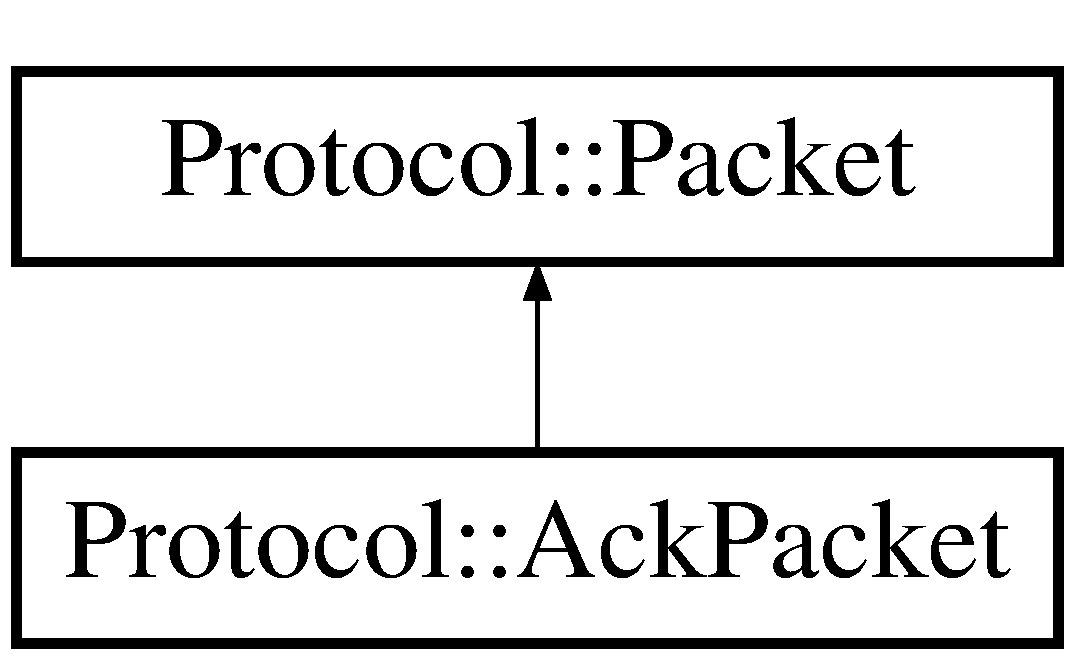
\includegraphics[height=2.000000cm]{class_protocol_1_1_ack_packet}
\end{center}
\end{figure}
\subsection*{Public Member Functions}
\begin{DoxyCompactItemize}
\item 
\hyperlink{class_protocol_1_1_ack_packet_a2d2a891317ae95d2e73fbb07521efc47}{Ack\+Packet} ()
\item 
\hyperlink{class_protocol_1_1_ack_packet_af80fa8655d726cded381d20915464ca3}{Ack\+Packet} (uint8\+\_\+t $\ast$buffer, size\+\_\+t len)
\item 
void \hyperlink{class_protocol_1_1_ack_packet_a425bc52cf7a0d1b6c8092f339ff6fe16}{set\+\_\+timestamp} (unsigned long time)
\item 
size\+\_\+t \hyperlink{class_protocol_1_1_ack_packet_a588f9608c58a913c5dd3c4acd28f92af}{Get\+Bytes} (uint8\+\_\+t $\ast$buffer, size\+\_\+t len)
\end{DoxyCompactItemize}
\subsection*{Additional Inherited Members}


\subsection{Constructor \& Destructor Documentation}
\hypertarget{class_protocol_1_1_ack_packet_a2d2a891317ae95d2e73fbb07521efc47}{}\index{Protocol\+::\+Ack\+Packet@{Protocol\+::\+Ack\+Packet}!Ack\+Packet@{Ack\+Packet}}
\index{Ack\+Packet@{Ack\+Packet}!Protocol\+::\+Ack\+Packet@{Protocol\+::\+Ack\+Packet}}
\subsubsection[{Ack\+Packet}]{\setlength{\rightskip}{0pt plus 5cm}Protocol\+::\+Ack\+Packet\+::\+Ack\+Packet (
\begin{DoxyParamCaption}
{}
\end{DoxyParamCaption}
)\hspace{0.3cm}{\ttfamily [inline]}}\label{class_protocol_1_1_ack_packet_a2d2a891317ae95d2e73fbb07521efc47}
\hypertarget{class_protocol_1_1_ack_packet_af80fa8655d726cded381d20915464ca3}{}\index{Protocol\+::\+Ack\+Packet@{Protocol\+::\+Ack\+Packet}!Ack\+Packet@{Ack\+Packet}}
\index{Ack\+Packet@{Ack\+Packet}!Protocol\+::\+Ack\+Packet@{Protocol\+::\+Ack\+Packet}}
\subsubsection[{Ack\+Packet}]{\setlength{\rightskip}{0pt plus 5cm}Protocol\+::\+Ack\+Packet\+::\+Ack\+Packet (
\begin{DoxyParamCaption}
\item[{uint8\+\_\+t $\ast$}]{buffer, }
\item[{size\+\_\+t}]{len}
\end{DoxyParamCaption}
)\hspace{0.3cm}{\ttfamily [inline]}}\label{class_protocol_1_1_ack_packet_af80fa8655d726cded381d20915464ca3}


\subsection{Member Function Documentation}
\hypertarget{class_protocol_1_1_ack_packet_a588f9608c58a913c5dd3c4acd28f92af}{}\index{Protocol\+::\+Ack\+Packet@{Protocol\+::\+Ack\+Packet}!Get\+Bytes@{Get\+Bytes}}
\index{Get\+Bytes@{Get\+Bytes}!Protocol\+::\+Ack\+Packet@{Protocol\+::\+Ack\+Packet}}
\subsubsection[{Get\+Bytes}]{\setlength{\rightskip}{0pt plus 5cm}size\+\_\+t Protocol\+::\+Ack\+Packet\+::\+Get\+Bytes (
\begin{DoxyParamCaption}
\item[{uint8\+\_\+t $\ast$}]{buffer, }
\item[{size\+\_\+t}]{len}
\end{DoxyParamCaption}
)\hspace{0.3cm}{\ttfamily [inline]}, {\ttfamily [virtual]}}\label{class_protocol_1_1_ack_packet_a588f9608c58a913c5dd3c4acd28f92af}
Stores the byte representation of a packet in the given buffer.

\begin{DoxyAuthor}{Author}
Jason Watkins 
\end{DoxyAuthor}
\begin{DoxyDate}{Date}
2015-\/11-\/16
\end{DoxyDate}

\begin{DoxyParams}{Parameters}
{\em buffer\mbox{[}in\mbox{]}} & An array to write the packet to. \\
\hline
{\em len\mbox{[}in\mbox{]}} & The length of {\ttfamily buffer}. \\
\hline
\end{DoxyParams}


Implements \hyperlink{class_protocol_1_1_packet_a9c89c3d05acc44a5050ebfc756a2cd41}{Protocol\+::\+Packet}.

\hypertarget{class_protocol_1_1_ack_packet_a425bc52cf7a0d1b6c8092f339ff6fe16}{}\index{Protocol\+::\+Ack\+Packet@{Protocol\+::\+Ack\+Packet}!set\+\_\+timestamp@{set\+\_\+timestamp}}
\index{set\+\_\+timestamp@{set\+\_\+timestamp}!Protocol\+::\+Ack\+Packet@{Protocol\+::\+Ack\+Packet}}
\subsubsection[{set\+\_\+timestamp}]{\setlength{\rightskip}{0pt plus 5cm}void Protocol\+::\+Ack\+Packet\+::set\+\_\+timestamp (
\begin{DoxyParamCaption}
\item[{unsigned long}]{time}
\end{DoxyParamCaption}
)\hspace{0.3cm}{\ttfamily [inline]}}\label{class_protocol_1_1_ack_packet_a425bc52cf7a0d1b6c8092f339ff6fe16}


The documentation for this class was generated from the following file\+:\begin{DoxyCompactItemize}
\item 
C\+:/\+Users/\+Roman/\+Documents/\+Mygs/\+Ground\+Station/\+G\+S/\hyperlink{ackpacket_8h}{ackpacket.\+h}\end{DoxyCompactItemize}

\hypertarget{class_protocol_1_1_action_packet}{}\section{Protocol\+:\+:Action\+Packet Class Reference}
\label{class_protocol_1_1_action_packet}\index{Protocol\+::\+Action\+Packet@{Protocol\+::\+Action\+Packet}}


{\ttfamily \#include $<$actionpacket.\+h$>$}

Inheritance diagram for Protocol\+:\+:Action\+Packet\+:\begin{figure}[H]
\begin{center}
\leavevmode
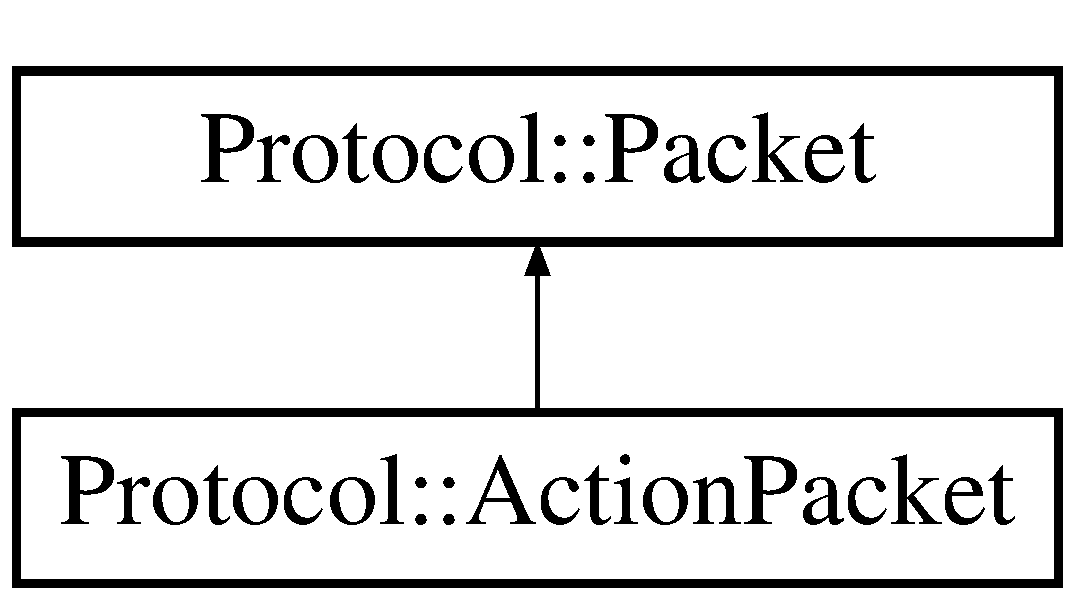
\includegraphics[height=2.000000cm]{class_protocol_1_1_action_packet}
\end{center}
\end{figure}
\subsection*{Public Member Functions}
\begin{DoxyCompactItemize}
\item 
\hyperlink{class_protocol_1_1_action_packet_a9057809acd70d7445a3c79667d6a746c}{Action\+Packet} ()
\item 
\hyperlink{class_protocol_1_1_action_packet_ae37774554c838433daa49f2fcd8439a7}{Action\+Packet} (uint8\+\_\+t $\ast$buffer, size\+\_\+t len)
\item 
void \hyperlink{class_protocol_1_1_action_packet_ac59aeacf4f0566ce327bdbacd8594687}{Set\+Action} (\hyperlink{namespace_protocol_a95f2e35dc2d8d920f0d7ddaaf122c3b9}{Action\+Type} a)
\item 
void \hyperlink{class_protocol_1_1_action_packet_a2f6167c9e92ea9914bf9a39de3fcd3e9}{Set\+Waypoint} (\hyperlink{struct_protocol_1_1_waypoint}{Waypoint} wp)
\item 
\hyperlink{namespace_protocol_a95f2e35dc2d8d920f0d7ddaaf122c3b9}{Action\+Type} \hyperlink{class_protocol_1_1_action_packet_ae90be2ee603b6968cc1515e32e0e1057}{Get\+Action} ()
\item 
\hyperlink{struct_protocol_1_1_waypoint}{Waypoint} \hyperlink{class_protocol_1_1_action_packet_a4897181b5915534b25c94f1e4c9d40ba}{Get\+Waypoint} ()
\item 
virtual size\+\_\+t \hyperlink{class_protocol_1_1_action_packet_af5963f7c15af8292152df260b188f626}{Get\+Bytes} (uint8\+\_\+t $\ast$buffer, size\+\_\+t len)
\end{DoxyCompactItemize}
\subsection*{Additional Inherited Members}


\subsection{Constructor \& Destructor Documentation}
\hypertarget{class_protocol_1_1_action_packet_a9057809acd70d7445a3c79667d6a746c}{}\index{Protocol\+::\+Action\+Packet@{Protocol\+::\+Action\+Packet}!Action\+Packet@{Action\+Packet}}
\index{Action\+Packet@{Action\+Packet}!Protocol\+::\+Action\+Packet@{Protocol\+::\+Action\+Packet}}
\subsubsection[{Action\+Packet}]{\setlength{\rightskip}{0pt plus 5cm}Protocol\+::\+Action\+Packet\+::\+Action\+Packet (
\begin{DoxyParamCaption}
{}
\end{DoxyParamCaption}
)\hspace{0.3cm}{\ttfamily [inline]}}\label{class_protocol_1_1_action_packet_a9057809acd70d7445a3c79667d6a746c}
\hypertarget{class_protocol_1_1_action_packet_ae37774554c838433daa49f2fcd8439a7}{}\index{Protocol\+::\+Action\+Packet@{Protocol\+::\+Action\+Packet}!Action\+Packet@{Action\+Packet}}
\index{Action\+Packet@{Action\+Packet}!Protocol\+::\+Action\+Packet@{Protocol\+::\+Action\+Packet}}
\subsubsection[{Action\+Packet}]{\setlength{\rightskip}{0pt plus 5cm}Protocol\+::\+Action\+Packet\+::\+Action\+Packet (
\begin{DoxyParamCaption}
\item[{uint8\+\_\+t $\ast$}]{buffer, }
\item[{size\+\_\+t}]{len}
\end{DoxyParamCaption}
)}\label{class_protocol_1_1_action_packet_ae37774554c838433daa49f2fcd8439a7}


\subsection{Member Function Documentation}
\hypertarget{class_protocol_1_1_action_packet_ae90be2ee603b6968cc1515e32e0e1057}{}\index{Protocol\+::\+Action\+Packet@{Protocol\+::\+Action\+Packet}!Get\+Action@{Get\+Action}}
\index{Get\+Action@{Get\+Action}!Protocol\+::\+Action\+Packet@{Protocol\+::\+Action\+Packet}}
\subsubsection[{Get\+Action}]{\setlength{\rightskip}{0pt plus 5cm}{\bf Protocol\+::\+Action\+Type} Protocol\+::\+Action\+Packet\+::\+Get\+Action (
\begin{DoxyParamCaption}
{}
\end{DoxyParamCaption}
)}\label{class_protocol_1_1_action_packet_ae90be2ee603b6968cc1515e32e0e1057}
\hypertarget{class_protocol_1_1_action_packet_af5963f7c15af8292152df260b188f626}{}\index{Protocol\+::\+Action\+Packet@{Protocol\+::\+Action\+Packet}!Get\+Bytes@{Get\+Bytes}}
\index{Get\+Bytes@{Get\+Bytes}!Protocol\+::\+Action\+Packet@{Protocol\+::\+Action\+Packet}}
\subsubsection[{Get\+Bytes}]{\setlength{\rightskip}{0pt plus 5cm}size\+\_\+t Protocol\+::\+Action\+Packet\+::\+Get\+Bytes (
\begin{DoxyParamCaption}
\item[{uint8\+\_\+t $\ast$}]{buffer, }
\item[{size\+\_\+t}]{len}
\end{DoxyParamCaption}
)\hspace{0.3cm}{\ttfamily [virtual]}}\label{class_protocol_1_1_action_packet_af5963f7c15af8292152df260b188f626}
Stores the byte representation of a packet in the given buffer.

\begin{DoxyAuthor}{Author}
Jason Watkins 
\end{DoxyAuthor}
\begin{DoxyDate}{Date}
2015-\/11-\/16
\end{DoxyDate}

\begin{DoxyParams}{Parameters}
{\em buffer\mbox{[}in\mbox{]}} & An array to write the packet to. \\
\hline
{\em len\mbox{[}in\mbox{]}} & The length of {\ttfamily buffer}. \\
\hline
\end{DoxyParams}


Implements \hyperlink{class_protocol_1_1_packet_a9c89c3d05acc44a5050ebfc756a2cd41}{Protocol\+::\+Packet}.

\hypertarget{class_protocol_1_1_action_packet_a4897181b5915534b25c94f1e4c9d40ba}{}\index{Protocol\+::\+Action\+Packet@{Protocol\+::\+Action\+Packet}!Get\+Waypoint@{Get\+Waypoint}}
\index{Get\+Waypoint@{Get\+Waypoint}!Protocol\+::\+Action\+Packet@{Protocol\+::\+Action\+Packet}}
\subsubsection[{Get\+Waypoint}]{\setlength{\rightskip}{0pt plus 5cm}{\bf Protocol\+::\+Waypoint} Protocol\+::\+Action\+Packet\+::\+Get\+Waypoint (
\begin{DoxyParamCaption}
{}
\end{DoxyParamCaption}
)}\label{class_protocol_1_1_action_packet_a4897181b5915534b25c94f1e4c9d40ba}
\hypertarget{class_protocol_1_1_action_packet_ac59aeacf4f0566ce327bdbacd8594687}{}\index{Protocol\+::\+Action\+Packet@{Protocol\+::\+Action\+Packet}!Set\+Action@{Set\+Action}}
\index{Set\+Action@{Set\+Action}!Protocol\+::\+Action\+Packet@{Protocol\+::\+Action\+Packet}}
\subsubsection[{Set\+Action}]{\setlength{\rightskip}{0pt plus 5cm}void Protocol\+::\+Action\+Packet\+::\+Set\+Action (
\begin{DoxyParamCaption}
\item[{{\bf Protocol\+::\+Action\+Type}}]{a}
\end{DoxyParamCaption}
)}\label{class_protocol_1_1_action_packet_ac59aeacf4f0566ce327bdbacd8594687}
\hypertarget{class_protocol_1_1_action_packet_a2f6167c9e92ea9914bf9a39de3fcd3e9}{}\index{Protocol\+::\+Action\+Packet@{Protocol\+::\+Action\+Packet}!Set\+Waypoint@{Set\+Waypoint}}
\index{Set\+Waypoint@{Set\+Waypoint}!Protocol\+::\+Action\+Packet@{Protocol\+::\+Action\+Packet}}
\subsubsection[{Set\+Waypoint}]{\setlength{\rightskip}{0pt plus 5cm}void Protocol\+::\+Action\+Packet\+::\+Set\+Waypoint (
\begin{DoxyParamCaption}
\item[{{\bf Waypoint}}]{wp}
\end{DoxyParamCaption}
)}\label{class_protocol_1_1_action_packet_a2f6167c9e92ea9914bf9a39de3fcd3e9}


The documentation for this class was generated from the following files\+:\begin{DoxyCompactItemize}
\item 
C\+:/\+Users/\+Roman/\+Documents/\+Mygs/\+Ground\+Station/\+G\+S/\hyperlink{actionpacket_8h}{actionpacket.\+h}\item 
C\+:/\+Users/\+Roman/\+Documents/\+Mygs/\+Ground\+Station/\+G\+S/\hyperlink{_action_packet_8cpp}{Action\+Packet.\+cpp}\end{DoxyCompactItemize}

\hypertarget{struct_q_c_p_axis_painter_private_1_1_cached_label}{}\section{Q\+C\+P\+Axis\+Painter\+Private\+:\+:Cached\+Label Struct Reference}
\label{struct_q_c_p_axis_painter_private_1_1_cached_label}\index{Q\+C\+P\+Axis\+Painter\+Private\+::\+Cached\+Label@{Q\+C\+P\+Axis\+Painter\+Private\+::\+Cached\+Label}}


{\ttfamily \#include $<$qcustomplot.\+h$>$}

\subsection*{Public Attributes}
\begin{DoxyCompactItemize}
\item 
Q\+Point\+F \hyperlink{struct_q_c_p_axis_painter_private_1_1_cached_label_a5f502db71c92e572f1e6f44f62c59d8e}{offset}
\item 
Q\+Pixmap \hyperlink{struct_q_c_p_axis_painter_private_1_1_cached_label_a461597cbd470914a9d24b64d16037a88}{pixmap}
\end{DoxyCompactItemize}


\subsection{Member Data Documentation}
\hypertarget{struct_q_c_p_axis_painter_private_1_1_cached_label_a5f502db71c92e572f1e6f44f62c59d8e}{}\index{Q\+C\+P\+Axis\+Painter\+Private\+::\+Cached\+Label@{Q\+C\+P\+Axis\+Painter\+Private\+::\+Cached\+Label}!offset@{offset}}
\index{offset@{offset}!Q\+C\+P\+Axis\+Painter\+Private\+::\+Cached\+Label@{Q\+C\+P\+Axis\+Painter\+Private\+::\+Cached\+Label}}
\subsubsection[{offset}]{\setlength{\rightskip}{0pt plus 5cm}Q\+Point\+F Q\+C\+P\+Axis\+Painter\+Private\+::\+Cached\+Label\+::offset}\label{struct_q_c_p_axis_painter_private_1_1_cached_label_a5f502db71c92e572f1e6f44f62c59d8e}
\hypertarget{struct_q_c_p_axis_painter_private_1_1_cached_label_a461597cbd470914a9d24b64d16037a88}{}\index{Q\+C\+P\+Axis\+Painter\+Private\+::\+Cached\+Label@{Q\+C\+P\+Axis\+Painter\+Private\+::\+Cached\+Label}!pixmap@{pixmap}}
\index{pixmap@{pixmap}!Q\+C\+P\+Axis\+Painter\+Private\+::\+Cached\+Label@{Q\+C\+P\+Axis\+Painter\+Private\+::\+Cached\+Label}}
\subsubsection[{pixmap}]{\setlength{\rightskip}{0pt plus 5cm}Q\+Pixmap Q\+C\+P\+Axis\+Painter\+Private\+::\+Cached\+Label\+::pixmap}\label{struct_q_c_p_axis_painter_private_1_1_cached_label_a461597cbd470914a9d24b64d16037a88}


The documentation for this struct was generated from the following file\+:\begin{DoxyCompactItemize}
\item 
C\+:/\+Users/\+Roman/\+Documents/\+Mygs/\+Ground\+Station/\+G\+S/\hyperlink{qcustomplot_8h}{qcustomplot.\+h}\end{DoxyCompactItemize}

\hypertarget{class_connection_dialog}{}\section{Connection\+Dialog Class Reference}
\label{class_connection_dialog}\index{Connection\+Dialog@{Connection\+Dialog}}


{\ttfamily \#include $<$connectiondialog.\+h$>$}

Inheritance diagram for Connection\+Dialog\+:\begin{figure}[H]
\begin{center}
\leavevmode
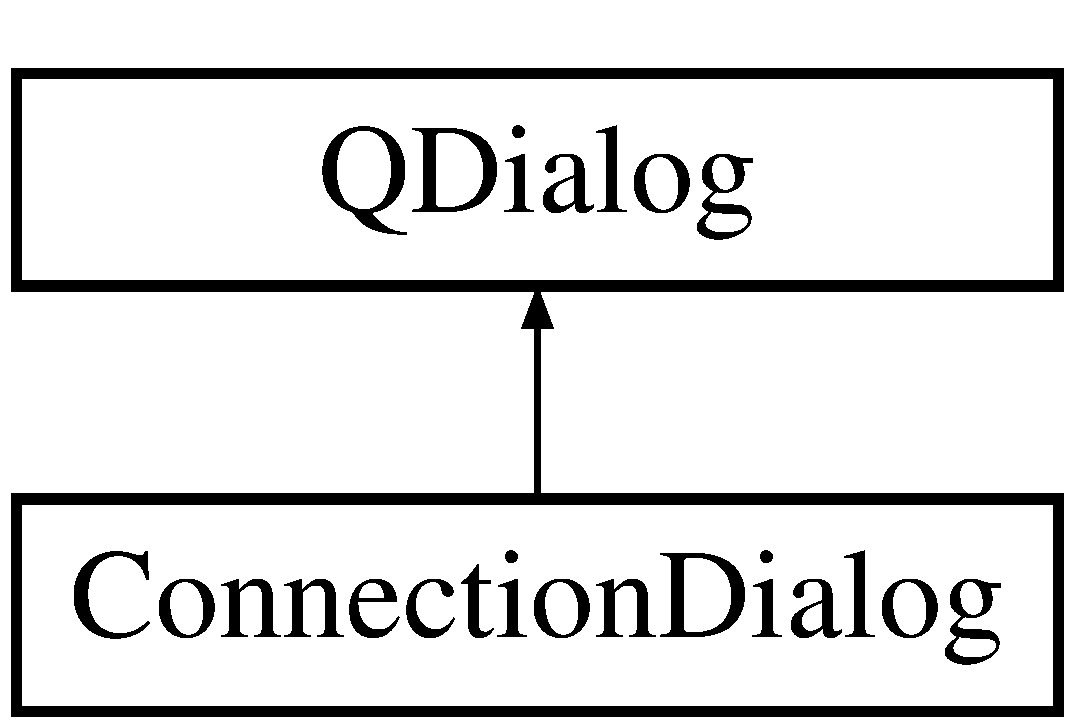
\includegraphics[height=2.000000cm]{class_connection_dialog}
\end{center}
\end{figure}
\subsection*{Public Member Functions}
\begin{DoxyCompactItemize}
\item 
\hyperlink{class_connection_dialog_a3a32f24f981932f85d14670b747f45d6}{Connection\+Dialog} (Q\+Widget $\ast$parent=0)
\item 
\hyperlink{class_connection_dialog_a43281efe3677803bce4e84c46b1f43b8}{$\sim$\+Connection\+Dialog} ()
\end{DoxyCompactItemize}


\subsection{Constructor \& Destructor Documentation}
\hypertarget{class_connection_dialog_a3a32f24f981932f85d14670b747f45d6}{}\index{Connection\+Dialog@{Connection\+Dialog}!Connection\+Dialog@{Connection\+Dialog}}
\index{Connection\+Dialog@{Connection\+Dialog}!Connection\+Dialog@{Connection\+Dialog}}
\subsubsection[{Connection\+Dialog}]{\setlength{\rightskip}{0pt plus 5cm}Connection\+Dialog\+::\+Connection\+Dialog (
\begin{DoxyParamCaption}
\item[{Q\+Widget $\ast$}]{parent = {\ttfamily 0}}
\end{DoxyParamCaption}
)\hspace{0.3cm}{\ttfamily [explicit]}}\label{class_connection_dialog_a3a32f24f981932f85d14670b747f45d6}
\hypertarget{class_connection_dialog_a43281efe3677803bce4e84c46b1f43b8}{}\index{Connection\+Dialog@{Connection\+Dialog}!````~Connection\+Dialog@{$\sim$\+Connection\+Dialog}}
\index{````~Connection\+Dialog@{$\sim$\+Connection\+Dialog}!Connection\+Dialog@{Connection\+Dialog}}
\subsubsection[{$\sim$\+Connection\+Dialog}]{\setlength{\rightskip}{0pt plus 5cm}Connection\+Dialog\+::$\sim$\+Connection\+Dialog (
\begin{DoxyParamCaption}
{}
\end{DoxyParamCaption}
)}\label{class_connection_dialog_a43281efe3677803bce4e84c46b1f43b8}


The documentation for this class was generated from the following files\+:\begin{DoxyCompactItemize}
\item 
C\+:/\+Users/\+Roman/\+Documents/\+Mygs/\+Ground\+Station/\+G\+S/\hyperlink{connectiondialog_8h}{connectiondialog.\+h}\item 
C\+:/\+Users/\+Roman/\+Documents/\+Mygs/\+Ground\+Station/\+G\+S/\hyperlink{connectiondialog_8cpp}{connectiondialog.\+cpp}\end{DoxyCompactItemize}

\hypertarget{class_db_manager}{}\section{Db\+Manager Class Reference}
\label{class_db_manager}\index{Db\+Manager@{Db\+Manager}}


The \hyperlink{class_db_manager}{Db\+Manager} class -\/ Interaction to save/load U\+A\+V\+F information will be handled in this class.  




{\ttfamily \#include $<$dbmanager.\+h$>$}

\subsection*{Public Member Functions}
\begin{DoxyCompactItemize}
\item 
\hyperlink{class_db_manager_a7f5d145bb4b33b7d08f78a2ceee17a47}{Db\+Manager} (const Q\+String \&file\+Name=\char`\"{}a\+Database\char`\"{}, const Q\+String \&directory=\char`\"{}\char`\"{})
\begin{DoxyCompactList}\small\item\em \hyperlink{class_db_manager}{Db\+Manager} -\/ Opens a connection with the database from \textquotesingle{}directory/file\+Name\textquotesingle{}. Creates a new database with \textquotesingle{}file\+Name\textquotesingle{} in \textquotesingle{}directory\textquotesingle{} if the file doesn\textquotesingle{}t exist. \end{DoxyCompactList}\item 
\hyperlink{class_db_manager_ac5cdf8e5e932d1681ab807d8f256374c}{$\sim$\+Db\+Manager} ()
\item 
bool \hyperlink{class_db_manager_af26e2cb3fc39656e05f2c9b0cda89d59}{is\+Open} () const 
\item 
bool \hyperlink{class_db_manager_ab89634eca6b13b420dda1d56484ae427}{open} (const Q\+String \&file\+Name, const Q\+String \&directory)
\item 
void \hyperlink{class_db_manager_a0e118f2a45390cde3a118f8841e0875f}{close} ()
\item 
void \hyperlink{class_db_manager_a962e5ea4e83bb6f65f9d19f82a470687}{add\+Mission\+Data} (\hyperlink{struct_mission_data}{Mission\+Data} data)
\item 
const Q\+Vector$<$ \hyperlink{struct_mission_data}{Mission\+Data} $>$ \hyperlink{class_db_manager_adfe91eed71e54ff7d7b2f28d10800efe}{get\+Mission} () const 
\item 
void \hyperlink{class_db_manager_afac9da99cb97c29cae46e7488d681d36}{save\+Mission\+To\+File} ()
\end{DoxyCompactItemize}


\subsection{Detailed Description}
The \hyperlink{class_db_manager}{Db\+Manager} class -\/ Interaction to save/load U\+A\+V\+F information will be handled in this class. 

\subsection{Constructor \& Destructor Documentation}
\hypertarget{class_db_manager_a7f5d145bb4b33b7d08f78a2ceee17a47}{}\index{Db\+Manager@{Db\+Manager}!Db\+Manager@{Db\+Manager}}
\index{Db\+Manager@{Db\+Manager}!Db\+Manager@{Db\+Manager}}
\subsubsection[{Db\+Manager}]{\setlength{\rightskip}{0pt plus 5cm}Db\+Manager\+::\+Db\+Manager (
\begin{DoxyParamCaption}
\item[{const Q\+String \&}]{file\+Name = {\ttfamily \char`\"{}aDatabase\char`\"{}}, }
\item[{const Q\+String \&}]{directory = {\ttfamily \char`\"{}\char`\"{}}}
\end{DoxyParamCaption}
)}\label{class_db_manager_a7f5d145bb4b33b7d08f78a2ceee17a47}


\hyperlink{class_db_manager}{Db\+Manager} -\/ Opens a connection with the database from \textquotesingle{}directory/file\+Name\textquotesingle{}. Creates a new database with \textquotesingle{}file\+Name\textquotesingle{} in \textquotesingle{}directory\textquotesingle{} if the file doesn\textquotesingle{}t exist. 


\begin{DoxyParams}{Parameters}
{\em file\+Name} & -\/ The name of the mission file without the extension. \\
\hline
{\em directory} & -\/ The folder where the database file is located. \\
\hline
\end{DoxyParams}
\begin{DoxyNote}{Note}
-\/ Do not include the file\+Name\textquotesingle{}s extension (e.\+g. mission1.\+db -\/$>$ just mission1) 
\end{DoxyNote}
\hypertarget{class_db_manager_ac5cdf8e5e932d1681ab807d8f256374c}{}\index{Db\+Manager@{Db\+Manager}!````~Db\+Manager@{$\sim$\+Db\+Manager}}
\index{````~Db\+Manager@{$\sim$\+Db\+Manager}!Db\+Manager@{Db\+Manager}}
\subsubsection[{$\sim$\+Db\+Manager}]{\setlength{\rightskip}{0pt plus 5cm}Db\+Manager\+::$\sim$\+Db\+Manager (
\begin{DoxyParamCaption}
{}
\end{DoxyParamCaption}
)}\label{class_db_manager_ac5cdf8e5e932d1681ab807d8f256374c}


\subsection{Member Function Documentation}
\hypertarget{class_db_manager_a962e5ea4e83bb6f65f9d19f82a470687}{}\index{Db\+Manager@{Db\+Manager}!add\+Mission\+Data@{add\+Mission\+Data}}
\index{add\+Mission\+Data@{add\+Mission\+Data}!Db\+Manager@{Db\+Manager}}
\subsubsection[{add\+Mission\+Data}]{\setlength{\rightskip}{0pt plus 5cm}void Db\+Manager\+::add\+Mission\+Data (
\begin{DoxyParamCaption}
\item[{{\bf Mission\+Data}}]{data}
\end{DoxyParamCaption}
)}\label{class_db_manager_a962e5ea4e83bb6f65f9d19f82a470687}
\hypertarget{class_db_manager_a0e118f2a45390cde3a118f8841e0875f}{}\index{Db\+Manager@{Db\+Manager}!close@{close}}
\index{close@{close}!Db\+Manager@{Db\+Manager}}
\subsubsection[{close}]{\setlength{\rightskip}{0pt plus 5cm}void Db\+Manager\+::close (
\begin{DoxyParamCaption}
{}
\end{DoxyParamCaption}
)}\label{class_db_manager_a0e118f2a45390cde3a118f8841e0875f}
\hypertarget{class_db_manager_adfe91eed71e54ff7d7b2f28d10800efe}{}\index{Db\+Manager@{Db\+Manager}!get\+Mission@{get\+Mission}}
\index{get\+Mission@{get\+Mission}!Db\+Manager@{Db\+Manager}}
\subsubsection[{get\+Mission}]{\setlength{\rightskip}{0pt plus 5cm}const Q\+Vector$<$ {\bf Mission\+Data} $>$ Db\+Manager\+::get\+Mission (
\begin{DoxyParamCaption}
{}
\end{DoxyParamCaption}
) const}\label{class_db_manager_adfe91eed71e54ff7d7b2f28d10800efe}
\hypertarget{class_db_manager_af26e2cb3fc39656e05f2c9b0cda89d59}{}\index{Db\+Manager@{Db\+Manager}!is\+Open@{is\+Open}}
\index{is\+Open@{is\+Open}!Db\+Manager@{Db\+Manager}}
\subsubsection[{is\+Open}]{\setlength{\rightskip}{0pt plus 5cm}bool Db\+Manager\+::is\+Open (
\begin{DoxyParamCaption}
{}
\end{DoxyParamCaption}
) const}\label{class_db_manager_af26e2cb3fc39656e05f2c9b0cda89d59}
\hypertarget{class_db_manager_ab89634eca6b13b420dda1d56484ae427}{}\index{Db\+Manager@{Db\+Manager}!open@{open}}
\index{open@{open}!Db\+Manager@{Db\+Manager}}
\subsubsection[{open}]{\setlength{\rightskip}{0pt plus 5cm}bool Db\+Manager\+::open (
\begin{DoxyParamCaption}
\item[{const Q\+String \&}]{file\+Name, }
\item[{const Q\+String \&}]{directory}
\end{DoxyParamCaption}
)}\label{class_db_manager_ab89634eca6b13b420dda1d56484ae427}
\hypertarget{class_db_manager_afac9da99cb97c29cae46e7488d681d36}{}\index{Db\+Manager@{Db\+Manager}!save\+Mission\+To\+File@{save\+Mission\+To\+File}}
\index{save\+Mission\+To\+File@{save\+Mission\+To\+File}!Db\+Manager@{Db\+Manager}}
\subsubsection[{save\+Mission\+To\+File}]{\setlength{\rightskip}{0pt plus 5cm}void Db\+Manager\+::save\+Mission\+To\+File (
\begin{DoxyParamCaption}
{}
\end{DoxyParamCaption}
)}\label{class_db_manager_afac9da99cb97c29cae46e7488d681d36}


The documentation for this class was generated from the following files\+:\begin{DoxyCompactItemize}
\item 
C\+:/\+Users/\+Roman/\+Documents/\+Mygs/\+Ground\+Station/\+G\+S/\hyperlink{dbmanager_8h}{dbmanager.\+h}\item 
C\+:/\+Users/\+Roman/\+Documents/\+Mygs/\+Ground\+Station/\+G\+S/\hyperlink{dbmanager_8cpp}{dbmanager.\+cpp}\end{DoxyCompactItemize}

\hypertarget{class_dialog}{}\section{Dialog Class Reference}
\label{class_dialog}\index{Dialog@{Dialog}}


{\ttfamily \#include $<$dialog.\+h$>$}

Inheritance diagram for Dialog\+:\begin{figure}[H]
\begin{center}
\leavevmode
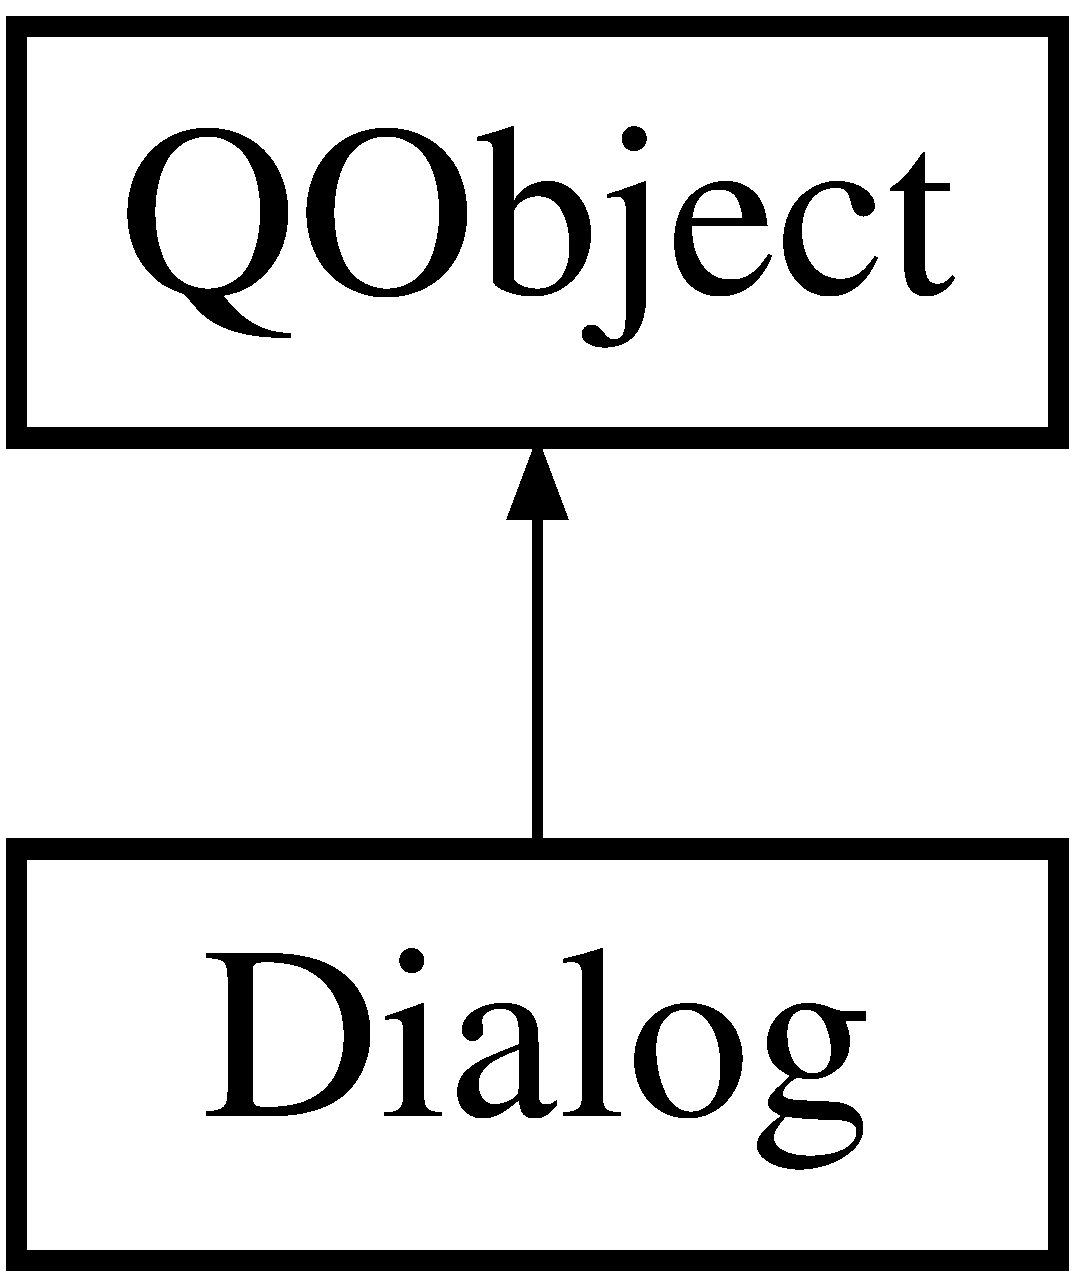
\includegraphics[height=2.000000cm]{class_dialog}
\end{center}
\end{figure}
\subsection*{Public Slots}
\begin{DoxyCompactItemize}
\item 
void \hyperlink{class_dialog_a937038eaea8c49ecbe7fb38fee63fd29}{receive\+Text} (const Q\+String \&text)
\item 
void \hyperlink{class_dialog_a4649de72d982f73ecaa9bef08a6282b4}{add\+Point\+To\+Table} (double lat, double lng)
\end{DoxyCompactItemize}
\subsection*{Signals}
\begin{DoxyCompactItemize}
\item 
void \hyperlink{class_dialog_a2c541f80e65d942ff6d471607a81fbbc}{send\+Text} (const Q\+String \&text)
\item 
void \hyperlink{class_dialog_ada82bdcc218632134d3907af12f0d567}{send\+Point} (double lat, double lng)
\end{DoxyCompactItemize}
\subsection*{Public Member Functions}
\begin{DoxyCompactItemize}
\item 
\hyperlink{class_dialog_a13476d9809dc62da93e9f36958d8ce69}{Dialog} (Q\+Object $\ast$parent=0)
\item 
void \hyperlink{class_dialog_ace9ced9197b21b73477e1dfe08ce0452}{display\+Message} (const Q\+String \&message)
\end{DoxyCompactItemize}
\subsection*{Public Attributes}
\begin{DoxyCompactItemize}
\item 
Ui\+::\+Dialog \hyperlink{class_dialog_a62c4186c0cf571547612cf1ad40dfada}{ui}
\end{DoxyCompactItemize}


\subsection{Constructor \& Destructor Documentation}
\hypertarget{class_dialog_a13476d9809dc62da93e9f36958d8ce69}{}\index{Dialog@{Dialog}!Dialog@{Dialog}}
\index{Dialog@{Dialog}!Dialog@{Dialog}}
\subsubsection[{Dialog}]{\setlength{\rightskip}{0pt plus 5cm}Dialog\+::\+Dialog (
\begin{DoxyParamCaption}
\item[{Q\+Object $\ast$}]{parent = {\ttfamily 0}}
\end{DoxyParamCaption}
)\hspace{0.3cm}{\ttfamily [inline]}, {\ttfamily [explicit]}}\label{class_dialog_a13476d9809dc62da93e9f36958d8ce69}


\subsection{Member Function Documentation}
\hypertarget{class_dialog_a4649de72d982f73ecaa9bef08a6282b4}{}\index{Dialog@{Dialog}!add\+Point\+To\+Table@{add\+Point\+To\+Table}}
\index{add\+Point\+To\+Table@{add\+Point\+To\+Table}!Dialog@{Dialog}}
\subsubsection[{add\+Point\+To\+Table}]{\setlength{\rightskip}{0pt plus 5cm}void Dialog\+::add\+Point\+To\+Table (
\begin{DoxyParamCaption}
\item[{double}]{lat, }
\item[{double}]{lng}
\end{DoxyParamCaption}
)\hspace{0.3cm}{\ttfamily [inline]}, {\ttfamily [slot]}}\label{class_dialog_a4649de72d982f73ecaa9bef08a6282b4}
\hypertarget{class_dialog_ace9ced9197b21b73477e1dfe08ce0452}{}\index{Dialog@{Dialog}!display\+Message@{display\+Message}}
\index{display\+Message@{display\+Message}!Dialog@{Dialog}}
\subsubsection[{display\+Message}]{\setlength{\rightskip}{0pt plus 5cm}void Dialog\+::display\+Message (
\begin{DoxyParamCaption}
\item[{const Q\+String \&}]{message}
\end{DoxyParamCaption}
)\hspace{0.3cm}{\ttfamily [inline]}}\label{class_dialog_ace9ced9197b21b73477e1dfe08ce0452}
\hypertarget{class_dialog_a937038eaea8c49ecbe7fb38fee63fd29}{}\index{Dialog@{Dialog}!receive\+Text@{receive\+Text}}
\index{receive\+Text@{receive\+Text}!Dialog@{Dialog}}
\subsubsection[{receive\+Text}]{\setlength{\rightskip}{0pt plus 5cm}void Dialog\+::receive\+Text (
\begin{DoxyParamCaption}
\item[{const Q\+String \&}]{text}
\end{DoxyParamCaption}
)\hspace{0.3cm}{\ttfamily [inline]}, {\ttfamily [slot]}}\label{class_dialog_a937038eaea8c49ecbe7fb38fee63fd29}
This slot is invoked from the H\+T\+M\+L client side and the text displayed on the server side. \hypertarget{class_dialog_ada82bdcc218632134d3907af12f0d567}{}\index{Dialog@{Dialog}!send\+Point@{send\+Point}}
\index{send\+Point@{send\+Point}!Dialog@{Dialog}}
\subsubsection[{send\+Point}]{\setlength{\rightskip}{0pt plus 5cm}void Dialog\+::send\+Point (
\begin{DoxyParamCaption}
\item[{double}]{lat, }
\item[{double}]{lng}
\end{DoxyParamCaption}
)\hspace{0.3cm}{\ttfamily [signal]}}\label{class_dialog_ada82bdcc218632134d3907af12f0d567}
\hypertarget{class_dialog_a2c541f80e65d942ff6d471607a81fbbc}{}\index{Dialog@{Dialog}!send\+Text@{send\+Text}}
\index{send\+Text@{send\+Text}!Dialog@{Dialog}}
\subsubsection[{send\+Text}]{\setlength{\rightskip}{0pt plus 5cm}void Dialog\+::send\+Text (
\begin{DoxyParamCaption}
\item[{const Q\+String \&}]{text}
\end{DoxyParamCaption}
)\hspace{0.3cm}{\ttfamily [signal]}}\label{class_dialog_a2c541f80e65d942ff6d471607a81fbbc}
This signal is emitted from the C++ side and the text displayed on the H\+T\+M\+L client side. 

\subsection{Member Data Documentation}
\hypertarget{class_dialog_a62c4186c0cf571547612cf1ad40dfada}{}\index{Dialog@{Dialog}!ui@{ui}}
\index{ui@{ui}!Dialog@{Dialog}}
\subsubsection[{ui}]{\setlength{\rightskip}{0pt plus 5cm}Ui\+::\+Dialog Dialog\+::ui}\label{class_dialog_a62c4186c0cf571547612cf1ad40dfada}


The documentation for this class was generated from the following file\+:\begin{DoxyCompactItemize}
\item 
C\+:/\+Users/\+Roman/\+Documents/\+Mygs/\+Ground\+Station/\+G\+S/\hyperlink{dialog_8h}{dialog.\+h}\end{DoxyCompactItemize}

\hypertarget{class_digital_clock}{}\section{Digital\+Clock Class Reference}
\label{class_digital_clock}\index{Digital\+Clock@{Digital\+Clock}}


The \hyperlink{class_digital_clock}{Digital\+Clock} class inherits from Q\+Plain\+Text\+Edit -\/\+Aaron Ko.  




{\ttfamily \#include $<$digitalclock.\+h$>$}

Inheritance diagram for Digital\+Clock\+:\begin{figure}[H]
\begin{center}
\leavevmode
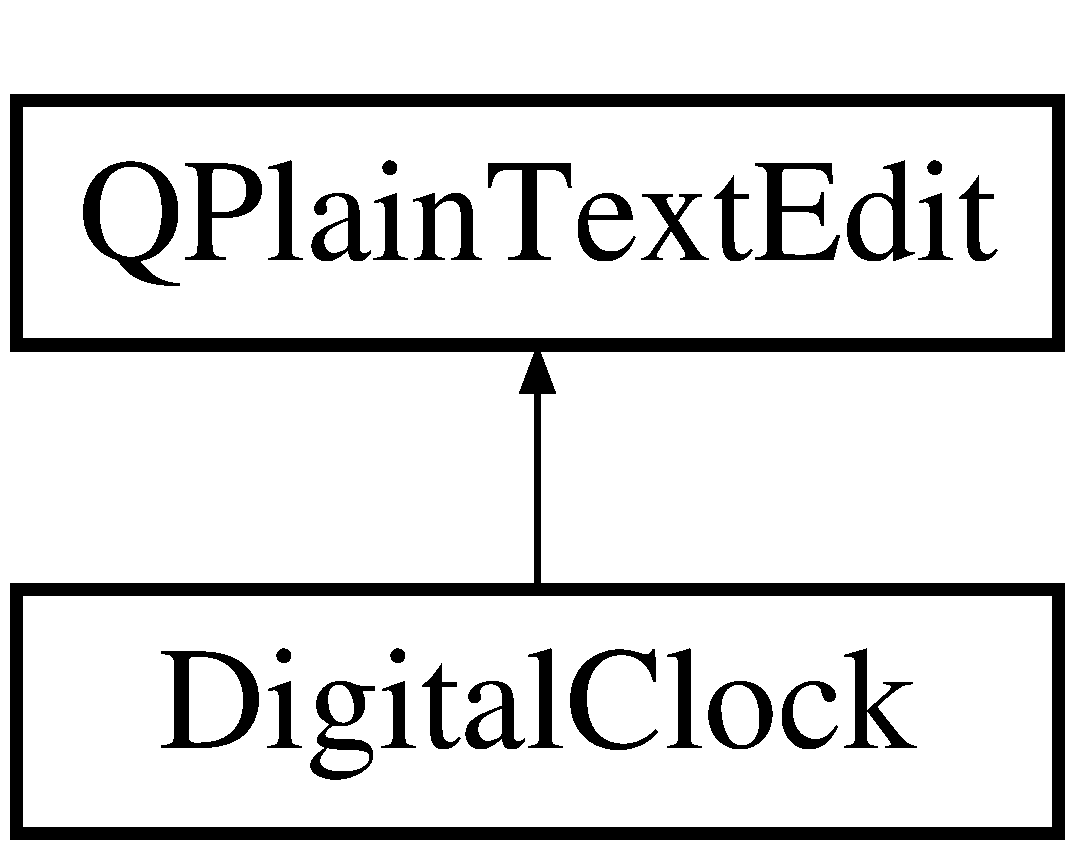
\includegraphics[height=2.000000cm]{class_digital_clock}
\end{center}
\end{figure}
\subsection*{Public Member Functions}
\begin{DoxyCompactItemize}
\item 
\hyperlink{class_digital_clock_ab87ec7559579311929e8542dbcf5e294}{$\sim$\+Digital\+Clock} ()
\item 
\hyperlink{class_digital_clock_a1df69f177d5defdd5029ff2e6b7cb564}{Digital\+Clock} (Q\+Widget $\ast$parent=0)
\item 
void \hyperlink{class_digital_clock_a070278bd43a6162c7a666f354c3d1087}{initiate} (Q\+Time timein)
\begin{DoxyCompactList}\small\item\em \hyperlink{class_digital_clock_a070278bd43a6162c7a666f354c3d1087}{Digital\+Clock\+::initiate} saves start time (need to fix to get from message box) connects 1 second timer to showtime function. \end{DoxyCompactList}\item 
void \hyperlink{class_digital_clock_afdcf81f100c3a2ef9bd5961c8f82562f}{initiate} (\hyperlink{classmessagebox}{messagebox} $\ast$mbin, \hyperlink{class_map_execution}{Map\+Execution} $\ast$mapexec\+\_\+ptr)
\end{DoxyCompactItemize}
\subsection*{Public Attributes}
\begin{DoxyCompactItemize}
\item 
Q\+Time \hyperlink{class_digital_clock_aa5f7b6ed6828178d12e4e5cd66f5008c}{time}
\item 
Q\+String \hyperlink{class_digital_clock_acefe5da3fee2eba06d65402484dbe8f8}{start}
\item 
\hyperlink{classmessagebox}{messagebox} $\ast$ \hyperlink{class_digital_clock_a0538ee6d4983204422a10beef92158ac}{mb}
\item 
\hyperlink{class_map_execution}{Map\+Execution} $\ast$ \hyperlink{class_digital_clock_a280a7e0206e2d9e192a19b89cf9c2327}{map\+\_\+exec\+\_\+ptr}
\item 
Q\+Timer $\ast$ \hyperlink{class_digital_clock_ad2d7eceb84025180dc2b7862668b87e7}{Status\+Timer}
\item 
Q\+Timer $\ast$ \hyperlink{class_digital_clock_aa49ae733b7fb0c8b1f353e9811372d5b}{Time\+Timer}
\end{DoxyCompactItemize}


\subsection{Detailed Description}
The \hyperlink{class_digital_clock}{Digital\+Clock} class inherits from Q\+Plain\+Text\+Edit -\/\+Aaron Ko. 

\subsection{Constructor \& Destructor Documentation}
\hypertarget{class_digital_clock_ab87ec7559579311929e8542dbcf5e294}{}\index{Digital\+Clock@{Digital\+Clock}!````~Digital\+Clock@{$\sim$\+Digital\+Clock}}
\index{````~Digital\+Clock@{$\sim$\+Digital\+Clock}!Digital\+Clock@{Digital\+Clock}}
\subsubsection[{$\sim$\+Digital\+Clock}]{\setlength{\rightskip}{0pt plus 5cm}Digital\+Clock\+::$\sim$\+Digital\+Clock (
\begin{DoxyParamCaption}
{}
\end{DoxyParamCaption}
)}\label{class_digital_clock_ab87ec7559579311929e8542dbcf5e294}
\hypertarget{class_digital_clock_a1df69f177d5defdd5029ff2e6b7cb564}{}\index{Digital\+Clock@{Digital\+Clock}!Digital\+Clock@{Digital\+Clock}}
\index{Digital\+Clock@{Digital\+Clock}!Digital\+Clock@{Digital\+Clock}}
\subsubsection[{Digital\+Clock}]{\setlength{\rightskip}{0pt plus 5cm}Digital\+Clock\+::\+Digital\+Clock (
\begin{DoxyParamCaption}
\item[{Q\+Widget $\ast$}]{parent = {\ttfamily 0}}
\end{DoxyParamCaption}
)}\label{class_digital_clock_a1df69f177d5defdd5029ff2e6b7cb564}


\subsection{Member Function Documentation}
\hypertarget{class_digital_clock_a070278bd43a6162c7a666f354c3d1087}{}\index{Digital\+Clock@{Digital\+Clock}!initiate@{initiate}}
\index{initiate@{initiate}!Digital\+Clock@{Digital\+Clock}}
\subsubsection[{initiate}]{\setlength{\rightskip}{0pt plus 5cm}void Digital\+Clock\+::initiate (
\begin{DoxyParamCaption}
\item[{Q\+Time}]{timein}
\end{DoxyParamCaption}
)}\label{class_digital_clock_a070278bd43a6162c7a666f354c3d1087}


\hyperlink{class_digital_clock_a070278bd43a6162c7a666f354c3d1087}{Digital\+Clock\+::initiate} saves start time (need to fix to get from message box) connects 1 second timer to showtime function. 

\hypertarget{class_digital_clock_afdcf81f100c3a2ef9bd5961c8f82562f}{}\index{Digital\+Clock@{Digital\+Clock}!initiate@{initiate}}
\index{initiate@{initiate}!Digital\+Clock@{Digital\+Clock}}
\subsubsection[{initiate}]{\setlength{\rightskip}{0pt plus 5cm}void Digital\+Clock\+::initiate (
\begin{DoxyParamCaption}
\item[{{\bf messagebox} $\ast$}]{mbin, }
\item[{{\bf Map\+Execution} $\ast$}]{mapexec\+\_\+ptr}
\end{DoxyParamCaption}
)}\label{class_digital_clock_afdcf81f100c3a2ef9bd5961c8f82562f}


\subsection{Member Data Documentation}
\hypertarget{class_digital_clock_a280a7e0206e2d9e192a19b89cf9c2327}{}\index{Digital\+Clock@{Digital\+Clock}!map\+\_\+exec\+\_\+ptr@{map\+\_\+exec\+\_\+ptr}}
\index{map\+\_\+exec\+\_\+ptr@{map\+\_\+exec\+\_\+ptr}!Digital\+Clock@{Digital\+Clock}}
\subsubsection[{map\+\_\+exec\+\_\+ptr}]{\setlength{\rightskip}{0pt plus 5cm}{\bf Map\+Execution}$\ast$ Digital\+Clock\+::map\+\_\+exec\+\_\+ptr}\label{class_digital_clock_a280a7e0206e2d9e192a19b89cf9c2327}
\hypertarget{class_digital_clock_a0538ee6d4983204422a10beef92158ac}{}\index{Digital\+Clock@{Digital\+Clock}!mb@{mb}}
\index{mb@{mb}!Digital\+Clock@{Digital\+Clock}}
\subsubsection[{mb}]{\setlength{\rightskip}{0pt plus 5cm}{\bf messagebox}$\ast$ Digital\+Clock\+::mb}\label{class_digital_clock_a0538ee6d4983204422a10beef92158ac}
\hypertarget{class_digital_clock_acefe5da3fee2eba06d65402484dbe8f8}{}\index{Digital\+Clock@{Digital\+Clock}!start@{start}}
\index{start@{start}!Digital\+Clock@{Digital\+Clock}}
\subsubsection[{start}]{\setlength{\rightskip}{0pt plus 5cm}Q\+String Digital\+Clock\+::start}\label{class_digital_clock_acefe5da3fee2eba06d65402484dbe8f8}
\hypertarget{class_digital_clock_ad2d7eceb84025180dc2b7862668b87e7}{}\index{Digital\+Clock@{Digital\+Clock}!Status\+Timer@{Status\+Timer}}
\index{Status\+Timer@{Status\+Timer}!Digital\+Clock@{Digital\+Clock}}
\subsubsection[{Status\+Timer}]{\setlength{\rightskip}{0pt plus 5cm}Q\+Timer$\ast$ Digital\+Clock\+::\+Status\+Timer}\label{class_digital_clock_ad2d7eceb84025180dc2b7862668b87e7}
\hypertarget{class_digital_clock_aa5f7b6ed6828178d12e4e5cd66f5008c}{}\index{Digital\+Clock@{Digital\+Clock}!time@{time}}
\index{time@{time}!Digital\+Clock@{Digital\+Clock}}
\subsubsection[{time}]{\setlength{\rightskip}{0pt plus 5cm}Q\+Time Digital\+Clock\+::time}\label{class_digital_clock_aa5f7b6ed6828178d12e4e5cd66f5008c}
\hypertarget{class_digital_clock_aa49ae733b7fb0c8b1f353e9811372d5b}{}\index{Digital\+Clock@{Digital\+Clock}!Time\+Timer@{Time\+Timer}}
\index{Time\+Timer@{Time\+Timer}!Digital\+Clock@{Digital\+Clock}}
\subsubsection[{Time\+Timer}]{\setlength{\rightskip}{0pt plus 5cm}Q\+Timer$\ast$ Digital\+Clock\+::\+Time\+Timer}\label{class_digital_clock_aa49ae733b7fb0c8b1f353e9811372d5b}


The documentation for this class was generated from the following files\+:\begin{DoxyCompactItemize}
\item 
C\+:/\+Users/\+Roman/\+Documents/\+Mygs/\+Ground\+Station/\+G\+S/\hyperlink{digitalclock_8h}{digitalclock.\+h}\item 
C\+:/\+Users/\+Roman/\+Documents/\+Mygs/\+Ground\+Station/\+G\+S/\hyperlink{digitalclock_8cpp}{digitalclock.\+cpp}\end{DoxyCompactItemize}

\hypertarget{class_flight_path}{}\section{Flight\+Path Class Reference}
\label{class_flight_path}\index{Flight\+Path@{Flight\+Path}}


{\ttfamily \#include $<$flightpath.\+h$>$}

Inheritance diagram for Flight\+Path\+:\begin{figure}[H]
\begin{center}
\leavevmode
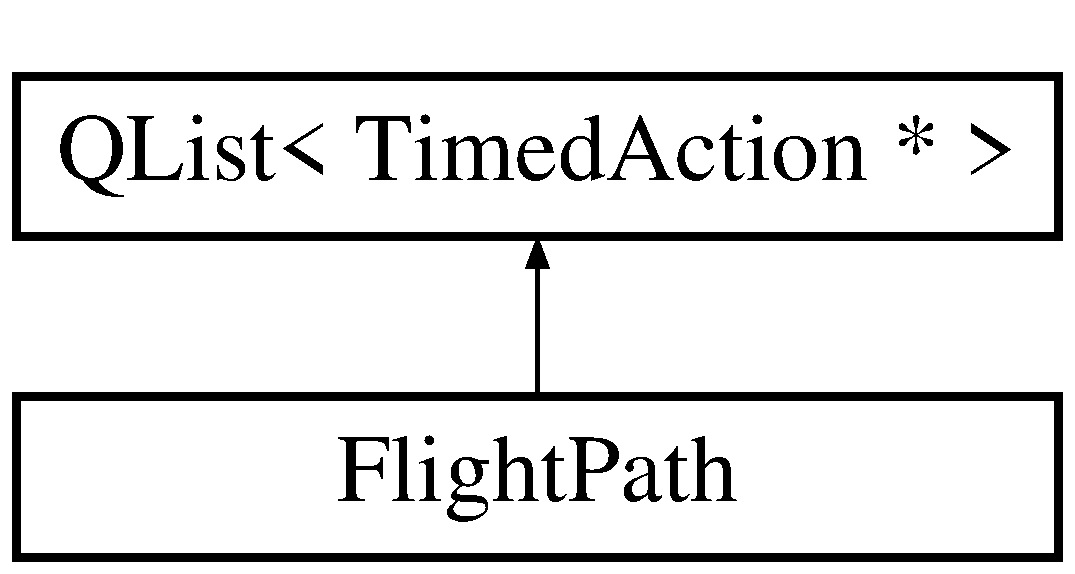
\includegraphics[height=2.000000cm]{class_flight_path}
\end{center}
\end{figure}
\subsection*{Public Member Functions}
\begin{DoxyCompactItemize}
\item 
\hyperlink{class_flight_path_a2e628a23c9b4a92c238263cfa3d650d4}{Flight\+Path} ()
\begin{DoxyCompactList}\small\item\em \hyperlink{class_flight_path}{Flight\+Path} -\/ default constructor. \end{DoxyCompactList}\item 
\hyperlink{class_flight_path_a9be65ab000a34bf60862b8b1af77d43d}{Flight\+Path} (Q\+String filename)
\begin{DoxyCompactList}\small\item\em \hyperlink{class_flight_path}{Flight\+Path} -\/ Creates a new \hyperlink{class_flight_path}{Flight\+Path} using the data stored in the target file. Serves as a load function. \end{DoxyCompactList}\item 
\hyperlink{class_flight_path_a6fecfbdebe93de7d2b62e3a2048111ca}{$\sim$\+Flight\+Path} ()
\begin{DoxyCompactList}\small\item\em \hyperlink{class_flight_path}{Flight\+Path} -\/ Default destructor. \end{DoxyCompactList}\item 
void \hyperlink{class_flight_path_ab625d5c73d69a5e616dade72ddcffd49}{add\+Cmd\+Action} (\hyperlink{namespace_protocol_a95f2e35dc2d8d920f0d7ddaaf122c3b9}{Protocol\+::\+Action\+Type} type, double delay)
\begin{DoxyCompactList}\small\item\em add\+Cmd\+Action Adds a new Command-\/type Action to this \hyperlink{class_flight_path}{Flight\+Path} \end{DoxyCompactList}\item 
void \hyperlink{class_flight_path_a101c5c8e050e215d70e3c6218b935aa9}{add\+Nav\+Action} (\hyperlink{struct_protocol_1_1_waypoint}{Protocol\+::\+Waypoint} wp, double delay)
\begin{DoxyCompactList}\small\item\em add\+Nav\+Action Adds a new Navigation-\/type Action to this \hyperlink{class_flight_path}{Flight\+Path} \end{DoxyCompactList}\item 
bool \hyperlink{class_flight_path_a3a602f9b4b608f506354bf6c711a84eb}{save} (Q\+String filename)
\begin{DoxyCompactList}\small\item\em save Writes this \hyperlink{class_flight_path}{Flight\+Path}\textquotesingle{}s data out to a target file \end{DoxyCompactList}\item 
Q\+List$<$ \hyperlink{struct_protocol_1_1_waypoint}{Protocol\+::\+Waypoint} $>$ $\ast$ \hyperlink{class_flight_path_a3ffe0a2832e0e0e48e15b181ace42870}{get\+Ordered\+Waypoints} ()
\begin{DoxyCompactList}\small\item\em get\+Ordered\+Waypoints Returns a list of all Waypoint objects in ascending order of delay (queue postion). \end{DoxyCompactList}\end{DoxyCompactItemize}


\subsection{Constructor \& Destructor Documentation}
\hypertarget{class_flight_path_a2e628a23c9b4a92c238263cfa3d650d4}{}\index{Flight\+Path@{Flight\+Path}!Flight\+Path@{Flight\+Path}}
\index{Flight\+Path@{Flight\+Path}!Flight\+Path@{Flight\+Path}}
\subsubsection[{Flight\+Path}]{\setlength{\rightskip}{0pt plus 5cm}Flight\+Path\+::\+Flight\+Path (
\begin{DoxyParamCaption}
{}
\end{DoxyParamCaption}
)}\label{class_flight_path_a2e628a23c9b4a92c238263cfa3d650d4}


\hyperlink{class_flight_path}{Flight\+Path} -\/ default constructor. 

\hypertarget{class_flight_path_a9be65ab000a34bf60862b8b1af77d43d}{}\index{Flight\+Path@{Flight\+Path}!Flight\+Path@{Flight\+Path}}
\index{Flight\+Path@{Flight\+Path}!Flight\+Path@{Flight\+Path}}
\subsubsection[{Flight\+Path}]{\setlength{\rightskip}{0pt plus 5cm}Flight\+Path\+::\+Flight\+Path (
\begin{DoxyParamCaption}
\item[{Q\+String}]{filename}
\end{DoxyParamCaption}
)}\label{class_flight_path_a9be65ab000a34bf60862b8b1af77d43d}


\hyperlink{class_flight_path}{Flight\+Path} -\/ Creates a new \hyperlink{class_flight_path}{Flight\+Path} using the data stored in the target file. Serves as a load function. 


\begin{DoxyParams}{Parameters}
{\em filename} & -\/ the name of the target file \\
\hline
\end{DoxyParams}
\begin{DoxyRefDesc}{Todo}
\item[\hyperlink{todo__todo000002}{Todo}]any database initialization and error checking if necesary \end{DoxyRefDesc}


\begin{DoxyRefDesc}{Todo}
\item[\hyperlink{todo__todo000003}{Todo}]get actual database length \end{DoxyRefDesc}


\begin{DoxyRefDesc}{Todo}
\item[\hyperlink{todo__todo000004}{Todo}]update these two lines with values from the database \end{DoxyRefDesc}


\begin{DoxyRefDesc}{Todo}
\item[\hyperlink{todo__todo000005}{Todo}]any remaining database functions for safe file handling if needed \end{DoxyRefDesc}
\hypertarget{class_flight_path_a6fecfbdebe93de7d2b62e3a2048111ca}{}\index{Flight\+Path@{Flight\+Path}!````~Flight\+Path@{$\sim$\+Flight\+Path}}
\index{````~Flight\+Path@{$\sim$\+Flight\+Path}!Flight\+Path@{Flight\+Path}}
\subsubsection[{$\sim$\+Flight\+Path}]{\setlength{\rightskip}{0pt plus 5cm}Flight\+Path\+::$\sim$\+Flight\+Path (
\begin{DoxyParamCaption}
{}
\end{DoxyParamCaption}
)}\label{class_flight_path_a6fecfbdebe93de7d2b62e3a2048111ca}


\hyperlink{class_flight_path}{Flight\+Path} -\/ Default destructor. 



\subsection{Member Function Documentation}
\hypertarget{class_flight_path_ab625d5c73d69a5e616dade72ddcffd49}{}\index{Flight\+Path@{Flight\+Path}!add\+Cmd\+Action@{add\+Cmd\+Action}}
\index{add\+Cmd\+Action@{add\+Cmd\+Action}!Flight\+Path@{Flight\+Path}}
\subsubsection[{add\+Cmd\+Action}]{\setlength{\rightskip}{0pt plus 5cm}void Flight\+Path\+::add\+Cmd\+Action (
\begin{DoxyParamCaption}
\item[{{\bf Protocol\+::\+Action\+Type}}]{type, }
\item[{double}]{delay}
\end{DoxyParamCaption}
)}\label{class_flight_path_ab625d5c73d69a5e616dade72ddcffd49}


add\+Cmd\+Action Adds a new Command-\/type Action to this \hyperlink{class_flight_path}{Flight\+Path} 


\begin{DoxyParams}{Parameters}
{\em type} & -\/ the type of Action this new packet contains \\
\hline
{\em delay} & -\/ the queue position of this Action -\/ small numbers send first \\
\hline
\end{DoxyParams}
\hypertarget{class_flight_path_a101c5c8e050e215d70e3c6218b935aa9}{}\index{Flight\+Path@{Flight\+Path}!add\+Nav\+Action@{add\+Nav\+Action}}
\index{add\+Nav\+Action@{add\+Nav\+Action}!Flight\+Path@{Flight\+Path}}
\subsubsection[{add\+Nav\+Action}]{\setlength{\rightskip}{0pt plus 5cm}void Flight\+Path\+::add\+Nav\+Action (
\begin{DoxyParamCaption}
\item[{{\bf Protocol\+::\+Waypoint}}]{wp, }
\item[{double}]{delay}
\end{DoxyParamCaption}
)}\label{class_flight_path_a101c5c8e050e215d70e3c6218b935aa9}


add\+Nav\+Action Adds a new Navigation-\/type Action to this \hyperlink{class_flight_path}{Flight\+Path} 


\begin{DoxyParams}{Parameters}
{\em wp} & -\/ the destination Waypoint for this navigation action \\
\hline
{\em delay} & -\/ the queue position of this Action -\/ small numbers send first \\
\hline
\end{DoxyParams}
\hypertarget{class_flight_path_a3ffe0a2832e0e0e48e15b181ace42870}{}\index{Flight\+Path@{Flight\+Path}!get\+Ordered\+Waypoints@{get\+Ordered\+Waypoints}}
\index{get\+Ordered\+Waypoints@{get\+Ordered\+Waypoints}!Flight\+Path@{Flight\+Path}}
\subsubsection[{get\+Ordered\+Waypoints}]{\setlength{\rightskip}{0pt plus 5cm}Q\+List$<$ {\bf Protocol\+::\+Waypoint} $>$ $\ast$ Flight\+Path\+::get\+Ordered\+Waypoints (
\begin{DoxyParamCaption}
{}
\end{DoxyParamCaption}
)}\label{class_flight_path_a3ffe0a2832e0e0e48e15b181ace42870}


get\+Ordered\+Waypoints Returns a list of all Waypoint objects in ascending order of delay (queue postion). 

\begin{DoxyReturn}{Returns}
A pointer to the sorted Q\+List containing all the Waypoints 
\end{DoxyReturn}
\hypertarget{class_flight_path_a3a602f9b4b608f506354bf6c711a84eb}{}\index{Flight\+Path@{Flight\+Path}!save@{save}}
\index{save@{save}!Flight\+Path@{Flight\+Path}}
\subsubsection[{save}]{\setlength{\rightskip}{0pt plus 5cm}bool Flight\+Path\+::save (
\begin{DoxyParamCaption}
\item[{Q\+String}]{filename}
\end{DoxyParamCaption}
)}\label{class_flight_path_a3a602f9b4b608f506354bf6c711a84eb}


save Writes this \hyperlink{class_flight_path}{Flight\+Path}\textquotesingle{}s data out to a target file 


\begin{DoxyParams}{Parameters}
{\em filename} & the name of the target file \\
\hline
\end{DoxyParams}
\begin{DoxyReturn}{Returns}
true if the write was successful, false otherwise 
\end{DoxyReturn}
\begin{DoxyRefDesc}{Todo}
\item[\hyperlink{todo__todo000006}{Todo}]any database initialization and error checking. \end{DoxyRefDesc}


\begin{DoxyRefDesc}{Todo}
\item[\hyperlink{todo__todo000007}{Todo}]write \char`\"{}action\+Num\char`\"{}, \char`\"{}delay\char`\"{}, and \char`\"{}data\char`\"{} variables to the database \end{DoxyRefDesc}


\begin{DoxyRefDesc}{Todo}
\item[\hyperlink{todo__todo000008}{Todo}]any remaining database functions for safe file handling if needed \end{DoxyRefDesc}


The documentation for this class was generated from the following files\+:\begin{DoxyCompactItemize}
\item 
C\+:/\+Users/\+Roman/\+Documents/\+Mygs/\+Ground\+Station/\+G\+S/\hyperlink{flightpath_8h}{flightpath.\+h}\item 
C\+:/\+Users/\+Roman/\+Documents/\+Mygs/\+Ground\+Station/\+G\+S/\hyperlink{flightpath_8cpp}{flightpath.\+cpp}\end{DoxyCompactItemize}

\hypertarget{class_gs_server}{}\section{Gs\+Server Class Reference}
\label{class_gs_server}\index{Gs\+Server@{Gs\+Server}}


{\ttfamily \#include $<$gsserver.\+h$>$}

Inheritance diagram for Gs\+Server\+:\begin{figure}[H]
\begin{center}
\leavevmode
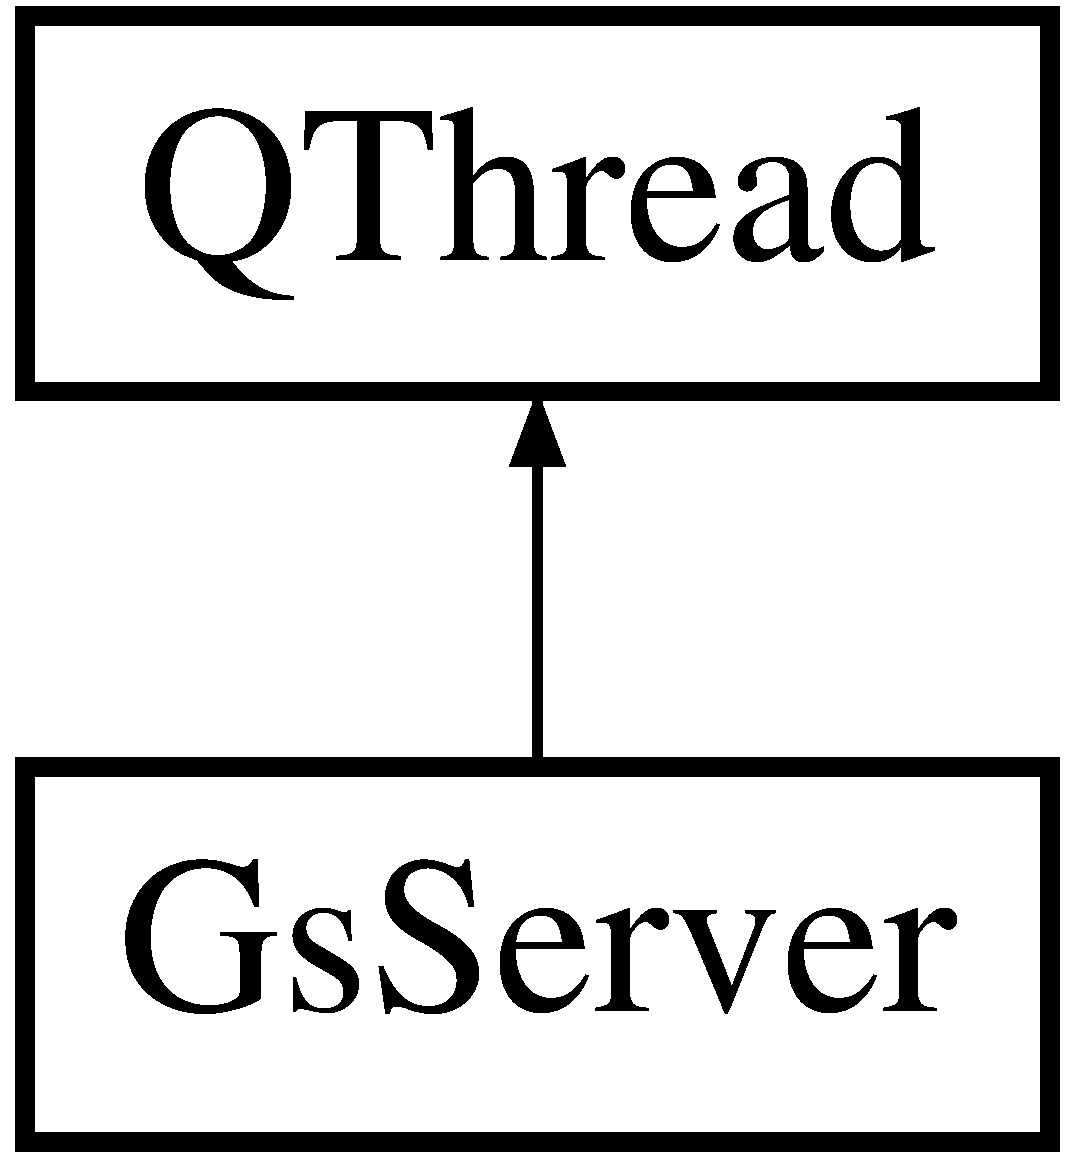
\includegraphics[height=2.000000cm]{class_gs_server}
\end{center}
\end{figure}
\subsection*{Public Member Functions}
\begin{DoxyCompactItemize}
\item 
\hyperlink{class_gs_server_a0931c5e470fcb46548c14996d2d9c853}{Gs\+Server} (\hyperlink{classmessagebox}{messagebox} $\ast$my\+Message\+Box, \hyperlink{class_mission}{Mission} $\ast$my\+Mission)
\item 
\hyperlink{class_gs_server_a56461ff8c405720a8cb591c84f61a5bf}{$\sim$\+Gs\+Server} ()
\item 
void \hyperlink{class_gs_server_aa906d6a7084c03849eadcd31563057e6}{run} ()
\item 
void \hyperlink{class_gs_server_abfbbae94e647cc6415b3a460fbabec88}{recieve\+Ack\+Packet} (\hyperlink{class_protocol_1_1_ack_packet}{Protocol\+::\+Ack\+Packet} $\ast$ack)
\begin{DoxyCompactList}\small\item\em recieve\+Ack\+Packet \end{DoxyCompactList}\item 
void \hyperlink{class_gs_server_a394e75ea0a17eb9a6ac2814ea84b250c}{start\+Server} ()
\item 
void \hyperlink{class_gs_server_a6f73b66c39e5080eb58c80ab355d3c8c}{open\+Server} ()
\item 
void \hyperlink{class_gs_server_aa2acb9071c6c2ef44f5a8fc859576ff6}{open\+Server} (Q\+Host\+Address target, unsigned int port)
\item 
void \hyperlink{class_gs_server_a7ca468b85231e88da9b5cafb1320bbb4}{close\+Server} ()
\item 
void \hyperlink{class_gs_server_a5be5b957f9207e66550fc33fbf2b4df2}{wait\+Net} (unsigned millis)
\item 
void \hyperlink{class_gs_server_ae8e04868caa920485facfc4cfda6291e}{send\+Packet} (\hyperlink{class_protocol_1_1_packet}{Protocol\+::\+Packet} $\ast$packet)
\begin{DoxyCompactList}\small\item\em send\+Packet adds a packet to the send queue for this server. The default priority is 10. The packet will be sent as soon as the socket is free for sending. Lowest prioirty is sent first. \end{DoxyCompactList}\item 
void \hyperlink{class_gs_server_a3a07e46c4042ff43336ffcafa36f2a3a}{send\+Packet} (\hyperlink{class_protocol_1_1_packet}{Protocol\+::\+Packet} $\ast$packet, unsigned int priority)
\begin{DoxyCompactList}\small\item\em send\+Packet adds a packet to the send queue for this server. The packet will be sent as soon as the socket is free for sending. Lowest priority is sent first. \end{DoxyCompactList}\item 
void \hyperlink{class_gs_server_a450eb8f60b68bf82216d058cc9738e28}{packet\+Recieved} (\hyperlink{class_protocol_1_1_telemetry_packet}{Protocol\+::\+Telemetry\+Packet} packet)
\begin{DoxyCompactList}\small\item\em packet\+Recieved adds a Telemetry\+Packet to this server\textquotesingle{}s \hyperlink{class_mission}{Mission} object. \end{DoxyCompactList}\end{DoxyCompactItemize}
\subsection*{Public Attributes}
\begin{DoxyCompactItemize}
\item 
int \hyperlink{class_gs_server_aee6ff9911df099594d4483cb116ed808}{uav\+\_\+fd}
\item 
unsigned char \hyperlink{class_gs_server_a5db50514e830e5d9aeeed83e23472501}{max\+Pack\+Size} = 255
\item 
\hyperlink{class_network_listener}{Network\+Listener} \hyperlink{class_gs_server_aa115a3c8f593c29bc6d68f102dbf1941}{network\+Listener}
\item 
bool \hyperlink{class_gs_server_a720185d9a2050ae2d5ebda4e7262ba6e}{running}
\end{DoxyCompactItemize}


\subsection{Detailed Description}
\hyperlink{class_gs_server}{Gs\+Server} is the server object for the ground station. The current implementation will be changing, but this is the first working version.

I will be cleaning the code and making frequent implementation changes in the near future. The functions and variables however will probably remain stable.

\begin{DoxyAuthor}{Author}
Jordan Dickson 
\end{DoxyAuthor}
\begin{DoxyDate}{Date}
1-\/29-\/1016 
\end{DoxyDate}
\begin{DoxyVersion}{Version}
2.\+0 
\end{DoxyVersion}


\subsection{Constructor \& Destructor Documentation}
\hypertarget{class_gs_server_a0931c5e470fcb46548c14996d2d9c853}{}\index{Gs\+Server@{Gs\+Server}!Gs\+Server@{Gs\+Server}}
\index{Gs\+Server@{Gs\+Server}!Gs\+Server@{Gs\+Server}}
\subsubsection[{Gs\+Server}]{\setlength{\rightskip}{0pt plus 5cm}Gs\+Server\+::\+Gs\+Server (
\begin{DoxyParamCaption}
\item[{{\bf messagebox} $\ast$}]{my\+Message\+Box, }
\item[{{\bf Mission} $\ast$}]{my\+Mission}
\end{DoxyParamCaption}
)}\label{class_gs_server_a0931c5e470fcb46548c14996d2d9c853}
Creates a new server hosted on the localhost (127.\+0.\+0.\+1) on port 3495.


\begin{DoxyParams}{Parameters}
{\em my\+Message\+Box} & the messagebox used for outgoing packets \\
\hline
\end{DoxyParams}
\hypertarget{class_gs_server_a56461ff8c405720a8cb591c84f61a5bf}{}\index{Gs\+Server@{Gs\+Server}!````~Gs\+Server@{$\sim$\+Gs\+Server}}
\index{````~Gs\+Server@{$\sim$\+Gs\+Server}!Gs\+Server@{Gs\+Server}}
\subsubsection[{$\sim$\+Gs\+Server}]{\setlength{\rightskip}{0pt plus 5cm}Gs\+Server\+::$\sim$\+Gs\+Server (
\begin{DoxyParamCaption}
{}
\end{DoxyParamCaption}
)}\label{class_gs_server_a56461ff8c405720a8cb591c84f61a5bf}
Destructor for \hyperlink{class_gs_server}{Gs\+Server} 

\subsection{Member Function Documentation}
\hypertarget{class_gs_server_a7ca468b85231e88da9b5cafb1320bbb4}{}\index{Gs\+Server@{Gs\+Server}!close\+Server@{close\+Server}}
\index{close\+Server@{close\+Server}!Gs\+Server@{Gs\+Server}}
\subsubsection[{close\+Server}]{\setlength{\rightskip}{0pt plus 5cm}void Gs\+Server\+::close\+Server (
\begin{DoxyParamCaption}
{}
\end{DoxyParamCaption}
)}\label{class_gs_server_a7ca468b85231e88da9b5cafb1320bbb4}
Closes the server by dropping all current connections and ending the listener thread. \hypertarget{class_gs_server_a6f73b66c39e5080eb58c80ab355d3c8c}{}\index{Gs\+Server@{Gs\+Server}!open\+Server@{open\+Server}}
\index{open\+Server@{open\+Server}!Gs\+Server@{Gs\+Server}}
\subsubsection[{open\+Server}]{\setlength{\rightskip}{0pt plus 5cm}void Gs\+Server\+::open\+Server (
\begin{DoxyParamCaption}
{}
\end{DoxyParamCaption}
)}\label{class_gs_server_a6f73b66c39e5080eb58c80ab355d3c8c}
Opens ther server by hosting it on the default port and listening for connections. \hypertarget{class_gs_server_aa2acb9071c6c2ef44f5a8fc859576ff6}{}\index{Gs\+Server@{Gs\+Server}!open\+Server@{open\+Server}}
\index{open\+Server@{open\+Server}!Gs\+Server@{Gs\+Server}}
\subsubsection[{open\+Server}]{\setlength{\rightskip}{0pt plus 5cm}void Gs\+Server\+::open\+Server (
\begin{DoxyParamCaption}
\item[{Q\+Host\+Address}]{target, }
\item[{unsigned int}]{port}
\end{DoxyParamCaption}
)}\label{class_gs_server_aa2acb9071c6c2ef44f5a8fc859576ff6}
Opens ther server by hosting it on a socket and listening for connections. \hypertarget{class_gs_server_a450eb8f60b68bf82216d058cc9738e28}{}\index{Gs\+Server@{Gs\+Server}!packet\+Recieved@{packet\+Recieved}}
\index{packet\+Recieved@{packet\+Recieved}!Gs\+Server@{Gs\+Server}}
\subsubsection[{packet\+Recieved}]{\setlength{\rightskip}{0pt plus 5cm}void Gs\+Server\+::packet\+Recieved (
\begin{DoxyParamCaption}
\item[{{\bf Protocol\+::\+Telemetry\+Packet}}]{packet}
\end{DoxyParamCaption}
)}\label{class_gs_server_a450eb8f60b68bf82216d058cc9738e28}


packet\+Recieved adds a Telemetry\+Packet to this server\textquotesingle{}s \hyperlink{class_mission}{Mission} object. 


\begin{DoxyParams}{Parameters}
{\em packet} & The telemetry\+Packet being added. \\
\hline
\end{DoxyParams}
\hypertarget{class_gs_server_abfbbae94e647cc6415b3a460fbabec88}{}\index{Gs\+Server@{Gs\+Server}!recieve\+Ack\+Packet@{recieve\+Ack\+Packet}}
\index{recieve\+Ack\+Packet@{recieve\+Ack\+Packet}!Gs\+Server@{Gs\+Server}}
\subsubsection[{recieve\+Ack\+Packet}]{\setlength{\rightskip}{0pt plus 5cm}void Gs\+Server\+::recieve\+Ack\+Packet (
\begin{DoxyParamCaption}
\item[{{\bf Protocol\+::\+Ack\+Packet} $\ast$}]{ack}
\end{DoxyParamCaption}
)}\label{class_gs_server_abfbbae94e647cc6415b3a460fbabec88}


recieve\+Ack\+Packet 


\begin{DoxyParams}{Parameters}
{\em ack} & \\
\hline
\end{DoxyParams}
\hypertarget{class_gs_server_aa906d6a7084c03849eadcd31563057e6}{}\index{Gs\+Server@{Gs\+Server}!run@{run}}
\index{run@{run}!Gs\+Server@{Gs\+Server}}
\subsubsection[{run}]{\setlength{\rightskip}{0pt plus 5cm}void Gs\+Server\+::run (
\begin{DoxyParamCaption}
{}
\end{DoxyParamCaption}
)}\label{class_gs_server_aa906d6a7084c03849eadcd31563057e6}
Override run to implement thread as a server. \hypertarget{class_gs_server_ae8e04868caa920485facfc4cfda6291e}{}\index{Gs\+Server@{Gs\+Server}!send\+Packet@{send\+Packet}}
\index{send\+Packet@{send\+Packet}!Gs\+Server@{Gs\+Server}}
\subsubsection[{send\+Packet}]{\setlength{\rightskip}{0pt plus 5cm}void Gs\+Server\+::send\+Packet (
\begin{DoxyParamCaption}
\item[{{\bf Protocol\+::\+Packet} $\ast$}]{packet}
\end{DoxyParamCaption}
)}\label{class_gs_server_ae8e04868caa920485facfc4cfda6291e}


send\+Packet adds a packet to the send queue for this server. The default priority is 10. The packet will be sent as soon as the socket is free for sending. Lowest prioirty is sent first. 


\begin{DoxyParams}{Parameters}
{\em packet} & the packet to be added into the send queue \\
\hline
\end{DoxyParams}
\begin{DoxyAuthor}{Author}
Jordan Dickson 
\end{DoxyAuthor}
\begin{DoxyDate}{Date}
Feb 5 2016 
\end{DoxyDate}
\hypertarget{class_gs_server_a3a07e46c4042ff43336ffcafa36f2a3a}{}\index{Gs\+Server@{Gs\+Server}!send\+Packet@{send\+Packet}}
\index{send\+Packet@{send\+Packet}!Gs\+Server@{Gs\+Server}}
\subsubsection[{send\+Packet}]{\setlength{\rightskip}{0pt plus 5cm}void Gs\+Server\+::send\+Packet (
\begin{DoxyParamCaption}
\item[{{\bf Protocol\+::\+Packet} $\ast$}]{packet, }
\item[{unsigned int}]{priority}
\end{DoxyParamCaption}
)}\label{class_gs_server_a3a07e46c4042ff43336ffcafa36f2a3a}


send\+Packet adds a packet to the send queue for this server. The packet will be sent as soon as the socket is free for sending. Lowest priority is sent first. 


\begin{DoxyParams}{Parameters}
{\em packet} & the packet to be added into the send queue \\
\hline
{\em priority} & the priority of the packet (lowest number sent first) \\
\hline
\end{DoxyParams}
\begin{DoxyDate}{Date}
Feb 5 2016 
\end{DoxyDate}
\hypertarget{class_gs_server_a394e75ea0a17eb9a6ac2814ea84b250c}{}\index{Gs\+Server@{Gs\+Server}!start\+Server@{start\+Server}}
\index{start\+Server@{start\+Server}!Gs\+Server@{Gs\+Server}}
\subsubsection[{start\+Server}]{\setlength{\rightskip}{0pt plus 5cm}void Gs\+Server\+::start\+Server (
\begin{DoxyParamCaption}
{}
\end{DoxyParamCaption}
)}\label{class_gs_server_a394e75ea0a17eb9a6ac2814ea84b250c}
\hypertarget{class_gs_server_a5be5b957f9207e66550fc33fbf2b4df2}{}\index{Gs\+Server@{Gs\+Server}!wait\+Net@{wait\+Net}}
\index{wait\+Net@{wait\+Net}!Gs\+Server@{Gs\+Server}}
\subsubsection[{wait\+Net}]{\setlength{\rightskip}{0pt plus 5cm}void Gs\+Server\+::wait\+Net (
\begin{DoxyParamCaption}
\item[{unsigned}]{millis}
\end{DoxyParamCaption}
)}\label{class_gs_server_a5be5b957f9207e66550fc33fbf2b4df2}
waits for a specified number of milliseconds


\begin{DoxyParams}{Parameters}
{\em millis} & the number of milliseconds to wait \\
\hline
\end{DoxyParams}


\subsection{Member Data Documentation}
\hypertarget{class_gs_server_a5db50514e830e5d9aeeed83e23472501}{}\index{Gs\+Server@{Gs\+Server}!max\+Pack\+Size@{max\+Pack\+Size}}
\index{max\+Pack\+Size@{max\+Pack\+Size}!Gs\+Server@{Gs\+Server}}
\subsubsection[{max\+Pack\+Size}]{\setlength{\rightskip}{0pt plus 5cm}unsigned char Gs\+Server\+::max\+Pack\+Size = 255}\label{class_gs_server_a5db50514e830e5d9aeeed83e23472501}
the maximum size of a packet that will be sent by this server. \hypertarget{class_gs_server_aa115a3c8f593c29bc6d68f102dbf1941}{}\index{Gs\+Server@{Gs\+Server}!network\+Listener@{network\+Listener}}
\index{network\+Listener@{network\+Listener}!Gs\+Server@{Gs\+Server}}
\subsubsection[{network\+Listener}]{\setlength{\rightskip}{0pt plus 5cm}{\bf Network\+Listener} Gs\+Server\+::network\+Listener}\label{class_gs_server_aa115a3c8f593c29bc6d68f102dbf1941}
The \hyperlink{class_network_listener}{Network\+Listener} used by this server to process incoming signals. \hypertarget{class_gs_server_a720185d9a2050ae2d5ebda4e7262ba6e}{}\index{Gs\+Server@{Gs\+Server}!running@{running}}
\index{running@{running}!Gs\+Server@{Gs\+Server}}
\subsubsection[{running}]{\setlength{\rightskip}{0pt plus 5cm}bool Gs\+Server\+::running}\label{class_gs_server_a720185d9a2050ae2d5ebda4e7262ba6e}
\hypertarget{class_gs_server_aee6ff9911df099594d4483cb116ed808}{}\index{Gs\+Server@{Gs\+Server}!uav\+\_\+fd@{uav\+\_\+fd}}
\index{uav\+\_\+fd@{uav\+\_\+fd}!Gs\+Server@{Gs\+Server}}
\subsubsection[{uav\+\_\+fd}]{\setlength{\rightskip}{0pt plus 5cm}int Gs\+Server\+::uav\+\_\+fd}\label{class_gs_server_aee6ff9911df099594d4483cb116ed808}
file descriptor for the U\+A\+V. Used to send information over the network. 

The documentation for this class was generated from the following files\+:\begin{DoxyCompactItemize}
\item 
C\+:/\+Users/\+Roman/\+Documents/\+Mygs/\+Ground\+Station/\+G\+S/\hyperlink{gsserver_8h}{gsserver.\+h}\item 
C\+:/\+Users/\+Roman/\+Documents/\+Mygs/\+Ground\+Station/\+G\+S/\hyperlink{gsserver_8cpp}{gsserver.\+cpp}\end{DoxyCompactItemize}

\hypertarget{class_protocol_1_1_info_packet}{}\section{Protocol\+:\+:Info\+Packet Class Reference}
\label{class_protocol_1_1_info_packet}\index{Protocol\+::\+Info\+Packet@{Protocol\+::\+Info\+Packet}}


{\ttfamily \#include $<$infopacket.\+h$>$}

Inheritance diagram for Protocol\+:\+:Info\+Packet\+:\begin{figure}[H]
\begin{center}
\leavevmode
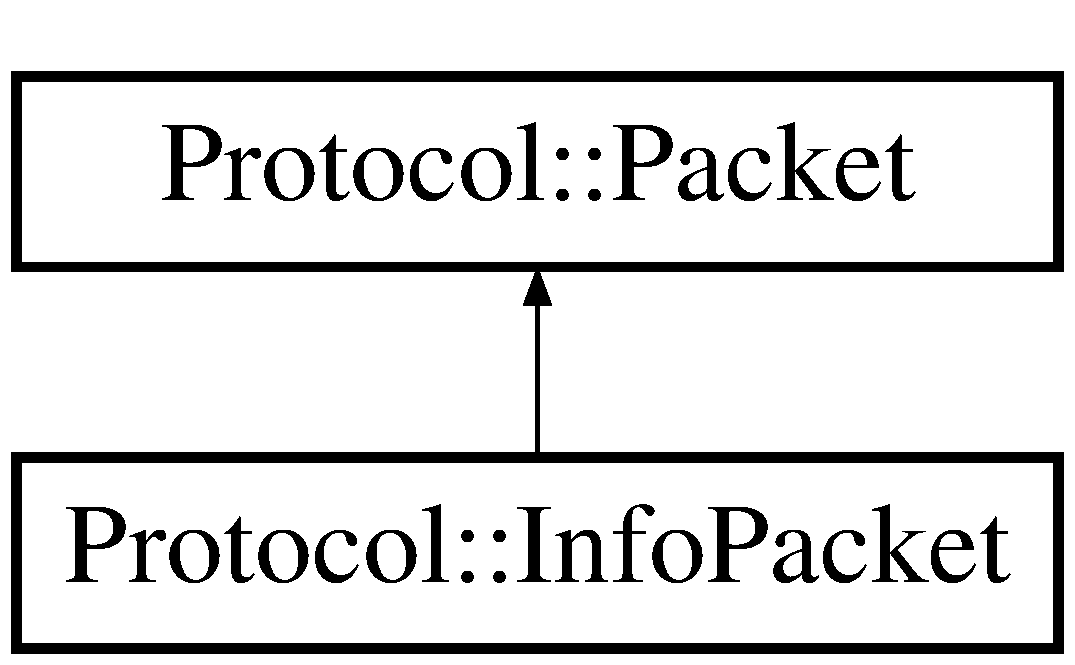
\includegraphics[height=2.000000cm]{class_protocol_1_1_info_packet}
\end{center}
\end{figure}
\subsection*{Public Member Functions}
\begin{DoxyCompactItemize}
\item 
\hyperlink{class_protocol_1_1_info_packet_a11fa7cf70f73872adb44ba550bfe3bad}{Info\+Packet} ()
\item 
\hyperlink{class_protocol_1_1_info_packet_a3492d10770f6fbbeda7b49be359fcf7c}{Info\+Packet} (uint8\+\_\+t $\ast$buffer, size\+\_\+t len)
\item 
void \hyperlink{class_protocol_1_1_info_packet_aa41807efe3d80764352e2cabe0ce3dab}{Set\+Storable} (uint16\+\_\+t s)
\item 
void \hyperlink{class_protocol_1_1_info_packet_a9d892385a9ec50b38411af3fb9f07d81}{Set\+Battery} (uint16\+\_\+t b)
\item 
void \hyperlink{class_protocol_1_1_info_packet_a1751ad384a82367591e851bfa479fda2}{Set\+Other} (std\+::string s)
\item 
uint16\+\_\+t \hyperlink{class_protocol_1_1_info_packet_a83e236806b6ae78ae7486c6b12e9f94f}{Get\+Storable} ()
\item 
uint16\+\_\+t \hyperlink{class_protocol_1_1_info_packet_a2bb88fcedd69d0bb22db500de6ff11f7}{Get\+Battery} ()
\item 
std\+::string \hyperlink{class_protocol_1_1_info_packet_a4cfc3b5c49b57016e7b4f72f74b62021}{Get\+Other} ()
\item 
virtual size\+\_\+t \hyperlink{class_protocol_1_1_info_packet_ad1f43721045348442cf224533bce7f1a}{Get\+Bytes} (uint8\+\_\+t $\ast$buffer, size\+\_\+t len)
\end{DoxyCompactItemize}
\subsection*{Additional Inherited Members}


\subsection{Constructor \& Destructor Documentation}
\hypertarget{class_protocol_1_1_info_packet_a11fa7cf70f73872adb44ba550bfe3bad}{}\index{Protocol\+::\+Info\+Packet@{Protocol\+::\+Info\+Packet}!Info\+Packet@{Info\+Packet}}
\index{Info\+Packet@{Info\+Packet}!Protocol\+::\+Info\+Packet@{Protocol\+::\+Info\+Packet}}
\subsubsection[{Info\+Packet}]{\setlength{\rightskip}{0pt plus 5cm}Protocol\+::\+Info\+Packet\+::\+Info\+Packet (
\begin{DoxyParamCaption}
{}
\end{DoxyParamCaption}
)\hspace{0.3cm}{\ttfamily [inline]}}\label{class_protocol_1_1_info_packet_a11fa7cf70f73872adb44ba550bfe3bad}
\hypertarget{class_protocol_1_1_info_packet_a3492d10770f6fbbeda7b49be359fcf7c}{}\index{Protocol\+::\+Info\+Packet@{Protocol\+::\+Info\+Packet}!Info\+Packet@{Info\+Packet}}
\index{Info\+Packet@{Info\+Packet}!Protocol\+::\+Info\+Packet@{Protocol\+::\+Info\+Packet}}
\subsubsection[{Info\+Packet}]{\setlength{\rightskip}{0pt plus 5cm}Protocol\+::\+Info\+Packet\+::\+Info\+Packet (
\begin{DoxyParamCaption}
\item[{uint8\+\_\+t $\ast$}]{buffer, }
\item[{size\+\_\+t}]{len}
\end{DoxyParamCaption}
)}\label{class_protocol_1_1_info_packet_a3492d10770f6fbbeda7b49be359fcf7c}


\subsection{Member Function Documentation}
\hypertarget{class_protocol_1_1_info_packet_a2bb88fcedd69d0bb22db500de6ff11f7}{}\index{Protocol\+::\+Info\+Packet@{Protocol\+::\+Info\+Packet}!Get\+Battery@{Get\+Battery}}
\index{Get\+Battery@{Get\+Battery}!Protocol\+::\+Info\+Packet@{Protocol\+::\+Info\+Packet}}
\subsubsection[{Get\+Battery}]{\setlength{\rightskip}{0pt plus 5cm}uint16\+\_\+t Protocol\+::\+Info\+Packet\+::\+Get\+Battery (
\begin{DoxyParamCaption}
{}
\end{DoxyParamCaption}
)}\label{class_protocol_1_1_info_packet_a2bb88fcedd69d0bb22db500de6ff11f7}
\hypertarget{class_protocol_1_1_info_packet_ad1f43721045348442cf224533bce7f1a}{}\index{Protocol\+::\+Info\+Packet@{Protocol\+::\+Info\+Packet}!Get\+Bytes@{Get\+Bytes}}
\index{Get\+Bytes@{Get\+Bytes}!Protocol\+::\+Info\+Packet@{Protocol\+::\+Info\+Packet}}
\subsubsection[{Get\+Bytes}]{\setlength{\rightskip}{0pt plus 5cm}size\+\_\+t Protocol\+::\+Info\+Packet\+::\+Get\+Bytes (
\begin{DoxyParamCaption}
\item[{uint8\+\_\+t $\ast$}]{buffer, }
\item[{size\+\_\+t}]{len}
\end{DoxyParamCaption}
)\hspace{0.3cm}{\ttfamily [virtual]}}\label{class_protocol_1_1_info_packet_ad1f43721045348442cf224533bce7f1a}
Stores the byte representation of a packet in the given buffer.

\begin{DoxyAuthor}{Author}
Jason Watkins 
\end{DoxyAuthor}
\begin{DoxyDate}{Date}
2015-\/11-\/16
\end{DoxyDate}

\begin{DoxyParams}{Parameters}
{\em buffer\mbox{[}in\mbox{]}} & An array to write the packet to. \\
\hline
{\em len\mbox{[}in\mbox{]}} & The length of {\ttfamily buffer}. \\
\hline
\end{DoxyParams}


Implements \hyperlink{class_protocol_1_1_packet_a9c89c3d05acc44a5050ebfc756a2cd41}{Protocol\+::\+Packet}.

\hypertarget{class_protocol_1_1_info_packet_a4cfc3b5c49b57016e7b4f72f74b62021}{}\index{Protocol\+::\+Info\+Packet@{Protocol\+::\+Info\+Packet}!Get\+Other@{Get\+Other}}
\index{Get\+Other@{Get\+Other}!Protocol\+::\+Info\+Packet@{Protocol\+::\+Info\+Packet}}
\subsubsection[{Get\+Other}]{\setlength{\rightskip}{0pt plus 5cm}std\+::string Protocol\+::\+Info\+Packet\+::\+Get\+Other (
\begin{DoxyParamCaption}
{}
\end{DoxyParamCaption}
)}\label{class_protocol_1_1_info_packet_a4cfc3b5c49b57016e7b4f72f74b62021}
\hypertarget{class_protocol_1_1_info_packet_a83e236806b6ae78ae7486c6b12e9f94f}{}\index{Protocol\+::\+Info\+Packet@{Protocol\+::\+Info\+Packet}!Get\+Storable@{Get\+Storable}}
\index{Get\+Storable@{Get\+Storable}!Protocol\+::\+Info\+Packet@{Protocol\+::\+Info\+Packet}}
\subsubsection[{Get\+Storable}]{\setlength{\rightskip}{0pt plus 5cm}uint16\+\_\+t Protocol\+::\+Info\+Packet\+::\+Get\+Storable (
\begin{DoxyParamCaption}
{}
\end{DoxyParamCaption}
)}\label{class_protocol_1_1_info_packet_a83e236806b6ae78ae7486c6b12e9f94f}
\hypertarget{class_protocol_1_1_info_packet_a9d892385a9ec50b38411af3fb9f07d81}{}\index{Protocol\+::\+Info\+Packet@{Protocol\+::\+Info\+Packet}!Set\+Battery@{Set\+Battery}}
\index{Set\+Battery@{Set\+Battery}!Protocol\+::\+Info\+Packet@{Protocol\+::\+Info\+Packet}}
\subsubsection[{Set\+Battery}]{\setlength{\rightskip}{0pt plus 5cm}void Protocol\+::\+Info\+Packet\+::\+Set\+Battery (
\begin{DoxyParamCaption}
\item[{uint16\+\_\+t}]{b}
\end{DoxyParamCaption}
)}\label{class_protocol_1_1_info_packet_a9d892385a9ec50b38411af3fb9f07d81}
\hypertarget{class_protocol_1_1_info_packet_a1751ad384a82367591e851bfa479fda2}{}\index{Protocol\+::\+Info\+Packet@{Protocol\+::\+Info\+Packet}!Set\+Other@{Set\+Other}}
\index{Set\+Other@{Set\+Other}!Protocol\+::\+Info\+Packet@{Protocol\+::\+Info\+Packet}}
\subsubsection[{Set\+Other}]{\setlength{\rightskip}{0pt plus 5cm}void Protocol\+::\+Info\+Packet\+::\+Set\+Other (
\begin{DoxyParamCaption}
\item[{std\+::string}]{s}
\end{DoxyParamCaption}
)}\label{class_protocol_1_1_info_packet_a1751ad384a82367591e851bfa479fda2}
\hypertarget{class_protocol_1_1_info_packet_aa41807efe3d80764352e2cabe0ce3dab}{}\index{Protocol\+::\+Info\+Packet@{Protocol\+::\+Info\+Packet}!Set\+Storable@{Set\+Storable}}
\index{Set\+Storable@{Set\+Storable}!Protocol\+::\+Info\+Packet@{Protocol\+::\+Info\+Packet}}
\subsubsection[{Set\+Storable}]{\setlength{\rightskip}{0pt plus 5cm}void Protocol\+::\+Info\+Packet\+::\+Set\+Storable (
\begin{DoxyParamCaption}
\item[{uint16\+\_\+t}]{s}
\end{DoxyParamCaption}
)}\label{class_protocol_1_1_info_packet_aa41807efe3d80764352e2cabe0ce3dab}


The documentation for this class was generated from the following files\+:\begin{DoxyCompactItemize}
\item 
C\+:/\+Users/\+Roman/\+Documents/\+Mygs/\+Ground\+Station/\+G\+S/\hyperlink{infopacket_8h}{infopacket.\+h}\item 
C\+:/\+Users/\+Roman/\+Documents/\+Mygs/\+Ground\+Station/\+G\+S/\hyperlink{_info_packet_8cpp}{Info\+Packet.\+cpp}\end{DoxyCompactItemize}

\hypertarget{class_main_m_d_i_display}{}\section{Main\+M\+D\+I\+Display Class Reference}
\label{class_main_m_d_i_display}\index{Main\+M\+D\+I\+Display@{Main\+M\+D\+I\+Display}}


{\ttfamily \#include $<$mainmdidisplay.\+h$>$}

Inheritance diagram for Main\+M\+D\+I\+Display\+:\begin{figure}[H]
\begin{center}
\leavevmode
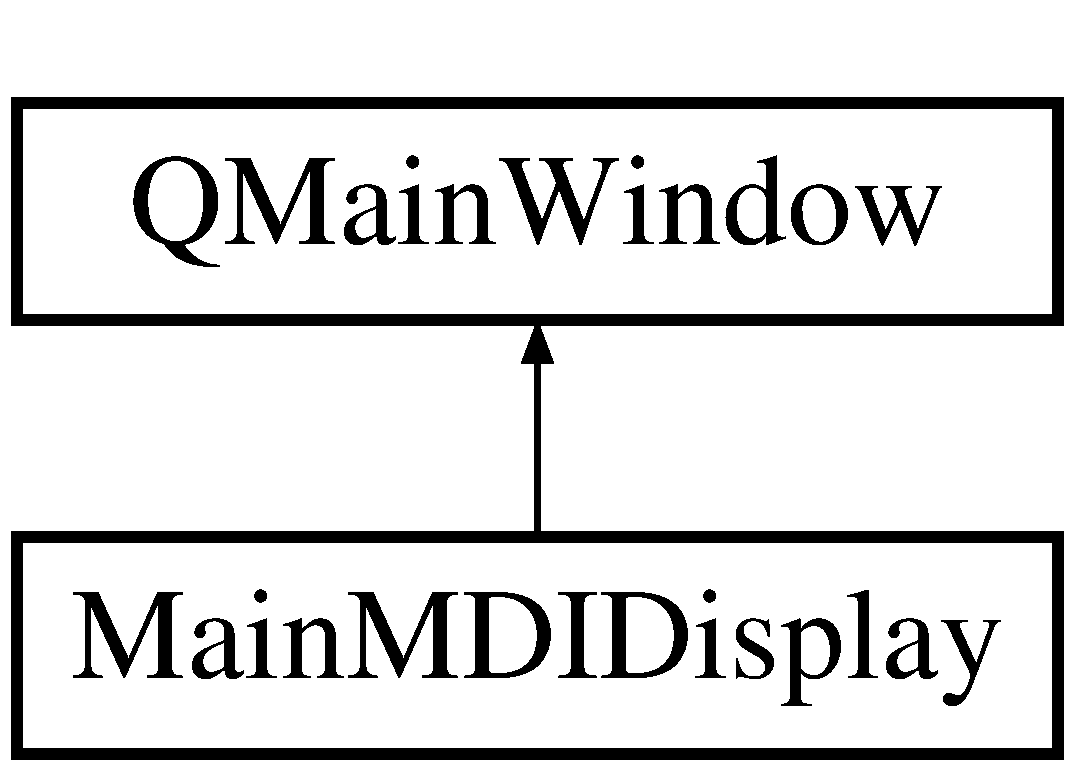
\includegraphics[height=2.000000cm]{class_main_m_d_i_display}
\end{center}
\end{figure}
\subsection*{Public Member Functions}
\begin{DoxyCompactItemize}
\item 
\hyperlink{class_main_m_d_i_display_a782ef2721fdd8b24924ce87dc66bb55c}{Main\+M\+D\+I\+Display} (Q\+Widget $\ast$parent=0)
\item 
void \hyperlink{class_main_m_d_i_display_a527f8ff5bc9f78afb09376ac862a1f34}{add\+Window} (Q\+Widget $\ast$)
\item 
void \hyperlink{class_main_m_d_i_display_a0ca1499c42b7428014519897ed528c32}{add\+Window} (Q\+Widget $\ast$, Q\+String)
\item 
\hyperlink{class_main_m_d_i_display_abeda7bf528423b91f8bc9c3b6873795e}{$\sim$\+Main\+M\+D\+I\+Display} ()
\item 
\hyperlink{class_qt_tab_test}{Qt\+Tab\+Test} $\ast$ \hyperlink{class_main_m_d_i_display_a25d070683b2dbc80d15629af962dd504}{get\+Qtt\+Widget} () const 
\item 
void \hyperlink{class_main_m_d_i_display_a0bd367883842e6f0069181b566690490}{set\+Qtt\+Widget} (\hyperlink{class_qt_tab_test}{Qt\+Tab\+Test} $\ast$)
\item 
void \hyperlink{class_main_m_d_i_display_ae5a5bb272b564517870daf9703e83fca}{clear\+Map\+Execution} ()
\item 
void \hyperlink{class_main_m_d_i_display_a2499cb8a6c4c56d49b7785546a044d35}{clear\+Map\+Recap} ()
\item 
void \hyperlink{class_main_m_d_i_display_a0a08ba2f51e573f0161784e3d9c03b41}{change\+Planning\+To\+Execution\+Window} ()
\item 
void \hyperlink{class_main_m_d_i_display_a437506b2ebd8b9789381a0b48a1b81a3}{switch\+To\+Planning\+Window} ()
\item 
void \hyperlink{class_main_m_d_i_display_ad46e5bb590735c32ec79d192ffbd5244}{switch\+To\+Recap\+Window} ()
\end{DoxyCompactItemize}


\subsection{Constructor \& Destructor Documentation}
\hypertarget{class_main_m_d_i_display_a782ef2721fdd8b24924ce87dc66bb55c}{}\index{Main\+M\+D\+I\+Display@{Main\+M\+D\+I\+Display}!Main\+M\+D\+I\+Display@{Main\+M\+D\+I\+Display}}
\index{Main\+M\+D\+I\+Display@{Main\+M\+D\+I\+Display}!Main\+M\+D\+I\+Display@{Main\+M\+D\+I\+Display}}
\subsubsection[{Main\+M\+D\+I\+Display}]{\setlength{\rightskip}{0pt plus 5cm}Main\+M\+D\+I\+Display\+::\+Main\+M\+D\+I\+Display (
\begin{DoxyParamCaption}
\item[{Q\+Widget $\ast$}]{parent = {\ttfamily 0}}
\end{DoxyParamCaption}
)\hspace{0.3cm}{\ttfamily [explicit]}}\label{class_main_m_d_i_display_a782ef2721fdd8b24924ce87dc66bb55c}
\begin{DoxyRefDesc}{Todo}
\item[\hyperlink{todo__todo000010}{Todo}]\textquotesingle{}dismemberment\textquotesingle{} is no longer an option for the new custom widget-\/based G\+U\+I -\/\+Jordan \end{DoxyRefDesc}


\begin{DoxyNote}{Note}
widget-\/based gui here. Non-\/dismembered 
\end{DoxyNote}
\hypertarget{class_main_m_d_i_display_abeda7bf528423b91f8bc9c3b6873795e}{}\index{Main\+M\+D\+I\+Display@{Main\+M\+D\+I\+Display}!````~Main\+M\+D\+I\+Display@{$\sim$\+Main\+M\+D\+I\+Display}}
\index{````~Main\+M\+D\+I\+Display@{$\sim$\+Main\+M\+D\+I\+Display}!Main\+M\+D\+I\+Display@{Main\+M\+D\+I\+Display}}
\subsubsection[{$\sim$\+Main\+M\+D\+I\+Display}]{\setlength{\rightskip}{0pt plus 5cm}Main\+M\+D\+I\+Display\+::$\sim$\+Main\+M\+D\+I\+Display (
\begin{DoxyParamCaption}
{}
\end{DoxyParamCaption}
)}\label{class_main_m_d_i_display_abeda7bf528423b91f8bc9c3b6873795e}


\subsection{Member Function Documentation}
\hypertarget{class_main_m_d_i_display_a527f8ff5bc9f78afb09376ac862a1f34}{}\index{Main\+M\+D\+I\+Display@{Main\+M\+D\+I\+Display}!add\+Window@{add\+Window}}
\index{add\+Window@{add\+Window}!Main\+M\+D\+I\+Display@{Main\+M\+D\+I\+Display}}
\subsubsection[{add\+Window}]{\setlength{\rightskip}{0pt plus 5cm}void Main\+M\+D\+I\+Display\+::add\+Window (
\begin{DoxyParamCaption}
\item[{Q\+Widget $\ast$}]{my\+New\+Window\+Widget}
\end{DoxyParamCaption}
)}\label{class_main_m_d_i_display_a527f8ff5bc9f78afb09376ac862a1f34}
\hypertarget{class_main_m_d_i_display_a0ca1499c42b7428014519897ed528c32}{}\index{Main\+M\+D\+I\+Display@{Main\+M\+D\+I\+Display}!add\+Window@{add\+Window}}
\index{add\+Window@{add\+Window}!Main\+M\+D\+I\+Display@{Main\+M\+D\+I\+Display}}
\subsubsection[{add\+Window}]{\setlength{\rightskip}{0pt plus 5cm}void Main\+M\+D\+I\+Display\+::add\+Window (
\begin{DoxyParamCaption}
\item[{Q\+Widget $\ast$}]{my\+New\+Window\+Widget, }
\item[{Q\+String}]{window\+Title}
\end{DoxyParamCaption}
)}\label{class_main_m_d_i_display_a0ca1499c42b7428014519897ed528c32}
\hypertarget{class_main_m_d_i_display_a0a08ba2f51e573f0161784e3d9c03b41}{}\index{Main\+M\+D\+I\+Display@{Main\+M\+D\+I\+Display}!change\+Planning\+To\+Execution\+Window@{change\+Planning\+To\+Execution\+Window}}
\index{change\+Planning\+To\+Execution\+Window@{change\+Planning\+To\+Execution\+Window}!Main\+M\+D\+I\+Display@{Main\+M\+D\+I\+Display}}
\subsubsection[{change\+Planning\+To\+Execution\+Window}]{\setlength{\rightskip}{0pt plus 5cm}void Main\+M\+D\+I\+Display\+::change\+Planning\+To\+Execution\+Window (
\begin{DoxyParamCaption}
{}
\end{DoxyParamCaption}
)}\label{class_main_m_d_i_display_a0a08ba2f51e573f0161784e3d9c03b41}
\hypertarget{class_main_m_d_i_display_ae5a5bb272b564517870daf9703e83fca}{}\index{Main\+M\+D\+I\+Display@{Main\+M\+D\+I\+Display}!clear\+Map\+Execution@{clear\+Map\+Execution}}
\index{clear\+Map\+Execution@{clear\+Map\+Execution}!Main\+M\+D\+I\+Display@{Main\+M\+D\+I\+Display}}
\subsubsection[{clear\+Map\+Execution}]{\setlength{\rightskip}{0pt plus 5cm}void Main\+M\+D\+I\+Display\+::clear\+Map\+Execution (
\begin{DoxyParamCaption}
{}
\end{DoxyParamCaption}
)}\label{class_main_m_d_i_display_ae5a5bb272b564517870daf9703e83fca}
\hypertarget{class_main_m_d_i_display_a2499cb8a6c4c56d49b7785546a044d35}{}\index{Main\+M\+D\+I\+Display@{Main\+M\+D\+I\+Display}!clear\+Map\+Recap@{clear\+Map\+Recap}}
\index{clear\+Map\+Recap@{clear\+Map\+Recap}!Main\+M\+D\+I\+Display@{Main\+M\+D\+I\+Display}}
\subsubsection[{clear\+Map\+Recap}]{\setlength{\rightskip}{0pt plus 5cm}void Main\+M\+D\+I\+Display\+::clear\+Map\+Recap (
\begin{DoxyParamCaption}
{}
\end{DoxyParamCaption}
)}\label{class_main_m_d_i_display_a2499cb8a6c4c56d49b7785546a044d35}
\hypertarget{class_main_m_d_i_display_a25d070683b2dbc80d15629af962dd504}{}\index{Main\+M\+D\+I\+Display@{Main\+M\+D\+I\+Display}!get\+Qtt\+Widget@{get\+Qtt\+Widget}}
\index{get\+Qtt\+Widget@{get\+Qtt\+Widget}!Main\+M\+D\+I\+Display@{Main\+M\+D\+I\+Display}}
\subsubsection[{get\+Qtt\+Widget}]{\setlength{\rightskip}{0pt plus 5cm}{\bf Qt\+Tab\+Test} $\ast$ Main\+M\+D\+I\+Display\+::get\+Qtt\+Widget (
\begin{DoxyParamCaption}
{}
\end{DoxyParamCaption}
) const}\label{class_main_m_d_i_display_a25d070683b2dbc80d15629af962dd504}
\hypertarget{class_main_m_d_i_display_a0bd367883842e6f0069181b566690490}{}\index{Main\+M\+D\+I\+Display@{Main\+M\+D\+I\+Display}!set\+Qtt\+Widget@{set\+Qtt\+Widget}}
\index{set\+Qtt\+Widget@{set\+Qtt\+Widget}!Main\+M\+D\+I\+Display@{Main\+M\+D\+I\+Display}}
\subsubsection[{set\+Qtt\+Widget}]{\setlength{\rightskip}{0pt plus 5cm}void Main\+M\+D\+I\+Display\+::set\+Qtt\+Widget (
\begin{DoxyParamCaption}
\item[{{\bf Qt\+Tab\+Test} $\ast$}]{value}
\end{DoxyParamCaption}
)}\label{class_main_m_d_i_display_a0bd367883842e6f0069181b566690490}
\hypertarget{class_main_m_d_i_display_a437506b2ebd8b9789381a0b48a1b81a3}{}\index{Main\+M\+D\+I\+Display@{Main\+M\+D\+I\+Display}!switch\+To\+Planning\+Window@{switch\+To\+Planning\+Window}}
\index{switch\+To\+Planning\+Window@{switch\+To\+Planning\+Window}!Main\+M\+D\+I\+Display@{Main\+M\+D\+I\+Display}}
\subsubsection[{switch\+To\+Planning\+Window}]{\setlength{\rightskip}{0pt plus 5cm}void Main\+M\+D\+I\+Display\+::switch\+To\+Planning\+Window (
\begin{DoxyParamCaption}
{}
\end{DoxyParamCaption}
)}\label{class_main_m_d_i_display_a437506b2ebd8b9789381a0b48a1b81a3}
\hypertarget{class_main_m_d_i_display_ad46e5bb590735c32ec79d192ffbd5244}{}\index{Main\+M\+D\+I\+Display@{Main\+M\+D\+I\+Display}!switch\+To\+Recap\+Window@{switch\+To\+Recap\+Window}}
\index{switch\+To\+Recap\+Window@{switch\+To\+Recap\+Window}!Main\+M\+D\+I\+Display@{Main\+M\+D\+I\+Display}}
\subsubsection[{switch\+To\+Recap\+Window}]{\setlength{\rightskip}{0pt plus 5cm}void Main\+M\+D\+I\+Display\+::switch\+To\+Recap\+Window (
\begin{DoxyParamCaption}
{}
\end{DoxyParamCaption}
)}\label{class_main_m_d_i_display_ad46e5bb590735c32ec79d192ffbd5244}


The documentation for this class was generated from the following files\+:\begin{DoxyCompactItemize}
\item 
C\+:/\+Users/\+Roman/\+Documents/\+Mygs/\+Ground\+Station/\+G\+S/\hyperlink{mainmdidisplay_8h}{mainmdidisplay.\+h}\item 
C\+:/\+Users/\+Roman/\+Documents/\+Mygs/\+Ground\+Station/\+G\+S/\hyperlink{mainmdidisplay_8cpp}{mainmdidisplay.\+cpp}\end{DoxyCompactItemize}

\hypertarget{class_main_window}{}\section{Main\+Window Class Reference}
\label{class_main_window}\index{Main\+Window@{Main\+Window}}


{\ttfamily \#include $<$mainwindow.\+h$>$}

Inheritance diagram for Main\+Window\+:\begin{figure}[H]
\begin{center}
\leavevmode
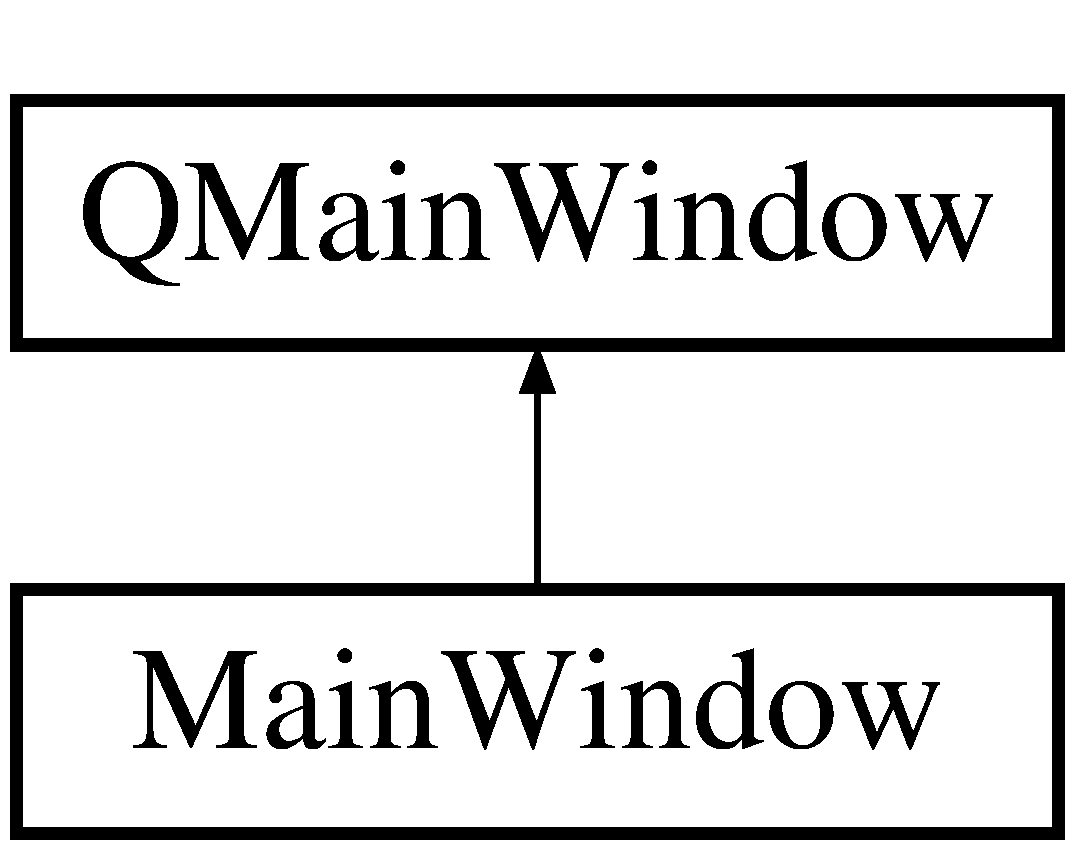
\includegraphics[height=2.000000cm]{class_main_window}
\end{center}
\end{figure}
\subsection*{Public Member Functions}
\begin{DoxyCompactItemize}
\item 
\hyperlink{class_main_window_a8b244be8b7b7db1b08de2a2acb9409db}{Main\+Window} (Q\+Widget $\ast$parent=0)
\item 
\hyperlink{class_main_window_ae98d00a93bc118200eeef9f9bba1dba7}{$\sim$\+Main\+Window} ()
\end{DoxyCompactItemize}


\subsection{Constructor \& Destructor Documentation}
\hypertarget{class_main_window_a8b244be8b7b7db1b08de2a2acb9409db}{}\index{Main\+Window@{Main\+Window}!Main\+Window@{Main\+Window}}
\index{Main\+Window@{Main\+Window}!Main\+Window@{Main\+Window}}
\subsubsection[{Main\+Window}]{\setlength{\rightskip}{0pt plus 5cm}Main\+Window\+::\+Main\+Window (
\begin{DoxyParamCaption}
\item[{Q\+Widget $\ast$}]{parent = {\ttfamily 0}}
\end{DoxyParamCaption}
)\hspace{0.3cm}{\ttfamily [explicit]}}\label{class_main_window_a8b244be8b7b7db1b08de2a2acb9409db}
Constructor for the main window \hypertarget{class_main_window_ae98d00a93bc118200eeef9f9bba1dba7}{}\index{Main\+Window@{Main\+Window}!````~Main\+Window@{$\sim$\+Main\+Window}}
\index{````~Main\+Window@{$\sim$\+Main\+Window}!Main\+Window@{Main\+Window}}
\subsubsection[{$\sim$\+Main\+Window}]{\setlength{\rightskip}{0pt plus 5cm}Main\+Window\+::$\sim$\+Main\+Window (
\begin{DoxyParamCaption}
{}
\end{DoxyParamCaption}
)}\label{class_main_window_ae98d00a93bc118200eeef9f9bba1dba7}
Destructor for the main window 

The documentation for this class was generated from the following files\+:\begin{DoxyCompactItemize}
\item 
C\+:/\+Users/\+Roman/\+Documents/\+Mygs/\+Ground\+Station/\+G\+S/\hyperlink{mainwindow_8h}{mainwindow.\+h}\item 
C\+:/\+Users/\+Roman/\+Documents/\+Mygs/\+Ground\+Station/\+G\+S/\hyperlink{mainwindow_8cpp}{mainwindow.\+cpp}\end{DoxyCompactItemize}

\hypertarget{class_map_execution}{}\section{Map\+Execution Class Reference}
\label{class_map_execution}\index{Map\+Execution@{Map\+Execution}}


{\ttfamily \#include $<$mapexecution.\+h$>$}

Inheritance diagram for Map\+Execution\+:\begin{figure}[H]
\begin{center}
\leavevmode
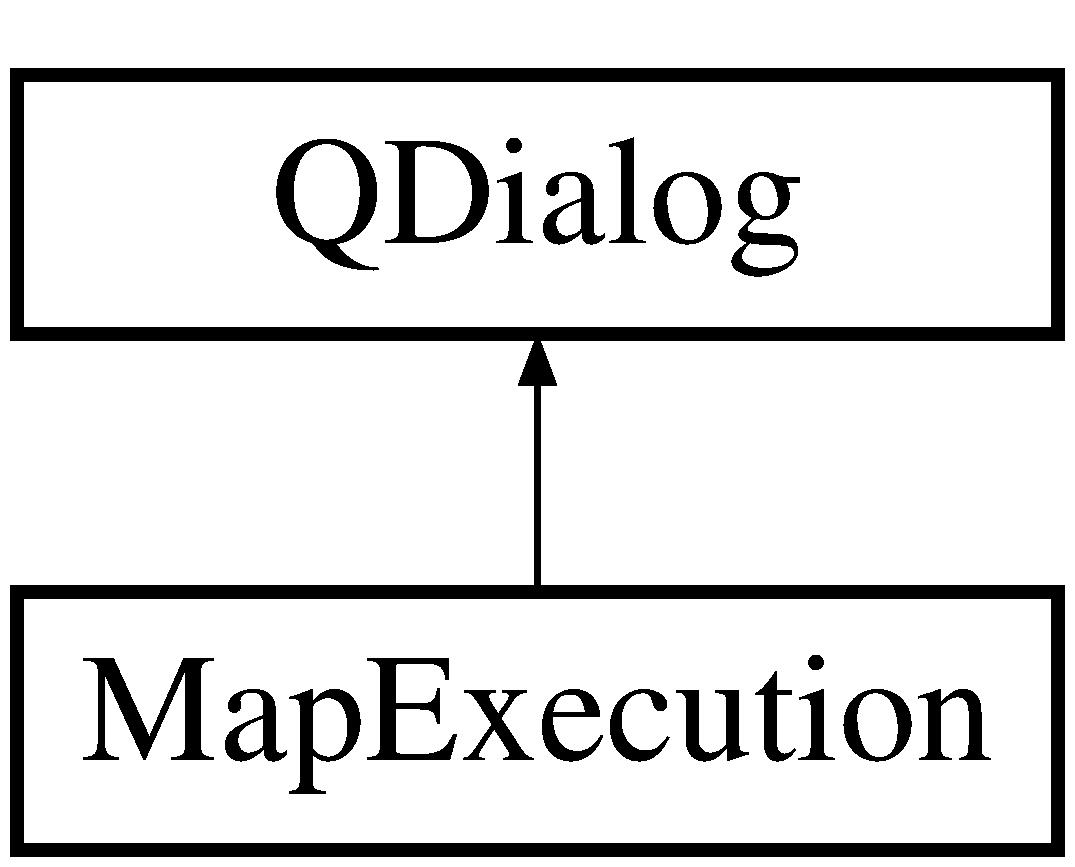
\includegraphics[height=2.000000cm]{class_map_execution}
\end{center}
\end{figure}
\subsection*{Public Slots}
\begin{DoxyCompactItemize}
\item 
void \hyperlink{class_map_execution_a0fc2a824601c5f09fb8d448f025d4da3}{add\+New\+Map} ()
\item 
void \hyperlink{class_map_execution_a993abccda8744bb5ad9110b97027d650}{plot\+Position} (double lat, double lng)
\item 
void \hyperlink{class_map_execution_abf980f0adb250cd2ef5a99668a793f46}{send\+Coord\+To\+J\+S\+Map} (double lat, double lng, int map\+I\+D)
\item 
void \hyperlink{class_map_execution_aae070b94d4318c09aaa4a95b244050c4}{draw\+Flight\+Path} (\hyperlink{class_flight_path}{Flight\+Path} $\ast$flight\+Path)
\item 
void \hyperlink{class_map_execution_a3bb03858cf15e2f9543a0e169383e13b}{update\+Table} (double lat, double lng)
\item 
void \hyperlink{class_map_execution_a5f0c7ab18a5fcc4c474eeb5b9707dc61}{send\+Flight\+Plan} ()
\item 
void \hyperlink{class_map_execution_af846e29b7a32021359fcf66bca46e20b}{update\+Status\+Indicator} ()
\end{DoxyCompactItemize}
\subsection*{Signals}
\begin{DoxyCompactItemize}
\item 
void \hyperlink{class_map_execution_a658805b61b3331c43c48211e543cafe0}{time\+To\+Start\+Map\+Recap} ()
\end{DoxyCompactItemize}
\subsection*{Public Member Functions}
\begin{DoxyCompactItemize}
\item 
\hyperlink{class_map_execution_afcf6d9187674478b9b24cdb59b832198}{Map\+Execution} (\hyperlink{class_flight_path}{Flight\+Path} $\ast$flight\+Path, Q\+Widget $\ast$parent=0)
\item 
\hyperlink{class_map_execution_a8cd67a89386d7880f2f741598f78115c}{Map\+Execution} (Q\+Widget $\ast$parent=0)
\item 
\hyperlink{class_map_execution_aeaebbbd5ed4a669c28b9b2372a135e9c}{$\sim$\+Map\+Execution} ()
\item 
\hyperlink{class_mission}{Mission} \hyperlink{class_map_execution_ab96a28f3c2d98931c94e25cd4d059262}{get\+My\+Mission} () const 
\item 
\hyperlink{class_map_recap}{Map\+Recap} $\ast$ \hyperlink{class_map_execution_a44b75a52f37d3a0487651e75c79aea2a}{get\+Map\+Recap} ()
\item 
void \hyperlink{class_map_execution_a41eefdc4c0f8c8bec18b11f3eb55f91b}{set\+My\+Mission} (const \hyperlink{class_mission}{Mission} \&value)
\end{DoxyCompactItemize}
\subsection*{Public Attributes}
\begin{DoxyCompactItemize}
\item 
\hyperlink{class_gs_server}{Gs\+Server} \hyperlink{class_map_execution_a9cbfe92cbfe0fe7ee433a04a121be766}{my\+Server}
\item 
\hyperlink{classmessagebox}{messagebox} \hyperlink{class_map_execution_ade1432547d600a40172f5f00e4db3a1e}{My\+Message\+Box}
\end{DoxyCompactItemize}
\subsection*{Friends}
\begin{DoxyCompactItemize}
\item 
class \hyperlink{class_map_execution_a337398c114f638b5a3e2fdc4529936c5}{Main\+M\+D\+I\+Display}
\end{DoxyCompactItemize}


\subsection{Constructor \& Destructor Documentation}
\hypertarget{class_map_execution_afcf6d9187674478b9b24cdb59b832198}{}\index{Map\+Execution@{Map\+Execution}!Map\+Execution@{Map\+Execution}}
\index{Map\+Execution@{Map\+Execution}!Map\+Execution@{Map\+Execution}}
\subsubsection[{Map\+Execution}]{\setlength{\rightskip}{0pt plus 5cm}Map\+Execution\+::\+Map\+Execution (
\begin{DoxyParamCaption}
\item[{{\bf Flight\+Path} $\ast$}]{flight\+Path, }
\item[{Q\+Widget $\ast$}]{parent = {\ttfamily 0}}
\end{DoxyParamCaption}
)}\label{class_map_execution_afcf6d9187674478b9b24cdb59b832198}
\hypertarget{class_map_execution_a8cd67a89386d7880f2f741598f78115c}{}\index{Map\+Execution@{Map\+Execution}!Map\+Execution@{Map\+Execution}}
\index{Map\+Execution@{Map\+Execution}!Map\+Execution@{Map\+Execution}}
\subsubsection[{Map\+Execution}]{\setlength{\rightskip}{0pt plus 5cm}Map\+Execution\+::\+Map\+Execution (
\begin{DoxyParamCaption}
\item[{Q\+Widget $\ast$}]{parent = {\ttfamily 0}}
\end{DoxyParamCaption}
)\hspace{0.3cm}{\ttfamily [explicit]}}\label{class_map_execution_a8cd67a89386d7880f2f741598f78115c}
\hypertarget{class_map_execution_aeaebbbd5ed4a669c28b9b2372a135e9c}{}\index{Map\+Execution@{Map\+Execution}!````~Map\+Execution@{$\sim$\+Map\+Execution}}
\index{````~Map\+Execution@{$\sim$\+Map\+Execution}!Map\+Execution@{Map\+Execution}}
\subsubsection[{$\sim$\+Map\+Execution}]{\setlength{\rightskip}{0pt plus 5cm}Map\+Execution\+::$\sim$\+Map\+Execution (
\begin{DoxyParamCaption}
{}
\end{DoxyParamCaption}
)}\label{class_map_execution_aeaebbbd5ed4a669c28b9b2372a135e9c}


\subsection{Member Function Documentation}
\hypertarget{class_map_execution_a0fc2a824601c5f09fb8d448f025d4da3}{}\index{Map\+Execution@{Map\+Execution}!add\+New\+Map@{add\+New\+Map}}
\index{add\+New\+Map@{add\+New\+Map}!Map\+Execution@{Map\+Execution}}
\subsubsection[{add\+New\+Map}]{\setlength{\rightskip}{0pt plus 5cm}void Map\+Execution\+::add\+New\+Map (
\begin{DoxyParamCaption}
{}
\end{DoxyParamCaption}
)\hspace{0.3cm}{\ttfamily [slot]}}\label{class_map_execution_a0fc2a824601c5f09fb8d448f025d4da3}
\hypertarget{class_map_execution_aae070b94d4318c09aaa4a95b244050c4}{}\index{Map\+Execution@{Map\+Execution}!draw\+Flight\+Path@{draw\+Flight\+Path}}
\index{draw\+Flight\+Path@{draw\+Flight\+Path}!Map\+Execution@{Map\+Execution}}
\subsubsection[{draw\+Flight\+Path}]{\setlength{\rightskip}{0pt plus 5cm}void Map\+Execution\+::draw\+Flight\+Path (
\begin{DoxyParamCaption}
\item[{{\bf Flight\+Path} $\ast$}]{flight\+Path}
\end{DoxyParamCaption}
)\hspace{0.3cm}{\ttfamily [slot]}}\label{class_map_execution_aae070b94d4318c09aaa4a95b244050c4}
\hypertarget{class_map_execution_a44b75a52f37d3a0487651e75c79aea2a}{}\index{Map\+Execution@{Map\+Execution}!get\+Map\+Recap@{get\+Map\+Recap}}
\index{get\+Map\+Recap@{get\+Map\+Recap}!Map\+Execution@{Map\+Execution}}
\subsubsection[{get\+Map\+Recap}]{\setlength{\rightskip}{0pt plus 5cm}{\bf Map\+Recap} $\ast$ Map\+Execution\+::get\+Map\+Recap (
\begin{DoxyParamCaption}
{}
\end{DoxyParamCaption}
)}\label{class_map_execution_a44b75a52f37d3a0487651e75c79aea2a}
\hypertarget{class_map_execution_ab96a28f3c2d98931c94e25cd4d059262}{}\index{Map\+Execution@{Map\+Execution}!get\+My\+Mission@{get\+My\+Mission}}
\index{get\+My\+Mission@{get\+My\+Mission}!Map\+Execution@{Map\+Execution}}
\subsubsection[{get\+My\+Mission}]{\setlength{\rightskip}{0pt plus 5cm}{\bf Mission} Map\+Execution\+::get\+My\+Mission (
\begin{DoxyParamCaption}
{}
\end{DoxyParamCaption}
) const}\label{class_map_execution_ab96a28f3c2d98931c94e25cd4d059262}
\hypertarget{class_map_execution_a993abccda8744bb5ad9110b97027d650}{}\index{Map\+Execution@{Map\+Execution}!plot\+Position@{plot\+Position}}
\index{plot\+Position@{plot\+Position}!Map\+Execution@{Map\+Execution}}
\subsubsection[{plot\+Position}]{\setlength{\rightskip}{0pt plus 5cm}void Map\+Execution\+::plot\+Position (
\begin{DoxyParamCaption}
\item[{double}]{lat, }
\item[{double}]{lng}
\end{DoxyParamCaption}
)\hspace{0.3cm}{\ttfamily [slot]}}\label{class_map_execution_a993abccda8744bb5ad9110b97027d650}
\hypertarget{class_map_execution_abf980f0adb250cd2ef5a99668a793f46}{}\index{Map\+Execution@{Map\+Execution}!send\+Coord\+To\+J\+S\+Map@{send\+Coord\+To\+J\+S\+Map}}
\index{send\+Coord\+To\+J\+S\+Map@{send\+Coord\+To\+J\+S\+Map}!Map\+Execution@{Map\+Execution}}
\subsubsection[{send\+Coord\+To\+J\+S\+Map}]{\setlength{\rightskip}{0pt plus 5cm}void Map\+Execution\+::send\+Coord\+To\+J\+S\+Map (
\begin{DoxyParamCaption}
\item[{double}]{lat, }
\item[{double}]{lng, }
\item[{int}]{map\+I\+D}
\end{DoxyParamCaption}
)\hspace{0.3cm}{\ttfamily [slot]}}\label{class_map_execution_abf980f0adb250cd2ef5a99668a793f46}
\hypertarget{class_map_execution_a5f0c7ab18a5fcc4c474eeb5b9707dc61}{}\index{Map\+Execution@{Map\+Execution}!send\+Flight\+Plan@{send\+Flight\+Plan}}
\index{send\+Flight\+Plan@{send\+Flight\+Plan}!Map\+Execution@{Map\+Execution}}
\subsubsection[{send\+Flight\+Plan}]{\setlength{\rightskip}{0pt plus 5cm}void Map\+Execution\+::send\+Flight\+Plan (
\begin{DoxyParamCaption}
{}
\end{DoxyParamCaption}
)\hspace{0.3cm}{\ttfamily [slot]}}\label{class_map_execution_a5f0c7ab18a5fcc4c474eeb5b9707dc61}
\hypertarget{class_map_execution_a41eefdc4c0f8c8bec18b11f3eb55f91b}{}\index{Map\+Execution@{Map\+Execution}!set\+My\+Mission@{set\+My\+Mission}}
\index{set\+My\+Mission@{set\+My\+Mission}!Map\+Execution@{Map\+Execution}}
\subsubsection[{set\+My\+Mission}]{\setlength{\rightskip}{0pt plus 5cm}void Map\+Execution\+::set\+My\+Mission (
\begin{DoxyParamCaption}
\item[{const {\bf Mission} \&}]{value}
\end{DoxyParamCaption}
)}\label{class_map_execution_a41eefdc4c0f8c8bec18b11f3eb55f91b}
\hypertarget{class_map_execution_a658805b61b3331c43c48211e543cafe0}{}\index{Map\+Execution@{Map\+Execution}!time\+To\+Start\+Map\+Recap@{time\+To\+Start\+Map\+Recap}}
\index{time\+To\+Start\+Map\+Recap@{time\+To\+Start\+Map\+Recap}!Map\+Execution@{Map\+Execution}}
\subsubsection[{time\+To\+Start\+Map\+Recap}]{\setlength{\rightskip}{0pt plus 5cm}void Map\+Execution\+::time\+To\+Start\+Map\+Recap (
\begin{DoxyParamCaption}
{}
\end{DoxyParamCaption}
)\hspace{0.3cm}{\ttfamily [signal]}}\label{class_map_execution_a658805b61b3331c43c48211e543cafe0}
\hypertarget{class_map_execution_af846e29b7a32021359fcf66bca46e20b}{}\index{Map\+Execution@{Map\+Execution}!update\+Status\+Indicator@{update\+Status\+Indicator}}
\index{update\+Status\+Indicator@{update\+Status\+Indicator}!Map\+Execution@{Map\+Execution}}
\subsubsection[{update\+Status\+Indicator}]{\setlength{\rightskip}{0pt plus 5cm}void Map\+Execution\+::update\+Status\+Indicator (
\begin{DoxyParamCaption}
{}
\end{DoxyParamCaption}
)\hspace{0.3cm}{\ttfamily [slot]}}\label{class_map_execution_af846e29b7a32021359fcf66bca46e20b}
\hypertarget{class_map_execution_a3bb03858cf15e2f9543a0e169383e13b}{}\index{Map\+Execution@{Map\+Execution}!update\+Table@{update\+Table}}
\index{update\+Table@{update\+Table}!Map\+Execution@{Map\+Execution}}
\subsubsection[{update\+Table}]{\setlength{\rightskip}{0pt plus 5cm}void Map\+Execution\+::update\+Table (
\begin{DoxyParamCaption}
\item[{double}]{lat, }
\item[{double}]{lng}
\end{DoxyParamCaption}
)\hspace{0.3cm}{\ttfamily [slot]}}\label{class_map_execution_a3bb03858cf15e2f9543a0e169383e13b}


\subsection{Friends And Related Function Documentation}
\hypertarget{class_map_execution_a337398c114f638b5a3e2fdc4529936c5}{}\index{Map\+Execution@{Map\+Execution}!Main\+M\+D\+I\+Display@{Main\+M\+D\+I\+Display}}
\index{Main\+M\+D\+I\+Display@{Main\+M\+D\+I\+Display}!Map\+Execution@{Map\+Execution}}
\subsubsection[{Main\+M\+D\+I\+Display}]{\setlength{\rightskip}{0pt plus 5cm}friend class {\bf Main\+M\+D\+I\+Display}\hspace{0.3cm}{\ttfamily [friend]}}\label{class_map_execution_a337398c114f638b5a3e2fdc4529936c5}


\subsection{Member Data Documentation}
\hypertarget{class_map_execution_ade1432547d600a40172f5f00e4db3a1e}{}\index{Map\+Execution@{Map\+Execution}!My\+Message\+Box@{My\+Message\+Box}}
\index{My\+Message\+Box@{My\+Message\+Box}!Map\+Execution@{Map\+Execution}}
\subsubsection[{My\+Message\+Box}]{\setlength{\rightskip}{0pt plus 5cm}{\bf messagebox} Map\+Execution\+::\+My\+Message\+Box}\label{class_map_execution_ade1432547d600a40172f5f00e4db3a1e}
\hypertarget{class_map_execution_a9cbfe92cbfe0fe7ee433a04a121be766}{}\index{Map\+Execution@{Map\+Execution}!my\+Server@{my\+Server}}
\index{my\+Server@{my\+Server}!Map\+Execution@{Map\+Execution}}
\subsubsection[{my\+Server}]{\setlength{\rightskip}{0pt plus 5cm}{\bf Gs\+Server} Map\+Execution\+::my\+Server}\label{class_map_execution_a9cbfe92cbfe0fe7ee433a04a121be766}


The documentation for this class was generated from the following files\+:\begin{DoxyCompactItemize}
\item 
C\+:/\+Users/\+Roman/\+Documents/\+Mygs/\+Ground\+Station/\+G\+S/\hyperlink{mapexecution_8h}{mapexecution.\+h}\item 
C\+:/\+Users/\+Roman/\+Documents/\+Mygs/\+Ground\+Station/\+G\+S/\hyperlink{mapexecution_8cpp}{mapexecution.\+cpp}\end{DoxyCompactItemize}

\hypertarget{class_map_planning}{}\section{Map\+Planning Class Reference}
\label{class_map_planning}\index{Map\+Planning@{Map\+Planning}}


{\ttfamily \#include $<$mapplanning.\+h$>$}

Inheritance diagram for Map\+Planning\+:\begin{figure}[H]
\begin{center}
\leavevmode
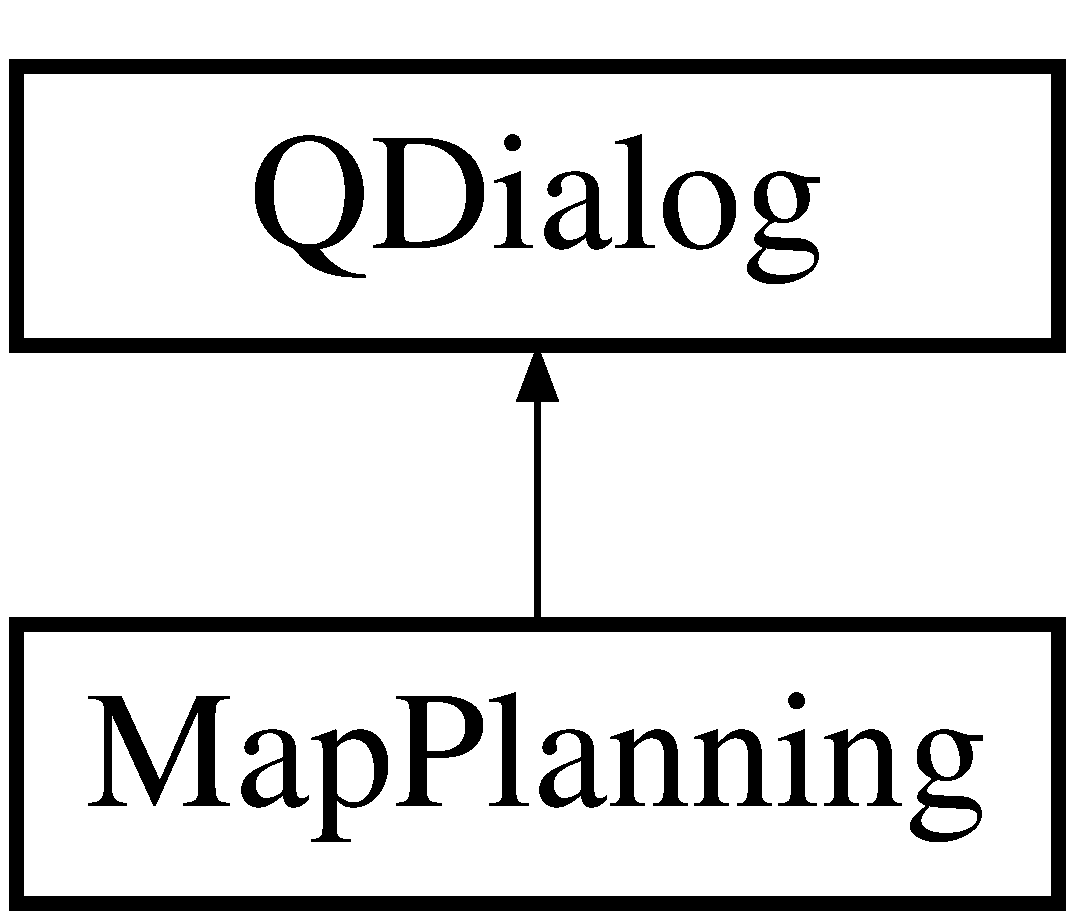
\includegraphics[height=2.000000cm]{class_map_planning}
\end{center}
\end{figure}
\subsection*{Public Slots}
\begin{DoxyCompactItemize}
\item 
void \hyperlink{class_map_planning_af2068f7c19c1f495debe4c4e745c99d4}{add\+Point\+To\+Table} (double lat, double lng)
\item 
void \hyperlink{class_map_planning_a320e452b516fbad57bb4a2a6138832c8}{clear\+Table} ()
\end{DoxyCompactItemize}
\subsection*{Signals}
\begin{DoxyCompactItemize}
\item 
void \hyperlink{class_map_planning_a700eb0065441bec199a2a3fc343d0571}{time\+To\+Start\+Map\+Execution} ()
\end{DoxyCompactItemize}
\subsection*{Public Member Functions}
\begin{DoxyCompactItemize}
\item 
\hyperlink{class_map_planning_a02df54932a2eeeb02ca68ee9de8f4e83}{Map\+Planning} (Q\+Widget $\ast$parent=0)
\item 
\hyperlink{class_map_planning_a676c43e0b605ee019f8cbfe1cb4e38be}{$\sim$\+Map\+Planning} ()
\item 
void \hyperlink{class_map_planning_adbd3f2c13fafaaa335058f7517ee4601}{update\+Map} ()
\item 
\hyperlink{class_flight_path}{Flight\+Path} $\ast$ \hyperlink{class_map_planning_a38f72780859a68815d818b28767c6dfd}{get\+Table\+As\+Flight\+Path} ()
\end{DoxyCompactItemize}
\subsection*{Friends}
\begin{DoxyCompactItemize}
\item 
class \hyperlink{class_map_planning_a337398c114f638b5a3e2fdc4529936c5}{Main\+M\+D\+I\+Display}
\end{DoxyCompactItemize}


\subsection{Constructor \& Destructor Documentation}
\hypertarget{class_map_planning_a02df54932a2eeeb02ca68ee9de8f4e83}{}\index{Map\+Planning@{Map\+Planning}!Map\+Planning@{Map\+Planning}}
\index{Map\+Planning@{Map\+Planning}!Map\+Planning@{Map\+Planning}}
\subsubsection[{Map\+Planning}]{\setlength{\rightskip}{0pt plus 5cm}Map\+Planning\+::\+Map\+Planning (
\begin{DoxyParamCaption}
\item[{Q\+Widget $\ast$}]{parent = {\ttfamily 0}}
\end{DoxyParamCaption}
)\hspace{0.3cm}{\ttfamily [explicit]}}\label{class_map_planning_a02df54932a2eeeb02ca68ee9de8f4e83}
\hypertarget{class_map_planning_a676c43e0b605ee019f8cbfe1cb4e38be}{}\index{Map\+Planning@{Map\+Planning}!````~Map\+Planning@{$\sim$\+Map\+Planning}}
\index{````~Map\+Planning@{$\sim$\+Map\+Planning}!Map\+Planning@{Map\+Planning}}
\subsubsection[{$\sim$\+Map\+Planning}]{\setlength{\rightskip}{0pt plus 5cm}Map\+Planning\+::$\sim$\+Map\+Planning (
\begin{DoxyParamCaption}
{}
\end{DoxyParamCaption}
)}\label{class_map_planning_a676c43e0b605ee019f8cbfe1cb4e38be}


\subsection{Member Function Documentation}
\hypertarget{class_map_planning_af2068f7c19c1f495debe4c4e745c99d4}{}\index{Map\+Planning@{Map\+Planning}!add\+Point\+To\+Table@{add\+Point\+To\+Table}}
\index{add\+Point\+To\+Table@{add\+Point\+To\+Table}!Map\+Planning@{Map\+Planning}}
\subsubsection[{add\+Point\+To\+Table}]{\setlength{\rightskip}{0pt plus 5cm}void Map\+Planning\+::add\+Point\+To\+Table (
\begin{DoxyParamCaption}
\item[{double}]{lat, }
\item[{double}]{lng}
\end{DoxyParamCaption}
)\hspace{0.3cm}{\ttfamily [slot]}}\label{class_map_planning_af2068f7c19c1f495debe4c4e745c99d4}
\hypertarget{class_map_planning_a320e452b516fbad57bb4a2a6138832c8}{}\index{Map\+Planning@{Map\+Planning}!clear\+Table@{clear\+Table}}
\index{clear\+Table@{clear\+Table}!Map\+Planning@{Map\+Planning}}
\subsubsection[{clear\+Table}]{\setlength{\rightskip}{0pt plus 5cm}void Map\+Planning\+::clear\+Table (
\begin{DoxyParamCaption}
{}
\end{DoxyParamCaption}
)\hspace{0.3cm}{\ttfamily [slot]}}\label{class_map_planning_a320e452b516fbad57bb4a2a6138832c8}
\hypertarget{class_map_planning_a38f72780859a68815d818b28767c6dfd}{}\index{Map\+Planning@{Map\+Planning}!get\+Table\+As\+Flight\+Path@{get\+Table\+As\+Flight\+Path}}
\index{get\+Table\+As\+Flight\+Path@{get\+Table\+As\+Flight\+Path}!Map\+Planning@{Map\+Planning}}
\subsubsection[{get\+Table\+As\+Flight\+Path}]{\setlength{\rightskip}{0pt plus 5cm}{\bf Flight\+Path} $\ast$ Map\+Planning\+::get\+Table\+As\+Flight\+Path (
\begin{DoxyParamCaption}
{}
\end{DoxyParamCaption}
)}\label{class_map_planning_a38f72780859a68815d818b28767c6dfd}
\hypertarget{class_map_planning_a700eb0065441bec199a2a3fc343d0571}{}\index{Map\+Planning@{Map\+Planning}!time\+To\+Start\+Map\+Execution@{time\+To\+Start\+Map\+Execution}}
\index{time\+To\+Start\+Map\+Execution@{time\+To\+Start\+Map\+Execution}!Map\+Planning@{Map\+Planning}}
\subsubsection[{time\+To\+Start\+Map\+Execution}]{\setlength{\rightskip}{0pt plus 5cm}void Map\+Planning\+::time\+To\+Start\+Map\+Execution (
\begin{DoxyParamCaption}
{}
\end{DoxyParamCaption}
)\hspace{0.3cm}{\ttfamily [signal]}}\label{class_map_planning_a700eb0065441bec199a2a3fc343d0571}
\hypertarget{class_map_planning_adbd3f2c13fafaaa335058f7517ee4601}{}\index{Map\+Planning@{Map\+Planning}!update\+Map@{update\+Map}}
\index{update\+Map@{update\+Map}!Map\+Planning@{Map\+Planning}}
\subsubsection[{update\+Map}]{\setlength{\rightskip}{0pt plus 5cm}void Map\+Planning\+::update\+Map (
\begin{DoxyParamCaption}
{}
\end{DoxyParamCaption}
)}\label{class_map_planning_adbd3f2c13fafaaa335058f7517ee4601}


\subsection{Friends And Related Function Documentation}
\hypertarget{class_map_planning_a337398c114f638b5a3e2fdc4529936c5}{}\index{Map\+Planning@{Map\+Planning}!Main\+M\+D\+I\+Display@{Main\+M\+D\+I\+Display}}
\index{Main\+M\+D\+I\+Display@{Main\+M\+D\+I\+Display}!Map\+Planning@{Map\+Planning}}
\subsubsection[{Main\+M\+D\+I\+Display}]{\setlength{\rightskip}{0pt plus 5cm}friend class {\bf Main\+M\+D\+I\+Display}\hspace{0.3cm}{\ttfamily [friend]}}\label{class_map_planning_a337398c114f638b5a3e2fdc4529936c5}


The documentation for this class was generated from the following files\+:\begin{DoxyCompactItemize}
\item 
C\+:/\+Users/\+Roman/\+Documents/\+Mygs/\+Ground\+Station/\+G\+S/\hyperlink{mapplanning_8h}{mapplanning.\+h}\item 
C\+:/\+Users/\+Roman/\+Documents/\+Mygs/\+Ground\+Station/\+G\+S/\hyperlink{mapplanning_8cpp}{mapplanning.\+cpp}\end{DoxyCompactItemize}

\hypertarget{class_map_recap}{}\section{Map\+Recap Class Reference}
\label{class_map_recap}\index{Map\+Recap@{Map\+Recap}}


{\ttfamily \#include $<$maprecap.\+h$>$}

Inheritance diagram for Map\+Recap\+:\begin{figure}[H]
\begin{center}
\leavevmode
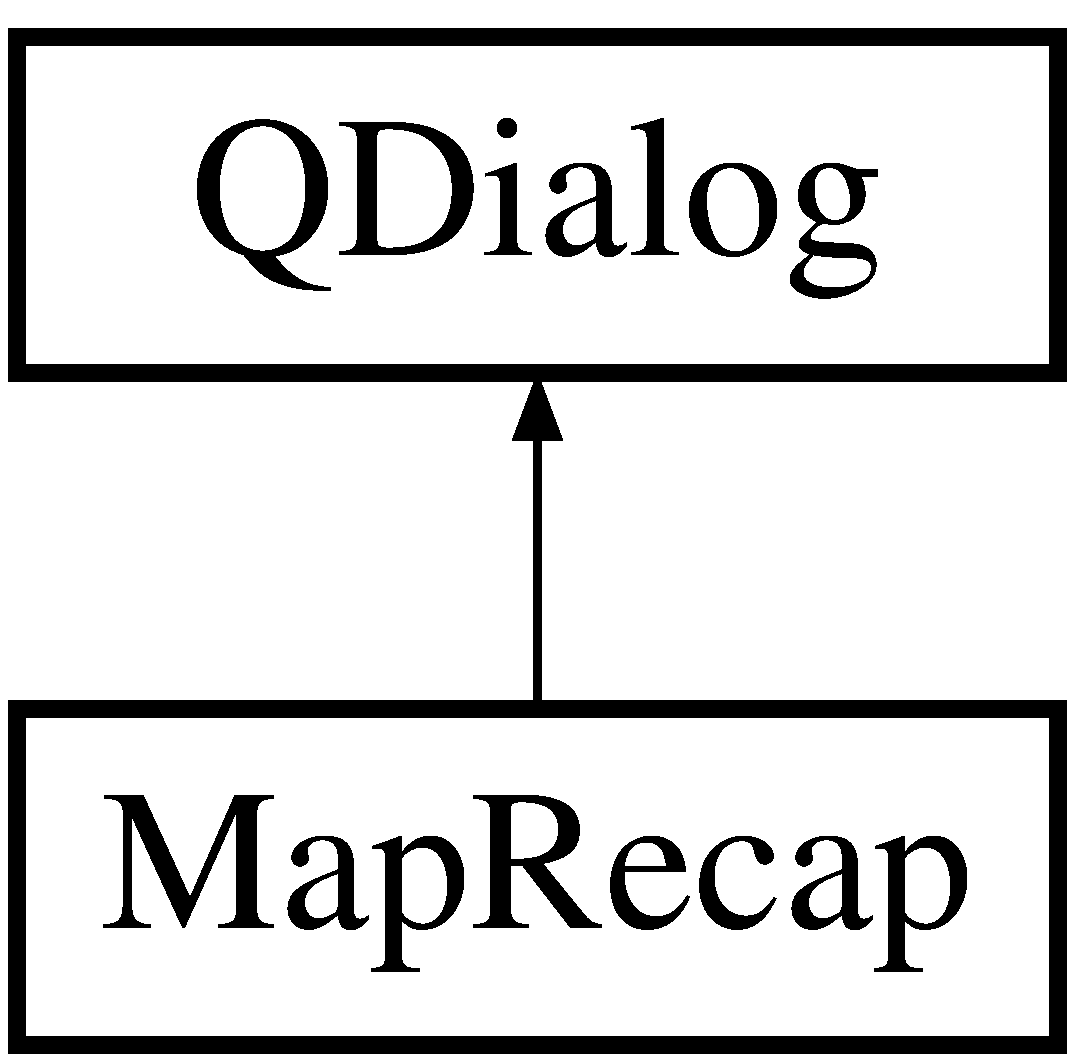
\includegraphics[height=2.000000cm]{class_map_recap}
\end{center}
\end{figure}
\subsection*{Public Slots}
\begin{DoxyCompactItemize}
\item 
void \hyperlink{class_map_recap_aeaf4d37a45ad4e4b7d9747473c900531}{add\+New\+Map} ()
\item 
void \hyperlink{class_map_recap_a1c98beb9687a394d68e41fd39580edfe}{add\+Point\+To\+Table} (double lat, double lng)
\end{DoxyCompactItemize}
\subsection*{Public Member Functions}
\begin{DoxyCompactItemize}
\item 
\hyperlink{class_map_recap_a739aa8a008d8daf8ed083edd2af1da56}{Map\+Recap} (\hyperlink{class_mission}{Mission} $\ast$mission, Q\+Widget $\ast$parent=0)
\item 
\hyperlink{class_map_recap_a68734cfee38270d6b61ead2eec0f64a2}{Map\+Recap} (Q\+Widget $\ast$parent=0)
\item 
\hyperlink{class_map_recap_a70449a34a10a0770d0cbbe2f86040852}{$\sim$\+Map\+Recap} ()
\item 
void \hyperlink{class_map_recap_a6fbdfd9a06e6e08b961298197eca389e}{update\+Map} ()
\item 
void \hyperlink{class_map_recap_a669c0d109577996829b6c089b6d7262f}{plot\+Position} (double lat, double lng)
\item 
void \hyperlink{class_map_recap_a52a26d6de1e8003cc1b59e297df96b12}{add\+Point} (Q\+String string)
\item 
void \hyperlink{class_map_recap_a56a47357e83cd6a8d451cd561142259e}{draw\+Flight\+Path} (\hyperlink{class_flight_path}{Flight\+Path} $\ast$flight\+Path)
\item 
void \hyperlink{class_map_recap_aa63a3d553ae9b10f0eeddcf411474b5b}{send\+Coord\+To\+J\+S\+Map} (double lat, double lng, int map\+I\+D)
\item 
Q\+Widget $\ast$ \hyperlink{class_map_recap_a44427cdc30c5bbf4ceffd044052b626f}{get\+Tab} (int)
\item 
Q\+Push\+Button $\ast$ \hyperlink{class_map_recap_a78f083152cc33bd8d5750b6dfb213bff}{get\+Back\+To\+Planning\+Button} ()
\item 
void \hyperlink{class_map_recap_a7211ca6ea807c0bd769ea85c3b6ed10e}{set\+Back\+To\+Planning\+Button} (Q\+Push\+Button $\ast$)
\end{DoxyCompactItemize}
\subsection*{Friends}
\begin{DoxyCompactItemize}
\item 
class \hyperlink{class_map_recap_a337398c114f638b5a3e2fdc4529936c5}{Main\+M\+D\+I\+Display}
\end{DoxyCompactItemize}


\subsection{Constructor \& Destructor Documentation}
\hypertarget{class_map_recap_a739aa8a008d8daf8ed083edd2af1da56}{}\index{Map\+Recap@{Map\+Recap}!Map\+Recap@{Map\+Recap}}
\index{Map\+Recap@{Map\+Recap}!Map\+Recap@{Map\+Recap}}
\subsubsection[{Map\+Recap}]{\setlength{\rightskip}{0pt plus 5cm}Map\+Recap\+::\+Map\+Recap (
\begin{DoxyParamCaption}
\item[{{\bf Mission} $\ast$}]{mission, }
\item[{Q\+Widget $\ast$}]{parent = {\ttfamily 0}}
\end{DoxyParamCaption}
)\hspace{0.3cm}{\ttfamily [explicit]}}\label{class_map_recap_a739aa8a008d8daf8ed083edd2af1da56}
\hypertarget{class_map_recap_a68734cfee38270d6b61ead2eec0f64a2}{}\index{Map\+Recap@{Map\+Recap}!Map\+Recap@{Map\+Recap}}
\index{Map\+Recap@{Map\+Recap}!Map\+Recap@{Map\+Recap}}
\subsubsection[{Map\+Recap}]{\setlength{\rightskip}{0pt plus 5cm}Map\+Recap\+::\+Map\+Recap (
\begin{DoxyParamCaption}
\item[{Q\+Widget $\ast$}]{parent = {\ttfamily 0}}
\end{DoxyParamCaption}
)\hspace{0.3cm}{\ttfamily [explicit]}}\label{class_map_recap_a68734cfee38270d6b61ead2eec0f64a2}
\hypertarget{class_map_recap_a70449a34a10a0770d0cbbe2f86040852}{}\index{Map\+Recap@{Map\+Recap}!````~Map\+Recap@{$\sim$\+Map\+Recap}}
\index{````~Map\+Recap@{$\sim$\+Map\+Recap}!Map\+Recap@{Map\+Recap}}
\subsubsection[{$\sim$\+Map\+Recap}]{\setlength{\rightskip}{0pt plus 5cm}Map\+Recap\+::$\sim$\+Map\+Recap (
\begin{DoxyParamCaption}
{}
\end{DoxyParamCaption}
)}\label{class_map_recap_a70449a34a10a0770d0cbbe2f86040852}


\subsection{Member Function Documentation}
\hypertarget{class_map_recap_aeaf4d37a45ad4e4b7d9747473c900531}{}\index{Map\+Recap@{Map\+Recap}!add\+New\+Map@{add\+New\+Map}}
\index{add\+New\+Map@{add\+New\+Map}!Map\+Recap@{Map\+Recap}}
\subsubsection[{add\+New\+Map}]{\setlength{\rightskip}{0pt plus 5cm}void Map\+Recap\+::add\+New\+Map (
\begin{DoxyParamCaption}
{}
\end{DoxyParamCaption}
)\hspace{0.3cm}{\ttfamily [slot]}}\label{class_map_recap_aeaf4d37a45ad4e4b7d9747473c900531}
\hypertarget{class_map_recap_a52a26d6de1e8003cc1b59e297df96b12}{}\index{Map\+Recap@{Map\+Recap}!add\+Point@{add\+Point}}
\index{add\+Point@{add\+Point}!Map\+Recap@{Map\+Recap}}
\subsubsection[{add\+Point}]{\setlength{\rightskip}{0pt plus 5cm}void Map\+Recap\+::add\+Point (
\begin{DoxyParamCaption}
\item[{Q\+String}]{string}
\end{DoxyParamCaption}
)}\label{class_map_recap_a52a26d6de1e8003cc1b59e297df96b12}
\hypertarget{class_map_recap_a1c98beb9687a394d68e41fd39580edfe}{}\index{Map\+Recap@{Map\+Recap}!add\+Point\+To\+Table@{add\+Point\+To\+Table}}
\index{add\+Point\+To\+Table@{add\+Point\+To\+Table}!Map\+Recap@{Map\+Recap}}
\subsubsection[{add\+Point\+To\+Table}]{\setlength{\rightskip}{0pt plus 5cm}void Map\+Recap\+::add\+Point\+To\+Table (
\begin{DoxyParamCaption}
\item[{double}]{lat, }
\item[{double}]{lng}
\end{DoxyParamCaption}
)\hspace{0.3cm}{\ttfamily [slot]}}\label{class_map_recap_a1c98beb9687a394d68e41fd39580edfe}
\hypertarget{class_map_recap_a56a47357e83cd6a8d451cd561142259e}{}\index{Map\+Recap@{Map\+Recap}!draw\+Flight\+Path@{draw\+Flight\+Path}}
\index{draw\+Flight\+Path@{draw\+Flight\+Path}!Map\+Recap@{Map\+Recap}}
\subsubsection[{draw\+Flight\+Path}]{\setlength{\rightskip}{0pt plus 5cm}void Map\+Recap\+::draw\+Flight\+Path (
\begin{DoxyParamCaption}
\item[{{\bf Flight\+Path} $\ast$}]{flight\+Path}
\end{DoxyParamCaption}
)}\label{class_map_recap_a56a47357e83cd6a8d451cd561142259e}
\hypertarget{class_map_recap_a78f083152cc33bd8d5750b6dfb213bff}{}\index{Map\+Recap@{Map\+Recap}!get\+Back\+To\+Planning\+Button@{get\+Back\+To\+Planning\+Button}}
\index{get\+Back\+To\+Planning\+Button@{get\+Back\+To\+Planning\+Button}!Map\+Recap@{Map\+Recap}}
\subsubsection[{get\+Back\+To\+Planning\+Button}]{\setlength{\rightskip}{0pt plus 5cm}Q\+Push\+Button $\ast$ Map\+Recap\+::get\+Back\+To\+Planning\+Button (
\begin{DoxyParamCaption}
{}
\end{DoxyParamCaption}
)}\label{class_map_recap_a78f083152cc33bd8d5750b6dfb213bff}
\hypertarget{class_map_recap_a44427cdc30c5bbf4ceffd044052b626f}{}\index{Map\+Recap@{Map\+Recap}!get\+Tab@{get\+Tab}}
\index{get\+Tab@{get\+Tab}!Map\+Recap@{Map\+Recap}}
\subsubsection[{get\+Tab}]{\setlength{\rightskip}{0pt plus 5cm}Q\+Widget $\ast$ Map\+Recap\+::get\+Tab (
\begin{DoxyParamCaption}
\item[{int}]{tab\+Index}
\end{DoxyParamCaption}
)}\label{class_map_recap_a44427cdc30c5bbf4ceffd044052b626f}
\hypertarget{class_map_recap_a669c0d109577996829b6c089b6d7262f}{}\index{Map\+Recap@{Map\+Recap}!plot\+Position@{plot\+Position}}
\index{plot\+Position@{plot\+Position}!Map\+Recap@{Map\+Recap}}
\subsubsection[{plot\+Position}]{\setlength{\rightskip}{0pt plus 5cm}void Map\+Recap\+::plot\+Position (
\begin{DoxyParamCaption}
\item[{double}]{lat, }
\item[{double}]{lng}
\end{DoxyParamCaption}
)}\label{class_map_recap_a669c0d109577996829b6c089b6d7262f}
\hypertarget{class_map_recap_aa63a3d553ae9b10f0eeddcf411474b5b}{}\index{Map\+Recap@{Map\+Recap}!send\+Coord\+To\+J\+S\+Map@{send\+Coord\+To\+J\+S\+Map}}
\index{send\+Coord\+To\+J\+S\+Map@{send\+Coord\+To\+J\+S\+Map}!Map\+Recap@{Map\+Recap}}
\subsubsection[{send\+Coord\+To\+J\+S\+Map}]{\setlength{\rightskip}{0pt plus 5cm}void Map\+Recap\+::send\+Coord\+To\+J\+S\+Map (
\begin{DoxyParamCaption}
\item[{double}]{lat, }
\item[{double}]{lng, }
\item[{int}]{map\+I\+D}
\end{DoxyParamCaption}
)}\label{class_map_recap_aa63a3d553ae9b10f0eeddcf411474b5b}
\hypertarget{class_map_recap_a7211ca6ea807c0bd769ea85c3b6ed10e}{}\index{Map\+Recap@{Map\+Recap}!set\+Back\+To\+Planning\+Button@{set\+Back\+To\+Planning\+Button}}
\index{set\+Back\+To\+Planning\+Button@{set\+Back\+To\+Planning\+Button}!Map\+Recap@{Map\+Recap}}
\subsubsection[{set\+Back\+To\+Planning\+Button}]{\setlength{\rightskip}{0pt plus 5cm}void Map\+Recap\+::set\+Back\+To\+Planning\+Button (
\begin{DoxyParamCaption}
\item[{Q\+Push\+Button $\ast$}]{back\+To\+Planning\+Button}
\end{DoxyParamCaption}
)}\label{class_map_recap_a7211ca6ea807c0bd769ea85c3b6ed10e}
\hypertarget{class_map_recap_a6fbdfd9a06e6e08b961298197eca389e}{}\index{Map\+Recap@{Map\+Recap}!update\+Map@{update\+Map}}
\index{update\+Map@{update\+Map}!Map\+Recap@{Map\+Recap}}
\subsubsection[{update\+Map}]{\setlength{\rightskip}{0pt plus 5cm}void Map\+Recap\+::update\+Map (
\begin{DoxyParamCaption}
{}
\end{DoxyParamCaption}
)}\label{class_map_recap_a6fbdfd9a06e6e08b961298197eca389e}


\subsection{Friends And Related Function Documentation}
\hypertarget{class_map_recap_a337398c114f638b5a3e2fdc4529936c5}{}\index{Map\+Recap@{Map\+Recap}!Main\+M\+D\+I\+Display@{Main\+M\+D\+I\+Display}}
\index{Main\+M\+D\+I\+Display@{Main\+M\+D\+I\+Display}!Map\+Recap@{Map\+Recap}}
\subsubsection[{Main\+M\+D\+I\+Display}]{\setlength{\rightskip}{0pt plus 5cm}friend class {\bf Main\+M\+D\+I\+Display}\hspace{0.3cm}{\ttfamily [friend]}}\label{class_map_recap_a337398c114f638b5a3e2fdc4529936c5}


The documentation for this class was generated from the following files\+:\begin{DoxyCompactItemize}
\item 
C\+:/\+Users/\+Roman/\+Documents/\+Mygs/\+Ground\+Station/\+G\+S/\hyperlink{maprecap_8h}{maprecap.\+h}\item 
C\+:/\+Users/\+Roman/\+Documents/\+Mygs/\+Ground\+Station/\+G\+S/\hyperlink{maprecap_8cpp}{maprecap.\+cpp}\end{DoxyCompactItemize}

\hypertarget{class_map_validator}{}\section{Map\+Validator Class Reference}
\label{class_map_validator}\index{Map\+Validator@{Map\+Validator}}


{\ttfamily \#include $<$mapvalidator.\+h$>$}

Inheritance diagram for Map\+Validator\+:\begin{figure}[H]
\begin{center}
\leavevmode
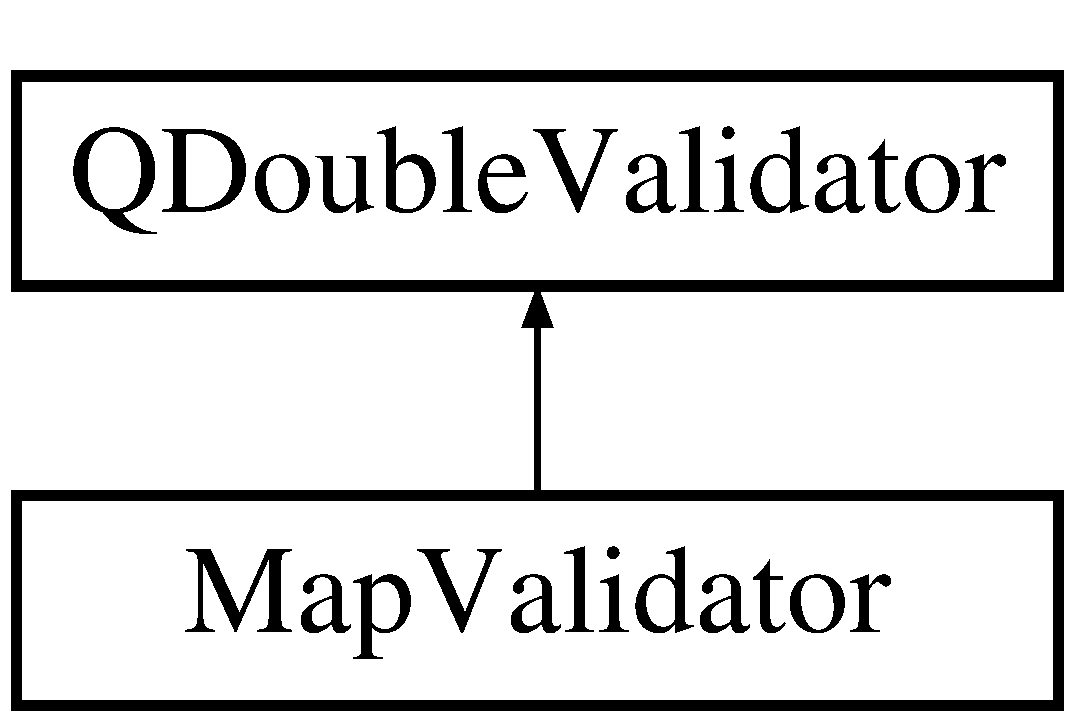
\includegraphics[height=2.000000cm]{class_map_validator}
\end{center}
\end{figure}
\subsection*{Public Member Functions}
\begin{DoxyCompactItemize}
\item 
\hyperlink{class_map_validator_adc4f53b1f99cbe2c1c832c1c713405b2}{Map\+Validator} (double bottom, double top, int decimals, Q\+Object $\ast$parent)
\item 
Q\+Validator\+::\+State \hyperlink{class_map_validator_a7314e2243ed254fdff4aab33ded97a8b}{validate} (Q\+String \&s, int \&i) const 
\end{DoxyCompactItemize}


\subsection{Constructor \& Destructor Documentation}
\hypertarget{class_map_validator_adc4f53b1f99cbe2c1c832c1c713405b2}{}\index{Map\+Validator@{Map\+Validator}!Map\+Validator@{Map\+Validator}}
\index{Map\+Validator@{Map\+Validator}!Map\+Validator@{Map\+Validator}}
\subsubsection[{Map\+Validator}]{\setlength{\rightskip}{0pt plus 5cm}Map\+Validator\+::\+Map\+Validator (
\begin{DoxyParamCaption}
\item[{double}]{bottom, }
\item[{double}]{top, }
\item[{int}]{decimals, }
\item[{Q\+Object $\ast$}]{parent}
\end{DoxyParamCaption}
)}\label{class_map_validator_adc4f53b1f99cbe2c1c832c1c713405b2}


\subsection{Member Function Documentation}
\hypertarget{class_map_validator_a7314e2243ed254fdff4aab33ded97a8b}{}\index{Map\+Validator@{Map\+Validator}!validate@{validate}}
\index{validate@{validate}!Map\+Validator@{Map\+Validator}}
\subsubsection[{validate}]{\setlength{\rightskip}{0pt plus 5cm}Map\+Validator\+::\+Q\+Validator\+::\+State Map\+Validator\+::validate (
\begin{DoxyParamCaption}
\item[{Q\+String \&}]{s, }
\item[{int \&}]{i}
\end{DoxyParamCaption}
) const}\label{class_map_validator_a7314e2243ed254fdff4aab33ded97a8b}


The documentation for this class was generated from the following files\+:\begin{DoxyCompactItemize}
\item 
C\+:/\+Users/\+Roman/\+Documents/\+Mygs/\+Ground\+Station/\+G\+S/\hyperlink{mapvalidator_8h}{mapvalidator.\+h}\item 
C\+:/\+Users/\+Roman/\+Documents/\+Mygs/\+Ground\+Station/\+G\+S/\hyperlink{mapvalidator_8cpp}{mapvalidator.\+cpp}\end{DoxyCompactItemize}

\hypertarget{class_map_widget}{}\section{Map\+Widget Class Reference}
\label{class_map_widget}\index{Map\+Widget@{Map\+Widget}}


The \hyperlink{class_map_widget}{Map\+Widget} class.  




{\ttfamily \#include $<$mapwidget.\+h$>$}

Inheritance diagram for Map\+Widget\+:\begin{figure}[H]
\begin{center}
\leavevmode
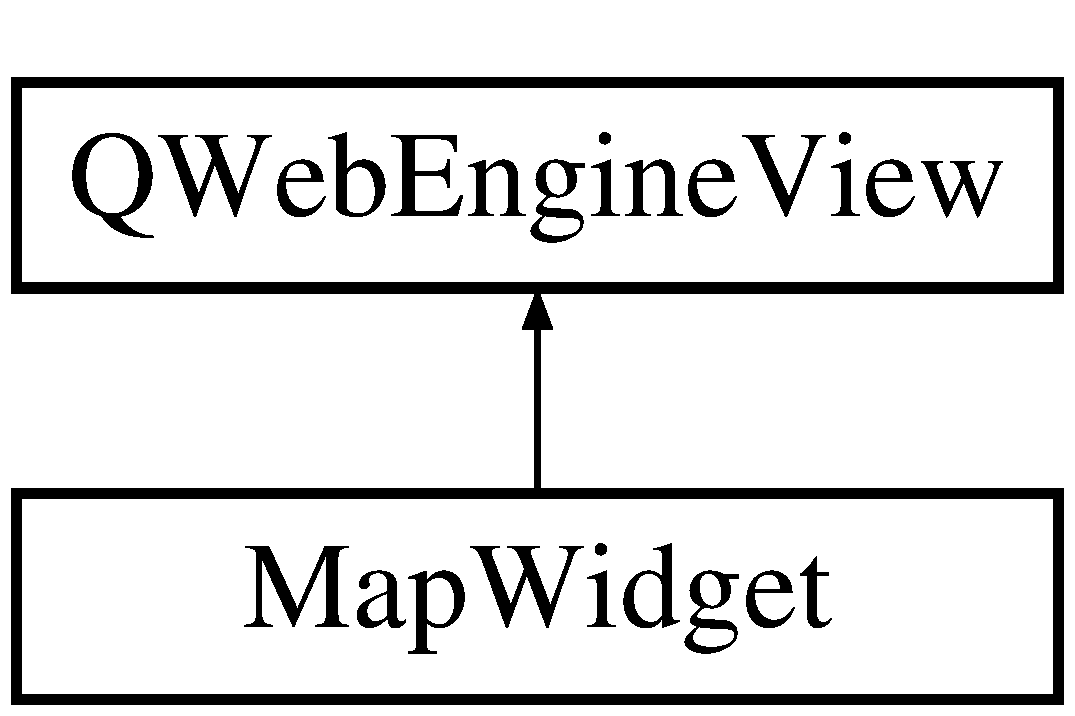
\includegraphics[height=2.000000cm]{class_map_widget}
\end{center}
\end{figure}
\subsection*{Public Slots}
\begin{DoxyCompactItemize}
\item 
void \hyperlink{class_map_widget_a2f3f6349372d8d625526ee5ebb69abbb}{add\+Point\+To\+Table} (double lat, double lng)
\begin{DoxyCompactList}\small\item\em add\+Point\+To\+Table \end{DoxyCompactList}\item 
void \hyperlink{class_map_widget_a6d02fd8c98000b25d65c18860dd24798}{clear\+Map} ()
\begin{DoxyCompactList}\small\item\em clear\+Map \end{DoxyCompactList}\item 
void \hyperlink{class_map_widget_a1334377e2cdd9b97c499880a3327c25d}{disconnect\+Web\+Socket} ()
\begin{DoxyCompactList}\small\item\em disconnect\+Web\+Socket must be called before opening another \hyperlink{class_map_widget}{Map\+Widget} Later we\textquotesingle{}ll work a solution that allows for multiple Map\+Widgets to be \char`\"{}open\char`\"{} at the same time. \end{DoxyCompactList}\item 
void \hyperlink{class_map_widget_a28767584fd020d5a2bdd634812de4ac9}{add\+Flight\+Path} (\hyperlink{class_flight_path}{Flight\+Path} $\ast$fp, int index=0)
\begin{DoxyCompactList}\small\item\em add\+Flightpath \end{DoxyCompactList}\end{DoxyCompactItemize}
\subsection*{Signals}
\begin{DoxyCompactItemize}
\item 
void \hyperlink{class_map_widget_afb12c166145f973d1278270628a9faf6}{send\+Point\+To\+Map} (double lat, double lng, int path\+I\+D)
\begin{DoxyCompactList}\small\item\em send\+Point\+To\+Map \end{DoxyCompactList}\item 
void \hyperlink{class_map_widget_a89b74a366c4f6958d448283621357622}{point\+Added\+To\+Map} (double lat, double lng, int path\+I\+D)
\begin{DoxyCompactList}\small\item\em point\+Added\+To\+Map \end{DoxyCompactList}\item 
void \hyperlink{class_map_widget_a9ad5615b0a835998172b61de2e61a12c}{clear\+Flight\+Path} (int path\+I\+D)
\begin{DoxyCompactList}\small\item\em clear\+Flightpath \end{DoxyCompactList}\end{DoxyCompactItemize}
\subsection*{Public Member Functions}
\begin{DoxyCompactItemize}
\item 
\hyperlink{class_map_widget_a713e505662adb701530212e7a2d78362}{Map\+Widget} (Q\+Widget $\ast$parent=0)
\item 
\hyperlink{class_map_widget_a2be5ffdc125d85aa0ccdb4f552e393cc}{$\sim$\+Map\+Widget} ()
\item 
bool \hyperlink{class_map_widget_ab74d0f96d17ac84330c1ad9128fa3043}{ready} ()
\begin{DoxyCompactList}\small\item\em ready \end{DoxyCompactList}\item 
int \hyperlink{class_map_widget_a74413ad372d073726adaafa0e4b23a88}{create\+New\+Path} ()
\begin{DoxyCompactList}\small\item\em create\+New\+Path \end{DoxyCompactList}\item 
void \hyperlink{class_map_widget_a4ce8b29f199770cbbfb619409d03b64a}{append\+G\+P\+S\+Coord\+To\+Path} (double lat, double lng, int path\+I\+D)
\begin{DoxyCompactList}\small\item\em append\+G\+P\+S\+Coord\+To\+Path \end{DoxyCompactList}\item 
Q\+List$<$ \hyperlink{struct_protocol_1_1_waypoint}{Protocol\+::\+Waypoint} $>$ $\ast$ \hyperlink{class_map_widget_ade38deed1067391a63e190a129de6503}{get\+Path} (int path\+I\+D)
\begin{DoxyCompactList}\small\item\em get\+Path \end{DoxyCompactList}\end{DoxyCompactItemize}


\subsection{Detailed Description}
The \hyperlink{class_map_widget}{Map\+Widget} class. 

\begin{DoxyAuthor}{Author}
Jordan Dickson 
\end{DoxyAuthor}


\subsection{Constructor \& Destructor Documentation}
\hypertarget{class_map_widget_a713e505662adb701530212e7a2d78362}{}\index{Map\+Widget@{Map\+Widget}!Map\+Widget@{Map\+Widget}}
\index{Map\+Widget@{Map\+Widget}!Map\+Widget@{Map\+Widget}}
\subsubsection[{Map\+Widget}]{\setlength{\rightskip}{0pt plus 5cm}Map\+Widget\+::\+Map\+Widget (
\begin{DoxyParamCaption}
\item[{Q\+Widget $\ast$}]{parent = {\ttfamily 0}}
\end{DoxyParamCaption}
)}\label{class_map_widget_a713e505662adb701530212e7a2d78362}
\begin{DoxyAuthor}{Author}
Jordan Dickson 
\end{DoxyAuthor}
\hypertarget{class_map_widget_a2be5ffdc125d85aa0ccdb4f552e393cc}{}\index{Map\+Widget@{Map\+Widget}!````~Map\+Widget@{$\sim$\+Map\+Widget}}
\index{````~Map\+Widget@{$\sim$\+Map\+Widget}!Map\+Widget@{Map\+Widget}}
\subsubsection[{$\sim$\+Map\+Widget}]{\setlength{\rightskip}{0pt plus 5cm}Map\+Widget\+::$\sim$\+Map\+Widget (
\begin{DoxyParamCaption}
{}
\end{DoxyParamCaption}
)}\label{class_map_widget_a2be5ffdc125d85aa0ccdb4f552e393cc}


\subsection{Member Function Documentation}
\hypertarget{class_map_widget_a28767584fd020d5a2bdd634812de4ac9}{}\index{Map\+Widget@{Map\+Widget}!add\+Flight\+Path@{add\+Flight\+Path}}
\index{add\+Flight\+Path@{add\+Flight\+Path}!Map\+Widget@{Map\+Widget}}
\subsubsection[{add\+Flight\+Path}]{\setlength{\rightskip}{0pt plus 5cm}void Map\+Widget\+::add\+Flight\+Path (
\begin{DoxyParamCaption}
\item[{{\bf Flight\+Path} $\ast$}]{fp, }
\item[{int}]{index = {\ttfamily 0}}
\end{DoxyParamCaption}
)\hspace{0.3cm}{\ttfamily [slot]}}\label{class_map_widget_a28767584fd020d5a2bdd634812de4ac9}


add\+Flightpath 


\begin{DoxyParams}{Parameters}
{\em fp} & \\
\hline
{\em index} & \\
\hline
\end{DoxyParams}
\hypertarget{class_map_widget_a2f3f6349372d8d625526ee5ebb69abbb}{}\index{Map\+Widget@{Map\+Widget}!add\+Point\+To\+Table@{add\+Point\+To\+Table}}
\index{add\+Point\+To\+Table@{add\+Point\+To\+Table}!Map\+Widget@{Map\+Widget}}
\subsubsection[{add\+Point\+To\+Table}]{\setlength{\rightskip}{0pt plus 5cm}void Map\+Widget\+::add\+Point\+To\+Table (
\begin{DoxyParamCaption}
\item[{double}]{lat, }
\item[{double}]{lng}
\end{DoxyParamCaption}
)\hspace{0.3cm}{\ttfamily [slot]}}\label{class_map_widget_a2f3f6349372d8d625526ee5ebb69abbb}


add\+Point\+To\+Table 


\begin{DoxyParams}{Parameters}
{\em lat} & \\
\hline
{\em lng} & \\
\hline
\end{DoxyParams}
\hypertarget{class_map_widget_a4ce8b29f199770cbbfb619409d03b64a}{}\index{Map\+Widget@{Map\+Widget}!append\+G\+P\+S\+Coord\+To\+Path@{append\+G\+P\+S\+Coord\+To\+Path}}
\index{append\+G\+P\+S\+Coord\+To\+Path@{append\+G\+P\+S\+Coord\+To\+Path}!Map\+Widget@{Map\+Widget}}
\subsubsection[{append\+G\+P\+S\+Coord\+To\+Path}]{\setlength{\rightskip}{0pt plus 5cm}void Map\+Widget\+::append\+G\+P\+S\+Coord\+To\+Path (
\begin{DoxyParamCaption}
\item[{double}]{lat, }
\item[{double}]{lng, }
\item[{int}]{path\+I\+D}
\end{DoxyParamCaption}
)}\label{class_map_widget_a4ce8b29f199770cbbfb619409d03b64a}


append\+G\+P\+S\+Coord\+To\+Path 


\begin{DoxyParams}{Parameters}
{\em lat} & \\
\hline
{\em lng} & \\
\hline
{\em path\+I\+D} & \\
\hline
\end{DoxyParams}
\hypertarget{class_map_widget_a9ad5615b0a835998172b61de2e61a12c}{}\index{Map\+Widget@{Map\+Widget}!clear\+Flight\+Path@{clear\+Flight\+Path}}
\index{clear\+Flight\+Path@{clear\+Flight\+Path}!Map\+Widget@{Map\+Widget}}
\subsubsection[{clear\+Flight\+Path}]{\setlength{\rightskip}{0pt plus 5cm}void Map\+Widget\+::clear\+Flight\+Path (
\begin{DoxyParamCaption}
\item[{int}]{path\+I\+D}
\end{DoxyParamCaption}
)\hspace{0.3cm}{\ttfamily [signal]}}\label{class_map_widget_a9ad5615b0a835998172b61de2e61a12c}


clear\+Flightpath 


\begin{DoxyParams}{Parameters}
{\em path\+I\+D} & \\
\hline
\end{DoxyParams}
\hypertarget{class_map_widget_a6d02fd8c98000b25d65c18860dd24798}{}\index{Map\+Widget@{Map\+Widget}!clear\+Map@{clear\+Map}}
\index{clear\+Map@{clear\+Map}!Map\+Widget@{Map\+Widget}}
\subsubsection[{clear\+Map}]{\setlength{\rightskip}{0pt plus 5cm}void Map\+Widget\+::clear\+Map (
\begin{DoxyParamCaption}
{}
\end{DoxyParamCaption}
)\hspace{0.3cm}{\ttfamily [slot]}}\label{class_map_widget_a6d02fd8c98000b25d65c18860dd24798}


clear\+Map 

\hypertarget{class_map_widget_a74413ad372d073726adaafa0e4b23a88}{}\index{Map\+Widget@{Map\+Widget}!create\+New\+Path@{create\+New\+Path}}
\index{create\+New\+Path@{create\+New\+Path}!Map\+Widget@{Map\+Widget}}
\subsubsection[{create\+New\+Path}]{\setlength{\rightskip}{0pt plus 5cm}int Map\+Widget\+::create\+New\+Path (
\begin{DoxyParamCaption}
{}
\end{DoxyParamCaption}
)}\label{class_map_widget_a74413ad372d073726adaafa0e4b23a88}


create\+New\+Path 

\begin{DoxyReturn}{Returns}
A new path I\+D for adding waypoints to and retrieving the path. 
\end{DoxyReturn}
\hypertarget{class_map_widget_a1334377e2cdd9b97c499880a3327c25d}{}\index{Map\+Widget@{Map\+Widget}!disconnect\+Web\+Socket@{disconnect\+Web\+Socket}}
\index{disconnect\+Web\+Socket@{disconnect\+Web\+Socket}!Map\+Widget@{Map\+Widget}}
\subsubsection[{disconnect\+Web\+Socket}]{\setlength{\rightskip}{0pt plus 5cm}void Map\+Widget\+::disconnect\+Web\+Socket (
\begin{DoxyParamCaption}
{}
\end{DoxyParamCaption}
)\hspace{0.3cm}{\ttfamily [slot]}}\label{class_map_widget_a1334377e2cdd9b97c499880a3327c25d}


disconnect\+Web\+Socket must be called before opening another \hyperlink{class_map_widget}{Map\+Widget} Later we\textquotesingle{}ll work a solution that allows for multiple Map\+Widgets to be \char`\"{}open\char`\"{} at the same time. 

\hypertarget{class_map_widget_ade38deed1067391a63e190a129de6503}{}\index{Map\+Widget@{Map\+Widget}!get\+Path@{get\+Path}}
\index{get\+Path@{get\+Path}!Map\+Widget@{Map\+Widget}}
\subsubsection[{get\+Path}]{\setlength{\rightskip}{0pt plus 5cm}Q\+List$<$ {\bf Protocol\+::\+Waypoint} $>$ $\ast$ Map\+Widget\+::get\+Path (
\begin{DoxyParamCaption}
\item[{int}]{path\+I\+D}
\end{DoxyParamCaption}
)}\label{class_map_widget_ade38deed1067391a63e190a129de6503}


get\+Path 


\begin{DoxyParams}{Parameters}
{\em path\+I\+D} & \\
\hline
\end{DoxyParams}
\begin{DoxyReturn}{Returns}
An ordered list of all the waypoints in a certain path 
\end{DoxyReturn}
\hypertarget{class_map_widget_a89b74a366c4f6958d448283621357622}{}\index{Map\+Widget@{Map\+Widget}!point\+Added\+To\+Map@{point\+Added\+To\+Map}}
\index{point\+Added\+To\+Map@{point\+Added\+To\+Map}!Map\+Widget@{Map\+Widget}}
\subsubsection[{point\+Added\+To\+Map}]{\setlength{\rightskip}{0pt plus 5cm}void Map\+Widget\+::point\+Added\+To\+Map (
\begin{DoxyParamCaption}
\item[{double}]{lat, }
\item[{double}]{lng, }
\item[{int}]{path\+I\+D}
\end{DoxyParamCaption}
)\hspace{0.3cm}{\ttfamily [signal]}}\label{class_map_widget_a89b74a366c4f6958d448283621357622}


point\+Added\+To\+Map 


\begin{DoxyParams}{Parameters}
{\em lat} & \\
\hline
{\em lng} & \\
\hline
\end{DoxyParams}
\hypertarget{class_map_widget_ab74d0f96d17ac84330c1ad9128fa3043}{}\index{Map\+Widget@{Map\+Widget}!ready@{ready}}
\index{ready@{ready}!Map\+Widget@{Map\+Widget}}
\subsubsection[{ready}]{\setlength{\rightskip}{0pt plus 5cm}bool Map\+Widget\+::ready (
\begin{DoxyParamCaption}
{}
\end{DoxyParamCaption}
)}\label{class_map_widget_ab74d0f96d17ac84330c1ad9128fa3043}


ready 

\begin{DoxyReturn}{Returns}
True if the \hyperlink{class_map_widget}{Map\+Widget} input or output Waypoints 
\end{DoxyReturn}
\hypertarget{class_map_widget_afb12c166145f973d1278270628a9faf6}{}\index{Map\+Widget@{Map\+Widget}!send\+Point\+To\+Map@{send\+Point\+To\+Map}}
\index{send\+Point\+To\+Map@{send\+Point\+To\+Map}!Map\+Widget@{Map\+Widget}}
\subsubsection[{send\+Point\+To\+Map}]{\setlength{\rightskip}{0pt plus 5cm}void Map\+Widget\+::send\+Point\+To\+Map (
\begin{DoxyParamCaption}
\item[{double}]{lat, }
\item[{double}]{lng, }
\item[{int}]{path\+I\+D}
\end{DoxyParamCaption}
)\hspace{0.3cm}{\ttfamily [signal]}}\label{class_map_widget_afb12c166145f973d1278270628a9faf6}


send\+Point\+To\+Map 


\begin{DoxyParams}{Parameters}
{\em lat} & \\
\hline
{\em lng} & \\
\hline
{\em path\+I\+D} & \\
\hline
\end{DoxyParams}


The documentation for this class was generated from the following files\+:\begin{DoxyCompactItemize}
\item 
C\+:/\+Users/\+Roman/\+Documents/\+Mygs/\+Ground\+Station/\+G\+S/\hyperlink{mapwidget_8h}{mapwidget.\+h}\item 
C\+:/\+Users/\+Roman/\+Documents/\+Mygs/\+Ground\+Station/\+G\+S/\hyperlink{mapwidget_8cpp}{mapwidget.\+cpp}\end{DoxyCompactItemize}

\hypertarget{classmessagebox}{}\section{messagebox Class Reference}
\label{classmessagebox}\index{messagebox@{messagebox}}


{\ttfamily \#include $<$messagebox.\+h$>$}

\subsection*{Public Slots}
\begin{DoxyCompactItemize}
\item 
void \hyperlink{classmessagebox_a7e27018e68e04cfe417386d743a58695}{recieve\+\_\+packet} (\hyperlink{class_protocol_1_1_packet}{Protocol\+::\+Packet} $\ast$packet)
\end{DoxyCompactItemize}
\subsection*{Public Member Functions}
\begin{DoxyCompactItemize}
\item 
\hyperlink{classmessagebox_aa1982e07048de340df52d2a5f37dd8ac}{messagebox} ()
\item 
void \hyperlink{classmessagebox_ad5e6c9a2d407ebc95415e6ddeb91aba3}{load\+\_\+ack\+\_\+packet} (uint8\+\_\+t $\ast$buffer, size\+\_\+t len)
\item 
void \hyperlink{classmessagebox_afa0a64c35c27e21fab6cbee8055341b1}{load\+\_\+action\+\_\+packet} (\hyperlink{namespace_protocol_a95f2e35dc2d8d920f0d7ddaaf122c3b9}{Protocol\+::\+Action\+Type} atype, double lat, double lon, float alt, float spd)
\item 
void \hyperlink{classmessagebox_af79061031d97b9e3e0e677fe365b2b15}{load\+\_\+action\+\_\+packet} (double lat, double lon, float alt, float spd)
\item 
void \hyperlink{classmessagebox_a6128a1a53fbba888dccfcab5a5fafa1f}{load\+\_\+info\+\_\+packet} (std\+::string other)
\item 
void \hyperlink{classmessagebox_a0e3beabe499e7aade0e769ff17ced30d}{load\+\_\+telem\+\_\+packet} (double lat, double lon)
\item 
void \hyperlink{classmessagebox_acfa11fc9bcf7c96ddf2478b981be826d}{load\+\_\+telem\+\_\+packet} (float x, float y, float z, float p, float r, float yaw, double lat, double lon, float alt, float heading)
\item 
void \hyperlink{classmessagebox_a545d9441dccf14adbea8e859628d6425}{load\+\_\+out\+Action\+\_\+packets} (double lat, double lon, float alt, float spd)
\begin{DoxyCompactList}\small\item\em Fetches the packets from table and stores them into the outbox where they will sent back. \end{DoxyCompactList}\item 
void \hyperlink{classmessagebox_ad8dd259b5b34d30b241f27172a255575}{add\+Out\+Action\+Packet} (const \hyperlink{class_protocol_1_1_action_packet}{Protocol\+::\+Action\+Packet} \&action\+Packet)
\item 
void \hyperlink{classmessagebox_ac2463eee5d4c1e5d693f8a96cca0e00f}{recieve\+\_\+initial\+\_\+info} (\hyperlink{class_protocol_1_1_info_packet}{Protocol\+::\+Info\+Packet} intip)
\begin{DoxyCompactList}\small\item\em Takes initial info packet and sets timestamp based on it. \end{DoxyCompactList}\item 
std\+::vector$<$ \hyperlink{class_protocol_1_1_ack_packet}{Protocol\+::\+Ack\+Packet} $>$ \hyperlink{classmessagebox_abe5152230ef5e89e0839d9dd866590e5}{get\+\_\+ack\+\_\+packets} ()
\item 
std\+::vector$<$ \hyperlink{class_protocol_1_1_action_packet}{Protocol\+::\+Action\+Packet} $>$ \hyperlink{classmessagebox_afd08c7f717357ee71a666720ff6bb9bc}{get\+\_\+action\+\_\+packets} ()
\item 
std\+::vector$<$ \hyperlink{class_protocol_1_1_info_packet}{Protocol\+::\+Info\+Packet} $>$ \hyperlink{classmessagebox_a15a6793bc31aa9bb080c9fbcea14e1af}{get\+\_\+info\+\_\+packets} ()
\item 
std\+::vector$<$ \hyperlink{class_protocol_1_1_telemetry_packet}{Protocol\+::\+Telemetry\+Packet} $>$ \hyperlink{classmessagebox_a58df2b6675cad37e6f31b2bc25bcfb0e}{get\+\_\+telem\+\_\+packets} ()
\item 
std\+::vector$<$ \hyperlink{class_protocol_1_1_ack_packet}{Protocol\+::\+Ack\+Packet} $>$ \hyperlink{classmessagebox_aa19eb7d103c82c6edabe95052d71e957}{get\+\_\+out\+\_\+ack\+\_\+packets} ()
\begin{DoxyCompactList}\small\item\em returns the packets from the sending side of messagebox \end{DoxyCompactList}\item 
std\+::vector$<$ \hyperlink{class_protocol_1_1_action_packet}{Protocol\+::\+Action\+Packet} $>$ \hyperlink{classmessagebox_a49302f9e97d15853ab0bd4293cda3603}{get\+\_\+out\+\_\+action\+\_\+packets} ()
\item 
std\+::vector$<$ \hyperlink{class_protocol_1_1_info_packet}{Protocol\+::\+Info\+Packet} $>$ \hyperlink{classmessagebox_a8630b30babf0555dc17d150ccfe08d8f}{get\+\_\+out\+\_\+info\+\_\+packets} ()
\item 
std\+::vector$<$ \hyperlink{class_protocol_1_1_telemetry_packet}{Protocol\+::\+Telemetry\+Packet} $>$ \hyperlink{classmessagebox_a5ab4ee4ec8c63b6e4936fed1884fbd87}{get\+\_\+out\+\_\+telem\+\_\+packets} ()
\item 
void \hyperlink{classmessagebox_a356a1119d888a5aea5a70b67bce0132b}{add\+Ack\+Packet} (const \hyperlink{class_protocol_1_1_ack_packet}{Protocol\+::\+Ack\+Packet} \&ack\+Packet)
\begin{DoxyCompactList}\small\item\em Adds fully formed or empty packet into the proper packet container in messagebox. \end{DoxyCompactList}\item 
void \hyperlink{classmessagebox_a75d62bfa9db5b55a60b9e2e0fa164c81}{add\+Action\+Packet} (const \hyperlink{class_protocol_1_1_action_packet}{Protocol\+::\+Action\+Packet} \&action\+Packet)
\item 
void \hyperlink{classmessagebox_a27ac98af342131cd148fb4ed2261631f}{add\+Telemetry\+Packet} (const \hyperlink{class_protocol_1_1_telemetry_packet}{Protocol\+::\+Telemetry\+Packet} \&telem\+Packet)
\item 
void \hyperlink{classmessagebox_aa7a826742dd2a22376eaf787d510f064}{add\+Info\+Packet} (const \hyperlink{class_protocol_1_1_info_packet}{Protocol\+::\+Info\+Packet} \&info\+Packet)
\end{DoxyCompactItemize}
\subsection*{Public Attributes}
\begin{DoxyCompactItemize}
\item 
Q\+Time \hyperlink{classmessagebox_ac738a854bbbcdc5be4fd4df476db724b}{timer}
\end{DoxyCompactItemize}
\subsection*{Friends}
\begin{DoxyCompactItemize}
\item 
class \hyperlink{classmessagebox_a9923a7ec95448c63c3c51fcf094a7cb7}{Digital\+Clock}
\end{DoxyCompactItemize}


\subsection{Constructor \& Destructor Documentation}
\hypertarget{classmessagebox_aa1982e07048de340df52d2a5f37dd8ac}{}\index{messagebox@{messagebox}!messagebox@{messagebox}}
\index{messagebox@{messagebox}!messagebox@{messagebox}}
\subsubsection[{messagebox}]{\setlength{\rightskip}{0pt plus 5cm}messagebox\+::messagebox (
\begin{DoxyParamCaption}
{}
\end{DoxyParamCaption}
)}\label{classmessagebox_aa1982e07048de340df52d2a5f37dd8ac}


\subsection{Member Function Documentation}
\hypertarget{classmessagebox_a356a1119d888a5aea5a70b67bce0132b}{}\index{messagebox@{messagebox}!add\+Ack\+Packet@{add\+Ack\+Packet}}
\index{add\+Ack\+Packet@{add\+Ack\+Packet}!messagebox@{messagebox}}
\subsubsection[{add\+Ack\+Packet}]{\setlength{\rightskip}{0pt plus 5cm}void messagebox\+::add\+Ack\+Packet (
\begin{DoxyParamCaption}
\item[{const {\bf Protocol\+::\+Ack\+Packet} \&}]{ack\+Packet}
\end{DoxyParamCaption}
)}\label{classmessagebox_a356a1119d888a5aea5a70b67bce0132b}


Adds fully formed or empty packet into the proper packet container in messagebox. 


\begin{DoxyParams}{Parameters}
{\em $<$type$>$\+Packet} & -\/$>$ A formed or empty Packets\\
\hline
\end{DoxyParams}
\begin{DoxyAuthor}{Author}
Alvin Truong 
\end{DoxyAuthor}
\begin{DoxyDate}{Date}
2016-\/1-\/20
\end{DoxyDate}
\begin{DoxySeeAlso}{See also}
\hyperlink{messagebox_8h}{messagebox.\+h} for more info 
\end{DoxySeeAlso}
\hypertarget{classmessagebox_a75d62bfa9db5b55a60b9e2e0fa164c81}{}\index{messagebox@{messagebox}!add\+Action\+Packet@{add\+Action\+Packet}}
\index{add\+Action\+Packet@{add\+Action\+Packet}!messagebox@{messagebox}}
\subsubsection[{add\+Action\+Packet}]{\setlength{\rightskip}{0pt plus 5cm}void messagebox\+::add\+Action\+Packet (
\begin{DoxyParamCaption}
\item[{const {\bf Protocol\+::\+Action\+Packet} \&}]{action\+Packet}
\end{DoxyParamCaption}
)}\label{classmessagebox_a75d62bfa9db5b55a60b9e2e0fa164c81}
\begin{DoxySeeAlso}{See also}
\hyperlink{messagebox_8h}{messagebox.\+h} for more info 
\end{DoxySeeAlso}
\hypertarget{classmessagebox_aa7a826742dd2a22376eaf787d510f064}{}\index{messagebox@{messagebox}!add\+Info\+Packet@{add\+Info\+Packet}}
\index{add\+Info\+Packet@{add\+Info\+Packet}!messagebox@{messagebox}}
\subsubsection[{add\+Info\+Packet}]{\setlength{\rightskip}{0pt plus 5cm}void messagebox\+::add\+Info\+Packet (
\begin{DoxyParamCaption}
\item[{const {\bf Protocol\+::\+Info\+Packet} \&}]{info\+Packet}
\end{DoxyParamCaption}
)}\label{classmessagebox_aa7a826742dd2a22376eaf787d510f064}
\begin{DoxySeeAlso}{See also}
\hyperlink{messagebox_8h}{messagebox.\+h} for more info 
\end{DoxySeeAlso}
\hypertarget{classmessagebox_ad8dd259b5b34d30b241f27172a255575}{}\index{messagebox@{messagebox}!add\+Out\+Action\+Packet@{add\+Out\+Action\+Packet}}
\index{add\+Out\+Action\+Packet@{add\+Out\+Action\+Packet}!messagebox@{messagebox}}
\subsubsection[{add\+Out\+Action\+Packet}]{\setlength{\rightskip}{0pt plus 5cm}void messagebox\+::add\+Out\+Action\+Packet (
\begin{DoxyParamCaption}
\item[{const {\bf Protocol\+::\+Action\+Packet} \&}]{action\+Packet}
\end{DoxyParamCaption}
)}\label{classmessagebox_ad8dd259b5b34d30b241f27172a255575}
\hypertarget{classmessagebox_a27ac98af342131cd148fb4ed2261631f}{}\index{messagebox@{messagebox}!add\+Telemetry\+Packet@{add\+Telemetry\+Packet}}
\index{add\+Telemetry\+Packet@{add\+Telemetry\+Packet}!messagebox@{messagebox}}
\subsubsection[{add\+Telemetry\+Packet}]{\setlength{\rightskip}{0pt plus 5cm}void messagebox\+::add\+Telemetry\+Packet (
\begin{DoxyParamCaption}
\item[{const {\bf Protocol\+::\+Telemetry\+Packet} \&}]{telem\+Packet}
\end{DoxyParamCaption}
)}\label{classmessagebox_a27ac98af342131cd148fb4ed2261631f}
\begin{DoxySeeAlso}{See also}
\hyperlink{messagebox_8h}{messagebox.\+h} for more info 
\end{DoxySeeAlso}
\hypertarget{classmessagebox_abe5152230ef5e89e0839d9dd866590e5}{}\index{messagebox@{messagebox}!get\+\_\+ack\+\_\+packets@{get\+\_\+ack\+\_\+packets}}
\index{get\+\_\+ack\+\_\+packets@{get\+\_\+ack\+\_\+packets}!messagebox@{messagebox}}
\subsubsection[{get\+\_\+ack\+\_\+packets}]{\setlength{\rightskip}{0pt plus 5cm}std\+::vector$<$ {\bf Protocol\+::\+Ack\+Packet} $>$ messagebox\+::get\+\_\+ack\+\_\+packets (
\begin{DoxyParamCaption}
{}
\end{DoxyParamCaption}
)}\label{classmessagebox_abe5152230ef5e89e0839d9dd866590e5}
\hypertarget{classmessagebox_afd08c7f717357ee71a666720ff6bb9bc}{}\index{messagebox@{messagebox}!get\+\_\+action\+\_\+packets@{get\+\_\+action\+\_\+packets}}
\index{get\+\_\+action\+\_\+packets@{get\+\_\+action\+\_\+packets}!messagebox@{messagebox}}
\subsubsection[{get\+\_\+action\+\_\+packets}]{\setlength{\rightskip}{0pt plus 5cm}std\+::vector$<$ {\bf Protocol\+::\+Action\+Packet} $>$ messagebox\+::get\+\_\+action\+\_\+packets (
\begin{DoxyParamCaption}
{}
\end{DoxyParamCaption}
)}\label{classmessagebox_afd08c7f717357ee71a666720ff6bb9bc}
\hypertarget{classmessagebox_a15a6793bc31aa9bb080c9fbcea14e1af}{}\index{messagebox@{messagebox}!get\+\_\+info\+\_\+packets@{get\+\_\+info\+\_\+packets}}
\index{get\+\_\+info\+\_\+packets@{get\+\_\+info\+\_\+packets}!messagebox@{messagebox}}
\subsubsection[{get\+\_\+info\+\_\+packets}]{\setlength{\rightskip}{0pt plus 5cm}std\+::vector$<$ {\bf Protocol\+::\+Info\+Packet} $>$ messagebox\+::get\+\_\+info\+\_\+packets (
\begin{DoxyParamCaption}
{}
\end{DoxyParamCaption}
)}\label{classmessagebox_a15a6793bc31aa9bb080c9fbcea14e1af}
\hypertarget{classmessagebox_aa19eb7d103c82c6edabe95052d71e957}{}\index{messagebox@{messagebox}!get\+\_\+out\+\_\+ack\+\_\+packets@{get\+\_\+out\+\_\+ack\+\_\+packets}}
\index{get\+\_\+out\+\_\+ack\+\_\+packets@{get\+\_\+out\+\_\+ack\+\_\+packets}!messagebox@{messagebox}}
\subsubsection[{get\+\_\+out\+\_\+ack\+\_\+packets}]{\setlength{\rightskip}{0pt plus 5cm}std\+::vector$<$ {\bf Protocol\+::\+Ack\+Packet} $>$ messagebox\+::get\+\_\+out\+\_\+ack\+\_\+packets (
\begin{DoxyParamCaption}
{}
\end{DoxyParamCaption}
)}\label{classmessagebox_aa19eb7d103c82c6edabe95052d71e957}


returns the packets from the sending side of messagebox 

\begin{DoxyAuthor}{Author}
Kevin Phan 
\end{DoxyAuthor}
\begin{DoxyDate}{Date}
2016/1/29 
\end{DoxyDate}
\hypertarget{classmessagebox_a49302f9e97d15853ab0bd4293cda3603}{}\index{messagebox@{messagebox}!get\+\_\+out\+\_\+action\+\_\+packets@{get\+\_\+out\+\_\+action\+\_\+packets}}
\index{get\+\_\+out\+\_\+action\+\_\+packets@{get\+\_\+out\+\_\+action\+\_\+packets}!messagebox@{messagebox}}
\subsubsection[{get\+\_\+out\+\_\+action\+\_\+packets}]{\setlength{\rightskip}{0pt plus 5cm}std\+::vector$<$ {\bf Protocol\+::\+Action\+Packet} $>$ messagebox\+::get\+\_\+out\+\_\+action\+\_\+packets (
\begin{DoxyParamCaption}
{}
\end{DoxyParamCaption}
)}\label{classmessagebox_a49302f9e97d15853ab0bd4293cda3603}
\hypertarget{classmessagebox_a8630b30babf0555dc17d150ccfe08d8f}{}\index{messagebox@{messagebox}!get\+\_\+out\+\_\+info\+\_\+packets@{get\+\_\+out\+\_\+info\+\_\+packets}}
\index{get\+\_\+out\+\_\+info\+\_\+packets@{get\+\_\+out\+\_\+info\+\_\+packets}!messagebox@{messagebox}}
\subsubsection[{get\+\_\+out\+\_\+info\+\_\+packets}]{\setlength{\rightskip}{0pt plus 5cm}std\+::vector$<$ {\bf Protocol\+::\+Info\+Packet} $>$ messagebox\+::get\+\_\+out\+\_\+info\+\_\+packets (
\begin{DoxyParamCaption}
{}
\end{DoxyParamCaption}
)}\label{classmessagebox_a8630b30babf0555dc17d150ccfe08d8f}
\hypertarget{classmessagebox_a5ab4ee4ec8c63b6e4936fed1884fbd87}{}\index{messagebox@{messagebox}!get\+\_\+out\+\_\+telem\+\_\+packets@{get\+\_\+out\+\_\+telem\+\_\+packets}}
\index{get\+\_\+out\+\_\+telem\+\_\+packets@{get\+\_\+out\+\_\+telem\+\_\+packets}!messagebox@{messagebox}}
\subsubsection[{get\+\_\+out\+\_\+telem\+\_\+packets}]{\setlength{\rightskip}{0pt plus 5cm}std\+::vector$<$ {\bf Protocol\+::\+Telemetry\+Packet} $>$ messagebox\+::get\+\_\+out\+\_\+telem\+\_\+packets (
\begin{DoxyParamCaption}
{}
\end{DoxyParamCaption}
)}\label{classmessagebox_a5ab4ee4ec8c63b6e4936fed1884fbd87}
\hypertarget{classmessagebox_a58df2b6675cad37e6f31b2bc25bcfb0e}{}\index{messagebox@{messagebox}!get\+\_\+telem\+\_\+packets@{get\+\_\+telem\+\_\+packets}}
\index{get\+\_\+telem\+\_\+packets@{get\+\_\+telem\+\_\+packets}!messagebox@{messagebox}}
\subsubsection[{get\+\_\+telem\+\_\+packets}]{\setlength{\rightskip}{0pt plus 5cm}std\+::vector$<$ {\bf Protocol\+::\+Telemetry\+Packet} $>$ messagebox\+::get\+\_\+telem\+\_\+packets (
\begin{DoxyParamCaption}
{}
\end{DoxyParamCaption}
)}\label{classmessagebox_a58df2b6675cad37e6f31b2bc25bcfb0e}
\hypertarget{classmessagebox_ad5e6c9a2d407ebc95415e6ddeb91aba3}{}\index{messagebox@{messagebox}!load\+\_\+ack\+\_\+packet@{load\+\_\+ack\+\_\+packet}}
\index{load\+\_\+ack\+\_\+packet@{load\+\_\+ack\+\_\+packet}!messagebox@{messagebox}}
\subsubsection[{load\+\_\+ack\+\_\+packet}]{\setlength{\rightskip}{0pt plus 5cm}void messagebox\+::load\+\_\+ack\+\_\+packet (
\begin{DoxyParamCaption}
\item[{uint8\+\_\+t $\ast$}]{buffer, }
\item[{size\+\_\+t}]{len}
\end{DoxyParamCaption}
)}\label{classmessagebox_ad5e6c9a2d407ebc95415e6ddeb91aba3}
\hypertarget{classmessagebox_afa0a64c35c27e21fab6cbee8055341b1}{}\index{messagebox@{messagebox}!load\+\_\+action\+\_\+packet@{load\+\_\+action\+\_\+packet}}
\index{load\+\_\+action\+\_\+packet@{load\+\_\+action\+\_\+packet}!messagebox@{messagebox}}
\subsubsection[{load\+\_\+action\+\_\+packet}]{\setlength{\rightskip}{0pt plus 5cm}void messagebox\+::load\+\_\+action\+\_\+packet (
\begin{DoxyParamCaption}
\item[{{\bf Protocol\+::\+Action\+Type}}]{atype, }
\item[{double}]{lat, }
\item[{double}]{lon, }
\item[{float}]{alt, }
\item[{float}]{spd}
\end{DoxyParamCaption}
)}\label{classmessagebox_afa0a64c35c27e21fab6cbee8055341b1}
\hypertarget{classmessagebox_af79061031d97b9e3e0e677fe365b2b15}{}\index{messagebox@{messagebox}!load\+\_\+action\+\_\+packet@{load\+\_\+action\+\_\+packet}}
\index{load\+\_\+action\+\_\+packet@{load\+\_\+action\+\_\+packet}!messagebox@{messagebox}}
\subsubsection[{load\+\_\+action\+\_\+packet}]{\setlength{\rightskip}{0pt plus 5cm}void messagebox\+::load\+\_\+action\+\_\+packet (
\begin{DoxyParamCaption}
\item[{double}]{lat, }
\item[{double}]{lon, }
\item[{float}]{alt, }
\item[{float}]{spd}
\end{DoxyParamCaption}
)}\label{classmessagebox_af79061031d97b9e3e0e677fe365b2b15}
\hypertarget{classmessagebox_a6128a1a53fbba888dccfcab5a5fafa1f}{}\index{messagebox@{messagebox}!load\+\_\+info\+\_\+packet@{load\+\_\+info\+\_\+packet}}
\index{load\+\_\+info\+\_\+packet@{load\+\_\+info\+\_\+packet}!messagebox@{messagebox}}
\subsubsection[{load\+\_\+info\+\_\+packet}]{\setlength{\rightskip}{0pt plus 5cm}void messagebox\+::load\+\_\+info\+\_\+packet (
\begin{DoxyParamCaption}
\item[{std\+::string}]{other}
\end{DoxyParamCaption}
)}\label{classmessagebox_a6128a1a53fbba888dccfcab5a5fafa1f}
\hypertarget{classmessagebox_a545d9441dccf14adbea8e859628d6425}{}\index{messagebox@{messagebox}!load\+\_\+out\+Action\+\_\+packets@{load\+\_\+out\+Action\+\_\+packets}}
\index{load\+\_\+out\+Action\+\_\+packets@{load\+\_\+out\+Action\+\_\+packets}!messagebox@{messagebox}}
\subsubsection[{load\+\_\+out\+Action\+\_\+packets}]{\setlength{\rightskip}{0pt plus 5cm}void messagebox\+::load\+\_\+out\+Action\+\_\+packets (
\begin{DoxyParamCaption}
\item[{double}]{lat, }
\item[{double}]{lon, }
\item[{float}]{alt, }
\item[{float}]{spd}
\end{DoxyParamCaption}
)}\label{classmessagebox_a545d9441dccf14adbea8e859628d6425}


Fetches the packets from table and stores them into the outbox where they will sent back. 


\begin{DoxyParams}{Parameters}
{\em $<$type$>$} & double,double,float,float -\/$>$ sets the waypoint\\
\hline
\end{DoxyParams}
\begin{DoxyAuthor}{Author}
Kevin Phan 
\end{DoxyAuthor}
\begin{DoxyDate}{Date}
2016-\/2-\/05 
\end{DoxyDate}
\hypertarget{classmessagebox_a0e3beabe499e7aade0e769ff17ced30d}{}\index{messagebox@{messagebox}!load\+\_\+telem\+\_\+packet@{load\+\_\+telem\+\_\+packet}}
\index{load\+\_\+telem\+\_\+packet@{load\+\_\+telem\+\_\+packet}!messagebox@{messagebox}}
\subsubsection[{load\+\_\+telem\+\_\+packet}]{\setlength{\rightskip}{0pt plus 5cm}void messagebox\+::load\+\_\+telem\+\_\+packet (
\begin{DoxyParamCaption}
\item[{double}]{lat, }
\item[{double}]{lon}
\end{DoxyParamCaption}
)}\label{classmessagebox_a0e3beabe499e7aade0e769ff17ced30d}
\hypertarget{classmessagebox_acfa11fc9bcf7c96ddf2478b981be826d}{}\index{messagebox@{messagebox}!load\+\_\+telem\+\_\+packet@{load\+\_\+telem\+\_\+packet}}
\index{load\+\_\+telem\+\_\+packet@{load\+\_\+telem\+\_\+packet}!messagebox@{messagebox}}
\subsubsection[{load\+\_\+telem\+\_\+packet}]{\setlength{\rightskip}{0pt plus 5cm}void messagebox\+::load\+\_\+telem\+\_\+packet (
\begin{DoxyParamCaption}
\item[{float}]{x, }
\item[{float}]{y, }
\item[{float}]{z, }
\item[{float}]{p, }
\item[{float}]{r, }
\item[{float}]{yaw, }
\item[{double}]{lat, }
\item[{double}]{lon, }
\item[{float}]{alt, }
\item[{float}]{heading}
\end{DoxyParamCaption}
)}\label{classmessagebox_acfa11fc9bcf7c96ddf2478b981be826d}
\hypertarget{classmessagebox_ac2463eee5d4c1e5d693f8a96cca0e00f}{}\index{messagebox@{messagebox}!recieve\+\_\+initial\+\_\+info@{recieve\+\_\+initial\+\_\+info}}
\index{recieve\+\_\+initial\+\_\+info@{recieve\+\_\+initial\+\_\+info}!messagebox@{messagebox}}
\subsubsection[{recieve\+\_\+initial\+\_\+info}]{\setlength{\rightskip}{0pt plus 5cm}void messagebox\+::recieve\+\_\+initial\+\_\+info (
\begin{DoxyParamCaption}
\item[{{\bf Protocol\+::\+Info\+Packet}}]{intip}
\end{DoxyParamCaption}
)}\label{classmessagebox_ac2463eee5d4c1e5d693f8a96cca0e00f}


Takes initial info packet and sets timestamp based on it. 


\begin{DoxyParams}{Parameters}
{\em $<$type$>$\+Info\+Packet} & -\/$>$ The inital infopacket sent from U\+A\+V\\
\hline
\end{DoxyParams}
\begin{DoxyAuthor}{Author}
Nathan Brannon 
\end{DoxyAuthor}
\begin{DoxyDate}{Date}
2016-\/1-\/22 
\end{DoxyDate}
\hypertarget{classmessagebox_a7e27018e68e04cfe417386d743a58695}{}\index{messagebox@{messagebox}!recieve\+\_\+packet@{recieve\+\_\+packet}}
\index{recieve\+\_\+packet@{recieve\+\_\+packet}!messagebox@{messagebox}}
\subsubsection[{recieve\+\_\+packet}]{\setlength{\rightskip}{0pt plus 5cm}void messagebox\+::recieve\+\_\+packet (
\begin{DoxyParamCaption}
\item[{{\bf Protocol\+::\+Packet} $\ast$}]{packet}
\end{DoxyParamCaption}
)\hspace{0.3cm}{\ttfamily [slot]}}\label{classmessagebox_a7e27018e68e04cfe417386d743a58695}


\subsection{Friends And Related Function Documentation}
\hypertarget{classmessagebox_a9923a7ec95448c63c3c51fcf094a7cb7}{}\index{messagebox@{messagebox}!Digital\+Clock@{Digital\+Clock}}
\index{Digital\+Clock@{Digital\+Clock}!messagebox@{messagebox}}
\subsubsection[{Digital\+Clock}]{\setlength{\rightskip}{0pt plus 5cm}friend class {\bf Digital\+Clock}\hspace{0.3cm}{\ttfamily [friend]}}\label{classmessagebox_a9923a7ec95448c63c3c51fcf094a7cb7}


\subsection{Member Data Documentation}
\hypertarget{classmessagebox_ac738a854bbbcdc5be4fd4df476db724b}{}\index{messagebox@{messagebox}!timer@{timer}}
\index{timer@{timer}!messagebox@{messagebox}}
\subsubsection[{timer}]{\setlength{\rightskip}{0pt plus 5cm}Q\+Time messagebox\+::timer}\label{classmessagebox_ac738a854bbbcdc5be4fd4df476db724b}


The documentation for this class was generated from the following files\+:\begin{DoxyCompactItemize}
\item 
C\+:/\+Users/\+Roman/\+Documents/\+Mygs/\+Ground\+Station/\+G\+S/\hyperlink{messagebox_8h}{messagebox.\+h}\item 
C\+:/\+Users/\+Roman/\+Documents/\+Mygs/\+Ground\+Station/\+G\+S/\hyperlink{messagebox_8cpp}{messagebox.\+cpp}\end{DoxyCompactItemize}

\hypertarget{class_mission}{}\section{Mission Class Reference}
\label{class_mission}\index{Mission@{Mission}}


{\ttfamily \#include $<$mission.\+h$>$}

\subsection*{Public Member Functions}
\begin{DoxyCompactItemize}
\item 
\hyperlink{class_mission_aa5a6ff4fc779338ab01b8f6dd470f4df}{Mission} ()
\item 
\hyperlink{class_mission_a3c1cb92197018f64854514616b43f06b}{Mission} (Q\+String filename)
\item 
\hyperlink{class_mission_a68bf8cba0c882169d26fb4bcb80c228c}{Mission} (\hyperlink{class_flight_path}{Flight\+Path} flight\+Path)
\item 
\hyperlink{class_mission_ad1a61b34162393ac42be5955d9772921}{$\sim$\+Mission} ()
\item 
void \hyperlink{class_mission_aba7aac52c4313705452dabcce0a6a0d2}{add\+Packet} (\hyperlink{class_protocol_1_1_telemetry_packet}{Protocol\+::\+Telemetry\+Packet} telem\+Packet)
\begin{DoxyCompactList}\small\item\em Extracts data from an input Packet and stores the values in the values field. \end{DoxyCompactList}\item 
\hyperlink{class_flight_path}{Flight\+Path} $\ast$ \hyperlink{class_mission_ae6034451524e6b87062fcb62c89ae458}{get\+Flight\+Path} ()
\item 
Q\+Vector$<$ double $>$ $\ast$ \hyperlink{class_mission_ac6cf2cd13b5be62dec02a4edaba1be25}{get\+Values\+For\+I\+D} (int id)
\item 
Q\+Vector$<$ double $>$ $\ast$ \hyperlink{class_mission_a4377102f1abe6a9f2767fa09a9a8f64e}{get\+Values\+For\+Index} (int index)
\item 
double \hyperlink{class_mission_ad2cd66901a48bbb2e042cd14740b3cba}{get\+Value\+For\+Index\+And\+I\+D} (int index, int id)
\item 
bool \hyperlink{class_mission_a8e02183538b8e0095f7a6e609149f75d}{save} (Q\+String filename)
\end{DoxyCompactItemize}


\subsection{Constructor \& Destructor Documentation}
\hypertarget{class_mission_aa5a6ff4fc779338ab01b8f6dd470f4df}{}\index{Mission@{Mission}!Mission@{Mission}}
\index{Mission@{Mission}!Mission@{Mission}}
\subsubsection[{Mission}]{\setlength{\rightskip}{0pt plus 5cm}Mission\+::\+Mission (
\begin{DoxyParamCaption}
{}
\end{DoxyParamCaption}
)}\label{class_mission_aa5a6ff4fc779338ab01b8f6dd470f4df}
\hypertarget{class_mission_a3c1cb92197018f64854514616b43f06b}{}\index{Mission@{Mission}!Mission@{Mission}}
\index{Mission@{Mission}!Mission@{Mission}}
\subsubsection[{Mission}]{\setlength{\rightskip}{0pt plus 5cm}Mission\+::\+Mission (
\begin{DoxyParamCaption}
\item[{Q\+String}]{filename}
\end{DoxyParamCaption}
)}\label{class_mission_a3c1cb92197018f64854514616b43f06b}
\begin{DoxyRefDesc}{Todo}
\item[\hyperlink{todo__todo000011}{Todo}]any database initialization and error checking if necesary \end{DoxyRefDesc}


\begin{DoxyRefDesc}{Todo}
\item[\hyperlink{todo__todo000012}{Todo}]get the number of lines in the database \end{DoxyRefDesc}


\begin{DoxyRefDesc}{Todo}
\item[\hyperlink{todo__todo000013}{Todo}]update these lines with values from the database \end{DoxyRefDesc}


\begin{DoxyRefDesc}{Todo}
\item[\hyperlink{todo__todo000014}{Todo}]any remaining database functions for safe file handling if needed \end{DoxyRefDesc}
\hypertarget{class_mission_a68bf8cba0c882169d26fb4bcb80c228c}{}\index{Mission@{Mission}!Mission@{Mission}}
\index{Mission@{Mission}!Mission@{Mission}}
\subsubsection[{Mission}]{\setlength{\rightskip}{0pt plus 5cm}Mission\+::\+Mission (
\begin{DoxyParamCaption}
\item[{{\bf Flight\+Path}}]{flight\+Path}
\end{DoxyParamCaption}
)}\label{class_mission_a68bf8cba0c882169d26fb4bcb80c228c}
\hypertarget{class_mission_ad1a61b34162393ac42be5955d9772921}{}\index{Mission@{Mission}!````~Mission@{$\sim$\+Mission}}
\index{````~Mission@{$\sim$\+Mission}!Mission@{Mission}}
\subsubsection[{$\sim$\+Mission}]{\setlength{\rightskip}{0pt plus 5cm}Mission\+::$\sim$\+Mission (
\begin{DoxyParamCaption}
{}
\end{DoxyParamCaption}
)}\label{class_mission_ad1a61b34162393ac42be5955d9772921}


\subsection{Member Function Documentation}
\hypertarget{class_mission_aba7aac52c4313705452dabcce0a6a0d2}{}\index{Mission@{Mission}!add\+Packet@{add\+Packet}}
\index{add\+Packet@{add\+Packet}!Mission@{Mission}}
\subsubsection[{add\+Packet}]{\setlength{\rightskip}{0pt plus 5cm}void Mission\+::add\+Packet (
\begin{DoxyParamCaption}
\item[{{\bf Protocol\+::\+Telemetry\+Packet}}]{telem\+Packet}
\end{DoxyParamCaption}
)}\label{class_mission_aba7aac52c4313705452dabcce0a6a0d2}


Extracts data from an input Packet and stores the values in the values field. 


\begin{DoxyParams}{Parameters}
{\em telem\+Packet} & A pointer to the packet that will be read. \\
\hline
\end{DoxyParams}
\begin{DoxyDate}{Date}
April 8, 2016 
\end{DoxyDate}
\hypertarget{class_mission_ae6034451524e6b87062fcb62c89ae458}{}\index{Mission@{Mission}!get\+Flight\+Path@{get\+Flight\+Path}}
\index{get\+Flight\+Path@{get\+Flight\+Path}!Mission@{Mission}}
\subsubsection[{get\+Flight\+Path}]{\setlength{\rightskip}{0pt plus 5cm}{\bf Flight\+Path} $\ast$ Mission\+::get\+Flight\+Path (
\begin{DoxyParamCaption}
{}
\end{DoxyParamCaption}
)}\label{class_mission_ae6034451524e6b87062fcb62c89ae458}
\hypertarget{class_mission_ad2cd66901a48bbb2e042cd14740b3cba}{}\index{Mission@{Mission}!get\+Value\+For\+Index\+And\+I\+D@{get\+Value\+For\+Index\+And\+I\+D}}
\index{get\+Value\+For\+Index\+And\+I\+D@{get\+Value\+For\+Index\+And\+I\+D}!Mission@{Mission}}
\subsubsection[{get\+Value\+For\+Index\+And\+I\+D}]{\setlength{\rightskip}{0pt plus 5cm}double Mission\+::get\+Value\+For\+Index\+And\+I\+D (
\begin{DoxyParamCaption}
\item[{int}]{index, }
\item[{int}]{id}
\end{DoxyParamCaption}
)}\label{class_mission_ad2cd66901a48bbb2e042cd14740b3cba}
\hypertarget{class_mission_ac6cf2cd13b5be62dec02a4edaba1be25}{}\index{Mission@{Mission}!get\+Values\+For\+I\+D@{get\+Values\+For\+I\+D}}
\index{get\+Values\+For\+I\+D@{get\+Values\+For\+I\+D}!Mission@{Mission}}
\subsubsection[{get\+Values\+For\+I\+D}]{\setlength{\rightskip}{0pt plus 5cm}Q\+Vector$<$ double $>$ $\ast$ Mission\+::get\+Values\+For\+I\+D (
\begin{DoxyParamCaption}
\item[{int}]{id}
\end{DoxyParamCaption}
)}\label{class_mission_ac6cf2cd13b5be62dec02a4edaba1be25}
\hypertarget{class_mission_a4377102f1abe6a9f2767fa09a9a8f64e}{}\index{Mission@{Mission}!get\+Values\+For\+Index@{get\+Values\+For\+Index}}
\index{get\+Values\+For\+Index@{get\+Values\+For\+Index}!Mission@{Mission}}
\subsubsection[{get\+Values\+For\+Index}]{\setlength{\rightskip}{0pt plus 5cm}Q\+Vector$<$ double $>$ $\ast$ Mission\+::get\+Values\+For\+Index (
\begin{DoxyParamCaption}
\item[{int}]{index}
\end{DoxyParamCaption}
)}\label{class_mission_a4377102f1abe6a9f2767fa09a9a8f64e}
\hypertarget{class_mission_a8e02183538b8e0095f7a6e609149f75d}{}\index{Mission@{Mission}!save@{save}}
\index{save@{save}!Mission@{Mission}}
\subsubsection[{save}]{\setlength{\rightskip}{0pt plus 5cm}bool Mission\+::save (
\begin{DoxyParamCaption}
\item[{Q\+String}]{filename}
\end{DoxyParamCaption}
)}\label{class_mission_a8e02183538b8e0095f7a6e609149f75d}
\begin{DoxyRefDesc}{Todo}
\item[\hyperlink{todo__todo000015}{Todo}]any database initialization and error checking. \end{DoxyRefDesc}


\begin{DoxyRefDesc}{Todo}
\item[\hyperlink{todo__todo000016}{Todo}]write each of the above variables to the database \end{DoxyRefDesc}


\begin{DoxyRefDesc}{Todo}
\item[\hyperlink{todo__todo000017}{Todo}]any remaining database functions for safe file handling if needed \end{DoxyRefDesc}


The documentation for this class was generated from the following files\+:\begin{DoxyCompactItemize}
\item 
C\+:/\+Users/\+Roman/\+Documents/\+Mygs/\+Ground\+Station/\+G\+S/\hyperlink{mission_8h}{mission.\+h}\item 
C\+:/\+Users/\+Roman/\+Documents/\+Mygs/\+Ground\+Station/\+G\+S/\hyperlink{mission_8cpp}{mission.\+cpp}\end{DoxyCompactItemize}

\hypertarget{struct_mission_data}{}\section{Mission\+Data Struct Reference}
\label{struct_mission_data}\index{Mission\+Data@{Mission\+Data}}


{\ttfamily \#include $<$dbmanager.\+h$>$}

\subsection*{Public Attributes}
\begin{DoxyCompactItemize}
\item 
float \hyperlink{struct_mission_data_aca98e398b94037e80749d0a9e73dcefe}{heading}
\item 
double \hyperlink{struct_mission_data_a36cf42a5d8fd328293d296c67239af9b}{lat}
\item 
double \hyperlink{struct_mission_data_a7fcee2655bd219b949d4a697ecc70a67}{lan}
\item 
float \hyperlink{struct_mission_data_ad4f9f598f5960f26fc8290180a7cfd18}{alt}
\item 
float \hyperlink{struct_mission_data_a43974cedf16a4aa6645145224a4c3e77}{pitch}
\item 
float \hyperlink{struct_mission_data_a9fca0a04ef126efa755e91c2a96a536e}{roll}
\item 
float \hyperlink{struct_mission_data_a186d118b99361b39a581ae01cf20e2c3}{yaw}
\item 
float \hyperlink{struct_mission_data_a6a86665d3ace692fec591d90ef69d7b3}{xvel}
\item 
float \hyperlink{struct_mission_data_a0551fec33eeabd071cebf089603ed122}{yvel}
\item 
float \hyperlink{struct_mission_data_abe305df8910d25abeb1638dd6693081b}{zvel}
\end{DoxyCompactItemize}


\subsection{Detailed Description}
Class\+: D\+B\+Manager Date\+: Fall 2016 Author\+: Aung(\+David) Moe, Rayan Ahmed Description\+: Database system for logging system information to/from the drones for the U\+A\+V\+F project.

!!!!!! I\+M\+P\+O\+R\+T\+A\+N\+T\+: Add \textquotesingle{}Q\+T += sql\textquotesingle{} to the .pro file. !!!!!!

Example for \hyperlink{class_mission}{Mission}\+: \hyperlink{class_db_manager}{Db\+Manager} db(\char`\"{}\+Test1\char`\"{},\char`\"{}\+Database\char`\"{}); // Creates a file Database/\+Test1.\+db. The folder must exist if (db.\+is\+Open()) \{ db.\+add\+Mission\+Data(\{\}); db.\+add\+Mission\+Data(\{2.\+1,1.\+1,1.\+1,1.\+1,1.\+1,1.\+1,1.\+1,1.\+1,1.\+1,1.\+1\}); db.\+add\+Mission\+Data(\{3.\+2,1.\+2,1.\+2,1.\+2,1.\+2,1.\+2,1.\+2,1.\+2,1.\+2,1.\+2\}); db.\+add\+Mission\+Data(\{4,1,1,1,1,1,1,1,1,1\}); db.\+save\+Mission\+To\+File();

foreach (\hyperlink{struct_mission_data}{Mission\+Data} data, db.\+get\+Mission()) \{ do something \} 

\subsection{Member Data Documentation}
\hypertarget{struct_mission_data_ad4f9f598f5960f26fc8290180a7cfd18}{}\index{Mission\+Data@{Mission\+Data}!alt@{alt}}
\index{alt@{alt}!Mission\+Data@{Mission\+Data}}
\subsubsection[{alt}]{\setlength{\rightskip}{0pt plus 5cm}float Mission\+Data\+::alt}\label{struct_mission_data_ad4f9f598f5960f26fc8290180a7cfd18}
\hypertarget{struct_mission_data_aca98e398b94037e80749d0a9e73dcefe}{}\index{Mission\+Data@{Mission\+Data}!heading@{heading}}
\index{heading@{heading}!Mission\+Data@{Mission\+Data}}
\subsubsection[{heading}]{\setlength{\rightskip}{0pt plus 5cm}float Mission\+Data\+::heading}\label{struct_mission_data_aca98e398b94037e80749d0a9e73dcefe}
\hypertarget{struct_mission_data_a7fcee2655bd219b949d4a697ecc70a67}{}\index{Mission\+Data@{Mission\+Data}!lan@{lan}}
\index{lan@{lan}!Mission\+Data@{Mission\+Data}}
\subsubsection[{lan}]{\setlength{\rightskip}{0pt plus 5cm}double Mission\+Data\+::lan}\label{struct_mission_data_a7fcee2655bd219b949d4a697ecc70a67}
\hypertarget{struct_mission_data_a36cf42a5d8fd328293d296c67239af9b}{}\index{Mission\+Data@{Mission\+Data}!lat@{lat}}
\index{lat@{lat}!Mission\+Data@{Mission\+Data}}
\subsubsection[{lat}]{\setlength{\rightskip}{0pt plus 5cm}double Mission\+Data\+::lat}\label{struct_mission_data_a36cf42a5d8fd328293d296c67239af9b}
\hypertarget{struct_mission_data_a43974cedf16a4aa6645145224a4c3e77}{}\index{Mission\+Data@{Mission\+Data}!pitch@{pitch}}
\index{pitch@{pitch}!Mission\+Data@{Mission\+Data}}
\subsubsection[{pitch}]{\setlength{\rightskip}{0pt plus 5cm}float Mission\+Data\+::pitch}\label{struct_mission_data_a43974cedf16a4aa6645145224a4c3e77}
\hypertarget{struct_mission_data_a9fca0a04ef126efa755e91c2a96a536e}{}\index{Mission\+Data@{Mission\+Data}!roll@{roll}}
\index{roll@{roll}!Mission\+Data@{Mission\+Data}}
\subsubsection[{roll}]{\setlength{\rightskip}{0pt plus 5cm}float Mission\+Data\+::roll}\label{struct_mission_data_a9fca0a04ef126efa755e91c2a96a536e}
\hypertarget{struct_mission_data_a6a86665d3ace692fec591d90ef69d7b3}{}\index{Mission\+Data@{Mission\+Data}!xvel@{xvel}}
\index{xvel@{xvel}!Mission\+Data@{Mission\+Data}}
\subsubsection[{xvel}]{\setlength{\rightskip}{0pt plus 5cm}float Mission\+Data\+::xvel}\label{struct_mission_data_a6a86665d3ace692fec591d90ef69d7b3}
\hypertarget{struct_mission_data_a186d118b99361b39a581ae01cf20e2c3}{}\index{Mission\+Data@{Mission\+Data}!yaw@{yaw}}
\index{yaw@{yaw}!Mission\+Data@{Mission\+Data}}
\subsubsection[{yaw}]{\setlength{\rightskip}{0pt plus 5cm}float Mission\+Data\+::yaw}\label{struct_mission_data_a186d118b99361b39a581ae01cf20e2c3}
\hypertarget{struct_mission_data_a0551fec33eeabd071cebf089603ed122}{}\index{Mission\+Data@{Mission\+Data}!yvel@{yvel}}
\index{yvel@{yvel}!Mission\+Data@{Mission\+Data}}
\subsubsection[{yvel}]{\setlength{\rightskip}{0pt plus 5cm}float Mission\+Data\+::yvel}\label{struct_mission_data_a0551fec33eeabd071cebf089603ed122}
\hypertarget{struct_mission_data_abe305df8910d25abeb1638dd6693081b}{}\index{Mission\+Data@{Mission\+Data}!zvel@{zvel}}
\index{zvel@{zvel}!Mission\+Data@{Mission\+Data}}
\subsubsection[{zvel}]{\setlength{\rightskip}{0pt plus 5cm}float Mission\+Data\+::zvel}\label{struct_mission_data_abe305df8910d25abeb1638dd6693081b}


The documentation for this struct was generated from the following file\+:\begin{DoxyCompactItemize}
\item 
C\+:/\+Users/\+Roman/\+Documents/\+Mygs/\+Ground\+Station/\+G\+S/\hyperlink{dbmanager_8h}{dbmanager.\+h}\end{DoxyCompactItemize}

\hypertarget{class_mission_planning_window}{}\section{Mission\+Planning\+Window Class Reference}
\label{class_mission_planning_window}\index{Mission\+Planning\+Window@{Mission\+Planning\+Window}}


{\ttfamily \#include $<$missionplanningwindow.\+h$>$}

Inheritance diagram for Mission\+Planning\+Window\+:\begin{figure}[H]
\begin{center}
\leavevmode
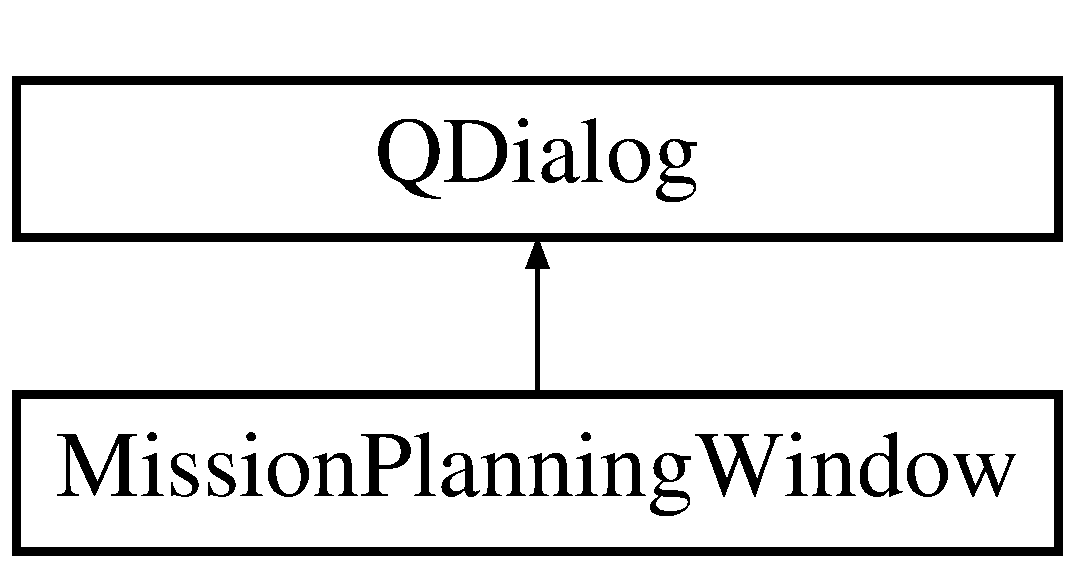
\includegraphics[height=2.000000cm]{class_mission_planning_window}
\end{center}
\end{figure}
\subsection*{Public Member Functions}
\begin{DoxyCompactItemize}
\item 
\hyperlink{class_mission_planning_window_a4ce75f53873c10f1053e7aff288f42ce}{Mission\+Planning\+Window} (Q\+Widget $\ast$parent=0)
\item 
\hyperlink{class_mission_planning_window_a2dd1e975fa9ab1f843dc4440436d066b}{$\sim$\+Mission\+Planning\+Window} ()
\item 
void \hyperlink{class_mission_planning_window_a995569fb123c9df67ba52db675543ab0}{delete\+Execute\+Button} ()
\item 
void \hyperlink{class_mission_planning_window_af3cb4549864921d72a3919412c1a9565}{add\+Button} (Q\+Push\+Button $\ast$)
\item 
void \hyperlink{class_mission_planning_window_a69829c310643543db1a5c5b3c6c72359}{add\+Combo\+Box} (Q\+Combo\+Box $\ast$)
\item 
void \hyperlink{class_mission_planning_window_a015cb8e3949a82535ec53a30520622e9}{dump\+Buttons} ()
\item 
void \hyperlink{class_mission_planning_window_a87d851bd04f183dabdd8b95d0bcd5e52}{dump\+Combo\+Boxes} ()
\item 
void \hyperlink{class_mission_planning_window_a685f4ba0b024f1eff55329bd21b9b397}{change\+Title} (Q\+String)
\end{DoxyCompactItemize}
\subsection*{Friends}
\begin{DoxyCompactItemize}
\item 
class \hyperlink{class_mission_planning_window_a337398c114f638b5a3e2fdc4529936c5}{Main\+M\+D\+I\+Display}
\end{DoxyCompactItemize}


\subsection{Constructor \& Destructor Documentation}
\hypertarget{class_mission_planning_window_a4ce75f53873c10f1053e7aff288f42ce}{}\index{Mission\+Planning\+Window@{Mission\+Planning\+Window}!Mission\+Planning\+Window@{Mission\+Planning\+Window}}
\index{Mission\+Planning\+Window@{Mission\+Planning\+Window}!Mission\+Planning\+Window@{Mission\+Planning\+Window}}
\subsubsection[{Mission\+Planning\+Window}]{\setlength{\rightskip}{0pt plus 5cm}Mission\+Planning\+Window\+::\+Mission\+Planning\+Window (
\begin{DoxyParamCaption}
\item[{Q\+Widget $\ast$}]{parent = {\ttfamily 0}}
\end{DoxyParamCaption}
)}\label{class_mission_planning_window_a4ce75f53873c10f1053e7aff288f42ce}
\hypertarget{class_mission_planning_window_a2dd1e975fa9ab1f843dc4440436d066b}{}\index{Mission\+Planning\+Window@{Mission\+Planning\+Window}!````~Mission\+Planning\+Window@{$\sim$\+Mission\+Planning\+Window}}
\index{````~Mission\+Planning\+Window@{$\sim$\+Mission\+Planning\+Window}!Mission\+Planning\+Window@{Mission\+Planning\+Window}}
\subsubsection[{$\sim$\+Mission\+Planning\+Window}]{\setlength{\rightskip}{0pt plus 5cm}Mission\+Planning\+Window\+::$\sim$\+Mission\+Planning\+Window (
\begin{DoxyParamCaption}
{}
\end{DoxyParamCaption}
)}\label{class_mission_planning_window_a2dd1e975fa9ab1f843dc4440436d066b}


\subsection{Member Function Documentation}
\hypertarget{class_mission_planning_window_af3cb4549864921d72a3919412c1a9565}{}\index{Mission\+Planning\+Window@{Mission\+Planning\+Window}!add\+Button@{add\+Button}}
\index{add\+Button@{add\+Button}!Mission\+Planning\+Window@{Mission\+Planning\+Window}}
\subsubsection[{add\+Button}]{\setlength{\rightskip}{0pt plus 5cm}void Mission\+Planning\+Window\+::add\+Button (
\begin{DoxyParamCaption}
\item[{Q\+Push\+Button $\ast$}]{new\+Button}
\end{DoxyParamCaption}
)}\label{class_mission_planning_window_af3cb4549864921d72a3919412c1a9565}
\hypertarget{class_mission_planning_window_a69829c310643543db1a5c5b3c6c72359}{}\index{Mission\+Planning\+Window@{Mission\+Planning\+Window}!add\+Combo\+Box@{add\+Combo\+Box}}
\index{add\+Combo\+Box@{add\+Combo\+Box}!Mission\+Planning\+Window@{Mission\+Planning\+Window}}
\subsubsection[{add\+Combo\+Box}]{\setlength{\rightskip}{0pt plus 5cm}void Mission\+Planning\+Window\+::add\+Combo\+Box (
\begin{DoxyParamCaption}
\item[{Q\+Combo\+Box $\ast$}]{new\+Combo\+Box}
\end{DoxyParamCaption}
)}\label{class_mission_planning_window_a69829c310643543db1a5c5b3c6c72359}
\hypertarget{class_mission_planning_window_a685f4ba0b024f1eff55329bd21b9b397}{}\index{Mission\+Planning\+Window@{Mission\+Planning\+Window}!change\+Title@{change\+Title}}
\index{change\+Title@{change\+Title}!Mission\+Planning\+Window@{Mission\+Planning\+Window}}
\subsubsection[{change\+Title}]{\setlength{\rightskip}{0pt plus 5cm}void Mission\+Planning\+Window\+::change\+Title (
\begin{DoxyParamCaption}
\item[{Q\+String}]{new\+Window\+Title}
\end{DoxyParamCaption}
)}\label{class_mission_planning_window_a685f4ba0b024f1eff55329bd21b9b397}
\hypertarget{class_mission_planning_window_a995569fb123c9df67ba52db675543ab0}{}\index{Mission\+Planning\+Window@{Mission\+Planning\+Window}!delete\+Execute\+Button@{delete\+Execute\+Button}}
\index{delete\+Execute\+Button@{delete\+Execute\+Button}!Mission\+Planning\+Window@{Mission\+Planning\+Window}}
\subsubsection[{delete\+Execute\+Button}]{\setlength{\rightskip}{0pt plus 5cm}void Mission\+Planning\+Window\+::delete\+Execute\+Button (
\begin{DoxyParamCaption}
{}
\end{DoxyParamCaption}
)}\label{class_mission_planning_window_a995569fb123c9df67ba52db675543ab0}
\hypertarget{class_mission_planning_window_a015cb8e3949a82535ec53a30520622e9}{}\index{Mission\+Planning\+Window@{Mission\+Planning\+Window}!dump\+Buttons@{dump\+Buttons}}
\index{dump\+Buttons@{dump\+Buttons}!Mission\+Planning\+Window@{Mission\+Planning\+Window}}
\subsubsection[{dump\+Buttons}]{\setlength{\rightskip}{0pt plus 5cm}void Mission\+Planning\+Window\+::dump\+Buttons (
\begin{DoxyParamCaption}
{}
\end{DoxyParamCaption}
)}\label{class_mission_planning_window_a015cb8e3949a82535ec53a30520622e9}
\hypertarget{class_mission_planning_window_a87d851bd04f183dabdd8b95d0bcd5e52}{}\index{Mission\+Planning\+Window@{Mission\+Planning\+Window}!dump\+Combo\+Boxes@{dump\+Combo\+Boxes}}
\index{dump\+Combo\+Boxes@{dump\+Combo\+Boxes}!Mission\+Planning\+Window@{Mission\+Planning\+Window}}
\subsubsection[{dump\+Combo\+Boxes}]{\setlength{\rightskip}{0pt plus 5cm}void Mission\+Planning\+Window\+::dump\+Combo\+Boxes (
\begin{DoxyParamCaption}
{}
\end{DoxyParamCaption}
)}\label{class_mission_planning_window_a87d851bd04f183dabdd8b95d0bcd5e52}


\subsection{Friends And Related Function Documentation}
\hypertarget{class_mission_planning_window_a337398c114f638b5a3e2fdc4529936c5}{}\index{Mission\+Planning\+Window@{Mission\+Planning\+Window}!Main\+M\+D\+I\+Display@{Main\+M\+D\+I\+Display}}
\index{Main\+M\+D\+I\+Display@{Main\+M\+D\+I\+Display}!Mission\+Planning\+Window@{Mission\+Planning\+Window}}
\subsubsection[{Main\+M\+D\+I\+Display}]{\setlength{\rightskip}{0pt plus 5cm}friend class {\bf Main\+M\+D\+I\+Display}\hspace{0.3cm}{\ttfamily [friend]}}\label{class_mission_planning_window_a337398c114f638b5a3e2fdc4529936c5}


The documentation for this class was generated from the following files\+:\begin{DoxyCompactItemize}
\item 
C\+:/\+Users/\+Roman/\+Documents/\+Mygs/\+Ground\+Station/\+G\+S/\hyperlink{missionplanningwindow_8h}{missionplanningwindow.\+h}\item 
C\+:/\+Users/\+Roman/\+Documents/\+Mygs/\+Ground\+Station/\+G\+S/\hyperlink{missionplanningwindow_8cpp}{missionplanningwindow.\+cpp}\end{DoxyCompactItemize}

\hypertarget{class_mission_recap}{}\section{Mission\+Recap Class Reference}
\label{class_mission_recap}\index{Mission\+Recap@{Mission\+Recap}}


{\ttfamily \#include $<$missionrecap.\+h$>$}

Inheritance diagram for Mission\+Recap\+:\begin{figure}[H]
\begin{center}
\leavevmode
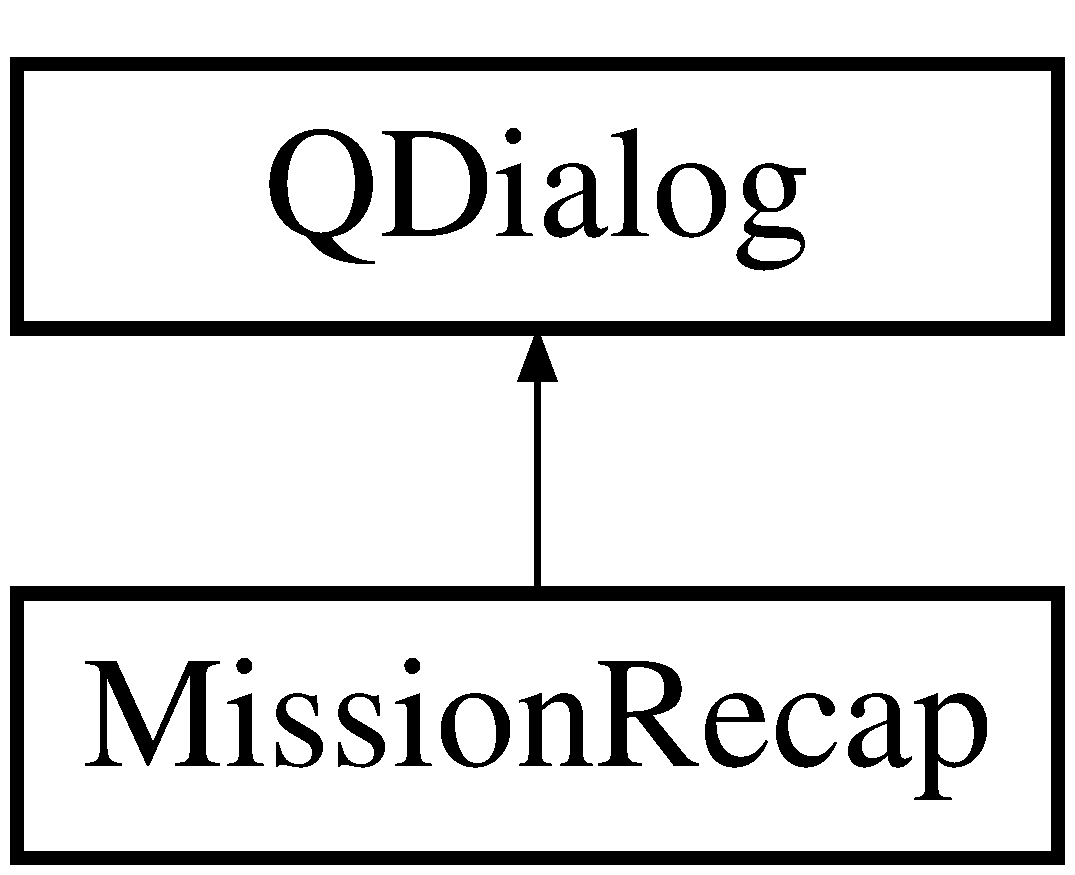
\includegraphics[height=2.000000cm]{class_mission_recap}
\end{center}
\end{figure}
\subsection*{Public Slots}
\begin{DoxyCompactItemize}
\item 
void \hyperlink{class_mission_recap_a47eb36c2cc172358a0367dee72b1740f}{update\+Slider} (qint64 position)
\item 
void \hyperlink{class_mission_recap_a15ecf642246edadd1c09d81b93a6a4c5}{update\+Media\+Player} (int position)
\item 
void \hyperlink{class_mission_recap_ae719be21194bde9a725c20bd3ed8048f}{replay\+Mission\+Clicked} ()
\item 
void \hyperlink{class_mission_recap_a4d45a9fbe0fc9bdfd7e6033cfaa533f9}{setup\+Realtime\+Data\+Demo} (\hyperlink{class_q_custom_plot}{Q\+Custom\+Plot} $\ast$custom\+Plot)
\end{DoxyCompactItemize}
\subsection*{Public Member Functions}
\begin{DoxyCompactItemize}
\item 
\hyperlink{class_mission_recap_a7b516bd2925e4e0e2bc9f70072786b32}{Mission\+Recap} (Q\+Widget $\ast$parent=0)
\item 
\hyperlink{class_mission_recap_a7ebaee9824446e52e77083c65d41535b}{$\sim$\+Mission\+Recap} ()
\end{DoxyCompactItemize}


\subsection{Constructor \& Destructor Documentation}
\hypertarget{class_mission_recap_a7b516bd2925e4e0e2bc9f70072786b32}{}\index{Mission\+Recap@{Mission\+Recap}!Mission\+Recap@{Mission\+Recap}}
\index{Mission\+Recap@{Mission\+Recap}!Mission\+Recap@{Mission\+Recap}}
\subsubsection[{Mission\+Recap}]{\setlength{\rightskip}{0pt plus 5cm}Mission\+Recap\+::\+Mission\+Recap (
\begin{DoxyParamCaption}
\item[{Q\+Widget $\ast$}]{parent = {\ttfamily 0}}
\end{DoxyParamCaption}
)\hspace{0.3cm}{\ttfamily [explicit]}}\label{class_mission_recap_a7b516bd2925e4e0e2bc9f70072786b32}
Creates video widget, requests a video to be played back Creates a map to play back U\+A\+V path Also creates custom plot for U\+A\+V statistics \hypertarget{class_mission_recap_a7ebaee9824446e52e77083c65d41535b}{}\index{Mission\+Recap@{Mission\+Recap}!````~Mission\+Recap@{$\sim$\+Mission\+Recap}}
\index{````~Mission\+Recap@{$\sim$\+Mission\+Recap}!Mission\+Recap@{Mission\+Recap}}
\subsubsection[{$\sim$\+Mission\+Recap}]{\setlength{\rightskip}{0pt plus 5cm}Mission\+Recap\+::$\sim$\+Mission\+Recap (
\begin{DoxyParamCaption}
{}
\end{DoxyParamCaption}
)}\label{class_mission_recap_a7ebaee9824446e52e77083c65d41535b}


\subsection{Member Function Documentation}
\hypertarget{class_mission_recap_ae719be21194bde9a725c20bd3ed8048f}{}\index{Mission\+Recap@{Mission\+Recap}!replay\+Mission\+Clicked@{replay\+Mission\+Clicked}}
\index{replay\+Mission\+Clicked@{replay\+Mission\+Clicked}!Mission\+Recap@{Mission\+Recap}}
\subsubsection[{replay\+Mission\+Clicked}]{\setlength{\rightskip}{0pt plus 5cm}void Mission\+Recap\+::replay\+Mission\+Clicked (
\begin{DoxyParamCaption}
{}
\end{DoxyParamCaption}
)\hspace{0.3cm}{\ttfamily [slot]}}\label{class_mission_recap_ae719be21194bde9a725c20bd3ed8048f}
\hypertarget{class_mission_recap_a4d45a9fbe0fc9bdfd7e6033cfaa533f9}{}\index{Mission\+Recap@{Mission\+Recap}!setup\+Realtime\+Data\+Demo@{setup\+Realtime\+Data\+Demo}}
\index{setup\+Realtime\+Data\+Demo@{setup\+Realtime\+Data\+Demo}!Mission\+Recap@{Mission\+Recap}}
\subsubsection[{setup\+Realtime\+Data\+Demo}]{\setlength{\rightskip}{0pt plus 5cm}void Mission\+Recap\+::setup\+Realtime\+Data\+Demo (
\begin{DoxyParamCaption}
\item[{{\bf Q\+Custom\+Plot} $\ast$}]{custom\+Plot}
\end{DoxyParamCaption}
)\hspace{0.3cm}{\ttfamily [slot]}}\label{class_mission_recap_a4d45a9fbe0fc9bdfd7e6033cfaa533f9}
Checks if Q\+T under Q\+T4.\+7 This is the code for the custom plot chart to play back real time data of the U\+A\+V Currently auto plays lines (10/23/15) \hypertarget{class_mission_recap_a15ecf642246edadd1c09d81b93a6a4c5}{}\index{Mission\+Recap@{Mission\+Recap}!update\+Media\+Player@{update\+Media\+Player}}
\index{update\+Media\+Player@{update\+Media\+Player}!Mission\+Recap@{Mission\+Recap}}
\subsubsection[{update\+Media\+Player}]{\setlength{\rightskip}{0pt plus 5cm}void Mission\+Recap\+::update\+Media\+Player (
\begin{DoxyParamCaption}
\item[{int}]{position}
\end{DoxyParamCaption}
)\hspace{0.3cm}{\ttfamily [slot]}}\label{class_mission_recap_a15ecf642246edadd1c09d81b93a6a4c5}
\hypertarget{class_mission_recap_a47eb36c2cc172358a0367dee72b1740f}{}\index{Mission\+Recap@{Mission\+Recap}!update\+Slider@{update\+Slider}}
\index{update\+Slider@{update\+Slider}!Mission\+Recap@{Mission\+Recap}}
\subsubsection[{update\+Slider}]{\setlength{\rightskip}{0pt plus 5cm}void Mission\+Recap\+::update\+Slider (
\begin{DoxyParamCaption}
\item[{qint64}]{position}
\end{DoxyParamCaption}
)\hspace{0.3cm}{\ttfamily [slot]}}\label{class_mission_recap_a47eb36c2cc172358a0367dee72b1740f}


The documentation for this class was generated from the following files\+:\begin{DoxyCompactItemize}
\item 
C\+:/\+Users/\+Roman/\+Documents/\+Mygs/\+Ground\+Station/\+G\+S/\hyperlink{missionrecap_8h}{missionrecap.\+h}\item 
C\+:/\+Users/\+Roman/\+Documents/\+Mygs/\+Ground\+Station/\+G\+S/\hyperlink{missionrecap_8cpp}{missionrecap.\+cpp}\end{DoxyCompactItemize}

\hypertarget{class_network_listener}{}\section{Network\+Listener Class Reference}
\label{class_network_listener}\index{Network\+Listener@{Network\+Listener}}


The \hyperlink{class_network_listener}{Network\+Listener} class is used to continuously listen for and process incoming network signals.  




{\ttfamily \#include $<$networklistener.\+h$>$}

Inheritance diagram for Network\+Listener\+:\begin{figure}[H]
\begin{center}
\leavevmode
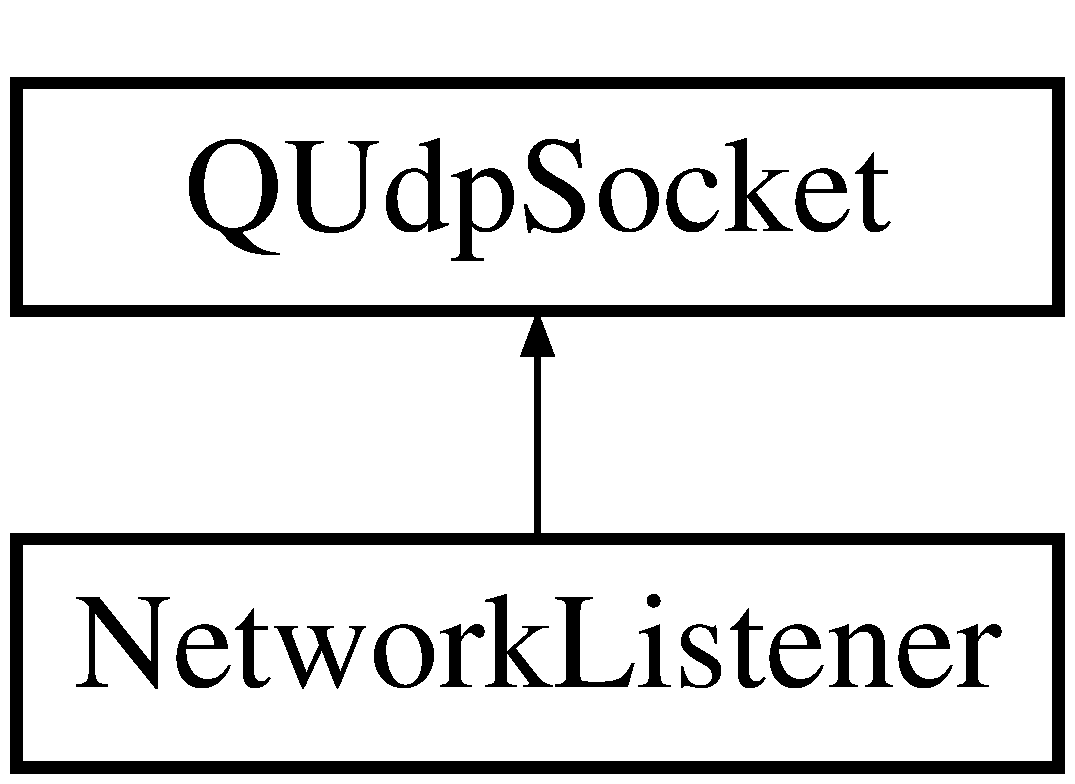
\includegraphics[height=2.000000cm]{class_network_listener}
\end{center}
\end{figure}
\subsection*{Signals}
\begin{DoxyCompactItemize}
\item 
void \hyperlink{class_network_listener_ac280873f9f90c046460b908fdb4a7883}{send\+Coordinates} (void)
\begin{DoxyCompactList}\small\item\em send\+Coordinates is used to request that the flightplan be sent to the U\+A\+V \end{DoxyCompactList}\item 
void \hyperlink{class_network_listener_a233d51dcc4d8945021d1b4043515e098}{log\+Telemetry} (Q\+String coord\+String)
\begin{DoxyCompactList}\small\item\em log\+Telemetry is the signal used to notify the main window that a telemetry point has been recieved. \end{DoxyCompactList}\item 
void \hyperlink{class_network_listener_aa695d0b565bb61dea1d03715b9f22e4b}{packet\+Recieved} (\hyperlink{class_protocol_1_1_packet}{Protocol\+::\+Packet} $\ast$packet)
\end{DoxyCompactItemize}
\subsection*{Public Member Functions}
\begin{DoxyCompactItemize}
\item 
void \hyperlink{class_network_listener_aae655a7afbd74bbe193612f2b7638958}{start} ()
\item 
\hyperlink{class_network_listener_a47d3f9cbc646f4accac24d9e9e7669cc}{Network\+Listener} (\hyperlink{classmessagebox}{messagebox} $\ast$my\+Message\+Box, int U\+A\+Vid, \hyperlink{class_gs_server}{Gs\+Server} $\ast$\hyperlink{class_network_listener_a18b48fbd5b2df44baa73e4b332981a56}{server})
\item 
\hyperlink{class_network_listener_a12b670b3b9a0f89900ab423e5a31ba54}{Network\+Listener} (\hyperlink{classmessagebox}{messagebox} $\ast$my\+Message\+Box, \hyperlink{class_gs_server}{Gs\+Server} $\ast$\hyperlink{class_network_listener_a18b48fbd5b2df44baa73e4b332981a56}{server})
\item 
void \hyperlink{class_network_listener_abffa3dbc0d6b31e53a638655f7efa9ee}{net\+Wait} (int millis)
\item 
long \hyperlink{class_network_listener_a12862b1a35cb8ba6c2ac8c7f1df9b1bf}{recive\+Message} (char $\ast$buf)
\item 
void \hyperlink{class_network_listener_a3174e591844d73c16e559804fa3a4ac6}{message\+Recieved} (char $\ast$msg)
\item 
void \hyperlink{class_network_listener_ab1dda7d270a90847a1537d04009c912b}{set\+Id} (int U\+A\+Vid)
\item 
void \hyperlink{class_network_listener_a258e0ef8e6e4de827e652a43186c6a07}{stop} ()
\item 
\hyperlink{class_network_listener_a18ad1d8973011f8bdceb5fc6d5cd81c1}{$\sim$\+Network\+Listener} ()
\end{DoxyCompactItemize}
\subsection*{Public Attributes}
\begin{DoxyCompactItemize}
\item 
\hyperlink{class_gs_server}{Gs\+Server} $\ast$ \hyperlink{class_network_listener_a18b48fbd5b2df44baa73e4b332981a56}{server}
\end{DoxyCompactItemize}


\subsection{Detailed Description}
The \hyperlink{class_network_listener}{Network\+Listener} class is used to continuously listen for and process incoming network signals. 

\begin{DoxySeeAlso}{See also}
\hyperlink{class_gs_server}{Gs\+Server} 
\end{DoxySeeAlso}
\begin{DoxyAuthor}{Author}
Jordan Dickson 
\end{DoxyAuthor}
\begin{DoxyDate}{Date}
10-\/3-\/2015 
\end{DoxyDate}


\subsection{Constructor \& Destructor Documentation}
\hypertarget{class_network_listener_a47d3f9cbc646f4accac24d9e9e7669cc}{}\index{Network\+Listener@{Network\+Listener}!Network\+Listener@{Network\+Listener}}
\index{Network\+Listener@{Network\+Listener}!Network\+Listener@{Network\+Listener}}
\subsubsection[{Network\+Listener}]{\setlength{\rightskip}{0pt plus 5cm}Network\+Listener\+::\+Network\+Listener (
\begin{DoxyParamCaption}
\item[{{\bf messagebox} $\ast$}]{my\+Message\+Box, }
\item[{int}]{U\+A\+Vid, }
\item[{{\bf Gs\+Server} $\ast$}]{server}
\end{DoxyParamCaption}
)}\label{class_network_listener_a47d3f9cbc646f4accac24d9e9e7669cc}
\hypertarget{class_network_listener_a12b670b3b9a0f89900ab423e5a31ba54}{}\index{Network\+Listener@{Network\+Listener}!Network\+Listener@{Network\+Listener}}
\index{Network\+Listener@{Network\+Listener}!Network\+Listener@{Network\+Listener}}
\subsubsection[{Network\+Listener}]{\setlength{\rightskip}{0pt plus 5cm}Network\+Listener\+::\+Network\+Listener (
\begin{DoxyParamCaption}
\item[{{\bf messagebox} $\ast$}]{my\+Message\+Box, }
\item[{{\bf Gs\+Server} $\ast$}]{server}
\end{DoxyParamCaption}
)}\label{class_network_listener_a12b670b3b9a0f89900ab423e5a31ba54}
\hypertarget{class_network_listener_a18ad1d8973011f8bdceb5fc6d5cd81c1}{}\index{Network\+Listener@{Network\+Listener}!````~Network\+Listener@{$\sim$\+Network\+Listener}}
\index{````~Network\+Listener@{$\sim$\+Network\+Listener}!Network\+Listener@{Network\+Listener}}
\subsubsection[{$\sim$\+Network\+Listener}]{\setlength{\rightskip}{0pt plus 5cm}Network\+Listener\+::$\sim$\+Network\+Listener (
\begin{DoxyParamCaption}
{}
\end{DoxyParamCaption}
)}\label{class_network_listener_a18ad1d8973011f8bdceb5fc6d5cd81c1}


\subsection{Member Function Documentation}
\hypertarget{class_network_listener_a233d51dcc4d8945021d1b4043515e098}{}\index{Network\+Listener@{Network\+Listener}!log\+Telemetry@{log\+Telemetry}}
\index{log\+Telemetry@{log\+Telemetry}!Network\+Listener@{Network\+Listener}}
\subsubsection[{log\+Telemetry}]{\setlength{\rightskip}{0pt plus 5cm}void Network\+Listener\+::log\+Telemetry (
\begin{DoxyParamCaption}
\item[{Q\+String}]{coord\+String}
\end{DoxyParamCaption}
)\hspace{0.3cm}{\ttfamily [signal]}}\label{class_network_listener_a233d51dcc4d8945021d1b4043515e098}


log\+Telemetry is the signal used to notify the main window that a telemetry point has been recieved. 


\begin{DoxyParams}{Parameters}
{\em coord\+String} & \\
\hline
\end{DoxyParams}
\hypertarget{class_network_listener_a3174e591844d73c16e559804fa3a4ac6}{}\index{Network\+Listener@{Network\+Listener}!message\+Recieved@{message\+Recieved}}
\index{message\+Recieved@{message\+Recieved}!Network\+Listener@{Network\+Listener}}
\subsubsection[{message\+Recieved}]{\setlength{\rightskip}{0pt plus 5cm}void Network\+Listener\+::message\+Recieved (
\begin{DoxyParamCaption}
\item[{char $\ast$}]{msg}
\end{DoxyParamCaption}
)}\label{class_network_listener_a3174e591844d73c16e559804fa3a4ac6}
\hypertarget{class_network_listener_abffa3dbc0d6b31e53a638655f7efa9ee}{}\index{Network\+Listener@{Network\+Listener}!net\+Wait@{net\+Wait}}
\index{net\+Wait@{net\+Wait}!Network\+Listener@{Network\+Listener}}
\subsubsection[{net\+Wait}]{\setlength{\rightskip}{0pt plus 5cm}void Network\+Listener\+::net\+Wait (
\begin{DoxyParamCaption}
\item[{int}]{millis}
\end{DoxyParamCaption}
)}\label{class_network_listener_abffa3dbc0d6b31e53a638655f7efa9ee}
\hypertarget{class_network_listener_aa695d0b565bb61dea1d03715b9f22e4b}{}\index{Network\+Listener@{Network\+Listener}!packet\+Recieved@{packet\+Recieved}}
\index{packet\+Recieved@{packet\+Recieved}!Network\+Listener@{Network\+Listener}}
\subsubsection[{packet\+Recieved}]{\setlength{\rightskip}{0pt plus 5cm}void Network\+Listener\+::packet\+Recieved (
\begin{DoxyParamCaption}
\item[{{\bf Protocol\+::\+Packet} $\ast$}]{packet}
\end{DoxyParamCaption}
)\hspace{0.3cm}{\ttfamily [signal]}}\label{class_network_listener_aa695d0b565bb61dea1d03715b9f22e4b}
\hypertarget{class_network_listener_a12862b1a35cb8ba6c2ac8c7f1df9b1bf}{}\index{Network\+Listener@{Network\+Listener}!recive\+Message@{recive\+Message}}
\index{recive\+Message@{recive\+Message}!Network\+Listener@{Network\+Listener}}
\subsubsection[{recive\+Message}]{\setlength{\rightskip}{0pt plus 5cm}long Network\+Listener\+::recive\+Message (
\begin{DoxyParamCaption}
\item[{char $\ast$}]{buf}
\end{DoxyParamCaption}
)}\label{class_network_listener_a12862b1a35cb8ba6c2ac8c7f1df9b1bf}
\hypertarget{class_network_listener_ac280873f9f90c046460b908fdb4a7883}{}\index{Network\+Listener@{Network\+Listener}!send\+Coordinates@{send\+Coordinates}}
\index{send\+Coordinates@{send\+Coordinates}!Network\+Listener@{Network\+Listener}}
\subsubsection[{send\+Coordinates}]{\setlength{\rightskip}{0pt plus 5cm}void Network\+Listener\+::send\+Coordinates (
\begin{DoxyParamCaption}
\item[{void}]{}
\end{DoxyParamCaption}
)\hspace{0.3cm}{\ttfamily [signal]}}\label{class_network_listener_ac280873f9f90c046460b908fdb4a7883}


send\+Coordinates is used to request that the flightplan be sent to the U\+A\+V 

\begin{DoxySeeAlso}{See also}
\hyperlink{class_map_execution_a5f0c7ab18a5fcc4c474eeb5b9707dc61}{Map\+Execution\+::send\+Flight\+Plan()} 
\end{DoxySeeAlso}
\hypertarget{class_network_listener_ab1dda7d270a90847a1537d04009c912b}{}\index{Network\+Listener@{Network\+Listener}!set\+Id@{set\+Id}}
\index{set\+Id@{set\+Id}!Network\+Listener@{Network\+Listener}}
\subsubsection[{set\+Id}]{\setlength{\rightskip}{0pt plus 5cm}void Network\+Listener\+::set\+Id (
\begin{DoxyParamCaption}
\item[{int}]{U\+A\+Vid}
\end{DoxyParamCaption}
)}\label{class_network_listener_ab1dda7d270a90847a1537d04009c912b}
\hypertarget{class_network_listener_aae655a7afbd74bbe193612f2b7638958}{}\index{Network\+Listener@{Network\+Listener}!start@{start}}
\index{start@{start}!Network\+Listener@{Network\+Listener}}
\subsubsection[{start}]{\setlength{\rightskip}{0pt plus 5cm}void Network\+Listener\+::start (
\begin{DoxyParamCaption}
{}
\end{DoxyParamCaption}
)}\label{class_network_listener_aae655a7afbd74bbe193612f2b7638958}
\hypertarget{class_network_listener_a258e0ef8e6e4de827e652a43186c6a07}{}\index{Network\+Listener@{Network\+Listener}!stop@{stop}}
\index{stop@{stop}!Network\+Listener@{Network\+Listener}}
\subsubsection[{stop}]{\setlength{\rightskip}{0pt plus 5cm}void Network\+Listener\+::stop (
\begin{DoxyParamCaption}
{}
\end{DoxyParamCaption}
)}\label{class_network_listener_a258e0ef8e6e4de827e652a43186c6a07}


\subsection{Member Data Documentation}
\hypertarget{class_network_listener_a18b48fbd5b2df44baa73e4b332981a56}{}\index{Network\+Listener@{Network\+Listener}!server@{server}}
\index{server@{server}!Network\+Listener@{Network\+Listener}}
\subsubsection[{server}]{\setlength{\rightskip}{0pt plus 5cm}{\bf Gs\+Server}$\ast$ Network\+Listener\+::server}\label{class_network_listener_a18b48fbd5b2df44baa73e4b332981a56}


The documentation for this class was generated from the following files\+:\begin{DoxyCompactItemize}
\item 
C\+:/\+Users/\+Roman/\+Documents/\+Mygs/\+Ground\+Station/\+G\+S/\hyperlink{networklistener_8h}{networklistener.\+h}\item 
C\+:/\+Users/\+Roman/\+Documents/\+Mygs/\+Ground\+Station/\+G\+S/\hyperlink{networklistener_8cpp}{networklistener.\+cpp}\end{DoxyCompactItemize}

\hypertarget{class_options}{}\section{Options Class Reference}
\label{class_options}\index{Options@{Options}}


{\ttfamily \#include $<$options.\+h$>$}

Inheritance diagram for Options\+:\begin{figure}[H]
\begin{center}
\leavevmode
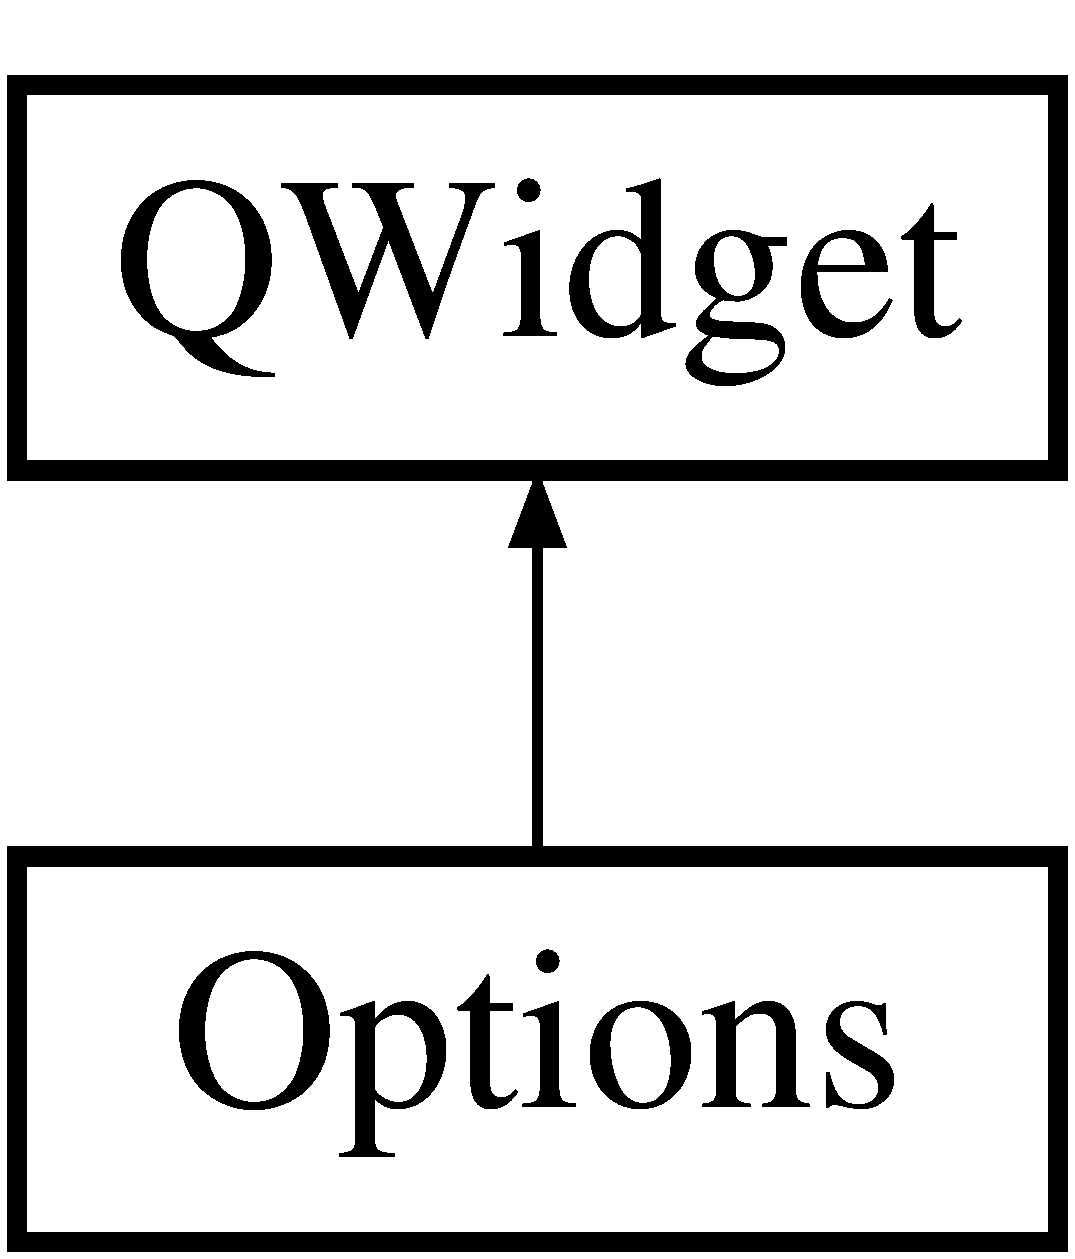
\includegraphics[height=2.000000cm]{class_options}
\end{center}
\end{figure}
\subsection*{Public Member Functions}
\begin{DoxyCompactItemize}
\item 
\hyperlink{class_options_a87403ad1d6bd9ae2b54af860bb0f0952}{Options} (Q\+Widget $\ast$parent=0)
\item 
\hyperlink{class_options_a86ddb85b183f8b58af5481f30a42fa92}{$\sim$\+Options} ()
\end{DoxyCompactItemize}


\subsection{Constructor \& Destructor Documentation}
\hypertarget{class_options_a87403ad1d6bd9ae2b54af860bb0f0952}{}\index{Options@{Options}!Options@{Options}}
\index{Options@{Options}!Options@{Options}}
\subsubsection[{Options}]{\setlength{\rightskip}{0pt plus 5cm}Options\+::\+Options (
\begin{DoxyParamCaption}
\item[{Q\+Widget $\ast$}]{parent = {\ttfamily 0}}
\end{DoxyParamCaption}
)\hspace{0.3cm}{\ttfamily [explicit]}}\label{class_options_a87403ad1d6bd9ae2b54af860bb0f0952}
\hypertarget{class_options_a86ddb85b183f8b58af5481f30a42fa92}{}\index{Options@{Options}!````~Options@{$\sim$\+Options}}
\index{````~Options@{$\sim$\+Options}!Options@{Options}}
\subsubsection[{$\sim$\+Options}]{\setlength{\rightskip}{0pt plus 5cm}Options\+::$\sim$\+Options (
\begin{DoxyParamCaption}
{}
\end{DoxyParamCaption}
)}\label{class_options_a86ddb85b183f8b58af5481f30a42fa92}


The documentation for this class was generated from the following files\+:\begin{DoxyCompactItemize}
\item 
C\+:/\+Users/\+Roman/\+Documents/\+Mygs/\+Ground\+Station/\+G\+S/\hyperlink{options_8h}{options.\+h}\item 
C\+:/\+Users/\+Roman/\+Documents/\+Mygs/\+Ground\+Station/\+G\+S/\hyperlink{options_8cpp}{options.\+cpp}\end{DoxyCompactItemize}

\hypertarget{class_protocol_1_1_packet}{}\section{Protocol\+:\+:Packet Class Reference}
\label{class_protocol_1_1_packet}\index{Protocol\+::\+Packet@{Protocol\+::\+Packet}}


{\ttfamily \#include $<$packet.\+h$>$}

Inheritance diagram for Protocol\+:\+:Packet\+:\begin{figure}[H]
\begin{center}
\leavevmode
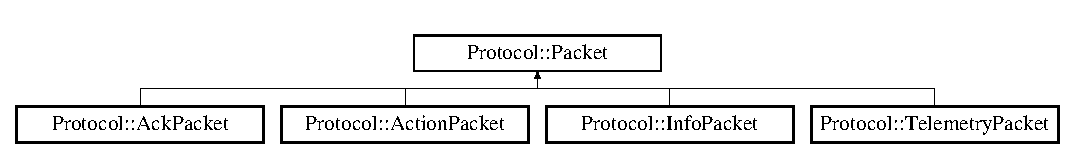
\includegraphics[height=1.686747cm]{class_protocol_1_1_packet}
\end{center}
\end{figure}
\subsection*{Public Member Functions}
\begin{DoxyCompactItemize}
\item 
uint32\+\_\+t \hyperlink{class_protocol_1_1_packet_acbe4f1b9f973d14097814d16fb0cd83a}{get\+\_\+timestamp} ()
\item 
void \hyperlink{class_protocol_1_1_packet_aa3f97852d443bb9554178384afa24eec}{set\+\_\+type} (\hyperlink{namespace_protocol_a0704fe3e36f425dc9805a6dcc1ea1b75}{Packet\+Type} a)
\item 
\hyperlink{namespace_protocol_a0704fe3e36f425dc9805a6dcc1ea1b75}{Packet\+Type} \hyperlink{class_protocol_1_1_packet_a3c159ff945d95102ee2a2ba0b93d05d8}{get\+\_\+type} ()
\item 
virtual size\+\_\+t \hyperlink{class_protocol_1_1_packet_a9c89c3d05acc44a5050ebfc756a2cd41}{Get\+Bytes} (uint8\+\_\+t $\ast$buffer, size\+\_\+t len)=0
\end{DoxyCompactItemize}
\subsection*{Static Public Member Functions}
\begin{DoxyCompactItemize}
\item 
static \hyperlink{class_protocol_1_1_packet}{Packet} $\ast$ \hyperlink{class_protocol_1_1_packet_ad327686418aa271121e6a6a8eadebbd4}{Parse} (uint8\+\_\+t $\ast$buffer, size\+\_\+t len)
\end{DoxyCompactItemize}
\subsection*{Protected Member Functions}
\begin{DoxyCompactItemize}
\item 
\hyperlink{class_protocol_1_1_packet_ae02347b6d2eee98511ec19343b82e0a7}{Packet} (\hyperlink{namespace_protocol_a0704fe3e36f425dc9805a6dcc1ea1b75}{Packet\+Type} t)
\item 
size\+\_\+t \hyperlink{class_protocol_1_1_packet_aa7498c8c70cb8a55617ce588508af81f}{Write\+Header} (uint8\+\_\+t $\ast$buffer, size\+\_\+t len)
\item 
size\+\_\+t \hyperlink{class_protocol_1_1_packet_aa5f54d3128f7914383f4d8e8f53fbce4}{Read\+Header} (uint8\+\_\+t $\ast$buffer, size\+\_\+t len)
\item 
size\+\_\+t \hyperlink{class_protocol_1_1_packet_adc4ebdbdbcdbaa177ba243c5c654ba18}{Set\+Checksum} (uint8\+\_\+t $\ast$buffer, size\+\_\+t len, size\+\_\+t offset)
\end{DoxyCompactItemize}
\subsection*{Protected Attributes}
\begin{DoxyCompactItemize}
\item 
uint32\+\_\+t \hyperlink{class_protocol_1_1_packet_a2f0a19f4bff82270290e53d31e67db33}{timestamp}
\end{DoxyCompactItemize}


\subsection{Constructor \& Destructor Documentation}
\hypertarget{class_protocol_1_1_packet_ae02347b6d2eee98511ec19343b82e0a7}{}\index{Protocol\+::\+Packet@{Protocol\+::\+Packet}!Packet@{Packet}}
\index{Packet@{Packet}!Protocol\+::\+Packet@{Protocol\+::\+Packet}}
\subsubsection[{Packet}]{\setlength{\rightskip}{0pt plus 5cm}Protocol\+::\+Packet\+::\+Packet (
\begin{DoxyParamCaption}
\item[{{\bf Protocol\+::\+Packet\+Type}}]{t}
\end{DoxyParamCaption}
)\hspace{0.3cm}{\ttfamily [protected]}}\label{class_protocol_1_1_packet_ae02347b6d2eee98511ec19343b82e0a7}


\subsection{Member Function Documentation}
\hypertarget{class_protocol_1_1_packet_acbe4f1b9f973d14097814d16fb0cd83a}{}\index{Protocol\+::\+Packet@{Protocol\+::\+Packet}!get\+\_\+timestamp@{get\+\_\+timestamp}}
\index{get\+\_\+timestamp@{get\+\_\+timestamp}!Protocol\+::\+Packet@{Protocol\+::\+Packet}}
\subsubsection[{get\+\_\+timestamp}]{\setlength{\rightskip}{0pt plus 5cm}uint32\+\_\+t Protocol\+::\+Packet\+::get\+\_\+timestamp (
\begin{DoxyParamCaption}
{}
\end{DoxyParamCaption}
)}\label{class_protocol_1_1_packet_acbe4f1b9f973d14097814d16fb0cd83a}
\hypertarget{class_protocol_1_1_packet_a3c159ff945d95102ee2a2ba0b93d05d8}{}\index{Protocol\+::\+Packet@{Protocol\+::\+Packet}!get\+\_\+type@{get\+\_\+type}}
\index{get\+\_\+type@{get\+\_\+type}!Protocol\+::\+Packet@{Protocol\+::\+Packet}}
\subsubsection[{get\+\_\+type}]{\setlength{\rightskip}{0pt plus 5cm}{\bf Protocol\+::\+Packet\+Type} Protocol\+::\+Packet\+::get\+\_\+type (
\begin{DoxyParamCaption}
{}
\end{DoxyParamCaption}
)}\label{class_protocol_1_1_packet_a3c159ff945d95102ee2a2ba0b93d05d8}
\hypertarget{class_protocol_1_1_packet_a9c89c3d05acc44a5050ebfc756a2cd41}{}\index{Protocol\+::\+Packet@{Protocol\+::\+Packet}!Get\+Bytes@{Get\+Bytes}}
\index{Get\+Bytes@{Get\+Bytes}!Protocol\+::\+Packet@{Protocol\+::\+Packet}}
\subsubsection[{Get\+Bytes}]{\setlength{\rightskip}{0pt plus 5cm}virtual size\+\_\+t Protocol\+::\+Packet\+::\+Get\+Bytes (
\begin{DoxyParamCaption}
\item[{uint8\+\_\+t $\ast$}]{buffer, }
\item[{size\+\_\+t}]{len}
\end{DoxyParamCaption}
)\hspace{0.3cm}{\ttfamily [pure virtual]}}\label{class_protocol_1_1_packet_a9c89c3d05acc44a5050ebfc756a2cd41}
Stores the byte representation of a packet in the given buffer.

\begin{DoxyAuthor}{Author}
Jason Watkins 
\end{DoxyAuthor}
\begin{DoxyDate}{Date}
2015-\/11-\/16
\end{DoxyDate}

\begin{DoxyParams}{Parameters}
{\em buffer\mbox{[}in\mbox{]}} & An array to write the packet to. \\
\hline
{\em len\mbox{[}in\mbox{]}} & The length of {\ttfamily buffer}. \\
\hline
\end{DoxyParams}


Implemented in \hyperlink{class_protocol_1_1_action_packet_af5963f7c15af8292152df260b188f626}{Protocol\+::\+Action\+Packet}, \hyperlink{class_protocol_1_1_telemetry_packet_a36d86bf7afc3dcdd820ffa0982c5177a}{Protocol\+::\+Telemetry\+Packet}, \hyperlink{class_protocol_1_1_info_packet_ad1f43721045348442cf224533bce7f1a}{Protocol\+::\+Info\+Packet}, and \hyperlink{class_protocol_1_1_ack_packet_a588f9608c58a913c5dd3c4acd28f92af}{Protocol\+::\+Ack\+Packet}.

\hypertarget{class_protocol_1_1_packet_ad327686418aa271121e6a6a8eadebbd4}{}\index{Protocol\+::\+Packet@{Protocol\+::\+Packet}!Parse@{Parse}}
\index{Parse@{Parse}!Protocol\+::\+Packet@{Protocol\+::\+Packet}}
\subsubsection[{Parse}]{\setlength{\rightskip}{0pt plus 5cm}{\bf Protocol\+::\+Packet} $\ast$ Protocol\+::\+Packet\+::\+Parse (
\begin{DoxyParamCaption}
\item[{uint8\+\_\+t $\ast$}]{buffer, }
\item[{size\+\_\+t}]{len}
\end{DoxyParamCaption}
)\hspace{0.3cm}{\ttfamily [static]}}\label{class_protocol_1_1_packet_ad327686418aa271121e6a6a8eadebbd4}
\hypertarget{class_protocol_1_1_packet_aa5f54d3128f7914383f4d8e8f53fbce4}{}\index{Protocol\+::\+Packet@{Protocol\+::\+Packet}!Read\+Header@{Read\+Header}}
\index{Read\+Header@{Read\+Header}!Protocol\+::\+Packet@{Protocol\+::\+Packet}}
\subsubsection[{Read\+Header}]{\setlength{\rightskip}{0pt plus 5cm}size\+\_\+t Protocol\+::\+Packet\+::\+Read\+Header (
\begin{DoxyParamCaption}
\item[{uint8\+\_\+t $\ast$}]{buffer, }
\item[{size\+\_\+t}]{len}
\end{DoxyParamCaption}
)\hspace{0.3cm}{\ttfamily [protected]}}\label{class_protocol_1_1_packet_aa5f54d3128f7914383f4d8e8f53fbce4}
Reads information shared by all packets from the given buffer.

\begin{DoxyAuthor}{Author}
Jason Watkins 
\end{DoxyAuthor}
\begin{DoxyDate}{Date}
2015-\/11-\/16
\end{DoxyDate}

\begin{DoxyParams}{Parameters}
{\em buffer\mbox{[}in\mbox{]}} & An array containing a valid packet \\
\hline
{\em len\mbox{[}in\mbox{]}} & The length of {\ttfamily buffer}. \\
\hline
\end{DoxyParams}
\begin{DoxyReturn}{Returns}
The number of bytes contained in the header. 
\end{DoxyReturn}
\hypertarget{class_protocol_1_1_packet_aa3f97852d443bb9554178384afa24eec}{}\index{Protocol\+::\+Packet@{Protocol\+::\+Packet}!set\+\_\+type@{set\+\_\+type}}
\index{set\+\_\+type@{set\+\_\+type}!Protocol\+::\+Packet@{Protocol\+::\+Packet}}
\subsubsection[{set\+\_\+type}]{\setlength{\rightskip}{0pt plus 5cm}void Protocol\+::\+Packet\+::set\+\_\+type (
\begin{DoxyParamCaption}
\item[{{\bf Protocol\+::\+Packet\+Type}}]{a}
\end{DoxyParamCaption}
)}\label{class_protocol_1_1_packet_aa3f97852d443bb9554178384afa24eec}
\hypertarget{class_protocol_1_1_packet_adc4ebdbdbcdbaa177ba243c5c654ba18}{}\index{Protocol\+::\+Packet@{Protocol\+::\+Packet}!Set\+Checksum@{Set\+Checksum}}
\index{Set\+Checksum@{Set\+Checksum}!Protocol\+::\+Packet@{Protocol\+::\+Packet}}
\subsubsection[{Set\+Checksum}]{\setlength{\rightskip}{0pt plus 5cm}size\+\_\+t Protocol\+::\+Packet\+::\+Set\+Checksum (
\begin{DoxyParamCaption}
\item[{uint8\+\_\+t $\ast$}]{buffer, }
\item[{size\+\_\+t}]{len, }
\item[{size\+\_\+t}]{offset}
\end{DoxyParamCaption}
)\hspace{0.3cm}{\ttfamily [protected]}}\label{class_protocol_1_1_packet_adc4ebdbdbcdbaa177ba243c5c654ba18}
Sets the checksum bytes at the end of a packet.

\begin{DoxyAuthor}{Author}
Jason Watkins 
\end{DoxyAuthor}
\begin{DoxyDate}{Date}
2015-\/11-\/16
\end{DoxyDate}

\begin{DoxyParams}{Parameters}
{\em buffer\mbox{[}in\mbox{]}} & An array to write the header to. \\
\hline
{\em len\mbox{[}in\mbox{]}} & The length of {\ttfamily buffer}. \\
\hline
{\em offset\mbox{[}in\mbox{]}} & The index of the last byte that should be part of the calculated checksum. {\ttfamily offset} should be at least two less than {\ttfamily len} to leave room for the checksum bytes. \\
\hline
\end{DoxyParams}
\begin{DoxyReturn}{Returns}
The end of the packet with the checksum appended. 
\end{DoxyReturn}
\hypertarget{class_protocol_1_1_packet_aa7498c8c70cb8a55617ce588508af81f}{}\index{Protocol\+::\+Packet@{Protocol\+::\+Packet}!Write\+Header@{Write\+Header}}
\index{Write\+Header@{Write\+Header}!Protocol\+::\+Packet@{Protocol\+::\+Packet}}
\subsubsection[{Write\+Header}]{\setlength{\rightskip}{0pt plus 5cm}size\+\_\+t Protocol\+::\+Packet\+::\+Write\+Header (
\begin{DoxyParamCaption}
\item[{uint8\+\_\+t $\ast$}]{buffer, }
\item[{size\+\_\+t}]{len}
\end{DoxyParamCaption}
)\hspace{0.3cm}{\ttfamily [protected]}}\label{class_protocol_1_1_packet_aa7498c8c70cb8a55617ce588508af81f}
Writes information shared by all packets to the given buffer.

\begin{DoxyAuthor}{Author}
Jason Watkins 
\end{DoxyAuthor}
\begin{DoxyDate}{Date}
2015-\/11-\/16
\end{DoxyDate}

\begin{DoxyParams}{Parameters}
{\em buffer\mbox{[}in\mbox{]}} & An array to write the header to. \\
\hline
{\em len\mbox{[}in\mbox{]}} & The length of {\ttfamily buffer}. \\
\hline
\end{DoxyParams}
\begin{DoxyReturn}{Returns}
The number of bytes written to buffer. 
\end{DoxyReturn}


\subsection{Member Data Documentation}
\hypertarget{class_protocol_1_1_packet_a2f0a19f4bff82270290e53d31e67db33}{}\index{Protocol\+::\+Packet@{Protocol\+::\+Packet}!timestamp@{timestamp}}
\index{timestamp@{timestamp}!Protocol\+::\+Packet@{Protocol\+::\+Packet}}
\subsubsection[{timestamp}]{\setlength{\rightskip}{0pt plus 5cm}uint32\+\_\+t Protocol\+::\+Packet\+::timestamp\hspace{0.3cm}{\ttfamily [protected]}}\label{class_protocol_1_1_packet_a2f0a19f4bff82270290e53d31e67db33}


The documentation for this class was generated from the following files\+:\begin{DoxyCompactItemize}
\item 
C\+:/\+Users/\+Roman/\+Documents/\+Mygs/\+Ground\+Station/\+G\+S/\hyperlink{packet_8h}{packet.\+h}\item 
C\+:/\+Users/\+Roman/\+Documents/\+Mygs/\+Ground\+Station/\+G\+S/\hyperlink{_packet_8cpp}{Packet.\+cpp}\end{DoxyCompactItemize}

\hypertarget{class_pop_window_m_p}{}\section{Pop\+Window\+M\+P Class Reference}
\label{class_pop_window_m_p}\index{Pop\+Window\+M\+P@{Pop\+Window\+M\+P}}


{\ttfamily \#include $<$popwindowmp.\+h$>$}

Inheritance diagram for Pop\+Window\+M\+P\+:\begin{figure}[H]
\begin{center}
\leavevmode
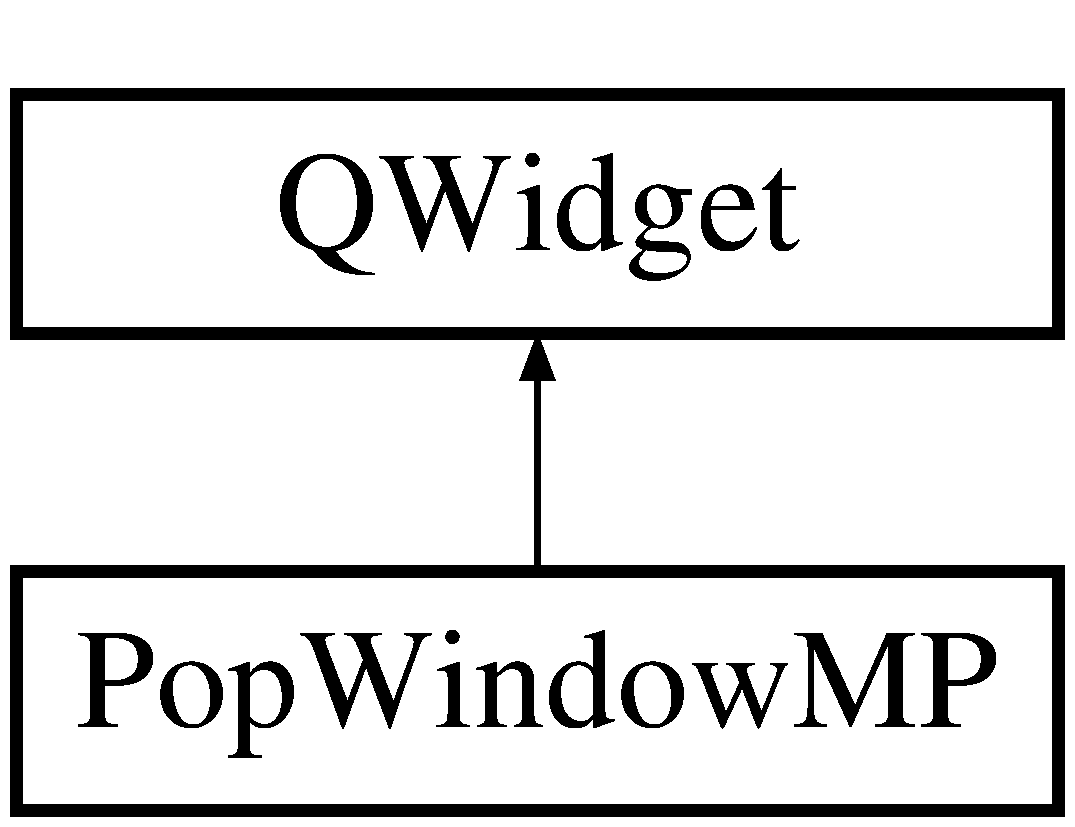
\includegraphics[height=2.000000cm]{class_pop_window_m_p}
\end{center}
\end{figure}
\subsection*{Signals}
\begin{DoxyCompactItemize}
\item 
void \hyperlink{class_pop_window_m_p_aea9a78b6f0f6bb6536c7481ed67ad66d}{window\+Closed} ()
\end{DoxyCompactItemize}
\subsection*{Public Member Functions}
\begin{DoxyCompactItemize}
\item 
\hyperlink{class_pop_window_m_p_a3298919d76ea83d8bab145bbfaba7668}{Pop\+Window\+M\+P} (Q\+List$<$ Q\+String $>$ strings, Q\+Widget $\ast$parent=0)
\item 
\hyperlink{class_pop_window_m_p_aa58c893a6ddb936e79d4ee329dab11c6}{$\sim$\+Pop\+Window\+M\+P} ()
\end{DoxyCompactItemize}
\subsection*{Public Attributes}
\begin{DoxyCompactItemize}
\item 
Q\+List$<$ Q\+String $>$ \hyperlink{class_pop_window_m_p_a95b9fb0c455dce6924a1a7282fd13b00}{map\+Strings}
\end{DoxyCompactItemize}


\subsection{Constructor \& Destructor Documentation}
\hypertarget{class_pop_window_m_p_a3298919d76ea83d8bab145bbfaba7668}{}\index{Pop\+Window\+M\+P@{Pop\+Window\+M\+P}!Pop\+Window\+M\+P@{Pop\+Window\+M\+P}}
\index{Pop\+Window\+M\+P@{Pop\+Window\+M\+P}!Pop\+Window\+M\+P@{Pop\+Window\+M\+P}}
\subsubsection[{Pop\+Window\+M\+P}]{\setlength{\rightskip}{0pt plus 5cm}Pop\+Window\+M\+P\+::\+Pop\+Window\+M\+P (
\begin{DoxyParamCaption}
\item[{Q\+List$<$ Q\+String $>$}]{strings, }
\item[{Q\+Widget $\ast$}]{parent = {\ttfamily 0}}
\end{DoxyParamCaption}
)\hspace{0.3cm}{\ttfamily [explicit]}}\label{class_pop_window_m_p_a3298919d76ea83d8bab145bbfaba7668}
\hypertarget{class_pop_window_m_p_aa58c893a6ddb936e79d4ee329dab11c6}{}\index{Pop\+Window\+M\+P@{Pop\+Window\+M\+P}!````~Pop\+Window\+M\+P@{$\sim$\+Pop\+Window\+M\+P}}
\index{````~Pop\+Window\+M\+P@{$\sim$\+Pop\+Window\+M\+P}!Pop\+Window\+M\+P@{Pop\+Window\+M\+P}}
\subsubsection[{$\sim$\+Pop\+Window\+M\+P}]{\setlength{\rightskip}{0pt plus 5cm}Pop\+Window\+M\+P\+::$\sim$\+Pop\+Window\+M\+P (
\begin{DoxyParamCaption}
{}
\end{DoxyParamCaption}
)}\label{class_pop_window_m_p_aa58c893a6ddb936e79d4ee329dab11c6}


\subsection{Member Function Documentation}
\hypertarget{class_pop_window_m_p_aea9a78b6f0f6bb6536c7481ed67ad66d}{}\index{Pop\+Window\+M\+P@{Pop\+Window\+M\+P}!window\+Closed@{window\+Closed}}
\index{window\+Closed@{window\+Closed}!Pop\+Window\+M\+P@{Pop\+Window\+M\+P}}
\subsubsection[{window\+Closed}]{\setlength{\rightskip}{0pt plus 5cm}void Pop\+Window\+M\+P\+::window\+Closed (
\begin{DoxyParamCaption}
{}
\end{DoxyParamCaption}
)\hspace{0.3cm}{\ttfamily [signal]}}\label{class_pop_window_m_p_aea9a78b6f0f6bb6536c7481ed67ad66d}


\subsection{Member Data Documentation}
\hypertarget{class_pop_window_m_p_a95b9fb0c455dce6924a1a7282fd13b00}{}\index{Pop\+Window\+M\+P@{Pop\+Window\+M\+P}!map\+Strings@{map\+Strings}}
\index{map\+Strings@{map\+Strings}!Pop\+Window\+M\+P@{Pop\+Window\+M\+P}}
\subsubsection[{map\+Strings}]{\setlength{\rightskip}{0pt plus 5cm}Q\+List$<$Q\+String$>$ Pop\+Window\+M\+P\+::map\+Strings}\label{class_pop_window_m_p_a95b9fb0c455dce6924a1a7282fd13b00}


The documentation for this class was generated from the following files\+:\begin{DoxyCompactItemize}
\item 
C\+:/\+Users/\+Roman/\+Documents/\+Mygs/\+Ground\+Station/\+G\+S/\hyperlink{popwindowmp_8h}{popwindowmp.\+h}\item 
C\+:/\+Users/\+Roman/\+Documents/\+Mygs/\+Ground\+Station/\+G\+S/\hyperlink{popwindowmp_8cpp}{popwindowmp.\+cpp}\end{DoxyCompactItemize}

\hypertarget{class_q_combo_box_delegate}{}\section{Q\+Combo\+Box\+Delegate Class Reference}
\label{class_q_combo_box_delegate}\index{Q\+Combo\+Box\+Delegate@{Q\+Combo\+Box\+Delegate}}


{\ttfamily \#include $<$qcomboboxdelegate.\+h$>$}

Inheritance diagram for Q\+Combo\+Box\+Delegate\+:\begin{figure}[H]
\begin{center}
\leavevmode
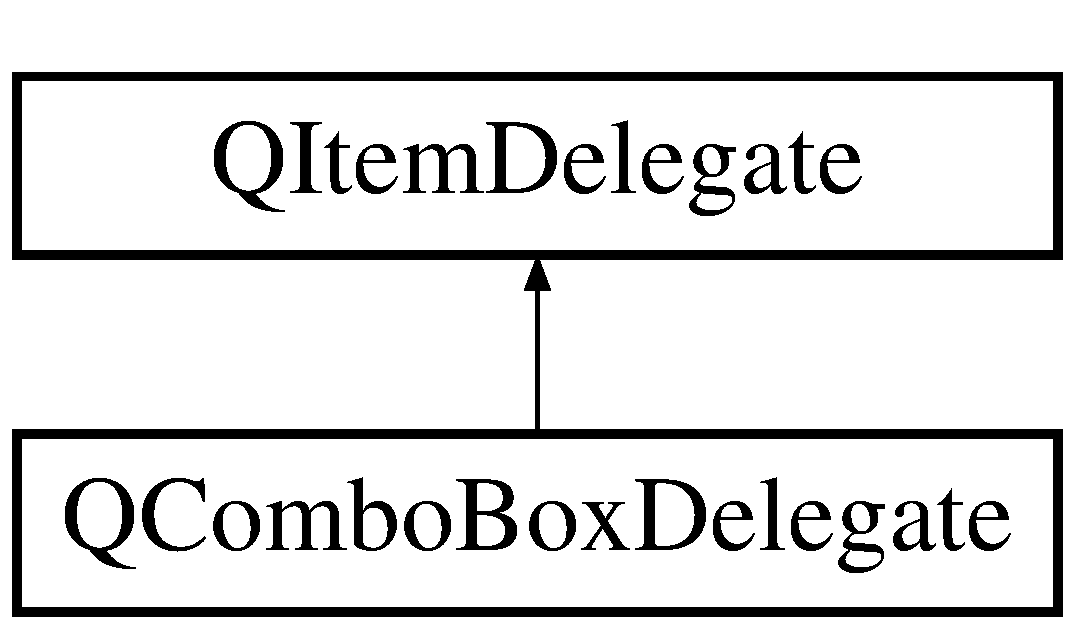
\includegraphics[height=2.000000cm]{class_q_combo_box_delegate}
\end{center}
\end{figure}
\subsection*{Public Member Functions}
\begin{DoxyCompactItemize}
\item 
\hyperlink{class_q_combo_box_delegate_a5894396d9b9694ad60516be6457b9e97}{Q\+Combo\+Box\+Delegate} (Q\+Object $\ast$parent=0)
\item 
Q\+Widget $\ast$ \hyperlink{class_q_combo_box_delegate_a2cae1e908e3b9864e7ab174cfa39a9a8}{create\+Editor} (Q\+Widget $\ast$parent, const Q\+Style\+Option\+View\+Item \&option, const Q\+Model\+Index \&index) const 
\item 
void \hyperlink{class_q_combo_box_delegate_abf09d46bd215e169c921a282a1052cf2}{set\+Editor\+Data} (Q\+Widget $\ast$editor, const Q\+Model\+Index \&index) const 
\item 
void \hyperlink{class_q_combo_box_delegate_a17c8842bbf2a85035143fd3d104f802a}{set\+Model\+Data} (Q\+Widget $\ast$editor, Q\+Abstract\+Item\+Model $\ast$model, const Q\+Model\+Index \&index) const 
\item 
void \hyperlink{class_q_combo_box_delegate_a606e97162b64134d8d3189bea7cdd11a}{update\+Editor\+Geometry} (Q\+Widget $\ast$editor, const Q\+Style\+Option\+View\+Item \&option, const Q\+Model\+Index \&index) const 
\end{DoxyCompactItemize}


\subsection{Constructor \& Destructor Documentation}
\hypertarget{class_q_combo_box_delegate_a5894396d9b9694ad60516be6457b9e97}{}\index{Q\+Combo\+Box\+Delegate@{Q\+Combo\+Box\+Delegate}!Q\+Combo\+Box\+Delegate@{Q\+Combo\+Box\+Delegate}}
\index{Q\+Combo\+Box\+Delegate@{Q\+Combo\+Box\+Delegate}!Q\+Combo\+Box\+Delegate@{Q\+Combo\+Box\+Delegate}}
\subsubsection[{Q\+Combo\+Box\+Delegate}]{\setlength{\rightskip}{0pt plus 5cm}Q\+Combo\+Box\+Delegate\+::\+Q\+Combo\+Box\+Delegate (
\begin{DoxyParamCaption}
\item[{Q\+Object $\ast$}]{parent = {\ttfamily 0}}
\end{DoxyParamCaption}
)\hspace{0.3cm}{\ttfamily [explicit]}}\label{class_q_combo_box_delegate_a5894396d9b9694ad60516be6457b9e97}


\subsection{Member Function Documentation}
\hypertarget{class_q_combo_box_delegate_a2cae1e908e3b9864e7ab174cfa39a9a8}{}\index{Q\+Combo\+Box\+Delegate@{Q\+Combo\+Box\+Delegate}!create\+Editor@{create\+Editor}}
\index{create\+Editor@{create\+Editor}!Q\+Combo\+Box\+Delegate@{Q\+Combo\+Box\+Delegate}}
\subsubsection[{create\+Editor}]{\setlength{\rightskip}{0pt plus 5cm}Q\+Widget $\ast$ Q\+Combo\+Box\+Delegate\+::create\+Editor (
\begin{DoxyParamCaption}
\item[{Q\+Widget $\ast$}]{parent, }
\item[{const Q\+Style\+Option\+View\+Item \&}]{option, }
\item[{const Q\+Model\+Index \&}]{index}
\end{DoxyParamCaption}
) const}\label{class_q_combo_box_delegate_a2cae1e908e3b9864e7ab174cfa39a9a8}
\hypertarget{class_q_combo_box_delegate_abf09d46bd215e169c921a282a1052cf2}{}\index{Q\+Combo\+Box\+Delegate@{Q\+Combo\+Box\+Delegate}!set\+Editor\+Data@{set\+Editor\+Data}}
\index{set\+Editor\+Data@{set\+Editor\+Data}!Q\+Combo\+Box\+Delegate@{Q\+Combo\+Box\+Delegate}}
\subsubsection[{set\+Editor\+Data}]{\setlength{\rightskip}{0pt plus 5cm}void Q\+Combo\+Box\+Delegate\+::set\+Editor\+Data (
\begin{DoxyParamCaption}
\item[{Q\+Widget $\ast$}]{editor, }
\item[{const Q\+Model\+Index \&}]{index}
\end{DoxyParamCaption}
) const}\label{class_q_combo_box_delegate_abf09d46bd215e169c921a282a1052cf2}
\hypertarget{class_q_combo_box_delegate_a17c8842bbf2a85035143fd3d104f802a}{}\index{Q\+Combo\+Box\+Delegate@{Q\+Combo\+Box\+Delegate}!set\+Model\+Data@{set\+Model\+Data}}
\index{set\+Model\+Data@{set\+Model\+Data}!Q\+Combo\+Box\+Delegate@{Q\+Combo\+Box\+Delegate}}
\subsubsection[{set\+Model\+Data}]{\setlength{\rightskip}{0pt plus 5cm}void Q\+Combo\+Box\+Delegate\+::set\+Model\+Data (
\begin{DoxyParamCaption}
\item[{Q\+Widget $\ast$}]{editor, }
\item[{Q\+Abstract\+Item\+Model $\ast$}]{model, }
\item[{const Q\+Model\+Index \&}]{index}
\end{DoxyParamCaption}
) const}\label{class_q_combo_box_delegate_a17c8842bbf2a85035143fd3d104f802a}
\hypertarget{class_q_combo_box_delegate_a606e97162b64134d8d3189bea7cdd11a}{}\index{Q\+Combo\+Box\+Delegate@{Q\+Combo\+Box\+Delegate}!update\+Editor\+Geometry@{update\+Editor\+Geometry}}
\index{update\+Editor\+Geometry@{update\+Editor\+Geometry}!Q\+Combo\+Box\+Delegate@{Q\+Combo\+Box\+Delegate}}
\subsubsection[{update\+Editor\+Geometry}]{\setlength{\rightskip}{0pt plus 5cm}void Q\+Combo\+Box\+Delegate\+::update\+Editor\+Geometry (
\begin{DoxyParamCaption}
\item[{Q\+Widget $\ast$}]{editor, }
\item[{const Q\+Style\+Option\+View\+Item \&}]{option, }
\item[{const Q\+Model\+Index \&}]{index}
\end{DoxyParamCaption}
) const}\label{class_q_combo_box_delegate_a606e97162b64134d8d3189bea7cdd11a}


The documentation for this class was generated from the following files\+:\begin{DoxyCompactItemize}
\item 
C\+:/\+Users/\+Roman/\+Documents/\+Mygs/\+Ground\+Station/\+G\+S/\hyperlink{qcomboboxdelegate_8h}{qcomboboxdelegate.\+h}\item 
C\+:/\+Users/\+Roman/\+Documents/\+Mygs/\+Ground\+Station/\+G\+S/\hyperlink{qcomboboxdelegate_8cpp}{qcomboboxdelegate.\+cpp}\end{DoxyCompactItemize}

\hypertarget{class_q_c_p_abstract_item}{}\section{Q\+C\+P\+Abstract\+Item Class Reference}
\label{class_q_c_p_abstract_item}\index{Q\+C\+P\+Abstract\+Item@{Q\+C\+P\+Abstract\+Item}}


The abstract base class for all items in a plot.  




{\ttfamily \#include $<$qcustomplot.\+h$>$}

Inheritance diagram for Q\+C\+P\+Abstract\+Item\+:\begin{figure}[H]
\begin{center}
\leavevmode
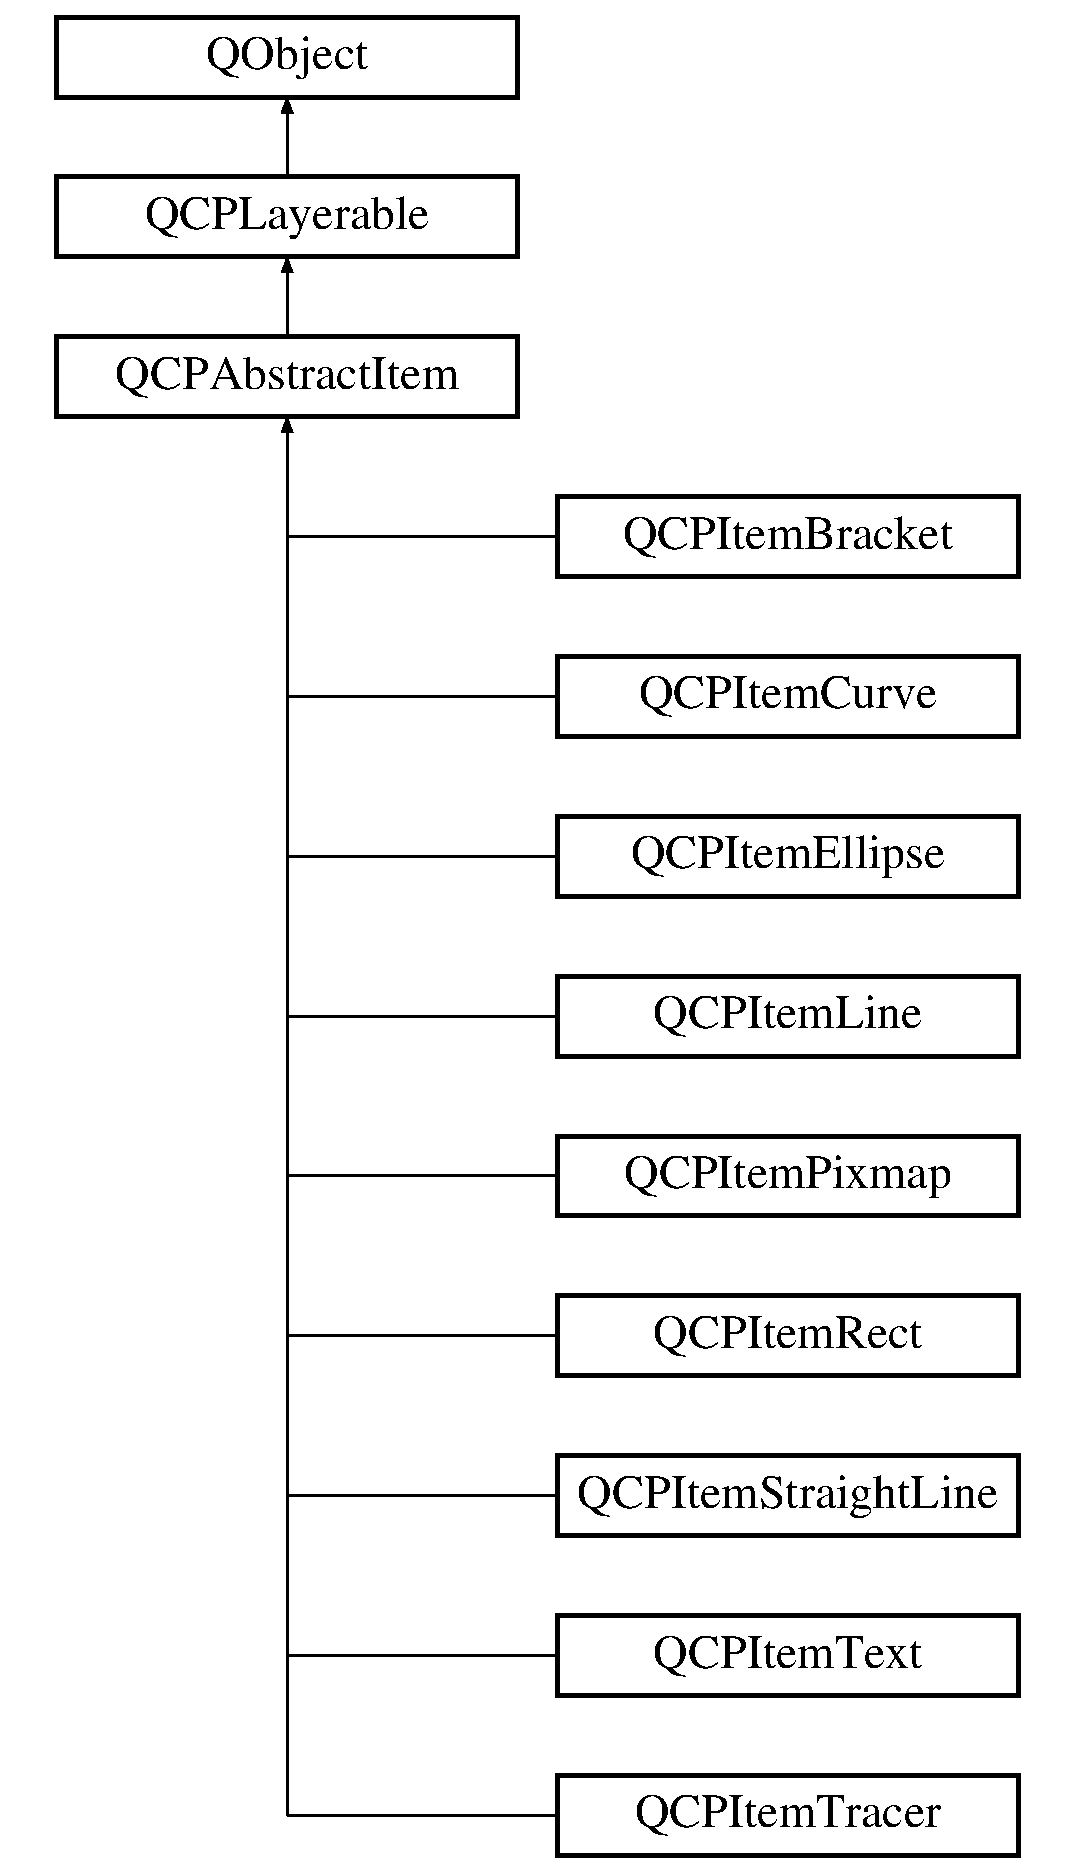
\includegraphics[height=12.000000cm]{class_q_c_p_abstract_item}
\end{center}
\end{figure}
\subsection*{Signals}
\begin{DoxyCompactItemize}
\item 
void \hyperlink{class_q_c_p_abstract_item_aa5cffb034fc65dbb91c77e02c1c14251}{selection\+Changed} (bool \hyperlink{class_q_c_p_abstract_item_a225865808640d8d9a7dd19f09a2e93f2}{selected})
\item 
void \hyperlink{class_q_c_p_abstract_item_a5b266c11aac61cb511901f3911dac2a3}{selectable\+Changed} (bool \hyperlink{class_q_c_p_abstract_item_a9189e752025533e1595eaade0009a3bc}{selectable})
\end{DoxyCompactItemize}
\subsection*{Public Member Functions}
\begin{DoxyCompactItemize}
\item 
\hyperlink{class_q_c_p_abstract_item_a9922507d8b4503a1fe1ed0b1030e23b6}{Q\+C\+P\+Abstract\+Item} (\hyperlink{class_q_custom_plot}{Q\+Custom\+Plot} $\ast$\hyperlink{class_q_c_p_layerable_ab7e0e94461566093d36ffc0f5312b109}{parent\+Plot})
\item 
virtual \hyperlink{class_q_c_p_abstract_item_a375bd1b7d3218b04a6ff7ff06fff917c}{$\sim$\+Q\+C\+P\+Abstract\+Item} ()
\item 
bool \hyperlink{class_q_c_p_abstract_item_a5b0ea171823033bcb8aee81f4a034871}{clip\+To\+Axis\+Rect} () const 
\item 
\hyperlink{class_q_c_p_axis_rect}{Q\+C\+P\+Axis\+Rect} $\ast$ \hyperlink{class_q_c_p_abstract_item_a37f86618740b5047eae23eedb2de061a}{clip\+Axis\+Rect} () const 
\item 
bool \hyperlink{class_q_c_p_abstract_item_a9189e752025533e1595eaade0009a3bc}{selectable} () const 
\item 
bool \hyperlink{class_q_c_p_abstract_item_a225865808640d8d9a7dd19f09a2e93f2}{selected} () const 
\item 
void \hyperlink{class_q_c_p_abstract_item_a39e05b9d4176b9accafc746d16ca6a06}{set\+Clip\+To\+Axis\+Rect} (bool clip)
\item 
void \hyperlink{class_q_c_p_abstract_item_a7dc75fcbcd10206fe0b75d757ea7a347}{set\+Clip\+Axis\+Rect} (\hyperlink{class_q_c_p_axis_rect}{Q\+C\+P\+Axis\+Rect} $\ast$rect)
\item 
Q\+\_\+\+S\+L\+O\+T void \hyperlink{class_q_c_p_abstract_item_a8a8e32a55bc478b849756a78c2d87fd2}{set\+Selectable} (bool \hyperlink{class_q_c_p_abstract_item_a9189e752025533e1595eaade0009a3bc}{selectable})
\item 
Q\+\_\+\+S\+L\+O\+T void \hyperlink{class_q_c_p_abstract_item_a203de94ad586cc44d16c9565f49d3378}{set\+Selected} (bool \hyperlink{class_q_c_p_abstract_item_a225865808640d8d9a7dd19f09a2e93f2}{selected})
\item 
virtual double \hyperlink{class_q_c_p_abstract_item_a96d522d10ffc0413b9a366c6f7f0476b}{select\+Test} (const Q\+Point\+F \&pos, bool only\+Selectable, Q\+Variant $\ast$details=0) const =0
\item 
Q\+List$<$ \hyperlink{class_q_c_p_item_position}{Q\+C\+P\+Item\+Position} $\ast$ $>$ \hyperlink{class_q_c_p_abstract_item_adf6a680cc29a6bce8345c3b6af3a91a1}{positions} () const 
\item 
Q\+List$<$ \hyperlink{class_q_c_p_item_anchor}{Q\+C\+P\+Item\+Anchor} $\ast$ $>$ \hyperlink{class_q_c_p_abstract_item_a8454b9941960b840608a5a1e00b1977d}{anchors} () const 
\item 
\hyperlink{class_q_c_p_item_position}{Q\+C\+P\+Item\+Position} $\ast$ \hyperlink{class_q_c_p_abstract_item_af71345bd150f87fa1d2442837b87bb59}{position} (const Q\+String \&name) const 
\item 
\hyperlink{class_q_c_p_item_anchor}{Q\+C\+P\+Item\+Anchor} $\ast$ \hyperlink{class_q_c_p_abstract_item_abed974cba7cc02608c71dad4638e008d}{anchor} (const Q\+String \&name) const 
\item 
bool \hyperlink{class_q_c_p_abstract_item_acbce9e5ba5252541d19db0c40303357a}{has\+Anchor} (const Q\+String \&name) const 
\end{DoxyCompactItemize}
\subsection*{Protected Member Functions}
\begin{DoxyCompactItemize}
\item 
virtual \hyperlink{namespace_q_c_p_a2ad6bb6281c7c2d593d4277b44c2b037}{Q\+C\+P\+::\+Interaction} \hyperlink{class_q_c_p_abstract_item_a777b5d384936396ad9c3ceb3d3453f1c}{selection\+Category} () const 
\item 
virtual Q\+Rect \hyperlink{class_q_c_p_abstract_item_a538e25ff8856534582f5b2b400a46405}{clip\+Rect} () const 
\item 
virtual void \hyperlink{class_q_c_p_abstract_item_a0839031abdd71067e2256a4d53c7a011}{apply\+Default\+Antialiasing\+Hint} (\hyperlink{class_q_c_p_painter}{Q\+C\+P\+Painter} $\ast$painter) const 
\item 
virtual void \hyperlink{class_q_c_p_abstract_item_ad0dc056f650c3ca73414e6b4f01674ef}{draw} (\hyperlink{class_q_c_p_painter}{Q\+C\+P\+Painter} $\ast$painter)=0
\item 
virtual void \hyperlink{class_q_c_p_abstract_item_aaf92af7b9893712959a6c073d334d88d}{select\+Event} (Q\+Mouse\+Event $\ast$event, bool additive, const Q\+Variant \&details, bool $\ast$selection\+State\+Changed)
\item 
virtual void \hyperlink{class_q_c_p_abstract_item_a91f090d6763cfedb0749219c63788ae9}{deselect\+Event} (bool $\ast$selection\+State\+Changed)
\item 
virtual Q\+Point\+F \hyperlink{class_q_c_p_abstract_item_a94bde62b8a2fc133666dcbb8035deeed}{anchor\+Pixel\+Point} (int anchor\+Id) const 
\item 
double \hyperlink{class_q_c_p_abstract_item_acdca343717d625b8abb3c3e38c0ed39d}{dist\+Sqr\+To\+Line} (const Q\+Point\+F \&start, const Q\+Point\+F \&end, const Q\+Point\+F \&point) const 
\item 
double \hyperlink{class_q_c_p_abstract_item_a4c0e14c4e92df91174cb7183fb363069}{rect\+Select\+Test} (const Q\+Rect\+F \&rect, const Q\+Point\+F \&pos, bool filled\+Rect) const 
\item 
\hyperlink{class_q_c_p_item_position}{Q\+C\+P\+Item\+Position} $\ast$ \hyperlink{class_q_c_p_abstract_item_a75036d39c4d4e2e1a7dd145fff915d32}{create\+Position} (const Q\+String \&name)
\item 
\hyperlink{class_q_c_p_item_anchor}{Q\+C\+P\+Item\+Anchor} $\ast$ \hyperlink{class_q_c_p_abstract_item_af3fc92527802078ca395138748b629a7}{create\+Anchor} (const Q\+String \&name, int anchor\+Id)
\end{DoxyCompactItemize}
\subsection*{Protected Attributes}
\begin{DoxyCompactItemize}
\item 
bool \hyperlink{class_q_c_p_abstract_item_ad2a70ff6b658fcb84a9427f69d3f587d}{m\+Clip\+To\+Axis\+Rect}
\item 
Q\+Pointer$<$ \hyperlink{class_q_c_p_axis_rect}{Q\+C\+P\+Axis\+Rect} $>$ \hyperlink{class_q_c_p_abstract_item_a3e57cfe7da4b1ac3d6fa7281ea437361}{m\+Clip\+Axis\+Rect}
\item 
Q\+List$<$ \hyperlink{class_q_c_p_item_position}{Q\+C\+P\+Item\+Position} $\ast$ $>$ \hyperlink{class_q_c_p_abstract_item_af94ff71b6a15ea6d028ab8bd8eccd012}{m\+Positions}
\item 
Q\+List$<$ \hyperlink{class_q_c_p_item_anchor}{Q\+C\+P\+Item\+Anchor} $\ast$ $>$ \hyperlink{class_q_c_p_abstract_item_a909a3abab783de302ebf0a0e6f2bbc15}{m\+Anchors}
\item 
bool \hyperlink{class_q_c_p_abstract_item_ad81eb35c8726a0f458db9df9732e0e41}{m\+Selectable}
\item 
bool \hyperlink{class_q_c_p_abstract_item_a4bdb3457dad1d268c0f78a44152b9645}{m\+Selected}
\end{DoxyCompactItemize}
\subsection*{Friends}
\begin{DoxyCompactItemize}
\item 
class \hyperlink{class_q_c_p_abstract_item_a1cdf9df76adcfae45261690aa0ca2198}{Q\+Custom\+Plot}
\item 
class \hyperlink{class_q_c_p_abstract_item_a61767d414fd57af9eb1741b34268c7fc}{Q\+C\+P\+Item\+Anchor}
\end{DoxyCompactItemize}


\subsection{Detailed Description}
The abstract base class for all items in a plot. 

In \hyperlink{class_q_custom_plot}{Q\+Custom\+Plot}, items are supplemental graphical elements that are neither plottables (\hyperlink{class_q_c_p_abstract_plottable}{Q\+C\+P\+Abstract\+Plottable}) nor axes (\hyperlink{class_q_c_p_axis}{Q\+C\+P\+Axis}). While plottables are always tied to two axes and thus plot coordinates, items can also be placed in absolute coordinates independent of any axes. Each specific item has at least one \hyperlink{class_q_c_p_item_position}{Q\+C\+P\+Item\+Position} member which controls the positioning. Some items are defined by more than one coordinate and thus have two or more \hyperlink{class_q_c_p_item_position}{Q\+C\+P\+Item\+Position} members (For example, \hyperlink{class_q_c_p_item_rect}{Q\+C\+P\+Item\+Rect} has {\itshape top\+Left} and {\itshape bottom\+Right}).

This abstract base class defines a very basic interface like visibility and clipping. Since this class is abstract, it can\textquotesingle{}t be instantiated. Use one of the subclasses or create a subclass yourself to create new items.

The built-\/in items are\+: \begin{TabularC}{2}
\hline
\hyperlink{class_q_c_p_item_line}{Q\+C\+P\+Item\+Line}&A line defined by a start and an end point. May have different ending styles on each side (e.\+g. arrows). \\\cline{1-2}
\hyperlink{class_q_c_p_item_straight_line}{Q\+C\+P\+Item\+Straight\+Line}&A straight line defined by a start and a direction point. Unlike \hyperlink{class_q_c_p_item_line}{Q\+C\+P\+Item\+Line}, the straight line is infinitely long and has no endings. \\\cline{1-2}
\hyperlink{class_q_c_p_item_curve}{Q\+C\+P\+Item\+Curve}&A curve defined by start, end and two intermediate control points. May have different ending styles on each side (e.\+g. arrows). \\\cline{1-2}
\hyperlink{class_q_c_p_item_rect}{Q\+C\+P\+Item\+Rect}&A rectangle \\\cline{1-2}
\hyperlink{class_q_c_p_item_ellipse}{Q\+C\+P\+Item\+Ellipse}&An ellipse \\\cline{1-2}
\hyperlink{class_q_c_p_item_pixmap}{Q\+C\+P\+Item\+Pixmap}&An arbitrary pixmap \\\cline{1-2}
\hyperlink{class_q_c_p_item_text}{Q\+C\+P\+Item\+Text}&A text label \\\cline{1-2}
\hyperlink{class_q_c_p_item_bracket}{Q\+C\+P\+Item\+Bracket}&A bracket which may be used to reference/highlight certain parts in the plot. \\\cline{1-2}
\hyperlink{class_q_c_p_item_tracer}{Q\+C\+P\+Item\+Tracer}&An item that can be attached to a \hyperlink{class_q_c_p_graph}{Q\+C\+P\+Graph} and sticks to its data points, given a key coordinate. \\\cline{1-2}
\end{TabularC}
\hypertarget{class_q_c_p_abstract_item_items-clipping}{}\subsection{Clipping}\label{class_q_c_p_abstract_item_items-clipping}
Items are by default clipped to the main axis rect (they are only visible inside the axis rect). To make an item visible outside that axis rect, disable clipping via \hyperlink{class_q_c_p_abstract_item_a39e05b9d4176b9accafc746d16ca6a06}{set\+Clip\+To\+Axis\+Rect(false)}.

On the other hand if you want the item to be clipped to a different axis rect, specify it via \hyperlink{class_q_c_p_abstract_item_a7dc75fcbcd10206fe0b75d757ea7a347}{set\+Clip\+Axis\+Rect}. This clip\+Axis\+Rect property of an item is only used for clipping behaviour, and in principle is independent of the coordinate axes the item might be tied to via its position members (\hyperlink{class_q_c_p_item_position_a2185f45c75ac8cb9be89daeaaad50e37}{Q\+C\+P\+Item\+Position\+::set\+Axes}). However, it is common that the axis rect for clipping also contains the axes used for the item positions.\hypertarget{class_q_c_p_abstract_item_items-using}{}\subsection{Using items}\label{class_q_c_p_abstract_item_items-using}
First you instantiate the item you want to use and add it to the plot\+: 
\begin{DoxyCode}
\hyperlink{class_q_c_p_item_line}{QCPItemLine} *line = \textcolor{keyword}{new} \hyperlink{class_q_c_p_item_line}{QCPItemLine}(customPlot);
customPlot->addItem(line);
\end{DoxyCode}
 by default, the positions of the item are bound to the x-\/ and y-\/\+Axis of the plot. So we can just set the plot coordinates where the line should start/end\+: 
\begin{DoxyCode}
line->\hyperlink{class_q_c_p_item_line_a602da607a09498b0f152ada1d6851bc5}{start}->\hyperlink{class_q_c_p_item_position_aa988ba4e87ab684c9021017dcaba945f}{setCoords}(-0.1, 0.8);
line->\hyperlink{class_q_c_p_item_line_a15598864c1c22a2497a1979c4980c4e1}{end}->\hyperlink{class_q_c_p_item_position_aa988ba4e87ab684c9021017dcaba945f}{setCoords}(1.1, 0.2);
\end{DoxyCode}
 If we don\textquotesingle{}t want the line to be positioned in plot coordinates but a different coordinate system, e.\+g. absolute pixel positions on the \hyperlink{class_q_custom_plot}{Q\+Custom\+Plot} surface, we need to change the position type like this\+: 
\begin{DoxyCode}
line->\hyperlink{class_q_c_p_item_line_a602da607a09498b0f152ada1d6851bc5}{start}->\hyperlink{class_q_c_p_item_position_aa476abf71ed8fa4c537457ebb1a754ad}{setType}(\hyperlink{class_q_c_p_item_position_aad9936c22bf43e3d358552f6e86dbdc8a564f5e53e550ead1ec5fc7fc7d0b73e0}{QCPItemPosition::ptAbsolute});
line->\hyperlink{class_q_c_p_item_line_a15598864c1c22a2497a1979c4980c4e1}{end}->\hyperlink{class_q_c_p_item_position_aa476abf71ed8fa4c537457ebb1a754ad}{setType}(\hyperlink{class_q_c_p_item_position_aad9936c22bf43e3d358552f6e86dbdc8a564f5e53e550ead1ec5fc7fc7d0b73e0}{QCPItemPosition::ptAbsolute});
\end{DoxyCode}
 Then we can set the coordinates, this time in pixels\+: 
\begin{DoxyCode}
line->\hyperlink{class_q_c_p_item_line_a602da607a09498b0f152ada1d6851bc5}{start}->\hyperlink{class_q_c_p_item_position_aa988ba4e87ab684c9021017dcaba945f}{setCoords}(100, 200);
line->\hyperlink{class_q_c_p_item_line_a15598864c1c22a2497a1979c4980c4e1}{end}->\hyperlink{class_q_c_p_item_position_aa988ba4e87ab684c9021017dcaba945f}{setCoords}(450, 320);
\end{DoxyCode}
 and make the line visible on the entire \hyperlink{class_q_custom_plot}{Q\+Custom\+Plot}, by disabling clipping to the axis rect\+: 
\begin{DoxyCode}
line->\hyperlink{class_q_c_p_abstract_item_a39e05b9d4176b9accafc746d16ca6a06}{setClipToAxisRect}(\textcolor{keyword}{false});
\end{DoxyCode}


For more advanced plots, it is even possible to set different types and parent anchors per X/\+Y coordinate of an item position, using for example \hyperlink{class_q_c_p_item_position_a2113b2351d6d00457fb3559a4e20c3ea}{Q\+C\+P\+Item\+Position\+::set\+Type\+X} or \hyperlink{class_q_c_p_item_position_add71461a973927c74e42179480916d9c}{Q\+C\+P\+Item\+Position\+::set\+Parent\+Anchor\+X}. For details, see the documentation of \hyperlink{class_q_c_p_item_position}{Q\+C\+P\+Item\+Position}.\hypertarget{class_q_c_p_abstract_item_items-subclassing}{}\subsection{Creating own items}\label{class_q_c_p_abstract_item_items-subclassing}
To create an own item, you implement a subclass of \hyperlink{class_q_c_p_abstract_item}{Q\+C\+P\+Abstract\+Item}. These are the pure virtual functions, you must implement\+: \begin{DoxyItemize}
\item \hyperlink{class_q_c_p_abstract_item_a96d522d10ffc0413b9a366c6f7f0476b}{select\+Test} \item \hyperlink{class_q_c_p_abstract_item_ad0dc056f650c3ca73414e6b4f01674ef}{draw}\end{DoxyItemize}
See the documentation of those functions for what they need to do.\hypertarget{class_q_c_p_abstract_item_items-positioning}{}\subsubsection{Allowing the item to be positioned}\label{class_q_c_p_abstract_item_items-positioning}
As mentioned, item positions are represented by \hyperlink{class_q_c_p_item_position}{Q\+C\+P\+Item\+Position} members. Let\textquotesingle{}s assume the new item shall have only one point as its position (as opposed to two like a rect or multiple like a polygon). You then add a public member of type \hyperlink{class_q_c_p_item_position}{Q\+C\+P\+Item\+Position} like so\+:


\begin{DoxyCode}
\hyperlink{class_q_c_p_item_position}{QCPItemPosition} * \textcolor{keyword}{const} myPosition;
\end{DoxyCode}


the const makes sure the pointer itself can\textquotesingle{}t be modified from the user of your new item (the \hyperlink{class_q_c_p_item_position}{Q\+C\+P\+Item\+Position} instance it points to, can be modified, of course). The initialization of this pointer is made easy with the \hyperlink{class_q_c_p_abstract_item_a75036d39c4d4e2e1a7dd145fff915d32}{create\+Position} function. Just assign the return value of this function to each \hyperlink{class_q_c_p_item_position}{Q\+C\+P\+Item\+Position} in the constructor of your item. \hyperlink{class_q_c_p_abstract_item_a75036d39c4d4e2e1a7dd145fff915d32}{create\+Position} takes a string which is the name of the position, typically this is identical to the variable name. For example, the constructor of Q\+C\+P\+Item\+Example could look like this\+:


\begin{DoxyCode}
QCPItemExample::QCPItemExample(\hyperlink{class_q_custom_plot}{QCustomPlot} *\hyperlink{class_q_c_p_layerable_ab7e0e94461566093d36ffc0f5312b109}{parentPlot}) :
  \hyperlink{class_q_c_p_abstract_item}{QCPAbstractItem}(parentPlot),
  myPosition(\hyperlink{class_q_c_p_abstract_item_a75036d39c4d4e2e1a7dd145fff915d32}{createPosition}(\textcolor{stringliteral}{"myPosition"}))
\{
  \textcolor{comment}{// other constructor code}
\}
\end{DoxyCode}
\hypertarget{class_q_c_p_abstract_item_items-drawing}{}\subsubsection{The draw function}\label{class_q_c_p_abstract_item_items-drawing}
To give your item a visual representation, reimplement the \hyperlink{class_q_c_p_abstract_item_ad0dc056f650c3ca73414e6b4f01674ef}{draw} function and use the passed \hyperlink{class_q_c_p_painter}{Q\+C\+P\+Painter} to draw the item. You can retrieve the item position in pixel coordinates from the position member(s) via \hyperlink{class_q_c_p_item_position_ae490f9c76ee2ba33752c495d3b6e8fb5}{Q\+C\+P\+Item\+Position\+::pixel\+Point}.

To optimize performance you should calculate a bounding rect first (don\textquotesingle{}t forget to take the pen width into account), check whether it intersects the \hyperlink{class_q_c_p_abstract_item_a538e25ff8856534582f5b2b400a46405}{clip\+Rect}, and only draw the item at all if this is the case.\hypertarget{class_q_c_p_abstract_item_items-selection}{}\subsubsection{The select\+Test function}\label{class_q_c_p_abstract_item_items-selection}
Your implementation of the \hyperlink{class_q_c_p_abstract_item_a96d522d10ffc0413b9a366c6f7f0476b}{select\+Test} function may use the helpers \hyperlink{class_q_c_p_abstract_item_acdca343717d625b8abb3c3e38c0ed39d}{dist\+Sqr\+To\+Line} and \hyperlink{class_q_c_p_abstract_item_a4c0e14c4e92df91174cb7183fb363069}{rect\+Select\+Test}. With these, the implementation of the selection test becomes significantly simpler for most items. See the documentation of \hyperlink{class_q_c_p_abstract_item_a96d522d10ffc0413b9a366c6f7f0476b}{select\+Test} for what the function parameters mean and what the function should return.\hypertarget{class_q_c_p_abstract_item_anchors}{}\subsubsection{Providing anchors}\label{class_q_c_p_abstract_item_anchors}
Providing anchors (\hyperlink{class_q_c_p_item_anchor}{Q\+C\+P\+Item\+Anchor}) starts off like adding a position. First you create a public member, e.\+g.


\begin{DoxyCode}
\hyperlink{class_q_c_p_item_anchor}{QCPItemAnchor} * \textcolor{keyword}{const} bottom;
\end{DoxyCode}


and create it in the constructor with the \hyperlink{class_q_c_p_abstract_item_af3fc92527802078ca395138748b629a7}{create\+Anchor} function, assigning it a name and an anchor id (an integer enumerating all anchors on the item, you may create an own enum for this). Since anchors can be placed anywhere, relative to the item\textquotesingle{}s position(s), your item needs to provide the position of every anchor with the reimplementation of the \hyperlink{class_q_c_p_abstract_item_a94bde62b8a2fc133666dcbb8035deeed}{anchor\+Pixel\+Point}(int anchor\+Id) function.

In essence the \hyperlink{class_q_c_p_item_anchor}{Q\+C\+P\+Item\+Anchor} is merely an intermediary that itself asks your item for the pixel position when anything attached to the anchor needs to know the coordinates. 

\subsection{Constructor \& Destructor Documentation}
\hypertarget{class_q_c_p_abstract_item_a9922507d8b4503a1fe1ed0b1030e23b6}{}\index{Q\+C\+P\+Abstract\+Item@{Q\+C\+P\+Abstract\+Item}!Q\+C\+P\+Abstract\+Item@{Q\+C\+P\+Abstract\+Item}}
\index{Q\+C\+P\+Abstract\+Item@{Q\+C\+P\+Abstract\+Item}!Q\+C\+P\+Abstract\+Item@{Q\+C\+P\+Abstract\+Item}}
\subsubsection[{Q\+C\+P\+Abstract\+Item}]{\setlength{\rightskip}{0pt plus 5cm}Q\+C\+P\+Abstract\+Item\+::\+Q\+C\+P\+Abstract\+Item (
\begin{DoxyParamCaption}
\item[{{\bf Q\+Custom\+Plot} $\ast$}]{parent\+Plot}
\end{DoxyParamCaption}
)}\label{class_q_c_p_abstract_item_a9922507d8b4503a1fe1ed0b1030e23b6}
Base class constructor which initializes base class members. \hypertarget{class_q_c_p_abstract_item_a375bd1b7d3218b04a6ff7ff06fff917c}{}\index{Q\+C\+P\+Abstract\+Item@{Q\+C\+P\+Abstract\+Item}!````~Q\+C\+P\+Abstract\+Item@{$\sim$\+Q\+C\+P\+Abstract\+Item}}
\index{````~Q\+C\+P\+Abstract\+Item@{$\sim$\+Q\+C\+P\+Abstract\+Item}!Q\+C\+P\+Abstract\+Item@{Q\+C\+P\+Abstract\+Item}}
\subsubsection[{$\sim$\+Q\+C\+P\+Abstract\+Item}]{\setlength{\rightskip}{0pt plus 5cm}Q\+C\+P\+Abstract\+Item\+::$\sim$\+Q\+C\+P\+Abstract\+Item (
\begin{DoxyParamCaption}
{}
\end{DoxyParamCaption}
)\hspace{0.3cm}{\ttfamily [virtual]}}\label{class_q_c_p_abstract_item_a375bd1b7d3218b04a6ff7ff06fff917c}


\subsection{Member Function Documentation}
\hypertarget{class_q_c_p_abstract_item_abed974cba7cc02608c71dad4638e008d}{}\index{Q\+C\+P\+Abstract\+Item@{Q\+C\+P\+Abstract\+Item}!anchor@{anchor}}
\index{anchor@{anchor}!Q\+C\+P\+Abstract\+Item@{Q\+C\+P\+Abstract\+Item}}
\subsubsection[{anchor}]{\setlength{\rightskip}{0pt plus 5cm}{\bf Q\+C\+P\+Item\+Anchor} $\ast$ Q\+C\+P\+Abstract\+Item\+::anchor (
\begin{DoxyParamCaption}
\item[{const Q\+String \&}]{name}
\end{DoxyParamCaption}
) const}\label{class_q_c_p_abstract_item_abed974cba7cc02608c71dad4638e008d}
Returns the \hyperlink{class_q_c_p_item_anchor}{Q\+C\+P\+Item\+Anchor} with the specified {\itshape name}. If this item doesn\textquotesingle{}t have an anchor by that name, returns 0.

This function provides an alternative way to access item anchors. Normally, you access anchors direcly by their member pointers (which typically have the same variable name as {\itshape name}).

\begin{DoxySeeAlso}{See also}
\hyperlink{class_q_c_p_abstract_item_a8454b9941960b840608a5a1e00b1977d}{anchors}, \hyperlink{class_q_c_p_abstract_item_af71345bd150f87fa1d2442837b87bb59}{position} 
\end{DoxySeeAlso}
\hypertarget{class_q_c_p_abstract_item_a94bde62b8a2fc133666dcbb8035deeed}{}\index{Q\+C\+P\+Abstract\+Item@{Q\+C\+P\+Abstract\+Item}!anchor\+Pixel\+Point@{anchor\+Pixel\+Point}}
\index{anchor\+Pixel\+Point@{anchor\+Pixel\+Point}!Q\+C\+P\+Abstract\+Item@{Q\+C\+P\+Abstract\+Item}}
\subsubsection[{anchor\+Pixel\+Point}]{\setlength{\rightskip}{0pt plus 5cm}Q\+Point\+F Q\+C\+P\+Abstract\+Item\+::anchor\+Pixel\+Point (
\begin{DoxyParamCaption}
\item[{int}]{anchor\+Id}
\end{DoxyParamCaption}
) const\hspace{0.3cm}{\ttfamily [protected]}, {\ttfamily [virtual]}}\label{class_q_c_p_abstract_item_a94bde62b8a2fc133666dcbb8035deeed}


Reimplemented in \hyperlink{class_q_c_p_item_bracket_ac76827e3acba5faee81f149af4047a39}{Q\+C\+P\+Item\+Bracket}, \hyperlink{class_q_c_p_item_pixmap_a88abce3c1027f371cddcf6dad35ffbb1}{Q\+C\+P\+Item\+Pixmap}, \hyperlink{class_q_c_p_item_ellipse_ad3c607304dba081e2f778b6a81b903bb}{Q\+C\+P\+Item\+Ellipse}, \hyperlink{class_q_c_p_item_text_ad248f988534a9d07bc7c220a2457142a}{Q\+C\+P\+Item\+Text}, and \hyperlink{class_q_c_p_item_rect_ae0973f8281fb52361b0c99ee899be07e}{Q\+C\+P\+Item\+Rect}.

\hypertarget{class_q_c_p_abstract_item_a8454b9941960b840608a5a1e00b1977d}{}\index{Q\+C\+P\+Abstract\+Item@{Q\+C\+P\+Abstract\+Item}!anchors@{anchors}}
\index{anchors@{anchors}!Q\+C\+P\+Abstract\+Item@{Q\+C\+P\+Abstract\+Item}}
\subsubsection[{anchors}]{\setlength{\rightskip}{0pt plus 5cm}Q\+List$<$ {\bf Q\+C\+P\+Item\+Anchor} $\ast$ $>$ Q\+C\+P\+Abstract\+Item\+::anchors (
\begin{DoxyParamCaption}
{}
\end{DoxyParamCaption}
) const\hspace{0.3cm}{\ttfamily [inline]}}\label{class_q_c_p_abstract_item_a8454b9941960b840608a5a1e00b1977d}
Returns all anchors of the item in a list. Note that since a position (\hyperlink{class_q_c_p_item_position}{Q\+C\+P\+Item\+Position}) is always also an anchor, the list will also contain the positions of this item.

\begin{DoxySeeAlso}{See also}
\hyperlink{class_q_c_p_abstract_item_adf6a680cc29a6bce8345c3b6af3a91a1}{positions}, \hyperlink{class_q_c_p_abstract_item_abed974cba7cc02608c71dad4638e008d}{anchor} 
\end{DoxySeeAlso}
\hypertarget{class_q_c_p_abstract_item_a0839031abdd71067e2256a4d53c7a011}{}\index{Q\+C\+P\+Abstract\+Item@{Q\+C\+P\+Abstract\+Item}!apply\+Default\+Antialiasing\+Hint@{apply\+Default\+Antialiasing\+Hint}}
\index{apply\+Default\+Antialiasing\+Hint@{apply\+Default\+Antialiasing\+Hint}!Q\+C\+P\+Abstract\+Item@{Q\+C\+P\+Abstract\+Item}}
\subsubsection[{apply\+Default\+Antialiasing\+Hint}]{\setlength{\rightskip}{0pt plus 5cm}void Q\+C\+P\+Abstract\+Item\+::apply\+Default\+Antialiasing\+Hint (
\begin{DoxyParamCaption}
\item[{{\bf Q\+C\+P\+Painter} $\ast$}]{painter}
\end{DoxyParamCaption}
) const\hspace{0.3cm}{\ttfamily [protected]}, {\ttfamily [virtual]}}\label{class_q_c_p_abstract_item_a0839031abdd71067e2256a4d53c7a011}


Implements \hyperlink{class_q_c_p_layerable_afdf83ddc6a265cbf4c89fe99d3d93473}{Q\+C\+P\+Layerable}.

\hypertarget{class_q_c_p_abstract_item_a37f86618740b5047eae23eedb2de061a}{}\index{Q\+C\+P\+Abstract\+Item@{Q\+C\+P\+Abstract\+Item}!clip\+Axis\+Rect@{clip\+Axis\+Rect}}
\index{clip\+Axis\+Rect@{clip\+Axis\+Rect}!Q\+C\+P\+Abstract\+Item@{Q\+C\+P\+Abstract\+Item}}
\subsubsection[{clip\+Axis\+Rect}]{\setlength{\rightskip}{0pt plus 5cm}{\bf Q\+C\+P\+Axis\+Rect} $\ast$ Q\+C\+P\+Abstract\+Item\+::clip\+Axis\+Rect (
\begin{DoxyParamCaption}
{}
\end{DoxyParamCaption}
) const}\label{class_q_c_p_abstract_item_a37f86618740b5047eae23eedb2de061a}
\hypertarget{class_q_c_p_abstract_item_a538e25ff8856534582f5b2b400a46405}{}\index{Q\+C\+P\+Abstract\+Item@{Q\+C\+P\+Abstract\+Item}!clip\+Rect@{clip\+Rect}}
\index{clip\+Rect@{clip\+Rect}!Q\+C\+P\+Abstract\+Item@{Q\+C\+P\+Abstract\+Item}}
\subsubsection[{clip\+Rect}]{\setlength{\rightskip}{0pt plus 5cm}Q\+Rect Q\+C\+P\+Abstract\+Item\+::clip\+Rect (
\begin{DoxyParamCaption}
{}
\end{DoxyParamCaption}
) const\hspace{0.3cm}{\ttfamily [protected]}, {\ttfamily [virtual]}}\label{class_q_c_p_abstract_item_a538e25ff8856534582f5b2b400a46405}


Reimplemented from \hyperlink{class_q_c_p_layerable_a07a8f746640c3704b09910df297afcba}{Q\+C\+P\+Layerable}.

\hypertarget{class_q_c_p_abstract_item_a5b0ea171823033bcb8aee81f4a034871}{}\index{Q\+C\+P\+Abstract\+Item@{Q\+C\+P\+Abstract\+Item}!clip\+To\+Axis\+Rect@{clip\+To\+Axis\+Rect}}
\index{clip\+To\+Axis\+Rect@{clip\+To\+Axis\+Rect}!Q\+C\+P\+Abstract\+Item@{Q\+C\+P\+Abstract\+Item}}
\subsubsection[{clip\+To\+Axis\+Rect}]{\setlength{\rightskip}{0pt plus 5cm}bool Q\+C\+P\+Abstract\+Item\+::clip\+To\+Axis\+Rect (
\begin{DoxyParamCaption}
{}
\end{DoxyParamCaption}
) const\hspace{0.3cm}{\ttfamily [inline]}}\label{class_q_c_p_abstract_item_a5b0ea171823033bcb8aee81f4a034871}
\hypertarget{class_q_c_p_abstract_item_af3fc92527802078ca395138748b629a7}{}\index{Q\+C\+P\+Abstract\+Item@{Q\+C\+P\+Abstract\+Item}!create\+Anchor@{create\+Anchor}}
\index{create\+Anchor@{create\+Anchor}!Q\+C\+P\+Abstract\+Item@{Q\+C\+P\+Abstract\+Item}}
\subsubsection[{create\+Anchor}]{\setlength{\rightskip}{0pt plus 5cm}{\bf Q\+C\+P\+Item\+Anchor} $\ast$ Q\+C\+P\+Abstract\+Item\+::create\+Anchor (
\begin{DoxyParamCaption}
\item[{const Q\+String \&}]{name, }
\item[{int}]{anchor\+Id}
\end{DoxyParamCaption}
)\hspace{0.3cm}{\ttfamily [protected]}}\label{class_q_c_p_abstract_item_af3fc92527802078ca395138748b629a7}
\hypertarget{class_q_c_p_abstract_item_a75036d39c4d4e2e1a7dd145fff915d32}{}\index{Q\+C\+P\+Abstract\+Item@{Q\+C\+P\+Abstract\+Item}!create\+Position@{create\+Position}}
\index{create\+Position@{create\+Position}!Q\+C\+P\+Abstract\+Item@{Q\+C\+P\+Abstract\+Item}}
\subsubsection[{create\+Position}]{\setlength{\rightskip}{0pt plus 5cm}{\bf Q\+C\+P\+Item\+Position} $\ast$ Q\+C\+P\+Abstract\+Item\+::create\+Position (
\begin{DoxyParamCaption}
\item[{const Q\+String \&}]{name}
\end{DoxyParamCaption}
)\hspace{0.3cm}{\ttfamily [protected]}}\label{class_q_c_p_abstract_item_a75036d39c4d4e2e1a7dd145fff915d32}
\hypertarget{class_q_c_p_abstract_item_a91f090d6763cfedb0749219c63788ae9}{}\index{Q\+C\+P\+Abstract\+Item@{Q\+C\+P\+Abstract\+Item}!deselect\+Event@{deselect\+Event}}
\index{deselect\+Event@{deselect\+Event}!Q\+C\+P\+Abstract\+Item@{Q\+C\+P\+Abstract\+Item}}
\subsubsection[{deselect\+Event}]{\setlength{\rightskip}{0pt plus 5cm}void Q\+C\+P\+Abstract\+Item\+::deselect\+Event (
\begin{DoxyParamCaption}
\item[{bool $\ast$}]{selection\+State\+Changed}
\end{DoxyParamCaption}
)\hspace{0.3cm}{\ttfamily [protected]}, {\ttfamily [virtual]}}\label{class_q_c_p_abstract_item_a91f090d6763cfedb0749219c63788ae9}


Reimplemented from \hyperlink{class_q_c_p_layerable_ae546370644a5551c76af739afc008bee}{Q\+C\+P\+Layerable}.

\hypertarget{class_q_c_p_abstract_item_acdca343717d625b8abb3c3e38c0ed39d}{}\index{Q\+C\+P\+Abstract\+Item@{Q\+C\+P\+Abstract\+Item}!dist\+Sqr\+To\+Line@{dist\+Sqr\+To\+Line}}
\index{dist\+Sqr\+To\+Line@{dist\+Sqr\+To\+Line}!Q\+C\+P\+Abstract\+Item@{Q\+C\+P\+Abstract\+Item}}
\subsubsection[{dist\+Sqr\+To\+Line}]{\setlength{\rightskip}{0pt plus 5cm}double Q\+C\+P\+Abstract\+Item\+::dist\+Sqr\+To\+Line (
\begin{DoxyParamCaption}
\item[{const Q\+Point\+F \&}]{start, }
\item[{const Q\+Point\+F \&}]{end, }
\item[{const Q\+Point\+F \&}]{point}
\end{DoxyParamCaption}
) const\hspace{0.3cm}{\ttfamily [protected]}}\label{class_q_c_p_abstract_item_acdca343717d625b8abb3c3e38c0ed39d}
\hypertarget{class_q_c_p_abstract_item_ad0dc056f650c3ca73414e6b4f01674ef}{}\index{Q\+C\+P\+Abstract\+Item@{Q\+C\+P\+Abstract\+Item}!draw@{draw}}
\index{draw@{draw}!Q\+C\+P\+Abstract\+Item@{Q\+C\+P\+Abstract\+Item}}
\subsubsection[{draw}]{\setlength{\rightskip}{0pt plus 5cm}void Q\+C\+P\+Abstract\+Item\+::draw (
\begin{DoxyParamCaption}
\item[{{\bf Q\+C\+P\+Painter} $\ast$}]{painter}
\end{DoxyParamCaption}
)\hspace{0.3cm}{\ttfamily [protected]}, {\ttfamily [pure virtual]}}\label{class_q_c_p_abstract_item_ad0dc056f650c3ca73414e6b4f01674ef}


Implements \hyperlink{class_q_c_p_layerable_aecf2f7087482d4b6a78cb2770e5ed12d}{Q\+C\+P\+Layerable}.



Implemented in \hyperlink{class_q_c_p_item_bracket_a8343cf0559c64886add7aa7f4b22f1a6}{Q\+C\+P\+Item\+Bracket}, \hyperlink{class_q_c_p_item_tracer_aaaf49b48382c730ec9be0e74c2538315}{Q\+C\+P\+Item\+Tracer}, \hyperlink{class_q_c_p_item_pixmap_a879e8076c2db01a38b34cfa73ec95d2f}{Q\+C\+P\+Item\+Pixmap}, \hyperlink{class_q_c_p_item_ellipse_afe97ec827adb05f000fe007783faae3c}{Q\+C\+P\+Item\+Ellipse}, \hyperlink{class_q_c_p_item_text_a8793adb271ab79b4cf391dc55e9987f1}{Q\+C\+P\+Item\+Text}, \hyperlink{class_q_c_p_item_rect_a18cd583638b876cdd50f1a155ec182aa}{Q\+C\+P\+Item\+Rect}, \hyperlink{class_q_c_p_item_curve_a56cb5b72cd02db2eda598274a39839a9}{Q\+C\+P\+Item\+Curve}, \hyperlink{class_q_c_p_item_line_a1fc045dd33919f8006df0692aeb0e84a}{Q\+C\+P\+Item\+Line}, and \hyperlink{class_q_c_p_item_straight_line_a2daa1e1253216c26565d56a2d5530170}{Q\+C\+P\+Item\+Straight\+Line}.

\hypertarget{class_q_c_p_abstract_item_acbce9e5ba5252541d19db0c40303357a}{}\index{Q\+C\+P\+Abstract\+Item@{Q\+C\+P\+Abstract\+Item}!has\+Anchor@{has\+Anchor}}
\index{has\+Anchor@{has\+Anchor}!Q\+C\+P\+Abstract\+Item@{Q\+C\+P\+Abstract\+Item}}
\subsubsection[{has\+Anchor}]{\setlength{\rightskip}{0pt plus 5cm}bool Q\+C\+P\+Abstract\+Item\+::has\+Anchor (
\begin{DoxyParamCaption}
\item[{const Q\+String \&}]{name}
\end{DoxyParamCaption}
) const}\label{class_q_c_p_abstract_item_acbce9e5ba5252541d19db0c40303357a}
Returns whether this item has an anchor with the specified {\itshape name}.

Note that you can check for positions with this function, too. This is because every position is also an anchor (\hyperlink{class_q_c_p_item_position}{Q\+C\+P\+Item\+Position} inherits from \hyperlink{class_q_c_p_item_anchor}{Q\+C\+P\+Item\+Anchor}).

\begin{DoxySeeAlso}{See also}
\hyperlink{class_q_c_p_abstract_item_abed974cba7cc02608c71dad4638e008d}{anchor}, \hyperlink{class_q_c_p_abstract_item_af71345bd150f87fa1d2442837b87bb59}{position} 
\end{DoxySeeAlso}
\hypertarget{class_q_c_p_abstract_item_af71345bd150f87fa1d2442837b87bb59}{}\index{Q\+C\+P\+Abstract\+Item@{Q\+C\+P\+Abstract\+Item}!position@{position}}
\index{position@{position}!Q\+C\+P\+Abstract\+Item@{Q\+C\+P\+Abstract\+Item}}
\subsubsection[{position}]{\setlength{\rightskip}{0pt plus 5cm}{\bf Q\+C\+P\+Item\+Position} $\ast$ Q\+C\+P\+Abstract\+Item\+::position (
\begin{DoxyParamCaption}
\item[{const Q\+String \&}]{name}
\end{DoxyParamCaption}
) const}\label{class_q_c_p_abstract_item_af71345bd150f87fa1d2442837b87bb59}
Returns the \hyperlink{class_q_c_p_item_position}{Q\+C\+P\+Item\+Position} with the specified {\itshape name}. If this item doesn\textquotesingle{}t have a position by that name, returns 0.

This function provides an alternative way to access item positions. Normally, you access positions direcly by their member pointers (which typically have the same variable name as {\itshape name}).

\begin{DoxySeeAlso}{See also}
\hyperlink{class_q_c_p_abstract_item_adf6a680cc29a6bce8345c3b6af3a91a1}{positions}, \hyperlink{class_q_c_p_abstract_item_abed974cba7cc02608c71dad4638e008d}{anchor} 
\end{DoxySeeAlso}
\hypertarget{class_q_c_p_abstract_item_adf6a680cc29a6bce8345c3b6af3a91a1}{}\index{Q\+C\+P\+Abstract\+Item@{Q\+C\+P\+Abstract\+Item}!positions@{positions}}
\index{positions@{positions}!Q\+C\+P\+Abstract\+Item@{Q\+C\+P\+Abstract\+Item}}
\subsubsection[{positions}]{\setlength{\rightskip}{0pt plus 5cm}Q\+List$<$ {\bf Q\+C\+P\+Item\+Position} $\ast$ $>$ Q\+C\+P\+Abstract\+Item\+::positions (
\begin{DoxyParamCaption}
{}
\end{DoxyParamCaption}
) const\hspace{0.3cm}{\ttfamily [inline]}}\label{class_q_c_p_abstract_item_adf6a680cc29a6bce8345c3b6af3a91a1}
Returns all positions of the item in a list.

\begin{DoxySeeAlso}{See also}
\hyperlink{class_q_c_p_abstract_item_a8454b9941960b840608a5a1e00b1977d}{anchors}, \hyperlink{class_q_c_p_abstract_item_af71345bd150f87fa1d2442837b87bb59}{position} 
\end{DoxySeeAlso}
\hypertarget{class_q_c_p_abstract_item_a4c0e14c4e92df91174cb7183fb363069}{}\index{Q\+C\+P\+Abstract\+Item@{Q\+C\+P\+Abstract\+Item}!rect\+Select\+Test@{rect\+Select\+Test}}
\index{rect\+Select\+Test@{rect\+Select\+Test}!Q\+C\+P\+Abstract\+Item@{Q\+C\+P\+Abstract\+Item}}
\subsubsection[{rect\+Select\+Test}]{\setlength{\rightskip}{0pt plus 5cm}double Q\+C\+P\+Abstract\+Item\+::rect\+Select\+Test (
\begin{DoxyParamCaption}
\item[{const Q\+Rect\+F \&}]{rect, }
\item[{const Q\+Point\+F \&}]{pos, }
\item[{bool}]{filled\+Rect}
\end{DoxyParamCaption}
) const\hspace{0.3cm}{\ttfamily [protected]}}\label{class_q_c_p_abstract_item_a4c0e14c4e92df91174cb7183fb363069}
\hypertarget{class_q_c_p_abstract_item_a9189e752025533e1595eaade0009a3bc}{}\index{Q\+C\+P\+Abstract\+Item@{Q\+C\+P\+Abstract\+Item}!selectable@{selectable}}
\index{selectable@{selectable}!Q\+C\+P\+Abstract\+Item@{Q\+C\+P\+Abstract\+Item}}
\subsubsection[{selectable}]{\setlength{\rightskip}{0pt plus 5cm}bool Q\+C\+P\+Abstract\+Item\+::selectable (
\begin{DoxyParamCaption}
{}
\end{DoxyParamCaption}
) const\hspace{0.3cm}{\ttfamily [inline]}}\label{class_q_c_p_abstract_item_a9189e752025533e1595eaade0009a3bc}
\hypertarget{class_q_c_p_abstract_item_a5b266c11aac61cb511901f3911dac2a3}{}\index{Q\+C\+P\+Abstract\+Item@{Q\+C\+P\+Abstract\+Item}!selectable\+Changed@{selectable\+Changed}}
\index{selectable\+Changed@{selectable\+Changed}!Q\+C\+P\+Abstract\+Item@{Q\+C\+P\+Abstract\+Item}}
\subsubsection[{selectable\+Changed}]{\setlength{\rightskip}{0pt plus 5cm}void Q\+C\+P\+Abstract\+Item\+::selectable\+Changed (
\begin{DoxyParamCaption}
\item[{bool}]{selectable}
\end{DoxyParamCaption}
)\hspace{0.3cm}{\ttfamily [signal]}}\label{class_q_c_p_abstract_item_a5b266c11aac61cb511901f3911dac2a3}
\hypertarget{class_q_c_p_abstract_item_a225865808640d8d9a7dd19f09a2e93f2}{}\index{Q\+C\+P\+Abstract\+Item@{Q\+C\+P\+Abstract\+Item}!selected@{selected}}
\index{selected@{selected}!Q\+C\+P\+Abstract\+Item@{Q\+C\+P\+Abstract\+Item}}
\subsubsection[{selected}]{\setlength{\rightskip}{0pt plus 5cm}bool Q\+C\+P\+Abstract\+Item\+::selected (
\begin{DoxyParamCaption}
{}
\end{DoxyParamCaption}
) const\hspace{0.3cm}{\ttfamily [inline]}}\label{class_q_c_p_abstract_item_a225865808640d8d9a7dd19f09a2e93f2}
\hypertarget{class_q_c_p_abstract_item_aaf92af7b9893712959a6c073d334d88d}{}\index{Q\+C\+P\+Abstract\+Item@{Q\+C\+P\+Abstract\+Item}!select\+Event@{select\+Event}}
\index{select\+Event@{select\+Event}!Q\+C\+P\+Abstract\+Item@{Q\+C\+P\+Abstract\+Item}}
\subsubsection[{select\+Event}]{\setlength{\rightskip}{0pt plus 5cm}void Q\+C\+P\+Abstract\+Item\+::select\+Event (
\begin{DoxyParamCaption}
\item[{Q\+Mouse\+Event $\ast$}]{event, }
\item[{bool}]{additive, }
\item[{const Q\+Variant \&}]{details, }
\item[{bool $\ast$}]{selection\+State\+Changed}
\end{DoxyParamCaption}
)\hspace{0.3cm}{\ttfamily [protected]}, {\ttfamily [virtual]}}\label{class_q_c_p_abstract_item_aaf92af7b9893712959a6c073d334d88d}


Reimplemented from \hyperlink{class_q_c_p_layerable_a7498c2d0d081cf7cad0fb3bb93aa0e91}{Q\+C\+P\+Layerable}.

\hypertarget{class_q_c_p_abstract_item_a777b5d384936396ad9c3ceb3d3453f1c}{}\index{Q\+C\+P\+Abstract\+Item@{Q\+C\+P\+Abstract\+Item}!selection\+Category@{selection\+Category}}
\index{selection\+Category@{selection\+Category}!Q\+C\+P\+Abstract\+Item@{Q\+C\+P\+Abstract\+Item}}
\subsubsection[{selection\+Category}]{\setlength{\rightskip}{0pt plus 5cm}{\bf Q\+C\+P\+::\+Interaction} Q\+C\+P\+Abstract\+Item\+::selection\+Category (
\begin{DoxyParamCaption}
{}
\end{DoxyParamCaption}
) const\hspace{0.3cm}{\ttfamily [protected]}, {\ttfamily [virtual]}}\label{class_q_c_p_abstract_item_a777b5d384936396ad9c3ceb3d3453f1c}


Reimplemented from \hyperlink{class_q_c_p_layerable_aa4035e586b7f317a06ba7e74e242a5ea}{Q\+C\+P\+Layerable}.

\hypertarget{class_q_c_p_abstract_item_aa5cffb034fc65dbb91c77e02c1c14251}{}\index{Q\+C\+P\+Abstract\+Item@{Q\+C\+P\+Abstract\+Item}!selection\+Changed@{selection\+Changed}}
\index{selection\+Changed@{selection\+Changed}!Q\+C\+P\+Abstract\+Item@{Q\+C\+P\+Abstract\+Item}}
\subsubsection[{selection\+Changed}]{\setlength{\rightskip}{0pt plus 5cm}void Q\+C\+P\+Abstract\+Item\+::selection\+Changed (
\begin{DoxyParamCaption}
\item[{bool}]{selected}
\end{DoxyParamCaption}
)\hspace{0.3cm}{\ttfamily [signal]}}\label{class_q_c_p_abstract_item_aa5cffb034fc65dbb91c77e02c1c14251}
This signal is emitted when the selection state of this item has changed, either by user interaction or by a direct call to \hyperlink{class_q_c_p_abstract_item_a203de94ad586cc44d16c9565f49d3378}{set\+Selected}. \hypertarget{class_q_c_p_abstract_item_a96d522d10ffc0413b9a366c6f7f0476b}{}\index{Q\+C\+P\+Abstract\+Item@{Q\+C\+P\+Abstract\+Item}!select\+Test@{select\+Test}}
\index{select\+Test@{select\+Test}!Q\+C\+P\+Abstract\+Item@{Q\+C\+P\+Abstract\+Item}}
\subsubsection[{select\+Test}]{\setlength{\rightskip}{0pt plus 5cm}virtual double Q\+C\+P\+Abstract\+Item\+::select\+Test (
\begin{DoxyParamCaption}
\item[{const Q\+Point\+F \&}]{pos, }
\item[{bool}]{only\+Selectable, }
\item[{Q\+Variant $\ast$}]{details = {\ttfamily 0}}
\end{DoxyParamCaption}
) const\hspace{0.3cm}{\ttfamily [pure virtual]}}\label{class_q_c_p_abstract_item_a96d522d10ffc0413b9a366c6f7f0476b}
This function is used to decide whether a click hits a layerable object or not.

{\itshape pos} is a point in pixel coordinates on the \hyperlink{class_q_custom_plot}{Q\+Custom\+Plot} surface. This function returns the shortest pixel distance of this point to the object. If the object is either invisible or the distance couldn\textquotesingle{}t be determined, -\/1.\+0 is returned. Further, if {\itshape only\+Selectable} is true and the object is not selectable, -\/1.\+0 is returned, too.

If the item is represented not by single lines but by an area like \hyperlink{class_q_c_p_item_rect}{Q\+C\+P\+Item\+Rect} or \hyperlink{class_q_c_p_item_text}{Q\+C\+P\+Item\+Text}, a click inside the area returns a constant value greater zero (typically the selection\+Tolerance of the parent \hyperlink{class_q_custom_plot}{Q\+Custom\+Plot} multiplied by 0.\+99). If the click lies outside the area, this function returns -\/1.\+0.

Providing a constant value for area objects allows selecting line objects even when they are obscured by such area objects, by clicking close to the lines (i.\+e. closer than 0.\+99$\ast$selection\+Tolerance).

The actual setting of the selection state is not done by this function. This is handled by the parent \hyperlink{class_q_custom_plot}{Q\+Custom\+Plot} when the mouse\+Release\+Event occurs, and the finally selected object is notified via the select\+Event/deselect\+Event methods.

{\itshape details} is an optional output parameter. Every layerable subclass may place any information in {\itshape details}. This information will be passed to \hyperlink{class_q_c_p_abstract_item_aaf92af7b9893712959a6c073d334d88d}{select\+Event} when the parent \hyperlink{class_q_custom_plot}{Q\+Custom\+Plot} decides on the basis of this select\+Test call, that the object was successfully selected. The subsequent call to \hyperlink{class_q_c_p_abstract_item_aaf92af7b9893712959a6c073d334d88d}{select\+Event} will carry the {\itshape details}. This is useful for multi-\/part objects (like \hyperlink{class_q_c_p_axis}{Q\+C\+P\+Axis}). This way, a possibly complex calculation to decide which part was clicked is only done once in \hyperlink{class_q_c_p_abstract_item_a96d522d10ffc0413b9a366c6f7f0476b}{select\+Test}. The result (i.\+e. the actually clicked part) can then be placed in {\itshape details}. So in the subsequent \hyperlink{class_q_c_p_abstract_item_aaf92af7b9893712959a6c073d334d88d}{select\+Event}, the decision which part was selected doesn\textquotesingle{}t have to be done a second time for a single selection operation.

You may pass 0 as {\itshape details} to indicate that you are not interested in those selection details.

\begin{DoxySeeAlso}{See also}
\hyperlink{class_q_c_p_abstract_item_aaf92af7b9893712959a6c073d334d88d}{select\+Event}, \hyperlink{class_q_c_p_abstract_item_a91f090d6763cfedb0749219c63788ae9}{deselect\+Event}, \hyperlink{class_q_custom_plot_a5ee1e2f6ae27419deca53e75907c27e5}{Q\+Custom\+Plot\+::set\+Interactions} 
\end{DoxySeeAlso}


Reimplemented from \hyperlink{class_q_c_p_layerable_a4001c4d0dfec55598efa4d531f2179a9}{Q\+C\+P\+Layerable}.



Implemented in \hyperlink{class_q_c_p_item_bracket_aa6933caff1d42c54bcebc769ef88c798}{Q\+C\+P\+Item\+Bracket}, \hyperlink{class_q_c_p_item_tracer_ae71f3728421c83c188c117279ca050fd}{Q\+C\+P\+Item\+Tracer}, \hyperlink{class_q_c_p_item_pixmap_a9f8436aa141fa0fb504191c882c2f4d9}{Q\+C\+P\+Item\+Pixmap}, \hyperlink{class_q_c_p_item_ellipse_acd7e5f9528630b2ab5987e2a5782eb7c}{Q\+C\+P\+Item\+Ellipse}, \hyperlink{class_q_c_p_item_text_a285b95bb6634c2e4f7768abb7a8bc69c}{Q\+C\+P\+Item\+Text}, \hyperlink{class_q_c_p_item_rect_af13b0797079b40b73d1c7286b76f18ac}{Q\+C\+P\+Item\+Rect}, \hyperlink{class_q_c_p_item_curve_a741375c11667b5f9c95b2683f93ee514}{Q\+C\+P\+Item\+Curve}, \hyperlink{class_q_c_p_item_line_a7541e5d9378ca121d07b0df3b24f7178}{Q\+C\+P\+Item\+Line}, and \hyperlink{class_q_c_p_item_straight_line_a64cc3796f58ce856012732603edb2f1c}{Q\+C\+P\+Item\+Straight\+Line}.

\hypertarget{class_q_c_p_abstract_item_a7dc75fcbcd10206fe0b75d757ea7a347}{}\index{Q\+C\+P\+Abstract\+Item@{Q\+C\+P\+Abstract\+Item}!set\+Clip\+Axis\+Rect@{set\+Clip\+Axis\+Rect}}
\index{set\+Clip\+Axis\+Rect@{set\+Clip\+Axis\+Rect}!Q\+C\+P\+Abstract\+Item@{Q\+C\+P\+Abstract\+Item}}
\subsubsection[{set\+Clip\+Axis\+Rect}]{\setlength{\rightskip}{0pt plus 5cm}void Q\+C\+P\+Abstract\+Item\+::set\+Clip\+Axis\+Rect (
\begin{DoxyParamCaption}
\item[{{\bf Q\+C\+P\+Axis\+Rect} $\ast$}]{rect}
\end{DoxyParamCaption}
)}\label{class_q_c_p_abstract_item_a7dc75fcbcd10206fe0b75d757ea7a347}
Sets the clip axis rect. It defines the rect that will be used to clip the item when \hyperlink{class_q_c_p_abstract_item_a39e05b9d4176b9accafc746d16ca6a06}{set\+Clip\+To\+Axis\+Rect} is set to true.

\begin{DoxySeeAlso}{See also}
\hyperlink{class_q_c_p_abstract_item_a39e05b9d4176b9accafc746d16ca6a06}{set\+Clip\+To\+Axis\+Rect} 
\end{DoxySeeAlso}
\hypertarget{class_q_c_p_abstract_item_a39e05b9d4176b9accafc746d16ca6a06}{}\index{Q\+C\+P\+Abstract\+Item@{Q\+C\+P\+Abstract\+Item}!set\+Clip\+To\+Axis\+Rect@{set\+Clip\+To\+Axis\+Rect}}
\index{set\+Clip\+To\+Axis\+Rect@{set\+Clip\+To\+Axis\+Rect}!Q\+C\+P\+Abstract\+Item@{Q\+C\+P\+Abstract\+Item}}
\subsubsection[{set\+Clip\+To\+Axis\+Rect}]{\setlength{\rightskip}{0pt plus 5cm}void Q\+C\+P\+Abstract\+Item\+::set\+Clip\+To\+Axis\+Rect (
\begin{DoxyParamCaption}
\item[{bool}]{clip}
\end{DoxyParamCaption}
)}\label{class_q_c_p_abstract_item_a39e05b9d4176b9accafc746d16ca6a06}
Sets whether the item shall be clipped to an axis rect or whether it shall be visible on the entire \hyperlink{class_q_custom_plot}{Q\+Custom\+Plot}. The axis rect can be set with \hyperlink{class_q_c_p_abstract_item_a7dc75fcbcd10206fe0b75d757ea7a347}{set\+Clip\+Axis\+Rect}.

\begin{DoxySeeAlso}{See also}
\hyperlink{class_q_c_p_abstract_item_a7dc75fcbcd10206fe0b75d757ea7a347}{set\+Clip\+Axis\+Rect} 
\end{DoxySeeAlso}
\hypertarget{class_q_c_p_abstract_item_a8a8e32a55bc478b849756a78c2d87fd2}{}\index{Q\+C\+P\+Abstract\+Item@{Q\+C\+P\+Abstract\+Item}!set\+Selectable@{set\+Selectable}}
\index{set\+Selectable@{set\+Selectable}!Q\+C\+P\+Abstract\+Item@{Q\+C\+P\+Abstract\+Item}}
\subsubsection[{set\+Selectable}]{\setlength{\rightskip}{0pt plus 5cm}void Q\+C\+P\+Abstract\+Item\+::set\+Selectable (
\begin{DoxyParamCaption}
\item[{bool}]{selectable}
\end{DoxyParamCaption}
)}\label{class_q_c_p_abstract_item_a8a8e32a55bc478b849756a78c2d87fd2}
Sets whether the user can (de-\/)select this item by clicking on the \hyperlink{class_q_custom_plot}{Q\+Custom\+Plot} surface. (When \hyperlink{class_q_custom_plot_a5ee1e2f6ae27419deca53e75907c27e5}{Q\+Custom\+Plot\+::set\+Interactions} contains Q\+Custom\+Plot\+::i\+Select\+Items.)

However, even when {\itshape selectable} was set to false, it is possible to set the selection manually, by calling \hyperlink{class_q_c_p_abstract_item_a203de94ad586cc44d16c9565f49d3378}{set\+Selected}.

\begin{DoxySeeAlso}{See also}
\hyperlink{class_q_custom_plot_a5ee1e2f6ae27419deca53e75907c27e5}{Q\+Custom\+Plot\+::set\+Interactions}, \hyperlink{class_q_c_p_abstract_item_a203de94ad586cc44d16c9565f49d3378}{set\+Selected} 
\end{DoxySeeAlso}
\hypertarget{class_q_c_p_abstract_item_a203de94ad586cc44d16c9565f49d3378}{}\index{Q\+C\+P\+Abstract\+Item@{Q\+C\+P\+Abstract\+Item}!set\+Selected@{set\+Selected}}
\index{set\+Selected@{set\+Selected}!Q\+C\+P\+Abstract\+Item@{Q\+C\+P\+Abstract\+Item}}
\subsubsection[{set\+Selected}]{\setlength{\rightskip}{0pt plus 5cm}void Q\+C\+P\+Abstract\+Item\+::set\+Selected (
\begin{DoxyParamCaption}
\item[{bool}]{selected}
\end{DoxyParamCaption}
)}\label{class_q_c_p_abstract_item_a203de94ad586cc44d16c9565f49d3378}
Sets whether this item is selected or not. When selected, it might use a different visual appearance (e.\+g. pen and brush), this depends on the specific item though.

The entire selection mechanism for items is handled automatically when \hyperlink{class_q_custom_plot_a5ee1e2f6ae27419deca53e75907c27e5}{Q\+Custom\+Plot\+::set\+Interactions} contains Q\+Custom\+Plot\+::i\+Select\+Items. You only need to call this function when you wish to change the selection state manually.

This function can change the selection state even when \hyperlink{class_q_c_p_abstract_item_a8a8e32a55bc478b849756a78c2d87fd2}{set\+Selectable} was set to false.

emits the \hyperlink{class_q_c_p_abstract_item_aa5cffb034fc65dbb91c77e02c1c14251}{selection\+Changed} signal when {\itshape selected} is different from the previous selection state.

\begin{DoxySeeAlso}{See also}
\hyperlink{class_q_c_p_abstract_item_a8a8e32a55bc478b849756a78c2d87fd2}{set\+Selectable}, \hyperlink{class_q_c_p_abstract_item_a96d522d10ffc0413b9a366c6f7f0476b}{select\+Test} 
\end{DoxySeeAlso}


\subsection{Friends And Related Function Documentation}
\hypertarget{class_q_c_p_abstract_item_a61767d414fd57af9eb1741b34268c7fc}{}\index{Q\+C\+P\+Abstract\+Item@{Q\+C\+P\+Abstract\+Item}!Q\+C\+P\+Item\+Anchor@{Q\+C\+P\+Item\+Anchor}}
\index{Q\+C\+P\+Item\+Anchor@{Q\+C\+P\+Item\+Anchor}!Q\+C\+P\+Abstract\+Item@{Q\+C\+P\+Abstract\+Item}}
\subsubsection[{Q\+C\+P\+Item\+Anchor}]{\setlength{\rightskip}{0pt plus 5cm}friend class {\bf Q\+C\+P\+Item\+Anchor}\hspace{0.3cm}{\ttfamily [friend]}}\label{class_q_c_p_abstract_item_a61767d414fd57af9eb1741b34268c7fc}
\hypertarget{class_q_c_p_abstract_item_a1cdf9df76adcfae45261690aa0ca2198}{}\index{Q\+C\+P\+Abstract\+Item@{Q\+C\+P\+Abstract\+Item}!Q\+Custom\+Plot@{Q\+Custom\+Plot}}
\index{Q\+Custom\+Plot@{Q\+Custom\+Plot}!Q\+C\+P\+Abstract\+Item@{Q\+C\+P\+Abstract\+Item}}
\subsubsection[{Q\+Custom\+Plot}]{\setlength{\rightskip}{0pt plus 5cm}friend class {\bf Q\+Custom\+Plot}\hspace{0.3cm}{\ttfamily [friend]}}\label{class_q_c_p_abstract_item_a1cdf9df76adcfae45261690aa0ca2198}


\subsection{Member Data Documentation}
\hypertarget{class_q_c_p_abstract_item_a909a3abab783de302ebf0a0e6f2bbc15}{}\index{Q\+C\+P\+Abstract\+Item@{Q\+C\+P\+Abstract\+Item}!m\+Anchors@{m\+Anchors}}
\index{m\+Anchors@{m\+Anchors}!Q\+C\+P\+Abstract\+Item@{Q\+C\+P\+Abstract\+Item}}
\subsubsection[{m\+Anchors}]{\setlength{\rightskip}{0pt plus 5cm}Q\+List$<${\bf Q\+C\+P\+Item\+Anchor}$\ast$$>$ Q\+C\+P\+Abstract\+Item\+::m\+Anchors\hspace{0.3cm}{\ttfamily [protected]}}\label{class_q_c_p_abstract_item_a909a3abab783de302ebf0a0e6f2bbc15}
\hypertarget{class_q_c_p_abstract_item_a3e57cfe7da4b1ac3d6fa7281ea437361}{}\index{Q\+C\+P\+Abstract\+Item@{Q\+C\+P\+Abstract\+Item}!m\+Clip\+Axis\+Rect@{m\+Clip\+Axis\+Rect}}
\index{m\+Clip\+Axis\+Rect@{m\+Clip\+Axis\+Rect}!Q\+C\+P\+Abstract\+Item@{Q\+C\+P\+Abstract\+Item}}
\subsubsection[{m\+Clip\+Axis\+Rect}]{\setlength{\rightskip}{0pt plus 5cm}Q\+Pointer$<${\bf Q\+C\+P\+Axis\+Rect}$>$ Q\+C\+P\+Abstract\+Item\+::m\+Clip\+Axis\+Rect\hspace{0.3cm}{\ttfamily [protected]}}\label{class_q_c_p_abstract_item_a3e57cfe7da4b1ac3d6fa7281ea437361}
\hypertarget{class_q_c_p_abstract_item_ad2a70ff6b658fcb84a9427f69d3f587d}{}\index{Q\+C\+P\+Abstract\+Item@{Q\+C\+P\+Abstract\+Item}!m\+Clip\+To\+Axis\+Rect@{m\+Clip\+To\+Axis\+Rect}}
\index{m\+Clip\+To\+Axis\+Rect@{m\+Clip\+To\+Axis\+Rect}!Q\+C\+P\+Abstract\+Item@{Q\+C\+P\+Abstract\+Item}}
\subsubsection[{m\+Clip\+To\+Axis\+Rect}]{\setlength{\rightskip}{0pt plus 5cm}bool Q\+C\+P\+Abstract\+Item\+::m\+Clip\+To\+Axis\+Rect\hspace{0.3cm}{\ttfamily [protected]}}\label{class_q_c_p_abstract_item_ad2a70ff6b658fcb84a9427f69d3f587d}
\hypertarget{class_q_c_p_abstract_item_af94ff71b6a15ea6d028ab8bd8eccd012}{}\index{Q\+C\+P\+Abstract\+Item@{Q\+C\+P\+Abstract\+Item}!m\+Positions@{m\+Positions}}
\index{m\+Positions@{m\+Positions}!Q\+C\+P\+Abstract\+Item@{Q\+C\+P\+Abstract\+Item}}
\subsubsection[{m\+Positions}]{\setlength{\rightskip}{0pt plus 5cm}Q\+List$<${\bf Q\+C\+P\+Item\+Position}$\ast$$>$ Q\+C\+P\+Abstract\+Item\+::m\+Positions\hspace{0.3cm}{\ttfamily [protected]}}\label{class_q_c_p_abstract_item_af94ff71b6a15ea6d028ab8bd8eccd012}
\hypertarget{class_q_c_p_abstract_item_ad81eb35c8726a0f458db9df9732e0e41}{}\index{Q\+C\+P\+Abstract\+Item@{Q\+C\+P\+Abstract\+Item}!m\+Selectable@{m\+Selectable}}
\index{m\+Selectable@{m\+Selectable}!Q\+C\+P\+Abstract\+Item@{Q\+C\+P\+Abstract\+Item}}
\subsubsection[{m\+Selectable}]{\setlength{\rightskip}{0pt plus 5cm}bool Q\+C\+P\+Abstract\+Item\+::m\+Selectable\hspace{0.3cm}{\ttfamily [protected]}}\label{class_q_c_p_abstract_item_ad81eb35c8726a0f458db9df9732e0e41}
\hypertarget{class_q_c_p_abstract_item_a4bdb3457dad1d268c0f78a44152b9645}{}\index{Q\+C\+P\+Abstract\+Item@{Q\+C\+P\+Abstract\+Item}!m\+Selected@{m\+Selected}}
\index{m\+Selected@{m\+Selected}!Q\+C\+P\+Abstract\+Item@{Q\+C\+P\+Abstract\+Item}}
\subsubsection[{m\+Selected}]{\setlength{\rightskip}{0pt plus 5cm}bool Q\+C\+P\+Abstract\+Item\+::m\+Selected\hspace{0.3cm}{\ttfamily [protected]}}\label{class_q_c_p_abstract_item_a4bdb3457dad1d268c0f78a44152b9645}


The documentation for this class was generated from the following files\+:\begin{DoxyCompactItemize}
\item 
C\+:/\+Users/\+Roman/\+Documents/\+Mygs/\+Ground\+Station/\+G\+S/\hyperlink{qcustomplot_8h}{qcustomplot.\+h}\item 
C\+:/\+Users/\+Roman/\+Documents/\+Mygs/\+Ground\+Station/\+G\+S/\hyperlink{qcustomplot_8cpp}{qcustomplot.\+cpp}\end{DoxyCompactItemize}

\hypertarget{class_q_c_p_abstract_legend_item}{}\section{Q\+C\+P\+Abstract\+Legend\+Item Class Reference}
\label{class_q_c_p_abstract_legend_item}\index{Q\+C\+P\+Abstract\+Legend\+Item@{Q\+C\+P\+Abstract\+Legend\+Item}}


The abstract base class for all entries in a \hyperlink{class_q_c_p_legend}{Q\+C\+P\+Legend}.  




{\ttfamily \#include $<$qcustomplot.\+h$>$}

Inheritance diagram for Q\+C\+P\+Abstract\+Legend\+Item\+:\begin{figure}[H]
\begin{center}
\leavevmode
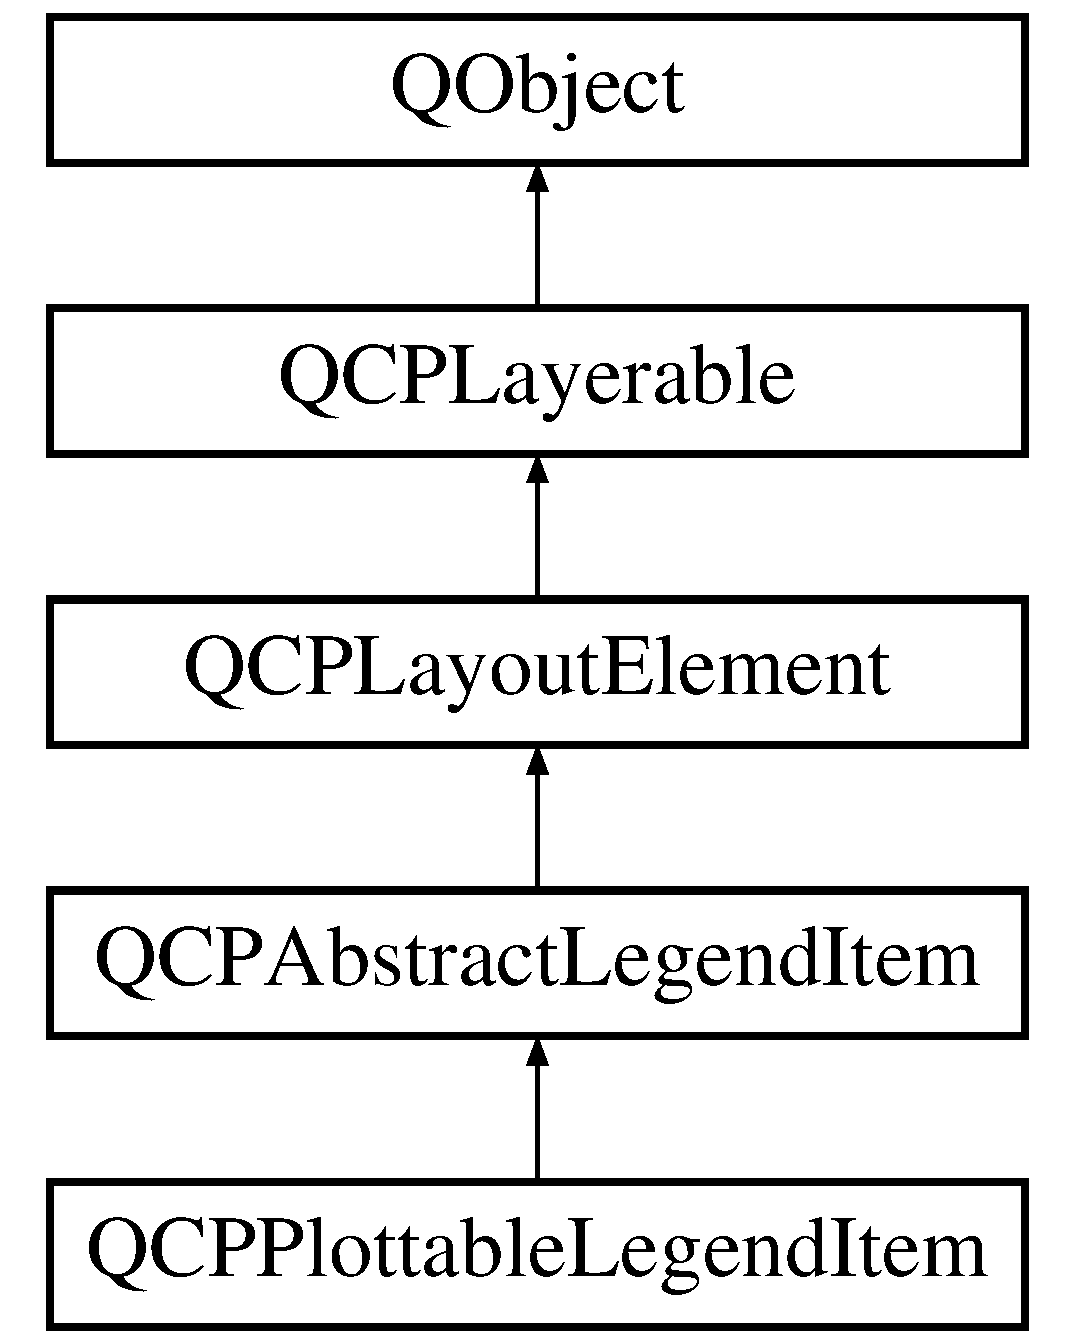
\includegraphics[height=5.000000cm]{class_q_c_p_abstract_legend_item}
\end{center}
\end{figure}
\subsection*{Signals}
\begin{DoxyCompactItemize}
\item 
void \hyperlink{class_q_c_p_abstract_legend_item_a7cb61fdfbaf69c590bacb8f9e7099d9e}{selection\+Changed} (bool \hyperlink{class_q_c_p_abstract_legend_item_ac776e68e3367704452131c6aa9908bb9}{selected})
\item 
void \hyperlink{class_q_c_p_abstract_legend_item_abc4d779b938cc9235f9196737dbaa6bd}{selectable\+Changed} (bool \hyperlink{class_q_c_p_abstract_legend_item_a0a0205f33f37edae50826c24cb8f1983}{selectable})
\end{DoxyCompactItemize}
\subsection*{Public Member Functions}
\begin{DoxyCompactItemize}
\item 
\hyperlink{class_q_c_p_abstract_legend_item_afaff87610e8da0fa238ecf552872d774}{Q\+C\+P\+Abstract\+Legend\+Item} (\hyperlink{class_q_c_p_legend}{Q\+C\+P\+Legend} $\ast$parent)
\item 
\hyperlink{class_q_c_p_legend}{Q\+C\+P\+Legend} $\ast$ \hyperlink{class_q_c_p_abstract_legend_item_afcd683e43058f99a47d6546eedffc5c1}{parent\+Legend} () const 
\item 
Q\+Font \hyperlink{class_q_c_p_abstract_legend_item_ae476404706638d84fadc01021df2b19e}{font} () const 
\item 
Q\+Color \hyperlink{class_q_c_p_abstract_legend_item_a444caef8565ac8d8653269f14d82b42d}{text\+Color} () const 
\item 
Q\+Font \hyperlink{class_q_c_p_abstract_legend_item_afccfe665eb8483cec924a9c0a53ddf2b}{selected\+Font} () const 
\item 
Q\+Color \hyperlink{class_q_c_p_abstract_legend_item_a076db1717257b82875b12a15ecf99ba3}{selected\+Text\+Color} () const 
\item 
bool \hyperlink{class_q_c_p_abstract_legend_item_a0a0205f33f37edae50826c24cb8f1983}{selectable} () const 
\item 
bool \hyperlink{class_q_c_p_abstract_legend_item_ac776e68e3367704452131c6aa9908bb9}{selected} () const 
\item 
void \hyperlink{class_q_c_p_abstract_legend_item_a409c53455d8112f71d70c0c43eb10265}{set\+Font} (const Q\+Font \&\hyperlink{class_q_c_p_abstract_legend_item_ae476404706638d84fadc01021df2b19e}{font})
\item 
void \hyperlink{class_q_c_p_abstract_legend_item_a6ebace6aaffaedcdab2d74e88acc2d1e}{set\+Text\+Color} (const Q\+Color \&color)
\item 
void \hyperlink{class_q_c_p_abstract_legend_item_a91db5aee48617a9d3206e61376807365}{set\+Selected\+Font} (const Q\+Font \&\hyperlink{class_q_c_p_abstract_legend_item_ae476404706638d84fadc01021df2b19e}{font})
\item 
void \hyperlink{class_q_c_p_abstract_legend_item_a4d01d008ee1a5bfe9905b0397a421936}{set\+Selected\+Text\+Color} (const Q\+Color \&color)
\item 
Q\+\_\+\+S\+L\+O\+T void \hyperlink{class_q_c_p_abstract_legend_item_a9913ef48730551b696e7f98a2391c599}{set\+Selectable} (bool \hyperlink{class_q_c_p_abstract_legend_item_a0a0205f33f37edae50826c24cb8f1983}{selectable})
\item 
Q\+\_\+\+S\+L\+O\+T void \hyperlink{class_q_c_p_abstract_legend_item_a6eed93b0ab99cb3eabb043fb08179c2b}{set\+Selected} (bool \hyperlink{class_q_c_p_abstract_legend_item_ac776e68e3367704452131c6aa9908bb9}{selected})
\item 
virtual double \hyperlink{class_q_c_p_abstract_legend_item_ad0480d5cad34627a294a2921caa4a62f}{select\+Test} (const Q\+Point\+F \&pos, bool only\+Selectable, Q\+Variant $\ast$details=0) const 
\end{DoxyCompactItemize}
\subsection*{Protected Member Functions}
\begin{DoxyCompactItemize}
\item 
virtual \hyperlink{namespace_q_c_p_a2ad6bb6281c7c2d593d4277b44c2b037}{Q\+C\+P\+::\+Interaction} \hyperlink{class_q_c_p_abstract_legend_item_a53a80054ab329beaca072fb08c08944b}{selection\+Category} () const 
\item 
virtual void \hyperlink{class_q_c_p_abstract_legend_item_a71c3baeda42ba78d2cccd97e74110a5e}{apply\+Default\+Antialiasing\+Hint} (\hyperlink{class_q_c_p_painter}{Q\+C\+P\+Painter} $\ast$painter) const 
\item 
virtual Q\+Rect \hyperlink{class_q_c_p_abstract_legend_item_abcb540c331b49ef7ee0ea1abbd0dcac3}{clip\+Rect} () const 
\item 
virtual void \hyperlink{class_q_c_p_abstract_legend_item_a97dedc084c672359710f16b31d046d1d}{draw} (\hyperlink{class_q_c_p_painter}{Q\+C\+P\+Painter} $\ast$painter)=0
\item 
virtual void \hyperlink{class_q_c_p_abstract_legend_item_abcfe9e335d99c7fac74e03d26723c1b7}{select\+Event} (Q\+Mouse\+Event $\ast$event, bool additive, const Q\+Variant \&details, bool $\ast$selection\+State\+Changed)
\item 
virtual void \hyperlink{class_q_c_p_abstract_legend_item_ae64e667e7c5b85cd92c9b91928faef28}{deselect\+Event} (bool $\ast$selection\+State\+Changed)
\end{DoxyCompactItemize}
\subsection*{Protected Attributes}
\begin{DoxyCompactItemize}
\item 
\hyperlink{class_q_c_p_legend}{Q\+C\+P\+Legend} $\ast$ \hyperlink{class_q_c_p_abstract_legend_item_aafcd9fc6fcb10f4a8d46037011afafe8}{m\+Parent\+Legend}
\item 
Q\+Font \hyperlink{class_q_c_p_abstract_legend_item_ae916a78ac0d2a60e20a17ca2f24f9754}{m\+Font}
\item 
Q\+Color \hyperlink{class_q_c_p_abstract_legend_item_a974b21e9930227d281344bd2242d289d}{m\+Text\+Color}
\item 
Q\+Font \hyperlink{class_q_c_p_abstract_legend_item_ab971df604306b192875a7d097feb1e21}{m\+Selected\+Font}
\item 
Q\+Color \hyperlink{class_q_c_p_abstract_legend_item_a4965c13854d970b24c284f0a4f005fbd}{m\+Selected\+Text\+Color}
\item 
bool \hyperlink{class_q_c_p_abstract_legend_item_aa84029f57b1b32f642fb7db63c3fc2c2}{m\+Selectable}
\item 
bool \hyperlink{class_q_c_p_abstract_legend_item_ae58ebebbd0c36cc6fe897483369984d2}{m\+Selected}
\end{DoxyCompactItemize}
\subsection*{Friends}
\begin{DoxyCompactItemize}
\item 
class \hyperlink{class_q_c_p_abstract_legend_item_a8429035e7adfbd7f05805a6530ad5e3b}{Q\+C\+P\+Legend}
\end{DoxyCompactItemize}
\subsection*{Additional Inherited Members}


\subsection{Detailed Description}
The abstract base class for all entries in a \hyperlink{class_q_c_p_legend}{Q\+C\+P\+Legend}. 

It defines a very basic interface for entries in a \hyperlink{class_q_c_p_legend}{Q\+C\+P\+Legend}. For representing plottables in the legend, the subclass \hyperlink{class_q_c_p_plottable_legend_item}{Q\+C\+P\+Plottable\+Legend\+Item} is more suitable.

Only derive directly from this class when you need absolute freedom (e.\+g. a custom legend entry that\textquotesingle{}s not even associated with a plottable).

You must implement the following pure virtual functions\+: \begin{DoxyItemize}
\item \hyperlink{class_q_c_p_abstract_legend_item_a97dedc084c672359710f16b31d046d1d}{draw} (from \hyperlink{class_q_c_p_layerable}{Q\+C\+P\+Layerable})\end{DoxyItemize}
You inherit the following members you may use\+: \begin{TabularC}{2}
\hline
\hyperlink{class_q_c_p_legend}{Q\+C\+P\+Legend} $\ast${\bfseries m\+Parent\+Legend}  &A pointer to the parent \hyperlink{class_q_c_p_legend}{Q\+C\+P\+Legend}. \\\cline{1-2}
Q\+Font {\bfseries m\+Font}  &The generic font of the item. You should use this font for all or at least the most prominent text of the item.  \\\cline{1-2}
\end{TabularC}


\subsection{Constructor \& Destructor Documentation}
\hypertarget{class_q_c_p_abstract_legend_item_afaff87610e8da0fa238ecf552872d774}{}\index{Q\+C\+P\+Abstract\+Legend\+Item@{Q\+C\+P\+Abstract\+Legend\+Item}!Q\+C\+P\+Abstract\+Legend\+Item@{Q\+C\+P\+Abstract\+Legend\+Item}}
\index{Q\+C\+P\+Abstract\+Legend\+Item@{Q\+C\+P\+Abstract\+Legend\+Item}!Q\+C\+P\+Abstract\+Legend\+Item@{Q\+C\+P\+Abstract\+Legend\+Item}}
\subsubsection[{Q\+C\+P\+Abstract\+Legend\+Item}]{\setlength{\rightskip}{0pt plus 5cm}Q\+C\+P\+Abstract\+Legend\+Item\+::\+Q\+C\+P\+Abstract\+Legend\+Item (
\begin{DoxyParamCaption}
\item[{{\bf Q\+C\+P\+Legend} $\ast$}]{parent}
\end{DoxyParamCaption}
)\hspace{0.3cm}{\ttfamily [explicit]}}\label{class_q_c_p_abstract_legend_item_afaff87610e8da0fa238ecf552872d774}
Constructs a \hyperlink{class_q_c_p_abstract_legend_item}{Q\+C\+P\+Abstract\+Legend\+Item} and associates it with the \hyperlink{class_q_c_p_legend}{Q\+C\+P\+Legend} {\itshape parent}. This does not cause the item to be added to {\itshape parent}, so \hyperlink{class_q_c_p_legend_a3ab274de52d2951faea45a6d975e6b3f}{Q\+C\+P\+Legend\+::add\+Item} must be called separately. 

\subsection{Member Function Documentation}
\hypertarget{class_q_c_p_abstract_legend_item_a71c3baeda42ba78d2cccd97e74110a5e}{}\index{Q\+C\+P\+Abstract\+Legend\+Item@{Q\+C\+P\+Abstract\+Legend\+Item}!apply\+Default\+Antialiasing\+Hint@{apply\+Default\+Antialiasing\+Hint}}
\index{apply\+Default\+Antialiasing\+Hint@{apply\+Default\+Antialiasing\+Hint}!Q\+C\+P\+Abstract\+Legend\+Item@{Q\+C\+P\+Abstract\+Legend\+Item}}
\subsubsection[{apply\+Default\+Antialiasing\+Hint}]{\setlength{\rightskip}{0pt plus 5cm}void Q\+C\+P\+Abstract\+Legend\+Item\+::apply\+Default\+Antialiasing\+Hint (
\begin{DoxyParamCaption}
\item[{{\bf Q\+C\+P\+Painter} $\ast$}]{painter}
\end{DoxyParamCaption}
) const\hspace{0.3cm}{\ttfamily [protected]}, {\ttfamily [virtual]}}\label{class_q_c_p_abstract_legend_item_a71c3baeda42ba78d2cccd97e74110a5e}


Reimplemented from \hyperlink{class_q_c_p_layout_element_ad6d2b4bb0291c2441b2e1ca3d5296df5}{Q\+C\+P\+Layout\+Element}.

\hypertarget{class_q_c_p_abstract_legend_item_abcb540c331b49ef7ee0ea1abbd0dcac3}{}\index{Q\+C\+P\+Abstract\+Legend\+Item@{Q\+C\+P\+Abstract\+Legend\+Item}!clip\+Rect@{clip\+Rect}}
\index{clip\+Rect@{clip\+Rect}!Q\+C\+P\+Abstract\+Legend\+Item@{Q\+C\+P\+Abstract\+Legend\+Item}}
\subsubsection[{clip\+Rect}]{\setlength{\rightskip}{0pt plus 5cm}Q\+Rect Q\+C\+P\+Abstract\+Legend\+Item\+::clip\+Rect (
\begin{DoxyParamCaption}
{}
\end{DoxyParamCaption}
) const\hspace{0.3cm}{\ttfamily [protected]}, {\ttfamily [virtual]}}\label{class_q_c_p_abstract_legend_item_abcb540c331b49ef7ee0ea1abbd0dcac3}


Reimplemented from \hyperlink{class_q_c_p_layerable_a07a8f746640c3704b09910df297afcba}{Q\+C\+P\+Layerable}.

\hypertarget{class_q_c_p_abstract_legend_item_ae64e667e7c5b85cd92c9b91928faef28}{}\index{Q\+C\+P\+Abstract\+Legend\+Item@{Q\+C\+P\+Abstract\+Legend\+Item}!deselect\+Event@{deselect\+Event}}
\index{deselect\+Event@{deselect\+Event}!Q\+C\+P\+Abstract\+Legend\+Item@{Q\+C\+P\+Abstract\+Legend\+Item}}
\subsubsection[{deselect\+Event}]{\setlength{\rightskip}{0pt plus 5cm}void Q\+C\+P\+Abstract\+Legend\+Item\+::deselect\+Event (
\begin{DoxyParamCaption}
\item[{bool $\ast$}]{selection\+State\+Changed}
\end{DoxyParamCaption}
)\hspace{0.3cm}{\ttfamily [protected]}, {\ttfamily [virtual]}}\label{class_q_c_p_abstract_legend_item_ae64e667e7c5b85cd92c9b91928faef28}


Reimplemented from \hyperlink{class_q_c_p_layerable_ae546370644a5551c76af739afc008bee}{Q\+C\+P\+Layerable}.

\hypertarget{class_q_c_p_abstract_legend_item_a97dedc084c672359710f16b31d046d1d}{}\index{Q\+C\+P\+Abstract\+Legend\+Item@{Q\+C\+P\+Abstract\+Legend\+Item}!draw@{draw}}
\index{draw@{draw}!Q\+C\+P\+Abstract\+Legend\+Item@{Q\+C\+P\+Abstract\+Legend\+Item}}
\subsubsection[{draw}]{\setlength{\rightskip}{0pt plus 5cm}virtual void Q\+C\+P\+Abstract\+Legend\+Item\+::draw (
\begin{DoxyParamCaption}
\item[{{\bf Q\+C\+P\+Painter} $\ast$}]{painter}
\end{DoxyParamCaption}
)\hspace{0.3cm}{\ttfamily [protected]}, {\ttfamily [pure virtual]}}\label{class_q_c_p_abstract_legend_item_a97dedc084c672359710f16b31d046d1d}


Reimplemented from \hyperlink{class_q_c_p_layout_element_a547bcc1e6e2be5645ca781efe0834653}{Q\+C\+P\+Layout\+Element}.



Implemented in \hyperlink{class_q_c_p_plottable_legend_item_a68a781c3de4f9959fdf82075052d43aa}{Q\+C\+P\+Plottable\+Legend\+Item}.

\hypertarget{class_q_c_p_abstract_legend_item_ae476404706638d84fadc01021df2b19e}{}\index{Q\+C\+P\+Abstract\+Legend\+Item@{Q\+C\+P\+Abstract\+Legend\+Item}!font@{font}}
\index{font@{font}!Q\+C\+P\+Abstract\+Legend\+Item@{Q\+C\+P\+Abstract\+Legend\+Item}}
\subsubsection[{font}]{\setlength{\rightskip}{0pt plus 5cm}Q\+Font Q\+C\+P\+Abstract\+Legend\+Item\+::font (
\begin{DoxyParamCaption}
{}
\end{DoxyParamCaption}
) const\hspace{0.3cm}{\ttfamily [inline]}}\label{class_q_c_p_abstract_legend_item_ae476404706638d84fadc01021df2b19e}
\hypertarget{class_q_c_p_abstract_legend_item_afcd683e43058f99a47d6546eedffc5c1}{}\index{Q\+C\+P\+Abstract\+Legend\+Item@{Q\+C\+P\+Abstract\+Legend\+Item}!parent\+Legend@{parent\+Legend}}
\index{parent\+Legend@{parent\+Legend}!Q\+C\+P\+Abstract\+Legend\+Item@{Q\+C\+P\+Abstract\+Legend\+Item}}
\subsubsection[{parent\+Legend}]{\setlength{\rightskip}{0pt plus 5cm}{\bf Q\+C\+P\+Legend}$\ast$ Q\+C\+P\+Abstract\+Legend\+Item\+::parent\+Legend (
\begin{DoxyParamCaption}
{}
\end{DoxyParamCaption}
) const\hspace{0.3cm}{\ttfamily [inline]}}\label{class_q_c_p_abstract_legend_item_afcd683e43058f99a47d6546eedffc5c1}
\hypertarget{class_q_c_p_abstract_legend_item_a0a0205f33f37edae50826c24cb8f1983}{}\index{Q\+C\+P\+Abstract\+Legend\+Item@{Q\+C\+P\+Abstract\+Legend\+Item}!selectable@{selectable}}
\index{selectable@{selectable}!Q\+C\+P\+Abstract\+Legend\+Item@{Q\+C\+P\+Abstract\+Legend\+Item}}
\subsubsection[{selectable}]{\setlength{\rightskip}{0pt plus 5cm}bool Q\+C\+P\+Abstract\+Legend\+Item\+::selectable (
\begin{DoxyParamCaption}
{}
\end{DoxyParamCaption}
) const\hspace{0.3cm}{\ttfamily [inline]}}\label{class_q_c_p_abstract_legend_item_a0a0205f33f37edae50826c24cb8f1983}
\hypertarget{class_q_c_p_abstract_legend_item_abc4d779b938cc9235f9196737dbaa6bd}{}\index{Q\+C\+P\+Abstract\+Legend\+Item@{Q\+C\+P\+Abstract\+Legend\+Item}!selectable\+Changed@{selectable\+Changed}}
\index{selectable\+Changed@{selectable\+Changed}!Q\+C\+P\+Abstract\+Legend\+Item@{Q\+C\+P\+Abstract\+Legend\+Item}}
\subsubsection[{selectable\+Changed}]{\setlength{\rightskip}{0pt plus 5cm}void Q\+C\+P\+Abstract\+Legend\+Item\+::selectable\+Changed (
\begin{DoxyParamCaption}
\item[{bool}]{selectable}
\end{DoxyParamCaption}
)\hspace{0.3cm}{\ttfamily [signal]}}\label{class_q_c_p_abstract_legend_item_abc4d779b938cc9235f9196737dbaa6bd}
\hypertarget{class_q_c_p_abstract_legend_item_ac776e68e3367704452131c6aa9908bb9}{}\index{Q\+C\+P\+Abstract\+Legend\+Item@{Q\+C\+P\+Abstract\+Legend\+Item}!selected@{selected}}
\index{selected@{selected}!Q\+C\+P\+Abstract\+Legend\+Item@{Q\+C\+P\+Abstract\+Legend\+Item}}
\subsubsection[{selected}]{\setlength{\rightskip}{0pt plus 5cm}bool Q\+C\+P\+Abstract\+Legend\+Item\+::selected (
\begin{DoxyParamCaption}
{}
\end{DoxyParamCaption}
) const\hspace{0.3cm}{\ttfamily [inline]}}\label{class_q_c_p_abstract_legend_item_ac776e68e3367704452131c6aa9908bb9}
\hypertarget{class_q_c_p_abstract_legend_item_afccfe665eb8483cec924a9c0a53ddf2b}{}\index{Q\+C\+P\+Abstract\+Legend\+Item@{Q\+C\+P\+Abstract\+Legend\+Item}!selected\+Font@{selected\+Font}}
\index{selected\+Font@{selected\+Font}!Q\+C\+P\+Abstract\+Legend\+Item@{Q\+C\+P\+Abstract\+Legend\+Item}}
\subsubsection[{selected\+Font}]{\setlength{\rightskip}{0pt plus 5cm}Q\+Font Q\+C\+P\+Abstract\+Legend\+Item\+::selected\+Font (
\begin{DoxyParamCaption}
{}
\end{DoxyParamCaption}
) const\hspace{0.3cm}{\ttfamily [inline]}}\label{class_q_c_p_abstract_legend_item_afccfe665eb8483cec924a9c0a53ddf2b}
\hypertarget{class_q_c_p_abstract_legend_item_a076db1717257b82875b12a15ecf99ba3}{}\index{Q\+C\+P\+Abstract\+Legend\+Item@{Q\+C\+P\+Abstract\+Legend\+Item}!selected\+Text\+Color@{selected\+Text\+Color}}
\index{selected\+Text\+Color@{selected\+Text\+Color}!Q\+C\+P\+Abstract\+Legend\+Item@{Q\+C\+P\+Abstract\+Legend\+Item}}
\subsubsection[{selected\+Text\+Color}]{\setlength{\rightskip}{0pt plus 5cm}Q\+Color Q\+C\+P\+Abstract\+Legend\+Item\+::selected\+Text\+Color (
\begin{DoxyParamCaption}
{}
\end{DoxyParamCaption}
) const\hspace{0.3cm}{\ttfamily [inline]}}\label{class_q_c_p_abstract_legend_item_a076db1717257b82875b12a15ecf99ba3}
\hypertarget{class_q_c_p_abstract_legend_item_abcfe9e335d99c7fac74e03d26723c1b7}{}\index{Q\+C\+P\+Abstract\+Legend\+Item@{Q\+C\+P\+Abstract\+Legend\+Item}!select\+Event@{select\+Event}}
\index{select\+Event@{select\+Event}!Q\+C\+P\+Abstract\+Legend\+Item@{Q\+C\+P\+Abstract\+Legend\+Item}}
\subsubsection[{select\+Event}]{\setlength{\rightskip}{0pt plus 5cm}void Q\+C\+P\+Abstract\+Legend\+Item\+::select\+Event (
\begin{DoxyParamCaption}
\item[{Q\+Mouse\+Event $\ast$}]{event, }
\item[{bool}]{additive, }
\item[{const Q\+Variant \&}]{details, }
\item[{bool $\ast$}]{selection\+State\+Changed}
\end{DoxyParamCaption}
)\hspace{0.3cm}{\ttfamily [protected]}, {\ttfamily [virtual]}}\label{class_q_c_p_abstract_legend_item_abcfe9e335d99c7fac74e03d26723c1b7}


Reimplemented from \hyperlink{class_q_c_p_layerable_a7498c2d0d081cf7cad0fb3bb93aa0e91}{Q\+C\+P\+Layerable}.

\hypertarget{class_q_c_p_abstract_legend_item_a53a80054ab329beaca072fb08c08944b}{}\index{Q\+C\+P\+Abstract\+Legend\+Item@{Q\+C\+P\+Abstract\+Legend\+Item}!selection\+Category@{selection\+Category}}
\index{selection\+Category@{selection\+Category}!Q\+C\+P\+Abstract\+Legend\+Item@{Q\+C\+P\+Abstract\+Legend\+Item}}
\subsubsection[{selection\+Category}]{\setlength{\rightskip}{0pt plus 5cm}{\bf Q\+C\+P\+::\+Interaction} Q\+C\+P\+Abstract\+Legend\+Item\+::selection\+Category (
\begin{DoxyParamCaption}
{}
\end{DoxyParamCaption}
) const\hspace{0.3cm}{\ttfamily [protected]}, {\ttfamily [virtual]}}\label{class_q_c_p_abstract_legend_item_a53a80054ab329beaca072fb08c08944b}


Reimplemented from \hyperlink{class_q_c_p_layerable_aa4035e586b7f317a06ba7e74e242a5ea}{Q\+C\+P\+Layerable}.

\hypertarget{class_q_c_p_abstract_legend_item_a7cb61fdfbaf69c590bacb8f9e7099d9e}{}\index{Q\+C\+P\+Abstract\+Legend\+Item@{Q\+C\+P\+Abstract\+Legend\+Item}!selection\+Changed@{selection\+Changed}}
\index{selection\+Changed@{selection\+Changed}!Q\+C\+P\+Abstract\+Legend\+Item@{Q\+C\+P\+Abstract\+Legend\+Item}}
\subsubsection[{selection\+Changed}]{\setlength{\rightskip}{0pt plus 5cm}void Q\+C\+P\+Abstract\+Legend\+Item\+::selection\+Changed (
\begin{DoxyParamCaption}
\item[{bool}]{selected}
\end{DoxyParamCaption}
)\hspace{0.3cm}{\ttfamily [signal]}}\label{class_q_c_p_abstract_legend_item_a7cb61fdfbaf69c590bacb8f9e7099d9e}
This signal is emitted when the selection state of this legend item has changed, either by user interaction or by a direct call to \hyperlink{class_q_c_p_abstract_legend_item_a6eed93b0ab99cb3eabb043fb08179c2b}{set\+Selected}. \hypertarget{class_q_c_p_abstract_legend_item_ad0480d5cad34627a294a2921caa4a62f}{}\index{Q\+C\+P\+Abstract\+Legend\+Item@{Q\+C\+P\+Abstract\+Legend\+Item}!select\+Test@{select\+Test}}
\index{select\+Test@{select\+Test}!Q\+C\+P\+Abstract\+Legend\+Item@{Q\+C\+P\+Abstract\+Legend\+Item}}
\subsubsection[{select\+Test}]{\setlength{\rightskip}{0pt plus 5cm}double Q\+C\+P\+Abstract\+Legend\+Item\+::select\+Test (
\begin{DoxyParamCaption}
\item[{const Q\+Point\+F \&}]{pos, }
\item[{bool}]{only\+Selectable, }
\item[{Q\+Variant $\ast$}]{details = {\ttfamily 0}}
\end{DoxyParamCaption}
) const\hspace{0.3cm}{\ttfamily [virtual]}}\label{class_q_c_p_abstract_legend_item_ad0480d5cad34627a294a2921caa4a62f}
Layout elements are sensitive to events inside their outer rect. If {\itshape pos} is within the outer rect, this method returns a value corresponding to 0.\+99 times the parent plot\textquotesingle{}s selection tolerance. However, layout elements are not selectable by default. So if {\itshape only\+Selectable} is true, -\/1.\+0 is returned.

See \hyperlink{class_q_c_p_layerable_a4001c4d0dfec55598efa4d531f2179a9}{Q\+C\+P\+Layerable\+::select\+Test} for a general explanation of this virtual method.

\hyperlink{class_q_c_p_layout_element}{Q\+C\+P\+Layout\+Element} subclasses may reimplement this method to provide more specific selection test behaviour. 

Reimplemented from \hyperlink{class_q_c_p_layout_element_a9fcf5d0ea19f2c23b2b528bce2c6f095}{Q\+C\+P\+Layout\+Element}.

\hypertarget{class_q_c_p_abstract_legend_item_a409c53455d8112f71d70c0c43eb10265}{}\index{Q\+C\+P\+Abstract\+Legend\+Item@{Q\+C\+P\+Abstract\+Legend\+Item}!set\+Font@{set\+Font}}
\index{set\+Font@{set\+Font}!Q\+C\+P\+Abstract\+Legend\+Item@{Q\+C\+P\+Abstract\+Legend\+Item}}
\subsubsection[{set\+Font}]{\setlength{\rightskip}{0pt plus 5cm}void Q\+C\+P\+Abstract\+Legend\+Item\+::set\+Font (
\begin{DoxyParamCaption}
\item[{const Q\+Font \&}]{font}
\end{DoxyParamCaption}
)}\label{class_q_c_p_abstract_legend_item_a409c53455d8112f71d70c0c43eb10265}
Sets the default font of this specific legend item to {\itshape font}.

\begin{DoxySeeAlso}{See also}
\hyperlink{class_q_c_p_abstract_legend_item_a6ebace6aaffaedcdab2d74e88acc2d1e}{set\+Text\+Color}, \hyperlink{class_q_c_p_legend_aa4cda8499e3cb0f3be415edc02984c73}{Q\+C\+P\+Legend\+::set\+Font} 
\end{DoxySeeAlso}
\hypertarget{class_q_c_p_abstract_legend_item_a9913ef48730551b696e7f98a2391c599}{}\index{Q\+C\+P\+Abstract\+Legend\+Item@{Q\+C\+P\+Abstract\+Legend\+Item}!set\+Selectable@{set\+Selectable}}
\index{set\+Selectable@{set\+Selectable}!Q\+C\+P\+Abstract\+Legend\+Item@{Q\+C\+P\+Abstract\+Legend\+Item}}
\subsubsection[{set\+Selectable}]{\setlength{\rightskip}{0pt plus 5cm}void Q\+C\+P\+Abstract\+Legend\+Item\+::set\+Selectable (
\begin{DoxyParamCaption}
\item[{bool}]{selectable}
\end{DoxyParamCaption}
)}\label{class_q_c_p_abstract_legend_item_a9913ef48730551b696e7f98a2391c599}
Sets whether this specific legend item is selectable.

\begin{DoxySeeAlso}{See also}
set\+Selected\+Parts, \hyperlink{class_q_custom_plot_a5ee1e2f6ae27419deca53e75907c27e5}{Q\+Custom\+Plot\+::set\+Interactions} 
\end{DoxySeeAlso}
\hypertarget{class_q_c_p_abstract_legend_item_a6eed93b0ab99cb3eabb043fb08179c2b}{}\index{Q\+C\+P\+Abstract\+Legend\+Item@{Q\+C\+P\+Abstract\+Legend\+Item}!set\+Selected@{set\+Selected}}
\index{set\+Selected@{set\+Selected}!Q\+C\+P\+Abstract\+Legend\+Item@{Q\+C\+P\+Abstract\+Legend\+Item}}
\subsubsection[{set\+Selected}]{\setlength{\rightskip}{0pt plus 5cm}void Q\+C\+P\+Abstract\+Legend\+Item\+::set\+Selected (
\begin{DoxyParamCaption}
\item[{bool}]{selected}
\end{DoxyParamCaption}
)}\label{class_q_c_p_abstract_legend_item_a6eed93b0ab99cb3eabb043fb08179c2b}
Sets whether this specific legend item is selected.

It is possible to set the selection state of this item by calling this function directly, even if set\+Selectable is set to false.

\begin{DoxySeeAlso}{See also}
set\+Selectable\+Parts, \hyperlink{class_q_custom_plot_a5ee1e2f6ae27419deca53e75907c27e5}{Q\+Custom\+Plot\+::set\+Interactions} 
\end{DoxySeeAlso}
\hypertarget{class_q_c_p_abstract_legend_item_a91db5aee48617a9d3206e61376807365}{}\index{Q\+C\+P\+Abstract\+Legend\+Item@{Q\+C\+P\+Abstract\+Legend\+Item}!set\+Selected\+Font@{set\+Selected\+Font}}
\index{set\+Selected\+Font@{set\+Selected\+Font}!Q\+C\+P\+Abstract\+Legend\+Item@{Q\+C\+P\+Abstract\+Legend\+Item}}
\subsubsection[{set\+Selected\+Font}]{\setlength{\rightskip}{0pt plus 5cm}void Q\+C\+P\+Abstract\+Legend\+Item\+::set\+Selected\+Font (
\begin{DoxyParamCaption}
\item[{const Q\+Font \&}]{font}
\end{DoxyParamCaption}
)}\label{class_q_c_p_abstract_legend_item_a91db5aee48617a9d3206e61376807365}
When this legend item is selected, {\itshape font} is used to draw generic text, instead of the normal font set with \hyperlink{class_q_c_p_abstract_legend_item_a409c53455d8112f71d70c0c43eb10265}{set\+Font}.

\begin{DoxySeeAlso}{See also}
\hyperlink{class_q_c_p_abstract_legend_item_a409c53455d8112f71d70c0c43eb10265}{set\+Font}, \hyperlink{class_q_c_p_legend_ab580a01c3c0a239374ed66c29edf5ad2}{Q\+C\+P\+Legend\+::set\+Selected\+Font} 
\end{DoxySeeAlso}
\hypertarget{class_q_c_p_abstract_legend_item_a4d01d008ee1a5bfe9905b0397a421936}{}\index{Q\+C\+P\+Abstract\+Legend\+Item@{Q\+C\+P\+Abstract\+Legend\+Item}!set\+Selected\+Text\+Color@{set\+Selected\+Text\+Color}}
\index{set\+Selected\+Text\+Color@{set\+Selected\+Text\+Color}!Q\+C\+P\+Abstract\+Legend\+Item@{Q\+C\+P\+Abstract\+Legend\+Item}}
\subsubsection[{set\+Selected\+Text\+Color}]{\setlength{\rightskip}{0pt plus 5cm}void Q\+C\+P\+Abstract\+Legend\+Item\+::set\+Selected\+Text\+Color (
\begin{DoxyParamCaption}
\item[{const Q\+Color \&}]{color}
\end{DoxyParamCaption}
)}\label{class_q_c_p_abstract_legend_item_a4d01d008ee1a5bfe9905b0397a421936}
When this legend item is selected, {\itshape color} is used to draw generic text, instead of the normal color set with \hyperlink{class_q_c_p_abstract_legend_item_a6ebace6aaffaedcdab2d74e88acc2d1e}{set\+Text\+Color}.

\begin{DoxySeeAlso}{See also}
\hyperlink{class_q_c_p_abstract_legend_item_a6ebace6aaffaedcdab2d74e88acc2d1e}{set\+Text\+Color}, \hyperlink{class_q_c_p_legend_a7674dfc7a1f30e1abd1018c0ed45e0bc}{Q\+C\+P\+Legend\+::set\+Selected\+Text\+Color} 
\end{DoxySeeAlso}
\hypertarget{class_q_c_p_abstract_legend_item_a6ebace6aaffaedcdab2d74e88acc2d1e}{}\index{Q\+C\+P\+Abstract\+Legend\+Item@{Q\+C\+P\+Abstract\+Legend\+Item}!set\+Text\+Color@{set\+Text\+Color}}
\index{set\+Text\+Color@{set\+Text\+Color}!Q\+C\+P\+Abstract\+Legend\+Item@{Q\+C\+P\+Abstract\+Legend\+Item}}
\subsubsection[{set\+Text\+Color}]{\setlength{\rightskip}{0pt plus 5cm}void Q\+C\+P\+Abstract\+Legend\+Item\+::set\+Text\+Color (
\begin{DoxyParamCaption}
\item[{const Q\+Color \&}]{color}
\end{DoxyParamCaption}
)}\label{class_q_c_p_abstract_legend_item_a6ebace6aaffaedcdab2d74e88acc2d1e}
Sets the default text color of this specific legend item to {\itshape color}.

\begin{DoxySeeAlso}{See also}
\hyperlink{class_q_c_p_abstract_legend_item_a409c53455d8112f71d70c0c43eb10265}{set\+Font}, \hyperlink{class_q_c_p_legend_ae1eb239ff4a4632fe1b6c3e668d845c6}{Q\+C\+P\+Legend\+::set\+Text\+Color} 
\end{DoxySeeAlso}
\hypertarget{class_q_c_p_abstract_legend_item_a444caef8565ac8d8653269f14d82b42d}{}\index{Q\+C\+P\+Abstract\+Legend\+Item@{Q\+C\+P\+Abstract\+Legend\+Item}!text\+Color@{text\+Color}}
\index{text\+Color@{text\+Color}!Q\+C\+P\+Abstract\+Legend\+Item@{Q\+C\+P\+Abstract\+Legend\+Item}}
\subsubsection[{text\+Color}]{\setlength{\rightskip}{0pt plus 5cm}Q\+Color Q\+C\+P\+Abstract\+Legend\+Item\+::text\+Color (
\begin{DoxyParamCaption}
{}
\end{DoxyParamCaption}
) const\hspace{0.3cm}{\ttfamily [inline]}}\label{class_q_c_p_abstract_legend_item_a444caef8565ac8d8653269f14d82b42d}


\subsection{Friends And Related Function Documentation}
\hypertarget{class_q_c_p_abstract_legend_item_a8429035e7adfbd7f05805a6530ad5e3b}{}\index{Q\+C\+P\+Abstract\+Legend\+Item@{Q\+C\+P\+Abstract\+Legend\+Item}!Q\+C\+P\+Legend@{Q\+C\+P\+Legend}}
\index{Q\+C\+P\+Legend@{Q\+C\+P\+Legend}!Q\+C\+P\+Abstract\+Legend\+Item@{Q\+C\+P\+Abstract\+Legend\+Item}}
\subsubsection[{Q\+C\+P\+Legend}]{\setlength{\rightskip}{0pt plus 5cm}friend class {\bf Q\+C\+P\+Legend}\hspace{0.3cm}{\ttfamily [friend]}}\label{class_q_c_p_abstract_legend_item_a8429035e7adfbd7f05805a6530ad5e3b}


\subsection{Member Data Documentation}
\hypertarget{class_q_c_p_abstract_legend_item_ae916a78ac0d2a60e20a17ca2f24f9754}{}\index{Q\+C\+P\+Abstract\+Legend\+Item@{Q\+C\+P\+Abstract\+Legend\+Item}!m\+Font@{m\+Font}}
\index{m\+Font@{m\+Font}!Q\+C\+P\+Abstract\+Legend\+Item@{Q\+C\+P\+Abstract\+Legend\+Item}}
\subsubsection[{m\+Font}]{\setlength{\rightskip}{0pt plus 5cm}Q\+Font Q\+C\+P\+Abstract\+Legend\+Item\+::m\+Font\hspace{0.3cm}{\ttfamily [protected]}}\label{class_q_c_p_abstract_legend_item_ae916a78ac0d2a60e20a17ca2f24f9754}
\hypertarget{class_q_c_p_abstract_legend_item_aafcd9fc6fcb10f4a8d46037011afafe8}{}\index{Q\+C\+P\+Abstract\+Legend\+Item@{Q\+C\+P\+Abstract\+Legend\+Item}!m\+Parent\+Legend@{m\+Parent\+Legend}}
\index{m\+Parent\+Legend@{m\+Parent\+Legend}!Q\+C\+P\+Abstract\+Legend\+Item@{Q\+C\+P\+Abstract\+Legend\+Item}}
\subsubsection[{m\+Parent\+Legend}]{\setlength{\rightskip}{0pt plus 5cm}{\bf Q\+C\+P\+Legend}$\ast$ Q\+C\+P\+Abstract\+Legend\+Item\+::m\+Parent\+Legend\hspace{0.3cm}{\ttfamily [protected]}}\label{class_q_c_p_abstract_legend_item_aafcd9fc6fcb10f4a8d46037011afafe8}
\hypertarget{class_q_c_p_abstract_legend_item_aa84029f57b1b32f642fb7db63c3fc2c2}{}\index{Q\+C\+P\+Abstract\+Legend\+Item@{Q\+C\+P\+Abstract\+Legend\+Item}!m\+Selectable@{m\+Selectable}}
\index{m\+Selectable@{m\+Selectable}!Q\+C\+P\+Abstract\+Legend\+Item@{Q\+C\+P\+Abstract\+Legend\+Item}}
\subsubsection[{m\+Selectable}]{\setlength{\rightskip}{0pt plus 5cm}bool Q\+C\+P\+Abstract\+Legend\+Item\+::m\+Selectable\hspace{0.3cm}{\ttfamily [protected]}}\label{class_q_c_p_abstract_legend_item_aa84029f57b1b32f642fb7db63c3fc2c2}
\hypertarget{class_q_c_p_abstract_legend_item_ae58ebebbd0c36cc6fe897483369984d2}{}\index{Q\+C\+P\+Abstract\+Legend\+Item@{Q\+C\+P\+Abstract\+Legend\+Item}!m\+Selected@{m\+Selected}}
\index{m\+Selected@{m\+Selected}!Q\+C\+P\+Abstract\+Legend\+Item@{Q\+C\+P\+Abstract\+Legend\+Item}}
\subsubsection[{m\+Selected}]{\setlength{\rightskip}{0pt plus 5cm}bool Q\+C\+P\+Abstract\+Legend\+Item\+::m\+Selected\hspace{0.3cm}{\ttfamily [protected]}}\label{class_q_c_p_abstract_legend_item_ae58ebebbd0c36cc6fe897483369984d2}
\hypertarget{class_q_c_p_abstract_legend_item_ab971df604306b192875a7d097feb1e21}{}\index{Q\+C\+P\+Abstract\+Legend\+Item@{Q\+C\+P\+Abstract\+Legend\+Item}!m\+Selected\+Font@{m\+Selected\+Font}}
\index{m\+Selected\+Font@{m\+Selected\+Font}!Q\+C\+P\+Abstract\+Legend\+Item@{Q\+C\+P\+Abstract\+Legend\+Item}}
\subsubsection[{m\+Selected\+Font}]{\setlength{\rightskip}{0pt plus 5cm}Q\+Font Q\+C\+P\+Abstract\+Legend\+Item\+::m\+Selected\+Font\hspace{0.3cm}{\ttfamily [protected]}}\label{class_q_c_p_abstract_legend_item_ab971df604306b192875a7d097feb1e21}
\hypertarget{class_q_c_p_abstract_legend_item_a4965c13854d970b24c284f0a4f005fbd}{}\index{Q\+C\+P\+Abstract\+Legend\+Item@{Q\+C\+P\+Abstract\+Legend\+Item}!m\+Selected\+Text\+Color@{m\+Selected\+Text\+Color}}
\index{m\+Selected\+Text\+Color@{m\+Selected\+Text\+Color}!Q\+C\+P\+Abstract\+Legend\+Item@{Q\+C\+P\+Abstract\+Legend\+Item}}
\subsubsection[{m\+Selected\+Text\+Color}]{\setlength{\rightskip}{0pt plus 5cm}Q\+Color Q\+C\+P\+Abstract\+Legend\+Item\+::m\+Selected\+Text\+Color\hspace{0.3cm}{\ttfamily [protected]}}\label{class_q_c_p_abstract_legend_item_a4965c13854d970b24c284f0a4f005fbd}
\hypertarget{class_q_c_p_abstract_legend_item_a974b21e9930227d281344bd2242d289d}{}\index{Q\+C\+P\+Abstract\+Legend\+Item@{Q\+C\+P\+Abstract\+Legend\+Item}!m\+Text\+Color@{m\+Text\+Color}}
\index{m\+Text\+Color@{m\+Text\+Color}!Q\+C\+P\+Abstract\+Legend\+Item@{Q\+C\+P\+Abstract\+Legend\+Item}}
\subsubsection[{m\+Text\+Color}]{\setlength{\rightskip}{0pt plus 5cm}Q\+Color Q\+C\+P\+Abstract\+Legend\+Item\+::m\+Text\+Color\hspace{0.3cm}{\ttfamily [protected]}}\label{class_q_c_p_abstract_legend_item_a974b21e9930227d281344bd2242d289d}


The documentation for this class was generated from the following files\+:\begin{DoxyCompactItemize}
\item 
C\+:/\+Users/\+Roman/\+Documents/\+Mygs/\+Ground\+Station/\+G\+S/\hyperlink{qcustomplot_8h}{qcustomplot.\+h}\item 
C\+:/\+Users/\+Roman/\+Documents/\+Mygs/\+Ground\+Station/\+G\+S/\hyperlink{qcustomplot_8cpp}{qcustomplot.\+cpp}\end{DoxyCompactItemize}

\hypertarget{class_q_c_p_abstract_plottable}{}\section{Q\+C\+P\+Abstract\+Plottable Class Reference}
\label{class_q_c_p_abstract_plottable}\index{Q\+C\+P\+Abstract\+Plottable@{Q\+C\+P\+Abstract\+Plottable}}


The abstract base class for all data representing objects in a plot.  




{\ttfamily \#include $<$qcustomplot.\+h$>$}

Inheritance diagram for Q\+C\+P\+Abstract\+Plottable\+:\begin{figure}[H]
\begin{center}
\leavevmode
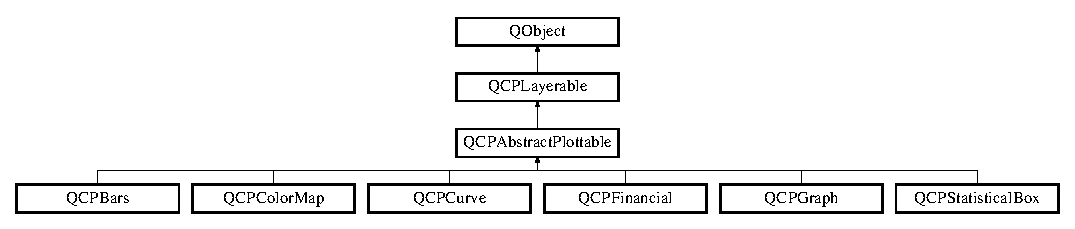
\includegraphics[height=2.629108cm]{class_q_c_p_abstract_plottable}
\end{center}
\end{figure}
\subsection*{Signals}
\begin{DoxyCompactItemize}
\item 
void \hyperlink{class_q_c_p_abstract_plottable_a3af66432b1dca93b28e00e78a8c7c1d9}{selection\+Changed} (bool \hyperlink{class_q_c_p_abstract_plottable_ab901903adcb0e29467d63de72340ab29}{selected})
\item 
void \hyperlink{class_q_c_p_abstract_plottable_a0059caa3f3581f3959660fef8cbb71c4}{selectable\+Changed} (bool \hyperlink{class_q_c_p_abstract_plottable_af895574da1ec0d050711b6c9deda296a}{selectable})
\end{DoxyCompactItemize}
\subsection*{Public Member Functions}
\begin{DoxyCompactItemize}
\item 
\hyperlink{class_q_c_p_abstract_plottable_af78a036e40db6f53a31abadc5323715a}{Q\+C\+P\+Abstract\+Plottable} (\hyperlink{class_q_c_p_axis}{Q\+C\+P\+Axis} $\ast$\hyperlink{class_q_c_p_abstract_plottable_a72c7a09c22963f2c943f07112b311103}{key\+Axis}, \hyperlink{class_q_c_p_axis}{Q\+C\+P\+Axis} $\ast$\hyperlink{class_q_c_p_abstract_plottable_a3106f9d34d330a6097a8ec5905e5b519}{value\+Axis})
\item 
Q\+String \hyperlink{class_q_c_p_abstract_plottable_a1affc1972938e4364a9325e4e4e4dcea}{name} () const 
\item 
bool \hyperlink{class_q_c_p_abstract_plottable_a68d1c358db03faae376ec47c589abf27}{antialiased\+Fill} () const 
\item 
bool \hyperlink{class_q_c_p_abstract_plottable_aefc379bcc011660a5371ecc6088a97eb}{antialiased\+Scatters} () const 
\item 
bool \hyperlink{class_q_c_p_abstract_plottable_a630cfb27ff99ab4373b09631748fcf4a}{antialiased\+Error\+Bars} () const 
\item 
Q\+Pen \hyperlink{class_q_c_p_abstract_plottable_a41d060007cc6b3037c9c04d22d0c0398}{pen} () const 
\item 
Q\+Pen \hyperlink{class_q_c_p_abstract_plottable_a006065572c5add883a944ea4cda699f3}{selected\+Pen} () const 
\item 
Q\+Brush \hyperlink{class_q_c_p_abstract_plottable_aa74cdceb9c7286ef116fbfa58e0326e7}{brush} () const 
\item 
Q\+Brush \hyperlink{class_q_c_p_abstract_plottable_a403745791879916431adc872b49207e5}{selected\+Brush} () const 
\item 
\hyperlink{class_q_c_p_axis}{Q\+C\+P\+Axis} $\ast$ \hyperlink{class_q_c_p_abstract_plottable_a72c7a09c22963f2c943f07112b311103}{key\+Axis} () const 
\item 
\hyperlink{class_q_c_p_axis}{Q\+C\+P\+Axis} $\ast$ \hyperlink{class_q_c_p_abstract_plottable_a3106f9d34d330a6097a8ec5905e5b519}{value\+Axis} () const 
\item 
bool \hyperlink{class_q_c_p_abstract_plottable_af895574da1ec0d050711b6c9deda296a}{selectable} () const 
\item 
bool \hyperlink{class_q_c_p_abstract_plottable_ab901903adcb0e29467d63de72340ab29}{selected} () const 
\item 
void \hyperlink{class_q_c_p_abstract_plottable_ab79c7ba76bc7fa89a4b3580e12149f1f}{set\+Name} (const Q\+String \&\hyperlink{class_q_c_p_abstract_plottable_a1affc1972938e4364a9325e4e4e4dcea}{name})
\item 
void \hyperlink{class_q_c_p_abstract_plottable_a089d6b5577120239b55c39ed27c39536}{set\+Antialiased\+Fill} (bool enabled)
\item 
void \hyperlink{class_q_c_p_abstract_plottable_a2f03f067ede2ed4da6f7d0e4777a3f02}{set\+Antialiased\+Scatters} (bool enabled)
\item 
void \hyperlink{class_q_c_p_abstract_plottable_a757beb744b96cf1855cca5ab9d3ecf52}{set\+Antialiased\+Error\+Bars} (bool enabled)
\item 
void \hyperlink{class_q_c_p_abstract_plottable_ab74b09ae4c0e7e13142fe4b5bf46cac7}{set\+Pen} (const Q\+Pen \&\hyperlink{class_q_c_p_abstract_plottable_a41d060007cc6b3037c9c04d22d0c0398}{pen})
\item 
void \hyperlink{class_q_c_p_abstract_plottable_a6911603cad23ab0469b108224517516f}{set\+Selected\+Pen} (const Q\+Pen \&\hyperlink{class_q_c_p_abstract_plottable_a41d060007cc6b3037c9c04d22d0c0398}{pen})
\item 
void \hyperlink{class_q_c_p_abstract_plottable_a7a4b92144dca6453a1f0f210e27edc74}{set\+Brush} (const Q\+Brush \&\hyperlink{class_q_c_p_abstract_plottable_aa74cdceb9c7286ef116fbfa58e0326e7}{brush})
\item 
void \hyperlink{class_q_c_p_abstract_plottable_ae8c816874089f7a44001e8618e81a9dc}{set\+Selected\+Brush} (const Q\+Brush \&\hyperlink{class_q_c_p_abstract_plottable_aa74cdceb9c7286ef116fbfa58e0326e7}{brush})
\item 
void \hyperlink{class_q_c_p_abstract_plottable_a8524fa2994c63c0913ebd9bb2ffa3920}{set\+Key\+Axis} (\hyperlink{class_q_c_p_axis}{Q\+C\+P\+Axis} $\ast$axis)
\item 
void \hyperlink{class_q_c_p_abstract_plottable_a71626a07367e241ec62ad2c34baf21cb}{set\+Value\+Axis} (\hyperlink{class_q_c_p_axis}{Q\+C\+P\+Axis} $\ast$axis)
\item 
Q\+\_\+\+S\+L\+O\+T void \hyperlink{class_q_c_p_abstract_plottable_a22c69299eb5569e0f6bf084877a37dc4}{set\+Selectable} (bool \hyperlink{class_q_c_p_abstract_plottable_af895574da1ec0d050711b6c9deda296a}{selectable})
\item 
Q\+\_\+\+S\+L\+O\+T void \hyperlink{class_q_c_p_abstract_plottable_afbd5428c2952f59d952e11ab5cd79176}{set\+Selected} (bool \hyperlink{class_q_c_p_abstract_plottable_ab901903adcb0e29467d63de72340ab29}{selected})
\item 
virtual void \hyperlink{class_q_c_p_abstract_plottable_a86e5b8fd4b6ff4f4084e7ea4c573fc53}{clear\+Data} ()=0
\item 
virtual double \hyperlink{class_q_c_p_abstract_plottable_a38efe9641d972992a3d44204bc80ec1d}{select\+Test} (const Q\+Point\+F \&pos, bool only\+Selectable, Q\+Variant $\ast$details=0) const =0
\item 
virtual bool \hyperlink{class_q_c_p_abstract_plottable_a70f8cabfd808f7d5204b9f18c45c13f5}{add\+To\+Legend} ()
\item 
virtual bool \hyperlink{class_q_c_p_abstract_plottable_aa1f350e510326d012b9a9c9249736c83}{remove\+From\+Legend} () const 
\item 
void \hyperlink{class_q_c_p_abstract_plottable_a7e8fc3be43c27ccacd70a7bf9d74a5cd}{rescale\+Axes} (bool only\+Enlarge=false) const 
\item 
void \hyperlink{class_q_c_p_abstract_plottable_a1acecfcca3e7fcda00fcbaa3c886386f}{rescale\+Key\+Axis} (bool only\+Enlarge=false) const 
\item 
void \hyperlink{class_q_c_p_abstract_plottable_abfd0805eb1d955c0111a990246658324}{rescale\+Value\+Axis} (bool only\+Enlarge=false) const 
\end{DoxyCompactItemize}
\subsection*{Protected Types}
\begin{DoxyCompactItemize}
\item 
enum \hyperlink{class_q_c_p_abstract_plottable_a661743478a1d3c09d28ec2711d7653d8}{Sign\+Domain} \{ \hyperlink{class_q_c_p_abstract_plottable_a661743478a1d3c09d28ec2711d7653d8a0fc9a70796ef60ad18ddd18056e6dc63}{sd\+Negative}, 
\hyperlink{class_q_c_p_abstract_plottable_a661743478a1d3c09d28ec2711d7653d8a082b98cfb91a7363a3b5cd17b0c1cd60}{sd\+Both}, 
\hyperlink{class_q_c_p_abstract_plottable_a661743478a1d3c09d28ec2711d7653d8a02951859f243a4d24e779cfbb5471030}{sd\+Positive}
 \}
\end{DoxyCompactItemize}
\subsection*{Protected Member Functions}
\begin{DoxyCompactItemize}
\item 
virtual Q\+Rect \hyperlink{class_q_c_p_abstract_plottable_ac01960b0827913922f5364d559c124ed}{clip\+Rect} () const 
\item 
virtual void \hyperlink{class_q_c_p_abstract_plottable_acbab5e30dcd04fd302b4a5902ac2c482}{draw} (\hyperlink{class_q_c_p_painter}{Q\+C\+P\+Painter} $\ast$painter)=0
\item 
virtual \hyperlink{namespace_q_c_p_a2ad6bb6281c7c2d593d4277b44c2b037}{Q\+C\+P\+::\+Interaction} \hyperlink{class_q_c_p_abstract_plottable_a5eef607bcc2aee8bfe2380a8710f6c64}{selection\+Category} () const 
\item 
void \hyperlink{class_q_c_p_abstract_plottable_a76e9d6cc7972dc1528f526d163766aca}{apply\+Default\+Antialiasing\+Hint} (\hyperlink{class_q_c_p_painter}{Q\+C\+P\+Painter} $\ast$painter) const 
\item 
virtual void \hyperlink{class_q_c_p_abstract_plottable_a16aaad02456aa23a759efd1ac90c79bf}{select\+Event} (Q\+Mouse\+Event $\ast$event, bool additive, const Q\+Variant \&details, bool $\ast$selection\+State\+Changed)
\item 
virtual void \hyperlink{class_q_c_p_abstract_plottable_a6fa0d0f95560ea8b01ee13f296dab2b1}{deselect\+Event} (bool $\ast$selection\+State\+Changed)
\item 
virtual void \hyperlink{class_q_c_p_abstract_plottable_a9a450783fd9ed539e589999fd390cdf7}{draw\+Legend\+Icon} (\hyperlink{class_q_c_p_painter}{Q\+C\+P\+Painter} $\ast$painter, const Q\+Rect\+F \&rect) const =0
\item 
virtual \hyperlink{class_q_c_p_range}{Q\+C\+P\+Range} \hyperlink{class_q_c_p_abstract_plottable_a345d702b2e7e12c8cfdddff65ba85e8c}{get\+Key\+Range} (bool \&found\+Range, \hyperlink{class_q_c_p_abstract_plottable_a661743478a1d3c09d28ec2711d7653d8}{Sign\+Domain} in\+Sign\+Domain=\hyperlink{class_q_c_p_abstract_plottable_a661743478a1d3c09d28ec2711d7653d8a082b98cfb91a7363a3b5cd17b0c1cd60}{sd\+Both}) const =0
\item 
virtual \hyperlink{class_q_c_p_range}{Q\+C\+P\+Range} \hyperlink{class_q_c_p_abstract_plottable_aa3331b415b5939fe4df60b78831b2799}{get\+Value\+Range} (bool \&found\+Range, \hyperlink{class_q_c_p_abstract_plottable_a661743478a1d3c09d28ec2711d7653d8}{Sign\+Domain} in\+Sign\+Domain=\hyperlink{class_q_c_p_abstract_plottable_a661743478a1d3c09d28ec2711d7653d8a082b98cfb91a7363a3b5cd17b0c1cd60}{sd\+Both}) const =0
\item 
void \hyperlink{class_q_c_p_abstract_plottable_ade710a776104b14c1c835168ce1bfc5c}{coords\+To\+Pixels} (double key, double value, double \&x, double \&y) const 
\item 
const Q\+Point\+F \hyperlink{class_q_c_p_abstract_plottable_a9fd1c9df8391781f05b0be22fbe91e13}{coords\+To\+Pixels} (double key, double value) const 
\item 
void \hyperlink{class_q_c_p_abstract_plottable_a10408828446e9e0681c46d65120f382e}{pixels\+To\+Coords} (double x, double y, double \&key, double \&value) const 
\item 
void \hyperlink{class_q_c_p_abstract_plottable_a3e2c361cfcdfd5d803ada4d333a07e15}{pixels\+To\+Coords} (const Q\+Point\+F \&pixel\+Pos, double \&key, double \&value) const 
\item 
Q\+Pen \hyperlink{class_q_c_p_abstract_plottable_a19276ed2382a3a06464417b8788b1451}{main\+Pen} () const 
\item 
Q\+Brush \hyperlink{class_q_c_p_abstract_plottable_ae74c123832da180c17e22203e748d9b7}{main\+Brush} () const 
\item 
void \hyperlink{class_q_c_p_abstract_plottable_ac08a480155895e674dbfe5a5670e0ff3}{apply\+Fill\+Antialiasing\+Hint} (\hyperlink{class_q_c_p_painter}{Q\+C\+P\+Painter} $\ast$painter) const 
\item 
void \hyperlink{class_q_c_p_abstract_plottable_a753272ee225a62827e90c3e1e78de4b1}{apply\+Scatters\+Antialiasing\+Hint} (\hyperlink{class_q_c_p_painter}{Q\+C\+P\+Painter} $\ast$painter) const 
\item 
void \hyperlink{class_q_c_p_abstract_plottable_af687bfe6160255960558eb71f1f81e73}{apply\+Error\+Bars\+Antialiasing\+Hint} (\hyperlink{class_q_c_p_painter}{Q\+C\+P\+Painter} $\ast$painter) const 
\item 
double \hyperlink{class_q_c_p_abstract_plottable_a5ea1cab44ca912dcdc96ed81ec5bed5d}{dist\+Sqr\+To\+Line} (const Q\+Point\+F \&start, const Q\+Point\+F \&end, const Q\+Point\+F \&point) const 
\end{DoxyCompactItemize}
\subsection*{Protected Attributes}
\begin{DoxyCompactItemize}
\item 
Q\+String \hyperlink{class_q_c_p_abstract_plottable_ac29ffef424e2488675930de18cde612a}{m\+Name}
\item 
bool \hyperlink{class_q_c_p_abstract_plottable_a152ac765bedf927fb240545d11d453ea}{m\+Antialiased\+Fill}
\item 
bool \hyperlink{class_q_c_p_abstract_plottable_aa115755e525a8e3a86dc683f9cab755b}{m\+Antialiased\+Scatters}
\item 
bool \hyperlink{class_q_c_p_abstract_plottable_ad48660b2bd301576e92fb033d8f455ea}{m\+Antialiased\+Error\+Bars}
\item 
Q\+Pen \hyperlink{class_q_c_p_abstract_plottable_a67bc0622fd1b9fa14e54c14922dcec66}{m\+Pen}
\item 
Q\+Pen \hyperlink{class_q_c_p_abstract_plottable_a10619472f5d5e10e9519a599f1cf5576}{m\+Selected\+Pen}
\item 
Q\+Brush \hyperlink{class_q_c_p_abstract_plottable_a33f00674c0161c13315ab9da0895418e}{m\+Brush}
\item 
Q\+Brush \hyperlink{class_q_c_p_abstract_plottable_aea3c0da30c7a8be23ad5f2d9bca36762}{m\+Selected\+Brush}
\item 
Q\+Pointer$<$ \hyperlink{class_q_c_p_axis}{Q\+C\+P\+Axis} $>$ \hyperlink{class_q_c_p_abstract_plottable_a426f42e254d0f8ce5436a868c61a6827}{m\+Key\+Axis}
\item 
Q\+Pointer$<$ \hyperlink{class_q_c_p_axis}{Q\+C\+P\+Axis} $>$ \hyperlink{class_q_c_p_abstract_plottable_a2901452ca4aea911a1827717934a4bda}{m\+Value\+Axis}
\item 
bool \hyperlink{class_q_c_p_abstract_plottable_aceee52342c8e75727abcbd164986fdcb}{m\+Selectable}
\item 
bool \hyperlink{class_q_c_p_abstract_plottable_a43f68a0603e9bcd016bdfa6d9d5c41c9}{m\+Selected}
\end{DoxyCompactItemize}
\subsection*{Friends}
\begin{DoxyCompactItemize}
\item 
class \hyperlink{class_q_c_p_abstract_plottable_a1cdf9df76adcfae45261690aa0ca2198}{Q\+Custom\+Plot}
\item 
class \hyperlink{class_q_c_p_abstract_plottable_af123edeca169ec7a31958a1d714e1a8a}{Q\+C\+P\+Axis}
\item 
class \hyperlink{class_q_c_p_abstract_plottable_a104c78e91302afd6842a903e472f552f}{Q\+C\+P\+Plottable\+Legend\+Item}
\end{DoxyCompactItemize}


\subsection{Detailed Description}
The abstract base class for all data representing objects in a plot. 

It defines a very basic interface like name, pen, brush, visibility etc. Since this class is abstract, it can\textquotesingle{}t be instantiated. Use one of the subclasses or create a subclass yourself to create new ways of displaying data (see \char`\"{}\+Creating own plottables\char`\"{} below).

All further specifics are in the subclasses, for example\+: \begin{DoxyItemize}
\item A normal graph with possibly a line, scatter points and error bars\+: \hyperlink{class_q_c_p_graph}{Q\+C\+P\+Graph} (typically created with \hyperlink{class_q_custom_plot_a6fb2873d35a8a8089842d81a70a54167}{Q\+Custom\+Plot\+::add\+Graph}) \item A parametric curve\+: \hyperlink{class_q_c_p_curve}{Q\+C\+P\+Curve} \item A bar chart\+: \hyperlink{class_q_c_p_bars}{Q\+C\+P\+Bars} \item A statistical box plot\+: \hyperlink{class_q_c_p_statistical_box}{Q\+C\+P\+Statistical\+Box} \item A color encoded two-\/dimensional map\+: \hyperlink{class_q_c_p_color_map}{Q\+C\+P\+Color\+Map} \item An O\+H\+L\+C/\+Candlestick chart\+: \hyperlink{class_q_c_p_financial}{Q\+C\+P\+Financial}\end{DoxyItemize}
\hypertarget{class_q_c_p_abstract_plottable_plottables-subclassing}{}\subsection{Creating own plottables}\label{class_q_c_p_abstract_plottable_plottables-subclassing}
To create an own plottable, you implement a subclass of \hyperlink{class_q_c_p_abstract_plottable}{Q\+C\+P\+Abstract\+Plottable}. These are the pure virtual functions, you must implement\+: \begin{DoxyItemize}
\item \hyperlink{class_q_c_p_abstract_plottable_a86e5b8fd4b6ff4f4084e7ea4c573fc53}{clear\+Data} \item \hyperlink{class_q_c_p_abstract_plottable_a38efe9641d972992a3d44204bc80ec1d}{select\+Test} \item \hyperlink{class_q_c_p_abstract_plottable_acbab5e30dcd04fd302b4a5902ac2c482}{draw} \item \hyperlink{class_q_c_p_abstract_plottable_a9a450783fd9ed539e589999fd390cdf7}{draw\+Legend\+Icon} \item \hyperlink{class_q_c_p_abstract_plottable_a345d702b2e7e12c8cfdddff65ba85e8c}{get\+Key\+Range} \item \hyperlink{class_q_c_p_abstract_plottable_aa3331b415b5939fe4df60b78831b2799}{get\+Value\+Range}\end{DoxyItemize}
See the documentation of those functions for what they need to do.

For drawing your plot, you can use the \hyperlink{class_q_c_p_abstract_plottable_ade710a776104b14c1c835168ce1bfc5c}{coords\+To\+Pixels} functions to translate a point in plot coordinates to pixel coordinates. This function is quite convenient, because it takes the orientation of the key and value axes into account for you (x and y are swapped when the key axis is vertical and the value axis horizontal). If you are worried about performance (i.\+e. you need to translate many points in a loop like \hyperlink{class_q_c_p_graph}{Q\+C\+P\+Graph}), you can directly use \hyperlink{class_q_c_p_axis_a985ae693b842fb0422b4390fe36d299a}{Q\+C\+P\+Axis\+::coord\+To\+Pixel}. However, you must then take care about the orientation of the axis yourself.

Here are some important members you inherit from \hyperlink{class_q_c_p_abstract_plottable}{Q\+C\+P\+Abstract\+Plottable}\+: \begin{TabularC}{2}
\hline
\hyperlink{class_q_custom_plot}{Q\+Custom\+Plot} $\ast${\bfseries m\+Parent\+Plot}  &A pointer to the parent \hyperlink{class_q_custom_plot}{Q\+Custom\+Plot} instance. The parent plot is inferred from the axes that are passed in the constructor. \\\cline{1-2}
Q\+String {\bfseries m\+Name}  &The name of the plottable. \\\cline{1-2}
Q\+Pen {\bfseries m\+Pen}  &The generic pen of the plottable. You should use this pen for the most prominent data representing lines in the plottable (e.\+g \hyperlink{class_q_c_p_graph}{Q\+C\+P\+Graph} uses this pen for its graph lines and scatters) \\\cline{1-2}
Q\+Pen {\bfseries m\+Selected\+Pen}  &The generic pen that should be used when the plottable is selected (hint\+: \hyperlink{class_q_c_p_abstract_plottable_a19276ed2382a3a06464417b8788b1451}{main\+Pen} gives you the right pen, depending on selection state). \\\cline{1-2}
Q\+Brush {\bfseries m\+Brush}  &The generic brush of the plottable. You should use this brush for the most prominent fillable structures in the plottable (e.\+g. \hyperlink{class_q_c_p_graph}{Q\+C\+P\+Graph} uses this brush to control filling under the graph) \\\cline{1-2}
Q\+Brush {\bfseries m\+Selected\+Brush}  &The generic brush that should be used when the plottable is selected (hint\+: \hyperlink{class_q_c_p_abstract_plottable_ae74c123832da180c17e22203e748d9b7}{main\+Brush} gives you the right brush, depending on selection state). \\\cline{1-2}
Q\+Pointer$<$\+Q\+C\+P\+Axis$>${\bfseries m\+Key\+Axis}, {\bfseries m\+Value\+Axis}  &The key and value axes this plottable is attached to. Call their \hyperlink{class_q_c_p_axis_a985ae693b842fb0422b4390fe36d299a}{Q\+C\+P\+Axis\+::coord\+To\+Pixel} functions to translate coordinates to pixels in either the key or value dimension. Make sure to check whether the pointer is null before using it. If one of the axes is null, don\textquotesingle{}t draw the plottable. \\\cline{1-2}
bool {\bfseries m\+Selected}  &indicates whether the plottable is selected or not.  \\\cline{1-2}
\end{TabularC}


\subsection{Member Enumeration Documentation}
\hypertarget{class_q_c_p_abstract_plottable_a661743478a1d3c09d28ec2711d7653d8}{}\index{Q\+C\+P\+Abstract\+Plottable@{Q\+C\+P\+Abstract\+Plottable}!Sign\+Domain@{Sign\+Domain}}
\index{Sign\+Domain@{Sign\+Domain}!Q\+C\+P\+Abstract\+Plottable@{Q\+C\+P\+Abstract\+Plottable}}
\subsubsection[{Sign\+Domain}]{\setlength{\rightskip}{0pt plus 5cm}enum {\bf Q\+C\+P\+Abstract\+Plottable\+::\+Sign\+Domain}\hspace{0.3cm}{\ttfamily [protected]}}\label{class_q_c_p_abstract_plottable_a661743478a1d3c09d28ec2711d7653d8}
Represents negative and positive sign domain for passing to \hyperlink{class_q_c_p_abstract_plottable_a345d702b2e7e12c8cfdddff65ba85e8c}{get\+Key\+Range} and \hyperlink{class_q_c_p_abstract_plottable_aa3331b415b5939fe4df60b78831b2799}{get\+Value\+Range}. \begin{Desc}
\item[Enumerator]\par
\begin{description}
\index{sd\+Negative@{sd\+Negative}!Q\+C\+P\+Abstract\+Plottable@{Q\+C\+P\+Abstract\+Plottable}}\index{Q\+C\+P\+Abstract\+Plottable@{Q\+C\+P\+Abstract\+Plottable}!sd\+Negative@{sd\+Negative}}\item[{\em 
\hypertarget{class_q_c_p_abstract_plottable_a661743478a1d3c09d28ec2711d7653d8a0fc9a70796ef60ad18ddd18056e6dc63}{}sd\+Negative\label{class_q_c_p_abstract_plottable_a661743478a1d3c09d28ec2711d7653d8a0fc9a70796ef60ad18ddd18056e6dc63}
}]The negative sign domain, i.\+e. numbers smaller than zero. \index{sd\+Both@{sd\+Both}!Q\+C\+P\+Abstract\+Plottable@{Q\+C\+P\+Abstract\+Plottable}}\index{Q\+C\+P\+Abstract\+Plottable@{Q\+C\+P\+Abstract\+Plottable}!sd\+Both@{sd\+Both}}\item[{\em 
\hypertarget{class_q_c_p_abstract_plottable_a661743478a1d3c09d28ec2711d7653d8a082b98cfb91a7363a3b5cd17b0c1cd60}{}sd\+Both\label{class_q_c_p_abstract_plottable_a661743478a1d3c09d28ec2711d7653d8a082b98cfb91a7363a3b5cd17b0c1cd60}
}]Both sign domains, including zero, i.\+e. all (rational) numbers. \index{sd\+Positive@{sd\+Positive}!Q\+C\+P\+Abstract\+Plottable@{Q\+C\+P\+Abstract\+Plottable}}\index{Q\+C\+P\+Abstract\+Plottable@{Q\+C\+P\+Abstract\+Plottable}!sd\+Positive@{sd\+Positive}}\item[{\em 
\hypertarget{class_q_c_p_abstract_plottable_a661743478a1d3c09d28ec2711d7653d8a02951859f243a4d24e779cfbb5471030}{}sd\+Positive\label{class_q_c_p_abstract_plottable_a661743478a1d3c09d28ec2711d7653d8a02951859f243a4d24e779cfbb5471030}
}]The positive sign domain, i.\+e. numbers greater than zero. \end{description}
\end{Desc}


\subsection{Constructor \& Destructor Documentation}
\hypertarget{class_q_c_p_abstract_plottable_af78a036e40db6f53a31abadc5323715a}{}\index{Q\+C\+P\+Abstract\+Plottable@{Q\+C\+P\+Abstract\+Plottable}!Q\+C\+P\+Abstract\+Plottable@{Q\+C\+P\+Abstract\+Plottable}}
\index{Q\+C\+P\+Abstract\+Plottable@{Q\+C\+P\+Abstract\+Plottable}!Q\+C\+P\+Abstract\+Plottable@{Q\+C\+P\+Abstract\+Plottable}}
\subsubsection[{Q\+C\+P\+Abstract\+Plottable}]{\setlength{\rightskip}{0pt plus 5cm}Q\+C\+P\+Abstract\+Plottable\+::\+Q\+C\+P\+Abstract\+Plottable (
\begin{DoxyParamCaption}
\item[{{\bf Q\+C\+P\+Axis} $\ast$}]{key\+Axis, }
\item[{{\bf Q\+C\+P\+Axis} $\ast$}]{value\+Axis}
\end{DoxyParamCaption}
)}\label{class_q_c_p_abstract_plottable_af78a036e40db6f53a31abadc5323715a}
Constructs an abstract plottable which uses {\itshape key\+Axis} as its key axis (\char`\"{}x\char`\"{}) and {\itshape value\+Axis} as its value axis (\char`\"{}y\char`\"{}). {\itshape key\+Axis} and {\itshape value\+Axis} must reside in the same \hyperlink{class_q_custom_plot}{Q\+Custom\+Plot} instance and have perpendicular orientations. If either of these restrictions is violated, a corresponding message is printed to the debug output (q\+Debug), the construction is not aborted, though.

Since \hyperlink{class_q_c_p_abstract_plottable}{Q\+C\+P\+Abstract\+Plottable} is an abstract class that defines the basic interface to plottables, it can\textquotesingle{}t be directly instantiated.

You probably want one of the subclasses like \hyperlink{class_q_c_p_graph}{Q\+C\+P\+Graph} or \hyperlink{class_q_c_p_curve}{Q\+C\+P\+Curve} instead. 

\subsection{Member Function Documentation}
\hypertarget{class_q_c_p_abstract_plottable_a70f8cabfd808f7d5204b9f18c45c13f5}{}\index{Q\+C\+P\+Abstract\+Plottable@{Q\+C\+P\+Abstract\+Plottable}!add\+To\+Legend@{add\+To\+Legend}}
\index{add\+To\+Legend@{add\+To\+Legend}!Q\+C\+P\+Abstract\+Plottable@{Q\+C\+P\+Abstract\+Plottable}}
\subsubsection[{add\+To\+Legend}]{\setlength{\rightskip}{0pt plus 5cm}bool Q\+C\+P\+Abstract\+Plottable\+::add\+To\+Legend (
\begin{DoxyParamCaption}
{}
\end{DoxyParamCaption}
)\hspace{0.3cm}{\ttfamily [virtual]}}\label{class_q_c_p_abstract_plottable_a70f8cabfd808f7d5204b9f18c45c13f5}
Adds this plottable to the legend of the parent \hyperlink{class_q_custom_plot}{Q\+Custom\+Plot} (\hyperlink{class_q_custom_plot_a4eadcd237dc6a09938b68b16877fa6af}{Q\+Custom\+Plot\+::legend}).

Normally, a \hyperlink{class_q_c_p_plottable_legend_item}{Q\+C\+P\+Plottable\+Legend\+Item} is created and inserted into the legend. If the plottable needs a more specialized representation in the legend, this function will take this into account and instead create the specialized subclass of \hyperlink{class_q_c_p_abstract_legend_item}{Q\+C\+P\+Abstract\+Legend\+Item}.

Returns true on success, i.\+e. when the legend exists and a legend item associated with this plottable isn\textquotesingle{}t already in the legend.

\begin{DoxySeeAlso}{See also}
\hyperlink{class_q_c_p_abstract_plottable_aa1f350e510326d012b9a9c9249736c83}{remove\+From\+Legend}, \hyperlink{class_q_c_p_legend_a3ab274de52d2951faea45a6d975e6b3f}{Q\+C\+P\+Legend\+::add\+Item} 
\end{DoxySeeAlso}
\hypertarget{class_q_c_p_abstract_plottable_a630cfb27ff99ab4373b09631748fcf4a}{}\index{Q\+C\+P\+Abstract\+Plottable@{Q\+C\+P\+Abstract\+Plottable}!antialiased\+Error\+Bars@{antialiased\+Error\+Bars}}
\index{antialiased\+Error\+Bars@{antialiased\+Error\+Bars}!Q\+C\+P\+Abstract\+Plottable@{Q\+C\+P\+Abstract\+Plottable}}
\subsubsection[{antialiased\+Error\+Bars}]{\setlength{\rightskip}{0pt plus 5cm}bool Q\+C\+P\+Abstract\+Plottable\+::antialiased\+Error\+Bars (
\begin{DoxyParamCaption}
{}
\end{DoxyParamCaption}
) const\hspace{0.3cm}{\ttfamily [inline]}}\label{class_q_c_p_abstract_plottable_a630cfb27ff99ab4373b09631748fcf4a}
\hypertarget{class_q_c_p_abstract_plottable_a68d1c358db03faae376ec47c589abf27}{}\index{Q\+C\+P\+Abstract\+Plottable@{Q\+C\+P\+Abstract\+Plottable}!antialiased\+Fill@{antialiased\+Fill}}
\index{antialiased\+Fill@{antialiased\+Fill}!Q\+C\+P\+Abstract\+Plottable@{Q\+C\+P\+Abstract\+Plottable}}
\subsubsection[{antialiased\+Fill}]{\setlength{\rightskip}{0pt plus 5cm}bool Q\+C\+P\+Abstract\+Plottable\+::antialiased\+Fill (
\begin{DoxyParamCaption}
{}
\end{DoxyParamCaption}
) const\hspace{0.3cm}{\ttfamily [inline]}}\label{class_q_c_p_abstract_plottable_a68d1c358db03faae376ec47c589abf27}
\hypertarget{class_q_c_p_abstract_plottable_aefc379bcc011660a5371ecc6088a97eb}{}\index{Q\+C\+P\+Abstract\+Plottable@{Q\+C\+P\+Abstract\+Plottable}!antialiased\+Scatters@{antialiased\+Scatters}}
\index{antialiased\+Scatters@{antialiased\+Scatters}!Q\+C\+P\+Abstract\+Plottable@{Q\+C\+P\+Abstract\+Plottable}}
\subsubsection[{antialiased\+Scatters}]{\setlength{\rightskip}{0pt plus 5cm}bool Q\+C\+P\+Abstract\+Plottable\+::antialiased\+Scatters (
\begin{DoxyParamCaption}
{}
\end{DoxyParamCaption}
) const\hspace{0.3cm}{\ttfamily [inline]}}\label{class_q_c_p_abstract_plottable_aefc379bcc011660a5371ecc6088a97eb}
\hypertarget{class_q_c_p_abstract_plottable_a76e9d6cc7972dc1528f526d163766aca}{}\index{Q\+C\+P\+Abstract\+Plottable@{Q\+C\+P\+Abstract\+Plottable}!apply\+Default\+Antialiasing\+Hint@{apply\+Default\+Antialiasing\+Hint}}
\index{apply\+Default\+Antialiasing\+Hint@{apply\+Default\+Antialiasing\+Hint}!Q\+C\+P\+Abstract\+Plottable@{Q\+C\+P\+Abstract\+Plottable}}
\subsubsection[{apply\+Default\+Antialiasing\+Hint}]{\setlength{\rightskip}{0pt plus 5cm}void Q\+C\+P\+Abstract\+Plottable\+::apply\+Default\+Antialiasing\+Hint (
\begin{DoxyParamCaption}
\item[{{\bf Q\+C\+P\+Painter} $\ast$}]{painter}
\end{DoxyParamCaption}
) const\hspace{0.3cm}{\ttfamily [protected]}, {\ttfamily [virtual]}}\label{class_q_c_p_abstract_plottable_a76e9d6cc7972dc1528f526d163766aca}


Implements \hyperlink{class_q_c_p_layerable_afdf83ddc6a265cbf4c89fe99d3d93473}{Q\+C\+P\+Layerable}.

\hypertarget{class_q_c_p_abstract_plottable_af687bfe6160255960558eb71f1f81e73}{}\index{Q\+C\+P\+Abstract\+Plottable@{Q\+C\+P\+Abstract\+Plottable}!apply\+Error\+Bars\+Antialiasing\+Hint@{apply\+Error\+Bars\+Antialiasing\+Hint}}
\index{apply\+Error\+Bars\+Antialiasing\+Hint@{apply\+Error\+Bars\+Antialiasing\+Hint}!Q\+C\+P\+Abstract\+Plottable@{Q\+C\+P\+Abstract\+Plottable}}
\subsubsection[{apply\+Error\+Bars\+Antialiasing\+Hint}]{\setlength{\rightskip}{0pt plus 5cm}void Q\+C\+P\+Abstract\+Plottable\+::apply\+Error\+Bars\+Antialiasing\+Hint (
\begin{DoxyParamCaption}
\item[{{\bf Q\+C\+P\+Painter} $\ast$}]{painter}
\end{DoxyParamCaption}
) const\hspace{0.3cm}{\ttfamily [protected]}}\label{class_q_c_p_abstract_plottable_af687bfe6160255960558eb71f1f81e73}
\hypertarget{class_q_c_p_abstract_plottable_ac08a480155895e674dbfe5a5670e0ff3}{}\index{Q\+C\+P\+Abstract\+Plottable@{Q\+C\+P\+Abstract\+Plottable}!apply\+Fill\+Antialiasing\+Hint@{apply\+Fill\+Antialiasing\+Hint}}
\index{apply\+Fill\+Antialiasing\+Hint@{apply\+Fill\+Antialiasing\+Hint}!Q\+C\+P\+Abstract\+Plottable@{Q\+C\+P\+Abstract\+Plottable}}
\subsubsection[{apply\+Fill\+Antialiasing\+Hint}]{\setlength{\rightskip}{0pt plus 5cm}void Q\+C\+P\+Abstract\+Plottable\+::apply\+Fill\+Antialiasing\+Hint (
\begin{DoxyParamCaption}
\item[{{\bf Q\+C\+P\+Painter} $\ast$}]{painter}
\end{DoxyParamCaption}
) const\hspace{0.3cm}{\ttfamily [protected]}}\label{class_q_c_p_abstract_plottable_ac08a480155895e674dbfe5a5670e0ff3}
\hypertarget{class_q_c_p_abstract_plottable_a753272ee225a62827e90c3e1e78de4b1}{}\index{Q\+C\+P\+Abstract\+Plottable@{Q\+C\+P\+Abstract\+Plottable}!apply\+Scatters\+Antialiasing\+Hint@{apply\+Scatters\+Antialiasing\+Hint}}
\index{apply\+Scatters\+Antialiasing\+Hint@{apply\+Scatters\+Antialiasing\+Hint}!Q\+C\+P\+Abstract\+Plottable@{Q\+C\+P\+Abstract\+Plottable}}
\subsubsection[{apply\+Scatters\+Antialiasing\+Hint}]{\setlength{\rightskip}{0pt plus 5cm}void Q\+C\+P\+Abstract\+Plottable\+::apply\+Scatters\+Antialiasing\+Hint (
\begin{DoxyParamCaption}
\item[{{\bf Q\+C\+P\+Painter} $\ast$}]{painter}
\end{DoxyParamCaption}
) const\hspace{0.3cm}{\ttfamily [protected]}}\label{class_q_c_p_abstract_plottable_a753272ee225a62827e90c3e1e78de4b1}
\hypertarget{class_q_c_p_abstract_plottable_aa74cdceb9c7286ef116fbfa58e0326e7}{}\index{Q\+C\+P\+Abstract\+Plottable@{Q\+C\+P\+Abstract\+Plottable}!brush@{brush}}
\index{brush@{brush}!Q\+C\+P\+Abstract\+Plottable@{Q\+C\+P\+Abstract\+Plottable}}
\subsubsection[{brush}]{\setlength{\rightskip}{0pt plus 5cm}Q\+Brush Q\+C\+P\+Abstract\+Plottable\+::brush (
\begin{DoxyParamCaption}
{}
\end{DoxyParamCaption}
) const\hspace{0.3cm}{\ttfamily [inline]}}\label{class_q_c_p_abstract_plottable_aa74cdceb9c7286ef116fbfa58e0326e7}
\hypertarget{class_q_c_p_abstract_plottable_a86e5b8fd4b6ff4f4084e7ea4c573fc53}{}\index{Q\+C\+P\+Abstract\+Plottable@{Q\+C\+P\+Abstract\+Plottable}!clear\+Data@{clear\+Data}}
\index{clear\+Data@{clear\+Data}!Q\+C\+P\+Abstract\+Plottable@{Q\+C\+P\+Abstract\+Plottable}}
\subsubsection[{clear\+Data}]{\setlength{\rightskip}{0pt plus 5cm}void Q\+C\+P\+Abstract\+Plottable\+::clear\+Data (
\begin{DoxyParamCaption}
{}
\end{DoxyParamCaption}
)\hspace{0.3cm}{\ttfamily [pure virtual]}}\label{class_q_c_p_abstract_plottable_a86e5b8fd4b6ff4f4084e7ea4c573fc53}
Clears all data in the plottable. 

Implemented in \hyperlink{class_q_c_p_financial_a11fd49928c33e55e27b7319c6927864a}{Q\+C\+P\+Financial}, \hyperlink{class_q_c_p_color_map_a0545dce5383766885912331705a8e099}{Q\+C\+P\+Color\+Map}, \hyperlink{class_q_c_p_statistical_box_a19112994449df0c20287858436cc68e3}{Q\+C\+P\+Statistical\+Box}, \hyperlink{class_q_c_p_bars_a11dbbd707132f07f862dff13c5789c2b}{Q\+C\+P\+Bars}, \hyperlink{class_q_c_p_curve_ae0462c61dbfbac07db0736ec64110241}{Q\+C\+P\+Curve}, and \hyperlink{class_q_c_p_graph_ad4e94a4e44e5e76fbec81a72a977157d}{Q\+C\+P\+Graph}.

\hypertarget{class_q_c_p_abstract_plottable_ac01960b0827913922f5364d559c124ed}{}\index{Q\+C\+P\+Abstract\+Plottable@{Q\+C\+P\+Abstract\+Plottable}!clip\+Rect@{clip\+Rect}}
\index{clip\+Rect@{clip\+Rect}!Q\+C\+P\+Abstract\+Plottable@{Q\+C\+P\+Abstract\+Plottable}}
\subsubsection[{clip\+Rect}]{\setlength{\rightskip}{0pt plus 5cm}Q\+Rect Q\+C\+P\+Abstract\+Plottable\+::clip\+Rect (
\begin{DoxyParamCaption}
{}
\end{DoxyParamCaption}
) const\hspace{0.3cm}{\ttfamily [protected]}, {\ttfamily [virtual]}}\label{class_q_c_p_abstract_plottable_ac01960b0827913922f5364d559c124ed}


Reimplemented from \hyperlink{class_q_c_p_layerable_a07a8f746640c3704b09910df297afcba}{Q\+C\+P\+Layerable}.

\hypertarget{class_q_c_p_abstract_plottable_ade710a776104b14c1c835168ce1bfc5c}{}\index{Q\+C\+P\+Abstract\+Plottable@{Q\+C\+P\+Abstract\+Plottable}!coords\+To\+Pixels@{coords\+To\+Pixels}}
\index{coords\+To\+Pixels@{coords\+To\+Pixels}!Q\+C\+P\+Abstract\+Plottable@{Q\+C\+P\+Abstract\+Plottable}}
\subsubsection[{coords\+To\+Pixels}]{\setlength{\rightskip}{0pt plus 5cm}void Q\+C\+P\+Abstract\+Plottable\+::coords\+To\+Pixels (
\begin{DoxyParamCaption}
\item[{double}]{key, }
\item[{double}]{value, }
\item[{double \&}]{x, }
\item[{double \&}]{y}
\end{DoxyParamCaption}
) const\hspace{0.3cm}{\ttfamily [protected]}}\label{class_q_c_p_abstract_plottable_ade710a776104b14c1c835168ce1bfc5c}
\hypertarget{class_q_c_p_abstract_plottable_a9fd1c9df8391781f05b0be22fbe91e13}{}\index{Q\+C\+P\+Abstract\+Plottable@{Q\+C\+P\+Abstract\+Plottable}!coords\+To\+Pixels@{coords\+To\+Pixels}}
\index{coords\+To\+Pixels@{coords\+To\+Pixels}!Q\+C\+P\+Abstract\+Plottable@{Q\+C\+P\+Abstract\+Plottable}}
\subsubsection[{coords\+To\+Pixels}]{\setlength{\rightskip}{0pt plus 5cm}const Q\+Point\+F Q\+C\+P\+Abstract\+Plottable\+::coords\+To\+Pixels (
\begin{DoxyParamCaption}
\item[{double}]{key, }
\item[{double}]{value}
\end{DoxyParamCaption}
) const\hspace{0.3cm}{\ttfamily [protected]}}\label{class_q_c_p_abstract_plottable_a9fd1c9df8391781f05b0be22fbe91e13}
\hypertarget{class_q_c_p_abstract_plottable_a6fa0d0f95560ea8b01ee13f296dab2b1}{}\index{Q\+C\+P\+Abstract\+Plottable@{Q\+C\+P\+Abstract\+Plottable}!deselect\+Event@{deselect\+Event}}
\index{deselect\+Event@{deselect\+Event}!Q\+C\+P\+Abstract\+Plottable@{Q\+C\+P\+Abstract\+Plottable}}
\subsubsection[{deselect\+Event}]{\setlength{\rightskip}{0pt plus 5cm}void Q\+C\+P\+Abstract\+Plottable\+::deselect\+Event (
\begin{DoxyParamCaption}
\item[{bool $\ast$}]{selection\+State\+Changed}
\end{DoxyParamCaption}
)\hspace{0.3cm}{\ttfamily [protected]}, {\ttfamily [virtual]}}\label{class_q_c_p_abstract_plottable_a6fa0d0f95560ea8b01ee13f296dab2b1}


Reimplemented from \hyperlink{class_q_c_p_layerable_ae546370644a5551c76af739afc008bee}{Q\+C\+P\+Layerable}.

\hypertarget{class_q_c_p_abstract_plottable_a5ea1cab44ca912dcdc96ed81ec5bed5d}{}\index{Q\+C\+P\+Abstract\+Plottable@{Q\+C\+P\+Abstract\+Plottable}!dist\+Sqr\+To\+Line@{dist\+Sqr\+To\+Line}}
\index{dist\+Sqr\+To\+Line@{dist\+Sqr\+To\+Line}!Q\+C\+P\+Abstract\+Plottable@{Q\+C\+P\+Abstract\+Plottable}}
\subsubsection[{dist\+Sqr\+To\+Line}]{\setlength{\rightskip}{0pt plus 5cm}double Q\+C\+P\+Abstract\+Plottable\+::dist\+Sqr\+To\+Line (
\begin{DoxyParamCaption}
\item[{const Q\+Point\+F \&}]{start, }
\item[{const Q\+Point\+F \&}]{end, }
\item[{const Q\+Point\+F \&}]{point}
\end{DoxyParamCaption}
) const\hspace{0.3cm}{\ttfamily [protected]}}\label{class_q_c_p_abstract_plottable_a5ea1cab44ca912dcdc96ed81ec5bed5d}
\hypertarget{class_q_c_p_abstract_plottable_acbab5e30dcd04fd302b4a5902ac2c482}{}\index{Q\+C\+P\+Abstract\+Plottable@{Q\+C\+P\+Abstract\+Plottable}!draw@{draw}}
\index{draw@{draw}!Q\+C\+P\+Abstract\+Plottable@{Q\+C\+P\+Abstract\+Plottable}}
\subsubsection[{draw}]{\setlength{\rightskip}{0pt plus 5cm}virtual void Q\+C\+P\+Abstract\+Plottable\+::draw (
\begin{DoxyParamCaption}
\item[{{\bf Q\+C\+P\+Painter} $\ast$}]{painter}
\end{DoxyParamCaption}
)\hspace{0.3cm}{\ttfamily [protected]}, {\ttfamily [pure virtual]}}\label{class_q_c_p_abstract_plottable_acbab5e30dcd04fd302b4a5902ac2c482}


Implements \hyperlink{class_q_c_p_layerable_aecf2f7087482d4b6a78cb2770e5ed12d}{Q\+C\+P\+Layerable}.



Implemented in \hyperlink{class_q_c_p_financial_ad71a59a1b42616594831e04e52c92120}{Q\+C\+P\+Financial}, \hyperlink{class_q_c_p_color_map_a3b0f45a3177be9522d5e9b8cd8ae122d}{Q\+C\+P\+Color\+Map}, \hyperlink{class_q_c_p_statistical_box_a753b62761217dd6b92f8a29e286a1317}{Q\+C\+P\+Statistical\+Box}, \hyperlink{class_q_c_p_bars_a42b894e34dac799f90ff3700706b31df}{Q\+C\+P\+Bars}, \hyperlink{class_q_c_p_curve_a2361302d2fc6ec669849bd3bca00c4b2}{Q\+C\+P\+Curve}, and \hyperlink{class_q_c_p_graph_a659218cc62c2a7786213d9dd429c1c8d}{Q\+C\+P\+Graph}.

\hypertarget{class_q_c_p_abstract_plottable_a9a450783fd9ed539e589999fd390cdf7}{}\index{Q\+C\+P\+Abstract\+Plottable@{Q\+C\+P\+Abstract\+Plottable}!draw\+Legend\+Icon@{draw\+Legend\+Icon}}
\index{draw\+Legend\+Icon@{draw\+Legend\+Icon}!Q\+C\+P\+Abstract\+Plottable@{Q\+C\+P\+Abstract\+Plottable}}
\subsubsection[{draw\+Legend\+Icon}]{\setlength{\rightskip}{0pt plus 5cm}void Q\+C\+P\+Abstract\+Plottable\+::draw\+Legend\+Icon (
\begin{DoxyParamCaption}
\item[{{\bf Q\+C\+P\+Painter} $\ast$}]{painter, }
\item[{const Q\+Rect\+F \&}]{rect}
\end{DoxyParamCaption}
) const\hspace{0.3cm}{\ttfamily [protected]}, {\ttfamily [pure virtual]}}\label{class_q_c_p_abstract_plottable_a9a450783fd9ed539e589999fd390cdf7}


Implemented in \hyperlink{class_q_c_p_financial_aca85e8435b092cc8c3e5de65fcfb22c8}{Q\+C\+P\+Financial}, \hyperlink{class_q_c_p_color_map_a7d5eee89f6b8eaf2f11f1d94e32215b2}{Q\+C\+P\+Color\+Map}, \hyperlink{class_q_c_p_statistical_box_a51764ed423fa02d3ef63f6848851ec33}{Q\+C\+P\+Statistical\+Box}, \hyperlink{class_q_c_p_bars_ad4fb35d2ab7d2aa460a6612aff3e7a15}{Q\+C\+P\+Bars}, \hyperlink{class_q_c_p_curve_aaee24451e0044d1debfa1fee92c58d7b}{Q\+C\+P\+Curve}, and \hyperlink{class_q_c_p_graph_a32115df0e940cf8ca7b687873c2d02ee}{Q\+C\+P\+Graph}.

\hypertarget{class_q_c_p_abstract_plottable_a345d702b2e7e12c8cfdddff65ba85e8c}{}\index{Q\+C\+P\+Abstract\+Plottable@{Q\+C\+P\+Abstract\+Plottable}!get\+Key\+Range@{get\+Key\+Range}}
\index{get\+Key\+Range@{get\+Key\+Range}!Q\+C\+P\+Abstract\+Plottable@{Q\+C\+P\+Abstract\+Plottable}}
\subsubsection[{get\+Key\+Range}]{\setlength{\rightskip}{0pt plus 5cm}{\bf Q\+C\+P\+Range} Q\+C\+P\+Abstract\+Plottable\+::get\+Key\+Range (
\begin{DoxyParamCaption}
\item[{bool \&}]{found\+Range, }
\item[{{\bf Sign\+Domain}}]{in\+Sign\+Domain = {\ttfamily {\bf sd\+Both}}}
\end{DoxyParamCaption}
) const\hspace{0.3cm}{\ttfamily [protected]}, {\ttfamily [pure virtual]}}\label{class_q_c_p_abstract_plottable_a345d702b2e7e12c8cfdddff65ba85e8c}


Implemented in \hyperlink{class_q_c_p_financial_acc747f4a9b4fddfb14eb9d803349a534}{Q\+C\+P\+Financial}, \hyperlink{class_q_c_p_color_map_a0d89371f8707f12e22737b863f1a5126}{Q\+C\+P\+Color\+Map}, \hyperlink{class_q_c_p_statistical_box_ad700fdce0f456dd22a3679d61e9896a4}{Q\+C\+P\+Statistical\+Box}, \hyperlink{class_q_c_p_bars_a93cfdc8a535f36aeb087acca49c00662}{Q\+C\+P\+Bars}, \hyperlink{class_q_c_p_curve_ad6a9559e16ab43586df18ae376d54481}{Q\+C\+P\+Curve}, and \hyperlink{class_q_c_p_graph_afc246ce6201ff564ac440efaec52ab11}{Q\+C\+P\+Graph}.

\hypertarget{class_q_c_p_abstract_plottable_aa3331b415b5939fe4df60b78831b2799}{}\index{Q\+C\+P\+Abstract\+Plottable@{Q\+C\+P\+Abstract\+Plottable}!get\+Value\+Range@{get\+Value\+Range}}
\index{get\+Value\+Range@{get\+Value\+Range}!Q\+C\+P\+Abstract\+Plottable@{Q\+C\+P\+Abstract\+Plottable}}
\subsubsection[{get\+Value\+Range}]{\setlength{\rightskip}{0pt plus 5cm}{\bf Q\+C\+P\+Range} Q\+C\+P\+Abstract\+Plottable\+::get\+Value\+Range (
\begin{DoxyParamCaption}
\item[{bool \&}]{found\+Range, }
\item[{{\bf Sign\+Domain}}]{in\+Sign\+Domain = {\ttfamily {\bf sd\+Both}}}
\end{DoxyParamCaption}
) const\hspace{0.3cm}{\ttfamily [protected]}, {\ttfamily [pure virtual]}}\label{class_q_c_p_abstract_plottable_aa3331b415b5939fe4df60b78831b2799}


Implemented in \hyperlink{class_q_c_p_financial_ab2b5f3ef9a503ba32ead32081333f4e7}{Q\+C\+P\+Financial}, \hyperlink{class_q_c_p_color_map_ac1b906e05ca9b61680e61b74b3825a22}{Q\+C\+P\+Color\+Map}, \hyperlink{class_q_c_p_statistical_box_adeef8c9a0361683c776bca2fbff292b7}{Q\+C\+P\+Statistical\+Box}, \hyperlink{class_q_c_p_bars_ada96e20309570d1488c165596cb2647f}{Q\+C\+P\+Bars}, \hyperlink{class_q_c_p_curve_a1d6eec81aab9ae6182bb7c040bcb2dbc}{Q\+C\+P\+Curve}, and \hyperlink{class_q_c_p_graph_a856e90b8ab6b31c344b14a863ab9e5d2}{Q\+C\+P\+Graph}.

\hypertarget{class_q_c_p_abstract_plottable_a72c7a09c22963f2c943f07112b311103}{}\index{Q\+C\+P\+Abstract\+Plottable@{Q\+C\+P\+Abstract\+Plottable}!key\+Axis@{key\+Axis}}
\index{key\+Axis@{key\+Axis}!Q\+C\+P\+Abstract\+Plottable@{Q\+C\+P\+Abstract\+Plottable}}
\subsubsection[{key\+Axis}]{\setlength{\rightskip}{0pt plus 5cm}{\bf Q\+C\+P\+Axis}$\ast$ Q\+C\+P\+Abstract\+Plottable\+::key\+Axis (
\begin{DoxyParamCaption}
{}
\end{DoxyParamCaption}
) const\hspace{0.3cm}{\ttfamily [inline]}}\label{class_q_c_p_abstract_plottable_a72c7a09c22963f2c943f07112b311103}
\hypertarget{class_q_c_p_abstract_plottable_ae74c123832da180c17e22203e748d9b7}{}\index{Q\+C\+P\+Abstract\+Plottable@{Q\+C\+P\+Abstract\+Plottable}!main\+Brush@{main\+Brush}}
\index{main\+Brush@{main\+Brush}!Q\+C\+P\+Abstract\+Plottable@{Q\+C\+P\+Abstract\+Plottable}}
\subsubsection[{main\+Brush}]{\setlength{\rightskip}{0pt plus 5cm}Q\+Brush Q\+C\+P\+Abstract\+Plottable\+::main\+Brush (
\begin{DoxyParamCaption}
{}
\end{DoxyParamCaption}
) const\hspace{0.3cm}{\ttfamily [protected]}}\label{class_q_c_p_abstract_plottable_ae74c123832da180c17e22203e748d9b7}
\hypertarget{class_q_c_p_abstract_plottable_a19276ed2382a3a06464417b8788b1451}{}\index{Q\+C\+P\+Abstract\+Plottable@{Q\+C\+P\+Abstract\+Plottable}!main\+Pen@{main\+Pen}}
\index{main\+Pen@{main\+Pen}!Q\+C\+P\+Abstract\+Plottable@{Q\+C\+P\+Abstract\+Plottable}}
\subsubsection[{main\+Pen}]{\setlength{\rightskip}{0pt plus 5cm}Q\+Pen Q\+C\+P\+Abstract\+Plottable\+::main\+Pen (
\begin{DoxyParamCaption}
{}
\end{DoxyParamCaption}
) const\hspace{0.3cm}{\ttfamily [protected]}}\label{class_q_c_p_abstract_plottable_a19276ed2382a3a06464417b8788b1451}
\hypertarget{class_q_c_p_abstract_plottable_a1affc1972938e4364a9325e4e4e4dcea}{}\index{Q\+C\+P\+Abstract\+Plottable@{Q\+C\+P\+Abstract\+Plottable}!name@{name}}
\index{name@{name}!Q\+C\+P\+Abstract\+Plottable@{Q\+C\+P\+Abstract\+Plottable}}
\subsubsection[{name}]{\setlength{\rightskip}{0pt plus 5cm}Q\+String Q\+C\+P\+Abstract\+Plottable\+::name (
\begin{DoxyParamCaption}
{}
\end{DoxyParamCaption}
) const\hspace{0.3cm}{\ttfamily [inline]}}\label{class_q_c_p_abstract_plottable_a1affc1972938e4364a9325e4e4e4dcea}
\hypertarget{class_q_c_p_abstract_plottable_a41d060007cc6b3037c9c04d22d0c0398}{}\index{Q\+C\+P\+Abstract\+Plottable@{Q\+C\+P\+Abstract\+Plottable}!pen@{pen}}
\index{pen@{pen}!Q\+C\+P\+Abstract\+Plottable@{Q\+C\+P\+Abstract\+Plottable}}
\subsubsection[{pen}]{\setlength{\rightskip}{0pt plus 5cm}Q\+Pen Q\+C\+P\+Abstract\+Plottable\+::pen (
\begin{DoxyParamCaption}
{}
\end{DoxyParamCaption}
) const\hspace{0.3cm}{\ttfamily [inline]}}\label{class_q_c_p_abstract_plottable_a41d060007cc6b3037c9c04d22d0c0398}
\hypertarget{class_q_c_p_abstract_plottable_a10408828446e9e0681c46d65120f382e}{}\index{Q\+C\+P\+Abstract\+Plottable@{Q\+C\+P\+Abstract\+Plottable}!pixels\+To\+Coords@{pixels\+To\+Coords}}
\index{pixels\+To\+Coords@{pixels\+To\+Coords}!Q\+C\+P\+Abstract\+Plottable@{Q\+C\+P\+Abstract\+Plottable}}
\subsubsection[{pixels\+To\+Coords}]{\setlength{\rightskip}{0pt plus 5cm}void Q\+C\+P\+Abstract\+Plottable\+::pixels\+To\+Coords (
\begin{DoxyParamCaption}
\item[{double}]{x, }
\item[{double}]{y, }
\item[{double \&}]{key, }
\item[{double \&}]{value}
\end{DoxyParamCaption}
) const\hspace{0.3cm}{\ttfamily [protected]}}\label{class_q_c_p_abstract_plottable_a10408828446e9e0681c46d65120f382e}
\hypertarget{class_q_c_p_abstract_plottable_a3e2c361cfcdfd5d803ada4d333a07e15}{}\index{Q\+C\+P\+Abstract\+Plottable@{Q\+C\+P\+Abstract\+Plottable}!pixels\+To\+Coords@{pixels\+To\+Coords}}
\index{pixels\+To\+Coords@{pixels\+To\+Coords}!Q\+C\+P\+Abstract\+Plottable@{Q\+C\+P\+Abstract\+Plottable}}
\subsubsection[{pixels\+To\+Coords}]{\setlength{\rightskip}{0pt plus 5cm}void Q\+C\+P\+Abstract\+Plottable\+::pixels\+To\+Coords (
\begin{DoxyParamCaption}
\item[{const Q\+Point\+F \&}]{pixel\+Pos, }
\item[{double \&}]{key, }
\item[{double \&}]{value}
\end{DoxyParamCaption}
) const\hspace{0.3cm}{\ttfamily [protected]}}\label{class_q_c_p_abstract_plottable_a3e2c361cfcdfd5d803ada4d333a07e15}
\hypertarget{class_q_c_p_abstract_plottable_aa1f350e510326d012b9a9c9249736c83}{}\index{Q\+C\+P\+Abstract\+Plottable@{Q\+C\+P\+Abstract\+Plottable}!remove\+From\+Legend@{remove\+From\+Legend}}
\index{remove\+From\+Legend@{remove\+From\+Legend}!Q\+C\+P\+Abstract\+Plottable@{Q\+C\+P\+Abstract\+Plottable}}
\subsubsection[{remove\+From\+Legend}]{\setlength{\rightskip}{0pt plus 5cm}bool Q\+C\+P\+Abstract\+Plottable\+::remove\+From\+Legend (
\begin{DoxyParamCaption}
{}
\end{DoxyParamCaption}
) const\hspace{0.3cm}{\ttfamily [virtual]}}\label{class_q_c_p_abstract_plottable_aa1f350e510326d012b9a9c9249736c83}
Removes the plottable from the legend of the parent \hyperlink{class_q_custom_plot}{Q\+Custom\+Plot}. This means the \hyperlink{class_q_c_p_abstract_legend_item}{Q\+C\+P\+Abstract\+Legend\+Item} (usually a \hyperlink{class_q_c_p_plottable_legend_item}{Q\+C\+P\+Plottable\+Legend\+Item}) that is associated with this plottable is removed.

Returns true on success, i.\+e. if the legend exists and a legend item associated with this plottable was found and removed.

\begin{DoxySeeAlso}{See also}
\hyperlink{class_q_c_p_abstract_plottable_a70f8cabfd808f7d5204b9f18c45c13f5}{add\+To\+Legend}, \hyperlink{class_q_c_p_legend_ac91595c3eaa746fe6321d2eb952c63bb}{Q\+C\+P\+Legend\+::remove\+Item} 
\end{DoxySeeAlso}
\hypertarget{class_q_c_p_abstract_plottable_a7e8fc3be43c27ccacd70a7bf9d74a5cd}{}\index{Q\+C\+P\+Abstract\+Plottable@{Q\+C\+P\+Abstract\+Plottable}!rescale\+Axes@{rescale\+Axes}}
\index{rescale\+Axes@{rescale\+Axes}!Q\+C\+P\+Abstract\+Plottable@{Q\+C\+P\+Abstract\+Plottable}}
\subsubsection[{rescale\+Axes}]{\setlength{\rightskip}{0pt plus 5cm}void Q\+C\+P\+Abstract\+Plottable\+::rescale\+Axes (
\begin{DoxyParamCaption}
\item[{bool}]{only\+Enlarge = {\ttfamily false}}
\end{DoxyParamCaption}
) const}\label{class_q_c_p_abstract_plottable_a7e8fc3be43c27ccacd70a7bf9d74a5cd}
Rescales the key and value axes associated with this plottable to contain all displayed data, so the whole plottable is visible. If the scaling of an axis is logarithmic, rescale\+Axes will make sure not to rescale to an illegal range i.\+e. a range containing different signs and/or zero. Instead it will stay in the current sign domain and ignore all parts of the plottable that lie outside of that domain.

{\itshape only\+Enlarge} makes sure the ranges are only expanded, never reduced. So it\textquotesingle{}s possible to show multiple plottables in their entirety by multiple calls to rescale\+Axes where the first call has {\itshape only\+Enlarge} set to false (the default), and all subsequent set to true.

\begin{DoxySeeAlso}{See also}
\hyperlink{class_q_c_p_abstract_plottable_a1acecfcca3e7fcda00fcbaa3c886386f}{rescale\+Key\+Axis}, \hyperlink{class_q_c_p_abstract_plottable_abfd0805eb1d955c0111a990246658324}{rescale\+Value\+Axis}, \hyperlink{class_q_custom_plot_ad86528f2cee6c7e446dea4a6e8839935}{Q\+Custom\+Plot\+::rescale\+Axes}, \hyperlink{class_q_c_p_axis_a499345f02ebce4b23d8ccec96e58daa9}{Q\+C\+P\+Axis\+::rescale} 
\end{DoxySeeAlso}
\hypertarget{class_q_c_p_abstract_plottable_a1acecfcca3e7fcda00fcbaa3c886386f}{}\index{Q\+C\+P\+Abstract\+Plottable@{Q\+C\+P\+Abstract\+Plottable}!rescale\+Key\+Axis@{rescale\+Key\+Axis}}
\index{rescale\+Key\+Axis@{rescale\+Key\+Axis}!Q\+C\+P\+Abstract\+Plottable@{Q\+C\+P\+Abstract\+Plottable}}
\subsubsection[{rescale\+Key\+Axis}]{\setlength{\rightskip}{0pt plus 5cm}void Q\+C\+P\+Abstract\+Plottable\+::rescale\+Key\+Axis (
\begin{DoxyParamCaption}
\item[{bool}]{only\+Enlarge = {\ttfamily false}}
\end{DoxyParamCaption}
) const}\label{class_q_c_p_abstract_plottable_a1acecfcca3e7fcda00fcbaa3c886386f}
Rescales the key axis of the plottable so the whole plottable is visible.

See \hyperlink{class_q_c_p_abstract_plottable_a7e8fc3be43c27ccacd70a7bf9d74a5cd}{rescale\+Axes} for detailed behaviour. \hypertarget{class_q_c_p_abstract_plottable_abfd0805eb1d955c0111a990246658324}{}\index{Q\+C\+P\+Abstract\+Plottable@{Q\+C\+P\+Abstract\+Plottable}!rescale\+Value\+Axis@{rescale\+Value\+Axis}}
\index{rescale\+Value\+Axis@{rescale\+Value\+Axis}!Q\+C\+P\+Abstract\+Plottable@{Q\+C\+P\+Abstract\+Plottable}}
\subsubsection[{rescale\+Value\+Axis}]{\setlength{\rightskip}{0pt plus 5cm}void Q\+C\+P\+Abstract\+Plottable\+::rescale\+Value\+Axis (
\begin{DoxyParamCaption}
\item[{bool}]{only\+Enlarge = {\ttfamily false}}
\end{DoxyParamCaption}
) const}\label{class_q_c_p_abstract_plottable_abfd0805eb1d955c0111a990246658324}
Rescales the value axis of the plottable so the whole plottable is visible.

Returns true if the axis was actually scaled. This might not be the case if this plottable has an invalid range, e.\+g. because it has no data points.

See \hyperlink{class_q_c_p_abstract_plottable_a7e8fc3be43c27ccacd70a7bf9d74a5cd}{rescale\+Axes} for detailed behaviour. \hypertarget{class_q_c_p_abstract_plottable_af895574da1ec0d050711b6c9deda296a}{}\index{Q\+C\+P\+Abstract\+Plottable@{Q\+C\+P\+Abstract\+Plottable}!selectable@{selectable}}
\index{selectable@{selectable}!Q\+C\+P\+Abstract\+Plottable@{Q\+C\+P\+Abstract\+Plottable}}
\subsubsection[{selectable}]{\setlength{\rightskip}{0pt plus 5cm}bool Q\+C\+P\+Abstract\+Plottable\+::selectable (
\begin{DoxyParamCaption}
{}
\end{DoxyParamCaption}
) const\hspace{0.3cm}{\ttfamily [inline]}}\label{class_q_c_p_abstract_plottable_af895574da1ec0d050711b6c9deda296a}
\hypertarget{class_q_c_p_abstract_plottable_a0059caa3f3581f3959660fef8cbb71c4}{}\index{Q\+C\+P\+Abstract\+Plottable@{Q\+C\+P\+Abstract\+Plottable}!selectable\+Changed@{selectable\+Changed}}
\index{selectable\+Changed@{selectable\+Changed}!Q\+C\+P\+Abstract\+Plottable@{Q\+C\+P\+Abstract\+Plottable}}
\subsubsection[{selectable\+Changed}]{\setlength{\rightskip}{0pt plus 5cm}void Q\+C\+P\+Abstract\+Plottable\+::selectable\+Changed (
\begin{DoxyParamCaption}
\item[{bool}]{selectable}
\end{DoxyParamCaption}
)\hspace{0.3cm}{\ttfamily [signal]}}\label{class_q_c_p_abstract_plottable_a0059caa3f3581f3959660fef8cbb71c4}
This signal is emitted when the selectability of this plottable has changed.

\begin{DoxySeeAlso}{See also}
\hyperlink{class_q_c_p_abstract_plottable_a22c69299eb5569e0f6bf084877a37dc4}{set\+Selectable} 
\end{DoxySeeAlso}
\hypertarget{class_q_c_p_abstract_plottable_ab901903adcb0e29467d63de72340ab29}{}\index{Q\+C\+P\+Abstract\+Plottable@{Q\+C\+P\+Abstract\+Plottable}!selected@{selected}}
\index{selected@{selected}!Q\+C\+P\+Abstract\+Plottable@{Q\+C\+P\+Abstract\+Plottable}}
\subsubsection[{selected}]{\setlength{\rightskip}{0pt plus 5cm}bool Q\+C\+P\+Abstract\+Plottable\+::selected (
\begin{DoxyParamCaption}
{}
\end{DoxyParamCaption}
) const\hspace{0.3cm}{\ttfamily [inline]}}\label{class_q_c_p_abstract_plottable_ab901903adcb0e29467d63de72340ab29}
\hypertarget{class_q_c_p_abstract_plottable_a403745791879916431adc872b49207e5}{}\index{Q\+C\+P\+Abstract\+Plottable@{Q\+C\+P\+Abstract\+Plottable}!selected\+Brush@{selected\+Brush}}
\index{selected\+Brush@{selected\+Brush}!Q\+C\+P\+Abstract\+Plottable@{Q\+C\+P\+Abstract\+Plottable}}
\subsubsection[{selected\+Brush}]{\setlength{\rightskip}{0pt plus 5cm}Q\+Brush Q\+C\+P\+Abstract\+Plottable\+::selected\+Brush (
\begin{DoxyParamCaption}
{}
\end{DoxyParamCaption}
) const\hspace{0.3cm}{\ttfamily [inline]}}\label{class_q_c_p_abstract_plottable_a403745791879916431adc872b49207e5}
\hypertarget{class_q_c_p_abstract_plottable_a006065572c5add883a944ea4cda699f3}{}\index{Q\+C\+P\+Abstract\+Plottable@{Q\+C\+P\+Abstract\+Plottable}!selected\+Pen@{selected\+Pen}}
\index{selected\+Pen@{selected\+Pen}!Q\+C\+P\+Abstract\+Plottable@{Q\+C\+P\+Abstract\+Plottable}}
\subsubsection[{selected\+Pen}]{\setlength{\rightskip}{0pt plus 5cm}Q\+Pen Q\+C\+P\+Abstract\+Plottable\+::selected\+Pen (
\begin{DoxyParamCaption}
{}
\end{DoxyParamCaption}
) const\hspace{0.3cm}{\ttfamily [inline]}}\label{class_q_c_p_abstract_plottable_a006065572c5add883a944ea4cda699f3}
\hypertarget{class_q_c_p_abstract_plottable_a16aaad02456aa23a759efd1ac90c79bf}{}\index{Q\+C\+P\+Abstract\+Plottable@{Q\+C\+P\+Abstract\+Plottable}!select\+Event@{select\+Event}}
\index{select\+Event@{select\+Event}!Q\+C\+P\+Abstract\+Plottable@{Q\+C\+P\+Abstract\+Plottable}}
\subsubsection[{select\+Event}]{\setlength{\rightskip}{0pt plus 5cm}void Q\+C\+P\+Abstract\+Plottable\+::select\+Event (
\begin{DoxyParamCaption}
\item[{Q\+Mouse\+Event $\ast$}]{event, }
\item[{bool}]{additive, }
\item[{const Q\+Variant \&}]{details, }
\item[{bool $\ast$}]{selection\+State\+Changed}
\end{DoxyParamCaption}
)\hspace{0.3cm}{\ttfamily [protected]}, {\ttfamily [virtual]}}\label{class_q_c_p_abstract_plottable_a16aaad02456aa23a759efd1ac90c79bf}


Reimplemented from \hyperlink{class_q_c_p_layerable_a7498c2d0d081cf7cad0fb3bb93aa0e91}{Q\+C\+P\+Layerable}.

\hypertarget{class_q_c_p_abstract_plottable_a5eef607bcc2aee8bfe2380a8710f6c64}{}\index{Q\+C\+P\+Abstract\+Plottable@{Q\+C\+P\+Abstract\+Plottable}!selection\+Category@{selection\+Category}}
\index{selection\+Category@{selection\+Category}!Q\+C\+P\+Abstract\+Plottable@{Q\+C\+P\+Abstract\+Plottable}}
\subsubsection[{selection\+Category}]{\setlength{\rightskip}{0pt plus 5cm}{\bf Q\+C\+P\+::\+Interaction} Q\+C\+P\+Abstract\+Plottable\+::selection\+Category (
\begin{DoxyParamCaption}
{}
\end{DoxyParamCaption}
) const\hspace{0.3cm}{\ttfamily [protected]}, {\ttfamily [virtual]}}\label{class_q_c_p_abstract_plottable_a5eef607bcc2aee8bfe2380a8710f6c64}


Reimplemented from \hyperlink{class_q_c_p_layerable_aa4035e586b7f317a06ba7e74e242a5ea}{Q\+C\+P\+Layerable}.

\hypertarget{class_q_c_p_abstract_plottable_a3af66432b1dca93b28e00e78a8c7c1d9}{}\index{Q\+C\+P\+Abstract\+Plottable@{Q\+C\+P\+Abstract\+Plottable}!selection\+Changed@{selection\+Changed}}
\index{selection\+Changed@{selection\+Changed}!Q\+C\+P\+Abstract\+Plottable@{Q\+C\+P\+Abstract\+Plottable}}
\subsubsection[{selection\+Changed}]{\setlength{\rightskip}{0pt plus 5cm}void Q\+C\+P\+Abstract\+Plottable\+::selection\+Changed (
\begin{DoxyParamCaption}
\item[{bool}]{selected}
\end{DoxyParamCaption}
)\hspace{0.3cm}{\ttfamily [signal]}}\label{class_q_c_p_abstract_plottable_a3af66432b1dca93b28e00e78a8c7c1d9}
This signal is emitted when the selection state of this plottable has changed, either by user interaction or by a direct call to \hyperlink{class_q_c_p_abstract_plottable_afbd5428c2952f59d952e11ab5cd79176}{set\+Selected}. \hypertarget{class_q_c_p_abstract_plottable_a38efe9641d972992a3d44204bc80ec1d}{}\index{Q\+C\+P\+Abstract\+Plottable@{Q\+C\+P\+Abstract\+Plottable}!select\+Test@{select\+Test}}
\index{select\+Test@{select\+Test}!Q\+C\+P\+Abstract\+Plottable@{Q\+C\+P\+Abstract\+Plottable}}
\subsubsection[{select\+Test}]{\setlength{\rightskip}{0pt plus 5cm}virtual double Q\+C\+P\+Abstract\+Plottable\+::select\+Test (
\begin{DoxyParamCaption}
\item[{const Q\+Point\+F \&}]{pos, }
\item[{bool}]{only\+Selectable, }
\item[{Q\+Variant $\ast$}]{details = {\ttfamily 0}}
\end{DoxyParamCaption}
) const\hspace{0.3cm}{\ttfamily [pure virtual]}}\label{class_q_c_p_abstract_plottable_a38efe9641d972992a3d44204bc80ec1d}
This function is used to decide whether a click hits a layerable object or not.

{\itshape pos} is a point in pixel coordinates on the \hyperlink{class_q_custom_plot}{Q\+Custom\+Plot} surface. This function returns the shortest pixel distance of this point to the object. If the object is either invisible or the distance couldn\textquotesingle{}t be determined, -\/1.\+0 is returned. Further, if {\itshape only\+Selectable} is true and the object is not selectable, -\/1.\+0 is returned, too.

If the item is represented not by single lines but by an area like \hyperlink{class_q_c_p_item_rect}{Q\+C\+P\+Item\+Rect} or \hyperlink{class_q_c_p_item_text}{Q\+C\+P\+Item\+Text}, a click inside the area returns a constant value greater zero (typically the selection\+Tolerance of the parent \hyperlink{class_q_custom_plot}{Q\+Custom\+Plot} multiplied by 0.\+99). If the click lies outside the area, this function returns -\/1.\+0.

Providing a constant value for area objects allows selecting line objects even when they are obscured by such area objects, by clicking close to the lines (i.\+e. closer than 0.\+99$\ast$selection\+Tolerance).

The actual setting of the selection state is not done by this function. This is handled by the parent \hyperlink{class_q_custom_plot}{Q\+Custom\+Plot} when the mouse\+Release\+Event occurs, and the finally selected object is notified via the select\+Event/deselect\+Event methods.

{\itshape details} is an optional output parameter. Every layerable subclass may place any information in {\itshape details}. This information will be passed to \hyperlink{class_q_c_p_abstract_plottable_a16aaad02456aa23a759efd1ac90c79bf}{select\+Event} when the parent \hyperlink{class_q_custom_plot}{Q\+Custom\+Plot} decides on the basis of this select\+Test call, that the object was successfully selected. The subsequent call to \hyperlink{class_q_c_p_abstract_plottable_a16aaad02456aa23a759efd1ac90c79bf}{select\+Event} will carry the {\itshape details}. This is useful for multi-\/part objects (like \hyperlink{class_q_c_p_axis}{Q\+C\+P\+Axis}). This way, a possibly complex calculation to decide which part was clicked is only done once in \hyperlink{class_q_c_p_abstract_plottable_a38efe9641d972992a3d44204bc80ec1d}{select\+Test}. The result (i.\+e. the actually clicked part) can then be placed in {\itshape details}. So in the subsequent \hyperlink{class_q_c_p_abstract_plottable_a16aaad02456aa23a759efd1ac90c79bf}{select\+Event}, the decision which part was selected doesn\textquotesingle{}t have to be done a second time for a single selection operation.

You may pass 0 as {\itshape details} to indicate that you are not interested in those selection details.

\begin{DoxySeeAlso}{See also}
\hyperlink{class_q_c_p_abstract_plottable_a16aaad02456aa23a759efd1ac90c79bf}{select\+Event}, \hyperlink{class_q_c_p_abstract_plottable_a6fa0d0f95560ea8b01ee13f296dab2b1}{deselect\+Event}, \hyperlink{class_q_custom_plot_a5ee1e2f6ae27419deca53e75907c27e5}{Q\+Custom\+Plot\+::set\+Interactions} 
\end{DoxySeeAlso}


Reimplemented from \hyperlink{class_q_c_p_layerable_a4001c4d0dfec55598efa4d531f2179a9}{Q\+C\+P\+Layerable}.



Implemented in \hyperlink{class_q_c_p_financial_adf6cff00a55f775487d375fe4df5e95b}{Q\+C\+P\+Financial}, \hyperlink{class_q_c_p_color_map_a4088dc7bcbe9bba605c84a912ba660ff}{Q\+C\+P\+Color\+Map}, \hyperlink{class_q_c_p_statistical_box_a7d3ac843dc48a085740fdfc4319a89cc}{Q\+C\+P\+Statistical\+Box}, \hyperlink{class_q_c_p_bars_a0d37a9feb1d0baf73ce6e809db214445}{Q\+C\+P\+Bars}, \hyperlink{class_q_c_p_curve_a5af9949e725704811bbc81ecd5970b8e}{Q\+C\+P\+Curve}, and \hyperlink{class_q_c_p_graph_abc9ff375aabcf2d21cca33d6baf85772}{Q\+C\+P\+Graph}.

\hypertarget{class_q_c_p_abstract_plottable_a757beb744b96cf1855cca5ab9d3ecf52}{}\index{Q\+C\+P\+Abstract\+Plottable@{Q\+C\+P\+Abstract\+Plottable}!set\+Antialiased\+Error\+Bars@{set\+Antialiased\+Error\+Bars}}
\index{set\+Antialiased\+Error\+Bars@{set\+Antialiased\+Error\+Bars}!Q\+C\+P\+Abstract\+Plottable@{Q\+C\+P\+Abstract\+Plottable}}
\subsubsection[{set\+Antialiased\+Error\+Bars}]{\setlength{\rightskip}{0pt plus 5cm}void Q\+C\+P\+Abstract\+Plottable\+::set\+Antialiased\+Error\+Bars (
\begin{DoxyParamCaption}
\item[{bool}]{enabled}
\end{DoxyParamCaption}
)}\label{class_q_c_p_abstract_plottable_a757beb744b96cf1855cca5ab9d3ecf52}
Sets whether the error bars of this plottable are drawn antialiased or not.

Note that this setting may be overridden by \hyperlink{class_q_custom_plot_af6f91e5eab1be85f67c556e98c3745e8}{Q\+Custom\+Plot\+::set\+Antialiased\+Elements} and \hyperlink{class_q_custom_plot_ae10d685b5eabea2999fb8775ca173c24}{Q\+Custom\+Plot\+::set\+Not\+Antialiased\+Elements}. \hypertarget{class_q_c_p_abstract_plottable_a089d6b5577120239b55c39ed27c39536}{}\index{Q\+C\+P\+Abstract\+Plottable@{Q\+C\+P\+Abstract\+Plottable}!set\+Antialiased\+Fill@{set\+Antialiased\+Fill}}
\index{set\+Antialiased\+Fill@{set\+Antialiased\+Fill}!Q\+C\+P\+Abstract\+Plottable@{Q\+C\+P\+Abstract\+Plottable}}
\subsubsection[{set\+Antialiased\+Fill}]{\setlength{\rightskip}{0pt plus 5cm}void Q\+C\+P\+Abstract\+Plottable\+::set\+Antialiased\+Fill (
\begin{DoxyParamCaption}
\item[{bool}]{enabled}
\end{DoxyParamCaption}
)}\label{class_q_c_p_abstract_plottable_a089d6b5577120239b55c39ed27c39536}
Sets whether fills of this plottable is drawn antialiased or not.

Note that this setting may be overridden by \hyperlink{class_q_custom_plot_af6f91e5eab1be85f67c556e98c3745e8}{Q\+Custom\+Plot\+::set\+Antialiased\+Elements} and \hyperlink{class_q_custom_plot_ae10d685b5eabea2999fb8775ca173c24}{Q\+Custom\+Plot\+::set\+Not\+Antialiased\+Elements}. \hypertarget{class_q_c_p_abstract_plottable_a2f03f067ede2ed4da6f7d0e4777a3f02}{}\index{Q\+C\+P\+Abstract\+Plottable@{Q\+C\+P\+Abstract\+Plottable}!set\+Antialiased\+Scatters@{set\+Antialiased\+Scatters}}
\index{set\+Antialiased\+Scatters@{set\+Antialiased\+Scatters}!Q\+C\+P\+Abstract\+Plottable@{Q\+C\+P\+Abstract\+Plottable}}
\subsubsection[{set\+Antialiased\+Scatters}]{\setlength{\rightskip}{0pt plus 5cm}void Q\+C\+P\+Abstract\+Plottable\+::set\+Antialiased\+Scatters (
\begin{DoxyParamCaption}
\item[{bool}]{enabled}
\end{DoxyParamCaption}
)}\label{class_q_c_p_abstract_plottable_a2f03f067ede2ed4da6f7d0e4777a3f02}
Sets whether the scatter symbols of this plottable are drawn antialiased or not.

Note that this setting may be overridden by \hyperlink{class_q_custom_plot_af6f91e5eab1be85f67c556e98c3745e8}{Q\+Custom\+Plot\+::set\+Antialiased\+Elements} and \hyperlink{class_q_custom_plot_ae10d685b5eabea2999fb8775ca173c24}{Q\+Custom\+Plot\+::set\+Not\+Antialiased\+Elements}. \hypertarget{class_q_c_p_abstract_plottable_a7a4b92144dca6453a1f0f210e27edc74}{}\index{Q\+C\+P\+Abstract\+Plottable@{Q\+C\+P\+Abstract\+Plottable}!set\+Brush@{set\+Brush}}
\index{set\+Brush@{set\+Brush}!Q\+C\+P\+Abstract\+Plottable@{Q\+C\+P\+Abstract\+Plottable}}
\subsubsection[{set\+Brush}]{\setlength{\rightskip}{0pt plus 5cm}void Q\+C\+P\+Abstract\+Plottable\+::set\+Brush (
\begin{DoxyParamCaption}
\item[{const Q\+Brush \&}]{brush}
\end{DoxyParamCaption}
)}\label{class_q_c_p_abstract_plottable_a7a4b92144dca6453a1f0f210e27edc74}
The brush is used to draw basic fills of the plottable representation in the plot. The Fill can be a color, gradient or texture, see the usage of Q\+Brush.

For example, the \hyperlink{class_q_c_p_graph}{Q\+C\+P\+Graph} subclass draws the fill under the graph with this brush, when it\textquotesingle{}s not set to Qt\+::\+No\+Brush.

\begin{DoxySeeAlso}{See also}
\hyperlink{class_q_c_p_abstract_plottable_ab74b09ae4c0e7e13142fe4b5bf46cac7}{set\+Pen} 
\end{DoxySeeAlso}
\hypertarget{class_q_c_p_abstract_plottable_a8524fa2994c63c0913ebd9bb2ffa3920}{}\index{Q\+C\+P\+Abstract\+Plottable@{Q\+C\+P\+Abstract\+Plottable}!set\+Key\+Axis@{set\+Key\+Axis}}
\index{set\+Key\+Axis@{set\+Key\+Axis}!Q\+C\+P\+Abstract\+Plottable@{Q\+C\+P\+Abstract\+Plottable}}
\subsubsection[{set\+Key\+Axis}]{\setlength{\rightskip}{0pt plus 5cm}void Q\+C\+P\+Abstract\+Plottable\+::set\+Key\+Axis (
\begin{DoxyParamCaption}
\item[{{\bf Q\+C\+P\+Axis} $\ast$}]{axis}
\end{DoxyParamCaption}
)}\label{class_q_c_p_abstract_plottable_a8524fa2994c63c0913ebd9bb2ffa3920}
The key axis of a plottable can be set to any axis of a \hyperlink{class_q_custom_plot}{Q\+Custom\+Plot}, as long as it is orthogonal to the plottable\textquotesingle{}s value axis. This function performs no checks to make sure this is the case. The typical mathematical choice is to use the x-\/axis (\hyperlink{class_q_custom_plot_a9a79cd0158a4c7f30cbc702f0fd800e4}{Q\+Custom\+Plot\+::x\+Axis}) as key axis and the y-\/axis (\hyperlink{class_q_custom_plot_af6fea5679725b152c14facd920b19367}{Q\+Custom\+Plot\+::y\+Axis}) as value axis.

Normally, the key and value axes are set in the constructor of the plottable (or \hyperlink{class_q_custom_plot_a6fb2873d35a8a8089842d81a70a54167}{Q\+Custom\+Plot\+::add\+Graph} when working with Q\+C\+P\+Graphs through the dedicated graph interface).

\begin{DoxySeeAlso}{See also}
\hyperlink{class_q_c_p_abstract_plottable_a71626a07367e241ec62ad2c34baf21cb}{set\+Value\+Axis} 
\end{DoxySeeAlso}
\hypertarget{class_q_c_p_abstract_plottable_ab79c7ba76bc7fa89a4b3580e12149f1f}{}\index{Q\+C\+P\+Abstract\+Plottable@{Q\+C\+P\+Abstract\+Plottable}!set\+Name@{set\+Name}}
\index{set\+Name@{set\+Name}!Q\+C\+P\+Abstract\+Plottable@{Q\+C\+P\+Abstract\+Plottable}}
\subsubsection[{set\+Name}]{\setlength{\rightskip}{0pt plus 5cm}void Q\+C\+P\+Abstract\+Plottable\+::set\+Name (
\begin{DoxyParamCaption}
\item[{const Q\+String \&}]{name}
\end{DoxyParamCaption}
)}\label{class_q_c_p_abstract_plottable_ab79c7ba76bc7fa89a4b3580e12149f1f}
The name is the textual representation of this plottable as it is displayed in the legend (\hyperlink{class_q_c_p_legend}{Q\+C\+P\+Legend}). It may contain any U\+T\+F-\/8 characters, including newlines. \hypertarget{class_q_c_p_abstract_plottable_ab74b09ae4c0e7e13142fe4b5bf46cac7}{}\index{Q\+C\+P\+Abstract\+Plottable@{Q\+C\+P\+Abstract\+Plottable}!set\+Pen@{set\+Pen}}
\index{set\+Pen@{set\+Pen}!Q\+C\+P\+Abstract\+Plottable@{Q\+C\+P\+Abstract\+Plottable}}
\subsubsection[{set\+Pen}]{\setlength{\rightskip}{0pt plus 5cm}void Q\+C\+P\+Abstract\+Plottable\+::set\+Pen (
\begin{DoxyParamCaption}
\item[{const Q\+Pen \&}]{pen}
\end{DoxyParamCaption}
)}\label{class_q_c_p_abstract_plottable_ab74b09ae4c0e7e13142fe4b5bf46cac7}
The pen is used to draw basic lines that make up the plottable representation in the plot.

For example, the \hyperlink{class_q_c_p_graph}{Q\+C\+P\+Graph} subclass draws its graph lines and scatter points with this pen.

\begin{DoxySeeAlso}{See also}
\hyperlink{class_q_c_p_abstract_plottable_a7a4b92144dca6453a1f0f210e27edc74}{set\+Brush} 
\end{DoxySeeAlso}
\hypertarget{class_q_c_p_abstract_plottable_a22c69299eb5569e0f6bf084877a37dc4}{}\index{Q\+C\+P\+Abstract\+Plottable@{Q\+C\+P\+Abstract\+Plottable}!set\+Selectable@{set\+Selectable}}
\index{set\+Selectable@{set\+Selectable}!Q\+C\+P\+Abstract\+Plottable@{Q\+C\+P\+Abstract\+Plottable}}
\subsubsection[{set\+Selectable}]{\setlength{\rightskip}{0pt plus 5cm}void Q\+C\+P\+Abstract\+Plottable\+::set\+Selectable (
\begin{DoxyParamCaption}
\item[{bool}]{selectable}
\end{DoxyParamCaption}
)}\label{class_q_c_p_abstract_plottable_a22c69299eb5569e0f6bf084877a37dc4}
Sets whether the user can (de-\/)select this plottable by clicking on the \hyperlink{class_q_custom_plot}{Q\+Custom\+Plot} surface. (When \hyperlink{class_q_custom_plot_a5ee1e2f6ae27419deca53e75907c27e5}{Q\+Custom\+Plot\+::set\+Interactions} contains i\+Select\+Plottables.)

However, even when {\itshape selectable} was set to false, it is possible to set the selection manually, by calling \hyperlink{class_q_c_p_abstract_plottable_afbd5428c2952f59d952e11ab5cd79176}{set\+Selected} directly.

\begin{DoxySeeAlso}{See also}
\hyperlink{class_q_c_p_abstract_plottable_afbd5428c2952f59d952e11ab5cd79176}{set\+Selected} 
\end{DoxySeeAlso}
\hypertarget{class_q_c_p_abstract_plottable_afbd5428c2952f59d952e11ab5cd79176}{}\index{Q\+C\+P\+Abstract\+Plottable@{Q\+C\+P\+Abstract\+Plottable}!set\+Selected@{set\+Selected}}
\index{set\+Selected@{set\+Selected}!Q\+C\+P\+Abstract\+Plottable@{Q\+C\+P\+Abstract\+Plottable}}
\subsubsection[{set\+Selected}]{\setlength{\rightskip}{0pt plus 5cm}void Q\+C\+P\+Abstract\+Plottable\+::set\+Selected (
\begin{DoxyParamCaption}
\item[{bool}]{selected}
\end{DoxyParamCaption}
)}\label{class_q_c_p_abstract_plottable_afbd5428c2952f59d952e11ab5cd79176}
Sets whether this plottable is selected or not. When selected, it uses a different pen and brush to draw its lines and fills, see \hyperlink{class_q_c_p_abstract_plottable_a6911603cad23ab0469b108224517516f}{set\+Selected\+Pen} and \hyperlink{class_q_c_p_abstract_plottable_ae8c816874089f7a44001e8618e81a9dc}{set\+Selected\+Brush}.

The entire selection mechanism for plottables is handled automatically when \hyperlink{class_q_custom_plot_a5ee1e2f6ae27419deca53e75907c27e5}{Q\+Custom\+Plot\+::set\+Interactions} contains i\+Select\+Plottables. You only need to call this function when you wish to change the selection state manually.

This function can change the selection state even when \hyperlink{class_q_c_p_abstract_plottable_a22c69299eb5569e0f6bf084877a37dc4}{set\+Selectable} was set to false.

emits the \hyperlink{class_q_c_p_abstract_plottable_a3af66432b1dca93b28e00e78a8c7c1d9}{selection\+Changed} signal when {\itshape selected} is different from the previous selection state.

\begin{DoxySeeAlso}{See also}
\hyperlink{class_q_c_p_abstract_plottable_a22c69299eb5569e0f6bf084877a37dc4}{set\+Selectable}, \hyperlink{class_q_c_p_abstract_plottable_a38efe9641d972992a3d44204bc80ec1d}{select\+Test} 
\end{DoxySeeAlso}
\hypertarget{class_q_c_p_abstract_plottable_ae8c816874089f7a44001e8618e81a9dc}{}\index{Q\+C\+P\+Abstract\+Plottable@{Q\+C\+P\+Abstract\+Plottable}!set\+Selected\+Brush@{set\+Selected\+Brush}}
\index{set\+Selected\+Brush@{set\+Selected\+Brush}!Q\+C\+P\+Abstract\+Plottable@{Q\+C\+P\+Abstract\+Plottable}}
\subsubsection[{set\+Selected\+Brush}]{\setlength{\rightskip}{0pt plus 5cm}void Q\+C\+P\+Abstract\+Plottable\+::set\+Selected\+Brush (
\begin{DoxyParamCaption}
\item[{const Q\+Brush \&}]{brush}
\end{DoxyParamCaption}
)}\label{class_q_c_p_abstract_plottable_ae8c816874089f7a44001e8618e81a9dc}
When the plottable is selected, this brush is used to draw fills instead of the normal brush set via \hyperlink{class_q_c_p_abstract_plottable_a7a4b92144dca6453a1f0f210e27edc74}{set\+Brush}.

\begin{DoxySeeAlso}{See also}
\hyperlink{class_q_c_p_abstract_plottable_afbd5428c2952f59d952e11ab5cd79176}{set\+Selected}, \hyperlink{class_q_c_p_abstract_plottable_a22c69299eb5569e0f6bf084877a37dc4}{set\+Selectable}, \hyperlink{class_q_c_p_abstract_plottable_a6911603cad23ab0469b108224517516f}{set\+Selected\+Pen}, \hyperlink{class_q_c_p_abstract_plottable_a38efe9641d972992a3d44204bc80ec1d}{select\+Test} 
\end{DoxySeeAlso}
\hypertarget{class_q_c_p_abstract_plottable_a6911603cad23ab0469b108224517516f}{}\index{Q\+C\+P\+Abstract\+Plottable@{Q\+C\+P\+Abstract\+Plottable}!set\+Selected\+Pen@{set\+Selected\+Pen}}
\index{set\+Selected\+Pen@{set\+Selected\+Pen}!Q\+C\+P\+Abstract\+Plottable@{Q\+C\+P\+Abstract\+Plottable}}
\subsubsection[{set\+Selected\+Pen}]{\setlength{\rightskip}{0pt plus 5cm}void Q\+C\+P\+Abstract\+Plottable\+::set\+Selected\+Pen (
\begin{DoxyParamCaption}
\item[{const Q\+Pen \&}]{pen}
\end{DoxyParamCaption}
)}\label{class_q_c_p_abstract_plottable_a6911603cad23ab0469b108224517516f}
When the plottable is selected, this pen is used to draw basic lines instead of the normal pen set via \hyperlink{class_q_c_p_abstract_plottable_ab74b09ae4c0e7e13142fe4b5bf46cac7}{set\+Pen}.

\begin{DoxySeeAlso}{See also}
\hyperlink{class_q_c_p_abstract_plottable_afbd5428c2952f59d952e11ab5cd79176}{set\+Selected}, \hyperlink{class_q_c_p_abstract_plottable_a22c69299eb5569e0f6bf084877a37dc4}{set\+Selectable}, \hyperlink{class_q_c_p_abstract_plottable_ae8c816874089f7a44001e8618e81a9dc}{set\+Selected\+Brush}, \hyperlink{class_q_c_p_abstract_plottable_a38efe9641d972992a3d44204bc80ec1d}{select\+Test} 
\end{DoxySeeAlso}
\hypertarget{class_q_c_p_abstract_plottable_a71626a07367e241ec62ad2c34baf21cb}{}\index{Q\+C\+P\+Abstract\+Plottable@{Q\+C\+P\+Abstract\+Plottable}!set\+Value\+Axis@{set\+Value\+Axis}}
\index{set\+Value\+Axis@{set\+Value\+Axis}!Q\+C\+P\+Abstract\+Plottable@{Q\+C\+P\+Abstract\+Plottable}}
\subsubsection[{set\+Value\+Axis}]{\setlength{\rightskip}{0pt plus 5cm}void Q\+C\+P\+Abstract\+Plottable\+::set\+Value\+Axis (
\begin{DoxyParamCaption}
\item[{{\bf Q\+C\+P\+Axis} $\ast$}]{axis}
\end{DoxyParamCaption}
)}\label{class_q_c_p_abstract_plottable_a71626a07367e241ec62ad2c34baf21cb}
The value axis of a plottable can be set to any axis of a \hyperlink{class_q_custom_plot}{Q\+Custom\+Plot}, as long as it is orthogonal to the plottable\textquotesingle{}s key axis. This function performs no checks to make sure this is the case. The typical mathematical choice is to use the x-\/axis (\hyperlink{class_q_custom_plot_a9a79cd0158a4c7f30cbc702f0fd800e4}{Q\+Custom\+Plot\+::x\+Axis}) as key axis and the y-\/axis (\hyperlink{class_q_custom_plot_af6fea5679725b152c14facd920b19367}{Q\+Custom\+Plot\+::y\+Axis}) as value axis.

Normally, the key and value axes are set in the constructor of the plottable (or \hyperlink{class_q_custom_plot_a6fb2873d35a8a8089842d81a70a54167}{Q\+Custom\+Plot\+::add\+Graph} when working with Q\+C\+P\+Graphs through the dedicated graph interface).

\begin{DoxySeeAlso}{See also}
\hyperlink{class_q_c_p_abstract_plottable_a8524fa2994c63c0913ebd9bb2ffa3920}{set\+Key\+Axis} 
\end{DoxySeeAlso}
\hypertarget{class_q_c_p_abstract_plottable_a3106f9d34d330a6097a8ec5905e5b519}{}\index{Q\+C\+P\+Abstract\+Plottable@{Q\+C\+P\+Abstract\+Plottable}!value\+Axis@{value\+Axis}}
\index{value\+Axis@{value\+Axis}!Q\+C\+P\+Abstract\+Plottable@{Q\+C\+P\+Abstract\+Plottable}}
\subsubsection[{value\+Axis}]{\setlength{\rightskip}{0pt plus 5cm}{\bf Q\+C\+P\+Axis}$\ast$ Q\+C\+P\+Abstract\+Plottable\+::value\+Axis (
\begin{DoxyParamCaption}
{}
\end{DoxyParamCaption}
) const\hspace{0.3cm}{\ttfamily [inline]}}\label{class_q_c_p_abstract_plottable_a3106f9d34d330a6097a8ec5905e5b519}


\subsection{Friends And Related Function Documentation}
\hypertarget{class_q_c_p_abstract_plottable_af123edeca169ec7a31958a1d714e1a8a}{}\index{Q\+C\+P\+Abstract\+Plottable@{Q\+C\+P\+Abstract\+Plottable}!Q\+C\+P\+Axis@{Q\+C\+P\+Axis}}
\index{Q\+C\+P\+Axis@{Q\+C\+P\+Axis}!Q\+C\+P\+Abstract\+Plottable@{Q\+C\+P\+Abstract\+Plottable}}
\subsubsection[{Q\+C\+P\+Axis}]{\setlength{\rightskip}{0pt plus 5cm}friend class {\bf Q\+C\+P\+Axis}\hspace{0.3cm}{\ttfamily [friend]}}\label{class_q_c_p_abstract_plottable_af123edeca169ec7a31958a1d714e1a8a}
\hypertarget{class_q_c_p_abstract_plottable_a104c78e91302afd6842a903e472f552f}{}\index{Q\+C\+P\+Abstract\+Plottable@{Q\+C\+P\+Abstract\+Plottable}!Q\+C\+P\+Plottable\+Legend\+Item@{Q\+C\+P\+Plottable\+Legend\+Item}}
\index{Q\+C\+P\+Plottable\+Legend\+Item@{Q\+C\+P\+Plottable\+Legend\+Item}!Q\+C\+P\+Abstract\+Plottable@{Q\+C\+P\+Abstract\+Plottable}}
\subsubsection[{Q\+C\+P\+Plottable\+Legend\+Item}]{\setlength{\rightskip}{0pt plus 5cm}friend class {\bf Q\+C\+P\+Plottable\+Legend\+Item}\hspace{0.3cm}{\ttfamily [friend]}}\label{class_q_c_p_abstract_plottable_a104c78e91302afd6842a903e472f552f}
\hypertarget{class_q_c_p_abstract_plottable_a1cdf9df76adcfae45261690aa0ca2198}{}\index{Q\+C\+P\+Abstract\+Plottable@{Q\+C\+P\+Abstract\+Plottable}!Q\+Custom\+Plot@{Q\+Custom\+Plot}}
\index{Q\+Custom\+Plot@{Q\+Custom\+Plot}!Q\+C\+P\+Abstract\+Plottable@{Q\+C\+P\+Abstract\+Plottable}}
\subsubsection[{Q\+Custom\+Plot}]{\setlength{\rightskip}{0pt plus 5cm}friend class {\bf Q\+Custom\+Plot}\hspace{0.3cm}{\ttfamily [friend]}}\label{class_q_c_p_abstract_plottable_a1cdf9df76adcfae45261690aa0ca2198}


\subsection{Member Data Documentation}
\hypertarget{class_q_c_p_abstract_plottable_ad48660b2bd301576e92fb033d8f455ea}{}\index{Q\+C\+P\+Abstract\+Plottable@{Q\+C\+P\+Abstract\+Plottable}!m\+Antialiased\+Error\+Bars@{m\+Antialiased\+Error\+Bars}}
\index{m\+Antialiased\+Error\+Bars@{m\+Antialiased\+Error\+Bars}!Q\+C\+P\+Abstract\+Plottable@{Q\+C\+P\+Abstract\+Plottable}}
\subsubsection[{m\+Antialiased\+Error\+Bars}]{\setlength{\rightskip}{0pt plus 5cm}bool Q\+C\+P\+Abstract\+Plottable\+::m\+Antialiased\+Error\+Bars\hspace{0.3cm}{\ttfamily [protected]}}\label{class_q_c_p_abstract_plottable_ad48660b2bd301576e92fb033d8f455ea}
\hypertarget{class_q_c_p_abstract_plottable_a152ac765bedf927fb240545d11d453ea}{}\index{Q\+C\+P\+Abstract\+Plottable@{Q\+C\+P\+Abstract\+Plottable}!m\+Antialiased\+Fill@{m\+Antialiased\+Fill}}
\index{m\+Antialiased\+Fill@{m\+Antialiased\+Fill}!Q\+C\+P\+Abstract\+Plottable@{Q\+C\+P\+Abstract\+Plottable}}
\subsubsection[{m\+Antialiased\+Fill}]{\setlength{\rightskip}{0pt plus 5cm}bool Q\+C\+P\+Abstract\+Plottable\+::m\+Antialiased\+Fill\hspace{0.3cm}{\ttfamily [protected]}}\label{class_q_c_p_abstract_plottable_a152ac765bedf927fb240545d11d453ea}
\hypertarget{class_q_c_p_abstract_plottable_aa115755e525a8e3a86dc683f9cab755b}{}\index{Q\+C\+P\+Abstract\+Plottable@{Q\+C\+P\+Abstract\+Plottable}!m\+Antialiased\+Scatters@{m\+Antialiased\+Scatters}}
\index{m\+Antialiased\+Scatters@{m\+Antialiased\+Scatters}!Q\+C\+P\+Abstract\+Plottable@{Q\+C\+P\+Abstract\+Plottable}}
\subsubsection[{m\+Antialiased\+Scatters}]{\setlength{\rightskip}{0pt plus 5cm}bool Q\+C\+P\+Abstract\+Plottable\+::m\+Antialiased\+Scatters\hspace{0.3cm}{\ttfamily [protected]}}\label{class_q_c_p_abstract_plottable_aa115755e525a8e3a86dc683f9cab755b}
\hypertarget{class_q_c_p_abstract_plottable_a33f00674c0161c13315ab9da0895418e}{}\index{Q\+C\+P\+Abstract\+Plottable@{Q\+C\+P\+Abstract\+Plottable}!m\+Brush@{m\+Brush}}
\index{m\+Brush@{m\+Brush}!Q\+C\+P\+Abstract\+Plottable@{Q\+C\+P\+Abstract\+Plottable}}
\subsubsection[{m\+Brush}]{\setlength{\rightskip}{0pt plus 5cm}Q\+Brush Q\+C\+P\+Abstract\+Plottable\+::m\+Brush\hspace{0.3cm}{\ttfamily [protected]}}\label{class_q_c_p_abstract_plottable_a33f00674c0161c13315ab9da0895418e}
\hypertarget{class_q_c_p_abstract_plottable_a426f42e254d0f8ce5436a868c61a6827}{}\index{Q\+C\+P\+Abstract\+Plottable@{Q\+C\+P\+Abstract\+Plottable}!m\+Key\+Axis@{m\+Key\+Axis}}
\index{m\+Key\+Axis@{m\+Key\+Axis}!Q\+C\+P\+Abstract\+Plottable@{Q\+C\+P\+Abstract\+Plottable}}
\subsubsection[{m\+Key\+Axis}]{\setlength{\rightskip}{0pt plus 5cm}Q\+Pointer$<${\bf Q\+C\+P\+Axis}$>$ Q\+C\+P\+Abstract\+Plottable\+::m\+Key\+Axis\hspace{0.3cm}{\ttfamily [protected]}}\label{class_q_c_p_abstract_plottable_a426f42e254d0f8ce5436a868c61a6827}
\hypertarget{class_q_c_p_abstract_plottable_ac29ffef424e2488675930de18cde612a}{}\index{Q\+C\+P\+Abstract\+Plottable@{Q\+C\+P\+Abstract\+Plottable}!m\+Name@{m\+Name}}
\index{m\+Name@{m\+Name}!Q\+C\+P\+Abstract\+Plottable@{Q\+C\+P\+Abstract\+Plottable}}
\subsubsection[{m\+Name}]{\setlength{\rightskip}{0pt plus 5cm}Q\+String Q\+C\+P\+Abstract\+Plottable\+::m\+Name\hspace{0.3cm}{\ttfamily [protected]}}\label{class_q_c_p_abstract_plottable_ac29ffef424e2488675930de18cde612a}
\hypertarget{class_q_c_p_abstract_plottable_a67bc0622fd1b9fa14e54c14922dcec66}{}\index{Q\+C\+P\+Abstract\+Plottable@{Q\+C\+P\+Abstract\+Plottable}!m\+Pen@{m\+Pen}}
\index{m\+Pen@{m\+Pen}!Q\+C\+P\+Abstract\+Plottable@{Q\+C\+P\+Abstract\+Plottable}}
\subsubsection[{m\+Pen}]{\setlength{\rightskip}{0pt plus 5cm}Q\+Pen Q\+C\+P\+Abstract\+Plottable\+::m\+Pen\hspace{0.3cm}{\ttfamily [protected]}}\label{class_q_c_p_abstract_plottable_a67bc0622fd1b9fa14e54c14922dcec66}
\hypertarget{class_q_c_p_abstract_plottable_aceee52342c8e75727abcbd164986fdcb}{}\index{Q\+C\+P\+Abstract\+Plottable@{Q\+C\+P\+Abstract\+Plottable}!m\+Selectable@{m\+Selectable}}
\index{m\+Selectable@{m\+Selectable}!Q\+C\+P\+Abstract\+Plottable@{Q\+C\+P\+Abstract\+Plottable}}
\subsubsection[{m\+Selectable}]{\setlength{\rightskip}{0pt plus 5cm}bool Q\+C\+P\+Abstract\+Plottable\+::m\+Selectable\hspace{0.3cm}{\ttfamily [protected]}}\label{class_q_c_p_abstract_plottable_aceee52342c8e75727abcbd164986fdcb}
\hypertarget{class_q_c_p_abstract_plottable_a43f68a0603e9bcd016bdfa6d9d5c41c9}{}\index{Q\+C\+P\+Abstract\+Plottable@{Q\+C\+P\+Abstract\+Plottable}!m\+Selected@{m\+Selected}}
\index{m\+Selected@{m\+Selected}!Q\+C\+P\+Abstract\+Plottable@{Q\+C\+P\+Abstract\+Plottable}}
\subsubsection[{m\+Selected}]{\setlength{\rightskip}{0pt plus 5cm}bool Q\+C\+P\+Abstract\+Plottable\+::m\+Selected\hspace{0.3cm}{\ttfamily [protected]}}\label{class_q_c_p_abstract_plottable_a43f68a0603e9bcd016bdfa6d9d5c41c9}
\hypertarget{class_q_c_p_abstract_plottable_aea3c0da30c7a8be23ad5f2d9bca36762}{}\index{Q\+C\+P\+Abstract\+Plottable@{Q\+C\+P\+Abstract\+Plottable}!m\+Selected\+Brush@{m\+Selected\+Brush}}
\index{m\+Selected\+Brush@{m\+Selected\+Brush}!Q\+C\+P\+Abstract\+Plottable@{Q\+C\+P\+Abstract\+Plottable}}
\subsubsection[{m\+Selected\+Brush}]{\setlength{\rightskip}{0pt plus 5cm}Q\+Brush Q\+C\+P\+Abstract\+Plottable\+::m\+Selected\+Brush\hspace{0.3cm}{\ttfamily [protected]}}\label{class_q_c_p_abstract_plottable_aea3c0da30c7a8be23ad5f2d9bca36762}
\hypertarget{class_q_c_p_abstract_plottable_a10619472f5d5e10e9519a599f1cf5576}{}\index{Q\+C\+P\+Abstract\+Plottable@{Q\+C\+P\+Abstract\+Plottable}!m\+Selected\+Pen@{m\+Selected\+Pen}}
\index{m\+Selected\+Pen@{m\+Selected\+Pen}!Q\+C\+P\+Abstract\+Plottable@{Q\+C\+P\+Abstract\+Plottable}}
\subsubsection[{m\+Selected\+Pen}]{\setlength{\rightskip}{0pt plus 5cm}Q\+Pen Q\+C\+P\+Abstract\+Plottable\+::m\+Selected\+Pen\hspace{0.3cm}{\ttfamily [protected]}}\label{class_q_c_p_abstract_plottable_a10619472f5d5e10e9519a599f1cf5576}
\hypertarget{class_q_c_p_abstract_plottable_a2901452ca4aea911a1827717934a4bda}{}\index{Q\+C\+P\+Abstract\+Plottable@{Q\+C\+P\+Abstract\+Plottable}!m\+Value\+Axis@{m\+Value\+Axis}}
\index{m\+Value\+Axis@{m\+Value\+Axis}!Q\+C\+P\+Abstract\+Plottable@{Q\+C\+P\+Abstract\+Plottable}}
\subsubsection[{m\+Value\+Axis}]{\setlength{\rightskip}{0pt plus 5cm}Q\+Pointer$<${\bf Q\+C\+P\+Axis}$>$ Q\+C\+P\+Abstract\+Plottable\+::m\+Value\+Axis\hspace{0.3cm}{\ttfamily [protected]}}\label{class_q_c_p_abstract_plottable_a2901452ca4aea911a1827717934a4bda}


The documentation for this class was generated from the following files\+:\begin{DoxyCompactItemize}
\item 
C\+:/\+Users/\+Roman/\+Documents/\+Mygs/\+Ground\+Station/\+G\+S/\hyperlink{qcustomplot_8h}{qcustomplot.\+h}\item 
C\+:/\+Users/\+Roman/\+Documents/\+Mygs/\+Ground\+Station/\+G\+S/\hyperlink{qcustomplot_8cpp}{qcustomplot.\+cpp}\end{DoxyCompactItemize}

\hypertarget{class_q_c_p_axis}{}\section{Q\+C\+P\+Axis Class Reference}
\label{class_q_c_p_axis}\index{Q\+C\+P\+Axis@{Q\+C\+P\+Axis}}


Manages a single axis inside a \hyperlink{class_q_custom_plot}{Q\+Custom\+Plot}.  




{\ttfamily \#include $<$qcustomplot.\+h$>$}

Inheritance diagram for Q\+C\+P\+Axis\+:\begin{figure}[H]
\begin{center}
\leavevmode
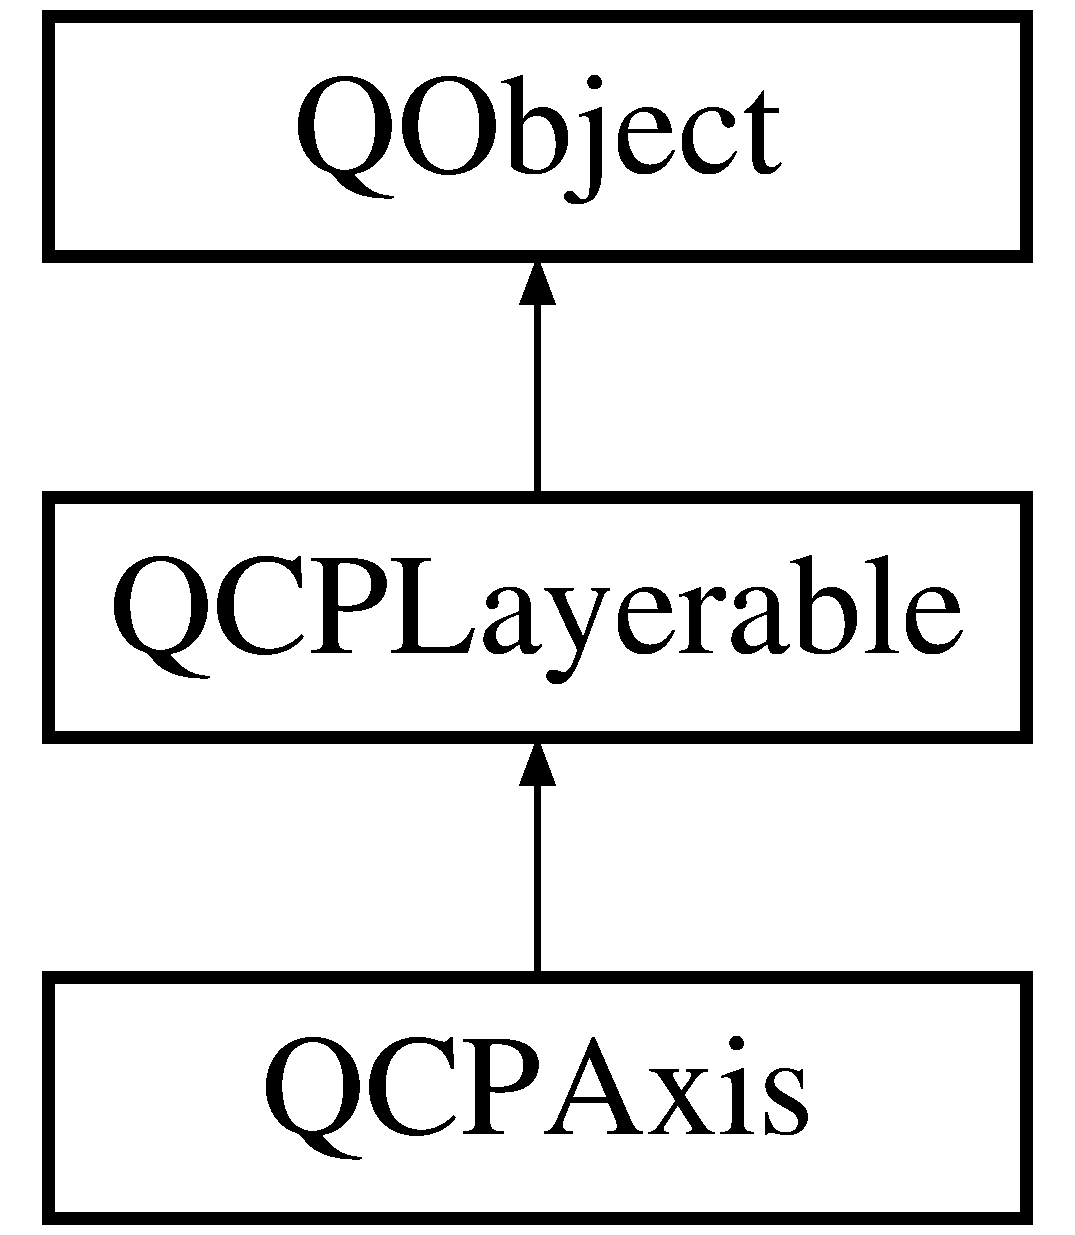
\includegraphics[height=3.000000cm]{class_q_c_p_axis}
\end{center}
\end{figure}
\subsection*{Public Types}
\begin{DoxyCompactItemize}
\item 
enum \hyperlink{class_q_c_p_axis_ae2bcc1728b382f10f064612b368bc18a}{Axis\+Type} \{ \hyperlink{class_q_c_p_axis_ae2bcc1728b382f10f064612b368bc18aaf84aa6cac6fb6099f54a2cbf7546b730}{at\+Left} = 0x01, 
\hyperlink{class_q_c_p_axis_ae2bcc1728b382f10f064612b368bc18aadf5509f7d29199ef2f263b1dd224b345}{at\+Right} = 0x02, 
\hyperlink{class_q_c_p_axis_ae2bcc1728b382f10f064612b368bc18aac0ece2b680d3f545e701f75af1655977}{at\+Top} = 0x04, 
\hyperlink{class_q_c_p_axis_ae2bcc1728b382f10f064612b368bc18aa220d68888516b6c3b493d144f1ba438f}{at\+Bottom} = 0x08
 \}
\item 
enum \hyperlink{class_q_c_p_axis_a4a7da0166f755f5abac23b765d184cad}{Label\+Type} \{ \hyperlink{class_q_c_p_axis_a4a7da0166f755f5abac23b765d184cada7f1eacf3b73adaefd334bea04e094b7e}{lt\+Number}, 
\hyperlink{class_q_c_p_axis_a4a7da0166f755f5abac23b765d184cadafc70594a9d877124dd11ccc187d4ac52}{lt\+Date\+Time}
 \}
\item 
enum \hyperlink{class_q_c_p_axis_a24b13374b9b8f75f47eed2ea78c37db9}{Label\+Side} \{ \hyperlink{class_q_c_p_axis_a24b13374b9b8f75f47eed2ea78c37db9aae7b027ac2839cf4ad611df30236fc3f}{ls\+Inside}, 
\hyperlink{class_q_c_p_axis_a24b13374b9b8f75f47eed2ea78c37db9a2eadb509fc0c9a8b35b85c86ec9f3c7a}{ls\+Outside}
 \}
\item 
enum \hyperlink{class_q_c_p_axis_a36d8e8658dbaa179bf2aeb973db2d6f0}{Scale\+Type} \{ \hyperlink{class_q_c_p_axis_a36d8e8658dbaa179bf2aeb973db2d6f0aff6e30a11a828bc850caffab0ff994f6}{st\+Linear}, 
\hyperlink{class_q_c_p_axis_a36d8e8658dbaa179bf2aeb973db2d6f0abf5b785ad976618816dc6f79b73216d4}{st\+Logarithmic}
 \}
\item 
enum \hyperlink{class_q_c_p_axis_abee4c7a54c468b1385dfce2c898b115f}{Selectable\+Part} \{ \hyperlink{class_q_c_p_axis_abee4c7a54c468b1385dfce2c898b115fae0df8123a5528d5ccf87cb7794f971ea}{sp\+None} = 0, 
\hyperlink{class_q_c_p_axis_abee4c7a54c468b1385dfce2c898b115fa8949d2c1a31eccae9be7ed32e7a1ae38}{sp\+Axis} = 0x001, 
\hyperlink{class_q_c_p_axis_abee4c7a54c468b1385dfce2c898b115fa584e0a3dc4d064880647619f4bd4e771}{sp\+Tick\+Labels} = 0x002, 
\hyperlink{class_q_c_p_axis_abee4c7a54c468b1385dfce2c898b115fa851e0600e0d08b4f5fee9361e3fedabd}{sp\+Axis\+Label} = 0x004
 \}
\end{DoxyCompactItemize}
\subsection*{Signals}
\begin{DoxyCompactItemize}
\item 
void \hyperlink{class_q_c_p_axis_af46d99613d29518795134ec4928e3873}{ticks\+Request} ()
\item 
void \hyperlink{class_q_c_p_axis_a0894084e4c16a1736534c4095746f910}{range\+Changed} (const \hyperlink{class_q_c_p_range}{Q\+C\+P\+Range} \&new\+Range)
\item 
void \hyperlink{class_q_c_p_axis_aac8576288e8e31f16186124bc10dd10d}{range\+Changed} (const \hyperlink{class_q_c_p_range}{Q\+C\+P\+Range} \&new\+Range, const \hyperlink{class_q_c_p_range}{Q\+C\+P\+Range} \&old\+Range)
\item 
void \hyperlink{class_q_c_p_axis_a3505ed8a93bd2e349d858d84996bf767}{scale\+Type\+Changed} (\hyperlink{class_q_c_p_axis_a36d8e8658dbaa179bf2aeb973db2d6f0}{Q\+C\+P\+Axis\+::\+Scale\+Type} \hyperlink{class_q_c_p_axis_a8563e13407bc0616da7f7c84e02de170}{scale\+Type})
\item 
void \hyperlink{class_q_c_p_axis_a62b598abeee7174a05f9d542cc85b1f5}{selection\+Changed} (const Q\+C\+P\+Axis\+::\+Selectable\+Parts \&parts)
\item 
void \hyperlink{class_q_c_p_axis_aa5ff1fd851139028a3bb4efcb31de9fc}{selectable\+Changed} (const Q\+C\+P\+Axis\+::\+Selectable\+Parts \&parts)
\end{DoxyCompactItemize}
\subsection*{Public Member Functions}
\begin{DoxyCompactItemize}
\item 
\hyperlink{class_q_c_p_axis_ac62c042968bae0e6d474fcfc57c9b71f}{Q\+C\+P\+Axis} (\hyperlink{class_q_c_p_axis_rect}{Q\+C\+P\+Axis\+Rect} $\ast$parent, \hyperlink{class_q_c_p_axis_ae2bcc1728b382f10f064612b368bc18a}{Axis\+Type} type)
\item 
virtual \hyperlink{class_q_c_p_axis_a7cfa27ea9da0bb1fe0ae995572c0b85d}{$\sim$\+Q\+C\+P\+Axis} ()
\item 
\hyperlink{class_q_c_p_axis_ae2bcc1728b382f10f064612b368bc18a}{Axis\+Type} \hyperlink{class_q_c_p_axis_a593c37bf6aa4990326dc09e24f45db7f}{axis\+Type} () const 
\item 
\hyperlink{class_q_c_p_axis_rect}{Q\+C\+P\+Axis\+Rect} $\ast$ \hyperlink{class_q_c_p_axis_aada3102af43b029e3879bcbf2bddfabb}{axis\+Rect} () const 
\item 
\hyperlink{class_q_c_p_axis_a36d8e8658dbaa179bf2aeb973db2d6f0}{Scale\+Type} \hyperlink{class_q_c_p_axis_a8563e13407bc0616da7f7c84e02de170}{scale\+Type} () const 
\item 
double \hyperlink{class_q_c_p_axis_ac937d2a602f865aff2ab6c1e288739f6}{scale\+Log\+Base} () const 
\item 
const \hyperlink{class_q_c_p_range}{Q\+C\+P\+Range} \hyperlink{class_q_c_p_axis_ab1ea79a4f5ea4cf42620f8f51c477ac4}{range} () const 
\item 
bool \hyperlink{class_q_c_p_axis_ade26dc7994ccd8a11f64fd83377ee021}{range\+Reversed} () const 
\item 
bool \hyperlink{class_q_c_p_axis_afc7f20e30dc2865ff6c39f3281f330c2}{auto\+Ticks} () const 
\item 
int \hyperlink{class_q_c_p_axis_ac87454a1342f5d2939ab59e68b4d515b}{auto\+Tick\+Count} () const 
\item 
bool \hyperlink{class_q_c_p_axis_a7169da316ac25dec1606784152fbf2c1}{auto\+Tick\+Labels} () const 
\item 
bool \hyperlink{class_q_c_p_axis_ae762920261b0c24beb56b893e5a2471d}{auto\+Tick\+Step} () const 
\item 
bool \hyperlink{class_q_c_p_axis_ab9a950e16f373fe5c4b79078bb97c171}{auto\+Sub\+Ticks} () const 
\item 
bool \hyperlink{class_q_c_p_axis_a61c504ec7c5bed9a63edf45345995d10}{ticks} () const 
\item 
bool \hyperlink{class_q_c_p_axis_a9a78fcccd98a73d37b3d991df7b6ef1d}{tick\+Labels} () const 
\item 
int \hyperlink{class_q_c_p_axis_af7bc2fac3f95949ecd0204d20dc1463b}{tick\+Label\+Padding} () const 
\item 
\hyperlink{class_q_c_p_axis_a4a7da0166f755f5abac23b765d184cad}{Label\+Type} \hyperlink{class_q_c_p_axis_a8a6f58a1ce12cfc4fadd379167668e8d}{tick\+Label\+Type} () const 
\item 
Q\+Font \hyperlink{class_q_c_p_axis_af6d7ad17f3398b114a413f7a3dc5ef9d}{tick\+Label\+Font} () const 
\item 
Q\+Color \hyperlink{class_q_c_p_axis_ac86d0636aa55ddd94df171f609897a32}{tick\+Label\+Color} () const 
\item 
double \hyperlink{class_q_c_p_axis_ab9199d72b8c4c06cc6c9b928c30d00d2}{tick\+Label\+Rotation} () const 
\item 
\hyperlink{class_q_c_p_axis_a24b13374b9b8f75f47eed2ea78c37db9}{Label\+Side} \hyperlink{class_q_c_p_axis_a0a33835705406506b02a445b1ba32357}{tick\+Label\+Side} () const 
\item 
Q\+String \hyperlink{class_q_c_p_axis_a132b54ae184a12ed24c9af24f53dc70b}{date\+Time\+Format} () const 
\item 
Qt\+::\+Time\+Spec \hyperlink{class_q_c_p_axis_afdd04c56ed29a9d948f840fc76f0d383}{date\+Time\+Spec} () const 
\item 
Q\+String \hyperlink{class_q_c_p_axis_ae6729b40845b29ffa5a440aa53cec215}{number\+Format} () const 
\item 
int \hyperlink{class_q_c_p_axis_a91cb2825060ac79a889296377fe0c7c1}{number\+Precision} () const 
\item 
double \hyperlink{class_q_c_p_axis_a0e6120d24266544441ab691f316a1b03}{tick\+Step} () const 
\item 
Q\+Vector$<$ double $>$ \hyperlink{class_q_c_p_axis_a5b00b14f480f926df976cc6c52309e78}{tick\+Vector} () const 
\item 
Q\+Vector$<$ Q\+String $>$ \hyperlink{class_q_c_p_axis_a64e6fa81f943ad33dcaf3fa606687b93}{tick\+Vector\+Labels} () const 
\item 
int \hyperlink{class_q_c_p_axis_a59265d65c5034695ac2578bccbbb0f4a}{tick\+Length\+In} () const 
\item 
int \hyperlink{class_q_c_p_axis_ae1b3d7473f50ba8544b2027c1cdc80f2}{tick\+Length\+Out} () const 
\item 
int \hyperlink{class_q_c_p_axis_a290b4c1375476826daa10e914cb71dab}{sub\+Tick\+Count} () const 
\item 
int \hyperlink{class_q_c_p_axis_a052e6ab2ada7e87fa5e5831dcbd4a517}{sub\+Tick\+Length\+In} () const 
\item 
int \hyperlink{class_q_c_p_axis_a091fdf8d1b3f9660e38b854578efb9bc}{sub\+Tick\+Length\+Out} () const 
\item 
Q\+Pen \hyperlink{class_q_c_p_axis_a4f6a7cd46fb104b1dad93e29cc78fe74}{base\+Pen} () const 
\item 
Q\+Pen \hyperlink{class_q_c_p_axis_a5eb206da4265c6c083db71d692da3bc4}{tick\+Pen} () const 
\item 
Q\+Pen \hyperlink{class_q_c_p_axis_a2e8bce6dd03e393dbdf6bb427461a726}{sub\+Tick\+Pen} () const 
\item 
Q\+Font \hyperlink{class_q_c_p_axis_ae8029ae0b32e9d4d73dddcdd0a08c838}{label\+Font} () const 
\item 
Q\+Color \hyperlink{class_q_c_p_axis_a7854c2875e3b8d86b210d108bd87aeb9}{label\+Color} () const 
\item 
Q\+String \hyperlink{class_q_c_p_axis_ab3486dca5a6e9e3ca0e32678272ba549}{label} () const 
\item 
int \hyperlink{class_q_c_p_axis_a59c9a0e362dec811491fc9a0709d2afa}{label\+Padding} () const 
\item 
int \hyperlink{class_q_c_p_axis_abb85015a9467ec176e70698307ec833a}{padding} () const 
\item 
int \hyperlink{class_q_c_p_axis_aebc032ac6eea164a02859c017f52d5e7}{offset} () const 
\item 
Selectable\+Parts \hyperlink{class_q_c_p_axis_a08323248a1cba4750ef07ceea159e0b3}{selected\+Parts} () const 
\item 
Selectable\+Parts \hyperlink{class_q_c_p_axis_ad2bff3d2ed3d35c10d44c0c02441bd2c}{selectable\+Parts} () const 
\item 
Q\+Font \hyperlink{class_q_c_p_axis_ae245bb3dcd0ec71eee38437de6e719f7}{selected\+Tick\+Label\+Font} () const 
\item 
Q\+Font \hyperlink{class_q_c_p_axis_a078bbc88b33595a5308350c2889c96d4}{selected\+Label\+Font} () const 
\item 
Q\+Color \hyperlink{class_q_c_p_axis_a5a3af4bd1a820bb7c6d4c85e1d8d452f}{selected\+Tick\+Label\+Color} () const 
\item 
Q\+Color \hyperlink{class_q_c_p_axis_a8cf8de6ac7f1ca617e05412f669ed229}{selected\+Label\+Color} () const 
\item 
Q\+Pen \hyperlink{class_q_c_p_axis_a5a3919ad7b60c2789b04c7e72387cfd6}{selected\+Base\+Pen} () const 
\item 
Q\+Pen \hyperlink{class_q_c_p_axis_a9f86ef82e1d1a908ab4c68cfa5fe4175}{selected\+Tick\+Pen} () const 
\item 
Q\+Pen \hyperlink{class_q_c_p_axis_a1b264fdfef48c22aba36e76de7856784}{selected\+Sub\+Tick\+Pen} () const 
\item 
\hyperlink{class_q_c_p_line_ending}{Q\+C\+P\+Line\+Ending} \hyperlink{class_q_c_p_axis_ac85aebbedf67d7bc9e1e5c182151536b}{lower\+Ending} () const 
\item 
\hyperlink{class_q_c_p_line_ending}{Q\+C\+P\+Line\+Ending} \hyperlink{class_q_c_p_axis_aad503ac95ee34e614ffee0bd66473e1a}{upper\+Ending} () const 
\item 
\hyperlink{class_q_c_p_grid}{Q\+C\+P\+Grid} $\ast$ \hyperlink{class_q_c_p_axis_ac4fb913cce3072b5e75a4635e0f6cd04}{grid} () const 
\item 
Q\+\_\+\+S\+L\+O\+T void \hyperlink{class_q_c_p_axis_adef29cae617af4f519f6c40d1a866ca6}{set\+Scale\+Type} (\hyperlink{class_q_c_p_axis_a36d8e8658dbaa179bf2aeb973db2d6f0}{Q\+C\+P\+Axis\+::\+Scale\+Type} type)
\item 
void \hyperlink{class_q_c_p_axis_a726186054be90487885a748aa1b42188}{set\+Scale\+Log\+Base} (double base)
\item 
Q\+\_\+\+S\+L\+O\+T void \hyperlink{class_q_c_p_axis_aebdfea5d44c3a0ad2b4700cd4d25b641}{set\+Range} (const \hyperlink{class_q_c_p_range}{Q\+C\+P\+Range} \&\hyperlink{class_q_c_p_axis_ab1ea79a4f5ea4cf42620f8f51c477ac4}{range})
\item 
void \hyperlink{class_q_c_p_axis_a57d6ee9e9009fe88cb19db476ec70bca}{set\+Range} (double lower, double upper)
\item 
void \hyperlink{class_q_c_p_axis_acf60e5b2d631fbc8c4548c3d579cb6d0}{set\+Range} (double position, double size, Qt\+::\+Alignment\+Flag alignment)
\item 
void \hyperlink{class_q_c_p_axis_afcf51227d337db28d1a9ce9a4d1bc91a}{set\+Range\+Lower} (double lower)
\item 
void \hyperlink{class_q_c_p_axis_acd3ca1247aa867b540cd5ec30ccd3bef}{set\+Range\+Upper} (double upper)
\item 
void \hyperlink{class_q_c_p_axis_a2172fdb196b1a0dc3f40992fcad8e9e1}{set\+Range\+Reversed} (bool reversed)
\item 
void \hyperlink{class_q_c_p_axis_ae867c23d3a6a7bd4d09cc66c5d018f63}{set\+Auto\+Ticks} (bool on)
\item 
void \hyperlink{class_q_c_p_axis_a7c7111cbeac9ec5fcb40f93a1ef51a0b}{set\+Auto\+Tick\+Count} (int approximate\+Count)
\item 
void \hyperlink{class_q_c_p_axis_aaa47e3a6bac0c20d4beb9028f01bc1a1}{set\+Auto\+Tick\+Labels} (bool on)
\item 
void \hyperlink{class_q_c_p_axis_a99fe77b034e06f5b723995beab96e741}{set\+Auto\+Tick\+Step} (bool on)
\item 
void \hyperlink{class_q_c_p_axis_adcbdec7a60054b88571e89599f4a45bf}{set\+Auto\+Sub\+Ticks} (bool on)
\item 
void \hyperlink{class_q_c_p_axis_ac891409315bc379e3b1abdb162c1a011}{set\+Ticks} (bool show)
\item 
void \hyperlink{class_q_c_p_axis_a04ba16e1f6f78d70f938519576ed32c8}{set\+Tick\+Labels} (bool show)
\item 
void \hyperlink{class_q_c_p_axis_af302c479af9dbc2e9f0e44e07c0012ee}{set\+Tick\+Label\+Padding} (int \hyperlink{class_q_c_p_axis_abb85015a9467ec176e70698307ec833a}{padding})
\item 
void \hyperlink{class_q_c_p_axis_a54f24f5ce8feea25209388a863d7e448}{set\+Tick\+Label\+Type} (\hyperlink{class_q_c_p_axis_a4a7da0166f755f5abac23b765d184cad}{Label\+Type} type)
\item 
void \hyperlink{class_q_c_p_axis_a2b8690c4e8dbc39d9185d2b398ce7a6c}{set\+Tick\+Label\+Font} (const Q\+Font \&font)
\item 
void \hyperlink{class_q_c_p_axis_a395e445c3fe496b935bee7b911ecfd1c}{set\+Tick\+Label\+Color} (const Q\+Color \&color)
\item 
void \hyperlink{class_q_c_p_axis_a1bddd4413df8a576b7ad4b067fb33375}{set\+Tick\+Label\+Rotation} (double degrees)
\item 
void \hyperlink{class_q_c_p_axis_a13ec644fc6e22715744c92c6dfa4f0fa}{set\+Tick\+Label\+Side} (\hyperlink{class_q_c_p_axis_a24b13374b9b8f75f47eed2ea78c37db9}{Label\+Side} side)
\item 
void \hyperlink{class_q_c_p_axis_a2ee0191daa03524a682113e63e05f7a7}{set\+Date\+Time\+Format} (const Q\+String \&format)
\item 
void \hyperlink{class_q_c_p_axis_a262e06731debed7eee11fa6a81d67eaf}{set\+Date\+Time\+Spec} (const Qt\+::\+Time\+Spec \&time\+Spec)
\item 
void \hyperlink{class_q_c_p_axis_ae585a54dc2aac662e90a2ca82f002590}{set\+Number\+Format} (const Q\+String \&format\+Code)
\item 
void \hyperlink{class_q_c_p_axis_a21dc8023ad7500382ad9574b48137e63}{set\+Number\+Precision} (int precision)
\item 
void \hyperlink{class_q_c_p_axis_af727db0acc6492c4c774c0700e738205}{set\+Tick\+Step} (double step)
\item 
void \hyperlink{class_q_c_p_axis_a871db94c5d796c80fcbe1a9d4506e27e}{set\+Tick\+Vector} (const Q\+Vector$<$ double $>$ \&vec)
\item 
void \hyperlink{class_q_c_p_axis_a921d3ba3853ca3bd2cce3459f7a243ed}{set\+Tick\+Vector\+Labels} (const Q\+Vector$<$ Q\+String $>$ \&vec)
\item 
void \hyperlink{class_q_c_p_axis_a62ec40bebe3540e9c1479a8fd2be3b0d}{set\+Tick\+Length} (int inside, int outside=0)
\item 
void \hyperlink{class_q_c_p_axis_afae1a37a99611366275a51204d991739}{set\+Tick\+Length\+In} (int inside)
\item 
void \hyperlink{class_q_c_p_axis_a3b8a0debd1ffedd2c22d0592dfbb4e62}{set\+Tick\+Length\+Out} (int outside)
\item 
void \hyperlink{class_q_c_p_axis_a4b1554ead9d7f9799650d51383e326dd}{set\+Sub\+Tick\+Count} (int count)
\item 
void \hyperlink{class_q_c_p_axis_ab702d6fd42fc620607435339a1c2a2e1}{set\+Sub\+Tick\+Length} (int inside, int outside=0)
\item 
void \hyperlink{class_q_c_p_axis_ac46fa2a993a9f5789540977610acf1de}{set\+Sub\+Tick\+Length\+In} (int inside)
\item 
void \hyperlink{class_q_c_p_axis_a4c6dfc3963492ed72a77724012df5f23}{set\+Sub\+Tick\+Length\+Out} (int outside)
\item 
void \hyperlink{class_q_c_p_axis_a778d45fb71b3c7ab3bb7079e18b058e4}{set\+Base\+Pen} (const Q\+Pen \&pen)
\item 
void \hyperlink{class_q_c_p_axis_ad80923bcc1c5da4c4db602c5325e797e}{set\+Tick\+Pen} (const Q\+Pen \&pen)
\item 
void \hyperlink{class_q_c_p_axis_aede4028ae7516bd51a60618a8233f9cf}{set\+Sub\+Tick\+Pen} (const Q\+Pen \&pen)
\item 
void \hyperlink{class_q_c_p_axis_a71ac1a47f7547e490a8c4311d1433cf3}{set\+Label\+Font} (const Q\+Font \&font)
\item 
void \hyperlink{class_q_c_p_axis_a6c906fe56d75f0122335b9f79b999608}{set\+Label\+Color} (const Q\+Color \&color)
\item 
void \hyperlink{class_q_c_p_axis_a33bcc382c111c9f31bb0687352a2dea4}{set\+Label} (const Q\+String \&str)
\item 
void \hyperlink{class_q_c_p_axis_a4391192a766e5d20cfe5cbc17607a7a2}{set\+Label\+Padding} (int \hyperlink{class_q_c_p_axis_abb85015a9467ec176e70698307ec833a}{padding})
\item 
void \hyperlink{class_q_c_p_axis_a5691441cb3de9e9844855d339c0db279}{set\+Padding} (int \hyperlink{class_q_c_p_axis_abb85015a9467ec176e70698307ec833a}{padding})
\item 
void \hyperlink{class_q_c_p_axis_a04a652603cbe50eba9969ee6d68873c3}{set\+Offset} (int \hyperlink{class_q_c_p_axis_aebc032ac6eea164a02859c017f52d5e7}{offset})
\item 
void \hyperlink{class_q_c_p_axis_a845ccb560b7bc5281098a5be494145f6}{set\+Selected\+Tick\+Label\+Font} (const Q\+Font \&font)
\item 
void \hyperlink{class_q_c_p_axis_a02ec2a75d4d8401eaab834fbc6803d30}{set\+Selected\+Label\+Font} (const Q\+Font \&font)
\item 
void \hyperlink{class_q_c_p_axis_a9bdbf5e63ab15187f3a1de9440129227}{set\+Selected\+Tick\+Label\+Color} (const Q\+Color \&color)
\item 
void \hyperlink{class_q_c_p_axis_a5d502dec597c634f491fdd73d151c72d}{set\+Selected\+Label\+Color} (const Q\+Color \&color)
\item 
void \hyperlink{class_q_c_p_axis_aeb917a909215605b95ef2be843de1ee8}{set\+Selected\+Base\+Pen} (const Q\+Pen \&pen)
\item 
void \hyperlink{class_q_c_p_axis_a8360502685eb782edbf04019c9345cdc}{set\+Selected\+Tick\+Pen} (const Q\+Pen \&pen)
\item 
void \hyperlink{class_q_c_p_axis_a2a00a7166600155eac26843132eb9576}{set\+Selected\+Sub\+Tick\+Pen} (const Q\+Pen \&pen)
\item 
Q\+\_\+\+S\+L\+O\+T void \hyperlink{class_q_c_p_axis_a513f9b9e326c505d9bec54880031b085}{set\+Selectable\+Parts} (const Q\+C\+P\+Axis\+::\+Selectable\+Parts \&\hyperlink{class_q_c_p_axis_ad2bff3d2ed3d35c10d44c0c02441bd2c}{selectable\+Parts})
\item 
Q\+\_\+\+S\+L\+O\+T void \hyperlink{class_q_c_p_axis_ab9d7a69277dcbed9119b3c1f25ca19c3}{set\+Selected\+Parts} (const Q\+C\+P\+Axis\+::\+Selectable\+Parts \&\hyperlink{class_q_c_p_axis_a08323248a1cba4750ef07ceea159e0b3}{selected\+Parts})
\item 
void \hyperlink{class_q_c_p_axis_a08af1c72db9ae4dc8cb8a973d44405ab}{set\+Lower\+Ending} (const \hyperlink{class_q_c_p_line_ending}{Q\+C\+P\+Line\+Ending} \&ending)
\item 
void \hyperlink{class_q_c_p_axis_a69119b892fc306f651763596685aa377}{set\+Upper\+Ending} (const \hyperlink{class_q_c_p_line_ending}{Q\+C\+P\+Line\+Ending} \&ending)
\item 
virtual double \hyperlink{class_q_c_p_axis_a2877a6230920c118be65c6113089f467}{select\+Test} (const Q\+Point\+F \&pos, bool only\+Selectable, Q\+Variant $\ast$details=0) const 
\item 
Qt\+::\+Orientation \hyperlink{class_q_c_p_axis_a57483f2f60145ddc9e63f3af53959265}{orientation} () const 
\item 
void \hyperlink{class_q_c_p_axis_a18f3a68f2b691af1fd34b6593c886630}{move\+Range} (double diff)
\item 
void \hyperlink{class_q_c_p_axis_a7072ff96fe690148f1bbcdb4f773ea1c}{scale\+Range} (double factor, double center)
\item 
void \hyperlink{class_q_c_p_axis_af4bbd446dcaee5a83ac30ce9bcd6e125}{set\+Scale\+Ratio} (const \hyperlink{class_q_c_p_axis}{Q\+C\+P\+Axis} $\ast$other\+Axis, double ratio=1.\+0)
\item 
void \hyperlink{class_q_c_p_axis_a499345f02ebce4b23d8ccec96e58daa9}{rescale} (bool only\+Visible\+Plottables=false)
\item 
double \hyperlink{class_q_c_p_axis_ae9289ef7043b9d966af88eaa95b037d1}{pixel\+To\+Coord} (double value) const 
\item 
double \hyperlink{class_q_c_p_axis_a985ae693b842fb0422b4390fe36d299a}{coord\+To\+Pixel} (double value) const 
\item 
\hyperlink{class_q_c_p_axis_abee4c7a54c468b1385dfce2c898b115f}{Selectable\+Part} \hyperlink{class_q_c_p_axis_ab2965a8ab1da948b897f1c006080760b}{get\+Part\+At} (const Q\+Point\+F \&pos) const 
\item 
Q\+List$<$ \hyperlink{class_q_c_p_abstract_plottable}{Q\+C\+P\+Abstract\+Plottable} $\ast$ $>$ \hyperlink{class_q_c_p_axis_a4f7404494cccdbfc00e1e865b7ed16a4}{plottables} () const 
\item 
Q\+List$<$ \hyperlink{class_q_c_p_graph}{Q\+C\+P\+Graph} $\ast$ $>$ \hyperlink{class_q_c_p_axis_ad3919e7d7400f55446ea82018fe5e3a8}{graphs} () const 
\item 
Q\+List$<$ \hyperlink{class_q_c_p_abstract_item}{Q\+C\+P\+Abstract\+Item} $\ast$ $>$ \hyperlink{class_q_c_p_axis_ae437656a5fd1a03721a8f2d7aab460fe}{items} () const 
\end{DoxyCompactItemize}
\subsection*{Static Public Member Functions}
\begin{DoxyCompactItemize}
\item 
static \hyperlink{class_q_c_p_axis_ae2bcc1728b382f10f064612b368bc18a}{Axis\+Type} \hyperlink{class_q_c_p_axis_ac0a6b77bd52bec6c81cd62d167cfeba6}{margin\+Side\+To\+Axis\+Type} (\hyperlink{namespace_q_c_p_a7e487e3e2ccb62ab7771065bab7cae54}{Q\+C\+P\+::\+Margin\+Side} side)
\item 
static Qt\+::\+Orientation \hyperlink{class_q_c_p_axis_a9a68b3e45f1b1e33d4d807822342516c}{orientation} (\hyperlink{class_q_c_p_axis_ae2bcc1728b382f10f064612b368bc18a}{Axis\+Type} type)
\item 
static \hyperlink{class_q_c_p_axis_ae2bcc1728b382f10f064612b368bc18a}{Axis\+Type} \hyperlink{class_q_c_p_axis_aa85ba73dfee6483e23825461b725e363}{opposite} (\hyperlink{class_q_c_p_axis_ae2bcc1728b382f10f064612b368bc18a}{Axis\+Type} type)
\end{DoxyCompactItemize}
\subsection*{Protected Member Functions}
\begin{DoxyCompactItemize}
\item 
virtual void \hyperlink{class_q_c_p_axis_a57d9e961bae7d62f5b4e1f143e660c78}{setup\+Tick\+Vectors} ()
\item 
virtual void \hyperlink{class_q_c_p_axis_a626eef437c874148df1a5ac78506d463}{generate\+Auto\+Ticks} ()
\item 
virtual int \hyperlink{class_q_c_p_axis_a3c5c045019fcdc0843a3e064eda7478a}{calculate\+Auto\+Sub\+Tick\+Count} (double \hyperlink{class_q_c_p_axis_a0e6120d24266544441ab691f316a1b03}{tick\+Step}) const 
\item 
virtual int \hyperlink{class_q_c_p_axis_a47bdb0a55de6759489ee47665199aebb}{calculate\+Margin} ()
\item 
virtual void \hyperlink{class_q_c_p_axis_a13bde39eb1e0b7c14a02935689be8aba}{apply\+Default\+Antialiasing\+Hint} (\hyperlink{class_q_c_p_painter}{Q\+C\+P\+Painter} $\ast$painter) const 
\item 
virtual void \hyperlink{class_q_c_p_axis_a258b1e783eda5cd14ec5552c696a424e}{draw} (\hyperlink{class_q_c_p_painter}{Q\+C\+P\+Painter} $\ast$painter)
\item 
virtual \hyperlink{namespace_q_c_p_a2ad6bb6281c7c2d593d4277b44c2b037}{Q\+C\+P\+::\+Interaction} \hyperlink{class_q_c_p_axis_aca53b2f365dfc1257cba9e62395aa68f}{selection\+Category} () const 
\item 
virtual void \hyperlink{class_q_c_p_axis_aa8a5fe80e2898ec08ada26b5fbee9eca}{select\+Event} (Q\+Mouse\+Event $\ast$event, bool additive, const Q\+Variant \&details, bool $\ast$selection\+State\+Changed)
\item 
virtual void \hyperlink{class_q_c_p_axis_a53512242cde6ec21943a3ba10dbf78c3}{deselect\+Event} (bool $\ast$selection\+State\+Changed)
\item 
void \hyperlink{class_q_c_p_axis_a06320a944d1120732cc0d72fe1306d8b}{visible\+Tick\+Bounds} (int \&low\+Index, int \&high\+Index) const 
\item 
double \hyperlink{class_q_c_p_axis_a1385765db2419ee5fb5505a6cf9130fb}{base\+Log} (double value) const 
\item 
double \hyperlink{class_q_c_p_axis_a97d69f021a05126fcb978d0aefea47b8}{base\+Pow} (double value) const 
\item 
Q\+Pen \hyperlink{class_q_c_p_axis_a3eb0681d31baf579bb73b86a0153cb02}{get\+Base\+Pen} () const 
\item 
Q\+Pen \hyperlink{class_q_c_p_axis_a7f503910be40fb1717e1635be3ef17e1}{get\+Tick\+Pen} () const 
\item 
Q\+Pen \hyperlink{class_q_c_p_axis_ab4f7e60a40eb051c775afcaeab895c85}{get\+Sub\+Tick\+Pen} () const 
\item 
Q\+Font \hyperlink{class_q_c_p_axis_aef30b66668986523225089a67280ec7a}{get\+Tick\+Label\+Font} () const 
\item 
Q\+Font \hyperlink{class_q_c_p_axis_ab0768eb2879efb202645d19ff789e63e}{get\+Label\+Font} () const 
\item 
Q\+Color \hyperlink{class_q_c_p_axis_a0f8583f7ac24ccc70d39fdd2389cad6e}{get\+Tick\+Label\+Color} () const 
\item 
Q\+Color \hyperlink{class_q_c_p_axis_a42bd69b9e9c571f13624079be18ccdc1}{get\+Label\+Color} () const 
\end{DoxyCompactItemize}
\subsection*{Protected Attributes}
\begin{DoxyCompactItemize}
\item 
\hyperlink{class_q_c_p_axis_ae2bcc1728b382f10f064612b368bc18a}{Axis\+Type} \hyperlink{class_q_c_p_axis_ae704bf9f2c2b026f08dd4ccad79c616e}{m\+Axis\+Type}
\item 
\hyperlink{class_q_c_p_axis_rect}{Q\+C\+P\+Axis\+Rect} $\ast$ \hyperlink{class_q_c_p_axis_a6f150b65a202f32936997960e331dfcb}{m\+Axis\+Rect}
\item 
int \hyperlink{class_q_c_p_axis_a52a805a4f03231210e0880db7f77e098}{m\+Padding}
\item 
Qt\+::\+Orientation \hyperlink{class_q_c_p_axis_a048e1792fa86f4f86df55200b3f0be36}{m\+Orientation}
\item 
Selectable\+Parts \hyperlink{class_q_c_p_axis_ab9042d8a095998f27a28b39411d8b9c3}{m\+Selectable\+Parts}
\item 
Selectable\+Parts \hyperlink{class_q_c_p_axis_a8f1eb0abfe2ae64652aa46b360e841e4}{m\+Selected\+Parts}
\item 
Q\+Pen \hyperlink{class_q_c_p_axis_ad6b4a0aee9558fb35529e960b8fef72d}{m\+Base\+Pen}
\item 
Q\+Pen \hyperlink{class_q_c_p_axis_a80baa4e3c16f9b6edf3eccacd2a50fde}{m\+Selected\+Base\+Pen}
\item 
Q\+String \hyperlink{class_q_c_p_axis_ae8001dbdfc47685c1cf7b98b044460e6}{m\+Label}
\item 
Q\+Font \hyperlink{class_q_c_p_axis_a37442d470e30e19b81ecaf979a34d046}{m\+Label\+Font}
\item 
Q\+Font \hyperlink{class_q_c_p_axis_ae48fe3489afadc0b3cd003233e2bf19f}{m\+Selected\+Label\+Font}
\item 
Q\+Color \hyperlink{class_q_c_p_axis_a457a003bb1c2b6ab73e5a173ba7558fd}{m\+Label\+Color}
\item 
Q\+Color \hyperlink{class_q_c_p_axis_a94f57de3ba024471ca206d83cf2258dd}{m\+Selected\+Label\+Color}
\item 
bool \hyperlink{class_q_c_p_axis_a3e4315be072026644e69009557a2fa11}{m\+Tick\+Labels}
\item 
bool \hyperlink{class_q_c_p_axis_a721e496b342f272078c5ff84564e472f}{m\+Auto\+Tick\+Labels}
\item 
\hyperlink{class_q_c_p_axis_a4a7da0166f755f5abac23b765d184cad}{Label\+Type} \hyperlink{class_q_c_p_axis_a6e056c1cb1aab0eddebfebbcb78c8f90}{m\+Tick\+Label\+Type}
\item 
Q\+Font \hyperlink{class_q_c_p_axis_add79d1e39c4ed65869a1e9cc79043f3f}{m\+Tick\+Label\+Font}
\item 
Q\+Font \hyperlink{class_q_c_p_axis_a4f2e4919da9615dac612662c249b1119}{m\+Selected\+Tick\+Label\+Font}
\item 
Q\+Color \hyperlink{class_q_c_p_axis_a6384a749b3b56a97df081d8082321ab4}{m\+Tick\+Label\+Color}
\item 
Q\+Color \hyperlink{class_q_c_p_axis_a3bcad40902f45dc4c991a2c3e4d31d70}{m\+Selected\+Tick\+Label\+Color}
\item 
Q\+String \hyperlink{class_q_c_p_axis_a0b7ad83550d71daab4cfee2918e168e0}{m\+Date\+Time\+Format}
\item 
Qt\+::\+Time\+Spec \hyperlink{class_q_c_p_axis_af73bec228c1a3203dc8aef1e84a46759}{m\+Date\+Time\+Spec}
\item 
int \hyperlink{class_q_c_p_axis_acd76e8c783384d99ccc4a13797eec188}{m\+Number\+Precision}
\item 
Q\+Latin1\+Char \hyperlink{class_q_c_p_axis_a39594313deef458f425bba25cd337a8a}{m\+Number\+Format\+Char}
\item 
bool \hyperlink{class_q_c_p_axis_af03809bee3f3e35fcc38d25b6dd5003b}{m\+Number\+Beautiful\+Powers}
\item 
bool \hyperlink{class_q_c_p_axis_ab111e74bba22e06848897c932fc549fe}{m\+Ticks}
\item 
double \hyperlink{class_q_c_p_axis_a4fe96830fc5a2711e20fe5edccfe2ed3}{m\+Tick\+Step}
\item 
int \hyperlink{class_q_c_p_axis_ad70198e6ae2801fc409bc3caec707da9}{m\+Sub\+Tick\+Count}
\item 
int \hyperlink{class_q_c_p_axis_a499fbb67111e4b204738f6c1aa28d842}{m\+Auto\+Tick\+Count}
\item 
bool \hyperlink{class_q_c_p_axis_aac23adcbae246bf165d4539ad65ac9f9}{m\+Auto\+Ticks}
\item 
bool \hyperlink{class_q_c_p_axis_aada8934a5c44978653031782aa37d101}{m\+Auto\+Tick\+Step}
\item 
bool \hyperlink{class_q_c_p_axis_aaae980b0d193d959674e314dbb6c2c3b}{m\+Auto\+Sub\+Ticks}
\item 
Q\+Pen \hyperlink{class_q_c_p_axis_a1d52c78c856d8bd1f331d4ec4e63d944}{m\+Tick\+Pen}
\item 
Q\+Pen \hyperlink{class_q_c_p_axis_a9524593dbc75a5c5b29dbd1cb4b37df5}{m\+Selected\+Tick\+Pen}
\item 
Q\+Pen \hyperlink{class_q_c_p_axis_a32ef56d3a417866720eb12667d27dbd1}{m\+Sub\+Tick\+Pen}
\item 
Q\+Pen \hyperlink{class_q_c_p_axis_aa5cc6afc5dc2a365f5abbd36eb04a1dc}{m\+Selected\+Sub\+Tick\+Pen}
\item 
\hyperlink{class_q_c_p_range}{Q\+C\+P\+Range} \hyperlink{class_q_c_p_axis_a1ee36773c49062d751560e11f90845f7}{m\+Range}
\item 
bool \hyperlink{class_q_c_p_axis_a5cb034f57aa3d773a9ca55a0931dbf7b}{m\+Range\+Reversed}
\item 
\hyperlink{class_q_c_p_axis_a36d8e8658dbaa179bf2aeb973db2d6f0}{Scale\+Type} \hyperlink{class_q_c_p_axis_ad706039549cbbbec5fcb2baf7894e04d}{m\+Scale\+Type}
\item 
double \hyperlink{class_q_c_p_axis_abc727ddb4af745151755d1b5e60d03c3}{m\+Scale\+Log\+Base}
\item 
double \hyperlink{class_q_c_p_axis_a93e068984b475467929e7f6768754227}{m\+Scale\+Log\+Base\+Log\+Inv}
\item 
\hyperlink{class_q_c_p_grid}{Q\+C\+P\+Grid} $\ast$ \hyperlink{class_q_c_p_axis_a17bffb94aaa40311f259c6ac7bcb5d5f}{m\+Grid}
\item 
\hyperlink{class_q_c_p_axis_painter_private}{Q\+C\+P\+Axis\+Painter\+Private} $\ast$ \hyperlink{class_q_c_p_axis_aeeae00935bd2dab82d64f32544a90913}{m\+Axis\+Painter}
\item 
int \hyperlink{class_q_c_p_axis_aebb24ba8734b7e054efc6e1ecc5414c7}{m\+Lowest\+Visible\+Tick}
\item 
int \hyperlink{class_q_c_p_axis_abb3b3ccce7e9779fef2be91ce1a46ef0}{m\+Highest\+Visible\+Tick}
\item 
Q\+Vector$<$ double $>$ \hyperlink{class_q_c_p_axis_aae0f9b9973b85be601200f00f5825087}{m\+Tick\+Vector}
\item 
Q\+Vector$<$ Q\+String $>$ \hyperlink{class_q_c_p_axis_aeee4bd0fca3f587eafe33843d1cb4f82}{m\+Tick\+Vector\+Labels}
\item 
Q\+Vector$<$ double $>$ \hyperlink{class_q_c_p_axis_a28353081e0ff35c3fe5ced923a287faa}{m\+Sub\+Tick\+Vector}
\item 
bool \hyperlink{class_q_c_p_axis_a2cde37b6e385f47e11322df4ac1b0e9b}{m\+Cached\+Margin\+Valid}
\item 
int \hyperlink{class_q_c_p_axis_a48ace55cbd54f7241e7f1b06fd369b64}{m\+Cached\+Margin}
\end{DoxyCompactItemize}
\subsection*{Friends}
\begin{DoxyCompactItemize}
\item 
class \hyperlink{class_q_c_p_axis_a1cdf9df76adcfae45261690aa0ca2198}{Q\+Custom\+Plot}
\item 
class \hyperlink{class_q_c_p_axis_a061e177f585549fc31f780852e2bd6fe}{Q\+C\+P\+Grid}
\item 
class \hyperlink{class_q_c_p_axis_acbf20ecb140f66c5fd1bc64ae0762990}{Q\+C\+P\+Axis\+Rect}
\end{DoxyCompactItemize}


\subsection{Detailed Description}
Manages a single axis inside a \hyperlink{class_q_custom_plot}{Q\+Custom\+Plot}. 

Usually doesn\textquotesingle{}t need to be instantiated externally. Access Q\+Custom\+Plot\textquotesingle{}s default four axes via \hyperlink{class_q_custom_plot_a9a79cd0158a4c7f30cbc702f0fd800e4}{Q\+Custom\+Plot\+::x\+Axis} (bottom), \hyperlink{class_q_custom_plot_af6fea5679725b152c14facd920b19367}{Q\+Custom\+Plot\+::y\+Axis} (left), \hyperlink{class_q_custom_plot_ada41599f22cad901c030f3dcbdd82fd9}{Q\+Custom\+Plot\+::x\+Axis2} (top) and \hyperlink{class_q_custom_plot_af13fdc5bce7d0fabd640f13ba805c0b7}{Q\+Custom\+Plot\+::y\+Axis2} (right).

Axes are always part of an axis rect, see \hyperlink{class_q_c_p_axis_rect}{Q\+C\+P\+Axis\+Rect}.  \begin{center}Naming convention of axis parts\end{center}  ~\newline
  \begin{center}Overview of the spacings and paddings that define the geometry of an axis. The dashed gray line on the left represents the \hyperlink{class_q_custom_plot}{Q\+Custom\+Plot} widget border.\end{center}  

\subsection{Member Enumeration Documentation}
\hypertarget{class_q_c_p_axis_ae2bcc1728b382f10f064612b368bc18a}{}\index{Q\+C\+P\+Axis@{Q\+C\+P\+Axis}!Axis\+Type@{Axis\+Type}}
\index{Axis\+Type@{Axis\+Type}!Q\+C\+P\+Axis@{Q\+C\+P\+Axis}}
\subsubsection[{Axis\+Type}]{\setlength{\rightskip}{0pt plus 5cm}enum {\bf Q\+C\+P\+Axis\+::\+Axis\+Type}}\label{class_q_c_p_axis_ae2bcc1728b382f10f064612b368bc18a}
Defines at which side of the axis rect the axis will appear. This also affects how the tick marks are drawn, on which side the labels are placed etc. \begin{Desc}
\item[Enumerator]\par
\begin{description}
\index{at\+Left@{at\+Left}!Q\+C\+P\+Axis@{Q\+C\+P\+Axis}}\index{Q\+C\+P\+Axis@{Q\+C\+P\+Axis}!at\+Left@{at\+Left}}\item[{\em 
\hypertarget{class_q_c_p_axis_ae2bcc1728b382f10f064612b368bc18aaf84aa6cac6fb6099f54a2cbf7546b730}{}at\+Left\label{class_q_c_p_axis_ae2bcc1728b382f10f064612b368bc18aaf84aa6cac6fb6099f54a2cbf7546b730}
}]{\ttfamily 0x01} Axis is vertical and on the left side of the axis rect \index{at\+Right@{at\+Right}!Q\+C\+P\+Axis@{Q\+C\+P\+Axis}}\index{Q\+C\+P\+Axis@{Q\+C\+P\+Axis}!at\+Right@{at\+Right}}\item[{\em 
\hypertarget{class_q_c_p_axis_ae2bcc1728b382f10f064612b368bc18aadf5509f7d29199ef2f263b1dd224b345}{}at\+Right\label{class_q_c_p_axis_ae2bcc1728b382f10f064612b368bc18aadf5509f7d29199ef2f263b1dd224b345}
}]{\ttfamily 0x02} Axis is vertical and on the right side of the axis rect \index{at\+Top@{at\+Top}!Q\+C\+P\+Axis@{Q\+C\+P\+Axis}}\index{Q\+C\+P\+Axis@{Q\+C\+P\+Axis}!at\+Top@{at\+Top}}\item[{\em 
\hypertarget{class_q_c_p_axis_ae2bcc1728b382f10f064612b368bc18aac0ece2b680d3f545e701f75af1655977}{}at\+Top\label{class_q_c_p_axis_ae2bcc1728b382f10f064612b368bc18aac0ece2b680d3f545e701f75af1655977}
}]{\ttfamily 0x04} Axis is horizontal and on the top side of the axis rect \index{at\+Bottom@{at\+Bottom}!Q\+C\+P\+Axis@{Q\+C\+P\+Axis}}\index{Q\+C\+P\+Axis@{Q\+C\+P\+Axis}!at\+Bottom@{at\+Bottom}}\item[{\em 
\hypertarget{class_q_c_p_axis_ae2bcc1728b382f10f064612b368bc18aa220d68888516b6c3b493d144f1ba438f}{}at\+Bottom\label{class_q_c_p_axis_ae2bcc1728b382f10f064612b368bc18aa220d68888516b6c3b493d144f1ba438f}
}]{\ttfamily 0x08} Axis is horizontal and on the bottom side of the axis rect \end{description}
\end{Desc}
\hypertarget{class_q_c_p_axis_a24b13374b9b8f75f47eed2ea78c37db9}{}\index{Q\+C\+P\+Axis@{Q\+C\+P\+Axis}!Label\+Side@{Label\+Side}}
\index{Label\+Side@{Label\+Side}!Q\+C\+P\+Axis@{Q\+C\+P\+Axis}}
\subsubsection[{Label\+Side}]{\setlength{\rightskip}{0pt plus 5cm}enum {\bf Q\+C\+P\+Axis\+::\+Label\+Side}}\label{class_q_c_p_axis_a24b13374b9b8f75f47eed2ea78c37db9}
Defines on which side of the axis the tick labels (numbers) shall appear.

\begin{DoxySeeAlso}{See also}
\hyperlink{class_q_c_p_axis_a13ec644fc6e22715744c92c6dfa4f0fa}{set\+Tick\+Label\+Side} 
\end{DoxySeeAlso}
\begin{Desc}
\item[Enumerator]\par
\begin{description}
\index{ls\+Inside@{ls\+Inside}!Q\+C\+P\+Axis@{Q\+C\+P\+Axis}}\index{Q\+C\+P\+Axis@{Q\+C\+P\+Axis}!ls\+Inside@{ls\+Inside}}\item[{\em 
\hypertarget{class_q_c_p_axis_a24b13374b9b8f75f47eed2ea78c37db9aae7b027ac2839cf4ad611df30236fc3f}{}ls\+Inside\label{class_q_c_p_axis_a24b13374b9b8f75f47eed2ea78c37db9aae7b027ac2839cf4ad611df30236fc3f}
}]Tick labels will be displayed inside the axis rect and clipped to the inner axis rect. \index{ls\+Outside@{ls\+Outside}!Q\+C\+P\+Axis@{Q\+C\+P\+Axis}}\index{Q\+C\+P\+Axis@{Q\+C\+P\+Axis}!ls\+Outside@{ls\+Outside}}\item[{\em 
\hypertarget{class_q_c_p_axis_a24b13374b9b8f75f47eed2ea78c37db9a2eadb509fc0c9a8b35b85c86ec9f3c7a}{}ls\+Outside\label{class_q_c_p_axis_a24b13374b9b8f75f47eed2ea78c37db9a2eadb509fc0c9a8b35b85c86ec9f3c7a}
}]Tick labels will be displayed outside the axis rect. \end{description}
\end{Desc}
\hypertarget{class_q_c_p_axis_a4a7da0166f755f5abac23b765d184cad}{}\index{Q\+C\+P\+Axis@{Q\+C\+P\+Axis}!Label\+Type@{Label\+Type}}
\index{Label\+Type@{Label\+Type}!Q\+C\+P\+Axis@{Q\+C\+P\+Axis}}
\subsubsection[{Label\+Type}]{\setlength{\rightskip}{0pt plus 5cm}enum {\bf Q\+C\+P\+Axis\+::\+Label\+Type}}\label{class_q_c_p_axis_a4a7da0166f755f5abac23b765d184cad}
When automatic tick label generation is enabled (\hyperlink{class_q_c_p_axis_aaa47e3a6bac0c20d4beb9028f01bc1a1}{set\+Auto\+Tick\+Labels}), defines how the coordinate of the tick is interpreted, i.\+e. translated into a string.

\begin{DoxySeeAlso}{See also}
\hyperlink{class_q_c_p_axis_a54f24f5ce8feea25209388a863d7e448}{set\+Tick\+Label\+Type} 
\end{DoxySeeAlso}
\begin{Desc}
\item[Enumerator]\par
\begin{description}
\index{lt\+Number@{lt\+Number}!Q\+C\+P\+Axis@{Q\+C\+P\+Axis}}\index{Q\+C\+P\+Axis@{Q\+C\+P\+Axis}!lt\+Number@{lt\+Number}}\item[{\em 
\hypertarget{class_q_c_p_axis_a4a7da0166f755f5abac23b765d184cada7f1eacf3b73adaefd334bea04e094b7e}{}lt\+Number\label{class_q_c_p_axis_a4a7da0166f755f5abac23b765d184cada7f1eacf3b73adaefd334bea04e094b7e}
}]Tick coordinate is regarded as normal number and will be displayed as such. (see \hyperlink{class_q_c_p_axis_ae585a54dc2aac662e90a2ca82f002590}{set\+Number\+Format}) \index{lt\+Date\+Time@{lt\+Date\+Time}!Q\+C\+P\+Axis@{Q\+C\+P\+Axis}}\index{Q\+C\+P\+Axis@{Q\+C\+P\+Axis}!lt\+Date\+Time@{lt\+Date\+Time}}\item[{\em 
\hypertarget{class_q_c_p_axis_a4a7da0166f755f5abac23b765d184cadafc70594a9d877124dd11ccc187d4ac52}{}lt\+Date\+Time\label{class_q_c_p_axis_a4a7da0166f755f5abac23b765d184cadafc70594a9d877124dd11ccc187d4ac52}
}]Tick coordinate is regarded as a date/time (seconds since 1970-\/01-\/01\+T00\+:00\+:00 U\+T\+C) and will be displayed and formatted as such. (for details, see \hyperlink{class_q_c_p_axis_a2ee0191daa03524a682113e63e05f7a7}{set\+Date\+Time\+Format}) \end{description}
\end{Desc}
\hypertarget{class_q_c_p_axis_a36d8e8658dbaa179bf2aeb973db2d6f0}{}\index{Q\+C\+P\+Axis@{Q\+C\+P\+Axis}!Scale\+Type@{Scale\+Type}}
\index{Scale\+Type@{Scale\+Type}!Q\+C\+P\+Axis@{Q\+C\+P\+Axis}}
\subsubsection[{Scale\+Type}]{\setlength{\rightskip}{0pt plus 5cm}enum {\bf Q\+C\+P\+Axis\+::\+Scale\+Type}}\label{class_q_c_p_axis_a36d8e8658dbaa179bf2aeb973db2d6f0}
Defines the scale of an axis. \begin{DoxySeeAlso}{See also}
\hyperlink{class_q_c_p_axis_adef29cae617af4f519f6c40d1a866ca6}{set\+Scale\+Type} 
\end{DoxySeeAlso}
\begin{Desc}
\item[Enumerator]\par
\begin{description}
\index{st\+Linear@{st\+Linear}!Q\+C\+P\+Axis@{Q\+C\+P\+Axis}}\index{Q\+C\+P\+Axis@{Q\+C\+P\+Axis}!st\+Linear@{st\+Linear}}\item[{\em 
\hypertarget{class_q_c_p_axis_a36d8e8658dbaa179bf2aeb973db2d6f0aff6e30a11a828bc850caffab0ff994f6}{}st\+Linear\label{class_q_c_p_axis_a36d8e8658dbaa179bf2aeb973db2d6f0aff6e30a11a828bc850caffab0ff994f6}
}]Linear scaling. \index{st\+Logarithmic@{st\+Logarithmic}!Q\+C\+P\+Axis@{Q\+C\+P\+Axis}}\index{Q\+C\+P\+Axis@{Q\+C\+P\+Axis}!st\+Logarithmic@{st\+Logarithmic}}\item[{\em 
\hypertarget{class_q_c_p_axis_a36d8e8658dbaa179bf2aeb973db2d6f0abf5b785ad976618816dc6f79b73216d4}{}st\+Logarithmic\label{class_q_c_p_axis_a36d8e8658dbaa179bf2aeb973db2d6f0abf5b785ad976618816dc6f79b73216d4}
}]Logarithmic scaling with correspondingly transformed plots and (major) tick marks at every base power (see \hyperlink{class_q_c_p_axis_a726186054be90487885a748aa1b42188}{set\+Scale\+Log\+Base}). \end{description}
\end{Desc}
\hypertarget{class_q_c_p_axis_abee4c7a54c468b1385dfce2c898b115f}{}\index{Q\+C\+P\+Axis@{Q\+C\+P\+Axis}!Selectable\+Part@{Selectable\+Part}}
\index{Selectable\+Part@{Selectable\+Part}!Q\+C\+P\+Axis@{Q\+C\+P\+Axis}}
\subsubsection[{Selectable\+Part}]{\setlength{\rightskip}{0pt plus 5cm}enum {\bf Q\+C\+P\+Axis\+::\+Selectable\+Part}}\label{class_q_c_p_axis_abee4c7a54c468b1385dfce2c898b115f}
Defines the selectable parts of an axis. \begin{DoxySeeAlso}{See also}
\hyperlink{class_q_c_p_axis_a513f9b9e326c505d9bec54880031b085}{set\+Selectable\+Parts}, \hyperlink{class_q_c_p_axis_ab9d7a69277dcbed9119b3c1f25ca19c3}{set\+Selected\+Parts} 
\end{DoxySeeAlso}
\begin{Desc}
\item[Enumerator]\par
\begin{description}
\index{sp\+None@{sp\+None}!Q\+C\+P\+Axis@{Q\+C\+P\+Axis}}\index{Q\+C\+P\+Axis@{Q\+C\+P\+Axis}!sp\+None@{sp\+None}}\item[{\em 
\hypertarget{class_q_c_p_axis_abee4c7a54c468b1385dfce2c898b115fae0df8123a5528d5ccf87cb7794f971ea}{}sp\+None\label{class_q_c_p_axis_abee4c7a54c468b1385dfce2c898b115fae0df8123a5528d5ccf87cb7794f971ea}
}]None of the selectable parts. \index{sp\+Axis@{sp\+Axis}!Q\+C\+P\+Axis@{Q\+C\+P\+Axis}}\index{Q\+C\+P\+Axis@{Q\+C\+P\+Axis}!sp\+Axis@{sp\+Axis}}\item[{\em 
\hypertarget{class_q_c_p_axis_abee4c7a54c468b1385dfce2c898b115fa8949d2c1a31eccae9be7ed32e7a1ae38}{}sp\+Axis\label{class_q_c_p_axis_abee4c7a54c468b1385dfce2c898b115fa8949d2c1a31eccae9be7ed32e7a1ae38}
}]The axis backbone and tick marks. \index{sp\+Tick\+Labels@{sp\+Tick\+Labels}!Q\+C\+P\+Axis@{Q\+C\+P\+Axis}}\index{Q\+C\+P\+Axis@{Q\+C\+P\+Axis}!sp\+Tick\+Labels@{sp\+Tick\+Labels}}\item[{\em 
\hypertarget{class_q_c_p_axis_abee4c7a54c468b1385dfce2c898b115fa584e0a3dc4d064880647619f4bd4e771}{}sp\+Tick\+Labels\label{class_q_c_p_axis_abee4c7a54c468b1385dfce2c898b115fa584e0a3dc4d064880647619f4bd4e771}
}]Tick labels (numbers) of this axis (as a whole, not individually) \index{sp\+Axis\+Label@{sp\+Axis\+Label}!Q\+C\+P\+Axis@{Q\+C\+P\+Axis}}\index{Q\+C\+P\+Axis@{Q\+C\+P\+Axis}!sp\+Axis\+Label@{sp\+Axis\+Label}}\item[{\em 
\hypertarget{class_q_c_p_axis_abee4c7a54c468b1385dfce2c898b115fa851e0600e0d08b4f5fee9361e3fedabd}{}sp\+Axis\+Label\label{class_q_c_p_axis_abee4c7a54c468b1385dfce2c898b115fa851e0600e0d08b4f5fee9361e3fedabd}
}]The axis label. \end{description}
\end{Desc}


\subsection{Constructor \& Destructor Documentation}
\hypertarget{class_q_c_p_axis_ac62c042968bae0e6d474fcfc57c9b71f}{}\index{Q\+C\+P\+Axis@{Q\+C\+P\+Axis}!Q\+C\+P\+Axis@{Q\+C\+P\+Axis}}
\index{Q\+C\+P\+Axis@{Q\+C\+P\+Axis}!Q\+C\+P\+Axis@{Q\+C\+P\+Axis}}
\subsubsection[{Q\+C\+P\+Axis}]{\setlength{\rightskip}{0pt plus 5cm}Q\+C\+P\+Axis\+::\+Q\+C\+P\+Axis (
\begin{DoxyParamCaption}
\item[{{\bf Q\+C\+P\+Axis\+Rect} $\ast$}]{parent, }
\item[{{\bf Axis\+Type}}]{type}
\end{DoxyParamCaption}
)\hspace{0.3cm}{\ttfamily [explicit]}}\label{class_q_c_p_axis_ac62c042968bae0e6d474fcfc57c9b71f}
Constructs an Axis instance of Type {\itshape type} for the axis rect {\itshape parent}.

Usually it isn\textquotesingle{}t necessary to instantiate axes directly, because you can let \hyperlink{class_q_custom_plot}{Q\+Custom\+Plot} create them for you with \hyperlink{class_q_c_p_axis_rect_a2dc336092ccc57d44a46194c8a23e4f4}{Q\+C\+P\+Axis\+Rect\+::add\+Axis}. If you want to use own Q\+C\+P\+Axis-\/subclasses however, create them manually and then inject them also via \hyperlink{class_q_c_p_axis_rect_a2dc336092ccc57d44a46194c8a23e4f4}{Q\+C\+P\+Axis\+Rect\+::add\+Axis}. \hypertarget{class_q_c_p_axis_a7cfa27ea9da0bb1fe0ae995572c0b85d}{}\index{Q\+C\+P\+Axis@{Q\+C\+P\+Axis}!````~Q\+C\+P\+Axis@{$\sim$\+Q\+C\+P\+Axis}}
\index{````~Q\+C\+P\+Axis@{$\sim$\+Q\+C\+P\+Axis}!Q\+C\+P\+Axis@{Q\+C\+P\+Axis}}
\subsubsection[{$\sim$\+Q\+C\+P\+Axis}]{\setlength{\rightskip}{0pt plus 5cm}Q\+C\+P\+Axis\+::$\sim$\+Q\+C\+P\+Axis (
\begin{DoxyParamCaption}
{}
\end{DoxyParamCaption}
)\hspace{0.3cm}{\ttfamily [virtual]}}\label{class_q_c_p_axis_a7cfa27ea9da0bb1fe0ae995572c0b85d}


\subsection{Member Function Documentation}
\hypertarget{class_q_c_p_axis_a13bde39eb1e0b7c14a02935689be8aba}{}\index{Q\+C\+P\+Axis@{Q\+C\+P\+Axis}!apply\+Default\+Antialiasing\+Hint@{apply\+Default\+Antialiasing\+Hint}}
\index{apply\+Default\+Antialiasing\+Hint@{apply\+Default\+Antialiasing\+Hint}!Q\+C\+P\+Axis@{Q\+C\+P\+Axis}}
\subsubsection[{apply\+Default\+Antialiasing\+Hint}]{\setlength{\rightskip}{0pt plus 5cm}void Q\+C\+P\+Axis\+::apply\+Default\+Antialiasing\+Hint (
\begin{DoxyParamCaption}
\item[{{\bf Q\+C\+P\+Painter} $\ast$}]{painter}
\end{DoxyParamCaption}
) const\hspace{0.3cm}{\ttfamily [protected]}, {\ttfamily [virtual]}}\label{class_q_c_p_axis_a13bde39eb1e0b7c14a02935689be8aba}


Implements \hyperlink{class_q_c_p_layerable_afdf83ddc6a265cbf4c89fe99d3d93473}{Q\+C\+P\+Layerable}.

\hypertarget{class_q_c_p_axis_ab9a950e16f373fe5c4b79078bb97c171}{}\index{Q\+C\+P\+Axis@{Q\+C\+P\+Axis}!auto\+Sub\+Ticks@{auto\+Sub\+Ticks}}
\index{auto\+Sub\+Ticks@{auto\+Sub\+Ticks}!Q\+C\+P\+Axis@{Q\+C\+P\+Axis}}
\subsubsection[{auto\+Sub\+Ticks}]{\setlength{\rightskip}{0pt plus 5cm}bool Q\+C\+P\+Axis\+::auto\+Sub\+Ticks (
\begin{DoxyParamCaption}
{}
\end{DoxyParamCaption}
) const\hspace{0.3cm}{\ttfamily [inline]}}\label{class_q_c_p_axis_ab9a950e16f373fe5c4b79078bb97c171}
\hypertarget{class_q_c_p_axis_ac87454a1342f5d2939ab59e68b4d515b}{}\index{Q\+C\+P\+Axis@{Q\+C\+P\+Axis}!auto\+Tick\+Count@{auto\+Tick\+Count}}
\index{auto\+Tick\+Count@{auto\+Tick\+Count}!Q\+C\+P\+Axis@{Q\+C\+P\+Axis}}
\subsubsection[{auto\+Tick\+Count}]{\setlength{\rightskip}{0pt plus 5cm}int Q\+C\+P\+Axis\+::auto\+Tick\+Count (
\begin{DoxyParamCaption}
{}
\end{DoxyParamCaption}
) const\hspace{0.3cm}{\ttfamily [inline]}}\label{class_q_c_p_axis_ac87454a1342f5d2939ab59e68b4d515b}
\hypertarget{class_q_c_p_axis_a7169da316ac25dec1606784152fbf2c1}{}\index{Q\+C\+P\+Axis@{Q\+C\+P\+Axis}!auto\+Tick\+Labels@{auto\+Tick\+Labels}}
\index{auto\+Tick\+Labels@{auto\+Tick\+Labels}!Q\+C\+P\+Axis@{Q\+C\+P\+Axis}}
\subsubsection[{auto\+Tick\+Labels}]{\setlength{\rightskip}{0pt plus 5cm}bool Q\+C\+P\+Axis\+::auto\+Tick\+Labels (
\begin{DoxyParamCaption}
{}
\end{DoxyParamCaption}
) const\hspace{0.3cm}{\ttfamily [inline]}}\label{class_q_c_p_axis_a7169da316ac25dec1606784152fbf2c1}
\hypertarget{class_q_c_p_axis_afc7f20e30dc2865ff6c39f3281f330c2}{}\index{Q\+C\+P\+Axis@{Q\+C\+P\+Axis}!auto\+Ticks@{auto\+Ticks}}
\index{auto\+Ticks@{auto\+Ticks}!Q\+C\+P\+Axis@{Q\+C\+P\+Axis}}
\subsubsection[{auto\+Ticks}]{\setlength{\rightskip}{0pt plus 5cm}bool Q\+C\+P\+Axis\+::auto\+Ticks (
\begin{DoxyParamCaption}
{}
\end{DoxyParamCaption}
) const\hspace{0.3cm}{\ttfamily [inline]}}\label{class_q_c_p_axis_afc7f20e30dc2865ff6c39f3281f330c2}
\hypertarget{class_q_c_p_axis_ae762920261b0c24beb56b893e5a2471d}{}\index{Q\+C\+P\+Axis@{Q\+C\+P\+Axis}!auto\+Tick\+Step@{auto\+Tick\+Step}}
\index{auto\+Tick\+Step@{auto\+Tick\+Step}!Q\+C\+P\+Axis@{Q\+C\+P\+Axis}}
\subsubsection[{auto\+Tick\+Step}]{\setlength{\rightskip}{0pt plus 5cm}bool Q\+C\+P\+Axis\+::auto\+Tick\+Step (
\begin{DoxyParamCaption}
{}
\end{DoxyParamCaption}
) const\hspace{0.3cm}{\ttfamily [inline]}}\label{class_q_c_p_axis_ae762920261b0c24beb56b893e5a2471d}
\hypertarget{class_q_c_p_axis_aada3102af43b029e3879bcbf2bddfabb}{}\index{Q\+C\+P\+Axis@{Q\+C\+P\+Axis}!axis\+Rect@{axis\+Rect}}
\index{axis\+Rect@{axis\+Rect}!Q\+C\+P\+Axis@{Q\+C\+P\+Axis}}
\subsubsection[{axis\+Rect}]{\setlength{\rightskip}{0pt plus 5cm}{\bf Q\+C\+P\+Axis\+Rect}$\ast$ Q\+C\+P\+Axis\+::axis\+Rect (
\begin{DoxyParamCaption}
{}
\end{DoxyParamCaption}
) const\hspace{0.3cm}{\ttfamily [inline]}}\label{class_q_c_p_axis_aada3102af43b029e3879bcbf2bddfabb}
\hypertarget{class_q_c_p_axis_a593c37bf6aa4990326dc09e24f45db7f}{}\index{Q\+C\+P\+Axis@{Q\+C\+P\+Axis}!axis\+Type@{axis\+Type}}
\index{axis\+Type@{axis\+Type}!Q\+C\+P\+Axis@{Q\+C\+P\+Axis}}
\subsubsection[{axis\+Type}]{\setlength{\rightskip}{0pt plus 5cm}{\bf Axis\+Type} Q\+C\+P\+Axis\+::axis\+Type (
\begin{DoxyParamCaption}
{}
\end{DoxyParamCaption}
) const\hspace{0.3cm}{\ttfamily [inline]}}\label{class_q_c_p_axis_a593c37bf6aa4990326dc09e24f45db7f}
\hypertarget{class_q_c_p_axis_a1385765db2419ee5fb5505a6cf9130fb}{}\index{Q\+C\+P\+Axis@{Q\+C\+P\+Axis}!base\+Log@{base\+Log}}
\index{base\+Log@{base\+Log}!Q\+C\+P\+Axis@{Q\+C\+P\+Axis}}
\subsubsection[{base\+Log}]{\setlength{\rightskip}{0pt plus 5cm}double Q\+C\+P\+Axis\+::base\+Log (
\begin{DoxyParamCaption}
\item[{double}]{value}
\end{DoxyParamCaption}
) const\hspace{0.3cm}{\ttfamily [protected]}}\label{class_q_c_p_axis_a1385765db2419ee5fb5505a6cf9130fb}
\hypertarget{class_q_c_p_axis_a4f6a7cd46fb104b1dad93e29cc78fe74}{}\index{Q\+C\+P\+Axis@{Q\+C\+P\+Axis}!base\+Pen@{base\+Pen}}
\index{base\+Pen@{base\+Pen}!Q\+C\+P\+Axis@{Q\+C\+P\+Axis}}
\subsubsection[{base\+Pen}]{\setlength{\rightskip}{0pt plus 5cm}Q\+Pen Q\+C\+P\+Axis\+::base\+Pen (
\begin{DoxyParamCaption}
{}
\end{DoxyParamCaption}
) const\hspace{0.3cm}{\ttfamily [inline]}}\label{class_q_c_p_axis_a4f6a7cd46fb104b1dad93e29cc78fe74}
\hypertarget{class_q_c_p_axis_a97d69f021a05126fcb978d0aefea47b8}{}\index{Q\+C\+P\+Axis@{Q\+C\+P\+Axis}!base\+Pow@{base\+Pow}}
\index{base\+Pow@{base\+Pow}!Q\+C\+P\+Axis@{Q\+C\+P\+Axis}}
\subsubsection[{base\+Pow}]{\setlength{\rightskip}{0pt plus 5cm}double Q\+C\+P\+Axis\+::base\+Pow (
\begin{DoxyParamCaption}
\item[{double}]{value}
\end{DoxyParamCaption}
) const\hspace{0.3cm}{\ttfamily [protected]}}\label{class_q_c_p_axis_a97d69f021a05126fcb978d0aefea47b8}
\hypertarget{class_q_c_p_axis_a3c5c045019fcdc0843a3e064eda7478a}{}\index{Q\+C\+P\+Axis@{Q\+C\+P\+Axis}!calculate\+Auto\+Sub\+Tick\+Count@{calculate\+Auto\+Sub\+Tick\+Count}}
\index{calculate\+Auto\+Sub\+Tick\+Count@{calculate\+Auto\+Sub\+Tick\+Count}!Q\+C\+P\+Axis@{Q\+C\+P\+Axis}}
\subsubsection[{calculate\+Auto\+Sub\+Tick\+Count}]{\setlength{\rightskip}{0pt plus 5cm}int Q\+C\+P\+Axis\+::calculate\+Auto\+Sub\+Tick\+Count (
\begin{DoxyParamCaption}
\item[{double}]{tick\+Step}
\end{DoxyParamCaption}
) const\hspace{0.3cm}{\ttfamily [protected]}, {\ttfamily [virtual]}}\label{class_q_c_p_axis_a3c5c045019fcdc0843a3e064eda7478a}
\hypertarget{class_q_c_p_axis_a47bdb0a55de6759489ee47665199aebb}{}\index{Q\+C\+P\+Axis@{Q\+C\+P\+Axis}!calculate\+Margin@{calculate\+Margin}}
\index{calculate\+Margin@{calculate\+Margin}!Q\+C\+P\+Axis@{Q\+C\+P\+Axis}}
\subsubsection[{calculate\+Margin}]{\setlength{\rightskip}{0pt plus 5cm}int Q\+C\+P\+Axis\+::calculate\+Margin (
\begin{DoxyParamCaption}
{}
\end{DoxyParamCaption}
)\hspace{0.3cm}{\ttfamily [protected]}, {\ttfamily [virtual]}}\label{class_q_c_p_axis_a47bdb0a55de6759489ee47665199aebb}
\hypertarget{class_q_c_p_axis_a985ae693b842fb0422b4390fe36d299a}{}\index{Q\+C\+P\+Axis@{Q\+C\+P\+Axis}!coord\+To\+Pixel@{coord\+To\+Pixel}}
\index{coord\+To\+Pixel@{coord\+To\+Pixel}!Q\+C\+P\+Axis@{Q\+C\+P\+Axis}}
\subsubsection[{coord\+To\+Pixel}]{\setlength{\rightskip}{0pt plus 5cm}double Q\+C\+P\+Axis\+::coord\+To\+Pixel (
\begin{DoxyParamCaption}
\item[{double}]{value}
\end{DoxyParamCaption}
) const}\label{class_q_c_p_axis_a985ae693b842fb0422b4390fe36d299a}
Transforms {\itshape value}, in coordinates of the axis, to pixel coordinates of the \hyperlink{class_q_custom_plot}{Q\+Custom\+Plot} widget. \hypertarget{class_q_c_p_axis_a132b54ae184a12ed24c9af24f53dc70b}{}\index{Q\+C\+P\+Axis@{Q\+C\+P\+Axis}!date\+Time\+Format@{date\+Time\+Format}}
\index{date\+Time\+Format@{date\+Time\+Format}!Q\+C\+P\+Axis@{Q\+C\+P\+Axis}}
\subsubsection[{date\+Time\+Format}]{\setlength{\rightskip}{0pt plus 5cm}Q\+String Q\+C\+P\+Axis\+::date\+Time\+Format (
\begin{DoxyParamCaption}
{}
\end{DoxyParamCaption}
) const\hspace{0.3cm}{\ttfamily [inline]}}\label{class_q_c_p_axis_a132b54ae184a12ed24c9af24f53dc70b}
\hypertarget{class_q_c_p_axis_afdd04c56ed29a9d948f840fc76f0d383}{}\index{Q\+C\+P\+Axis@{Q\+C\+P\+Axis}!date\+Time\+Spec@{date\+Time\+Spec}}
\index{date\+Time\+Spec@{date\+Time\+Spec}!Q\+C\+P\+Axis@{Q\+C\+P\+Axis}}
\subsubsection[{date\+Time\+Spec}]{\setlength{\rightskip}{0pt plus 5cm}Qt\+::\+Time\+Spec Q\+C\+P\+Axis\+::date\+Time\+Spec (
\begin{DoxyParamCaption}
{}
\end{DoxyParamCaption}
) const\hspace{0.3cm}{\ttfamily [inline]}}\label{class_q_c_p_axis_afdd04c56ed29a9d948f840fc76f0d383}
\hypertarget{class_q_c_p_axis_a53512242cde6ec21943a3ba10dbf78c3}{}\index{Q\+C\+P\+Axis@{Q\+C\+P\+Axis}!deselect\+Event@{deselect\+Event}}
\index{deselect\+Event@{deselect\+Event}!Q\+C\+P\+Axis@{Q\+C\+P\+Axis}}
\subsubsection[{deselect\+Event}]{\setlength{\rightskip}{0pt plus 5cm}void Q\+C\+P\+Axis\+::deselect\+Event (
\begin{DoxyParamCaption}
\item[{bool $\ast$}]{selection\+State\+Changed}
\end{DoxyParamCaption}
)\hspace{0.3cm}{\ttfamily [protected]}, {\ttfamily [virtual]}}\label{class_q_c_p_axis_a53512242cde6ec21943a3ba10dbf78c3}


Reimplemented from \hyperlink{class_q_c_p_layerable_ae546370644a5551c76af739afc008bee}{Q\+C\+P\+Layerable}.

\hypertarget{class_q_c_p_axis_a258b1e783eda5cd14ec5552c696a424e}{}\index{Q\+C\+P\+Axis@{Q\+C\+P\+Axis}!draw@{draw}}
\index{draw@{draw}!Q\+C\+P\+Axis@{Q\+C\+P\+Axis}}
\subsubsection[{draw}]{\setlength{\rightskip}{0pt plus 5cm}void Q\+C\+P\+Axis\+::draw (
\begin{DoxyParamCaption}
\item[{{\bf Q\+C\+P\+Painter} $\ast$}]{painter}
\end{DoxyParamCaption}
)\hspace{0.3cm}{\ttfamily [protected]}, {\ttfamily [virtual]}}\label{class_q_c_p_axis_a258b1e783eda5cd14ec5552c696a424e}


Implements \hyperlink{class_q_c_p_layerable_aecf2f7087482d4b6a78cb2770e5ed12d}{Q\+C\+P\+Layerable}.

\hypertarget{class_q_c_p_axis_a626eef437c874148df1a5ac78506d463}{}\index{Q\+C\+P\+Axis@{Q\+C\+P\+Axis}!generate\+Auto\+Ticks@{generate\+Auto\+Ticks}}
\index{generate\+Auto\+Ticks@{generate\+Auto\+Ticks}!Q\+C\+P\+Axis@{Q\+C\+P\+Axis}}
\subsubsection[{generate\+Auto\+Ticks}]{\setlength{\rightskip}{0pt plus 5cm}void Q\+C\+P\+Axis\+::generate\+Auto\+Ticks (
\begin{DoxyParamCaption}
{}
\end{DoxyParamCaption}
)\hspace{0.3cm}{\ttfamily [protected]}, {\ttfamily [virtual]}}\label{class_q_c_p_axis_a626eef437c874148df1a5ac78506d463}
\hypertarget{class_q_c_p_axis_a3eb0681d31baf579bb73b86a0153cb02}{}\index{Q\+C\+P\+Axis@{Q\+C\+P\+Axis}!get\+Base\+Pen@{get\+Base\+Pen}}
\index{get\+Base\+Pen@{get\+Base\+Pen}!Q\+C\+P\+Axis@{Q\+C\+P\+Axis}}
\subsubsection[{get\+Base\+Pen}]{\setlength{\rightskip}{0pt plus 5cm}Q\+Pen Q\+C\+P\+Axis\+::get\+Base\+Pen (
\begin{DoxyParamCaption}
{}
\end{DoxyParamCaption}
) const\hspace{0.3cm}{\ttfamily [protected]}}\label{class_q_c_p_axis_a3eb0681d31baf579bb73b86a0153cb02}
\hypertarget{class_q_c_p_axis_a42bd69b9e9c571f13624079be18ccdc1}{}\index{Q\+C\+P\+Axis@{Q\+C\+P\+Axis}!get\+Label\+Color@{get\+Label\+Color}}
\index{get\+Label\+Color@{get\+Label\+Color}!Q\+C\+P\+Axis@{Q\+C\+P\+Axis}}
\subsubsection[{get\+Label\+Color}]{\setlength{\rightskip}{0pt plus 5cm}Q\+Color Q\+C\+P\+Axis\+::get\+Label\+Color (
\begin{DoxyParamCaption}
{}
\end{DoxyParamCaption}
) const\hspace{0.3cm}{\ttfamily [protected]}}\label{class_q_c_p_axis_a42bd69b9e9c571f13624079be18ccdc1}
\hypertarget{class_q_c_p_axis_ab0768eb2879efb202645d19ff789e63e}{}\index{Q\+C\+P\+Axis@{Q\+C\+P\+Axis}!get\+Label\+Font@{get\+Label\+Font}}
\index{get\+Label\+Font@{get\+Label\+Font}!Q\+C\+P\+Axis@{Q\+C\+P\+Axis}}
\subsubsection[{get\+Label\+Font}]{\setlength{\rightskip}{0pt plus 5cm}Q\+Font Q\+C\+P\+Axis\+::get\+Label\+Font (
\begin{DoxyParamCaption}
{}
\end{DoxyParamCaption}
) const\hspace{0.3cm}{\ttfamily [protected]}}\label{class_q_c_p_axis_ab0768eb2879efb202645d19ff789e63e}
\hypertarget{class_q_c_p_axis_ab2965a8ab1da948b897f1c006080760b}{}\index{Q\+C\+P\+Axis@{Q\+C\+P\+Axis}!get\+Part\+At@{get\+Part\+At}}
\index{get\+Part\+At@{get\+Part\+At}!Q\+C\+P\+Axis@{Q\+C\+P\+Axis}}
\subsubsection[{get\+Part\+At}]{\setlength{\rightskip}{0pt plus 5cm}{\bf Q\+C\+P\+Axis\+::\+Selectable\+Part} Q\+C\+P\+Axis\+::get\+Part\+At (
\begin{DoxyParamCaption}
\item[{const Q\+Point\+F \&}]{pos}
\end{DoxyParamCaption}
) const}\label{class_q_c_p_axis_ab2965a8ab1da948b897f1c006080760b}
Returns the part of the axis that is hit by {\itshape pos} (in pixels). The return value of this function is independent of the user-\/selectable parts defined with \hyperlink{class_q_c_p_axis_a513f9b9e326c505d9bec54880031b085}{set\+Selectable\+Parts}. Further, this function does not change the current selection state of the axis.

If the axis is not visible (\hyperlink{class_q_c_p_layerable_a3bed99ddc396b48ce3ebfdc0418744f8}{set\+Visible}), this function always returns \hyperlink{class_q_c_p_axis_abee4c7a54c468b1385dfce2c898b115fae0df8123a5528d5ccf87cb7794f971ea}{sp\+None}.

\begin{DoxySeeAlso}{See also}
\hyperlink{class_q_c_p_axis_ab9d7a69277dcbed9119b3c1f25ca19c3}{set\+Selected\+Parts}, \hyperlink{class_q_c_p_axis_a513f9b9e326c505d9bec54880031b085}{set\+Selectable\+Parts}, \hyperlink{class_q_custom_plot_a5ee1e2f6ae27419deca53e75907c27e5}{Q\+Custom\+Plot\+::set\+Interactions} 
\end{DoxySeeAlso}
\hypertarget{class_q_c_p_axis_ab4f7e60a40eb051c775afcaeab895c85}{}\index{Q\+C\+P\+Axis@{Q\+C\+P\+Axis}!get\+Sub\+Tick\+Pen@{get\+Sub\+Tick\+Pen}}
\index{get\+Sub\+Tick\+Pen@{get\+Sub\+Tick\+Pen}!Q\+C\+P\+Axis@{Q\+C\+P\+Axis}}
\subsubsection[{get\+Sub\+Tick\+Pen}]{\setlength{\rightskip}{0pt plus 5cm}Q\+Pen Q\+C\+P\+Axis\+::get\+Sub\+Tick\+Pen (
\begin{DoxyParamCaption}
{}
\end{DoxyParamCaption}
) const\hspace{0.3cm}{\ttfamily [protected]}}\label{class_q_c_p_axis_ab4f7e60a40eb051c775afcaeab895c85}
\hypertarget{class_q_c_p_axis_a0f8583f7ac24ccc70d39fdd2389cad6e}{}\index{Q\+C\+P\+Axis@{Q\+C\+P\+Axis}!get\+Tick\+Label\+Color@{get\+Tick\+Label\+Color}}
\index{get\+Tick\+Label\+Color@{get\+Tick\+Label\+Color}!Q\+C\+P\+Axis@{Q\+C\+P\+Axis}}
\subsubsection[{get\+Tick\+Label\+Color}]{\setlength{\rightskip}{0pt plus 5cm}Q\+Color Q\+C\+P\+Axis\+::get\+Tick\+Label\+Color (
\begin{DoxyParamCaption}
{}
\end{DoxyParamCaption}
) const\hspace{0.3cm}{\ttfamily [protected]}}\label{class_q_c_p_axis_a0f8583f7ac24ccc70d39fdd2389cad6e}
\hypertarget{class_q_c_p_axis_aef30b66668986523225089a67280ec7a}{}\index{Q\+C\+P\+Axis@{Q\+C\+P\+Axis}!get\+Tick\+Label\+Font@{get\+Tick\+Label\+Font}}
\index{get\+Tick\+Label\+Font@{get\+Tick\+Label\+Font}!Q\+C\+P\+Axis@{Q\+C\+P\+Axis}}
\subsubsection[{get\+Tick\+Label\+Font}]{\setlength{\rightskip}{0pt plus 5cm}Q\+Font Q\+C\+P\+Axis\+::get\+Tick\+Label\+Font (
\begin{DoxyParamCaption}
{}
\end{DoxyParamCaption}
) const\hspace{0.3cm}{\ttfamily [protected]}}\label{class_q_c_p_axis_aef30b66668986523225089a67280ec7a}
\hypertarget{class_q_c_p_axis_a7f503910be40fb1717e1635be3ef17e1}{}\index{Q\+C\+P\+Axis@{Q\+C\+P\+Axis}!get\+Tick\+Pen@{get\+Tick\+Pen}}
\index{get\+Tick\+Pen@{get\+Tick\+Pen}!Q\+C\+P\+Axis@{Q\+C\+P\+Axis}}
\subsubsection[{get\+Tick\+Pen}]{\setlength{\rightskip}{0pt plus 5cm}Q\+Pen Q\+C\+P\+Axis\+::get\+Tick\+Pen (
\begin{DoxyParamCaption}
{}
\end{DoxyParamCaption}
) const\hspace{0.3cm}{\ttfamily [protected]}}\label{class_q_c_p_axis_a7f503910be40fb1717e1635be3ef17e1}
\hypertarget{class_q_c_p_axis_ad3919e7d7400f55446ea82018fe5e3a8}{}\index{Q\+C\+P\+Axis@{Q\+C\+P\+Axis}!graphs@{graphs}}
\index{graphs@{graphs}!Q\+C\+P\+Axis@{Q\+C\+P\+Axis}}
\subsubsection[{graphs}]{\setlength{\rightskip}{0pt plus 5cm}Q\+List$<$ {\bf Q\+C\+P\+Graph} $\ast$ $>$ Q\+C\+P\+Axis\+::graphs (
\begin{DoxyParamCaption}
{}
\end{DoxyParamCaption}
) const}\label{class_q_c_p_axis_ad3919e7d7400f55446ea82018fe5e3a8}
Returns a list of all the graphs that have this axis as key or value axis.

\begin{DoxySeeAlso}{See also}
\hyperlink{class_q_c_p_axis_a4f7404494cccdbfc00e1e865b7ed16a4}{plottables}, \hyperlink{class_q_c_p_axis_ae437656a5fd1a03721a8f2d7aab460fe}{items} 
\end{DoxySeeAlso}
\hypertarget{class_q_c_p_axis_ac4fb913cce3072b5e75a4635e0f6cd04}{}\index{Q\+C\+P\+Axis@{Q\+C\+P\+Axis}!grid@{grid}}
\index{grid@{grid}!Q\+C\+P\+Axis@{Q\+C\+P\+Axis}}
\subsubsection[{grid}]{\setlength{\rightskip}{0pt plus 5cm}{\bf Q\+C\+P\+Grid} $\ast$ Q\+C\+P\+Axis\+::grid (
\begin{DoxyParamCaption}
{}
\end{DoxyParamCaption}
) const\hspace{0.3cm}{\ttfamily [inline]}}\label{class_q_c_p_axis_ac4fb913cce3072b5e75a4635e0f6cd04}
Returns the \hyperlink{class_q_c_p_grid}{Q\+C\+P\+Grid} instance belonging to this axis. Access it to set details about the way the grid is displayed. \hypertarget{class_q_c_p_axis_ae437656a5fd1a03721a8f2d7aab460fe}{}\index{Q\+C\+P\+Axis@{Q\+C\+P\+Axis}!items@{items}}
\index{items@{items}!Q\+C\+P\+Axis@{Q\+C\+P\+Axis}}
\subsubsection[{items}]{\setlength{\rightskip}{0pt plus 5cm}Q\+List$<$ {\bf Q\+C\+P\+Abstract\+Item} $\ast$ $>$ Q\+C\+P\+Axis\+::items (
\begin{DoxyParamCaption}
{}
\end{DoxyParamCaption}
) const}\label{class_q_c_p_axis_ae437656a5fd1a03721a8f2d7aab460fe}
Returns a list of all the items that are associated with this axis. An item is considered associated with an axis if at least one of its positions uses the axis as key or value axis.

\begin{DoxySeeAlso}{See also}
\hyperlink{class_q_c_p_axis_a4f7404494cccdbfc00e1e865b7ed16a4}{plottables}, \hyperlink{class_q_c_p_axis_ad3919e7d7400f55446ea82018fe5e3a8}{graphs} 
\end{DoxySeeAlso}
\hypertarget{class_q_c_p_axis_ab3486dca5a6e9e3ca0e32678272ba549}{}\index{Q\+C\+P\+Axis@{Q\+C\+P\+Axis}!label@{label}}
\index{label@{label}!Q\+C\+P\+Axis@{Q\+C\+P\+Axis}}
\subsubsection[{label}]{\setlength{\rightskip}{0pt plus 5cm}Q\+String Q\+C\+P\+Axis\+::label (
\begin{DoxyParamCaption}
{}
\end{DoxyParamCaption}
) const\hspace{0.3cm}{\ttfamily [inline]}}\label{class_q_c_p_axis_ab3486dca5a6e9e3ca0e32678272ba549}
\hypertarget{class_q_c_p_axis_a7854c2875e3b8d86b210d108bd87aeb9}{}\index{Q\+C\+P\+Axis@{Q\+C\+P\+Axis}!label\+Color@{label\+Color}}
\index{label\+Color@{label\+Color}!Q\+C\+P\+Axis@{Q\+C\+P\+Axis}}
\subsubsection[{label\+Color}]{\setlength{\rightskip}{0pt plus 5cm}Q\+Color Q\+C\+P\+Axis\+::label\+Color (
\begin{DoxyParamCaption}
{}
\end{DoxyParamCaption}
) const\hspace{0.3cm}{\ttfamily [inline]}}\label{class_q_c_p_axis_a7854c2875e3b8d86b210d108bd87aeb9}
\hypertarget{class_q_c_p_axis_ae8029ae0b32e9d4d73dddcdd0a08c838}{}\index{Q\+C\+P\+Axis@{Q\+C\+P\+Axis}!label\+Font@{label\+Font}}
\index{label\+Font@{label\+Font}!Q\+C\+P\+Axis@{Q\+C\+P\+Axis}}
\subsubsection[{label\+Font}]{\setlength{\rightskip}{0pt plus 5cm}Q\+Font Q\+C\+P\+Axis\+::label\+Font (
\begin{DoxyParamCaption}
{}
\end{DoxyParamCaption}
) const\hspace{0.3cm}{\ttfamily [inline]}}\label{class_q_c_p_axis_ae8029ae0b32e9d4d73dddcdd0a08c838}
\hypertarget{class_q_c_p_axis_a59c9a0e362dec811491fc9a0709d2afa}{}\index{Q\+C\+P\+Axis@{Q\+C\+P\+Axis}!label\+Padding@{label\+Padding}}
\index{label\+Padding@{label\+Padding}!Q\+C\+P\+Axis@{Q\+C\+P\+Axis}}
\subsubsection[{label\+Padding}]{\setlength{\rightskip}{0pt plus 5cm}int Q\+C\+P\+Axis\+::label\+Padding (
\begin{DoxyParamCaption}
{}
\end{DoxyParamCaption}
) const}\label{class_q_c_p_axis_a59c9a0e362dec811491fc9a0709d2afa}
\hypertarget{class_q_c_p_axis_ac85aebbedf67d7bc9e1e5c182151536b}{}\index{Q\+C\+P\+Axis@{Q\+C\+P\+Axis}!lower\+Ending@{lower\+Ending}}
\index{lower\+Ending@{lower\+Ending}!Q\+C\+P\+Axis@{Q\+C\+P\+Axis}}
\subsubsection[{lower\+Ending}]{\setlength{\rightskip}{0pt plus 5cm}{\bf Q\+C\+P\+Line\+Ending} Q\+C\+P\+Axis\+::lower\+Ending (
\begin{DoxyParamCaption}
{}
\end{DoxyParamCaption}
) const}\label{class_q_c_p_axis_ac85aebbedf67d7bc9e1e5c182151536b}
\hypertarget{class_q_c_p_axis_ac0a6b77bd52bec6c81cd62d167cfeba6}{}\index{Q\+C\+P\+Axis@{Q\+C\+P\+Axis}!margin\+Side\+To\+Axis\+Type@{margin\+Side\+To\+Axis\+Type}}
\index{margin\+Side\+To\+Axis\+Type@{margin\+Side\+To\+Axis\+Type}!Q\+C\+P\+Axis@{Q\+C\+P\+Axis}}
\subsubsection[{margin\+Side\+To\+Axis\+Type}]{\setlength{\rightskip}{0pt plus 5cm}{\bf Q\+C\+P\+Axis\+::\+Axis\+Type} Q\+C\+P\+Axis\+::margin\+Side\+To\+Axis\+Type (
\begin{DoxyParamCaption}
\item[{{\bf Q\+C\+P\+::\+Margin\+Side}}]{side}
\end{DoxyParamCaption}
)\hspace{0.3cm}{\ttfamily [static]}}\label{class_q_c_p_axis_ac0a6b77bd52bec6c81cd62d167cfeba6}
Transforms a margin side to the logically corresponding axis type. (\hyperlink{namespace_q_c_p_a7e487e3e2ccb62ab7771065bab7cae54a9500c8bfcc9e80b9dff0a8e00e867f07}{Q\+C\+P\+::ms\+Left} to \hyperlink{class_q_c_p_axis_ae2bcc1728b382f10f064612b368bc18aaf84aa6cac6fb6099f54a2cbf7546b730}{Q\+C\+P\+Axis\+::at\+Left}, \hyperlink{namespace_q_c_p_a7e487e3e2ccb62ab7771065bab7cae54a93c719593bb2b94ed244d52c86d83b65}{Q\+C\+P\+::ms\+Right} to \hyperlink{class_q_c_p_axis_ae2bcc1728b382f10f064612b368bc18aadf5509f7d29199ef2f263b1dd224b345}{Q\+C\+P\+Axis\+::at\+Right}, etc.) \hypertarget{class_q_c_p_axis_a18f3a68f2b691af1fd34b6593c886630}{}\index{Q\+C\+P\+Axis@{Q\+C\+P\+Axis}!move\+Range@{move\+Range}}
\index{move\+Range@{move\+Range}!Q\+C\+P\+Axis@{Q\+C\+P\+Axis}}
\subsubsection[{move\+Range}]{\setlength{\rightskip}{0pt plus 5cm}void Q\+C\+P\+Axis\+::move\+Range (
\begin{DoxyParamCaption}
\item[{double}]{diff}
\end{DoxyParamCaption}
)}\label{class_q_c_p_axis_a18f3a68f2b691af1fd34b6593c886630}
If the scale type (\hyperlink{class_q_c_p_axis_adef29cae617af4f519f6c40d1a866ca6}{set\+Scale\+Type}) is \hyperlink{class_q_c_p_axis_a36d8e8658dbaa179bf2aeb973db2d6f0aff6e30a11a828bc850caffab0ff994f6}{st\+Linear}, {\itshape diff} is added to the lower and upper bounds of the range. The range is simply moved by {\itshape diff}.

If the scale type is \hyperlink{class_q_c_p_axis_a36d8e8658dbaa179bf2aeb973db2d6f0abf5b785ad976618816dc6f79b73216d4}{st\+Logarithmic}, the range bounds are multiplied by {\itshape diff}. This corresponds to an apparent \char`\"{}linear\char`\"{} move in logarithmic scaling by a distance of log(diff). \hypertarget{class_q_c_p_axis_ae6729b40845b29ffa5a440aa53cec215}{}\index{Q\+C\+P\+Axis@{Q\+C\+P\+Axis}!number\+Format@{number\+Format}}
\index{number\+Format@{number\+Format}!Q\+C\+P\+Axis@{Q\+C\+P\+Axis}}
\subsubsection[{number\+Format}]{\setlength{\rightskip}{0pt plus 5cm}Q\+String Q\+C\+P\+Axis\+::number\+Format (
\begin{DoxyParamCaption}
{}
\end{DoxyParamCaption}
) const}\label{class_q_c_p_axis_ae6729b40845b29ffa5a440aa53cec215}
\hypertarget{class_q_c_p_axis_a91cb2825060ac79a889296377fe0c7c1}{}\index{Q\+C\+P\+Axis@{Q\+C\+P\+Axis}!number\+Precision@{number\+Precision}}
\index{number\+Precision@{number\+Precision}!Q\+C\+P\+Axis@{Q\+C\+P\+Axis}}
\subsubsection[{number\+Precision}]{\setlength{\rightskip}{0pt plus 5cm}int Q\+C\+P\+Axis\+::number\+Precision (
\begin{DoxyParamCaption}
{}
\end{DoxyParamCaption}
) const\hspace{0.3cm}{\ttfamily [inline]}}\label{class_q_c_p_axis_a91cb2825060ac79a889296377fe0c7c1}
\hypertarget{class_q_c_p_axis_aebc032ac6eea164a02859c017f52d5e7}{}\index{Q\+C\+P\+Axis@{Q\+C\+P\+Axis}!offset@{offset}}
\index{offset@{offset}!Q\+C\+P\+Axis@{Q\+C\+P\+Axis}}
\subsubsection[{offset}]{\setlength{\rightskip}{0pt plus 5cm}int Q\+C\+P\+Axis\+::offset (
\begin{DoxyParamCaption}
{}
\end{DoxyParamCaption}
) const}\label{class_q_c_p_axis_aebc032ac6eea164a02859c017f52d5e7}
\hypertarget{class_q_c_p_axis_aa85ba73dfee6483e23825461b725e363}{}\index{Q\+C\+P\+Axis@{Q\+C\+P\+Axis}!opposite@{opposite}}
\index{opposite@{opposite}!Q\+C\+P\+Axis@{Q\+C\+P\+Axis}}
\subsubsection[{opposite}]{\setlength{\rightskip}{0pt plus 5cm}{\bf Q\+C\+P\+Axis\+::\+Axis\+Type} Q\+C\+P\+Axis\+::opposite (
\begin{DoxyParamCaption}
\item[{{\bf Q\+C\+P\+Axis\+::\+Axis\+Type}}]{type}
\end{DoxyParamCaption}
)\hspace{0.3cm}{\ttfamily [static]}}\label{class_q_c_p_axis_aa85ba73dfee6483e23825461b725e363}
Returns the axis type that describes the opposite axis of an axis with the specified {\itshape type}. \hypertarget{class_q_c_p_axis_a57483f2f60145ddc9e63f3af53959265}{}\index{Q\+C\+P\+Axis@{Q\+C\+P\+Axis}!orientation@{orientation}}
\index{orientation@{orientation}!Q\+C\+P\+Axis@{Q\+C\+P\+Axis}}
\subsubsection[{orientation}]{\setlength{\rightskip}{0pt plus 5cm}Qt\+::\+Orientation Q\+C\+P\+Axis\+::orientation (
\begin{DoxyParamCaption}
{}
\end{DoxyParamCaption}
) const\hspace{0.3cm}{\ttfamily [inline]}}\label{class_q_c_p_axis_a57483f2f60145ddc9e63f3af53959265}
Returns the orientation of this axis. The axis orientation (horizontal or vertical) is deduced from the axis type (left, top, right or bottom).

\begin{DoxySeeAlso}{See also}
\hyperlink{class_q_c_p_axis_a9a68b3e45f1b1e33d4d807822342516c}{orientation(\+Axis\+Type type)} 
\end{DoxySeeAlso}
\hypertarget{class_q_c_p_axis_a9a68b3e45f1b1e33d4d807822342516c}{}\index{Q\+C\+P\+Axis@{Q\+C\+P\+Axis}!orientation@{orientation}}
\index{orientation@{orientation}!Q\+C\+P\+Axis@{Q\+C\+P\+Axis}}
\subsubsection[{orientation}]{\setlength{\rightskip}{0pt plus 5cm}static Qt\+::\+Orientation Q\+C\+P\+Axis\+::orientation (
\begin{DoxyParamCaption}
\item[{{\bf Axis\+Type}}]{type}
\end{DoxyParamCaption}
)\hspace{0.3cm}{\ttfamily [inline]}, {\ttfamily [static]}}\label{class_q_c_p_axis_a9a68b3e45f1b1e33d4d807822342516c}
Returns the orientation of the specified axis type

\begin{DoxySeeAlso}{See also}
\hyperlink{class_q_c_p_axis_a57483f2f60145ddc9e63f3af53959265}{orientation()} 
\end{DoxySeeAlso}
\hypertarget{class_q_c_p_axis_abb85015a9467ec176e70698307ec833a}{}\index{Q\+C\+P\+Axis@{Q\+C\+P\+Axis}!padding@{padding}}
\index{padding@{padding}!Q\+C\+P\+Axis@{Q\+C\+P\+Axis}}
\subsubsection[{padding}]{\setlength{\rightskip}{0pt plus 5cm}int Q\+C\+P\+Axis\+::padding (
\begin{DoxyParamCaption}
{}
\end{DoxyParamCaption}
) const\hspace{0.3cm}{\ttfamily [inline]}}\label{class_q_c_p_axis_abb85015a9467ec176e70698307ec833a}
\hypertarget{class_q_c_p_axis_ae9289ef7043b9d966af88eaa95b037d1}{}\index{Q\+C\+P\+Axis@{Q\+C\+P\+Axis}!pixel\+To\+Coord@{pixel\+To\+Coord}}
\index{pixel\+To\+Coord@{pixel\+To\+Coord}!Q\+C\+P\+Axis@{Q\+C\+P\+Axis}}
\subsubsection[{pixel\+To\+Coord}]{\setlength{\rightskip}{0pt plus 5cm}double Q\+C\+P\+Axis\+::pixel\+To\+Coord (
\begin{DoxyParamCaption}
\item[{double}]{value}
\end{DoxyParamCaption}
) const}\label{class_q_c_p_axis_ae9289ef7043b9d966af88eaa95b037d1}
Transforms {\itshape value}, in pixel coordinates of the \hyperlink{class_q_custom_plot}{Q\+Custom\+Plot} widget, to axis coordinates. \hypertarget{class_q_c_p_axis_a4f7404494cccdbfc00e1e865b7ed16a4}{}\index{Q\+C\+P\+Axis@{Q\+C\+P\+Axis}!plottables@{plottables}}
\index{plottables@{plottables}!Q\+C\+P\+Axis@{Q\+C\+P\+Axis}}
\subsubsection[{plottables}]{\setlength{\rightskip}{0pt plus 5cm}Q\+List$<$ {\bf Q\+C\+P\+Abstract\+Plottable} $\ast$ $>$ Q\+C\+P\+Axis\+::plottables (
\begin{DoxyParamCaption}
{}
\end{DoxyParamCaption}
) const}\label{class_q_c_p_axis_a4f7404494cccdbfc00e1e865b7ed16a4}
Returns a list of all the plottables that have this axis as key or value axis.

If you are only interested in plottables of type \hyperlink{class_q_c_p_graph}{Q\+C\+P\+Graph}, see \hyperlink{class_q_c_p_axis_ad3919e7d7400f55446ea82018fe5e3a8}{graphs}.

\begin{DoxySeeAlso}{See also}
\hyperlink{class_q_c_p_axis_ad3919e7d7400f55446ea82018fe5e3a8}{graphs}, \hyperlink{class_q_c_p_axis_ae437656a5fd1a03721a8f2d7aab460fe}{items} 
\end{DoxySeeAlso}
\hypertarget{class_q_c_p_axis_ab1ea79a4f5ea4cf42620f8f51c477ac4}{}\index{Q\+C\+P\+Axis@{Q\+C\+P\+Axis}!range@{range}}
\index{range@{range}!Q\+C\+P\+Axis@{Q\+C\+P\+Axis}}
\subsubsection[{range}]{\setlength{\rightskip}{0pt plus 5cm}const {\bf Q\+C\+P\+Range} Q\+C\+P\+Axis\+::range (
\begin{DoxyParamCaption}
{}
\end{DoxyParamCaption}
) const\hspace{0.3cm}{\ttfamily [inline]}}\label{class_q_c_p_axis_ab1ea79a4f5ea4cf42620f8f51c477ac4}
\hypertarget{class_q_c_p_axis_a0894084e4c16a1736534c4095746f910}{}\index{Q\+C\+P\+Axis@{Q\+C\+P\+Axis}!range\+Changed@{range\+Changed}}
\index{range\+Changed@{range\+Changed}!Q\+C\+P\+Axis@{Q\+C\+P\+Axis}}
\subsubsection[{range\+Changed}]{\setlength{\rightskip}{0pt plus 5cm}void Q\+C\+P\+Axis\+::range\+Changed (
\begin{DoxyParamCaption}
\item[{const {\bf Q\+C\+P\+Range} \&}]{new\+Range}
\end{DoxyParamCaption}
)\hspace{0.3cm}{\ttfamily [signal]}}\label{class_q_c_p_axis_a0894084e4c16a1736534c4095746f910}
This signal is emitted when the range of this axis has changed. You can connect it to the \hyperlink{class_q_c_p_axis_aebdfea5d44c3a0ad2b4700cd4d25b641}{set\+Range} slot of another axis to communicate the new range to the other axis, in order for it to be synchronized. \hypertarget{class_q_c_p_axis_aac8576288e8e31f16186124bc10dd10d}{}\index{Q\+C\+P\+Axis@{Q\+C\+P\+Axis}!range\+Changed@{range\+Changed}}
\index{range\+Changed@{range\+Changed}!Q\+C\+P\+Axis@{Q\+C\+P\+Axis}}
\subsubsection[{range\+Changed}]{\setlength{\rightskip}{0pt plus 5cm}void Q\+C\+P\+Axis\+::range\+Changed (
\begin{DoxyParamCaption}
\item[{const {\bf Q\+C\+P\+Range} \&}]{new\+Range, }
\item[{const {\bf Q\+C\+P\+Range} \&}]{old\+Range}
\end{DoxyParamCaption}
)\hspace{0.3cm}{\ttfamily [signal]}}\label{class_q_c_p_axis_aac8576288e8e31f16186124bc10dd10d}
This is an overloaded member function, provided for convenience. It differs from the above function only in what argument(s) it accepts.

Additionally to the new range, this signal also provides the previous range held by the axis as {\itshape old\+Range}. \hypertarget{class_q_c_p_axis_ade26dc7994ccd8a11f64fd83377ee021}{}\index{Q\+C\+P\+Axis@{Q\+C\+P\+Axis}!range\+Reversed@{range\+Reversed}}
\index{range\+Reversed@{range\+Reversed}!Q\+C\+P\+Axis@{Q\+C\+P\+Axis}}
\subsubsection[{range\+Reversed}]{\setlength{\rightskip}{0pt plus 5cm}bool Q\+C\+P\+Axis\+::range\+Reversed (
\begin{DoxyParamCaption}
{}
\end{DoxyParamCaption}
) const\hspace{0.3cm}{\ttfamily [inline]}}\label{class_q_c_p_axis_ade26dc7994ccd8a11f64fd83377ee021}
\hypertarget{class_q_c_p_axis_a499345f02ebce4b23d8ccec96e58daa9}{}\index{Q\+C\+P\+Axis@{Q\+C\+P\+Axis}!rescale@{rescale}}
\index{rescale@{rescale}!Q\+C\+P\+Axis@{Q\+C\+P\+Axis}}
\subsubsection[{rescale}]{\setlength{\rightskip}{0pt plus 5cm}void Q\+C\+P\+Axis\+::rescale (
\begin{DoxyParamCaption}
\item[{bool}]{only\+Visible\+Plottables = {\ttfamily false}}
\end{DoxyParamCaption}
)}\label{class_q_c_p_axis_a499345f02ebce4b23d8ccec96e58daa9}
Changes the axis range such that all plottables associated with this axis are fully visible in that dimension.

\begin{DoxySeeAlso}{See also}
\hyperlink{class_q_c_p_abstract_plottable_a7e8fc3be43c27ccacd70a7bf9d74a5cd}{Q\+C\+P\+Abstract\+Plottable\+::rescale\+Axes}, \hyperlink{class_q_custom_plot_ad86528f2cee6c7e446dea4a6e8839935}{Q\+Custom\+Plot\+::rescale\+Axes} 
\end{DoxySeeAlso}
\hypertarget{class_q_c_p_axis_ac937d2a602f865aff2ab6c1e288739f6}{}\index{Q\+C\+P\+Axis@{Q\+C\+P\+Axis}!scale\+Log\+Base@{scale\+Log\+Base}}
\index{scale\+Log\+Base@{scale\+Log\+Base}!Q\+C\+P\+Axis@{Q\+C\+P\+Axis}}
\subsubsection[{scale\+Log\+Base}]{\setlength{\rightskip}{0pt plus 5cm}double Q\+C\+P\+Axis\+::scale\+Log\+Base (
\begin{DoxyParamCaption}
{}
\end{DoxyParamCaption}
) const\hspace{0.3cm}{\ttfamily [inline]}}\label{class_q_c_p_axis_ac937d2a602f865aff2ab6c1e288739f6}
\hypertarget{class_q_c_p_axis_a7072ff96fe690148f1bbcdb4f773ea1c}{}\index{Q\+C\+P\+Axis@{Q\+C\+P\+Axis}!scale\+Range@{scale\+Range}}
\index{scale\+Range@{scale\+Range}!Q\+C\+P\+Axis@{Q\+C\+P\+Axis}}
\subsubsection[{scale\+Range}]{\setlength{\rightskip}{0pt plus 5cm}void Q\+C\+P\+Axis\+::scale\+Range (
\begin{DoxyParamCaption}
\item[{double}]{factor, }
\item[{double}]{center}
\end{DoxyParamCaption}
)}\label{class_q_c_p_axis_a7072ff96fe690148f1bbcdb4f773ea1c}
Scales the range of this axis by {\itshape factor} around the coordinate {\itshape center}. For example, if {\itshape factor} is 2.\+0, {\itshape center} is 1.\+0, then the axis range will double its size, and the point at coordinate 1.\+0 won\textquotesingle{}t have changed its position in the \hyperlink{class_q_custom_plot}{Q\+Custom\+Plot} widget (i.\+e. coordinates around 1.\+0 will have moved symmetrically closer to 1.\+0). \hypertarget{class_q_c_p_axis_a8563e13407bc0616da7f7c84e02de170}{}\index{Q\+C\+P\+Axis@{Q\+C\+P\+Axis}!scale\+Type@{scale\+Type}}
\index{scale\+Type@{scale\+Type}!Q\+C\+P\+Axis@{Q\+C\+P\+Axis}}
\subsubsection[{scale\+Type}]{\setlength{\rightskip}{0pt plus 5cm}{\bf Scale\+Type} Q\+C\+P\+Axis\+::scale\+Type (
\begin{DoxyParamCaption}
{}
\end{DoxyParamCaption}
) const\hspace{0.3cm}{\ttfamily [inline]}}\label{class_q_c_p_axis_a8563e13407bc0616da7f7c84e02de170}
\hypertarget{class_q_c_p_axis_a3505ed8a93bd2e349d858d84996bf767}{}\index{Q\+C\+P\+Axis@{Q\+C\+P\+Axis}!scale\+Type\+Changed@{scale\+Type\+Changed}}
\index{scale\+Type\+Changed@{scale\+Type\+Changed}!Q\+C\+P\+Axis@{Q\+C\+P\+Axis}}
\subsubsection[{scale\+Type\+Changed}]{\setlength{\rightskip}{0pt plus 5cm}void Q\+C\+P\+Axis\+::scale\+Type\+Changed (
\begin{DoxyParamCaption}
\item[{{\bf Q\+C\+P\+Axis\+::\+Scale\+Type}}]{scale\+Type}
\end{DoxyParamCaption}
)\hspace{0.3cm}{\ttfamily [signal]}}\label{class_q_c_p_axis_a3505ed8a93bd2e349d858d84996bf767}
This signal is emitted when the scale type changes, by calls to \hyperlink{class_q_c_p_axis_adef29cae617af4f519f6c40d1a866ca6}{set\+Scale\+Type} \hypertarget{class_q_c_p_axis_aa5ff1fd851139028a3bb4efcb31de9fc}{}\index{Q\+C\+P\+Axis@{Q\+C\+P\+Axis}!selectable\+Changed@{selectable\+Changed}}
\index{selectable\+Changed@{selectable\+Changed}!Q\+C\+P\+Axis@{Q\+C\+P\+Axis}}
\subsubsection[{selectable\+Changed}]{\setlength{\rightskip}{0pt plus 5cm}void Q\+C\+P\+Axis\+::selectable\+Changed (
\begin{DoxyParamCaption}
\item[{const Q\+C\+P\+Axis\+::\+Selectable\+Parts \&}]{parts}
\end{DoxyParamCaption}
)\hspace{0.3cm}{\ttfamily [signal]}}\label{class_q_c_p_axis_aa5ff1fd851139028a3bb4efcb31de9fc}
This signal is emitted when the selectability changes, by calls to \hyperlink{class_q_c_p_axis_a513f9b9e326c505d9bec54880031b085}{set\+Selectable\+Parts} \hypertarget{class_q_c_p_axis_ad2bff3d2ed3d35c10d44c0c02441bd2c}{}\index{Q\+C\+P\+Axis@{Q\+C\+P\+Axis}!selectable\+Parts@{selectable\+Parts}}
\index{selectable\+Parts@{selectable\+Parts}!Q\+C\+P\+Axis@{Q\+C\+P\+Axis}}
\subsubsection[{selectable\+Parts}]{\setlength{\rightskip}{0pt plus 5cm}Selectable\+Parts Q\+C\+P\+Axis\+::selectable\+Parts (
\begin{DoxyParamCaption}
{}
\end{DoxyParamCaption}
) const\hspace{0.3cm}{\ttfamily [inline]}}\label{class_q_c_p_axis_ad2bff3d2ed3d35c10d44c0c02441bd2c}
\hypertarget{class_q_c_p_axis_a5a3919ad7b60c2789b04c7e72387cfd6}{}\index{Q\+C\+P\+Axis@{Q\+C\+P\+Axis}!selected\+Base\+Pen@{selected\+Base\+Pen}}
\index{selected\+Base\+Pen@{selected\+Base\+Pen}!Q\+C\+P\+Axis@{Q\+C\+P\+Axis}}
\subsubsection[{selected\+Base\+Pen}]{\setlength{\rightskip}{0pt plus 5cm}Q\+Pen Q\+C\+P\+Axis\+::selected\+Base\+Pen (
\begin{DoxyParamCaption}
{}
\end{DoxyParamCaption}
) const\hspace{0.3cm}{\ttfamily [inline]}}\label{class_q_c_p_axis_a5a3919ad7b60c2789b04c7e72387cfd6}
\hypertarget{class_q_c_p_axis_a8cf8de6ac7f1ca617e05412f669ed229}{}\index{Q\+C\+P\+Axis@{Q\+C\+P\+Axis}!selected\+Label\+Color@{selected\+Label\+Color}}
\index{selected\+Label\+Color@{selected\+Label\+Color}!Q\+C\+P\+Axis@{Q\+C\+P\+Axis}}
\subsubsection[{selected\+Label\+Color}]{\setlength{\rightskip}{0pt plus 5cm}Q\+Color Q\+C\+P\+Axis\+::selected\+Label\+Color (
\begin{DoxyParamCaption}
{}
\end{DoxyParamCaption}
) const\hspace{0.3cm}{\ttfamily [inline]}}\label{class_q_c_p_axis_a8cf8de6ac7f1ca617e05412f669ed229}
\hypertarget{class_q_c_p_axis_a078bbc88b33595a5308350c2889c96d4}{}\index{Q\+C\+P\+Axis@{Q\+C\+P\+Axis}!selected\+Label\+Font@{selected\+Label\+Font}}
\index{selected\+Label\+Font@{selected\+Label\+Font}!Q\+C\+P\+Axis@{Q\+C\+P\+Axis}}
\subsubsection[{selected\+Label\+Font}]{\setlength{\rightskip}{0pt plus 5cm}Q\+Font Q\+C\+P\+Axis\+::selected\+Label\+Font (
\begin{DoxyParamCaption}
{}
\end{DoxyParamCaption}
) const\hspace{0.3cm}{\ttfamily [inline]}}\label{class_q_c_p_axis_a078bbc88b33595a5308350c2889c96d4}
\hypertarget{class_q_c_p_axis_a08323248a1cba4750ef07ceea159e0b3}{}\index{Q\+C\+P\+Axis@{Q\+C\+P\+Axis}!selected\+Parts@{selected\+Parts}}
\index{selected\+Parts@{selected\+Parts}!Q\+C\+P\+Axis@{Q\+C\+P\+Axis}}
\subsubsection[{selected\+Parts}]{\setlength{\rightskip}{0pt plus 5cm}Selectable\+Parts Q\+C\+P\+Axis\+::selected\+Parts (
\begin{DoxyParamCaption}
{}
\end{DoxyParamCaption}
) const\hspace{0.3cm}{\ttfamily [inline]}}\label{class_q_c_p_axis_a08323248a1cba4750ef07ceea159e0b3}
\hypertarget{class_q_c_p_axis_a1b264fdfef48c22aba36e76de7856784}{}\index{Q\+C\+P\+Axis@{Q\+C\+P\+Axis}!selected\+Sub\+Tick\+Pen@{selected\+Sub\+Tick\+Pen}}
\index{selected\+Sub\+Tick\+Pen@{selected\+Sub\+Tick\+Pen}!Q\+C\+P\+Axis@{Q\+C\+P\+Axis}}
\subsubsection[{selected\+Sub\+Tick\+Pen}]{\setlength{\rightskip}{0pt plus 5cm}Q\+Pen Q\+C\+P\+Axis\+::selected\+Sub\+Tick\+Pen (
\begin{DoxyParamCaption}
{}
\end{DoxyParamCaption}
) const\hspace{0.3cm}{\ttfamily [inline]}}\label{class_q_c_p_axis_a1b264fdfef48c22aba36e76de7856784}
\hypertarget{class_q_c_p_axis_a5a3af4bd1a820bb7c6d4c85e1d8d452f}{}\index{Q\+C\+P\+Axis@{Q\+C\+P\+Axis}!selected\+Tick\+Label\+Color@{selected\+Tick\+Label\+Color}}
\index{selected\+Tick\+Label\+Color@{selected\+Tick\+Label\+Color}!Q\+C\+P\+Axis@{Q\+C\+P\+Axis}}
\subsubsection[{selected\+Tick\+Label\+Color}]{\setlength{\rightskip}{0pt plus 5cm}Q\+Color Q\+C\+P\+Axis\+::selected\+Tick\+Label\+Color (
\begin{DoxyParamCaption}
{}
\end{DoxyParamCaption}
) const\hspace{0.3cm}{\ttfamily [inline]}}\label{class_q_c_p_axis_a5a3af4bd1a820bb7c6d4c85e1d8d452f}
\hypertarget{class_q_c_p_axis_ae245bb3dcd0ec71eee38437de6e719f7}{}\index{Q\+C\+P\+Axis@{Q\+C\+P\+Axis}!selected\+Tick\+Label\+Font@{selected\+Tick\+Label\+Font}}
\index{selected\+Tick\+Label\+Font@{selected\+Tick\+Label\+Font}!Q\+C\+P\+Axis@{Q\+C\+P\+Axis}}
\subsubsection[{selected\+Tick\+Label\+Font}]{\setlength{\rightskip}{0pt plus 5cm}Q\+Font Q\+C\+P\+Axis\+::selected\+Tick\+Label\+Font (
\begin{DoxyParamCaption}
{}
\end{DoxyParamCaption}
) const\hspace{0.3cm}{\ttfamily [inline]}}\label{class_q_c_p_axis_ae245bb3dcd0ec71eee38437de6e719f7}
\hypertarget{class_q_c_p_axis_a9f86ef82e1d1a908ab4c68cfa5fe4175}{}\index{Q\+C\+P\+Axis@{Q\+C\+P\+Axis}!selected\+Tick\+Pen@{selected\+Tick\+Pen}}
\index{selected\+Tick\+Pen@{selected\+Tick\+Pen}!Q\+C\+P\+Axis@{Q\+C\+P\+Axis}}
\subsubsection[{selected\+Tick\+Pen}]{\setlength{\rightskip}{0pt plus 5cm}Q\+Pen Q\+C\+P\+Axis\+::selected\+Tick\+Pen (
\begin{DoxyParamCaption}
{}
\end{DoxyParamCaption}
) const\hspace{0.3cm}{\ttfamily [inline]}}\label{class_q_c_p_axis_a9f86ef82e1d1a908ab4c68cfa5fe4175}
\hypertarget{class_q_c_p_axis_aa8a5fe80e2898ec08ada26b5fbee9eca}{}\index{Q\+C\+P\+Axis@{Q\+C\+P\+Axis}!select\+Event@{select\+Event}}
\index{select\+Event@{select\+Event}!Q\+C\+P\+Axis@{Q\+C\+P\+Axis}}
\subsubsection[{select\+Event}]{\setlength{\rightskip}{0pt plus 5cm}void Q\+C\+P\+Axis\+::select\+Event (
\begin{DoxyParamCaption}
\item[{Q\+Mouse\+Event $\ast$}]{event, }
\item[{bool}]{additive, }
\item[{const Q\+Variant \&}]{details, }
\item[{bool $\ast$}]{selection\+State\+Changed}
\end{DoxyParamCaption}
)\hspace{0.3cm}{\ttfamily [protected]}, {\ttfamily [virtual]}}\label{class_q_c_p_axis_aa8a5fe80e2898ec08ada26b5fbee9eca}


Reimplemented from \hyperlink{class_q_c_p_layerable_a7498c2d0d081cf7cad0fb3bb93aa0e91}{Q\+C\+P\+Layerable}.

\hypertarget{class_q_c_p_axis_aca53b2f365dfc1257cba9e62395aa68f}{}\index{Q\+C\+P\+Axis@{Q\+C\+P\+Axis}!selection\+Category@{selection\+Category}}
\index{selection\+Category@{selection\+Category}!Q\+C\+P\+Axis@{Q\+C\+P\+Axis}}
\subsubsection[{selection\+Category}]{\setlength{\rightskip}{0pt plus 5cm}{\bf Q\+C\+P\+::\+Interaction} Q\+C\+P\+Axis\+::selection\+Category (
\begin{DoxyParamCaption}
{}
\end{DoxyParamCaption}
) const\hspace{0.3cm}{\ttfamily [protected]}, {\ttfamily [virtual]}}\label{class_q_c_p_axis_aca53b2f365dfc1257cba9e62395aa68f}


Reimplemented from \hyperlink{class_q_c_p_layerable_aa4035e586b7f317a06ba7e74e242a5ea}{Q\+C\+P\+Layerable}.

\hypertarget{class_q_c_p_axis_a62b598abeee7174a05f9d542cc85b1f5}{}\index{Q\+C\+P\+Axis@{Q\+C\+P\+Axis}!selection\+Changed@{selection\+Changed}}
\index{selection\+Changed@{selection\+Changed}!Q\+C\+P\+Axis@{Q\+C\+P\+Axis}}
\subsubsection[{selection\+Changed}]{\setlength{\rightskip}{0pt plus 5cm}void Q\+C\+P\+Axis\+::selection\+Changed (
\begin{DoxyParamCaption}
\item[{const Q\+C\+P\+Axis\+::\+Selectable\+Parts \&}]{parts}
\end{DoxyParamCaption}
)\hspace{0.3cm}{\ttfamily [signal]}}\label{class_q_c_p_axis_a62b598abeee7174a05f9d542cc85b1f5}
This signal is emitted when the selection state of this axis has changed, either by user interaction or by a direct call to \hyperlink{class_q_c_p_axis_ab9d7a69277dcbed9119b3c1f25ca19c3}{set\+Selected\+Parts}. \hypertarget{class_q_c_p_axis_a2877a6230920c118be65c6113089f467}{}\index{Q\+C\+P\+Axis@{Q\+C\+P\+Axis}!select\+Test@{select\+Test}}
\index{select\+Test@{select\+Test}!Q\+C\+P\+Axis@{Q\+C\+P\+Axis}}
\subsubsection[{select\+Test}]{\setlength{\rightskip}{0pt plus 5cm}double Q\+C\+P\+Axis\+::select\+Test (
\begin{DoxyParamCaption}
\item[{const Q\+Point\+F \&}]{pos, }
\item[{bool}]{only\+Selectable, }
\item[{Q\+Variant $\ast$}]{details = {\ttfamily 0}}
\end{DoxyParamCaption}
) const\hspace{0.3cm}{\ttfamily [virtual]}}\label{class_q_c_p_axis_a2877a6230920c118be65c6113089f467}
This function is used to decide whether a click hits a layerable object or not.

{\itshape pos} is a point in pixel coordinates on the \hyperlink{class_q_custom_plot}{Q\+Custom\+Plot} surface. This function returns the shortest pixel distance of this point to the object. If the object is either invisible or the distance couldn\textquotesingle{}t be determined, -\/1.\+0 is returned. Further, if {\itshape only\+Selectable} is true and the object is not selectable, -\/1.\+0 is returned, too.

If the item is represented not by single lines but by an area like \hyperlink{class_q_c_p_item_rect}{Q\+C\+P\+Item\+Rect} or \hyperlink{class_q_c_p_item_text}{Q\+C\+P\+Item\+Text}, a click inside the area returns a constant value greater zero (typically the selection\+Tolerance of the parent \hyperlink{class_q_custom_plot}{Q\+Custom\+Plot} multiplied by 0.\+99). If the click lies outside the area, this function returns -\/1.\+0.

Providing a constant value for area objects allows selecting line objects even when they are obscured by such area objects, by clicking close to the lines (i.\+e. closer than 0.\+99$\ast$selection\+Tolerance).

The actual setting of the selection state is not done by this function. This is handled by the parent \hyperlink{class_q_custom_plot}{Q\+Custom\+Plot} when the mouse\+Release\+Event occurs, and the finally selected object is notified via the select\+Event/deselect\+Event methods.

{\itshape details} is an optional output parameter. Every layerable subclass may place any information in {\itshape details}. This information will be passed to \hyperlink{class_q_c_p_axis_aa8a5fe80e2898ec08ada26b5fbee9eca}{select\+Event} when the parent \hyperlink{class_q_custom_plot}{Q\+Custom\+Plot} decides on the basis of this select\+Test call, that the object was successfully selected. The subsequent call to \hyperlink{class_q_c_p_axis_aa8a5fe80e2898ec08ada26b5fbee9eca}{select\+Event} will carry the {\itshape details}. This is useful for multi-\/part objects (like \hyperlink{class_q_c_p_axis}{Q\+C\+P\+Axis}). This way, a possibly complex calculation to decide which part was clicked is only done once in \hyperlink{class_q_c_p_axis_a2877a6230920c118be65c6113089f467}{select\+Test}. The result (i.\+e. the actually clicked part) can then be placed in {\itshape details}. So in the subsequent \hyperlink{class_q_c_p_axis_aa8a5fe80e2898ec08ada26b5fbee9eca}{select\+Event}, the decision which part was selected doesn\textquotesingle{}t have to be done a second time for a single selection operation.

You may pass 0 as {\itshape details} to indicate that you are not interested in those selection details.

\begin{DoxySeeAlso}{See also}
\hyperlink{class_q_c_p_axis_aa8a5fe80e2898ec08ada26b5fbee9eca}{select\+Event}, \hyperlink{class_q_c_p_axis_a53512242cde6ec21943a3ba10dbf78c3}{deselect\+Event}, \hyperlink{class_q_custom_plot_a5ee1e2f6ae27419deca53e75907c27e5}{Q\+Custom\+Plot\+::set\+Interactions} 
\end{DoxySeeAlso}


Reimplemented from \hyperlink{class_q_c_p_layerable_a4001c4d0dfec55598efa4d531f2179a9}{Q\+C\+P\+Layerable}.

\hypertarget{class_q_c_p_axis_adcbdec7a60054b88571e89599f4a45bf}{}\index{Q\+C\+P\+Axis@{Q\+C\+P\+Axis}!set\+Auto\+Sub\+Ticks@{set\+Auto\+Sub\+Ticks}}
\index{set\+Auto\+Sub\+Ticks@{set\+Auto\+Sub\+Ticks}!Q\+C\+P\+Axis@{Q\+C\+P\+Axis}}
\subsubsection[{set\+Auto\+Sub\+Ticks}]{\setlength{\rightskip}{0pt plus 5cm}void Q\+C\+P\+Axis\+::set\+Auto\+Sub\+Ticks (
\begin{DoxyParamCaption}
\item[{bool}]{on}
\end{DoxyParamCaption}
)}\label{class_q_c_p_axis_adcbdec7a60054b88571e89599f4a45bf}
Sets whether the number of sub ticks in one tick interval is determined automatically. This works, as long as the tick step mantissa is a multiple of 0.\+5. When \hyperlink{class_q_c_p_axis_a99fe77b034e06f5b723995beab96e741}{set\+Auto\+Tick\+Step} is enabled, this is always the case.

When {\itshape on} is set to false, you may set the sub tick count with \hyperlink{class_q_c_p_axis_a4b1554ead9d7f9799650d51383e326dd}{set\+Sub\+Tick\+Count} manually.

\begin{DoxySeeAlso}{See also}
\hyperlink{class_q_c_p_axis_a7c7111cbeac9ec5fcb40f93a1ef51a0b}{set\+Auto\+Tick\+Count}, \hyperlink{class_q_c_p_axis_ae867c23d3a6a7bd4d09cc66c5d018f63}{set\+Auto\+Ticks}, \hyperlink{class_q_c_p_axis_a99fe77b034e06f5b723995beab96e741}{set\+Auto\+Tick\+Step} 
\end{DoxySeeAlso}
\hypertarget{class_q_c_p_axis_a7c7111cbeac9ec5fcb40f93a1ef51a0b}{}\index{Q\+C\+P\+Axis@{Q\+C\+P\+Axis}!set\+Auto\+Tick\+Count@{set\+Auto\+Tick\+Count}}
\index{set\+Auto\+Tick\+Count@{set\+Auto\+Tick\+Count}!Q\+C\+P\+Axis@{Q\+C\+P\+Axis}}
\subsubsection[{set\+Auto\+Tick\+Count}]{\setlength{\rightskip}{0pt plus 5cm}void Q\+C\+P\+Axis\+::set\+Auto\+Tick\+Count (
\begin{DoxyParamCaption}
\item[{int}]{approximate\+Count}
\end{DoxyParamCaption}
)}\label{class_q_c_p_axis_a7c7111cbeac9ec5fcb40f93a1ef51a0b}
When \hyperlink{class_q_c_p_axis_a99fe77b034e06f5b723995beab96e741}{set\+Auto\+Tick\+Step} is true, {\itshape approximate\+Count} determines how many ticks should be generated in the visible range, approximately.

It\textquotesingle{}s not guaranteed that this number of ticks is met exactly, but approximately within a tolerance of about two.

Only values greater than zero are accepted as {\itshape approximate\+Count}.

\begin{DoxySeeAlso}{See also}
\hyperlink{class_q_c_p_axis_a99fe77b034e06f5b723995beab96e741}{set\+Auto\+Tick\+Step}, \hyperlink{class_q_c_p_axis_ae867c23d3a6a7bd4d09cc66c5d018f63}{set\+Auto\+Ticks}, \hyperlink{class_q_c_p_axis_adcbdec7a60054b88571e89599f4a45bf}{set\+Auto\+Sub\+Ticks} 
\end{DoxySeeAlso}
\hypertarget{class_q_c_p_axis_aaa47e3a6bac0c20d4beb9028f01bc1a1}{}\index{Q\+C\+P\+Axis@{Q\+C\+P\+Axis}!set\+Auto\+Tick\+Labels@{set\+Auto\+Tick\+Labels}}
\index{set\+Auto\+Tick\+Labels@{set\+Auto\+Tick\+Labels}!Q\+C\+P\+Axis@{Q\+C\+P\+Axis}}
\subsubsection[{set\+Auto\+Tick\+Labels}]{\setlength{\rightskip}{0pt plus 5cm}void Q\+C\+P\+Axis\+::set\+Auto\+Tick\+Labels (
\begin{DoxyParamCaption}
\item[{bool}]{on}
\end{DoxyParamCaption}
)}\label{class_q_c_p_axis_aaa47e3a6bac0c20d4beb9028f01bc1a1}
Sets whether the tick labels are generated automatically. Depending on the tick label type (\hyperlink{class_q_c_p_axis_a4a7da0166f755f5abac23b765d184cada7f1eacf3b73adaefd334bea04e094b7e}{lt\+Number} or \hyperlink{class_q_c_p_axis_a4a7da0166f755f5abac23b765d184cadafc70594a9d877124dd11ccc187d4ac52}{lt\+Date\+Time}), the labels will either show the coordinate as floating point number (\hyperlink{class_q_c_p_axis_ae585a54dc2aac662e90a2ca82f002590}{set\+Number\+Format}), or a date/time formatted according to \hyperlink{class_q_c_p_axis_a2ee0191daa03524a682113e63e05f7a7}{set\+Date\+Time\+Format}.

If {\itshape on} is set to false, you should provide the tick labels via \hyperlink{class_q_c_p_axis_a921d3ba3853ca3bd2cce3459f7a243ed}{set\+Tick\+Vector\+Labels}. This is usually used in a combination with \hyperlink{class_q_c_p_axis_ae867c23d3a6a7bd4d09cc66c5d018f63}{set\+Auto\+Ticks} set to false for complete control over tick positions and labels, e.\+g. when the ticks should be at multiples of pi and show \char`\"{}2pi\char`\"{}, \char`\"{}3pi\char`\"{} etc. as tick labels.

If you need dynamically calculated tick vectors (and possibly tick label vectors), set the vectors in a slot connected to the \hyperlink{class_q_c_p_axis_af46d99613d29518795134ec4928e3873}{ticks\+Request} signal.

\begin{DoxySeeAlso}{See also}
\hyperlink{class_q_c_p_axis_ae867c23d3a6a7bd4d09cc66c5d018f63}{set\+Auto\+Ticks} 
\end{DoxySeeAlso}
\hypertarget{class_q_c_p_axis_ae867c23d3a6a7bd4d09cc66c5d018f63}{}\index{Q\+C\+P\+Axis@{Q\+C\+P\+Axis}!set\+Auto\+Ticks@{set\+Auto\+Ticks}}
\index{set\+Auto\+Ticks@{set\+Auto\+Ticks}!Q\+C\+P\+Axis@{Q\+C\+P\+Axis}}
\subsubsection[{set\+Auto\+Ticks}]{\setlength{\rightskip}{0pt plus 5cm}void Q\+C\+P\+Axis\+::set\+Auto\+Ticks (
\begin{DoxyParamCaption}
\item[{bool}]{on}
\end{DoxyParamCaption}
)}\label{class_q_c_p_axis_ae867c23d3a6a7bd4d09cc66c5d018f63}
Sets whether the tick positions should be calculated automatically (either from an automatically generated tick step or a tick step provided manually via \hyperlink{class_q_c_p_axis_af727db0acc6492c4c774c0700e738205}{set\+Tick\+Step}, see \hyperlink{class_q_c_p_axis_a99fe77b034e06f5b723995beab96e741}{set\+Auto\+Tick\+Step}).

If {\itshape on} is set to false, you must provide the tick positions manually via \hyperlink{class_q_c_p_axis_a871db94c5d796c80fcbe1a9d4506e27e}{set\+Tick\+Vector}. For these manual ticks you may let \hyperlink{class_q_c_p_axis}{Q\+C\+P\+Axis} generate the appropriate labels automatically by leaving \hyperlink{class_q_c_p_axis_aaa47e3a6bac0c20d4beb9028f01bc1a1}{set\+Auto\+Tick\+Labels} set to true. If you also wish to control the displayed labels manually, set \hyperlink{class_q_c_p_axis_aaa47e3a6bac0c20d4beb9028f01bc1a1}{set\+Auto\+Tick\+Labels} to false and provide the label strings with \hyperlink{class_q_c_p_axis_a921d3ba3853ca3bd2cce3459f7a243ed}{set\+Tick\+Vector\+Labels}.

If you need dynamically calculated tick vectors (and possibly tick label vectors), set the vectors in a slot connected to the \hyperlink{class_q_c_p_axis_af46d99613d29518795134ec4928e3873}{ticks\+Request} signal.

\begin{DoxySeeAlso}{See also}
\hyperlink{class_q_c_p_axis_aaa47e3a6bac0c20d4beb9028f01bc1a1}{set\+Auto\+Tick\+Labels}, \hyperlink{class_q_c_p_axis_adcbdec7a60054b88571e89599f4a45bf}{set\+Auto\+Sub\+Ticks}, \hyperlink{class_q_c_p_axis_a7c7111cbeac9ec5fcb40f93a1ef51a0b}{set\+Auto\+Tick\+Count}, \hyperlink{class_q_c_p_axis_a99fe77b034e06f5b723995beab96e741}{set\+Auto\+Tick\+Step} 
\end{DoxySeeAlso}
\hypertarget{class_q_c_p_axis_a99fe77b034e06f5b723995beab96e741}{}\index{Q\+C\+P\+Axis@{Q\+C\+P\+Axis}!set\+Auto\+Tick\+Step@{set\+Auto\+Tick\+Step}}
\index{set\+Auto\+Tick\+Step@{set\+Auto\+Tick\+Step}!Q\+C\+P\+Axis@{Q\+C\+P\+Axis}}
\subsubsection[{set\+Auto\+Tick\+Step}]{\setlength{\rightskip}{0pt plus 5cm}void Q\+C\+P\+Axis\+::set\+Auto\+Tick\+Step (
\begin{DoxyParamCaption}
\item[{bool}]{on}
\end{DoxyParamCaption}
)}\label{class_q_c_p_axis_a99fe77b034e06f5b723995beab96e741}
Sets whether the tick step, i.\+e. the interval between two (major) ticks, is calculated automatically. If {\itshape on} is set to true, the axis finds a tick step that is reasonable for human readable plots.

The number of ticks the algorithm aims for within the visible range can be specified with \hyperlink{class_q_c_p_axis_a7c7111cbeac9ec5fcb40f93a1ef51a0b}{set\+Auto\+Tick\+Count}.

If {\itshape on} is set to false, you may set the tick step manually with \hyperlink{class_q_c_p_axis_af727db0acc6492c4c774c0700e738205}{set\+Tick\+Step}.

\begin{DoxySeeAlso}{See also}
\hyperlink{class_q_c_p_axis_ae867c23d3a6a7bd4d09cc66c5d018f63}{set\+Auto\+Ticks}, \hyperlink{class_q_c_p_axis_adcbdec7a60054b88571e89599f4a45bf}{set\+Auto\+Sub\+Ticks}, \hyperlink{class_q_c_p_axis_a7c7111cbeac9ec5fcb40f93a1ef51a0b}{set\+Auto\+Tick\+Count} 
\end{DoxySeeAlso}
\hypertarget{class_q_c_p_axis_a778d45fb71b3c7ab3bb7079e18b058e4}{}\index{Q\+C\+P\+Axis@{Q\+C\+P\+Axis}!set\+Base\+Pen@{set\+Base\+Pen}}
\index{set\+Base\+Pen@{set\+Base\+Pen}!Q\+C\+P\+Axis@{Q\+C\+P\+Axis}}
\subsubsection[{set\+Base\+Pen}]{\setlength{\rightskip}{0pt plus 5cm}void Q\+C\+P\+Axis\+::set\+Base\+Pen (
\begin{DoxyParamCaption}
\item[{const Q\+Pen \&}]{pen}
\end{DoxyParamCaption}
)}\label{class_q_c_p_axis_a778d45fb71b3c7ab3bb7079e18b058e4}
Sets the pen, the axis base line is drawn with.

\begin{DoxySeeAlso}{See also}
\hyperlink{class_q_c_p_axis_ad80923bcc1c5da4c4db602c5325e797e}{set\+Tick\+Pen}, \hyperlink{class_q_c_p_axis_aede4028ae7516bd51a60618a8233f9cf}{set\+Sub\+Tick\+Pen} 
\end{DoxySeeAlso}
\hypertarget{class_q_c_p_axis_a2ee0191daa03524a682113e63e05f7a7}{}\index{Q\+C\+P\+Axis@{Q\+C\+P\+Axis}!set\+Date\+Time\+Format@{set\+Date\+Time\+Format}}
\index{set\+Date\+Time\+Format@{set\+Date\+Time\+Format}!Q\+C\+P\+Axis@{Q\+C\+P\+Axis}}
\subsubsection[{set\+Date\+Time\+Format}]{\setlength{\rightskip}{0pt plus 5cm}void Q\+C\+P\+Axis\+::set\+Date\+Time\+Format (
\begin{DoxyParamCaption}
\item[{const Q\+String \&}]{format}
\end{DoxyParamCaption}
)}\label{class_q_c_p_axis_a2ee0191daa03524a682113e63e05f7a7}
Sets the format in which dates and times are displayed as tick labels, if \hyperlink{class_q_c_p_axis_a54f24f5ce8feea25209388a863d7e448}{set\+Tick\+Label\+Type} is \hyperlink{class_q_c_p_axis_a4a7da0166f755f5abac23b765d184cadafc70594a9d877124dd11ccc187d4ac52}{lt\+Date\+Time}. for details about the {\itshape format} string, see the documentation of Q\+Date\+Time\+::to\+String().

Newlines can be inserted with \char`\"{}\textbackslash{}n\char`\"{}.

\begin{DoxySeeAlso}{See also}
\hyperlink{class_q_c_p_axis_a262e06731debed7eee11fa6a81d67eaf}{set\+Date\+Time\+Spec} 
\end{DoxySeeAlso}
\hypertarget{class_q_c_p_axis_a262e06731debed7eee11fa6a81d67eaf}{}\index{Q\+C\+P\+Axis@{Q\+C\+P\+Axis}!set\+Date\+Time\+Spec@{set\+Date\+Time\+Spec}}
\index{set\+Date\+Time\+Spec@{set\+Date\+Time\+Spec}!Q\+C\+P\+Axis@{Q\+C\+P\+Axis}}
\subsubsection[{set\+Date\+Time\+Spec}]{\setlength{\rightskip}{0pt plus 5cm}void Q\+C\+P\+Axis\+::set\+Date\+Time\+Spec (
\begin{DoxyParamCaption}
\item[{const Qt\+::\+Time\+Spec \&}]{time\+Spec}
\end{DoxyParamCaption}
)}\label{class_q_c_p_axis_a262e06731debed7eee11fa6a81d67eaf}
Sets the time spec that is used for the date time values when \hyperlink{class_q_c_p_axis_a54f24f5ce8feea25209388a863d7e448}{set\+Tick\+Label\+Type} is \hyperlink{class_q_c_p_axis_a4a7da0166f755f5abac23b765d184cadafc70594a9d877124dd11ccc187d4ac52}{lt\+Date\+Time}.

The default value of Q\+Date\+Time objects (and also \hyperlink{class_q_custom_plot}{Q\+Custom\+Plot}) is {\ttfamily Qt\+::\+Local\+Time}. However, if the date time values passed to \hyperlink{class_q_custom_plot}{Q\+Custom\+Plot} are given in the U\+T\+C spec, set {\itshape time\+Spec} to {\ttfamily Qt\+::\+U\+T\+C} to get the correct axis labels.

\begin{DoxySeeAlso}{See also}
\hyperlink{class_q_c_p_axis_a2ee0191daa03524a682113e63e05f7a7}{set\+Date\+Time\+Format} 
\end{DoxySeeAlso}
\hypertarget{class_q_c_p_axis_a33bcc382c111c9f31bb0687352a2dea4}{}\index{Q\+C\+P\+Axis@{Q\+C\+P\+Axis}!set\+Label@{set\+Label}}
\index{set\+Label@{set\+Label}!Q\+C\+P\+Axis@{Q\+C\+P\+Axis}}
\subsubsection[{set\+Label}]{\setlength{\rightskip}{0pt plus 5cm}void Q\+C\+P\+Axis\+::set\+Label (
\begin{DoxyParamCaption}
\item[{const Q\+String \&}]{str}
\end{DoxyParamCaption}
)}\label{class_q_c_p_axis_a33bcc382c111c9f31bb0687352a2dea4}
Sets the text of the axis label that will be shown below/above or next to the axis, depending on its orientation. To disable axis labels, pass an empty string as {\itshape str}. \hypertarget{class_q_c_p_axis_a6c906fe56d75f0122335b9f79b999608}{}\index{Q\+C\+P\+Axis@{Q\+C\+P\+Axis}!set\+Label\+Color@{set\+Label\+Color}}
\index{set\+Label\+Color@{set\+Label\+Color}!Q\+C\+P\+Axis@{Q\+C\+P\+Axis}}
\subsubsection[{set\+Label\+Color}]{\setlength{\rightskip}{0pt plus 5cm}void Q\+C\+P\+Axis\+::set\+Label\+Color (
\begin{DoxyParamCaption}
\item[{const Q\+Color \&}]{color}
\end{DoxyParamCaption}
)}\label{class_q_c_p_axis_a6c906fe56d75f0122335b9f79b999608}
Sets the color of the axis label.

\begin{DoxySeeAlso}{See also}
\hyperlink{class_q_c_p_axis_a71ac1a47f7547e490a8c4311d1433cf3}{set\+Label\+Font} 
\end{DoxySeeAlso}
\hypertarget{class_q_c_p_axis_a71ac1a47f7547e490a8c4311d1433cf3}{}\index{Q\+C\+P\+Axis@{Q\+C\+P\+Axis}!set\+Label\+Font@{set\+Label\+Font}}
\index{set\+Label\+Font@{set\+Label\+Font}!Q\+C\+P\+Axis@{Q\+C\+P\+Axis}}
\subsubsection[{set\+Label\+Font}]{\setlength{\rightskip}{0pt plus 5cm}void Q\+C\+P\+Axis\+::set\+Label\+Font (
\begin{DoxyParamCaption}
\item[{const Q\+Font \&}]{font}
\end{DoxyParamCaption}
)}\label{class_q_c_p_axis_a71ac1a47f7547e490a8c4311d1433cf3}
Sets the font of the axis label.

\begin{DoxySeeAlso}{See also}
\hyperlink{class_q_c_p_axis_a6c906fe56d75f0122335b9f79b999608}{set\+Label\+Color} 
\end{DoxySeeAlso}
\hypertarget{class_q_c_p_axis_a4391192a766e5d20cfe5cbc17607a7a2}{}\index{Q\+C\+P\+Axis@{Q\+C\+P\+Axis}!set\+Label\+Padding@{set\+Label\+Padding}}
\index{set\+Label\+Padding@{set\+Label\+Padding}!Q\+C\+P\+Axis@{Q\+C\+P\+Axis}}
\subsubsection[{set\+Label\+Padding}]{\setlength{\rightskip}{0pt plus 5cm}void Q\+C\+P\+Axis\+::set\+Label\+Padding (
\begin{DoxyParamCaption}
\item[{int}]{padding}
\end{DoxyParamCaption}
)}\label{class_q_c_p_axis_a4391192a766e5d20cfe5cbc17607a7a2}
Sets the distance between the tick labels and the axis label.

\begin{DoxySeeAlso}{See also}
\hyperlink{class_q_c_p_axis_af302c479af9dbc2e9f0e44e07c0012ee}{set\+Tick\+Label\+Padding}, \hyperlink{class_q_c_p_axis_a5691441cb3de9e9844855d339c0db279}{set\+Padding} 
\end{DoxySeeAlso}
\hypertarget{class_q_c_p_axis_a08af1c72db9ae4dc8cb8a973d44405ab}{}\index{Q\+C\+P\+Axis@{Q\+C\+P\+Axis}!set\+Lower\+Ending@{set\+Lower\+Ending}}
\index{set\+Lower\+Ending@{set\+Lower\+Ending}!Q\+C\+P\+Axis@{Q\+C\+P\+Axis}}
\subsubsection[{set\+Lower\+Ending}]{\setlength{\rightskip}{0pt plus 5cm}void Q\+C\+P\+Axis\+::set\+Lower\+Ending (
\begin{DoxyParamCaption}
\item[{const {\bf Q\+C\+P\+Line\+Ending} \&}]{ending}
\end{DoxyParamCaption}
)}\label{class_q_c_p_axis_a08af1c72db9ae4dc8cb8a973d44405ab}
Sets the style for the lower axis ending. See the documentation of \hyperlink{class_q_c_p_line_ending}{Q\+C\+P\+Line\+Ending} for available styles.

For horizontal axes, this method refers to the left ending, for vertical axes the bottom ending. Note that this meaning does not change when the axis range is reversed with \hyperlink{class_q_c_p_axis_a2172fdb196b1a0dc3f40992fcad8e9e1}{set\+Range\+Reversed}.

\begin{DoxySeeAlso}{See also}
\hyperlink{class_q_c_p_axis_a69119b892fc306f651763596685aa377}{set\+Upper\+Ending} 
\end{DoxySeeAlso}
\hypertarget{class_q_c_p_axis_ae585a54dc2aac662e90a2ca82f002590}{}\index{Q\+C\+P\+Axis@{Q\+C\+P\+Axis}!set\+Number\+Format@{set\+Number\+Format}}
\index{set\+Number\+Format@{set\+Number\+Format}!Q\+C\+P\+Axis@{Q\+C\+P\+Axis}}
\subsubsection[{set\+Number\+Format}]{\setlength{\rightskip}{0pt plus 5cm}void Q\+C\+P\+Axis\+::set\+Number\+Format (
\begin{DoxyParamCaption}
\item[{const Q\+String \&}]{format\+Code}
\end{DoxyParamCaption}
)}\label{class_q_c_p_axis_ae585a54dc2aac662e90a2ca82f002590}
Sets the number format for the numbers drawn as tick labels (if tick label type is \hyperlink{class_q_c_p_axis_a4a7da0166f755f5abac23b765d184cada7f1eacf3b73adaefd334bea04e094b7e}{lt\+Number}). This {\itshape format\+Code} is an extended version of the format code used e.\+g. by Q\+String\+::number() and Q\+Locale\+::to\+String(). For reference about that, see the \char`\"{}\+Argument Formats\char`\"{} section in the detailed description of the Q\+String class. {\itshape format\+Code} is a string of one, two or three characters. The first character is identical to the normal format code used by Qt. In short, this means\+: \textquotesingle{}e\textquotesingle{}/\textquotesingle{}E\textquotesingle{} scientific format, \textquotesingle{}f\textquotesingle{} fixed format, \textquotesingle{}g\textquotesingle{}/\textquotesingle{}G\textquotesingle{} scientific or fixed, whichever is shorter.

The second and third characters are optional and specific to \hyperlink{class_q_custom_plot}{Q\+Custom\+Plot}\+:~\newline
If the first char was \textquotesingle{}e\textquotesingle{} or \textquotesingle{}g\textquotesingle{}, numbers are/might be displayed in the scientific format, e.\+g. \char`\"{}5.\+5e9\char`\"{}, which is ugly in a plot. So when the second char of {\itshape format\+Code} is set to \textquotesingle{}b\textquotesingle{} (for \char`\"{}beautiful\char`\"{}), those exponential numbers are formatted in a more natural way, i.\+e. \char`\"{}5.\+5
\mbox{[}multiplication sign\mbox{]} 10 \mbox{[}superscript\mbox{]} 9\char`\"{}. By default, the multiplication sign is a centered dot. If instead a cross should be shown (as is usual in the U\+S\+A), the third char of {\itshape format\+Code} can be set to \textquotesingle{}c\textquotesingle{}. The inserted multiplication signs are the U\+T\+F-\/8 characters 215 (0x\+D7) for the cross and 183 (0x\+B7) for the dot.

If the scale type (\hyperlink{class_q_c_p_axis_adef29cae617af4f519f6c40d1a866ca6}{set\+Scale\+Type}) is \hyperlink{class_q_c_p_axis_a36d8e8658dbaa179bf2aeb973db2d6f0abf5b785ad976618816dc6f79b73216d4}{st\+Logarithmic} and the {\itshape format\+Code} uses the \textquotesingle{}b\textquotesingle{} option (beautifully typeset decimal powers), the display usually is \char`\"{}1 \mbox{[}multiplication sign\mbox{]} 10
\mbox{[}superscript\mbox{]} n\char`\"{}, which looks unnatural for logarithmic scaling (the \char`\"{}1 \mbox{[}multiplication sign\mbox{]}\char`\"{} part). To only display the decimal power, set the number precision to zero with \hyperlink{class_q_c_p_axis_a21dc8023ad7500382ad9574b48137e63}{set\+Number\+Precision}.

Examples for {\itshape format\+Code\+:} \begin{DoxyItemize}
\item {\ttfamily g} normal format code behaviour. If number is small, fixed format is used, if number is large, normal scientific format is used \item {\ttfamily gb} If number is small, fixed format is used, if number is large, scientific format is used with beautifully typeset decimal powers and a dot as multiplication sign \item {\ttfamily ebc} All numbers are in scientific format with beautifully typeset decimal power and a cross as multiplication sign \item {\ttfamily fb} illegal format code, since fixed format doesn\textquotesingle{}t support (or need) beautifully typeset decimal powers. Format code will be reduced to \textquotesingle{}f\textquotesingle{}. \item {\ttfamily hello} illegal format code, since first char is not \textquotesingle{}e\textquotesingle{}, \textquotesingle{}E\textquotesingle{}, \textquotesingle{}f\textquotesingle{}, \textquotesingle{}g\textquotesingle{} or \textquotesingle{}G\textquotesingle{}. Current format code will not be changed. \end{DoxyItemize}
\hypertarget{class_q_c_p_axis_a21dc8023ad7500382ad9574b48137e63}{}\index{Q\+C\+P\+Axis@{Q\+C\+P\+Axis}!set\+Number\+Precision@{set\+Number\+Precision}}
\index{set\+Number\+Precision@{set\+Number\+Precision}!Q\+C\+P\+Axis@{Q\+C\+P\+Axis}}
\subsubsection[{set\+Number\+Precision}]{\setlength{\rightskip}{0pt plus 5cm}void Q\+C\+P\+Axis\+::set\+Number\+Precision (
\begin{DoxyParamCaption}
\item[{int}]{precision}
\end{DoxyParamCaption}
)}\label{class_q_c_p_axis_a21dc8023ad7500382ad9574b48137e63}
Sets the precision of the tick label numbers. See Q\+Locale\+::to\+String(double i, char f, int prec) for details. The effect of precisions are most notably for number Formats starting with \textquotesingle{}e\textquotesingle{}, see \hyperlink{class_q_c_p_axis_ae585a54dc2aac662e90a2ca82f002590}{set\+Number\+Format}

If the scale type (\hyperlink{class_q_c_p_axis_adef29cae617af4f519f6c40d1a866ca6}{set\+Scale\+Type}) is \hyperlink{class_q_c_p_axis_a36d8e8658dbaa179bf2aeb973db2d6f0abf5b785ad976618816dc6f79b73216d4}{st\+Logarithmic} and the number format (\hyperlink{class_q_c_p_axis_ae585a54dc2aac662e90a2ca82f002590}{set\+Number\+Format}) uses the \textquotesingle{}b\textquotesingle{} format code (beautifully typeset decimal powers), the display usually is \char`\"{}1 \mbox{[}multiplication sign\mbox{]} 10 \mbox{[}superscript\mbox{]} n\char`\"{}, which looks unnatural for logarithmic scaling (the redundant \char`\"{}1 \mbox{[}multiplication sign\mbox{]}\char`\"{} part). To only display the decimal power \char`\"{}10
\mbox{[}superscript\mbox{]} n\char`\"{}, set {\itshape precision} to zero. \hypertarget{class_q_c_p_axis_a04a652603cbe50eba9969ee6d68873c3}{}\index{Q\+C\+P\+Axis@{Q\+C\+P\+Axis}!set\+Offset@{set\+Offset}}
\index{set\+Offset@{set\+Offset}!Q\+C\+P\+Axis@{Q\+C\+P\+Axis}}
\subsubsection[{set\+Offset}]{\setlength{\rightskip}{0pt plus 5cm}void Q\+C\+P\+Axis\+::set\+Offset (
\begin{DoxyParamCaption}
\item[{int}]{offset}
\end{DoxyParamCaption}
)}\label{class_q_c_p_axis_a04a652603cbe50eba9969ee6d68873c3}
Sets the offset the axis has to its axis rect side.

If an axis rect side has multiple axes and automatic margin calculation is enabled for that side, only the offset of the inner most axis has meaning (even if it is set to be invisible). The offset of the other, outer axes is controlled automatically, to place them at appropriate positions. \hypertarget{class_q_c_p_axis_a5691441cb3de9e9844855d339c0db279}{}\index{Q\+C\+P\+Axis@{Q\+C\+P\+Axis}!set\+Padding@{set\+Padding}}
\index{set\+Padding@{set\+Padding}!Q\+C\+P\+Axis@{Q\+C\+P\+Axis}}
\subsubsection[{set\+Padding}]{\setlength{\rightskip}{0pt plus 5cm}void Q\+C\+P\+Axis\+::set\+Padding (
\begin{DoxyParamCaption}
\item[{int}]{padding}
\end{DoxyParamCaption}
)}\label{class_q_c_p_axis_a5691441cb3de9e9844855d339c0db279}
Sets the padding of the axis.

When \hyperlink{class_q_c_p_layout_element_accfda49994e3e6d51ed14504abf9d27d}{Q\+C\+P\+Axis\+Rect\+::set\+Auto\+Margins} is enabled, the padding is the additional outer most space, that is left blank.

The axis padding has no meaning if \hyperlink{class_q_c_p_layout_element_accfda49994e3e6d51ed14504abf9d27d}{Q\+C\+P\+Axis\+Rect\+::set\+Auto\+Margins} is disabled.

\begin{DoxySeeAlso}{See also}
\hyperlink{class_q_c_p_axis_a4391192a766e5d20cfe5cbc17607a7a2}{set\+Label\+Padding}, \hyperlink{class_q_c_p_axis_af302c479af9dbc2e9f0e44e07c0012ee}{set\+Tick\+Label\+Padding} 
\end{DoxySeeAlso}
\hypertarget{class_q_c_p_axis_aebdfea5d44c3a0ad2b4700cd4d25b641}{}\index{Q\+C\+P\+Axis@{Q\+C\+P\+Axis}!set\+Range@{set\+Range}}
\index{set\+Range@{set\+Range}!Q\+C\+P\+Axis@{Q\+C\+P\+Axis}}
\subsubsection[{set\+Range}]{\setlength{\rightskip}{0pt plus 5cm}void Q\+C\+P\+Axis\+::set\+Range (
\begin{DoxyParamCaption}
\item[{const {\bf Q\+C\+P\+Range} \&}]{range}
\end{DoxyParamCaption}
)}\label{class_q_c_p_axis_aebdfea5d44c3a0ad2b4700cd4d25b641}
Sets the range of the axis.

This slot may be connected with the \hyperlink{class_q_c_p_axis_a0894084e4c16a1736534c4095746f910}{range\+Changed} signal of another axis so this axis is always synchronized with the other axis range, when it changes.

To invert the direction of an axis, use \hyperlink{class_q_c_p_axis_a2172fdb196b1a0dc3f40992fcad8e9e1}{set\+Range\+Reversed}. \hypertarget{class_q_c_p_axis_a57d6ee9e9009fe88cb19db476ec70bca}{}\index{Q\+C\+P\+Axis@{Q\+C\+P\+Axis}!set\+Range@{set\+Range}}
\index{set\+Range@{set\+Range}!Q\+C\+P\+Axis@{Q\+C\+P\+Axis}}
\subsubsection[{set\+Range}]{\setlength{\rightskip}{0pt plus 5cm}void Q\+C\+P\+Axis\+::set\+Range (
\begin{DoxyParamCaption}
\item[{double}]{lower, }
\item[{double}]{upper}
\end{DoxyParamCaption}
)}\label{class_q_c_p_axis_a57d6ee9e9009fe88cb19db476ec70bca}
This is an overloaded member function, provided for convenience. It differs from the above function only in what argument(s) it accepts.

Sets the lower and upper bound of the axis range.

To invert the direction of an axis, use \hyperlink{class_q_c_p_axis_a2172fdb196b1a0dc3f40992fcad8e9e1}{set\+Range\+Reversed}.

There is also a slot to set a range, see \hyperlink{class_q_c_p_axis_aebdfea5d44c3a0ad2b4700cd4d25b641}{set\+Range(const Q\+C\+P\+Range \&range)}. \hypertarget{class_q_c_p_axis_acf60e5b2d631fbc8c4548c3d579cb6d0}{}\index{Q\+C\+P\+Axis@{Q\+C\+P\+Axis}!set\+Range@{set\+Range}}
\index{set\+Range@{set\+Range}!Q\+C\+P\+Axis@{Q\+C\+P\+Axis}}
\subsubsection[{set\+Range}]{\setlength{\rightskip}{0pt plus 5cm}void Q\+C\+P\+Axis\+::set\+Range (
\begin{DoxyParamCaption}
\item[{double}]{position, }
\item[{double}]{size, }
\item[{Qt\+::\+Alignment\+Flag}]{alignment}
\end{DoxyParamCaption}
)}\label{class_q_c_p_axis_acf60e5b2d631fbc8c4548c3d579cb6d0}
This is an overloaded member function, provided for convenience. It differs from the above function only in what argument(s) it accepts.

Sets the range of the axis.

The {\itshape position} coordinate indicates together with the {\itshape alignment} parameter, where the new range will be positioned. {\itshape size} defines the size of the new axis range. {\itshape alignment} may be Qt\+::\+Align\+Left, Qt\+::\+Align\+Right or Qt\+::\+Align\+Center. This will cause the left border, right border, or center of the range to be aligned with {\itshape position}. Any other values of {\itshape alignment} will default to Qt\+::\+Align\+Center. \hypertarget{class_q_c_p_axis_afcf51227d337db28d1a9ce9a4d1bc91a}{}\index{Q\+C\+P\+Axis@{Q\+C\+P\+Axis}!set\+Range\+Lower@{set\+Range\+Lower}}
\index{set\+Range\+Lower@{set\+Range\+Lower}!Q\+C\+P\+Axis@{Q\+C\+P\+Axis}}
\subsubsection[{set\+Range\+Lower}]{\setlength{\rightskip}{0pt plus 5cm}void Q\+C\+P\+Axis\+::set\+Range\+Lower (
\begin{DoxyParamCaption}
\item[{double}]{lower}
\end{DoxyParamCaption}
)}\label{class_q_c_p_axis_afcf51227d337db28d1a9ce9a4d1bc91a}
Sets the lower bound of the axis range. The upper bound is not changed. \begin{DoxySeeAlso}{See also}
\hyperlink{class_q_c_p_axis_aebdfea5d44c3a0ad2b4700cd4d25b641}{set\+Range} 
\end{DoxySeeAlso}
\hypertarget{class_q_c_p_axis_a2172fdb196b1a0dc3f40992fcad8e9e1}{}\index{Q\+C\+P\+Axis@{Q\+C\+P\+Axis}!set\+Range\+Reversed@{set\+Range\+Reversed}}
\index{set\+Range\+Reversed@{set\+Range\+Reversed}!Q\+C\+P\+Axis@{Q\+C\+P\+Axis}}
\subsubsection[{set\+Range\+Reversed}]{\setlength{\rightskip}{0pt plus 5cm}void Q\+C\+P\+Axis\+::set\+Range\+Reversed (
\begin{DoxyParamCaption}
\item[{bool}]{reversed}
\end{DoxyParamCaption}
)}\label{class_q_c_p_axis_a2172fdb196b1a0dc3f40992fcad8e9e1}
Sets whether the axis range (direction) is displayed reversed. Normally, the values on horizontal axes increase left to right, on vertical axes bottom to top. When {\itshape reversed} is set to true, the direction of increasing values is inverted.

Note that the range and data interface stays the same for reversed axes, e.\+g. the {\itshape lower} part of the \hyperlink{class_q_c_p_axis_aebdfea5d44c3a0ad2b4700cd4d25b641}{set\+Range} interface will still reference the mathematically smaller number than the {\itshape upper} part. \hypertarget{class_q_c_p_axis_acd3ca1247aa867b540cd5ec30ccd3bef}{}\index{Q\+C\+P\+Axis@{Q\+C\+P\+Axis}!set\+Range\+Upper@{set\+Range\+Upper}}
\index{set\+Range\+Upper@{set\+Range\+Upper}!Q\+C\+P\+Axis@{Q\+C\+P\+Axis}}
\subsubsection[{set\+Range\+Upper}]{\setlength{\rightskip}{0pt plus 5cm}void Q\+C\+P\+Axis\+::set\+Range\+Upper (
\begin{DoxyParamCaption}
\item[{double}]{upper}
\end{DoxyParamCaption}
)}\label{class_q_c_p_axis_acd3ca1247aa867b540cd5ec30ccd3bef}
Sets the upper bound of the axis range. The lower bound is not changed. \begin{DoxySeeAlso}{See also}
\hyperlink{class_q_c_p_axis_aebdfea5d44c3a0ad2b4700cd4d25b641}{set\+Range} 
\end{DoxySeeAlso}
\hypertarget{class_q_c_p_axis_a726186054be90487885a748aa1b42188}{}\index{Q\+C\+P\+Axis@{Q\+C\+P\+Axis}!set\+Scale\+Log\+Base@{set\+Scale\+Log\+Base}}
\index{set\+Scale\+Log\+Base@{set\+Scale\+Log\+Base}!Q\+C\+P\+Axis@{Q\+C\+P\+Axis}}
\subsubsection[{set\+Scale\+Log\+Base}]{\setlength{\rightskip}{0pt plus 5cm}void Q\+C\+P\+Axis\+::set\+Scale\+Log\+Base (
\begin{DoxyParamCaption}
\item[{double}]{base}
\end{DoxyParamCaption}
)}\label{class_q_c_p_axis_a726186054be90487885a748aa1b42188}
If \hyperlink{class_q_c_p_axis_adef29cae617af4f519f6c40d1a866ca6}{set\+Scale\+Type} is set to \hyperlink{class_q_c_p_axis_a36d8e8658dbaa179bf2aeb973db2d6f0abf5b785ad976618816dc6f79b73216d4}{st\+Logarithmic}, {\itshape base} will be the logarithm base of the scaling. In logarithmic axis scaling, major tick marks appear at all powers of {\itshape base}.

Properties like tick step (\hyperlink{class_q_c_p_axis_af727db0acc6492c4c774c0700e738205}{set\+Tick\+Step}) don\textquotesingle{}t apply in logarithmic scaling. If you wish a decimal base but less major ticks, consider choosing {\itshape base} 100, 1000 or even higher. \hypertarget{class_q_c_p_axis_af4bbd446dcaee5a83ac30ce9bcd6e125}{}\index{Q\+C\+P\+Axis@{Q\+C\+P\+Axis}!set\+Scale\+Ratio@{set\+Scale\+Ratio}}
\index{set\+Scale\+Ratio@{set\+Scale\+Ratio}!Q\+C\+P\+Axis@{Q\+C\+P\+Axis}}
\subsubsection[{set\+Scale\+Ratio}]{\setlength{\rightskip}{0pt plus 5cm}void Q\+C\+P\+Axis\+::set\+Scale\+Ratio (
\begin{DoxyParamCaption}
\item[{const {\bf Q\+C\+P\+Axis} $\ast$}]{other\+Axis, }
\item[{double}]{ratio = {\ttfamily 1.0}}
\end{DoxyParamCaption}
)}\label{class_q_c_p_axis_af4bbd446dcaee5a83ac30ce9bcd6e125}
Scales the range of this axis to have a certain scale {\itshape ratio} to {\itshape other\+Axis}. The scaling will be done around the center of the current axis range.

For example, if {\itshape ratio} is 1, this axis is the {\itshape y\+Axis} and {\itshape other\+Axis} is {\itshape x\+Axis}, graphs plotted with those axes will appear in a 1\+:1 aspect ratio, independent of the aspect ratio the axis rect has.

This is an operation that changes the range of this axis once, it doesn\textquotesingle{}t fix the scale ratio indefinitely. Note that calling this function in the constructor of the \hyperlink{class_q_custom_plot}{Q\+Custom\+Plot}\textquotesingle{}s parent won\textquotesingle{}t have the desired effect, since the widget dimensions aren\textquotesingle{}t defined yet, and a resize\+Event will follow. \hypertarget{class_q_c_p_axis_adef29cae617af4f519f6c40d1a866ca6}{}\index{Q\+C\+P\+Axis@{Q\+C\+P\+Axis}!set\+Scale\+Type@{set\+Scale\+Type}}
\index{set\+Scale\+Type@{set\+Scale\+Type}!Q\+C\+P\+Axis@{Q\+C\+P\+Axis}}
\subsubsection[{set\+Scale\+Type}]{\setlength{\rightskip}{0pt plus 5cm}void Q\+C\+P\+Axis\+::set\+Scale\+Type (
\begin{DoxyParamCaption}
\item[{{\bf Q\+C\+P\+Axis\+::\+Scale\+Type}}]{type}
\end{DoxyParamCaption}
)}\label{class_q_c_p_axis_adef29cae617af4f519f6c40d1a866ca6}
Sets whether the axis uses a linear scale or a logarithmic scale. If {\itshape type} is set to \hyperlink{class_q_c_p_axis_a36d8e8658dbaa179bf2aeb973db2d6f0abf5b785ad976618816dc6f79b73216d4}{st\+Logarithmic}, the logarithm base can be set with \hyperlink{class_q_c_p_axis_a726186054be90487885a748aa1b42188}{set\+Scale\+Log\+Base}. In logarithmic axis scaling, major tick marks appear at all powers of the logarithm base. Properties like tick step (\hyperlink{class_q_c_p_axis_af727db0acc6492c4c774c0700e738205}{set\+Tick\+Step}) don\textquotesingle{}t apply in logarithmic scaling. If you wish a decimal base but less major ticks, consider choosing a logarithm base of 100, 1000 or even higher.

If {\itshape type} is \hyperlink{class_q_c_p_axis_a36d8e8658dbaa179bf2aeb973db2d6f0abf5b785ad976618816dc6f79b73216d4}{st\+Logarithmic} and the number format (\hyperlink{class_q_c_p_axis_ae585a54dc2aac662e90a2ca82f002590}{set\+Number\+Format}) uses the \textquotesingle{}b\textquotesingle{} option (beautifully typeset decimal powers), the display usually is \char`\"{}1 \mbox{[}multiplication sign\mbox{]} 10
\mbox{[}superscript\mbox{]} n\char`\"{}, which looks unnatural for logarithmic scaling (the \char`\"{}1 \mbox{[}multiplication sign\mbox{]}\char`\"{} part). To only display the decimal power, set the number precision to zero with \hyperlink{class_q_c_p_axis_a21dc8023ad7500382ad9574b48137e63}{set\+Number\+Precision}. \hypertarget{class_q_c_p_axis_a513f9b9e326c505d9bec54880031b085}{}\index{Q\+C\+P\+Axis@{Q\+C\+P\+Axis}!set\+Selectable\+Parts@{set\+Selectable\+Parts}}
\index{set\+Selectable\+Parts@{set\+Selectable\+Parts}!Q\+C\+P\+Axis@{Q\+C\+P\+Axis}}
\subsubsection[{set\+Selectable\+Parts}]{\setlength{\rightskip}{0pt plus 5cm}void Q\+C\+P\+Axis\+::set\+Selectable\+Parts (
\begin{DoxyParamCaption}
\item[{const Q\+C\+P\+Axis\+::\+Selectable\+Parts \&}]{selectable\+Parts}
\end{DoxyParamCaption}
)}\label{class_q_c_p_axis_a513f9b9e326c505d9bec54880031b085}
Sets whether the user can (de-\/)select the parts in {\itshape selectable} by clicking on the \hyperlink{class_q_custom_plot}{Q\+Custom\+Plot} surface. (When \hyperlink{class_q_custom_plot_a5ee1e2f6ae27419deca53e75907c27e5}{Q\+Custom\+Plot\+::set\+Interactions} contains i\+Select\+Axes.)

However, even when {\itshape selectable} is set to a value not allowing the selection of a specific part, it is still possible to set the selection of this part manually, by calling \hyperlink{class_q_c_p_axis_ab9d7a69277dcbed9119b3c1f25ca19c3}{set\+Selected\+Parts} directly.

\begin{DoxySeeAlso}{See also}
\hyperlink{class_q_c_p_axis_abee4c7a54c468b1385dfce2c898b115f}{Selectable\+Part}, \hyperlink{class_q_c_p_axis_ab9d7a69277dcbed9119b3c1f25ca19c3}{set\+Selected\+Parts} 
\end{DoxySeeAlso}
\hypertarget{class_q_c_p_axis_aeb917a909215605b95ef2be843de1ee8}{}\index{Q\+C\+P\+Axis@{Q\+C\+P\+Axis}!set\+Selected\+Base\+Pen@{set\+Selected\+Base\+Pen}}
\index{set\+Selected\+Base\+Pen@{set\+Selected\+Base\+Pen}!Q\+C\+P\+Axis@{Q\+C\+P\+Axis}}
\subsubsection[{set\+Selected\+Base\+Pen}]{\setlength{\rightskip}{0pt plus 5cm}void Q\+C\+P\+Axis\+::set\+Selected\+Base\+Pen (
\begin{DoxyParamCaption}
\item[{const Q\+Pen \&}]{pen}
\end{DoxyParamCaption}
)}\label{class_q_c_p_axis_aeb917a909215605b95ef2be843de1ee8}
Sets the pen that is used to draw the axis base line when selected.

\begin{DoxySeeAlso}{See also}
\hyperlink{class_q_c_p_axis_a778d45fb71b3c7ab3bb7079e18b058e4}{set\+Base\+Pen}, \hyperlink{class_q_c_p_axis_a513f9b9e326c505d9bec54880031b085}{set\+Selectable\+Parts}, \hyperlink{class_q_c_p_axis_ab9d7a69277dcbed9119b3c1f25ca19c3}{set\+Selected\+Parts}, \hyperlink{class_q_custom_plot_a5ee1e2f6ae27419deca53e75907c27e5}{Q\+Custom\+Plot\+::set\+Interactions} 
\end{DoxySeeAlso}
\hypertarget{class_q_c_p_axis_a5d502dec597c634f491fdd73d151c72d}{}\index{Q\+C\+P\+Axis@{Q\+C\+P\+Axis}!set\+Selected\+Label\+Color@{set\+Selected\+Label\+Color}}
\index{set\+Selected\+Label\+Color@{set\+Selected\+Label\+Color}!Q\+C\+P\+Axis@{Q\+C\+P\+Axis}}
\subsubsection[{set\+Selected\+Label\+Color}]{\setlength{\rightskip}{0pt plus 5cm}void Q\+C\+P\+Axis\+::set\+Selected\+Label\+Color (
\begin{DoxyParamCaption}
\item[{const Q\+Color \&}]{color}
\end{DoxyParamCaption}
)}\label{class_q_c_p_axis_a5d502dec597c634f491fdd73d151c72d}
Sets the color that is used for the axis label when it is selected.

\begin{DoxySeeAlso}{See also}
\hyperlink{class_q_c_p_axis_a6c906fe56d75f0122335b9f79b999608}{set\+Label\+Color}, \hyperlink{class_q_c_p_axis_a513f9b9e326c505d9bec54880031b085}{set\+Selectable\+Parts}, \hyperlink{class_q_c_p_axis_ab9d7a69277dcbed9119b3c1f25ca19c3}{set\+Selected\+Parts}, \hyperlink{class_q_custom_plot_a5ee1e2f6ae27419deca53e75907c27e5}{Q\+Custom\+Plot\+::set\+Interactions} 
\end{DoxySeeAlso}
\hypertarget{class_q_c_p_axis_a02ec2a75d4d8401eaab834fbc6803d30}{}\index{Q\+C\+P\+Axis@{Q\+C\+P\+Axis}!set\+Selected\+Label\+Font@{set\+Selected\+Label\+Font}}
\index{set\+Selected\+Label\+Font@{set\+Selected\+Label\+Font}!Q\+C\+P\+Axis@{Q\+C\+P\+Axis}}
\subsubsection[{set\+Selected\+Label\+Font}]{\setlength{\rightskip}{0pt plus 5cm}void Q\+C\+P\+Axis\+::set\+Selected\+Label\+Font (
\begin{DoxyParamCaption}
\item[{const Q\+Font \&}]{font}
\end{DoxyParamCaption}
)}\label{class_q_c_p_axis_a02ec2a75d4d8401eaab834fbc6803d30}
Sets the font that is used for the axis label when it is selected.

\begin{DoxySeeAlso}{See also}
\hyperlink{class_q_c_p_axis_a71ac1a47f7547e490a8c4311d1433cf3}{set\+Label\+Font}, \hyperlink{class_q_c_p_axis_a513f9b9e326c505d9bec54880031b085}{set\+Selectable\+Parts}, \hyperlink{class_q_c_p_axis_ab9d7a69277dcbed9119b3c1f25ca19c3}{set\+Selected\+Parts}, \hyperlink{class_q_custom_plot_a5ee1e2f6ae27419deca53e75907c27e5}{Q\+Custom\+Plot\+::set\+Interactions} 
\end{DoxySeeAlso}
\hypertarget{class_q_c_p_axis_ab9d7a69277dcbed9119b3c1f25ca19c3}{}\index{Q\+C\+P\+Axis@{Q\+C\+P\+Axis}!set\+Selected\+Parts@{set\+Selected\+Parts}}
\index{set\+Selected\+Parts@{set\+Selected\+Parts}!Q\+C\+P\+Axis@{Q\+C\+P\+Axis}}
\subsubsection[{set\+Selected\+Parts}]{\setlength{\rightskip}{0pt plus 5cm}void Q\+C\+P\+Axis\+::set\+Selected\+Parts (
\begin{DoxyParamCaption}
\item[{const Q\+C\+P\+Axis\+::\+Selectable\+Parts \&}]{selected\+Parts}
\end{DoxyParamCaption}
)}\label{class_q_c_p_axis_ab9d7a69277dcbed9119b3c1f25ca19c3}
Sets the selected state of the respective axis parts described by \hyperlink{class_q_c_p_axis_abee4c7a54c468b1385dfce2c898b115f}{Selectable\+Part}. When a part is selected, it uses a different pen/font.

The entire selection mechanism for axes is handled automatically when \hyperlink{class_q_custom_plot_a5ee1e2f6ae27419deca53e75907c27e5}{Q\+Custom\+Plot\+::set\+Interactions} contains i\+Select\+Axes. You only need to call this function when you wish to change the selection state manually.

This function can change the selection state of a part, independent of the \hyperlink{class_q_c_p_axis_a513f9b9e326c505d9bec54880031b085}{set\+Selectable\+Parts} setting.

emits the \hyperlink{class_q_c_p_axis_a62b598abeee7174a05f9d542cc85b1f5}{selection\+Changed} signal when {\itshape selected} is different from the previous selection state.

\begin{DoxySeeAlso}{See also}
\hyperlink{class_q_c_p_axis_abee4c7a54c468b1385dfce2c898b115f}{Selectable\+Part}, \hyperlink{class_q_c_p_axis_a513f9b9e326c505d9bec54880031b085}{set\+Selectable\+Parts}, \hyperlink{class_q_c_p_axis_a2877a6230920c118be65c6113089f467}{select\+Test}, \hyperlink{class_q_c_p_axis_aeb917a909215605b95ef2be843de1ee8}{set\+Selected\+Base\+Pen}, \hyperlink{class_q_c_p_axis_a8360502685eb782edbf04019c9345cdc}{set\+Selected\+Tick\+Pen}, \hyperlink{class_q_c_p_axis_a2a00a7166600155eac26843132eb9576}{set\+Selected\+Sub\+Tick\+Pen}, \hyperlink{class_q_c_p_axis_a845ccb560b7bc5281098a5be494145f6}{set\+Selected\+Tick\+Label\+Font}, \hyperlink{class_q_c_p_axis_a02ec2a75d4d8401eaab834fbc6803d30}{set\+Selected\+Label\+Font}, \hyperlink{class_q_c_p_axis_a9bdbf5e63ab15187f3a1de9440129227}{set\+Selected\+Tick\+Label\+Color}, \hyperlink{class_q_c_p_axis_a5d502dec597c634f491fdd73d151c72d}{set\+Selected\+Label\+Color} 
\end{DoxySeeAlso}
\hypertarget{class_q_c_p_axis_a2a00a7166600155eac26843132eb9576}{}\index{Q\+C\+P\+Axis@{Q\+C\+P\+Axis}!set\+Selected\+Sub\+Tick\+Pen@{set\+Selected\+Sub\+Tick\+Pen}}
\index{set\+Selected\+Sub\+Tick\+Pen@{set\+Selected\+Sub\+Tick\+Pen}!Q\+C\+P\+Axis@{Q\+C\+P\+Axis}}
\subsubsection[{set\+Selected\+Sub\+Tick\+Pen}]{\setlength{\rightskip}{0pt plus 5cm}void Q\+C\+P\+Axis\+::set\+Selected\+Sub\+Tick\+Pen (
\begin{DoxyParamCaption}
\item[{const Q\+Pen \&}]{pen}
\end{DoxyParamCaption}
)}\label{class_q_c_p_axis_a2a00a7166600155eac26843132eb9576}
Sets the pen that is used to draw the subticks when selected.

\begin{DoxySeeAlso}{See also}
\hyperlink{class_q_c_p_axis_aede4028ae7516bd51a60618a8233f9cf}{set\+Sub\+Tick\+Pen}, \hyperlink{class_q_c_p_axis_a513f9b9e326c505d9bec54880031b085}{set\+Selectable\+Parts}, \hyperlink{class_q_c_p_axis_ab9d7a69277dcbed9119b3c1f25ca19c3}{set\+Selected\+Parts}, \hyperlink{class_q_custom_plot_a5ee1e2f6ae27419deca53e75907c27e5}{Q\+Custom\+Plot\+::set\+Interactions} 
\end{DoxySeeAlso}
\hypertarget{class_q_c_p_axis_a9bdbf5e63ab15187f3a1de9440129227}{}\index{Q\+C\+P\+Axis@{Q\+C\+P\+Axis}!set\+Selected\+Tick\+Label\+Color@{set\+Selected\+Tick\+Label\+Color}}
\index{set\+Selected\+Tick\+Label\+Color@{set\+Selected\+Tick\+Label\+Color}!Q\+C\+P\+Axis@{Q\+C\+P\+Axis}}
\subsubsection[{set\+Selected\+Tick\+Label\+Color}]{\setlength{\rightskip}{0pt plus 5cm}void Q\+C\+P\+Axis\+::set\+Selected\+Tick\+Label\+Color (
\begin{DoxyParamCaption}
\item[{const Q\+Color \&}]{color}
\end{DoxyParamCaption}
)}\label{class_q_c_p_axis_a9bdbf5e63ab15187f3a1de9440129227}
Sets the color that is used for tick labels when they are selected.

\begin{DoxySeeAlso}{See also}
\hyperlink{class_q_c_p_axis_a395e445c3fe496b935bee7b911ecfd1c}{set\+Tick\+Label\+Color}, \hyperlink{class_q_c_p_axis_a513f9b9e326c505d9bec54880031b085}{set\+Selectable\+Parts}, \hyperlink{class_q_c_p_axis_ab9d7a69277dcbed9119b3c1f25ca19c3}{set\+Selected\+Parts}, \hyperlink{class_q_custom_plot_a5ee1e2f6ae27419deca53e75907c27e5}{Q\+Custom\+Plot\+::set\+Interactions} 
\end{DoxySeeAlso}
\hypertarget{class_q_c_p_axis_a845ccb560b7bc5281098a5be494145f6}{}\index{Q\+C\+P\+Axis@{Q\+C\+P\+Axis}!set\+Selected\+Tick\+Label\+Font@{set\+Selected\+Tick\+Label\+Font}}
\index{set\+Selected\+Tick\+Label\+Font@{set\+Selected\+Tick\+Label\+Font}!Q\+C\+P\+Axis@{Q\+C\+P\+Axis}}
\subsubsection[{set\+Selected\+Tick\+Label\+Font}]{\setlength{\rightskip}{0pt plus 5cm}void Q\+C\+P\+Axis\+::set\+Selected\+Tick\+Label\+Font (
\begin{DoxyParamCaption}
\item[{const Q\+Font \&}]{font}
\end{DoxyParamCaption}
)}\label{class_q_c_p_axis_a845ccb560b7bc5281098a5be494145f6}
Sets the font that is used for tick labels when they are selected.

\begin{DoxySeeAlso}{See also}
\hyperlink{class_q_c_p_axis_a2b8690c4e8dbc39d9185d2b398ce7a6c}{set\+Tick\+Label\+Font}, \hyperlink{class_q_c_p_axis_a513f9b9e326c505d9bec54880031b085}{set\+Selectable\+Parts}, \hyperlink{class_q_c_p_axis_ab9d7a69277dcbed9119b3c1f25ca19c3}{set\+Selected\+Parts}, \hyperlink{class_q_custom_plot_a5ee1e2f6ae27419deca53e75907c27e5}{Q\+Custom\+Plot\+::set\+Interactions} 
\end{DoxySeeAlso}
\hypertarget{class_q_c_p_axis_a8360502685eb782edbf04019c9345cdc}{}\index{Q\+C\+P\+Axis@{Q\+C\+P\+Axis}!set\+Selected\+Tick\+Pen@{set\+Selected\+Tick\+Pen}}
\index{set\+Selected\+Tick\+Pen@{set\+Selected\+Tick\+Pen}!Q\+C\+P\+Axis@{Q\+C\+P\+Axis}}
\subsubsection[{set\+Selected\+Tick\+Pen}]{\setlength{\rightskip}{0pt plus 5cm}void Q\+C\+P\+Axis\+::set\+Selected\+Tick\+Pen (
\begin{DoxyParamCaption}
\item[{const Q\+Pen \&}]{pen}
\end{DoxyParamCaption}
)}\label{class_q_c_p_axis_a8360502685eb782edbf04019c9345cdc}
Sets the pen that is used to draw the (major) ticks when selected.

\begin{DoxySeeAlso}{See also}
\hyperlink{class_q_c_p_axis_ad80923bcc1c5da4c4db602c5325e797e}{set\+Tick\+Pen}, \hyperlink{class_q_c_p_axis_a513f9b9e326c505d9bec54880031b085}{set\+Selectable\+Parts}, \hyperlink{class_q_c_p_axis_ab9d7a69277dcbed9119b3c1f25ca19c3}{set\+Selected\+Parts}, \hyperlink{class_q_custom_plot_a5ee1e2f6ae27419deca53e75907c27e5}{Q\+Custom\+Plot\+::set\+Interactions} 
\end{DoxySeeAlso}
\hypertarget{class_q_c_p_axis_a4b1554ead9d7f9799650d51383e326dd}{}\index{Q\+C\+P\+Axis@{Q\+C\+P\+Axis}!set\+Sub\+Tick\+Count@{set\+Sub\+Tick\+Count}}
\index{set\+Sub\+Tick\+Count@{set\+Sub\+Tick\+Count}!Q\+C\+P\+Axis@{Q\+C\+P\+Axis}}
\subsubsection[{set\+Sub\+Tick\+Count}]{\setlength{\rightskip}{0pt plus 5cm}void Q\+C\+P\+Axis\+::set\+Sub\+Tick\+Count (
\begin{DoxyParamCaption}
\item[{int}]{count}
\end{DoxyParamCaption}
)}\label{class_q_c_p_axis_a4b1554ead9d7f9799650d51383e326dd}
Sets the number of sub ticks in one (major) tick step. A sub tick count of three for example, divides the tick intervals in four sub intervals.

By default, the number of sub ticks is chosen automatically in a reasonable manner as long as the mantissa of the tick step is a multiple of 0.\+5. When \hyperlink{class_q_c_p_axis_a99fe77b034e06f5b723995beab96e741}{set\+Auto\+Tick\+Step} is enabled, this is always the case.

If you want to disable automatic sub tick count and use this function to set the count manually, see \hyperlink{class_q_c_p_axis_adcbdec7a60054b88571e89599f4a45bf}{set\+Auto\+Sub\+Ticks}. \hypertarget{class_q_c_p_axis_ab702d6fd42fc620607435339a1c2a2e1}{}\index{Q\+C\+P\+Axis@{Q\+C\+P\+Axis}!set\+Sub\+Tick\+Length@{set\+Sub\+Tick\+Length}}
\index{set\+Sub\+Tick\+Length@{set\+Sub\+Tick\+Length}!Q\+C\+P\+Axis@{Q\+C\+P\+Axis}}
\subsubsection[{set\+Sub\+Tick\+Length}]{\setlength{\rightskip}{0pt plus 5cm}void Q\+C\+P\+Axis\+::set\+Sub\+Tick\+Length (
\begin{DoxyParamCaption}
\item[{int}]{inside, }
\item[{int}]{outside = {\ttfamily 0}}
\end{DoxyParamCaption}
)}\label{class_q_c_p_axis_ab702d6fd42fc620607435339a1c2a2e1}
Sets the length of the subticks in pixels. {\itshape inside} is the length the subticks will reach inside the plot and {\itshape outside} is the length they will reach outside the plot. If {\itshape outside} is greater than zero, the tick labels and axis label will increase their distance to the axis accordingly, so they won\textquotesingle{}t collide with the ticks.

\begin{DoxySeeAlso}{See also}
\hyperlink{class_q_c_p_axis_a62ec40bebe3540e9c1479a8fd2be3b0d}{set\+Tick\+Length}, \hyperlink{class_q_c_p_axis_ac46fa2a993a9f5789540977610acf1de}{set\+Sub\+Tick\+Length\+In}, \hyperlink{class_q_c_p_axis_a4c6dfc3963492ed72a77724012df5f23}{set\+Sub\+Tick\+Length\+Out} 
\end{DoxySeeAlso}
\hypertarget{class_q_c_p_axis_ac46fa2a993a9f5789540977610acf1de}{}\index{Q\+C\+P\+Axis@{Q\+C\+P\+Axis}!set\+Sub\+Tick\+Length\+In@{set\+Sub\+Tick\+Length\+In}}
\index{set\+Sub\+Tick\+Length\+In@{set\+Sub\+Tick\+Length\+In}!Q\+C\+P\+Axis@{Q\+C\+P\+Axis}}
\subsubsection[{set\+Sub\+Tick\+Length\+In}]{\setlength{\rightskip}{0pt plus 5cm}void Q\+C\+P\+Axis\+::set\+Sub\+Tick\+Length\+In (
\begin{DoxyParamCaption}
\item[{int}]{inside}
\end{DoxyParamCaption}
)}\label{class_q_c_p_axis_ac46fa2a993a9f5789540977610acf1de}
Sets the length of the inward subticks in pixels. {\itshape inside} is the length the subticks will reach inside the plot.

\begin{DoxySeeAlso}{See also}
\hyperlink{class_q_c_p_axis_a4c6dfc3963492ed72a77724012df5f23}{set\+Sub\+Tick\+Length\+Out}, \hyperlink{class_q_c_p_axis_ab702d6fd42fc620607435339a1c2a2e1}{set\+Sub\+Tick\+Length}, \hyperlink{class_q_c_p_axis_a62ec40bebe3540e9c1479a8fd2be3b0d}{set\+Tick\+Length} 
\end{DoxySeeAlso}
\hypertarget{class_q_c_p_axis_a4c6dfc3963492ed72a77724012df5f23}{}\index{Q\+C\+P\+Axis@{Q\+C\+P\+Axis}!set\+Sub\+Tick\+Length\+Out@{set\+Sub\+Tick\+Length\+Out}}
\index{set\+Sub\+Tick\+Length\+Out@{set\+Sub\+Tick\+Length\+Out}!Q\+C\+P\+Axis@{Q\+C\+P\+Axis}}
\subsubsection[{set\+Sub\+Tick\+Length\+Out}]{\setlength{\rightskip}{0pt plus 5cm}void Q\+C\+P\+Axis\+::set\+Sub\+Tick\+Length\+Out (
\begin{DoxyParamCaption}
\item[{int}]{outside}
\end{DoxyParamCaption}
)}\label{class_q_c_p_axis_a4c6dfc3963492ed72a77724012df5f23}
Sets the length of the outward subticks in pixels. {\itshape outside} is the length the subticks will reach outside the plot. If {\itshape outside} is greater than zero, the tick labels will increase their distance to the axis accordingly, so they won\textquotesingle{}t collide with the ticks.

\begin{DoxySeeAlso}{See also}
\hyperlink{class_q_c_p_axis_ac46fa2a993a9f5789540977610acf1de}{set\+Sub\+Tick\+Length\+In}, \hyperlink{class_q_c_p_axis_ab702d6fd42fc620607435339a1c2a2e1}{set\+Sub\+Tick\+Length}, \hyperlink{class_q_c_p_axis_a62ec40bebe3540e9c1479a8fd2be3b0d}{set\+Tick\+Length} 
\end{DoxySeeAlso}
\hypertarget{class_q_c_p_axis_aede4028ae7516bd51a60618a8233f9cf}{}\index{Q\+C\+P\+Axis@{Q\+C\+P\+Axis}!set\+Sub\+Tick\+Pen@{set\+Sub\+Tick\+Pen}}
\index{set\+Sub\+Tick\+Pen@{set\+Sub\+Tick\+Pen}!Q\+C\+P\+Axis@{Q\+C\+P\+Axis}}
\subsubsection[{set\+Sub\+Tick\+Pen}]{\setlength{\rightskip}{0pt plus 5cm}void Q\+C\+P\+Axis\+::set\+Sub\+Tick\+Pen (
\begin{DoxyParamCaption}
\item[{const Q\+Pen \&}]{pen}
\end{DoxyParamCaption}
)}\label{class_q_c_p_axis_aede4028ae7516bd51a60618a8233f9cf}
Sets the pen, subtick marks will be drawn with.

\begin{DoxySeeAlso}{See also}
\hyperlink{class_q_c_p_axis_a4b1554ead9d7f9799650d51383e326dd}{set\+Sub\+Tick\+Count}, \hyperlink{class_q_c_p_axis_ab702d6fd42fc620607435339a1c2a2e1}{set\+Sub\+Tick\+Length}, \hyperlink{class_q_c_p_axis_a778d45fb71b3c7ab3bb7079e18b058e4}{set\+Base\+Pen} 
\end{DoxySeeAlso}
\hypertarget{class_q_c_p_axis_a395e445c3fe496b935bee7b911ecfd1c}{}\index{Q\+C\+P\+Axis@{Q\+C\+P\+Axis}!set\+Tick\+Label\+Color@{set\+Tick\+Label\+Color}}
\index{set\+Tick\+Label\+Color@{set\+Tick\+Label\+Color}!Q\+C\+P\+Axis@{Q\+C\+P\+Axis}}
\subsubsection[{set\+Tick\+Label\+Color}]{\setlength{\rightskip}{0pt plus 5cm}void Q\+C\+P\+Axis\+::set\+Tick\+Label\+Color (
\begin{DoxyParamCaption}
\item[{const Q\+Color \&}]{color}
\end{DoxyParamCaption}
)}\label{class_q_c_p_axis_a395e445c3fe496b935bee7b911ecfd1c}
Sets the color of the tick labels.

\begin{DoxySeeAlso}{See also}
\hyperlink{class_q_c_p_axis_a04ba16e1f6f78d70f938519576ed32c8}{set\+Tick\+Labels}, \hyperlink{class_q_c_p_axis_a2b8690c4e8dbc39d9185d2b398ce7a6c}{set\+Tick\+Label\+Font} 
\end{DoxySeeAlso}
\hypertarget{class_q_c_p_axis_a2b8690c4e8dbc39d9185d2b398ce7a6c}{}\index{Q\+C\+P\+Axis@{Q\+C\+P\+Axis}!set\+Tick\+Label\+Font@{set\+Tick\+Label\+Font}}
\index{set\+Tick\+Label\+Font@{set\+Tick\+Label\+Font}!Q\+C\+P\+Axis@{Q\+C\+P\+Axis}}
\subsubsection[{set\+Tick\+Label\+Font}]{\setlength{\rightskip}{0pt plus 5cm}void Q\+C\+P\+Axis\+::set\+Tick\+Label\+Font (
\begin{DoxyParamCaption}
\item[{const Q\+Font \&}]{font}
\end{DoxyParamCaption}
)}\label{class_q_c_p_axis_a2b8690c4e8dbc39d9185d2b398ce7a6c}
Sets the font of the tick labels.

\begin{DoxySeeAlso}{See also}
\hyperlink{class_q_c_p_axis_a04ba16e1f6f78d70f938519576ed32c8}{set\+Tick\+Labels}, \hyperlink{class_q_c_p_axis_a395e445c3fe496b935bee7b911ecfd1c}{set\+Tick\+Label\+Color} 
\end{DoxySeeAlso}
\hypertarget{class_q_c_p_axis_af302c479af9dbc2e9f0e44e07c0012ee}{}\index{Q\+C\+P\+Axis@{Q\+C\+P\+Axis}!set\+Tick\+Label\+Padding@{set\+Tick\+Label\+Padding}}
\index{set\+Tick\+Label\+Padding@{set\+Tick\+Label\+Padding}!Q\+C\+P\+Axis@{Q\+C\+P\+Axis}}
\subsubsection[{set\+Tick\+Label\+Padding}]{\setlength{\rightskip}{0pt plus 5cm}void Q\+C\+P\+Axis\+::set\+Tick\+Label\+Padding (
\begin{DoxyParamCaption}
\item[{int}]{padding}
\end{DoxyParamCaption}
)}\label{class_q_c_p_axis_af302c479af9dbc2e9f0e44e07c0012ee}
Sets the distance between the axis base line (including any outward ticks) and the tick labels. \begin{DoxySeeAlso}{See also}
\hyperlink{class_q_c_p_axis_a4391192a766e5d20cfe5cbc17607a7a2}{set\+Label\+Padding}, \hyperlink{class_q_c_p_axis_a5691441cb3de9e9844855d339c0db279}{set\+Padding} 
\end{DoxySeeAlso}
\hypertarget{class_q_c_p_axis_a1bddd4413df8a576b7ad4b067fb33375}{}\index{Q\+C\+P\+Axis@{Q\+C\+P\+Axis}!set\+Tick\+Label\+Rotation@{set\+Tick\+Label\+Rotation}}
\index{set\+Tick\+Label\+Rotation@{set\+Tick\+Label\+Rotation}!Q\+C\+P\+Axis@{Q\+C\+P\+Axis}}
\subsubsection[{set\+Tick\+Label\+Rotation}]{\setlength{\rightskip}{0pt plus 5cm}void Q\+C\+P\+Axis\+::set\+Tick\+Label\+Rotation (
\begin{DoxyParamCaption}
\item[{double}]{degrees}
\end{DoxyParamCaption}
)}\label{class_q_c_p_axis_a1bddd4413df8a576b7ad4b067fb33375}
Sets the rotation of the tick labels. If {\itshape degrees} is zero, the labels are drawn normally. Else, the tick labels are drawn rotated by {\itshape degrees} clockwise. The specified angle is bound to values from -\/90 to 90 degrees.

If {\itshape degrees} is exactly -\/90, 0 or 90, the tick labels are centered on the tick coordinate. For other angles, the label is drawn with an offset such that it seems to point toward or away from the tick mark. \hypertarget{class_q_c_p_axis_a04ba16e1f6f78d70f938519576ed32c8}{}\index{Q\+C\+P\+Axis@{Q\+C\+P\+Axis}!set\+Tick\+Labels@{set\+Tick\+Labels}}
\index{set\+Tick\+Labels@{set\+Tick\+Labels}!Q\+C\+P\+Axis@{Q\+C\+P\+Axis}}
\subsubsection[{set\+Tick\+Labels}]{\setlength{\rightskip}{0pt plus 5cm}void Q\+C\+P\+Axis\+::set\+Tick\+Labels (
\begin{DoxyParamCaption}
\item[{bool}]{show}
\end{DoxyParamCaption}
)}\label{class_q_c_p_axis_a04ba16e1f6f78d70f938519576ed32c8}
Sets whether tick labels are displayed. Tick labels are the numbers drawn next to tick marks. \hypertarget{class_q_c_p_axis_a13ec644fc6e22715744c92c6dfa4f0fa}{}\index{Q\+C\+P\+Axis@{Q\+C\+P\+Axis}!set\+Tick\+Label\+Side@{set\+Tick\+Label\+Side}}
\index{set\+Tick\+Label\+Side@{set\+Tick\+Label\+Side}!Q\+C\+P\+Axis@{Q\+C\+P\+Axis}}
\subsubsection[{set\+Tick\+Label\+Side}]{\setlength{\rightskip}{0pt plus 5cm}void Q\+C\+P\+Axis\+::set\+Tick\+Label\+Side (
\begin{DoxyParamCaption}
\item[{{\bf Label\+Side}}]{side}
\end{DoxyParamCaption}
)}\label{class_q_c_p_axis_a13ec644fc6e22715744c92c6dfa4f0fa}
Sets whether the tick labels (numbers) shall appear inside or outside the axis rect.

The usual and default setting is \hyperlink{class_q_c_p_axis_a24b13374b9b8f75f47eed2ea78c37db9a2eadb509fc0c9a8b35b85c86ec9f3c7a}{ls\+Outside}. Very compact plots sometimes require tick labels to be inside the axis rect, to save space. If {\itshape side} is set to \hyperlink{class_q_c_p_axis_a24b13374b9b8f75f47eed2ea78c37db9aae7b027ac2839cf4ad611df30236fc3f}{ls\+Inside}, the tick labels appear on the inside are additionally clipped to the axis rect. \hypertarget{class_q_c_p_axis_a54f24f5ce8feea25209388a863d7e448}{}\index{Q\+C\+P\+Axis@{Q\+C\+P\+Axis}!set\+Tick\+Label\+Type@{set\+Tick\+Label\+Type}}
\index{set\+Tick\+Label\+Type@{set\+Tick\+Label\+Type}!Q\+C\+P\+Axis@{Q\+C\+P\+Axis}}
\subsubsection[{set\+Tick\+Label\+Type}]{\setlength{\rightskip}{0pt plus 5cm}void Q\+C\+P\+Axis\+::set\+Tick\+Label\+Type (
\begin{DoxyParamCaption}
\item[{{\bf Label\+Type}}]{type}
\end{DoxyParamCaption}
)}\label{class_q_c_p_axis_a54f24f5ce8feea25209388a863d7e448}
Sets whether the tick labels display numbers or dates/times.

If {\itshape type} is set to \hyperlink{class_q_c_p_axis_a4a7da0166f755f5abac23b765d184cada7f1eacf3b73adaefd334bea04e094b7e}{lt\+Number}, the format specifications of \hyperlink{class_q_c_p_axis_ae585a54dc2aac662e90a2ca82f002590}{set\+Number\+Format} apply.

If {\itshape type} is set to \hyperlink{class_q_c_p_axis_a4a7da0166f755f5abac23b765d184cadafc70594a9d877124dd11ccc187d4ac52}{lt\+Date\+Time}, the format specifications of \hyperlink{class_q_c_p_axis_a2ee0191daa03524a682113e63e05f7a7}{set\+Date\+Time\+Format} apply.

In \hyperlink{class_q_custom_plot}{Q\+Custom\+Plot}, date/time coordinates are {\ttfamily double} numbers representing the seconds since 1970-\/01-\/01\+T00\+:00\+:00 U\+T\+C. This format can be retrieved from Q\+Date\+Time objects with the Q\+Date\+Time\+::to\+Time\+\_\+t() function. Since this only gives a resolution of one second, there is also the Q\+Date\+Time\+::to\+M\+Secs\+Since\+Epoch() function which returns the timespan described above in milliseconds. Divide its return value by 1000.\+0 to get a value with the format needed for date/time plotting, with a resolution of one millisecond.

Using the to\+M\+Secs\+Since\+Epoch function allows dates that go back to 2nd January 4713 B.\+C. (represented by a negative number), unlike the to\+Time\+\_\+t function, which works with unsigned integers and thus only goes back to 1st January 1970. So both for range and accuracy, use of to\+M\+Secs\+Since\+Epoch()/1000.0 should be preferred as key coordinate for date/time axes.

\begin{DoxySeeAlso}{See also}
\hyperlink{class_q_c_p_axis_a04ba16e1f6f78d70f938519576ed32c8}{set\+Tick\+Labels} 
\end{DoxySeeAlso}
\hypertarget{class_q_c_p_axis_a62ec40bebe3540e9c1479a8fd2be3b0d}{}\index{Q\+C\+P\+Axis@{Q\+C\+P\+Axis}!set\+Tick\+Length@{set\+Tick\+Length}}
\index{set\+Tick\+Length@{set\+Tick\+Length}!Q\+C\+P\+Axis@{Q\+C\+P\+Axis}}
\subsubsection[{set\+Tick\+Length}]{\setlength{\rightskip}{0pt plus 5cm}void Q\+C\+P\+Axis\+::set\+Tick\+Length (
\begin{DoxyParamCaption}
\item[{int}]{inside, }
\item[{int}]{outside = {\ttfamily 0}}
\end{DoxyParamCaption}
)}\label{class_q_c_p_axis_a62ec40bebe3540e9c1479a8fd2be3b0d}
Sets the length of the ticks in pixels. {\itshape inside} is the length the ticks will reach inside the plot and {\itshape outside} is the length they will reach outside the plot. If {\itshape outside} is greater than zero, the tick labels and axis label will increase their distance to the axis accordingly, so they won\textquotesingle{}t collide with the ticks.

\begin{DoxySeeAlso}{See also}
\hyperlink{class_q_c_p_axis_ab702d6fd42fc620607435339a1c2a2e1}{set\+Sub\+Tick\+Length}, \hyperlink{class_q_c_p_axis_afae1a37a99611366275a51204d991739}{set\+Tick\+Length\+In}, \hyperlink{class_q_c_p_axis_a3b8a0debd1ffedd2c22d0592dfbb4e62}{set\+Tick\+Length\+Out} 
\end{DoxySeeAlso}
\hypertarget{class_q_c_p_axis_afae1a37a99611366275a51204d991739}{}\index{Q\+C\+P\+Axis@{Q\+C\+P\+Axis}!set\+Tick\+Length\+In@{set\+Tick\+Length\+In}}
\index{set\+Tick\+Length\+In@{set\+Tick\+Length\+In}!Q\+C\+P\+Axis@{Q\+C\+P\+Axis}}
\subsubsection[{set\+Tick\+Length\+In}]{\setlength{\rightskip}{0pt plus 5cm}void Q\+C\+P\+Axis\+::set\+Tick\+Length\+In (
\begin{DoxyParamCaption}
\item[{int}]{inside}
\end{DoxyParamCaption}
)}\label{class_q_c_p_axis_afae1a37a99611366275a51204d991739}
Sets the length of the inward ticks in pixels. {\itshape inside} is the length the ticks will reach inside the plot.

\begin{DoxySeeAlso}{See also}
\hyperlink{class_q_c_p_axis_a3b8a0debd1ffedd2c22d0592dfbb4e62}{set\+Tick\+Length\+Out}, \hyperlink{class_q_c_p_axis_a62ec40bebe3540e9c1479a8fd2be3b0d}{set\+Tick\+Length}, \hyperlink{class_q_c_p_axis_ab702d6fd42fc620607435339a1c2a2e1}{set\+Sub\+Tick\+Length} 
\end{DoxySeeAlso}
\hypertarget{class_q_c_p_axis_a3b8a0debd1ffedd2c22d0592dfbb4e62}{}\index{Q\+C\+P\+Axis@{Q\+C\+P\+Axis}!set\+Tick\+Length\+Out@{set\+Tick\+Length\+Out}}
\index{set\+Tick\+Length\+Out@{set\+Tick\+Length\+Out}!Q\+C\+P\+Axis@{Q\+C\+P\+Axis}}
\subsubsection[{set\+Tick\+Length\+Out}]{\setlength{\rightskip}{0pt plus 5cm}void Q\+C\+P\+Axis\+::set\+Tick\+Length\+Out (
\begin{DoxyParamCaption}
\item[{int}]{outside}
\end{DoxyParamCaption}
)}\label{class_q_c_p_axis_a3b8a0debd1ffedd2c22d0592dfbb4e62}
Sets the length of the outward ticks in pixels. {\itshape outside} is the length the ticks will reach outside the plot. If {\itshape outside} is greater than zero, the tick labels and axis label will increase their distance to the axis accordingly, so they won\textquotesingle{}t collide with the ticks.

\begin{DoxySeeAlso}{See also}
\hyperlink{class_q_c_p_axis_afae1a37a99611366275a51204d991739}{set\+Tick\+Length\+In}, \hyperlink{class_q_c_p_axis_a62ec40bebe3540e9c1479a8fd2be3b0d}{set\+Tick\+Length}, \hyperlink{class_q_c_p_axis_ab702d6fd42fc620607435339a1c2a2e1}{set\+Sub\+Tick\+Length} 
\end{DoxySeeAlso}
\hypertarget{class_q_c_p_axis_ad80923bcc1c5da4c4db602c5325e797e}{}\index{Q\+C\+P\+Axis@{Q\+C\+P\+Axis}!set\+Tick\+Pen@{set\+Tick\+Pen}}
\index{set\+Tick\+Pen@{set\+Tick\+Pen}!Q\+C\+P\+Axis@{Q\+C\+P\+Axis}}
\subsubsection[{set\+Tick\+Pen}]{\setlength{\rightskip}{0pt plus 5cm}void Q\+C\+P\+Axis\+::set\+Tick\+Pen (
\begin{DoxyParamCaption}
\item[{const Q\+Pen \&}]{pen}
\end{DoxyParamCaption}
)}\label{class_q_c_p_axis_ad80923bcc1c5da4c4db602c5325e797e}
Sets the pen, tick marks will be drawn with.

\begin{DoxySeeAlso}{See also}
\hyperlink{class_q_c_p_axis_a62ec40bebe3540e9c1479a8fd2be3b0d}{set\+Tick\+Length}, \hyperlink{class_q_c_p_axis_a778d45fb71b3c7ab3bb7079e18b058e4}{set\+Base\+Pen} 
\end{DoxySeeAlso}
\hypertarget{class_q_c_p_axis_ac891409315bc379e3b1abdb162c1a011}{}\index{Q\+C\+P\+Axis@{Q\+C\+P\+Axis}!set\+Ticks@{set\+Ticks}}
\index{set\+Ticks@{set\+Ticks}!Q\+C\+P\+Axis@{Q\+C\+P\+Axis}}
\subsubsection[{set\+Ticks}]{\setlength{\rightskip}{0pt plus 5cm}void Q\+C\+P\+Axis\+::set\+Ticks (
\begin{DoxyParamCaption}
\item[{bool}]{show}
\end{DoxyParamCaption}
)}\label{class_q_c_p_axis_ac891409315bc379e3b1abdb162c1a011}
Sets whether tick marks are displayed.

Note that setting {\itshape show} to false does not imply that tick labels are invisible, too. To achieve that, see \hyperlink{class_q_c_p_axis_a04ba16e1f6f78d70f938519576ed32c8}{set\+Tick\+Labels}. \hypertarget{class_q_c_p_axis_af727db0acc6492c4c774c0700e738205}{}\index{Q\+C\+P\+Axis@{Q\+C\+P\+Axis}!set\+Tick\+Step@{set\+Tick\+Step}}
\index{set\+Tick\+Step@{set\+Tick\+Step}!Q\+C\+P\+Axis@{Q\+C\+P\+Axis}}
\subsubsection[{set\+Tick\+Step}]{\setlength{\rightskip}{0pt plus 5cm}void Q\+C\+P\+Axis\+::set\+Tick\+Step (
\begin{DoxyParamCaption}
\item[{double}]{step}
\end{DoxyParamCaption}
)}\label{class_q_c_p_axis_af727db0acc6492c4c774c0700e738205}
If \hyperlink{class_q_c_p_axis_a99fe77b034e06f5b723995beab96e741}{set\+Auto\+Tick\+Step} is set to false, use this function to set the tick step manually. The tick step is the interval between (major) ticks, in plot coordinates. \begin{DoxySeeAlso}{See also}
\hyperlink{class_q_c_p_axis_a4b1554ead9d7f9799650d51383e326dd}{set\+Sub\+Tick\+Count} 
\end{DoxySeeAlso}
\hypertarget{class_q_c_p_axis_a871db94c5d796c80fcbe1a9d4506e27e}{}\index{Q\+C\+P\+Axis@{Q\+C\+P\+Axis}!set\+Tick\+Vector@{set\+Tick\+Vector}}
\index{set\+Tick\+Vector@{set\+Tick\+Vector}!Q\+C\+P\+Axis@{Q\+C\+P\+Axis}}
\subsubsection[{set\+Tick\+Vector}]{\setlength{\rightskip}{0pt plus 5cm}void Q\+C\+P\+Axis\+::set\+Tick\+Vector (
\begin{DoxyParamCaption}
\item[{const Q\+Vector$<$ double $>$ \&}]{vec}
\end{DoxyParamCaption}
)}\label{class_q_c_p_axis_a871db94c5d796c80fcbe1a9d4506e27e}
If you want full control over what ticks (and possibly labels) the axes show, this function is used to set the coordinates at which ticks will appear.\hyperlink{class_q_c_p_axis_ae867c23d3a6a7bd4d09cc66c5d018f63}{set\+Auto\+Ticks} must be disabled, else the provided tick vector will be overwritten with automatically generated tick coordinates upon replot. The labels of the ticks can be generated automatically when \hyperlink{class_q_c_p_axis_aaa47e3a6bac0c20d4beb9028f01bc1a1}{set\+Auto\+Tick\+Labels} is left enabled. If it is disabled, you can set the labels manually with \hyperlink{class_q_c_p_axis_a921d3ba3853ca3bd2cce3459f7a243ed}{set\+Tick\+Vector\+Labels}.

{\itshape vec} is a vector containing the positions of the ticks, in plot coordinates.

\begin{DoxyWarning}{Warning}
{\itshape vec} must be sorted in ascending order, no additional checks are made to ensure this.
\end{DoxyWarning}
\begin{DoxySeeAlso}{See also}
\hyperlink{class_q_c_p_axis_a921d3ba3853ca3bd2cce3459f7a243ed}{set\+Tick\+Vector\+Labels} 
\end{DoxySeeAlso}
\hypertarget{class_q_c_p_axis_a921d3ba3853ca3bd2cce3459f7a243ed}{}\index{Q\+C\+P\+Axis@{Q\+C\+P\+Axis}!set\+Tick\+Vector\+Labels@{set\+Tick\+Vector\+Labels}}
\index{set\+Tick\+Vector\+Labels@{set\+Tick\+Vector\+Labels}!Q\+C\+P\+Axis@{Q\+C\+P\+Axis}}
\subsubsection[{set\+Tick\+Vector\+Labels}]{\setlength{\rightskip}{0pt plus 5cm}void Q\+C\+P\+Axis\+::set\+Tick\+Vector\+Labels (
\begin{DoxyParamCaption}
\item[{const Q\+Vector$<$ Q\+String $>$ \&}]{vec}
\end{DoxyParamCaption}
)}\label{class_q_c_p_axis_a921d3ba3853ca3bd2cce3459f7a243ed}
If you want full control over what ticks and labels the axes show, this function is used to set a number of Q\+Strings that will be displayed at the tick positions which you need to provide with \hyperlink{class_q_c_p_axis_a871db94c5d796c80fcbe1a9d4506e27e}{set\+Tick\+Vector}. These two vectors should have the same size. (Note that you need to disable \hyperlink{class_q_c_p_axis_ae867c23d3a6a7bd4d09cc66c5d018f63}{set\+Auto\+Ticks} and \hyperlink{class_q_c_p_axis_aaa47e3a6bac0c20d4beb9028f01bc1a1}{set\+Auto\+Tick\+Labels} first.)

{\itshape vec} is a vector containing the labels of the ticks. The entries correspond to the respective indices in the tick vector, passed via \hyperlink{class_q_c_p_axis_a871db94c5d796c80fcbe1a9d4506e27e}{set\+Tick\+Vector}.

\begin{DoxySeeAlso}{See also}
\hyperlink{class_q_c_p_axis_a871db94c5d796c80fcbe1a9d4506e27e}{set\+Tick\+Vector} 
\end{DoxySeeAlso}
\hypertarget{class_q_c_p_axis_a69119b892fc306f651763596685aa377}{}\index{Q\+C\+P\+Axis@{Q\+C\+P\+Axis}!set\+Upper\+Ending@{set\+Upper\+Ending}}
\index{set\+Upper\+Ending@{set\+Upper\+Ending}!Q\+C\+P\+Axis@{Q\+C\+P\+Axis}}
\subsubsection[{set\+Upper\+Ending}]{\setlength{\rightskip}{0pt plus 5cm}void Q\+C\+P\+Axis\+::set\+Upper\+Ending (
\begin{DoxyParamCaption}
\item[{const {\bf Q\+C\+P\+Line\+Ending} \&}]{ending}
\end{DoxyParamCaption}
)}\label{class_q_c_p_axis_a69119b892fc306f651763596685aa377}
Sets the style for the upper axis ending. See the documentation of \hyperlink{class_q_c_p_line_ending}{Q\+C\+P\+Line\+Ending} for available styles.

For horizontal axes, this method refers to the right ending, for vertical axes the top ending. Note that this meaning does not change when the axis range is reversed with \hyperlink{class_q_c_p_axis_a2172fdb196b1a0dc3f40992fcad8e9e1}{set\+Range\+Reversed}.

\begin{DoxySeeAlso}{See also}
\hyperlink{class_q_c_p_axis_a08af1c72db9ae4dc8cb8a973d44405ab}{set\+Lower\+Ending} 
\end{DoxySeeAlso}
\hypertarget{class_q_c_p_axis_a57d9e961bae7d62f5b4e1f143e660c78}{}\index{Q\+C\+P\+Axis@{Q\+C\+P\+Axis}!setup\+Tick\+Vectors@{setup\+Tick\+Vectors}}
\index{setup\+Tick\+Vectors@{setup\+Tick\+Vectors}!Q\+C\+P\+Axis@{Q\+C\+P\+Axis}}
\subsubsection[{setup\+Tick\+Vectors}]{\setlength{\rightskip}{0pt plus 5cm}void Q\+C\+P\+Axis\+::setup\+Tick\+Vectors (
\begin{DoxyParamCaption}
{}
\end{DoxyParamCaption}
)\hspace{0.3cm}{\ttfamily [protected]}, {\ttfamily [virtual]}}\label{class_q_c_p_axis_a57d9e961bae7d62f5b4e1f143e660c78}
\hypertarget{class_q_c_p_axis_a290b4c1375476826daa10e914cb71dab}{}\index{Q\+C\+P\+Axis@{Q\+C\+P\+Axis}!sub\+Tick\+Count@{sub\+Tick\+Count}}
\index{sub\+Tick\+Count@{sub\+Tick\+Count}!Q\+C\+P\+Axis@{Q\+C\+P\+Axis}}
\subsubsection[{sub\+Tick\+Count}]{\setlength{\rightskip}{0pt plus 5cm}int Q\+C\+P\+Axis\+::sub\+Tick\+Count (
\begin{DoxyParamCaption}
{}
\end{DoxyParamCaption}
) const\hspace{0.3cm}{\ttfamily [inline]}}\label{class_q_c_p_axis_a290b4c1375476826daa10e914cb71dab}
\hypertarget{class_q_c_p_axis_a052e6ab2ada7e87fa5e5831dcbd4a517}{}\index{Q\+C\+P\+Axis@{Q\+C\+P\+Axis}!sub\+Tick\+Length\+In@{sub\+Tick\+Length\+In}}
\index{sub\+Tick\+Length\+In@{sub\+Tick\+Length\+In}!Q\+C\+P\+Axis@{Q\+C\+P\+Axis}}
\subsubsection[{sub\+Tick\+Length\+In}]{\setlength{\rightskip}{0pt plus 5cm}int Q\+C\+P\+Axis\+::sub\+Tick\+Length\+In (
\begin{DoxyParamCaption}
{}
\end{DoxyParamCaption}
) const}\label{class_q_c_p_axis_a052e6ab2ada7e87fa5e5831dcbd4a517}
\hypertarget{class_q_c_p_axis_a091fdf8d1b3f9660e38b854578efb9bc}{}\index{Q\+C\+P\+Axis@{Q\+C\+P\+Axis}!sub\+Tick\+Length\+Out@{sub\+Tick\+Length\+Out}}
\index{sub\+Tick\+Length\+Out@{sub\+Tick\+Length\+Out}!Q\+C\+P\+Axis@{Q\+C\+P\+Axis}}
\subsubsection[{sub\+Tick\+Length\+Out}]{\setlength{\rightskip}{0pt plus 5cm}int Q\+C\+P\+Axis\+::sub\+Tick\+Length\+Out (
\begin{DoxyParamCaption}
{}
\end{DoxyParamCaption}
) const}\label{class_q_c_p_axis_a091fdf8d1b3f9660e38b854578efb9bc}
\hypertarget{class_q_c_p_axis_a2e8bce6dd03e393dbdf6bb427461a726}{}\index{Q\+C\+P\+Axis@{Q\+C\+P\+Axis}!sub\+Tick\+Pen@{sub\+Tick\+Pen}}
\index{sub\+Tick\+Pen@{sub\+Tick\+Pen}!Q\+C\+P\+Axis@{Q\+C\+P\+Axis}}
\subsubsection[{sub\+Tick\+Pen}]{\setlength{\rightskip}{0pt plus 5cm}Q\+Pen Q\+C\+P\+Axis\+::sub\+Tick\+Pen (
\begin{DoxyParamCaption}
{}
\end{DoxyParamCaption}
) const\hspace{0.3cm}{\ttfamily [inline]}}\label{class_q_c_p_axis_a2e8bce6dd03e393dbdf6bb427461a726}
\hypertarget{class_q_c_p_axis_ac86d0636aa55ddd94df171f609897a32}{}\index{Q\+C\+P\+Axis@{Q\+C\+P\+Axis}!tick\+Label\+Color@{tick\+Label\+Color}}
\index{tick\+Label\+Color@{tick\+Label\+Color}!Q\+C\+P\+Axis@{Q\+C\+P\+Axis}}
\subsubsection[{tick\+Label\+Color}]{\setlength{\rightskip}{0pt plus 5cm}Q\+Color Q\+C\+P\+Axis\+::tick\+Label\+Color (
\begin{DoxyParamCaption}
{}
\end{DoxyParamCaption}
) const\hspace{0.3cm}{\ttfamily [inline]}}\label{class_q_c_p_axis_ac86d0636aa55ddd94df171f609897a32}
\hypertarget{class_q_c_p_axis_af6d7ad17f3398b114a413f7a3dc5ef9d}{}\index{Q\+C\+P\+Axis@{Q\+C\+P\+Axis}!tick\+Label\+Font@{tick\+Label\+Font}}
\index{tick\+Label\+Font@{tick\+Label\+Font}!Q\+C\+P\+Axis@{Q\+C\+P\+Axis}}
\subsubsection[{tick\+Label\+Font}]{\setlength{\rightskip}{0pt plus 5cm}Q\+Font Q\+C\+P\+Axis\+::tick\+Label\+Font (
\begin{DoxyParamCaption}
{}
\end{DoxyParamCaption}
) const\hspace{0.3cm}{\ttfamily [inline]}}\label{class_q_c_p_axis_af6d7ad17f3398b114a413f7a3dc5ef9d}
\hypertarget{class_q_c_p_axis_af7bc2fac3f95949ecd0204d20dc1463b}{}\index{Q\+C\+P\+Axis@{Q\+C\+P\+Axis}!tick\+Label\+Padding@{tick\+Label\+Padding}}
\index{tick\+Label\+Padding@{tick\+Label\+Padding}!Q\+C\+P\+Axis@{Q\+C\+P\+Axis}}
\subsubsection[{tick\+Label\+Padding}]{\setlength{\rightskip}{0pt plus 5cm}int Q\+C\+P\+Axis\+::tick\+Label\+Padding (
\begin{DoxyParamCaption}
{}
\end{DoxyParamCaption}
) const}\label{class_q_c_p_axis_af7bc2fac3f95949ecd0204d20dc1463b}
\hypertarget{class_q_c_p_axis_ab9199d72b8c4c06cc6c9b928c30d00d2}{}\index{Q\+C\+P\+Axis@{Q\+C\+P\+Axis}!tick\+Label\+Rotation@{tick\+Label\+Rotation}}
\index{tick\+Label\+Rotation@{tick\+Label\+Rotation}!Q\+C\+P\+Axis@{Q\+C\+P\+Axis}}
\subsubsection[{tick\+Label\+Rotation}]{\setlength{\rightskip}{0pt plus 5cm}double Q\+C\+P\+Axis\+::tick\+Label\+Rotation (
\begin{DoxyParamCaption}
{}
\end{DoxyParamCaption}
) const}\label{class_q_c_p_axis_ab9199d72b8c4c06cc6c9b928c30d00d2}
\hypertarget{class_q_c_p_axis_a9a78fcccd98a73d37b3d991df7b6ef1d}{}\index{Q\+C\+P\+Axis@{Q\+C\+P\+Axis}!tick\+Labels@{tick\+Labels}}
\index{tick\+Labels@{tick\+Labels}!Q\+C\+P\+Axis@{Q\+C\+P\+Axis}}
\subsubsection[{tick\+Labels}]{\setlength{\rightskip}{0pt plus 5cm}bool Q\+C\+P\+Axis\+::tick\+Labels (
\begin{DoxyParamCaption}
{}
\end{DoxyParamCaption}
) const\hspace{0.3cm}{\ttfamily [inline]}}\label{class_q_c_p_axis_a9a78fcccd98a73d37b3d991df7b6ef1d}
\hypertarget{class_q_c_p_axis_a0a33835705406506b02a445b1ba32357}{}\index{Q\+C\+P\+Axis@{Q\+C\+P\+Axis}!tick\+Label\+Side@{tick\+Label\+Side}}
\index{tick\+Label\+Side@{tick\+Label\+Side}!Q\+C\+P\+Axis@{Q\+C\+P\+Axis}}
\subsubsection[{tick\+Label\+Side}]{\setlength{\rightskip}{0pt plus 5cm}{\bf Q\+C\+P\+Axis\+::\+Label\+Side} Q\+C\+P\+Axis\+::tick\+Label\+Side (
\begin{DoxyParamCaption}
{}
\end{DoxyParamCaption}
) const}\label{class_q_c_p_axis_a0a33835705406506b02a445b1ba32357}
\hypertarget{class_q_c_p_axis_a8a6f58a1ce12cfc4fadd379167668e8d}{}\index{Q\+C\+P\+Axis@{Q\+C\+P\+Axis}!tick\+Label\+Type@{tick\+Label\+Type}}
\index{tick\+Label\+Type@{tick\+Label\+Type}!Q\+C\+P\+Axis@{Q\+C\+P\+Axis}}
\subsubsection[{tick\+Label\+Type}]{\setlength{\rightskip}{0pt plus 5cm}{\bf Label\+Type} Q\+C\+P\+Axis\+::tick\+Label\+Type (
\begin{DoxyParamCaption}
{}
\end{DoxyParamCaption}
) const\hspace{0.3cm}{\ttfamily [inline]}}\label{class_q_c_p_axis_a8a6f58a1ce12cfc4fadd379167668e8d}
\hypertarget{class_q_c_p_axis_a59265d65c5034695ac2578bccbbb0f4a}{}\index{Q\+C\+P\+Axis@{Q\+C\+P\+Axis}!tick\+Length\+In@{tick\+Length\+In}}
\index{tick\+Length\+In@{tick\+Length\+In}!Q\+C\+P\+Axis@{Q\+C\+P\+Axis}}
\subsubsection[{tick\+Length\+In}]{\setlength{\rightskip}{0pt plus 5cm}int Q\+C\+P\+Axis\+::tick\+Length\+In (
\begin{DoxyParamCaption}
{}
\end{DoxyParamCaption}
) const}\label{class_q_c_p_axis_a59265d65c5034695ac2578bccbbb0f4a}
\hypertarget{class_q_c_p_axis_ae1b3d7473f50ba8544b2027c1cdc80f2}{}\index{Q\+C\+P\+Axis@{Q\+C\+P\+Axis}!tick\+Length\+Out@{tick\+Length\+Out}}
\index{tick\+Length\+Out@{tick\+Length\+Out}!Q\+C\+P\+Axis@{Q\+C\+P\+Axis}}
\subsubsection[{tick\+Length\+Out}]{\setlength{\rightskip}{0pt plus 5cm}int Q\+C\+P\+Axis\+::tick\+Length\+Out (
\begin{DoxyParamCaption}
{}
\end{DoxyParamCaption}
) const}\label{class_q_c_p_axis_ae1b3d7473f50ba8544b2027c1cdc80f2}
\hypertarget{class_q_c_p_axis_a5eb206da4265c6c083db71d692da3bc4}{}\index{Q\+C\+P\+Axis@{Q\+C\+P\+Axis}!tick\+Pen@{tick\+Pen}}
\index{tick\+Pen@{tick\+Pen}!Q\+C\+P\+Axis@{Q\+C\+P\+Axis}}
\subsubsection[{tick\+Pen}]{\setlength{\rightskip}{0pt plus 5cm}Q\+Pen Q\+C\+P\+Axis\+::tick\+Pen (
\begin{DoxyParamCaption}
{}
\end{DoxyParamCaption}
) const\hspace{0.3cm}{\ttfamily [inline]}}\label{class_q_c_p_axis_a5eb206da4265c6c083db71d692da3bc4}
\hypertarget{class_q_c_p_axis_a61c504ec7c5bed9a63edf45345995d10}{}\index{Q\+C\+P\+Axis@{Q\+C\+P\+Axis}!ticks@{ticks}}
\index{ticks@{ticks}!Q\+C\+P\+Axis@{Q\+C\+P\+Axis}}
\subsubsection[{ticks}]{\setlength{\rightskip}{0pt plus 5cm}bool Q\+C\+P\+Axis\+::ticks (
\begin{DoxyParamCaption}
{}
\end{DoxyParamCaption}
) const\hspace{0.3cm}{\ttfamily [inline]}}\label{class_q_c_p_axis_a61c504ec7c5bed9a63edf45345995d10}
\hypertarget{class_q_c_p_axis_af46d99613d29518795134ec4928e3873}{}\index{Q\+C\+P\+Axis@{Q\+C\+P\+Axis}!ticks\+Request@{ticks\+Request}}
\index{ticks\+Request@{ticks\+Request}!Q\+C\+P\+Axis@{Q\+C\+P\+Axis}}
\subsubsection[{ticks\+Request}]{\setlength{\rightskip}{0pt plus 5cm}void Q\+C\+P\+Axis\+::ticks\+Request (
\begin{DoxyParamCaption}
{}
\end{DoxyParamCaption}
)\hspace{0.3cm}{\ttfamily [signal]}}\label{class_q_c_p_axis_af46d99613d29518795134ec4928e3873}
This signal is emitted when \hyperlink{class_q_c_p_axis_ae867c23d3a6a7bd4d09cc66c5d018f63}{set\+Auto\+Ticks} is false and the axis is about to generate tick labels for a replot.

Modifying the tick positions can be done with \hyperlink{class_q_c_p_axis_a871db94c5d796c80fcbe1a9d4506e27e}{set\+Tick\+Vector}. If you also want to control the tick labels, set \hyperlink{class_q_c_p_axis_aaa47e3a6bac0c20d4beb9028f01bc1a1}{set\+Auto\+Tick\+Labels} to false and also provide the labels with \hyperlink{class_q_c_p_axis_a921d3ba3853ca3bd2cce3459f7a243ed}{set\+Tick\+Vector\+Labels}.

If you only want static ticks you probably don\textquotesingle{}t need this signal, since you can just set the tick vector (and possibly tick label vector) once. However, if you want to provide ticks (and maybe labels) dynamically, e.\+g. depending on the current axis range, connect a slot to this signal and set the vector/vectors there. \hypertarget{class_q_c_p_axis_a0e6120d24266544441ab691f316a1b03}{}\index{Q\+C\+P\+Axis@{Q\+C\+P\+Axis}!tick\+Step@{tick\+Step}}
\index{tick\+Step@{tick\+Step}!Q\+C\+P\+Axis@{Q\+C\+P\+Axis}}
\subsubsection[{tick\+Step}]{\setlength{\rightskip}{0pt plus 5cm}double Q\+C\+P\+Axis\+::tick\+Step (
\begin{DoxyParamCaption}
{}
\end{DoxyParamCaption}
) const\hspace{0.3cm}{\ttfamily [inline]}}\label{class_q_c_p_axis_a0e6120d24266544441ab691f316a1b03}
\hypertarget{class_q_c_p_axis_a5b00b14f480f926df976cc6c52309e78}{}\index{Q\+C\+P\+Axis@{Q\+C\+P\+Axis}!tick\+Vector@{tick\+Vector}}
\index{tick\+Vector@{tick\+Vector}!Q\+C\+P\+Axis@{Q\+C\+P\+Axis}}
\subsubsection[{tick\+Vector}]{\setlength{\rightskip}{0pt plus 5cm}Q\+Vector$<$double$>$ Q\+C\+P\+Axis\+::tick\+Vector (
\begin{DoxyParamCaption}
{}
\end{DoxyParamCaption}
) const\hspace{0.3cm}{\ttfamily [inline]}}\label{class_q_c_p_axis_a5b00b14f480f926df976cc6c52309e78}
\hypertarget{class_q_c_p_axis_a64e6fa81f943ad33dcaf3fa606687b93}{}\index{Q\+C\+P\+Axis@{Q\+C\+P\+Axis}!tick\+Vector\+Labels@{tick\+Vector\+Labels}}
\index{tick\+Vector\+Labels@{tick\+Vector\+Labels}!Q\+C\+P\+Axis@{Q\+C\+P\+Axis}}
\subsubsection[{tick\+Vector\+Labels}]{\setlength{\rightskip}{0pt plus 5cm}Q\+Vector$<$Q\+String$>$ Q\+C\+P\+Axis\+::tick\+Vector\+Labels (
\begin{DoxyParamCaption}
{}
\end{DoxyParamCaption}
) const\hspace{0.3cm}{\ttfamily [inline]}}\label{class_q_c_p_axis_a64e6fa81f943ad33dcaf3fa606687b93}
\hypertarget{class_q_c_p_axis_aad503ac95ee34e614ffee0bd66473e1a}{}\index{Q\+C\+P\+Axis@{Q\+C\+P\+Axis}!upper\+Ending@{upper\+Ending}}
\index{upper\+Ending@{upper\+Ending}!Q\+C\+P\+Axis@{Q\+C\+P\+Axis}}
\subsubsection[{upper\+Ending}]{\setlength{\rightskip}{0pt plus 5cm}{\bf Q\+C\+P\+Line\+Ending} Q\+C\+P\+Axis\+::upper\+Ending (
\begin{DoxyParamCaption}
{}
\end{DoxyParamCaption}
) const}\label{class_q_c_p_axis_aad503ac95ee34e614ffee0bd66473e1a}
\hypertarget{class_q_c_p_axis_a06320a944d1120732cc0d72fe1306d8b}{}\index{Q\+C\+P\+Axis@{Q\+C\+P\+Axis}!visible\+Tick\+Bounds@{visible\+Tick\+Bounds}}
\index{visible\+Tick\+Bounds@{visible\+Tick\+Bounds}!Q\+C\+P\+Axis@{Q\+C\+P\+Axis}}
\subsubsection[{visible\+Tick\+Bounds}]{\setlength{\rightskip}{0pt plus 5cm}void Q\+C\+P\+Axis\+::visible\+Tick\+Bounds (
\begin{DoxyParamCaption}
\item[{int \&}]{low\+Index, }
\item[{int \&}]{high\+Index}
\end{DoxyParamCaption}
) const\hspace{0.3cm}{\ttfamily [protected]}}\label{class_q_c_p_axis_a06320a944d1120732cc0d72fe1306d8b}


\subsection{Friends And Related Function Documentation}
\hypertarget{class_q_c_p_axis_acbf20ecb140f66c5fd1bc64ae0762990}{}\index{Q\+C\+P\+Axis@{Q\+C\+P\+Axis}!Q\+C\+P\+Axis\+Rect@{Q\+C\+P\+Axis\+Rect}}
\index{Q\+C\+P\+Axis\+Rect@{Q\+C\+P\+Axis\+Rect}!Q\+C\+P\+Axis@{Q\+C\+P\+Axis}}
\subsubsection[{Q\+C\+P\+Axis\+Rect}]{\setlength{\rightskip}{0pt plus 5cm}friend class {\bf Q\+C\+P\+Axis\+Rect}\hspace{0.3cm}{\ttfamily [friend]}}\label{class_q_c_p_axis_acbf20ecb140f66c5fd1bc64ae0762990}
\hypertarget{class_q_c_p_axis_a061e177f585549fc31f780852e2bd6fe}{}\index{Q\+C\+P\+Axis@{Q\+C\+P\+Axis}!Q\+C\+P\+Grid@{Q\+C\+P\+Grid}}
\index{Q\+C\+P\+Grid@{Q\+C\+P\+Grid}!Q\+C\+P\+Axis@{Q\+C\+P\+Axis}}
\subsubsection[{Q\+C\+P\+Grid}]{\setlength{\rightskip}{0pt plus 5cm}friend class {\bf Q\+C\+P\+Grid}\hspace{0.3cm}{\ttfamily [friend]}}\label{class_q_c_p_axis_a061e177f585549fc31f780852e2bd6fe}
\hypertarget{class_q_c_p_axis_a1cdf9df76adcfae45261690aa0ca2198}{}\index{Q\+C\+P\+Axis@{Q\+C\+P\+Axis}!Q\+Custom\+Plot@{Q\+Custom\+Plot}}
\index{Q\+Custom\+Plot@{Q\+Custom\+Plot}!Q\+C\+P\+Axis@{Q\+C\+P\+Axis}}
\subsubsection[{Q\+Custom\+Plot}]{\setlength{\rightskip}{0pt plus 5cm}friend class {\bf Q\+Custom\+Plot}\hspace{0.3cm}{\ttfamily [friend]}}\label{class_q_c_p_axis_a1cdf9df76adcfae45261690aa0ca2198}


\subsection{Member Data Documentation}
\hypertarget{class_q_c_p_axis_aaae980b0d193d959674e314dbb6c2c3b}{}\index{Q\+C\+P\+Axis@{Q\+C\+P\+Axis}!m\+Auto\+Sub\+Ticks@{m\+Auto\+Sub\+Ticks}}
\index{m\+Auto\+Sub\+Ticks@{m\+Auto\+Sub\+Ticks}!Q\+C\+P\+Axis@{Q\+C\+P\+Axis}}
\subsubsection[{m\+Auto\+Sub\+Ticks}]{\setlength{\rightskip}{0pt plus 5cm}bool Q\+C\+P\+Axis\+::m\+Auto\+Sub\+Ticks\hspace{0.3cm}{\ttfamily [protected]}}\label{class_q_c_p_axis_aaae980b0d193d959674e314dbb6c2c3b}
\hypertarget{class_q_c_p_axis_a499fbb67111e4b204738f6c1aa28d842}{}\index{Q\+C\+P\+Axis@{Q\+C\+P\+Axis}!m\+Auto\+Tick\+Count@{m\+Auto\+Tick\+Count}}
\index{m\+Auto\+Tick\+Count@{m\+Auto\+Tick\+Count}!Q\+C\+P\+Axis@{Q\+C\+P\+Axis}}
\subsubsection[{m\+Auto\+Tick\+Count}]{\setlength{\rightskip}{0pt plus 5cm}int Q\+C\+P\+Axis\+::m\+Auto\+Tick\+Count\hspace{0.3cm}{\ttfamily [protected]}}\label{class_q_c_p_axis_a499fbb67111e4b204738f6c1aa28d842}
\hypertarget{class_q_c_p_axis_a721e496b342f272078c5ff84564e472f}{}\index{Q\+C\+P\+Axis@{Q\+C\+P\+Axis}!m\+Auto\+Tick\+Labels@{m\+Auto\+Tick\+Labels}}
\index{m\+Auto\+Tick\+Labels@{m\+Auto\+Tick\+Labels}!Q\+C\+P\+Axis@{Q\+C\+P\+Axis}}
\subsubsection[{m\+Auto\+Tick\+Labels}]{\setlength{\rightskip}{0pt plus 5cm}bool Q\+C\+P\+Axis\+::m\+Auto\+Tick\+Labels\hspace{0.3cm}{\ttfamily [protected]}}\label{class_q_c_p_axis_a721e496b342f272078c5ff84564e472f}
\hypertarget{class_q_c_p_axis_aac23adcbae246bf165d4539ad65ac9f9}{}\index{Q\+C\+P\+Axis@{Q\+C\+P\+Axis}!m\+Auto\+Ticks@{m\+Auto\+Ticks}}
\index{m\+Auto\+Ticks@{m\+Auto\+Ticks}!Q\+C\+P\+Axis@{Q\+C\+P\+Axis}}
\subsubsection[{m\+Auto\+Ticks}]{\setlength{\rightskip}{0pt plus 5cm}bool Q\+C\+P\+Axis\+::m\+Auto\+Ticks\hspace{0.3cm}{\ttfamily [protected]}}\label{class_q_c_p_axis_aac23adcbae246bf165d4539ad65ac9f9}
\hypertarget{class_q_c_p_axis_aada8934a5c44978653031782aa37d101}{}\index{Q\+C\+P\+Axis@{Q\+C\+P\+Axis}!m\+Auto\+Tick\+Step@{m\+Auto\+Tick\+Step}}
\index{m\+Auto\+Tick\+Step@{m\+Auto\+Tick\+Step}!Q\+C\+P\+Axis@{Q\+C\+P\+Axis}}
\subsubsection[{m\+Auto\+Tick\+Step}]{\setlength{\rightskip}{0pt plus 5cm}bool Q\+C\+P\+Axis\+::m\+Auto\+Tick\+Step\hspace{0.3cm}{\ttfamily [protected]}}\label{class_q_c_p_axis_aada8934a5c44978653031782aa37d101}
\hypertarget{class_q_c_p_axis_aeeae00935bd2dab82d64f32544a90913}{}\index{Q\+C\+P\+Axis@{Q\+C\+P\+Axis}!m\+Axis\+Painter@{m\+Axis\+Painter}}
\index{m\+Axis\+Painter@{m\+Axis\+Painter}!Q\+C\+P\+Axis@{Q\+C\+P\+Axis}}
\subsubsection[{m\+Axis\+Painter}]{\setlength{\rightskip}{0pt plus 5cm}{\bf Q\+C\+P\+Axis\+Painter\+Private}$\ast$ Q\+C\+P\+Axis\+::m\+Axis\+Painter\hspace{0.3cm}{\ttfamily [protected]}}\label{class_q_c_p_axis_aeeae00935bd2dab82d64f32544a90913}
\hypertarget{class_q_c_p_axis_a6f150b65a202f32936997960e331dfcb}{}\index{Q\+C\+P\+Axis@{Q\+C\+P\+Axis}!m\+Axis\+Rect@{m\+Axis\+Rect}}
\index{m\+Axis\+Rect@{m\+Axis\+Rect}!Q\+C\+P\+Axis@{Q\+C\+P\+Axis}}
\subsubsection[{m\+Axis\+Rect}]{\setlength{\rightskip}{0pt plus 5cm}{\bf Q\+C\+P\+Axis\+Rect}$\ast$ Q\+C\+P\+Axis\+::m\+Axis\+Rect\hspace{0.3cm}{\ttfamily [protected]}}\label{class_q_c_p_axis_a6f150b65a202f32936997960e331dfcb}
\hypertarget{class_q_c_p_axis_ae704bf9f2c2b026f08dd4ccad79c616e}{}\index{Q\+C\+P\+Axis@{Q\+C\+P\+Axis}!m\+Axis\+Type@{m\+Axis\+Type}}
\index{m\+Axis\+Type@{m\+Axis\+Type}!Q\+C\+P\+Axis@{Q\+C\+P\+Axis}}
\subsubsection[{m\+Axis\+Type}]{\setlength{\rightskip}{0pt plus 5cm}{\bf Axis\+Type} Q\+C\+P\+Axis\+::m\+Axis\+Type\hspace{0.3cm}{\ttfamily [protected]}}\label{class_q_c_p_axis_ae704bf9f2c2b026f08dd4ccad79c616e}
\hypertarget{class_q_c_p_axis_ad6b4a0aee9558fb35529e960b8fef72d}{}\index{Q\+C\+P\+Axis@{Q\+C\+P\+Axis}!m\+Base\+Pen@{m\+Base\+Pen}}
\index{m\+Base\+Pen@{m\+Base\+Pen}!Q\+C\+P\+Axis@{Q\+C\+P\+Axis}}
\subsubsection[{m\+Base\+Pen}]{\setlength{\rightskip}{0pt plus 5cm}Q\+Pen Q\+C\+P\+Axis\+::m\+Base\+Pen\hspace{0.3cm}{\ttfamily [protected]}}\label{class_q_c_p_axis_ad6b4a0aee9558fb35529e960b8fef72d}
\hypertarget{class_q_c_p_axis_a48ace55cbd54f7241e7f1b06fd369b64}{}\index{Q\+C\+P\+Axis@{Q\+C\+P\+Axis}!m\+Cached\+Margin@{m\+Cached\+Margin}}
\index{m\+Cached\+Margin@{m\+Cached\+Margin}!Q\+C\+P\+Axis@{Q\+C\+P\+Axis}}
\subsubsection[{m\+Cached\+Margin}]{\setlength{\rightskip}{0pt plus 5cm}int Q\+C\+P\+Axis\+::m\+Cached\+Margin\hspace{0.3cm}{\ttfamily [protected]}}\label{class_q_c_p_axis_a48ace55cbd54f7241e7f1b06fd369b64}
\hypertarget{class_q_c_p_axis_a2cde37b6e385f47e11322df4ac1b0e9b}{}\index{Q\+C\+P\+Axis@{Q\+C\+P\+Axis}!m\+Cached\+Margin\+Valid@{m\+Cached\+Margin\+Valid}}
\index{m\+Cached\+Margin\+Valid@{m\+Cached\+Margin\+Valid}!Q\+C\+P\+Axis@{Q\+C\+P\+Axis}}
\subsubsection[{m\+Cached\+Margin\+Valid}]{\setlength{\rightskip}{0pt plus 5cm}bool Q\+C\+P\+Axis\+::m\+Cached\+Margin\+Valid\hspace{0.3cm}{\ttfamily [protected]}}\label{class_q_c_p_axis_a2cde37b6e385f47e11322df4ac1b0e9b}
\hypertarget{class_q_c_p_axis_a0b7ad83550d71daab4cfee2918e168e0}{}\index{Q\+C\+P\+Axis@{Q\+C\+P\+Axis}!m\+Date\+Time\+Format@{m\+Date\+Time\+Format}}
\index{m\+Date\+Time\+Format@{m\+Date\+Time\+Format}!Q\+C\+P\+Axis@{Q\+C\+P\+Axis}}
\subsubsection[{m\+Date\+Time\+Format}]{\setlength{\rightskip}{0pt plus 5cm}Q\+String Q\+C\+P\+Axis\+::m\+Date\+Time\+Format\hspace{0.3cm}{\ttfamily [protected]}}\label{class_q_c_p_axis_a0b7ad83550d71daab4cfee2918e168e0}
\hypertarget{class_q_c_p_axis_af73bec228c1a3203dc8aef1e84a46759}{}\index{Q\+C\+P\+Axis@{Q\+C\+P\+Axis}!m\+Date\+Time\+Spec@{m\+Date\+Time\+Spec}}
\index{m\+Date\+Time\+Spec@{m\+Date\+Time\+Spec}!Q\+C\+P\+Axis@{Q\+C\+P\+Axis}}
\subsubsection[{m\+Date\+Time\+Spec}]{\setlength{\rightskip}{0pt plus 5cm}Qt\+::\+Time\+Spec Q\+C\+P\+Axis\+::m\+Date\+Time\+Spec\hspace{0.3cm}{\ttfamily [protected]}}\label{class_q_c_p_axis_af73bec228c1a3203dc8aef1e84a46759}
\hypertarget{class_q_c_p_axis_a17bffb94aaa40311f259c6ac7bcb5d5f}{}\index{Q\+C\+P\+Axis@{Q\+C\+P\+Axis}!m\+Grid@{m\+Grid}}
\index{m\+Grid@{m\+Grid}!Q\+C\+P\+Axis@{Q\+C\+P\+Axis}}
\subsubsection[{m\+Grid}]{\setlength{\rightskip}{0pt plus 5cm}{\bf Q\+C\+P\+Grid}$\ast$ Q\+C\+P\+Axis\+::m\+Grid\hspace{0.3cm}{\ttfamily [protected]}}\label{class_q_c_p_axis_a17bffb94aaa40311f259c6ac7bcb5d5f}
\hypertarget{class_q_c_p_axis_abb3b3ccce7e9779fef2be91ce1a46ef0}{}\index{Q\+C\+P\+Axis@{Q\+C\+P\+Axis}!m\+Highest\+Visible\+Tick@{m\+Highest\+Visible\+Tick}}
\index{m\+Highest\+Visible\+Tick@{m\+Highest\+Visible\+Tick}!Q\+C\+P\+Axis@{Q\+C\+P\+Axis}}
\subsubsection[{m\+Highest\+Visible\+Tick}]{\setlength{\rightskip}{0pt plus 5cm}int Q\+C\+P\+Axis\+::m\+Highest\+Visible\+Tick\hspace{0.3cm}{\ttfamily [protected]}}\label{class_q_c_p_axis_abb3b3ccce7e9779fef2be91ce1a46ef0}
\hypertarget{class_q_c_p_axis_ae8001dbdfc47685c1cf7b98b044460e6}{}\index{Q\+C\+P\+Axis@{Q\+C\+P\+Axis}!m\+Label@{m\+Label}}
\index{m\+Label@{m\+Label}!Q\+C\+P\+Axis@{Q\+C\+P\+Axis}}
\subsubsection[{m\+Label}]{\setlength{\rightskip}{0pt plus 5cm}Q\+String Q\+C\+P\+Axis\+::m\+Label\hspace{0.3cm}{\ttfamily [protected]}}\label{class_q_c_p_axis_ae8001dbdfc47685c1cf7b98b044460e6}
\hypertarget{class_q_c_p_axis_a457a003bb1c2b6ab73e5a173ba7558fd}{}\index{Q\+C\+P\+Axis@{Q\+C\+P\+Axis}!m\+Label\+Color@{m\+Label\+Color}}
\index{m\+Label\+Color@{m\+Label\+Color}!Q\+C\+P\+Axis@{Q\+C\+P\+Axis}}
\subsubsection[{m\+Label\+Color}]{\setlength{\rightskip}{0pt plus 5cm}Q\+Color Q\+C\+P\+Axis\+::m\+Label\+Color\hspace{0.3cm}{\ttfamily [protected]}}\label{class_q_c_p_axis_a457a003bb1c2b6ab73e5a173ba7558fd}
\hypertarget{class_q_c_p_axis_a37442d470e30e19b81ecaf979a34d046}{}\index{Q\+C\+P\+Axis@{Q\+C\+P\+Axis}!m\+Label\+Font@{m\+Label\+Font}}
\index{m\+Label\+Font@{m\+Label\+Font}!Q\+C\+P\+Axis@{Q\+C\+P\+Axis}}
\subsubsection[{m\+Label\+Font}]{\setlength{\rightskip}{0pt plus 5cm}Q\+Font Q\+C\+P\+Axis\+::m\+Label\+Font\hspace{0.3cm}{\ttfamily [protected]}}\label{class_q_c_p_axis_a37442d470e30e19b81ecaf979a34d046}
\hypertarget{class_q_c_p_axis_aebb24ba8734b7e054efc6e1ecc5414c7}{}\index{Q\+C\+P\+Axis@{Q\+C\+P\+Axis}!m\+Lowest\+Visible\+Tick@{m\+Lowest\+Visible\+Tick}}
\index{m\+Lowest\+Visible\+Tick@{m\+Lowest\+Visible\+Tick}!Q\+C\+P\+Axis@{Q\+C\+P\+Axis}}
\subsubsection[{m\+Lowest\+Visible\+Tick}]{\setlength{\rightskip}{0pt plus 5cm}int Q\+C\+P\+Axis\+::m\+Lowest\+Visible\+Tick\hspace{0.3cm}{\ttfamily [protected]}}\label{class_q_c_p_axis_aebb24ba8734b7e054efc6e1ecc5414c7}
\hypertarget{class_q_c_p_axis_af03809bee3f3e35fcc38d25b6dd5003b}{}\index{Q\+C\+P\+Axis@{Q\+C\+P\+Axis}!m\+Number\+Beautiful\+Powers@{m\+Number\+Beautiful\+Powers}}
\index{m\+Number\+Beautiful\+Powers@{m\+Number\+Beautiful\+Powers}!Q\+C\+P\+Axis@{Q\+C\+P\+Axis}}
\subsubsection[{m\+Number\+Beautiful\+Powers}]{\setlength{\rightskip}{0pt plus 5cm}bool Q\+C\+P\+Axis\+::m\+Number\+Beautiful\+Powers\hspace{0.3cm}{\ttfamily [protected]}}\label{class_q_c_p_axis_af03809bee3f3e35fcc38d25b6dd5003b}
\hypertarget{class_q_c_p_axis_a39594313deef458f425bba25cd337a8a}{}\index{Q\+C\+P\+Axis@{Q\+C\+P\+Axis}!m\+Number\+Format\+Char@{m\+Number\+Format\+Char}}
\index{m\+Number\+Format\+Char@{m\+Number\+Format\+Char}!Q\+C\+P\+Axis@{Q\+C\+P\+Axis}}
\subsubsection[{m\+Number\+Format\+Char}]{\setlength{\rightskip}{0pt plus 5cm}Q\+Latin1\+Char Q\+C\+P\+Axis\+::m\+Number\+Format\+Char\hspace{0.3cm}{\ttfamily [protected]}}\label{class_q_c_p_axis_a39594313deef458f425bba25cd337a8a}
\hypertarget{class_q_c_p_axis_acd76e8c783384d99ccc4a13797eec188}{}\index{Q\+C\+P\+Axis@{Q\+C\+P\+Axis}!m\+Number\+Precision@{m\+Number\+Precision}}
\index{m\+Number\+Precision@{m\+Number\+Precision}!Q\+C\+P\+Axis@{Q\+C\+P\+Axis}}
\subsubsection[{m\+Number\+Precision}]{\setlength{\rightskip}{0pt plus 5cm}int Q\+C\+P\+Axis\+::m\+Number\+Precision\hspace{0.3cm}{\ttfamily [protected]}}\label{class_q_c_p_axis_acd76e8c783384d99ccc4a13797eec188}
\hypertarget{class_q_c_p_axis_a048e1792fa86f4f86df55200b3f0be36}{}\index{Q\+C\+P\+Axis@{Q\+C\+P\+Axis}!m\+Orientation@{m\+Orientation}}
\index{m\+Orientation@{m\+Orientation}!Q\+C\+P\+Axis@{Q\+C\+P\+Axis}}
\subsubsection[{m\+Orientation}]{\setlength{\rightskip}{0pt plus 5cm}Qt\+::\+Orientation Q\+C\+P\+Axis\+::m\+Orientation\hspace{0.3cm}{\ttfamily [protected]}}\label{class_q_c_p_axis_a048e1792fa86f4f86df55200b3f0be36}
\hypertarget{class_q_c_p_axis_a52a805a4f03231210e0880db7f77e098}{}\index{Q\+C\+P\+Axis@{Q\+C\+P\+Axis}!m\+Padding@{m\+Padding}}
\index{m\+Padding@{m\+Padding}!Q\+C\+P\+Axis@{Q\+C\+P\+Axis}}
\subsubsection[{m\+Padding}]{\setlength{\rightskip}{0pt plus 5cm}int Q\+C\+P\+Axis\+::m\+Padding\hspace{0.3cm}{\ttfamily [protected]}}\label{class_q_c_p_axis_a52a805a4f03231210e0880db7f77e098}
\hypertarget{class_q_c_p_axis_a1ee36773c49062d751560e11f90845f7}{}\index{Q\+C\+P\+Axis@{Q\+C\+P\+Axis}!m\+Range@{m\+Range}}
\index{m\+Range@{m\+Range}!Q\+C\+P\+Axis@{Q\+C\+P\+Axis}}
\subsubsection[{m\+Range}]{\setlength{\rightskip}{0pt plus 5cm}{\bf Q\+C\+P\+Range} Q\+C\+P\+Axis\+::m\+Range\hspace{0.3cm}{\ttfamily [protected]}}\label{class_q_c_p_axis_a1ee36773c49062d751560e11f90845f7}
\hypertarget{class_q_c_p_axis_a5cb034f57aa3d773a9ca55a0931dbf7b}{}\index{Q\+C\+P\+Axis@{Q\+C\+P\+Axis}!m\+Range\+Reversed@{m\+Range\+Reversed}}
\index{m\+Range\+Reversed@{m\+Range\+Reversed}!Q\+C\+P\+Axis@{Q\+C\+P\+Axis}}
\subsubsection[{m\+Range\+Reversed}]{\setlength{\rightskip}{0pt plus 5cm}bool Q\+C\+P\+Axis\+::m\+Range\+Reversed\hspace{0.3cm}{\ttfamily [protected]}}\label{class_q_c_p_axis_a5cb034f57aa3d773a9ca55a0931dbf7b}
\hypertarget{class_q_c_p_axis_abc727ddb4af745151755d1b5e60d03c3}{}\index{Q\+C\+P\+Axis@{Q\+C\+P\+Axis}!m\+Scale\+Log\+Base@{m\+Scale\+Log\+Base}}
\index{m\+Scale\+Log\+Base@{m\+Scale\+Log\+Base}!Q\+C\+P\+Axis@{Q\+C\+P\+Axis}}
\subsubsection[{m\+Scale\+Log\+Base}]{\setlength{\rightskip}{0pt plus 5cm}double Q\+C\+P\+Axis\+::m\+Scale\+Log\+Base\hspace{0.3cm}{\ttfamily [protected]}}\label{class_q_c_p_axis_abc727ddb4af745151755d1b5e60d03c3}
\hypertarget{class_q_c_p_axis_a93e068984b475467929e7f6768754227}{}\index{Q\+C\+P\+Axis@{Q\+C\+P\+Axis}!m\+Scale\+Log\+Base\+Log\+Inv@{m\+Scale\+Log\+Base\+Log\+Inv}}
\index{m\+Scale\+Log\+Base\+Log\+Inv@{m\+Scale\+Log\+Base\+Log\+Inv}!Q\+C\+P\+Axis@{Q\+C\+P\+Axis}}
\subsubsection[{m\+Scale\+Log\+Base\+Log\+Inv}]{\setlength{\rightskip}{0pt plus 5cm}double Q\+C\+P\+Axis\+::m\+Scale\+Log\+Base\+Log\+Inv\hspace{0.3cm}{\ttfamily [protected]}}\label{class_q_c_p_axis_a93e068984b475467929e7f6768754227}
\hypertarget{class_q_c_p_axis_ad706039549cbbbec5fcb2baf7894e04d}{}\index{Q\+C\+P\+Axis@{Q\+C\+P\+Axis}!m\+Scale\+Type@{m\+Scale\+Type}}
\index{m\+Scale\+Type@{m\+Scale\+Type}!Q\+C\+P\+Axis@{Q\+C\+P\+Axis}}
\subsubsection[{m\+Scale\+Type}]{\setlength{\rightskip}{0pt plus 5cm}{\bf Scale\+Type} Q\+C\+P\+Axis\+::m\+Scale\+Type\hspace{0.3cm}{\ttfamily [protected]}}\label{class_q_c_p_axis_ad706039549cbbbec5fcb2baf7894e04d}
\hypertarget{class_q_c_p_axis_ab9042d8a095998f27a28b39411d8b9c3}{}\index{Q\+C\+P\+Axis@{Q\+C\+P\+Axis}!m\+Selectable\+Parts@{m\+Selectable\+Parts}}
\index{m\+Selectable\+Parts@{m\+Selectable\+Parts}!Q\+C\+P\+Axis@{Q\+C\+P\+Axis}}
\subsubsection[{m\+Selectable\+Parts}]{\setlength{\rightskip}{0pt plus 5cm}Selectable\+Parts Q\+C\+P\+Axis\+::m\+Selectable\+Parts\hspace{0.3cm}{\ttfamily [protected]}}\label{class_q_c_p_axis_ab9042d8a095998f27a28b39411d8b9c3}
\hypertarget{class_q_c_p_axis_a80baa4e3c16f9b6edf3eccacd2a50fde}{}\index{Q\+C\+P\+Axis@{Q\+C\+P\+Axis}!m\+Selected\+Base\+Pen@{m\+Selected\+Base\+Pen}}
\index{m\+Selected\+Base\+Pen@{m\+Selected\+Base\+Pen}!Q\+C\+P\+Axis@{Q\+C\+P\+Axis}}
\subsubsection[{m\+Selected\+Base\+Pen}]{\setlength{\rightskip}{0pt plus 5cm}Q\+Pen Q\+C\+P\+Axis\+::m\+Selected\+Base\+Pen\hspace{0.3cm}{\ttfamily [protected]}}\label{class_q_c_p_axis_a80baa4e3c16f9b6edf3eccacd2a50fde}
\hypertarget{class_q_c_p_axis_a94f57de3ba024471ca206d83cf2258dd}{}\index{Q\+C\+P\+Axis@{Q\+C\+P\+Axis}!m\+Selected\+Label\+Color@{m\+Selected\+Label\+Color}}
\index{m\+Selected\+Label\+Color@{m\+Selected\+Label\+Color}!Q\+C\+P\+Axis@{Q\+C\+P\+Axis}}
\subsubsection[{m\+Selected\+Label\+Color}]{\setlength{\rightskip}{0pt plus 5cm}Q\+Color Q\+C\+P\+Axis\+::m\+Selected\+Label\+Color\hspace{0.3cm}{\ttfamily [protected]}}\label{class_q_c_p_axis_a94f57de3ba024471ca206d83cf2258dd}
\hypertarget{class_q_c_p_axis_ae48fe3489afadc0b3cd003233e2bf19f}{}\index{Q\+C\+P\+Axis@{Q\+C\+P\+Axis}!m\+Selected\+Label\+Font@{m\+Selected\+Label\+Font}}
\index{m\+Selected\+Label\+Font@{m\+Selected\+Label\+Font}!Q\+C\+P\+Axis@{Q\+C\+P\+Axis}}
\subsubsection[{m\+Selected\+Label\+Font}]{\setlength{\rightskip}{0pt plus 5cm}Q\+Font Q\+C\+P\+Axis\+::m\+Selected\+Label\+Font\hspace{0.3cm}{\ttfamily [protected]}}\label{class_q_c_p_axis_ae48fe3489afadc0b3cd003233e2bf19f}
\hypertarget{class_q_c_p_axis_a8f1eb0abfe2ae64652aa46b360e841e4}{}\index{Q\+C\+P\+Axis@{Q\+C\+P\+Axis}!m\+Selected\+Parts@{m\+Selected\+Parts}}
\index{m\+Selected\+Parts@{m\+Selected\+Parts}!Q\+C\+P\+Axis@{Q\+C\+P\+Axis}}
\subsubsection[{m\+Selected\+Parts}]{\setlength{\rightskip}{0pt plus 5cm}Selectable\+Parts Q\+C\+P\+Axis\+::m\+Selected\+Parts\hspace{0.3cm}{\ttfamily [protected]}}\label{class_q_c_p_axis_a8f1eb0abfe2ae64652aa46b360e841e4}
\hypertarget{class_q_c_p_axis_aa5cc6afc5dc2a365f5abbd36eb04a1dc}{}\index{Q\+C\+P\+Axis@{Q\+C\+P\+Axis}!m\+Selected\+Sub\+Tick\+Pen@{m\+Selected\+Sub\+Tick\+Pen}}
\index{m\+Selected\+Sub\+Tick\+Pen@{m\+Selected\+Sub\+Tick\+Pen}!Q\+C\+P\+Axis@{Q\+C\+P\+Axis}}
\subsubsection[{m\+Selected\+Sub\+Tick\+Pen}]{\setlength{\rightskip}{0pt plus 5cm}Q\+Pen Q\+C\+P\+Axis\+::m\+Selected\+Sub\+Tick\+Pen\hspace{0.3cm}{\ttfamily [protected]}}\label{class_q_c_p_axis_aa5cc6afc5dc2a365f5abbd36eb04a1dc}
\hypertarget{class_q_c_p_axis_a3bcad40902f45dc4c991a2c3e4d31d70}{}\index{Q\+C\+P\+Axis@{Q\+C\+P\+Axis}!m\+Selected\+Tick\+Label\+Color@{m\+Selected\+Tick\+Label\+Color}}
\index{m\+Selected\+Tick\+Label\+Color@{m\+Selected\+Tick\+Label\+Color}!Q\+C\+P\+Axis@{Q\+C\+P\+Axis}}
\subsubsection[{m\+Selected\+Tick\+Label\+Color}]{\setlength{\rightskip}{0pt plus 5cm}Q\+Color Q\+C\+P\+Axis\+::m\+Selected\+Tick\+Label\+Color\hspace{0.3cm}{\ttfamily [protected]}}\label{class_q_c_p_axis_a3bcad40902f45dc4c991a2c3e4d31d70}
\hypertarget{class_q_c_p_axis_a4f2e4919da9615dac612662c249b1119}{}\index{Q\+C\+P\+Axis@{Q\+C\+P\+Axis}!m\+Selected\+Tick\+Label\+Font@{m\+Selected\+Tick\+Label\+Font}}
\index{m\+Selected\+Tick\+Label\+Font@{m\+Selected\+Tick\+Label\+Font}!Q\+C\+P\+Axis@{Q\+C\+P\+Axis}}
\subsubsection[{m\+Selected\+Tick\+Label\+Font}]{\setlength{\rightskip}{0pt plus 5cm}Q\+Font Q\+C\+P\+Axis\+::m\+Selected\+Tick\+Label\+Font\hspace{0.3cm}{\ttfamily [protected]}}\label{class_q_c_p_axis_a4f2e4919da9615dac612662c249b1119}
\hypertarget{class_q_c_p_axis_a9524593dbc75a5c5b29dbd1cb4b37df5}{}\index{Q\+C\+P\+Axis@{Q\+C\+P\+Axis}!m\+Selected\+Tick\+Pen@{m\+Selected\+Tick\+Pen}}
\index{m\+Selected\+Tick\+Pen@{m\+Selected\+Tick\+Pen}!Q\+C\+P\+Axis@{Q\+C\+P\+Axis}}
\subsubsection[{m\+Selected\+Tick\+Pen}]{\setlength{\rightskip}{0pt plus 5cm}Q\+Pen Q\+C\+P\+Axis\+::m\+Selected\+Tick\+Pen\hspace{0.3cm}{\ttfamily [protected]}}\label{class_q_c_p_axis_a9524593dbc75a5c5b29dbd1cb4b37df5}
\hypertarget{class_q_c_p_axis_ad70198e6ae2801fc409bc3caec707da9}{}\index{Q\+C\+P\+Axis@{Q\+C\+P\+Axis}!m\+Sub\+Tick\+Count@{m\+Sub\+Tick\+Count}}
\index{m\+Sub\+Tick\+Count@{m\+Sub\+Tick\+Count}!Q\+C\+P\+Axis@{Q\+C\+P\+Axis}}
\subsubsection[{m\+Sub\+Tick\+Count}]{\setlength{\rightskip}{0pt plus 5cm}int Q\+C\+P\+Axis\+::m\+Sub\+Tick\+Count\hspace{0.3cm}{\ttfamily [protected]}}\label{class_q_c_p_axis_ad70198e6ae2801fc409bc3caec707da9}
\hypertarget{class_q_c_p_axis_a32ef56d3a417866720eb12667d27dbd1}{}\index{Q\+C\+P\+Axis@{Q\+C\+P\+Axis}!m\+Sub\+Tick\+Pen@{m\+Sub\+Tick\+Pen}}
\index{m\+Sub\+Tick\+Pen@{m\+Sub\+Tick\+Pen}!Q\+C\+P\+Axis@{Q\+C\+P\+Axis}}
\subsubsection[{m\+Sub\+Tick\+Pen}]{\setlength{\rightskip}{0pt plus 5cm}Q\+Pen Q\+C\+P\+Axis\+::m\+Sub\+Tick\+Pen\hspace{0.3cm}{\ttfamily [protected]}}\label{class_q_c_p_axis_a32ef56d3a417866720eb12667d27dbd1}
\hypertarget{class_q_c_p_axis_a28353081e0ff35c3fe5ced923a287faa}{}\index{Q\+C\+P\+Axis@{Q\+C\+P\+Axis}!m\+Sub\+Tick\+Vector@{m\+Sub\+Tick\+Vector}}
\index{m\+Sub\+Tick\+Vector@{m\+Sub\+Tick\+Vector}!Q\+C\+P\+Axis@{Q\+C\+P\+Axis}}
\subsubsection[{m\+Sub\+Tick\+Vector}]{\setlength{\rightskip}{0pt plus 5cm}Q\+Vector$<$double$>$ Q\+C\+P\+Axis\+::m\+Sub\+Tick\+Vector\hspace{0.3cm}{\ttfamily [protected]}}\label{class_q_c_p_axis_a28353081e0ff35c3fe5ced923a287faa}
\hypertarget{class_q_c_p_axis_a6384a749b3b56a97df081d8082321ab4}{}\index{Q\+C\+P\+Axis@{Q\+C\+P\+Axis}!m\+Tick\+Label\+Color@{m\+Tick\+Label\+Color}}
\index{m\+Tick\+Label\+Color@{m\+Tick\+Label\+Color}!Q\+C\+P\+Axis@{Q\+C\+P\+Axis}}
\subsubsection[{m\+Tick\+Label\+Color}]{\setlength{\rightskip}{0pt plus 5cm}Q\+Color Q\+C\+P\+Axis\+::m\+Tick\+Label\+Color\hspace{0.3cm}{\ttfamily [protected]}}\label{class_q_c_p_axis_a6384a749b3b56a97df081d8082321ab4}
\hypertarget{class_q_c_p_axis_add79d1e39c4ed65869a1e9cc79043f3f}{}\index{Q\+C\+P\+Axis@{Q\+C\+P\+Axis}!m\+Tick\+Label\+Font@{m\+Tick\+Label\+Font}}
\index{m\+Tick\+Label\+Font@{m\+Tick\+Label\+Font}!Q\+C\+P\+Axis@{Q\+C\+P\+Axis}}
\subsubsection[{m\+Tick\+Label\+Font}]{\setlength{\rightskip}{0pt plus 5cm}Q\+Font Q\+C\+P\+Axis\+::m\+Tick\+Label\+Font\hspace{0.3cm}{\ttfamily [protected]}}\label{class_q_c_p_axis_add79d1e39c4ed65869a1e9cc79043f3f}
\hypertarget{class_q_c_p_axis_a3e4315be072026644e69009557a2fa11}{}\index{Q\+C\+P\+Axis@{Q\+C\+P\+Axis}!m\+Tick\+Labels@{m\+Tick\+Labels}}
\index{m\+Tick\+Labels@{m\+Tick\+Labels}!Q\+C\+P\+Axis@{Q\+C\+P\+Axis}}
\subsubsection[{m\+Tick\+Labels}]{\setlength{\rightskip}{0pt plus 5cm}bool Q\+C\+P\+Axis\+::m\+Tick\+Labels\hspace{0.3cm}{\ttfamily [protected]}}\label{class_q_c_p_axis_a3e4315be072026644e69009557a2fa11}
\hypertarget{class_q_c_p_axis_a6e056c1cb1aab0eddebfebbcb78c8f90}{}\index{Q\+C\+P\+Axis@{Q\+C\+P\+Axis}!m\+Tick\+Label\+Type@{m\+Tick\+Label\+Type}}
\index{m\+Tick\+Label\+Type@{m\+Tick\+Label\+Type}!Q\+C\+P\+Axis@{Q\+C\+P\+Axis}}
\subsubsection[{m\+Tick\+Label\+Type}]{\setlength{\rightskip}{0pt plus 5cm}{\bf Label\+Type} Q\+C\+P\+Axis\+::m\+Tick\+Label\+Type\hspace{0.3cm}{\ttfamily [protected]}}\label{class_q_c_p_axis_a6e056c1cb1aab0eddebfebbcb78c8f90}
\hypertarget{class_q_c_p_axis_a1d52c78c856d8bd1f331d4ec4e63d944}{}\index{Q\+C\+P\+Axis@{Q\+C\+P\+Axis}!m\+Tick\+Pen@{m\+Tick\+Pen}}
\index{m\+Tick\+Pen@{m\+Tick\+Pen}!Q\+C\+P\+Axis@{Q\+C\+P\+Axis}}
\subsubsection[{m\+Tick\+Pen}]{\setlength{\rightskip}{0pt plus 5cm}Q\+Pen Q\+C\+P\+Axis\+::m\+Tick\+Pen\hspace{0.3cm}{\ttfamily [protected]}}\label{class_q_c_p_axis_a1d52c78c856d8bd1f331d4ec4e63d944}
\hypertarget{class_q_c_p_axis_ab111e74bba22e06848897c932fc549fe}{}\index{Q\+C\+P\+Axis@{Q\+C\+P\+Axis}!m\+Ticks@{m\+Ticks}}
\index{m\+Ticks@{m\+Ticks}!Q\+C\+P\+Axis@{Q\+C\+P\+Axis}}
\subsubsection[{m\+Ticks}]{\setlength{\rightskip}{0pt plus 5cm}bool Q\+C\+P\+Axis\+::m\+Ticks\hspace{0.3cm}{\ttfamily [protected]}}\label{class_q_c_p_axis_ab111e74bba22e06848897c932fc549fe}
\hypertarget{class_q_c_p_axis_a4fe96830fc5a2711e20fe5edccfe2ed3}{}\index{Q\+C\+P\+Axis@{Q\+C\+P\+Axis}!m\+Tick\+Step@{m\+Tick\+Step}}
\index{m\+Tick\+Step@{m\+Tick\+Step}!Q\+C\+P\+Axis@{Q\+C\+P\+Axis}}
\subsubsection[{m\+Tick\+Step}]{\setlength{\rightskip}{0pt plus 5cm}double Q\+C\+P\+Axis\+::m\+Tick\+Step\hspace{0.3cm}{\ttfamily [protected]}}\label{class_q_c_p_axis_a4fe96830fc5a2711e20fe5edccfe2ed3}
\hypertarget{class_q_c_p_axis_aae0f9b9973b85be601200f00f5825087}{}\index{Q\+C\+P\+Axis@{Q\+C\+P\+Axis}!m\+Tick\+Vector@{m\+Tick\+Vector}}
\index{m\+Tick\+Vector@{m\+Tick\+Vector}!Q\+C\+P\+Axis@{Q\+C\+P\+Axis}}
\subsubsection[{m\+Tick\+Vector}]{\setlength{\rightskip}{0pt plus 5cm}Q\+Vector$<$double$>$ Q\+C\+P\+Axis\+::m\+Tick\+Vector\hspace{0.3cm}{\ttfamily [protected]}}\label{class_q_c_p_axis_aae0f9b9973b85be601200f00f5825087}
\hypertarget{class_q_c_p_axis_aeee4bd0fca3f587eafe33843d1cb4f82}{}\index{Q\+C\+P\+Axis@{Q\+C\+P\+Axis}!m\+Tick\+Vector\+Labels@{m\+Tick\+Vector\+Labels}}
\index{m\+Tick\+Vector\+Labels@{m\+Tick\+Vector\+Labels}!Q\+C\+P\+Axis@{Q\+C\+P\+Axis}}
\subsubsection[{m\+Tick\+Vector\+Labels}]{\setlength{\rightskip}{0pt plus 5cm}Q\+Vector$<$Q\+String$>$ Q\+C\+P\+Axis\+::m\+Tick\+Vector\+Labels\hspace{0.3cm}{\ttfamily [protected]}}\label{class_q_c_p_axis_aeee4bd0fca3f587eafe33843d1cb4f82}


The documentation for this class was generated from the following files\+:\begin{DoxyCompactItemize}
\item 
C\+:/\+Users/\+Roman/\+Documents/\+Mygs/\+Ground\+Station/\+G\+S/\hyperlink{qcustomplot_8h}{qcustomplot.\+h}\item 
C\+:/\+Users/\+Roman/\+Documents/\+Mygs/\+Ground\+Station/\+G\+S/\hyperlink{qcustomplot_8cpp}{qcustomplot.\+cpp}\end{DoxyCompactItemize}

\hypertarget{class_q_c_p_axis_painter_private}{}\section{Q\+C\+P\+Axis\+Painter\+Private Class Reference}
\label{class_q_c_p_axis_painter_private}\index{Q\+C\+P\+Axis\+Painter\+Private@{Q\+C\+P\+Axis\+Painter\+Private}}


{\ttfamily \#include $<$qcustomplot.\+h$>$}

\subsection*{Classes}
\begin{DoxyCompactItemize}
\item 
struct \hyperlink{struct_q_c_p_axis_painter_private_1_1_cached_label}{Cached\+Label}
\item 
struct \hyperlink{struct_q_c_p_axis_painter_private_1_1_tick_label_data}{Tick\+Label\+Data}
\end{DoxyCompactItemize}
\subsection*{Public Member Functions}
\begin{DoxyCompactItemize}
\item 
\hyperlink{class_q_c_p_axis_painter_private_a0f14aa5c4aa83dbcd68984a7c73bf94f}{Q\+C\+P\+Axis\+Painter\+Private} (\hyperlink{class_q_custom_plot}{Q\+Custom\+Plot} $\ast$parent\+Plot)
\item 
virtual \hyperlink{class_q_c_p_axis_painter_private_a7c7f95313f0f78c3c3975f822a5fea35}{$\sim$\+Q\+C\+P\+Axis\+Painter\+Private} ()
\item 
virtual void \hyperlink{class_q_c_p_axis_painter_private_a0207a99bdf9c4f70af20928898ddc2fc}{draw} (\hyperlink{class_q_c_p_painter}{Q\+C\+P\+Painter} $\ast$painter)
\item 
virtual int \hyperlink{class_q_c_p_axis_painter_private_a8b2dc0bd2ccbf6bd450733ec9e410a38}{size} () const 
\item 
void \hyperlink{class_q_c_p_axis_painter_private_a7b6806e32c44384fd0ae4dcdaa72b1b5}{clear\+Cache} ()
\item 
Q\+Rect \hyperlink{class_q_c_p_axis_painter_private_aaf93529ac60215ea020cdff5635c3e80}{axis\+Selection\+Box} () const 
\item 
Q\+Rect \hyperlink{class_q_c_p_axis_painter_private_af02fc189ab8460c202eb4138c9aca516}{tick\+Labels\+Selection\+Box} () const 
\item 
Q\+Rect \hyperlink{class_q_c_p_axis_painter_private_ae907476bf8cf0ecd17620575e17c06b1}{label\+Selection\+Box} () const 
\end{DoxyCompactItemize}
\subsection*{Public Attributes}
\begin{DoxyCompactItemize}
\item 
\hyperlink{class_q_c_p_axis_ae2bcc1728b382f10f064612b368bc18a}{Q\+C\+P\+Axis\+::\+Axis\+Type} \hyperlink{class_q_c_p_axis_painter_private_ae04594e97417336933d807c86d353098}{type}
\item 
Q\+Pen \hyperlink{class_q_c_p_axis_painter_private_ab4affb27ae3485fecb7466622cabcbb2}{base\+Pen}
\item 
\hyperlink{class_q_c_p_line_ending}{Q\+C\+P\+Line\+Ending} \hyperlink{class_q_c_p_axis_painter_private_a077696dd1e7efb96e4c199f521433e24}{lower\+Ending}
\item 
\hyperlink{class_q_c_p_line_ending}{Q\+C\+P\+Line\+Ending} \hyperlink{class_q_c_p_axis_painter_private_af764be913be5f924700ac9bbb8c01139}{upper\+Ending}
\item 
int \hyperlink{class_q_c_p_axis_painter_private_a3f7465372df132bf7814345ea697dd34}{label\+Padding}
\item 
Q\+Font \hyperlink{class_q_c_p_axis_painter_private_add1ff1030fbc36112c19b1468ad82d55}{label\+Font}
\item 
Q\+Color \hyperlink{class_q_c_p_axis_painter_private_a5c36467daf057da0cf0792f3c5a06089}{label\+Color}
\item 
Q\+String \hyperlink{class_q_c_p_axis_painter_private_afe004c322f92543c0467afc02da6cf6d}{label}
\item 
int \hyperlink{class_q_c_p_axis_painter_private_a264cfa080e84e536cf2d1ab9c5d5cc5f}{tick\+Label\+Padding}
\item 
double \hyperlink{class_q_c_p_axis_painter_private_ae6ade9232a8e400924009e8edca94bac}{tick\+Label\+Rotation}
\item 
\hyperlink{class_q_c_p_axis_a24b13374b9b8f75f47eed2ea78c37db9}{Q\+C\+P\+Axis\+::\+Label\+Side} \hyperlink{class_q_c_p_axis_painter_private_a9d27f7625fcfbeb3a60193d0c18fc7e9}{tick\+Label\+Side}
\item 
bool \hyperlink{class_q_c_p_axis_painter_private_a546d22b10ddb5ca8582b7deb90223a91}{substitute\+Exponent}
\item 
bool \hyperlink{class_q_c_p_axis_painter_private_a0deb7524009140f00a774dfd286d002c}{number\+Multiply\+Cross}
\item 
int \hyperlink{class_q_c_p_axis_painter_private_ae7360ff805fc6097019de8b35ffbd7e7}{tick\+Length\+In}
\item 
int \hyperlink{class_q_c_p_axis_painter_private_acbebb1f868906200f968627bc907b77d}{tick\+Length\+Out}
\item 
int \hyperlink{class_q_c_p_axis_painter_private_af11f7d83021c9cb3b0e76fe7814c6110}{sub\+Tick\+Length\+In}
\item 
int \hyperlink{class_q_c_p_axis_painter_private_a5f1afddc3dc7ccc4d5adcbcd8f0c2218}{sub\+Tick\+Length\+Out}
\item 
Q\+Pen \hyperlink{class_q_c_p_axis_painter_private_a389dde97f02fdee23965e4736e7d8c62}{tick\+Pen}
\item 
Q\+Pen \hyperlink{class_q_c_p_axis_painter_private_a9b9cf594cd16575f52ecda9abef4e412}{sub\+Tick\+Pen}
\item 
Q\+Font \hyperlink{class_q_c_p_axis_painter_private_a06cb4b185feb1e560e01d65887e4d80d}{tick\+Label\+Font}
\item 
Q\+Color \hyperlink{class_q_c_p_axis_painter_private_a88032cf15c997e3956b79617b859e8ad}{tick\+Label\+Color}
\item 
Q\+Rect \hyperlink{class_q_c_p_axis_painter_private_afcd55b0e1ecd689fffd2b1fc75dc7732}{axis\+Rect}
\item 
Q\+Rect \hyperlink{class_q_c_p_axis_painter_private_a8627dc6b40781e3291bb508e4ac574d6}{viewport\+Rect}
\item 
double \hyperlink{class_q_c_p_axis_painter_private_aea226a1e39357d71f66d85093e30a830}{offset}
\item 
bool \hyperlink{class_q_c_p_axis_painter_private_a68353c2eeabd00d96a2e36a0b3809cb2}{abbreviate\+Decimal\+Powers}
\item 
bool \hyperlink{class_q_c_p_axis_painter_private_a06d0ef3f4f1b567feb84196fc3b140da}{reversed\+Endings}
\item 
Q\+Vector$<$ double $>$ \hyperlink{class_q_c_p_axis_painter_private_afcde7484bbcc1004b8f59ab984ada6f9}{sub\+Tick\+Positions}
\item 
Q\+Vector$<$ double $>$ \hyperlink{class_q_c_p_axis_painter_private_ae55e3dc2cf2af8d8a6e7235ccab54786}{tick\+Positions}
\item 
Q\+Vector$<$ Q\+String $>$ \hyperlink{class_q_c_p_axis_painter_private_ad0a4998ca358ba751e84fca45a025abd}{tick\+Labels}
\end{DoxyCompactItemize}
\subsection*{Protected Member Functions}
\begin{DoxyCompactItemize}
\item 
virtual Q\+Byte\+Array \hyperlink{class_q_c_p_axis_painter_private_a91a023bbefe1c3bf330570c0b985de84}{generate\+Label\+Parameter\+Hash} () const 
\item 
virtual void \hyperlink{class_q_c_p_axis_painter_private_af8fe7350c19575bc33ca770f9b3a15fd}{place\+Tick\+Label} (\hyperlink{class_q_c_p_painter}{Q\+C\+P\+Painter} $\ast$painter, double position, int distance\+To\+Axis, const Q\+String \&text, Q\+Size $\ast$tick\+Labels\+Size)
\item 
virtual void \hyperlink{class_q_c_p_axis_painter_private_ad8f2f12cd35b8189e8bf96679e873933}{draw\+Tick\+Label} (\hyperlink{class_q_c_p_painter}{Q\+C\+P\+Painter} $\ast$painter, double x, double y, const \hyperlink{struct_q_c_p_axis_painter_private_1_1_tick_label_data}{Tick\+Label\+Data} \&label\+Data) const 
\item 
virtual \hyperlink{struct_q_c_p_axis_painter_private_1_1_tick_label_data}{Tick\+Label\+Data} \hyperlink{class_q_c_p_axis_painter_private_ad9f24fbcbf9d8c92b34d9d00b010e6a3}{get\+Tick\+Label\+Data} (const Q\+Font \&font, const Q\+String \&text) const 
\item 
virtual Q\+Point\+F \hyperlink{class_q_c_p_axis_painter_private_a6b02e6fd70cc65f726ca8cb3e6f16de4}{get\+Tick\+Label\+Draw\+Offset} (const \hyperlink{struct_q_c_p_axis_painter_private_1_1_tick_label_data}{Tick\+Label\+Data} \&label\+Data) const 
\item 
virtual void \hyperlink{class_q_c_p_axis_painter_private_a8a7c82303e272485621fde78a5b674f9}{get\+Max\+Tick\+Label\+Size} (const Q\+Font \&font, const Q\+String \&text, Q\+Size $\ast$tick\+Labels\+Size) const 
\end{DoxyCompactItemize}
\subsection*{Protected Attributes}
\begin{DoxyCompactItemize}
\item 
\hyperlink{class_q_custom_plot}{Q\+Custom\+Plot} $\ast$ \hyperlink{class_q_c_p_axis_painter_private_a882029a5f2d4abd71289d415c9b90a28}{m\+Parent\+Plot}
\item 
Q\+Byte\+Array \hyperlink{class_q_c_p_axis_painter_private_aab8be59df22ed4e43e3a6d511cbc466a}{m\+Label\+Parameter\+Hash}
\item 
Q\+Cache$<$ Q\+String, \hyperlink{struct_q_c_p_axis_painter_private_1_1_cached_label}{Cached\+Label} $>$ \hyperlink{class_q_c_p_axis_painter_private_a07ac270ea0c0ae084debd48d6a740e35}{m\+Label\+Cache}
\item 
Q\+Rect \hyperlink{class_q_c_p_axis_painter_private_a9d7586f4923994488bdd006415b13f5f}{m\+Axis\+Selection\+Box}
\item 
Q\+Rect \hyperlink{class_q_c_p_axis_painter_private_a0adaf5f1d89be0f32dc4a904d157e5a9}{m\+Tick\+Labels\+Selection\+Box}
\item 
Q\+Rect \hyperlink{class_q_c_p_axis_painter_private_abac9a47048d537f72ca147b6f29d30f1}{m\+Label\+Selection\+Box}
\end{DoxyCompactItemize}


\subsection{Constructor \& Destructor Documentation}
\hypertarget{class_q_c_p_axis_painter_private_a0f14aa5c4aa83dbcd68984a7c73bf94f}{}\index{Q\+C\+P\+Axis\+Painter\+Private@{Q\+C\+P\+Axis\+Painter\+Private}!Q\+C\+P\+Axis\+Painter\+Private@{Q\+C\+P\+Axis\+Painter\+Private}}
\index{Q\+C\+P\+Axis\+Painter\+Private@{Q\+C\+P\+Axis\+Painter\+Private}!Q\+C\+P\+Axis\+Painter\+Private@{Q\+C\+P\+Axis\+Painter\+Private}}
\subsubsection[{Q\+C\+P\+Axis\+Painter\+Private}]{\setlength{\rightskip}{0pt plus 5cm}Q\+C\+P\+Axis\+Painter\+Private\+::\+Q\+C\+P\+Axis\+Painter\+Private (
\begin{DoxyParamCaption}
\item[{{\bf Q\+Custom\+Plot} $\ast$}]{parent\+Plot}
\end{DoxyParamCaption}
)\hspace{0.3cm}{\ttfamily [explicit]}}\label{class_q_c_p_axis_painter_private_a0f14aa5c4aa83dbcd68984a7c73bf94f}
Constructs a \hyperlink{class_q_c_p_axis_painter_private}{Q\+C\+P\+Axis\+Painter\+Private} instance. Make sure to not create a new instance on every redraw, to utilize the caching mechanisms. \hypertarget{class_q_c_p_axis_painter_private_a7c7f95313f0f78c3c3975f822a5fea35}{}\index{Q\+C\+P\+Axis\+Painter\+Private@{Q\+C\+P\+Axis\+Painter\+Private}!````~Q\+C\+P\+Axis\+Painter\+Private@{$\sim$\+Q\+C\+P\+Axis\+Painter\+Private}}
\index{````~Q\+C\+P\+Axis\+Painter\+Private@{$\sim$\+Q\+C\+P\+Axis\+Painter\+Private}!Q\+C\+P\+Axis\+Painter\+Private@{Q\+C\+P\+Axis\+Painter\+Private}}
\subsubsection[{$\sim$\+Q\+C\+P\+Axis\+Painter\+Private}]{\setlength{\rightskip}{0pt plus 5cm}Q\+C\+P\+Axis\+Painter\+Private\+::$\sim$\+Q\+C\+P\+Axis\+Painter\+Private (
\begin{DoxyParamCaption}
{}
\end{DoxyParamCaption}
)\hspace{0.3cm}{\ttfamily [virtual]}}\label{class_q_c_p_axis_painter_private_a7c7f95313f0f78c3c3975f822a5fea35}


\subsection{Member Function Documentation}
\hypertarget{class_q_c_p_axis_painter_private_aaf93529ac60215ea020cdff5635c3e80}{}\index{Q\+C\+P\+Axis\+Painter\+Private@{Q\+C\+P\+Axis\+Painter\+Private}!axis\+Selection\+Box@{axis\+Selection\+Box}}
\index{axis\+Selection\+Box@{axis\+Selection\+Box}!Q\+C\+P\+Axis\+Painter\+Private@{Q\+C\+P\+Axis\+Painter\+Private}}
\subsubsection[{axis\+Selection\+Box}]{\setlength{\rightskip}{0pt plus 5cm}Q\+Rect Q\+C\+P\+Axis\+Painter\+Private\+::axis\+Selection\+Box (
\begin{DoxyParamCaption}
{}
\end{DoxyParamCaption}
) const\hspace{0.3cm}{\ttfamily [inline]}}\label{class_q_c_p_axis_painter_private_aaf93529ac60215ea020cdff5635c3e80}
\hypertarget{class_q_c_p_axis_painter_private_a7b6806e32c44384fd0ae4dcdaa72b1b5}{}\index{Q\+C\+P\+Axis\+Painter\+Private@{Q\+C\+P\+Axis\+Painter\+Private}!clear\+Cache@{clear\+Cache}}
\index{clear\+Cache@{clear\+Cache}!Q\+C\+P\+Axis\+Painter\+Private@{Q\+C\+P\+Axis\+Painter\+Private}}
\subsubsection[{clear\+Cache}]{\setlength{\rightskip}{0pt plus 5cm}void Q\+C\+P\+Axis\+Painter\+Private\+::clear\+Cache (
\begin{DoxyParamCaption}
{}
\end{DoxyParamCaption}
)}\label{class_q_c_p_axis_painter_private_a7b6806e32c44384fd0ae4dcdaa72b1b5}
\hypertarget{class_q_c_p_axis_painter_private_a0207a99bdf9c4f70af20928898ddc2fc}{}\index{Q\+C\+P\+Axis\+Painter\+Private@{Q\+C\+P\+Axis\+Painter\+Private}!draw@{draw}}
\index{draw@{draw}!Q\+C\+P\+Axis\+Painter\+Private@{Q\+C\+P\+Axis\+Painter\+Private}}
\subsubsection[{draw}]{\setlength{\rightskip}{0pt plus 5cm}void Q\+C\+P\+Axis\+Painter\+Private\+::draw (
\begin{DoxyParamCaption}
\item[{{\bf Q\+C\+P\+Painter} $\ast$}]{painter}
\end{DoxyParamCaption}
)\hspace{0.3cm}{\ttfamily [virtual]}}\label{class_q_c_p_axis_painter_private_a0207a99bdf9c4f70af20928898ddc2fc}
\hypertarget{class_q_c_p_axis_painter_private_ad8f2f12cd35b8189e8bf96679e873933}{}\index{Q\+C\+P\+Axis\+Painter\+Private@{Q\+C\+P\+Axis\+Painter\+Private}!draw\+Tick\+Label@{draw\+Tick\+Label}}
\index{draw\+Tick\+Label@{draw\+Tick\+Label}!Q\+C\+P\+Axis\+Painter\+Private@{Q\+C\+P\+Axis\+Painter\+Private}}
\subsubsection[{draw\+Tick\+Label}]{\setlength{\rightskip}{0pt plus 5cm}void Q\+C\+P\+Axis\+Painter\+Private\+::draw\+Tick\+Label (
\begin{DoxyParamCaption}
\item[{{\bf Q\+C\+P\+Painter} $\ast$}]{painter, }
\item[{double}]{x, }
\item[{double}]{y, }
\item[{const {\bf Tick\+Label\+Data} \&}]{label\+Data}
\end{DoxyParamCaption}
) const\hspace{0.3cm}{\ttfamily [protected]}, {\ttfamily [virtual]}}\label{class_q_c_p_axis_painter_private_ad8f2f12cd35b8189e8bf96679e873933}
\hypertarget{class_q_c_p_axis_painter_private_a91a023bbefe1c3bf330570c0b985de84}{}\index{Q\+C\+P\+Axis\+Painter\+Private@{Q\+C\+P\+Axis\+Painter\+Private}!generate\+Label\+Parameter\+Hash@{generate\+Label\+Parameter\+Hash}}
\index{generate\+Label\+Parameter\+Hash@{generate\+Label\+Parameter\+Hash}!Q\+C\+P\+Axis\+Painter\+Private@{Q\+C\+P\+Axis\+Painter\+Private}}
\subsubsection[{generate\+Label\+Parameter\+Hash}]{\setlength{\rightskip}{0pt plus 5cm}Q\+Byte\+Array Q\+C\+P\+Axis\+Painter\+Private\+::generate\+Label\+Parameter\+Hash (
\begin{DoxyParamCaption}
{}
\end{DoxyParamCaption}
) const\hspace{0.3cm}{\ttfamily [protected]}, {\ttfamily [virtual]}}\label{class_q_c_p_axis_painter_private_a91a023bbefe1c3bf330570c0b985de84}
\hypertarget{class_q_c_p_axis_painter_private_a8a7c82303e272485621fde78a5b674f9}{}\index{Q\+C\+P\+Axis\+Painter\+Private@{Q\+C\+P\+Axis\+Painter\+Private}!get\+Max\+Tick\+Label\+Size@{get\+Max\+Tick\+Label\+Size}}
\index{get\+Max\+Tick\+Label\+Size@{get\+Max\+Tick\+Label\+Size}!Q\+C\+P\+Axis\+Painter\+Private@{Q\+C\+P\+Axis\+Painter\+Private}}
\subsubsection[{get\+Max\+Tick\+Label\+Size}]{\setlength{\rightskip}{0pt plus 5cm}void Q\+C\+P\+Axis\+Painter\+Private\+::get\+Max\+Tick\+Label\+Size (
\begin{DoxyParamCaption}
\item[{const Q\+Font \&}]{font, }
\item[{const Q\+String \&}]{text, }
\item[{Q\+Size $\ast$}]{tick\+Labels\+Size}
\end{DoxyParamCaption}
) const\hspace{0.3cm}{\ttfamily [protected]}, {\ttfamily [virtual]}}\label{class_q_c_p_axis_painter_private_a8a7c82303e272485621fde78a5b674f9}
\hypertarget{class_q_c_p_axis_painter_private_ad9f24fbcbf9d8c92b34d9d00b010e6a3}{}\index{Q\+C\+P\+Axis\+Painter\+Private@{Q\+C\+P\+Axis\+Painter\+Private}!get\+Tick\+Label\+Data@{get\+Tick\+Label\+Data}}
\index{get\+Tick\+Label\+Data@{get\+Tick\+Label\+Data}!Q\+C\+P\+Axis\+Painter\+Private@{Q\+C\+P\+Axis\+Painter\+Private}}
\subsubsection[{get\+Tick\+Label\+Data}]{\setlength{\rightskip}{0pt plus 5cm}{\bf Q\+C\+P\+Axis\+Painter\+Private\+::\+Tick\+Label\+Data} Q\+C\+P\+Axis\+Painter\+Private\+::get\+Tick\+Label\+Data (
\begin{DoxyParamCaption}
\item[{const Q\+Font \&}]{font, }
\item[{const Q\+String \&}]{text}
\end{DoxyParamCaption}
) const\hspace{0.3cm}{\ttfamily [protected]}, {\ttfamily [virtual]}}\label{class_q_c_p_axis_painter_private_ad9f24fbcbf9d8c92b34d9d00b010e6a3}
\hypertarget{class_q_c_p_axis_painter_private_a6b02e6fd70cc65f726ca8cb3e6f16de4}{}\index{Q\+C\+P\+Axis\+Painter\+Private@{Q\+C\+P\+Axis\+Painter\+Private}!get\+Tick\+Label\+Draw\+Offset@{get\+Tick\+Label\+Draw\+Offset}}
\index{get\+Tick\+Label\+Draw\+Offset@{get\+Tick\+Label\+Draw\+Offset}!Q\+C\+P\+Axis\+Painter\+Private@{Q\+C\+P\+Axis\+Painter\+Private}}
\subsubsection[{get\+Tick\+Label\+Draw\+Offset}]{\setlength{\rightskip}{0pt plus 5cm}Q\+Point\+F Q\+C\+P\+Axis\+Painter\+Private\+::get\+Tick\+Label\+Draw\+Offset (
\begin{DoxyParamCaption}
\item[{const {\bf Tick\+Label\+Data} \&}]{label\+Data}
\end{DoxyParamCaption}
) const\hspace{0.3cm}{\ttfamily [protected]}, {\ttfamily [virtual]}}\label{class_q_c_p_axis_painter_private_a6b02e6fd70cc65f726ca8cb3e6f16de4}
\hypertarget{class_q_c_p_axis_painter_private_ae907476bf8cf0ecd17620575e17c06b1}{}\index{Q\+C\+P\+Axis\+Painter\+Private@{Q\+C\+P\+Axis\+Painter\+Private}!label\+Selection\+Box@{label\+Selection\+Box}}
\index{label\+Selection\+Box@{label\+Selection\+Box}!Q\+C\+P\+Axis\+Painter\+Private@{Q\+C\+P\+Axis\+Painter\+Private}}
\subsubsection[{label\+Selection\+Box}]{\setlength{\rightskip}{0pt plus 5cm}Q\+Rect Q\+C\+P\+Axis\+Painter\+Private\+::label\+Selection\+Box (
\begin{DoxyParamCaption}
{}
\end{DoxyParamCaption}
) const\hspace{0.3cm}{\ttfamily [inline]}}\label{class_q_c_p_axis_painter_private_ae907476bf8cf0ecd17620575e17c06b1}
\hypertarget{class_q_c_p_axis_painter_private_af8fe7350c19575bc33ca770f9b3a15fd}{}\index{Q\+C\+P\+Axis\+Painter\+Private@{Q\+C\+P\+Axis\+Painter\+Private}!place\+Tick\+Label@{place\+Tick\+Label}}
\index{place\+Tick\+Label@{place\+Tick\+Label}!Q\+C\+P\+Axis\+Painter\+Private@{Q\+C\+P\+Axis\+Painter\+Private}}
\subsubsection[{place\+Tick\+Label}]{\setlength{\rightskip}{0pt plus 5cm}void Q\+C\+P\+Axis\+Painter\+Private\+::place\+Tick\+Label (
\begin{DoxyParamCaption}
\item[{{\bf Q\+C\+P\+Painter} $\ast$}]{painter, }
\item[{double}]{position, }
\item[{int}]{distance\+To\+Axis, }
\item[{const Q\+String \&}]{text, }
\item[{Q\+Size $\ast$}]{tick\+Labels\+Size}
\end{DoxyParamCaption}
)\hspace{0.3cm}{\ttfamily [protected]}, {\ttfamily [virtual]}}\label{class_q_c_p_axis_painter_private_af8fe7350c19575bc33ca770f9b3a15fd}
\hypertarget{class_q_c_p_axis_painter_private_a8b2dc0bd2ccbf6bd450733ec9e410a38}{}\index{Q\+C\+P\+Axis\+Painter\+Private@{Q\+C\+P\+Axis\+Painter\+Private}!size@{size}}
\index{size@{size}!Q\+C\+P\+Axis\+Painter\+Private@{Q\+C\+P\+Axis\+Painter\+Private}}
\subsubsection[{size}]{\setlength{\rightskip}{0pt plus 5cm}int Q\+C\+P\+Axis\+Painter\+Private\+::size (
\begin{DoxyParamCaption}
{}
\end{DoxyParamCaption}
) const\hspace{0.3cm}{\ttfamily [virtual]}}\label{class_q_c_p_axis_painter_private_a8b2dc0bd2ccbf6bd450733ec9e410a38}
\hypertarget{class_q_c_p_axis_painter_private_af02fc189ab8460c202eb4138c9aca516}{}\index{Q\+C\+P\+Axis\+Painter\+Private@{Q\+C\+P\+Axis\+Painter\+Private}!tick\+Labels\+Selection\+Box@{tick\+Labels\+Selection\+Box}}
\index{tick\+Labels\+Selection\+Box@{tick\+Labels\+Selection\+Box}!Q\+C\+P\+Axis\+Painter\+Private@{Q\+C\+P\+Axis\+Painter\+Private}}
\subsubsection[{tick\+Labels\+Selection\+Box}]{\setlength{\rightskip}{0pt plus 5cm}Q\+Rect Q\+C\+P\+Axis\+Painter\+Private\+::tick\+Labels\+Selection\+Box (
\begin{DoxyParamCaption}
{}
\end{DoxyParamCaption}
) const\hspace{0.3cm}{\ttfamily [inline]}}\label{class_q_c_p_axis_painter_private_af02fc189ab8460c202eb4138c9aca516}


\subsection{Member Data Documentation}
\hypertarget{class_q_c_p_axis_painter_private_a68353c2eeabd00d96a2e36a0b3809cb2}{}\index{Q\+C\+P\+Axis\+Painter\+Private@{Q\+C\+P\+Axis\+Painter\+Private}!abbreviate\+Decimal\+Powers@{abbreviate\+Decimal\+Powers}}
\index{abbreviate\+Decimal\+Powers@{abbreviate\+Decimal\+Powers}!Q\+C\+P\+Axis\+Painter\+Private@{Q\+C\+P\+Axis\+Painter\+Private}}
\subsubsection[{abbreviate\+Decimal\+Powers}]{\setlength{\rightskip}{0pt plus 5cm}bool Q\+C\+P\+Axis\+Painter\+Private\+::abbreviate\+Decimal\+Powers}\label{class_q_c_p_axis_painter_private_a68353c2eeabd00d96a2e36a0b3809cb2}
\hypertarget{class_q_c_p_axis_painter_private_afcd55b0e1ecd689fffd2b1fc75dc7732}{}\index{Q\+C\+P\+Axis\+Painter\+Private@{Q\+C\+P\+Axis\+Painter\+Private}!axis\+Rect@{axis\+Rect}}
\index{axis\+Rect@{axis\+Rect}!Q\+C\+P\+Axis\+Painter\+Private@{Q\+C\+P\+Axis\+Painter\+Private}}
\subsubsection[{axis\+Rect}]{\setlength{\rightskip}{0pt plus 5cm}Q\+Rect Q\+C\+P\+Axis\+Painter\+Private\+::axis\+Rect}\label{class_q_c_p_axis_painter_private_afcd55b0e1ecd689fffd2b1fc75dc7732}
\hypertarget{class_q_c_p_axis_painter_private_ab4affb27ae3485fecb7466622cabcbb2}{}\index{Q\+C\+P\+Axis\+Painter\+Private@{Q\+C\+P\+Axis\+Painter\+Private}!base\+Pen@{base\+Pen}}
\index{base\+Pen@{base\+Pen}!Q\+C\+P\+Axis\+Painter\+Private@{Q\+C\+P\+Axis\+Painter\+Private}}
\subsubsection[{base\+Pen}]{\setlength{\rightskip}{0pt plus 5cm}Q\+Pen Q\+C\+P\+Axis\+Painter\+Private\+::base\+Pen}\label{class_q_c_p_axis_painter_private_ab4affb27ae3485fecb7466622cabcbb2}
\hypertarget{class_q_c_p_axis_painter_private_afe004c322f92543c0467afc02da6cf6d}{}\index{Q\+C\+P\+Axis\+Painter\+Private@{Q\+C\+P\+Axis\+Painter\+Private}!label@{label}}
\index{label@{label}!Q\+C\+P\+Axis\+Painter\+Private@{Q\+C\+P\+Axis\+Painter\+Private}}
\subsubsection[{label}]{\setlength{\rightskip}{0pt plus 5cm}Q\+String Q\+C\+P\+Axis\+Painter\+Private\+::label}\label{class_q_c_p_axis_painter_private_afe004c322f92543c0467afc02da6cf6d}
\hypertarget{class_q_c_p_axis_painter_private_a5c36467daf057da0cf0792f3c5a06089}{}\index{Q\+C\+P\+Axis\+Painter\+Private@{Q\+C\+P\+Axis\+Painter\+Private}!label\+Color@{label\+Color}}
\index{label\+Color@{label\+Color}!Q\+C\+P\+Axis\+Painter\+Private@{Q\+C\+P\+Axis\+Painter\+Private}}
\subsubsection[{label\+Color}]{\setlength{\rightskip}{0pt plus 5cm}Q\+Color Q\+C\+P\+Axis\+Painter\+Private\+::label\+Color}\label{class_q_c_p_axis_painter_private_a5c36467daf057da0cf0792f3c5a06089}
\hypertarget{class_q_c_p_axis_painter_private_add1ff1030fbc36112c19b1468ad82d55}{}\index{Q\+C\+P\+Axis\+Painter\+Private@{Q\+C\+P\+Axis\+Painter\+Private}!label\+Font@{label\+Font}}
\index{label\+Font@{label\+Font}!Q\+C\+P\+Axis\+Painter\+Private@{Q\+C\+P\+Axis\+Painter\+Private}}
\subsubsection[{label\+Font}]{\setlength{\rightskip}{0pt plus 5cm}Q\+Font Q\+C\+P\+Axis\+Painter\+Private\+::label\+Font}\label{class_q_c_p_axis_painter_private_add1ff1030fbc36112c19b1468ad82d55}
\hypertarget{class_q_c_p_axis_painter_private_a3f7465372df132bf7814345ea697dd34}{}\index{Q\+C\+P\+Axis\+Painter\+Private@{Q\+C\+P\+Axis\+Painter\+Private}!label\+Padding@{label\+Padding}}
\index{label\+Padding@{label\+Padding}!Q\+C\+P\+Axis\+Painter\+Private@{Q\+C\+P\+Axis\+Painter\+Private}}
\subsubsection[{label\+Padding}]{\setlength{\rightskip}{0pt plus 5cm}int Q\+C\+P\+Axis\+Painter\+Private\+::label\+Padding}\label{class_q_c_p_axis_painter_private_a3f7465372df132bf7814345ea697dd34}
\hypertarget{class_q_c_p_axis_painter_private_a077696dd1e7efb96e4c199f521433e24}{}\index{Q\+C\+P\+Axis\+Painter\+Private@{Q\+C\+P\+Axis\+Painter\+Private}!lower\+Ending@{lower\+Ending}}
\index{lower\+Ending@{lower\+Ending}!Q\+C\+P\+Axis\+Painter\+Private@{Q\+C\+P\+Axis\+Painter\+Private}}
\subsubsection[{lower\+Ending}]{\setlength{\rightskip}{0pt plus 5cm}{\bf Q\+C\+P\+Line\+Ending} Q\+C\+P\+Axis\+Painter\+Private\+::lower\+Ending}\label{class_q_c_p_axis_painter_private_a077696dd1e7efb96e4c199f521433e24}
\hypertarget{class_q_c_p_axis_painter_private_a9d7586f4923994488bdd006415b13f5f}{}\index{Q\+C\+P\+Axis\+Painter\+Private@{Q\+C\+P\+Axis\+Painter\+Private}!m\+Axis\+Selection\+Box@{m\+Axis\+Selection\+Box}}
\index{m\+Axis\+Selection\+Box@{m\+Axis\+Selection\+Box}!Q\+C\+P\+Axis\+Painter\+Private@{Q\+C\+P\+Axis\+Painter\+Private}}
\subsubsection[{m\+Axis\+Selection\+Box}]{\setlength{\rightskip}{0pt plus 5cm}Q\+Rect Q\+C\+P\+Axis\+Painter\+Private\+::m\+Axis\+Selection\+Box\hspace{0.3cm}{\ttfamily [protected]}}\label{class_q_c_p_axis_painter_private_a9d7586f4923994488bdd006415b13f5f}
\hypertarget{class_q_c_p_axis_painter_private_a07ac270ea0c0ae084debd48d6a740e35}{}\index{Q\+C\+P\+Axis\+Painter\+Private@{Q\+C\+P\+Axis\+Painter\+Private}!m\+Label\+Cache@{m\+Label\+Cache}}
\index{m\+Label\+Cache@{m\+Label\+Cache}!Q\+C\+P\+Axis\+Painter\+Private@{Q\+C\+P\+Axis\+Painter\+Private}}
\subsubsection[{m\+Label\+Cache}]{\setlength{\rightskip}{0pt plus 5cm}Q\+Cache$<$Q\+String, {\bf Cached\+Label}$>$ Q\+C\+P\+Axis\+Painter\+Private\+::m\+Label\+Cache\hspace{0.3cm}{\ttfamily [protected]}}\label{class_q_c_p_axis_painter_private_a07ac270ea0c0ae084debd48d6a740e35}
\hypertarget{class_q_c_p_axis_painter_private_aab8be59df22ed4e43e3a6d511cbc466a}{}\index{Q\+C\+P\+Axis\+Painter\+Private@{Q\+C\+P\+Axis\+Painter\+Private}!m\+Label\+Parameter\+Hash@{m\+Label\+Parameter\+Hash}}
\index{m\+Label\+Parameter\+Hash@{m\+Label\+Parameter\+Hash}!Q\+C\+P\+Axis\+Painter\+Private@{Q\+C\+P\+Axis\+Painter\+Private}}
\subsubsection[{m\+Label\+Parameter\+Hash}]{\setlength{\rightskip}{0pt plus 5cm}Q\+Byte\+Array Q\+C\+P\+Axis\+Painter\+Private\+::m\+Label\+Parameter\+Hash\hspace{0.3cm}{\ttfamily [protected]}}\label{class_q_c_p_axis_painter_private_aab8be59df22ed4e43e3a6d511cbc466a}
\hypertarget{class_q_c_p_axis_painter_private_abac9a47048d537f72ca147b6f29d30f1}{}\index{Q\+C\+P\+Axis\+Painter\+Private@{Q\+C\+P\+Axis\+Painter\+Private}!m\+Label\+Selection\+Box@{m\+Label\+Selection\+Box}}
\index{m\+Label\+Selection\+Box@{m\+Label\+Selection\+Box}!Q\+C\+P\+Axis\+Painter\+Private@{Q\+C\+P\+Axis\+Painter\+Private}}
\subsubsection[{m\+Label\+Selection\+Box}]{\setlength{\rightskip}{0pt plus 5cm}Q\+Rect Q\+C\+P\+Axis\+Painter\+Private\+::m\+Label\+Selection\+Box\hspace{0.3cm}{\ttfamily [protected]}}\label{class_q_c_p_axis_painter_private_abac9a47048d537f72ca147b6f29d30f1}
\hypertarget{class_q_c_p_axis_painter_private_a882029a5f2d4abd71289d415c9b90a28}{}\index{Q\+C\+P\+Axis\+Painter\+Private@{Q\+C\+P\+Axis\+Painter\+Private}!m\+Parent\+Plot@{m\+Parent\+Plot}}
\index{m\+Parent\+Plot@{m\+Parent\+Plot}!Q\+C\+P\+Axis\+Painter\+Private@{Q\+C\+P\+Axis\+Painter\+Private}}
\subsubsection[{m\+Parent\+Plot}]{\setlength{\rightskip}{0pt plus 5cm}{\bf Q\+Custom\+Plot}$\ast$ Q\+C\+P\+Axis\+Painter\+Private\+::m\+Parent\+Plot\hspace{0.3cm}{\ttfamily [protected]}}\label{class_q_c_p_axis_painter_private_a882029a5f2d4abd71289d415c9b90a28}
\hypertarget{class_q_c_p_axis_painter_private_a0adaf5f1d89be0f32dc4a904d157e5a9}{}\index{Q\+C\+P\+Axis\+Painter\+Private@{Q\+C\+P\+Axis\+Painter\+Private}!m\+Tick\+Labels\+Selection\+Box@{m\+Tick\+Labels\+Selection\+Box}}
\index{m\+Tick\+Labels\+Selection\+Box@{m\+Tick\+Labels\+Selection\+Box}!Q\+C\+P\+Axis\+Painter\+Private@{Q\+C\+P\+Axis\+Painter\+Private}}
\subsubsection[{m\+Tick\+Labels\+Selection\+Box}]{\setlength{\rightskip}{0pt plus 5cm}Q\+Rect Q\+C\+P\+Axis\+Painter\+Private\+::m\+Tick\+Labels\+Selection\+Box\hspace{0.3cm}{\ttfamily [protected]}}\label{class_q_c_p_axis_painter_private_a0adaf5f1d89be0f32dc4a904d157e5a9}
\hypertarget{class_q_c_p_axis_painter_private_a0deb7524009140f00a774dfd286d002c}{}\index{Q\+C\+P\+Axis\+Painter\+Private@{Q\+C\+P\+Axis\+Painter\+Private}!number\+Multiply\+Cross@{number\+Multiply\+Cross}}
\index{number\+Multiply\+Cross@{number\+Multiply\+Cross}!Q\+C\+P\+Axis\+Painter\+Private@{Q\+C\+P\+Axis\+Painter\+Private}}
\subsubsection[{number\+Multiply\+Cross}]{\setlength{\rightskip}{0pt plus 5cm}bool Q\+C\+P\+Axis\+Painter\+Private\+::number\+Multiply\+Cross}\label{class_q_c_p_axis_painter_private_a0deb7524009140f00a774dfd286d002c}
\hypertarget{class_q_c_p_axis_painter_private_aea226a1e39357d71f66d85093e30a830}{}\index{Q\+C\+P\+Axis\+Painter\+Private@{Q\+C\+P\+Axis\+Painter\+Private}!offset@{offset}}
\index{offset@{offset}!Q\+C\+P\+Axis\+Painter\+Private@{Q\+C\+P\+Axis\+Painter\+Private}}
\subsubsection[{offset}]{\setlength{\rightskip}{0pt plus 5cm}double Q\+C\+P\+Axis\+Painter\+Private\+::offset}\label{class_q_c_p_axis_painter_private_aea226a1e39357d71f66d85093e30a830}
\hypertarget{class_q_c_p_axis_painter_private_a06d0ef3f4f1b567feb84196fc3b140da}{}\index{Q\+C\+P\+Axis\+Painter\+Private@{Q\+C\+P\+Axis\+Painter\+Private}!reversed\+Endings@{reversed\+Endings}}
\index{reversed\+Endings@{reversed\+Endings}!Q\+C\+P\+Axis\+Painter\+Private@{Q\+C\+P\+Axis\+Painter\+Private}}
\subsubsection[{reversed\+Endings}]{\setlength{\rightskip}{0pt plus 5cm}bool Q\+C\+P\+Axis\+Painter\+Private\+::reversed\+Endings}\label{class_q_c_p_axis_painter_private_a06d0ef3f4f1b567feb84196fc3b140da}
\hypertarget{class_q_c_p_axis_painter_private_a546d22b10ddb5ca8582b7deb90223a91}{}\index{Q\+C\+P\+Axis\+Painter\+Private@{Q\+C\+P\+Axis\+Painter\+Private}!substitute\+Exponent@{substitute\+Exponent}}
\index{substitute\+Exponent@{substitute\+Exponent}!Q\+C\+P\+Axis\+Painter\+Private@{Q\+C\+P\+Axis\+Painter\+Private}}
\subsubsection[{substitute\+Exponent}]{\setlength{\rightskip}{0pt plus 5cm}bool Q\+C\+P\+Axis\+Painter\+Private\+::substitute\+Exponent}\label{class_q_c_p_axis_painter_private_a546d22b10ddb5ca8582b7deb90223a91}
\hypertarget{class_q_c_p_axis_painter_private_af11f7d83021c9cb3b0e76fe7814c6110}{}\index{Q\+C\+P\+Axis\+Painter\+Private@{Q\+C\+P\+Axis\+Painter\+Private}!sub\+Tick\+Length\+In@{sub\+Tick\+Length\+In}}
\index{sub\+Tick\+Length\+In@{sub\+Tick\+Length\+In}!Q\+C\+P\+Axis\+Painter\+Private@{Q\+C\+P\+Axis\+Painter\+Private}}
\subsubsection[{sub\+Tick\+Length\+In}]{\setlength{\rightskip}{0pt plus 5cm}int Q\+C\+P\+Axis\+Painter\+Private\+::sub\+Tick\+Length\+In}\label{class_q_c_p_axis_painter_private_af11f7d83021c9cb3b0e76fe7814c6110}
\hypertarget{class_q_c_p_axis_painter_private_a5f1afddc3dc7ccc4d5adcbcd8f0c2218}{}\index{Q\+C\+P\+Axis\+Painter\+Private@{Q\+C\+P\+Axis\+Painter\+Private}!sub\+Tick\+Length\+Out@{sub\+Tick\+Length\+Out}}
\index{sub\+Tick\+Length\+Out@{sub\+Tick\+Length\+Out}!Q\+C\+P\+Axis\+Painter\+Private@{Q\+C\+P\+Axis\+Painter\+Private}}
\subsubsection[{sub\+Tick\+Length\+Out}]{\setlength{\rightskip}{0pt plus 5cm}int Q\+C\+P\+Axis\+Painter\+Private\+::sub\+Tick\+Length\+Out}\label{class_q_c_p_axis_painter_private_a5f1afddc3dc7ccc4d5adcbcd8f0c2218}
\hypertarget{class_q_c_p_axis_painter_private_a9b9cf594cd16575f52ecda9abef4e412}{}\index{Q\+C\+P\+Axis\+Painter\+Private@{Q\+C\+P\+Axis\+Painter\+Private}!sub\+Tick\+Pen@{sub\+Tick\+Pen}}
\index{sub\+Tick\+Pen@{sub\+Tick\+Pen}!Q\+C\+P\+Axis\+Painter\+Private@{Q\+C\+P\+Axis\+Painter\+Private}}
\subsubsection[{sub\+Tick\+Pen}]{\setlength{\rightskip}{0pt plus 5cm}Q\+Pen Q\+C\+P\+Axis\+Painter\+Private\+::sub\+Tick\+Pen}\label{class_q_c_p_axis_painter_private_a9b9cf594cd16575f52ecda9abef4e412}
\hypertarget{class_q_c_p_axis_painter_private_afcde7484bbcc1004b8f59ab984ada6f9}{}\index{Q\+C\+P\+Axis\+Painter\+Private@{Q\+C\+P\+Axis\+Painter\+Private}!sub\+Tick\+Positions@{sub\+Tick\+Positions}}
\index{sub\+Tick\+Positions@{sub\+Tick\+Positions}!Q\+C\+P\+Axis\+Painter\+Private@{Q\+C\+P\+Axis\+Painter\+Private}}
\subsubsection[{sub\+Tick\+Positions}]{\setlength{\rightskip}{0pt plus 5cm}Q\+Vector$<$double$>$ Q\+C\+P\+Axis\+Painter\+Private\+::sub\+Tick\+Positions}\label{class_q_c_p_axis_painter_private_afcde7484bbcc1004b8f59ab984ada6f9}
\hypertarget{class_q_c_p_axis_painter_private_a88032cf15c997e3956b79617b859e8ad}{}\index{Q\+C\+P\+Axis\+Painter\+Private@{Q\+C\+P\+Axis\+Painter\+Private}!tick\+Label\+Color@{tick\+Label\+Color}}
\index{tick\+Label\+Color@{tick\+Label\+Color}!Q\+C\+P\+Axis\+Painter\+Private@{Q\+C\+P\+Axis\+Painter\+Private}}
\subsubsection[{tick\+Label\+Color}]{\setlength{\rightskip}{0pt plus 5cm}Q\+Color Q\+C\+P\+Axis\+Painter\+Private\+::tick\+Label\+Color}\label{class_q_c_p_axis_painter_private_a88032cf15c997e3956b79617b859e8ad}
\hypertarget{class_q_c_p_axis_painter_private_a06cb4b185feb1e560e01d65887e4d80d}{}\index{Q\+C\+P\+Axis\+Painter\+Private@{Q\+C\+P\+Axis\+Painter\+Private}!tick\+Label\+Font@{tick\+Label\+Font}}
\index{tick\+Label\+Font@{tick\+Label\+Font}!Q\+C\+P\+Axis\+Painter\+Private@{Q\+C\+P\+Axis\+Painter\+Private}}
\subsubsection[{tick\+Label\+Font}]{\setlength{\rightskip}{0pt plus 5cm}Q\+Font Q\+C\+P\+Axis\+Painter\+Private\+::tick\+Label\+Font}\label{class_q_c_p_axis_painter_private_a06cb4b185feb1e560e01d65887e4d80d}
\hypertarget{class_q_c_p_axis_painter_private_a264cfa080e84e536cf2d1ab9c5d5cc5f}{}\index{Q\+C\+P\+Axis\+Painter\+Private@{Q\+C\+P\+Axis\+Painter\+Private}!tick\+Label\+Padding@{tick\+Label\+Padding}}
\index{tick\+Label\+Padding@{tick\+Label\+Padding}!Q\+C\+P\+Axis\+Painter\+Private@{Q\+C\+P\+Axis\+Painter\+Private}}
\subsubsection[{tick\+Label\+Padding}]{\setlength{\rightskip}{0pt plus 5cm}int Q\+C\+P\+Axis\+Painter\+Private\+::tick\+Label\+Padding}\label{class_q_c_p_axis_painter_private_a264cfa080e84e536cf2d1ab9c5d5cc5f}
\hypertarget{class_q_c_p_axis_painter_private_ae6ade9232a8e400924009e8edca94bac}{}\index{Q\+C\+P\+Axis\+Painter\+Private@{Q\+C\+P\+Axis\+Painter\+Private}!tick\+Label\+Rotation@{tick\+Label\+Rotation}}
\index{tick\+Label\+Rotation@{tick\+Label\+Rotation}!Q\+C\+P\+Axis\+Painter\+Private@{Q\+C\+P\+Axis\+Painter\+Private}}
\subsubsection[{tick\+Label\+Rotation}]{\setlength{\rightskip}{0pt plus 5cm}double Q\+C\+P\+Axis\+Painter\+Private\+::tick\+Label\+Rotation}\label{class_q_c_p_axis_painter_private_ae6ade9232a8e400924009e8edca94bac}
\hypertarget{class_q_c_p_axis_painter_private_ad0a4998ca358ba751e84fca45a025abd}{}\index{Q\+C\+P\+Axis\+Painter\+Private@{Q\+C\+P\+Axis\+Painter\+Private}!tick\+Labels@{tick\+Labels}}
\index{tick\+Labels@{tick\+Labels}!Q\+C\+P\+Axis\+Painter\+Private@{Q\+C\+P\+Axis\+Painter\+Private}}
\subsubsection[{tick\+Labels}]{\setlength{\rightskip}{0pt plus 5cm}Q\+Vector$<$Q\+String$>$ Q\+C\+P\+Axis\+Painter\+Private\+::tick\+Labels}\label{class_q_c_p_axis_painter_private_ad0a4998ca358ba751e84fca45a025abd}
\hypertarget{class_q_c_p_axis_painter_private_a9d27f7625fcfbeb3a60193d0c18fc7e9}{}\index{Q\+C\+P\+Axis\+Painter\+Private@{Q\+C\+P\+Axis\+Painter\+Private}!tick\+Label\+Side@{tick\+Label\+Side}}
\index{tick\+Label\+Side@{tick\+Label\+Side}!Q\+C\+P\+Axis\+Painter\+Private@{Q\+C\+P\+Axis\+Painter\+Private}}
\subsubsection[{tick\+Label\+Side}]{\setlength{\rightskip}{0pt plus 5cm}{\bf Q\+C\+P\+Axis\+::\+Label\+Side} Q\+C\+P\+Axis\+Painter\+Private\+::tick\+Label\+Side}\label{class_q_c_p_axis_painter_private_a9d27f7625fcfbeb3a60193d0c18fc7e9}
\hypertarget{class_q_c_p_axis_painter_private_ae7360ff805fc6097019de8b35ffbd7e7}{}\index{Q\+C\+P\+Axis\+Painter\+Private@{Q\+C\+P\+Axis\+Painter\+Private}!tick\+Length\+In@{tick\+Length\+In}}
\index{tick\+Length\+In@{tick\+Length\+In}!Q\+C\+P\+Axis\+Painter\+Private@{Q\+C\+P\+Axis\+Painter\+Private}}
\subsubsection[{tick\+Length\+In}]{\setlength{\rightskip}{0pt plus 5cm}int Q\+C\+P\+Axis\+Painter\+Private\+::tick\+Length\+In}\label{class_q_c_p_axis_painter_private_ae7360ff805fc6097019de8b35ffbd7e7}
\hypertarget{class_q_c_p_axis_painter_private_acbebb1f868906200f968627bc907b77d}{}\index{Q\+C\+P\+Axis\+Painter\+Private@{Q\+C\+P\+Axis\+Painter\+Private}!tick\+Length\+Out@{tick\+Length\+Out}}
\index{tick\+Length\+Out@{tick\+Length\+Out}!Q\+C\+P\+Axis\+Painter\+Private@{Q\+C\+P\+Axis\+Painter\+Private}}
\subsubsection[{tick\+Length\+Out}]{\setlength{\rightskip}{0pt plus 5cm}int Q\+C\+P\+Axis\+Painter\+Private\+::tick\+Length\+Out}\label{class_q_c_p_axis_painter_private_acbebb1f868906200f968627bc907b77d}
\hypertarget{class_q_c_p_axis_painter_private_a389dde97f02fdee23965e4736e7d8c62}{}\index{Q\+C\+P\+Axis\+Painter\+Private@{Q\+C\+P\+Axis\+Painter\+Private}!tick\+Pen@{tick\+Pen}}
\index{tick\+Pen@{tick\+Pen}!Q\+C\+P\+Axis\+Painter\+Private@{Q\+C\+P\+Axis\+Painter\+Private}}
\subsubsection[{tick\+Pen}]{\setlength{\rightskip}{0pt plus 5cm}Q\+Pen Q\+C\+P\+Axis\+Painter\+Private\+::tick\+Pen}\label{class_q_c_p_axis_painter_private_a389dde97f02fdee23965e4736e7d8c62}
\hypertarget{class_q_c_p_axis_painter_private_ae55e3dc2cf2af8d8a6e7235ccab54786}{}\index{Q\+C\+P\+Axis\+Painter\+Private@{Q\+C\+P\+Axis\+Painter\+Private}!tick\+Positions@{tick\+Positions}}
\index{tick\+Positions@{tick\+Positions}!Q\+C\+P\+Axis\+Painter\+Private@{Q\+C\+P\+Axis\+Painter\+Private}}
\subsubsection[{tick\+Positions}]{\setlength{\rightskip}{0pt plus 5cm}Q\+Vector$<$double$>$ Q\+C\+P\+Axis\+Painter\+Private\+::tick\+Positions}\label{class_q_c_p_axis_painter_private_ae55e3dc2cf2af8d8a6e7235ccab54786}
\hypertarget{class_q_c_p_axis_painter_private_ae04594e97417336933d807c86d353098}{}\index{Q\+C\+P\+Axis\+Painter\+Private@{Q\+C\+P\+Axis\+Painter\+Private}!type@{type}}
\index{type@{type}!Q\+C\+P\+Axis\+Painter\+Private@{Q\+C\+P\+Axis\+Painter\+Private}}
\subsubsection[{type}]{\setlength{\rightskip}{0pt plus 5cm}{\bf Q\+C\+P\+Axis\+::\+Axis\+Type} Q\+C\+P\+Axis\+Painter\+Private\+::type}\label{class_q_c_p_axis_painter_private_ae04594e97417336933d807c86d353098}
\hypertarget{class_q_c_p_axis_painter_private_af764be913be5f924700ac9bbb8c01139}{}\index{Q\+C\+P\+Axis\+Painter\+Private@{Q\+C\+P\+Axis\+Painter\+Private}!upper\+Ending@{upper\+Ending}}
\index{upper\+Ending@{upper\+Ending}!Q\+C\+P\+Axis\+Painter\+Private@{Q\+C\+P\+Axis\+Painter\+Private}}
\subsubsection[{upper\+Ending}]{\setlength{\rightskip}{0pt plus 5cm}{\bf Q\+C\+P\+Line\+Ending} Q\+C\+P\+Axis\+Painter\+Private\+::upper\+Ending}\label{class_q_c_p_axis_painter_private_af764be913be5f924700ac9bbb8c01139}
\hypertarget{class_q_c_p_axis_painter_private_a8627dc6b40781e3291bb508e4ac574d6}{}\index{Q\+C\+P\+Axis\+Painter\+Private@{Q\+C\+P\+Axis\+Painter\+Private}!viewport\+Rect@{viewport\+Rect}}
\index{viewport\+Rect@{viewport\+Rect}!Q\+C\+P\+Axis\+Painter\+Private@{Q\+C\+P\+Axis\+Painter\+Private}}
\subsubsection[{viewport\+Rect}]{\setlength{\rightskip}{0pt plus 5cm}Q\+Rect Q\+C\+P\+Axis\+Painter\+Private\+::viewport\+Rect}\label{class_q_c_p_axis_painter_private_a8627dc6b40781e3291bb508e4ac574d6}


The documentation for this class was generated from the following files\+:\begin{DoxyCompactItemize}
\item 
C\+:/\+Users/\+Roman/\+Documents/\+Mygs/\+Ground\+Station/\+G\+S/\hyperlink{qcustomplot_8h}{qcustomplot.\+h}\item 
C\+:/\+Users/\+Roman/\+Documents/\+Mygs/\+Ground\+Station/\+G\+S/\hyperlink{qcustomplot_8cpp}{qcustomplot.\+cpp}\end{DoxyCompactItemize}

\hypertarget{class_q_c_p_axis_rect}{}\section{Q\+C\+P\+Axis\+Rect Class Reference}
\label{class_q_c_p_axis_rect}\index{Q\+C\+P\+Axis\+Rect@{Q\+C\+P\+Axis\+Rect}}


Holds multiple axes and arranges them in a rectangular shape.  




{\ttfamily \#include $<$qcustomplot.\+h$>$}

Inheritance diagram for Q\+C\+P\+Axis\+Rect\+:\begin{figure}[H]
\begin{center}
\leavevmode
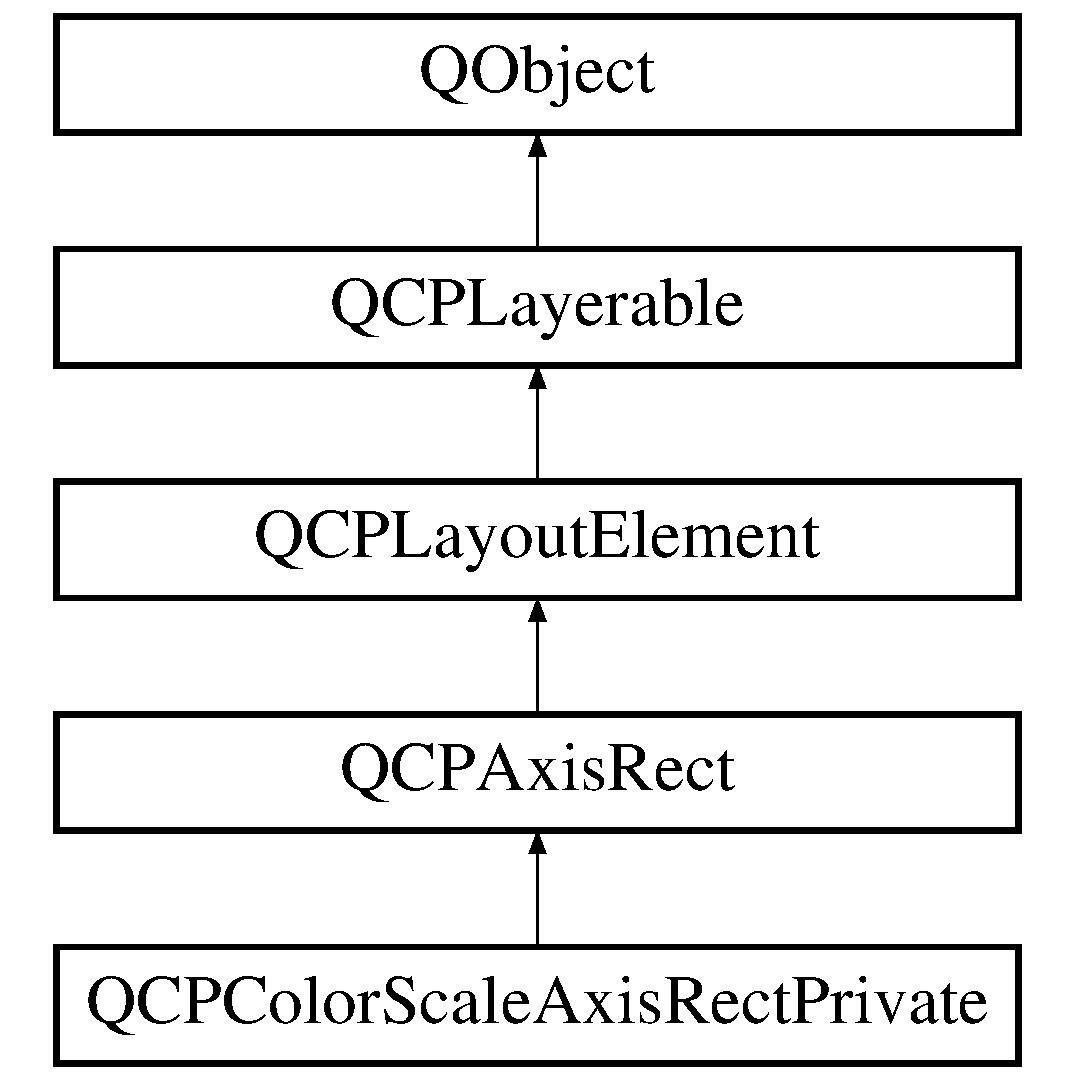
\includegraphics[height=5.000000cm]{class_q_c_p_axis_rect}
\end{center}
\end{figure}
\subsection*{Public Member Functions}
\begin{DoxyCompactItemize}
\item 
\hyperlink{class_q_c_p_axis_rect_a60b31dece805462c1b82eea2e69ba042}{Q\+C\+P\+Axis\+Rect} (\hyperlink{class_q_custom_plot}{Q\+Custom\+Plot} $\ast$\hyperlink{class_q_c_p_layerable_ab7e0e94461566093d36ffc0f5312b109}{parent\+Plot}, bool setup\+Default\+Axes=true)
\item 
virtual \hyperlink{class_q_c_p_axis_rect_a463c44b1856ddbf82eb3f7b582839cd0}{$\sim$\+Q\+C\+P\+Axis\+Rect} ()
\item 
Q\+Pixmap \hyperlink{class_q_c_p_axis_rect_a0daa1dadd2a62dbfa37b7f742edd0059}{background} () const 
\item 
bool \hyperlink{class_q_c_p_axis_rect_a67c18777b88fe9c81dee3dd2b5f50e5c}{background\+Scaled} () const 
\item 
Qt\+::\+Aspect\+Ratio\+Mode \hyperlink{class_q_c_p_axis_rect_a3d0f42d6be11a0b3d4576402a2b0032d}{background\+Scaled\+Mode} () const 
\item 
Qt\+::\+Orientations \hyperlink{class_q_c_p_axis_rect_af24b46954ce27a26b23770cdb8319080}{range\+Drag} () const 
\item 
Qt\+::\+Orientations \hyperlink{class_q_c_p_axis_rect_a3397fc60e5df29089090bc236e9f05f6}{range\+Zoom} () const 
\item 
\hyperlink{class_q_c_p_axis}{Q\+C\+P\+Axis} $\ast$ \hyperlink{class_q_c_p_axis_rect_a6d7c22cfc54fac7a3d6ef80b133a8574}{range\+Drag\+Axis} (Qt\+::\+Orientation orientation)
\item 
\hyperlink{class_q_c_p_axis}{Q\+C\+P\+Axis} $\ast$ \hyperlink{class_q_c_p_axis_rect_a679c63f2b8daccfe6ec5110dce3dd3b6}{range\+Zoom\+Axis} (Qt\+::\+Orientation orientation)
\item 
double \hyperlink{class_q_c_p_axis_rect_ae4e6c4d143aacc88d2d3c56f117c2fe1}{range\+Zoom\+Factor} (Qt\+::\+Orientation orientation)
\item 
void \hyperlink{class_q_c_p_axis_rect_af615ab5e52b8e0a9a0eff415b6559db5}{set\+Background} (const Q\+Pixmap \&pm)
\item 
void \hyperlink{class_q_c_p_axis_rect_ac48a2d5d9b7732e73b86605c69c5e4c1}{set\+Background} (const Q\+Pixmap \&pm, bool scaled, Qt\+::\+Aspect\+Ratio\+Mode mode=Qt\+::\+Keep\+Aspect\+Ratio\+By\+Expanding)
\item 
void \hyperlink{class_q_c_p_axis_rect_a22a22b8668735438dc06f9a55fe46b33}{set\+Background} (const Q\+Brush \&brush)
\item 
void \hyperlink{class_q_c_p_axis_rect_ae6d36c3e0e968ffb991170a018e7b503}{set\+Background\+Scaled} (bool scaled)
\item 
void \hyperlink{class_q_c_p_axis_rect_a5ef77ea829c9de7ba248e473f48f7305}{set\+Background\+Scaled\+Mode} (Qt\+::\+Aspect\+Ratio\+Mode mode)
\item 
void \hyperlink{class_q_c_p_axis_rect_ae6aef2f7211ba6097c925dcd26008418}{set\+Range\+Drag} (Qt\+::\+Orientations orientations)
\item 
void \hyperlink{class_q_c_p_axis_rect_a7960a9d222f1c31d558b064b60f86a31}{set\+Range\+Zoom} (Qt\+::\+Orientations orientations)
\item 
void \hyperlink{class_q_c_p_axis_rect_a648cce336bd99daac4a5ca3e5743775d}{set\+Range\+Drag\+Axes} (\hyperlink{class_q_c_p_axis}{Q\+C\+P\+Axis} $\ast$horizontal, \hyperlink{class_q_c_p_axis}{Q\+C\+P\+Axis} $\ast$vertical)
\item 
void \hyperlink{class_q_c_p_axis_rect_a9442cca2aa358405f39a64d51eca13d2}{set\+Range\+Zoom\+Axes} (\hyperlink{class_q_c_p_axis}{Q\+C\+P\+Axis} $\ast$horizontal, \hyperlink{class_q_c_p_axis}{Q\+C\+P\+Axis} $\ast$vertical)
\item 
void \hyperlink{class_q_c_p_axis_rect_a895d7ac745ea614e04056244b3c138ac}{set\+Range\+Zoom\+Factor} (double horizontal\+Factor, double vertical\+Factor)
\item 
void \hyperlink{class_q_c_p_axis_rect_ae83d187b03fc6fa4f00765ad50cd3fc3}{set\+Range\+Zoom\+Factor} (double factor)
\item 
int \hyperlink{class_q_c_p_axis_rect_a16e3e4646e52e4b5d5b865076c29ae58}{axis\+Count} (\hyperlink{class_q_c_p_axis_ae2bcc1728b382f10f064612b368bc18a}{Q\+C\+P\+Axis\+::\+Axis\+Type} type) const 
\item 
\hyperlink{class_q_c_p_axis}{Q\+C\+P\+Axis} $\ast$ \hyperlink{class_q_c_p_axis_rect_a560de44e47a4af0f86c59102a094b1e4}{axis} (\hyperlink{class_q_c_p_axis_ae2bcc1728b382f10f064612b368bc18a}{Q\+C\+P\+Axis\+::\+Axis\+Type} type, int index=0) const 
\item 
Q\+List$<$ \hyperlink{class_q_c_p_axis}{Q\+C\+P\+Axis} $\ast$ $>$ \hyperlink{class_q_c_p_axis_rect_a66654d51ca611ef036ded36250cd2518}{axes} (Q\+C\+P\+Axis\+::\+Axis\+Types types) const 
\item 
Q\+List$<$ \hyperlink{class_q_c_p_axis}{Q\+C\+P\+Axis} $\ast$ $>$ \hyperlink{class_q_c_p_axis_rect_a18dcdc0dd6c7520bc9f3d15a7a3feec2}{axes} () const 
\item 
\hyperlink{class_q_c_p_axis}{Q\+C\+P\+Axis} $\ast$ \hyperlink{class_q_c_p_axis_rect_a2dc336092ccc57d44a46194c8a23e4f4}{add\+Axis} (\hyperlink{class_q_c_p_axis_ae2bcc1728b382f10f064612b368bc18a}{Q\+C\+P\+Axis\+::\+Axis\+Type} type, \hyperlink{class_q_c_p_axis}{Q\+C\+P\+Axis} $\ast$\hyperlink{class_q_c_p_axis_rect_a560de44e47a4af0f86c59102a094b1e4}{axis}=0)
\item 
Q\+List$<$ \hyperlink{class_q_c_p_axis}{Q\+C\+P\+Axis} $\ast$ $>$ \hyperlink{class_q_c_p_axis_rect_a792e1f3d9cb1591fca135bb0de9b81fc}{add\+Axes} (Q\+C\+P\+Axis\+::\+Axis\+Types types)
\item 
bool \hyperlink{class_q_c_p_axis_rect_a03c39cd9704f0d36fb6cf980cdddcbaa}{remove\+Axis} (\hyperlink{class_q_c_p_axis}{Q\+C\+P\+Axis} $\ast$\hyperlink{class_q_c_p_axis_rect_a560de44e47a4af0f86c59102a094b1e4}{axis})
\item 
\hyperlink{class_q_c_p_layout_inset}{Q\+C\+P\+Layout\+Inset} $\ast$ \hyperlink{class_q_c_p_axis_rect_a4114887c7141b59650b7488f930993e5}{inset\+Layout} () const 
\item 
void \hyperlink{class_q_c_p_axis_rect_a5fa906175447b14206954f77fc7f1ef4}{setup\+Full\+Axes\+Box} (bool connect\+Ranges=false)
\item 
Q\+List$<$ \hyperlink{class_q_c_p_abstract_plottable}{Q\+C\+P\+Abstract\+Plottable} $\ast$ $>$ \hyperlink{class_q_c_p_axis_rect_a5b0d629c8de5572945eeae79a142296e}{plottables} () const 
\item 
Q\+List$<$ \hyperlink{class_q_c_p_graph}{Q\+C\+P\+Graph} $\ast$ $>$ \hyperlink{class_q_c_p_axis_rect_afa4ff90901d9275f670e24b40e3c1b25}{graphs} () const 
\item 
Q\+List$<$ \hyperlink{class_q_c_p_abstract_item}{Q\+C\+P\+Abstract\+Item} $\ast$ $>$ \hyperlink{class_q_c_p_axis_rect_a0f17ed539962cfcbaca8ce0b1776c840}{items} () const 
\item 
int \hyperlink{class_q_c_p_axis_rect_a55b3ecf72a3a65b053f7651b88db458d}{left} () const 
\item 
int \hyperlink{class_q_c_p_axis_rect_a6d0f989fc552aa2b563cf82f8fc81e61}{right} () const 
\item 
int \hyperlink{class_q_c_p_axis_rect_ac45aef1eb75cea46b241b6303028a607}{top} () const 
\item 
int \hyperlink{class_q_c_p_axis_rect_af2b5982ebe7e6f781b9bf1cc371a60d8}{bottom} () const 
\item 
int \hyperlink{class_q_c_p_axis_rect_a45bf5c17f4ca29131b7eb0db06efc259}{width} () const 
\item 
int \hyperlink{class_q_c_p_axis_rect_a1c55c4f3bef40cf01b21820316c8469e}{height} () const 
\item 
Q\+Size \hyperlink{class_q_c_p_axis_rect_a871b9fe49e92b39a3cbe29a59e458536}{size} () const 
\item 
Q\+Point \hyperlink{class_q_c_p_axis_rect_a88acbe716bcf5072790a6f95637c40d8}{top\+Left} () const 
\item 
Q\+Point \hyperlink{class_q_c_p_axis_rect_a232409546394c23b59407bc62fa460a8}{top\+Right} () const 
\item 
Q\+Point \hyperlink{class_q_c_p_axis_rect_a724b0333971ea6a338f0dbd814dc97ae}{bottom\+Left} () const 
\item 
Q\+Point \hyperlink{class_q_c_p_axis_rect_a49ea3c7dff834b47e266cbf3d79f78b9}{bottom\+Right} () const 
\item 
Q\+Point \hyperlink{class_q_c_p_axis_rect_aea5e6042bca198424fa1bc02fc282e59}{center} () const 
\item 
virtual void \hyperlink{class_q_c_p_axis_rect_a255080a017df9083a60a321ef2ba9ed8}{update} (\hyperlink{class_q_c_p_layout_element_a0d83360e05735735aaf6d7983c56374d}{Update\+Phase} phase)
\item 
virtual Q\+List$<$ \hyperlink{class_q_c_p_layout_element}{Q\+C\+P\+Layout\+Element} $\ast$ $>$ \hyperlink{class_q_c_p_axis_rect_a2bda6bf2b5b5797f92583cecd01c8949}{elements} (bool recursive) const 
\end{DoxyCompactItemize}
\subsection*{Protected Member Functions}
\begin{DoxyCompactItemize}
\item 
virtual void \hyperlink{class_q_c_p_axis_rect_a9a6dd0763701cbc7d01f899bcbb3f9ca}{apply\+Default\+Antialiasing\+Hint} (\hyperlink{class_q_c_p_painter}{Q\+C\+P\+Painter} $\ast$painter) const 
\item 
virtual void \hyperlink{class_q_c_p_axis_rect_afb1bbbbda8345cd2710d92ee48440b53}{draw} (\hyperlink{class_q_c_p_painter}{Q\+C\+P\+Painter} $\ast$painter)
\item 
virtual int \hyperlink{class_q_c_p_axis_rect_ae79f18302e6507586aa8c032a5f9ed1c}{calculate\+Auto\+Margin} (\hyperlink{namespace_q_c_p_a7e487e3e2ccb62ab7771065bab7cae54}{Q\+C\+P\+::\+Margin\+Side} side)
\item 
virtual void \hyperlink{class_q_c_p_axis_rect_a77501dbeccdac7256f7979b05077c04e}{mouse\+Press\+Event} (Q\+Mouse\+Event $\ast$event)
\item 
virtual void \hyperlink{class_q_c_p_axis_rect_a4baf3d5dd69166788f6ceda0ea182c6e}{mouse\+Move\+Event} (Q\+Mouse\+Event $\ast$event)
\item 
virtual void \hyperlink{class_q_c_p_axis_rect_adf6c99780cea55ab39459a6eaad3a94a}{mouse\+Release\+Event} (Q\+Mouse\+Event $\ast$event)
\item 
virtual void \hyperlink{class_q_c_p_axis_rect_a5acf41fc30aa68ea263246ecfad85c31}{wheel\+Event} (Q\+Wheel\+Event $\ast$event)
\item 
void \hyperlink{class_q_c_p_axis_rect_ab49d338d1ce74b476fcead5b32cf06dc}{draw\+Background} (\hyperlink{class_q_c_p_painter}{Q\+C\+P\+Painter} $\ast$painter)
\item 
void \hyperlink{class_q_c_p_axis_rect_a6024ccdc74f5dc0e8a0fe482e5b28a20}{update\+Axes\+Offset} (\hyperlink{class_q_c_p_axis_ae2bcc1728b382f10f064612b368bc18a}{Q\+C\+P\+Axis\+::\+Axis\+Type} type)
\end{DoxyCompactItemize}
\subsection*{Protected Attributes}
\begin{DoxyCompactItemize}
\item 
Q\+Brush \hyperlink{class_q_c_p_axis_rect_a5748e1a37f63c428e38b0a7724b46259}{m\+Background\+Brush}
\item 
Q\+Pixmap \hyperlink{class_q_c_p_axis_rect_a38fb1a15f43228a0c124553649303722}{m\+Background\+Pixmap}
\item 
Q\+Pixmap \hyperlink{class_q_c_p_axis_rect_aa74b9415598d59b49290e41e42d7ee27}{m\+Scaled\+Background\+Pixmap}
\item 
bool \hyperlink{class_q_c_p_axis_rect_a5ad835f0fae5d7cc5ada9e063641dbf1}{m\+Background\+Scaled}
\item 
Qt\+::\+Aspect\+Ratio\+Mode \hyperlink{class_q_c_p_axis_rect_a859fd368e794663e346b4f53f35078e9}{m\+Background\+Scaled\+Mode}
\item 
\hyperlink{class_q_c_p_layout_inset}{Q\+C\+P\+Layout\+Inset} $\ast$ \hyperlink{class_q_c_p_axis_rect_a255240399e0fd24baad80cbbe46f698a}{m\+Inset\+Layout}
\item 
Qt\+::\+Orientations \hyperlink{class_q_c_p_axis_rect_aa9f107f66ca3469ad50ee6cea7c9e237}{m\+Range\+Drag}
\item 
Qt\+::\+Orientations \hyperlink{class_q_c_p_axis_rect_a215eff671d48df2edccc36e7f976f28c}{m\+Range\+Zoom}
\item 
Q\+Pointer$<$ \hyperlink{class_q_c_p_axis}{Q\+C\+P\+Axis} $>$ \hyperlink{class_q_c_p_axis_rect_aeaaa38c6d2030dd5f84461e2596e41e3}{m\+Range\+Drag\+Horz\+Axis}
\item 
Q\+Pointer$<$ \hyperlink{class_q_c_p_axis}{Q\+C\+P\+Axis} $>$ \hyperlink{class_q_c_p_axis_rect_a3e41dffec18987366f2a8ffd80689c12}{m\+Range\+Drag\+Vert\+Axis}
\item 
Q\+Pointer$<$ \hyperlink{class_q_c_p_axis}{Q\+C\+P\+Axis} $>$ \hyperlink{class_q_c_p_axis_rect_ae22f882bab20518559f3fbb84243d0ab}{m\+Range\+Zoom\+Horz\+Axis}
\item 
Q\+Pointer$<$ \hyperlink{class_q_c_p_axis}{Q\+C\+P\+Axis} $>$ \hyperlink{class_q_c_p_axis_rect_a8b9acd16a203a9692bd35a9465f54bc1}{m\+Range\+Zoom\+Vert\+Axis}
\item 
double \hyperlink{class_q_c_p_axis_rect_ad08d0250ed7b99de387d0ea6c7fd4dc1}{m\+Range\+Zoom\+Factor\+Horz}
\item 
double \hyperlink{class_q_c_p_axis_rect_a32f063629581d5bf82b12769940b34ad}{m\+Range\+Zoom\+Factor\+Vert}
\item 
\hyperlink{class_q_c_p_range}{Q\+C\+P\+Range} \hyperlink{class_q_c_p_axis_rect_a41936cf473ec638bec382f5a40cdb1f3}{m\+Drag\+Start\+Horz\+Range}
\item 
\hyperlink{class_q_c_p_range}{Q\+C\+P\+Range} \hyperlink{class_q_c_p_axis_rect_a1a5ae4c74b8bd46baf91bf4e4f4165f0}{m\+Drag\+Start\+Vert\+Range}
\item 
Q\+C\+P\+::\+Antialiased\+Elements \hyperlink{class_q_c_p_axis_rect_aa4a24f76360cfebe1bcf17a77fa7521b}{m\+A\+A\+Drag\+Backup}
\item 
Q\+C\+P\+::\+Antialiased\+Elements \hyperlink{class_q_c_p_axis_rect_a6fcb12e052e276d57efbb128be31d6f5}{m\+Not\+A\+A\+Drag\+Backup}
\item 
Q\+Point \hyperlink{class_q_c_p_axis_rect_a032896b28f83a58010d8d533b78c49df}{m\+Drag\+Start}
\item 
bool \hyperlink{class_q_c_p_axis_rect_ab49a6698194cf0e9e38a1d734c0888a8}{m\+Dragging}
\item 
Q\+Hash$<$ \hyperlink{class_q_c_p_axis_ae2bcc1728b382f10f064612b368bc18a}{Q\+C\+P\+Axis\+::\+Axis\+Type}, Q\+List$<$ \hyperlink{class_q_c_p_axis}{Q\+C\+P\+Axis} $\ast$ $>$ $>$ \hyperlink{class_q_c_p_axis_rect_afe7a24d2a2bea98fc552fa826350ba81}{m\+Axes}
\end{DoxyCompactItemize}
\subsection*{Friends}
\begin{DoxyCompactItemize}
\item 
class \hyperlink{class_q_c_p_axis_rect_a1cdf9df76adcfae45261690aa0ca2198}{Q\+Custom\+Plot}
\end{DoxyCompactItemize}
\subsection*{Additional Inherited Members}


\subsection{Detailed Description}
Holds multiple axes and arranges them in a rectangular shape. 

This class represents an axis rect, a rectangular area that is bounded on all sides with an arbitrary number of axes.

Initially \hyperlink{class_q_custom_plot}{Q\+Custom\+Plot} has one axis rect, accessible via \hyperlink{class_q_custom_plot_a4a37a1add5fe63060ac518cf0a4c4050}{Q\+Custom\+Plot\+::axis\+Rect()}. However, the layout system allows to have multiple axis rects, e.\+g. arranged in a grid layout (\hyperlink{class_q_custom_plot_afd280d4d621ae64a106543a545c508d7}{Q\+Custom\+Plot\+::plot\+Layout}).

By default, \hyperlink{class_q_c_p_axis_rect}{Q\+C\+P\+Axis\+Rect} comes with four axes, at bottom, top, left and right. They can be accessed via \hyperlink{class_q_c_p_axis_rect_a560de44e47a4af0f86c59102a094b1e4}{axis} by providing the respective axis type (\hyperlink{class_q_c_p_axis_ae2bcc1728b382f10f064612b368bc18a}{Q\+C\+P\+Axis\+::\+Axis\+Type}) and index. If you need all axes in the axis rect, use \hyperlink{class_q_c_p_axis_rect_a66654d51ca611ef036ded36250cd2518}{axes}. The top and right axes are set to be invisible initially (\hyperlink{class_q_c_p_layerable_a3bed99ddc396b48ce3ebfdc0418744f8}{Q\+C\+P\+Axis\+::set\+Visible}). To add more axes to a side, use \hyperlink{class_q_c_p_axis_rect_a2dc336092ccc57d44a46194c8a23e4f4}{add\+Axis} or \hyperlink{class_q_c_p_axis_rect_a792e1f3d9cb1591fca135bb0de9b81fc}{add\+Axes}. To remove an axis, use \hyperlink{class_q_c_p_axis_rect_a03c39cd9704f0d36fb6cf980cdddcbaa}{remove\+Axis}.

The axis rect layerable itself only draws a background pixmap or color, if specified (\hyperlink{class_q_c_p_axis_rect_af615ab5e52b8e0a9a0eff415b6559db5}{set\+Background}). It is placed on the \char`\"{}background\char`\"{} layer initially (see \hyperlink{class_q_c_p_layer}{Q\+C\+P\+Layer} for an explanation of the \hyperlink{class_q_custom_plot}{Q\+Custom\+Plot} layer system). The axes that are held by the axis rect can be placed on other layers, independently of the axis rect.

Every axis rect has a child layout of type \hyperlink{class_q_c_p_layout_inset}{Q\+C\+P\+Layout\+Inset}. It is accessible via \hyperlink{class_q_c_p_axis_rect_a4114887c7141b59650b7488f930993e5}{inset\+Layout} and can be used to have other layout elements (or even other layouts with multiple elements) hovering inside the axis rect.

If an axis rect is clicked and dragged, it processes this by moving certain axis ranges. The behaviour can be controlled with \hyperlink{class_q_c_p_axis_rect_ae6aef2f7211ba6097c925dcd26008418}{set\+Range\+Drag} and \hyperlink{class_q_c_p_axis_rect_a648cce336bd99daac4a5ca3e5743775d}{set\+Range\+Drag\+Axes}. If the mouse wheel is scrolled while the cursor is on the axis rect, certain axes are scaled. This is controllable via \hyperlink{class_q_c_p_axis_rect_a7960a9d222f1c31d558b064b60f86a31}{set\+Range\+Zoom}, \hyperlink{class_q_c_p_axis_rect_a9442cca2aa358405f39a64d51eca13d2}{set\+Range\+Zoom\+Axes} and \hyperlink{class_q_c_p_axis_rect_a895d7ac745ea614e04056244b3c138ac}{set\+Range\+Zoom\+Factor}. These interactions are only enabled if \hyperlink{class_q_custom_plot_a5ee1e2f6ae27419deca53e75907c27e5}{Q\+Custom\+Plot\+::set\+Interactions} contains \hyperlink{namespace_q_c_p_a2ad6bb6281c7c2d593d4277b44c2b037a2c4432b9aceafb94000be8d1b589ef18}{Q\+C\+P\+::i\+Range\+Drag} and \hyperlink{namespace_q_c_p_a2ad6bb6281c7c2d593d4277b44c2b037abee1e94353525a636aeaf0ba32b72e14}{Q\+C\+P\+::i\+Range\+Zoom}.

 \begin{center}Overview of the spacings and paddings that define the geometry of an axis. The dashed line on the far left indicates the viewport/widget border.\end{center}  

\subsection{Constructor \& Destructor Documentation}
\hypertarget{class_q_c_p_axis_rect_a60b31dece805462c1b82eea2e69ba042}{}\index{Q\+C\+P\+Axis\+Rect@{Q\+C\+P\+Axis\+Rect}!Q\+C\+P\+Axis\+Rect@{Q\+C\+P\+Axis\+Rect}}
\index{Q\+C\+P\+Axis\+Rect@{Q\+C\+P\+Axis\+Rect}!Q\+C\+P\+Axis\+Rect@{Q\+C\+P\+Axis\+Rect}}
\subsubsection[{Q\+C\+P\+Axis\+Rect}]{\setlength{\rightskip}{0pt plus 5cm}Q\+C\+P\+Axis\+Rect\+::\+Q\+C\+P\+Axis\+Rect (
\begin{DoxyParamCaption}
\item[{{\bf Q\+Custom\+Plot} $\ast$}]{parent\+Plot, }
\item[{bool}]{setup\+Default\+Axes = {\ttfamily true}}
\end{DoxyParamCaption}
)\hspace{0.3cm}{\ttfamily [explicit]}}\label{class_q_c_p_axis_rect_a60b31dece805462c1b82eea2e69ba042}
Creates a \hyperlink{class_q_c_p_axis_rect}{Q\+C\+P\+Axis\+Rect} instance and sets default values. An axis is added for each of the four sides, the top and right axes are set invisible initially. \hypertarget{class_q_c_p_axis_rect_a463c44b1856ddbf82eb3f7b582839cd0}{}\index{Q\+C\+P\+Axis\+Rect@{Q\+C\+P\+Axis\+Rect}!````~Q\+C\+P\+Axis\+Rect@{$\sim$\+Q\+C\+P\+Axis\+Rect}}
\index{````~Q\+C\+P\+Axis\+Rect@{$\sim$\+Q\+C\+P\+Axis\+Rect}!Q\+C\+P\+Axis\+Rect@{Q\+C\+P\+Axis\+Rect}}
\subsubsection[{$\sim$\+Q\+C\+P\+Axis\+Rect}]{\setlength{\rightskip}{0pt plus 5cm}Q\+C\+P\+Axis\+Rect\+::$\sim$\+Q\+C\+P\+Axis\+Rect (
\begin{DoxyParamCaption}
{}
\end{DoxyParamCaption}
)\hspace{0.3cm}{\ttfamily [virtual]}}\label{class_q_c_p_axis_rect_a463c44b1856ddbf82eb3f7b582839cd0}


\subsection{Member Function Documentation}
\hypertarget{class_q_c_p_axis_rect_a792e1f3d9cb1591fca135bb0de9b81fc}{}\index{Q\+C\+P\+Axis\+Rect@{Q\+C\+P\+Axis\+Rect}!add\+Axes@{add\+Axes}}
\index{add\+Axes@{add\+Axes}!Q\+C\+P\+Axis\+Rect@{Q\+C\+P\+Axis\+Rect}}
\subsubsection[{add\+Axes}]{\setlength{\rightskip}{0pt plus 5cm}Q\+List$<$ {\bf Q\+C\+P\+Axis} $\ast$ $>$ Q\+C\+P\+Axis\+Rect\+::add\+Axes (
\begin{DoxyParamCaption}
\item[{Q\+C\+P\+Axis\+::\+Axis\+Types}]{types}
\end{DoxyParamCaption}
)}\label{class_q_c_p_axis_rect_a792e1f3d9cb1591fca135bb0de9b81fc}
Adds a new axis with \hyperlink{class_q_c_p_axis_rect_a2dc336092ccc57d44a46194c8a23e4f4}{add\+Axis} to each axis rect side specified in {\itshape types}. This may be an {\ttfamily or}-\/combination of \hyperlink{class_q_c_p_axis_ae2bcc1728b382f10f064612b368bc18a}{Q\+C\+P\+Axis\+::\+Axis\+Type}, so axes can be added to multiple sides at once.

Returns a list of the added axes.

\begin{DoxySeeAlso}{See also}
\hyperlink{class_q_c_p_axis_rect_a2dc336092ccc57d44a46194c8a23e4f4}{add\+Axis}, \hyperlink{class_q_c_p_axis_rect_a5fa906175447b14206954f77fc7f1ef4}{setup\+Full\+Axes\+Box} 
\end{DoxySeeAlso}
\hypertarget{class_q_c_p_axis_rect_a2dc336092ccc57d44a46194c8a23e4f4}{}\index{Q\+C\+P\+Axis\+Rect@{Q\+C\+P\+Axis\+Rect}!add\+Axis@{add\+Axis}}
\index{add\+Axis@{add\+Axis}!Q\+C\+P\+Axis\+Rect@{Q\+C\+P\+Axis\+Rect}}
\subsubsection[{add\+Axis}]{\setlength{\rightskip}{0pt plus 5cm}{\bf Q\+C\+P\+Axis} $\ast$ Q\+C\+P\+Axis\+Rect\+::add\+Axis (
\begin{DoxyParamCaption}
\item[{{\bf Q\+C\+P\+Axis\+::\+Axis\+Type}}]{type, }
\item[{{\bf Q\+C\+P\+Axis} $\ast$}]{axis = {\ttfamily 0}}
\end{DoxyParamCaption}
)}\label{class_q_c_p_axis_rect_a2dc336092ccc57d44a46194c8a23e4f4}
Adds a new axis to the axis rect side specified with {\itshape type}, and returns it. If {\itshape axis} is 0, a new \hyperlink{class_q_c_p_axis}{Q\+C\+P\+Axis} instance is created internally.

You may inject \hyperlink{class_q_c_p_axis}{Q\+C\+P\+Axis} instances (or sublasses of \hyperlink{class_q_c_p_axis}{Q\+C\+P\+Axis}) by setting {\itshape axis} to an axis that was previously created outside \hyperlink{class_q_custom_plot}{Q\+Custom\+Plot}. It is important to note that \hyperlink{class_q_custom_plot}{Q\+Custom\+Plot} takes ownership of the axis, so you may not delete it afterwards. Further, the {\itshape axis} must have been created with this axis rect as parent and with the same axis type as specified in {\itshape type}. If this is not the case, a debug output is generated, the axis is not added, and the method returns 0.

This method can not be used to move {\itshape axis} between axis rects. The same {\itshape axis} instance must not be added multiple times to the same or different axis rects.

If an axis rect side already contains one or more axes, the lower and upper endings of the new axis (\hyperlink{class_q_c_p_axis_a08af1c72db9ae4dc8cb8a973d44405ab}{Q\+C\+P\+Axis\+::set\+Lower\+Ending}, \hyperlink{class_q_c_p_axis_a69119b892fc306f651763596685aa377}{Q\+C\+P\+Axis\+::set\+Upper\+Ending}) are set to \hyperlink{class_q_c_p_line_ending_a5ef16e6876b4b74959c7261d8d4c2cd5a126c390f0c359fcd8df1fc5e38d26d5b}{Q\+C\+P\+Line\+Ending\+::es\+Half\+Bar}.

\begin{DoxySeeAlso}{See also}
\hyperlink{class_q_c_p_axis_rect_a792e1f3d9cb1591fca135bb0de9b81fc}{add\+Axes}, \hyperlink{class_q_c_p_axis_rect_a5fa906175447b14206954f77fc7f1ef4}{setup\+Full\+Axes\+Box} 
\end{DoxySeeAlso}
\hypertarget{class_q_c_p_axis_rect_a9a6dd0763701cbc7d01f899bcbb3f9ca}{}\index{Q\+C\+P\+Axis\+Rect@{Q\+C\+P\+Axis\+Rect}!apply\+Default\+Antialiasing\+Hint@{apply\+Default\+Antialiasing\+Hint}}
\index{apply\+Default\+Antialiasing\+Hint@{apply\+Default\+Antialiasing\+Hint}!Q\+C\+P\+Axis\+Rect@{Q\+C\+P\+Axis\+Rect}}
\subsubsection[{apply\+Default\+Antialiasing\+Hint}]{\setlength{\rightskip}{0pt plus 5cm}void Q\+C\+P\+Axis\+Rect\+::apply\+Default\+Antialiasing\+Hint (
\begin{DoxyParamCaption}
\item[{{\bf Q\+C\+P\+Painter} $\ast$}]{painter}
\end{DoxyParamCaption}
) const\hspace{0.3cm}{\ttfamily [protected]}, {\ttfamily [virtual]}}\label{class_q_c_p_axis_rect_a9a6dd0763701cbc7d01f899bcbb3f9ca}


Reimplemented from \hyperlink{class_q_c_p_layout_element_ad6d2b4bb0291c2441b2e1ca3d5296df5}{Q\+C\+P\+Layout\+Element}.

\hypertarget{class_q_c_p_axis_rect_a66654d51ca611ef036ded36250cd2518}{}\index{Q\+C\+P\+Axis\+Rect@{Q\+C\+P\+Axis\+Rect}!axes@{axes}}
\index{axes@{axes}!Q\+C\+P\+Axis\+Rect@{Q\+C\+P\+Axis\+Rect}}
\subsubsection[{axes}]{\setlength{\rightskip}{0pt plus 5cm}Q\+List$<$ {\bf Q\+C\+P\+Axis} $\ast$ $>$ Q\+C\+P\+Axis\+Rect\+::axes (
\begin{DoxyParamCaption}
\item[{Q\+C\+P\+Axis\+::\+Axis\+Types}]{types}
\end{DoxyParamCaption}
) const}\label{class_q_c_p_axis_rect_a66654d51ca611ef036ded36250cd2518}
Returns all axes on the axis rect sides specified with {\itshape types}.

{\itshape types} may be a single \hyperlink{class_q_c_p_axis_ae2bcc1728b382f10f064612b368bc18a}{Q\+C\+P\+Axis\+::\+Axis\+Type} or an {\ttfamily or}-\/combination, to get the axes of multiple sides.

\begin{DoxySeeAlso}{See also}
\hyperlink{class_q_c_p_axis_rect_a560de44e47a4af0f86c59102a094b1e4}{axis} 
\end{DoxySeeAlso}
\hypertarget{class_q_c_p_axis_rect_a18dcdc0dd6c7520bc9f3d15a7a3feec2}{}\index{Q\+C\+P\+Axis\+Rect@{Q\+C\+P\+Axis\+Rect}!axes@{axes}}
\index{axes@{axes}!Q\+C\+P\+Axis\+Rect@{Q\+C\+P\+Axis\+Rect}}
\subsubsection[{axes}]{\setlength{\rightskip}{0pt plus 5cm}Q\+List$<$ {\bf Q\+C\+P\+Axis} $\ast$ $>$ Q\+C\+P\+Axis\+Rect\+::axes (
\begin{DoxyParamCaption}
{}
\end{DoxyParamCaption}
) const}\label{class_q_c_p_axis_rect_a18dcdc0dd6c7520bc9f3d15a7a3feec2}
This is an overloaded member function, provided for convenience. It differs from the above function only in what argument(s) it accepts.

Returns all axes of this axis rect. \hypertarget{class_q_c_p_axis_rect_a560de44e47a4af0f86c59102a094b1e4}{}\index{Q\+C\+P\+Axis\+Rect@{Q\+C\+P\+Axis\+Rect}!axis@{axis}}
\index{axis@{axis}!Q\+C\+P\+Axis\+Rect@{Q\+C\+P\+Axis\+Rect}}
\subsubsection[{axis}]{\setlength{\rightskip}{0pt plus 5cm}{\bf Q\+C\+P\+Axis} $\ast$ Q\+C\+P\+Axis\+Rect\+::axis (
\begin{DoxyParamCaption}
\item[{{\bf Q\+C\+P\+Axis\+::\+Axis\+Type}}]{type, }
\item[{int}]{index = {\ttfamily 0}}
\end{DoxyParamCaption}
) const}\label{class_q_c_p_axis_rect_a560de44e47a4af0f86c59102a094b1e4}
Returns the axis with the given {\itshape index} on the axis rect side specified with {\itshape type}.

\begin{DoxySeeAlso}{See also}
\hyperlink{class_q_c_p_axis_rect_a16e3e4646e52e4b5d5b865076c29ae58}{axis\+Count}, \hyperlink{class_q_c_p_axis_rect_a66654d51ca611ef036ded36250cd2518}{axes} 
\end{DoxySeeAlso}
\hypertarget{class_q_c_p_axis_rect_a16e3e4646e52e4b5d5b865076c29ae58}{}\index{Q\+C\+P\+Axis\+Rect@{Q\+C\+P\+Axis\+Rect}!axis\+Count@{axis\+Count}}
\index{axis\+Count@{axis\+Count}!Q\+C\+P\+Axis\+Rect@{Q\+C\+P\+Axis\+Rect}}
\subsubsection[{axis\+Count}]{\setlength{\rightskip}{0pt plus 5cm}int Q\+C\+P\+Axis\+Rect\+::axis\+Count (
\begin{DoxyParamCaption}
\item[{{\bf Q\+C\+P\+Axis\+::\+Axis\+Type}}]{type}
\end{DoxyParamCaption}
) const}\label{class_q_c_p_axis_rect_a16e3e4646e52e4b5d5b865076c29ae58}
Returns the number of axes on the axis rect side specified with {\itshape type}.

\begin{DoxySeeAlso}{See also}
\hyperlink{class_q_c_p_axis_rect_a560de44e47a4af0f86c59102a094b1e4}{axis} 
\end{DoxySeeAlso}
\hypertarget{class_q_c_p_axis_rect_a0daa1dadd2a62dbfa37b7f742edd0059}{}\index{Q\+C\+P\+Axis\+Rect@{Q\+C\+P\+Axis\+Rect}!background@{background}}
\index{background@{background}!Q\+C\+P\+Axis\+Rect@{Q\+C\+P\+Axis\+Rect}}
\subsubsection[{background}]{\setlength{\rightskip}{0pt plus 5cm}Q\+Pixmap Q\+C\+P\+Axis\+Rect\+::background (
\begin{DoxyParamCaption}
{}
\end{DoxyParamCaption}
) const\hspace{0.3cm}{\ttfamily [inline]}}\label{class_q_c_p_axis_rect_a0daa1dadd2a62dbfa37b7f742edd0059}
\hypertarget{class_q_c_p_axis_rect_a67c18777b88fe9c81dee3dd2b5f50e5c}{}\index{Q\+C\+P\+Axis\+Rect@{Q\+C\+P\+Axis\+Rect}!background\+Scaled@{background\+Scaled}}
\index{background\+Scaled@{background\+Scaled}!Q\+C\+P\+Axis\+Rect@{Q\+C\+P\+Axis\+Rect}}
\subsubsection[{background\+Scaled}]{\setlength{\rightskip}{0pt plus 5cm}bool Q\+C\+P\+Axis\+Rect\+::background\+Scaled (
\begin{DoxyParamCaption}
{}
\end{DoxyParamCaption}
) const\hspace{0.3cm}{\ttfamily [inline]}}\label{class_q_c_p_axis_rect_a67c18777b88fe9c81dee3dd2b5f50e5c}
\hypertarget{class_q_c_p_axis_rect_a3d0f42d6be11a0b3d4576402a2b0032d}{}\index{Q\+C\+P\+Axis\+Rect@{Q\+C\+P\+Axis\+Rect}!background\+Scaled\+Mode@{background\+Scaled\+Mode}}
\index{background\+Scaled\+Mode@{background\+Scaled\+Mode}!Q\+C\+P\+Axis\+Rect@{Q\+C\+P\+Axis\+Rect}}
\subsubsection[{background\+Scaled\+Mode}]{\setlength{\rightskip}{0pt plus 5cm}Qt\+::\+Aspect\+Ratio\+Mode Q\+C\+P\+Axis\+Rect\+::background\+Scaled\+Mode (
\begin{DoxyParamCaption}
{}
\end{DoxyParamCaption}
) const\hspace{0.3cm}{\ttfamily [inline]}}\label{class_q_c_p_axis_rect_a3d0f42d6be11a0b3d4576402a2b0032d}
\hypertarget{class_q_c_p_axis_rect_af2b5982ebe7e6f781b9bf1cc371a60d8}{}\index{Q\+C\+P\+Axis\+Rect@{Q\+C\+P\+Axis\+Rect}!bottom@{bottom}}
\index{bottom@{bottom}!Q\+C\+P\+Axis\+Rect@{Q\+C\+P\+Axis\+Rect}}
\subsubsection[{bottom}]{\setlength{\rightskip}{0pt plus 5cm}int Q\+C\+P\+Axis\+Rect\+::bottom (
\begin{DoxyParamCaption}
{}
\end{DoxyParamCaption}
) const\hspace{0.3cm}{\ttfamily [inline]}}\label{class_q_c_p_axis_rect_af2b5982ebe7e6f781b9bf1cc371a60d8}
Returns the pixel position of the bottom border of this axis rect. Margins are not taken into account here, so the returned value is with respect to the inner \hyperlink{class_q_c_p_layout_element_affdfea003469aac3d0fac5f4e06171bc}{rect}. \hypertarget{class_q_c_p_axis_rect_a724b0333971ea6a338f0dbd814dc97ae}{}\index{Q\+C\+P\+Axis\+Rect@{Q\+C\+P\+Axis\+Rect}!bottom\+Left@{bottom\+Left}}
\index{bottom\+Left@{bottom\+Left}!Q\+C\+P\+Axis\+Rect@{Q\+C\+P\+Axis\+Rect}}
\subsubsection[{bottom\+Left}]{\setlength{\rightskip}{0pt plus 5cm}Q\+Point Q\+C\+P\+Axis\+Rect\+::bottom\+Left (
\begin{DoxyParamCaption}
{}
\end{DoxyParamCaption}
) const\hspace{0.3cm}{\ttfamily [inline]}}\label{class_q_c_p_axis_rect_a724b0333971ea6a338f0dbd814dc97ae}
Returns the bottom left corner of this axis rect in pixels. Margins are not taken into account here, so the returned value is with respect to the inner \hyperlink{class_q_c_p_layout_element_affdfea003469aac3d0fac5f4e06171bc}{rect}. \hypertarget{class_q_c_p_axis_rect_a49ea3c7dff834b47e266cbf3d79f78b9}{}\index{Q\+C\+P\+Axis\+Rect@{Q\+C\+P\+Axis\+Rect}!bottom\+Right@{bottom\+Right}}
\index{bottom\+Right@{bottom\+Right}!Q\+C\+P\+Axis\+Rect@{Q\+C\+P\+Axis\+Rect}}
\subsubsection[{bottom\+Right}]{\setlength{\rightskip}{0pt plus 5cm}Q\+Point Q\+C\+P\+Axis\+Rect\+::bottom\+Right (
\begin{DoxyParamCaption}
{}
\end{DoxyParamCaption}
) const\hspace{0.3cm}{\ttfamily [inline]}}\label{class_q_c_p_axis_rect_a49ea3c7dff834b47e266cbf3d79f78b9}
Returns the bottom right corner of this axis rect in pixels. Margins are not taken into account here, so the returned value is with respect to the inner \hyperlink{class_q_c_p_layout_element_affdfea003469aac3d0fac5f4e06171bc}{rect}. \hypertarget{class_q_c_p_axis_rect_ae79f18302e6507586aa8c032a5f9ed1c}{}\index{Q\+C\+P\+Axis\+Rect@{Q\+C\+P\+Axis\+Rect}!calculate\+Auto\+Margin@{calculate\+Auto\+Margin}}
\index{calculate\+Auto\+Margin@{calculate\+Auto\+Margin}!Q\+C\+P\+Axis\+Rect@{Q\+C\+P\+Axis\+Rect}}
\subsubsection[{calculate\+Auto\+Margin}]{\setlength{\rightskip}{0pt plus 5cm}int Q\+C\+P\+Axis\+Rect\+::calculate\+Auto\+Margin (
\begin{DoxyParamCaption}
\item[{{\bf Q\+C\+P\+::\+Margin\+Side}}]{side}
\end{DoxyParamCaption}
)\hspace{0.3cm}{\ttfamily [protected]}, {\ttfamily [virtual]}}\label{class_q_c_p_axis_rect_ae79f18302e6507586aa8c032a5f9ed1c}


Reimplemented from \hyperlink{class_q_c_p_layout_element_a005c9f0fe84bc1591a2cf2c46fd477b4}{Q\+C\+P\+Layout\+Element}.

\hypertarget{class_q_c_p_axis_rect_aea5e6042bca198424fa1bc02fc282e59}{}\index{Q\+C\+P\+Axis\+Rect@{Q\+C\+P\+Axis\+Rect}!center@{center}}
\index{center@{center}!Q\+C\+P\+Axis\+Rect@{Q\+C\+P\+Axis\+Rect}}
\subsubsection[{center}]{\setlength{\rightskip}{0pt plus 5cm}Q\+Point Q\+C\+P\+Axis\+Rect\+::center (
\begin{DoxyParamCaption}
{}
\end{DoxyParamCaption}
) const\hspace{0.3cm}{\ttfamily [inline]}}\label{class_q_c_p_axis_rect_aea5e6042bca198424fa1bc02fc282e59}
Returns the center of this axis rect in pixels. Margins are not taken into account here, so the returned value is with respect to the inner \hyperlink{class_q_c_p_layout_element_affdfea003469aac3d0fac5f4e06171bc}{rect}. \hypertarget{class_q_c_p_axis_rect_afb1bbbbda8345cd2710d92ee48440b53}{}\index{Q\+C\+P\+Axis\+Rect@{Q\+C\+P\+Axis\+Rect}!draw@{draw}}
\index{draw@{draw}!Q\+C\+P\+Axis\+Rect@{Q\+C\+P\+Axis\+Rect}}
\subsubsection[{draw}]{\setlength{\rightskip}{0pt plus 5cm}void Q\+C\+P\+Axis\+Rect\+::draw (
\begin{DoxyParamCaption}
\item[{{\bf Q\+C\+P\+Painter} $\ast$}]{painter}
\end{DoxyParamCaption}
)\hspace{0.3cm}{\ttfamily [protected]}, {\ttfamily [virtual]}}\label{class_q_c_p_axis_rect_afb1bbbbda8345cd2710d92ee48440b53}


Reimplemented from \hyperlink{class_q_c_p_layout_element_a547bcc1e6e2be5645ca781efe0834653}{Q\+C\+P\+Layout\+Element}.



Reimplemented in \hyperlink{class_q_c_p_color_scale_axis_rect_private_adb67bfe9057a9dd9a85f548c274e6d98}{Q\+C\+P\+Color\+Scale\+Axis\+Rect\+Private}.

\hypertarget{class_q_c_p_axis_rect_ab49d338d1ce74b476fcead5b32cf06dc}{}\index{Q\+C\+P\+Axis\+Rect@{Q\+C\+P\+Axis\+Rect}!draw\+Background@{draw\+Background}}
\index{draw\+Background@{draw\+Background}!Q\+C\+P\+Axis\+Rect@{Q\+C\+P\+Axis\+Rect}}
\subsubsection[{draw\+Background}]{\setlength{\rightskip}{0pt plus 5cm}void Q\+C\+P\+Axis\+Rect\+::draw\+Background (
\begin{DoxyParamCaption}
\item[{{\bf Q\+C\+P\+Painter} $\ast$}]{painter}
\end{DoxyParamCaption}
)\hspace{0.3cm}{\ttfamily [protected]}}\label{class_q_c_p_axis_rect_ab49d338d1ce74b476fcead5b32cf06dc}
\hypertarget{class_q_c_p_axis_rect_a2bda6bf2b5b5797f92583cecd01c8949}{}\index{Q\+C\+P\+Axis\+Rect@{Q\+C\+P\+Axis\+Rect}!elements@{elements}}
\index{elements@{elements}!Q\+C\+P\+Axis\+Rect@{Q\+C\+P\+Axis\+Rect}}
\subsubsection[{elements}]{\setlength{\rightskip}{0pt plus 5cm}Q\+List$<$ {\bf Q\+C\+P\+Layout\+Element} $\ast$ $>$ Q\+C\+P\+Axis\+Rect\+::elements (
\begin{DoxyParamCaption}
\item[{bool}]{recursive}
\end{DoxyParamCaption}
) const\hspace{0.3cm}{\ttfamily [virtual]}}\label{class_q_c_p_axis_rect_a2bda6bf2b5b5797f92583cecd01c8949}
Returns a list of all child elements in this layout element. If {\itshape recursive} is true, all sub-\/child elements are included in the list, too.

\begin{DoxyWarning}{Warning}
There may be entries with value 0 in the returned list. (For example, \hyperlink{class_q_c_p_layout_grid}{Q\+C\+P\+Layout\+Grid} may have empty cells which yield 0 at the respective index.) 
\end{DoxyWarning}


Reimplemented from \hyperlink{class_q_c_p_layout_element_a311d60d78e62ef8eaaedb1b6ceb9e788}{Q\+C\+P\+Layout\+Element}.

\hypertarget{class_q_c_p_axis_rect_afa4ff90901d9275f670e24b40e3c1b25}{}\index{Q\+C\+P\+Axis\+Rect@{Q\+C\+P\+Axis\+Rect}!graphs@{graphs}}
\index{graphs@{graphs}!Q\+C\+P\+Axis\+Rect@{Q\+C\+P\+Axis\+Rect}}
\subsubsection[{graphs}]{\setlength{\rightskip}{0pt plus 5cm}Q\+List$<$ {\bf Q\+C\+P\+Graph} $\ast$ $>$ Q\+C\+P\+Axis\+Rect\+::graphs (
\begin{DoxyParamCaption}
{}
\end{DoxyParamCaption}
) const}\label{class_q_c_p_axis_rect_afa4ff90901d9275f670e24b40e3c1b25}
Returns a list of all the graphs that are associated with this axis rect.

A graph is considered associated with an axis rect if its key or value axis (or both) is in this axis rect.

\begin{DoxySeeAlso}{See also}
\hyperlink{class_q_c_p_axis_rect_a5b0d629c8de5572945eeae79a142296e}{plottables}, \hyperlink{class_q_c_p_axis_rect_a0f17ed539962cfcbaca8ce0b1776c840}{items} 
\end{DoxySeeAlso}
\hypertarget{class_q_c_p_axis_rect_a1c55c4f3bef40cf01b21820316c8469e}{}\index{Q\+C\+P\+Axis\+Rect@{Q\+C\+P\+Axis\+Rect}!height@{height}}
\index{height@{height}!Q\+C\+P\+Axis\+Rect@{Q\+C\+P\+Axis\+Rect}}
\subsubsection[{height}]{\setlength{\rightskip}{0pt plus 5cm}int Q\+C\+P\+Axis\+Rect\+::height (
\begin{DoxyParamCaption}
{}
\end{DoxyParamCaption}
) const\hspace{0.3cm}{\ttfamily [inline]}}\label{class_q_c_p_axis_rect_a1c55c4f3bef40cf01b21820316c8469e}
Returns the pixel height of this axis rect. Margins are not taken into account here, so the returned value is with respect to the inner \hyperlink{class_q_c_p_layout_element_affdfea003469aac3d0fac5f4e06171bc}{rect}. \hypertarget{class_q_c_p_axis_rect_a4114887c7141b59650b7488f930993e5}{}\index{Q\+C\+P\+Axis\+Rect@{Q\+C\+P\+Axis\+Rect}!inset\+Layout@{inset\+Layout}}
\index{inset\+Layout@{inset\+Layout}!Q\+C\+P\+Axis\+Rect@{Q\+C\+P\+Axis\+Rect}}
\subsubsection[{inset\+Layout}]{\setlength{\rightskip}{0pt plus 5cm}{\bf Q\+C\+P\+Layout\+Inset} $\ast$ Q\+C\+P\+Axis\+Rect\+::inset\+Layout (
\begin{DoxyParamCaption}
{}
\end{DoxyParamCaption}
) const\hspace{0.3cm}{\ttfamily [inline]}}\label{class_q_c_p_axis_rect_a4114887c7141b59650b7488f930993e5}
Returns the inset layout of this axis rect. It can be used to place other layout elements (or even layouts with multiple other elements) inside/on top of an axis rect.

\begin{DoxySeeAlso}{See also}
\hyperlink{class_q_c_p_layout_inset}{Q\+C\+P\+Layout\+Inset} 
\end{DoxySeeAlso}
\hypertarget{class_q_c_p_axis_rect_a0f17ed539962cfcbaca8ce0b1776c840}{}\index{Q\+C\+P\+Axis\+Rect@{Q\+C\+P\+Axis\+Rect}!items@{items}}
\index{items@{items}!Q\+C\+P\+Axis\+Rect@{Q\+C\+P\+Axis\+Rect}}
\subsubsection[{items}]{\setlength{\rightskip}{0pt plus 5cm}Q\+List$<$ {\bf Q\+C\+P\+Abstract\+Item} $\ast$ $>$ Q\+C\+P\+Axis\+Rect\+::items (
\begin{DoxyParamCaption}
{}
\end{DoxyParamCaption}
) const}\label{class_q_c_p_axis_rect_a0f17ed539962cfcbaca8ce0b1776c840}
Returns a list of all the items that are associated with this axis rect.

An item is considered associated with an axis rect if any of its positions has key or value axis set to an axis that is in this axis rect, or if any of its positions has \hyperlink{class_q_c_p_item_position_a0cd9b326fb324710169e92e8ca0041c2}{Q\+C\+P\+Item\+Position\+::set\+Axis\+Rect} set to the axis rect, or if the clip axis rect (\hyperlink{class_q_c_p_abstract_item_a7dc75fcbcd10206fe0b75d757ea7a347}{Q\+C\+P\+Abstract\+Item\+::set\+Clip\+Axis\+Rect}) is set to this axis rect.

\begin{DoxySeeAlso}{See also}
\hyperlink{class_q_c_p_axis_rect_a5b0d629c8de5572945eeae79a142296e}{plottables}, \hyperlink{class_q_c_p_axis_rect_afa4ff90901d9275f670e24b40e3c1b25}{graphs} 
\end{DoxySeeAlso}
\hypertarget{class_q_c_p_axis_rect_a55b3ecf72a3a65b053f7651b88db458d}{}\index{Q\+C\+P\+Axis\+Rect@{Q\+C\+P\+Axis\+Rect}!left@{left}}
\index{left@{left}!Q\+C\+P\+Axis\+Rect@{Q\+C\+P\+Axis\+Rect}}
\subsubsection[{left}]{\setlength{\rightskip}{0pt plus 5cm}int Q\+C\+P\+Axis\+Rect\+::left (
\begin{DoxyParamCaption}
{}
\end{DoxyParamCaption}
) const\hspace{0.3cm}{\ttfamily [inline]}}\label{class_q_c_p_axis_rect_a55b3ecf72a3a65b053f7651b88db458d}
Returns the pixel position of the left border of this axis rect. Margins are not taken into account here, so the returned value is with respect to the inner \hyperlink{class_q_c_p_layout_element_affdfea003469aac3d0fac5f4e06171bc}{rect}. \hypertarget{class_q_c_p_axis_rect_a4baf3d5dd69166788f6ceda0ea182c6e}{}\index{Q\+C\+P\+Axis\+Rect@{Q\+C\+P\+Axis\+Rect}!mouse\+Move\+Event@{mouse\+Move\+Event}}
\index{mouse\+Move\+Event@{mouse\+Move\+Event}!Q\+C\+P\+Axis\+Rect@{Q\+C\+P\+Axis\+Rect}}
\subsubsection[{mouse\+Move\+Event}]{\setlength{\rightskip}{0pt plus 5cm}void Q\+C\+P\+Axis\+Rect\+::mouse\+Move\+Event (
\begin{DoxyParamCaption}
\item[{Q\+Mouse\+Event $\ast$}]{event}
\end{DoxyParamCaption}
)\hspace{0.3cm}{\ttfamily [protected]}, {\ttfamily [virtual]}}\label{class_q_c_p_axis_rect_a4baf3d5dd69166788f6ceda0ea182c6e}
This event is called, if the mouse is moved inside the outer rect of this layout element. 

Reimplemented from \hyperlink{class_q_c_p_layout_element_a14f4acf58cdb8dd2c6c571479c4c4a40}{Q\+C\+P\+Layout\+Element}.

\hypertarget{class_q_c_p_axis_rect_a77501dbeccdac7256f7979b05077c04e}{}\index{Q\+C\+P\+Axis\+Rect@{Q\+C\+P\+Axis\+Rect}!mouse\+Press\+Event@{mouse\+Press\+Event}}
\index{mouse\+Press\+Event@{mouse\+Press\+Event}!Q\+C\+P\+Axis\+Rect@{Q\+C\+P\+Axis\+Rect}}
\subsubsection[{mouse\+Press\+Event}]{\setlength{\rightskip}{0pt plus 5cm}void Q\+C\+P\+Axis\+Rect\+::mouse\+Press\+Event (
\begin{DoxyParamCaption}
\item[{Q\+Mouse\+Event $\ast$}]{event}
\end{DoxyParamCaption}
)\hspace{0.3cm}{\ttfamily [protected]}, {\ttfamily [virtual]}}\label{class_q_c_p_axis_rect_a77501dbeccdac7256f7979b05077c04e}
This event is called, if the mouse was pressed while being inside the outer rect of this layout element. 

Reimplemented from \hyperlink{class_q_c_p_layout_element_a2d82ea21fe0ee628f177bd824bc51a71}{Q\+C\+P\+Layout\+Element}.

\hypertarget{class_q_c_p_axis_rect_adf6c99780cea55ab39459a6eaad3a94a}{}\index{Q\+C\+P\+Axis\+Rect@{Q\+C\+P\+Axis\+Rect}!mouse\+Release\+Event@{mouse\+Release\+Event}}
\index{mouse\+Release\+Event@{mouse\+Release\+Event}!Q\+C\+P\+Axis\+Rect@{Q\+C\+P\+Axis\+Rect}}
\subsubsection[{mouse\+Release\+Event}]{\setlength{\rightskip}{0pt plus 5cm}void Q\+C\+P\+Axis\+Rect\+::mouse\+Release\+Event (
\begin{DoxyParamCaption}
\item[{Q\+Mouse\+Event $\ast$}]{event}
\end{DoxyParamCaption}
)\hspace{0.3cm}{\ttfamily [protected]}, {\ttfamily [virtual]}}\label{class_q_c_p_axis_rect_adf6c99780cea55ab39459a6eaad3a94a}
This event is called, if the mouse was previously pressed inside the outer rect of this layout element and is now released. 

Reimplemented from \hyperlink{class_q_c_p_layout_element_ae526ac828cce1e5bb94eaa85776d7404}{Q\+C\+P\+Layout\+Element}.

\hypertarget{class_q_c_p_axis_rect_a5b0d629c8de5572945eeae79a142296e}{}\index{Q\+C\+P\+Axis\+Rect@{Q\+C\+P\+Axis\+Rect}!plottables@{plottables}}
\index{plottables@{plottables}!Q\+C\+P\+Axis\+Rect@{Q\+C\+P\+Axis\+Rect}}
\subsubsection[{plottables}]{\setlength{\rightskip}{0pt plus 5cm}Q\+List$<$ {\bf Q\+C\+P\+Abstract\+Plottable} $\ast$ $>$ Q\+C\+P\+Axis\+Rect\+::plottables (
\begin{DoxyParamCaption}
{}
\end{DoxyParamCaption}
) const}\label{class_q_c_p_axis_rect_a5b0d629c8de5572945eeae79a142296e}
Returns a list of all the plottables that are associated with this axis rect.

A plottable is considered associated with an axis rect if its key or value axis (or both) is in this axis rect.

\begin{DoxySeeAlso}{See also}
\hyperlink{class_q_c_p_axis_rect_afa4ff90901d9275f670e24b40e3c1b25}{graphs}, \hyperlink{class_q_c_p_axis_rect_a0f17ed539962cfcbaca8ce0b1776c840}{items} 
\end{DoxySeeAlso}
\hypertarget{class_q_c_p_axis_rect_af24b46954ce27a26b23770cdb8319080}{}\index{Q\+C\+P\+Axis\+Rect@{Q\+C\+P\+Axis\+Rect}!range\+Drag@{range\+Drag}}
\index{range\+Drag@{range\+Drag}!Q\+C\+P\+Axis\+Rect@{Q\+C\+P\+Axis\+Rect}}
\subsubsection[{range\+Drag}]{\setlength{\rightskip}{0pt plus 5cm}Qt\+::\+Orientations Q\+C\+P\+Axis\+Rect\+::range\+Drag (
\begin{DoxyParamCaption}
{}
\end{DoxyParamCaption}
) const\hspace{0.3cm}{\ttfamily [inline]}}\label{class_q_c_p_axis_rect_af24b46954ce27a26b23770cdb8319080}
\hypertarget{class_q_c_p_axis_rect_a6d7c22cfc54fac7a3d6ef80b133a8574}{}\index{Q\+C\+P\+Axis\+Rect@{Q\+C\+P\+Axis\+Rect}!range\+Drag\+Axis@{range\+Drag\+Axis}}
\index{range\+Drag\+Axis@{range\+Drag\+Axis}!Q\+C\+P\+Axis\+Rect@{Q\+C\+P\+Axis\+Rect}}
\subsubsection[{range\+Drag\+Axis}]{\setlength{\rightskip}{0pt plus 5cm}{\bf Q\+C\+P\+Axis} $\ast$ Q\+C\+P\+Axis\+Rect\+::range\+Drag\+Axis (
\begin{DoxyParamCaption}
\item[{Qt\+::\+Orientation}]{orientation}
\end{DoxyParamCaption}
)}\label{class_q_c_p_axis_rect_a6d7c22cfc54fac7a3d6ef80b133a8574}
Returns the range drag axis of the {\itshape orientation} provided.

\begin{DoxySeeAlso}{See also}
\hyperlink{class_q_c_p_axis_rect_a648cce336bd99daac4a5ca3e5743775d}{set\+Range\+Drag\+Axes} 
\end{DoxySeeAlso}
\hypertarget{class_q_c_p_axis_rect_a3397fc60e5df29089090bc236e9f05f6}{}\index{Q\+C\+P\+Axis\+Rect@{Q\+C\+P\+Axis\+Rect}!range\+Zoom@{range\+Zoom}}
\index{range\+Zoom@{range\+Zoom}!Q\+C\+P\+Axis\+Rect@{Q\+C\+P\+Axis\+Rect}}
\subsubsection[{range\+Zoom}]{\setlength{\rightskip}{0pt plus 5cm}Qt\+::\+Orientations Q\+C\+P\+Axis\+Rect\+::range\+Zoom (
\begin{DoxyParamCaption}
{}
\end{DoxyParamCaption}
) const\hspace{0.3cm}{\ttfamily [inline]}}\label{class_q_c_p_axis_rect_a3397fc60e5df29089090bc236e9f05f6}
\hypertarget{class_q_c_p_axis_rect_a679c63f2b8daccfe6ec5110dce3dd3b6}{}\index{Q\+C\+P\+Axis\+Rect@{Q\+C\+P\+Axis\+Rect}!range\+Zoom\+Axis@{range\+Zoom\+Axis}}
\index{range\+Zoom\+Axis@{range\+Zoom\+Axis}!Q\+C\+P\+Axis\+Rect@{Q\+C\+P\+Axis\+Rect}}
\subsubsection[{range\+Zoom\+Axis}]{\setlength{\rightskip}{0pt plus 5cm}{\bf Q\+C\+P\+Axis} $\ast$ Q\+C\+P\+Axis\+Rect\+::range\+Zoom\+Axis (
\begin{DoxyParamCaption}
\item[{Qt\+::\+Orientation}]{orientation}
\end{DoxyParamCaption}
)}\label{class_q_c_p_axis_rect_a679c63f2b8daccfe6ec5110dce3dd3b6}
Returns the range zoom axis of the {\itshape orientation} provided.

\begin{DoxySeeAlso}{See also}
\hyperlink{class_q_c_p_axis_rect_a9442cca2aa358405f39a64d51eca13d2}{set\+Range\+Zoom\+Axes} 
\end{DoxySeeAlso}
\hypertarget{class_q_c_p_axis_rect_ae4e6c4d143aacc88d2d3c56f117c2fe1}{}\index{Q\+C\+P\+Axis\+Rect@{Q\+C\+P\+Axis\+Rect}!range\+Zoom\+Factor@{range\+Zoom\+Factor}}
\index{range\+Zoom\+Factor@{range\+Zoom\+Factor}!Q\+C\+P\+Axis\+Rect@{Q\+C\+P\+Axis\+Rect}}
\subsubsection[{range\+Zoom\+Factor}]{\setlength{\rightskip}{0pt plus 5cm}double Q\+C\+P\+Axis\+Rect\+::range\+Zoom\+Factor (
\begin{DoxyParamCaption}
\item[{Qt\+::\+Orientation}]{orientation}
\end{DoxyParamCaption}
)}\label{class_q_c_p_axis_rect_ae4e6c4d143aacc88d2d3c56f117c2fe1}
Returns the range zoom factor of the {\itshape orientation} provided.

\begin{DoxySeeAlso}{See also}
\hyperlink{class_q_c_p_axis_rect_a895d7ac745ea614e04056244b3c138ac}{set\+Range\+Zoom\+Factor} 
\end{DoxySeeAlso}
\hypertarget{class_q_c_p_axis_rect_a03c39cd9704f0d36fb6cf980cdddcbaa}{}\index{Q\+C\+P\+Axis\+Rect@{Q\+C\+P\+Axis\+Rect}!remove\+Axis@{remove\+Axis}}
\index{remove\+Axis@{remove\+Axis}!Q\+C\+P\+Axis\+Rect@{Q\+C\+P\+Axis\+Rect}}
\subsubsection[{remove\+Axis}]{\setlength{\rightskip}{0pt plus 5cm}bool Q\+C\+P\+Axis\+Rect\+::remove\+Axis (
\begin{DoxyParamCaption}
\item[{{\bf Q\+C\+P\+Axis} $\ast$}]{axis}
\end{DoxyParamCaption}
)}\label{class_q_c_p_axis_rect_a03c39cd9704f0d36fb6cf980cdddcbaa}
Removes the specified {\itshape axis} from the axis rect and deletes it.

Returns true on success, i.\+e. if {\itshape axis} was a valid axis in this axis rect.

\begin{DoxySeeAlso}{See also}
\hyperlink{class_q_c_p_axis_rect_a2dc336092ccc57d44a46194c8a23e4f4}{add\+Axis} 
\end{DoxySeeAlso}
\hypertarget{class_q_c_p_axis_rect_a6d0f989fc552aa2b563cf82f8fc81e61}{}\index{Q\+C\+P\+Axis\+Rect@{Q\+C\+P\+Axis\+Rect}!right@{right}}
\index{right@{right}!Q\+C\+P\+Axis\+Rect@{Q\+C\+P\+Axis\+Rect}}
\subsubsection[{right}]{\setlength{\rightskip}{0pt plus 5cm}int Q\+C\+P\+Axis\+Rect\+::right (
\begin{DoxyParamCaption}
{}
\end{DoxyParamCaption}
) const\hspace{0.3cm}{\ttfamily [inline]}}\label{class_q_c_p_axis_rect_a6d0f989fc552aa2b563cf82f8fc81e61}
Returns the pixel position of the right border of this axis rect. Margins are not taken into account here, so the returned value is with respect to the inner \hyperlink{class_q_c_p_layout_element_affdfea003469aac3d0fac5f4e06171bc}{rect}. \hypertarget{class_q_c_p_axis_rect_af615ab5e52b8e0a9a0eff415b6559db5}{}\index{Q\+C\+P\+Axis\+Rect@{Q\+C\+P\+Axis\+Rect}!set\+Background@{set\+Background}}
\index{set\+Background@{set\+Background}!Q\+C\+P\+Axis\+Rect@{Q\+C\+P\+Axis\+Rect}}
\subsubsection[{set\+Background}]{\setlength{\rightskip}{0pt plus 5cm}void Q\+C\+P\+Axis\+Rect\+::set\+Background (
\begin{DoxyParamCaption}
\item[{const Q\+Pixmap \&}]{pm}
\end{DoxyParamCaption}
)}\label{class_q_c_p_axis_rect_af615ab5e52b8e0a9a0eff415b6559db5}
Sets {\itshape pm} as the axis background pixmap. The axis background pixmap will be drawn inside the axis rect. Since axis rects place themselves on the \char`\"{}background\char`\"{} layer by default, the axis rect backgrounds are usually drawn below everything else.

For cases where the provided pixmap doesn\textquotesingle{}t have the same size as the axis rect, scaling can be enabled with \hyperlink{class_q_c_p_axis_rect_ae6d36c3e0e968ffb991170a018e7b503}{set\+Background\+Scaled} and the scaling mode (i.\+e. whether and how the aspect ratio is preserved) can be set with \hyperlink{class_q_c_p_axis_rect_a5ef77ea829c9de7ba248e473f48f7305}{set\+Background\+Scaled\+Mode}. To set all these options in one call, consider using the overloaded version of this function.

Below the pixmap, the axis rect may be optionally filled with a brush, if specified with \hyperlink{class_q_c_p_axis_rect_a22a22b8668735438dc06f9a55fe46b33}{set\+Background(const Q\+Brush \&brush)}.

\begin{DoxySeeAlso}{See also}
\hyperlink{class_q_c_p_axis_rect_ae6d36c3e0e968ffb991170a018e7b503}{set\+Background\+Scaled}, \hyperlink{class_q_c_p_axis_rect_a5ef77ea829c9de7ba248e473f48f7305}{set\+Background\+Scaled\+Mode}, \hyperlink{class_q_c_p_axis_rect_a22a22b8668735438dc06f9a55fe46b33}{set\+Background(const Q\+Brush \&brush)} 
\end{DoxySeeAlso}
\hypertarget{class_q_c_p_axis_rect_ac48a2d5d9b7732e73b86605c69c5e4c1}{}\index{Q\+C\+P\+Axis\+Rect@{Q\+C\+P\+Axis\+Rect}!set\+Background@{set\+Background}}
\index{set\+Background@{set\+Background}!Q\+C\+P\+Axis\+Rect@{Q\+C\+P\+Axis\+Rect}}
\subsubsection[{set\+Background}]{\setlength{\rightskip}{0pt plus 5cm}void Q\+C\+P\+Axis\+Rect\+::set\+Background (
\begin{DoxyParamCaption}
\item[{const Q\+Pixmap \&}]{pm, }
\item[{bool}]{scaled, }
\item[{Qt\+::\+Aspect\+Ratio\+Mode}]{mode = {\ttfamily Qt\+:\+:KeepAspectRatioByExpanding}}
\end{DoxyParamCaption}
)}\label{class_q_c_p_axis_rect_ac48a2d5d9b7732e73b86605c69c5e4c1}
This is an overloaded member function, provided for convenience. It differs from the above function only in what argument(s) it accepts.

Allows setting the background pixmap of the axis rect, whether it shall be scaled and how it shall be scaled in one call.

\begin{DoxySeeAlso}{See also}
\hyperlink{class_q_c_p_axis_rect_af615ab5e52b8e0a9a0eff415b6559db5}{set\+Background(const Q\+Pixmap \&pm)}, \hyperlink{class_q_c_p_axis_rect_ae6d36c3e0e968ffb991170a018e7b503}{set\+Background\+Scaled}, \hyperlink{class_q_c_p_axis_rect_a5ef77ea829c9de7ba248e473f48f7305}{set\+Background\+Scaled\+Mode} 
\end{DoxySeeAlso}
\hypertarget{class_q_c_p_axis_rect_a22a22b8668735438dc06f9a55fe46b33}{}\index{Q\+C\+P\+Axis\+Rect@{Q\+C\+P\+Axis\+Rect}!set\+Background@{set\+Background}}
\index{set\+Background@{set\+Background}!Q\+C\+P\+Axis\+Rect@{Q\+C\+P\+Axis\+Rect}}
\subsubsection[{set\+Background}]{\setlength{\rightskip}{0pt plus 5cm}void Q\+C\+P\+Axis\+Rect\+::set\+Background (
\begin{DoxyParamCaption}
\item[{const Q\+Brush \&}]{brush}
\end{DoxyParamCaption}
)}\label{class_q_c_p_axis_rect_a22a22b8668735438dc06f9a55fe46b33}
This is an overloaded member function, provided for convenience. It differs from the above function only in what argument(s) it accepts.

Sets {\itshape brush} as the background brush. The axis rect background will be filled with this brush. Since axis rects place themselves on the \char`\"{}background\char`\"{} layer by default, the axis rect backgrounds are usually drawn below everything else.

The brush will be drawn before (under) any background pixmap, which may be specified with \hyperlink{class_q_c_p_axis_rect_af615ab5e52b8e0a9a0eff415b6559db5}{set\+Background(const Q\+Pixmap \&pm)}.

To disable drawing of a background brush, set {\itshape brush} to Qt\+::\+No\+Brush.

\begin{DoxySeeAlso}{See also}
\hyperlink{class_q_c_p_axis_rect_af615ab5e52b8e0a9a0eff415b6559db5}{set\+Background(const Q\+Pixmap \&pm)} 
\end{DoxySeeAlso}
\hypertarget{class_q_c_p_axis_rect_ae6d36c3e0e968ffb991170a018e7b503}{}\index{Q\+C\+P\+Axis\+Rect@{Q\+C\+P\+Axis\+Rect}!set\+Background\+Scaled@{set\+Background\+Scaled}}
\index{set\+Background\+Scaled@{set\+Background\+Scaled}!Q\+C\+P\+Axis\+Rect@{Q\+C\+P\+Axis\+Rect}}
\subsubsection[{set\+Background\+Scaled}]{\setlength{\rightskip}{0pt plus 5cm}void Q\+C\+P\+Axis\+Rect\+::set\+Background\+Scaled (
\begin{DoxyParamCaption}
\item[{bool}]{scaled}
\end{DoxyParamCaption}
)}\label{class_q_c_p_axis_rect_ae6d36c3e0e968ffb991170a018e7b503}
Sets whether the axis background pixmap shall be scaled to fit the axis rect or not. If {\itshape scaled} is set to true, you may control whether and how the aspect ratio of the original pixmap is preserved with \hyperlink{class_q_c_p_axis_rect_a5ef77ea829c9de7ba248e473f48f7305}{set\+Background\+Scaled\+Mode}.

Note that the scaled version of the original pixmap is buffered, so there is no performance penalty on replots. (Except when the axis rect dimensions are changed continuously.)

\begin{DoxySeeAlso}{See also}
\hyperlink{class_q_c_p_axis_rect_af615ab5e52b8e0a9a0eff415b6559db5}{set\+Background}, \hyperlink{class_q_c_p_axis_rect_a5ef77ea829c9de7ba248e473f48f7305}{set\+Background\+Scaled\+Mode} 
\end{DoxySeeAlso}
\hypertarget{class_q_c_p_axis_rect_a5ef77ea829c9de7ba248e473f48f7305}{}\index{Q\+C\+P\+Axis\+Rect@{Q\+C\+P\+Axis\+Rect}!set\+Background\+Scaled\+Mode@{set\+Background\+Scaled\+Mode}}
\index{set\+Background\+Scaled\+Mode@{set\+Background\+Scaled\+Mode}!Q\+C\+P\+Axis\+Rect@{Q\+C\+P\+Axis\+Rect}}
\subsubsection[{set\+Background\+Scaled\+Mode}]{\setlength{\rightskip}{0pt plus 5cm}void Q\+C\+P\+Axis\+Rect\+::set\+Background\+Scaled\+Mode (
\begin{DoxyParamCaption}
\item[{Qt\+::\+Aspect\+Ratio\+Mode}]{mode}
\end{DoxyParamCaption}
)}\label{class_q_c_p_axis_rect_a5ef77ea829c9de7ba248e473f48f7305}
If scaling of the axis background pixmap is enabled (\hyperlink{class_q_c_p_axis_rect_ae6d36c3e0e968ffb991170a018e7b503}{set\+Background\+Scaled}), use this function to define whether and how the aspect ratio of the original pixmap passed to \hyperlink{class_q_c_p_axis_rect_af615ab5e52b8e0a9a0eff415b6559db5}{set\+Background} is preserved. \begin{DoxySeeAlso}{See also}
\hyperlink{class_q_c_p_axis_rect_af615ab5e52b8e0a9a0eff415b6559db5}{set\+Background}, \hyperlink{class_q_c_p_axis_rect_ae6d36c3e0e968ffb991170a018e7b503}{set\+Background\+Scaled} 
\end{DoxySeeAlso}
\hypertarget{class_q_c_p_axis_rect_ae6aef2f7211ba6097c925dcd26008418}{}\index{Q\+C\+P\+Axis\+Rect@{Q\+C\+P\+Axis\+Rect}!set\+Range\+Drag@{set\+Range\+Drag}}
\index{set\+Range\+Drag@{set\+Range\+Drag}!Q\+C\+P\+Axis\+Rect@{Q\+C\+P\+Axis\+Rect}}
\subsubsection[{set\+Range\+Drag}]{\setlength{\rightskip}{0pt plus 5cm}void Q\+C\+P\+Axis\+Rect\+::set\+Range\+Drag (
\begin{DoxyParamCaption}
\item[{Qt\+::\+Orientations}]{orientations}
\end{DoxyParamCaption}
)}\label{class_q_c_p_axis_rect_ae6aef2f7211ba6097c925dcd26008418}
Sets which axis orientation may be range dragged by the user with mouse interaction. What orientation corresponds to which specific axis can be set with \hyperlink{class_q_c_p_axis_rect_a648cce336bd99daac4a5ca3e5743775d}{set\+Range\+Drag\+Axes(\+Q\+C\+P\+Axis $\ast$horizontal, Q\+C\+P\+Axis $\ast$vertical)}. By default, the horizontal axis is the bottom axis (x\+Axis) and the vertical axis is the left axis (y\+Axis).

To disable range dragging entirely, pass 0 as {\itshape orientations} or remove \hyperlink{namespace_q_c_p_a2ad6bb6281c7c2d593d4277b44c2b037a2c4432b9aceafb94000be8d1b589ef18}{Q\+C\+P\+::i\+Range\+Drag} from \hyperlink{class_q_custom_plot_a5ee1e2f6ae27419deca53e75907c27e5}{Q\+Custom\+Plot\+::set\+Interactions}. To enable range dragging for both directions, pass {\ttfamily Qt\+::\+Horizontal $\vert$ Qt\+::\+Vertical} as {\itshape orientations}.

In addition to setting {\itshape orientations} to a non-\/zero value, make sure \hyperlink{class_q_custom_plot_a5ee1e2f6ae27419deca53e75907c27e5}{Q\+Custom\+Plot\+::set\+Interactions} contains \hyperlink{namespace_q_c_p_a2ad6bb6281c7c2d593d4277b44c2b037a2c4432b9aceafb94000be8d1b589ef18}{Q\+C\+P\+::i\+Range\+Drag} to enable the range dragging interaction.

\begin{DoxySeeAlso}{See also}
\hyperlink{class_q_c_p_axis_rect_a7960a9d222f1c31d558b064b60f86a31}{set\+Range\+Zoom}, \hyperlink{class_q_c_p_axis_rect_a648cce336bd99daac4a5ca3e5743775d}{set\+Range\+Drag\+Axes}, set\+No\+Antialiasing\+On\+Drag 
\end{DoxySeeAlso}
\hypertarget{class_q_c_p_axis_rect_a648cce336bd99daac4a5ca3e5743775d}{}\index{Q\+C\+P\+Axis\+Rect@{Q\+C\+P\+Axis\+Rect}!set\+Range\+Drag\+Axes@{set\+Range\+Drag\+Axes}}
\index{set\+Range\+Drag\+Axes@{set\+Range\+Drag\+Axes}!Q\+C\+P\+Axis\+Rect@{Q\+C\+P\+Axis\+Rect}}
\subsubsection[{set\+Range\+Drag\+Axes}]{\setlength{\rightskip}{0pt plus 5cm}void Q\+C\+P\+Axis\+Rect\+::set\+Range\+Drag\+Axes (
\begin{DoxyParamCaption}
\item[{{\bf Q\+C\+P\+Axis} $\ast$}]{horizontal, }
\item[{{\bf Q\+C\+P\+Axis} $\ast$}]{vertical}
\end{DoxyParamCaption}
)}\label{class_q_c_p_axis_rect_a648cce336bd99daac4a5ca3e5743775d}
Sets the axes whose range will be dragged when \hyperlink{class_q_c_p_axis_rect_ae6aef2f7211ba6097c925dcd26008418}{set\+Range\+Drag} enables mouse range dragging on the \hyperlink{class_q_custom_plot}{Q\+Custom\+Plot} widget.

\begin{DoxySeeAlso}{See also}
\hyperlink{class_q_c_p_axis_rect_a9442cca2aa358405f39a64d51eca13d2}{set\+Range\+Zoom\+Axes} 
\end{DoxySeeAlso}
\hypertarget{class_q_c_p_axis_rect_a7960a9d222f1c31d558b064b60f86a31}{}\index{Q\+C\+P\+Axis\+Rect@{Q\+C\+P\+Axis\+Rect}!set\+Range\+Zoom@{set\+Range\+Zoom}}
\index{set\+Range\+Zoom@{set\+Range\+Zoom}!Q\+C\+P\+Axis\+Rect@{Q\+C\+P\+Axis\+Rect}}
\subsubsection[{set\+Range\+Zoom}]{\setlength{\rightskip}{0pt plus 5cm}void Q\+C\+P\+Axis\+Rect\+::set\+Range\+Zoom (
\begin{DoxyParamCaption}
\item[{Qt\+::\+Orientations}]{orientations}
\end{DoxyParamCaption}
)}\label{class_q_c_p_axis_rect_a7960a9d222f1c31d558b064b60f86a31}
Sets which axis orientation may be zoomed by the user with the mouse wheel. What orientation corresponds to which specific axis can be set with \hyperlink{class_q_c_p_axis_rect_a9442cca2aa358405f39a64d51eca13d2}{set\+Range\+Zoom\+Axes}(\hyperlink{class_q_c_p_axis}{Q\+C\+P\+Axis} $\ast$horizontal, \hyperlink{class_q_c_p_axis}{Q\+C\+P\+Axis} $\ast$vertical). By default, the horizontal axis is the bottom axis (x\+Axis) and the vertical axis is the left axis (y\+Axis).

To disable range zooming entirely, pass 0 as {\itshape orientations} or remove \hyperlink{namespace_q_c_p_a2ad6bb6281c7c2d593d4277b44c2b037abee1e94353525a636aeaf0ba32b72e14}{Q\+C\+P\+::i\+Range\+Zoom} from \hyperlink{class_q_custom_plot_a5ee1e2f6ae27419deca53e75907c27e5}{Q\+Custom\+Plot\+::set\+Interactions}. To enable range zooming for both directions, pass {\ttfamily Qt\+::\+Horizontal $\vert$ Qt\+::\+Vertical} as {\itshape orientations}.

In addition to setting {\itshape orientations} to a non-\/zero value, make sure \hyperlink{class_q_custom_plot_a5ee1e2f6ae27419deca53e75907c27e5}{Q\+Custom\+Plot\+::set\+Interactions} contains \hyperlink{namespace_q_c_p_a2ad6bb6281c7c2d593d4277b44c2b037abee1e94353525a636aeaf0ba32b72e14}{Q\+C\+P\+::i\+Range\+Zoom} to enable the range zooming interaction.

\begin{DoxySeeAlso}{See also}
\hyperlink{class_q_c_p_axis_rect_a895d7ac745ea614e04056244b3c138ac}{set\+Range\+Zoom\+Factor}, \hyperlink{class_q_c_p_axis_rect_a9442cca2aa358405f39a64d51eca13d2}{set\+Range\+Zoom\+Axes}, \hyperlink{class_q_c_p_axis_rect_ae6aef2f7211ba6097c925dcd26008418}{set\+Range\+Drag} 
\end{DoxySeeAlso}
\hypertarget{class_q_c_p_axis_rect_a9442cca2aa358405f39a64d51eca13d2}{}\index{Q\+C\+P\+Axis\+Rect@{Q\+C\+P\+Axis\+Rect}!set\+Range\+Zoom\+Axes@{set\+Range\+Zoom\+Axes}}
\index{set\+Range\+Zoom\+Axes@{set\+Range\+Zoom\+Axes}!Q\+C\+P\+Axis\+Rect@{Q\+C\+P\+Axis\+Rect}}
\subsubsection[{set\+Range\+Zoom\+Axes}]{\setlength{\rightskip}{0pt plus 5cm}void Q\+C\+P\+Axis\+Rect\+::set\+Range\+Zoom\+Axes (
\begin{DoxyParamCaption}
\item[{{\bf Q\+C\+P\+Axis} $\ast$}]{horizontal, }
\item[{{\bf Q\+C\+P\+Axis} $\ast$}]{vertical}
\end{DoxyParamCaption}
)}\label{class_q_c_p_axis_rect_a9442cca2aa358405f39a64d51eca13d2}
Sets the axes whose range will be zoomed when \hyperlink{class_q_c_p_axis_rect_a7960a9d222f1c31d558b064b60f86a31}{set\+Range\+Zoom} enables mouse wheel zooming on the \hyperlink{class_q_custom_plot}{Q\+Custom\+Plot} widget. The two axes can be zoomed with different strengths, when different factors are passed to \hyperlink{class_q_c_p_axis_rect_a895d7ac745ea614e04056244b3c138ac}{set\+Range\+Zoom\+Factor(double horizontal\+Factor, double vertical\+Factor)}.

\begin{DoxySeeAlso}{See also}
\hyperlink{class_q_c_p_axis_rect_a648cce336bd99daac4a5ca3e5743775d}{set\+Range\+Drag\+Axes} 
\end{DoxySeeAlso}
\hypertarget{class_q_c_p_axis_rect_a895d7ac745ea614e04056244b3c138ac}{}\index{Q\+C\+P\+Axis\+Rect@{Q\+C\+P\+Axis\+Rect}!set\+Range\+Zoom\+Factor@{set\+Range\+Zoom\+Factor}}
\index{set\+Range\+Zoom\+Factor@{set\+Range\+Zoom\+Factor}!Q\+C\+P\+Axis\+Rect@{Q\+C\+P\+Axis\+Rect}}
\subsubsection[{set\+Range\+Zoom\+Factor}]{\setlength{\rightskip}{0pt plus 5cm}void Q\+C\+P\+Axis\+Rect\+::set\+Range\+Zoom\+Factor (
\begin{DoxyParamCaption}
\item[{double}]{horizontal\+Factor, }
\item[{double}]{vertical\+Factor}
\end{DoxyParamCaption}
)}\label{class_q_c_p_axis_rect_a895d7ac745ea614e04056244b3c138ac}
Sets how strong one rotation step of the mouse wheel zooms, when range zoom was activated with \hyperlink{class_q_c_p_axis_rect_a7960a9d222f1c31d558b064b60f86a31}{set\+Range\+Zoom}. The two parameters {\itshape horizontal\+Factor} and {\itshape vertical\+Factor} provide a way to let the horizontal axis zoom at different rates than the vertical axis. Which axis is horizontal and which is vertical, can be set with \hyperlink{class_q_c_p_axis_rect_a9442cca2aa358405f39a64d51eca13d2}{set\+Range\+Zoom\+Axes}.

When the zoom factor is greater than one, scrolling the mouse wheel backwards (towards the user) will zoom in (make the currently visible range smaller). For zoom factors smaller than one, the same scrolling direction will zoom out. \hypertarget{class_q_c_p_axis_rect_ae83d187b03fc6fa4f00765ad50cd3fc3}{}\index{Q\+C\+P\+Axis\+Rect@{Q\+C\+P\+Axis\+Rect}!set\+Range\+Zoom\+Factor@{set\+Range\+Zoom\+Factor}}
\index{set\+Range\+Zoom\+Factor@{set\+Range\+Zoom\+Factor}!Q\+C\+P\+Axis\+Rect@{Q\+C\+P\+Axis\+Rect}}
\subsubsection[{set\+Range\+Zoom\+Factor}]{\setlength{\rightskip}{0pt plus 5cm}void Q\+C\+P\+Axis\+Rect\+::set\+Range\+Zoom\+Factor (
\begin{DoxyParamCaption}
\item[{double}]{factor}
\end{DoxyParamCaption}
)}\label{class_q_c_p_axis_rect_ae83d187b03fc6fa4f00765ad50cd3fc3}
This is an overloaded member function, provided for convenience. It differs from the above function only in what argument(s) it accepts.

Sets both the horizontal and vertical zoom {\itshape factor}. \hypertarget{class_q_c_p_axis_rect_a5fa906175447b14206954f77fc7f1ef4}{}\index{Q\+C\+P\+Axis\+Rect@{Q\+C\+P\+Axis\+Rect}!setup\+Full\+Axes\+Box@{setup\+Full\+Axes\+Box}}
\index{setup\+Full\+Axes\+Box@{setup\+Full\+Axes\+Box}!Q\+C\+P\+Axis\+Rect@{Q\+C\+P\+Axis\+Rect}}
\subsubsection[{setup\+Full\+Axes\+Box}]{\setlength{\rightskip}{0pt plus 5cm}void Q\+C\+P\+Axis\+Rect\+::setup\+Full\+Axes\+Box (
\begin{DoxyParamCaption}
\item[{bool}]{connect\+Ranges = {\ttfamily false}}
\end{DoxyParamCaption}
)}\label{class_q_c_p_axis_rect_a5fa906175447b14206954f77fc7f1ef4}
Convenience function to create an axis on each side that doesn\textquotesingle{}t have any axes yet and set their visibility to true. Further, the top/right axes are assigned the following properties of the bottom/left axes\+:

\begin{DoxyItemize}
\item range (\hyperlink{class_q_c_p_axis_aebdfea5d44c3a0ad2b4700cd4d25b641}{Q\+C\+P\+Axis\+::set\+Range}) \item range reversed (\hyperlink{class_q_c_p_axis_a2172fdb196b1a0dc3f40992fcad8e9e1}{Q\+C\+P\+Axis\+::set\+Range\+Reversed}) \item scale type (\hyperlink{class_q_c_p_axis_adef29cae617af4f519f6c40d1a866ca6}{Q\+C\+P\+Axis\+::set\+Scale\+Type}) \item scale log base (\hyperlink{class_q_c_p_axis_a726186054be90487885a748aa1b42188}{Q\+C\+P\+Axis\+::set\+Scale\+Log\+Base}) \item ticks (\hyperlink{class_q_c_p_axis_ac891409315bc379e3b1abdb162c1a011}{Q\+C\+P\+Axis\+::set\+Ticks}) \item auto (major) tick count (\hyperlink{class_q_c_p_axis_a7c7111cbeac9ec5fcb40f93a1ef51a0b}{Q\+C\+P\+Axis\+::set\+Auto\+Tick\+Count}) \item sub tick count (\hyperlink{class_q_c_p_axis_a4b1554ead9d7f9799650d51383e326dd}{Q\+C\+P\+Axis\+::set\+Sub\+Tick\+Count}) \item auto sub ticks (\hyperlink{class_q_c_p_axis_adcbdec7a60054b88571e89599f4a45bf}{Q\+C\+P\+Axis\+::set\+Auto\+Sub\+Ticks}) \item tick step (\hyperlink{class_q_c_p_axis_af727db0acc6492c4c774c0700e738205}{Q\+C\+P\+Axis\+::set\+Tick\+Step}) \item auto tick step (\hyperlink{class_q_c_p_axis_a99fe77b034e06f5b723995beab96e741}{Q\+C\+P\+Axis\+::set\+Auto\+Tick\+Step}) \item number format (\hyperlink{class_q_c_p_axis_ae585a54dc2aac662e90a2ca82f002590}{Q\+C\+P\+Axis\+::set\+Number\+Format}) \item number precision (\hyperlink{class_q_c_p_axis_a21dc8023ad7500382ad9574b48137e63}{Q\+C\+P\+Axis\+::set\+Number\+Precision}) \item tick label type (\hyperlink{class_q_c_p_axis_a54f24f5ce8feea25209388a863d7e448}{Q\+C\+P\+Axis\+::set\+Tick\+Label\+Type}) \item date time format (\hyperlink{class_q_c_p_axis_a2ee0191daa03524a682113e63e05f7a7}{Q\+C\+P\+Axis\+::set\+Date\+Time\+Format}) \item date time spec (\hyperlink{class_q_c_p_axis_a262e06731debed7eee11fa6a81d67eaf}{Q\+C\+P\+Axis\+::set\+Date\+Time\+Spec})\end{DoxyItemize}
Tick labels (\hyperlink{class_q_c_p_axis_a04ba16e1f6f78d70f938519576ed32c8}{Q\+C\+P\+Axis\+::set\+Tick\+Labels}) of the right and top axes are set to false.

If {\itshape connect\+Ranges} is true, the \hyperlink{class_q_c_p_axis_a0894084e4c16a1736534c4095746f910}{range\+Changed} signals of the bottom and left axes are connected to the \hyperlink{class_q_c_p_axis_aebdfea5d44c3a0ad2b4700cd4d25b641}{Q\+C\+P\+Axis\+::set\+Range} slots of the top and right axes. \hypertarget{class_q_c_p_axis_rect_a871b9fe49e92b39a3cbe29a59e458536}{}\index{Q\+C\+P\+Axis\+Rect@{Q\+C\+P\+Axis\+Rect}!size@{size}}
\index{size@{size}!Q\+C\+P\+Axis\+Rect@{Q\+C\+P\+Axis\+Rect}}
\subsubsection[{size}]{\setlength{\rightskip}{0pt plus 5cm}Q\+Size Q\+C\+P\+Axis\+Rect\+::size (
\begin{DoxyParamCaption}
{}
\end{DoxyParamCaption}
) const\hspace{0.3cm}{\ttfamily [inline]}}\label{class_q_c_p_axis_rect_a871b9fe49e92b39a3cbe29a59e458536}
Returns the pixel size of this axis rect. Margins are not taken into account here, so the returned value is with respect to the inner \hyperlink{class_q_c_p_layout_element_affdfea003469aac3d0fac5f4e06171bc}{rect}. \hypertarget{class_q_c_p_axis_rect_ac45aef1eb75cea46b241b6303028a607}{}\index{Q\+C\+P\+Axis\+Rect@{Q\+C\+P\+Axis\+Rect}!top@{top}}
\index{top@{top}!Q\+C\+P\+Axis\+Rect@{Q\+C\+P\+Axis\+Rect}}
\subsubsection[{top}]{\setlength{\rightskip}{0pt plus 5cm}int Q\+C\+P\+Axis\+Rect\+::top (
\begin{DoxyParamCaption}
{}
\end{DoxyParamCaption}
) const\hspace{0.3cm}{\ttfamily [inline]}}\label{class_q_c_p_axis_rect_ac45aef1eb75cea46b241b6303028a607}
Returns the pixel position of the top border of this axis rect. Margins are not taken into account here, so the returned value is with respect to the inner \hyperlink{class_q_c_p_layout_element_affdfea003469aac3d0fac5f4e06171bc}{rect}. \hypertarget{class_q_c_p_axis_rect_a88acbe716bcf5072790a6f95637c40d8}{}\index{Q\+C\+P\+Axis\+Rect@{Q\+C\+P\+Axis\+Rect}!top\+Left@{top\+Left}}
\index{top\+Left@{top\+Left}!Q\+C\+P\+Axis\+Rect@{Q\+C\+P\+Axis\+Rect}}
\subsubsection[{top\+Left}]{\setlength{\rightskip}{0pt plus 5cm}Q\+Point Q\+C\+P\+Axis\+Rect\+::top\+Left (
\begin{DoxyParamCaption}
{}
\end{DoxyParamCaption}
) const\hspace{0.3cm}{\ttfamily [inline]}}\label{class_q_c_p_axis_rect_a88acbe716bcf5072790a6f95637c40d8}
Returns the top left corner of this axis rect in pixels. Margins are not taken into account here, so the returned value is with respect to the inner \hyperlink{class_q_c_p_layout_element_affdfea003469aac3d0fac5f4e06171bc}{rect}. \hypertarget{class_q_c_p_axis_rect_a232409546394c23b59407bc62fa460a8}{}\index{Q\+C\+P\+Axis\+Rect@{Q\+C\+P\+Axis\+Rect}!top\+Right@{top\+Right}}
\index{top\+Right@{top\+Right}!Q\+C\+P\+Axis\+Rect@{Q\+C\+P\+Axis\+Rect}}
\subsubsection[{top\+Right}]{\setlength{\rightskip}{0pt plus 5cm}Q\+Point Q\+C\+P\+Axis\+Rect\+::top\+Right (
\begin{DoxyParamCaption}
{}
\end{DoxyParamCaption}
) const\hspace{0.3cm}{\ttfamily [inline]}}\label{class_q_c_p_axis_rect_a232409546394c23b59407bc62fa460a8}
Returns the top right corner of this axis rect in pixels. Margins are not taken into account here, so the returned value is with respect to the inner \hyperlink{class_q_c_p_layout_element_affdfea003469aac3d0fac5f4e06171bc}{rect}. \hypertarget{class_q_c_p_axis_rect_a255080a017df9083a60a321ef2ba9ed8}{}\index{Q\+C\+P\+Axis\+Rect@{Q\+C\+P\+Axis\+Rect}!update@{update}}
\index{update@{update}!Q\+C\+P\+Axis\+Rect@{Q\+C\+P\+Axis\+Rect}}
\subsubsection[{update}]{\setlength{\rightskip}{0pt plus 5cm}void Q\+C\+P\+Axis\+Rect\+::update (
\begin{DoxyParamCaption}
\item[{{\bf Update\+Phase}}]{phase}
\end{DoxyParamCaption}
)\hspace{0.3cm}{\ttfamily [virtual]}}\label{class_q_c_p_axis_rect_a255080a017df9083a60a321ef2ba9ed8}
This method is called automatically upon replot and doesn\textquotesingle{}t need to be called by users of \hyperlink{class_q_c_p_axis_rect}{Q\+C\+P\+Axis\+Rect}.

Calls the base class implementation to update the margins (see \hyperlink{class_q_c_p_layout_element_a929c2ec62e0e0e1d8418eaa802e2af9b}{Q\+C\+P\+Layout\+Element\+::update}), and finally passes the \hyperlink{class_q_c_p_layout_element_affdfea003469aac3d0fac5f4e06171bc}{rect} to the inset layout (\hyperlink{class_q_c_p_axis_rect_a4114887c7141b59650b7488f930993e5}{inset\+Layout}) and calls its Q\+C\+P\+Inset\+Layout\+::update function. 

Reimplemented from \hyperlink{class_q_c_p_layout_element_a929c2ec62e0e0e1d8418eaa802e2af9b}{Q\+C\+P\+Layout\+Element}.

\hypertarget{class_q_c_p_axis_rect_a6024ccdc74f5dc0e8a0fe482e5b28a20}{}\index{Q\+C\+P\+Axis\+Rect@{Q\+C\+P\+Axis\+Rect}!update\+Axes\+Offset@{update\+Axes\+Offset}}
\index{update\+Axes\+Offset@{update\+Axes\+Offset}!Q\+C\+P\+Axis\+Rect@{Q\+C\+P\+Axis\+Rect}}
\subsubsection[{update\+Axes\+Offset}]{\setlength{\rightskip}{0pt plus 5cm}void Q\+C\+P\+Axis\+Rect\+::update\+Axes\+Offset (
\begin{DoxyParamCaption}
\item[{{\bf Q\+C\+P\+Axis\+::\+Axis\+Type}}]{type}
\end{DoxyParamCaption}
)\hspace{0.3cm}{\ttfamily [protected]}}\label{class_q_c_p_axis_rect_a6024ccdc74f5dc0e8a0fe482e5b28a20}
\hypertarget{class_q_c_p_axis_rect_a5acf41fc30aa68ea263246ecfad85c31}{}\index{Q\+C\+P\+Axis\+Rect@{Q\+C\+P\+Axis\+Rect}!wheel\+Event@{wheel\+Event}}
\index{wheel\+Event@{wheel\+Event}!Q\+C\+P\+Axis\+Rect@{Q\+C\+P\+Axis\+Rect}}
\subsubsection[{wheel\+Event}]{\setlength{\rightskip}{0pt plus 5cm}void Q\+C\+P\+Axis\+Rect\+::wheel\+Event (
\begin{DoxyParamCaption}
\item[{Q\+Wheel\+Event $\ast$}]{event}
\end{DoxyParamCaption}
)\hspace{0.3cm}{\ttfamily [protected]}, {\ttfamily [virtual]}}\label{class_q_c_p_axis_rect_a5acf41fc30aa68ea263246ecfad85c31}
This event is called, if the mouse wheel is scrolled while the cursor is inside the rect of this layout element. 

Reimplemented from \hyperlink{class_q_c_p_layout_element_a300521d2fd18a893c1b85f6be11ce2bf}{Q\+C\+P\+Layout\+Element}.

\hypertarget{class_q_c_p_axis_rect_a45bf5c17f4ca29131b7eb0db06efc259}{}\index{Q\+C\+P\+Axis\+Rect@{Q\+C\+P\+Axis\+Rect}!width@{width}}
\index{width@{width}!Q\+C\+P\+Axis\+Rect@{Q\+C\+P\+Axis\+Rect}}
\subsubsection[{width}]{\setlength{\rightskip}{0pt plus 5cm}int Q\+C\+P\+Axis\+Rect\+::width (
\begin{DoxyParamCaption}
{}
\end{DoxyParamCaption}
) const\hspace{0.3cm}{\ttfamily [inline]}}\label{class_q_c_p_axis_rect_a45bf5c17f4ca29131b7eb0db06efc259}
Returns the pixel width of this axis rect. Margins are not taken into account here, so the returned value is with respect to the inner \hyperlink{class_q_c_p_layout_element_affdfea003469aac3d0fac5f4e06171bc}{rect}. 

\subsection{Friends And Related Function Documentation}
\hypertarget{class_q_c_p_axis_rect_a1cdf9df76adcfae45261690aa0ca2198}{}\index{Q\+C\+P\+Axis\+Rect@{Q\+C\+P\+Axis\+Rect}!Q\+Custom\+Plot@{Q\+Custom\+Plot}}
\index{Q\+Custom\+Plot@{Q\+Custom\+Plot}!Q\+C\+P\+Axis\+Rect@{Q\+C\+P\+Axis\+Rect}}
\subsubsection[{Q\+Custom\+Plot}]{\setlength{\rightskip}{0pt plus 5cm}friend class {\bf Q\+Custom\+Plot}\hspace{0.3cm}{\ttfamily [friend]}}\label{class_q_c_p_axis_rect_a1cdf9df76adcfae45261690aa0ca2198}


\subsection{Member Data Documentation}
\hypertarget{class_q_c_p_axis_rect_aa4a24f76360cfebe1bcf17a77fa7521b}{}\index{Q\+C\+P\+Axis\+Rect@{Q\+C\+P\+Axis\+Rect}!m\+A\+A\+Drag\+Backup@{m\+A\+A\+Drag\+Backup}}
\index{m\+A\+A\+Drag\+Backup@{m\+A\+A\+Drag\+Backup}!Q\+C\+P\+Axis\+Rect@{Q\+C\+P\+Axis\+Rect}}
\subsubsection[{m\+A\+A\+Drag\+Backup}]{\setlength{\rightskip}{0pt plus 5cm}Q\+C\+P\+::\+Antialiased\+Elements Q\+C\+P\+Axis\+Rect\+::m\+A\+A\+Drag\+Backup\hspace{0.3cm}{\ttfamily [protected]}}\label{class_q_c_p_axis_rect_aa4a24f76360cfebe1bcf17a77fa7521b}
\hypertarget{class_q_c_p_axis_rect_afe7a24d2a2bea98fc552fa826350ba81}{}\index{Q\+C\+P\+Axis\+Rect@{Q\+C\+P\+Axis\+Rect}!m\+Axes@{m\+Axes}}
\index{m\+Axes@{m\+Axes}!Q\+C\+P\+Axis\+Rect@{Q\+C\+P\+Axis\+Rect}}
\subsubsection[{m\+Axes}]{\setlength{\rightskip}{0pt plus 5cm}Q\+Hash$<${\bf Q\+C\+P\+Axis\+::\+Axis\+Type}, Q\+List$<${\bf Q\+C\+P\+Axis}$\ast$$>$ $>$ Q\+C\+P\+Axis\+Rect\+::m\+Axes\hspace{0.3cm}{\ttfamily [protected]}}\label{class_q_c_p_axis_rect_afe7a24d2a2bea98fc552fa826350ba81}
\hypertarget{class_q_c_p_axis_rect_a5748e1a37f63c428e38b0a7724b46259}{}\index{Q\+C\+P\+Axis\+Rect@{Q\+C\+P\+Axis\+Rect}!m\+Background\+Brush@{m\+Background\+Brush}}
\index{m\+Background\+Brush@{m\+Background\+Brush}!Q\+C\+P\+Axis\+Rect@{Q\+C\+P\+Axis\+Rect}}
\subsubsection[{m\+Background\+Brush}]{\setlength{\rightskip}{0pt plus 5cm}Q\+Brush Q\+C\+P\+Axis\+Rect\+::m\+Background\+Brush\hspace{0.3cm}{\ttfamily [protected]}}\label{class_q_c_p_axis_rect_a5748e1a37f63c428e38b0a7724b46259}
\hypertarget{class_q_c_p_axis_rect_a38fb1a15f43228a0c124553649303722}{}\index{Q\+C\+P\+Axis\+Rect@{Q\+C\+P\+Axis\+Rect}!m\+Background\+Pixmap@{m\+Background\+Pixmap}}
\index{m\+Background\+Pixmap@{m\+Background\+Pixmap}!Q\+C\+P\+Axis\+Rect@{Q\+C\+P\+Axis\+Rect}}
\subsubsection[{m\+Background\+Pixmap}]{\setlength{\rightskip}{0pt plus 5cm}Q\+Pixmap Q\+C\+P\+Axis\+Rect\+::m\+Background\+Pixmap\hspace{0.3cm}{\ttfamily [protected]}}\label{class_q_c_p_axis_rect_a38fb1a15f43228a0c124553649303722}
\hypertarget{class_q_c_p_axis_rect_a5ad835f0fae5d7cc5ada9e063641dbf1}{}\index{Q\+C\+P\+Axis\+Rect@{Q\+C\+P\+Axis\+Rect}!m\+Background\+Scaled@{m\+Background\+Scaled}}
\index{m\+Background\+Scaled@{m\+Background\+Scaled}!Q\+C\+P\+Axis\+Rect@{Q\+C\+P\+Axis\+Rect}}
\subsubsection[{m\+Background\+Scaled}]{\setlength{\rightskip}{0pt plus 5cm}bool Q\+C\+P\+Axis\+Rect\+::m\+Background\+Scaled\hspace{0.3cm}{\ttfamily [protected]}}\label{class_q_c_p_axis_rect_a5ad835f0fae5d7cc5ada9e063641dbf1}
\hypertarget{class_q_c_p_axis_rect_a859fd368e794663e346b4f53f35078e9}{}\index{Q\+C\+P\+Axis\+Rect@{Q\+C\+P\+Axis\+Rect}!m\+Background\+Scaled\+Mode@{m\+Background\+Scaled\+Mode}}
\index{m\+Background\+Scaled\+Mode@{m\+Background\+Scaled\+Mode}!Q\+C\+P\+Axis\+Rect@{Q\+C\+P\+Axis\+Rect}}
\subsubsection[{m\+Background\+Scaled\+Mode}]{\setlength{\rightskip}{0pt plus 5cm}Qt\+::\+Aspect\+Ratio\+Mode Q\+C\+P\+Axis\+Rect\+::m\+Background\+Scaled\+Mode\hspace{0.3cm}{\ttfamily [protected]}}\label{class_q_c_p_axis_rect_a859fd368e794663e346b4f53f35078e9}
\hypertarget{class_q_c_p_axis_rect_ab49a6698194cf0e9e38a1d734c0888a8}{}\index{Q\+C\+P\+Axis\+Rect@{Q\+C\+P\+Axis\+Rect}!m\+Dragging@{m\+Dragging}}
\index{m\+Dragging@{m\+Dragging}!Q\+C\+P\+Axis\+Rect@{Q\+C\+P\+Axis\+Rect}}
\subsubsection[{m\+Dragging}]{\setlength{\rightskip}{0pt plus 5cm}bool Q\+C\+P\+Axis\+Rect\+::m\+Dragging\hspace{0.3cm}{\ttfamily [protected]}}\label{class_q_c_p_axis_rect_ab49a6698194cf0e9e38a1d734c0888a8}
\hypertarget{class_q_c_p_axis_rect_a032896b28f83a58010d8d533b78c49df}{}\index{Q\+C\+P\+Axis\+Rect@{Q\+C\+P\+Axis\+Rect}!m\+Drag\+Start@{m\+Drag\+Start}}
\index{m\+Drag\+Start@{m\+Drag\+Start}!Q\+C\+P\+Axis\+Rect@{Q\+C\+P\+Axis\+Rect}}
\subsubsection[{m\+Drag\+Start}]{\setlength{\rightskip}{0pt plus 5cm}Q\+Point Q\+C\+P\+Axis\+Rect\+::m\+Drag\+Start\hspace{0.3cm}{\ttfamily [protected]}}\label{class_q_c_p_axis_rect_a032896b28f83a58010d8d533b78c49df}
\hypertarget{class_q_c_p_axis_rect_a41936cf473ec638bec382f5a40cdb1f3}{}\index{Q\+C\+P\+Axis\+Rect@{Q\+C\+P\+Axis\+Rect}!m\+Drag\+Start\+Horz\+Range@{m\+Drag\+Start\+Horz\+Range}}
\index{m\+Drag\+Start\+Horz\+Range@{m\+Drag\+Start\+Horz\+Range}!Q\+C\+P\+Axis\+Rect@{Q\+C\+P\+Axis\+Rect}}
\subsubsection[{m\+Drag\+Start\+Horz\+Range}]{\setlength{\rightskip}{0pt plus 5cm}{\bf Q\+C\+P\+Range} Q\+C\+P\+Axis\+Rect\+::m\+Drag\+Start\+Horz\+Range\hspace{0.3cm}{\ttfamily [protected]}}\label{class_q_c_p_axis_rect_a41936cf473ec638bec382f5a40cdb1f3}
\hypertarget{class_q_c_p_axis_rect_a1a5ae4c74b8bd46baf91bf4e4f4165f0}{}\index{Q\+C\+P\+Axis\+Rect@{Q\+C\+P\+Axis\+Rect}!m\+Drag\+Start\+Vert\+Range@{m\+Drag\+Start\+Vert\+Range}}
\index{m\+Drag\+Start\+Vert\+Range@{m\+Drag\+Start\+Vert\+Range}!Q\+C\+P\+Axis\+Rect@{Q\+C\+P\+Axis\+Rect}}
\subsubsection[{m\+Drag\+Start\+Vert\+Range}]{\setlength{\rightskip}{0pt plus 5cm}{\bf Q\+C\+P\+Range} Q\+C\+P\+Axis\+Rect\+::m\+Drag\+Start\+Vert\+Range\hspace{0.3cm}{\ttfamily [protected]}}\label{class_q_c_p_axis_rect_a1a5ae4c74b8bd46baf91bf4e4f4165f0}
\hypertarget{class_q_c_p_axis_rect_a255240399e0fd24baad80cbbe46f698a}{}\index{Q\+C\+P\+Axis\+Rect@{Q\+C\+P\+Axis\+Rect}!m\+Inset\+Layout@{m\+Inset\+Layout}}
\index{m\+Inset\+Layout@{m\+Inset\+Layout}!Q\+C\+P\+Axis\+Rect@{Q\+C\+P\+Axis\+Rect}}
\subsubsection[{m\+Inset\+Layout}]{\setlength{\rightskip}{0pt plus 5cm}{\bf Q\+C\+P\+Layout\+Inset}$\ast$ Q\+C\+P\+Axis\+Rect\+::m\+Inset\+Layout\hspace{0.3cm}{\ttfamily [protected]}}\label{class_q_c_p_axis_rect_a255240399e0fd24baad80cbbe46f698a}
\hypertarget{class_q_c_p_axis_rect_a6fcb12e052e276d57efbb128be31d6f5}{}\index{Q\+C\+P\+Axis\+Rect@{Q\+C\+P\+Axis\+Rect}!m\+Not\+A\+A\+Drag\+Backup@{m\+Not\+A\+A\+Drag\+Backup}}
\index{m\+Not\+A\+A\+Drag\+Backup@{m\+Not\+A\+A\+Drag\+Backup}!Q\+C\+P\+Axis\+Rect@{Q\+C\+P\+Axis\+Rect}}
\subsubsection[{m\+Not\+A\+A\+Drag\+Backup}]{\setlength{\rightskip}{0pt plus 5cm}Q\+C\+P\+::\+Antialiased\+Elements Q\+C\+P\+Axis\+Rect\+::m\+Not\+A\+A\+Drag\+Backup\hspace{0.3cm}{\ttfamily [protected]}}\label{class_q_c_p_axis_rect_a6fcb12e052e276d57efbb128be31d6f5}
\hypertarget{class_q_c_p_axis_rect_aa9f107f66ca3469ad50ee6cea7c9e237}{}\index{Q\+C\+P\+Axis\+Rect@{Q\+C\+P\+Axis\+Rect}!m\+Range\+Drag@{m\+Range\+Drag}}
\index{m\+Range\+Drag@{m\+Range\+Drag}!Q\+C\+P\+Axis\+Rect@{Q\+C\+P\+Axis\+Rect}}
\subsubsection[{m\+Range\+Drag}]{\setlength{\rightskip}{0pt plus 5cm}Qt\+::\+Orientations Q\+C\+P\+Axis\+Rect\+::m\+Range\+Drag\hspace{0.3cm}{\ttfamily [protected]}}\label{class_q_c_p_axis_rect_aa9f107f66ca3469ad50ee6cea7c9e237}
\hypertarget{class_q_c_p_axis_rect_aeaaa38c6d2030dd5f84461e2596e41e3}{}\index{Q\+C\+P\+Axis\+Rect@{Q\+C\+P\+Axis\+Rect}!m\+Range\+Drag\+Horz\+Axis@{m\+Range\+Drag\+Horz\+Axis}}
\index{m\+Range\+Drag\+Horz\+Axis@{m\+Range\+Drag\+Horz\+Axis}!Q\+C\+P\+Axis\+Rect@{Q\+C\+P\+Axis\+Rect}}
\subsubsection[{m\+Range\+Drag\+Horz\+Axis}]{\setlength{\rightskip}{0pt plus 5cm}Q\+Pointer$<${\bf Q\+C\+P\+Axis}$>$ Q\+C\+P\+Axis\+Rect\+::m\+Range\+Drag\+Horz\+Axis\hspace{0.3cm}{\ttfamily [protected]}}\label{class_q_c_p_axis_rect_aeaaa38c6d2030dd5f84461e2596e41e3}
\hypertarget{class_q_c_p_axis_rect_a3e41dffec18987366f2a8ffd80689c12}{}\index{Q\+C\+P\+Axis\+Rect@{Q\+C\+P\+Axis\+Rect}!m\+Range\+Drag\+Vert\+Axis@{m\+Range\+Drag\+Vert\+Axis}}
\index{m\+Range\+Drag\+Vert\+Axis@{m\+Range\+Drag\+Vert\+Axis}!Q\+C\+P\+Axis\+Rect@{Q\+C\+P\+Axis\+Rect}}
\subsubsection[{m\+Range\+Drag\+Vert\+Axis}]{\setlength{\rightskip}{0pt plus 5cm}Q\+Pointer$<${\bf Q\+C\+P\+Axis}$>$ Q\+C\+P\+Axis\+Rect\+::m\+Range\+Drag\+Vert\+Axis\hspace{0.3cm}{\ttfamily [protected]}}\label{class_q_c_p_axis_rect_a3e41dffec18987366f2a8ffd80689c12}
\hypertarget{class_q_c_p_axis_rect_a215eff671d48df2edccc36e7f976f28c}{}\index{Q\+C\+P\+Axis\+Rect@{Q\+C\+P\+Axis\+Rect}!m\+Range\+Zoom@{m\+Range\+Zoom}}
\index{m\+Range\+Zoom@{m\+Range\+Zoom}!Q\+C\+P\+Axis\+Rect@{Q\+C\+P\+Axis\+Rect}}
\subsubsection[{m\+Range\+Zoom}]{\setlength{\rightskip}{0pt plus 5cm}Qt\+::\+Orientations Q\+C\+P\+Axis\+Rect\+::m\+Range\+Zoom\hspace{0.3cm}{\ttfamily [protected]}}\label{class_q_c_p_axis_rect_a215eff671d48df2edccc36e7f976f28c}
\hypertarget{class_q_c_p_axis_rect_ad08d0250ed7b99de387d0ea6c7fd4dc1}{}\index{Q\+C\+P\+Axis\+Rect@{Q\+C\+P\+Axis\+Rect}!m\+Range\+Zoom\+Factor\+Horz@{m\+Range\+Zoom\+Factor\+Horz}}
\index{m\+Range\+Zoom\+Factor\+Horz@{m\+Range\+Zoom\+Factor\+Horz}!Q\+C\+P\+Axis\+Rect@{Q\+C\+P\+Axis\+Rect}}
\subsubsection[{m\+Range\+Zoom\+Factor\+Horz}]{\setlength{\rightskip}{0pt plus 5cm}double Q\+C\+P\+Axis\+Rect\+::m\+Range\+Zoom\+Factor\+Horz\hspace{0.3cm}{\ttfamily [protected]}}\label{class_q_c_p_axis_rect_ad08d0250ed7b99de387d0ea6c7fd4dc1}
\hypertarget{class_q_c_p_axis_rect_a32f063629581d5bf82b12769940b34ad}{}\index{Q\+C\+P\+Axis\+Rect@{Q\+C\+P\+Axis\+Rect}!m\+Range\+Zoom\+Factor\+Vert@{m\+Range\+Zoom\+Factor\+Vert}}
\index{m\+Range\+Zoom\+Factor\+Vert@{m\+Range\+Zoom\+Factor\+Vert}!Q\+C\+P\+Axis\+Rect@{Q\+C\+P\+Axis\+Rect}}
\subsubsection[{m\+Range\+Zoom\+Factor\+Vert}]{\setlength{\rightskip}{0pt plus 5cm}double Q\+C\+P\+Axis\+Rect\+::m\+Range\+Zoom\+Factor\+Vert\hspace{0.3cm}{\ttfamily [protected]}}\label{class_q_c_p_axis_rect_a32f063629581d5bf82b12769940b34ad}
\hypertarget{class_q_c_p_axis_rect_ae22f882bab20518559f3fbb84243d0ab}{}\index{Q\+C\+P\+Axis\+Rect@{Q\+C\+P\+Axis\+Rect}!m\+Range\+Zoom\+Horz\+Axis@{m\+Range\+Zoom\+Horz\+Axis}}
\index{m\+Range\+Zoom\+Horz\+Axis@{m\+Range\+Zoom\+Horz\+Axis}!Q\+C\+P\+Axis\+Rect@{Q\+C\+P\+Axis\+Rect}}
\subsubsection[{m\+Range\+Zoom\+Horz\+Axis}]{\setlength{\rightskip}{0pt plus 5cm}Q\+Pointer$<${\bf Q\+C\+P\+Axis}$>$ Q\+C\+P\+Axis\+Rect\+::m\+Range\+Zoom\+Horz\+Axis\hspace{0.3cm}{\ttfamily [protected]}}\label{class_q_c_p_axis_rect_ae22f882bab20518559f3fbb84243d0ab}
\hypertarget{class_q_c_p_axis_rect_a8b9acd16a203a9692bd35a9465f54bc1}{}\index{Q\+C\+P\+Axis\+Rect@{Q\+C\+P\+Axis\+Rect}!m\+Range\+Zoom\+Vert\+Axis@{m\+Range\+Zoom\+Vert\+Axis}}
\index{m\+Range\+Zoom\+Vert\+Axis@{m\+Range\+Zoom\+Vert\+Axis}!Q\+C\+P\+Axis\+Rect@{Q\+C\+P\+Axis\+Rect}}
\subsubsection[{m\+Range\+Zoom\+Vert\+Axis}]{\setlength{\rightskip}{0pt plus 5cm}Q\+Pointer$<${\bf Q\+C\+P\+Axis}$>$ Q\+C\+P\+Axis\+Rect\+::m\+Range\+Zoom\+Vert\+Axis\hspace{0.3cm}{\ttfamily [protected]}}\label{class_q_c_p_axis_rect_a8b9acd16a203a9692bd35a9465f54bc1}
\hypertarget{class_q_c_p_axis_rect_aa74b9415598d59b49290e41e42d7ee27}{}\index{Q\+C\+P\+Axis\+Rect@{Q\+C\+P\+Axis\+Rect}!m\+Scaled\+Background\+Pixmap@{m\+Scaled\+Background\+Pixmap}}
\index{m\+Scaled\+Background\+Pixmap@{m\+Scaled\+Background\+Pixmap}!Q\+C\+P\+Axis\+Rect@{Q\+C\+P\+Axis\+Rect}}
\subsubsection[{m\+Scaled\+Background\+Pixmap}]{\setlength{\rightskip}{0pt plus 5cm}Q\+Pixmap Q\+C\+P\+Axis\+Rect\+::m\+Scaled\+Background\+Pixmap\hspace{0.3cm}{\ttfamily [protected]}}\label{class_q_c_p_axis_rect_aa74b9415598d59b49290e41e42d7ee27}


The documentation for this class was generated from the following files\+:\begin{DoxyCompactItemize}
\item 
C\+:/\+Users/\+Roman/\+Documents/\+Mygs/\+Ground\+Station/\+G\+S/\hyperlink{qcustomplot_8h}{qcustomplot.\+h}\item 
C\+:/\+Users/\+Roman/\+Documents/\+Mygs/\+Ground\+Station/\+G\+S/\hyperlink{qcustomplot_8cpp}{qcustomplot.\+cpp}\end{DoxyCompactItemize}

\hypertarget{class_q_c_p_bar_data}{}\section{Q\+C\+P\+Bar\+Data Class Reference}
\label{class_q_c_p_bar_data}\index{Q\+C\+P\+Bar\+Data@{Q\+C\+P\+Bar\+Data}}


Holds the data of one single data point (one bar) for \hyperlink{class_q_c_p_bars}{Q\+C\+P\+Bars}.  




{\ttfamily \#include $<$qcustomplot.\+h$>$}

\subsection*{Public Member Functions}
\begin{DoxyCompactItemize}
\item 
\hyperlink{class_q_c_p_bar_data_a8d214eda9ef41bc6da2a908a09623836}{Q\+C\+P\+Bar\+Data} ()
\item 
\hyperlink{class_q_c_p_bar_data_ac0bb7ede5373a7b18713418fa78f972d}{Q\+C\+P\+Bar\+Data} (double \hyperlink{class_q_c_p_bar_data_afe544b035ef19027ea3d65adeaf81b42}{key}, double \hyperlink{class_q_c_p_bar_data_acab57005d8916d61b64e9ddef6113b60}{value})
\end{DoxyCompactItemize}
\subsection*{Public Attributes}
\begin{DoxyCompactItemize}
\item 
double \hyperlink{class_q_c_p_bar_data_afe544b035ef19027ea3d65adeaf81b42}{key}
\item 
double \hyperlink{class_q_c_p_bar_data_acab57005d8916d61b64e9ddef6113b60}{value}
\end{DoxyCompactItemize}


\subsection{Detailed Description}
Holds the data of one single data point (one bar) for \hyperlink{class_q_c_p_bars}{Q\+C\+P\+Bars}. 

The container for storing multiple data points is \hyperlink{qcustomplot_8h_aa846c77472cae93def9f1609d0c57191}{Q\+C\+P\+Bar\+Data\+Map}.

The stored data is\+: \begin{DoxyItemize}
\item {\itshape key\+:} coordinate on the key axis of this bar \item {\itshape value\+:} height coordinate on the value axis of this bar\end{DoxyItemize}
\begin{DoxySeeAlso}{See also}
Q\+C\+P\+Bar\+Dataa\+Map 
\end{DoxySeeAlso}


\subsection{Constructor \& Destructor Documentation}
\hypertarget{class_q_c_p_bar_data_a8d214eda9ef41bc6da2a908a09623836}{}\index{Q\+C\+P\+Bar\+Data@{Q\+C\+P\+Bar\+Data}!Q\+C\+P\+Bar\+Data@{Q\+C\+P\+Bar\+Data}}
\index{Q\+C\+P\+Bar\+Data@{Q\+C\+P\+Bar\+Data}!Q\+C\+P\+Bar\+Data@{Q\+C\+P\+Bar\+Data}}
\subsubsection[{Q\+C\+P\+Bar\+Data}]{\setlength{\rightskip}{0pt plus 5cm}Q\+C\+P\+Bar\+Data\+::\+Q\+C\+P\+Bar\+Data (
\begin{DoxyParamCaption}
{}
\end{DoxyParamCaption}
)}\label{class_q_c_p_bar_data_a8d214eda9ef41bc6da2a908a09623836}
Constructs a bar data point with key and value set to zero. \hypertarget{class_q_c_p_bar_data_ac0bb7ede5373a7b18713418fa78f972d}{}\index{Q\+C\+P\+Bar\+Data@{Q\+C\+P\+Bar\+Data}!Q\+C\+P\+Bar\+Data@{Q\+C\+P\+Bar\+Data}}
\index{Q\+C\+P\+Bar\+Data@{Q\+C\+P\+Bar\+Data}!Q\+C\+P\+Bar\+Data@{Q\+C\+P\+Bar\+Data}}
\subsubsection[{Q\+C\+P\+Bar\+Data}]{\setlength{\rightskip}{0pt plus 5cm}Q\+C\+P\+Bar\+Data\+::\+Q\+C\+P\+Bar\+Data (
\begin{DoxyParamCaption}
\item[{double}]{key, }
\item[{double}]{value}
\end{DoxyParamCaption}
)}\label{class_q_c_p_bar_data_ac0bb7ede5373a7b18713418fa78f972d}
Constructs a bar data point with the specified {\itshape key} and {\itshape value}. 

\subsection{Member Data Documentation}
\hypertarget{class_q_c_p_bar_data_afe544b035ef19027ea3d65adeaf81b42}{}\index{Q\+C\+P\+Bar\+Data@{Q\+C\+P\+Bar\+Data}!key@{key}}
\index{key@{key}!Q\+C\+P\+Bar\+Data@{Q\+C\+P\+Bar\+Data}}
\subsubsection[{key}]{\setlength{\rightskip}{0pt plus 5cm}double Q\+C\+P\+Bar\+Data\+::key}\label{class_q_c_p_bar_data_afe544b035ef19027ea3d65adeaf81b42}
\hypertarget{class_q_c_p_bar_data_acab57005d8916d61b64e9ddef6113b60}{}\index{Q\+C\+P\+Bar\+Data@{Q\+C\+P\+Bar\+Data}!value@{value}}
\index{value@{value}!Q\+C\+P\+Bar\+Data@{Q\+C\+P\+Bar\+Data}}
\subsubsection[{value}]{\setlength{\rightskip}{0pt plus 5cm}double Q\+C\+P\+Bar\+Data\+::value}\label{class_q_c_p_bar_data_acab57005d8916d61b64e9ddef6113b60}


The documentation for this class was generated from the following files\+:\begin{DoxyCompactItemize}
\item 
C\+:/\+Users/\+Roman/\+Documents/\+Mygs/\+Ground\+Station/\+G\+S/\hyperlink{qcustomplot_8h}{qcustomplot.\+h}\item 
C\+:/\+Users/\+Roman/\+Documents/\+Mygs/\+Ground\+Station/\+G\+S/\hyperlink{qcustomplot_8cpp}{qcustomplot.\+cpp}\end{DoxyCompactItemize}

\hypertarget{class_q_c_p_bars}{}\section{Q\+C\+P\+Bars Class Reference}
\label{class_q_c_p_bars}\index{Q\+C\+P\+Bars@{Q\+C\+P\+Bars}}


A plottable representing a bar chart in a plot.  




{\ttfamily \#include $<$qcustomplot.\+h$>$}

Inheritance diagram for Q\+C\+P\+Bars\+:\begin{figure}[H]
\begin{center}
\leavevmode
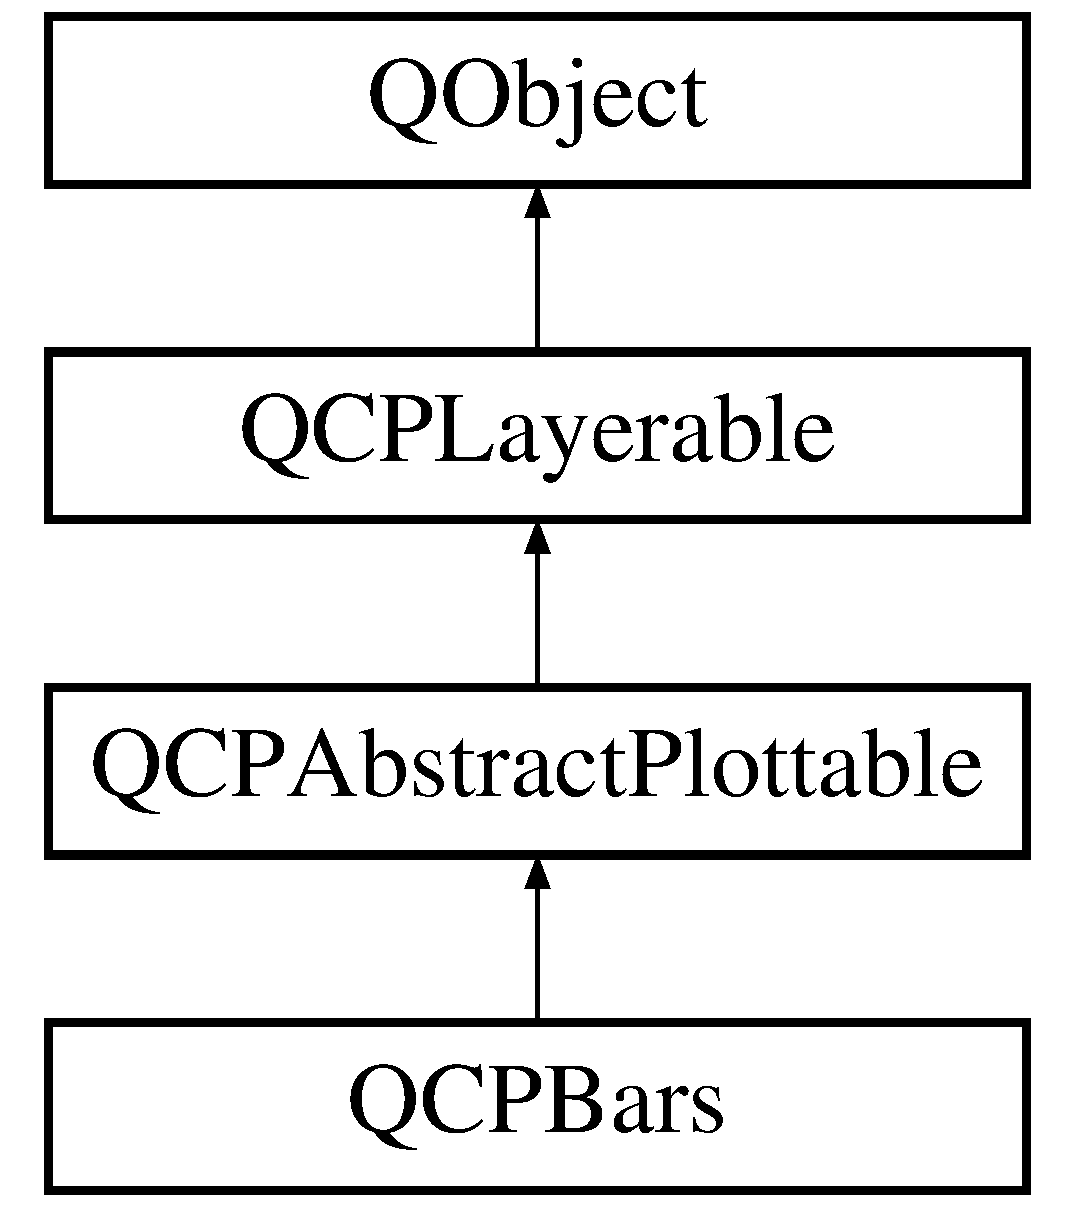
\includegraphics[height=4.000000cm]{class_q_c_p_bars}
\end{center}
\end{figure}
\subsection*{Public Types}
\begin{DoxyCompactItemize}
\item 
enum \hyperlink{class_q_c_p_bars_a65dbbf1ab41cbe993d71521096ed4649}{Width\+Type} \{ \hyperlink{class_q_c_p_bars_a65dbbf1ab41cbe993d71521096ed4649ab74315c9aa77df593c58dd25dfc0de35}{wt\+Absolute}, 
\hyperlink{class_q_c_p_bars_a65dbbf1ab41cbe993d71521096ed4649a90bc09899361ad3422ff277f7c790ffe}{wt\+Axis\+Rect\+Ratio}, 
\hyperlink{class_q_c_p_bars_a65dbbf1ab41cbe993d71521096ed4649aad3cc60ae1bfb1160a30237bee9eaf10}{wt\+Plot\+Coords}
 \}
\end{DoxyCompactItemize}
\subsection*{Public Member Functions}
\begin{DoxyCompactItemize}
\item 
\hyperlink{class_q_c_p_bars_a64006999ad9dff308f40df41cef176ad}{Q\+C\+P\+Bars} (\hyperlink{class_q_c_p_axis}{Q\+C\+P\+Axis} $\ast$\hyperlink{class_q_c_p_abstract_plottable_a72c7a09c22963f2c943f07112b311103}{key\+Axis}, \hyperlink{class_q_c_p_axis}{Q\+C\+P\+Axis} $\ast$\hyperlink{class_q_c_p_abstract_plottable_a3106f9d34d330a6097a8ec5905e5b519}{value\+Axis})
\item 
virtual \hyperlink{class_q_c_p_bars_a4d880e28031ef120603f543379be2f22}{$\sim$\+Q\+C\+P\+Bars} ()
\item 
double \hyperlink{class_q_c_p_bars_a42798c38abd5f5db22bd45d77f429625}{width} () const 
\item 
\hyperlink{class_q_c_p_bars_a65dbbf1ab41cbe993d71521096ed4649}{Width\+Type} \hyperlink{class_q_c_p_bars_a8606651ada5804075f6affd04c88dd05}{width\+Type} () const 
\item 
\hyperlink{class_q_c_p_bars_group}{Q\+C\+P\+Bars\+Group} $\ast$ \hyperlink{class_q_c_p_bars_a6d6b2b17619a0ba9c7a88bb2b90fc178}{bars\+Group} () const 
\item 
double \hyperlink{class_q_c_p_bars_a3c8686a74396883fd1da87b2e325b043}{base\+Value} () const 
\item 
\hyperlink{class_q_c_p_bars}{Q\+C\+P\+Bars} $\ast$ \hyperlink{class_q_c_p_bars_a2c46a686cbad95f180ca3c2e88263961}{bar\+Below} () const 
\item 
\hyperlink{class_q_c_p_bars}{Q\+C\+P\+Bars} $\ast$ \hyperlink{class_q_c_p_bars_a9ca48a6577586825d85bdc1fbf410803}{bar\+Above} () const 
\item 
\hyperlink{qcustomplot_8h_aa846c77472cae93def9f1609d0c57191}{Q\+C\+P\+Bar\+Data\+Map} $\ast$ \hyperlink{class_q_c_p_bars_ac05c21de37f677545d06fd852ef8a743}{data} () const 
\item 
void \hyperlink{class_q_c_p_bars_afec6116579d44d5b706e0fa5e5332507}{set\+Width} (double \hyperlink{class_q_c_p_bars_a42798c38abd5f5db22bd45d77f429625}{width})
\item 
void \hyperlink{class_q_c_p_bars_adcaa3b41281bb2c0f7949b341592fcc0}{set\+Width\+Type} (\hyperlink{class_q_c_p_bars_a65dbbf1ab41cbe993d71521096ed4649}{Width\+Type} \hyperlink{class_q_c_p_bars_a8606651ada5804075f6affd04c88dd05}{width\+Type})
\item 
void \hyperlink{class_q_c_p_bars_aedd1709061f0b307c47ddb45e172ef9a}{set\+Bars\+Group} (\hyperlink{class_q_c_p_bars_group}{Q\+C\+P\+Bars\+Group} $\ast$\hyperlink{class_q_c_p_bars_a6d6b2b17619a0ba9c7a88bb2b90fc178}{bars\+Group})
\item 
void \hyperlink{class_q_c_p_bars_a574ec7eb7537566df1a28ff085d75623}{set\+Base\+Value} (double \hyperlink{class_q_c_p_bars_a3c8686a74396883fd1da87b2e325b043}{base\+Value})
\item 
void \hyperlink{class_q_c_p_bars_aa3435aab19e0a49e4e7b41bd36a8d96b}{set\+Data} (\hyperlink{qcustomplot_8h_aa846c77472cae93def9f1609d0c57191}{Q\+C\+P\+Bar\+Data\+Map} $\ast$\hyperlink{class_q_c_p_bars_ac05c21de37f677545d06fd852ef8a743}{data}, bool copy=false)
\item 
void \hyperlink{class_q_c_p_bars_a3efded5df4a82ecb201f7c28099fa2e5}{set\+Data} (const Q\+Vector$<$ double $>$ \&key, const Q\+Vector$<$ double $>$ \&value)
\item 
void \hyperlink{class_q_c_p_bars_a69fc371346980f19177c3d1ecdad78ee}{move\+Below} (\hyperlink{class_q_c_p_bars}{Q\+C\+P\+Bars} $\ast$bars)
\item 
void \hyperlink{class_q_c_p_bars_ac22e00a6a41509538c21b04f0a57318c}{move\+Above} (\hyperlink{class_q_c_p_bars}{Q\+C\+P\+Bars} $\ast$bars)
\item 
void \hyperlink{class_q_c_p_bars_a1f29cf08615040993209147fa68de3f2}{add\+Data} (const \hyperlink{qcustomplot_8h_aa846c77472cae93def9f1609d0c57191}{Q\+C\+P\+Bar\+Data\+Map} \&data\+Map)
\item 
void \hyperlink{class_q_c_p_bars_a142158b1addefd53259002dd3ab22c3a}{add\+Data} (const \hyperlink{class_q_c_p_bar_data}{Q\+C\+P\+Bar\+Data} \&\hyperlink{class_q_c_p_bars_ac05c21de37f677545d06fd852ef8a743}{data})
\item 
void \hyperlink{class_q_c_p_bars_a684dd105403a5497fda42f2094fecbb7}{add\+Data} (double key, double value)
\item 
void \hyperlink{class_q_c_p_bars_a3679a0a9decab0fa03f8f4c6e3344d52}{add\+Data} (const Q\+Vector$<$ double $>$ \&keys, const Q\+Vector$<$ double $>$ \&values)
\item 
void \hyperlink{class_q_c_p_bars_a9d12779a3fad4820aad2c428f368298d}{remove\+Data\+Before} (double key)
\item 
void \hyperlink{class_q_c_p_bars_a99de6e7abbbf03fb41fa604c7f08aa8b}{remove\+Data\+After} (double key)
\item 
void \hyperlink{class_q_c_p_bars_a1fe9bcb57d670defea1bb65cadf43765}{remove\+Data} (double from\+Key, double to\+Key)
\item 
void \hyperlink{class_q_c_p_bars_a837cc9848ad3edd40a6130b508493f93}{remove\+Data} (double key)
\item 
virtual void \hyperlink{class_q_c_p_bars_a11dbbd707132f07f862dff13c5789c2b}{clear\+Data} ()
\item 
virtual double \hyperlink{class_q_c_p_bars_a0d37a9feb1d0baf73ce6e809db214445}{select\+Test} (const Q\+Point\+F \&pos, bool only\+Selectable, Q\+Variant $\ast$details=0) const 
\end{DoxyCompactItemize}
\subsection*{Protected Member Functions}
\begin{DoxyCompactItemize}
\item 
virtual void \hyperlink{class_q_c_p_bars_a42b894e34dac799f90ff3700706b31df}{draw} (\hyperlink{class_q_c_p_painter}{Q\+C\+P\+Painter} $\ast$painter)
\item 
virtual void \hyperlink{class_q_c_p_bars_ad4fb35d2ab7d2aa460a6612aff3e7a15}{draw\+Legend\+Icon} (\hyperlink{class_q_c_p_painter}{Q\+C\+P\+Painter} $\ast$painter, const Q\+Rect\+F \&rect) const 
\item 
virtual \hyperlink{class_q_c_p_range}{Q\+C\+P\+Range} \hyperlink{class_q_c_p_bars_a93cfdc8a535f36aeb087acca49c00662}{get\+Key\+Range} (bool \&found\+Range, \hyperlink{class_q_c_p_abstract_plottable_a661743478a1d3c09d28ec2711d7653d8}{Sign\+Domain} in\+Sign\+Domain=\hyperlink{class_q_c_p_abstract_plottable_a661743478a1d3c09d28ec2711d7653d8a082b98cfb91a7363a3b5cd17b0c1cd60}{sd\+Both}) const 
\item 
virtual \hyperlink{class_q_c_p_range}{Q\+C\+P\+Range} \hyperlink{class_q_c_p_bars_ada96e20309570d1488c165596cb2647f}{get\+Value\+Range} (bool \&found\+Range, \hyperlink{class_q_c_p_abstract_plottable_a661743478a1d3c09d28ec2711d7653d8}{Sign\+Domain} in\+Sign\+Domain=\hyperlink{class_q_c_p_abstract_plottable_a661743478a1d3c09d28ec2711d7653d8a082b98cfb91a7363a3b5cd17b0c1cd60}{sd\+Both}) const 
\item 
void \hyperlink{class_q_c_p_bars_af73d2032be0a64d2692bb76b08c79ec2}{get\+Visible\+Data\+Bounds} (Q\+C\+P\+Bar\+Data\+Map\+::const\+\_\+iterator \&lower, Q\+C\+P\+Bar\+Data\+Map\+::const\+\_\+iterator \&upper\+End) const 
\item 
Q\+Polygon\+F \hyperlink{class_q_c_p_bars_a1d118a76662cfd691a78c6f573e3f78c}{get\+Bar\+Polygon} (double key, double value) const 
\item 
void \hyperlink{class_q_c_p_bars_a794eefe4fb29b9b40583654ccbf460dc}{get\+Pixel\+Width} (double key, double \&lower, double \&upper) const 
\item 
double \hyperlink{class_q_c_p_bars_ae9b0c2fad9f29030c84bb6e62a4b605f}{get\+Stacked\+Base\+Value} (double key, bool positive) const 
\end{DoxyCompactItemize}
\subsection*{Static Protected Member Functions}
\begin{DoxyCompactItemize}
\item 
static void \hyperlink{class_q_c_p_bars_a6ea37802cd22f97235cab614b14b9f19}{connect\+Bars} (\hyperlink{class_q_c_p_bars}{Q\+C\+P\+Bars} $\ast$lower, \hyperlink{class_q_c_p_bars}{Q\+C\+P\+Bars} $\ast$upper)
\end{DoxyCompactItemize}
\subsection*{Protected Attributes}
\begin{DoxyCompactItemize}
\item 
\hyperlink{qcustomplot_8h_aa846c77472cae93def9f1609d0c57191}{Q\+C\+P\+Bar\+Data\+Map} $\ast$ \hyperlink{class_q_c_p_bars_aef28d29d51ef84b608ecd22c55d531ff}{m\+Data}
\item 
double \hyperlink{class_q_c_p_bars_a7c4e0f2246f8133f48a9c3f24cf5b920}{m\+Width}
\item 
\hyperlink{class_q_c_p_bars_a65dbbf1ab41cbe993d71521096ed4649}{Width\+Type} \hyperlink{class_q_c_p_bars_a94dba1309496c7601d01e2c59715cbb3}{m\+Width\+Type}
\item 
\hyperlink{class_q_c_p_bars_group}{Q\+C\+P\+Bars\+Group} $\ast$ \hyperlink{class_q_c_p_bars_a9f59c255f3739182ca9744dff75beaa9}{m\+Bars\+Group}
\item 
double \hyperlink{class_q_c_p_bars_aa0515cf47fa6044cc28e59b1ae5ec759}{m\+Base\+Value}
\item 
Q\+Pointer$<$ \hyperlink{class_q_c_p_bars}{Q\+C\+P\+Bars} $>$ \hyperlink{class_q_c_p_bars_ad51db970eed7e286f2753b0216fc56de}{m\+Bar\+Below}
\item 
Q\+Pointer$<$ \hyperlink{class_q_c_p_bars}{Q\+C\+P\+Bars} $>$ \hyperlink{class_q_c_p_bars_a0c1c46076c41a478dbb373cfd35929aa}{m\+Bar\+Above}
\end{DoxyCompactItemize}
\subsection*{Friends}
\begin{DoxyCompactItemize}
\item 
class \hyperlink{class_q_c_p_bars_a1cdf9df76adcfae45261690aa0ca2198}{Q\+Custom\+Plot}
\item 
class \hyperlink{class_q_c_p_bars_a8429035e7adfbd7f05805a6530ad5e3b}{Q\+C\+P\+Legend}
\item 
class \hyperlink{class_q_c_p_bars_ae1051b4d58a2786cb420367a586e2fee}{Q\+C\+P\+Bars\+Group}
\end{DoxyCompactItemize}
\subsection*{Additional Inherited Members}


\subsection{Detailed Description}
A plottable representing a bar chart in a plot. 



To plot data, assign it with the \hyperlink{class_q_c_p_bars_aa3435aab19e0a49e4e7b41bd36a8d96b}{set\+Data} or \hyperlink{class_q_c_p_bars_a1f29cf08615040993209147fa68de3f2}{add\+Data} functions.\hypertarget{class_q_c_p_statistical_box_appearance}{}\subsection{Changing the appearance}\label{class_q_c_p_statistical_box_appearance}
The appearance of the bars is determined by the pen and the brush (\hyperlink{class_q_c_p_abstract_plottable_ab74b09ae4c0e7e13142fe4b5bf46cac7}{set\+Pen}, \hyperlink{class_q_c_p_abstract_plottable_a7a4b92144dca6453a1f0f210e27edc74}{set\+Brush}). The width of the individual bars can be controlled with \hyperlink{class_q_c_p_bars_adcaa3b41281bb2c0f7949b341592fcc0}{set\+Width\+Type} and \hyperlink{class_q_c_p_bars_afec6116579d44d5b706e0fa5e5332507}{set\+Width}.

Bar charts are stackable. This means, two \hyperlink{class_q_c_p_bars}{Q\+C\+P\+Bars} plottables can be placed on top of each other (see \hyperlink{class_q_c_p_bars_ac22e00a6a41509538c21b04f0a57318c}{Q\+C\+P\+Bars\+::move\+Above}). So when two bars are at the same key position, they will appear stacked.

If you would like to group multiple \hyperlink{class_q_c_p_bars}{Q\+C\+P\+Bars} plottables together so they appear side by side as shown below, use \hyperlink{class_q_c_p_bars_group}{Q\+C\+P\+Bars\+Group}.

\hypertarget{class_q_c_p_statistical_box_usage}{}\subsection{Usage}\label{class_q_c_p_statistical_box_usage}
Like all data representing objects in \hyperlink{class_q_custom_plot}{Q\+Custom\+Plot}, the \hyperlink{class_q_c_p_bars}{Q\+C\+P\+Bars} is a plottable (\hyperlink{class_q_c_p_abstract_plottable}{Q\+C\+P\+Abstract\+Plottable}). So the plottable-\/interface of \hyperlink{class_q_custom_plot}{Q\+Custom\+Plot} applies (\hyperlink{class_q_custom_plot_a32de81ff53e263e785b83b52ecd99d6f}{Q\+Custom\+Plot\+::plottable}, \hyperlink{class_q_custom_plot_ab7ad9174f701f9c6f64e378df77927a6}{Q\+Custom\+Plot\+::add\+Plottable}, \hyperlink{class_q_custom_plot_af3dafd56884208474f311d6226513ab2}{Q\+Custom\+Plot\+::remove\+Plottable}, etc.)

Usually, you first create an instance\+: 
\begin{DoxyCode}
\hyperlink{class_q_c_p_bars}{QCPBars} *newBars = \textcolor{keyword}{new} \hyperlink{class_q_c_p_bars_a64006999ad9dff308f40df41cef176ad}{QCPBars}(customPlot->xAxis, customPlot->yAxis);
\end{DoxyCode}
 add it to the custom\+Plot with \hyperlink{class_q_custom_plot_ab7ad9174f701f9c6f64e378df77927a6}{Q\+Custom\+Plot\+::add\+Plottable}\+: 
\begin{DoxyCode}
customPlot->addPlottable(newBars);
\end{DoxyCode}
 and then modify the properties of the newly created plottable, e.\+g.\+: 
\begin{DoxyCode}
newBars->\hyperlink{class_q_c_p_abstract_plottable_ab79c7ba76bc7fa89a4b3580e12149f1f}{setName}(\textcolor{stringliteral}{"Country population"});
newBars->\hyperlink{class_q_c_p_bars_aa3435aab19e0a49e4e7b41bd36a8d96b}{setData}(xData, yData);
\end{DoxyCode}
 

\subsection{Member Enumeration Documentation}
\hypertarget{class_q_c_p_bars_a65dbbf1ab41cbe993d71521096ed4649}{}\index{Q\+C\+P\+Bars@{Q\+C\+P\+Bars}!Width\+Type@{Width\+Type}}
\index{Width\+Type@{Width\+Type}!Q\+C\+P\+Bars@{Q\+C\+P\+Bars}}
\subsubsection[{Width\+Type}]{\setlength{\rightskip}{0pt plus 5cm}enum {\bf Q\+C\+P\+Bars\+::\+Width\+Type}}\label{class_q_c_p_bars_a65dbbf1ab41cbe993d71521096ed4649}
Defines the ways the width of the bar can be specified. Thus it defines what the number passed to \hyperlink{class_q_c_p_bars_afec6116579d44d5b706e0fa5e5332507}{set\+Width} actually means.

\begin{DoxySeeAlso}{See also}
\hyperlink{class_q_c_p_bars_adcaa3b41281bb2c0f7949b341592fcc0}{set\+Width\+Type}, \hyperlink{class_q_c_p_bars_afec6116579d44d5b706e0fa5e5332507}{set\+Width} 
\end{DoxySeeAlso}
\begin{Desc}
\item[Enumerator]\par
\begin{description}
\index{wt\+Absolute@{wt\+Absolute}!Q\+C\+P\+Bars@{Q\+C\+P\+Bars}}\index{Q\+C\+P\+Bars@{Q\+C\+P\+Bars}!wt\+Absolute@{wt\+Absolute}}\item[{\em 
\hypertarget{class_q_c_p_bars_a65dbbf1ab41cbe993d71521096ed4649ab74315c9aa77df593c58dd25dfc0de35}{}wt\+Absolute\label{class_q_c_p_bars_a65dbbf1ab41cbe993d71521096ed4649ab74315c9aa77df593c58dd25dfc0de35}
}]Bar width is in absolute pixels. \index{wt\+Axis\+Rect\+Ratio@{wt\+Axis\+Rect\+Ratio}!Q\+C\+P\+Bars@{Q\+C\+P\+Bars}}\index{Q\+C\+P\+Bars@{Q\+C\+P\+Bars}!wt\+Axis\+Rect\+Ratio@{wt\+Axis\+Rect\+Ratio}}\item[{\em 
\hypertarget{class_q_c_p_bars_a65dbbf1ab41cbe993d71521096ed4649a90bc09899361ad3422ff277f7c790ffe}{}wt\+Axis\+Rect\+Ratio\label{class_q_c_p_bars_a65dbbf1ab41cbe993d71521096ed4649a90bc09899361ad3422ff277f7c790ffe}
}]Bar width is given by a fraction of the axis rect size. \index{wt\+Plot\+Coords@{wt\+Plot\+Coords}!Q\+C\+P\+Bars@{Q\+C\+P\+Bars}}\index{Q\+C\+P\+Bars@{Q\+C\+P\+Bars}!wt\+Plot\+Coords@{wt\+Plot\+Coords}}\item[{\em 
\hypertarget{class_q_c_p_bars_a65dbbf1ab41cbe993d71521096ed4649aad3cc60ae1bfb1160a30237bee9eaf10}{}wt\+Plot\+Coords\label{class_q_c_p_bars_a65dbbf1ab41cbe993d71521096ed4649aad3cc60ae1bfb1160a30237bee9eaf10}
}]Bar width is in key coordinates and thus scales with the key axis range. \end{description}
\end{Desc}


\subsection{Constructor \& Destructor Documentation}
\hypertarget{class_q_c_p_bars_a64006999ad9dff308f40df41cef176ad}{}\index{Q\+C\+P\+Bars@{Q\+C\+P\+Bars}!Q\+C\+P\+Bars@{Q\+C\+P\+Bars}}
\index{Q\+C\+P\+Bars@{Q\+C\+P\+Bars}!Q\+C\+P\+Bars@{Q\+C\+P\+Bars}}
\subsubsection[{Q\+C\+P\+Bars}]{\setlength{\rightskip}{0pt plus 5cm}Q\+C\+P\+Bars\+::\+Q\+C\+P\+Bars (
\begin{DoxyParamCaption}
\item[{{\bf Q\+C\+P\+Axis} $\ast$}]{key\+Axis, }
\item[{{\bf Q\+C\+P\+Axis} $\ast$}]{value\+Axis}
\end{DoxyParamCaption}
)\hspace{0.3cm}{\ttfamily [explicit]}}\label{class_q_c_p_bars_a64006999ad9dff308f40df41cef176ad}
Constructs a bar chart which uses {\itshape key\+Axis} as its key axis (\char`\"{}x\char`\"{}) and {\itshape value\+Axis} as its value axis (\char`\"{}y\char`\"{}). {\itshape key\+Axis} and {\itshape value\+Axis} must reside in the same \hyperlink{class_q_custom_plot}{Q\+Custom\+Plot} instance and not have the same orientation. If either of these restrictions is violated, a corresponding message is printed to the debug output (q\+Debug), the construction is not aborted, though.

The constructed \hyperlink{class_q_c_p_bars}{Q\+C\+P\+Bars} can be added to the plot with \hyperlink{class_q_custom_plot_ab7ad9174f701f9c6f64e378df77927a6}{Q\+Custom\+Plot\+::add\+Plottable}, \hyperlink{class_q_custom_plot}{Q\+Custom\+Plot} then takes ownership of the bar chart. \hypertarget{class_q_c_p_bars_a4d880e28031ef120603f543379be2f22}{}\index{Q\+C\+P\+Bars@{Q\+C\+P\+Bars}!````~Q\+C\+P\+Bars@{$\sim$\+Q\+C\+P\+Bars}}
\index{````~Q\+C\+P\+Bars@{$\sim$\+Q\+C\+P\+Bars}!Q\+C\+P\+Bars@{Q\+C\+P\+Bars}}
\subsubsection[{$\sim$\+Q\+C\+P\+Bars}]{\setlength{\rightskip}{0pt plus 5cm}Q\+C\+P\+Bars\+::$\sim$\+Q\+C\+P\+Bars (
\begin{DoxyParamCaption}
{}
\end{DoxyParamCaption}
)\hspace{0.3cm}{\ttfamily [virtual]}}\label{class_q_c_p_bars_a4d880e28031ef120603f543379be2f22}


\subsection{Member Function Documentation}
\hypertarget{class_q_c_p_bars_a1f29cf08615040993209147fa68de3f2}{}\index{Q\+C\+P\+Bars@{Q\+C\+P\+Bars}!add\+Data@{add\+Data}}
\index{add\+Data@{add\+Data}!Q\+C\+P\+Bars@{Q\+C\+P\+Bars}}
\subsubsection[{add\+Data}]{\setlength{\rightskip}{0pt plus 5cm}void Q\+C\+P\+Bars\+::add\+Data (
\begin{DoxyParamCaption}
\item[{const {\bf Q\+C\+P\+Bar\+Data\+Map} \&}]{data\+Map}
\end{DoxyParamCaption}
)}\label{class_q_c_p_bars_a1f29cf08615040993209147fa68de3f2}
Adds the provided data points in {\itshape data\+Map} to the current data. \begin{DoxySeeAlso}{See also}
\hyperlink{class_q_c_p_bars_a1fe9bcb57d670defea1bb65cadf43765}{remove\+Data} 
\end{DoxySeeAlso}
\hypertarget{class_q_c_p_bars_a142158b1addefd53259002dd3ab22c3a}{}\index{Q\+C\+P\+Bars@{Q\+C\+P\+Bars}!add\+Data@{add\+Data}}
\index{add\+Data@{add\+Data}!Q\+C\+P\+Bars@{Q\+C\+P\+Bars}}
\subsubsection[{add\+Data}]{\setlength{\rightskip}{0pt plus 5cm}void Q\+C\+P\+Bars\+::add\+Data (
\begin{DoxyParamCaption}
\item[{const {\bf Q\+C\+P\+Bar\+Data} \&}]{data}
\end{DoxyParamCaption}
)}\label{class_q_c_p_bars_a142158b1addefd53259002dd3ab22c3a}
This is an overloaded member function, provided for convenience. It differs from the above function only in what argument(s) it accepts. Adds the provided single data point in {\itshape data} to the current data. \begin{DoxySeeAlso}{See also}
\hyperlink{class_q_c_p_bars_a1fe9bcb57d670defea1bb65cadf43765}{remove\+Data} 
\end{DoxySeeAlso}
\hypertarget{class_q_c_p_bars_a684dd105403a5497fda42f2094fecbb7}{}\index{Q\+C\+P\+Bars@{Q\+C\+P\+Bars}!add\+Data@{add\+Data}}
\index{add\+Data@{add\+Data}!Q\+C\+P\+Bars@{Q\+C\+P\+Bars}}
\subsubsection[{add\+Data}]{\setlength{\rightskip}{0pt plus 5cm}void Q\+C\+P\+Bars\+::add\+Data (
\begin{DoxyParamCaption}
\item[{double}]{key, }
\item[{double}]{value}
\end{DoxyParamCaption}
)}\label{class_q_c_p_bars_a684dd105403a5497fda42f2094fecbb7}
This is an overloaded member function, provided for convenience. It differs from the above function only in what argument(s) it accepts. Adds the provided single data point as {\itshape key} and {\itshape value} tuple to the current data \begin{DoxySeeAlso}{See also}
\hyperlink{class_q_c_p_bars_a1fe9bcb57d670defea1bb65cadf43765}{remove\+Data} 
\end{DoxySeeAlso}
\hypertarget{class_q_c_p_bars_a3679a0a9decab0fa03f8f4c6e3344d52}{}\index{Q\+C\+P\+Bars@{Q\+C\+P\+Bars}!add\+Data@{add\+Data}}
\index{add\+Data@{add\+Data}!Q\+C\+P\+Bars@{Q\+C\+P\+Bars}}
\subsubsection[{add\+Data}]{\setlength{\rightskip}{0pt plus 5cm}void Q\+C\+P\+Bars\+::add\+Data (
\begin{DoxyParamCaption}
\item[{const Q\+Vector$<$ double $>$ \&}]{keys, }
\item[{const Q\+Vector$<$ double $>$ \&}]{values}
\end{DoxyParamCaption}
)}\label{class_q_c_p_bars_a3679a0a9decab0fa03f8f4c6e3344d52}
This is an overloaded member function, provided for convenience. It differs from the above function only in what argument(s) it accepts. Adds the provided data points as {\itshape key} and {\itshape value} tuples to the current data. \begin{DoxySeeAlso}{See also}
\hyperlink{class_q_c_p_bars_a1fe9bcb57d670defea1bb65cadf43765}{remove\+Data} 
\end{DoxySeeAlso}
\hypertarget{class_q_c_p_bars_a9ca48a6577586825d85bdc1fbf410803}{}\index{Q\+C\+P\+Bars@{Q\+C\+P\+Bars}!bar\+Above@{bar\+Above}}
\index{bar\+Above@{bar\+Above}!Q\+C\+P\+Bars@{Q\+C\+P\+Bars}}
\subsubsection[{bar\+Above}]{\setlength{\rightskip}{0pt plus 5cm}{\bf Q\+C\+P\+Bars} $\ast$ Q\+C\+P\+Bars\+::bar\+Above (
\begin{DoxyParamCaption}
{}
\end{DoxyParamCaption}
) const\hspace{0.3cm}{\ttfamily [inline]}}\label{class_q_c_p_bars_a9ca48a6577586825d85bdc1fbf410803}
Returns the bars plottable that is directly above this bars plottable. If there is no such plottable, returns 0.

\begin{DoxySeeAlso}{See also}
\hyperlink{class_q_c_p_bars_a2c46a686cbad95f180ca3c2e88263961}{bar\+Below}, \hyperlink{class_q_c_p_bars_a69fc371346980f19177c3d1ecdad78ee}{move\+Below}, \hyperlink{class_q_c_p_bars_ac22e00a6a41509538c21b04f0a57318c}{move\+Above} 
\end{DoxySeeAlso}
\hypertarget{class_q_c_p_bars_a2c46a686cbad95f180ca3c2e88263961}{}\index{Q\+C\+P\+Bars@{Q\+C\+P\+Bars}!bar\+Below@{bar\+Below}}
\index{bar\+Below@{bar\+Below}!Q\+C\+P\+Bars@{Q\+C\+P\+Bars}}
\subsubsection[{bar\+Below}]{\setlength{\rightskip}{0pt plus 5cm}{\bf Q\+C\+P\+Bars} $\ast$ Q\+C\+P\+Bars\+::bar\+Below (
\begin{DoxyParamCaption}
{}
\end{DoxyParamCaption}
) const\hspace{0.3cm}{\ttfamily [inline]}}\label{class_q_c_p_bars_a2c46a686cbad95f180ca3c2e88263961}
Returns the bars plottable that is directly below this bars plottable. If there is no such plottable, returns 0.

\begin{DoxySeeAlso}{See also}
\hyperlink{class_q_c_p_bars_a9ca48a6577586825d85bdc1fbf410803}{bar\+Above}, \hyperlink{class_q_c_p_bars_a69fc371346980f19177c3d1ecdad78ee}{move\+Below}, \hyperlink{class_q_c_p_bars_ac22e00a6a41509538c21b04f0a57318c}{move\+Above} 
\end{DoxySeeAlso}
\hypertarget{class_q_c_p_bars_a6d6b2b17619a0ba9c7a88bb2b90fc178}{}\index{Q\+C\+P\+Bars@{Q\+C\+P\+Bars}!bars\+Group@{bars\+Group}}
\index{bars\+Group@{bars\+Group}!Q\+C\+P\+Bars@{Q\+C\+P\+Bars}}
\subsubsection[{bars\+Group}]{\setlength{\rightskip}{0pt plus 5cm}{\bf Q\+C\+P\+Bars\+Group}$\ast$ Q\+C\+P\+Bars\+::bars\+Group (
\begin{DoxyParamCaption}
{}
\end{DoxyParamCaption}
) const\hspace{0.3cm}{\ttfamily [inline]}}\label{class_q_c_p_bars_a6d6b2b17619a0ba9c7a88bb2b90fc178}
\hypertarget{class_q_c_p_bars_a3c8686a74396883fd1da87b2e325b043}{}\index{Q\+C\+P\+Bars@{Q\+C\+P\+Bars}!base\+Value@{base\+Value}}
\index{base\+Value@{base\+Value}!Q\+C\+P\+Bars@{Q\+C\+P\+Bars}}
\subsubsection[{base\+Value}]{\setlength{\rightskip}{0pt plus 5cm}double Q\+C\+P\+Bars\+::base\+Value (
\begin{DoxyParamCaption}
{}
\end{DoxyParamCaption}
) const\hspace{0.3cm}{\ttfamily [inline]}}\label{class_q_c_p_bars_a3c8686a74396883fd1da87b2e325b043}
\hypertarget{class_q_c_p_bars_a11dbbd707132f07f862dff13c5789c2b}{}\index{Q\+C\+P\+Bars@{Q\+C\+P\+Bars}!clear\+Data@{clear\+Data}}
\index{clear\+Data@{clear\+Data}!Q\+C\+P\+Bars@{Q\+C\+P\+Bars}}
\subsubsection[{clear\+Data}]{\setlength{\rightskip}{0pt plus 5cm}void Q\+C\+P\+Bars\+::clear\+Data (
\begin{DoxyParamCaption}
{}
\end{DoxyParamCaption}
)\hspace{0.3cm}{\ttfamily [virtual]}}\label{class_q_c_p_bars_a11dbbd707132f07f862dff13c5789c2b}
Removes all data points. \begin{DoxySeeAlso}{See also}
\hyperlink{class_q_c_p_bars_a1fe9bcb57d670defea1bb65cadf43765}{remove\+Data}, \hyperlink{class_q_c_p_bars_a99de6e7abbbf03fb41fa604c7f08aa8b}{remove\+Data\+After}, \hyperlink{class_q_c_p_bars_a9d12779a3fad4820aad2c428f368298d}{remove\+Data\+Before} 
\end{DoxySeeAlso}


Implements \hyperlink{class_q_c_p_abstract_plottable_a86e5b8fd4b6ff4f4084e7ea4c573fc53}{Q\+C\+P\+Abstract\+Plottable}.

\hypertarget{class_q_c_p_bars_a6ea37802cd22f97235cab614b14b9f19}{}\index{Q\+C\+P\+Bars@{Q\+C\+P\+Bars}!connect\+Bars@{connect\+Bars}}
\index{connect\+Bars@{connect\+Bars}!Q\+C\+P\+Bars@{Q\+C\+P\+Bars}}
\subsubsection[{connect\+Bars}]{\setlength{\rightskip}{0pt plus 5cm}void Q\+C\+P\+Bars\+::connect\+Bars (
\begin{DoxyParamCaption}
\item[{{\bf Q\+C\+P\+Bars} $\ast$}]{lower, }
\item[{{\bf Q\+C\+P\+Bars} $\ast$}]{upper}
\end{DoxyParamCaption}
)\hspace{0.3cm}{\ttfamily [static]}, {\ttfamily [protected]}}\label{class_q_c_p_bars_a6ea37802cd22f97235cab614b14b9f19}
\hypertarget{class_q_c_p_bars_ac05c21de37f677545d06fd852ef8a743}{}\index{Q\+C\+P\+Bars@{Q\+C\+P\+Bars}!data@{data}}
\index{data@{data}!Q\+C\+P\+Bars@{Q\+C\+P\+Bars}}
\subsubsection[{data}]{\setlength{\rightskip}{0pt plus 5cm}{\bf Q\+C\+P\+Bar\+Data\+Map}$\ast$ Q\+C\+P\+Bars\+::data (
\begin{DoxyParamCaption}
{}
\end{DoxyParamCaption}
) const\hspace{0.3cm}{\ttfamily [inline]}}\label{class_q_c_p_bars_ac05c21de37f677545d06fd852ef8a743}
\hypertarget{class_q_c_p_bars_a42b894e34dac799f90ff3700706b31df}{}\index{Q\+C\+P\+Bars@{Q\+C\+P\+Bars}!draw@{draw}}
\index{draw@{draw}!Q\+C\+P\+Bars@{Q\+C\+P\+Bars}}
\subsubsection[{draw}]{\setlength{\rightskip}{0pt plus 5cm}void Q\+C\+P\+Bars\+::draw (
\begin{DoxyParamCaption}
\item[{{\bf Q\+C\+P\+Painter} $\ast$}]{painter}
\end{DoxyParamCaption}
)\hspace{0.3cm}{\ttfamily [protected]}, {\ttfamily [virtual]}}\label{class_q_c_p_bars_a42b894e34dac799f90ff3700706b31df}


Implements \hyperlink{class_q_c_p_abstract_plottable_acbab5e30dcd04fd302b4a5902ac2c482}{Q\+C\+P\+Abstract\+Plottable}.

\hypertarget{class_q_c_p_bars_ad4fb35d2ab7d2aa460a6612aff3e7a15}{}\index{Q\+C\+P\+Bars@{Q\+C\+P\+Bars}!draw\+Legend\+Icon@{draw\+Legend\+Icon}}
\index{draw\+Legend\+Icon@{draw\+Legend\+Icon}!Q\+C\+P\+Bars@{Q\+C\+P\+Bars}}
\subsubsection[{draw\+Legend\+Icon}]{\setlength{\rightskip}{0pt plus 5cm}void Q\+C\+P\+Bars\+::draw\+Legend\+Icon (
\begin{DoxyParamCaption}
\item[{{\bf Q\+C\+P\+Painter} $\ast$}]{painter, }
\item[{const Q\+Rect\+F \&}]{rect}
\end{DoxyParamCaption}
) const\hspace{0.3cm}{\ttfamily [protected]}, {\ttfamily [virtual]}}\label{class_q_c_p_bars_ad4fb35d2ab7d2aa460a6612aff3e7a15}


Implements \hyperlink{class_q_c_p_abstract_plottable_a9a450783fd9ed539e589999fd390cdf7}{Q\+C\+P\+Abstract\+Plottable}.

\hypertarget{class_q_c_p_bars_a1d118a76662cfd691a78c6f573e3f78c}{}\index{Q\+C\+P\+Bars@{Q\+C\+P\+Bars}!get\+Bar\+Polygon@{get\+Bar\+Polygon}}
\index{get\+Bar\+Polygon@{get\+Bar\+Polygon}!Q\+C\+P\+Bars@{Q\+C\+P\+Bars}}
\subsubsection[{get\+Bar\+Polygon}]{\setlength{\rightskip}{0pt plus 5cm}Q\+Polygon\+F Q\+C\+P\+Bars\+::get\+Bar\+Polygon (
\begin{DoxyParamCaption}
\item[{double}]{key, }
\item[{double}]{value}
\end{DoxyParamCaption}
) const\hspace{0.3cm}{\ttfamily [protected]}}\label{class_q_c_p_bars_a1d118a76662cfd691a78c6f573e3f78c}
\hypertarget{class_q_c_p_bars_a93cfdc8a535f36aeb087acca49c00662}{}\index{Q\+C\+P\+Bars@{Q\+C\+P\+Bars}!get\+Key\+Range@{get\+Key\+Range}}
\index{get\+Key\+Range@{get\+Key\+Range}!Q\+C\+P\+Bars@{Q\+C\+P\+Bars}}
\subsubsection[{get\+Key\+Range}]{\setlength{\rightskip}{0pt plus 5cm}{\bf Q\+C\+P\+Range} Q\+C\+P\+Bars\+::get\+Key\+Range (
\begin{DoxyParamCaption}
\item[{bool \&}]{found\+Range, }
\item[{{\bf Sign\+Domain}}]{in\+Sign\+Domain = {\ttfamily {\bf sd\+Both}}}
\end{DoxyParamCaption}
) const\hspace{0.3cm}{\ttfamily [protected]}, {\ttfamily [virtual]}}\label{class_q_c_p_bars_a93cfdc8a535f36aeb087acca49c00662}


Implements \hyperlink{class_q_c_p_abstract_plottable_a345d702b2e7e12c8cfdddff65ba85e8c}{Q\+C\+P\+Abstract\+Plottable}.

\hypertarget{class_q_c_p_bars_a794eefe4fb29b9b40583654ccbf460dc}{}\index{Q\+C\+P\+Bars@{Q\+C\+P\+Bars}!get\+Pixel\+Width@{get\+Pixel\+Width}}
\index{get\+Pixel\+Width@{get\+Pixel\+Width}!Q\+C\+P\+Bars@{Q\+C\+P\+Bars}}
\subsubsection[{get\+Pixel\+Width}]{\setlength{\rightskip}{0pt plus 5cm}void Q\+C\+P\+Bars\+::get\+Pixel\+Width (
\begin{DoxyParamCaption}
\item[{double}]{key, }
\item[{double \&}]{lower, }
\item[{double \&}]{upper}
\end{DoxyParamCaption}
) const\hspace{0.3cm}{\ttfamily [protected]}}\label{class_q_c_p_bars_a794eefe4fb29b9b40583654ccbf460dc}
\hypertarget{class_q_c_p_bars_ae9b0c2fad9f29030c84bb6e62a4b605f}{}\index{Q\+C\+P\+Bars@{Q\+C\+P\+Bars}!get\+Stacked\+Base\+Value@{get\+Stacked\+Base\+Value}}
\index{get\+Stacked\+Base\+Value@{get\+Stacked\+Base\+Value}!Q\+C\+P\+Bars@{Q\+C\+P\+Bars}}
\subsubsection[{get\+Stacked\+Base\+Value}]{\setlength{\rightskip}{0pt plus 5cm}double Q\+C\+P\+Bars\+::get\+Stacked\+Base\+Value (
\begin{DoxyParamCaption}
\item[{double}]{key, }
\item[{bool}]{positive}
\end{DoxyParamCaption}
) const\hspace{0.3cm}{\ttfamily [protected]}}\label{class_q_c_p_bars_ae9b0c2fad9f29030c84bb6e62a4b605f}
\hypertarget{class_q_c_p_bars_ada96e20309570d1488c165596cb2647f}{}\index{Q\+C\+P\+Bars@{Q\+C\+P\+Bars}!get\+Value\+Range@{get\+Value\+Range}}
\index{get\+Value\+Range@{get\+Value\+Range}!Q\+C\+P\+Bars@{Q\+C\+P\+Bars}}
\subsubsection[{get\+Value\+Range}]{\setlength{\rightskip}{0pt plus 5cm}{\bf Q\+C\+P\+Range} Q\+C\+P\+Bars\+::get\+Value\+Range (
\begin{DoxyParamCaption}
\item[{bool \&}]{found\+Range, }
\item[{{\bf Sign\+Domain}}]{in\+Sign\+Domain = {\ttfamily {\bf sd\+Both}}}
\end{DoxyParamCaption}
) const\hspace{0.3cm}{\ttfamily [protected]}, {\ttfamily [virtual]}}\label{class_q_c_p_bars_ada96e20309570d1488c165596cb2647f}


Implements \hyperlink{class_q_c_p_abstract_plottable_aa3331b415b5939fe4df60b78831b2799}{Q\+C\+P\+Abstract\+Plottable}.

\hypertarget{class_q_c_p_bars_af73d2032be0a64d2692bb76b08c79ec2}{}\index{Q\+C\+P\+Bars@{Q\+C\+P\+Bars}!get\+Visible\+Data\+Bounds@{get\+Visible\+Data\+Bounds}}
\index{get\+Visible\+Data\+Bounds@{get\+Visible\+Data\+Bounds}!Q\+C\+P\+Bars@{Q\+C\+P\+Bars}}
\subsubsection[{get\+Visible\+Data\+Bounds}]{\setlength{\rightskip}{0pt plus 5cm}void Q\+C\+P\+Bars\+::get\+Visible\+Data\+Bounds (
\begin{DoxyParamCaption}
\item[{Q\+C\+P\+Bar\+Data\+Map\+::const\+\_\+iterator \&}]{lower, }
\item[{Q\+C\+P\+Bar\+Data\+Map\+::const\+\_\+iterator \&}]{upper\+End}
\end{DoxyParamCaption}
) const\hspace{0.3cm}{\ttfamily [protected]}}\label{class_q_c_p_bars_af73d2032be0a64d2692bb76b08c79ec2}
\hypertarget{class_q_c_p_bars_ac22e00a6a41509538c21b04f0a57318c}{}\index{Q\+C\+P\+Bars@{Q\+C\+P\+Bars}!move\+Above@{move\+Above}}
\index{move\+Above@{move\+Above}!Q\+C\+P\+Bars@{Q\+C\+P\+Bars}}
\subsubsection[{move\+Above}]{\setlength{\rightskip}{0pt plus 5cm}void Q\+C\+P\+Bars\+::move\+Above (
\begin{DoxyParamCaption}
\item[{{\bf Q\+C\+P\+Bars} $\ast$}]{bars}
\end{DoxyParamCaption}
)}\label{class_q_c_p_bars_ac22e00a6a41509538c21b04f0a57318c}
Moves this bars plottable above {\itshape bars}. In other words, the bars of this plottable will appear above the bars of {\itshape bars}. The move target {\itshape bars} must use the same key and value axis as this plottable.

Inserting into and removing from existing bar stacking is handled gracefully. If {\itshape bars} already has a bars object below itself, this bars object is inserted between the two. If this bars object is already between two other bars, the two other bars will be stacked on top of each other after the operation.

To remove this bars plottable from any stacking, set {\itshape bars} to 0.

\begin{DoxySeeAlso}{See also}
\hyperlink{class_q_c_p_bars_a69fc371346980f19177c3d1ecdad78ee}{move\+Below}, \hyperlink{class_q_c_p_bars_a2c46a686cbad95f180ca3c2e88263961}{bar\+Below}, \hyperlink{class_q_c_p_bars_a9ca48a6577586825d85bdc1fbf410803}{bar\+Above} 
\end{DoxySeeAlso}
\hypertarget{class_q_c_p_bars_a69fc371346980f19177c3d1ecdad78ee}{}\index{Q\+C\+P\+Bars@{Q\+C\+P\+Bars}!move\+Below@{move\+Below}}
\index{move\+Below@{move\+Below}!Q\+C\+P\+Bars@{Q\+C\+P\+Bars}}
\subsubsection[{move\+Below}]{\setlength{\rightskip}{0pt plus 5cm}void Q\+C\+P\+Bars\+::move\+Below (
\begin{DoxyParamCaption}
\item[{{\bf Q\+C\+P\+Bars} $\ast$}]{bars}
\end{DoxyParamCaption}
)}\label{class_q_c_p_bars_a69fc371346980f19177c3d1ecdad78ee}
Moves this bars plottable below {\itshape bars}. In other words, the bars of this plottable will appear below the bars of {\itshape bars}. The move target {\itshape bars} must use the same key and value axis as this plottable.

Inserting into and removing from existing bar stacking is handled gracefully. If {\itshape bars} already has a bars object below itself, this bars object is inserted between the two. If this bars object is already between two other bars, the two other bars will be stacked on top of each other after the operation.

To remove this bars plottable from any stacking, set {\itshape bars} to 0.

\begin{DoxySeeAlso}{See also}
\hyperlink{class_q_c_p_bars_a69fc371346980f19177c3d1ecdad78ee}{move\+Below}, \hyperlink{class_q_c_p_bars_a9ca48a6577586825d85bdc1fbf410803}{bar\+Above}, \hyperlink{class_q_c_p_bars_a2c46a686cbad95f180ca3c2e88263961}{bar\+Below} 
\end{DoxySeeAlso}
\hypertarget{class_q_c_p_bars_a1fe9bcb57d670defea1bb65cadf43765}{}\index{Q\+C\+P\+Bars@{Q\+C\+P\+Bars}!remove\+Data@{remove\+Data}}
\index{remove\+Data@{remove\+Data}!Q\+C\+P\+Bars@{Q\+C\+P\+Bars}}
\subsubsection[{remove\+Data}]{\setlength{\rightskip}{0pt plus 5cm}void Q\+C\+P\+Bars\+::remove\+Data (
\begin{DoxyParamCaption}
\item[{double}]{from\+Key, }
\item[{double}]{to\+Key}
\end{DoxyParamCaption}
)}\label{class_q_c_p_bars_a1fe9bcb57d670defea1bb65cadf43765}
Removes all data points with key between {\itshape from\+Key} and {\itshape to\+Key}. if {\itshape from\+Key} is greater or equal to {\itshape to\+Key}, the function does nothing. To remove a single data point with known key, use \hyperlink{class_q_c_p_bars_a837cc9848ad3edd40a6130b508493f93}{remove\+Data(double key)}.

\begin{DoxySeeAlso}{See also}
\hyperlink{class_q_c_p_bars_a1f29cf08615040993209147fa68de3f2}{add\+Data}, \hyperlink{class_q_c_p_bars_a11dbbd707132f07f862dff13c5789c2b}{clear\+Data} 
\end{DoxySeeAlso}
\hypertarget{class_q_c_p_bars_a837cc9848ad3edd40a6130b508493f93}{}\index{Q\+C\+P\+Bars@{Q\+C\+P\+Bars}!remove\+Data@{remove\+Data}}
\index{remove\+Data@{remove\+Data}!Q\+C\+P\+Bars@{Q\+C\+P\+Bars}}
\subsubsection[{remove\+Data}]{\setlength{\rightskip}{0pt plus 5cm}void Q\+C\+P\+Bars\+::remove\+Data (
\begin{DoxyParamCaption}
\item[{double}]{key}
\end{DoxyParamCaption}
)}\label{class_q_c_p_bars_a837cc9848ad3edd40a6130b508493f93}
This is an overloaded member function, provided for convenience. It differs from the above function only in what argument(s) it accepts.

Removes a single data point at {\itshape key}. If the position is not known with absolute precision, consider using \hyperlink{class_q_c_p_bars_a1fe9bcb57d670defea1bb65cadf43765}{remove\+Data(double from\+Key, double to\+Key)} with a small fuzziness interval around the suspected position, depeding on the precision with which the key is known.

\begin{DoxySeeAlso}{See also}
\hyperlink{class_q_c_p_bars_a1f29cf08615040993209147fa68de3f2}{add\+Data}, \hyperlink{class_q_c_p_bars_a11dbbd707132f07f862dff13c5789c2b}{clear\+Data} 
\end{DoxySeeAlso}
\hypertarget{class_q_c_p_bars_a99de6e7abbbf03fb41fa604c7f08aa8b}{}\index{Q\+C\+P\+Bars@{Q\+C\+P\+Bars}!remove\+Data\+After@{remove\+Data\+After}}
\index{remove\+Data\+After@{remove\+Data\+After}!Q\+C\+P\+Bars@{Q\+C\+P\+Bars}}
\subsubsection[{remove\+Data\+After}]{\setlength{\rightskip}{0pt plus 5cm}void Q\+C\+P\+Bars\+::remove\+Data\+After (
\begin{DoxyParamCaption}
\item[{double}]{key}
\end{DoxyParamCaption}
)}\label{class_q_c_p_bars_a99de6e7abbbf03fb41fa604c7f08aa8b}
Removes all data points with key greater than {\itshape key}. \begin{DoxySeeAlso}{See also}
\hyperlink{class_q_c_p_bars_a1f29cf08615040993209147fa68de3f2}{add\+Data}, \hyperlink{class_q_c_p_bars_a11dbbd707132f07f862dff13c5789c2b}{clear\+Data} 
\end{DoxySeeAlso}
\hypertarget{class_q_c_p_bars_a9d12779a3fad4820aad2c428f368298d}{}\index{Q\+C\+P\+Bars@{Q\+C\+P\+Bars}!remove\+Data\+Before@{remove\+Data\+Before}}
\index{remove\+Data\+Before@{remove\+Data\+Before}!Q\+C\+P\+Bars@{Q\+C\+P\+Bars}}
\subsubsection[{remove\+Data\+Before}]{\setlength{\rightskip}{0pt plus 5cm}void Q\+C\+P\+Bars\+::remove\+Data\+Before (
\begin{DoxyParamCaption}
\item[{double}]{key}
\end{DoxyParamCaption}
)}\label{class_q_c_p_bars_a9d12779a3fad4820aad2c428f368298d}
Removes all data points with key smaller than {\itshape key}. \begin{DoxySeeAlso}{See also}
\hyperlink{class_q_c_p_bars_a1f29cf08615040993209147fa68de3f2}{add\+Data}, \hyperlink{class_q_c_p_bars_a11dbbd707132f07f862dff13c5789c2b}{clear\+Data} 
\end{DoxySeeAlso}
\hypertarget{class_q_c_p_bars_a0d37a9feb1d0baf73ce6e809db214445}{}\index{Q\+C\+P\+Bars@{Q\+C\+P\+Bars}!select\+Test@{select\+Test}}
\index{select\+Test@{select\+Test}!Q\+C\+P\+Bars@{Q\+C\+P\+Bars}}
\subsubsection[{select\+Test}]{\setlength{\rightskip}{0pt plus 5cm}double Q\+C\+P\+Bars\+::select\+Test (
\begin{DoxyParamCaption}
\item[{const Q\+Point\+F \&}]{pos, }
\item[{bool}]{only\+Selectable, }
\item[{Q\+Variant $\ast$}]{details = {\ttfamily 0}}
\end{DoxyParamCaption}
) const\hspace{0.3cm}{\ttfamily [virtual]}}\label{class_q_c_p_bars_a0d37a9feb1d0baf73ce6e809db214445}
This function is used to decide whether a click hits a layerable object or not.

{\itshape pos} is a point in pixel coordinates on the \hyperlink{class_q_custom_plot}{Q\+Custom\+Plot} surface. This function returns the shortest pixel distance of this point to the object. If the object is either invisible or the distance couldn\textquotesingle{}t be determined, -\/1.\+0 is returned. Further, if {\itshape only\+Selectable} is true and the object is not selectable, -\/1.\+0 is returned, too.

If the item is represented not by single lines but by an area like \hyperlink{class_q_c_p_item_rect}{Q\+C\+P\+Item\+Rect} or \hyperlink{class_q_c_p_item_text}{Q\+C\+P\+Item\+Text}, a click inside the area returns a constant value greater zero (typically the selection\+Tolerance of the parent \hyperlink{class_q_custom_plot}{Q\+Custom\+Plot} multiplied by 0.\+99). If the click lies outside the area, this function returns -\/1.\+0.

Providing a constant value for area objects allows selecting line objects even when they are obscured by such area objects, by clicking close to the lines (i.\+e. closer than 0.\+99$\ast$selection\+Tolerance).

The actual setting of the selection state is not done by this function. This is handled by the parent \hyperlink{class_q_custom_plot}{Q\+Custom\+Plot} when the mouse\+Release\+Event occurs, and the finally selected object is notified via the select\+Event/deselect\+Event methods.

{\itshape details} is an optional output parameter. Every layerable subclass may place any information in {\itshape details}. This information will be passed to \hyperlink{class_q_c_p_abstract_plottable_a16aaad02456aa23a759efd1ac90c79bf}{select\+Event} when the parent \hyperlink{class_q_custom_plot}{Q\+Custom\+Plot} decides on the basis of this select\+Test call, that the object was successfully selected. The subsequent call to \hyperlink{class_q_c_p_abstract_plottable_a16aaad02456aa23a759efd1ac90c79bf}{select\+Event} will carry the {\itshape details}. This is useful for multi-\/part objects (like \hyperlink{class_q_c_p_axis}{Q\+C\+P\+Axis}). This way, a possibly complex calculation to decide which part was clicked is only done once in \hyperlink{class_q_c_p_bars_a0d37a9feb1d0baf73ce6e809db214445}{select\+Test}. The result (i.\+e. the actually clicked part) can then be placed in {\itshape details}. So in the subsequent \hyperlink{class_q_c_p_abstract_plottable_a16aaad02456aa23a759efd1ac90c79bf}{select\+Event}, the decision which part was selected doesn\textquotesingle{}t have to be done a second time for a single selection operation.

You may pass 0 as {\itshape details} to indicate that you are not interested in those selection details.

\begin{DoxySeeAlso}{See also}
\hyperlink{class_q_c_p_abstract_plottable_a16aaad02456aa23a759efd1ac90c79bf}{select\+Event}, \hyperlink{class_q_c_p_abstract_plottable_a6fa0d0f95560ea8b01ee13f296dab2b1}{deselect\+Event}, \hyperlink{class_q_custom_plot_a5ee1e2f6ae27419deca53e75907c27e5}{Q\+Custom\+Plot\+::set\+Interactions} 
\end{DoxySeeAlso}


Implements \hyperlink{class_q_c_p_abstract_plottable_a38efe9641d972992a3d44204bc80ec1d}{Q\+C\+P\+Abstract\+Plottable}.

\hypertarget{class_q_c_p_bars_aedd1709061f0b307c47ddb45e172ef9a}{}\index{Q\+C\+P\+Bars@{Q\+C\+P\+Bars}!set\+Bars\+Group@{set\+Bars\+Group}}
\index{set\+Bars\+Group@{set\+Bars\+Group}!Q\+C\+P\+Bars@{Q\+C\+P\+Bars}}
\subsubsection[{set\+Bars\+Group}]{\setlength{\rightskip}{0pt plus 5cm}void Q\+C\+P\+Bars\+::set\+Bars\+Group (
\begin{DoxyParamCaption}
\item[{{\bf Q\+C\+P\+Bars\+Group} $\ast$}]{bars\+Group}
\end{DoxyParamCaption}
)}\label{class_q_c_p_bars_aedd1709061f0b307c47ddb45e172ef9a}
Sets to which \hyperlink{class_q_c_p_bars_group}{Q\+C\+P\+Bars\+Group} this \hyperlink{class_q_c_p_bars}{Q\+C\+P\+Bars} instance belongs to. Alternatively, you can also use \hyperlink{class_q_c_p_bars_group_a809ed63cc4ff7cd5b0b8c96b470163d3}{Q\+C\+P\+Bars\+Group\+::append}.

To remove this \hyperlink{class_q_c_p_bars}{Q\+C\+P\+Bars} from any group, set {\itshape bars\+Group} to 0. \hypertarget{class_q_c_p_bars_a574ec7eb7537566df1a28ff085d75623}{}\index{Q\+C\+P\+Bars@{Q\+C\+P\+Bars}!set\+Base\+Value@{set\+Base\+Value}}
\index{set\+Base\+Value@{set\+Base\+Value}!Q\+C\+P\+Bars@{Q\+C\+P\+Bars}}
\subsubsection[{set\+Base\+Value}]{\setlength{\rightskip}{0pt plus 5cm}void Q\+C\+P\+Bars\+::set\+Base\+Value (
\begin{DoxyParamCaption}
\item[{double}]{base\+Value}
\end{DoxyParamCaption}
)}\label{class_q_c_p_bars_a574ec7eb7537566df1a28ff085d75623}
Sets the base value of this bars plottable.

The base value defines where on the value coordinate the bars start. How far the bars extend from the base value is given by their individual value data. For example, if the base value is set to 1, a bar with data value 2 will have its lowest point at value coordinate 1 and highest point at 3.

For stacked bars, only the base value of the bottom-\/most \hyperlink{class_q_c_p_bars}{Q\+C\+P\+Bars} has meaning.

The default base value is 0. \hypertarget{class_q_c_p_bars_aa3435aab19e0a49e4e7b41bd36a8d96b}{}\index{Q\+C\+P\+Bars@{Q\+C\+P\+Bars}!set\+Data@{set\+Data}}
\index{set\+Data@{set\+Data}!Q\+C\+P\+Bars@{Q\+C\+P\+Bars}}
\subsubsection[{set\+Data}]{\setlength{\rightskip}{0pt plus 5cm}void Q\+C\+P\+Bars\+::set\+Data (
\begin{DoxyParamCaption}
\item[{{\bf Q\+C\+P\+Bar\+Data\+Map} $\ast$}]{data, }
\item[{bool}]{copy = {\ttfamily false}}
\end{DoxyParamCaption}
)}\label{class_q_c_p_bars_aa3435aab19e0a49e4e7b41bd36a8d96b}
Replaces the current data with the provided {\itshape data}.

If {\itshape copy} is set to true, data points in {\itshape data} will only be copied. if false, the plottable takes ownership of the passed data and replaces the internal data pointer with it. This is significantly faster than copying for large datasets. \hypertarget{class_q_c_p_bars_a3efded5df4a82ecb201f7c28099fa2e5}{}\index{Q\+C\+P\+Bars@{Q\+C\+P\+Bars}!set\+Data@{set\+Data}}
\index{set\+Data@{set\+Data}!Q\+C\+P\+Bars@{Q\+C\+P\+Bars}}
\subsubsection[{set\+Data}]{\setlength{\rightskip}{0pt plus 5cm}void Q\+C\+P\+Bars\+::set\+Data (
\begin{DoxyParamCaption}
\item[{const Q\+Vector$<$ double $>$ \&}]{key, }
\item[{const Q\+Vector$<$ double $>$ \&}]{value}
\end{DoxyParamCaption}
)}\label{class_q_c_p_bars_a3efded5df4a82ecb201f7c28099fa2e5}
This is an overloaded member function, provided for convenience. It differs from the above function only in what argument(s) it accepts.

Replaces the current data with the provided points in {\itshape key} and {\itshape value} tuples. The provided vectors should have equal length. Else, the number of added points will be the size of the smallest vector. \hypertarget{class_q_c_p_bars_afec6116579d44d5b706e0fa5e5332507}{}\index{Q\+C\+P\+Bars@{Q\+C\+P\+Bars}!set\+Width@{set\+Width}}
\index{set\+Width@{set\+Width}!Q\+C\+P\+Bars@{Q\+C\+P\+Bars}}
\subsubsection[{set\+Width}]{\setlength{\rightskip}{0pt plus 5cm}void Q\+C\+P\+Bars\+::set\+Width (
\begin{DoxyParamCaption}
\item[{double}]{width}
\end{DoxyParamCaption}
)}\label{class_q_c_p_bars_afec6116579d44d5b706e0fa5e5332507}
Sets the width of the bars.

How the number passed as {\itshape width} is interpreted (e.\+g. screen pixels, plot coordinates,...), depends on the currently set width type, see \hyperlink{class_q_c_p_bars_adcaa3b41281bb2c0f7949b341592fcc0}{set\+Width\+Type} and \hyperlink{class_q_c_p_bars_a65dbbf1ab41cbe993d71521096ed4649}{Width\+Type}. \hypertarget{class_q_c_p_bars_adcaa3b41281bb2c0f7949b341592fcc0}{}\index{Q\+C\+P\+Bars@{Q\+C\+P\+Bars}!set\+Width\+Type@{set\+Width\+Type}}
\index{set\+Width\+Type@{set\+Width\+Type}!Q\+C\+P\+Bars@{Q\+C\+P\+Bars}}
\subsubsection[{set\+Width\+Type}]{\setlength{\rightskip}{0pt plus 5cm}void Q\+C\+P\+Bars\+::set\+Width\+Type (
\begin{DoxyParamCaption}
\item[{{\bf Q\+C\+P\+Bars\+::\+Width\+Type}}]{width\+Type}
\end{DoxyParamCaption}
)}\label{class_q_c_p_bars_adcaa3b41281bb2c0f7949b341592fcc0}
Sets how the width of the bars is defined. See the documentation of \hyperlink{class_q_c_p_bars_a65dbbf1ab41cbe993d71521096ed4649}{Width\+Type} for an explanation of the possible values for {\itshape width\+Type}.

The default value is \hyperlink{class_q_c_p_bars_a65dbbf1ab41cbe993d71521096ed4649aad3cc60ae1bfb1160a30237bee9eaf10}{wt\+Plot\+Coords}.

\begin{DoxySeeAlso}{See also}
\hyperlink{class_q_c_p_bars_afec6116579d44d5b706e0fa5e5332507}{set\+Width} 
\end{DoxySeeAlso}
\hypertarget{class_q_c_p_bars_a42798c38abd5f5db22bd45d77f429625}{}\index{Q\+C\+P\+Bars@{Q\+C\+P\+Bars}!width@{width}}
\index{width@{width}!Q\+C\+P\+Bars@{Q\+C\+P\+Bars}}
\subsubsection[{width}]{\setlength{\rightskip}{0pt plus 5cm}double Q\+C\+P\+Bars\+::width (
\begin{DoxyParamCaption}
{}
\end{DoxyParamCaption}
) const\hspace{0.3cm}{\ttfamily [inline]}}\label{class_q_c_p_bars_a42798c38abd5f5db22bd45d77f429625}
\hypertarget{class_q_c_p_bars_a8606651ada5804075f6affd04c88dd05}{}\index{Q\+C\+P\+Bars@{Q\+C\+P\+Bars}!width\+Type@{width\+Type}}
\index{width\+Type@{width\+Type}!Q\+C\+P\+Bars@{Q\+C\+P\+Bars}}
\subsubsection[{width\+Type}]{\setlength{\rightskip}{0pt plus 5cm}{\bf Width\+Type} Q\+C\+P\+Bars\+::width\+Type (
\begin{DoxyParamCaption}
{}
\end{DoxyParamCaption}
) const\hspace{0.3cm}{\ttfamily [inline]}}\label{class_q_c_p_bars_a8606651ada5804075f6affd04c88dd05}


\subsection{Friends And Related Function Documentation}
\hypertarget{class_q_c_p_bars_ae1051b4d58a2786cb420367a586e2fee}{}\index{Q\+C\+P\+Bars@{Q\+C\+P\+Bars}!Q\+C\+P\+Bars\+Group@{Q\+C\+P\+Bars\+Group}}
\index{Q\+C\+P\+Bars\+Group@{Q\+C\+P\+Bars\+Group}!Q\+C\+P\+Bars@{Q\+C\+P\+Bars}}
\subsubsection[{Q\+C\+P\+Bars\+Group}]{\setlength{\rightskip}{0pt plus 5cm}friend class {\bf Q\+C\+P\+Bars\+Group}\hspace{0.3cm}{\ttfamily [friend]}}\label{class_q_c_p_bars_ae1051b4d58a2786cb420367a586e2fee}
\hypertarget{class_q_c_p_bars_a8429035e7adfbd7f05805a6530ad5e3b}{}\index{Q\+C\+P\+Bars@{Q\+C\+P\+Bars}!Q\+C\+P\+Legend@{Q\+C\+P\+Legend}}
\index{Q\+C\+P\+Legend@{Q\+C\+P\+Legend}!Q\+C\+P\+Bars@{Q\+C\+P\+Bars}}
\subsubsection[{Q\+C\+P\+Legend}]{\setlength{\rightskip}{0pt plus 5cm}friend class {\bf Q\+C\+P\+Legend}\hspace{0.3cm}{\ttfamily [friend]}}\label{class_q_c_p_bars_a8429035e7adfbd7f05805a6530ad5e3b}
\hypertarget{class_q_c_p_bars_a1cdf9df76adcfae45261690aa0ca2198}{}\index{Q\+C\+P\+Bars@{Q\+C\+P\+Bars}!Q\+Custom\+Plot@{Q\+Custom\+Plot}}
\index{Q\+Custom\+Plot@{Q\+Custom\+Plot}!Q\+C\+P\+Bars@{Q\+C\+P\+Bars}}
\subsubsection[{Q\+Custom\+Plot}]{\setlength{\rightskip}{0pt plus 5cm}friend class {\bf Q\+Custom\+Plot}\hspace{0.3cm}{\ttfamily [friend]}}\label{class_q_c_p_bars_a1cdf9df76adcfae45261690aa0ca2198}


\subsection{Member Data Documentation}
\hypertarget{class_q_c_p_bars_a0c1c46076c41a478dbb373cfd35929aa}{}\index{Q\+C\+P\+Bars@{Q\+C\+P\+Bars}!m\+Bar\+Above@{m\+Bar\+Above}}
\index{m\+Bar\+Above@{m\+Bar\+Above}!Q\+C\+P\+Bars@{Q\+C\+P\+Bars}}
\subsubsection[{m\+Bar\+Above}]{\setlength{\rightskip}{0pt plus 5cm}Q\+Pointer$<${\bf Q\+C\+P\+Bars}$>$ Q\+C\+P\+Bars\+::m\+Bar\+Above\hspace{0.3cm}{\ttfamily [protected]}}\label{class_q_c_p_bars_a0c1c46076c41a478dbb373cfd35929aa}
\hypertarget{class_q_c_p_bars_ad51db970eed7e286f2753b0216fc56de}{}\index{Q\+C\+P\+Bars@{Q\+C\+P\+Bars}!m\+Bar\+Below@{m\+Bar\+Below}}
\index{m\+Bar\+Below@{m\+Bar\+Below}!Q\+C\+P\+Bars@{Q\+C\+P\+Bars}}
\subsubsection[{m\+Bar\+Below}]{\setlength{\rightskip}{0pt plus 5cm}Q\+Pointer$<${\bf Q\+C\+P\+Bars}$>$ Q\+C\+P\+Bars\+::m\+Bar\+Below\hspace{0.3cm}{\ttfamily [protected]}}\label{class_q_c_p_bars_ad51db970eed7e286f2753b0216fc56de}
\hypertarget{class_q_c_p_bars_a9f59c255f3739182ca9744dff75beaa9}{}\index{Q\+C\+P\+Bars@{Q\+C\+P\+Bars}!m\+Bars\+Group@{m\+Bars\+Group}}
\index{m\+Bars\+Group@{m\+Bars\+Group}!Q\+C\+P\+Bars@{Q\+C\+P\+Bars}}
\subsubsection[{m\+Bars\+Group}]{\setlength{\rightskip}{0pt plus 5cm}{\bf Q\+C\+P\+Bars\+Group}$\ast$ Q\+C\+P\+Bars\+::m\+Bars\+Group\hspace{0.3cm}{\ttfamily [protected]}}\label{class_q_c_p_bars_a9f59c255f3739182ca9744dff75beaa9}
\hypertarget{class_q_c_p_bars_aa0515cf47fa6044cc28e59b1ae5ec759}{}\index{Q\+C\+P\+Bars@{Q\+C\+P\+Bars}!m\+Base\+Value@{m\+Base\+Value}}
\index{m\+Base\+Value@{m\+Base\+Value}!Q\+C\+P\+Bars@{Q\+C\+P\+Bars}}
\subsubsection[{m\+Base\+Value}]{\setlength{\rightskip}{0pt plus 5cm}double Q\+C\+P\+Bars\+::m\+Base\+Value\hspace{0.3cm}{\ttfamily [protected]}}\label{class_q_c_p_bars_aa0515cf47fa6044cc28e59b1ae5ec759}
\hypertarget{class_q_c_p_bars_aef28d29d51ef84b608ecd22c55d531ff}{}\index{Q\+C\+P\+Bars@{Q\+C\+P\+Bars}!m\+Data@{m\+Data}}
\index{m\+Data@{m\+Data}!Q\+C\+P\+Bars@{Q\+C\+P\+Bars}}
\subsubsection[{m\+Data}]{\setlength{\rightskip}{0pt plus 5cm}{\bf Q\+C\+P\+Bar\+Data\+Map}$\ast$ Q\+C\+P\+Bars\+::m\+Data\hspace{0.3cm}{\ttfamily [protected]}}\label{class_q_c_p_bars_aef28d29d51ef84b608ecd22c55d531ff}
\hypertarget{class_q_c_p_bars_a7c4e0f2246f8133f48a9c3f24cf5b920}{}\index{Q\+C\+P\+Bars@{Q\+C\+P\+Bars}!m\+Width@{m\+Width}}
\index{m\+Width@{m\+Width}!Q\+C\+P\+Bars@{Q\+C\+P\+Bars}}
\subsubsection[{m\+Width}]{\setlength{\rightskip}{0pt plus 5cm}double Q\+C\+P\+Bars\+::m\+Width\hspace{0.3cm}{\ttfamily [protected]}}\label{class_q_c_p_bars_a7c4e0f2246f8133f48a9c3f24cf5b920}
\hypertarget{class_q_c_p_bars_a94dba1309496c7601d01e2c59715cbb3}{}\index{Q\+C\+P\+Bars@{Q\+C\+P\+Bars}!m\+Width\+Type@{m\+Width\+Type}}
\index{m\+Width\+Type@{m\+Width\+Type}!Q\+C\+P\+Bars@{Q\+C\+P\+Bars}}
\subsubsection[{m\+Width\+Type}]{\setlength{\rightskip}{0pt plus 5cm}{\bf Width\+Type} Q\+C\+P\+Bars\+::m\+Width\+Type\hspace{0.3cm}{\ttfamily [protected]}}\label{class_q_c_p_bars_a94dba1309496c7601d01e2c59715cbb3}


The documentation for this class was generated from the following files\+:\begin{DoxyCompactItemize}
\item 
C\+:/\+Users/\+Roman/\+Documents/\+Mygs/\+Ground\+Station/\+G\+S/\hyperlink{qcustomplot_8h}{qcustomplot.\+h}\item 
C\+:/\+Users/\+Roman/\+Documents/\+Mygs/\+Ground\+Station/\+G\+S/\hyperlink{qcustomplot_8cpp}{qcustomplot.\+cpp}\end{DoxyCompactItemize}

\hypertarget{class_q_c_p_bars_group}{}\section{Q\+C\+P\+Bars\+Group Class Reference}
\label{class_q_c_p_bars_group}\index{Q\+C\+P\+Bars\+Group@{Q\+C\+P\+Bars\+Group}}


Groups multiple \hyperlink{class_q_c_p_bars}{Q\+C\+P\+Bars} together so they appear side by side.  




{\ttfamily \#include $<$qcustomplot.\+h$>$}

Inheritance diagram for Q\+C\+P\+Bars\+Group\+:\begin{figure}[H]
\begin{center}
\leavevmode
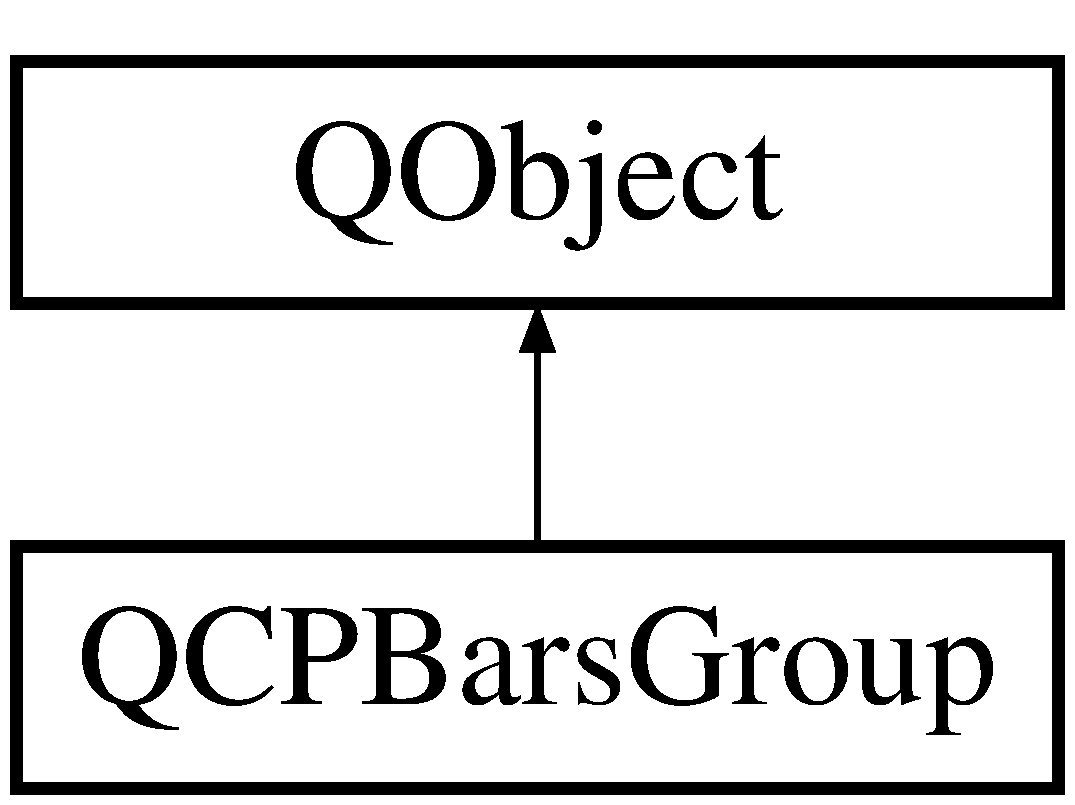
\includegraphics[height=2.000000cm]{class_q_c_p_bars_group}
\end{center}
\end{figure}
\subsection*{Public Types}
\begin{DoxyCompactItemize}
\item 
enum \hyperlink{class_q_c_p_bars_group_a4c0521120a97e60bbca37677a37075b6}{Spacing\+Type} \{ \hyperlink{class_q_c_p_bars_group_a4c0521120a97e60bbca37677a37075b6ab53fa3efaf14867dd0f14d41d64e42ac}{st\+Absolute}, 
\hyperlink{class_q_c_p_bars_group_a4c0521120a97e60bbca37677a37075b6ae94b05c27bc985dcdd8b1e1b7f163d26}{st\+Axis\+Rect\+Ratio}, 
\hyperlink{class_q_c_p_bars_group_a4c0521120a97e60bbca37677a37075b6ad369cee6287e0a86e8c2b643a3168c54}{st\+Plot\+Coords}
 \}
\end{DoxyCompactItemize}
\subsection*{Public Member Functions}
\begin{DoxyCompactItemize}
\item 
\hyperlink{class_q_c_p_bars_group_aa4e043b9a22c6c5ea0f93740aca063e1}{Q\+C\+P\+Bars\+Group} (\hyperlink{class_q_custom_plot}{Q\+Custom\+Plot} $\ast$parent\+Plot)
\item 
\hyperlink{class_q_c_p_bars_group_adb9475bcb6a5f18c8918e17d939d8dbd}{$\sim$\+Q\+C\+P\+Bars\+Group} ()
\item 
\hyperlink{class_q_c_p_bars_group_a4c0521120a97e60bbca37677a37075b6}{Spacing\+Type} \hyperlink{class_q_c_p_bars_group_a1bb562f669d47bd7d3cdd2da1f7d8f00}{spacing\+Type} () const 
\item 
double \hyperlink{class_q_c_p_bars_group_a730bffefcac6c97aaf60e6f64dd3bcd9}{spacing} () const 
\item 
void \hyperlink{class_q_c_p_bars_group_a2c7e2d61b10594a4555b615e1fcaf49e}{set\+Spacing\+Type} (\hyperlink{class_q_c_p_bars_group_a4c0521120a97e60bbca37677a37075b6}{Spacing\+Type} \hyperlink{class_q_c_p_bars_group_a1bb562f669d47bd7d3cdd2da1f7d8f00}{spacing\+Type})
\item 
void \hyperlink{class_q_c_p_bars_group_aa553d327479d72a0c3dafcc724a190e2}{set\+Spacing} (double \hyperlink{class_q_c_p_bars_group_a730bffefcac6c97aaf60e6f64dd3bcd9}{spacing})
\item 
Q\+List$<$ \hyperlink{class_q_c_p_bars}{Q\+C\+P\+Bars} $\ast$ $>$ \hyperlink{class_q_c_p_bars_group_a7c72ed1f8cd962c93b8c42ab96cd91ec}{bars} () const 
\item 
\hyperlink{class_q_c_p_bars}{Q\+C\+P\+Bars} $\ast$ \hyperlink{class_q_c_p_bars_group_a72d022790b7c93151c95c28eefaf51b4}{bars} (int index) const 
\item 
int \hyperlink{class_q_c_p_bars_group_af07364189c5717a158ec95b609687532}{size} () const 
\item 
bool \hyperlink{class_q_c_p_bars_group_a1d89da4e9176f4f77105e9a4afd44e2b}{is\+Empty} () const 
\item 
void \hyperlink{class_q_c_p_bars_group_a3ddf23928c6cd89530bd34ab7ba7b177}{clear} ()
\item 
bool \hyperlink{class_q_c_p_bars_group_adb4837894167e629e42e200db056fac3}{contains} (\hyperlink{class_q_c_p_bars}{Q\+C\+P\+Bars} $\ast$\hyperlink{class_q_c_p_bars_group_a7c72ed1f8cd962c93b8c42ab96cd91ec}{bars}) const 
\item 
void \hyperlink{class_q_c_p_bars_group_a809ed63cc4ff7cd5b0b8c96b470163d3}{append} (\hyperlink{class_q_c_p_bars}{Q\+C\+P\+Bars} $\ast$\hyperlink{class_q_c_p_bars_group_a7c72ed1f8cd962c93b8c42ab96cd91ec}{bars})
\item 
void \hyperlink{class_q_c_p_bars_group_a309a5f7233db189f3ea9c2d04ece6c13}{insert} (int i, \hyperlink{class_q_c_p_bars}{Q\+C\+P\+Bars} $\ast$\hyperlink{class_q_c_p_bars_group_a7c72ed1f8cd962c93b8c42ab96cd91ec}{bars})
\item 
void \hyperlink{class_q_c_p_bars_group_a215e28a5944f1159013a0e19169220e7}{remove} (\hyperlink{class_q_c_p_bars}{Q\+C\+P\+Bars} $\ast$\hyperlink{class_q_c_p_bars_group_a7c72ed1f8cd962c93b8c42ab96cd91ec}{bars})
\end{DoxyCompactItemize}
\subsection*{Protected Member Functions}
\begin{DoxyCompactItemize}
\item 
void \hyperlink{class_q_c_p_bars_group_a7b00514f19ad58d0bb3fd5246a67fae2}{register\+Bars} (\hyperlink{class_q_c_p_bars}{Q\+C\+P\+Bars} $\ast$\hyperlink{class_q_c_p_bars_group_a7c72ed1f8cd962c93b8c42ab96cd91ec}{bars})
\item 
void \hyperlink{class_q_c_p_bars_group_ac7073cdd7b1a40c6cb4b5f908145f8c4}{unregister\+Bars} (\hyperlink{class_q_c_p_bars}{Q\+C\+P\+Bars} $\ast$\hyperlink{class_q_c_p_bars_group_a7c72ed1f8cd962c93b8c42ab96cd91ec}{bars})
\item 
double \hyperlink{class_q_c_p_bars_group_a8e2ca6002e7bab49670144d048a2bcc9}{key\+Pixel\+Offset} (const \hyperlink{class_q_c_p_bars}{Q\+C\+P\+Bars} $\ast$\hyperlink{class_q_c_p_bars_group_a7c72ed1f8cd962c93b8c42ab96cd91ec}{bars}, double key\+Coord)
\item 
double \hyperlink{class_q_c_p_bars_group_a0beccd41bc3841a4c5b284823bc7d2de}{get\+Pixel\+Spacing} (const \hyperlink{class_q_c_p_bars}{Q\+C\+P\+Bars} $\ast$\hyperlink{class_q_c_p_bars_group_a7c72ed1f8cd962c93b8c42ab96cd91ec}{bars}, double key\+Coord)
\end{DoxyCompactItemize}
\subsection*{Protected Attributes}
\begin{DoxyCompactItemize}
\item 
\hyperlink{class_q_custom_plot}{Q\+Custom\+Plot} $\ast$ \hyperlink{class_q_c_p_bars_group_a973d408cfbf88db95115aec71877f9e7}{m\+Parent\+Plot}
\item 
\hyperlink{class_q_c_p_bars_group_a4c0521120a97e60bbca37677a37075b6}{Spacing\+Type} \hyperlink{class_q_c_p_bars_group_a6794ee1a9c81864d627bff6a4b2d64ec}{m\+Spacing\+Type}
\item 
double \hyperlink{class_q_c_p_bars_group_a56471d7f548ca6141b7a5bf9629f7ece}{m\+Spacing}
\item 
Q\+List$<$ \hyperlink{class_q_c_p_bars}{Q\+C\+P\+Bars} $\ast$ $>$ \hyperlink{class_q_c_p_bars_group_affdb1e9233c277ff5a4c0a1121cf1fc0}{m\+Bars}
\end{DoxyCompactItemize}
\subsection*{Friends}
\begin{DoxyCompactItemize}
\item 
class \hyperlink{class_q_c_p_bars_group_a721b87c7cdb8e83a90d77fc8a22e7195}{Q\+C\+P\+Bars}
\end{DoxyCompactItemize}


\subsection{Detailed Description}
Groups multiple \hyperlink{class_q_c_p_bars}{Q\+C\+P\+Bars} together so they appear side by side. 



When showing multiple \hyperlink{class_q_c_p_bars}{Q\+C\+P\+Bars} in one plot which have bars at identical keys, it may be desirable to have them appearing next to each other at each key. This is what adding the respective \hyperlink{class_q_c_p_bars}{Q\+C\+P\+Bars} plottables to a \hyperlink{class_q_c_p_bars_group}{Q\+C\+P\+Bars\+Group} achieves. (An alternative approach is to stack them on top of each other, see \hyperlink{class_q_c_p_bars_ac22e00a6a41509538c21b04f0a57318c}{Q\+C\+P\+Bars\+::move\+Above}.)\hypertarget{class_q_c_p_bars_group_qcpbarsgroup-usage}{}\subsection{Usage}\label{class_q_c_p_bars_group_qcpbarsgroup-usage}
To add a \hyperlink{class_q_c_p_bars}{Q\+C\+P\+Bars} plottable to the group, create a new group and then add the respective bars intances\+: 
\begin{DoxyCode}
\hyperlink{class_q_c_p_bars_group}{QCPBarsGroup} *group = \textcolor{keyword}{new} \hyperlink{class_q_c_p_bars_group_aa4e043b9a22c6c5ea0f93740aca063e1}{QCPBarsGroup}(customPlot);
group->\hyperlink{class_q_c_p_bars_group_a809ed63cc4ff7cd5b0b8c96b470163d3}{append}(bars1);
group->\hyperlink{class_q_c_p_bars_group_a809ed63cc4ff7cd5b0b8c96b470163d3}{append}(bars2);
\end{DoxyCode}
 Alternatively to appending to the group like shown above, you can also set the group on the \hyperlink{class_q_c_p_bars}{Q\+C\+P\+Bars} plottable via \hyperlink{class_q_c_p_bars_aedd1709061f0b307c47ddb45e172ef9a}{Q\+C\+P\+Bars\+::set\+Bars\+Group}.

The spacing between the bars can be configured via \hyperlink{class_q_c_p_bars_group_a2c7e2d61b10594a4555b615e1fcaf49e}{set\+Spacing\+Type} and \hyperlink{class_q_c_p_bars_group_aa553d327479d72a0c3dafcc724a190e2}{set\+Spacing}. The bars in this group appear in the plot in the order they were appended. To insert a bars plottable at a certain index position, or to reposition a bars plottable which is already in the group, use \hyperlink{class_q_c_p_bars_group_a309a5f7233db189f3ea9c2d04ece6c13}{insert}.

To remove specific bars from the group, use either \hyperlink{class_q_c_p_bars_group_a215e28a5944f1159013a0e19169220e7}{remove} or call \hyperlink{class_q_c_p_bars_aedd1709061f0b307c47ddb45e172ef9a}{Q\+C\+P\+Bars\+:\+:set\+Bars\+Group(0)} on the respective bars plottable.

To clear the entire group, call \hyperlink{class_q_c_p_bars_group_a3ddf23928c6cd89530bd34ab7ba7b177}{clear}, or simply delete the group. 

\subsection{Member Enumeration Documentation}
\hypertarget{class_q_c_p_bars_group_a4c0521120a97e60bbca37677a37075b6}{}\index{Q\+C\+P\+Bars\+Group@{Q\+C\+P\+Bars\+Group}!Spacing\+Type@{Spacing\+Type}}
\index{Spacing\+Type@{Spacing\+Type}!Q\+C\+P\+Bars\+Group@{Q\+C\+P\+Bars\+Group}}
\subsubsection[{Spacing\+Type}]{\setlength{\rightskip}{0pt plus 5cm}enum {\bf Q\+C\+P\+Bars\+Group\+::\+Spacing\+Type}}\label{class_q_c_p_bars_group_a4c0521120a97e60bbca37677a37075b6}
Defines the ways the spacing between bars in the group can be specified. Thus it defines what the number passed to \hyperlink{class_q_c_p_bars_group_aa553d327479d72a0c3dafcc724a190e2}{set\+Spacing} actually means.

\begin{DoxySeeAlso}{See also}
\hyperlink{class_q_c_p_bars_group_a2c7e2d61b10594a4555b615e1fcaf49e}{set\+Spacing\+Type}, \hyperlink{class_q_c_p_bars_group_aa553d327479d72a0c3dafcc724a190e2}{set\+Spacing} 
\end{DoxySeeAlso}
\begin{Desc}
\item[Enumerator]\par
\begin{description}
\index{st\+Absolute@{st\+Absolute}!Q\+C\+P\+Bars\+Group@{Q\+C\+P\+Bars\+Group}}\index{Q\+C\+P\+Bars\+Group@{Q\+C\+P\+Bars\+Group}!st\+Absolute@{st\+Absolute}}\item[{\em 
\hypertarget{class_q_c_p_bars_group_a4c0521120a97e60bbca37677a37075b6ab53fa3efaf14867dd0f14d41d64e42ac}{}st\+Absolute\label{class_q_c_p_bars_group_a4c0521120a97e60bbca37677a37075b6ab53fa3efaf14867dd0f14d41d64e42ac}
}]Bar spacing is in absolute pixels. \index{st\+Axis\+Rect\+Ratio@{st\+Axis\+Rect\+Ratio}!Q\+C\+P\+Bars\+Group@{Q\+C\+P\+Bars\+Group}}\index{Q\+C\+P\+Bars\+Group@{Q\+C\+P\+Bars\+Group}!st\+Axis\+Rect\+Ratio@{st\+Axis\+Rect\+Ratio}}\item[{\em 
\hypertarget{class_q_c_p_bars_group_a4c0521120a97e60bbca37677a37075b6ae94b05c27bc985dcdd8b1e1b7f163d26}{}st\+Axis\+Rect\+Ratio\label{class_q_c_p_bars_group_a4c0521120a97e60bbca37677a37075b6ae94b05c27bc985dcdd8b1e1b7f163d26}
}]Bar spacing is given by a fraction of the axis rect size. \index{st\+Plot\+Coords@{st\+Plot\+Coords}!Q\+C\+P\+Bars\+Group@{Q\+C\+P\+Bars\+Group}}\index{Q\+C\+P\+Bars\+Group@{Q\+C\+P\+Bars\+Group}!st\+Plot\+Coords@{st\+Plot\+Coords}}\item[{\em 
\hypertarget{class_q_c_p_bars_group_a4c0521120a97e60bbca37677a37075b6ad369cee6287e0a86e8c2b643a3168c54}{}st\+Plot\+Coords\label{class_q_c_p_bars_group_a4c0521120a97e60bbca37677a37075b6ad369cee6287e0a86e8c2b643a3168c54}
}]Bar spacing is in key coordinates and thus scales with the key axis range. \end{description}
\end{Desc}


\subsection{Constructor \& Destructor Documentation}
\hypertarget{class_q_c_p_bars_group_aa4e043b9a22c6c5ea0f93740aca063e1}{}\index{Q\+C\+P\+Bars\+Group@{Q\+C\+P\+Bars\+Group}!Q\+C\+P\+Bars\+Group@{Q\+C\+P\+Bars\+Group}}
\index{Q\+C\+P\+Bars\+Group@{Q\+C\+P\+Bars\+Group}!Q\+C\+P\+Bars\+Group@{Q\+C\+P\+Bars\+Group}}
\subsubsection[{Q\+C\+P\+Bars\+Group}]{\setlength{\rightskip}{0pt plus 5cm}Q\+C\+P\+Bars\+Group\+::\+Q\+C\+P\+Bars\+Group (
\begin{DoxyParamCaption}
\item[{{\bf Q\+Custom\+Plot} $\ast$}]{parent\+Plot}
\end{DoxyParamCaption}
)}\label{class_q_c_p_bars_group_aa4e043b9a22c6c5ea0f93740aca063e1}
Constructs a new bars group for the specified \hyperlink{class_q_custom_plot}{Q\+Custom\+Plot} instance. \hypertarget{class_q_c_p_bars_group_adb9475bcb6a5f18c8918e17d939d8dbd}{}\index{Q\+C\+P\+Bars\+Group@{Q\+C\+P\+Bars\+Group}!````~Q\+C\+P\+Bars\+Group@{$\sim$\+Q\+C\+P\+Bars\+Group}}
\index{````~Q\+C\+P\+Bars\+Group@{$\sim$\+Q\+C\+P\+Bars\+Group}!Q\+C\+P\+Bars\+Group@{Q\+C\+P\+Bars\+Group}}
\subsubsection[{$\sim$\+Q\+C\+P\+Bars\+Group}]{\setlength{\rightskip}{0pt plus 5cm}Q\+C\+P\+Bars\+Group\+::$\sim$\+Q\+C\+P\+Bars\+Group (
\begin{DoxyParamCaption}
{}
\end{DoxyParamCaption}
)}\label{class_q_c_p_bars_group_adb9475bcb6a5f18c8918e17d939d8dbd}


\subsection{Member Function Documentation}
\hypertarget{class_q_c_p_bars_group_a809ed63cc4ff7cd5b0b8c96b470163d3}{}\index{Q\+C\+P\+Bars\+Group@{Q\+C\+P\+Bars\+Group}!append@{append}}
\index{append@{append}!Q\+C\+P\+Bars\+Group@{Q\+C\+P\+Bars\+Group}}
\subsubsection[{append}]{\setlength{\rightskip}{0pt plus 5cm}void Q\+C\+P\+Bars\+Group\+::append (
\begin{DoxyParamCaption}
\item[{{\bf Q\+C\+P\+Bars} $\ast$}]{bars}
\end{DoxyParamCaption}
)}\label{class_q_c_p_bars_group_a809ed63cc4ff7cd5b0b8c96b470163d3}
Adds the specified {\itshape bars} plottable to this group. Alternatively, you can also use \hyperlink{class_q_c_p_bars_aedd1709061f0b307c47ddb45e172ef9a}{Q\+C\+P\+Bars\+::set\+Bars\+Group} on the {\itshape bars} instance.

\begin{DoxySeeAlso}{See also}
\hyperlink{class_q_c_p_bars_group_a309a5f7233db189f3ea9c2d04ece6c13}{insert}, \hyperlink{class_q_c_p_bars_group_a215e28a5944f1159013a0e19169220e7}{remove} 
\end{DoxySeeAlso}
\hypertarget{class_q_c_p_bars_group_a7c72ed1f8cd962c93b8c42ab96cd91ec}{}\index{Q\+C\+P\+Bars\+Group@{Q\+C\+P\+Bars\+Group}!bars@{bars}}
\index{bars@{bars}!Q\+C\+P\+Bars\+Group@{Q\+C\+P\+Bars\+Group}}
\subsubsection[{bars}]{\setlength{\rightskip}{0pt plus 5cm}Q\+List$<$ {\bf Q\+C\+P\+Bars} $\ast$ $>$ Q\+C\+P\+Bars\+Group\+::bars (
\begin{DoxyParamCaption}
{}
\end{DoxyParamCaption}
) const\hspace{0.3cm}{\ttfamily [inline]}}\label{class_q_c_p_bars_group_a7c72ed1f8cd962c93b8c42ab96cd91ec}
Returns all bars currently in this group.

\begin{DoxySeeAlso}{See also}
bars(int index) 
\end{DoxySeeAlso}
\hypertarget{class_q_c_p_bars_group_a72d022790b7c93151c95c28eefaf51b4}{}\index{Q\+C\+P\+Bars\+Group@{Q\+C\+P\+Bars\+Group}!bars@{bars}}
\index{bars@{bars}!Q\+C\+P\+Bars\+Group@{Q\+C\+P\+Bars\+Group}}
\subsubsection[{bars}]{\setlength{\rightskip}{0pt plus 5cm}{\bf Q\+C\+P\+Bars} $\ast$ Q\+C\+P\+Bars\+Group\+::bars (
\begin{DoxyParamCaption}
\item[{int}]{index}
\end{DoxyParamCaption}
) const}\label{class_q_c_p_bars_group_a72d022790b7c93151c95c28eefaf51b4}
Returns the \hyperlink{class_q_c_p_bars}{Q\+C\+P\+Bars} instance with the specified {\itshape index} in this group. If no such \hyperlink{class_q_c_p_bars}{Q\+C\+P\+Bars} exists, returns 0.

\begin{DoxySeeAlso}{See also}
\hyperlink{class_q_c_p_bars_group_a7c72ed1f8cd962c93b8c42ab96cd91ec}{bars()}, \hyperlink{class_q_c_p_bars_group_af07364189c5717a158ec95b609687532}{size} 
\end{DoxySeeAlso}
\hypertarget{class_q_c_p_bars_group_a3ddf23928c6cd89530bd34ab7ba7b177}{}\index{Q\+C\+P\+Bars\+Group@{Q\+C\+P\+Bars\+Group}!clear@{clear}}
\index{clear@{clear}!Q\+C\+P\+Bars\+Group@{Q\+C\+P\+Bars\+Group}}
\subsubsection[{clear}]{\setlength{\rightskip}{0pt plus 5cm}void Q\+C\+P\+Bars\+Group\+::clear (
\begin{DoxyParamCaption}
{}
\end{DoxyParamCaption}
)}\label{class_q_c_p_bars_group_a3ddf23928c6cd89530bd34ab7ba7b177}
Removes all \hyperlink{class_q_c_p_bars}{Q\+C\+P\+Bars} plottables from this group.

\begin{DoxySeeAlso}{See also}
\hyperlink{class_q_c_p_bars_group_a1d89da4e9176f4f77105e9a4afd44e2b}{is\+Empty} 
\end{DoxySeeAlso}
\hypertarget{class_q_c_p_bars_group_adb4837894167e629e42e200db056fac3}{}\index{Q\+C\+P\+Bars\+Group@{Q\+C\+P\+Bars\+Group}!contains@{contains}}
\index{contains@{contains}!Q\+C\+P\+Bars\+Group@{Q\+C\+P\+Bars\+Group}}
\subsubsection[{contains}]{\setlength{\rightskip}{0pt plus 5cm}bool Q\+C\+P\+Bars\+Group\+::contains (
\begin{DoxyParamCaption}
\item[{{\bf Q\+C\+P\+Bars} $\ast$}]{bars}
\end{DoxyParamCaption}
) const\hspace{0.3cm}{\ttfamily [inline]}}\label{class_q_c_p_bars_group_adb4837894167e629e42e200db056fac3}
Returns whether the specified {\itshape bars} plottable is part of this group. \hypertarget{class_q_c_p_bars_group_a0beccd41bc3841a4c5b284823bc7d2de}{}\index{Q\+C\+P\+Bars\+Group@{Q\+C\+P\+Bars\+Group}!get\+Pixel\+Spacing@{get\+Pixel\+Spacing}}
\index{get\+Pixel\+Spacing@{get\+Pixel\+Spacing}!Q\+C\+P\+Bars\+Group@{Q\+C\+P\+Bars\+Group}}
\subsubsection[{get\+Pixel\+Spacing}]{\setlength{\rightskip}{0pt plus 5cm}double Q\+C\+P\+Bars\+Group\+::get\+Pixel\+Spacing (
\begin{DoxyParamCaption}
\item[{const {\bf Q\+C\+P\+Bars} $\ast$}]{bars, }
\item[{double}]{key\+Coord}
\end{DoxyParamCaption}
)\hspace{0.3cm}{\ttfamily [protected]}}\label{class_q_c_p_bars_group_a0beccd41bc3841a4c5b284823bc7d2de}
\hypertarget{class_q_c_p_bars_group_a309a5f7233db189f3ea9c2d04ece6c13}{}\index{Q\+C\+P\+Bars\+Group@{Q\+C\+P\+Bars\+Group}!insert@{insert}}
\index{insert@{insert}!Q\+C\+P\+Bars\+Group@{Q\+C\+P\+Bars\+Group}}
\subsubsection[{insert}]{\setlength{\rightskip}{0pt plus 5cm}void Q\+C\+P\+Bars\+Group\+::insert (
\begin{DoxyParamCaption}
\item[{int}]{i, }
\item[{{\bf Q\+C\+P\+Bars} $\ast$}]{bars}
\end{DoxyParamCaption}
)}\label{class_q_c_p_bars_group_a309a5f7233db189f3ea9c2d04ece6c13}
Inserts the specified {\itshape bars} plottable into this group at the specified index position {\itshape i}. This gives you full control over the ordering of the bars.

{\itshape bars} may already be part of this group. In that case, {\itshape bars} is just moved to the new index position.

\begin{DoxySeeAlso}{See also}
\hyperlink{class_q_c_p_bars_group_a809ed63cc4ff7cd5b0b8c96b470163d3}{append}, \hyperlink{class_q_c_p_bars_group_a215e28a5944f1159013a0e19169220e7}{remove} 
\end{DoxySeeAlso}
\hypertarget{class_q_c_p_bars_group_a1d89da4e9176f4f77105e9a4afd44e2b}{}\index{Q\+C\+P\+Bars\+Group@{Q\+C\+P\+Bars\+Group}!is\+Empty@{is\+Empty}}
\index{is\+Empty@{is\+Empty}!Q\+C\+P\+Bars\+Group@{Q\+C\+P\+Bars\+Group}}
\subsubsection[{is\+Empty}]{\setlength{\rightskip}{0pt plus 5cm}bool Q\+C\+P\+Bars\+Group\+::is\+Empty (
\begin{DoxyParamCaption}
{}
\end{DoxyParamCaption}
) const\hspace{0.3cm}{\ttfamily [inline]}}\label{class_q_c_p_bars_group_a1d89da4e9176f4f77105e9a4afd44e2b}
Returns whether this bars group is empty.

\begin{DoxySeeAlso}{See also}
\hyperlink{class_q_c_p_bars_group_af07364189c5717a158ec95b609687532}{size} 
\end{DoxySeeAlso}
\hypertarget{class_q_c_p_bars_group_a8e2ca6002e7bab49670144d048a2bcc9}{}\index{Q\+C\+P\+Bars\+Group@{Q\+C\+P\+Bars\+Group}!key\+Pixel\+Offset@{key\+Pixel\+Offset}}
\index{key\+Pixel\+Offset@{key\+Pixel\+Offset}!Q\+C\+P\+Bars\+Group@{Q\+C\+P\+Bars\+Group}}
\subsubsection[{key\+Pixel\+Offset}]{\setlength{\rightskip}{0pt plus 5cm}double Q\+C\+P\+Bars\+Group\+::key\+Pixel\+Offset (
\begin{DoxyParamCaption}
\item[{const {\bf Q\+C\+P\+Bars} $\ast$}]{bars, }
\item[{double}]{key\+Coord}
\end{DoxyParamCaption}
)\hspace{0.3cm}{\ttfamily [protected]}}\label{class_q_c_p_bars_group_a8e2ca6002e7bab49670144d048a2bcc9}
\hypertarget{class_q_c_p_bars_group_a7b00514f19ad58d0bb3fd5246a67fae2}{}\index{Q\+C\+P\+Bars\+Group@{Q\+C\+P\+Bars\+Group}!register\+Bars@{register\+Bars}}
\index{register\+Bars@{register\+Bars}!Q\+C\+P\+Bars\+Group@{Q\+C\+P\+Bars\+Group}}
\subsubsection[{register\+Bars}]{\setlength{\rightskip}{0pt plus 5cm}void Q\+C\+P\+Bars\+Group\+::register\+Bars (
\begin{DoxyParamCaption}
\item[{{\bf Q\+C\+P\+Bars} $\ast$}]{bars}
\end{DoxyParamCaption}
)\hspace{0.3cm}{\ttfamily [protected]}}\label{class_q_c_p_bars_group_a7b00514f19ad58d0bb3fd5246a67fae2}
\hypertarget{class_q_c_p_bars_group_a215e28a5944f1159013a0e19169220e7}{}\index{Q\+C\+P\+Bars\+Group@{Q\+C\+P\+Bars\+Group}!remove@{remove}}
\index{remove@{remove}!Q\+C\+P\+Bars\+Group@{Q\+C\+P\+Bars\+Group}}
\subsubsection[{remove}]{\setlength{\rightskip}{0pt plus 5cm}void Q\+C\+P\+Bars\+Group\+::remove (
\begin{DoxyParamCaption}
\item[{{\bf Q\+C\+P\+Bars} $\ast$}]{bars}
\end{DoxyParamCaption}
)}\label{class_q_c_p_bars_group_a215e28a5944f1159013a0e19169220e7}
Removes the specified {\itshape bars} plottable from this group.

\begin{DoxySeeAlso}{See also}
\hyperlink{class_q_c_p_bars_group_adb4837894167e629e42e200db056fac3}{contains}, \hyperlink{class_q_c_p_bars_group_a3ddf23928c6cd89530bd34ab7ba7b177}{clear} 
\end{DoxySeeAlso}
\hypertarget{class_q_c_p_bars_group_aa553d327479d72a0c3dafcc724a190e2}{}\index{Q\+C\+P\+Bars\+Group@{Q\+C\+P\+Bars\+Group}!set\+Spacing@{set\+Spacing}}
\index{set\+Spacing@{set\+Spacing}!Q\+C\+P\+Bars\+Group@{Q\+C\+P\+Bars\+Group}}
\subsubsection[{set\+Spacing}]{\setlength{\rightskip}{0pt plus 5cm}void Q\+C\+P\+Bars\+Group\+::set\+Spacing (
\begin{DoxyParamCaption}
\item[{double}]{spacing}
\end{DoxyParamCaption}
)}\label{class_q_c_p_bars_group_aa553d327479d72a0c3dafcc724a190e2}
Sets the spacing between adjacent bars. What the number passed as {\itshape spacing} actually means, is defined by the current \hyperlink{class_q_c_p_bars_group_a4c0521120a97e60bbca37677a37075b6}{Spacing\+Type}, which can be set with \hyperlink{class_q_c_p_bars_group_a2c7e2d61b10594a4555b615e1fcaf49e}{set\+Spacing\+Type}.

\begin{DoxySeeAlso}{See also}
\hyperlink{class_q_c_p_bars_group_a2c7e2d61b10594a4555b615e1fcaf49e}{set\+Spacing\+Type} 
\end{DoxySeeAlso}
\hypertarget{class_q_c_p_bars_group_a2c7e2d61b10594a4555b615e1fcaf49e}{}\index{Q\+C\+P\+Bars\+Group@{Q\+C\+P\+Bars\+Group}!set\+Spacing\+Type@{set\+Spacing\+Type}}
\index{set\+Spacing\+Type@{set\+Spacing\+Type}!Q\+C\+P\+Bars\+Group@{Q\+C\+P\+Bars\+Group}}
\subsubsection[{set\+Spacing\+Type}]{\setlength{\rightskip}{0pt plus 5cm}void Q\+C\+P\+Bars\+Group\+::set\+Spacing\+Type (
\begin{DoxyParamCaption}
\item[{{\bf Spacing\+Type}}]{spacing\+Type}
\end{DoxyParamCaption}
)}\label{class_q_c_p_bars_group_a2c7e2d61b10594a4555b615e1fcaf49e}
Sets how the spacing between adjacent bars is interpreted. See \hyperlink{class_q_c_p_bars_group_a4c0521120a97e60bbca37677a37075b6}{Spacing\+Type}.

The actual spacing can then be specified with \hyperlink{class_q_c_p_bars_group_aa553d327479d72a0c3dafcc724a190e2}{set\+Spacing}.

\begin{DoxySeeAlso}{See also}
\hyperlink{class_q_c_p_bars_group_aa553d327479d72a0c3dafcc724a190e2}{set\+Spacing} 
\end{DoxySeeAlso}
\hypertarget{class_q_c_p_bars_group_af07364189c5717a158ec95b609687532}{}\index{Q\+C\+P\+Bars\+Group@{Q\+C\+P\+Bars\+Group}!size@{size}}
\index{size@{size}!Q\+C\+P\+Bars\+Group@{Q\+C\+P\+Bars\+Group}}
\subsubsection[{size}]{\setlength{\rightskip}{0pt plus 5cm}int Q\+C\+P\+Bars\+Group\+::size (
\begin{DoxyParamCaption}
{}
\end{DoxyParamCaption}
) const\hspace{0.3cm}{\ttfamily [inline]}}\label{class_q_c_p_bars_group_af07364189c5717a158ec95b609687532}
Returns the number of \hyperlink{class_q_c_p_bars}{Q\+C\+P\+Bars} plottables that are part of this group. \hypertarget{class_q_c_p_bars_group_a730bffefcac6c97aaf60e6f64dd3bcd9}{}\index{Q\+C\+P\+Bars\+Group@{Q\+C\+P\+Bars\+Group}!spacing@{spacing}}
\index{spacing@{spacing}!Q\+C\+P\+Bars\+Group@{Q\+C\+P\+Bars\+Group}}
\subsubsection[{spacing}]{\setlength{\rightskip}{0pt plus 5cm}double Q\+C\+P\+Bars\+Group\+::spacing (
\begin{DoxyParamCaption}
{}
\end{DoxyParamCaption}
) const\hspace{0.3cm}{\ttfamily [inline]}}\label{class_q_c_p_bars_group_a730bffefcac6c97aaf60e6f64dd3bcd9}
\hypertarget{class_q_c_p_bars_group_a1bb562f669d47bd7d3cdd2da1f7d8f00}{}\index{Q\+C\+P\+Bars\+Group@{Q\+C\+P\+Bars\+Group}!spacing\+Type@{spacing\+Type}}
\index{spacing\+Type@{spacing\+Type}!Q\+C\+P\+Bars\+Group@{Q\+C\+P\+Bars\+Group}}
\subsubsection[{spacing\+Type}]{\setlength{\rightskip}{0pt plus 5cm}{\bf Spacing\+Type} Q\+C\+P\+Bars\+Group\+::spacing\+Type (
\begin{DoxyParamCaption}
{}
\end{DoxyParamCaption}
) const\hspace{0.3cm}{\ttfamily [inline]}}\label{class_q_c_p_bars_group_a1bb562f669d47bd7d3cdd2da1f7d8f00}
\hypertarget{class_q_c_p_bars_group_ac7073cdd7b1a40c6cb4b5f908145f8c4}{}\index{Q\+C\+P\+Bars\+Group@{Q\+C\+P\+Bars\+Group}!unregister\+Bars@{unregister\+Bars}}
\index{unregister\+Bars@{unregister\+Bars}!Q\+C\+P\+Bars\+Group@{Q\+C\+P\+Bars\+Group}}
\subsubsection[{unregister\+Bars}]{\setlength{\rightskip}{0pt plus 5cm}void Q\+C\+P\+Bars\+Group\+::unregister\+Bars (
\begin{DoxyParamCaption}
\item[{{\bf Q\+C\+P\+Bars} $\ast$}]{bars}
\end{DoxyParamCaption}
)\hspace{0.3cm}{\ttfamily [protected]}}\label{class_q_c_p_bars_group_ac7073cdd7b1a40c6cb4b5f908145f8c4}


\subsection{Friends And Related Function Documentation}
\hypertarget{class_q_c_p_bars_group_a721b87c7cdb8e83a90d77fc8a22e7195}{}\index{Q\+C\+P\+Bars\+Group@{Q\+C\+P\+Bars\+Group}!Q\+C\+P\+Bars@{Q\+C\+P\+Bars}}
\index{Q\+C\+P\+Bars@{Q\+C\+P\+Bars}!Q\+C\+P\+Bars\+Group@{Q\+C\+P\+Bars\+Group}}
\subsubsection[{Q\+C\+P\+Bars}]{\setlength{\rightskip}{0pt plus 5cm}friend class {\bf Q\+C\+P\+Bars}\hspace{0.3cm}{\ttfamily [friend]}}\label{class_q_c_p_bars_group_a721b87c7cdb8e83a90d77fc8a22e7195}


\subsection{Member Data Documentation}
\hypertarget{class_q_c_p_bars_group_affdb1e9233c277ff5a4c0a1121cf1fc0}{}\index{Q\+C\+P\+Bars\+Group@{Q\+C\+P\+Bars\+Group}!m\+Bars@{m\+Bars}}
\index{m\+Bars@{m\+Bars}!Q\+C\+P\+Bars\+Group@{Q\+C\+P\+Bars\+Group}}
\subsubsection[{m\+Bars}]{\setlength{\rightskip}{0pt plus 5cm}Q\+List$<${\bf Q\+C\+P\+Bars}$\ast$$>$ Q\+C\+P\+Bars\+Group\+::m\+Bars\hspace{0.3cm}{\ttfamily [protected]}}\label{class_q_c_p_bars_group_affdb1e9233c277ff5a4c0a1121cf1fc0}
\hypertarget{class_q_c_p_bars_group_a973d408cfbf88db95115aec71877f9e7}{}\index{Q\+C\+P\+Bars\+Group@{Q\+C\+P\+Bars\+Group}!m\+Parent\+Plot@{m\+Parent\+Plot}}
\index{m\+Parent\+Plot@{m\+Parent\+Plot}!Q\+C\+P\+Bars\+Group@{Q\+C\+P\+Bars\+Group}}
\subsubsection[{m\+Parent\+Plot}]{\setlength{\rightskip}{0pt plus 5cm}{\bf Q\+Custom\+Plot}$\ast$ Q\+C\+P\+Bars\+Group\+::m\+Parent\+Plot\hspace{0.3cm}{\ttfamily [protected]}}\label{class_q_c_p_bars_group_a973d408cfbf88db95115aec71877f9e7}
\hypertarget{class_q_c_p_bars_group_a56471d7f548ca6141b7a5bf9629f7ece}{}\index{Q\+C\+P\+Bars\+Group@{Q\+C\+P\+Bars\+Group}!m\+Spacing@{m\+Spacing}}
\index{m\+Spacing@{m\+Spacing}!Q\+C\+P\+Bars\+Group@{Q\+C\+P\+Bars\+Group}}
\subsubsection[{m\+Spacing}]{\setlength{\rightskip}{0pt plus 5cm}double Q\+C\+P\+Bars\+Group\+::m\+Spacing\hspace{0.3cm}{\ttfamily [protected]}}\label{class_q_c_p_bars_group_a56471d7f548ca6141b7a5bf9629f7ece}
\hypertarget{class_q_c_p_bars_group_a6794ee1a9c81864d627bff6a4b2d64ec}{}\index{Q\+C\+P\+Bars\+Group@{Q\+C\+P\+Bars\+Group}!m\+Spacing\+Type@{m\+Spacing\+Type}}
\index{m\+Spacing\+Type@{m\+Spacing\+Type}!Q\+C\+P\+Bars\+Group@{Q\+C\+P\+Bars\+Group}}
\subsubsection[{m\+Spacing\+Type}]{\setlength{\rightskip}{0pt plus 5cm}{\bf Spacing\+Type} Q\+C\+P\+Bars\+Group\+::m\+Spacing\+Type\hspace{0.3cm}{\ttfamily [protected]}}\label{class_q_c_p_bars_group_a6794ee1a9c81864d627bff6a4b2d64ec}


The documentation for this class was generated from the following files\+:\begin{DoxyCompactItemize}
\item 
C\+:/\+Users/\+Roman/\+Documents/\+Mygs/\+Ground\+Station/\+G\+S/\hyperlink{qcustomplot_8h}{qcustomplot.\+h}\item 
C\+:/\+Users/\+Roman/\+Documents/\+Mygs/\+Ground\+Station/\+G\+S/\hyperlink{qcustomplot_8cpp}{qcustomplot.\+cpp}\end{DoxyCompactItemize}

\hypertarget{class_q_c_p_color_gradient}{}\section{Q\+C\+P\+Color\+Gradient Class Reference}
\label{class_q_c_p_color_gradient}\index{Q\+C\+P\+Color\+Gradient@{Q\+C\+P\+Color\+Gradient}}


Defines a color gradient for use with e.\+g. \hyperlink{class_q_c_p_color_map}{Q\+C\+P\+Color\+Map}.  




{\ttfamily \#include $<$qcustomplot.\+h$>$}

\subsection*{Public Types}
\begin{DoxyCompactItemize}
\item 
enum \hyperlink{class_q_c_p_color_gradient_ac5dca17cc24336e6ca176610e7f77fc1}{Color\+Interpolation} \{ \hyperlink{class_q_c_p_color_gradient_ac5dca17cc24336e6ca176610e7f77fc1a5e30f725c9cfe93999e268a9f92afbe7}{ci\+R\+G\+B}, 
\hyperlink{class_q_c_p_color_gradient_ac5dca17cc24336e6ca176610e7f77fc1af14ae62fcae11ecc07234eeaec5856cb}{ci\+H\+S\+V}
 \}
\item 
enum \hyperlink{class_q_c_p_color_gradient_aed6569828fee337023670272910c9072}{Gradient\+Preset} \{ \\*
\hyperlink{class_q_c_p_color_gradient_aed6569828fee337023670272910c9072add11ae369a86f3b1b6205ec72e5021fb}{gp\+Grayscale}, 
\hyperlink{class_q_c_p_color_gradient_aed6569828fee337023670272910c9072a4f42e534cf6cff5a29a5388094d099b5}{gp\+Hot}, 
\hyperlink{class_q_c_p_color_gradient_aed6569828fee337023670272910c9072aec8c001f62c0d5cb853db5fd85309557}{gp\+Cold}, 
\hyperlink{class_q_c_p_color_gradient_aed6569828fee337023670272910c9072a1bb89351b6def7d220973443fe059c62}{gp\+Night}, 
\\*
\hyperlink{class_q_c_p_color_gradient_aed6569828fee337023670272910c9072a9e72663bf6b94b65945f7843f24e0721}{gp\+Candy}, 
\hyperlink{class_q_c_p_color_gradient_aed6569828fee337023670272910c9072a382f0b07cec1a59d8a533438aea815d2}{gp\+Geography}, 
\hyperlink{class_q_c_p_color_gradient_aed6569828fee337023670272910c9072a4297f4f9e212a819cd65e8e34567182b}{gp\+Ion}, 
\hyperlink{class_q_c_p_color_gradient_aed6569828fee337023670272910c9072af1676b129f9f458ace453f280c731cf7}{gp\+Thermal}, 
\\*
\hyperlink{class_q_c_p_color_gradient_aed6569828fee337023670272910c9072ab7414ce4e36dc3e82e0132a7f0f41b52}{gp\+Polar}, 
\hyperlink{class_q_c_p_color_gradient_aed6569828fee337023670272910c9072ad63adc100ef46f6b4a8a6deacec4642f}{gp\+Spectrum}, 
\hyperlink{class_q_c_p_color_gradient_aed6569828fee337023670272910c9072a5f8a9e67b64c17ddfe4f069fe2b9fb02}{gp\+Jet}, 
\hyperlink{class_q_c_p_color_gradient_aed6569828fee337023670272910c9072a30efe58407acfb67939032f70213a130}{gp\+Hues}
 \}
\end{DoxyCompactItemize}
\subsection*{Public Member Functions}
\begin{DoxyCompactItemize}
\item 
\hyperlink{class_q_c_p_color_gradient_a546e44df5fa1846400a582c041361c85}{Q\+C\+P\+Color\+Gradient} (\hyperlink{class_q_c_p_color_gradient_aed6569828fee337023670272910c9072}{Gradient\+Preset} preset=\hyperlink{class_q_c_p_color_gradient_aed6569828fee337023670272910c9072aec8c001f62c0d5cb853db5fd85309557}{gp\+Cold})
\item 
bool \hyperlink{class_q_c_p_color_gradient_aada47d8206bf2cec77462653bf471c13}{operator==} (const \hyperlink{class_q_c_p_color_gradient}{Q\+C\+P\+Color\+Gradient} \&other) const 
\item 
bool \hyperlink{class_q_c_p_color_gradient_ac641f5d2dc1686201d3cb602c871791d}{operator!=} (const \hyperlink{class_q_c_p_color_gradient}{Q\+C\+P\+Color\+Gradient} \&other) const 
\item 
int \hyperlink{class_q_c_p_color_gradient_ae7537a8e6d0fed3f1928328062bb0f4e}{level\+Count} () const 
\item 
Q\+Map$<$ double, Q\+Color $>$ \hyperlink{class_q_c_p_color_gradient_a64f8aba7826f9c6363aacff8376cef37}{color\+Stops} () const 
\item 
\hyperlink{class_q_c_p_color_gradient_ac5dca17cc24336e6ca176610e7f77fc1}{Color\+Interpolation} \hyperlink{class_q_c_p_color_gradient_a731616fabe6f2e33f71f58dd382359d8}{color\+Interpolation} () const 
\item 
bool \hyperlink{class_q_c_p_color_gradient_a860b7048f877195d2a0fb8d5a7cf5d73}{periodic} () const 
\item 
void \hyperlink{class_q_c_p_color_gradient_a18da587eb4f7fc788ea28ba15b6a12de}{set\+Level\+Count} (int n)
\item 
void \hyperlink{class_q_c_p_color_gradient_a724e828aa6f0ba5011a9392477c35d3a}{set\+Color\+Stops} (const Q\+Map$<$ double, Q\+Color $>$ \&\hyperlink{class_q_c_p_color_gradient_a64f8aba7826f9c6363aacff8376cef37}{color\+Stops})
\item 
void \hyperlink{class_q_c_p_color_gradient_a3b48be5e78079db1bb2a1188a4c3390e}{set\+Color\+Stop\+At} (double position, const Q\+Color \&\hyperlink{class_q_c_p_color_gradient_a0599545c859268b025d2060dea741cea}{color})
\item 
void \hyperlink{class_q_c_p_color_gradient_aa13fda86406e1d896a465a409ae63b38}{set\+Color\+Interpolation} (\hyperlink{class_q_c_p_color_gradient_ac5dca17cc24336e6ca176610e7f77fc1}{Color\+Interpolation} interpolation)
\item 
void \hyperlink{class_q_c_p_color_gradient_a39d6448155fc00a219f239220d14bb39}{set\+Periodic} (bool enabled)
\item 
void \hyperlink{class_q_c_p_color_gradient_aaf423ceb943e177b0ed2c48c811d83dc}{colorize} (const double $\ast$data, const \hyperlink{class_q_c_p_range}{Q\+C\+P\+Range} \&range, Q\+Rgb $\ast$scan\+Line, int n, int data\+Index\+Factor=1, bool logarithmic=false)
\item 
Q\+Rgb \hyperlink{class_q_c_p_color_gradient_a0599545c859268b025d2060dea741cea}{color} (double position, const \hyperlink{class_q_c_p_range}{Q\+C\+P\+Range} \&range, bool logarithmic=false)
\item 
void \hyperlink{class_q_c_p_color_gradient_aa0aeec1528241728b9671bf8e60b1622}{load\+Preset} (\hyperlink{class_q_c_p_color_gradient_aed6569828fee337023670272910c9072}{Gradient\+Preset} preset)
\item 
void \hyperlink{class_q_c_p_color_gradient_a939213e85f0d1279519d555c5fcfb6ad}{clear\+Color\+Stops} ()
\item 
\hyperlink{class_q_c_p_color_gradient}{Q\+C\+P\+Color\+Gradient} \hyperlink{class_q_c_p_color_gradient_abe04e1d1ccab3d7aa78f2924faed4916}{inverted} () const 
\end{DoxyCompactItemize}
\subsection*{Protected Member Functions}
\begin{DoxyCompactItemize}
\item 
void \hyperlink{class_q_c_p_color_gradient_a353f15ab3ab586eebf1f6b58c3e2707b}{update\+Color\+Buffer} ()
\end{DoxyCompactItemize}
\subsection*{Protected Attributes}
\begin{DoxyCompactItemize}
\item 
int \hyperlink{class_q_c_p_color_gradient_a98fb68e359904b2c991fcae3e38a211a}{m\+Level\+Count}
\item 
Q\+Map$<$ double, Q\+Color $>$ \hyperlink{class_q_c_p_color_gradient_a9e11a2b0974ef289d12c324822bc3a3e}{m\+Color\+Stops}
\item 
\hyperlink{class_q_c_p_color_gradient_ac5dca17cc24336e6ca176610e7f77fc1}{Color\+Interpolation} \hyperlink{class_q_c_p_color_gradient_a028cef73d863800a9ee93ffd641cce01}{m\+Color\+Interpolation}
\item 
bool \hyperlink{class_q_c_p_color_gradient_a4b07deeb20ca1ee2d5ea7e01bf0420af}{m\+Periodic}
\item 
Q\+Vector$<$ Q\+Rgb $>$ \hyperlink{class_q_c_p_color_gradient_af8b5f0739faa5f8295154d47ce38ecff}{m\+Color\+Buffer}
\item 
bool \hyperlink{class_q_c_p_color_gradient_abacf55e11f67d6722a687af1bb2687bd}{m\+Color\+Buffer\+Invalidated}
\end{DoxyCompactItemize}


\subsection{Detailed Description}
Defines a color gradient for use with e.\+g. \hyperlink{class_q_c_p_color_map}{Q\+C\+P\+Color\+Map}. 

This class describes a color gradient which can be used to encode data with color. For example, \hyperlink{class_q_c_p_color_map}{Q\+C\+P\+Color\+Map} and \hyperlink{class_q_c_p_color_scale}{Q\+C\+P\+Color\+Scale} have \hyperlink{class_q_c_p_color_map_a7313c78360471cead3576341a2c50377}{set\+Gradient} methods which take an instance of this class. Colors are set with \hyperlink{class_q_c_p_color_gradient_a3b48be5e78079db1bb2a1188a4c3390e}{set\+Color\+Stop\+At(double position, const Q\+Color \&color)} with a {\itshape position} from 0 to 1. In between these defined color positions, the color will be interpolated linearly either in R\+G\+B or H\+S\+V space, see \hyperlink{class_q_c_p_color_gradient_aa13fda86406e1d896a465a409ae63b38}{set\+Color\+Interpolation}.

Alternatively, load one of the preset color gradients shown in the image below, with \hyperlink{class_q_c_p_color_gradient_aa0aeec1528241728b9671bf8e60b1622}{load\+Preset}, or by directly specifying the preset in the constructor.



The fact that the \hyperlink{class_q_c_p_color_gradient}{ructor} allows directly converting a \hyperlink{class_q_c_p_color_gradient_aed6569828fee337023670272910c9072}{Gradient\+Preset} to a \hyperlink{class_q_c_p_color_gradient}{Q\+C\+P\+Color\+Gradient}, you can also directly pass \hyperlink{class_q_c_p_color_gradient_aed6569828fee337023670272910c9072}{Gradient\+Preset} to all the {\itshape set\+Gradient} methods, e.\+g.\+: 
\begin{DoxyCode}
colorMap->setGradient(\hyperlink{class_q_c_p_color_gradient_aed6569828fee337023670272910c9072a4f42e534cf6cff5a29a5388094d099b5}{QCPColorGradient::gpHot});
\end{DoxyCode}


The total number of levels used in the gradient can be set with \hyperlink{class_q_c_p_color_gradient_a18da587eb4f7fc788ea28ba15b6a12de}{set\+Level\+Count}. Whether the color gradient shall be applied periodically (wrapping around) to data values that lie outside the data range specified on the plottable instance can be controlled with \hyperlink{class_q_c_p_color_gradient_a39d6448155fc00a219f239220d14bb39}{set\+Periodic}. 

\subsection{Member Enumeration Documentation}
\hypertarget{class_q_c_p_color_gradient_ac5dca17cc24336e6ca176610e7f77fc1}{}\index{Q\+C\+P\+Color\+Gradient@{Q\+C\+P\+Color\+Gradient}!Color\+Interpolation@{Color\+Interpolation}}
\index{Color\+Interpolation@{Color\+Interpolation}!Q\+C\+P\+Color\+Gradient@{Q\+C\+P\+Color\+Gradient}}
\subsubsection[{Color\+Interpolation}]{\setlength{\rightskip}{0pt plus 5cm}enum {\bf Q\+C\+P\+Color\+Gradient\+::\+Color\+Interpolation}}\label{class_q_c_p_color_gradient_ac5dca17cc24336e6ca176610e7f77fc1}
Defines the color spaces in which color interpolation between gradient stops can be performed.

\begin{DoxySeeAlso}{See also}
\hyperlink{class_q_c_p_color_gradient_aa13fda86406e1d896a465a409ae63b38}{set\+Color\+Interpolation} 
\end{DoxySeeAlso}
\begin{Desc}
\item[Enumerator]\par
\begin{description}
\index{ci\+R\+G\+B@{ci\+R\+G\+B}!Q\+C\+P\+Color\+Gradient@{Q\+C\+P\+Color\+Gradient}}\index{Q\+C\+P\+Color\+Gradient@{Q\+C\+P\+Color\+Gradient}!ci\+R\+G\+B@{ci\+R\+G\+B}}\item[{\em 
\hypertarget{class_q_c_p_color_gradient_ac5dca17cc24336e6ca176610e7f77fc1a5e30f725c9cfe93999e268a9f92afbe7}{}ci\+R\+G\+B\label{class_q_c_p_color_gradient_ac5dca17cc24336e6ca176610e7f77fc1a5e30f725c9cfe93999e268a9f92afbe7}
}]Color channels red, green and blue are linearly interpolated. \index{ci\+H\+S\+V@{ci\+H\+S\+V}!Q\+C\+P\+Color\+Gradient@{Q\+C\+P\+Color\+Gradient}}\index{Q\+C\+P\+Color\+Gradient@{Q\+C\+P\+Color\+Gradient}!ci\+H\+S\+V@{ci\+H\+S\+V}}\item[{\em 
\hypertarget{class_q_c_p_color_gradient_ac5dca17cc24336e6ca176610e7f77fc1af14ae62fcae11ecc07234eeaec5856cb}{}ci\+H\+S\+V\label{class_q_c_p_color_gradient_ac5dca17cc24336e6ca176610e7f77fc1af14ae62fcae11ecc07234eeaec5856cb}
}]Color channels hue, saturation and value are linearly interpolated (The hue is interpolated over the shortest angle distance) \end{description}
\end{Desc}
\hypertarget{class_q_c_p_color_gradient_aed6569828fee337023670272910c9072}{}\index{Q\+C\+P\+Color\+Gradient@{Q\+C\+P\+Color\+Gradient}!Gradient\+Preset@{Gradient\+Preset}}
\index{Gradient\+Preset@{Gradient\+Preset}!Q\+C\+P\+Color\+Gradient@{Q\+C\+P\+Color\+Gradient}}
\subsubsection[{Gradient\+Preset}]{\setlength{\rightskip}{0pt plus 5cm}enum {\bf Q\+C\+P\+Color\+Gradient\+::\+Gradient\+Preset}}\label{class_q_c_p_color_gradient_aed6569828fee337023670272910c9072}
Defines the available presets that can be loaded with \hyperlink{class_q_c_p_color_gradient_aa0aeec1528241728b9671bf8e60b1622}{load\+Preset}. See the documentation there for an image of the presets. \begin{Desc}
\item[Enumerator]\par
\begin{description}
\index{gp\+Grayscale@{gp\+Grayscale}!Q\+C\+P\+Color\+Gradient@{Q\+C\+P\+Color\+Gradient}}\index{Q\+C\+P\+Color\+Gradient@{Q\+C\+P\+Color\+Gradient}!gp\+Grayscale@{gp\+Grayscale}}\item[{\em 
\hypertarget{class_q_c_p_color_gradient_aed6569828fee337023670272910c9072add11ae369a86f3b1b6205ec72e5021fb}{}gp\+Grayscale\label{class_q_c_p_color_gradient_aed6569828fee337023670272910c9072add11ae369a86f3b1b6205ec72e5021fb}
}]Continuous lightness from black to white (suited for non-\/biased data representation) \index{gp\+Hot@{gp\+Hot}!Q\+C\+P\+Color\+Gradient@{Q\+C\+P\+Color\+Gradient}}\index{Q\+C\+P\+Color\+Gradient@{Q\+C\+P\+Color\+Gradient}!gp\+Hot@{gp\+Hot}}\item[{\em 
\hypertarget{class_q_c_p_color_gradient_aed6569828fee337023670272910c9072a4f42e534cf6cff5a29a5388094d099b5}{}gp\+Hot\label{class_q_c_p_color_gradient_aed6569828fee337023670272910c9072a4f42e534cf6cff5a29a5388094d099b5}
}]Continuous lightness from black over firey colors to white (suited for non-\/biased data representation) \index{gp\+Cold@{gp\+Cold}!Q\+C\+P\+Color\+Gradient@{Q\+C\+P\+Color\+Gradient}}\index{Q\+C\+P\+Color\+Gradient@{Q\+C\+P\+Color\+Gradient}!gp\+Cold@{gp\+Cold}}\item[{\em 
\hypertarget{class_q_c_p_color_gradient_aed6569828fee337023670272910c9072aec8c001f62c0d5cb853db5fd85309557}{}gp\+Cold\label{class_q_c_p_color_gradient_aed6569828fee337023670272910c9072aec8c001f62c0d5cb853db5fd85309557}
}]Continuous lightness from black over icey colors to white (suited for non-\/biased data representation) \index{gp\+Night@{gp\+Night}!Q\+C\+P\+Color\+Gradient@{Q\+C\+P\+Color\+Gradient}}\index{Q\+C\+P\+Color\+Gradient@{Q\+C\+P\+Color\+Gradient}!gp\+Night@{gp\+Night}}\item[{\em 
\hypertarget{class_q_c_p_color_gradient_aed6569828fee337023670272910c9072a1bb89351b6def7d220973443fe059c62}{}gp\+Night\label{class_q_c_p_color_gradient_aed6569828fee337023670272910c9072a1bb89351b6def7d220973443fe059c62}
}]Continuous lightness from black over weak blueish colors to white (suited for non-\/biased data representation) \index{gp\+Candy@{gp\+Candy}!Q\+C\+P\+Color\+Gradient@{Q\+C\+P\+Color\+Gradient}}\index{Q\+C\+P\+Color\+Gradient@{Q\+C\+P\+Color\+Gradient}!gp\+Candy@{gp\+Candy}}\item[{\em 
\hypertarget{class_q_c_p_color_gradient_aed6569828fee337023670272910c9072a9e72663bf6b94b65945f7843f24e0721}{}gp\+Candy\label{class_q_c_p_color_gradient_aed6569828fee337023670272910c9072a9e72663bf6b94b65945f7843f24e0721}
}]Blue over pink to white. \index{gp\+Geography@{gp\+Geography}!Q\+C\+P\+Color\+Gradient@{Q\+C\+P\+Color\+Gradient}}\index{Q\+C\+P\+Color\+Gradient@{Q\+C\+P\+Color\+Gradient}!gp\+Geography@{gp\+Geography}}\item[{\em 
\hypertarget{class_q_c_p_color_gradient_aed6569828fee337023670272910c9072a382f0b07cec1a59d8a533438aea815d2}{}gp\+Geography\label{class_q_c_p_color_gradient_aed6569828fee337023670272910c9072a382f0b07cec1a59d8a533438aea815d2}
}]Colors suitable to represent different elevations on geographical maps. \index{gp\+Ion@{gp\+Ion}!Q\+C\+P\+Color\+Gradient@{Q\+C\+P\+Color\+Gradient}}\index{Q\+C\+P\+Color\+Gradient@{Q\+C\+P\+Color\+Gradient}!gp\+Ion@{gp\+Ion}}\item[{\em 
\hypertarget{class_q_c_p_color_gradient_aed6569828fee337023670272910c9072a4297f4f9e212a819cd65e8e34567182b}{}gp\+Ion\label{class_q_c_p_color_gradient_aed6569828fee337023670272910c9072a4297f4f9e212a819cd65e8e34567182b}
}]Half hue spectrum from black over purple to blue and finally green (creates banding illusion but allows more precise magnitude estimates) \index{gp\+Thermal@{gp\+Thermal}!Q\+C\+P\+Color\+Gradient@{Q\+C\+P\+Color\+Gradient}}\index{Q\+C\+P\+Color\+Gradient@{Q\+C\+P\+Color\+Gradient}!gp\+Thermal@{gp\+Thermal}}\item[{\em 
\hypertarget{class_q_c_p_color_gradient_aed6569828fee337023670272910c9072af1676b129f9f458ace453f280c731cf7}{}gp\+Thermal\label{class_q_c_p_color_gradient_aed6569828fee337023670272910c9072af1676b129f9f458ace453f280c731cf7}
}]Colors suitable for thermal imaging, ranging from dark blue over purple to orange, yellow and white. \index{gp\+Polar@{gp\+Polar}!Q\+C\+P\+Color\+Gradient@{Q\+C\+P\+Color\+Gradient}}\index{Q\+C\+P\+Color\+Gradient@{Q\+C\+P\+Color\+Gradient}!gp\+Polar@{gp\+Polar}}\item[{\em 
\hypertarget{class_q_c_p_color_gradient_aed6569828fee337023670272910c9072ab7414ce4e36dc3e82e0132a7f0f41b52}{}gp\+Polar\label{class_q_c_p_color_gradient_aed6569828fee337023670272910c9072ab7414ce4e36dc3e82e0132a7f0f41b52}
}]Colors suitable to emphasize polarity around the center, with blue for negative, black in the middle and red for positive values. \index{gp\+Spectrum@{gp\+Spectrum}!Q\+C\+P\+Color\+Gradient@{Q\+C\+P\+Color\+Gradient}}\index{Q\+C\+P\+Color\+Gradient@{Q\+C\+P\+Color\+Gradient}!gp\+Spectrum@{gp\+Spectrum}}\item[{\em 
\hypertarget{class_q_c_p_color_gradient_aed6569828fee337023670272910c9072ad63adc100ef46f6b4a8a6deacec4642f}{}gp\+Spectrum\label{class_q_c_p_color_gradient_aed6569828fee337023670272910c9072ad63adc100ef46f6b4a8a6deacec4642f}
}]An approximation of the visible light spectrum (creates banding illusion but allows more precise magnitude estimates) \index{gp\+Jet@{gp\+Jet}!Q\+C\+P\+Color\+Gradient@{Q\+C\+P\+Color\+Gradient}}\index{Q\+C\+P\+Color\+Gradient@{Q\+C\+P\+Color\+Gradient}!gp\+Jet@{gp\+Jet}}\item[{\em 
\hypertarget{class_q_c_p_color_gradient_aed6569828fee337023670272910c9072a5f8a9e67b64c17ddfe4f069fe2b9fb02}{}gp\+Jet\label{class_q_c_p_color_gradient_aed6569828fee337023670272910c9072a5f8a9e67b64c17ddfe4f069fe2b9fb02}
}]Hue variation similar to a spectrum, often used in numerical visualization (creates banding illusion but allows more precise magnitude estimates) \index{gp\+Hues@{gp\+Hues}!Q\+C\+P\+Color\+Gradient@{Q\+C\+P\+Color\+Gradient}}\index{Q\+C\+P\+Color\+Gradient@{Q\+C\+P\+Color\+Gradient}!gp\+Hues@{gp\+Hues}}\item[{\em 
\hypertarget{class_q_c_p_color_gradient_aed6569828fee337023670272910c9072a30efe58407acfb67939032f70213a130}{}gp\+Hues\label{class_q_c_p_color_gradient_aed6569828fee337023670272910c9072a30efe58407acfb67939032f70213a130}
}]Full hue cycle, with highest and lowest color red (suitable for periodic data, such as angles and phases, see \hyperlink{class_q_c_p_color_gradient_a39d6448155fc00a219f239220d14bb39}{set\+Periodic}) \end{description}
\end{Desc}


\subsection{Constructor \& Destructor Documentation}
\hypertarget{class_q_c_p_color_gradient_a546e44df5fa1846400a582c041361c85}{}\index{Q\+C\+P\+Color\+Gradient@{Q\+C\+P\+Color\+Gradient}!Q\+C\+P\+Color\+Gradient@{Q\+C\+P\+Color\+Gradient}}
\index{Q\+C\+P\+Color\+Gradient@{Q\+C\+P\+Color\+Gradient}!Q\+C\+P\+Color\+Gradient@{Q\+C\+P\+Color\+Gradient}}
\subsubsection[{Q\+C\+P\+Color\+Gradient}]{\setlength{\rightskip}{0pt plus 5cm}Q\+C\+P\+Color\+Gradient\+::\+Q\+C\+P\+Color\+Gradient (
\begin{DoxyParamCaption}
\item[{{\bf Gradient\+Preset}}]{preset = {\ttfamily {\bf gp\+Cold}}}
\end{DoxyParamCaption}
)}\label{class_q_c_p_color_gradient_a546e44df5fa1846400a582c041361c85}
Constructs a new \hyperlink{class_q_c_p_color_gradient}{Q\+C\+P\+Color\+Gradient} initialized with the colors and color interpolation according to {\itshape preset}.

The color level count is initialized to 350. 

\subsection{Member Function Documentation}
\hypertarget{class_q_c_p_color_gradient_a939213e85f0d1279519d555c5fcfb6ad}{}\index{Q\+C\+P\+Color\+Gradient@{Q\+C\+P\+Color\+Gradient}!clear\+Color\+Stops@{clear\+Color\+Stops}}
\index{clear\+Color\+Stops@{clear\+Color\+Stops}!Q\+C\+P\+Color\+Gradient@{Q\+C\+P\+Color\+Gradient}}
\subsubsection[{clear\+Color\+Stops}]{\setlength{\rightskip}{0pt plus 5cm}void Q\+C\+P\+Color\+Gradient\+::clear\+Color\+Stops (
\begin{DoxyParamCaption}
{}
\end{DoxyParamCaption}
)}\label{class_q_c_p_color_gradient_a939213e85f0d1279519d555c5fcfb6ad}
Clears all color stops.

\begin{DoxySeeAlso}{See also}
\hyperlink{class_q_c_p_color_gradient_a724e828aa6f0ba5011a9392477c35d3a}{set\+Color\+Stops}, \hyperlink{class_q_c_p_color_gradient_a3b48be5e78079db1bb2a1188a4c3390e}{set\+Color\+Stop\+At} 
\end{DoxySeeAlso}
\hypertarget{class_q_c_p_color_gradient_a0599545c859268b025d2060dea741cea}{}\index{Q\+C\+P\+Color\+Gradient@{Q\+C\+P\+Color\+Gradient}!color@{color}}
\index{color@{color}!Q\+C\+P\+Color\+Gradient@{Q\+C\+P\+Color\+Gradient}}
\subsubsection[{color}]{\setlength{\rightskip}{0pt plus 5cm}Q\+Rgb Q\+C\+P\+Color\+Gradient\+::color (
\begin{DoxyParamCaption}
\item[{double}]{position, }
\item[{const {\bf Q\+C\+P\+Range} \&}]{range, }
\item[{bool}]{logarithmic = {\ttfamily false}}
\end{DoxyParamCaption}
)}\label{class_q_c_p_color_gradient_a0599545c859268b025d2060dea741cea}
\hypertarget{class_q_c_p_color_gradient_a731616fabe6f2e33f71f58dd382359d8}{}\index{Q\+C\+P\+Color\+Gradient@{Q\+C\+P\+Color\+Gradient}!color\+Interpolation@{color\+Interpolation}}
\index{color\+Interpolation@{color\+Interpolation}!Q\+C\+P\+Color\+Gradient@{Q\+C\+P\+Color\+Gradient}}
\subsubsection[{color\+Interpolation}]{\setlength{\rightskip}{0pt plus 5cm}{\bf Color\+Interpolation} Q\+C\+P\+Color\+Gradient\+::color\+Interpolation (
\begin{DoxyParamCaption}
{}
\end{DoxyParamCaption}
) const\hspace{0.3cm}{\ttfamily [inline]}}\label{class_q_c_p_color_gradient_a731616fabe6f2e33f71f58dd382359d8}
\hypertarget{class_q_c_p_color_gradient_aaf423ceb943e177b0ed2c48c811d83dc}{}\index{Q\+C\+P\+Color\+Gradient@{Q\+C\+P\+Color\+Gradient}!colorize@{colorize}}
\index{colorize@{colorize}!Q\+C\+P\+Color\+Gradient@{Q\+C\+P\+Color\+Gradient}}
\subsubsection[{colorize}]{\setlength{\rightskip}{0pt plus 5cm}void Q\+C\+P\+Color\+Gradient\+::colorize (
\begin{DoxyParamCaption}
\item[{const double $\ast$}]{data, }
\item[{const {\bf Q\+C\+P\+Range} \&}]{range, }
\item[{Q\+Rgb $\ast$}]{scan\+Line, }
\item[{int}]{n, }
\item[{int}]{data\+Index\+Factor = {\ttfamily 1}, }
\item[{bool}]{logarithmic = {\ttfamily false}}
\end{DoxyParamCaption}
)}\label{class_q_c_p_color_gradient_aaf423ceb943e177b0ed2c48c811d83dc}
This method is used to quickly convert a {\itshape data} array to colors. The colors will be output in the array {\itshape scan\+Line}. Both {\itshape data} and {\itshape scan\+Line} must have the length {\itshape n} when passed to this function. The data range that shall be used for mapping the data value to the gradient is passed in {\itshape range}. {\itshape logarithmic} indicates whether the data values shall be mapped to colors logarithmically.

if {\itshape data} actually contains 2\+D-\/data linearized via {\ttfamily \mbox{[}row$\ast$column\+Count + column\mbox{]}}, you can set {\itshape data\+Index\+Factor} to {\ttfamily column\+Count} to convert a column instead of a row of the data array, in {\itshape scan\+Line}. {\itshape scan\+Line} will remain a regular (1\+D) array. This works because {\itshape data} is addressed {\ttfamily data\mbox{[}i$\ast$data\+Index\+Factor\mbox{]}}. \hypertarget{class_q_c_p_color_gradient_a64f8aba7826f9c6363aacff8376cef37}{}\index{Q\+C\+P\+Color\+Gradient@{Q\+C\+P\+Color\+Gradient}!color\+Stops@{color\+Stops}}
\index{color\+Stops@{color\+Stops}!Q\+C\+P\+Color\+Gradient@{Q\+C\+P\+Color\+Gradient}}
\subsubsection[{color\+Stops}]{\setlength{\rightskip}{0pt plus 5cm}Q\+Map$<$double, Q\+Color$>$ Q\+C\+P\+Color\+Gradient\+::color\+Stops (
\begin{DoxyParamCaption}
{}
\end{DoxyParamCaption}
) const\hspace{0.3cm}{\ttfamily [inline]}}\label{class_q_c_p_color_gradient_a64f8aba7826f9c6363aacff8376cef37}
\hypertarget{class_q_c_p_color_gradient_abe04e1d1ccab3d7aa78f2924faed4916}{}\index{Q\+C\+P\+Color\+Gradient@{Q\+C\+P\+Color\+Gradient}!inverted@{inverted}}
\index{inverted@{inverted}!Q\+C\+P\+Color\+Gradient@{Q\+C\+P\+Color\+Gradient}}
\subsubsection[{inverted}]{\setlength{\rightskip}{0pt plus 5cm}{\bf Q\+C\+P\+Color\+Gradient} Q\+C\+P\+Color\+Gradient\+::inverted (
\begin{DoxyParamCaption}
{}
\end{DoxyParamCaption}
) const}\label{class_q_c_p_color_gradient_abe04e1d1ccab3d7aa78f2924faed4916}
Returns an inverted gradient. The inverted gradient has all properties as this \hyperlink{class_q_c_p_color_gradient}{Q\+C\+P\+Color\+Gradient}, but the order of the color stops is inverted.

\begin{DoxySeeAlso}{See also}
\hyperlink{class_q_c_p_color_gradient_a724e828aa6f0ba5011a9392477c35d3a}{set\+Color\+Stops}, \hyperlink{class_q_c_p_color_gradient_a3b48be5e78079db1bb2a1188a4c3390e}{set\+Color\+Stop\+At} 
\end{DoxySeeAlso}
\hypertarget{class_q_c_p_color_gradient_ae7537a8e6d0fed3f1928328062bb0f4e}{}\index{Q\+C\+P\+Color\+Gradient@{Q\+C\+P\+Color\+Gradient}!level\+Count@{level\+Count}}
\index{level\+Count@{level\+Count}!Q\+C\+P\+Color\+Gradient@{Q\+C\+P\+Color\+Gradient}}
\subsubsection[{level\+Count}]{\setlength{\rightskip}{0pt plus 5cm}int Q\+C\+P\+Color\+Gradient\+::level\+Count (
\begin{DoxyParamCaption}
{}
\end{DoxyParamCaption}
) const\hspace{0.3cm}{\ttfamily [inline]}}\label{class_q_c_p_color_gradient_ae7537a8e6d0fed3f1928328062bb0f4e}
\hypertarget{class_q_c_p_color_gradient_aa0aeec1528241728b9671bf8e60b1622}{}\index{Q\+C\+P\+Color\+Gradient@{Q\+C\+P\+Color\+Gradient}!load\+Preset@{load\+Preset}}
\index{load\+Preset@{load\+Preset}!Q\+C\+P\+Color\+Gradient@{Q\+C\+P\+Color\+Gradient}}
\subsubsection[{load\+Preset}]{\setlength{\rightskip}{0pt plus 5cm}void Q\+C\+P\+Color\+Gradient\+::load\+Preset (
\begin{DoxyParamCaption}
\item[{{\bf Gradient\+Preset}}]{preset}
\end{DoxyParamCaption}
)}\label{class_q_c_p_color_gradient_aa0aeec1528241728b9671bf8e60b1622}
Clears the current color stops and loads the specified {\itshape preset}. A preset consists of predefined color stops and the corresponding color interpolation method.

The available presets are\+:  \hypertarget{class_q_c_p_color_gradient_ac641f5d2dc1686201d3cb602c871791d}{}\index{Q\+C\+P\+Color\+Gradient@{Q\+C\+P\+Color\+Gradient}!operator"!=@{operator"!=}}
\index{operator"!=@{operator"!=}!Q\+C\+P\+Color\+Gradient@{Q\+C\+P\+Color\+Gradient}}
\subsubsection[{operator"!=}]{\setlength{\rightskip}{0pt plus 5cm}bool Q\+C\+P\+Color\+Gradient\+::operator!= (
\begin{DoxyParamCaption}
\item[{const {\bf Q\+C\+P\+Color\+Gradient} \&}]{other}
\end{DoxyParamCaption}
) const\hspace{0.3cm}{\ttfamily [inline]}}\label{class_q_c_p_color_gradient_ac641f5d2dc1686201d3cb602c871791d}
\hypertarget{class_q_c_p_color_gradient_aada47d8206bf2cec77462653bf471c13}{}\index{Q\+C\+P\+Color\+Gradient@{Q\+C\+P\+Color\+Gradient}!operator==@{operator==}}
\index{operator==@{operator==}!Q\+C\+P\+Color\+Gradient@{Q\+C\+P\+Color\+Gradient}}
\subsubsection[{operator==}]{\setlength{\rightskip}{0pt plus 5cm}bool Q\+C\+P\+Color\+Gradient\+::operator== (
\begin{DoxyParamCaption}
\item[{const {\bf Q\+C\+P\+Color\+Gradient} \&}]{other}
\end{DoxyParamCaption}
) const}\label{class_q_c_p_color_gradient_aada47d8206bf2cec77462653bf471c13}
\hypertarget{class_q_c_p_color_gradient_a860b7048f877195d2a0fb8d5a7cf5d73}{}\index{Q\+C\+P\+Color\+Gradient@{Q\+C\+P\+Color\+Gradient}!periodic@{periodic}}
\index{periodic@{periodic}!Q\+C\+P\+Color\+Gradient@{Q\+C\+P\+Color\+Gradient}}
\subsubsection[{periodic}]{\setlength{\rightskip}{0pt plus 5cm}bool Q\+C\+P\+Color\+Gradient\+::periodic (
\begin{DoxyParamCaption}
{}
\end{DoxyParamCaption}
) const\hspace{0.3cm}{\ttfamily [inline]}}\label{class_q_c_p_color_gradient_a860b7048f877195d2a0fb8d5a7cf5d73}
\hypertarget{class_q_c_p_color_gradient_aa13fda86406e1d896a465a409ae63b38}{}\index{Q\+C\+P\+Color\+Gradient@{Q\+C\+P\+Color\+Gradient}!set\+Color\+Interpolation@{set\+Color\+Interpolation}}
\index{set\+Color\+Interpolation@{set\+Color\+Interpolation}!Q\+C\+P\+Color\+Gradient@{Q\+C\+P\+Color\+Gradient}}
\subsubsection[{set\+Color\+Interpolation}]{\setlength{\rightskip}{0pt plus 5cm}void Q\+C\+P\+Color\+Gradient\+::set\+Color\+Interpolation (
\begin{DoxyParamCaption}
\item[{{\bf Q\+C\+P\+Color\+Gradient\+::\+Color\+Interpolation}}]{interpolation}
\end{DoxyParamCaption}
)}\label{class_q_c_p_color_gradient_aa13fda86406e1d896a465a409ae63b38}
Sets whether the colors in between the configured color stops (see \hyperlink{class_q_c_p_color_gradient_a3b48be5e78079db1bb2a1188a4c3390e}{set\+Color\+Stop\+At}) shall be interpolated linearly in R\+G\+B or in H\+S\+V color space.

For example, a sweep in R\+G\+B space from red to green will have a muddy brown intermediate color, whereas in H\+S\+V space the intermediate color is yellow. \hypertarget{class_q_c_p_color_gradient_a3b48be5e78079db1bb2a1188a4c3390e}{}\index{Q\+C\+P\+Color\+Gradient@{Q\+C\+P\+Color\+Gradient}!set\+Color\+Stop\+At@{set\+Color\+Stop\+At}}
\index{set\+Color\+Stop\+At@{set\+Color\+Stop\+At}!Q\+C\+P\+Color\+Gradient@{Q\+C\+P\+Color\+Gradient}}
\subsubsection[{set\+Color\+Stop\+At}]{\setlength{\rightskip}{0pt plus 5cm}void Q\+C\+P\+Color\+Gradient\+::set\+Color\+Stop\+At (
\begin{DoxyParamCaption}
\item[{double}]{position, }
\item[{const Q\+Color \&}]{color}
\end{DoxyParamCaption}
)}\label{class_q_c_p_color_gradient_a3b48be5e78079db1bb2a1188a4c3390e}
Sets the {\itshape color} the gradient will have at the specified {\itshape position} (from 0 to 1). In between these color stops, the color is interpolated according to \hyperlink{class_q_c_p_color_gradient_aa13fda86406e1d896a465a409ae63b38}{set\+Color\+Interpolation}.

\begin{DoxySeeAlso}{See also}
\hyperlink{class_q_c_p_color_gradient_a724e828aa6f0ba5011a9392477c35d3a}{set\+Color\+Stops}, \hyperlink{class_q_c_p_color_gradient_a939213e85f0d1279519d555c5fcfb6ad}{clear\+Color\+Stops} 
\end{DoxySeeAlso}
\hypertarget{class_q_c_p_color_gradient_a724e828aa6f0ba5011a9392477c35d3a}{}\index{Q\+C\+P\+Color\+Gradient@{Q\+C\+P\+Color\+Gradient}!set\+Color\+Stops@{set\+Color\+Stops}}
\index{set\+Color\+Stops@{set\+Color\+Stops}!Q\+C\+P\+Color\+Gradient@{Q\+C\+P\+Color\+Gradient}}
\subsubsection[{set\+Color\+Stops}]{\setlength{\rightskip}{0pt plus 5cm}void Q\+C\+P\+Color\+Gradient\+::set\+Color\+Stops (
\begin{DoxyParamCaption}
\item[{const Q\+Map$<$ double, Q\+Color $>$ \&}]{color\+Stops}
\end{DoxyParamCaption}
)}\label{class_q_c_p_color_gradient_a724e828aa6f0ba5011a9392477c35d3a}
Sets at which positions from 0 to 1 which color shall occur. The positions are the keys, the colors are the values of the passed Q\+Map {\itshape color\+Stops}. In between these color stops, the color is interpolated according to \hyperlink{class_q_c_p_color_gradient_aa13fda86406e1d896a465a409ae63b38}{set\+Color\+Interpolation}.

A more convenient way to create a custom gradient may be to clear all color stops with \hyperlink{class_q_c_p_color_gradient_a939213e85f0d1279519d555c5fcfb6ad}{clear\+Color\+Stops} and then adding them one by one with \hyperlink{class_q_c_p_color_gradient_a3b48be5e78079db1bb2a1188a4c3390e}{set\+Color\+Stop\+At}.

\begin{DoxySeeAlso}{See also}
\hyperlink{class_q_c_p_color_gradient_a939213e85f0d1279519d555c5fcfb6ad}{clear\+Color\+Stops} 
\end{DoxySeeAlso}
\hypertarget{class_q_c_p_color_gradient_a18da587eb4f7fc788ea28ba15b6a12de}{}\index{Q\+C\+P\+Color\+Gradient@{Q\+C\+P\+Color\+Gradient}!set\+Level\+Count@{set\+Level\+Count}}
\index{set\+Level\+Count@{set\+Level\+Count}!Q\+C\+P\+Color\+Gradient@{Q\+C\+P\+Color\+Gradient}}
\subsubsection[{set\+Level\+Count}]{\setlength{\rightskip}{0pt plus 5cm}void Q\+C\+P\+Color\+Gradient\+::set\+Level\+Count (
\begin{DoxyParamCaption}
\item[{int}]{n}
\end{DoxyParamCaption}
)}\label{class_q_c_p_color_gradient_a18da587eb4f7fc788ea28ba15b6a12de}
Sets the number of discretization levels of the color gradient to {\itshape n}. The default is 350 which is typically enough to create a smooth appearance.

 \hypertarget{class_q_c_p_color_gradient_a39d6448155fc00a219f239220d14bb39}{}\index{Q\+C\+P\+Color\+Gradient@{Q\+C\+P\+Color\+Gradient}!set\+Periodic@{set\+Periodic}}
\index{set\+Periodic@{set\+Periodic}!Q\+C\+P\+Color\+Gradient@{Q\+C\+P\+Color\+Gradient}}
\subsubsection[{set\+Periodic}]{\setlength{\rightskip}{0pt plus 5cm}void Q\+C\+P\+Color\+Gradient\+::set\+Periodic (
\begin{DoxyParamCaption}
\item[{bool}]{enabled}
\end{DoxyParamCaption}
)}\label{class_q_c_p_color_gradient_a39d6448155fc00a219f239220d14bb39}
Sets whether data points that are outside the configured data range (e.\+g. \hyperlink{class_q_c_p_color_map_a980b42837821159786a85b4b7dcb8774}{Q\+C\+P\+Color\+Map\+::set\+Data\+Range}) are colored by periodically repeating the color gradient or whether they all have the same color, corresponding to the respective gradient boundary color.



As shown in the image above, gradients that have the same start and end color are especially suitable for a periodic gradient mapping, since they produce smooth color transitions throughout the color map. A preset that has this property is \hyperlink{class_q_c_p_color_gradient_aed6569828fee337023670272910c9072a30efe58407acfb67939032f70213a130}{gp\+Hues}.

In practice, using periodic color gradients makes sense when the data corresponds to a periodic dimension, such as an angle or a phase. If this is not the case, the color encoding might become ambiguous, because multiple different data values are shown as the same color. \hypertarget{class_q_c_p_color_gradient_a353f15ab3ab586eebf1f6b58c3e2707b}{}\index{Q\+C\+P\+Color\+Gradient@{Q\+C\+P\+Color\+Gradient}!update\+Color\+Buffer@{update\+Color\+Buffer}}
\index{update\+Color\+Buffer@{update\+Color\+Buffer}!Q\+C\+P\+Color\+Gradient@{Q\+C\+P\+Color\+Gradient}}
\subsubsection[{update\+Color\+Buffer}]{\setlength{\rightskip}{0pt plus 5cm}void Q\+C\+P\+Color\+Gradient\+::update\+Color\+Buffer (
\begin{DoxyParamCaption}
{}
\end{DoxyParamCaption}
)\hspace{0.3cm}{\ttfamily [protected]}}\label{class_q_c_p_color_gradient_a353f15ab3ab586eebf1f6b58c3e2707b}


\subsection{Member Data Documentation}
\hypertarget{class_q_c_p_color_gradient_af8b5f0739faa5f8295154d47ce38ecff}{}\index{Q\+C\+P\+Color\+Gradient@{Q\+C\+P\+Color\+Gradient}!m\+Color\+Buffer@{m\+Color\+Buffer}}
\index{m\+Color\+Buffer@{m\+Color\+Buffer}!Q\+C\+P\+Color\+Gradient@{Q\+C\+P\+Color\+Gradient}}
\subsubsection[{m\+Color\+Buffer}]{\setlength{\rightskip}{0pt plus 5cm}Q\+Vector$<$Q\+Rgb$>$ Q\+C\+P\+Color\+Gradient\+::m\+Color\+Buffer\hspace{0.3cm}{\ttfamily [protected]}}\label{class_q_c_p_color_gradient_af8b5f0739faa5f8295154d47ce38ecff}
\hypertarget{class_q_c_p_color_gradient_abacf55e11f67d6722a687af1bb2687bd}{}\index{Q\+C\+P\+Color\+Gradient@{Q\+C\+P\+Color\+Gradient}!m\+Color\+Buffer\+Invalidated@{m\+Color\+Buffer\+Invalidated}}
\index{m\+Color\+Buffer\+Invalidated@{m\+Color\+Buffer\+Invalidated}!Q\+C\+P\+Color\+Gradient@{Q\+C\+P\+Color\+Gradient}}
\subsubsection[{m\+Color\+Buffer\+Invalidated}]{\setlength{\rightskip}{0pt plus 5cm}bool Q\+C\+P\+Color\+Gradient\+::m\+Color\+Buffer\+Invalidated\hspace{0.3cm}{\ttfamily [protected]}}\label{class_q_c_p_color_gradient_abacf55e11f67d6722a687af1bb2687bd}
\hypertarget{class_q_c_p_color_gradient_a028cef73d863800a9ee93ffd641cce01}{}\index{Q\+C\+P\+Color\+Gradient@{Q\+C\+P\+Color\+Gradient}!m\+Color\+Interpolation@{m\+Color\+Interpolation}}
\index{m\+Color\+Interpolation@{m\+Color\+Interpolation}!Q\+C\+P\+Color\+Gradient@{Q\+C\+P\+Color\+Gradient}}
\subsubsection[{m\+Color\+Interpolation}]{\setlength{\rightskip}{0pt plus 5cm}{\bf Color\+Interpolation} Q\+C\+P\+Color\+Gradient\+::m\+Color\+Interpolation\hspace{0.3cm}{\ttfamily [protected]}}\label{class_q_c_p_color_gradient_a028cef73d863800a9ee93ffd641cce01}
\hypertarget{class_q_c_p_color_gradient_a9e11a2b0974ef289d12c324822bc3a3e}{}\index{Q\+C\+P\+Color\+Gradient@{Q\+C\+P\+Color\+Gradient}!m\+Color\+Stops@{m\+Color\+Stops}}
\index{m\+Color\+Stops@{m\+Color\+Stops}!Q\+C\+P\+Color\+Gradient@{Q\+C\+P\+Color\+Gradient}}
\subsubsection[{m\+Color\+Stops}]{\setlength{\rightskip}{0pt plus 5cm}Q\+Map$<$double, Q\+Color$>$ Q\+C\+P\+Color\+Gradient\+::m\+Color\+Stops\hspace{0.3cm}{\ttfamily [protected]}}\label{class_q_c_p_color_gradient_a9e11a2b0974ef289d12c324822bc3a3e}
\hypertarget{class_q_c_p_color_gradient_a98fb68e359904b2c991fcae3e38a211a}{}\index{Q\+C\+P\+Color\+Gradient@{Q\+C\+P\+Color\+Gradient}!m\+Level\+Count@{m\+Level\+Count}}
\index{m\+Level\+Count@{m\+Level\+Count}!Q\+C\+P\+Color\+Gradient@{Q\+C\+P\+Color\+Gradient}}
\subsubsection[{m\+Level\+Count}]{\setlength{\rightskip}{0pt plus 5cm}int Q\+C\+P\+Color\+Gradient\+::m\+Level\+Count\hspace{0.3cm}{\ttfamily [protected]}}\label{class_q_c_p_color_gradient_a98fb68e359904b2c991fcae3e38a211a}
\hypertarget{class_q_c_p_color_gradient_a4b07deeb20ca1ee2d5ea7e01bf0420af}{}\index{Q\+C\+P\+Color\+Gradient@{Q\+C\+P\+Color\+Gradient}!m\+Periodic@{m\+Periodic}}
\index{m\+Periodic@{m\+Periodic}!Q\+C\+P\+Color\+Gradient@{Q\+C\+P\+Color\+Gradient}}
\subsubsection[{m\+Periodic}]{\setlength{\rightskip}{0pt plus 5cm}bool Q\+C\+P\+Color\+Gradient\+::m\+Periodic\hspace{0.3cm}{\ttfamily [protected]}}\label{class_q_c_p_color_gradient_a4b07deeb20ca1ee2d5ea7e01bf0420af}


The documentation for this class was generated from the following files\+:\begin{DoxyCompactItemize}
\item 
C\+:/\+Users/\+Roman/\+Documents/\+Mygs/\+Ground\+Station/\+G\+S/\hyperlink{qcustomplot_8h}{qcustomplot.\+h}\item 
C\+:/\+Users/\+Roman/\+Documents/\+Mygs/\+Ground\+Station/\+G\+S/\hyperlink{qcustomplot_8cpp}{qcustomplot.\+cpp}\end{DoxyCompactItemize}

\hypertarget{class_q_c_p_color_map}{}\section{Q\+C\+P\+Color\+Map Class Reference}
\label{class_q_c_p_color_map}\index{Q\+C\+P\+Color\+Map@{Q\+C\+P\+Color\+Map}}


A plottable representing a two-\/dimensional color map in a plot.  




{\ttfamily \#include $<$qcustomplot.\+h$>$}

Inheritance diagram for Q\+C\+P\+Color\+Map\+:\begin{figure}[H]
\begin{center}
\leavevmode
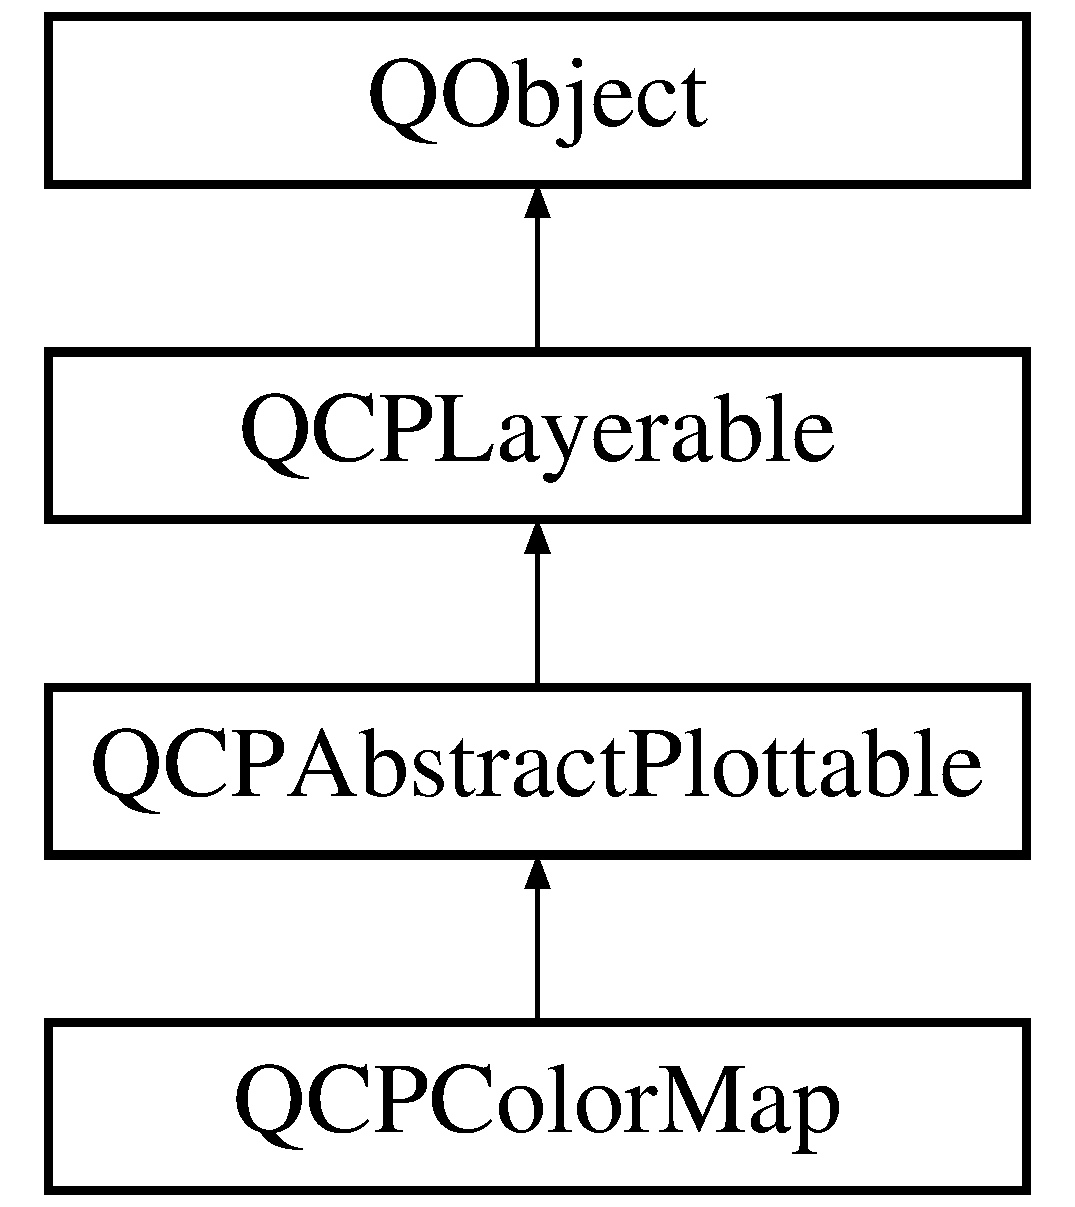
\includegraphics[height=4.000000cm]{class_q_c_p_color_map}
\end{center}
\end{figure}
\subsection*{Signals}
\begin{DoxyCompactItemize}
\item 
void \hyperlink{class_q_c_p_color_map_a482980f2335d09cfb36dd95ba9663197}{data\+Range\+Changed} (\hyperlink{class_q_c_p_range}{Q\+C\+P\+Range} new\+Range)
\item 
void \hyperlink{class_q_c_p_color_map_a978d5d5c9f68cffef8c902b855c04490}{data\+Scale\+Type\+Changed} (\hyperlink{class_q_c_p_axis_a36d8e8658dbaa179bf2aeb973db2d6f0}{Q\+C\+P\+Axis\+::\+Scale\+Type} scale\+Type)
\item 
void \hyperlink{class_q_c_p_color_map_abf4797f86e422ac6e0f732c4ff1a4d49}{gradient\+Changed} (\hyperlink{class_q_c_p_color_gradient}{Q\+C\+P\+Color\+Gradient} new\+Gradient)
\end{DoxyCompactItemize}
\subsection*{Public Member Functions}
\begin{DoxyCompactItemize}
\item 
\hyperlink{class_q_c_p_color_map_aa37e976d2ee1e2be6c4cd88a64b36215}{Q\+C\+P\+Color\+Map} (\hyperlink{class_q_c_p_axis}{Q\+C\+P\+Axis} $\ast$\hyperlink{class_q_c_p_abstract_plottable_a72c7a09c22963f2c943f07112b311103}{key\+Axis}, \hyperlink{class_q_c_p_axis}{Q\+C\+P\+Axis} $\ast$\hyperlink{class_q_c_p_abstract_plottable_a3106f9d34d330a6097a8ec5905e5b519}{value\+Axis})
\item 
virtual \hyperlink{class_q_c_p_color_map_ac8a952a40fed62dcee33405b0f4d47ad}{$\sim$\+Q\+C\+P\+Color\+Map} ()
\item 
\hyperlink{class_q_c_p_color_map_data}{Q\+C\+P\+Color\+Map\+Data} $\ast$ \hyperlink{class_q_c_p_color_map_a3ae12c9ce842352037cd20ea5267414f}{data} () const 
\item 
\hyperlink{class_q_c_p_range}{Q\+C\+P\+Range} \hyperlink{class_q_c_p_color_map_a37cc8e821e070697e15652f6419fab48}{data\+Range} () const 
\item 
\hyperlink{class_q_c_p_axis_a36d8e8658dbaa179bf2aeb973db2d6f0}{Q\+C\+P\+Axis\+::\+Scale\+Type} \hyperlink{class_q_c_p_color_map_a5ffc703dc603c4fd942f36ea51b8c48d}{data\+Scale\+Type} () const 
\item 
bool \hyperlink{class_q_c_p_color_map_a39019675a7ad00efad7212b96c0ccc95}{interpolate} () const 
\item 
bool \hyperlink{class_q_c_p_color_map_aa1d9aa8db73a5942881f6f6c5afdbb0f}{tight\+Boundary} () const 
\item 
\hyperlink{class_q_c_p_color_gradient}{Q\+C\+P\+Color\+Gradient} \hyperlink{class_q_c_p_color_map_a9f967a971474e32345290b79cf107809}{gradient} () const 
\item 
\hyperlink{class_q_c_p_color_scale}{Q\+C\+P\+Color\+Scale} $\ast$ \hyperlink{class_q_c_p_color_map_a6bd82e0b042a2ec4d64f40853a3b05e3}{color\+Scale} () const 
\item 
void \hyperlink{class_q_c_p_color_map_a5a23e133a20c4ccad35fd32e6c0f9809}{set\+Data} (\hyperlink{class_q_c_p_color_map_data}{Q\+C\+P\+Color\+Map\+Data} $\ast$\hyperlink{class_q_c_p_color_map_a3ae12c9ce842352037cd20ea5267414f}{data}, bool copy=false)
\item 
Q\+\_\+\+S\+L\+O\+T void \hyperlink{class_q_c_p_color_map_a980b42837821159786a85b4b7dcb8774}{set\+Data\+Range} (const \hyperlink{class_q_c_p_range}{Q\+C\+P\+Range} \&\hyperlink{class_q_c_p_color_map_a37cc8e821e070697e15652f6419fab48}{data\+Range})
\item 
Q\+\_\+\+S\+L\+O\+T void \hyperlink{class_q_c_p_color_map_a9d20aa08e3c1f20f22908c45b9c06511}{set\+Data\+Scale\+Type} (\hyperlink{class_q_c_p_axis_a36d8e8658dbaa179bf2aeb973db2d6f0}{Q\+C\+P\+Axis\+::\+Scale\+Type} scale\+Type)
\item 
Q\+\_\+\+S\+L\+O\+T void \hyperlink{class_q_c_p_color_map_a7313c78360471cead3576341a2c50377}{set\+Gradient} (const \hyperlink{class_q_c_p_color_gradient}{Q\+C\+P\+Color\+Gradient} \&\hyperlink{class_q_c_p_color_map_a9f967a971474e32345290b79cf107809}{gradient})
\item 
void \hyperlink{class_q_c_p_color_map_a484eaa8a5065cfc386b15375bf98b964}{set\+Interpolate} (bool enabled)
\item 
void \hyperlink{class_q_c_p_color_map_ad03221cc285e5f562a0b13d684b5576d}{set\+Tight\+Boundary} (bool enabled)
\item 
void \hyperlink{class_q_c_p_color_map_aa828921db364fe3c6af4619580ab85fd}{set\+Color\+Scale} (\hyperlink{class_q_c_p_color_scale}{Q\+C\+P\+Color\+Scale} $\ast$\hyperlink{class_q_c_p_color_map_a6bd82e0b042a2ec4d64f40853a3b05e3}{color\+Scale})
\item 
void \hyperlink{class_q_c_p_color_map_a856608fa3dd1cc290bcd5f29a5575774}{rescale\+Data\+Range} (bool recalculate\+Data\+Bounds=false)
\item 
Q\+\_\+\+S\+L\+O\+T void \hyperlink{class_q_c_p_color_map_a5d8158b62d55fcfeaabcb68ce0083e87}{update\+Legend\+Icon} (Qt\+::\+Transformation\+Mode transform\+Mode=Qt\+::\+Smooth\+Transformation, const Q\+Size \&thumb\+Size=Q\+Size(32, 18))
\item 
virtual void \hyperlink{class_q_c_p_color_map_a0545dce5383766885912331705a8e099}{clear\+Data} ()
\item 
virtual double \hyperlink{class_q_c_p_color_map_a4088dc7bcbe9bba605c84a912ba660ff}{select\+Test} (const Q\+Point\+F \&pos, bool only\+Selectable, Q\+Variant $\ast$details=0) const 
\end{DoxyCompactItemize}
\subsection*{Protected Member Functions}
\begin{DoxyCompactItemize}
\item 
virtual void \hyperlink{class_q_c_p_color_map_a5efcea591bb5486d968af520a4d43c3a}{update\+Map\+Image} ()
\item 
virtual void \hyperlink{class_q_c_p_color_map_a3b0f45a3177be9522d5e9b8cd8ae122d}{draw} (\hyperlink{class_q_c_p_painter}{Q\+C\+P\+Painter} $\ast$painter)
\item 
virtual void \hyperlink{class_q_c_p_color_map_a7d5eee89f6b8eaf2f11f1d94e32215b2}{draw\+Legend\+Icon} (\hyperlink{class_q_c_p_painter}{Q\+C\+P\+Painter} $\ast$painter, const Q\+Rect\+F \&rect) const 
\item 
virtual \hyperlink{class_q_c_p_range}{Q\+C\+P\+Range} \hyperlink{class_q_c_p_color_map_a0d89371f8707f12e22737b863f1a5126}{get\+Key\+Range} (bool \&found\+Range, \hyperlink{class_q_c_p_abstract_plottable_a661743478a1d3c09d28ec2711d7653d8}{Sign\+Domain} in\+Sign\+Domain=\hyperlink{class_q_c_p_abstract_plottable_a661743478a1d3c09d28ec2711d7653d8a082b98cfb91a7363a3b5cd17b0c1cd60}{sd\+Both}) const 
\item 
virtual \hyperlink{class_q_c_p_range}{Q\+C\+P\+Range} \hyperlink{class_q_c_p_color_map_ac1b906e05ca9b61680e61b74b3825a22}{get\+Value\+Range} (bool \&found\+Range, \hyperlink{class_q_c_p_abstract_plottable_a661743478a1d3c09d28ec2711d7653d8}{Sign\+Domain} in\+Sign\+Domain=\hyperlink{class_q_c_p_abstract_plottable_a661743478a1d3c09d28ec2711d7653d8a082b98cfb91a7363a3b5cd17b0c1cd60}{sd\+Both}) const 
\end{DoxyCompactItemize}
\subsection*{Protected Attributes}
\begin{DoxyCompactItemize}
\item 
\hyperlink{class_q_c_p_range}{Q\+C\+P\+Range} \hyperlink{class_q_c_p_color_map_ab87609621d16cd3e9d52ad070b327b08}{m\+Data\+Range}
\item 
\hyperlink{class_q_c_p_axis_a36d8e8658dbaa179bf2aeb973db2d6f0}{Q\+C\+P\+Axis\+::\+Scale\+Type} \hyperlink{class_q_c_p_color_map_ab28a4b2def408f83b9818799d5f18446}{m\+Data\+Scale\+Type}
\item 
\hyperlink{class_q_c_p_color_map_data}{Q\+C\+P\+Color\+Map\+Data} $\ast$ \hyperlink{class_q_c_p_color_map_a8709272aa8f0be3ca111bf3866806f8b}{m\+Map\+Data}
\item 
\hyperlink{class_q_c_p_color_gradient}{Q\+C\+P\+Color\+Gradient} \hyperlink{class_q_c_p_color_map_aab77fe9a8df6f0486ab3507cc5f278fa}{m\+Gradient}
\item 
bool \hyperlink{class_q_c_p_color_map_af77e5eba9a844592648edeb6fbe834f1}{m\+Interpolate}
\item 
bool \hyperlink{class_q_c_p_color_map_ac2e9425fe4381b496726e1c09f978302}{m\+Tight\+Boundary}
\item 
Q\+Pointer$<$ \hyperlink{class_q_c_p_color_scale}{Q\+C\+P\+Color\+Scale} $>$ \hyperlink{class_q_c_p_color_map_a95b4100bacc3387652c988b071ec9db7}{m\+Color\+Scale}
\item 
Q\+Image \hyperlink{class_q_c_p_color_map_a66110813b42eca78b64095b2a1f285a0}{m\+Map\+Image}
\item 
Q\+Pixmap \hyperlink{class_q_c_p_color_map_ada522988db02cb531767d38c5029ef60}{m\+Legend\+Icon}
\item 
bool \hyperlink{class_q_c_p_color_map_ac9aea6a5c193d7fa866bc7b26e79ef2c}{m\+Map\+Image\+Invalidated}
\end{DoxyCompactItemize}
\subsection*{Friends}
\begin{DoxyCompactItemize}
\item 
class \hyperlink{class_q_c_p_color_map_a1cdf9df76adcfae45261690aa0ca2198}{Q\+Custom\+Plot}
\item 
class \hyperlink{class_q_c_p_color_map_a8429035e7adfbd7f05805a6530ad5e3b}{Q\+C\+P\+Legend}
\end{DoxyCompactItemize}
\subsection*{Additional Inherited Members}


\subsection{Detailed Description}
A plottable representing a two-\/dimensional color map in a plot. 



The data is stored in the class \hyperlink{class_q_c_p_color_map_data}{Q\+C\+P\+Color\+Map\+Data}, which can be accessed via the \hyperlink{class_q_c_p_color_map_a3ae12c9ce842352037cd20ea5267414f}{data()} method.

A color map has three dimensions to represent a data point\+: The {\itshape key} dimension, the {\itshape value} dimension and the {\itshape data} dimension. As with other plottables such as graphs, {\itshape key} and {\itshape value} correspond to two orthogonal axes on the \hyperlink{class_q_custom_plot}{Q\+Custom\+Plot} surface that you specify in the Q\+Color\+Map constructor. The {\itshape data} dimension however is encoded as the color of the point at ({\itshape key}, {\itshape value}).

Set the number of points (or {\itshape cells}) in the key/value dimension via \hyperlink{class_q_c_p_color_map_data_a0d9ff35c299d0478b682bfbcdd9c097e}{Q\+C\+P\+Color\+Map\+Data\+::set\+Size}. The plot coordinate range over which these points will be displayed is specified via \hyperlink{class_q_c_p_color_map_data_aad9c1c7c703c1339489fc730517c83d4}{Q\+C\+P\+Color\+Map\+Data\+::set\+Range}. The first cell will be centered on the lower range boundary and the last cell will be centered on the upper range boundary. The data can be set by either accessing the cells directly with \hyperlink{class_q_c_p_color_map_data_a8e75eaf8746596319032a93f3d2d0683}{Q\+C\+P\+Color\+Map\+Data\+::set\+Cell} or by addressing the cells via their plot coordinates with \hyperlink{class_q_c_p_color_map_data_afd2083ccfd6987ec94aa7ef8e91ca39a}{Q\+C\+P\+Color\+Map\+Data\+::set\+Data}. If possible, you should prefer set\+Cell, since it doesn\textquotesingle{}t need to do any coordinate transformation and thus performs a bit better.

The cell with index (0, 0) is at the bottom left, if the color map uses normal (i.\+e. not reversed) key and value axes.

To show the user which colors correspond to which {\itshape data} values, a \hyperlink{class_q_c_p_color_scale}{Q\+C\+P\+Color\+Scale} is typically placed to the right of the axis rect. See the documentation there for details on how to add and use a color scale.\hypertarget{class_q_c_p_statistical_box_appearance}{}\subsection{Changing the appearance}\label{class_q_c_p_statistical_box_appearance}
The central part of the appearance is the color gradient, which can be specified via \hyperlink{class_q_c_p_color_map_a7313c78360471cead3576341a2c50377}{set\+Gradient}. See the documentation of \hyperlink{class_q_c_p_color_gradient}{Q\+C\+P\+Color\+Gradient} for details on configuring a color gradient.

The {\itshape data} range that is mapped to the colors of the gradient can be specified with \hyperlink{class_q_c_p_color_map_a980b42837821159786a85b4b7dcb8774}{set\+Data\+Range}. To make the data range encompass the whole data set minimum to maximum, call \hyperlink{class_q_c_p_color_map_a856608fa3dd1cc290bcd5f29a5575774}{rescale\+Data\+Range}.\hypertarget{class_q_c_p_statistical_box_usage}{}\subsection{Usage}\label{class_q_c_p_statistical_box_usage}
Like all data representing objects in \hyperlink{class_q_custom_plot}{Q\+Custom\+Plot}, the \hyperlink{class_q_c_p_color_map}{Q\+C\+P\+Color\+Map} is a plottable (\hyperlink{class_q_c_p_abstract_plottable}{Q\+C\+P\+Abstract\+Plottable}). So the plottable-\/interface of \hyperlink{class_q_custom_plot}{Q\+Custom\+Plot} applies (\hyperlink{class_q_custom_plot_a32de81ff53e263e785b83b52ecd99d6f}{Q\+Custom\+Plot\+::plottable}, \hyperlink{class_q_custom_plot_ab7ad9174f701f9c6f64e378df77927a6}{Q\+Custom\+Plot\+::add\+Plottable}, \hyperlink{class_q_custom_plot_af3dafd56884208474f311d6226513ab2}{Q\+Custom\+Plot\+::remove\+Plottable}, etc.)

Usually, you first create an instance\+: 
\begin{DoxyCode}
\hyperlink{class_q_c_p_color_map}{QCPColorMap} *colorMap = \textcolor{keyword}{new} \hyperlink{class_q_c_p_color_map_aa37e976d2ee1e2be6c4cd88a64b36215}{QCPColorMap}(customPlot->xAxis, customPlot->yAxis);
\end{DoxyCode}
 add it to the custom\+Plot with \hyperlink{class_q_custom_plot_ab7ad9174f701f9c6f64e378df77927a6}{Q\+Custom\+Plot\+::add\+Plottable}\+: 
\begin{DoxyCode}
customPlot->addPlottable(colorMap);
\end{DoxyCode}
 and then modify the properties of the newly created color map, e.\+g.\+: 
\begin{DoxyCode}
colorMap->\hyperlink{class_q_c_p_color_map_a3ae12c9ce842352037cd20ea5267414f}{data}()->\hyperlink{class_q_c_p_color_map_data_a0d9ff35c299d0478b682bfbcdd9c097e}{setSize}(50, 50);
colorMap->\hyperlink{class_q_c_p_color_map_a3ae12c9ce842352037cd20ea5267414f}{data}()->\hyperlink{class_q_c_p_color_map_data_aad9c1c7c703c1339489fc730517c83d4}{setRange}(\hyperlink{class_q_c_p_range}{QCPRange}(0, 2), \hyperlink{class_q_c_p_range}{QCPRange}(0, 2));
\textcolor{keywordflow}{for} (\textcolor{keywordtype}{int} x=0; x<50; ++x)
  \textcolor{keywordflow}{for} (\textcolor{keywordtype}{int} y=0; y<50; ++y)
    colorMap->\hyperlink{class_q_c_p_color_map_a3ae12c9ce842352037cd20ea5267414f}{data}()->\hyperlink{class_q_c_p_color_map_data_a8e75eaf8746596319032a93f3d2d0683}{setCell}(x, y, qCos(x/10.0)+qSin(y/10.0));
colorMap->\hyperlink{class_q_c_p_color_map_a7313c78360471cead3576341a2c50377}{setGradient}(\hyperlink{class_q_c_p_color_gradient_aed6569828fee337023670272910c9072ab7414ce4e36dc3e82e0132a7f0f41b52}{QCPColorGradient::gpPolar});
colorMap->\hyperlink{class_q_c_p_color_map_a856608fa3dd1cc290bcd5f29a5575774}{rescaleDataRange}(\textcolor{keyword}{true});
customPlot->rescaleAxes();
customPlot->replot();
\end{DoxyCode}


\begin{DoxyNote}{Note}
The \hyperlink{class_q_c_p_color_map}{Q\+C\+P\+Color\+Map} always displays the data at equal key/value intervals, even if the key or value axis is set to a logarithmic scaling. If you want to use \hyperlink{class_q_c_p_color_map}{Q\+C\+P\+Color\+Map} with logarithmic axes, you shouldn\textquotesingle{}t use the \hyperlink{class_q_c_p_color_map_data_afd2083ccfd6987ec94aa7ef8e91ca39a}{Q\+C\+P\+Color\+Map\+Data\+::set\+Data} method as it uses a linear transformation to determine the cell index. Rather directly access the cell index with \hyperlink{class_q_c_p_color_map_data_a8e75eaf8746596319032a93f3d2d0683}{Q\+C\+P\+Color\+Map\+Data\+::set\+Cell}. 
\end{DoxyNote}


\subsection{Constructor \& Destructor Documentation}
\hypertarget{class_q_c_p_color_map_aa37e976d2ee1e2be6c4cd88a64b36215}{}\index{Q\+C\+P\+Color\+Map@{Q\+C\+P\+Color\+Map}!Q\+C\+P\+Color\+Map@{Q\+C\+P\+Color\+Map}}
\index{Q\+C\+P\+Color\+Map@{Q\+C\+P\+Color\+Map}!Q\+C\+P\+Color\+Map@{Q\+C\+P\+Color\+Map}}
\subsubsection[{Q\+C\+P\+Color\+Map}]{\setlength{\rightskip}{0pt plus 5cm}Q\+C\+P\+Color\+Map\+::\+Q\+C\+P\+Color\+Map (
\begin{DoxyParamCaption}
\item[{{\bf Q\+C\+P\+Axis} $\ast$}]{key\+Axis, }
\item[{{\bf Q\+C\+P\+Axis} $\ast$}]{value\+Axis}
\end{DoxyParamCaption}
)\hspace{0.3cm}{\ttfamily [explicit]}}\label{class_q_c_p_color_map_aa37e976d2ee1e2be6c4cd88a64b36215}
Constructs a color map with the specified {\itshape key\+Axis} and {\itshape value\+Axis}.

The constructed \hyperlink{class_q_c_p_color_map}{Q\+C\+P\+Color\+Map} can be added to the plot with \hyperlink{class_q_custom_plot_ab7ad9174f701f9c6f64e378df77927a6}{Q\+Custom\+Plot\+::add\+Plottable}, \hyperlink{class_q_custom_plot}{Q\+Custom\+Plot} then takes ownership of the color map. \hypertarget{class_q_c_p_color_map_ac8a952a40fed62dcee33405b0f4d47ad}{}\index{Q\+C\+P\+Color\+Map@{Q\+C\+P\+Color\+Map}!````~Q\+C\+P\+Color\+Map@{$\sim$\+Q\+C\+P\+Color\+Map}}
\index{````~Q\+C\+P\+Color\+Map@{$\sim$\+Q\+C\+P\+Color\+Map}!Q\+C\+P\+Color\+Map@{Q\+C\+P\+Color\+Map}}
\subsubsection[{$\sim$\+Q\+C\+P\+Color\+Map}]{\setlength{\rightskip}{0pt plus 5cm}Q\+C\+P\+Color\+Map\+::$\sim$\+Q\+C\+P\+Color\+Map (
\begin{DoxyParamCaption}
{}
\end{DoxyParamCaption}
)\hspace{0.3cm}{\ttfamily [virtual]}}\label{class_q_c_p_color_map_ac8a952a40fed62dcee33405b0f4d47ad}


\subsection{Member Function Documentation}
\hypertarget{class_q_c_p_color_map_a0545dce5383766885912331705a8e099}{}\index{Q\+C\+P\+Color\+Map@{Q\+C\+P\+Color\+Map}!clear\+Data@{clear\+Data}}
\index{clear\+Data@{clear\+Data}!Q\+C\+P\+Color\+Map@{Q\+C\+P\+Color\+Map}}
\subsubsection[{clear\+Data}]{\setlength{\rightskip}{0pt plus 5cm}void Q\+C\+P\+Color\+Map\+::clear\+Data (
\begin{DoxyParamCaption}
{}
\end{DoxyParamCaption}
)\hspace{0.3cm}{\ttfamily [virtual]}}\label{class_q_c_p_color_map_a0545dce5383766885912331705a8e099}
Clears the colormap data by calling \hyperlink{class_q_c_p_color_map_data_a9910ba830e96955bd5c8e5bef1e77ef3}{Q\+C\+P\+Color\+Map\+Data\+::clear()} on the internal data. This also resizes the map to 0x0 cells. 

Implements \hyperlink{class_q_c_p_abstract_plottable_a86e5b8fd4b6ff4f4084e7ea4c573fc53}{Q\+C\+P\+Abstract\+Plottable}.

\hypertarget{class_q_c_p_color_map_a6bd82e0b042a2ec4d64f40853a3b05e3}{}\index{Q\+C\+P\+Color\+Map@{Q\+C\+P\+Color\+Map}!color\+Scale@{color\+Scale}}
\index{color\+Scale@{color\+Scale}!Q\+C\+P\+Color\+Map@{Q\+C\+P\+Color\+Map}}
\subsubsection[{color\+Scale}]{\setlength{\rightskip}{0pt plus 5cm}{\bf Q\+C\+P\+Color\+Scale}$\ast$ Q\+C\+P\+Color\+Map\+::color\+Scale (
\begin{DoxyParamCaption}
{}
\end{DoxyParamCaption}
) const\hspace{0.3cm}{\ttfamily [inline]}}\label{class_q_c_p_color_map_a6bd82e0b042a2ec4d64f40853a3b05e3}
\hypertarget{class_q_c_p_color_map_a3ae12c9ce842352037cd20ea5267414f}{}\index{Q\+C\+P\+Color\+Map@{Q\+C\+P\+Color\+Map}!data@{data}}
\index{data@{data}!Q\+C\+P\+Color\+Map@{Q\+C\+P\+Color\+Map}}
\subsubsection[{data}]{\setlength{\rightskip}{0pt plus 5cm}{\bf Q\+C\+P\+Color\+Map\+Data} $\ast$ Q\+C\+P\+Color\+Map\+::data (
\begin{DoxyParamCaption}
{}
\end{DoxyParamCaption}
) const\hspace{0.3cm}{\ttfamily [inline]}}\label{class_q_c_p_color_map_a3ae12c9ce842352037cd20ea5267414f}
Returns a pointer to the internal data storage of type \hyperlink{class_q_c_p_color_map_data}{Q\+C\+P\+Color\+Map\+Data}. Access this to modify data points (cells) and the color map key/value range.

\begin{DoxySeeAlso}{See also}
\hyperlink{class_q_c_p_color_map_a5a23e133a20c4ccad35fd32e6c0f9809}{set\+Data} 
\end{DoxySeeAlso}
\hypertarget{class_q_c_p_color_map_a37cc8e821e070697e15652f6419fab48}{}\index{Q\+C\+P\+Color\+Map@{Q\+C\+P\+Color\+Map}!data\+Range@{data\+Range}}
\index{data\+Range@{data\+Range}!Q\+C\+P\+Color\+Map@{Q\+C\+P\+Color\+Map}}
\subsubsection[{data\+Range}]{\setlength{\rightskip}{0pt plus 5cm}{\bf Q\+C\+P\+Range} Q\+C\+P\+Color\+Map\+::data\+Range (
\begin{DoxyParamCaption}
{}
\end{DoxyParamCaption}
) const\hspace{0.3cm}{\ttfamily [inline]}}\label{class_q_c_p_color_map_a37cc8e821e070697e15652f6419fab48}
\hypertarget{class_q_c_p_color_map_a482980f2335d09cfb36dd95ba9663197}{}\index{Q\+C\+P\+Color\+Map@{Q\+C\+P\+Color\+Map}!data\+Range\+Changed@{data\+Range\+Changed}}
\index{data\+Range\+Changed@{data\+Range\+Changed}!Q\+C\+P\+Color\+Map@{Q\+C\+P\+Color\+Map}}
\subsubsection[{data\+Range\+Changed}]{\setlength{\rightskip}{0pt plus 5cm}void Q\+C\+P\+Color\+Map\+::data\+Range\+Changed (
\begin{DoxyParamCaption}
\item[{{\bf Q\+C\+P\+Range}}]{new\+Range}
\end{DoxyParamCaption}
)\hspace{0.3cm}{\ttfamily [signal]}}\label{class_q_c_p_color_map_a482980f2335d09cfb36dd95ba9663197}
This signal is emitted when the data range changes.

\begin{DoxySeeAlso}{See also}
\hyperlink{class_q_c_p_color_map_a980b42837821159786a85b4b7dcb8774}{set\+Data\+Range} 
\end{DoxySeeAlso}
\hypertarget{class_q_c_p_color_map_a5ffc703dc603c4fd942f36ea51b8c48d}{}\index{Q\+C\+P\+Color\+Map@{Q\+C\+P\+Color\+Map}!data\+Scale\+Type@{data\+Scale\+Type}}
\index{data\+Scale\+Type@{data\+Scale\+Type}!Q\+C\+P\+Color\+Map@{Q\+C\+P\+Color\+Map}}
\subsubsection[{data\+Scale\+Type}]{\setlength{\rightskip}{0pt plus 5cm}{\bf Q\+C\+P\+Axis\+::\+Scale\+Type} Q\+C\+P\+Color\+Map\+::data\+Scale\+Type (
\begin{DoxyParamCaption}
{}
\end{DoxyParamCaption}
) const\hspace{0.3cm}{\ttfamily [inline]}}\label{class_q_c_p_color_map_a5ffc703dc603c4fd942f36ea51b8c48d}
\hypertarget{class_q_c_p_color_map_a978d5d5c9f68cffef8c902b855c04490}{}\index{Q\+C\+P\+Color\+Map@{Q\+C\+P\+Color\+Map}!data\+Scale\+Type\+Changed@{data\+Scale\+Type\+Changed}}
\index{data\+Scale\+Type\+Changed@{data\+Scale\+Type\+Changed}!Q\+C\+P\+Color\+Map@{Q\+C\+P\+Color\+Map}}
\subsubsection[{data\+Scale\+Type\+Changed}]{\setlength{\rightskip}{0pt plus 5cm}void Q\+C\+P\+Color\+Map\+::data\+Scale\+Type\+Changed (
\begin{DoxyParamCaption}
\item[{{\bf Q\+C\+P\+Axis\+::\+Scale\+Type}}]{scale\+Type}
\end{DoxyParamCaption}
)\hspace{0.3cm}{\ttfamily [signal]}}\label{class_q_c_p_color_map_a978d5d5c9f68cffef8c902b855c04490}
This signal is emitted when the data scale type changes.

\begin{DoxySeeAlso}{See also}
\hyperlink{class_q_c_p_color_map_a9d20aa08e3c1f20f22908c45b9c06511}{set\+Data\+Scale\+Type} 
\end{DoxySeeAlso}
\hypertarget{class_q_c_p_color_map_a3b0f45a3177be9522d5e9b8cd8ae122d}{}\index{Q\+C\+P\+Color\+Map@{Q\+C\+P\+Color\+Map}!draw@{draw}}
\index{draw@{draw}!Q\+C\+P\+Color\+Map@{Q\+C\+P\+Color\+Map}}
\subsubsection[{draw}]{\setlength{\rightskip}{0pt plus 5cm}void Q\+C\+P\+Color\+Map\+::draw (
\begin{DoxyParamCaption}
\item[{{\bf Q\+C\+P\+Painter} $\ast$}]{painter}
\end{DoxyParamCaption}
)\hspace{0.3cm}{\ttfamily [protected]}, {\ttfamily [virtual]}}\label{class_q_c_p_color_map_a3b0f45a3177be9522d5e9b8cd8ae122d}


Implements \hyperlink{class_q_c_p_abstract_plottable_acbab5e30dcd04fd302b4a5902ac2c482}{Q\+C\+P\+Abstract\+Plottable}.

\hypertarget{class_q_c_p_color_map_a7d5eee89f6b8eaf2f11f1d94e32215b2}{}\index{Q\+C\+P\+Color\+Map@{Q\+C\+P\+Color\+Map}!draw\+Legend\+Icon@{draw\+Legend\+Icon}}
\index{draw\+Legend\+Icon@{draw\+Legend\+Icon}!Q\+C\+P\+Color\+Map@{Q\+C\+P\+Color\+Map}}
\subsubsection[{draw\+Legend\+Icon}]{\setlength{\rightskip}{0pt plus 5cm}void Q\+C\+P\+Color\+Map\+::draw\+Legend\+Icon (
\begin{DoxyParamCaption}
\item[{{\bf Q\+C\+P\+Painter} $\ast$}]{painter, }
\item[{const Q\+Rect\+F \&}]{rect}
\end{DoxyParamCaption}
) const\hspace{0.3cm}{\ttfamily [protected]}, {\ttfamily [virtual]}}\label{class_q_c_p_color_map_a7d5eee89f6b8eaf2f11f1d94e32215b2}


Implements \hyperlink{class_q_c_p_abstract_plottable_a9a450783fd9ed539e589999fd390cdf7}{Q\+C\+P\+Abstract\+Plottable}.

\hypertarget{class_q_c_p_color_map_a0d89371f8707f12e22737b863f1a5126}{}\index{Q\+C\+P\+Color\+Map@{Q\+C\+P\+Color\+Map}!get\+Key\+Range@{get\+Key\+Range}}
\index{get\+Key\+Range@{get\+Key\+Range}!Q\+C\+P\+Color\+Map@{Q\+C\+P\+Color\+Map}}
\subsubsection[{get\+Key\+Range}]{\setlength{\rightskip}{0pt plus 5cm}{\bf Q\+C\+P\+Range} Q\+C\+P\+Color\+Map\+::get\+Key\+Range (
\begin{DoxyParamCaption}
\item[{bool \&}]{found\+Range, }
\item[{{\bf Sign\+Domain}}]{in\+Sign\+Domain = {\ttfamily {\bf sd\+Both}}}
\end{DoxyParamCaption}
) const\hspace{0.3cm}{\ttfamily [protected]}, {\ttfamily [virtual]}}\label{class_q_c_p_color_map_a0d89371f8707f12e22737b863f1a5126}


Implements \hyperlink{class_q_c_p_abstract_plottable_a345d702b2e7e12c8cfdddff65ba85e8c}{Q\+C\+P\+Abstract\+Plottable}.

\hypertarget{class_q_c_p_color_map_ac1b906e05ca9b61680e61b74b3825a22}{}\index{Q\+C\+P\+Color\+Map@{Q\+C\+P\+Color\+Map}!get\+Value\+Range@{get\+Value\+Range}}
\index{get\+Value\+Range@{get\+Value\+Range}!Q\+C\+P\+Color\+Map@{Q\+C\+P\+Color\+Map}}
\subsubsection[{get\+Value\+Range}]{\setlength{\rightskip}{0pt plus 5cm}{\bf Q\+C\+P\+Range} Q\+C\+P\+Color\+Map\+::get\+Value\+Range (
\begin{DoxyParamCaption}
\item[{bool \&}]{found\+Range, }
\item[{{\bf Sign\+Domain}}]{in\+Sign\+Domain = {\ttfamily {\bf sd\+Both}}}
\end{DoxyParamCaption}
) const\hspace{0.3cm}{\ttfamily [protected]}, {\ttfamily [virtual]}}\label{class_q_c_p_color_map_ac1b906e05ca9b61680e61b74b3825a22}


Implements \hyperlink{class_q_c_p_abstract_plottable_aa3331b415b5939fe4df60b78831b2799}{Q\+C\+P\+Abstract\+Plottable}.

\hypertarget{class_q_c_p_color_map_a9f967a971474e32345290b79cf107809}{}\index{Q\+C\+P\+Color\+Map@{Q\+C\+P\+Color\+Map}!gradient@{gradient}}
\index{gradient@{gradient}!Q\+C\+P\+Color\+Map@{Q\+C\+P\+Color\+Map}}
\subsubsection[{gradient}]{\setlength{\rightskip}{0pt plus 5cm}{\bf Q\+C\+P\+Color\+Gradient} Q\+C\+P\+Color\+Map\+::gradient (
\begin{DoxyParamCaption}
{}
\end{DoxyParamCaption}
) const\hspace{0.3cm}{\ttfamily [inline]}}\label{class_q_c_p_color_map_a9f967a971474e32345290b79cf107809}
\hypertarget{class_q_c_p_color_map_abf4797f86e422ac6e0f732c4ff1a4d49}{}\index{Q\+C\+P\+Color\+Map@{Q\+C\+P\+Color\+Map}!gradient\+Changed@{gradient\+Changed}}
\index{gradient\+Changed@{gradient\+Changed}!Q\+C\+P\+Color\+Map@{Q\+C\+P\+Color\+Map}}
\subsubsection[{gradient\+Changed}]{\setlength{\rightskip}{0pt plus 5cm}void Q\+C\+P\+Color\+Map\+::gradient\+Changed (
\begin{DoxyParamCaption}
\item[{{\bf Q\+C\+P\+Color\+Gradient}}]{new\+Gradient}
\end{DoxyParamCaption}
)\hspace{0.3cm}{\ttfamily [signal]}}\label{class_q_c_p_color_map_abf4797f86e422ac6e0f732c4ff1a4d49}
This signal is emitted when the gradient changes.

\begin{DoxySeeAlso}{See also}
\hyperlink{class_q_c_p_color_map_a7313c78360471cead3576341a2c50377}{set\+Gradient} 
\end{DoxySeeAlso}
\hypertarget{class_q_c_p_color_map_a39019675a7ad00efad7212b96c0ccc95}{}\index{Q\+C\+P\+Color\+Map@{Q\+C\+P\+Color\+Map}!interpolate@{interpolate}}
\index{interpolate@{interpolate}!Q\+C\+P\+Color\+Map@{Q\+C\+P\+Color\+Map}}
\subsubsection[{interpolate}]{\setlength{\rightskip}{0pt plus 5cm}bool Q\+C\+P\+Color\+Map\+::interpolate (
\begin{DoxyParamCaption}
{}
\end{DoxyParamCaption}
) const\hspace{0.3cm}{\ttfamily [inline]}}\label{class_q_c_p_color_map_a39019675a7ad00efad7212b96c0ccc95}
\hypertarget{class_q_c_p_color_map_a856608fa3dd1cc290bcd5f29a5575774}{}\index{Q\+C\+P\+Color\+Map@{Q\+C\+P\+Color\+Map}!rescale\+Data\+Range@{rescale\+Data\+Range}}
\index{rescale\+Data\+Range@{rescale\+Data\+Range}!Q\+C\+P\+Color\+Map@{Q\+C\+P\+Color\+Map}}
\subsubsection[{rescale\+Data\+Range}]{\setlength{\rightskip}{0pt plus 5cm}void Q\+C\+P\+Color\+Map\+::rescale\+Data\+Range (
\begin{DoxyParamCaption}
\item[{bool}]{recalculate\+Data\+Bounds = {\ttfamily false}}
\end{DoxyParamCaption}
)}\label{class_q_c_p_color_map_a856608fa3dd1cc290bcd5f29a5575774}
Sets the data range (\hyperlink{class_q_c_p_color_map_a980b42837821159786a85b4b7dcb8774}{set\+Data\+Range}) to span the minimum and maximum values that occur in the current data set. This corresponds to the \hyperlink{class_q_c_p_abstract_plottable_a1acecfcca3e7fcda00fcbaa3c886386f}{rescale\+Key\+Axis} or \hyperlink{class_q_c_p_abstract_plottable_abfd0805eb1d955c0111a990246658324}{rescale\+Value\+Axis} methods, only for the third data dimension of the color map.

The minimum and maximum values of the data set are buffered in the internal \hyperlink{class_q_c_p_color_map_data}{Q\+C\+P\+Color\+Map\+Data} instance (\hyperlink{class_q_c_p_color_map_a3ae12c9ce842352037cd20ea5267414f}{data}). As data is updated via its \hyperlink{class_q_c_p_color_map_data_a8e75eaf8746596319032a93f3d2d0683}{Q\+C\+P\+Color\+Map\+Data\+::set\+Cell} or \hyperlink{class_q_c_p_color_map_data_afd2083ccfd6987ec94aa7ef8e91ca39a}{Q\+C\+P\+Color\+Map\+Data\+::set\+Data}, the buffered minimum and maximum values are updated, too. For performance reasons, however, they are only updated in an expanding fashion. So the buffered maximum can only increase and the buffered minimum can only decrease. In consequence, changes to the data that actually lower the maximum of the data set (by overwriting the cell holding the current maximum with a smaller value), aren\textquotesingle{}t recognized and the buffered maximum overestimates the true maximum of the data set. The same happens for the buffered minimum. To recalculate the true minimum and maximum by explicitly looking at each cell, the method \hyperlink{class_q_c_p_color_map_data_ab235ade8a4d64bd3adb26a99b3dd57ee}{Q\+C\+P\+Color\+Map\+Data\+::recalculate\+Data\+Bounds} can be used. For convenience, setting the parameter {\itshape recalculate\+Data\+Bounds} calls this method before setting the data range to the buffered minimum and maximum.

\begin{DoxySeeAlso}{See also}
\hyperlink{class_q_c_p_color_map_a980b42837821159786a85b4b7dcb8774}{set\+Data\+Range} 
\end{DoxySeeAlso}
\hypertarget{class_q_c_p_color_map_a4088dc7bcbe9bba605c84a912ba660ff}{}\index{Q\+C\+P\+Color\+Map@{Q\+C\+P\+Color\+Map}!select\+Test@{select\+Test}}
\index{select\+Test@{select\+Test}!Q\+C\+P\+Color\+Map@{Q\+C\+P\+Color\+Map}}
\subsubsection[{select\+Test}]{\setlength{\rightskip}{0pt plus 5cm}double Q\+C\+P\+Color\+Map\+::select\+Test (
\begin{DoxyParamCaption}
\item[{const Q\+Point\+F \&}]{pos, }
\item[{bool}]{only\+Selectable, }
\item[{Q\+Variant $\ast$}]{details = {\ttfamily 0}}
\end{DoxyParamCaption}
) const\hspace{0.3cm}{\ttfamily [virtual]}}\label{class_q_c_p_color_map_a4088dc7bcbe9bba605c84a912ba660ff}
This function is used to decide whether a click hits a layerable object or not.

{\itshape pos} is a point in pixel coordinates on the \hyperlink{class_q_custom_plot}{Q\+Custom\+Plot} surface. This function returns the shortest pixel distance of this point to the object. If the object is either invisible or the distance couldn\textquotesingle{}t be determined, -\/1.\+0 is returned. Further, if {\itshape only\+Selectable} is true and the object is not selectable, -\/1.\+0 is returned, too.

If the item is represented not by single lines but by an area like \hyperlink{class_q_c_p_item_rect}{Q\+C\+P\+Item\+Rect} or \hyperlink{class_q_c_p_item_text}{Q\+C\+P\+Item\+Text}, a click inside the area returns a constant value greater zero (typically the selection\+Tolerance of the parent \hyperlink{class_q_custom_plot}{Q\+Custom\+Plot} multiplied by 0.\+99). If the click lies outside the area, this function returns -\/1.\+0.

Providing a constant value for area objects allows selecting line objects even when they are obscured by such area objects, by clicking close to the lines (i.\+e. closer than 0.\+99$\ast$selection\+Tolerance).

The actual setting of the selection state is not done by this function. This is handled by the parent \hyperlink{class_q_custom_plot}{Q\+Custom\+Plot} when the mouse\+Release\+Event occurs, and the finally selected object is notified via the select\+Event/deselect\+Event methods.

{\itshape details} is an optional output parameter. Every layerable subclass may place any information in {\itshape details}. This information will be passed to \hyperlink{class_q_c_p_abstract_plottable_a16aaad02456aa23a759efd1ac90c79bf}{select\+Event} when the parent \hyperlink{class_q_custom_plot}{Q\+Custom\+Plot} decides on the basis of this select\+Test call, that the object was successfully selected. The subsequent call to \hyperlink{class_q_c_p_abstract_plottable_a16aaad02456aa23a759efd1ac90c79bf}{select\+Event} will carry the {\itshape details}. This is useful for multi-\/part objects (like \hyperlink{class_q_c_p_axis}{Q\+C\+P\+Axis}). This way, a possibly complex calculation to decide which part was clicked is only done once in \hyperlink{class_q_c_p_color_map_a4088dc7bcbe9bba605c84a912ba660ff}{select\+Test}. The result (i.\+e. the actually clicked part) can then be placed in {\itshape details}. So in the subsequent \hyperlink{class_q_c_p_abstract_plottable_a16aaad02456aa23a759efd1ac90c79bf}{select\+Event}, the decision which part was selected doesn\textquotesingle{}t have to be done a second time for a single selection operation.

You may pass 0 as {\itshape details} to indicate that you are not interested in those selection details.

\begin{DoxySeeAlso}{See also}
\hyperlink{class_q_c_p_abstract_plottable_a16aaad02456aa23a759efd1ac90c79bf}{select\+Event}, \hyperlink{class_q_c_p_abstract_plottable_a6fa0d0f95560ea8b01ee13f296dab2b1}{deselect\+Event}, \hyperlink{class_q_custom_plot_a5ee1e2f6ae27419deca53e75907c27e5}{Q\+Custom\+Plot\+::set\+Interactions} 
\end{DoxySeeAlso}


Implements \hyperlink{class_q_c_p_abstract_plottable_a38efe9641d972992a3d44204bc80ec1d}{Q\+C\+P\+Abstract\+Plottable}.

\hypertarget{class_q_c_p_color_map_aa828921db364fe3c6af4619580ab85fd}{}\index{Q\+C\+P\+Color\+Map@{Q\+C\+P\+Color\+Map}!set\+Color\+Scale@{set\+Color\+Scale}}
\index{set\+Color\+Scale@{set\+Color\+Scale}!Q\+C\+P\+Color\+Map@{Q\+C\+P\+Color\+Map}}
\subsubsection[{set\+Color\+Scale}]{\setlength{\rightskip}{0pt plus 5cm}void Q\+C\+P\+Color\+Map\+::set\+Color\+Scale (
\begin{DoxyParamCaption}
\item[{{\bf Q\+C\+P\+Color\+Scale} $\ast$}]{color\+Scale}
\end{DoxyParamCaption}
)}\label{class_q_c_p_color_map_aa828921db364fe3c6af4619580ab85fd}
Associates the color scale {\itshape color\+Scale} with this color map.

This means that both the color scale and the color map synchronize their gradient, data range and data scale type (\hyperlink{class_q_c_p_color_map_a7313c78360471cead3576341a2c50377}{set\+Gradient}, \hyperlink{class_q_c_p_color_map_a980b42837821159786a85b4b7dcb8774}{set\+Data\+Range}, \hyperlink{class_q_c_p_color_map_a9d20aa08e3c1f20f22908c45b9c06511}{set\+Data\+Scale\+Type}). Multiple color maps can be associated with one single color scale. This causes the color maps to also synchronize those properties, via the mutual color scale.

This function causes the color map to adopt the current color gradient, data range and data scale type of {\itshape color\+Scale}. After this call, you may change these properties at either the color map or the color scale, and the setting will be applied to both.

Pass 0 as {\itshape color\+Scale} to disconnect the color scale from this color map again. \hypertarget{class_q_c_p_color_map_a5a23e133a20c4ccad35fd32e6c0f9809}{}\index{Q\+C\+P\+Color\+Map@{Q\+C\+P\+Color\+Map}!set\+Data@{set\+Data}}
\index{set\+Data@{set\+Data}!Q\+C\+P\+Color\+Map@{Q\+C\+P\+Color\+Map}}
\subsubsection[{set\+Data}]{\setlength{\rightskip}{0pt plus 5cm}void Q\+C\+P\+Color\+Map\+::set\+Data (
\begin{DoxyParamCaption}
\item[{{\bf Q\+C\+P\+Color\+Map\+Data} $\ast$}]{data, }
\item[{bool}]{copy = {\ttfamily false}}
\end{DoxyParamCaption}
)}\label{class_q_c_p_color_map_a5a23e133a20c4ccad35fd32e6c0f9809}
Replaces the current \hyperlink{class_q_c_p_color_map_a3ae12c9ce842352037cd20ea5267414f}{data} with the provided {\itshape data}.

If {\itshape copy} is set to true, the {\itshape data} object will only be copied. if false, the color map takes ownership of the passed data and replaces the internal data pointer with it. This is significantly faster than copying for large datasets. \hypertarget{class_q_c_p_color_map_a980b42837821159786a85b4b7dcb8774}{}\index{Q\+C\+P\+Color\+Map@{Q\+C\+P\+Color\+Map}!set\+Data\+Range@{set\+Data\+Range}}
\index{set\+Data\+Range@{set\+Data\+Range}!Q\+C\+P\+Color\+Map@{Q\+C\+P\+Color\+Map}}
\subsubsection[{set\+Data\+Range}]{\setlength{\rightskip}{0pt plus 5cm}void Q\+C\+P\+Color\+Map\+::set\+Data\+Range (
\begin{DoxyParamCaption}
\item[{const {\bf Q\+C\+P\+Range} \&}]{data\+Range}
\end{DoxyParamCaption}
)}\label{class_q_c_p_color_map_a980b42837821159786a85b4b7dcb8774}
Sets the data range of this color map to {\itshape data\+Range}. The data range defines which data values are mapped to the color gradient.

To make the data range span the full range of the data set, use \hyperlink{class_q_c_p_color_map_a856608fa3dd1cc290bcd5f29a5575774}{rescale\+Data\+Range}.

\begin{DoxySeeAlso}{See also}
\hyperlink{class_q_c_p_color_scale_abe88633003a26d1e756aa74984587fef}{Q\+C\+P\+Color\+Scale\+::set\+Data\+Range} 
\end{DoxySeeAlso}
\hypertarget{class_q_c_p_color_map_a9d20aa08e3c1f20f22908c45b9c06511}{}\index{Q\+C\+P\+Color\+Map@{Q\+C\+P\+Color\+Map}!set\+Data\+Scale\+Type@{set\+Data\+Scale\+Type}}
\index{set\+Data\+Scale\+Type@{set\+Data\+Scale\+Type}!Q\+C\+P\+Color\+Map@{Q\+C\+P\+Color\+Map}}
\subsubsection[{set\+Data\+Scale\+Type}]{\setlength{\rightskip}{0pt plus 5cm}void Q\+C\+P\+Color\+Map\+::set\+Data\+Scale\+Type (
\begin{DoxyParamCaption}
\item[{{\bf Q\+C\+P\+Axis\+::\+Scale\+Type}}]{scale\+Type}
\end{DoxyParamCaption}
)}\label{class_q_c_p_color_map_a9d20aa08e3c1f20f22908c45b9c06511}
Sets whether the data is correlated with the color gradient linearly or logarithmically.

\begin{DoxySeeAlso}{See also}
\hyperlink{class_q_c_p_color_scale_aeb6107d67dd7325145b2498abae67fc3}{Q\+C\+P\+Color\+Scale\+::set\+Data\+Scale\+Type} 
\end{DoxySeeAlso}
\hypertarget{class_q_c_p_color_map_a7313c78360471cead3576341a2c50377}{}\index{Q\+C\+P\+Color\+Map@{Q\+C\+P\+Color\+Map}!set\+Gradient@{set\+Gradient}}
\index{set\+Gradient@{set\+Gradient}!Q\+C\+P\+Color\+Map@{Q\+C\+P\+Color\+Map}}
\subsubsection[{set\+Gradient}]{\setlength{\rightskip}{0pt plus 5cm}void Q\+C\+P\+Color\+Map\+::set\+Gradient (
\begin{DoxyParamCaption}
\item[{const {\bf Q\+C\+P\+Color\+Gradient} \&}]{gradient}
\end{DoxyParamCaption}
)}\label{class_q_c_p_color_map_a7313c78360471cead3576341a2c50377}
Sets the color gradient that is used to represent the data. For more details on how to create an own gradient or use one of the preset gradients, see \hyperlink{class_q_c_p_color_gradient}{Q\+C\+P\+Color\+Gradient}.

The colors defined by the gradient will be used to represent data values in the currently set data range, see \hyperlink{class_q_c_p_color_map_a980b42837821159786a85b4b7dcb8774}{set\+Data\+Range}. Data points that are outside this data range will either be colored uniformly with the respective gradient boundary color, or the gradient will repeat, depending on \hyperlink{class_q_c_p_color_gradient_a39d6448155fc00a219f239220d14bb39}{Q\+C\+P\+Color\+Gradient\+::set\+Periodic}.

\begin{DoxySeeAlso}{See also}
\hyperlink{class_q_c_p_color_scale_a1f29583bb6f1e7f473b62fb712be3940}{Q\+C\+P\+Color\+Scale\+::set\+Gradient} 
\end{DoxySeeAlso}
\hypertarget{class_q_c_p_color_map_a484eaa8a5065cfc386b15375bf98b964}{}\index{Q\+C\+P\+Color\+Map@{Q\+C\+P\+Color\+Map}!set\+Interpolate@{set\+Interpolate}}
\index{set\+Interpolate@{set\+Interpolate}!Q\+C\+P\+Color\+Map@{Q\+C\+P\+Color\+Map}}
\subsubsection[{set\+Interpolate}]{\setlength{\rightskip}{0pt plus 5cm}void Q\+C\+P\+Color\+Map\+::set\+Interpolate (
\begin{DoxyParamCaption}
\item[{bool}]{enabled}
\end{DoxyParamCaption}
)}\label{class_q_c_p_color_map_a484eaa8a5065cfc386b15375bf98b964}
Sets whether the color map image shall use bicubic interpolation when displaying the color map shrinked or expanded, and not at a 1\+:1 pixel-\/to-\/data scale.

\hypertarget{class_q_c_p_color_map_ad03221cc285e5f562a0b13d684b5576d}{}\index{Q\+C\+P\+Color\+Map@{Q\+C\+P\+Color\+Map}!set\+Tight\+Boundary@{set\+Tight\+Boundary}}
\index{set\+Tight\+Boundary@{set\+Tight\+Boundary}!Q\+C\+P\+Color\+Map@{Q\+C\+P\+Color\+Map}}
\subsubsection[{set\+Tight\+Boundary}]{\setlength{\rightskip}{0pt plus 5cm}void Q\+C\+P\+Color\+Map\+::set\+Tight\+Boundary (
\begin{DoxyParamCaption}
\item[{bool}]{enabled}
\end{DoxyParamCaption}
)}\label{class_q_c_p_color_map_ad03221cc285e5f562a0b13d684b5576d}
Sets whether the outer most data rows and columns are clipped to the specified key and value range (see \hyperlink{class_q_c_p_color_map_data_a0738c485f3c9df9ea1241b7a8bb6a86e}{Q\+C\+P\+Color\+Map\+Data\+::set\+Key\+Range}, \hyperlink{class_q_c_p_color_map_data_ada1b2680ba96a5f4175b6d341cf75d23}{Q\+C\+P\+Color\+Map\+Data\+::set\+Value\+Range}).

if {\itshape enabled} is set to false, the data points at the border of the color map are drawn with the same width and height as all other data points. Since the data points are represented by rectangles of one color centered on the data coordinate, this means that the shown color map extends by half a data point over the specified key/value range in each direction.

\hypertarget{class_q_c_p_color_map_aa1d9aa8db73a5942881f6f6c5afdbb0f}{}\index{Q\+C\+P\+Color\+Map@{Q\+C\+P\+Color\+Map}!tight\+Boundary@{tight\+Boundary}}
\index{tight\+Boundary@{tight\+Boundary}!Q\+C\+P\+Color\+Map@{Q\+C\+P\+Color\+Map}}
\subsubsection[{tight\+Boundary}]{\setlength{\rightskip}{0pt plus 5cm}bool Q\+C\+P\+Color\+Map\+::tight\+Boundary (
\begin{DoxyParamCaption}
{}
\end{DoxyParamCaption}
) const\hspace{0.3cm}{\ttfamily [inline]}}\label{class_q_c_p_color_map_aa1d9aa8db73a5942881f6f6c5afdbb0f}
\hypertarget{class_q_c_p_color_map_a5d8158b62d55fcfeaabcb68ce0083e87}{}\index{Q\+C\+P\+Color\+Map@{Q\+C\+P\+Color\+Map}!update\+Legend\+Icon@{update\+Legend\+Icon}}
\index{update\+Legend\+Icon@{update\+Legend\+Icon}!Q\+C\+P\+Color\+Map@{Q\+C\+P\+Color\+Map}}
\subsubsection[{update\+Legend\+Icon}]{\setlength{\rightskip}{0pt plus 5cm}void Q\+C\+P\+Color\+Map\+::update\+Legend\+Icon (
\begin{DoxyParamCaption}
\item[{Qt\+::\+Transformation\+Mode}]{transform\+Mode = {\ttfamily Qt\+:\+:SmoothTransformation}, }
\item[{const Q\+Size \&}]{thumb\+Size = {\ttfamily QSize(32,~18)}}
\end{DoxyParamCaption}
)}\label{class_q_c_p_color_map_a5d8158b62d55fcfeaabcb68ce0083e87}
Takes the current appearance of the color map and updates the legend icon, which is used to represent this color map in the legend (see \hyperlink{class_q_c_p_legend}{Q\+C\+P\+Legend}).

The {\itshape transform\+Mode} specifies whether the rescaling is done by a faster, low quality image scaling algorithm (Qt\+::\+Fast\+Transformation) or by a slower, higher quality algorithm (Qt\+::\+Smooth\+Transformation).

The current color map appearance is scaled down to {\itshape thumb\+Size}. Ideally, this should be equal to the size of the legend icon (see \hyperlink{class_q_c_p_legend_a8b0740cce488bf7010da6beda6898984}{Q\+C\+P\+Legend\+::set\+Icon\+Size}). If it isn\textquotesingle{}t exactly the configured legend icon size, the thumb will be rescaled during drawing of the legend item.

\begin{DoxySeeAlso}{See also}
\hyperlink{class_q_c_p_color_map_a980b42837821159786a85b4b7dcb8774}{set\+Data\+Range} 
\end{DoxySeeAlso}
\hypertarget{class_q_c_p_color_map_a5efcea591bb5486d968af520a4d43c3a}{}\index{Q\+C\+P\+Color\+Map@{Q\+C\+P\+Color\+Map}!update\+Map\+Image@{update\+Map\+Image}}
\index{update\+Map\+Image@{update\+Map\+Image}!Q\+C\+P\+Color\+Map@{Q\+C\+P\+Color\+Map}}
\subsubsection[{update\+Map\+Image}]{\setlength{\rightskip}{0pt plus 5cm}void Q\+C\+P\+Color\+Map\+::update\+Map\+Image (
\begin{DoxyParamCaption}
{}
\end{DoxyParamCaption}
)\hspace{0.3cm}{\ttfamily [protected]}, {\ttfamily [virtual]}}\label{class_q_c_p_color_map_a5efcea591bb5486d968af520a4d43c3a}


\subsection{Friends And Related Function Documentation}
\hypertarget{class_q_c_p_color_map_a8429035e7adfbd7f05805a6530ad5e3b}{}\index{Q\+C\+P\+Color\+Map@{Q\+C\+P\+Color\+Map}!Q\+C\+P\+Legend@{Q\+C\+P\+Legend}}
\index{Q\+C\+P\+Legend@{Q\+C\+P\+Legend}!Q\+C\+P\+Color\+Map@{Q\+C\+P\+Color\+Map}}
\subsubsection[{Q\+C\+P\+Legend}]{\setlength{\rightskip}{0pt plus 5cm}friend class {\bf Q\+C\+P\+Legend}\hspace{0.3cm}{\ttfamily [friend]}}\label{class_q_c_p_color_map_a8429035e7adfbd7f05805a6530ad5e3b}
\hypertarget{class_q_c_p_color_map_a1cdf9df76adcfae45261690aa0ca2198}{}\index{Q\+C\+P\+Color\+Map@{Q\+C\+P\+Color\+Map}!Q\+Custom\+Plot@{Q\+Custom\+Plot}}
\index{Q\+Custom\+Plot@{Q\+Custom\+Plot}!Q\+C\+P\+Color\+Map@{Q\+C\+P\+Color\+Map}}
\subsubsection[{Q\+Custom\+Plot}]{\setlength{\rightskip}{0pt plus 5cm}friend class {\bf Q\+Custom\+Plot}\hspace{0.3cm}{\ttfamily [friend]}}\label{class_q_c_p_color_map_a1cdf9df76adcfae45261690aa0ca2198}


\subsection{Member Data Documentation}
\hypertarget{class_q_c_p_color_map_a95b4100bacc3387652c988b071ec9db7}{}\index{Q\+C\+P\+Color\+Map@{Q\+C\+P\+Color\+Map}!m\+Color\+Scale@{m\+Color\+Scale}}
\index{m\+Color\+Scale@{m\+Color\+Scale}!Q\+C\+P\+Color\+Map@{Q\+C\+P\+Color\+Map}}
\subsubsection[{m\+Color\+Scale}]{\setlength{\rightskip}{0pt plus 5cm}Q\+Pointer$<${\bf Q\+C\+P\+Color\+Scale}$>$ Q\+C\+P\+Color\+Map\+::m\+Color\+Scale\hspace{0.3cm}{\ttfamily [protected]}}\label{class_q_c_p_color_map_a95b4100bacc3387652c988b071ec9db7}
\hypertarget{class_q_c_p_color_map_ab87609621d16cd3e9d52ad070b327b08}{}\index{Q\+C\+P\+Color\+Map@{Q\+C\+P\+Color\+Map}!m\+Data\+Range@{m\+Data\+Range}}
\index{m\+Data\+Range@{m\+Data\+Range}!Q\+C\+P\+Color\+Map@{Q\+C\+P\+Color\+Map}}
\subsubsection[{m\+Data\+Range}]{\setlength{\rightskip}{0pt plus 5cm}{\bf Q\+C\+P\+Range} Q\+C\+P\+Color\+Map\+::m\+Data\+Range\hspace{0.3cm}{\ttfamily [protected]}}\label{class_q_c_p_color_map_ab87609621d16cd3e9d52ad070b327b08}
\hypertarget{class_q_c_p_color_map_ab28a4b2def408f83b9818799d5f18446}{}\index{Q\+C\+P\+Color\+Map@{Q\+C\+P\+Color\+Map}!m\+Data\+Scale\+Type@{m\+Data\+Scale\+Type}}
\index{m\+Data\+Scale\+Type@{m\+Data\+Scale\+Type}!Q\+C\+P\+Color\+Map@{Q\+C\+P\+Color\+Map}}
\subsubsection[{m\+Data\+Scale\+Type}]{\setlength{\rightskip}{0pt plus 5cm}{\bf Q\+C\+P\+Axis\+::\+Scale\+Type} Q\+C\+P\+Color\+Map\+::m\+Data\+Scale\+Type\hspace{0.3cm}{\ttfamily [protected]}}\label{class_q_c_p_color_map_ab28a4b2def408f83b9818799d5f18446}
\hypertarget{class_q_c_p_color_map_aab77fe9a8df6f0486ab3507cc5f278fa}{}\index{Q\+C\+P\+Color\+Map@{Q\+C\+P\+Color\+Map}!m\+Gradient@{m\+Gradient}}
\index{m\+Gradient@{m\+Gradient}!Q\+C\+P\+Color\+Map@{Q\+C\+P\+Color\+Map}}
\subsubsection[{m\+Gradient}]{\setlength{\rightskip}{0pt plus 5cm}{\bf Q\+C\+P\+Color\+Gradient} Q\+C\+P\+Color\+Map\+::m\+Gradient\hspace{0.3cm}{\ttfamily [protected]}}\label{class_q_c_p_color_map_aab77fe9a8df6f0486ab3507cc5f278fa}
\hypertarget{class_q_c_p_color_map_af77e5eba9a844592648edeb6fbe834f1}{}\index{Q\+C\+P\+Color\+Map@{Q\+C\+P\+Color\+Map}!m\+Interpolate@{m\+Interpolate}}
\index{m\+Interpolate@{m\+Interpolate}!Q\+C\+P\+Color\+Map@{Q\+C\+P\+Color\+Map}}
\subsubsection[{m\+Interpolate}]{\setlength{\rightskip}{0pt plus 5cm}bool Q\+C\+P\+Color\+Map\+::m\+Interpolate\hspace{0.3cm}{\ttfamily [protected]}}\label{class_q_c_p_color_map_af77e5eba9a844592648edeb6fbe834f1}
\hypertarget{class_q_c_p_color_map_ada522988db02cb531767d38c5029ef60}{}\index{Q\+C\+P\+Color\+Map@{Q\+C\+P\+Color\+Map}!m\+Legend\+Icon@{m\+Legend\+Icon}}
\index{m\+Legend\+Icon@{m\+Legend\+Icon}!Q\+C\+P\+Color\+Map@{Q\+C\+P\+Color\+Map}}
\subsubsection[{m\+Legend\+Icon}]{\setlength{\rightskip}{0pt plus 5cm}Q\+Pixmap Q\+C\+P\+Color\+Map\+::m\+Legend\+Icon\hspace{0.3cm}{\ttfamily [protected]}}\label{class_q_c_p_color_map_ada522988db02cb531767d38c5029ef60}
\hypertarget{class_q_c_p_color_map_a8709272aa8f0be3ca111bf3866806f8b}{}\index{Q\+C\+P\+Color\+Map@{Q\+C\+P\+Color\+Map}!m\+Map\+Data@{m\+Map\+Data}}
\index{m\+Map\+Data@{m\+Map\+Data}!Q\+C\+P\+Color\+Map@{Q\+C\+P\+Color\+Map}}
\subsubsection[{m\+Map\+Data}]{\setlength{\rightskip}{0pt plus 5cm}{\bf Q\+C\+P\+Color\+Map\+Data}$\ast$ Q\+C\+P\+Color\+Map\+::m\+Map\+Data\hspace{0.3cm}{\ttfamily [protected]}}\label{class_q_c_p_color_map_a8709272aa8f0be3ca111bf3866806f8b}
\hypertarget{class_q_c_p_color_map_a66110813b42eca78b64095b2a1f285a0}{}\index{Q\+C\+P\+Color\+Map@{Q\+C\+P\+Color\+Map}!m\+Map\+Image@{m\+Map\+Image}}
\index{m\+Map\+Image@{m\+Map\+Image}!Q\+C\+P\+Color\+Map@{Q\+C\+P\+Color\+Map}}
\subsubsection[{m\+Map\+Image}]{\setlength{\rightskip}{0pt plus 5cm}Q\+Image Q\+C\+P\+Color\+Map\+::m\+Map\+Image\hspace{0.3cm}{\ttfamily [protected]}}\label{class_q_c_p_color_map_a66110813b42eca78b64095b2a1f285a0}
\hypertarget{class_q_c_p_color_map_ac9aea6a5c193d7fa866bc7b26e79ef2c}{}\index{Q\+C\+P\+Color\+Map@{Q\+C\+P\+Color\+Map}!m\+Map\+Image\+Invalidated@{m\+Map\+Image\+Invalidated}}
\index{m\+Map\+Image\+Invalidated@{m\+Map\+Image\+Invalidated}!Q\+C\+P\+Color\+Map@{Q\+C\+P\+Color\+Map}}
\subsubsection[{m\+Map\+Image\+Invalidated}]{\setlength{\rightskip}{0pt plus 5cm}bool Q\+C\+P\+Color\+Map\+::m\+Map\+Image\+Invalidated\hspace{0.3cm}{\ttfamily [protected]}}\label{class_q_c_p_color_map_ac9aea6a5c193d7fa866bc7b26e79ef2c}
\hypertarget{class_q_c_p_color_map_ac2e9425fe4381b496726e1c09f978302}{}\index{Q\+C\+P\+Color\+Map@{Q\+C\+P\+Color\+Map}!m\+Tight\+Boundary@{m\+Tight\+Boundary}}
\index{m\+Tight\+Boundary@{m\+Tight\+Boundary}!Q\+C\+P\+Color\+Map@{Q\+C\+P\+Color\+Map}}
\subsubsection[{m\+Tight\+Boundary}]{\setlength{\rightskip}{0pt plus 5cm}bool Q\+C\+P\+Color\+Map\+::m\+Tight\+Boundary\hspace{0.3cm}{\ttfamily [protected]}}\label{class_q_c_p_color_map_ac2e9425fe4381b496726e1c09f978302}


The documentation for this class was generated from the following files\+:\begin{DoxyCompactItemize}
\item 
C\+:/\+Users/\+Roman/\+Documents/\+Mygs/\+Ground\+Station/\+G\+S/\hyperlink{qcustomplot_8h}{qcustomplot.\+h}\item 
C\+:/\+Users/\+Roman/\+Documents/\+Mygs/\+Ground\+Station/\+G\+S/\hyperlink{qcustomplot_8cpp}{qcustomplot.\+cpp}\end{DoxyCompactItemize}

\hypertarget{class_q_c_p_color_map_data}{}\section{Q\+C\+P\+Color\+Map\+Data Class Reference}
\label{class_q_c_p_color_map_data}\index{Q\+C\+P\+Color\+Map\+Data@{Q\+C\+P\+Color\+Map\+Data}}


Holds the two-\/dimensional data of a \hyperlink{class_q_c_p_color_map}{Q\+C\+P\+Color\+Map} plottable.  




{\ttfamily \#include $<$qcustomplot.\+h$>$}

\subsection*{Public Member Functions}
\begin{DoxyCompactItemize}
\item 
\hyperlink{class_q_c_p_color_map_data_aac9d8eb81e18e240d89d56c01933fd23}{Q\+C\+P\+Color\+Map\+Data} (int \hyperlink{class_q_c_p_color_map_data_aa8d7811686fdfea964947715210c4af8}{key\+Size}, int \hyperlink{class_q_c_p_color_map_data_ab880be6bc587f34e8d22fe77ef6b57e9}{value\+Size}, const \hyperlink{class_q_c_p_range}{Q\+C\+P\+Range} \&\hyperlink{class_q_c_p_color_map_data_a4765180639742460f64ab6c97c745c08}{key\+Range}, const \hyperlink{class_q_c_p_range}{Q\+C\+P\+Range} \&\hyperlink{class_q_c_p_color_map_data_a025be4d7ba0494fd7b38a5a56c737f2a}{value\+Range})
\item 
\hyperlink{class_q_c_p_color_map_data_a7ac252031d0921520d5bccb6bfa23a8b}{$\sim$\+Q\+C\+P\+Color\+Map\+Data} ()
\item 
\hyperlink{class_q_c_p_color_map_data_a7f2145d86473263494abb9bf1de20436}{Q\+C\+P\+Color\+Map\+Data} (const \hyperlink{class_q_c_p_color_map_data}{Q\+C\+P\+Color\+Map\+Data} \&other)
\item 
\hyperlink{class_q_c_p_color_map_data}{Q\+C\+P\+Color\+Map\+Data} \& \hyperlink{class_q_c_p_color_map_data_afdf4dd1b2f5714234fe84709b85c2a8d}{operator=} (const \hyperlink{class_q_c_p_color_map_data}{Q\+C\+P\+Color\+Map\+Data} \&other)
\item 
int \hyperlink{class_q_c_p_color_map_data_aa8d7811686fdfea964947715210c4af8}{key\+Size} () const 
\item 
int \hyperlink{class_q_c_p_color_map_data_ab880be6bc587f34e8d22fe77ef6b57e9}{value\+Size} () const 
\item 
\hyperlink{class_q_c_p_range}{Q\+C\+P\+Range} \hyperlink{class_q_c_p_color_map_data_a4765180639742460f64ab6c97c745c08}{key\+Range} () const 
\item 
\hyperlink{class_q_c_p_range}{Q\+C\+P\+Range} \hyperlink{class_q_c_p_color_map_data_a025be4d7ba0494fd7b38a5a56c737f2a}{value\+Range} () const 
\item 
\hyperlink{class_q_c_p_range}{Q\+C\+P\+Range} \hyperlink{class_q_c_p_color_map_data_a9ff433248ee226ea0c469ae6cc2489fd}{data\+Bounds} () const 
\item 
double \hyperlink{class_q_c_p_color_map_data_a2c33807b008cdb9e1394245c294c0eaf}{data} (double key, double value)
\item 
double \hyperlink{class_q_c_p_color_map_data_af51ecd21f347adbf87b4cce4e1f5cbd6}{cell} (int key\+Index, int value\+Index)
\item 
void \hyperlink{class_q_c_p_color_map_data_a0d9ff35c299d0478b682bfbcdd9c097e}{set\+Size} (int \hyperlink{class_q_c_p_color_map_data_aa8d7811686fdfea964947715210c4af8}{key\+Size}, int \hyperlink{class_q_c_p_color_map_data_ab880be6bc587f34e8d22fe77ef6b57e9}{value\+Size})
\item 
void \hyperlink{class_q_c_p_color_map_data_ac7ef70e383aface34b44dbde49234b6b}{set\+Key\+Size} (int \hyperlink{class_q_c_p_color_map_data_aa8d7811686fdfea964947715210c4af8}{key\+Size})
\item 
void \hyperlink{class_q_c_p_color_map_data_a0893c9e3914513048b45e3429ffd16f2}{set\+Value\+Size} (int \hyperlink{class_q_c_p_color_map_data_ab880be6bc587f34e8d22fe77ef6b57e9}{value\+Size})
\item 
void \hyperlink{class_q_c_p_color_map_data_aad9c1c7c703c1339489fc730517c83d4}{set\+Range} (const \hyperlink{class_q_c_p_range}{Q\+C\+P\+Range} \&\hyperlink{class_q_c_p_color_map_data_a4765180639742460f64ab6c97c745c08}{key\+Range}, const \hyperlink{class_q_c_p_range}{Q\+C\+P\+Range} \&\hyperlink{class_q_c_p_color_map_data_a025be4d7ba0494fd7b38a5a56c737f2a}{value\+Range})
\item 
void \hyperlink{class_q_c_p_color_map_data_a0738c485f3c9df9ea1241b7a8bb6a86e}{set\+Key\+Range} (const \hyperlink{class_q_c_p_range}{Q\+C\+P\+Range} \&\hyperlink{class_q_c_p_color_map_data_a4765180639742460f64ab6c97c745c08}{key\+Range})
\item 
void \hyperlink{class_q_c_p_color_map_data_ada1b2680ba96a5f4175b6d341cf75d23}{set\+Value\+Range} (const \hyperlink{class_q_c_p_range}{Q\+C\+P\+Range} \&\hyperlink{class_q_c_p_color_map_data_a025be4d7ba0494fd7b38a5a56c737f2a}{value\+Range})
\item 
void \hyperlink{class_q_c_p_color_map_data_afd2083ccfd6987ec94aa7ef8e91ca39a}{set\+Data} (double key, double value, double z)
\item 
void \hyperlink{class_q_c_p_color_map_data_a8e75eaf8746596319032a93f3d2d0683}{set\+Cell} (int key\+Index, int value\+Index, double z)
\item 
void \hyperlink{class_q_c_p_color_map_data_ab235ade8a4d64bd3adb26a99b3dd57ee}{recalculate\+Data\+Bounds} ()
\item 
void \hyperlink{class_q_c_p_color_map_data_a9910ba830e96955bd5c8e5bef1e77ef3}{clear} ()
\item 
void \hyperlink{class_q_c_p_color_map_data_a350f783260eb9b5de5c7b5e0d5d3e3c2}{fill} (double z)
\item 
bool \hyperlink{class_q_c_p_color_map_data_a986009324aee1fc5f696db46bd03dde5}{is\+Empty} () const 
\item 
void \hyperlink{class_q_c_p_color_map_data_a26e33c5ec7094b60136350bcd77d3737}{coord\+To\+Cell} (double key, double value, int $\ast$key\+Index, int $\ast$value\+Index) const 
\item 
void \hyperlink{class_q_c_p_color_map_data_ac96d6e84befe7b9951b5da6d4d4a2a47}{cell\+To\+Coord} (int key\+Index, int value\+Index, double $\ast$key, double $\ast$value) const 
\end{DoxyCompactItemize}
\subsection*{Protected Attributes}
\begin{DoxyCompactItemize}
\item 
int \hyperlink{class_q_c_p_color_map_data_a354e06462023340fbc03894b22499f6d}{m\+Key\+Size}
\item 
int \hyperlink{class_q_c_p_color_map_data_ae8ee9093632a59f55eb4fc06579ed256}{m\+Value\+Size}
\item 
\hyperlink{class_q_c_p_range}{Q\+C\+P\+Range} \hyperlink{class_q_c_p_color_map_data_aaaafd0d7d0f153dbd152f3daf34254ee}{m\+Key\+Range}
\item 
\hyperlink{class_q_c_p_range}{Q\+C\+P\+Range} \hyperlink{class_q_c_p_color_map_data_a225bb96f10c1a27b51ae59249477dbef}{m\+Value\+Range}
\item 
bool \hyperlink{class_q_c_p_color_map_data_a10e91aa89ed05bd177b1f81e07b465b8}{m\+Is\+Empty}
\item 
double $\ast$ \hyperlink{class_q_c_p_color_map_data_ac1682862022f575191351c9825187d39}{m\+Data}
\item 
\hyperlink{class_q_c_p_range}{Q\+C\+P\+Range} \hyperlink{class_q_c_p_color_map_data_a1798b3dcc0a27091d196bfd156dcb3f2}{m\+Data\+Bounds}
\item 
bool \hyperlink{class_q_c_p_color_map_data_ad3cc682da2ac14e5acdbc05cf4d3d93b}{m\+Data\+Modified}
\end{DoxyCompactItemize}
\subsection*{Friends}
\begin{DoxyCompactItemize}
\item 
class \hyperlink{class_q_c_p_color_map_data_afa9d9eab63af3e6f20f882c8d7cc9f20}{Q\+C\+P\+Color\+Map}
\end{DoxyCompactItemize}


\subsection{Detailed Description}
Holds the two-\/dimensional data of a \hyperlink{class_q_c_p_color_map}{Q\+C\+P\+Color\+Map} plottable. 

This class is a data storage for \hyperlink{class_q_c_p_color_map}{Q\+C\+P\+Color\+Map}. It holds a two-\/dimensional array, which \hyperlink{class_q_c_p_color_map}{Q\+C\+P\+Color\+Map} then displays as a 2\+D image in the plot, where the array values are represented by a color, depending on the value.

The size of the array can be controlled via \hyperlink{class_q_c_p_color_map_data_a0d9ff35c299d0478b682bfbcdd9c097e}{set\+Size} (or \hyperlink{class_q_c_p_color_map_data_ac7ef70e383aface34b44dbde49234b6b}{set\+Key\+Size}, \hyperlink{class_q_c_p_color_map_data_a0893c9e3914513048b45e3429ffd16f2}{set\+Value\+Size}). Which plot coordinates these cells correspond to can be configured with \hyperlink{class_q_c_p_color_map_data_aad9c1c7c703c1339489fc730517c83d4}{set\+Range} (or \hyperlink{class_q_c_p_color_map_data_a0738c485f3c9df9ea1241b7a8bb6a86e}{set\+Key\+Range}, \hyperlink{class_q_c_p_color_map_data_ada1b2680ba96a5f4175b6d341cf75d23}{set\+Value\+Range}).

The data cells can be accessed in two ways\+: They can be directly addressed by an integer index with \hyperlink{class_q_c_p_color_map_data_a8e75eaf8746596319032a93f3d2d0683}{set\+Cell}. This is the fastest method. Alternatively, they can be addressed by their plot coordinate with \hyperlink{class_q_c_p_color_map_data_afd2083ccfd6987ec94aa7ef8e91ca39a}{set\+Data}. plot coordinate to cell index transformations and vice versa are provided by the functions \hyperlink{class_q_c_p_color_map_data_a26e33c5ec7094b60136350bcd77d3737}{coord\+To\+Cell} and \hyperlink{class_q_c_p_color_map_data_ac96d6e84befe7b9951b5da6d4d4a2a47}{cell\+To\+Coord}.

This class also buffers the minimum and maximum values that are in the data set, to provide \hyperlink{class_q_c_p_color_map_a856608fa3dd1cc290bcd5f29a5575774}{Q\+C\+P\+Color\+Map\+::rescale\+Data\+Range} with the necessary information quickly. Setting a cell to a value that is greater than the current maximum increases this maximum to the new value. However, setting the cell that currently holds the maximum value to a smaller value doesn\textquotesingle{}t decrease the maximum again, because finding the true new maximum would require going through the entire data array, which might be time consuming. The same holds for the data minimum. This functionality is given by \hyperlink{class_q_c_p_color_map_data_ab235ade8a4d64bd3adb26a99b3dd57ee}{recalculate\+Data\+Bounds}, such that you can decide when it is sensible to find the true current minimum and maximum. The method \hyperlink{class_q_c_p_color_map_a856608fa3dd1cc290bcd5f29a5575774}{Q\+C\+P\+Color\+Map\+::rescale\+Data\+Range} offers a convenience parameter {\itshape recalculate\+Data\+Bounds} which may be set to true to automatically call \hyperlink{class_q_c_p_color_map_data_ab235ade8a4d64bd3adb26a99b3dd57ee}{recalculate\+Data\+Bounds} internally. 

\subsection{Constructor \& Destructor Documentation}
\hypertarget{class_q_c_p_color_map_data_aac9d8eb81e18e240d89d56c01933fd23}{}\index{Q\+C\+P\+Color\+Map\+Data@{Q\+C\+P\+Color\+Map\+Data}!Q\+C\+P\+Color\+Map\+Data@{Q\+C\+P\+Color\+Map\+Data}}
\index{Q\+C\+P\+Color\+Map\+Data@{Q\+C\+P\+Color\+Map\+Data}!Q\+C\+P\+Color\+Map\+Data@{Q\+C\+P\+Color\+Map\+Data}}
\subsubsection[{Q\+C\+P\+Color\+Map\+Data}]{\setlength{\rightskip}{0pt plus 5cm}Q\+C\+P\+Color\+Map\+Data\+::\+Q\+C\+P\+Color\+Map\+Data (
\begin{DoxyParamCaption}
\item[{int}]{key\+Size, }
\item[{int}]{value\+Size, }
\item[{const {\bf Q\+C\+P\+Range} \&}]{key\+Range, }
\item[{const {\bf Q\+C\+P\+Range} \&}]{value\+Range}
\end{DoxyParamCaption}
)}\label{class_q_c_p_color_map_data_aac9d8eb81e18e240d89d56c01933fd23}
Constructs a new \hyperlink{class_q_c_p_color_map_data}{Q\+C\+P\+Color\+Map\+Data} instance. The instance has {\itshape key\+Size} cells in the key direction and {\itshape value\+Size} cells in the value direction. These cells will be displayed by the \hyperlink{class_q_c_p_color_map}{Q\+C\+P\+Color\+Map} at the coordinates {\itshape key\+Range} and {\itshape value\+Range}.

\begin{DoxySeeAlso}{See also}
\hyperlink{class_q_c_p_color_map_data_a0d9ff35c299d0478b682bfbcdd9c097e}{set\+Size}, \hyperlink{class_q_c_p_color_map_data_ac7ef70e383aface34b44dbde49234b6b}{set\+Key\+Size}, \hyperlink{class_q_c_p_color_map_data_a0893c9e3914513048b45e3429ffd16f2}{set\+Value\+Size}, \hyperlink{class_q_c_p_color_map_data_aad9c1c7c703c1339489fc730517c83d4}{set\+Range}, \hyperlink{class_q_c_p_color_map_data_a0738c485f3c9df9ea1241b7a8bb6a86e}{set\+Key\+Range}, \hyperlink{class_q_c_p_color_map_data_ada1b2680ba96a5f4175b6d341cf75d23}{set\+Value\+Range} 
\end{DoxySeeAlso}
\hypertarget{class_q_c_p_color_map_data_a7ac252031d0921520d5bccb6bfa23a8b}{}\index{Q\+C\+P\+Color\+Map\+Data@{Q\+C\+P\+Color\+Map\+Data}!````~Q\+C\+P\+Color\+Map\+Data@{$\sim$\+Q\+C\+P\+Color\+Map\+Data}}
\index{````~Q\+C\+P\+Color\+Map\+Data@{$\sim$\+Q\+C\+P\+Color\+Map\+Data}!Q\+C\+P\+Color\+Map\+Data@{Q\+C\+P\+Color\+Map\+Data}}
\subsubsection[{$\sim$\+Q\+C\+P\+Color\+Map\+Data}]{\setlength{\rightskip}{0pt plus 5cm}Q\+C\+P\+Color\+Map\+Data\+::$\sim$\+Q\+C\+P\+Color\+Map\+Data (
\begin{DoxyParamCaption}
{}
\end{DoxyParamCaption}
)}\label{class_q_c_p_color_map_data_a7ac252031d0921520d5bccb6bfa23a8b}
\hypertarget{class_q_c_p_color_map_data_a7f2145d86473263494abb9bf1de20436}{}\index{Q\+C\+P\+Color\+Map\+Data@{Q\+C\+P\+Color\+Map\+Data}!Q\+C\+P\+Color\+Map\+Data@{Q\+C\+P\+Color\+Map\+Data}}
\index{Q\+C\+P\+Color\+Map\+Data@{Q\+C\+P\+Color\+Map\+Data}!Q\+C\+P\+Color\+Map\+Data@{Q\+C\+P\+Color\+Map\+Data}}
\subsubsection[{Q\+C\+P\+Color\+Map\+Data}]{\setlength{\rightskip}{0pt plus 5cm}Q\+C\+P\+Color\+Map\+Data\+::\+Q\+C\+P\+Color\+Map\+Data (
\begin{DoxyParamCaption}
\item[{const {\bf Q\+C\+P\+Color\+Map\+Data} \&}]{other}
\end{DoxyParamCaption}
)}\label{class_q_c_p_color_map_data_a7f2145d86473263494abb9bf1de20436}
Constructs a new \hyperlink{class_q_c_p_color_map_data}{Q\+C\+P\+Color\+Map\+Data} instance copying the data and range of {\itshape other}. 

\subsection{Member Function Documentation}
\hypertarget{class_q_c_p_color_map_data_af51ecd21f347adbf87b4cce4e1f5cbd6}{}\index{Q\+C\+P\+Color\+Map\+Data@{Q\+C\+P\+Color\+Map\+Data}!cell@{cell}}
\index{cell@{cell}!Q\+C\+P\+Color\+Map\+Data@{Q\+C\+P\+Color\+Map\+Data}}
\subsubsection[{cell}]{\setlength{\rightskip}{0pt plus 5cm}double Q\+C\+P\+Color\+Map\+Data\+::cell (
\begin{DoxyParamCaption}
\item[{int}]{key\+Index, }
\item[{int}]{value\+Index}
\end{DoxyParamCaption}
)}\label{class_q_c_p_color_map_data_af51ecd21f347adbf87b4cce4e1f5cbd6}
\hypertarget{class_q_c_p_color_map_data_ac96d6e84befe7b9951b5da6d4d4a2a47}{}\index{Q\+C\+P\+Color\+Map\+Data@{Q\+C\+P\+Color\+Map\+Data}!cell\+To\+Coord@{cell\+To\+Coord}}
\index{cell\+To\+Coord@{cell\+To\+Coord}!Q\+C\+P\+Color\+Map\+Data@{Q\+C\+P\+Color\+Map\+Data}}
\subsubsection[{cell\+To\+Coord}]{\setlength{\rightskip}{0pt plus 5cm}void Q\+C\+P\+Color\+Map\+Data\+::cell\+To\+Coord (
\begin{DoxyParamCaption}
\item[{int}]{key\+Index, }
\item[{int}]{value\+Index, }
\item[{double $\ast$}]{key, }
\item[{double $\ast$}]{value}
\end{DoxyParamCaption}
) const}\label{class_q_c_p_color_map_data_ac96d6e84befe7b9951b5da6d4d4a2a47}
Transforms cell indices given by {\itshape key\+Index} and {\itshape value\+Index} to cell indices of this \hyperlink{class_q_c_p_color_map_data}{Q\+C\+P\+Color\+Map\+Data} instance. The resulting coordinates are returned via the output parameters {\itshape key} and {\itshape value}.

If you are only interested in a key or value coordinate, you may pass 0 as {\itshape key} or {\itshape value}.

\begin{DoxySeeAlso}{See also}
\hyperlink{class_q_c_p_color_map_data_a26e33c5ec7094b60136350bcd77d3737}{coord\+To\+Cell}, \hyperlink{class_q_c_p_axis_ae9289ef7043b9d966af88eaa95b037d1}{Q\+C\+P\+Axis\+::pixel\+To\+Coord} 
\end{DoxySeeAlso}
\hypertarget{class_q_c_p_color_map_data_a9910ba830e96955bd5c8e5bef1e77ef3}{}\index{Q\+C\+P\+Color\+Map\+Data@{Q\+C\+P\+Color\+Map\+Data}!clear@{clear}}
\index{clear@{clear}!Q\+C\+P\+Color\+Map\+Data@{Q\+C\+P\+Color\+Map\+Data}}
\subsubsection[{clear}]{\setlength{\rightskip}{0pt plus 5cm}void Q\+C\+P\+Color\+Map\+Data\+::clear (
\begin{DoxyParamCaption}
{}
\end{DoxyParamCaption}
)}\label{class_q_c_p_color_map_data_a9910ba830e96955bd5c8e5bef1e77ef3}
Frees the internal data memory.

This is equivalent to calling \hyperlink{class_q_c_p_color_map_data_a0d9ff35c299d0478b682bfbcdd9c097e}{set\+Size(0, 0)}. \hypertarget{class_q_c_p_color_map_data_a26e33c5ec7094b60136350bcd77d3737}{}\index{Q\+C\+P\+Color\+Map\+Data@{Q\+C\+P\+Color\+Map\+Data}!coord\+To\+Cell@{coord\+To\+Cell}}
\index{coord\+To\+Cell@{coord\+To\+Cell}!Q\+C\+P\+Color\+Map\+Data@{Q\+C\+P\+Color\+Map\+Data}}
\subsubsection[{coord\+To\+Cell}]{\setlength{\rightskip}{0pt plus 5cm}void Q\+C\+P\+Color\+Map\+Data\+::coord\+To\+Cell (
\begin{DoxyParamCaption}
\item[{double}]{key, }
\item[{double}]{value, }
\item[{int $\ast$}]{key\+Index, }
\item[{int $\ast$}]{value\+Index}
\end{DoxyParamCaption}
) const}\label{class_q_c_p_color_map_data_a26e33c5ec7094b60136350bcd77d3737}
Transforms plot coordinates given by {\itshape key} and {\itshape value} to cell indices of this \hyperlink{class_q_c_p_color_map_data}{Q\+C\+P\+Color\+Map\+Data} instance. The resulting cell indices are returned via the output parameters {\itshape key\+Index} and {\itshape value\+Index}.

The retrieved key/value cell indices can then be used for example with \hyperlink{class_q_c_p_color_map_data_a8e75eaf8746596319032a93f3d2d0683}{set\+Cell}.

If you are only interested in a key or value index, you may pass 0 as {\itshape value\+Index} or {\itshape key\+Index}.

\begin{DoxySeeAlso}{See also}
\hyperlink{class_q_c_p_color_map_data_ac96d6e84befe7b9951b5da6d4d4a2a47}{cell\+To\+Coord}, \hyperlink{class_q_c_p_axis_a985ae693b842fb0422b4390fe36d299a}{Q\+C\+P\+Axis\+::coord\+To\+Pixel} 
\end{DoxySeeAlso}
\hypertarget{class_q_c_p_color_map_data_a2c33807b008cdb9e1394245c294c0eaf}{}\index{Q\+C\+P\+Color\+Map\+Data@{Q\+C\+P\+Color\+Map\+Data}!data@{data}}
\index{data@{data}!Q\+C\+P\+Color\+Map\+Data@{Q\+C\+P\+Color\+Map\+Data}}
\subsubsection[{data}]{\setlength{\rightskip}{0pt plus 5cm}double Q\+C\+P\+Color\+Map\+Data\+::data (
\begin{DoxyParamCaption}
\item[{double}]{key, }
\item[{double}]{value}
\end{DoxyParamCaption}
)}\label{class_q_c_p_color_map_data_a2c33807b008cdb9e1394245c294c0eaf}
\hypertarget{class_q_c_p_color_map_data_a9ff433248ee226ea0c469ae6cc2489fd}{}\index{Q\+C\+P\+Color\+Map\+Data@{Q\+C\+P\+Color\+Map\+Data}!data\+Bounds@{data\+Bounds}}
\index{data\+Bounds@{data\+Bounds}!Q\+C\+P\+Color\+Map\+Data@{Q\+C\+P\+Color\+Map\+Data}}
\subsubsection[{data\+Bounds}]{\setlength{\rightskip}{0pt plus 5cm}{\bf Q\+C\+P\+Range} Q\+C\+P\+Color\+Map\+Data\+::data\+Bounds (
\begin{DoxyParamCaption}
{}
\end{DoxyParamCaption}
) const\hspace{0.3cm}{\ttfamily [inline]}}\label{class_q_c_p_color_map_data_a9ff433248ee226ea0c469ae6cc2489fd}
\hypertarget{class_q_c_p_color_map_data_a350f783260eb9b5de5c7b5e0d5d3e3c2}{}\index{Q\+C\+P\+Color\+Map\+Data@{Q\+C\+P\+Color\+Map\+Data}!fill@{fill}}
\index{fill@{fill}!Q\+C\+P\+Color\+Map\+Data@{Q\+C\+P\+Color\+Map\+Data}}
\subsubsection[{fill}]{\setlength{\rightskip}{0pt plus 5cm}void Q\+C\+P\+Color\+Map\+Data\+::fill (
\begin{DoxyParamCaption}
\item[{double}]{z}
\end{DoxyParamCaption}
)}\label{class_q_c_p_color_map_data_a350f783260eb9b5de5c7b5e0d5d3e3c2}
Sets all cells to the value {\itshape z}. \hypertarget{class_q_c_p_color_map_data_a986009324aee1fc5f696db46bd03dde5}{}\index{Q\+C\+P\+Color\+Map\+Data@{Q\+C\+P\+Color\+Map\+Data}!is\+Empty@{is\+Empty}}
\index{is\+Empty@{is\+Empty}!Q\+C\+P\+Color\+Map\+Data@{Q\+C\+P\+Color\+Map\+Data}}
\subsubsection[{is\+Empty}]{\setlength{\rightskip}{0pt plus 5cm}bool Q\+C\+P\+Color\+Map\+Data\+::is\+Empty (
\begin{DoxyParamCaption}
{}
\end{DoxyParamCaption}
) const\hspace{0.3cm}{\ttfamily [inline]}}\label{class_q_c_p_color_map_data_a986009324aee1fc5f696db46bd03dde5}
Returns whether this instance carries no data. This is equivalent to having a size where at least one of the dimensions is 0 (see \hyperlink{class_q_c_p_color_map_data_a0d9ff35c299d0478b682bfbcdd9c097e}{set\+Size}). \hypertarget{class_q_c_p_color_map_data_a4765180639742460f64ab6c97c745c08}{}\index{Q\+C\+P\+Color\+Map\+Data@{Q\+C\+P\+Color\+Map\+Data}!key\+Range@{key\+Range}}
\index{key\+Range@{key\+Range}!Q\+C\+P\+Color\+Map\+Data@{Q\+C\+P\+Color\+Map\+Data}}
\subsubsection[{key\+Range}]{\setlength{\rightskip}{0pt plus 5cm}{\bf Q\+C\+P\+Range} Q\+C\+P\+Color\+Map\+Data\+::key\+Range (
\begin{DoxyParamCaption}
{}
\end{DoxyParamCaption}
) const\hspace{0.3cm}{\ttfamily [inline]}}\label{class_q_c_p_color_map_data_a4765180639742460f64ab6c97c745c08}
\hypertarget{class_q_c_p_color_map_data_aa8d7811686fdfea964947715210c4af8}{}\index{Q\+C\+P\+Color\+Map\+Data@{Q\+C\+P\+Color\+Map\+Data}!key\+Size@{key\+Size}}
\index{key\+Size@{key\+Size}!Q\+C\+P\+Color\+Map\+Data@{Q\+C\+P\+Color\+Map\+Data}}
\subsubsection[{key\+Size}]{\setlength{\rightskip}{0pt plus 5cm}int Q\+C\+P\+Color\+Map\+Data\+::key\+Size (
\begin{DoxyParamCaption}
{}
\end{DoxyParamCaption}
) const\hspace{0.3cm}{\ttfamily [inline]}}\label{class_q_c_p_color_map_data_aa8d7811686fdfea964947715210c4af8}
\hypertarget{class_q_c_p_color_map_data_afdf4dd1b2f5714234fe84709b85c2a8d}{}\index{Q\+C\+P\+Color\+Map\+Data@{Q\+C\+P\+Color\+Map\+Data}!operator=@{operator=}}
\index{operator=@{operator=}!Q\+C\+P\+Color\+Map\+Data@{Q\+C\+P\+Color\+Map\+Data}}
\subsubsection[{operator=}]{\setlength{\rightskip}{0pt plus 5cm}{\bf Q\+C\+P\+Color\+Map\+Data} \& Q\+C\+P\+Color\+Map\+Data\+::operator= (
\begin{DoxyParamCaption}
\item[{const {\bf Q\+C\+P\+Color\+Map\+Data} \&}]{other}
\end{DoxyParamCaption}
)}\label{class_q_c_p_color_map_data_afdf4dd1b2f5714234fe84709b85c2a8d}
Overwrites this color map data instance with the data stored in {\itshape other}. \hypertarget{class_q_c_p_color_map_data_ab235ade8a4d64bd3adb26a99b3dd57ee}{}\index{Q\+C\+P\+Color\+Map\+Data@{Q\+C\+P\+Color\+Map\+Data}!recalculate\+Data\+Bounds@{recalculate\+Data\+Bounds}}
\index{recalculate\+Data\+Bounds@{recalculate\+Data\+Bounds}!Q\+C\+P\+Color\+Map\+Data@{Q\+C\+P\+Color\+Map\+Data}}
\subsubsection[{recalculate\+Data\+Bounds}]{\setlength{\rightskip}{0pt plus 5cm}void Q\+C\+P\+Color\+Map\+Data\+::recalculate\+Data\+Bounds (
\begin{DoxyParamCaption}
{}
\end{DoxyParamCaption}
)}\label{class_q_c_p_color_map_data_ab235ade8a4d64bd3adb26a99b3dd57ee}
Goes through the data and updates the buffered minimum and maximum data values.

Calling this method is only advised if you are about to call \hyperlink{class_q_c_p_color_map_a856608fa3dd1cc290bcd5f29a5575774}{Q\+C\+P\+Color\+Map\+::rescale\+Data\+Range} and can not guarantee that the cells holding the maximum or minimum data haven\textquotesingle{}t been overwritten with a smaller or larger value respectively, since the buffered maximum/minimum values have been updated the last time. Why this is the case is explained in the class description (\hyperlink{class_q_c_p_color_map_data}{Q\+C\+P\+Color\+Map\+Data}).

Note that the method \hyperlink{class_q_c_p_color_map_a856608fa3dd1cc290bcd5f29a5575774}{Q\+C\+P\+Color\+Map\+::rescale\+Data\+Range} provides a parameter {\itshape recalculate\+Data\+Bounds} for convenience. Setting this to true will call this method for you, before doing the rescale. \hypertarget{class_q_c_p_color_map_data_a8e75eaf8746596319032a93f3d2d0683}{}\index{Q\+C\+P\+Color\+Map\+Data@{Q\+C\+P\+Color\+Map\+Data}!set\+Cell@{set\+Cell}}
\index{set\+Cell@{set\+Cell}!Q\+C\+P\+Color\+Map\+Data@{Q\+C\+P\+Color\+Map\+Data}}
\subsubsection[{set\+Cell}]{\setlength{\rightskip}{0pt plus 5cm}void Q\+C\+P\+Color\+Map\+Data\+::set\+Cell (
\begin{DoxyParamCaption}
\item[{int}]{key\+Index, }
\item[{int}]{value\+Index, }
\item[{double}]{z}
\end{DoxyParamCaption}
)}\label{class_q_c_p_color_map_data_a8e75eaf8746596319032a93f3d2d0683}
Sets the data of the cell with indices {\itshape key\+Index} and {\itshape value\+Index} to {\itshape z}. The indices enumerate the cells starting from zero, up to the map\textquotesingle{}s size-\/1 in the respective dimension (see \hyperlink{class_q_c_p_color_map_data_a0d9ff35c299d0478b682bfbcdd9c097e}{set\+Size}).

In the standard plot configuration (horizontal key axis and vertical value axis, both not range-\/reversed), the cell with indices (0, 0) is in the bottom left corner and the cell with indices (key\+Size-\/1, value\+Size-\/1) is in the top right corner of the color map.

\begin{DoxySeeAlso}{See also}
\hyperlink{class_q_c_p_color_map_data_afd2083ccfd6987ec94aa7ef8e91ca39a}{set\+Data}, \hyperlink{class_q_c_p_color_map_data_a0d9ff35c299d0478b682bfbcdd9c097e}{set\+Size} 
\end{DoxySeeAlso}
\hypertarget{class_q_c_p_color_map_data_afd2083ccfd6987ec94aa7ef8e91ca39a}{}\index{Q\+C\+P\+Color\+Map\+Data@{Q\+C\+P\+Color\+Map\+Data}!set\+Data@{set\+Data}}
\index{set\+Data@{set\+Data}!Q\+C\+P\+Color\+Map\+Data@{Q\+C\+P\+Color\+Map\+Data}}
\subsubsection[{set\+Data}]{\setlength{\rightskip}{0pt plus 5cm}void Q\+C\+P\+Color\+Map\+Data\+::set\+Data (
\begin{DoxyParamCaption}
\item[{double}]{key, }
\item[{double}]{value, }
\item[{double}]{z}
\end{DoxyParamCaption}
)}\label{class_q_c_p_color_map_data_afd2083ccfd6987ec94aa7ef8e91ca39a}
Sets the data of the cell, which lies at the plot coordinates given by {\itshape key} and {\itshape value}, to {\itshape z}.

\begin{DoxySeeAlso}{See also}
\hyperlink{class_q_c_p_color_map_data_a8e75eaf8746596319032a93f3d2d0683}{set\+Cell}, \hyperlink{class_q_c_p_color_map_data_aad9c1c7c703c1339489fc730517c83d4}{set\+Range} 
\end{DoxySeeAlso}
\hypertarget{class_q_c_p_color_map_data_a0738c485f3c9df9ea1241b7a8bb6a86e}{}\index{Q\+C\+P\+Color\+Map\+Data@{Q\+C\+P\+Color\+Map\+Data}!set\+Key\+Range@{set\+Key\+Range}}
\index{set\+Key\+Range@{set\+Key\+Range}!Q\+C\+P\+Color\+Map\+Data@{Q\+C\+P\+Color\+Map\+Data}}
\subsubsection[{set\+Key\+Range}]{\setlength{\rightskip}{0pt plus 5cm}void Q\+C\+P\+Color\+Map\+Data\+::set\+Key\+Range (
\begin{DoxyParamCaption}
\item[{const {\bf Q\+C\+P\+Range} \&}]{key\+Range}
\end{DoxyParamCaption}
)}\label{class_q_c_p_color_map_data_a0738c485f3c9df9ea1241b7a8bb6a86e}
Sets the coordinate range the data shall be distributed over in the key dimension. Together with the value range, This defines the rectangular area covered by the color map in plot coordinates.

The outer cells will be centered on the range boundaries given to this function. For example, if the key size (\hyperlink{class_q_c_p_color_map_data_ac7ef70e383aface34b44dbde49234b6b}{set\+Key\+Size}) is 3 and {\itshape key\+Range} is set to {\ttfamily \hyperlink{class_q_c_p_range}{Q\+C\+P\+Range(2, 3)}} there will be cells centered on the key coordinates 2, 2.\+5 and 3.

\begin{DoxySeeAlso}{See also}
\hyperlink{class_q_c_p_color_map_data_aad9c1c7c703c1339489fc730517c83d4}{set\+Range}, \hyperlink{class_q_c_p_color_map_data_ada1b2680ba96a5f4175b6d341cf75d23}{set\+Value\+Range}, \hyperlink{class_q_c_p_color_map_data_a0d9ff35c299d0478b682bfbcdd9c097e}{set\+Size} 
\end{DoxySeeAlso}
\hypertarget{class_q_c_p_color_map_data_ac7ef70e383aface34b44dbde49234b6b}{}\index{Q\+C\+P\+Color\+Map\+Data@{Q\+C\+P\+Color\+Map\+Data}!set\+Key\+Size@{set\+Key\+Size}}
\index{set\+Key\+Size@{set\+Key\+Size}!Q\+C\+P\+Color\+Map\+Data@{Q\+C\+P\+Color\+Map\+Data}}
\subsubsection[{set\+Key\+Size}]{\setlength{\rightskip}{0pt plus 5cm}void Q\+C\+P\+Color\+Map\+Data\+::set\+Key\+Size (
\begin{DoxyParamCaption}
\item[{int}]{key\+Size}
\end{DoxyParamCaption}
)}\label{class_q_c_p_color_map_data_ac7ef70e383aface34b44dbde49234b6b}
Resizes the data array to have {\itshape key\+Size} cells in the key dimension.

The current data is discarded and the map cells are set to 0, unless the map had already the requested size.

Setting {\itshape key\+Size} to zero frees the internal data array and \hyperlink{class_q_c_p_color_map_data_a986009324aee1fc5f696db46bd03dde5}{is\+Empty} returns true.

\begin{DoxySeeAlso}{See also}
\hyperlink{class_q_c_p_color_map_data_a0738c485f3c9df9ea1241b7a8bb6a86e}{set\+Key\+Range}, \hyperlink{class_q_c_p_color_map_data_a0d9ff35c299d0478b682bfbcdd9c097e}{set\+Size}, \hyperlink{class_q_c_p_color_map_data_a0893c9e3914513048b45e3429ffd16f2}{set\+Value\+Size} 
\end{DoxySeeAlso}
\hypertarget{class_q_c_p_color_map_data_aad9c1c7c703c1339489fc730517c83d4}{}\index{Q\+C\+P\+Color\+Map\+Data@{Q\+C\+P\+Color\+Map\+Data}!set\+Range@{set\+Range}}
\index{set\+Range@{set\+Range}!Q\+C\+P\+Color\+Map\+Data@{Q\+C\+P\+Color\+Map\+Data}}
\subsubsection[{set\+Range}]{\setlength{\rightskip}{0pt plus 5cm}void Q\+C\+P\+Color\+Map\+Data\+::set\+Range (
\begin{DoxyParamCaption}
\item[{const {\bf Q\+C\+P\+Range} \&}]{key\+Range, }
\item[{const {\bf Q\+C\+P\+Range} \&}]{value\+Range}
\end{DoxyParamCaption}
)}\label{class_q_c_p_color_map_data_aad9c1c7c703c1339489fc730517c83d4}
Sets the coordinate ranges the data shall be distributed over. This defines the rectangular area covered by the color map in plot coordinates.

The outer cells will be centered on the range boundaries given to this function. For example, if the key size (\hyperlink{class_q_c_p_color_map_data_ac7ef70e383aface34b44dbde49234b6b}{set\+Key\+Size}) is 3 and {\itshape key\+Range} is set to {\ttfamily \hyperlink{class_q_c_p_range}{Q\+C\+P\+Range(2, 3)}} there will be cells centered on the key coordinates 2, 2.\+5 and 3.

\begin{DoxySeeAlso}{See also}
\hyperlink{class_q_c_p_color_map_data_a0d9ff35c299d0478b682bfbcdd9c097e}{set\+Size} 
\end{DoxySeeAlso}
\hypertarget{class_q_c_p_color_map_data_a0d9ff35c299d0478b682bfbcdd9c097e}{}\index{Q\+C\+P\+Color\+Map\+Data@{Q\+C\+P\+Color\+Map\+Data}!set\+Size@{set\+Size}}
\index{set\+Size@{set\+Size}!Q\+C\+P\+Color\+Map\+Data@{Q\+C\+P\+Color\+Map\+Data}}
\subsubsection[{set\+Size}]{\setlength{\rightskip}{0pt plus 5cm}void Q\+C\+P\+Color\+Map\+Data\+::set\+Size (
\begin{DoxyParamCaption}
\item[{int}]{key\+Size, }
\item[{int}]{value\+Size}
\end{DoxyParamCaption}
)}\label{class_q_c_p_color_map_data_a0d9ff35c299d0478b682bfbcdd9c097e}
Resizes the data array to have {\itshape key\+Size} cells in the key dimension and {\itshape value\+Size} cells in the value dimension.

The current data is discarded and the map cells are set to 0, unless the map had already the requested size.

Setting at least one of {\itshape key\+Size} or {\itshape value\+Size} to zero frees the internal data array and \hyperlink{class_q_c_p_color_map_data_a986009324aee1fc5f696db46bd03dde5}{is\+Empty} returns true.

\begin{DoxySeeAlso}{See also}
\hyperlink{class_q_c_p_color_map_data_aad9c1c7c703c1339489fc730517c83d4}{set\+Range}, \hyperlink{class_q_c_p_color_map_data_ac7ef70e383aface34b44dbde49234b6b}{set\+Key\+Size}, \hyperlink{class_q_c_p_color_map_data_a0893c9e3914513048b45e3429ffd16f2}{set\+Value\+Size} 
\end{DoxySeeAlso}
\hypertarget{class_q_c_p_color_map_data_ada1b2680ba96a5f4175b6d341cf75d23}{}\index{Q\+C\+P\+Color\+Map\+Data@{Q\+C\+P\+Color\+Map\+Data}!set\+Value\+Range@{set\+Value\+Range}}
\index{set\+Value\+Range@{set\+Value\+Range}!Q\+C\+P\+Color\+Map\+Data@{Q\+C\+P\+Color\+Map\+Data}}
\subsubsection[{set\+Value\+Range}]{\setlength{\rightskip}{0pt plus 5cm}void Q\+C\+P\+Color\+Map\+Data\+::set\+Value\+Range (
\begin{DoxyParamCaption}
\item[{const {\bf Q\+C\+P\+Range} \&}]{value\+Range}
\end{DoxyParamCaption}
)}\label{class_q_c_p_color_map_data_ada1b2680ba96a5f4175b6d341cf75d23}
Sets the coordinate range the data shall be distributed over in the value dimension. Together with the key range, This defines the rectangular area covered by the color map in plot coordinates.

The outer cells will be centered on the range boundaries given to this function. For example, if the value size (\hyperlink{class_q_c_p_color_map_data_a0893c9e3914513048b45e3429ffd16f2}{set\+Value\+Size}) is 3 and {\itshape value\+Range} is set to {\ttfamily \hyperlink{class_q_c_p_range}{Q\+C\+P\+Range(2, 3)}} there will be cells centered on the value coordinates 2, 2.\+5 and 3.

\begin{DoxySeeAlso}{See also}
\hyperlink{class_q_c_p_color_map_data_aad9c1c7c703c1339489fc730517c83d4}{set\+Range}, \hyperlink{class_q_c_p_color_map_data_a0738c485f3c9df9ea1241b7a8bb6a86e}{set\+Key\+Range}, \hyperlink{class_q_c_p_color_map_data_a0d9ff35c299d0478b682bfbcdd9c097e}{set\+Size} 
\end{DoxySeeAlso}
\hypertarget{class_q_c_p_color_map_data_a0893c9e3914513048b45e3429ffd16f2}{}\index{Q\+C\+P\+Color\+Map\+Data@{Q\+C\+P\+Color\+Map\+Data}!set\+Value\+Size@{set\+Value\+Size}}
\index{set\+Value\+Size@{set\+Value\+Size}!Q\+C\+P\+Color\+Map\+Data@{Q\+C\+P\+Color\+Map\+Data}}
\subsubsection[{set\+Value\+Size}]{\setlength{\rightskip}{0pt plus 5cm}void Q\+C\+P\+Color\+Map\+Data\+::set\+Value\+Size (
\begin{DoxyParamCaption}
\item[{int}]{value\+Size}
\end{DoxyParamCaption}
)}\label{class_q_c_p_color_map_data_a0893c9e3914513048b45e3429ffd16f2}
Resizes the data array to have {\itshape value\+Size} cells in the value dimension.

The current data is discarded and the map cells are set to 0, unless the map had already the requested size.

Setting {\itshape value\+Size} to zero frees the internal data array and \hyperlink{class_q_c_p_color_map_data_a986009324aee1fc5f696db46bd03dde5}{is\+Empty} returns true.

\begin{DoxySeeAlso}{See also}
\hyperlink{class_q_c_p_color_map_data_ada1b2680ba96a5f4175b6d341cf75d23}{set\+Value\+Range}, \hyperlink{class_q_c_p_color_map_data_a0d9ff35c299d0478b682bfbcdd9c097e}{set\+Size}, \hyperlink{class_q_c_p_color_map_data_ac7ef70e383aface34b44dbde49234b6b}{set\+Key\+Size} 
\end{DoxySeeAlso}
\hypertarget{class_q_c_p_color_map_data_a025be4d7ba0494fd7b38a5a56c737f2a}{}\index{Q\+C\+P\+Color\+Map\+Data@{Q\+C\+P\+Color\+Map\+Data}!value\+Range@{value\+Range}}
\index{value\+Range@{value\+Range}!Q\+C\+P\+Color\+Map\+Data@{Q\+C\+P\+Color\+Map\+Data}}
\subsubsection[{value\+Range}]{\setlength{\rightskip}{0pt plus 5cm}{\bf Q\+C\+P\+Range} Q\+C\+P\+Color\+Map\+Data\+::value\+Range (
\begin{DoxyParamCaption}
{}
\end{DoxyParamCaption}
) const\hspace{0.3cm}{\ttfamily [inline]}}\label{class_q_c_p_color_map_data_a025be4d7ba0494fd7b38a5a56c737f2a}
\hypertarget{class_q_c_p_color_map_data_ab880be6bc587f34e8d22fe77ef6b57e9}{}\index{Q\+C\+P\+Color\+Map\+Data@{Q\+C\+P\+Color\+Map\+Data}!value\+Size@{value\+Size}}
\index{value\+Size@{value\+Size}!Q\+C\+P\+Color\+Map\+Data@{Q\+C\+P\+Color\+Map\+Data}}
\subsubsection[{value\+Size}]{\setlength{\rightskip}{0pt plus 5cm}int Q\+C\+P\+Color\+Map\+Data\+::value\+Size (
\begin{DoxyParamCaption}
{}
\end{DoxyParamCaption}
) const\hspace{0.3cm}{\ttfamily [inline]}}\label{class_q_c_p_color_map_data_ab880be6bc587f34e8d22fe77ef6b57e9}


\subsection{Friends And Related Function Documentation}
\hypertarget{class_q_c_p_color_map_data_afa9d9eab63af3e6f20f882c8d7cc9f20}{}\index{Q\+C\+P\+Color\+Map\+Data@{Q\+C\+P\+Color\+Map\+Data}!Q\+C\+P\+Color\+Map@{Q\+C\+P\+Color\+Map}}
\index{Q\+C\+P\+Color\+Map@{Q\+C\+P\+Color\+Map}!Q\+C\+P\+Color\+Map\+Data@{Q\+C\+P\+Color\+Map\+Data}}
\subsubsection[{Q\+C\+P\+Color\+Map}]{\setlength{\rightskip}{0pt plus 5cm}friend class {\bf Q\+C\+P\+Color\+Map}\hspace{0.3cm}{\ttfamily [friend]}}\label{class_q_c_p_color_map_data_afa9d9eab63af3e6f20f882c8d7cc9f20}


\subsection{Member Data Documentation}
\hypertarget{class_q_c_p_color_map_data_ac1682862022f575191351c9825187d39}{}\index{Q\+C\+P\+Color\+Map\+Data@{Q\+C\+P\+Color\+Map\+Data}!m\+Data@{m\+Data}}
\index{m\+Data@{m\+Data}!Q\+C\+P\+Color\+Map\+Data@{Q\+C\+P\+Color\+Map\+Data}}
\subsubsection[{m\+Data}]{\setlength{\rightskip}{0pt plus 5cm}double$\ast$ Q\+C\+P\+Color\+Map\+Data\+::m\+Data\hspace{0.3cm}{\ttfamily [protected]}}\label{class_q_c_p_color_map_data_ac1682862022f575191351c9825187d39}
\hypertarget{class_q_c_p_color_map_data_a1798b3dcc0a27091d196bfd156dcb3f2}{}\index{Q\+C\+P\+Color\+Map\+Data@{Q\+C\+P\+Color\+Map\+Data}!m\+Data\+Bounds@{m\+Data\+Bounds}}
\index{m\+Data\+Bounds@{m\+Data\+Bounds}!Q\+C\+P\+Color\+Map\+Data@{Q\+C\+P\+Color\+Map\+Data}}
\subsubsection[{m\+Data\+Bounds}]{\setlength{\rightskip}{0pt plus 5cm}{\bf Q\+C\+P\+Range} Q\+C\+P\+Color\+Map\+Data\+::m\+Data\+Bounds\hspace{0.3cm}{\ttfamily [protected]}}\label{class_q_c_p_color_map_data_a1798b3dcc0a27091d196bfd156dcb3f2}
\hypertarget{class_q_c_p_color_map_data_ad3cc682da2ac14e5acdbc05cf4d3d93b}{}\index{Q\+C\+P\+Color\+Map\+Data@{Q\+C\+P\+Color\+Map\+Data}!m\+Data\+Modified@{m\+Data\+Modified}}
\index{m\+Data\+Modified@{m\+Data\+Modified}!Q\+C\+P\+Color\+Map\+Data@{Q\+C\+P\+Color\+Map\+Data}}
\subsubsection[{m\+Data\+Modified}]{\setlength{\rightskip}{0pt plus 5cm}bool Q\+C\+P\+Color\+Map\+Data\+::m\+Data\+Modified\hspace{0.3cm}{\ttfamily [protected]}}\label{class_q_c_p_color_map_data_ad3cc682da2ac14e5acdbc05cf4d3d93b}
\hypertarget{class_q_c_p_color_map_data_a10e91aa89ed05bd177b1f81e07b465b8}{}\index{Q\+C\+P\+Color\+Map\+Data@{Q\+C\+P\+Color\+Map\+Data}!m\+Is\+Empty@{m\+Is\+Empty}}
\index{m\+Is\+Empty@{m\+Is\+Empty}!Q\+C\+P\+Color\+Map\+Data@{Q\+C\+P\+Color\+Map\+Data}}
\subsubsection[{m\+Is\+Empty}]{\setlength{\rightskip}{0pt plus 5cm}bool Q\+C\+P\+Color\+Map\+Data\+::m\+Is\+Empty\hspace{0.3cm}{\ttfamily [protected]}}\label{class_q_c_p_color_map_data_a10e91aa89ed05bd177b1f81e07b465b8}
\hypertarget{class_q_c_p_color_map_data_aaaafd0d7d0f153dbd152f3daf34254ee}{}\index{Q\+C\+P\+Color\+Map\+Data@{Q\+C\+P\+Color\+Map\+Data}!m\+Key\+Range@{m\+Key\+Range}}
\index{m\+Key\+Range@{m\+Key\+Range}!Q\+C\+P\+Color\+Map\+Data@{Q\+C\+P\+Color\+Map\+Data}}
\subsubsection[{m\+Key\+Range}]{\setlength{\rightskip}{0pt plus 5cm}{\bf Q\+C\+P\+Range} Q\+C\+P\+Color\+Map\+Data\+::m\+Key\+Range\hspace{0.3cm}{\ttfamily [protected]}}\label{class_q_c_p_color_map_data_aaaafd0d7d0f153dbd152f3daf34254ee}
\hypertarget{class_q_c_p_color_map_data_a354e06462023340fbc03894b22499f6d}{}\index{Q\+C\+P\+Color\+Map\+Data@{Q\+C\+P\+Color\+Map\+Data}!m\+Key\+Size@{m\+Key\+Size}}
\index{m\+Key\+Size@{m\+Key\+Size}!Q\+C\+P\+Color\+Map\+Data@{Q\+C\+P\+Color\+Map\+Data}}
\subsubsection[{m\+Key\+Size}]{\setlength{\rightskip}{0pt plus 5cm}int Q\+C\+P\+Color\+Map\+Data\+::m\+Key\+Size\hspace{0.3cm}{\ttfamily [protected]}}\label{class_q_c_p_color_map_data_a354e06462023340fbc03894b22499f6d}
\hypertarget{class_q_c_p_color_map_data_a225bb96f10c1a27b51ae59249477dbef}{}\index{Q\+C\+P\+Color\+Map\+Data@{Q\+C\+P\+Color\+Map\+Data}!m\+Value\+Range@{m\+Value\+Range}}
\index{m\+Value\+Range@{m\+Value\+Range}!Q\+C\+P\+Color\+Map\+Data@{Q\+C\+P\+Color\+Map\+Data}}
\subsubsection[{m\+Value\+Range}]{\setlength{\rightskip}{0pt plus 5cm}{\bf Q\+C\+P\+Range} Q\+C\+P\+Color\+Map\+Data\+::m\+Value\+Range\hspace{0.3cm}{\ttfamily [protected]}}\label{class_q_c_p_color_map_data_a225bb96f10c1a27b51ae59249477dbef}
\hypertarget{class_q_c_p_color_map_data_ae8ee9093632a59f55eb4fc06579ed256}{}\index{Q\+C\+P\+Color\+Map\+Data@{Q\+C\+P\+Color\+Map\+Data}!m\+Value\+Size@{m\+Value\+Size}}
\index{m\+Value\+Size@{m\+Value\+Size}!Q\+C\+P\+Color\+Map\+Data@{Q\+C\+P\+Color\+Map\+Data}}
\subsubsection[{m\+Value\+Size}]{\setlength{\rightskip}{0pt plus 5cm}int Q\+C\+P\+Color\+Map\+Data\+::m\+Value\+Size\hspace{0.3cm}{\ttfamily [protected]}}\label{class_q_c_p_color_map_data_ae8ee9093632a59f55eb4fc06579ed256}


The documentation for this class was generated from the following files\+:\begin{DoxyCompactItemize}
\item 
C\+:/\+Users/\+Roman/\+Documents/\+Mygs/\+Ground\+Station/\+G\+S/\hyperlink{qcustomplot_8h}{qcustomplot.\+h}\item 
C\+:/\+Users/\+Roman/\+Documents/\+Mygs/\+Ground\+Station/\+G\+S/\hyperlink{qcustomplot_8cpp}{qcustomplot.\+cpp}\end{DoxyCompactItemize}

\hypertarget{class_q_c_p_color_scale}{}\section{Q\+C\+P\+Color\+Scale Class Reference}
\label{class_q_c_p_color_scale}\index{Q\+C\+P\+Color\+Scale@{Q\+C\+P\+Color\+Scale}}


A color scale for use with color coding data such as \hyperlink{class_q_c_p_color_map}{Q\+C\+P\+Color\+Map}.  




{\ttfamily \#include $<$qcustomplot.\+h$>$}

Inheritance diagram for Q\+C\+P\+Color\+Scale\+:\begin{figure}[H]
\begin{center}
\leavevmode
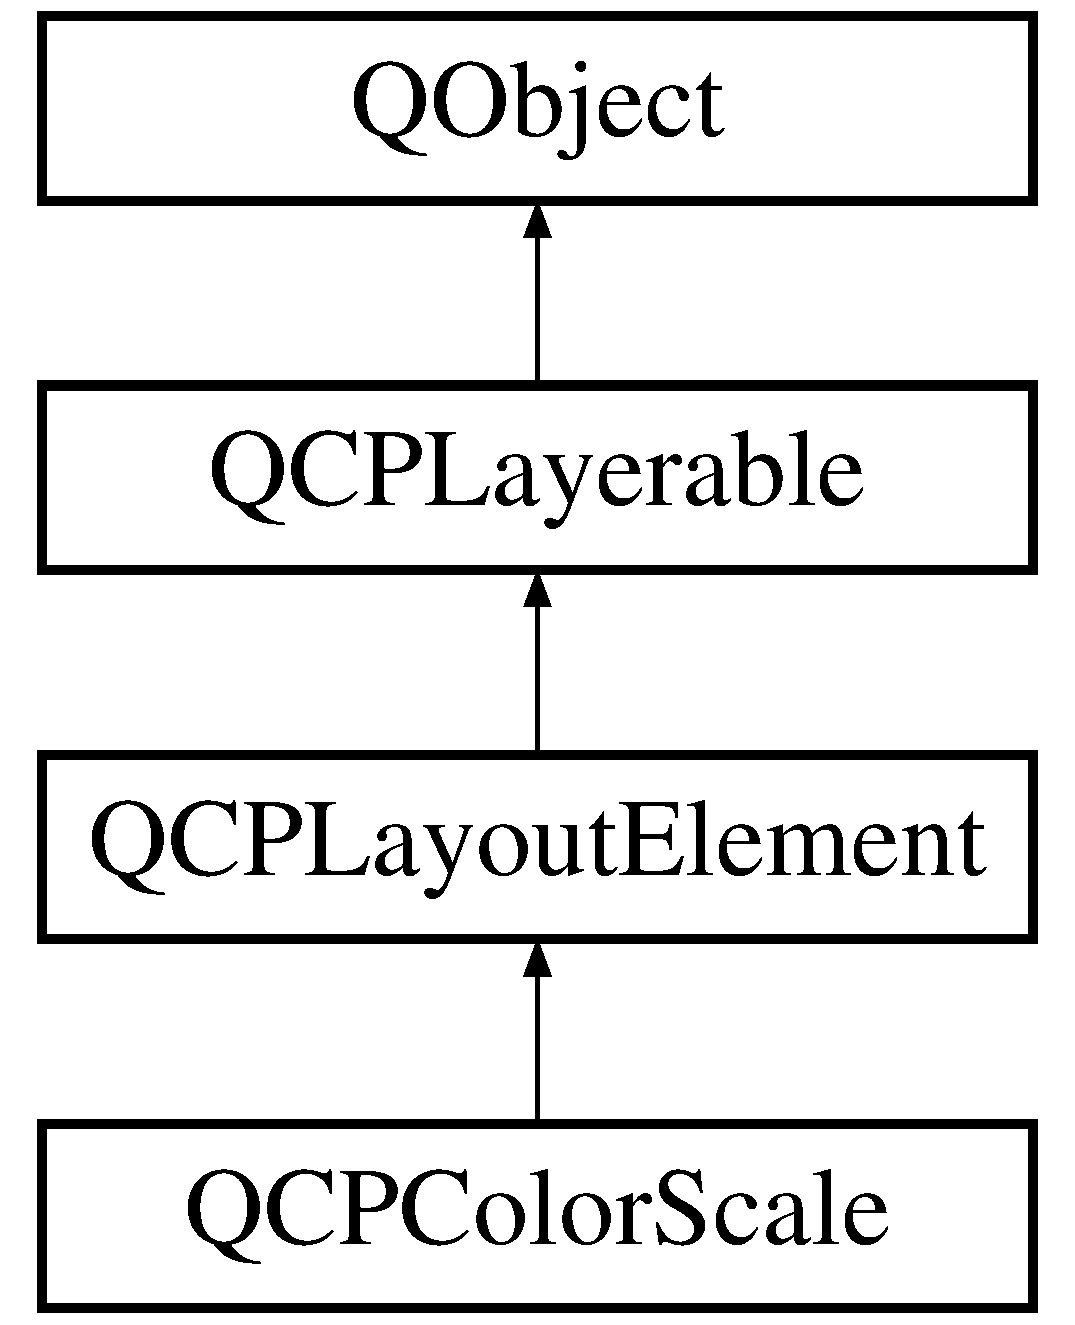
\includegraphics[height=4.000000cm]{class_q_c_p_color_scale}
\end{center}
\end{figure}
\subsection*{Signals}
\begin{DoxyCompactItemize}
\item 
void \hyperlink{class_q_c_p_color_scale_a293176da9447ec6819be1d901966a257}{data\+Range\+Changed} (\hyperlink{class_q_c_p_range}{Q\+C\+P\+Range} new\+Range)
\item 
void \hyperlink{class_q_c_p_color_scale_a61558b962f7791ff2f15a565dcf60181}{data\+Scale\+Type\+Changed} (\hyperlink{class_q_c_p_axis_a36d8e8658dbaa179bf2aeb973db2d6f0}{Q\+C\+P\+Axis\+::\+Scale\+Type} scale\+Type)
\item 
void \hyperlink{class_q_c_p_color_scale_a67a5eb06cf551d322885e8635a46378c}{gradient\+Changed} (\hyperlink{class_q_c_p_color_gradient}{Q\+C\+P\+Color\+Gradient} new\+Gradient)
\end{DoxyCompactItemize}
\subsection*{Public Member Functions}
\begin{DoxyCompactItemize}
\item 
\hyperlink{class_q_c_p_color_scale_aa8debce1be38b54287c04d4f584394b4}{Q\+C\+P\+Color\+Scale} (\hyperlink{class_q_custom_plot}{Q\+Custom\+Plot} $\ast$\hyperlink{class_q_c_p_layerable_ab7e0e94461566093d36ffc0f5312b109}{parent\+Plot})
\item 
virtual \hyperlink{class_q_c_p_color_scale_a49d8d2d155c15fa315fdc0427194c9ea}{$\sim$\+Q\+C\+P\+Color\+Scale} ()
\item 
\hyperlink{class_q_c_p_axis}{Q\+C\+P\+Axis} $\ast$ \hyperlink{class_q_c_p_color_scale_a1205bd67c8a33d5818aac1f6eea016a4}{axis} () const 
\item 
\hyperlink{class_q_c_p_axis_ae2bcc1728b382f10f064612b368bc18a}{Q\+C\+P\+Axis\+::\+Axis\+Type} \hyperlink{class_q_c_p_color_scale_a9a5236328c97fbfde01e3d91c4fcce6a}{type} () const 
\item 
\hyperlink{class_q_c_p_range}{Q\+C\+P\+Range} \hyperlink{class_q_c_p_color_scale_a52134696d5e04074fff4227d92d96f7b}{data\+Range} () const 
\item 
\hyperlink{class_q_c_p_axis_a36d8e8658dbaa179bf2aeb973db2d6f0}{Q\+C\+P\+Axis\+::\+Scale\+Type} \hyperlink{class_q_c_p_color_scale_a9718c004421811be97e683d7f7d7ee61}{data\+Scale\+Type} () const 
\item 
\hyperlink{class_q_c_p_color_gradient}{Q\+C\+P\+Color\+Gradient} \hyperlink{class_q_c_p_color_scale_ac71a6cd853c97a2dbfd32f67afd399df}{gradient} () const 
\item 
Q\+String \hyperlink{class_q_c_p_color_scale_af92a62a6e4401f4c5b5e36cc94351ec9}{label} () const 
\item 
int \hyperlink{class_q_c_p_color_scale_a0de546f12105cf8bcb00ce60366d3a3d}{bar\+Width} () const 
\item 
bool \hyperlink{class_q_c_p_color_scale_a0d45597064cc40bc8a84d11e870c6b05}{range\+Drag} () const 
\item 
bool \hyperlink{class_q_c_p_color_scale_a1123986a10acda3cdc371e4d97b3326c}{range\+Zoom} () const 
\item 
void \hyperlink{class_q_c_p_color_scale_a1bf9bdb291927c422dd66b404b206f1f}{set\+Type} (\hyperlink{class_q_c_p_axis_ae2bcc1728b382f10f064612b368bc18a}{Q\+C\+P\+Axis\+::\+Axis\+Type} \hyperlink{class_q_c_p_color_scale_a9a5236328c97fbfde01e3d91c4fcce6a}{type})
\item 
Q\+\_\+\+S\+L\+O\+T void \hyperlink{class_q_c_p_color_scale_abe88633003a26d1e756aa74984587fef}{set\+Data\+Range} (const \hyperlink{class_q_c_p_range}{Q\+C\+P\+Range} \&\hyperlink{class_q_c_p_color_scale_a52134696d5e04074fff4227d92d96f7b}{data\+Range})
\item 
Q\+\_\+\+S\+L\+O\+T void \hyperlink{class_q_c_p_color_scale_aeb6107d67dd7325145b2498abae67fc3}{set\+Data\+Scale\+Type} (\hyperlink{class_q_c_p_axis_a36d8e8658dbaa179bf2aeb973db2d6f0}{Q\+C\+P\+Axis\+::\+Scale\+Type} scale\+Type)
\item 
Q\+\_\+\+S\+L\+O\+T void \hyperlink{class_q_c_p_color_scale_a1f29583bb6f1e7f473b62fb712be3940}{set\+Gradient} (const \hyperlink{class_q_c_p_color_gradient}{Q\+C\+P\+Color\+Gradient} \&\hyperlink{class_q_c_p_color_scale_ac71a6cd853c97a2dbfd32f67afd399df}{gradient})
\item 
void \hyperlink{class_q_c_p_color_scale_aee124ae8396320cacf8276e9a0fbb8ce}{set\+Label} (const Q\+String \&str)
\item 
void \hyperlink{class_q_c_p_color_scale_ab9dcc0c1cd583477496209b1413bcb99}{set\+Bar\+Width} (int width)
\item 
void \hyperlink{class_q_c_p_color_scale_a21c51a55e4fd581b6feadca9ee5b38d5}{set\+Range\+Drag} (bool enabled)
\item 
void \hyperlink{class_q_c_p_color_scale_a96bd60fb6317ad6821841b539c93eeeb}{set\+Range\+Zoom} (bool enabled)
\item 
Q\+List$<$ \hyperlink{class_q_c_p_color_map}{Q\+C\+P\+Color\+Map} $\ast$ $>$ \hyperlink{class_q_c_p_color_scale_a01bb96981614f2556ef7da04531a7a05}{color\+Maps} () const 
\item 
void \hyperlink{class_q_c_p_color_scale_a425983db4478543924ddbd04ea20a356}{rescale\+Data\+Range} (bool only\+Visible\+Maps)
\item 
virtual void \hyperlink{class_q_c_p_color_scale_ab8f6991ac88243fc582b44b183670334}{update} (\hyperlink{class_q_c_p_layout_element_a0d83360e05735735aaf6d7983c56374d}{Update\+Phase} phase)
\end{DoxyCompactItemize}
\subsection*{Protected Member Functions}
\begin{DoxyCompactItemize}
\item 
virtual void \hyperlink{class_q_c_p_color_scale_a23d530c340c15d2fce6583e7120ee8bd}{apply\+Default\+Antialiasing\+Hint} (\hyperlink{class_q_c_p_painter}{Q\+C\+P\+Painter} $\ast$painter) const 
\item 
virtual void \hyperlink{class_q_c_p_color_scale_a5df6ad81b2ad045878d276c2d5be7120}{mouse\+Press\+Event} (Q\+Mouse\+Event $\ast$event)
\item 
virtual void \hyperlink{class_q_c_p_color_scale_a3aca469d531ce7b5882de73590aa0de6}{mouse\+Move\+Event} (Q\+Mouse\+Event $\ast$event)
\item 
virtual void \hyperlink{class_q_c_p_color_scale_a0916613d20901950fc6d00c6f99fe0a1}{mouse\+Release\+Event} (Q\+Mouse\+Event $\ast$event)
\item 
virtual void \hyperlink{class_q_c_p_color_scale_ab398e14c01240f3dc855884fe9e1ee8c}{wheel\+Event} (Q\+Wheel\+Event $\ast$event)
\end{DoxyCompactItemize}
\subsection*{Protected Attributes}
\begin{DoxyCompactItemize}
\item 
\hyperlink{class_q_c_p_axis_ae2bcc1728b382f10f064612b368bc18a}{Q\+C\+P\+Axis\+::\+Axis\+Type} \hyperlink{class_q_c_p_color_scale_a7d47ed4ab76f38e50164e9d77fe33789}{m\+Type}
\item 
\hyperlink{class_q_c_p_range}{Q\+C\+P\+Range} \hyperlink{class_q_c_p_color_scale_a5d4853feb32cd0077bb2b871687c844b}{m\+Data\+Range}
\item 
\hyperlink{class_q_c_p_axis_a36d8e8658dbaa179bf2aeb973db2d6f0}{Q\+C\+P\+Axis\+::\+Scale\+Type} \hyperlink{class_q_c_p_color_scale_a2754d6a78736f64a241e333fbd955372}{m\+Data\+Scale\+Type}
\item 
\hyperlink{class_q_c_p_color_gradient}{Q\+C\+P\+Color\+Gradient} \hyperlink{class_q_c_p_color_scale_ae195a385032066b5c46cc3301af58922}{m\+Gradient}
\item 
int \hyperlink{class_q_c_p_color_scale_a409d2ab78dff1f92da5e6acfb062e811}{m\+Bar\+Width}
\item 
Q\+Pointer$<$ \hyperlink{class_q_c_p_color_scale_axis_rect_private}{Q\+C\+P\+Color\+Scale\+Axis\+Rect\+Private} $>$ \hyperlink{class_q_c_p_color_scale_a6e37f7d49cd614dc50ef1caae60461b9}{m\+Axis\+Rect}
\item 
Q\+Pointer$<$ \hyperlink{class_q_c_p_axis}{Q\+C\+P\+Axis} $>$ \hyperlink{class_q_c_p_color_scale_a2efbc90fd31898fe05d2b74a8422b1d5}{m\+Color\+Axis}
\end{DoxyCompactItemize}
\subsection*{Friends}
\begin{DoxyCompactItemize}
\item 
class \hyperlink{class_q_c_p_color_scale_a1441d8c09d7227c0c29a8d0a96d55bfe}{Q\+C\+P\+Color\+Scale\+Axis\+Rect\+Private}
\end{DoxyCompactItemize}
\subsection*{Additional Inherited Members}


\subsection{Detailed Description}
A color scale for use with color coding data such as \hyperlink{class_q_c_p_color_map}{Q\+C\+P\+Color\+Map}. 

This layout element can be placed on the plot to correlate a color gradient with data values. It is usually used in combination with one or multiple \hyperlink{class_q_c_p_color_map}{Q\+C\+P\+Color\+Maps}.



The color scale can be either horizontal or vertical, as shown in the image above. The orientation and the side where the numbers appear is controlled with \hyperlink{class_q_c_p_color_scale_a1bf9bdb291927c422dd66b404b206f1f}{set\+Type}.

Use \hyperlink{class_q_c_p_color_map_aa828921db364fe3c6af4619580ab85fd}{Q\+C\+P\+Color\+Map\+::set\+Color\+Scale} to connect a color map with a color scale. Once they are connected, they share their gradient, data range and data scale type (\hyperlink{class_q_c_p_color_scale_a1f29583bb6f1e7f473b62fb712be3940}{set\+Gradient}, \hyperlink{class_q_c_p_color_scale_abe88633003a26d1e756aa74984587fef}{set\+Data\+Range}, \hyperlink{class_q_c_p_color_scale_aeb6107d67dd7325145b2498abae67fc3}{set\+Data\+Scale\+Type}). Multiple color maps may be associated with a single color scale, to make them all synchronize these properties.

To have finer control over the number display and axis behaviour, you can directly access the \hyperlink{class_q_c_p_color_scale_a1205bd67c8a33d5818aac1f6eea016a4}{axis}. See the documentation of \hyperlink{class_q_c_p_axis}{Q\+C\+P\+Axis} for details about configuring axes. For example, if you want to change the number of automatically generated ticks, call 
\begin{DoxyCode}
colorScale->\hyperlink{class_q_c_p_color_scale_a1205bd67c8a33d5818aac1f6eea016a4}{axis}()->\hyperlink{class_q_c_p_axis_a7c7111cbeac9ec5fcb40f93a1ef51a0b}{setAutoTickCount}(3);
\end{DoxyCode}


Placing a color scale next to the main axis rect works like with any other layout element\+: 
\begin{DoxyCode}
\hyperlink{class_q_c_p_color_scale}{QCPColorScale} *colorScale = \textcolor{keyword}{new} \hyperlink{class_q_c_p_color_scale_aa8debce1be38b54287c04d4f584394b4}{QCPColorScale}(customPlot);
customPlot->plotLayout()->addElement(0, 1, colorScale);
colorScale->\hyperlink{class_q_c_p_color_scale_aee124ae8396320cacf8276e9a0fbb8ce}{setLabel}(\textcolor{stringliteral}{"Some Label Text"});
\end{DoxyCode}
 In this case we have placed it to the right of the default axis rect, so it wasn\textquotesingle{}t necessary to call \hyperlink{class_q_c_p_color_scale_a1bf9bdb291927c422dd66b404b206f1f}{set\+Type}, since \hyperlink{class_q_c_p_axis_ae2bcc1728b382f10f064612b368bc18aadf5509f7d29199ef2f263b1dd224b345}{Q\+C\+P\+Axis\+::at\+Right} is already the default. The text next to the color scale can be set with \hyperlink{class_q_c_p_color_scale_aee124ae8396320cacf8276e9a0fbb8ce}{set\+Label}.

For optimum appearance (like in the image above), it may be desirable to line up the axis rect and the borders of the color scale. Use a \hyperlink{class_q_c_p_margin_group}{Q\+C\+P\+Margin\+Group} to achieve this\+: 
\begin{DoxyCode}
\hyperlink{class_q_c_p_margin_group}{QCPMarginGroup} *group = \textcolor{keyword}{new} \hyperlink{class_q_c_p_layout_element_ad077a686e85ab6fa03dcb2fd37fc499a}{QCPMarginGroup}(customPlot);
colorScale->\hyperlink{class_q_c_p_layout_element_a516e56f76b6bc100e8e71d329866847d}{setMarginGroup}(\hyperlink{namespace_q_c_p_a7e487e3e2ccb62ab7771065bab7cae54a5db8fb0d0b0ecf0d611c2602a348e8a0}{QCP::msTop}|\hyperlink{namespace_q_c_p_a7e487e3e2ccb62ab7771065bab7cae54a5241d8eac2bab9524a38889f576179cc}{QCP::msBottom}, group);
customPlot->axisRect()->setMarginGroup(\hyperlink{namespace_q_c_p_a7e487e3e2ccb62ab7771065bab7cae54a5db8fb0d0b0ecf0d611c2602a348e8a0}{QCP::msTop}|\hyperlink{namespace_q_c_p_a7e487e3e2ccb62ab7771065bab7cae54a5241d8eac2bab9524a38889f576179cc}{QCP::msBottom}, group);
\end{DoxyCode}


Color scales are initialized with a non-\/zero minimum top and bottom margin (\hyperlink{class_q_c_p_layout_element_a0a8a17abc16b7923159fcc7608f94673}{set\+Minimum\+Margins}), because vertical color scales are most common and the minimum top/bottom margin makes sure it keeps some distance to the top/bottom widget border. So if you change to a horizontal color scale by setting \hyperlink{class_q_c_p_color_scale_a1bf9bdb291927c422dd66b404b206f1f}{set\+Type} to \hyperlink{class_q_c_p_axis_ae2bcc1728b382f10f064612b368bc18aa220d68888516b6c3b493d144f1ba438f}{Q\+C\+P\+Axis\+::at\+Bottom} or \hyperlink{class_q_c_p_axis_ae2bcc1728b382f10f064612b368bc18aac0ece2b680d3f545e701f75af1655977}{Q\+C\+P\+Axis\+::at\+Top}, you might want to also change the minimum margins accordingly, e.\+g. {\ttfamily set\+Minimum\+Margins(\+Q\+Margins(6, 0, 6, 0))}. 

\subsection{Constructor \& Destructor Documentation}
\hypertarget{class_q_c_p_color_scale_aa8debce1be38b54287c04d4f584394b4}{}\index{Q\+C\+P\+Color\+Scale@{Q\+C\+P\+Color\+Scale}!Q\+C\+P\+Color\+Scale@{Q\+C\+P\+Color\+Scale}}
\index{Q\+C\+P\+Color\+Scale@{Q\+C\+P\+Color\+Scale}!Q\+C\+P\+Color\+Scale@{Q\+C\+P\+Color\+Scale}}
\subsubsection[{Q\+C\+P\+Color\+Scale}]{\setlength{\rightskip}{0pt plus 5cm}Q\+C\+P\+Color\+Scale\+::\+Q\+C\+P\+Color\+Scale (
\begin{DoxyParamCaption}
\item[{{\bf Q\+Custom\+Plot} $\ast$}]{parent\+Plot}
\end{DoxyParamCaption}
)\hspace{0.3cm}{\ttfamily [explicit]}}\label{class_q_c_p_color_scale_aa8debce1be38b54287c04d4f584394b4}
Constructs a new \hyperlink{class_q_c_p_color_scale}{Q\+C\+P\+Color\+Scale}. \hypertarget{class_q_c_p_color_scale_a49d8d2d155c15fa315fdc0427194c9ea}{}\index{Q\+C\+P\+Color\+Scale@{Q\+C\+P\+Color\+Scale}!````~Q\+C\+P\+Color\+Scale@{$\sim$\+Q\+C\+P\+Color\+Scale}}
\index{````~Q\+C\+P\+Color\+Scale@{$\sim$\+Q\+C\+P\+Color\+Scale}!Q\+C\+P\+Color\+Scale@{Q\+C\+P\+Color\+Scale}}
\subsubsection[{$\sim$\+Q\+C\+P\+Color\+Scale}]{\setlength{\rightskip}{0pt plus 5cm}Q\+C\+P\+Color\+Scale\+::$\sim$\+Q\+C\+P\+Color\+Scale (
\begin{DoxyParamCaption}
{}
\end{DoxyParamCaption}
)\hspace{0.3cm}{\ttfamily [virtual]}}\label{class_q_c_p_color_scale_a49d8d2d155c15fa315fdc0427194c9ea}


\subsection{Member Function Documentation}
\hypertarget{class_q_c_p_color_scale_a23d530c340c15d2fce6583e7120ee8bd}{}\index{Q\+C\+P\+Color\+Scale@{Q\+C\+P\+Color\+Scale}!apply\+Default\+Antialiasing\+Hint@{apply\+Default\+Antialiasing\+Hint}}
\index{apply\+Default\+Antialiasing\+Hint@{apply\+Default\+Antialiasing\+Hint}!Q\+C\+P\+Color\+Scale@{Q\+C\+P\+Color\+Scale}}
\subsubsection[{apply\+Default\+Antialiasing\+Hint}]{\setlength{\rightskip}{0pt plus 5cm}void Q\+C\+P\+Color\+Scale\+::apply\+Default\+Antialiasing\+Hint (
\begin{DoxyParamCaption}
\item[{{\bf Q\+C\+P\+Painter} $\ast$}]{painter}
\end{DoxyParamCaption}
) const\hspace{0.3cm}{\ttfamily [protected]}, {\ttfamily [virtual]}}\label{class_q_c_p_color_scale_a23d530c340c15d2fce6583e7120ee8bd}


Reimplemented from \hyperlink{class_q_c_p_layout_element_ad6d2b4bb0291c2441b2e1ca3d5296df5}{Q\+C\+P\+Layout\+Element}.

\hypertarget{class_q_c_p_color_scale_a1205bd67c8a33d5818aac1f6eea016a4}{}\index{Q\+C\+P\+Color\+Scale@{Q\+C\+P\+Color\+Scale}!axis@{axis}}
\index{axis@{axis}!Q\+C\+P\+Color\+Scale@{Q\+C\+P\+Color\+Scale}}
\subsubsection[{axis}]{\setlength{\rightskip}{0pt plus 5cm}{\bf Q\+C\+P\+Axis} $\ast$ Q\+C\+P\+Color\+Scale\+::axis (
\begin{DoxyParamCaption}
{}
\end{DoxyParamCaption}
) const\hspace{0.3cm}{\ttfamily [inline]}}\label{class_q_c_p_color_scale_a1205bd67c8a33d5818aac1f6eea016a4}
Returns the internal \hyperlink{class_q_c_p_axis}{Q\+C\+P\+Axis} instance of this color scale. You can access it to alter the appearance and behaviour of the axis. \hyperlink{class_q_c_p_color_scale}{Q\+C\+P\+Color\+Scale} duplicates some properties in its interface for convenience. Those are \hyperlink{class_q_c_p_color_scale_abe88633003a26d1e756aa74984587fef}{set\+Data\+Range} (\hyperlink{class_q_c_p_axis_aebdfea5d44c3a0ad2b4700cd4d25b641}{Q\+C\+P\+Axis\+::set\+Range}), \hyperlink{class_q_c_p_color_scale_aeb6107d67dd7325145b2498abae67fc3}{set\+Data\+Scale\+Type} (\hyperlink{class_q_c_p_axis_adef29cae617af4f519f6c40d1a866ca6}{Q\+C\+P\+Axis\+::set\+Scale\+Type}), and the method \hyperlink{class_q_c_p_color_scale_aee124ae8396320cacf8276e9a0fbb8ce}{set\+Label} (\hyperlink{class_q_c_p_axis_a33bcc382c111c9f31bb0687352a2dea4}{Q\+C\+P\+Axis\+::set\+Label}). As they each are connected, it does not matter whether you use the method on the \hyperlink{class_q_c_p_color_scale}{Q\+C\+P\+Color\+Scale} or on its \hyperlink{class_q_c_p_axis}{Q\+C\+P\+Axis}.

If the type of the color scale is changed with \hyperlink{class_q_c_p_color_scale_a1bf9bdb291927c422dd66b404b206f1f}{set\+Type}, the axis returned by this method will change, too, to either the left, right, bottom or top axis, depending on which type was set. \hypertarget{class_q_c_p_color_scale_a0de546f12105cf8bcb00ce60366d3a3d}{}\index{Q\+C\+P\+Color\+Scale@{Q\+C\+P\+Color\+Scale}!bar\+Width@{bar\+Width}}
\index{bar\+Width@{bar\+Width}!Q\+C\+P\+Color\+Scale@{Q\+C\+P\+Color\+Scale}}
\subsubsection[{bar\+Width}]{\setlength{\rightskip}{0pt plus 5cm}int Q\+C\+P\+Color\+Scale\+::bar\+Width (
\begin{DoxyParamCaption}
{}
\end{DoxyParamCaption}
) const\hspace{0.3cm}{\ttfamily [inline]}}\label{class_q_c_p_color_scale_a0de546f12105cf8bcb00ce60366d3a3d}
\hypertarget{class_q_c_p_color_scale_a01bb96981614f2556ef7da04531a7a05}{}\index{Q\+C\+P\+Color\+Scale@{Q\+C\+P\+Color\+Scale}!color\+Maps@{color\+Maps}}
\index{color\+Maps@{color\+Maps}!Q\+C\+P\+Color\+Scale@{Q\+C\+P\+Color\+Scale}}
\subsubsection[{color\+Maps}]{\setlength{\rightskip}{0pt plus 5cm}Q\+List$<$ {\bf Q\+C\+P\+Color\+Map} $\ast$ $>$ Q\+C\+P\+Color\+Scale\+::color\+Maps (
\begin{DoxyParamCaption}
{}
\end{DoxyParamCaption}
) const}\label{class_q_c_p_color_scale_a01bb96981614f2556ef7da04531a7a05}
Returns a list of all the color maps associated with this color scale. \hypertarget{class_q_c_p_color_scale_a52134696d5e04074fff4227d92d96f7b}{}\index{Q\+C\+P\+Color\+Scale@{Q\+C\+P\+Color\+Scale}!data\+Range@{data\+Range}}
\index{data\+Range@{data\+Range}!Q\+C\+P\+Color\+Scale@{Q\+C\+P\+Color\+Scale}}
\subsubsection[{data\+Range}]{\setlength{\rightskip}{0pt plus 5cm}{\bf Q\+C\+P\+Range} Q\+C\+P\+Color\+Scale\+::data\+Range (
\begin{DoxyParamCaption}
{}
\end{DoxyParamCaption}
) const\hspace{0.3cm}{\ttfamily [inline]}}\label{class_q_c_p_color_scale_a52134696d5e04074fff4227d92d96f7b}
\hypertarget{class_q_c_p_color_scale_a293176da9447ec6819be1d901966a257}{}\index{Q\+C\+P\+Color\+Scale@{Q\+C\+P\+Color\+Scale}!data\+Range\+Changed@{data\+Range\+Changed}}
\index{data\+Range\+Changed@{data\+Range\+Changed}!Q\+C\+P\+Color\+Scale@{Q\+C\+P\+Color\+Scale}}
\subsubsection[{data\+Range\+Changed}]{\setlength{\rightskip}{0pt plus 5cm}void Q\+C\+P\+Color\+Scale\+::data\+Range\+Changed (
\begin{DoxyParamCaption}
\item[{{\bf Q\+C\+P\+Range}}]{new\+Range}
\end{DoxyParamCaption}
)\hspace{0.3cm}{\ttfamily [signal]}}\label{class_q_c_p_color_scale_a293176da9447ec6819be1d901966a257}
This signal is emitted when the data range changes.

\begin{DoxySeeAlso}{See also}
\hyperlink{class_q_c_p_color_scale_abe88633003a26d1e756aa74984587fef}{set\+Data\+Range} 
\end{DoxySeeAlso}
\hypertarget{class_q_c_p_color_scale_a9718c004421811be97e683d7f7d7ee61}{}\index{Q\+C\+P\+Color\+Scale@{Q\+C\+P\+Color\+Scale}!data\+Scale\+Type@{data\+Scale\+Type}}
\index{data\+Scale\+Type@{data\+Scale\+Type}!Q\+C\+P\+Color\+Scale@{Q\+C\+P\+Color\+Scale}}
\subsubsection[{data\+Scale\+Type}]{\setlength{\rightskip}{0pt plus 5cm}{\bf Q\+C\+P\+Axis\+::\+Scale\+Type} Q\+C\+P\+Color\+Scale\+::data\+Scale\+Type (
\begin{DoxyParamCaption}
{}
\end{DoxyParamCaption}
) const\hspace{0.3cm}{\ttfamily [inline]}}\label{class_q_c_p_color_scale_a9718c004421811be97e683d7f7d7ee61}
\hypertarget{class_q_c_p_color_scale_a61558b962f7791ff2f15a565dcf60181}{}\index{Q\+C\+P\+Color\+Scale@{Q\+C\+P\+Color\+Scale}!data\+Scale\+Type\+Changed@{data\+Scale\+Type\+Changed}}
\index{data\+Scale\+Type\+Changed@{data\+Scale\+Type\+Changed}!Q\+C\+P\+Color\+Scale@{Q\+C\+P\+Color\+Scale}}
\subsubsection[{data\+Scale\+Type\+Changed}]{\setlength{\rightskip}{0pt plus 5cm}void Q\+C\+P\+Color\+Scale\+::data\+Scale\+Type\+Changed (
\begin{DoxyParamCaption}
\item[{{\bf Q\+C\+P\+Axis\+::\+Scale\+Type}}]{scale\+Type}
\end{DoxyParamCaption}
)\hspace{0.3cm}{\ttfamily [signal]}}\label{class_q_c_p_color_scale_a61558b962f7791ff2f15a565dcf60181}
This signal is emitted when the data scale type changes.

\begin{DoxySeeAlso}{See also}
\hyperlink{class_q_c_p_color_scale_aeb6107d67dd7325145b2498abae67fc3}{set\+Data\+Scale\+Type} 
\end{DoxySeeAlso}
\hypertarget{class_q_c_p_color_scale_ac71a6cd853c97a2dbfd32f67afd399df}{}\index{Q\+C\+P\+Color\+Scale@{Q\+C\+P\+Color\+Scale}!gradient@{gradient}}
\index{gradient@{gradient}!Q\+C\+P\+Color\+Scale@{Q\+C\+P\+Color\+Scale}}
\subsubsection[{gradient}]{\setlength{\rightskip}{0pt plus 5cm}{\bf Q\+C\+P\+Color\+Gradient} Q\+C\+P\+Color\+Scale\+::gradient (
\begin{DoxyParamCaption}
{}
\end{DoxyParamCaption}
) const\hspace{0.3cm}{\ttfamily [inline]}}\label{class_q_c_p_color_scale_ac71a6cd853c97a2dbfd32f67afd399df}
\hypertarget{class_q_c_p_color_scale_a67a5eb06cf551d322885e8635a46378c}{}\index{Q\+C\+P\+Color\+Scale@{Q\+C\+P\+Color\+Scale}!gradient\+Changed@{gradient\+Changed}}
\index{gradient\+Changed@{gradient\+Changed}!Q\+C\+P\+Color\+Scale@{Q\+C\+P\+Color\+Scale}}
\subsubsection[{gradient\+Changed}]{\setlength{\rightskip}{0pt plus 5cm}void Q\+C\+P\+Color\+Scale\+::gradient\+Changed (
\begin{DoxyParamCaption}
\item[{{\bf Q\+C\+P\+Color\+Gradient}}]{new\+Gradient}
\end{DoxyParamCaption}
)\hspace{0.3cm}{\ttfamily [signal]}}\label{class_q_c_p_color_scale_a67a5eb06cf551d322885e8635a46378c}
This signal is emitted when the gradient changes.

\begin{DoxySeeAlso}{See also}
\hyperlink{class_q_c_p_color_scale_a1f29583bb6f1e7f473b62fb712be3940}{set\+Gradient} 
\end{DoxySeeAlso}
\hypertarget{class_q_c_p_color_scale_af92a62a6e4401f4c5b5e36cc94351ec9}{}\index{Q\+C\+P\+Color\+Scale@{Q\+C\+P\+Color\+Scale}!label@{label}}
\index{label@{label}!Q\+C\+P\+Color\+Scale@{Q\+C\+P\+Color\+Scale}}
\subsubsection[{label}]{\setlength{\rightskip}{0pt plus 5cm}Q\+String Q\+C\+P\+Color\+Scale\+::label (
\begin{DoxyParamCaption}
{}
\end{DoxyParamCaption}
) const}\label{class_q_c_p_color_scale_af92a62a6e4401f4c5b5e36cc94351ec9}
\hypertarget{class_q_c_p_color_scale_a3aca469d531ce7b5882de73590aa0de6}{}\index{Q\+C\+P\+Color\+Scale@{Q\+C\+P\+Color\+Scale}!mouse\+Move\+Event@{mouse\+Move\+Event}}
\index{mouse\+Move\+Event@{mouse\+Move\+Event}!Q\+C\+P\+Color\+Scale@{Q\+C\+P\+Color\+Scale}}
\subsubsection[{mouse\+Move\+Event}]{\setlength{\rightskip}{0pt plus 5cm}void Q\+C\+P\+Color\+Scale\+::mouse\+Move\+Event (
\begin{DoxyParamCaption}
\item[{Q\+Mouse\+Event $\ast$}]{event}
\end{DoxyParamCaption}
)\hspace{0.3cm}{\ttfamily [protected]}, {\ttfamily [virtual]}}\label{class_q_c_p_color_scale_a3aca469d531ce7b5882de73590aa0de6}
This event is called, if the mouse is moved inside the outer rect of this layout element. 

Reimplemented from \hyperlink{class_q_c_p_layout_element_a14f4acf58cdb8dd2c6c571479c4c4a40}{Q\+C\+P\+Layout\+Element}.

\hypertarget{class_q_c_p_color_scale_a5df6ad81b2ad045878d276c2d5be7120}{}\index{Q\+C\+P\+Color\+Scale@{Q\+C\+P\+Color\+Scale}!mouse\+Press\+Event@{mouse\+Press\+Event}}
\index{mouse\+Press\+Event@{mouse\+Press\+Event}!Q\+C\+P\+Color\+Scale@{Q\+C\+P\+Color\+Scale}}
\subsubsection[{mouse\+Press\+Event}]{\setlength{\rightskip}{0pt plus 5cm}void Q\+C\+P\+Color\+Scale\+::mouse\+Press\+Event (
\begin{DoxyParamCaption}
\item[{Q\+Mouse\+Event $\ast$}]{event}
\end{DoxyParamCaption}
)\hspace{0.3cm}{\ttfamily [protected]}, {\ttfamily [virtual]}}\label{class_q_c_p_color_scale_a5df6ad81b2ad045878d276c2d5be7120}
This event is called, if the mouse was pressed while being inside the outer rect of this layout element. 

Reimplemented from \hyperlink{class_q_c_p_layout_element_a2d82ea21fe0ee628f177bd824bc51a71}{Q\+C\+P\+Layout\+Element}.

\hypertarget{class_q_c_p_color_scale_a0916613d20901950fc6d00c6f99fe0a1}{}\index{Q\+C\+P\+Color\+Scale@{Q\+C\+P\+Color\+Scale}!mouse\+Release\+Event@{mouse\+Release\+Event}}
\index{mouse\+Release\+Event@{mouse\+Release\+Event}!Q\+C\+P\+Color\+Scale@{Q\+C\+P\+Color\+Scale}}
\subsubsection[{mouse\+Release\+Event}]{\setlength{\rightskip}{0pt plus 5cm}void Q\+C\+P\+Color\+Scale\+::mouse\+Release\+Event (
\begin{DoxyParamCaption}
\item[{Q\+Mouse\+Event $\ast$}]{event}
\end{DoxyParamCaption}
)\hspace{0.3cm}{\ttfamily [protected]}, {\ttfamily [virtual]}}\label{class_q_c_p_color_scale_a0916613d20901950fc6d00c6f99fe0a1}
This event is called, if the mouse was previously pressed inside the outer rect of this layout element and is now released. 

Reimplemented from \hyperlink{class_q_c_p_layout_element_ae526ac828cce1e5bb94eaa85776d7404}{Q\+C\+P\+Layout\+Element}.

\hypertarget{class_q_c_p_color_scale_a0d45597064cc40bc8a84d11e870c6b05}{}\index{Q\+C\+P\+Color\+Scale@{Q\+C\+P\+Color\+Scale}!range\+Drag@{range\+Drag}}
\index{range\+Drag@{range\+Drag}!Q\+C\+P\+Color\+Scale@{Q\+C\+P\+Color\+Scale}}
\subsubsection[{range\+Drag}]{\setlength{\rightskip}{0pt plus 5cm}bool Q\+C\+P\+Color\+Scale\+::range\+Drag (
\begin{DoxyParamCaption}
{}
\end{DoxyParamCaption}
) const}\label{class_q_c_p_color_scale_a0d45597064cc40bc8a84d11e870c6b05}
\hypertarget{class_q_c_p_color_scale_a1123986a10acda3cdc371e4d97b3326c}{}\index{Q\+C\+P\+Color\+Scale@{Q\+C\+P\+Color\+Scale}!range\+Zoom@{range\+Zoom}}
\index{range\+Zoom@{range\+Zoom}!Q\+C\+P\+Color\+Scale@{Q\+C\+P\+Color\+Scale}}
\subsubsection[{range\+Zoom}]{\setlength{\rightskip}{0pt plus 5cm}bool Q\+C\+P\+Color\+Scale\+::range\+Zoom (
\begin{DoxyParamCaption}
{}
\end{DoxyParamCaption}
) const}\label{class_q_c_p_color_scale_a1123986a10acda3cdc371e4d97b3326c}
\hypertarget{class_q_c_p_color_scale_a425983db4478543924ddbd04ea20a356}{}\index{Q\+C\+P\+Color\+Scale@{Q\+C\+P\+Color\+Scale}!rescale\+Data\+Range@{rescale\+Data\+Range}}
\index{rescale\+Data\+Range@{rescale\+Data\+Range}!Q\+C\+P\+Color\+Scale@{Q\+C\+P\+Color\+Scale}}
\subsubsection[{rescale\+Data\+Range}]{\setlength{\rightskip}{0pt plus 5cm}void Q\+C\+P\+Color\+Scale\+::rescale\+Data\+Range (
\begin{DoxyParamCaption}
\item[{bool}]{only\+Visible\+Maps}
\end{DoxyParamCaption}
)}\label{class_q_c_p_color_scale_a425983db4478543924ddbd04ea20a356}
Changes the data range such that all color maps associated with this color scale are fully mapped to the gradient in the data dimension.

\begin{DoxySeeAlso}{See also}
\hyperlink{class_q_c_p_color_scale_abe88633003a26d1e756aa74984587fef}{set\+Data\+Range} 
\end{DoxySeeAlso}
\hypertarget{class_q_c_p_color_scale_ab9dcc0c1cd583477496209b1413bcb99}{}\index{Q\+C\+P\+Color\+Scale@{Q\+C\+P\+Color\+Scale}!set\+Bar\+Width@{set\+Bar\+Width}}
\index{set\+Bar\+Width@{set\+Bar\+Width}!Q\+C\+P\+Color\+Scale@{Q\+C\+P\+Color\+Scale}}
\subsubsection[{set\+Bar\+Width}]{\setlength{\rightskip}{0pt plus 5cm}void Q\+C\+P\+Color\+Scale\+::set\+Bar\+Width (
\begin{DoxyParamCaption}
\item[{int}]{width}
\end{DoxyParamCaption}
)}\label{class_q_c_p_color_scale_ab9dcc0c1cd583477496209b1413bcb99}
Sets the width (or height, for horizontal color scales) the bar where the gradient is displayed will have. \hypertarget{class_q_c_p_color_scale_abe88633003a26d1e756aa74984587fef}{}\index{Q\+C\+P\+Color\+Scale@{Q\+C\+P\+Color\+Scale}!set\+Data\+Range@{set\+Data\+Range}}
\index{set\+Data\+Range@{set\+Data\+Range}!Q\+C\+P\+Color\+Scale@{Q\+C\+P\+Color\+Scale}}
\subsubsection[{set\+Data\+Range}]{\setlength{\rightskip}{0pt plus 5cm}void Q\+C\+P\+Color\+Scale\+::set\+Data\+Range (
\begin{DoxyParamCaption}
\item[{const {\bf Q\+C\+P\+Range} \&}]{data\+Range}
\end{DoxyParamCaption}
)}\label{class_q_c_p_color_scale_abe88633003a26d1e756aa74984587fef}
Sets the range spanned by the color gradient and that is shown by the axis in the color scale.

It is equivalent to calling \hyperlink{class_q_c_p_color_map_a980b42837821159786a85b4b7dcb8774}{Q\+C\+P\+Color\+Map\+::set\+Data\+Range} on any of the connected color maps. It is also equivalent to directly accessing the \hyperlink{class_q_c_p_color_scale_a1205bd67c8a33d5818aac1f6eea016a4}{axis} and setting its range with \hyperlink{class_q_c_p_axis_aebdfea5d44c3a0ad2b4700cd4d25b641}{Q\+C\+P\+Axis\+::set\+Range}.

\begin{DoxySeeAlso}{See also}
\hyperlink{class_q_c_p_color_scale_aeb6107d67dd7325145b2498abae67fc3}{set\+Data\+Scale\+Type}, \hyperlink{class_q_c_p_color_scale_a1f29583bb6f1e7f473b62fb712be3940}{set\+Gradient}, \hyperlink{class_q_c_p_color_scale_a425983db4478543924ddbd04ea20a356}{rescale\+Data\+Range} 
\end{DoxySeeAlso}
\hypertarget{class_q_c_p_color_scale_aeb6107d67dd7325145b2498abae67fc3}{}\index{Q\+C\+P\+Color\+Scale@{Q\+C\+P\+Color\+Scale}!set\+Data\+Scale\+Type@{set\+Data\+Scale\+Type}}
\index{set\+Data\+Scale\+Type@{set\+Data\+Scale\+Type}!Q\+C\+P\+Color\+Scale@{Q\+C\+P\+Color\+Scale}}
\subsubsection[{set\+Data\+Scale\+Type}]{\setlength{\rightskip}{0pt plus 5cm}void Q\+C\+P\+Color\+Scale\+::set\+Data\+Scale\+Type (
\begin{DoxyParamCaption}
\item[{{\bf Q\+C\+P\+Axis\+::\+Scale\+Type}}]{scale\+Type}
\end{DoxyParamCaption}
)}\label{class_q_c_p_color_scale_aeb6107d67dd7325145b2498abae67fc3}
Sets the scale type of the color scale, i.\+e. whether values are linearly associated with colors or logarithmically.

It is equivalent to calling \hyperlink{class_q_c_p_color_map_a9d20aa08e3c1f20f22908c45b9c06511}{Q\+C\+P\+Color\+Map\+::set\+Data\+Scale\+Type} on any of the connected color maps. It is also equivalent to directly accessing the \hyperlink{class_q_c_p_color_scale_a1205bd67c8a33d5818aac1f6eea016a4}{axis} and setting its scale type with \hyperlink{class_q_c_p_axis_adef29cae617af4f519f6c40d1a866ca6}{Q\+C\+P\+Axis\+::set\+Scale\+Type}.

\begin{DoxySeeAlso}{See also}
\hyperlink{class_q_c_p_color_scale_abe88633003a26d1e756aa74984587fef}{set\+Data\+Range}, \hyperlink{class_q_c_p_color_scale_a1f29583bb6f1e7f473b62fb712be3940}{set\+Gradient} 
\end{DoxySeeAlso}
\hypertarget{class_q_c_p_color_scale_a1f29583bb6f1e7f473b62fb712be3940}{}\index{Q\+C\+P\+Color\+Scale@{Q\+C\+P\+Color\+Scale}!set\+Gradient@{set\+Gradient}}
\index{set\+Gradient@{set\+Gradient}!Q\+C\+P\+Color\+Scale@{Q\+C\+P\+Color\+Scale}}
\subsubsection[{set\+Gradient}]{\setlength{\rightskip}{0pt plus 5cm}void Q\+C\+P\+Color\+Scale\+::set\+Gradient (
\begin{DoxyParamCaption}
\item[{const {\bf Q\+C\+P\+Color\+Gradient} \&}]{gradient}
\end{DoxyParamCaption}
)}\label{class_q_c_p_color_scale_a1f29583bb6f1e7f473b62fb712be3940}
Sets the color gradient that will be used to represent data values.

It is equivalent to calling \hyperlink{class_q_c_p_color_map_a7313c78360471cead3576341a2c50377}{Q\+C\+P\+Color\+Map\+::set\+Gradient} on any of the connected color maps.

\begin{DoxySeeAlso}{See also}
\hyperlink{class_q_c_p_color_scale_abe88633003a26d1e756aa74984587fef}{set\+Data\+Range}, \hyperlink{class_q_c_p_color_scale_aeb6107d67dd7325145b2498abae67fc3}{set\+Data\+Scale\+Type} 
\end{DoxySeeAlso}
\hypertarget{class_q_c_p_color_scale_aee124ae8396320cacf8276e9a0fbb8ce}{}\index{Q\+C\+P\+Color\+Scale@{Q\+C\+P\+Color\+Scale}!set\+Label@{set\+Label}}
\index{set\+Label@{set\+Label}!Q\+C\+P\+Color\+Scale@{Q\+C\+P\+Color\+Scale}}
\subsubsection[{set\+Label}]{\setlength{\rightskip}{0pt plus 5cm}void Q\+C\+P\+Color\+Scale\+::set\+Label (
\begin{DoxyParamCaption}
\item[{const Q\+String \&}]{str}
\end{DoxyParamCaption}
)}\label{class_q_c_p_color_scale_aee124ae8396320cacf8276e9a0fbb8ce}
Sets the axis label of the color scale. This is equivalent to calling \hyperlink{class_q_c_p_axis_a33bcc382c111c9f31bb0687352a2dea4}{Q\+C\+P\+Axis\+::set\+Label} on the internal \hyperlink{class_q_c_p_color_scale_a1205bd67c8a33d5818aac1f6eea016a4}{axis}. \hypertarget{class_q_c_p_color_scale_a21c51a55e4fd581b6feadca9ee5b38d5}{}\index{Q\+C\+P\+Color\+Scale@{Q\+C\+P\+Color\+Scale}!set\+Range\+Drag@{set\+Range\+Drag}}
\index{set\+Range\+Drag@{set\+Range\+Drag}!Q\+C\+P\+Color\+Scale@{Q\+C\+P\+Color\+Scale}}
\subsubsection[{set\+Range\+Drag}]{\setlength{\rightskip}{0pt plus 5cm}void Q\+C\+P\+Color\+Scale\+::set\+Range\+Drag (
\begin{DoxyParamCaption}
\item[{bool}]{enabled}
\end{DoxyParamCaption}
)}\label{class_q_c_p_color_scale_a21c51a55e4fd581b6feadca9ee5b38d5}
Sets whether the user can drag the data range (\hyperlink{class_q_c_p_color_scale_abe88633003a26d1e756aa74984587fef}{set\+Data\+Range}).

Note that \hyperlink{namespace_q_c_p_a2ad6bb6281c7c2d593d4277b44c2b037a2c4432b9aceafb94000be8d1b589ef18}{Q\+C\+P\+::i\+Range\+Drag} must be in the \hyperlink{class_q_custom_plot}{Q\+Custom\+Plot}\textquotesingle{}s interactions (\hyperlink{class_q_custom_plot_a5ee1e2f6ae27419deca53e75907c27e5}{Q\+Custom\+Plot\+::set\+Interactions}) to allow range dragging. \hypertarget{class_q_c_p_color_scale_a96bd60fb6317ad6821841b539c93eeeb}{}\index{Q\+C\+P\+Color\+Scale@{Q\+C\+P\+Color\+Scale}!set\+Range\+Zoom@{set\+Range\+Zoom}}
\index{set\+Range\+Zoom@{set\+Range\+Zoom}!Q\+C\+P\+Color\+Scale@{Q\+C\+P\+Color\+Scale}}
\subsubsection[{set\+Range\+Zoom}]{\setlength{\rightskip}{0pt plus 5cm}void Q\+C\+P\+Color\+Scale\+::set\+Range\+Zoom (
\begin{DoxyParamCaption}
\item[{bool}]{enabled}
\end{DoxyParamCaption}
)}\label{class_q_c_p_color_scale_a96bd60fb6317ad6821841b539c93eeeb}
Sets whether the user can zoom the data range (\hyperlink{class_q_c_p_color_scale_abe88633003a26d1e756aa74984587fef}{set\+Data\+Range}) by scrolling the mouse wheel.

Note that \hyperlink{namespace_q_c_p_a2ad6bb6281c7c2d593d4277b44c2b037abee1e94353525a636aeaf0ba32b72e14}{Q\+C\+P\+::i\+Range\+Zoom} must be in the \hyperlink{class_q_custom_plot}{Q\+Custom\+Plot}\textquotesingle{}s interactions (\hyperlink{class_q_custom_plot_a5ee1e2f6ae27419deca53e75907c27e5}{Q\+Custom\+Plot\+::set\+Interactions}) to allow range dragging. \hypertarget{class_q_c_p_color_scale_a1bf9bdb291927c422dd66b404b206f1f}{}\index{Q\+C\+P\+Color\+Scale@{Q\+C\+P\+Color\+Scale}!set\+Type@{set\+Type}}
\index{set\+Type@{set\+Type}!Q\+C\+P\+Color\+Scale@{Q\+C\+P\+Color\+Scale}}
\subsubsection[{set\+Type}]{\setlength{\rightskip}{0pt plus 5cm}void Q\+C\+P\+Color\+Scale\+::set\+Type (
\begin{DoxyParamCaption}
\item[{{\bf Q\+C\+P\+Axis\+::\+Axis\+Type}}]{type}
\end{DoxyParamCaption}
)}\label{class_q_c_p_color_scale_a1bf9bdb291927c422dd66b404b206f1f}
Sets at which side of the color scale the axis is placed, and thus also its orientation.

Note that after setting {\itshape type} to a different value, the axis returned by \hyperlink{class_q_c_p_color_scale_a1205bd67c8a33d5818aac1f6eea016a4}{axis()} will be a different one. The new axis will adopt the following properties from the previous axis\+: The range, scale type, log base and label. \hypertarget{class_q_c_p_color_scale_a9a5236328c97fbfde01e3d91c4fcce6a}{}\index{Q\+C\+P\+Color\+Scale@{Q\+C\+P\+Color\+Scale}!type@{type}}
\index{type@{type}!Q\+C\+P\+Color\+Scale@{Q\+C\+P\+Color\+Scale}}
\subsubsection[{type}]{\setlength{\rightskip}{0pt plus 5cm}{\bf Q\+C\+P\+Axis\+::\+Axis\+Type} Q\+C\+P\+Color\+Scale\+::type (
\begin{DoxyParamCaption}
{}
\end{DoxyParamCaption}
) const\hspace{0.3cm}{\ttfamily [inline]}}\label{class_q_c_p_color_scale_a9a5236328c97fbfde01e3d91c4fcce6a}
\hypertarget{class_q_c_p_color_scale_ab8f6991ac88243fc582b44b183670334}{}\index{Q\+C\+P\+Color\+Scale@{Q\+C\+P\+Color\+Scale}!update@{update}}
\index{update@{update}!Q\+C\+P\+Color\+Scale@{Q\+C\+P\+Color\+Scale}}
\subsubsection[{update}]{\setlength{\rightskip}{0pt plus 5cm}void Q\+C\+P\+Color\+Scale\+::update (
\begin{DoxyParamCaption}
\item[{{\bf Update\+Phase}}]{phase}
\end{DoxyParamCaption}
)\hspace{0.3cm}{\ttfamily [virtual]}}\label{class_q_c_p_color_scale_ab8f6991ac88243fc582b44b183670334}
Updates the layout element and sub-\/elements. This function is automatically called before every replot by the parent layout element. It is called multiple times, once for every \hyperlink{class_q_c_p_layout_element_a0d83360e05735735aaf6d7983c56374d}{Update\+Phase}. The phases are run through in the order of the enum values. For details about what happens at the different phases, see the documentation of \hyperlink{class_q_c_p_layout_element_a0d83360e05735735aaf6d7983c56374d}{Update\+Phase}.

Layout elements that have child elements should call the \hyperlink{class_q_c_p_color_scale_ab8f6991ac88243fc582b44b183670334}{update} method of their child elements, and pass the current {\itshape phase} unchanged.

The default implementation executes the automatic margin mechanism in the \hyperlink{class_q_c_p_layout_element_a0d83360e05735735aaf6d7983c56374da288cb59a92280e47261a341f2813e676}{up\+Margins} phase. Subclasses should make sure to call the base class implementation. 

Reimplemented from \hyperlink{class_q_c_p_layout_element_a929c2ec62e0e0e1d8418eaa802e2af9b}{Q\+C\+P\+Layout\+Element}.

\hypertarget{class_q_c_p_color_scale_ab398e14c01240f3dc855884fe9e1ee8c}{}\index{Q\+C\+P\+Color\+Scale@{Q\+C\+P\+Color\+Scale}!wheel\+Event@{wheel\+Event}}
\index{wheel\+Event@{wheel\+Event}!Q\+C\+P\+Color\+Scale@{Q\+C\+P\+Color\+Scale}}
\subsubsection[{wheel\+Event}]{\setlength{\rightskip}{0pt plus 5cm}void Q\+C\+P\+Color\+Scale\+::wheel\+Event (
\begin{DoxyParamCaption}
\item[{Q\+Wheel\+Event $\ast$}]{event}
\end{DoxyParamCaption}
)\hspace{0.3cm}{\ttfamily [protected]}, {\ttfamily [virtual]}}\label{class_q_c_p_color_scale_ab398e14c01240f3dc855884fe9e1ee8c}
This event is called, if the mouse wheel is scrolled while the cursor is inside the rect of this layout element. 

Reimplemented from \hyperlink{class_q_c_p_layout_element_a300521d2fd18a893c1b85f6be11ce2bf}{Q\+C\+P\+Layout\+Element}.



\subsection{Friends And Related Function Documentation}
\hypertarget{class_q_c_p_color_scale_a1441d8c09d7227c0c29a8d0a96d55bfe}{}\index{Q\+C\+P\+Color\+Scale@{Q\+C\+P\+Color\+Scale}!Q\+C\+P\+Color\+Scale\+Axis\+Rect\+Private@{Q\+C\+P\+Color\+Scale\+Axis\+Rect\+Private}}
\index{Q\+C\+P\+Color\+Scale\+Axis\+Rect\+Private@{Q\+C\+P\+Color\+Scale\+Axis\+Rect\+Private}!Q\+C\+P\+Color\+Scale@{Q\+C\+P\+Color\+Scale}}
\subsubsection[{Q\+C\+P\+Color\+Scale\+Axis\+Rect\+Private}]{\setlength{\rightskip}{0pt plus 5cm}friend class {\bf Q\+C\+P\+Color\+Scale\+Axis\+Rect\+Private}\hspace{0.3cm}{\ttfamily [friend]}}\label{class_q_c_p_color_scale_a1441d8c09d7227c0c29a8d0a96d55bfe}


\subsection{Member Data Documentation}
\hypertarget{class_q_c_p_color_scale_a6e37f7d49cd614dc50ef1caae60461b9}{}\index{Q\+C\+P\+Color\+Scale@{Q\+C\+P\+Color\+Scale}!m\+Axis\+Rect@{m\+Axis\+Rect}}
\index{m\+Axis\+Rect@{m\+Axis\+Rect}!Q\+C\+P\+Color\+Scale@{Q\+C\+P\+Color\+Scale}}
\subsubsection[{m\+Axis\+Rect}]{\setlength{\rightskip}{0pt plus 5cm}Q\+Pointer$<${\bf Q\+C\+P\+Color\+Scale\+Axis\+Rect\+Private}$>$ Q\+C\+P\+Color\+Scale\+::m\+Axis\+Rect\hspace{0.3cm}{\ttfamily [protected]}}\label{class_q_c_p_color_scale_a6e37f7d49cd614dc50ef1caae60461b9}
\hypertarget{class_q_c_p_color_scale_a409d2ab78dff1f92da5e6acfb062e811}{}\index{Q\+C\+P\+Color\+Scale@{Q\+C\+P\+Color\+Scale}!m\+Bar\+Width@{m\+Bar\+Width}}
\index{m\+Bar\+Width@{m\+Bar\+Width}!Q\+C\+P\+Color\+Scale@{Q\+C\+P\+Color\+Scale}}
\subsubsection[{m\+Bar\+Width}]{\setlength{\rightskip}{0pt plus 5cm}int Q\+C\+P\+Color\+Scale\+::m\+Bar\+Width\hspace{0.3cm}{\ttfamily [protected]}}\label{class_q_c_p_color_scale_a409d2ab78dff1f92da5e6acfb062e811}
\hypertarget{class_q_c_p_color_scale_a2efbc90fd31898fe05d2b74a8422b1d5}{}\index{Q\+C\+P\+Color\+Scale@{Q\+C\+P\+Color\+Scale}!m\+Color\+Axis@{m\+Color\+Axis}}
\index{m\+Color\+Axis@{m\+Color\+Axis}!Q\+C\+P\+Color\+Scale@{Q\+C\+P\+Color\+Scale}}
\subsubsection[{m\+Color\+Axis}]{\setlength{\rightskip}{0pt plus 5cm}Q\+Pointer$<${\bf Q\+C\+P\+Axis}$>$ Q\+C\+P\+Color\+Scale\+::m\+Color\+Axis\hspace{0.3cm}{\ttfamily [protected]}}\label{class_q_c_p_color_scale_a2efbc90fd31898fe05d2b74a8422b1d5}
\hypertarget{class_q_c_p_color_scale_a5d4853feb32cd0077bb2b871687c844b}{}\index{Q\+C\+P\+Color\+Scale@{Q\+C\+P\+Color\+Scale}!m\+Data\+Range@{m\+Data\+Range}}
\index{m\+Data\+Range@{m\+Data\+Range}!Q\+C\+P\+Color\+Scale@{Q\+C\+P\+Color\+Scale}}
\subsubsection[{m\+Data\+Range}]{\setlength{\rightskip}{0pt plus 5cm}{\bf Q\+C\+P\+Range} Q\+C\+P\+Color\+Scale\+::m\+Data\+Range\hspace{0.3cm}{\ttfamily [protected]}}\label{class_q_c_p_color_scale_a5d4853feb32cd0077bb2b871687c844b}
\hypertarget{class_q_c_p_color_scale_a2754d6a78736f64a241e333fbd955372}{}\index{Q\+C\+P\+Color\+Scale@{Q\+C\+P\+Color\+Scale}!m\+Data\+Scale\+Type@{m\+Data\+Scale\+Type}}
\index{m\+Data\+Scale\+Type@{m\+Data\+Scale\+Type}!Q\+C\+P\+Color\+Scale@{Q\+C\+P\+Color\+Scale}}
\subsubsection[{m\+Data\+Scale\+Type}]{\setlength{\rightskip}{0pt plus 5cm}{\bf Q\+C\+P\+Axis\+::\+Scale\+Type} Q\+C\+P\+Color\+Scale\+::m\+Data\+Scale\+Type\hspace{0.3cm}{\ttfamily [protected]}}\label{class_q_c_p_color_scale_a2754d6a78736f64a241e333fbd955372}
\hypertarget{class_q_c_p_color_scale_ae195a385032066b5c46cc3301af58922}{}\index{Q\+C\+P\+Color\+Scale@{Q\+C\+P\+Color\+Scale}!m\+Gradient@{m\+Gradient}}
\index{m\+Gradient@{m\+Gradient}!Q\+C\+P\+Color\+Scale@{Q\+C\+P\+Color\+Scale}}
\subsubsection[{m\+Gradient}]{\setlength{\rightskip}{0pt plus 5cm}{\bf Q\+C\+P\+Color\+Gradient} Q\+C\+P\+Color\+Scale\+::m\+Gradient\hspace{0.3cm}{\ttfamily [protected]}}\label{class_q_c_p_color_scale_ae195a385032066b5c46cc3301af58922}
\hypertarget{class_q_c_p_color_scale_a7d47ed4ab76f38e50164e9d77fe33789}{}\index{Q\+C\+P\+Color\+Scale@{Q\+C\+P\+Color\+Scale}!m\+Type@{m\+Type}}
\index{m\+Type@{m\+Type}!Q\+C\+P\+Color\+Scale@{Q\+C\+P\+Color\+Scale}}
\subsubsection[{m\+Type}]{\setlength{\rightskip}{0pt plus 5cm}{\bf Q\+C\+P\+Axis\+::\+Axis\+Type} Q\+C\+P\+Color\+Scale\+::m\+Type\hspace{0.3cm}{\ttfamily [protected]}}\label{class_q_c_p_color_scale_a7d47ed4ab76f38e50164e9d77fe33789}


The documentation for this class was generated from the following files\+:\begin{DoxyCompactItemize}
\item 
C\+:/\+Users/\+Roman/\+Documents/\+Mygs/\+Ground\+Station/\+G\+S/\hyperlink{qcustomplot_8h}{qcustomplot.\+h}\item 
C\+:/\+Users/\+Roman/\+Documents/\+Mygs/\+Ground\+Station/\+G\+S/\hyperlink{qcustomplot_8cpp}{qcustomplot.\+cpp}\end{DoxyCompactItemize}

\hypertarget{class_q_c_p_color_scale_axis_rect_private}{}\section{Q\+C\+P\+Color\+Scale\+Axis\+Rect\+Private Class Reference}
\label{class_q_c_p_color_scale_axis_rect_private}\index{Q\+C\+P\+Color\+Scale\+Axis\+Rect\+Private@{Q\+C\+P\+Color\+Scale\+Axis\+Rect\+Private}}


{\ttfamily \#include $<$qcustomplot.\+h$>$}

Inheritance diagram for Q\+C\+P\+Color\+Scale\+Axis\+Rect\+Private\+:\begin{figure}[H]
\begin{center}
\leavevmode
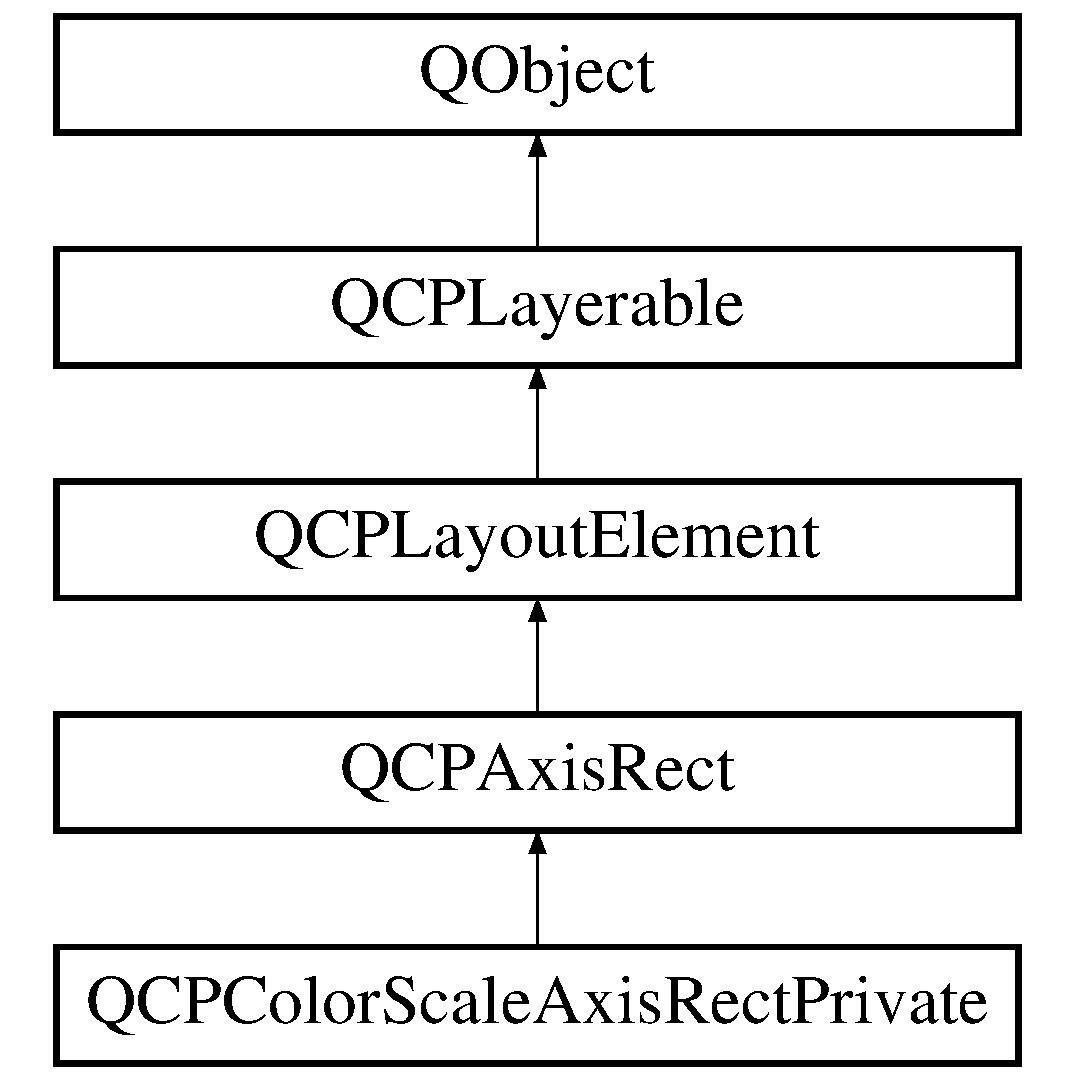
\includegraphics[height=5.000000cm]{class_q_c_p_color_scale_axis_rect_private}
\end{center}
\end{figure}
\subsection*{Public Member Functions}
\begin{DoxyCompactItemize}
\item 
\hyperlink{class_q_c_p_color_scale_axis_rect_private_ad3b242f75dd2b33581364a4e668a80db}{Q\+C\+P\+Color\+Scale\+Axis\+Rect\+Private} (\hyperlink{class_q_c_p_color_scale}{Q\+C\+P\+Color\+Scale} $\ast$parent\+Color\+Scale)
\end{DoxyCompactItemize}
\subsection*{Protected Member Functions}
\begin{DoxyCompactItemize}
\item 
virtual void \hyperlink{class_q_c_p_color_scale_axis_rect_private_adb67bfe9057a9dd9a85f548c274e6d98}{draw} (\hyperlink{class_q_c_p_painter}{Q\+C\+P\+Painter} $\ast$painter)
\item 
void \hyperlink{class_q_c_p_color_scale_axis_rect_private_a73754cab312aeaddea1bfcc67cc079ac}{update\+Gradient\+Image} ()
\item 
Q\+\_\+\+S\+L\+O\+T void \hyperlink{class_q_c_p_color_scale_axis_rect_private_a6112ad4291ac1695d37659cb049d598d}{axis\+Selection\+Changed} (Q\+C\+P\+Axis\+::\+Selectable\+Parts selected\+Parts)
\item 
Q\+\_\+\+S\+L\+O\+T void \hyperlink{class_q_c_p_color_scale_axis_rect_private_a66d2baed86966bb03a6d7c32dc7d59f7}{axis\+Selectable\+Changed} (Q\+C\+P\+Axis\+::\+Selectable\+Parts selectable\+Parts)
\end{DoxyCompactItemize}
\subsection*{Protected Attributes}
\begin{DoxyCompactItemize}
\item 
\hyperlink{class_q_c_p_color_scale}{Q\+C\+P\+Color\+Scale} $\ast$ \hyperlink{class_q_c_p_color_scale_axis_rect_private_a311c73f51a4cb0b556388197833cf099}{m\+Parent\+Color\+Scale}
\item 
Q\+Image \hyperlink{class_q_c_p_color_scale_axis_rect_private_ad4f7c8ee1c6012d9950870811773119c}{m\+Gradient\+Image}
\item 
bool \hyperlink{class_q_c_p_color_scale_axis_rect_private_a2c0b15b071e1f93006b48b5be022a631}{m\+Gradient\+Image\+Invalidated}
\end{DoxyCompactItemize}
\subsection*{Friends}
\begin{DoxyCompactItemize}
\item 
class \hyperlink{class_q_c_p_color_scale_axis_rect_private_a60f6031408a325ebd1bbbad1ccf9b897}{Q\+C\+P\+Color\+Scale}
\end{DoxyCompactItemize}
\subsection*{Additional Inherited Members}


\subsection{Constructor \& Destructor Documentation}
\hypertarget{class_q_c_p_color_scale_axis_rect_private_ad3b242f75dd2b33581364a4e668a80db}{}\index{Q\+C\+P\+Color\+Scale\+Axis\+Rect\+Private@{Q\+C\+P\+Color\+Scale\+Axis\+Rect\+Private}!Q\+C\+P\+Color\+Scale\+Axis\+Rect\+Private@{Q\+C\+P\+Color\+Scale\+Axis\+Rect\+Private}}
\index{Q\+C\+P\+Color\+Scale\+Axis\+Rect\+Private@{Q\+C\+P\+Color\+Scale\+Axis\+Rect\+Private}!Q\+C\+P\+Color\+Scale\+Axis\+Rect\+Private@{Q\+C\+P\+Color\+Scale\+Axis\+Rect\+Private}}
\subsubsection[{Q\+C\+P\+Color\+Scale\+Axis\+Rect\+Private}]{\setlength{\rightskip}{0pt plus 5cm}Q\+C\+P\+Color\+Scale\+Axis\+Rect\+Private\+::\+Q\+C\+P\+Color\+Scale\+Axis\+Rect\+Private (
\begin{DoxyParamCaption}
\item[{{\bf Q\+C\+P\+Color\+Scale} $\ast$}]{parent\+Color\+Scale}
\end{DoxyParamCaption}
)\hspace{0.3cm}{\ttfamily [explicit]}}\label{class_q_c_p_color_scale_axis_rect_private_ad3b242f75dd2b33581364a4e668a80db}
Creates a new instance, as a child of {\itshape parent\+Color\+Scale}. 

\subsection{Member Function Documentation}
\hypertarget{class_q_c_p_color_scale_axis_rect_private_a66d2baed86966bb03a6d7c32dc7d59f7}{}\index{Q\+C\+P\+Color\+Scale\+Axis\+Rect\+Private@{Q\+C\+P\+Color\+Scale\+Axis\+Rect\+Private}!axis\+Selectable\+Changed@{axis\+Selectable\+Changed}}
\index{axis\+Selectable\+Changed@{axis\+Selectable\+Changed}!Q\+C\+P\+Color\+Scale\+Axis\+Rect\+Private@{Q\+C\+P\+Color\+Scale\+Axis\+Rect\+Private}}
\subsubsection[{axis\+Selectable\+Changed}]{\setlength{\rightskip}{0pt plus 5cm}void Q\+C\+P\+Color\+Scale\+Axis\+Rect\+Private\+::axis\+Selectable\+Changed (
\begin{DoxyParamCaption}
\item[{Q\+C\+P\+Axis\+::\+Selectable\+Parts}]{selectable\+Parts}
\end{DoxyParamCaption}
)\hspace{0.3cm}{\ttfamily [protected]}}\label{class_q_c_p_color_scale_axis_rect_private_a66d2baed86966bb03a6d7c32dc7d59f7}
\hypertarget{class_q_c_p_color_scale_axis_rect_private_a6112ad4291ac1695d37659cb049d598d}{}\index{Q\+C\+P\+Color\+Scale\+Axis\+Rect\+Private@{Q\+C\+P\+Color\+Scale\+Axis\+Rect\+Private}!axis\+Selection\+Changed@{axis\+Selection\+Changed}}
\index{axis\+Selection\+Changed@{axis\+Selection\+Changed}!Q\+C\+P\+Color\+Scale\+Axis\+Rect\+Private@{Q\+C\+P\+Color\+Scale\+Axis\+Rect\+Private}}
\subsubsection[{axis\+Selection\+Changed}]{\setlength{\rightskip}{0pt plus 5cm}void Q\+C\+P\+Color\+Scale\+Axis\+Rect\+Private\+::axis\+Selection\+Changed (
\begin{DoxyParamCaption}
\item[{Q\+C\+P\+Axis\+::\+Selectable\+Parts}]{selected\+Parts}
\end{DoxyParamCaption}
)\hspace{0.3cm}{\ttfamily [protected]}}\label{class_q_c_p_color_scale_axis_rect_private_a6112ad4291ac1695d37659cb049d598d}
\hypertarget{class_q_c_p_color_scale_axis_rect_private_adb67bfe9057a9dd9a85f548c274e6d98}{}\index{Q\+C\+P\+Color\+Scale\+Axis\+Rect\+Private@{Q\+C\+P\+Color\+Scale\+Axis\+Rect\+Private}!draw@{draw}}
\index{draw@{draw}!Q\+C\+P\+Color\+Scale\+Axis\+Rect\+Private@{Q\+C\+P\+Color\+Scale\+Axis\+Rect\+Private}}
\subsubsection[{draw}]{\setlength{\rightskip}{0pt plus 5cm}void Q\+C\+P\+Color\+Scale\+Axis\+Rect\+Private\+::draw (
\begin{DoxyParamCaption}
\item[{{\bf Q\+C\+P\+Painter} $\ast$}]{painter}
\end{DoxyParamCaption}
)\hspace{0.3cm}{\ttfamily [protected]}, {\ttfamily [virtual]}}\label{class_q_c_p_color_scale_axis_rect_private_adb67bfe9057a9dd9a85f548c274e6d98}


Reimplemented from \hyperlink{class_q_c_p_axis_rect_afb1bbbbda8345cd2710d92ee48440b53}{Q\+C\+P\+Axis\+Rect}.

\hypertarget{class_q_c_p_color_scale_axis_rect_private_a73754cab312aeaddea1bfcc67cc079ac}{}\index{Q\+C\+P\+Color\+Scale\+Axis\+Rect\+Private@{Q\+C\+P\+Color\+Scale\+Axis\+Rect\+Private}!update\+Gradient\+Image@{update\+Gradient\+Image}}
\index{update\+Gradient\+Image@{update\+Gradient\+Image}!Q\+C\+P\+Color\+Scale\+Axis\+Rect\+Private@{Q\+C\+P\+Color\+Scale\+Axis\+Rect\+Private}}
\subsubsection[{update\+Gradient\+Image}]{\setlength{\rightskip}{0pt plus 5cm}void Q\+C\+P\+Color\+Scale\+Axis\+Rect\+Private\+::update\+Gradient\+Image (
\begin{DoxyParamCaption}
{}
\end{DoxyParamCaption}
)\hspace{0.3cm}{\ttfamily [protected]}}\label{class_q_c_p_color_scale_axis_rect_private_a73754cab312aeaddea1bfcc67cc079ac}


\subsection{Friends And Related Function Documentation}
\hypertarget{class_q_c_p_color_scale_axis_rect_private_a60f6031408a325ebd1bbbad1ccf9b897}{}\index{Q\+C\+P\+Color\+Scale\+Axis\+Rect\+Private@{Q\+C\+P\+Color\+Scale\+Axis\+Rect\+Private}!Q\+C\+P\+Color\+Scale@{Q\+C\+P\+Color\+Scale}}
\index{Q\+C\+P\+Color\+Scale@{Q\+C\+P\+Color\+Scale}!Q\+C\+P\+Color\+Scale\+Axis\+Rect\+Private@{Q\+C\+P\+Color\+Scale\+Axis\+Rect\+Private}}
\subsubsection[{Q\+C\+P\+Color\+Scale}]{\setlength{\rightskip}{0pt plus 5cm}friend class {\bf Q\+C\+P\+Color\+Scale}\hspace{0.3cm}{\ttfamily [friend]}}\label{class_q_c_p_color_scale_axis_rect_private_a60f6031408a325ebd1bbbad1ccf9b897}


\subsection{Member Data Documentation}
\hypertarget{class_q_c_p_color_scale_axis_rect_private_ad4f7c8ee1c6012d9950870811773119c}{}\index{Q\+C\+P\+Color\+Scale\+Axis\+Rect\+Private@{Q\+C\+P\+Color\+Scale\+Axis\+Rect\+Private}!m\+Gradient\+Image@{m\+Gradient\+Image}}
\index{m\+Gradient\+Image@{m\+Gradient\+Image}!Q\+C\+P\+Color\+Scale\+Axis\+Rect\+Private@{Q\+C\+P\+Color\+Scale\+Axis\+Rect\+Private}}
\subsubsection[{m\+Gradient\+Image}]{\setlength{\rightskip}{0pt plus 5cm}Q\+Image Q\+C\+P\+Color\+Scale\+Axis\+Rect\+Private\+::m\+Gradient\+Image\hspace{0.3cm}{\ttfamily [protected]}}\label{class_q_c_p_color_scale_axis_rect_private_ad4f7c8ee1c6012d9950870811773119c}
\hypertarget{class_q_c_p_color_scale_axis_rect_private_a2c0b15b071e1f93006b48b5be022a631}{}\index{Q\+C\+P\+Color\+Scale\+Axis\+Rect\+Private@{Q\+C\+P\+Color\+Scale\+Axis\+Rect\+Private}!m\+Gradient\+Image\+Invalidated@{m\+Gradient\+Image\+Invalidated}}
\index{m\+Gradient\+Image\+Invalidated@{m\+Gradient\+Image\+Invalidated}!Q\+C\+P\+Color\+Scale\+Axis\+Rect\+Private@{Q\+C\+P\+Color\+Scale\+Axis\+Rect\+Private}}
\subsubsection[{m\+Gradient\+Image\+Invalidated}]{\setlength{\rightskip}{0pt plus 5cm}bool Q\+C\+P\+Color\+Scale\+Axis\+Rect\+Private\+::m\+Gradient\+Image\+Invalidated\hspace{0.3cm}{\ttfamily [protected]}}\label{class_q_c_p_color_scale_axis_rect_private_a2c0b15b071e1f93006b48b5be022a631}
\hypertarget{class_q_c_p_color_scale_axis_rect_private_a311c73f51a4cb0b556388197833cf099}{}\index{Q\+C\+P\+Color\+Scale\+Axis\+Rect\+Private@{Q\+C\+P\+Color\+Scale\+Axis\+Rect\+Private}!m\+Parent\+Color\+Scale@{m\+Parent\+Color\+Scale}}
\index{m\+Parent\+Color\+Scale@{m\+Parent\+Color\+Scale}!Q\+C\+P\+Color\+Scale\+Axis\+Rect\+Private@{Q\+C\+P\+Color\+Scale\+Axis\+Rect\+Private}}
\subsubsection[{m\+Parent\+Color\+Scale}]{\setlength{\rightskip}{0pt plus 5cm}{\bf Q\+C\+P\+Color\+Scale}$\ast$ Q\+C\+P\+Color\+Scale\+Axis\+Rect\+Private\+::m\+Parent\+Color\+Scale\hspace{0.3cm}{\ttfamily [protected]}}\label{class_q_c_p_color_scale_axis_rect_private_a311c73f51a4cb0b556388197833cf099}


The documentation for this class was generated from the following files\+:\begin{DoxyCompactItemize}
\item 
C\+:/\+Users/\+Roman/\+Documents/\+Mygs/\+Ground\+Station/\+G\+S/\hyperlink{qcustomplot_8h}{qcustomplot.\+h}\item 
C\+:/\+Users/\+Roman/\+Documents/\+Mygs/\+Ground\+Station/\+G\+S/\hyperlink{qcustomplot_8cpp}{qcustomplot.\+cpp}\end{DoxyCompactItemize}

\hypertarget{class_q_c_p_curve}{}\section{Q\+C\+P\+Curve Class Reference}
\label{class_q_c_p_curve}\index{Q\+C\+P\+Curve@{Q\+C\+P\+Curve}}


A plottable representing a parametric curve in a plot.  




{\ttfamily \#include $<$qcustomplot.\+h$>$}

Inheritance diagram for Q\+C\+P\+Curve\+:\begin{figure}[H]
\begin{center}
\leavevmode
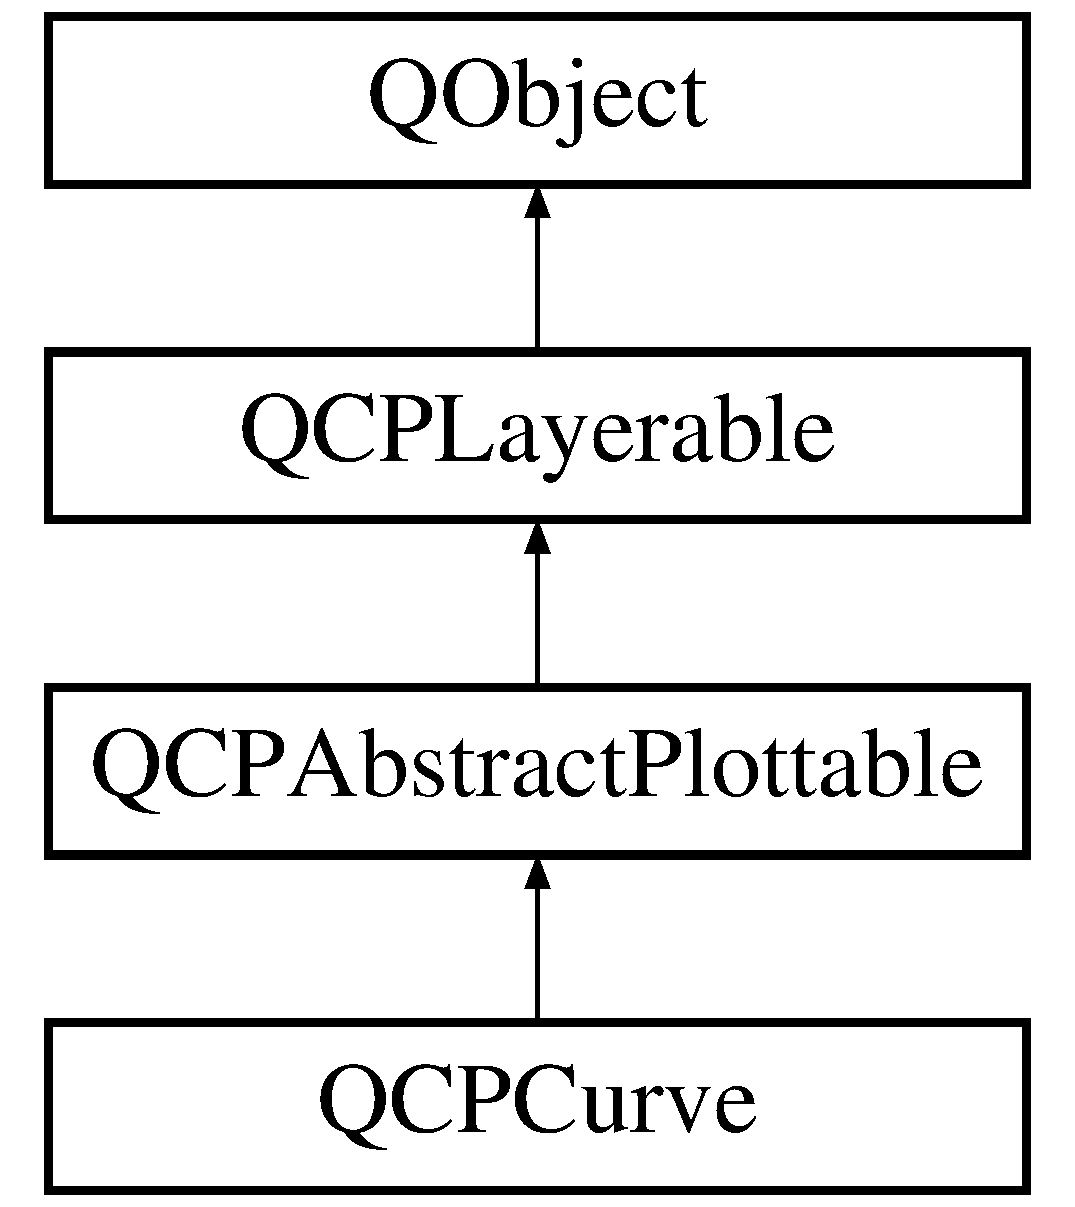
\includegraphics[height=4.000000cm]{class_q_c_p_curve}
\end{center}
\end{figure}
\subsection*{Public Types}
\begin{DoxyCompactItemize}
\item 
enum \hyperlink{class_q_c_p_curve_a2710e9f79302152cff794c6e16cc01f1}{Line\+Style} \{ \hyperlink{class_q_c_p_curve_a2710e9f79302152cff794c6e16cc01f1aec1601a191cdf0b4e761c4c66092cc48}{ls\+None}, 
\hyperlink{class_q_c_p_curve_a2710e9f79302152cff794c6e16cc01f1ade5822ce6fbf131d3df131795c2e1003}{ls\+Line}
 \}
\end{DoxyCompactItemize}
\subsection*{Public Member Functions}
\begin{DoxyCompactItemize}
\item 
\hyperlink{class_q_c_p_curve_a36de58e2652b3fa47bdf9187d421d3ce}{Q\+C\+P\+Curve} (\hyperlink{class_q_c_p_axis}{Q\+C\+P\+Axis} $\ast$\hyperlink{class_q_c_p_abstract_plottable_a72c7a09c22963f2c943f07112b311103}{key\+Axis}, \hyperlink{class_q_c_p_axis}{Q\+C\+P\+Axis} $\ast$\hyperlink{class_q_c_p_abstract_plottable_a3106f9d34d330a6097a8ec5905e5b519}{value\+Axis})
\item 
virtual \hyperlink{class_q_c_p_curve_a99ee5136754884a220cc0bcacfe419a3}{$\sim$\+Q\+C\+P\+Curve} ()
\item 
\hyperlink{qcustomplot_8h_a444d37ec9cb2951b3a7fe443c34d1658}{Q\+C\+P\+Curve\+Data\+Map} $\ast$ \hyperlink{class_q_c_p_curve_a9ac194d35d4f334923aac9df1bf599ca}{data} () const 
\item 
\hyperlink{class_q_c_p_scatter_style}{Q\+C\+P\+Scatter\+Style} \hyperlink{class_q_c_p_curve_a9ab864c9f6ba0cedf65853f59d867a68}{scatter\+Style} () const 
\item 
\hyperlink{class_q_c_p_curve_a2710e9f79302152cff794c6e16cc01f1}{Line\+Style} \hyperlink{class_q_c_p_curve_a0314dd644258949aeb4a95cebde5abaf}{line\+Style} () const 
\item 
void \hyperlink{class_q_c_p_curve_a631ac886708460013b30052f49cbc9da}{set\+Data} (\hyperlink{qcustomplot_8h_a444d37ec9cb2951b3a7fe443c34d1658}{Q\+C\+P\+Curve\+Data\+Map} $\ast$\hyperlink{class_q_c_p_curve_a9ac194d35d4f334923aac9df1bf599ca}{data}, bool copy=false)
\item 
void \hyperlink{class_q_c_p_curve_affe80e011e2ced62a88f614acd6ab8d1}{set\+Data} (const Q\+Vector$<$ double $>$ \&t, const Q\+Vector$<$ double $>$ \&key, const Q\+Vector$<$ double $>$ \&value)
\item 
void \hyperlink{class_q_c_p_curve_a963d4c45777deef15848a8f56172d066}{set\+Data} (const Q\+Vector$<$ double $>$ \&key, const Q\+Vector$<$ double $>$ \&value)
\item 
void \hyperlink{class_q_c_p_curve_a55e43b44709bf50a35500644988aa706}{set\+Scatter\+Style} (const \hyperlink{class_q_c_p_scatter_style}{Q\+C\+P\+Scatter\+Style} \&style)
\item 
void \hyperlink{class_q_c_p_curve_a4a377ec863ff81a1875c3094a6177c19}{set\+Line\+Style} (\hyperlink{class_q_c_p_curve_a2710e9f79302152cff794c6e16cc01f1}{Line\+Style} style)
\item 
void \hyperlink{class_q_c_p_curve_a4e24023c3b9ac75440c7a260172c99af}{add\+Data} (const \hyperlink{qcustomplot_8h_a444d37ec9cb2951b3a7fe443c34d1658}{Q\+C\+P\+Curve\+Data\+Map} \&data\+Map)
\item 
void \hyperlink{class_q_c_p_curve_ad304326aba096911f92452d8bfe0470e}{add\+Data} (const \hyperlink{class_q_c_p_curve_data}{Q\+C\+P\+Curve\+Data} \&\hyperlink{class_q_c_p_curve_a9ac194d35d4f334923aac9df1bf599ca}{data})
\item 
void \hyperlink{class_q_c_p_curve_a13398b236f6926014e404eeb5b9f415c}{add\+Data} (double t, double key, double value)
\item 
void \hyperlink{class_q_c_p_curve_ada4762e793cd5707b33f35b8a4b0f8fb}{add\+Data} (double key, double value)
\item 
void \hyperlink{class_q_c_p_curve_a27c8b3dddd4067d626397ee199626722}{add\+Data} (const Q\+Vector$<$ double $>$ \&ts, const Q\+Vector$<$ double $>$ \&keys, const Q\+Vector$<$ double $>$ \&values)
\item 
void \hyperlink{class_q_c_p_curve_af6f4284fbc2f34e676f24dce03c34fe5}{remove\+Data\+Before} (double t)
\item 
void \hyperlink{class_q_c_p_curve_a0365cb947c4e6d405ee22e00191d5f52}{remove\+Data\+After} (double t)
\item 
void \hyperlink{class_q_c_p_curve_ad45bb5479be799163028ef2b776f7221}{remove\+Data} (double fromt, double tot)
\item 
void \hyperlink{class_q_c_p_curve_a30c91acfa591ec534c49fed4c0fca39a}{remove\+Data} (double t)
\item 
virtual void \hyperlink{class_q_c_p_curve_ae0462c61dbfbac07db0736ec64110241}{clear\+Data} ()
\item 
virtual double \hyperlink{class_q_c_p_curve_a5af9949e725704811bbc81ecd5970b8e}{select\+Test} (const Q\+Point\+F \&pos, bool only\+Selectable, Q\+Variant $\ast$details=0) const 
\end{DoxyCompactItemize}
\subsection*{Protected Member Functions}
\begin{DoxyCompactItemize}
\item 
virtual void \hyperlink{class_q_c_p_curve_a2361302d2fc6ec669849bd3bca00c4b2}{draw} (\hyperlink{class_q_c_p_painter}{Q\+C\+P\+Painter} $\ast$painter)
\item 
virtual void \hyperlink{class_q_c_p_curve_aaee24451e0044d1debfa1fee92c58d7b}{draw\+Legend\+Icon} (\hyperlink{class_q_c_p_painter}{Q\+C\+P\+Painter} $\ast$painter, const Q\+Rect\+F \&rect) const 
\item 
virtual \hyperlink{class_q_c_p_range}{Q\+C\+P\+Range} \hyperlink{class_q_c_p_curve_ad6a9559e16ab43586df18ae376d54481}{get\+Key\+Range} (bool \&found\+Range, \hyperlink{class_q_c_p_abstract_plottable_a661743478a1d3c09d28ec2711d7653d8}{Sign\+Domain} in\+Sign\+Domain=\hyperlink{class_q_c_p_abstract_plottable_a661743478a1d3c09d28ec2711d7653d8a082b98cfb91a7363a3b5cd17b0c1cd60}{sd\+Both}) const 
\item 
virtual \hyperlink{class_q_c_p_range}{Q\+C\+P\+Range} \hyperlink{class_q_c_p_curve_a1d6eec81aab9ae6182bb7c040bcb2dbc}{get\+Value\+Range} (bool \&found\+Range, \hyperlink{class_q_c_p_abstract_plottable_a661743478a1d3c09d28ec2711d7653d8}{Sign\+Domain} in\+Sign\+Domain=\hyperlink{class_q_c_p_abstract_plottable_a661743478a1d3c09d28ec2711d7653d8a082b98cfb91a7363a3b5cd17b0c1cd60}{sd\+Both}) const 
\item 
virtual void \hyperlink{class_q_c_p_curve_a45593f30b81beec4b6130b6b53306087}{draw\+Scatter\+Plot} (\hyperlink{class_q_c_p_painter}{Q\+C\+P\+Painter} $\ast$painter, const Q\+Vector$<$ Q\+Point\+F $>$ $\ast$point\+Data) const 
\item 
void \hyperlink{class_q_c_p_curve_afa895f8ba9ae34fea6ecea295fd7b1e5}{get\+Curve\+Data} (Q\+Vector$<$ Q\+Point\+F $>$ $\ast$line\+Data) const 
\item 
int \hyperlink{class_q_c_p_curve_a3af3183f35bd7aebe149f29ae4f1034a}{get\+Region} (double x, double y, double rect\+Left, double rect\+Top, double rect\+Right, double rect\+Bottom) const 
\item 
Q\+Point\+F \hyperlink{class_q_c_p_curve_acbcfea8986dde6c0143e3f7e8e76041d}{get\+Optimized\+Point} (int prev\+Region, double prev\+Key, double prev\+Value, double key, double value, double rect\+Left, double rect\+Top, double rect\+Right, double rect\+Bottom) const 
\item 
Q\+Vector$<$ Q\+Point\+F $>$ \hyperlink{class_q_c_p_curve_aad0b69d9a7a2a5367fcc9fe3edaf9bf4}{get\+Optimized\+Corner\+Points} (int prev\+Region, int current\+Region, double prev\+Key, double prev\+Value, double key, double value, double rect\+Left, double rect\+Top, double rect\+Right, double rect\+Bottom) const 
\item 
bool \hyperlink{class_q_c_p_curve_ae5b232c8201441a940516c745309a685}{may\+Traverse} (int prev\+Region, int current\+Region) const 
\item 
bool \hyperlink{class_q_c_p_curve_ab4ffdf3d62d5bd3a187f6668daf01f85}{get\+Traverse} (double prev\+Key, double prev\+Value, double key, double value, double rect\+Left, double rect\+Top, double rect\+Right, double rect\+Bottom, Q\+Point\+F \&cross\+A, Q\+Point\+F \&cross\+B) const 
\item 
void \hyperlink{class_q_c_p_curve_abe1721b19669e7127d76d144660fbeb8}{get\+Traverse\+Corner\+Points} (int prev\+Region, int current\+Region, double rect\+Left, double rect\+Top, double rect\+Right, double rect\+Bottom, Q\+Vector$<$ Q\+Point\+F $>$ \&before\+Traverse, Q\+Vector$<$ Q\+Point\+F $>$ \&after\+Traverse) const 
\item 
double \hyperlink{class_q_c_p_curve_acd7a68c6f268ce1ab845eaf69fc2c6a6}{point\+Distance} (const Q\+Point\+F \&pixel\+Point) const 
\end{DoxyCompactItemize}
\subsection*{Protected Attributes}
\begin{DoxyCompactItemize}
\item 
\hyperlink{qcustomplot_8h_a444d37ec9cb2951b3a7fe443c34d1658}{Q\+C\+P\+Curve\+Data\+Map} $\ast$ \hyperlink{class_q_c_p_curve_a88d533e455bca96004b049e99168731b}{m\+Data}
\item 
\hyperlink{class_q_c_p_scatter_style}{Q\+C\+P\+Scatter\+Style} \hyperlink{class_q_c_p_curve_a08f803b4a30b01bbd7a1eab15d0f864f}{m\+Scatter\+Style}
\item 
\hyperlink{class_q_c_p_curve_a2710e9f79302152cff794c6e16cc01f1}{Line\+Style} \hyperlink{class_q_c_p_curve_ae1f35ae2b15aee8e15bcdfec5be95156}{m\+Line\+Style}
\end{DoxyCompactItemize}
\subsection*{Friends}
\begin{DoxyCompactItemize}
\item 
class \hyperlink{class_q_c_p_curve_a1cdf9df76adcfae45261690aa0ca2198}{Q\+Custom\+Plot}
\item 
class \hyperlink{class_q_c_p_curve_a8429035e7adfbd7f05805a6530ad5e3b}{Q\+C\+P\+Legend}
\end{DoxyCompactItemize}
\subsection*{Additional Inherited Members}


\subsection{Detailed Description}
A plottable representing a parametric curve in a plot. 



Unlike \hyperlink{class_q_c_p_graph}{Q\+C\+P\+Graph}, plottables of this type may have multiple points with the same key coordinate, so their visual representation can have {\itshape loops}. This is realized by introducing a third coordinate {\itshape t}, which defines the order of the points described by the other two coordinates {\itshape x} and {\itshape y}.

To plot data, assign it with the \hyperlink{class_q_c_p_curve_a631ac886708460013b30052f49cbc9da}{set\+Data} or \hyperlink{class_q_c_p_curve_a4e24023c3b9ac75440c7a260172c99af}{add\+Data} functions.\hypertarget{class_q_c_p_statistical_box_appearance}{}\subsection{Changing the appearance}\label{class_q_c_p_statistical_box_appearance}
The appearance of the curve is determined by the pen and the brush (\hyperlink{class_q_c_p_abstract_plottable_ab74b09ae4c0e7e13142fe4b5bf46cac7}{set\+Pen}, \hyperlink{class_q_c_p_abstract_plottable_a7a4b92144dca6453a1f0f210e27edc74}{set\+Brush}). \hypertarget{class_q_c_p_statistical_box_usage}{}\subsection{Usage}\label{class_q_c_p_statistical_box_usage}
Like all data representing objects in \hyperlink{class_q_custom_plot}{Q\+Custom\+Plot}, the \hyperlink{class_q_c_p_curve}{Q\+C\+P\+Curve} is a plottable (\hyperlink{class_q_c_p_abstract_plottable}{Q\+C\+P\+Abstract\+Plottable}). So the plottable-\/interface of \hyperlink{class_q_custom_plot}{Q\+Custom\+Plot} applies (\hyperlink{class_q_custom_plot_a32de81ff53e263e785b83b52ecd99d6f}{Q\+Custom\+Plot\+::plottable}, \hyperlink{class_q_custom_plot_ab7ad9174f701f9c6f64e378df77927a6}{Q\+Custom\+Plot\+::add\+Plottable}, \hyperlink{class_q_custom_plot_af3dafd56884208474f311d6226513ab2}{Q\+Custom\+Plot\+::remove\+Plottable}, etc.)

Usually, you first create an instance\+: 
\begin{DoxyCode}
\hyperlink{class_q_c_p_curve}{QCPCurve} *newCurve = \textcolor{keyword}{new} \hyperlink{class_q_c_p_curve_a36de58e2652b3fa47bdf9187d421d3ce}{QCPCurve}(customPlot->xAxis, customPlot->yAxis);
\end{DoxyCode}
 add it to the custom\+Plot with \hyperlink{class_q_custom_plot_ab7ad9174f701f9c6f64e378df77927a6}{Q\+Custom\+Plot\+::add\+Plottable}\+: 
\begin{DoxyCode}
customPlot->addPlottable(newCurve);
\end{DoxyCode}
 and then modify the properties of the newly created plottable, e.\+g.\+: 
\begin{DoxyCode}
newCurve->\hyperlink{class_q_c_p_abstract_plottable_ab79c7ba76bc7fa89a4b3580e12149f1f}{setName}(\textcolor{stringliteral}{"Fermat's Spiral"});
newCurve->\hyperlink{class_q_c_p_curve_a631ac886708460013b30052f49cbc9da}{setData}(tData, xData, yData);
\end{DoxyCode}
 

\subsection{Member Enumeration Documentation}
\hypertarget{class_q_c_p_curve_a2710e9f79302152cff794c6e16cc01f1}{}\index{Q\+C\+P\+Curve@{Q\+C\+P\+Curve}!Line\+Style@{Line\+Style}}
\index{Line\+Style@{Line\+Style}!Q\+C\+P\+Curve@{Q\+C\+P\+Curve}}
\subsubsection[{Line\+Style}]{\setlength{\rightskip}{0pt plus 5cm}enum {\bf Q\+C\+P\+Curve\+::\+Line\+Style}}\label{class_q_c_p_curve_a2710e9f79302152cff794c6e16cc01f1}
Defines how the curve\textquotesingle{}s line is represented visually in the plot. The line is drawn with the current pen of the curve (\hyperlink{class_q_c_p_abstract_plottable_ab74b09ae4c0e7e13142fe4b5bf46cac7}{set\+Pen}). \begin{DoxySeeAlso}{See also}
\hyperlink{class_q_c_p_curve_a4a377ec863ff81a1875c3094a6177c19}{set\+Line\+Style} 
\end{DoxySeeAlso}
\begin{Desc}
\item[Enumerator]\par
\begin{description}
\index{ls\+None@{ls\+None}!Q\+C\+P\+Curve@{Q\+C\+P\+Curve}}\index{Q\+C\+P\+Curve@{Q\+C\+P\+Curve}!ls\+None@{ls\+None}}\item[{\em 
\hypertarget{class_q_c_p_curve_a2710e9f79302152cff794c6e16cc01f1aec1601a191cdf0b4e761c4c66092cc48}{}ls\+None\label{class_q_c_p_curve_a2710e9f79302152cff794c6e16cc01f1aec1601a191cdf0b4e761c4c66092cc48}
}]No line is drawn between data points (e.\+g. only scatters) \index{ls\+Line@{ls\+Line}!Q\+C\+P\+Curve@{Q\+C\+P\+Curve}}\index{Q\+C\+P\+Curve@{Q\+C\+P\+Curve}!ls\+Line@{ls\+Line}}\item[{\em 
\hypertarget{class_q_c_p_curve_a2710e9f79302152cff794c6e16cc01f1ade5822ce6fbf131d3df131795c2e1003}{}ls\+Line\label{class_q_c_p_curve_a2710e9f79302152cff794c6e16cc01f1ade5822ce6fbf131d3df131795c2e1003}
}]Data points are connected with a straight line. \end{description}
\end{Desc}


\subsection{Constructor \& Destructor Documentation}
\hypertarget{class_q_c_p_curve_a36de58e2652b3fa47bdf9187d421d3ce}{}\index{Q\+C\+P\+Curve@{Q\+C\+P\+Curve}!Q\+C\+P\+Curve@{Q\+C\+P\+Curve}}
\index{Q\+C\+P\+Curve@{Q\+C\+P\+Curve}!Q\+C\+P\+Curve@{Q\+C\+P\+Curve}}
\subsubsection[{Q\+C\+P\+Curve}]{\setlength{\rightskip}{0pt plus 5cm}Q\+C\+P\+Curve\+::\+Q\+C\+P\+Curve (
\begin{DoxyParamCaption}
\item[{{\bf Q\+C\+P\+Axis} $\ast$}]{key\+Axis, }
\item[{{\bf Q\+C\+P\+Axis} $\ast$}]{value\+Axis}
\end{DoxyParamCaption}
)\hspace{0.3cm}{\ttfamily [explicit]}}\label{class_q_c_p_curve_a36de58e2652b3fa47bdf9187d421d3ce}
Constructs a curve which uses {\itshape key\+Axis} as its key axis (\char`\"{}x\char`\"{}) and {\itshape value\+Axis} as its value axis (\char`\"{}y\char`\"{}). {\itshape key\+Axis} and {\itshape value\+Axis} must reside in the same \hyperlink{class_q_custom_plot}{Q\+Custom\+Plot} instance and not have the same orientation. If either of these restrictions is violated, a corresponding message is printed to the debug output (q\+Debug), the construction is not aborted, though.

The constructed \hyperlink{class_q_c_p_curve}{Q\+C\+P\+Curve} can be added to the plot with \hyperlink{class_q_custom_plot_ab7ad9174f701f9c6f64e378df77927a6}{Q\+Custom\+Plot\+::add\+Plottable}, \hyperlink{class_q_custom_plot}{Q\+Custom\+Plot} then takes ownership of the graph. \hypertarget{class_q_c_p_curve_a99ee5136754884a220cc0bcacfe419a3}{}\index{Q\+C\+P\+Curve@{Q\+C\+P\+Curve}!````~Q\+C\+P\+Curve@{$\sim$\+Q\+C\+P\+Curve}}
\index{````~Q\+C\+P\+Curve@{$\sim$\+Q\+C\+P\+Curve}!Q\+C\+P\+Curve@{Q\+C\+P\+Curve}}
\subsubsection[{$\sim$\+Q\+C\+P\+Curve}]{\setlength{\rightskip}{0pt plus 5cm}Q\+C\+P\+Curve\+::$\sim$\+Q\+C\+P\+Curve (
\begin{DoxyParamCaption}
{}
\end{DoxyParamCaption}
)\hspace{0.3cm}{\ttfamily [virtual]}}\label{class_q_c_p_curve_a99ee5136754884a220cc0bcacfe419a3}


\subsection{Member Function Documentation}
\hypertarget{class_q_c_p_curve_a4e24023c3b9ac75440c7a260172c99af}{}\index{Q\+C\+P\+Curve@{Q\+C\+P\+Curve}!add\+Data@{add\+Data}}
\index{add\+Data@{add\+Data}!Q\+C\+P\+Curve@{Q\+C\+P\+Curve}}
\subsubsection[{add\+Data}]{\setlength{\rightskip}{0pt plus 5cm}void Q\+C\+P\+Curve\+::add\+Data (
\begin{DoxyParamCaption}
\item[{const {\bf Q\+C\+P\+Curve\+Data\+Map} \&}]{data\+Map}
\end{DoxyParamCaption}
)}\label{class_q_c_p_curve_a4e24023c3b9ac75440c7a260172c99af}
Adds the provided data points in {\itshape data\+Map} to the current data. \begin{DoxySeeAlso}{See also}
\hyperlink{class_q_c_p_curve_ad45bb5479be799163028ef2b776f7221}{remove\+Data} 
\end{DoxySeeAlso}
\hypertarget{class_q_c_p_curve_ad304326aba096911f92452d8bfe0470e}{}\index{Q\+C\+P\+Curve@{Q\+C\+P\+Curve}!add\+Data@{add\+Data}}
\index{add\+Data@{add\+Data}!Q\+C\+P\+Curve@{Q\+C\+P\+Curve}}
\subsubsection[{add\+Data}]{\setlength{\rightskip}{0pt plus 5cm}void Q\+C\+P\+Curve\+::add\+Data (
\begin{DoxyParamCaption}
\item[{const {\bf Q\+C\+P\+Curve\+Data} \&}]{data}
\end{DoxyParamCaption}
)}\label{class_q_c_p_curve_ad304326aba096911f92452d8bfe0470e}
This is an overloaded member function, provided for convenience. It differs from the above function only in what argument(s) it accepts. Adds the provided single data point in {\itshape data} to the current data. \begin{DoxySeeAlso}{See also}
\hyperlink{class_q_c_p_curve_ad45bb5479be799163028ef2b776f7221}{remove\+Data} 
\end{DoxySeeAlso}
\hypertarget{class_q_c_p_curve_a13398b236f6926014e404eeb5b9f415c}{}\index{Q\+C\+P\+Curve@{Q\+C\+P\+Curve}!add\+Data@{add\+Data}}
\index{add\+Data@{add\+Data}!Q\+C\+P\+Curve@{Q\+C\+P\+Curve}}
\subsubsection[{add\+Data}]{\setlength{\rightskip}{0pt plus 5cm}void Q\+C\+P\+Curve\+::add\+Data (
\begin{DoxyParamCaption}
\item[{double}]{t, }
\item[{double}]{key, }
\item[{double}]{value}
\end{DoxyParamCaption}
)}\label{class_q_c_p_curve_a13398b236f6926014e404eeb5b9f415c}
This is an overloaded member function, provided for convenience. It differs from the above function only in what argument(s) it accepts. Adds the provided single data point as {\itshape t}, {\itshape key} and {\itshape value} tuple to the current data \begin{DoxySeeAlso}{See also}
\hyperlink{class_q_c_p_curve_ad45bb5479be799163028ef2b776f7221}{remove\+Data} 
\end{DoxySeeAlso}
\hypertarget{class_q_c_p_curve_ada4762e793cd5707b33f35b8a4b0f8fb}{}\index{Q\+C\+P\+Curve@{Q\+C\+P\+Curve}!add\+Data@{add\+Data}}
\index{add\+Data@{add\+Data}!Q\+C\+P\+Curve@{Q\+C\+P\+Curve}}
\subsubsection[{add\+Data}]{\setlength{\rightskip}{0pt plus 5cm}void Q\+C\+P\+Curve\+::add\+Data (
\begin{DoxyParamCaption}
\item[{double}]{key, }
\item[{double}]{value}
\end{DoxyParamCaption}
)}\label{class_q_c_p_curve_ada4762e793cd5707b33f35b8a4b0f8fb}
This is an overloaded member function, provided for convenience. It differs from the above function only in what argument(s) it accepts.

Adds the provided single data point as {\itshape key} and {\itshape value} pair to the current data The t parameter of the data point is set to the t of the last data point plus 1. If there is no last data point, t will be set to 0.

\begin{DoxySeeAlso}{See also}
\hyperlink{class_q_c_p_curve_ad45bb5479be799163028ef2b776f7221}{remove\+Data} 
\end{DoxySeeAlso}
\hypertarget{class_q_c_p_curve_a27c8b3dddd4067d626397ee199626722}{}\index{Q\+C\+P\+Curve@{Q\+C\+P\+Curve}!add\+Data@{add\+Data}}
\index{add\+Data@{add\+Data}!Q\+C\+P\+Curve@{Q\+C\+P\+Curve}}
\subsubsection[{add\+Data}]{\setlength{\rightskip}{0pt plus 5cm}void Q\+C\+P\+Curve\+::add\+Data (
\begin{DoxyParamCaption}
\item[{const Q\+Vector$<$ double $>$ \&}]{ts, }
\item[{const Q\+Vector$<$ double $>$ \&}]{keys, }
\item[{const Q\+Vector$<$ double $>$ \&}]{values}
\end{DoxyParamCaption}
)}\label{class_q_c_p_curve_a27c8b3dddd4067d626397ee199626722}
This is an overloaded member function, provided for convenience. It differs from the above function only in what argument(s) it accepts. Adds the provided data points as {\itshape t}, {\itshape key} and {\itshape value} tuples to the current data. \begin{DoxySeeAlso}{See also}
\hyperlink{class_q_c_p_curve_ad45bb5479be799163028ef2b776f7221}{remove\+Data} 
\end{DoxySeeAlso}
\hypertarget{class_q_c_p_curve_ae0462c61dbfbac07db0736ec64110241}{}\index{Q\+C\+P\+Curve@{Q\+C\+P\+Curve}!clear\+Data@{clear\+Data}}
\index{clear\+Data@{clear\+Data}!Q\+C\+P\+Curve@{Q\+C\+P\+Curve}}
\subsubsection[{clear\+Data}]{\setlength{\rightskip}{0pt plus 5cm}void Q\+C\+P\+Curve\+::clear\+Data (
\begin{DoxyParamCaption}
{}
\end{DoxyParamCaption}
)\hspace{0.3cm}{\ttfamily [virtual]}}\label{class_q_c_p_curve_ae0462c61dbfbac07db0736ec64110241}
Removes all data points. \begin{DoxySeeAlso}{See also}
\hyperlink{class_q_c_p_curve_ad45bb5479be799163028ef2b776f7221}{remove\+Data}, \hyperlink{class_q_c_p_curve_a0365cb947c4e6d405ee22e00191d5f52}{remove\+Data\+After}, \hyperlink{class_q_c_p_curve_af6f4284fbc2f34e676f24dce03c34fe5}{remove\+Data\+Before} 
\end{DoxySeeAlso}


Implements \hyperlink{class_q_c_p_abstract_plottable_a86e5b8fd4b6ff4f4084e7ea4c573fc53}{Q\+C\+P\+Abstract\+Plottable}.

\hypertarget{class_q_c_p_curve_a9ac194d35d4f334923aac9df1bf599ca}{}\index{Q\+C\+P\+Curve@{Q\+C\+P\+Curve}!data@{data}}
\index{data@{data}!Q\+C\+P\+Curve@{Q\+C\+P\+Curve}}
\subsubsection[{data}]{\setlength{\rightskip}{0pt plus 5cm}{\bf Q\+C\+P\+Curve\+Data\+Map}$\ast$ Q\+C\+P\+Curve\+::data (
\begin{DoxyParamCaption}
{}
\end{DoxyParamCaption}
) const\hspace{0.3cm}{\ttfamily [inline]}}\label{class_q_c_p_curve_a9ac194d35d4f334923aac9df1bf599ca}
\hypertarget{class_q_c_p_curve_a2361302d2fc6ec669849bd3bca00c4b2}{}\index{Q\+C\+P\+Curve@{Q\+C\+P\+Curve}!draw@{draw}}
\index{draw@{draw}!Q\+C\+P\+Curve@{Q\+C\+P\+Curve}}
\subsubsection[{draw}]{\setlength{\rightskip}{0pt plus 5cm}void Q\+C\+P\+Curve\+::draw (
\begin{DoxyParamCaption}
\item[{{\bf Q\+C\+P\+Painter} $\ast$}]{painter}
\end{DoxyParamCaption}
)\hspace{0.3cm}{\ttfamily [protected]}, {\ttfamily [virtual]}}\label{class_q_c_p_curve_a2361302d2fc6ec669849bd3bca00c4b2}


Implements \hyperlink{class_q_c_p_abstract_plottable_acbab5e30dcd04fd302b4a5902ac2c482}{Q\+C\+P\+Abstract\+Plottable}.

\hypertarget{class_q_c_p_curve_aaee24451e0044d1debfa1fee92c58d7b}{}\index{Q\+C\+P\+Curve@{Q\+C\+P\+Curve}!draw\+Legend\+Icon@{draw\+Legend\+Icon}}
\index{draw\+Legend\+Icon@{draw\+Legend\+Icon}!Q\+C\+P\+Curve@{Q\+C\+P\+Curve}}
\subsubsection[{draw\+Legend\+Icon}]{\setlength{\rightskip}{0pt plus 5cm}void Q\+C\+P\+Curve\+::draw\+Legend\+Icon (
\begin{DoxyParamCaption}
\item[{{\bf Q\+C\+P\+Painter} $\ast$}]{painter, }
\item[{const Q\+Rect\+F \&}]{rect}
\end{DoxyParamCaption}
) const\hspace{0.3cm}{\ttfamily [protected]}, {\ttfamily [virtual]}}\label{class_q_c_p_curve_aaee24451e0044d1debfa1fee92c58d7b}


Implements \hyperlink{class_q_c_p_abstract_plottable_a9a450783fd9ed539e589999fd390cdf7}{Q\+C\+P\+Abstract\+Plottable}.

\hypertarget{class_q_c_p_curve_a45593f30b81beec4b6130b6b53306087}{}\index{Q\+C\+P\+Curve@{Q\+C\+P\+Curve}!draw\+Scatter\+Plot@{draw\+Scatter\+Plot}}
\index{draw\+Scatter\+Plot@{draw\+Scatter\+Plot}!Q\+C\+P\+Curve@{Q\+C\+P\+Curve}}
\subsubsection[{draw\+Scatter\+Plot}]{\setlength{\rightskip}{0pt plus 5cm}void Q\+C\+P\+Curve\+::draw\+Scatter\+Plot (
\begin{DoxyParamCaption}
\item[{{\bf Q\+C\+P\+Painter} $\ast$}]{painter, }
\item[{const Q\+Vector$<$ Q\+Point\+F $>$ $\ast$}]{point\+Data}
\end{DoxyParamCaption}
) const\hspace{0.3cm}{\ttfamily [protected]}, {\ttfamily [virtual]}}\label{class_q_c_p_curve_a45593f30b81beec4b6130b6b53306087}
\hypertarget{class_q_c_p_curve_afa895f8ba9ae34fea6ecea295fd7b1e5}{}\index{Q\+C\+P\+Curve@{Q\+C\+P\+Curve}!get\+Curve\+Data@{get\+Curve\+Data}}
\index{get\+Curve\+Data@{get\+Curve\+Data}!Q\+C\+P\+Curve@{Q\+C\+P\+Curve}}
\subsubsection[{get\+Curve\+Data}]{\setlength{\rightskip}{0pt plus 5cm}void Q\+C\+P\+Curve\+::get\+Curve\+Data (
\begin{DoxyParamCaption}
\item[{Q\+Vector$<$ Q\+Point\+F $>$ $\ast$}]{line\+Data}
\end{DoxyParamCaption}
) const\hspace{0.3cm}{\ttfamily [protected]}}\label{class_q_c_p_curve_afa895f8ba9ae34fea6ecea295fd7b1e5}
\hypertarget{class_q_c_p_curve_ad6a9559e16ab43586df18ae376d54481}{}\index{Q\+C\+P\+Curve@{Q\+C\+P\+Curve}!get\+Key\+Range@{get\+Key\+Range}}
\index{get\+Key\+Range@{get\+Key\+Range}!Q\+C\+P\+Curve@{Q\+C\+P\+Curve}}
\subsubsection[{get\+Key\+Range}]{\setlength{\rightskip}{0pt plus 5cm}{\bf Q\+C\+P\+Range} Q\+C\+P\+Curve\+::get\+Key\+Range (
\begin{DoxyParamCaption}
\item[{bool \&}]{found\+Range, }
\item[{{\bf Sign\+Domain}}]{in\+Sign\+Domain = {\ttfamily {\bf sd\+Both}}}
\end{DoxyParamCaption}
) const\hspace{0.3cm}{\ttfamily [protected]}, {\ttfamily [virtual]}}\label{class_q_c_p_curve_ad6a9559e16ab43586df18ae376d54481}


Implements \hyperlink{class_q_c_p_abstract_plottable_a345d702b2e7e12c8cfdddff65ba85e8c}{Q\+C\+P\+Abstract\+Plottable}.

\hypertarget{class_q_c_p_curve_aad0b69d9a7a2a5367fcc9fe3edaf9bf4}{}\index{Q\+C\+P\+Curve@{Q\+C\+P\+Curve}!get\+Optimized\+Corner\+Points@{get\+Optimized\+Corner\+Points}}
\index{get\+Optimized\+Corner\+Points@{get\+Optimized\+Corner\+Points}!Q\+C\+P\+Curve@{Q\+C\+P\+Curve}}
\subsubsection[{get\+Optimized\+Corner\+Points}]{\setlength{\rightskip}{0pt plus 5cm}Q\+Vector$<$ Q\+Point\+F $>$ Q\+C\+P\+Curve\+::get\+Optimized\+Corner\+Points (
\begin{DoxyParamCaption}
\item[{int}]{prev\+Region, }
\item[{int}]{current\+Region, }
\item[{double}]{prev\+Key, }
\item[{double}]{prev\+Value, }
\item[{double}]{key, }
\item[{double}]{value, }
\item[{double}]{rect\+Left, }
\item[{double}]{rect\+Top, }
\item[{double}]{rect\+Right, }
\item[{double}]{rect\+Bottom}
\end{DoxyParamCaption}
) const\hspace{0.3cm}{\ttfamily [protected]}}\label{class_q_c_p_curve_aad0b69d9a7a2a5367fcc9fe3edaf9bf4}
\hypertarget{class_q_c_p_curve_acbcfea8986dde6c0143e3f7e8e76041d}{}\index{Q\+C\+P\+Curve@{Q\+C\+P\+Curve}!get\+Optimized\+Point@{get\+Optimized\+Point}}
\index{get\+Optimized\+Point@{get\+Optimized\+Point}!Q\+C\+P\+Curve@{Q\+C\+P\+Curve}}
\subsubsection[{get\+Optimized\+Point}]{\setlength{\rightskip}{0pt plus 5cm}Q\+Point\+F Q\+C\+P\+Curve\+::get\+Optimized\+Point (
\begin{DoxyParamCaption}
\item[{int}]{prev\+Region, }
\item[{double}]{prev\+Key, }
\item[{double}]{prev\+Value, }
\item[{double}]{key, }
\item[{double}]{value, }
\item[{double}]{rect\+Left, }
\item[{double}]{rect\+Top, }
\item[{double}]{rect\+Right, }
\item[{double}]{rect\+Bottom}
\end{DoxyParamCaption}
) const\hspace{0.3cm}{\ttfamily [protected]}}\label{class_q_c_p_curve_acbcfea8986dde6c0143e3f7e8e76041d}
\hypertarget{class_q_c_p_curve_a3af3183f35bd7aebe149f29ae4f1034a}{}\index{Q\+C\+P\+Curve@{Q\+C\+P\+Curve}!get\+Region@{get\+Region}}
\index{get\+Region@{get\+Region}!Q\+C\+P\+Curve@{Q\+C\+P\+Curve}}
\subsubsection[{get\+Region}]{\setlength{\rightskip}{0pt plus 5cm}int Q\+C\+P\+Curve\+::get\+Region (
\begin{DoxyParamCaption}
\item[{double}]{x, }
\item[{double}]{y, }
\item[{double}]{rect\+Left, }
\item[{double}]{rect\+Top, }
\item[{double}]{rect\+Right, }
\item[{double}]{rect\+Bottom}
\end{DoxyParamCaption}
) const\hspace{0.3cm}{\ttfamily [protected]}}\label{class_q_c_p_curve_a3af3183f35bd7aebe149f29ae4f1034a}
\hypertarget{class_q_c_p_curve_ab4ffdf3d62d5bd3a187f6668daf01f85}{}\index{Q\+C\+P\+Curve@{Q\+C\+P\+Curve}!get\+Traverse@{get\+Traverse}}
\index{get\+Traverse@{get\+Traverse}!Q\+C\+P\+Curve@{Q\+C\+P\+Curve}}
\subsubsection[{get\+Traverse}]{\setlength{\rightskip}{0pt plus 5cm}bool Q\+C\+P\+Curve\+::get\+Traverse (
\begin{DoxyParamCaption}
\item[{double}]{prev\+Key, }
\item[{double}]{prev\+Value, }
\item[{double}]{key, }
\item[{double}]{value, }
\item[{double}]{rect\+Left, }
\item[{double}]{rect\+Top, }
\item[{double}]{rect\+Right, }
\item[{double}]{rect\+Bottom, }
\item[{Q\+Point\+F \&}]{cross\+A, }
\item[{Q\+Point\+F \&}]{cross\+B}
\end{DoxyParamCaption}
) const\hspace{0.3cm}{\ttfamily [protected]}}\label{class_q_c_p_curve_ab4ffdf3d62d5bd3a187f6668daf01f85}
\hypertarget{class_q_c_p_curve_abe1721b19669e7127d76d144660fbeb8}{}\index{Q\+C\+P\+Curve@{Q\+C\+P\+Curve}!get\+Traverse\+Corner\+Points@{get\+Traverse\+Corner\+Points}}
\index{get\+Traverse\+Corner\+Points@{get\+Traverse\+Corner\+Points}!Q\+C\+P\+Curve@{Q\+C\+P\+Curve}}
\subsubsection[{get\+Traverse\+Corner\+Points}]{\setlength{\rightskip}{0pt plus 5cm}void Q\+C\+P\+Curve\+::get\+Traverse\+Corner\+Points (
\begin{DoxyParamCaption}
\item[{int}]{prev\+Region, }
\item[{int}]{current\+Region, }
\item[{double}]{rect\+Left, }
\item[{double}]{rect\+Top, }
\item[{double}]{rect\+Right, }
\item[{double}]{rect\+Bottom, }
\item[{Q\+Vector$<$ Q\+Point\+F $>$ \&}]{before\+Traverse, }
\item[{Q\+Vector$<$ Q\+Point\+F $>$ \&}]{after\+Traverse}
\end{DoxyParamCaption}
) const\hspace{0.3cm}{\ttfamily [protected]}}\label{class_q_c_p_curve_abe1721b19669e7127d76d144660fbeb8}
\hypertarget{class_q_c_p_curve_a1d6eec81aab9ae6182bb7c040bcb2dbc}{}\index{Q\+C\+P\+Curve@{Q\+C\+P\+Curve}!get\+Value\+Range@{get\+Value\+Range}}
\index{get\+Value\+Range@{get\+Value\+Range}!Q\+C\+P\+Curve@{Q\+C\+P\+Curve}}
\subsubsection[{get\+Value\+Range}]{\setlength{\rightskip}{0pt plus 5cm}{\bf Q\+C\+P\+Range} Q\+C\+P\+Curve\+::get\+Value\+Range (
\begin{DoxyParamCaption}
\item[{bool \&}]{found\+Range, }
\item[{{\bf Sign\+Domain}}]{in\+Sign\+Domain = {\ttfamily {\bf sd\+Both}}}
\end{DoxyParamCaption}
) const\hspace{0.3cm}{\ttfamily [protected]}, {\ttfamily [virtual]}}\label{class_q_c_p_curve_a1d6eec81aab9ae6182bb7c040bcb2dbc}


Implements \hyperlink{class_q_c_p_abstract_plottable_aa3331b415b5939fe4df60b78831b2799}{Q\+C\+P\+Abstract\+Plottable}.

\hypertarget{class_q_c_p_curve_a0314dd644258949aeb4a95cebde5abaf}{}\index{Q\+C\+P\+Curve@{Q\+C\+P\+Curve}!line\+Style@{line\+Style}}
\index{line\+Style@{line\+Style}!Q\+C\+P\+Curve@{Q\+C\+P\+Curve}}
\subsubsection[{line\+Style}]{\setlength{\rightskip}{0pt plus 5cm}{\bf Line\+Style} Q\+C\+P\+Curve\+::line\+Style (
\begin{DoxyParamCaption}
{}
\end{DoxyParamCaption}
) const\hspace{0.3cm}{\ttfamily [inline]}}\label{class_q_c_p_curve_a0314dd644258949aeb4a95cebde5abaf}
\hypertarget{class_q_c_p_curve_ae5b232c8201441a940516c745309a685}{}\index{Q\+C\+P\+Curve@{Q\+C\+P\+Curve}!may\+Traverse@{may\+Traverse}}
\index{may\+Traverse@{may\+Traverse}!Q\+C\+P\+Curve@{Q\+C\+P\+Curve}}
\subsubsection[{may\+Traverse}]{\setlength{\rightskip}{0pt plus 5cm}bool Q\+C\+P\+Curve\+::may\+Traverse (
\begin{DoxyParamCaption}
\item[{int}]{prev\+Region, }
\item[{int}]{current\+Region}
\end{DoxyParamCaption}
) const\hspace{0.3cm}{\ttfamily [protected]}}\label{class_q_c_p_curve_ae5b232c8201441a940516c745309a685}
\hypertarget{class_q_c_p_curve_acd7a68c6f268ce1ab845eaf69fc2c6a6}{}\index{Q\+C\+P\+Curve@{Q\+C\+P\+Curve}!point\+Distance@{point\+Distance}}
\index{point\+Distance@{point\+Distance}!Q\+C\+P\+Curve@{Q\+C\+P\+Curve}}
\subsubsection[{point\+Distance}]{\setlength{\rightskip}{0pt plus 5cm}double Q\+C\+P\+Curve\+::point\+Distance (
\begin{DoxyParamCaption}
\item[{const Q\+Point\+F \&}]{pixel\+Point}
\end{DoxyParamCaption}
) const\hspace{0.3cm}{\ttfamily [protected]}}\label{class_q_c_p_curve_acd7a68c6f268ce1ab845eaf69fc2c6a6}
\hypertarget{class_q_c_p_curve_ad45bb5479be799163028ef2b776f7221}{}\index{Q\+C\+P\+Curve@{Q\+C\+P\+Curve}!remove\+Data@{remove\+Data}}
\index{remove\+Data@{remove\+Data}!Q\+C\+P\+Curve@{Q\+C\+P\+Curve}}
\subsubsection[{remove\+Data}]{\setlength{\rightskip}{0pt plus 5cm}void Q\+C\+P\+Curve\+::remove\+Data (
\begin{DoxyParamCaption}
\item[{double}]{fromt, }
\item[{double}]{tot}
\end{DoxyParamCaption}
)}\label{class_q_c_p_curve_ad45bb5479be799163028ef2b776f7221}
Removes all data points with curve parameter t between {\itshape fromt} and {\itshape tot}. if {\itshape fromt} is greater or equal to {\itshape tot}, the function does nothing. To remove a single data point with known t, use \hyperlink{class_q_c_p_curve_a30c91acfa591ec534c49fed4c0fca39a}{remove\+Data(double t)}.

\begin{DoxySeeAlso}{See also}
\hyperlink{class_q_c_p_curve_a4e24023c3b9ac75440c7a260172c99af}{add\+Data}, \hyperlink{class_q_c_p_curve_ae0462c61dbfbac07db0736ec64110241}{clear\+Data} 
\end{DoxySeeAlso}
\hypertarget{class_q_c_p_curve_a30c91acfa591ec534c49fed4c0fca39a}{}\index{Q\+C\+P\+Curve@{Q\+C\+P\+Curve}!remove\+Data@{remove\+Data}}
\index{remove\+Data@{remove\+Data}!Q\+C\+P\+Curve@{Q\+C\+P\+Curve}}
\subsubsection[{remove\+Data}]{\setlength{\rightskip}{0pt plus 5cm}void Q\+C\+P\+Curve\+::remove\+Data (
\begin{DoxyParamCaption}
\item[{double}]{t}
\end{DoxyParamCaption}
)}\label{class_q_c_p_curve_a30c91acfa591ec534c49fed4c0fca39a}
This is an overloaded member function, provided for convenience. It differs from the above function only in what argument(s) it accepts.

Removes a single data point at curve parameter {\itshape t}. If the position is not known with absolute precision, consider using \hyperlink{class_q_c_p_curve_ad45bb5479be799163028ef2b776f7221}{remove\+Data(double fromt, double tot)} with a small fuzziness interval around the suspected position, depeding on the precision with which the curve parameter is known.

\begin{DoxySeeAlso}{See also}
\hyperlink{class_q_c_p_curve_a4e24023c3b9ac75440c7a260172c99af}{add\+Data}, \hyperlink{class_q_c_p_curve_ae0462c61dbfbac07db0736ec64110241}{clear\+Data} 
\end{DoxySeeAlso}
\hypertarget{class_q_c_p_curve_a0365cb947c4e6d405ee22e00191d5f52}{}\index{Q\+C\+P\+Curve@{Q\+C\+P\+Curve}!remove\+Data\+After@{remove\+Data\+After}}
\index{remove\+Data\+After@{remove\+Data\+After}!Q\+C\+P\+Curve@{Q\+C\+P\+Curve}}
\subsubsection[{remove\+Data\+After}]{\setlength{\rightskip}{0pt plus 5cm}void Q\+C\+P\+Curve\+::remove\+Data\+After (
\begin{DoxyParamCaption}
\item[{double}]{t}
\end{DoxyParamCaption}
)}\label{class_q_c_p_curve_a0365cb947c4e6d405ee22e00191d5f52}
Removes all data points with curve parameter t greater than {\itshape t}. \begin{DoxySeeAlso}{See also}
\hyperlink{class_q_c_p_curve_a4e24023c3b9ac75440c7a260172c99af}{add\+Data}, \hyperlink{class_q_c_p_curve_ae0462c61dbfbac07db0736ec64110241}{clear\+Data} 
\end{DoxySeeAlso}
\hypertarget{class_q_c_p_curve_af6f4284fbc2f34e676f24dce03c34fe5}{}\index{Q\+C\+P\+Curve@{Q\+C\+P\+Curve}!remove\+Data\+Before@{remove\+Data\+Before}}
\index{remove\+Data\+Before@{remove\+Data\+Before}!Q\+C\+P\+Curve@{Q\+C\+P\+Curve}}
\subsubsection[{remove\+Data\+Before}]{\setlength{\rightskip}{0pt plus 5cm}void Q\+C\+P\+Curve\+::remove\+Data\+Before (
\begin{DoxyParamCaption}
\item[{double}]{t}
\end{DoxyParamCaption}
)}\label{class_q_c_p_curve_af6f4284fbc2f34e676f24dce03c34fe5}
Removes all data points with curve parameter t smaller than {\itshape t}. \begin{DoxySeeAlso}{See also}
\hyperlink{class_q_c_p_curve_a4e24023c3b9ac75440c7a260172c99af}{add\+Data}, \hyperlink{class_q_c_p_curve_ae0462c61dbfbac07db0736ec64110241}{clear\+Data} 
\end{DoxySeeAlso}
\hypertarget{class_q_c_p_curve_a9ab864c9f6ba0cedf65853f59d867a68}{}\index{Q\+C\+P\+Curve@{Q\+C\+P\+Curve}!scatter\+Style@{scatter\+Style}}
\index{scatter\+Style@{scatter\+Style}!Q\+C\+P\+Curve@{Q\+C\+P\+Curve}}
\subsubsection[{scatter\+Style}]{\setlength{\rightskip}{0pt plus 5cm}{\bf Q\+C\+P\+Scatter\+Style} Q\+C\+P\+Curve\+::scatter\+Style (
\begin{DoxyParamCaption}
{}
\end{DoxyParamCaption}
) const\hspace{0.3cm}{\ttfamily [inline]}}\label{class_q_c_p_curve_a9ab864c9f6ba0cedf65853f59d867a68}
\hypertarget{class_q_c_p_curve_a5af9949e725704811bbc81ecd5970b8e}{}\index{Q\+C\+P\+Curve@{Q\+C\+P\+Curve}!select\+Test@{select\+Test}}
\index{select\+Test@{select\+Test}!Q\+C\+P\+Curve@{Q\+C\+P\+Curve}}
\subsubsection[{select\+Test}]{\setlength{\rightskip}{0pt plus 5cm}double Q\+C\+P\+Curve\+::select\+Test (
\begin{DoxyParamCaption}
\item[{const Q\+Point\+F \&}]{pos, }
\item[{bool}]{only\+Selectable, }
\item[{Q\+Variant $\ast$}]{details = {\ttfamily 0}}
\end{DoxyParamCaption}
) const\hspace{0.3cm}{\ttfamily [virtual]}}\label{class_q_c_p_curve_a5af9949e725704811bbc81ecd5970b8e}
This function is used to decide whether a click hits a layerable object or not.

{\itshape pos} is a point in pixel coordinates on the \hyperlink{class_q_custom_plot}{Q\+Custom\+Plot} surface. This function returns the shortest pixel distance of this point to the object. If the object is either invisible or the distance couldn\textquotesingle{}t be determined, -\/1.\+0 is returned. Further, if {\itshape only\+Selectable} is true and the object is not selectable, -\/1.\+0 is returned, too.

If the item is represented not by single lines but by an area like \hyperlink{class_q_c_p_item_rect}{Q\+C\+P\+Item\+Rect} or \hyperlink{class_q_c_p_item_text}{Q\+C\+P\+Item\+Text}, a click inside the area returns a constant value greater zero (typically the selection\+Tolerance of the parent \hyperlink{class_q_custom_plot}{Q\+Custom\+Plot} multiplied by 0.\+99). If the click lies outside the area, this function returns -\/1.\+0.

Providing a constant value for area objects allows selecting line objects even when they are obscured by such area objects, by clicking close to the lines (i.\+e. closer than 0.\+99$\ast$selection\+Tolerance).

The actual setting of the selection state is not done by this function. This is handled by the parent \hyperlink{class_q_custom_plot}{Q\+Custom\+Plot} when the mouse\+Release\+Event occurs, and the finally selected object is notified via the select\+Event/deselect\+Event methods.

{\itshape details} is an optional output parameter. Every layerable subclass may place any information in {\itshape details}. This information will be passed to \hyperlink{class_q_c_p_abstract_plottable_a16aaad02456aa23a759efd1ac90c79bf}{select\+Event} when the parent \hyperlink{class_q_custom_plot}{Q\+Custom\+Plot} decides on the basis of this select\+Test call, that the object was successfully selected. The subsequent call to \hyperlink{class_q_c_p_abstract_plottable_a16aaad02456aa23a759efd1ac90c79bf}{select\+Event} will carry the {\itshape details}. This is useful for multi-\/part objects (like \hyperlink{class_q_c_p_axis}{Q\+C\+P\+Axis}). This way, a possibly complex calculation to decide which part was clicked is only done once in \hyperlink{class_q_c_p_curve_a5af9949e725704811bbc81ecd5970b8e}{select\+Test}. The result (i.\+e. the actually clicked part) can then be placed in {\itshape details}. So in the subsequent \hyperlink{class_q_c_p_abstract_plottable_a16aaad02456aa23a759efd1ac90c79bf}{select\+Event}, the decision which part was selected doesn\textquotesingle{}t have to be done a second time for a single selection operation.

You may pass 0 as {\itshape details} to indicate that you are not interested in those selection details.

\begin{DoxySeeAlso}{See also}
\hyperlink{class_q_c_p_abstract_plottable_a16aaad02456aa23a759efd1ac90c79bf}{select\+Event}, \hyperlink{class_q_c_p_abstract_plottable_a6fa0d0f95560ea8b01ee13f296dab2b1}{deselect\+Event}, \hyperlink{class_q_custom_plot_a5ee1e2f6ae27419deca53e75907c27e5}{Q\+Custom\+Plot\+::set\+Interactions} 
\end{DoxySeeAlso}


Implements \hyperlink{class_q_c_p_abstract_plottable_a38efe9641d972992a3d44204bc80ec1d}{Q\+C\+P\+Abstract\+Plottable}.

\hypertarget{class_q_c_p_curve_a631ac886708460013b30052f49cbc9da}{}\index{Q\+C\+P\+Curve@{Q\+C\+P\+Curve}!set\+Data@{set\+Data}}
\index{set\+Data@{set\+Data}!Q\+C\+P\+Curve@{Q\+C\+P\+Curve}}
\subsubsection[{set\+Data}]{\setlength{\rightskip}{0pt plus 5cm}void Q\+C\+P\+Curve\+::set\+Data (
\begin{DoxyParamCaption}
\item[{{\bf Q\+C\+P\+Curve\+Data\+Map} $\ast$}]{data, }
\item[{bool}]{copy = {\ttfamily false}}
\end{DoxyParamCaption}
)}\label{class_q_c_p_curve_a631ac886708460013b30052f49cbc9da}
Replaces the current data with the provided {\itshape data}.

If {\itshape copy} is set to true, data points in {\itshape data} will only be copied. if false, the plottable takes ownership of the passed data and replaces the internal data pointer with it. This is significantly faster than copying for large datasets. \hypertarget{class_q_c_p_curve_affe80e011e2ced62a88f614acd6ab8d1}{}\index{Q\+C\+P\+Curve@{Q\+C\+P\+Curve}!set\+Data@{set\+Data}}
\index{set\+Data@{set\+Data}!Q\+C\+P\+Curve@{Q\+C\+P\+Curve}}
\subsubsection[{set\+Data}]{\setlength{\rightskip}{0pt plus 5cm}void Q\+C\+P\+Curve\+::set\+Data (
\begin{DoxyParamCaption}
\item[{const Q\+Vector$<$ double $>$ \&}]{t, }
\item[{const Q\+Vector$<$ double $>$ \&}]{key, }
\item[{const Q\+Vector$<$ double $>$ \&}]{value}
\end{DoxyParamCaption}
)}\label{class_q_c_p_curve_affe80e011e2ced62a88f614acd6ab8d1}
This is an overloaded member function, provided for convenience. It differs from the above function only in what argument(s) it accepts.

Replaces the current data with the provided points in {\itshape t}, {\itshape key} and {\itshape value} tuples. The provided vectors should have equal length. Else, the number of added points will be the size of the smallest vector. \hypertarget{class_q_c_p_curve_a963d4c45777deef15848a8f56172d066}{}\index{Q\+C\+P\+Curve@{Q\+C\+P\+Curve}!set\+Data@{set\+Data}}
\index{set\+Data@{set\+Data}!Q\+C\+P\+Curve@{Q\+C\+P\+Curve}}
\subsubsection[{set\+Data}]{\setlength{\rightskip}{0pt plus 5cm}void Q\+C\+P\+Curve\+::set\+Data (
\begin{DoxyParamCaption}
\item[{const Q\+Vector$<$ double $>$ \&}]{key, }
\item[{const Q\+Vector$<$ double $>$ \&}]{value}
\end{DoxyParamCaption}
)}\label{class_q_c_p_curve_a963d4c45777deef15848a8f56172d066}
This is an overloaded member function, provided for convenience. It differs from the above function only in what argument(s) it accepts.

Replaces the current data with the provided {\itshape key} and {\itshape value} pairs. The t parameter of each data point will be set to the integer index of the respective key/value pair. \hypertarget{class_q_c_p_curve_a4a377ec863ff81a1875c3094a6177c19}{}\index{Q\+C\+P\+Curve@{Q\+C\+P\+Curve}!set\+Line\+Style@{set\+Line\+Style}}
\index{set\+Line\+Style@{set\+Line\+Style}!Q\+C\+P\+Curve@{Q\+C\+P\+Curve}}
\subsubsection[{set\+Line\+Style}]{\setlength{\rightskip}{0pt plus 5cm}void Q\+C\+P\+Curve\+::set\+Line\+Style (
\begin{DoxyParamCaption}
\item[{{\bf Q\+C\+P\+Curve\+::\+Line\+Style}}]{style}
\end{DoxyParamCaption}
)}\label{class_q_c_p_curve_a4a377ec863ff81a1875c3094a6177c19}
Sets how the single data points are connected in the plot or how they are represented visually apart from the scatter symbol. For scatter-\/only plots, set {\itshape style} to \hyperlink{class_q_c_p_curve_a2710e9f79302152cff794c6e16cc01f1aec1601a191cdf0b4e761c4c66092cc48}{ls\+None} and \hyperlink{class_q_c_p_curve_a55e43b44709bf50a35500644988aa706}{set\+Scatter\+Style} to the desired scatter style.

\begin{DoxySeeAlso}{See also}
\hyperlink{class_q_c_p_curve_a55e43b44709bf50a35500644988aa706}{set\+Scatter\+Style} 
\end{DoxySeeAlso}
\hypertarget{class_q_c_p_curve_a55e43b44709bf50a35500644988aa706}{}\index{Q\+C\+P\+Curve@{Q\+C\+P\+Curve}!set\+Scatter\+Style@{set\+Scatter\+Style}}
\index{set\+Scatter\+Style@{set\+Scatter\+Style}!Q\+C\+P\+Curve@{Q\+C\+P\+Curve}}
\subsubsection[{set\+Scatter\+Style}]{\setlength{\rightskip}{0pt plus 5cm}void Q\+C\+P\+Curve\+::set\+Scatter\+Style (
\begin{DoxyParamCaption}
\item[{const {\bf Q\+C\+P\+Scatter\+Style} \&}]{style}
\end{DoxyParamCaption}
)}\label{class_q_c_p_curve_a55e43b44709bf50a35500644988aa706}
Sets the visual appearance of single data points in the plot. If set to \hyperlink{class_q_c_p_scatter_style_adb31525af6b680e6f1b7472e43859349abd144c291ca274f77053ec68cab6c022}{Q\+C\+P\+Scatter\+Style\+::ss\+None}, no scatter points are drawn (e.\+g. for line-\/only plots with appropriate line style).

\begin{DoxySeeAlso}{See also}
\hyperlink{class_q_c_p_scatter_style}{Q\+C\+P\+Scatter\+Style}, \hyperlink{class_q_c_p_curve_a4a377ec863ff81a1875c3094a6177c19}{set\+Line\+Style} 
\end{DoxySeeAlso}


\subsection{Friends And Related Function Documentation}
\hypertarget{class_q_c_p_curve_a8429035e7adfbd7f05805a6530ad5e3b}{}\index{Q\+C\+P\+Curve@{Q\+C\+P\+Curve}!Q\+C\+P\+Legend@{Q\+C\+P\+Legend}}
\index{Q\+C\+P\+Legend@{Q\+C\+P\+Legend}!Q\+C\+P\+Curve@{Q\+C\+P\+Curve}}
\subsubsection[{Q\+C\+P\+Legend}]{\setlength{\rightskip}{0pt plus 5cm}friend class {\bf Q\+C\+P\+Legend}\hspace{0.3cm}{\ttfamily [friend]}}\label{class_q_c_p_curve_a8429035e7adfbd7f05805a6530ad5e3b}
\hypertarget{class_q_c_p_curve_a1cdf9df76adcfae45261690aa0ca2198}{}\index{Q\+C\+P\+Curve@{Q\+C\+P\+Curve}!Q\+Custom\+Plot@{Q\+Custom\+Plot}}
\index{Q\+Custom\+Plot@{Q\+Custom\+Plot}!Q\+C\+P\+Curve@{Q\+C\+P\+Curve}}
\subsubsection[{Q\+Custom\+Plot}]{\setlength{\rightskip}{0pt plus 5cm}friend class {\bf Q\+Custom\+Plot}\hspace{0.3cm}{\ttfamily [friend]}}\label{class_q_c_p_curve_a1cdf9df76adcfae45261690aa0ca2198}


\subsection{Member Data Documentation}
\hypertarget{class_q_c_p_curve_a88d533e455bca96004b049e99168731b}{}\index{Q\+C\+P\+Curve@{Q\+C\+P\+Curve}!m\+Data@{m\+Data}}
\index{m\+Data@{m\+Data}!Q\+C\+P\+Curve@{Q\+C\+P\+Curve}}
\subsubsection[{m\+Data}]{\setlength{\rightskip}{0pt plus 5cm}{\bf Q\+C\+P\+Curve\+Data\+Map}$\ast$ Q\+C\+P\+Curve\+::m\+Data\hspace{0.3cm}{\ttfamily [protected]}}\label{class_q_c_p_curve_a88d533e455bca96004b049e99168731b}
\hypertarget{class_q_c_p_curve_ae1f35ae2b15aee8e15bcdfec5be95156}{}\index{Q\+C\+P\+Curve@{Q\+C\+P\+Curve}!m\+Line\+Style@{m\+Line\+Style}}
\index{m\+Line\+Style@{m\+Line\+Style}!Q\+C\+P\+Curve@{Q\+C\+P\+Curve}}
\subsubsection[{m\+Line\+Style}]{\setlength{\rightskip}{0pt plus 5cm}{\bf Line\+Style} Q\+C\+P\+Curve\+::m\+Line\+Style\hspace{0.3cm}{\ttfamily [protected]}}\label{class_q_c_p_curve_ae1f35ae2b15aee8e15bcdfec5be95156}
\hypertarget{class_q_c_p_curve_a08f803b4a30b01bbd7a1eab15d0f864f}{}\index{Q\+C\+P\+Curve@{Q\+C\+P\+Curve}!m\+Scatter\+Style@{m\+Scatter\+Style}}
\index{m\+Scatter\+Style@{m\+Scatter\+Style}!Q\+C\+P\+Curve@{Q\+C\+P\+Curve}}
\subsubsection[{m\+Scatter\+Style}]{\setlength{\rightskip}{0pt plus 5cm}{\bf Q\+C\+P\+Scatter\+Style} Q\+C\+P\+Curve\+::m\+Scatter\+Style\hspace{0.3cm}{\ttfamily [protected]}}\label{class_q_c_p_curve_a08f803b4a30b01bbd7a1eab15d0f864f}


The documentation for this class was generated from the following files\+:\begin{DoxyCompactItemize}
\item 
C\+:/\+Users/\+Roman/\+Documents/\+Mygs/\+Ground\+Station/\+G\+S/\hyperlink{qcustomplot_8h}{qcustomplot.\+h}\item 
C\+:/\+Users/\+Roman/\+Documents/\+Mygs/\+Ground\+Station/\+G\+S/\hyperlink{qcustomplot_8cpp}{qcustomplot.\+cpp}\end{DoxyCompactItemize}

\hypertarget{class_q_c_p_curve_data}{}\section{Q\+C\+P\+Curve\+Data Class Reference}
\label{class_q_c_p_curve_data}\index{Q\+C\+P\+Curve\+Data@{Q\+C\+P\+Curve\+Data}}


Holds the data of one single data point for \hyperlink{class_q_c_p_curve}{Q\+C\+P\+Curve}.  




{\ttfamily \#include $<$qcustomplot.\+h$>$}

\subsection*{Public Member Functions}
\begin{DoxyCompactItemize}
\item 
\hyperlink{class_q_c_p_curve_data_a48252779b5198a509d99c69ae223fbf8}{Q\+C\+P\+Curve\+Data} ()
\item 
\hyperlink{class_q_c_p_curve_data_a3586be0cc6f8db15bcdd0c0d03b0c173}{Q\+C\+P\+Curve\+Data} (double \hyperlink{class_q_c_p_curve_data_aecc395525be28e9178a088793beb3ff3}{t}, double \hyperlink{class_q_c_p_curve_data_a8a4ec5f2b9a396149fd842e309701bd4}{key}, double \hyperlink{class_q_c_p_curve_data_a72b39b8e1dbf7b45382ebd48419b6828}{value})
\end{DoxyCompactItemize}
\subsection*{Public Attributes}
\begin{DoxyCompactItemize}
\item 
double \hyperlink{class_q_c_p_curve_data_aecc395525be28e9178a088793beb3ff3}{t}
\item 
double \hyperlink{class_q_c_p_curve_data_a8a4ec5f2b9a396149fd842e309701bd4}{key}
\item 
double \hyperlink{class_q_c_p_curve_data_a72b39b8e1dbf7b45382ebd48419b6828}{value}
\end{DoxyCompactItemize}


\subsection{Detailed Description}
Holds the data of one single data point for \hyperlink{class_q_c_p_curve}{Q\+C\+P\+Curve}. 

The container for storing multiple data points is \hyperlink{qcustomplot_8h_a444d37ec9cb2951b3a7fe443c34d1658}{Q\+C\+P\+Curve\+Data\+Map}.

The stored data is\+: \begin{DoxyItemize}
\item {\itshape t\+:} the free parameter of the curve at this curve point (cp. the mathematical vector {\itshape (x(t), y(t))}) \item {\itshape key\+:} coordinate on the key axis of this curve point \item {\itshape value\+:} coordinate on the value axis of this curve point\end{DoxyItemize}
\begin{DoxySeeAlso}{See also}
\hyperlink{qcustomplot_8h_a444d37ec9cb2951b3a7fe443c34d1658}{Q\+C\+P\+Curve\+Data\+Map} 
\end{DoxySeeAlso}


\subsection{Constructor \& Destructor Documentation}
\hypertarget{class_q_c_p_curve_data_a48252779b5198a509d99c69ae223fbf8}{}\index{Q\+C\+P\+Curve\+Data@{Q\+C\+P\+Curve\+Data}!Q\+C\+P\+Curve\+Data@{Q\+C\+P\+Curve\+Data}}
\index{Q\+C\+P\+Curve\+Data@{Q\+C\+P\+Curve\+Data}!Q\+C\+P\+Curve\+Data@{Q\+C\+P\+Curve\+Data}}
\subsubsection[{Q\+C\+P\+Curve\+Data}]{\setlength{\rightskip}{0pt plus 5cm}Q\+C\+P\+Curve\+Data\+::\+Q\+C\+P\+Curve\+Data (
\begin{DoxyParamCaption}
{}
\end{DoxyParamCaption}
)}\label{class_q_c_p_curve_data_a48252779b5198a509d99c69ae223fbf8}
Constructs a curve data point with t, key and value set to zero. \hypertarget{class_q_c_p_curve_data_a3586be0cc6f8db15bcdd0c0d03b0c173}{}\index{Q\+C\+P\+Curve\+Data@{Q\+C\+P\+Curve\+Data}!Q\+C\+P\+Curve\+Data@{Q\+C\+P\+Curve\+Data}}
\index{Q\+C\+P\+Curve\+Data@{Q\+C\+P\+Curve\+Data}!Q\+C\+P\+Curve\+Data@{Q\+C\+P\+Curve\+Data}}
\subsubsection[{Q\+C\+P\+Curve\+Data}]{\setlength{\rightskip}{0pt plus 5cm}Q\+C\+P\+Curve\+Data\+::\+Q\+C\+P\+Curve\+Data (
\begin{DoxyParamCaption}
\item[{double}]{t, }
\item[{double}]{key, }
\item[{double}]{value}
\end{DoxyParamCaption}
)}\label{class_q_c_p_curve_data_a3586be0cc6f8db15bcdd0c0d03b0c173}
Constructs a curve data point with the specified {\itshape t}, {\itshape key} and {\itshape value}. 

\subsection{Member Data Documentation}
\hypertarget{class_q_c_p_curve_data_a8a4ec5f2b9a396149fd842e309701bd4}{}\index{Q\+C\+P\+Curve\+Data@{Q\+C\+P\+Curve\+Data}!key@{key}}
\index{key@{key}!Q\+C\+P\+Curve\+Data@{Q\+C\+P\+Curve\+Data}}
\subsubsection[{key}]{\setlength{\rightskip}{0pt plus 5cm}double Q\+C\+P\+Curve\+Data\+::key}\label{class_q_c_p_curve_data_a8a4ec5f2b9a396149fd842e309701bd4}
\hypertarget{class_q_c_p_curve_data_aecc395525be28e9178a088793beb3ff3}{}\index{Q\+C\+P\+Curve\+Data@{Q\+C\+P\+Curve\+Data}!t@{t}}
\index{t@{t}!Q\+C\+P\+Curve\+Data@{Q\+C\+P\+Curve\+Data}}
\subsubsection[{t}]{\setlength{\rightskip}{0pt plus 5cm}double Q\+C\+P\+Curve\+Data\+::t}\label{class_q_c_p_curve_data_aecc395525be28e9178a088793beb3ff3}
\hypertarget{class_q_c_p_curve_data_a72b39b8e1dbf7b45382ebd48419b6828}{}\index{Q\+C\+P\+Curve\+Data@{Q\+C\+P\+Curve\+Data}!value@{value}}
\index{value@{value}!Q\+C\+P\+Curve\+Data@{Q\+C\+P\+Curve\+Data}}
\subsubsection[{value}]{\setlength{\rightskip}{0pt plus 5cm}double Q\+C\+P\+Curve\+Data\+::value}\label{class_q_c_p_curve_data_a72b39b8e1dbf7b45382ebd48419b6828}


The documentation for this class was generated from the following files\+:\begin{DoxyCompactItemize}
\item 
C\+:/\+Users/\+Roman/\+Documents/\+Mygs/\+Ground\+Station/\+G\+S/\hyperlink{qcustomplot_8h}{qcustomplot.\+h}\item 
C\+:/\+Users/\+Roman/\+Documents/\+Mygs/\+Ground\+Station/\+G\+S/\hyperlink{qcustomplot_8cpp}{qcustomplot.\+cpp}\end{DoxyCompactItemize}

\hypertarget{class_q_c_p_data}{}\section{Q\+C\+P\+Data Class Reference}
\label{class_q_c_p_data}\index{Q\+C\+P\+Data@{Q\+C\+P\+Data}}


Holds the data of one single data point for \hyperlink{class_q_c_p_graph}{Q\+C\+P\+Graph}.  




{\ttfamily \#include $<$qcustomplot.\+h$>$}

\subsection*{Public Member Functions}
\begin{DoxyCompactItemize}
\item 
\hyperlink{class_q_c_p_data_a1f06d624e36ba0ed72ac36d42aa5c7ee}{Q\+C\+P\+Data} ()
\item 
\hyperlink{class_q_c_p_data_aa274181ae8de2a0907ba5464d3c2c103}{Q\+C\+P\+Data} (double \hyperlink{class_q_c_p_data_a2f5ba9aca61bb74f88516e148a4cf71b}{key}, double \hyperlink{class_q_c_p_data_aefe1ecf8fa2e34ed875b67523e542373}{value})
\end{DoxyCompactItemize}
\subsection*{Public Attributes}
\begin{DoxyCompactItemize}
\item 
double \hyperlink{class_q_c_p_data_a2f5ba9aca61bb74f88516e148a4cf71b}{key}
\item 
double \hyperlink{class_q_c_p_data_aefe1ecf8fa2e34ed875b67523e542373}{value}
\item 
double \hyperlink{class_q_c_p_data_ae468c3808107c2fd23052481156ab5b5}{key\+Error\+Plus}
\item 
double \hyperlink{class_q_c_p_data_af107d650b8ee5c3b2961ecddcfb1bccb}{key\+Error\+Minus}
\item 
double \hyperlink{class_q_c_p_data_ad26912552d03485ea20d91dcad16aa8f}{value\+Error\+Plus}
\item 
double \hyperlink{class_q_c_p_data_a51d8f42bf4d49a1f263531e70cadd6a3}{value\+Error\+Minus}
\end{DoxyCompactItemize}


\subsection{Detailed Description}
Holds the data of one single data point for \hyperlink{class_q_c_p_graph}{Q\+C\+P\+Graph}. 

The container for storing multiple data points is \hyperlink{qcustomplot_8h_a84a9c4a4c2216ccfdcb5f3067cda76e3}{Q\+C\+P\+Data\+Map}.

The stored data is\+: \begin{DoxyItemize}
\item {\itshape key\+:} coordinate on the key axis of this data point \item {\itshape value\+:} coordinate on the value axis of this data point \item {\itshape key\+Error\+Minus\+:} negative error in the key dimension (for error bars) \item {\itshape key\+Error\+Plus\+:} positive error in the key dimension (for error bars) \item {\itshape value\+Error\+Minus\+:} negative error in the value dimension (for error bars) \item {\itshape value\+Error\+Plus\+:} positive error in the value dimension (for error bars)\end{DoxyItemize}
\begin{DoxySeeAlso}{See also}
\hyperlink{qcustomplot_8h_a84a9c4a4c2216ccfdcb5f3067cda76e3}{Q\+C\+P\+Data\+Map} 
\end{DoxySeeAlso}


\subsection{Constructor \& Destructor Documentation}
\hypertarget{class_q_c_p_data_a1f06d624e36ba0ed72ac36d42aa5c7ee}{}\index{Q\+C\+P\+Data@{Q\+C\+P\+Data}!Q\+C\+P\+Data@{Q\+C\+P\+Data}}
\index{Q\+C\+P\+Data@{Q\+C\+P\+Data}!Q\+C\+P\+Data@{Q\+C\+P\+Data}}
\subsubsection[{Q\+C\+P\+Data}]{\setlength{\rightskip}{0pt plus 5cm}Q\+C\+P\+Data\+::\+Q\+C\+P\+Data (
\begin{DoxyParamCaption}
{}
\end{DoxyParamCaption}
)}\label{class_q_c_p_data_a1f06d624e36ba0ed72ac36d42aa5c7ee}
Constructs a data point with key, value and all errors set to zero. \hypertarget{class_q_c_p_data_aa274181ae8de2a0907ba5464d3c2c103}{}\index{Q\+C\+P\+Data@{Q\+C\+P\+Data}!Q\+C\+P\+Data@{Q\+C\+P\+Data}}
\index{Q\+C\+P\+Data@{Q\+C\+P\+Data}!Q\+C\+P\+Data@{Q\+C\+P\+Data}}
\subsubsection[{Q\+C\+P\+Data}]{\setlength{\rightskip}{0pt plus 5cm}Q\+C\+P\+Data\+::\+Q\+C\+P\+Data (
\begin{DoxyParamCaption}
\item[{double}]{key, }
\item[{double}]{value}
\end{DoxyParamCaption}
)}\label{class_q_c_p_data_aa274181ae8de2a0907ba5464d3c2c103}
Constructs a data point with the specified {\itshape key} and {\itshape value}. All errors are set to zero. 

\subsection{Member Data Documentation}
\hypertarget{class_q_c_p_data_a2f5ba9aca61bb74f88516e148a4cf71b}{}\index{Q\+C\+P\+Data@{Q\+C\+P\+Data}!key@{key}}
\index{key@{key}!Q\+C\+P\+Data@{Q\+C\+P\+Data}}
\subsubsection[{key}]{\setlength{\rightskip}{0pt plus 5cm}double Q\+C\+P\+Data\+::key}\label{class_q_c_p_data_a2f5ba9aca61bb74f88516e148a4cf71b}
\hypertarget{class_q_c_p_data_af107d650b8ee5c3b2961ecddcfb1bccb}{}\index{Q\+C\+P\+Data@{Q\+C\+P\+Data}!key\+Error\+Minus@{key\+Error\+Minus}}
\index{key\+Error\+Minus@{key\+Error\+Minus}!Q\+C\+P\+Data@{Q\+C\+P\+Data}}
\subsubsection[{key\+Error\+Minus}]{\setlength{\rightskip}{0pt plus 5cm}double Q\+C\+P\+Data\+::key\+Error\+Minus}\label{class_q_c_p_data_af107d650b8ee5c3b2961ecddcfb1bccb}
\hypertarget{class_q_c_p_data_ae468c3808107c2fd23052481156ab5b5}{}\index{Q\+C\+P\+Data@{Q\+C\+P\+Data}!key\+Error\+Plus@{key\+Error\+Plus}}
\index{key\+Error\+Plus@{key\+Error\+Plus}!Q\+C\+P\+Data@{Q\+C\+P\+Data}}
\subsubsection[{key\+Error\+Plus}]{\setlength{\rightskip}{0pt plus 5cm}double Q\+C\+P\+Data\+::key\+Error\+Plus}\label{class_q_c_p_data_ae468c3808107c2fd23052481156ab5b5}
\hypertarget{class_q_c_p_data_aefe1ecf8fa2e34ed875b67523e542373}{}\index{Q\+C\+P\+Data@{Q\+C\+P\+Data}!value@{value}}
\index{value@{value}!Q\+C\+P\+Data@{Q\+C\+P\+Data}}
\subsubsection[{value}]{\setlength{\rightskip}{0pt plus 5cm}double Q\+C\+P\+Data\+::value}\label{class_q_c_p_data_aefe1ecf8fa2e34ed875b67523e542373}
\hypertarget{class_q_c_p_data_a51d8f42bf4d49a1f263531e70cadd6a3}{}\index{Q\+C\+P\+Data@{Q\+C\+P\+Data}!value\+Error\+Minus@{value\+Error\+Minus}}
\index{value\+Error\+Minus@{value\+Error\+Minus}!Q\+C\+P\+Data@{Q\+C\+P\+Data}}
\subsubsection[{value\+Error\+Minus}]{\setlength{\rightskip}{0pt plus 5cm}double Q\+C\+P\+Data\+::value\+Error\+Minus}\label{class_q_c_p_data_a51d8f42bf4d49a1f263531e70cadd6a3}
\hypertarget{class_q_c_p_data_ad26912552d03485ea20d91dcad16aa8f}{}\index{Q\+C\+P\+Data@{Q\+C\+P\+Data}!value\+Error\+Plus@{value\+Error\+Plus}}
\index{value\+Error\+Plus@{value\+Error\+Plus}!Q\+C\+P\+Data@{Q\+C\+P\+Data}}
\subsubsection[{value\+Error\+Plus}]{\setlength{\rightskip}{0pt plus 5cm}double Q\+C\+P\+Data\+::value\+Error\+Plus}\label{class_q_c_p_data_ad26912552d03485ea20d91dcad16aa8f}


The documentation for this class was generated from the following files\+:\begin{DoxyCompactItemize}
\item 
C\+:/\+Users/\+Roman/\+Documents/\+Mygs/\+Ground\+Station/\+G\+S/\hyperlink{qcustomplot_8h}{qcustomplot.\+h}\item 
C\+:/\+Users/\+Roman/\+Documents/\+Mygs/\+Ground\+Station/\+G\+S/\hyperlink{qcustomplot_8cpp}{qcustomplot.\+cpp}\end{DoxyCompactItemize}

\hypertarget{class_q_c_p_financial}{}\section{Q\+C\+P\+Financial Class Reference}
\label{class_q_c_p_financial}\index{Q\+C\+P\+Financial@{Q\+C\+P\+Financial}}


A plottable representing a financial stock chart.  




{\ttfamily \#include $<$qcustomplot.\+h$>$}

Inheritance diagram for Q\+C\+P\+Financial\+:\begin{figure}[H]
\begin{center}
\leavevmode
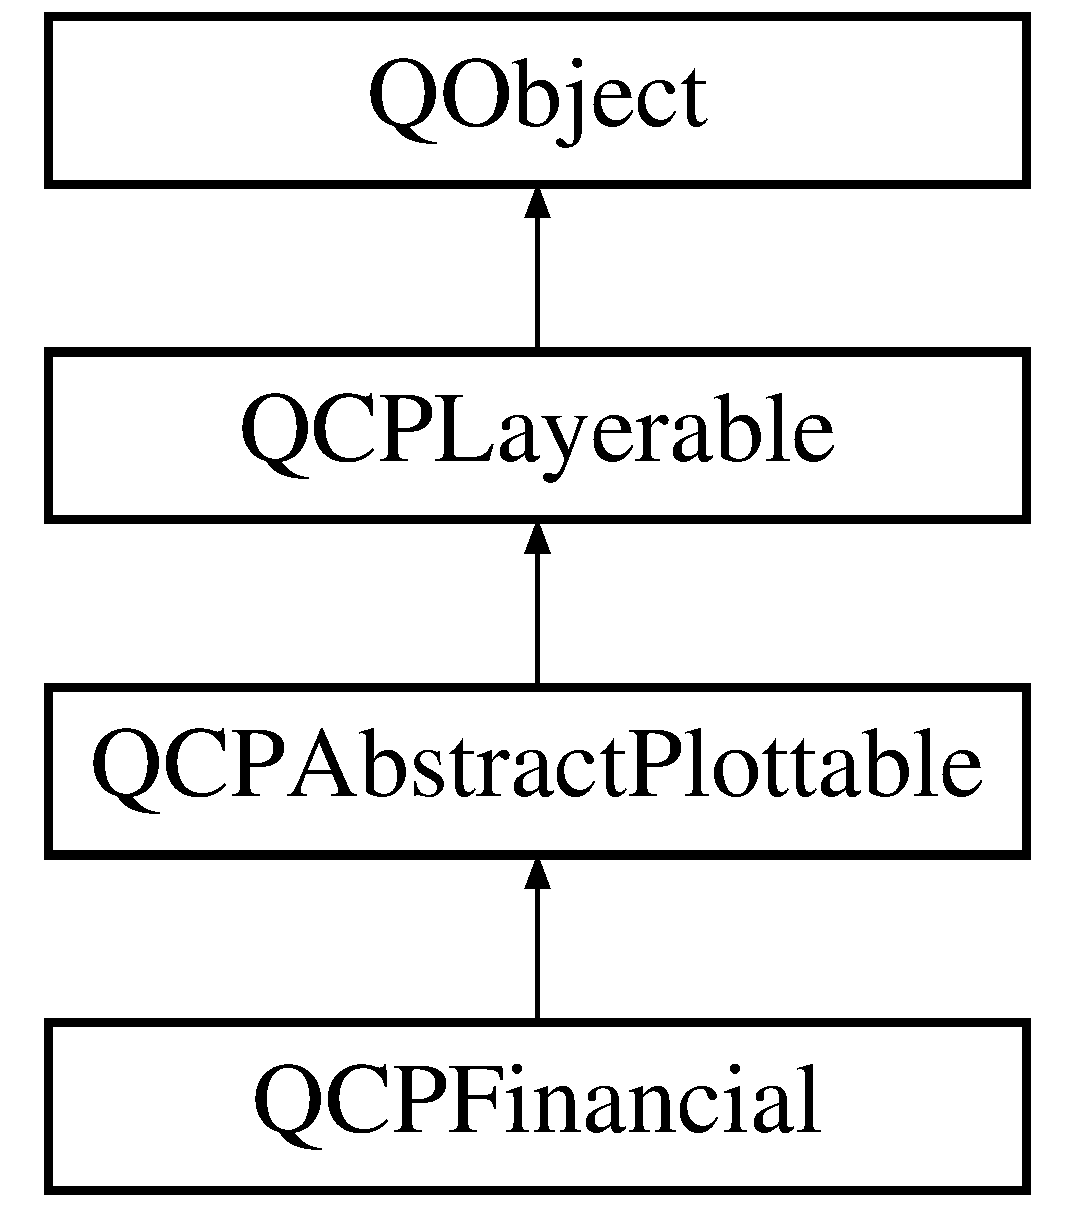
\includegraphics[height=4.000000cm]{class_q_c_p_financial}
\end{center}
\end{figure}
\subsection*{Public Types}
\begin{DoxyCompactItemize}
\item 
enum \hyperlink{class_q_c_p_financial_a0f800e21ee98d646dfc6f8f89d10ebfb}{Chart\+Style} \{ \hyperlink{class_q_c_p_financial_a0f800e21ee98d646dfc6f8f89d10ebfba3a516016c9298d3e95dd82aa203c4390}{cs\+Ohlc}, 
\hyperlink{class_q_c_p_financial_a0f800e21ee98d646dfc6f8f89d10ebfbac803cbd39f26e3f206bcc7028679e62f}{cs\+Candlestick}
 \}
\end{DoxyCompactItemize}
\subsection*{Public Member Functions}
\begin{DoxyCompactItemize}
\item 
\hyperlink{class_q_c_p_financial_a4702d5248feeb9d1ec6e3ce725b10b32}{Q\+C\+P\+Financial} (\hyperlink{class_q_c_p_axis}{Q\+C\+P\+Axis} $\ast$\hyperlink{class_q_c_p_abstract_plottable_a72c7a09c22963f2c943f07112b311103}{key\+Axis}, \hyperlink{class_q_c_p_axis}{Q\+C\+P\+Axis} $\ast$\hyperlink{class_q_c_p_abstract_plottable_a3106f9d34d330a6097a8ec5905e5b519}{value\+Axis})
\item 
virtual \hyperlink{class_q_c_p_financial_ad1fda0d793797b66819fac4682b10f31}{$\sim$\+Q\+C\+P\+Financial} ()
\item 
\hyperlink{qcustomplot_8h_a745c09823fae0974b50beca9bc3b3d7d}{Q\+C\+P\+Financial\+Data\+Map} $\ast$ \hyperlink{class_q_c_p_financial_a58e05aefa057d16edfcc0334cf81c241}{data} () const 
\item 
\hyperlink{class_q_c_p_financial_a0f800e21ee98d646dfc6f8f89d10ebfb}{Chart\+Style} \hyperlink{class_q_c_p_financial_a0888c9308cc5fcb4daa70184f9582412}{chart\+Style} () const 
\item 
double \hyperlink{class_q_c_p_financial_a71ccaa04cdade0ec08a2117db6e4a4ce}{width} () const 
\item 
bool \hyperlink{class_q_c_p_financial_a2bab30fc4eee38a0da3a05846b8d7ac7}{two\+Colored} () const 
\item 
Q\+Brush \hyperlink{class_q_c_p_financial_acb69536a334fae7fc31b2bfd4eca81f5}{brush\+Positive} () const 
\item 
Q\+Brush \hyperlink{class_q_c_p_financial_a91e09b31ce341c17b917e77fdc68d84e}{brush\+Negative} () const 
\item 
Q\+Pen \hyperlink{class_q_c_p_financial_a544899bde79d06e17ccefcb9926d87ce}{pen\+Positive} () const 
\item 
Q\+Pen \hyperlink{class_q_c_p_financial_a557fe911aa04f70c1734c8fa09994148}{pen\+Negative} () const 
\item 
void \hyperlink{class_q_c_p_financial_adf12a86082f1e488df6a4e8603f8fd6d}{set\+Data} (\hyperlink{qcustomplot_8h_a745c09823fae0974b50beca9bc3b3d7d}{Q\+C\+P\+Financial\+Data\+Map} $\ast$\hyperlink{class_q_c_p_financial_a58e05aefa057d16edfcc0334cf81c241}{data}, bool copy=false)
\item 
void \hyperlink{class_q_c_p_financial_a886881339d6447432af55adaad748c3c}{set\+Data} (const Q\+Vector$<$ double $>$ \&key, const Q\+Vector$<$ double $>$ \&open, const Q\+Vector$<$ double $>$ \&high, const Q\+Vector$<$ double $>$ \&low, const Q\+Vector$<$ double $>$ \&close)
\item 
void \hyperlink{class_q_c_p_financial_a5a59175d36279d71596e64d7bb65596f}{set\+Chart\+Style} (\hyperlink{class_q_c_p_financial_a0f800e21ee98d646dfc6f8f89d10ebfb}{Chart\+Style} style)
\item 
void \hyperlink{class_q_c_p_financial_a99633f8bac86a61d534ae5eeb1a3068f}{set\+Width} (double \hyperlink{class_q_c_p_financial_a71ccaa04cdade0ec08a2117db6e4a4ce}{width})
\item 
void \hyperlink{class_q_c_p_financial_a138e44aac160a17a9676652e240c5f08}{set\+Two\+Colored} (bool \hyperlink{class_q_c_p_financial_a2bab30fc4eee38a0da3a05846b8d7ac7}{two\+Colored})
\item 
void \hyperlink{class_q_c_p_financial_a5ebff2b1764efd07cc44942e67821829}{set\+Brush\+Positive} (const Q\+Brush \&\hyperlink{class_q_c_p_abstract_plottable_aa74cdceb9c7286ef116fbfa58e0326e7}{brush})
\item 
void \hyperlink{class_q_c_p_financial_a8bbdd87629f9144b3ef51af660c0961a}{set\+Brush\+Negative} (const Q\+Brush \&\hyperlink{class_q_c_p_abstract_plottable_aa74cdceb9c7286ef116fbfa58e0326e7}{brush})
\item 
void \hyperlink{class_q_c_p_financial_ac58aa3adc7a35aab0088764b840683e5}{set\+Pen\+Positive} (const Q\+Pen \&\hyperlink{class_q_c_p_abstract_plottable_a41d060007cc6b3037c9c04d22d0c0398}{pen})
\item 
void \hyperlink{class_q_c_p_financial_afe5c07e94ccea01a75b3a2476993c346}{set\+Pen\+Negative} (const Q\+Pen \&\hyperlink{class_q_c_p_abstract_plottable_a41d060007cc6b3037c9c04d22d0c0398}{pen})
\item 
void \hyperlink{class_q_c_p_financial_a1a83396f97fcc68f2b7aa8d9782feffe}{add\+Data} (const \hyperlink{qcustomplot_8h_a745c09823fae0974b50beca9bc3b3d7d}{Q\+C\+P\+Financial\+Data\+Map} \&data\+Map)
\item 
void \hyperlink{class_q_c_p_financial_a3b6144b48a6a8e63236fc5bf70d40c00}{add\+Data} (const \hyperlink{class_q_c_p_financial_data}{Q\+C\+P\+Financial\+Data} \&\hyperlink{class_q_c_p_financial_a58e05aefa057d16edfcc0334cf81c241}{data})
\item 
void \hyperlink{class_q_c_p_financial_a688bbd052e00a02954ddb0068b378170}{add\+Data} (double key, double open, double high, double low, double close)
\item 
void \hyperlink{class_q_c_p_financial_aa1abe3bdafb297497f09cdbdc4db3958}{add\+Data} (const Q\+Vector$<$ double $>$ \&key, const Q\+Vector$<$ double $>$ \&open, const Q\+Vector$<$ double $>$ \&high, const Q\+Vector$<$ double $>$ \&low, const Q\+Vector$<$ double $>$ \&close)
\item 
void \hyperlink{class_q_c_p_financial_a097c0383c7c1e9042ca7f93cb439d15a}{remove\+Data\+Before} (double key)
\item 
void \hyperlink{class_q_c_p_financial_aa0fcd357005288c833a230c7874825ba}{remove\+Data\+After} (double key)
\item 
void \hyperlink{class_q_c_p_financial_a048c741d3c8cc5709c2c44b759fdf27c}{remove\+Data} (double from\+Key, double to\+Key)
\item 
void \hyperlink{class_q_c_p_financial_ae527d8a11290906b083d1ab598c380ea}{remove\+Data} (double key)
\item 
virtual void \hyperlink{class_q_c_p_financial_a11fd49928c33e55e27b7319c6927864a}{clear\+Data} ()
\item 
virtual double \hyperlink{class_q_c_p_financial_adf6cff00a55f775487d375fe4df5e95b}{select\+Test} (const Q\+Point\+F \&pos, bool only\+Selectable, Q\+Variant $\ast$details=0) const 
\end{DoxyCompactItemize}
\subsection*{Static Public Member Functions}
\begin{DoxyCompactItemize}
\item 
static \hyperlink{qcustomplot_8h_a745c09823fae0974b50beca9bc3b3d7d}{Q\+C\+P\+Financial\+Data\+Map} \hyperlink{class_q_c_p_financial_a0c3453d1c03e320950fdd2df54e3ebc8}{time\+Series\+To\+Ohlc} (const Q\+Vector$<$ double $>$ \&time, const Q\+Vector$<$ double $>$ \&value, double time\+Bin\+Size, double time\+Bin\+Offset=0)
\end{DoxyCompactItemize}
\subsection*{Protected Member Functions}
\begin{DoxyCompactItemize}
\item 
virtual void \hyperlink{class_q_c_p_financial_ad71a59a1b42616594831e04e52c92120}{draw} (\hyperlink{class_q_c_p_painter}{Q\+C\+P\+Painter} $\ast$painter)
\item 
virtual void \hyperlink{class_q_c_p_financial_aca85e8435b092cc8c3e5de65fcfb22c8}{draw\+Legend\+Icon} (\hyperlink{class_q_c_p_painter}{Q\+C\+P\+Painter} $\ast$painter, const Q\+Rect\+F \&rect) const 
\item 
virtual \hyperlink{class_q_c_p_range}{Q\+C\+P\+Range} \hyperlink{class_q_c_p_financial_acc747f4a9b4fddfb14eb9d803349a534}{get\+Key\+Range} (bool \&found\+Range, \hyperlink{class_q_c_p_abstract_plottable_a661743478a1d3c09d28ec2711d7653d8}{Sign\+Domain} in\+Sign\+Domain=\hyperlink{class_q_c_p_abstract_plottable_a661743478a1d3c09d28ec2711d7653d8a082b98cfb91a7363a3b5cd17b0c1cd60}{sd\+Both}) const 
\item 
virtual \hyperlink{class_q_c_p_range}{Q\+C\+P\+Range} \hyperlink{class_q_c_p_financial_ab2b5f3ef9a503ba32ead32081333f4e7}{get\+Value\+Range} (bool \&found\+Range, \hyperlink{class_q_c_p_abstract_plottable_a661743478a1d3c09d28ec2711d7653d8}{Sign\+Domain} in\+Sign\+Domain=\hyperlink{class_q_c_p_abstract_plottable_a661743478a1d3c09d28ec2711d7653d8a082b98cfb91a7363a3b5cd17b0c1cd60}{sd\+Both}) const 
\item 
void \hyperlink{class_q_c_p_financial_a3c3007a7434e29d042c77ccf4f497e66}{draw\+Ohlc\+Plot} (\hyperlink{class_q_c_p_painter}{Q\+C\+P\+Painter} $\ast$painter, const Q\+C\+P\+Financial\+Data\+Map\+::const\+\_\+iterator \&begin, const Q\+C\+P\+Financial\+Data\+Map\+::const\+\_\+iterator \&end)
\item 
void \hyperlink{class_q_c_p_financial_a71f5081da0e5ab9c40a488ad40cff122}{draw\+Candlestick\+Plot} (\hyperlink{class_q_c_p_painter}{Q\+C\+P\+Painter} $\ast$painter, const Q\+C\+P\+Financial\+Data\+Map\+::const\+\_\+iterator \&begin, const Q\+C\+P\+Financial\+Data\+Map\+::const\+\_\+iterator \&end)
\item 
double \hyperlink{class_q_c_p_financial_a9c7d79351e728a67bfb6821c1d1bd6c0}{ohlc\+Select\+Test} (const Q\+Point\+F \&pos, const Q\+C\+P\+Financial\+Data\+Map\+::const\+\_\+iterator \&begin, const Q\+C\+P\+Financial\+Data\+Map\+::const\+\_\+iterator \&end) const 
\item 
double \hyperlink{class_q_c_p_financial_abd0137244a17d5486a01ee442b083333}{candlestick\+Select\+Test} (const Q\+Point\+F \&pos, const Q\+C\+P\+Financial\+Data\+Map\+::const\+\_\+iterator \&begin, const Q\+C\+P\+Financial\+Data\+Map\+::const\+\_\+iterator \&end) const 
\item 
void \hyperlink{class_q_c_p_financial_aca2edf9f19fae733cdb6bd4549019b84}{get\+Visible\+Data\+Bounds} (Q\+C\+P\+Financial\+Data\+Map\+::const\+\_\+iterator \&lower, Q\+C\+P\+Financial\+Data\+Map\+::const\+\_\+iterator \&upper) const 
\end{DoxyCompactItemize}
\subsection*{Protected Attributes}
\begin{DoxyCompactItemize}
\item 
\hyperlink{qcustomplot_8h_a745c09823fae0974b50beca9bc3b3d7d}{Q\+C\+P\+Financial\+Data\+Map} $\ast$ \hyperlink{class_q_c_p_financial_a475f63587ca1077d8c30aaf2b71ae026}{m\+Data}
\item 
\hyperlink{class_q_c_p_financial_a0f800e21ee98d646dfc6f8f89d10ebfb}{Chart\+Style} \hyperlink{class_q_c_p_financial_ab65c2ce8d6354451870bb44b894c1e92}{m\+Chart\+Style}
\item 
double \hyperlink{class_q_c_p_financial_af630e5eb8485146b9c777e63fd1cf993}{m\+Width}
\item 
bool \hyperlink{class_q_c_p_financial_a6afe919190b884d9bac026cefcc8c0a8}{m\+Two\+Colored}
\item 
Q\+Brush \hyperlink{class_q_c_p_financial_ab7e6eed16260a2f88ca6bd940dffea79}{m\+Brush\+Positive}
\item 
Q\+Brush \hyperlink{class_q_c_p_financial_acb0e31874b7a1deb56bd42e8ab3e68f2}{m\+Brush\+Negative}
\item 
Q\+Pen \hyperlink{class_q_c_p_financial_aa6599186f417ba615caebb3f6c762bd8}{m\+Pen\+Positive}
\item 
Q\+Pen \hyperlink{class_q_c_p_financial_a263fbfefde2cc19c8d4024a8319c2bbb}{m\+Pen\+Negative}
\end{DoxyCompactItemize}
\subsection*{Friends}
\begin{DoxyCompactItemize}
\item 
class \hyperlink{class_q_c_p_financial_a1cdf9df76adcfae45261690aa0ca2198}{Q\+Custom\+Plot}
\item 
class \hyperlink{class_q_c_p_financial_a8429035e7adfbd7f05805a6530ad5e3b}{Q\+C\+P\+Legend}
\end{DoxyCompactItemize}
\subsection*{Additional Inherited Members}


\subsection{Detailed Description}
A plottable representing a financial stock chart. 



This plottable represents time series data binned to certain intervals, mainly used for stock charts. The two common representations O\+H\+L\+C (Open-\/\+High-\/\+Low-\/\+Close) bars and Candlesticks can be set via \hyperlink{class_q_c_p_financial_a5a59175d36279d71596e64d7bb65596f}{set\+Chart\+Style}.

The data is passed via \hyperlink{class_q_c_p_financial_adf12a86082f1e488df6a4e8603f8fd6d}{set\+Data} as a set of open/high/low/close values at certain keys (typically times). This means the data must be already binned appropriately. If data is only available as a series of values (e.\+g. {\itshape price} against {\itshape time}), you can use the static convenience function \hyperlink{class_q_c_p_financial_a0c3453d1c03e320950fdd2df54e3ebc8}{time\+Series\+To\+Ohlc} to generate binned O\+H\+L\+C-\/data which can then be passed to \hyperlink{class_q_c_p_financial_adf12a86082f1e488df6a4e8603f8fd6d}{set\+Data}.

The width of the O\+H\+L\+C bars/candlesticks can be controlled with \hyperlink{class_q_c_p_financial_a99633f8bac86a61d534ae5eeb1a3068f}{set\+Width} and is given in plot key coordinates. A typical choice is to set it to (or slightly less than) one bin interval width.\hypertarget{class_q_c_p_statistical_box_appearance}{}\subsection{Changing the appearance}\label{class_q_c_p_statistical_box_appearance}
Charts can be either single-\/ or two-\/colored (\hyperlink{class_q_c_p_financial_a138e44aac160a17a9676652e240c5f08}{set\+Two\+Colored}). If set to be single-\/colored, lines are drawn with the plottable\textquotesingle{}s pen (\hyperlink{class_q_c_p_abstract_plottable_ab74b09ae4c0e7e13142fe4b5bf46cac7}{set\+Pen}) and fills with the brush (\hyperlink{class_q_c_p_abstract_plottable_a7a4b92144dca6453a1f0f210e27edc74}{set\+Brush}).

If set to two-\/colored, positive changes of the value during an interval ({\itshape close} $>$= {\itshape open}) are represented with a different pen and brush than negative changes ({\itshape close} $<$ {\itshape open}). These can be configured with \hyperlink{class_q_c_p_financial_ac58aa3adc7a35aab0088764b840683e5}{set\+Pen\+Positive}, \hyperlink{class_q_c_p_financial_afe5c07e94ccea01a75b3a2476993c346}{set\+Pen\+Negative}, \hyperlink{class_q_c_p_financial_a5ebff2b1764efd07cc44942e67821829}{set\+Brush\+Positive}, and \hyperlink{class_q_c_p_financial_a8bbdd87629f9144b3ef51af660c0961a}{set\+Brush\+Negative}. In two-\/colored mode, the normal plottable pen/brush is ignored. Upon selection however, the normal selected pen/brush (\hyperlink{class_q_c_p_abstract_plottable_a6911603cad23ab0469b108224517516f}{set\+Selected\+Pen}, \hyperlink{class_q_c_p_abstract_plottable_ae8c816874089f7a44001e8618e81a9dc}{set\+Selected\+Brush}) is used, irrespective of whether the chart is single-\/ or two-\/colored. 

\subsection{Member Enumeration Documentation}
\hypertarget{class_q_c_p_financial_a0f800e21ee98d646dfc6f8f89d10ebfb}{}\index{Q\+C\+P\+Financial@{Q\+C\+P\+Financial}!Chart\+Style@{Chart\+Style}}
\index{Chart\+Style@{Chart\+Style}!Q\+C\+P\+Financial@{Q\+C\+P\+Financial}}
\subsubsection[{Chart\+Style}]{\setlength{\rightskip}{0pt plus 5cm}enum {\bf Q\+C\+P\+Financial\+::\+Chart\+Style}}\label{class_q_c_p_financial_a0f800e21ee98d646dfc6f8f89d10ebfb}
Defines the possible representations of O\+H\+L\+C data in the plot.

\begin{DoxySeeAlso}{See also}
\hyperlink{class_q_c_p_financial_a5a59175d36279d71596e64d7bb65596f}{set\+Chart\+Style} 
\end{DoxySeeAlso}
\begin{Desc}
\item[Enumerator]\par
\begin{description}
\index{cs\+Ohlc@{cs\+Ohlc}!Q\+C\+P\+Financial@{Q\+C\+P\+Financial}}\index{Q\+C\+P\+Financial@{Q\+C\+P\+Financial}!cs\+Ohlc@{cs\+Ohlc}}\item[{\em 
\hypertarget{class_q_c_p_financial_a0f800e21ee98d646dfc6f8f89d10ebfba3a516016c9298d3e95dd82aa203c4390}{}cs\+Ohlc\label{class_q_c_p_financial_a0f800e21ee98d646dfc6f8f89d10ebfba3a516016c9298d3e95dd82aa203c4390}
}]Open-\/\+High-\/\+Low-\/\+Close bar representation. \index{cs\+Candlestick@{cs\+Candlestick}!Q\+C\+P\+Financial@{Q\+C\+P\+Financial}}\index{Q\+C\+P\+Financial@{Q\+C\+P\+Financial}!cs\+Candlestick@{cs\+Candlestick}}\item[{\em 
\hypertarget{class_q_c_p_financial_a0f800e21ee98d646dfc6f8f89d10ebfbac803cbd39f26e3f206bcc7028679e62f}{}cs\+Candlestick\label{class_q_c_p_financial_a0f800e21ee98d646dfc6f8f89d10ebfbac803cbd39f26e3f206bcc7028679e62f}
}]Candlestick representation. \end{description}
\end{Desc}


\subsection{Constructor \& Destructor Documentation}
\hypertarget{class_q_c_p_financial_a4702d5248feeb9d1ec6e3ce725b10b32}{}\index{Q\+C\+P\+Financial@{Q\+C\+P\+Financial}!Q\+C\+P\+Financial@{Q\+C\+P\+Financial}}
\index{Q\+C\+P\+Financial@{Q\+C\+P\+Financial}!Q\+C\+P\+Financial@{Q\+C\+P\+Financial}}
\subsubsection[{Q\+C\+P\+Financial}]{\setlength{\rightskip}{0pt plus 5cm}Q\+C\+P\+Financial\+::\+Q\+C\+P\+Financial (
\begin{DoxyParamCaption}
\item[{{\bf Q\+C\+P\+Axis} $\ast$}]{key\+Axis, }
\item[{{\bf Q\+C\+P\+Axis} $\ast$}]{value\+Axis}
\end{DoxyParamCaption}
)\hspace{0.3cm}{\ttfamily [explicit]}}\label{class_q_c_p_financial_a4702d5248feeb9d1ec6e3ce725b10b32}
Constructs a financial chart which uses {\itshape key\+Axis} as its key axis (\char`\"{}x\char`\"{}) and {\itshape value\+Axis} as its value axis (\char`\"{}y\char`\"{}). {\itshape key\+Axis} and {\itshape value\+Axis} must reside in the same \hyperlink{class_q_custom_plot}{Q\+Custom\+Plot} instance and not have the same orientation. If either of these restrictions is violated, a corresponding message is printed to the debug output (q\+Debug), the construction is not aborted, though.

The constructed \hyperlink{class_q_c_p_financial}{Q\+C\+P\+Financial} can be added to the plot with \hyperlink{class_q_custom_plot_ab7ad9174f701f9c6f64e378df77927a6}{Q\+Custom\+Plot\+::add\+Plottable}, \hyperlink{class_q_custom_plot}{Q\+Custom\+Plot} then takes ownership of the financial chart. \hypertarget{class_q_c_p_financial_ad1fda0d793797b66819fac4682b10f31}{}\index{Q\+C\+P\+Financial@{Q\+C\+P\+Financial}!````~Q\+C\+P\+Financial@{$\sim$\+Q\+C\+P\+Financial}}
\index{````~Q\+C\+P\+Financial@{$\sim$\+Q\+C\+P\+Financial}!Q\+C\+P\+Financial@{Q\+C\+P\+Financial}}
\subsubsection[{$\sim$\+Q\+C\+P\+Financial}]{\setlength{\rightskip}{0pt plus 5cm}Q\+C\+P\+Financial\+::$\sim$\+Q\+C\+P\+Financial (
\begin{DoxyParamCaption}
{}
\end{DoxyParamCaption}
)\hspace{0.3cm}{\ttfamily [virtual]}}\label{class_q_c_p_financial_ad1fda0d793797b66819fac4682b10f31}


\subsection{Member Function Documentation}
\hypertarget{class_q_c_p_financial_a1a83396f97fcc68f2b7aa8d9782feffe}{}\index{Q\+C\+P\+Financial@{Q\+C\+P\+Financial}!add\+Data@{add\+Data}}
\index{add\+Data@{add\+Data}!Q\+C\+P\+Financial@{Q\+C\+P\+Financial}}
\subsubsection[{add\+Data}]{\setlength{\rightskip}{0pt plus 5cm}void Q\+C\+P\+Financial\+::add\+Data (
\begin{DoxyParamCaption}
\item[{const {\bf Q\+C\+P\+Financial\+Data\+Map} \&}]{data\+Map}
\end{DoxyParamCaption}
)}\label{class_q_c_p_financial_a1a83396f97fcc68f2b7aa8d9782feffe}
Adds the provided data points in {\itshape data\+Map} to the current data.

Alternatively, you can also access and modify the data via the \hyperlink{class_q_c_p_financial_a58e05aefa057d16edfcc0334cf81c241}{data} method, which returns a pointer to the internal \hyperlink{qcustomplot_8h_a745c09823fae0974b50beca9bc3b3d7d}{Q\+C\+P\+Financial\+Data\+Map}.

\begin{DoxySeeAlso}{See also}
\hyperlink{class_q_c_p_financial_a048c741d3c8cc5709c2c44b759fdf27c}{remove\+Data} 
\end{DoxySeeAlso}
\hypertarget{class_q_c_p_financial_a3b6144b48a6a8e63236fc5bf70d40c00}{}\index{Q\+C\+P\+Financial@{Q\+C\+P\+Financial}!add\+Data@{add\+Data}}
\index{add\+Data@{add\+Data}!Q\+C\+P\+Financial@{Q\+C\+P\+Financial}}
\subsubsection[{add\+Data}]{\setlength{\rightskip}{0pt plus 5cm}void Q\+C\+P\+Financial\+::add\+Data (
\begin{DoxyParamCaption}
\item[{const {\bf Q\+C\+P\+Financial\+Data} \&}]{data}
\end{DoxyParamCaption}
)}\label{class_q_c_p_financial_a3b6144b48a6a8e63236fc5bf70d40c00}
This is an overloaded member function, provided for convenience. It differs from the above function only in what argument(s) it accepts.

Adds the provided single data point in {\itshape data} to the current data.

Alternatively, you can also access and modify the data via the \hyperlink{class_q_c_p_financial_a58e05aefa057d16edfcc0334cf81c241}{data} method, which returns a pointer to the internal \hyperlink{class_q_c_p_financial_data}{Q\+C\+P\+Financial\+Data}.

\begin{DoxySeeAlso}{See also}
\hyperlink{class_q_c_p_financial_a048c741d3c8cc5709c2c44b759fdf27c}{remove\+Data} 
\end{DoxySeeAlso}
\hypertarget{class_q_c_p_financial_a688bbd052e00a02954ddb0068b378170}{}\index{Q\+C\+P\+Financial@{Q\+C\+P\+Financial}!add\+Data@{add\+Data}}
\index{add\+Data@{add\+Data}!Q\+C\+P\+Financial@{Q\+C\+P\+Financial}}
\subsubsection[{add\+Data}]{\setlength{\rightskip}{0pt plus 5cm}void Q\+C\+P\+Financial\+::add\+Data (
\begin{DoxyParamCaption}
\item[{double}]{key, }
\item[{double}]{open, }
\item[{double}]{high, }
\item[{double}]{low, }
\item[{double}]{close}
\end{DoxyParamCaption}
)}\label{class_q_c_p_financial_a688bbd052e00a02954ddb0068b378170}
This is an overloaded member function, provided for convenience. It differs from the above function only in what argument(s) it accepts.

Adds the provided single data point given by {\itshape key}, {\itshape open}, {\itshape high}, {\itshape low}, and {\itshape close} to the current data.

Alternatively, you can also access and modify the data via the \hyperlink{class_q_c_p_financial_a58e05aefa057d16edfcc0334cf81c241}{data} method, which returns a pointer to the internal \hyperlink{class_q_c_p_financial_data}{Q\+C\+P\+Financial\+Data}.

\begin{DoxySeeAlso}{See also}
\hyperlink{class_q_c_p_financial_a048c741d3c8cc5709c2c44b759fdf27c}{remove\+Data} 
\end{DoxySeeAlso}
\hypertarget{class_q_c_p_financial_aa1abe3bdafb297497f09cdbdc4db3958}{}\index{Q\+C\+P\+Financial@{Q\+C\+P\+Financial}!add\+Data@{add\+Data}}
\index{add\+Data@{add\+Data}!Q\+C\+P\+Financial@{Q\+C\+P\+Financial}}
\subsubsection[{add\+Data}]{\setlength{\rightskip}{0pt plus 5cm}void Q\+C\+P\+Financial\+::add\+Data (
\begin{DoxyParamCaption}
\item[{const Q\+Vector$<$ double $>$ \&}]{key, }
\item[{const Q\+Vector$<$ double $>$ \&}]{open, }
\item[{const Q\+Vector$<$ double $>$ \&}]{high, }
\item[{const Q\+Vector$<$ double $>$ \&}]{low, }
\item[{const Q\+Vector$<$ double $>$ \&}]{close}
\end{DoxyParamCaption}
)}\label{class_q_c_p_financial_aa1abe3bdafb297497f09cdbdc4db3958}
This is an overloaded member function, provided for convenience. It differs from the above function only in what argument(s) it accepts.

Adds the provided open/high/low/close data to the current data.

Alternatively, you can also access and modify the data via the \hyperlink{class_q_c_p_financial_a58e05aefa057d16edfcc0334cf81c241}{data} method, which returns a pointer to the internal \hyperlink{class_q_c_p_financial_data}{Q\+C\+P\+Financial\+Data}.

\begin{DoxySeeAlso}{See also}
\hyperlink{class_q_c_p_financial_a048c741d3c8cc5709c2c44b759fdf27c}{remove\+Data} 
\end{DoxySeeAlso}
\hypertarget{class_q_c_p_financial_a91e09b31ce341c17b917e77fdc68d84e}{}\index{Q\+C\+P\+Financial@{Q\+C\+P\+Financial}!brush\+Negative@{brush\+Negative}}
\index{brush\+Negative@{brush\+Negative}!Q\+C\+P\+Financial@{Q\+C\+P\+Financial}}
\subsubsection[{brush\+Negative}]{\setlength{\rightskip}{0pt plus 5cm}Q\+Brush Q\+C\+P\+Financial\+::brush\+Negative (
\begin{DoxyParamCaption}
{}
\end{DoxyParamCaption}
) const\hspace{0.3cm}{\ttfamily [inline]}}\label{class_q_c_p_financial_a91e09b31ce341c17b917e77fdc68d84e}
\hypertarget{class_q_c_p_financial_acb69536a334fae7fc31b2bfd4eca81f5}{}\index{Q\+C\+P\+Financial@{Q\+C\+P\+Financial}!brush\+Positive@{brush\+Positive}}
\index{brush\+Positive@{brush\+Positive}!Q\+C\+P\+Financial@{Q\+C\+P\+Financial}}
\subsubsection[{brush\+Positive}]{\setlength{\rightskip}{0pt plus 5cm}Q\+Brush Q\+C\+P\+Financial\+::brush\+Positive (
\begin{DoxyParamCaption}
{}
\end{DoxyParamCaption}
) const\hspace{0.3cm}{\ttfamily [inline]}}\label{class_q_c_p_financial_acb69536a334fae7fc31b2bfd4eca81f5}
\hypertarget{class_q_c_p_financial_abd0137244a17d5486a01ee442b083333}{}\index{Q\+C\+P\+Financial@{Q\+C\+P\+Financial}!candlestick\+Select\+Test@{candlestick\+Select\+Test}}
\index{candlestick\+Select\+Test@{candlestick\+Select\+Test}!Q\+C\+P\+Financial@{Q\+C\+P\+Financial}}
\subsubsection[{candlestick\+Select\+Test}]{\setlength{\rightskip}{0pt plus 5cm}double Q\+C\+P\+Financial\+::candlestick\+Select\+Test (
\begin{DoxyParamCaption}
\item[{const Q\+Point\+F \&}]{pos, }
\item[{const Q\+C\+P\+Financial\+Data\+Map\+::const\+\_\+iterator \&}]{begin, }
\item[{const Q\+C\+P\+Financial\+Data\+Map\+::const\+\_\+iterator \&}]{end}
\end{DoxyParamCaption}
) const\hspace{0.3cm}{\ttfamily [protected]}}\label{class_q_c_p_financial_abd0137244a17d5486a01ee442b083333}
\hypertarget{class_q_c_p_financial_a0888c9308cc5fcb4daa70184f9582412}{}\index{Q\+C\+P\+Financial@{Q\+C\+P\+Financial}!chart\+Style@{chart\+Style}}
\index{chart\+Style@{chart\+Style}!Q\+C\+P\+Financial@{Q\+C\+P\+Financial}}
\subsubsection[{chart\+Style}]{\setlength{\rightskip}{0pt plus 5cm}{\bf Chart\+Style} Q\+C\+P\+Financial\+::chart\+Style (
\begin{DoxyParamCaption}
{}
\end{DoxyParamCaption}
) const\hspace{0.3cm}{\ttfamily [inline]}}\label{class_q_c_p_financial_a0888c9308cc5fcb4daa70184f9582412}
\hypertarget{class_q_c_p_financial_a11fd49928c33e55e27b7319c6927864a}{}\index{Q\+C\+P\+Financial@{Q\+C\+P\+Financial}!clear\+Data@{clear\+Data}}
\index{clear\+Data@{clear\+Data}!Q\+C\+P\+Financial@{Q\+C\+P\+Financial}}
\subsubsection[{clear\+Data}]{\setlength{\rightskip}{0pt plus 5cm}void Q\+C\+P\+Financial\+::clear\+Data (
\begin{DoxyParamCaption}
{}
\end{DoxyParamCaption}
)\hspace{0.3cm}{\ttfamily [virtual]}}\label{class_q_c_p_financial_a11fd49928c33e55e27b7319c6927864a}
Removes all data points.

\begin{DoxySeeAlso}{See also}
\hyperlink{class_q_c_p_financial_a048c741d3c8cc5709c2c44b759fdf27c}{remove\+Data}, \hyperlink{class_q_c_p_financial_aa0fcd357005288c833a230c7874825ba}{remove\+Data\+After}, \hyperlink{class_q_c_p_financial_a097c0383c7c1e9042ca7f93cb439d15a}{remove\+Data\+Before} 
\end{DoxySeeAlso}


Implements \hyperlink{class_q_c_p_abstract_plottable_a86e5b8fd4b6ff4f4084e7ea4c573fc53}{Q\+C\+P\+Abstract\+Plottable}.

\hypertarget{class_q_c_p_financial_a58e05aefa057d16edfcc0334cf81c241}{}\index{Q\+C\+P\+Financial@{Q\+C\+P\+Financial}!data@{data}}
\index{data@{data}!Q\+C\+P\+Financial@{Q\+C\+P\+Financial}}
\subsubsection[{data}]{\setlength{\rightskip}{0pt plus 5cm}{\bf Q\+C\+P\+Financial\+Data\+Map} $\ast$ Q\+C\+P\+Financial\+::data (
\begin{DoxyParamCaption}
{}
\end{DoxyParamCaption}
) const\hspace{0.3cm}{\ttfamily [inline]}}\label{class_q_c_p_financial_a58e05aefa057d16edfcc0334cf81c241}
Returns a pointer to the internal data storage of type \hyperlink{qcustomplot_8h_a745c09823fae0974b50beca9bc3b3d7d}{Q\+C\+P\+Financial\+Data\+Map}. You may use it to directly manipulate the data, which may be more convenient and faster than using the regular \hyperlink{class_q_c_p_financial_adf12a86082f1e488df6a4e8603f8fd6d}{set\+Data} or \hyperlink{class_q_c_p_financial_a1a83396f97fcc68f2b7aa8d9782feffe}{add\+Data} methods, in certain situations. \hypertarget{class_q_c_p_financial_ad71a59a1b42616594831e04e52c92120}{}\index{Q\+C\+P\+Financial@{Q\+C\+P\+Financial}!draw@{draw}}
\index{draw@{draw}!Q\+C\+P\+Financial@{Q\+C\+P\+Financial}}
\subsubsection[{draw}]{\setlength{\rightskip}{0pt plus 5cm}void Q\+C\+P\+Financial\+::draw (
\begin{DoxyParamCaption}
\item[{{\bf Q\+C\+P\+Painter} $\ast$}]{painter}
\end{DoxyParamCaption}
)\hspace{0.3cm}{\ttfamily [protected]}, {\ttfamily [virtual]}}\label{class_q_c_p_financial_ad71a59a1b42616594831e04e52c92120}


Implements \hyperlink{class_q_c_p_abstract_plottable_acbab5e30dcd04fd302b4a5902ac2c482}{Q\+C\+P\+Abstract\+Plottable}.

\hypertarget{class_q_c_p_financial_a71f5081da0e5ab9c40a488ad40cff122}{}\index{Q\+C\+P\+Financial@{Q\+C\+P\+Financial}!draw\+Candlestick\+Plot@{draw\+Candlestick\+Plot}}
\index{draw\+Candlestick\+Plot@{draw\+Candlestick\+Plot}!Q\+C\+P\+Financial@{Q\+C\+P\+Financial}}
\subsubsection[{draw\+Candlestick\+Plot}]{\setlength{\rightskip}{0pt plus 5cm}void Q\+C\+P\+Financial\+::draw\+Candlestick\+Plot (
\begin{DoxyParamCaption}
\item[{{\bf Q\+C\+P\+Painter} $\ast$}]{painter, }
\item[{const Q\+C\+P\+Financial\+Data\+Map\+::const\+\_\+iterator \&}]{begin, }
\item[{const Q\+C\+P\+Financial\+Data\+Map\+::const\+\_\+iterator \&}]{end}
\end{DoxyParamCaption}
)\hspace{0.3cm}{\ttfamily [protected]}}\label{class_q_c_p_financial_a71f5081da0e5ab9c40a488ad40cff122}
\hypertarget{class_q_c_p_financial_aca85e8435b092cc8c3e5de65fcfb22c8}{}\index{Q\+C\+P\+Financial@{Q\+C\+P\+Financial}!draw\+Legend\+Icon@{draw\+Legend\+Icon}}
\index{draw\+Legend\+Icon@{draw\+Legend\+Icon}!Q\+C\+P\+Financial@{Q\+C\+P\+Financial}}
\subsubsection[{draw\+Legend\+Icon}]{\setlength{\rightskip}{0pt plus 5cm}void Q\+C\+P\+Financial\+::draw\+Legend\+Icon (
\begin{DoxyParamCaption}
\item[{{\bf Q\+C\+P\+Painter} $\ast$}]{painter, }
\item[{const Q\+Rect\+F \&}]{rect}
\end{DoxyParamCaption}
) const\hspace{0.3cm}{\ttfamily [protected]}, {\ttfamily [virtual]}}\label{class_q_c_p_financial_aca85e8435b092cc8c3e5de65fcfb22c8}


Implements \hyperlink{class_q_c_p_abstract_plottable_a9a450783fd9ed539e589999fd390cdf7}{Q\+C\+P\+Abstract\+Plottable}.

\hypertarget{class_q_c_p_financial_a3c3007a7434e29d042c77ccf4f497e66}{}\index{Q\+C\+P\+Financial@{Q\+C\+P\+Financial}!draw\+Ohlc\+Plot@{draw\+Ohlc\+Plot}}
\index{draw\+Ohlc\+Plot@{draw\+Ohlc\+Plot}!Q\+C\+P\+Financial@{Q\+C\+P\+Financial}}
\subsubsection[{draw\+Ohlc\+Plot}]{\setlength{\rightskip}{0pt plus 5cm}void Q\+C\+P\+Financial\+::draw\+Ohlc\+Plot (
\begin{DoxyParamCaption}
\item[{{\bf Q\+C\+P\+Painter} $\ast$}]{painter, }
\item[{const Q\+C\+P\+Financial\+Data\+Map\+::const\+\_\+iterator \&}]{begin, }
\item[{const Q\+C\+P\+Financial\+Data\+Map\+::const\+\_\+iterator \&}]{end}
\end{DoxyParamCaption}
)\hspace{0.3cm}{\ttfamily [protected]}}\label{class_q_c_p_financial_a3c3007a7434e29d042c77ccf4f497e66}
\hypertarget{class_q_c_p_financial_acc747f4a9b4fddfb14eb9d803349a534}{}\index{Q\+C\+P\+Financial@{Q\+C\+P\+Financial}!get\+Key\+Range@{get\+Key\+Range}}
\index{get\+Key\+Range@{get\+Key\+Range}!Q\+C\+P\+Financial@{Q\+C\+P\+Financial}}
\subsubsection[{get\+Key\+Range}]{\setlength{\rightskip}{0pt plus 5cm}{\bf Q\+C\+P\+Range} Q\+C\+P\+Financial\+::get\+Key\+Range (
\begin{DoxyParamCaption}
\item[{bool \&}]{found\+Range, }
\item[{{\bf Q\+C\+P\+Abstract\+Plottable\+::\+Sign\+Domain}}]{in\+Sign\+Domain = {\ttfamily {\bf sd\+Both}}}
\end{DoxyParamCaption}
) const\hspace{0.3cm}{\ttfamily [protected]}, {\ttfamily [virtual]}}\label{class_q_c_p_financial_acc747f4a9b4fddfb14eb9d803349a534}


Implements \hyperlink{class_q_c_p_abstract_plottable_a345d702b2e7e12c8cfdddff65ba85e8c}{Q\+C\+P\+Abstract\+Plottable}.

\hypertarget{class_q_c_p_financial_ab2b5f3ef9a503ba32ead32081333f4e7}{}\index{Q\+C\+P\+Financial@{Q\+C\+P\+Financial}!get\+Value\+Range@{get\+Value\+Range}}
\index{get\+Value\+Range@{get\+Value\+Range}!Q\+C\+P\+Financial@{Q\+C\+P\+Financial}}
\subsubsection[{get\+Value\+Range}]{\setlength{\rightskip}{0pt plus 5cm}{\bf Q\+C\+P\+Range} Q\+C\+P\+Financial\+::get\+Value\+Range (
\begin{DoxyParamCaption}
\item[{bool \&}]{found\+Range, }
\item[{{\bf Q\+C\+P\+Abstract\+Plottable\+::\+Sign\+Domain}}]{in\+Sign\+Domain = {\ttfamily {\bf sd\+Both}}}
\end{DoxyParamCaption}
) const\hspace{0.3cm}{\ttfamily [protected]}, {\ttfamily [virtual]}}\label{class_q_c_p_financial_ab2b5f3ef9a503ba32ead32081333f4e7}


Implements \hyperlink{class_q_c_p_abstract_plottable_aa3331b415b5939fe4df60b78831b2799}{Q\+C\+P\+Abstract\+Plottable}.

\hypertarget{class_q_c_p_financial_aca2edf9f19fae733cdb6bd4549019b84}{}\index{Q\+C\+P\+Financial@{Q\+C\+P\+Financial}!get\+Visible\+Data\+Bounds@{get\+Visible\+Data\+Bounds}}
\index{get\+Visible\+Data\+Bounds@{get\+Visible\+Data\+Bounds}!Q\+C\+P\+Financial@{Q\+C\+P\+Financial}}
\subsubsection[{get\+Visible\+Data\+Bounds}]{\setlength{\rightskip}{0pt plus 5cm}void Q\+C\+P\+Financial\+::get\+Visible\+Data\+Bounds (
\begin{DoxyParamCaption}
\item[{Q\+C\+P\+Financial\+Data\+Map\+::const\+\_\+iterator \&}]{lower, }
\item[{Q\+C\+P\+Financial\+Data\+Map\+::const\+\_\+iterator \&}]{upper}
\end{DoxyParamCaption}
) const\hspace{0.3cm}{\ttfamily [protected]}}\label{class_q_c_p_financial_aca2edf9f19fae733cdb6bd4549019b84}
\hypertarget{class_q_c_p_financial_a9c7d79351e728a67bfb6821c1d1bd6c0}{}\index{Q\+C\+P\+Financial@{Q\+C\+P\+Financial}!ohlc\+Select\+Test@{ohlc\+Select\+Test}}
\index{ohlc\+Select\+Test@{ohlc\+Select\+Test}!Q\+C\+P\+Financial@{Q\+C\+P\+Financial}}
\subsubsection[{ohlc\+Select\+Test}]{\setlength{\rightskip}{0pt plus 5cm}double Q\+C\+P\+Financial\+::ohlc\+Select\+Test (
\begin{DoxyParamCaption}
\item[{const Q\+Point\+F \&}]{pos, }
\item[{const Q\+C\+P\+Financial\+Data\+Map\+::const\+\_\+iterator \&}]{begin, }
\item[{const Q\+C\+P\+Financial\+Data\+Map\+::const\+\_\+iterator \&}]{end}
\end{DoxyParamCaption}
) const\hspace{0.3cm}{\ttfamily [protected]}}\label{class_q_c_p_financial_a9c7d79351e728a67bfb6821c1d1bd6c0}
\hypertarget{class_q_c_p_financial_a557fe911aa04f70c1734c8fa09994148}{}\index{Q\+C\+P\+Financial@{Q\+C\+P\+Financial}!pen\+Negative@{pen\+Negative}}
\index{pen\+Negative@{pen\+Negative}!Q\+C\+P\+Financial@{Q\+C\+P\+Financial}}
\subsubsection[{pen\+Negative}]{\setlength{\rightskip}{0pt plus 5cm}Q\+Pen Q\+C\+P\+Financial\+::pen\+Negative (
\begin{DoxyParamCaption}
{}
\end{DoxyParamCaption}
) const\hspace{0.3cm}{\ttfamily [inline]}}\label{class_q_c_p_financial_a557fe911aa04f70c1734c8fa09994148}
\hypertarget{class_q_c_p_financial_a544899bde79d06e17ccefcb9926d87ce}{}\index{Q\+C\+P\+Financial@{Q\+C\+P\+Financial}!pen\+Positive@{pen\+Positive}}
\index{pen\+Positive@{pen\+Positive}!Q\+C\+P\+Financial@{Q\+C\+P\+Financial}}
\subsubsection[{pen\+Positive}]{\setlength{\rightskip}{0pt plus 5cm}Q\+Pen Q\+C\+P\+Financial\+::pen\+Positive (
\begin{DoxyParamCaption}
{}
\end{DoxyParamCaption}
) const\hspace{0.3cm}{\ttfamily [inline]}}\label{class_q_c_p_financial_a544899bde79d06e17ccefcb9926d87ce}
\hypertarget{class_q_c_p_financial_a048c741d3c8cc5709c2c44b759fdf27c}{}\index{Q\+C\+P\+Financial@{Q\+C\+P\+Financial}!remove\+Data@{remove\+Data}}
\index{remove\+Data@{remove\+Data}!Q\+C\+P\+Financial@{Q\+C\+P\+Financial}}
\subsubsection[{remove\+Data}]{\setlength{\rightskip}{0pt plus 5cm}void Q\+C\+P\+Financial\+::remove\+Data (
\begin{DoxyParamCaption}
\item[{double}]{from\+Key, }
\item[{double}]{to\+Key}
\end{DoxyParamCaption}
)}\label{class_q_c_p_financial_a048c741d3c8cc5709c2c44b759fdf27c}
Removes all data points with keys between {\itshape from\+Key} and {\itshape to\+Key}. if {\itshape from\+Key} is greater or equal to {\itshape to\+Key}, the function does nothing. To remove a single data point with known key, use \hyperlink{class_q_c_p_financial_ae527d8a11290906b083d1ab598c380ea}{remove\+Data(double key)}.

\begin{DoxySeeAlso}{See also}
\hyperlink{class_q_c_p_financial_a1a83396f97fcc68f2b7aa8d9782feffe}{add\+Data}, \hyperlink{class_q_c_p_financial_a11fd49928c33e55e27b7319c6927864a}{clear\+Data} 
\end{DoxySeeAlso}
\hypertarget{class_q_c_p_financial_ae527d8a11290906b083d1ab598c380ea}{}\index{Q\+C\+P\+Financial@{Q\+C\+P\+Financial}!remove\+Data@{remove\+Data}}
\index{remove\+Data@{remove\+Data}!Q\+C\+P\+Financial@{Q\+C\+P\+Financial}}
\subsubsection[{remove\+Data}]{\setlength{\rightskip}{0pt plus 5cm}void Q\+C\+P\+Financial\+::remove\+Data (
\begin{DoxyParamCaption}
\item[{double}]{key}
\end{DoxyParamCaption}
)}\label{class_q_c_p_financial_ae527d8a11290906b083d1ab598c380ea}
This is an overloaded member function, provided for convenience. It differs from the above function only in what argument(s) it accepts.

Removes a single data point at {\itshape key}. If the position is not known with absolute precision, consider using \hyperlink{class_q_c_p_financial_a048c741d3c8cc5709c2c44b759fdf27c}{remove\+Data(double from\+Key, double to\+Key)} with a small fuzziness interval around the suspected position, depeding on the precision with which the key is known.

\begin{DoxySeeAlso}{See also}
\hyperlink{class_q_c_p_financial_a1a83396f97fcc68f2b7aa8d9782feffe}{add\+Data}, \hyperlink{class_q_c_p_financial_a11fd49928c33e55e27b7319c6927864a}{clear\+Data} 
\end{DoxySeeAlso}
\hypertarget{class_q_c_p_financial_aa0fcd357005288c833a230c7874825ba}{}\index{Q\+C\+P\+Financial@{Q\+C\+P\+Financial}!remove\+Data\+After@{remove\+Data\+After}}
\index{remove\+Data\+After@{remove\+Data\+After}!Q\+C\+P\+Financial@{Q\+C\+P\+Financial}}
\subsubsection[{remove\+Data\+After}]{\setlength{\rightskip}{0pt plus 5cm}void Q\+C\+P\+Financial\+::remove\+Data\+After (
\begin{DoxyParamCaption}
\item[{double}]{key}
\end{DoxyParamCaption}
)}\label{class_q_c_p_financial_aa0fcd357005288c833a230c7874825ba}
Removes all data points with keys greater than {\itshape key}.

\begin{DoxySeeAlso}{See also}
\hyperlink{class_q_c_p_financial_a1a83396f97fcc68f2b7aa8d9782feffe}{add\+Data}, \hyperlink{class_q_c_p_financial_a11fd49928c33e55e27b7319c6927864a}{clear\+Data} 
\end{DoxySeeAlso}
\hypertarget{class_q_c_p_financial_a097c0383c7c1e9042ca7f93cb439d15a}{}\index{Q\+C\+P\+Financial@{Q\+C\+P\+Financial}!remove\+Data\+Before@{remove\+Data\+Before}}
\index{remove\+Data\+Before@{remove\+Data\+Before}!Q\+C\+P\+Financial@{Q\+C\+P\+Financial}}
\subsubsection[{remove\+Data\+Before}]{\setlength{\rightskip}{0pt plus 5cm}void Q\+C\+P\+Financial\+::remove\+Data\+Before (
\begin{DoxyParamCaption}
\item[{double}]{key}
\end{DoxyParamCaption}
)}\label{class_q_c_p_financial_a097c0383c7c1e9042ca7f93cb439d15a}
Removes all data points with keys smaller than {\itshape key}.

\begin{DoxySeeAlso}{See also}
\hyperlink{class_q_c_p_financial_a1a83396f97fcc68f2b7aa8d9782feffe}{add\+Data}, \hyperlink{class_q_c_p_financial_a11fd49928c33e55e27b7319c6927864a}{clear\+Data} 
\end{DoxySeeAlso}
\hypertarget{class_q_c_p_financial_adf6cff00a55f775487d375fe4df5e95b}{}\index{Q\+C\+P\+Financial@{Q\+C\+P\+Financial}!select\+Test@{select\+Test}}
\index{select\+Test@{select\+Test}!Q\+C\+P\+Financial@{Q\+C\+P\+Financial}}
\subsubsection[{select\+Test}]{\setlength{\rightskip}{0pt plus 5cm}double Q\+C\+P\+Financial\+::select\+Test (
\begin{DoxyParamCaption}
\item[{const Q\+Point\+F \&}]{pos, }
\item[{bool}]{only\+Selectable, }
\item[{Q\+Variant $\ast$}]{details = {\ttfamily 0}}
\end{DoxyParamCaption}
) const\hspace{0.3cm}{\ttfamily [virtual]}}\label{class_q_c_p_financial_adf6cff00a55f775487d375fe4df5e95b}
This function is used to decide whether a click hits a layerable object or not.

{\itshape pos} is a point in pixel coordinates on the \hyperlink{class_q_custom_plot}{Q\+Custom\+Plot} surface. This function returns the shortest pixel distance of this point to the object. If the object is either invisible or the distance couldn\textquotesingle{}t be determined, -\/1.\+0 is returned. Further, if {\itshape only\+Selectable} is true and the object is not selectable, -\/1.\+0 is returned, too.

If the item is represented not by single lines but by an area like \hyperlink{class_q_c_p_item_rect}{Q\+C\+P\+Item\+Rect} or \hyperlink{class_q_c_p_item_text}{Q\+C\+P\+Item\+Text}, a click inside the area returns a constant value greater zero (typically the selection\+Tolerance of the parent \hyperlink{class_q_custom_plot}{Q\+Custom\+Plot} multiplied by 0.\+99). If the click lies outside the area, this function returns -\/1.\+0.

Providing a constant value for area objects allows selecting line objects even when they are obscured by such area objects, by clicking close to the lines (i.\+e. closer than 0.\+99$\ast$selection\+Tolerance).

The actual setting of the selection state is not done by this function. This is handled by the parent \hyperlink{class_q_custom_plot}{Q\+Custom\+Plot} when the mouse\+Release\+Event occurs, and the finally selected object is notified via the select\+Event/deselect\+Event methods.

{\itshape details} is an optional output parameter. Every layerable subclass may place any information in {\itshape details}. This information will be passed to \hyperlink{class_q_c_p_abstract_plottable_a16aaad02456aa23a759efd1ac90c79bf}{select\+Event} when the parent \hyperlink{class_q_custom_plot}{Q\+Custom\+Plot} decides on the basis of this select\+Test call, that the object was successfully selected. The subsequent call to \hyperlink{class_q_c_p_abstract_plottable_a16aaad02456aa23a759efd1ac90c79bf}{select\+Event} will carry the {\itshape details}. This is useful for multi-\/part objects (like \hyperlink{class_q_c_p_axis}{Q\+C\+P\+Axis}). This way, a possibly complex calculation to decide which part was clicked is only done once in \hyperlink{class_q_c_p_financial_adf6cff00a55f775487d375fe4df5e95b}{select\+Test}. The result (i.\+e. the actually clicked part) can then be placed in {\itshape details}. So in the subsequent \hyperlink{class_q_c_p_abstract_plottable_a16aaad02456aa23a759efd1ac90c79bf}{select\+Event}, the decision which part was selected doesn\textquotesingle{}t have to be done a second time for a single selection operation.

You may pass 0 as {\itshape details} to indicate that you are not interested in those selection details.

\begin{DoxySeeAlso}{See also}
\hyperlink{class_q_c_p_abstract_plottable_a16aaad02456aa23a759efd1ac90c79bf}{select\+Event}, \hyperlink{class_q_c_p_abstract_plottable_a6fa0d0f95560ea8b01ee13f296dab2b1}{deselect\+Event}, \hyperlink{class_q_custom_plot_a5ee1e2f6ae27419deca53e75907c27e5}{Q\+Custom\+Plot\+::set\+Interactions} 
\end{DoxySeeAlso}


Implements \hyperlink{class_q_c_p_abstract_plottable_a38efe9641d972992a3d44204bc80ec1d}{Q\+C\+P\+Abstract\+Plottable}.

\hypertarget{class_q_c_p_financial_a8bbdd87629f9144b3ef51af660c0961a}{}\index{Q\+C\+P\+Financial@{Q\+C\+P\+Financial}!set\+Brush\+Negative@{set\+Brush\+Negative}}
\index{set\+Brush\+Negative@{set\+Brush\+Negative}!Q\+C\+P\+Financial@{Q\+C\+P\+Financial}}
\subsubsection[{set\+Brush\+Negative}]{\setlength{\rightskip}{0pt plus 5cm}void Q\+C\+P\+Financial\+::set\+Brush\+Negative (
\begin{DoxyParamCaption}
\item[{const Q\+Brush \&}]{brush}
\end{DoxyParamCaption}
)}\label{class_q_c_p_financial_a8bbdd87629f9144b3ef51af660c0961a}
If \hyperlink{class_q_c_p_financial_a138e44aac160a17a9676652e240c5f08}{set\+Two\+Colored} is set to true, this function controls the brush that is used to draw fills of data points with a negative trend (i.\+e. bars/candlesticks with close $<$ open).

If {\itshape two\+Colored} is false, the normal plottable\textquotesingle{}s pen and brush are used (\hyperlink{class_q_c_p_abstract_plottable_ab74b09ae4c0e7e13142fe4b5bf46cac7}{set\+Pen}, \hyperlink{class_q_c_p_abstract_plottable_a7a4b92144dca6453a1f0f210e27edc74}{set\+Brush}).

\begin{DoxySeeAlso}{See also}
\hyperlink{class_q_c_p_financial_a5ebff2b1764efd07cc44942e67821829}{set\+Brush\+Positive}, \hyperlink{class_q_c_p_financial_afe5c07e94ccea01a75b3a2476993c346}{set\+Pen\+Negative}, \hyperlink{class_q_c_p_financial_ac58aa3adc7a35aab0088764b840683e5}{set\+Pen\+Positive} 
\end{DoxySeeAlso}
\hypertarget{class_q_c_p_financial_a5ebff2b1764efd07cc44942e67821829}{}\index{Q\+C\+P\+Financial@{Q\+C\+P\+Financial}!set\+Brush\+Positive@{set\+Brush\+Positive}}
\index{set\+Brush\+Positive@{set\+Brush\+Positive}!Q\+C\+P\+Financial@{Q\+C\+P\+Financial}}
\subsubsection[{set\+Brush\+Positive}]{\setlength{\rightskip}{0pt plus 5cm}void Q\+C\+P\+Financial\+::set\+Brush\+Positive (
\begin{DoxyParamCaption}
\item[{const Q\+Brush \&}]{brush}
\end{DoxyParamCaption}
)}\label{class_q_c_p_financial_a5ebff2b1764efd07cc44942e67821829}
If \hyperlink{class_q_c_p_financial_a138e44aac160a17a9676652e240c5f08}{set\+Two\+Colored} is set to true, this function controls the brush that is used to draw fills of data points with a positive trend (i.\+e. bars/candlesticks with close $>$= open).

If {\itshape two\+Colored} is false, the normal plottable\textquotesingle{}s pen and brush are used (\hyperlink{class_q_c_p_abstract_plottable_ab74b09ae4c0e7e13142fe4b5bf46cac7}{set\+Pen}, \hyperlink{class_q_c_p_abstract_plottable_a7a4b92144dca6453a1f0f210e27edc74}{set\+Brush}).

\begin{DoxySeeAlso}{See also}
\hyperlink{class_q_c_p_financial_a8bbdd87629f9144b3ef51af660c0961a}{set\+Brush\+Negative}, \hyperlink{class_q_c_p_financial_ac58aa3adc7a35aab0088764b840683e5}{set\+Pen\+Positive}, \hyperlink{class_q_c_p_financial_afe5c07e94ccea01a75b3a2476993c346}{set\+Pen\+Negative} 
\end{DoxySeeAlso}
\hypertarget{class_q_c_p_financial_a5a59175d36279d71596e64d7bb65596f}{}\index{Q\+C\+P\+Financial@{Q\+C\+P\+Financial}!set\+Chart\+Style@{set\+Chart\+Style}}
\index{set\+Chart\+Style@{set\+Chart\+Style}!Q\+C\+P\+Financial@{Q\+C\+P\+Financial}}
\subsubsection[{set\+Chart\+Style}]{\setlength{\rightskip}{0pt plus 5cm}void Q\+C\+P\+Financial\+::set\+Chart\+Style (
\begin{DoxyParamCaption}
\item[{{\bf Q\+C\+P\+Financial\+::\+Chart\+Style}}]{style}
\end{DoxyParamCaption}
)}\label{class_q_c_p_financial_a5a59175d36279d71596e64d7bb65596f}
Sets which representation style shall be used to display the O\+H\+L\+C data. \hypertarget{class_q_c_p_financial_adf12a86082f1e488df6a4e8603f8fd6d}{}\index{Q\+C\+P\+Financial@{Q\+C\+P\+Financial}!set\+Data@{set\+Data}}
\index{set\+Data@{set\+Data}!Q\+C\+P\+Financial@{Q\+C\+P\+Financial}}
\subsubsection[{set\+Data}]{\setlength{\rightskip}{0pt plus 5cm}void Q\+C\+P\+Financial\+::set\+Data (
\begin{DoxyParamCaption}
\item[{{\bf Q\+C\+P\+Financial\+Data\+Map} $\ast$}]{data, }
\item[{bool}]{copy = {\ttfamily false}}
\end{DoxyParamCaption}
)}\label{class_q_c_p_financial_adf12a86082f1e488df6a4e8603f8fd6d}
Replaces the current data with the provided {\itshape data}.

If {\itshape copy} is set to true, data points in {\itshape data} will only be copied. if false, the plottable takes ownership of the passed data and replaces the internal data pointer with it. This is significantly faster than copying for large datasets.

Alternatively, you can also access and modify the plottable\textquotesingle{}s data via the \hyperlink{class_q_c_p_financial_a58e05aefa057d16edfcc0334cf81c241}{data} method, which returns a pointer to the internal \hyperlink{qcustomplot_8h_a745c09823fae0974b50beca9bc3b3d7d}{Q\+C\+P\+Financial\+Data\+Map}.

\begin{DoxySeeAlso}{See also}
\hyperlink{class_q_c_p_financial_a0c3453d1c03e320950fdd2df54e3ebc8}{time\+Series\+To\+Ohlc} 
\end{DoxySeeAlso}
\hypertarget{class_q_c_p_financial_a886881339d6447432af55adaad748c3c}{}\index{Q\+C\+P\+Financial@{Q\+C\+P\+Financial}!set\+Data@{set\+Data}}
\index{set\+Data@{set\+Data}!Q\+C\+P\+Financial@{Q\+C\+P\+Financial}}
\subsubsection[{set\+Data}]{\setlength{\rightskip}{0pt plus 5cm}void Q\+C\+P\+Financial\+::set\+Data (
\begin{DoxyParamCaption}
\item[{const Q\+Vector$<$ double $>$ \&}]{key, }
\item[{const Q\+Vector$<$ double $>$ \&}]{open, }
\item[{const Q\+Vector$<$ double $>$ \&}]{high, }
\item[{const Q\+Vector$<$ double $>$ \&}]{low, }
\item[{const Q\+Vector$<$ double $>$ \&}]{close}
\end{DoxyParamCaption}
)}\label{class_q_c_p_financial_a886881339d6447432af55adaad748c3c}
This is an overloaded member function, provided for convenience. It differs from the above function only in what argument(s) it accepts.

Replaces the current data with the provided open/high/low/close data. The provided vectors should have equal length. Else, the number of added points will be the size of the smallest vector.

\begin{DoxySeeAlso}{See also}
\hyperlink{class_q_c_p_financial_a0c3453d1c03e320950fdd2df54e3ebc8}{time\+Series\+To\+Ohlc} 
\end{DoxySeeAlso}
\hypertarget{class_q_c_p_financial_afe5c07e94ccea01a75b3a2476993c346}{}\index{Q\+C\+P\+Financial@{Q\+C\+P\+Financial}!set\+Pen\+Negative@{set\+Pen\+Negative}}
\index{set\+Pen\+Negative@{set\+Pen\+Negative}!Q\+C\+P\+Financial@{Q\+C\+P\+Financial}}
\subsubsection[{set\+Pen\+Negative}]{\setlength{\rightskip}{0pt plus 5cm}void Q\+C\+P\+Financial\+::set\+Pen\+Negative (
\begin{DoxyParamCaption}
\item[{const Q\+Pen \&}]{pen}
\end{DoxyParamCaption}
)}\label{class_q_c_p_financial_afe5c07e94ccea01a75b3a2476993c346}
If \hyperlink{class_q_c_p_financial_a138e44aac160a17a9676652e240c5f08}{set\+Two\+Colored} is set to true, this function controls the pen that is used to draw outlines of data points with a negative trend (i.\+e. bars/candlesticks with close $<$ open).

If {\itshape two\+Colored} is false, the normal plottable\textquotesingle{}s pen and brush are used (\hyperlink{class_q_c_p_abstract_plottable_ab74b09ae4c0e7e13142fe4b5bf46cac7}{set\+Pen}, \hyperlink{class_q_c_p_abstract_plottable_a7a4b92144dca6453a1f0f210e27edc74}{set\+Brush}).

\begin{DoxySeeAlso}{See also}
\hyperlink{class_q_c_p_financial_ac58aa3adc7a35aab0088764b840683e5}{set\+Pen\+Positive}, \hyperlink{class_q_c_p_financial_a8bbdd87629f9144b3ef51af660c0961a}{set\+Brush\+Negative}, \hyperlink{class_q_c_p_financial_a5ebff2b1764efd07cc44942e67821829}{set\+Brush\+Positive} 
\end{DoxySeeAlso}
\hypertarget{class_q_c_p_financial_ac58aa3adc7a35aab0088764b840683e5}{}\index{Q\+C\+P\+Financial@{Q\+C\+P\+Financial}!set\+Pen\+Positive@{set\+Pen\+Positive}}
\index{set\+Pen\+Positive@{set\+Pen\+Positive}!Q\+C\+P\+Financial@{Q\+C\+P\+Financial}}
\subsubsection[{set\+Pen\+Positive}]{\setlength{\rightskip}{0pt plus 5cm}void Q\+C\+P\+Financial\+::set\+Pen\+Positive (
\begin{DoxyParamCaption}
\item[{const Q\+Pen \&}]{pen}
\end{DoxyParamCaption}
)}\label{class_q_c_p_financial_ac58aa3adc7a35aab0088764b840683e5}
If \hyperlink{class_q_c_p_financial_a138e44aac160a17a9676652e240c5f08}{set\+Two\+Colored} is set to true, this function controls the pen that is used to draw outlines of data points with a positive trend (i.\+e. bars/candlesticks with close $>$= open).

If {\itshape two\+Colored} is false, the normal plottable\textquotesingle{}s pen and brush are used (\hyperlink{class_q_c_p_abstract_plottable_ab74b09ae4c0e7e13142fe4b5bf46cac7}{set\+Pen}, \hyperlink{class_q_c_p_abstract_plottable_a7a4b92144dca6453a1f0f210e27edc74}{set\+Brush}).

\begin{DoxySeeAlso}{See also}
\hyperlink{class_q_c_p_financial_afe5c07e94ccea01a75b3a2476993c346}{set\+Pen\+Negative}, \hyperlink{class_q_c_p_financial_a5ebff2b1764efd07cc44942e67821829}{set\+Brush\+Positive}, \hyperlink{class_q_c_p_financial_a8bbdd87629f9144b3ef51af660c0961a}{set\+Brush\+Negative} 
\end{DoxySeeAlso}
\hypertarget{class_q_c_p_financial_a138e44aac160a17a9676652e240c5f08}{}\index{Q\+C\+P\+Financial@{Q\+C\+P\+Financial}!set\+Two\+Colored@{set\+Two\+Colored}}
\index{set\+Two\+Colored@{set\+Two\+Colored}!Q\+C\+P\+Financial@{Q\+C\+P\+Financial}}
\subsubsection[{set\+Two\+Colored}]{\setlength{\rightskip}{0pt plus 5cm}void Q\+C\+P\+Financial\+::set\+Two\+Colored (
\begin{DoxyParamCaption}
\item[{bool}]{two\+Colored}
\end{DoxyParamCaption}
)}\label{class_q_c_p_financial_a138e44aac160a17a9676652e240c5f08}
Sets whether this chart shall contrast positive from negative trends per data point by using two separate colors to draw the respective bars/candlesticks.

If {\itshape two\+Colored} is false, the normal plottable\textquotesingle{}s pen and brush are used (\hyperlink{class_q_c_p_abstract_plottable_ab74b09ae4c0e7e13142fe4b5bf46cac7}{set\+Pen}, \hyperlink{class_q_c_p_abstract_plottable_a7a4b92144dca6453a1f0f210e27edc74}{set\+Brush}).

\begin{DoxySeeAlso}{See also}
\hyperlink{class_q_c_p_financial_ac58aa3adc7a35aab0088764b840683e5}{set\+Pen\+Positive}, \hyperlink{class_q_c_p_financial_afe5c07e94ccea01a75b3a2476993c346}{set\+Pen\+Negative}, \hyperlink{class_q_c_p_financial_a5ebff2b1764efd07cc44942e67821829}{set\+Brush\+Positive}, \hyperlink{class_q_c_p_financial_a8bbdd87629f9144b3ef51af660c0961a}{set\+Brush\+Negative} 
\end{DoxySeeAlso}
\hypertarget{class_q_c_p_financial_a99633f8bac86a61d534ae5eeb1a3068f}{}\index{Q\+C\+P\+Financial@{Q\+C\+P\+Financial}!set\+Width@{set\+Width}}
\index{set\+Width@{set\+Width}!Q\+C\+P\+Financial@{Q\+C\+P\+Financial}}
\subsubsection[{set\+Width}]{\setlength{\rightskip}{0pt plus 5cm}void Q\+C\+P\+Financial\+::set\+Width (
\begin{DoxyParamCaption}
\item[{double}]{width}
\end{DoxyParamCaption}
)}\label{class_q_c_p_financial_a99633f8bac86a61d534ae5eeb1a3068f}
Sets the width of the individual bars/candlesticks to {\itshape width} in plot key coordinates.

A typical choice is to set it to (or slightly less than) one bin interval width. \hypertarget{class_q_c_p_financial_a0c3453d1c03e320950fdd2df54e3ebc8}{}\index{Q\+C\+P\+Financial@{Q\+C\+P\+Financial}!time\+Series\+To\+Ohlc@{time\+Series\+To\+Ohlc}}
\index{time\+Series\+To\+Ohlc@{time\+Series\+To\+Ohlc}!Q\+C\+P\+Financial@{Q\+C\+P\+Financial}}
\subsubsection[{time\+Series\+To\+Ohlc}]{\setlength{\rightskip}{0pt plus 5cm}{\bf Q\+C\+P\+Financial\+Data\+Map} Q\+C\+P\+Financial\+::time\+Series\+To\+Ohlc (
\begin{DoxyParamCaption}
\item[{const Q\+Vector$<$ double $>$ \&}]{time, }
\item[{const Q\+Vector$<$ double $>$ \&}]{value, }
\item[{double}]{time\+Bin\+Size, }
\item[{double}]{time\+Bin\+Offset = {\ttfamily 0}}
\end{DoxyParamCaption}
)\hspace{0.3cm}{\ttfamily [static]}}\label{class_q_c_p_financial_a0c3453d1c03e320950fdd2df54e3ebc8}
A convenience function that converts time series data ({\itshape value} against {\itshape time}) to O\+H\+L\+C binned data points. The return value can then be passed on to \hyperlink{class_q_c_p_financial_adf12a86082f1e488df6a4e8603f8fd6d}{set\+Data}.

The size of the bins can be controlled with {\itshape time\+Bin\+Size} in the same units as {\itshape time} is given. For example, if the unit of {\itshape time} is seconds and single O\+H\+L\+C/\+Candlesticks should span an hour each, set {\itshape time\+Bin\+Size} to 3600.

{\itshape time\+Bin\+Offset} allows to control precisely at what {\itshape time} coordinate a bin should start. The value passed as {\itshape time\+Bin\+Offset} doesn\textquotesingle{}t need to be in the range encompassed by the {\itshape time} keys. It merely defines the mathematical offset/phase of the bins that will be used to process the data. \hypertarget{class_q_c_p_financial_a2bab30fc4eee38a0da3a05846b8d7ac7}{}\index{Q\+C\+P\+Financial@{Q\+C\+P\+Financial}!two\+Colored@{two\+Colored}}
\index{two\+Colored@{two\+Colored}!Q\+C\+P\+Financial@{Q\+C\+P\+Financial}}
\subsubsection[{two\+Colored}]{\setlength{\rightskip}{0pt plus 5cm}bool Q\+C\+P\+Financial\+::two\+Colored (
\begin{DoxyParamCaption}
{}
\end{DoxyParamCaption}
) const\hspace{0.3cm}{\ttfamily [inline]}}\label{class_q_c_p_financial_a2bab30fc4eee38a0da3a05846b8d7ac7}
\hypertarget{class_q_c_p_financial_a71ccaa04cdade0ec08a2117db6e4a4ce}{}\index{Q\+C\+P\+Financial@{Q\+C\+P\+Financial}!width@{width}}
\index{width@{width}!Q\+C\+P\+Financial@{Q\+C\+P\+Financial}}
\subsubsection[{width}]{\setlength{\rightskip}{0pt plus 5cm}double Q\+C\+P\+Financial\+::width (
\begin{DoxyParamCaption}
{}
\end{DoxyParamCaption}
) const\hspace{0.3cm}{\ttfamily [inline]}}\label{class_q_c_p_financial_a71ccaa04cdade0ec08a2117db6e4a4ce}


\subsection{Friends And Related Function Documentation}
\hypertarget{class_q_c_p_financial_a8429035e7adfbd7f05805a6530ad5e3b}{}\index{Q\+C\+P\+Financial@{Q\+C\+P\+Financial}!Q\+C\+P\+Legend@{Q\+C\+P\+Legend}}
\index{Q\+C\+P\+Legend@{Q\+C\+P\+Legend}!Q\+C\+P\+Financial@{Q\+C\+P\+Financial}}
\subsubsection[{Q\+C\+P\+Legend}]{\setlength{\rightskip}{0pt plus 5cm}friend class {\bf Q\+C\+P\+Legend}\hspace{0.3cm}{\ttfamily [friend]}}\label{class_q_c_p_financial_a8429035e7adfbd7f05805a6530ad5e3b}
\hypertarget{class_q_c_p_financial_a1cdf9df76adcfae45261690aa0ca2198}{}\index{Q\+C\+P\+Financial@{Q\+C\+P\+Financial}!Q\+Custom\+Plot@{Q\+Custom\+Plot}}
\index{Q\+Custom\+Plot@{Q\+Custom\+Plot}!Q\+C\+P\+Financial@{Q\+C\+P\+Financial}}
\subsubsection[{Q\+Custom\+Plot}]{\setlength{\rightskip}{0pt plus 5cm}friend class {\bf Q\+Custom\+Plot}\hspace{0.3cm}{\ttfamily [friend]}}\label{class_q_c_p_financial_a1cdf9df76adcfae45261690aa0ca2198}


\subsection{Member Data Documentation}
\hypertarget{class_q_c_p_financial_acb0e31874b7a1deb56bd42e8ab3e68f2}{}\index{Q\+C\+P\+Financial@{Q\+C\+P\+Financial}!m\+Brush\+Negative@{m\+Brush\+Negative}}
\index{m\+Brush\+Negative@{m\+Brush\+Negative}!Q\+C\+P\+Financial@{Q\+C\+P\+Financial}}
\subsubsection[{m\+Brush\+Negative}]{\setlength{\rightskip}{0pt plus 5cm}Q\+Brush Q\+C\+P\+Financial\+::m\+Brush\+Negative\hspace{0.3cm}{\ttfamily [protected]}}\label{class_q_c_p_financial_acb0e31874b7a1deb56bd42e8ab3e68f2}
\hypertarget{class_q_c_p_financial_ab7e6eed16260a2f88ca6bd940dffea79}{}\index{Q\+C\+P\+Financial@{Q\+C\+P\+Financial}!m\+Brush\+Positive@{m\+Brush\+Positive}}
\index{m\+Brush\+Positive@{m\+Brush\+Positive}!Q\+C\+P\+Financial@{Q\+C\+P\+Financial}}
\subsubsection[{m\+Brush\+Positive}]{\setlength{\rightskip}{0pt plus 5cm}Q\+Brush Q\+C\+P\+Financial\+::m\+Brush\+Positive\hspace{0.3cm}{\ttfamily [protected]}}\label{class_q_c_p_financial_ab7e6eed16260a2f88ca6bd940dffea79}
\hypertarget{class_q_c_p_financial_ab65c2ce8d6354451870bb44b894c1e92}{}\index{Q\+C\+P\+Financial@{Q\+C\+P\+Financial}!m\+Chart\+Style@{m\+Chart\+Style}}
\index{m\+Chart\+Style@{m\+Chart\+Style}!Q\+C\+P\+Financial@{Q\+C\+P\+Financial}}
\subsubsection[{m\+Chart\+Style}]{\setlength{\rightskip}{0pt plus 5cm}{\bf Chart\+Style} Q\+C\+P\+Financial\+::m\+Chart\+Style\hspace{0.3cm}{\ttfamily [protected]}}\label{class_q_c_p_financial_ab65c2ce8d6354451870bb44b894c1e92}
\hypertarget{class_q_c_p_financial_a475f63587ca1077d8c30aaf2b71ae026}{}\index{Q\+C\+P\+Financial@{Q\+C\+P\+Financial}!m\+Data@{m\+Data}}
\index{m\+Data@{m\+Data}!Q\+C\+P\+Financial@{Q\+C\+P\+Financial}}
\subsubsection[{m\+Data}]{\setlength{\rightskip}{0pt plus 5cm}{\bf Q\+C\+P\+Financial\+Data\+Map}$\ast$ Q\+C\+P\+Financial\+::m\+Data\hspace{0.3cm}{\ttfamily [protected]}}\label{class_q_c_p_financial_a475f63587ca1077d8c30aaf2b71ae026}
\hypertarget{class_q_c_p_financial_a263fbfefde2cc19c8d4024a8319c2bbb}{}\index{Q\+C\+P\+Financial@{Q\+C\+P\+Financial}!m\+Pen\+Negative@{m\+Pen\+Negative}}
\index{m\+Pen\+Negative@{m\+Pen\+Negative}!Q\+C\+P\+Financial@{Q\+C\+P\+Financial}}
\subsubsection[{m\+Pen\+Negative}]{\setlength{\rightskip}{0pt plus 5cm}Q\+Pen Q\+C\+P\+Financial\+::m\+Pen\+Negative\hspace{0.3cm}{\ttfamily [protected]}}\label{class_q_c_p_financial_a263fbfefde2cc19c8d4024a8319c2bbb}
\hypertarget{class_q_c_p_financial_aa6599186f417ba615caebb3f6c762bd8}{}\index{Q\+C\+P\+Financial@{Q\+C\+P\+Financial}!m\+Pen\+Positive@{m\+Pen\+Positive}}
\index{m\+Pen\+Positive@{m\+Pen\+Positive}!Q\+C\+P\+Financial@{Q\+C\+P\+Financial}}
\subsubsection[{m\+Pen\+Positive}]{\setlength{\rightskip}{0pt plus 5cm}Q\+Pen Q\+C\+P\+Financial\+::m\+Pen\+Positive\hspace{0.3cm}{\ttfamily [protected]}}\label{class_q_c_p_financial_aa6599186f417ba615caebb3f6c762bd8}
\hypertarget{class_q_c_p_financial_a6afe919190b884d9bac026cefcc8c0a8}{}\index{Q\+C\+P\+Financial@{Q\+C\+P\+Financial}!m\+Two\+Colored@{m\+Two\+Colored}}
\index{m\+Two\+Colored@{m\+Two\+Colored}!Q\+C\+P\+Financial@{Q\+C\+P\+Financial}}
\subsubsection[{m\+Two\+Colored}]{\setlength{\rightskip}{0pt plus 5cm}bool Q\+C\+P\+Financial\+::m\+Two\+Colored\hspace{0.3cm}{\ttfamily [protected]}}\label{class_q_c_p_financial_a6afe919190b884d9bac026cefcc8c0a8}
\hypertarget{class_q_c_p_financial_af630e5eb8485146b9c777e63fd1cf993}{}\index{Q\+C\+P\+Financial@{Q\+C\+P\+Financial}!m\+Width@{m\+Width}}
\index{m\+Width@{m\+Width}!Q\+C\+P\+Financial@{Q\+C\+P\+Financial}}
\subsubsection[{m\+Width}]{\setlength{\rightskip}{0pt plus 5cm}double Q\+C\+P\+Financial\+::m\+Width\hspace{0.3cm}{\ttfamily [protected]}}\label{class_q_c_p_financial_af630e5eb8485146b9c777e63fd1cf993}


The documentation for this class was generated from the following files\+:\begin{DoxyCompactItemize}
\item 
C\+:/\+Users/\+Roman/\+Documents/\+Mygs/\+Ground\+Station/\+G\+S/\hyperlink{qcustomplot_8h}{qcustomplot.\+h}\item 
C\+:/\+Users/\+Roman/\+Documents/\+Mygs/\+Ground\+Station/\+G\+S/\hyperlink{qcustomplot_8cpp}{qcustomplot.\+cpp}\end{DoxyCompactItemize}

\hypertarget{class_q_c_p_financial_data}{}\section{Q\+C\+P\+Financial\+Data Class Reference}
\label{class_q_c_p_financial_data}\index{Q\+C\+P\+Financial\+Data@{Q\+C\+P\+Financial\+Data}}


Holds the data of one single data point for \hyperlink{class_q_c_p_financial}{Q\+C\+P\+Financial}.  




{\ttfamily \#include $<$qcustomplot.\+h$>$}

\subsection*{Public Member Functions}
\begin{DoxyCompactItemize}
\item 
\hyperlink{class_q_c_p_financial_data_a1ca53b3a9ae4e9658a4fd1ca57d76ba4}{Q\+C\+P\+Financial\+Data} ()
\item 
\hyperlink{class_q_c_p_financial_data_a069b72c514dfd4fc8e1d5df811e54ca4}{Q\+C\+P\+Financial\+Data} (double \hyperlink{class_q_c_p_financial_data_a18bc92126f28c214b05b0161e5f5958b}{key}, double \hyperlink{class_q_c_p_financial_data_a3059e1e1fbcb9fd243fde0450f238032}{open}, double \hyperlink{class_q_c_p_financial_data_a299a4b241296fb6cd1baf5ab03f7126a}{high}, double \hyperlink{class_q_c_p_financial_data_aecce0fb45a115e3f3a25eea78491ac16}{low}, double \hyperlink{class_q_c_p_financial_data_a45e9b96944c4a08ea6c82a72d3d22df2}{close})
\end{DoxyCompactItemize}
\subsection*{Public Attributes}
\begin{DoxyCompactItemize}
\item 
double \hyperlink{class_q_c_p_financial_data_a18bc92126f28c214b05b0161e5f5958b}{key}
\item 
double \hyperlink{class_q_c_p_financial_data_a3059e1e1fbcb9fd243fde0450f238032}{open}
\item 
double \hyperlink{class_q_c_p_financial_data_a299a4b241296fb6cd1baf5ab03f7126a}{high}
\item 
double \hyperlink{class_q_c_p_financial_data_aecce0fb45a115e3f3a25eea78491ac16}{low}
\item 
double \hyperlink{class_q_c_p_financial_data_a45e9b96944c4a08ea6c82a72d3d22df2}{close}
\end{DoxyCompactItemize}


\subsection{Detailed Description}
Holds the data of one single data point for \hyperlink{class_q_c_p_financial}{Q\+C\+P\+Financial}. 

The container for storing multiple data points is \hyperlink{qcustomplot_8h_a745c09823fae0974b50beca9bc3b3d7d}{Q\+C\+P\+Financial\+Data\+Map}.

The stored data is\+: \begin{DoxyItemize}
\item {\itshape key\+:} coordinate on the key axis of this data point \item {\itshape open\+:} The opening value at the data point \item {\itshape high\+:} The high/maximum value at the data point \item {\itshape low\+:} The low/minimum value at the data point \item {\itshape close\+:} The closing value at the data point\end{DoxyItemize}
\begin{DoxySeeAlso}{See also}
\hyperlink{qcustomplot_8h_a745c09823fae0974b50beca9bc3b3d7d}{Q\+C\+P\+Financial\+Data\+Map} 
\end{DoxySeeAlso}


\subsection{Constructor \& Destructor Documentation}
\hypertarget{class_q_c_p_financial_data_a1ca53b3a9ae4e9658a4fd1ca57d76ba4}{}\index{Q\+C\+P\+Financial\+Data@{Q\+C\+P\+Financial\+Data}!Q\+C\+P\+Financial\+Data@{Q\+C\+P\+Financial\+Data}}
\index{Q\+C\+P\+Financial\+Data@{Q\+C\+P\+Financial\+Data}!Q\+C\+P\+Financial\+Data@{Q\+C\+P\+Financial\+Data}}
\subsubsection[{Q\+C\+P\+Financial\+Data}]{\setlength{\rightskip}{0pt plus 5cm}Q\+C\+P\+Financial\+Data\+::\+Q\+C\+P\+Financial\+Data (
\begin{DoxyParamCaption}
{}
\end{DoxyParamCaption}
)}\label{class_q_c_p_financial_data_a1ca53b3a9ae4e9658a4fd1ca57d76ba4}
Constructs a data point with key and all values set to zero. \hypertarget{class_q_c_p_financial_data_a069b72c514dfd4fc8e1d5df811e54ca4}{}\index{Q\+C\+P\+Financial\+Data@{Q\+C\+P\+Financial\+Data}!Q\+C\+P\+Financial\+Data@{Q\+C\+P\+Financial\+Data}}
\index{Q\+C\+P\+Financial\+Data@{Q\+C\+P\+Financial\+Data}!Q\+C\+P\+Financial\+Data@{Q\+C\+P\+Financial\+Data}}
\subsubsection[{Q\+C\+P\+Financial\+Data}]{\setlength{\rightskip}{0pt plus 5cm}Q\+C\+P\+Financial\+Data\+::\+Q\+C\+P\+Financial\+Data (
\begin{DoxyParamCaption}
\item[{double}]{key, }
\item[{double}]{open, }
\item[{double}]{high, }
\item[{double}]{low, }
\item[{double}]{close}
\end{DoxyParamCaption}
)}\label{class_q_c_p_financial_data_a069b72c514dfd4fc8e1d5df811e54ca4}
Constructs a data point with the specified {\itshape key} and O\+H\+L\+C values. 

\subsection{Member Data Documentation}
\hypertarget{class_q_c_p_financial_data_a45e9b96944c4a08ea6c82a72d3d22df2}{}\index{Q\+C\+P\+Financial\+Data@{Q\+C\+P\+Financial\+Data}!close@{close}}
\index{close@{close}!Q\+C\+P\+Financial\+Data@{Q\+C\+P\+Financial\+Data}}
\subsubsection[{close}]{\setlength{\rightskip}{0pt plus 5cm}double Q\+C\+P\+Financial\+Data\+::close}\label{class_q_c_p_financial_data_a45e9b96944c4a08ea6c82a72d3d22df2}
\hypertarget{class_q_c_p_financial_data_a299a4b241296fb6cd1baf5ab03f7126a}{}\index{Q\+C\+P\+Financial\+Data@{Q\+C\+P\+Financial\+Data}!high@{high}}
\index{high@{high}!Q\+C\+P\+Financial\+Data@{Q\+C\+P\+Financial\+Data}}
\subsubsection[{high}]{\setlength{\rightskip}{0pt plus 5cm}double Q\+C\+P\+Financial\+Data\+::high}\label{class_q_c_p_financial_data_a299a4b241296fb6cd1baf5ab03f7126a}
\hypertarget{class_q_c_p_financial_data_a18bc92126f28c214b05b0161e5f5958b}{}\index{Q\+C\+P\+Financial\+Data@{Q\+C\+P\+Financial\+Data}!key@{key}}
\index{key@{key}!Q\+C\+P\+Financial\+Data@{Q\+C\+P\+Financial\+Data}}
\subsubsection[{key}]{\setlength{\rightskip}{0pt plus 5cm}double Q\+C\+P\+Financial\+Data\+::key}\label{class_q_c_p_financial_data_a18bc92126f28c214b05b0161e5f5958b}
\hypertarget{class_q_c_p_financial_data_aecce0fb45a115e3f3a25eea78491ac16}{}\index{Q\+C\+P\+Financial\+Data@{Q\+C\+P\+Financial\+Data}!low@{low}}
\index{low@{low}!Q\+C\+P\+Financial\+Data@{Q\+C\+P\+Financial\+Data}}
\subsubsection[{low}]{\setlength{\rightskip}{0pt plus 5cm}double Q\+C\+P\+Financial\+Data\+::low}\label{class_q_c_p_financial_data_aecce0fb45a115e3f3a25eea78491ac16}
\hypertarget{class_q_c_p_financial_data_a3059e1e1fbcb9fd243fde0450f238032}{}\index{Q\+C\+P\+Financial\+Data@{Q\+C\+P\+Financial\+Data}!open@{open}}
\index{open@{open}!Q\+C\+P\+Financial\+Data@{Q\+C\+P\+Financial\+Data}}
\subsubsection[{open}]{\setlength{\rightskip}{0pt plus 5cm}double Q\+C\+P\+Financial\+Data\+::open}\label{class_q_c_p_financial_data_a3059e1e1fbcb9fd243fde0450f238032}


The documentation for this class was generated from the following files\+:\begin{DoxyCompactItemize}
\item 
C\+:/\+Users/\+Roman/\+Documents/\+Mygs/\+Ground\+Station/\+G\+S/\hyperlink{qcustomplot_8h}{qcustomplot.\+h}\item 
C\+:/\+Users/\+Roman/\+Documents/\+Mygs/\+Ground\+Station/\+G\+S/\hyperlink{qcustomplot_8cpp}{qcustomplot.\+cpp}\end{DoxyCompactItemize}

\hypertarget{class_q_c_p_graph}{}\section{Q\+C\+P\+Graph Class Reference}
\label{class_q_c_p_graph}\index{Q\+C\+P\+Graph@{Q\+C\+P\+Graph}}


A plottable representing a graph in a plot.  




{\ttfamily \#include $<$qcustomplot.\+h$>$}

Inheritance diagram for Q\+C\+P\+Graph\+:\begin{figure}[H]
\begin{center}
\leavevmode
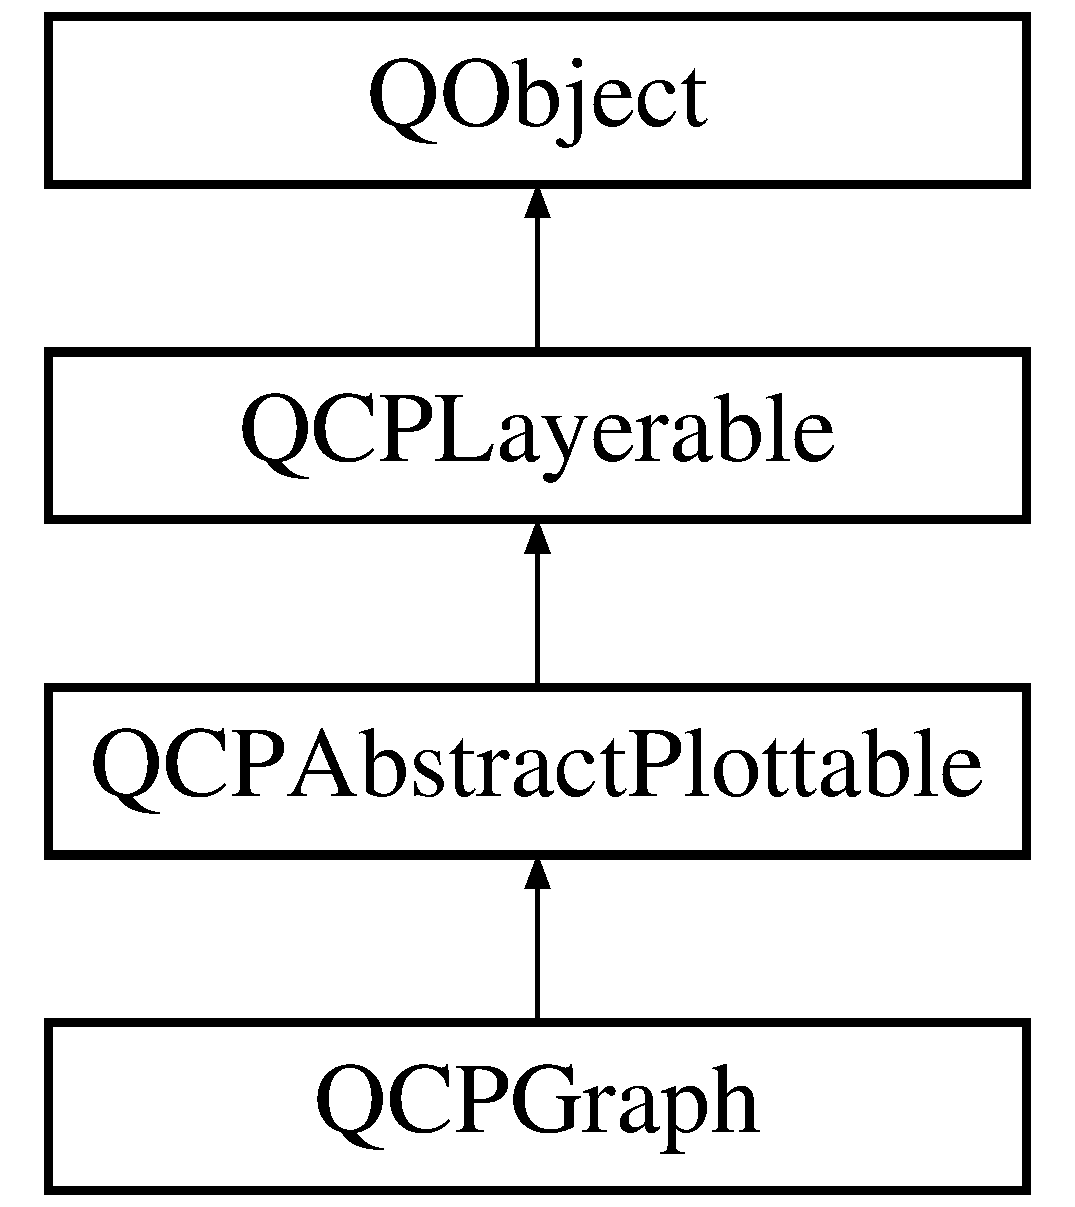
\includegraphics[height=4.000000cm]{class_q_c_p_graph}
\end{center}
\end{figure}
\subsection*{Public Types}
\begin{DoxyCompactItemize}
\item 
enum \hyperlink{class_q_c_p_graph_ad60175cd9b5cac937c5ee685c32c0859}{Line\+Style} \{ \\*
\hyperlink{class_q_c_p_graph_ad60175cd9b5cac937c5ee685c32c0859aea9591b933733cc7b20786b71e60fa04}{ls\+None}, 
\hyperlink{class_q_c_p_graph_ad60175cd9b5cac937c5ee685c32c0859a3c42a27b15aa3c92d399082fad8b7515}{ls\+Line}, 
\hyperlink{class_q_c_p_graph_ad60175cd9b5cac937c5ee685c32c0859ae10568bda57836487d9dec5eba1d6c6e}{ls\+Step\+Left}, 
\hyperlink{class_q_c_p_graph_ad60175cd9b5cac937c5ee685c32c0859a9c37951f7d11aa070100fd16f2935c9e}{ls\+Step\+Right}, 
\\*
\hyperlink{class_q_c_p_graph_ad60175cd9b5cac937c5ee685c32c0859a5adf7b04da215a40a764c21294ea7366}{ls\+Step\+Center}, 
\hyperlink{class_q_c_p_graph_ad60175cd9b5cac937c5ee685c32c0859aa3b358b4ae7cca94aceeb8e529c12ebb}{ls\+Impulse}
 \}
\item 
enum \hyperlink{class_q_c_p_graph_ad23b514404bd2cb3216f57c90904d6af}{Error\+Type} \{ \hyperlink{class_q_c_p_graph_ad23b514404bd2cb3216f57c90904d6afaeae745e7cc1766bb8546e35d4b76a711}{et\+None}, 
\hyperlink{class_q_c_p_graph_ad23b514404bd2cb3216f57c90904d6afa2a5d89cd76fb8b6b18d71b8f6f6c0f43}{et\+Key}, 
\hyperlink{class_q_c_p_graph_ad23b514404bd2cb3216f57c90904d6afa147022ccdc49f6bd48f904cb4f61872e}{et\+Value}, 
\hyperlink{class_q_c_p_graph_ad23b514404bd2cb3216f57c90904d6afa761cb7d61670c1e2efecccd8974409ab}{et\+Both}
 \}
\end{DoxyCompactItemize}
\subsection*{Public Member Functions}
\begin{DoxyCompactItemize}
\item 
\hyperlink{class_q_c_p_graph_a0393a38cf7183cbf46348eb6cf9a5a6c}{Q\+C\+P\+Graph} (\hyperlink{class_q_c_p_axis}{Q\+C\+P\+Axis} $\ast$\hyperlink{class_q_c_p_abstract_plottable_a72c7a09c22963f2c943f07112b311103}{key\+Axis}, \hyperlink{class_q_c_p_axis}{Q\+C\+P\+Axis} $\ast$\hyperlink{class_q_c_p_abstract_plottable_a3106f9d34d330a6097a8ec5905e5b519}{value\+Axis})
\item 
virtual \hyperlink{class_q_c_p_graph_ae9998cfb9d379ac0ef3fbd6995cfbd76}{$\sim$\+Q\+C\+P\+Graph} ()
\item 
\hyperlink{qcustomplot_8h_a84a9c4a4c2216ccfdcb5f3067cda76e3}{Q\+C\+P\+Data\+Map} $\ast$ \hyperlink{class_q_c_p_graph_a2f58436df4f86a2792b776a21642b3d9}{data} () const 
\item 
\hyperlink{class_q_c_p_graph_ad60175cd9b5cac937c5ee685c32c0859}{Line\+Style} \hyperlink{class_q_c_p_graph_ad6db8d31abeac256a285fc68d6b9b9be}{line\+Style} () const 
\item 
\hyperlink{class_q_c_p_scatter_style}{Q\+C\+P\+Scatter\+Style} \hyperlink{class_q_c_p_graph_ae0227c79f4e42a350c2c99fb2fb879db}{scatter\+Style} () const 
\item 
\hyperlink{class_q_c_p_graph_ad23b514404bd2cb3216f57c90904d6af}{Error\+Type} \hyperlink{class_q_c_p_graph_a250bcdf78abac87bc6d46ee6fd99a92d}{error\+Type} () const 
\item 
Q\+Pen \hyperlink{class_q_c_p_graph_a83455e01093bb899f3b59d4a6fdcd57b}{error\+Pen} () const 
\item 
double \hyperlink{class_q_c_p_graph_ae31efdcbc6ba3d73a7aeb83c774f958a}{error\+Bar\+Size} () const 
\item 
bool \hyperlink{class_q_c_p_graph_a04dbc050ff04561658ab1e7f3df37a01}{error\+Bar\+Skip\+Symbol} () const 
\item 
\hyperlink{class_q_c_p_graph}{Q\+C\+P\+Graph} $\ast$ \hyperlink{class_q_c_p_graph_a5369f23863e04a6164f8b66d49fd18f4}{channel\+Fill\+Graph} () const 
\item 
bool \hyperlink{class_q_c_p_graph_ad3bea28ec910eedfa9b788928d610de0}{adaptive\+Sampling} () const 
\item 
void \hyperlink{class_q_c_p_graph_a1df2fd710545c8ba3b2c99a39a27bf8b}{set\+Data} (\hyperlink{qcustomplot_8h_a84a9c4a4c2216ccfdcb5f3067cda76e3}{Q\+C\+P\+Data\+Map} $\ast$\hyperlink{class_q_c_p_graph_a2f58436df4f86a2792b776a21642b3d9}{data}, bool copy=false)
\item 
void \hyperlink{class_q_c_p_graph_a4c55d8ac13bfa42c8c93747820891a76}{set\+Data} (const Q\+Vector$<$ double $>$ \&key, const Q\+Vector$<$ double $>$ \&value)
\item 
void \hyperlink{class_q_c_p_graph_abce9f07c0d722bc3e4fa7bd73c7e5dfa}{set\+Data\+Key\+Error} (const Q\+Vector$<$ double $>$ \&key, const Q\+Vector$<$ double $>$ \&value, const Q\+Vector$<$ double $>$ \&key\+Error)
\item 
void \hyperlink{class_q_c_p_graph_ac15c749c5fedf740d5692c6fe67143b8}{set\+Data\+Key\+Error} (const Q\+Vector$<$ double $>$ \&key, const Q\+Vector$<$ double $>$ \&value, const Q\+Vector$<$ double $>$ \&key\+Error\+Minus, const Q\+Vector$<$ double $>$ \&key\+Error\+Plus)
\item 
void \hyperlink{class_q_c_p_graph_acba6296eadcb36b93267628b8dae3de5}{set\+Data\+Value\+Error} (const Q\+Vector$<$ double $>$ \&key, const Q\+Vector$<$ double $>$ \&value, const Q\+Vector$<$ double $>$ \&value\+Error)
\item 
void \hyperlink{class_q_c_p_graph_a3afbfd7222d739351c69387904776f93}{set\+Data\+Value\+Error} (const Q\+Vector$<$ double $>$ \&key, const Q\+Vector$<$ double $>$ \&value, const Q\+Vector$<$ double $>$ \&value\+Error\+Minus, const Q\+Vector$<$ double $>$ \&value\+Error\+Plus)
\item 
void \hyperlink{class_q_c_p_graph_a873fe46bdb20be5710428e474ade8908}{set\+Data\+Both\+Error} (const Q\+Vector$<$ double $>$ \&key, const Q\+Vector$<$ double $>$ \&value, const Q\+Vector$<$ double $>$ \&key\+Error, const Q\+Vector$<$ double $>$ \&value\+Error)
\item 
void \hyperlink{class_q_c_p_graph_abb75736ecdbf6e6a7501e1da64fb18cf}{set\+Data\+Both\+Error} (const Q\+Vector$<$ double $>$ \&key, const Q\+Vector$<$ double $>$ \&value, const Q\+Vector$<$ double $>$ \&key\+Error\+Minus, const Q\+Vector$<$ double $>$ \&key\+Error\+Plus, const Q\+Vector$<$ double $>$ \&value\+Error\+Minus, const Q\+Vector$<$ double $>$ \&value\+Error\+Plus)
\item 
void \hyperlink{class_q_c_p_graph_a513fecccff5b2a50ce53f665338c60ff}{set\+Line\+Style} (\hyperlink{class_q_c_p_graph_ad60175cd9b5cac937c5ee685c32c0859}{Line\+Style} ls)
\item 
void \hyperlink{class_q_c_p_graph_a12bd17a8ba21983163ec5d8f42a9fea5}{set\+Scatter\+Style} (const \hyperlink{class_q_c_p_scatter_style}{Q\+C\+P\+Scatter\+Style} \&style)
\item 
void \hyperlink{class_q_c_p_graph_ac3614d799c3894f2bc646e99c7f73d38}{set\+Error\+Type} (\hyperlink{class_q_c_p_graph_ad23b514404bd2cb3216f57c90904d6af}{Error\+Type} \hyperlink{class_q_c_p_graph_a250bcdf78abac87bc6d46ee6fd99a92d}{error\+Type})
\item 
void \hyperlink{class_q_c_p_graph_abd4c7f81939e10776ea64603a704f22a}{set\+Error\+Pen} (const Q\+Pen \&\hyperlink{class_q_c_p_abstract_plottable_a41d060007cc6b3037c9c04d22d0c0398}{pen})
\item 
void \hyperlink{class_q_c_p_graph_a10f50c5495ce45ef559ec2066194a335}{set\+Error\+Bar\+Size} (double size)
\item 
void \hyperlink{class_q_c_p_graph_ab1c1ee03d8dd94676a564e5e5f11aac2}{set\+Error\+Bar\+Skip\+Symbol} (bool enabled)
\item 
void \hyperlink{class_q_c_p_graph_a2d03156df1b64037a2e36cfa50351ca3}{set\+Channel\+Fill\+Graph} (\hyperlink{class_q_c_p_graph}{Q\+C\+P\+Graph} $\ast$target\+Graph)
\item 
void \hyperlink{class_q_c_p_graph_ab468cd600160f327836aa0644291e64c}{set\+Adaptive\+Sampling} (bool enabled)
\item 
void \hyperlink{class_q_c_p_graph_aa5c6181d84db72ce4dbe9dc15a34ef4f}{add\+Data} (const \hyperlink{qcustomplot_8h_a84a9c4a4c2216ccfdcb5f3067cda76e3}{Q\+C\+P\+Data\+Map} \&data\+Map)
\item 
void \hyperlink{class_q_c_p_graph_a80cc91e1e0ef77eb50afc5b366d0efd9}{add\+Data} (const \hyperlink{class_q_c_p_data}{Q\+C\+P\+Data} \&\hyperlink{class_q_c_p_graph_a2f58436df4f86a2792b776a21642b3d9}{data})
\item 
void \hyperlink{class_q_c_p_graph_a0bf98b1972286cfb7b1c4b7dd6ae2012}{add\+Data} (double key, double value)
\item 
void \hyperlink{class_q_c_p_graph_ab6da6377541fe80d892a9893a92db9c6}{add\+Data} (const Q\+Vector$<$ double $>$ \&keys, const Q\+Vector$<$ double $>$ \&values)
\item 
void \hyperlink{class_q_c_p_graph_a9fe0b3e54e8c7b61319bd03337e21e99}{remove\+Data\+Before} (double key)
\item 
void \hyperlink{class_q_c_p_graph_ae42d645ef617cfc75fc0df58e62c522a}{remove\+Data\+After} (double key)
\item 
void \hyperlink{class_q_c_p_graph_a4a0fde50b7db9db0a85b5c5b6b10098f}{remove\+Data} (double from\+Key, double to\+Key)
\item 
void \hyperlink{class_q_c_p_graph_a4a706020b4318f118381648ef18aca3f}{remove\+Data} (double key)
\item 
virtual void \hyperlink{class_q_c_p_graph_ad4e94a4e44e5e76fbec81a72a977157d}{clear\+Data} ()
\item 
virtual double \hyperlink{class_q_c_p_graph_abc9ff375aabcf2d21cca33d6baf85772}{select\+Test} (const Q\+Point\+F \&pos, bool only\+Selectable, Q\+Variant $\ast$details=0) const 
\item 
void \hyperlink{class_q_c_p_graph_aa35b75b9032800d783df749c8a004ee9}{rescale\+Axes} (bool only\+Enlarge, bool include\+Error\+Bars) const 
\item 
void \hyperlink{class_q_c_p_graph_a2108a729046b0ab6e0516afb249dab13}{rescale\+Key\+Axis} (bool only\+Enlarge, bool include\+Error\+Bars) const 
\item 
void \hyperlink{class_q_c_p_graph_a2ba0e1df416486d7e74299ef8cf68bba}{rescale\+Value\+Axis} (bool only\+Enlarge, bool include\+Error\+Bars) const 
\end{DoxyCompactItemize}
\subsection*{Protected Member Functions}
\begin{DoxyCompactItemize}
\item 
virtual void \hyperlink{class_q_c_p_graph_a659218cc62c2a7786213d9dd429c1c8d}{draw} (\hyperlink{class_q_c_p_painter}{Q\+C\+P\+Painter} $\ast$painter)
\item 
virtual void \hyperlink{class_q_c_p_graph_a32115df0e940cf8ca7b687873c2d02ee}{draw\+Legend\+Icon} (\hyperlink{class_q_c_p_painter}{Q\+C\+P\+Painter} $\ast$painter, const Q\+Rect\+F \&rect) const 
\item 
virtual \hyperlink{class_q_c_p_range}{Q\+C\+P\+Range} \hyperlink{class_q_c_p_graph_afc246ce6201ff564ac440efaec52ab11}{get\+Key\+Range} (bool \&found\+Range, \hyperlink{class_q_c_p_abstract_plottable_a661743478a1d3c09d28ec2711d7653d8}{Sign\+Domain} in\+Sign\+Domain=\hyperlink{class_q_c_p_abstract_plottable_a661743478a1d3c09d28ec2711d7653d8a082b98cfb91a7363a3b5cd17b0c1cd60}{sd\+Both}) const 
\item 
virtual \hyperlink{class_q_c_p_range}{Q\+C\+P\+Range} \hyperlink{class_q_c_p_graph_a856e90b8ab6b31c344b14a863ab9e5d2}{get\+Value\+Range} (bool \&found\+Range, \hyperlink{class_q_c_p_abstract_plottable_a661743478a1d3c09d28ec2711d7653d8}{Sign\+Domain} in\+Sign\+Domain=\hyperlink{class_q_c_p_abstract_plottable_a661743478a1d3c09d28ec2711d7653d8a082b98cfb91a7363a3b5cd17b0c1cd60}{sd\+Both}) const 
\item 
virtual \hyperlink{class_q_c_p_range}{Q\+C\+P\+Range} \hyperlink{class_q_c_p_graph_aa75c6f028124032416a5cf7145dfba60}{get\+Key\+Range} (bool \&found\+Range, \hyperlink{class_q_c_p_abstract_plottable_a661743478a1d3c09d28ec2711d7653d8}{Sign\+Domain} in\+Sign\+Domain, bool include\+Errors) const 
\item 
virtual \hyperlink{class_q_c_p_range}{Q\+C\+P\+Range} \hyperlink{class_q_c_p_graph_ab964a21d680af93435d68126d8c5ab29}{get\+Value\+Range} (bool \&found\+Range, \hyperlink{class_q_c_p_abstract_plottable_a661743478a1d3c09d28ec2711d7653d8}{Sign\+Domain} in\+Sign\+Domain, bool include\+Errors) const 
\item 
virtual void \hyperlink{class_q_c_p_graph_ad6d07926e6d6b7cfa70258780d47b7a0}{draw\+Fill} (\hyperlink{class_q_c_p_painter}{Q\+C\+P\+Painter} $\ast$painter, Q\+Vector$<$ Q\+Point\+F $>$ $\ast$line\+Data) const 
\item 
virtual void \hyperlink{class_q_c_p_graph_a6bdc385b122ce06134d4196373ae2250}{draw\+Scatter\+Plot} (\hyperlink{class_q_c_p_painter}{Q\+C\+P\+Painter} $\ast$painter, Q\+Vector$<$ \hyperlink{class_q_c_p_data}{Q\+C\+P\+Data} $>$ $\ast$scatter\+Data) const 
\item 
virtual void \hyperlink{class_q_c_p_graph_acebc22c3385829b19a87e6281fe6ade2}{draw\+Line\+Plot} (\hyperlink{class_q_c_p_painter}{Q\+C\+P\+Painter} $\ast$painter, Q\+Vector$<$ Q\+Point\+F $>$ $\ast$line\+Data) const 
\item 
virtual void \hyperlink{class_q_c_p_graph_abc01180629621f1e47e94559227d3d8c}{draw\+Impulse\+Plot} (\hyperlink{class_q_c_p_painter}{Q\+C\+P\+Painter} $\ast$painter, Q\+Vector$<$ Q\+Point\+F $>$ $\ast$line\+Data) const 
\item 
void \hyperlink{class_q_c_p_graph_ab420b46ba638dc3252439fe16687b244}{get\+Prepared\+Data} (Q\+Vector$<$ \hyperlink{class_q_c_p_data}{Q\+C\+P\+Data} $>$ $\ast$line\+Data, Q\+Vector$<$ \hyperlink{class_q_c_p_data}{Q\+C\+P\+Data} $>$ $\ast$scatter\+Data) const 
\item 
void \hyperlink{class_q_c_p_graph_a466c661e015188971c862031af946693}{get\+Plot\+Data} (Q\+Vector$<$ Q\+Point\+F $>$ $\ast$line\+Data, Q\+Vector$<$ \hyperlink{class_q_c_p_data}{Q\+C\+P\+Data} $>$ $\ast$scatter\+Data) const 
\item 
void \hyperlink{class_q_c_p_graph_a45c4214b59ea11aa6d8d112bdc3b0e03}{get\+Scatter\+Plot\+Data} (Q\+Vector$<$ \hyperlink{class_q_c_p_data}{Q\+C\+P\+Data} $>$ $\ast$scatter\+Data) const 
\item 
void \hyperlink{class_q_c_p_graph_ae3d82ffd0c9a883482aabf47b0e6b5ee}{get\+Line\+Plot\+Data} (Q\+Vector$<$ Q\+Point\+F $>$ $\ast$line\+Pixel\+Data, Q\+Vector$<$ \hyperlink{class_q_c_p_data}{Q\+C\+P\+Data} $>$ $\ast$scatter\+Data) const 
\item 
void \hyperlink{class_q_c_p_graph_a609cf4a78045b4d2a679bdff7623847e}{get\+Step\+Left\+Plot\+Data} (Q\+Vector$<$ Q\+Point\+F $>$ $\ast$line\+Pixel\+Data, Q\+Vector$<$ \hyperlink{class_q_c_p_data}{Q\+C\+P\+Data} $>$ $\ast$scatter\+Data) const 
\item 
void \hyperlink{class_q_c_p_graph_a3b9b8c8dc7a6fd9be6e253c25ee31809}{get\+Step\+Right\+Plot\+Data} (Q\+Vector$<$ Q\+Point\+F $>$ $\ast$line\+Pixel\+Data, Q\+Vector$<$ \hyperlink{class_q_c_p_data}{Q\+C\+P\+Data} $>$ $\ast$scatter\+Data) const 
\item 
void \hyperlink{class_q_c_p_graph_ad3713e7d8eb85a0afc34a81a5db5cd27}{get\+Step\+Center\+Plot\+Data} (Q\+Vector$<$ Q\+Point\+F $>$ $\ast$line\+Pixel\+Data, Q\+Vector$<$ \hyperlink{class_q_c_p_data}{Q\+C\+P\+Data} $>$ $\ast$scatter\+Data) const 
\item 
void \hyperlink{class_q_c_p_graph_a1ca2b0762505767f116892609fb02062}{get\+Impulse\+Plot\+Data} (Q\+Vector$<$ Q\+Point\+F $>$ $\ast$line\+Pixel\+Data, Q\+Vector$<$ \hyperlink{class_q_c_p_data}{Q\+C\+P\+Data} $>$ $\ast$scatter\+Data) const 
\item 
void \hyperlink{class_q_c_p_graph_a4df6807066ce877705e999773e7ffbc4}{draw\+Error} (\hyperlink{class_q_c_p_painter}{Q\+C\+P\+Painter} $\ast$painter, double x, double y, const \hyperlink{class_q_c_p_data}{Q\+C\+P\+Data} \&\hyperlink{class_q_c_p_graph_a2f58436df4f86a2792b776a21642b3d9}{data}) const 
\item 
void \hyperlink{class_q_c_p_graph_a6a317cb14a83dae0841c7041a63d6d9d}{get\+Visible\+Data\+Bounds} (Q\+C\+P\+Data\+Map\+::const\+\_\+iterator \&lower, Q\+C\+P\+Data\+Map\+::const\+\_\+iterator \&upper) const 
\item 
int \hyperlink{class_q_c_p_graph_a13f6a3aa60227e03ab1f7aa8eec6589f}{count\+Data\+In\+Bounds} (const Q\+C\+P\+Data\+Map\+::const\+\_\+iterator \&lower, const Q\+C\+P\+Data\+Map\+::const\+\_\+iterator \&upper, int max\+Count) const 
\item 
void \hyperlink{class_q_c_p_graph_a5fa7884620d7c54b81dfbd255d97b636}{add\+Fill\+Base\+Points} (Q\+Vector$<$ Q\+Point\+F $>$ $\ast$line\+Data) const 
\item 
void \hyperlink{class_q_c_p_graph_ad31b49a90e91e538fd9caf011c913a68}{remove\+Fill\+Base\+Points} (Q\+Vector$<$ Q\+Point\+F $>$ $\ast$line\+Data) const 
\item 
Q\+Point\+F \hyperlink{class_q_c_p_graph_a41f982e8ceaefe6a53eb7432f26d64b6}{lower\+Fill\+Base\+Point} (double lower\+Key) const 
\item 
Q\+Point\+F \hyperlink{class_q_c_p_graph_a363d066c179e0f46cc93c12bafb0bfba}{upper\+Fill\+Base\+Point} (double upper\+Key) const 
\item 
const Q\+Polygon\+F \hyperlink{class_q_c_p_graph_a0374b7268e35cab9802a6be2b5d726d7}{get\+Channel\+Fill\+Polygon} (const Q\+Vector$<$ Q\+Point\+F $>$ $\ast$line\+Data) const 
\item 
int \hyperlink{class_q_c_p_graph_a6f4e9461d5925be9228fc4760249a04f}{find\+Index\+Below\+X} (const Q\+Vector$<$ Q\+Point\+F $>$ $\ast$\hyperlink{class_q_c_p_graph_a2f58436df4f86a2792b776a21642b3d9}{data}, double x) const 
\item 
int \hyperlink{class_q_c_p_graph_abab2a75b5e63630432bdd1f3b57f07fa}{find\+Index\+Above\+X} (const Q\+Vector$<$ Q\+Point\+F $>$ $\ast$\hyperlink{class_q_c_p_graph_a2f58436df4f86a2792b776a21642b3d9}{data}, double x) const 
\item 
int \hyperlink{class_q_c_p_graph_a6c4d556de3d1e02f548401001f72c6ff}{find\+Index\+Below\+Y} (const Q\+Vector$<$ Q\+Point\+F $>$ $\ast$\hyperlink{class_q_c_p_graph_a2f58436df4f86a2792b776a21642b3d9}{data}, double y) const 
\item 
int \hyperlink{class_q_c_p_graph_adf50243f1df203883a2187089734bfcb}{find\+Index\+Above\+Y} (const Q\+Vector$<$ Q\+Point\+F $>$ $\ast$\hyperlink{class_q_c_p_graph_a2f58436df4f86a2792b776a21642b3d9}{data}, double y) const 
\item 
double \hyperlink{class_q_c_p_graph_af93762a12a481a7edb4b3dd9e330dff1}{point\+Distance} (const Q\+Point\+F \&pixel\+Point) const 
\end{DoxyCompactItemize}
\subsection*{Protected Attributes}
\begin{DoxyCompactItemize}
\item 
\hyperlink{qcustomplot_8h_a84a9c4a4c2216ccfdcb5f3067cda76e3}{Q\+C\+P\+Data\+Map} $\ast$ \hyperlink{class_q_c_p_graph_a8457c840f69a0ac49f61d30a509c5d08}{m\+Data}
\item 
Q\+Pen \hyperlink{class_q_c_p_graph_aa35681a24165c2831301091a87b662ce}{m\+Error\+Pen}
\item 
\hyperlink{class_q_c_p_graph_ad60175cd9b5cac937c5ee685c32c0859}{Line\+Style} \hyperlink{class_q_c_p_graph_a8604fd98402035a63375849f7341ee25}{m\+Line\+Style}
\item 
\hyperlink{class_q_c_p_scatter_style}{Q\+C\+P\+Scatter\+Style} \hyperlink{class_q_c_p_graph_a4aa36241f166ccd1f75fc8f24e4a3247}{m\+Scatter\+Style}
\item 
\hyperlink{class_q_c_p_graph_ad23b514404bd2cb3216f57c90904d6af}{Error\+Type} \hyperlink{class_q_c_p_graph_a29e64273db201aeadebc61c870720a36}{m\+Error\+Type}
\item 
double \hyperlink{class_q_c_p_graph_a7b51c8d09510f9d195b5e765ccbcf05b}{m\+Error\+Bar\+Size}
\item 
bool \hyperlink{class_q_c_p_graph_acf631d7dbd1055a69ab3b63094868557}{m\+Error\+Bar\+Skip\+Symbol}
\item 
Q\+Pointer$<$ \hyperlink{class_q_c_p_graph}{Q\+C\+P\+Graph} $>$ \hyperlink{class_q_c_p_graph_a2f1777c7accf8244fc640c33f0b04577}{m\+Channel\+Fill\+Graph}
\item 
bool \hyperlink{class_q_c_p_graph_aa951e78aeba714cf443be6da2e52502e}{m\+Adaptive\+Sampling}
\end{DoxyCompactItemize}
\subsection*{Friends}
\begin{DoxyCompactItemize}
\item 
class \hyperlink{class_q_c_p_graph_a1cdf9df76adcfae45261690aa0ca2198}{Q\+Custom\+Plot}
\item 
class \hyperlink{class_q_c_p_graph_a8429035e7adfbd7f05805a6530ad5e3b}{Q\+C\+P\+Legend}
\end{DoxyCompactItemize}
\subsection*{Additional Inherited Members}


\subsection{Detailed Description}
A plottable representing a graph in a plot. 



Usually \hyperlink{class_q_custom_plot}{Q\+Custom\+Plot} creates graphs internally via \hyperlink{class_q_custom_plot_a6fb2873d35a8a8089842d81a70a54167}{Q\+Custom\+Plot\+::add\+Graph} and the resulting instance is accessed via \hyperlink{class_q_custom_plot_a6d3ed93c2bf46ab7fa670d66be4cddaf}{Q\+Custom\+Plot\+::graph}.

To plot data, assign it with the \hyperlink{class_q_c_p_graph_a1df2fd710545c8ba3b2c99a39a27bf8b}{set\+Data} or \hyperlink{class_q_c_p_graph_aa5c6181d84db72ce4dbe9dc15a34ef4f}{add\+Data} functions. Alternatively, you can also access and modify the graph\textquotesingle{}s data via the \hyperlink{class_q_c_p_graph_a2f58436df4f86a2792b776a21642b3d9}{data} method, which returns a pointer to the internal \hyperlink{qcustomplot_8h_a84a9c4a4c2216ccfdcb5f3067cda76e3}{Q\+C\+P\+Data\+Map}.

Graphs are used to display single-\/valued data. Single-\/valued means that there should only be one data point per unique key coordinate. In other words, the graph can\textquotesingle{}t have {\itshape loops}. If you do want to plot non-\/single-\/valued curves, rather use the \hyperlink{class_q_c_p_curve}{Q\+C\+P\+Curve} plottable.\hypertarget{class_q_c_p_statistical_box_appearance}{}\subsection{Changing the appearance}\label{class_q_c_p_statistical_box_appearance}
The appearance of the graph is mainly determined by the line style, scatter style, brush and pen of the graph (\hyperlink{class_q_c_p_graph_a513fecccff5b2a50ce53f665338c60ff}{set\+Line\+Style}, \hyperlink{class_q_c_p_graph_a12bd17a8ba21983163ec5d8f42a9fea5}{set\+Scatter\+Style}, \hyperlink{class_q_c_p_abstract_plottable_a7a4b92144dca6453a1f0f210e27edc74}{set\+Brush}, \hyperlink{class_q_c_p_abstract_plottable_ab74b09ae4c0e7e13142fe4b5bf46cac7}{set\+Pen}).\hypertarget{class_q_c_p_graph_filling}{}\subsubsection{Filling under or between graphs}\label{class_q_c_p_graph_filling}
\hyperlink{class_q_c_p_graph}{Q\+C\+P\+Graph} knows two types of fills\+: Normal graph fills towards the zero-\/value-\/line parallel to the key axis of the graph, and fills between two graphs, called channel fills. To enable a fill, just set a brush with \hyperlink{class_q_c_p_abstract_plottable_a7a4b92144dca6453a1f0f210e27edc74}{set\+Brush} which is neither Qt\+::\+No\+Brush nor fully transparent.

By default, a normal fill towards the zero-\/value-\/line will be drawn. To set up a channel fill between this graph and another one, call \hyperlink{class_q_c_p_graph_a2d03156df1b64037a2e36cfa50351ca3}{set\+Channel\+Fill\+Graph} with the other graph as parameter.

\begin{DoxySeeAlso}{See also}
\hyperlink{class_q_custom_plot_a6fb2873d35a8a8089842d81a70a54167}{Q\+Custom\+Plot\+::add\+Graph}, \hyperlink{class_q_custom_plot_a6d3ed93c2bf46ab7fa670d66be4cddaf}{Q\+Custom\+Plot\+::graph}, Q\+C\+P\+Legend\+::add\+Graph 
\end{DoxySeeAlso}


\subsection{Member Enumeration Documentation}
\hypertarget{class_q_c_p_graph_ad23b514404bd2cb3216f57c90904d6af}{}\index{Q\+C\+P\+Graph@{Q\+C\+P\+Graph}!Error\+Type@{Error\+Type}}
\index{Error\+Type@{Error\+Type}!Q\+C\+P\+Graph@{Q\+C\+P\+Graph}}
\subsubsection[{Error\+Type}]{\setlength{\rightskip}{0pt plus 5cm}enum {\bf Q\+C\+P\+Graph\+::\+Error\+Type}}\label{class_q_c_p_graph_ad23b514404bd2cb3216f57c90904d6af}
Defines what kind of error bars are drawn for each data point \begin{Desc}
\item[Enumerator]\par
\begin{description}
\index{et\+None@{et\+None}!Q\+C\+P\+Graph@{Q\+C\+P\+Graph}}\index{Q\+C\+P\+Graph@{Q\+C\+P\+Graph}!et\+None@{et\+None}}\item[{\em 
\hypertarget{class_q_c_p_graph_ad23b514404bd2cb3216f57c90904d6afaeae745e7cc1766bb8546e35d4b76a711}{}et\+None\label{class_q_c_p_graph_ad23b514404bd2cb3216f57c90904d6afaeae745e7cc1766bb8546e35d4b76a711}
}]No error bars are shown. \index{et\+Key@{et\+Key}!Q\+C\+P\+Graph@{Q\+C\+P\+Graph}}\index{Q\+C\+P\+Graph@{Q\+C\+P\+Graph}!et\+Key@{et\+Key}}\item[{\em 
\hypertarget{class_q_c_p_graph_ad23b514404bd2cb3216f57c90904d6afa2a5d89cd76fb8b6b18d71b8f6f6c0f43}{}et\+Key\label{class_q_c_p_graph_ad23b514404bd2cb3216f57c90904d6afa2a5d89cd76fb8b6b18d71b8f6f6c0f43}
}]Error bars for the key dimension of the data point are shown. \index{et\+Value@{et\+Value}!Q\+C\+P\+Graph@{Q\+C\+P\+Graph}}\index{Q\+C\+P\+Graph@{Q\+C\+P\+Graph}!et\+Value@{et\+Value}}\item[{\em 
\hypertarget{class_q_c_p_graph_ad23b514404bd2cb3216f57c90904d6afa147022ccdc49f6bd48f904cb4f61872e}{}et\+Value\label{class_q_c_p_graph_ad23b514404bd2cb3216f57c90904d6afa147022ccdc49f6bd48f904cb4f61872e}
}]Error bars for the value dimension of the data point are shown. \index{et\+Both@{et\+Both}!Q\+C\+P\+Graph@{Q\+C\+P\+Graph}}\index{Q\+C\+P\+Graph@{Q\+C\+P\+Graph}!et\+Both@{et\+Both}}\item[{\em 
\hypertarget{class_q_c_p_graph_ad23b514404bd2cb3216f57c90904d6afa761cb7d61670c1e2efecccd8974409ab}{}et\+Both\label{class_q_c_p_graph_ad23b514404bd2cb3216f57c90904d6afa761cb7d61670c1e2efecccd8974409ab}
}]Error bars for both key and value dimensions of the data point are shown. \end{description}
\end{Desc}
\hypertarget{class_q_c_p_graph_ad60175cd9b5cac937c5ee685c32c0859}{}\index{Q\+C\+P\+Graph@{Q\+C\+P\+Graph}!Line\+Style@{Line\+Style}}
\index{Line\+Style@{Line\+Style}!Q\+C\+P\+Graph@{Q\+C\+P\+Graph}}
\subsubsection[{Line\+Style}]{\setlength{\rightskip}{0pt plus 5cm}enum {\bf Q\+C\+P\+Graph\+::\+Line\+Style}}\label{class_q_c_p_graph_ad60175cd9b5cac937c5ee685c32c0859}
Defines how the graph\textquotesingle{}s line is represented visually in the plot. The line is drawn with the current pen of the graph (\hyperlink{class_q_c_p_abstract_plottable_ab74b09ae4c0e7e13142fe4b5bf46cac7}{set\+Pen}). \begin{DoxySeeAlso}{See also}
\hyperlink{class_q_c_p_graph_a513fecccff5b2a50ce53f665338c60ff}{set\+Line\+Style} 
\end{DoxySeeAlso}
\begin{Desc}
\item[Enumerator]\par
\begin{description}
\index{ls\+None@{ls\+None}!Q\+C\+P\+Graph@{Q\+C\+P\+Graph}}\index{Q\+C\+P\+Graph@{Q\+C\+P\+Graph}!ls\+None@{ls\+None}}\item[{\em 
\hypertarget{class_q_c_p_graph_ad60175cd9b5cac937c5ee685c32c0859aea9591b933733cc7b20786b71e60fa04}{}ls\+None\label{class_q_c_p_graph_ad60175cd9b5cac937c5ee685c32c0859aea9591b933733cc7b20786b71e60fa04}
}]data points are not connected with any lines (e.\+g. data only represented with symbols according to the scatter style, see \hyperlink{class_q_c_p_graph_a12bd17a8ba21983163ec5d8f42a9fea5}{set\+Scatter\+Style}) \index{ls\+Line@{ls\+Line}!Q\+C\+P\+Graph@{Q\+C\+P\+Graph}}\index{Q\+C\+P\+Graph@{Q\+C\+P\+Graph}!ls\+Line@{ls\+Line}}\item[{\em 
\hypertarget{class_q_c_p_graph_ad60175cd9b5cac937c5ee685c32c0859a3c42a27b15aa3c92d399082fad8b7515}{}ls\+Line\label{class_q_c_p_graph_ad60175cd9b5cac937c5ee685c32c0859a3c42a27b15aa3c92d399082fad8b7515}
}]data points are connected by a straight line \index{ls\+Step\+Left@{ls\+Step\+Left}!Q\+C\+P\+Graph@{Q\+C\+P\+Graph}}\index{Q\+C\+P\+Graph@{Q\+C\+P\+Graph}!ls\+Step\+Left@{ls\+Step\+Left}}\item[{\em 
\hypertarget{class_q_c_p_graph_ad60175cd9b5cac937c5ee685c32c0859ae10568bda57836487d9dec5eba1d6c6e}{}ls\+Step\+Left\label{class_q_c_p_graph_ad60175cd9b5cac937c5ee685c32c0859ae10568bda57836487d9dec5eba1d6c6e}
}]line is drawn as steps where the step height is the value of the left data point \index{ls\+Step\+Right@{ls\+Step\+Right}!Q\+C\+P\+Graph@{Q\+C\+P\+Graph}}\index{Q\+C\+P\+Graph@{Q\+C\+P\+Graph}!ls\+Step\+Right@{ls\+Step\+Right}}\item[{\em 
\hypertarget{class_q_c_p_graph_ad60175cd9b5cac937c5ee685c32c0859a9c37951f7d11aa070100fd16f2935c9e}{}ls\+Step\+Right\label{class_q_c_p_graph_ad60175cd9b5cac937c5ee685c32c0859a9c37951f7d11aa070100fd16f2935c9e}
}]line is drawn as steps where the step height is the value of the right data point \index{ls\+Step\+Center@{ls\+Step\+Center}!Q\+C\+P\+Graph@{Q\+C\+P\+Graph}}\index{Q\+C\+P\+Graph@{Q\+C\+P\+Graph}!ls\+Step\+Center@{ls\+Step\+Center}}\item[{\em 
\hypertarget{class_q_c_p_graph_ad60175cd9b5cac937c5ee685c32c0859a5adf7b04da215a40a764c21294ea7366}{}ls\+Step\+Center\label{class_q_c_p_graph_ad60175cd9b5cac937c5ee685c32c0859a5adf7b04da215a40a764c21294ea7366}
}]line is drawn as steps where the step is in between two data points \index{ls\+Impulse@{ls\+Impulse}!Q\+C\+P\+Graph@{Q\+C\+P\+Graph}}\index{Q\+C\+P\+Graph@{Q\+C\+P\+Graph}!ls\+Impulse@{ls\+Impulse}}\item[{\em 
\hypertarget{class_q_c_p_graph_ad60175cd9b5cac937c5ee685c32c0859aa3b358b4ae7cca94aceeb8e529c12ebb}{}ls\+Impulse\label{class_q_c_p_graph_ad60175cd9b5cac937c5ee685c32c0859aa3b358b4ae7cca94aceeb8e529c12ebb}
}]each data point is represented by a line parallel to the value axis, which reaches from the data point to the zero-\/value-\/line \end{description}
\end{Desc}


\subsection{Constructor \& Destructor Documentation}
\hypertarget{class_q_c_p_graph_a0393a38cf7183cbf46348eb6cf9a5a6c}{}\index{Q\+C\+P\+Graph@{Q\+C\+P\+Graph}!Q\+C\+P\+Graph@{Q\+C\+P\+Graph}}
\index{Q\+C\+P\+Graph@{Q\+C\+P\+Graph}!Q\+C\+P\+Graph@{Q\+C\+P\+Graph}}
\subsubsection[{Q\+C\+P\+Graph}]{\setlength{\rightskip}{0pt plus 5cm}Q\+C\+P\+Graph\+::\+Q\+C\+P\+Graph (
\begin{DoxyParamCaption}
\item[{{\bf Q\+C\+P\+Axis} $\ast$}]{key\+Axis, }
\item[{{\bf Q\+C\+P\+Axis} $\ast$}]{value\+Axis}
\end{DoxyParamCaption}
)\hspace{0.3cm}{\ttfamily [explicit]}}\label{class_q_c_p_graph_a0393a38cf7183cbf46348eb6cf9a5a6c}
Constructs a graph which uses {\itshape key\+Axis} as its key axis (\char`\"{}x\char`\"{}) and {\itshape value\+Axis} as its value axis (\char`\"{}y\char`\"{}). {\itshape key\+Axis} and {\itshape value\+Axis} must reside in the same \hyperlink{class_q_custom_plot}{Q\+Custom\+Plot} instance and not have the same orientation. If either of these restrictions is violated, a corresponding message is printed to the debug output (q\+Debug), the construction is not aborted, though.

The constructed \hyperlink{class_q_c_p_graph}{Q\+C\+P\+Graph} can be added to the plot with \hyperlink{class_q_custom_plot_ab7ad9174f701f9c6f64e378df77927a6}{Q\+Custom\+Plot\+::add\+Plottable}, \hyperlink{class_q_custom_plot}{Q\+Custom\+Plot} then takes ownership of the graph.

To directly create a graph inside a plot, you can also use the simpler \hyperlink{class_q_custom_plot_a6fb2873d35a8a8089842d81a70a54167}{Q\+Custom\+Plot\+::add\+Graph} function. \hypertarget{class_q_c_p_graph_ae9998cfb9d379ac0ef3fbd6995cfbd76}{}\index{Q\+C\+P\+Graph@{Q\+C\+P\+Graph}!````~Q\+C\+P\+Graph@{$\sim$\+Q\+C\+P\+Graph}}
\index{````~Q\+C\+P\+Graph@{$\sim$\+Q\+C\+P\+Graph}!Q\+C\+P\+Graph@{Q\+C\+P\+Graph}}
\subsubsection[{$\sim$\+Q\+C\+P\+Graph}]{\setlength{\rightskip}{0pt plus 5cm}Q\+C\+P\+Graph\+::$\sim$\+Q\+C\+P\+Graph (
\begin{DoxyParamCaption}
{}
\end{DoxyParamCaption}
)\hspace{0.3cm}{\ttfamily [virtual]}}\label{class_q_c_p_graph_ae9998cfb9d379ac0ef3fbd6995cfbd76}


\subsection{Member Function Documentation}
\hypertarget{class_q_c_p_graph_ad3bea28ec910eedfa9b788928d610de0}{}\index{Q\+C\+P\+Graph@{Q\+C\+P\+Graph}!adaptive\+Sampling@{adaptive\+Sampling}}
\index{adaptive\+Sampling@{adaptive\+Sampling}!Q\+C\+P\+Graph@{Q\+C\+P\+Graph}}
\subsubsection[{adaptive\+Sampling}]{\setlength{\rightskip}{0pt plus 5cm}bool Q\+C\+P\+Graph\+::adaptive\+Sampling (
\begin{DoxyParamCaption}
{}
\end{DoxyParamCaption}
) const\hspace{0.3cm}{\ttfamily [inline]}}\label{class_q_c_p_graph_ad3bea28ec910eedfa9b788928d610de0}
\hypertarget{class_q_c_p_graph_aa5c6181d84db72ce4dbe9dc15a34ef4f}{}\index{Q\+C\+P\+Graph@{Q\+C\+P\+Graph}!add\+Data@{add\+Data}}
\index{add\+Data@{add\+Data}!Q\+C\+P\+Graph@{Q\+C\+P\+Graph}}
\subsubsection[{add\+Data}]{\setlength{\rightskip}{0pt plus 5cm}void Q\+C\+P\+Graph\+::add\+Data (
\begin{DoxyParamCaption}
\item[{const {\bf Q\+C\+P\+Data\+Map} \&}]{data\+Map}
\end{DoxyParamCaption}
)}\label{class_q_c_p_graph_aa5c6181d84db72ce4dbe9dc15a34ef4f}
Adds the provided data points in {\itshape data\+Map} to the current data.

Alternatively, you can also access and modify the graph\textquotesingle{}s data via the \hyperlink{class_q_c_p_graph_a2f58436df4f86a2792b776a21642b3d9}{data} method, which returns a pointer to the internal \hyperlink{qcustomplot_8h_a84a9c4a4c2216ccfdcb5f3067cda76e3}{Q\+C\+P\+Data\+Map}.

\begin{DoxySeeAlso}{See also}
\hyperlink{class_q_c_p_graph_a4a0fde50b7db9db0a85b5c5b6b10098f}{remove\+Data} 
\end{DoxySeeAlso}
\hypertarget{class_q_c_p_graph_a80cc91e1e0ef77eb50afc5b366d0efd9}{}\index{Q\+C\+P\+Graph@{Q\+C\+P\+Graph}!add\+Data@{add\+Data}}
\index{add\+Data@{add\+Data}!Q\+C\+P\+Graph@{Q\+C\+P\+Graph}}
\subsubsection[{add\+Data}]{\setlength{\rightskip}{0pt plus 5cm}void Q\+C\+P\+Graph\+::add\+Data (
\begin{DoxyParamCaption}
\item[{const {\bf Q\+C\+P\+Data} \&}]{data}
\end{DoxyParamCaption}
)}\label{class_q_c_p_graph_a80cc91e1e0ef77eb50afc5b366d0efd9}
This is an overloaded member function, provided for convenience. It differs from the above function only in what argument(s) it accepts. Adds the provided single data point in {\itshape data} to the current data.

Alternatively, you can also access and modify the graph\textquotesingle{}s data via the \hyperlink{class_q_c_p_graph_a2f58436df4f86a2792b776a21642b3d9}{data} method, which returns a pointer to the internal \hyperlink{qcustomplot_8h_a84a9c4a4c2216ccfdcb5f3067cda76e3}{Q\+C\+P\+Data\+Map}.

\begin{DoxySeeAlso}{See also}
\hyperlink{class_q_c_p_graph_a4a0fde50b7db9db0a85b5c5b6b10098f}{remove\+Data} 
\end{DoxySeeAlso}
\hypertarget{class_q_c_p_graph_a0bf98b1972286cfb7b1c4b7dd6ae2012}{}\index{Q\+C\+P\+Graph@{Q\+C\+P\+Graph}!add\+Data@{add\+Data}}
\index{add\+Data@{add\+Data}!Q\+C\+P\+Graph@{Q\+C\+P\+Graph}}
\subsubsection[{add\+Data}]{\setlength{\rightskip}{0pt plus 5cm}void Q\+C\+P\+Graph\+::add\+Data (
\begin{DoxyParamCaption}
\item[{double}]{key, }
\item[{double}]{value}
\end{DoxyParamCaption}
)}\label{class_q_c_p_graph_a0bf98b1972286cfb7b1c4b7dd6ae2012}
This is an overloaded member function, provided for convenience. It differs from the above function only in what argument(s) it accepts. Adds the provided single data point as {\itshape key} and {\itshape value} pair to the current data.

Alternatively, you can also access and modify the graph\textquotesingle{}s data via the \hyperlink{class_q_c_p_graph_a2f58436df4f86a2792b776a21642b3d9}{data} method, which returns a pointer to the internal \hyperlink{qcustomplot_8h_a84a9c4a4c2216ccfdcb5f3067cda76e3}{Q\+C\+P\+Data\+Map}.

\begin{DoxySeeAlso}{See also}
\hyperlink{class_q_c_p_graph_a4a0fde50b7db9db0a85b5c5b6b10098f}{remove\+Data} 
\end{DoxySeeAlso}
\hypertarget{class_q_c_p_graph_ab6da6377541fe80d892a9893a92db9c6}{}\index{Q\+C\+P\+Graph@{Q\+C\+P\+Graph}!add\+Data@{add\+Data}}
\index{add\+Data@{add\+Data}!Q\+C\+P\+Graph@{Q\+C\+P\+Graph}}
\subsubsection[{add\+Data}]{\setlength{\rightskip}{0pt plus 5cm}void Q\+C\+P\+Graph\+::add\+Data (
\begin{DoxyParamCaption}
\item[{const Q\+Vector$<$ double $>$ \&}]{keys, }
\item[{const Q\+Vector$<$ double $>$ \&}]{values}
\end{DoxyParamCaption}
)}\label{class_q_c_p_graph_ab6da6377541fe80d892a9893a92db9c6}
This is an overloaded member function, provided for convenience. It differs from the above function only in what argument(s) it accepts. Adds the provided data points as {\itshape key} and {\itshape value} pairs to the current data.

Alternatively, you can also access and modify the graph\textquotesingle{}s data via the \hyperlink{class_q_c_p_graph_a2f58436df4f86a2792b776a21642b3d9}{data} method, which returns a pointer to the internal \hyperlink{qcustomplot_8h_a84a9c4a4c2216ccfdcb5f3067cda76e3}{Q\+C\+P\+Data\+Map}.

\begin{DoxySeeAlso}{See also}
\hyperlink{class_q_c_p_graph_a4a0fde50b7db9db0a85b5c5b6b10098f}{remove\+Data} 
\end{DoxySeeAlso}
\hypertarget{class_q_c_p_graph_a5fa7884620d7c54b81dfbd255d97b636}{}\index{Q\+C\+P\+Graph@{Q\+C\+P\+Graph}!add\+Fill\+Base\+Points@{add\+Fill\+Base\+Points}}
\index{add\+Fill\+Base\+Points@{add\+Fill\+Base\+Points}!Q\+C\+P\+Graph@{Q\+C\+P\+Graph}}
\subsubsection[{add\+Fill\+Base\+Points}]{\setlength{\rightskip}{0pt plus 5cm}void Q\+C\+P\+Graph\+::add\+Fill\+Base\+Points (
\begin{DoxyParamCaption}
\item[{Q\+Vector$<$ Q\+Point\+F $>$ $\ast$}]{line\+Data}
\end{DoxyParamCaption}
) const\hspace{0.3cm}{\ttfamily [protected]}}\label{class_q_c_p_graph_a5fa7884620d7c54b81dfbd255d97b636}
\hypertarget{class_q_c_p_graph_a5369f23863e04a6164f8b66d49fd18f4}{}\index{Q\+C\+P\+Graph@{Q\+C\+P\+Graph}!channel\+Fill\+Graph@{channel\+Fill\+Graph}}
\index{channel\+Fill\+Graph@{channel\+Fill\+Graph}!Q\+C\+P\+Graph@{Q\+C\+P\+Graph}}
\subsubsection[{channel\+Fill\+Graph}]{\setlength{\rightskip}{0pt plus 5cm}{\bf Q\+C\+P\+Graph}$\ast$ Q\+C\+P\+Graph\+::channel\+Fill\+Graph (
\begin{DoxyParamCaption}
{}
\end{DoxyParamCaption}
) const\hspace{0.3cm}{\ttfamily [inline]}}\label{class_q_c_p_graph_a5369f23863e04a6164f8b66d49fd18f4}
\hypertarget{class_q_c_p_graph_ad4e94a4e44e5e76fbec81a72a977157d}{}\index{Q\+C\+P\+Graph@{Q\+C\+P\+Graph}!clear\+Data@{clear\+Data}}
\index{clear\+Data@{clear\+Data}!Q\+C\+P\+Graph@{Q\+C\+P\+Graph}}
\subsubsection[{clear\+Data}]{\setlength{\rightskip}{0pt plus 5cm}void Q\+C\+P\+Graph\+::clear\+Data (
\begin{DoxyParamCaption}
{}
\end{DoxyParamCaption}
)\hspace{0.3cm}{\ttfamily [virtual]}}\label{class_q_c_p_graph_ad4e94a4e44e5e76fbec81a72a977157d}
Removes all data points. \begin{DoxySeeAlso}{See also}
\hyperlink{class_q_c_p_graph_a4a0fde50b7db9db0a85b5c5b6b10098f}{remove\+Data}, \hyperlink{class_q_c_p_graph_ae42d645ef617cfc75fc0df58e62c522a}{remove\+Data\+After}, \hyperlink{class_q_c_p_graph_a9fe0b3e54e8c7b61319bd03337e21e99}{remove\+Data\+Before} 
\end{DoxySeeAlso}


Implements \hyperlink{class_q_c_p_abstract_plottable_a86e5b8fd4b6ff4f4084e7ea4c573fc53}{Q\+C\+P\+Abstract\+Plottable}.

\hypertarget{class_q_c_p_graph_a13f6a3aa60227e03ab1f7aa8eec6589f}{}\index{Q\+C\+P\+Graph@{Q\+C\+P\+Graph}!count\+Data\+In\+Bounds@{count\+Data\+In\+Bounds}}
\index{count\+Data\+In\+Bounds@{count\+Data\+In\+Bounds}!Q\+C\+P\+Graph@{Q\+C\+P\+Graph}}
\subsubsection[{count\+Data\+In\+Bounds}]{\setlength{\rightskip}{0pt plus 5cm}int Q\+C\+P\+Graph\+::count\+Data\+In\+Bounds (
\begin{DoxyParamCaption}
\item[{const Q\+C\+P\+Data\+Map\+::const\+\_\+iterator \&}]{lower, }
\item[{const Q\+C\+P\+Data\+Map\+::const\+\_\+iterator \&}]{upper, }
\item[{int}]{max\+Count}
\end{DoxyParamCaption}
) const\hspace{0.3cm}{\ttfamily [protected]}}\label{class_q_c_p_graph_a13f6a3aa60227e03ab1f7aa8eec6589f}
\hypertarget{class_q_c_p_graph_a2f58436df4f86a2792b776a21642b3d9}{}\index{Q\+C\+P\+Graph@{Q\+C\+P\+Graph}!data@{data}}
\index{data@{data}!Q\+C\+P\+Graph@{Q\+C\+P\+Graph}}
\subsubsection[{data}]{\setlength{\rightskip}{0pt plus 5cm}{\bf Q\+C\+P\+Data\+Map} $\ast$ Q\+C\+P\+Graph\+::data (
\begin{DoxyParamCaption}
{}
\end{DoxyParamCaption}
) const\hspace{0.3cm}{\ttfamily [inline]}}\label{class_q_c_p_graph_a2f58436df4f86a2792b776a21642b3d9}
Returns a pointer to the internal data storage of type \hyperlink{qcustomplot_8h_a84a9c4a4c2216ccfdcb5f3067cda76e3}{Q\+C\+P\+Data\+Map}. You may use it to directly manipulate the data, which may be more convenient and faster than using the regular \hyperlink{class_q_c_p_graph_a1df2fd710545c8ba3b2c99a39a27bf8b}{set\+Data} or \hyperlink{class_q_c_p_graph_aa5c6181d84db72ce4dbe9dc15a34ef4f}{add\+Data} methods, in certain situations. \hypertarget{class_q_c_p_graph_a659218cc62c2a7786213d9dd429c1c8d}{}\index{Q\+C\+P\+Graph@{Q\+C\+P\+Graph}!draw@{draw}}
\index{draw@{draw}!Q\+C\+P\+Graph@{Q\+C\+P\+Graph}}
\subsubsection[{draw}]{\setlength{\rightskip}{0pt plus 5cm}void Q\+C\+P\+Graph\+::draw (
\begin{DoxyParamCaption}
\item[{{\bf Q\+C\+P\+Painter} $\ast$}]{painter}
\end{DoxyParamCaption}
)\hspace{0.3cm}{\ttfamily [protected]}, {\ttfamily [virtual]}}\label{class_q_c_p_graph_a659218cc62c2a7786213d9dd429c1c8d}


Implements \hyperlink{class_q_c_p_abstract_plottable_acbab5e30dcd04fd302b4a5902ac2c482}{Q\+C\+P\+Abstract\+Plottable}.

\hypertarget{class_q_c_p_graph_a4df6807066ce877705e999773e7ffbc4}{}\index{Q\+C\+P\+Graph@{Q\+C\+P\+Graph}!draw\+Error@{draw\+Error}}
\index{draw\+Error@{draw\+Error}!Q\+C\+P\+Graph@{Q\+C\+P\+Graph}}
\subsubsection[{draw\+Error}]{\setlength{\rightskip}{0pt plus 5cm}void Q\+C\+P\+Graph\+::draw\+Error (
\begin{DoxyParamCaption}
\item[{{\bf Q\+C\+P\+Painter} $\ast$}]{painter, }
\item[{double}]{x, }
\item[{double}]{y, }
\item[{const {\bf Q\+C\+P\+Data} \&}]{data}
\end{DoxyParamCaption}
) const\hspace{0.3cm}{\ttfamily [protected]}}\label{class_q_c_p_graph_a4df6807066ce877705e999773e7ffbc4}
\hypertarget{class_q_c_p_graph_ad6d07926e6d6b7cfa70258780d47b7a0}{}\index{Q\+C\+P\+Graph@{Q\+C\+P\+Graph}!draw\+Fill@{draw\+Fill}}
\index{draw\+Fill@{draw\+Fill}!Q\+C\+P\+Graph@{Q\+C\+P\+Graph}}
\subsubsection[{draw\+Fill}]{\setlength{\rightskip}{0pt plus 5cm}void Q\+C\+P\+Graph\+::draw\+Fill (
\begin{DoxyParamCaption}
\item[{{\bf Q\+C\+P\+Painter} $\ast$}]{painter, }
\item[{Q\+Vector$<$ Q\+Point\+F $>$ $\ast$}]{line\+Data}
\end{DoxyParamCaption}
) const\hspace{0.3cm}{\ttfamily [protected]}, {\ttfamily [virtual]}}\label{class_q_c_p_graph_ad6d07926e6d6b7cfa70258780d47b7a0}
\hypertarget{class_q_c_p_graph_abc01180629621f1e47e94559227d3d8c}{}\index{Q\+C\+P\+Graph@{Q\+C\+P\+Graph}!draw\+Impulse\+Plot@{draw\+Impulse\+Plot}}
\index{draw\+Impulse\+Plot@{draw\+Impulse\+Plot}!Q\+C\+P\+Graph@{Q\+C\+P\+Graph}}
\subsubsection[{draw\+Impulse\+Plot}]{\setlength{\rightskip}{0pt plus 5cm}void Q\+C\+P\+Graph\+::draw\+Impulse\+Plot (
\begin{DoxyParamCaption}
\item[{{\bf Q\+C\+P\+Painter} $\ast$}]{painter, }
\item[{Q\+Vector$<$ Q\+Point\+F $>$ $\ast$}]{line\+Data}
\end{DoxyParamCaption}
) const\hspace{0.3cm}{\ttfamily [protected]}, {\ttfamily [virtual]}}\label{class_q_c_p_graph_abc01180629621f1e47e94559227d3d8c}
\hypertarget{class_q_c_p_graph_a32115df0e940cf8ca7b687873c2d02ee}{}\index{Q\+C\+P\+Graph@{Q\+C\+P\+Graph}!draw\+Legend\+Icon@{draw\+Legend\+Icon}}
\index{draw\+Legend\+Icon@{draw\+Legend\+Icon}!Q\+C\+P\+Graph@{Q\+C\+P\+Graph}}
\subsubsection[{draw\+Legend\+Icon}]{\setlength{\rightskip}{0pt plus 5cm}void Q\+C\+P\+Graph\+::draw\+Legend\+Icon (
\begin{DoxyParamCaption}
\item[{{\bf Q\+C\+P\+Painter} $\ast$}]{painter, }
\item[{const Q\+Rect\+F \&}]{rect}
\end{DoxyParamCaption}
) const\hspace{0.3cm}{\ttfamily [protected]}, {\ttfamily [virtual]}}\label{class_q_c_p_graph_a32115df0e940cf8ca7b687873c2d02ee}


Implements \hyperlink{class_q_c_p_abstract_plottable_a9a450783fd9ed539e589999fd390cdf7}{Q\+C\+P\+Abstract\+Plottable}.

\hypertarget{class_q_c_p_graph_acebc22c3385829b19a87e6281fe6ade2}{}\index{Q\+C\+P\+Graph@{Q\+C\+P\+Graph}!draw\+Line\+Plot@{draw\+Line\+Plot}}
\index{draw\+Line\+Plot@{draw\+Line\+Plot}!Q\+C\+P\+Graph@{Q\+C\+P\+Graph}}
\subsubsection[{draw\+Line\+Plot}]{\setlength{\rightskip}{0pt plus 5cm}void Q\+C\+P\+Graph\+::draw\+Line\+Plot (
\begin{DoxyParamCaption}
\item[{{\bf Q\+C\+P\+Painter} $\ast$}]{painter, }
\item[{Q\+Vector$<$ Q\+Point\+F $>$ $\ast$}]{line\+Data}
\end{DoxyParamCaption}
) const\hspace{0.3cm}{\ttfamily [protected]}, {\ttfamily [virtual]}}\label{class_q_c_p_graph_acebc22c3385829b19a87e6281fe6ade2}
\hypertarget{class_q_c_p_graph_a6bdc385b122ce06134d4196373ae2250}{}\index{Q\+C\+P\+Graph@{Q\+C\+P\+Graph}!draw\+Scatter\+Plot@{draw\+Scatter\+Plot}}
\index{draw\+Scatter\+Plot@{draw\+Scatter\+Plot}!Q\+C\+P\+Graph@{Q\+C\+P\+Graph}}
\subsubsection[{draw\+Scatter\+Plot}]{\setlength{\rightskip}{0pt plus 5cm}void Q\+C\+P\+Graph\+::draw\+Scatter\+Plot (
\begin{DoxyParamCaption}
\item[{{\bf Q\+C\+P\+Painter} $\ast$}]{painter, }
\item[{Q\+Vector$<$ {\bf Q\+C\+P\+Data} $>$ $\ast$}]{scatter\+Data}
\end{DoxyParamCaption}
) const\hspace{0.3cm}{\ttfamily [protected]}, {\ttfamily [virtual]}}\label{class_q_c_p_graph_a6bdc385b122ce06134d4196373ae2250}
\hypertarget{class_q_c_p_graph_ae31efdcbc6ba3d73a7aeb83c774f958a}{}\index{Q\+C\+P\+Graph@{Q\+C\+P\+Graph}!error\+Bar\+Size@{error\+Bar\+Size}}
\index{error\+Bar\+Size@{error\+Bar\+Size}!Q\+C\+P\+Graph@{Q\+C\+P\+Graph}}
\subsubsection[{error\+Bar\+Size}]{\setlength{\rightskip}{0pt plus 5cm}double Q\+C\+P\+Graph\+::error\+Bar\+Size (
\begin{DoxyParamCaption}
{}
\end{DoxyParamCaption}
) const\hspace{0.3cm}{\ttfamily [inline]}}\label{class_q_c_p_graph_ae31efdcbc6ba3d73a7aeb83c774f958a}
\hypertarget{class_q_c_p_graph_a04dbc050ff04561658ab1e7f3df37a01}{}\index{Q\+C\+P\+Graph@{Q\+C\+P\+Graph}!error\+Bar\+Skip\+Symbol@{error\+Bar\+Skip\+Symbol}}
\index{error\+Bar\+Skip\+Symbol@{error\+Bar\+Skip\+Symbol}!Q\+C\+P\+Graph@{Q\+C\+P\+Graph}}
\subsubsection[{error\+Bar\+Skip\+Symbol}]{\setlength{\rightskip}{0pt plus 5cm}bool Q\+C\+P\+Graph\+::error\+Bar\+Skip\+Symbol (
\begin{DoxyParamCaption}
{}
\end{DoxyParamCaption}
) const\hspace{0.3cm}{\ttfamily [inline]}}\label{class_q_c_p_graph_a04dbc050ff04561658ab1e7f3df37a01}
\hypertarget{class_q_c_p_graph_a83455e01093bb899f3b59d4a6fdcd57b}{}\index{Q\+C\+P\+Graph@{Q\+C\+P\+Graph}!error\+Pen@{error\+Pen}}
\index{error\+Pen@{error\+Pen}!Q\+C\+P\+Graph@{Q\+C\+P\+Graph}}
\subsubsection[{error\+Pen}]{\setlength{\rightskip}{0pt plus 5cm}Q\+Pen Q\+C\+P\+Graph\+::error\+Pen (
\begin{DoxyParamCaption}
{}
\end{DoxyParamCaption}
) const\hspace{0.3cm}{\ttfamily [inline]}}\label{class_q_c_p_graph_a83455e01093bb899f3b59d4a6fdcd57b}
\hypertarget{class_q_c_p_graph_a250bcdf78abac87bc6d46ee6fd99a92d}{}\index{Q\+C\+P\+Graph@{Q\+C\+P\+Graph}!error\+Type@{error\+Type}}
\index{error\+Type@{error\+Type}!Q\+C\+P\+Graph@{Q\+C\+P\+Graph}}
\subsubsection[{error\+Type}]{\setlength{\rightskip}{0pt plus 5cm}{\bf Error\+Type} Q\+C\+P\+Graph\+::error\+Type (
\begin{DoxyParamCaption}
{}
\end{DoxyParamCaption}
) const\hspace{0.3cm}{\ttfamily [inline]}}\label{class_q_c_p_graph_a250bcdf78abac87bc6d46ee6fd99a92d}
\hypertarget{class_q_c_p_graph_abab2a75b5e63630432bdd1f3b57f07fa}{}\index{Q\+C\+P\+Graph@{Q\+C\+P\+Graph}!find\+Index\+Above\+X@{find\+Index\+Above\+X}}
\index{find\+Index\+Above\+X@{find\+Index\+Above\+X}!Q\+C\+P\+Graph@{Q\+C\+P\+Graph}}
\subsubsection[{find\+Index\+Above\+X}]{\setlength{\rightskip}{0pt plus 5cm}int Q\+C\+P\+Graph\+::find\+Index\+Above\+X (
\begin{DoxyParamCaption}
\item[{const Q\+Vector$<$ Q\+Point\+F $>$ $\ast$}]{data, }
\item[{double}]{x}
\end{DoxyParamCaption}
) const\hspace{0.3cm}{\ttfamily [protected]}}\label{class_q_c_p_graph_abab2a75b5e63630432bdd1f3b57f07fa}
\hypertarget{class_q_c_p_graph_adf50243f1df203883a2187089734bfcb}{}\index{Q\+C\+P\+Graph@{Q\+C\+P\+Graph}!find\+Index\+Above\+Y@{find\+Index\+Above\+Y}}
\index{find\+Index\+Above\+Y@{find\+Index\+Above\+Y}!Q\+C\+P\+Graph@{Q\+C\+P\+Graph}}
\subsubsection[{find\+Index\+Above\+Y}]{\setlength{\rightskip}{0pt plus 5cm}int Q\+C\+P\+Graph\+::find\+Index\+Above\+Y (
\begin{DoxyParamCaption}
\item[{const Q\+Vector$<$ Q\+Point\+F $>$ $\ast$}]{data, }
\item[{double}]{y}
\end{DoxyParamCaption}
) const\hspace{0.3cm}{\ttfamily [protected]}}\label{class_q_c_p_graph_adf50243f1df203883a2187089734bfcb}
\hypertarget{class_q_c_p_graph_a6f4e9461d5925be9228fc4760249a04f}{}\index{Q\+C\+P\+Graph@{Q\+C\+P\+Graph}!find\+Index\+Below\+X@{find\+Index\+Below\+X}}
\index{find\+Index\+Below\+X@{find\+Index\+Below\+X}!Q\+C\+P\+Graph@{Q\+C\+P\+Graph}}
\subsubsection[{find\+Index\+Below\+X}]{\setlength{\rightskip}{0pt plus 5cm}int Q\+C\+P\+Graph\+::find\+Index\+Below\+X (
\begin{DoxyParamCaption}
\item[{const Q\+Vector$<$ Q\+Point\+F $>$ $\ast$}]{data, }
\item[{double}]{x}
\end{DoxyParamCaption}
) const\hspace{0.3cm}{\ttfamily [protected]}}\label{class_q_c_p_graph_a6f4e9461d5925be9228fc4760249a04f}
\hypertarget{class_q_c_p_graph_a6c4d556de3d1e02f548401001f72c6ff}{}\index{Q\+C\+P\+Graph@{Q\+C\+P\+Graph}!find\+Index\+Below\+Y@{find\+Index\+Below\+Y}}
\index{find\+Index\+Below\+Y@{find\+Index\+Below\+Y}!Q\+C\+P\+Graph@{Q\+C\+P\+Graph}}
\subsubsection[{find\+Index\+Below\+Y}]{\setlength{\rightskip}{0pt plus 5cm}int Q\+C\+P\+Graph\+::find\+Index\+Below\+Y (
\begin{DoxyParamCaption}
\item[{const Q\+Vector$<$ Q\+Point\+F $>$ $\ast$}]{data, }
\item[{double}]{y}
\end{DoxyParamCaption}
) const\hspace{0.3cm}{\ttfamily [protected]}}\label{class_q_c_p_graph_a6c4d556de3d1e02f548401001f72c6ff}
\hypertarget{class_q_c_p_graph_a0374b7268e35cab9802a6be2b5d726d7}{}\index{Q\+C\+P\+Graph@{Q\+C\+P\+Graph}!get\+Channel\+Fill\+Polygon@{get\+Channel\+Fill\+Polygon}}
\index{get\+Channel\+Fill\+Polygon@{get\+Channel\+Fill\+Polygon}!Q\+C\+P\+Graph@{Q\+C\+P\+Graph}}
\subsubsection[{get\+Channel\+Fill\+Polygon}]{\setlength{\rightskip}{0pt plus 5cm}const Q\+Polygon\+F Q\+C\+P\+Graph\+::get\+Channel\+Fill\+Polygon (
\begin{DoxyParamCaption}
\item[{const Q\+Vector$<$ Q\+Point\+F $>$ $\ast$}]{line\+Data}
\end{DoxyParamCaption}
) const\hspace{0.3cm}{\ttfamily [protected]}}\label{class_q_c_p_graph_a0374b7268e35cab9802a6be2b5d726d7}
\hypertarget{class_q_c_p_graph_a1ca2b0762505767f116892609fb02062}{}\index{Q\+C\+P\+Graph@{Q\+C\+P\+Graph}!get\+Impulse\+Plot\+Data@{get\+Impulse\+Plot\+Data}}
\index{get\+Impulse\+Plot\+Data@{get\+Impulse\+Plot\+Data}!Q\+C\+P\+Graph@{Q\+C\+P\+Graph}}
\subsubsection[{get\+Impulse\+Plot\+Data}]{\setlength{\rightskip}{0pt plus 5cm}void Q\+C\+P\+Graph\+::get\+Impulse\+Plot\+Data (
\begin{DoxyParamCaption}
\item[{Q\+Vector$<$ Q\+Point\+F $>$ $\ast$}]{line\+Pixel\+Data, }
\item[{Q\+Vector$<$ {\bf Q\+C\+P\+Data} $>$ $\ast$}]{scatter\+Data}
\end{DoxyParamCaption}
) const\hspace{0.3cm}{\ttfamily [protected]}}\label{class_q_c_p_graph_a1ca2b0762505767f116892609fb02062}
\hypertarget{class_q_c_p_graph_afc246ce6201ff564ac440efaec52ab11}{}\index{Q\+C\+P\+Graph@{Q\+C\+P\+Graph}!get\+Key\+Range@{get\+Key\+Range}}
\index{get\+Key\+Range@{get\+Key\+Range}!Q\+C\+P\+Graph@{Q\+C\+P\+Graph}}
\subsubsection[{get\+Key\+Range}]{\setlength{\rightskip}{0pt plus 5cm}{\bf Q\+C\+P\+Range} Q\+C\+P\+Graph\+::get\+Key\+Range (
\begin{DoxyParamCaption}
\item[{bool \&}]{found\+Range, }
\item[{{\bf Sign\+Domain}}]{in\+Sign\+Domain = {\ttfamily {\bf sd\+Both}}}
\end{DoxyParamCaption}
) const\hspace{0.3cm}{\ttfamily [protected]}, {\ttfamily [virtual]}}\label{class_q_c_p_graph_afc246ce6201ff564ac440efaec52ab11}


Implements \hyperlink{class_q_c_p_abstract_plottable_a345d702b2e7e12c8cfdddff65ba85e8c}{Q\+C\+P\+Abstract\+Plottable}.

\hypertarget{class_q_c_p_graph_aa75c6f028124032416a5cf7145dfba60}{}\index{Q\+C\+P\+Graph@{Q\+C\+P\+Graph}!get\+Key\+Range@{get\+Key\+Range}}
\index{get\+Key\+Range@{get\+Key\+Range}!Q\+C\+P\+Graph@{Q\+C\+P\+Graph}}
\subsubsection[{get\+Key\+Range}]{\setlength{\rightskip}{0pt plus 5cm}{\bf Q\+C\+P\+Range} Q\+C\+P\+Graph\+::get\+Key\+Range (
\begin{DoxyParamCaption}
\item[{bool \&}]{found\+Range, }
\item[{{\bf Sign\+Domain}}]{in\+Sign\+Domain, }
\item[{bool}]{include\+Errors}
\end{DoxyParamCaption}
) const\hspace{0.3cm}{\ttfamily [protected]}, {\ttfamily [virtual]}}\label{class_q_c_p_graph_aa75c6f028124032416a5cf7145dfba60}
This is an overloaded member function, provided for convenience. It differs from the above function only in what argument(s) it accepts.

Allows to specify whether the error bars should be included in the range calculation.

\begin{DoxySeeAlso}{See also}
get\+Key\+Range(bool \&found\+Range, Sign\+Domain in\+Sign\+Domain) 
\end{DoxySeeAlso}
\hypertarget{class_q_c_p_graph_ae3d82ffd0c9a883482aabf47b0e6b5ee}{}\index{Q\+C\+P\+Graph@{Q\+C\+P\+Graph}!get\+Line\+Plot\+Data@{get\+Line\+Plot\+Data}}
\index{get\+Line\+Plot\+Data@{get\+Line\+Plot\+Data}!Q\+C\+P\+Graph@{Q\+C\+P\+Graph}}
\subsubsection[{get\+Line\+Plot\+Data}]{\setlength{\rightskip}{0pt plus 5cm}void Q\+C\+P\+Graph\+::get\+Line\+Plot\+Data (
\begin{DoxyParamCaption}
\item[{Q\+Vector$<$ Q\+Point\+F $>$ $\ast$}]{line\+Pixel\+Data, }
\item[{Q\+Vector$<$ {\bf Q\+C\+P\+Data} $>$ $\ast$}]{scatter\+Data}
\end{DoxyParamCaption}
) const\hspace{0.3cm}{\ttfamily [protected]}}\label{class_q_c_p_graph_ae3d82ffd0c9a883482aabf47b0e6b5ee}
\hypertarget{class_q_c_p_graph_a466c661e015188971c862031af946693}{}\index{Q\+C\+P\+Graph@{Q\+C\+P\+Graph}!get\+Plot\+Data@{get\+Plot\+Data}}
\index{get\+Plot\+Data@{get\+Plot\+Data}!Q\+C\+P\+Graph@{Q\+C\+P\+Graph}}
\subsubsection[{get\+Plot\+Data}]{\setlength{\rightskip}{0pt plus 5cm}void Q\+C\+P\+Graph\+::get\+Plot\+Data (
\begin{DoxyParamCaption}
\item[{Q\+Vector$<$ Q\+Point\+F $>$ $\ast$}]{line\+Data, }
\item[{Q\+Vector$<$ {\bf Q\+C\+P\+Data} $>$ $\ast$}]{scatter\+Data}
\end{DoxyParamCaption}
) const\hspace{0.3cm}{\ttfamily [protected]}}\label{class_q_c_p_graph_a466c661e015188971c862031af946693}
\hypertarget{class_q_c_p_graph_ab420b46ba638dc3252439fe16687b244}{}\index{Q\+C\+P\+Graph@{Q\+C\+P\+Graph}!get\+Prepared\+Data@{get\+Prepared\+Data}}
\index{get\+Prepared\+Data@{get\+Prepared\+Data}!Q\+C\+P\+Graph@{Q\+C\+P\+Graph}}
\subsubsection[{get\+Prepared\+Data}]{\setlength{\rightskip}{0pt plus 5cm}void Q\+C\+P\+Graph\+::get\+Prepared\+Data (
\begin{DoxyParamCaption}
\item[{Q\+Vector$<$ {\bf Q\+C\+P\+Data} $>$ $\ast$}]{line\+Data, }
\item[{Q\+Vector$<$ {\bf Q\+C\+P\+Data} $>$ $\ast$}]{scatter\+Data}
\end{DoxyParamCaption}
) const\hspace{0.3cm}{\ttfamily [protected]}}\label{class_q_c_p_graph_ab420b46ba638dc3252439fe16687b244}
\hypertarget{class_q_c_p_graph_a45c4214b59ea11aa6d8d112bdc3b0e03}{}\index{Q\+C\+P\+Graph@{Q\+C\+P\+Graph}!get\+Scatter\+Plot\+Data@{get\+Scatter\+Plot\+Data}}
\index{get\+Scatter\+Plot\+Data@{get\+Scatter\+Plot\+Data}!Q\+C\+P\+Graph@{Q\+C\+P\+Graph}}
\subsubsection[{get\+Scatter\+Plot\+Data}]{\setlength{\rightskip}{0pt plus 5cm}void Q\+C\+P\+Graph\+::get\+Scatter\+Plot\+Data (
\begin{DoxyParamCaption}
\item[{Q\+Vector$<$ {\bf Q\+C\+P\+Data} $>$ $\ast$}]{scatter\+Data}
\end{DoxyParamCaption}
) const\hspace{0.3cm}{\ttfamily [protected]}}\label{class_q_c_p_graph_a45c4214b59ea11aa6d8d112bdc3b0e03}
\hypertarget{class_q_c_p_graph_ad3713e7d8eb85a0afc34a81a5db5cd27}{}\index{Q\+C\+P\+Graph@{Q\+C\+P\+Graph}!get\+Step\+Center\+Plot\+Data@{get\+Step\+Center\+Plot\+Data}}
\index{get\+Step\+Center\+Plot\+Data@{get\+Step\+Center\+Plot\+Data}!Q\+C\+P\+Graph@{Q\+C\+P\+Graph}}
\subsubsection[{get\+Step\+Center\+Plot\+Data}]{\setlength{\rightskip}{0pt plus 5cm}void Q\+C\+P\+Graph\+::get\+Step\+Center\+Plot\+Data (
\begin{DoxyParamCaption}
\item[{Q\+Vector$<$ Q\+Point\+F $>$ $\ast$}]{line\+Pixel\+Data, }
\item[{Q\+Vector$<$ {\bf Q\+C\+P\+Data} $>$ $\ast$}]{scatter\+Data}
\end{DoxyParamCaption}
) const\hspace{0.3cm}{\ttfamily [protected]}}\label{class_q_c_p_graph_ad3713e7d8eb85a0afc34a81a5db5cd27}
\hypertarget{class_q_c_p_graph_a609cf4a78045b4d2a679bdff7623847e}{}\index{Q\+C\+P\+Graph@{Q\+C\+P\+Graph}!get\+Step\+Left\+Plot\+Data@{get\+Step\+Left\+Plot\+Data}}
\index{get\+Step\+Left\+Plot\+Data@{get\+Step\+Left\+Plot\+Data}!Q\+C\+P\+Graph@{Q\+C\+P\+Graph}}
\subsubsection[{get\+Step\+Left\+Plot\+Data}]{\setlength{\rightskip}{0pt plus 5cm}void Q\+C\+P\+Graph\+::get\+Step\+Left\+Plot\+Data (
\begin{DoxyParamCaption}
\item[{Q\+Vector$<$ Q\+Point\+F $>$ $\ast$}]{line\+Pixel\+Data, }
\item[{Q\+Vector$<$ {\bf Q\+C\+P\+Data} $>$ $\ast$}]{scatter\+Data}
\end{DoxyParamCaption}
) const\hspace{0.3cm}{\ttfamily [protected]}}\label{class_q_c_p_graph_a609cf4a78045b4d2a679bdff7623847e}
\hypertarget{class_q_c_p_graph_a3b9b8c8dc7a6fd9be6e253c25ee31809}{}\index{Q\+C\+P\+Graph@{Q\+C\+P\+Graph}!get\+Step\+Right\+Plot\+Data@{get\+Step\+Right\+Plot\+Data}}
\index{get\+Step\+Right\+Plot\+Data@{get\+Step\+Right\+Plot\+Data}!Q\+C\+P\+Graph@{Q\+C\+P\+Graph}}
\subsubsection[{get\+Step\+Right\+Plot\+Data}]{\setlength{\rightskip}{0pt plus 5cm}void Q\+C\+P\+Graph\+::get\+Step\+Right\+Plot\+Data (
\begin{DoxyParamCaption}
\item[{Q\+Vector$<$ Q\+Point\+F $>$ $\ast$}]{line\+Pixel\+Data, }
\item[{Q\+Vector$<$ {\bf Q\+C\+P\+Data} $>$ $\ast$}]{scatter\+Data}
\end{DoxyParamCaption}
) const\hspace{0.3cm}{\ttfamily [protected]}}\label{class_q_c_p_graph_a3b9b8c8dc7a6fd9be6e253c25ee31809}
\hypertarget{class_q_c_p_graph_a856e90b8ab6b31c344b14a863ab9e5d2}{}\index{Q\+C\+P\+Graph@{Q\+C\+P\+Graph}!get\+Value\+Range@{get\+Value\+Range}}
\index{get\+Value\+Range@{get\+Value\+Range}!Q\+C\+P\+Graph@{Q\+C\+P\+Graph}}
\subsubsection[{get\+Value\+Range}]{\setlength{\rightskip}{0pt plus 5cm}{\bf Q\+C\+P\+Range} Q\+C\+P\+Graph\+::get\+Value\+Range (
\begin{DoxyParamCaption}
\item[{bool \&}]{found\+Range, }
\item[{{\bf Sign\+Domain}}]{in\+Sign\+Domain = {\ttfamily {\bf sd\+Both}}}
\end{DoxyParamCaption}
) const\hspace{0.3cm}{\ttfamily [protected]}, {\ttfamily [virtual]}}\label{class_q_c_p_graph_a856e90b8ab6b31c344b14a863ab9e5d2}


Implements \hyperlink{class_q_c_p_abstract_plottable_aa3331b415b5939fe4df60b78831b2799}{Q\+C\+P\+Abstract\+Plottable}.

\hypertarget{class_q_c_p_graph_ab964a21d680af93435d68126d8c5ab29}{}\index{Q\+C\+P\+Graph@{Q\+C\+P\+Graph}!get\+Value\+Range@{get\+Value\+Range}}
\index{get\+Value\+Range@{get\+Value\+Range}!Q\+C\+P\+Graph@{Q\+C\+P\+Graph}}
\subsubsection[{get\+Value\+Range}]{\setlength{\rightskip}{0pt plus 5cm}{\bf Q\+C\+P\+Range} Q\+C\+P\+Graph\+::get\+Value\+Range (
\begin{DoxyParamCaption}
\item[{bool \&}]{found\+Range, }
\item[{{\bf Sign\+Domain}}]{in\+Sign\+Domain, }
\item[{bool}]{include\+Errors}
\end{DoxyParamCaption}
) const\hspace{0.3cm}{\ttfamily [protected]}, {\ttfamily [virtual]}}\label{class_q_c_p_graph_ab964a21d680af93435d68126d8c5ab29}
This is an overloaded member function, provided for convenience. It differs from the above function only in what argument(s) it accepts.

Allows to specify whether the error bars should be included in the range calculation.

\begin{DoxySeeAlso}{See also}
get\+Value\+Range(bool \&found\+Range, Sign\+Domain in\+Sign\+Domain) 
\end{DoxySeeAlso}
\hypertarget{class_q_c_p_graph_a6a317cb14a83dae0841c7041a63d6d9d}{}\index{Q\+C\+P\+Graph@{Q\+C\+P\+Graph}!get\+Visible\+Data\+Bounds@{get\+Visible\+Data\+Bounds}}
\index{get\+Visible\+Data\+Bounds@{get\+Visible\+Data\+Bounds}!Q\+C\+P\+Graph@{Q\+C\+P\+Graph}}
\subsubsection[{get\+Visible\+Data\+Bounds}]{\setlength{\rightskip}{0pt plus 5cm}void Q\+C\+P\+Graph\+::get\+Visible\+Data\+Bounds (
\begin{DoxyParamCaption}
\item[{Q\+C\+P\+Data\+Map\+::const\+\_\+iterator \&}]{lower, }
\item[{Q\+C\+P\+Data\+Map\+::const\+\_\+iterator \&}]{upper}
\end{DoxyParamCaption}
) const\hspace{0.3cm}{\ttfamily [protected]}}\label{class_q_c_p_graph_a6a317cb14a83dae0841c7041a63d6d9d}
\hypertarget{class_q_c_p_graph_ad6db8d31abeac256a285fc68d6b9b9be}{}\index{Q\+C\+P\+Graph@{Q\+C\+P\+Graph}!line\+Style@{line\+Style}}
\index{line\+Style@{line\+Style}!Q\+C\+P\+Graph@{Q\+C\+P\+Graph}}
\subsubsection[{line\+Style}]{\setlength{\rightskip}{0pt plus 5cm}{\bf Line\+Style} Q\+C\+P\+Graph\+::line\+Style (
\begin{DoxyParamCaption}
{}
\end{DoxyParamCaption}
) const\hspace{0.3cm}{\ttfamily [inline]}}\label{class_q_c_p_graph_ad6db8d31abeac256a285fc68d6b9b9be}
\hypertarget{class_q_c_p_graph_a41f982e8ceaefe6a53eb7432f26d64b6}{}\index{Q\+C\+P\+Graph@{Q\+C\+P\+Graph}!lower\+Fill\+Base\+Point@{lower\+Fill\+Base\+Point}}
\index{lower\+Fill\+Base\+Point@{lower\+Fill\+Base\+Point}!Q\+C\+P\+Graph@{Q\+C\+P\+Graph}}
\subsubsection[{lower\+Fill\+Base\+Point}]{\setlength{\rightskip}{0pt plus 5cm}Q\+Point\+F Q\+C\+P\+Graph\+::lower\+Fill\+Base\+Point (
\begin{DoxyParamCaption}
\item[{double}]{lower\+Key}
\end{DoxyParamCaption}
) const\hspace{0.3cm}{\ttfamily [protected]}}\label{class_q_c_p_graph_a41f982e8ceaefe6a53eb7432f26d64b6}
\hypertarget{class_q_c_p_graph_af93762a12a481a7edb4b3dd9e330dff1}{}\index{Q\+C\+P\+Graph@{Q\+C\+P\+Graph}!point\+Distance@{point\+Distance}}
\index{point\+Distance@{point\+Distance}!Q\+C\+P\+Graph@{Q\+C\+P\+Graph}}
\subsubsection[{point\+Distance}]{\setlength{\rightskip}{0pt plus 5cm}double Q\+C\+P\+Graph\+::point\+Distance (
\begin{DoxyParamCaption}
\item[{const Q\+Point\+F \&}]{pixel\+Point}
\end{DoxyParamCaption}
) const\hspace{0.3cm}{\ttfamily [protected]}}\label{class_q_c_p_graph_af93762a12a481a7edb4b3dd9e330dff1}
\hypertarget{class_q_c_p_graph_a4a0fde50b7db9db0a85b5c5b6b10098f}{}\index{Q\+C\+P\+Graph@{Q\+C\+P\+Graph}!remove\+Data@{remove\+Data}}
\index{remove\+Data@{remove\+Data}!Q\+C\+P\+Graph@{Q\+C\+P\+Graph}}
\subsubsection[{remove\+Data}]{\setlength{\rightskip}{0pt plus 5cm}void Q\+C\+P\+Graph\+::remove\+Data (
\begin{DoxyParamCaption}
\item[{double}]{from\+Key, }
\item[{double}]{to\+Key}
\end{DoxyParamCaption}
)}\label{class_q_c_p_graph_a4a0fde50b7db9db0a85b5c5b6b10098f}
Removes all data points with keys between {\itshape from\+Key} and {\itshape to\+Key}. if {\itshape from\+Key} is greater or equal to {\itshape to\+Key}, the function does nothing. To remove a single data point with known key, use \hyperlink{class_q_c_p_graph_a4a706020b4318f118381648ef18aca3f}{remove\+Data(double key)}.

\begin{DoxySeeAlso}{See also}
\hyperlink{class_q_c_p_graph_aa5c6181d84db72ce4dbe9dc15a34ef4f}{add\+Data}, \hyperlink{class_q_c_p_graph_ad4e94a4e44e5e76fbec81a72a977157d}{clear\+Data} 
\end{DoxySeeAlso}
\hypertarget{class_q_c_p_graph_a4a706020b4318f118381648ef18aca3f}{}\index{Q\+C\+P\+Graph@{Q\+C\+P\+Graph}!remove\+Data@{remove\+Data}}
\index{remove\+Data@{remove\+Data}!Q\+C\+P\+Graph@{Q\+C\+P\+Graph}}
\subsubsection[{remove\+Data}]{\setlength{\rightskip}{0pt plus 5cm}void Q\+C\+P\+Graph\+::remove\+Data (
\begin{DoxyParamCaption}
\item[{double}]{key}
\end{DoxyParamCaption}
)}\label{class_q_c_p_graph_a4a706020b4318f118381648ef18aca3f}
This is an overloaded member function, provided for convenience. It differs from the above function only in what argument(s) it accepts.

Removes a single data point at {\itshape key}. If the position is not known with absolute precision, consider using \hyperlink{class_q_c_p_graph_a4a0fde50b7db9db0a85b5c5b6b10098f}{remove\+Data(double from\+Key, double to\+Key)} with a small fuzziness interval around the suspected position, depeding on the precision with which the key is known.

\begin{DoxySeeAlso}{See also}
\hyperlink{class_q_c_p_graph_aa5c6181d84db72ce4dbe9dc15a34ef4f}{add\+Data}, \hyperlink{class_q_c_p_graph_ad4e94a4e44e5e76fbec81a72a977157d}{clear\+Data} 
\end{DoxySeeAlso}
\hypertarget{class_q_c_p_graph_ae42d645ef617cfc75fc0df58e62c522a}{}\index{Q\+C\+P\+Graph@{Q\+C\+P\+Graph}!remove\+Data\+After@{remove\+Data\+After}}
\index{remove\+Data\+After@{remove\+Data\+After}!Q\+C\+P\+Graph@{Q\+C\+P\+Graph}}
\subsubsection[{remove\+Data\+After}]{\setlength{\rightskip}{0pt plus 5cm}void Q\+C\+P\+Graph\+::remove\+Data\+After (
\begin{DoxyParamCaption}
\item[{double}]{key}
\end{DoxyParamCaption}
)}\label{class_q_c_p_graph_ae42d645ef617cfc75fc0df58e62c522a}
Removes all data points with keys greater than {\itshape key}. \begin{DoxySeeAlso}{See also}
\hyperlink{class_q_c_p_graph_aa5c6181d84db72ce4dbe9dc15a34ef4f}{add\+Data}, \hyperlink{class_q_c_p_graph_ad4e94a4e44e5e76fbec81a72a977157d}{clear\+Data} 
\end{DoxySeeAlso}
\hypertarget{class_q_c_p_graph_a9fe0b3e54e8c7b61319bd03337e21e99}{}\index{Q\+C\+P\+Graph@{Q\+C\+P\+Graph}!remove\+Data\+Before@{remove\+Data\+Before}}
\index{remove\+Data\+Before@{remove\+Data\+Before}!Q\+C\+P\+Graph@{Q\+C\+P\+Graph}}
\subsubsection[{remove\+Data\+Before}]{\setlength{\rightskip}{0pt plus 5cm}void Q\+C\+P\+Graph\+::remove\+Data\+Before (
\begin{DoxyParamCaption}
\item[{double}]{key}
\end{DoxyParamCaption}
)}\label{class_q_c_p_graph_a9fe0b3e54e8c7b61319bd03337e21e99}
Removes all data points with keys smaller than {\itshape key}. \begin{DoxySeeAlso}{See also}
\hyperlink{class_q_c_p_graph_aa5c6181d84db72ce4dbe9dc15a34ef4f}{add\+Data}, \hyperlink{class_q_c_p_graph_ad4e94a4e44e5e76fbec81a72a977157d}{clear\+Data} 
\end{DoxySeeAlso}
\hypertarget{class_q_c_p_graph_ad31b49a90e91e538fd9caf011c913a68}{}\index{Q\+C\+P\+Graph@{Q\+C\+P\+Graph}!remove\+Fill\+Base\+Points@{remove\+Fill\+Base\+Points}}
\index{remove\+Fill\+Base\+Points@{remove\+Fill\+Base\+Points}!Q\+C\+P\+Graph@{Q\+C\+P\+Graph}}
\subsubsection[{remove\+Fill\+Base\+Points}]{\setlength{\rightskip}{0pt plus 5cm}void Q\+C\+P\+Graph\+::remove\+Fill\+Base\+Points (
\begin{DoxyParamCaption}
\item[{Q\+Vector$<$ Q\+Point\+F $>$ $\ast$}]{line\+Data}
\end{DoxyParamCaption}
) const\hspace{0.3cm}{\ttfamily [protected]}}\label{class_q_c_p_graph_ad31b49a90e91e538fd9caf011c913a68}
\hypertarget{class_q_c_p_graph_aa35b75b9032800d783df749c8a004ee9}{}\index{Q\+C\+P\+Graph@{Q\+C\+P\+Graph}!rescale\+Axes@{rescale\+Axes}}
\index{rescale\+Axes@{rescale\+Axes}!Q\+C\+P\+Graph@{Q\+C\+P\+Graph}}
\subsubsection[{rescale\+Axes}]{\setlength{\rightskip}{0pt plus 5cm}void Q\+C\+P\+Graph\+::rescale\+Axes (
\begin{DoxyParamCaption}
\item[{bool}]{only\+Enlarge, }
\item[{bool}]{include\+Error\+Bars}
\end{DoxyParamCaption}
) const}\label{class_q_c_p_graph_aa35b75b9032800d783df749c8a004ee9}
This is an overloaded member function, provided for convenience. It differs from the above function only in what argument(s) it accepts.

Allows to define whether error bars are taken into consideration when determining the new axis range.

\begin{DoxySeeAlso}{See also}
\hyperlink{class_q_c_p_graph_a2108a729046b0ab6e0516afb249dab13}{rescale\+Key\+Axis}, \hyperlink{class_q_c_p_graph_a2ba0e1df416486d7e74299ef8cf68bba}{rescale\+Value\+Axis}, \hyperlink{class_q_c_p_abstract_plottable_a7e8fc3be43c27ccacd70a7bf9d74a5cd}{Q\+C\+P\+Abstract\+Plottable\+::rescale\+Axes}, \hyperlink{class_q_custom_plot_ad86528f2cee6c7e446dea4a6e8839935}{Q\+Custom\+Plot\+::rescale\+Axes} 
\end{DoxySeeAlso}
\hypertarget{class_q_c_p_graph_a2108a729046b0ab6e0516afb249dab13}{}\index{Q\+C\+P\+Graph@{Q\+C\+P\+Graph}!rescale\+Key\+Axis@{rescale\+Key\+Axis}}
\index{rescale\+Key\+Axis@{rescale\+Key\+Axis}!Q\+C\+P\+Graph@{Q\+C\+P\+Graph}}
\subsubsection[{rescale\+Key\+Axis}]{\setlength{\rightskip}{0pt plus 5cm}void Q\+C\+P\+Graph\+::rescale\+Key\+Axis (
\begin{DoxyParamCaption}
\item[{bool}]{only\+Enlarge, }
\item[{bool}]{include\+Error\+Bars}
\end{DoxyParamCaption}
) const}\label{class_q_c_p_graph_a2108a729046b0ab6e0516afb249dab13}
This is an overloaded member function, provided for convenience. It differs from the above function only in what argument(s) it accepts.

Allows to define whether error bars (of kind \hyperlink{class_q_c_p_graph_ad23b514404bd2cb3216f57c90904d6afa2a5d89cd76fb8b6b18d71b8f6f6c0f43}{Q\+C\+P\+Graph\+::et\+Key}) are taken into consideration when determining the new axis range.

\begin{DoxySeeAlso}{See also}
\hyperlink{class_q_c_p_graph_aa35b75b9032800d783df749c8a004ee9}{rescale\+Axes}, \hyperlink{class_q_c_p_abstract_plottable_a1acecfcca3e7fcda00fcbaa3c886386f}{Q\+C\+P\+Abstract\+Plottable\+::rescale\+Key\+Axis} 
\end{DoxySeeAlso}
\hypertarget{class_q_c_p_graph_a2ba0e1df416486d7e74299ef8cf68bba}{}\index{Q\+C\+P\+Graph@{Q\+C\+P\+Graph}!rescale\+Value\+Axis@{rescale\+Value\+Axis}}
\index{rescale\+Value\+Axis@{rescale\+Value\+Axis}!Q\+C\+P\+Graph@{Q\+C\+P\+Graph}}
\subsubsection[{rescale\+Value\+Axis}]{\setlength{\rightskip}{0pt plus 5cm}void Q\+C\+P\+Graph\+::rescale\+Value\+Axis (
\begin{DoxyParamCaption}
\item[{bool}]{only\+Enlarge, }
\item[{bool}]{include\+Error\+Bars}
\end{DoxyParamCaption}
) const}\label{class_q_c_p_graph_a2ba0e1df416486d7e74299ef8cf68bba}
This is an overloaded member function, provided for convenience. It differs from the above function only in what argument(s) it accepts.

Allows to define whether error bars (of kind \hyperlink{class_q_c_p_graph_ad23b514404bd2cb3216f57c90904d6afa147022ccdc49f6bd48f904cb4f61872e}{Q\+C\+P\+Graph\+::et\+Value}) are taken into consideration when determining the new axis range.

\begin{DoxySeeAlso}{See also}
\hyperlink{class_q_c_p_graph_aa35b75b9032800d783df749c8a004ee9}{rescale\+Axes}, \hyperlink{class_q_c_p_abstract_plottable_abfd0805eb1d955c0111a990246658324}{Q\+C\+P\+Abstract\+Plottable\+::rescale\+Value\+Axis} 
\end{DoxySeeAlso}
\hypertarget{class_q_c_p_graph_ae0227c79f4e42a350c2c99fb2fb879db}{}\index{Q\+C\+P\+Graph@{Q\+C\+P\+Graph}!scatter\+Style@{scatter\+Style}}
\index{scatter\+Style@{scatter\+Style}!Q\+C\+P\+Graph@{Q\+C\+P\+Graph}}
\subsubsection[{scatter\+Style}]{\setlength{\rightskip}{0pt plus 5cm}{\bf Q\+C\+P\+Scatter\+Style} Q\+C\+P\+Graph\+::scatter\+Style (
\begin{DoxyParamCaption}
{}
\end{DoxyParamCaption}
) const\hspace{0.3cm}{\ttfamily [inline]}}\label{class_q_c_p_graph_ae0227c79f4e42a350c2c99fb2fb879db}
\hypertarget{class_q_c_p_graph_abc9ff375aabcf2d21cca33d6baf85772}{}\index{Q\+C\+P\+Graph@{Q\+C\+P\+Graph}!select\+Test@{select\+Test}}
\index{select\+Test@{select\+Test}!Q\+C\+P\+Graph@{Q\+C\+P\+Graph}}
\subsubsection[{select\+Test}]{\setlength{\rightskip}{0pt plus 5cm}double Q\+C\+P\+Graph\+::select\+Test (
\begin{DoxyParamCaption}
\item[{const Q\+Point\+F \&}]{pos, }
\item[{bool}]{only\+Selectable, }
\item[{Q\+Variant $\ast$}]{details = {\ttfamily 0}}
\end{DoxyParamCaption}
) const\hspace{0.3cm}{\ttfamily [virtual]}}\label{class_q_c_p_graph_abc9ff375aabcf2d21cca33d6baf85772}
This function is used to decide whether a click hits a layerable object or not.

{\itshape pos} is a point in pixel coordinates on the \hyperlink{class_q_custom_plot}{Q\+Custom\+Plot} surface. This function returns the shortest pixel distance of this point to the object. If the object is either invisible or the distance couldn\textquotesingle{}t be determined, -\/1.\+0 is returned. Further, if {\itshape only\+Selectable} is true and the object is not selectable, -\/1.\+0 is returned, too.

If the item is represented not by single lines but by an area like \hyperlink{class_q_c_p_item_rect}{Q\+C\+P\+Item\+Rect} or \hyperlink{class_q_c_p_item_text}{Q\+C\+P\+Item\+Text}, a click inside the area returns a constant value greater zero (typically the selection\+Tolerance of the parent \hyperlink{class_q_custom_plot}{Q\+Custom\+Plot} multiplied by 0.\+99). If the click lies outside the area, this function returns -\/1.\+0.

Providing a constant value for area objects allows selecting line objects even when they are obscured by such area objects, by clicking close to the lines (i.\+e. closer than 0.\+99$\ast$selection\+Tolerance).

The actual setting of the selection state is not done by this function. This is handled by the parent \hyperlink{class_q_custom_plot}{Q\+Custom\+Plot} when the mouse\+Release\+Event occurs, and the finally selected object is notified via the select\+Event/deselect\+Event methods.

{\itshape details} is an optional output parameter. Every layerable subclass may place any information in {\itshape details}. This information will be passed to \hyperlink{class_q_c_p_abstract_plottable_a16aaad02456aa23a759efd1ac90c79bf}{select\+Event} when the parent \hyperlink{class_q_custom_plot}{Q\+Custom\+Plot} decides on the basis of this select\+Test call, that the object was successfully selected. The subsequent call to \hyperlink{class_q_c_p_abstract_plottable_a16aaad02456aa23a759efd1ac90c79bf}{select\+Event} will carry the {\itshape details}. This is useful for multi-\/part objects (like \hyperlink{class_q_c_p_axis}{Q\+C\+P\+Axis}). This way, a possibly complex calculation to decide which part was clicked is only done once in \hyperlink{class_q_c_p_graph_abc9ff375aabcf2d21cca33d6baf85772}{select\+Test}. The result (i.\+e. the actually clicked part) can then be placed in {\itshape details}. So in the subsequent \hyperlink{class_q_c_p_abstract_plottable_a16aaad02456aa23a759efd1ac90c79bf}{select\+Event}, the decision which part was selected doesn\textquotesingle{}t have to be done a second time for a single selection operation.

You may pass 0 as {\itshape details} to indicate that you are not interested in those selection details.

\begin{DoxySeeAlso}{See also}
\hyperlink{class_q_c_p_abstract_plottable_a16aaad02456aa23a759efd1ac90c79bf}{select\+Event}, \hyperlink{class_q_c_p_abstract_plottable_a6fa0d0f95560ea8b01ee13f296dab2b1}{deselect\+Event}, \hyperlink{class_q_custom_plot_a5ee1e2f6ae27419deca53e75907c27e5}{Q\+Custom\+Plot\+::set\+Interactions} 
\end{DoxySeeAlso}


Implements \hyperlink{class_q_c_p_abstract_plottable_a38efe9641d972992a3d44204bc80ec1d}{Q\+C\+P\+Abstract\+Plottable}.

\hypertarget{class_q_c_p_graph_ab468cd600160f327836aa0644291e64c}{}\index{Q\+C\+P\+Graph@{Q\+C\+P\+Graph}!set\+Adaptive\+Sampling@{set\+Adaptive\+Sampling}}
\index{set\+Adaptive\+Sampling@{set\+Adaptive\+Sampling}!Q\+C\+P\+Graph@{Q\+C\+P\+Graph}}
\subsubsection[{set\+Adaptive\+Sampling}]{\setlength{\rightskip}{0pt plus 5cm}void Q\+C\+P\+Graph\+::set\+Adaptive\+Sampling (
\begin{DoxyParamCaption}
\item[{bool}]{enabled}
\end{DoxyParamCaption}
)}\label{class_q_c_p_graph_ab468cd600160f327836aa0644291e64c}
Sets whether adaptive sampling shall be used when plotting this graph. \hyperlink{class_q_custom_plot}{Q\+Custom\+Plot}\textquotesingle{}s adaptive sampling technique can drastically improve the replot performance for graphs with a larger number of points (e.\+g. above 10,000), without notably changing the appearance of the graph.

By default, adaptive sampling is enabled. Even if enabled, \hyperlink{class_q_custom_plot}{Q\+Custom\+Plot} decides whether adaptive sampling shall actually be used on a per-\/graph basis. So leaving adaptive sampling enabled has no disadvantage in almost all cases.

 As can be seen, line plots experience no visual degradation from adaptive sampling. Outliers are reproduced reliably, as well as the overall shape of the data set. The replot time reduces dramatically though. This allows \hyperlink{class_q_custom_plot}{Q\+Custom\+Plot} to display large amounts of data in realtime.

 Care must be taken when using high-\/density scatter plots in combination with adaptive sampling. The adaptive sampling algorithm treats scatter plots more carefully than line plots which still gives a significant reduction of replot times, but not quite as much as for line plots. This is because scatter plots inherently need more data points to be preserved in order to still resemble the original, non-\/adaptive-\/sampling plot. As shown above, the results still aren\textquotesingle{}t quite identical, as banding occurs for the outer data points. This is in fact intentional, such that the boundaries of the data cloud stay visible to the viewer. How strong the banding appears, depends on the point density, i.\+e. the number of points in the plot.

For some situations with scatter plots it might thus be desirable to manually turn adaptive sampling off. For example, when saving the plot to disk. This can be achieved by setting {\itshape enabled} to false before issuing a command like \hyperlink{class_q_custom_plot_a7636261aff1f6d25c9da749ece3fc8b8}{Q\+Custom\+Plot\+::save\+Png}, and setting {\itshape enabled} back to true afterwards. \hypertarget{class_q_c_p_graph_a2d03156df1b64037a2e36cfa50351ca3}{}\index{Q\+C\+P\+Graph@{Q\+C\+P\+Graph}!set\+Channel\+Fill\+Graph@{set\+Channel\+Fill\+Graph}}
\index{set\+Channel\+Fill\+Graph@{set\+Channel\+Fill\+Graph}!Q\+C\+P\+Graph@{Q\+C\+P\+Graph}}
\subsubsection[{set\+Channel\+Fill\+Graph}]{\setlength{\rightskip}{0pt plus 5cm}void Q\+C\+P\+Graph\+::set\+Channel\+Fill\+Graph (
\begin{DoxyParamCaption}
\item[{{\bf Q\+C\+P\+Graph} $\ast$}]{target\+Graph}
\end{DoxyParamCaption}
)}\label{class_q_c_p_graph_a2d03156df1b64037a2e36cfa50351ca3}
Sets the target graph for filling the area between this graph and {\itshape target\+Graph} with the current brush (\hyperlink{class_q_c_p_abstract_plottable_a7a4b92144dca6453a1f0f210e27edc74}{set\+Brush}).

When {\itshape target\+Graph} is set to 0, a normal graph fill to the zero-\/value-\/line will be shown. To disable any filling, set the brush to Qt\+::\+No\+Brush.

\begin{DoxySeeAlso}{See also}
\hyperlink{class_q_c_p_abstract_plottable_a7a4b92144dca6453a1f0f210e27edc74}{set\+Brush} 
\end{DoxySeeAlso}
\hypertarget{class_q_c_p_graph_a1df2fd710545c8ba3b2c99a39a27bf8b}{}\index{Q\+C\+P\+Graph@{Q\+C\+P\+Graph}!set\+Data@{set\+Data}}
\index{set\+Data@{set\+Data}!Q\+C\+P\+Graph@{Q\+C\+P\+Graph}}
\subsubsection[{set\+Data}]{\setlength{\rightskip}{0pt plus 5cm}void Q\+C\+P\+Graph\+::set\+Data (
\begin{DoxyParamCaption}
\item[{{\bf Q\+C\+P\+Data\+Map} $\ast$}]{data, }
\item[{bool}]{copy = {\ttfamily false}}
\end{DoxyParamCaption}
)}\label{class_q_c_p_graph_a1df2fd710545c8ba3b2c99a39a27bf8b}
Replaces the current data with the provided {\itshape data}.

If {\itshape copy} is set to true, data points in {\itshape data} will only be copied. if false, the graph takes ownership of the passed data and replaces the internal data pointer with it. This is significantly faster than copying for large datasets.

Alternatively, you can also access and modify the graph\textquotesingle{}s data via the \hyperlink{class_q_c_p_graph_a2f58436df4f86a2792b776a21642b3d9}{data} method, which returns a pointer to the internal \hyperlink{qcustomplot_8h_a84a9c4a4c2216ccfdcb5f3067cda76e3}{Q\+C\+P\+Data\+Map}. \hypertarget{class_q_c_p_graph_a4c55d8ac13bfa42c8c93747820891a76}{}\index{Q\+C\+P\+Graph@{Q\+C\+P\+Graph}!set\+Data@{set\+Data}}
\index{set\+Data@{set\+Data}!Q\+C\+P\+Graph@{Q\+C\+P\+Graph}}
\subsubsection[{set\+Data}]{\setlength{\rightskip}{0pt plus 5cm}void Q\+C\+P\+Graph\+::set\+Data (
\begin{DoxyParamCaption}
\item[{const Q\+Vector$<$ double $>$ \&}]{key, }
\item[{const Q\+Vector$<$ double $>$ \&}]{value}
\end{DoxyParamCaption}
)}\label{class_q_c_p_graph_a4c55d8ac13bfa42c8c93747820891a76}
This is an overloaded member function, provided for convenience. It differs from the above function only in what argument(s) it accepts.

Replaces the current data with the provided points in {\itshape key} and {\itshape value} pairs. The provided vectors should have equal length. Else, the number of added points will be the size of the smallest vector. \hypertarget{class_q_c_p_graph_a873fe46bdb20be5710428e474ade8908}{}\index{Q\+C\+P\+Graph@{Q\+C\+P\+Graph}!set\+Data\+Both\+Error@{set\+Data\+Both\+Error}}
\index{set\+Data\+Both\+Error@{set\+Data\+Both\+Error}!Q\+C\+P\+Graph@{Q\+C\+P\+Graph}}
\subsubsection[{set\+Data\+Both\+Error}]{\setlength{\rightskip}{0pt plus 5cm}void Q\+C\+P\+Graph\+::set\+Data\+Both\+Error (
\begin{DoxyParamCaption}
\item[{const Q\+Vector$<$ double $>$ \&}]{key, }
\item[{const Q\+Vector$<$ double $>$ \&}]{value, }
\item[{const Q\+Vector$<$ double $>$ \&}]{key\+Error, }
\item[{const Q\+Vector$<$ double $>$ \&}]{value\+Error}
\end{DoxyParamCaption}
)}\label{class_q_c_p_graph_a873fe46bdb20be5710428e474ade8908}
Replaces the current data with the provided points in {\itshape key} and {\itshape value} pairs. Additionally the symmetrical key and value errors of the data points are set to the values in {\itshape key\+Error} and {\itshape value\+Error}. For error bars to show appropriately, see \hyperlink{class_q_c_p_graph_ac3614d799c3894f2bc646e99c7f73d38}{set\+Error\+Type}. The provided vectors should have equal length. Else, the number of added points will be the size of the smallest vector.

For asymmetrical errors (plus different from minus), see the overloaded version of this function. \hypertarget{class_q_c_p_graph_abb75736ecdbf6e6a7501e1da64fb18cf}{}\index{Q\+C\+P\+Graph@{Q\+C\+P\+Graph}!set\+Data\+Both\+Error@{set\+Data\+Both\+Error}}
\index{set\+Data\+Both\+Error@{set\+Data\+Both\+Error}!Q\+C\+P\+Graph@{Q\+C\+P\+Graph}}
\subsubsection[{set\+Data\+Both\+Error}]{\setlength{\rightskip}{0pt plus 5cm}void Q\+C\+P\+Graph\+::set\+Data\+Both\+Error (
\begin{DoxyParamCaption}
\item[{const Q\+Vector$<$ double $>$ \&}]{key, }
\item[{const Q\+Vector$<$ double $>$ \&}]{value, }
\item[{const Q\+Vector$<$ double $>$ \&}]{key\+Error\+Minus, }
\item[{const Q\+Vector$<$ double $>$ \&}]{key\+Error\+Plus, }
\item[{const Q\+Vector$<$ double $>$ \&}]{value\+Error\+Minus, }
\item[{const Q\+Vector$<$ double $>$ \&}]{value\+Error\+Plus}
\end{DoxyParamCaption}
)}\label{class_q_c_p_graph_abb75736ecdbf6e6a7501e1da64fb18cf}
This is an overloaded member function, provided for convenience. It differs from the above function only in what argument(s) it accepts. Replaces the current data with the provided points in {\itshape key} and {\itshape value} pairs. Additionally the negative key and value errors of the data points are set to the values in {\itshape key\+Error\+Minus} and {\itshape value\+Error\+Minus}. The positive key and value errors are set to the values in {\itshape key\+Error\+Plus} {\itshape value\+Error\+Plus}. For error bars to show appropriately, see \hyperlink{class_q_c_p_graph_ac3614d799c3894f2bc646e99c7f73d38}{set\+Error\+Type}. The provided vectors should have equal length. Else, the number of added points will be the size of the smallest vector. \hypertarget{class_q_c_p_graph_abce9f07c0d722bc3e4fa7bd73c7e5dfa}{}\index{Q\+C\+P\+Graph@{Q\+C\+P\+Graph}!set\+Data\+Key\+Error@{set\+Data\+Key\+Error}}
\index{set\+Data\+Key\+Error@{set\+Data\+Key\+Error}!Q\+C\+P\+Graph@{Q\+C\+P\+Graph}}
\subsubsection[{set\+Data\+Key\+Error}]{\setlength{\rightskip}{0pt plus 5cm}void Q\+C\+P\+Graph\+::set\+Data\+Key\+Error (
\begin{DoxyParamCaption}
\item[{const Q\+Vector$<$ double $>$ \&}]{key, }
\item[{const Q\+Vector$<$ double $>$ \&}]{value, }
\item[{const Q\+Vector$<$ double $>$ \&}]{key\+Error}
\end{DoxyParamCaption}
)}\label{class_q_c_p_graph_abce9f07c0d722bc3e4fa7bd73c7e5dfa}
Replaces the current data with the provided points in {\itshape key} and {\itshape value} pairs. Additionally the symmetrical key error of the data points are set to the values in {\itshape key\+Error}. For error bars to show appropriately, see \hyperlink{class_q_c_p_graph_ac3614d799c3894f2bc646e99c7f73d38}{set\+Error\+Type}. The provided vectors should have equal length. Else, the number of added points will be the size of the smallest vector.

For asymmetrical errors (plus different from minus), see the overloaded version of this function. \hypertarget{class_q_c_p_graph_ac15c749c5fedf740d5692c6fe67143b8}{}\index{Q\+C\+P\+Graph@{Q\+C\+P\+Graph}!set\+Data\+Key\+Error@{set\+Data\+Key\+Error}}
\index{set\+Data\+Key\+Error@{set\+Data\+Key\+Error}!Q\+C\+P\+Graph@{Q\+C\+P\+Graph}}
\subsubsection[{set\+Data\+Key\+Error}]{\setlength{\rightskip}{0pt plus 5cm}void Q\+C\+P\+Graph\+::set\+Data\+Key\+Error (
\begin{DoxyParamCaption}
\item[{const Q\+Vector$<$ double $>$ \&}]{key, }
\item[{const Q\+Vector$<$ double $>$ \&}]{value, }
\item[{const Q\+Vector$<$ double $>$ \&}]{key\+Error\+Minus, }
\item[{const Q\+Vector$<$ double $>$ \&}]{key\+Error\+Plus}
\end{DoxyParamCaption}
)}\label{class_q_c_p_graph_ac15c749c5fedf740d5692c6fe67143b8}
This is an overloaded member function, provided for convenience. It differs from the above function only in what argument(s) it accepts. Replaces the current data with the provided points in {\itshape key} and {\itshape value} pairs. Additionally the negative key error of the data points are set to the values in {\itshape key\+Error\+Minus}, the positive key error to {\itshape key\+Error\+Plus}. For error bars to show appropriately, see \hyperlink{class_q_c_p_graph_ac3614d799c3894f2bc646e99c7f73d38}{set\+Error\+Type}. The provided vectors should have equal length. Else, the number of added points will be the size of the smallest vector. \hypertarget{class_q_c_p_graph_acba6296eadcb36b93267628b8dae3de5}{}\index{Q\+C\+P\+Graph@{Q\+C\+P\+Graph}!set\+Data\+Value\+Error@{set\+Data\+Value\+Error}}
\index{set\+Data\+Value\+Error@{set\+Data\+Value\+Error}!Q\+C\+P\+Graph@{Q\+C\+P\+Graph}}
\subsubsection[{set\+Data\+Value\+Error}]{\setlength{\rightskip}{0pt plus 5cm}void Q\+C\+P\+Graph\+::set\+Data\+Value\+Error (
\begin{DoxyParamCaption}
\item[{const Q\+Vector$<$ double $>$ \&}]{key, }
\item[{const Q\+Vector$<$ double $>$ \&}]{value, }
\item[{const Q\+Vector$<$ double $>$ \&}]{value\+Error}
\end{DoxyParamCaption}
)}\label{class_q_c_p_graph_acba6296eadcb36b93267628b8dae3de5}
Replaces the current data with the provided points in {\itshape key} and {\itshape value} pairs. Additionally the symmetrical value error of the data points are set to the values in {\itshape value\+Error}. For error bars to show appropriately, see \hyperlink{class_q_c_p_graph_ac3614d799c3894f2bc646e99c7f73d38}{set\+Error\+Type}. The provided vectors should have equal length. Else, the number of added points will be the size of the smallest vector.

For asymmetrical errors (plus different from minus), see the overloaded version of this function. \hypertarget{class_q_c_p_graph_a3afbfd7222d739351c69387904776f93}{}\index{Q\+C\+P\+Graph@{Q\+C\+P\+Graph}!set\+Data\+Value\+Error@{set\+Data\+Value\+Error}}
\index{set\+Data\+Value\+Error@{set\+Data\+Value\+Error}!Q\+C\+P\+Graph@{Q\+C\+P\+Graph}}
\subsubsection[{set\+Data\+Value\+Error}]{\setlength{\rightskip}{0pt plus 5cm}void Q\+C\+P\+Graph\+::set\+Data\+Value\+Error (
\begin{DoxyParamCaption}
\item[{const Q\+Vector$<$ double $>$ \&}]{key, }
\item[{const Q\+Vector$<$ double $>$ \&}]{value, }
\item[{const Q\+Vector$<$ double $>$ \&}]{value\+Error\+Minus, }
\item[{const Q\+Vector$<$ double $>$ \&}]{value\+Error\+Plus}
\end{DoxyParamCaption}
)}\label{class_q_c_p_graph_a3afbfd7222d739351c69387904776f93}
This is an overloaded member function, provided for convenience. It differs from the above function only in what argument(s) it accepts. Replaces the current data with the provided points in {\itshape key} and {\itshape value} pairs. Additionally the negative value error of the data points are set to the values in {\itshape value\+Error\+Minus}, the positive value error to {\itshape value\+Error\+Plus}. For error bars to show appropriately, see \hyperlink{class_q_c_p_graph_ac3614d799c3894f2bc646e99c7f73d38}{set\+Error\+Type}. The provided vectors should have equal length. Else, the number of added points will be the size of the smallest vector. \hypertarget{class_q_c_p_graph_a10f50c5495ce45ef559ec2066194a335}{}\index{Q\+C\+P\+Graph@{Q\+C\+P\+Graph}!set\+Error\+Bar\+Size@{set\+Error\+Bar\+Size}}
\index{set\+Error\+Bar\+Size@{set\+Error\+Bar\+Size}!Q\+C\+P\+Graph@{Q\+C\+P\+Graph}}
\subsubsection[{set\+Error\+Bar\+Size}]{\setlength{\rightskip}{0pt plus 5cm}void Q\+C\+P\+Graph\+::set\+Error\+Bar\+Size (
\begin{DoxyParamCaption}
\item[{double}]{size}
\end{DoxyParamCaption}
)}\label{class_q_c_p_graph_a10f50c5495ce45ef559ec2066194a335}
Sets the width of the handles at both ends of an error bar in pixels. \hypertarget{class_q_c_p_graph_ab1c1ee03d8dd94676a564e5e5f11aac2}{}\index{Q\+C\+P\+Graph@{Q\+C\+P\+Graph}!set\+Error\+Bar\+Skip\+Symbol@{set\+Error\+Bar\+Skip\+Symbol}}
\index{set\+Error\+Bar\+Skip\+Symbol@{set\+Error\+Bar\+Skip\+Symbol}!Q\+C\+P\+Graph@{Q\+C\+P\+Graph}}
\subsubsection[{set\+Error\+Bar\+Skip\+Symbol}]{\setlength{\rightskip}{0pt plus 5cm}void Q\+C\+P\+Graph\+::set\+Error\+Bar\+Skip\+Symbol (
\begin{DoxyParamCaption}
\item[{bool}]{enabled}
\end{DoxyParamCaption}
)}\label{class_q_c_p_graph_ab1c1ee03d8dd94676a564e5e5f11aac2}
If {\itshape enabled} is set to true, the error bar will not be drawn as a solid line under the scatter symbol but leave some free space around the symbol.

This feature uses the current scatter size (\hyperlink{class_q_c_p_scatter_style_aaefdd031052892c4136129db68596e0f}{Q\+C\+P\+Scatter\+Style\+::set\+Size}) to determine the size of the area to leave blank. So when drawing Pixmaps as scatter points (\hyperlink{class_q_c_p_scatter_style_adb31525af6b680e6f1b7472e43859349a8718b849ca7c307b07b8e091efb0c31e}{Q\+C\+P\+Scatter\+Style\+::ss\+Pixmap}), the scatter size must be set manually to a value corresponding to the size of the Pixmap, if the error bars should leave gaps to its boundaries.

\hyperlink{class_q_c_p_graph_ac3614d799c3894f2bc646e99c7f73d38}{set\+Error\+Type}, set\+Error\+Bar\+Size, set\+Scatter\+Style \hypertarget{class_q_c_p_graph_abd4c7f81939e10776ea64603a704f22a}{}\index{Q\+C\+P\+Graph@{Q\+C\+P\+Graph}!set\+Error\+Pen@{set\+Error\+Pen}}
\index{set\+Error\+Pen@{set\+Error\+Pen}!Q\+C\+P\+Graph@{Q\+C\+P\+Graph}}
\subsubsection[{set\+Error\+Pen}]{\setlength{\rightskip}{0pt plus 5cm}void Q\+C\+P\+Graph\+::set\+Error\+Pen (
\begin{DoxyParamCaption}
\item[{const Q\+Pen \&}]{pen}
\end{DoxyParamCaption}
)}\label{class_q_c_p_graph_abd4c7f81939e10776ea64603a704f22a}
Sets the pen with which the error bars will be drawn. \begin{DoxySeeAlso}{See also}
\hyperlink{class_q_c_p_graph_a10f50c5495ce45ef559ec2066194a335}{set\+Error\+Bar\+Size}, \hyperlink{class_q_c_p_graph_ac3614d799c3894f2bc646e99c7f73d38}{set\+Error\+Type} 
\end{DoxySeeAlso}
\hypertarget{class_q_c_p_graph_ac3614d799c3894f2bc646e99c7f73d38}{}\index{Q\+C\+P\+Graph@{Q\+C\+P\+Graph}!set\+Error\+Type@{set\+Error\+Type}}
\index{set\+Error\+Type@{set\+Error\+Type}!Q\+C\+P\+Graph@{Q\+C\+P\+Graph}}
\subsubsection[{set\+Error\+Type}]{\setlength{\rightskip}{0pt plus 5cm}void Q\+C\+P\+Graph\+::set\+Error\+Type (
\begin{DoxyParamCaption}
\item[{{\bf Error\+Type}}]{error\+Type}
\end{DoxyParamCaption}
)}\label{class_q_c_p_graph_ac3614d799c3894f2bc646e99c7f73d38}
Sets which kind of error bars (Key Error, Value Error or both) should be drawn on each data point. If you set {\itshape error\+Type} to something other than \hyperlink{class_q_c_p_graph_ad23b514404bd2cb3216f57c90904d6afaeae745e7cc1766bb8546e35d4b76a711}{et\+None}, make sure to actually pass error data via the specific set\+Data functions along with the data points (e.\+g. \hyperlink{class_q_c_p_graph_acba6296eadcb36b93267628b8dae3de5}{set\+Data\+Value\+Error}, \hyperlink{class_q_c_p_graph_abce9f07c0d722bc3e4fa7bd73c7e5dfa}{set\+Data\+Key\+Error}, \hyperlink{class_q_c_p_graph_a873fe46bdb20be5710428e474ade8908}{set\+Data\+Both\+Error}).

\begin{DoxySeeAlso}{See also}
\hyperlink{class_q_c_p_graph_ad23b514404bd2cb3216f57c90904d6af}{Error\+Type} 
\end{DoxySeeAlso}
\hypertarget{class_q_c_p_graph_a513fecccff5b2a50ce53f665338c60ff}{}\index{Q\+C\+P\+Graph@{Q\+C\+P\+Graph}!set\+Line\+Style@{set\+Line\+Style}}
\index{set\+Line\+Style@{set\+Line\+Style}!Q\+C\+P\+Graph@{Q\+C\+P\+Graph}}
\subsubsection[{set\+Line\+Style}]{\setlength{\rightskip}{0pt plus 5cm}void Q\+C\+P\+Graph\+::set\+Line\+Style (
\begin{DoxyParamCaption}
\item[{{\bf Line\+Style}}]{ls}
\end{DoxyParamCaption}
)}\label{class_q_c_p_graph_a513fecccff5b2a50ce53f665338c60ff}
Sets how the single data points are connected in the plot. For scatter-\/only plots, set {\itshape ls} to \hyperlink{class_q_c_p_graph_ad60175cd9b5cac937c5ee685c32c0859aea9591b933733cc7b20786b71e60fa04}{ls\+None} and \hyperlink{class_q_c_p_graph_a12bd17a8ba21983163ec5d8f42a9fea5}{set\+Scatter\+Style} to the desired scatter style.

\begin{DoxySeeAlso}{See also}
\hyperlink{class_q_c_p_graph_a12bd17a8ba21983163ec5d8f42a9fea5}{set\+Scatter\+Style} 
\end{DoxySeeAlso}
\hypertarget{class_q_c_p_graph_a12bd17a8ba21983163ec5d8f42a9fea5}{}\index{Q\+C\+P\+Graph@{Q\+C\+P\+Graph}!set\+Scatter\+Style@{set\+Scatter\+Style}}
\index{set\+Scatter\+Style@{set\+Scatter\+Style}!Q\+C\+P\+Graph@{Q\+C\+P\+Graph}}
\subsubsection[{set\+Scatter\+Style}]{\setlength{\rightskip}{0pt plus 5cm}void Q\+C\+P\+Graph\+::set\+Scatter\+Style (
\begin{DoxyParamCaption}
\item[{const {\bf Q\+C\+P\+Scatter\+Style} \&}]{style}
\end{DoxyParamCaption}
)}\label{class_q_c_p_graph_a12bd17a8ba21983163ec5d8f42a9fea5}
Sets the visual appearance of single data points in the plot. If set to \hyperlink{class_q_c_p_scatter_style_adb31525af6b680e6f1b7472e43859349abd144c291ca274f77053ec68cab6c022}{Q\+C\+P\+Scatter\+Style\+::ss\+None}, no scatter points are drawn (e.\+g. for line-\/only-\/plots with appropriate line style).

\begin{DoxySeeAlso}{See also}
\hyperlink{class_q_c_p_scatter_style}{Q\+C\+P\+Scatter\+Style}, \hyperlink{class_q_c_p_graph_a513fecccff5b2a50ce53f665338c60ff}{set\+Line\+Style} 
\end{DoxySeeAlso}
\hypertarget{class_q_c_p_graph_a363d066c179e0f46cc93c12bafb0bfba}{}\index{Q\+C\+P\+Graph@{Q\+C\+P\+Graph}!upper\+Fill\+Base\+Point@{upper\+Fill\+Base\+Point}}
\index{upper\+Fill\+Base\+Point@{upper\+Fill\+Base\+Point}!Q\+C\+P\+Graph@{Q\+C\+P\+Graph}}
\subsubsection[{upper\+Fill\+Base\+Point}]{\setlength{\rightskip}{0pt plus 5cm}Q\+Point\+F Q\+C\+P\+Graph\+::upper\+Fill\+Base\+Point (
\begin{DoxyParamCaption}
\item[{double}]{upper\+Key}
\end{DoxyParamCaption}
) const\hspace{0.3cm}{\ttfamily [protected]}}\label{class_q_c_p_graph_a363d066c179e0f46cc93c12bafb0bfba}


\subsection{Friends And Related Function Documentation}
\hypertarget{class_q_c_p_graph_a8429035e7adfbd7f05805a6530ad5e3b}{}\index{Q\+C\+P\+Graph@{Q\+C\+P\+Graph}!Q\+C\+P\+Legend@{Q\+C\+P\+Legend}}
\index{Q\+C\+P\+Legend@{Q\+C\+P\+Legend}!Q\+C\+P\+Graph@{Q\+C\+P\+Graph}}
\subsubsection[{Q\+C\+P\+Legend}]{\setlength{\rightskip}{0pt plus 5cm}friend class {\bf Q\+C\+P\+Legend}\hspace{0.3cm}{\ttfamily [friend]}}\label{class_q_c_p_graph_a8429035e7adfbd7f05805a6530ad5e3b}
\hypertarget{class_q_c_p_graph_a1cdf9df76adcfae45261690aa0ca2198}{}\index{Q\+C\+P\+Graph@{Q\+C\+P\+Graph}!Q\+Custom\+Plot@{Q\+Custom\+Plot}}
\index{Q\+Custom\+Plot@{Q\+Custom\+Plot}!Q\+C\+P\+Graph@{Q\+C\+P\+Graph}}
\subsubsection[{Q\+Custom\+Plot}]{\setlength{\rightskip}{0pt plus 5cm}friend class {\bf Q\+Custom\+Plot}\hspace{0.3cm}{\ttfamily [friend]}}\label{class_q_c_p_graph_a1cdf9df76adcfae45261690aa0ca2198}


\subsection{Member Data Documentation}
\hypertarget{class_q_c_p_graph_aa951e78aeba714cf443be6da2e52502e}{}\index{Q\+C\+P\+Graph@{Q\+C\+P\+Graph}!m\+Adaptive\+Sampling@{m\+Adaptive\+Sampling}}
\index{m\+Adaptive\+Sampling@{m\+Adaptive\+Sampling}!Q\+C\+P\+Graph@{Q\+C\+P\+Graph}}
\subsubsection[{m\+Adaptive\+Sampling}]{\setlength{\rightskip}{0pt plus 5cm}bool Q\+C\+P\+Graph\+::m\+Adaptive\+Sampling\hspace{0.3cm}{\ttfamily [protected]}}\label{class_q_c_p_graph_aa951e78aeba714cf443be6da2e52502e}
\hypertarget{class_q_c_p_graph_a2f1777c7accf8244fc640c33f0b04577}{}\index{Q\+C\+P\+Graph@{Q\+C\+P\+Graph}!m\+Channel\+Fill\+Graph@{m\+Channel\+Fill\+Graph}}
\index{m\+Channel\+Fill\+Graph@{m\+Channel\+Fill\+Graph}!Q\+C\+P\+Graph@{Q\+C\+P\+Graph}}
\subsubsection[{m\+Channel\+Fill\+Graph}]{\setlength{\rightskip}{0pt plus 5cm}Q\+Pointer$<${\bf Q\+C\+P\+Graph}$>$ Q\+C\+P\+Graph\+::m\+Channel\+Fill\+Graph\hspace{0.3cm}{\ttfamily [protected]}}\label{class_q_c_p_graph_a2f1777c7accf8244fc640c33f0b04577}
\hypertarget{class_q_c_p_graph_a8457c840f69a0ac49f61d30a509c5d08}{}\index{Q\+C\+P\+Graph@{Q\+C\+P\+Graph}!m\+Data@{m\+Data}}
\index{m\+Data@{m\+Data}!Q\+C\+P\+Graph@{Q\+C\+P\+Graph}}
\subsubsection[{m\+Data}]{\setlength{\rightskip}{0pt plus 5cm}{\bf Q\+C\+P\+Data\+Map}$\ast$ Q\+C\+P\+Graph\+::m\+Data\hspace{0.3cm}{\ttfamily [protected]}}\label{class_q_c_p_graph_a8457c840f69a0ac49f61d30a509c5d08}
\hypertarget{class_q_c_p_graph_a7b51c8d09510f9d195b5e765ccbcf05b}{}\index{Q\+C\+P\+Graph@{Q\+C\+P\+Graph}!m\+Error\+Bar\+Size@{m\+Error\+Bar\+Size}}
\index{m\+Error\+Bar\+Size@{m\+Error\+Bar\+Size}!Q\+C\+P\+Graph@{Q\+C\+P\+Graph}}
\subsubsection[{m\+Error\+Bar\+Size}]{\setlength{\rightskip}{0pt plus 5cm}double Q\+C\+P\+Graph\+::m\+Error\+Bar\+Size\hspace{0.3cm}{\ttfamily [protected]}}\label{class_q_c_p_graph_a7b51c8d09510f9d195b5e765ccbcf05b}
\hypertarget{class_q_c_p_graph_acf631d7dbd1055a69ab3b63094868557}{}\index{Q\+C\+P\+Graph@{Q\+C\+P\+Graph}!m\+Error\+Bar\+Skip\+Symbol@{m\+Error\+Bar\+Skip\+Symbol}}
\index{m\+Error\+Bar\+Skip\+Symbol@{m\+Error\+Bar\+Skip\+Symbol}!Q\+C\+P\+Graph@{Q\+C\+P\+Graph}}
\subsubsection[{m\+Error\+Bar\+Skip\+Symbol}]{\setlength{\rightskip}{0pt plus 5cm}bool Q\+C\+P\+Graph\+::m\+Error\+Bar\+Skip\+Symbol\hspace{0.3cm}{\ttfamily [protected]}}\label{class_q_c_p_graph_acf631d7dbd1055a69ab3b63094868557}
\hypertarget{class_q_c_p_graph_aa35681a24165c2831301091a87b662ce}{}\index{Q\+C\+P\+Graph@{Q\+C\+P\+Graph}!m\+Error\+Pen@{m\+Error\+Pen}}
\index{m\+Error\+Pen@{m\+Error\+Pen}!Q\+C\+P\+Graph@{Q\+C\+P\+Graph}}
\subsubsection[{m\+Error\+Pen}]{\setlength{\rightskip}{0pt plus 5cm}Q\+Pen Q\+C\+P\+Graph\+::m\+Error\+Pen\hspace{0.3cm}{\ttfamily [protected]}}\label{class_q_c_p_graph_aa35681a24165c2831301091a87b662ce}
\hypertarget{class_q_c_p_graph_a29e64273db201aeadebc61c870720a36}{}\index{Q\+C\+P\+Graph@{Q\+C\+P\+Graph}!m\+Error\+Type@{m\+Error\+Type}}
\index{m\+Error\+Type@{m\+Error\+Type}!Q\+C\+P\+Graph@{Q\+C\+P\+Graph}}
\subsubsection[{m\+Error\+Type}]{\setlength{\rightskip}{0pt plus 5cm}{\bf Error\+Type} Q\+C\+P\+Graph\+::m\+Error\+Type\hspace{0.3cm}{\ttfamily [protected]}}\label{class_q_c_p_graph_a29e64273db201aeadebc61c870720a36}
\hypertarget{class_q_c_p_graph_a8604fd98402035a63375849f7341ee25}{}\index{Q\+C\+P\+Graph@{Q\+C\+P\+Graph}!m\+Line\+Style@{m\+Line\+Style}}
\index{m\+Line\+Style@{m\+Line\+Style}!Q\+C\+P\+Graph@{Q\+C\+P\+Graph}}
\subsubsection[{m\+Line\+Style}]{\setlength{\rightskip}{0pt plus 5cm}{\bf Line\+Style} Q\+C\+P\+Graph\+::m\+Line\+Style\hspace{0.3cm}{\ttfamily [protected]}}\label{class_q_c_p_graph_a8604fd98402035a63375849f7341ee25}
\hypertarget{class_q_c_p_graph_a4aa36241f166ccd1f75fc8f24e4a3247}{}\index{Q\+C\+P\+Graph@{Q\+C\+P\+Graph}!m\+Scatter\+Style@{m\+Scatter\+Style}}
\index{m\+Scatter\+Style@{m\+Scatter\+Style}!Q\+C\+P\+Graph@{Q\+C\+P\+Graph}}
\subsubsection[{m\+Scatter\+Style}]{\setlength{\rightskip}{0pt plus 5cm}{\bf Q\+C\+P\+Scatter\+Style} Q\+C\+P\+Graph\+::m\+Scatter\+Style\hspace{0.3cm}{\ttfamily [protected]}}\label{class_q_c_p_graph_a4aa36241f166ccd1f75fc8f24e4a3247}


The documentation for this class was generated from the following files\+:\begin{DoxyCompactItemize}
\item 
C\+:/\+Users/\+Roman/\+Documents/\+Mygs/\+Ground\+Station/\+G\+S/\hyperlink{qcustomplot_8h}{qcustomplot.\+h}\item 
C\+:/\+Users/\+Roman/\+Documents/\+Mygs/\+Ground\+Station/\+G\+S/\hyperlink{qcustomplot_8cpp}{qcustomplot.\+cpp}\end{DoxyCompactItemize}

\hypertarget{class_q_c_p_grid}{}\section{Q\+C\+P\+Grid Class Reference}
\label{class_q_c_p_grid}\index{Q\+C\+P\+Grid@{Q\+C\+P\+Grid}}


Responsible for drawing the grid of a \hyperlink{class_q_c_p_axis}{Q\+C\+P\+Axis}.  




{\ttfamily \#include $<$qcustomplot.\+h$>$}

Inheritance diagram for Q\+C\+P\+Grid\+:\begin{figure}[H]
\begin{center}
\leavevmode
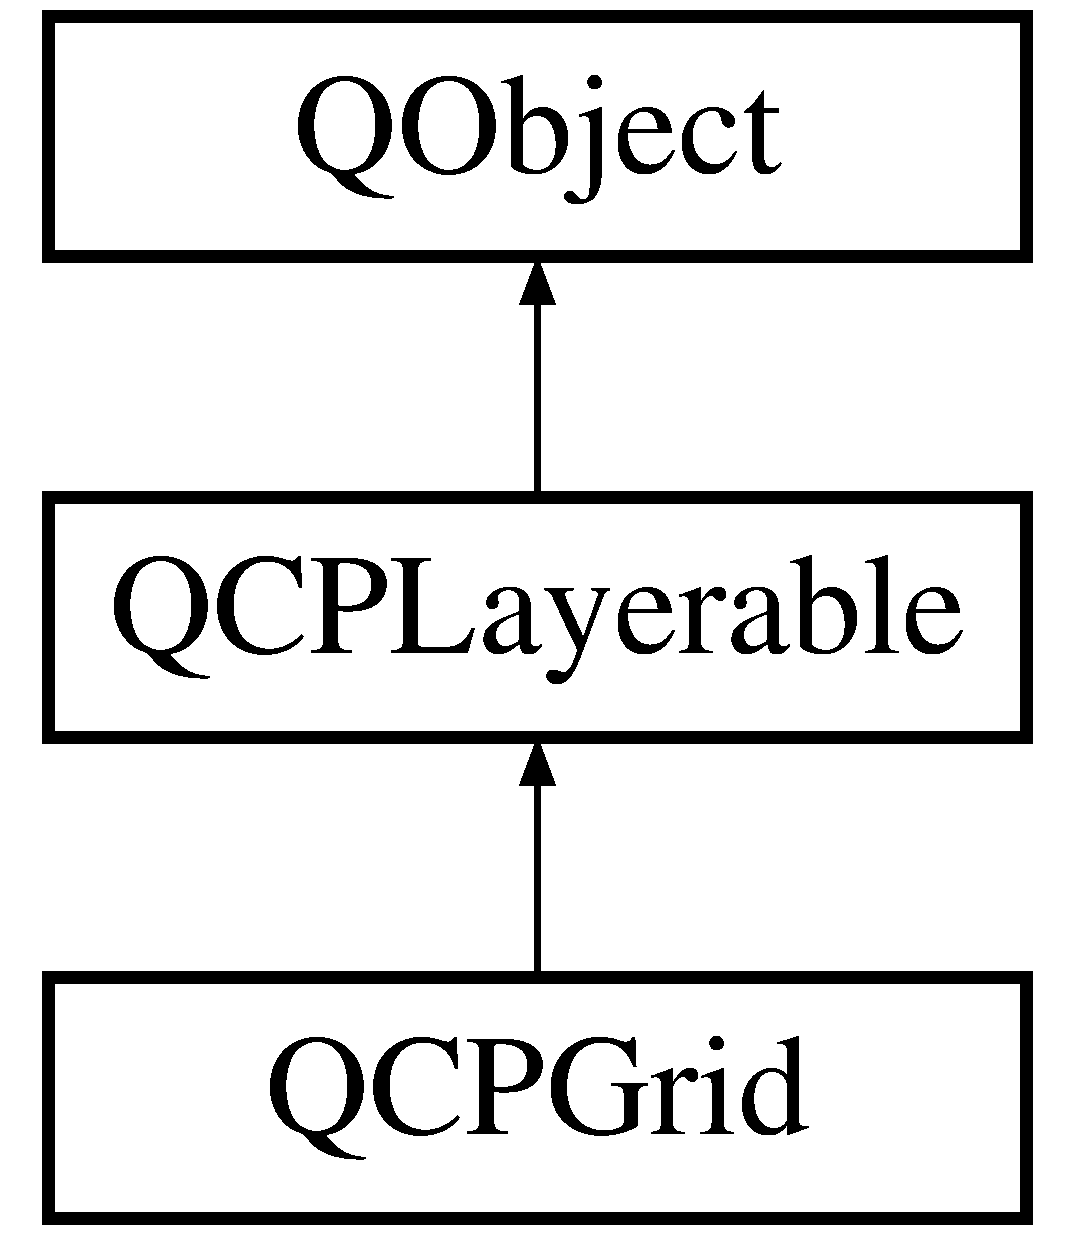
\includegraphics[height=3.000000cm]{class_q_c_p_grid}
\end{center}
\end{figure}
\subsection*{Public Member Functions}
\begin{DoxyCompactItemize}
\item 
\hyperlink{class_q_c_p_grid_acd1cdd2909625388a13048b698494a17}{Q\+C\+P\+Grid} (\hyperlink{class_q_c_p_axis}{Q\+C\+P\+Axis} $\ast$parent\+Axis)
\item 
bool \hyperlink{class_q_c_p_grid_a0a8963e384d53cd77cbab7df96147458}{sub\+Grid\+Visible} () const 
\item 
bool \hyperlink{class_q_c_p_grid_abfa6c638a05b45b2ed31b680fc9b31fc}{antialiased\+Sub\+Grid} () const 
\item 
bool \hyperlink{class_q_c_p_grid_a4dfbc1cee989d8cae1434b765ab2a13b}{antialiased\+Zero\+Line} () const 
\item 
Q\+Pen \hyperlink{class_q_c_p_grid_aca20b67548e3ae31fd02e6398ffd6cb9}{pen} () const 
\item 
Q\+Pen \hyperlink{class_q_c_p_grid_ac698f8c6864b1d8f0e2af97ca4b39cc6}{sub\+Grid\+Pen} () const 
\item 
Q\+Pen \hyperlink{class_q_c_p_grid_a06ea986b651860446e1224d2097259b9}{zero\+Line\+Pen} () const 
\item 
void \hyperlink{class_q_c_p_grid_ad4ad6bf714ec45e08845456355a1b700}{set\+Sub\+Grid\+Visible} (bool \hyperlink{class_q_c_p_layerable_a10a3cc92e0fa63e4a929e61d34e275a7}{visible})
\item 
void \hyperlink{class_q_c_p_grid_a5692310ba183721a413d60951407d114}{set\+Antialiased\+Sub\+Grid} (bool enabled)
\item 
void \hyperlink{class_q_c_p_grid_a3cc6d54647393ee71afb6da56af07aa4}{set\+Antialiased\+Zero\+Line} (bool enabled)
\item 
void \hyperlink{class_q_c_p_grid_aa05ab9816ffb440908171e45e833b593}{set\+Pen} (const Q\+Pen \&\hyperlink{class_q_c_p_grid_aca20b67548e3ae31fd02e6398ffd6cb9}{pen})
\item 
void \hyperlink{class_q_c_p_grid_a9edd3593f384d1f0b0202a39cef4453d}{set\+Sub\+Grid\+Pen} (const Q\+Pen \&\hyperlink{class_q_c_p_grid_aca20b67548e3ae31fd02e6398ffd6cb9}{pen})
\item 
void \hyperlink{class_q_c_p_grid_a209f40fdb252397b418b82d3494d8ea0}{set\+Zero\+Line\+Pen} (const Q\+Pen \&\hyperlink{class_q_c_p_grid_aca20b67548e3ae31fd02e6398ffd6cb9}{pen})
\end{DoxyCompactItemize}
\subsection*{Protected Member Functions}
\begin{DoxyCompactItemize}
\item 
virtual void \hyperlink{class_q_c_p_grid_a9916f5e38b4d6cae446537aeb47c7272}{apply\+Default\+Antialiasing\+Hint} (\hyperlink{class_q_c_p_painter}{Q\+C\+P\+Painter} $\ast$painter) const 
\item 
virtual void \hyperlink{class_q_c_p_grid_ad009c23f96078616aa4f66a750974b23}{draw} (\hyperlink{class_q_c_p_painter}{Q\+C\+P\+Painter} $\ast$painter)
\item 
void \hyperlink{class_q_c_p_grid_a3aff10e993f6625e255c19e4f97a09d8}{draw\+Grid\+Lines} (\hyperlink{class_q_c_p_painter}{Q\+C\+P\+Painter} $\ast$painter) const 
\item 
void \hyperlink{class_q_c_p_grid_afa5d9d12de419e881f381f2ab7cb414d}{draw\+Sub\+Grid\+Lines} (\hyperlink{class_q_c_p_painter}{Q\+C\+P\+Painter} $\ast$painter) const 
\end{DoxyCompactItemize}
\subsection*{Protected Attributes}
\begin{DoxyCompactItemize}
\item 
bool \hyperlink{class_q_c_p_grid_a4e4a0400d6319bb44c06341f6298c87b}{m\+Sub\+Grid\+Visible}
\item 
bool \hyperlink{class_q_c_p_grid_a71b7051f833f0c5de3094998d6afdd87}{m\+Antialiased\+Sub\+Grid}
\item 
bool \hyperlink{class_q_c_p_grid_a8c0df56ae86440408c050895dcdb922b}{m\+Antialiased\+Zero\+Line}
\item 
Q\+Pen \hyperlink{class_q_c_p_grid_a1cdc4a3bccf6a40c2d4360def9fefa40}{m\+Pen}
\item 
Q\+Pen \hyperlink{class_q_c_p_grid_aa9004bc139ad3ea92629f0aaae81d83f}{m\+Sub\+Grid\+Pen}
\item 
Q\+Pen \hyperlink{class_q_c_p_grid_a379481871f17655c27eda30af233554f}{m\+Zero\+Line\+Pen}
\item 
\hyperlink{class_q_c_p_axis}{Q\+C\+P\+Axis} $\ast$ \hyperlink{class_q_c_p_grid_a9a8a76731e6e737b65b929fd1995cc88}{m\+Parent\+Axis}
\end{DoxyCompactItemize}
\subsection*{Friends}
\begin{DoxyCompactItemize}
\item 
class \hyperlink{class_q_c_p_grid_af123edeca169ec7a31958a1d714e1a8a}{Q\+C\+P\+Axis}
\end{DoxyCompactItemize}
\subsection*{Additional Inherited Members}


\subsection{Detailed Description}
Responsible for drawing the grid of a \hyperlink{class_q_c_p_axis}{Q\+C\+P\+Axis}. 

This class is tightly bound to \hyperlink{class_q_c_p_axis}{Q\+C\+P\+Axis}. Every axis owns a grid instance and uses it to draw the grid lines, sub grid lines and zero-\/line. You can interact with the grid of an axis via \hyperlink{class_q_c_p_axis_ac4fb913cce3072b5e75a4635e0f6cd04}{Q\+C\+P\+Axis\+::grid}. Normally, you don\textquotesingle{}t need to create an instance of \hyperlink{class_q_c_p_grid}{Q\+C\+P\+Grid} yourself.

The axis and grid drawing was split into two classes to allow them to be placed on different layers (both \hyperlink{class_q_c_p_axis}{Q\+C\+P\+Axis} and \hyperlink{class_q_c_p_grid}{Q\+C\+P\+Grid} inherit from \hyperlink{class_q_c_p_layerable}{Q\+C\+P\+Layerable}). Thus it is possible to have the grid in the background and the axes in the foreground, and any plottables/items in between. This described situation is the default setup, see the \hyperlink{class_q_c_p_layer}{Q\+C\+P\+Layer} documentation. 

\subsection{Constructor \& Destructor Documentation}
\hypertarget{class_q_c_p_grid_acd1cdd2909625388a13048b698494a17}{}\index{Q\+C\+P\+Grid@{Q\+C\+P\+Grid}!Q\+C\+P\+Grid@{Q\+C\+P\+Grid}}
\index{Q\+C\+P\+Grid@{Q\+C\+P\+Grid}!Q\+C\+P\+Grid@{Q\+C\+P\+Grid}}
\subsubsection[{Q\+C\+P\+Grid}]{\setlength{\rightskip}{0pt plus 5cm}Q\+C\+P\+Grid\+::\+Q\+C\+P\+Grid (
\begin{DoxyParamCaption}
\item[{{\bf Q\+C\+P\+Axis} $\ast$}]{parent\+Axis}
\end{DoxyParamCaption}
)}\label{class_q_c_p_grid_acd1cdd2909625388a13048b698494a17}
Creates a \hyperlink{class_q_c_p_grid}{Q\+C\+P\+Grid} instance and sets default values.

You shouldn\textquotesingle{}t instantiate grids on their own, since every \hyperlink{class_q_c_p_axis}{Q\+C\+P\+Axis} brings its own \hyperlink{class_q_c_p_grid}{Q\+C\+P\+Grid}. 

\subsection{Member Function Documentation}
\hypertarget{class_q_c_p_grid_abfa6c638a05b45b2ed31b680fc9b31fc}{}\index{Q\+C\+P\+Grid@{Q\+C\+P\+Grid}!antialiased\+Sub\+Grid@{antialiased\+Sub\+Grid}}
\index{antialiased\+Sub\+Grid@{antialiased\+Sub\+Grid}!Q\+C\+P\+Grid@{Q\+C\+P\+Grid}}
\subsubsection[{antialiased\+Sub\+Grid}]{\setlength{\rightskip}{0pt plus 5cm}bool Q\+C\+P\+Grid\+::antialiased\+Sub\+Grid (
\begin{DoxyParamCaption}
{}
\end{DoxyParamCaption}
) const\hspace{0.3cm}{\ttfamily [inline]}}\label{class_q_c_p_grid_abfa6c638a05b45b2ed31b680fc9b31fc}
\hypertarget{class_q_c_p_grid_a4dfbc1cee989d8cae1434b765ab2a13b}{}\index{Q\+C\+P\+Grid@{Q\+C\+P\+Grid}!antialiased\+Zero\+Line@{antialiased\+Zero\+Line}}
\index{antialiased\+Zero\+Line@{antialiased\+Zero\+Line}!Q\+C\+P\+Grid@{Q\+C\+P\+Grid}}
\subsubsection[{antialiased\+Zero\+Line}]{\setlength{\rightskip}{0pt plus 5cm}bool Q\+C\+P\+Grid\+::antialiased\+Zero\+Line (
\begin{DoxyParamCaption}
{}
\end{DoxyParamCaption}
) const\hspace{0.3cm}{\ttfamily [inline]}}\label{class_q_c_p_grid_a4dfbc1cee989d8cae1434b765ab2a13b}
\hypertarget{class_q_c_p_grid_a9916f5e38b4d6cae446537aeb47c7272}{}\index{Q\+C\+P\+Grid@{Q\+C\+P\+Grid}!apply\+Default\+Antialiasing\+Hint@{apply\+Default\+Antialiasing\+Hint}}
\index{apply\+Default\+Antialiasing\+Hint@{apply\+Default\+Antialiasing\+Hint}!Q\+C\+P\+Grid@{Q\+C\+P\+Grid}}
\subsubsection[{apply\+Default\+Antialiasing\+Hint}]{\setlength{\rightskip}{0pt plus 5cm}void Q\+C\+P\+Grid\+::apply\+Default\+Antialiasing\+Hint (
\begin{DoxyParamCaption}
\item[{{\bf Q\+C\+P\+Painter} $\ast$}]{painter}
\end{DoxyParamCaption}
) const\hspace{0.3cm}{\ttfamily [protected]}, {\ttfamily [virtual]}}\label{class_q_c_p_grid_a9916f5e38b4d6cae446537aeb47c7272}


Implements \hyperlink{class_q_c_p_layerable_afdf83ddc6a265cbf4c89fe99d3d93473}{Q\+C\+P\+Layerable}.

\hypertarget{class_q_c_p_grid_ad009c23f96078616aa4f66a750974b23}{}\index{Q\+C\+P\+Grid@{Q\+C\+P\+Grid}!draw@{draw}}
\index{draw@{draw}!Q\+C\+P\+Grid@{Q\+C\+P\+Grid}}
\subsubsection[{draw}]{\setlength{\rightskip}{0pt plus 5cm}void Q\+C\+P\+Grid\+::draw (
\begin{DoxyParamCaption}
\item[{{\bf Q\+C\+P\+Painter} $\ast$}]{painter}
\end{DoxyParamCaption}
)\hspace{0.3cm}{\ttfamily [protected]}, {\ttfamily [virtual]}}\label{class_q_c_p_grid_ad009c23f96078616aa4f66a750974b23}


Implements \hyperlink{class_q_c_p_layerable_aecf2f7087482d4b6a78cb2770e5ed12d}{Q\+C\+P\+Layerable}.

\hypertarget{class_q_c_p_grid_a3aff10e993f6625e255c19e4f97a09d8}{}\index{Q\+C\+P\+Grid@{Q\+C\+P\+Grid}!draw\+Grid\+Lines@{draw\+Grid\+Lines}}
\index{draw\+Grid\+Lines@{draw\+Grid\+Lines}!Q\+C\+P\+Grid@{Q\+C\+P\+Grid}}
\subsubsection[{draw\+Grid\+Lines}]{\setlength{\rightskip}{0pt plus 5cm}void Q\+C\+P\+Grid\+::draw\+Grid\+Lines (
\begin{DoxyParamCaption}
\item[{{\bf Q\+C\+P\+Painter} $\ast$}]{painter}
\end{DoxyParamCaption}
) const\hspace{0.3cm}{\ttfamily [protected]}}\label{class_q_c_p_grid_a3aff10e993f6625e255c19e4f97a09d8}
\hypertarget{class_q_c_p_grid_afa5d9d12de419e881f381f2ab7cb414d}{}\index{Q\+C\+P\+Grid@{Q\+C\+P\+Grid}!draw\+Sub\+Grid\+Lines@{draw\+Sub\+Grid\+Lines}}
\index{draw\+Sub\+Grid\+Lines@{draw\+Sub\+Grid\+Lines}!Q\+C\+P\+Grid@{Q\+C\+P\+Grid}}
\subsubsection[{draw\+Sub\+Grid\+Lines}]{\setlength{\rightskip}{0pt plus 5cm}void Q\+C\+P\+Grid\+::draw\+Sub\+Grid\+Lines (
\begin{DoxyParamCaption}
\item[{{\bf Q\+C\+P\+Painter} $\ast$}]{painter}
\end{DoxyParamCaption}
) const\hspace{0.3cm}{\ttfamily [protected]}}\label{class_q_c_p_grid_afa5d9d12de419e881f381f2ab7cb414d}
\hypertarget{class_q_c_p_grid_aca20b67548e3ae31fd02e6398ffd6cb9}{}\index{Q\+C\+P\+Grid@{Q\+C\+P\+Grid}!pen@{pen}}
\index{pen@{pen}!Q\+C\+P\+Grid@{Q\+C\+P\+Grid}}
\subsubsection[{pen}]{\setlength{\rightskip}{0pt plus 5cm}Q\+Pen Q\+C\+P\+Grid\+::pen (
\begin{DoxyParamCaption}
{}
\end{DoxyParamCaption}
) const\hspace{0.3cm}{\ttfamily [inline]}}\label{class_q_c_p_grid_aca20b67548e3ae31fd02e6398ffd6cb9}
\hypertarget{class_q_c_p_grid_a5692310ba183721a413d60951407d114}{}\index{Q\+C\+P\+Grid@{Q\+C\+P\+Grid}!set\+Antialiased\+Sub\+Grid@{set\+Antialiased\+Sub\+Grid}}
\index{set\+Antialiased\+Sub\+Grid@{set\+Antialiased\+Sub\+Grid}!Q\+C\+P\+Grid@{Q\+C\+P\+Grid}}
\subsubsection[{set\+Antialiased\+Sub\+Grid}]{\setlength{\rightskip}{0pt plus 5cm}void Q\+C\+P\+Grid\+::set\+Antialiased\+Sub\+Grid (
\begin{DoxyParamCaption}
\item[{bool}]{enabled}
\end{DoxyParamCaption}
)}\label{class_q_c_p_grid_a5692310ba183721a413d60951407d114}
Sets whether sub grid lines are drawn antialiased. \hypertarget{class_q_c_p_grid_a3cc6d54647393ee71afb6da56af07aa4}{}\index{Q\+C\+P\+Grid@{Q\+C\+P\+Grid}!set\+Antialiased\+Zero\+Line@{set\+Antialiased\+Zero\+Line}}
\index{set\+Antialiased\+Zero\+Line@{set\+Antialiased\+Zero\+Line}!Q\+C\+P\+Grid@{Q\+C\+P\+Grid}}
\subsubsection[{set\+Antialiased\+Zero\+Line}]{\setlength{\rightskip}{0pt plus 5cm}void Q\+C\+P\+Grid\+::set\+Antialiased\+Zero\+Line (
\begin{DoxyParamCaption}
\item[{bool}]{enabled}
\end{DoxyParamCaption}
)}\label{class_q_c_p_grid_a3cc6d54647393ee71afb6da56af07aa4}
Sets whether zero lines are drawn antialiased. \hypertarget{class_q_c_p_grid_aa05ab9816ffb440908171e45e833b593}{}\index{Q\+C\+P\+Grid@{Q\+C\+P\+Grid}!set\+Pen@{set\+Pen}}
\index{set\+Pen@{set\+Pen}!Q\+C\+P\+Grid@{Q\+C\+P\+Grid}}
\subsubsection[{set\+Pen}]{\setlength{\rightskip}{0pt plus 5cm}void Q\+C\+P\+Grid\+::set\+Pen (
\begin{DoxyParamCaption}
\item[{const Q\+Pen \&}]{pen}
\end{DoxyParamCaption}
)}\label{class_q_c_p_grid_aa05ab9816ffb440908171e45e833b593}
Sets the pen with which (major) grid lines are drawn. \hypertarget{class_q_c_p_grid_a9edd3593f384d1f0b0202a39cef4453d}{}\index{Q\+C\+P\+Grid@{Q\+C\+P\+Grid}!set\+Sub\+Grid\+Pen@{set\+Sub\+Grid\+Pen}}
\index{set\+Sub\+Grid\+Pen@{set\+Sub\+Grid\+Pen}!Q\+C\+P\+Grid@{Q\+C\+P\+Grid}}
\subsubsection[{set\+Sub\+Grid\+Pen}]{\setlength{\rightskip}{0pt plus 5cm}void Q\+C\+P\+Grid\+::set\+Sub\+Grid\+Pen (
\begin{DoxyParamCaption}
\item[{const Q\+Pen \&}]{pen}
\end{DoxyParamCaption}
)}\label{class_q_c_p_grid_a9edd3593f384d1f0b0202a39cef4453d}
Sets the pen with which sub grid lines are drawn. \hypertarget{class_q_c_p_grid_ad4ad6bf714ec45e08845456355a1b700}{}\index{Q\+C\+P\+Grid@{Q\+C\+P\+Grid}!set\+Sub\+Grid\+Visible@{set\+Sub\+Grid\+Visible}}
\index{set\+Sub\+Grid\+Visible@{set\+Sub\+Grid\+Visible}!Q\+C\+P\+Grid@{Q\+C\+P\+Grid}}
\subsubsection[{set\+Sub\+Grid\+Visible}]{\setlength{\rightskip}{0pt plus 5cm}void Q\+C\+P\+Grid\+::set\+Sub\+Grid\+Visible (
\begin{DoxyParamCaption}
\item[{bool}]{visible}
\end{DoxyParamCaption}
)}\label{class_q_c_p_grid_ad4ad6bf714ec45e08845456355a1b700}
Sets whether grid lines at sub tick marks are drawn.

\begin{DoxySeeAlso}{See also}
\hyperlink{class_q_c_p_grid_a9edd3593f384d1f0b0202a39cef4453d}{set\+Sub\+Grid\+Pen} 
\end{DoxySeeAlso}
\hypertarget{class_q_c_p_grid_a209f40fdb252397b418b82d3494d8ea0}{}\index{Q\+C\+P\+Grid@{Q\+C\+P\+Grid}!set\+Zero\+Line\+Pen@{set\+Zero\+Line\+Pen}}
\index{set\+Zero\+Line\+Pen@{set\+Zero\+Line\+Pen}!Q\+C\+P\+Grid@{Q\+C\+P\+Grid}}
\subsubsection[{set\+Zero\+Line\+Pen}]{\setlength{\rightskip}{0pt plus 5cm}void Q\+C\+P\+Grid\+::set\+Zero\+Line\+Pen (
\begin{DoxyParamCaption}
\item[{const Q\+Pen \&}]{pen}
\end{DoxyParamCaption}
)}\label{class_q_c_p_grid_a209f40fdb252397b418b82d3494d8ea0}
Sets the pen with which zero lines are drawn.

Zero lines are lines at value coordinate 0 which may be drawn with a different pen than other grid lines. To disable zero lines and just draw normal grid lines at zero, set {\itshape pen} to Qt\+::\+No\+Pen. \hypertarget{class_q_c_p_grid_ac698f8c6864b1d8f0e2af97ca4b39cc6}{}\index{Q\+C\+P\+Grid@{Q\+C\+P\+Grid}!sub\+Grid\+Pen@{sub\+Grid\+Pen}}
\index{sub\+Grid\+Pen@{sub\+Grid\+Pen}!Q\+C\+P\+Grid@{Q\+C\+P\+Grid}}
\subsubsection[{sub\+Grid\+Pen}]{\setlength{\rightskip}{0pt plus 5cm}Q\+Pen Q\+C\+P\+Grid\+::sub\+Grid\+Pen (
\begin{DoxyParamCaption}
{}
\end{DoxyParamCaption}
) const\hspace{0.3cm}{\ttfamily [inline]}}\label{class_q_c_p_grid_ac698f8c6864b1d8f0e2af97ca4b39cc6}
\hypertarget{class_q_c_p_grid_a0a8963e384d53cd77cbab7df96147458}{}\index{Q\+C\+P\+Grid@{Q\+C\+P\+Grid}!sub\+Grid\+Visible@{sub\+Grid\+Visible}}
\index{sub\+Grid\+Visible@{sub\+Grid\+Visible}!Q\+C\+P\+Grid@{Q\+C\+P\+Grid}}
\subsubsection[{sub\+Grid\+Visible}]{\setlength{\rightskip}{0pt plus 5cm}bool Q\+C\+P\+Grid\+::sub\+Grid\+Visible (
\begin{DoxyParamCaption}
{}
\end{DoxyParamCaption}
) const\hspace{0.3cm}{\ttfamily [inline]}}\label{class_q_c_p_grid_a0a8963e384d53cd77cbab7df96147458}
\hypertarget{class_q_c_p_grid_a06ea986b651860446e1224d2097259b9}{}\index{Q\+C\+P\+Grid@{Q\+C\+P\+Grid}!zero\+Line\+Pen@{zero\+Line\+Pen}}
\index{zero\+Line\+Pen@{zero\+Line\+Pen}!Q\+C\+P\+Grid@{Q\+C\+P\+Grid}}
\subsubsection[{zero\+Line\+Pen}]{\setlength{\rightskip}{0pt plus 5cm}Q\+Pen Q\+C\+P\+Grid\+::zero\+Line\+Pen (
\begin{DoxyParamCaption}
{}
\end{DoxyParamCaption}
) const\hspace{0.3cm}{\ttfamily [inline]}}\label{class_q_c_p_grid_a06ea986b651860446e1224d2097259b9}


\subsection{Friends And Related Function Documentation}
\hypertarget{class_q_c_p_grid_af123edeca169ec7a31958a1d714e1a8a}{}\index{Q\+C\+P\+Grid@{Q\+C\+P\+Grid}!Q\+C\+P\+Axis@{Q\+C\+P\+Axis}}
\index{Q\+C\+P\+Axis@{Q\+C\+P\+Axis}!Q\+C\+P\+Grid@{Q\+C\+P\+Grid}}
\subsubsection[{Q\+C\+P\+Axis}]{\setlength{\rightskip}{0pt plus 5cm}friend class {\bf Q\+C\+P\+Axis}\hspace{0.3cm}{\ttfamily [friend]}}\label{class_q_c_p_grid_af123edeca169ec7a31958a1d714e1a8a}


\subsection{Member Data Documentation}
\hypertarget{class_q_c_p_grid_a71b7051f833f0c5de3094998d6afdd87}{}\index{Q\+C\+P\+Grid@{Q\+C\+P\+Grid}!m\+Antialiased\+Sub\+Grid@{m\+Antialiased\+Sub\+Grid}}
\index{m\+Antialiased\+Sub\+Grid@{m\+Antialiased\+Sub\+Grid}!Q\+C\+P\+Grid@{Q\+C\+P\+Grid}}
\subsubsection[{m\+Antialiased\+Sub\+Grid}]{\setlength{\rightskip}{0pt plus 5cm}bool Q\+C\+P\+Grid\+::m\+Antialiased\+Sub\+Grid\hspace{0.3cm}{\ttfamily [protected]}}\label{class_q_c_p_grid_a71b7051f833f0c5de3094998d6afdd87}
\hypertarget{class_q_c_p_grid_a8c0df56ae86440408c050895dcdb922b}{}\index{Q\+C\+P\+Grid@{Q\+C\+P\+Grid}!m\+Antialiased\+Zero\+Line@{m\+Antialiased\+Zero\+Line}}
\index{m\+Antialiased\+Zero\+Line@{m\+Antialiased\+Zero\+Line}!Q\+C\+P\+Grid@{Q\+C\+P\+Grid}}
\subsubsection[{m\+Antialiased\+Zero\+Line}]{\setlength{\rightskip}{0pt plus 5cm}bool Q\+C\+P\+Grid\+::m\+Antialiased\+Zero\+Line\hspace{0.3cm}{\ttfamily [protected]}}\label{class_q_c_p_grid_a8c0df56ae86440408c050895dcdb922b}
\hypertarget{class_q_c_p_grid_a9a8a76731e6e737b65b929fd1995cc88}{}\index{Q\+C\+P\+Grid@{Q\+C\+P\+Grid}!m\+Parent\+Axis@{m\+Parent\+Axis}}
\index{m\+Parent\+Axis@{m\+Parent\+Axis}!Q\+C\+P\+Grid@{Q\+C\+P\+Grid}}
\subsubsection[{m\+Parent\+Axis}]{\setlength{\rightskip}{0pt plus 5cm}{\bf Q\+C\+P\+Axis}$\ast$ Q\+C\+P\+Grid\+::m\+Parent\+Axis\hspace{0.3cm}{\ttfamily [protected]}}\label{class_q_c_p_grid_a9a8a76731e6e737b65b929fd1995cc88}
\hypertarget{class_q_c_p_grid_a1cdc4a3bccf6a40c2d4360def9fefa40}{}\index{Q\+C\+P\+Grid@{Q\+C\+P\+Grid}!m\+Pen@{m\+Pen}}
\index{m\+Pen@{m\+Pen}!Q\+C\+P\+Grid@{Q\+C\+P\+Grid}}
\subsubsection[{m\+Pen}]{\setlength{\rightskip}{0pt plus 5cm}Q\+Pen Q\+C\+P\+Grid\+::m\+Pen\hspace{0.3cm}{\ttfamily [protected]}}\label{class_q_c_p_grid_a1cdc4a3bccf6a40c2d4360def9fefa40}
\hypertarget{class_q_c_p_grid_aa9004bc139ad3ea92629f0aaae81d83f}{}\index{Q\+C\+P\+Grid@{Q\+C\+P\+Grid}!m\+Sub\+Grid\+Pen@{m\+Sub\+Grid\+Pen}}
\index{m\+Sub\+Grid\+Pen@{m\+Sub\+Grid\+Pen}!Q\+C\+P\+Grid@{Q\+C\+P\+Grid}}
\subsubsection[{m\+Sub\+Grid\+Pen}]{\setlength{\rightskip}{0pt plus 5cm}Q\+Pen Q\+C\+P\+Grid\+::m\+Sub\+Grid\+Pen\hspace{0.3cm}{\ttfamily [protected]}}\label{class_q_c_p_grid_aa9004bc139ad3ea92629f0aaae81d83f}
\hypertarget{class_q_c_p_grid_a4e4a0400d6319bb44c06341f6298c87b}{}\index{Q\+C\+P\+Grid@{Q\+C\+P\+Grid}!m\+Sub\+Grid\+Visible@{m\+Sub\+Grid\+Visible}}
\index{m\+Sub\+Grid\+Visible@{m\+Sub\+Grid\+Visible}!Q\+C\+P\+Grid@{Q\+C\+P\+Grid}}
\subsubsection[{m\+Sub\+Grid\+Visible}]{\setlength{\rightskip}{0pt plus 5cm}bool Q\+C\+P\+Grid\+::m\+Sub\+Grid\+Visible\hspace{0.3cm}{\ttfamily [protected]}}\label{class_q_c_p_grid_a4e4a0400d6319bb44c06341f6298c87b}
\hypertarget{class_q_c_p_grid_a379481871f17655c27eda30af233554f}{}\index{Q\+C\+P\+Grid@{Q\+C\+P\+Grid}!m\+Zero\+Line\+Pen@{m\+Zero\+Line\+Pen}}
\index{m\+Zero\+Line\+Pen@{m\+Zero\+Line\+Pen}!Q\+C\+P\+Grid@{Q\+C\+P\+Grid}}
\subsubsection[{m\+Zero\+Line\+Pen}]{\setlength{\rightskip}{0pt plus 5cm}Q\+Pen Q\+C\+P\+Grid\+::m\+Zero\+Line\+Pen\hspace{0.3cm}{\ttfamily [protected]}}\label{class_q_c_p_grid_a379481871f17655c27eda30af233554f}


The documentation for this class was generated from the following files\+:\begin{DoxyCompactItemize}
\item 
C\+:/\+Users/\+Roman/\+Documents/\+Mygs/\+Ground\+Station/\+G\+S/\hyperlink{qcustomplot_8h}{qcustomplot.\+h}\item 
C\+:/\+Users/\+Roman/\+Documents/\+Mygs/\+Ground\+Station/\+G\+S/\hyperlink{qcustomplot_8cpp}{qcustomplot.\+cpp}\end{DoxyCompactItemize}

\hypertarget{class_q_c_p_item_anchor}{}\section{Q\+C\+P\+Item\+Anchor Class Reference}
\label{class_q_c_p_item_anchor}\index{Q\+C\+P\+Item\+Anchor@{Q\+C\+P\+Item\+Anchor}}


An anchor of an item to which positions can be attached to.  




{\ttfamily \#include $<$qcustomplot.\+h$>$}

Inheritance diagram for Q\+C\+P\+Item\+Anchor\+:\begin{figure}[H]
\begin{center}
\leavevmode
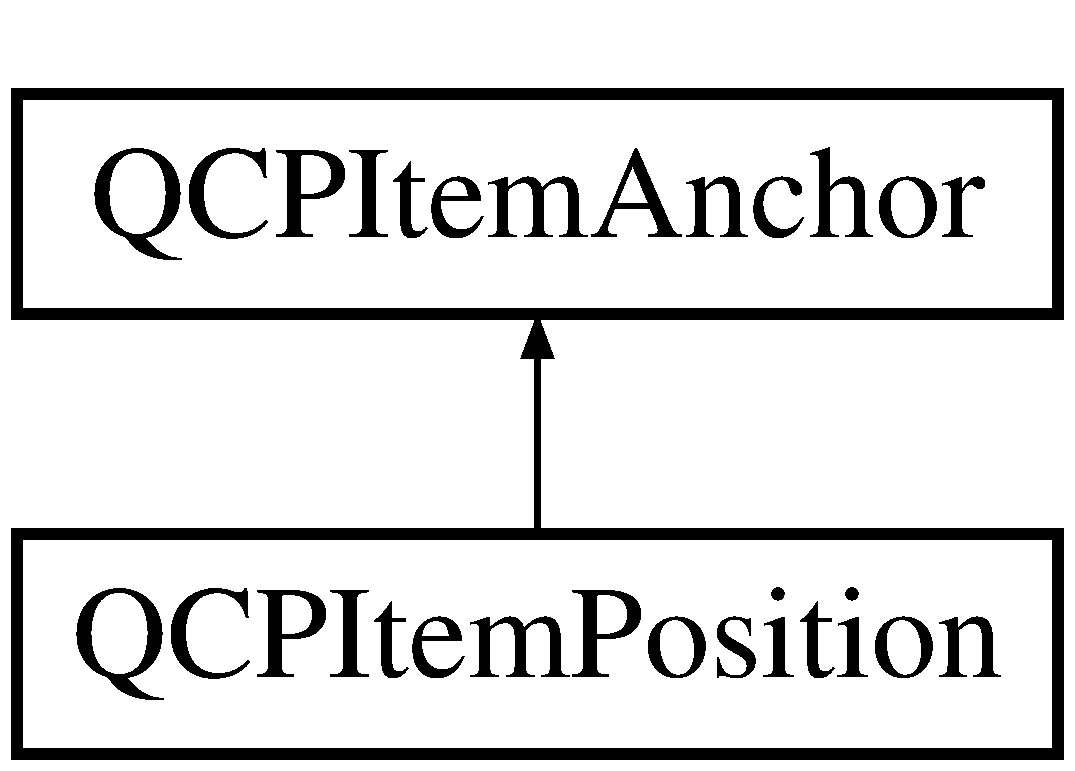
\includegraphics[height=2.000000cm]{class_q_c_p_item_anchor}
\end{center}
\end{figure}
\subsection*{Public Member Functions}
\begin{DoxyCompactItemize}
\item 
\hyperlink{class_q_c_p_item_anchor_aeb6b681d2bf324db40a915d32ec5624f}{Q\+C\+P\+Item\+Anchor} (\hyperlink{class_q_custom_plot}{Q\+Custom\+Plot} $\ast$parent\+Plot, \hyperlink{class_q_c_p_abstract_item}{Q\+C\+P\+Abstract\+Item} $\ast$parent\+Item, const Q\+String \hyperlink{class_q_c_p_item_anchor_ac93984042a58c875e76847dc3e5f75fe}{name}, int anchor\+Id=-\/1)
\item 
virtual \hyperlink{class_q_c_p_item_anchor_a1868559407600688ee4d1a4621e81ceb}{$\sim$\+Q\+C\+P\+Item\+Anchor} ()
\item 
Q\+String \hyperlink{class_q_c_p_item_anchor_ac93984042a58c875e76847dc3e5f75fe}{name} () const 
\item 
virtual Q\+Point\+F \hyperlink{class_q_c_p_item_anchor_ae92def8f9297c5d73f5806c586517bb3}{pixel\+Point} () const 
\end{DoxyCompactItemize}
\subsection*{Protected Member Functions}
\begin{DoxyCompactItemize}
\item 
virtual \hyperlink{class_q_c_p_item_position}{Q\+C\+P\+Item\+Position} $\ast$ \hyperlink{class_q_c_p_item_anchor_ac54b20120669950255a63587193dbb86}{to\+Q\+C\+P\+Item\+Position} ()
\item 
void \hyperlink{class_q_c_p_item_anchor_aef15daa640debfb11b0aeaa2116c6fbc}{add\+Child\+X} (\hyperlink{class_q_c_p_item_position}{Q\+C\+P\+Item\+Position} $\ast$pos)
\item 
void \hyperlink{class_q_c_p_item_anchor_a230b1d494cda63458e289bbe1b642599}{remove\+Child\+X} (\hyperlink{class_q_c_p_item_position}{Q\+C\+P\+Item\+Position} $\ast$pos)
\item 
void \hyperlink{class_q_c_p_item_anchor_af05dc56f24536f0c7a9a0f57b58cea67}{add\+Child\+Y} (\hyperlink{class_q_c_p_item_position}{Q\+C\+P\+Item\+Position} $\ast$pos)
\item 
void \hyperlink{class_q_c_p_item_anchor_aa2394911d8fff3bd958b9f4f1994b64d}{remove\+Child\+Y} (\hyperlink{class_q_c_p_item_position}{Q\+C\+P\+Item\+Position} $\ast$pos)
\end{DoxyCompactItemize}
\subsection*{Protected Attributes}
\begin{DoxyCompactItemize}
\item 
Q\+String \hyperlink{class_q_c_p_item_anchor_a23ad4d0ab0d2cbb41a7baf05bcf996ec}{m\+Name}
\item 
\hyperlink{class_q_custom_plot}{Q\+Custom\+Plot} $\ast$ \hyperlink{class_q_c_p_item_anchor_a59b968410831ba91a25cc75a77dde6f5}{m\+Parent\+Plot}
\item 
\hyperlink{class_q_c_p_abstract_item}{Q\+C\+P\+Abstract\+Item} $\ast$ \hyperlink{class_q_c_p_item_anchor_a80fad480ad3bb980446ed6ebc00818ae}{m\+Parent\+Item}
\item 
int \hyperlink{class_q_c_p_item_anchor_a00c62070333e8345976b579676ad3997}{m\+Anchor\+Id}
\item 
Q\+Set$<$ \hyperlink{class_q_c_p_item_position}{Q\+C\+P\+Item\+Position} $\ast$ $>$ \hyperlink{class_q_c_p_item_anchor_a3c0bfd6e50f3b48e2a9b3824695b20f7}{m\+Children\+X}
\item 
Q\+Set$<$ \hyperlink{class_q_c_p_item_position}{Q\+C\+P\+Item\+Position} $\ast$ $>$ \hyperlink{class_q_c_p_item_anchor_a3abe4eebd0683454d81c8341df6f7115}{m\+Children\+Y}
\end{DoxyCompactItemize}
\subsection*{Friends}
\begin{DoxyCompactItemize}
\item 
class \hyperlink{class_q_c_p_item_anchor_aa9b8ddc062778e202a0be06a57d18d17}{Q\+C\+P\+Item\+Position}
\end{DoxyCompactItemize}


\subsection{Detailed Description}
An anchor of an item to which positions can be attached to. 

An item (\hyperlink{class_q_c_p_abstract_item}{Q\+C\+P\+Abstract\+Item}) may have one or more anchors. Unlike \hyperlink{class_q_c_p_item_position}{Q\+C\+P\+Item\+Position}, an anchor doesn\textquotesingle{}t control anything on its item, but provides a way to tie other items via their positions to the anchor.

For example, a \hyperlink{class_q_c_p_item_rect}{Q\+C\+P\+Item\+Rect} is defined by its positions {\itshape top\+Left} and {\itshape bottom\+Right}. Additionally it has various anchors like {\itshape top}, {\itshape top\+Right} or {\itshape bottom\+Left} etc. So you can attach the {\itshape start} (which is a \hyperlink{class_q_c_p_item_position}{Q\+C\+P\+Item\+Position}) of a \hyperlink{class_q_c_p_item_line}{Q\+C\+P\+Item\+Line} to one of the anchors by calling \hyperlink{class_q_c_p_item_position_ac094d67a95d2dceafa0d50b9db3a7e51}{Q\+C\+P\+Item\+Position\+::set\+Parent\+Anchor} on {\itshape start}, passing the wanted anchor of the \hyperlink{class_q_c_p_item_rect}{Q\+C\+P\+Item\+Rect}. This way the start of the line will now always follow the respective anchor location on the rect item.

Note that \hyperlink{class_q_c_p_item_position}{Q\+C\+P\+Item\+Position} derives from \hyperlink{class_q_c_p_item_anchor}{Q\+C\+P\+Item\+Anchor}, so every position can also serve as an anchor to other positions.

To learn how to provide anchors in your own item subclasses, see the subclassing section of the \hyperlink{class_q_c_p_abstract_item}{Q\+C\+P\+Abstract\+Item} documentation. 

\subsection{Constructor \& Destructor Documentation}
\hypertarget{class_q_c_p_item_anchor_aeb6b681d2bf324db40a915d32ec5624f}{}\index{Q\+C\+P\+Item\+Anchor@{Q\+C\+P\+Item\+Anchor}!Q\+C\+P\+Item\+Anchor@{Q\+C\+P\+Item\+Anchor}}
\index{Q\+C\+P\+Item\+Anchor@{Q\+C\+P\+Item\+Anchor}!Q\+C\+P\+Item\+Anchor@{Q\+C\+P\+Item\+Anchor}}
\subsubsection[{Q\+C\+P\+Item\+Anchor}]{\setlength{\rightskip}{0pt plus 5cm}Q\+C\+P\+Item\+Anchor\+::\+Q\+C\+P\+Item\+Anchor (
\begin{DoxyParamCaption}
\item[{{\bf Q\+Custom\+Plot} $\ast$}]{parent\+Plot, }
\item[{{\bf Q\+C\+P\+Abstract\+Item} $\ast$}]{parent\+Item, }
\item[{const Q\+String}]{name, }
\item[{int}]{anchor\+Id = {\ttfamily -\/1}}
\end{DoxyParamCaption}
)}\label{class_q_c_p_item_anchor_aeb6b681d2bf324db40a915d32ec5624f}
Creates a new \hyperlink{class_q_c_p_item_anchor}{Q\+C\+P\+Item\+Anchor}. You shouldn\textquotesingle{}t create \hyperlink{class_q_c_p_item_anchor}{Q\+C\+P\+Item\+Anchor} instances directly, even if you want to make a new item subclass. Use \hyperlink{class_q_c_p_abstract_item_af3fc92527802078ca395138748b629a7}{Q\+C\+P\+Abstract\+Item\+::create\+Anchor} instead, as explained in the subclassing section of the \hyperlink{class_q_c_p_abstract_item}{Q\+C\+P\+Abstract\+Item} documentation. \hypertarget{class_q_c_p_item_anchor_a1868559407600688ee4d1a4621e81ceb}{}\index{Q\+C\+P\+Item\+Anchor@{Q\+C\+P\+Item\+Anchor}!````~Q\+C\+P\+Item\+Anchor@{$\sim$\+Q\+C\+P\+Item\+Anchor}}
\index{````~Q\+C\+P\+Item\+Anchor@{$\sim$\+Q\+C\+P\+Item\+Anchor}!Q\+C\+P\+Item\+Anchor@{Q\+C\+P\+Item\+Anchor}}
\subsubsection[{$\sim$\+Q\+C\+P\+Item\+Anchor}]{\setlength{\rightskip}{0pt plus 5cm}Q\+C\+P\+Item\+Anchor\+::$\sim$\+Q\+C\+P\+Item\+Anchor (
\begin{DoxyParamCaption}
{}
\end{DoxyParamCaption}
)\hspace{0.3cm}{\ttfamily [virtual]}}\label{class_q_c_p_item_anchor_a1868559407600688ee4d1a4621e81ceb}


\subsection{Member Function Documentation}
\hypertarget{class_q_c_p_item_anchor_aef15daa640debfb11b0aeaa2116c6fbc}{}\index{Q\+C\+P\+Item\+Anchor@{Q\+C\+P\+Item\+Anchor}!add\+Child\+X@{add\+Child\+X}}
\index{add\+Child\+X@{add\+Child\+X}!Q\+C\+P\+Item\+Anchor@{Q\+C\+P\+Item\+Anchor}}
\subsubsection[{add\+Child\+X}]{\setlength{\rightskip}{0pt plus 5cm}void Q\+C\+P\+Item\+Anchor\+::add\+Child\+X (
\begin{DoxyParamCaption}
\item[{{\bf Q\+C\+P\+Item\+Position} $\ast$}]{pos}
\end{DoxyParamCaption}
)\hspace{0.3cm}{\ttfamily [protected]}}\label{class_q_c_p_item_anchor_aef15daa640debfb11b0aeaa2116c6fbc}
\hypertarget{class_q_c_p_item_anchor_af05dc56f24536f0c7a9a0f57b58cea67}{}\index{Q\+C\+P\+Item\+Anchor@{Q\+C\+P\+Item\+Anchor}!add\+Child\+Y@{add\+Child\+Y}}
\index{add\+Child\+Y@{add\+Child\+Y}!Q\+C\+P\+Item\+Anchor@{Q\+C\+P\+Item\+Anchor}}
\subsubsection[{add\+Child\+Y}]{\setlength{\rightskip}{0pt plus 5cm}void Q\+C\+P\+Item\+Anchor\+::add\+Child\+Y (
\begin{DoxyParamCaption}
\item[{{\bf Q\+C\+P\+Item\+Position} $\ast$}]{pos}
\end{DoxyParamCaption}
)\hspace{0.3cm}{\ttfamily [protected]}}\label{class_q_c_p_item_anchor_af05dc56f24536f0c7a9a0f57b58cea67}
\hypertarget{class_q_c_p_item_anchor_ac93984042a58c875e76847dc3e5f75fe}{}\index{Q\+C\+P\+Item\+Anchor@{Q\+C\+P\+Item\+Anchor}!name@{name}}
\index{name@{name}!Q\+C\+P\+Item\+Anchor@{Q\+C\+P\+Item\+Anchor}}
\subsubsection[{name}]{\setlength{\rightskip}{0pt plus 5cm}Q\+String Q\+C\+P\+Item\+Anchor\+::name (
\begin{DoxyParamCaption}
{}
\end{DoxyParamCaption}
) const\hspace{0.3cm}{\ttfamily [inline]}}\label{class_q_c_p_item_anchor_ac93984042a58c875e76847dc3e5f75fe}
\hypertarget{class_q_c_p_item_anchor_ae92def8f9297c5d73f5806c586517bb3}{}\index{Q\+C\+P\+Item\+Anchor@{Q\+C\+P\+Item\+Anchor}!pixel\+Point@{pixel\+Point}}
\index{pixel\+Point@{pixel\+Point}!Q\+C\+P\+Item\+Anchor@{Q\+C\+P\+Item\+Anchor}}
\subsubsection[{pixel\+Point}]{\setlength{\rightskip}{0pt plus 5cm}Q\+Point\+F Q\+C\+P\+Item\+Anchor\+::pixel\+Point (
\begin{DoxyParamCaption}
{}
\end{DoxyParamCaption}
) const\hspace{0.3cm}{\ttfamily [virtual]}}\label{class_q_c_p_item_anchor_ae92def8f9297c5d73f5806c586517bb3}
Returns the final absolute pixel position of the \hyperlink{class_q_c_p_item_anchor}{Q\+C\+P\+Item\+Anchor} on the \hyperlink{class_q_custom_plot}{Q\+Custom\+Plot} surface.

The pixel information is internally retrieved via Q\+C\+P\+Abstract\+Item\+::anchor\+Pixel\+Position of the parent item, \hyperlink{class_q_c_p_item_anchor}{Q\+C\+P\+Item\+Anchor} is just an intermediary. 

Reimplemented in \hyperlink{class_q_c_p_item_position_ae490f9c76ee2ba33752c495d3b6e8fb5}{Q\+C\+P\+Item\+Position}.

\hypertarget{class_q_c_p_item_anchor_a230b1d494cda63458e289bbe1b642599}{}\index{Q\+C\+P\+Item\+Anchor@{Q\+C\+P\+Item\+Anchor}!remove\+Child\+X@{remove\+Child\+X}}
\index{remove\+Child\+X@{remove\+Child\+X}!Q\+C\+P\+Item\+Anchor@{Q\+C\+P\+Item\+Anchor}}
\subsubsection[{remove\+Child\+X}]{\setlength{\rightskip}{0pt plus 5cm}void Q\+C\+P\+Item\+Anchor\+::remove\+Child\+X (
\begin{DoxyParamCaption}
\item[{{\bf Q\+C\+P\+Item\+Position} $\ast$}]{pos}
\end{DoxyParamCaption}
)\hspace{0.3cm}{\ttfamily [protected]}}\label{class_q_c_p_item_anchor_a230b1d494cda63458e289bbe1b642599}
\hypertarget{class_q_c_p_item_anchor_aa2394911d8fff3bd958b9f4f1994b64d}{}\index{Q\+C\+P\+Item\+Anchor@{Q\+C\+P\+Item\+Anchor}!remove\+Child\+Y@{remove\+Child\+Y}}
\index{remove\+Child\+Y@{remove\+Child\+Y}!Q\+C\+P\+Item\+Anchor@{Q\+C\+P\+Item\+Anchor}}
\subsubsection[{remove\+Child\+Y}]{\setlength{\rightskip}{0pt plus 5cm}void Q\+C\+P\+Item\+Anchor\+::remove\+Child\+Y (
\begin{DoxyParamCaption}
\item[{{\bf Q\+C\+P\+Item\+Position} $\ast$}]{pos}
\end{DoxyParamCaption}
)\hspace{0.3cm}{\ttfamily [protected]}}\label{class_q_c_p_item_anchor_aa2394911d8fff3bd958b9f4f1994b64d}
\hypertarget{class_q_c_p_item_anchor_ac54b20120669950255a63587193dbb86}{}\index{Q\+C\+P\+Item\+Anchor@{Q\+C\+P\+Item\+Anchor}!to\+Q\+C\+P\+Item\+Position@{to\+Q\+C\+P\+Item\+Position}}
\index{to\+Q\+C\+P\+Item\+Position@{to\+Q\+C\+P\+Item\+Position}!Q\+C\+P\+Item\+Anchor@{Q\+C\+P\+Item\+Anchor}}
\subsubsection[{to\+Q\+C\+P\+Item\+Position}]{\setlength{\rightskip}{0pt plus 5cm}{\bf Q\+C\+P\+Item\+Position} $\ast$ Q\+C\+P\+Item\+Anchor\+::to\+Q\+C\+P\+Item\+Position (
\begin{DoxyParamCaption}
{}
\end{DoxyParamCaption}
)\hspace{0.3cm}{\ttfamily [inline]}, {\ttfamily [protected]}, {\ttfamily [virtual]}}\label{class_q_c_p_item_anchor_ac54b20120669950255a63587193dbb86}
Returns 0 if this instance is merely a \hyperlink{class_q_c_p_item_anchor}{Q\+C\+P\+Item\+Anchor}, and a valid pointer of type Q\+C\+P\+Item\+Position$\ast$ if it actually is a \hyperlink{class_q_c_p_item_position}{Q\+C\+P\+Item\+Position} (which is a subclass of \hyperlink{class_q_c_p_item_anchor}{Q\+C\+P\+Item\+Anchor}).

This safe downcast functionality could also be achieved with a dynamic\+\_\+cast. However, \hyperlink{class_q_custom_plot}{Q\+Custom\+Plot} avoids dynamic\+\_\+cast to work with projects that don\textquotesingle{}t have R\+T\+T\+I support enabled (e.\+g. -\/fno-\/rtti flag with gcc compiler). 

Reimplemented in \hyperlink{class_q_c_p_item_position_a577a7efc601df85a20b3e709d1ac320e}{Q\+C\+P\+Item\+Position}.



\subsection{Friends And Related Function Documentation}
\hypertarget{class_q_c_p_item_anchor_aa9b8ddc062778e202a0be06a57d18d17}{}\index{Q\+C\+P\+Item\+Anchor@{Q\+C\+P\+Item\+Anchor}!Q\+C\+P\+Item\+Position@{Q\+C\+P\+Item\+Position}}
\index{Q\+C\+P\+Item\+Position@{Q\+C\+P\+Item\+Position}!Q\+C\+P\+Item\+Anchor@{Q\+C\+P\+Item\+Anchor}}
\subsubsection[{Q\+C\+P\+Item\+Position}]{\setlength{\rightskip}{0pt plus 5cm}friend class {\bf Q\+C\+P\+Item\+Position}\hspace{0.3cm}{\ttfamily [friend]}}\label{class_q_c_p_item_anchor_aa9b8ddc062778e202a0be06a57d18d17}


\subsection{Member Data Documentation}
\hypertarget{class_q_c_p_item_anchor_a00c62070333e8345976b579676ad3997}{}\index{Q\+C\+P\+Item\+Anchor@{Q\+C\+P\+Item\+Anchor}!m\+Anchor\+Id@{m\+Anchor\+Id}}
\index{m\+Anchor\+Id@{m\+Anchor\+Id}!Q\+C\+P\+Item\+Anchor@{Q\+C\+P\+Item\+Anchor}}
\subsubsection[{m\+Anchor\+Id}]{\setlength{\rightskip}{0pt plus 5cm}int Q\+C\+P\+Item\+Anchor\+::m\+Anchor\+Id\hspace{0.3cm}{\ttfamily [protected]}}\label{class_q_c_p_item_anchor_a00c62070333e8345976b579676ad3997}
\hypertarget{class_q_c_p_item_anchor_a3c0bfd6e50f3b48e2a9b3824695b20f7}{}\index{Q\+C\+P\+Item\+Anchor@{Q\+C\+P\+Item\+Anchor}!m\+Children\+X@{m\+Children\+X}}
\index{m\+Children\+X@{m\+Children\+X}!Q\+C\+P\+Item\+Anchor@{Q\+C\+P\+Item\+Anchor}}
\subsubsection[{m\+Children\+X}]{\setlength{\rightskip}{0pt plus 5cm}Q\+Set$<${\bf Q\+C\+P\+Item\+Position}$\ast$$>$ Q\+C\+P\+Item\+Anchor\+::m\+Children\+X\hspace{0.3cm}{\ttfamily [protected]}}\label{class_q_c_p_item_anchor_a3c0bfd6e50f3b48e2a9b3824695b20f7}
\hypertarget{class_q_c_p_item_anchor_a3abe4eebd0683454d81c8341df6f7115}{}\index{Q\+C\+P\+Item\+Anchor@{Q\+C\+P\+Item\+Anchor}!m\+Children\+Y@{m\+Children\+Y}}
\index{m\+Children\+Y@{m\+Children\+Y}!Q\+C\+P\+Item\+Anchor@{Q\+C\+P\+Item\+Anchor}}
\subsubsection[{m\+Children\+Y}]{\setlength{\rightskip}{0pt plus 5cm}Q\+Set$<${\bf Q\+C\+P\+Item\+Position}$\ast$$>$ Q\+C\+P\+Item\+Anchor\+::m\+Children\+Y\hspace{0.3cm}{\ttfamily [protected]}}\label{class_q_c_p_item_anchor_a3abe4eebd0683454d81c8341df6f7115}
\hypertarget{class_q_c_p_item_anchor_a23ad4d0ab0d2cbb41a7baf05bcf996ec}{}\index{Q\+C\+P\+Item\+Anchor@{Q\+C\+P\+Item\+Anchor}!m\+Name@{m\+Name}}
\index{m\+Name@{m\+Name}!Q\+C\+P\+Item\+Anchor@{Q\+C\+P\+Item\+Anchor}}
\subsubsection[{m\+Name}]{\setlength{\rightskip}{0pt plus 5cm}Q\+String Q\+C\+P\+Item\+Anchor\+::m\+Name\hspace{0.3cm}{\ttfamily [protected]}}\label{class_q_c_p_item_anchor_a23ad4d0ab0d2cbb41a7baf05bcf996ec}
\hypertarget{class_q_c_p_item_anchor_a80fad480ad3bb980446ed6ebc00818ae}{}\index{Q\+C\+P\+Item\+Anchor@{Q\+C\+P\+Item\+Anchor}!m\+Parent\+Item@{m\+Parent\+Item}}
\index{m\+Parent\+Item@{m\+Parent\+Item}!Q\+C\+P\+Item\+Anchor@{Q\+C\+P\+Item\+Anchor}}
\subsubsection[{m\+Parent\+Item}]{\setlength{\rightskip}{0pt plus 5cm}{\bf Q\+C\+P\+Abstract\+Item}$\ast$ Q\+C\+P\+Item\+Anchor\+::m\+Parent\+Item\hspace{0.3cm}{\ttfamily [protected]}}\label{class_q_c_p_item_anchor_a80fad480ad3bb980446ed6ebc00818ae}
\hypertarget{class_q_c_p_item_anchor_a59b968410831ba91a25cc75a77dde6f5}{}\index{Q\+C\+P\+Item\+Anchor@{Q\+C\+P\+Item\+Anchor}!m\+Parent\+Plot@{m\+Parent\+Plot}}
\index{m\+Parent\+Plot@{m\+Parent\+Plot}!Q\+C\+P\+Item\+Anchor@{Q\+C\+P\+Item\+Anchor}}
\subsubsection[{m\+Parent\+Plot}]{\setlength{\rightskip}{0pt plus 5cm}{\bf Q\+Custom\+Plot}$\ast$ Q\+C\+P\+Item\+Anchor\+::m\+Parent\+Plot\hspace{0.3cm}{\ttfamily [protected]}}\label{class_q_c_p_item_anchor_a59b968410831ba91a25cc75a77dde6f5}


The documentation for this class was generated from the following files\+:\begin{DoxyCompactItemize}
\item 
C\+:/\+Users/\+Roman/\+Documents/\+Mygs/\+Ground\+Station/\+G\+S/\hyperlink{qcustomplot_8h}{qcustomplot.\+h}\item 
C\+:/\+Users/\+Roman/\+Documents/\+Mygs/\+Ground\+Station/\+G\+S/\hyperlink{qcustomplot_8cpp}{qcustomplot.\+cpp}\end{DoxyCompactItemize}

\hypertarget{class_q_c_p_item_bracket}{}\section{Q\+C\+P\+Item\+Bracket Class Reference}
\label{class_q_c_p_item_bracket}\index{Q\+C\+P\+Item\+Bracket@{Q\+C\+P\+Item\+Bracket}}


A bracket for referencing/highlighting certain parts in the plot.  




{\ttfamily \#include $<$qcustomplot.\+h$>$}

Inheritance diagram for Q\+C\+P\+Item\+Bracket\+:\begin{figure}[H]
\begin{center}
\leavevmode
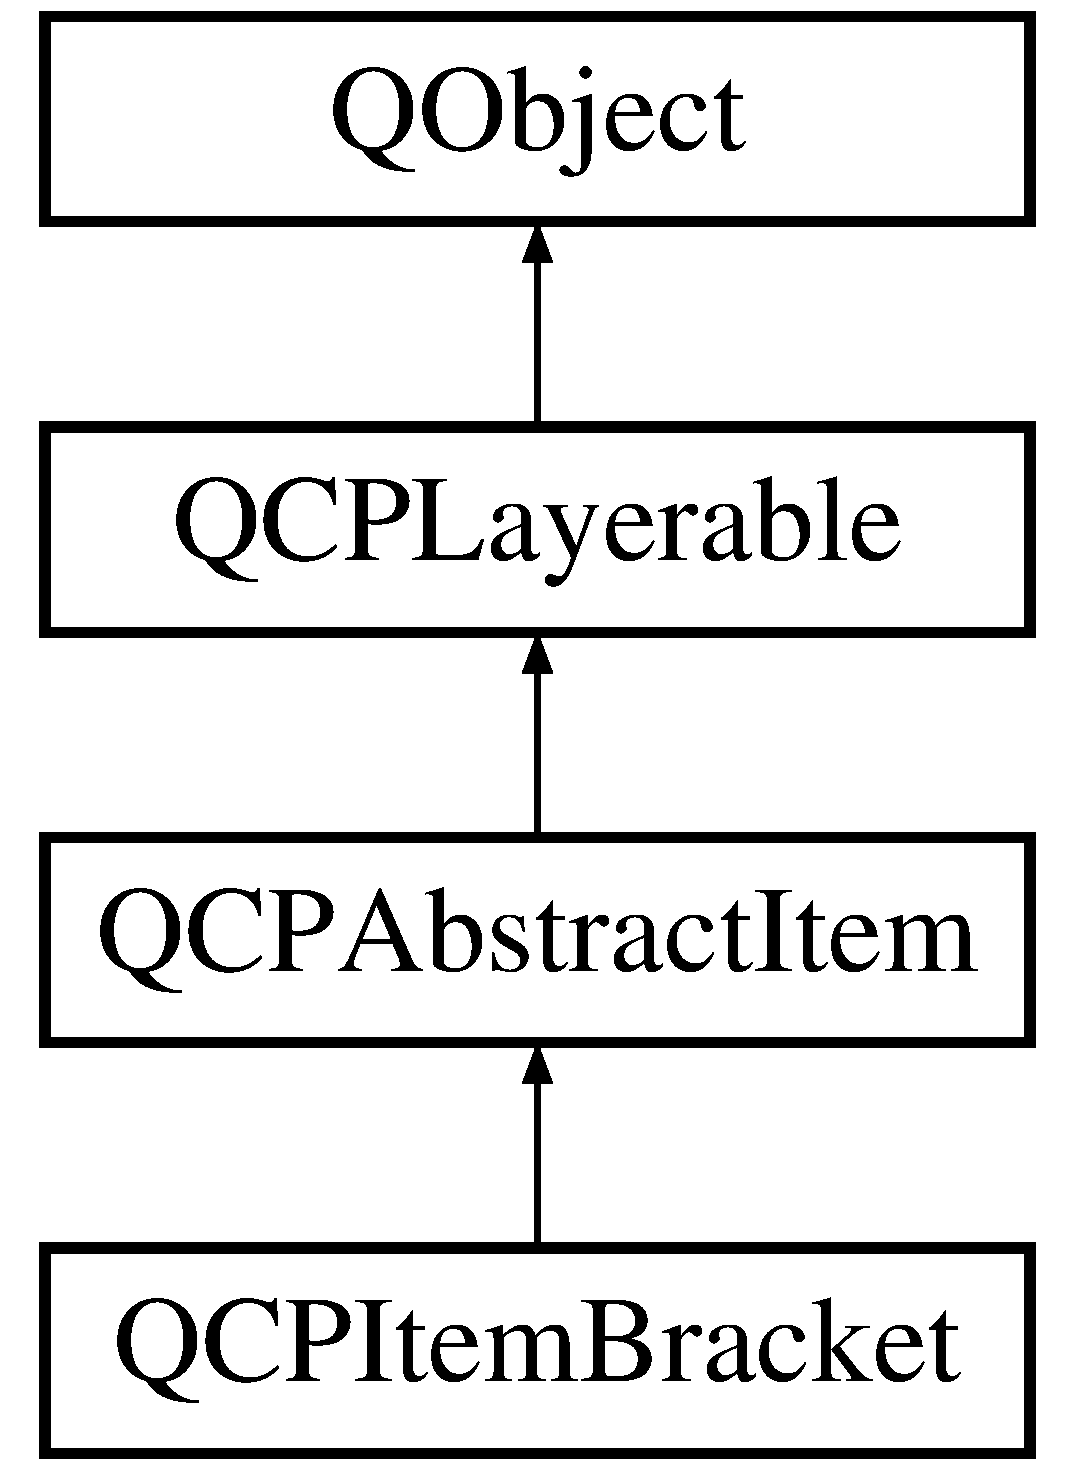
\includegraphics[height=4.000000cm]{class_q_c_p_item_bracket}
\end{center}
\end{figure}
\subsection*{Public Types}
\begin{DoxyCompactItemize}
\item 
enum \hyperlink{class_q_c_p_item_bracket_a7ac3afd0b24a607054e7212047d59dbd}{Bracket\+Style} \{ \hyperlink{class_q_c_p_item_bracket_a7ac3afd0b24a607054e7212047d59dbda7f9df4a7359bfe3dac1dbe4ccf5d220c}{bs\+Square}, 
\hyperlink{class_q_c_p_item_bracket_a7ac3afd0b24a607054e7212047d59dbda394627b0830a26ee3e0a02ca67a9f918}{bs\+Round}, 
\hyperlink{class_q_c_p_item_bracket_a7ac3afd0b24a607054e7212047d59dbda5024ce4023c2d8de4221f1cd4816acd8}{bs\+Curly}, 
\hyperlink{class_q_c_p_item_bracket_a7ac3afd0b24a607054e7212047d59dbda8f29f5ef754e2dc9a9efdedb2face0f3}{bs\+Calligraphic}
 \}
\end{DoxyCompactItemize}
\subsection*{Public Member Functions}
\begin{DoxyCompactItemize}
\item 
\hyperlink{class_q_c_p_item_bracket_a44ecfa37a76de5e3549e2d61f9d8ee56}{Q\+C\+P\+Item\+Bracket} (\hyperlink{class_q_custom_plot}{Q\+Custom\+Plot} $\ast$\hyperlink{class_q_c_p_layerable_ab7e0e94461566093d36ffc0f5312b109}{parent\+Plot})
\item 
virtual \hyperlink{class_q_c_p_item_bracket_ad773c3e8e09868d6f8caeb92c54919f4}{$\sim$\+Q\+C\+P\+Item\+Bracket} ()
\item 
Q\+Pen \hyperlink{class_q_c_p_item_bracket_a8963ff4a232b649c83d2461fd3c30d39}{pen} () const 
\item 
Q\+Pen \hyperlink{class_q_c_p_item_bracket_a9f6ea5ea9559ef36dfacdadd6e9bdcf0}{selected\+Pen} () const 
\item 
double \hyperlink{class_q_c_p_item_bracket_aed5126eafcb1381ee5718499c20ba023}{length} () const 
\item 
\hyperlink{class_q_c_p_item_bracket_a7ac3afd0b24a607054e7212047d59dbd}{Bracket\+Style} \hyperlink{class_q_c_p_item_bracket_afad726f453f70fe77c0e9c2f260fff97}{style} () const 
\item 
void \hyperlink{class_q_c_p_item_bracket_ab13001d9cc5d8f9e56ea15bdda682acb}{set\+Pen} (const Q\+Pen \&\hyperlink{class_q_c_p_item_bracket_a8963ff4a232b649c83d2461fd3c30d39}{pen})
\item 
void \hyperlink{class_q_c_p_item_bracket_a349785c31122778a520c64891fa204c5}{set\+Selected\+Pen} (const Q\+Pen \&\hyperlink{class_q_c_p_item_bracket_a8963ff4a232b649c83d2461fd3c30d39}{pen})
\item 
void \hyperlink{class_q_c_p_item_bracket_ac7cfc3da7da9b5c5ac5dfbe4f0351b2a}{set\+Length} (double \hyperlink{class_q_c_p_item_bracket_aed5126eafcb1381ee5718499c20ba023}{length})
\item 
void \hyperlink{class_q_c_p_item_bracket_a612dffa2373422eef8754d690add3703}{set\+Style} (\hyperlink{class_q_c_p_item_bracket_a7ac3afd0b24a607054e7212047d59dbd}{Bracket\+Style} \hyperlink{class_q_c_p_item_bracket_afad726f453f70fe77c0e9c2f260fff97}{style})
\item 
virtual double \hyperlink{class_q_c_p_item_bracket_aa6933caff1d42c54bcebc769ef88c798}{select\+Test} (const Q\+Point\+F \&pos, bool only\+Selectable, Q\+Variant $\ast$details=0) const 
\end{DoxyCompactItemize}
\subsection*{Public Attributes}
\begin{DoxyCompactItemize}
\item 
\hyperlink{class_q_c_p_item_position}{Q\+C\+P\+Item\+Position} $\ast$const \hyperlink{class_q_c_p_item_bracket_af6cc6d27d96171778c6927d6edce48b0}{left}
\item 
\hyperlink{class_q_c_p_item_position}{Q\+C\+P\+Item\+Position} $\ast$const \hyperlink{class_q_c_p_item_bracket_afa6c1360b05a50c4e0df37b3cebab6be}{right}
\item 
\hyperlink{class_q_c_p_item_anchor}{Q\+C\+P\+Item\+Anchor} $\ast$const \hyperlink{class_q_c_p_item_bracket_a2dbcabdf5f467f28be12a7b25962ffca}{center}
\end{DoxyCompactItemize}
\subsection*{Protected Types}
\begin{DoxyCompactItemize}
\item 
enum \hyperlink{class_q_c_p_item_bracket_a7f3a6a56d67f71219ed220553f3dd861}{Anchor\+Index} \{ \hyperlink{class_q_c_p_item_bracket_a7f3a6a56d67f71219ed220553f3dd861a17b57ef34cc05eadfe9becd1ad5b5242}{ai\+Center}
 \}
\end{DoxyCompactItemize}
\subsection*{Protected Member Functions}
\begin{DoxyCompactItemize}
\item 
virtual void \hyperlink{class_q_c_p_item_bracket_a8343cf0559c64886add7aa7f4b22f1a6}{draw} (\hyperlink{class_q_c_p_painter}{Q\+C\+P\+Painter} $\ast$painter)
\item 
virtual Q\+Point\+F \hyperlink{class_q_c_p_item_bracket_ac76827e3acba5faee81f149af4047a39}{anchor\+Pixel\+Point} (int anchor\+Id) const 
\item 
Q\+Pen \hyperlink{class_q_c_p_item_bracket_a8df4ad873bf88a4a7bfb9bbbd490e495}{main\+Pen} () const 
\end{DoxyCompactItemize}
\subsection*{Protected Attributes}
\begin{DoxyCompactItemize}
\item 
Q\+Pen \hyperlink{class_q_c_p_item_bracket_a350c864a5853b04343719f5a8be6b675}{m\+Pen}
\item 
Q\+Pen \hyperlink{class_q_c_p_item_bracket_adcfb53602d1802d00e2de4fd6df6b291}{m\+Selected\+Pen}
\item 
double \hyperlink{class_q_c_p_item_bracket_ab3d99bba8da18eb4d0e0cb23dded33b2}{m\+Length}
\item 
\hyperlink{class_q_c_p_item_bracket_a7ac3afd0b24a607054e7212047d59dbd}{Bracket\+Style} \hyperlink{class_q_c_p_item_bracket_ac911907184c824d621f274f8e0990080}{m\+Style}
\end{DoxyCompactItemize}
\subsection*{Additional Inherited Members}


\subsection{Detailed Description}
A bracket for referencing/highlighting certain parts in the plot. 

 It has two positions, {\itshape left} and {\itshape right}, which define the span of the bracket. If {\itshape left} is actually farther to the left than {\itshape right}, the bracket is opened to the bottom, as shown in the example image.

The bracket supports multiple styles via \hyperlink{class_q_c_p_item_bracket_a612dffa2373422eef8754d690add3703}{set\+Style}. The length, i.\+e. how far the bracket stretches away from the embraced span, can be controlled with \hyperlink{class_q_c_p_item_bracket_ac7cfc3da7da9b5c5ac5dfbe4f0351b2a}{set\+Length}.

 \begin{center}Demonstrating the effect of different values for \hyperlink{class_q_c_p_item_bracket_ac7cfc3da7da9b5c5ac5dfbe4f0351b2a}{set\+Length}, for styles \hyperlink{class_q_c_p_item_bracket_a7ac3afd0b24a607054e7212047d59dbda8f29f5ef754e2dc9a9efdedb2face0f3}{bs\+Calligraphic} and \hyperlink{class_q_c_p_item_bracket_a7ac3afd0b24a607054e7212047d59dbda7f9df4a7359bfe3dac1dbe4ccf5d220c}{bs\+Square}. Anchors and positions are displayed for reference.\end{center} 

It provides an anchor {\itshape center}, to allow connection of other items, e.\+g. an arrow (\hyperlink{class_q_c_p_item_line}{Q\+C\+P\+Item\+Line} or \hyperlink{class_q_c_p_item_curve}{Q\+C\+P\+Item\+Curve}) or a text label (\hyperlink{class_q_c_p_item_text}{Q\+C\+P\+Item\+Text}), to the bracket. 

\subsection{Member Enumeration Documentation}
\hypertarget{class_q_c_p_item_bracket_a7f3a6a56d67f71219ed220553f3dd861}{}\index{Q\+C\+P\+Item\+Bracket@{Q\+C\+P\+Item\+Bracket}!Anchor\+Index@{Anchor\+Index}}
\index{Anchor\+Index@{Anchor\+Index}!Q\+C\+P\+Item\+Bracket@{Q\+C\+P\+Item\+Bracket}}
\subsubsection[{Anchor\+Index}]{\setlength{\rightskip}{0pt plus 5cm}enum {\bf Q\+C\+P\+Item\+Bracket\+::\+Anchor\+Index}\hspace{0.3cm}{\ttfamily [protected]}}\label{class_q_c_p_item_bracket_a7f3a6a56d67f71219ed220553f3dd861}
\begin{Desc}
\item[Enumerator]\par
\begin{description}
\index{ai\+Center@{ai\+Center}!Q\+C\+P\+Item\+Bracket@{Q\+C\+P\+Item\+Bracket}}\index{Q\+C\+P\+Item\+Bracket@{Q\+C\+P\+Item\+Bracket}!ai\+Center@{ai\+Center}}\item[{\em 
\hypertarget{class_q_c_p_item_bracket_a7f3a6a56d67f71219ed220553f3dd861a17b57ef34cc05eadfe9becd1ad5b5242}{}ai\+Center\label{class_q_c_p_item_bracket_a7f3a6a56d67f71219ed220553f3dd861a17b57ef34cc05eadfe9becd1ad5b5242}
}]\end{description}
\end{Desc}
\hypertarget{class_q_c_p_item_bracket_a7ac3afd0b24a607054e7212047d59dbd}{}\index{Q\+C\+P\+Item\+Bracket@{Q\+C\+P\+Item\+Bracket}!Bracket\+Style@{Bracket\+Style}}
\index{Bracket\+Style@{Bracket\+Style}!Q\+C\+P\+Item\+Bracket@{Q\+C\+P\+Item\+Bracket}}
\subsubsection[{Bracket\+Style}]{\setlength{\rightskip}{0pt plus 5cm}enum {\bf Q\+C\+P\+Item\+Bracket\+::\+Bracket\+Style}}\label{class_q_c_p_item_bracket_a7ac3afd0b24a607054e7212047d59dbd}
\begin{Desc}
\item[Enumerator]\par
\begin{description}
\index{bs\+Square@{bs\+Square}!Q\+C\+P\+Item\+Bracket@{Q\+C\+P\+Item\+Bracket}}\index{Q\+C\+P\+Item\+Bracket@{Q\+C\+P\+Item\+Bracket}!bs\+Square@{bs\+Square}}\item[{\em 
\hypertarget{class_q_c_p_item_bracket_a7ac3afd0b24a607054e7212047d59dbda7f9df4a7359bfe3dac1dbe4ccf5d220c}{}bs\+Square\label{class_q_c_p_item_bracket_a7ac3afd0b24a607054e7212047d59dbda7f9df4a7359bfe3dac1dbe4ccf5d220c}
}]A brace with angled edges. \index{bs\+Round@{bs\+Round}!Q\+C\+P\+Item\+Bracket@{Q\+C\+P\+Item\+Bracket}}\index{Q\+C\+P\+Item\+Bracket@{Q\+C\+P\+Item\+Bracket}!bs\+Round@{bs\+Round}}\item[{\em 
\hypertarget{class_q_c_p_item_bracket_a7ac3afd0b24a607054e7212047d59dbda394627b0830a26ee3e0a02ca67a9f918}{}bs\+Round\label{class_q_c_p_item_bracket_a7ac3afd0b24a607054e7212047d59dbda394627b0830a26ee3e0a02ca67a9f918}
}]A brace with round edges. \index{bs\+Curly@{bs\+Curly}!Q\+C\+P\+Item\+Bracket@{Q\+C\+P\+Item\+Bracket}}\index{Q\+C\+P\+Item\+Bracket@{Q\+C\+P\+Item\+Bracket}!bs\+Curly@{bs\+Curly}}\item[{\em 
\hypertarget{class_q_c_p_item_bracket_a7ac3afd0b24a607054e7212047d59dbda5024ce4023c2d8de4221f1cd4816acd8}{}bs\+Curly\label{class_q_c_p_item_bracket_a7ac3afd0b24a607054e7212047d59dbda5024ce4023c2d8de4221f1cd4816acd8}
}]A curly brace. \index{bs\+Calligraphic@{bs\+Calligraphic}!Q\+C\+P\+Item\+Bracket@{Q\+C\+P\+Item\+Bracket}}\index{Q\+C\+P\+Item\+Bracket@{Q\+C\+P\+Item\+Bracket}!bs\+Calligraphic@{bs\+Calligraphic}}\item[{\em 
\hypertarget{class_q_c_p_item_bracket_a7ac3afd0b24a607054e7212047d59dbda8f29f5ef754e2dc9a9efdedb2face0f3}{}bs\+Calligraphic\label{class_q_c_p_item_bracket_a7ac3afd0b24a607054e7212047d59dbda8f29f5ef754e2dc9a9efdedb2face0f3}
}]A curly brace with varying stroke width giving a calligraphic impression. \end{description}
\end{Desc}


\subsection{Constructor \& Destructor Documentation}
\hypertarget{class_q_c_p_item_bracket_a44ecfa37a76de5e3549e2d61f9d8ee56}{}\index{Q\+C\+P\+Item\+Bracket@{Q\+C\+P\+Item\+Bracket}!Q\+C\+P\+Item\+Bracket@{Q\+C\+P\+Item\+Bracket}}
\index{Q\+C\+P\+Item\+Bracket@{Q\+C\+P\+Item\+Bracket}!Q\+C\+P\+Item\+Bracket@{Q\+C\+P\+Item\+Bracket}}
\subsubsection[{Q\+C\+P\+Item\+Bracket}]{\setlength{\rightskip}{0pt plus 5cm}Q\+C\+P\+Item\+Bracket\+::\+Q\+C\+P\+Item\+Bracket (
\begin{DoxyParamCaption}
\item[{{\bf Q\+Custom\+Plot} $\ast$}]{parent\+Plot}
\end{DoxyParamCaption}
)}\label{class_q_c_p_item_bracket_a44ecfa37a76de5e3549e2d61f9d8ee56}
Creates a bracket item and sets default values.

The constructed item can be added to the plot with \hyperlink{class_q_custom_plot_aa500620379262321685cb7a7674cbd2a}{Q\+Custom\+Plot\+::add\+Item}. \hypertarget{class_q_c_p_item_bracket_ad773c3e8e09868d6f8caeb92c54919f4}{}\index{Q\+C\+P\+Item\+Bracket@{Q\+C\+P\+Item\+Bracket}!````~Q\+C\+P\+Item\+Bracket@{$\sim$\+Q\+C\+P\+Item\+Bracket}}
\index{````~Q\+C\+P\+Item\+Bracket@{$\sim$\+Q\+C\+P\+Item\+Bracket}!Q\+C\+P\+Item\+Bracket@{Q\+C\+P\+Item\+Bracket}}
\subsubsection[{$\sim$\+Q\+C\+P\+Item\+Bracket}]{\setlength{\rightskip}{0pt plus 5cm}Q\+C\+P\+Item\+Bracket\+::$\sim$\+Q\+C\+P\+Item\+Bracket (
\begin{DoxyParamCaption}
{}
\end{DoxyParamCaption}
)\hspace{0.3cm}{\ttfamily [virtual]}}\label{class_q_c_p_item_bracket_ad773c3e8e09868d6f8caeb92c54919f4}


\subsection{Member Function Documentation}
\hypertarget{class_q_c_p_item_bracket_ac76827e3acba5faee81f149af4047a39}{}\index{Q\+C\+P\+Item\+Bracket@{Q\+C\+P\+Item\+Bracket}!anchor\+Pixel\+Point@{anchor\+Pixel\+Point}}
\index{anchor\+Pixel\+Point@{anchor\+Pixel\+Point}!Q\+C\+P\+Item\+Bracket@{Q\+C\+P\+Item\+Bracket}}
\subsubsection[{anchor\+Pixel\+Point}]{\setlength{\rightskip}{0pt plus 5cm}Q\+Point\+F Q\+C\+P\+Item\+Bracket\+::anchor\+Pixel\+Point (
\begin{DoxyParamCaption}
\item[{int}]{anchor\+Id}
\end{DoxyParamCaption}
) const\hspace{0.3cm}{\ttfamily [protected]}, {\ttfamily [virtual]}}\label{class_q_c_p_item_bracket_ac76827e3acba5faee81f149af4047a39}


Reimplemented from \hyperlink{class_q_c_p_abstract_item_a94bde62b8a2fc133666dcbb8035deeed}{Q\+C\+P\+Abstract\+Item}.

\hypertarget{class_q_c_p_item_bracket_a8343cf0559c64886add7aa7f4b22f1a6}{}\index{Q\+C\+P\+Item\+Bracket@{Q\+C\+P\+Item\+Bracket}!draw@{draw}}
\index{draw@{draw}!Q\+C\+P\+Item\+Bracket@{Q\+C\+P\+Item\+Bracket}}
\subsubsection[{draw}]{\setlength{\rightskip}{0pt plus 5cm}void Q\+C\+P\+Item\+Bracket\+::draw (
\begin{DoxyParamCaption}
\item[{{\bf Q\+C\+P\+Painter} $\ast$}]{painter}
\end{DoxyParamCaption}
)\hspace{0.3cm}{\ttfamily [protected]}, {\ttfamily [virtual]}}\label{class_q_c_p_item_bracket_a8343cf0559c64886add7aa7f4b22f1a6}


Implements \hyperlink{class_q_c_p_abstract_item_ad0dc056f650c3ca73414e6b4f01674ef}{Q\+C\+P\+Abstract\+Item}.

\hypertarget{class_q_c_p_item_bracket_aed5126eafcb1381ee5718499c20ba023}{}\index{Q\+C\+P\+Item\+Bracket@{Q\+C\+P\+Item\+Bracket}!length@{length}}
\index{length@{length}!Q\+C\+P\+Item\+Bracket@{Q\+C\+P\+Item\+Bracket}}
\subsubsection[{length}]{\setlength{\rightskip}{0pt plus 5cm}double Q\+C\+P\+Item\+Bracket\+::length (
\begin{DoxyParamCaption}
{}
\end{DoxyParamCaption}
) const\hspace{0.3cm}{\ttfamily [inline]}}\label{class_q_c_p_item_bracket_aed5126eafcb1381ee5718499c20ba023}
\hypertarget{class_q_c_p_item_bracket_a8df4ad873bf88a4a7bfb9bbbd490e495}{}\index{Q\+C\+P\+Item\+Bracket@{Q\+C\+P\+Item\+Bracket}!main\+Pen@{main\+Pen}}
\index{main\+Pen@{main\+Pen}!Q\+C\+P\+Item\+Bracket@{Q\+C\+P\+Item\+Bracket}}
\subsubsection[{main\+Pen}]{\setlength{\rightskip}{0pt plus 5cm}Q\+Pen Q\+C\+P\+Item\+Bracket\+::main\+Pen (
\begin{DoxyParamCaption}
{}
\end{DoxyParamCaption}
) const\hspace{0.3cm}{\ttfamily [protected]}}\label{class_q_c_p_item_bracket_a8df4ad873bf88a4a7bfb9bbbd490e495}
\hypertarget{class_q_c_p_item_bracket_a8963ff4a232b649c83d2461fd3c30d39}{}\index{Q\+C\+P\+Item\+Bracket@{Q\+C\+P\+Item\+Bracket}!pen@{pen}}
\index{pen@{pen}!Q\+C\+P\+Item\+Bracket@{Q\+C\+P\+Item\+Bracket}}
\subsubsection[{pen}]{\setlength{\rightskip}{0pt plus 5cm}Q\+Pen Q\+C\+P\+Item\+Bracket\+::pen (
\begin{DoxyParamCaption}
{}
\end{DoxyParamCaption}
) const\hspace{0.3cm}{\ttfamily [inline]}}\label{class_q_c_p_item_bracket_a8963ff4a232b649c83d2461fd3c30d39}
\hypertarget{class_q_c_p_item_bracket_a9f6ea5ea9559ef36dfacdadd6e9bdcf0}{}\index{Q\+C\+P\+Item\+Bracket@{Q\+C\+P\+Item\+Bracket}!selected\+Pen@{selected\+Pen}}
\index{selected\+Pen@{selected\+Pen}!Q\+C\+P\+Item\+Bracket@{Q\+C\+P\+Item\+Bracket}}
\subsubsection[{selected\+Pen}]{\setlength{\rightskip}{0pt plus 5cm}Q\+Pen Q\+C\+P\+Item\+Bracket\+::selected\+Pen (
\begin{DoxyParamCaption}
{}
\end{DoxyParamCaption}
) const\hspace{0.3cm}{\ttfamily [inline]}}\label{class_q_c_p_item_bracket_a9f6ea5ea9559ef36dfacdadd6e9bdcf0}
\hypertarget{class_q_c_p_item_bracket_aa6933caff1d42c54bcebc769ef88c798}{}\index{Q\+C\+P\+Item\+Bracket@{Q\+C\+P\+Item\+Bracket}!select\+Test@{select\+Test}}
\index{select\+Test@{select\+Test}!Q\+C\+P\+Item\+Bracket@{Q\+C\+P\+Item\+Bracket}}
\subsubsection[{select\+Test}]{\setlength{\rightskip}{0pt plus 5cm}double Q\+C\+P\+Item\+Bracket\+::select\+Test (
\begin{DoxyParamCaption}
\item[{const Q\+Point\+F \&}]{pos, }
\item[{bool}]{only\+Selectable, }
\item[{Q\+Variant $\ast$}]{details = {\ttfamily 0}}
\end{DoxyParamCaption}
) const\hspace{0.3cm}{\ttfamily [virtual]}}\label{class_q_c_p_item_bracket_aa6933caff1d42c54bcebc769ef88c798}
This function is used to decide whether a click hits a layerable object or not.

{\itshape pos} is a point in pixel coordinates on the \hyperlink{class_q_custom_plot}{Q\+Custom\+Plot} surface. This function returns the shortest pixel distance of this point to the object. If the object is either invisible or the distance couldn\textquotesingle{}t be determined, -\/1.\+0 is returned. Further, if {\itshape only\+Selectable} is true and the object is not selectable, -\/1.\+0 is returned, too.

If the item is represented not by single lines but by an area like \hyperlink{class_q_c_p_item_rect}{Q\+C\+P\+Item\+Rect} or \hyperlink{class_q_c_p_item_text}{Q\+C\+P\+Item\+Text}, a click inside the area returns a constant value greater zero (typically the selection\+Tolerance of the parent \hyperlink{class_q_custom_plot}{Q\+Custom\+Plot} multiplied by 0.\+99). If the click lies outside the area, this function returns -\/1.\+0.

Providing a constant value for area objects allows selecting line objects even when they are obscured by such area objects, by clicking close to the lines (i.\+e. closer than 0.\+99$\ast$selection\+Tolerance).

The actual setting of the selection state is not done by this function. This is handled by the parent \hyperlink{class_q_custom_plot}{Q\+Custom\+Plot} when the mouse\+Release\+Event occurs, and the finally selected object is notified via the select\+Event/deselect\+Event methods.

{\itshape details} is an optional output parameter. Every layerable subclass may place any information in {\itshape details}. This information will be passed to \hyperlink{class_q_c_p_abstract_item_aaf92af7b9893712959a6c073d334d88d}{select\+Event} when the parent \hyperlink{class_q_custom_plot}{Q\+Custom\+Plot} decides on the basis of this select\+Test call, that the object was successfully selected. The subsequent call to \hyperlink{class_q_c_p_abstract_item_aaf92af7b9893712959a6c073d334d88d}{select\+Event} will carry the {\itshape details}. This is useful for multi-\/part objects (like \hyperlink{class_q_c_p_axis}{Q\+C\+P\+Axis}). This way, a possibly complex calculation to decide which part was clicked is only done once in \hyperlink{class_q_c_p_item_bracket_aa6933caff1d42c54bcebc769ef88c798}{select\+Test}. The result (i.\+e. the actually clicked part) can then be placed in {\itshape details}. So in the subsequent \hyperlink{class_q_c_p_abstract_item_aaf92af7b9893712959a6c073d334d88d}{select\+Event}, the decision which part was selected doesn\textquotesingle{}t have to be done a second time for a single selection operation.

You may pass 0 as {\itshape details} to indicate that you are not interested in those selection details.

\begin{DoxySeeAlso}{See also}
\hyperlink{class_q_c_p_abstract_item_aaf92af7b9893712959a6c073d334d88d}{select\+Event}, \hyperlink{class_q_c_p_abstract_item_a91f090d6763cfedb0749219c63788ae9}{deselect\+Event}, \hyperlink{class_q_custom_plot_a5ee1e2f6ae27419deca53e75907c27e5}{Q\+Custom\+Plot\+::set\+Interactions} 
\end{DoxySeeAlso}


Implements \hyperlink{class_q_c_p_abstract_item_a96d522d10ffc0413b9a366c6f7f0476b}{Q\+C\+P\+Abstract\+Item}.

\hypertarget{class_q_c_p_item_bracket_ac7cfc3da7da9b5c5ac5dfbe4f0351b2a}{}\index{Q\+C\+P\+Item\+Bracket@{Q\+C\+P\+Item\+Bracket}!set\+Length@{set\+Length}}
\index{set\+Length@{set\+Length}!Q\+C\+P\+Item\+Bracket@{Q\+C\+P\+Item\+Bracket}}
\subsubsection[{set\+Length}]{\setlength{\rightskip}{0pt plus 5cm}void Q\+C\+P\+Item\+Bracket\+::set\+Length (
\begin{DoxyParamCaption}
\item[{double}]{length}
\end{DoxyParamCaption}
)}\label{class_q_c_p_item_bracket_ac7cfc3da7da9b5c5ac5dfbe4f0351b2a}
Sets the {\itshape length} in pixels how far the bracket extends in the direction towards the embraced span of the bracket (i.\+e. perpendicular to the {\itshape left}-\/{\itshape right}-\/direction)

 \begin{center}Demonstrating the effect of different values for \hyperlink{class_q_c_p_item_bracket_ac7cfc3da7da9b5c5ac5dfbe4f0351b2a}{set\+Length}, for styles \hyperlink{class_q_c_p_item_bracket_a7ac3afd0b24a607054e7212047d59dbda8f29f5ef754e2dc9a9efdedb2face0f3}{bs\+Calligraphic} and \hyperlink{class_q_c_p_item_bracket_a7ac3afd0b24a607054e7212047d59dbda7f9df4a7359bfe3dac1dbe4ccf5d220c}{bs\+Square}. Anchors and positions are displayed for reference.\end{center}  \hypertarget{class_q_c_p_item_bracket_ab13001d9cc5d8f9e56ea15bdda682acb}{}\index{Q\+C\+P\+Item\+Bracket@{Q\+C\+P\+Item\+Bracket}!set\+Pen@{set\+Pen}}
\index{set\+Pen@{set\+Pen}!Q\+C\+P\+Item\+Bracket@{Q\+C\+P\+Item\+Bracket}}
\subsubsection[{set\+Pen}]{\setlength{\rightskip}{0pt plus 5cm}void Q\+C\+P\+Item\+Bracket\+::set\+Pen (
\begin{DoxyParamCaption}
\item[{const Q\+Pen \&}]{pen}
\end{DoxyParamCaption}
)}\label{class_q_c_p_item_bracket_ab13001d9cc5d8f9e56ea15bdda682acb}
Sets the pen that will be used to draw the bracket.

Note that when the style is \hyperlink{class_q_c_p_item_bracket_a7ac3afd0b24a607054e7212047d59dbda8f29f5ef754e2dc9a9efdedb2face0f3}{bs\+Calligraphic}, only the color will be taken from the pen, the stroke and width are ignored. To change the apparent stroke width of a calligraphic bracket, use \hyperlink{class_q_c_p_item_bracket_ac7cfc3da7da9b5c5ac5dfbe4f0351b2a}{set\+Length}, which has a similar effect.

\begin{DoxySeeAlso}{See also}
\hyperlink{class_q_c_p_item_bracket_a349785c31122778a520c64891fa204c5}{set\+Selected\+Pen} 
\end{DoxySeeAlso}
\hypertarget{class_q_c_p_item_bracket_a349785c31122778a520c64891fa204c5}{}\index{Q\+C\+P\+Item\+Bracket@{Q\+C\+P\+Item\+Bracket}!set\+Selected\+Pen@{set\+Selected\+Pen}}
\index{set\+Selected\+Pen@{set\+Selected\+Pen}!Q\+C\+P\+Item\+Bracket@{Q\+C\+P\+Item\+Bracket}}
\subsubsection[{set\+Selected\+Pen}]{\setlength{\rightskip}{0pt plus 5cm}void Q\+C\+P\+Item\+Bracket\+::set\+Selected\+Pen (
\begin{DoxyParamCaption}
\item[{const Q\+Pen \&}]{pen}
\end{DoxyParamCaption}
)}\label{class_q_c_p_item_bracket_a349785c31122778a520c64891fa204c5}
Sets the pen that will be used to draw the bracket when selected

\begin{DoxySeeAlso}{See also}
\hyperlink{class_q_c_p_item_bracket_ab13001d9cc5d8f9e56ea15bdda682acb}{set\+Pen}, \hyperlink{class_q_c_p_abstract_item_a203de94ad586cc44d16c9565f49d3378}{set\+Selected} 
\end{DoxySeeAlso}
\hypertarget{class_q_c_p_item_bracket_a612dffa2373422eef8754d690add3703}{}\index{Q\+C\+P\+Item\+Bracket@{Q\+C\+P\+Item\+Bracket}!set\+Style@{set\+Style}}
\index{set\+Style@{set\+Style}!Q\+C\+P\+Item\+Bracket@{Q\+C\+P\+Item\+Bracket}}
\subsubsection[{set\+Style}]{\setlength{\rightskip}{0pt plus 5cm}void Q\+C\+P\+Item\+Bracket\+::set\+Style (
\begin{DoxyParamCaption}
\item[{{\bf Q\+C\+P\+Item\+Bracket\+::\+Bracket\+Style}}]{style}
\end{DoxyParamCaption}
)}\label{class_q_c_p_item_bracket_a612dffa2373422eef8754d690add3703}
Sets the style of the bracket, i.\+e. the shape/visual appearance.

\begin{DoxySeeAlso}{See also}
\hyperlink{class_q_c_p_item_bracket_ab13001d9cc5d8f9e56ea15bdda682acb}{set\+Pen} 
\end{DoxySeeAlso}
\hypertarget{class_q_c_p_item_bracket_afad726f453f70fe77c0e9c2f260fff97}{}\index{Q\+C\+P\+Item\+Bracket@{Q\+C\+P\+Item\+Bracket}!style@{style}}
\index{style@{style}!Q\+C\+P\+Item\+Bracket@{Q\+C\+P\+Item\+Bracket}}
\subsubsection[{style}]{\setlength{\rightskip}{0pt plus 5cm}{\bf Bracket\+Style} Q\+C\+P\+Item\+Bracket\+::style (
\begin{DoxyParamCaption}
{}
\end{DoxyParamCaption}
) const\hspace{0.3cm}{\ttfamily [inline]}}\label{class_q_c_p_item_bracket_afad726f453f70fe77c0e9c2f260fff97}


\subsection{Member Data Documentation}
\hypertarget{class_q_c_p_item_bracket_a2dbcabdf5f467f28be12a7b25962ffca}{}\index{Q\+C\+P\+Item\+Bracket@{Q\+C\+P\+Item\+Bracket}!center@{center}}
\index{center@{center}!Q\+C\+P\+Item\+Bracket@{Q\+C\+P\+Item\+Bracket}}
\subsubsection[{center}]{\setlength{\rightskip}{0pt plus 5cm}{\bf Q\+C\+P\+Item\+Anchor}$\ast$ const Q\+C\+P\+Item\+Bracket\+::center}\label{class_q_c_p_item_bracket_a2dbcabdf5f467f28be12a7b25962ffca}
\hypertarget{class_q_c_p_item_bracket_af6cc6d27d96171778c6927d6edce48b0}{}\index{Q\+C\+P\+Item\+Bracket@{Q\+C\+P\+Item\+Bracket}!left@{left}}
\index{left@{left}!Q\+C\+P\+Item\+Bracket@{Q\+C\+P\+Item\+Bracket}}
\subsubsection[{left}]{\setlength{\rightskip}{0pt plus 5cm}{\bf Q\+C\+P\+Item\+Position}$\ast$ const Q\+C\+P\+Item\+Bracket\+::left}\label{class_q_c_p_item_bracket_af6cc6d27d96171778c6927d6edce48b0}
\hypertarget{class_q_c_p_item_bracket_ab3d99bba8da18eb4d0e0cb23dded33b2}{}\index{Q\+C\+P\+Item\+Bracket@{Q\+C\+P\+Item\+Bracket}!m\+Length@{m\+Length}}
\index{m\+Length@{m\+Length}!Q\+C\+P\+Item\+Bracket@{Q\+C\+P\+Item\+Bracket}}
\subsubsection[{m\+Length}]{\setlength{\rightskip}{0pt plus 5cm}double Q\+C\+P\+Item\+Bracket\+::m\+Length\hspace{0.3cm}{\ttfamily [protected]}}\label{class_q_c_p_item_bracket_ab3d99bba8da18eb4d0e0cb23dded33b2}
\hypertarget{class_q_c_p_item_bracket_a350c864a5853b04343719f5a8be6b675}{}\index{Q\+C\+P\+Item\+Bracket@{Q\+C\+P\+Item\+Bracket}!m\+Pen@{m\+Pen}}
\index{m\+Pen@{m\+Pen}!Q\+C\+P\+Item\+Bracket@{Q\+C\+P\+Item\+Bracket}}
\subsubsection[{m\+Pen}]{\setlength{\rightskip}{0pt plus 5cm}Q\+Pen Q\+C\+P\+Item\+Bracket\+::m\+Pen\hspace{0.3cm}{\ttfamily [protected]}}\label{class_q_c_p_item_bracket_a350c864a5853b04343719f5a8be6b675}
\hypertarget{class_q_c_p_item_bracket_adcfb53602d1802d00e2de4fd6df6b291}{}\index{Q\+C\+P\+Item\+Bracket@{Q\+C\+P\+Item\+Bracket}!m\+Selected\+Pen@{m\+Selected\+Pen}}
\index{m\+Selected\+Pen@{m\+Selected\+Pen}!Q\+C\+P\+Item\+Bracket@{Q\+C\+P\+Item\+Bracket}}
\subsubsection[{m\+Selected\+Pen}]{\setlength{\rightskip}{0pt plus 5cm}Q\+Pen Q\+C\+P\+Item\+Bracket\+::m\+Selected\+Pen\hspace{0.3cm}{\ttfamily [protected]}}\label{class_q_c_p_item_bracket_adcfb53602d1802d00e2de4fd6df6b291}
\hypertarget{class_q_c_p_item_bracket_ac911907184c824d621f274f8e0990080}{}\index{Q\+C\+P\+Item\+Bracket@{Q\+C\+P\+Item\+Bracket}!m\+Style@{m\+Style}}
\index{m\+Style@{m\+Style}!Q\+C\+P\+Item\+Bracket@{Q\+C\+P\+Item\+Bracket}}
\subsubsection[{m\+Style}]{\setlength{\rightskip}{0pt plus 5cm}{\bf Bracket\+Style} Q\+C\+P\+Item\+Bracket\+::m\+Style\hspace{0.3cm}{\ttfamily [protected]}}\label{class_q_c_p_item_bracket_ac911907184c824d621f274f8e0990080}
\hypertarget{class_q_c_p_item_bracket_afa6c1360b05a50c4e0df37b3cebab6be}{}\index{Q\+C\+P\+Item\+Bracket@{Q\+C\+P\+Item\+Bracket}!right@{right}}
\index{right@{right}!Q\+C\+P\+Item\+Bracket@{Q\+C\+P\+Item\+Bracket}}
\subsubsection[{right}]{\setlength{\rightskip}{0pt plus 5cm}{\bf Q\+C\+P\+Item\+Position}$\ast$ const Q\+C\+P\+Item\+Bracket\+::right}\label{class_q_c_p_item_bracket_afa6c1360b05a50c4e0df37b3cebab6be}


The documentation for this class was generated from the following files\+:\begin{DoxyCompactItemize}
\item 
C\+:/\+Users/\+Roman/\+Documents/\+Mygs/\+Ground\+Station/\+G\+S/\hyperlink{qcustomplot_8h}{qcustomplot.\+h}\item 
C\+:/\+Users/\+Roman/\+Documents/\+Mygs/\+Ground\+Station/\+G\+S/\hyperlink{qcustomplot_8cpp}{qcustomplot.\+cpp}\end{DoxyCompactItemize}

\hypertarget{class_q_c_p_item_curve}{}\section{Q\+C\+P\+Item\+Curve Class Reference}
\label{class_q_c_p_item_curve}\index{Q\+C\+P\+Item\+Curve@{Q\+C\+P\+Item\+Curve}}


A curved line from one point to another.  




{\ttfamily \#include $<$qcustomplot.\+h$>$}

Inheritance diagram for Q\+C\+P\+Item\+Curve\+:\begin{figure}[H]
\begin{center}
\leavevmode
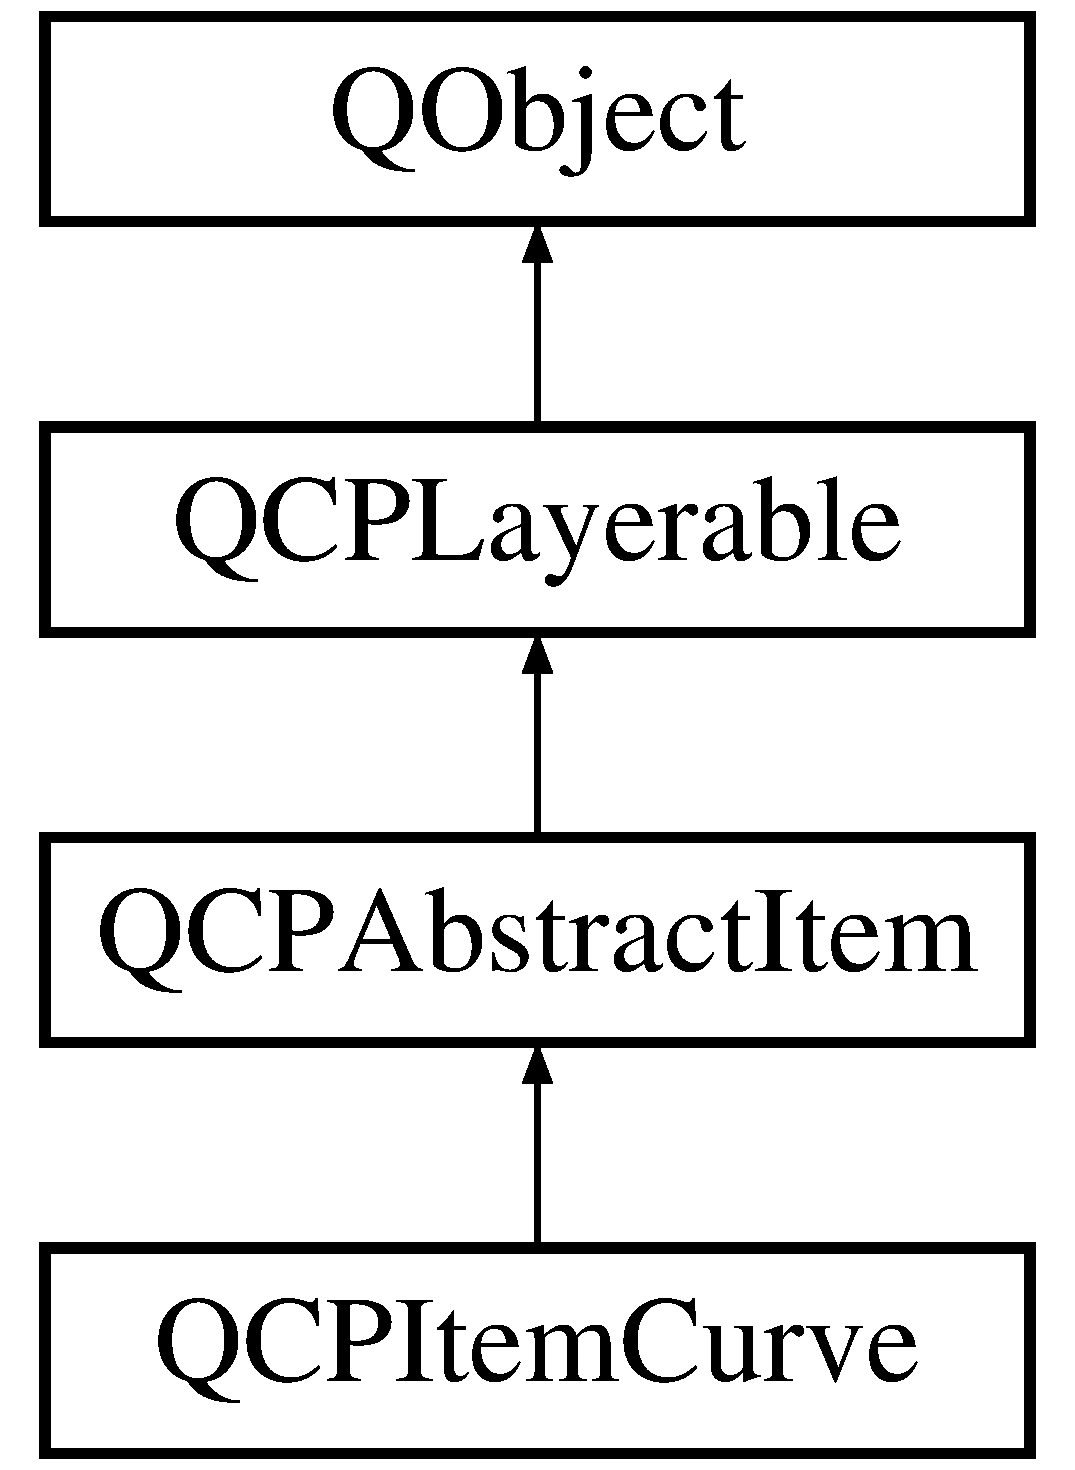
\includegraphics[height=4.000000cm]{class_q_c_p_item_curve}
\end{center}
\end{figure}
\subsection*{Public Member Functions}
\begin{DoxyCompactItemize}
\item 
\hyperlink{class_q_c_p_item_curve_ac9b7508bb5c8827e1a7a6199f8c82bec}{Q\+C\+P\+Item\+Curve} (\hyperlink{class_q_custom_plot}{Q\+Custom\+Plot} $\ast$\hyperlink{class_q_c_p_layerable_ab7e0e94461566093d36ffc0f5312b109}{parent\+Plot})
\item 
virtual \hyperlink{class_q_c_p_item_curve_ae36f20fd5deff2f1443a7c53eaa95c81}{$\sim$\+Q\+C\+P\+Item\+Curve} ()
\item 
Q\+Pen \hyperlink{class_q_c_p_item_curve_abc6321e55a9ba1a0c7df407843dfa252}{pen} () const 
\item 
Q\+Pen \hyperlink{class_q_c_p_item_curve_abd8b8be5b13bc4dafec4c1758c281336}{selected\+Pen} () const 
\item 
\hyperlink{class_q_c_p_line_ending}{Q\+C\+P\+Line\+Ending} \hyperlink{class_q_c_p_item_curve_afc067f0d1e60cd04812f2c2c7fdf36c3}{head} () const 
\item 
\hyperlink{class_q_c_p_line_ending}{Q\+C\+P\+Line\+Ending} \hyperlink{class_q_c_p_item_curve_a9adddfcc5275be0cf27e3c0c31c37c1a}{tail} () const 
\item 
void \hyperlink{class_q_c_p_item_curve_a034be908440aec785c34b92843461221}{set\+Pen} (const Q\+Pen \&\hyperlink{class_q_c_p_item_curve_abc6321e55a9ba1a0c7df407843dfa252}{pen})
\item 
void \hyperlink{class_q_c_p_item_curve_a375b917669f868c5a106bf2f1ab7c26d}{set\+Selected\+Pen} (const Q\+Pen \&\hyperlink{class_q_c_p_item_curve_abc6321e55a9ba1a0c7df407843dfa252}{pen})
\item 
void \hyperlink{class_q_c_p_item_curve_a08a30d9cdd63995deea3d9e20430676f}{set\+Head} (const \hyperlink{class_q_c_p_line_ending}{Q\+C\+P\+Line\+Ending} \&\hyperlink{class_q_c_p_item_curve_afc067f0d1e60cd04812f2c2c7fdf36c3}{head})
\item 
void \hyperlink{class_q_c_p_item_curve_ac3488d8b1a6489c845dc5bff3ef71124}{set\+Tail} (const \hyperlink{class_q_c_p_line_ending}{Q\+C\+P\+Line\+Ending} \&\hyperlink{class_q_c_p_item_curve_a9adddfcc5275be0cf27e3c0c31c37c1a}{tail})
\item 
virtual double \hyperlink{class_q_c_p_item_curve_a741375c11667b5f9c95b2683f93ee514}{select\+Test} (const Q\+Point\+F \&pos, bool only\+Selectable, Q\+Variant $\ast$details=0) const 
\end{DoxyCompactItemize}
\subsection*{Public Attributes}
\begin{DoxyCompactItemize}
\item 
\hyperlink{class_q_c_p_item_position}{Q\+C\+P\+Item\+Position} $\ast$const \hyperlink{class_q_c_p_item_curve_a20c3b5ea31c33764f4f30c2ec7ae518b}{start}
\item 
\hyperlink{class_q_c_p_item_position}{Q\+C\+P\+Item\+Position} $\ast$const \hyperlink{class_q_c_p_item_curve_aa124bf66c09cc51c627fb49db8bf8a7b}{start\+Dir}
\item 
\hyperlink{class_q_c_p_item_position}{Q\+C\+P\+Item\+Position} $\ast$const \hyperlink{class_q_c_p_item_curve_a28181a9dee9cc3c3da83a883221bd2d0}{end\+Dir}
\item 
\hyperlink{class_q_c_p_item_position}{Q\+C\+P\+Item\+Position} $\ast$const \hyperlink{class_q_c_p_item_curve_a24ecbb195b32a08b42b61c2cf08a1b4d}{end}
\end{DoxyCompactItemize}
\subsection*{Protected Member Functions}
\begin{DoxyCompactItemize}
\item 
virtual void \hyperlink{class_q_c_p_item_curve_a56cb5b72cd02db2eda598274a39839a9}{draw} (\hyperlink{class_q_c_p_painter}{Q\+C\+P\+Painter} $\ast$painter)
\item 
Q\+Pen \hyperlink{class_q_c_p_item_curve_a8089126f5645b6edfbaddea49d1e8390}{main\+Pen} () const 
\end{DoxyCompactItemize}
\subsection*{Protected Attributes}
\begin{DoxyCompactItemize}
\item 
Q\+Pen \hyperlink{class_q_c_p_item_curve_a7ef92988d1db2e4d0311e34c0a57fe42}{m\+Pen}
\item 
Q\+Pen \hyperlink{class_q_c_p_item_curve_ab22cbab261b20be5aa8e4ca252149246}{m\+Selected\+Pen}
\item 
\hyperlink{class_q_c_p_line_ending}{Q\+C\+P\+Line\+Ending} \hyperlink{class_q_c_p_item_curve_af2cc26ff199570940dc96f5ec19a13f8}{m\+Head}
\item 
\hyperlink{class_q_c_p_line_ending}{Q\+C\+P\+Line\+Ending} \hyperlink{class_q_c_p_item_curve_af1dca285b97e3f5b892dab827a79f327}{m\+Tail}
\end{DoxyCompactItemize}
\subsection*{Additional Inherited Members}


\subsection{Detailed Description}
A curved line from one point to another. 

 It has four positions, {\itshape start} and {\itshape end}, which define the end points of the line, and two control points which define the direction the line exits from the start and the direction from which it approaches the end\+: {\itshape start\+Dir} and {\itshape end\+Dir}.

With \hyperlink{class_q_c_p_item_curve_a08a30d9cdd63995deea3d9e20430676f}{set\+Head} and \hyperlink{class_q_c_p_item_curve_ac3488d8b1a6489c845dc5bff3ef71124}{set\+Tail} you may set different line ending styles, e.\+g. to create an arrow.

Often it is desirable for the control points to stay at fixed relative positions to the start/end point. This can be achieved by setting the parent anchor e.\+g. of {\itshape start\+Dir} simply to {\itshape start}, and then specify the desired pixel offset with \hyperlink{class_q_c_p_item_position_aa988ba4e87ab684c9021017dcaba945f}{Q\+C\+P\+Item\+Position\+::set\+Coords} on {\itshape start\+Dir}. 

\subsection{Constructor \& Destructor Documentation}
\hypertarget{class_q_c_p_item_curve_ac9b7508bb5c8827e1a7a6199f8c82bec}{}\index{Q\+C\+P\+Item\+Curve@{Q\+C\+P\+Item\+Curve}!Q\+C\+P\+Item\+Curve@{Q\+C\+P\+Item\+Curve}}
\index{Q\+C\+P\+Item\+Curve@{Q\+C\+P\+Item\+Curve}!Q\+C\+P\+Item\+Curve@{Q\+C\+P\+Item\+Curve}}
\subsubsection[{Q\+C\+P\+Item\+Curve}]{\setlength{\rightskip}{0pt plus 5cm}Q\+C\+P\+Item\+Curve\+::\+Q\+C\+P\+Item\+Curve (
\begin{DoxyParamCaption}
\item[{{\bf Q\+Custom\+Plot} $\ast$}]{parent\+Plot}
\end{DoxyParamCaption}
)}\label{class_q_c_p_item_curve_ac9b7508bb5c8827e1a7a6199f8c82bec}
Creates a curve item and sets default values.

The constructed item can be added to the plot with \hyperlink{class_q_custom_plot_aa500620379262321685cb7a7674cbd2a}{Q\+Custom\+Plot\+::add\+Item}. \hypertarget{class_q_c_p_item_curve_ae36f20fd5deff2f1443a7c53eaa95c81}{}\index{Q\+C\+P\+Item\+Curve@{Q\+C\+P\+Item\+Curve}!````~Q\+C\+P\+Item\+Curve@{$\sim$\+Q\+C\+P\+Item\+Curve}}
\index{````~Q\+C\+P\+Item\+Curve@{$\sim$\+Q\+C\+P\+Item\+Curve}!Q\+C\+P\+Item\+Curve@{Q\+C\+P\+Item\+Curve}}
\subsubsection[{$\sim$\+Q\+C\+P\+Item\+Curve}]{\setlength{\rightskip}{0pt plus 5cm}Q\+C\+P\+Item\+Curve\+::$\sim$\+Q\+C\+P\+Item\+Curve (
\begin{DoxyParamCaption}
{}
\end{DoxyParamCaption}
)\hspace{0.3cm}{\ttfamily [virtual]}}\label{class_q_c_p_item_curve_ae36f20fd5deff2f1443a7c53eaa95c81}


\subsection{Member Function Documentation}
\hypertarget{class_q_c_p_item_curve_a56cb5b72cd02db2eda598274a39839a9}{}\index{Q\+C\+P\+Item\+Curve@{Q\+C\+P\+Item\+Curve}!draw@{draw}}
\index{draw@{draw}!Q\+C\+P\+Item\+Curve@{Q\+C\+P\+Item\+Curve}}
\subsubsection[{draw}]{\setlength{\rightskip}{0pt plus 5cm}void Q\+C\+P\+Item\+Curve\+::draw (
\begin{DoxyParamCaption}
\item[{{\bf Q\+C\+P\+Painter} $\ast$}]{painter}
\end{DoxyParamCaption}
)\hspace{0.3cm}{\ttfamily [protected]}, {\ttfamily [virtual]}}\label{class_q_c_p_item_curve_a56cb5b72cd02db2eda598274a39839a9}


Implements \hyperlink{class_q_c_p_abstract_item_ad0dc056f650c3ca73414e6b4f01674ef}{Q\+C\+P\+Abstract\+Item}.

\hypertarget{class_q_c_p_item_curve_afc067f0d1e60cd04812f2c2c7fdf36c3}{}\index{Q\+C\+P\+Item\+Curve@{Q\+C\+P\+Item\+Curve}!head@{head}}
\index{head@{head}!Q\+C\+P\+Item\+Curve@{Q\+C\+P\+Item\+Curve}}
\subsubsection[{head}]{\setlength{\rightskip}{0pt plus 5cm}{\bf Q\+C\+P\+Line\+Ending} Q\+C\+P\+Item\+Curve\+::head (
\begin{DoxyParamCaption}
{}
\end{DoxyParamCaption}
) const\hspace{0.3cm}{\ttfamily [inline]}}\label{class_q_c_p_item_curve_afc067f0d1e60cd04812f2c2c7fdf36c3}
\hypertarget{class_q_c_p_item_curve_a8089126f5645b6edfbaddea49d1e8390}{}\index{Q\+C\+P\+Item\+Curve@{Q\+C\+P\+Item\+Curve}!main\+Pen@{main\+Pen}}
\index{main\+Pen@{main\+Pen}!Q\+C\+P\+Item\+Curve@{Q\+C\+P\+Item\+Curve}}
\subsubsection[{main\+Pen}]{\setlength{\rightskip}{0pt plus 5cm}Q\+Pen Q\+C\+P\+Item\+Curve\+::main\+Pen (
\begin{DoxyParamCaption}
{}
\end{DoxyParamCaption}
) const\hspace{0.3cm}{\ttfamily [protected]}}\label{class_q_c_p_item_curve_a8089126f5645b6edfbaddea49d1e8390}
\hypertarget{class_q_c_p_item_curve_abc6321e55a9ba1a0c7df407843dfa252}{}\index{Q\+C\+P\+Item\+Curve@{Q\+C\+P\+Item\+Curve}!pen@{pen}}
\index{pen@{pen}!Q\+C\+P\+Item\+Curve@{Q\+C\+P\+Item\+Curve}}
\subsubsection[{pen}]{\setlength{\rightskip}{0pt plus 5cm}Q\+Pen Q\+C\+P\+Item\+Curve\+::pen (
\begin{DoxyParamCaption}
{}
\end{DoxyParamCaption}
) const\hspace{0.3cm}{\ttfamily [inline]}}\label{class_q_c_p_item_curve_abc6321e55a9ba1a0c7df407843dfa252}
\hypertarget{class_q_c_p_item_curve_abd8b8be5b13bc4dafec4c1758c281336}{}\index{Q\+C\+P\+Item\+Curve@{Q\+C\+P\+Item\+Curve}!selected\+Pen@{selected\+Pen}}
\index{selected\+Pen@{selected\+Pen}!Q\+C\+P\+Item\+Curve@{Q\+C\+P\+Item\+Curve}}
\subsubsection[{selected\+Pen}]{\setlength{\rightskip}{0pt plus 5cm}Q\+Pen Q\+C\+P\+Item\+Curve\+::selected\+Pen (
\begin{DoxyParamCaption}
{}
\end{DoxyParamCaption}
) const\hspace{0.3cm}{\ttfamily [inline]}}\label{class_q_c_p_item_curve_abd8b8be5b13bc4dafec4c1758c281336}
\hypertarget{class_q_c_p_item_curve_a741375c11667b5f9c95b2683f93ee514}{}\index{Q\+C\+P\+Item\+Curve@{Q\+C\+P\+Item\+Curve}!select\+Test@{select\+Test}}
\index{select\+Test@{select\+Test}!Q\+C\+P\+Item\+Curve@{Q\+C\+P\+Item\+Curve}}
\subsubsection[{select\+Test}]{\setlength{\rightskip}{0pt plus 5cm}double Q\+C\+P\+Item\+Curve\+::select\+Test (
\begin{DoxyParamCaption}
\item[{const Q\+Point\+F \&}]{pos, }
\item[{bool}]{only\+Selectable, }
\item[{Q\+Variant $\ast$}]{details = {\ttfamily 0}}
\end{DoxyParamCaption}
) const\hspace{0.3cm}{\ttfamily [virtual]}}\label{class_q_c_p_item_curve_a741375c11667b5f9c95b2683f93ee514}
This function is used to decide whether a click hits a layerable object or not.

{\itshape pos} is a point in pixel coordinates on the \hyperlink{class_q_custom_plot}{Q\+Custom\+Plot} surface. This function returns the shortest pixel distance of this point to the object. If the object is either invisible or the distance couldn\textquotesingle{}t be determined, -\/1.\+0 is returned. Further, if {\itshape only\+Selectable} is true and the object is not selectable, -\/1.\+0 is returned, too.

If the item is represented not by single lines but by an area like \hyperlink{class_q_c_p_item_rect}{Q\+C\+P\+Item\+Rect} or \hyperlink{class_q_c_p_item_text}{Q\+C\+P\+Item\+Text}, a click inside the area returns a constant value greater zero (typically the selection\+Tolerance of the parent \hyperlink{class_q_custom_plot}{Q\+Custom\+Plot} multiplied by 0.\+99). If the click lies outside the area, this function returns -\/1.\+0.

Providing a constant value for area objects allows selecting line objects even when they are obscured by such area objects, by clicking close to the lines (i.\+e. closer than 0.\+99$\ast$selection\+Tolerance).

The actual setting of the selection state is not done by this function. This is handled by the parent \hyperlink{class_q_custom_plot}{Q\+Custom\+Plot} when the mouse\+Release\+Event occurs, and the finally selected object is notified via the select\+Event/deselect\+Event methods.

{\itshape details} is an optional output parameter. Every layerable subclass may place any information in {\itshape details}. This information will be passed to \hyperlink{class_q_c_p_abstract_item_aaf92af7b9893712959a6c073d334d88d}{select\+Event} when the parent \hyperlink{class_q_custom_plot}{Q\+Custom\+Plot} decides on the basis of this select\+Test call, that the object was successfully selected. The subsequent call to \hyperlink{class_q_c_p_abstract_item_aaf92af7b9893712959a6c073d334d88d}{select\+Event} will carry the {\itshape details}. This is useful for multi-\/part objects (like \hyperlink{class_q_c_p_axis}{Q\+C\+P\+Axis}). This way, a possibly complex calculation to decide which part was clicked is only done once in \hyperlink{class_q_c_p_item_curve_a741375c11667b5f9c95b2683f93ee514}{select\+Test}. The result (i.\+e. the actually clicked part) can then be placed in {\itshape details}. So in the subsequent \hyperlink{class_q_c_p_abstract_item_aaf92af7b9893712959a6c073d334d88d}{select\+Event}, the decision which part was selected doesn\textquotesingle{}t have to be done a second time for a single selection operation.

You may pass 0 as {\itshape details} to indicate that you are not interested in those selection details.

\begin{DoxySeeAlso}{See also}
\hyperlink{class_q_c_p_abstract_item_aaf92af7b9893712959a6c073d334d88d}{select\+Event}, \hyperlink{class_q_c_p_abstract_item_a91f090d6763cfedb0749219c63788ae9}{deselect\+Event}, \hyperlink{class_q_custom_plot_a5ee1e2f6ae27419deca53e75907c27e5}{Q\+Custom\+Plot\+::set\+Interactions} 
\end{DoxySeeAlso}


Implements \hyperlink{class_q_c_p_abstract_item_a96d522d10ffc0413b9a366c6f7f0476b}{Q\+C\+P\+Abstract\+Item}.

\hypertarget{class_q_c_p_item_curve_a08a30d9cdd63995deea3d9e20430676f}{}\index{Q\+C\+P\+Item\+Curve@{Q\+C\+P\+Item\+Curve}!set\+Head@{set\+Head}}
\index{set\+Head@{set\+Head}!Q\+C\+P\+Item\+Curve@{Q\+C\+P\+Item\+Curve}}
\subsubsection[{set\+Head}]{\setlength{\rightskip}{0pt plus 5cm}void Q\+C\+P\+Item\+Curve\+::set\+Head (
\begin{DoxyParamCaption}
\item[{const {\bf Q\+C\+P\+Line\+Ending} \&}]{head}
\end{DoxyParamCaption}
)}\label{class_q_c_p_item_curve_a08a30d9cdd63995deea3d9e20430676f}
Sets the line ending style of the head. The head corresponds to the {\itshape end} position.

Note that due to the overloaded \hyperlink{class_q_c_p_line_ending}{Q\+C\+P\+Line\+Ending} constructor, you may directly specify a \hyperlink{class_q_c_p_line_ending_a5ef16e6876b4b74959c7261d8d4c2cd5}{Q\+C\+P\+Line\+Ending\+::\+Ending\+Style} here, e.\+g.
\begin{DoxyCode}
\hyperlink{class_q_c_p_item_curve_a08a30d9cdd63995deea3d9e20430676f}{setHead}(\hyperlink{class_q_c_p_line_ending_a5ef16e6876b4b74959c7261d8d4c2cd5ab9964d0d03f812d1e79de15edbeb2cbf}{QCPLineEnding::esSpikeArrow}) 
\end{DoxyCode}


\begin{DoxySeeAlso}{See also}
\hyperlink{class_q_c_p_item_curve_ac3488d8b1a6489c845dc5bff3ef71124}{set\+Tail} 
\end{DoxySeeAlso}
\hypertarget{class_q_c_p_item_curve_a034be908440aec785c34b92843461221}{}\index{Q\+C\+P\+Item\+Curve@{Q\+C\+P\+Item\+Curve}!set\+Pen@{set\+Pen}}
\index{set\+Pen@{set\+Pen}!Q\+C\+P\+Item\+Curve@{Q\+C\+P\+Item\+Curve}}
\subsubsection[{set\+Pen}]{\setlength{\rightskip}{0pt plus 5cm}void Q\+C\+P\+Item\+Curve\+::set\+Pen (
\begin{DoxyParamCaption}
\item[{const Q\+Pen \&}]{pen}
\end{DoxyParamCaption}
)}\label{class_q_c_p_item_curve_a034be908440aec785c34b92843461221}
Sets the pen that will be used to draw the line

\begin{DoxySeeAlso}{See also}
\hyperlink{class_q_c_p_item_curve_a375b917669f868c5a106bf2f1ab7c26d}{set\+Selected\+Pen} 
\end{DoxySeeAlso}
\hypertarget{class_q_c_p_item_curve_a375b917669f868c5a106bf2f1ab7c26d}{}\index{Q\+C\+P\+Item\+Curve@{Q\+C\+P\+Item\+Curve}!set\+Selected\+Pen@{set\+Selected\+Pen}}
\index{set\+Selected\+Pen@{set\+Selected\+Pen}!Q\+C\+P\+Item\+Curve@{Q\+C\+P\+Item\+Curve}}
\subsubsection[{set\+Selected\+Pen}]{\setlength{\rightskip}{0pt plus 5cm}void Q\+C\+P\+Item\+Curve\+::set\+Selected\+Pen (
\begin{DoxyParamCaption}
\item[{const Q\+Pen \&}]{pen}
\end{DoxyParamCaption}
)}\label{class_q_c_p_item_curve_a375b917669f868c5a106bf2f1ab7c26d}
Sets the pen that will be used to draw the line when selected

\begin{DoxySeeAlso}{See also}
\hyperlink{class_q_c_p_item_curve_a034be908440aec785c34b92843461221}{set\+Pen}, \hyperlink{class_q_c_p_abstract_item_a203de94ad586cc44d16c9565f49d3378}{set\+Selected} 
\end{DoxySeeAlso}
\hypertarget{class_q_c_p_item_curve_ac3488d8b1a6489c845dc5bff3ef71124}{}\index{Q\+C\+P\+Item\+Curve@{Q\+C\+P\+Item\+Curve}!set\+Tail@{set\+Tail}}
\index{set\+Tail@{set\+Tail}!Q\+C\+P\+Item\+Curve@{Q\+C\+P\+Item\+Curve}}
\subsubsection[{set\+Tail}]{\setlength{\rightskip}{0pt plus 5cm}void Q\+C\+P\+Item\+Curve\+::set\+Tail (
\begin{DoxyParamCaption}
\item[{const {\bf Q\+C\+P\+Line\+Ending} \&}]{tail}
\end{DoxyParamCaption}
)}\label{class_q_c_p_item_curve_ac3488d8b1a6489c845dc5bff3ef71124}
Sets the line ending style of the tail. The tail corresponds to the {\itshape start} position.

Note that due to the overloaded \hyperlink{class_q_c_p_line_ending}{Q\+C\+P\+Line\+Ending} constructor, you may directly specify a \hyperlink{class_q_c_p_line_ending_a5ef16e6876b4b74959c7261d8d4c2cd5}{Q\+C\+P\+Line\+Ending\+::\+Ending\+Style} here, e.\+g.
\begin{DoxyCode}
\hyperlink{class_q_c_p_item_curve_ac3488d8b1a6489c845dc5bff3ef71124}{setTail}(\hyperlink{class_q_c_p_line_ending_a5ef16e6876b4b74959c7261d8d4c2cd5ab9964d0d03f812d1e79de15edbeb2cbf}{QCPLineEnding::esSpikeArrow}) 
\end{DoxyCode}


\begin{DoxySeeAlso}{See also}
\hyperlink{class_q_c_p_item_curve_a08a30d9cdd63995deea3d9e20430676f}{set\+Head} 
\end{DoxySeeAlso}
\hypertarget{class_q_c_p_item_curve_a9adddfcc5275be0cf27e3c0c31c37c1a}{}\index{Q\+C\+P\+Item\+Curve@{Q\+C\+P\+Item\+Curve}!tail@{tail}}
\index{tail@{tail}!Q\+C\+P\+Item\+Curve@{Q\+C\+P\+Item\+Curve}}
\subsubsection[{tail}]{\setlength{\rightskip}{0pt plus 5cm}{\bf Q\+C\+P\+Line\+Ending} Q\+C\+P\+Item\+Curve\+::tail (
\begin{DoxyParamCaption}
{}
\end{DoxyParamCaption}
) const\hspace{0.3cm}{\ttfamily [inline]}}\label{class_q_c_p_item_curve_a9adddfcc5275be0cf27e3c0c31c37c1a}


\subsection{Member Data Documentation}
\hypertarget{class_q_c_p_item_curve_a24ecbb195b32a08b42b61c2cf08a1b4d}{}\index{Q\+C\+P\+Item\+Curve@{Q\+C\+P\+Item\+Curve}!end@{end}}
\index{end@{end}!Q\+C\+P\+Item\+Curve@{Q\+C\+P\+Item\+Curve}}
\subsubsection[{end}]{\setlength{\rightskip}{0pt plus 5cm}{\bf Q\+C\+P\+Item\+Position}$\ast$ const Q\+C\+P\+Item\+Curve\+::end}\label{class_q_c_p_item_curve_a24ecbb195b32a08b42b61c2cf08a1b4d}
\hypertarget{class_q_c_p_item_curve_a28181a9dee9cc3c3da83a883221bd2d0}{}\index{Q\+C\+P\+Item\+Curve@{Q\+C\+P\+Item\+Curve}!end\+Dir@{end\+Dir}}
\index{end\+Dir@{end\+Dir}!Q\+C\+P\+Item\+Curve@{Q\+C\+P\+Item\+Curve}}
\subsubsection[{end\+Dir}]{\setlength{\rightskip}{0pt plus 5cm}{\bf Q\+C\+P\+Item\+Position}$\ast$ const Q\+C\+P\+Item\+Curve\+::end\+Dir}\label{class_q_c_p_item_curve_a28181a9dee9cc3c3da83a883221bd2d0}
\hypertarget{class_q_c_p_item_curve_af2cc26ff199570940dc96f5ec19a13f8}{}\index{Q\+C\+P\+Item\+Curve@{Q\+C\+P\+Item\+Curve}!m\+Head@{m\+Head}}
\index{m\+Head@{m\+Head}!Q\+C\+P\+Item\+Curve@{Q\+C\+P\+Item\+Curve}}
\subsubsection[{m\+Head}]{\setlength{\rightskip}{0pt plus 5cm}{\bf Q\+C\+P\+Line\+Ending} Q\+C\+P\+Item\+Curve\+::m\+Head\hspace{0.3cm}{\ttfamily [protected]}}\label{class_q_c_p_item_curve_af2cc26ff199570940dc96f5ec19a13f8}
\hypertarget{class_q_c_p_item_curve_a7ef92988d1db2e4d0311e34c0a57fe42}{}\index{Q\+C\+P\+Item\+Curve@{Q\+C\+P\+Item\+Curve}!m\+Pen@{m\+Pen}}
\index{m\+Pen@{m\+Pen}!Q\+C\+P\+Item\+Curve@{Q\+C\+P\+Item\+Curve}}
\subsubsection[{m\+Pen}]{\setlength{\rightskip}{0pt plus 5cm}Q\+Pen Q\+C\+P\+Item\+Curve\+::m\+Pen\hspace{0.3cm}{\ttfamily [protected]}}\label{class_q_c_p_item_curve_a7ef92988d1db2e4d0311e34c0a57fe42}
\hypertarget{class_q_c_p_item_curve_ab22cbab261b20be5aa8e4ca252149246}{}\index{Q\+C\+P\+Item\+Curve@{Q\+C\+P\+Item\+Curve}!m\+Selected\+Pen@{m\+Selected\+Pen}}
\index{m\+Selected\+Pen@{m\+Selected\+Pen}!Q\+C\+P\+Item\+Curve@{Q\+C\+P\+Item\+Curve}}
\subsubsection[{m\+Selected\+Pen}]{\setlength{\rightskip}{0pt plus 5cm}Q\+Pen Q\+C\+P\+Item\+Curve\+::m\+Selected\+Pen\hspace{0.3cm}{\ttfamily [protected]}}\label{class_q_c_p_item_curve_ab22cbab261b20be5aa8e4ca252149246}
\hypertarget{class_q_c_p_item_curve_af1dca285b97e3f5b892dab827a79f327}{}\index{Q\+C\+P\+Item\+Curve@{Q\+C\+P\+Item\+Curve}!m\+Tail@{m\+Tail}}
\index{m\+Tail@{m\+Tail}!Q\+C\+P\+Item\+Curve@{Q\+C\+P\+Item\+Curve}}
\subsubsection[{m\+Tail}]{\setlength{\rightskip}{0pt plus 5cm}{\bf Q\+C\+P\+Line\+Ending} Q\+C\+P\+Item\+Curve\+::m\+Tail\hspace{0.3cm}{\ttfamily [protected]}}\label{class_q_c_p_item_curve_af1dca285b97e3f5b892dab827a79f327}
\hypertarget{class_q_c_p_item_curve_a20c3b5ea31c33764f4f30c2ec7ae518b}{}\index{Q\+C\+P\+Item\+Curve@{Q\+C\+P\+Item\+Curve}!start@{start}}
\index{start@{start}!Q\+C\+P\+Item\+Curve@{Q\+C\+P\+Item\+Curve}}
\subsubsection[{start}]{\setlength{\rightskip}{0pt plus 5cm}{\bf Q\+C\+P\+Item\+Position}$\ast$ const Q\+C\+P\+Item\+Curve\+::start}\label{class_q_c_p_item_curve_a20c3b5ea31c33764f4f30c2ec7ae518b}
\hypertarget{class_q_c_p_item_curve_aa124bf66c09cc51c627fb49db8bf8a7b}{}\index{Q\+C\+P\+Item\+Curve@{Q\+C\+P\+Item\+Curve}!start\+Dir@{start\+Dir}}
\index{start\+Dir@{start\+Dir}!Q\+C\+P\+Item\+Curve@{Q\+C\+P\+Item\+Curve}}
\subsubsection[{start\+Dir}]{\setlength{\rightskip}{0pt plus 5cm}{\bf Q\+C\+P\+Item\+Position}$\ast$ const Q\+C\+P\+Item\+Curve\+::start\+Dir}\label{class_q_c_p_item_curve_aa124bf66c09cc51c627fb49db8bf8a7b}


The documentation for this class was generated from the following files\+:\begin{DoxyCompactItemize}
\item 
C\+:/\+Users/\+Roman/\+Documents/\+Mygs/\+Ground\+Station/\+G\+S/\hyperlink{qcustomplot_8h}{qcustomplot.\+h}\item 
C\+:/\+Users/\+Roman/\+Documents/\+Mygs/\+Ground\+Station/\+G\+S/\hyperlink{qcustomplot_8cpp}{qcustomplot.\+cpp}\end{DoxyCompactItemize}

\hypertarget{class_q_c_p_item_ellipse}{}\section{Q\+C\+P\+Item\+Ellipse Class Reference}
\label{class_q_c_p_item_ellipse}\index{Q\+C\+P\+Item\+Ellipse@{Q\+C\+P\+Item\+Ellipse}}


An ellipse.  




{\ttfamily \#include $<$qcustomplot.\+h$>$}

Inheritance diagram for Q\+C\+P\+Item\+Ellipse\+:\begin{figure}[H]
\begin{center}
\leavevmode
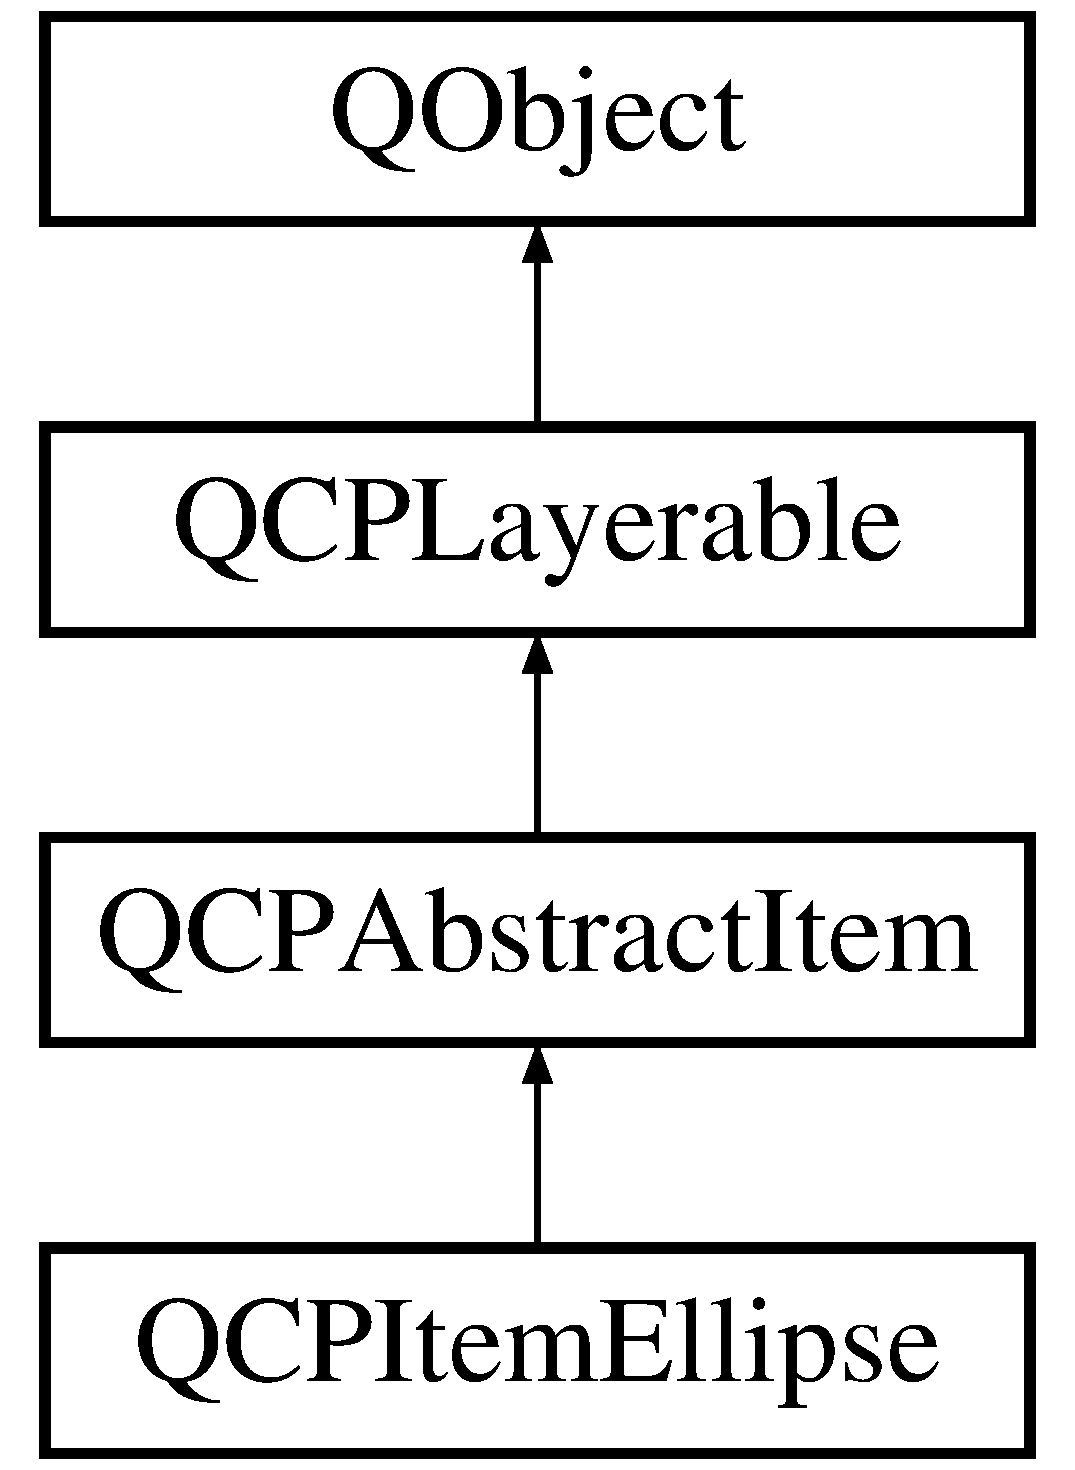
\includegraphics[height=4.000000cm]{class_q_c_p_item_ellipse}
\end{center}
\end{figure}
\subsection*{Public Member Functions}
\begin{DoxyCompactItemize}
\item 
\hyperlink{class_q_c_p_item_ellipse_a759b77ef002515eba0263b5447ecb3fb}{Q\+C\+P\+Item\+Ellipse} (\hyperlink{class_q_custom_plot}{Q\+Custom\+Plot} $\ast$\hyperlink{class_q_c_p_layerable_ab7e0e94461566093d36ffc0f5312b109}{parent\+Plot})
\item 
virtual \hyperlink{class_q_c_p_item_ellipse_a3c17073a1805d32b4e09b6ccde0bef76}{$\sim$\+Q\+C\+P\+Item\+Ellipse} ()
\item 
Q\+Pen \hyperlink{class_q_c_p_item_ellipse_adb67471eabaf1214c99767f1653ca0ed}{pen} () const 
\item 
Q\+Pen \hyperlink{class_q_c_p_item_ellipse_ac52ab52225d238365ff3264b4b69130f}{selected\+Pen} () const 
\item 
Q\+Brush \hyperlink{class_q_c_p_item_ellipse_ac012e4fd59fdb1afb6554937bae8f7e1}{brush} () const 
\item 
Q\+Brush \hyperlink{class_q_c_p_item_ellipse_a0043e401a912d54ea3195bab0967b394}{selected\+Brush} () const 
\item 
void \hyperlink{class_q_c_p_item_ellipse_adb81a663ed2420fcfa011e49f678d1a6}{set\+Pen} (const Q\+Pen \&\hyperlink{class_q_c_p_item_ellipse_adb67471eabaf1214c99767f1653ca0ed}{pen})
\item 
void \hyperlink{class_q_c_p_item_ellipse_a6c542fba1dc918041c583f58a50dde99}{set\+Selected\+Pen} (const Q\+Pen \&\hyperlink{class_q_c_p_item_ellipse_adb67471eabaf1214c99767f1653ca0ed}{pen})
\item 
void \hyperlink{class_q_c_p_item_ellipse_a49fc74e6965834e873d027d026def798}{set\+Brush} (const Q\+Brush \&\hyperlink{class_q_c_p_item_ellipse_ac012e4fd59fdb1afb6554937bae8f7e1}{brush})
\item 
void \hyperlink{class_q_c_p_item_ellipse_a9693501cfaa43a099655c75bed0dab3f}{set\+Selected\+Brush} (const Q\+Brush \&\hyperlink{class_q_c_p_item_ellipse_ac012e4fd59fdb1afb6554937bae8f7e1}{brush})
\item 
virtual double \hyperlink{class_q_c_p_item_ellipse_acd7e5f9528630b2ab5987e2a5782eb7c}{select\+Test} (const Q\+Point\+F \&pos, bool only\+Selectable, Q\+Variant $\ast$details=0) const 
\end{DoxyCompactItemize}
\subsection*{Public Attributes}
\begin{DoxyCompactItemize}
\item 
\hyperlink{class_q_c_p_item_position}{Q\+C\+P\+Item\+Position} $\ast$const \hyperlink{class_q_c_p_item_ellipse_a12fd8420c06718d0c8a2303d6a652848}{top\+Left}
\item 
\hyperlink{class_q_c_p_item_position}{Q\+C\+P\+Item\+Position} $\ast$const \hyperlink{class_q_c_p_item_ellipse_ab73c8deafc0d8d1ef7d75b6cdcc37159}{bottom\+Right}
\item 
\hyperlink{class_q_c_p_item_anchor}{Q\+C\+P\+Item\+Anchor} $\ast$const \hyperlink{class_q_c_p_item_ellipse_a33ebd2a751b63b9240edc9aa46c19eff}{top\+Left\+Rim}
\item 
\hyperlink{class_q_c_p_item_anchor}{Q\+C\+P\+Item\+Anchor} $\ast$const \hyperlink{class_q_c_p_item_ellipse_ad50f907d6f9d1402c6c5d302dca5c5d5}{top}
\item 
\hyperlink{class_q_c_p_item_anchor}{Q\+C\+P\+Item\+Anchor} $\ast$const \hyperlink{class_q_c_p_item_ellipse_a744446970b38a4a3bbea46d722b7c54d}{top\+Right\+Rim}
\item 
\hyperlink{class_q_c_p_item_anchor}{Q\+C\+P\+Item\+Anchor} $\ast$const \hyperlink{class_q_c_p_item_ellipse_a50091a3bd8761d3ce0d95d9c727e4a82}{right}
\item 
\hyperlink{class_q_c_p_item_anchor}{Q\+C\+P\+Item\+Anchor} $\ast$const \hyperlink{class_q_c_p_item_ellipse_a5c8404be601d61b7fafeaaf1c05c4c42}{bottom\+Right\+Rim}
\item 
\hyperlink{class_q_c_p_item_anchor}{Q\+C\+P\+Item\+Anchor} $\ast$const \hyperlink{class_q_c_p_item_ellipse_a2dc80ff9f5db600eae0133bdde65066f}{bottom}
\item 
\hyperlink{class_q_c_p_item_anchor}{Q\+C\+P\+Item\+Anchor} $\ast$const \hyperlink{class_q_c_p_item_ellipse_a31f31a9e9f9098c90fb47573094276c5}{bottom\+Left\+Rim}
\item 
\hyperlink{class_q_c_p_item_anchor}{Q\+C\+P\+Item\+Anchor} $\ast$const \hyperlink{class_q_c_p_item_ellipse_aa259cd03efaedf60cf5b1019b20e4f2b}{left}
\item 
\hyperlink{class_q_c_p_item_anchor}{Q\+C\+P\+Item\+Anchor} $\ast$const \hyperlink{class_q_c_p_item_ellipse_a8b6dd0e854f99239c5806ffdf2f590b3}{center}
\end{DoxyCompactItemize}
\subsection*{Protected Types}
\begin{DoxyCompactItemize}
\item 
enum \hyperlink{class_q_c_p_item_ellipse_a415009889543169f35b70795f415e45e}{Anchor\+Index} \{ \\*
\hyperlink{class_q_c_p_item_ellipse_a415009889543169f35b70795f415e45eab2538849b88921e7fc1dcc15b2a6109d}{ai\+Top\+Left\+Rim}, 
\hyperlink{class_q_c_p_item_ellipse_a415009889543169f35b70795f415e45ea83e55b0c1799baac1eecab52bcbe096d}{ai\+Top}, 
\hyperlink{class_q_c_p_item_ellipse_a415009889543169f35b70795f415e45ea415d82233c14f0c70c245d50e706e75b}{ai\+Top\+Right\+Rim}, 
\hyperlink{class_q_c_p_item_ellipse_a415009889543169f35b70795f415e45ea0f0dcfdf87d9405b53b2129740fb6ba6}{ai\+Right}, 
\\*
\hyperlink{class_q_c_p_item_ellipse_a415009889543169f35b70795f415e45eab62732e96d67801d50c6a9bdebc374d0}{ai\+Bottom\+Right\+Rim}, 
\hyperlink{class_q_c_p_item_ellipse_a415009889543169f35b70795f415e45ea5894287dedaeec1f48394fd950ccff5b}{ai\+Bottom}, 
\hyperlink{class_q_c_p_item_ellipse_a415009889543169f35b70795f415e45ea7b8101bfc590af8ce32961f6545c4f90}{ai\+Bottom\+Left\+Rim}, 
\hyperlink{class_q_c_p_item_ellipse_a415009889543169f35b70795f415e45eae74dad00419a0e1f42877510158fb922}{ai\+Left}, 
\\*
\hyperlink{class_q_c_p_item_ellipse_a415009889543169f35b70795f415e45ea580ec0e9b9fd1488fccf5783e52c0c02}{ai\+Center}
 \}
\end{DoxyCompactItemize}
\subsection*{Protected Member Functions}
\begin{DoxyCompactItemize}
\item 
virtual void \hyperlink{class_q_c_p_item_ellipse_afe97ec827adb05f000fe007783faae3c}{draw} (\hyperlink{class_q_c_p_painter}{Q\+C\+P\+Painter} $\ast$painter)
\item 
virtual Q\+Point\+F \hyperlink{class_q_c_p_item_ellipse_ad3c607304dba081e2f778b6a81b903bb}{anchor\+Pixel\+Point} (int anchor\+Id) const 
\item 
Q\+Pen \hyperlink{class_q_c_p_item_ellipse_afc78d49ed5ffa886bccf18f297f83d30}{main\+Pen} () const 
\item 
Q\+Brush \hyperlink{class_q_c_p_item_ellipse_a2a9757204877c9d0fd07adfb26d6b1d8}{main\+Brush} () const 
\end{DoxyCompactItemize}
\subsection*{Protected Attributes}
\begin{DoxyCompactItemize}
\item 
Q\+Pen \hyperlink{class_q_c_p_item_ellipse_a16ad9389acf028a7e4ac8fd7a550b2e4}{m\+Pen}
\item 
Q\+Pen \hyperlink{class_q_c_p_item_ellipse_a57b047abfce6f1a84ed46ca668c90e21}{m\+Selected\+Pen}
\item 
Q\+Brush \hyperlink{class_q_c_p_item_ellipse_a6fa59478cd3ad1b10e6c1f6cedc84bd6}{m\+Brush}
\item 
Q\+Brush \hyperlink{class_q_c_p_item_ellipse_a2e49d5547478aa36910ed8a2dcc8a5c0}{m\+Selected\+Brush}
\end{DoxyCompactItemize}
\subsection*{Additional Inherited Members}


\subsection{Detailed Description}
An ellipse. 

 It has two positions, {\itshape top\+Left} and {\itshape bottom\+Right}, which define the rect the ellipse will be drawn in. 

\subsection{Member Enumeration Documentation}
\hypertarget{class_q_c_p_item_ellipse_a415009889543169f35b70795f415e45e}{}\index{Q\+C\+P\+Item\+Ellipse@{Q\+C\+P\+Item\+Ellipse}!Anchor\+Index@{Anchor\+Index}}
\index{Anchor\+Index@{Anchor\+Index}!Q\+C\+P\+Item\+Ellipse@{Q\+C\+P\+Item\+Ellipse}}
\subsubsection[{Anchor\+Index}]{\setlength{\rightskip}{0pt plus 5cm}enum {\bf Q\+C\+P\+Item\+Ellipse\+::\+Anchor\+Index}\hspace{0.3cm}{\ttfamily [protected]}}\label{class_q_c_p_item_ellipse_a415009889543169f35b70795f415e45e}
\begin{Desc}
\item[Enumerator]\par
\begin{description}
\index{ai\+Top\+Left\+Rim@{ai\+Top\+Left\+Rim}!Q\+C\+P\+Item\+Ellipse@{Q\+C\+P\+Item\+Ellipse}}\index{Q\+C\+P\+Item\+Ellipse@{Q\+C\+P\+Item\+Ellipse}!ai\+Top\+Left\+Rim@{ai\+Top\+Left\+Rim}}\item[{\em 
\hypertarget{class_q_c_p_item_ellipse_a415009889543169f35b70795f415e45eab2538849b88921e7fc1dcc15b2a6109d}{}ai\+Top\+Left\+Rim\label{class_q_c_p_item_ellipse_a415009889543169f35b70795f415e45eab2538849b88921e7fc1dcc15b2a6109d}
}]\index{ai\+Top@{ai\+Top}!Q\+C\+P\+Item\+Ellipse@{Q\+C\+P\+Item\+Ellipse}}\index{Q\+C\+P\+Item\+Ellipse@{Q\+C\+P\+Item\+Ellipse}!ai\+Top@{ai\+Top}}\item[{\em 
\hypertarget{class_q_c_p_item_ellipse_a415009889543169f35b70795f415e45ea83e55b0c1799baac1eecab52bcbe096d}{}ai\+Top\label{class_q_c_p_item_ellipse_a415009889543169f35b70795f415e45ea83e55b0c1799baac1eecab52bcbe096d}
}]\index{ai\+Top\+Right\+Rim@{ai\+Top\+Right\+Rim}!Q\+C\+P\+Item\+Ellipse@{Q\+C\+P\+Item\+Ellipse}}\index{Q\+C\+P\+Item\+Ellipse@{Q\+C\+P\+Item\+Ellipse}!ai\+Top\+Right\+Rim@{ai\+Top\+Right\+Rim}}\item[{\em 
\hypertarget{class_q_c_p_item_ellipse_a415009889543169f35b70795f415e45ea415d82233c14f0c70c245d50e706e75b}{}ai\+Top\+Right\+Rim\label{class_q_c_p_item_ellipse_a415009889543169f35b70795f415e45ea415d82233c14f0c70c245d50e706e75b}
}]\index{ai\+Right@{ai\+Right}!Q\+C\+P\+Item\+Ellipse@{Q\+C\+P\+Item\+Ellipse}}\index{Q\+C\+P\+Item\+Ellipse@{Q\+C\+P\+Item\+Ellipse}!ai\+Right@{ai\+Right}}\item[{\em 
\hypertarget{class_q_c_p_item_ellipse_a415009889543169f35b70795f415e45ea0f0dcfdf87d9405b53b2129740fb6ba6}{}ai\+Right\label{class_q_c_p_item_ellipse_a415009889543169f35b70795f415e45ea0f0dcfdf87d9405b53b2129740fb6ba6}
}]\index{ai\+Bottom\+Right\+Rim@{ai\+Bottom\+Right\+Rim}!Q\+C\+P\+Item\+Ellipse@{Q\+C\+P\+Item\+Ellipse}}\index{Q\+C\+P\+Item\+Ellipse@{Q\+C\+P\+Item\+Ellipse}!ai\+Bottom\+Right\+Rim@{ai\+Bottom\+Right\+Rim}}\item[{\em 
\hypertarget{class_q_c_p_item_ellipse_a415009889543169f35b70795f415e45eab62732e96d67801d50c6a9bdebc374d0}{}ai\+Bottom\+Right\+Rim\label{class_q_c_p_item_ellipse_a415009889543169f35b70795f415e45eab62732e96d67801d50c6a9bdebc374d0}
}]\index{ai\+Bottom@{ai\+Bottom}!Q\+C\+P\+Item\+Ellipse@{Q\+C\+P\+Item\+Ellipse}}\index{Q\+C\+P\+Item\+Ellipse@{Q\+C\+P\+Item\+Ellipse}!ai\+Bottom@{ai\+Bottom}}\item[{\em 
\hypertarget{class_q_c_p_item_ellipse_a415009889543169f35b70795f415e45ea5894287dedaeec1f48394fd950ccff5b}{}ai\+Bottom\label{class_q_c_p_item_ellipse_a415009889543169f35b70795f415e45ea5894287dedaeec1f48394fd950ccff5b}
}]\index{ai\+Bottom\+Left\+Rim@{ai\+Bottom\+Left\+Rim}!Q\+C\+P\+Item\+Ellipse@{Q\+C\+P\+Item\+Ellipse}}\index{Q\+C\+P\+Item\+Ellipse@{Q\+C\+P\+Item\+Ellipse}!ai\+Bottom\+Left\+Rim@{ai\+Bottom\+Left\+Rim}}\item[{\em 
\hypertarget{class_q_c_p_item_ellipse_a415009889543169f35b70795f415e45ea7b8101bfc590af8ce32961f6545c4f90}{}ai\+Bottom\+Left\+Rim\label{class_q_c_p_item_ellipse_a415009889543169f35b70795f415e45ea7b8101bfc590af8ce32961f6545c4f90}
}]\index{ai\+Left@{ai\+Left}!Q\+C\+P\+Item\+Ellipse@{Q\+C\+P\+Item\+Ellipse}}\index{Q\+C\+P\+Item\+Ellipse@{Q\+C\+P\+Item\+Ellipse}!ai\+Left@{ai\+Left}}\item[{\em 
\hypertarget{class_q_c_p_item_ellipse_a415009889543169f35b70795f415e45eae74dad00419a0e1f42877510158fb922}{}ai\+Left\label{class_q_c_p_item_ellipse_a415009889543169f35b70795f415e45eae74dad00419a0e1f42877510158fb922}
}]\index{ai\+Center@{ai\+Center}!Q\+C\+P\+Item\+Ellipse@{Q\+C\+P\+Item\+Ellipse}}\index{Q\+C\+P\+Item\+Ellipse@{Q\+C\+P\+Item\+Ellipse}!ai\+Center@{ai\+Center}}\item[{\em 
\hypertarget{class_q_c_p_item_ellipse_a415009889543169f35b70795f415e45ea580ec0e9b9fd1488fccf5783e52c0c02}{}ai\+Center\label{class_q_c_p_item_ellipse_a415009889543169f35b70795f415e45ea580ec0e9b9fd1488fccf5783e52c0c02}
}]\end{description}
\end{Desc}


\subsection{Constructor \& Destructor Documentation}
\hypertarget{class_q_c_p_item_ellipse_a759b77ef002515eba0263b5447ecb3fb}{}\index{Q\+C\+P\+Item\+Ellipse@{Q\+C\+P\+Item\+Ellipse}!Q\+C\+P\+Item\+Ellipse@{Q\+C\+P\+Item\+Ellipse}}
\index{Q\+C\+P\+Item\+Ellipse@{Q\+C\+P\+Item\+Ellipse}!Q\+C\+P\+Item\+Ellipse@{Q\+C\+P\+Item\+Ellipse}}
\subsubsection[{Q\+C\+P\+Item\+Ellipse}]{\setlength{\rightskip}{0pt plus 5cm}Q\+C\+P\+Item\+Ellipse\+::\+Q\+C\+P\+Item\+Ellipse (
\begin{DoxyParamCaption}
\item[{{\bf Q\+Custom\+Plot} $\ast$}]{parent\+Plot}
\end{DoxyParamCaption}
)}\label{class_q_c_p_item_ellipse_a759b77ef002515eba0263b5447ecb3fb}
Creates an ellipse item and sets default values.

The constructed item can be added to the plot with \hyperlink{class_q_custom_plot_aa500620379262321685cb7a7674cbd2a}{Q\+Custom\+Plot\+::add\+Item}. \hypertarget{class_q_c_p_item_ellipse_a3c17073a1805d32b4e09b6ccde0bef76}{}\index{Q\+C\+P\+Item\+Ellipse@{Q\+C\+P\+Item\+Ellipse}!````~Q\+C\+P\+Item\+Ellipse@{$\sim$\+Q\+C\+P\+Item\+Ellipse}}
\index{````~Q\+C\+P\+Item\+Ellipse@{$\sim$\+Q\+C\+P\+Item\+Ellipse}!Q\+C\+P\+Item\+Ellipse@{Q\+C\+P\+Item\+Ellipse}}
\subsubsection[{$\sim$\+Q\+C\+P\+Item\+Ellipse}]{\setlength{\rightskip}{0pt plus 5cm}Q\+C\+P\+Item\+Ellipse\+::$\sim$\+Q\+C\+P\+Item\+Ellipse (
\begin{DoxyParamCaption}
{}
\end{DoxyParamCaption}
)\hspace{0.3cm}{\ttfamily [virtual]}}\label{class_q_c_p_item_ellipse_a3c17073a1805d32b4e09b6ccde0bef76}


\subsection{Member Function Documentation}
\hypertarget{class_q_c_p_item_ellipse_ad3c607304dba081e2f778b6a81b903bb}{}\index{Q\+C\+P\+Item\+Ellipse@{Q\+C\+P\+Item\+Ellipse}!anchor\+Pixel\+Point@{anchor\+Pixel\+Point}}
\index{anchor\+Pixel\+Point@{anchor\+Pixel\+Point}!Q\+C\+P\+Item\+Ellipse@{Q\+C\+P\+Item\+Ellipse}}
\subsubsection[{anchor\+Pixel\+Point}]{\setlength{\rightskip}{0pt plus 5cm}Q\+Point\+F Q\+C\+P\+Item\+Ellipse\+::anchor\+Pixel\+Point (
\begin{DoxyParamCaption}
\item[{int}]{anchor\+Id}
\end{DoxyParamCaption}
) const\hspace{0.3cm}{\ttfamily [protected]}, {\ttfamily [virtual]}}\label{class_q_c_p_item_ellipse_ad3c607304dba081e2f778b6a81b903bb}


Reimplemented from \hyperlink{class_q_c_p_abstract_item_a94bde62b8a2fc133666dcbb8035deeed}{Q\+C\+P\+Abstract\+Item}.

\hypertarget{class_q_c_p_item_ellipse_ac012e4fd59fdb1afb6554937bae8f7e1}{}\index{Q\+C\+P\+Item\+Ellipse@{Q\+C\+P\+Item\+Ellipse}!brush@{brush}}
\index{brush@{brush}!Q\+C\+P\+Item\+Ellipse@{Q\+C\+P\+Item\+Ellipse}}
\subsubsection[{brush}]{\setlength{\rightskip}{0pt plus 5cm}Q\+Brush Q\+C\+P\+Item\+Ellipse\+::brush (
\begin{DoxyParamCaption}
{}
\end{DoxyParamCaption}
) const\hspace{0.3cm}{\ttfamily [inline]}}\label{class_q_c_p_item_ellipse_ac012e4fd59fdb1afb6554937bae8f7e1}
\hypertarget{class_q_c_p_item_ellipse_afe97ec827adb05f000fe007783faae3c}{}\index{Q\+C\+P\+Item\+Ellipse@{Q\+C\+P\+Item\+Ellipse}!draw@{draw}}
\index{draw@{draw}!Q\+C\+P\+Item\+Ellipse@{Q\+C\+P\+Item\+Ellipse}}
\subsubsection[{draw}]{\setlength{\rightskip}{0pt plus 5cm}void Q\+C\+P\+Item\+Ellipse\+::draw (
\begin{DoxyParamCaption}
\item[{{\bf Q\+C\+P\+Painter} $\ast$}]{painter}
\end{DoxyParamCaption}
)\hspace{0.3cm}{\ttfamily [protected]}, {\ttfamily [virtual]}}\label{class_q_c_p_item_ellipse_afe97ec827adb05f000fe007783faae3c}


Implements \hyperlink{class_q_c_p_abstract_item_ad0dc056f650c3ca73414e6b4f01674ef}{Q\+C\+P\+Abstract\+Item}.

\hypertarget{class_q_c_p_item_ellipse_a2a9757204877c9d0fd07adfb26d6b1d8}{}\index{Q\+C\+P\+Item\+Ellipse@{Q\+C\+P\+Item\+Ellipse}!main\+Brush@{main\+Brush}}
\index{main\+Brush@{main\+Brush}!Q\+C\+P\+Item\+Ellipse@{Q\+C\+P\+Item\+Ellipse}}
\subsubsection[{main\+Brush}]{\setlength{\rightskip}{0pt plus 5cm}Q\+Brush Q\+C\+P\+Item\+Ellipse\+::main\+Brush (
\begin{DoxyParamCaption}
{}
\end{DoxyParamCaption}
) const\hspace{0.3cm}{\ttfamily [protected]}}\label{class_q_c_p_item_ellipse_a2a9757204877c9d0fd07adfb26d6b1d8}
\hypertarget{class_q_c_p_item_ellipse_afc78d49ed5ffa886bccf18f297f83d30}{}\index{Q\+C\+P\+Item\+Ellipse@{Q\+C\+P\+Item\+Ellipse}!main\+Pen@{main\+Pen}}
\index{main\+Pen@{main\+Pen}!Q\+C\+P\+Item\+Ellipse@{Q\+C\+P\+Item\+Ellipse}}
\subsubsection[{main\+Pen}]{\setlength{\rightskip}{0pt plus 5cm}Q\+Pen Q\+C\+P\+Item\+Ellipse\+::main\+Pen (
\begin{DoxyParamCaption}
{}
\end{DoxyParamCaption}
) const\hspace{0.3cm}{\ttfamily [protected]}}\label{class_q_c_p_item_ellipse_afc78d49ed5ffa886bccf18f297f83d30}
\hypertarget{class_q_c_p_item_ellipse_adb67471eabaf1214c99767f1653ca0ed}{}\index{Q\+C\+P\+Item\+Ellipse@{Q\+C\+P\+Item\+Ellipse}!pen@{pen}}
\index{pen@{pen}!Q\+C\+P\+Item\+Ellipse@{Q\+C\+P\+Item\+Ellipse}}
\subsubsection[{pen}]{\setlength{\rightskip}{0pt plus 5cm}Q\+Pen Q\+C\+P\+Item\+Ellipse\+::pen (
\begin{DoxyParamCaption}
{}
\end{DoxyParamCaption}
) const\hspace{0.3cm}{\ttfamily [inline]}}\label{class_q_c_p_item_ellipse_adb67471eabaf1214c99767f1653ca0ed}
\hypertarget{class_q_c_p_item_ellipse_a0043e401a912d54ea3195bab0967b394}{}\index{Q\+C\+P\+Item\+Ellipse@{Q\+C\+P\+Item\+Ellipse}!selected\+Brush@{selected\+Brush}}
\index{selected\+Brush@{selected\+Brush}!Q\+C\+P\+Item\+Ellipse@{Q\+C\+P\+Item\+Ellipse}}
\subsubsection[{selected\+Brush}]{\setlength{\rightskip}{0pt plus 5cm}Q\+Brush Q\+C\+P\+Item\+Ellipse\+::selected\+Brush (
\begin{DoxyParamCaption}
{}
\end{DoxyParamCaption}
) const\hspace{0.3cm}{\ttfamily [inline]}}\label{class_q_c_p_item_ellipse_a0043e401a912d54ea3195bab0967b394}
\hypertarget{class_q_c_p_item_ellipse_ac52ab52225d238365ff3264b4b69130f}{}\index{Q\+C\+P\+Item\+Ellipse@{Q\+C\+P\+Item\+Ellipse}!selected\+Pen@{selected\+Pen}}
\index{selected\+Pen@{selected\+Pen}!Q\+C\+P\+Item\+Ellipse@{Q\+C\+P\+Item\+Ellipse}}
\subsubsection[{selected\+Pen}]{\setlength{\rightskip}{0pt plus 5cm}Q\+Pen Q\+C\+P\+Item\+Ellipse\+::selected\+Pen (
\begin{DoxyParamCaption}
{}
\end{DoxyParamCaption}
) const\hspace{0.3cm}{\ttfamily [inline]}}\label{class_q_c_p_item_ellipse_ac52ab52225d238365ff3264b4b69130f}
\hypertarget{class_q_c_p_item_ellipse_acd7e5f9528630b2ab5987e2a5782eb7c}{}\index{Q\+C\+P\+Item\+Ellipse@{Q\+C\+P\+Item\+Ellipse}!select\+Test@{select\+Test}}
\index{select\+Test@{select\+Test}!Q\+C\+P\+Item\+Ellipse@{Q\+C\+P\+Item\+Ellipse}}
\subsubsection[{select\+Test}]{\setlength{\rightskip}{0pt plus 5cm}double Q\+C\+P\+Item\+Ellipse\+::select\+Test (
\begin{DoxyParamCaption}
\item[{const Q\+Point\+F \&}]{pos, }
\item[{bool}]{only\+Selectable, }
\item[{Q\+Variant $\ast$}]{details = {\ttfamily 0}}
\end{DoxyParamCaption}
) const\hspace{0.3cm}{\ttfamily [virtual]}}\label{class_q_c_p_item_ellipse_acd7e5f9528630b2ab5987e2a5782eb7c}
This function is used to decide whether a click hits a layerable object or not.

{\itshape pos} is a point in pixel coordinates on the \hyperlink{class_q_custom_plot}{Q\+Custom\+Plot} surface. This function returns the shortest pixel distance of this point to the object. If the object is either invisible or the distance couldn\textquotesingle{}t be determined, -\/1.\+0 is returned. Further, if {\itshape only\+Selectable} is true and the object is not selectable, -\/1.\+0 is returned, too.

If the item is represented not by single lines but by an area like \hyperlink{class_q_c_p_item_rect}{Q\+C\+P\+Item\+Rect} or \hyperlink{class_q_c_p_item_text}{Q\+C\+P\+Item\+Text}, a click inside the area returns a constant value greater zero (typically the selection\+Tolerance of the parent \hyperlink{class_q_custom_plot}{Q\+Custom\+Plot} multiplied by 0.\+99). If the click lies outside the area, this function returns -\/1.\+0.

Providing a constant value for area objects allows selecting line objects even when they are obscured by such area objects, by clicking close to the lines (i.\+e. closer than 0.\+99$\ast$selection\+Tolerance).

The actual setting of the selection state is not done by this function. This is handled by the parent \hyperlink{class_q_custom_plot}{Q\+Custom\+Plot} when the mouse\+Release\+Event occurs, and the finally selected object is notified via the select\+Event/deselect\+Event methods.

{\itshape details} is an optional output parameter. Every layerable subclass may place any information in {\itshape details}. This information will be passed to \hyperlink{class_q_c_p_abstract_item_aaf92af7b9893712959a6c073d334d88d}{select\+Event} when the parent \hyperlink{class_q_custom_plot}{Q\+Custom\+Plot} decides on the basis of this select\+Test call, that the object was successfully selected. The subsequent call to \hyperlink{class_q_c_p_abstract_item_aaf92af7b9893712959a6c073d334d88d}{select\+Event} will carry the {\itshape details}. This is useful for multi-\/part objects (like \hyperlink{class_q_c_p_axis}{Q\+C\+P\+Axis}). This way, a possibly complex calculation to decide which part was clicked is only done once in \hyperlink{class_q_c_p_item_ellipse_acd7e5f9528630b2ab5987e2a5782eb7c}{select\+Test}. The result (i.\+e. the actually clicked part) can then be placed in {\itshape details}. So in the subsequent \hyperlink{class_q_c_p_abstract_item_aaf92af7b9893712959a6c073d334d88d}{select\+Event}, the decision which part was selected doesn\textquotesingle{}t have to be done a second time for a single selection operation.

You may pass 0 as {\itshape details} to indicate that you are not interested in those selection details.

\begin{DoxySeeAlso}{See also}
\hyperlink{class_q_c_p_abstract_item_aaf92af7b9893712959a6c073d334d88d}{select\+Event}, \hyperlink{class_q_c_p_abstract_item_a91f090d6763cfedb0749219c63788ae9}{deselect\+Event}, \hyperlink{class_q_custom_plot_a5ee1e2f6ae27419deca53e75907c27e5}{Q\+Custom\+Plot\+::set\+Interactions} 
\end{DoxySeeAlso}


Implements \hyperlink{class_q_c_p_abstract_item_a96d522d10ffc0413b9a366c6f7f0476b}{Q\+C\+P\+Abstract\+Item}.

\hypertarget{class_q_c_p_item_ellipse_a49fc74e6965834e873d027d026def798}{}\index{Q\+C\+P\+Item\+Ellipse@{Q\+C\+P\+Item\+Ellipse}!set\+Brush@{set\+Brush}}
\index{set\+Brush@{set\+Brush}!Q\+C\+P\+Item\+Ellipse@{Q\+C\+P\+Item\+Ellipse}}
\subsubsection[{set\+Brush}]{\setlength{\rightskip}{0pt plus 5cm}void Q\+C\+P\+Item\+Ellipse\+::set\+Brush (
\begin{DoxyParamCaption}
\item[{const Q\+Brush \&}]{brush}
\end{DoxyParamCaption}
)}\label{class_q_c_p_item_ellipse_a49fc74e6965834e873d027d026def798}
Sets the brush that will be used to fill the ellipse. To disable filling, set {\itshape brush} to Qt\+::\+No\+Brush.

\begin{DoxySeeAlso}{See also}
\hyperlink{class_q_c_p_item_ellipse_a9693501cfaa43a099655c75bed0dab3f}{set\+Selected\+Brush}, \hyperlink{class_q_c_p_item_ellipse_adb81a663ed2420fcfa011e49f678d1a6}{set\+Pen} 
\end{DoxySeeAlso}
\hypertarget{class_q_c_p_item_ellipse_adb81a663ed2420fcfa011e49f678d1a6}{}\index{Q\+C\+P\+Item\+Ellipse@{Q\+C\+P\+Item\+Ellipse}!set\+Pen@{set\+Pen}}
\index{set\+Pen@{set\+Pen}!Q\+C\+P\+Item\+Ellipse@{Q\+C\+P\+Item\+Ellipse}}
\subsubsection[{set\+Pen}]{\setlength{\rightskip}{0pt plus 5cm}void Q\+C\+P\+Item\+Ellipse\+::set\+Pen (
\begin{DoxyParamCaption}
\item[{const Q\+Pen \&}]{pen}
\end{DoxyParamCaption}
)}\label{class_q_c_p_item_ellipse_adb81a663ed2420fcfa011e49f678d1a6}
Sets the pen that will be used to draw the line of the ellipse

\begin{DoxySeeAlso}{See also}
\hyperlink{class_q_c_p_item_ellipse_a6c542fba1dc918041c583f58a50dde99}{set\+Selected\+Pen}, \hyperlink{class_q_c_p_item_ellipse_a49fc74e6965834e873d027d026def798}{set\+Brush} 
\end{DoxySeeAlso}
\hypertarget{class_q_c_p_item_ellipse_a9693501cfaa43a099655c75bed0dab3f}{}\index{Q\+C\+P\+Item\+Ellipse@{Q\+C\+P\+Item\+Ellipse}!set\+Selected\+Brush@{set\+Selected\+Brush}}
\index{set\+Selected\+Brush@{set\+Selected\+Brush}!Q\+C\+P\+Item\+Ellipse@{Q\+C\+P\+Item\+Ellipse}}
\subsubsection[{set\+Selected\+Brush}]{\setlength{\rightskip}{0pt plus 5cm}void Q\+C\+P\+Item\+Ellipse\+::set\+Selected\+Brush (
\begin{DoxyParamCaption}
\item[{const Q\+Brush \&}]{brush}
\end{DoxyParamCaption}
)}\label{class_q_c_p_item_ellipse_a9693501cfaa43a099655c75bed0dab3f}
Sets the brush that will be used to fill the ellipse when selected. To disable filling, set {\itshape brush} to Qt\+::\+No\+Brush.

\begin{DoxySeeAlso}{See also}
\hyperlink{class_q_c_p_item_ellipse_a49fc74e6965834e873d027d026def798}{set\+Brush} 
\end{DoxySeeAlso}
\hypertarget{class_q_c_p_item_ellipse_a6c542fba1dc918041c583f58a50dde99}{}\index{Q\+C\+P\+Item\+Ellipse@{Q\+C\+P\+Item\+Ellipse}!set\+Selected\+Pen@{set\+Selected\+Pen}}
\index{set\+Selected\+Pen@{set\+Selected\+Pen}!Q\+C\+P\+Item\+Ellipse@{Q\+C\+P\+Item\+Ellipse}}
\subsubsection[{set\+Selected\+Pen}]{\setlength{\rightskip}{0pt plus 5cm}void Q\+C\+P\+Item\+Ellipse\+::set\+Selected\+Pen (
\begin{DoxyParamCaption}
\item[{const Q\+Pen \&}]{pen}
\end{DoxyParamCaption}
)}\label{class_q_c_p_item_ellipse_a6c542fba1dc918041c583f58a50dde99}
Sets the pen that will be used to draw the line of the ellipse when selected

\begin{DoxySeeAlso}{See also}
\hyperlink{class_q_c_p_item_ellipse_adb81a663ed2420fcfa011e49f678d1a6}{set\+Pen}, \hyperlink{class_q_c_p_abstract_item_a203de94ad586cc44d16c9565f49d3378}{set\+Selected} 
\end{DoxySeeAlso}


\subsection{Member Data Documentation}
\hypertarget{class_q_c_p_item_ellipse_a2dc80ff9f5db600eae0133bdde65066f}{}\index{Q\+C\+P\+Item\+Ellipse@{Q\+C\+P\+Item\+Ellipse}!bottom@{bottom}}
\index{bottom@{bottom}!Q\+C\+P\+Item\+Ellipse@{Q\+C\+P\+Item\+Ellipse}}
\subsubsection[{bottom}]{\setlength{\rightskip}{0pt plus 5cm}{\bf Q\+C\+P\+Item\+Anchor}$\ast$ const Q\+C\+P\+Item\+Ellipse\+::bottom}\label{class_q_c_p_item_ellipse_a2dc80ff9f5db600eae0133bdde65066f}
\hypertarget{class_q_c_p_item_ellipse_a31f31a9e9f9098c90fb47573094276c5}{}\index{Q\+C\+P\+Item\+Ellipse@{Q\+C\+P\+Item\+Ellipse}!bottom\+Left\+Rim@{bottom\+Left\+Rim}}
\index{bottom\+Left\+Rim@{bottom\+Left\+Rim}!Q\+C\+P\+Item\+Ellipse@{Q\+C\+P\+Item\+Ellipse}}
\subsubsection[{bottom\+Left\+Rim}]{\setlength{\rightskip}{0pt plus 5cm}{\bf Q\+C\+P\+Item\+Anchor}$\ast$ const Q\+C\+P\+Item\+Ellipse\+::bottom\+Left\+Rim}\label{class_q_c_p_item_ellipse_a31f31a9e9f9098c90fb47573094276c5}
\hypertarget{class_q_c_p_item_ellipse_ab73c8deafc0d8d1ef7d75b6cdcc37159}{}\index{Q\+C\+P\+Item\+Ellipse@{Q\+C\+P\+Item\+Ellipse}!bottom\+Right@{bottom\+Right}}
\index{bottom\+Right@{bottom\+Right}!Q\+C\+P\+Item\+Ellipse@{Q\+C\+P\+Item\+Ellipse}}
\subsubsection[{bottom\+Right}]{\setlength{\rightskip}{0pt plus 5cm}{\bf Q\+C\+P\+Item\+Position}$\ast$ const Q\+C\+P\+Item\+Ellipse\+::bottom\+Right}\label{class_q_c_p_item_ellipse_ab73c8deafc0d8d1ef7d75b6cdcc37159}
\hypertarget{class_q_c_p_item_ellipse_a5c8404be601d61b7fafeaaf1c05c4c42}{}\index{Q\+C\+P\+Item\+Ellipse@{Q\+C\+P\+Item\+Ellipse}!bottom\+Right\+Rim@{bottom\+Right\+Rim}}
\index{bottom\+Right\+Rim@{bottom\+Right\+Rim}!Q\+C\+P\+Item\+Ellipse@{Q\+C\+P\+Item\+Ellipse}}
\subsubsection[{bottom\+Right\+Rim}]{\setlength{\rightskip}{0pt plus 5cm}{\bf Q\+C\+P\+Item\+Anchor}$\ast$ const Q\+C\+P\+Item\+Ellipse\+::bottom\+Right\+Rim}\label{class_q_c_p_item_ellipse_a5c8404be601d61b7fafeaaf1c05c4c42}
\hypertarget{class_q_c_p_item_ellipse_a8b6dd0e854f99239c5806ffdf2f590b3}{}\index{Q\+C\+P\+Item\+Ellipse@{Q\+C\+P\+Item\+Ellipse}!center@{center}}
\index{center@{center}!Q\+C\+P\+Item\+Ellipse@{Q\+C\+P\+Item\+Ellipse}}
\subsubsection[{center}]{\setlength{\rightskip}{0pt plus 5cm}{\bf Q\+C\+P\+Item\+Anchor}$\ast$ const Q\+C\+P\+Item\+Ellipse\+::center}\label{class_q_c_p_item_ellipse_a8b6dd0e854f99239c5806ffdf2f590b3}
\hypertarget{class_q_c_p_item_ellipse_aa259cd03efaedf60cf5b1019b20e4f2b}{}\index{Q\+C\+P\+Item\+Ellipse@{Q\+C\+P\+Item\+Ellipse}!left@{left}}
\index{left@{left}!Q\+C\+P\+Item\+Ellipse@{Q\+C\+P\+Item\+Ellipse}}
\subsubsection[{left}]{\setlength{\rightskip}{0pt plus 5cm}{\bf Q\+C\+P\+Item\+Anchor}$\ast$ const Q\+C\+P\+Item\+Ellipse\+::left}\label{class_q_c_p_item_ellipse_aa259cd03efaedf60cf5b1019b20e4f2b}
\hypertarget{class_q_c_p_item_ellipse_a6fa59478cd3ad1b10e6c1f6cedc84bd6}{}\index{Q\+C\+P\+Item\+Ellipse@{Q\+C\+P\+Item\+Ellipse}!m\+Brush@{m\+Brush}}
\index{m\+Brush@{m\+Brush}!Q\+C\+P\+Item\+Ellipse@{Q\+C\+P\+Item\+Ellipse}}
\subsubsection[{m\+Brush}]{\setlength{\rightskip}{0pt plus 5cm}Q\+Brush Q\+C\+P\+Item\+Ellipse\+::m\+Brush\hspace{0.3cm}{\ttfamily [protected]}}\label{class_q_c_p_item_ellipse_a6fa59478cd3ad1b10e6c1f6cedc84bd6}
\hypertarget{class_q_c_p_item_ellipse_a16ad9389acf028a7e4ac8fd7a550b2e4}{}\index{Q\+C\+P\+Item\+Ellipse@{Q\+C\+P\+Item\+Ellipse}!m\+Pen@{m\+Pen}}
\index{m\+Pen@{m\+Pen}!Q\+C\+P\+Item\+Ellipse@{Q\+C\+P\+Item\+Ellipse}}
\subsubsection[{m\+Pen}]{\setlength{\rightskip}{0pt plus 5cm}Q\+Pen Q\+C\+P\+Item\+Ellipse\+::m\+Pen\hspace{0.3cm}{\ttfamily [protected]}}\label{class_q_c_p_item_ellipse_a16ad9389acf028a7e4ac8fd7a550b2e4}
\hypertarget{class_q_c_p_item_ellipse_a2e49d5547478aa36910ed8a2dcc8a5c0}{}\index{Q\+C\+P\+Item\+Ellipse@{Q\+C\+P\+Item\+Ellipse}!m\+Selected\+Brush@{m\+Selected\+Brush}}
\index{m\+Selected\+Brush@{m\+Selected\+Brush}!Q\+C\+P\+Item\+Ellipse@{Q\+C\+P\+Item\+Ellipse}}
\subsubsection[{m\+Selected\+Brush}]{\setlength{\rightskip}{0pt plus 5cm}Q\+Brush Q\+C\+P\+Item\+Ellipse\+::m\+Selected\+Brush\hspace{0.3cm}{\ttfamily [protected]}}\label{class_q_c_p_item_ellipse_a2e49d5547478aa36910ed8a2dcc8a5c0}
\hypertarget{class_q_c_p_item_ellipse_a57b047abfce6f1a84ed46ca668c90e21}{}\index{Q\+C\+P\+Item\+Ellipse@{Q\+C\+P\+Item\+Ellipse}!m\+Selected\+Pen@{m\+Selected\+Pen}}
\index{m\+Selected\+Pen@{m\+Selected\+Pen}!Q\+C\+P\+Item\+Ellipse@{Q\+C\+P\+Item\+Ellipse}}
\subsubsection[{m\+Selected\+Pen}]{\setlength{\rightskip}{0pt plus 5cm}Q\+Pen Q\+C\+P\+Item\+Ellipse\+::m\+Selected\+Pen\hspace{0.3cm}{\ttfamily [protected]}}\label{class_q_c_p_item_ellipse_a57b047abfce6f1a84ed46ca668c90e21}
\hypertarget{class_q_c_p_item_ellipse_a50091a3bd8761d3ce0d95d9c727e4a82}{}\index{Q\+C\+P\+Item\+Ellipse@{Q\+C\+P\+Item\+Ellipse}!right@{right}}
\index{right@{right}!Q\+C\+P\+Item\+Ellipse@{Q\+C\+P\+Item\+Ellipse}}
\subsubsection[{right}]{\setlength{\rightskip}{0pt plus 5cm}{\bf Q\+C\+P\+Item\+Anchor}$\ast$ const Q\+C\+P\+Item\+Ellipse\+::right}\label{class_q_c_p_item_ellipse_a50091a3bd8761d3ce0d95d9c727e4a82}
\hypertarget{class_q_c_p_item_ellipse_ad50f907d6f9d1402c6c5d302dca5c5d5}{}\index{Q\+C\+P\+Item\+Ellipse@{Q\+C\+P\+Item\+Ellipse}!top@{top}}
\index{top@{top}!Q\+C\+P\+Item\+Ellipse@{Q\+C\+P\+Item\+Ellipse}}
\subsubsection[{top}]{\setlength{\rightskip}{0pt plus 5cm}{\bf Q\+C\+P\+Item\+Anchor}$\ast$ const Q\+C\+P\+Item\+Ellipse\+::top}\label{class_q_c_p_item_ellipse_ad50f907d6f9d1402c6c5d302dca5c5d5}
\hypertarget{class_q_c_p_item_ellipse_a12fd8420c06718d0c8a2303d6a652848}{}\index{Q\+C\+P\+Item\+Ellipse@{Q\+C\+P\+Item\+Ellipse}!top\+Left@{top\+Left}}
\index{top\+Left@{top\+Left}!Q\+C\+P\+Item\+Ellipse@{Q\+C\+P\+Item\+Ellipse}}
\subsubsection[{top\+Left}]{\setlength{\rightskip}{0pt plus 5cm}{\bf Q\+C\+P\+Item\+Position}$\ast$ const Q\+C\+P\+Item\+Ellipse\+::top\+Left}\label{class_q_c_p_item_ellipse_a12fd8420c06718d0c8a2303d6a652848}
\hypertarget{class_q_c_p_item_ellipse_a33ebd2a751b63b9240edc9aa46c19eff}{}\index{Q\+C\+P\+Item\+Ellipse@{Q\+C\+P\+Item\+Ellipse}!top\+Left\+Rim@{top\+Left\+Rim}}
\index{top\+Left\+Rim@{top\+Left\+Rim}!Q\+C\+P\+Item\+Ellipse@{Q\+C\+P\+Item\+Ellipse}}
\subsubsection[{top\+Left\+Rim}]{\setlength{\rightskip}{0pt plus 5cm}{\bf Q\+C\+P\+Item\+Anchor}$\ast$ const Q\+C\+P\+Item\+Ellipse\+::top\+Left\+Rim}\label{class_q_c_p_item_ellipse_a33ebd2a751b63b9240edc9aa46c19eff}
\hypertarget{class_q_c_p_item_ellipse_a744446970b38a4a3bbea46d722b7c54d}{}\index{Q\+C\+P\+Item\+Ellipse@{Q\+C\+P\+Item\+Ellipse}!top\+Right\+Rim@{top\+Right\+Rim}}
\index{top\+Right\+Rim@{top\+Right\+Rim}!Q\+C\+P\+Item\+Ellipse@{Q\+C\+P\+Item\+Ellipse}}
\subsubsection[{top\+Right\+Rim}]{\setlength{\rightskip}{0pt plus 5cm}{\bf Q\+C\+P\+Item\+Anchor}$\ast$ const Q\+C\+P\+Item\+Ellipse\+::top\+Right\+Rim}\label{class_q_c_p_item_ellipse_a744446970b38a4a3bbea46d722b7c54d}


The documentation for this class was generated from the following files\+:\begin{DoxyCompactItemize}
\item 
C\+:/\+Users/\+Roman/\+Documents/\+Mygs/\+Ground\+Station/\+G\+S/\hyperlink{qcustomplot_8h}{qcustomplot.\+h}\item 
C\+:/\+Users/\+Roman/\+Documents/\+Mygs/\+Ground\+Station/\+G\+S/\hyperlink{qcustomplot_8cpp}{qcustomplot.\+cpp}\end{DoxyCompactItemize}

\hypertarget{class_q_c_p_item_line}{}\section{Q\+C\+P\+Item\+Line Class Reference}
\label{class_q_c_p_item_line}\index{Q\+C\+P\+Item\+Line@{Q\+C\+P\+Item\+Line}}


A line from one point to another.  




{\ttfamily \#include $<$qcustomplot.\+h$>$}

Inheritance diagram for Q\+C\+P\+Item\+Line\+:\begin{figure}[H]
\begin{center}
\leavevmode
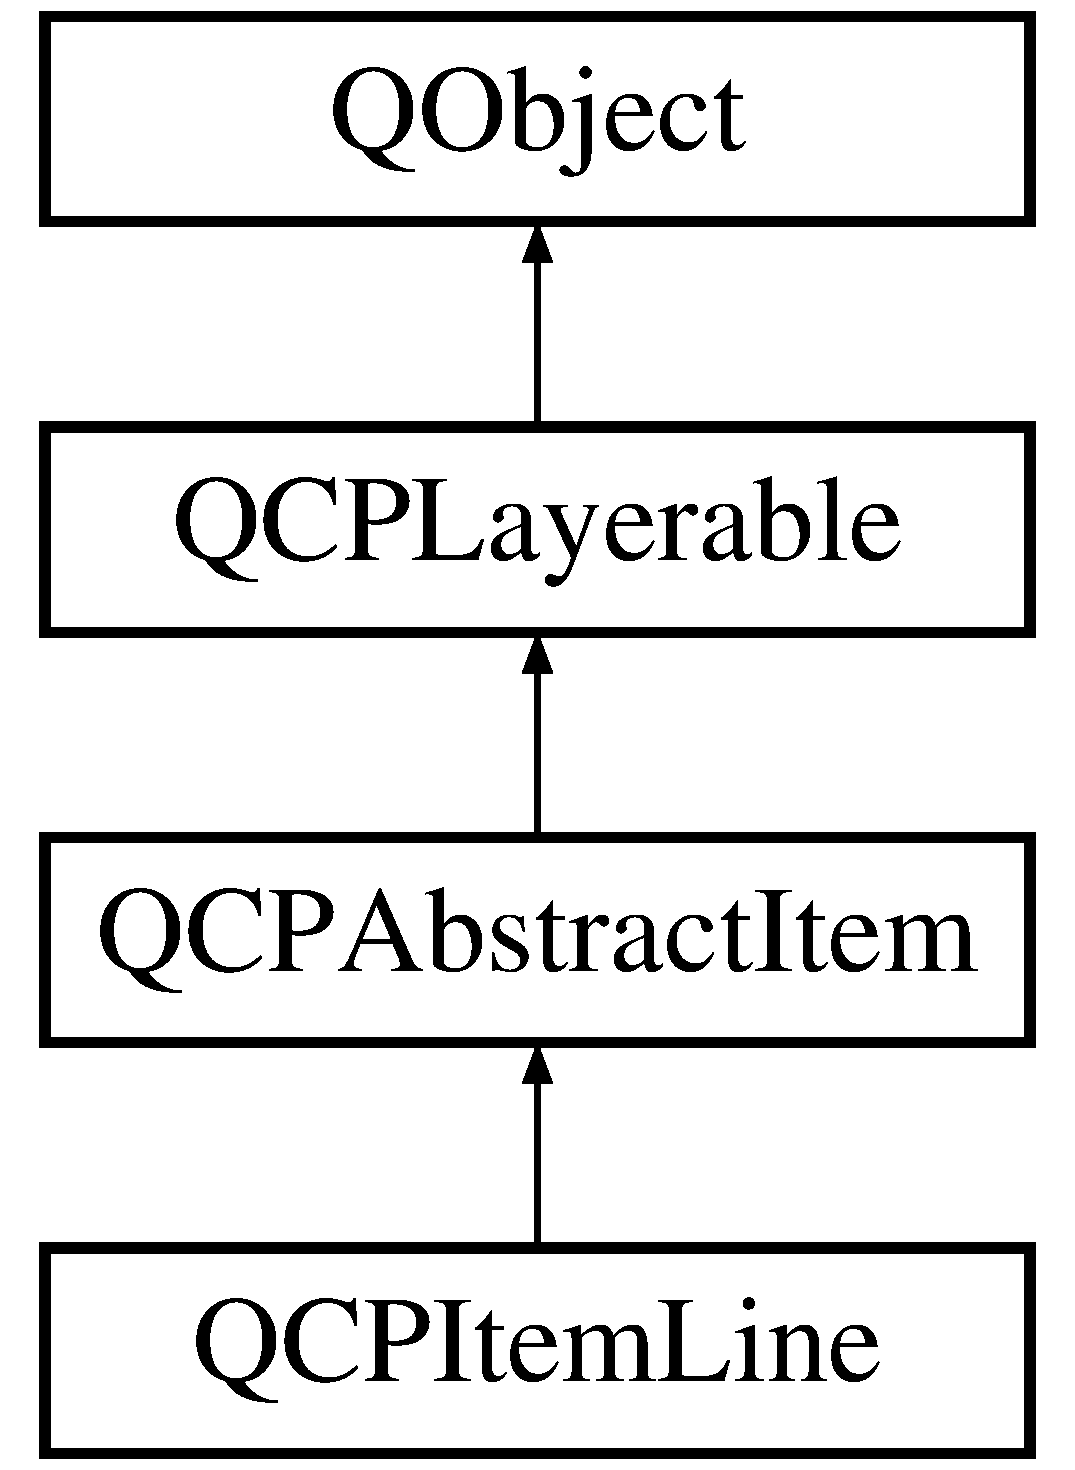
\includegraphics[height=4.000000cm]{class_q_c_p_item_line}
\end{center}
\end{figure}
\subsection*{Public Member Functions}
\begin{DoxyCompactItemize}
\item 
\hyperlink{class_q_c_p_item_line_a17804b7f64961c6accf25b61e85142e3}{Q\+C\+P\+Item\+Line} (\hyperlink{class_q_custom_plot}{Q\+Custom\+Plot} $\ast$\hyperlink{class_q_c_p_layerable_ab7e0e94461566093d36ffc0f5312b109}{parent\+Plot})
\item 
virtual \hyperlink{class_q_c_p_item_line_a94b5aaae048171e5306dc4695b991283}{$\sim$\+Q\+C\+P\+Item\+Line} ()
\item 
Q\+Pen \hyperlink{class_q_c_p_item_line_a235779dd079a263bedb20b3daecc40eb}{pen} () const 
\item 
Q\+Pen \hyperlink{class_q_c_p_item_line_a9fde5e95a1a369008252e18f1925650c}{selected\+Pen} () const 
\item 
\hyperlink{class_q_c_p_line_ending}{Q\+C\+P\+Line\+Ending} \hyperlink{class_q_c_p_item_line_a5f6cbc5c763feae9dfbce71748fc43f1}{head} () const 
\item 
\hyperlink{class_q_c_p_line_ending}{Q\+C\+P\+Line\+Ending} \hyperlink{class_q_c_p_item_line_a5d2ca0f784933e80f3e6e1d15dceebb3}{tail} () const 
\item 
void \hyperlink{class_q_c_p_item_line_a572528dab61c1abe205822fbd5db4b27}{set\+Pen} (const Q\+Pen \&\hyperlink{class_q_c_p_item_line_a235779dd079a263bedb20b3daecc40eb}{pen})
\item 
void \hyperlink{class_q_c_p_item_line_a3e2fec44503277e77717e9c24f87f1ea}{set\+Selected\+Pen} (const Q\+Pen \&\hyperlink{class_q_c_p_item_line_a235779dd079a263bedb20b3daecc40eb}{pen})
\item 
void \hyperlink{class_q_c_p_item_line_aebf3d687114d584e0459db6759e2c3c3}{set\+Head} (const \hyperlink{class_q_c_p_line_ending}{Q\+C\+P\+Line\+Ending} \&\hyperlink{class_q_c_p_item_line_a5f6cbc5c763feae9dfbce71748fc43f1}{head})
\item 
void \hyperlink{class_q_c_p_item_line_ac264222c3297a7efe33df9345c811a5f}{set\+Tail} (const \hyperlink{class_q_c_p_line_ending}{Q\+C\+P\+Line\+Ending} \&\hyperlink{class_q_c_p_item_line_a5d2ca0f784933e80f3e6e1d15dceebb3}{tail})
\item 
virtual double \hyperlink{class_q_c_p_item_line_a7541e5d9378ca121d07b0df3b24f7178}{select\+Test} (const Q\+Point\+F \&pos, bool only\+Selectable, Q\+Variant $\ast$details=0) const 
\end{DoxyCompactItemize}
\subsection*{Public Attributes}
\begin{DoxyCompactItemize}
\item 
\hyperlink{class_q_c_p_item_position}{Q\+C\+P\+Item\+Position} $\ast$const \hyperlink{class_q_c_p_item_line_a602da607a09498b0f152ada1d6851bc5}{start}
\item 
\hyperlink{class_q_c_p_item_position}{Q\+C\+P\+Item\+Position} $\ast$const \hyperlink{class_q_c_p_item_line_a15598864c1c22a2497a1979c4980c4e1}{end}
\end{DoxyCompactItemize}
\subsection*{Protected Member Functions}
\begin{DoxyCompactItemize}
\item 
virtual void \hyperlink{class_q_c_p_item_line_a1fc045dd33919f8006df0692aeb0e84a}{draw} (\hyperlink{class_q_c_p_painter}{Q\+C\+P\+Painter} $\ast$painter)
\item 
Q\+Line\+F \hyperlink{class_q_c_p_item_line_a36e8620019a221ccea4357f0287b81c2}{get\+Rect\+Clipped\+Line} (const Q\+Vector2\+D \&\hyperlink{class_q_c_p_item_line_a602da607a09498b0f152ada1d6851bc5}{start}, const Q\+Vector2\+D \&\hyperlink{class_q_c_p_item_line_a15598864c1c22a2497a1979c4980c4e1}{end}, const Q\+Rect \&rect) const 
\item 
Q\+Pen \hyperlink{class_q_c_p_item_line_a7b5bc4ebacb55774b87c91b308ca7912}{main\+Pen} () const 
\end{DoxyCompactItemize}
\subsection*{Protected Attributes}
\begin{DoxyCompactItemize}
\item 
Q\+Pen \hyperlink{class_q_c_p_item_line_abbb544d5bb927dfe4e81a7f3ca4c65ac}{m\+Pen}
\item 
Q\+Pen \hyperlink{class_q_c_p_item_line_aff858ad6dde3b90024814ca4b116f278}{m\+Selected\+Pen}
\item 
\hyperlink{class_q_c_p_line_ending}{Q\+C\+P\+Line\+Ending} \hyperlink{class_q_c_p_item_line_a51603f28ab7ddb1c1a95ea384791d3ed}{m\+Head}
\item 
\hyperlink{class_q_c_p_line_ending}{Q\+C\+P\+Line\+Ending} \hyperlink{class_q_c_p_item_line_ab8ed61dfe15bbb1cbf9b95eae95e242f}{m\+Tail}
\end{DoxyCompactItemize}
\subsection*{Additional Inherited Members}


\subsection{Detailed Description}
A line from one point to another. 

 It has two positions, {\itshape start} and {\itshape end}, which define the end points of the line.

With \hyperlink{class_q_c_p_item_line_aebf3d687114d584e0459db6759e2c3c3}{set\+Head} and \hyperlink{class_q_c_p_item_line_ac264222c3297a7efe33df9345c811a5f}{set\+Tail} you may set different line ending styles, e.\+g. to create an arrow. 

\subsection{Constructor \& Destructor Documentation}
\hypertarget{class_q_c_p_item_line_a17804b7f64961c6accf25b61e85142e3}{}\index{Q\+C\+P\+Item\+Line@{Q\+C\+P\+Item\+Line}!Q\+C\+P\+Item\+Line@{Q\+C\+P\+Item\+Line}}
\index{Q\+C\+P\+Item\+Line@{Q\+C\+P\+Item\+Line}!Q\+C\+P\+Item\+Line@{Q\+C\+P\+Item\+Line}}
\subsubsection[{Q\+C\+P\+Item\+Line}]{\setlength{\rightskip}{0pt plus 5cm}Q\+C\+P\+Item\+Line\+::\+Q\+C\+P\+Item\+Line (
\begin{DoxyParamCaption}
\item[{{\bf Q\+Custom\+Plot} $\ast$}]{parent\+Plot}
\end{DoxyParamCaption}
)}\label{class_q_c_p_item_line_a17804b7f64961c6accf25b61e85142e3}
Creates a line item and sets default values.

The constructed item can be added to the plot with \hyperlink{class_q_custom_plot_aa500620379262321685cb7a7674cbd2a}{Q\+Custom\+Plot\+::add\+Item}. \hypertarget{class_q_c_p_item_line_a94b5aaae048171e5306dc4695b991283}{}\index{Q\+C\+P\+Item\+Line@{Q\+C\+P\+Item\+Line}!````~Q\+C\+P\+Item\+Line@{$\sim$\+Q\+C\+P\+Item\+Line}}
\index{````~Q\+C\+P\+Item\+Line@{$\sim$\+Q\+C\+P\+Item\+Line}!Q\+C\+P\+Item\+Line@{Q\+C\+P\+Item\+Line}}
\subsubsection[{$\sim$\+Q\+C\+P\+Item\+Line}]{\setlength{\rightskip}{0pt plus 5cm}Q\+C\+P\+Item\+Line\+::$\sim$\+Q\+C\+P\+Item\+Line (
\begin{DoxyParamCaption}
{}
\end{DoxyParamCaption}
)\hspace{0.3cm}{\ttfamily [virtual]}}\label{class_q_c_p_item_line_a94b5aaae048171e5306dc4695b991283}


\subsection{Member Function Documentation}
\hypertarget{class_q_c_p_item_line_a1fc045dd33919f8006df0692aeb0e84a}{}\index{Q\+C\+P\+Item\+Line@{Q\+C\+P\+Item\+Line}!draw@{draw}}
\index{draw@{draw}!Q\+C\+P\+Item\+Line@{Q\+C\+P\+Item\+Line}}
\subsubsection[{draw}]{\setlength{\rightskip}{0pt plus 5cm}void Q\+C\+P\+Item\+Line\+::draw (
\begin{DoxyParamCaption}
\item[{{\bf Q\+C\+P\+Painter} $\ast$}]{painter}
\end{DoxyParamCaption}
)\hspace{0.3cm}{\ttfamily [protected]}, {\ttfamily [virtual]}}\label{class_q_c_p_item_line_a1fc045dd33919f8006df0692aeb0e84a}


Implements \hyperlink{class_q_c_p_abstract_item_ad0dc056f650c3ca73414e6b4f01674ef}{Q\+C\+P\+Abstract\+Item}.

\hypertarget{class_q_c_p_item_line_a36e8620019a221ccea4357f0287b81c2}{}\index{Q\+C\+P\+Item\+Line@{Q\+C\+P\+Item\+Line}!get\+Rect\+Clipped\+Line@{get\+Rect\+Clipped\+Line}}
\index{get\+Rect\+Clipped\+Line@{get\+Rect\+Clipped\+Line}!Q\+C\+P\+Item\+Line@{Q\+C\+P\+Item\+Line}}
\subsubsection[{get\+Rect\+Clipped\+Line}]{\setlength{\rightskip}{0pt plus 5cm}Q\+Line\+F Q\+C\+P\+Item\+Line\+::get\+Rect\+Clipped\+Line (
\begin{DoxyParamCaption}
\item[{const Q\+Vector2\+D \&}]{start, }
\item[{const Q\+Vector2\+D \&}]{end, }
\item[{const Q\+Rect \&}]{rect}
\end{DoxyParamCaption}
) const\hspace{0.3cm}{\ttfamily [protected]}}\label{class_q_c_p_item_line_a36e8620019a221ccea4357f0287b81c2}
\hypertarget{class_q_c_p_item_line_a5f6cbc5c763feae9dfbce71748fc43f1}{}\index{Q\+C\+P\+Item\+Line@{Q\+C\+P\+Item\+Line}!head@{head}}
\index{head@{head}!Q\+C\+P\+Item\+Line@{Q\+C\+P\+Item\+Line}}
\subsubsection[{head}]{\setlength{\rightskip}{0pt plus 5cm}{\bf Q\+C\+P\+Line\+Ending} Q\+C\+P\+Item\+Line\+::head (
\begin{DoxyParamCaption}
{}
\end{DoxyParamCaption}
) const\hspace{0.3cm}{\ttfamily [inline]}}\label{class_q_c_p_item_line_a5f6cbc5c763feae9dfbce71748fc43f1}
\hypertarget{class_q_c_p_item_line_a7b5bc4ebacb55774b87c91b308ca7912}{}\index{Q\+C\+P\+Item\+Line@{Q\+C\+P\+Item\+Line}!main\+Pen@{main\+Pen}}
\index{main\+Pen@{main\+Pen}!Q\+C\+P\+Item\+Line@{Q\+C\+P\+Item\+Line}}
\subsubsection[{main\+Pen}]{\setlength{\rightskip}{0pt plus 5cm}Q\+Pen Q\+C\+P\+Item\+Line\+::main\+Pen (
\begin{DoxyParamCaption}
{}
\end{DoxyParamCaption}
) const\hspace{0.3cm}{\ttfamily [protected]}}\label{class_q_c_p_item_line_a7b5bc4ebacb55774b87c91b308ca7912}
\hypertarget{class_q_c_p_item_line_a235779dd079a263bedb20b3daecc40eb}{}\index{Q\+C\+P\+Item\+Line@{Q\+C\+P\+Item\+Line}!pen@{pen}}
\index{pen@{pen}!Q\+C\+P\+Item\+Line@{Q\+C\+P\+Item\+Line}}
\subsubsection[{pen}]{\setlength{\rightskip}{0pt plus 5cm}Q\+Pen Q\+C\+P\+Item\+Line\+::pen (
\begin{DoxyParamCaption}
{}
\end{DoxyParamCaption}
) const\hspace{0.3cm}{\ttfamily [inline]}}\label{class_q_c_p_item_line_a235779dd079a263bedb20b3daecc40eb}
\hypertarget{class_q_c_p_item_line_a9fde5e95a1a369008252e18f1925650c}{}\index{Q\+C\+P\+Item\+Line@{Q\+C\+P\+Item\+Line}!selected\+Pen@{selected\+Pen}}
\index{selected\+Pen@{selected\+Pen}!Q\+C\+P\+Item\+Line@{Q\+C\+P\+Item\+Line}}
\subsubsection[{selected\+Pen}]{\setlength{\rightskip}{0pt plus 5cm}Q\+Pen Q\+C\+P\+Item\+Line\+::selected\+Pen (
\begin{DoxyParamCaption}
{}
\end{DoxyParamCaption}
) const\hspace{0.3cm}{\ttfamily [inline]}}\label{class_q_c_p_item_line_a9fde5e95a1a369008252e18f1925650c}
\hypertarget{class_q_c_p_item_line_a7541e5d9378ca121d07b0df3b24f7178}{}\index{Q\+C\+P\+Item\+Line@{Q\+C\+P\+Item\+Line}!select\+Test@{select\+Test}}
\index{select\+Test@{select\+Test}!Q\+C\+P\+Item\+Line@{Q\+C\+P\+Item\+Line}}
\subsubsection[{select\+Test}]{\setlength{\rightskip}{0pt plus 5cm}double Q\+C\+P\+Item\+Line\+::select\+Test (
\begin{DoxyParamCaption}
\item[{const Q\+Point\+F \&}]{pos, }
\item[{bool}]{only\+Selectable, }
\item[{Q\+Variant $\ast$}]{details = {\ttfamily 0}}
\end{DoxyParamCaption}
) const\hspace{0.3cm}{\ttfamily [virtual]}}\label{class_q_c_p_item_line_a7541e5d9378ca121d07b0df3b24f7178}
This function is used to decide whether a click hits a layerable object or not.

{\itshape pos} is a point in pixel coordinates on the \hyperlink{class_q_custom_plot}{Q\+Custom\+Plot} surface. This function returns the shortest pixel distance of this point to the object. If the object is either invisible or the distance couldn\textquotesingle{}t be determined, -\/1.\+0 is returned. Further, if {\itshape only\+Selectable} is true and the object is not selectable, -\/1.\+0 is returned, too.

If the item is represented not by single lines but by an area like \hyperlink{class_q_c_p_item_rect}{Q\+C\+P\+Item\+Rect} or \hyperlink{class_q_c_p_item_text}{Q\+C\+P\+Item\+Text}, a click inside the area returns a constant value greater zero (typically the selection\+Tolerance of the parent \hyperlink{class_q_custom_plot}{Q\+Custom\+Plot} multiplied by 0.\+99). If the click lies outside the area, this function returns -\/1.\+0.

Providing a constant value for area objects allows selecting line objects even when they are obscured by such area objects, by clicking close to the lines (i.\+e. closer than 0.\+99$\ast$selection\+Tolerance).

The actual setting of the selection state is not done by this function. This is handled by the parent \hyperlink{class_q_custom_plot}{Q\+Custom\+Plot} when the mouse\+Release\+Event occurs, and the finally selected object is notified via the select\+Event/deselect\+Event methods.

{\itshape details} is an optional output parameter. Every layerable subclass may place any information in {\itshape details}. This information will be passed to \hyperlink{class_q_c_p_abstract_item_aaf92af7b9893712959a6c073d334d88d}{select\+Event} when the parent \hyperlink{class_q_custom_plot}{Q\+Custom\+Plot} decides on the basis of this select\+Test call, that the object was successfully selected. The subsequent call to \hyperlink{class_q_c_p_abstract_item_aaf92af7b9893712959a6c073d334d88d}{select\+Event} will carry the {\itshape details}. This is useful for multi-\/part objects (like \hyperlink{class_q_c_p_axis}{Q\+C\+P\+Axis}). This way, a possibly complex calculation to decide which part was clicked is only done once in \hyperlink{class_q_c_p_item_line_a7541e5d9378ca121d07b0df3b24f7178}{select\+Test}. The result (i.\+e. the actually clicked part) can then be placed in {\itshape details}. So in the subsequent \hyperlink{class_q_c_p_abstract_item_aaf92af7b9893712959a6c073d334d88d}{select\+Event}, the decision which part was selected doesn\textquotesingle{}t have to be done a second time for a single selection operation.

You may pass 0 as {\itshape details} to indicate that you are not interested in those selection details.

\begin{DoxySeeAlso}{See also}
\hyperlink{class_q_c_p_abstract_item_aaf92af7b9893712959a6c073d334d88d}{select\+Event}, \hyperlink{class_q_c_p_abstract_item_a91f090d6763cfedb0749219c63788ae9}{deselect\+Event}, \hyperlink{class_q_custom_plot_a5ee1e2f6ae27419deca53e75907c27e5}{Q\+Custom\+Plot\+::set\+Interactions} 
\end{DoxySeeAlso}


Implements \hyperlink{class_q_c_p_abstract_item_a96d522d10ffc0413b9a366c6f7f0476b}{Q\+C\+P\+Abstract\+Item}.

\hypertarget{class_q_c_p_item_line_aebf3d687114d584e0459db6759e2c3c3}{}\index{Q\+C\+P\+Item\+Line@{Q\+C\+P\+Item\+Line}!set\+Head@{set\+Head}}
\index{set\+Head@{set\+Head}!Q\+C\+P\+Item\+Line@{Q\+C\+P\+Item\+Line}}
\subsubsection[{set\+Head}]{\setlength{\rightskip}{0pt plus 5cm}void Q\+C\+P\+Item\+Line\+::set\+Head (
\begin{DoxyParamCaption}
\item[{const {\bf Q\+C\+P\+Line\+Ending} \&}]{head}
\end{DoxyParamCaption}
)}\label{class_q_c_p_item_line_aebf3d687114d584e0459db6759e2c3c3}
Sets the line ending style of the head. The head corresponds to the {\itshape end} position.

Note that due to the overloaded \hyperlink{class_q_c_p_line_ending}{Q\+C\+P\+Line\+Ending} constructor, you may directly specify a \hyperlink{class_q_c_p_line_ending_a5ef16e6876b4b74959c7261d8d4c2cd5}{Q\+C\+P\+Line\+Ending\+::\+Ending\+Style} here, e.\+g.
\begin{DoxyCode}
\hyperlink{class_q_c_p_item_line_aebf3d687114d584e0459db6759e2c3c3}{setHead}(\hyperlink{class_q_c_p_line_ending_a5ef16e6876b4b74959c7261d8d4c2cd5ab9964d0d03f812d1e79de15edbeb2cbf}{QCPLineEnding::esSpikeArrow}) 
\end{DoxyCode}


\begin{DoxySeeAlso}{See also}
\hyperlink{class_q_c_p_item_line_ac264222c3297a7efe33df9345c811a5f}{set\+Tail} 
\end{DoxySeeAlso}
\hypertarget{class_q_c_p_item_line_a572528dab61c1abe205822fbd5db4b27}{}\index{Q\+C\+P\+Item\+Line@{Q\+C\+P\+Item\+Line}!set\+Pen@{set\+Pen}}
\index{set\+Pen@{set\+Pen}!Q\+C\+P\+Item\+Line@{Q\+C\+P\+Item\+Line}}
\subsubsection[{set\+Pen}]{\setlength{\rightskip}{0pt plus 5cm}void Q\+C\+P\+Item\+Line\+::set\+Pen (
\begin{DoxyParamCaption}
\item[{const Q\+Pen \&}]{pen}
\end{DoxyParamCaption}
)}\label{class_q_c_p_item_line_a572528dab61c1abe205822fbd5db4b27}
Sets the pen that will be used to draw the line

\begin{DoxySeeAlso}{See also}
\hyperlink{class_q_c_p_item_line_a3e2fec44503277e77717e9c24f87f1ea}{set\+Selected\+Pen} 
\end{DoxySeeAlso}
\hypertarget{class_q_c_p_item_line_a3e2fec44503277e77717e9c24f87f1ea}{}\index{Q\+C\+P\+Item\+Line@{Q\+C\+P\+Item\+Line}!set\+Selected\+Pen@{set\+Selected\+Pen}}
\index{set\+Selected\+Pen@{set\+Selected\+Pen}!Q\+C\+P\+Item\+Line@{Q\+C\+P\+Item\+Line}}
\subsubsection[{set\+Selected\+Pen}]{\setlength{\rightskip}{0pt plus 5cm}void Q\+C\+P\+Item\+Line\+::set\+Selected\+Pen (
\begin{DoxyParamCaption}
\item[{const Q\+Pen \&}]{pen}
\end{DoxyParamCaption}
)}\label{class_q_c_p_item_line_a3e2fec44503277e77717e9c24f87f1ea}
Sets the pen that will be used to draw the line when selected

\begin{DoxySeeAlso}{See also}
\hyperlink{class_q_c_p_item_line_a572528dab61c1abe205822fbd5db4b27}{set\+Pen}, \hyperlink{class_q_c_p_abstract_item_a203de94ad586cc44d16c9565f49d3378}{set\+Selected} 
\end{DoxySeeAlso}
\hypertarget{class_q_c_p_item_line_ac264222c3297a7efe33df9345c811a5f}{}\index{Q\+C\+P\+Item\+Line@{Q\+C\+P\+Item\+Line}!set\+Tail@{set\+Tail}}
\index{set\+Tail@{set\+Tail}!Q\+C\+P\+Item\+Line@{Q\+C\+P\+Item\+Line}}
\subsubsection[{set\+Tail}]{\setlength{\rightskip}{0pt plus 5cm}void Q\+C\+P\+Item\+Line\+::set\+Tail (
\begin{DoxyParamCaption}
\item[{const {\bf Q\+C\+P\+Line\+Ending} \&}]{tail}
\end{DoxyParamCaption}
)}\label{class_q_c_p_item_line_ac264222c3297a7efe33df9345c811a5f}
Sets the line ending style of the tail. The tail corresponds to the {\itshape start} position.

Note that due to the overloaded \hyperlink{class_q_c_p_line_ending}{Q\+C\+P\+Line\+Ending} constructor, you may directly specify a \hyperlink{class_q_c_p_line_ending_a5ef16e6876b4b74959c7261d8d4c2cd5}{Q\+C\+P\+Line\+Ending\+::\+Ending\+Style} here, e.\+g.
\begin{DoxyCode}
\hyperlink{class_q_c_p_item_line_ac264222c3297a7efe33df9345c811a5f}{setTail}(\hyperlink{class_q_c_p_line_ending_a5ef16e6876b4b74959c7261d8d4c2cd5ab9964d0d03f812d1e79de15edbeb2cbf}{QCPLineEnding::esSpikeArrow}) 
\end{DoxyCode}


\begin{DoxySeeAlso}{See also}
\hyperlink{class_q_c_p_item_line_aebf3d687114d584e0459db6759e2c3c3}{set\+Head} 
\end{DoxySeeAlso}
\hypertarget{class_q_c_p_item_line_a5d2ca0f784933e80f3e6e1d15dceebb3}{}\index{Q\+C\+P\+Item\+Line@{Q\+C\+P\+Item\+Line}!tail@{tail}}
\index{tail@{tail}!Q\+C\+P\+Item\+Line@{Q\+C\+P\+Item\+Line}}
\subsubsection[{tail}]{\setlength{\rightskip}{0pt plus 5cm}{\bf Q\+C\+P\+Line\+Ending} Q\+C\+P\+Item\+Line\+::tail (
\begin{DoxyParamCaption}
{}
\end{DoxyParamCaption}
) const\hspace{0.3cm}{\ttfamily [inline]}}\label{class_q_c_p_item_line_a5d2ca0f784933e80f3e6e1d15dceebb3}


\subsection{Member Data Documentation}
\hypertarget{class_q_c_p_item_line_a15598864c1c22a2497a1979c4980c4e1}{}\index{Q\+C\+P\+Item\+Line@{Q\+C\+P\+Item\+Line}!end@{end}}
\index{end@{end}!Q\+C\+P\+Item\+Line@{Q\+C\+P\+Item\+Line}}
\subsubsection[{end}]{\setlength{\rightskip}{0pt plus 5cm}{\bf Q\+C\+P\+Item\+Position}$\ast$ const Q\+C\+P\+Item\+Line\+::end}\label{class_q_c_p_item_line_a15598864c1c22a2497a1979c4980c4e1}
\hypertarget{class_q_c_p_item_line_a51603f28ab7ddb1c1a95ea384791d3ed}{}\index{Q\+C\+P\+Item\+Line@{Q\+C\+P\+Item\+Line}!m\+Head@{m\+Head}}
\index{m\+Head@{m\+Head}!Q\+C\+P\+Item\+Line@{Q\+C\+P\+Item\+Line}}
\subsubsection[{m\+Head}]{\setlength{\rightskip}{0pt plus 5cm}{\bf Q\+C\+P\+Line\+Ending} Q\+C\+P\+Item\+Line\+::m\+Head\hspace{0.3cm}{\ttfamily [protected]}}\label{class_q_c_p_item_line_a51603f28ab7ddb1c1a95ea384791d3ed}
\hypertarget{class_q_c_p_item_line_abbb544d5bb927dfe4e81a7f3ca4c65ac}{}\index{Q\+C\+P\+Item\+Line@{Q\+C\+P\+Item\+Line}!m\+Pen@{m\+Pen}}
\index{m\+Pen@{m\+Pen}!Q\+C\+P\+Item\+Line@{Q\+C\+P\+Item\+Line}}
\subsubsection[{m\+Pen}]{\setlength{\rightskip}{0pt plus 5cm}Q\+Pen Q\+C\+P\+Item\+Line\+::m\+Pen\hspace{0.3cm}{\ttfamily [protected]}}\label{class_q_c_p_item_line_abbb544d5bb927dfe4e81a7f3ca4c65ac}
\hypertarget{class_q_c_p_item_line_aff858ad6dde3b90024814ca4b116f278}{}\index{Q\+C\+P\+Item\+Line@{Q\+C\+P\+Item\+Line}!m\+Selected\+Pen@{m\+Selected\+Pen}}
\index{m\+Selected\+Pen@{m\+Selected\+Pen}!Q\+C\+P\+Item\+Line@{Q\+C\+P\+Item\+Line}}
\subsubsection[{m\+Selected\+Pen}]{\setlength{\rightskip}{0pt plus 5cm}Q\+Pen Q\+C\+P\+Item\+Line\+::m\+Selected\+Pen\hspace{0.3cm}{\ttfamily [protected]}}\label{class_q_c_p_item_line_aff858ad6dde3b90024814ca4b116f278}
\hypertarget{class_q_c_p_item_line_ab8ed61dfe15bbb1cbf9b95eae95e242f}{}\index{Q\+C\+P\+Item\+Line@{Q\+C\+P\+Item\+Line}!m\+Tail@{m\+Tail}}
\index{m\+Tail@{m\+Tail}!Q\+C\+P\+Item\+Line@{Q\+C\+P\+Item\+Line}}
\subsubsection[{m\+Tail}]{\setlength{\rightskip}{0pt plus 5cm}{\bf Q\+C\+P\+Line\+Ending} Q\+C\+P\+Item\+Line\+::m\+Tail\hspace{0.3cm}{\ttfamily [protected]}}\label{class_q_c_p_item_line_ab8ed61dfe15bbb1cbf9b95eae95e242f}
\hypertarget{class_q_c_p_item_line_a602da607a09498b0f152ada1d6851bc5}{}\index{Q\+C\+P\+Item\+Line@{Q\+C\+P\+Item\+Line}!start@{start}}
\index{start@{start}!Q\+C\+P\+Item\+Line@{Q\+C\+P\+Item\+Line}}
\subsubsection[{start}]{\setlength{\rightskip}{0pt plus 5cm}{\bf Q\+C\+P\+Item\+Position}$\ast$ const Q\+C\+P\+Item\+Line\+::start}\label{class_q_c_p_item_line_a602da607a09498b0f152ada1d6851bc5}


The documentation for this class was generated from the following files\+:\begin{DoxyCompactItemize}
\item 
C\+:/\+Users/\+Roman/\+Documents/\+Mygs/\+Ground\+Station/\+G\+S/\hyperlink{qcustomplot_8h}{qcustomplot.\+h}\item 
C\+:/\+Users/\+Roman/\+Documents/\+Mygs/\+Ground\+Station/\+G\+S/\hyperlink{qcustomplot_8cpp}{qcustomplot.\+cpp}\end{DoxyCompactItemize}

\hypertarget{class_q_c_p_item_pixmap}{}\section{Q\+C\+P\+Item\+Pixmap Class Reference}
\label{class_q_c_p_item_pixmap}\index{Q\+C\+P\+Item\+Pixmap@{Q\+C\+P\+Item\+Pixmap}}


An arbitrary pixmap.  




{\ttfamily \#include $<$qcustomplot.\+h$>$}

Inheritance diagram for Q\+C\+P\+Item\+Pixmap\+:\begin{figure}[H]
\begin{center}
\leavevmode
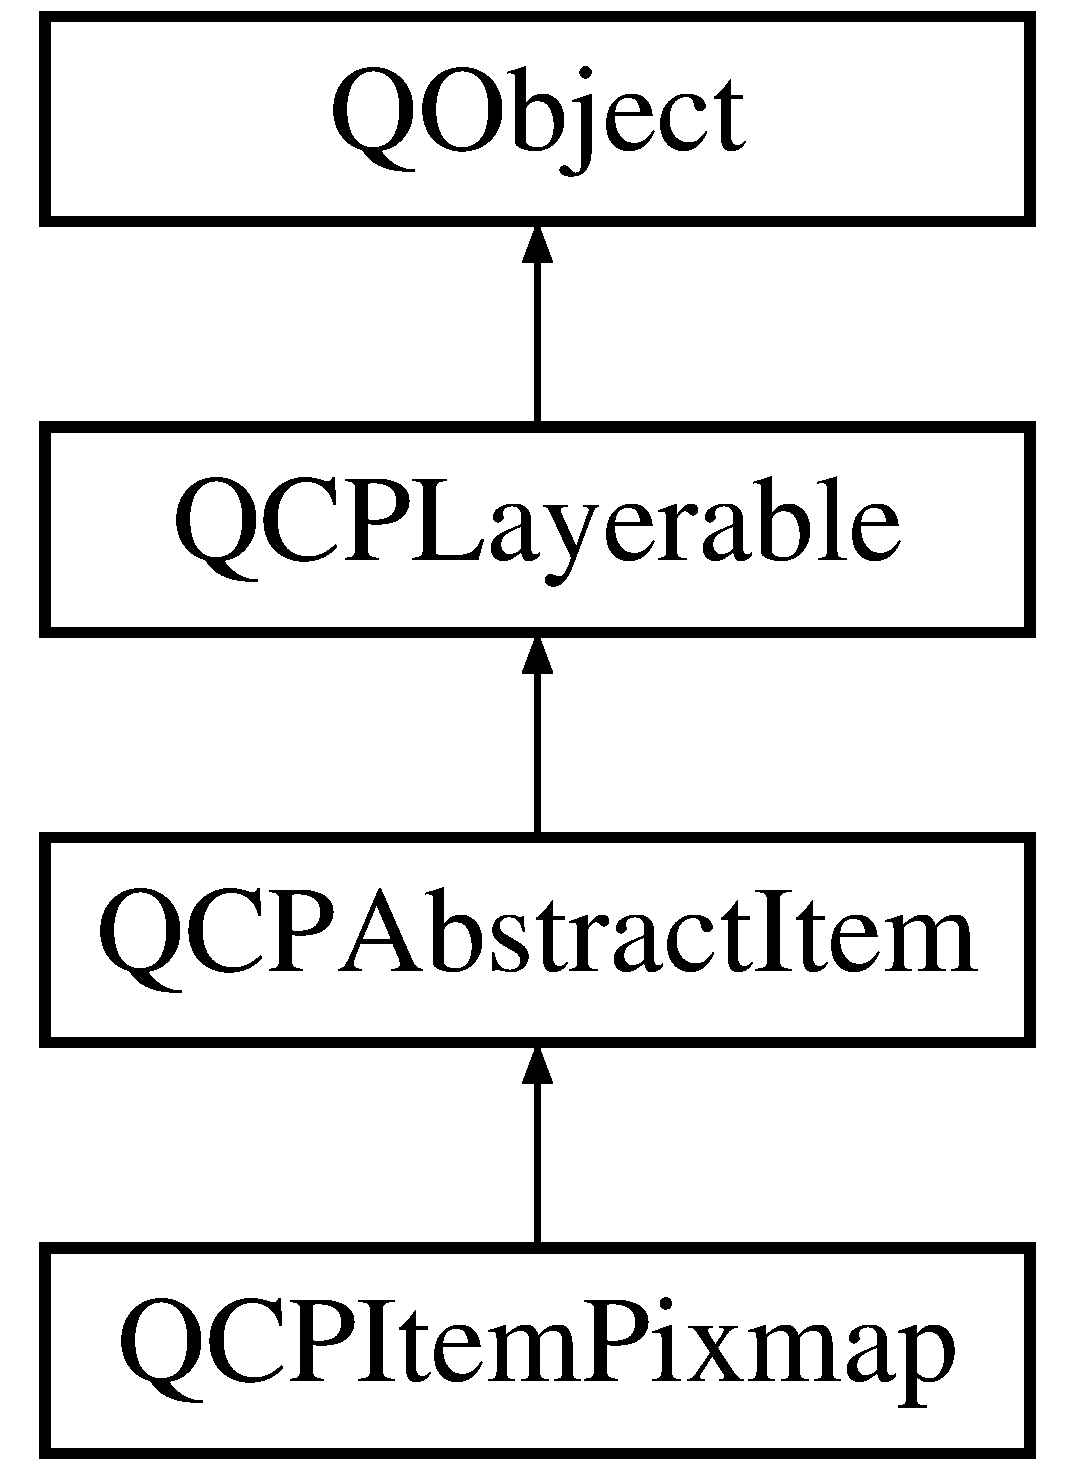
\includegraphics[height=4.000000cm]{class_q_c_p_item_pixmap}
\end{center}
\end{figure}
\subsection*{Public Member Functions}
\begin{DoxyCompactItemize}
\item 
\hyperlink{class_q_c_p_item_pixmap_aa6de42a37261b21a5480e7da122345c3}{Q\+C\+P\+Item\+Pixmap} (\hyperlink{class_q_custom_plot}{Q\+Custom\+Plot} $\ast$\hyperlink{class_q_c_p_layerable_ab7e0e94461566093d36ffc0f5312b109}{parent\+Plot})
\item 
virtual \hyperlink{class_q_c_p_item_pixmap_a810cac6a409d963cda6ea2d3152f1fd0}{$\sim$\+Q\+C\+P\+Item\+Pixmap} ()
\item 
Q\+Pixmap \hyperlink{class_q_c_p_item_pixmap_a73dea89e0eb45127a2705e2c7991b8d8}{pixmap} () const 
\item 
bool \hyperlink{class_q_c_p_item_pixmap_a54026b89dff3c60376c2360f01b6fb83}{scaled} () const 
\item 
Qt\+::\+Aspect\+Ratio\+Mode \hyperlink{class_q_c_p_item_pixmap_ac5b95c097169e107a61eebbb7c77523c}{aspect\+Ratio\+Mode} () const 
\item 
Qt\+::\+Transformation\+Mode \hyperlink{class_q_c_p_item_pixmap_a1d4751a7b9588354fc8e726d891153f7}{transformation\+Mode} () const 
\item 
Q\+Pen \hyperlink{class_q_c_p_item_pixmap_ab2b821c80cfade589472e933b9c4361f}{pen} () const 
\item 
Q\+Pen \hyperlink{class_q_c_p_item_pixmap_af8e839d7c7b84e214608feda3caec2bc}{selected\+Pen} () const 
\item 
void \hyperlink{class_q_c_p_item_pixmap_a726b69ea4025edf48f9b29b6450548a7}{set\+Pixmap} (const Q\+Pixmap \&\hyperlink{class_q_c_p_item_pixmap_a73dea89e0eb45127a2705e2c7991b8d8}{pixmap})
\item 
void \hyperlink{class_q_c_p_item_pixmap_ab4d44529a1c6c8d37d0ea7560e042777}{set\+Scaled} (bool \hyperlink{class_q_c_p_item_pixmap_a54026b89dff3c60376c2360f01b6fb83}{scaled}, Qt\+::\+Aspect\+Ratio\+Mode \hyperlink{class_q_c_p_item_pixmap_ac5b95c097169e107a61eebbb7c77523c}{aspect\+Ratio\+Mode}=Qt\+::\+Keep\+Aspect\+Ratio, Qt\+::\+Transformation\+Mode \hyperlink{class_q_c_p_item_pixmap_a1d4751a7b9588354fc8e726d891153f7}{transformation\+Mode}=Qt\+::\+Smooth\+Transformation)
\item 
void \hyperlink{class_q_c_p_item_pixmap_acdade1305edb4b5cae14f97fd132065f}{set\+Pen} (const Q\+Pen \&\hyperlink{class_q_c_p_item_pixmap_ab2b821c80cfade589472e933b9c4361f}{pen})
\item 
void \hyperlink{class_q_c_p_item_pixmap_afc5e479e88e53740176ce77cb70dd67a}{set\+Selected\+Pen} (const Q\+Pen \&\hyperlink{class_q_c_p_item_pixmap_ab2b821c80cfade589472e933b9c4361f}{pen})
\item 
virtual double \hyperlink{class_q_c_p_item_pixmap_a9f8436aa141fa0fb504191c882c2f4d9}{select\+Test} (const Q\+Point\+F \&pos, bool only\+Selectable, Q\+Variant $\ast$details=0) const 
\end{DoxyCompactItemize}
\subsection*{Public Attributes}
\begin{DoxyCompactItemize}
\item 
\hyperlink{class_q_c_p_item_position}{Q\+C\+P\+Item\+Position} $\ast$const \hyperlink{class_q_c_p_item_pixmap_a43c281ef6ad46f3cf04f365289abe51a}{top\+Left}
\item 
\hyperlink{class_q_c_p_item_position}{Q\+C\+P\+Item\+Position} $\ast$const \hyperlink{class_q_c_p_item_pixmap_abcc38063f9502b876bf6615c45cc0994}{bottom\+Right}
\item 
\hyperlink{class_q_c_p_item_anchor}{Q\+C\+P\+Item\+Anchor} $\ast$const \hyperlink{class_q_c_p_item_pixmap_af7a156590b1d59ab21b453c430c56a7c}{top}
\item 
\hyperlink{class_q_c_p_item_anchor}{Q\+C\+P\+Item\+Anchor} $\ast$const \hyperlink{class_q_c_p_item_pixmap_a72eabd0010be41a4ec1b22aa983d2aa1}{top\+Right}
\item 
\hyperlink{class_q_c_p_item_anchor}{Q\+C\+P\+Item\+Anchor} $\ast$const \hyperlink{class_q_c_p_item_pixmap_ac9c0fd231f9e285765978a05d13f8280}{right}
\item 
\hyperlink{class_q_c_p_item_anchor}{Q\+C\+P\+Item\+Anchor} $\ast$const \hyperlink{class_q_c_p_item_pixmap_ad7da77f530868e846151eff8a28fb948}{bottom}
\item 
\hyperlink{class_q_c_p_item_anchor}{Q\+C\+P\+Item\+Anchor} $\ast$const \hyperlink{class_q_c_p_item_pixmap_a01943e569233382b3627e24636b0fff2}{bottom\+Left}
\item 
\hyperlink{class_q_c_p_item_anchor}{Q\+C\+P\+Item\+Anchor} $\ast$const \hyperlink{class_q_c_p_item_pixmap_a8c85fcb8cb8ce292859a0499d16539b1}{left}
\end{DoxyCompactItemize}
\subsection*{Protected Types}
\begin{DoxyCompactItemize}
\item 
enum \hyperlink{class_q_c_p_item_pixmap_a0ea7f65edb7395e02de521915f221174}{Anchor\+Index} \{ \\*
\hyperlink{class_q_c_p_item_pixmap_a0ea7f65edb7395e02de521915f221174a90e523ebaed7921ca90cf1b08944ece5}{ai\+Top}, 
\hyperlink{class_q_c_p_item_pixmap_a0ea7f65edb7395e02de521915f221174a33c256cdec46fa1587534fcd6e776799}{ai\+Top\+Right}, 
\hyperlink{class_q_c_p_item_pixmap_a0ea7f65edb7395e02de521915f221174ab22d91dae59c0d4a65416a0d677b2d05}{ai\+Right}, 
\hyperlink{class_q_c_p_item_pixmap_a0ea7f65edb7395e02de521915f221174a04b5e041b4dd0def2b60c5cfea2bc1a4}{ai\+Bottom}, 
\\*
\hyperlink{class_q_c_p_item_pixmap_a0ea7f65edb7395e02de521915f221174ae14886b381136898e37e89af5046a1cc}{ai\+Bottom\+Left}, 
\hyperlink{class_q_c_p_item_pixmap_a0ea7f65edb7395e02de521915f221174a9efe71239b9409ebe1c2813a37807f2a}{ai\+Left}
 \}
\end{DoxyCompactItemize}
\subsection*{Protected Member Functions}
\begin{DoxyCompactItemize}
\item 
virtual void \hyperlink{class_q_c_p_item_pixmap_a879e8076c2db01a38b34cfa73ec95d2f}{draw} (\hyperlink{class_q_c_p_painter}{Q\+C\+P\+Painter} $\ast$painter)
\item 
virtual Q\+Point\+F \hyperlink{class_q_c_p_item_pixmap_a88abce3c1027f371cddcf6dad35ffbb1}{anchor\+Pixel\+Point} (int anchor\+Id) const 
\item 
void \hyperlink{class_q_c_p_item_pixmap_a8bced3027b326b290726cd1979c7cfc6}{update\+Scaled\+Pixmap} (Q\+Rect final\+Rect=Q\+Rect(), bool flip\+Horz=false, bool flip\+Vert=false)
\item 
Q\+Rect \hyperlink{class_q_c_p_item_pixmap_a245ef0c626cab7096a810442f2f6a2d9}{get\+Final\+Rect} (bool $\ast$flipped\+Horz=0, bool $\ast$flipped\+Vert=0) const 
\item 
Q\+Pen \hyperlink{class_q_c_p_item_pixmap_af21085516585c475dc9d839e7f377233}{main\+Pen} () const 
\end{DoxyCompactItemize}
\subsection*{Protected Attributes}
\begin{DoxyCompactItemize}
\item 
Q\+Pixmap \hyperlink{class_q_c_p_item_pixmap_a1396cce7f26c7b8e9512906284380c4d}{m\+Pixmap}
\item 
Q\+Pixmap \hyperlink{class_q_c_p_item_pixmap_a2ebc66e15b9f1264563d58f29ba1bc00}{m\+Scaled\+Pixmap}
\item 
bool \hyperlink{class_q_c_p_item_pixmap_a8fe670a529cd46a9b8afd9fc1203bc3f}{m\+Scaled}
\item 
Qt\+::\+Aspect\+Ratio\+Mode \hyperlink{class_q_c_p_item_pixmap_a8dc6b6c1e106ac523efae22d5fe55bab}{m\+Aspect\+Ratio\+Mode}
\item 
Qt\+::\+Transformation\+Mode \hyperlink{class_q_c_p_item_pixmap_ac9ecad3b9842363754e32eda2cf821bd}{m\+Transformation\+Mode}
\item 
Q\+Pen \hyperlink{class_q_c_p_item_pixmap_acfee1124eb51a1887aaf8de10777c7a1}{m\+Pen}
\item 
Q\+Pen \hyperlink{class_q_c_p_item_pixmap_a0949e5bb6a261fc4e9668e28e2effcfa}{m\+Selected\+Pen}
\end{DoxyCompactItemize}
\subsection*{Additional Inherited Members}


\subsection{Detailed Description}
An arbitrary pixmap. 

 It has two positions, {\itshape top\+Left} and {\itshape bottom\+Right}, which define the rectangle the pixmap will be drawn in. Depending on the scale setting (\hyperlink{class_q_c_p_item_pixmap_ab4d44529a1c6c8d37d0ea7560e042777}{set\+Scaled}), the pixmap will be either scaled to fit the rectangle or be drawn aligned to the top\+Left position.

If scaling is enabled and {\itshape top\+Left} is further to the bottom/right than {\itshape bottom\+Right} (as shown on the right side of the example image), the pixmap will be flipped in the respective orientations. 

\subsection{Member Enumeration Documentation}
\hypertarget{class_q_c_p_item_pixmap_a0ea7f65edb7395e02de521915f221174}{}\index{Q\+C\+P\+Item\+Pixmap@{Q\+C\+P\+Item\+Pixmap}!Anchor\+Index@{Anchor\+Index}}
\index{Anchor\+Index@{Anchor\+Index}!Q\+C\+P\+Item\+Pixmap@{Q\+C\+P\+Item\+Pixmap}}
\subsubsection[{Anchor\+Index}]{\setlength{\rightskip}{0pt plus 5cm}enum {\bf Q\+C\+P\+Item\+Pixmap\+::\+Anchor\+Index}\hspace{0.3cm}{\ttfamily [protected]}}\label{class_q_c_p_item_pixmap_a0ea7f65edb7395e02de521915f221174}
\begin{Desc}
\item[Enumerator]\par
\begin{description}
\index{ai\+Top@{ai\+Top}!Q\+C\+P\+Item\+Pixmap@{Q\+C\+P\+Item\+Pixmap}}\index{Q\+C\+P\+Item\+Pixmap@{Q\+C\+P\+Item\+Pixmap}!ai\+Top@{ai\+Top}}\item[{\em 
\hypertarget{class_q_c_p_item_pixmap_a0ea7f65edb7395e02de521915f221174a90e523ebaed7921ca90cf1b08944ece5}{}ai\+Top\label{class_q_c_p_item_pixmap_a0ea7f65edb7395e02de521915f221174a90e523ebaed7921ca90cf1b08944ece5}
}]\index{ai\+Top\+Right@{ai\+Top\+Right}!Q\+C\+P\+Item\+Pixmap@{Q\+C\+P\+Item\+Pixmap}}\index{Q\+C\+P\+Item\+Pixmap@{Q\+C\+P\+Item\+Pixmap}!ai\+Top\+Right@{ai\+Top\+Right}}\item[{\em 
\hypertarget{class_q_c_p_item_pixmap_a0ea7f65edb7395e02de521915f221174a33c256cdec46fa1587534fcd6e776799}{}ai\+Top\+Right\label{class_q_c_p_item_pixmap_a0ea7f65edb7395e02de521915f221174a33c256cdec46fa1587534fcd6e776799}
}]\index{ai\+Right@{ai\+Right}!Q\+C\+P\+Item\+Pixmap@{Q\+C\+P\+Item\+Pixmap}}\index{Q\+C\+P\+Item\+Pixmap@{Q\+C\+P\+Item\+Pixmap}!ai\+Right@{ai\+Right}}\item[{\em 
\hypertarget{class_q_c_p_item_pixmap_a0ea7f65edb7395e02de521915f221174ab22d91dae59c0d4a65416a0d677b2d05}{}ai\+Right\label{class_q_c_p_item_pixmap_a0ea7f65edb7395e02de521915f221174ab22d91dae59c0d4a65416a0d677b2d05}
}]\index{ai\+Bottom@{ai\+Bottom}!Q\+C\+P\+Item\+Pixmap@{Q\+C\+P\+Item\+Pixmap}}\index{Q\+C\+P\+Item\+Pixmap@{Q\+C\+P\+Item\+Pixmap}!ai\+Bottom@{ai\+Bottom}}\item[{\em 
\hypertarget{class_q_c_p_item_pixmap_a0ea7f65edb7395e02de521915f221174a04b5e041b4dd0def2b60c5cfea2bc1a4}{}ai\+Bottom\label{class_q_c_p_item_pixmap_a0ea7f65edb7395e02de521915f221174a04b5e041b4dd0def2b60c5cfea2bc1a4}
}]\index{ai\+Bottom\+Left@{ai\+Bottom\+Left}!Q\+C\+P\+Item\+Pixmap@{Q\+C\+P\+Item\+Pixmap}}\index{Q\+C\+P\+Item\+Pixmap@{Q\+C\+P\+Item\+Pixmap}!ai\+Bottom\+Left@{ai\+Bottom\+Left}}\item[{\em 
\hypertarget{class_q_c_p_item_pixmap_a0ea7f65edb7395e02de521915f221174ae14886b381136898e37e89af5046a1cc}{}ai\+Bottom\+Left\label{class_q_c_p_item_pixmap_a0ea7f65edb7395e02de521915f221174ae14886b381136898e37e89af5046a1cc}
}]\index{ai\+Left@{ai\+Left}!Q\+C\+P\+Item\+Pixmap@{Q\+C\+P\+Item\+Pixmap}}\index{Q\+C\+P\+Item\+Pixmap@{Q\+C\+P\+Item\+Pixmap}!ai\+Left@{ai\+Left}}\item[{\em 
\hypertarget{class_q_c_p_item_pixmap_a0ea7f65edb7395e02de521915f221174a9efe71239b9409ebe1c2813a37807f2a}{}ai\+Left\label{class_q_c_p_item_pixmap_a0ea7f65edb7395e02de521915f221174a9efe71239b9409ebe1c2813a37807f2a}
}]\end{description}
\end{Desc}


\subsection{Constructor \& Destructor Documentation}
\hypertarget{class_q_c_p_item_pixmap_aa6de42a37261b21a5480e7da122345c3}{}\index{Q\+C\+P\+Item\+Pixmap@{Q\+C\+P\+Item\+Pixmap}!Q\+C\+P\+Item\+Pixmap@{Q\+C\+P\+Item\+Pixmap}}
\index{Q\+C\+P\+Item\+Pixmap@{Q\+C\+P\+Item\+Pixmap}!Q\+C\+P\+Item\+Pixmap@{Q\+C\+P\+Item\+Pixmap}}
\subsubsection[{Q\+C\+P\+Item\+Pixmap}]{\setlength{\rightskip}{0pt plus 5cm}Q\+C\+P\+Item\+Pixmap\+::\+Q\+C\+P\+Item\+Pixmap (
\begin{DoxyParamCaption}
\item[{{\bf Q\+Custom\+Plot} $\ast$}]{parent\+Plot}
\end{DoxyParamCaption}
)}\label{class_q_c_p_item_pixmap_aa6de42a37261b21a5480e7da122345c3}
Creates a rectangle item and sets default values.

The constructed item can be added to the plot with \hyperlink{class_q_custom_plot_aa500620379262321685cb7a7674cbd2a}{Q\+Custom\+Plot\+::add\+Item}. \hypertarget{class_q_c_p_item_pixmap_a810cac6a409d963cda6ea2d3152f1fd0}{}\index{Q\+C\+P\+Item\+Pixmap@{Q\+C\+P\+Item\+Pixmap}!````~Q\+C\+P\+Item\+Pixmap@{$\sim$\+Q\+C\+P\+Item\+Pixmap}}
\index{````~Q\+C\+P\+Item\+Pixmap@{$\sim$\+Q\+C\+P\+Item\+Pixmap}!Q\+C\+P\+Item\+Pixmap@{Q\+C\+P\+Item\+Pixmap}}
\subsubsection[{$\sim$\+Q\+C\+P\+Item\+Pixmap}]{\setlength{\rightskip}{0pt plus 5cm}Q\+C\+P\+Item\+Pixmap\+::$\sim$\+Q\+C\+P\+Item\+Pixmap (
\begin{DoxyParamCaption}
{}
\end{DoxyParamCaption}
)\hspace{0.3cm}{\ttfamily [virtual]}}\label{class_q_c_p_item_pixmap_a810cac6a409d963cda6ea2d3152f1fd0}


\subsection{Member Function Documentation}
\hypertarget{class_q_c_p_item_pixmap_a88abce3c1027f371cddcf6dad35ffbb1}{}\index{Q\+C\+P\+Item\+Pixmap@{Q\+C\+P\+Item\+Pixmap}!anchor\+Pixel\+Point@{anchor\+Pixel\+Point}}
\index{anchor\+Pixel\+Point@{anchor\+Pixel\+Point}!Q\+C\+P\+Item\+Pixmap@{Q\+C\+P\+Item\+Pixmap}}
\subsubsection[{anchor\+Pixel\+Point}]{\setlength{\rightskip}{0pt plus 5cm}Q\+Point\+F Q\+C\+P\+Item\+Pixmap\+::anchor\+Pixel\+Point (
\begin{DoxyParamCaption}
\item[{int}]{anchor\+Id}
\end{DoxyParamCaption}
) const\hspace{0.3cm}{\ttfamily [protected]}, {\ttfamily [virtual]}}\label{class_q_c_p_item_pixmap_a88abce3c1027f371cddcf6dad35ffbb1}


Reimplemented from \hyperlink{class_q_c_p_abstract_item_a94bde62b8a2fc133666dcbb8035deeed}{Q\+C\+P\+Abstract\+Item}.

\hypertarget{class_q_c_p_item_pixmap_ac5b95c097169e107a61eebbb7c77523c}{}\index{Q\+C\+P\+Item\+Pixmap@{Q\+C\+P\+Item\+Pixmap}!aspect\+Ratio\+Mode@{aspect\+Ratio\+Mode}}
\index{aspect\+Ratio\+Mode@{aspect\+Ratio\+Mode}!Q\+C\+P\+Item\+Pixmap@{Q\+C\+P\+Item\+Pixmap}}
\subsubsection[{aspect\+Ratio\+Mode}]{\setlength{\rightskip}{0pt plus 5cm}Qt\+::\+Aspect\+Ratio\+Mode Q\+C\+P\+Item\+Pixmap\+::aspect\+Ratio\+Mode (
\begin{DoxyParamCaption}
{}
\end{DoxyParamCaption}
) const\hspace{0.3cm}{\ttfamily [inline]}}\label{class_q_c_p_item_pixmap_ac5b95c097169e107a61eebbb7c77523c}
\hypertarget{class_q_c_p_item_pixmap_a879e8076c2db01a38b34cfa73ec95d2f}{}\index{Q\+C\+P\+Item\+Pixmap@{Q\+C\+P\+Item\+Pixmap}!draw@{draw}}
\index{draw@{draw}!Q\+C\+P\+Item\+Pixmap@{Q\+C\+P\+Item\+Pixmap}}
\subsubsection[{draw}]{\setlength{\rightskip}{0pt plus 5cm}void Q\+C\+P\+Item\+Pixmap\+::draw (
\begin{DoxyParamCaption}
\item[{{\bf Q\+C\+P\+Painter} $\ast$}]{painter}
\end{DoxyParamCaption}
)\hspace{0.3cm}{\ttfamily [protected]}, {\ttfamily [virtual]}}\label{class_q_c_p_item_pixmap_a879e8076c2db01a38b34cfa73ec95d2f}


Implements \hyperlink{class_q_c_p_abstract_item_ad0dc056f650c3ca73414e6b4f01674ef}{Q\+C\+P\+Abstract\+Item}.

\hypertarget{class_q_c_p_item_pixmap_a245ef0c626cab7096a810442f2f6a2d9}{}\index{Q\+C\+P\+Item\+Pixmap@{Q\+C\+P\+Item\+Pixmap}!get\+Final\+Rect@{get\+Final\+Rect}}
\index{get\+Final\+Rect@{get\+Final\+Rect}!Q\+C\+P\+Item\+Pixmap@{Q\+C\+P\+Item\+Pixmap}}
\subsubsection[{get\+Final\+Rect}]{\setlength{\rightskip}{0pt plus 5cm}Q\+Rect Q\+C\+P\+Item\+Pixmap\+::get\+Final\+Rect (
\begin{DoxyParamCaption}
\item[{bool $\ast$}]{flipped\+Horz = {\ttfamily 0}, }
\item[{bool $\ast$}]{flipped\+Vert = {\ttfamily 0}}
\end{DoxyParamCaption}
) const\hspace{0.3cm}{\ttfamily [protected]}}\label{class_q_c_p_item_pixmap_a245ef0c626cab7096a810442f2f6a2d9}
\hypertarget{class_q_c_p_item_pixmap_af21085516585c475dc9d839e7f377233}{}\index{Q\+C\+P\+Item\+Pixmap@{Q\+C\+P\+Item\+Pixmap}!main\+Pen@{main\+Pen}}
\index{main\+Pen@{main\+Pen}!Q\+C\+P\+Item\+Pixmap@{Q\+C\+P\+Item\+Pixmap}}
\subsubsection[{main\+Pen}]{\setlength{\rightskip}{0pt plus 5cm}Q\+Pen Q\+C\+P\+Item\+Pixmap\+::main\+Pen (
\begin{DoxyParamCaption}
{}
\end{DoxyParamCaption}
) const\hspace{0.3cm}{\ttfamily [protected]}}\label{class_q_c_p_item_pixmap_af21085516585c475dc9d839e7f377233}
\hypertarget{class_q_c_p_item_pixmap_ab2b821c80cfade589472e933b9c4361f}{}\index{Q\+C\+P\+Item\+Pixmap@{Q\+C\+P\+Item\+Pixmap}!pen@{pen}}
\index{pen@{pen}!Q\+C\+P\+Item\+Pixmap@{Q\+C\+P\+Item\+Pixmap}}
\subsubsection[{pen}]{\setlength{\rightskip}{0pt plus 5cm}Q\+Pen Q\+C\+P\+Item\+Pixmap\+::pen (
\begin{DoxyParamCaption}
{}
\end{DoxyParamCaption}
) const\hspace{0.3cm}{\ttfamily [inline]}}\label{class_q_c_p_item_pixmap_ab2b821c80cfade589472e933b9c4361f}
\hypertarget{class_q_c_p_item_pixmap_a73dea89e0eb45127a2705e2c7991b8d8}{}\index{Q\+C\+P\+Item\+Pixmap@{Q\+C\+P\+Item\+Pixmap}!pixmap@{pixmap}}
\index{pixmap@{pixmap}!Q\+C\+P\+Item\+Pixmap@{Q\+C\+P\+Item\+Pixmap}}
\subsubsection[{pixmap}]{\setlength{\rightskip}{0pt plus 5cm}Q\+Pixmap Q\+C\+P\+Item\+Pixmap\+::pixmap (
\begin{DoxyParamCaption}
{}
\end{DoxyParamCaption}
) const\hspace{0.3cm}{\ttfamily [inline]}}\label{class_q_c_p_item_pixmap_a73dea89e0eb45127a2705e2c7991b8d8}
\hypertarget{class_q_c_p_item_pixmap_a54026b89dff3c60376c2360f01b6fb83}{}\index{Q\+C\+P\+Item\+Pixmap@{Q\+C\+P\+Item\+Pixmap}!scaled@{scaled}}
\index{scaled@{scaled}!Q\+C\+P\+Item\+Pixmap@{Q\+C\+P\+Item\+Pixmap}}
\subsubsection[{scaled}]{\setlength{\rightskip}{0pt plus 5cm}bool Q\+C\+P\+Item\+Pixmap\+::scaled (
\begin{DoxyParamCaption}
{}
\end{DoxyParamCaption}
) const\hspace{0.3cm}{\ttfamily [inline]}}\label{class_q_c_p_item_pixmap_a54026b89dff3c60376c2360f01b6fb83}
\hypertarget{class_q_c_p_item_pixmap_af8e839d7c7b84e214608feda3caec2bc}{}\index{Q\+C\+P\+Item\+Pixmap@{Q\+C\+P\+Item\+Pixmap}!selected\+Pen@{selected\+Pen}}
\index{selected\+Pen@{selected\+Pen}!Q\+C\+P\+Item\+Pixmap@{Q\+C\+P\+Item\+Pixmap}}
\subsubsection[{selected\+Pen}]{\setlength{\rightskip}{0pt plus 5cm}Q\+Pen Q\+C\+P\+Item\+Pixmap\+::selected\+Pen (
\begin{DoxyParamCaption}
{}
\end{DoxyParamCaption}
) const\hspace{0.3cm}{\ttfamily [inline]}}\label{class_q_c_p_item_pixmap_af8e839d7c7b84e214608feda3caec2bc}
\hypertarget{class_q_c_p_item_pixmap_a9f8436aa141fa0fb504191c882c2f4d9}{}\index{Q\+C\+P\+Item\+Pixmap@{Q\+C\+P\+Item\+Pixmap}!select\+Test@{select\+Test}}
\index{select\+Test@{select\+Test}!Q\+C\+P\+Item\+Pixmap@{Q\+C\+P\+Item\+Pixmap}}
\subsubsection[{select\+Test}]{\setlength{\rightskip}{0pt plus 5cm}double Q\+C\+P\+Item\+Pixmap\+::select\+Test (
\begin{DoxyParamCaption}
\item[{const Q\+Point\+F \&}]{pos, }
\item[{bool}]{only\+Selectable, }
\item[{Q\+Variant $\ast$}]{details = {\ttfamily 0}}
\end{DoxyParamCaption}
) const\hspace{0.3cm}{\ttfamily [virtual]}}\label{class_q_c_p_item_pixmap_a9f8436aa141fa0fb504191c882c2f4d9}
This function is used to decide whether a click hits a layerable object or not.

{\itshape pos} is a point in pixel coordinates on the \hyperlink{class_q_custom_plot}{Q\+Custom\+Plot} surface. This function returns the shortest pixel distance of this point to the object. If the object is either invisible or the distance couldn\textquotesingle{}t be determined, -\/1.\+0 is returned. Further, if {\itshape only\+Selectable} is true and the object is not selectable, -\/1.\+0 is returned, too.

If the item is represented not by single lines but by an area like \hyperlink{class_q_c_p_item_rect}{Q\+C\+P\+Item\+Rect} or \hyperlink{class_q_c_p_item_text}{Q\+C\+P\+Item\+Text}, a click inside the area returns a constant value greater zero (typically the selection\+Tolerance of the parent \hyperlink{class_q_custom_plot}{Q\+Custom\+Plot} multiplied by 0.\+99). If the click lies outside the area, this function returns -\/1.\+0.

Providing a constant value for area objects allows selecting line objects even when they are obscured by such area objects, by clicking close to the lines (i.\+e. closer than 0.\+99$\ast$selection\+Tolerance).

The actual setting of the selection state is not done by this function. This is handled by the parent \hyperlink{class_q_custom_plot}{Q\+Custom\+Plot} when the mouse\+Release\+Event occurs, and the finally selected object is notified via the select\+Event/deselect\+Event methods.

{\itshape details} is an optional output parameter. Every layerable subclass may place any information in {\itshape details}. This information will be passed to \hyperlink{class_q_c_p_abstract_item_aaf92af7b9893712959a6c073d334d88d}{select\+Event} when the parent \hyperlink{class_q_custom_plot}{Q\+Custom\+Plot} decides on the basis of this select\+Test call, that the object was successfully selected. The subsequent call to \hyperlink{class_q_c_p_abstract_item_aaf92af7b9893712959a6c073d334d88d}{select\+Event} will carry the {\itshape details}. This is useful for multi-\/part objects (like \hyperlink{class_q_c_p_axis}{Q\+C\+P\+Axis}). This way, a possibly complex calculation to decide which part was clicked is only done once in \hyperlink{class_q_c_p_item_pixmap_a9f8436aa141fa0fb504191c882c2f4d9}{select\+Test}. The result (i.\+e. the actually clicked part) can then be placed in {\itshape details}. So in the subsequent \hyperlink{class_q_c_p_abstract_item_aaf92af7b9893712959a6c073d334d88d}{select\+Event}, the decision which part was selected doesn\textquotesingle{}t have to be done a second time for a single selection operation.

You may pass 0 as {\itshape details} to indicate that you are not interested in those selection details.

\begin{DoxySeeAlso}{See also}
\hyperlink{class_q_c_p_abstract_item_aaf92af7b9893712959a6c073d334d88d}{select\+Event}, \hyperlink{class_q_c_p_abstract_item_a91f090d6763cfedb0749219c63788ae9}{deselect\+Event}, \hyperlink{class_q_custom_plot_a5ee1e2f6ae27419deca53e75907c27e5}{Q\+Custom\+Plot\+::set\+Interactions} 
\end{DoxySeeAlso}


Implements \hyperlink{class_q_c_p_abstract_item_a96d522d10ffc0413b9a366c6f7f0476b}{Q\+C\+P\+Abstract\+Item}.

\hypertarget{class_q_c_p_item_pixmap_acdade1305edb4b5cae14f97fd132065f}{}\index{Q\+C\+P\+Item\+Pixmap@{Q\+C\+P\+Item\+Pixmap}!set\+Pen@{set\+Pen}}
\index{set\+Pen@{set\+Pen}!Q\+C\+P\+Item\+Pixmap@{Q\+C\+P\+Item\+Pixmap}}
\subsubsection[{set\+Pen}]{\setlength{\rightskip}{0pt plus 5cm}void Q\+C\+P\+Item\+Pixmap\+::set\+Pen (
\begin{DoxyParamCaption}
\item[{const Q\+Pen \&}]{pen}
\end{DoxyParamCaption}
)}\label{class_q_c_p_item_pixmap_acdade1305edb4b5cae14f97fd132065f}
Sets the pen that will be used to draw a border around the pixmap.

\begin{DoxySeeAlso}{See also}
\hyperlink{class_q_c_p_item_pixmap_afc5e479e88e53740176ce77cb70dd67a}{set\+Selected\+Pen}, set\+Brush 
\end{DoxySeeAlso}
\hypertarget{class_q_c_p_item_pixmap_a726b69ea4025edf48f9b29b6450548a7}{}\index{Q\+C\+P\+Item\+Pixmap@{Q\+C\+P\+Item\+Pixmap}!set\+Pixmap@{set\+Pixmap}}
\index{set\+Pixmap@{set\+Pixmap}!Q\+C\+P\+Item\+Pixmap@{Q\+C\+P\+Item\+Pixmap}}
\subsubsection[{set\+Pixmap}]{\setlength{\rightskip}{0pt plus 5cm}void Q\+C\+P\+Item\+Pixmap\+::set\+Pixmap (
\begin{DoxyParamCaption}
\item[{const Q\+Pixmap \&}]{pixmap}
\end{DoxyParamCaption}
)}\label{class_q_c_p_item_pixmap_a726b69ea4025edf48f9b29b6450548a7}
Sets the pixmap that will be displayed. \hypertarget{class_q_c_p_item_pixmap_ab4d44529a1c6c8d37d0ea7560e042777}{}\index{Q\+C\+P\+Item\+Pixmap@{Q\+C\+P\+Item\+Pixmap}!set\+Scaled@{set\+Scaled}}
\index{set\+Scaled@{set\+Scaled}!Q\+C\+P\+Item\+Pixmap@{Q\+C\+P\+Item\+Pixmap}}
\subsubsection[{set\+Scaled}]{\setlength{\rightskip}{0pt plus 5cm}void Q\+C\+P\+Item\+Pixmap\+::set\+Scaled (
\begin{DoxyParamCaption}
\item[{bool}]{scaled, }
\item[{Qt\+::\+Aspect\+Ratio\+Mode}]{aspect\+Ratio\+Mode = {\ttfamily Qt\+:\+:KeepAspectRatio}, }
\item[{Qt\+::\+Transformation\+Mode}]{transformation\+Mode = {\ttfamily Qt\+:\+:SmoothTransformation}}
\end{DoxyParamCaption}
)}\label{class_q_c_p_item_pixmap_ab4d44529a1c6c8d37d0ea7560e042777}
Sets whether the pixmap will be scaled to fit the rectangle defined by the {\itshape top\+Left} and {\itshape bottom\+Right} positions. \hypertarget{class_q_c_p_item_pixmap_afc5e479e88e53740176ce77cb70dd67a}{}\index{Q\+C\+P\+Item\+Pixmap@{Q\+C\+P\+Item\+Pixmap}!set\+Selected\+Pen@{set\+Selected\+Pen}}
\index{set\+Selected\+Pen@{set\+Selected\+Pen}!Q\+C\+P\+Item\+Pixmap@{Q\+C\+P\+Item\+Pixmap}}
\subsubsection[{set\+Selected\+Pen}]{\setlength{\rightskip}{0pt plus 5cm}void Q\+C\+P\+Item\+Pixmap\+::set\+Selected\+Pen (
\begin{DoxyParamCaption}
\item[{const Q\+Pen \&}]{pen}
\end{DoxyParamCaption}
)}\label{class_q_c_p_item_pixmap_afc5e479e88e53740176ce77cb70dd67a}
Sets the pen that will be used to draw a border around the pixmap when selected

\begin{DoxySeeAlso}{See also}
\hyperlink{class_q_c_p_item_pixmap_acdade1305edb4b5cae14f97fd132065f}{set\+Pen}, \hyperlink{class_q_c_p_abstract_item_a203de94ad586cc44d16c9565f49d3378}{set\+Selected} 
\end{DoxySeeAlso}
\hypertarget{class_q_c_p_item_pixmap_a1d4751a7b9588354fc8e726d891153f7}{}\index{Q\+C\+P\+Item\+Pixmap@{Q\+C\+P\+Item\+Pixmap}!transformation\+Mode@{transformation\+Mode}}
\index{transformation\+Mode@{transformation\+Mode}!Q\+C\+P\+Item\+Pixmap@{Q\+C\+P\+Item\+Pixmap}}
\subsubsection[{transformation\+Mode}]{\setlength{\rightskip}{0pt plus 5cm}Qt\+::\+Transformation\+Mode Q\+C\+P\+Item\+Pixmap\+::transformation\+Mode (
\begin{DoxyParamCaption}
{}
\end{DoxyParamCaption}
) const\hspace{0.3cm}{\ttfamily [inline]}}\label{class_q_c_p_item_pixmap_a1d4751a7b9588354fc8e726d891153f7}
\hypertarget{class_q_c_p_item_pixmap_a8bced3027b326b290726cd1979c7cfc6}{}\index{Q\+C\+P\+Item\+Pixmap@{Q\+C\+P\+Item\+Pixmap}!update\+Scaled\+Pixmap@{update\+Scaled\+Pixmap}}
\index{update\+Scaled\+Pixmap@{update\+Scaled\+Pixmap}!Q\+C\+P\+Item\+Pixmap@{Q\+C\+P\+Item\+Pixmap}}
\subsubsection[{update\+Scaled\+Pixmap}]{\setlength{\rightskip}{0pt plus 5cm}void Q\+C\+P\+Item\+Pixmap\+::update\+Scaled\+Pixmap (
\begin{DoxyParamCaption}
\item[{Q\+Rect}]{final\+Rect = {\ttfamily QRect()}, }
\item[{bool}]{flip\+Horz = {\ttfamily false}, }
\item[{bool}]{flip\+Vert = {\ttfamily false}}
\end{DoxyParamCaption}
)\hspace{0.3cm}{\ttfamily [protected]}}\label{class_q_c_p_item_pixmap_a8bced3027b326b290726cd1979c7cfc6}


\subsection{Member Data Documentation}
\hypertarget{class_q_c_p_item_pixmap_ad7da77f530868e846151eff8a28fb948}{}\index{Q\+C\+P\+Item\+Pixmap@{Q\+C\+P\+Item\+Pixmap}!bottom@{bottom}}
\index{bottom@{bottom}!Q\+C\+P\+Item\+Pixmap@{Q\+C\+P\+Item\+Pixmap}}
\subsubsection[{bottom}]{\setlength{\rightskip}{0pt plus 5cm}{\bf Q\+C\+P\+Item\+Anchor}$\ast$ const Q\+C\+P\+Item\+Pixmap\+::bottom}\label{class_q_c_p_item_pixmap_ad7da77f530868e846151eff8a28fb948}
\hypertarget{class_q_c_p_item_pixmap_a01943e569233382b3627e24636b0fff2}{}\index{Q\+C\+P\+Item\+Pixmap@{Q\+C\+P\+Item\+Pixmap}!bottom\+Left@{bottom\+Left}}
\index{bottom\+Left@{bottom\+Left}!Q\+C\+P\+Item\+Pixmap@{Q\+C\+P\+Item\+Pixmap}}
\subsubsection[{bottom\+Left}]{\setlength{\rightskip}{0pt plus 5cm}{\bf Q\+C\+P\+Item\+Anchor}$\ast$ const Q\+C\+P\+Item\+Pixmap\+::bottom\+Left}\label{class_q_c_p_item_pixmap_a01943e569233382b3627e24636b0fff2}
\hypertarget{class_q_c_p_item_pixmap_abcc38063f9502b876bf6615c45cc0994}{}\index{Q\+C\+P\+Item\+Pixmap@{Q\+C\+P\+Item\+Pixmap}!bottom\+Right@{bottom\+Right}}
\index{bottom\+Right@{bottom\+Right}!Q\+C\+P\+Item\+Pixmap@{Q\+C\+P\+Item\+Pixmap}}
\subsubsection[{bottom\+Right}]{\setlength{\rightskip}{0pt plus 5cm}{\bf Q\+C\+P\+Item\+Position}$\ast$ const Q\+C\+P\+Item\+Pixmap\+::bottom\+Right}\label{class_q_c_p_item_pixmap_abcc38063f9502b876bf6615c45cc0994}
\hypertarget{class_q_c_p_item_pixmap_a8c85fcb8cb8ce292859a0499d16539b1}{}\index{Q\+C\+P\+Item\+Pixmap@{Q\+C\+P\+Item\+Pixmap}!left@{left}}
\index{left@{left}!Q\+C\+P\+Item\+Pixmap@{Q\+C\+P\+Item\+Pixmap}}
\subsubsection[{left}]{\setlength{\rightskip}{0pt plus 5cm}{\bf Q\+C\+P\+Item\+Anchor}$\ast$ const Q\+C\+P\+Item\+Pixmap\+::left}\label{class_q_c_p_item_pixmap_a8c85fcb8cb8ce292859a0499d16539b1}
\hypertarget{class_q_c_p_item_pixmap_a8dc6b6c1e106ac523efae22d5fe55bab}{}\index{Q\+C\+P\+Item\+Pixmap@{Q\+C\+P\+Item\+Pixmap}!m\+Aspect\+Ratio\+Mode@{m\+Aspect\+Ratio\+Mode}}
\index{m\+Aspect\+Ratio\+Mode@{m\+Aspect\+Ratio\+Mode}!Q\+C\+P\+Item\+Pixmap@{Q\+C\+P\+Item\+Pixmap}}
\subsubsection[{m\+Aspect\+Ratio\+Mode}]{\setlength{\rightskip}{0pt plus 5cm}Qt\+::\+Aspect\+Ratio\+Mode Q\+C\+P\+Item\+Pixmap\+::m\+Aspect\+Ratio\+Mode\hspace{0.3cm}{\ttfamily [protected]}}\label{class_q_c_p_item_pixmap_a8dc6b6c1e106ac523efae22d5fe55bab}
\hypertarget{class_q_c_p_item_pixmap_acfee1124eb51a1887aaf8de10777c7a1}{}\index{Q\+C\+P\+Item\+Pixmap@{Q\+C\+P\+Item\+Pixmap}!m\+Pen@{m\+Pen}}
\index{m\+Pen@{m\+Pen}!Q\+C\+P\+Item\+Pixmap@{Q\+C\+P\+Item\+Pixmap}}
\subsubsection[{m\+Pen}]{\setlength{\rightskip}{0pt plus 5cm}Q\+Pen Q\+C\+P\+Item\+Pixmap\+::m\+Pen\hspace{0.3cm}{\ttfamily [protected]}}\label{class_q_c_p_item_pixmap_acfee1124eb51a1887aaf8de10777c7a1}
\hypertarget{class_q_c_p_item_pixmap_a1396cce7f26c7b8e9512906284380c4d}{}\index{Q\+C\+P\+Item\+Pixmap@{Q\+C\+P\+Item\+Pixmap}!m\+Pixmap@{m\+Pixmap}}
\index{m\+Pixmap@{m\+Pixmap}!Q\+C\+P\+Item\+Pixmap@{Q\+C\+P\+Item\+Pixmap}}
\subsubsection[{m\+Pixmap}]{\setlength{\rightskip}{0pt plus 5cm}Q\+Pixmap Q\+C\+P\+Item\+Pixmap\+::m\+Pixmap\hspace{0.3cm}{\ttfamily [protected]}}\label{class_q_c_p_item_pixmap_a1396cce7f26c7b8e9512906284380c4d}
\hypertarget{class_q_c_p_item_pixmap_a8fe670a529cd46a9b8afd9fc1203bc3f}{}\index{Q\+C\+P\+Item\+Pixmap@{Q\+C\+P\+Item\+Pixmap}!m\+Scaled@{m\+Scaled}}
\index{m\+Scaled@{m\+Scaled}!Q\+C\+P\+Item\+Pixmap@{Q\+C\+P\+Item\+Pixmap}}
\subsubsection[{m\+Scaled}]{\setlength{\rightskip}{0pt plus 5cm}bool Q\+C\+P\+Item\+Pixmap\+::m\+Scaled\hspace{0.3cm}{\ttfamily [protected]}}\label{class_q_c_p_item_pixmap_a8fe670a529cd46a9b8afd9fc1203bc3f}
\hypertarget{class_q_c_p_item_pixmap_a2ebc66e15b9f1264563d58f29ba1bc00}{}\index{Q\+C\+P\+Item\+Pixmap@{Q\+C\+P\+Item\+Pixmap}!m\+Scaled\+Pixmap@{m\+Scaled\+Pixmap}}
\index{m\+Scaled\+Pixmap@{m\+Scaled\+Pixmap}!Q\+C\+P\+Item\+Pixmap@{Q\+C\+P\+Item\+Pixmap}}
\subsubsection[{m\+Scaled\+Pixmap}]{\setlength{\rightskip}{0pt plus 5cm}Q\+Pixmap Q\+C\+P\+Item\+Pixmap\+::m\+Scaled\+Pixmap\hspace{0.3cm}{\ttfamily [protected]}}\label{class_q_c_p_item_pixmap_a2ebc66e15b9f1264563d58f29ba1bc00}
\hypertarget{class_q_c_p_item_pixmap_a0949e5bb6a261fc4e9668e28e2effcfa}{}\index{Q\+C\+P\+Item\+Pixmap@{Q\+C\+P\+Item\+Pixmap}!m\+Selected\+Pen@{m\+Selected\+Pen}}
\index{m\+Selected\+Pen@{m\+Selected\+Pen}!Q\+C\+P\+Item\+Pixmap@{Q\+C\+P\+Item\+Pixmap}}
\subsubsection[{m\+Selected\+Pen}]{\setlength{\rightskip}{0pt plus 5cm}Q\+Pen Q\+C\+P\+Item\+Pixmap\+::m\+Selected\+Pen\hspace{0.3cm}{\ttfamily [protected]}}\label{class_q_c_p_item_pixmap_a0949e5bb6a261fc4e9668e28e2effcfa}
\hypertarget{class_q_c_p_item_pixmap_ac9ecad3b9842363754e32eda2cf821bd}{}\index{Q\+C\+P\+Item\+Pixmap@{Q\+C\+P\+Item\+Pixmap}!m\+Transformation\+Mode@{m\+Transformation\+Mode}}
\index{m\+Transformation\+Mode@{m\+Transformation\+Mode}!Q\+C\+P\+Item\+Pixmap@{Q\+C\+P\+Item\+Pixmap}}
\subsubsection[{m\+Transformation\+Mode}]{\setlength{\rightskip}{0pt plus 5cm}Qt\+::\+Transformation\+Mode Q\+C\+P\+Item\+Pixmap\+::m\+Transformation\+Mode\hspace{0.3cm}{\ttfamily [protected]}}\label{class_q_c_p_item_pixmap_ac9ecad3b9842363754e32eda2cf821bd}
\hypertarget{class_q_c_p_item_pixmap_ac9c0fd231f9e285765978a05d13f8280}{}\index{Q\+C\+P\+Item\+Pixmap@{Q\+C\+P\+Item\+Pixmap}!right@{right}}
\index{right@{right}!Q\+C\+P\+Item\+Pixmap@{Q\+C\+P\+Item\+Pixmap}}
\subsubsection[{right}]{\setlength{\rightskip}{0pt plus 5cm}{\bf Q\+C\+P\+Item\+Anchor}$\ast$ const Q\+C\+P\+Item\+Pixmap\+::right}\label{class_q_c_p_item_pixmap_ac9c0fd231f9e285765978a05d13f8280}
\hypertarget{class_q_c_p_item_pixmap_af7a156590b1d59ab21b453c430c56a7c}{}\index{Q\+C\+P\+Item\+Pixmap@{Q\+C\+P\+Item\+Pixmap}!top@{top}}
\index{top@{top}!Q\+C\+P\+Item\+Pixmap@{Q\+C\+P\+Item\+Pixmap}}
\subsubsection[{top}]{\setlength{\rightskip}{0pt plus 5cm}{\bf Q\+C\+P\+Item\+Anchor}$\ast$ const Q\+C\+P\+Item\+Pixmap\+::top}\label{class_q_c_p_item_pixmap_af7a156590b1d59ab21b453c430c56a7c}
\hypertarget{class_q_c_p_item_pixmap_a43c281ef6ad46f3cf04f365289abe51a}{}\index{Q\+C\+P\+Item\+Pixmap@{Q\+C\+P\+Item\+Pixmap}!top\+Left@{top\+Left}}
\index{top\+Left@{top\+Left}!Q\+C\+P\+Item\+Pixmap@{Q\+C\+P\+Item\+Pixmap}}
\subsubsection[{top\+Left}]{\setlength{\rightskip}{0pt plus 5cm}{\bf Q\+C\+P\+Item\+Position}$\ast$ const Q\+C\+P\+Item\+Pixmap\+::top\+Left}\label{class_q_c_p_item_pixmap_a43c281ef6ad46f3cf04f365289abe51a}
\hypertarget{class_q_c_p_item_pixmap_a72eabd0010be41a4ec1b22aa983d2aa1}{}\index{Q\+C\+P\+Item\+Pixmap@{Q\+C\+P\+Item\+Pixmap}!top\+Right@{top\+Right}}
\index{top\+Right@{top\+Right}!Q\+C\+P\+Item\+Pixmap@{Q\+C\+P\+Item\+Pixmap}}
\subsubsection[{top\+Right}]{\setlength{\rightskip}{0pt plus 5cm}{\bf Q\+C\+P\+Item\+Anchor}$\ast$ const Q\+C\+P\+Item\+Pixmap\+::top\+Right}\label{class_q_c_p_item_pixmap_a72eabd0010be41a4ec1b22aa983d2aa1}


The documentation for this class was generated from the following files\+:\begin{DoxyCompactItemize}
\item 
C\+:/\+Users/\+Roman/\+Documents/\+Mygs/\+Ground\+Station/\+G\+S/\hyperlink{qcustomplot_8h}{qcustomplot.\+h}\item 
C\+:/\+Users/\+Roman/\+Documents/\+Mygs/\+Ground\+Station/\+G\+S/\hyperlink{qcustomplot_8cpp}{qcustomplot.\+cpp}\end{DoxyCompactItemize}

\hypertarget{class_q_c_p_item_position}{}\section{Q\+C\+P\+Item\+Position Class Reference}
\label{class_q_c_p_item_position}\index{Q\+C\+P\+Item\+Position@{Q\+C\+P\+Item\+Position}}


Manages the position of an item.  




{\ttfamily \#include $<$qcustomplot.\+h$>$}

Inheritance diagram for Q\+C\+P\+Item\+Position\+:\begin{figure}[H]
\begin{center}
\leavevmode
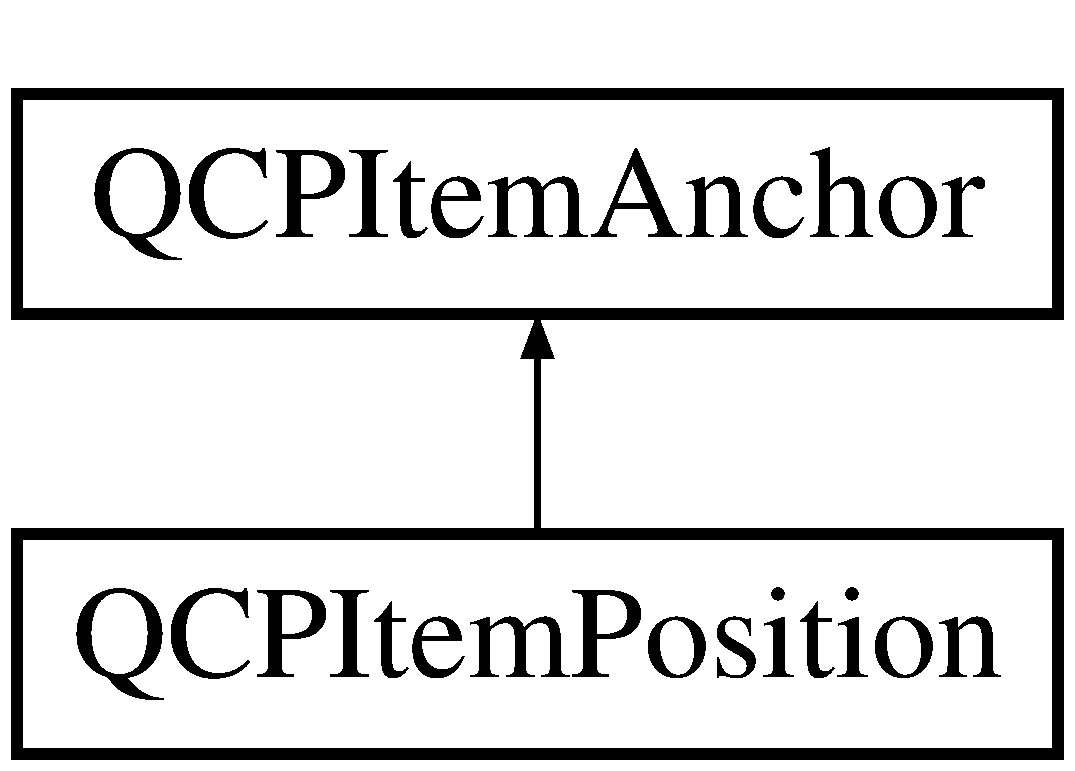
\includegraphics[height=2.000000cm]{class_q_c_p_item_position}
\end{center}
\end{figure}
\subsection*{Public Types}
\begin{DoxyCompactItemize}
\item 
enum \hyperlink{class_q_c_p_item_position_aad9936c22bf43e3d358552f6e86dbdc8}{Position\+Type} \{ \hyperlink{class_q_c_p_item_position_aad9936c22bf43e3d358552f6e86dbdc8a564f5e53e550ead1ec5fc7fc7d0b73e0}{pt\+Absolute}, 
\hyperlink{class_q_c_p_item_position_aad9936c22bf43e3d358552f6e86dbdc8ac7d6aa89ceacb39658b0d6da061c789a}{pt\+Viewport\+Ratio}, 
\hyperlink{class_q_c_p_item_position_aad9936c22bf43e3d358552f6e86dbdc8a01080fd00eaf09fa238ef6b73bbfef75}{pt\+Axis\+Rect\+Ratio}, 
\hyperlink{class_q_c_p_item_position_aad9936c22bf43e3d358552f6e86dbdc8ad5ffb8dc99ad73263f7010c77342294c}{pt\+Plot\+Coords}
 \}
\end{DoxyCompactItemize}
\subsection*{Public Member Functions}
\begin{DoxyCompactItemize}
\item 
\hyperlink{class_q_c_p_item_position_a3efc524f37fdcd22907545eb77555ce4}{Q\+C\+P\+Item\+Position} (\hyperlink{class_q_custom_plot}{Q\+Custom\+Plot} $\ast$parent\+Plot, \hyperlink{class_q_c_p_abstract_item}{Q\+C\+P\+Abstract\+Item} $\ast$parent\+Item, const Q\+String \hyperlink{class_q_c_p_item_anchor_ac93984042a58c875e76847dc3e5f75fe}{name})
\item 
virtual \hyperlink{class_q_c_p_item_position_ad8a289016f7a62332f9c865c39ab2047}{$\sim$\+Q\+C\+P\+Item\+Position} ()
\item 
\hyperlink{class_q_c_p_item_position_aad9936c22bf43e3d358552f6e86dbdc8}{Position\+Type} \hyperlink{class_q_c_p_item_position_aecb709d72c9aa334a7f62e2c9e0b5d60}{type} () const 
\item 
\hyperlink{class_q_c_p_item_position_aad9936c22bf43e3d358552f6e86dbdc8}{Position\+Type} \hyperlink{class_q_c_p_item_position_a3cb68cf9c95be05c66a0f47448e328e5}{type\+X} () const 
\item 
\hyperlink{class_q_c_p_item_position_aad9936c22bf43e3d358552f6e86dbdc8}{Position\+Type} \hyperlink{class_q_c_p_item_position_a8a2fec9dec1ce006a598b32685fd7ab3}{type\+Y} () const 
\item 
\hyperlink{class_q_c_p_item_anchor}{Q\+C\+P\+Item\+Anchor} $\ast$ \hyperlink{class_q_c_p_item_position_a7b4ffab9946945c0e11cd2352dc2e042}{parent\+Anchor} () const 
\item 
\hyperlink{class_q_c_p_item_anchor}{Q\+C\+P\+Item\+Anchor} $\ast$ \hyperlink{class_q_c_p_item_position_a485abba71c8552086c5f68e95dca7f9a}{parent\+Anchor\+X} () const 
\item 
\hyperlink{class_q_c_p_item_anchor}{Q\+C\+P\+Item\+Anchor} $\ast$ \hyperlink{class_q_c_p_item_position_a1502dba801cb20424b7e097399e372de}{parent\+Anchor\+Y} () const 
\item 
double \hyperlink{class_q_c_p_item_position_ac3cb2bddf5f89e5181830be30b93d090}{key} () const 
\item 
double \hyperlink{class_q_c_p_item_position_a6817f7356d3a2b63e8446c6b6106dae1}{value} () const 
\item 
Q\+Point\+F \hyperlink{class_q_c_p_item_position_a253d7adbb6d46299bd6cbc31aa8819f1}{coords} () const 
\item 
\hyperlink{class_q_c_p_axis}{Q\+C\+P\+Axis} $\ast$ \hyperlink{class_q_c_p_item_position_ab99de7ae5766d246defb2de9f47eaf51}{key\+Axis} () const 
\item 
\hyperlink{class_q_c_p_axis}{Q\+C\+P\+Axis} $\ast$ \hyperlink{class_q_c_p_item_position_a8d3a039fb2e69df86b4015daa30dfd2d}{value\+Axis} () const 
\item 
\hyperlink{class_q_c_p_axis_rect}{Q\+C\+P\+Axis\+Rect} $\ast$ \hyperlink{class_q_c_p_item_position_a7f10fa702a324880cc4de958f434cec7}{axis\+Rect} () const 
\item 
virtual Q\+Point\+F \hyperlink{class_q_c_p_item_position_ae490f9c76ee2ba33752c495d3b6e8fb5}{pixel\+Point} () const 
\item 
void \hyperlink{class_q_c_p_item_position_aa476abf71ed8fa4c537457ebb1a754ad}{set\+Type} (\hyperlink{class_q_c_p_item_position_aad9936c22bf43e3d358552f6e86dbdc8}{Position\+Type} \hyperlink{class_q_c_p_item_position_aecb709d72c9aa334a7f62e2c9e0b5d60}{type})
\item 
void \hyperlink{class_q_c_p_item_position_a2113b2351d6d00457fb3559a4e20c3ea}{set\+Type\+X} (\hyperlink{class_q_c_p_item_position_aad9936c22bf43e3d358552f6e86dbdc8}{Position\+Type} \hyperlink{class_q_c_p_item_position_aecb709d72c9aa334a7f62e2c9e0b5d60}{type})
\item 
void \hyperlink{class_q_c_p_item_position_ac2a454aa5a54c1615c50686601ec4510}{set\+Type\+Y} (\hyperlink{class_q_c_p_item_position_aad9936c22bf43e3d358552f6e86dbdc8}{Position\+Type} \hyperlink{class_q_c_p_item_position_aecb709d72c9aa334a7f62e2c9e0b5d60}{type})
\item 
bool \hyperlink{class_q_c_p_item_position_ac094d67a95d2dceafa0d50b9db3a7e51}{set\+Parent\+Anchor} (\hyperlink{class_q_c_p_item_anchor}{Q\+C\+P\+Item\+Anchor} $\ast$\hyperlink{class_q_c_p_item_position_a7b4ffab9946945c0e11cd2352dc2e042}{parent\+Anchor}, bool keep\+Pixel\+Position=false)
\item 
bool \hyperlink{class_q_c_p_item_position_add71461a973927c74e42179480916d9c}{set\+Parent\+Anchor\+X} (\hyperlink{class_q_c_p_item_anchor}{Q\+C\+P\+Item\+Anchor} $\ast$\hyperlink{class_q_c_p_item_position_a7b4ffab9946945c0e11cd2352dc2e042}{parent\+Anchor}, bool keep\+Pixel\+Position=false)
\item 
bool \hyperlink{class_q_c_p_item_position_add5ec1db9d19cec58a3b5c9e0a0c3f9d}{set\+Parent\+Anchor\+Y} (\hyperlink{class_q_c_p_item_anchor}{Q\+C\+P\+Item\+Anchor} $\ast$\hyperlink{class_q_c_p_item_position_a7b4ffab9946945c0e11cd2352dc2e042}{parent\+Anchor}, bool keep\+Pixel\+Position=false)
\item 
void \hyperlink{class_q_c_p_item_position_aa988ba4e87ab684c9021017dcaba945f}{set\+Coords} (double \hyperlink{class_q_c_p_item_position_ac3cb2bddf5f89e5181830be30b93d090}{key}, double \hyperlink{class_q_c_p_item_position_a6817f7356d3a2b63e8446c6b6106dae1}{value})
\item 
void \hyperlink{class_q_c_p_item_position_acc70b3abc143287f806e5f154e5e07b0}{set\+Coords} (const Q\+Point\+F \&\hyperlink{class_q_c_p_item_position_a253d7adbb6d46299bd6cbc31aa8819f1}{coords})
\item 
void \hyperlink{class_q_c_p_item_position_a2185f45c75ac8cb9be89daeaaad50e37}{set\+Axes} (\hyperlink{class_q_c_p_axis}{Q\+C\+P\+Axis} $\ast$\hyperlink{class_q_c_p_item_position_ab99de7ae5766d246defb2de9f47eaf51}{key\+Axis}, \hyperlink{class_q_c_p_axis}{Q\+C\+P\+Axis} $\ast$\hyperlink{class_q_c_p_item_position_a8d3a039fb2e69df86b4015daa30dfd2d}{value\+Axis})
\item 
void \hyperlink{class_q_c_p_item_position_a0cd9b326fb324710169e92e8ca0041c2}{set\+Axis\+Rect} (\hyperlink{class_q_c_p_axis_rect}{Q\+C\+P\+Axis\+Rect} $\ast$\hyperlink{class_q_c_p_item_position_a7f10fa702a324880cc4de958f434cec7}{axis\+Rect})
\item 
void \hyperlink{class_q_c_p_item_position_ab404e56d9ac2ac2df0382c57933a71ef}{set\+Pixel\+Point} (const Q\+Point\+F \&\hyperlink{class_q_c_p_item_position_ae490f9c76ee2ba33752c495d3b6e8fb5}{pixel\+Point})
\end{DoxyCompactItemize}
\subsection*{Protected Member Functions}
\begin{DoxyCompactItemize}
\item 
virtual \hyperlink{class_q_c_p_item_position}{Q\+C\+P\+Item\+Position} $\ast$ \hyperlink{class_q_c_p_item_position_a577a7efc601df85a20b3e709d1ac320e}{to\+Q\+C\+P\+Item\+Position} ()
\end{DoxyCompactItemize}
\subsection*{Protected Attributes}
\begin{DoxyCompactItemize}
\item 
\hyperlink{class_q_c_p_item_position_aad9936c22bf43e3d358552f6e86dbdc8}{Position\+Type} \hyperlink{class_q_c_p_item_position_ae2a617dce057c5f3ec6878c1823aa291}{m\+Position\+Type\+X}
\item 
\hyperlink{class_q_c_p_item_position_aad9936c22bf43e3d358552f6e86dbdc8}{Position\+Type} \hyperlink{class_q_c_p_item_position_a47c96c0ef4380e1af4aaa7c2265c260b}{m\+Position\+Type\+Y}
\item 
Q\+Pointer$<$ \hyperlink{class_q_c_p_axis}{Q\+C\+P\+Axis} $>$ \hyperlink{class_q_c_p_item_position_a63967a33933231e92f68c8ce06bfc37e}{m\+Key\+Axis}
\item 
Q\+Pointer$<$ \hyperlink{class_q_c_p_axis}{Q\+C\+P\+Axis} $>$ \hyperlink{class_q_c_p_item_position_a505dc2da24ba274452c1c817fcaba011}{m\+Value\+Axis}
\item 
Q\+Pointer$<$ \hyperlink{class_q_c_p_axis_rect}{Q\+C\+P\+Axis\+Rect} $>$ \hyperlink{class_q_c_p_item_position_add40fcb8994c247d85f42a126286b740}{m\+Axis\+Rect}
\item 
double \hyperlink{class_q_c_p_item_position_a4ff3931ad115603dfb4c7000b24bb415}{m\+Key}
\item 
double \hyperlink{class_q_c_p_item_position_a67bf5df69f587d53731724a7d61c6c3f}{m\+Value}
\item 
\hyperlink{class_q_c_p_item_anchor}{Q\+C\+P\+Item\+Anchor} $\ast$ \hyperlink{class_q_c_p_item_position_a41b4641d18c90997b9c01bf304181bf0}{m\+Parent\+Anchor\+X}
\item 
\hyperlink{class_q_c_p_item_anchor}{Q\+C\+P\+Item\+Anchor} $\ast$ \hyperlink{class_q_c_p_item_position_afc6142a6a09c8fa41c44d3d54fadd737}{m\+Parent\+Anchor\+Y}
\end{DoxyCompactItemize}


\subsection{Detailed Description}
Manages the position of an item. 

Every item has at least one public \hyperlink{class_q_c_p_item_position}{Q\+C\+P\+Item\+Position} member pointer which provides ways to position the item on the \hyperlink{class_q_custom_plot}{Q\+Custom\+Plot} surface. Some items have multiple positions, for example \hyperlink{class_q_c_p_item_rect}{Q\+C\+P\+Item\+Rect} has two\+: {\itshape top\+Left} and {\itshape bottom\+Right}.

\hyperlink{class_q_c_p_item_position}{Q\+C\+P\+Item\+Position} has a type (\hyperlink{class_q_c_p_item_position_aad9936c22bf43e3d358552f6e86dbdc8}{Position\+Type}) that can be set with \hyperlink{class_q_c_p_item_position_aa476abf71ed8fa4c537457ebb1a754ad}{set\+Type}. This type defines how coordinates passed to \hyperlink{class_q_c_p_item_position_aa988ba4e87ab684c9021017dcaba945f}{set\+Coords} are to be interpreted, e.\+g. as absolute pixel coordinates, as plot coordinates of certain axes, etc. For more advanced plots it is also possible to assign different types per X/\+Y coordinate of the position (see \hyperlink{class_q_c_p_item_position_a2113b2351d6d00457fb3559a4e20c3ea}{set\+Type\+X}, \hyperlink{class_q_c_p_item_position_ac2a454aa5a54c1615c50686601ec4510}{set\+Type\+Y}). This way an item could be positioned at a fixed pixel distance from the top in the Y direction, while following a plot coordinate in the X direction.

A \hyperlink{class_q_c_p_item_position}{Q\+C\+P\+Item\+Position} may have a parent \hyperlink{class_q_c_p_item_anchor}{Q\+C\+P\+Item\+Anchor}, see \hyperlink{class_q_c_p_item_position_ac094d67a95d2dceafa0d50b9db3a7e51}{set\+Parent\+Anchor}. This way you can tie multiple items together. If the \hyperlink{class_q_c_p_item_position}{Q\+C\+P\+Item\+Position} has a parent, its coordinates (\hyperlink{class_q_c_p_item_position_aa988ba4e87ab684c9021017dcaba945f}{set\+Coords}) are considered to be absolute pixels in the reference frame of the parent anchor, where (0, 0) means directly ontop of the parent anchor. For example, You could attach the {\itshape start} position of a \hyperlink{class_q_c_p_item_line}{Q\+C\+P\+Item\+Line} to the {\itshape bottom} anchor of a \hyperlink{class_q_c_p_item_text}{Q\+C\+P\+Item\+Text} to make the starting point of the line always be centered under the text label, no matter where the text is moved to. For more advanced plots, it is possible to assign different parent anchors per X/\+Y coordinate of the position, see \hyperlink{class_q_c_p_item_position_add71461a973927c74e42179480916d9c}{set\+Parent\+Anchor\+X}, \hyperlink{class_q_c_p_item_position_add5ec1db9d19cec58a3b5c9e0a0c3f9d}{set\+Parent\+Anchor\+Y}. This way an item could follow another item in the X direction but stay at a fixed position in the Y direction. Or even follow item A in X, and item B in Y.

Note that every \hyperlink{class_q_c_p_item_position}{Q\+C\+P\+Item\+Position} inherits from \hyperlink{class_q_c_p_item_anchor}{Q\+C\+P\+Item\+Anchor} and thus can itself be used as parent anchor for other positions.

To set the apparent pixel position on the \hyperlink{class_q_custom_plot}{Q\+Custom\+Plot} surface directly, use \hyperlink{class_q_c_p_item_position_ab404e56d9ac2ac2df0382c57933a71ef}{set\+Pixel\+Point}. This works no matter what type this \hyperlink{class_q_c_p_item_position}{Q\+C\+P\+Item\+Position} is or what parent-\/child situation it is in, as \hyperlink{class_q_c_p_item_position_ab404e56d9ac2ac2df0382c57933a71ef}{set\+Pixel\+Point} transforms the coordinates appropriately, to make the position appear at the specified pixel values. 

\subsection{Member Enumeration Documentation}
\hypertarget{class_q_c_p_item_position_aad9936c22bf43e3d358552f6e86dbdc8}{}\index{Q\+C\+P\+Item\+Position@{Q\+C\+P\+Item\+Position}!Position\+Type@{Position\+Type}}
\index{Position\+Type@{Position\+Type}!Q\+C\+P\+Item\+Position@{Q\+C\+P\+Item\+Position}}
\subsubsection[{Position\+Type}]{\setlength{\rightskip}{0pt plus 5cm}enum {\bf Q\+C\+P\+Item\+Position\+::\+Position\+Type}}\label{class_q_c_p_item_position_aad9936c22bf43e3d358552f6e86dbdc8}
Defines the ways an item position can be specified. Thus it defines what the numbers passed to \hyperlink{class_q_c_p_item_position_aa988ba4e87ab684c9021017dcaba945f}{set\+Coords} actually mean.

\begin{DoxySeeAlso}{See also}
\hyperlink{class_q_c_p_item_position_aa476abf71ed8fa4c537457ebb1a754ad}{set\+Type} 
\end{DoxySeeAlso}
\begin{Desc}
\item[Enumerator]\par
\begin{description}
\index{pt\+Absolute@{pt\+Absolute}!Q\+C\+P\+Item\+Position@{Q\+C\+P\+Item\+Position}}\index{Q\+C\+P\+Item\+Position@{Q\+C\+P\+Item\+Position}!pt\+Absolute@{pt\+Absolute}}\item[{\em 
\hypertarget{class_q_c_p_item_position_aad9936c22bf43e3d358552f6e86dbdc8a564f5e53e550ead1ec5fc7fc7d0b73e0}{}pt\+Absolute\label{class_q_c_p_item_position_aad9936c22bf43e3d358552f6e86dbdc8a564f5e53e550ead1ec5fc7fc7d0b73e0}
}]Static positioning in pixels, starting from the top left corner of the viewport/widget. \index{pt\+Viewport\+Ratio@{pt\+Viewport\+Ratio}!Q\+C\+P\+Item\+Position@{Q\+C\+P\+Item\+Position}}\index{Q\+C\+P\+Item\+Position@{Q\+C\+P\+Item\+Position}!pt\+Viewport\+Ratio@{pt\+Viewport\+Ratio}}\item[{\em 
\hypertarget{class_q_c_p_item_position_aad9936c22bf43e3d358552f6e86dbdc8ac7d6aa89ceacb39658b0d6da061c789a}{}pt\+Viewport\+Ratio\label{class_q_c_p_item_position_aad9936c22bf43e3d358552f6e86dbdc8ac7d6aa89ceacb39658b0d6da061c789a}
}]Static positioning given by a fraction of the viewport size. For example, if you call set\+Coords(0, 0), the position will be at the top left corner of the viewport/widget. set\+Coords(1, 1) will be at the bottom right corner, set\+Coords(0.\+5, 0) will be horizontally centered and vertically at the top of the viewport/widget, etc. \index{pt\+Axis\+Rect\+Ratio@{pt\+Axis\+Rect\+Ratio}!Q\+C\+P\+Item\+Position@{Q\+C\+P\+Item\+Position}}\index{Q\+C\+P\+Item\+Position@{Q\+C\+P\+Item\+Position}!pt\+Axis\+Rect\+Ratio@{pt\+Axis\+Rect\+Ratio}}\item[{\em 
\hypertarget{class_q_c_p_item_position_aad9936c22bf43e3d358552f6e86dbdc8a01080fd00eaf09fa238ef6b73bbfef75}{}pt\+Axis\+Rect\+Ratio\label{class_q_c_p_item_position_aad9936c22bf43e3d358552f6e86dbdc8a01080fd00eaf09fa238ef6b73bbfef75}
}]Static positioning given by a fraction of the axis rect size (see \hyperlink{class_q_c_p_item_position_a0cd9b326fb324710169e92e8ca0041c2}{set\+Axis\+Rect}). For example, if you call set\+Coords(0, 0), the position will be at the top left corner of the axis rect. set\+Coords(1, 1) will be at the bottom right corner, set\+Coords(0.\+5, 0) will be horizontally centered and vertically at the top of the axis rect, etc. You can also go beyond the axis rect by providing negative coordinates or coordinates larger than 1. \index{pt\+Plot\+Coords@{pt\+Plot\+Coords}!Q\+C\+P\+Item\+Position@{Q\+C\+P\+Item\+Position}}\index{Q\+C\+P\+Item\+Position@{Q\+C\+P\+Item\+Position}!pt\+Plot\+Coords@{pt\+Plot\+Coords}}\item[{\em 
\hypertarget{class_q_c_p_item_position_aad9936c22bf43e3d358552f6e86dbdc8ad5ffb8dc99ad73263f7010c77342294c}{}pt\+Plot\+Coords\label{class_q_c_p_item_position_aad9936c22bf43e3d358552f6e86dbdc8ad5ffb8dc99ad73263f7010c77342294c}
}]Dynamic positioning at a plot coordinate defined by two axes (see \hyperlink{class_q_c_p_item_position_a2185f45c75ac8cb9be89daeaaad50e37}{set\+Axes}). \end{description}
\end{Desc}


\subsection{Constructor \& Destructor Documentation}
\hypertarget{class_q_c_p_item_position_a3efc524f37fdcd22907545eb77555ce4}{}\index{Q\+C\+P\+Item\+Position@{Q\+C\+P\+Item\+Position}!Q\+C\+P\+Item\+Position@{Q\+C\+P\+Item\+Position}}
\index{Q\+C\+P\+Item\+Position@{Q\+C\+P\+Item\+Position}!Q\+C\+P\+Item\+Position@{Q\+C\+P\+Item\+Position}}
\subsubsection[{Q\+C\+P\+Item\+Position}]{\setlength{\rightskip}{0pt plus 5cm}Q\+C\+P\+Item\+Position\+::\+Q\+C\+P\+Item\+Position (
\begin{DoxyParamCaption}
\item[{{\bf Q\+Custom\+Plot} $\ast$}]{parent\+Plot, }
\item[{{\bf Q\+C\+P\+Abstract\+Item} $\ast$}]{parent\+Item, }
\item[{const Q\+String}]{name}
\end{DoxyParamCaption}
)}\label{class_q_c_p_item_position_a3efc524f37fdcd22907545eb77555ce4}
Creates a new \hyperlink{class_q_c_p_item_position}{Q\+C\+P\+Item\+Position}. You shouldn\textquotesingle{}t create \hyperlink{class_q_c_p_item_position}{Q\+C\+P\+Item\+Position} instances directly, even if you want to make a new item subclass. Use \hyperlink{class_q_c_p_abstract_item_a75036d39c4d4e2e1a7dd145fff915d32}{Q\+C\+P\+Abstract\+Item\+::create\+Position} instead, as explained in the subclassing section of the \hyperlink{class_q_c_p_abstract_item}{Q\+C\+P\+Abstract\+Item} documentation. \hypertarget{class_q_c_p_item_position_ad8a289016f7a62332f9c865c39ab2047}{}\index{Q\+C\+P\+Item\+Position@{Q\+C\+P\+Item\+Position}!````~Q\+C\+P\+Item\+Position@{$\sim$\+Q\+C\+P\+Item\+Position}}
\index{````~Q\+C\+P\+Item\+Position@{$\sim$\+Q\+C\+P\+Item\+Position}!Q\+C\+P\+Item\+Position@{Q\+C\+P\+Item\+Position}}
\subsubsection[{$\sim$\+Q\+C\+P\+Item\+Position}]{\setlength{\rightskip}{0pt plus 5cm}Q\+C\+P\+Item\+Position\+::$\sim$\+Q\+C\+P\+Item\+Position (
\begin{DoxyParamCaption}
{}
\end{DoxyParamCaption}
)\hspace{0.3cm}{\ttfamily [virtual]}}\label{class_q_c_p_item_position_ad8a289016f7a62332f9c865c39ab2047}


\subsection{Member Function Documentation}
\hypertarget{class_q_c_p_item_position_a7f10fa702a324880cc4de958f434cec7}{}\index{Q\+C\+P\+Item\+Position@{Q\+C\+P\+Item\+Position}!axis\+Rect@{axis\+Rect}}
\index{axis\+Rect@{axis\+Rect}!Q\+C\+P\+Item\+Position@{Q\+C\+P\+Item\+Position}}
\subsubsection[{axis\+Rect}]{\setlength{\rightskip}{0pt plus 5cm}{\bf Q\+C\+P\+Axis\+Rect} $\ast$ Q\+C\+P\+Item\+Position\+::axis\+Rect (
\begin{DoxyParamCaption}
{}
\end{DoxyParamCaption}
) const}\label{class_q_c_p_item_position_a7f10fa702a324880cc4de958f434cec7}
\hypertarget{class_q_c_p_item_position_a253d7adbb6d46299bd6cbc31aa8819f1}{}\index{Q\+C\+P\+Item\+Position@{Q\+C\+P\+Item\+Position}!coords@{coords}}
\index{coords@{coords}!Q\+C\+P\+Item\+Position@{Q\+C\+P\+Item\+Position}}
\subsubsection[{coords}]{\setlength{\rightskip}{0pt plus 5cm}Q\+Point\+F Q\+C\+P\+Item\+Position\+::coords (
\begin{DoxyParamCaption}
{}
\end{DoxyParamCaption}
) const\hspace{0.3cm}{\ttfamily [inline]}}\label{class_q_c_p_item_position_a253d7adbb6d46299bd6cbc31aa8819f1}
\hypertarget{class_q_c_p_item_position_ac3cb2bddf5f89e5181830be30b93d090}{}\index{Q\+C\+P\+Item\+Position@{Q\+C\+P\+Item\+Position}!key@{key}}
\index{key@{key}!Q\+C\+P\+Item\+Position@{Q\+C\+P\+Item\+Position}}
\subsubsection[{key}]{\setlength{\rightskip}{0pt plus 5cm}double Q\+C\+P\+Item\+Position\+::key (
\begin{DoxyParamCaption}
{}
\end{DoxyParamCaption}
) const\hspace{0.3cm}{\ttfamily [inline]}}\label{class_q_c_p_item_position_ac3cb2bddf5f89e5181830be30b93d090}
\hypertarget{class_q_c_p_item_position_ab99de7ae5766d246defb2de9f47eaf51}{}\index{Q\+C\+P\+Item\+Position@{Q\+C\+P\+Item\+Position}!key\+Axis@{key\+Axis}}
\index{key\+Axis@{key\+Axis}!Q\+C\+P\+Item\+Position@{Q\+C\+P\+Item\+Position}}
\subsubsection[{key\+Axis}]{\setlength{\rightskip}{0pt plus 5cm}{\bf Q\+C\+P\+Axis}$\ast$ Q\+C\+P\+Item\+Position\+::key\+Axis (
\begin{DoxyParamCaption}
{}
\end{DoxyParamCaption}
) const\hspace{0.3cm}{\ttfamily [inline]}}\label{class_q_c_p_item_position_ab99de7ae5766d246defb2de9f47eaf51}
\hypertarget{class_q_c_p_item_position_a7b4ffab9946945c0e11cd2352dc2e042}{}\index{Q\+C\+P\+Item\+Position@{Q\+C\+P\+Item\+Position}!parent\+Anchor@{parent\+Anchor}}
\index{parent\+Anchor@{parent\+Anchor}!Q\+C\+P\+Item\+Position@{Q\+C\+P\+Item\+Position}}
\subsubsection[{parent\+Anchor}]{\setlength{\rightskip}{0pt plus 5cm}{\bf Q\+C\+P\+Item\+Anchor} $\ast$ Q\+C\+P\+Item\+Position\+::parent\+Anchor (
\begin{DoxyParamCaption}
{}
\end{DoxyParamCaption}
) const\hspace{0.3cm}{\ttfamily [inline]}}\label{class_q_c_p_item_position_a7b4ffab9946945c0e11cd2352dc2e042}
Returns the current parent anchor.

If different parent anchors were set for X and Y (\hyperlink{class_q_c_p_item_position_add71461a973927c74e42179480916d9c}{set\+Parent\+Anchor\+X}, \hyperlink{class_q_c_p_item_position_add5ec1db9d19cec58a3b5c9e0a0c3f9d}{set\+Parent\+Anchor\+Y}), this method returns the parent anchor of the Y coordinate. In that case rather use {\itshape \hyperlink{class_q_c_p_item_position_a485abba71c8552086c5f68e95dca7f9a}{parent\+Anchor\+X()}} and {\itshape \hyperlink{class_q_c_p_item_position_a1502dba801cb20424b7e097399e372de}{parent\+Anchor\+Y()}}.

\begin{DoxySeeAlso}{See also}
\hyperlink{class_q_c_p_item_position_ac094d67a95d2dceafa0d50b9db3a7e51}{set\+Parent\+Anchor} 
\end{DoxySeeAlso}
\hypertarget{class_q_c_p_item_position_a485abba71c8552086c5f68e95dca7f9a}{}\index{Q\+C\+P\+Item\+Position@{Q\+C\+P\+Item\+Position}!parent\+Anchor\+X@{parent\+Anchor\+X}}
\index{parent\+Anchor\+X@{parent\+Anchor\+X}!Q\+C\+P\+Item\+Position@{Q\+C\+P\+Item\+Position}}
\subsubsection[{parent\+Anchor\+X}]{\setlength{\rightskip}{0pt plus 5cm}{\bf Q\+C\+P\+Item\+Anchor}$\ast$ Q\+C\+P\+Item\+Position\+::parent\+Anchor\+X (
\begin{DoxyParamCaption}
{}
\end{DoxyParamCaption}
) const\hspace{0.3cm}{\ttfamily [inline]}}\label{class_q_c_p_item_position_a485abba71c8552086c5f68e95dca7f9a}
\hypertarget{class_q_c_p_item_position_a1502dba801cb20424b7e097399e372de}{}\index{Q\+C\+P\+Item\+Position@{Q\+C\+P\+Item\+Position}!parent\+Anchor\+Y@{parent\+Anchor\+Y}}
\index{parent\+Anchor\+Y@{parent\+Anchor\+Y}!Q\+C\+P\+Item\+Position@{Q\+C\+P\+Item\+Position}}
\subsubsection[{parent\+Anchor\+Y}]{\setlength{\rightskip}{0pt plus 5cm}{\bf Q\+C\+P\+Item\+Anchor}$\ast$ Q\+C\+P\+Item\+Position\+::parent\+Anchor\+Y (
\begin{DoxyParamCaption}
{}
\end{DoxyParamCaption}
) const\hspace{0.3cm}{\ttfamily [inline]}}\label{class_q_c_p_item_position_a1502dba801cb20424b7e097399e372de}
\hypertarget{class_q_c_p_item_position_ae490f9c76ee2ba33752c495d3b6e8fb5}{}\index{Q\+C\+P\+Item\+Position@{Q\+C\+P\+Item\+Position}!pixel\+Point@{pixel\+Point}}
\index{pixel\+Point@{pixel\+Point}!Q\+C\+P\+Item\+Position@{Q\+C\+P\+Item\+Position}}
\subsubsection[{pixel\+Point}]{\setlength{\rightskip}{0pt plus 5cm}Q\+Point\+F Q\+C\+P\+Item\+Position\+::pixel\+Point (
\begin{DoxyParamCaption}
{}
\end{DoxyParamCaption}
) const\hspace{0.3cm}{\ttfamily [virtual]}}\label{class_q_c_p_item_position_ae490f9c76ee2ba33752c495d3b6e8fb5}
Returns the final absolute pixel position of the \hyperlink{class_q_c_p_item_position}{Q\+C\+P\+Item\+Position} on the \hyperlink{class_q_custom_plot}{Q\+Custom\+Plot} surface. It includes all effects of type (\hyperlink{class_q_c_p_item_position_aa476abf71ed8fa4c537457ebb1a754ad}{set\+Type}) and possible parent anchors (\hyperlink{class_q_c_p_item_position_ac094d67a95d2dceafa0d50b9db3a7e51}{set\+Parent\+Anchor}).

\begin{DoxySeeAlso}{See also}
\hyperlink{class_q_c_p_item_position_ab404e56d9ac2ac2df0382c57933a71ef}{set\+Pixel\+Point} 
\end{DoxySeeAlso}


Reimplemented from \hyperlink{class_q_c_p_item_anchor_ae92def8f9297c5d73f5806c586517bb3}{Q\+C\+P\+Item\+Anchor}.

\hypertarget{class_q_c_p_item_position_a2185f45c75ac8cb9be89daeaaad50e37}{}\index{Q\+C\+P\+Item\+Position@{Q\+C\+P\+Item\+Position}!set\+Axes@{set\+Axes}}
\index{set\+Axes@{set\+Axes}!Q\+C\+P\+Item\+Position@{Q\+C\+P\+Item\+Position}}
\subsubsection[{set\+Axes}]{\setlength{\rightskip}{0pt plus 5cm}void Q\+C\+P\+Item\+Position\+::set\+Axes (
\begin{DoxyParamCaption}
\item[{{\bf Q\+C\+P\+Axis} $\ast$}]{key\+Axis, }
\item[{{\bf Q\+C\+P\+Axis} $\ast$}]{value\+Axis}
\end{DoxyParamCaption}
)}\label{class_q_c_p_item_position_a2185f45c75ac8cb9be89daeaaad50e37}
When \hyperlink{class_q_c_p_item_position_aa476abf71ed8fa4c537457ebb1a754ad}{set\+Type} is \hyperlink{class_q_c_p_item_position_aad9936c22bf43e3d358552f6e86dbdc8ad5ffb8dc99ad73263f7010c77342294c}{pt\+Plot\+Coords}, this function may be used to specify the axes the coordinates set with \hyperlink{class_q_c_p_item_position_aa988ba4e87ab684c9021017dcaba945f}{set\+Coords} relate to. By default they are set to the initial x\+Axis and y\+Axis of the \hyperlink{class_q_custom_plot}{Q\+Custom\+Plot}. \hypertarget{class_q_c_p_item_position_a0cd9b326fb324710169e92e8ca0041c2}{}\index{Q\+C\+P\+Item\+Position@{Q\+C\+P\+Item\+Position}!set\+Axis\+Rect@{set\+Axis\+Rect}}
\index{set\+Axis\+Rect@{set\+Axis\+Rect}!Q\+C\+P\+Item\+Position@{Q\+C\+P\+Item\+Position}}
\subsubsection[{set\+Axis\+Rect}]{\setlength{\rightskip}{0pt plus 5cm}void Q\+C\+P\+Item\+Position\+::set\+Axis\+Rect (
\begin{DoxyParamCaption}
\item[{{\bf Q\+C\+P\+Axis\+Rect} $\ast$}]{axis\+Rect}
\end{DoxyParamCaption}
)}\label{class_q_c_p_item_position_a0cd9b326fb324710169e92e8ca0041c2}
When \hyperlink{class_q_c_p_item_position_aa476abf71ed8fa4c537457ebb1a754ad}{set\+Type} is \hyperlink{class_q_c_p_item_position_aad9936c22bf43e3d358552f6e86dbdc8a01080fd00eaf09fa238ef6b73bbfef75}{pt\+Axis\+Rect\+Ratio}, this function may be used to specify the axis rect the coordinates set with \hyperlink{class_q_c_p_item_position_aa988ba4e87ab684c9021017dcaba945f}{set\+Coords} relate to. By default this is set to the main axis rect of the \hyperlink{class_q_custom_plot}{Q\+Custom\+Plot}. \hypertarget{class_q_c_p_item_position_aa988ba4e87ab684c9021017dcaba945f}{}\index{Q\+C\+P\+Item\+Position@{Q\+C\+P\+Item\+Position}!set\+Coords@{set\+Coords}}
\index{set\+Coords@{set\+Coords}!Q\+C\+P\+Item\+Position@{Q\+C\+P\+Item\+Position}}
\subsubsection[{set\+Coords}]{\setlength{\rightskip}{0pt plus 5cm}void Q\+C\+P\+Item\+Position\+::set\+Coords (
\begin{DoxyParamCaption}
\item[{double}]{key, }
\item[{double}]{value}
\end{DoxyParamCaption}
)}\label{class_q_c_p_item_position_aa988ba4e87ab684c9021017dcaba945f}
Sets the coordinates of this \hyperlink{class_q_c_p_item_position}{Q\+C\+P\+Item\+Position}. What the coordinates mean, is defined by the type (\hyperlink{class_q_c_p_item_position_aa476abf71ed8fa4c537457ebb1a754ad}{set\+Type}, \hyperlink{class_q_c_p_item_position_a2113b2351d6d00457fb3559a4e20c3ea}{set\+Type\+X}, \hyperlink{class_q_c_p_item_position_ac2a454aa5a54c1615c50686601ec4510}{set\+Type\+Y}).

For example, if the type is \hyperlink{class_q_c_p_item_position_aad9936c22bf43e3d358552f6e86dbdc8a564f5e53e550ead1ec5fc7fc7d0b73e0}{pt\+Absolute}, {\itshape key} and {\itshape value} mean the x and y pixel position on the \hyperlink{class_q_custom_plot}{Q\+Custom\+Plot} surface. In that case the origin (0, 0) is in the top left corner of the \hyperlink{class_q_custom_plot}{Q\+Custom\+Plot} viewport. If the type is \hyperlink{class_q_c_p_item_position_aad9936c22bf43e3d358552f6e86dbdc8ad5ffb8dc99ad73263f7010c77342294c}{pt\+Plot\+Coords}, {\itshape key} and {\itshape value} mean a point in the plot coordinate system defined by the axes set by \hyperlink{class_q_c_p_item_position_a2185f45c75ac8cb9be89daeaaad50e37}{set\+Axes}. By default those are the \hyperlink{class_q_custom_plot}{Q\+Custom\+Plot}\textquotesingle{}s x\+Axis and y\+Axis. See the documentation of \hyperlink{class_q_c_p_item_position_aa476abf71ed8fa4c537457ebb1a754ad}{set\+Type} for other available coordinate types and their meaning.

If different types were configured for X and Y (\hyperlink{class_q_c_p_item_position_a2113b2351d6d00457fb3559a4e20c3ea}{set\+Type\+X}, \hyperlink{class_q_c_p_item_position_ac2a454aa5a54c1615c50686601ec4510}{set\+Type\+Y}), {\itshape key} and {\itshape value} must also be provided in the different coordinate systems. Here, the X type refers to {\itshape key}, and the Y type refers to {\itshape value}.

\begin{DoxySeeAlso}{See also}
\hyperlink{class_q_c_p_item_position_ab404e56d9ac2ac2df0382c57933a71ef}{set\+Pixel\+Point} 
\end{DoxySeeAlso}
\hypertarget{class_q_c_p_item_position_acc70b3abc143287f806e5f154e5e07b0}{}\index{Q\+C\+P\+Item\+Position@{Q\+C\+P\+Item\+Position}!set\+Coords@{set\+Coords}}
\index{set\+Coords@{set\+Coords}!Q\+C\+P\+Item\+Position@{Q\+C\+P\+Item\+Position}}
\subsubsection[{set\+Coords}]{\setlength{\rightskip}{0pt plus 5cm}void Q\+C\+P\+Item\+Position\+::set\+Coords (
\begin{DoxyParamCaption}
\item[{const Q\+Point\+F \&}]{pos}
\end{DoxyParamCaption}
)}\label{class_q_c_p_item_position_acc70b3abc143287f806e5f154e5e07b0}
This is an overloaded member function, provided for convenience. It differs from the above function only in what argument(s) it accepts.

Sets the coordinates as a Q\+Point\+F {\itshape pos} where pos.\+x has the meaning of {\itshape key} and pos.\+y the meaning of {\itshape value} of the \hyperlink{class_q_c_p_item_position_aa988ba4e87ab684c9021017dcaba945f}{set\+Coords(double key, double value)} method. \hypertarget{class_q_c_p_item_position_ac094d67a95d2dceafa0d50b9db3a7e51}{}\index{Q\+C\+P\+Item\+Position@{Q\+C\+P\+Item\+Position}!set\+Parent\+Anchor@{set\+Parent\+Anchor}}
\index{set\+Parent\+Anchor@{set\+Parent\+Anchor}!Q\+C\+P\+Item\+Position@{Q\+C\+P\+Item\+Position}}
\subsubsection[{set\+Parent\+Anchor}]{\setlength{\rightskip}{0pt plus 5cm}bool Q\+C\+P\+Item\+Position\+::set\+Parent\+Anchor (
\begin{DoxyParamCaption}
\item[{{\bf Q\+C\+P\+Item\+Anchor} $\ast$}]{parent\+Anchor, }
\item[{bool}]{keep\+Pixel\+Position = {\ttfamily false}}
\end{DoxyParamCaption}
)}\label{class_q_c_p_item_position_ac094d67a95d2dceafa0d50b9db3a7e51}
Sets the parent of this \hyperlink{class_q_c_p_item_position}{Q\+C\+P\+Item\+Position} to {\itshape parent\+Anchor}. This means the position will now follow any position changes of the anchor. The local coordinate system of positions with a parent anchor always is absolute pixels, with (0, 0) being exactly on top of the parent anchor. (Hence the type shouldn\textquotesingle{}t be set to \hyperlink{class_q_c_p_item_position_aad9936c22bf43e3d358552f6e86dbdc8ad5ffb8dc99ad73263f7010c77342294c}{pt\+Plot\+Coords} for positions with parent anchors.)

if {\itshape keep\+Pixel\+Position} is true, the current pixel position of the \hyperlink{class_q_c_p_item_position}{Q\+C\+P\+Item\+Position} is preserved during reparenting. If it\textquotesingle{}s set to false, the coordinates are set to (0, 0), i.\+e. the position will be exactly on top of the parent anchor.

To remove this \hyperlink{class_q_c_p_item_position}{Q\+C\+P\+Item\+Position} from any parent anchor, set {\itshape parent\+Anchor} to 0.

If the \hyperlink{class_q_c_p_item_position}{Q\+C\+P\+Item\+Position} previously had no parent and the type is \hyperlink{class_q_c_p_item_position_aad9936c22bf43e3d358552f6e86dbdc8ad5ffb8dc99ad73263f7010c77342294c}{pt\+Plot\+Coords}, the type is set to \hyperlink{class_q_c_p_item_position_aad9936c22bf43e3d358552f6e86dbdc8a564f5e53e550ead1ec5fc7fc7d0b73e0}{pt\+Absolute}, to keep the position in a valid state.

This method sets the parent anchor for both X and Y directions. It is also possible to set different parents for X and Y, see \hyperlink{class_q_c_p_item_position_add71461a973927c74e42179480916d9c}{set\+Parent\+Anchor\+X}, \hyperlink{class_q_c_p_item_position_add5ec1db9d19cec58a3b5c9e0a0c3f9d}{set\+Parent\+Anchor\+Y}. \hypertarget{class_q_c_p_item_position_add71461a973927c74e42179480916d9c}{}\index{Q\+C\+P\+Item\+Position@{Q\+C\+P\+Item\+Position}!set\+Parent\+Anchor\+X@{set\+Parent\+Anchor\+X}}
\index{set\+Parent\+Anchor\+X@{set\+Parent\+Anchor\+X}!Q\+C\+P\+Item\+Position@{Q\+C\+P\+Item\+Position}}
\subsubsection[{set\+Parent\+Anchor\+X}]{\setlength{\rightskip}{0pt plus 5cm}bool Q\+C\+P\+Item\+Position\+::set\+Parent\+Anchor\+X (
\begin{DoxyParamCaption}
\item[{{\bf Q\+C\+P\+Item\+Anchor} $\ast$}]{parent\+Anchor, }
\item[{bool}]{keep\+Pixel\+Position = {\ttfamily false}}
\end{DoxyParamCaption}
)}\label{class_q_c_p_item_position_add71461a973927c74e42179480916d9c}
This method sets the parent anchor of the X coordinate to {\itshape parent\+Anchor}.

For a detailed description of what a parent anchor is, see the documentation of \hyperlink{class_q_c_p_item_position_ac094d67a95d2dceafa0d50b9db3a7e51}{set\+Parent\+Anchor}.

\begin{DoxySeeAlso}{See also}
\hyperlink{class_q_c_p_item_position_ac094d67a95d2dceafa0d50b9db3a7e51}{set\+Parent\+Anchor}, \hyperlink{class_q_c_p_item_position_add5ec1db9d19cec58a3b5c9e0a0c3f9d}{set\+Parent\+Anchor\+Y} 
\end{DoxySeeAlso}
\hypertarget{class_q_c_p_item_position_add5ec1db9d19cec58a3b5c9e0a0c3f9d}{}\index{Q\+C\+P\+Item\+Position@{Q\+C\+P\+Item\+Position}!set\+Parent\+Anchor\+Y@{set\+Parent\+Anchor\+Y}}
\index{set\+Parent\+Anchor\+Y@{set\+Parent\+Anchor\+Y}!Q\+C\+P\+Item\+Position@{Q\+C\+P\+Item\+Position}}
\subsubsection[{set\+Parent\+Anchor\+Y}]{\setlength{\rightskip}{0pt plus 5cm}bool Q\+C\+P\+Item\+Position\+::set\+Parent\+Anchor\+Y (
\begin{DoxyParamCaption}
\item[{{\bf Q\+C\+P\+Item\+Anchor} $\ast$}]{parent\+Anchor, }
\item[{bool}]{keep\+Pixel\+Position = {\ttfamily false}}
\end{DoxyParamCaption}
)}\label{class_q_c_p_item_position_add5ec1db9d19cec58a3b5c9e0a0c3f9d}
This method sets the parent anchor of the Y coordinate to {\itshape parent\+Anchor}.

For a detailed description of what a parent anchor is, see the documentation of \hyperlink{class_q_c_p_item_position_ac094d67a95d2dceafa0d50b9db3a7e51}{set\+Parent\+Anchor}.

\begin{DoxySeeAlso}{See also}
\hyperlink{class_q_c_p_item_position_ac094d67a95d2dceafa0d50b9db3a7e51}{set\+Parent\+Anchor}, \hyperlink{class_q_c_p_item_position_add71461a973927c74e42179480916d9c}{set\+Parent\+Anchor\+X} 
\end{DoxySeeAlso}
\hypertarget{class_q_c_p_item_position_ab404e56d9ac2ac2df0382c57933a71ef}{}\index{Q\+C\+P\+Item\+Position@{Q\+C\+P\+Item\+Position}!set\+Pixel\+Point@{set\+Pixel\+Point}}
\index{set\+Pixel\+Point@{set\+Pixel\+Point}!Q\+C\+P\+Item\+Position@{Q\+C\+P\+Item\+Position}}
\subsubsection[{set\+Pixel\+Point}]{\setlength{\rightskip}{0pt plus 5cm}void Q\+C\+P\+Item\+Position\+::set\+Pixel\+Point (
\begin{DoxyParamCaption}
\item[{const Q\+Point\+F \&}]{pixel\+Point}
\end{DoxyParamCaption}
)}\label{class_q_c_p_item_position_ab404e56d9ac2ac2df0382c57933a71ef}
Sets the apparent pixel position. This works no matter what type (\hyperlink{class_q_c_p_item_position_aa476abf71ed8fa4c537457ebb1a754ad}{set\+Type}) this \hyperlink{class_q_c_p_item_position}{Q\+C\+P\+Item\+Position} is or what parent-\/child situation it is in, as coordinates are transformed appropriately, to make the position finally appear at the specified pixel values.

Only if the type is \hyperlink{class_q_c_p_item_position_aad9936c22bf43e3d358552f6e86dbdc8a564f5e53e550ead1ec5fc7fc7d0b73e0}{pt\+Absolute} and no parent anchor is set, this function\textquotesingle{}s effect is identical to that of \hyperlink{class_q_c_p_item_position_aa988ba4e87ab684c9021017dcaba945f}{set\+Coords}.

\begin{DoxySeeAlso}{See also}
\hyperlink{class_q_c_p_item_position_ae490f9c76ee2ba33752c495d3b6e8fb5}{pixel\+Point}, \hyperlink{class_q_c_p_item_position_aa988ba4e87ab684c9021017dcaba945f}{set\+Coords} 
\end{DoxySeeAlso}
\hypertarget{class_q_c_p_item_position_aa476abf71ed8fa4c537457ebb1a754ad}{}\index{Q\+C\+P\+Item\+Position@{Q\+C\+P\+Item\+Position}!set\+Type@{set\+Type}}
\index{set\+Type@{set\+Type}!Q\+C\+P\+Item\+Position@{Q\+C\+P\+Item\+Position}}
\subsubsection[{set\+Type}]{\setlength{\rightskip}{0pt plus 5cm}void Q\+C\+P\+Item\+Position\+::set\+Type (
\begin{DoxyParamCaption}
\item[{{\bf Q\+C\+P\+Item\+Position\+::\+Position\+Type}}]{type}
\end{DoxyParamCaption}
)}\label{class_q_c_p_item_position_aa476abf71ed8fa4c537457ebb1a754ad}
Sets the type of the position. The type defines how the coordinates passed to \hyperlink{class_q_c_p_item_position_aa988ba4e87ab684c9021017dcaba945f}{set\+Coords} should be handled and how the \hyperlink{class_q_c_p_item_position}{Q\+C\+P\+Item\+Position} should behave in the plot.

The possible values for {\itshape type} can be separated in two main categories\+:

\begin{DoxyItemize}
\item The position is regarded as a point in plot coordinates. This corresponds to \hyperlink{class_q_c_p_item_position_aad9936c22bf43e3d358552f6e86dbdc8ad5ffb8dc99ad73263f7010c77342294c}{pt\+Plot\+Coords} and requires two axes that define the plot coordinate system. They can be specified with \hyperlink{class_q_c_p_item_position_a2185f45c75ac8cb9be89daeaaad50e37}{set\+Axes}. By default, the \hyperlink{class_q_custom_plot}{Q\+Custom\+Plot}\textquotesingle{}s x-\/ and y\+Axis are used.\end{DoxyItemize}
\begin{DoxyItemize}
\item The position is fixed on the \hyperlink{class_q_custom_plot}{Q\+Custom\+Plot} surface, i.\+e. independent of axis ranges. This corresponds to all other types, i.\+e. \hyperlink{class_q_c_p_item_position_aad9936c22bf43e3d358552f6e86dbdc8a564f5e53e550ead1ec5fc7fc7d0b73e0}{pt\+Absolute}, \hyperlink{class_q_c_p_item_position_aad9936c22bf43e3d358552f6e86dbdc8ac7d6aa89ceacb39658b0d6da061c789a}{pt\+Viewport\+Ratio} and \hyperlink{class_q_c_p_item_position_aad9936c22bf43e3d358552f6e86dbdc8a01080fd00eaf09fa238ef6b73bbfef75}{pt\+Axis\+Rect\+Ratio}. They differ only in the way the absolute position is described, see the documentation of \hyperlink{class_q_c_p_item_position_aad9936c22bf43e3d358552f6e86dbdc8}{Position\+Type} for details. For \hyperlink{class_q_c_p_item_position_aad9936c22bf43e3d358552f6e86dbdc8a01080fd00eaf09fa238ef6b73bbfef75}{pt\+Axis\+Rect\+Ratio}, note that you can specify the axis rect with \hyperlink{class_q_c_p_item_position_a0cd9b326fb324710169e92e8ca0041c2}{set\+Axis\+Rect}. By default this is set to the main axis rect.\end{DoxyItemize}
Note that the position type \hyperlink{class_q_c_p_item_position_aad9936c22bf43e3d358552f6e86dbdc8ad5ffb8dc99ad73263f7010c77342294c}{pt\+Plot\+Coords} is only available (and sensible) when the position has no parent anchor (\hyperlink{class_q_c_p_item_position_ac094d67a95d2dceafa0d50b9db3a7e51}{set\+Parent\+Anchor}).

If the type is changed, the apparent pixel position on the plot is preserved. This means the coordinates as retrieved with \hyperlink{class_q_c_p_item_position_a253d7adbb6d46299bd6cbc31aa8819f1}{coords()} and set with \hyperlink{class_q_c_p_item_position_aa988ba4e87ab684c9021017dcaba945f}{set\+Coords} may change in the process.

This method sets the type for both X and Y directions. It is also possible to set different types for X and Y, see \hyperlink{class_q_c_p_item_position_a2113b2351d6d00457fb3559a4e20c3ea}{set\+Type\+X}, \hyperlink{class_q_c_p_item_position_ac2a454aa5a54c1615c50686601ec4510}{set\+Type\+Y}. \hypertarget{class_q_c_p_item_position_a2113b2351d6d00457fb3559a4e20c3ea}{}\index{Q\+C\+P\+Item\+Position@{Q\+C\+P\+Item\+Position}!set\+Type\+X@{set\+Type\+X}}
\index{set\+Type\+X@{set\+Type\+X}!Q\+C\+P\+Item\+Position@{Q\+C\+P\+Item\+Position}}
\subsubsection[{set\+Type\+X}]{\setlength{\rightskip}{0pt plus 5cm}void Q\+C\+P\+Item\+Position\+::set\+Type\+X (
\begin{DoxyParamCaption}
\item[{{\bf Q\+C\+P\+Item\+Position\+::\+Position\+Type}}]{type}
\end{DoxyParamCaption}
)}\label{class_q_c_p_item_position_a2113b2351d6d00457fb3559a4e20c3ea}
This method sets the position type of the X coordinate to {\itshape type}.

For a detailed description of what a position type is, see the documentation of \hyperlink{class_q_c_p_item_position_aa476abf71ed8fa4c537457ebb1a754ad}{set\+Type}.

\begin{DoxySeeAlso}{See also}
\hyperlink{class_q_c_p_item_position_aa476abf71ed8fa4c537457ebb1a754ad}{set\+Type}, \hyperlink{class_q_c_p_item_position_ac2a454aa5a54c1615c50686601ec4510}{set\+Type\+Y} 
\end{DoxySeeAlso}
\hypertarget{class_q_c_p_item_position_ac2a454aa5a54c1615c50686601ec4510}{}\index{Q\+C\+P\+Item\+Position@{Q\+C\+P\+Item\+Position}!set\+Type\+Y@{set\+Type\+Y}}
\index{set\+Type\+Y@{set\+Type\+Y}!Q\+C\+P\+Item\+Position@{Q\+C\+P\+Item\+Position}}
\subsubsection[{set\+Type\+Y}]{\setlength{\rightskip}{0pt plus 5cm}void Q\+C\+P\+Item\+Position\+::set\+Type\+Y (
\begin{DoxyParamCaption}
\item[{{\bf Q\+C\+P\+Item\+Position\+::\+Position\+Type}}]{type}
\end{DoxyParamCaption}
)}\label{class_q_c_p_item_position_ac2a454aa5a54c1615c50686601ec4510}
This method sets the position type of the Y coordinate to {\itshape type}.

For a detailed description of what a position type is, see the documentation of \hyperlink{class_q_c_p_item_position_aa476abf71ed8fa4c537457ebb1a754ad}{set\+Type}.

\begin{DoxySeeAlso}{See also}
\hyperlink{class_q_c_p_item_position_aa476abf71ed8fa4c537457ebb1a754ad}{set\+Type}, \hyperlink{class_q_c_p_item_position_a2113b2351d6d00457fb3559a4e20c3ea}{set\+Type\+X} 
\end{DoxySeeAlso}
\hypertarget{class_q_c_p_item_position_a577a7efc601df85a20b3e709d1ac320e}{}\index{Q\+C\+P\+Item\+Position@{Q\+C\+P\+Item\+Position}!to\+Q\+C\+P\+Item\+Position@{to\+Q\+C\+P\+Item\+Position}}
\index{to\+Q\+C\+P\+Item\+Position@{to\+Q\+C\+P\+Item\+Position}!Q\+C\+P\+Item\+Position@{Q\+C\+P\+Item\+Position}}
\subsubsection[{to\+Q\+C\+P\+Item\+Position}]{\setlength{\rightskip}{0pt plus 5cm}virtual {\bf Q\+C\+P\+Item\+Position}$\ast$ Q\+C\+P\+Item\+Position\+::to\+Q\+C\+P\+Item\+Position (
\begin{DoxyParamCaption}
{}
\end{DoxyParamCaption}
)\hspace{0.3cm}{\ttfamily [inline]}, {\ttfamily [protected]}, {\ttfamily [virtual]}}\label{class_q_c_p_item_position_a577a7efc601df85a20b3e709d1ac320e}
Returns 0 if this instance is merely a \hyperlink{class_q_c_p_item_anchor}{Q\+C\+P\+Item\+Anchor}, and a valid pointer of type Q\+C\+P\+Item\+Position$\ast$ if it actually is a \hyperlink{class_q_c_p_item_position}{Q\+C\+P\+Item\+Position} (which is a subclass of \hyperlink{class_q_c_p_item_anchor}{Q\+C\+P\+Item\+Anchor}).

This safe downcast functionality could also be achieved with a dynamic\+\_\+cast. However, \hyperlink{class_q_custom_plot}{Q\+Custom\+Plot} avoids dynamic\+\_\+cast to work with projects that don\textquotesingle{}t have R\+T\+T\+I support enabled (e.\+g. -\/fno-\/rtti flag with gcc compiler). 

Reimplemented from \hyperlink{class_q_c_p_item_anchor_ac54b20120669950255a63587193dbb86}{Q\+C\+P\+Item\+Anchor}.

\hypertarget{class_q_c_p_item_position_aecb709d72c9aa334a7f62e2c9e0b5d60}{}\index{Q\+C\+P\+Item\+Position@{Q\+C\+P\+Item\+Position}!type@{type}}
\index{type@{type}!Q\+C\+P\+Item\+Position@{Q\+C\+P\+Item\+Position}}
\subsubsection[{type}]{\setlength{\rightskip}{0pt plus 5cm}{\bf Q\+C\+P\+Item\+Position\+::\+Position\+Type} $\ast$ Q\+C\+P\+Item\+Position\+::type (
\begin{DoxyParamCaption}
{}
\end{DoxyParamCaption}
) const\hspace{0.3cm}{\ttfamily [inline]}}\label{class_q_c_p_item_position_aecb709d72c9aa334a7f62e2c9e0b5d60}
Returns the current position type.

If different types were set for X and Y (\hyperlink{class_q_c_p_item_position_a2113b2351d6d00457fb3559a4e20c3ea}{set\+Type\+X}, \hyperlink{class_q_c_p_item_position_ac2a454aa5a54c1615c50686601ec4510}{set\+Type\+Y}), this method returns the type of the X coordinate. In that case rather use {\itshape \hyperlink{class_q_c_p_item_position_a3cb68cf9c95be05c66a0f47448e328e5}{type\+X()}} and {\itshape \hyperlink{class_q_c_p_item_position_a8a2fec9dec1ce006a598b32685fd7ab3}{type\+Y()}}.

\begin{DoxySeeAlso}{See also}
\hyperlink{class_q_c_p_item_position_aa476abf71ed8fa4c537457ebb1a754ad}{set\+Type} 
\end{DoxySeeAlso}
\hypertarget{class_q_c_p_item_position_a3cb68cf9c95be05c66a0f47448e328e5}{}\index{Q\+C\+P\+Item\+Position@{Q\+C\+P\+Item\+Position}!type\+X@{type\+X}}
\index{type\+X@{type\+X}!Q\+C\+P\+Item\+Position@{Q\+C\+P\+Item\+Position}}
\subsubsection[{type\+X}]{\setlength{\rightskip}{0pt plus 5cm}{\bf Position\+Type} Q\+C\+P\+Item\+Position\+::type\+X (
\begin{DoxyParamCaption}
{}
\end{DoxyParamCaption}
) const\hspace{0.3cm}{\ttfamily [inline]}}\label{class_q_c_p_item_position_a3cb68cf9c95be05c66a0f47448e328e5}
\hypertarget{class_q_c_p_item_position_a8a2fec9dec1ce006a598b32685fd7ab3}{}\index{Q\+C\+P\+Item\+Position@{Q\+C\+P\+Item\+Position}!type\+Y@{type\+Y}}
\index{type\+Y@{type\+Y}!Q\+C\+P\+Item\+Position@{Q\+C\+P\+Item\+Position}}
\subsubsection[{type\+Y}]{\setlength{\rightskip}{0pt plus 5cm}{\bf Position\+Type} Q\+C\+P\+Item\+Position\+::type\+Y (
\begin{DoxyParamCaption}
{}
\end{DoxyParamCaption}
) const\hspace{0.3cm}{\ttfamily [inline]}}\label{class_q_c_p_item_position_a8a2fec9dec1ce006a598b32685fd7ab3}
\hypertarget{class_q_c_p_item_position_a6817f7356d3a2b63e8446c6b6106dae1}{}\index{Q\+C\+P\+Item\+Position@{Q\+C\+P\+Item\+Position}!value@{value}}
\index{value@{value}!Q\+C\+P\+Item\+Position@{Q\+C\+P\+Item\+Position}}
\subsubsection[{value}]{\setlength{\rightskip}{0pt plus 5cm}double Q\+C\+P\+Item\+Position\+::value (
\begin{DoxyParamCaption}
{}
\end{DoxyParamCaption}
) const\hspace{0.3cm}{\ttfamily [inline]}}\label{class_q_c_p_item_position_a6817f7356d3a2b63e8446c6b6106dae1}
\hypertarget{class_q_c_p_item_position_a8d3a039fb2e69df86b4015daa30dfd2d}{}\index{Q\+C\+P\+Item\+Position@{Q\+C\+P\+Item\+Position}!value\+Axis@{value\+Axis}}
\index{value\+Axis@{value\+Axis}!Q\+C\+P\+Item\+Position@{Q\+C\+P\+Item\+Position}}
\subsubsection[{value\+Axis}]{\setlength{\rightskip}{0pt plus 5cm}{\bf Q\+C\+P\+Axis}$\ast$ Q\+C\+P\+Item\+Position\+::value\+Axis (
\begin{DoxyParamCaption}
{}
\end{DoxyParamCaption}
) const\hspace{0.3cm}{\ttfamily [inline]}}\label{class_q_c_p_item_position_a8d3a039fb2e69df86b4015daa30dfd2d}


\subsection{Member Data Documentation}
\hypertarget{class_q_c_p_item_position_add40fcb8994c247d85f42a126286b740}{}\index{Q\+C\+P\+Item\+Position@{Q\+C\+P\+Item\+Position}!m\+Axis\+Rect@{m\+Axis\+Rect}}
\index{m\+Axis\+Rect@{m\+Axis\+Rect}!Q\+C\+P\+Item\+Position@{Q\+C\+P\+Item\+Position}}
\subsubsection[{m\+Axis\+Rect}]{\setlength{\rightskip}{0pt plus 5cm}Q\+Pointer$<${\bf Q\+C\+P\+Axis\+Rect}$>$ Q\+C\+P\+Item\+Position\+::m\+Axis\+Rect\hspace{0.3cm}{\ttfamily [protected]}}\label{class_q_c_p_item_position_add40fcb8994c247d85f42a126286b740}
\hypertarget{class_q_c_p_item_position_a4ff3931ad115603dfb4c7000b24bb415}{}\index{Q\+C\+P\+Item\+Position@{Q\+C\+P\+Item\+Position}!m\+Key@{m\+Key}}
\index{m\+Key@{m\+Key}!Q\+C\+P\+Item\+Position@{Q\+C\+P\+Item\+Position}}
\subsubsection[{m\+Key}]{\setlength{\rightskip}{0pt plus 5cm}double Q\+C\+P\+Item\+Position\+::m\+Key\hspace{0.3cm}{\ttfamily [protected]}}\label{class_q_c_p_item_position_a4ff3931ad115603dfb4c7000b24bb415}
\hypertarget{class_q_c_p_item_position_a63967a33933231e92f68c8ce06bfc37e}{}\index{Q\+C\+P\+Item\+Position@{Q\+C\+P\+Item\+Position}!m\+Key\+Axis@{m\+Key\+Axis}}
\index{m\+Key\+Axis@{m\+Key\+Axis}!Q\+C\+P\+Item\+Position@{Q\+C\+P\+Item\+Position}}
\subsubsection[{m\+Key\+Axis}]{\setlength{\rightskip}{0pt plus 5cm}Q\+Pointer$<${\bf Q\+C\+P\+Axis}$>$ Q\+C\+P\+Item\+Position\+::m\+Key\+Axis\hspace{0.3cm}{\ttfamily [protected]}}\label{class_q_c_p_item_position_a63967a33933231e92f68c8ce06bfc37e}
\hypertarget{class_q_c_p_item_position_a41b4641d18c90997b9c01bf304181bf0}{}\index{Q\+C\+P\+Item\+Position@{Q\+C\+P\+Item\+Position}!m\+Parent\+Anchor\+X@{m\+Parent\+Anchor\+X}}
\index{m\+Parent\+Anchor\+X@{m\+Parent\+Anchor\+X}!Q\+C\+P\+Item\+Position@{Q\+C\+P\+Item\+Position}}
\subsubsection[{m\+Parent\+Anchor\+X}]{\setlength{\rightskip}{0pt plus 5cm}{\bf Q\+C\+P\+Item\+Anchor}$\ast$ Q\+C\+P\+Item\+Position\+::m\+Parent\+Anchor\+X\hspace{0.3cm}{\ttfamily [protected]}}\label{class_q_c_p_item_position_a41b4641d18c90997b9c01bf304181bf0}
\hypertarget{class_q_c_p_item_position_afc6142a6a09c8fa41c44d3d54fadd737}{}\index{Q\+C\+P\+Item\+Position@{Q\+C\+P\+Item\+Position}!m\+Parent\+Anchor\+Y@{m\+Parent\+Anchor\+Y}}
\index{m\+Parent\+Anchor\+Y@{m\+Parent\+Anchor\+Y}!Q\+C\+P\+Item\+Position@{Q\+C\+P\+Item\+Position}}
\subsubsection[{m\+Parent\+Anchor\+Y}]{\setlength{\rightskip}{0pt plus 5cm}{\bf Q\+C\+P\+Item\+Anchor} $\ast$ Q\+C\+P\+Item\+Position\+::m\+Parent\+Anchor\+Y\hspace{0.3cm}{\ttfamily [protected]}}\label{class_q_c_p_item_position_afc6142a6a09c8fa41c44d3d54fadd737}
\hypertarget{class_q_c_p_item_position_ae2a617dce057c5f3ec6878c1823aa291}{}\index{Q\+C\+P\+Item\+Position@{Q\+C\+P\+Item\+Position}!m\+Position\+Type\+X@{m\+Position\+Type\+X}}
\index{m\+Position\+Type\+X@{m\+Position\+Type\+X}!Q\+C\+P\+Item\+Position@{Q\+C\+P\+Item\+Position}}
\subsubsection[{m\+Position\+Type\+X}]{\setlength{\rightskip}{0pt plus 5cm}{\bf Position\+Type} Q\+C\+P\+Item\+Position\+::m\+Position\+Type\+X\hspace{0.3cm}{\ttfamily [protected]}}\label{class_q_c_p_item_position_ae2a617dce057c5f3ec6878c1823aa291}
\hypertarget{class_q_c_p_item_position_a47c96c0ef4380e1af4aaa7c2265c260b}{}\index{Q\+C\+P\+Item\+Position@{Q\+C\+P\+Item\+Position}!m\+Position\+Type\+Y@{m\+Position\+Type\+Y}}
\index{m\+Position\+Type\+Y@{m\+Position\+Type\+Y}!Q\+C\+P\+Item\+Position@{Q\+C\+P\+Item\+Position}}
\subsubsection[{m\+Position\+Type\+Y}]{\setlength{\rightskip}{0pt plus 5cm}{\bf Position\+Type} Q\+C\+P\+Item\+Position\+::m\+Position\+Type\+Y\hspace{0.3cm}{\ttfamily [protected]}}\label{class_q_c_p_item_position_a47c96c0ef4380e1af4aaa7c2265c260b}
\hypertarget{class_q_c_p_item_position_a67bf5df69f587d53731724a7d61c6c3f}{}\index{Q\+C\+P\+Item\+Position@{Q\+C\+P\+Item\+Position}!m\+Value@{m\+Value}}
\index{m\+Value@{m\+Value}!Q\+C\+P\+Item\+Position@{Q\+C\+P\+Item\+Position}}
\subsubsection[{m\+Value}]{\setlength{\rightskip}{0pt plus 5cm}double Q\+C\+P\+Item\+Position\+::m\+Value\hspace{0.3cm}{\ttfamily [protected]}}\label{class_q_c_p_item_position_a67bf5df69f587d53731724a7d61c6c3f}
\hypertarget{class_q_c_p_item_position_a505dc2da24ba274452c1c817fcaba011}{}\index{Q\+C\+P\+Item\+Position@{Q\+C\+P\+Item\+Position}!m\+Value\+Axis@{m\+Value\+Axis}}
\index{m\+Value\+Axis@{m\+Value\+Axis}!Q\+C\+P\+Item\+Position@{Q\+C\+P\+Item\+Position}}
\subsubsection[{m\+Value\+Axis}]{\setlength{\rightskip}{0pt plus 5cm}Q\+Pointer$<${\bf Q\+C\+P\+Axis}$>$ Q\+C\+P\+Item\+Position\+::m\+Value\+Axis\hspace{0.3cm}{\ttfamily [protected]}}\label{class_q_c_p_item_position_a505dc2da24ba274452c1c817fcaba011}


The documentation for this class was generated from the following files\+:\begin{DoxyCompactItemize}
\item 
C\+:/\+Users/\+Roman/\+Documents/\+Mygs/\+Ground\+Station/\+G\+S/\hyperlink{qcustomplot_8h}{qcustomplot.\+h}\item 
C\+:/\+Users/\+Roman/\+Documents/\+Mygs/\+Ground\+Station/\+G\+S/\hyperlink{qcustomplot_8cpp}{qcustomplot.\+cpp}\end{DoxyCompactItemize}

\hypertarget{class_q_c_p_item_rect}{}\section{Q\+C\+P\+Item\+Rect Class Reference}
\label{class_q_c_p_item_rect}\index{Q\+C\+P\+Item\+Rect@{Q\+C\+P\+Item\+Rect}}


A rectangle.  




{\ttfamily \#include $<$qcustomplot.\+h$>$}

Inheritance diagram for Q\+C\+P\+Item\+Rect\+:\begin{figure}[H]
\begin{center}
\leavevmode
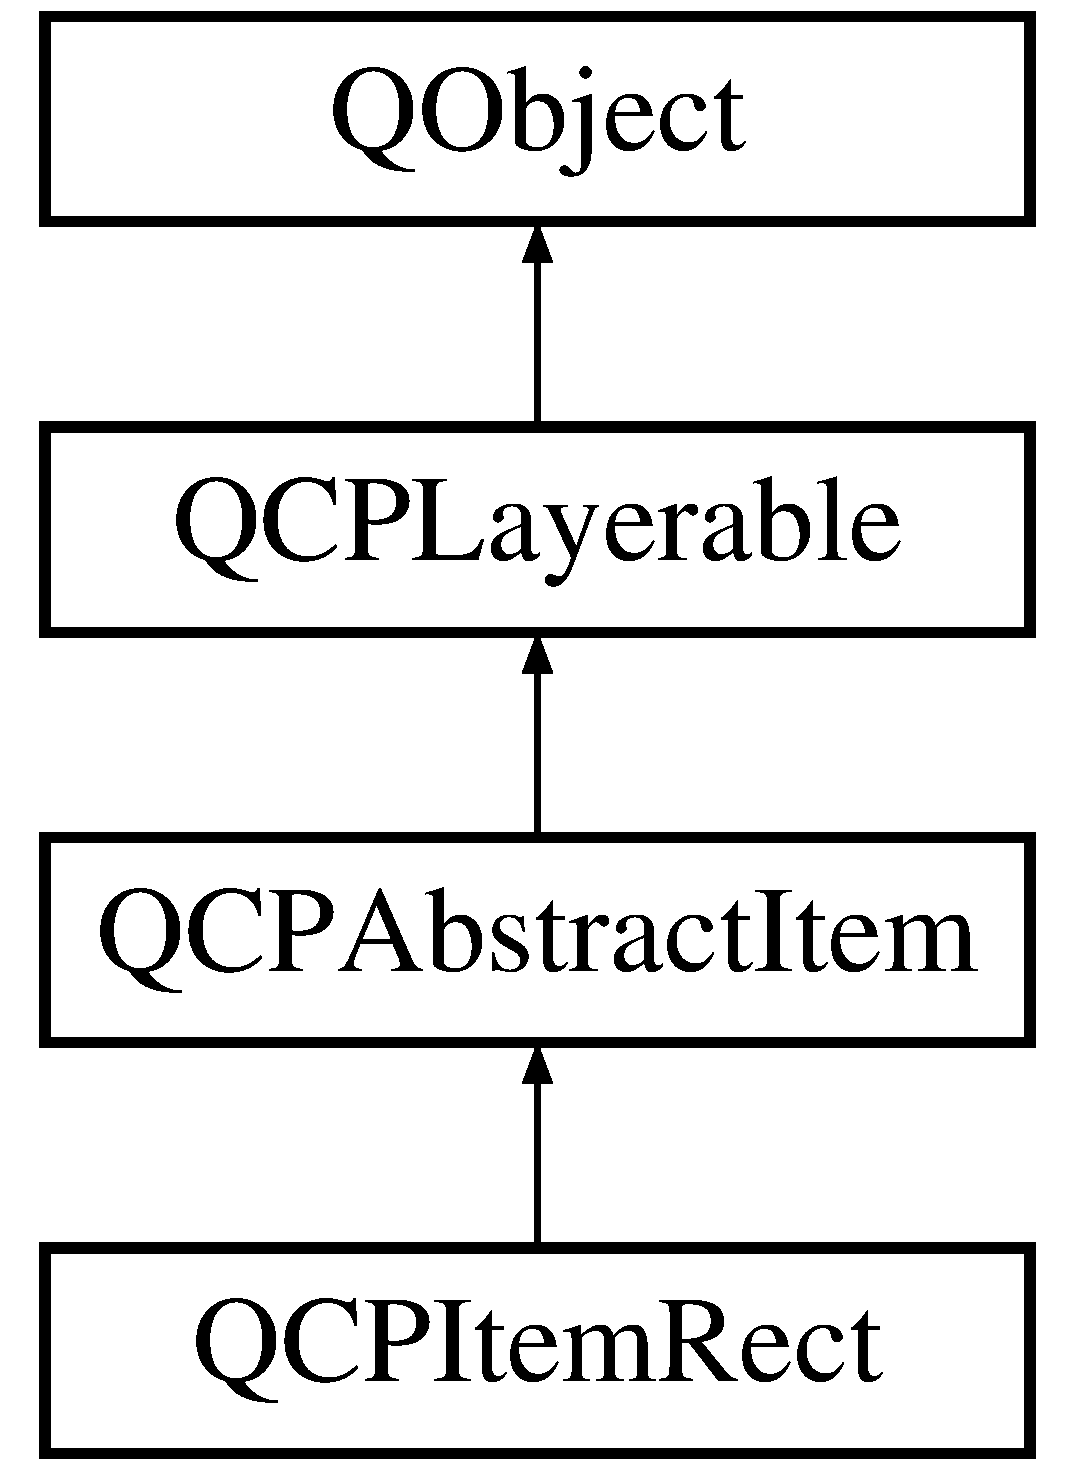
\includegraphics[height=4.000000cm]{class_q_c_p_item_rect}
\end{center}
\end{figure}
\subsection*{Public Member Functions}
\begin{DoxyCompactItemize}
\item 
\hyperlink{class_q_c_p_item_rect_a412ad1579f7a1fba453d0fa28c496cbc}{Q\+C\+P\+Item\+Rect} (\hyperlink{class_q_custom_plot}{Q\+Custom\+Plot} $\ast$\hyperlink{class_q_c_p_layerable_ab7e0e94461566093d36ffc0f5312b109}{parent\+Plot})
\item 
virtual \hyperlink{class_q_c_p_item_rect_af9e89f80457afc2d0fd2c6527b40a5f2}{$\sim$\+Q\+C\+P\+Item\+Rect} ()
\item 
Q\+Pen \hyperlink{class_q_c_p_item_rect_a3cb7b6de5e82cc5a3c99e9de919a55e6}{pen} () const 
\item 
Q\+Pen \hyperlink{class_q_c_p_item_rect_a7e701c34e72a4c25647e93fa369f395c}{selected\+Pen} () const 
\item 
Q\+Brush \hyperlink{class_q_c_p_item_rect_a03d2d26ffcac78b25b8e90915f9c4abe}{brush} () const 
\item 
Q\+Brush \hyperlink{class_q_c_p_item_rect_a3b586228393f5c8efa78c4d2a4b25cbf}{selected\+Brush} () const 
\item 
void \hyperlink{class_q_c_p_item_rect_a483c0da5a17e1646cd17ddea2c124e7d}{set\+Pen} (const Q\+Pen \&\hyperlink{class_q_c_p_item_rect_a3cb7b6de5e82cc5a3c99e9de919a55e6}{pen})
\item 
void \hyperlink{class_q_c_p_item_rect_a52a1bcb2dc753a538e406a2ba3cf21ce}{set\+Selected\+Pen} (const Q\+Pen \&\hyperlink{class_q_c_p_item_rect_a3cb7b6de5e82cc5a3c99e9de919a55e6}{pen})
\item 
void \hyperlink{class_q_c_p_item_rect_abbd4e346a03513ee466afc25d9c75446}{set\+Brush} (const Q\+Brush \&\hyperlink{class_q_c_p_item_rect_a03d2d26ffcac78b25b8e90915f9c4abe}{brush})
\item 
void \hyperlink{class_q_c_p_item_rect_abd1792859844118dedee86223cede7af}{set\+Selected\+Brush} (const Q\+Brush \&\hyperlink{class_q_c_p_item_rect_a03d2d26ffcac78b25b8e90915f9c4abe}{brush})
\item 
virtual double \hyperlink{class_q_c_p_item_rect_af13b0797079b40b73d1c7286b76f18ac}{select\+Test} (const Q\+Point\+F \&pos, bool only\+Selectable, Q\+Variant $\ast$details=0) const 
\end{DoxyCompactItemize}
\subsection*{Public Attributes}
\begin{DoxyCompactItemize}
\item 
\hyperlink{class_q_c_p_item_position}{Q\+C\+P\+Item\+Position} $\ast$const \hyperlink{class_q_c_p_item_rect_aa70feeef173489b03c3fbe906a5023c4}{top\+Left}
\item 
\hyperlink{class_q_c_p_item_position}{Q\+C\+P\+Item\+Position} $\ast$const \hyperlink{class_q_c_p_item_rect_a409f3bfe615a7e322bb3d4d193d85b26}{bottom\+Right}
\item 
\hyperlink{class_q_c_p_item_anchor}{Q\+C\+P\+Item\+Anchor} $\ast$const \hyperlink{class_q_c_p_item_rect_a96e50db552fb297d6fb62614676217bc}{top}
\item 
\hyperlink{class_q_c_p_item_anchor}{Q\+C\+P\+Item\+Anchor} $\ast$const \hyperlink{class_q_c_p_item_rect_a77e0eb6e4aa6efee620d35e2c21bdad7}{top\+Right}
\item 
\hyperlink{class_q_c_p_item_anchor}{Q\+C\+P\+Item\+Anchor} $\ast$const \hyperlink{class_q_c_p_item_rect_a7979c1915f61ad2609a9cc179c2e445e}{right}
\item 
\hyperlink{class_q_c_p_item_anchor}{Q\+C\+P\+Item\+Anchor} $\ast$const \hyperlink{class_q_c_p_item_rect_a99313bf2b338d9f81e19bd38082038aa}{bottom}
\item 
\hyperlink{class_q_c_p_item_anchor}{Q\+C\+P\+Item\+Anchor} $\ast$const \hyperlink{class_q_c_p_item_rect_abd8ee63fdf81f0c74bf7ccadee8603da}{bottom\+Left}
\item 
\hyperlink{class_q_c_p_item_anchor}{Q\+C\+P\+Item\+Anchor} $\ast$const \hyperlink{class_q_c_p_item_rect_aad0ca1af0c8debfc20d7b47fc942764d}{left}
\end{DoxyCompactItemize}
\subsection*{Protected Types}
\begin{DoxyCompactItemize}
\item 
enum \hyperlink{class_q_c_p_item_rect_af0ebba58e6bca4851c4db726691ec0d3}{Anchor\+Index} \{ \\*
\hyperlink{class_q_c_p_item_rect_af0ebba58e6bca4851c4db726691ec0d3acaef33243034885d551dc9b8318ad326}{ai\+Top}, 
\hyperlink{class_q_c_p_item_rect_af0ebba58e6bca4851c4db726691ec0d3aa94843ce5935b36994005c1e1859ef60}{ai\+Top\+Right}, 
\hyperlink{class_q_c_p_item_rect_af0ebba58e6bca4851c4db726691ec0d3a69fa21fde2f44036381296a6f78b4eb4}{ai\+Right}, 
\hyperlink{class_q_c_p_item_rect_af0ebba58e6bca4851c4db726691ec0d3a2d294551e07179c4ac0c4e37364a1468}{ai\+Bottom}, 
\\*
\hyperlink{class_q_c_p_item_rect_af0ebba58e6bca4851c4db726691ec0d3ab3c42dbb1709a04ba9b03dcbf5a2537a}{ai\+Bottom\+Left}, 
\hyperlink{class_q_c_p_item_rect_af0ebba58e6bca4851c4db726691ec0d3a8a095c6d6b2e7665a15d9f40c94b47dc}{ai\+Left}
 \}
\end{DoxyCompactItemize}
\subsection*{Protected Member Functions}
\begin{DoxyCompactItemize}
\item 
virtual void \hyperlink{class_q_c_p_item_rect_a18cd583638b876cdd50f1a155ec182aa}{draw} (\hyperlink{class_q_c_p_painter}{Q\+C\+P\+Painter} $\ast$painter)
\item 
virtual Q\+Point\+F \hyperlink{class_q_c_p_item_rect_ae0973f8281fb52361b0c99ee899be07e}{anchor\+Pixel\+Point} (int anchor\+Id) const 
\item 
Q\+Pen \hyperlink{class_q_c_p_item_rect_afa0fb7c6328a1e197ecd537de36daf8f}{main\+Pen} () const 
\item 
Q\+Brush \hyperlink{class_q_c_p_item_rect_ab0bd8e272e822ec851ba5b0c20e9200e}{main\+Brush} () const 
\end{DoxyCompactItemize}
\subsection*{Protected Attributes}
\begin{DoxyCompactItemize}
\item 
Q\+Pen \hyperlink{class_q_c_p_item_rect_aa0d49323628d6752026056bfb52afd86}{m\+Pen}
\item 
Q\+Pen \hyperlink{class_q_c_p_item_rect_a73cc0bee61de3c67221ec8c7a76a29ed}{m\+Selected\+Pen}
\item 
Q\+Brush \hyperlink{class_q_c_p_item_rect_a2d7f207fada27588b3a52b19234d3c2e}{m\+Brush}
\item 
Q\+Brush \hyperlink{class_q_c_p_item_rect_a21b70eee59b6e19ae0bbdf037b13508f}{m\+Selected\+Brush}
\end{DoxyCompactItemize}
\subsection*{Additional Inherited Members}


\subsection{Detailed Description}
A rectangle. 

 It has two positions, {\itshape top\+Left} and {\itshape bottom\+Right}, which define the rectangle. 

\subsection{Member Enumeration Documentation}
\hypertarget{class_q_c_p_item_rect_af0ebba58e6bca4851c4db726691ec0d3}{}\index{Q\+C\+P\+Item\+Rect@{Q\+C\+P\+Item\+Rect}!Anchor\+Index@{Anchor\+Index}}
\index{Anchor\+Index@{Anchor\+Index}!Q\+C\+P\+Item\+Rect@{Q\+C\+P\+Item\+Rect}}
\subsubsection[{Anchor\+Index}]{\setlength{\rightskip}{0pt plus 5cm}enum {\bf Q\+C\+P\+Item\+Rect\+::\+Anchor\+Index}\hspace{0.3cm}{\ttfamily [protected]}}\label{class_q_c_p_item_rect_af0ebba58e6bca4851c4db726691ec0d3}
\begin{Desc}
\item[Enumerator]\par
\begin{description}
\index{ai\+Top@{ai\+Top}!Q\+C\+P\+Item\+Rect@{Q\+C\+P\+Item\+Rect}}\index{Q\+C\+P\+Item\+Rect@{Q\+C\+P\+Item\+Rect}!ai\+Top@{ai\+Top}}\item[{\em 
\hypertarget{class_q_c_p_item_rect_af0ebba58e6bca4851c4db726691ec0d3acaef33243034885d551dc9b8318ad326}{}ai\+Top\label{class_q_c_p_item_rect_af0ebba58e6bca4851c4db726691ec0d3acaef33243034885d551dc9b8318ad326}
}]\index{ai\+Top\+Right@{ai\+Top\+Right}!Q\+C\+P\+Item\+Rect@{Q\+C\+P\+Item\+Rect}}\index{Q\+C\+P\+Item\+Rect@{Q\+C\+P\+Item\+Rect}!ai\+Top\+Right@{ai\+Top\+Right}}\item[{\em 
\hypertarget{class_q_c_p_item_rect_af0ebba58e6bca4851c4db726691ec0d3aa94843ce5935b36994005c1e1859ef60}{}ai\+Top\+Right\label{class_q_c_p_item_rect_af0ebba58e6bca4851c4db726691ec0d3aa94843ce5935b36994005c1e1859ef60}
}]\index{ai\+Right@{ai\+Right}!Q\+C\+P\+Item\+Rect@{Q\+C\+P\+Item\+Rect}}\index{Q\+C\+P\+Item\+Rect@{Q\+C\+P\+Item\+Rect}!ai\+Right@{ai\+Right}}\item[{\em 
\hypertarget{class_q_c_p_item_rect_af0ebba58e6bca4851c4db726691ec0d3a69fa21fde2f44036381296a6f78b4eb4}{}ai\+Right\label{class_q_c_p_item_rect_af0ebba58e6bca4851c4db726691ec0d3a69fa21fde2f44036381296a6f78b4eb4}
}]\index{ai\+Bottom@{ai\+Bottom}!Q\+C\+P\+Item\+Rect@{Q\+C\+P\+Item\+Rect}}\index{Q\+C\+P\+Item\+Rect@{Q\+C\+P\+Item\+Rect}!ai\+Bottom@{ai\+Bottom}}\item[{\em 
\hypertarget{class_q_c_p_item_rect_af0ebba58e6bca4851c4db726691ec0d3a2d294551e07179c4ac0c4e37364a1468}{}ai\+Bottom\label{class_q_c_p_item_rect_af0ebba58e6bca4851c4db726691ec0d3a2d294551e07179c4ac0c4e37364a1468}
}]\index{ai\+Bottom\+Left@{ai\+Bottom\+Left}!Q\+C\+P\+Item\+Rect@{Q\+C\+P\+Item\+Rect}}\index{Q\+C\+P\+Item\+Rect@{Q\+C\+P\+Item\+Rect}!ai\+Bottom\+Left@{ai\+Bottom\+Left}}\item[{\em 
\hypertarget{class_q_c_p_item_rect_af0ebba58e6bca4851c4db726691ec0d3ab3c42dbb1709a04ba9b03dcbf5a2537a}{}ai\+Bottom\+Left\label{class_q_c_p_item_rect_af0ebba58e6bca4851c4db726691ec0d3ab3c42dbb1709a04ba9b03dcbf5a2537a}
}]\index{ai\+Left@{ai\+Left}!Q\+C\+P\+Item\+Rect@{Q\+C\+P\+Item\+Rect}}\index{Q\+C\+P\+Item\+Rect@{Q\+C\+P\+Item\+Rect}!ai\+Left@{ai\+Left}}\item[{\em 
\hypertarget{class_q_c_p_item_rect_af0ebba58e6bca4851c4db726691ec0d3a8a095c6d6b2e7665a15d9f40c94b47dc}{}ai\+Left\label{class_q_c_p_item_rect_af0ebba58e6bca4851c4db726691ec0d3a8a095c6d6b2e7665a15d9f40c94b47dc}
}]\end{description}
\end{Desc}


\subsection{Constructor \& Destructor Documentation}
\hypertarget{class_q_c_p_item_rect_a412ad1579f7a1fba453d0fa28c496cbc}{}\index{Q\+C\+P\+Item\+Rect@{Q\+C\+P\+Item\+Rect}!Q\+C\+P\+Item\+Rect@{Q\+C\+P\+Item\+Rect}}
\index{Q\+C\+P\+Item\+Rect@{Q\+C\+P\+Item\+Rect}!Q\+C\+P\+Item\+Rect@{Q\+C\+P\+Item\+Rect}}
\subsubsection[{Q\+C\+P\+Item\+Rect}]{\setlength{\rightskip}{0pt plus 5cm}Q\+C\+P\+Item\+Rect\+::\+Q\+C\+P\+Item\+Rect (
\begin{DoxyParamCaption}
\item[{{\bf Q\+Custom\+Plot} $\ast$}]{parent\+Plot}
\end{DoxyParamCaption}
)}\label{class_q_c_p_item_rect_a412ad1579f7a1fba453d0fa28c496cbc}
Creates a rectangle item and sets default values.

The constructed item can be added to the plot with \hyperlink{class_q_custom_plot_aa500620379262321685cb7a7674cbd2a}{Q\+Custom\+Plot\+::add\+Item}. \hypertarget{class_q_c_p_item_rect_af9e89f80457afc2d0fd2c6527b40a5f2}{}\index{Q\+C\+P\+Item\+Rect@{Q\+C\+P\+Item\+Rect}!````~Q\+C\+P\+Item\+Rect@{$\sim$\+Q\+C\+P\+Item\+Rect}}
\index{````~Q\+C\+P\+Item\+Rect@{$\sim$\+Q\+C\+P\+Item\+Rect}!Q\+C\+P\+Item\+Rect@{Q\+C\+P\+Item\+Rect}}
\subsubsection[{$\sim$\+Q\+C\+P\+Item\+Rect}]{\setlength{\rightskip}{0pt plus 5cm}Q\+C\+P\+Item\+Rect\+::$\sim$\+Q\+C\+P\+Item\+Rect (
\begin{DoxyParamCaption}
{}
\end{DoxyParamCaption}
)\hspace{0.3cm}{\ttfamily [virtual]}}\label{class_q_c_p_item_rect_af9e89f80457afc2d0fd2c6527b40a5f2}


\subsection{Member Function Documentation}
\hypertarget{class_q_c_p_item_rect_ae0973f8281fb52361b0c99ee899be07e}{}\index{Q\+C\+P\+Item\+Rect@{Q\+C\+P\+Item\+Rect}!anchor\+Pixel\+Point@{anchor\+Pixel\+Point}}
\index{anchor\+Pixel\+Point@{anchor\+Pixel\+Point}!Q\+C\+P\+Item\+Rect@{Q\+C\+P\+Item\+Rect}}
\subsubsection[{anchor\+Pixel\+Point}]{\setlength{\rightskip}{0pt plus 5cm}Q\+Point\+F Q\+C\+P\+Item\+Rect\+::anchor\+Pixel\+Point (
\begin{DoxyParamCaption}
\item[{int}]{anchor\+Id}
\end{DoxyParamCaption}
) const\hspace{0.3cm}{\ttfamily [protected]}, {\ttfamily [virtual]}}\label{class_q_c_p_item_rect_ae0973f8281fb52361b0c99ee899be07e}


Reimplemented from \hyperlink{class_q_c_p_abstract_item_a94bde62b8a2fc133666dcbb8035deeed}{Q\+C\+P\+Abstract\+Item}.

\hypertarget{class_q_c_p_item_rect_a03d2d26ffcac78b25b8e90915f9c4abe}{}\index{Q\+C\+P\+Item\+Rect@{Q\+C\+P\+Item\+Rect}!brush@{brush}}
\index{brush@{brush}!Q\+C\+P\+Item\+Rect@{Q\+C\+P\+Item\+Rect}}
\subsubsection[{brush}]{\setlength{\rightskip}{0pt plus 5cm}Q\+Brush Q\+C\+P\+Item\+Rect\+::brush (
\begin{DoxyParamCaption}
{}
\end{DoxyParamCaption}
) const\hspace{0.3cm}{\ttfamily [inline]}}\label{class_q_c_p_item_rect_a03d2d26ffcac78b25b8e90915f9c4abe}
\hypertarget{class_q_c_p_item_rect_a18cd583638b876cdd50f1a155ec182aa}{}\index{Q\+C\+P\+Item\+Rect@{Q\+C\+P\+Item\+Rect}!draw@{draw}}
\index{draw@{draw}!Q\+C\+P\+Item\+Rect@{Q\+C\+P\+Item\+Rect}}
\subsubsection[{draw}]{\setlength{\rightskip}{0pt plus 5cm}void Q\+C\+P\+Item\+Rect\+::draw (
\begin{DoxyParamCaption}
\item[{{\bf Q\+C\+P\+Painter} $\ast$}]{painter}
\end{DoxyParamCaption}
)\hspace{0.3cm}{\ttfamily [protected]}, {\ttfamily [virtual]}}\label{class_q_c_p_item_rect_a18cd583638b876cdd50f1a155ec182aa}


Implements \hyperlink{class_q_c_p_abstract_item_ad0dc056f650c3ca73414e6b4f01674ef}{Q\+C\+P\+Abstract\+Item}.

\hypertarget{class_q_c_p_item_rect_ab0bd8e272e822ec851ba5b0c20e9200e}{}\index{Q\+C\+P\+Item\+Rect@{Q\+C\+P\+Item\+Rect}!main\+Brush@{main\+Brush}}
\index{main\+Brush@{main\+Brush}!Q\+C\+P\+Item\+Rect@{Q\+C\+P\+Item\+Rect}}
\subsubsection[{main\+Brush}]{\setlength{\rightskip}{0pt plus 5cm}Q\+Brush Q\+C\+P\+Item\+Rect\+::main\+Brush (
\begin{DoxyParamCaption}
{}
\end{DoxyParamCaption}
) const\hspace{0.3cm}{\ttfamily [protected]}}\label{class_q_c_p_item_rect_ab0bd8e272e822ec851ba5b0c20e9200e}
\hypertarget{class_q_c_p_item_rect_afa0fb7c6328a1e197ecd537de36daf8f}{}\index{Q\+C\+P\+Item\+Rect@{Q\+C\+P\+Item\+Rect}!main\+Pen@{main\+Pen}}
\index{main\+Pen@{main\+Pen}!Q\+C\+P\+Item\+Rect@{Q\+C\+P\+Item\+Rect}}
\subsubsection[{main\+Pen}]{\setlength{\rightskip}{0pt plus 5cm}Q\+Pen Q\+C\+P\+Item\+Rect\+::main\+Pen (
\begin{DoxyParamCaption}
{}
\end{DoxyParamCaption}
) const\hspace{0.3cm}{\ttfamily [protected]}}\label{class_q_c_p_item_rect_afa0fb7c6328a1e197ecd537de36daf8f}
\hypertarget{class_q_c_p_item_rect_a3cb7b6de5e82cc5a3c99e9de919a55e6}{}\index{Q\+C\+P\+Item\+Rect@{Q\+C\+P\+Item\+Rect}!pen@{pen}}
\index{pen@{pen}!Q\+C\+P\+Item\+Rect@{Q\+C\+P\+Item\+Rect}}
\subsubsection[{pen}]{\setlength{\rightskip}{0pt plus 5cm}Q\+Pen Q\+C\+P\+Item\+Rect\+::pen (
\begin{DoxyParamCaption}
{}
\end{DoxyParamCaption}
) const\hspace{0.3cm}{\ttfamily [inline]}}\label{class_q_c_p_item_rect_a3cb7b6de5e82cc5a3c99e9de919a55e6}
\hypertarget{class_q_c_p_item_rect_a3b586228393f5c8efa78c4d2a4b25cbf}{}\index{Q\+C\+P\+Item\+Rect@{Q\+C\+P\+Item\+Rect}!selected\+Brush@{selected\+Brush}}
\index{selected\+Brush@{selected\+Brush}!Q\+C\+P\+Item\+Rect@{Q\+C\+P\+Item\+Rect}}
\subsubsection[{selected\+Brush}]{\setlength{\rightskip}{0pt plus 5cm}Q\+Brush Q\+C\+P\+Item\+Rect\+::selected\+Brush (
\begin{DoxyParamCaption}
{}
\end{DoxyParamCaption}
) const\hspace{0.3cm}{\ttfamily [inline]}}\label{class_q_c_p_item_rect_a3b586228393f5c8efa78c4d2a4b25cbf}
\hypertarget{class_q_c_p_item_rect_a7e701c34e72a4c25647e93fa369f395c}{}\index{Q\+C\+P\+Item\+Rect@{Q\+C\+P\+Item\+Rect}!selected\+Pen@{selected\+Pen}}
\index{selected\+Pen@{selected\+Pen}!Q\+C\+P\+Item\+Rect@{Q\+C\+P\+Item\+Rect}}
\subsubsection[{selected\+Pen}]{\setlength{\rightskip}{0pt plus 5cm}Q\+Pen Q\+C\+P\+Item\+Rect\+::selected\+Pen (
\begin{DoxyParamCaption}
{}
\end{DoxyParamCaption}
) const\hspace{0.3cm}{\ttfamily [inline]}}\label{class_q_c_p_item_rect_a7e701c34e72a4c25647e93fa369f395c}
\hypertarget{class_q_c_p_item_rect_af13b0797079b40b73d1c7286b76f18ac}{}\index{Q\+C\+P\+Item\+Rect@{Q\+C\+P\+Item\+Rect}!select\+Test@{select\+Test}}
\index{select\+Test@{select\+Test}!Q\+C\+P\+Item\+Rect@{Q\+C\+P\+Item\+Rect}}
\subsubsection[{select\+Test}]{\setlength{\rightskip}{0pt plus 5cm}double Q\+C\+P\+Item\+Rect\+::select\+Test (
\begin{DoxyParamCaption}
\item[{const Q\+Point\+F \&}]{pos, }
\item[{bool}]{only\+Selectable, }
\item[{Q\+Variant $\ast$}]{details = {\ttfamily 0}}
\end{DoxyParamCaption}
) const\hspace{0.3cm}{\ttfamily [virtual]}}\label{class_q_c_p_item_rect_af13b0797079b40b73d1c7286b76f18ac}
This function is used to decide whether a click hits a layerable object or not.

{\itshape pos} is a point in pixel coordinates on the \hyperlink{class_q_custom_plot}{Q\+Custom\+Plot} surface. This function returns the shortest pixel distance of this point to the object. If the object is either invisible or the distance couldn\textquotesingle{}t be determined, -\/1.\+0 is returned. Further, if {\itshape only\+Selectable} is true and the object is not selectable, -\/1.\+0 is returned, too.

If the item is represented not by single lines but by an area like \hyperlink{class_q_c_p_item_rect}{Q\+C\+P\+Item\+Rect} or \hyperlink{class_q_c_p_item_text}{Q\+C\+P\+Item\+Text}, a click inside the area returns a constant value greater zero (typically the selection\+Tolerance of the parent \hyperlink{class_q_custom_plot}{Q\+Custom\+Plot} multiplied by 0.\+99). If the click lies outside the area, this function returns -\/1.\+0.

Providing a constant value for area objects allows selecting line objects even when they are obscured by such area objects, by clicking close to the lines (i.\+e. closer than 0.\+99$\ast$selection\+Tolerance).

The actual setting of the selection state is not done by this function. This is handled by the parent \hyperlink{class_q_custom_plot}{Q\+Custom\+Plot} when the mouse\+Release\+Event occurs, and the finally selected object is notified via the select\+Event/deselect\+Event methods.

{\itshape details} is an optional output parameter. Every layerable subclass may place any information in {\itshape details}. This information will be passed to \hyperlink{class_q_c_p_abstract_item_aaf92af7b9893712959a6c073d334d88d}{select\+Event} when the parent \hyperlink{class_q_custom_plot}{Q\+Custom\+Plot} decides on the basis of this select\+Test call, that the object was successfully selected. The subsequent call to \hyperlink{class_q_c_p_abstract_item_aaf92af7b9893712959a6c073d334d88d}{select\+Event} will carry the {\itshape details}. This is useful for multi-\/part objects (like \hyperlink{class_q_c_p_axis}{Q\+C\+P\+Axis}). This way, a possibly complex calculation to decide which part was clicked is only done once in \hyperlink{class_q_c_p_item_rect_af13b0797079b40b73d1c7286b76f18ac}{select\+Test}. The result (i.\+e. the actually clicked part) can then be placed in {\itshape details}. So in the subsequent \hyperlink{class_q_c_p_abstract_item_aaf92af7b9893712959a6c073d334d88d}{select\+Event}, the decision which part was selected doesn\textquotesingle{}t have to be done a second time for a single selection operation.

You may pass 0 as {\itshape details} to indicate that you are not interested in those selection details.

\begin{DoxySeeAlso}{See also}
\hyperlink{class_q_c_p_abstract_item_aaf92af7b9893712959a6c073d334d88d}{select\+Event}, \hyperlink{class_q_c_p_abstract_item_a91f090d6763cfedb0749219c63788ae9}{deselect\+Event}, \hyperlink{class_q_custom_plot_a5ee1e2f6ae27419deca53e75907c27e5}{Q\+Custom\+Plot\+::set\+Interactions} 
\end{DoxySeeAlso}


Implements \hyperlink{class_q_c_p_abstract_item_a96d522d10ffc0413b9a366c6f7f0476b}{Q\+C\+P\+Abstract\+Item}.

\hypertarget{class_q_c_p_item_rect_abbd4e346a03513ee466afc25d9c75446}{}\index{Q\+C\+P\+Item\+Rect@{Q\+C\+P\+Item\+Rect}!set\+Brush@{set\+Brush}}
\index{set\+Brush@{set\+Brush}!Q\+C\+P\+Item\+Rect@{Q\+C\+P\+Item\+Rect}}
\subsubsection[{set\+Brush}]{\setlength{\rightskip}{0pt plus 5cm}void Q\+C\+P\+Item\+Rect\+::set\+Brush (
\begin{DoxyParamCaption}
\item[{const Q\+Brush \&}]{brush}
\end{DoxyParamCaption}
)}\label{class_q_c_p_item_rect_abbd4e346a03513ee466afc25d9c75446}
Sets the brush that will be used to fill the rectangle. To disable filling, set {\itshape brush} to Qt\+::\+No\+Brush.

\begin{DoxySeeAlso}{See also}
\hyperlink{class_q_c_p_item_rect_abd1792859844118dedee86223cede7af}{set\+Selected\+Brush}, \hyperlink{class_q_c_p_item_rect_a483c0da5a17e1646cd17ddea2c124e7d}{set\+Pen} 
\end{DoxySeeAlso}
\hypertarget{class_q_c_p_item_rect_a483c0da5a17e1646cd17ddea2c124e7d}{}\index{Q\+C\+P\+Item\+Rect@{Q\+C\+P\+Item\+Rect}!set\+Pen@{set\+Pen}}
\index{set\+Pen@{set\+Pen}!Q\+C\+P\+Item\+Rect@{Q\+C\+P\+Item\+Rect}}
\subsubsection[{set\+Pen}]{\setlength{\rightskip}{0pt plus 5cm}void Q\+C\+P\+Item\+Rect\+::set\+Pen (
\begin{DoxyParamCaption}
\item[{const Q\+Pen \&}]{pen}
\end{DoxyParamCaption}
)}\label{class_q_c_p_item_rect_a483c0da5a17e1646cd17ddea2c124e7d}
Sets the pen that will be used to draw the line of the rectangle

\begin{DoxySeeAlso}{See also}
\hyperlink{class_q_c_p_item_rect_a52a1bcb2dc753a538e406a2ba3cf21ce}{set\+Selected\+Pen}, \hyperlink{class_q_c_p_item_rect_abbd4e346a03513ee466afc25d9c75446}{set\+Brush} 
\end{DoxySeeAlso}
\hypertarget{class_q_c_p_item_rect_abd1792859844118dedee86223cede7af}{}\index{Q\+C\+P\+Item\+Rect@{Q\+C\+P\+Item\+Rect}!set\+Selected\+Brush@{set\+Selected\+Brush}}
\index{set\+Selected\+Brush@{set\+Selected\+Brush}!Q\+C\+P\+Item\+Rect@{Q\+C\+P\+Item\+Rect}}
\subsubsection[{set\+Selected\+Brush}]{\setlength{\rightskip}{0pt plus 5cm}void Q\+C\+P\+Item\+Rect\+::set\+Selected\+Brush (
\begin{DoxyParamCaption}
\item[{const Q\+Brush \&}]{brush}
\end{DoxyParamCaption}
)}\label{class_q_c_p_item_rect_abd1792859844118dedee86223cede7af}
Sets the brush that will be used to fill the rectangle when selected. To disable filling, set {\itshape brush} to Qt\+::\+No\+Brush.

\begin{DoxySeeAlso}{See also}
\hyperlink{class_q_c_p_item_rect_abbd4e346a03513ee466afc25d9c75446}{set\+Brush} 
\end{DoxySeeAlso}
\hypertarget{class_q_c_p_item_rect_a52a1bcb2dc753a538e406a2ba3cf21ce}{}\index{Q\+C\+P\+Item\+Rect@{Q\+C\+P\+Item\+Rect}!set\+Selected\+Pen@{set\+Selected\+Pen}}
\index{set\+Selected\+Pen@{set\+Selected\+Pen}!Q\+C\+P\+Item\+Rect@{Q\+C\+P\+Item\+Rect}}
\subsubsection[{set\+Selected\+Pen}]{\setlength{\rightskip}{0pt plus 5cm}void Q\+C\+P\+Item\+Rect\+::set\+Selected\+Pen (
\begin{DoxyParamCaption}
\item[{const Q\+Pen \&}]{pen}
\end{DoxyParamCaption}
)}\label{class_q_c_p_item_rect_a52a1bcb2dc753a538e406a2ba3cf21ce}
Sets the pen that will be used to draw the line of the rectangle when selected

\begin{DoxySeeAlso}{See also}
\hyperlink{class_q_c_p_item_rect_a483c0da5a17e1646cd17ddea2c124e7d}{set\+Pen}, \hyperlink{class_q_c_p_abstract_item_a203de94ad586cc44d16c9565f49d3378}{set\+Selected} 
\end{DoxySeeAlso}


\subsection{Member Data Documentation}
\hypertarget{class_q_c_p_item_rect_a99313bf2b338d9f81e19bd38082038aa}{}\index{Q\+C\+P\+Item\+Rect@{Q\+C\+P\+Item\+Rect}!bottom@{bottom}}
\index{bottom@{bottom}!Q\+C\+P\+Item\+Rect@{Q\+C\+P\+Item\+Rect}}
\subsubsection[{bottom}]{\setlength{\rightskip}{0pt plus 5cm}{\bf Q\+C\+P\+Item\+Anchor}$\ast$ const Q\+C\+P\+Item\+Rect\+::bottom}\label{class_q_c_p_item_rect_a99313bf2b338d9f81e19bd38082038aa}
\hypertarget{class_q_c_p_item_rect_abd8ee63fdf81f0c74bf7ccadee8603da}{}\index{Q\+C\+P\+Item\+Rect@{Q\+C\+P\+Item\+Rect}!bottom\+Left@{bottom\+Left}}
\index{bottom\+Left@{bottom\+Left}!Q\+C\+P\+Item\+Rect@{Q\+C\+P\+Item\+Rect}}
\subsubsection[{bottom\+Left}]{\setlength{\rightskip}{0pt plus 5cm}{\bf Q\+C\+P\+Item\+Anchor}$\ast$ const Q\+C\+P\+Item\+Rect\+::bottom\+Left}\label{class_q_c_p_item_rect_abd8ee63fdf81f0c74bf7ccadee8603da}
\hypertarget{class_q_c_p_item_rect_a409f3bfe615a7e322bb3d4d193d85b26}{}\index{Q\+C\+P\+Item\+Rect@{Q\+C\+P\+Item\+Rect}!bottom\+Right@{bottom\+Right}}
\index{bottom\+Right@{bottom\+Right}!Q\+C\+P\+Item\+Rect@{Q\+C\+P\+Item\+Rect}}
\subsubsection[{bottom\+Right}]{\setlength{\rightskip}{0pt plus 5cm}{\bf Q\+C\+P\+Item\+Position}$\ast$ const Q\+C\+P\+Item\+Rect\+::bottom\+Right}\label{class_q_c_p_item_rect_a409f3bfe615a7e322bb3d4d193d85b26}
\hypertarget{class_q_c_p_item_rect_aad0ca1af0c8debfc20d7b47fc942764d}{}\index{Q\+C\+P\+Item\+Rect@{Q\+C\+P\+Item\+Rect}!left@{left}}
\index{left@{left}!Q\+C\+P\+Item\+Rect@{Q\+C\+P\+Item\+Rect}}
\subsubsection[{left}]{\setlength{\rightskip}{0pt plus 5cm}{\bf Q\+C\+P\+Item\+Anchor}$\ast$ const Q\+C\+P\+Item\+Rect\+::left}\label{class_q_c_p_item_rect_aad0ca1af0c8debfc20d7b47fc942764d}
\hypertarget{class_q_c_p_item_rect_a2d7f207fada27588b3a52b19234d3c2e}{}\index{Q\+C\+P\+Item\+Rect@{Q\+C\+P\+Item\+Rect}!m\+Brush@{m\+Brush}}
\index{m\+Brush@{m\+Brush}!Q\+C\+P\+Item\+Rect@{Q\+C\+P\+Item\+Rect}}
\subsubsection[{m\+Brush}]{\setlength{\rightskip}{0pt plus 5cm}Q\+Brush Q\+C\+P\+Item\+Rect\+::m\+Brush\hspace{0.3cm}{\ttfamily [protected]}}\label{class_q_c_p_item_rect_a2d7f207fada27588b3a52b19234d3c2e}
\hypertarget{class_q_c_p_item_rect_aa0d49323628d6752026056bfb52afd86}{}\index{Q\+C\+P\+Item\+Rect@{Q\+C\+P\+Item\+Rect}!m\+Pen@{m\+Pen}}
\index{m\+Pen@{m\+Pen}!Q\+C\+P\+Item\+Rect@{Q\+C\+P\+Item\+Rect}}
\subsubsection[{m\+Pen}]{\setlength{\rightskip}{0pt plus 5cm}Q\+Pen Q\+C\+P\+Item\+Rect\+::m\+Pen\hspace{0.3cm}{\ttfamily [protected]}}\label{class_q_c_p_item_rect_aa0d49323628d6752026056bfb52afd86}
\hypertarget{class_q_c_p_item_rect_a21b70eee59b6e19ae0bbdf037b13508f}{}\index{Q\+C\+P\+Item\+Rect@{Q\+C\+P\+Item\+Rect}!m\+Selected\+Brush@{m\+Selected\+Brush}}
\index{m\+Selected\+Brush@{m\+Selected\+Brush}!Q\+C\+P\+Item\+Rect@{Q\+C\+P\+Item\+Rect}}
\subsubsection[{m\+Selected\+Brush}]{\setlength{\rightskip}{0pt plus 5cm}Q\+Brush Q\+C\+P\+Item\+Rect\+::m\+Selected\+Brush\hspace{0.3cm}{\ttfamily [protected]}}\label{class_q_c_p_item_rect_a21b70eee59b6e19ae0bbdf037b13508f}
\hypertarget{class_q_c_p_item_rect_a73cc0bee61de3c67221ec8c7a76a29ed}{}\index{Q\+C\+P\+Item\+Rect@{Q\+C\+P\+Item\+Rect}!m\+Selected\+Pen@{m\+Selected\+Pen}}
\index{m\+Selected\+Pen@{m\+Selected\+Pen}!Q\+C\+P\+Item\+Rect@{Q\+C\+P\+Item\+Rect}}
\subsubsection[{m\+Selected\+Pen}]{\setlength{\rightskip}{0pt plus 5cm}Q\+Pen Q\+C\+P\+Item\+Rect\+::m\+Selected\+Pen\hspace{0.3cm}{\ttfamily [protected]}}\label{class_q_c_p_item_rect_a73cc0bee61de3c67221ec8c7a76a29ed}
\hypertarget{class_q_c_p_item_rect_a7979c1915f61ad2609a9cc179c2e445e}{}\index{Q\+C\+P\+Item\+Rect@{Q\+C\+P\+Item\+Rect}!right@{right}}
\index{right@{right}!Q\+C\+P\+Item\+Rect@{Q\+C\+P\+Item\+Rect}}
\subsubsection[{right}]{\setlength{\rightskip}{0pt plus 5cm}{\bf Q\+C\+P\+Item\+Anchor}$\ast$ const Q\+C\+P\+Item\+Rect\+::right}\label{class_q_c_p_item_rect_a7979c1915f61ad2609a9cc179c2e445e}
\hypertarget{class_q_c_p_item_rect_a96e50db552fb297d6fb62614676217bc}{}\index{Q\+C\+P\+Item\+Rect@{Q\+C\+P\+Item\+Rect}!top@{top}}
\index{top@{top}!Q\+C\+P\+Item\+Rect@{Q\+C\+P\+Item\+Rect}}
\subsubsection[{top}]{\setlength{\rightskip}{0pt plus 5cm}{\bf Q\+C\+P\+Item\+Anchor}$\ast$ const Q\+C\+P\+Item\+Rect\+::top}\label{class_q_c_p_item_rect_a96e50db552fb297d6fb62614676217bc}
\hypertarget{class_q_c_p_item_rect_aa70feeef173489b03c3fbe906a5023c4}{}\index{Q\+C\+P\+Item\+Rect@{Q\+C\+P\+Item\+Rect}!top\+Left@{top\+Left}}
\index{top\+Left@{top\+Left}!Q\+C\+P\+Item\+Rect@{Q\+C\+P\+Item\+Rect}}
\subsubsection[{top\+Left}]{\setlength{\rightskip}{0pt plus 5cm}{\bf Q\+C\+P\+Item\+Position}$\ast$ const Q\+C\+P\+Item\+Rect\+::top\+Left}\label{class_q_c_p_item_rect_aa70feeef173489b03c3fbe906a5023c4}
\hypertarget{class_q_c_p_item_rect_a77e0eb6e4aa6efee620d35e2c21bdad7}{}\index{Q\+C\+P\+Item\+Rect@{Q\+C\+P\+Item\+Rect}!top\+Right@{top\+Right}}
\index{top\+Right@{top\+Right}!Q\+C\+P\+Item\+Rect@{Q\+C\+P\+Item\+Rect}}
\subsubsection[{top\+Right}]{\setlength{\rightskip}{0pt plus 5cm}{\bf Q\+C\+P\+Item\+Anchor}$\ast$ const Q\+C\+P\+Item\+Rect\+::top\+Right}\label{class_q_c_p_item_rect_a77e0eb6e4aa6efee620d35e2c21bdad7}


The documentation for this class was generated from the following files\+:\begin{DoxyCompactItemize}
\item 
C\+:/\+Users/\+Roman/\+Documents/\+Mygs/\+Ground\+Station/\+G\+S/\hyperlink{qcustomplot_8h}{qcustomplot.\+h}\item 
C\+:/\+Users/\+Roman/\+Documents/\+Mygs/\+Ground\+Station/\+G\+S/\hyperlink{qcustomplot_8cpp}{qcustomplot.\+cpp}\end{DoxyCompactItemize}

\hypertarget{class_q_c_p_item_straight_line}{}\section{Q\+C\+P\+Item\+Straight\+Line Class Reference}
\label{class_q_c_p_item_straight_line}\index{Q\+C\+P\+Item\+Straight\+Line@{Q\+C\+P\+Item\+Straight\+Line}}


A straight line that spans infinitely in both directions.  




{\ttfamily \#include $<$qcustomplot.\+h$>$}

Inheritance diagram for Q\+C\+P\+Item\+Straight\+Line\+:\begin{figure}[H]
\begin{center}
\leavevmode
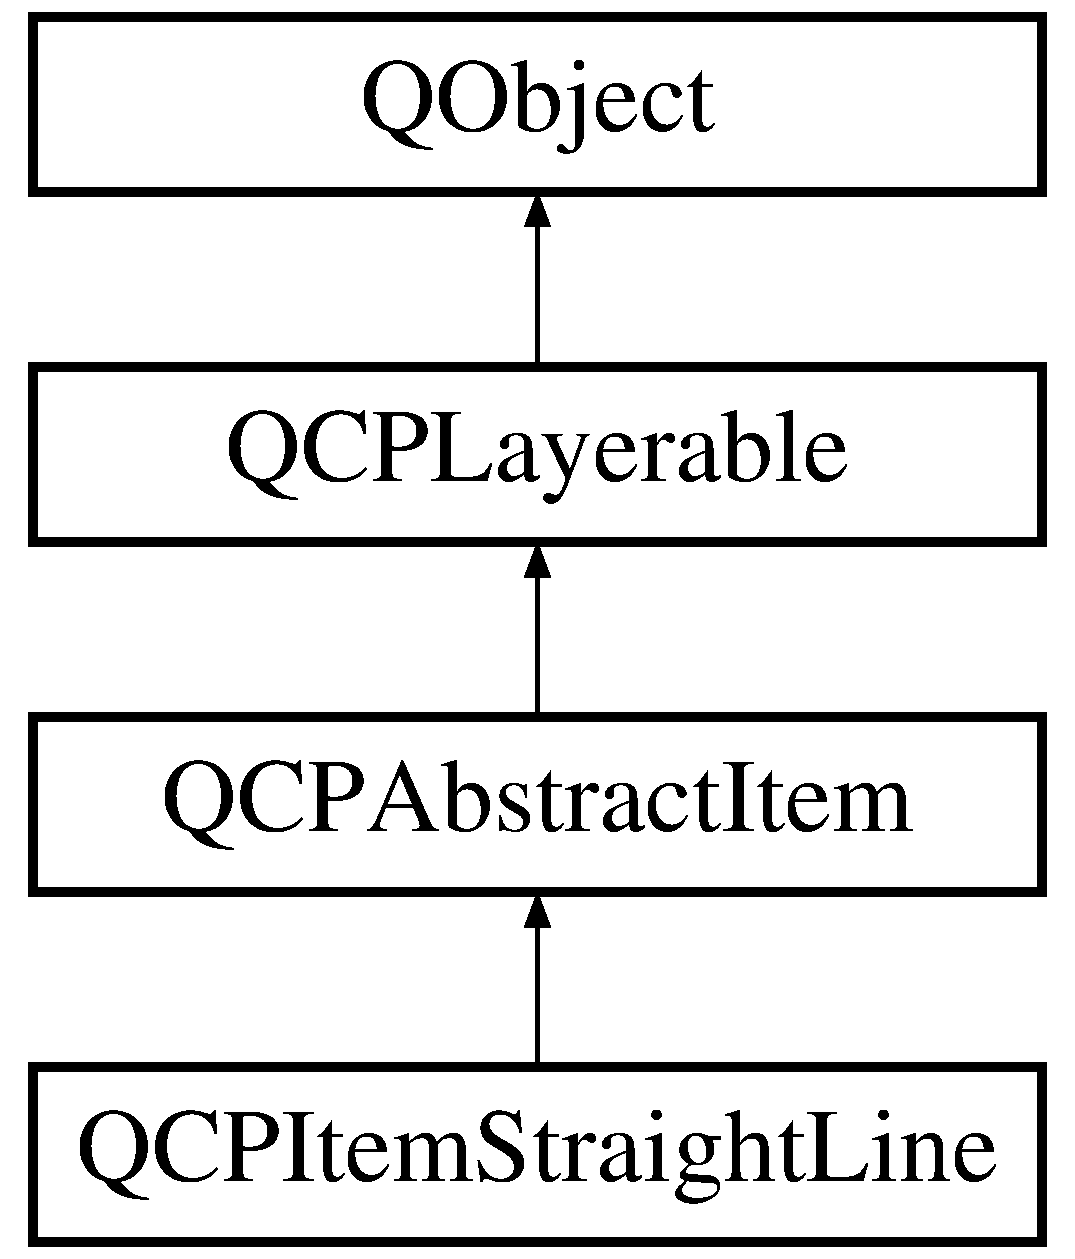
\includegraphics[height=4.000000cm]{class_q_c_p_item_straight_line}
\end{center}
\end{figure}
\subsection*{Public Member Functions}
\begin{DoxyCompactItemize}
\item 
\hyperlink{class_q_c_p_item_straight_line_a41fd2e1f006983449eca9830930c3b10}{Q\+C\+P\+Item\+Straight\+Line} (\hyperlink{class_q_custom_plot}{Q\+Custom\+Plot} $\ast$\hyperlink{class_q_c_p_layerable_ab7e0e94461566093d36ffc0f5312b109}{parent\+Plot})
\item 
virtual \hyperlink{class_q_c_p_item_straight_line_a1f0730759916ce203baeaad1ad2af3ea}{$\sim$\+Q\+C\+P\+Item\+Straight\+Line} ()
\item 
Q\+Pen \hyperlink{class_q_c_p_item_straight_line_ad858ab1a444391aab778f765453ea222}{pen} () const 
\item 
Q\+Pen \hyperlink{class_q_c_p_item_straight_line_a9e33ae966a7e2ea1083b3b9aeabeaea5}{selected\+Pen} () const 
\item 
void \hyperlink{class_q_c_p_item_straight_line_a9f36c9c9e60d7d9ac084c80380ac8601}{set\+Pen} (const Q\+Pen \&\hyperlink{class_q_c_p_item_straight_line_ad858ab1a444391aab778f765453ea222}{pen})
\item 
void \hyperlink{class_q_c_p_item_straight_line_a5c33559498d33543fa95cf0a36e851ff}{set\+Selected\+Pen} (const Q\+Pen \&\hyperlink{class_q_c_p_item_straight_line_ad858ab1a444391aab778f765453ea222}{pen})
\item 
virtual double \hyperlink{class_q_c_p_item_straight_line_a64cc3796f58ce856012732603edb2f1c}{select\+Test} (const Q\+Point\+F \&pos, bool only\+Selectable, Q\+Variant $\ast$details=0) const 
\end{DoxyCompactItemize}
\subsection*{Public Attributes}
\begin{DoxyCompactItemize}
\item 
\hyperlink{class_q_c_p_item_position}{Q\+C\+P\+Item\+Position} $\ast$const \hyperlink{class_q_c_p_item_straight_line_ac131a6ffe456f2cc7364dce541fe0120}{point1}
\item 
\hyperlink{class_q_c_p_item_position}{Q\+C\+P\+Item\+Position} $\ast$const \hyperlink{class_q_c_p_item_straight_line_ad26c0a732e471f63f75d481dcd48cfc9}{point2}
\end{DoxyCompactItemize}
\subsection*{Protected Member Functions}
\begin{DoxyCompactItemize}
\item 
virtual void \hyperlink{class_q_c_p_item_straight_line_a2daa1e1253216c26565d56a2d5530170}{draw} (\hyperlink{class_q_c_p_painter}{Q\+C\+P\+Painter} $\ast$painter)
\item 
double \hyperlink{class_q_c_p_item_straight_line_adc9b6c5bd33c7f806b748b79dfa25926}{dist\+To\+Straight\+Line} (const Q\+Vector2\+D \&\hyperlink{class_q_c_p_item_straight_line_ac131a6ffe456f2cc7364dce541fe0120}{point1}, const Q\+Vector2\+D \&vec, const Q\+Vector2\+D \&point) const 
\item 
Q\+Line\+F \hyperlink{class_q_c_p_item_straight_line_af18ac29577b5b96fece15b0ffea70177}{get\+Rect\+Clipped\+Straight\+Line} (const Q\+Vector2\+D \&\hyperlink{class_q_c_p_item_straight_line_ac131a6ffe456f2cc7364dce541fe0120}{point1}, const Q\+Vector2\+D \&vec, const Q\+Rect \&rect) const 
\item 
Q\+Pen \hyperlink{class_q_c_p_item_straight_line_a63ef39814c5b560dbb7b13e3fec1d940}{main\+Pen} () const 
\end{DoxyCompactItemize}
\subsection*{Protected Attributes}
\begin{DoxyCompactItemize}
\item 
Q\+Pen \hyperlink{class_q_c_p_item_straight_line_a15106ddc2ebd73ed5c1bc57aa92bee8f}{m\+Pen}
\item 
Q\+Pen \hyperlink{class_q_c_p_item_straight_line_a0307a0d56a018656adbf798bc84c2a4b}{m\+Selected\+Pen}
\end{DoxyCompactItemize}
\subsection*{Additional Inherited Members}


\subsection{Detailed Description}
A straight line that spans infinitely in both directions. 

 It has two positions, {\itshape point1} and {\itshape point2}, which define the straight line. 

\subsection{Constructor \& Destructor Documentation}
\hypertarget{class_q_c_p_item_straight_line_a41fd2e1f006983449eca9830930c3b10}{}\index{Q\+C\+P\+Item\+Straight\+Line@{Q\+C\+P\+Item\+Straight\+Line}!Q\+C\+P\+Item\+Straight\+Line@{Q\+C\+P\+Item\+Straight\+Line}}
\index{Q\+C\+P\+Item\+Straight\+Line@{Q\+C\+P\+Item\+Straight\+Line}!Q\+C\+P\+Item\+Straight\+Line@{Q\+C\+P\+Item\+Straight\+Line}}
\subsubsection[{Q\+C\+P\+Item\+Straight\+Line}]{\setlength{\rightskip}{0pt plus 5cm}Q\+C\+P\+Item\+Straight\+Line\+::\+Q\+C\+P\+Item\+Straight\+Line (
\begin{DoxyParamCaption}
\item[{{\bf Q\+Custom\+Plot} $\ast$}]{parent\+Plot}
\end{DoxyParamCaption}
)}\label{class_q_c_p_item_straight_line_a41fd2e1f006983449eca9830930c3b10}
Creates a straight line item and sets default values.

The constructed item can be added to the plot with \hyperlink{class_q_custom_plot_aa500620379262321685cb7a7674cbd2a}{Q\+Custom\+Plot\+::add\+Item}. \hypertarget{class_q_c_p_item_straight_line_a1f0730759916ce203baeaad1ad2af3ea}{}\index{Q\+C\+P\+Item\+Straight\+Line@{Q\+C\+P\+Item\+Straight\+Line}!````~Q\+C\+P\+Item\+Straight\+Line@{$\sim$\+Q\+C\+P\+Item\+Straight\+Line}}
\index{````~Q\+C\+P\+Item\+Straight\+Line@{$\sim$\+Q\+C\+P\+Item\+Straight\+Line}!Q\+C\+P\+Item\+Straight\+Line@{Q\+C\+P\+Item\+Straight\+Line}}
\subsubsection[{$\sim$\+Q\+C\+P\+Item\+Straight\+Line}]{\setlength{\rightskip}{0pt plus 5cm}Q\+C\+P\+Item\+Straight\+Line\+::$\sim$\+Q\+C\+P\+Item\+Straight\+Line (
\begin{DoxyParamCaption}
{}
\end{DoxyParamCaption}
)\hspace{0.3cm}{\ttfamily [virtual]}}\label{class_q_c_p_item_straight_line_a1f0730759916ce203baeaad1ad2af3ea}


\subsection{Member Function Documentation}
\hypertarget{class_q_c_p_item_straight_line_adc9b6c5bd33c7f806b748b79dfa25926}{}\index{Q\+C\+P\+Item\+Straight\+Line@{Q\+C\+P\+Item\+Straight\+Line}!dist\+To\+Straight\+Line@{dist\+To\+Straight\+Line}}
\index{dist\+To\+Straight\+Line@{dist\+To\+Straight\+Line}!Q\+C\+P\+Item\+Straight\+Line@{Q\+C\+P\+Item\+Straight\+Line}}
\subsubsection[{dist\+To\+Straight\+Line}]{\setlength{\rightskip}{0pt plus 5cm}double Q\+C\+P\+Item\+Straight\+Line\+::dist\+To\+Straight\+Line (
\begin{DoxyParamCaption}
\item[{const Q\+Vector2\+D \&}]{point1, }
\item[{const Q\+Vector2\+D \&}]{vec, }
\item[{const Q\+Vector2\+D \&}]{point}
\end{DoxyParamCaption}
) const\hspace{0.3cm}{\ttfamily [protected]}}\label{class_q_c_p_item_straight_line_adc9b6c5bd33c7f806b748b79dfa25926}
\hypertarget{class_q_c_p_item_straight_line_a2daa1e1253216c26565d56a2d5530170}{}\index{Q\+C\+P\+Item\+Straight\+Line@{Q\+C\+P\+Item\+Straight\+Line}!draw@{draw}}
\index{draw@{draw}!Q\+C\+P\+Item\+Straight\+Line@{Q\+C\+P\+Item\+Straight\+Line}}
\subsubsection[{draw}]{\setlength{\rightskip}{0pt plus 5cm}void Q\+C\+P\+Item\+Straight\+Line\+::draw (
\begin{DoxyParamCaption}
\item[{{\bf Q\+C\+P\+Painter} $\ast$}]{painter}
\end{DoxyParamCaption}
)\hspace{0.3cm}{\ttfamily [protected]}, {\ttfamily [virtual]}}\label{class_q_c_p_item_straight_line_a2daa1e1253216c26565d56a2d5530170}


Implements \hyperlink{class_q_c_p_abstract_item_ad0dc056f650c3ca73414e6b4f01674ef}{Q\+C\+P\+Abstract\+Item}.

\hypertarget{class_q_c_p_item_straight_line_af18ac29577b5b96fece15b0ffea70177}{}\index{Q\+C\+P\+Item\+Straight\+Line@{Q\+C\+P\+Item\+Straight\+Line}!get\+Rect\+Clipped\+Straight\+Line@{get\+Rect\+Clipped\+Straight\+Line}}
\index{get\+Rect\+Clipped\+Straight\+Line@{get\+Rect\+Clipped\+Straight\+Line}!Q\+C\+P\+Item\+Straight\+Line@{Q\+C\+P\+Item\+Straight\+Line}}
\subsubsection[{get\+Rect\+Clipped\+Straight\+Line}]{\setlength{\rightskip}{0pt plus 5cm}Q\+Line\+F Q\+C\+P\+Item\+Straight\+Line\+::get\+Rect\+Clipped\+Straight\+Line (
\begin{DoxyParamCaption}
\item[{const Q\+Vector2\+D \&}]{point1, }
\item[{const Q\+Vector2\+D \&}]{vec, }
\item[{const Q\+Rect \&}]{rect}
\end{DoxyParamCaption}
) const\hspace{0.3cm}{\ttfamily [protected]}}\label{class_q_c_p_item_straight_line_af18ac29577b5b96fece15b0ffea70177}
\hypertarget{class_q_c_p_item_straight_line_a63ef39814c5b560dbb7b13e3fec1d940}{}\index{Q\+C\+P\+Item\+Straight\+Line@{Q\+C\+P\+Item\+Straight\+Line}!main\+Pen@{main\+Pen}}
\index{main\+Pen@{main\+Pen}!Q\+C\+P\+Item\+Straight\+Line@{Q\+C\+P\+Item\+Straight\+Line}}
\subsubsection[{main\+Pen}]{\setlength{\rightskip}{0pt plus 5cm}Q\+Pen Q\+C\+P\+Item\+Straight\+Line\+::main\+Pen (
\begin{DoxyParamCaption}
{}
\end{DoxyParamCaption}
) const\hspace{0.3cm}{\ttfamily [protected]}}\label{class_q_c_p_item_straight_line_a63ef39814c5b560dbb7b13e3fec1d940}
\hypertarget{class_q_c_p_item_straight_line_ad858ab1a444391aab778f765453ea222}{}\index{Q\+C\+P\+Item\+Straight\+Line@{Q\+C\+P\+Item\+Straight\+Line}!pen@{pen}}
\index{pen@{pen}!Q\+C\+P\+Item\+Straight\+Line@{Q\+C\+P\+Item\+Straight\+Line}}
\subsubsection[{pen}]{\setlength{\rightskip}{0pt plus 5cm}Q\+Pen Q\+C\+P\+Item\+Straight\+Line\+::pen (
\begin{DoxyParamCaption}
{}
\end{DoxyParamCaption}
) const\hspace{0.3cm}{\ttfamily [inline]}}\label{class_q_c_p_item_straight_line_ad858ab1a444391aab778f765453ea222}
\hypertarget{class_q_c_p_item_straight_line_a9e33ae966a7e2ea1083b3b9aeabeaea5}{}\index{Q\+C\+P\+Item\+Straight\+Line@{Q\+C\+P\+Item\+Straight\+Line}!selected\+Pen@{selected\+Pen}}
\index{selected\+Pen@{selected\+Pen}!Q\+C\+P\+Item\+Straight\+Line@{Q\+C\+P\+Item\+Straight\+Line}}
\subsubsection[{selected\+Pen}]{\setlength{\rightskip}{0pt plus 5cm}Q\+Pen Q\+C\+P\+Item\+Straight\+Line\+::selected\+Pen (
\begin{DoxyParamCaption}
{}
\end{DoxyParamCaption}
) const\hspace{0.3cm}{\ttfamily [inline]}}\label{class_q_c_p_item_straight_line_a9e33ae966a7e2ea1083b3b9aeabeaea5}
\hypertarget{class_q_c_p_item_straight_line_a64cc3796f58ce856012732603edb2f1c}{}\index{Q\+C\+P\+Item\+Straight\+Line@{Q\+C\+P\+Item\+Straight\+Line}!select\+Test@{select\+Test}}
\index{select\+Test@{select\+Test}!Q\+C\+P\+Item\+Straight\+Line@{Q\+C\+P\+Item\+Straight\+Line}}
\subsubsection[{select\+Test}]{\setlength{\rightskip}{0pt plus 5cm}double Q\+C\+P\+Item\+Straight\+Line\+::select\+Test (
\begin{DoxyParamCaption}
\item[{const Q\+Point\+F \&}]{pos, }
\item[{bool}]{only\+Selectable, }
\item[{Q\+Variant $\ast$}]{details = {\ttfamily 0}}
\end{DoxyParamCaption}
) const\hspace{0.3cm}{\ttfamily [virtual]}}\label{class_q_c_p_item_straight_line_a64cc3796f58ce856012732603edb2f1c}
This function is used to decide whether a click hits a layerable object or not.

{\itshape pos} is a point in pixel coordinates on the \hyperlink{class_q_custom_plot}{Q\+Custom\+Plot} surface. This function returns the shortest pixel distance of this point to the object. If the object is either invisible or the distance couldn\textquotesingle{}t be determined, -\/1.\+0 is returned. Further, if {\itshape only\+Selectable} is true and the object is not selectable, -\/1.\+0 is returned, too.

If the item is represented not by single lines but by an area like \hyperlink{class_q_c_p_item_rect}{Q\+C\+P\+Item\+Rect} or \hyperlink{class_q_c_p_item_text}{Q\+C\+P\+Item\+Text}, a click inside the area returns a constant value greater zero (typically the selection\+Tolerance of the parent \hyperlink{class_q_custom_plot}{Q\+Custom\+Plot} multiplied by 0.\+99). If the click lies outside the area, this function returns -\/1.\+0.

Providing a constant value for area objects allows selecting line objects even when they are obscured by such area objects, by clicking close to the lines (i.\+e. closer than 0.\+99$\ast$selection\+Tolerance).

The actual setting of the selection state is not done by this function. This is handled by the parent \hyperlink{class_q_custom_plot}{Q\+Custom\+Plot} when the mouse\+Release\+Event occurs, and the finally selected object is notified via the select\+Event/deselect\+Event methods.

{\itshape details} is an optional output parameter. Every layerable subclass may place any information in {\itshape details}. This information will be passed to \hyperlink{class_q_c_p_abstract_item_aaf92af7b9893712959a6c073d334d88d}{select\+Event} when the parent \hyperlink{class_q_custom_plot}{Q\+Custom\+Plot} decides on the basis of this select\+Test call, that the object was successfully selected. The subsequent call to \hyperlink{class_q_c_p_abstract_item_aaf92af7b9893712959a6c073d334d88d}{select\+Event} will carry the {\itshape details}. This is useful for multi-\/part objects (like \hyperlink{class_q_c_p_axis}{Q\+C\+P\+Axis}). This way, a possibly complex calculation to decide which part was clicked is only done once in \hyperlink{class_q_c_p_item_straight_line_a64cc3796f58ce856012732603edb2f1c}{select\+Test}. The result (i.\+e. the actually clicked part) can then be placed in {\itshape details}. So in the subsequent \hyperlink{class_q_c_p_abstract_item_aaf92af7b9893712959a6c073d334d88d}{select\+Event}, the decision which part was selected doesn\textquotesingle{}t have to be done a second time for a single selection operation.

You may pass 0 as {\itshape details} to indicate that you are not interested in those selection details.

\begin{DoxySeeAlso}{See also}
\hyperlink{class_q_c_p_abstract_item_aaf92af7b9893712959a6c073d334d88d}{select\+Event}, \hyperlink{class_q_c_p_abstract_item_a91f090d6763cfedb0749219c63788ae9}{deselect\+Event}, \hyperlink{class_q_custom_plot_a5ee1e2f6ae27419deca53e75907c27e5}{Q\+Custom\+Plot\+::set\+Interactions} 
\end{DoxySeeAlso}


Implements \hyperlink{class_q_c_p_abstract_item_a96d522d10ffc0413b9a366c6f7f0476b}{Q\+C\+P\+Abstract\+Item}.

\hypertarget{class_q_c_p_item_straight_line_a9f36c9c9e60d7d9ac084c80380ac8601}{}\index{Q\+C\+P\+Item\+Straight\+Line@{Q\+C\+P\+Item\+Straight\+Line}!set\+Pen@{set\+Pen}}
\index{set\+Pen@{set\+Pen}!Q\+C\+P\+Item\+Straight\+Line@{Q\+C\+P\+Item\+Straight\+Line}}
\subsubsection[{set\+Pen}]{\setlength{\rightskip}{0pt plus 5cm}void Q\+C\+P\+Item\+Straight\+Line\+::set\+Pen (
\begin{DoxyParamCaption}
\item[{const Q\+Pen \&}]{pen}
\end{DoxyParamCaption}
)}\label{class_q_c_p_item_straight_line_a9f36c9c9e60d7d9ac084c80380ac8601}
Sets the pen that will be used to draw the line

\begin{DoxySeeAlso}{See also}
\hyperlink{class_q_c_p_item_straight_line_a5c33559498d33543fa95cf0a36e851ff}{set\+Selected\+Pen} 
\end{DoxySeeAlso}
\hypertarget{class_q_c_p_item_straight_line_a5c33559498d33543fa95cf0a36e851ff}{}\index{Q\+C\+P\+Item\+Straight\+Line@{Q\+C\+P\+Item\+Straight\+Line}!set\+Selected\+Pen@{set\+Selected\+Pen}}
\index{set\+Selected\+Pen@{set\+Selected\+Pen}!Q\+C\+P\+Item\+Straight\+Line@{Q\+C\+P\+Item\+Straight\+Line}}
\subsubsection[{set\+Selected\+Pen}]{\setlength{\rightskip}{0pt plus 5cm}void Q\+C\+P\+Item\+Straight\+Line\+::set\+Selected\+Pen (
\begin{DoxyParamCaption}
\item[{const Q\+Pen \&}]{pen}
\end{DoxyParamCaption}
)}\label{class_q_c_p_item_straight_line_a5c33559498d33543fa95cf0a36e851ff}
Sets the pen that will be used to draw the line when selected

\begin{DoxySeeAlso}{See also}
\hyperlink{class_q_c_p_item_straight_line_a9f36c9c9e60d7d9ac084c80380ac8601}{set\+Pen}, \hyperlink{class_q_c_p_abstract_item_a203de94ad586cc44d16c9565f49d3378}{set\+Selected} 
\end{DoxySeeAlso}


\subsection{Member Data Documentation}
\hypertarget{class_q_c_p_item_straight_line_a15106ddc2ebd73ed5c1bc57aa92bee8f}{}\index{Q\+C\+P\+Item\+Straight\+Line@{Q\+C\+P\+Item\+Straight\+Line}!m\+Pen@{m\+Pen}}
\index{m\+Pen@{m\+Pen}!Q\+C\+P\+Item\+Straight\+Line@{Q\+C\+P\+Item\+Straight\+Line}}
\subsubsection[{m\+Pen}]{\setlength{\rightskip}{0pt plus 5cm}Q\+Pen Q\+C\+P\+Item\+Straight\+Line\+::m\+Pen\hspace{0.3cm}{\ttfamily [protected]}}\label{class_q_c_p_item_straight_line_a15106ddc2ebd73ed5c1bc57aa92bee8f}
\hypertarget{class_q_c_p_item_straight_line_a0307a0d56a018656adbf798bc84c2a4b}{}\index{Q\+C\+P\+Item\+Straight\+Line@{Q\+C\+P\+Item\+Straight\+Line}!m\+Selected\+Pen@{m\+Selected\+Pen}}
\index{m\+Selected\+Pen@{m\+Selected\+Pen}!Q\+C\+P\+Item\+Straight\+Line@{Q\+C\+P\+Item\+Straight\+Line}}
\subsubsection[{m\+Selected\+Pen}]{\setlength{\rightskip}{0pt plus 5cm}Q\+Pen Q\+C\+P\+Item\+Straight\+Line\+::m\+Selected\+Pen\hspace{0.3cm}{\ttfamily [protected]}}\label{class_q_c_p_item_straight_line_a0307a0d56a018656adbf798bc84c2a4b}
\hypertarget{class_q_c_p_item_straight_line_ac131a6ffe456f2cc7364dce541fe0120}{}\index{Q\+C\+P\+Item\+Straight\+Line@{Q\+C\+P\+Item\+Straight\+Line}!point1@{point1}}
\index{point1@{point1}!Q\+C\+P\+Item\+Straight\+Line@{Q\+C\+P\+Item\+Straight\+Line}}
\subsubsection[{point1}]{\setlength{\rightskip}{0pt plus 5cm}{\bf Q\+C\+P\+Item\+Position}$\ast$ const Q\+C\+P\+Item\+Straight\+Line\+::point1}\label{class_q_c_p_item_straight_line_ac131a6ffe456f2cc7364dce541fe0120}
\hypertarget{class_q_c_p_item_straight_line_ad26c0a732e471f63f75d481dcd48cfc9}{}\index{Q\+C\+P\+Item\+Straight\+Line@{Q\+C\+P\+Item\+Straight\+Line}!point2@{point2}}
\index{point2@{point2}!Q\+C\+P\+Item\+Straight\+Line@{Q\+C\+P\+Item\+Straight\+Line}}
\subsubsection[{point2}]{\setlength{\rightskip}{0pt plus 5cm}{\bf Q\+C\+P\+Item\+Position}$\ast$ const Q\+C\+P\+Item\+Straight\+Line\+::point2}\label{class_q_c_p_item_straight_line_ad26c0a732e471f63f75d481dcd48cfc9}


The documentation for this class was generated from the following files\+:\begin{DoxyCompactItemize}
\item 
C\+:/\+Users/\+Roman/\+Documents/\+Mygs/\+Ground\+Station/\+G\+S/\hyperlink{qcustomplot_8h}{qcustomplot.\+h}\item 
C\+:/\+Users/\+Roman/\+Documents/\+Mygs/\+Ground\+Station/\+G\+S/\hyperlink{qcustomplot_8cpp}{qcustomplot.\+cpp}\end{DoxyCompactItemize}

\hypertarget{class_q_c_p_item_text}{}\section{Q\+C\+P\+Item\+Text Class Reference}
\label{class_q_c_p_item_text}\index{Q\+C\+P\+Item\+Text@{Q\+C\+P\+Item\+Text}}


A text label.  




{\ttfamily \#include $<$qcustomplot.\+h$>$}

Inheritance diagram for Q\+C\+P\+Item\+Text\+:\begin{figure}[H]
\begin{center}
\leavevmode
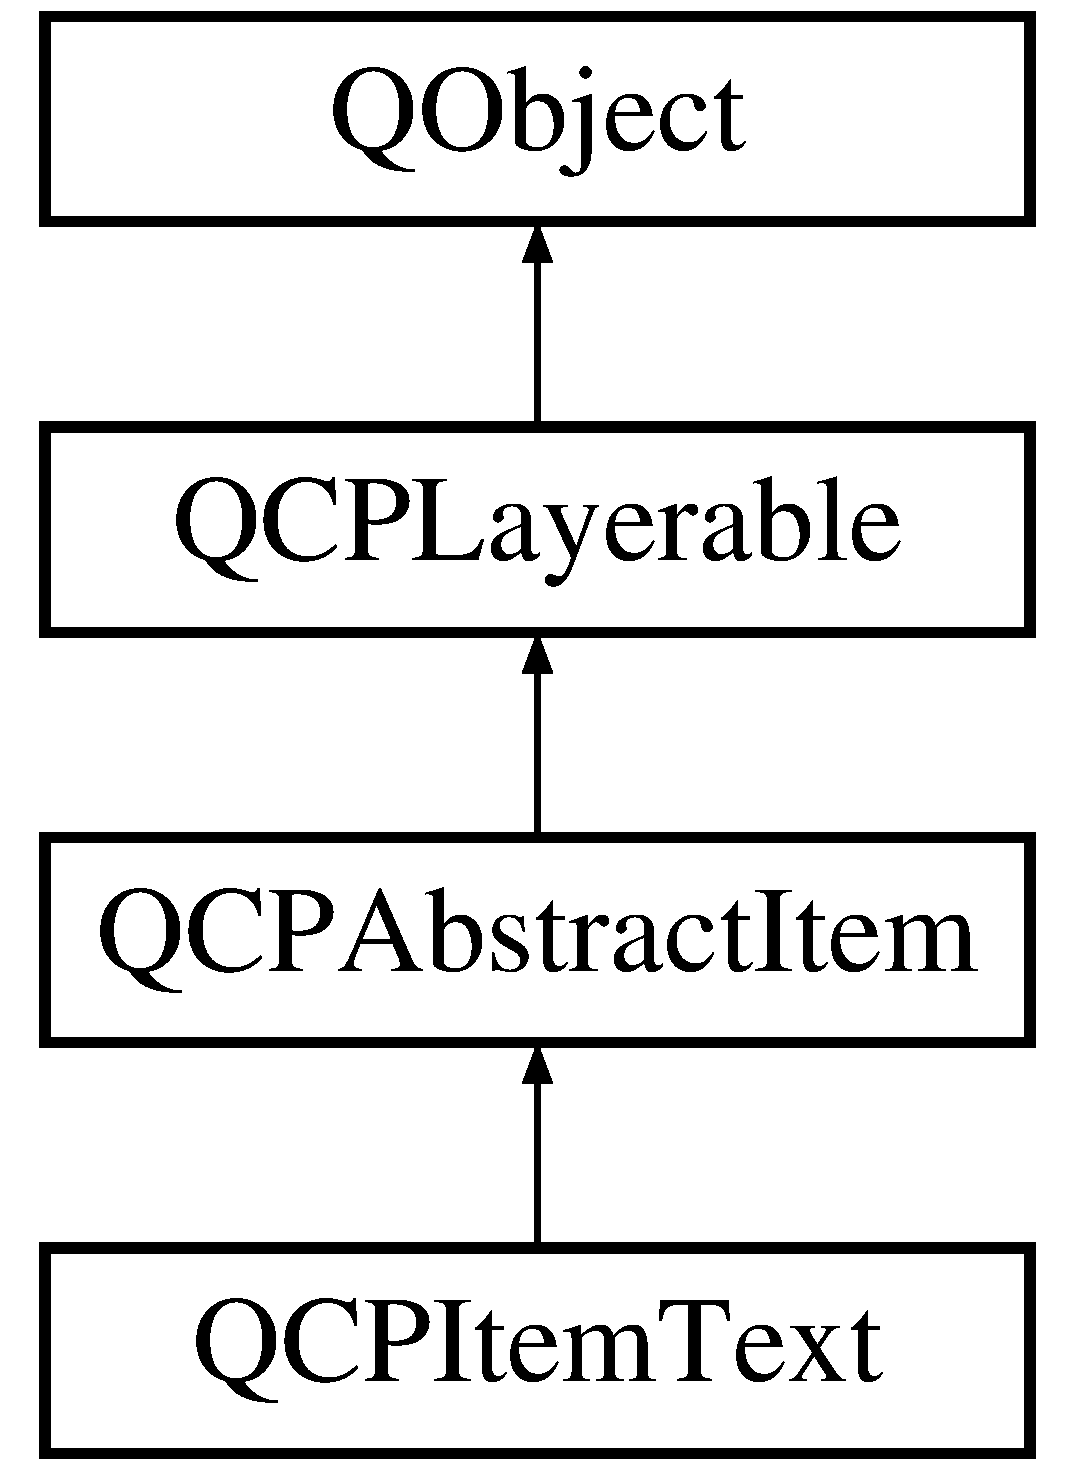
\includegraphics[height=4.000000cm]{class_q_c_p_item_text}
\end{center}
\end{figure}
\subsection*{Public Member Functions}
\begin{DoxyCompactItemize}
\item 
\hyperlink{class_q_c_p_item_text_a77ff96a2972a00872ff8f8c67143abbe}{Q\+C\+P\+Item\+Text} (\hyperlink{class_q_custom_plot}{Q\+Custom\+Plot} $\ast$\hyperlink{class_q_c_p_layerable_ab7e0e94461566093d36ffc0f5312b109}{parent\+Plot})
\item 
virtual \hyperlink{class_q_c_p_item_text_a1efd41ca53d49042d4f4b63cf9615cb6}{$\sim$\+Q\+C\+P\+Item\+Text} ()
\item 
Q\+Color \hyperlink{class_q_c_p_item_text_ac9cb0a8a27f64d1b40855910ea9ebd03}{color} () const 
\item 
Q\+Color \hyperlink{class_q_c_p_item_text_a44f690ec0ba6a32e518f2e923c002e39}{selected\+Color} () const 
\item 
Q\+Pen \hyperlink{class_q_c_p_item_text_a552bd02f46dbcb4b4812559036893352}{pen} () const 
\item 
Q\+Pen \hyperlink{class_q_c_p_item_text_a70c86ec95133d3e904d1718023fe3c4e}{selected\+Pen} () const 
\item 
Q\+Brush \hyperlink{class_q_c_p_item_text_a38b981dfacb703efa8e27346eebcb5a2}{brush} () const 
\item 
Q\+Brush \hyperlink{class_q_c_p_item_text_ac6802bbceff1ade0053166c64a5a6966}{selected\+Brush} () const 
\item 
Q\+Font \hyperlink{class_q_c_p_item_text_ad34943fd68a9b1451d3e3234d072e418}{font} () const 
\item 
Q\+Font \hyperlink{class_q_c_p_item_text_af2e7cacb1975132508714a51c5f48c3b}{selected\+Font} () const 
\item 
Q\+String \hyperlink{class_q_c_p_item_text_a9547f7832010486abed0837e75db5330}{text} () const 
\item 
Qt\+::\+Alignment \hyperlink{class_q_c_p_item_text_af13c6adc480f268116ae72196eb44b06}{position\+Alignment} () const 
\item 
Qt\+::\+Alignment \hyperlink{class_q_c_p_item_text_aaa1d84b3f61f9f2a0cce230e66ef7194}{text\+Alignment} () const 
\item 
double \hyperlink{class_q_c_p_item_text_ae8991207fa1697511c1c8af9f3ca0e0a}{rotation} () const 
\item 
Q\+Margins \hyperlink{class_q_c_p_item_text_a00e0fa03822ff384bf4921c1c90322ff}{padding} () const 
\item 
void \hyperlink{class_q_c_p_item_text_aa51efc0841fe52da9eaf8aff6fc8a8b2}{set\+Color} (const Q\+Color \&\hyperlink{class_q_c_p_item_text_ac9cb0a8a27f64d1b40855910ea9ebd03}{color})
\item 
void \hyperlink{class_q_c_p_item_text_ae7ba0bdb75c897b028388e45bfd435fa}{set\+Selected\+Color} (const Q\+Color \&\hyperlink{class_q_c_p_item_text_ac9cb0a8a27f64d1b40855910ea9ebd03}{color})
\item 
void \hyperlink{class_q_c_p_item_text_a9b9ec6eea0eb0603977ff84d4c78d0a3}{set\+Pen} (const Q\+Pen \&\hyperlink{class_q_c_p_item_text_a552bd02f46dbcb4b4812559036893352}{pen})
\item 
void \hyperlink{class_q_c_p_item_text_a291febe586f0da3f1c392e77bef4aa20}{set\+Selected\+Pen} (const Q\+Pen \&\hyperlink{class_q_c_p_item_text_a552bd02f46dbcb4b4812559036893352}{pen})
\item 
void \hyperlink{class_q_c_p_item_text_a1c7e131516df2ed8d941ef31240ded8e}{set\+Brush} (const Q\+Brush \&\hyperlink{class_q_c_p_item_text_a38b981dfacb703efa8e27346eebcb5a2}{brush})
\item 
void \hyperlink{class_q_c_p_item_text_a6b8377eeb2af75eb9528422671ac16cb}{set\+Selected\+Brush} (const Q\+Brush \&\hyperlink{class_q_c_p_item_text_a38b981dfacb703efa8e27346eebcb5a2}{brush})
\item 
void \hyperlink{class_q_c_p_item_text_a94ad60ebe04f5c07c35e7c2029e96b1f}{set\+Font} (const Q\+Font \&\hyperlink{class_q_c_p_item_text_ad34943fd68a9b1451d3e3234d072e418}{font})
\item 
void \hyperlink{class_q_c_p_item_text_a0be2841772f83663c4db307928b82816}{set\+Selected\+Font} (const Q\+Font \&\hyperlink{class_q_c_p_item_text_ad34943fd68a9b1451d3e3234d072e418}{font})
\item 
void \hyperlink{class_q_c_p_item_text_a3dacdda0ac88f99a05b333b977c48747}{set\+Text} (const Q\+String \&\hyperlink{class_q_c_p_item_text_a9547f7832010486abed0837e75db5330}{text})
\item 
void \hyperlink{class_q_c_p_item_text_a781cdf8c640fc6a055dcff1e675c8c7a}{set\+Position\+Alignment} (Qt\+::\+Alignment alignment)
\item 
void \hyperlink{class_q_c_p_item_text_ab5bc0684c4d1bed81949a11b34dba478}{set\+Text\+Alignment} (Qt\+::\+Alignment alignment)
\item 
void \hyperlink{class_q_c_p_item_text_a4bcc10cd97952c3f749d75824b5077f0}{set\+Rotation} (double degrees)
\item 
void \hyperlink{class_q_c_p_item_text_aeea8a3e01f135f9dd0bb08f51db66310}{set\+Padding} (const Q\+Margins \&\hyperlink{class_q_c_p_item_text_a00e0fa03822ff384bf4921c1c90322ff}{padding})
\item 
virtual double \hyperlink{class_q_c_p_item_text_a285b95bb6634c2e4f7768abb7a8bc69c}{select\+Test} (const Q\+Point\+F \&pos, bool only\+Selectable, Q\+Variant $\ast$details=0) const 
\end{DoxyCompactItemize}
\subsection*{Public Attributes}
\begin{DoxyCompactItemize}
\item 
\hyperlink{class_q_c_p_item_position}{Q\+C\+P\+Item\+Position} $\ast$const \hyperlink{class_q_c_p_item_text_a0d228a00e819022b5690c65762721129}{position}
\item 
\hyperlink{class_q_c_p_item_anchor}{Q\+C\+P\+Item\+Anchor} $\ast$const \hyperlink{class_q_c_p_item_text_a6354d8762182a3502103fabe5fbb8512}{top\+Left}
\item 
\hyperlink{class_q_c_p_item_anchor}{Q\+C\+P\+Item\+Anchor} $\ast$const \hyperlink{class_q_c_p_item_text_a5c87ee162cbbe3d166b97826c8849304}{top}
\item 
\hyperlink{class_q_c_p_item_anchor}{Q\+C\+P\+Item\+Anchor} $\ast$const \hyperlink{class_q_c_p_item_text_ad18ac45cb4cc135de1eb78f2e86b6504}{top\+Right}
\item 
\hyperlink{class_q_c_p_item_anchor}{Q\+C\+P\+Item\+Anchor} $\ast$const \hyperlink{class_q_c_p_item_text_aef159622ce6502412e782a21ba6d84f2}{right}
\item 
\hyperlink{class_q_c_p_item_anchor}{Q\+C\+P\+Item\+Anchor} $\ast$const \hyperlink{class_q_c_p_item_text_a8ad47045c29af43b0312f7d93bb74374}{bottom\+Right}
\item 
\hyperlink{class_q_c_p_item_anchor}{Q\+C\+P\+Item\+Anchor} $\ast$const \hyperlink{class_q_c_p_item_text_a94aeec080f877d3d1d0c3d8ffc10e9e6}{bottom}
\item 
\hyperlink{class_q_c_p_item_anchor}{Q\+C\+P\+Item\+Anchor} $\ast$const \hyperlink{class_q_c_p_item_text_a6a1c872ad3789ecafcaeac2066e218a0}{bottom\+Left}
\item 
\hyperlink{class_q_c_p_item_anchor}{Q\+C\+P\+Item\+Anchor} $\ast$const \hyperlink{class_q_c_p_item_text_ab8c6c6e1df36256986fab1463c0a1d38}{left}
\end{DoxyCompactItemize}
\subsection*{Protected Types}
\begin{DoxyCompactItemize}
\item 
enum \hyperlink{class_q_c_p_item_text_a14a84e58f72519c8ae1d7a4a1dd23f21}{Anchor\+Index} \{ \\*
\hyperlink{class_q_c_p_item_text_a14a84e58f72519c8ae1d7a4a1dd23f21a30342ee15065715f045cb52eb77b904c}{ai\+Top\+Left}, 
\hyperlink{class_q_c_p_item_text_a14a84e58f72519c8ae1d7a4a1dd23f21a55ce9699c71db6d264eb669bb0eb9aff}{ai\+Top}, 
\hyperlink{class_q_c_p_item_text_a14a84e58f72519c8ae1d7a4a1dd23f21a7b6ff56fcad4c78db0b793a96fce9580}{ai\+Top\+Right}, 
\hyperlink{class_q_c_p_item_text_a14a84e58f72519c8ae1d7a4a1dd23f21ad4faa7def46db6df2fedd1926237b48f}{ai\+Right}, 
\\*
\hyperlink{class_q_c_p_item_text_a14a84e58f72519c8ae1d7a4a1dd23f21af2072f259730ef47aa7ad7519f3a0255}{ai\+Bottom\+Right}, 
\hyperlink{class_q_c_p_item_text_a14a84e58f72519c8ae1d7a4a1dd23f21a5773ad69b7f4cd2724ba46d8f31b0688}{ai\+Bottom}, 
\hyperlink{class_q_c_p_item_text_a14a84e58f72519c8ae1d7a4a1dd23f21a489ec73da5a18c15e98a4f9b17ed301f}{ai\+Bottom\+Left}, 
\hyperlink{class_q_c_p_item_text_a14a84e58f72519c8ae1d7a4a1dd23f21a7f1c1b8c574c753e300a4759915a9170}{ai\+Left}
 \}
\end{DoxyCompactItemize}
\subsection*{Protected Member Functions}
\begin{DoxyCompactItemize}
\item 
virtual void \hyperlink{class_q_c_p_item_text_a8793adb271ab79b4cf391dc55e9987f1}{draw} (\hyperlink{class_q_c_p_painter}{Q\+C\+P\+Painter} $\ast$painter)
\item 
virtual Q\+Point\+F \hyperlink{class_q_c_p_item_text_ad248f988534a9d07bc7c220a2457142a}{anchor\+Pixel\+Point} (int anchor\+Id) const 
\item 
Q\+Point\+F \hyperlink{class_q_c_p_item_text_aa6e478b1ce198eace89157c4cacc3ddc}{get\+Text\+Draw\+Point} (const Q\+Point\+F \&pos, const Q\+Rect\+F \&rect, Qt\+::\+Alignment \hyperlink{class_q_c_p_item_text_af13c6adc480f268116ae72196eb44b06}{position\+Alignment}) const 
\item 
Q\+Font \hyperlink{class_q_c_p_item_text_a23d391bd6471c45e73f45add67ede902}{main\+Font} () const 
\item 
Q\+Color \hyperlink{class_q_c_p_item_text_ad7bf17e4945cc86bbf9a36331da059a0}{main\+Color} () const 
\item 
Q\+Pen \hyperlink{class_q_c_p_item_text_a9ade32d362b22853659201c738269e2a}{main\+Pen} () const 
\item 
Q\+Brush \hyperlink{class_q_c_p_item_text_a10d6585a030633aa79d5ebc5a437f183}{main\+Brush} () const 
\end{DoxyCompactItemize}
\subsection*{Protected Attributes}
\begin{DoxyCompactItemize}
\item 
Q\+Color \hyperlink{class_q_c_p_item_text_a8407f284ad867f627878cc26ef433d08}{m\+Color}
\item 
Q\+Color \hyperlink{class_q_c_p_item_text_a7eb64e42f5f7998a97d8907ad25933c1}{m\+Selected\+Color}
\item 
Q\+Pen \hyperlink{class_q_c_p_item_text_aa02388705dbbff1bf7b8aa872b5f579c}{m\+Pen}
\item 
Q\+Pen \hyperlink{class_q_c_p_item_text_a8eaec649606d6ead2d8d4dcb5691777c}{m\+Selected\+Pen}
\item 
Q\+Brush \hyperlink{class_q_c_p_item_text_a2535911875faa459b8337f2efccb5cb8}{m\+Brush}
\item 
Q\+Brush \hyperlink{class_q_c_p_item_text_a28ccd097b42a216d81db9c6869f54a59}{m\+Selected\+Brush}
\item 
Q\+Font \hyperlink{class_q_c_p_item_text_a1dc87fe2a824820d549ffd7e644eef8d}{m\+Font}
\item 
Q\+Font \hyperlink{class_q_c_p_item_text_a6702f141fae590b2f4f1ec02fe9f8bd5}{m\+Selected\+Font}
\item 
Q\+String \hyperlink{class_q_c_p_item_text_a2dec3e08c11f51639629374ecec3bd62}{m\+Text}
\item 
Qt\+::\+Alignment \hyperlink{class_q_c_p_item_text_a6c27f7dc1a962a04b32430cf99f04654}{m\+Position\+Alignment}
\item 
Qt\+::\+Alignment \hyperlink{class_q_c_p_item_text_acdb2e50c38e83da00f083771efbd213f}{m\+Text\+Alignment}
\item 
double \hyperlink{class_q_c_p_item_text_ac37df0061552225d2277e1ee3b48f2cb}{m\+Rotation}
\item 
Q\+Margins \hyperlink{class_q_c_p_item_text_ae7b3ef0ce6046efd4b346d28f2e1fb67}{m\+Padding}
\end{DoxyCompactItemize}
\subsection*{Additional Inherited Members}


\subsection{Detailed Description}
A text label. 

 Its position is defined by the member {\itshape position} and the setting of \hyperlink{class_q_c_p_item_text_a781cdf8c640fc6a055dcff1e675c8c7a}{set\+Position\+Alignment}. The latter controls which part of the text rect shall be aligned with {\itshape position}.

The text alignment itself (i.\+e. left, center, right) can be controlled with \hyperlink{class_q_c_p_item_text_ab5bc0684c4d1bed81949a11b34dba478}{set\+Text\+Alignment}.

The text may be rotated around the {\itshape position} point with \hyperlink{class_q_c_p_item_text_a4bcc10cd97952c3f749d75824b5077f0}{set\+Rotation}. 

\subsection{Member Enumeration Documentation}
\hypertarget{class_q_c_p_item_text_a14a84e58f72519c8ae1d7a4a1dd23f21}{}\index{Q\+C\+P\+Item\+Text@{Q\+C\+P\+Item\+Text}!Anchor\+Index@{Anchor\+Index}}
\index{Anchor\+Index@{Anchor\+Index}!Q\+C\+P\+Item\+Text@{Q\+C\+P\+Item\+Text}}
\subsubsection[{Anchor\+Index}]{\setlength{\rightskip}{0pt plus 5cm}enum {\bf Q\+C\+P\+Item\+Text\+::\+Anchor\+Index}\hspace{0.3cm}{\ttfamily [protected]}}\label{class_q_c_p_item_text_a14a84e58f72519c8ae1d7a4a1dd23f21}
\begin{Desc}
\item[Enumerator]\par
\begin{description}
\index{ai\+Top\+Left@{ai\+Top\+Left}!Q\+C\+P\+Item\+Text@{Q\+C\+P\+Item\+Text}}\index{Q\+C\+P\+Item\+Text@{Q\+C\+P\+Item\+Text}!ai\+Top\+Left@{ai\+Top\+Left}}\item[{\em 
\hypertarget{class_q_c_p_item_text_a14a84e58f72519c8ae1d7a4a1dd23f21a30342ee15065715f045cb52eb77b904c}{}ai\+Top\+Left\label{class_q_c_p_item_text_a14a84e58f72519c8ae1d7a4a1dd23f21a30342ee15065715f045cb52eb77b904c}
}]\index{ai\+Top@{ai\+Top}!Q\+C\+P\+Item\+Text@{Q\+C\+P\+Item\+Text}}\index{Q\+C\+P\+Item\+Text@{Q\+C\+P\+Item\+Text}!ai\+Top@{ai\+Top}}\item[{\em 
\hypertarget{class_q_c_p_item_text_a14a84e58f72519c8ae1d7a4a1dd23f21a55ce9699c71db6d264eb669bb0eb9aff}{}ai\+Top\label{class_q_c_p_item_text_a14a84e58f72519c8ae1d7a4a1dd23f21a55ce9699c71db6d264eb669bb0eb9aff}
}]\index{ai\+Top\+Right@{ai\+Top\+Right}!Q\+C\+P\+Item\+Text@{Q\+C\+P\+Item\+Text}}\index{Q\+C\+P\+Item\+Text@{Q\+C\+P\+Item\+Text}!ai\+Top\+Right@{ai\+Top\+Right}}\item[{\em 
\hypertarget{class_q_c_p_item_text_a14a84e58f72519c8ae1d7a4a1dd23f21a7b6ff56fcad4c78db0b793a96fce9580}{}ai\+Top\+Right\label{class_q_c_p_item_text_a14a84e58f72519c8ae1d7a4a1dd23f21a7b6ff56fcad4c78db0b793a96fce9580}
}]\index{ai\+Right@{ai\+Right}!Q\+C\+P\+Item\+Text@{Q\+C\+P\+Item\+Text}}\index{Q\+C\+P\+Item\+Text@{Q\+C\+P\+Item\+Text}!ai\+Right@{ai\+Right}}\item[{\em 
\hypertarget{class_q_c_p_item_text_a14a84e58f72519c8ae1d7a4a1dd23f21ad4faa7def46db6df2fedd1926237b48f}{}ai\+Right\label{class_q_c_p_item_text_a14a84e58f72519c8ae1d7a4a1dd23f21ad4faa7def46db6df2fedd1926237b48f}
}]\index{ai\+Bottom\+Right@{ai\+Bottom\+Right}!Q\+C\+P\+Item\+Text@{Q\+C\+P\+Item\+Text}}\index{Q\+C\+P\+Item\+Text@{Q\+C\+P\+Item\+Text}!ai\+Bottom\+Right@{ai\+Bottom\+Right}}\item[{\em 
\hypertarget{class_q_c_p_item_text_a14a84e58f72519c8ae1d7a4a1dd23f21af2072f259730ef47aa7ad7519f3a0255}{}ai\+Bottom\+Right\label{class_q_c_p_item_text_a14a84e58f72519c8ae1d7a4a1dd23f21af2072f259730ef47aa7ad7519f3a0255}
}]\index{ai\+Bottom@{ai\+Bottom}!Q\+C\+P\+Item\+Text@{Q\+C\+P\+Item\+Text}}\index{Q\+C\+P\+Item\+Text@{Q\+C\+P\+Item\+Text}!ai\+Bottom@{ai\+Bottom}}\item[{\em 
\hypertarget{class_q_c_p_item_text_a14a84e58f72519c8ae1d7a4a1dd23f21a5773ad69b7f4cd2724ba46d8f31b0688}{}ai\+Bottom\label{class_q_c_p_item_text_a14a84e58f72519c8ae1d7a4a1dd23f21a5773ad69b7f4cd2724ba46d8f31b0688}
}]\index{ai\+Bottom\+Left@{ai\+Bottom\+Left}!Q\+C\+P\+Item\+Text@{Q\+C\+P\+Item\+Text}}\index{Q\+C\+P\+Item\+Text@{Q\+C\+P\+Item\+Text}!ai\+Bottom\+Left@{ai\+Bottom\+Left}}\item[{\em 
\hypertarget{class_q_c_p_item_text_a14a84e58f72519c8ae1d7a4a1dd23f21a489ec73da5a18c15e98a4f9b17ed301f}{}ai\+Bottom\+Left\label{class_q_c_p_item_text_a14a84e58f72519c8ae1d7a4a1dd23f21a489ec73da5a18c15e98a4f9b17ed301f}
}]\index{ai\+Left@{ai\+Left}!Q\+C\+P\+Item\+Text@{Q\+C\+P\+Item\+Text}}\index{Q\+C\+P\+Item\+Text@{Q\+C\+P\+Item\+Text}!ai\+Left@{ai\+Left}}\item[{\em 
\hypertarget{class_q_c_p_item_text_a14a84e58f72519c8ae1d7a4a1dd23f21a7f1c1b8c574c753e300a4759915a9170}{}ai\+Left\label{class_q_c_p_item_text_a14a84e58f72519c8ae1d7a4a1dd23f21a7f1c1b8c574c753e300a4759915a9170}
}]\end{description}
\end{Desc}


\subsection{Constructor \& Destructor Documentation}
\hypertarget{class_q_c_p_item_text_a77ff96a2972a00872ff8f8c67143abbe}{}\index{Q\+C\+P\+Item\+Text@{Q\+C\+P\+Item\+Text}!Q\+C\+P\+Item\+Text@{Q\+C\+P\+Item\+Text}}
\index{Q\+C\+P\+Item\+Text@{Q\+C\+P\+Item\+Text}!Q\+C\+P\+Item\+Text@{Q\+C\+P\+Item\+Text}}
\subsubsection[{Q\+C\+P\+Item\+Text}]{\setlength{\rightskip}{0pt plus 5cm}Q\+C\+P\+Item\+Text\+::\+Q\+C\+P\+Item\+Text (
\begin{DoxyParamCaption}
\item[{{\bf Q\+Custom\+Plot} $\ast$}]{parent\+Plot}
\end{DoxyParamCaption}
)}\label{class_q_c_p_item_text_a77ff96a2972a00872ff8f8c67143abbe}
Creates a text item and sets default values.

The constructed item can be added to the plot with \hyperlink{class_q_custom_plot_aa500620379262321685cb7a7674cbd2a}{Q\+Custom\+Plot\+::add\+Item}. \hypertarget{class_q_c_p_item_text_a1efd41ca53d49042d4f4b63cf9615cb6}{}\index{Q\+C\+P\+Item\+Text@{Q\+C\+P\+Item\+Text}!````~Q\+C\+P\+Item\+Text@{$\sim$\+Q\+C\+P\+Item\+Text}}
\index{````~Q\+C\+P\+Item\+Text@{$\sim$\+Q\+C\+P\+Item\+Text}!Q\+C\+P\+Item\+Text@{Q\+C\+P\+Item\+Text}}
\subsubsection[{$\sim$\+Q\+C\+P\+Item\+Text}]{\setlength{\rightskip}{0pt plus 5cm}Q\+C\+P\+Item\+Text\+::$\sim$\+Q\+C\+P\+Item\+Text (
\begin{DoxyParamCaption}
{}
\end{DoxyParamCaption}
)\hspace{0.3cm}{\ttfamily [virtual]}}\label{class_q_c_p_item_text_a1efd41ca53d49042d4f4b63cf9615cb6}


\subsection{Member Function Documentation}
\hypertarget{class_q_c_p_item_text_ad248f988534a9d07bc7c220a2457142a}{}\index{Q\+C\+P\+Item\+Text@{Q\+C\+P\+Item\+Text}!anchor\+Pixel\+Point@{anchor\+Pixel\+Point}}
\index{anchor\+Pixel\+Point@{anchor\+Pixel\+Point}!Q\+C\+P\+Item\+Text@{Q\+C\+P\+Item\+Text}}
\subsubsection[{anchor\+Pixel\+Point}]{\setlength{\rightskip}{0pt plus 5cm}Q\+Point\+F Q\+C\+P\+Item\+Text\+::anchor\+Pixel\+Point (
\begin{DoxyParamCaption}
\item[{int}]{anchor\+Id}
\end{DoxyParamCaption}
) const\hspace{0.3cm}{\ttfamily [protected]}, {\ttfamily [virtual]}}\label{class_q_c_p_item_text_ad248f988534a9d07bc7c220a2457142a}


Reimplemented from \hyperlink{class_q_c_p_abstract_item_a94bde62b8a2fc133666dcbb8035deeed}{Q\+C\+P\+Abstract\+Item}.

\hypertarget{class_q_c_p_item_text_a38b981dfacb703efa8e27346eebcb5a2}{}\index{Q\+C\+P\+Item\+Text@{Q\+C\+P\+Item\+Text}!brush@{brush}}
\index{brush@{brush}!Q\+C\+P\+Item\+Text@{Q\+C\+P\+Item\+Text}}
\subsubsection[{brush}]{\setlength{\rightskip}{0pt plus 5cm}Q\+Brush Q\+C\+P\+Item\+Text\+::brush (
\begin{DoxyParamCaption}
{}
\end{DoxyParamCaption}
) const\hspace{0.3cm}{\ttfamily [inline]}}\label{class_q_c_p_item_text_a38b981dfacb703efa8e27346eebcb5a2}
\hypertarget{class_q_c_p_item_text_ac9cb0a8a27f64d1b40855910ea9ebd03}{}\index{Q\+C\+P\+Item\+Text@{Q\+C\+P\+Item\+Text}!color@{color}}
\index{color@{color}!Q\+C\+P\+Item\+Text@{Q\+C\+P\+Item\+Text}}
\subsubsection[{color}]{\setlength{\rightskip}{0pt plus 5cm}Q\+Color Q\+C\+P\+Item\+Text\+::color (
\begin{DoxyParamCaption}
{}
\end{DoxyParamCaption}
) const\hspace{0.3cm}{\ttfamily [inline]}}\label{class_q_c_p_item_text_ac9cb0a8a27f64d1b40855910ea9ebd03}
\hypertarget{class_q_c_p_item_text_a8793adb271ab79b4cf391dc55e9987f1}{}\index{Q\+C\+P\+Item\+Text@{Q\+C\+P\+Item\+Text}!draw@{draw}}
\index{draw@{draw}!Q\+C\+P\+Item\+Text@{Q\+C\+P\+Item\+Text}}
\subsubsection[{draw}]{\setlength{\rightskip}{0pt plus 5cm}void Q\+C\+P\+Item\+Text\+::draw (
\begin{DoxyParamCaption}
\item[{{\bf Q\+C\+P\+Painter} $\ast$}]{painter}
\end{DoxyParamCaption}
)\hspace{0.3cm}{\ttfamily [protected]}, {\ttfamily [virtual]}}\label{class_q_c_p_item_text_a8793adb271ab79b4cf391dc55e9987f1}


Implements \hyperlink{class_q_c_p_abstract_item_ad0dc056f650c3ca73414e6b4f01674ef}{Q\+C\+P\+Abstract\+Item}.

\hypertarget{class_q_c_p_item_text_ad34943fd68a9b1451d3e3234d072e418}{}\index{Q\+C\+P\+Item\+Text@{Q\+C\+P\+Item\+Text}!font@{font}}
\index{font@{font}!Q\+C\+P\+Item\+Text@{Q\+C\+P\+Item\+Text}}
\subsubsection[{font}]{\setlength{\rightskip}{0pt plus 5cm}Q\+Font Q\+C\+P\+Item\+Text\+::font (
\begin{DoxyParamCaption}
{}
\end{DoxyParamCaption}
) const\hspace{0.3cm}{\ttfamily [inline]}}\label{class_q_c_p_item_text_ad34943fd68a9b1451d3e3234d072e418}
\hypertarget{class_q_c_p_item_text_aa6e478b1ce198eace89157c4cacc3ddc}{}\index{Q\+C\+P\+Item\+Text@{Q\+C\+P\+Item\+Text}!get\+Text\+Draw\+Point@{get\+Text\+Draw\+Point}}
\index{get\+Text\+Draw\+Point@{get\+Text\+Draw\+Point}!Q\+C\+P\+Item\+Text@{Q\+C\+P\+Item\+Text}}
\subsubsection[{get\+Text\+Draw\+Point}]{\setlength{\rightskip}{0pt plus 5cm}Q\+Point\+F Q\+C\+P\+Item\+Text\+::get\+Text\+Draw\+Point (
\begin{DoxyParamCaption}
\item[{const Q\+Point\+F \&}]{pos, }
\item[{const Q\+Rect\+F \&}]{rect, }
\item[{Qt\+::\+Alignment}]{position\+Alignment}
\end{DoxyParamCaption}
) const\hspace{0.3cm}{\ttfamily [protected]}}\label{class_q_c_p_item_text_aa6e478b1ce198eace89157c4cacc3ddc}
\hypertarget{class_q_c_p_item_text_a10d6585a030633aa79d5ebc5a437f183}{}\index{Q\+C\+P\+Item\+Text@{Q\+C\+P\+Item\+Text}!main\+Brush@{main\+Brush}}
\index{main\+Brush@{main\+Brush}!Q\+C\+P\+Item\+Text@{Q\+C\+P\+Item\+Text}}
\subsubsection[{main\+Brush}]{\setlength{\rightskip}{0pt plus 5cm}Q\+Brush Q\+C\+P\+Item\+Text\+::main\+Brush (
\begin{DoxyParamCaption}
{}
\end{DoxyParamCaption}
) const\hspace{0.3cm}{\ttfamily [protected]}}\label{class_q_c_p_item_text_a10d6585a030633aa79d5ebc5a437f183}
\hypertarget{class_q_c_p_item_text_ad7bf17e4945cc86bbf9a36331da059a0}{}\index{Q\+C\+P\+Item\+Text@{Q\+C\+P\+Item\+Text}!main\+Color@{main\+Color}}
\index{main\+Color@{main\+Color}!Q\+C\+P\+Item\+Text@{Q\+C\+P\+Item\+Text}}
\subsubsection[{main\+Color}]{\setlength{\rightskip}{0pt plus 5cm}Q\+Color Q\+C\+P\+Item\+Text\+::main\+Color (
\begin{DoxyParamCaption}
{}
\end{DoxyParamCaption}
) const\hspace{0.3cm}{\ttfamily [protected]}}\label{class_q_c_p_item_text_ad7bf17e4945cc86bbf9a36331da059a0}
\hypertarget{class_q_c_p_item_text_a23d391bd6471c45e73f45add67ede902}{}\index{Q\+C\+P\+Item\+Text@{Q\+C\+P\+Item\+Text}!main\+Font@{main\+Font}}
\index{main\+Font@{main\+Font}!Q\+C\+P\+Item\+Text@{Q\+C\+P\+Item\+Text}}
\subsubsection[{main\+Font}]{\setlength{\rightskip}{0pt plus 5cm}Q\+Font Q\+C\+P\+Item\+Text\+::main\+Font (
\begin{DoxyParamCaption}
{}
\end{DoxyParamCaption}
) const\hspace{0.3cm}{\ttfamily [protected]}}\label{class_q_c_p_item_text_a23d391bd6471c45e73f45add67ede902}
\hypertarget{class_q_c_p_item_text_a9ade32d362b22853659201c738269e2a}{}\index{Q\+C\+P\+Item\+Text@{Q\+C\+P\+Item\+Text}!main\+Pen@{main\+Pen}}
\index{main\+Pen@{main\+Pen}!Q\+C\+P\+Item\+Text@{Q\+C\+P\+Item\+Text}}
\subsubsection[{main\+Pen}]{\setlength{\rightskip}{0pt plus 5cm}Q\+Pen Q\+C\+P\+Item\+Text\+::main\+Pen (
\begin{DoxyParamCaption}
{}
\end{DoxyParamCaption}
) const\hspace{0.3cm}{\ttfamily [protected]}}\label{class_q_c_p_item_text_a9ade32d362b22853659201c738269e2a}
\hypertarget{class_q_c_p_item_text_a00e0fa03822ff384bf4921c1c90322ff}{}\index{Q\+C\+P\+Item\+Text@{Q\+C\+P\+Item\+Text}!padding@{padding}}
\index{padding@{padding}!Q\+C\+P\+Item\+Text@{Q\+C\+P\+Item\+Text}}
\subsubsection[{padding}]{\setlength{\rightskip}{0pt plus 5cm}Q\+Margins Q\+C\+P\+Item\+Text\+::padding (
\begin{DoxyParamCaption}
{}
\end{DoxyParamCaption}
) const\hspace{0.3cm}{\ttfamily [inline]}}\label{class_q_c_p_item_text_a00e0fa03822ff384bf4921c1c90322ff}
\hypertarget{class_q_c_p_item_text_a552bd02f46dbcb4b4812559036893352}{}\index{Q\+C\+P\+Item\+Text@{Q\+C\+P\+Item\+Text}!pen@{pen}}
\index{pen@{pen}!Q\+C\+P\+Item\+Text@{Q\+C\+P\+Item\+Text}}
\subsubsection[{pen}]{\setlength{\rightskip}{0pt plus 5cm}Q\+Pen Q\+C\+P\+Item\+Text\+::pen (
\begin{DoxyParamCaption}
{}
\end{DoxyParamCaption}
) const\hspace{0.3cm}{\ttfamily [inline]}}\label{class_q_c_p_item_text_a552bd02f46dbcb4b4812559036893352}
\hypertarget{class_q_c_p_item_text_af13c6adc480f268116ae72196eb44b06}{}\index{Q\+C\+P\+Item\+Text@{Q\+C\+P\+Item\+Text}!position\+Alignment@{position\+Alignment}}
\index{position\+Alignment@{position\+Alignment}!Q\+C\+P\+Item\+Text@{Q\+C\+P\+Item\+Text}}
\subsubsection[{position\+Alignment}]{\setlength{\rightskip}{0pt plus 5cm}Qt\+::\+Alignment Q\+C\+P\+Item\+Text\+::position\+Alignment (
\begin{DoxyParamCaption}
{}
\end{DoxyParamCaption}
) const\hspace{0.3cm}{\ttfamily [inline]}}\label{class_q_c_p_item_text_af13c6adc480f268116ae72196eb44b06}
\hypertarget{class_q_c_p_item_text_ae8991207fa1697511c1c8af9f3ca0e0a}{}\index{Q\+C\+P\+Item\+Text@{Q\+C\+P\+Item\+Text}!rotation@{rotation}}
\index{rotation@{rotation}!Q\+C\+P\+Item\+Text@{Q\+C\+P\+Item\+Text}}
\subsubsection[{rotation}]{\setlength{\rightskip}{0pt plus 5cm}double Q\+C\+P\+Item\+Text\+::rotation (
\begin{DoxyParamCaption}
{}
\end{DoxyParamCaption}
) const\hspace{0.3cm}{\ttfamily [inline]}}\label{class_q_c_p_item_text_ae8991207fa1697511c1c8af9f3ca0e0a}
\hypertarget{class_q_c_p_item_text_ac6802bbceff1ade0053166c64a5a6966}{}\index{Q\+C\+P\+Item\+Text@{Q\+C\+P\+Item\+Text}!selected\+Brush@{selected\+Brush}}
\index{selected\+Brush@{selected\+Brush}!Q\+C\+P\+Item\+Text@{Q\+C\+P\+Item\+Text}}
\subsubsection[{selected\+Brush}]{\setlength{\rightskip}{0pt plus 5cm}Q\+Brush Q\+C\+P\+Item\+Text\+::selected\+Brush (
\begin{DoxyParamCaption}
{}
\end{DoxyParamCaption}
) const\hspace{0.3cm}{\ttfamily [inline]}}\label{class_q_c_p_item_text_ac6802bbceff1ade0053166c64a5a6966}
\hypertarget{class_q_c_p_item_text_a44f690ec0ba6a32e518f2e923c002e39}{}\index{Q\+C\+P\+Item\+Text@{Q\+C\+P\+Item\+Text}!selected\+Color@{selected\+Color}}
\index{selected\+Color@{selected\+Color}!Q\+C\+P\+Item\+Text@{Q\+C\+P\+Item\+Text}}
\subsubsection[{selected\+Color}]{\setlength{\rightskip}{0pt plus 5cm}Q\+Color Q\+C\+P\+Item\+Text\+::selected\+Color (
\begin{DoxyParamCaption}
{}
\end{DoxyParamCaption}
) const\hspace{0.3cm}{\ttfamily [inline]}}\label{class_q_c_p_item_text_a44f690ec0ba6a32e518f2e923c002e39}
\hypertarget{class_q_c_p_item_text_af2e7cacb1975132508714a51c5f48c3b}{}\index{Q\+C\+P\+Item\+Text@{Q\+C\+P\+Item\+Text}!selected\+Font@{selected\+Font}}
\index{selected\+Font@{selected\+Font}!Q\+C\+P\+Item\+Text@{Q\+C\+P\+Item\+Text}}
\subsubsection[{selected\+Font}]{\setlength{\rightskip}{0pt plus 5cm}Q\+Font Q\+C\+P\+Item\+Text\+::selected\+Font (
\begin{DoxyParamCaption}
{}
\end{DoxyParamCaption}
) const\hspace{0.3cm}{\ttfamily [inline]}}\label{class_q_c_p_item_text_af2e7cacb1975132508714a51c5f48c3b}
\hypertarget{class_q_c_p_item_text_a70c86ec95133d3e904d1718023fe3c4e}{}\index{Q\+C\+P\+Item\+Text@{Q\+C\+P\+Item\+Text}!selected\+Pen@{selected\+Pen}}
\index{selected\+Pen@{selected\+Pen}!Q\+C\+P\+Item\+Text@{Q\+C\+P\+Item\+Text}}
\subsubsection[{selected\+Pen}]{\setlength{\rightskip}{0pt plus 5cm}Q\+Pen Q\+C\+P\+Item\+Text\+::selected\+Pen (
\begin{DoxyParamCaption}
{}
\end{DoxyParamCaption}
) const\hspace{0.3cm}{\ttfamily [inline]}}\label{class_q_c_p_item_text_a70c86ec95133d3e904d1718023fe3c4e}
\hypertarget{class_q_c_p_item_text_a285b95bb6634c2e4f7768abb7a8bc69c}{}\index{Q\+C\+P\+Item\+Text@{Q\+C\+P\+Item\+Text}!select\+Test@{select\+Test}}
\index{select\+Test@{select\+Test}!Q\+C\+P\+Item\+Text@{Q\+C\+P\+Item\+Text}}
\subsubsection[{select\+Test}]{\setlength{\rightskip}{0pt plus 5cm}double Q\+C\+P\+Item\+Text\+::select\+Test (
\begin{DoxyParamCaption}
\item[{const Q\+Point\+F \&}]{pos, }
\item[{bool}]{only\+Selectable, }
\item[{Q\+Variant $\ast$}]{details = {\ttfamily 0}}
\end{DoxyParamCaption}
) const\hspace{0.3cm}{\ttfamily [virtual]}}\label{class_q_c_p_item_text_a285b95bb6634c2e4f7768abb7a8bc69c}
This function is used to decide whether a click hits a layerable object or not.

{\itshape pos} is a point in pixel coordinates on the \hyperlink{class_q_custom_plot}{Q\+Custom\+Plot} surface. This function returns the shortest pixel distance of this point to the object. If the object is either invisible or the distance couldn\textquotesingle{}t be determined, -\/1.\+0 is returned. Further, if {\itshape only\+Selectable} is true and the object is not selectable, -\/1.\+0 is returned, too.

If the item is represented not by single lines but by an area like \hyperlink{class_q_c_p_item_rect}{Q\+C\+P\+Item\+Rect} or \hyperlink{class_q_c_p_item_text}{Q\+C\+P\+Item\+Text}, a click inside the area returns a constant value greater zero (typically the selection\+Tolerance of the parent \hyperlink{class_q_custom_plot}{Q\+Custom\+Plot} multiplied by 0.\+99). If the click lies outside the area, this function returns -\/1.\+0.

Providing a constant value for area objects allows selecting line objects even when they are obscured by such area objects, by clicking close to the lines (i.\+e. closer than 0.\+99$\ast$selection\+Tolerance).

The actual setting of the selection state is not done by this function. This is handled by the parent \hyperlink{class_q_custom_plot}{Q\+Custom\+Plot} when the mouse\+Release\+Event occurs, and the finally selected object is notified via the select\+Event/deselect\+Event methods.

{\itshape details} is an optional output parameter. Every layerable subclass may place any information in {\itshape details}. This information will be passed to \hyperlink{class_q_c_p_abstract_item_aaf92af7b9893712959a6c073d334d88d}{select\+Event} when the parent \hyperlink{class_q_custom_plot}{Q\+Custom\+Plot} decides on the basis of this select\+Test call, that the object was successfully selected. The subsequent call to \hyperlink{class_q_c_p_abstract_item_aaf92af7b9893712959a6c073d334d88d}{select\+Event} will carry the {\itshape details}. This is useful for multi-\/part objects (like \hyperlink{class_q_c_p_axis}{Q\+C\+P\+Axis}). This way, a possibly complex calculation to decide which part was clicked is only done once in \hyperlink{class_q_c_p_item_text_a285b95bb6634c2e4f7768abb7a8bc69c}{select\+Test}. The result (i.\+e. the actually clicked part) can then be placed in {\itshape details}. So in the subsequent \hyperlink{class_q_c_p_abstract_item_aaf92af7b9893712959a6c073d334d88d}{select\+Event}, the decision which part was selected doesn\textquotesingle{}t have to be done a second time for a single selection operation.

You may pass 0 as {\itshape details} to indicate that you are not interested in those selection details.

\begin{DoxySeeAlso}{See also}
\hyperlink{class_q_c_p_abstract_item_aaf92af7b9893712959a6c073d334d88d}{select\+Event}, \hyperlink{class_q_c_p_abstract_item_a91f090d6763cfedb0749219c63788ae9}{deselect\+Event}, \hyperlink{class_q_custom_plot_a5ee1e2f6ae27419deca53e75907c27e5}{Q\+Custom\+Plot\+::set\+Interactions} 
\end{DoxySeeAlso}


Implements \hyperlink{class_q_c_p_abstract_item_a96d522d10ffc0413b9a366c6f7f0476b}{Q\+C\+P\+Abstract\+Item}.

\hypertarget{class_q_c_p_item_text_a1c7e131516df2ed8d941ef31240ded8e}{}\index{Q\+C\+P\+Item\+Text@{Q\+C\+P\+Item\+Text}!set\+Brush@{set\+Brush}}
\index{set\+Brush@{set\+Brush}!Q\+C\+P\+Item\+Text@{Q\+C\+P\+Item\+Text}}
\subsubsection[{set\+Brush}]{\setlength{\rightskip}{0pt plus 5cm}void Q\+C\+P\+Item\+Text\+::set\+Brush (
\begin{DoxyParamCaption}
\item[{const Q\+Brush \&}]{brush}
\end{DoxyParamCaption}
)}\label{class_q_c_p_item_text_a1c7e131516df2ed8d941ef31240ded8e}
Sets the brush that will be used do fill the background of the text. To disable the background, set {\itshape brush} to Qt\+::\+No\+Brush.

\begin{DoxySeeAlso}{See also}
\hyperlink{class_q_c_p_item_text_a6b8377eeb2af75eb9528422671ac16cb}{set\+Selected\+Brush}, \hyperlink{class_q_c_p_item_text_a9b9ec6eea0eb0603977ff84d4c78d0a3}{set\+Pen}, \hyperlink{class_q_c_p_item_text_aeea8a3e01f135f9dd0bb08f51db66310}{set\+Padding} 
\end{DoxySeeAlso}
\hypertarget{class_q_c_p_item_text_aa51efc0841fe52da9eaf8aff6fc8a8b2}{}\index{Q\+C\+P\+Item\+Text@{Q\+C\+P\+Item\+Text}!set\+Color@{set\+Color}}
\index{set\+Color@{set\+Color}!Q\+C\+P\+Item\+Text@{Q\+C\+P\+Item\+Text}}
\subsubsection[{set\+Color}]{\setlength{\rightskip}{0pt plus 5cm}void Q\+C\+P\+Item\+Text\+::set\+Color (
\begin{DoxyParamCaption}
\item[{const Q\+Color \&}]{color}
\end{DoxyParamCaption}
)}\label{class_q_c_p_item_text_aa51efc0841fe52da9eaf8aff6fc8a8b2}
Sets the color of the text. \hypertarget{class_q_c_p_item_text_a94ad60ebe04f5c07c35e7c2029e96b1f}{}\index{Q\+C\+P\+Item\+Text@{Q\+C\+P\+Item\+Text}!set\+Font@{set\+Font}}
\index{set\+Font@{set\+Font}!Q\+C\+P\+Item\+Text@{Q\+C\+P\+Item\+Text}}
\subsubsection[{set\+Font}]{\setlength{\rightskip}{0pt plus 5cm}void Q\+C\+P\+Item\+Text\+::set\+Font (
\begin{DoxyParamCaption}
\item[{const Q\+Font \&}]{font}
\end{DoxyParamCaption}
)}\label{class_q_c_p_item_text_a94ad60ebe04f5c07c35e7c2029e96b1f}
Sets the font of the text.

\begin{DoxySeeAlso}{See also}
\hyperlink{class_q_c_p_item_text_a0be2841772f83663c4db307928b82816}{set\+Selected\+Font}, \hyperlink{class_q_c_p_item_text_aa51efc0841fe52da9eaf8aff6fc8a8b2}{set\+Color} 
\end{DoxySeeAlso}
\hypertarget{class_q_c_p_item_text_aeea8a3e01f135f9dd0bb08f51db66310}{}\index{Q\+C\+P\+Item\+Text@{Q\+C\+P\+Item\+Text}!set\+Padding@{set\+Padding}}
\index{set\+Padding@{set\+Padding}!Q\+C\+P\+Item\+Text@{Q\+C\+P\+Item\+Text}}
\subsubsection[{set\+Padding}]{\setlength{\rightskip}{0pt plus 5cm}void Q\+C\+P\+Item\+Text\+::set\+Padding (
\begin{DoxyParamCaption}
\item[{const Q\+Margins \&}]{padding}
\end{DoxyParamCaption}
)}\label{class_q_c_p_item_text_aeea8a3e01f135f9dd0bb08f51db66310}
Sets the distance between the border of the text rectangle and the text. The appearance (and visibility) of the text rectangle can be controlled with \hyperlink{class_q_c_p_item_text_a9b9ec6eea0eb0603977ff84d4c78d0a3}{set\+Pen} and \hyperlink{class_q_c_p_item_text_a1c7e131516df2ed8d941ef31240ded8e}{set\+Brush}. \hypertarget{class_q_c_p_item_text_a9b9ec6eea0eb0603977ff84d4c78d0a3}{}\index{Q\+C\+P\+Item\+Text@{Q\+C\+P\+Item\+Text}!set\+Pen@{set\+Pen}}
\index{set\+Pen@{set\+Pen}!Q\+C\+P\+Item\+Text@{Q\+C\+P\+Item\+Text}}
\subsubsection[{set\+Pen}]{\setlength{\rightskip}{0pt plus 5cm}void Q\+C\+P\+Item\+Text\+::set\+Pen (
\begin{DoxyParamCaption}
\item[{const Q\+Pen \&}]{pen}
\end{DoxyParamCaption}
)}\label{class_q_c_p_item_text_a9b9ec6eea0eb0603977ff84d4c78d0a3}
Sets the pen that will be used do draw a rectangular border around the text. To disable the border, set {\itshape pen} to Qt\+::\+No\+Pen.

\begin{DoxySeeAlso}{See also}
\hyperlink{class_q_c_p_item_text_a291febe586f0da3f1c392e77bef4aa20}{set\+Selected\+Pen}, \hyperlink{class_q_c_p_item_text_a1c7e131516df2ed8d941ef31240ded8e}{set\+Brush}, \hyperlink{class_q_c_p_item_text_aeea8a3e01f135f9dd0bb08f51db66310}{set\+Padding} 
\end{DoxySeeAlso}
\hypertarget{class_q_c_p_item_text_a781cdf8c640fc6a055dcff1e675c8c7a}{}\index{Q\+C\+P\+Item\+Text@{Q\+C\+P\+Item\+Text}!set\+Position\+Alignment@{set\+Position\+Alignment}}
\index{set\+Position\+Alignment@{set\+Position\+Alignment}!Q\+C\+P\+Item\+Text@{Q\+C\+P\+Item\+Text}}
\subsubsection[{set\+Position\+Alignment}]{\setlength{\rightskip}{0pt plus 5cm}void Q\+C\+P\+Item\+Text\+::set\+Position\+Alignment (
\begin{DoxyParamCaption}
\item[{Qt\+::\+Alignment}]{alignment}
\end{DoxyParamCaption}
)}\label{class_q_c_p_item_text_a781cdf8c640fc6a055dcff1e675c8c7a}
Sets which point of the text rect shall be aligned with {\itshape position}.

Examples\+: \begin{DoxyItemize}
\item If {\itshape alignment} is {\ttfamily Qt\+::\+Align\+H\+Center $\vert$ Qt\+::\+Align\+Top}, the text will be positioned such that the top of the text rect will be horizontally centered on {\itshape position}. \item If {\itshape alignment} is {\ttfamily Qt\+::\+Align\+Left $\vert$ Qt\+::\+Align\+Bottom}, {\itshape position} will indicate the bottom left corner of the text rect.\end{DoxyItemize}
If you want to control the alignment of (multi-\/lined) text within the text rect, use \hyperlink{class_q_c_p_item_text_ab5bc0684c4d1bed81949a11b34dba478}{set\+Text\+Alignment}. \hypertarget{class_q_c_p_item_text_a4bcc10cd97952c3f749d75824b5077f0}{}\index{Q\+C\+P\+Item\+Text@{Q\+C\+P\+Item\+Text}!set\+Rotation@{set\+Rotation}}
\index{set\+Rotation@{set\+Rotation}!Q\+C\+P\+Item\+Text@{Q\+C\+P\+Item\+Text}}
\subsubsection[{set\+Rotation}]{\setlength{\rightskip}{0pt plus 5cm}void Q\+C\+P\+Item\+Text\+::set\+Rotation (
\begin{DoxyParamCaption}
\item[{double}]{degrees}
\end{DoxyParamCaption}
)}\label{class_q_c_p_item_text_a4bcc10cd97952c3f749d75824b5077f0}
Sets the angle in degrees by which the text (and the text rectangle, if visible) will be rotated around {\itshape position}. \hypertarget{class_q_c_p_item_text_a6b8377eeb2af75eb9528422671ac16cb}{}\index{Q\+C\+P\+Item\+Text@{Q\+C\+P\+Item\+Text}!set\+Selected\+Brush@{set\+Selected\+Brush}}
\index{set\+Selected\+Brush@{set\+Selected\+Brush}!Q\+C\+P\+Item\+Text@{Q\+C\+P\+Item\+Text}}
\subsubsection[{set\+Selected\+Brush}]{\setlength{\rightskip}{0pt plus 5cm}void Q\+C\+P\+Item\+Text\+::set\+Selected\+Brush (
\begin{DoxyParamCaption}
\item[{const Q\+Brush \&}]{brush}
\end{DoxyParamCaption}
)}\label{class_q_c_p_item_text_a6b8377eeb2af75eb9528422671ac16cb}
Sets the brush that will be used do fill the background of the text, when the item is selected. To disable the background, set {\itshape brush} to Qt\+::\+No\+Brush.

\begin{DoxySeeAlso}{See also}
\hyperlink{class_q_c_p_item_text_a1c7e131516df2ed8d941ef31240ded8e}{set\+Brush} 
\end{DoxySeeAlso}
\hypertarget{class_q_c_p_item_text_ae7ba0bdb75c897b028388e45bfd435fa}{}\index{Q\+C\+P\+Item\+Text@{Q\+C\+P\+Item\+Text}!set\+Selected\+Color@{set\+Selected\+Color}}
\index{set\+Selected\+Color@{set\+Selected\+Color}!Q\+C\+P\+Item\+Text@{Q\+C\+P\+Item\+Text}}
\subsubsection[{set\+Selected\+Color}]{\setlength{\rightskip}{0pt plus 5cm}void Q\+C\+P\+Item\+Text\+::set\+Selected\+Color (
\begin{DoxyParamCaption}
\item[{const Q\+Color \&}]{color}
\end{DoxyParamCaption}
)}\label{class_q_c_p_item_text_ae7ba0bdb75c897b028388e45bfd435fa}
Sets the color of the text that will be used when the item is selected. \hypertarget{class_q_c_p_item_text_a0be2841772f83663c4db307928b82816}{}\index{Q\+C\+P\+Item\+Text@{Q\+C\+P\+Item\+Text}!set\+Selected\+Font@{set\+Selected\+Font}}
\index{set\+Selected\+Font@{set\+Selected\+Font}!Q\+C\+P\+Item\+Text@{Q\+C\+P\+Item\+Text}}
\subsubsection[{set\+Selected\+Font}]{\setlength{\rightskip}{0pt plus 5cm}void Q\+C\+P\+Item\+Text\+::set\+Selected\+Font (
\begin{DoxyParamCaption}
\item[{const Q\+Font \&}]{font}
\end{DoxyParamCaption}
)}\label{class_q_c_p_item_text_a0be2841772f83663c4db307928b82816}
Sets the font of the text that will be used when the item is selected.

\begin{DoxySeeAlso}{See also}
\hyperlink{class_q_c_p_item_text_a94ad60ebe04f5c07c35e7c2029e96b1f}{set\+Font} 
\end{DoxySeeAlso}
\hypertarget{class_q_c_p_item_text_a291febe586f0da3f1c392e77bef4aa20}{}\index{Q\+C\+P\+Item\+Text@{Q\+C\+P\+Item\+Text}!set\+Selected\+Pen@{set\+Selected\+Pen}}
\index{set\+Selected\+Pen@{set\+Selected\+Pen}!Q\+C\+P\+Item\+Text@{Q\+C\+P\+Item\+Text}}
\subsubsection[{set\+Selected\+Pen}]{\setlength{\rightskip}{0pt plus 5cm}void Q\+C\+P\+Item\+Text\+::set\+Selected\+Pen (
\begin{DoxyParamCaption}
\item[{const Q\+Pen \&}]{pen}
\end{DoxyParamCaption}
)}\label{class_q_c_p_item_text_a291febe586f0da3f1c392e77bef4aa20}
Sets the pen that will be used do draw a rectangular border around the text, when the item is selected. To disable the border, set {\itshape pen} to Qt\+::\+No\+Pen.

\begin{DoxySeeAlso}{See also}
\hyperlink{class_q_c_p_item_text_a9b9ec6eea0eb0603977ff84d4c78d0a3}{set\+Pen} 
\end{DoxySeeAlso}
\hypertarget{class_q_c_p_item_text_a3dacdda0ac88f99a05b333b977c48747}{}\index{Q\+C\+P\+Item\+Text@{Q\+C\+P\+Item\+Text}!set\+Text@{set\+Text}}
\index{set\+Text@{set\+Text}!Q\+C\+P\+Item\+Text@{Q\+C\+P\+Item\+Text}}
\subsubsection[{set\+Text}]{\setlength{\rightskip}{0pt plus 5cm}void Q\+C\+P\+Item\+Text\+::set\+Text (
\begin{DoxyParamCaption}
\item[{const Q\+String \&}]{text}
\end{DoxyParamCaption}
)}\label{class_q_c_p_item_text_a3dacdda0ac88f99a05b333b977c48747}
Sets the text that will be displayed. Multi-\/line texts are supported by inserting a line break character, e.\+g. \textquotesingle{}~\newline
\textquotesingle{}.

\begin{DoxySeeAlso}{See also}
\hyperlink{class_q_c_p_item_text_a94ad60ebe04f5c07c35e7c2029e96b1f}{set\+Font}, \hyperlink{class_q_c_p_item_text_aa51efc0841fe52da9eaf8aff6fc8a8b2}{set\+Color}, \hyperlink{class_q_c_p_item_text_ab5bc0684c4d1bed81949a11b34dba478}{set\+Text\+Alignment} 
\end{DoxySeeAlso}
\hypertarget{class_q_c_p_item_text_ab5bc0684c4d1bed81949a11b34dba478}{}\index{Q\+C\+P\+Item\+Text@{Q\+C\+P\+Item\+Text}!set\+Text\+Alignment@{set\+Text\+Alignment}}
\index{set\+Text\+Alignment@{set\+Text\+Alignment}!Q\+C\+P\+Item\+Text@{Q\+C\+P\+Item\+Text}}
\subsubsection[{set\+Text\+Alignment}]{\setlength{\rightskip}{0pt plus 5cm}void Q\+C\+P\+Item\+Text\+::set\+Text\+Alignment (
\begin{DoxyParamCaption}
\item[{Qt\+::\+Alignment}]{alignment}
\end{DoxyParamCaption}
)}\label{class_q_c_p_item_text_ab5bc0684c4d1bed81949a11b34dba478}
Controls how (multi-\/lined) text is aligned inside the text rect (typically Qt\+::\+Align\+Left, Qt\+::\+Align\+Center or Qt\+::\+Align\+Right). \hypertarget{class_q_c_p_item_text_a9547f7832010486abed0837e75db5330}{}\index{Q\+C\+P\+Item\+Text@{Q\+C\+P\+Item\+Text}!text@{text}}
\index{text@{text}!Q\+C\+P\+Item\+Text@{Q\+C\+P\+Item\+Text}}
\subsubsection[{text}]{\setlength{\rightskip}{0pt plus 5cm}Q\+String Q\+C\+P\+Item\+Text\+::text (
\begin{DoxyParamCaption}
{}
\end{DoxyParamCaption}
) const\hspace{0.3cm}{\ttfamily [inline]}}\label{class_q_c_p_item_text_a9547f7832010486abed0837e75db5330}
\hypertarget{class_q_c_p_item_text_aaa1d84b3f61f9f2a0cce230e66ef7194}{}\index{Q\+C\+P\+Item\+Text@{Q\+C\+P\+Item\+Text}!text\+Alignment@{text\+Alignment}}
\index{text\+Alignment@{text\+Alignment}!Q\+C\+P\+Item\+Text@{Q\+C\+P\+Item\+Text}}
\subsubsection[{text\+Alignment}]{\setlength{\rightskip}{0pt plus 5cm}Qt\+::\+Alignment Q\+C\+P\+Item\+Text\+::text\+Alignment (
\begin{DoxyParamCaption}
{}
\end{DoxyParamCaption}
) const\hspace{0.3cm}{\ttfamily [inline]}}\label{class_q_c_p_item_text_aaa1d84b3f61f9f2a0cce230e66ef7194}


\subsection{Member Data Documentation}
\hypertarget{class_q_c_p_item_text_a94aeec080f877d3d1d0c3d8ffc10e9e6}{}\index{Q\+C\+P\+Item\+Text@{Q\+C\+P\+Item\+Text}!bottom@{bottom}}
\index{bottom@{bottom}!Q\+C\+P\+Item\+Text@{Q\+C\+P\+Item\+Text}}
\subsubsection[{bottom}]{\setlength{\rightskip}{0pt plus 5cm}{\bf Q\+C\+P\+Item\+Anchor}$\ast$ const Q\+C\+P\+Item\+Text\+::bottom}\label{class_q_c_p_item_text_a94aeec080f877d3d1d0c3d8ffc10e9e6}
\hypertarget{class_q_c_p_item_text_a6a1c872ad3789ecafcaeac2066e218a0}{}\index{Q\+C\+P\+Item\+Text@{Q\+C\+P\+Item\+Text}!bottom\+Left@{bottom\+Left}}
\index{bottom\+Left@{bottom\+Left}!Q\+C\+P\+Item\+Text@{Q\+C\+P\+Item\+Text}}
\subsubsection[{bottom\+Left}]{\setlength{\rightskip}{0pt plus 5cm}{\bf Q\+C\+P\+Item\+Anchor}$\ast$ const Q\+C\+P\+Item\+Text\+::bottom\+Left}\label{class_q_c_p_item_text_a6a1c872ad3789ecafcaeac2066e218a0}
\hypertarget{class_q_c_p_item_text_a8ad47045c29af43b0312f7d93bb74374}{}\index{Q\+C\+P\+Item\+Text@{Q\+C\+P\+Item\+Text}!bottom\+Right@{bottom\+Right}}
\index{bottom\+Right@{bottom\+Right}!Q\+C\+P\+Item\+Text@{Q\+C\+P\+Item\+Text}}
\subsubsection[{bottom\+Right}]{\setlength{\rightskip}{0pt plus 5cm}{\bf Q\+C\+P\+Item\+Anchor}$\ast$ const Q\+C\+P\+Item\+Text\+::bottom\+Right}\label{class_q_c_p_item_text_a8ad47045c29af43b0312f7d93bb74374}
\hypertarget{class_q_c_p_item_text_ab8c6c6e1df36256986fab1463c0a1d38}{}\index{Q\+C\+P\+Item\+Text@{Q\+C\+P\+Item\+Text}!left@{left}}
\index{left@{left}!Q\+C\+P\+Item\+Text@{Q\+C\+P\+Item\+Text}}
\subsubsection[{left}]{\setlength{\rightskip}{0pt plus 5cm}{\bf Q\+C\+P\+Item\+Anchor}$\ast$ const Q\+C\+P\+Item\+Text\+::left}\label{class_q_c_p_item_text_ab8c6c6e1df36256986fab1463c0a1d38}
\hypertarget{class_q_c_p_item_text_a2535911875faa459b8337f2efccb5cb8}{}\index{Q\+C\+P\+Item\+Text@{Q\+C\+P\+Item\+Text}!m\+Brush@{m\+Brush}}
\index{m\+Brush@{m\+Brush}!Q\+C\+P\+Item\+Text@{Q\+C\+P\+Item\+Text}}
\subsubsection[{m\+Brush}]{\setlength{\rightskip}{0pt plus 5cm}Q\+Brush Q\+C\+P\+Item\+Text\+::m\+Brush\hspace{0.3cm}{\ttfamily [protected]}}\label{class_q_c_p_item_text_a2535911875faa459b8337f2efccb5cb8}
\hypertarget{class_q_c_p_item_text_a8407f284ad867f627878cc26ef433d08}{}\index{Q\+C\+P\+Item\+Text@{Q\+C\+P\+Item\+Text}!m\+Color@{m\+Color}}
\index{m\+Color@{m\+Color}!Q\+C\+P\+Item\+Text@{Q\+C\+P\+Item\+Text}}
\subsubsection[{m\+Color}]{\setlength{\rightskip}{0pt plus 5cm}Q\+Color Q\+C\+P\+Item\+Text\+::m\+Color\hspace{0.3cm}{\ttfamily [protected]}}\label{class_q_c_p_item_text_a8407f284ad867f627878cc26ef433d08}
\hypertarget{class_q_c_p_item_text_a1dc87fe2a824820d549ffd7e644eef8d}{}\index{Q\+C\+P\+Item\+Text@{Q\+C\+P\+Item\+Text}!m\+Font@{m\+Font}}
\index{m\+Font@{m\+Font}!Q\+C\+P\+Item\+Text@{Q\+C\+P\+Item\+Text}}
\subsubsection[{m\+Font}]{\setlength{\rightskip}{0pt plus 5cm}Q\+Font Q\+C\+P\+Item\+Text\+::m\+Font\hspace{0.3cm}{\ttfamily [protected]}}\label{class_q_c_p_item_text_a1dc87fe2a824820d549ffd7e644eef8d}
\hypertarget{class_q_c_p_item_text_ae7b3ef0ce6046efd4b346d28f2e1fb67}{}\index{Q\+C\+P\+Item\+Text@{Q\+C\+P\+Item\+Text}!m\+Padding@{m\+Padding}}
\index{m\+Padding@{m\+Padding}!Q\+C\+P\+Item\+Text@{Q\+C\+P\+Item\+Text}}
\subsubsection[{m\+Padding}]{\setlength{\rightskip}{0pt plus 5cm}Q\+Margins Q\+C\+P\+Item\+Text\+::m\+Padding\hspace{0.3cm}{\ttfamily [protected]}}\label{class_q_c_p_item_text_ae7b3ef0ce6046efd4b346d28f2e1fb67}
\hypertarget{class_q_c_p_item_text_aa02388705dbbff1bf7b8aa872b5f579c}{}\index{Q\+C\+P\+Item\+Text@{Q\+C\+P\+Item\+Text}!m\+Pen@{m\+Pen}}
\index{m\+Pen@{m\+Pen}!Q\+C\+P\+Item\+Text@{Q\+C\+P\+Item\+Text}}
\subsubsection[{m\+Pen}]{\setlength{\rightskip}{0pt plus 5cm}Q\+Pen Q\+C\+P\+Item\+Text\+::m\+Pen\hspace{0.3cm}{\ttfamily [protected]}}\label{class_q_c_p_item_text_aa02388705dbbff1bf7b8aa872b5f579c}
\hypertarget{class_q_c_p_item_text_a6c27f7dc1a962a04b32430cf99f04654}{}\index{Q\+C\+P\+Item\+Text@{Q\+C\+P\+Item\+Text}!m\+Position\+Alignment@{m\+Position\+Alignment}}
\index{m\+Position\+Alignment@{m\+Position\+Alignment}!Q\+C\+P\+Item\+Text@{Q\+C\+P\+Item\+Text}}
\subsubsection[{m\+Position\+Alignment}]{\setlength{\rightskip}{0pt plus 5cm}Qt\+::\+Alignment Q\+C\+P\+Item\+Text\+::m\+Position\+Alignment\hspace{0.3cm}{\ttfamily [protected]}}\label{class_q_c_p_item_text_a6c27f7dc1a962a04b32430cf99f04654}
\hypertarget{class_q_c_p_item_text_ac37df0061552225d2277e1ee3b48f2cb}{}\index{Q\+C\+P\+Item\+Text@{Q\+C\+P\+Item\+Text}!m\+Rotation@{m\+Rotation}}
\index{m\+Rotation@{m\+Rotation}!Q\+C\+P\+Item\+Text@{Q\+C\+P\+Item\+Text}}
\subsubsection[{m\+Rotation}]{\setlength{\rightskip}{0pt plus 5cm}double Q\+C\+P\+Item\+Text\+::m\+Rotation\hspace{0.3cm}{\ttfamily [protected]}}\label{class_q_c_p_item_text_ac37df0061552225d2277e1ee3b48f2cb}
\hypertarget{class_q_c_p_item_text_a28ccd097b42a216d81db9c6869f54a59}{}\index{Q\+C\+P\+Item\+Text@{Q\+C\+P\+Item\+Text}!m\+Selected\+Brush@{m\+Selected\+Brush}}
\index{m\+Selected\+Brush@{m\+Selected\+Brush}!Q\+C\+P\+Item\+Text@{Q\+C\+P\+Item\+Text}}
\subsubsection[{m\+Selected\+Brush}]{\setlength{\rightskip}{0pt plus 5cm}Q\+Brush Q\+C\+P\+Item\+Text\+::m\+Selected\+Brush\hspace{0.3cm}{\ttfamily [protected]}}\label{class_q_c_p_item_text_a28ccd097b42a216d81db9c6869f54a59}
\hypertarget{class_q_c_p_item_text_a7eb64e42f5f7998a97d8907ad25933c1}{}\index{Q\+C\+P\+Item\+Text@{Q\+C\+P\+Item\+Text}!m\+Selected\+Color@{m\+Selected\+Color}}
\index{m\+Selected\+Color@{m\+Selected\+Color}!Q\+C\+P\+Item\+Text@{Q\+C\+P\+Item\+Text}}
\subsubsection[{m\+Selected\+Color}]{\setlength{\rightskip}{0pt plus 5cm}Q\+Color Q\+C\+P\+Item\+Text\+::m\+Selected\+Color\hspace{0.3cm}{\ttfamily [protected]}}\label{class_q_c_p_item_text_a7eb64e42f5f7998a97d8907ad25933c1}
\hypertarget{class_q_c_p_item_text_a6702f141fae590b2f4f1ec02fe9f8bd5}{}\index{Q\+C\+P\+Item\+Text@{Q\+C\+P\+Item\+Text}!m\+Selected\+Font@{m\+Selected\+Font}}
\index{m\+Selected\+Font@{m\+Selected\+Font}!Q\+C\+P\+Item\+Text@{Q\+C\+P\+Item\+Text}}
\subsubsection[{m\+Selected\+Font}]{\setlength{\rightskip}{0pt plus 5cm}Q\+Font Q\+C\+P\+Item\+Text\+::m\+Selected\+Font\hspace{0.3cm}{\ttfamily [protected]}}\label{class_q_c_p_item_text_a6702f141fae590b2f4f1ec02fe9f8bd5}
\hypertarget{class_q_c_p_item_text_a8eaec649606d6ead2d8d4dcb5691777c}{}\index{Q\+C\+P\+Item\+Text@{Q\+C\+P\+Item\+Text}!m\+Selected\+Pen@{m\+Selected\+Pen}}
\index{m\+Selected\+Pen@{m\+Selected\+Pen}!Q\+C\+P\+Item\+Text@{Q\+C\+P\+Item\+Text}}
\subsubsection[{m\+Selected\+Pen}]{\setlength{\rightskip}{0pt plus 5cm}Q\+Pen Q\+C\+P\+Item\+Text\+::m\+Selected\+Pen\hspace{0.3cm}{\ttfamily [protected]}}\label{class_q_c_p_item_text_a8eaec649606d6ead2d8d4dcb5691777c}
\hypertarget{class_q_c_p_item_text_a2dec3e08c11f51639629374ecec3bd62}{}\index{Q\+C\+P\+Item\+Text@{Q\+C\+P\+Item\+Text}!m\+Text@{m\+Text}}
\index{m\+Text@{m\+Text}!Q\+C\+P\+Item\+Text@{Q\+C\+P\+Item\+Text}}
\subsubsection[{m\+Text}]{\setlength{\rightskip}{0pt plus 5cm}Q\+String Q\+C\+P\+Item\+Text\+::m\+Text\hspace{0.3cm}{\ttfamily [protected]}}\label{class_q_c_p_item_text_a2dec3e08c11f51639629374ecec3bd62}
\hypertarget{class_q_c_p_item_text_acdb2e50c38e83da00f083771efbd213f}{}\index{Q\+C\+P\+Item\+Text@{Q\+C\+P\+Item\+Text}!m\+Text\+Alignment@{m\+Text\+Alignment}}
\index{m\+Text\+Alignment@{m\+Text\+Alignment}!Q\+C\+P\+Item\+Text@{Q\+C\+P\+Item\+Text}}
\subsubsection[{m\+Text\+Alignment}]{\setlength{\rightskip}{0pt plus 5cm}Qt\+::\+Alignment Q\+C\+P\+Item\+Text\+::m\+Text\+Alignment\hspace{0.3cm}{\ttfamily [protected]}}\label{class_q_c_p_item_text_acdb2e50c38e83da00f083771efbd213f}
\hypertarget{class_q_c_p_item_text_a0d228a00e819022b5690c65762721129}{}\index{Q\+C\+P\+Item\+Text@{Q\+C\+P\+Item\+Text}!position@{position}}
\index{position@{position}!Q\+C\+P\+Item\+Text@{Q\+C\+P\+Item\+Text}}
\subsubsection[{position}]{\setlength{\rightskip}{0pt plus 5cm}{\bf Q\+C\+P\+Item\+Position}$\ast$ const Q\+C\+P\+Item\+Text\+::position}\label{class_q_c_p_item_text_a0d228a00e819022b5690c65762721129}
\hypertarget{class_q_c_p_item_text_aef159622ce6502412e782a21ba6d84f2}{}\index{Q\+C\+P\+Item\+Text@{Q\+C\+P\+Item\+Text}!right@{right}}
\index{right@{right}!Q\+C\+P\+Item\+Text@{Q\+C\+P\+Item\+Text}}
\subsubsection[{right}]{\setlength{\rightskip}{0pt plus 5cm}{\bf Q\+C\+P\+Item\+Anchor}$\ast$ const Q\+C\+P\+Item\+Text\+::right}\label{class_q_c_p_item_text_aef159622ce6502412e782a21ba6d84f2}
\hypertarget{class_q_c_p_item_text_a5c87ee162cbbe3d166b97826c8849304}{}\index{Q\+C\+P\+Item\+Text@{Q\+C\+P\+Item\+Text}!top@{top}}
\index{top@{top}!Q\+C\+P\+Item\+Text@{Q\+C\+P\+Item\+Text}}
\subsubsection[{top}]{\setlength{\rightskip}{0pt plus 5cm}{\bf Q\+C\+P\+Item\+Anchor}$\ast$ const Q\+C\+P\+Item\+Text\+::top}\label{class_q_c_p_item_text_a5c87ee162cbbe3d166b97826c8849304}
\hypertarget{class_q_c_p_item_text_a6354d8762182a3502103fabe5fbb8512}{}\index{Q\+C\+P\+Item\+Text@{Q\+C\+P\+Item\+Text}!top\+Left@{top\+Left}}
\index{top\+Left@{top\+Left}!Q\+C\+P\+Item\+Text@{Q\+C\+P\+Item\+Text}}
\subsubsection[{top\+Left}]{\setlength{\rightskip}{0pt plus 5cm}{\bf Q\+C\+P\+Item\+Anchor}$\ast$ const Q\+C\+P\+Item\+Text\+::top\+Left}\label{class_q_c_p_item_text_a6354d8762182a3502103fabe5fbb8512}
\hypertarget{class_q_c_p_item_text_ad18ac45cb4cc135de1eb78f2e86b6504}{}\index{Q\+C\+P\+Item\+Text@{Q\+C\+P\+Item\+Text}!top\+Right@{top\+Right}}
\index{top\+Right@{top\+Right}!Q\+C\+P\+Item\+Text@{Q\+C\+P\+Item\+Text}}
\subsubsection[{top\+Right}]{\setlength{\rightskip}{0pt plus 5cm}{\bf Q\+C\+P\+Item\+Anchor}$\ast$ const Q\+C\+P\+Item\+Text\+::top\+Right}\label{class_q_c_p_item_text_ad18ac45cb4cc135de1eb78f2e86b6504}


The documentation for this class was generated from the following files\+:\begin{DoxyCompactItemize}
\item 
C\+:/\+Users/\+Roman/\+Documents/\+Mygs/\+Ground\+Station/\+G\+S/\hyperlink{qcustomplot_8h}{qcustomplot.\+h}\item 
C\+:/\+Users/\+Roman/\+Documents/\+Mygs/\+Ground\+Station/\+G\+S/\hyperlink{qcustomplot_8cpp}{qcustomplot.\+cpp}\end{DoxyCompactItemize}

\hypertarget{class_q_c_p_item_tracer}{}\section{Q\+C\+P\+Item\+Tracer Class Reference}
\label{class_q_c_p_item_tracer}\index{Q\+C\+P\+Item\+Tracer@{Q\+C\+P\+Item\+Tracer}}


Item that sticks to \hyperlink{class_q_c_p_graph}{Q\+C\+P\+Graph} data points.  




{\ttfamily \#include $<$qcustomplot.\+h$>$}

Inheritance diagram for Q\+C\+P\+Item\+Tracer\+:\begin{figure}[H]
\begin{center}
\leavevmode
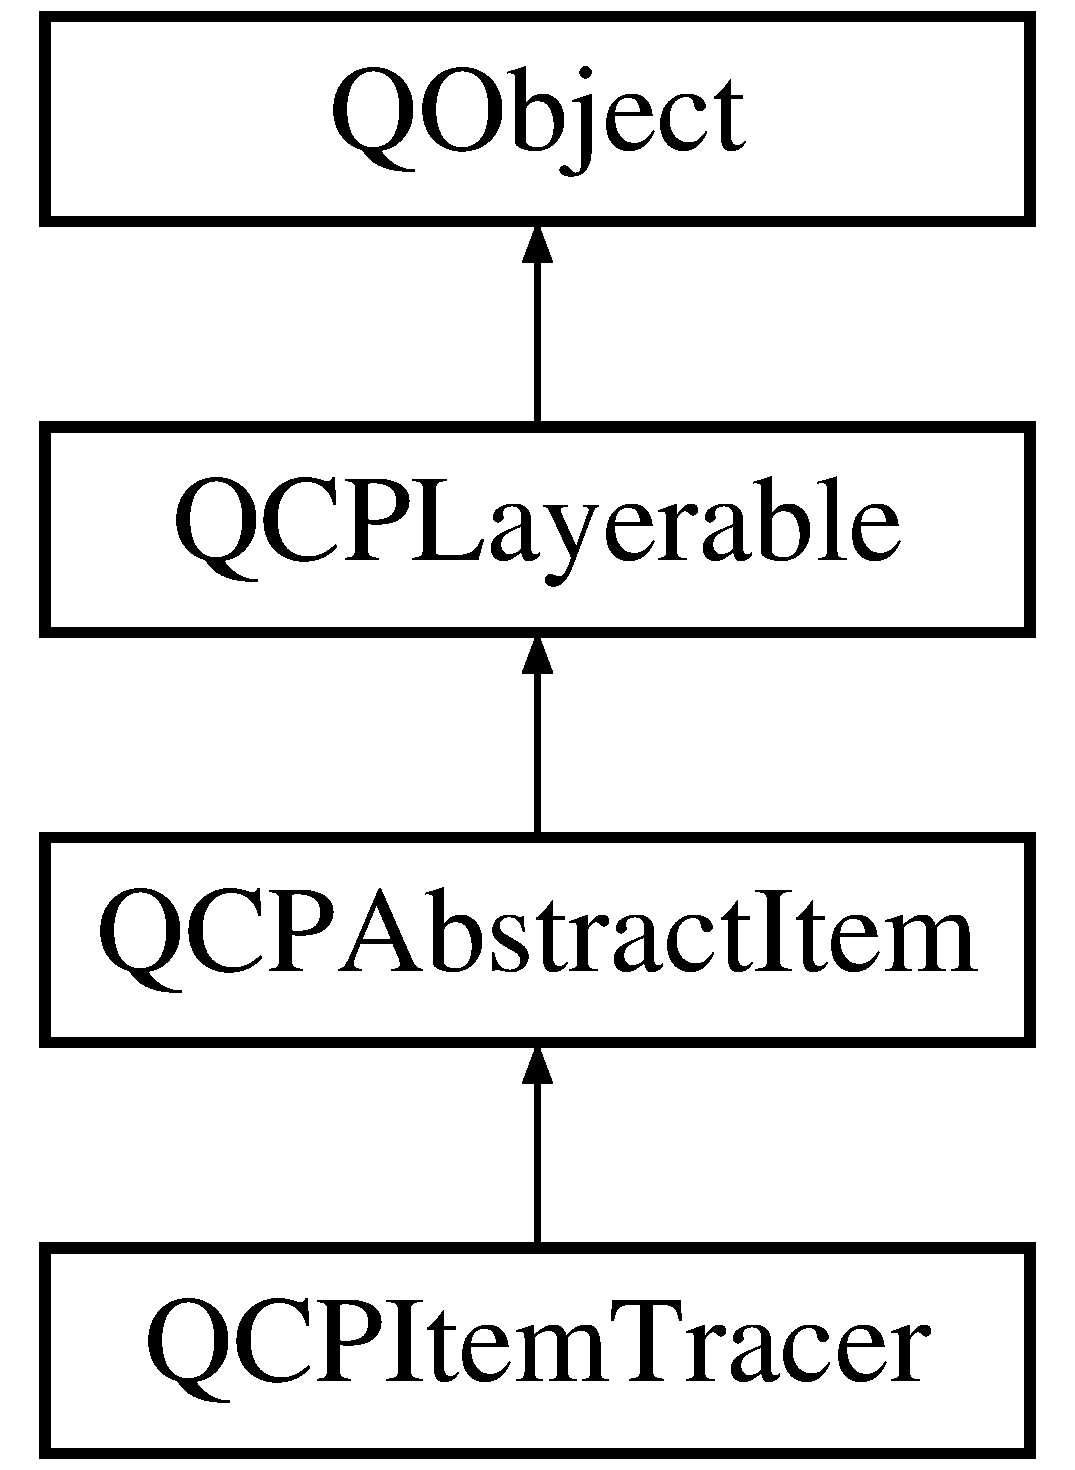
\includegraphics[height=4.000000cm]{class_q_c_p_item_tracer}
\end{center}
\end{figure}
\subsection*{Public Types}
\begin{DoxyCompactItemize}
\item 
enum \hyperlink{class_q_c_p_item_tracer_a2f05ddb13978036f902ca3ab47076500}{Tracer\+Style} \{ \\*
\hyperlink{class_q_c_p_item_tracer_a2f05ddb13978036f902ca3ab47076500aac27462c79146225bfa8fba24d2ee8a4}{ts\+None}, 
\hyperlink{class_q_c_p_item_tracer_a2f05ddb13978036f902ca3ab47076500a3323fb04017146e4885e080a459472fa}{ts\+Plus}, 
\hyperlink{class_q_c_p_item_tracer_a2f05ddb13978036f902ca3ab47076500af562ec81ac3ba99e26ef8540cf1ec16f}{ts\+Crosshair}, 
\hyperlink{class_q_c_p_item_tracer_a2f05ddb13978036f902ca3ab47076500ae2252c28f4842880d71e9f94e69de94e}{ts\+Circle}, 
\\*
\hyperlink{class_q_c_p_item_tracer_a2f05ddb13978036f902ca3ab47076500a4ed5f01f2c5fd86d980366d79f481b9b}{ts\+Square}
 \}
\end{DoxyCompactItemize}
\subsection*{Public Member Functions}
\begin{DoxyCompactItemize}
\item 
\hyperlink{class_q_c_p_item_tracer_adc5ca846eeac323db4aa1fc4081e36be}{Q\+C\+P\+Item\+Tracer} (\hyperlink{class_q_custom_plot}{Q\+Custom\+Plot} $\ast$\hyperlink{class_q_c_p_layerable_ab7e0e94461566093d36ffc0f5312b109}{parent\+Plot})
\item 
virtual \hyperlink{class_q_c_p_item_tracer_a43686565a9b70815915618636b9bdf0f}{$\sim$\+Q\+C\+P\+Item\+Tracer} ()
\item 
Q\+Pen \hyperlink{class_q_c_p_item_tracer_a1f51b61e98c276298a0874d5e89707f0}{pen} () const 
\item 
Q\+Pen \hyperlink{class_q_c_p_item_tracer_ad75e5d2d868dbedc176f7911091f379b}{selected\+Pen} () const 
\item 
Q\+Brush \hyperlink{class_q_c_p_item_tracer_af07527750cfb6afc3c0ba4bec012011f}{brush} () const 
\item 
Q\+Brush \hyperlink{class_q_c_p_item_tracer_afed284222253083375bfd21d3d4dbc30}{selected\+Brush} () const 
\item 
double \hyperlink{class_q_c_p_item_tracer_a2607fcb3d01e90773ea1532fd6803760}{size} () const 
\item 
\hyperlink{class_q_c_p_item_tracer_a2f05ddb13978036f902ca3ab47076500}{Tracer\+Style} \hyperlink{class_q_c_p_item_tracer_a871832dace1709f877c3136fac7ae1ec}{style} () const 
\item 
\hyperlink{class_q_c_p_graph}{Q\+C\+P\+Graph} $\ast$ \hyperlink{class_q_c_p_item_tracer_a74c90da0e6730839b8d7cf6445a4ec1f}{graph} () const 
\item 
double \hyperlink{class_q_c_p_item_tracer_a361c5c9b93bdf4588fc49bc3097529ad}{graph\+Key} () const 
\item 
bool \hyperlink{class_q_c_p_item_tracer_ab318c233fa35c17a317af38ce7b3c312}{interpolating} () const 
\item 
void \hyperlink{class_q_c_p_item_tracer_af8048636fc1ef0152e51809b008df2ca}{set\+Pen} (const Q\+Pen \&\hyperlink{class_q_c_p_item_tracer_a1f51b61e98c276298a0874d5e89707f0}{pen})
\item 
void \hyperlink{class_q_c_p_item_tracer_ae1bf70db7f13f928660168cd3e5069f3}{set\+Selected\+Pen} (const Q\+Pen \&\hyperlink{class_q_c_p_item_tracer_a1f51b61e98c276298a0874d5e89707f0}{pen})
\item 
void \hyperlink{class_q_c_p_item_tracer_a2c303f7470a30084daa201ed556b3c36}{set\+Brush} (const Q\+Brush \&\hyperlink{class_q_c_p_item_tracer_af07527750cfb6afc3c0ba4bec012011f}{brush})
\item 
void \hyperlink{class_q_c_p_item_tracer_a0f55c084980a7a312af859d3e7b558ef}{set\+Selected\+Brush} (const Q\+Brush \&\hyperlink{class_q_c_p_item_tracer_af07527750cfb6afc3c0ba4bec012011f}{brush})
\item 
void \hyperlink{class_q_c_p_item_tracer_ae47fe0617f5fef5fdb766999569be10a}{set\+Size} (double \hyperlink{class_q_c_p_item_tracer_a2607fcb3d01e90773ea1532fd6803760}{size})
\item 
void \hyperlink{class_q_c_p_item_tracer_a41a2ac4f1acd7897b4e2a2579c03204e}{set\+Style} (\hyperlink{class_q_c_p_item_tracer_a2f05ddb13978036f902ca3ab47076500}{Tracer\+Style} \hyperlink{class_q_c_p_item_tracer_a871832dace1709f877c3136fac7ae1ec}{style})
\item 
void \hyperlink{class_q_c_p_item_tracer_af5886f4ded8dd68cb4f3388f390790c0}{set\+Graph} (\hyperlink{class_q_c_p_graph}{Q\+C\+P\+Graph} $\ast$\hyperlink{class_q_c_p_item_tracer_a74c90da0e6730839b8d7cf6445a4ec1f}{graph})
\item 
void \hyperlink{class_q_c_p_item_tracer_a6840143b42f3b685cedf7c6d83a704c8}{set\+Graph\+Key} (double key)
\item 
void \hyperlink{class_q_c_p_item_tracer_a6c244a9d1175bef12b50afafd4f5fcd2}{set\+Interpolating} (bool enabled)
\item 
virtual double \hyperlink{class_q_c_p_item_tracer_ae71f3728421c83c188c117279ca050fd}{select\+Test} (const Q\+Point\+F \&pos, bool only\+Selectable, Q\+Variant $\ast$details=0) const 
\item 
void \hyperlink{class_q_c_p_item_tracer_a5b90296109e36384aedbc8908a670413}{update\+Position} ()
\end{DoxyCompactItemize}
\subsection*{Public Attributes}
\begin{DoxyCompactItemize}
\item 
\hyperlink{class_q_c_p_item_position}{Q\+C\+P\+Item\+Position} $\ast$const \hyperlink{class_q_c_p_item_tracer_a69917e2fdb2b3a929c196958feee7cbe}{position}
\end{DoxyCompactItemize}
\subsection*{Protected Member Functions}
\begin{DoxyCompactItemize}
\item 
virtual void \hyperlink{class_q_c_p_item_tracer_aaaf49b48382c730ec9be0e74c2538315}{draw} (\hyperlink{class_q_c_p_painter}{Q\+C\+P\+Painter} $\ast$painter)
\item 
Q\+Pen \hyperlink{class_q_c_p_item_tracer_af87132b7698d5bb35c96a8a0b9e7180e}{main\+Pen} () const 
\item 
Q\+Brush \hyperlink{class_q_c_p_item_tracer_aaf4e72e2d87f53279b9f9ba624961bf5}{main\+Brush} () const 
\end{DoxyCompactItemize}
\subsection*{Protected Attributes}
\begin{DoxyCompactItemize}
\item 
Q\+Pen \hyperlink{class_q_c_p_item_tracer_a579e3bd6bd16d6aaff03638dc8a99a69}{m\+Pen}
\item 
Q\+Pen \hyperlink{class_q_c_p_item_tracer_a3f61829784200819661d1e2a5354d866}{m\+Selected\+Pen}
\item 
Q\+Brush \hyperlink{class_q_c_p_item_tracer_a6597be63a17a266233941354200b2340}{m\+Brush}
\item 
Q\+Brush \hyperlink{class_q_c_p_item_tracer_a1c15d2adde40efdcc0ef1ff78fd256a6}{m\+Selected\+Brush}
\item 
double \hyperlink{class_q_c_p_item_tracer_a575153a24bb357d1e006f6bc3bd099b9}{m\+Size}
\item 
\hyperlink{class_q_c_p_item_tracer_a2f05ddb13978036f902ca3ab47076500}{Tracer\+Style} \hyperlink{class_q_c_p_item_tracer_afb1f236bebf417544e0138fef22a292e}{m\+Style}
\item 
\hyperlink{class_q_c_p_graph}{Q\+C\+P\+Graph} $\ast$ \hyperlink{class_q_c_p_item_tracer_a2d70cf616b579563aa15f796dfc143ac}{m\+Graph}
\item 
double \hyperlink{class_q_c_p_item_tracer_a8fa20f2e9ee07d21fd7c8d30ba4702ca}{m\+Graph\+Key}
\item 
bool \hyperlink{class_q_c_p_item_tracer_afab37c22ad39f235921e86f93cd84595}{m\+Interpolating}
\end{DoxyCompactItemize}
\subsection*{Additional Inherited Members}


\subsection{Detailed Description}
Item that sticks to \hyperlink{class_q_c_p_graph}{Q\+C\+P\+Graph} data points. 

 The tracer can be connected with a \hyperlink{class_q_c_p_graph}{Q\+C\+P\+Graph} via \hyperlink{class_q_c_p_item_tracer_af5886f4ded8dd68cb4f3388f390790c0}{set\+Graph}. Then it will automatically adopt the coordinate axes of the graph and update its {\itshape position} to be on the graph\textquotesingle{}s data. This means the key stays controllable via \hyperlink{class_q_c_p_item_tracer_a6840143b42f3b685cedf7c6d83a704c8}{set\+Graph\+Key}, but the value will follow the graph data. If a \hyperlink{class_q_c_p_graph}{Q\+C\+P\+Graph} is connected, note that setting the coordinates of the tracer item directly via {\itshape position} will have no effect because they will be overriden in the next redraw (this is when the coordinate update happens).

If the specified key in \hyperlink{class_q_c_p_item_tracer_a6840143b42f3b685cedf7c6d83a704c8}{set\+Graph\+Key} is outside the key bounds of the graph, the tracer will stay at the corresponding end of the graph.

With \hyperlink{class_q_c_p_item_tracer_a6c244a9d1175bef12b50afafd4f5fcd2}{set\+Interpolating} you may specify whether the tracer may only stay exactly on data points or whether it interpolates data points linearly, if given a key that lies between two data points of the graph.

The tracer has different visual styles, see \hyperlink{class_q_c_p_item_tracer_a41a2ac4f1acd7897b4e2a2579c03204e}{set\+Style}. It is also possible to make the tracer have no own visual appearance (set the style to \hyperlink{class_q_c_p_item_tracer_a2f05ddb13978036f902ca3ab47076500aac27462c79146225bfa8fba24d2ee8a4}{ts\+None}), and just connect other item positions to the tracer {\itshape position} (used as an anchor) via \hyperlink{class_q_c_p_item_position_ac094d67a95d2dceafa0d50b9db3a7e51}{Q\+C\+P\+Item\+Position\+::set\+Parent\+Anchor}.

\begin{DoxyNote}{Note}
The tracer position is only automatically updated upon redraws. So when the data of the graph changes and immediately afterwards (without a redraw) the a position coordinates of the tracer are retrieved, they will not reflect the updated data of the graph. In this case \hyperlink{class_q_c_p_item_tracer_a5b90296109e36384aedbc8908a670413}{update\+Position} must be called manually, prior to reading the tracer coordinates. 
\end{DoxyNote}


\subsection{Member Enumeration Documentation}
\hypertarget{class_q_c_p_item_tracer_a2f05ddb13978036f902ca3ab47076500}{}\index{Q\+C\+P\+Item\+Tracer@{Q\+C\+P\+Item\+Tracer}!Tracer\+Style@{Tracer\+Style}}
\index{Tracer\+Style@{Tracer\+Style}!Q\+C\+P\+Item\+Tracer@{Q\+C\+P\+Item\+Tracer}}
\subsubsection[{Tracer\+Style}]{\setlength{\rightskip}{0pt plus 5cm}enum {\bf Q\+C\+P\+Item\+Tracer\+::\+Tracer\+Style}}\label{class_q_c_p_item_tracer_a2f05ddb13978036f902ca3ab47076500}
The different visual appearances a tracer item can have. Some styles size may be controlled with \hyperlink{class_q_c_p_item_tracer_ae47fe0617f5fef5fdb766999569be10a}{set\+Size}.

\begin{DoxySeeAlso}{See also}
\hyperlink{class_q_c_p_item_tracer_a41a2ac4f1acd7897b4e2a2579c03204e}{set\+Style} 
\end{DoxySeeAlso}
\begin{Desc}
\item[Enumerator]\par
\begin{description}
\index{ts\+None@{ts\+None}!Q\+C\+P\+Item\+Tracer@{Q\+C\+P\+Item\+Tracer}}\index{Q\+C\+P\+Item\+Tracer@{Q\+C\+P\+Item\+Tracer}!ts\+None@{ts\+None}}\item[{\em 
\hypertarget{class_q_c_p_item_tracer_a2f05ddb13978036f902ca3ab47076500aac27462c79146225bfa8fba24d2ee8a4}{}ts\+None\label{class_q_c_p_item_tracer_a2f05ddb13978036f902ca3ab47076500aac27462c79146225bfa8fba24d2ee8a4}
}]The tracer is not visible. \index{ts\+Plus@{ts\+Plus}!Q\+C\+P\+Item\+Tracer@{Q\+C\+P\+Item\+Tracer}}\index{Q\+C\+P\+Item\+Tracer@{Q\+C\+P\+Item\+Tracer}!ts\+Plus@{ts\+Plus}}\item[{\em 
\hypertarget{class_q_c_p_item_tracer_a2f05ddb13978036f902ca3ab47076500a3323fb04017146e4885e080a459472fa}{}ts\+Plus\label{class_q_c_p_item_tracer_a2f05ddb13978036f902ca3ab47076500a3323fb04017146e4885e080a459472fa}
}]A plus shaped crosshair with limited size. \index{ts\+Crosshair@{ts\+Crosshair}!Q\+C\+P\+Item\+Tracer@{Q\+C\+P\+Item\+Tracer}}\index{Q\+C\+P\+Item\+Tracer@{Q\+C\+P\+Item\+Tracer}!ts\+Crosshair@{ts\+Crosshair}}\item[{\em 
\hypertarget{class_q_c_p_item_tracer_a2f05ddb13978036f902ca3ab47076500af562ec81ac3ba99e26ef8540cf1ec16f}{}ts\+Crosshair\label{class_q_c_p_item_tracer_a2f05ddb13978036f902ca3ab47076500af562ec81ac3ba99e26ef8540cf1ec16f}
}]A plus shaped crosshair which spans the complete axis rect. \index{ts\+Circle@{ts\+Circle}!Q\+C\+P\+Item\+Tracer@{Q\+C\+P\+Item\+Tracer}}\index{Q\+C\+P\+Item\+Tracer@{Q\+C\+P\+Item\+Tracer}!ts\+Circle@{ts\+Circle}}\item[{\em 
\hypertarget{class_q_c_p_item_tracer_a2f05ddb13978036f902ca3ab47076500ae2252c28f4842880d71e9f94e69de94e}{}ts\+Circle\label{class_q_c_p_item_tracer_a2f05ddb13978036f902ca3ab47076500ae2252c28f4842880d71e9f94e69de94e}
}]A circle. \index{ts\+Square@{ts\+Square}!Q\+C\+P\+Item\+Tracer@{Q\+C\+P\+Item\+Tracer}}\index{Q\+C\+P\+Item\+Tracer@{Q\+C\+P\+Item\+Tracer}!ts\+Square@{ts\+Square}}\item[{\em 
\hypertarget{class_q_c_p_item_tracer_a2f05ddb13978036f902ca3ab47076500a4ed5f01f2c5fd86d980366d79f481b9b}{}ts\+Square\label{class_q_c_p_item_tracer_a2f05ddb13978036f902ca3ab47076500a4ed5f01f2c5fd86d980366d79f481b9b}
}]A square. \end{description}
\end{Desc}


\subsection{Constructor \& Destructor Documentation}
\hypertarget{class_q_c_p_item_tracer_adc5ca846eeac323db4aa1fc4081e36be}{}\index{Q\+C\+P\+Item\+Tracer@{Q\+C\+P\+Item\+Tracer}!Q\+C\+P\+Item\+Tracer@{Q\+C\+P\+Item\+Tracer}}
\index{Q\+C\+P\+Item\+Tracer@{Q\+C\+P\+Item\+Tracer}!Q\+C\+P\+Item\+Tracer@{Q\+C\+P\+Item\+Tracer}}
\subsubsection[{Q\+C\+P\+Item\+Tracer}]{\setlength{\rightskip}{0pt plus 5cm}Q\+C\+P\+Item\+Tracer\+::\+Q\+C\+P\+Item\+Tracer (
\begin{DoxyParamCaption}
\item[{{\bf Q\+Custom\+Plot} $\ast$}]{parent\+Plot}
\end{DoxyParamCaption}
)}\label{class_q_c_p_item_tracer_adc5ca846eeac323db4aa1fc4081e36be}
Creates a tracer item and sets default values.

The constructed item can be added to the plot with \hyperlink{class_q_custom_plot_aa500620379262321685cb7a7674cbd2a}{Q\+Custom\+Plot\+::add\+Item}. \hypertarget{class_q_c_p_item_tracer_a43686565a9b70815915618636b9bdf0f}{}\index{Q\+C\+P\+Item\+Tracer@{Q\+C\+P\+Item\+Tracer}!````~Q\+C\+P\+Item\+Tracer@{$\sim$\+Q\+C\+P\+Item\+Tracer}}
\index{````~Q\+C\+P\+Item\+Tracer@{$\sim$\+Q\+C\+P\+Item\+Tracer}!Q\+C\+P\+Item\+Tracer@{Q\+C\+P\+Item\+Tracer}}
\subsubsection[{$\sim$\+Q\+C\+P\+Item\+Tracer}]{\setlength{\rightskip}{0pt plus 5cm}Q\+C\+P\+Item\+Tracer\+::$\sim$\+Q\+C\+P\+Item\+Tracer (
\begin{DoxyParamCaption}
{}
\end{DoxyParamCaption}
)\hspace{0.3cm}{\ttfamily [virtual]}}\label{class_q_c_p_item_tracer_a43686565a9b70815915618636b9bdf0f}


\subsection{Member Function Documentation}
\hypertarget{class_q_c_p_item_tracer_af07527750cfb6afc3c0ba4bec012011f}{}\index{Q\+C\+P\+Item\+Tracer@{Q\+C\+P\+Item\+Tracer}!brush@{brush}}
\index{brush@{brush}!Q\+C\+P\+Item\+Tracer@{Q\+C\+P\+Item\+Tracer}}
\subsubsection[{brush}]{\setlength{\rightskip}{0pt plus 5cm}Q\+Brush Q\+C\+P\+Item\+Tracer\+::brush (
\begin{DoxyParamCaption}
{}
\end{DoxyParamCaption}
) const\hspace{0.3cm}{\ttfamily [inline]}}\label{class_q_c_p_item_tracer_af07527750cfb6afc3c0ba4bec012011f}
\hypertarget{class_q_c_p_item_tracer_aaaf49b48382c730ec9be0e74c2538315}{}\index{Q\+C\+P\+Item\+Tracer@{Q\+C\+P\+Item\+Tracer}!draw@{draw}}
\index{draw@{draw}!Q\+C\+P\+Item\+Tracer@{Q\+C\+P\+Item\+Tracer}}
\subsubsection[{draw}]{\setlength{\rightskip}{0pt plus 5cm}void Q\+C\+P\+Item\+Tracer\+::draw (
\begin{DoxyParamCaption}
\item[{{\bf Q\+C\+P\+Painter} $\ast$}]{painter}
\end{DoxyParamCaption}
)\hspace{0.3cm}{\ttfamily [protected]}, {\ttfamily [virtual]}}\label{class_q_c_p_item_tracer_aaaf49b48382c730ec9be0e74c2538315}


Implements \hyperlink{class_q_c_p_abstract_item_ad0dc056f650c3ca73414e6b4f01674ef}{Q\+C\+P\+Abstract\+Item}.

\hypertarget{class_q_c_p_item_tracer_a74c90da0e6730839b8d7cf6445a4ec1f}{}\index{Q\+C\+P\+Item\+Tracer@{Q\+C\+P\+Item\+Tracer}!graph@{graph}}
\index{graph@{graph}!Q\+C\+P\+Item\+Tracer@{Q\+C\+P\+Item\+Tracer}}
\subsubsection[{graph}]{\setlength{\rightskip}{0pt plus 5cm}{\bf Q\+C\+P\+Graph}$\ast$ Q\+C\+P\+Item\+Tracer\+::graph (
\begin{DoxyParamCaption}
{}
\end{DoxyParamCaption}
) const\hspace{0.3cm}{\ttfamily [inline]}}\label{class_q_c_p_item_tracer_a74c90da0e6730839b8d7cf6445a4ec1f}
\hypertarget{class_q_c_p_item_tracer_a361c5c9b93bdf4588fc49bc3097529ad}{}\index{Q\+C\+P\+Item\+Tracer@{Q\+C\+P\+Item\+Tracer}!graph\+Key@{graph\+Key}}
\index{graph\+Key@{graph\+Key}!Q\+C\+P\+Item\+Tracer@{Q\+C\+P\+Item\+Tracer}}
\subsubsection[{graph\+Key}]{\setlength{\rightskip}{0pt plus 5cm}double Q\+C\+P\+Item\+Tracer\+::graph\+Key (
\begin{DoxyParamCaption}
{}
\end{DoxyParamCaption}
) const\hspace{0.3cm}{\ttfamily [inline]}}\label{class_q_c_p_item_tracer_a361c5c9b93bdf4588fc49bc3097529ad}
\hypertarget{class_q_c_p_item_tracer_ab318c233fa35c17a317af38ce7b3c312}{}\index{Q\+C\+P\+Item\+Tracer@{Q\+C\+P\+Item\+Tracer}!interpolating@{interpolating}}
\index{interpolating@{interpolating}!Q\+C\+P\+Item\+Tracer@{Q\+C\+P\+Item\+Tracer}}
\subsubsection[{interpolating}]{\setlength{\rightskip}{0pt plus 5cm}bool Q\+C\+P\+Item\+Tracer\+::interpolating (
\begin{DoxyParamCaption}
{}
\end{DoxyParamCaption}
) const\hspace{0.3cm}{\ttfamily [inline]}}\label{class_q_c_p_item_tracer_ab318c233fa35c17a317af38ce7b3c312}
\hypertarget{class_q_c_p_item_tracer_aaf4e72e2d87f53279b9f9ba624961bf5}{}\index{Q\+C\+P\+Item\+Tracer@{Q\+C\+P\+Item\+Tracer}!main\+Brush@{main\+Brush}}
\index{main\+Brush@{main\+Brush}!Q\+C\+P\+Item\+Tracer@{Q\+C\+P\+Item\+Tracer}}
\subsubsection[{main\+Brush}]{\setlength{\rightskip}{0pt plus 5cm}Q\+Brush Q\+C\+P\+Item\+Tracer\+::main\+Brush (
\begin{DoxyParamCaption}
{}
\end{DoxyParamCaption}
) const\hspace{0.3cm}{\ttfamily [protected]}}\label{class_q_c_p_item_tracer_aaf4e72e2d87f53279b9f9ba624961bf5}
\hypertarget{class_q_c_p_item_tracer_af87132b7698d5bb35c96a8a0b9e7180e}{}\index{Q\+C\+P\+Item\+Tracer@{Q\+C\+P\+Item\+Tracer}!main\+Pen@{main\+Pen}}
\index{main\+Pen@{main\+Pen}!Q\+C\+P\+Item\+Tracer@{Q\+C\+P\+Item\+Tracer}}
\subsubsection[{main\+Pen}]{\setlength{\rightskip}{0pt plus 5cm}Q\+Pen Q\+C\+P\+Item\+Tracer\+::main\+Pen (
\begin{DoxyParamCaption}
{}
\end{DoxyParamCaption}
) const\hspace{0.3cm}{\ttfamily [protected]}}\label{class_q_c_p_item_tracer_af87132b7698d5bb35c96a8a0b9e7180e}
\hypertarget{class_q_c_p_item_tracer_a1f51b61e98c276298a0874d5e89707f0}{}\index{Q\+C\+P\+Item\+Tracer@{Q\+C\+P\+Item\+Tracer}!pen@{pen}}
\index{pen@{pen}!Q\+C\+P\+Item\+Tracer@{Q\+C\+P\+Item\+Tracer}}
\subsubsection[{pen}]{\setlength{\rightskip}{0pt plus 5cm}Q\+Pen Q\+C\+P\+Item\+Tracer\+::pen (
\begin{DoxyParamCaption}
{}
\end{DoxyParamCaption}
) const\hspace{0.3cm}{\ttfamily [inline]}}\label{class_q_c_p_item_tracer_a1f51b61e98c276298a0874d5e89707f0}
\hypertarget{class_q_c_p_item_tracer_afed284222253083375bfd21d3d4dbc30}{}\index{Q\+C\+P\+Item\+Tracer@{Q\+C\+P\+Item\+Tracer}!selected\+Brush@{selected\+Brush}}
\index{selected\+Brush@{selected\+Brush}!Q\+C\+P\+Item\+Tracer@{Q\+C\+P\+Item\+Tracer}}
\subsubsection[{selected\+Brush}]{\setlength{\rightskip}{0pt plus 5cm}Q\+Brush Q\+C\+P\+Item\+Tracer\+::selected\+Brush (
\begin{DoxyParamCaption}
{}
\end{DoxyParamCaption}
) const\hspace{0.3cm}{\ttfamily [inline]}}\label{class_q_c_p_item_tracer_afed284222253083375bfd21d3d4dbc30}
\hypertarget{class_q_c_p_item_tracer_ad75e5d2d868dbedc176f7911091f379b}{}\index{Q\+C\+P\+Item\+Tracer@{Q\+C\+P\+Item\+Tracer}!selected\+Pen@{selected\+Pen}}
\index{selected\+Pen@{selected\+Pen}!Q\+C\+P\+Item\+Tracer@{Q\+C\+P\+Item\+Tracer}}
\subsubsection[{selected\+Pen}]{\setlength{\rightskip}{0pt plus 5cm}Q\+Pen Q\+C\+P\+Item\+Tracer\+::selected\+Pen (
\begin{DoxyParamCaption}
{}
\end{DoxyParamCaption}
) const\hspace{0.3cm}{\ttfamily [inline]}}\label{class_q_c_p_item_tracer_ad75e5d2d868dbedc176f7911091f379b}
\hypertarget{class_q_c_p_item_tracer_ae71f3728421c83c188c117279ca050fd}{}\index{Q\+C\+P\+Item\+Tracer@{Q\+C\+P\+Item\+Tracer}!select\+Test@{select\+Test}}
\index{select\+Test@{select\+Test}!Q\+C\+P\+Item\+Tracer@{Q\+C\+P\+Item\+Tracer}}
\subsubsection[{select\+Test}]{\setlength{\rightskip}{0pt plus 5cm}double Q\+C\+P\+Item\+Tracer\+::select\+Test (
\begin{DoxyParamCaption}
\item[{const Q\+Point\+F \&}]{pos, }
\item[{bool}]{only\+Selectable, }
\item[{Q\+Variant $\ast$}]{details = {\ttfamily 0}}
\end{DoxyParamCaption}
) const\hspace{0.3cm}{\ttfamily [virtual]}}\label{class_q_c_p_item_tracer_ae71f3728421c83c188c117279ca050fd}
This function is used to decide whether a click hits a layerable object or not.

{\itshape pos} is a point in pixel coordinates on the \hyperlink{class_q_custom_plot}{Q\+Custom\+Plot} surface. This function returns the shortest pixel distance of this point to the object. If the object is either invisible or the distance couldn\textquotesingle{}t be determined, -\/1.\+0 is returned. Further, if {\itshape only\+Selectable} is true and the object is not selectable, -\/1.\+0 is returned, too.

If the item is represented not by single lines but by an area like \hyperlink{class_q_c_p_item_rect}{Q\+C\+P\+Item\+Rect} or \hyperlink{class_q_c_p_item_text}{Q\+C\+P\+Item\+Text}, a click inside the area returns a constant value greater zero (typically the selection\+Tolerance of the parent \hyperlink{class_q_custom_plot}{Q\+Custom\+Plot} multiplied by 0.\+99). If the click lies outside the area, this function returns -\/1.\+0.

Providing a constant value for area objects allows selecting line objects even when they are obscured by such area objects, by clicking close to the lines (i.\+e. closer than 0.\+99$\ast$selection\+Tolerance).

The actual setting of the selection state is not done by this function. This is handled by the parent \hyperlink{class_q_custom_plot}{Q\+Custom\+Plot} when the mouse\+Release\+Event occurs, and the finally selected object is notified via the select\+Event/deselect\+Event methods.

{\itshape details} is an optional output parameter. Every layerable subclass may place any information in {\itshape details}. This information will be passed to \hyperlink{class_q_c_p_abstract_item_aaf92af7b9893712959a6c073d334d88d}{select\+Event} when the parent \hyperlink{class_q_custom_plot}{Q\+Custom\+Plot} decides on the basis of this select\+Test call, that the object was successfully selected. The subsequent call to \hyperlink{class_q_c_p_abstract_item_aaf92af7b9893712959a6c073d334d88d}{select\+Event} will carry the {\itshape details}. This is useful for multi-\/part objects (like \hyperlink{class_q_c_p_axis}{Q\+C\+P\+Axis}). This way, a possibly complex calculation to decide which part was clicked is only done once in \hyperlink{class_q_c_p_item_tracer_ae71f3728421c83c188c117279ca050fd}{select\+Test}. The result (i.\+e. the actually clicked part) can then be placed in {\itshape details}. So in the subsequent \hyperlink{class_q_c_p_abstract_item_aaf92af7b9893712959a6c073d334d88d}{select\+Event}, the decision which part was selected doesn\textquotesingle{}t have to be done a second time for a single selection operation.

You may pass 0 as {\itshape details} to indicate that you are not interested in those selection details.

\begin{DoxySeeAlso}{See also}
\hyperlink{class_q_c_p_abstract_item_aaf92af7b9893712959a6c073d334d88d}{select\+Event}, \hyperlink{class_q_c_p_abstract_item_a91f090d6763cfedb0749219c63788ae9}{deselect\+Event}, \hyperlink{class_q_custom_plot_a5ee1e2f6ae27419deca53e75907c27e5}{Q\+Custom\+Plot\+::set\+Interactions} 
\end{DoxySeeAlso}


Implements \hyperlink{class_q_c_p_abstract_item_a96d522d10ffc0413b9a366c6f7f0476b}{Q\+C\+P\+Abstract\+Item}.

\hypertarget{class_q_c_p_item_tracer_a2c303f7470a30084daa201ed556b3c36}{}\index{Q\+C\+P\+Item\+Tracer@{Q\+C\+P\+Item\+Tracer}!set\+Brush@{set\+Brush}}
\index{set\+Brush@{set\+Brush}!Q\+C\+P\+Item\+Tracer@{Q\+C\+P\+Item\+Tracer}}
\subsubsection[{set\+Brush}]{\setlength{\rightskip}{0pt plus 5cm}void Q\+C\+P\+Item\+Tracer\+::set\+Brush (
\begin{DoxyParamCaption}
\item[{const Q\+Brush \&}]{brush}
\end{DoxyParamCaption}
)}\label{class_q_c_p_item_tracer_a2c303f7470a30084daa201ed556b3c36}
Sets the brush that will be used to draw any fills of the tracer

\begin{DoxySeeAlso}{See also}
\hyperlink{class_q_c_p_item_tracer_a0f55c084980a7a312af859d3e7b558ef}{set\+Selected\+Brush}, \hyperlink{class_q_c_p_item_tracer_af8048636fc1ef0152e51809b008df2ca}{set\+Pen} 
\end{DoxySeeAlso}
\hypertarget{class_q_c_p_item_tracer_af5886f4ded8dd68cb4f3388f390790c0}{}\index{Q\+C\+P\+Item\+Tracer@{Q\+C\+P\+Item\+Tracer}!set\+Graph@{set\+Graph}}
\index{set\+Graph@{set\+Graph}!Q\+C\+P\+Item\+Tracer@{Q\+C\+P\+Item\+Tracer}}
\subsubsection[{set\+Graph}]{\setlength{\rightskip}{0pt plus 5cm}void Q\+C\+P\+Item\+Tracer\+::set\+Graph (
\begin{DoxyParamCaption}
\item[{{\bf Q\+C\+P\+Graph} $\ast$}]{graph}
\end{DoxyParamCaption}
)}\label{class_q_c_p_item_tracer_af5886f4ded8dd68cb4f3388f390790c0}
Sets the \hyperlink{class_q_c_p_graph}{Q\+C\+P\+Graph} this tracer sticks to. The tracer {\itshape position} will be set to type \hyperlink{class_q_c_p_item_position_aad9936c22bf43e3d358552f6e86dbdc8ad5ffb8dc99ad73263f7010c77342294c}{Q\+C\+P\+Item\+Position\+::pt\+Plot\+Coords} and the axes will be set to the axes of {\itshape graph}.

To free the tracer from any graph, set {\itshape graph} to 0. The tracer {\itshape position} can then be placed freely like any other item position. This is the state the tracer will assume when its graph gets deleted while still attached to it.

\begin{DoxySeeAlso}{See also}
\hyperlink{class_q_c_p_item_tracer_a6840143b42f3b685cedf7c6d83a704c8}{set\+Graph\+Key} 
\end{DoxySeeAlso}
\hypertarget{class_q_c_p_item_tracer_a6840143b42f3b685cedf7c6d83a704c8}{}\index{Q\+C\+P\+Item\+Tracer@{Q\+C\+P\+Item\+Tracer}!set\+Graph\+Key@{set\+Graph\+Key}}
\index{set\+Graph\+Key@{set\+Graph\+Key}!Q\+C\+P\+Item\+Tracer@{Q\+C\+P\+Item\+Tracer}}
\subsubsection[{set\+Graph\+Key}]{\setlength{\rightskip}{0pt plus 5cm}void Q\+C\+P\+Item\+Tracer\+::set\+Graph\+Key (
\begin{DoxyParamCaption}
\item[{double}]{key}
\end{DoxyParamCaption}
)}\label{class_q_c_p_item_tracer_a6840143b42f3b685cedf7c6d83a704c8}
Sets the key of the graph\textquotesingle{}s data point the tracer will be positioned at. This is the only free coordinate of a tracer when attached to a graph.

Depending on \hyperlink{class_q_c_p_item_tracer_a6c244a9d1175bef12b50afafd4f5fcd2}{set\+Interpolating}, the tracer will be either positioned on the data point closest to {\itshape key}, or will stay exactly at {\itshape key} and interpolate the value linearly.

\begin{DoxySeeAlso}{See also}
\hyperlink{class_q_c_p_item_tracer_af5886f4ded8dd68cb4f3388f390790c0}{set\+Graph}, \hyperlink{class_q_c_p_item_tracer_a6c244a9d1175bef12b50afafd4f5fcd2}{set\+Interpolating} 
\end{DoxySeeAlso}
\hypertarget{class_q_c_p_item_tracer_a6c244a9d1175bef12b50afafd4f5fcd2}{}\index{Q\+C\+P\+Item\+Tracer@{Q\+C\+P\+Item\+Tracer}!set\+Interpolating@{set\+Interpolating}}
\index{set\+Interpolating@{set\+Interpolating}!Q\+C\+P\+Item\+Tracer@{Q\+C\+P\+Item\+Tracer}}
\subsubsection[{set\+Interpolating}]{\setlength{\rightskip}{0pt plus 5cm}void Q\+C\+P\+Item\+Tracer\+::set\+Interpolating (
\begin{DoxyParamCaption}
\item[{bool}]{enabled}
\end{DoxyParamCaption}
)}\label{class_q_c_p_item_tracer_a6c244a9d1175bef12b50afafd4f5fcd2}
Sets whether the value of the graph\textquotesingle{}s data points shall be interpolated, when positioning the tracer.

If {\itshape enabled} is set to false and a key is given with \hyperlink{class_q_c_p_item_tracer_a6840143b42f3b685cedf7c6d83a704c8}{set\+Graph\+Key}, the tracer is placed on the data point of the graph which is closest to the key, but which is not necessarily exactly there. If {\itshape enabled} is true, the tracer will be positioned exactly at the specified key, and the appropriate value will be interpolated from the graph\textquotesingle{}s data points linearly.

\begin{DoxySeeAlso}{See also}
\hyperlink{class_q_c_p_item_tracer_af5886f4ded8dd68cb4f3388f390790c0}{set\+Graph}, \hyperlink{class_q_c_p_item_tracer_a6840143b42f3b685cedf7c6d83a704c8}{set\+Graph\+Key} 
\end{DoxySeeAlso}
\hypertarget{class_q_c_p_item_tracer_af8048636fc1ef0152e51809b008df2ca}{}\index{Q\+C\+P\+Item\+Tracer@{Q\+C\+P\+Item\+Tracer}!set\+Pen@{set\+Pen}}
\index{set\+Pen@{set\+Pen}!Q\+C\+P\+Item\+Tracer@{Q\+C\+P\+Item\+Tracer}}
\subsubsection[{set\+Pen}]{\setlength{\rightskip}{0pt plus 5cm}void Q\+C\+P\+Item\+Tracer\+::set\+Pen (
\begin{DoxyParamCaption}
\item[{const Q\+Pen \&}]{pen}
\end{DoxyParamCaption}
)}\label{class_q_c_p_item_tracer_af8048636fc1ef0152e51809b008df2ca}
Sets the pen that will be used to draw the line of the tracer

\begin{DoxySeeAlso}{See also}
\hyperlink{class_q_c_p_item_tracer_ae1bf70db7f13f928660168cd3e5069f3}{set\+Selected\+Pen}, \hyperlink{class_q_c_p_item_tracer_a2c303f7470a30084daa201ed556b3c36}{set\+Brush} 
\end{DoxySeeAlso}
\hypertarget{class_q_c_p_item_tracer_a0f55c084980a7a312af859d3e7b558ef}{}\index{Q\+C\+P\+Item\+Tracer@{Q\+C\+P\+Item\+Tracer}!set\+Selected\+Brush@{set\+Selected\+Brush}}
\index{set\+Selected\+Brush@{set\+Selected\+Brush}!Q\+C\+P\+Item\+Tracer@{Q\+C\+P\+Item\+Tracer}}
\subsubsection[{set\+Selected\+Brush}]{\setlength{\rightskip}{0pt plus 5cm}void Q\+C\+P\+Item\+Tracer\+::set\+Selected\+Brush (
\begin{DoxyParamCaption}
\item[{const Q\+Brush \&}]{brush}
\end{DoxyParamCaption}
)}\label{class_q_c_p_item_tracer_a0f55c084980a7a312af859d3e7b558ef}
Sets the brush that will be used to draw any fills of the tracer, when selected.

\begin{DoxySeeAlso}{See also}
\hyperlink{class_q_c_p_item_tracer_a2c303f7470a30084daa201ed556b3c36}{set\+Brush}, \hyperlink{class_q_c_p_abstract_item_a203de94ad586cc44d16c9565f49d3378}{set\+Selected} 
\end{DoxySeeAlso}
\hypertarget{class_q_c_p_item_tracer_ae1bf70db7f13f928660168cd3e5069f3}{}\index{Q\+C\+P\+Item\+Tracer@{Q\+C\+P\+Item\+Tracer}!set\+Selected\+Pen@{set\+Selected\+Pen}}
\index{set\+Selected\+Pen@{set\+Selected\+Pen}!Q\+C\+P\+Item\+Tracer@{Q\+C\+P\+Item\+Tracer}}
\subsubsection[{set\+Selected\+Pen}]{\setlength{\rightskip}{0pt plus 5cm}void Q\+C\+P\+Item\+Tracer\+::set\+Selected\+Pen (
\begin{DoxyParamCaption}
\item[{const Q\+Pen \&}]{pen}
\end{DoxyParamCaption}
)}\label{class_q_c_p_item_tracer_ae1bf70db7f13f928660168cd3e5069f3}
Sets the pen that will be used to draw the line of the tracer when selected

\begin{DoxySeeAlso}{See also}
\hyperlink{class_q_c_p_item_tracer_af8048636fc1ef0152e51809b008df2ca}{set\+Pen}, \hyperlink{class_q_c_p_abstract_item_a203de94ad586cc44d16c9565f49d3378}{set\+Selected} 
\end{DoxySeeAlso}
\hypertarget{class_q_c_p_item_tracer_ae47fe0617f5fef5fdb766999569be10a}{}\index{Q\+C\+P\+Item\+Tracer@{Q\+C\+P\+Item\+Tracer}!set\+Size@{set\+Size}}
\index{set\+Size@{set\+Size}!Q\+C\+P\+Item\+Tracer@{Q\+C\+P\+Item\+Tracer}}
\subsubsection[{set\+Size}]{\setlength{\rightskip}{0pt plus 5cm}void Q\+C\+P\+Item\+Tracer\+::set\+Size (
\begin{DoxyParamCaption}
\item[{double}]{size}
\end{DoxyParamCaption}
)}\label{class_q_c_p_item_tracer_ae47fe0617f5fef5fdb766999569be10a}
Sets the size of the tracer in pixels, if the style supports setting a size (e.\+g. \hyperlink{class_q_c_p_item_tracer_a2f05ddb13978036f902ca3ab47076500a4ed5f01f2c5fd86d980366d79f481b9b}{ts\+Square} does, \hyperlink{class_q_c_p_item_tracer_a2f05ddb13978036f902ca3ab47076500af562ec81ac3ba99e26ef8540cf1ec16f}{ts\+Crosshair} does not). \hypertarget{class_q_c_p_item_tracer_a41a2ac4f1acd7897b4e2a2579c03204e}{}\index{Q\+C\+P\+Item\+Tracer@{Q\+C\+P\+Item\+Tracer}!set\+Style@{set\+Style}}
\index{set\+Style@{set\+Style}!Q\+C\+P\+Item\+Tracer@{Q\+C\+P\+Item\+Tracer}}
\subsubsection[{set\+Style}]{\setlength{\rightskip}{0pt plus 5cm}void Q\+C\+P\+Item\+Tracer\+::set\+Style (
\begin{DoxyParamCaption}
\item[{{\bf Q\+C\+P\+Item\+Tracer\+::\+Tracer\+Style}}]{style}
\end{DoxyParamCaption}
)}\label{class_q_c_p_item_tracer_a41a2ac4f1acd7897b4e2a2579c03204e}
Sets the style/visual appearance of the tracer.

If you only want to use the tracer {\itshape position} as an anchor for other items, set {\itshape style} to \hyperlink{class_q_c_p_item_tracer_a2f05ddb13978036f902ca3ab47076500aac27462c79146225bfa8fba24d2ee8a4}{ts\+None}. \hypertarget{class_q_c_p_item_tracer_a2607fcb3d01e90773ea1532fd6803760}{}\index{Q\+C\+P\+Item\+Tracer@{Q\+C\+P\+Item\+Tracer}!size@{size}}
\index{size@{size}!Q\+C\+P\+Item\+Tracer@{Q\+C\+P\+Item\+Tracer}}
\subsubsection[{size}]{\setlength{\rightskip}{0pt plus 5cm}double Q\+C\+P\+Item\+Tracer\+::size (
\begin{DoxyParamCaption}
{}
\end{DoxyParamCaption}
) const\hspace{0.3cm}{\ttfamily [inline]}}\label{class_q_c_p_item_tracer_a2607fcb3d01e90773ea1532fd6803760}
\hypertarget{class_q_c_p_item_tracer_a871832dace1709f877c3136fac7ae1ec}{}\index{Q\+C\+P\+Item\+Tracer@{Q\+C\+P\+Item\+Tracer}!style@{style}}
\index{style@{style}!Q\+C\+P\+Item\+Tracer@{Q\+C\+P\+Item\+Tracer}}
\subsubsection[{style}]{\setlength{\rightskip}{0pt plus 5cm}{\bf Tracer\+Style} Q\+C\+P\+Item\+Tracer\+::style (
\begin{DoxyParamCaption}
{}
\end{DoxyParamCaption}
) const\hspace{0.3cm}{\ttfamily [inline]}}\label{class_q_c_p_item_tracer_a871832dace1709f877c3136fac7ae1ec}
\hypertarget{class_q_c_p_item_tracer_a5b90296109e36384aedbc8908a670413}{}\index{Q\+C\+P\+Item\+Tracer@{Q\+C\+P\+Item\+Tracer}!update\+Position@{update\+Position}}
\index{update\+Position@{update\+Position}!Q\+C\+P\+Item\+Tracer@{Q\+C\+P\+Item\+Tracer}}
\subsubsection[{update\+Position}]{\setlength{\rightskip}{0pt plus 5cm}void Q\+C\+P\+Item\+Tracer\+::update\+Position (
\begin{DoxyParamCaption}
{}
\end{DoxyParamCaption}
)}\label{class_q_c_p_item_tracer_a5b90296109e36384aedbc8908a670413}
If the tracer is connected with a graph (\hyperlink{class_q_c_p_item_tracer_af5886f4ded8dd68cb4f3388f390790c0}{set\+Graph}), this function updates the tracer\textquotesingle{}s {\itshape position} to reside on the graph data, depending on the configured key (\hyperlink{class_q_c_p_item_tracer_a6840143b42f3b685cedf7c6d83a704c8}{set\+Graph\+Key}).

It is called automatically on every redraw and normally doesn\textquotesingle{}t need to be called manually. One exception is when you want to read the tracer coordinates via {\itshape position} and are not sure that the graph\textquotesingle{}s data (or the tracer key with \hyperlink{class_q_c_p_item_tracer_a6840143b42f3b685cedf7c6d83a704c8}{set\+Graph\+Key}) hasn\textquotesingle{}t changed since the last redraw. In that situation, call this function before accessing {\itshape position}, to make sure you don\textquotesingle{}t get out-\/of-\/date coordinates.

If there is no graph set on this tracer, this function does nothing. 

\subsection{Member Data Documentation}
\hypertarget{class_q_c_p_item_tracer_a6597be63a17a266233941354200b2340}{}\index{Q\+C\+P\+Item\+Tracer@{Q\+C\+P\+Item\+Tracer}!m\+Brush@{m\+Brush}}
\index{m\+Brush@{m\+Brush}!Q\+C\+P\+Item\+Tracer@{Q\+C\+P\+Item\+Tracer}}
\subsubsection[{m\+Brush}]{\setlength{\rightskip}{0pt plus 5cm}Q\+Brush Q\+C\+P\+Item\+Tracer\+::m\+Brush\hspace{0.3cm}{\ttfamily [protected]}}\label{class_q_c_p_item_tracer_a6597be63a17a266233941354200b2340}
\hypertarget{class_q_c_p_item_tracer_a2d70cf616b579563aa15f796dfc143ac}{}\index{Q\+C\+P\+Item\+Tracer@{Q\+C\+P\+Item\+Tracer}!m\+Graph@{m\+Graph}}
\index{m\+Graph@{m\+Graph}!Q\+C\+P\+Item\+Tracer@{Q\+C\+P\+Item\+Tracer}}
\subsubsection[{m\+Graph}]{\setlength{\rightskip}{0pt plus 5cm}{\bf Q\+C\+P\+Graph}$\ast$ Q\+C\+P\+Item\+Tracer\+::m\+Graph\hspace{0.3cm}{\ttfamily [protected]}}\label{class_q_c_p_item_tracer_a2d70cf616b579563aa15f796dfc143ac}
\hypertarget{class_q_c_p_item_tracer_a8fa20f2e9ee07d21fd7c8d30ba4702ca}{}\index{Q\+C\+P\+Item\+Tracer@{Q\+C\+P\+Item\+Tracer}!m\+Graph\+Key@{m\+Graph\+Key}}
\index{m\+Graph\+Key@{m\+Graph\+Key}!Q\+C\+P\+Item\+Tracer@{Q\+C\+P\+Item\+Tracer}}
\subsubsection[{m\+Graph\+Key}]{\setlength{\rightskip}{0pt plus 5cm}double Q\+C\+P\+Item\+Tracer\+::m\+Graph\+Key\hspace{0.3cm}{\ttfamily [protected]}}\label{class_q_c_p_item_tracer_a8fa20f2e9ee07d21fd7c8d30ba4702ca}
\hypertarget{class_q_c_p_item_tracer_afab37c22ad39f235921e86f93cd84595}{}\index{Q\+C\+P\+Item\+Tracer@{Q\+C\+P\+Item\+Tracer}!m\+Interpolating@{m\+Interpolating}}
\index{m\+Interpolating@{m\+Interpolating}!Q\+C\+P\+Item\+Tracer@{Q\+C\+P\+Item\+Tracer}}
\subsubsection[{m\+Interpolating}]{\setlength{\rightskip}{0pt plus 5cm}bool Q\+C\+P\+Item\+Tracer\+::m\+Interpolating\hspace{0.3cm}{\ttfamily [protected]}}\label{class_q_c_p_item_tracer_afab37c22ad39f235921e86f93cd84595}
\hypertarget{class_q_c_p_item_tracer_a579e3bd6bd16d6aaff03638dc8a99a69}{}\index{Q\+C\+P\+Item\+Tracer@{Q\+C\+P\+Item\+Tracer}!m\+Pen@{m\+Pen}}
\index{m\+Pen@{m\+Pen}!Q\+C\+P\+Item\+Tracer@{Q\+C\+P\+Item\+Tracer}}
\subsubsection[{m\+Pen}]{\setlength{\rightskip}{0pt plus 5cm}Q\+Pen Q\+C\+P\+Item\+Tracer\+::m\+Pen\hspace{0.3cm}{\ttfamily [protected]}}\label{class_q_c_p_item_tracer_a579e3bd6bd16d6aaff03638dc8a99a69}
\hypertarget{class_q_c_p_item_tracer_a1c15d2adde40efdcc0ef1ff78fd256a6}{}\index{Q\+C\+P\+Item\+Tracer@{Q\+C\+P\+Item\+Tracer}!m\+Selected\+Brush@{m\+Selected\+Brush}}
\index{m\+Selected\+Brush@{m\+Selected\+Brush}!Q\+C\+P\+Item\+Tracer@{Q\+C\+P\+Item\+Tracer}}
\subsubsection[{m\+Selected\+Brush}]{\setlength{\rightskip}{0pt plus 5cm}Q\+Brush Q\+C\+P\+Item\+Tracer\+::m\+Selected\+Brush\hspace{0.3cm}{\ttfamily [protected]}}\label{class_q_c_p_item_tracer_a1c15d2adde40efdcc0ef1ff78fd256a6}
\hypertarget{class_q_c_p_item_tracer_a3f61829784200819661d1e2a5354d866}{}\index{Q\+C\+P\+Item\+Tracer@{Q\+C\+P\+Item\+Tracer}!m\+Selected\+Pen@{m\+Selected\+Pen}}
\index{m\+Selected\+Pen@{m\+Selected\+Pen}!Q\+C\+P\+Item\+Tracer@{Q\+C\+P\+Item\+Tracer}}
\subsubsection[{m\+Selected\+Pen}]{\setlength{\rightskip}{0pt plus 5cm}Q\+Pen Q\+C\+P\+Item\+Tracer\+::m\+Selected\+Pen\hspace{0.3cm}{\ttfamily [protected]}}\label{class_q_c_p_item_tracer_a3f61829784200819661d1e2a5354d866}
\hypertarget{class_q_c_p_item_tracer_a575153a24bb357d1e006f6bc3bd099b9}{}\index{Q\+C\+P\+Item\+Tracer@{Q\+C\+P\+Item\+Tracer}!m\+Size@{m\+Size}}
\index{m\+Size@{m\+Size}!Q\+C\+P\+Item\+Tracer@{Q\+C\+P\+Item\+Tracer}}
\subsubsection[{m\+Size}]{\setlength{\rightskip}{0pt plus 5cm}double Q\+C\+P\+Item\+Tracer\+::m\+Size\hspace{0.3cm}{\ttfamily [protected]}}\label{class_q_c_p_item_tracer_a575153a24bb357d1e006f6bc3bd099b9}
\hypertarget{class_q_c_p_item_tracer_afb1f236bebf417544e0138fef22a292e}{}\index{Q\+C\+P\+Item\+Tracer@{Q\+C\+P\+Item\+Tracer}!m\+Style@{m\+Style}}
\index{m\+Style@{m\+Style}!Q\+C\+P\+Item\+Tracer@{Q\+C\+P\+Item\+Tracer}}
\subsubsection[{m\+Style}]{\setlength{\rightskip}{0pt plus 5cm}{\bf Tracer\+Style} Q\+C\+P\+Item\+Tracer\+::m\+Style\hspace{0.3cm}{\ttfamily [protected]}}\label{class_q_c_p_item_tracer_afb1f236bebf417544e0138fef22a292e}
\hypertarget{class_q_c_p_item_tracer_a69917e2fdb2b3a929c196958feee7cbe}{}\index{Q\+C\+P\+Item\+Tracer@{Q\+C\+P\+Item\+Tracer}!position@{position}}
\index{position@{position}!Q\+C\+P\+Item\+Tracer@{Q\+C\+P\+Item\+Tracer}}
\subsubsection[{position}]{\setlength{\rightskip}{0pt plus 5cm}{\bf Q\+C\+P\+Item\+Position}$\ast$ const Q\+C\+P\+Item\+Tracer\+::position}\label{class_q_c_p_item_tracer_a69917e2fdb2b3a929c196958feee7cbe}


The documentation for this class was generated from the following files\+:\begin{DoxyCompactItemize}
\item 
C\+:/\+Users/\+Roman/\+Documents/\+Mygs/\+Ground\+Station/\+G\+S/\hyperlink{qcustomplot_8h}{qcustomplot.\+h}\item 
C\+:/\+Users/\+Roman/\+Documents/\+Mygs/\+Ground\+Station/\+G\+S/\hyperlink{qcustomplot_8cpp}{qcustomplot.\+cpp}\end{DoxyCompactItemize}

\hypertarget{class_q_c_p_layer}{}\section{Q\+C\+P\+Layer Class Reference}
\label{class_q_c_p_layer}\index{Q\+C\+P\+Layer@{Q\+C\+P\+Layer}}


A layer that may contain objects, to control the rendering order.  




{\ttfamily \#include $<$qcustomplot.\+h$>$}

Inheritance diagram for Q\+C\+P\+Layer\+:\begin{figure}[H]
\begin{center}
\leavevmode
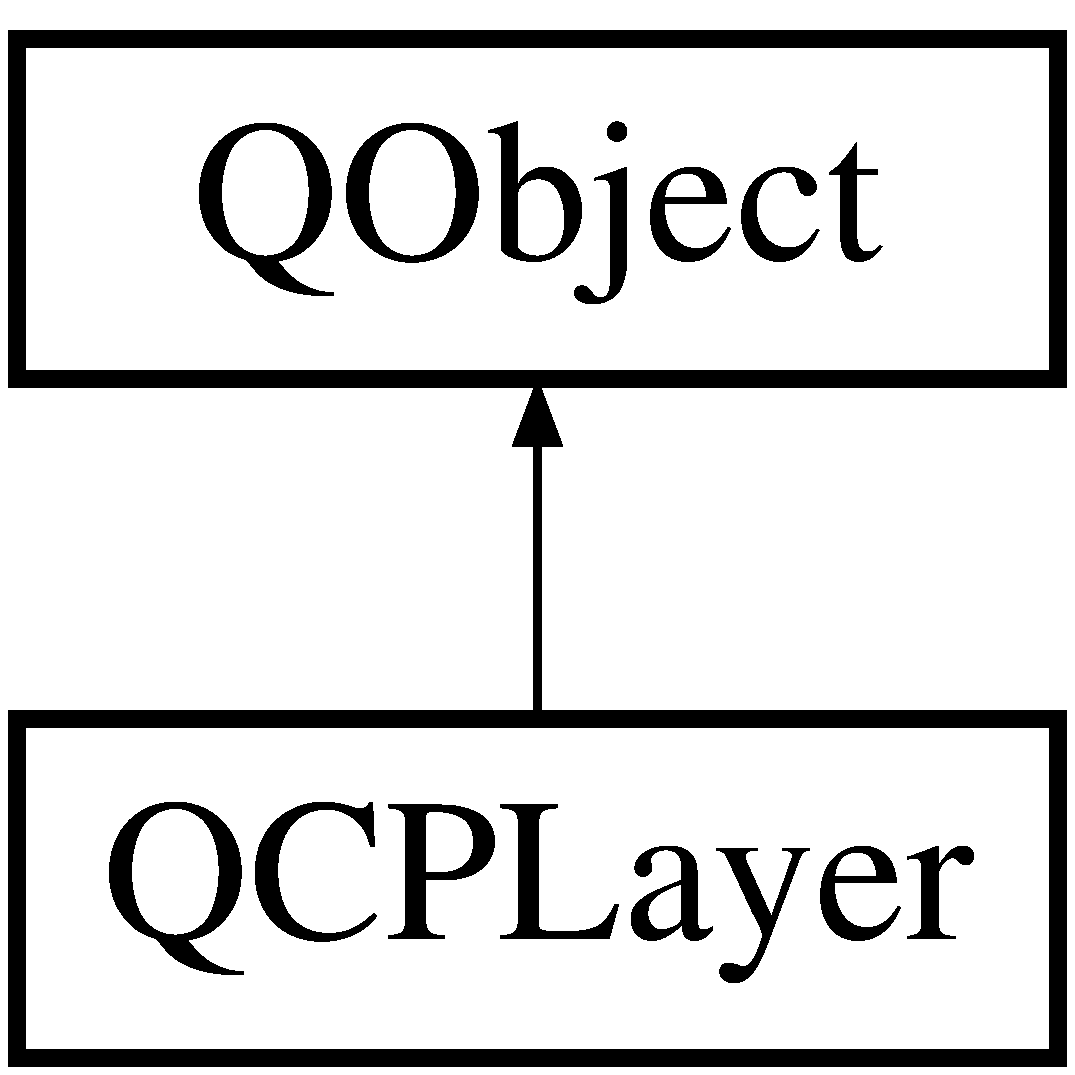
\includegraphics[height=2.000000cm]{class_q_c_p_layer}
\end{center}
\end{figure}
\subsection*{Public Member Functions}
\begin{DoxyCompactItemize}
\item 
\hyperlink{class_q_c_p_layer_a5d0657fc86d624e5efbe930ef21af718}{Q\+C\+P\+Layer} (\hyperlink{class_q_custom_plot}{Q\+Custom\+Plot} $\ast$\hyperlink{class_q_c_p_layer_a3958c9a938c2d05a7378c41484acee08}{parent\+Plot}, const Q\+String \&layer\+Name)
\item 
\hyperlink{class_q_c_p_layer_afc1a8940f8e34c9f25ead9dfd4828cae}{$\sim$\+Q\+C\+P\+Layer} ()
\item 
\hyperlink{class_q_custom_plot}{Q\+Custom\+Plot} $\ast$ \hyperlink{class_q_c_p_layer_a3958c9a938c2d05a7378c41484acee08}{parent\+Plot} () const 
\item 
Q\+String \hyperlink{class_q_c_p_layer_a96ebd1e436f3813938cb9cd4a59a60be}{name} () const 
\item 
int \hyperlink{class_q_c_p_layer_ad5d7010829a6b99f326b07d7e37c8c99}{index} () const 
\item 
Q\+List$<$ \hyperlink{class_q_c_p_layerable}{Q\+C\+P\+Layerable} $\ast$ $>$ \hyperlink{class_q_c_p_layer_a94c2f0100e48cefad2de8fe0fbb03c27}{children} () const 
\item 
bool \hyperlink{class_q_c_p_layer_a9efca636e4dcad721999a6282f296016}{visible} () const 
\item 
void \hyperlink{class_q_c_p_layer_ac07671f74edf6884b51a82afb2c19516}{set\+Visible} (bool \hyperlink{class_q_c_p_layer_a9efca636e4dcad721999a6282f296016}{visible})
\end{DoxyCompactItemize}
\subsection*{Protected Member Functions}
\begin{DoxyCompactItemize}
\item 
void \hyperlink{class_q_c_p_layer_a57ce5e49364aa9122276d5df3b4a0ddc}{add\+Child} (\hyperlink{class_q_c_p_layerable}{Q\+C\+P\+Layerable} $\ast$layerable, bool prepend)
\item 
void \hyperlink{class_q_c_p_layer_ac2f64ac7761650582d968d86670ef362}{remove\+Child} (\hyperlink{class_q_c_p_layerable}{Q\+C\+P\+Layerable} $\ast$layerable)
\end{DoxyCompactItemize}
\subsection*{Protected Attributes}
\begin{DoxyCompactItemize}
\item 
\hyperlink{class_q_custom_plot}{Q\+Custom\+Plot} $\ast$ \hyperlink{class_q_c_p_layer_a2f3374a7884bf403720cd1cf6f7ad1bb}{m\+Parent\+Plot}
\item 
Q\+String \hyperlink{class_q_c_p_layer_a91e6298183cb4b9dfd4efdfaf1ecc220}{m\+Name}
\item 
int \hyperlink{class_q_c_p_layer_a122088bcab6cec76a52b75ce8606605b}{m\+Index}
\item 
Q\+List$<$ \hyperlink{class_q_c_p_layerable}{Q\+C\+P\+Layerable} $\ast$ $>$ \hyperlink{class_q_c_p_layer_a704aa71bba469383c3a3c598c1ec0d28}{m\+Children}
\item 
bool \hyperlink{class_q_c_p_layer_a264950deb08e589460c126c895a1e2b5}{m\+Visible}
\end{DoxyCompactItemize}
\subsection*{Friends}
\begin{DoxyCompactItemize}
\item 
class \hyperlink{class_q_c_p_layer_a1cdf9df76adcfae45261690aa0ca2198}{Q\+Custom\+Plot}
\item 
class \hyperlink{class_q_c_p_layer_ad655f55cccf49ba14d5172ec517e07ae}{Q\+C\+P\+Layerable}
\end{DoxyCompactItemize}


\subsection{Detailed Description}
A layer that may contain objects, to control the rendering order. 

The Layering system of \hyperlink{class_q_custom_plot}{Q\+Custom\+Plot} is the mechanism to control the rendering order of the elements inside the plot.

It is based on the two classes \hyperlink{class_q_c_p_layer}{Q\+C\+P\+Layer} and \hyperlink{class_q_c_p_layerable}{Q\+C\+P\+Layerable}. \hyperlink{class_q_custom_plot}{Q\+Custom\+Plot} holds an ordered list of one or more instances of \hyperlink{class_q_c_p_layer}{Q\+C\+P\+Layer} (see \hyperlink{class_q_custom_plot_ad5255393df078448bb6ac83fa5db5f52}{Q\+Custom\+Plot\+::add\+Layer}, \hyperlink{class_q_custom_plot_aac492da01782820454e9136a8db28182}{Q\+Custom\+Plot\+::layer}, \hyperlink{class_q_custom_plot_ae896140beff19424e9e9e02d6e331104}{Q\+Custom\+Plot\+::move\+Layer}, etc.). When replotting, \hyperlink{class_q_custom_plot}{Q\+Custom\+Plot} goes through the list of layers bottom to top and successively draws the layerables of the layers.

A \hyperlink{class_q_c_p_layer}{Q\+C\+P\+Layer} contains an ordered list of \hyperlink{class_q_c_p_layerable}{Q\+C\+P\+Layerable} instances. \hyperlink{class_q_c_p_layerable}{Q\+C\+P\+Layerable} is an abstract base class from which almost all visible objects derive, like axes, grids, graphs, items, etc.

Initially, \hyperlink{class_q_custom_plot}{Q\+Custom\+Plot} has five layers\+: \char`\"{}background\char`\"{}, \char`\"{}grid\char`\"{}, \char`\"{}main\char`\"{}, \char`\"{}axes\char`\"{} and \char`\"{}legend\char`\"{} (in that order). The top two layers \char`\"{}axes\char`\"{} and \char`\"{}legend\char`\"{} contain the default axes and legend, so they will be drawn on top. In the middle, there is the \char`\"{}main\char`\"{} layer. It is initially empty and set as the current layer (see \hyperlink{class_q_custom_plot_a73a6dc47c653bb6f8f030abca5a11852}{Q\+Custom\+Plot\+::set\+Current\+Layer}). This means, all new plottables, items etc. are created on this layer by default. Then comes the \char`\"{}grid\char`\"{} layer which contains the \hyperlink{class_q_c_p_grid}{Q\+C\+P\+Grid} instances (which belong tightly to \hyperlink{class_q_c_p_axis}{Q\+C\+P\+Axis}, see \hyperlink{class_q_c_p_axis_ac4fb913cce3072b5e75a4635e0f6cd04}{Q\+C\+P\+Axis\+::grid}). The Axis rect background shall be drawn behind everything else, thus the default \hyperlink{class_q_c_p_axis_rect}{Q\+C\+P\+Axis\+Rect} instance is placed on the \char`\"{}background\char`\"{} layer. Of course, the layer affiliation of the individual objects can be changed as required (\hyperlink{class_q_c_p_layerable_ab0d0da6d2de45a118886d2c8e16d5a54}{Q\+C\+P\+Layerable\+::set\+Layer}).

Controlling the ordering of objects is easy\+: Create a new layer in the position you want it to be, e.\+g. above \char`\"{}main\char`\"{}, with \hyperlink{class_q_custom_plot_ad5255393df078448bb6ac83fa5db5f52}{Q\+Custom\+Plot\+::add\+Layer}. Then set the current layer with \hyperlink{class_q_custom_plot_a73a6dc47c653bb6f8f030abca5a11852}{Q\+Custom\+Plot\+::set\+Current\+Layer} to that new layer and finally create the objects normally. They will be placed on the new layer automatically, due to the current layer setting. Alternatively you could have also ignored the current layer setting and just moved the objects with \hyperlink{class_q_c_p_layerable_ab0d0da6d2de45a118886d2c8e16d5a54}{Q\+C\+P\+Layerable\+::set\+Layer} to the desired layer after creating them.

It is also possible to move whole layers. For example, If you want the grid to be shown in front of all plottables/items on the \char`\"{}main\char`\"{} layer, just move it above \char`\"{}main\char`\"{} with \hyperlink{class_q_custom_plot_ae896140beff19424e9e9e02d6e331104}{Q\+Custom\+Plot\+::move\+Layer}.

The rendering order within one layer is simply by order of creation or insertion. The item created last (or added last to the layer), is drawn on top of all other objects on that layer.

When a layer is deleted, the objects on it are not deleted with it, but fall on the layer below the deleted layer, see \hyperlink{class_q_custom_plot_a40f75e342c5eaab6a86066a42a0e2a94}{Q\+Custom\+Plot\+::remove\+Layer}. 

\subsection{Constructor \& Destructor Documentation}
\hypertarget{class_q_c_p_layer_a5d0657fc86d624e5efbe930ef21af718}{}\index{Q\+C\+P\+Layer@{Q\+C\+P\+Layer}!Q\+C\+P\+Layer@{Q\+C\+P\+Layer}}
\index{Q\+C\+P\+Layer@{Q\+C\+P\+Layer}!Q\+C\+P\+Layer@{Q\+C\+P\+Layer}}
\subsubsection[{Q\+C\+P\+Layer}]{\setlength{\rightskip}{0pt plus 5cm}Q\+C\+P\+Layer\+::\+Q\+C\+P\+Layer (
\begin{DoxyParamCaption}
\item[{{\bf Q\+Custom\+Plot} $\ast$}]{parent\+Plot, }
\item[{const Q\+String \&}]{layer\+Name}
\end{DoxyParamCaption}
)}\label{class_q_c_p_layer_a5d0657fc86d624e5efbe930ef21af718}
Creates a new \hyperlink{class_q_c_p_layer}{Q\+C\+P\+Layer} instance.

Normally you shouldn\textquotesingle{}t directly instantiate layers, use \hyperlink{class_q_custom_plot_ad5255393df078448bb6ac83fa5db5f52}{Q\+Custom\+Plot\+::add\+Layer} instead.

\begin{DoxyWarning}{Warning}
It is not checked that {\itshape layer\+Name} is actually a unique layer name in {\itshape parent\+Plot}. This check is only performed by \hyperlink{class_q_custom_plot_ad5255393df078448bb6ac83fa5db5f52}{Q\+Custom\+Plot\+::add\+Layer}. 
\end{DoxyWarning}
\hypertarget{class_q_c_p_layer_afc1a8940f8e34c9f25ead9dfd4828cae}{}\index{Q\+C\+P\+Layer@{Q\+C\+P\+Layer}!````~Q\+C\+P\+Layer@{$\sim$\+Q\+C\+P\+Layer}}
\index{````~Q\+C\+P\+Layer@{$\sim$\+Q\+C\+P\+Layer}!Q\+C\+P\+Layer@{Q\+C\+P\+Layer}}
\subsubsection[{$\sim$\+Q\+C\+P\+Layer}]{\setlength{\rightskip}{0pt plus 5cm}Q\+C\+P\+Layer\+::$\sim$\+Q\+C\+P\+Layer (
\begin{DoxyParamCaption}
{}
\end{DoxyParamCaption}
)}\label{class_q_c_p_layer_afc1a8940f8e34c9f25ead9dfd4828cae}


\subsection{Member Function Documentation}
\hypertarget{class_q_c_p_layer_a57ce5e49364aa9122276d5df3b4a0ddc}{}\index{Q\+C\+P\+Layer@{Q\+C\+P\+Layer}!add\+Child@{add\+Child}}
\index{add\+Child@{add\+Child}!Q\+C\+P\+Layer@{Q\+C\+P\+Layer}}
\subsubsection[{add\+Child}]{\setlength{\rightskip}{0pt plus 5cm}void Q\+C\+P\+Layer\+::add\+Child (
\begin{DoxyParamCaption}
\item[{{\bf Q\+C\+P\+Layerable} $\ast$}]{layerable, }
\item[{bool}]{prepend}
\end{DoxyParamCaption}
)\hspace{0.3cm}{\ttfamily [protected]}}\label{class_q_c_p_layer_a57ce5e49364aa9122276d5df3b4a0ddc}
\hypertarget{class_q_c_p_layer_a94c2f0100e48cefad2de8fe0fbb03c27}{}\index{Q\+C\+P\+Layer@{Q\+C\+P\+Layer}!children@{children}}
\index{children@{children}!Q\+C\+P\+Layer@{Q\+C\+P\+Layer}}
\subsubsection[{children}]{\setlength{\rightskip}{0pt plus 5cm}Q\+List$<$ {\bf Q\+C\+P\+Layerable} $\ast$ $>$ Q\+C\+P\+Layer\+::children (
\begin{DoxyParamCaption}
{}
\end{DoxyParamCaption}
) const\hspace{0.3cm}{\ttfamily [inline]}}\label{class_q_c_p_layer_a94c2f0100e48cefad2de8fe0fbb03c27}
Returns a list of all layerables on this layer. The order corresponds to the rendering order\+: layerables with higher indices are drawn above layerables with lower indices. \hypertarget{class_q_c_p_layer_ad5d7010829a6b99f326b07d7e37c8c99}{}\index{Q\+C\+P\+Layer@{Q\+C\+P\+Layer}!index@{index}}
\index{index@{index}!Q\+C\+P\+Layer@{Q\+C\+P\+Layer}}
\subsubsection[{index}]{\setlength{\rightskip}{0pt plus 5cm}int Q\+C\+P\+Layer\+::index (
\begin{DoxyParamCaption}
{}
\end{DoxyParamCaption}
) const\hspace{0.3cm}{\ttfamily [inline]}}\label{class_q_c_p_layer_ad5d7010829a6b99f326b07d7e37c8c99}
Returns the index this layer has in the \hyperlink{class_q_custom_plot}{Q\+Custom\+Plot}. The index is the integer number by which this layer can be accessed via \hyperlink{class_q_custom_plot_aac492da01782820454e9136a8db28182}{Q\+Custom\+Plot\+::layer}.

Layers with higher indices will be drawn above layers with lower indices. \hypertarget{class_q_c_p_layer_a96ebd1e436f3813938cb9cd4a59a60be}{}\index{Q\+C\+P\+Layer@{Q\+C\+P\+Layer}!name@{name}}
\index{name@{name}!Q\+C\+P\+Layer@{Q\+C\+P\+Layer}}
\subsubsection[{name}]{\setlength{\rightskip}{0pt plus 5cm}Q\+String Q\+C\+P\+Layer\+::name (
\begin{DoxyParamCaption}
{}
\end{DoxyParamCaption}
) const\hspace{0.3cm}{\ttfamily [inline]}}\label{class_q_c_p_layer_a96ebd1e436f3813938cb9cd4a59a60be}
\hypertarget{class_q_c_p_layer_a3958c9a938c2d05a7378c41484acee08}{}\index{Q\+C\+P\+Layer@{Q\+C\+P\+Layer}!parent\+Plot@{parent\+Plot}}
\index{parent\+Plot@{parent\+Plot}!Q\+C\+P\+Layer@{Q\+C\+P\+Layer}}
\subsubsection[{parent\+Plot}]{\setlength{\rightskip}{0pt plus 5cm}{\bf Q\+Custom\+Plot}$\ast$ Q\+C\+P\+Layer\+::parent\+Plot (
\begin{DoxyParamCaption}
{}
\end{DoxyParamCaption}
) const\hspace{0.3cm}{\ttfamily [inline]}}\label{class_q_c_p_layer_a3958c9a938c2d05a7378c41484acee08}
\hypertarget{class_q_c_p_layer_ac2f64ac7761650582d968d86670ef362}{}\index{Q\+C\+P\+Layer@{Q\+C\+P\+Layer}!remove\+Child@{remove\+Child}}
\index{remove\+Child@{remove\+Child}!Q\+C\+P\+Layer@{Q\+C\+P\+Layer}}
\subsubsection[{remove\+Child}]{\setlength{\rightskip}{0pt plus 5cm}void Q\+C\+P\+Layer\+::remove\+Child (
\begin{DoxyParamCaption}
\item[{{\bf Q\+C\+P\+Layerable} $\ast$}]{layerable}
\end{DoxyParamCaption}
)\hspace{0.3cm}{\ttfamily [protected]}}\label{class_q_c_p_layer_ac2f64ac7761650582d968d86670ef362}
\hypertarget{class_q_c_p_layer_ac07671f74edf6884b51a82afb2c19516}{}\index{Q\+C\+P\+Layer@{Q\+C\+P\+Layer}!set\+Visible@{set\+Visible}}
\index{set\+Visible@{set\+Visible}!Q\+C\+P\+Layer@{Q\+C\+P\+Layer}}
\subsubsection[{set\+Visible}]{\setlength{\rightskip}{0pt plus 5cm}void Q\+C\+P\+Layer\+::set\+Visible (
\begin{DoxyParamCaption}
\item[{bool}]{visible}
\end{DoxyParamCaption}
)}\label{class_q_c_p_layer_ac07671f74edf6884b51a82afb2c19516}
Sets whether this layer is visible or not. If {\itshape visible} is set to false, all layerables on this layer will be invisible.

This function doesn\textquotesingle{}t change the visibility property of the layerables (\hyperlink{class_q_c_p_layerable_a3bed99ddc396b48ce3ebfdc0418744f8}{Q\+C\+P\+Layerable\+::set\+Visible}), but the \hyperlink{class_q_c_p_layerable_a30809f7455e9794bca7b6c737622fa63}{Q\+C\+P\+Layerable\+::real\+Visibility} of each layerable takes the visibility of the parent layer into account. \hypertarget{class_q_c_p_layer_a9efca636e4dcad721999a6282f296016}{}\index{Q\+C\+P\+Layer@{Q\+C\+P\+Layer}!visible@{visible}}
\index{visible@{visible}!Q\+C\+P\+Layer@{Q\+C\+P\+Layer}}
\subsubsection[{visible}]{\setlength{\rightskip}{0pt plus 5cm}bool Q\+C\+P\+Layer\+::visible (
\begin{DoxyParamCaption}
{}
\end{DoxyParamCaption}
) const\hspace{0.3cm}{\ttfamily [inline]}}\label{class_q_c_p_layer_a9efca636e4dcad721999a6282f296016}


\subsection{Friends And Related Function Documentation}
\hypertarget{class_q_c_p_layer_ad655f55cccf49ba14d5172ec517e07ae}{}\index{Q\+C\+P\+Layer@{Q\+C\+P\+Layer}!Q\+C\+P\+Layerable@{Q\+C\+P\+Layerable}}
\index{Q\+C\+P\+Layerable@{Q\+C\+P\+Layerable}!Q\+C\+P\+Layer@{Q\+C\+P\+Layer}}
\subsubsection[{Q\+C\+P\+Layerable}]{\setlength{\rightskip}{0pt plus 5cm}friend class {\bf Q\+C\+P\+Layerable}\hspace{0.3cm}{\ttfamily [friend]}}\label{class_q_c_p_layer_ad655f55cccf49ba14d5172ec517e07ae}
\hypertarget{class_q_c_p_layer_a1cdf9df76adcfae45261690aa0ca2198}{}\index{Q\+C\+P\+Layer@{Q\+C\+P\+Layer}!Q\+Custom\+Plot@{Q\+Custom\+Plot}}
\index{Q\+Custom\+Plot@{Q\+Custom\+Plot}!Q\+C\+P\+Layer@{Q\+C\+P\+Layer}}
\subsubsection[{Q\+Custom\+Plot}]{\setlength{\rightskip}{0pt plus 5cm}friend class {\bf Q\+Custom\+Plot}\hspace{0.3cm}{\ttfamily [friend]}}\label{class_q_c_p_layer_a1cdf9df76adcfae45261690aa0ca2198}


\subsection{Member Data Documentation}
\hypertarget{class_q_c_p_layer_a704aa71bba469383c3a3c598c1ec0d28}{}\index{Q\+C\+P\+Layer@{Q\+C\+P\+Layer}!m\+Children@{m\+Children}}
\index{m\+Children@{m\+Children}!Q\+C\+P\+Layer@{Q\+C\+P\+Layer}}
\subsubsection[{m\+Children}]{\setlength{\rightskip}{0pt plus 5cm}Q\+List$<${\bf Q\+C\+P\+Layerable}$\ast$$>$ Q\+C\+P\+Layer\+::m\+Children\hspace{0.3cm}{\ttfamily [protected]}}\label{class_q_c_p_layer_a704aa71bba469383c3a3c598c1ec0d28}
\hypertarget{class_q_c_p_layer_a122088bcab6cec76a52b75ce8606605b}{}\index{Q\+C\+P\+Layer@{Q\+C\+P\+Layer}!m\+Index@{m\+Index}}
\index{m\+Index@{m\+Index}!Q\+C\+P\+Layer@{Q\+C\+P\+Layer}}
\subsubsection[{m\+Index}]{\setlength{\rightskip}{0pt plus 5cm}int Q\+C\+P\+Layer\+::m\+Index\hspace{0.3cm}{\ttfamily [protected]}}\label{class_q_c_p_layer_a122088bcab6cec76a52b75ce8606605b}
\hypertarget{class_q_c_p_layer_a91e6298183cb4b9dfd4efdfaf1ecc220}{}\index{Q\+C\+P\+Layer@{Q\+C\+P\+Layer}!m\+Name@{m\+Name}}
\index{m\+Name@{m\+Name}!Q\+C\+P\+Layer@{Q\+C\+P\+Layer}}
\subsubsection[{m\+Name}]{\setlength{\rightskip}{0pt plus 5cm}Q\+String Q\+C\+P\+Layer\+::m\+Name\hspace{0.3cm}{\ttfamily [protected]}}\label{class_q_c_p_layer_a91e6298183cb4b9dfd4efdfaf1ecc220}
\hypertarget{class_q_c_p_layer_a2f3374a7884bf403720cd1cf6f7ad1bb}{}\index{Q\+C\+P\+Layer@{Q\+C\+P\+Layer}!m\+Parent\+Plot@{m\+Parent\+Plot}}
\index{m\+Parent\+Plot@{m\+Parent\+Plot}!Q\+C\+P\+Layer@{Q\+C\+P\+Layer}}
\subsubsection[{m\+Parent\+Plot}]{\setlength{\rightskip}{0pt plus 5cm}{\bf Q\+Custom\+Plot}$\ast$ Q\+C\+P\+Layer\+::m\+Parent\+Plot\hspace{0.3cm}{\ttfamily [protected]}}\label{class_q_c_p_layer_a2f3374a7884bf403720cd1cf6f7ad1bb}
\hypertarget{class_q_c_p_layer_a264950deb08e589460c126c895a1e2b5}{}\index{Q\+C\+P\+Layer@{Q\+C\+P\+Layer}!m\+Visible@{m\+Visible}}
\index{m\+Visible@{m\+Visible}!Q\+C\+P\+Layer@{Q\+C\+P\+Layer}}
\subsubsection[{m\+Visible}]{\setlength{\rightskip}{0pt plus 5cm}bool Q\+C\+P\+Layer\+::m\+Visible\hspace{0.3cm}{\ttfamily [protected]}}\label{class_q_c_p_layer_a264950deb08e589460c126c895a1e2b5}


The documentation for this class was generated from the following files\+:\begin{DoxyCompactItemize}
\item 
C\+:/\+Users/\+Roman/\+Documents/\+Mygs/\+Ground\+Station/\+G\+S/\hyperlink{qcustomplot_8h}{qcustomplot.\+h}\item 
C\+:/\+Users/\+Roman/\+Documents/\+Mygs/\+Ground\+Station/\+G\+S/\hyperlink{qcustomplot_8cpp}{qcustomplot.\+cpp}\end{DoxyCompactItemize}

\hypertarget{class_q_c_p_layerable}{}\section{Q\+C\+P\+Layerable Class Reference}
\label{class_q_c_p_layerable}\index{Q\+C\+P\+Layerable@{Q\+C\+P\+Layerable}}


Base class for all drawable objects.  




{\ttfamily \#include $<$qcustomplot.\+h$>$}

Inheritance diagram for Q\+C\+P\+Layerable\+:\begin{figure}[H]
\begin{center}
\leavevmode
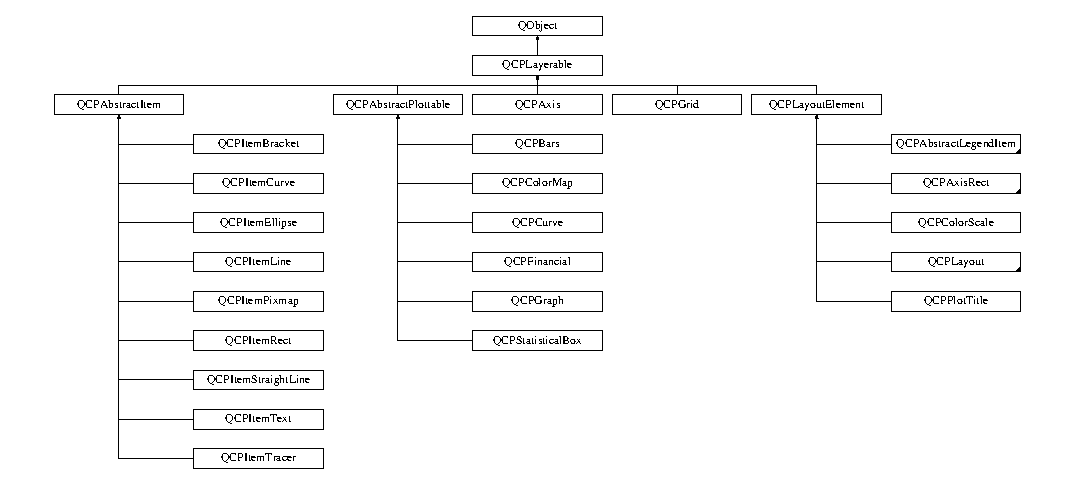
\includegraphics[height=6.075950cm]{class_q_c_p_layerable}
\end{center}
\end{figure}
\subsection*{Signals}
\begin{DoxyCompactItemize}
\item 
void \hyperlink{class_q_c_p_layerable_abbf8657cedea73ac1c3499b521c90eba}{layer\+Changed} (\hyperlink{class_q_c_p_layer}{Q\+C\+P\+Layer} $\ast$new\+Layer)
\end{DoxyCompactItemize}
\subsection*{Public Member Functions}
\begin{DoxyCompactItemize}
\item 
\hyperlink{class_q_c_p_layerable_a74c0fa237f29bf0e49565013fc5d1ec0}{Q\+C\+P\+Layerable} (\hyperlink{class_q_custom_plot}{Q\+Custom\+Plot} $\ast$plot, Q\+String target\+Layer=Q\+String(), \hyperlink{class_q_c_p_layerable}{Q\+C\+P\+Layerable} $\ast$\hyperlink{class_q_c_p_layerable_a98d79f5b716d45eac4347befe546d0ec}{parent\+Layerable}=0)
\item 
\hyperlink{class_q_c_p_layerable_a4231cf5b3601d6d3a5781283e7a9735b}{$\sim$\+Q\+C\+P\+Layerable} ()
\item 
bool \hyperlink{class_q_c_p_layerable_a10a3cc92e0fa63e4a929e61d34e275a7}{visible} () const 
\item 
\hyperlink{class_q_custom_plot}{Q\+Custom\+Plot} $\ast$ \hyperlink{class_q_c_p_layerable_ab7e0e94461566093d36ffc0f5312b109}{parent\+Plot} () const 
\item 
\hyperlink{class_q_c_p_layerable}{Q\+C\+P\+Layerable} $\ast$ \hyperlink{class_q_c_p_layerable_a98d79f5b716d45eac4347befe546d0ec}{parent\+Layerable} () const 
\item 
\hyperlink{class_q_c_p_layer}{Q\+C\+P\+Layer} $\ast$ \hyperlink{class_q_c_p_layerable_aea67e8c19145e70d68c286a36f6b8300}{layer} () const 
\item 
bool \hyperlink{class_q_c_p_layerable_aef5cb4aa899ed9dc9384fd614560291e}{antialiased} () const 
\item 
void \hyperlink{class_q_c_p_layerable_a3bed99ddc396b48ce3ebfdc0418744f8}{set\+Visible} (bool on)
\item 
Q\+\_\+\+S\+L\+O\+T bool \hyperlink{class_q_c_p_layerable_ab0d0da6d2de45a118886d2c8e16d5a54}{set\+Layer} (\hyperlink{class_q_c_p_layer}{Q\+C\+P\+Layer} $\ast$\hyperlink{class_q_c_p_layerable_aea67e8c19145e70d68c286a36f6b8300}{layer})
\item 
bool \hyperlink{class_q_c_p_layerable_ab25a0e7b897993b44447caee0f142083}{set\+Layer} (const Q\+String \&layer\+Name)
\item 
void \hyperlink{class_q_c_p_layerable_a4fd43e89be4a553ead41652565ff0581}{set\+Antialiased} (bool enabled)
\item 
virtual double \hyperlink{class_q_c_p_layerable_a4001c4d0dfec55598efa4d531f2179a9}{select\+Test} (const Q\+Point\+F \&pos, bool only\+Selectable, Q\+Variant $\ast$details=0) const 
\item 
bool \hyperlink{class_q_c_p_layerable_a30809f7455e9794bca7b6c737622fa63}{real\+Visibility} () const 
\end{DoxyCompactItemize}
\subsection*{Protected Member Functions}
\begin{DoxyCompactItemize}
\item 
virtual void \hyperlink{class_q_c_p_layerable_ab20b7dbd8e0249ed61adb9622c427382}{parent\+Plot\+Initialized} (\hyperlink{class_q_custom_plot}{Q\+Custom\+Plot} $\ast$\hyperlink{class_q_c_p_layerable_ab7e0e94461566093d36ffc0f5312b109}{parent\+Plot})
\item 
virtual \hyperlink{namespace_q_c_p_a2ad6bb6281c7c2d593d4277b44c2b037}{Q\+C\+P\+::\+Interaction} \hyperlink{class_q_c_p_layerable_aa4035e586b7f317a06ba7e74e242a5ea}{selection\+Category} () const 
\item 
virtual Q\+Rect \hyperlink{class_q_c_p_layerable_a07a8f746640c3704b09910df297afcba}{clip\+Rect} () const 
\item 
virtual void \hyperlink{class_q_c_p_layerable_afdf83ddc6a265cbf4c89fe99d3d93473}{apply\+Default\+Antialiasing\+Hint} (\hyperlink{class_q_c_p_painter}{Q\+C\+P\+Painter} $\ast$painter) const =0
\item 
virtual void \hyperlink{class_q_c_p_layerable_aecf2f7087482d4b6a78cb2770e5ed12d}{draw} (\hyperlink{class_q_c_p_painter}{Q\+C\+P\+Painter} $\ast$painter)=0
\item 
virtual void \hyperlink{class_q_c_p_layerable_a7498c2d0d081cf7cad0fb3bb93aa0e91}{select\+Event} (Q\+Mouse\+Event $\ast$event, bool additive, const Q\+Variant \&details, bool $\ast$selection\+State\+Changed)
\item 
virtual void \hyperlink{class_q_c_p_layerable_ae546370644a5551c76af739afc008bee}{deselect\+Event} (bool $\ast$selection\+State\+Changed)
\item 
void \hyperlink{class_q_c_p_layerable_a8cbe5a0c9a5674249982f5ca5f8e02bc}{initialize\+Parent\+Plot} (\hyperlink{class_q_custom_plot}{Q\+Custom\+Plot} $\ast$\hyperlink{class_q_c_p_layerable_ab7e0e94461566093d36ffc0f5312b109}{parent\+Plot})
\item 
void \hyperlink{class_q_c_p_layerable_aa23c893671f1f6744ac235cf2204cf3a}{set\+Parent\+Layerable} (\hyperlink{class_q_c_p_layerable}{Q\+C\+P\+Layerable} $\ast$\hyperlink{class_q_c_p_layerable_a98d79f5b716d45eac4347befe546d0ec}{parent\+Layerable})
\item 
bool \hyperlink{class_q_c_p_layerable_af94484cfb7cbbddb7de522e9be71d9a4}{move\+To\+Layer} (\hyperlink{class_q_c_p_layer}{Q\+C\+P\+Layer} $\ast$\hyperlink{class_q_c_p_layerable_aea67e8c19145e70d68c286a36f6b8300}{layer}, bool prepend)
\item 
void \hyperlink{class_q_c_p_layerable_a62bd552d1a45aa9accb24b310542279e}{apply\+Antialiasing\+Hint} (\hyperlink{class_q_c_p_painter}{Q\+C\+P\+Painter} $\ast$painter, bool local\+Antialiased, \hyperlink{namespace_q_c_p_ae55dbe315d41fe80f29ba88100843a0c}{Q\+C\+P\+::\+Antialiased\+Element} override\+Element) const 
\end{DoxyCompactItemize}
\subsection*{Protected Attributes}
\begin{DoxyCompactItemize}
\item 
bool \hyperlink{class_q_c_p_layerable_a62e3aed8427d6ce3ccf716f285106cb3}{m\+Visible}
\item 
\hyperlink{class_q_custom_plot}{Q\+Custom\+Plot} $\ast$ \hyperlink{class_q_c_p_layerable_aa2a528433e44db02b8aef23c1f9f90ed}{m\+Parent\+Plot}
\item 
Q\+Pointer$<$ \hyperlink{class_q_c_p_layerable}{Q\+C\+P\+Layerable} $>$ \hyperlink{class_q_c_p_layerable_a3291445a980053e2d17a21d15957624e}{m\+Parent\+Layerable}
\item 
\hyperlink{class_q_c_p_layer}{Q\+C\+P\+Layer} $\ast$ \hyperlink{class_q_c_p_layerable_aa38ec5891aff0f50b36fd63e9372a0cd}{m\+Layer}
\item 
bool \hyperlink{class_q_c_p_layerable_a3ab45a4c76a3333ce42eb217a81733ec}{m\+Antialiased}
\end{DoxyCompactItemize}
\subsection*{Friends}
\begin{DoxyCompactItemize}
\item 
class \hyperlink{class_q_c_p_layerable_a1cdf9df76adcfae45261690aa0ca2198}{Q\+Custom\+Plot}
\item 
class \hyperlink{class_q_c_p_layerable_acbf20ecb140f66c5fd1bc64ae0762990}{Q\+C\+P\+Axis\+Rect}
\end{DoxyCompactItemize}


\subsection{Detailed Description}
Base class for all drawable objects. 

This is the abstract base class most visible objects derive from, e.\+g. plottables, axes, grid etc.

Every layerable is on a layer (\hyperlink{class_q_c_p_layer}{Q\+C\+P\+Layer}) which allows controlling the rendering order by stacking the layers accordingly.

For details about the layering mechanism, see the \hyperlink{class_q_c_p_layer}{Q\+C\+P\+Layer} documentation. 

\subsection{Constructor \& Destructor Documentation}
\hypertarget{class_q_c_p_layerable_a74c0fa237f29bf0e49565013fc5d1ec0}{}\index{Q\+C\+P\+Layerable@{Q\+C\+P\+Layerable}!Q\+C\+P\+Layerable@{Q\+C\+P\+Layerable}}
\index{Q\+C\+P\+Layerable@{Q\+C\+P\+Layerable}!Q\+C\+P\+Layerable@{Q\+C\+P\+Layerable}}
\subsubsection[{Q\+C\+P\+Layerable}]{\setlength{\rightskip}{0pt plus 5cm}Q\+C\+P\+Layerable\+::\+Q\+C\+P\+Layerable (
\begin{DoxyParamCaption}
\item[{{\bf Q\+Custom\+Plot} $\ast$}]{plot, }
\item[{Q\+String}]{target\+Layer = {\ttfamily QString()}, }
\item[{{\bf Q\+C\+P\+Layerable} $\ast$}]{parent\+Layerable = {\ttfamily 0}}
\end{DoxyParamCaption}
)}\label{class_q_c_p_layerable_a74c0fa237f29bf0e49565013fc5d1ec0}
Creates a new \hyperlink{class_q_c_p_layerable}{Q\+C\+P\+Layerable} instance.

Since \hyperlink{class_q_c_p_layerable}{Q\+C\+P\+Layerable} is an abstract base class, it can\textquotesingle{}t be instantiated directly. Use one of the derived classes.

If {\itshape plot} is provided, it automatically places itself on the layer named {\itshape target\+Layer}. If {\itshape target\+Layer} is an empty string, it places itself on the current layer of the plot (see \hyperlink{class_q_custom_plot_a73a6dc47c653bb6f8f030abca5a11852}{Q\+Custom\+Plot\+::set\+Current\+Layer}).

It is possible to provide 0 as {\itshape plot}. In that case, you should assign a parent plot at a later time with \hyperlink{class_q_c_p_layerable_a8cbe5a0c9a5674249982f5ca5f8e02bc}{initialize\+Parent\+Plot}.

The layerable\textquotesingle{}s parent layerable is set to {\itshape parent\+Layerable}, if provided. Direct layerable parents are mainly used to control visibility in a hierarchy of layerables. This means a layerable is only drawn, if all its ancestor layerables are also visible. Note that {\itshape parent\+Layerable} does not become the Q\+Object-\/parent (for memory management) of this layerable, {\itshape plot} does. \hypertarget{class_q_c_p_layerable_a4231cf5b3601d6d3a5781283e7a9735b}{}\index{Q\+C\+P\+Layerable@{Q\+C\+P\+Layerable}!````~Q\+C\+P\+Layerable@{$\sim$\+Q\+C\+P\+Layerable}}
\index{````~Q\+C\+P\+Layerable@{$\sim$\+Q\+C\+P\+Layerable}!Q\+C\+P\+Layerable@{Q\+C\+P\+Layerable}}
\subsubsection[{$\sim$\+Q\+C\+P\+Layerable}]{\setlength{\rightskip}{0pt plus 5cm}Q\+C\+P\+Layerable\+::$\sim$\+Q\+C\+P\+Layerable (
\begin{DoxyParamCaption}
{}
\end{DoxyParamCaption}
)}\label{class_q_c_p_layerable_a4231cf5b3601d6d3a5781283e7a9735b}


\subsection{Member Function Documentation}
\hypertarget{class_q_c_p_layerable_aef5cb4aa899ed9dc9384fd614560291e}{}\index{Q\+C\+P\+Layerable@{Q\+C\+P\+Layerable}!antialiased@{antialiased}}
\index{antialiased@{antialiased}!Q\+C\+P\+Layerable@{Q\+C\+P\+Layerable}}
\subsubsection[{antialiased}]{\setlength{\rightskip}{0pt plus 5cm}bool Q\+C\+P\+Layerable\+::antialiased (
\begin{DoxyParamCaption}
{}
\end{DoxyParamCaption}
) const\hspace{0.3cm}{\ttfamily [inline]}}\label{class_q_c_p_layerable_aef5cb4aa899ed9dc9384fd614560291e}
\hypertarget{class_q_c_p_layerable_a62bd552d1a45aa9accb24b310542279e}{}\index{Q\+C\+P\+Layerable@{Q\+C\+P\+Layerable}!apply\+Antialiasing\+Hint@{apply\+Antialiasing\+Hint}}
\index{apply\+Antialiasing\+Hint@{apply\+Antialiasing\+Hint}!Q\+C\+P\+Layerable@{Q\+C\+P\+Layerable}}
\subsubsection[{apply\+Antialiasing\+Hint}]{\setlength{\rightskip}{0pt plus 5cm}void Q\+C\+P\+Layerable\+::apply\+Antialiasing\+Hint (
\begin{DoxyParamCaption}
\item[{{\bf Q\+C\+P\+Painter} $\ast$}]{painter, }
\item[{bool}]{local\+Antialiased, }
\item[{{\bf Q\+C\+P\+::\+Antialiased\+Element}}]{override\+Element}
\end{DoxyParamCaption}
) const\hspace{0.3cm}{\ttfamily [protected]}}\label{class_q_c_p_layerable_a62bd552d1a45aa9accb24b310542279e}
\hypertarget{class_q_c_p_layerable_afdf83ddc6a265cbf4c89fe99d3d93473}{}\index{Q\+C\+P\+Layerable@{Q\+C\+P\+Layerable}!apply\+Default\+Antialiasing\+Hint@{apply\+Default\+Antialiasing\+Hint}}
\index{apply\+Default\+Antialiasing\+Hint@{apply\+Default\+Antialiasing\+Hint}!Q\+C\+P\+Layerable@{Q\+C\+P\+Layerable}}
\subsubsection[{apply\+Default\+Antialiasing\+Hint}]{\setlength{\rightskip}{0pt plus 5cm}void Q\+C\+P\+Layerable\+::apply\+Default\+Antialiasing\+Hint (
\begin{DoxyParamCaption}
\item[{{\bf Q\+C\+P\+Painter} $\ast$}]{painter}
\end{DoxyParamCaption}
) const\hspace{0.3cm}{\ttfamily [protected]}, {\ttfamily [pure virtual]}}\label{class_q_c_p_layerable_afdf83ddc6a265cbf4c89fe99d3d93473}


Implemented in \hyperlink{class_q_c_p_color_scale_a23d530c340c15d2fce6583e7120ee8bd}{Q\+C\+P\+Color\+Scale}, \hyperlink{class_q_c_p_plot_title_a0e2a491864bf8d8e8b159ef38e9d85bd}{Q\+C\+P\+Plot\+Title}, \hyperlink{class_q_c_p_legend_a26307f532c3458b379663b7d517a5f47}{Q\+C\+P\+Legend}, \hyperlink{class_q_c_p_abstract_legend_item_a71c3baeda42ba78d2cccd97e74110a5e}{Q\+C\+P\+Abstract\+Legend\+Item}, \hyperlink{class_q_c_p_axis_rect_a9a6dd0763701cbc7d01f899bcbb3f9ca}{Q\+C\+P\+Axis\+Rect}, \hyperlink{class_q_c_p_abstract_item_a0839031abdd71067e2256a4d53c7a011}{Q\+C\+P\+Abstract\+Item}, \hyperlink{class_q_c_p_abstract_plottable_a76e9d6cc7972dc1528f526d163766aca}{Q\+C\+P\+Abstract\+Plottable}, \hyperlink{class_q_c_p_axis_a13bde39eb1e0b7c14a02935689be8aba}{Q\+C\+P\+Axis}, \hyperlink{class_q_c_p_grid_a9916f5e38b4d6cae446537aeb47c7272}{Q\+C\+P\+Grid}, and \hyperlink{class_q_c_p_layout_element_ad6d2b4bb0291c2441b2e1ca3d5296df5}{Q\+C\+P\+Layout\+Element}.

\hypertarget{class_q_c_p_layerable_a07a8f746640c3704b09910df297afcba}{}\index{Q\+C\+P\+Layerable@{Q\+C\+P\+Layerable}!clip\+Rect@{clip\+Rect}}
\index{clip\+Rect@{clip\+Rect}!Q\+C\+P\+Layerable@{Q\+C\+P\+Layerable}}
\subsubsection[{clip\+Rect}]{\setlength{\rightskip}{0pt plus 5cm}Q\+Rect Q\+C\+P\+Layerable\+::clip\+Rect (
\begin{DoxyParamCaption}
{}
\end{DoxyParamCaption}
) const\hspace{0.3cm}{\ttfamily [protected]}, {\ttfamily [virtual]}}\label{class_q_c_p_layerable_a07a8f746640c3704b09910df297afcba}


Reimplemented in \hyperlink{class_q_c_p_abstract_legend_item_abcb540c331b49ef7ee0ea1abbd0dcac3}{Q\+C\+P\+Abstract\+Legend\+Item}, \hyperlink{class_q_c_p_abstract_item_a538e25ff8856534582f5b2b400a46405}{Q\+C\+P\+Abstract\+Item}, and \hyperlink{class_q_c_p_abstract_plottable_ac01960b0827913922f5364d559c124ed}{Q\+C\+P\+Abstract\+Plottable}.

\hypertarget{class_q_c_p_layerable_ae546370644a5551c76af739afc008bee}{}\index{Q\+C\+P\+Layerable@{Q\+C\+P\+Layerable}!deselect\+Event@{deselect\+Event}}
\index{deselect\+Event@{deselect\+Event}!Q\+C\+P\+Layerable@{Q\+C\+P\+Layerable}}
\subsubsection[{deselect\+Event}]{\setlength{\rightskip}{0pt plus 5cm}void Q\+C\+P\+Layerable\+::deselect\+Event (
\begin{DoxyParamCaption}
\item[{bool $\ast$}]{selection\+State\+Changed}
\end{DoxyParamCaption}
)\hspace{0.3cm}{\ttfamily [protected]}, {\ttfamily [virtual]}}\label{class_q_c_p_layerable_ae546370644a5551c76af739afc008bee}


Reimplemented in \hyperlink{class_q_c_p_plot_title_ac6dfce05bebdb9bd0bfacd5ff02f3325}{Q\+C\+P\+Plot\+Title}, \hyperlink{class_q_c_p_legend_a5208ead4331c9b0440f768f059777c58}{Q\+C\+P\+Legend}, \hyperlink{class_q_c_p_abstract_legend_item_ae64e667e7c5b85cd92c9b91928faef28}{Q\+C\+P\+Abstract\+Legend\+Item}, \hyperlink{class_q_c_p_abstract_item_a91f090d6763cfedb0749219c63788ae9}{Q\+C\+P\+Abstract\+Item}, \hyperlink{class_q_c_p_abstract_plottable_a6fa0d0f95560ea8b01ee13f296dab2b1}{Q\+C\+P\+Abstract\+Plottable}, and \hyperlink{class_q_c_p_axis_a53512242cde6ec21943a3ba10dbf78c3}{Q\+C\+P\+Axis}.

\hypertarget{class_q_c_p_layerable_aecf2f7087482d4b6a78cb2770e5ed12d}{}\index{Q\+C\+P\+Layerable@{Q\+C\+P\+Layerable}!draw@{draw}}
\index{draw@{draw}!Q\+C\+P\+Layerable@{Q\+C\+P\+Layerable}}
\subsubsection[{draw}]{\setlength{\rightskip}{0pt plus 5cm}void Q\+C\+P\+Layerable\+::draw (
\begin{DoxyParamCaption}
\item[{{\bf Q\+C\+P\+Painter} $\ast$}]{painter}
\end{DoxyParamCaption}
)\hspace{0.3cm}{\ttfamily [protected]}, {\ttfamily [pure virtual]}}\label{class_q_c_p_layerable_aecf2f7087482d4b6a78cb2770e5ed12d}


Implemented in \hyperlink{class_q_c_p_item_bracket_a8343cf0559c64886add7aa7f4b22f1a6}{Q\+C\+P\+Item\+Bracket}, \hyperlink{class_q_c_p_item_tracer_aaaf49b48382c730ec9be0e74c2538315}{Q\+C\+P\+Item\+Tracer}, \hyperlink{class_q_c_p_item_pixmap_a879e8076c2db01a38b34cfa73ec95d2f}{Q\+C\+P\+Item\+Pixmap}, \hyperlink{class_q_c_p_item_ellipse_afe97ec827adb05f000fe007783faae3c}{Q\+C\+P\+Item\+Ellipse}, \hyperlink{class_q_c_p_item_text_a8793adb271ab79b4cf391dc55e9987f1}{Q\+C\+P\+Item\+Text}, \hyperlink{class_q_c_p_item_rect_a18cd583638b876cdd50f1a155ec182aa}{Q\+C\+P\+Item\+Rect}, \hyperlink{class_q_c_p_item_curve_a56cb5b72cd02db2eda598274a39839a9}{Q\+C\+P\+Item\+Curve}, \hyperlink{class_q_c_p_item_line_a1fc045dd33919f8006df0692aeb0e84a}{Q\+C\+P\+Item\+Line}, \hyperlink{class_q_c_p_item_straight_line_a2daa1e1253216c26565d56a2d5530170}{Q\+C\+P\+Item\+Straight\+Line}, \hyperlink{class_q_c_p_financial_ad71a59a1b42616594831e04e52c92120}{Q\+C\+P\+Financial}, \hyperlink{class_q_c_p_color_map_a3b0f45a3177be9522d5e9b8cd8ae122d}{Q\+C\+P\+Color\+Map}, \hyperlink{class_q_c_p_statistical_box_a753b62761217dd6b92f8a29e286a1317}{Q\+C\+P\+Statistical\+Box}, \hyperlink{class_q_c_p_bars_a42b894e34dac799f90ff3700706b31df}{Q\+C\+P\+Bars}, \hyperlink{class_q_c_p_curve_a2361302d2fc6ec669849bd3bca00c4b2}{Q\+C\+P\+Curve}, \hyperlink{class_q_c_p_graph_a659218cc62c2a7786213d9dd429c1c8d}{Q\+C\+P\+Graph}, \hyperlink{class_q_c_p_color_scale_axis_rect_private_adb67bfe9057a9dd9a85f548c274e6d98}{Q\+C\+P\+Color\+Scale\+Axis\+Rect\+Private}, \hyperlink{class_q_c_p_plot_title_ae4f1f8d24489628dabb7256363b097d2}{Q\+C\+P\+Plot\+Title}, \hyperlink{class_q_c_p_legend_a4462151bf875ca85fa3815457c683fdc}{Q\+C\+P\+Legend}, \hyperlink{class_q_c_p_plottable_legend_item_a68a781c3de4f9959fdf82075052d43aa}{Q\+C\+P\+Plottable\+Legend\+Item}, \hyperlink{class_q_c_p_abstract_legend_item_a97dedc084c672359710f16b31d046d1d}{Q\+C\+P\+Abstract\+Legend\+Item}, \hyperlink{class_q_c_p_axis_rect_afb1bbbbda8345cd2710d92ee48440b53}{Q\+C\+P\+Axis\+Rect}, \hyperlink{class_q_c_p_abstract_item_ad0dc056f650c3ca73414e6b4f01674ef}{Q\+C\+P\+Abstract\+Item}, \hyperlink{class_q_c_p_abstract_plottable_acbab5e30dcd04fd302b4a5902ac2c482}{Q\+C\+P\+Abstract\+Plottable}, \hyperlink{class_q_c_p_axis_a258b1e783eda5cd14ec5552c696a424e}{Q\+C\+P\+Axis}, \hyperlink{class_q_c_p_grid_ad009c23f96078616aa4f66a750974b23}{Q\+C\+P\+Grid}, and \hyperlink{class_q_c_p_layout_element_a547bcc1e6e2be5645ca781efe0834653}{Q\+C\+P\+Layout\+Element}.

\hypertarget{class_q_c_p_layerable_a8cbe5a0c9a5674249982f5ca5f8e02bc}{}\index{Q\+C\+P\+Layerable@{Q\+C\+P\+Layerable}!initialize\+Parent\+Plot@{initialize\+Parent\+Plot}}
\index{initialize\+Parent\+Plot@{initialize\+Parent\+Plot}!Q\+C\+P\+Layerable@{Q\+C\+P\+Layerable}}
\subsubsection[{initialize\+Parent\+Plot}]{\setlength{\rightskip}{0pt plus 5cm}void Q\+C\+P\+Layerable\+::initialize\+Parent\+Plot (
\begin{DoxyParamCaption}
\item[{{\bf Q\+Custom\+Plot} $\ast$}]{parent\+Plot}
\end{DoxyParamCaption}
)\hspace{0.3cm}{\ttfamily [protected]}}\label{class_q_c_p_layerable_a8cbe5a0c9a5674249982f5ca5f8e02bc}
\hypertarget{class_q_c_p_layerable_aea67e8c19145e70d68c286a36f6b8300}{}\index{Q\+C\+P\+Layerable@{Q\+C\+P\+Layerable}!layer@{layer}}
\index{layer@{layer}!Q\+C\+P\+Layerable@{Q\+C\+P\+Layerable}}
\subsubsection[{layer}]{\setlength{\rightskip}{0pt plus 5cm}{\bf Q\+C\+P\+Layer}$\ast$ Q\+C\+P\+Layerable\+::layer (
\begin{DoxyParamCaption}
{}
\end{DoxyParamCaption}
) const\hspace{0.3cm}{\ttfamily [inline]}}\label{class_q_c_p_layerable_aea67e8c19145e70d68c286a36f6b8300}
\hypertarget{class_q_c_p_layerable_abbf8657cedea73ac1c3499b521c90eba}{}\index{Q\+C\+P\+Layerable@{Q\+C\+P\+Layerable}!layer\+Changed@{layer\+Changed}}
\index{layer\+Changed@{layer\+Changed}!Q\+C\+P\+Layerable@{Q\+C\+P\+Layerable}}
\subsubsection[{layer\+Changed}]{\setlength{\rightskip}{0pt plus 5cm}void Q\+C\+P\+Layerable\+::layer\+Changed (
\begin{DoxyParamCaption}
\item[{{\bf Q\+C\+P\+Layer} $\ast$}]{new\+Layer}
\end{DoxyParamCaption}
)\hspace{0.3cm}{\ttfamily [signal]}}\label{class_q_c_p_layerable_abbf8657cedea73ac1c3499b521c90eba}
This signal is emitted when the layer of this layerable changes, i.\+e. this layerable is moved to a different layer.

\begin{DoxySeeAlso}{See also}
\hyperlink{class_q_c_p_layerable_ab0d0da6d2de45a118886d2c8e16d5a54}{set\+Layer} 
\end{DoxySeeAlso}
\hypertarget{class_q_c_p_layerable_af94484cfb7cbbddb7de522e9be71d9a4}{}\index{Q\+C\+P\+Layerable@{Q\+C\+P\+Layerable}!move\+To\+Layer@{move\+To\+Layer}}
\index{move\+To\+Layer@{move\+To\+Layer}!Q\+C\+P\+Layerable@{Q\+C\+P\+Layerable}}
\subsubsection[{move\+To\+Layer}]{\setlength{\rightskip}{0pt plus 5cm}bool Q\+C\+P\+Layerable\+::move\+To\+Layer (
\begin{DoxyParamCaption}
\item[{{\bf Q\+C\+P\+Layer} $\ast$}]{layer, }
\item[{bool}]{prepend}
\end{DoxyParamCaption}
)\hspace{0.3cm}{\ttfamily [protected]}}\label{class_q_c_p_layerable_af94484cfb7cbbddb7de522e9be71d9a4}
\hypertarget{class_q_c_p_layerable_a98d79f5b716d45eac4347befe546d0ec}{}\index{Q\+C\+P\+Layerable@{Q\+C\+P\+Layerable}!parent\+Layerable@{parent\+Layerable}}
\index{parent\+Layerable@{parent\+Layerable}!Q\+C\+P\+Layerable@{Q\+C\+P\+Layerable}}
\subsubsection[{parent\+Layerable}]{\setlength{\rightskip}{0pt plus 5cm}{\bf Q\+C\+P\+Layerable} $\ast$ Q\+C\+P\+Layerable\+::parent\+Layerable (
\begin{DoxyParamCaption}
{}
\end{DoxyParamCaption}
) const\hspace{0.3cm}{\ttfamily [inline]}}\label{class_q_c_p_layerable_a98d79f5b716d45eac4347befe546d0ec}
Returns the parent layerable of this layerable. The parent layerable is used to provide visibility hierarchies in conjunction with the method \hyperlink{class_q_c_p_layerable_a30809f7455e9794bca7b6c737622fa63}{real\+Visibility}. This way, layerables only get drawn if their parent layerables are visible, too.

Note that a parent layerable is not necessarily also the Q\+Object parent for memory management. Further, a layerable doesn\textquotesingle{}t always have a parent layerable, so this function may return 0.

A parent layerable is set implicitly with when placed inside layout elements and doesn\textquotesingle{}t need to be set manually by the user. \hypertarget{class_q_c_p_layerable_ab7e0e94461566093d36ffc0f5312b109}{}\index{Q\+C\+P\+Layerable@{Q\+C\+P\+Layerable}!parent\+Plot@{parent\+Plot}}
\index{parent\+Plot@{parent\+Plot}!Q\+C\+P\+Layerable@{Q\+C\+P\+Layerable}}
\subsubsection[{parent\+Plot}]{\setlength{\rightskip}{0pt plus 5cm}{\bf Q\+Custom\+Plot}$\ast$ Q\+C\+P\+Layerable\+::parent\+Plot (
\begin{DoxyParamCaption}
{}
\end{DoxyParamCaption}
) const\hspace{0.3cm}{\ttfamily [inline]}}\label{class_q_c_p_layerable_ab7e0e94461566093d36ffc0f5312b109}
\hypertarget{class_q_c_p_layerable_ab20b7dbd8e0249ed61adb9622c427382}{}\index{Q\+C\+P\+Layerable@{Q\+C\+P\+Layerable}!parent\+Plot\+Initialized@{parent\+Plot\+Initialized}}
\index{parent\+Plot\+Initialized@{parent\+Plot\+Initialized}!Q\+C\+P\+Layerable@{Q\+C\+P\+Layerable}}
\subsubsection[{parent\+Plot\+Initialized}]{\setlength{\rightskip}{0pt plus 5cm}void Q\+C\+P\+Layerable\+::parent\+Plot\+Initialized (
\begin{DoxyParamCaption}
\item[{{\bf Q\+Custom\+Plot} $\ast$}]{parent\+Plot}
\end{DoxyParamCaption}
)\hspace{0.3cm}{\ttfamily [protected]}, {\ttfamily [virtual]}}\label{class_q_c_p_layerable_ab20b7dbd8e0249ed61adb9622c427382}


Reimplemented in \hyperlink{class_q_c_p_legend_a4d552c63d82742d77fb7f177bae7b1ba}{Q\+C\+P\+Legend}, and \hyperlink{class_q_c_p_layout_element_a1478899e80e8244b411e96ec3b2e5ce2}{Q\+C\+P\+Layout\+Element}.

\hypertarget{class_q_c_p_layerable_a30809f7455e9794bca7b6c737622fa63}{}\index{Q\+C\+P\+Layerable@{Q\+C\+P\+Layerable}!real\+Visibility@{real\+Visibility}}
\index{real\+Visibility@{real\+Visibility}!Q\+C\+P\+Layerable@{Q\+C\+P\+Layerable}}
\subsubsection[{real\+Visibility}]{\setlength{\rightskip}{0pt plus 5cm}bool Q\+C\+P\+Layerable\+::real\+Visibility (
\begin{DoxyParamCaption}
{}
\end{DoxyParamCaption}
) const}\label{class_q_c_p_layerable_a30809f7455e9794bca7b6c737622fa63}
Returns whether this layerable is visible, taking the visibility of the layerable parent and the visibility of the layer this layerable is on into account. This is the method that is consulted to decide whether a layerable shall be drawn or not.

If this layerable has a direct layerable parent (usually set via hierarchies implemented in subclasses, like in the case of \hyperlink{class_q_c_p_layout_element}{Q\+C\+P\+Layout\+Element}), this function returns true only if this layerable has its visibility set to true and the parent layerable\textquotesingle{}s \hyperlink{class_q_c_p_layerable_a30809f7455e9794bca7b6c737622fa63}{real\+Visibility} returns true.

If this layerable doesn\textquotesingle{}t have a direct layerable parent, returns the state of this layerable\textquotesingle{}s visibility. \hypertarget{class_q_c_p_layerable_a7498c2d0d081cf7cad0fb3bb93aa0e91}{}\index{Q\+C\+P\+Layerable@{Q\+C\+P\+Layerable}!select\+Event@{select\+Event}}
\index{select\+Event@{select\+Event}!Q\+C\+P\+Layerable@{Q\+C\+P\+Layerable}}
\subsubsection[{select\+Event}]{\setlength{\rightskip}{0pt plus 5cm}void Q\+C\+P\+Layerable\+::select\+Event (
\begin{DoxyParamCaption}
\item[{Q\+Mouse\+Event $\ast$}]{event, }
\item[{bool}]{additive, }
\item[{const Q\+Variant \&}]{details, }
\item[{bool $\ast$}]{selection\+State\+Changed}
\end{DoxyParamCaption}
)\hspace{0.3cm}{\ttfamily [protected]}, {\ttfamily [virtual]}}\label{class_q_c_p_layerable_a7498c2d0d081cf7cad0fb3bb93aa0e91}


Reimplemented in \hyperlink{class_q_c_p_plot_title_a22672ef2abe442b1e73b7ee04cff9bdd}{Q\+C\+P\+Plot\+Title}, \hyperlink{class_q_c_p_legend_af93bf87dc5c383a9d2ada80b35f3a1a5}{Q\+C\+P\+Legend}, \hyperlink{class_q_c_p_abstract_legend_item_abcfe9e335d99c7fac74e03d26723c1b7}{Q\+C\+P\+Abstract\+Legend\+Item}, \hyperlink{class_q_c_p_abstract_item_aaf92af7b9893712959a6c073d334d88d}{Q\+C\+P\+Abstract\+Item}, \hyperlink{class_q_c_p_abstract_plottable_a16aaad02456aa23a759efd1ac90c79bf}{Q\+C\+P\+Abstract\+Plottable}, and \hyperlink{class_q_c_p_axis_aa8a5fe80e2898ec08ada26b5fbee9eca}{Q\+C\+P\+Axis}.

\hypertarget{class_q_c_p_layerable_aa4035e586b7f317a06ba7e74e242a5ea}{}\index{Q\+C\+P\+Layerable@{Q\+C\+P\+Layerable}!selection\+Category@{selection\+Category}}
\index{selection\+Category@{selection\+Category}!Q\+C\+P\+Layerable@{Q\+C\+P\+Layerable}}
\subsubsection[{selection\+Category}]{\setlength{\rightskip}{0pt plus 5cm}{\bf Q\+C\+P\+::\+Interaction} Q\+C\+P\+Layerable\+::selection\+Category (
\begin{DoxyParamCaption}
{}
\end{DoxyParamCaption}
) const\hspace{0.3cm}{\ttfamily [protected]}, {\ttfamily [virtual]}}\label{class_q_c_p_layerable_aa4035e586b7f317a06ba7e74e242a5ea}


Reimplemented in \hyperlink{class_q_c_p_legend_a7a9795a28c9c2514b4ae50f0a63d407c}{Q\+C\+P\+Legend}, \hyperlink{class_q_c_p_abstract_legend_item_a53a80054ab329beaca072fb08c08944b}{Q\+C\+P\+Abstract\+Legend\+Item}, \hyperlink{class_q_c_p_abstract_item_a777b5d384936396ad9c3ceb3d3453f1c}{Q\+C\+P\+Abstract\+Item}, \hyperlink{class_q_c_p_abstract_plottable_a5eef607bcc2aee8bfe2380a8710f6c64}{Q\+C\+P\+Abstract\+Plottable}, and \hyperlink{class_q_c_p_axis_aca53b2f365dfc1257cba9e62395aa68f}{Q\+C\+P\+Axis}.

\hypertarget{class_q_c_p_layerable_a4001c4d0dfec55598efa4d531f2179a9}{}\index{Q\+C\+P\+Layerable@{Q\+C\+P\+Layerable}!select\+Test@{select\+Test}}
\index{select\+Test@{select\+Test}!Q\+C\+P\+Layerable@{Q\+C\+P\+Layerable}}
\subsubsection[{select\+Test}]{\setlength{\rightskip}{0pt plus 5cm}double Q\+C\+P\+Layerable\+::select\+Test (
\begin{DoxyParamCaption}
\item[{const Q\+Point\+F \&}]{pos, }
\item[{bool}]{only\+Selectable, }
\item[{Q\+Variant $\ast$}]{details = {\ttfamily 0}}
\end{DoxyParamCaption}
) const\hspace{0.3cm}{\ttfamily [virtual]}}\label{class_q_c_p_layerable_a4001c4d0dfec55598efa4d531f2179a9}
This function is used to decide whether a click hits a layerable object or not.

{\itshape pos} is a point in pixel coordinates on the \hyperlink{class_q_custom_plot}{Q\+Custom\+Plot} surface. This function returns the shortest pixel distance of this point to the object. If the object is either invisible or the distance couldn\textquotesingle{}t be determined, -\/1.\+0 is returned. Further, if {\itshape only\+Selectable} is true and the object is not selectable, -\/1.\+0 is returned, too.

If the item is represented not by single lines but by an area like \hyperlink{class_q_c_p_item_rect}{Q\+C\+P\+Item\+Rect} or \hyperlink{class_q_c_p_item_text}{Q\+C\+P\+Item\+Text}, a click inside the area returns a constant value greater zero (typically the selection\+Tolerance of the parent \hyperlink{class_q_custom_plot}{Q\+Custom\+Plot} multiplied by 0.\+99). If the click lies outside the area, this function returns -\/1.\+0.

Providing a constant value for area objects allows selecting line objects even when they are obscured by such area objects, by clicking close to the lines (i.\+e. closer than 0.\+99$\ast$selection\+Tolerance).

The actual setting of the selection state is not done by this function. This is handled by the parent \hyperlink{class_q_custom_plot}{Q\+Custom\+Plot} when the mouse\+Release\+Event occurs, and the finally selected object is notified via the select\+Event/deselect\+Event methods.

{\itshape details} is an optional output parameter. Every layerable subclass may place any information in {\itshape details}. This information will be passed to \hyperlink{class_q_c_p_layerable_a7498c2d0d081cf7cad0fb3bb93aa0e91}{select\+Event} when the parent \hyperlink{class_q_custom_plot}{Q\+Custom\+Plot} decides on the basis of this select\+Test call, that the object was successfully selected. The subsequent call to \hyperlink{class_q_c_p_layerable_a7498c2d0d081cf7cad0fb3bb93aa0e91}{select\+Event} will carry the {\itshape details}. This is useful for multi-\/part objects (like \hyperlink{class_q_c_p_axis}{Q\+C\+P\+Axis}). This way, a possibly complex calculation to decide which part was clicked is only done once in \hyperlink{class_q_c_p_layerable_a4001c4d0dfec55598efa4d531f2179a9}{select\+Test}. The result (i.\+e. the actually clicked part) can then be placed in {\itshape details}. So in the subsequent \hyperlink{class_q_c_p_layerable_a7498c2d0d081cf7cad0fb3bb93aa0e91}{select\+Event}, the decision which part was selected doesn\textquotesingle{}t have to be done a second time for a single selection operation.

You may pass 0 as {\itshape details} to indicate that you are not interested in those selection details.

\begin{DoxySeeAlso}{See also}
\hyperlink{class_q_c_p_layerable_a7498c2d0d081cf7cad0fb3bb93aa0e91}{select\+Event}, \hyperlink{class_q_c_p_layerable_ae546370644a5551c76af739afc008bee}{deselect\+Event}, \hyperlink{class_q_custom_plot_a5ee1e2f6ae27419deca53e75907c27e5}{Q\+Custom\+Plot\+::set\+Interactions} 
\end{DoxySeeAlso}


Reimplemented in \hyperlink{class_q_c_p_item_bracket_aa6933caff1d42c54bcebc769ef88c798}{Q\+C\+P\+Item\+Bracket}, \hyperlink{class_q_c_p_item_tracer_ae71f3728421c83c188c117279ca050fd}{Q\+C\+P\+Item\+Tracer}, \hyperlink{class_q_c_p_item_pixmap_a9f8436aa141fa0fb504191c882c2f4d9}{Q\+C\+P\+Item\+Pixmap}, \hyperlink{class_q_c_p_item_ellipse_acd7e5f9528630b2ab5987e2a5782eb7c}{Q\+C\+P\+Item\+Ellipse}, \hyperlink{class_q_c_p_item_text_a285b95bb6634c2e4f7768abb7a8bc69c}{Q\+C\+P\+Item\+Text}, \hyperlink{class_q_c_p_item_rect_af13b0797079b40b73d1c7286b76f18ac}{Q\+C\+P\+Item\+Rect}, \hyperlink{class_q_c_p_item_curve_a741375c11667b5f9c95b2683f93ee514}{Q\+C\+P\+Item\+Curve}, \hyperlink{class_q_c_p_item_line_a7541e5d9378ca121d07b0df3b24f7178}{Q\+C\+P\+Item\+Line}, \hyperlink{class_q_c_p_item_straight_line_a64cc3796f58ce856012732603edb2f1c}{Q\+C\+P\+Item\+Straight\+Line}, \hyperlink{class_q_c_p_financial_adf6cff00a55f775487d375fe4df5e95b}{Q\+C\+P\+Financial}, \hyperlink{class_q_c_p_color_map_a4088dc7bcbe9bba605c84a912ba660ff}{Q\+C\+P\+Color\+Map}, \hyperlink{class_q_c_p_statistical_box_a7d3ac843dc48a085740fdfc4319a89cc}{Q\+C\+P\+Statistical\+Box}, \hyperlink{class_q_c_p_bars_a0d37a9feb1d0baf73ce6e809db214445}{Q\+C\+P\+Bars}, \hyperlink{class_q_c_p_curve_a5af9949e725704811bbc81ecd5970b8e}{Q\+C\+P\+Curve}, \hyperlink{class_q_c_p_graph_abc9ff375aabcf2d21cca33d6baf85772}{Q\+C\+P\+Graph}, \hyperlink{class_q_c_p_plot_title_a5b7ae716be9134a48f4e378feb0e6699}{Q\+C\+P\+Plot\+Title}, \hyperlink{class_q_c_p_legend_aa3892801051bc7b985e003576df844db}{Q\+C\+P\+Legend}, \hyperlink{class_q_c_p_abstract_legend_item_ad0480d5cad34627a294a2921caa4a62f}{Q\+C\+P\+Abstract\+Legend\+Item}, \hyperlink{class_q_c_p_abstract_item_a96d522d10ffc0413b9a366c6f7f0476b}{Q\+C\+P\+Abstract\+Item}, \hyperlink{class_q_c_p_abstract_plottable_a38efe9641d972992a3d44204bc80ec1d}{Q\+C\+P\+Abstract\+Plottable}, \hyperlink{class_q_c_p_axis_a2877a6230920c118be65c6113089f467}{Q\+C\+P\+Axis}, \hyperlink{class_q_c_p_layout_inset_ab5a2f2b88c05e369fd7da9583d17aa3a}{Q\+C\+P\+Layout\+Inset}, and \hyperlink{class_q_c_p_layout_element_a9fcf5d0ea19f2c23b2b528bce2c6f095}{Q\+C\+P\+Layout\+Element}.

\hypertarget{class_q_c_p_layerable_a4fd43e89be4a553ead41652565ff0581}{}\index{Q\+C\+P\+Layerable@{Q\+C\+P\+Layerable}!set\+Antialiased@{set\+Antialiased}}
\index{set\+Antialiased@{set\+Antialiased}!Q\+C\+P\+Layerable@{Q\+C\+P\+Layerable}}
\subsubsection[{set\+Antialiased}]{\setlength{\rightskip}{0pt plus 5cm}void Q\+C\+P\+Layerable\+::set\+Antialiased (
\begin{DoxyParamCaption}
\item[{bool}]{enabled}
\end{DoxyParamCaption}
)}\label{class_q_c_p_layerable_a4fd43e89be4a553ead41652565ff0581}
Sets whether this object will be drawn antialiased or not.

Note that antialiasing settings may be overridden by \hyperlink{class_q_custom_plot_af6f91e5eab1be85f67c556e98c3745e8}{Q\+Custom\+Plot\+::set\+Antialiased\+Elements} and \hyperlink{class_q_custom_plot_ae10d685b5eabea2999fb8775ca173c24}{Q\+Custom\+Plot\+::set\+Not\+Antialiased\+Elements}. \hypertarget{class_q_c_p_layerable_ab0d0da6d2de45a118886d2c8e16d5a54}{}\index{Q\+C\+P\+Layerable@{Q\+C\+P\+Layerable}!set\+Layer@{set\+Layer}}
\index{set\+Layer@{set\+Layer}!Q\+C\+P\+Layerable@{Q\+C\+P\+Layerable}}
\subsubsection[{set\+Layer}]{\setlength{\rightskip}{0pt plus 5cm}bool Q\+C\+P\+Layerable\+::set\+Layer (
\begin{DoxyParamCaption}
\item[{{\bf Q\+C\+P\+Layer} $\ast$}]{layer}
\end{DoxyParamCaption}
)}\label{class_q_c_p_layerable_ab0d0da6d2de45a118886d2c8e16d5a54}
Sets the {\itshape layer} of this layerable object. The object will be placed on top of the other objects already on {\itshape layer}.

Returns true on success, i.\+e. if {\itshape layer} is a valid layer. \hypertarget{class_q_c_p_layerable_ab25a0e7b897993b44447caee0f142083}{}\index{Q\+C\+P\+Layerable@{Q\+C\+P\+Layerable}!set\+Layer@{set\+Layer}}
\index{set\+Layer@{set\+Layer}!Q\+C\+P\+Layerable@{Q\+C\+P\+Layerable}}
\subsubsection[{set\+Layer}]{\setlength{\rightskip}{0pt plus 5cm}bool Q\+C\+P\+Layerable\+::set\+Layer (
\begin{DoxyParamCaption}
\item[{const Q\+String \&}]{layer\+Name}
\end{DoxyParamCaption}
)}\label{class_q_c_p_layerable_ab25a0e7b897993b44447caee0f142083}
This is an overloaded member function, provided for convenience. It differs from the above function only in what argument(s) it accepts. Sets the layer of this layerable object by name

Returns true on success, i.\+e. if {\itshape layer\+Name} is a valid layer name. \hypertarget{class_q_c_p_layerable_aa23c893671f1f6744ac235cf2204cf3a}{}\index{Q\+C\+P\+Layerable@{Q\+C\+P\+Layerable}!set\+Parent\+Layerable@{set\+Parent\+Layerable}}
\index{set\+Parent\+Layerable@{set\+Parent\+Layerable}!Q\+C\+P\+Layerable@{Q\+C\+P\+Layerable}}
\subsubsection[{set\+Parent\+Layerable}]{\setlength{\rightskip}{0pt plus 5cm}void Q\+C\+P\+Layerable\+::set\+Parent\+Layerable (
\begin{DoxyParamCaption}
\item[{{\bf Q\+C\+P\+Layerable} $\ast$}]{parent\+Layerable}
\end{DoxyParamCaption}
)\hspace{0.3cm}{\ttfamily [protected]}}\label{class_q_c_p_layerable_aa23c893671f1f6744ac235cf2204cf3a}
\hypertarget{class_q_c_p_layerable_a3bed99ddc396b48ce3ebfdc0418744f8}{}\index{Q\+C\+P\+Layerable@{Q\+C\+P\+Layerable}!set\+Visible@{set\+Visible}}
\index{set\+Visible@{set\+Visible}!Q\+C\+P\+Layerable@{Q\+C\+P\+Layerable}}
\subsubsection[{set\+Visible}]{\setlength{\rightskip}{0pt plus 5cm}void Q\+C\+P\+Layerable\+::set\+Visible (
\begin{DoxyParamCaption}
\item[{bool}]{on}
\end{DoxyParamCaption}
)}\label{class_q_c_p_layerable_a3bed99ddc396b48ce3ebfdc0418744f8}
Sets the visibility of this layerable object. If an object is not visible, it will not be drawn on the \hyperlink{class_q_custom_plot}{Q\+Custom\+Plot} surface, and user interaction with it (e.\+g. click and selection) is not possible. \hypertarget{class_q_c_p_layerable_a10a3cc92e0fa63e4a929e61d34e275a7}{}\index{Q\+C\+P\+Layerable@{Q\+C\+P\+Layerable}!visible@{visible}}
\index{visible@{visible}!Q\+C\+P\+Layerable@{Q\+C\+P\+Layerable}}
\subsubsection[{visible}]{\setlength{\rightskip}{0pt plus 5cm}bool Q\+C\+P\+Layerable\+::visible (
\begin{DoxyParamCaption}
{}
\end{DoxyParamCaption}
) const\hspace{0.3cm}{\ttfamily [inline]}}\label{class_q_c_p_layerable_a10a3cc92e0fa63e4a929e61d34e275a7}


\subsection{Friends And Related Function Documentation}
\hypertarget{class_q_c_p_layerable_acbf20ecb140f66c5fd1bc64ae0762990}{}\index{Q\+C\+P\+Layerable@{Q\+C\+P\+Layerable}!Q\+C\+P\+Axis\+Rect@{Q\+C\+P\+Axis\+Rect}}
\index{Q\+C\+P\+Axis\+Rect@{Q\+C\+P\+Axis\+Rect}!Q\+C\+P\+Layerable@{Q\+C\+P\+Layerable}}
\subsubsection[{Q\+C\+P\+Axis\+Rect}]{\setlength{\rightskip}{0pt plus 5cm}friend class {\bf Q\+C\+P\+Axis\+Rect}\hspace{0.3cm}{\ttfamily [friend]}}\label{class_q_c_p_layerable_acbf20ecb140f66c5fd1bc64ae0762990}
\hypertarget{class_q_c_p_layerable_a1cdf9df76adcfae45261690aa0ca2198}{}\index{Q\+C\+P\+Layerable@{Q\+C\+P\+Layerable}!Q\+Custom\+Plot@{Q\+Custom\+Plot}}
\index{Q\+Custom\+Plot@{Q\+Custom\+Plot}!Q\+C\+P\+Layerable@{Q\+C\+P\+Layerable}}
\subsubsection[{Q\+Custom\+Plot}]{\setlength{\rightskip}{0pt plus 5cm}friend class {\bf Q\+Custom\+Plot}\hspace{0.3cm}{\ttfamily [friend]}}\label{class_q_c_p_layerable_a1cdf9df76adcfae45261690aa0ca2198}


\subsection{Member Data Documentation}
\hypertarget{class_q_c_p_layerable_a3ab45a4c76a3333ce42eb217a81733ec}{}\index{Q\+C\+P\+Layerable@{Q\+C\+P\+Layerable}!m\+Antialiased@{m\+Antialiased}}
\index{m\+Antialiased@{m\+Antialiased}!Q\+C\+P\+Layerable@{Q\+C\+P\+Layerable}}
\subsubsection[{m\+Antialiased}]{\setlength{\rightskip}{0pt plus 5cm}bool Q\+C\+P\+Layerable\+::m\+Antialiased\hspace{0.3cm}{\ttfamily [protected]}}\label{class_q_c_p_layerable_a3ab45a4c76a3333ce42eb217a81733ec}
\hypertarget{class_q_c_p_layerable_aa38ec5891aff0f50b36fd63e9372a0cd}{}\index{Q\+C\+P\+Layerable@{Q\+C\+P\+Layerable}!m\+Layer@{m\+Layer}}
\index{m\+Layer@{m\+Layer}!Q\+C\+P\+Layerable@{Q\+C\+P\+Layerable}}
\subsubsection[{m\+Layer}]{\setlength{\rightskip}{0pt plus 5cm}{\bf Q\+C\+P\+Layer}$\ast$ Q\+C\+P\+Layerable\+::m\+Layer\hspace{0.3cm}{\ttfamily [protected]}}\label{class_q_c_p_layerable_aa38ec5891aff0f50b36fd63e9372a0cd}
\hypertarget{class_q_c_p_layerable_a3291445a980053e2d17a21d15957624e}{}\index{Q\+C\+P\+Layerable@{Q\+C\+P\+Layerable}!m\+Parent\+Layerable@{m\+Parent\+Layerable}}
\index{m\+Parent\+Layerable@{m\+Parent\+Layerable}!Q\+C\+P\+Layerable@{Q\+C\+P\+Layerable}}
\subsubsection[{m\+Parent\+Layerable}]{\setlength{\rightskip}{0pt plus 5cm}Q\+Pointer$<${\bf Q\+C\+P\+Layerable}$>$ Q\+C\+P\+Layerable\+::m\+Parent\+Layerable\hspace{0.3cm}{\ttfamily [protected]}}\label{class_q_c_p_layerable_a3291445a980053e2d17a21d15957624e}
\hypertarget{class_q_c_p_layerable_aa2a528433e44db02b8aef23c1f9f90ed}{}\index{Q\+C\+P\+Layerable@{Q\+C\+P\+Layerable}!m\+Parent\+Plot@{m\+Parent\+Plot}}
\index{m\+Parent\+Plot@{m\+Parent\+Plot}!Q\+C\+P\+Layerable@{Q\+C\+P\+Layerable}}
\subsubsection[{m\+Parent\+Plot}]{\setlength{\rightskip}{0pt plus 5cm}{\bf Q\+Custom\+Plot}$\ast$ Q\+C\+P\+Layerable\+::m\+Parent\+Plot\hspace{0.3cm}{\ttfamily [protected]}}\label{class_q_c_p_layerable_aa2a528433e44db02b8aef23c1f9f90ed}
\hypertarget{class_q_c_p_layerable_a62e3aed8427d6ce3ccf716f285106cb3}{}\index{Q\+C\+P\+Layerable@{Q\+C\+P\+Layerable}!m\+Visible@{m\+Visible}}
\index{m\+Visible@{m\+Visible}!Q\+C\+P\+Layerable@{Q\+C\+P\+Layerable}}
\subsubsection[{m\+Visible}]{\setlength{\rightskip}{0pt plus 5cm}bool Q\+C\+P\+Layerable\+::m\+Visible\hspace{0.3cm}{\ttfamily [protected]}}\label{class_q_c_p_layerable_a62e3aed8427d6ce3ccf716f285106cb3}


The documentation for this class was generated from the following files\+:\begin{DoxyCompactItemize}
\item 
C\+:/\+Users/\+Roman/\+Documents/\+Mygs/\+Ground\+Station/\+G\+S/\hyperlink{qcustomplot_8h}{qcustomplot.\+h}\item 
C\+:/\+Users/\+Roman/\+Documents/\+Mygs/\+Ground\+Station/\+G\+S/\hyperlink{qcustomplot_8cpp}{qcustomplot.\+cpp}\end{DoxyCompactItemize}

\hypertarget{class_q_c_p_layout}{}\section{Q\+C\+P\+Layout Class Reference}
\label{class_q_c_p_layout}\index{Q\+C\+P\+Layout@{Q\+C\+P\+Layout}}


The abstract base class for layouts.  




{\ttfamily \#include $<$qcustomplot.\+h$>$}

Inheritance diagram for Q\+C\+P\+Layout\+:\begin{figure}[H]
\begin{center}
\leavevmode
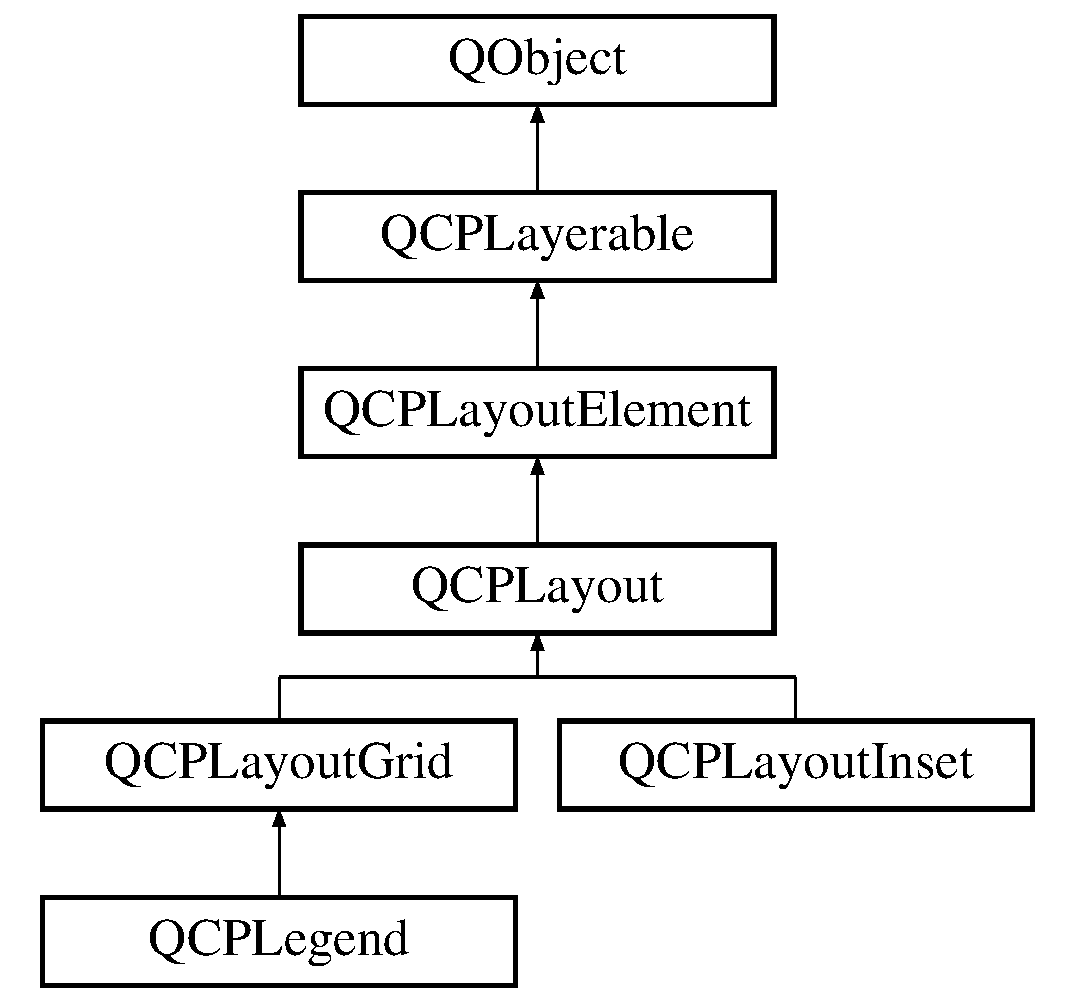
\includegraphics[height=6.000000cm]{class_q_c_p_layout}
\end{center}
\end{figure}
\subsection*{Public Member Functions}
\begin{DoxyCompactItemize}
\item 
\hyperlink{class_q_c_p_layout_a04222e6e1361fd802d48f1a25b7020d4}{Q\+C\+P\+Layout} ()
\item 
virtual void \hyperlink{class_q_c_p_layout_a34ab477e820537ded7bade4399c482fd}{update} (\hyperlink{class_q_c_p_layout_element_a0d83360e05735735aaf6d7983c56374d}{Update\+Phase} phase)
\item 
virtual Q\+List$<$ \hyperlink{class_q_c_p_layout_element}{Q\+C\+P\+Layout\+Element} $\ast$ $>$ \hyperlink{class_q_c_p_layout_a51fe2675b53e829130b229bc1f7b0f99}{elements} (bool recursive) const 
\item 
virtual int \hyperlink{class_q_c_p_layout_a39d3e9ef5d9b82ab1885ba1cb9597e56}{element\+Count} () const =0
\item 
virtual \hyperlink{class_q_c_p_layout_element}{Q\+C\+P\+Layout\+Element} $\ast$ \hyperlink{class_q_c_p_layout_afa73ca7d859f8a3ee5c73c9b353d2a56}{element\+At} (int index) const =0
\item 
virtual \hyperlink{class_q_c_p_layout_element}{Q\+C\+P\+Layout\+Element} $\ast$ \hyperlink{class_q_c_p_layout_a5a79621fa0a6eabb8b520cfc04fb601a}{take\+At} (int index)=0
\item 
virtual bool \hyperlink{class_q_c_p_layout_ada26cd17e56472b0b4d7fbbc96873e4c}{take} (\hyperlink{class_q_c_p_layout_element}{Q\+C\+P\+Layout\+Element} $\ast$element)=0
\item 
virtual void \hyperlink{class_q_c_p_layout_a41e6ac049143866e8f8b4964efab01b2}{simplify} ()
\item 
bool \hyperlink{class_q_c_p_layout_a2403f684fee3ce47132faaeed00bb066}{remove\+At} (int index)
\item 
bool \hyperlink{class_q_c_p_layout_a6c58f537d8086f352576ab7c5b15d0bc}{remove} (\hyperlink{class_q_c_p_layout_element}{Q\+C\+P\+Layout\+Element} $\ast$element)
\item 
void \hyperlink{class_q_c_p_layout_a02883bdf2769b5b227f0232dba1ac4ee}{clear} ()
\end{DoxyCompactItemize}
\subsection*{Protected Member Functions}
\begin{DoxyCompactItemize}
\item 
virtual void \hyperlink{class_q_c_p_layout_a165c77f6287ac92e8d03017ad913378b}{update\+Layout} ()
\item 
void \hyperlink{class_q_c_p_layout_a6218cd7e5c0e30077c1aeaffe55b6145}{size\+Constraints\+Changed} () const 
\item 
void \hyperlink{class_q_c_p_layout_af6dbbc24156a808da29cd1ec031729a3}{adopt\+Element} (\hyperlink{class_q_c_p_layout_element}{Q\+C\+P\+Layout\+Element} $\ast$el)
\item 
void \hyperlink{class_q_c_p_layout_a4afbb4bef0071f72f91afdac4433a18e}{release\+Element} (\hyperlink{class_q_c_p_layout_element}{Q\+C\+P\+Layout\+Element} $\ast$el)
\item 
Q\+Vector$<$ int $>$ \hyperlink{class_q_c_p_layout_a92d9dcd95e9510b323706ef7fc4ff62e}{get\+Section\+Sizes} (Q\+Vector$<$ int $>$ max\+Sizes, Q\+Vector$<$ int $>$ min\+Sizes, Q\+Vector$<$ double $>$ stretch\+Factors, int total\+Size) const 
\end{DoxyCompactItemize}
\subsection*{Friends}
\begin{DoxyCompactItemize}
\item 
class \hyperlink{class_q_c_p_layout_a0790750c7e7f14fdbd960d172655b42b}{Q\+C\+P\+Layout\+Element}
\end{DoxyCompactItemize}
\subsection*{Additional Inherited Members}


\subsection{Detailed Description}
The abstract base class for layouts. 

This is an abstract base class for layout elements whose main purpose is to define the position and size of other child layout elements. In most cases, layouts don\textquotesingle{}t draw anything themselves (but there are exceptions to this, e.\+g. \hyperlink{class_q_c_p_legend}{Q\+C\+P\+Legend}).

\hyperlink{class_q_c_p_layout}{Q\+C\+P\+Layout} derives from \hyperlink{class_q_c_p_layout_element}{Q\+C\+P\+Layout\+Element}, and thus can itself be nested in other layouts.

\hyperlink{class_q_c_p_layout}{Q\+C\+P\+Layout} introduces a common interface for accessing and manipulating the child elements. Those functions are most notably \hyperlink{class_q_c_p_layout_a39d3e9ef5d9b82ab1885ba1cb9597e56}{element\+Count}, \hyperlink{class_q_c_p_layout_afa73ca7d859f8a3ee5c73c9b353d2a56}{element\+At}, \hyperlink{class_q_c_p_layout_a5a79621fa0a6eabb8b520cfc04fb601a}{take\+At}, \hyperlink{class_q_c_p_layout_ada26cd17e56472b0b4d7fbbc96873e4c}{take}, \hyperlink{class_q_c_p_layout_a41e6ac049143866e8f8b4964efab01b2}{simplify}, \hyperlink{class_q_c_p_layout_a2403f684fee3ce47132faaeed00bb066}{remove\+At}, \hyperlink{class_q_c_p_layout_a6c58f537d8086f352576ab7c5b15d0bc}{remove} and \hyperlink{class_q_c_p_layout_a02883bdf2769b5b227f0232dba1ac4ee}{clear}. Individual subclasses may add more functions to this interface which are more specialized to the form of the layout. For example, \hyperlink{class_q_c_p_layout_grid}{Q\+C\+P\+Layout\+Grid} adds functions that take row and column indices to access cells of the layout grid more conveniently.

Since this is an abstract base class, you can\textquotesingle{}t instantiate it directly. Rather use one of its subclasses like \hyperlink{class_q_c_p_layout_grid}{Q\+C\+P\+Layout\+Grid} or \hyperlink{class_q_c_p_layout_inset}{Q\+C\+P\+Layout\+Inset}.

For a general introduction to the layout system, see the dedicated documentation page The Layout System. 

\subsection{Constructor \& Destructor Documentation}
\hypertarget{class_q_c_p_layout_a04222e6e1361fd802d48f1a25b7020d4}{}\index{Q\+C\+P\+Layout@{Q\+C\+P\+Layout}!Q\+C\+P\+Layout@{Q\+C\+P\+Layout}}
\index{Q\+C\+P\+Layout@{Q\+C\+P\+Layout}!Q\+C\+P\+Layout@{Q\+C\+P\+Layout}}
\subsubsection[{Q\+C\+P\+Layout}]{\setlength{\rightskip}{0pt plus 5cm}Q\+C\+P\+Layout\+::\+Q\+C\+P\+Layout (
\begin{DoxyParamCaption}
{}
\end{DoxyParamCaption}
)\hspace{0.3cm}{\ttfamily [explicit]}}\label{class_q_c_p_layout_a04222e6e1361fd802d48f1a25b7020d4}
Creates an instance of \hyperlink{class_q_c_p_layout}{Q\+C\+P\+Layout} and sets default values. Note that since \hyperlink{class_q_c_p_layout}{Q\+C\+P\+Layout} is an abstract base class, it can\textquotesingle{}t be instantiated directly. 

\subsection{Member Function Documentation}
\hypertarget{class_q_c_p_layout_af6dbbc24156a808da29cd1ec031729a3}{}\index{Q\+C\+P\+Layout@{Q\+C\+P\+Layout}!adopt\+Element@{adopt\+Element}}
\index{adopt\+Element@{adopt\+Element}!Q\+C\+P\+Layout@{Q\+C\+P\+Layout}}
\subsubsection[{adopt\+Element}]{\setlength{\rightskip}{0pt plus 5cm}void Q\+C\+P\+Layout\+::adopt\+Element (
\begin{DoxyParamCaption}
\item[{{\bf Q\+C\+P\+Layout\+Element} $\ast$}]{el}
\end{DoxyParamCaption}
)\hspace{0.3cm}{\ttfamily [protected]}}\label{class_q_c_p_layout_af6dbbc24156a808da29cd1ec031729a3}
\hypertarget{class_q_c_p_layout_a02883bdf2769b5b227f0232dba1ac4ee}{}\index{Q\+C\+P\+Layout@{Q\+C\+P\+Layout}!clear@{clear}}
\index{clear@{clear}!Q\+C\+P\+Layout@{Q\+C\+P\+Layout}}
\subsubsection[{clear}]{\setlength{\rightskip}{0pt plus 5cm}void Q\+C\+P\+Layout\+::clear (
\begin{DoxyParamCaption}
{}
\end{DoxyParamCaption}
)}\label{class_q_c_p_layout_a02883bdf2769b5b227f0232dba1ac4ee}
Removes and deletes all layout elements in this layout.

\begin{DoxySeeAlso}{See also}
\hyperlink{class_q_c_p_layout_a6c58f537d8086f352576ab7c5b15d0bc}{remove}, \hyperlink{class_q_c_p_layout_a2403f684fee3ce47132faaeed00bb066}{remove\+At} 
\end{DoxySeeAlso}
\hypertarget{class_q_c_p_layout_afa73ca7d859f8a3ee5c73c9b353d2a56}{}\index{Q\+C\+P\+Layout@{Q\+C\+P\+Layout}!element\+At@{element\+At}}
\index{element\+At@{element\+At}!Q\+C\+P\+Layout@{Q\+C\+P\+Layout}}
\subsubsection[{element\+At}]{\setlength{\rightskip}{0pt plus 5cm}{\bf Q\+C\+P\+Layout\+Element} $\ast$ Q\+C\+P\+Layout\+::element\+At (
\begin{DoxyParamCaption}
\item[{int}]{index}
\end{DoxyParamCaption}
) const\hspace{0.3cm}{\ttfamily [pure virtual]}}\label{class_q_c_p_layout_afa73ca7d859f8a3ee5c73c9b353d2a56}
Returns the element in the cell with the given {\itshape index}. If {\itshape index} is invalid, returns 0.

Note that even if {\itshape index} is valid, the respective cell may be empty in some layouts (e.\+g. \hyperlink{class_q_c_p_layout_grid}{Q\+C\+P\+Layout\+Grid}), so this function may return 0 in those cases. You may use this function to check whether a cell is empty or not.

\begin{DoxySeeAlso}{See also}
\hyperlink{class_q_c_p_layout_a51fe2675b53e829130b229bc1f7b0f99}{elements}, \hyperlink{class_q_c_p_layout_a39d3e9ef5d9b82ab1885ba1cb9597e56}{element\+Count}, \hyperlink{class_q_c_p_layout_a5a79621fa0a6eabb8b520cfc04fb601a}{take\+At} 
\end{DoxySeeAlso}


Implemented in \hyperlink{class_q_c_p_layout_inset_ab096d07b08f9b5455647f3ba7ff60e27}{Q\+C\+P\+Layout\+Inset}, and \hyperlink{class_q_c_p_layout_grid_a26849ee5c47b4c940e8d65e8462f1065}{Q\+C\+P\+Layout\+Grid}.

\hypertarget{class_q_c_p_layout_a39d3e9ef5d9b82ab1885ba1cb9597e56}{}\index{Q\+C\+P\+Layout@{Q\+C\+P\+Layout}!element\+Count@{element\+Count}}
\index{element\+Count@{element\+Count}!Q\+C\+P\+Layout@{Q\+C\+P\+Layout}}
\subsubsection[{element\+Count}]{\setlength{\rightskip}{0pt plus 5cm}int Q\+C\+P\+Layout\+::element\+Count (
\begin{DoxyParamCaption}
{}
\end{DoxyParamCaption}
) const\hspace{0.3cm}{\ttfamily [pure virtual]}}\label{class_q_c_p_layout_a39d3e9ef5d9b82ab1885ba1cb9597e56}
Returns the number of elements/cells in the layout.

\begin{DoxySeeAlso}{See also}
\hyperlink{class_q_c_p_layout_a51fe2675b53e829130b229bc1f7b0f99}{elements}, \hyperlink{class_q_c_p_layout_afa73ca7d859f8a3ee5c73c9b353d2a56}{element\+At} 
\end{DoxySeeAlso}


Implemented in \hyperlink{class_q_c_p_layout_inset_a2087b97b9266fd9e0f571a8d3cf709f9}{Q\+C\+P\+Layout\+Inset}, and \hyperlink{class_q_c_p_layout_grid_aa682b1d36660478f665bab3c64e956a9}{Q\+C\+P\+Layout\+Grid}.

\hypertarget{class_q_c_p_layout_a51fe2675b53e829130b229bc1f7b0f99}{}\index{Q\+C\+P\+Layout@{Q\+C\+P\+Layout}!elements@{elements}}
\index{elements@{elements}!Q\+C\+P\+Layout@{Q\+C\+P\+Layout}}
\subsubsection[{elements}]{\setlength{\rightskip}{0pt plus 5cm}Q\+List$<$ {\bf Q\+C\+P\+Layout\+Element} $\ast$ $>$ Q\+C\+P\+Layout\+::elements (
\begin{DoxyParamCaption}
\item[{bool}]{recursive}
\end{DoxyParamCaption}
) const\hspace{0.3cm}{\ttfamily [virtual]}}\label{class_q_c_p_layout_a51fe2675b53e829130b229bc1f7b0f99}
Returns a list of all child elements in this layout element. If {\itshape recursive} is true, all sub-\/child elements are included in the list, too.

\begin{DoxyWarning}{Warning}
There may be entries with value 0 in the returned list. (For example, \hyperlink{class_q_c_p_layout_grid}{Q\+C\+P\+Layout\+Grid} may have empty cells which yield 0 at the respective index.) 
\end{DoxyWarning}


Reimplemented from \hyperlink{class_q_c_p_layout_element_a311d60d78e62ef8eaaedb1b6ceb9e788}{Q\+C\+P\+Layout\+Element}.



Reimplemented in \hyperlink{class_q_c_p_layout_grid_ae9e24e01552f6667b6d05b12a54a4caa}{Q\+C\+P\+Layout\+Grid}.

\hypertarget{class_q_c_p_layout_a92d9dcd95e9510b323706ef7fc4ff62e}{}\index{Q\+C\+P\+Layout@{Q\+C\+P\+Layout}!get\+Section\+Sizes@{get\+Section\+Sizes}}
\index{get\+Section\+Sizes@{get\+Section\+Sizes}!Q\+C\+P\+Layout@{Q\+C\+P\+Layout}}
\subsubsection[{get\+Section\+Sizes}]{\setlength{\rightskip}{0pt plus 5cm}Q\+Vector$<$ int $>$ Q\+C\+P\+Layout\+::get\+Section\+Sizes (
\begin{DoxyParamCaption}
\item[{Q\+Vector$<$ int $>$}]{max\+Sizes, }
\item[{Q\+Vector$<$ int $>$}]{min\+Sizes, }
\item[{Q\+Vector$<$ double $>$}]{stretch\+Factors, }
\item[{int}]{total\+Size}
\end{DoxyParamCaption}
) const\hspace{0.3cm}{\ttfamily [protected]}}\label{class_q_c_p_layout_a92d9dcd95e9510b323706ef7fc4ff62e}
\hypertarget{class_q_c_p_layout_a4afbb4bef0071f72f91afdac4433a18e}{}\index{Q\+C\+P\+Layout@{Q\+C\+P\+Layout}!release\+Element@{release\+Element}}
\index{release\+Element@{release\+Element}!Q\+C\+P\+Layout@{Q\+C\+P\+Layout}}
\subsubsection[{release\+Element}]{\setlength{\rightskip}{0pt plus 5cm}void Q\+C\+P\+Layout\+::release\+Element (
\begin{DoxyParamCaption}
\item[{{\bf Q\+C\+P\+Layout\+Element} $\ast$}]{el}
\end{DoxyParamCaption}
)\hspace{0.3cm}{\ttfamily [protected]}}\label{class_q_c_p_layout_a4afbb4bef0071f72f91afdac4433a18e}
\hypertarget{class_q_c_p_layout_a6c58f537d8086f352576ab7c5b15d0bc}{}\index{Q\+C\+P\+Layout@{Q\+C\+P\+Layout}!remove@{remove}}
\index{remove@{remove}!Q\+C\+P\+Layout@{Q\+C\+P\+Layout}}
\subsubsection[{remove}]{\setlength{\rightskip}{0pt plus 5cm}bool Q\+C\+P\+Layout\+::remove (
\begin{DoxyParamCaption}
\item[{{\bf Q\+C\+P\+Layout\+Element} $\ast$}]{element}
\end{DoxyParamCaption}
)}\label{class_q_c_p_layout_a6c58f537d8086f352576ab7c5b15d0bc}
Removes and deletes the provided {\itshape element}. Returns true on success. If {\itshape element} is not in the layout, returns false.

This function internally uses \hyperlink{class_q_c_p_layout_a5a79621fa0a6eabb8b520cfc04fb601a}{take\+At} to remove the element from the layout and then deletes the element.

\begin{DoxySeeAlso}{See also}
\hyperlink{class_q_c_p_layout_a2403f684fee3ce47132faaeed00bb066}{remove\+At}, \hyperlink{class_q_c_p_layout_ada26cd17e56472b0b4d7fbbc96873e4c}{take} 
\end{DoxySeeAlso}
\hypertarget{class_q_c_p_layout_a2403f684fee3ce47132faaeed00bb066}{}\index{Q\+C\+P\+Layout@{Q\+C\+P\+Layout}!remove\+At@{remove\+At}}
\index{remove\+At@{remove\+At}!Q\+C\+P\+Layout@{Q\+C\+P\+Layout}}
\subsubsection[{remove\+At}]{\setlength{\rightskip}{0pt plus 5cm}bool Q\+C\+P\+Layout\+::remove\+At (
\begin{DoxyParamCaption}
\item[{int}]{index}
\end{DoxyParamCaption}
)}\label{class_q_c_p_layout_a2403f684fee3ce47132faaeed00bb066}
Removes and deletes the element at the provided {\itshape index}. Returns true on success. If {\itshape index} is invalid or points to an empty cell, returns false.

This function internally uses \hyperlink{class_q_c_p_layout_a5a79621fa0a6eabb8b520cfc04fb601a}{take\+At} to remove the element from the layout and then deletes the returned element.

\begin{DoxySeeAlso}{See also}
\hyperlink{class_q_c_p_layout_a6c58f537d8086f352576ab7c5b15d0bc}{remove}, \hyperlink{class_q_c_p_layout_a5a79621fa0a6eabb8b520cfc04fb601a}{take\+At} 
\end{DoxySeeAlso}
\hypertarget{class_q_c_p_layout_a41e6ac049143866e8f8b4964efab01b2}{}\index{Q\+C\+P\+Layout@{Q\+C\+P\+Layout}!simplify@{simplify}}
\index{simplify@{simplify}!Q\+C\+P\+Layout@{Q\+C\+P\+Layout}}
\subsubsection[{simplify}]{\setlength{\rightskip}{0pt plus 5cm}void Q\+C\+P\+Layout\+::simplify (
\begin{DoxyParamCaption}
{}
\end{DoxyParamCaption}
)\hspace{0.3cm}{\ttfamily [virtual]}}\label{class_q_c_p_layout_a41e6ac049143866e8f8b4964efab01b2}
Simplifies the layout by collapsing empty cells. The exact behavior depends on subclasses, the default implementation does nothing.

Not all layouts need simplification. For example, \hyperlink{class_q_c_p_layout_inset}{Q\+C\+P\+Layout\+Inset} doesn\textquotesingle{}t use explicit simplification while \hyperlink{class_q_c_p_layout_grid}{Q\+C\+P\+Layout\+Grid} does. 

Reimplemented in \hyperlink{class_q_c_p_layout_inset_abb9eb23bf2d7c587a8abe02d065eae0a}{Q\+C\+P\+Layout\+Inset}, and \hyperlink{class_q_c_p_layout_grid_a08bba60e4acd20165526a8fd7f986b58}{Q\+C\+P\+Layout\+Grid}.

\hypertarget{class_q_c_p_layout_a6218cd7e5c0e30077c1aeaffe55b6145}{}\index{Q\+C\+P\+Layout@{Q\+C\+P\+Layout}!size\+Constraints\+Changed@{size\+Constraints\+Changed}}
\index{size\+Constraints\+Changed@{size\+Constraints\+Changed}!Q\+C\+P\+Layout@{Q\+C\+P\+Layout}}
\subsubsection[{size\+Constraints\+Changed}]{\setlength{\rightskip}{0pt plus 5cm}void Q\+C\+P\+Layout\+::size\+Constraints\+Changed (
\begin{DoxyParamCaption}
{}
\end{DoxyParamCaption}
) const\hspace{0.3cm}{\ttfamily [protected]}}\label{class_q_c_p_layout_a6218cd7e5c0e30077c1aeaffe55b6145}
Subclasses call this method to report changed (minimum/maximum) size constraints.

If the parent of this layout is again a \hyperlink{class_q_c_p_layout}{Q\+C\+P\+Layout}, forwards the call to the parent\textquotesingle{}s \hyperlink{class_q_c_p_layout_a6218cd7e5c0e30077c1aeaffe55b6145}{size\+Constraints\+Changed}. If the parent is a Q\+Widget (i.\+e. is the \hyperlink{class_q_custom_plot_afd280d4d621ae64a106543a545c508d7}{Q\+Custom\+Plot\+::plot\+Layout} of \hyperlink{class_q_custom_plot}{Q\+Custom\+Plot}), calls Q\+Widget\+::update\+Geometry, so if the \hyperlink{class_q_custom_plot}{Q\+Custom\+Plot} widget is inside a Qt Q\+Layout, it may update itself and resize cells accordingly. \hypertarget{class_q_c_p_layout_ada26cd17e56472b0b4d7fbbc96873e4c}{}\index{Q\+C\+P\+Layout@{Q\+C\+P\+Layout}!take@{take}}
\index{take@{take}!Q\+C\+P\+Layout@{Q\+C\+P\+Layout}}
\subsubsection[{take}]{\setlength{\rightskip}{0pt plus 5cm}bool Q\+C\+P\+Layout\+::take (
\begin{DoxyParamCaption}
\item[{{\bf Q\+C\+P\+Layout\+Element} $\ast$}]{element}
\end{DoxyParamCaption}
)\hspace{0.3cm}{\ttfamily [pure virtual]}}\label{class_q_c_p_layout_ada26cd17e56472b0b4d7fbbc96873e4c}
Removes the specified {\itshape element} from the layout and returns true on success.

If the {\itshape element} isn\textquotesingle{}t in this layout, returns false.

Note that some layouts don\textquotesingle{}t remove the respective cell right away but leave an empty cell after successful removal of the layout element. To collapse empty cells, use \hyperlink{class_q_c_p_layout_a41e6ac049143866e8f8b4964efab01b2}{simplify}.

\begin{DoxySeeAlso}{See also}
\hyperlink{class_q_c_p_layout_a5a79621fa0a6eabb8b520cfc04fb601a}{take\+At} 
\end{DoxySeeAlso}


Implemented in \hyperlink{class_q_c_p_layout_inset_a9ac707ccff650633b97f52dd5cddcf49}{Q\+C\+P\+Layout\+Inset}, and \hyperlink{class_q_c_p_layout_grid_a666a9fe9e92054436f9b66eba25cca0c}{Q\+C\+P\+Layout\+Grid}.

\hypertarget{class_q_c_p_layout_a5a79621fa0a6eabb8b520cfc04fb601a}{}\index{Q\+C\+P\+Layout@{Q\+C\+P\+Layout}!take\+At@{take\+At}}
\index{take\+At@{take\+At}!Q\+C\+P\+Layout@{Q\+C\+P\+Layout}}
\subsubsection[{take\+At}]{\setlength{\rightskip}{0pt plus 5cm}{\bf Q\+C\+P\+Layout\+Element} $\ast$ Q\+C\+P\+Layout\+::take\+At (
\begin{DoxyParamCaption}
\item[{int}]{index}
\end{DoxyParamCaption}
)\hspace{0.3cm}{\ttfamily [pure virtual]}}\label{class_q_c_p_layout_a5a79621fa0a6eabb8b520cfc04fb601a}
Removes the element with the given {\itshape index} from the layout and returns it.

If the {\itshape index} is invalid or the cell with that index is empty, returns 0.

Note that some layouts don\textquotesingle{}t remove the respective cell right away but leave an empty cell after successful removal of the layout element. To collapse empty cells, use \hyperlink{class_q_c_p_layout_a41e6ac049143866e8f8b4964efab01b2}{simplify}.

\begin{DoxySeeAlso}{See also}
\hyperlink{class_q_c_p_layout_afa73ca7d859f8a3ee5c73c9b353d2a56}{element\+At}, \hyperlink{class_q_c_p_layout_ada26cd17e56472b0b4d7fbbc96873e4c}{take} 
\end{DoxySeeAlso}


Implemented in \hyperlink{class_q_c_p_layout_inset_ad6756a3b507e20496aaf7f5ca16c47d1}{Q\+C\+P\+Layout\+Inset}, and \hyperlink{class_q_c_p_layout_grid_acc1277394ff8a6432e111ff9463e6375}{Q\+C\+P\+Layout\+Grid}.

\hypertarget{class_q_c_p_layout_a34ab477e820537ded7bade4399c482fd}{}\index{Q\+C\+P\+Layout@{Q\+C\+P\+Layout}!update@{update}}
\index{update@{update}!Q\+C\+P\+Layout@{Q\+C\+P\+Layout}}
\subsubsection[{update}]{\setlength{\rightskip}{0pt plus 5cm}void Q\+C\+P\+Layout\+::update (
\begin{DoxyParamCaption}
\item[{{\bf Update\+Phase}}]{phase}
\end{DoxyParamCaption}
)\hspace{0.3cm}{\ttfamily [virtual]}}\label{class_q_c_p_layout_a34ab477e820537ded7bade4399c482fd}
First calls the \hyperlink{class_q_c_p_layout_element_a929c2ec62e0e0e1d8418eaa802e2af9b}{Q\+C\+P\+Layout\+Element\+::update} base class implementation to update the margins on this layout.

Then calls \hyperlink{class_q_c_p_layout_a165c77f6287ac92e8d03017ad913378b}{update\+Layout} which subclasses reimplement to reposition and resize their cells.

Finally, \hyperlink{class_q_c_p_layout_a34ab477e820537ded7bade4399c482fd}{update} is called on all child elements. 

Reimplemented from \hyperlink{class_q_c_p_layout_element_a929c2ec62e0e0e1d8418eaa802e2af9b}{Q\+C\+P\+Layout\+Element}.

\hypertarget{class_q_c_p_layout_a165c77f6287ac92e8d03017ad913378b}{}\index{Q\+C\+P\+Layout@{Q\+C\+P\+Layout}!update\+Layout@{update\+Layout}}
\index{update\+Layout@{update\+Layout}!Q\+C\+P\+Layout@{Q\+C\+P\+Layout}}
\subsubsection[{update\+Layout}]{\setlength{\rightskip}{0pt plus 5cm}void Q\+C\+P\+Layout\+::update\+Layout (
\begin{DoxyParamCaption}
{}
\end{DoxyParamCaption}
)\hspace{0.3cm}{\ttfamily [protected]}, {\ttfamily [virtual]}}\label{class_q_c_p_layout_a165c77f6287ac92e8d03017ad913378b}


Reimplemented in \hyperlink{class_q_c_p_layout_inset_a7b33fdd51b18e6db7cea9bfb2d263b4a}{Q\+C\+P\+Layout\+Inset}, and \hyperlink{class_q_c_p_layout_grid_a07f8dd7d3d61d7345026621d446042a4}{Q\+C\+P\+Layout\+Grid}.



\subsection{Friends And Related Function Documentation}
\hypertarget{class_q_c_p_layout_a0790750c7e7f14fdbd960d172655b42b}{}\index{Q\+C\+P\+Layout@{Q\+C\+P\+Layout}!Q\+C\+P\+Layout\+Element@{Q\+C\+P\+Layout\+Element}}
\index{Q\+C\+P\+Layout\+Element@{Q\+C\+P\+Layout\+Element}!Q\+C\+P\+Layout@{Q\+C\+P\+Layout}}
\subsubsection[{Q\+C\+P\+Layout\+Element}]{\setlength{\rightskip}{0pt plus 5cm}friend class {\bf Q\+C\+P\+Layout\+Element}\hspace{0.3cm}{\ttfamily [friend]}}\label{class_q_c_p_layout_a0790750c7e7f14fdbd960d172655b42b}


The documentation for this class was generated from the following files\+:\begin{DoxyCompactItemize}
\item 
C\+:/\+Users/\+Roman/\+Documents/\+Mygs/\+Ground\+Station/\+G\+S/\hyperlink{qcustomplot_8h}{qcustomplot.\+h}\item 
C\+:/\+Users/\+Roman/\+Documents/\+Mygs/\+Ground\+Station/\+G\+S/\hyperlink{qcustomplot_8cpp}{qcustomplot.\+cpp}\end{DoxyCompactItemize}

\hypertarget{class_q_c_p_layout_element}{}\section{Q\+C\+P\+Layout\+Element Class Reference}
\label{class_q_c_p_layout_element}\index{Q\+C\+P\+Layout\+Element@{Q\+C\+P\+Layout\+Element}}


The abstract base class for all objects that form the layout system.  




{\ttfamily \#include $<$qcustomplot.\+h$>$}

Inheritance diagram for Q\+C\+P\+Layout\+Element\+:\begin{figure}[H]
\begin{center}
\leavevmode
\includegraphics[height=3.376884cm]{class_q_c_p_layout_element}
\end{center}
\end{figure}
\subsection*{Public Types}
\begin{DoxyCompactItemize}
\item 
enum \hyperlink{class_q_c_p_layout_element_a0d83360e05735735aaf6d7983c56374d}{Update\+Phase} \{ \hyperlink{class_q_c_p_layout_element_a0d83360e05735735aaf6d7983c56374dad6119882eba136357c2f627992e527d3}{up\+Preparation}, 
\hyperlink{class_q_c_p_layout_element_a0d83360e05735735aaf6d7983c56374da288cb59a92280e47261a341f2813e676}{up\+Margins}, 
\hyperlink{class_q_c_p_layout_element_a0d83360e05735735aaf6d7983c56374da5d1ccf5d79967c232c3c511796860045}{up\+Layout}
 \}
\end{DoxyCompactItemize}
\subsection*{Public Member Functions}
\begin{DoxyCompactItemize}
\item 
\hyperlink{class_q_c_p_layout_element_a8947f0ada17e672aaba3d424cbbb67e3}{Q\+C\+P\+Layout\+Element} (\hyperlink{class_q_custom_plot}{Q\+Custom\+Plot} $\ast$\hyperlink{class_q_c_p_layerable_ab7e0e94461566093d36ffc0f5312b109}{parent\+Plot}=0)
\item 
virtual \hyperlink{class_q_c_p_layout_element_a0dc52343920011b3e72d61fc94ed3400}{$\sim$\+Q\+C\+P\+Layout\+Element} ()
\item 
\hyperlink{class_q_c_p_layout}{Q\+C\+P\+Layout} $\ast$ \hyperlink{class_q_c_p_layout_element_a6235f5384db871fc6e3387a1bc558b0d}{layout} () const 
\item 
Q\+Rect \hyperlink{class_q_c_p_layout_element_affdfea003469aac3d0fac5f4e06171bc}{rect} () const 
\item 
Q\+Rect \hyperlink{class_q_c_p_layout_element_a60bbddee2d1230c2414bd776f44d17b8}{outer\+Rect} () const 
\item 
Q\+Margins \hyperlink{class_q_c_p_layout_element_a85ff977dfcced84eef32d9f819ec9543}{margins} () const 
\item 
Q\+Margins \hyperlink{class_q_c_p_layout_element_a60ec7f377c26726174d536bffb632002}{minimum\+Margins} () const 
\item 
Q\+C\+P\+::\+Margin\+Sides \hyperlink{class_q_c_p_layout_element_a2f499b1179b3126e22d0d7508124ccb3}{auto\+Margins} () const 
\item 
Q\+Size \hyperlink{class_q_c_p_layout_element_ae71f9230171d2d898e21dc461fc3df03}{minimum\+Size} () const 
\item 
Q\+Size \hyperlink{class_q_c_p_layout_element_a1fc85c79e15c2ab8051eccd455fccc4a}{maximum\+Size} () const 
\item 
\hyperlink{class_q_c_p_margin_group}{Q\+C\+P\+Margin\+Group} $\ast$ \hyperlink{class_q_c_p_layout_element_a22cb1bb62c452fd802e43ca2524660db}{margin\+Group} (\hyperlink{namespace_q_c_p_a7e487e3e2ccb62ab7771065bab7cae54}{Q\+C\+P\+::\+Margin\+Side} side) const 
\item 
Q\+Hash$<$ \hyperlink{namespace_q_c_p_a7e487e3e2ccb62ab7771065bab7cae54}{Q\+C\+P\+::\+Margin\+Side}, \hyperlink{class_q_c_p_margin_group}{Q\+C\+P\+Margin\+Group} $\ast$ $>$ \hyperlink{class_q_c_p_layout_element_ac43921c997570389c14a1671bc3ea499}{margin\+Groups} () const 
\item 
void \hyperlink{class_q_c_p_layout_element_a38975ea13e36de8e53391ce41d94bc0f}{set\+Outer\+Rect} (const Q\+Rect \&\hyperlink{class_q_c_p_layout_element_affdfea003469aac3d0fac5f4e06171bc}{rect})
\item 
void \hyperlink{class_q_c_p_layout_element_a8f450b1f3f992ad576fce2c63d8b79cf}{set\+Margins} (const Q\+Margins \&\hyperlink{class_q_c_p_layout_element_a85ff977dfcced84eef32d9f819ec9543}{margins})
\item 
void \hyperlink{class_q_c_p_layout_element_a0a8a17abc16b7923159fcc7608f94673}{set\+Minimum\+Margins} (const Q\+Margins \&\hyperlink{class_q_c_p_layout_element_a85ff977dfcced84eef32d9f819ec9543}{margins})
\item 
void \hyperlink{class_q_c_p_layout_element_accfda49994e3e6d51ed14504abf9d27d}{set\+Auto\+Margins} (Q\+C\+P\+::\+Margin\+Sides sides)
\item 
void \hyperlink{class_q_c_p_layout_element_a5dd29a3c8bc88440c97c06b67be7886b}{set\+Minimum\+Size} (const Q\+Size \&size)
\item 
void \hyperlink{class_q_c_p_layout_element_a8e0447614a0bf92de9a7304588c6b96e}{set\+Minimum\+Size} (int width, int height)
\item 
void \hyperlink{class_q_c_p_layout_element_a74eb5280a737ab44833d506db65efd95}{set\+Maximum\+Size} (const Q\+Size \&size)
\item 
void \hyperlink{class_q_c_p_layout_element_a03e0e9c48f230217c529b0819f832d84}{set\+Maximum\+Size} (int width, int height)
\item 
void \hyperlink{class_q_c_p_layout_element_a516e56f76b6bc100e8e71d329866847d}{set\+Margin\+Group} (Q\+C\+P\+::\+Margin\+Sides sides, \hyperlink{class_q_c_p_margin_group}{Q\+C\+P\+Margin\+Group} $\ast$group)
\item 
virtual void \hyperlink{class_q_c_p_layout_element_a929c2ec62e0e0e1d8418eaa802e2af9b}{update} (\hyperlink{class_q_c_p_layout_element_a0d83360e05735735aaf6d7983c56374d}{Update\+Phase} phase)
\item 
virtual Q\+Size \hyperlink{class_q_c_p_layout_element_aebe14fb71f858c0f98caf8d342a9864a}{minimum\+Size\+Hint} () const 
\item 
virtual Q\+Size \hyperlink{class_q_c_p_layout_element_adbd3a00fec44c977150c6be7329eb801}{maximum\+Size\+Hint} () const 
\item 
virtual Q\+List$<$ \hyperlink{class_q_c_p_layout_element}{Q\+C\+P\+Layout\+Element} $\ast$ $>$ \hyperlink{class_q_c_p_layout_element_a311d60d78e62ef8eaaedb1b6ceb9e788}{elements} (bool recursive) const 
\item 
virtual double \hyperlink{class_q_c_p_layout_element_a9fcf5d0ea19f2c23b2b528bce2c6f095}{select\+Test} (const Q\+Point\+F \&pos, bool only\+Selectable, Q\+Variant $\ast$details=0) const 
\end{DoxyCompactItemize}
\subsection*{Protected Member Functions}
\begin{DoxyCompactItemize}
\item 
virtual int \hyperlink{class_q_c_p_layout_element_a005c9f0fe84bc1591a2cf2c46fd477b4}{calculate\+Auto\+Margin} (\hyperlink{namespace_q_c_p_a7e487e3e2ccb62ab7771065bab7cae54}{Q\+C\+P\+::\+Margin\+Side} side)
\item 
virtual void \hyperlink{class_q_c_p_layout_element_a2d82ea21fe0ee628f177bd824bc51a71}{mouse\+Press\+Event} (Q\+Mouse\+Event $\ast$event)
\item 
virtual void \hyperlink{class_q_c_p_layout_element_a14f4acf58cdb8dd2c6c571479c4c4a40}{mouse\+Move\+Event} (Q\+Mouse\+Event $\ast$event)
\item 
virtual void \hyperlink{class_q_c_p_layout_element_ae526ac828cce1e5bb94eaa85776d7404}{mouse\+Release\+Event} (Q\+Mouse\+Event $\ast$event)
\item 
virtual void \hyperlink{class_q_c_p_layout_element_aa8fef6486cb6ceb7c82cbdd50bc32ee9}{mouse\+Double\+Click\+Event} (Q\+Mouse\+Event $\ast$event)
\item 
virtual void \hyperlink{class_q_c_p_layout_element_a300521d2fd18a893c1b85f6be11ce2bf}{wheel\+Event} (Q\+Wheel\+Event $\ast$event)
\item 
virtual void \hyperlink{class_q_c_p_layout_element_ad6d2b4bb0291c2441b2e1ca3d5296df5}{apply\+Default\+Antialiasing\+Hint} (\hyperlink{class_q_c_p_painter}{Q\+C\+P\+Painter} $\ast$painter) const 
\item 
virtual void \hyperlink{class_q_c_p_layout_element_a547bcc1e6e2be5645ca781efe0834653}{draw} (\hyperlink{class_q_c_p_painter}{Q\+C\+P\+Painter} $\ast$painter)
\item 
virtual void \hyperlink{class_q_c_p_layout_element_a1478899e80e8244b411e96ec3b2e5ce2}{parent\+Plot\+Initialized} (\hyperlink{class_q_custom_plot}{Q\+Custom\+Plot} $\ast$\hyperlink{class_q_c_p_layerable_ab7e0e94461566093d36ffc0f5312b109}{parent\+Plot})
\end{DoxyCompactItemize}
\subsection*{Protected Attributes}
\begin{DoxyCompactItemize}
\item 
\hyperlink{class_q_c_p_layout}{Q\+C\+P\+Layout} $\ast$ \hyperlink{class_q_c_p_layout_element_ae7c75c25549608bd688bdb65d4c38066}{m\+Parent\+Layout}
\item 
Q\+Size \hyperlink{class_q_c_p_layout_element_affef747c81632de33f08483b7fd10d01}{m\+Minimum\+Size}
\item 
Q\+Size \hyperlink{class_q_c_p_layout_element_a64a387973fd4addac842028c89088998}{m\+Maximum\+Size}
\item 
Q\+Rect \hyperlink{class_q_c_p_layout_element_ad8896f05550389f7b9e92c9e6cdf6e01}{m\+Rect}
\item 
Q\+Rect \hyperlink{class_q_c_p_layout_element_a07bb4973379e75cb0fa5b032c1d24afd}{m\+Outer\+Rect}
\item 
Q\+Margins \hyperlink{class_q_c_p_layout_element_ac2a32b99ee527ca5dfff9da03628fe94}{m\+Margins}
\item 
Q\+Margins \hyperlink{class_q_c_p_layout_element_a5ba71f25d1af4bb092b28df618538e63}{m\+Minimum\+Margins}
\item 
Q\+C\+P\+::\+Margin\+Sides \hyperlink{class_q_c_p_layout_element_af61c70354d1275778d68206b2a1b2d36}{m\+Auto\+Margins}
\item 
Q\+Hash$<$ \hyperlink{namespace_q_c_p_a7e487e3e2ccb62ab7771065bab7cae54}{Q\+C\+P\+::\+Margin\+Side}, \hyperlink{class_q_c_p_margin_group}{Q\+C\+P\+Margin\+Group} $\ast$ $>$ \hyperlink{class_q_c_p_layout_element_aeafbbc1130e02eee663c5326761fc963}{m\+Margin\+Groups}
\end{DoxyCompactItemize}
\subsection*{Friends}
\begin{DoxyCompactItemize}
\item 
class \hyperlink{class_q_c_p_layout_element_a1cdf9df76adcfae45261690aa0ca2198}{Q\+Custom\+Plot}
\item 
class \hyperlink{class_q_c_p_layout_element_a588aac0a0d721f6c5f10126d8596a20f}{Q\+C\+P\+Layout}
\item 
class \hyperlink{class_q_c_p_layout_element_ad077a686e85ab6fa03dcb2fd37fc499a}{Q\+C\+P\+Margin\+Group}
\end{DoxyCompactItemize}
\subsection*{Additional Inherited Members}


\subsection{Detailed Description}
The abstract base class for all objects that form the layout system. 

This is an abstract base class. As such, it can\textquotesingle{}t be instantiated directly, rather use one of its subclasses.

A Layout element is a rectangular object which can be placed in layouts. It has an outer rect (\hyperlink{class_q_c_p_layout_element_a60bbddee2d1230c2414bd776f44d17b8}{Q\+C\+P\+Layout\+Element\+::outer\+Rect}) and an inner rect (\hyperlink{class_q_c_p_layout_element_affdfea003469aac3d0fac5f4e06171bc}{Q\+C\+P\+Layout\+Element\+::rect}). The difference between outer and inner rect is called its margin. The margin can either be set to automatic or manual (\hyperlink{class_q_c_p_layout_element_accfda49994e3e6d51ed14504abf9d27d}{set\+Auto\+Margins}) on a per-\/side basis. If a side is set to manual, that margin can be set explicitly with \hyperlink{class_q_c_p_layout_element_a8f450b1f3f992ad576fce2c63d8b79cf}{set\+Margins} and will stay fixed at that value. If it\textquotesingle{}s set to automatic, the layout element subclass will control the value itself (via \hyperlink{class_q_c_p_layout_element_a005c9f0fe84bc1591a2cf2c46fd477b4}{calculate\+Auto\+Margin}).

Layout elements can be placed in layouts (base class \hyperlink{class_q_c_p_layout}{Q\+C\+P\+Layout}) like \hyperlink{class_q_c_p_layout_grid}{Q\+C\+P\+Layout\+Grid}. The top level layout is reachable via \hyperlink{class_q_custom_plot_afd280d4d621ae64a106543a545c508d7}{Q\+Custom\+Plot\+::plot\+Layout}, and is a \hyperlink{class_q_c_p_layout_grid}{Q\+C\+P\+Layout\+Grid}. Since \hyperlink{class_q_c_p_layout}{Q\+C\+P\+Layout} itself derives from \hyperlink{class_q_c_p_layout_element}{Q\+C\+P\+Layout\+Element}, layouts can be nested.

Thus in \hyperlink{class_q_custom_plot}{Q\+Custom\+Plot} one can divide layout elements into two categories\+: The ones that are invisible by themselves, because they don\textquotesingle{}t draw anything. Their only purpose is to manage the position and size of other layout elements. This category of layout elements usually use \hyperlink{class_q_c_p_layout}{Q\+C\+P\+Layout} as base class. Then there is the category of layout elements which actually draw something. For example, \hyperlink{class_q_c_p_axis_rect}{Q\+C\+P\+Axis\+Rect}, \hyperlink{class_q_c_p_legend}{Q\+C\+P\+Legend} and \hyperlink{class_q_c_p_plot_title}{Q\+C\+P\+Plot\+Title} are of this category. This does not necessarily mean that the latter category can\textquotesingle{}t have child layout elements. \hyperlink{class_q_c_p_legend}{Q\+C\+P\+Legend} for instance, actually derives from \hyperlink{class_q_c_p_layout_grid}{Q\+C\+P\+Layout\+Grid} and the individual legend items are child layout elements in the grid layout. 

\subsection{Member Enumeration Documentation}
\hypertarget{class_q_c_p_layout_element_a0d83360e05735735aaf6d7983c56374d}{}\index{Q\+C\+P\+Layout\+Element@{Q\+C\+P\+Layout\+Element}!Update\+Phase@{Update\+Phase}}
\index{Update\+Phase@{Update\+Phase}!Q\+C\+P\+Layout\+Element@{Q\+C\+P\+Layout\+Element}}
\subsubsection[{Update\+Phase}]{\setlength{\rightskip}{0pt plus 5cm}enum {\bf Q\+C\+P\+Layout\+Element\+::\+Update\+Phase}}\label{class_q_c_p_layout_element_a0d83360e05735735aaf6d7983c56374d}
Defines the phases of the update process, that happens just before a replot. At each phase, \hyperlink{class_q_c_p_layout_element_a929c2ec62e0e0e1d8418eaa802e2af9b}{update} is called with the according Update\+Phase value. \begin{Desc}
\item[Enumerator]\par
\begin{description}
\index{up\+Preparation@{up\+Preparation}!Q\+C\+P\+Layout\+Element@{Q\+C\+P\+Layout\+Element}}\index{Q\+C\+P\+Layout\+Element@{Q\+C\+P\+Layout\+Element}!up\+Preparation@{up\+Preparation}}\item[{\em 
\hypertarget{class_q_c_p_layout_element_a0d83360e05735735aaf6d7983c56374dad6119882eba136357c2f627992e527d3}{}up\+Preparation\label{class_q_c_p_layout_element_a0d83360e05735735aaf6d7983c56374dad6119882eba136357c2f627992e527d3}
}]Phase used for any type of preparation that needs to be done before margin calculation and layout. \index{up\+Margins@{up\+Margins}!Q\+C\+P\+Layout\+Element@{Q\+C\+P\+Layout\+Element}}\index{Q\+C\+P\+Layout\+Element@{Q\+C\+P\+Layout\+Element}!up\+Margins@{up\+Margins}}\item[{\em 
\hypertarget{class_q_c_p_layout_element_a0d83360e05735735aaf6d7983c56374da288cb59a92280e47261a341f2813e676}{}up\+Margins\label{class_q_c_p_layout_element_a0d83360e05735735aaf6d7983c56374da288cb59a92280e47261a341f2813e676}
}]Phase in which the margins are calculated and set. \index{up\+Layout@{up\+Layout}!Q\+C\+P\+Layout\+Element@{Q\+C\+P\+Layout\+Element}}\index{Q\+C\+P\+Layout\+Element@{Q\+C\+P\+Layout\+Element}!up\+Layout@{up\+Layout}}\item[{\em 
\hypertarget{class_q_c_p_layout_element_a0d83360e05735735aaf6d7983c56374da5d1ccf5d79967c232c3c511796860045}{}up\+Layout\label{class_q_c_p_layout_element_a0d83360e05735735aaf6d7983c56374da5d1ccf5d79967c232c3c511796860045}
}]Final phase in which the layout system places the rects of the elements. \end{description}
\end{Desc}


\subsection{Constructor \& Destructor Documentation}
\hypertarget{class_q_c_p_layout_element_a8947f0ada17e672aaba3d424cbbb67e3}{}\index{Q\+C\+P\+Layout\+Element@{Q\+C\+P\+Layout\+Element}!Q\+C\+P\+Layout\+Element@{Q\+C\+P\+Layout\+Element}}
\index{Q\+C\+P\+Layout\+Element@{Q\+C\+P\+Layout\+Element}!Q\+C\+P\+Layout\+Element@{Q\+C\+P\+Layout\+Element}}
\subsubsection[{Q\+C\+P\+Layout\+Element}]{\setlength{\rightskip}{0pt plus 5cm}Q\+C\+P\+Layout\+Element\+::\+Q\+C\+P\+Layout\+Element (
\begin{DoxyParamCaption}
\item[{{\bf Q\+Custom\+Plot} $\ast$}]{parent\+Plot = {\ttfamily 0}}
\end{DoxyParamCaption}
)\hspace{0.3cm}{\ttfamily [explicit]}}\label{class_q_c_p_layout_element_a8947f0ada17e672aaba3d424cbbb67e3}
Creates an instance of \hyperlink{class_q_c_p_layout_element}{Q\+C\+P\+Layout\+Element} and sets default values. \hypertarget{class_q_c_p_layout_element_a0dc52343920011b3e72d61fc94ed3400}{}\index{Q\+C\+P\+Layout\+Element@{Q\+C\+P\+Layout\+Element}!````~Q\+C\+P\+Layout\+Element@{$\sim$\+Q\+C\+P\+Layout\+Element}}
\index{````~Q\+C\+P\+Layout\+Element@{$\sim$\+Q\+C\+P\+Layout\+Element}!Q\+C\+P\+Layout\+Element@{Q\+C\+P\+Layout\+Element}}
\subsubsection[{$\sim$\+Q\+C\+P\+Layout\+Element}]{\setlength{\rightskip}{0pt plus 5cm}Q\+C\+P\+Layout\+Element\+::$\sim$\+Q\+C\+P\+Layout\+Element (
\begin{DoxyParamCaption}
{}
\end{DoxyParamCaption}
)\hspace{0.3cm}{\ttfamily [virtual]}}\label{class_q_c_p_layout_element_a0dc52343920011b3e72d61fc94ed3400}


\subsection{Member Function Documentation}
\hypertarget{class_q_c_p_layout_element_ad6d2b4bb0291c2441b2e1ca3d5296df5}{}\index{Q\+C\+P\+Layout\+Element@{Q\+C\+P\+Layout\+Element}!apply\+Default\+Antialiasing\+Hint@{apply\+Default\+Antialiasing\+Hint}}
\index{apply\+Default\+Antialiasing\+Hint@{apply\+Default\+Antialiasing\+Hint}!Q\+C\+P\+Layout\+Element@{Q\+C\+P\+Layout\+Element}}
\subsubsection[{apply\+Default\+Antialiasing\+Hint}]{\setlength{\rightskip}{0pt plus 5cm}virtual void Q\+C\+P\+Layout\+Element\+::apply\+Default\+Antialiasing\+Hint (
\begin{DoxyParamCaption}
\item[{{\bf Q\+C\+P\+Painter} $\ast$}]{painter}
\end{DoxyParamCaption}
) const\hspace{0.3cm}{\ttfamily [inline]}, {\ttfamily [protected]}, {\ttfamily [virtual]}}\label{class_q_c_p_layout_element_ad6d2b4bb0291c2441b2e1ca3d5296df5}


Implements \hyperlink{class_q_c_p_layerable_afdf83ddc6a265cbf4c89fe99d3d93473}{Q\+C\+P\+Layerable}.



Reimplemented in \hyperlink{class_q_c_p_color_scale_a23d530c340c15d2fce6583e7120ee8bd}{Q\+C\+P\+Color\+Scale}, \hyperlink{class_q_c_p_plot_title_a0e2a491864bf8d8e8b159ef38e9d85bd}{Q\+C\+P\+Plot\+Title}, \hyperlink{class_q_c_p_legend_a26307f532c3458b379663b7d517a5f47}{Q\+C\+P\+Legend}, \hyperlink{class_q_c_p_abstract_legend_item_a71c3baeda42ba78d2cccd97e74110a5e}{Q\+C\+P\+Abstract\+Legend\+Item}, and \hyperlink{class_q_c_p_axis_rect_a9a6dd0763701cbc7d01f899bcbb3f9ca}{Q\+C\+P\+Axis\+Rect}.

\hypertarget{class_q_c_p_layout_element_a2f499b1179b3126e22d0d7508124ccb3}{}\index{Q\+C\+P\+Layout\+Element@{Q\+C\+P\+Layout\+Element}!auto\+Margins@{auto\+Margins}}
\index{auto\+Margins@{auto\+Margins}!Q\+C\+P\+Layout\+Element@{Q\+C\+P\+Layout\+Element}}
\subsubsection[{auto\+Margins}]{\setlength{\rightskip}{0pt plus 5cm}Q\+C\+P\+::\+Margin\+Sides Q\+C\+P\+Layout\+Element\+::auto\+Margins (
\begin{DoxyParamCaption}
{}
\end{DoxyParamCaption}
) const\hspace{0.3cm}{\ttfamily [inline]}}\label{class_q_c_p_layout_element_a2f499b1179b3126e22d0d7508124ccb3}
\hypertarget{class_q_c_p_layout_element_a005c9f0fe84bc1591a2cf2c46fd477b4}{}\index{Q\+C\+P\+Layout\+Element@{Q\+C\+P\+Layout\+Element}!calculate\+Auto\+Margin@{calculate\+Auto\+Margin}}
\index{calculate\+Auto\+Margin@{calculate\+Auto\+Margin}!Q\+C\+P\+Layout\+Element@{Q\+C\+P\+Layout\+Element}}
\subsubsection[{calculate\+Auto\+Margin}]{\setlength{\rightskip}{0pt plus 5cm}int Q\+C\+P\+Layout\+Element\+::calculate\+Auto\+Margin (
\begin{DoxyParamCaption}
\item[{{\bf Q\+C\+P\+::\+Margin\+Side}}]{side}
\end{DoxyParamCaption}
)\hspace{0.3cm}{\ttfamily [protected]}, {\ttfamily [virtual]}}\label{class_q_c_p_layout_element_a005c9f0fe84bc1591a2cf2c46fd477b4}


Reimplemented in \hyperlink{class_q_c_p_axis_rect_ae79f18302e6507586aa8c032a5f9ed1c}{Q\+C\+P\+Axis\+Rect}.

\hypertarget{class_q_c_p_layout_element_a547bcc1e6e2be5645ca781efe0834653}{}\index{Q\+C\+P\+Layout\+Element@{Q\+C\+P\+Layout\+Element}!draw@{draw}}
\index{draw@{draw}!Q\+C\+P\+Layout\+Element@{Q\+C\+P\+Layout\+Element}}
\subsubsection[{draw}]{\setlength{\rightskip}{0pt plus 5cm}virtual void Q\+C\+P\+Layout\+Element\+::draw (
\begin{DoxyParamCaption}
\item[{{\bf Q\+C\+P\+Painter} $\ast$}]{painter}
\end{DoxyParamCaption}
)\hspace{0.3cm}{\ttfamily [inline]}, {\ttfamily [protected]}, {\ttfamily [virtual]}}\label{class_q_c_p_layout_element_a547bcc1e6e2be5645ca781efe0834653}


Implements \hyperlink{class_q_c_p_layerable_aecf2f7087482d4b6a78cb2770e5ed12d}{Q\+C\+P\+Layerable}.



Reimplemented in \hyperlink{class_q_c_p_color_scale_axis_rect_private_adb67bfe9057a9dd9a85f548c274e6d98}{Q\+C\+P\+Color\+Scale\+Axis\+Rect\+Private}, \hyperlink{class_q_c_p_plot_title_ae4f1f8d24489628dabb7256363b097d2}{Q\+C\+P\+Plot\+Title}, \hyperlink{class_q_c_p_legend_a4462151bf875ca85fa3815457c683fdc}{Q\+C\+P\+Legend}, \hyperlink{class_q_c_p_plottable_legend_item_a68a781c3de4f9959fdf82075052d43aa}{Q\+C\+P\+Plottable\+Legend\+Item}, \hyperlink{class_q_c_p_abstract_legend_item_a97dedc084c672359710f16b31d046d1d}{Q\+C\+P\+Abstract\+Legend\+Item}, and \hyperlink{class_q_c_p_axis_rect_afb1bbbbda8345cd2710d92ee48440b53}{Q\+C\+P\+Axis\+Rect}.

\hypertarget{class_q_c_p_layout_element_a311d60d78e62ef8eaaedb1b6ceb9e788}{}\index{Q\+C\+P\+Layout\+Element@{Q\+C\+P\+Layout\+Element}!elements@{elements}}
\index{elements@{elements}!Q\+C\+P\+Layout\+Element@{Q\+C\+P\+Layout\+Element}}
\subsubsection[{elements}]{\setlength{\rightskip}{0pt plus 5cm}Q\+List$<$ {\bf Q\+C\+P\+Layout\+Element} $\ast$ $>$ Q\+C\+P\+Layout\+Element\+::elements (
\begin{DoxyParamCaption}
\item[{bool}]{recursive}
\end{DoxyParamCaption}
) const\hspace{0.3cm}{\ttfamily [virtual]}}\label{class_q_c_p_layout_element_a311d60d78e62ef8eaaedb1b6ceb9e788}
Returns a list of all child elements in this layout element. If {\itshape recursive} is true, all sub-\/child elements are included in the list, too.

\begin{DoxyWarning}{Warning}
There may be entries with value 0 in the returned list. (For example, \hyperlink{class_q_c_p_layout_grid}{Q\+C\+P\+Layout\+Grid} may have empty cells which yield 0 at the respective index.) 
\end{DoxyWarning}


Reimplemented in \hyperlink{class_q_c_p_axis_rect_a2bda6bf2b5b5797f92583cecd01c8949}{Q\+C\+P\+Axis\+Rect}, \hyperlink{class_q_c_p_layout_grid_ae9e24e01552f6667b6d05b12a54a4caa}{Q\+C\+P\+Layout\+Grid}, and \hyperlink{class_q_c_p_layout_a51fe2675b53e829130b229bc1f7b0f99}{Q\+C\+P\+Layout}.

\hypertarget{class_q_c_p_layout_element_a6235f5384db871fc6e3387a1bc558b0d}{}\index{Q\+C\+P\+Layout\+Element@{Q\+C\+P\+Layout\+Element}!layout@{layout}}
\index{layout@{layout}!Q\+C\+P\+Layout\+Element@{Q\+C\+P\+Layout\+Element}}
\subsubsection[{layout}]{\setlength{\rightskip}{0pt plus 5cm}{\bf Q\+C\+P\+Layout} $\ast$ Q\+C\+P\+Layout\+Element\+::layout (
\begin{DoxyParamCaption}
{}
\end{DoxyParamCaption}
) const\hspace{0.3cm}{\ttfamily [inline]}}\label{class_q_c_p_layout_element_a6235f5384db871fc6e3387a1bc558b0d}
Returns the parent layout of this layout element. \hypertarget{class_q_c_p_layout_element_a22cb1bb62c452fd802e43ca2524660db}{}\index{Q\+C\+P\+Layout\+Element@{Q\+C\+P\+Layout\+Element}!margin\+Group@{margin\+Group}}
\index{margin\+Group@{margin\+Group}!Q\+C\+P\+Layout\+Element@{Q\+C\+P\+Layout\+Element}}
\subsubsection[{margin\+Group}]{\setlength{\rightskip}{0pt plus 5cm}{\bf Q\+C\+P\+Margin\+Group}$\ast$ Q\+C\+P\+Layout\+Element\+::margin\+Group (
\begin{DoxyParamCaption}
\item[{{\bf Q\+C\+P\+::\+Margin\+Side}}]{side}
\end{DoxyParamCaption}
) const\hspace{0.3cm}{\ttfamily [inline]}}\label{class_q_c_p_layout_element_a22cb1bb62c452fd802e43ca2524660db}
\hypertarget{class_q_c_p_layout_element_ac43921c997570389c14a1671bc3ea499}{}\index{Q\+C\+P\+Layout\+Element@{Q\+C\+P\+Layout\+Element}!margin\+Groups@{margin\+Groups}}
\index{margin\+Groups@{margin\+Groups}!Q\+C\+P\+Layout\+Element@{Q\+C\+P\+Layout\+Element}}
\subsubsection[{margin\+Groups}]{\setlength{\rightskip}{0pt plus 5cm}Q\+Hash$<${\bf Q\+C\+P\+::\+Margin\+Side}, {\bf Q\+C\+P\+Margin\+Group}$\ast$$>$ Q\+C\+P\+Layout\+Element\+::margin\+Groups (
\begin{DoxyParamCaption}
{}
\end{DoxyParamCaption}
) const\hspace{0.3cm}{\ttfamily [inline]}}\label{class_q_c_p_layout_element_ac43921c997570389c14a1671bc3ea499}
\hypertarget{class_q_c_p_layout_element_a85ff977dfcced84eef32d9f819ec9543}{}\index{Q\+C\+P\+Layout\+Element@{Q\+C\+P\+Layout\+Element}!margins@{margins}}
\index{margins@{margins}!Q\+C\+P\+Layout\+Element@{Q\+C\+P\+Layout\+Element}}
\subsubsection[{margins}]{\setlength{\rightskip}{0pt plus 5cm}Q\+Margins Q\+C\+P\+Layout\+Element\+::margins (
\begin{DoxyParamCaption}
{}
\end{DoxyParamCaption}
) const\hspace{0.3cm}{\ttfamily [inline]}}\label{class_q_c_p_layout_element_a85ff977dfcced84eef32d9f819ec9543}
\hypertarget{class_q_c_p_layout_element_a1fc85c79e15c2ab8051eccd455fccc4a}{}\index{Q\+C\+P\+Layout\+Element@{Q\+C\+P\+Layout\+Element}!maximum\+Size@{maximum\+Size}}
\index{maximum\+Size@{maximum\+Size}!Q\+C\+P\+Layout\+Element@{Q\+C\+P\+Layout\+Element}}
\subsubsection[{maximum\+Size}]{\setlength{\rightskip}{0pt plus 5cm}Q\+Size Q\+C\+P\+Layout\+Element\+::maximum\+Size (
\begin{DoxyParamCaption}
{}
\end{DoxyParamCaption}
) const\hspace{0.3cm}{\ttfamily [inline]}}\label{class_q_c_p_layout_element_a1fc85c79e15c2ab8051eccd455fccc4a}
\hypertarget{class_q_c_p_layout_element_adbd3a00fec44c977150c6be7329eb801}{}\index{Q\+C\+P\+Layout\+Element@{Q\+C\+P\+Layout\+Element}!maximum\+Size\+Hint@{maximum\+Size\+Hint}}
\index{maximum\+Size\+Hint@{maximum\+Size\+Hint}!Q\+C\+P\+Layout\+Element@{Q\+C\+P\+Layout\+Element}}
\subsubsection[{maximum\+Size\+Hint}]{\setlength{\rightskip}{0pt plus 5cm}Q\+Size Q\+C\+P\+Layout\+Element\+::maximum\+Size\+Hint (
\begin{DoxyParamCaption}
{}
\end{DoxyParamCaption}
) const\hspace{0.3cm}{\ttfamily [virtual]}}\label{class_q_c_p_layout_element_adbd3a00fec44c977150c6be7329eb801}
Returns the maximum size this layout element (the inner \hyperlink{class_q_c_p_layout_element_affdfea003469aac3d0fac5f4e06171bc}{rect}) may be expanded to.

if a maximum size (\hyperlink{class_q_c_p_layout_element_a74eb5280a737ab44833d506db65efd95}{set\+Maximum\+Size}) was not set manually, parent layouts consult this function to determine the maximum allowed size of this layout element. (A manual maximum size is considered set if it is smaller than Qt\textquotesingle{}s Q\+W\+I\+D\+G\+E\+T\+S\+I\+Z\+E\+\_\+\+M\+A\+X.) 

Reimplemented in \hyperlink{class_q_c_p_plot_title_a2afaf11a379038e5ca58040a0eb0ae4c}{Q\+C\+P\+Plot\+Title}, and \hyperlink{class_q_c_p_layout_grid_a1ec4bf5914900a51829a7919f74aa58c}{Q\+C\+P\+Layout\+Grid}.

\hypertarget{class_q_c_p_layout_element_a60ec7f377c26726174d536bffb632002}{}\index{Q\+C\+P\+Layout\+Element@{Q\+C\+P\+Layout\+Element}!minimum\+Margins@{minimum\+Margins}}
\index{minimum\+Margins@{minimum\+Margins}!Q\+C\+P\+Layout\+Element@{Q\+C\+P\+Layout\+Element}}
\subsubsection[{minimum\+Margins}]{\setlength{\rightskip}{0pt plus 5cm}Q\+Margins Q\+C\+P\+Layout\+Element\+::minimum\+Margins (
\begin{DoxyParamCaption}
{}
\end{DoxyParamCaption}
) const\hspace{0.3cm}{\ttfamily [inline]}}\label{class_q_c_p_layout_element_a60ec7f377c26726174d536bffb632002}
\hypertarget{class_q_c_p_layout_element_ae71f9230171d2d898e21dc461fc3df03}{}\index{Q\+C\+P\+Layout\+Element@{Q\+C\+P\+Layout\+Element}!minimum\+Size@{minimum\+Size}}
\index{minimum\+Size@{minimum\+Size}!Q\+C\+P\+Layout\+Element@{Q\+C\+P\+Layout\+Element}}
\subsubsection[{minimum\+Size}]{\setlength{\rightskip}{0pt plus 5cm}Q\+Size Q\+C\+P\+Layout\+Element\+::minimum\+Size (
\begin{DoxyParamCaption}
{}
\end{DoxyParamCaption}
) const\hspace{0.3cm}{\ttfamily [inline]}}\label{class_q_c_p_layout_element_ae71f9230171d2d898e21dc461fc3df03}
\hypertarget{class_q_c_p_layout_element_aebe14fb71f858c0f98caf8d342a9864a}{}\index{Q\+C\+P\+Layout\+Element@{Q\+C\+P\+Layout\+Element}!minimum\+Size\+Hint@{minimum\+Size\+Hint}}
\index{minimum\+Size\+Hint@{minimum\+Size\+Hint}!Q\+C\+P\+Layout\+Element@{Q\+C\+P\+Layout\+Element}}
\subsubsection[{minimum\+Size\+Hint}]{\setlength{\rightskip}{0pt plus 5cm}Q\+Size Q\+C\+P\+Layout\+Element\+::minimum\+Size\+Hint (
\begin{DoxyParamCaption}
{}
\end{DoxyParamCaption}
) const\hspace{0.3cm}{\ttfamily [virtual]}}\label{class_q_c_p_layout_element_aebe14fb71f858c0f98caf8d342a9864a}
Returns the minimum size this layout element (the inner \hyperlink{class_q_c_p_layout_element_affdfea003469aac3d0fac5f4e06171bc}{rect}) may be compressed to.

if a minimum size (\hyperlink{class_q_c_p_layout_element_a5dd29a3c8bc88440c97c06b67be7886b}{set\+Minimum\+Size}) was not set manually, parent layouts consult this function to determine the minimum allowed size of this layout element. (A manual minimum size is considered set if it is non-\/zero.) 

Reimplemented in \hyperlink{class_q_c_p_plot_title_a695e6037e72a1e129387e7e4a980faea}{Q\+C\+P\+Plot\+Title}, \hyperlink{class_q_c_p_plottable_legend_item_a76bad654ebc8e870392f488419a6a483}{Q\+C\+P\+Plottable\+Legend\+Item}, and \hyperlink{class_q_c_p_layout_grid_a67aae235fb4dd9a479aafe07462ef9ee}{Q\+C\+P\+Layout\+Grid}.

\hypertarget{class_q_c_p_layout_element_aa8fef6486cb6ceb7c82cbdd50bc32ee9}{}\index{Q\+C\+P\+Layout\+Element@{Q\+C\+P\+Layout\+Element}!mouse\+Double\+Click\+Event@{mouse\+Double\+Click\+Event}}
\index{mouse\+Double\+Click\+Event@{mouse\+Double\+Click\+Event}!Q\+C\+P\+Layout\+Element@{Q\+C\+P\+Layout\+Element}}
\subsubsection[{mouse\+Double\+Click\+Event}]{\setlength{\rightskip}{0pt plus 5cm}void Q\+C\+P\+Layout\+Element\+::mouse\+Double\+Click\+Event (
\begin{DoxyParamCaption}
\item[{Q\+Mouse\+Event $\ast$}]{event}
\end{DoxyParamCaption}
)\hspace{0.3cm}{\ttfamily [inline]}, {\ttfamily [protected]}, {\ttfamily [virtual]}}\label{class_q_c_p_layout_element_aa8fef6486cb6ceb7c82cbdd50bc32ee9}
This event is called, if the mouse is double-\/clicked inside the outer rect of this layout element. \hypertarget{class_q_c_p_layout_element_a14f4acf58cdb8dd2c6c571479c4c4a40}{}\index{Q\+C\+P\+Layout\+Element@{Q\+C\+P\+Layout\+Element}!mouse\+Move\+Event@{mouse\+Move\+Event}}
\index{mouse\+Move\+Event@{mouse\+Move\+Event}!Q\+C\+P\+Layout\+Element@{Q\+C\+P\+Layout\+Element}}
\subsubsection[{mouse\+Move\+Event}]{\setlength{\rightskip}{0pt plus 5cm}void Q\+C\+P\+Layout\+Element\+::mouse\+Move\+Event (
\begin{DoxyParamCaption}
\item[{Q\+Mouse\+Event $\ast$}]{event}
\end{DoxyParamCaption}
)\hspace{0.3cm}{\ttfamily [inline]}, {\ttfamily [protected]}, {\ttfamily [virtual]}}\label{class_q_c_p_layout_element_a14f4acf58cdb8dd2c6c571479c4c4a40}
This event is called, if the mouse is moved inside the outer rect of this layout element. 

Reimplemented in \hyperlink{class_q_c_p_color_scale_a3aca469d531ce7b5882de73590aa0de6}{Q\+C\+P\+Color\+Scale}, and \hyperlink{class_q_c_p_axis_rect_a4baf3d5dd69166788f6ceda0ea182c6e}{Q\+C\+P\+Axis\+Rect}.

\hypertarget{class_q_c_p_layout_element_a2d82ea21fe0ee628f177bd824bc51a71}{}\index{Q\+C\+P\+Layout\+Element@{Q\+C\+P\+Layout\+Element}!mouse\+Press\+Event@{mouse\+Press\+Event}}
\index{mouse\+Press\+Event@{mouse\+Press\+Event}!Q\+C\+P\+Layout\+Element@{Q\+C\+P\+Layout\+Element}}
\subsubsection[{mouse\+Press\+Event}]{\setlength{\rightskip}{0pt plus 5cm}void Q\+C\+P\+Layout\+Element\+::mouse\+Press\+Event (
\begin{DoxyParamCaption}
\item[{Q\+Mouse\+Event $\ast$}]{event}
\end{DoxyParamCaption}
)\hspace{0.3cm}{\ttfamily [inline]}, {\ttfamily [protected]}, {\ttfamily [virtual]}}\label{class_q_c_p_layout_element_a2d82ea21fe0ee628f177bd824bc51a71}
This event is called, if the mouse was pressed while being inside the outer rect of this layout element. 

Reimplemented in \hyperlink{class_q_c_p_color_scale_a5df6ad81b2ad045878d276c2d5be7120}{Q\+C\+P\+Color\+Scale}, and \hyperlink{class_q_c_p_axis_rect_a77501dbeccdac7256f7979b05077c04e}{Q\+C\+P\+Axis\+Rect}.

\hypertarget{class_q_c_p_layout_element_ae526ac828cce1e5bb94eaa85776d7404}{}\index{Q\+C\+P\+Layout\+Element@{Q\+C\+P\+Layout\+Element}!mouse\+Release\+Event@{mouse\+Release\+Event}}
\index{mouse\+Release\+Event@{mouse\+Release\+Event}!Q\+C\+P\+Layout\+Element@{Q\+C\+P\+Layout\+Element}}
\subsubsection[{mouse\+Release\+Event}]{\setlength{\rightskip}{0pt plus 5cm}void Q\+C\+P\+Layout\+Element\+::mouse\+Release\+Event (
\begin{DoxyParamCaption}
\item[{Q\+Mouse\+Event $\ast$}]{event}
\end{DoxyParamCaption}
)\hspace{0.3cm}{\ttfamily [inline]}, {\ttfamily [protected]}, {\ttfamily [virtual]}}\label{class_q_c_p_layout_element_ae526ac828cce1e5bb94eaa85776d7404}
This event is called, if the mouse was previously pressed inside the outer rect of this layout element and is now released. 

Reimplemented in \hyperlink{class_q_c_p_color_scale_a0916613d20901950fc6d00c6f99fe0a1}{Q\+C\+P\+Color\+Scale}, and \hyperlink{class_q_c_p_axis_rect_adf6c99780cea55ab39459a6eaad3a94a}{Q\+C\+P\+Axis\+Rect}.

\hypertarget{class_q_c_p_layout_element_a60bbddee2d1230c2414bd776f44d17b8}{}\index{Q\+C\+P\+Layout\+Element@{Q\+C\+P\+Layout\+Element}!outer\+Rect@{outer\+Rect}}
\index{outer\+Rect@{outer\+Rect}!Q\+C\+P\+Layout\+Element@{Q\+C\+P\+Layout\+Element}}
\subsubsection[{outer\+Rect}]{\setlength{\rightskip}{0pt plus 5cm}Q\+Rect Q\+C\+P\+Layout\+Element\+::outer\+Rect (
\begin{DoxyParamCaption}
{}
\end{DoxyParamCaption}
) const\hspace{0.3cm}{\ttfamily [inline]}}\label{class_q_c_p_layout_element_a60bbddee2d1230c2414bd776f44d17b8}
\hypertarget{class_q_c_p_layout_element_a1478899e80e8244b411e96ec3b2e5ce2}{}\index{Q\+C\+P\+Layout\+Element@{Q\+C\+P\+Layout\+Element}!parent\+Plot\+Initialized@{parent\+Plot\+Initialized}}
\index{parent\+Plot\+Initialized@{parent\+Plot\+Initialized}!Q\+C\+P\+Layout\+Element@{Q\+C\+P\+Layout\+Element}}
\subsubsection[{parent\+Plot\+Initialized}]{\setlength{\rightskip}{0pt plus 5cm}void Q\+C\+P\+Layout\+Element\+::parent\+Plot\+Initialized (
\begin{DoxyParamCaption}
\item[{{\bf Q\+Custom\+Plot} $\ast$}]{parent\+Plot}
\end{DoxyParamCaption}
)\hspace{0.3cm}{\ttfamily [protected]}, {\ttfamily [virtual]}}\label{class_q_c_p_layout_element_a1478899e80e8244b411e96ec3b2e5ce2}


Reimplemented from \hyperlink{class_q_c_p_layerable_ab20b7dbd8e0249ed61adb9622c427382}{Q\+C\+P\+Layerable}.



Reimplemented in \hyperlink{class_q_c_p_legend_a4d552c63d82742d77fb7f177bae7b1ba}{Q\+C\+P\+Legend}.

\hypertarget{class_q_c_p_layout_element_affdfea003469aac3d0fac5f4e06171bc}{}\index{Q\+C\+P\+Layout\+Element@{Q\+C\+P\+Layout\+Element}!rect@{rect}}
\index{rect@{rect}!Q\+C\+P\+Layout\+Element@{Q\+C\+P\+Layout\+Element}}
\subsubsection[{rect}]{\setlength{\rightskip}{0pt plus 5cm}Q\+Rect Q\+C\+P\+Layout\+Element\+::rect (
\begin{DoxyParamCaption}
{}
\end{DoxyParamCaption}
) const\hspace{0.3cm}{\ttfamily [inline]}}\label{class_q_c_p_layout_element_affdfea003469aac3d0fac5f4e06171bc}
Returns the inner rect of this layout element. The inner rect is the outer rect (\hyperlink{class_q_c_p_layout_element_a38975ea13e36de8e53391ce41d94bc0f}{set\+Outer\+Rect}) shrinked by the margins (\hyperlink{class_q_c_p_layout_element_a8f450b1f3f992ad576fce2c63d8b79cf}{set\+Margins}, \hyperlink{class_q_c_p_layout_element_accfda49994e3e6d51ed14504abf9d27d}{set\+Auto\+Margins}).

In some cases, the area between outer and inner rect is left blank. In other cases the margin area is used to display peripheral graphics while the main content is in the inner rect. This is where automatic margin calculation becomes interesting because it allows the layout element to adapt the margins to the peripheral graphics it wants to draw. For example, \hyperlink{class_q_c_p_axis_rect}{Q\+C\+P\+Axis\+Rect} draws the axis labels and tick labels in the margin area, thus needs to adjust the margins (if \hyperlink{class_q_c_p_layout_element_accfda49994e3e6d51ed14504abf9d27d}{set\+Auto\+Margins} is enabled) according to the space required by the labels of the axes. \hypertarget{class_q_c_p_layout_element_a9fcf5d0ea19f2c23b2b528bce2c6f095}{}\index{Q\+C\+P\+Layout\+Element@{Q\+C\+P\+Layout\+Element}!select\+Test@{select\+Test}}
\index{select\+Test@{select\+Test}!Q\+C\+P\+Layout\+Element@{Q\+C\+P\+Layout\+Element}}
\subsubsection[{select\+Test}]{\setlength{\rightskip}{0pt plus 5cm}double Q\+C\+P\+Layout\+Element\+::select\+Test (
\begin{DoxyParamCaption}
\item[{const Q\+Point\+F \&}]{pos, }
\item[{bool}]{only\+Selectable, }
\item[{Q\+Variant $\ast$}]{details = {\ttfamily 0}}
\end{DoxyParamCaption}
) const\hspace{0.3cm}{\ttfamily [virtual]}}\label{class_q_c_p_layout_element_a9fcf5d0ea19f2c23b2b528bce2c6f095}
Layout elements are sensitive to events inside their outer rect. If {\itshape pos} is within the outer rect, this method returns a value corresponding to 0.\+99 times the parent plot\textquotesingle{}s selection tolerance. However, layout elements are not selectable by default. So if {\itshape only\+Selectable} is true, -\/1.\+0 is returned.

See \hyperlink{class_q_c_p_layerable_a4001c4d0dfec55598efa4d531f2179a9}{Q\+C\+P\+Layerable\+::select\+Test} for a general explanation of this virtual method.

\hyperlink{class_q_c_p_layout_element}{Q\+C\+P\+Layout\+Element} subclasses may reimplement this method to provide more specific selection test behaviour. 

Reimplemented from \hyperlink{class_q_c_p_layerable_a4001c4d0dfec55598efa4d531f2179a9}{Q\+C\+P\+Layerable}.



Reimplemented in \hyperlink{class_q_c_p_plot_title_a5b7ae716be9134a48f4e378feb0e6699}{Q\+C\+P\+Plot\+Title}, \hyperlink{class_q_c_p_legend_aa3892801051bc7b985e003576df844db}{Q\+C\+P\+Legend}, \hyperlink{class_q_c_p_abstract_legend_item_ad0480d5cad34627a294a2921caa4a62f}{Q\+C\+P\+Abstract\+Legend\+Item}, and \hyperlink{class_q_c_p_layout_inset_ab5a2f2b88c05e369fd7da9583d17aa3a}{Q\+C\+P\+Layout\+Inset}.

\hypertarget{class_q_c_p_layout_element_accfda49994e3e6d51ed14504abf9d27d}{}\index{Q\+C\+P\+Layout\+Element@{Q\+C\+P\+Layout\+Element}!set\+Auto\+Margins@{set\+Auto\+Margins}}
\index{set\+Auto\+Margins@{set\+Auto\+Margins}!Q\+C\+P\+Layout\+Element@{Q\+C\+P\+Layout\+Element}}
\subsubsection[{set\+Auto\+Margins}]{\setlength{\rightskip}{0pt plus 5cm}void Q\+C\+P\+Layout\+Element\+::set\+Auto\+Margins (
\begin{DoxyParamCaption}
\item[{Q\+C\+P\+::\+Margin\+Sides}]{sides}
\end{DoxyParamCaption}
)}\label{class_q_c_p_layout_element_accfda49994e3e6d51ed14504abf9d27d}
Sets on which sides the margin shall be calculated automatically. If a side is calculated automatically, a minimum margin value may be provided with \hyperlink{class_q_c_p_layout_element_a0a8a17abc16b7923159fcc7608f94673}{set\+Minimum\+Margins}. If a side is set to be controlled manually, the value may be specified with \hyperlink{class_q_c_p_layout_element_a8f450b1f3f992ad576fce2c63d8b79cf}{set\+Margins}.

Margin sides that are under automatic control may participate in a \hyperlink{class_q_c_p_margin_group}{Q\+C\+P\+Margin\+Group} (see \hyperlink{class_q_c_p_layout_element_a516e56f76b6bc100e8e71d329866847d}{set\+Margin\+Group}), to synchronize (align) it with other layout elements in the plot.

\begin{DoxySeeAlso}{See also}
\hyperlink{class_q_c_p_layout_element_a0a8a17abc16b7923159fcc7608f94673}{set\+Minimum\+Margins}, \hyperlink{class_q_c_p_layout_element_a8f450b1f3f992ad576fce2c63d8b79cf}{set\+Margins} 
\end{DoxySeeAlso}
\hypertarget{class_q_c_p_layout_element_a516e56f76b6bc100e8e71d329866847d}{}\index{Q\+C\+P\+Layout\+Element@{Q\+C\+P\+Layout\+Element}!set\+Margin\+Group@{set\+Margin\+Group}}
\index{set\+Margin\+Group@{set\+Margin\+Group}!Q\+C\+P\+Layout\+Element@{Q\+C\+P\+Layout\+Element}}
\subsubsection[{set\+Margin\+Group}]{\setlength{\rightskip}{0pt plus 5cm}void Q\+C\+P\+Layout\+Element\+::set\+Margin\+Group (
\begin{DoxyParamCaption}
\item[{Q\+C\+P\+::\+Margin\+Sides}]{sides, }
\item[{{\bf Q\+C\+P\+Margin\+Group} $\ast$}]{group}
\end{DoxyParamCaption}
)}\label{class_q_c_p_layout_element_a516e56f76b6bc100e8e71d329866847d}
Sets the margin {\itshape group} of the specified margin {\itshape sides}.

Margin groups allow synchronizing specified margins across layout elements, see the documentation of \hyperlink{class_q_c_p_margin_group}{Q\+C\+P\+Margin\+Group}.

To unset the margin group of {\itshape sides}, set {\itshape group} to 0.

Note that margin groups only work for margin sides that are set to automatic (\hyperlink{class_q_c_p_layout_element_accfda49994e3e6d51ed14504abf9d27d}{set\+Auto\+Margins}). \hypertarget{class_q_c_p_layout_element_a8f450b1f3f992ad576fce2c63d8b79cf}{}\index{Q\+C\+P\+Layout\+Element@{Q\+C\+P\+Layout\+Element}!set\+Margins@{set\+Margins}}
\index{set\+Margins@{set\+Margins}!Q\+C\+P\+Layout\+Element@{Q\+C\+P\+Layout\+Element}}
\subsubsection[{set\+Margins}]{\setlength{\rightskip}{0pt plus 5cm}void Q\+C\+P\+Layout\+Element\+::set\+Margins (
\begin{DoxyParamCaption}
\item[{const Q\+Margins \&}]{margins}
\end{DoxyParamCaption}
)}\label{class_q_c_p_layout_element_a8f450b1f3f992ad576fce2c63d8b79cf}
Sets the margins of this layout element. If \hyperlink{class_q_c_p_layout_element_accfda49994e3e6d51ed14504abf9d27d}{set\+Auto\+Margins} is disabled for some or all sides, this function is used to manually set the margin on those sides. Sides that are still set to be handled automatically are ignored and may have any value in {\itshape margins}.

The margin is the distance between the outer rect (controlled by the parent layout via \hyperlink{class_q_c_p_layout_element_a38975ea13e36de8e53391ce41d94bc0f}{set\+Outer\+Rect}) and the inner \hyperlink{class_q_c_p_layout_element_affdfea003469aac3d0fac5f4e06171bc}{rect} (which usually contains the main content of this layout element).

\begin{DoxySeeAlso}{See also}
\hyperlink{class_q_c_p_layout_element_accfda49994e3e6d51ed14504abf9d27d}{set\+Auto\+Margins} 
\end{DoxySeeAlso}
\hypertarget{class_q_c_p_layout_element_a74eb5280a737ab44833d506db65efd95}{}\index{Q\+C\+P\+Layout\+Element@{Q\+C\+P\+Layout\+Element}!set\+Maximum\+Size@{set\+Maximum\+Size}}
\index{set\+Maximum\+Size@{set\+Maximum\+Size}!Q\+C\+P\+Layout\+Element@{Q\+C\+P\+Layout\+Element}}
\subsubsection[{set\+Maximum\+Size}]{\setlength{\rightskip}{0pt plus 5cm}void Q\+C\+P\+Layout\+Element\+::set\+Maximum\+Size (
\begin{DoxyParamCaption}
\item[{const Q\+Size \&}]{size}
\end{DoxyParamCaption}
)}\label{class_q_c_p_layout_element_a74eb5280a737ab44833d506db65efd95}
Sets the maximum size for the inner \hyperlink{class_q_c_p_layout_element_affdfea003469aac3d0fac5f4e06171bc}{rect} of this layout element. A parent layout tries to respect the {\itshape size} here by changing row/column sizes in the layout accordingly. \hypertarget{class_q_c_p_layout_element_a03e0e9c48f230217c529b0819f832d84}{}\index{Q\+C\+P\+Layout\+Element@{Q\+C\+P\+Layout\+Element}!set\+Maximum\+Size@{set\+Maximum\+Size}}
\index{set\+Maximum\+Size@{set\+Maximum\+Size}!Q\+C\+P\+Layout\+Element@{Q\+C\+P\+Layout\+Element}}
\subsubsection[{set\+Maximum\+Size}]{\setlength{\rightskip}{0pt plus 5cm}void Q\+C\+P\+Layout\+Element\+::set\+Maximum\+Size (
\begin{DoxyParamCaption}
\item[{int}]{width, }
\item[{int}]{height}
\end{DoxyParamCaption}
)}\label{class_q_c_p_layout_element_a03e0e9c48f230217c529b0819f832d84}
This is an overloaded member function, provided for convenience. It differs from the above function only in what argument(s) it accepts.

Sets the maximum size for the inner \hyperlink{class_q_c_p_layout_element_affdfea003469aac3d0fac5f4e06171bc}{rect} of this layout element. \hypertarget{class_q_c_p_layout_element_a0a8a17abc16b7923159fcc7608f94673}{}\index{Q\+C\+P\+Layout\+Element@{Q\+C\+P\+Layout\+Element}!set\+Minimum\+Margins@{set\+Minimum\+Margins}}
\index{set\+Minimum\+Margins@{set\+Minimum\+Margins}!Q\+C\+P\+Layout\+Element@{Q\+C\+P\+Layout\+Element}}
\subsubsection[{set\+Minimum\+Margins}]{\setlength{\rightskip}{0pt plus 5cm}void Q\+C\+P\+Layout\+Element\+::set\+Minimum\+Margins (
\begin{DoxyParamCaption}
\item[{const Q\+Margins \&}]{margins}
\end{DoxyParamCaption}
)}\label{class_q_c_p_layout_element_a0a8a17abc16b7923159fcc7608f94673}
If \hyperlink{class_q_c_p_layout_element_accfda49994e3e6d51ed14504abf9d27d}{set\+Auto\+Margins} is enabled on some or all margins, this function is used to provide minimum values for those margins.

The minimum values are not enforced on margin sides that were set to be under manual control via \hyperlink{class_q_c_p_layout_element_accfda49994e3e6d51ed14504abf9d27d}{set\+Auto\+Margins}.

\begin{DoxySeeAlso}{See also}
\hyperlink{class_q_c_p_layout_element_accfda49994e3e6d51ed14504abf9d27d}{set\+Auto\+Margins} 
\end{DoxySeeAlso}
\hypertarget{class_q_c_p_layout_element_a5dd29a3c8bc88440c97c06b67be7886b}{}\index{Q\+C\+P\+Layout\+Element@{Q\+C\+P\+Layout\+Element}!set\+Minimum\+Size@{set\+Minimum\+Size}}
\index{set\+Minimum\+Size@{set\+Minimum\+Size}!Q\+C\+P\+Layout\+Element@{Q\+C\+P\+Layout\+Element}}
\subsubsection[{set\+Minimum\+Size}]{\setlength{\rightskip}{0pt plus 5cm}void Q\+C\+P\+Layout\+Element\+::set\+Minimum\+Size (
\begin{DoxyParamCaption}
\item[{const Q\+Size \&}]{size}
\end{DoxyParamCaption}
)}\label{class_q_c_p_layout_element_a5dd29a3c8bc88440c97c06b67be7886b}
Sets the minimum size for the inner \hyperlink{class_q_c_p_layout_element_affdfea003469aac3d0fac5f4e06171bc}{rect} of this layout element. A parent layout tries to respect the {\itshape size} here by changing row/column sizes in the layout accordingly.

If the parent layout size is not sufficient to satisfy all minimum size constraints of its child layout elements, the layout may set a size that is actually smaller than {\itshape size}. \hyperlink{class_q_custom_plot}{Q\+Custom\+Plot} propagates the layout\textquotesingle{}s size constraints to the outside by setting its own minimum Q\+Widget size accordingly, so violations of {\itshape size} should be exceptions. \hypertarget{class_q_c_p_layout_element_a8e0447614a0bf92de9a7304588c6b96e}{}\index{Q\+C\+P\+Layout\+Element@{Q\+C\+P\+Layout\+Element}!set\+Minimum\+Size@{set\+Minimum\+Size}}
\index{set\+Minimum\+Size@{set\+Minimum\+Size}!Q\+C\+P\+Layout\+Element@{Q\+C\+P\+Layout\+Element}}
\subsubsection[{set\+Minimum\+Size}]{\setlength{\rightskip}{0pt plus 5cm}void Q\+C\+P\+Layout\+Element\+::set\+Minimum\+Size (
\begin{DoxyParamCaption}
\item[{int}]{width, }
\item[{int}]{height}
\end{DoxyParamCaption}
)}\label{class_q_c_p_layout_element_a8e0447614a0bf92de9a7304588c6b96e}
This is an overloaded member function, provided for convenience. It differs from the above function only in what argument(s) it accepts.

Sets the minimum size for the inner \hyperlink{class_q_c_p_layout_element_affdfea003469aac3d0fac5f4e06171bc}{rect} of this layout element. \hypertarget{class_q_c_p_layout_element_a38975ea13e36de8e53391ce41d94bc0f}{}\index{Q\+C\+P\+Layout\+Element@{Q\+C\+P\+Layout\+Element}!set\+Outer\+Rect@{set\+Outer\+Rect}}
\index{set\+Outer\+Rect@{set\+Outer\+Rect}!Q\+C\+P\+Layout\+Element@{Q\+C\+P\+Layout\+Element}}
\subsubsection[{set\+Outer\+Rect}]{\setlength{\rightskip}{0pt plus 5cm}void Q\+C\+P\+Layout\+Element\+::set\+Outer\+Rect (
\begin{DoxyParamCaption}
\item[{const Q\+Rect \&}]{rect}
\end{DoxyParamCaption}
)}\label{class_q_c_p_layout_element_a38975ea13e36de8e53391ce41d94bc0f}
Sets the outer rect of this layout element. If the layout element is inside a layout, the layout sets the position and size of this layout element using this function.

Calling this function externally has no effect, since the layout will overwrite any changes to the outer rect upon the next replot.

The layout element will adapt its inner \hyperlink{class_q_c_p_layout_element_affdfea003469aac3d0fac5f4e06171bc}{rect} by applying the margins inward to the outer rect.

\begin{DoxySeeAlso}{See also}
\hyperlink{class_q_c_p_layout_element_affdfea003469aac3d0fac5f4e06171bc}{rect} 
\end{DoxySeeAlso}
\hypertarget{class_q_c_p_layout_element_a929c2ec62e0e0e1d8418eaa802e2af9b}{}\index{Q\+C\+P\+Layout\+Element@{Q\+C\+P\+Layout\+Element}!update@{update}}
\index{update@{update}!Q\+C\+P\+Layout\+Element@{Q\+C\+P\+Layout\+Element}}
\subsubsection[{update}]{\setlength{\rightskip}{0pt plus 5cm}void Q\+C\+P\+Layout\+Element\+::update (
\begin{DoxyParamCaption}
\item[{{\bf Update\+Phase}}]{phase}
\end{DoxyParamCaption}
)\hspace{0.3cm}{\ttfamily [virtual]}}\label{class_q_c_p_layout_element_a929c2ec62e0e0e1d8418eaa802e2af9b}
Updates the layout element and sub-\/elements. This function is automatically called before every replot by the parent layout element. It is called multiple times, once for every \hyperlink{class_q_c_p_layout_element_a0d83360e05735735aaf6d7983c56374d}{Update\+Phase}. The phases are run through in the order of the enum values. For details about what happens at the different phases, see the documentation of \hyperlink{class_q_c_p_layout_element_a0d83360e05735735aaf6d7983c56374d}{Update\+Phase}.

Layout elements that have child elements should call the \hyperlink{class_q_c_p_layout_element_a929c2ec62e0e0e1d8418eaa802e2af9b}{update} method of their child elements, and pass the current {\itshape phase} unchanged.

The default implementation executes the automatic margin mechanism in the \hyperlink{class_q_c_p_layout_element_a0d83360e05735735aaf6d7983c56374da288cb59a92280e47261a341f2813e676}{up\+Margins} phase. Subclasses should make sure to call the base class implementation. 

Reimplemented in \hyperlink{class_q_c_p_color_scale_ab8f6991ac88243fc582b44b183670334}{Q\+C\+P\+Color\+Scale}, \hyperlink{class_q_c_p_axis_rect_a255080a017df9083a60a321ef2ba9ed8}{Q\+C\+P\+Axis\+Rect}, and \hyperlink{class_q_c_p_layout_a34ab477e820537ded7bade4399c482fd}{Q\+C\+P\+Layout}.

\hypertarget{class_q_c_p_layout_element_a300521d2fd18a893c1b85f6be11ce2bf}{}\index{Q\+C\+P\+Layout\+Element@{Q\+C\+P\+Layout\+Element}!wheel\+Event@{wheel\+Event}}
\index{wheel\+Event@{wheel\+Event}!Q\+C\+P\+Layout\+Element@{Q\+C\+P\+Layout\+Element}}
\subsubsection[{wheel\+Event}]{\setlength{\rightskip}{0pt plus 5cm}void Q\+C\+P\+Layout\+Element\+::wheel\+Event (
\begin{DoxyParamCaption}
\item[{Q\+Wheel\+Event $\ast$}]{event}
\end{DoxyParamCaption}
)\hspace{0.3cm}{\ttfamily [inline]}, {\ttfamily [protected]}, {\ttfamily [virtual]}}\label{class_q_c_p_layout_element_a300521d2fd18a893c1b85f6be11ce2bf}
This event is called, if the mouse wheel is scrolled while the cursor is inside the rect of this layout element. 

Reimplemented in \hyperlink{class_q_c_p_color_scale_ab398e14c01240f3dc855884fe9e1ee8c}{Q\+C\+P\+Color\+Scale}, and \hyperlink{class_q_c_p_axis_rect_a5acf41fc30aa68ea263246ecfad85c31}{Q\+C\+P\+Axis\+Rect}.



\subsection{Friends And Related Function Documentation}
\hypertarget{class_q_c_p_layout_element_a588aac0a0d721f6c5f10126d8596a20f}{}\index{Q\+C\+P\+Layout\+Element@{Q\+C\+P\+Layout\+Element}!Q\+C\+P\+Layout@{Q\+C\+P\+Layout}}
\index{Q\+C\+P\+Layout@{Q\+C\+P\+Layout}!Q\+C\+P\+Layout\+Element@{Q\+C\+P\+Layout\+Element}}
\subsubsection[{Q\+C\+P\+Layout}]{\setlength{\rightskip}{0pt plus 5cm}friend class {\bf Q\+C\+P\+Layout}\hspace{0.3cm}{\ttfamily [friend]}}\label{class_q_c_p_layout_element_a588aac0a0d721f6c5f10126d8596a20f}
\hypertarget{class_q_c_p_layout_element_ad077a686e85ab6fa03dcb2fd37fc499a}{}\index{Q\+C\+P\+Layout\+Element@{Q\+C\+P\+Layout\+Element}!Q\+C\+P\+Margin\+Group@{Q\+C\+P\+Margin\+Group}}
\index{Q\+C\+P\+Margin\+Group@{Q\+C\+P\+Margin\+Group}!Q\+C\+P\+Layout\+Element@{Q\+C\+P\+Layout\+Element}}
\subsubsection[{Q\+C\+P\+Margin\+Group}]{\setlength{\rightskip}{0pt plus 5cm}friend class {\bf Q\+C\+P\+Margin\+Group}\hspace{0.3cm}{\ttfamily [friend]}}\label{class_q_c_p_layout_element_ad077a686e85ab6fa03dcb2fd37fc499a}
\hypertarget{class_q_c_p_layout_element_a1cdf9df76adcfae45261690aa0ca2198}{}\index{Q\+C\+P\+Layout\+Element@{Q\+C\+P\+Layout\+Element}!Q\+Custom\+Plot@{Q\+Custom\+Plot}}
\index{Q\+Custom\+Plot@{Q\+Custom\+Plot}!Q\+C\+P\+Layout\+Element@{Q\+C\+P\+Layout\+Element}}
\subsubsection[{Q\+Custom\+Plot}]{\setlength{\rightskip}{0pt plus 5cm}friend class {\bf Q\+Custom\+Plot}\hspace{0.3cm}{\ttfamily [friend]}}\label{class_q_c_p_layout_element_a1cdf9df76adcfae45261690aa0ca2198}


\subsection{Member Data Documentation}
\hypertarget{class_q_c_p_layout_element_af61c70354d1275778d68206b2a1b2d36}{}\index{Q\+C\+P\+Layout\+Element@{Q\+C\+P\+Layout\+Element}!m\+Auto\+Margins@{m\+Auto\+Margins}}
\index{m\+Auto\+Margins@{m\+Auto\+Margins}!Q\+C\+P\+Layout\+Element@{Q\+C\+P\+Layout\+Element}}
\subsubsection[{m\+Auto\+Margins}]{\setlength{\rightskip}{0pt plus 5cm}Q\+C\+P\+::\+Margin\+Sides Q\+C\+P\+Layout\+Element\+::m\+Auto\+Margins\hspace{0.3cm}{\ttfamily [protected]}}\label{class_q_c_p_layout_element_af61c70354d1275778d68206b2a1b2d36}
\hypertarget{class_q_c_p_layout_element_aeafbbc1130e02eee663c5326761fc963}{}\index{Q\+C\+P\+Layout\+Element@{Q\+C\+P\+Layout\+Element}!m\+Margin\+Groups@{m\+Margin\+Groups}}
\index{m\+Margin\+Groups@{m\+Margin\+Groups}!Q\+C\+P\+Layout\+Element@{Q\+C\+P\+Layout\+Element}}
\subsubsection[{m\+Margin\+Groups}]{\setlength{\rightskip}{0pt plus 5cm}Q\+Hash$<${\bf Q\+C\+P\+::\+Margin\+Side}, {\bf Q\+C\+P\+Margin\+Group}$\ast$$>$ Q\+C\+P\+Layout\+Element\+::m\+Margin\+Groups\hspace{0.3cm}{\ttfamily [protected]}}\label{class_q_c_p_layout_element_aeafbbc1130e02eee663c5326761fc963}
\hypertarget{class_q_c_p_layout_element_ac2a32b99ee527ca5dfff9da03628fe94}{}\index{Q\+C\+P\+Layout\+Element@{Q\+C\+P\+Layout\+Element}!m\+Margins@{m\+Margins}}
\index{m\+Margins@{m\+Margins}!Q\+C\+P\+Layout\+Element@{Q\+C\+P\+Layout\+Element}}
\subsubsection[{m\+Margins}]{\setlength{\rightskip}{0pt plus 5cm}Q\+Margins Q\+C\+P\+Layout\+Element\+::m\+Margins\hspace{0.3cm}{\ttfamily [protected]}}\label{class_q_c_p_layout_element_ac2a32b99ee527ca5dfff9da03628fe94}
\hypertarget{class_q_c_p_layout_element_a64a387973fd4addac842028c89088998}{}\index{Q\+C\+P\+Layout\+Element@{Q\+C\+P\+Layout\+Element}!m\+Maximum\+Size@{m\+Maximum\+Size}}
\index{m\+Maximum\+Size@{m\+Maximum\+Size}!Q\+C\+P\+Layout\+Element@{Q\+C\+P\+Layout\+Element}}
\subsubsection[{m\+Maximum\+Size}]{\setlength{\rightskip}{0pt plus 5cm}Q\+Size Q\+C\+P\+Layout\+Element\+::m\+Maximum\+Size\hspace{0.3cm}{\ttfamily [protected]}}\label{class_q_c_p_layout_element_a64a387973fd4addac842028c89088998}
\hypertarget{class_q_c_p_layout_element_a5ba71f25d1af4bb092b28df618538e63}{}\index{Q\+C\+P\+Layout\+Element@{Q\+C\+P\+Layout\+Element}!m\+Minimum\+Margins@{m\+Minimum\+Margins}}
\index{m\+Minimum\+Margins@{m\+Minimum\+Margins}!Q\+C\+P\+Layout\+Element@{Q\+C\+P\+Layout\+Element}}
\subsubsection[{m\+Minimum\+Margins}]{\setlength{\rightskip}{0pt plus 5cm}Q\+Margins Q\+C\+P\+Layout\+Element\+::m\+Minimum\+Margins\hspace{0.3cm}{\ttfamily [protected]}}\label{class_q_c_p_layout_element_a5ba71f25d1af4bb092b28df618538e63}
\hypertarget{class_q_c_p_layout_element_affef747c81632de33f08483b7fd10d01}{}\index{Q\+C\+P\+Layout\+Element@{Q\+C\+P\+Layout\+Element}!m\+Minimum\+Size@{m\+Minimum\+Size}}
\index{m\+Minimum\+Size@{m\+Minimum\+Size}!Q\+C\+P\+Layout\+Element@{Q\+C\+P\+Layout\+Element}}
\subsubsection[{m\+Minimum\+Size}]{\setlength{\rightskip}{0pt plus 5cm}Q\+Size Q\+C\+P\+Layout\+Element\+::m\+Minimum\+Size\hspace{0.3cm}{\ttfamily [protected]}}\label{class_q_c_p_layout_element_affef747c81632de33f08483b7fd10d01}
\hypertarget{class_q_c_p_layout_element_a07bb4973379e75cb0fa5b032c1d24afd}{}\index{Q\+C\+P\+Layout\+Element@{Q\+C\+P\+Layout\+Element}!m\+Outer\+Rect@{m\+Outer\+Rect}}
\index{m\+Outer\+Rect@{m\+Outer\+Rect}!Q\+C\+P\+Layout\+Element@{Q\+C\+P\+Layout\+Element}}
\subsubsection[{m\+Outer\+Rect}]{\setlength{\rightskip}{0pt plus 5cm}Q\+Rect Q\+C\+P\+Layout\+Element\+::m\+Outer\+Rect\hspace{0.3cm}{\ttfamily [protected]}}\label{class_q_c_p_layout_element_a07bb4973379e75cb0fa5b032c1d24afd}
\hypertarget{class_q_c_p_layout_element_ae7c75c25549608bd688bdb65d4c38066}{}\index{Q\+C\+P\+Layout\+Element@{Q\+C\+P\+Layout\+Element}!m\+Parent\+Layout@{m\+Parent\+Layout}}
\index{m\+Parent\+Layout@{m\+Parent\+Layout}!Q\+C\+P\+Layout\+Element@{Q\+C\+P\+Layout\+Element}}
\subsubsection[{m\+Parent\+Layout}]{\setlength{\rightskip}{0pt plus 5cm}{\bf Q\+C\+P\+Layout}$\ast$ Q\+C\+P\+Layout\+Element\+::m\+Parent\+Layout\hspace{0.3cm}{\ttfamily [protected]}}\label{class_q_c_p_layout_element_ae7c75c25549608bd688bdb65d4c38066}
\hypertarget{class_q_c_p_layout_element_ad8896f05550389f7b9e92c9e6cdf6e01}{}\index{Q\+C\+P\+Layout\+Element@{Q\+C\+P\+Layout\+Element}!m\+Rect@{m\+Rect}}
\index{m\+Rect@{m\+Rect}!Q\+C\+P\+Layout\+Element@{Q\+C\+P\+Layout\+Element}}
\subsubsection[{m\+Rect}]{\setlength{\rightskip}{0pt plus 5cm}Q\+Rect Q\+C\+P\+Layout\+Element\+::m\+Rect\hspace{0.3cm}{\ttfamily [protected]}}\label{class_q_c_p_layout_element_ad8896f05550389f7b9e92c9e6cdf6e01}


The documentation for this class was generated from the following files\+:\begin{DoxyCompactItemize}
\item 
C\+:/\+Users/\+Roman/\+Documents/\+Mygs/\+Ground\+Station/\+G\+S/\hyperlink{qcustomplot_8h}{qcustomplot.\+h}\item 
C\+:/\+Users/\+Roman/\+Documents/\+Mygs/\+Ground\+Station/\+G\+S/\hyperlink{qcustomplot_8cpp}{qcustomplot.\+cpp}\end{DoxyCompactItemize}

\hypertarget{class_q_c_p_layout_grid}{}\section{Q\+C\+P\+Layout\+Grid Class Reference}
\label{class_q_c_p_layout_grid}\index{Q\+C\+P\+Layout\+Grid@{Q\+C\+P\+Layout\+Grid}}


A layout that arranges child elements in a grid.  




{\ttfamily \#include $<$qcustomplot.\+h$>$}

Inheritance diagram for Q\+C\+P\+Layout\+Grid\+:\begin{figure}[H]
\begin{center}
\leavevmode
\includegraphics[height=6.000000cm]{class_q_c_p_layout_grid}
\end{center}
\end{figure}
\subsection*{Public Member Functions}
\begin{DoxyCompactItemize}
\item 
\hyperlink{class_q_c_p_layout_grid_ab2a4c1587dc8aed4c41c509c8d8d2a64}{Q\+C\+P\+Layout\+Grid} ()
\item 
virtual \hyperlink{class_q_c_p_layout_grid_af859f4a4db693a21056a9e615f6c4a90}{$\sim$\+Q\+C\+P\+Layout\+Grid} ()
\item 
int \hyperlink{class_q_c_p_layout_grid_af8e6c7a05864ebe610c87756c7b9079c}{row\+Count} () const 
\item 
int \hyperlink{class_q_c_p_layout_grid_ac39074eafd148b82d0762090f258189e}{column\+Count} () const 
\item 
Q\+List$<$ double $>$ \hyperlink{class_q_c_p_layout_grid_a39bd7994d00687d1b9defef6f1bda835}{column\+Stretch\+Factors} () const 
\item 
Q\+List$<$ double $>$ \hyperlink{class_q_c_p_layout_grid_a3744496abf73c8e3b464181d63bb20a7}{row\+Stretch\+Factors} () const 
\item 
int \hyperlink{class_q_c_p_layout_grid_a3de19753fdca81194458cb15156f7315}{column\+Spacing} () const 
\item 
int \hyperlink{class_q_c_p_layout_grid_abccdd33c1b284feb6df90fa02f23d9a3}{row\+Spacing} () const 
\item 
void \hyperlink{class_q_c_p_layout_grid_ae38f31a71687b9d7ee3104852528fb50}{set\+Column\+Stretch\+Factor} (int column, double factor)
\item 
void \hyperlink{class_q_c_p_layout_grid_a6c2591d1a7e2534ce036989543b49e57}{set\+Column\+Stretch\+Factors} (const Q\+List$<$ double $>$ \&factors)
\item 
void \hyperlink{class_q_c_p_layout_grid_a7b0273de5369bd93d942edbaf5b166ec}{set\+Row\+Stretch\+Factor} (int row, double factor)
\item 
void \hyperlink{class_q_c_p_layout_grid_a200b45f9c908f96ebadaa3c8d87a2782}{set\+Row\+Stretch\+Factors} (const Q\+List$<$ double $>$ \&factors)
\item 
void \hyperlink{class_q_c_p_layout_grid_a3a49272aba32bb0fddc3bb2a45a3dba0}{set\+Column\+Spacing} (int pixels)
\item 
void \hyperlink{class_q_c_p_layout_grid_aaef2cd2d456197ee06a208793678e436}{set\+Row\+Spacing} (int pixels)
\item 
virtual void \hyperlink{class_q_c_p_layout_grid_a07f8dd7d3d61d7345026621d446042a4}{update\+Layout} ()
\item 
virtual int \hyperlink{class_q_c_p_layout_grid_aa682b1d36660478f665bab3c64e956a9}{element\+Count} () const 
\item 
virtual \hyperlink{class_q_c_p_layout_element}{Q\+C\+P\+Layout\+Element} $\ast$ \hyperlink{class_q_c_p_layout_grid_a26849ee5c47b4c940e8d65e8462f1065}{element\+At} (int index) const 
\item 
virtual \hyperlink{class_q_c_p_layout_element}{Q\+C\+P\+Layout\+Element} $\ast$ \hyperlink{class_q_c_p_layout_grid_acc1277394ff8a6432e111ff9463e6375}{take\+At} (int index)
\item 
virtual bool \hyperlink{class_q_c_p_layout_grid_a666a9fe9e92054436f9b66eba25cca0c}{take} (\hyperlink{class_q_c_p_layout_element}{Q\+C\+P\+Layout\+Element} $\ast$\hyperlink{class_q_c_p_layout_grid_a525f25e6ba43ee228151d074251b4e6a}{element})
\item 
virtual Q\+List$<$ \hyperlink{class_q_c_p_layout_element}{Q\+C\+P\+Layout\+Element} $\ast$ $>$ \hyperlink{class_q_c_p_layout_grid_ae9e24e01552f6667b6d05b12a54a4caa}{elements} (bool recursive) const 
\item 
virtual void \hyperlink{class_q_c_p_layout_grid_a08bba60e4acd20165526a8fd7f986b58}{simplify} ()
\item 
virtual Q\+Size \hyperlink{class_q_c_p_layout_grid_a67aae235fb4dd9a479aafe07462ef9ee}{minimum\+Size\+Hint} () const 
\item 
virtual Q\+Size \hyperlink{class_q_c_p_layout_grid_a1ec4bf5914900a51829a7919f74aa58c}{maximum\+Size\+Hint} () const 
\item 
\hyperlink{class_q_c_p_layout_element}{Q\+C\+P\+Layout\+Element} $\ast$ \hyperlink{class_q_c_p_layout_grid_a525f25e6ba43ee228151d074251b4e6a}{element} (int row, int column) const 
\item 
bool \hyperlink{class_q_c_p_layout_grid_adff1a2ca691ed83d2d24a4cd1fe17012}{add\+Element} (int row, int column, \hyperlink{class_q_c_p_layout_element}{Q\+C\+P\+Layout\+Element} $\ast$\hyperlink{class_q_c_p_layout_grid_a525f25e6ba43ee228151d074251b4e6a}{element})
\item 
bool \hyperlink{class_q_c_p_layout_grid_ab0cf4f7edc9414a3bfaddac0f46dc0a0}{has\+Element} (int row, int column)
\item 
void \hyperlink{class_q_c_p_layout_grid_a886c0dcbabd51a45da399e044552b685}{expand\+To} (int new\+Row\+Count, int new\+Column\+Count)
\item 
void \hyperlink{class_q_c_p_layout_grid_a48af3dd7c3a653d9c3d7dd99bd02e838}{insert\+Row} (int new\+Index)
\item 
void \hyperlink{class_q_c_p_layout_grid_a1e880a321dbe8b43b471ccd764433dc4}{insert\+Column} (int new\+Index)
\end{DoxyCompactItemize}
\subsection*{Protected Member Functions}
\begin{DoxyCompactItemize}
\item 
void \hyperlink{class_q_c_p_layout_grid_ac645fb9b1c4257b08a9f09dee10b9b3f}{get\+Minimum\+Row\+Col\+Sizes} (Q\+Vector$<$ int $>$ $\ast$min\+Col\+Widths, Q\+Vector$<$ int $>$ $\ast$min\+Row\+Heights) const 
\item 
void \hyperlink{class_q_c_p_layout_grid_af348d903e3b8bc416f1fe1b8125d1173}{get\+Maximum\+Row\+Col\+Sizes} (Q\+Vector$<$ int $>$ $\ast$max\+Col\+Widths, Q\+Vector$<$ int $>$ $\ast$max\+Row\+Heights) const 
\end{DoxyCompactItemize}
\subsection*{Protected Attributes}
\begin{DoxyCompactItemize}
\item 
Q\+List$<$ Q\+List$<$ \hyperlink{class_q_c_p_layout_element}{Q\+C\+P\+Layout\+Element} $\ast$ $>$ $>$ \hyperlink{class_q_c_p_layout_grid_a3577d3855bf8ad20ef9079291a49f397}{m\+Elements}
\item 
Q\+List$<$ double $>$ \hyperlink{class_q_c_p_layout_grid_ac6aabe62339f94f18b9f8adab94b1840}{m\+Column\+Stretch\+Factors}
\item 
Q\+List$<$ double $>$ \hyperlink{class_q_c_p_layout_grid_a36c85a7eaf342680fb9b8a4977486f16}{m\+Row\+Stretch\+Factors}
\item 
int \hyperlink{class_q_c_p_layout_grid_ae9ac48f0791be07ead0a96dbd5622770}{m\+Column\+Spacing}
\item 
int \hyperlink{class_q_c_p_layout_grid_a8b67f183f4645739cc4c794d75843b40}{m\+Row\+Spacing}
\end{DoxyCompactItemize}
\subsection*{Additional Inherited Members}


\subsection{Detailed Description}
A layout that arranges child elements in a grid. 

Elements are laid out in a grid with configurable stretch factors (\hyperlink{class_q_c_p_layout_grid_ae38f31a71687b9d7ee3104852528fb50}{set\+Column\+Stretch\+Factor}, \hyperlink{class_q_c_p_layout_grid_a7b0273de5369bd93d942edbaf5b166ec}{set\+Row\+Stretch\+Factor}) and spacing (\hyperlink{class_q_c_p_layout_grid_a3a49272aba32bb0fddc3bb2a45a3dba0}{set\+Column\+Spacing}, \hyperlink{class_q_c_p_layout_grid_aaef2cd2d456197ee06a208793678e436}{set\+Row\+Spacing}).

Elements can be added to cells via \hyperlink{class_q_c_p_layout_grid_adff1a2ca691ed83d2d24a4cd1fe17012}{add\+Element}. The grid is expanded if the specified row or column doesn\textquotesingle{}t exist yet. Whether a cell contains a valid layout element can be checked with \hyperlink{class_q_c_p_layout_grid_ab0cf4f7edc9414a3bfaddac0f46dc0a0}{has\+Element}, that element can be retrieved with \hyperlink{class_q_c_p_layout_grid_a525f25e6ba43ee228151d074251b4e6a}{element}. If rows and columns that only have empty cells shall be removed, call \hyperlink{class_q_c_p_layout_grid_a08bba60e4acd20165526a8fd7f986b58}{simplify}. Removal of elements is either done by just adding the element to a different layout or by using the \hyperlink{class_q_c_p_layout}{Q\+C\+P\+Layout} interface \hyperlink{class_q_c_p_layout_grid_a666a9fe9e92054436f9b66eba25cca0c}{take} or \hyperlink{class_q_c_p_layout_a6c58f537d8086f352576ab7c5b15d0bc}{remove}.

Row and column insertion can be performed with \hyperlink{class_q_c_p_layout_grid_a48af3dd7c3a653d9c3d7dd99bd02e838}{insert\+Row} and \hyperlink{class_q_c_p_layout_grid_a1e880a321dbe8b43b471ccd764433dc4}{insert\+Column}. 

\subsection{Constructor \& Destructor Documentation}
\hypertarget{class_q_c_p_layout_grid_ab2a4c1587dc8aed4c41c509c8d8d2a64}{}\index{Q\+C\+P\+Layout\+Grid@{Q\+C\+P\+Layout\+Grid}!Q\+C\+P\+Layout\+Grid@{Q\+C\+P\+Layout\+Grid}}
\index{Q\+C\+P\+Layout\+Grid@{Q\+C\+P\+Layout\+Grid}!Q\+C\+P\+Layout\+Grid@{Q\+C\+P\+Layout\+Grid}}
\subsubsection[{Q\+C\+P\+Layout\+Grid}]{\setlength{\rightskip}{0pt plus 5cm}Q\+C\+P\+Layout\+Grid\+::\+Q\+C\+P\+Layout\+Grid (
\begin{DoxyParamCaption}
{}
\end{DoxyParamCaption}
)\hspace{0.3cm}{\ttfamily [explicit]}}\label{class_q_c_p_layout_grid_ab2a4c1587dc8aed4c41c509c8d8d2a64}
Creates an instance of \hyperlink{class_q_c_p_layout_grid}{Q\+C\+P\+Layout\+Grid} and sets default values. \hypertarget{class_q_c_p_layout_grid_af859f4a4db693a21056a9e615f6c4a90}{}\index{Q\+C\+P\+Layout\+Grid@{Q\+C\+P\+Layout\+Grid}!````~Q\+C\+P\+Layout\+Grid@{$\sim$\+Q\+C\+P\+Layout\+Grid}}
\index{````~Q\+C\+P\+Layout\+Grid@{$\sim$\+Q\+C\+P\+Layout\+Grid}!Q\+C\+P\+Layout\+Grid@{Q\+C\+P\+Layout\+Grid}}
\subsubsection[{$\sim$\+Q\+C\+P\+Layout\+Grid}]{\setlength{\rightskip}{0pt plus 5cm}Q\+C\+P\+Layout\+Grid\+::$\sim$\+Q\+C\+P\+Layout\+Grid (
\begin{DoxyParamCaption}
{}
\end{DoxyParamCaption}
)\hspace{0.3cm}{\ttfamily [virtual]}}\label{class_q_c_p_layout_grid_af859f4a4db693a21056a9e615f6c4a90}


\subsection{Member Function Documentation}
\hypertarget{class_q_c_p_layout_grid_adff1a2ca691ed83d2d24a4cd1fe17012}{}\index{Q\+C\+P\+Layout\+Grid@{Q\+C\+P\+Layout\+Grid}!add\+Element@{add\+Element}}
\index{add\+Element@{add\+Element}!Q\+C\+P\+Layout\+Grid@{Q\+C\+P\+Layout\+Grid}}
\subsubsection[{add\+Element}]{\setlength{\rightskip}{0pt plus 5cm}bool Q\+C\+P\+Layout\+Grid\+::add\+Element (
\begin{DoxyParamCaption}
\item[{int}]{row, }
\item[{int}]{column, }
\item[{{\bf Q\+C\+P\+Layout\+Element} $\ast$}]{element}
\end{DoxyParamCaption}
)}\label{class_q_c_p_layout_grid_adff1a2ca691ed83d2d24a4cd1fe17012}
Adds the {\itshape element} to cell with {\itshape row} and {\itshape column}. If {\itshape element} is already in a layout, it is first removed from there. If {\itshape row} or {\itshape column} don\textquotesingle{}t exist yet, the layout is expanded accordingly.

Returns true if the element was added successfully, i.\+e. if the cell at {\itshape row} and {\itshape column} didn\textquotesingle{}t already have an element.

\begin{DoxySeeAlso}{See also}
\hyperlink{class_q_c_p_layout_grid_a525f25e6ba43ee228151d074251b4e6a}{element}, \hyperlink{class_q_c_p_layout_grid_ab0cf4f7edc9414a3bfaddac0f46dc0a0}{has\+Element}, \hyperlink{class_q_c_p_layout_grid_a666a9fe9e92054436f9b66eba25cca0c}{take}, \hyperlink{class_q_c_p_layout_a6c58f537d8086f352576ab7c5b15d0bc}{remove} 
\end{DoxySeeAlso}
\hypertarget{class_q_c_p_layout_grid_ac39074eafd148b82d0762090f258189e}{}\index{Q\+C\+P\+Layout\+Grid@{Q\+C\+P\+Layout\+Grid}!column\+Count@{column\+Count}}
\index{column\+Count@{column\+Count}!Q\+C\+P\+Layout\+Grid@{Q\+C\+P\+Layout\+Grid}}
\subsubsection[{column\+Count}]{\setlength{\rightskip}{0pt plus 5cm}int Q\+C\+P\+Layout\+Grid\+::column\+Count (
\begin{DoxyParamCaption}
{}
\end{DoxyParamCaption}
) const}\label{class_q_c_p_layout_grid_ac39074eafd148b82d0762090f258189e}
Returns the number of columns in the layout.

\begin{DoxySeeAlso}{See also}
\hyperlink{class_q_c_p_layout_grid_af8e6c7a05864ebe610c87756c7b9079c}{row\+Count} 
\end{DoxySeeAlso}
\hypertarget{class_q_c_p_layout_grid_a3de19753fdca81194458cb15156f7315}{}\index{Q\+C\+P\+Layout\+Grid@{Q\+C\+P\+Layout\+Grid}!column\+Spacing@{column\+Spacing}}
\index{column\+Spacing@{column\+Spacing}!Q\+C\+P\+Layout\+Grid@{Q\+C\+P\+Layout\+Grid}}
\subsubsection[{column\+Spacing}]{\setlength{\rightskip}{0pt plus 5cm}int Q\+C\+P\+Layout\+Grid\+::column\+Spacing (
\begin{DoxyParamCaption}
{}
\end{DoxyParamCaption}
) const\hspace{0.3cm}{\ttfamily [inline]}}\label{class_q_c_p_layout_grid_a3de19753fdca81194458cb15156f7315}
\hypertarget{class_q_c_p_layout_grid_a39bd7994d00687d1b9defef6f1bda835}{}\index{Q\+C\+P\+Layout\+Grid@{Q\+C\+P\+Layout\+Grid}!column\+Stretch\+Factors@{column\+Stretch\+Factors}}
\index{column\+Stretch\+Factors@{column\+Stretch\+Factors}!Q\+C\+P\+Layout\+Grid@{Q\+C\+P\+Layout\+Grid}}
\subsubsection[{column\+Stretch\+Factors}]{\setlength{\rightskip}{0pt plus 5cm}Q\+List$<$double$>$ Q\+C\+P\+Layout\+Grid\+::column\+Stretch\+Factors (
\begin{DoxyParamCaption}
{}
\end{DoxyParamCaption}
) const\hspace{0.3cm}{\ttfamily [inline]}}\label{class_q_c_p_layout_grid_a39bd7994d00687d1b9defef6f1bda835}
\hypertarget{class_q_c_p_layout_grid_a525f25e6ba43ee228151d074251b4e6a}{}\index{Q\+C\+P\+Layout\+Grid@{Q\+C\+P\+Layout\+Grid}!element@{element}}
\index{element@{element}!Q\+C\+P\+Layout\+Grid@{Q\+C\+P\+Layout\+Grid}}
\subsubsection[{element}]{\setlength{\rightskip}{0pt plus 5cm}{\bf Q\+C\+P\+Layout\+Element} $\ast$ Q\+C\+P\+Layout\+Grid\+::element (
\begin{DoxyParamCaption}
\item[{int}]{row, }
\item[{int}]{column}
\end{DoxyParamCaption}
) const}\label{class_q_c_p_layout_grid_a525f25e6ba43ee228151d074251b4e6a}
Returns the element in the cell in {\itshape row} and {\itshape column}.

Returns 0 if either the row/column is invalid or if the cell is empty. In those cases, a q\+Debug message is printed. To check whether a cell exists and isn\textquotesingle{}t empty, use \hyperlink{class_q_c_p_layout_grid_ab0cf4f7edc9414a3bfaddac0f46dc0a0}{has\+Element}.

\begin{DoxySeeAlso}{See also}
\hyperlink{class_q_c_p_layout_grid_adff1a2ca691ed83d2d24a4cd1fe17012}{add\+Element}, \hyperlink{class_q_c_p_layout_grid_ab0cf4f7edc9414a3bfaddac0f46dc0a0}{has\+Element} 
\end{DoxySeeAlso}
\hypertarget{class_q_c_p_layout_grid_a26849ee5c47b4c940e8d65e8462f1065}{}\index{Q\+C\+P\+Layout\+Grid@{Q\+C\+P\+Layout\+Grid}!element\+At@{element\+At}}
\index{element\+At@{element\+At}!Q\+C\+P\+Layout\+Grid@{Q\+C\+P\+Layout\+Grid}}
\subsubsection[{element\+At}]{\setlength{\rightskip}{0pt plus 5cm}{\bf Q\+C\+P\+Layout\+Element} $\ast$ Q\+C\+P\+Layout\+Grid\+::element\+At (
\begin{DoxyParamCaption}
\item[{int}]{index}
\end{DoxyParamCaption}
) const\hspace{0.3cm}{\ttfamily [virtual]}}\label{class_q_c_p_layout_grid_a26849ee5c47b4c940e8d65e8462f1065}
Returns the element in the cell with the given {\itshape index}. If {\itshape index} is invalid, returns 0.

Note that even if {\itshape index} is valid, the respective cell may be empty in some layouts (e.\+g. \hyperlink{class_q_c_p_layout_grid}{Q\+C\+P\+Layout\+Grid}), so this function may return 0 in those cases. You may use this function to check whether a cell is empty or not.

\begin{DoxySeeAlso}{See also}
\hyperlink{class_q_c_p_layout_grid_ae9e24e01552f6667b6d05b12a54a4caa}{elements}, \hyperlink{class_q_c_p_layout_grid_aa682b1d36660478f665bab3c64e956a9}{element\+Count}, \hyperlink{class_q_c_p_layout_grid_acc1277394ff8a6432e111ff9463e6375}{take\+At} 
\end{DoxySeeAlso}


Implements \hyperlink{class_q_c_p_layout_afa73ca7d859f8a3ee5c73c9b353d2a56}{Q\+C\+P\+Layout}.

\hypertarget{class_q_c_p_layout_grid_aa682b1d36660478f665bab3c64e956a9}{}\index{Q\+C\+P\+Layout\+Grid@{Q\+C\+P\+Layout\+Grid}!element\+Count@{element\+Count}}
\index{element\+Count@{element\+Count}!Q\+C\+P\+Layout\+Grid@{Q\+C\+P\+Layout\+Grid}}
\subsubsection[{element\+Count}]{\setlength{\rightskip}{0pt plus 5cm}int Q\+C\+P\+Layout\+Grid\+::element\+Count (
\begin{DoxyParamCaption}
{}
\end{DoxyParamCaption}
) const\hspace{0.3cm}{\ttfamily [virtual]}}\label{class_q_c_p_layout_grid_aa682b1d36660478f665bab3c64e956a9}
Returns the number of elements/cells in the layout.

\begin{DoxySeeAlso}{See also}
\hyperlink{class_q_c_p_layout_grid_ae9e24e01552f6667b6d05b12a54a4caa}{elements}, \hyperlink{class_q_c_p_layout_grid_a26849ee5c47b4c940e8d65e8462f1065}{element\+At} 
\end{DoxySeeAlso}


Implements \hyperlink{class_q_c_p_layout_a39d3e9ef5d9b82ab1885ba1cb9597e56}{Q\+C\+P\+Layout}.

\hypertarget{class_q_c_p_layout_grid_ae9e24e01552f6667b6d05b12a54a4caa}{}\index{Q\+C\+P\+Layout\+Grid@{Q\+C\+P\+Layout\+Grid}!elements@{elements}}
\index{elements@{elements}!Q\+C\+P\+Layout\+Grid@{Q\+C\+P\+Layout\+Grid}}
\subsubsection[{elements}]{\setlength{\rightskip}{0pt plus 5cm}Q\+List$<$ {\bf Q\+C\+P\+Layout\+Element} $\ast$ $>$ Q\+C\+P\+Layout\+Grid\+::elements (
\begin{DoxyParamCaption}
\item[{bool}]{recursive}
\end{DoxyParamCaption}
) const\hspace{0.3cm}{\ttfamily [virtual]}}\label{class_q_c_p_layout_grid_ae9e24e01552f6667b6d05b12a54a4caa}
Returns a list of all child elements in this layout element. If {\itshape recursive} is true, all sub-\/child elements are included in the list, too.

\begin{DoxyWarning}{Warning}
There may be entries with value 0 in the returned list. (For example, \hyperlink{class_q_c_p_layout_grid}{Q\+C\+P\+Layout\+Grid} may have empty cells which yield 0 at the respective index.) 
\end{DoxyWarning}


Reimplemented from \hyperlink{class_q_c_p_layout_a51fe2675b53e829130b229bc1f7b0f99}{Q\+C\+P\+Layout}.

\hypertarget{class_q_c_p_layout_grid_a886c0dcbabd51a45da399e044552b685}{}\index{Q\+C\+P\+Layout\+Grid@{Q\+C\+P\+Layout\+Grid}!expand\+To@{expand\+To}}
\index{expand\+To@{expand\+To}!Q\+C\+P\+Layout\+Grid@{Q\+C\+P\+Layout\+Grid}}
\subsubsection[{expand\+To}]{\setlength{\rightskip}{0pt plus 5cm}void Q\+C\+P\+Layout\+Grid\+::expand\+To (
\begin{DoxyParamCaption}
\item[{int}]{new\+Row\+Count, }
\item[{int}]{new\+Column\+Count}
\end{DoxyParamCaption}
)}\label{class_q_c_p_layout_grid_a886c0dcbabd51a45da399e044552b685}
Expands the layout to have {\itshape new\+Row\+Count} rows and {\itshape new\+Column\+Count} columns. So the last valid row index will be {\itshape new\+Row\+Count-\/1}, the last valid column index will be {\itshape new\+Column\+Count-\/1}.

If the current column/row count is already larger or equal to {\itshape new\+Column\+Count/{\itshape new\+Row\+Count},} this function does nothing in that dimension.

Newly created cells are empty, new rows and columns have the stretch factor 1.

Note that upon a call to \hyperlink{class_q_c_p_layout_grid_adff1a2ca691ed83d2d24a4cd1fe17012}{add\+Element}, the layout is expanded automatically to contain the specified row and column, using this function.

\begin{DoxySeeAlso}{See also}
\hyperlink{class_q_c_p_layout_grid_a08bba60e4acd20165526a8fd7f986b58}{simplify} 
\end{DoxySeeAlso}
\hypertarget{class_q_c_p_layout_grid_af348d903e3b8bc416f1fe1b8125d1173}{}\index{Q\+C\+P\+Layout\+Grid@{Q\+C\+P\+Layout\+Grid}!get\+Maximum\+Row\+Col\+Sizes@{get\+Maximum\+Row\+Col\+Sizes}}
\index{get\+Maximum\+Row\+Col\+Sizes@{get\+Maximum\+Row\+Col\+Sizes}!Q\+C\+P\+Layout\+Grid@{Q\+C\+P\+Layout\+Grid}}
\subsubsection[{get\+Maximum\+Row\+Col\+Sizes}]{\setlength{\rightskip}{0pt plus 5cm}void Q\+C\+P\+Layout\+Grid\+::get\+Maximum\+Row\+Col\+Sizes (
\begin{DoxyParamCaption}
\item[{Q\+Vector$<$ int $>$ $\ast$}]{max\+Col\+Widths, }
\item[{Q\+Vector$<$ int $>$ $\ast$}]{max\+Row\+Heights}
\end{DoxyParamCaption}
) const\hspace{0.3cm}{\ttfamily [protected]}}\label{class_q_c_p_layout_grid_af348d903e3b8bc416f1fe1b8125d1173}
\hypertarget{class_q_c_p_layout_grid_ac645fb9b1c4257b08a9f09dee10b9b3f}{}\index{Q\+C\+P\+Layout\+Grid@{Q\+C\+P\+Layout\+Grid}!get\+Minimum\+Row\+Col\+Sizes@{get\+Minimum\+Row\+Col\+Sizes}}
\index{get\+Minimum\+Row\+Col\+Sizes@{get\+Minimum\+Row\+Col\+Sizes}!Q\+C\+P\+Layout\+Grid@{Q\+C\+P\+Layout\+Grid}}
\subsubsection[{get\+Minimum\+Row\+Col\+Sizes}]{\setlength{\rightskip}{0pt plus 5cm}void Q\+C\+P\+Layout\+Grid\+::get\+Minimum\+Row\+Col\+Sizes (
\begin{DoxyParamCaption}
\item[{Q\+Vector$<$ int $>$ $\ast$}]{min\+Col\+Widths, }
\item[{Q\+Vector$<$ int $>$ $\ast$}]{min\+Row\+Heights}
\end{DoxyParamCaption}
) const\hspace{0.3cm}{\ttfamily [protected]}}\label{class_q_c_p_layout_grid_ac645fb9b1c4257b08a9f09dee10b9b3f}
\hypertarget{class_q_c_p_layout_grid_ab0cf4f7edc9414a3bfaddac0f46dc0a0}{}\index{Q\+C\+P\+Layout\+Grid@{Q\+C\+P\+Layout\+Grid}!has\+Element@{has\+Element}}
\index{has\+Element@{has\+Element}!Q\+C\+P\+Layout\+Grid@{Q\+C\+P\+Layout\+Grid}}
\subsubsection[{has\+Element}]{\setlength{\rightskip}{0pt plus 5cm}bool Q\+C\+P\+Layout\+Grid\+::has\+Element (
\begin{DoxyParamCaption}
\item[{int}]{row, }
\item[{int}]{column}
\end{DoxyParamCaption}
)}\label{class_q_c_p_layout_grid_ab0cf4f7edc9414a3bfaddac0f46dc0a0}
Returns whether the cell at {\itshape row} and {\itshape column} exists and contains a valid element, i.\+e. isn\textquotesingle{}t empty.

\begin{DoxySeeAlso}{See also}
\hyperlink{class_q_c_p_layout_grid_a525f25e6ba43ee228151d074251b4e6a}{element} 
\end{DoxySeeAlso}
\hypertarget{class_q_c_p_layout_grid_a1e880a321dbe8b43b471ccd764433dc4}{}\index{Q\+C\+P\+Layout\+Grid@{Q\+C\+P\+Layout\+Grid}!insert\+Column@{insert\+Column}}
\index{insert\+Column@{insert\+Column}!Q\+C\+P\+Layout\+Grid@{Q\+C\+P\+Layout\+Grid}}
\subsubsection[{insert\+Column}]{\setlength{\rightskip}{0pt plus 5cm}void Q\+C\+P\+Layout\+Grid\+::insert\+Column (
\begin{DoxyParamCaption}
\item[{int}]{new\+Index}
\end{DoxyParamCaption}
)}\label{class_q_c_p_layout_grid_a1e880a321dbe8b43b471ccd764433dc4}
Inserts a new column with empty cells at the column index {\itshape new\+Index}. Valid values for {\itshape new\+Index} range from 0 (inserts a row at the left) to {\itshape row\+Count} (appends a row at the right).

\begin{DoxySeeAlso}{See also}
\hyperlink{class_q_c_p_layout_grid_a48af3dd7c3a653d9c3d7dd99bd02e838}{insert\+Row} 
\end{DoxySeeAlso}
\hypertarget{class_q_c_p_layout_grid_a48af3dd7c3a653d9c3d7dd99bd02e838}{}\index{Q\+C\+P\+Layout\+Grid@{Q\+C\+P\+Layout\+Grid}!insert\+Row@{insert\+Row}}
\index{insert\+Row@{insert\+Row}!Q\+C\+P\+Layout\+Grid@{Q\+C\+P\+Layout\+Grid}}
\subsubsection[{insert\+Row}]{\setlength{\rightskip}{0pt plus 5cm}void Q\+C\+P\+Layout\+Grid\+::insert\+Row (
\begin{DoxyParamCaption}
\item[{int}]{new\+Index}
\end{DoxyParamCaption}
)}\label{class_q_c_p_layout_grid_a48af3dd7c3a653d9c3d7dd99bd02e838}
Inserts a new row with empty cells at the row index {\itshape new\+Index}. Valid values for {\itshape new\+Index} range from 0 (inserts a row at the top) to {\itshape row\+Count} (appends a row at the bottom).

\begin{DoxySeeAlso}{See also}
\hyperlink{class_q_c_p_layout_grid_a1e880a321dbe8b43b471ccd764433dc4}{insert\+Column} 
\end{DoxySeeAlso}
\hypertarget{class_q_c_p_layout_grid_a1ec4bf5914900a51829a7919f74aa58c}{}\index{Q\+C\+P\+Layout\+Grid@{Q\+C\+P\+Layout\+Grid}!maximum\+Size\+Hint@{maximum\+Size\+Hint}}
\index{maximum\+Size\+Hint@{maximum\+Size\+Hint}!Q\+C\+P\+Layout\+Grid@{Q\+C\+P\+Layout\+Grid}}
\subsubsection[{maximum\+Size\+Hint}]{\setlength{\rightskip}{0pt plus 5cm}Q\+Size Q\+C\+P\+Layout\+Grid\+::maximum\+Size\+Hint (
\begin{DoxyParamCaption}
{}
\end{DoxyParamCaption}
) const\hspace{0.3cm}{\ttfamily [virtual]}}\label{class_q_c_p_layout_grid_a1ec4bf5914900a51829a7919f74aa58c}
Returns the maximum size this layout element (the inner \hyperlink{class_q_c_p_layout_element_affdfea003469aac3d0fac5f4e06171bc}{rect}) may be expanded to.

if a maximum size (\hyperlink{class_q_c_p_layout_element_a74eb5280a737ab44833d506db65efd95}{set\+Maximum\+Size}) was not set manually, parent layouts consult this function to determine the maximum allowed size of this layout element. (A manual maximum size is considered set if it is smaller than Qt\textquotesingle{}s Q\+W\+I\+D\+G\+E\+T\+S\+I\+Z\+E\+\_\+\+M\+A\+X.) 

Reimplemented from \hyperlink{class_q_c_p_layout_element_adbd3a00fec44c977150c6be7329eb801}{Q\+C\+P\+Layout\+Element}.

\hypertarget{class_q_c_p_layout_grid_a67aae235fb4dd9a479aafe07462ef9ee}{}\index{Q\+C\+P\+Layout\+Grid@{Q\+C\+P\+Layout\+Grid}!minimum\+Size\+Hint@{minimum\+Size\+Hint}}
\index{minimum\+Size\+Hint@{minimum\+Size\+Hint}!Q\+C\+P\+Layout\+Grid@{Q\+C\+P\+Layout\+Grid}}
\subsubsection[{minimum\+Size\+Hint}]{\setlength{\rightskip}{0pt plus 5cm}Q\+Size Q\+C\+P\+Layout\+Grid\+::minimum\+Size\+Hint (
\begin{DoxyParamCaption}
{}
\end{DoxyParamCaption}
) const\hspace{0.3cm}{\ttfamily [virtual]}}\label{class_q_c_p_layout_grid_a67aae235fb4dd9a479aafe07462ef9ee}
Returns the minimum size this layout element (the inner \hyperlink{class_q_c_p_layout_element_affdfea003469aac3d0fac5f4e06171bc}{rect}) may be compressed to.

if a minimum size (\hyperlink{class_q_c_p_layout_element_a5dd29a3c8bc88440c97c06b67be7886b}{set\+Minimum\+Size}) was not set manually, parent layouts consult this function to determine the minimum allowed size of this layout element. (A manual minimum size is considered set if it is non-\/zero.) 

Reimplemented from \hyperlink{class_q_c_p_layout_element_aebe14fb71f858c0f98caf8d342a9864a}{Q\+C\+P\+Layout\+Element}.

\hypertarget{class_q_c_p_layout_grid_af8e6c7a05864ebe610c87756c7b9079c}{}\index{Q\+C\+P\+Layout\+Grid@{Q\+C\+P\+Layout\+Grid}!row\+Count@{row\+Count}}
\index{row\+Count@{row\+Count}!Q\+C\+P\+Layout\+Grid@{Q\+C\+P\+Layout\+Grid}}
\subsubsection[{row\+Count}]{\setlength{\rightskip}{0pt plus 5cm}int Q\+C\+P\+Layout\+Grid\+::row\+Count (
\begin{DoxyParamCaption}
{}
\end{DoxyParamCaption}
) const}\label{class_q_c_p_layout_grid_af8e6c7a05864ebe610c87756c7b9079c}
Returns the number of rows in the layout.

\begin{DoxySeeAlso}{See also}
\hyperlink{class_q_c_p_layout_grid_ac39074eafd148b82d0762090f258189e}{column\+Count} 
\end{DoxySeeAlso}
\hypertarget{class_q_c_p_layout_grid_abccdd33c1b284feb6df90fa02f23d9a3}{}\index{Q\+C\+P\+Layout\+Grid@{Q\+C\+P\+Layout\+Grid}!row\+Spacing@{row\+Spacing}}
\index{row\+Spacing@{row\+Spacing}!Q\+C\+P\+Layout\+Grid@{Q\+C\+P\+Layout\+Grid}}
\subsubsection[{row\+Spacing}]{\setlength{\rightskip}{0pt plus 5cm}int Q\+C\+P\+Layout\+Grid\+::row\+Spacing (
\begin{DoxyParamCaption}
{}
\end{DoxyParamCaption}
) const\hspace{0.3cm}{\ttfamily [inline]}}\label{class_q_c_p_layout_grid_abccdd33c1b284feb6df90fa02f23d9a3}
\hypertarget{class_q_c_p_layout_grid_a3744496abf73c8e3b464181d63bb20a7}{}\index{Q\+C\+P\+Layout\+Grid@{Q\+C\+P\+Layout\+Grid}!row\+Stretch\+Factors@{row\+Stretch\+Factors}}
\index{row\+Stretch\+Factors@{row\+Stretch\+Factors}!Q\+C\+P\+Layout\+Grid@{Q\+C\+P\+Layout\+Grid}}
\subsubsection[{row\+Stretch\+Factors}]{\setlength{\rightskip}{0pt plus 5cm}Q\+List$<$double$>$ Q\+C\+P\+Layout\+Grid\+::row\+Stretch\+Factors (
\begin{DoxyParamCaption}
{}
\end{DoxyParamCaption}
) const\hspace{0.3cm}{\ttfamily [inline]}}\label{class_q_c_p_layout_grid_a3744496abf73c8e3b464181d63bb20a7}
\hypertarget{class_q_c_p_layout_grid_a3a49272aba32bb0fddc3bb2a45a3dba0}{}\index{Q\+C\+P\+Layout\+Grid@{Q\+C\+P\+Layout\+Grid}!set\+Column\+Spacing@{set\+Column\+Spacing}}
\index{set\+Column\+Spacing@{set\+Column\+Spacing}!Q\+C\+P\+Layout\+Grid@{Q\+C\+P\+Layout\+Grid}}
\subsubsection[{set\+Column\+Spacing}]{\setlength{\rightskip}{0pt plus 5cm}void Q\+C\+P\+Layout\+Grid\+::set\+Column\+Spacing (
\begin{DoxyParamCaption}
\item[{int}]{pixels}
\end{DoxyParamCaption}
)}\label{class_q_c_p_layout_grid_a3a49272aba32bb0fddc3bb2a45a3dba0}
Sets the gap that is left blank between columns to {\itshape pixels}.

\begin{DoxySeeAlso}{See also}
\hyperlink{class_q_c_p_layout_grid_aaef2cd2d456197ee06a208793678e436}{set\+Row\+Spacing} 
\end{DoxySeeAlso}
\hypertarget{class_q_c_p_layout_grid_ae38f31a71687b9d7ee3104852528fb50}{}\index{Q\+C\+P\+Layout\+Grid@{Q\+C\+P\+Layout\+Grid}!set\+Column\+Stretch\+Factor@{set\+Column\+Stretch\+Factor}}
\index{set\+Column\+Stretch\+Factor@{set\+Column\+Stretch\+Factor}!Q\+C\+P\+Layout\+Grid@{Q\+C\+P\+Layout\+Grid}}
\subsubsection[{set\+Column\+Stretch\+Factor}]{\setlength{\rightskip}{0pt plus 5cm}void Q\+C\+P\+Layout\+Grid\+::set\+Column\+Stretch\+Factor (
\begin{DoxyParamCaption}
\item[{int}]{column, }
\item[{double}]{factor}
\end{DoxyParamCaption}
)}\label{class_q_c_p_layout_grid_ae38f31a71687b9d7ee3104852528fb50}
Sets the stretch {\itshape factor} of {\itshape column}.

Stretch factors control the relative sizes of rows and columns. Cells will not be resized beyond their minimum and maximum widths/heights (\hyperlink{class_q_c_p_layout_element_a5dd29a3c8bc88440c97c06b67be7886b}{Q\+C\+P\+Layout\+Element\+::set\+Minimum\+Size}, \hyperlink{class_q_c_p_layout_element_a74eb5280a737ab44833d506db65efd95}{Q\+C\+P\+Layout\+Element\+::set\+Maximum\+Size}), regardless of the stretch factor.

The default stretch factor of newly created rows/columns is 1.

\begin{DoxySeeAlso}{See also}
\hyperlink{class_q_c_p_layout_grid_a6c2591d1a7e2534ce036989543b49e57}{set\+Column\+Stretch\+Factors}, \hyperlink{class_q_c_p_layout_grid_a7b0273de5369bd93d942edbaf5b166ec}{set\+Row\+Stretch\+Factor} 
\end{DoxySeeAlso}
\hypertarget{class_q_c_p_layout_grid_a6c2591d1a7e2534ce036989543b49e57}{}\index{Q\+C\+P\+Layout\+Grid@{Q\+C\+P\+Layout\+Grid}!set\+Column\+Stretch\+Factors@{set\+Column\+Stretch\+Factors}}
\index{set\+Column\+Stretch\+Factors@{set\+Column\+Stretch\+Factors}!Q\+C\+P\+Layout\+Grid@{Q\+C\+P\+Layout\+Grid}}
\subsubsection[{set\+Column\+Stretch\+Factors}]{\setlength{\rightskip}{0pt plus 5cm}void Q\+C\+P\+Layout\+Grid\+::set\+Column\+Stretch\+Factors (
\begin{DoxyParamCaption}
\item[{const Q\+List$<$ double $>$ \&}]{factors}
\end{DoxyParamCaption}
)}\label{class_q_c_p_layout_grid_a6c2591d1a7e2534ce036989543b49e57}
Sets the stretch {\itshape factors} of all columns. {\itshape factors} must have the size \hyperlink{class_q_c_p_layout_grid_ac39074eafd148b82d0762090f258189e}{column\+Count}.

Stretch factors control the relative sizes of rows and columns. Cells will not be resized beyond their minimum and maximum widths/heights (\hyperlink{class_q_c_p_layout_element_a5dd29a3c8bc88440c97c06b67be7886b}{Q\+C\+P\+Layout\+Element\+::set\+Minimum\+Size}, \hyperlink{class_q_c_p_layout_element_a74eb5280a737ab44833d506db65efd95}{Q\+C\+P\+Layout\+Element\+::set\+Maximum\+Size}), regardless of the stretch factor.

The default stretch factor of newly created rows/columns is 1.

\begin{DoxySeeAlso}{See also}
\hyperlink{class_q_c_p_layout_grid_ae38f31a71687b9d7ee3104852528fb50}{set\+Column\+Stretch\+Factor}, \hyperlink{class_q_c_p_layout_grid_a200b45f9c908f96ebadaa3c8d87a2782}{set\+Row\+Stretch\+Factors} 
\end{DoxySeeAlso}
\hypertarget{class_q_c_p_layout_grid_aaef2cd2d456197ee06a208793678e436}{}\index{Q\+C\+P\+Layout\+Grid@{Q\+C\+P\+Layout\+Grid}!set\+Row\+Spacing@{set\+Row\+Spacing}}
\index{set\+Row\+Spacing@{set\+Row\+Spacing}!Q\+C\+P\+Layout\+Grid@{Q\+C\+P\+Layout\+Grid}}
\subsubsection[{set\+Row\+Spacing}]{\setlength{\rightskip}{0pt plus 5cm}void Q\+C\+P\+Layout\+Grid\+::set\+Row\+Spacing (
\begin{DoxyParamCaption}
\item[{int}]{pixels}
\end{DoxyParamCaption}
)}\label{class_q_c_p_layout_grid_aaef2cd2d456197ee06a208793678e436}
Sets the gap that is left blank between rows to {\itshape pixels}.

\begin{DoxySeeAlso}{See also}
\hyperlink{class_q_c_p_layout_grid_a3a49272aba32bb0fddc3bb2a45a3dba0}{set\+Column\+Spacing} 
\end{DoxySeeAlso}
\hypertarget{class_q_c_p_layout_grid_a7b0273de5369bd93d942edbaf5b166ec}{}\index{Q\+C\+P\+Layout\+Grid@{Q\+C\+P\+Layout\+Grid}!set\+Row\+Stretch\+Factor@{set\+Row\+Stretch\+Factor}}
\index{set\+Row\+Stretch\+Factor@{set\+Row\+Stretch\+Factor}!Q\+C\+P\+Layout\+Grid@{Q\+C\+P\+Layout\+Grid}}
\subsubsection[{set\+Row\+Stretch\+Factor}]{\setlength{\rightskip}{0pt plus 5cm}void Q\+C\+P\+Layout\+Grid\+::set\+Row\+Stretch\+Factor (
\begin{DoxyParamCaption}
\item[{int}]{row, }
\item[{double}]{factor}
\end{DoxyParamCaption}
)}\label{class_q_c_p_layout_grid_a7b0273de5369bd93d942edbaf5b166ec}
Sets the stretch {\itshape factor} of {\itshape row}.

Stretch factors control the relative sizes of rows and columns. Cells will not be resized beyond their minimum and maximum widths/heights (\hyperlink{class_q_c_p_layout_element_a5dd29a3c8bc88440c97c06b67be7886b}{Q\+C\+P\+Layout\+Element\+::set\+Minimum\+Size}, \hyperlink{class_q_c_p_layout_element_a74eb5280a737ab44833d506db65efd95}{Q\+C\+P\+Layout\+Element\+::set\+Maximum\+Size}), regardless of the stretch factor.

The default stretch factor of newly created rows/columns is 1.

\begin{DoxySeeAlso}{See also}
\hyperlink{class_q_c_p_layout_grid_a6c2591d1a7e2534ce036989543b49e57}{set\+Column\+Stretch\+Factors}, \hyperlink{class_q_c_p_layout_grid_a7b0273de5369bd93d942edbaf5b166ec}{set\+Row\+Stretch\+Factor} 
\end{DoxySeeAlso}
\hypertarget{class_q_c_p_layout_grid_a200b45f9c908f96ebadaa3c8d87a2782}{}\index{Q\+C\+P\+Layout\+Grid@{Q\+C\+P\+Layout\+Grid}!set\+Row\+Stretch\+Factors@{set\+Row\+Stretch\+Factors}}
\index{set\+Row\+Stretch\+Factors@{set\+Row\+Stretch\+Factors}!Q\+C\+P\+Layout\+Grid@{Q\+C\+P\+Layout\+Grid}}
\subsubsection[{set\+Row\+Stretch\+Factors}]{\setlength{\rightskip}{0pt plus 5cm}void Q\+C\+P\+Layout\+Grid\+::set\+Row\+Stretch\+Factors (
\begin{DoxyParamCaption}
\item[{const Q\+List$<$ double $>$ \&}]{factors}
\end{DoxyParamCaption}
)}\label{class_q_c_p_layout_grid_a200b45f9c908f96ebadaa3c8d87a2782}
Sets the stretch {\itshape factors} of all rows. {\itshape factors} must have the size \hyperlink{class_q_c_p_layout_grid_af8e6c7a05864ebe610c87756c7b9079c}{row\+Count}.

Stretch factors control the relative sizes of rows and columns. Cells will not be resized beyond their minimum and maximum widths/heights (\hyperlink{class_q_c_p_layout_element_a5dd29a3c8bc88440c97c06b67be7886b}{Q\+C\+P\+Layout\+Element\+::set\+Minimum\+Size}, \hyperlink{class_q_c_p_layout_element_a74eb5280a737ab44833d506db65efd95}{Q\+C\+P\+Layout\+Element\+::set\+Maximum\+Size}), regardless of the stretch factor.

The default stretch factor of newly created rows/columns is 1.

\begin{DoxySeeAlso}{See also}
\hyperlink{class_q_c_p_layout_grid_a7b0273de5369bd93d942edbaf5b166ec}{set\+Row\+Stretch\+Factor}, \hyperlink{class_q_c_p_layout_grid_a6c2591d1a7e2534ce036989543b49e57}{set\+Column\+Stretch\+Factors} 
\end{DoxySeeAlso}
\hypertarget{class_q_c_p_layout_grid_a08bba60e4acd20165526a8fd7f986b58}{}\index{Q\+C\+P\+Layout\+Grid@{Q\+C\+P\+Layout\+Grid}!simplify@{simplify}}
\index{simplify@{simplify}!Q\+C\+P\+Layout\+Grid@{Q\+C\+P\+Layout\+Grid}}
\subsubsection[{simplify}]{\setlength{\rightskip}{0pt plus 5cm}void Q\+C\+P\+Layout\+Grid\+::simplify (
\begin{DoxyParamCaption}
{}
\end{DoxyParamCaption}
)\hspace{0.3cm}{\ttfamily [virtual]}}\label{class_q_c_p_layout_grid_a08bba60e4acd20165526a8fd7f986b58}
Simplifies the layout by collapsing rows and columns which only contain empty cells. 

Reimplemented from \hyperlink{class_q_c_p_layout_a41e6ac049143866e8f8b4964efab01b2}{Q\+C\+P\+Layout}.

\hypertarget{class_q_c_p_layout_grid_a666a9fe9e92054436f9b66eba25cca0c}{}\index{Q\+C\+P\+Layout\+Grid@{Q\+C\+P\+Layout\+Grid}!take@{take}}
\index{take@{take}!Q\+C\+P\+Layout\+Grid@{Q\+C\+P\+Layout\+Grid}}
\subsubsection[{take}]{\setlength{\rightskip}{0pt plus 5cm}bool Q\+C\+P\+Layout\+Grid\+::take (
\begin{DoxyParamCaption}
\item[{{\bf Q\+C\+P\+Layout\+Element} $\ast$}]{element}
\end{DoxyParamCaption}
)\hspace{0.3cm}{\ttfamily [virtual]}}\label{class_q_c_p_layout_grid_a666a9fe9e92054436f9b66eba25cca0c}
Removes the specified {\itshape element} from the layout and returns true on success.

If the {\itshape element} isn\textquotesingle{}t in this layout, returns false.

Note that some layouts don\textquotesingle{}t remove the respective cell right away but leave an empty cell after successful removal of the layout element. To collapse empty cells, use \hyperlink{class_q_c_p_layout_grid_a08bba60e4acd20165526a8fd7f986b58}{simplify}.

\begin{DoxySeeAlso}{See also}
\hyperlink{class_q_c_p_layout_grid_acc1277394ff8a6432e111ff9463e6375}{take\+At} 
\end{DoxySeeAlso}


Implements \hyperlink{class_q_c_p_layout_ada26cd17e56472b0b4d7fbbc96873e4c}{Q\+C\+P\+Layout}.

\hypertarget{class_q_c_p_layout_grid_acc1277394ff8a6432e111ff9463e6375}{}\index{Q\+C\+P\+Layout\+Grid@{Q\+C\+P\+Layout\+Grid}!take\+At@{take\+At}}
\index{take\+At@{take\+At}!Q\+C\+P\+Layout\+Grid@{Q\+C\+P\+Layout\+Grid}}
\subsubsection[{take\+At}]{\setlength{\rightskip}{0pt plus 5cm}{\bf Q\+C\+P\+Layout\+Element} $\ast$ Q\+C\+P\+Layout\+Grid\+::take\+At (
\begin{DoxyParamCaption}
\item[{int}]{index}
\end{DoxyParamCaption}
)\hspace{0.3cm}{\ttfamily [virtual]}}\label{class_q_c_p_layout_grid_acc1277394ff8a6432e111ff9463e6375}
Removes the element with the given {\itshape index} from the layout and returns it.

If the {\itshape index} is invalid or the cell with that index is empty, returns 0.

Note that some layouts don\textquotesingle{}t remove the respective cell right away but leave an empty cell after successful removal of the layout element. To collapse empty cells, use \hyperlink{class_q_c_p_layout_grid_a08bba60e4acd20165526a8fd7f986b58}{simplify}.

\begin{DoxySeeAlso}{See also}
\hyperlink{class_q_c_p_layout_grid_a26849ee5c47b4c940e8d65e8462f1065}{element\+At}, \hyperlink{class_q_c_p_layout_grid_a666a9fe9e92054436f9b66eba25cca0c}{take} 
\end{DoxySeeAlso}


Implements \hyperlink{class_q_c_p_layout_a5a79621fa0a6eabb8b520cfc04fb601a}{Q\+C\+P\+Layout}.

\hypertarget{class_q_c_p_layout_grid_a07f8dd7d3d61d7345026621d446042a4}{}\index{Q\+C\+P\+Layout\+Grid@{Q\+C\+P\+Layout\+Grid}!update\+Layout@{update\+Layout}}
\index{update\+Layout@{update\+Layout}!Q\+C\+P\+Layout\+Grid@{Q\+C\+P\+Layout\+Grid}}
\subsubsection[{update\+Layout}]{\setlength{\rightskip}{0pt plus 5cm}void Q\+C\+P\+Layout\+Grid\+::update\+Layout (
\begin{DoxyParamCaption}
{}
\end{DoxyParamCaption}
)\hspace{0.3cm}{\ttfamily [virtual]}}\label{class_q_c_p_layout_grid_a07f8dd7d3d61d7345026621d446042a4}


Reimplemented from \hyperlink{class_q_c_p_layout_a165c77f6287ac92e8d03017ad913378b}{Q\+C\+P\+Layout}.



\subsection{Member Data Documentation}
\hypertarget{class_q_c_p_layout_grid_ae9ac48f0791be07ead0a96dbd5622770}{}\index{Q\+C\+P\+Layout\+Grid@{Q\+C\+P\+Layout\+Grid}!m\+Column\+Spacing@{m\+Column\+Spacing}}
\index{m\+Column\+Spacing@{m\+Column\+Spacing}!Q\+C\+P\+Layout\+Grid@{Q\+C\+P\+Layout\+Grid}}
\subsubsection[{m\+Column\+Spacing}]{\setlength{\rightskip}{0pt plus 5cm}int Q\+C\+P\+Layout\+Grid\+::m\+Column\+Spacing\hspace{0.3cm}{\ttfamily [protected]}}\label{class_q_c_p_layout_grid_ae9ac48f0791be07ead0a96dbd5622770}
\hypertarget{class_q_c_p_layout_grid_ac6aabe62339f94f18b9f8adab94b1840}{}\index{Q\+C\+P\+Layout\+Grid@{Q\+C\+P\+Layout\+Grid}!m\+Column\+Stretch\+Factors@{m\+Column\+Stretch\+Factors}}
\index{m\+Column\+Stretch\+Factors@{m\+Column\+Stretch\+Factors}!Q\+C\+P\+Layout\+Grid@{Q\+C\+P\+Layout\+Grid}}
\subsubsection[{m\+Column\+Stretch\+Factors}]{\setlength{\rightskip}{0pt plus 5cm}Q\+List$<$double$>$ Q\+C\+P\+Layout\+Grid\+::m\+Column\+Stretch\+Factors\hspace{0.3cm}{\ttfamily [protected]}}\label{class_q_c_p_layout_grid_ac6aabe62339f94f18b9f8adab94b1840}
\hypertarget{class_q_c_p_layout_grid_a3577d3855bf8ad20ef9079291a49f397}{}\index{Q\+C\+P\+Layout\+Grid@{Q\+C\+P\+Layout\+Grid}!m\+Elements@{m\+Elements}}
\index{m\+Elements@{m\+Elements}!Q\+C\+P\+Layout\+Grid@{Q\+C\+P\+Layout\+Grid}}
\subsubsection[{m\+Elements}]{\setlength{\rightskip}{0pt plus 5cm}Q\+List$<$Q\+List$<${\bf Q\+C\+P\+Layout\+Element}$\ast$$>$ $>$ Q\+C\+P\+Layout\+Grid\+::m\+Elements\hspace{0.3cm}{\ttfamily [protected]}}\label{class_q_c_p_layout_grid_a3577d3855bf8ad20ef9079291a49f397}
\hypertarget{class_q_c_p_layout_grid_a8b67f183f4645739cc4c794d75843b40}{}\index{Q\+C\+P\+Layout\+Grid@{Q\+C\+P\+Layout\+Grid}!m\+Row\+Spacing@{m\+Row\+Spacing}}
\index{m\+Row\+Spacing@{m\+Row\+Spacing}!Q\+C\+P\+Layout\+Grid@{Q\+C\+P\+Layout\+Grid}}
\subsubsection[{m\+Row\+Spacing}]{\setlength{\rightskip}{0pt plus 5cm}int Q\+C\+P\+Layout\+Grid\+::m\+Row\+Spacing\hspace{0.3cm}{\ttfamily [protected]}}\label{class_q_c_p_layout_grid_a8b67f183f4645739cc4c794d75843b40}
\hypertarget{class_q_c_p_layout_grid_a36c85a7eaf342680fb9b8a4977486f16}{}\index{Q\+C\+P\+Layout\+Grid@{Q\+C\+P\+Layout\+Grid}!m\+Row\+Stretch\+Factors@{m\+Row\+Stretch\+Factors}}
\index{m\+Row\+Stretch\+Factors@{m\+Row\+Stretch\+Factors}!Q\+C\+P\+Layout\+Grid@{Q\+C\+P\+Layout\+Grid}}
\subsubsection[{m\+Row\+Stretch\+Factors}]{\setlength{\rightskip}{0pt plus 5cm}Q\+List$<$double$>$ Q\+C\+P\+Layout\+Grid\+::m\+Row\+Stretch\+Factors\hspace{0.3cm}{\ttfamily [protected]}}\label{class_q_c_p_layout_grid_a36c85a7eaf342680fb9b8a4977486f16}


The documentation for this class was generated from the following files\+:\begin{DoxyCompactItemize}
\item 
C\+:/\+Users/\+Roman/\+Documents/\+Mygs/\+Ground\+Station/\+G\+S/\hyperlink{qcustomplot_8h}{qcustomplot.\+h}\item 
C\+:/\+Users/\+Roman/\+Documents/\+Mygs/\+Ground\+Station/\+G\+S/\hyperlink{qcustomplot_8cpp}{qcustomplot.\+cpp}\end{DoxyCompactItemize}

\hypertarget{class_q_c_p_layout_inset}{}\section{Q\+C\+P\+Layout\+Inset Class Reference}
\label{class_q_c_p_layout_inset}\index{Q\+C\+P\+Layout\+Inset@{Q\+C\+P\+Layout\+Inset}}


A layout that places child elements aligned to the border or arbitrarily positioned.  




{\ttfamily \#include $<$qcustomplot.\+h$>$}

Inheritance diagram for Q\+C\+P\+Layout\+Inset\+:\begin{figure}[H]
\begin{center}
\leavevmode
\includegraphics[height=5.000000cm]{class_q_c_p_layout_inset}
\end{center}
\end{figure}
\subsection*{Public Types}
\begin{DoxyCompactItemize}
\item 
enum \hyperlink{class_q_c_p_layout_inset_a8b9e17d9a2768293d2a7d72f5e298192}{Inset\+Placement} \{ \hyperlink{class_q_c_p_layout_inset_a8b9e17d9a2768293d2a7d72f5e298192aa4802986ea2cea457f932b115acba59e}{ip\+Free}, 
\hyperlink{class_q_c_p_layout_inset_a8b9e17d9a2768293d2a7d72f5e298192aa81e7df4a785ddee2229a8f47c46e817}{ip\+Border\+Aligned}
 \}
\end{DoxyCompactItemize}
\subsection*{Public Member Functions}
\begin{DoxyCompactItemize}
\item 
\hyperlink{class_q_c_p_layout_inset_a3ad984f3221735374cc5dee14356a7dd}{Q\+C\+P\+Layout\+Inset} ()
\item 
virtual \hyperlink{class_q_c_p_layout_inset_a7d0e5647b2e92df92abab532441db112}{$\sim$\+Q\+C\+P\+Layout\+Inset} ()
\item 
\hyperlink{class_q_c_p_layout_inset_a8b9e17d9a2768293d2a7d72f5e298192}{Inset\+Placement} \hyperlink{class_q_c_p_layout_inset_a8472ff2508807513e4cb0ce0c1d652b3}{inset\+Placement} (int index) const 
\item 
Qt\+::\+Alignment \hyperlink{class_q_c_p_layout_inset_a78c0c494bb5728237cebb63ae8ef5c58}{inset\+Alignment} (int index) const 
\item 
Q\+Rect\+F \hyperlink{class_q_c_p_layout_inset_a5ec7037b3b8d20fbf9560e01779b1442}{inset\+Rect} (int index) const 
\item 
void \hyperlink{class_q_c_p_layout_inset_a63298830744d5d8c5345511c00fd2144}{set\+Inset\+Placement} (int index, \hyperlink{class_q_c_p_layout_inset_a8b9e17d9a2768293d2a7d72f5e298192}{Inset\+Placement} placement)
\item 
void \hyperlink{class_q_c_p_layout_inset_a62882a4f9ad58bb0f53da12fde022abe}{set\+Inset\+Alignment} (int index, Qt\+::\+Alignment alignment)
\item 
void \hyperlink{class_q_c_p_layout_inset_aa487c8378a6f9533567a2e6430099dc3}{set\+Inset\+Rect} (int index, const Q\+Rect\+F \&\hyperlink{class_q_c_p_layout_element_affdfea003469aac3d0fac5f4e06171bc}{rect})
\item 
virtual void \hyperlink{class_q_c_p_layout_inset_a7b33fdd51b18e6db7cea9bfb2d263b4a}{update\+Layout} ()
\item 
virtual int \hyperlink{class_q_c_p_layout_inset_a2087b97b9266fd9e0f571a8d3cf709f9}{element\+Count} () const 
\item 
virtual \hyperlink{class_q_c_p_layout_element}{Q\+C\+P\+Layout\+Element} $\ast$ \hyperlink{class_q_c_p_layout_inset_ab096d07b08f9b5455647f3ba7ff60e27}{element\+At} (int index) const 
\item 
virtual \hyperlink{class_q_c_p_layout_element}{Q\+C\+P\+Layout\+Element} $\ast$ \hyperlink{class_q_c_p_layout_inset_ad6756a3b507e20496aaf7f5ca16c47d1}{take\+At} (int index)
\item 
virtual bool \hyperlink{class_q_c_p_layout_inset_a9ac707ccff650633b97f52dd5cddcf49}{take} (\hyperlink{class_q_c_p_layout_element}{Q\+C\+P\+Layout\+Element} $\ast$element)
\item 
virtual void \hyperlink{class_q_c_p_layout_inset_abb9eb23bf2d7c587a8abe02d065eae0a}{simplify} ()
\item 
virtual double \hyperlink{class_q_c_p_layout_inset_ab5a2f2b88c05e369fd7da9583d17aa3a}{select\+Test} (const Q\+Point\+F \&pos, bool only\+Selectable, Q\+Variant $\ast$details=0) const 
\item 
void \hyperlink{class_q_c_p_layout_inset_ad61529eb576af7f04dff94abb10c745a}{add\+Element} (\hyperlink{class_q_c_p_layout_element}{Q\+C\+P\+Layout\+Element} $\ast$element, Qt\+::\+Alignment alignment)
\item 
void \hyperlink{class_q_c_p_layout_inset_a8ff61fbee4a1f0ff45c398009d9f1e56}{add\+Element} (\hyperlink{class_q_c_p_layout_element}{Q\+C\+P\+Layout\+Element} $\ast$element, const Q\+Rect\+F \&\hyperlink{class_q_c_p_layout_element_affdfea003469aac3d0fac5f4e06171bc}{rect})
\end{DoxyCompactItemize}
\subsection*{Protected Attributes}
\begin{DoxyCompactItemize}
\item 
Q\+List$<$ \hyperlink{class_q_c_p_layout_element}{Q\+C\+P\+Layout\+Element} $\ast$ $>$ \hyperlink{class_q_c_p_layout_inset_a8fff7eae9a1be9a5c1e544fb379f682f}{m\+Elements}
\item 
Q\+List$<$ \hyperlink{class_q_c_p_layout_inset_a8b9e17d9a2768293d2a7d72f5e298192}{Inset\+Placement} $>$ \hyperlink{class_q_c_p_layout_inset_a57a0a4e445cc78eada29765ecf092abe}{m\+Inset\+Placement}
\item 
Q\+List$<$ Qt\+::\+Alignment $>$ \hyperlink{class_q_c_p_layout_inset_a55e9b84c310136ff985a6544184ab64a}{m\+Inset\+Alignment}
\item 
Q\+List$<$ Q\+Rect\+F $>$ \hyperlink{class_q_c_p_layout_inset_aaa8f6b5029458f3d97a65239524a2b33}{m\+Inset\+Rect}
\end{DoxyCompactItemize}
\subsection*{Additional Inherited Members}


\subsection{Detailed Description}
A layout that places child elements aligned to the border or arbitrarily positioned. 

Elements are placed either aligned to the border or at arbitrary position in the area of the layout. Which placement applies is controlled with the \hyperlink{class_q_c_p_layout_inset_a8b9e17d9a2768293d2a7d72f5e298192}{Inset\+Placement} (\hyperlink{class_q_c_p_layout_inset_a63298830744d5d8c5345511c00fd2144}{set\+Inset\+Placement}).

Elements are added via \hyperlink{class_q_c_p_layout_inset_ad61529eb576af7f04dff94abb10c745a}{add\+Element(\+Q\+C\+P\+Layout\+Element $\ast$element, Qt\+::\+Alignment alignment)} or \hyperlink{class_q_c_p_layout_inset_a8ff61fbee4a1f0ff45c398009d9f1e56}{add\+Element(\+Q\+C\+P\+Layout\+Element $\ast$element, const Q\+Rect\+F \&rect)}. If the first method is used, the inset placement will default to \hyperlink{class_q_c_p_layout_inset_a8b9e17d9a2768293d2a7d72f5e298192aa81e7df4a785ddee2229a8f47c46e817}{ip\+Border\+Aligned} and the element will be aligned according to the {\itshape alignment} parameter. The second method defaults to \hyperlink{class_q_c_p_layout_inset_a8b9e17d9a2768293d2a7d72f5e298192aa4802986ea2cea457f932b115acba59e}{ip\+Free} and allows placing elements at arbitrary position and size, defined by {\itshape rect}.

The alignment or rect can be set via \hyperlink{class_q_c_p_layout_inset_a62882a4f9ad58bb0f53da12fde022abe}{set\+Inset\+Alignment} or \hyperlink{class_q_c_p_layout_inset_aa487c8378a6f9533567a2e6430099dc3}{set\+Inset\+Rect}, respectively.

This is the layout that every \hyperlink{class_q_c_p_axis_rect}{Q\+C\+P\+Axis\+Rect} has as \hyperlink{class_q_c_p_axis_rect_a4114887c7141b59650b7488f930993e5}{Q\+C\+P\+Axis\+Rect\+::inset\+Layout}. 

\subsection{Member Enumeration Documentation}
\hypertarget{class_q_c_p_layout_inset_a8b9e17d9a2768293d2a7d72f5e298192}{}\index{Q\+C\+P\+Layout\+Inset@{Q\+C\+P\+Layout\+Inset}!Inset\+Placement@{Inset\+Placement}}
\index{Inset\+Placement@{Inset\+Placement}!Q\+C\+P\+Layout\+Inset@{Q\+C\+P\+Layout\+Inset}}
\subsubsection[{Inset\+Placement}]{\setlength{\rightskip}{0pt plus 5cm}enum {\bf Q\+C\+P\+Layout\+Inset\+::\+Inset\+Placement}}\label{class_q_c_p_layout_inset_a8b9e17d9a2768293d2a7d72f5e298192}
Defines how the placement and sizing is handled for a certain element in a \hyperlink{class_q_c_p_layout_inset}{Q\+C\+P\+Layout\+Inset}. \begin{Desc}
\item[Enumerator]\par
\begin{description}
\index{ip\+Free@{ip\+Free}!Q\+C\+P\+Layout\+Inset@{Q\+C\+P\+Layout\+Inset}}\index{Q\+C\+P\+Layout\+Inset@{Q\+C\+P\+Layout\+Inset}!ip\+Free@{ip\+Free}}\item[{\em 
\hypertarget{class_q_c_p_layout_inset_a8b9e17d9a2768293d2a7d72f5e298192aa4802986ea2cea457f932b115acba59e}{}ip\+Free\label{class_q_c_p_layout_inset_a8b9e17d9a2768293d2a7d72f5e298192aa4802986ea2cea457f932b115acba59e}
}]The element may be positioned/sized arbitrarily, see \hyperlink{class_q_c_p_layout_inset_aa487c8378a6f9533567a2e6430099dc3}{set\+Inset\+Rect}. \index{ip\+Border\+Aligned@{ip\+Border\+Aligned}!Q\+C\+P\+Layout\+Inset@{Q\+C\+P\+Layout\+Inset}}\index{Q\+C\+P\+Layout\+Inset@{Q\+C\+P\+Layout\+Inset}!ip\+Border\+Aligned@{ip\+Border\+Aligned}}\item[{\em 
\hypertarget{class_q_c_p_layout_inset_a8b9e17d9a2768293d2a7d72f5e298192aa81e7df4a785ddee2229a8f47c46e817}{}ip\+Border\+Aligned\label{class_q_c_p_layout_inset_a8b9e17d9a2768293d2a7d72f5e298192aa81e7df4a785ddee2229a8f47c46e817}
}]The element is aligned to one of the layout sides, see \hyperlink{class_q_c_p_layout_inset_a62882a4f9ad58bb0f53da12fde022abe}{set\+Inset\+Alignment}. \end{description}
\end{Desc}


\subsection{Constructor \& Destructor Documentation}
\hypertarget{class_q_c_p_layout_inset_a3ad984f3221735374cc5dee14356a7dd}{}\index{Q\+C\+P\+Layout\+Inset@{Q\+C\+P\+Layout\+Inset}!Q\+C\+P\+Layout\+Inset@{Q\+C\+P\+Layout\+Inset}}
\index{Q\+C\+P\+Layout\+Inset@{Q\+C\+P\+Layout\+Inset}!Q\+C\+P\+Layout\+Inset@{Q\+C\+P\+Layout\+Inset}}
\subsubsection[{Q\+C\+P\+Layout\+Inset}]{\setlength{\rightskip}{0pt plus 5cm}Q\+C\+P\+Layout\+Inset\+::\+Q\+C\+P\+Layout\+Inset (
\begin{DoxyParamCaption}
{}
\end{DoxyParamCaption}
)\hspace{0.3cm}{\ttfamily [explicit]}}\label{class_q_c_p_layout_inset_a3ad984f3221735374cc5dee14356a7dd}
Creates an instance of \hyperlink{class_q_c_p_layout_inset}{Q\+C\+P\+Layout\+Inset} and sets default values. \hypertarget{class_q_c_p_layout_inset_a7d0e5647b2e92df92abab532441db112}{}\index{Q\+C\+P\+Layout\+Inset@{Q\+C\+P\+Layout\+Inset}!````~Q\+C\+P\+Layout\+Inset@{$\sim$\+Q\+C\+P\+Layout\+Inset}}
\index{````~Q\+C\+P\+Layout\+Inset@{$\sim$\+Q\+C\+P\+Layout\+Inset}!Q\+C\+P\+Layout\+Inset@{Q\+C\+P\+Layout\+Inset}}
\subsubsection[{$\sim$\+Q\+C\+P\+Layout\+Inset}]{\setlength{\rightskip}{0pt plus 5cm}Q\+C\+P\+Layout\+Inset\+::$\sim$\+Q\+C\+P\+Layout\+Inset (
\begin{DoxyParamCaption}
{}
\end{DoxyParamCaption}
)\hspace{0.3cm}{\ttfamily [virtual]}}\label{class_q_c_p_layout_inset_a7d0e5647b2e92df92abab532441db112}


\subsection{Member Function Documentation}
\hypertarget{class_q_c_p_layout_inset_ad61529eb576af7f04dff94abb10c745a}{}\index{Q\+C\+P\+Layout\+Inset@{Q\+C\+P\+Layout\+Inset}!add\+Element@{add\+Element}}
\index{add\+Element@{add\+Element}!Q\+C\+P\+Layout\+Inset@{Q\+C\+P\+Layout\+Inset}}
\subsubsection[{add\+Element}]{\setlength{\rightskip}{0pt plus 5cm}void Q\+C\+P\+Layout\+Inset\+::add\+Element (
\begin{DoxyParamCaption}
\item[{{\bf Q\+C\+P\+Layout\+Element} $\ast$}]{element, }
\item[{Qt\+::\+Alignment}]{alignment}
\end{DoxyParamCaption}
)}\label{class_q_c_p_layout_inset_ad61529eb576af7f04dff94abb10c745a}
Adds the specified {\itshape element} to the layout as an inset aligned at the border (\hyperlink{class_q_c_p_layout_inset_a62882a4f9ad58bb0f53da12fde022abe}{set\+Inset\+Alignment} is initialized with \hyperlink{class_q_c_p_layout_inset_a8b9e17d9a2768293d2a7d72f5e298192aa81e7df4a785ddee2229a8f47c46e817}{ip\+Border\+Aligned}). The alignment is set to {\itshape alignment}.

{\itshape alignment} is an or combination of the following alignment flags\+: Qt\+::\+Align\+Left, Qt\+::\+Align\+H\+Center, Qt\+::\+Aligh\+Right, Qt\+::\+Align\+Top, Qt\+::\+Align\+V\+Center, Qt\+::\+Align\+Bottom. Any other alignment flags will be ignored.

\begin{DoxySeeAlso}{See also}
\hyperlink{class_q_c_p_layout_inset_a8ff61fbee4a1f0ff45c398009d9f1e56}{add\+Element(\+Q\+C\+P\+Layout\+Element $\ast$element, const Q\+Rect\+F \&rect)} 
\end{DoxySeeAlso}
\hypertarget{class_q_c_p_layout_inset_a8ff61fbee4a1f0ff45c398009d9f1e56}{}\index{Q\+C\+P\+Layout\+Inset@{Q\+C\+P\+Layout\+Inset}!add\+Element@{add\+Element}}
\index{add\+Element@{add\+Element}!Q\+C\+P\+Layout\+Inset@{Q\+C\+P\+Layout\+Inset}}
\subsubsection[{add\+Element}]{\setlength{\rightskip}{0pt plus 5cm}void Q\+C\+P\+Layout\+Inset\+::add\+Element (
\begin{DoxyParamCaption}
\item[{{\bf Q\+C\+P\+Layout\+Element} $\ast$}]{element, }
\item[{const Q\+Rect\+F \&}]{rect}
\end{DoxyParamCaption}
)}\label{class_q_c_p_layout_inset_a8ff61fbee4a1f0ff45c398009d9f1e56}
Adds the specified {\itshape element} to the layout as an inset with free positioning/sizing (\hyperlink{class_q_c_p_layout_inset_a62882a4f9ad58bb0f53da12fde022abe}{set\+Inset\+Alignment} is initialized with \hyperlink{class_q_c_p_layout_inset_a8b9e17d9a2768293d2a7d72f5e298192aa4802986ea2cea457f932b115acba59e}{ip\+Free}). The position and size is set to {\itshape rect}.

{\itshape rect} is given in fractions of the whole inset layout rect. So an inset with rect (0, 0, 1, 1) will span the entire layout. An inset with rect (0.\+6, 0.\+1, 0.\+35, 0.\+35) will be in the top right corner of the layout, with 35\% width and height of the parent layout.

\begin{DoxySeeAlso}{See also}
\hyperlink{class_q_c_p_layout_inset_ad61529eb576af7f04dff94abb10c745a}{add\+Element(\+Q\+C\+P\+Layout\+Element $\ast$element, Qt\+::\+Alignment alignment)} 
\end{DoxySeeAlso}
\hypertarget{class_q_c_p_layout_inset_ab096d07b08f9b5455647f3ba7ff60e27}{}\index{Q\+C\+P\+Layout\+Inset@{Q\+C\+P\+Layout\+Inset}!element\+At@{element\+At}}
\index{element\+At@{element\+At}!Q\+C\+P\+Layout\+Inset@{Q\+C\+P\+Layout\+Inset}}
\subsubsection[{element\+At}]{\setlength{\rightskip}{0pt plus 5cm}{\bf Q\+C\+P\+Layout\+Element} $\ast$ Q\+C\+P\+Layout\+Inset\+::element\+At (
\begin{DoxyParamCaption}
\item[{int}]{index}
\end{DoxyParamCaption}
) const\hspace{0.3cm}{\ttfamily [virtual]}}\label{class_q_c_p_layout_inset_ab096d07b08f9b5455647f3ba7ff60e27}
Returns the element in the cell with the given {\itshape index}. If {\itshape index} is invalid, returns 0.

Note that even if {\itshape index} is valid, the respective cell may be empty in some layouts (e.\+g. \hyperlink{class_q_c_p_layout_grid}{Q\+C\+P\+Layout\+Grid}), so this function may return 0 in those cases. You may use this function to check whether a cell is empty or not.

\begin{DoxySeeAlso}{See also}
\hyperlink{class_q_c_p_layout_a51fe2675b53e829130b229bc1f7b0f99}{elements}, \hyperlink{class_q_c_p_layout_inset_a2087b97b9266fd9e0f571a8d3cf709f9}{element\+Count}, \hyperlink{class_q_c_p_layout_inset_ad6756a3b507e20496aaf7f5ca16c47d1}{take\+At} 
\end{DoxySeeAlso}


Implements \hyperlink{class_q_c_p_layout_afa73ca7d859f8a3ee5c73c9b353d2a56}{Q\+C\+P\+Layout}.

\hypertarget{class_q_c_p_layout_inset_a2087b97b9266fd9e0f571a8d3cf709f9}{}\index{Q\+C\+P\+Layout\+Inset@{Q\+C\+P\+Layout\+Inset}!element\+Count@{element\+Count}}
\index{element\+Count@{element\+Count}!Q\+C\+P\+Layout\+Inset@{Q\+C\+P\+Layout\+Inset}}
\subsubsection[{element\+Count}]{\setlength{\rightskip}{0pt plus 5cm}int Q\+C\+P\+Layout\+Inset\+::element\+Count (
\begin{DoxyParamCaption}
{}
\end{DoxyParamCaption}
) const\hspace{0.3cm}{\ttfamily [virtual]}}\label{class_q_c_p_layout_inset_a2087b97b9266fd9e0f571a8d3cf709f9}
Returns the number of elements/cells in the layout.

\begin{DoxySeeAlso}{See also}
\hyperlink{class_q_c_p_layout_a51fe2675b53e829130b229bc1f7b0f99}{elements}, \hyperlink{class_q_c_p_layout_inset_ab096d07b08f9b5455647f3ba7ff60e27}{element\+At} 
\end{DoxySeeAlso}


Implements \hyperlink{class_q_c_p_layout_a39d3e9ef5d9b82ab1885ba1cb9597e56}{Q\+C\+P\+Layout}.

\hypertarget{class_q_c_p_layout_inset_a78c0c494bb5728237cebb63ae8ef5c58}{}\index{Q\+C\+P\+Layout\+Inset@{Q\+C\+P\+Layout\+Inset}!inset\+Alignment@{inset\+Alignment}}
\index{inset\+Alignment@{inset\+Alignment}!Q\+C\+P\+Layout\+Inset@{Q\+C\+P\+Layout\+Inset}}
\subsubsection[{inset\+Alignment}]{\setlength{\rightskip}{0pt plus 5cm}Qt\+::\+Alignment Q\+C\+P\+Layout\+Inset\+::inset\+Alignment (
\begin{DoxyParamCaption}
\item[{int}]{index}
\end{DoxyParamCaption}
) const}\label{class_q_c_p_layout_inset_a78c0c494bb5728237cebb63ae8ef5c58}
Returns the alignment of the element with the specified {\itshape index}. The alignment only has a meaning, if the inset placement (\hyperlink{class_q_c_p_layout_inset_a63298830744d5d8c5345511c00fd2144}{set\+Inset\+Placement}) is \hyperlink{class_q_c_p_layout_inset_a8b9e17d9a2768293d2a7d72f5e298192aa81e7df4a785ddee2229a8f47c46e817}{ip\+Border\+Aligned}. \hypertarget{class_q_c_p_layout_inset_a8472ff2508807513e4cb0ce0c1d652b3}{}\index{Q\+C\+P\+Layout\+Inset@{Q\+C\+P\+Layout\+Inset}!inset\+Placement@{inset\+Placement}}
\index{inset\+Placement@{inset\+Placement}!Q\+C\+P\+Layout\+Inset@{Q\+C\+P\+Layout\+Inset}}
\subsubsection[{inset\+Placement}]{\setlength{\rightskip}{0pt plus 5cm}{\bf Q\+C\+P\+Layout\+Inset\+::\+Inset\+Placement} Q\+C\+P\+Layout\+Inset\+::inset\+Placement (
\begin{DoxyParamCaption}
\item[{int}]{index}
\end{DoxyParamCaption}
) const}\label{class_q_c_p_layout_inset_a8472ff2508807513e4cb0ce0c1d652b3}
Returns the placement type of the element with the specified {\itshape index}. \hypertarget{class_q_c_p_layout_inset_a5ec7037b3b8d20fbf9560e01779b1442}{}\index{Q\+C\+P\+Layout\+Inset@{Q\+C\+P\+Layout\+Inset}!inset\+Rect@{inset\+Rect}}
\index{inset\+Rect@{inset\+Rect}!Q\+C\+P\+Layout\+Inset@{Q\+C\+P\+Layout\+Inset}}
\subsubsection[{inset\+Rect}]{\setlength{\rightskip}{0pt plus 5cm}Q\+Rect\+F Q\+C\+P\+Layout\+Inset\+::inset\+Rect (
\begin{DoxyParamCaption}
\item[{int}]{index}
\end{DoxyParamCaption}
) const}\label{class_q_c_p_layout_inset_a5ec7037b3b8d20fbf9560e01779b1442}
Returns the rect of the element with the specified {\itshape index}. The rect only has a meaning, if the inset placement (\hyperlink{class_q_c_p_layout_inset_a63298830744d5d8c5345511c00fd2144}{set\+Inset\+Placement}) is \hyperlink{class_q_c_p_layout_inset_a8b9e17d9a2768293d2a7d72f5e298192aa4802986ea2cea457f932b115acba59e}{ip\+Free}. \hypertarget{class_q_c_p_layout_inset_ab5a2f2b88c05e369fd7da9583d17aa3a}{}\index{Q\+C\+P\+Layout\+Inset@{Q\+C\+P\+Layout\+Inset}!select\+Test@{select\+Test}}
\index{select\+Test@{select\+Test}!Q\+C\+P\+Layout\+Inset@{Q\+C\+P\+Layout\+Inset}}
\subsubsection[{select\+Test}]{\setlength{\rightskip}{0pt plus 5cm}double Q\+C\+P\+Layout\+Inset\+::select\+Test (
\begin{DoxyParamCaption}
\item[{const Q\+Point\+F \&}]{pos, }
\item[{bool}]{only\+Selectable, }
\item[{Q\+Variant $\ast$}]{details = {\ttfamily 0}}
\end{DoxyParamCaption}
) const\hspace{0.3cm}{\ttfamily [virtual]}}\label{class_q_c_p_layout_inset_ab5a2f2b88c05e369fd7da9583d17aa3a}
The inset layout is sensitive to events only at areas where its (visible) child elements are sensitive. If the select\+Test method of any of the child elements returns a positive number for {\itshape pos}, this method returns a value corresponding to 0.\+99 times the parent plot\textquotesingle{}s selection tolerance. The inset layout is not selectable itself by default. So if {\itshape only\+Selectable} is true, -\/1.\+0 is returned.

See \hyperlink{class_q_c_p_layerable_a4001c4d0dfec55598efa4d531f2179a9}{Q\+C\+P\+Layerable\+::select\+Test} for a general explanation of this virtual method. 

Reimplemented from \hyperlink{class_q_c_p_layout_element_a9fcf5d0ea19f2c23b2b528bce2c6f095}{Q\+C\+P\+Layout\+Element}.

\hypertarget{class_q_c_p_layout_inset_a62882a4f9ad58bb0f53da12fde022abe}{}\index{Q\+C\+P\+Layout\+Inset@{Q\+C\+P\+Layout\+Inset}!set\+Inset\+Alignment@{set\+Inset\+Alignment}}
\index{set\+Inset\+Alignment@{set\+Inset\+Alignment}!Q\+C\+P\+Layout\+Inset@{Q\+C\+P\+Layout\+Inset}}
\subsubsection[{set\+Inset\+Alignment}]{\setlength{\rightskip}{0pt plus 5cm}void Q\+C\+P\+Layout\+Inset\+::set\+Inset\+Alignment (
\begin{DoxyParamCaption}
\item[{int}]{index, }
\item[{Qt\+::\+Alignment}]{alignment}
\end{DoxyParamCaption}
)}\label{class_q_c_p_layout_inset_a62882a4f9ad58bb0f53da12fde022abe}
If the inset placement (\hyperlink{class_q_c_p_layout_inset_a63298830744d5d8c5345511c00fd2144}{set\+Inset\+Placement}) is \hyperlink{class_q_c_p_layout_inset_a8b9e17d9a2768293d2a7d72f5e298192aa81e7df4a785ddee2229a8f47c46e817}{ip\+Border\+Aligned}, this function is used to set the alignment of the element with the specified {\itshape index} to {\itshape alignment}.

{\itshape alignment} is an or combination of the following alignment flags\+: Qt\+::\+Align\+Left, Qt\+::\+Align\+H\+Center, Qt\+::\+Aligh\+Right, Qt\+::\+Align\+Top, Qt\+::\+Align\+V\+Center, Qt\+::\+Align\+Bottom. Any other alignment flags will be ignored. \hypertarget{class_q_c_p_layout_inset_a63298830744d5d8c5345511c00fd2144}{}\index{Q\+C\+P\+Layout\+Inset@{Q\+C\+P\+Layout\+Inset}!set\+Inset\+Placement@{set\+Inset\+Placement}}
\index{set\+Inset\+Placement@{set\+Inset\+Placement}!Q\+C\+P\+Layout\+Inset@{Q\+C\+P\+Layout\+Inset}}
\subsubsection[{set\+Inset\+Placement}]{\setlength{\rightskip}{0pt plus 5cm}void Q\+C\+P\+Layout\+Inset\+::set\+Inset\+Placement (
\begin{DoxyParamCaption}
\item[{int}]{index, }
\item[{{\bf Q\+C\+P\+Layout\+Inset\+::\+Inset\+Placement}}]{placement}
\end{DoxyParamCaption}
)}\label{class_q_c_p_layout_inset_a63298830744d5d8c5345511c00fd2144}
Sets the inset placement type of the element with the specified {\itshape index} to {\itshape placement}.

\begin{DoxySeeAlso}{See also}
\hyperlink{class_q_c_p_layout_inset_a8b9e17d9a2768293d2a7d72f5e298192}{Inset\+Placement} 
\end{DoxySeeAlso}
\hypertarget{class_q_c_p_layout_inset_aa487c8378a6f9533567a2e6430099dc3}{}\index{Q\+C\+P\+Layout\+Inset@{Q\+C\+P\+Layout\+Inset}!set\+Inset\+Rect@{set\+Inset\+Rect}}
\index{set\+Inset\+Rect@{set\+Inset\+Rect}!Q\+C\+P\+Layout\+Inset@{Q\+C\+P\+Layout\+Inset}}
\subsubsection[{set\+Inset\+Rect}]{\setlength{\rightskip}{0pt plus 5cm}void Q\+C\+P\+Layout\+Inset\+::set\+Inset\+Rect (
\begin{DoxyParamCaption}
\item[{int}]{index, }
\item[{const Q\+Rect\+F \&}]{rect}
\end{DoxyParamCaption}
)}\label{class_q_c_p_layout_inset_aa487c8378a6f9533567a2e6430099dc3}
If the inset placement (\hyperlink{class_q_c_p_layout_inset_a63298830744d5d8c5345511c00fd2144}{set\+Inset\+Placement}) is \hyperlink{class_q_c_p_layout_inset_a8b9e17d9a2768293d2a7d72f5e298192aa4802986ea2cea457f932b115acba59e}{ip\+Free}, this function is used to set the position and size of the element with the specified {\itshape index} to {\itshape rect}.

{\itshape rect} is given in fractions of the whole inset layout rect. So an inset with rect (0, 0, 1, 1) will span the entire layout. An inset with rect (0.\+6, 0.\+1, 0.\+35, 0.\+35) will be in the top right corner of the layout, with 35\% width and height of the parent layout.

Note that the minimum and maximum sizes of the embedded element (\hyperlink{class_q_c_p_layout_element_a5dd29a3c8bc88440c97c06b67be7886b}{Q\+C\+P\+Layout\+Element\+::set\+Minimum\+Size}, \hyperlink{class_q_c_p_layout_element_a74eb5280a737ab44833d506db65efd95}{Q\+C\+P\+Layout\+Element\+::set\+Maximum\+Size}) are enforced. \hypertarget{class_q_c_p_layout_inset_abb9eb23bf2d7c587a8abe02d065eae0a}{}\index{Q\+C\+P\+Layout\+Inset@{Q\+C\+P\+Layout\+Inset}!simplify@{simplify}}
\index{simplify@{simplify}!Q\+C\+P\+Layout\+Inset@{Q\+C\+P\+Layout\+Inset}}
\subsubsection[{simplify}]{\setlength{\rightskip}{0pt plus 5cm}void Q\+C\+P\+Layout\+Inset\+::simplify (
\begin{DoxyParamCaption}
{}
\end{DoxyParamCaption}
)\hspace{0.3cm}{\ttfamily [inline]}, {\ttfamily [virtual]}}\label{class_q_c_p_layout_inset_abb9eb23bf2d7c587a8abe02d065eae0a}
The Q\+C\+P\+Inset\+Layout does not need simplification since it can never have empty cells due to its linear index structure. This method does nothing. 

Reimplemented from \hyperlink{class_q_c_p_layout_a41e6ac049143866e8f8b4964efab01b2}{Q\+C\+P\+Layout}.

\hypertarget{class_q_c_p_layout_inset_a9ac707ccff650633b97f52dd5cddcf49}{}\index{Q\+C\+P\+Layout\+Inset@{Q\+C\+P\+Layout\+Inset}!take@{take}}
\index{take@{take}!Q\+C\+P\+Layout\+Inset@{Q\+C\+P\+Layout\+Inset}}
\subsubsection[{take}]{\setlength{\rightskip}{0pt plus 5cm}bool Q\+C\+P\+Layout\+Inset\+::take (
\begin{DoxyParamCaption}
\item[{{\bf Q\+C\+P\+Layout\+Element} $\ast$}]{element}
\end{DoxyParamCaption}
)\hspace{0.3cm}{\ttfamily [virtual]}}\label{class_q_c_p_layout_inset_a9ac707ccff650633b97f52dd5cddcf49}
Removes the specified {\itshape element} from the layout and returns true on success.

If the {\itshape element} isn\textquotesingle{}t in this layout, returns false.

Note that some layouts don\textquotesingle{}t remove the respective cell right away but leave an empty cell after successful removal of the layout element. To collapse empty cells, use \hyperlink{class_q_c_p_layout_inset_abb9eb23bf2d7c587a8abe02d065eae0a}{simplify}.

\begin{DoxySeeAlso}{See also}
\hyperlink{class_q_c_p_layout_inset_ad6756a3b507e20496aaf7f5ca16c47d1}{take\+At} 
\end{DoxySeeAlso}


Implements \hyperlink{class_q_c_p_layout_ada26cd17e56472b0b4d7fbbc96873e4c}{Q\+C\+P\+Layout}.

\hypertarget{class_q_c_p_layout_inset_ad6756a3b507e20496aaf7f5ca16c47d1}{}\index{Q\+C\+P\+Layout\+Inset@{Q\+C\+P\+Layout\+Inset}!take\+At@{take\+At}}
\index{take\+At@{take\+At}!Q\+C\+P\+Layout\+Inset@{Q\+C\+P\+Layout\+Inset}}
\subsubsection[{take\+At}]{\setlength{\rightskip}{0pt plus 5cm}{\bf Q\+C\+P\+Layout\+Element} $\ast$ Q\+C\+P\+Layout\+Inset\+::take\+At (
\begin{DoxyParamCaption}
\item[{int}]{index}
\end{DoxyParamCaption}
)\hspace{0.3cm}{\ttfamily [virtual]}}\label{class_q_c_p_layout_inset_ad6756a3b507e20496aaf7f5ca16c47d1}
Removes the element with the given {\itshape index} from the layout and returns it.

If the {\itshape index} is invalid or the cell with that index is empty, returns 0.

Note that some layouts don\textquotesingle{}t remove the respective cell right away but leave an empty cell after successful removal of the layout element. To collapse empty cells, use \hyperlink{class_q_c_p_layout_inset_abb9eb23bf2d7c587a8abe02d065eae0a}{simplify}.

\begin{DoxySeeAlso}{See also}
\hyperlink{class_q_c_p_layout_inset_ab096d07b08f9b5455647f3ba7ff60e27}{element\+At}, \hyperlink{class_q_c_p_layout_inset_a9ac707ccff650633b97f52dd5cddcf49}{take} 
\end{DoxySeeAlso}


Implements \hyperlink{class_q_c_p_layout_a5a79621fa0a6eabb8b520cfc04fb601a}{Q\+C\+P\+Layout}.

\hypertarget{class_q_c_p_layout_inset_a7b33fdd51b18e6db7cea9bfb2d263b4a}{}\index{Q\+C\+P\+Layout\+Inset@{Q\+C\+P\+Layout\+Inset}!update\+Layout@{update\+Layout}}
\index{update\+Layout@{update\+Layout}!Q\+C\+P\+Layout\+Inset@{Q\+C\+P\+Layout\+Inset}}
\subsubsection[{update\+Layout}]{\setlength{\rightskip}{0pt plus 5cm}void Q\+C\+P\+Layout\+Inset\+::update\+Layout (
\begin{DoxyParamCaption}
{}
\end{DoxyParamCaption}
)\hspace{0.3cm}{\ttfamily [virtual]}}\label{class_q_c_p_layout_inset_a7b33fdd51b18e6db7cea9bfb2d263b4a}


Reimplemented from \hyperlink{class_q_c_p_layout_a165c77f6287ac92e8d03017ad913378b}{Q\+C\+P\+Layout}.



\subsection{Member Data Documentation}
\hypertarget{class_q_c_p_layout_inset_a8fff7eae9a1be9a5c1e544fb379f682f}{}\index{Q\+C\+P\+Layout\+Inset@{Q\+C\+P\+Layout\+Inset}!m\+Elements@{m\+Elements}}
\index{m\+Elements@{m\+Elements}!Q\+C\+P\+Layout\+Inset@{Q\+C\+P\+Layout\+Inset}}
\subsubsection[{m\+Elements}]{\setlength{\rightskip}{0pt plus 5cm}Q\+List$<${\bf Q\+C\+P\+Layout\+Element}$\ast$$>$ Q\+C\+P\+Layout\+Inset\+::m\+Elements\hspace{0.3cm}{\ttfamily [protected]}}\label{class_q_c_p_layout_inset_a8fff7eae9a1be9a5c1e544fb379f682f}
\hypertarget{class_q_c_p_layout_inset_a55e9b84c310136ff985a6544184ab64a}{}\index{Q\+C\+P\+Layout\+Inset@{Q\+C\+P\+Layout\+Inset}!m\+Inset\+Alignment@{m\+Inset\+Alignment}}
\index{m\+Inset\+Alignment@{m\+Inset\+Alignment}!Q\+C\+P\+Layout\+Inset@{Q\+C\+P\+Layout\+Inset}}
\subsubsection[{m\+Inset\+Alignment}]{\setlength{\rightskip}{0pt plus 5cm}Q\+List$<$Qt\+::\+Alignment$>$ Q\+C\+P\+Layout\+Inset\+::m\+Inset\+Alignment\hspace{0.3cm}{\ttfamily [protected]}}\label{class_q_c_p_layout_inset_a55e9b84c310136ff985a6544184ab64a}
\hypertarget{class_q_c_p_layout_inset_a57a0a4e445cc78eada29765ecf092abe}{}\index{Q\+C\+P\+Layout\+Inset@{Q\+C\+P\+Layout\+Inset}!m\+Inset\+Placement@{m\+Inset\+Placement}}
\index{m\+Inset\+Placement@{m\+Inset\+Placement}!Q\+C\+P\+Layout\+Inset@{Q\+C\+P\+Layout\+Inset}}
\subsubsection[{m\+Inset\+Placement}]{\setlength{\rightskip}{0pt plus 5cm}Q\+List$<${\bf Inset\+Placement}$>$ Q\+C\+P\+Layout\+Inset\+::m\+Inset\+Placement\hspace{0.3cm}{\ttfamily [protected]}}\label{class_q_c_p_layout_inset_a57a0a4e445cc78eada29765ecf092abe}
\hypertarget{class_q_c_p_layout_inset_aaa8f6b5029458f3d97a65239524a2b33}{}\index{Q\+C\+P\+Layout\+Inset@{Q\+C\+P\+Layout\+Inset}!m\+Inset\+Rect@{m\+Inset\+Rect}}
\index{m\+Inset\+Rect@{m\+Inset\+Rect}!Q\+C\+P\+Layout\+Inset@{Q\+C\+P\+Layout\+Inset}}
\subsubsection[{m\+Inset\+Rect}]{\setlength{\rightskip}{0pt plus 5cm}Q\+List$<$Q\+Rect\+F$>$ Q\+C\+P\+Layout\+Inset\+::m\+Inset\+Rect\hspace{0.3cm}{\ttfamily [protected]}}\label{class_q_c_p_layout_inset_aaa8f6b5029458f3d97a65239524a2b33}


The documentation for this class was generated from the following files\+:\begin{DoxyCompactItemize}
\item 
C\+:/\+Users/\+Roman/\+Documents/\+Mygs/\+Ground\+Station/\+G\+S/\hyperlink{qcustomplot_8h}{qcustomplot.\+h}\item 
C\+:/\+Users/\+Roman/\+Documents/\+Mygs/\+Ground\+Station/\+G\+S/\hyperlink{qcustomplot_8cpp}{qcustomplot.\+cpp}\end{DoxyCompactItemize}

\hypertarget{class_q_c_p_legend}{}\section{Q\+C\+P\+Legend Class Reference}
\label{class_q_c_p_legend}\index{Q\+C\+P\+Legend@{Q\+C\+P\+Legend}}


Manages a legend inside a \hyperlink{class_q_custom_plot}{Q\+Custom\+Plot}.  




{\ttfamily \#include $<$qcustomplot.\+h$>$}

Inheritance diagram for Q\+C\+P\+Legend\+:\begin{figure}[H]
\begin{center}
\leavevmode
\includegraphics[height=6.000000cm]{class_q_c_p_legend}
\end{center}
\end{figure}
\subsection*{Public Types}
\begin{DoxyCompactItemize}
\item 
enum \hyperlink{class_q_c_p_legend_a5404de8bc1e4a994ca4ae69e2c7072f1}{Selectable\+Part} \{ \hyperlink{class_q_c_p_legend_a5404de8bc1e4a994ca4ae69e2c7072f1a378201c07d500af7126e3ec91652eed7}{sp\+None} = 0x000, 
\hyperlink{class_q_c_p_legend_a5404de8bc1e4a994ca4ae69e2c7072f1a0fa4758962a46fa1dc9da818abae23c4}{sp\+Legend\+Box} = 0x001, 
\hyperlink{class_q_c_p_legend_a5404de8bc1e4a994ca4ae69e2c7072f1a768bfb95f323db4c66473375032c0af7}{sp\+Items} = 0x002
 \}
\end{DoxyCompactItemize}
\subsection*{Signals}
\begin{DoxyCompactItemize}
\item 
void \hyperlink{class_q_c_p_legend_a82c88464edac07a9eefaf3906268df3b}{selection\+Changed} (Q\+C\+P\+Legend\+::\+Selectable\+Parts parts)
\item 
void \hyperlink{class_q_c_p_legend_a8a77300fd0976d6bdd8000f4e8d114b8}{selectable\+Changed} (Q\+C\+P\+Legend\+::\+Selectable\+Parts parts)
\end{DoxyCompactItemize}
\subsection*{Public Member Functions}
\begin{DoxyCompactItemize}
\item 
\hyperlink{class_q_c_p_legend_a0001a456989bd07ea378883651fabd72}{Q\+C\+P\+Legend} ()
\item 
virtual \hyperlink{class_q_c_p_legend_a52b305572e20f4e7cb37e945e2b9bec0}{$\sim$\+Q\+C\+P\+Legend} ()
\item 
Q\+Pen \hyperlink{class_q_c_p_legend_a8ffd92df86ddf43696d95f04a20e3226}{border\+Pen} () const 
\item 
Q\+Brush \hyperlink{class_q_c_p_legend_a7e5d2766e7d724f399022be8a4e8a2cb}{brush} () const 
\item 
Q\+Font \hyperlink{class_q_c_p_legend_a5cf8b840bc02f7bf4edb8dde400d0f41}{font} () const 
\item 
Q\+Color \hyperlink{class_q_c_p_legend_ad60a058af7491f6b140c104c6a0f9458}{text\+Color} () const 
\item 
Q\+Size \hyperlink{class_q_c_p_legend_a27dfb770b14adc0e8811bef8129780a5}{icon\+Size} () const 
\item 
int \hyperlink{class_q_c_p_legend_a9d6d07042a284c4ba5f9e3cb5c9281ef}{icon\+Text\+Padding} () const 
\item 
Q\+Pen \hyperlink{class_q_c_p_legend_a2c4719d79630b0d0c75ef2333c59a912}{icon\+Border\+Pen} () const 
\item 
Selectable\+Parts \hyperlink{class_q_c_p_legend_aa90c7fdbad7a0e93527bafb1f1f49a43}{selectable\+Parts} () const 
\item 
Selectable\+Parts \hyperlink{class_q_c_p_legend_abbbf1b2d6a149013527ed87b0780894a}{selected\+Parts} () const 
\item 
Q\+Pen \hyperlink{class_q_c_p_legend_a63156bc4ce64431bada7415cfa2b4dd1}{selected\+Border\+Pen} () const 
\item 
Q\+Pen \hyperlink{class_q_c_p_legend_a165630cad7e41f89b54f65cdef3310e8}{selected\+Icon\+Border\+Pen} () const 
\item 
Q\+Brush \hyperlink{class_q_c_p_legend_a600dde0d207ddc6f5a603767360cceac}{selected\+Brush} () const 
\item 
Q\+Font \hyperlink{class_q_c_p_legend_a4c1b08fc0afacb4ffd54f6a49737fa77}{selected\+Font} () const 
\item 
Q\+Color \hyperlink{class_q_c_p_legend_a08005f3c17728c2c4e23b8ffc0842ffb}{selected\+Text\+Color} () const 
\item 
void \hyperlink{class_q_c_p_legend_a866a9e3f5267de7430a6c7f26a61db9f}{set\+Border\+Pen} (const Q\+Pen \&pen)
\item 
void \hyperlink{class_q_c_p_legend_a497bbcd38baa3598c08e2b3f48103f23}{set\+Brush} (const Q\+Brush \&\hyperlink{class_q_c_p_legend_a7e5d2766e7d724f399022be8a4e8a2cb}{brush})
\item 
void \hyperlink{class_q_c_p_legend_aa4cda8499e3cb0f3be415edc02984c73}{set\+Font} (const Q\+Font \&\hyperlink{class_q_c_p_legend_a5cf8b840bc02f7bf4edb8dde400d0f41}{font})
\item 
void \hyperlink{class_q_c_p_legend_ae1eb239ff4a4632fe1b6c3e668d845c6}{set\+Text\+Color} (const Q\+Color \&color)
\item 
void \hyperlink{class_q_c_p_legend_a8b0740cce488bf7010da6beda6898984}{set\+Icon\+Size} (const Q\+Size \&size)
\item 
void \hyperlink{class_q_c_p_legend_a96b1a37fd4ee6a9778e6e54fe56ab6c2}{set\+Icon\+Size} (int width, int height)
\item 
void \hyperlink{class_q_c_p_legend_a62973bd69d5155e8ea3141366e8968f6}{set\+Icon\+Text\+Padding} (int padding)
\item 
void \hyperlink{class_q_c_p_legend_a2f2c93d18a651f4ff294bb3f026f49b8}{set\+Icon\+Border\+Pen} (const Q\+Pen \&pen)
\item 
Q\+\_\+\+S\+L\+O\+T void \hyperlink{class_q_c_p_legend_a9ce60aa8bbd89f62ae4fa83ac6c60110}{set\+Selectable\+Parts} (const Selectable\+Parts \&\hyperlink{class_q_c_p_legend_aa90c7fdbad7a0e93527bafb1f1f49a43}{selectable\+Parts})
\item 
Q\+\_\+\+S\+L\+O\+T void \hyperlink{class_q_c_p_legend_a2aee309bb5c2a794b1987f3fc97f8ad8}{set\+Selected\+Parts} (const Selectable\+Parts \&\hyperlink{class_q_c_p_legend_abbbf1b2d6a149013527ed87b0780894a}{selected\+Parts})
\item 
void \hyperlink{class_q_c_p_legend_a2c35d262953a25d96b6112653fbefc88}{set\+Selected\+Border\+Pen} (const Q\+Pen \&pen)
\item 
void \hyperlink{class_q_c_p_legend_ade93aabe9bcccaf9cf46cec22c658027}{set\+Selected\+Icon\+Border\+Pen} (const Q\+Pen \&pen)
\item 
void \hyperlink{class_q_c_p_legend_a875227f3219c9799464631dec5e8f1bd}{set\+Selected\+Brush} (const Q\+Brush \&\hyperlink{class_q_c_p_legend_a7e5d2766e7d724f399022be8a4e8a2cb}{brush})
\item 
void \hyperlink{class_q_c_p_legend_ab580a01c3c0a239374ed66c29edf5ad2}{set\+Selected\+Font} (const Q\+Font \&\hyperlink{class_q_c_p_legend_a5cf8b840bc02f7bf4edb8dde400d0f41}{font})
\item 
void \hyperlink{class_q_c_p_legend_a7674dfc7a1f30e1abd1018c0ed45e0bc}{set\+Selected\+Text\+Color} (const Q\+Color \&color)
\item 
virtual double \hyperlink{class_q_c_p_legend_aa3892801051bc7b985e003576df844db}{select\+Test} (const Q\+Point\+F \&pos, bool only\+Selectable, Q\+Variant $\ast$details=0) const 
\item 
\hyperlink{class_q_c_p_abstract_legend_item}{Q\+C\+P\+Abstract\+Legend\+Item} $\ast$ \hyperlink{class_q_c_p_legend_a454272d7094437beb3278a2294006da5}{item} (int index) const 
\item 
\hyperlink{class_q_c_p_plottable_legend_item}{Q\+C\+P\+Plottable\+Legend\+Item} $\ast$ \hyperlink{class_q_c_p_legend_a5ee80cf83f65e3b6dd386942ee3cc1ee}{item\+With\+Plottable} (const \hyperlink{class_q_c_p_abstract_plottable}{Q\+C\+P\+Abstract\+Plottable} $\ast$plottable) const 
\item 
int \hyperlink{class_q_c_p_legend_a198228e9cdc78d3a3c306fa6763d0404}{item\+Count} () const 
\item 
bool \hyperlink{class_q_c_p_legend_a380dd19eb631592e1ebb9b24cc5b398a}{has\+Item} (\hyperlink{class_q_c_p_abstract_legend_item}{Q\+C\+P\+Abstract\+Legend\+Item} $\ast$\hyperlink{class_q_c_p_legend_a454272d7094437beb3278a2294006da5}{item}) const 
\item 
bool \hyperlink{class_q_c_p_legend_a2eb1d24bdf5658e64962a656303fd61a}{has\+Item\+With\+Plottable} (const \hyperlink{class_q_c_p_abstract_plottable}{Q\+C\+P\+Abstract\+Plottable} $\ast$plottable) const 
\item 
bool \hyperlink{class_q_c_p_legend_a3ab274de52d2951faea45a6d975e6b3f}{add\+Item} (\hyperlink{class_q_c_p_abstract_legend_item}{Q\+C\+P\+Abstract\+Legend\+Item} $\ast$\hyperlink{class_q_c_p_legend_a454272d7094437beb3278a2294006da5}{item})
\item 
bool \hyperlink{class_q_c_p_legend_ac91595c3eaa746fe6321d2eb952c63bb}{remove\+Item} (int index)
\item 
bool \hyperlink{class_q_c_p_legend_a2aea4ec6da2d454dd0b241a254d65082}{remove\+Item} (\hyperlink{class_q_c_p_abstract_legend_item}{Q\+C\+P\+Abstract\+Legend\+Item} $\ast$\hyperlink{class_q_c_p_legend_a454272d7094437beb3278a2294006da5}{item})
\item 
void \hyperlink{class_q_c_p_legend_a24795c7250eb5214fcea16b7217b4dfb}{clear\+Items} ()
\item 
Q\+List$<$ \hyperlink{class_q_c_p_abstract_legend_item}{Q\+C\+P\+Abstract\+Legend\+Item} $\ast$ $>$ \hyperlink{class_q_c_p_legend_ac93eaf236e911d67aa8b88942ef45c5e}{selected\+Items} () const 
\end{DoxyCompactItemize}
\subsection*{Protected Member Functions}
\begin{DoxyCompactItemize}
\item 
virtual void \hyperlink{class_q_c_p_legend_a4d552c63d82742d77fb7f177bae7b1ba}{parent\+Plot\+Initialized} (\hyperlink{class_q_custom_plot}{Q\+Custom\+Plot} $\ast$\hyperlink{class_q_c_p_layerable_ab7e0e94461566093d36ffc0f5312b109}{parent\+Plot})
\item 
virtual \hyperlink{namespace_q_c_p_a2ad6bb6281c7c2d593d4277b44c2b037}{Q\+C\+P\+::\+Interaction} \hyperlink{class_q_c_p_legend_a7a9795a28c9c2514b4ae50f0a63d407c}{selection\+Category} () const 
\item 
virtual void \hyperlink{class_q_c_p_legend_a26307f532c3458b379663b7d517a5f47}{apply\+Default\+Antialiasing\+Hint} (\hyperlink{class_q_c_p_painter}{Q\+C\+P\+Painter} $\ast$painter) const 
\item 
virtual void \hyperlink{class_q_c_p_legend_a4462151bf875ca85fa3815457c683fdc}{draw} (\hyperlink{class_q_c_p_painter}{Q\+C\+P\+Painter} $\ast$painter)
\item 
virtual void \hyperlink{class_q_c_p_legend_af93bf87dc5c383a9d2ada80b35f3a1a5}{select\+Event} (Q\+Mouse\+Event $\ast$event, bool additive, const Q\+Variant \&details, bool $\ast$selection\+State\+Changed)
\item 
virtual void \hyperlink{class_q_c_p_legend_a5208ead4331c9b0440f768f059777c58}{deselect\+Event} (bool $\ast$selection\+State\+Changed)
\item 
Q\+Pen \hyperlink{class_q_c_p_legend_a60172c9d2212584f38f5d0c1e50970c7}{get\+Border\+Pen} () const 
\item 
Q\+Brush \hyperlink{class_q_c_p_legend_a236fe4cd617c9f88620fd9de74417f20}{get\+Brush} () const 
\end{DoxyCompactItemize}
\subsection*{Protected Attributes}
\begin{DoxyCompactItemize}
\item 
Q\+Pen \hyperlink{class_q_c_p_legend_a52ab8342a382456131d567f962d7f9d0}{m\+Border\+Pen}
\item 
Q\+Pen \hyperlink{class_q_c_p_legend_a773ae518c3149fcabff4a2906fdacbc4}{m\+Icon\+Border\+Pen}
\item 
Q\+Brush \hyperlink{class_q_c_p_legend_a9bd7cd05a9a485e06eda513a348baf80}{m\+Brush}
\item 
Q\+Font \hyperlink{class_q_c_p_legend_a56ffacb184a99eefe09a0c7181d0713d}{m\+Font}
\item 
Q\+Color \hyperlink{class_q_c_p_legend_a478b2d809a7390e9ff8f8bb70d6bd9fe}{m\+Text\+Color}
\item 
Q\+Size \hyperlink{class_q_c_p_legend_a39b972aae6c6a3fa5aa73313ab7a5765}{m\+Icon\+Size}
\item 
int \hyperlink{class_q_c_p_legend_a8abf8843864ee9afc3f54f906c062240}{m\+Icon\+Text\+Padding}
\item 
Selectable\+Parts \hyperlink{class_q_c_p_legend_a917a34dd2856baafd8d56852d94d00e2}{m\+Selected\+Parts}
\item 
Selectable\+Parts \hyperlink{class_q_c_p_legend_a179b4d5c1bea723b76e402ff48f0d7fb}{m\+Selectable\+Parts}
\item 
Q\+Pen \hyperlink{class_q_c_p_legend_a62906c996906ae23e9f724b6ac1f7334}{m\+Selected\+Border\+Pen}
\item 
Q\+Pen \hyperlink{class_q_c_p_legend_a7429ac0e64c7b90b649b4d8f4cc5fa55}{m\+Selected\+Icon\+Border\+Pen}
\item 
Q\+Brush \hyperlink{class_q_c_p_legend_ab3c7567c86d4784b1e48f76a84b3a1e2}{m\+Selected\+Brush}
\item 
Q\+Font \hyperlink{class_q_c_p_legend_a86ce8f6c20a2f51a48eaf3c24ce16805}{m\+Selected\+Font}
\item 
Q\+Color \hyperlink{class_q_c_p_legend_a6c25c8796c6e73e983aae6024965f2be}{m\+Selected\+Text\+Color}
\end{DoxyCompactItemize}
\subsection*{Friends}
\begin{DoxyCompactItemize}
\item 
class \hyperlink{class_q_c_p_legend_a1cdf9df76adcfae45261690aa0ca2198}{Q\+Custom\+Plot}
\item 
class \hyperlink{class_q_c_p_legend_a8a375e31e42c68de049fcf0fd35db5b0}{Q\+C\+P\+Abstract\+Legend\+Item}
\end{DoxyCompactItemize}


\subsection{Detailed Description}
Manages a legend inside a \hyperlink{class_q_custom_plot}{Q\+Custom\+Plot}. 

A legend is a small box somewhere in the plot which lists plottables with their name and icon.

Normally, the legend is populated by calling \hyperlink{class_q_c_p_abstract_plottable_a70f8cabfd808f7d5204b9f18c45c13f5}{Q\+C\+P\+Abstract\+Plottable\+::add\+To\+Legend}. The respective legend item can be removed with \hyperlink{class_q_c_p_abstract_plottable_aa1f350e510326d012b9a9c9249736c83}{Q\+C\+P\+Abstract\+Plottable\+::remove\+From\+Legend}. However, \hyperlink{class_q_c_p_legend}{Q\+C\+P\+Legend} also offers an interface to add and manipulate legend items directly\+: \hyperlink{class_q_c_p_legend_a454272d7094437beb3278a2294006da5}{item}, \hyperlink{class_q_c_p_legend_a5ee80cf83f65e3b6dd386942ee3cc1ee}{item\+With\+Plottable}, \hyperlink{class_q_c_p_legend_a198228e9cdc78d3a3c306fa6763d0404}{item\+Count}, \hyperlink{class_q_c_p_legend_a3ab274de52d2951faea45a6d975e6b3f}{add\+Item}, \hyperlink{class_q_c_p_legend_ac91595c3eaa746fe6321d2eb952c63bb}{remove\+Item}, etc.

The \hyperlink{class_q_c_p_legend}{Q\+C\+P\+Legend} derives from \hyperlink{class_q_c_p_layout_grid}{Q\+C\+P\+Layout\+Grid} and as such can be placed in any position a \hyperlink{class_q_c_p_layout_element}{Q\+C\+P\+Layout\+Element} may be positioned. The legend items are themselves Q\+C\+P\+Layout\+Elements which are placed in the grid layout of the legend. \hyperlink{class_q_c_p_legend}{Q\+C\+P\+Legend} only adds an interface specialized for handling child elements of type \hyperlink{class_q_c_p_abstract_legend_item}{Q\+C\+P\+Abstract\+Legend\+Item}, as mentioned above. In principle, any other layout elements may also be added to a legend via the normal \hyperlink{class_q_c_p_layout_grid}{Q\+C\+P\+Layout\+Grid} interface. However, the Q\+C\+P\+Abstract\+Legend\+Item-\/\+Interface will ignore those elements (e.\+g. \hyperlink{class_q_c_p_legend_a198228e9cdc78d3a3c306fa6763d0404}{item\+Count} will only return the number of items with Q\+C\+P\+Abstract\+Legend\+Items type).

By default, every \hyperlink{class_q_custom_plot}{Q\+Custom\+Plot} has one legend (\hyperlink{class_q_custom_plot_a4eadcd237dc6a09938b68b16877fa6af}{Q\+Custom\+Plot\+::legend}) which is placed in the inset layout of the main axis rect (\hyperlink{class_q_c_p_axis_rect_a4114887c7141b59650b7488f930993e5}{Q\+C\+P\+Axis\+Rect\+::inset\+Layout}). To move the legend to another position inside the axis rect, use the methods of the \hyperlink{class_q_c_p_layout_inset}{Q\+C\+P\+Layout\+Inset}. To move the legend outside of the axis rect, place it anywhere else with the Q\+C\+P\+Layout/\+Q\+C\+P\+Layout\+Element interface. 

\subsection{Member Enumeration Documentation}
\hypertarget{class_q_c_p_legend_a5404de8bc1e4a994ca4ae69e2c7072f1}{}\index{Q\+C\+P\+Legend@{Q\+C\+P\+Legend}!Selectable\+Part@{Selectable\+Part}}
\index{Selectable\+Part@{Selectable\+Part}!Q\+C\+P\+Legend@{Q\+C\+P\+Legend}}
\subsubsection[{Selectable\+Part}]{\setlength{\rightskip}{0pt plus 5cm}enum {\bf Q\+C\+P\+Legend\+::\+Selectable\+Part}}\label{class_q_c_p_legend_a5404de8bc1e4a994ca4ae69e2c7072f1}
Defines the selectable parts of a legend

\begin{DoxySeeAlso}{See also}
\hyperlink{class_q_c_p_legend_a2aee309bb5c2a794b1987f3fc97f8ad8}{set\+Selected\+Parts}, \hyperlink{class_q_c_p_legend_a9ce60aa8bbd89f62ae4fa83ac6c60110}{set\+Selectable\+Parts} 
\end{DoxySeeAlso}
\begin{Desc}
\item[Enumerator]\par
\begin{description}
\index{sp\+None@{sp\+None}!Q\+C\+P\+Legend@{Q\+C\+P\+Legend}}\index{Q\+C\+P\+Legend@{Q\+C\+P\+Legend}!sp\+None@{sp\+None}}\item[{\em 
\hypertarget{class_q_c_p_legend_a5404de8bc1e4a994ca4ae69e2c7072f1a378201c07d500af7126e3ec91652eed7}{}sp\+None\label{class_q_c_p_legend_a5404de8bc1e4a994ca4ae69e2c7072f1a378201c07d500af7126e3ec91652eed7}
}]{\ttfamily 0x000} None \index{sp\+Legend\+Box@{sp\+Legend\+Box}!Q\+C\+P\+Legend@{Q\+C\+P\+Legend}}\index{Q\+C\+P\+Legend@{Q\+C\+P\+Legend}!sp\+Legend\+Box@{sp\+Legend\+Box}}\item[{\em 
\hypertarget{class_q_c_p_legend_a5404de8bc1e4a994ca4ae69e2c7072f1a0fa4758962a46fa1dc9da818abae23c4}{}sp\+Legend\+Box\label{class_q_c_p_legend_a5404de8bc1e4a994ca4ae69e2c7072f1a0fa4758962a46fa1dc9da818abae23c4}
}]{\ttfamily 0x001} The legend box (frame) \index{sp\+Items@{sp\+Items}!Q\+C\+P\+Legend@{Q\+C\+P\+Legend}}\index{Q\+C\+P\+Legend@{Q\+C\+P\+Legend}!sp\+Items@{sp\+Items}}\item[{\em 
\hypertarget{class_q_c_p_legend_a5404de8bc1e4a994ca4ae69e2c7072f1a768bfb95f323db4c66473375032c0af7}{}sp\+Items\label{class_q_c_p_legend_a5404de8bc1e4a994ca4ae69e2c7072f1a768bfb95f323db4c66473375032c0af7}
}]{\ttfamily 0x002} Legend items individually (see \hyperlink{class_q_c_p_legend_ac93eaf236e911d67aa8b88942ef45c5e}{selected\+Items}) \end{description}
\end{Desc}


\subsection{Constructor \& Destructor Documentation}
\hypertarget{class_q_c_p_legend_a0001a456989bd07ea378883651fabd72}{}\index{Q\+C\+P\+Legend@{Q\+C\+P\+Legend}!Q\+C\+P\+Legend@{Q\+C\+P\+Legend}}
\index{Q\+C\+P\+Legend@{Q\+C\+P\+Legend}!Q\+C\+P\+Legend@{Q\+C\+P\+Legend}}
\subsubsection[{Q\+C\+P\+Legend}]{\setlength{\rightskip}{0pt plus 5cm}Q\+C\+P\+Legend\+::\+Q\+C\+P\+Legend (
\begin{DoxyParamCaption}
{}
\end{DoxyParamCaption}
)\hspace{0.3cm}{\ttfamily [explicit]}}\label{class_q_c_p_legend_a0001a456989bd07ea378883651fabd72}
Constructs a new \hyperlink{class_q_c_p_legend}{Q\+C\+P\+Legend} instance with {\itshape parent\+Plot} as the containing plot and default values.

Note that by default, \hyperlink{class_q_custom_plot}{Q\+Custom\+Plot} already contains a legend ready to be used as \hyperlink{class_q_custom_plot_a4eadcd237dc6a09938b68b16877fa6af}{Q\+Custom\+Plot\+::legend} \hypertarget{class_q_c_p_legend_a52b305572e20f4e7cb37e945e2b9bec0}{}\index{Q\+C\+P\+Legend@{Q\+C\+P\+Legend}!````~Q\+C\+P\+Legend@{$\sim$\+Q\+C\+P\+Legend}}
\index{````~Q\+C\+P\+Legend@{$\sim$\+Q\+C\+P\+Legend}!Q\+C\+P\+Legend@{Q\+C\+P\+Legend}}
\subsubsection[{$\sim$\+Q\+C\+P\+Legend}]{\setlength{\rightskip}{0pt plus 5cm}Q\+C\+P\+Legend\+::$\sim$\+Q\+C\+P\+Legend (
\begin{DoxyParamCaption}
{}
\end{DoxyParamCaption}
)\hspace{0.3cm}{\ttfamily [virtual]}}\label{class_q_c_p_legend_a52b305572e20f4e7cb37e945e2b9bec0}


\subsection{Member Function Documentation}
\hypertarget{class_q_c_p_legend_a3ab274de52d2951faea45a6d975e6b3f}{}\index{Q\+C\+P\+Legend@{Q\+C\+P\+Legend}!add\+Item@{add\+Item}}
\index{add\+Item@{add\+Item}!Q\+C\+P\+Legend@{Q\+C\+P\+Legend}}
\subsubsection[{add\+Item}]{\setlength{\rightskip}{0pt plus 5cm}bool Q\+C\+P\+Legend\+::add\+Item (
\begin{DoxyParamCaption}
\item[{{\bf Q\+C\+P\+Abstract\+Legend\+Item} $\ast$}]{item}
\end{DoxyParamCaption}
)}\label{class_q_c_p_legend_a3ab274de52d2951faea45a6d975e6b3f}
Adds {\itshape item} to the legend, if it\textquotesingle{}s not present already.

Returns true on sucess, i.\+e. if the item wasn\textquotesingle{}t in the list already and has been successfuly added.

The legend takes ownership of the item. \hypertarget{class_q_c_p_legend_a26307f532c3458b379663b7d517a5f47}{}\index{Q\+C\+P\+Legend@{Q\+C\+P\+Legend}!apply\+Default\+Antialiasing\+Hint@{apply\+Default\+Antialiasing\+Hint}}
\index{apply\+Default\+Antialiasing\+Hint@{apply\+Default\+Antialiasing\+Hint}!Q\+C\+P\+Legend@{Q\+C\+P\+Legend}}
\subsubsection[{apply\+Default\+Antialiasing\+Hint}]{\setlength{\rightskip}{0pt plus 5cm}void Q\+C\+P\+Legend\+::apply\+Default\+Antialiasing\+Hint (
\begin{DoxyParamCaption}
\item[{{\bf Q\+C\+P\+Painter} $\ast$}]{painter}
\end{DoxyParamCaption}
) const\hspace{0.3cm}{\ttfamily [protected]}, {\ttfamily [virtual]}}\label{class_q_c_p_legend_a26307f532c3458b379663b7d517a5f47}


Reimplemented from \hyperlink{class_q_c_p_layout_element_ad6d2b4bb0291c2441b2e1ca3d5296df5}{Q\+C\+P\+Layout\+Element}.

\hypertarget{class_q_c_p_legend_a8ffd92df86ddf43696d95f04a20e3226}{}\index{Q\+C\+P\+Legend@{Q\+C\+P\+Legend}!border\+Pen@{border\+Pen}}
\index{border\+Pen@{border\+Pen}!Q\+C\+P\+Legend@{Q\+C\+P\+Legend}}
\subsubsection[{border\+Pen}]{\setlength{\rightskip}{0pt plus 5cm}Q\+Pen Q\+C\+P\+Legend\+::border\+Pen (
\begin{DoxyParamCaption}
{}
\end{DoxyParamCaption}
) const\hspace{0.3cm}{\ttfamily [inline]}}\label{class_q_c_p_legend_a8ffd92df86ddf43696d95f04a20e3226}
\hypertarget{class_q_c_p_legend_a7e5d2766e7d724f399022be8a4e8a2cb}{}\index{Q\+C\+P\+Legend@{Q\+C\+P\+Legend}!brush@{brush}}
\index{brush@{brush}!Q\+C\+P\+Legend@{Q\+C\+P\+Legend}}
\subsubsection[{brush}]{\setlength{\rightskip}{0pt plus 5cm}Q\+Brush Q\+C\+P\+Legend\+::brush (
\begin{DoxyParamCaption}
{}
\end{DoxyParamCaption}
) const\hspace{0.3cm}{\ttfamily [inline]}}\label{class_q_c_p_legend_a7e5d2766e7d724f399022be8a4e8a2cb}
\hypertarget{class_q_c_p_legend_a24795c7250eb5214fcea16b7217b4dfb}{}\index{Q\+C\+P\+Legend@{Q\+C\+P\+Legend}!clear\+Items@{clear\+Items}}
\index{clear\+Items@{clear\+Items}!Q\+C\+P\+Legend@{Q\+C\+P\+Legend}}
\subsubsection[{clear\+Items}]{\setlength{\rightskip}{0pt plus 5cm}void Q\+C\+P\+Legend\+::clear\+Items (
\begin{DoxyParamCaption}
{}
\end{DoxyParamCaption}
)}\label{class_q_c_p_legend_a24795c7250eb5214fcea16b7217b4dfb}
Removes all items from the legend. \hypertarget{class_q_c_p_legend_a5208ead4331c9b0440f768f059777c58}{}\index{Q\+C\+P\+Legend@{Q\+C\+P\+Legend}!deselect\+Event@{deselect\+Event}}
\index{deselect\+Event@{deselect\+Event}!Q\+C\+P\+Legend@{Q\+C\+P\+Legend}}
\subsubsection[{deselect\+Event}]{\setlength{\rightskip}{0pt plus 5cm}void Q\+C\+P\+Legend\+::deselect\+Event (
\begin{DoxyParamCaption}
\item[{bool $\ast$}]{selection\+State\+Changed}
\end{DoxyParamCaption}
)\hspace{0.3cm}{\ttfamily [protected]}, {\ttfamily [virtual]}}\label{class_q_c_p_legend_a5208ead4331c9b0440f768f059777c58}


Reimplemented from \hyperlink{class_q_c_p_layerable_ae546370644a5551c76af739afc008bee}{Q\+C\+P\+Layerable}.

\hypertarget{class_q_c_p_legend_a4462151bf875ca85fa3815457c683fdc}{}\index{Q\+C\+P\+Legend@{Q\+C\+P\+Legend}!draw@{draw}}
\index{draw@{draw}!Q\+C\+P\+Legend@{Q\+C\+P\+Legend}}
\subsubsection[{draw}]{\setlength{\rightskip}{0pt plus 5cm}void Q\+C\+P\+Legend\+::draw (
\begin{DoxyParamCaption}
\item[{{\bf Q\+C\+P\+Painter} $\ast$}]{painter}
\end{DoxyParamCaption}
)\hspace{0.3cm}{\ttfamily [protected]}, {\ttfamily [virtual]}}\label{class_q_c_p_legend_a4462151bf875ca85fa3815457c683fdc}


Reimplemented from \hyperlink{class_q_c_p_layout_element_a547bcc1e6e2be5645ca781efe0834653}{Q\+C\+P\+Layout\+Element}.

\hypertarget{class_q_c_p_legend_a5cf8b840bc02f7bf4edb8dde400d0f41}{}\index{Q\+C\+P\+Legend@{Q\+C\+P\+Legend}!font@{font}}
\index{font@{font}!Q\+C\+P\+Legend@{Q\+C\+P\+Legend}}
\subsubsection[{font}]{\setlength{\rightskip}{0pt plus 5cm}Q\+Font Q\+C\+P\+Legend\+::font (
\begin{DoxyParamCaption}
{}
\end{DoxyParamCaption}
) const\hspace{0.3cm}{\ttfamily [inline]}}\label{class_q_c_p_legend_a5cf8b840bc02f7bf4edb8dde400d0f41}
\hypertarget{class_q_c_p_legend_a60172c9d2212584f38f5d0c1e50970c7}{}\index{Q\+C\+P\+Legend@{Q\+C\+P\+Legend}!get\+Border\+Pen@{get\+Border\+Pen}}
\index{get\+Border\+Pen@{get\+Border\+Pen}!Q\+C\+P\+Legend@{Q\+C\+P\+Legend}}
\subsubsection[{get\+Border\+Pen}]{\setlength{\rightskip}{0pt plus 5cm}Q\+Pen Q\+C\+P\+Legend\+::get\+Border\+Pen (
\begin{DoxyParamCaption}
{}
\end{DoxyParamCaption}
) const\hspace{0.3cm}{\ttfamily [protected]}}\label{class_q_c_p_legend_a60172c9d2212584f38f5d0c1e50970c7}
\hypertarget{class_q_c_p_legend_a236fe4cd617c9f88620fd9de74417f20}{}\index{Q\+C\+P\+Legend@{Q\+C\+P\+Legend}!get\+Brush@{get\+Brush}}
\index{get\+Brush@{get\+Brush}!Q\+C\+P\+Legend@{Q\+C\+P\+Legend}}
\subsubsection[{get\+Brush}]{\setlength{\rightskip}{0pt plus 5cm}Q\+Brush Q\+C\+P\+Legend\+::get\+Brush (
\begin{DoxyParamCaption}
{}
\end{DoxyParamCaption}
) const\hspace{0.3cm}{\ttfamily [protected]}}\label{class_q_c_p_legend_a236fe4cd617c9f88620fd9de74417f20}
\hypertarget{class_q_c_p_legend_a380dd19eb631592e1ebb9b24cc5b398a}{}\index{Q\+C\+P\+Legend@{Q\+C\+P\+Legend}!has\+Item@{has\+Item}}
\index{has\+Item@{has\+Item}!Q\+C\+P\+Legend@{Q\+C\+P\+Legend}}
\subsubsection[{has\+Item}]{\setlength{\rightskip}{0pt plus 5cm}bool Q\+C\+P\+Legend\+::has\+Item (
\begin{DoxyParamCaption}
\item[{{\bf Q\+C\+P\+Abstract\+Legend\+Item} $\ast$}]{item}
\end{DoxyParamCaption}
) const}\label{class_q_c_p_legend_a380dd19eb631592e1ebb9b24cc5b398a}
Returns whether the legend contains {\itshape itm}. \hypertarget{class_q_c_p_legend_a2eb1d24bdf5658e64962a656303fd61a}{}\index{Q\+C\+P\+Legend@{Q\+C\+P\+Legend}!has\+Item\+With\+Plottable@{has\+Item\+With\+Plottable}}
\index{has\+Item\+With\+Plottable@{has\+Item\+With\+Plottable}!Q\+C\+P\+Legend@{Q\+C\+P\+Legend}}
\subsubsection[{has\+Item\+With\+Plottable}]{\setlength{\rightskip}{0pt plus 5cm}bool Q\+C\+P\+Legend\+::has\+Item\+With\+Plottable (
\begin{DoxyParamCaption}
\item[{const {\bf Q\+C\+P\+Abstract\+Plottable} $\ast$}]{plottable}
\end{DoxyParamCaption}
) const}\label{class_q_c_p_legend_a2eb1d24bdf5658e64962a656303fd61a}
Returns whether the legend contains a \hyperlink{class_q_c_p_plottable_legend_item}{Q\+C\+P\+Plottable\+Legend\+Item} which is associated with {\itshape plottable} (e.\+g. a \hyperlink{class_q_c_p_graph}{Q\+C\+P\+Graph}$\ast$). If such an item isn\textquotesingle{}t in the legend, returns false.

\begin{DoxySeeAlso}{See also}
\hyperlink{class_q_c_p_legend_a5ee80cf83f65e3b6dd386942ee3cc1ee}{item\+With\+Plottable} 
\end{DoxySeeAlso}
\hypertarget{class_q_c_p_legend_a2c4719d79630b0d0c75ef2333c59a912}{}\index{Q\+C\+P\+Legend@{Q\+C\+P\+Legend}!icon\+Border\+Pen@{icon\+Border\+Pen}}
\index{icon\+Border\+Pen@{icon\+Border\+Pen}!Q\+C\+P\+Legend@{Q\+C\+P\+Legend}}
\subsubsection[{icon\+Border\+Pen}]{\setlength{\rightskip}{0pt plus 5cm}Q\+Pen Q\+C\+P\+Legend\+::icon\+Border\+Pen (
\begin{DoxyParamCaption}
{}
\end{DoxyParamCaption}
) const\hspace{0.3cm}{\ttfamily [inline]}}\label{class_q_c_p_legend_a2c4719d79630b0d0c75ef2333c59a912}
\hypertarget{class_q_c_p_legend_a27dfb770b14adc0e8811bef8129780a5}{}\index{Q\+C\+P\+Legend@{Q\+C\+P\+Legend}!icon\+Size@{icon\+Size}}
\index{icon\+Size@{icon\+Size}!Q\+C\+P\+Legend@{Q\+C\+P\+Legend}}
\subsubsection[{icon\+Size}]{\setlength{\rightskip}{0pt plus 5cm}Q\+Size Q\+C\+P\+Legend\+::icon\+Size (
\begin{DoxyParamCaption}
{}
\end{DoxyParamCaption}
) const\hspace{0.3cm}{\ttfamily [inline]}}\label{class_q_c_p_legend_a27dfb770b14adc0e8811bef8129780a5}
\hypertarget{class_q_c_p_legend_a9d6d07042a284c4ba5f9e3cb5c9281ef}{}\index{Q\+C\+P\+Legend@{Q\+C\+P\+Legend}!icon\+Text\+Padding@{icon\+Text\+Padding}}
\index{icon\+Text\+Padding@{icon\+Text\+Padding}!Q\+C\+P\+Legend@{Q\+C\+P\+Legend}}
\subsubsection[{icon\+Text\+Padding}]{\setlength{\rightskip}{0pt plus 5cm}int Q\+C\+P\+Legend\+::icon\+Text\+Padding (
\begin{DoxyParamCaption}
{}
\end{DoxyParamCaption}
) const\hspace{0.3cm}{\ttfamily [inline]}}\label{class_q_c_p_legend_a9d6d07042a284c4ba5f9e3cb5c9281ef}
\hypertarget{class_q_c_p_legend_a454272d7094437beb3278a2294006da5}{}\index{Q\+C\+P\+Legend@{Q\+C\+P\+Legend}!item@{item}}
\index{item@{item}!Q\+C\+P\+Legend@{Q\+C\+P\+Legend}}
\subsubsection[{item}]{\setlength{\rightskip}{0pt plus 5cm}{\bf Q\+C\+P\+Abstract\+Legend\+Item} $\ast$ Q\+C\+P\+Legend\+::item (
\begin{DoxyParamCaption}
\item[{int}]{index}
\end{DoxyParamCaption}
) const}\label{class_q_c_p_legend_a454272d7094437beb3278a2294006da5}
Returns the item with index {\itshape i}.

\begin{DoxySeeAlso}{See also}
\hyperlink{class_q_c_p_legend_a198228e9cdc78d3a3c306fa6763d0404}{item\+Count} 
\end{DoxySeeAlso}
\hypertarget{class_q_c_p_legend_a198228e9cdc78d3a3c306fa6763d0404}{}\index{Q\+C\+P\+Legend@{Q\+C\+P\+Legend}!item\+Count@{item\+Count}}
\index{item\+Count@{item\+Count}!Q\+C\+P\+Legend@{Q\+C\+P\+Legend}}
\subsubsection[{item\+Count}]{\setlength{\rightskip}{0pt plus 5cm}int Q\+C\+P\+Legend\+::item\+Count (
\begin{DoxyParamCaption}
{}
\end{DoxyParamCaption}
) const}\label{class_q_c_p_legend_a198228e9cdc78d3a3c306fa6763d0404}
Returns the number of items currently in the legend. \begin{DoxySeeAlso}{See also}
\hyperlink{class_q_c_p_legend_a454272d7094437beb3278a2294006da5}{item} 
\end{DoxySeeAlso}
\hypertarget{class_q_c_p_legend_a5ee80cf83f65e3b6dd386942ee3cc1ee}{}\index{Q\+C\+P\+Legend@{Q\+C\+P\+Legend}!item\+With\+Plottable@{item\+With\+Plottable}}
\index{item\+With\+Plottable@{item\+With\+Plottable}!Q\+C\+P\+Legend@{Q\+C\+P\+Legend}}
\subsubsection[{item\+With\+Plottable}]{\setlength{\rightskip}{0pt plus 5cm}{\bf Q\+C\+P\+Plottable\+Legend\+Item} $\ast$ Q\+C\+P\+Legend\+::item\+With\+Plottable (
\begin{DoxyParamCaption}
\item[{const {\bf Q\+C\+P\+Abstract\+Plottable} $\ast$}]{plottable}
\end{DoxyParamCaption}
) const}\label{class_q_c_p_legend_a5ee80cf83f65e3b6dd386942ee3cc1ee}
Returns the \hyperlink{class_q_c_p_plottable_legend_item}{Q\+C\+P\+Plottable\+Legend\+Item} which is associated with {\itshape plottable} (e.\+g. a \hyperlink{class_q_c_p_graph}{Q\+C\+P\+Graph}$\ast$). If such an item isn\textquotesingle{}t in the legend, returns 0.

\begin{DoxySeeAlso}{See also}
\hyperlink{class_q_c_p_legend_a2eb1d24bdf5658e64962a656303fd61a}{has\+Item\+With\+Plottable} 
\end{DoxySeeAlso}
\hypertarget{class_q_c_p_legend_a4d552c63d82742d77fb7f177bae7b1ba}{}\index{Q\+C\+P\+Legend@{Q\+C\+P\+Legend}!parent\+Plot\+Initialized@{parent\+Plot\+Initialized}}
\index{parent\+Plot\+Initialized@{parent\+Plot\+Initialized}!Q\+C\+P\+Legend@{Q\+C\+P\+Legend}}
\subsubsection[{parent\+Plot\+Initialized}]{\setlength{\rightskip}{0pt plus 5cm}void Q\+C\+P\+Legend\+::parent\+Plot\+Initialized (
\begin{DoxyParamCaption}
\item[{{\bf Q\+Custom\+Plot} $\ast$}]{parent\+Plot}
\end{DoxyParamCaption}
)\hspace{0.3cm}{\ttfamily [protected]}, {\ttfamily [virtual]}}\label{class_q_c_p_legend_a4d552c63d82742d77fb7f177bae7b1ba}


Reimplemented from \hyperlink{class_q_c_p_layout_element_a1478899e80e8244b411e96ec3b2e5ce2}{Q\+C\+P\+Layout\+Element}.

\hypertarget{class_q_c_p_legend_ac91595c3eaa746fe6321d2eb952c63bb}{}\index{Q\+C\+P\+Legend@{Q\+C\+P\+Legend}!remove\+Item@{remove\+Item}}
\index{remove\+Item@{remove\+Item}!Q\+C\+P\+Legend@{Q\+C\+P\+Legend}}
\subsubsection[{remove\+Item}]{\setlength{\rightskip}{0pt plus 5cm}bool Q\+C\+P\+Legend\+::remove\+Item (
\begin{DoxyParamCaption}
\item[{int}]{index}
\end{DoxyParamCaption}
)}\label{class_q_c_p_legend_ac91595c3eaa746fe6321d2eb952c63bb}
Removes the item with index {\itshape index} from the legend.

Returns true, if successful.

\begin{DoxySeeAlso}{See also}
\hyperlink{class_q_c_p_legend_a198228e9cdc78d3a3c306fa6763d0404}{item\+Count}, \hyperlink{class_q_c_p_legend_a24795c7250eb5214fcea16b7217b4dfb}{clear\+Items} 
\end{DoxySeeAlso}
\hypertarget{class_q_c_p_legend_a2aea4ec6da2d454dd0b241a254d65082}{}\index{Q\+C\+P\+Legend@{Q\+C\+P\+Legend}!remove\+Item@{remove\+Item}}
\index{remove\+Item@{remove\+Item}!Q\+C\+P\+Legend@{Q\+C\+P\+Legend}}
\subsubsection[{remove\+Item}]{\setlength{\rightskip}{0pt plus 5cm}bool Q\+C\+P\+Legend\+::remove\+Item (
\begin{DoxyParamCaption}
\item[{{\bf Q\+C\+P\+Abstract\+Legend\+Item} $\ast$}]{item}
\end{DoxyParamCaption}
)}\label{class_q_c_p_legend_a2aea4ec6da2d454dd0b241a254d65082}
This is an overloaded member function, provided for convenience. It differs from the above function only in what argument(s) it accepts.

Removes {\itshape item} from the legend.

Returns true, if successful.

\begin{DoxySeeAlso}{See also}
\hyperlink{class_q_c_p_legend_a24795c7250eb5214fcea16b7217b4dfb}{clear\+Items} 
\end{DoxySeeAlso}
\hypertarget{class_q_c_p_legend_a8a77300fd0976d6bdd8000f4e8d114b8}{}\index{Q\+C\+P\+Legend@{Q\+C\+P\+Legend}!selectable\+Changed@{selectable\+Changed}}
\index{selectable\+Changed@{selectable\+Changed}!Q\+C\+P\+Legend@{Q\+C\+P\+Legend}}
\subsubsection[{selectable\+Changed}]{\setlength{\rightskip}{0pt plus 5cm}void Q\+C\+P\+Legend\+::selectable\+Changed (
\begin{DoxyParamCaption}
\item[{Q\+C\+P\+Legend\+::\+Selectable\+Parts}]{parts}
\end{DoxyParamCaption}
)\hspace{0.3cm}{\ttfamily [signal]}}\label{class_q_c_p_legend_a8a77300fd0976d6bdd8000f4e8d114b8}
\hypertarget{class_q_c_p_legend_aa90c7fdbad7a0e93527bafb1f1f49a43}{}\index{Q\+C\+P\+Legend@{Q\+C\+P\+Legend}!selectable\+Parts@{selectable\+Parts}}
\index{selectable\+Parts@{selectable\+Parts}!Q\+C\+P\+Legend@{Q\+C\+P\+Legend}}
\subsubsection[{selectable\+Parts}]{\setlength{\rightskip}{0pt plus 5cm}Selectable\+Parts Q\+C\+P\+Legend\+::selectable\+Parts (
\begin{DoxyParamCaption}
{}
\end{DoxyParamCaption}
) const\hspace{0.3cm}{\ttfamily [inline]}}\label{class_q_c_p_legend_aa90c7fdbad7a0e93527bafb1f1f49a43}
\hypertarget{class_q_c_p_legend_a63156bc4ce64431bada7415cfa2b4dd1}{}\index{Q\+C\+P\+Legend@{Q\+C\+P\+Legend}!selected\+Border\+Pen@{selected\+Border\+Pen}}
\index{selected\+Border\+Pen@{selected\+Border\+Pen}!Q\+C\+P\+Legend@{Q\+C\+P\+Legend}}
\subsubsection[{selected\+Border\+Pen}]{\setlength{\rightskip}{0pt plus 5cm}Q\+Pen Q\+C\+P\+Legend\+::selected\+Border\+Pen (
\begin{DoxyParamCaption}
{}
\end{DoxyParamCaption}
) const\hspace{0.3cm}{\ttfamily [inline]}}\label{class_q_c_p_legend_a63156bc4ce64431bada7415cfa2b4dd1}
\hypertarget{class_q_c_p_legend_a600dde0d207ddc6f5a603767360cceac}{}\index{Q\+C\+P\+Legend@{Q\+C\+P\+Legend}!selected\+Brush@{selected\+Brush}}
\index{selected\+Brush@{selected\+Brush}!Q\+C\+P\+Legend@{Q\+C\+P\+Legend}}
\subsubsection[{selected\+Brush}]{\setlength{\rightskip}{0pt plus 5cm}Q\+Brush Q\+C\+P\+Legend\+::selected\+Brush (
\begin{DoxyParamCaption}
{}
\end{DoxyParamCaption}
) const\hspace{0.3cm}{\ttfamily [inline]}}\label{class_q_c_p_legend_a600dde0d207ddc6f5a603767360cceac}
\hypertarget{class_q_c_p_legend_a4c1b08fc0afacb4ffd54f6a49737fa77}{}\index{Q\+C\+P\+Legend@{Q\+C\+P\+Legend}!selected\+Font@{selected\+Font}}
\index{selected\+Font@{selected\+Font}!Q\+C\+P\+Legend@{Q\+C\+P\+Legend}}
\subsubsection[{selected\+Font}]{\setlength{\rightskip}{0pt plus 5cm}Q\+Font Q\+C\+P\+Legend\+::selected\+Font (
\begin{DoxyParamCaption}
{}
\end{DoxyParamCaption}
) const\hspace{0.3cm}{\ttfamily [inline]}}\label{class_q_c_p_legend_a4c1b08fc0afacb4ffd54f6a49737fa77}
\hypertarget{class_q_c_p_legend_a165630cad7e41f89b54f65cdef3310e8}{}\index{Q\+C\+P\+Legend@{Q\+C\+P\+Legend}!selected\+Icon\+Border\+Pen@{selected\+Icon\+Border\+Pen}}
\index{selected\+Icon\+Border\+Pen@{selected\+Icon\+Border\+Pen}!Q\+C\+P\+Legend@{Q\+C\+P\+Legend}}
\subsubsection[{selected\+Icon\+Border\+Pen}]{\setlength{\rightskip}{0pt plus 5cm}Q\+Pen Q\+C\+P\+Legend\+::selected\+Icon\+Border\+Pen (
\begin{DoxyParamCaption}
{}
\end{DoxyParamCaption}
) const\hspace{0.3cm}{\ttfamily [inline]}}\label{class_q_c_p_legend_a165630cad7e41f89b54f65cdef3310e8}
\hypertarget{class_q_c_p_legend_ac93eaf236e911d67aa8b88942ef45c5e}{}\index{Q\+C\+P\+Legend@{Q\+C\+P\+Legend}!selected\+Items@{selected\+Items}}
\index{selected\+Items@{selected\+Items}!Q\+C\+P\+Legend@{Q\+C\+P\+Legend}}
\subsubsection[{selected\+Items}]{\setlength{\rightskip}{0pt plus 5cm}Q\+List$<$ {\bf Q\+C\+P\+Abstract\+Legend\+Item} $\ast$ $>$ Q\+C\+P\+Legend\+::selected\+Items (
\begin{DoxyParamCaption}
{}
\end{DoxyParamCaption}
) const}\label{class_q_c_p_legend_ac93eaf236e911d67aa8b88942ef45c5e}
Returns the legend items that are currently selected. If no items are selected, the list is empty.

\begin{DoxySeeAlso}{See also}
\hyperlink{class_q_c_p_abstract_legend_item_a6eed93b0ab99cb3eabb043fb08179c2b}{Q\+C\+P\+Abstract\+Legend\+Item\+::set\+Selected}, set\+Selectable 
\end{DoxySeeAlso}
\hypertarget{class_q_c_p_legend_abbbf1b2d6a149013527ed87b0780894a}{}\index{Q\+C\+P\+Legend@{Q\+C\+P\+Legend}!selected\+Parts@{selected\+Parts}}
\index{selected\+Parts@{selected\+Parts}!Q\+C\+P\+Legend@{Q\+C\+P\+Legend}}
\subsubsection[{selected\+Parts}]{\setlength{\rightskip}{0pt plus 5cm}Q\+C\+P\+Legend\+::\+Selectable\+Parts Q\+C\+P\+Legend\+::selected\+Parts (
\begin{DoxyParamCaption}
{}
\end{DoxyParamCaption}
) const}\label{class_q_c_p_legend_abbbf1b2d6a149013527ed87b0780894a}
\hypertarget{class_q_c_p_legend_a08005f3c17728c2c4e23b8ffc0842ffb}{}\index{Q\+C\+P\+Legend@{Q\+C\+P\+Legend}!selected\+Text\+Color@{selected\+Text\+Color}}
\index{selected\+Text\+Color@{selected\+Text\+Color}!Q\+C\+P\+Legend@{Q\+C\+P\+Legend}}
\subsubsection[{selected\+Text\+Color}]{\setlength{\rightskip}{0pt plus 5cm}Q\+Color Q\+C\+P\+Legend\+::selected\+Text\+Color (
\begin{DoxyParamCaption}
{}
\end{DoxyParamCaption}
) const\hspace{0.3cm}{\ttfamily [inline]}}\label{class_q_c_p_legend_a08005f3c17728c2c4e23b8ffc0842ffb}
\hypertarget{class_q_c_p_legend_af93bf87dc5c383a9d2ada80b35f3a1a5}{}\index{Q\+C\+P\+Legend@{Q\+C\+P\+Legend}!select\+Event@{select\+Event}}
\index{select\+Event@{select\+Event}!Q\+C\+P\+Legend@{Q\+C\+P\+Legend}}
\subsubsection[{select\+Event}]{\setlength{\rightskip}{0pt plus 5cm}void Q\+C\+P\+Legend\+::select\+Event (
\begin{DoxyParamCaption}
\item[{Q\+Mouse\+Event $\ast$}]{event, }
\item[{bool}]{additive, }
\item[{const Q\+Variant \&}]{details, }
\item[{bool $\ast$}]{selection\+State\+Changed}
\end{DoxyParamCaption}
)\hspace{0.3cm}{\ttfamily [protected]}, {\ttfamily [virtual]}}\label{class_q_c_p_legend_af93bf87dc5c383a9d2ada80b35f3a1a5}


Reimplemented from \hyperlink{class_q_c_p_layerable_a7498c2d0d081cf7cad0fb3bb93aa0e91}{Q\+C\+P\+Layerable}.

\hypertarget{class_q_c_p_legend_a7a9795a28c9c2514b4ae50f0a63d407c}{}\index{Q\+C\+P\+Legend@{Q\+C\+P\+Legend}!selection\+Category@{selection\+Category}}
\index{selection\+Category@{selection\+Category}!Q\+C\+P\+Legend@{Q\+C\+P\+Legend}}
\subsubsection[{selection\+Category}]{\setlength{\rightskip}{0pt plus 5cm}{\bf Q\+C\+P\+::\+Interaction} Q\+C\+P\+Legend\+::selection\+Category (
\begin{DoxyParamCaption}
{}
\end{DoxyParamCaption}
) const\hspace{0.3cm}{\ttfamily [protected]}, {\ttfamily [virtual]}}\label{class_q_c_p_legend_a7a9795a28c9c2514b4ae50f0a63d407c}


Reimplemented from \hyperlink{class_q_c_p_layerable_aa4035e586b7f317a06ba7e74e242a5ea}{Q\+C\+P\+Layerable}.

\hypertarget{class_q_c_p_legend_a82c88464edac07a9eefaf3906268df3b}{}\index{Q\+C\+P\+Legend@{Q\+C\+P\+Legend}!selection\+Changed@{selection\+Changed}}
\index{selection\+Changed@{selection\+Changed}!Q\+C\+P\+Legend@{Q\+C\+P\+Legend}}
\subsubsection[{selection\+Changed}]{\setlength{\rightskip}{0pt plus 5cm}void Q\+C\+P\+Legend\+::selection\+Changed (
\begin{DoxyParamCaption}
\item[{Q\+C\+P\+Legend\+::\+Selectable\+Parts}]{selection}
\end{DoxyParamCaption}
)\hspace{0.3cm}{\ttfamily [signal]}}\label{class_q_c_p_legend_a82c88464edac07a9eefaf3906268df3b}
This signal is emitted when the selection state of this legend has changed.

\begin{DoxySeeAlso}{See also}
\hyperlink{class_q_c_p_legend_a2aee309bb5c2a794b1987f3fc97f8ad8}{set\+Selected\+Parts}, \hyperlink{class_q_c_p_legend_a9ce60aa8bbd89f62ae4fa83ac6c60110}{set\+Selectable\+Parts} 
\end{DoxySeeAlso}
\hypertarget{class_q_c_p_legend_aa3892801051bc7b985e003576df844db}{}\index{Q\+C\+P\+Legend@{Q\+C\+P\+Legend}!select\+Test@{select\+Test}}
\index{select\+Test@{select\+Test}!Q\+C\+P\+Legend@{Q\+C\+P\+Legend}}
\subsubsection[{select\+Test}]{\setlength{\rightskip}{0pt plus 5cm}double Q\+C\+P\+Legend\+::select\+Test (
\begin{DoxyParamCaption}
\item[{const Q\+Point\+F \&}]{pos, }
\item[{bool}]{only\+Selectable, }
\item[{Q\+Variant $\ast$}]{details = {\ttfamily 0}}
\end{DoxyParamCaption}
) const\hspace{0.3cm}{\ttfamily [virtual]}}\label{class_q_c_p_legend_aa3892801051bc7b985e003576df844db}
Layout elements are sensitive to events inside their outer rect. If {\itshape pos} is within the outer rect, this method returns a value corresponding to 0.\+99 times the parent plot\textquotesingle{}s selection tolerance. However, layout elements are not selectable by default. So if {\itshape only\+Selectable} is true, -\/1.\+0 is returned.

See \hyperlink{class_q_c_p_layerable_a4001c4d0dfec55598efa4d531f2179a9}{Q\+C\+P\+Layerable\+::select\+Test} for a general explanation of this virtual method.

\hyperlink{class_q_c_p_layout_element}{Q\+C\+P\+Layout\+Element} subclasses may reimplement this method to provide more specific selection test behaviour. 

Reimplemented from \hyperlink{class_q_c_p_layout_element_a9fcf5d0ea19f2c23b2b528bce2c6f095}{Q\+C\+P\+Layout\+Element}.

\hypertarget{class_q_c_p_legend_a866a9e3f5267de7430a6c7f26a61db9f}{}\index{Q\+C\+P\+Legend@{Q\+C\+P\+Legend}!set\+Border\+Pen@{set\+Border\+Pen}}
\index{set\+Border\+Pen@{set\+Border\+Pen}!Q\+C\+P\+Legend@{Q\+C\+P\+Legend}}
\subsubsection[{set\+Border\+Pen}]{\setlength{\rightskip}{0pt plus 5cm}void Q\+C\+P\+Legend\+::set\+Border\+Pen (
\begin{DoxyParamCaption}
\item[{const Q\+Pen \&}]{pen}
\end{DoxyParamCaption}
)}\label{class_q_c_p_legend_a866a9e3f5267de7430a6c7f26a61db9f}
Sets the pen, the border of the entire legend is drawn with. \hypertarget{class_q_c_p_legend_a497bbcd38baa3598c08e2b3f48103f23}{}\index{Q\+C\+P\+Legend@{Q\+C\+P\+Legend}!set\+Brush@{set\+Brush}}
\index{set\+Brush@{set\+Brush}!Q\+C\+P\+Legend@{Q\+C\+P\+Legend}}
\subsubsection[{set\+Brush}]{\setlength{\rightskip}{0pt plus 5cm}void Q\+C\+P\+Legend\+::set\+Brush (
\begin{DoxyParamCaption}
\item[{const Q\+Brush \&}]{brush}
\end{DoxyParamCaption}
)}\label{class_q_c_p_legend_a497bbcd38baa3598c08e2b3f48103f23}
Sets the brush of the legend background. \hypertarget{class_q_c_p_legend_aa4cda8499e3cb0f3be415edc02984c73}{}\index{Q\+C\+P\+Legend@{Q\+C\+P\+Legend}!set\+Font@{set\+Font}}
\index{set\+Font@{set\+Font}!Q\+C\+P\+Legend@{Q\+C\+P\+Legend}}
\subsubsection[{set\+Font}]{\setlength{\rightskip}{0pt plus 5cm}void Q\+C\+P\+Legend\+::set\+Font (
\begin{DoxyParamCaption}
\item[{const Q\+Font \&}]{font}
\end{DoxyParamCaption}
)}\label{class_q_c_p_legend_aa4cda8499e3cb0f3be415edc02984c73}
Sets the default font of legend text. Legend items that draw text (e.\+g. the name of a graph) will use this font by default. However, a different font can be specified on a per-\/item-\/basis by accessing the specific legend item.

This function will also set {\itshape font} on all already existing legend items.

\begin{DoxySeeAlso}{See also}
\hyperlink{class_q_c_p_abstract_legend_item_a409c53455d8112f71d70c0c43eb10265}{Q\+C\+P\+Abstract\+Legend\+Item\+::set\+Font} 
\end{DoxySeeAlso}
\hypertarget{class_q_c_p_legend_a2f2c93d18a651f4ff294bb3f026f49b8}{}\index{Q\+C\+P\+Legend@{Q\+C\+P\+Legend}!set\+Icon\+Border\+Pen@{set\+Icon\+Border\+Pen}}
\index{set\+Icon\+Border\+Pen@{set\+Icon\+Border\+Pen}!Q\+C\+P\+Legend@{Q\+C\+P\+Legend}}
\subsubsection[{set\+Icon\+Border\+Pen}]{\setlength{\rightskip}{0pt plus 5cm}void Q\+C\+P\+Legend\+::set\+Icon\+Border\+Pen (
\begin{DoxyParamCaption}
\item[{const Q\+Pen \&}]{pen}
\end{DoxyParamCaption}
)}\label{class_q_c_p_legend_a2f2c93d18a651f4ff294bb3f026f49b8}
Sets the pen used to draw a border around each legend icon. Legend items that draw an icon (e.\+g. a visual representation of the graph) will use this pen by default.

If no border is wanted, set this to {\itshape Qt\+::\+No\+Pen}. \hypertarget{class_q_c_p_legend_a8b0740cce488bf7010da6beda6898984}{}\index{Q\+C\+P\+Legend@{Q\+C\+P\+Legend}!set\+Icon\+Size@{set\+Icon\+Size}}
\index{set\+Icon\+Size@{set\+Icon\+Size}!Q\+C\+P\+Legend@{Q\+C\+P\+Legend}}
\subsubsection[{set\+Icon\+Size}]{\setlength{\rightskip}{0pt plus 5cm}void Q\+C\+P\+Legend\+::set\+Icon\+Size (
\begin{DoxyParamCaption}
\item[{const Q\+Size \&}]{size}
\end{DoxyParamCaption}
)}\label{class_q_c_p_legend_a8b0740cce488bf7010da6beda6898984}
Sets the size of legend icons. Legend items that draw an icon (e.\+g. a visual representation of the graph) will use this size by default. \hypertarget{class_q_c_p_legend_a96b1a37fd4ee6a9778e6e54fe56ab6c2}{}\index{Q\+C\+P\+Legend@{Q\+C\+P\+Legend}!set\+Icon\+Size@{set\+Icon\+Size}}
\index{set\+Icon\+Size@{set\+Icon\+Size}!Q\+C\+P\+Legend@{Q\+C\+P\+Legend}}
\subsubsection[{set\+Icon\+Size}]{\setlength{\rightskip}{0pt plus 5cm}void Q\+C\+P\+Legend\+::set\+Icon\+Size (
\begin{DoxyParamCaption}
\item[{int}]{width, }
\item[{int}]{height}
\end{DoxyParamCaption}
)}\label{class_q_c_p_legend_a96b1a37fd4ee6a9778e6e54fe56ab6c2}
This is an overloaded member function, provided for convenience. It differs from the above function only in what argument(s) it accepts. \hypertarget{class_q_c_p_legend_a62973bd69d5155e8ea3141366e8968f6}{}\index{Q\+C\+P\+Legend@{Q\+C\+P\+Legend}!set\+Icon\+Text\+Padding@{set\+Icon\+Text\+Padding}}
\index{set\+Icon\+Text\+Padding@{set\+Icon\+Text\+Padding}!Q\+C\+P\+Legend@{Q\+C\+P\+Legend}}
\subsubsection[{set\+Icon\+Text\+Padding}]{\setlength{\rightskip}{0pt plus 5cm}void Q\+C\+P\+Legend\+::set\+Icon\+Text\+Padding (
\begin{DoxyParamCaption}
\item[{int}]{padding}
\end{DoxyParamCaption}
)}\label{class_q_c_p_legend_a62973bd69d5155e8ea3141366e8968f6}
Sets the horizontal space in pixels between the legend icon and the text next to it. Legend items that draw an icon (e.\+g. a visual representation of the graph) and text (e.\+g. the name of the graph) will use this space by default. \hypertarget{class_q_c_p_legend_a9ce60aa8bbd89f62ae4fa83ac6c60110}{}\index{Q\+C\+P\+Legend@{Q\+C\+P\+Legend}!set\+Selectable\+Parts@{set\+Selectable\+Parts}}
\index{set\+Selectable\+Parts@{set\+Selectable\+Parts}!Q\+C\+P\+Legend@{Q\+C\+P\+Legend}}
\subsubsection[{set\+Selectable\+Parts}]{\setlength{\rightskip}{0pt plus 5cm}void Q\+C\+P\+Legend\+::set\+Selectable\+Parts (
\begin{DoxyParamCaption}
\item[{const Selectable\+Parts \&}]{selectable}
\end{DoxyParamCaption}
)}\label{class_q_c_p_legend_a9ce60aa8bbd89f62ae4fa83ac6c60110}
Sets whether the user can (de-\/)select the parts in {\itshape selectable} by clicking on the \hyperlink{class_q_custom_plot}{Q\+Custom\+Plot} surface. (When \hyperlink{class_q_custom_plot_a5ee1e2f6ae27419deca53e75907c27e5}{Q\+Custom\+Plot\+::set\+Interactions} contains \hyperlink{namespace_q_c_p_a2ad6bb6281c7c2d593d4277b44c2b037a269c9af298e257d1108edec0432b5513}{Q\+C\+P\+::i\+Select\+Legend}.)

However, even when {\itshape selectable} is set to a value not allowing the selection of a specific part, it is still possible to set the selection of this part manually, by calling \hyperlink{class_q_c_p_legend_a2aee309bb5c2a794b1987f3fc97f8ad8}{set\+Selected\+Parts} directly.

\begin{DoxySeeAlso}{See also}
\hyperlink{class_q_c_p_legend_a5404de8bc1e4a994ca4ae69e2c7072f1}{Selectable\+Part}, \hyperlink{class_q_c_p_legend_a2aee309bb5c2a794b1987f3fc97f8ad8}{set\+Selected\+Parts} 
\end{DoxySeeAlso}
\hypertarget{class_q_c_p_legend_a2c35d262953a25d96b6112653fbefc88}{}\index{Q\+C\+P\+Legend@{Q\+C\+P\+Legend}!set\+Selected\+Border\+Pen@{set\+Selected\+Border\+Pen}}
\index{set\+Selected\+Border\+Pen@{set\+Selected\+Border\+Pen}!Q\+C\+P\+Legend@{Q\+C\+P\+Legend}}
\subsubsection[{set\+Selected\+Border\+Pen}]{\setlength{\rightskip}{0pt plus 5cm}void Q\+C\+P\+Legend\+::set\+Selected\+Border\+Pen (
\begin{DoxyParamCaption}
\item[{const Q\+Pen \&}]{pen}
\end{DoxyParamCaption}
)}\label{class_q_c_p_legend_a2c35d262953a25d96b6112653fbefc88}
When the legend box is selected, this pen is used to draw the border instead of the normal pen set via \hyperlink{class_q_c_p_legend_a866a9e3f5267de7430a6c7f26a61db9f}{set\+Border\+Pen}.

\begin{DoxySeeAlso}{See also}
\hyperlink{class_q_c_p_legend_a2aee309bb5c2a794b1987f3fc97f8ad8}{set\+Selected\+Parts}, \hyperlink{class_q_c_p_legend_a9ce60aa8bbd89f62ae4fa83ac6c60110}{set\+Selectable\+Parts}, \hyperlink{class_q_c_p_legend_a875227f3219c9799464631dec5e8f1bd}{set\+Selected\+Brush} 
\end{DoxySeeAlso}
\hypertarget{class_q_c_p_legend_a875227f3219c9799464631dec5e8f1bd}{}\index{Q\+C\+P\+Legend@{Q\+C\+P\+Legend}!set\+Selected\+Brush@{set\+Selected\+Brush}}
\index{set\+Selected\+Brush@{set\+Selected\+Brush}!Q\+C\+P\+Legend@{Q\+C\+P\+Legend}}
\subsubsection[{set\+Selected\+Brush}]{\setlength{\rightskip}{0pt plus 5cm}void Q\+C\+P\+Legend\+::set\+Selected\+Brush (
\begin{DoxyParamCaption}
\item[{const Q\+Brush \&}]{brush}
\end{DoxyParamCaption}
)}\label{class_q_c_p_legend_a875227f3219c9799464631dec5e8f1bd}
When the legend box is selected, this brush is used to draw the legend background instead of the normal brush set via \hyperlink{class_q_c_p_legend_a497bbcd38baa3598c08e2b3f48103f23}{set\+Brush}.

\begin{DoxySeeAlso}{See also}
\hyperlink{class_q_c_p_legend_a2aee309bb5c2a794b1987f3fc97f8ad8}{set\+Selected\+Parts}, \hyperlink{class_q_c_p_legend_a9ce60aa8bbd89f62ae4fa83ac6c60110}{set\+Selectable\+Parts}, \hyperlink{class_q_c_p_legend_a2c35d262953a25d96b6112653fbefc88}{set\+Selected\+Border\+Pen} 
\end{DoxySeeAlso}
\hypertarget{class_q_c_p_legend_ab580a01c3c0a239374ed66c29edf5ad2}{}\index{Q\+C\+P\+Legend@{Q\+C\+P\+Legend}!set\+Selected\+Font@{set\+Selected\+Font}}
\index{set\+Selected\+Font@{set\+Selected\+Font}!Q\+C\+P\+Legend@{Q\+C\+P\+Legend}}
\subsubsection[{set\+Selected\+Font}]{\setlength{\rightskip}{0pt plus 5cm}void Q\+C\+P\+Legend\+::set\+Selected\+Font (
\begin{DoxyParamCaption}
\item[{const Q\+Font \&}]{font}
\end{DoxyParamCaption}
)}\label{class_q_c_p_legend_ab580a01c3c0a239374ed66c29edf5ad2}
Sets the default font that is used by legend items when they are selected.

This function will also set {\itshape font} on all already existing legend items.

\begin{DoxySeeAlso}{See also}
\hyperlink{class_q_c_p_legend_aa4cda8499e3cb0f3be415edc02984c73}{set\+Font}, \hyperlink{class_q_c_p_abstract_legend_item_a91db5aee48617a9d3206e61376807365}{Q\+C\+P\+Abstract\+Legend\+Item\+::set\+Selected\+Font} 
\end{DoxySeeAlso}
\hypertarget{class_q_c_p_legend_ade93aabe9bcccaf9cf46cec22c658027}{}\index{Q\+C\+P\+Legend@{Q\+C\+P\+Legend}!set\+Selected\+Icon\+Border\+Pen@{set\+Selected\+Icon\+Border\+Pen}}
\index{set\+Selected\+Icon\+Border\+Pen@{set\+Selected\+Icon\+Border\+Pen}!Q\+C\+P\+Legend@{Q\+C\+P\+Legend}}
\subsubsection[{set\+Selected\+Icon\+Border\+Pen}]{\setlength{\rightskip}{0pt plus 5cm}void Q\+C\+P\+Legend\+::set\+Selected\+Icon\+Border\+Pen (
\begin{DoxyParamCaption}
\item[{const Q\+Pen \&}]{pen}
\end{DoxyParamCaption}
)}\label{class_q_c_p_legend_ade93aabe9bcccaf9cf46cec22c658027}
Sets the pen legend items will use to draw their icon borders, when they are selected.

\begin{DoxySeeAlso}{See also}
\hyperlink{class_q_c_p_legend_a2aee309bb5c2a794b1987f3fc97f8ad8}{set\+Selected\+Parts}, \hyperlink{class_q_c_p_legend_a9ce60aa8bbd89f62ae4fa83ac6c60110}{set\+Selectable\+Parts}, \hyperlink{class_q_c_p_legend_ab580a01c3c0a239374ed66c29edf5ad2}{set\+Selected\+Font} 
\end{DoxySeeAlso}
\hypertarget{class_q_c_p_legend_a2aee309bb5c2a794b1987f3fc97f8ad8}{}\index{Q\+C\+P\+Legend@{Q\+C\+P\+Legend}!set\+Selected\+Parts@{set\+Selected\+Parts}}
\index{set\+Selected\+Parts@{set\+Selected\+Parts}!Q\+C\+P\+Legend@{Q\+C\+P\+Legend}}
\subsubsection[{set\+Selected\+Parts}]{\setlength{\rightskip}{0pt plus 5cm}void Q\+C\+P\+Legend\+::set\+Selected\+Parts (
\begin{DoxyParamCaption}
\item[{const Selectable\+Parts \&}]{selected}
\end{DoxyParamCaption}
)}\label{class_q_c_p_legend_a2aee309bb5c2a794b1987f3fc97f8ad8}
Sets the selected state of the respective legend parts described by \hyperlink{class_q_c_p_legend_a5404de8bc1e4a994ca4ae69e2c7072f1}{Selectable\+Part}. When a part is selected, it uses a different pen/font and brush. If some legend items are selected and {\itshape selected} doesn\textquotesingle{}t contain \hyperlink{class_q_c_p_legend_a5404de8bc1e4a994ca4ae69e2c7072f1a768bfb95f323db4c66473375032c0af7}{sp\+Items}, those items become deselected.

The entire selection mechanism is handled automatically when \hyperlink{class_q_custom_plot_a5ee1e2f6ae27419deca53e75907c27e5}{Q\+Custom\+Plot\+::set\+Interactions} contains i\+Select\+Legend. You only need to call this function when you wish to change the selection state manually.

This function can change the selection state of a part even when \hyperlink{class_q_c_p_legend_a9ce60aa8bbd89f62ae4fa83ac6c60110}{set\+Selectable\+Parts} was set to a value that actually excludes the part.

emits the \hyperlink{class_q_c_p_legend_a82c88464edac07a9eefaf3906268df3b}{selection\+Changed} signal when {\itshape selected} is different from the previous selection state.

Note that it doesn\textquotesingle{}t make sense to set the selected state \hyperlink{class_q_c_p_legend_a5404de8bc1e4a994ca4ae69e2c7072f1a768bfb95f323db4c66473375032c0af7}{sp\+Items} here when it wasn\textquotesingle{}t set before, because there\textquotesingle{}s no way to specify which exact items to newly select. Do this by calling \hyperlink{class_q_c_p_abstract_legend_item_a6eed93b0ab99cb3eabb043fb08179c2b}{Q\+C\+P\+Abstract\+Legend\+Item\+::set\+Selected} directly on the legend item you wish to select.

\begin{DoxySeeAlso}{See also}
\hyperlink{class_q_c_p_legend_a5404de8bc1e4a994ca4ae69e2c7072f1}{Selectable\+Part}, \hyperlink{class_q_c_p_legend_a9ce60aa8bbd89f62ae4fa83ac6c60110}{set\+Selectable\+Parts}, \hyperlink{class_q_c_p_legend_aa3892801051bc7b985e003576df844db}{select\+Test}, \hyperlink{class_q_c_p_legend_a2c35d262953a25d96b6112653fbefc88}{set\+Selected\+Border\+Pen}, \hyperlink{class_q_c_p_legend_ade93aabe9bcccaf9cf46cec22c658027}{set\+Selected\+Icon\+Border\+Pen}, \hyperlink{class_q_c_p_legend_a875227f3219c9799464631dec5e8f1bd}{set\+Selected\+Brush}, \hyperlink{class_q_c_p_legend_ab580a01c3c0a239374ed66c29edf5ad2}{set\+Selected\+Font} 
\end{DoxySeeAlso}
\hypertarget{class_q_c_p_legend_a7674dfc7a1f30e1abd1018c0ed45e0bc}{}\index{Q\+C\+P\+Legend@{Q\+C\+P\+Legend}!set\+Selected\+Text\+Color@{set\+Selected\+Text\+Color}}
\index{set\+Selected\+Text\+Color@{set\+Selected\+Text\+Color}!Q\+C\+P\+Legend@{Q\+C\+P\+Legend}}
\subsubsection[{set\+Selected\+Text\+Color}]{\setlength{\rightskip}{0pt plus 5cm}void Q\+C\+P\+Legend\+::set\+Selected\+Text\+Color (
\begin{DoxyParamCaption}
\item[{const Q\+Color \&}]{color}
\end{DoxyParamCaption}
)}\label{class_q_c_p_legend_a7674dfc7a1f30e1abd1018c0ed45e0bc}
Sets the default text color that is used by legend items when they are selected.

This function will also set {\itshape color} on all already existing legend items.

\begin{DoxySeeAlso}{See also}
\hyperlink{class_q_c_p_legend_ae1eb239ff4a4632fe1b6c3e668d845c6}{set\+Text\+Color}, \hyperlink{class_q_c_p_abstract_legend_item_a4d01d008ee1a5bfe9905b0397a421936}{Q\+C\+P\+Abstract\+Legend\+Item\+::set\+Selected\+Text\+Color} 
\end{DoxySeeAlso}
\hypertarget{class_q_c_p_legend_ae1eb239ff4a4632fe1b6c3e668d845c6}{}\index{Q\+C\+P\+Legend@{Q\+C\+P\+Legend}!set\+Text\+Color@{set\+Text\+Color}}
\index{set\+Text\+Color@{set\+Text\+Color}!Q\+C\+P\+Legend@{Q\+C\+P\+Legend}}
\subsubsection[{set\+Text\+Color}]{\setlength{\rightskip}{0pt plus 5cm}void Q\+C\+P\+Legend\+::set\+Text\+Color (
\begin{DoxyParamCaption}
\item[{const Q\+Color \&}]{color}
\end{DoxyParamCaption}
)}\label{class_q_c_p_legend_ae1eb239ff4a4632fe1b6c3e668d845c6}
Sets the default color of legend text. Legend items that draw text (e.\+g. the name of a graph) will use this color by default. However, a different colors can be specified on a per-\/item-\/basis by accessing the specific legend item.

This function will also set {\itshape color} on all already existing legend items.

\begin{DoxySeeAlso}{See also}
\hyperlink{class_q_c_p_abstract_legend_item_a6ebace6aaffaedcdab2d74e88acc2d1e}{Q\+C\+P\+Abstract\+Legend\+Item\+::set\+Text\+Color} 
\end{DoxySeeAlso}
\hypertarget{class_q_c_p_legend_ad60a058af7491f6b140c104c6a0f9458}{}\index{Q\+C\+P\+Legend@{Q\+C\+P\+Legend}!text\+Color@{text\+Color}}
\index{text\+Color@{text\+Color}!Q\+C\+P\+Legend@{Q\+C\+P\+Legend}}
\subsubsection[{text\+Color}]{\setlength{\rightskip}{0pt plus 5cm}Q\+Color Q\+C\+P\+Legend\+::text\+Color (
\begin{DoxyParamCaption}
{}
\end{DoxyParamCaption}
) const\hspace{0.3cm}{\ttfamily [inline]}}\label{class_q_c_p_legend_ad60a058af7491f6b140c104c6a0f9458}


\subsection{Friends And Related Function Documentation}
\hypertarget{class_q_c_p_legend_a8a375e31e42c68de049fcf0fd35db5b0}{}\index{Q\+C\+P\+Legend@{Q\+C\+P\+Legend}!Q\+C\+P\+Abstract\+Legend\+Item@{Q\+C\+P\+Abstract\+Legend\+Item}}
\index{Q\+C\+P\+Abstract\+Legend\+Item@{Q\+C\+P\+Abstract\+Legend\+Item}!Q\+C\+P\+Legend@{Q\+C\+P\+Legend}}
\subsubsection[{Q\+C\+P\+Abstract\+Legend\+Item}]{\setlength{\rightskip}{0pt plus 5cm}friend class {\bf Q\+C\+P\+Abstract\+Legend\+Item}\hspace{0.3cm}{\ttfamily [friend]}}\label{class_q_c_p_legend_a8a375e31e42c68de049fcf0fd35db5b0}
\hypertarget{class_q_c_p_legend_a1cdf9df76adcfae45261690aa0ca2198}{}\index{Q\+C\+P\+Legend@{Q\+C\+P\+Legend}!Q\+Custom\+Plot@{Q\+Custom\+Plot}}
\index{Q\+Custom\+Plot@{Q\+Custom\+Plot}!Q\+C\+P\+Legend@{Q\+C\+P\+Legend}}
\subsubsection[{Q\+Custom\+Plot}]{\setlength{\rightskip}{0pt plus 5cm}friend class {\bf Q\+Custom\+Plot}\hspace{0.3cm}{\ttfamily [friend]}}\label{class_q_c_p_legend_a1cdf9df76adcfae45261690aa0ca2198}


\subsection{Member Data Documentation}
\hypertarget{class_q_c_p_legend_a52ab8342a382456131d567f962d7f9d0}{}\index{Q\+C\+P\+Legend@{Q\+C\+P\+Legend}!m\+Border\+Pen@{m\+Border\+Pen}}
\index{m\+Border\+Pen@{m\+Border\+Pen}!Q\+C\+P\+Legend@{Q\+C\+P\+Legend}}
\subsubsection[{m\+Border\+Pen}]{\setlength{\rightskip}{0pt plus 5cm}Q\+Pen Q\+C\+P\+Legend\+::m\+Border\+Pen\hspace{0.3cm}{\ttfamily [protected]}}\label{class_q_c_p_legend_a52ab8342a382456131d567f962d7f9d0}
\hypertarget{class_q_c_p_legend_a9bd7cd05a9a485e06eda513a348baf80}{}\index{Q\+C\+P\+Legend@{Q\+C\+P\+Legend}!m\+Brush@{m\+Brush}}
\index{m\+Brush@{m\+Brush}!Q\+C\+P\+Legend@{Q\+C\+P\+Legend}}
\subsubsection[{m\+Brush}]{\setlength{\rightskip}{0pt plus 5cm}Q\+Brush Q\+C\+P\+Legend\+::m\+Brush\hspace{0.3cm}{\ttfamily [protected]}}\label{class_q_c_p_legend_a9bd7cd05a9a485e06eda513a348baf80}
\hypertarget{class_q_c_p_legend_a56ffacb184a99eefe09a0c7181d0713d}{}\index{Q\+C\+P\+Legend@{Q\+C\+P\+Legend}!m\+Font@{m\+Font}}
\index{m\+Font@{m\+Font}!Q\+C\+P\+Legend@{Q\+C\+P\+Legend}}
\subsubsection[{m\+Font}]{\setlength{\rightskip}{0pt plus 5cm}Q\+Font Q\+C\+P\+Legend\+::m\+Font\hspace{0.3cm}{\ttfamily [protected]}}\label{class_q_c_p_legend_a56ffacb184a99eefe09a0c7181d0713d}
\hypertarget{class_q_c_p_legend_a773ae518c3149fcabff4a2906fdacbc4}{}\index{Q\+C\+P\+Legend@{Q\+C\+P\+Legend}!m\+Icon\+Border\+Pen@{m\+Icon\+Border\+Pen}}
\index{m\+Icon\+Border\+Pen@{m\+Icon\+Border\+Pen}!Q\+C\+P\+Legend@{Q\+C\+P\+Legend}}
\subsubsection[{m\+Icon\+Border\+Pen}]{\setlength{\rightskip}{0pt plus 5cm}Q\+Pen Q\+C\+P\+Legend\+::m\+Icon\+Border\+Pen\hspace{0.3cm}{\ttfamily [protected]}}\label{class_q_c_p_legend_a773ae518c3149fcabff4a2906fdacbc4}
\hypertarget{class_q_c_p_legend_a39b972aae6c6a3fa5aa73313ab7a5765}{}\index{Q\+C\+P\+Legend@{Q\+C\+P\+Legend}!m\+Icon\+Size@{m\+Icon\+Size}}
\index{m\+Icon\+Size@{m\+Icon\+Size}!Q\+C\+P\+Legend@{Q\+C\+P\+Legend}}
\subsubsection[{m\+Icon\+Size}]{\setlength{\rightskip}{0pt plus 5cm}Q\+Size Q\+C\+P\+Legend\+::m\+Icon\+Size\hspace{0.3cm}{\ttfamily [protected]}}\label{class_q_c_p_legend_a39b972aae6c6a3fa5aa73313ab7a5765}
\hypertarget{class_q_c_p_legend_a8abf8843864ee9afc3f54f906c062240}{}\index{Q\+C\+P\+Legend@{Q\+C\+P\+Legend}!m\+Icon\+Text\+Padding@{m\+Icon\+Text\+Padding}}
\index{m\+Icon\+Text\+Padding@{m\+Icon\+Text\+Padding}!Q\+C\+P\+Legend@{Q\+C\+P\+Legend}}
\subsubsection[{m\+Icon\+Text\+Padding}]{\setlength{\rightskip}{0pt plus 5cm}int Q\+C\+P\+Legend\+::m\+Icon\+Text\+Padding\hspace{0.3cm}{\ttfamily [protected]}}\label{class_q_c_p_legend_a8abf8843864ee9afc3f54f906c062240}
\hypertarget{class_q_c_p_legend_a179b4d5c1bea723b76e402ff48f0d7fb}{}\index{Q\+C\+P\+Legend@{Q\+C\+P\+Legend}!m\+Selectable\+Parts@{m\+Selectable\+Parts}}
\index{m\+Selectable\+Parts@{m\+Selectable\+Parts}!Q\+C\+P\+Legend@{Q\+C\+P\+Legend}}
\subsubsection[{m\+Selectable\+Parts}]{\setlength{\rightskip}{0pt plus 5cm}Selectable\+Parts Q\+C\+P\+Legend\+::m\+Selectable\+Parts\hspace{0.3cm}{\ttfamily [protected]}}\label{class_q_c_p_legend_a179b4d5c1bea723b76e402ff48f0d7fb}
\hypertarget{class_q_c_p_legend_a62906c996906ae23e9f724b6ac1f7334}{}\index{Q\+C\+P\+Legend@{Q\+C\+P\+Legend}!m\+Selected\+Border\+Pen@{m\+Selected\+Border\+Pen}}
\index{m\+Selected\+Border\+Pen@{m\+Selected\+Border\+Pen}!Q\+C\+P\+Legend@{Q\+C\+P\+Legend}}
\subsubsection[{m\+Selected\+Border\+Pen}]{\setlength{\rightskip}{0pt plus 5cm}Q\+Pen Q\+C\+P\+Legend\+::m\+Selected\+Border\+Pen\hspace{0.3cm}{\ttfamily [protected]}}\label{class_q_c_p_legend_a62906c996906ae23e9f724b6ac1f7334}
\hypertarget{class_q_c_p_legend_ab3c7567c86d4784b1e48f76a84b3a1e2}{}\index{Q\+C\+P\+Legend@{Q\+C\+P\+Legend}!m\+Selected\+Brush@{m\+Selected\+Brush}}
\index{m\+Selected\+Brush@{m\+Selected\+Brush}!Q\+C\+P\+Legend@{Q\+C\+P\+Legend}}
\subsubsection[{m\+Selected\+Brush}]{\setlength{\rightskip}{0pt plus 5cm}Q\+Brush Q\+C\+P\+Legend\+::m\+Selected\+Brush\hspace{0.3cm}{\ttfamily [protected]}}\label{class_q_c_p_legend_ab3c7567c86d4784b1e48f76a84b3a1e2}
\hypertarget{class_q_c_p_legend_a86ce8f6c20a2f51a48eaf3c24ce16805}{}\index{Q\+C\+P\+Legend@{Q\+C\+P\+Legend}!m\+Selected\+Font@{m\+Selected\+Font}}
\index{m\+Selected\+Font@{m\+Selected\+Font}!Q\+C\+P\+Legend@{Q\+C\+P\+Legend}}
\subsubsection[{m\+Selected\+Font}]{\setlength{\rightskip}{0pt plus 5cm}Q\+Font Q\+C\+P\+Legend\+::m\+Selected\+Font\hspace{0.3cm}{\ttfamily [protected]}}\label{class_q_c_p_legend_a86ce8f6c20a2f51a48eaf3c24ce16805}
\hypertarget{class_q_c_p_legend_a7429ac0e64c7b90b649b4d8f4cc5fa55}{}\index{Q\+C\+P\+Legend@{Q\+C\+P\+Legend}!m\+Selected\+Icon\+Border\+Pen@{m\+Selected\+Icon\+Border\+Pen}}
\index{m\+Selected\+Icon\+Border\+Pen@{m\+Selected\+Icon\+Border\+Pen}!Q\+C\+P\+Legend@{Q\+C\+P\+Legend}}
\subsubsection[{m\+Selected\+Icon\+Border\+Pen}]{\setlength{\rightskip}{0pt plus 5cm}Q\+Pen Q\+C\+P\+Legend\+::m\+Selected\+Icon\+Border\+Pen\hspace{0.3cm}{\ttfamily [protected]}}\label{class_q_c_p_legend_a7429ac0e64c7b90b649b4d8f4cc5fa55}
\hypertarget{class_q_c_p_legend_a917a34dd2856baafd8d56852d94d00e2}{}\index{Q\+C\+P\+Legend@{Q\+C\+P\+Legend}!m\+Selected\+Parts@{m\+Selected\+Parts}}
\index{m\+Selected\+Parts@{m\+Selected\+Parts}!Q\+C\+P\+Legend@{Q\+C\+P\+Legend}}
\subsubsection[{m\+Selected\+Parts}]{\setlength{\rightskip}{0pt plus 5cm}Selectable\+Parts Q\+C\+P\+Legend\+::m\+Selected\+Parts\hspace{0.3cm}{\ttfamily [protected]}}\label{class_q_c_p_legend_a917a34dd2856baafd8d56852d94d00e2}
\hypertarget{class_q_c_p_legend_a6c25c8796c6e73e983aae6024965f2be}{}\index{Q\+C\+P\+Legend@{Q\+C\+P\+Legend}!m\+Selected\+Text\+Color@{m\+Selected\+Text\+Color}}
\index{m\+Selected\+Text\+Color@{m\+Selected\+Text\+Color}!Q\+C\+P\+Legend@{Q\+C\+P\+Legend}}
\subsubsection[{m\+Selected\+Text\+Color}]{\setlength{\rightskip}{0pt plus 5cm}Q\+Color Q\+C\+P\+Legend\+::m\+Selected\+Text\+Color\hspace{0.3cm}{\ttfamily [protected]}}\label{class_q_c_p_legend_a6c25c8796c6e73e983aae6024965f2be}
\hypertarget{class_q_c_p_legend_a478b2d809a7390e9ff8f8bb70d6bd9fe}{}\index{Q\+C\+P\+Legend@{Q\+C\+P\+Legend}!m\+Text\+Color@{m\+Text\+Color}}
\index{m\+Text\+Color@{m\+Text\+Color}!Q\+C\+P\+Legend@{Q\+C\+P\+Legend}}
\subsubsection[{m\+Text\+Color}]{\setlength{\rightskip}{0pt plus 5cm}Q\+Color Q\+C\+P\+Legend\+::m\+Text\+Color\hspace{0.3cm}{\ttfamily [protected]}}\label{class_q_c_p_legend_a478b2d809a7390e9ff8f8bb70d6bd9fe}


The documentation for this class was generated from the following files\+:\begin{DoxyCompactItemize}
\item 
C\+:/\+Users/\+Roman/\+Documents/\+Mygs/\+Ground\+Station/\+G\+S/\hyperlink{qcustomplot_8h}{qcustomplot.\+h}\item 
C\+:/\+Users/\+Roman/\+Documents/\+Mygs/\+Ground\+Station/\+G\+S/\hyperlink{qcustomplot_8cpp}{qcustomplot.\+cpp}\end{DoxyCompactItemize}

\hypertarget{class_q_c_p_line_ending}{}\section{Q\+C\+P\+Line\+Ending Class Reference}
\label{class_q_c_p_line_ending}\index{Q\+C\+P\+Line\+Ending@{Q\+C\+P\+Line\+Ending}}


Handles the different ending decorations for line-\/like items.  




{\ttfamily \#include $<$qcustomplot.\+h$>$}

\subsection*{Public Types}
\begin{DoxyCompactItemize}
\item 
enum \hyperlink{class_q_c_p_line_ending_a5ef16e6876b4b74959c7261d8d4c2cd5}{Ending\+Style} \{ \\*
\hyperlink{class_q_c_p_line_ending_a5ef16e6876b4b74959c7261d8d4c2cd5aca12d500f50cd6871766801bac30fb03}{es\+None}, 
\hyperlink{class_q_c_p_line_ending_a5ef16e6876b4b74959c7261d8d4c2cd5a3d7dcea2f100671727c3417142154f8f}{es\+Flat\+Arrow}, 
\hyperlink{class_q_c_p_line_ending_a5ef16e6876b4b74959c7261d8d4c2cd5ab9964d0d03f812d1e79de15edbeb2cbf}{es\+Spike\+Arrow}, 
\hyperlink{class_q_c_p_line_ending_a5ef16e6876b4b74959c7261d8d4c2cd5a61f78ee8f375fb21cb9d250687bbcbd2}{es\+Line\+Arrow}, 
\\*
\hyperlink{class_q_c_p_line_ending_a5ef16e6876b4b74959c7261d8d4c2cd5ae5a3414916817258bcc6dddd605e8f5c}{es\+Disc}, 
\hyperlink{class_q_c_p_line_ending_a5ef16e6876b4b74959c7261d8d4c2cd5ae1836502fa43d8990bb62b2d493a140a}{es\+Square}, 
\hyperlink{class_q_c_p_line_ending_a5ef16e6876b4b74959c7261d8d4c2cd5a378fe5a8b768411b0bc1765210fe7200}{es\+Diamond}, 
\hyperlink{class_q_c_p_line_ending_a5ef16e6876b4b74959c7261d8d4c2cd5a2cf543bbca332df26d89bf779f50469f}{es\+Bar}, 
\\*
\hyperlink{class_q_c_p_line_ending_a5ef16e6876b4b74959c7261d8d4c2cd5a126c390f0c359fcd8df1fc5e38d26d5b}{es\+Half\+Bar}, 
\hyperlink{class_q_c_p_line_ending_a5ef16e6876b4b74959c7261d8d4c2cd5a2b2cc96e757ca9bcd91fb70221ed43ab}{es\+Skewed\+Bar}
 \}
\end{DoxyCompactItemize}
\subsection*{Public Member Functions}
\begin{DoxyCompactItemize}
\item 
\hyperlink{class_q_c_p_line_ending_af2eaf8123b000d97fbd11929c669f61b}{Q\+C\+P\+Line\+Ending} ()
\item 
\hyperlink{class_q_c_p_line_ending_abb2abc7542f0c7a3c081d878248896a4}{Q\+C\+P\+Line\+Ending} (\hyperlink{class_q_c_p_line_ending_a5ef16e6876b4b74959c7261d8d4c2cd5}{Ending\+Style} \hyperlink{class_q_c_p_line_ending_aea324dbfddbca9895ca8a3a968671299}{style}, double \hyperlink{class_q_c_p_line_ending_a028328ee3fb139a40acaf65fb56edf67}{width}=8, double \hyperlink{class_q_c_p_line_ending_a1744315d7b73f6e7ead3621e2cb18c28}{length}=10, bool \hyperlink{class_q_c_p_line_ending_aa4ffbb182cbc89fc3d92eb348630502c}{inverted}=false)
\item 
\hyperlink{class_q_c_p_line_ending_a5ef16e6876b4b74959c7261d8d4c2cd5}{Ending\+Style} \hyperlink{class_q_c_p_line_ending_aea324dbfddbca9895ca8a3a968671299}{style} () const 
\item 
double \hyperlink{class_q_c_p_line_ending_a028328ee3fb139a40acaf65fb56edf67}{width} () const 
\item 
double \hyperlink{class_q_c_p_line_ending_a1744315d7b73f6e7ead3621e2cb18c28}{length} () const 
\item 
bool \hyperlink{class_q_c_p_line_ending_aa4ffbb182cbc89fc3d92eb348630502c}{inverted} () const 
\item 
void \hyperlink{class_q_c_p_line_ending_a56953b9cb8ed1bed0f025c3935f16910}{set\+Style} (\hyperlink{class_q_c_p_line_ending_a5ef16e6876b4b74959c7261d8d4c2cd5}{Ending\+Style} \hyperlink{class_q_c_p_line_ending_aea324dbfddbca9895ca8a3a968671299}{style})
\item 
void \hyperlink{class_q_c_p_line_ending_a26dc020ea985a72cc25881ce2115e34e}{set\+Width} (double \hyperlink{class_q_c_p_line_ending_a028328ee3fb139a40acaf65fb56edf67}{width})
\item 
void \hyperlink{class_q_c_p_line_ending_ae36fa01763751cd64b7f56c3507e935a}{set\+Length} (double \hyperlink{class_q_c_p_line_ending_a1744315d7b73f6e7ead3621e2cb18c28}{length})
\item 
void \hyperlink{class_q_c_p_line_ending_a580e4e2360b35ebb8d68f3494aa2335d}{set\+Inverted} (bool \hyperlink{class_q_c_p_line_ending_aa4ffbb182cbc89fc3d92eb348630502c}{inverted})
\item 
double \hyperlink{class_q_c_p_line_ending_a586b45cf738881a70119e353dc1ed59c}{bounding\+Distance} () const 
\item 
double \hyperlink{class_q_c_p_line_ending_a6a528e6dc5aabe1077a573b045715f03}{real\+Length} () const 
\item 
void \hyperlink{class_q_c_p_line_ending_ac4b2fa94bd27b2f008b5fc090fcd7c0b}{draw} (\hyperlink{class_q_c_p_painter}{Q\+C\+P\+Painter} $\ast$painter, const Q\+Vector2\+D \&pos, const Q\+Vector2\+D \&dir) const 
\item 
void \hyperlink{class_q_c_p_line_ending_a05c143b1f66cb68d746c309523c45e3e}{draw} (\hyperlink{class_q_c_p_painter}{Q\+C\+P\+Painter} $\ast$painter, const Q\+Vector2\+D \&pos, double angle) const 
\end{DoxyCompactItemize}
\subsection*{Protected Attributes}
\begin{DoxyCompactItemize}
\item 
\hyperlink{class_q_c_p_line_ending_a5ef16e6876b4b74959c7261d8d4c2cd5}{Ending\+Style} \hyperlink{class_q_c_p_line_ending_a4696fc9117b60f1ca7690fcd2ba56611}{m\+Style}
\item 
double \hyperlink{class_q_c_p_line_ending_aca89d21341133c20dc6825c33a5eac48}{m\+Width}
\item 
double \hyperlink{class_q_c_p_line_ending_ae8e1e2566b96c05736cd92662dba8af8}{m\+Length}
\item 
bool \hyperlink{class_q_c_p_line_ending_a91306fe771d54c955e0af21af14349d5}{m\+Inverted}
\end{DoxyCompactItemize}


\subsection{Detailed Description}
Handles the different ending decorations for line-\/like items. 

 For every ending a line-\/like item has, an instance of this class exists. For example, \hyperlink{class_q_c_p_item_line}{Q\+C\+P\+Item\+Line} has two endings which can be set with \hyperlink{class_q_c_p_item_line_aebf3d687114d584e0459db6759e2c3c3}{Q\+C\+P\+Item\+Line\+::set\+Head} and \hyperlink{class_q_c_p_item_line_ac264222c3297a7efe33df9345c811a5f}{Q\+C\+P\+Item\+Line\+::set\+Tail}.

The styles themselves are defined via the enum \hyperlink{class_q_c_p_line_ending_a5ef16e6876b4b74959c7261d8d4c2cd5}{Q\+C\+P\+Line\+Ending\+::\+Ending\+Style}. Most decorations can be modified regarding width and length, see \hyperlink{class_q_c_p_line_ending_a26dc020ea985a72cc25881ce2115e34e}{set\+Width} and \hyperlink{class_q_c_p_line_ending_ae36fa01763751cd64b7f56c3507e935a}{set\+Length}. The direction of the ending decoration (e.\+g. direction an arrow is pointing) is controlled by the line-\/like item. For example, when both endings of a \hyperlink{class_q_c_p_item_line}{Q\+C\+P\+Item\+Line} are set to be arrows, they will point to opposite directions, e.\+g. \char`\"{}outward\char`\"{}. This can be changed by \hyperlink{class_q_c_p_line_ending_a580e4e2360b35ebb8d68f3494aa2335d}{set\+Inverted}, which would make the respective arrow point inward.

Note that due to the overloaded \hyperlink{class_q_c_p_line_ending}{Q\+C\+P\+Line\+Ending} constructor, you may directly specify a \hyperlink{class_q_c_p_line_ending_a5ef16e6876b4b74959c7261d8d4c2cd5}{Q\+C\+P\+Line\+Ending\+::\+Ending\+Style} where actually a \hyperlink{class_q_c_p_line_ending}{Q\+C\+P\+Line\+Ending} is expected, e.\+g.
\begin{DoxyCode}
myItemLine->setHead(\hyperlink{class_q_c_p_line_ending_a5ef16e6876b4b74959c7261d8d4c2cd5ab9964d0d03f812d1e79de15edbeb2cbf}{QCPLineEnding::esSpikeArrow}) 
\end{DoxyCode}
 

\subsection{Member Enumeration Documentation}
\hypertarget{class_q_c_p_line_ending_a5ef16e6876b4b74959c7261d8d4c2cd5}{}\index{Q\+C\+P\+Line\+Ending@{Q\+C\+P\+Line\+Ending}!Ending\+Style@{Ending\+Style}}
\index{Ending\+Style@{Ending\+Style}!Q\+C\+P\+Line\+Ending@{Q\+C\+P\+Line\+Ending}}
\subsubsection[{Ending\+Style}]{\setlength{\rightskip}{0pt plus 5cm}enum {\bf Q\+C\+P\+Line\+Ending\+::\+Ending\+Style}}\label{class_q_c_p_line_ending_a5ef16e6876b4b74959c7261d8d4c2cd5}
Defines the type of ending decoration for line-\/like items, e.\+g. an arrow.



The width and length of these decorations can be controlled with the functions \hyperlink{class_q_c_p_line_ending_a26dc020ea985a72cc25881ce2115e34e}{set\+Width} and \hyperlink{class_q_c_p_line_ending_ae36fa01763751cd64b7f56c3507e935a}{set\+Length}. Some decorations like \hyperlink{class_q_c_p_line_ending_a5ef16e6876b4b74959c7261d8d4c2cd5ae5a3414916817258bcc6dddd605e8f5c}{es\+Disc}, \hyperlink{class_q_c_p_line_ending_a5ef16e6876b4b74959c7261d8d4c2cd5ae1836502fa43d8990bb62b2d493a140a}{es\+Square}, \hyperlink{class_q_c_p_line_ending_a5ef16e6876b4b74959c7261d8d4c2cd5a378fe5a8b768411b0bc1765210fe7200}{es\+Diamond} and \hyperlink{class_q_c_p_line_ending_a5ef16e6876b4b74959c7261d8d4c2cd5a2cf543bbca332df26d89bf779f50469f}{es\+Bar} only support a width, the length property is ignored.

\begin{DoxySeeAlso}{See also}
\hyperlink{class_q_c_p_item_line_aebf3d687114d584e0459db6759e2c3c3}{Q\+C\+P\+Item\+Line\+::set\+Head}, \hyperlink{class_q_c_p_item_line_ac264222c3297a7efe33df9345c811a5f}{Q\+C\+P\+Item\+Line\+::set\+Tail}, \hyperlink{class_q_c_p_item_curve_a08a30d9cdd63995deea3d9e20430676f}{Q\+C\+P\+Item\+Curve\+::set\+Head}, \hyperlink{class_q_c_p_item_curve_ac3488d8b1a6489c845dc5bff3ef71124}{Q\+C\+P\+Item\+Curve\+::set\+Tail}, \hyperlink{class_q_c_p_axis_a08af1c72db9ae4dc8cb8a973d44405ab}{Q\+C\+P\+Axis\+::set\+Lower\+Ending}, \hyperlink{class_q_c_p_axis_a69119b892fc306f651763596685aa377}{Q\+C\+P\+Axis\+::set\+Upper\+Ending} 
\end{DoxySeeAlso}
\begin{Desc}
\item[Enumerator]\par
\begin{description}
\index{es\+None@{es\+None}!Q\+C\+P\+Line\+Ending@{Q\+C\+P\+Line\+Ending}}\index{Q\+C\+P\+Line\+Ending@{Q\+C\+P\+Line\+Ending}!es\+None@{es\+None}}\item[{\em 
\hypertarget{class_q_c_p_line_ending_a5ef16e6876b4b74959c7261d8d4c2cd5aca12d500f50cd6871766801bac30fb03}{}es\+None\label{class_q_c_p_line_ending_a5ef16e6876b4b74959c7261d8d4c2cd5aca12d500f50cd6871766801bac30fb03}
}]No ending decoration. \index{es\+Flat\+Arrow@{es\+Flat\+Arrow}!Q\+C\+P\+Line\+Ending@{Q\+C\+P\+Line\+Ending}}\index{Q\+C\+P\+Line\+Ending@{Q\+C\+P\+Line\+Ending}!es\+Flat\+Arrow@{es\+Flat\+Arrow}}\item[{\em 
\hypertarget{class_q_c_p_line_ending_a5ef16e6876b4b74959c7261d8d4c2cd5a3d7dcea2f100671727c3417142154f8f}{}es\+Flat\+Arrow\label{class_q_c_p_line_ending_a5ef16e6876b4b74959c7261d8d4c2cd5a3d7dcea2f100671727c3417142154f8f}
}]A filled arrow head with a straight/flat back (a triangle) \index{es\+Spike\+Arrow@{es\+Spike\+Arrow}!Q\+C\+P\+Line\+Ending@{Q\+C\+P\+Line\+Ending}}\index{Q\+C\+P\+Line\+Ending@{Q\+C\+P\+Line\+Ending}!es\+Spike\+Arrow@{es\+Spike\+Arrow}}\item[{\em 
\hypertarget{class_q_c_p_line_ending_a5ef16e6876b4b74959c7261d8d4c2cd5ab9964d0d03f812d1e79de15edbeb2cbf}{}es\+Spike\+Arrow\label{class_q_c_p_line_ending_a5ef16e6876b4b74959c7261d8d4c2cd5ab9964d0d03f812d1e79de15edbeb2cbf}
}]A filled arrow head with an indented back. \index{es\+Line\+Arrow@{es\+Line\+Arrow}!Q\+C\+P\+Line\+Ending@{Q\+C\+P\+Line\+Ending}}\index{Q\+C\+P\+Line\+Ending@{Q\+C\+P\+Line\+Ending}!es\+Line\+Arrow@{es\+Line\+Arrow}}\item[{\em 
\hypertarget{class_q_c_p_line_ending_a5ef16e6876b4b74959c7261d8d4c2cd5a61f78ee8f375fb21cb9d250687bbcbd2}{}es\+Line\+Arrow\label{class_q_c_p_line_ending_a5ef16e6876b4b74959c7261d8d4c2cd5a61f78ee8f375fb21cb9d250687bbcbd2}
}]A non-\/filled arrow head with open back. \index{es\+Disc@{es\+Disc}!Q\+C\+P\+Line\+Ending@{Q\+C\+P\+Line\+Ending}}\index{Q\+C\+P\+Line\+Ending@{Q\+C\+P\+Line\+Ending}!es\+Disc@{es\+Disc}}\item[{\em 
\hypertarget{class_q_c_p_line_ending_a5ef16e6876b4b74959c7261d8d4c2cd5ae5a3414916817258bcc6dddd605e8f5c}{}es\+Disc\label{class_q_c_p_line_ending_a5ef16e6876b4b74959c7261d8d4c2cd5ae5a3414916817258bcc6dddd605e8f5c}
}]A filled circle. \index{es\+Square@{es\+Square}!Q\+C\+P\+Line\+Ending@{Q\+C\+P\+Line\+Ending}}\index{Q\+C\+P\+Line\+Ending@{Q\+C\+P\+Line\+Ending}!es\+Square@{es\+Square}}\item[{\em 
\hypertarget{class_q_c_p_line_ending_a5ef16e6876b4b74959c7261d8d4c2cd5ae1836502fa43d8990bb62b2d493a140a}{}es\+Square\label{class_q_c_p_line_ending_a5ef16e6876b4b74959c7261d8d4c2cd5ae1836502fa43d8990bb62b2d493a140a}
}]A filled square. \index{es\+Diamond@{es\+Diamond}!Q\+C\+P\+Line\+Ending@{Q\+C\+P\+Line\+Ending}}\index{Q\+C\+P\+Line\+Ending@{Q\+C\+P\+Line\+Ending}!es\+Diamond@{es\+Diamond}}\item[{\em 
\hypertarget{class_q_c_p_line_ending_a5ef16e6876b4b74959c7261d8d4c2cd5a378fe5a8b768411b0bc1765210fe7200}{}es\+Diamond\label{class_q_c_p_line_ending_a5ef16e6876b4b74959c7261d8d4c2cd5a378fe5a8b768411b0bc1765210fe7200}
}]A filled diamond (45° rotated square) \index{es\+Bar@{es\+Bar}!Q\+C\+P\+Line\+Ending@{Q\+C\+P\+Line\+Ending}}\index{Q\+C\+P\+Line\+Ending@{Q\+C\+P\+Line\+Ending}!es\+Bar@{es\+Bar}}\item[{\em 
\hypertarget{class_q_c_p_line_ending_a5ef16e6876b4b74959c7261d8d4c2cd5a2cf543bbca332df26d89bf779f50469f}{}es\+Bar\label{class_q_c_p_line_ending_a5ef16e6876b4b74959c7261d8d4c2cd5a2cf543bbca332df26d89bf779f50469f}
}]A bar perpendicular to the line. \index{es\+Half\+Bar@{es\+Half\+Bar}!Q\+C\+P\+Line\+Ending@{Q\+C\+P\+Line\+Ending}}\index{Q\+C\+P\+Line\+Ending@{Q\+C\+P\+Line\+Ending}!es\+Half\+Bar@{es\+Half\+Bar}}\item[{\em 
\hypertarget{class_q_c_p_line_ending_a5ef16e6876b4b74959c7261d8d4c2cd5a126c390f0c359fcd8df1fc5e38d26d5b}{}es\+Half\+Bar\label{class_q_c_p_line_ending_a5ef16e6876b4b74959c7261d8d4c2cd5a126c390f0c359fcd8df1fc5e38d26d5b}
}]A bar perpendicular to the line, pointing out to only one side (to which side can be changed with \hyperlink{class_q_c_p_line_ending_a580e4e2360b35ebb8d68f3494aa2335d}{set\+Inverted}) \index{es\+Skewed\+Bar@{es\+Skewed\+Bar}!Q\+C\+P\+Line\+Ending@{Q\+C\+P\+Line\+Ending}}\index{Q\+C\+P\+Line\+Ending@{Q\+C\+P\+Line\+Ending}!es\+Skewed\+Bar@{es\+Skewed\+Bar}}\item[{\em 
\hypertarget{class_q_c_p_line_ending_a5ef16e6876b4b74959c7261d8d4c2cd5a2b2cc96e757ca9bcd91fb70221ed43ab}{}es\+Skewed\+Bar\label{class_q_c_p_line_ending_a5ef16e6876b4b74959c7261d8d4c2cd5a2b2cc96e757ca9bcd91fb70221ed43ab}
}]A bar that is skewed (skew controllable via \hyperlink{class_q_c_p_line_ending_ae36fa01763751cd64b7f56c3507e935a}{set\+Length}) \end{description}
\end{Desc}


\subsection{Constructor \& Destructor Documentation}
\hypertarget{class_q_c_p_line_ending_af2eaf8123b000d97fbd11929c669f61b}{}\index{Q\+C\+P\+Line\+Ending@{Q\+C\+P\+Line\+Ending}!Q\+C\+P\+Line\+Ending@{Q\+C\+P\+Line\+Ending}}
\index{Q\+C\+P\+Line\+Ending@{Q\+C\+P\+Line\+Ending}!Q\+C\+P\+Line\+Ending@{Q\+C\+P\+Line\+Ending}}
\subsubsection[{Q\+C\+P\+Line\+Ending}]{\setlength{\rightskip}{0pt plus 5cm}Q\+C\+P\+Line\+Ending\+::\+Q\+C\+P\+Line\+Ending (
\begin{DoxyParamCaption}
{}
\end{DoxyParamCaption}
)}\label{class_q_c_p_line_ending_af2eaf8123b000d97fbd11929c669f61b}
Creates a \hyperlink{class_q_c_p_line_ending}{Q\+C\+P\+Line\+Ending} instance with default values (style \hyperlink{class_q_c_p_line_ending_a5ef16e6876b4b74959c7261d8d4c2cd5aca12d500f50cd6871766801bac30fb03}{es\+None}). \hypertarget{class_q_c_p_line_ending_abb2abc7542f0c7a3c081d878248896a4}{}\index{Q\+C\+P\+Line\+Ending@{Q\+C\+P\+Line\+Ending}!Q\+C\+P\+Line\+Ending@{Q\+C\+P\+Line\+Ending}}
\index{Q\+C\+P\+Line\+Ending@{Q\+C\+P\+Line\+Ending}!Q\+C\+P\+Line\+Ending@{Q\+C\+P\+Line\+Ending}}
\subsubsection[{Q\+C\+P\+Line\+Ending}]{\setlength{\rightskip}{0pt plus 5cm}Q\+C\+P\+Line\+Ending\+::\+Q\+C\+P\+Line\+Ending (
\begin{DoxyParamCaption}
\item[{{\bf Q\+C\+P\+Line\+Ending\+::\+Ending\+Style}}]{style, }
\item[{double}]{width = {\ttfamily 8}, }
\item[{double}]{length = {\ttfamily 10}, }
\item[{bool}]{inverted = {\ttfamily false}}
\end{DoxyParamCaption}
)}\label{class_q_c_p_line_ending_abb2abc7542f0c7a3c081d878248896a4}
Creates a \hyperlink{class_q_c_p_line_ending}{Q\+C\+P\+Line\+Ending} instance with the specified values. 

\subsection{Member Function Documentation}
\hypertarget{class_q_c_p_line_ending_a586b45cf738881a70119e353dc1ed59c}{}\index{Q\+C\+P\+Line\+Ending@{Q\+C\+P\+Line\+Ending}!bounding\+Distance@{bounding\+Distance}}
\index{bounding\+Distance@{bounding\+Distance}!Q\+C\+P\+Line\+Ending@{Q\+C\+P\+Line\+Ending}}
\subsubsection[{bounding\+Distance}]{\setlength{\rightskip}{0pt plus 5cm}double Q\+C\+P\+Line\+Ending\+::bounding\+Distance (
\begin{DoxyParamCaption}
{}
\end{DoxyParamCaption}
) const}\label{class_q_c_p_line_ending_a586b45cf738881a70119e353dc1ed59c}
\hypertarget{class_q_c_p_line_ending_ac4b2fa94bd27b2f008b5fc090fcd7c0b}{}\index{Q\+C\+P\+Line\+Ending@{Q\+C\+P\+Line\+Ending}!draw@{draw}}
\index{draw@{draw}!Q\+C\+P\+Line\+Ending@{Q\+C\+P\+Line\+Ending}}
\subsubsection[{draw}]{\setlength{\rightskip}{0pt plus 5cm}void Q\+C\+P\+Line\+Ending\+::draw (
\begin{DoxyParamCaption}
\item[{{\bf Q\+C\+P\+Painter} $\ast$}]{painter, }
\item[{const Q\+Vector2\+D \&}]{pos, }
\item[{const Q\+Vector2\+D \&}]{dir}
\end{DoxyParamCaption}
) const}\label{class_q_c_p_line_ending_ac4b2fa94bd27b2f008b5fc090fcd7c0b}
\hypertarget{class_q_c_p_line_ending_a05c143b1f66cb68d746c309523c45e3e}{}\index{Q\+C\+P\+Line\+Ending@{Q\+C\+P\+Line\+Ending}!draw@{draw}}
\index{draw@{draw}!Q\+C\+P\+Line\+Ending@{Q\+C\+P\+Line\+Ending}}
\subsubsection[{draw}]{\setlength{\rightskip}{0pt plus 5cm}void Q\+C\+P\+Line\+Ending\+::draw (
\begin{DoxyParamCaption}
\item[{{\bf Q\+C\+P\+Painter} $\ast$}]{painter, }
\item[{const Q\+Vector2\+D \&}]{pos, }
\item[{double}]{angle}
\end{DoxyParamCaption}
) const}\label{class_q_c_p_line_ending_a05c143b1f66cb68d746c309523c45e3e}
\hypertarget{class_q_c_p_line_ending_aa4ffbb182cbc89fc3d92eb348630502c}{}\index{Q\+C\+P\+Line\+Ending@{Q\+C\+P\+Line\+Ending}!inverted@{inverted}}
\index{inverted@{inverted}!Q\+C\+P\+Line\+Ending@{Q\+C\+P\+Line\+Ending}}
\subsubsection[{inverted}]{\setlength{\rightskip}{0pt plus 5cm}bool Q\+C\+P\+Line\+Ending\+::inverted (
\begin{DoxyParamCaption}
{}
\end{DoxyParamCaption}
) const\hspace{0.3cm}{\ttfamily [inline]}}\label{class_q_c_p_line_ending_aa4ffbb182cbc89fc3d92eb348630502c}
\hypertarget{class_q_c_p_line_ending_a1744315d7b73f6e7ead3621e2cb18c28}{}\index{Q\+C\+P\+Line\+Ending@{Q\+C\+P\+Line\+Ending}!length@{length}}
\index{length@{length}!Q\+C\+P\+Line\+Ending@{Q\+C\+P\+Line\+Ending}}
\subsubsection[{length}]{\setlength{\rightskip}{0pt plus 5cm}double Q\+C\+P\+Line\+Ending\+::length (
\begin{DoxyParamCaption}
{}
\end{DoxyParamCaption}
) const\hspace{0.3cm}{\ttfamily [inline]}}\label{class_q_c_p_line_ending_a1744315d7b73f6e7ead3621e2cb18c28}
\hypertarget{class_q_c_p_line_ending_a6a528e6dc5aabe1077a573b045715f03}{}\index{Q\+C\+P\+Line\+Ending@{Q\+C\+P\+Line\+Ending}!real\+Length@{real\+Length}}
\index{real\+Length@{real\+Length}!Q\+C\+P\+Line\+Ending@{Q\+C\+P\+Line\+Ending}}
\subsubsection[{real\+Length}]{\setlength{\rightskip}{0pt plus 5cm}double Q\+C\+P\+Line\+Ending\+::real\+Length (
\begin{DoxyParamCaption}
{}
\end{DoxyParamCaption}
) const}\label{class_q_c_p_line_ending_a6a528e6dc5aabe1077a573b045715f03}
Starting from the origin of this line ending (which is style specific), returns the length covered by the line ending symbol, in backward direction.

For example, the \hyperlink{class_q_c_p_line_ending_a5ef16e6876b4b74959c7261d8d4c2cd5ab9964d0d03f812d1e79de15edbeb2cbf}{es\+Spike\+Arrow} has a shorter real length than a \hyperlink{class_q_c_p_line_ending_a5ef16e6876b4b74959c7261d8d4c2cd5a3d7dcea2f100671727c3417142154f8f}{es\+Flat\+Arrow}, even if both have the same \hyperlink{class_q_c_p_line_ending_ae36fa01763751cd64b7f56c3507e935a}{set\+Length} value, because the spike arrow has an inward curved back, which reduces the length along its center axis (the drawing origin for arrows is at the tip).

This function is used for precise, style specific placement of line endings, for example in Q\+C\+P\+Axes. \hypertarget{class_q_c_p_line_ending_a580e4e2360b35ebb8d68f3494aa2335d}{}\index{Q\+C\+P\+Line\+Ending@{Q\+C\+P\+Line\+Ending}!set\+Inverted@{set\+Inverted}}
\index{set\+Inverted@{set\+Inverted}!Q\+C\+P\+Line\+Ending@{Q\+C\+P\+Line\+Ending}}
\subsubsection[{set\+Inverted}]{\setlength{\rightskip}{0pt plus 5cm}void Q\+C\+P\+Line\+Ending\+::set\+Inverted (
\begin{DoxyParamCaption}
\item[{bool}]{inverted}
\end{DoxyParamCaption}
)}\label{class_q_c_p_line_ending_a580e4e2360b35ebb8d68f3494aa2335d}
Sets whether the ending decoration shall be inverted. For example, an arrow decoration will point inward when {\itshape inverted} is set to true.

Note that also the {\itshape width} direction is inverted. For symmetrical ending styles like arrows or discs, this doesn\textquotesingle{}t make a difference. However, asymmetric styles like \hyperlink{class_q_c_p_line_ending_a5ef16e6876b4b74959c7261d8d4c2cd5a126c390f0c359fcd8df1fc5e38d26d5b}{es\+Half\+Bar} are affected by it, which can be used to control to which side the half bar points to. \hypertarget{class_q_c_p_line_ending_ae36fa01763751cd64b7f56c3507e935a}{}\index{Q\+C\+P\+Line\+Ending@{Q\+C\+P\+Line\+Ending}!set\+Length@{set\+Length}}
\index{set\+Length@{set\+Length}!Q\+C\+P\+Line\+Ending@{Q\+C\+P\+Line\+Ending}}
\subsubsection[{set\+Length}]{\setlength{\rightskip}{0pt plus 5cm}void Q\+C\+P\+Line\+Ending\+::set\+Length (
\begin{DoxyParamCaption}
\item[{double}]{length}
\end{DoxyParamCaption}
)}\label{class_q_c_p_line_ending_ae36fa01763751cd64b7f56c3507e935a}
Sets the length of the ending decoration, if the style supports it. On arrows, for example, the length defines the size in pointing direction.

\begin{DoxySeeAlso}{See also}
\hyperlink{class_q_c_p_line_ending_a26dc020ea985a72cc25881ce2115e34e}{set\+Width} 
\end{DoxySeeAlso}
\hypertarget{class_q_c_p_line_ending_a56953b9cb8ed1bed0f025c3935f16910}{}\index{Q\+C\+P\+Line\+Ending@{Q\+C\+P\+Line\+Ending}!set\+Style@{set\+Style}}
\index{set\+Style@{set\+Style}!Q\+C\+P\+Line\+Ending@{Q\+C\+P\+Line\+Ending}}
\subsubsection[{set\+Style}]{\setlength{\rightskip}{0pt plus 5cm}void Q\+C\+P\+Line\+Ending\+::set\+Style (
\begin{DoxyParamCaption}
\item[{{\bf Q\+C\+P\+Line\+Ending\+::\+Ending\+Style}}]{style}
\end{DoxyParamCaption}
)}\label{class_q_c_p_line_ending_a56953b9cb8ed1bed0f025c3935f16910}
Sets the style of the ending decoration. \hypertarget{class_q_c_p_line_ending_a26dc020ea985a72cc25881ce2115e34e}{}\index{Q\+C\+P\+Line\+Ending@{Q\+C\+P\+Line\+Ending}!set\+Width@{set\+Width}}
\index{set\+Width@{set\+Width}!Q\+C\+P\+Line\+Ending@{Q\+C\+P\+Line\+Ending}}
\subsubsection[{set\+Width}]{\setlength{\rightskip}{0pt plus 5cm}void Q\+C\+P\+Line\+Ending\+::set\+Width (
\begin{DoxyParamCaption}
\item[{double}]{width}
\end{DoxyParamCaption}
)}\label{class_q_c_p_line_ending_a26dc020ea985a72cc25881ce2115e34e}
Sets the width of the ending decoration, if the style supports it. On arrows, for example, the width defines the size perpendicular to the arrow\textquotesingle{}s pointing direction.

\begin{DoxySeeAlso}{See also}
\hyperlink{class_q_c_p_line_ending_ae36fa01763751cd64b7f56c3507e935a}{set\+Length} 
\end{DoxySeeAlso}
\hypertarget{class_q_c_p_line_ending_aea324dbfddbca9895ca8a3a968671299}{}\index{Q\+C\+P\+Line\+Ending@{Q\+C\+P\+Line\+Ending}!style@{style}}
\index{style@{style}!Q\+C\+P\+Line\+Ending@{Q\+C\+P\+Line\+Ending}}
\subsubsection[{style}]{\setlength{\rightskip}{0pt plus 5cm}{\bf Ending\+Style} Q\+C\+P\+Line\+Ending\+::style (
\begin{DoxyParamCaption}
{}
\end{DoxyParamCaption}
) const\hspace{0.3cm}{\ttfamily [inline]}}\label{class_q_c_p_line_ending_aea324dbfddbca9895ca8a3a968671299}
\hypertarget{class_q_c_p_line_ending_a028328ee3fb139a40acaf65fb56edf67}{}\index{Q\+C\+P\+Line\+Ending@{Q\+C\+P\+Line\+Ending}!width@{width}}
\index{width@{width}!Q\+C\+P\+Line\+Ending@{Q\+C\+P\+Line\+Ending}}
\subsubsection[{width}]{\setlength{\rightskip}{0pt plus 5cm}double Q\+C\+P\+Line\+Ending\+::width (
\begin{DoxyParamCaption}
{}
\end{DoxyParamCaption}
) const\hspace{0.3cm}{\ttfamily [inline]}}\label{class_q_c_p_line_ending_a028328ee3fb139a40acaf65fb56edf67}


\subsection{Member Data Documentation}
\hypertarget{class_q_c_p_line_ending_a91306fe771d54c955e0af21af14349d5}{}\index{Q\+C\+P\+Line\+Ending@{Q\+C\+P\+Line\+Ending}!m\+Inverted@{m\+Inverted}}
\index{m\+Inverted@{m\+Inverted}!Q\+C\+P\+Line\+Ending@{Q\+C\+P\+Line\+Ending}}
\subsubsection[{m\+Inverted}]{\setlength{\rightskip}{0pt plus 5cm}bool Q\+C\+P\+Line\+Ending\+::m\+Inverted\hspace{0.3cm}{\ttfamily [protected]}}\label{class_q_c_p_line_ending_a91306fe771d54c955e0af21af14349d5}
\hypertarget{class_q_c_p_line_ending_ae8e1e2566b96c05736cd92662dba8af8}{}\index{Q\+C\+P\+Line\+Ending@{Q\+C\+P\+Line\+Ending}!m\+Length@{m\+Length}}
\index{m\+Length@{m\+Length}!Q\+C\+P\+Line\+Ending@{Q\+C\+P\+Line\+Ending}}
\subsubsection[{m\+Length}]{\setlength{\rightskip}{0pt plus 5cm}double Q\+C\+P\+Line\+Ending\+::m\+Length\hspace{0.3cm}{\ttfamily [protected]}}\label{class_q_c_p_line_ending_ae8e1e2566b96c05736cd92662dba8af8}
\hypertarget{class_q_c_p_line_ending_a4696fc9117b60f1ca7690fcd2ba56611}{}\index{Q\+C\+P\+Line\+Ending@{Q\+C\+P\+Line\+Ending}!m\+Style@{m\+Style}}
\index{m\+Style@{m\+Style}!Q\+C\+P\+Line\+Ending@{Q\+C\+P\+Line\+Ending}}
\subsubsection[{m\+Style}]{\setlength{\rightskip}{0pt plus 5cm}{\bf Ending\+Style} Q\+C\+P\+Line\+Ending\+::m\+Style\hspace{0.3cm}{\ttfamily [protected]}}\label{class_q_c_p_line_ending_a4696fc9117b60f1ca7690fcd2ba56611}
\hypertarget{class_q_c_p_line_ending_aca89d21341133c20dc6825c33a5eac48}{}\index{Q\+C\+P\+Line\+Ending@{Q\+C\+P\+Line\+Ending}!m\+Width@{m\+Width}}
\index{m\+Width@{m\+Width}!Q\+C\+P\+Line\+Ending@{Q\+C\+P\+Line\+Ending}}
\subsubsection[{m\+Width}]{\setlength{\rightskip}{0pt plus 5cm}double Q\+C\+P\+Line\+Ending\+::m\+Width\hspace{0.3cm}{\ttfamily [protected]}}\label{class_q_c_p_line_ending_aca89d21341133c20dc6825c33a5eac48}


The documentation for this class was generated from the following files\+:\begin{DoxyCompactItemize}
\item 
C\+:/\+Users/\+Roman/\+Documents/\+Mygs/\+Ground\+Station/\+G\+S/\hyperlink{qcustomplot_8h}{qcustomplot.\+h}\item 
C\+:/\+Users/\+Roman/\+Documents/\+Mygs/\+Ground\+Station/\+G\+S/\hyperlink{qcustomplot_8cpp}{qcustomplot.\+cpp}\end{DoxyCompactItemize}

\hypertarget{class_q_c_p_margin_group}{}\section{Q\+C\+P\+Margin\+Group Class Reference}
\label{class_q_c_p_margin_group}\index{Q\+C\+P\+Margin\+Group@{Q\+C\+P\+Margin\+Group}}


A margin group allows synchronization of margin sides if working with multiple layout elements.  




{\ttfamily \#include $<$qcustomplot.\+h$>$}

Inheritance diagram for Q\+C\+P\+Margin\+Group\+:\begin{figure}[H]
\begin{center}
\leavevmode
\includegraphics[height=2.000000cm]{class_q_c_p_margin_group}
\end{center}
\end{figure}
\subsection*{Public Member Functions}
\begin{DoxyCompactItemize}
\item 
\hyperlink{class_q_c_p_margin_group_ac481c20678ec5b305d6df330715f4b7b}{Q\+C\+P\+Margin\+Group} (\hyperlink{class_q_custom_plot}{Q\+Custom\+Plot} $\ast$parent\+Plot)
\item 
\hyperlink{class_q_c_p_margin_group_a42c62becdaac41406ca90f1c2a755e1c}{$\sim$\+Q\+C\+P\+Margin\+Group} ()
\item 
Q\+List$<$ \hyperlink{class_q_c_p_layout_element}{Q\+C\+P\+Layout\+Element} $\ast$ $>$ \hyperlink{class_q_c_p_margin_group_a2f39e319c9ece34e0392c2ca350f1069}{elements} (\hyperlink{namespace_q_c_p_a7e487e3e2ccb62ab7771065bab7cae54}{Q\+C\+P\+::\+Margin\+Side} side) const 
\item 
bool \hyperlink{class_q_c_p_margin_group_a28c8e87a0b87c01bd28c693faabddd7b}{is\+Empty} () const 
\item 
void \hyperlink{class_q_c_p_margin_group_a144b67f216e4e86c3a3a309e850285fe}{clear} ()
\end{DoxyCompactItemize}
\subsection*{Protected Member Functions}
\begin{DoxyCompactItemize}
\item 
int \hyperlink{class_q_c_p_margin_group_aeaeba9068dba2ef8be41449f0f2582f7}{common\+Margin} (\hyperlink{namespace_q_c_p_a7e487e3e2ccb62ab7771065bab7cae54}{Q\+C\+P\+::\+Margin\+Side} side) const 
\item 
void \hyperlink{class_q_c_p_margin_group_acb9c3a35acec655c2895b7eb95ee0524}{add\+Child} (\hyperlink{namespace_q_c_p_a7e487e3e2ccb62ab7771065bab7cae54}{Q\+C\+P\+::\+Margin\+Side} side, \hyperlink{class_q_c_p_layout_element}{Q\+C\+P\+Layout\+Element} $\ast$element)
\item 
void \hyperlink{class_q_c_p_margin_group_a20ab3286062957d99b58db683fe725b0}{remove\+Child} (\hyperlink{namespace_q_c_p_a7e487e3e2ccb62ab7771065bab7cae54}{Q\+C\+P\+::\+Margin\+Side} side, \hyperlink{class_q_c_p_layout_element}{Q\+C\+P\+Layout\+Element} $\ast$element)
\end{DoxyCompactItemize}
\subsection*{Protected Attributes}
\begin{DoxyCompactItemize}
\item 
\hyperlink{class_q_custom_plot}{Q\+Custom\+Plot} $\ast$ \hyperlink{class_q_c_p_margin_group_a23cfa29e3cc0f33a59141b77d8c04edf}{m\+Parent\+Plot}
\item 
Q\+Hash$<$ \hyperlink{namespace_q_c_p_a7e487e3e2ccb62ab7771065bab7cae54}{Q\+C\+P\+::\+Margin\+Side}, Q\+List$<$ \hyperlink{class_q_c_p_layout_element}{Q\+C\+P\+Layout\+Element} $\ast$ $>$ $>$ \hyperlink{class_q_c_p_margin_group_a954bc89ff8958b9bb6a4a0d08ed5fc0f}{m\+Children}
\end{DoxyCompactItemize}
\subsection*{Friends}
\begin{DoxyCompactItemize}
\item 
class \hyperlink{class_q_c_p_margin_group_a0790750c7e7f14fdbd960d172655b42b}{Q\+C\+P\+Layout\+Element}
\end{DoxyCompactItemize}


\subsection{Detailed Description}
A margin group allows synchronization of margin sides if working with multiple layout elements. 

\hyperlink{class_q_c_p_margin_group}{Q\+C\+P\+Margin\+Group} allows you to tie a margin side of two or more layout elements together, such that they will all have the same size, based on the largest required margin in the group.

~\newline
~\newline
 In certain situations it is desirable that margins at specific sides are synchronized across layout elements. For example, if one \hyperlink{class_q_c_p_axis_rect}{Q\+C\+P\+Axis\+Rect} is below another one in a grid layout, it will provide a cleaner look to the user if the left and right margins of the two axis rects are of the same size. The left axis of the top axis rect will then be at the same horizontal position as the left axis of the lower axis rect, making them appear aligned. The same applies for the right axes. This is what \hyperlink{class_q_c_p_margin_group}{Q\+C\+P\+Margin\+Group} makes possible.

To add/remove a specific side of a layout element to/from a margin group, use the \hyperlink{class_q_c_p_layout_element_a516e56f76b6bc100e8e71d329866847d}{Q\+C\+P\+Layout\+Element\+::set\+Margin\+Group} method. To completely break apart the margin group, either call \hyperlink{class_q_c_p_margin_group_a144b67f216e4e86c3a3a309e850285fe}{clear}, or just delete the margin group.\hypertarget{class_q_c_p_margin_group_QCPMarginGroup-example}{}\subsection{Example}\label{class_q_c_p_margin_group_QCPMarginGroup-example}
First create a margin group\+: 
\begin{DoxyCode}
\hyperlink{class_q_c_p_margin_group}{QCPMarginGroup} *group = \textcolor{keyword}{new} \hyperlink{class_q_c_p_margin_group_ac481c20678ec5b305d6df330715f4b7b}{QCPMarginGroup}(customPlot);
\end{DoxyCode}
 Then set this group on the layout element sides\+: 
\begin{DoxyCode}
customPlot->axisRect(0)->setMarginGroup(\hyperlink{namespace_q_c_p_a7e487e3e2ccb62ab7771065bab7cae54a9500c8bfcc9e80b9dff0a8e00e867f07}{QCP::msLeft}|\hyperlink{namespace_q_c_p_a7e487e3e2ccb62ab7771065bab7cae54a93c719593bb2b94ed244d52c86d83b65}{QCP::msRight}, group);
customPlot->axisRect(1)->setMarginGroup(\hyperlink{namespace_q_c_p_a7e487e3e2ccb62ab7771065bab7cae54a9500c8bfcc9e80b9dff0a8e00e867f07}{QCP::msLeft}|\hyperlink{namespace_q_c_p_a7e487e3e2ccb62ab7771065bab7cae54a93c719593bb2b94ed244d52c86d83b65}{QCP::msRight}, group);
\end{DoxyCode}
 Here, we\textquotesingle{}ve used the first two axis rects of the plot and synchronized their left margins with each other and their right margins with each other. 

\subsection{Constructor \& Destructor Documentation}
\hypertarget{class_q_c_p_margin_group_ac481c20678ec5b305d6df330715f4b7b}{}\index{Q\+C\+P\+Margin\+Group@{Q\+C\+P\+Margin\+Group}!Q\+C\+P\+Margin\+Group@{Q\+C\+P\+Margin\+Group}}
\index{Q\+C\+P\+Margin\+Group@{Q\+C\+P\+Margin\+Group}!Q\+C\+P\+Margin\+Group@{Q\+C\+P\+Margin\+Group}}
\subsubsection[{Q\+C\+P\+Margin\+Group}]{\setlength{\rightskip}{0pt plus 5cm}Q\+C\+P\+Margin\+Group\+::\+Q\+C\+P\+Margin\+Group (
\begin{DoxyParamCaption}
\item[{{\bf Q\+Custom\+Plot} $\ast$}]{parent\+Plot}
\end{DoxyParamCaption}
)}\label{class_q_c_p_margin_group_ac481c20678ec5b305d6df330715f4b7b}
Creates a new \hyperlink{class_q_c_p_margin_group}{Q\+C\+P\+Margin\+Group} instance in {\itshape parent\+Plot}. \hypertarget{class_q_c_p_margin_group_a42c62becdaac41406ca90f1c2a755e1c}{}\index{Q\+C\+P\+Margin\+Group@{Q\+C\+P\+Margin\+Group}!````~Q\+C\+P\+Margin\+Group@{$\sim$\+Q\+C\+P\+Margin\+Group}}
\index{````~Q\+C\+P\+Margin\+Group@{$\sim$\+Q\+C\+P\+Margin\+Group}!Q\+C\+P\+Margin\+Group@{Q\+C\+P\+Margin\+Group}}
\subsubsection[{$\sim$\+Q\+C\+P\+Margin\+Group}]{\setlength{\rightskip}{0pt plus 5cm}Q\+C\+P\+Margin\+Group\+::$\sim$\+Q\+C\+P\+Margin\+Group (
\begin{DoxyParamCaption}
{}
\end{DoxyParamCaption}
)}\label{class_q_c_p_margin_group_a42c62becdaac41406ca90f1c2a755e1c}


\subsection{Member Function Documentation}
\hypertarget{class_q_c_p_margin_group_acb9c3a35acec655c2895b7eb95ee0524}{}\index{Q\+C\+P\+Margin\+Group@{Q\+C\+P\+Margin\+Group}!add\+Child@{add\+Child}}
\index{add\+Child@{add\+Child}!Q\+C\+P\+Margin\+Group@{Q\+C\+P\+Margin\+Group}}
\subsubsection[{add\+Child}]{\setlength{\rightskip}{0pt plus 5cm}void Q\+C\+P\+Margin\+Group\+::add\+Child (
\begin{DoxyParamCaption}
\item[{{\bf Q\+C\+P\+::\+Margin\+Side}}]{side, }
\item[{{\bf Q\+C\+P\+Layout\+Element} $\ast$}]{element}
\end{DoxyParamCaption}
)\hspace{0.3cm}{\ttfamily [protected]}}\label{class_q_c_p_margin_group_acb9c3a35acec655c2895b7eb95ee0524}
\hypertarget{class_q_c_p_margin_group_a144b67f216e4e86c3a3a309e850285fe}{}\index{Q\+C\+P\+Margin\+Group@{Q\+C\+P\+Margin\+Group}!clear@{clear}}
\index{clear@{clear}!Q\+C\+P\+Margin\+Group@{Q\+C\+P\+Margin\+Group}}
\subsubsection[{clear}]{\setlength{\rightskip}{0pt plus 5cm}void Q\+C\+P\+Margin\+Group\+::clear (
\begin{DoxyParamCaption}
{}
\end{DoxyParamCaption}
)}\label{class_q_c_p_margin_group_a144b67f216e4e86c3a3a309e850285fe}
Clears this margin group. The synchronization of the margin sides that use this margin group is lifted and they will use their individual margin sizes again. \hypertarget{class_q_c_p_margin_group_aeaeba9068dba2ef8be41449f0f2582f7}{}\index{Q\+C\+P\+Margin\+Group@{Q\+C\+P\+Margin\+Group}!common\+Margin@{common\+Margin}}
\index{common\+Margin@{common\+Margin}!Q\+C\+P\+Margin\+Group@{Q\+C\+P\+Margin\+Group}}
\subsubsection[{common\+Margin}]{\setlength{\rightskip}{0pt plus 5cm}int Q\+C\+P\+Margin\+Group\+::common\+Margin (
\begin{DoxyParamCaption}
\item[{{\bf Q\+C\+P\+::\+Margin\+Side}}]{side}
\end{DoxyParamCaption}
) const\hspace{0.3cm}{\ttfamily [protected]}}\label{class_q_c_p_margin_group_aeaeba9068dba2ef8be41449f0f2582f7}
\hypertarget{class_q_c_p_margin_group_a2f39e319c9ece34e0392c2ca350f1069}{}\index{Q\+C\+P\+Margin\+Group@{Q\+C\+P\+Margin\+Group}!elements@{elements}}
\index{elements@{elements}!Q\+C\+P\+Margin\+Group@{Q\+C\+P\+Margin\+Group}}
\subsubsection[{elements}]{\setlength{\rightskip}{0pt plus 5cm}Q\+List$<$ {\bf Q\+C\+P\+Layout\+Element} $\ast$ $>$ Q\+C\+P\+Margin\+Group\+::elements (
\begin{DoxyParamCaption}
\item[{{\bf Q\+C\+P\+::\+Margin\+Side}}]{side}
\end{DoxyParamCaption}
) const\hspace{0.3cm}{\ttfamily [inline]}}\label{class_q_c_p_margin_group_a2f39e319c9ece34e0392c2ca350f1069}
Returns a list of all layout elements that have their margin {\itshape side} associated with this margin group. \hypertarget{class_q_c_p_margin_group_a28c8e87a0b87c01bd28c693faabddd7b}{}\index{Q\+C\+P\+Margin\+Group@{Q\+C\+P\+Margin\+Group}!is\+Empty@{is\+Empty}}
\index{is\+Empty@{is\+Empty}!Q\+C\+P\+Margin\+Group@{Q\+C\+P\+Margin\+Group}}
\subsubsection[{is\+Empty}]{\setlength{\rightskip}{0pt plus 5cm}bool Q\+C\+P\+Margin\+Group\+::is\+Empty (
\begin{DoxyParamCaption}
{}
\end{DoxyParamCaption}
) const}\label{class_q_c_p_margin_group_a28c8e87a0b87c01bd28c693faabddd7b}
Returns whether this margin group is empty. If this function returns true, no layout elements use this margin group to synchronize margin sides. \hypertarget{class_q_c_p_margin_group_a20ab3286062957d99b58db683fe725b0}{}\index{Q\+C\+P\+Margin\+Group@{Q\+C\+P\+Margin\+Group}!remove\+Child@{remove\+Child}}
\index{remove\+Child@{remove\+Child}!Q\+C\+P\+Margin\+Group@{Q\+C\+P\+Margin\+Group}}
\subsubsection[{remove\+Child}]{\setlength{\rightskip}{0pt plus 5cm}void Q\+C\+P\+Margin\+Group\+::remove\+Child (
\begin{DoxyParamCaption}
\item[{{\bf Q\+C\+P\+::\+Margin\+Side}}]{side, }
\item[{{\bf Q\+C\+P\+Layout\+Element} $\ast$}]{element}
\end{DoxyParamCaption}
)\hspace{0.3cm}{\ttfamily [protected]}}\label{class_q_c_p_margin_group_a20ab3286062957d99b58db683fe725b0}


\subsection{Friends And Related Function Documentation}
\hypertarget{class_q_c_p_margin_group_a0790750c7e7f14fdbd960d172655b42b}{}\index{Q\+C\+P\+Margin\+Group@{Q\+C\+P\+Margin\+Group}!Q\+C\+P\+Layout\+Element@{Q\+C\+P\+Layout\+Element}}
\index{Q\+C\+P\+Layout\+Element@{Q\+C\+P\+Layout\+Element}!Q\+C\+P\+Margin\+Group@{Q\+C\+P\+Margin\+Group}}
\subsubsection[{Q\+C\+P\+Layout\+Element}]{\setlength{\rightskip}{0pt plus 5cm}friend class {\bf Q\+C\+P\+Layout\+Element}\hspace{0.3cm}{\ttfamily [friend]}}\label{class_q_c_p_margin_group_a0790750c7e7f14fdbd960d172655b42b}


\subsection{Member Data Documentation}
\hypertarget{class_q_c_p_margin_group_a954bc89ff8958b9bb6a4a0d08ed5fc0f}{}\index{Q\+C\+P\+Margin\+Group@{Q\+C\+P\+Margin\+Group}!m\+Children@{m\+Children}}
\index{m\+Children@{m\+Children}!Q\+C\+P\+Margin\+Group@{Q\+C\+P\+Margin\+Group}}
\subsubsection[{m\+Children}]{\setlength{\rightskip}{0pt plus 5cm}Q\+Hash$<${\bf Q\+C\+P\+::\+Margin\+Side}, Q\+List$<${\bf Q\+C\+P\+Layout\+Element}$\ast$$>$ $>$ Q\+C\+P\+Margin\+Group\+::m\+Children\hspace{0.3cm}{\ttfamily [protected]}}\label{class_q_c_p_margin_group_a954bc89ff8958b9bb6a4a0d08ed5fc0f}
\hypertarget{class_q_c_p_margin_group_a23cfa29e3cc0f33a59141b77d8c04edf}{}\index{Q\+C\+P\+Margin\+Group@{Q\+C\+P\+Margin\+Group}!m\+Parent\+Plot@{m\+Parent\+Plot}}
\index{m\+Parent\+Plot@{m\+Parent\+Plot}!Q\+C\+P\+Margin\+Group@{Q\+C\+P\+Margin\+Group}}
\subsubsection[{m\+Parent\+Plot}]{\setlength{\rightskip}{0pt plus 5cm}{\bf Q\+Custom\+Plot}$\ast$ Q\+C\+P\+Margin\+Group\+::m\+Parent\+Plot\hspace{0.3cm}{\ttfamily [protected]}}\label{class_q_c_p_margin_group_a23cfa29e3cc0f33a59141b77d8c04edf}


The documentation for this class was generated from the following files\+:\begin{DoxyCompactItemize}
\item 
C\+:/\+Users/\+Roman/\+Documents/\+Mygs/\+Ground\+Station/\+G\+S/\hyperlink{qcustomplot_8h}{qcustomplot.\+h}\item 
C\+:/\+Users/\+Roman/\+Documents/\+Mygs/\+Ground\+Station/\+G\+S/\hyperlink{qcustomplot_8cpp}{qcustomplot.\+cpp}\end{DoxyCompactItemize}

\hypertarget{class_q_c_p_painter}{}\section{Q\+C\+P\+Painter Class Reference}
\label{class_q_c_p_painter}\index{Q\+C\+P\+Painter@{Q\+C\+P\+Painter}}


Q\+Painter subclass used internally.  




{\ttfamily \#include $<$qcustomplot.\+h$>$}

Inheritance diagram for Q\+C\+P\+Painter\+:\begin{figure}[H]
\begin{center}
\leavevmode
\includegraphics[height=2.000000cm]{class_q_c_p_painter}
\end{center}
\end{figure}
\subsection*{Public Types}
\begin{DoxyCompactItemize}
\item 
enum \hyperlink{class_q_c_p_painter_a156cf16444ff5e0d81a73c615fdb156d}{Painter\+Mode} \{ \hyperlink{class_q_c_p_painter_a156cf16444ff5e0d81a73c615fdb156da3bac5e87e3d58553b297befb4eee2a45}{pm\+Default} = 0x00, 
\hyperlink{class_q_c_p_painter_a156cf16444ff5e0d81a73c615fdb156daeda679cd55dcd468341d07d48a30b6ab}{pm\+Vectorized} = 0x01, 
\hyperlink{class_q_c_p_painter_a156cf16444ff5e0d81a73c615fdb156dae78f9a4eb277a5f9207f50850a51a0b0}{pm\+No\+Caching} = 0x02, 
\hyperlink{class_q_c_p_painter_a156cf16444ff5e0d81a73c615fdb156dac1e481bfaf408f2bd2eaad3ec341f36b}{pm\+Non\+Cosmetic} = 0x04
 \}
\end{DoxyCompactItemize}
\subsection*{Public Member Functions}
\begin{DoxyCompactItemize}
\item 
\hyperlink{class_q_c_p_painter_a3c52cb0f43f34573d29bea487da28fe8}{Q\+C\+P\+Painter} ()
\item 
\hyperlink{class_q_c_p_painter_ae58dbb1795ddc4351ab324dc9898aa22}{Q\+C\+P\+Painter} (Q\+Paint\+Device $\ast$device)
\item 
\hyperlink{class_q_c_p_painter_aa8491da26c0bf7704a93e2dcbb0c5ba1}{$\sim$\+Q\+C\+P\+Painter} ()
\item 
bool \hyperlink{class_q_c_p_painter_a13370d7996315a7150be2fc868da3d4a}{antialiasing} () const 
\item 
Painter\+Modes \hyperlink{class_q_c_p_painter_a99b89eaf5363faaa1e1e6162856f436c}{modes} () const 
\item 
void \hyperlink{class_q_c_p_painter_aaba1deb9188244d9ea65b035112b4d05}{set\+Antialiasing} (bool enabled)
\item 
void \hyperlink{class_q_c_p_painter_af6b1f7d2bbc548b10aa55d8b6ad49577}{set\+Mode} (\hyperlink{class_q_c_p_painter_a156cf16444ff5e0d81a73c615fdb156d}{Painter\+Mode} mode, bool enabled=true)
\item 
void \hyperlink{class_q_c_p_painter_a5fac93adc29c7c4dea9f3e171e9e635e}{set\+Modes} (Painter\+Modes \hyperlink{class_q_c_p_painter_a99b89eaf5363faaa1e1e6162856f436c}{modes})
\item 
bool \hyperlink{class_q_c_p_painter_a0a41146ccd619dceab6e25ec7b46b044}{begin} (Q\+Paint\+Device $\ast$device)
\item 
void \hyperlink{class_q_c_p_painter_af9c7a4cd1791403901f8c5b82a150195}{set\+Pen} (const Q\+Pen \&pen)
\item 
void \hyperlink{class_q_c_p_painter_a5c4d88f21564e156e88ef807f7cf0003}{set\+Pen} (const Q\+Color \&color)
\item 
void \hyperlink{class_q_c_p_painter_a25e76095aae41da0d08035060e5f81ca}{set\+Pen} (Qt\+::\+Pen\+Style pen\+Style)
\item 
void \hyperlink{class_q_c_p_painter_a0b4b1b9bd495e182c731774dc800e6e0}{draw\+Line} (const Q\+Line\+F \&line)
\item 
void \hyperlink{class_q_c_p_painter_ad1638db27929491b3f1beb74d6cbad5e}{draw\+Line} (const Q\+Point\+F \&p1, const Q\+Point\+F \&p2)
\item 
void \hyperlink{class_q_c_p_painter_a8fd6821ee6fecbfa04444c9062912abd}{save} ()
\item 
void \hyperlink{class_q_c_p_painter_a64908e6298d5bbd83457dc987cc3a022}{restore} ()
\item 
void \hyperlink{class_q_c_p_painter_a7e63fbcf47e35c6f2ecd11b8fef7c7d8}{make\+Non\+Cosmetic} ()
\end{DoxyCompactItemize}
\subsection*{Protected Attributes}
\begin{DoxyCompactItemize}
\item 
Painter\+Modes \hyperlink{class_q_c_p_painter_af5d1d6e5df0adbc7de5633250fb3396c}{m\+Modes}
\item 
bool \hyperlink{class_q_c_p_painter_a7055085da176aee0f6b23298f1003d08}{m\+Is\+Antialiasing}
\item 
Q\+Stack$<$ bool $>$ \hyperlink{class_q_c_p_painter_a0189e641bbf7dc31ac15aef7b36501fa}{m\+Antialiasing\+Stack}
\end{DoxyCompactItemize}


\subsection{Detailed Description}
Q\+Painter subclass used internally. 

This Q\+Painter subclass is used to provide some extended functionality e.\+g. for tweaking position consistency between antialiased and non-\/antialiased painting. Further it provides workarounds for Q\+Painter quirks.

\begin{DoxyWarning}{Warning}
This class intentionally hides non-\/virtual functions of Q\+Painter, e.\+g. set\+Pen, save and restore. So while it is possible to pass a \hyperlink{class_q_c_p_painter}{Q\+C\+P\+Painter} instance to a function that expects a Q\+Painter pointer, some of the workarounds and tweaks will be unavailable to the function (because it will call the base class implementations of the functions actually hidden by \hyperlink{class_q_c_p_painter}{Q\+C\+P\+Painter}). 
\end{DoxyWarning}


\subsection{Member Enumeration Documentation}
\hypertarget{class_q_c_p_painter_a156cf16444ff5e0d81a73c615fdb156d}{}\index{Q\+C\+P\+Painter@{Q\+C\+P\+Painter}!Painter\+Mode@{Painter\+Mode}}
\index{Painter\+Mode@{Painter\+Mode}!Q\+C\+P\+Painter@{Q\+C\+P\+Painter}}
\subsubsection[{Painter\+Mode}]{\setlength{\rightskip}{0pt plus 5cm}enum {\bf Q\+C\+P\+Painter\+::\+Painter\+Mode}}\label{class_q_c_p_painter_a156cf16444ff5e0d81a73c615fdb156d}
Defines special modes the painter can operate in. They disable or enable certain subsets of features/fixes/workarounds, depending on whether they are wanted on the respective output device. \begin{Desc}
\item[Enumerator]\par
\begin{description}
\index{pm\+Default@{pm\+Default}!Q\+C\+P\+Painter@{Q\+C\+P\+Painter}}\index{Q\+C\+P\+Painter@{Q\+C\+P\+Painter}!pm\+Default@{pm\+Default}}\item[{\em 
\hypertarget{class_q_c_p_painter_a156cf16444ff5e0d81a73c615fdb156da3bac5e87e3d58553b297befb4eee2a45}{}pm\+Default\label{class_q_c_p_painter_a156cf16444ff5e0d81a73c615fdb156da3bac5e87e3d58553b297befb4eee2a45}
}]{\ttfamily 0x00} Default mode for painting on screen devices \index{pm\+Vectorized@{pm\+Vectorized}!Q\+C\+P\+Painter@{Q\+C\+P\+Painter}}\index{Q\+C\+P\+Painter@{Q\+C\+P\+Painter}!pm\+Vectorized@{pm\+Vectorized}}\item[{\em 
\hypertarget{class_q_c_p_painter_a156cf16444ff5e0d81a73c615fdb156daeda679cd55dcd468341d07d48a30b6ab}{}pm\+Vectorized\label{class_q_c_p_painter_a156cf16444ff5e0d81a73c615fdb156daeda679cd55dcd468341d07d48a30b6ab}
}]{\ttfamily 0x01} Mode for vectorized painting (e.\+g. P\+D\+F export). For example, this prevents some antialiasing fixes. \index{pm\+No\+Caching@{pm\+No\+Caching}!Q\+C\+P\+Painter@{Q\+C\+P\+Painter}}\index{Q\+C\+P\+Painter@{Q\+C\+P\+Painter}!pm\+No\+Caching@{pm\+No\+Caching}}\item[{\em 
\hypertarget{class_q_c_p_painter_a156cf16444ff5e0d81a73c615fdb156dae78f9a4eb277a5f9207f50850a51a0b0}{}pm\+No\+Caching\label{class_q_c_p_painter_a156cf16444ff5e0d81a73c615fdb156dae78f9a4eb277a5f9207f50850a51a0b0}
}]{\ttfamily 0x02} Mode for all sorts of exports (e.\+g. P\+N\+G, P\+D\+F,...). For example, this prevents using cached pixmap labels \index{pm\+Non\+Cosmetic@{pm\+Non\+Cosmetic}!Q\+C\+P\+Painter@{Q\+C\+P\+Painter}}\index{Q\+C\+P\+Painter@{Q\+C\+P\+Painter}!pm\+Non\+Cosmetic@{pm\+Non\+Cosmetic}}\item[{\em 
\hypertarget{class_q_c_p_painter_a156cf16444ff5e0d81a73c615fdb156dac1e481bfaf408f2bd2eaad3ec341f36b}{}pm\+Non\+Cosmetic\label{class_q_c_p_painter_a156cf16444ff5e0d81a73c615fdb156dac1e481bfaf408f2bd2eaad3ec341f36b}
}]{\ttfamily 0x04} Turns pen widths 0 to 1, i.\+e. disables cosmetic pens. (A cosmetic pen is always drawn with width 1 pixel in the vector image/pdf viewer, independent of zoom.) \end{description}
\end{Desc}


\subsection{Constructor \& Destructor Documentation}
\hypertarget{class_q_c_p_painter_a3c52cb0f43f34573d29bea487da28fe8}{}\index{Q\+C\+P\+Painter@{Q\+C\+P\+Painter}!Q\+C\+P\+Painter@{Q\+C\+P\+Painter}}
\index{Q\+C\+P\+Painter@{Q\+C\+P\+Painter}!Q\+C\+P\+Painter@{Q\+C\+P\+Painter}}
\subsubsection[{Q\+C\+P\+Painter}]{\setlength{\rightskip}{0pt plus 5cm}Q\+C\+P\+Painter\+::\+Q\+C\+P\+Painter (
\begin{DoxyParamCaption}
{}
\end{DoxyParamCaption}
)}\label{class_q_c_p_painter_a3c52cb0f43f34573d29bea487da28fe8}
Creates a new \hyperlink{class_q_c_p_painter}{Q\+C\+P\+Painter} instance and sets default values \hypertarget{class_q_c_p_painter_ae58dbb1795ddc4351ab324dc9898aa22}{}\index{Q\+C\+P\+Painter@{Q\+C\+P\+Painter}!Q\+C\+P\+Painter@{Q\+C\+P\+Painter}}
\index{Q\+C\+P\+Painter@{Q\+C\+P\+Painter}!Q\+C\+P\+Painter@{Q\+C\+P\+Painter}}
\subsubsection[{Q\+C\+P\+Painter}]{\setlength{\rightskip}{0pt plus 5cm}Q\+C\+P\+Painter\+::\+Q\+C\+P\+Painter (
\begin{DoxyParamCaption}
\item[{Q\+Paint\+Device $\ast$}]{device}
\end{DoxyParamCaption}
)}\label{class_q_c_p_painter_ae58dbb1795ddc4351ab324dc9898aa22}
Creates a new \hyperlink{class_q_c_p_painter}{Q\+C\+P\+Painter} instance on the specified paint {\itshape device} and sets default values. Just like the analogous Q\+Painter constructor, begins painting on {\itshape device} immediately.

Like \hyperlink{class_q_c_p_painter_a0a41146ccd619dceab6e25ec7b46b044}{begin}, this method sets Q\+Painter\+::\+Non\+Cosmetic\+Default\+Pen in Qt versions before Qt5. \hypertarget{class_q_c_p_painter_aa8491da26c0bf7704a93e2dcbb0c5ba1}{}\index{Q\+C\+P\+Painter@{Q\+C\+P\+Painter}!````~Q\+C\+P\+Painter@{$\sim$\+Q\+C\+P\+Painter}}
\index{````~Q\+C\+P\+Painter@{$\sim$\+Q\+C\+P\+Painter}!Q\+C\+P\+Painter@{Q\+C\+P\+Painter}}
\subsubsection[{$\sim$\+Q\+C\+P\+Painter}]{\setlength{\rightskip}{0pt plus 5cm}Q\+C\+P\+Painter\+::$\sim$\+Q\+C\+P\+Painter (
\begin{DoxyParamCaption}
{}
\end{DoxyParamCaption}
)}\label{class_q_c_p_painter_aa8491da26c0bf7704a93e2dcbb0c5ba1}


\subsection{Member Function Documentation}
\hypertarget{class_q_c_p_painter_a13370d7996315a7150be2fc868da3d4a}{}\index{Q\+C\+P\+Painter@{Q\+C\+P\+Painter}!antialiasing@{antialiasing}}
\index{antialiasing@{antialiasing}!Q\+C\+P\+Painter@{Q\+C\+P\+Painter}}
\subsubsection[{antialiasing}]{\setlength{\rightskip}{0pt plus 5cm}bool Q\+C\+P\+Painter\+::antialiasing (
\begin{DoxyParamCaption}
{}
\end{DoxyParamCaption}
) const\hspace{0.3cm}{\ttfamily [inline]}}\label{class_q_c_p_painter_a13370d7996315a7150be2fc868da3d4a}
\hypertarget{class_q_c_p_painter_a0a41146ccd619dceab6e25ec7b46b044}{}\index{Q\+C\+P\+Painter@{Q\+C\+P\+Painter}!begin@{begin}}
\index{begin@{begin}!Q\+C\+P\+Painter@{Q\+C\+P\+Painter}}
\subsubsection[{begin}]{\setlength{\rightskip}{0pt plus 5cm}bool Q\+C\+P\+Painter\+::begin (
\begin{DoxyParamCaption}
\item[{Q\+Paint\+Device $\ast$}]{device}
\end{DoxyParamCaption}
)}\label{class_q_c_p_painter_a0a41146ccd619dceab6e25ec7b46b044}
Sets the Q\+Painter\+::\+Non\+Cosmetic\+Default\+Pen in Qt versions before Qt5 after beginning painting on {\itshape device}. This is necessary to get cosmetic pen consistency across Qt versions, because since Qt5, all pens are non-\/cosmetic by default, and in Qt4 this render hint must be set to get that behaviour.

The Constructor \hyperlink{class_q_c_p_painter_ae58dbb1795ddc4351ab324dc9898aa22}{Q\+C\+P\+Painter(\+Q\+Paint\+Device $\ast$device)} which directly starts painting also sets the render hint as appropriate.

\begin{DoxyNote}{Note}
this function hides the non-\/virtual base class implementation. 
\end{DoxyNote}
\hypertarget{class_q_c_p_painter_a0b4b1b9bd495e182c731774dc800e6e0}{}\index{Q\+C\+P\+Painter@{Q\+C\+P\+Painter}!draw\+Line@{draw\+Line}}
\index{draw\+Line@{draw\+Line}!Q\+C\+P\+Painter@{Q\+C\+P\+Painter}}
\subsubsection[{draw\+Line}]{\setlength{\rightskip}{0pt plus 5cm}void Q\+C\+P\+Painter\+::draw\+Line (
\begin{DoxyParamCaption}
\item[{const Q\+Line\+F \&}]{line}
\end{DoxyParamCaption}
)}\label{class_q_c_p_painter_a0b4b1b9bd495e182c731774dc800e6e0}
This is an overloaded member function, provided for convenience. It differs from the above function only in what argument(s) it accepts.

Works around a Qt bug introduced with Qt 4.\+8 which makes drawing Q\+Line\+F unpredictable when antialiasing is disabled. Thus when antialiasing is disabled, it rounds the {\itshape line} to integer coordinates and then passes it to the original draw\+Line.

\begin{DoxyNote}{Note}
this function hides the non-\/virtual base class implementation. 
\end{DoxyNote}
\hypertarget{class_q_c_p_painter_ad1638db27929491b3f1beb74d6cbad5e}{}\index{Q\+C\+P\+Painter@{Q\+C\+P\+Painter}!draw\+Line@{draw\+Line}}
\index{draw\+Line@{draw\+Line}!Q\+C\+P\+Painter@{Q\+C\+P\+Painter}}
\subsubsection[{draw\+Line}]{\setlength{\rightskip}{0pt plus 5cm}void Q\+C\+P\+Painter\+::draw\+Line (
\begin{DoxyParamCaption}
\item[{const Q\+Point\+F \&}]{p1, }
\item[{const Q\+Point\+F \&}]{p2}
\end{DoxyParamCaption}
)\hspace{0.3cm}{\ttfamily [inline]}}\label{class_q_c_p_painter_ad1638db27929491b3f1beb74d6cbad5e}
\hypertarget{class_q_c_p_painter_a7e63fbcf47e35c6f2ecd11b8fef7c7d8}{}\index{Q\+C\+P\+Painter@{Q\+C\+P\+Painter}!make\+Non\+Cosmetic@{make\+Non\+Cosmetic}}
\index{make\+Non\+Cosmetic@{make\+Non\+Cosmetic}!Q\+C\+P\+Painter@{Q\+C\+P\+Painter}}
\subsubsection[{make\+Non\+Cosmetic}]{\setlength{\rightskip}{0pt plus 5cm}void Q\+C\+P\+Painter\+::make\+Non\+Cosmetic (
\begin{DoxyParamCaption}
{}
\end{DoxyParamCaption}
)}\label{class_q_c_p_painter_a7e63fbcf47e35c6f2ecd11b8fef7c7d8}
Changes the pen width to 1 if it currently is 0. This function is called in the \hyperlink{class_q_c_p_painter_af9c7a4cd1791403901f8c5b82a150195}{set\+Pen} overrides when the \hyperlink{class_q_c_p_painter_a156cf16444ff5e0d81a73c615fdb156dac1e481bfaf408f2bd2eaad3ec341f36b}{pm\+Non\+Cosmetic} mode is set. \hypertarget{class_q_c_p_painter_a99b89eaf5363faaa1e1e6162856f436c}{}\index{Q\+C\+P\+Painter@{Q\+C\+P\+Painter}!modes@{modes}}
\index{modes@{modes}!Q\+C\+P\+Painter@{Q\+C\+P\+Painter}}
\subsubsection[{modes}]{\setlength{\rightskip}{0pt plus 5cm}Painter\+Modes Q\+C\+P\+Painter\+::modes (
\begin{DoxyParamCaption}
{}
\end{DoxyParamCaption}
) const\hspace{0.3cm}{\ttfamily [inline]}}\label{class_q_c_p_painter_a99b89eaf5363faaa1e1e6162856f436c}
\hypertarget{class_q_c_p_painter_a64908e6298d5bbd83457dc987cc3a022}{}\index{Q\+C\+P\+Painter@{Q\+C\+P\+Painter}!restore@{restore}}
\index{restore@{restore}!Q\+C\+P\+Painter@{Q\+C\+P\+Painter}}
\subsubsection[{restore}]{\setlength{\rightskip}{0pt plus 5cm}void Q\+C\+P\+Painter\+::restore (
\begin{DoxyParamCaption}
{}
\end{DoxyParamCaption}
)}\label{class_q_c_p_painter_a64908e6298d5bbd83457dc987cc3a022}
Restores the painter (see Q\+Painter\+::restore). Since \hyperlink{class_q_c_p_painter}{Q\+C\+P\+Painter} adds some new internal state to Q\+Painter, the save/restore functions are reimplemented to also save/restore those members.

\begin{DoxyNote}{Note}
this function hides the non-\/virtual base class implementation.
\end{DoxyNote}
\begin{DoxySeeAlso}{See also}
\hyperlink{class_q_c_p_painter_a8fd6821ee6fecbfa04444c9062912abd}{save} 
\end{DoxySeeAlso}
\hypertarget{class_q_c_p_painter_a8fd6821ee6fecbfa04444c9062912abd}{}\index{Q\+C\+P\+Painter@{Q\+C\+P\+Painter}!save@{save}}
\index{save@{save}!Q\+C\+P\+Painter@{Q\+C\+P\+Painter}}
\subsubsection[{save}]{\setlength{\rightskip}{0pt plus 5cm}void Q\+C\+P\+Painter\+::save (
\begin{DoxyParamCaption}
{}
\end{DoxyParamCaption}
)}\label{class_q_c_p_painter_a8fd6821ee6fecbfa04444c9062912abd}
Saves the painter (see Q\+Painter\+::save). Since \hyperlink{class_q_c_p_painter}{Q\+C\+P\+Painter} adds some new internal state to Q\+Painter, the save/restore functions are reimplemented to also save/restore those members.

\begin{DoxyNote}{Note}
this function hides the non-\/virtual base class implementation.
\end{DoxyNote}
\begin{DoxySeeAlso}{See also}
\hyperlink{class_q_c_p_painter_a64908e6298d5bbd83457dc987cc3a022}{restore} 
\end{DoxySeeAlso}
\hypertarget{class_q_c_p_painter_aaba1deb9188244d9ea65b035112b4d05}{}\index{Q\+C\+P\+Painter@{Q\+C\+P\+Painter}!set\+Antialiasing@{set\+Antialiasing}}
\index{set\+Antialiasing@{set\+Antialiasing}!Q\+C\+P\+Painter@{Q\+C\+P\+Painter}}
\subsubsection[{set\+Antialiasing}]{\setlength{\rightskip}{0pt plus 5cm}void Q\+C\+P\+Painter\+::set\+Antialiasing (
\begin{DoxyParamCaption}
\item[{bool}]{enabled}
\end{DoxyParamCaption}
)}\label{class_q_c_p_painter_aaba1deb9188244d9ea65b035112b4d05}
Sets whether painting uses antialiasing or not. Use this method instead of using set\+Render\+Hint with Q\+Painter\+::\+Antialiasing directly, as it allows \hyperlink{class_q_c_p_painter}{Q\+C\+P\+Painter} to regain pixel exactness between antialiased and non-\/antialiased painting (Since Qt $<$ 5.\+0 uses slightly different coordinate systems for A\+A/\+Non-\/\+A\+A painting). \hypertarget{class_q_c_p_painter_af6b1f7d2bbc548b10aa55d8b6ad49577}{}\index{Q\+C\+P\+Painter@{Q\+C\+P\+Painter}!set\+Mode@{set\+Mode}}
\index{set\+Mode@{set\+Mode}!Q\+C\+P\+Painter@{Q\+C\+P\+Painter}}
\subsubsection[{set\+Mode}]{\setlength{\rightskip}{0pt plus 5cm}void Q\+C\+P\+Painter\+::set\+Mode (
\begin{DoxyParamCaption}
\item[{{\bf Q\+C\+P\+Painter\+::\+Painter\+Mode}}]{mode, }
\item[{bool}]{enabled = {\ttfamily true}}
\end{DoxyParamCaption}
)}\label{class_q_c_p_painter_af6b1f7d2bbc548b10aa55d8b6ad49577}
This is an overloaded member function, provided for convenience. It differs from the above function only in what argument(s) it accepts.

Sets the mode of the painter. This controls whether the painter shall adjust its fixes/workarounds optimized for certain output devices. \hypertarget{class_q_c_p_painter_a5fac93adc29c7c4dea9f3e171e9e635e}{}\index{Q\+C\+P\+Painter@{Q\+C\+P\+Painter}!set\+Modes@{set\+Modes}}
\index{set\+Modes@{set\+Modes}!Q\+C\+P\+Painter@{Q\+C\+P\+Painter}}
\subsubsection[{set\+Modes}]{\setlength{\rightskip}{0pt plus 5cm}void Q\+C\+P\+Painter\+::set\+Modes (
\begin{DoxyParamCaption}
\item[{Painter\+Modes}]{modes}
\end{DoxyParamCaption}
)}\label{class_q_c_p_painter_a5fac93adc29c7c4dea9f3e171e9e635e}
Sets the mode of the painter. This controls whether the painter shall adjust its fixes/workarounds optimized for certain output devices. \hypertarget{class_q_c_p_painter_af9c7a4cd1791403901f8c5b82a150195}{}\index{Q\+C\+P\+Painter@{Q\+C\+P\+Painter}!set\+Pen@{set\+Pen}}
\index{set\+Pen@{set\+Pen}!Q\+C\+P\+Painter@{Q\+C\+P\+Painter}}
\subsubsection[{set\+Pen}]{\setlength{\rightskip}{0pt plus 5cm}void Q\+C\+P\+Painter\+::set\+Pen (
\begin{DoxyParamCaption}
\item[{const Q\+Pen \&}]{pen}
\end{DoxyParamCaption}
)}\label{class_q_c_p_painter_af9c7a4cd1791403901f8c5b82a150195}
Sets the pen of the painter and applies certain fixes to it, depending on the mode of this \hyperlink{class_q_c_p_painter}{Q\+C\+P\+Painter}.

\begin{DoxyNote}{Note}
this function hides the non-\/virtual base class implementation. 
\end{DoxyNote}
\hypertarget{class_q_c_p_painter_a5c4d88f21564e156e88ef807f7cf0003}{}\index{Q\+C\+P\+Painter@{Q\+C\+P\+Painter}!set\+Pen@{set\+Pen}}
\index{set\+Pen@{set\+Pen}!Q\+C\+P\+Painter@{Q\+C\+P\+Painter}}
\subsubsection[{set\+Pen}]{\setlength{\rightskip}{0pt plus 5cm}void Q\+C\+P\+Painter\+::set\+Pen (
\begin{DoxyParamCaption}
\item[{const Q\+Color \&}]{color}
\end{DoxyParamCaption}
)}\label{class_q_c_p_painter_a5c4d88f21564e156e88ef807f7cf0003}
This is an overloaded member function, provided for convenience. It differs from the above function only in what argument(s) it accepts.

Sets the pen (by color) of the painter and applies certain fixes to it, depending on the mode of this \hyperlink{class_q_c_p_painter}{Q\+C\+P\+Painter}.

\begin{DoxyNote}{Note}
this function hides the non-\/virtual base class implementation. 
\end{DoxyNote}
\hypertarget{class_q_c_p_painter_a25e76095aae41da0d08035060e5f81ca}{}\index{Q\+C\+P\+Painter@{Q\+C\+P\+Painter}!set\+Pen@{set\+Pen}}
\index{set\+Pen@{set\+Pen}!Q\+C\+P\+Painter@{Q\+C\+P\+Painter}}
\subsubsection[{set\+Pen}]{\setlength{\rightskip}{0pt plus 5cm}void Q\+C\+P\+Painter\+::set\+Pen (
\begin{DoxyParamCaption}
\item[{Qt\+::\+Pen\+Style}]{pen\+Style}
\end{DoxyParamCaption}
)}\label{class_q_c_p_painter_a25e76095aae41da0d08035060e5f81ca}
This is an overloaded member function, provided for convenience. It differs from the above function only in what argument(s) it accepts.

Sets the pen (by style) of the painter and applies certain fixes to it, depending on the mode of this \hyperlink{class_q_c_p_painter}{Q\+C\+P\+Painter}.

\begin{DoxyNote}{Note}
this function hides the non-\/virtual base class implementation. 
\end{DoxyNote}


\subsection{Member Data Documentation}
\hypertarget{class_q_c_p_painter_a0189e641bbf7dc31ac15aef7b36501fa}{}\index{Q\+C\+P\+Painter@{Q\+C\+P\+Painter}!m\+Antialiasing\+Stack@{m\+Antialiasing\+Stack}}
\index{m\+Antialiasing\+Stack@{m\+Antialiasing\+Stack}!Q\+C\+P\+Painter@{Q\+C\+P\+Painter}}
\subsubsection[{m\+Antialiasing\+Stack}]{\setlength{\rightskip}{0pt plus 5cm}Q\+Stack$<$bool$>$ Q\+C\+P\+Painter\+::m\+Antialiasing\+Stack\hspace{0.3cm}{\ttfamily [protected]}}\label{class_q_c_p_painter_a0189e641bbf7dc31ac15aef7b36501fa}
\hypertarget{class_q_c_p_painter_a7055085da176aee0f6b23298f1003d08}{}\index{Q\+C\+P\+Painter@{Q\+C\+P\+Painter}!m\+Is\+Antialiasing@{m\+Is\+Antialiasing}}
\index{m\+Is\+Antialiasing@{m\+Is\+Antialiasing}!Q\+C\+P\+Painter@{Q\+C\+P\+Painter}}
\subsubsection[{m\+Is\+Antialiasing}]{\setlength{\rightskip}{0pt plus 5cm}bool Q\+C\+P\+Painter\+::m\+Is\+Antialiasing\hspace{0.3cm}{\ttfamily [protected]}}\label{class_q_c_p_painter_a7055085da176aee0f6b23298f1003d08}
\hypertarget{class_q_c_p_painter_af5d1d6e5df0adbc7de5633250fb3396c}{}\index{Q\+C\+P\+Painter@{Q\+C\+P\+Painter}!m\+Modes@{m\+Modes}}
\index{m\+Modes@{m\+Modes}!Q\+C\+P\+Painter@{Q\+C\+P\+Painter}}
\subsubsection[{m\+Modes}]{\setlength{\rightskip}{0pt plus 5cm}Painter\+Modes Q\+C\+P\+Painter\+::m\+Modes\hspace{0.3cm}{\ttfamily [protected]}}\label{class_q_c_p_painter_af5d1d6e5df0adbc7de5633250fb3396c}


The documentation for this class was generated from the following files\+:\begin{DoxyCompactItemize}
\item 
C\+:/\+Users/\+Roman/\+Documents/\+Mygs/\+Ground\+Station/\+G\+S/\hyperlink{qcustomplot_8h}{qcustomplot.\+h}\item 
C\+:/\+Users/\+Roman/\+Documents/\+Mygs/\+Ground\+Station/\+G\+S/\hyperlink{qcustomplot_8cpp}{qcustomplot.\+cpp}\end{DoxyCompactItemize}

\hypertarget{class_q_c_p_plottable_legend_item}{}\section{Q\+C\+P\+Plottable\+Legend\+Item Class Reference}
\label{class_q_c_p_plottable_legend_item}\index{Q\+C\+P\+Plottable\+Legend\+Item@{Q\+C\+P\+Plottable\+Legend\+Item}}


A legend item representing a plottable with an icon and the plottable name.  




{\ttfamily \#include $<$qcustomplot.\+h$>$}

Inheritance diagram for Q\+C\+P\+Plottable\+Legend\+Item\+:\begin{figure}[H]
\begin{center}
\leavevmode
\includegraphics[height=5.000000cm]{class_q_c_p_plottable_legend_item}
\end{center}
\end{figure}
\subsection*{Public Member Functions}
\begin{DoxyCompactItemize}
\item 
\hyperlink{class_q_c_p_plottable_legend_item_ac1072591fe409d3dabad51b23ee4d6c5}{Q\+C\+P\+Plottable\+Legend\+Item} (\hyperlink{class_q_c_p_legend}{Q\+C\+P\+Legend} $\ast$parent, \hyperlink{class_q_c_p_abstract_plottable}{Q\+C\+P\+Abstract\+Plottable} $\ast$\hyperlink{class_q_c_p_plottable_legend_item_af29e9a2c60b4cba0cac2447b8af7b488}{plottable})
\item 
\hyperlink{class_q_c_p_abstract_plottable}{Q\+C\+P\+Abstract\+Plottable} $\ast$ \hyperlink{class_q_c_p_plottable_legend_item_af29e9a2c60b4cba0cac2447b8af7b488}{plottable} ()
\end{DoxyCompactItemize}
\subsection*{Protected Member Functions}
\begin{DoxyCompactItemize}
\item 
virtual void \hyperlink{class_q_c_p_plottable_legend_item_a68a781c3de4f9959fdf82075052d43aa}{draw} (\hyperlink{class_q_c_p_painter}{Q\+C\+P\+Painter} $\ast$painter)
\item 
virtual Q\+Size \hyperlink{class_q_c_p_plottable_legend_item_a76bad654ebc8e870392f488419a6a483}{minimum\+Size\+Hint} () const 
\item 
Q\+Pen \hyperlink{class_q_c_p_plottable_legend_item_ab36270e6b022a6961fa44136f35c0e4b}{get\+Icon\+Border\+Pen} () const 
\item 
Q\+Color \hyperlink{class_q_c_p_plottable_legend_item_ad762b07439c738660ba93e78c1d03667}{get\+Text\+Color} () const 
\item 
Q\+Font \hyperlink{class_q_c_p_plottable_legend_item_a8a85c8a25affb4895423d730164d61de}{get\+Font} () const 
\end{DoxyCompactItemize}
\subsection*{Protected Attributes}
\begin{DoxyCompactItemize}
\item 
\hyperlink{class_q_c_p_abstract_plottable}{Q\+C\+P\+Abstract\+Plottable} $\ast$ \hyperlink{class_q_c_p_plottable_legend_item_ada647fb4b22971a1a424e15b4f6af0d9}{m\+Plottable}
\end{DoxyCompactItemize}
\subsection*{Additional Inherited Members}


\subsection{Detailed Description}
A legend item representing a plottable with an icon and the plottable name. 

This is the standard legend item for plottables. It displays an icon of the plottable next to the plottable name. The icon is drawn by the respective plottable itself (\hyperlink{class_q_c_p_abstract_plottable_a9a450783fd9ed539e589999fd390cdf7}{Q\+C\+P\+Abstract\+Plottable\+::draw\+Legend\+Icon}), and tries to give an intuitive symbol for the plottable. For example, the \hyperlink{class_q_c_p_graph}{Q\+C\+P\+Graph} draws a centered horizontal line and/or a single scatter point in the middle.

Legend items of this type are always associated with one plottable (retrievable via the \hyperlink{class_q_c_p_plottable_legend_item_af29e9a2c60b4cba0cac2447b8af7b488}{plottable()} function and settable with the constructor). You may change the font of the plottable name with \hyperlink{class_q_c_p_abstract_legend_item_a409c53455d8112f71d70c0c43eb10265}{set\+Font}. Icon padding and border pen is taken from the parent \hyperlink{class_q_c_p_legend}{Q\+C\+P\+Legend}, see \hyperlink{class_q_c_p_legend_a2f2c93d18a651f4ff294bb3f026f49b8}{Q\+C\+P\+Legend\+::set\+Icon\+Border\+Pen} and \hyperlink{class_q_c_p_legend_a62973bd69d5155e8ea3141366e8968f6}{Q\+C\+P\+Legend\+::set\+Icon\+Text\+Padding}.

The function \hyperlink{class_q_c_p_abstract_plottable_a70f8cabfd808f7d5204b9f18c45c13f5}{Q\+C\+P\+Abstract\+Plottable\+::add\+To\+Legend}/\hyperlink{class_q_c_p_abstract_plottable_aa1f350e510326d012b9a9c9249736c83}{Q\+C\+P\+Abstract\+Plottable\+::remove\+From\+Legend} creates/removes legend items of this type in the default implementation. However, these functions may be reimplemented such that a different kind of legend item (e.\+g a direct subclass of \hyperlink{class_q_c_p_abstract_legend_item}{Q\+C\+P\+Abstract\+Legend\+Item}) is used for that plottable.

Since \hyperlink{class_q_c_p_legend}{Q\+C\+P\+Legend} is based on \hyperlink{class_q_c_p_layout_grid}{Q\+C\+P\+Layout\+Grid}, a legend item itself is just a subclass of \hyperlink{class_q_c_p_layout_element}{Q\+C\+P\+Layout\+Element}. While it could be added to a legend (or any other layout) via the normal layout interface, \hyperlink{class_q_c_p_legend}{Q\+C\+P\+Legend} has specialized functions for handling legend items conveniently, see the documentation of \hyperlink{class_q_c_p_legend}{Q\+C\+P\+Legend}. 

\subsection{Constructor \& Destructor Documentation}
\hypertarget{class_q_c_p_plottable_legend_item_ac1072591fe409d3dabad51b23ee4d6c5}{}\index{Q\+C\+P\+Plottable\+Legend\+Item@{Q\+C\+P\+Plottable\+Legend\+Item}!Q\+C\+P\+Plottable\+Legend\+Item@{Q\+C\+P\+Plottable\+Legend\+Item}}
\index{Q\+C\+P\+Plottable\+Legend\+Item@{Q\+C\+P\+Plottable\+Legend\+Item}!Q\+C\+P\+Plottable\+Legend\+Item@{Q\+C\+P\+Plottable\+Legend\+Item}}
\subsubsection[{Q\+C\+P\+Plottable\+Legend\+Item}]{\setlength{\rightskip}{0pt plus 5cm}Q\+C\+P\+Plottable\+Legend\+Item\+::\+Q\+C\+P\+Plottable\+Legend\+Item (
\begin{DoxyParamCaption}
\item[{{\bf Q\+C\+P\+Legend} $\ast$}]{parent, }
\item[{{\bf Q\+C\+P\+Abstract\+Plottable} $\ast$}]{plottable}
\end{DoxyParamCaption}
)}\label{class_q_c_p_plottable_legend_item_ac1072591fe409d3dabad51b23ee4d6c5}
Creates a new legend item associated with {\itshape plottable}.

Once it\textquotesingle{}s created, it can be added to the legend via \hyperlink{class_q_c_p_legend_a3ab274de52d2951faea45a6d975e6b3f}{Q\+C\+P\+Legend\+::add\+Item}.

A more convenient way of adding/removing a plottable to/from the legend is via the functions \hyperlink{class_q_c_p_abstract_plottable_a70f8cabfd808f7d5204b9f18c45c13f5}{Q\+C\+P\+Abstract\+Plottable\+::add\+To\+Legend} and \hyperlink{class_q_c_p_abstract_plottable_aa1f350e510326d012b9a9c9249736c83}{Q\+C\+P\+Abstract\+Plottable\+::remove\+From\+Legend}. 

\subsection{Member Function Documentation}
\hypertarget{class_q_c_p_plottable_legend_item_a68a781c3de4f9959fdf82075052d43aa}{}\index{Q\+C\+P\+Plottable\+Legend\+Item@{Q\+C\+P\+Plottable\+Legend\+Item}!draw@{draw}}
\index{draw@{draw}!Q\+C\+P\+Plottable\+Legend\+Item@{Q\+C\+P\+Plottable\+Legend\+Item}}
\subsubsection[{draw}]{\setlength{\rightskip}{0pt plus 5cm}void Q\+C\+P\+Plottable\+Legend\+Item\+::draw (
\begin{DoxyParamCaption}
\item[{{\bf Q\+C\+P\+Painter} $\ast$}]{painter}
\end{DoxyParamCaption}
)\hspace{0.3cm}{\ttfamily [protected]}, {\ttfamily [virtual]}}\label{class_q_c_p_plottable_legend_item_a68a781c3de4f9959fdf82075052d43aa}


Implements \hyperlink{class_q_c_p_abstract_legend_item_a97dedc084c672359710f16b31d046d1d}{Q\+C\+P\+Abstract\+Legend\+Item}.

\hypertarget{class_q_c_p_plottable_legend_item_a8a85c8a25affb4895423d730164d61de}{}\index{Q\+C\+P\+Plottable\+Legend\+Item@{Q\+C\+P\+Plottable\+Legend\+Item}!get\+Font@{get\+Font}}
\index{get\+Font@{get\+Font}!Q\+C\+P\+Plottable\+Legend\+Item@{Q\+C\+P\+Plottable\+Legend\+Item}}
\subsubsection[{get\+Font}]{\setlength{\rightskip}{0pt plus 5cm}Q\+Font Q\+C\+P\+Plottable\+Legend\+Item\+::get\+Font (
\begin{DoxyParamCaption}
{}
\end{DoxyParamCaption}
) const\hspace{0.3cm}{\ttfamily [protected]}}\label{class_q_c_p_plottable_legend_item_a8a85c8a25affb4895423d730164d61de}
\hypertarget{class_q_c_p_plottable_legend_item_ab36270e6b022a6961fa44136f35c0e4b}{}\index{Q\+C\+P\+Plottable\+Legend\+Item@{Q\+C\+P\+Plottable\+Legend\+Item}!get\+Icon\+Border\+Pen@{get\+Icon\+Border\+Pen}}
\index{get\+Icon\+Border\+Pen@{get\+Icon\+Border\+Pen}!Q\+C\+P\+Plottable\+Legend\+Item@{Q\+C\+P\+Plottable\+Legend\+Item}}
\subsubsection[{get\+Icon\+Border\+Pen}]{\setlength{\rightskip}{0pt plus 5cm}Q\+Pen Q\+C\+P\+Plottable\+Legend\+Item\+::get\+Icon\+Border\+Pen (
\begin{DoxyParamCaption}
{}
\end{DoxyParamCaption}
) const\hspace{0.3cm}{\ttfamily [protected]}}\label{class_q_c_p_plottable_legend_item_ab36270e6b022a6961fa44136f35c0e4b}
\hypertarget{class_q_c_p_plottable_legend_item_ad762b07439c738660ba93e78c1d03667}{}\index{Q\+C\+P\+Plottable\+Legend\+Item@{Q\+C\+P\+Plottable\+Legend\+Item}!get\+Text\+Color@{get\+Text\+Color}}
\index{get\+Text\+Color@{get\+Text\+Color}!Q\+C\+P\+Plottable\+Legend\+Item@{Q\+C\+P\+Plottable\+Legend\+Item}}
\subsubsection[{get\+Text\+Color}]{\setlength{\rightskip}{0pt plus 5cm}Q\+Color Q\+C\+P\+Plottable\+Legend\+Item\+::get\+Text\+Color (
\begin{DoxyParamCaption}
{}
\end{DoxyParamCaption}
) const\hspace{0.3cm}{\ttfamily [protected]}}\label{class_q_c_p_plottable_legend_item_ad762b07439c738660ba93e78c1d03667}
\hypertarget{class_q_c_p_plottable_legend_item_a76bad654ebc8e870392f488419a6a483}{}\index{Q\+C\+P\+Plottable\+Legend\+Item@{Q\+C\+P\+Plottable\+Legend\+Item}!minimum\+Size\+Hint@{minimum\+Size\+Hint}}
\index{minimum\+Size\+Hint@{minimum\+Size\+Hint}!Q\+C\+P\+Plottable\+Legend\+Item@{Q\+C\+P\+Plottable\+Legend\+Item}}
\subsubsection[{minimum\+Size\+Hint}]{\setlength{\rightskip}{0pt plus 5cm}Q\+Size Q\+C\+P\+Plottable\+Legend\+Item\+::minimum\+Size\+Hint (
\begin{DoxyParamCaption}
{}
\end{DoxyParamCaption}
) const\hspace{0.3cm}{\ttfamily [protected]}, {\ttfamily [virtual]}}\label{class_q_c_p_plottable_legend_item_a76bad654ebc8e870392f488419a6a483}
Returns the minimum size this layout element (the inner \hyperlink{class_q_c_p_layout_element_affdfea003469aac3d0fac5f4e06171bc}{rect}) may be compressed to.

if a minimum size (\hyperlink{class_q_c_p_layout_element_a5dd29a3c8bc88440c97c06b67be7886b}{set\+Minimum\+Size}) was not set manually, parent layouts consult this function to determine the minimum allowed size of this layout element. (A manual minimum size is considered set if it is non-\/zero.) 

Reimplemented from \hyperlink{class_q_c_p_layout_element_aebe14fb71f858c0f98caf8d342a9864a}{Q\+C\+P\+Layout\+Element}.

\hypertarget{class_q_c_p_plottable_legend_item_af29e9a2c60b4cba0cac2447b8af7b488}{}\index{Q\+C\+P\+Plottable\+Legend\+Item@{Q\+C\+P\+Plottable\+Legend\+Item}!plottable@{plottable}}
\index{plottable@{plottable}!Q\+C\+P\+Plottable\+Legend\+Item@{Q\+C\+P\+Plottable\+Legend\+Item}}
\subsubsection[{plottable}]{\setlength{\rightskip}{0pt plus 5cm}{\bf Q\+C\+P\+Abstract\+Plottable}$\ast$ Q\+C\+P\+Plottable\+Legend\+Item\+::plottable (
\begin{DoxyParamCaption}
{}
\end{DoxyParamCaption}
)\hspace{0.3cm}{\ttfamily [inline]}}\label{class_q_c_p_plottable_legend_item_af29e9a2c60b4cba0cac2447b8af7b488}


\subsection{Member Data Documentation}
\hypertarget{class_q_c_p_plottable_legend_item_ada647fb4b22971a1a424e15b4f6af0d9}{}\index{Q\+C\+P\+Plottable\+Legend\+Item@{Q\+C\+P\+Plottable\+Legend\+Item}!m\+Plottable@{m\+Plottable}}
\index{m\+Plottable@{m\+Plottable}!Q\+C\+P\+Plottable\+Legend\+Item@{Q\+C\+P\+Plottable\+Legend\+Item}}
\subsubsection[{m\+Plottable}]{\setlength{\rightskip}{0pt plus 5cm}{\bf Q\+C\+P\+Abstract\+Plottable}$\ast$ Q\+C\+P\+Plottable\+Legend\+Item\+::m\+Plottable\hspace{0.3cm}{\ttfamily [protected]}}\label{class_q_c_p_plottable_legend_item_ada647fb4b22971a1a424e15b4f6af0d9}


The documentation for this class was generated from the following files\+:\begin{DoxyCompactItemize}
\item 
C\+:/\+Users/\+Roman/\+Documents/\+Mygs/\+Ground\+Station/\+G\+S/\hyperlink{qcustomplot_8h}{qcustomplot.\+h}\item 
C\+:/\+Users/\+Roman/\+Documents/\+Mygs/\+Ground\+Station/\+G\+S/\hyperlink{qcustomplot_8cpp}{qcustomplot.\+cpp}\end{DoxyCompactItemize}

\hypertarget{class_q_c_p_plot_title}{}\section{Q\+C\+P\+Plot\+Title Class Reference}
\label{class_q_c_p_plot_title}\index{Q\+C\+P\+Plot\+Title@{Q\+C\+P\+Plot\+Title}}


A layout element displaying a plot title text.  




{\ttfamily \#include $<$qcustomplot.\+h$>$}

Inheritance diagram for Q\+C\+P\+Plot\+Title\+:\begin{figure}[H]
\begin{center}
\leavevmode
\includegraphics[height=4.000000cm]{class_q_c_p_plot_title}
\end{center}
\end{figure}
\subsection*{Signals}
\begin{DoxyCompactItemize}
\item 
void \hyperlink{class_q_c_p_plot_title_a3a01ede2da3b0b5eda33aa5274cc3523}{selection\+Changed} (bool \hyperlink{class_q_c_p_plot_title_a9771f3a4bca026484d7c8b5d953b5e82}{selected})
\item 
void \hyperlink{class_q_c_p_plot_title_a5eac3c17a4dbabb75250bc1210a83cfc}{selectable\+Changed} (bool \hyperlink{class_q_c_p_plot_title_a8d75c7cbcf2049c9512a3335d6f11416}{selectable})
\end{DoxyCompactItemize}
\subsection*{Public Member Functions}
\begin{DoxyCompactItemize}
\item 
\hyperlink{class_q_c_p_plot_title_aaae17bee2de6d6a1e695f76fb1abed03}{Q\+C\+P\+Plot\+Title} (\hyperlink{class_q_custom_plot}{Q\+Custom\+Plot} $\ast$\hyperlink{class_q_c_p_layerable_ab7e0e94461566093d36ffc0f5312b109}{parent\+Plot})
\item 
\hyperlink{class_q_c_p_plot_title_a90b9f46ceccbeee41f71c895a8c7ee1f}{Q\+C\+P\+Plot\+Title} (\hyperlink{class_q_custom_plot}{Q\+Custom\+Plot} $\ast$\hyperlink{class_q_c_p_layerable_ab7e0e94461566093d36ffc0f5312b109}{parent\+Plot}, const Q\+String \&\hyperlink{class_q_c_p_plot_title_aeaa6f2384a611e8a610262b976b3cee5}{text})
\item 
Q\+String \hyperlink{class_q_c_p_plot_title_aeaa6f2384a611e8a610262b976b3cee5}{text} () const 
\item 
Q\+Font \hyperlink{class_q_c_p_plot_title_aa5f4cf007db51ccdd1c137191f564119}{font} () const 
\item 
Q\+Color \hyperlink{class_q_c_p_plot_title_a69f2cae768ff84dbf9f8a387ad617781}{text\+Color} () const 
\item 
Q\+Font \hyperlink{class_q_c_p_plot_title_aa865a3656e01ee8db41837afa892f2a3}{selected\+Font} () const 
\item 
Q\+Color \hyperlink{class_q_c_p_plot_title_ab2262e40edfc41540c1dbc1c4234f9d2}{selected\+Text\+Color} () const 
\item 
bool \hyperlink{class_q_c_p_plot_title_a8d75c7cbcf2049c9512a3335d6f11416}{selectable} () const 
\item 
bool \hyperlink{class_q_c_p_plot_title_a9771f3a4bca026484d7c8b5d953b5e82}{selected} () const 
\item 
void \hyperlink{class_q_c_p_plot_title_aae5a93e88050dfb2cbf6adc087516821}{set\+Text} (const Q\+String \&\hyperlink{class_q_c_p_plot_title_aeaa6f2384a611e8a610262b976b3cee5}{text})
\item 
void \hyperlink{class_q_c_p_plot_title_a199fc7170802ea65006c371875349e37}{set\+Font} (const Q\+Font \&\hyperlink{class_q_c_p_plot_title_aa5f4cf007db51ccdd1c137191f564119}{font})
\item 
void \hyperlink{class_q_c_p_plot_title_a71273e3a0ca6b4c151591b37b9e5ce33}{set\+Text\+Color} (const Q\+Color \&color)
\item 
void \hyperlink{class_q_c_p_plot_title_a5245980ead999ceed51dbe702d0e3131}{set\+Selected\+Font} (const Q\+Font \&\hyperlink{class_q_c_p_plot_title_aa5f4cf007db51ccdd1c137191f564119}{font})
\item 
void \hyperlink{class_q_c_p_plot_title_a09ffd8c52ac8824d00382f84be391b66}{set\+Selected\+Text\+Color} (const Q\+Color \&color)
\item 
Q\+\_\+\+S\+L\+O\+T void \hyperlink{class_q_c_p_plot_title_a8866b07b9fa14877d4cefbf38406c5dd}{set\+Selectable} (bool \hyperlink{class_q_c_p_plot_title_a8d75c7cbcf2049c9512a3335d6f11416}{selectable})
\item 
Q\+\_\+\+S\+L\+O\+T void \hyperlink{class_q_c_p_plot_title_a8d441a889d371307df86f1ab7687a333}{set\+Selected} (bool \hyperlink{class_q_c_p_plot_title_a9771f3a4bca026484d7c8b5d953b5e82}{selected})
\item 
virtual double \hyperlink{class_q_c_p_plot_title_a5b7ae716be9134a48f4e378feb0e6699}{select\+Test} (const Q\+Point\+F \&pos, bool only\+Selectable, Q\+Variant $\ast$details=0) const 
\end{DoxyCompactItemize}
\subsection*{Protected Member Functions}
\begin{DoxyCompactItemize}
\item 
virtual void \hyperlink{class_q_c_p_plot_title_a0e2a491864bf8d8e8b159ef38e9d85bd}{apply\+Default\+Antialiasing\+Hint} (\hyperlink{class_q_c_p_painter}{Q\+C\+P\+Painter} $\ast$painter) const 
\item 
virtual void \hyperlink{class_q_c_p_plot_title_ae4f1f8d24489628dabb7256363b097d2}{draw} (\hyperlink{class_q_c_p_painter}{Q\+C\+P\+Painter} $\ast$painter)
\item 
virtual Q\+Size \hyperlink{class_q_c_p_plot_title_a695e6037e72a1e129387e7e4a980faea}{minimum\+Size\+Hint} () const 
\item 
virtual Q\+Size \hyperlink{class_q_c_p_plot_title_a2afaf11a379038e5ca58040a0eb0ae4c}{maximum\+Size\+Hint} () const 
\item 
virtual void \hyperlink{class_q_c_p_plot_title_a22672ef2abe442b1e73b7ee04cff9bdd}{select\+Event} (Q\+Mouse\+Event $\ast$event, bool additive, const Q\+Variant \&details, bool $\ast$selection\+State\+Changed)
\item 
virtual void \hyperlink{class_q_c_p_plot_title_ac6dfce05bebdb9bd0bfacd5ff02f3325}{deselect\+Event} (bool $\ast$selection\+State\+Changed)
\item 
Q\+Font \hyperlink{class_q_c_p_plot_title_a7e74004e3a68118b16491848708a8b3a}{main\+Font} () const 
\item 
Q\+Color \hyperlink{class_q_c_p_plot_title_ac1b02546563a2e76f97d78a576f82f5a}{main\+Text\+Color} () const 
\end{DoxyCompactItemize}
\subsection*{Protected Attributes}
\begin{DoxyCompactItemize}
\item 
Q\+String \hyperlink{class_q_c_p_plot_title_a0d961bfac1211d59d3b0bc30d35f6379}{m\+Text}
\item 
Q\+Font \hyperlink{class_q_c_p_plot_title_ad9e2c2a2e941f3444cb692a51df0df62}{m\+Font}
\item 
Q\+Color \hyperlink{class_q_c_p_plot_title_a5d7f834d6522c1a72fb0682c0b7ebe13}{m\+Text\+Color}
\item 
Q\+Font \hyperlink{class_q_c_p_plot_title_a95003186c39bbab902873a8ef4cbb547}{m\+Selected\+Font}
\item 
Q\+Color \hyperlink{class_q_c_p_plot_title_a8b9760e62af92814c4effdd7ad69c5f9}{m\+Selected\+Text\+Color}
\item 
Q\+Rect \hyperlink{class_q_c_p_plot_title_a7178a0f6c1e633c144c17b4de4e0b840}{m\+Text\+Bounding\+Rect}
\item 
bool \hyperlink{class_q_c_p_plot_title_aadefb5e2b19b1cc7deda0a55ec747884}{m\+Selectable}
\item 
bool \hyperlink{class_q_c_p_plot_title_afef1342a20f5ca985a20b9cfdc03d815}{m\+Selected}
\end{DoxyCompactItemize}
\subsection*{Additional Inherited Members}


\subsection{Detailed Description}
A layout element displaying a plot title text. 

The text may be specified with \hyperlink{class_q_c_p_plot_title_aae5a93e88050dfb2cbf6adc087516821}{set\+Text}, theformatting can be controlled with \hyperlink{class_q_c_p_plot_title_a199fc7170802ea65006c371875349e37}{set\+Font} and \hyperlink{class_q_c_p_plot_title_a71273e3a0ca6b4c151591b37b9e5ce33}{set\+Text\+Color}.

A plot title can be added as follows\+: 
\begin{DoxyCode}
customPlot->plotLayout()->insertRow(0); \textcolor{comment}{// inserts an empty row above the default axis rect}
customPlot->plotLayout()->addElement(0, 0, \textcolor{keyword}{new} \hyperlink{class_q_c_p_plot_title_aaae17bee2de6d6a1e695f76fb1abed03}{QCPPlotTitle}(customPlot, \textcolor{stringliteral}{"Your Plot Title"}));
\end{DoxyCode}


Since a plot title is a common requirement, \hyperlink{class_q_custom_plot}{Q\+Custom\+Plot} offers specialized selection signals for easy interaction with \hyperlink{class_q_c_p_plot_title}{Q\+C\+P\+Plot\+Title}. If a layout element of type \hyperlink{class_q_c_p_plot_title}{Q\+C\+P\+Plot\+Title} is clicked, the signal \hyperlink{class_q_custom_plot_a2137a819e518fee7edd1c0bf5984d8d6}{Q\+Custom\+Plot\+::title\+Click} is emitted. A double click emits the \hyperlink{class_q_custom_plot_ad51d65f6abf5edfaeef6e0519a4c1a2f}{Q\+Custom\+Plot\+::title\+Double\+Click} signal. 

\subsection{Constructor \& Destructor Documentation}
\hypertarget{class_q_c_p_plot_title_aaae17bee2de6d6a1e695f76fb1abed03}{}\index{Q\+C\+P\+Plot\+Title@{Q\+C\+P\+Plot\+Title}!Q\+C\+P\+Plot\+Title@{Q\+C\+P\+Plot\+Title}}
\index{Q\+C\+P\+Plot\+Title@{Q\+C\+P\+Plot\+Title}!Q\+C\+P\+Plot\+Title@{Q\+C\+P\+Plot\+Title}}
\subsubsection[{Q\+C\+P\+Plot\+Title}]{\setlength{\rightskip}{0pt plus 5cm}Q\+C\+P\+Plot\+Title\+::\+Q\+C\+P\+Plot\+Title (
\begin{DoxyParamCaption}
\item[{{\bf Q\+Custom\+Plot} $\ast$}]{parent\+Plot}
\end{DoxyParamCaption}
)\hspace{0.3cm}{\ttfamily [explicit]}}\label{class_q_c_p_plot_title_aaae17bee2de6d6a1e695f76fb1abed03}
Creates a new \hyperlink{class_q_c_p_plot_title}{Q\+C\+P\+Plot\+Title} instance and sets default values. The initial text is empty (\hyperlink{class_q_c_p_plot_title_aae5a93e88050dfb2cbf6adc087516821}{set\+Text}).

To set the title text in the constructor, rather use \hyperlink{class_q_c_p_plot_title_a90b9f46ceccbeee41f71c895a8c7ee1f}{Q\+C\+P\+Plot\+Title(\+Q\+Custom\+Plot $\ast$parent\+Plot, const Q\+String \&text)}. \hypertarget{class_q_c_p_plot_title_a90b9f46ceccbeee41f71c895a8c7ee1f}{}\index{Q\+C\+P\+Plot\+Title@{Q\+C\+P\+Plot\+Title}!Q\+C\+P\+Plot\+Title@{Q\+C\+P\+Plot\+Title}}
\index{Q\+C\+P\+Plot\+Title@{Q\+C\+P\+Plot\+Title}!Q\+C\+P\+Plot\+Title@{Q\+C\+P\+Plot\+Title}}
\subsubsection[{Q\+C\+P\+Plot\+Title}]{\setlength{\rightskip}{0pt plus 5cm}Q\+C\+P\+Plot\+Title\+::\+Q\+C\+P\+Plot\+Title (
\begin{DoxyParamCaption}
\item[{{\bf Q\+Custom\+Plot} $\ast$}]{parent\+Plot, }
\item[{const Q\+String \&}]{text}
\end{DoxyParamCaption}
)\hspace{0.3cm}{\ttfamily [explicit]}}\label{class_q_c_p_plot_title_a90b9f46ceccbeee41f71c895a8c7ee1f}
This is an overloaded member function, provided for convenience. It differs from the above function only in what argument(s) it accepts.

Creates a new \hyperlink{class_q_c_p_plot_title}{Q\+C\+P\+Plot\+Title} instance and sets default values. The initial text is set to {\itshape text}. 

\subsection{Member Function Documentation}
\hypertarget{class_q_c_p_plot_title_a0e2a491864bf8d8e8b159ef38e9d85bd}{}\index{Q\+C\+P\+Plot\+Title@{Q\+C\+P\+Plot\+Title}!apply\+Default\+Antialiasing\+Hint@{apply\+Default\+Antialiasing\+Hint}}
\index{apply\+Default\+Antialiasing\+Hint@{apply\+Default\+Antialiasing\+Hint}!Q\+C\+P\+Plot\+Title@{Q\+C\+P\+Plot\+Title}}
\subsubsection[{apply\+Default\+Antialiasing\+Hint}]{\setlength{\rightskip}{0pt plus 5cm}void Q\+C\+P\+Plot\+Title\+::apply\+Default\+Antialiasing\+Hint (
\begin{DoxyParamCaption}
\item[{{\bf Q\+C\+P\+Painter} $\ast$}]{painter}
\end{DoxyParamCaption}
) const\hspace{0.3cm}{\ttfamily [protected]}, {\ttfamily [virtual]}}\label{class_q_c_p_plot_title_a0e2a491864bf8d8e8b159ef38e9d85bd}


Reimplemented from \hyperlink{class_q_c_p_layout_element_ad6d2b4bb0291c2441b2e1ca3d5296df5}{Q\+C\+P\+Layout\+Element}.

\hypertarget{class_q_c_p_plot_title_ac6dfce05bebdb9bd0bfacd5ff02f3325}{}\index{Q\+C\+P\+Plot\+Title@{Q\+C\+P\+Plot\+Title}!deselect\+Event@{deselect\+Event}}
\index{deselect\+Event@{deselect\+Event}!Q\+C\+P\+Plot\+Title@{Q\+C\+P\+Plot\+Title}}
\subsubsection[{deselect\+Event}]{\setlength{\rightskip}{0pt plus 5cm}void Q\+C\+P\+Plot\+Title\+::deselect\+Event (
\begin{DoxyParamCaption}
\item[{bool $\ast$}]{selection\+State\+Changed}
\end{DoxyParamCaption}
)\hspace{0.3cm}{\ttfamily [protected]}, {\ttfamily [virtual]}}\label{class_q_c_p_plot_title_ac6dfce05bebdb9bd0bfacd5ff02f3325}


Reimplemented from \hyperlink{class_q_c_p_layerable_ae546370644a5551c76af739afc008bee}{Q\+C\+P\+Layerable}.

\hypertarget{class_q_c_p_plot_title_ae4f1f8d24489628dabb7256363b097d2}{}\index{Q\+C\+P\+Plot\+Title@{Q\+C\+P\+Plot\+Title}!draw@{draw}}
\index{draw@{draw}!Q\+C\+P\+Plot\+Title@{Q\+C\+P\+Plot\+Title}}
\subsubsection[{draw}]{\setlength{\rightskip}{0pt plus 5cm}void Q\+C\+P\+Plot\+Title\+::draw (
\begin{DoxyParamCaption}
\item[{{\bf Q\+C\+P\+Painter} $\ast$}]{painter}
\end{DoxyParamCaption}
)\hspace{0.3cm}{\ttfamily [protected]}, {\ttfamily [virtual]}}\label{class_q_c_p_plot_title_ae4f1f8d24489628dabb7256363b097d2}


Reimplemented from \hyperlink{class_q_c_p_layout_element_a547bcc1e6e2be5645ca781efe0834653}{Q\+C\+P\+Layout\+Element}.

\hypertarget{class_q_c_p_plot_title_aa5f4cf007db51ccdd1c137191f564119}{}\index{Q\+C\+P\+Plot\+Title@{Q\+C\+P\+Plot\+Title}!font@{font}}
\index{font@{font}!Q\+C\+P\+Plot\+Title@{Q\+C\+P\+Plot\+Title}}
\subsubsection[{font}]{\setlength{\rightskip}{0pt plus 5cm}Q\+Font Q\+C\+P\+Plot\+Title\+::font (
\begin{DoxyParamCaption}
{}
\end{DoxyParamCaption}
) const\hspace{0.3cm}{\ttfamily [inline]}}\label{class_q_c_p_plot_title_aa5f4cf007db51ccdd1c137191f564119}
\hypertarget{class_q_c_p_plot_title_a7e74004e3a68118b16491848708a8b3a}{}\index{Q\+C\+P\+Plot\+Title@{Q\+C\+P\+Plot\+Title}!main\+Font@{main\+Font}}
\index{main\+Font@{main\+Font}!Q\+C\+P\+Plot\+Title@{Q\+C\+P\+Plot\+Title}}
\subsubsection[{main\+Font}]{\setlength{\rightskip}{0pt plus 5cm}Q\+Font Q\+C\+P\+Plot\+Title\+::main\+Font (
\begin{DoxyParamCaption}
{}
\end{DoxyParamCaption}
) const\hspace{0.3cm}{\ttfamily [protected]}}\label{class_q_c_p_plot_title_a7e74004e3a68118b16491848708a8b3a}
\hypertarget{class_q_c_p_plot_title_ac1b02546563a2e76f97d78a576f82f5a}{}\index{Q\+C\+P\+Plot\+Title@{Q\+C\+P\+Plot\+Title}!main\+Text\+Color@{main\+Text\+Color}}
\index{main\+Text\+Color@{main\+Text\+Color}!Q\+C\+P\+Plot\+Title@{Q\+C\+P\+Plot\+Title}}
\subsubsection[{main\+Text\+Color}]{\setlength{\rightskip}{0pt plus 5cm}Q\+Color Q\+C\+P\+Plot\+Title\+::main\+Text\+Color (
\begin{DoxyParamCaption}
{}
\end{DoxyParamCaption}
) const\hspace{0.3cm}{\ttfamily [protected]}}\label{class_q_c_p_plot_title_ac1b02546563a2e76f97d78a576f82f5a}
\hypertarget{class_q_c_p_plot_title_a2afaf11a379038e5ca58040a0eb0ae4c}{}\index{Q\+C\+P\+Plot\+Title@{Q\+C\+P\+Plot\+Title}!maximum\+Size\+Hint@{maximum\+Size\+Hint}}
\index{maximum\+Size\+Hint@{maximum\+Size\+Hint}!Q\+C\+P\+Plot\+Title@{Q\+C\+P\+Plot\+Title}}
\subsubsection[{maximum\+Size\+Hint}]{\setlength{\rightskip}{0pt plus 5cm}Q\+Size Q\+C\+P\+Plot\+Title\+::maximum\+Size\+Hint (
\begin{DoxyParamCaption}
{}
\end{DoxyParamCaption}
) const\hspace{0.3cm}{\ttfamily [protected]}, {\ttfamily [virtual]}}\label{class_q_c_p_plot_title_a2afaf11a379038e5ca58040a0eb0ae4c}
Returns the maximum size this layout element (the inner \hyperlink{class_q_c_p_layout_element_affdfea003469aac3d0fac5f4e06171bc}{rect}) may be expanded to.

if a maximum size (\hyperlink{class_q_c_p_layout_element_a74eb5280a737ab44833d506db65efd95}{set\+Maximum\+Size}) was not set manually, parent layouts consult this function to determine the maximum allowed size of this layout element. (A manual maximum size is considered set if it is smaller than Qt\textquotesingle{}s Q\+W\+I\+D\+G\+E\+T\+S\+I\+Z\+E\+\_\+\+M\+A\+X.) 

Reimplemented from \hyperlink{class_q_c_p_layout_element_adbd3a00fec44c977150c6be7329eb801}{Q\+C\+P\+Layout\+Element}.

\hypertarget{class_q_c_p_plot_title_a695e6037e72a1e129387e7e4a980faea}{}\index{Q\+C\+P\+Plot\+Title@{Q\+C\+P\+Plot\+Title}!minimum\+Size\+Hint@{minimum\+Size\+Hint}}
\index{minimum\+Size\+Hint@{minimum\+Size\+Hint}!Q\+C\+P\+Plot\+Title@{Q\+C\+P\+Plot\+Title}}
\subsubsection[{minimum\+Size\+Hint}]{\setlength{\rightskip}{0pt plus 5cm}Q\+Size Q\+C\+P\+Plot\+Title\+::minimum\+Size\+Hint (
\begin{DoxyParamCaption}
{}
\end{DoxyParamCaption}
) const\hspace{0.3cm}{\ttfamily [protected]}, {\ttfamily [virtual]}}\label{class_q_c_p_plot_title_a695e6037e72a1e129387e7e4a980faea}
Returns the minimum size this layout element (the inner \hyperlink{class_q_c_p_layout_element_affdfea003469aac3d0fac5f4e06171bc}{rect}) may be compressed to.

if a minimum size (\hyperlink{class_q_c_p_layout_element_a5dd29a3c8bc88440c97c06b67be7886b}{set\+Minimum\+Size}) was not set manually, parent layouts consult this function to determine the minimum allowed size of this layout element. (A manual minimum size is considered set if it is non-\/zero.) 

Reimplemented from \hyperlink{class_q_c_p_layout_element_aebe14fb71f858c0f98caf8d342a9864a}{Q\+C\+P\+Layout\+Element}.

\hypertarget{class_q_c_p_plot_title_a8d75c7cbcf2049c9512a3335d6f11416}{}\index{Q\+C\+P\+Plot\+Title@{Q\+C\+P\+Plot\+Title}!selectable@{selectable}}
\index{selectable@{selectable}!Q\+C\+P\+Plot\+Title@{Q\+C\+P\+Plot\+Title}}
\subsubsection[{selectable}]{\setlength{\rightskip}{0pt plus 5cm}bool Q\+C\+P\+Plot\+Title\+::selectable (
\begin{DoxyParamCaption}
{}
\end{DoxyParamCaption}
) const\hspace{0.3cm}{\ttfamily [inline]}}\label{class_q_c_p_plot_title_a8d75c7cbcf2049c9512a3335d6f11416}
\hypertarget{class_q_c_p_plot_title_a5eac3c17a4dbabb75250bc1210a83cfc}{}\index{Q\+C\+P\+Plot\+Title@{Q\+C\+P\+Plot\+Title}!selectable\+Changed@{selectable\+Changed}}
\index{selectable\+Changed@{selectable\+Changed}!Q\+C\+P\+Plot\+Title@{Q\+C\+P\+Plot\+Title}}
\subsubsection[{selectable\+Changed}]{\setlength{\rightskip}{0pt plus 5cm}void Q\+C\+P\+Plot\+Title\+::selectable\+Changed (
\begin{DoxyParamCaption}
\item[{bool}]{selectable}
\end{DoxyParamCaption}
)\hspace{0.3cm}{\ttfamily [signal]}}\label{class_q_c_p_plot_title_a5eac3c17a4dbabb75250bc1210a83cfc}
\hypertarget{class_q_c_p_plot_title_a9771f3a4bca026484d7c8b5d953b5e82}{}\index{Q\+C\+P\+Plot\+Title@{Q\+C\+P\+Plot\+Title}!selected@{selected}}
\index{selected@{selected}!Q\+C\+P\+Plot\+Title@{Q\+C\+P\+Plot\+Title}}
\subsubsection[{selected}]{\setlength{\rightskip}{0pt plus 5cm}bool Q\+C\+P\+Plot\+Title\+::selected (
\begin{DoxyParamCaption}
{}
\end{DoxyParamCaption}
) const\hspace{0.3cm}{\ttfamily [inline]}}\label{class_q_c_p_plot_title_a9771f3a4bca026484d7c8b5d953b5e82}
\hypertarget{class_q_c_p_plot_title_aa865a3656e01ee8db41837afa892f2a3}{}\index{Q\+C\+P\+Plot\+Title@{Q\+C\+P\+Plot\+Title}!selected\+Font@{selected\+Font}}
\index{selected\+Font@{selected\+Font}!Q\+C\+P\+Plot\+Title@{Q\+C\+P\+Plot\+Title}}
\subsubsection[{selected\+Font}]{\setlength{\rightskip}{0pt plus 5cm}Q\+Font Q\+C\+P\+Plot\+Title\+::selected\+Font (
\begin{DoxyParamCaption}
{}
\end{DoxyParamCaption}
) const\hspace{0.3cm}{\ttfamily [inline]}}\label{class_q_c_p_plot_title_aa865a3656e01ee8db41837afa892f2a3}
\hypertarget{class_q_c_p_plot_title_ab2262e40edfc41540c1dbc1c4234f9d2}{}\index{Q\+C\+P\+Plot\+Title@{Q\+C\+P\+Plot\+Title}!selected\+Text\+Color@{selected\+Text\+Color}}
\index{selected\+Text\+Color@{selected\+Text\+Color}!Q\+C\+P\+Plot\+Title@{Q\+C\+P\+Plot\+Title}}
\subsubsection[{selected\+Text\+Color}]{\setlength{\rightskip}{0pt plus 5cm}Q\+Color Q\+C\+P\+Plot\+Title\+::selected\+Text\+Color (
\begin{DoxyParamCaption}
{}
\end{DoxyParamCaption}
) const\hspace{0.3cm}{\ttfamily [inline]}}\label{class_q_c_p_plot_title_ab2262e40edfc41540c1dbc1c4234f9d2}
\hypertarget{class_q_c_p_plot_title_a22672ef2abe442b1e73b7ee04cff9bdd}{}\index{Q\+C\+P\+Plot\+Title@{Q\+C\+P\+Plot\+Title}!select\+Event@{select\+Event}}
\index{select\+Event@{select\+Event}!Q\+C\+P\+Plot\+Title@{Q\+C\+P\+Plot\+Title}}
\subsubsection[{select\+Event}]{\setlength{\rightskip}{0pt plus 5cm}void Q\+C\+P\+Plot\+Title\+::select\+Event (
\begin{DoxyParamCaption}
\item[{Q\+Mouse\+Event $\ast$}]{event, }
\item[{bool}]{additive, }
\item[{const Q\+Variant \&}]{details, }
\item[{bool $\ast$}]{selection\+State\+Changed}
\end{DoxyParamCaption}
)\hspace{0.3cm}{\ttfamily [protected]}, {\ttfamily [virtual]}}\label{class_q_c_p_plot_title_a22672ef2abe442b1e73b7ee04cff9bdd}


Reimplemented from \hyperlink{class_q_c_p_layerable_a7498c2d0d081cf7cad0fb3bb93aa0e91}{Q\+C\+P\+Layerable}.

\hypertarget{class_q_c_p_plot_title_a3a01ede2da3b0b5eda33aa5274cc3523}{}\index{Q\+C\+P\+Plot\+Title@{Q\+C\+P\+Plot\+Title}!selection\+Changed@{selection\+Changed}}
\index{selection\+Changed@{selection\+Changed}!Q\+C\+P\+Plot\+Title@{Q\+C\+P\+Plot\+Title}}
\subsubsection[{selection\+Changed}]{\setlength{\rightskip}{0pt plus 5cm}void Q\+C\+P\+Plot\+Title\+::selection\+Changed (
\begin{DoxyParamCaption}
\item[{bool}]{selected}
\end{DoxyParamCaption}
)\hspace{0.3cm}{\ttfamily [signal]}}\label{class_q_c_p_plot_title_a3a01ede2da3b0b5eda33aa5274cc3523}
This signal is emitted when the selection state has changed to {\itshape selected}, either by user interaction or by a direct call to \hyperlink{class_q_c_p_plot_title_a8d441a889d371307df86f1ab7687a333}{set\+Selected}.

\begin{DoxySeeAlso}{See also}
\hyperlink{class_q_c_p_plot_title_a8d441a889d371307df86f1ab7687a333}{set\+Selected}, \hyperlink{class_q_c_p_plot_title_a8866b07b9fa14877d4cefbf38406c5dd}{set\+Selectable} 
\end{DoxySeeAlso}
\hypertarget{class_q_c_p_plot_title_a5b7ae716be9134a48f4e378feb0e6699}{}\index{Q\+C\+P\+Plot\+Title@{Q\+C\+P\+Plot\+Title}!select\+Test@{select\+Test}}
\index{select\+Test@{select\+Test}!Q\+C\+P\+Plot\+Title@{Q\+C\+P\+Plot\+Title}}
\subsubsection[{select\+Test}]{\setlength{\rightskip}{0pt plus 5cm}double Q\+C\+P\+Plot\+Title\+::select\+Test (
\begin{DoxyParamCaption}
\item[{const Q\+Point\+F \&}]{pos, }
\item[{bool}]{only\+Selectable, }
\item[{Q\+Variant $\ast$}]{details = {\ttfamily 0}}
\end{DoxyParamCaption}
) const\hspace{0.3cm}{\ttfamily [virtual]}}\label{class_q_c_p_plot_title_a5b7ae716be9134a48f4e378feb0e6699}
Layout elements are sensitive to events inside their outer rect. If {\itshape pos} is within the outer rect, this method returns a value corresponding to 0.\+99 times the parent plot\textquotesingle{}s selection tolerance. However, layout elements are not selectable by default. So if {\itshape only\+Selectable} is true, -\/1.\+0 is returned.

See \hyperlink{class_q_c_p_layerable_a4001c4d0dfec55598efa4d531f2179a9}{Q\+C\+P\+Layerable\+::select\+Test} for a general explanation of this virtual method.

\hyperlink{class_q_c_p_layout_element}{Q\+C\+P\+Layout\+Element} subclasses may reimplement this method to provide more specific selection test behaviour. 

Reimplemented from \hyperlink{class_q_c_p_layout_element_a9fcf5d0ea19f2c23b2b528bce2c6f095}{Q\+C\+P\+Layout\+Element}.

\hypertarget{class_q_c_p_plot_title_a199fc7170802ea65006c371875349e37}{}\index{Q\+C\+P\+Plot\+Title@{Q\+C\+P\+Plot\+Title}!set\+Font@{set\+Font}}
\index{set\+Font@{set\+Font}!Q\+C\+P\+Plot\+Title@{Q\+C\+P\+Plot\+Title}}
\subsubsection[{set\+Font}]{\setlength{\rightskip}{0pt plus 5cm}void Q\+C\+P\+Plot\+Title\+::set\+Font (
\begin{DoxyParamCaption}
\item[{const Q\+Font \&}]{font}
\end{DoxyParamCaption}
)}\label{class_q_c_p_plot_title_a199fc7170802ea65006c371875349e37}
Sets the {\itshape font} of the title text.

\begin{DoxySeeAlso}{See also}
\hyperlink{class_q_c_p_plot_title_a71273e3a0ca6b4c151591b37b9e5ce33}{set\+Text\+Color}, \hyperlink{class_q_c_p_plot_title_a5245980ead999ceed51dbe702d0e3131}{set\+Selected\+Font} 
\end{DoxySeeAlso}
\hypertarget{class_q_c_p_plot_title_a8866b07b9fa14877d4cefbf38406c5dd}{}\index{Q\+C\+P\+Plot\+Title@{Q\+C\+P\+Plot\+Title}!set\+Selectable@{set\+Selectable}}
\index{set\+Selectable@{set\+Selectable}!Q\+C\+P\+Plot\+Title@{Q\+C\+P\+Plot\+Title}}
\subsubsection[{set\+Selectable}]{\setlength{\rightskip}{0pt plus 5cm}void Q\+C\+P\+Plot\+Title\+::set\+Selectable (
\begin{DoxyParamCaption}
\item[{bool}]{selectable}
\end{DoxyParamCaption}
)}\label{class_q_c_p_plot_title_a8866b07b9fa14877d4cefbf38406c5dd}
Sets whether the user may select this plot title to {\itshape selectable}.

Note that even when {\itshape selectable} is set to {\ttfamily false}, the selection state may be changed programmatically via \hyperlink{class_q_c_p_plot_title_a8d441a889d371307df86f1ab7687a333}{set\+Selected}. \hypertarget{class_q_c_p_plot_title_a8d441a889d371307df86f1ab7687a333}{}\index{Q\+C\+P\+Plot\+Title@{Q\+C\+P\+Plot\+Title}!set\+Selected@{set\+Selected}}
\index{set\+Selected@{set\+Selected}!Q\+C\+P\+Plot\+Title@{Q\+C\+P\+Plot\+Title}}
\subsubsection[{set\+Selected}]{\setlength{\rightskip}{0pt plus 5cm}void Q\+C\+P\+Plot\+Title\+::set\+Selected (
\begin{DoxyParamCaption}
\item[{bool}]{selected}
\end{DoxyParamCaption}
)}\label{class_q_c_p_plot_title_a8d441a889d371307df86f1ab7687a333}
Sets the selection state of this plot title to {\itshape selected}. If the selection has changed, \hyperlink{class_q_c_p_plot_title_a3a01ede2da3b0b5eda33aa5274cc3523}{selection\+Changed} is emitted.

Note that this function can change the selection state independently of the current \hyperlink{class_q_c_p_plot_title_a8866b07b9fa14877d4cefbf38406c5dd}{set\+Selectable} state. \hypertarget{class_q_c_p_plot_title_a5245980ead999ceed51dbe702d0e3131}{}\index{Q\+C\+P\+Plot\+Title@{Q\+C\+P\+Plot\+Title}!set\+Selected\+Font@{set\+Selected\+Font}}
\index{set\+Selected\+Font@{set\+Selected\+Font}!Q\+C\+P\+Plot\+Title@{Q\+C\+P\+Plot\+Title}}
\subsubsection[{set\+Selected\+Font}]{\setlength{\rightskip}{0pt plus 5cm}void Q\+C\+P\+Plot\+Title\+::set\+Selected\+Font (
\begin{DoxyParamCaption}
\item[{const Q\+Font \&}]{font}
\end{DoxyParamCaption}
)}\label{class_q_c_p_plot_title_a5245980ead999ceed51dbe702d0e3131}
Sets the {\itshape font} of the title text that will be used if the plot title is selected (\hyperlink{class_q_c_p_plot_title_a8d441a889d371307df86f1ab7687a333}{set\+Selected}).

\begin{DoxySeeAlso}{See also}
\hyperlink{class_q_c_p_plot_title_a199fc7170802ea65006c371875349e37}{set\+Font} 
\end{DoxySeeAlso}
\hypertarget{class_q_c_p_plot_title_a09ffd8c52ac8824d00382f84be391b66}{}\index{Q\+C\+P\+Plot\+Title@{Q\+C\+P\+Plot\+Title}!set\+Selected\+Text\+Color@{set\+Selected\+Text\+Color}}
\index{set\+Selected\+Text\+Color@{set\+Selected\+Text\+Color}!Q\+C\+P\+Plot\+Title@{Q\+C\+P\+Plot\+Title}}
\subsubsection[{set\+Selected\+Text\+Color}]{\setlength{\rightskip}{0pt plus 5cm}void Q\+C\+P\+Plot\+Title\+::set\+Selected\+Text\+Color (
\begin{DoxyParamCaption}
\item[{const Q\+Color \&}]{color}
\end{DoxyParamCaption}
)}\label{class_q_c_p_plot_title_a09ffd8c52ac8824d00382f84be391b66}
Sets the {\itshape color} of the title text that will be used if the plot title is selected (\hyperlink{class_q_c_p_plot_title_a8d441a889d371307df86f1ab7687a333}{set\+Selected}).

\begin{DoxySeeAlso}{See also}
\hyperlink{class_q_c_p_plot_title_a71273e3a0ca6b4c151591b37b9e5ce33}{set\+Text\+Color} 
\end{DoxySeeAlso}
\hypertarget{class_q_c_p_plot_title_aae5a93e88050dfb2cbf6adc087516821}{}\index{Q\+C\+P\+Plot\+Title@{Q\+C\+P\+Plot\+Title}!set\+Text@{set\+Text}}
\index{set\+Text@{set\+Text}!Q\+C\+P\+Plot\+Title@{Q\+C\+P\+Plot\+Title}}
\subsubsection[{set\+Text}]{\setlength{\rightskip}{0pt plus 5cm}void Q\+C\+P\+Plot\+Title\+::set\+Text (
\begin{DoxyParamCaption}
\item[{const Q\+String \&}]{text}
\end{DoxyParamCaption}
)}\label{class_q_c_p_plot_title_aae5a93e88050dfb2cbf6adc087516821}
Sets the text that will be displayed to {\itshape text}. Multiple lines can be created by insertion of \char`\"{}\textbackslash{}n\char`\"{}.

\begin{DoxySeeAlso}{See also}
\hyperlink{class_q_c_p_plot_title_a199fc7170802ea65006c371875349e37}{set\+Font}, \hyperlink{class_q_c_p_plot_title_a71273e3a0ca6b4c151591b37b9e5ce33}{set\+Text\+Color} 
\end{DoxySeeAlso}
\hypertarget{class_q_c_p_plot_title_a71273e3a0ca6b4c151591b37b9e5ce33}{}\index{Q\+C\+P\+Plot\+Title@{Q\+C\+P\+Plot\+Title}!set\+Text\+Color@{set\+Text\+Color}}
\index{set\+Text\+Color@{set\+Text\+Color}!Q\+C\+P\+Plot\+Title@{Q\+C\+P\+Plot\+Title}}
\subsubsection[{set\+Text\+Color}]{\setlength{\rightskip}{0pt plus 5cm}void Q\+C\+P\+Plot\+Title\+::set\+Text\+Color (
\begin{DoxyParamCaption}
\item[{const Q\+Color \&}]{color}
\end{DoxyParamCaption}
)}\label{class_q_c_p_plot_title_a71273e3a0ca6b4c151591b37b9e5ce33}
Sets the {\itshape color} of the title text.

\begin{DoxySeeAlso}{See also}
\hyperlink{class_q_c_p_plot_title_a199fc7170802ea65006c371875349e37}{set\+Font}, \hyperlink{class_q_c_p_plot_title_a09ffd8c52ac8824d00382f84be391b66}{set\+Selected\+Text\+Color} 
\end{DoxySeeAlso}
\hypertarget{class_q_c_p_plot_title_aeaa6f2384a611e8a610262b976b3cee5}{}\index{Q\+C\+P\+Plot\+Title@{Q\+C\+P\+Plot\+Title}!text@{text}}
\index{text@{text}!Q\+C\+P\+Plot\+Title@{Q\+C\+P\+Plot\+Title}}
\subsubsection[{text}]{\setlength{\rightskip}{0pt plus 5cm}Q\+String Q\+C\+P\+Plot\+Title\+::text (
\begin{DoxyParamCaption}
{}
\end{DoxyParamCaption}
) const\hspace{0.3cm}{\ttfamily [inline]}}\label{class_q_c_p_plot_title_aeaa6f2384a611e8a610262b976b3cee5}
\hypertarget{class_q_c_p_plot_title_a69f2cae768ff84dbf9f8a387ad617781}{}\index{Q\+C\+P\+Plot\+Title@{Q\+C\+P\+Plot\+Title}!text\+Color@{text\+Color}}
\index{text\+Color@{text\+Color}!Q\+C\+P\+Plot\+Title@{Q\+C\+P\+Plot\+Title}}
\subsubsection[{text\+Color}]{\setlength{\rightskip}{0pt plus 5cm}Q\+Color Q\+C\+P\+Plot\+Title\+::text\+Color (
\begin{DoxyParamCaption}
{}
\end{DoxyParamCaption}
) const\hspace{0.3cm}{\ttfamily [inline]}}\label{class_q_c_p_plot_title_a69f2cae768ff84dbf9f8a387ad617781}


\subsection{Member Data Documentation}
\hypertarget{class_q_c_p_plot_title_ad9e2c2a2e941f3444cb692a51df0df62}{}\index{Q\+C\+P\+Plot\+Title@{Q\+C\+P\+Plot\+Title}!m\+Font@{m\+Font}}
\index{m\+Font@{m\+Font}!Q\+C\+P\+Plot\+Title@{Q\+C\+P\+Plot\+Title}}
\subsubsection[{m\+Font}]{\setlength{\rightskip}{0pt plus 5cm}Q\+Font Q\+C\+P\+Plot\+Title\+::m\+Font\hspace{0.3cm}{\ttfamily [protected]}}\label{class_q_c_p_plot_title_ad9e2c2a2e941f3444cb692a51df0df62}
\hypertarget{class_q_c_p_plot_title_aadefb5e2b19b1cc7deda0a55ec747884}{}\index{Q\+C\+P\+Plot\+Title@{Q\+C\+P\+Plot\+Title}!m\+Selectable@{m\+Selectable}}
\index{m\+Selectable@{m\+Selectable}!Q\+C\+P\+Plot\+Title@{Q\+C\+P\+Plot\+Title}}
\subsubsection[{m\+Selectable}]{\setlength{\rightskip}{0pt plus 5cm}bool Q\+C\+P\+Plot\+Title\+::m\+Selectable\hspace{0.3cm}{\ttfamily [protected]}}\label{class_q_c_p_plot_title_aadefb5e2b19b1cc7deda0a55ec747884}
\hypertarget{class_q_c_p_plot_title_afef1342a20f5ca985a20b9cfdc03d815}{}\index{Q\+C\+P\+Plot\+Title@{Q\+C\+P\+Plot\+Title}!m\+Selected@{m\+Selected}}
\index{m\+Selected@{m\+Selected}!Q\+C\+P\+Plot\+Title@{Q\+C\+P\+Plot\+Title}}
\subsubsection[{m\+Selected}]{\setlength{\rightskip}{0pt plus 5cm}bool Q\+C\+P\+Plot\+Title\+::m\+Selected\hspace{0.3cm}{\ttfamily [protected]}}\label{class_q_c_p_plot_title_afef1342a20f5ca985a20b9cfdc03d815}
\hypertarget{class_q_c_p_plot_title_a95003186c39bbab902873a8ef4cbb547}{}\index{Q\+C\+P\+Plot\+Title@{Q\+C\+P\+Plot\+Title}!m\+Selected\+Font@{m\+Selected\+Font}}
\index{m\+Selected\+Font@{m\+Selected\+Font}!Q\+C\+P\+Plot\+Title@{Q\+C\+P\+Plot\+Title}}
\subsubsection[{m\+Selected\+Font}]{\setlength{\rightskip}{0pt plus 5cm}Q\+Font Q\+C\+P\+Plot\+Title\+::m\+Selected\+Font\hspace{0.3cm}{\ttfamily [protected]}}\label{class_q_c_p_plot_title_a95003186c39bbab902873a8ef4cbb547}
\hypertarget{class_q_c_p_plot_title_a8b9760e62af92814c4effdd7ad69c5f9}{}\index{Q\+C\+P\+Plot\+Title@{Q\+C\+P\+Plot\+Title}!m\+Selected\+Text\+Color@{m\+Selected\+Text\+Color}}
\index{m\+Selected\+Text\+Color@{m\+Selected\+Text\+Color}!Q\+C\+P\+Plot\+Title@{Q\+C\+P\+Plot\+Title}}
\subsubsection[{m\+Selected\+Text\+Color}]{\setlength{\rightskip}{0pt plus 5cm}Q\+Color Q\+C\+P\+Plot\+Title\+::m\+Selected\+Text\+Color\hspace{0.3cm}{\ttfamily [protected]}}\label{class_q_c_p_plot_title_a8b9760e62af92814c4effdd7ad69c5f9}
\hypertarget{class_q_c_p_plot_title_a0d961bfac1211d59d3b0bc30d35f6379}{}\index{Q\+C\+P\+Plot\+Title@{Q\+C\+P\+Plot\+Title}!m\+Text@{m\+Text}}
\index{m\+Text@{m\+Text}!Q\+C\+P\+Plot\+Title@{Q\+C\+P\+Plot\+Title}}
\subsubsection[{m\+Text}]{\setlength{\rightskip}{0pt plus 5cm}Q\+String Q\+C\+P\+Plot\+Title\+::m\+Text\hspace{0.3cm}{\ttfamily [protected]}}\label{class_q_c_p_plot_title_a0d961bfac1211d59d3b0bc30d35f6379}
\hypertarget{class_q_c_p_plot_title_a7178a0f6c1e633c144c17b4de4e0b840}{}\index{Q\+C\+P\+Plot\+Title@{Q\+C\+P\+Plot\+Title}!m\+Text\+Bounding\+Rect@{m\+Text\+Bounding\+Rect}}
\index{m\+Text\+Bounding\+Rect@{m\+Text\+Bounding\+Rect}!Q\+C\+P\+Plot\+Title@{Q\+C\+P\+Plot\+Title}}
\subsubsection[{m\+Text\+Bounding\+Rect}]{\setlength{\rightskip}{0pt plus 5cm}Q\+Rect Q\+C\+P\+Plot\+Title\+::m\+Text\+Bounding\+Rect\hspace{0.3cm}{\ttfamily [protected]}}\label{class_q_c_p_plot_title_a7178a0f6c1e633c144c17b4de4e0b840}
\hypertarget{class_q_c_p_plot_title_a5d7f834d6522c1a72fb0682c0b7ebe13}{}\index{Q\+C\+P\+Plot\+Title@{Q\+C\+P\+Plot\+Title}!m\+Text\+Color@{m\+Text\+Color}}
\index{m\+Text\+Color@{m\+Text\+Color}!Q\+C\+P\+Plot\+Title@{Q\+C\+P\+Plot\+Title}}
\subsubsection[{m\+Text\+Color}]{\setlength{\rightskip}{0pt plus 5cm}Q\+Color Q\+C\+P\+Plot\+Title\+::m\+Text\+Color\hspace{0.3cm}{\ttfamily [protected]}}\label{class_q_c_p_plot_title_a5d7f834d6522c1a72fb0682c0b7ebe13}


The documentation for this class was generated from the following files\+:\begin{DoxyCompactItemize}
\item 
C\+:/\+Users/\+Roman/\+Documents/\+Mygs/\+Ground\+Station/\+G\+S/\hyperlink{qcustomplot_8h}{qcustomplot.\+h}\item 
C\+:/\+Users/\+Roman/\+Documents/\+Mygs/\+Ground\+Station/\+G\+S/\hyperlink{qcustomplot_8cpp}{qcustomplot.\+cpp}\end{DoxyCompactItemize}

\hypertarget{class_q_c_p_range}{}\section{Q\+C\+P\+Range Class Reference}
\label{class_q_c_p_range}\index{Q\+C\+P\+Range@{Q\+C\+P\+Range}}


Represents the range an axis is encompassing.  




{\ttfamily \#include $<$qcustomplot.\+h$>$}

\subsection*{Public Member Functions}
\begin{DoxyCompactItemize}
\item 
\hyperlink{class_q_c_p_range_aca158d7e69702cee5d77d10a269b01e2}{Q\+C\+P\+Range} ()
\item 
\hyperlink{class_q_c_p_range_a1d9d84d084c8f368fdedd42e0978d405}{Q\+C\+P\+Range} (double \hyperlink{class_q_c_p_range_aa3aca3edb14f7ca0c85d912647b91745}{lower}, double \hyperlink{class_q_c_p_range_ae44eb3aafe1d0e2ed34b499b6d2e074f}{upper})
\item 
bool \hyperlink{class_q_c_p_range_aa20f91509687505e25bd2ef10d2f0e15}{operator==} (const \hyperlink{class_q_c_p_range}{Q\+C\+P\+Range} \&other) const 
\item 
bool \hyperlink{class_q_c_p_range_a9b9016ee83dea60573abb9a5ef4cdbcb}{operator!=} (const \hyperlink{class_q_c_p_range}{Q\+C\+P\+Range} \&other) const 
\item 
\hyperlink{class_q_c_p_range}{Q\+C\+P\+Range} \& \hyperlink{class_q_c_p_range_afea7c1aa7d08f061cd9bd8832f957df8}{operator+=} (const double \&value)
\item 
\hyperlink{class_q_c_p_range}{Q\+C\+P\+Range} \& \hyperlink{class_q_c_p_range_a95894bcb15a16a75ca564091374e2191}{operator-\/=} (const double \&value)
\item 
\hyperlink{class_q_c_p_range}{Q\+C\+P\+Range} \& \hyperlink{class_q_c_p_range_a6876aa9620ff2f0f7f1873f998372cef}{operator$\ast$=} (const double \&value)
\item 
\hyperlink{class_q_c_p_range}{Q\+C\+P\+Range} \& \hyperlink{class_q_c_p_range_a6137d8682b6835ace840730b4c1e2d63}{operator/=} (const double \&value)
\item 
double \hyperlink{class_q_c_p_range_afa57c13049b965edb6fd1c00ac56338a}{size} () const 
\item 
double \hyperlink{class_q_c_p_range_a3825b53cf17da5de0843c1f3baad07db}{center} () const 
\item 
void \hyperlink{class_q_c_p_range_af914a7740269b0604d0827c634a878a9}{normalize} ()
\item 
void \hyperlink{class_q_c_p_range_a0fa1bc8048be50d52bea93a8caf08305}{expand} (const \hyperlink{class_q_c_p_range}{Q\+C\+P\+Range} \&other\+Range)
\item 
\hyperlink{class_q_c_p_range}{Q\+C\+P\+Range} \hyperlink{class_q_c_p_range_a6437bdf29a7ebc2c88a6045c4e622384}{expanded} (const \hyperlink{class_q_c_p_range}{Q\+C\+P\+Range} \&other\+Range) const 
\item 
\hyperlink{class_q_c_p_range}{Q\+C\+P\+Range} \hyperlink{class_q_c_p_range_aaf6a9046e78d91eeb8e89584fe46b034}{sanitized\+For\+Log\+Scale} () const 
\item 
\hyperlink{class_q_c_p_range}{Q\+C\+P\+Range} \hyperlink{class_q_c_p_range_a1ff029704c29a75adbc1dc36cecaf44c}{sanitized\+For\+Lin\+Scale} () const 
\item 
bool \hyperlink{class_q_c_p_range_a030ce95b527c32e01414d0351347b46d}{contains} (double value) const 
\end{DoxyCompactItemize}
\subsection*{Static Public Member Functions}
\begin{DoxyCompactItemize}
\item 
static bool \hyperlink{class_q_c_p_range_ab38bd4841c77c7bb86c9eea0f142dcc0}{valid\+Range} (double \hyperlink{class_q_c_p_range_aa3aca3edb14f7ca0c85d912647b91745}{lower}, double \hyperlink{class_q_c_p_range_ae44eb3aafe1d0e2ed34b499b6d2e074f}{upper})
\item 
static bool \hyperlink{class_q_c_p_range_a801b964752eaad6219be9d8a651ec2b3}{valid\+Range} (const \hyperlink{class_q_c_p_range}{Q\+C\+P\+Range} \&range)
\end{DoxyCompactItemize}
\subsection*{Public Attributes}
\begin{DoxyCompactItemize}
\item 
double \hyperlink{class_q_c_p_range_aa3aca3edb14f7ca0c85d912647b91745}{lower}
\item 
double \hyperlink{class_q_c_p_range_ae44eb3aafe1d0e2ed34b499b6d2e074f}{upper}
\end{DoxyCompactItemize}
\subsection*{Static Public Attributes}
\begin{DoxyCompactItemize}
\item 
static const double \hyperlink{class_q_c_p_range_ab46d3bc95030ee25efda41b89e2b616b}{min\+Range} = 1e-\/280
\item 
static const double \hyperlink{class_q_c_p_range_a5ca51e7a2dc5dc0d49527ab171fe1f4f}{max\+Range} = 1e250
\end{DoxyCompactItemize}
\subsection*{Friends}
\begin{DoxyCompactItemize}
\item 
const \hyperlink{class_q_c_p_range}{Q\+C\+P\+Range} \hyperlink{class_q_c_p_range_af53ea6fb823a4a5897162b865841de04}{operator+} (const \hyperlink{class_q_c_p_range}{Q\+C\+P\+Range} \&, double)
\item 
const \hyperlink{class_q_c_p_range}{Q\+C\+P\+Range} \hyperlink{class_q_c_p_range_a9fb2e9941d32001482df670c0d704977}{operator+} (double, const \hyperlink{class_q_c_p_range}{Q\+C\+P\+Range} \&)
\item 
const \hyperlink{class_q_c_p_range}{Q\+C\+P\+Range} \hyperlink{class_q_c_p_range_a797f82830b516646da8873f82e39e356}{operator-\/} (const \hyperlink{class_q_c_p_range}{Q\+C\+P\+Range} \&range, double value)
\item 
const \hyperlink{class_q_c_p_range}{Q\+C\+P\+Range} \hyperlink{class_q_c_p_range_a558b1248ff6a9e41fd5b2630555a8acc}{operator$\ast$} (const \hyperlink{class_q_c_p_range}{Q\+C\+P\+Range} \&range, double value)
\item 
const \hyperlink{class_q_c_p_range}{Q\+C\+P\+Range} \hyperlink{class_q_c_p_range_a5cb2332f6957021f47cc768089f4f090}{operator$\ast$} (double value, const \hyperlink{class_q_c_p_range}{Q\+C\+P\+Range} \&range)
\item 
const \hyperlink{class_q_c_p_range}{Q\+C\+P\+Range} \hyperlink{class_q_c_p_range_a4b366a3a21974c88e09b0d39d4a24a4b}{operator/} (const \hyperlink{class_q_c_p_range}{Q\+C\+P\+Range} \&range, double value)
\end{DoxyCompactItemize}


\subsection{Detailed Description}
Represents the range an axis is encompassing. 

contains a {\itshape lower} and {\itshape upper} double value and provides convenience input, output and modification functions.

\begin{DoxySeeAlso}{See also}
\hyperlink{class_q_c_p_axis_aebdfea5d44c3a0ad2b4700cd4d25b641}{Q\+C\+P\+Axis\+::set\+Range} 
\end{DoxySeeAlso}


\subsection{Constructor \& Destructor Documentation}
\hypertarget{class_q_c_p_range_aca158d7e69702cee5d77d10a269b01e2}{}\index{Q\+C\+P\+Range@{Q\+C\+P\+Range}!Q\+C\+P\+Range@{Q\+C\+P\+Range}}
\index{Q\+C\+P\+Range@{Q\+C\+P\+Range}!Q\+C\+P\+Range@{Q\+C\+P\+Range}}
\subsubsection[{Q\+C\+P\+Range}]{\setlength{\rightskip}{0pt plus 5cm}Q\+C\+P\+Range\+::\+Q\+C\+P\+Range (
\begin{DoxyParamCaption}
{}
\end{DoxyParamCaption}
)}\label{class_q_c_p_range_aca158d7e69702cee5d77d10a269b01e2}
Constructs a range with {\itshape lower} and {\itshape upper} set to zero. \hypertarget{class_q_c_p_range_a1d9d84d084c8f368fdedd42e0978d405}{}\index{Q\+C\+P\+Range@{Q\+C\+P\+Range}!Q\+C\+P\+Range@{Q\+C\+P\+Range}}
\index{Q\+C\+P\+Range@{Q\+C\+P\+Range}!Q\+C\+P\+Range@{Q\+C\+P\+Range}}
\subsubsection[{Q\+C\+P\+Range}]{\setlength{\rightskip}{0pt plus 5cm}Q\+C\+P\+Range\+::\+Q\+C\+P\+Range (
\begin{DoxyParamCaption}
\item[{double}]{lower, }
\item[{double}]{upper}
\end{DoxyParamCaption}
)}\label{class_q_c_p_range_a1d9d84d084c8f368fdedd42e0978d405}
This is an overloaded member function, provided for convenience. It differs from the above function only in what argument(s) it accepts. Constructs a range with the specified {\itshape lower} and {\itshape upper} values. 

\subsection{Member Function Documentation}
\hypertarget{class_q_c_p_range_a3825b53cf17da5de0843c1f3baad07db}{}\index{Q\+C\+P\+Range@{Q\+C\+P\+Range}!center@{center}}
\index{center@{center}!Q\+C\+P\+Range@{Q\+C\+P\+Range}}
\subsubsection[{center}]{\setlength{\rightskip}{0pt plus 5cm}double Q\+C\+P\+Range\+::center (
\begin{DoxyParamCaption}
{}
\end{DoxyParamCaption}
) const}\label{class_q_c_p_range_a3825b53cf17da5de0843c1f3baad07db}
Returns the center of the range, i.\+e. ({\itshape upper+{\itshape lower})$\ast$0}.5 \hypertarget{class_q_c_p_range_a030ce95b527c32e01414d0351347b46d}{}\index{Q\+C\+P\+Range@{Q\+C\+P\+Range}!contains@{contains}}
\index{contains@{contains}!Q\+C\+P\+Range@{Q\+C\+P\+Range}}
\subsubsection[{contains}]{\setlength{\rightskip}{0pt plus 5cm}bool Q\+C\+P\+Range\+::contains (
\begin{DoxyParamCaption}
\item[{double}]{value}
\end{DoxyParamCaption}
) const}\label{class_q_c_p_range_a030ce95b527c32e01414d0351347b46d}
Returns true when {\itshape value} lies within or exactly on the borders of the range. \hypertarget{class_q_c_p_range_a0fa1bc8048be50d52bea93a8caf08305}{}\index{Q\+C\+P\+Range@{Q\+C\+P\+Range}!expand@{expand}}
\index{expand@{expand}!Q\+C\+P\+Range@{Q\+C\+P\+Range}}
\subsubsection[{expand}]{\setlength{\rightskip}{0pt plus 5cm}void Q\+C\+P\+Range\+::expand (
\begin{DoxyParamCaption}
\item[{const {\bf Q\+C\+P\+Range} \&}]{other\+Range}
\end{DoxyParamCaption}
)}\label{class_q_c_p_range_a0fa1bc8048be50d52bea93a8caf08305}
Expands this range such that {\itshape other\+Range} is contained in the new range. It is assumed that both this range and {\itshape other\+Range} are normalized (see \hyperlink{class_q_c_p_range_af914a7740269b0604d0827c634a878a9}{normalize}).

If {\itshape other\+Range} is already inside the current range, this function does nothing.

\begin{DoxySeeAlso}{See also}
\hyperlink{class_q_c_p_range_a6437bdf29a7ebc2c88a6045c4e622384}{expanded} 
\end{DoxySeeAlso}
\hypertarget{class_q_c_p_range_a6437bdf29a7ebc2c88a6045c4e622384}{}\index{Q\+C\+P\+Range@{Q\+C\+P\+Range}!expanded@{expanded}}
\index{expanded@{expanded}!Q\+C\+P\+Range@{Q\+C\+P\+Range}}
\subsubsection[{expanded}]{\setlength{\rightskip}{0pt plus 5cm}{\bf Q\+C\+P\+Range} Q\+C\+P\+Range\+::expanded (
\begin{DoxyParamCaption}
\item[{const {\bf Q\+C\+P\+Range} \&}]{other\+Range}
\end{DoxyParamCaption}
) const}\label{class_q_c_p_range_a6437bdf29a7ebc2c88a6045c4e622384}
Returns an expanded range that contains this and {\itshape other\+Range}. It is assumed that both this range and {\itshape other\+Range} are normalized (see \hyperlink{class_q_c_p_range_af914a7740269b0604d0827c634a878a9}{normalize}).

\begin{DoxySeeAlso}{See also}
\hyperlink{class_q_c_p_range_a0fa1bc8048be50d52bea93a8caf08305}{expand} 
\end{DoxySeeAlso}
\hypertarget{class_q_c_p_range_af914a7740269b0604d0827c634a878a9}{}\index{Q\+C\+P\+Range@{Q\+C\+P\+Range}!normalize@{normalize}}
\index{normalize@{normalize}!Q\+C\+P\+Range@{Q\+C\+P\+Range}}
\subsubsection[{normalize}]{\setlength{\rightskip}{0pt plus 5cm}void Q\+C\+P\+Range\+::normalize (
\begin{DoxyParamCaption}
{}
\end{DoxyParamCaption}
)}\label{class_q_c_p_range_af914a7740269b0604d0827c634a878a9}
Makes sure {\itshape lower} is numerically smaller than {\itshape upper}. If this is not the case, the values are swapped. \hypertarget{class_q_c_p_range_a9b9016ee83dea60573abb9a5ef4cdbcb}{}\index{Q\+C\+P\+Range@{Q\+C\+P\+Range}!operator"!=@{operator"!=}}
\index{operator"!=@{operator"!=}!Q\+C\+P\+Range@{Q\+C\+P\+Range}}
\subsubsection[{operator"!=}]{\setlength{\rightskip}{0pt plus 5cm}bool Q\+C\+P\+Range\+::operator!= (
\begin{DoxyParamCaption}
\item[{const {\bf Q\+C\+P\+Range} \&}]{other}
\end{DoxyParamCaption}
) const\hspace{0.3cm}{\ttfamily [inline]}}\label{class_q_c_p_range_a9b9016ee83dea60573abb9a5ef4cdbcb}
\hypertarget{class_q_c_p_range_a6876aa9620ff2f0f7f1873f998372cef}{}\index{Q\+C\+P\+Range@{Q\+C\+P\+Range}!operator$\ast$=@{operator$\ast$=}}
\index{operator$\ast$=@{operator$\ast$=}!Q\+C\+P\+Range@{Q\+C\+P\+Range}}
\subsubsection[{operator$\ast$=}]{\setlength{\rightskip}{0pt plus 5cm}{\bf Q\+C\+P\+Range} \& Q\+C\+P\+Range\+::operator$\ast$= (
\begin{DoxyParamCaption}
\item[{const double \&}]{value}
\end{DoxyParamCaption}
)\hspace{0.3cm}{\ttfamily [inline]}}\label{class_q_c_p_range_a6876aa9620ff2f0f7f1873f998372cef}
Multiplies both boundaries of the range by {\itshape value}. \hypertarget{class_q_c_p_range_afea7c1aa7d08f061cd9bd8832f957df8}{}\index{Q\+C\+P\+Range@{Q\+C\+P\+Range}!operator+=@{operator+=}}
\index{operator+=@{operator+=}!Q\+C\+P\+Range@{Q\+C\+P\+Range}}
\subsubsection[{operator+=}]{\setlength{\rightskip}{0pt plus 5cm}{\bf Q\+C\+P\+Range} \& Q\+C\+P\+Range\+::operator+= (
\begin{DoxyParamCaption}
\item[{const double \&}]{value}
\end{DoxyParamCaption}
)\hspace{0.3cm}{\ttfamily [inline]}}\label{class_q_c_p_range_afea7c1aa7d08f061cd9bd8832f957df8}
Adds {\itshape value} to both boundaries of the range. \hypertarget{class_q_c_p_range_a95894bcb15a16a75ca564091374e2191}{}\index{Q\+C\+P\+Range@{Q\+C\+P\+Range}!operator-\/=@{operator-\/=}}
\index{operator-\/=@{operator-\/=}!Q\+C\+P\+Range@{Q\+C\+P\+Range}}
\subsubsection[{operator-\/=}]{\setlength{\rightskip}{0pt plus 5cm}{\bf Q\+C\+P\+Range} \& Q\+C\+P\+Range\+::operator-\/= (
\begin{DoxyParamCaption}
\item[{const double \&}]{value}
\end{DoxyParamCaption}
)\hspace{0.3cm}{\ttfamily [inline]}}\label{class_q_c_p_range_a95894bcb15a16a75ca564091374e2191}
Subtracts {\itshape value} from both boundaries of the range. \hypertarget{class_q_c_p_range_a6137d8682b6835ace840730b4c1e2d63}{}\index{Q\+C\+P\+Range@{Q\+C\+P\+Range}!operator/=@{operator/=}}
\index{operator/=@{operator/=}!Q\+C\+P\+Range@{Q\+C\+P\+Range}}
\subsubsection[{operator/=}]{\setlength{\rightskip}{0pt plus 5cm}{\bf Q\+C\+P\+Range} \& Q\+C\+P\+Range\+::operator/= (
\begin{DoxyParamCaption}
\item[{const double \&}]{value}
\end{DoxyParamCaption}
)\hspace{0.3cm}{\ttfamily [inline]}}\label{class_q_c_p_range_a6137d8682b6835ace840730b4c1e2d63}
Divides both boundaries of the range by {\itshape value}. \hypertarget{class_q_c_p_range_aa20f91509687505e25bd2ef10d2f0e15}{}\index{Q\+C\+P\+Range@{Q\+C\+P\+Range}!operator==@{operator==}}
\index{operator==@{operator==}!Q\+C\+P\+Range@{Q\+C\+P\+Range}}
\subsubsection[{operator==}]{\setlength{\rightskip}{0pt plus 5cm}bool Q\+C\+P\+Range\+::operator== (
\begin{DoxyParamCaption}
\item[{const {\bf Q\+C\+P\+Range} \&}]{other}
\end{DoxyParamCaption}
) const\hspace{0.3cm}{\ttfamily [inline]}}\label{class_q_c_p_range_aa20f91509687505e25bd2ef10d2f0e15}
\hypertarget{class_q_c_p_range_a1ff029704c29a75adbc1dc36cecaf44c}{}\index{Q\+C\+P\+Range@{Q\+C\+P\+Range}!sanitized\+For\+Lin\+Scale@{sanitized\+For\+Lin\+Scale}}
\index{sanitized\+For\+Lin\+Scale@{sanitized\+For\+Lin\+Scale}!Q\+C\+P\+Range@{Q\+C\+P\+Range}}
\subsubsection[{sanitized\+For\+Lin\+Scale}]{\setlength{\rightskip}{0pt plus 5cm}{\bf Q\+C\+P\+Range} Q\+C\+P\+Range\+::sanitized\+For\+Lin\+Scale (
\begin{DoxyParamCaption}
{}
\end{DoxyParamCaption}
) const}\label{class_q_c_p_range_a1ff029704c29a75adbc1dc36cecaf44c}
Returns a sanitized version of the range. Sanitized means for linear scales, that {\itshape lower} will always be numerically smaller (or equal) to {\itshape upper}. \hypertarget{class_q_c_p_range_aaf6a9046e78d91eeb8e89584fe46b034}{}\index{Q\+C\+P\+Range@{Q\+C\+P\+Range}!sanitized\+For\+Log\+Scale@{sanitized\+For\+Log\+Scale}}
\index{sanitized\+For\+Log\+Scale@{sanitized\+For\+Log\+Scale}!Q\+C\+P\+Range@{Q\+C\+P\+Range}}
\subsubsection[{sanitized\+For\+Log\+Scale}]{\setlength{\rightskip}{0pt plus 5cm}{\bf Q\+C\+P\+Range} Q\+C\+P\+Range\+::sanitized\+For\+Log\+Scale (
\begin{DoxyParamCaption}
{}
\end{DoxyParamCaption}
) const}\label{class_q_c_p_range_aaf6a9046e78d91eeb8e89584fe46b034}
Returns a sanitized version of the range. Sanitized means for logarithmic scales, that the range won\textquotesingle{}t span the positive and negative sign domain, i.\+e. contain zero. Further {\itshape lower} will always be numerically smaller (or equal) to {\itshape upper}.

If the original range does span positive and negative sign domains or contains zero, the returned range will try to approximate the original range as good as possible. If the positive interval of the original range is wider than the negative interval, the returned range will only contain the positive interval, with lower bound set to {\itshape range\+Fac} or {\itshape range\+Fac} $\ast${\itshape upper}, whichever is closer to zero. Same procedure is used if the negative interval is wider than the positive interval, this time by changing the {\itshape upper} bound. \hypertarget{class_q_c_p_range_afa57c13049b965edb6fd1c00ac56338a}{}\index{Q\+C\+P\+Range@{Q\+C\+P\+Range}!size@{size}}
\index{size@{size}!Q\+C\+P\+Range@{Q\+C\+P\+Range}}
\subsubsection[{size}]{\setlength{\rightskip}{0pt plus 5cm}double Q\+C\+P\+Range\+::size (
\begin{DoxyParamCaption}
{}
\end{DoxyParamCaption}
) const}\label{class_q_c_p_range_afa57c13049b965edb6fd1c00ac56338a}
Returns the size of the range, i.\+e. {\itshape upper-\/{\itshape lower} } \hypertarget{class_q_c_p_range_ab38bd4841c77c7bb86c9eea0f142dcc0}{}\index{Q\+C\+P\+Range@{Q\+C\+P\+Range}!valid\+Range@{valid\+Range}}
\index{valid\+Range@{valid\+Range}!Q\+C\+P\+Range@{Q\+C\+P\+Range}}
\subsubsection[{valid\+Range}]{\setlength{\rightskip}{0pt plus 5cm}bool Q\+C\+P\+Range\+::valid\+Range (
\begin{DoxyParamCaption}
\item[{double}]{lower, }
\item[{double}]{upper}
\end{DoxyParamCaption}
)\hspace{0.3cm}{\ttfamily [static]}}\label{class_q_c_p_range_ab38bd4841c77c7bb86c9eea0f142dcc0}
Checks, whether the specified range is within valid bounds, which are defined as \hyperlink{class_q_c_p_range_a5ca51e7a2dc5dc0d49527ab171fe1f4f}{Q\+C\+P\+Range\+::max\+Range} and \hyperlink{class_q_c_p_range_ab46d3bc95030ee25efda41b89e2b616b}{Q\+C\+P\+Range\+::min\+Range}. A valid range means\+: \begin{DoxyItemize}
\item range bounds within -\/max\+Range and max\+Range \item range size above min\+Range \item range size below max\+Range \end{DoxyItemize}
\hypertarget{class_q_c_p_range_a801b964752eaad6219be9d8a651ec2b3}{}\index{Q\+C\+P\+Range@{Q\+C\+P\+Range}!valid\+Range@{valid\+Range}}
\index{valid\+Range@{valid\+Range}!Q\+C\+P\+Range@{Q\+C\+P\+Range}}
\subsubsection[{valid\+Range}]{\setlength{\rightskip}{0pt plus 5cm}bool Q\+C\+P\+Range\+::valid\+Range (
\begin{DoxyParamCaption}
\item[{const {\bf Q\+C\+P\+Range} \&}]{range}
\end{DoxyParamCaption}
)\hspace{0.3cm}{\ttfamily [static]}}\label{class_q_c_p_range_a801b964752eaad6219be9d8a651ec2b3}
This is an overloaded member function, provided for convenience. It differs from the above function only in what argument(s) it accepts. Checks, whether the specified range is within valid bounds, which are defined as \hyperlink{class_q_c_p_range_a5ca51e7a2dc5dc0d49527ab171fe1f4f}{Q\+C\+P\+Range\+::max\+Range} and \hyperlink{class_q_c_p_range_ab46d3bc95030ee25efda41b89e2b616b}{Q\+C\+P\+Range\+::min\+Range}. A valid range means\+: \begin{DoxyItemize}
\item range bounds within -\/max\+Range and max\+Range \item range size above min\+Range \item range size below max\+Range \end{DoxyItemize}


\subsection{Friends And Related Function Documentation}
\hypertarget{class_q_c_p_range_a558b1248ff6a9e41fd5b2630555a8acc}{}\index{Q\+C\+P\+Range@{Q\+C\+P\+Range}!operator$\ast$@{operator$\ast$}}
\index{operator$\ast$@{operator$\ast$}!Q\+C\+P\+Range@{Q\+C\+P\+Range}}
\subsubsection[{operator$\ast$}]{\setlength{\rightskip}{0pt plus 5cm}const {\bf Q\+C\+P\+Range} operator$\ast$ (
\begin{DoxyParamCaption}
\item[{const {\bf Q\+C\+P\+Range} \&}]{range, }
\item[{double}]{value}
\end{DoxyParamCaption}
)\hspace{0.3cm}{\ttfamily [friend]}}\label{class_q_c_p_range_a558b1248ff6a9e41fd5b2630555a8acc}
Multiplies both boundaries of the range by {\itshape value}. \hypertarget{class_q_c_p_range_a5cb2332f6957021f47cc768089f4f090}{}\index{Q\+C\+P\+Range@{Q\+C\+P\+Range}!operator$\ast$@{operator$\ast$}}
\index{operator$\ast$@{operator$\ast$}!Q\+C\+P\+Range@{Q\+C\+P\+Range}}
\subsubsection[{operator$\ast$}]{\setlength{\rightskip}{0pt plus 5cm}const {\bf Q\+C\+P\+Range} operator$\ast$ (
\begin{DoxyParamCaption}
\item[{double}]{value, }
\item[{const {\bf Q\+C\+P\+Range} \&}]{range}
\end{DoxyParamCaption}
)\hspace{0.3cm}{\ttfamily [friend]}}\label{class_q_c_p_range_a5cb2332f6957021f47cc768089f4f090}
Multiplies both boundaries of the range by {\itshape value}. \hypertarget{class_q_c_p_range_af53ea6fb823a4a5897162b865841de04}{}\index{Q\+C\+P\+Range@{Q\+C\+P\+Range}!operator+@{operator+}}
\index{operator+@{operator+}!Q\+C\+P\+Range@{Q\+C\+P\+Range}}
\subsubsection[{operator+}]{\setlength{\rightskip}{0pt plus 5cm}const {\bf Q\+C\+P\+Range} operator+ (
\begin{DoxyParamCaption}
\item[{const {\bf Q\+C\+P\+Range} \&}]{range, }
\item[{double}]{value}
\end{DoxyParamCaption}
)\hspace{0.3cm}{\ttfamily [friend]}}\label{class_q_c_p_range_af53ea6fb823a4a5897162b865841de04}
Adds {\itshape value} to both boundaries of the range. \hypertarget{class_q_c_p_range_a9fb2e9941d32001482df670c0d704977}{}\index{Q\+C\+P\+Range@{Q\+C\+P\+Range}!operator+@{operator+}}
\index{operator+@{operator+}!Q\+C\+P\+Range@{Q\+C\+P\+Range}}
\subsubsection[{operator+}]{\setlength{\rightskip}{0pt plus 5cm}const {\bf Q\+C\+P\+Range} operator+ (
\begin{DoxyParamCaption}
\item[{double}]{value, }
\item[{const {\bf Q\+C\+P\+Range} \&}]{range}
\end{DoxyParamCaption}
)\hspace{0.3cm}{\ttfamily [friend]}}\label{class_q_c_p_range_a9fb2e9941d32001482df670c0d704977}
Adds {\itshape value} to both boundaries of the range. \hypertarget{class_q_c_p_range_a797f82830b516646da8873f82e39e356}{}\index{Q\+C\+P\+Range@{Q\+C\+P\+Range}!operator-\/@{operator-\/}}
\index{operator-\/@{operator-\/}!Q\+C\+P\+Range@{Q\+C\+P\+Range}}
\subsubsection[{operator-\/}]{\setlength{\rightskip}{0pt plus 5cm}const {\bf Q\+C\+P\+Range} operator-\/ (
\begin{DoxyParamCaption}
\item[{const {\bf Q\+C\+P\+Range} \&}]{range, }
\item[{double}]{value}
\end{DoxyParamCaption}
)\hspace{0.3cm}{\ttfamily [friend]}}\label{class_q_c_p_range_a797f82830b516646da8873f82e39e356}
Subtracts {\itshape value} from both boundaries of the range. \hypertarget{class_q_c_p_range_a4b366a3a21974c88e09b0d39d4a24a4b}{}\index{Q\+C\+P\+Range@{Q\+C\+P\+Range}!operator/@{operator/}}
\index{operator/@{operator/}!Q\+C\+P\+Range@{Q\+C\+P\+Range}}
\subsubsection[{operator/}]{\setlength{\rightskip}{0pt plus 5cm}const {\bf Q\+C\+P\+Range} operator/ (
\begin{DoxyParamCaption}
\item[{const {\bf Q\+C\+P\+Range} \&}]{range, }
\item[{double}]{value}
\end{DoxyParamCaption}
)\hspace{0.3cm}{\ttfamily [friend]}}\label{class_q_c_p_range_a4b366a3a21974c88e09b0d39d4a24a4b}
Divides both boundaries of the range by {\itshape value}. 

\subsection{Member Data Documentation}
\hypertarget{class_q_c_p_range_aa3aca3edb14f7ca0c85d912647b91745}{}\index{Q\+C\+P\+Range@{Q\+C\+P\+Range}!lower@{lower}}
\index{lower@{lower}!Q\+C\+P\+Range@{Q\+C\+P\+Range}}
\subsubsection[{lower}]{\setlength{\rightskip}{0pt plus 5cm}double Q\+C\+P\+Range\+::lower}\label{class_q_c_p_range_aa3aca3edb14f7ca0c85d912647b91745}
\hypertarget{class_q_c_p_range_a5ca51e7a2dc5dc0d49527ab171fe1f4f}{}\index{Q\+C\+P\+Range@{Q\+C\+P\+Range}!max\+Range@{max\+Range}}
\index{max\+Range@{max\+Range}!Q\+C\+P\+Range@{Q\+C\+P\+Range}}
\subsubsection[{max\+Range}]{\setlength{\rightskip}{0pt plus 5cm}const double Q\+C\+P\+Range\+::max\+Range = 1e250\hspace{0.3cm}{\ttfamily [static]}}\label{class_q_c_p_range_a5ca51e7a2dc5dc0d49527ab171fe1f4f}
Maximum values (negative and positive) the range will accept in range-\/changing functions. Larger absolute values would cause errors due to the 11-\/bit exponent of double precision numbers, corresponding to a maximum magnitude of roughly 1e308. Since the number of planck-\/volumes in the entire visible universe is only $\sim$1e183, this should be enough. \begin{DoxySeeAlso}{See also}
\hyperlink{class_q_c_p_range_ab38bd4841c77c7bb86c9eea0f142dcc0}{valid\+Range}, \hyperlink{class_q_c_p_range_ab46d3bc95030ee25efda41b89e2b616b}{min\+Range} 
\end{DoxySeeAlso}
\hypertarget{class_q_c_p_range_ab46d3bc95030ee25efda41b89e2b616b}{}\index{Q\+C\+P\+Range@{Q\+C\+P\+Range}!min\+Range@{min\+Range}}
\index{min\+Range@{min\+Range}!Q\+C\+P\+Range@{Q\+C\+P\+Range}}
\subsubsection[{min\+Range}]{\setlength{\rightskip}{0pt plus 5cm}const double Q\+C\+P\+Range\+::min\+Range = 1e-\/280\hspace{0.3cm}{\ttfamily [static]}}\label{class_q_c_p_range_ab46d3bc95030ee25efda41b89e2b616b}
Minimum range size ({\itshape upper} -\/ {\itshape lower}) the range changing functions will accept. Smaller intervals would cause errors due to the 11-\/bit exponent of double precision numbers, corresponding to a minimum magnitude of roughly 1e-\/308. \begin{DoxySeeAlso}{See also}
\hyperlink{class_q_c_p_range_ab38bd4841c77c7bb86c9eea0f142dcc0}{valid\+Range}, \hyperlink{class_q_c_p_range_a5ca51e7a2dc5dc0d49527ab171fe1f4f}{max\+Range} 
\end{DoxySeeAlso}
\hypertarget{class_q_c_p_range_ae44eb3aafe1d0e2ed34b499b6d2e074f}{}\index{Q\+C\+P\+Range@{Q\+C\+P\+Range}!upper@{upper}}
\index{upper@{upper}!Q\+C\+P\+Range@{Q\+C\+P\+Range}}
\subsubsection[{upper}]{\setlength{\rightskip}{0pt plus 5cm}double Q\+C\+P\+Range\+::upper}\label{class_q_c_p_range_ae44eb3aafe1d0e2ed34b499b6d2e074f}


The documentation for this class was generated from the following files\+:\begin{DoxyCompactItemize}
\item 
C\+:/\+Users/\+Roman/\+Documents/\+Mygs/\+Ground\+Station/\+G\+S/\hyperlink{qcustomplot_8h}{qcustomplot.\+h}\item 
C\+:/\+Users/\+Roman/\+Documents/\+Mygs/\+Ground\+Station/\+G\+S/\hyperlink{qcustomplot_8cpp}{qcustomplot.\+cpp}\end{DoxyCompactItemize}

\hypertarget{class_q_c_p_scatter_style}{}\section{Q\+C\+P\+Scatter\+Style Class Reference}
\label{class_q_c_p_scatter_style}\index{Q\+C\+P\+Scatter\+Style@{Q\+C\+P\+Scatter\+Style}}


Represents the visual appearance of scatter points.  




{\ttfamily \#include $<$qcustomplot.\+h$>$}

\subsection*{Public Types}
\begin{DoxyCompactItemize}
\item 
enum \hyperlink{class_q_c_p_scatter_style_adb31525af6b680e6f1b7472e43859349}{Scatter\+Shape} \{ \\*
\hyperlink{class_q_c_p_scatter_style_adb31525af6b680e6f1b7472e43859349abd144c291ca274f77053ec68cab6c022}{ss\+None}, 
\hyperlink{class_q_c_p_scatter_style_adb31525af6b680e6f1b7472e43859349a06e15a735b79093a1d999c0374fa3aa1}{ss\+Dot}, 
\hyperlink{class_q_c_p_scatter_style_adb31525af6b680e6f1b7472e43859349a9eacd60f059dc3ef71bf249f515a6fe4}{ss\+Cross}, 
\hyperlink{class_q_c_p_scatter_style_adb31525af6b680e6f1b7472e43859349a2d7f1d3c1a148b9d9d17f2fd9cae5eb7}{ss\+Plus}, 
\\*
\hyperlink{class_q_c_p_scatter_style_adb31525af6b680e6f1b7472e43859349a7c92a110880d0ef2170dff3a5b4f7779}{ss\+Circle}, 
\hyperlink{class_q_c_p_scatter_style_adb31525af6b680e6f1b7472e43859349a281fe1434696dcbab3aa6b9ccfbb09e9}{ss\+Disc}, 
\hyperlink{class_q_c_p_scatter_style_adb31525af6b680e6f1b7472e43859349a279e48703ddc9f1cf4a61d3e2817ab3c}{ss\+Square}, 
\hyperlink{class_q_c_p_scatter_style_adb31525af6b680e6f1b7472e43859349a4fc5929df1b2dad0a3cb2ef2c8b6e633}{ss\+Diamond}, 
\\*
\hyperlink{class_q_c_p_scatter_style_adb31525af6b680e6f1b7472e43859349a6047a2d64e41f1d6ce54445d595d442f}{ss\+Star}, 
\hyperlink{class_q_c_p_scatter_style_adb31525af6b680e6f1b7472e43859349a74a8d4eff1d97b57c53a60d0003453c3}{ss\+Triangle}, 
\hyperlink{class_q_c_p_scatter_style_adb31525af6b680e6f1b7472e43859349a6156274d21d8b4115197567d3ea2d9a8}{ss\+Triangle\+Inverted}, 
\hyperlink{class_q_c_p_scatter_style_adb31525af6b680e6f1b7472e43859349a7081310936c200c6c78e34c172f72d07}{ss\+Cross\+Square}, 
\\*
\hyperlink{class_q_c_p_scatter_style_adb31525af6b680e6f1b7472e43859349a5aa8e9db545e5404482fec774768ee25}{ss\+Plus\+Square}, 
\hyperlink{class_q_c_p_scatter_style_adb31525af6b680e6f1b7472e43859349a524613ba5d1c4eaa1541d74cf339d283}{ss\+Cross\+Circle}, 
\hyperlink{class_q_c_p_scatter_style_adb31525af6b680e6f1b7472e43859349a6fa151d01f1694c9ff9922da686dc535}{ss\+Plus\+Circle}, 
\hyperlink{class_q_c_p_scatter_style_adb31525af6b680e6f1b7472e43859349ada3b2988ece38c121922a4b5007eb08d}{ss\+Peace}, 
\\*
\hyperlink{class_q_c_p_scatter_style_adb31525af6b680e6f1b7472e43859349a8718b849ca7c307b07b8e091efb0c31e}{ss\+Pixmap}, 
\hyperlink{class_q_c_p_scatter_style_adb31525af6b680e6f1b7472e43859349a15d9bcfd9de94edda949006529f9219d}{ss\+Custom}
 \}
\end{DoxyCompactItemize}
\subsection*{Public Member Functions}
\begin{DoxyCompactItemize}
\item 
\hyperlink{class_q_c_p_scatter_style_a8836018d9ad83ccd8870de8315c1be73}{Q\+C\+P\+Scatter\+Style} ()
\item 
\hyperlink{class_q_c_p_scatter_style_a003d92f74f4561eda111862eadd62f28}{Q\+C\+P\+Scatter\+Style} (\hyperlink{class_q_c_p_scatter_style_adb31525af6b680e6f1b7472e43859349}{Scatter\+Shape} \hyperlink{class_q_c_p_scatter_style_a4462a25ef17769631f4e0aa81dadca4b}{shape}, double \hyperlink{class_q_c_p_scatter_style_a1973ee650368f1c5f55507b78473f634}{size}=6)
\item 
\hyperlink{class_q_c_p_scatter_style_afa059da858c864c7e05871dc602d7eab}{Q\+C\+P\+Scatter\+Style} (\hyperlink{class_q_c_p_scatter_style_adb31525af6b680e6f1b7472e43859349}{Scatter\+Shape} \hyperlink{class_q_c_p_scatter_style_a4462a25ef17769631f4e0aa81dadca4b}{shape}, const Q\+Color \&color, double \hyperlink{class_q_c_p_scatter_style_a1973ee650368f1c5f55507b78473f634}{size})
\item 
\hyperlink{class_q_c_p_scatter_style_a6e1b64f12cac7f07af180ae4316fd38d}{Q\+C\+P\+Scatter\+Style} (\hyperlink{class_q_c_p_scatter_style_adb31525af6b680e6f1b7472e43859349}{Scatter\+Shape} \hyperlink{class_q_c_p_scatter_style_a4462a25ef17769631f4e0aa81dadca4b}{shape}, const Q\+Color \&color, const Q\+Color \&fill, double \hyperlink{class_q_c_p_scatter_style_a1973ee650368f1c5f55507b78473f634}{size})
\item 
\hyperlink{class_q_c_p_scatter_style_a85acc4941d7e5c9bca5fa51377a77f49}{Q\+C\+P\+Scatter\+Style} (\hyperlink{class_q_c_p_scatter_style_adb31525af6b680e6f1b7472e43859349}{Scatter\+Shape} \hyperlink{class_q_c_p_scatter_style_a4462a25ef17769631f4e0aa81dadca4b}{shape}, const Q\+Pen \&\hyperlink{class_q_c_p_scatter_style_a3c24c3bf37b561b4807aed9f1418ab58}{pen}, const Q\+Brush \&\hyperlink{class_q_c_p_scatter_style_a46bf481d84bfa31b287dd43a3bf86d37}{brush}, double \hyperlink{class_q_c_p_scatter_style_a1973ee650368f1c5f55507b78473f634}{size})
\item 
\hyperlink{class_q_c_p_scatter_style_a63962094587a4c2258435aa7933996cc}{Q\+C\+P\+Scatter\+Style} (const Q\+Pixmap \&\hyperlink{class_q_c_p_scatter_style_a9bab44cc41fcd585621a4b3e0e48231b}{pixmap})
\item 
\hyperlink{class_q_c_p_scatter_style_a879c30647683b3cfbde2afecea815e6f}{Q\+C\+P\+Scatter\+Style} (const Q\+Painter\+Path \&\hyperlink{class_q_c_p_scatter_style_a4dd4998dfb0d6889205668a06c790328}{custom\+Path}, const Q\+Pen \&\hyperlink{class_q_c_p_scatter_style_a3c24c3bf37b561b4807aed9f1418ab58}{pen}, const Q\+Brush \&\hyperlink{class_q_c_p_scatter_style_a46bf481d84bfa31b287dd43a3bf86d37}{brush}=Qt\+::\+No\+Brush, double \hyperlink{class_q_c_p_scatter_style_a1973ee650368f1c5f55507b78473f634}{size}=6)
\item 
double \hyperlink{class_q_c_p_scatter_style_a1973ee650368f1c5f55507b78473f634}{size} () const 
\item 
\hyperlink{class_q_c_p_scatter_style_adb31525af6b680e6f1b7472e43859349}{Scatter\+Shape} \hyperlink{class_q_c_p_scatter_style_a4462a25ef17769631f4e0aa81dadca4b}{shape} () const 
\item 
Q\+Pen \hyperlink{class_q_c_p_scatter_style_a3c24c3bf37b561b4807aed9f1418ab58}{pen} () const 
\item 
Q\+Brush \hyperlink{class_q_c_p_scatter_style_a46bf481d84bfa31b287dd43a3bf86d37}{brush} () const 
\item 
Q\+Pixmap \hyperlink{class_q_c_p_scatter_style_a9bab44cc41fcd585621a4b3e0e48231b}{pixmap} () const 
\item 
Q\+Painter\+Path \hyperlink{class_q_c_p_scatter_style_a4dd4998dfb0d6889205668a06c790328}{custom\+Path} () const 
\item 
void \hyperlink{class_q_c_p_scatter_style_aaefdd031052892c4136129db68596e0f}{set\+Size} (double \hyperlink{class_q_c_p_scatter_style_a1973ee650368f1c5f55507b78473f634}{size})
\item 
void \hyperlink{class_q_c_p_scatter_style_a7c641c4d4c6d29cb705d3887cfce91c1}{set\+Shape} (\hyperlink{class_q_c_p_scatter_style_adb31525af6b680e6f1b7472e43859349}{Scatter\+Shape} \hyperlink{class_q_c_p_scatter_style_a4462a25ef17769631f4e0aa81dadca4b}{shape})
\item 
void \hyperlink{class_q_c_p_scatter_style_a761f1f229cc0ca4703e1e2b89f6dd1ba}{set\+Pen} (const Q\+Pen \&\hyperlink{class_q_c_p_scatter_style_a3c24c3bf37b561b4807aed9f1418ab58}{pen})
\item 
void \hyperlink{class_q_c_p_scatter_style_a74d692aaeb8d4b36d6f7d510e44264b1}{set\+Brush} (const Q\+Brush \&\hyperlink{class_q_c_p_scatter_style_a46bf481d84bfa31b287dd43a3bf86d37}{brush})
\item 
void \hyperlink{class_q_c_p_scatter_style_a5fb611d46acfac520d7b89a1c71d9246}{set\+Pixmap} (const Q\+Pixmap \&\hyperlink{class_q_c_p_scatter_style_a9bab44cc41fcd585621a4b3e0e48231b}{pixmap})
\item 
void \hyperlink{class_q_c_p_scatter_style_a96a3e949f90b2afe5677ca9412a12a1e}{set\+Custom\+Path} (const Q\+Painter\+Path \&\hyperlink{class_q_c_p_scatter_style_a4dd4998dfb0d6889205668a06c790328}{custom\+Path})
\item 
bool \hyperlink{class_q_c_p_scatter_style_aa3861281108d0adbeb291c820ea3925c}{is\+None} () const 
\item 
bool \hyperlink{class_q_c_p_scatter_style_a7f1385a8d5e4f349a6b8030723fbd0f7}{is\+Pen\+Defined} () const 
\item 
void \hyperlink{class_q_c_p_scatter_style_a81817dfd404635f211e6ff2a04657d36}{apply\+To} (\hyperlink{class_q_c_p_painter}{Q\+C\+P\+Painter} $\ast$painter, const Q\+Pen \&default\+Pen) const 
\item 
void \hyperlink{class_q_c_p_scatter_style_a992d531ac471ec2b29bdec6aeb400a06}{draw\+Shape} (\hyperlink{class_q_c_p_painter}{Q\+C\+P\+Painter} $\ast$painter, Q\+Point\+F pos) const 
\item 
void \hyperlink{class_q_c_p_scatter_style_ae76811ac9f70ebf7a2b4c759853e6ed8}{draw\+Shape} (\hyperlink{class_q_c_p_painter}{Q\+C\+P\+Painter} $\ast$painter, double x, double y) const 
\end{DoxyCompactItemize}
\subsection*{Protected Attributes}
\begin{DoxyCompactItemize}
\item 
double \hyperlink{class_q_c_p_scatter_style_a757da98671eb06b221979373ac2cec91}{m\+Size}
\item 
\hyperlink{class_q_c_p_scatter_style_adb31525af6b680e6f1b7472e43859349}{Scatter\+Shape} \hyperlink{class_q_c_p_scatter_style_af1b327f35f107ed108290187bbc8c7c6}{m\+Shape}
\item 
Q\+Pen \hyperlink{class_q_c_p_scatter_style_a0f6a85e6d1e3ae1ca1b6efb4d4cdfe17}{m\+Pen}
\item 
Q\+Brush \hyperlink{class_q_c_p_scatter_style_a1b9c6ab10aebcaf236f1f45d1d6d64d1}{m\+Brush}
\item 
Q\+Pixmap \hyperlink{class_q_c_p_scatter_style_a7697346c89b19d4cd1d8dd33319ec9e3}{m\+Pixmap}
\item 
Q\+Painter\+Path \hyperlink{class_q_c_p_scatter_style_a813cb074744dc5a2f59cc99d6a10c6f0}{m\+Custom\+Path}
\item 
bool \hyperlink{class_q_c_p_scatter_style_a84ef5aa591ddba07b440f597e1669e78}{m\+Pen\+Defined}
\end{DoxyCompactItemize}


\subsection{Detailed Description}
Represents the visual appearance of scatter points. 

This class holds information about shape, color and size of scatter points. In plottables like \hyperlink{class_q_c_p_graph}{Q\+C\+P\+Graph} it is used to store how scatter points shall be drawn. For example, \hyperlink{class_q_c_p_graph_a12bd17a8ba21983163ec5d8f42a9fea5}{Q\+C\+P\+Graph\+::set\+Scatter\+Style} takes a \hyperlink{class_q_c_p_scatter_style}{Q\+C\+P\+Scatter\+Style} instance.

A scatter style consists of a shape (\hyperlink{class_q_c_p_scatter_style_a7c641c4d4c6d29cb705d3887cfce91c1}{set\+Shape}), a line color (\hyperlink{class_q_c_p_scatter_style_a761f1f229cc0ca4703e1e2b89f6dd1ba}{set\+Pen}) and possibly a fill (\hyperlink{class_q_c_p_scatter_style_a74d692aaeb8d4b36d6f7d510e44264b1}{set\+Brush}), if the shape provides a fillable area. Further, the size of the shape can be controlled with \hyperlink{class_q_c_p_scatter_style_aaefdd031052892c4136129db68596e0f}{set\+Size}.\hypertarget{class_q_c_p_scatter_style_QCPScatterStyle-defining}{}\subsection{Specifying a scatter style}\label{class_q_c_p_scatter_style_QCPScatterStyle-defining}
You can set all these configurations either by calling the respective functions on an instance\+: 
\begin{DoxyCode}
\hyperlink{class_q_c_p_scatter_style}{QCPScatterStyle} myScatter;
myScatter.\hyperlink{class_q_c_p_scatter_style_a7c641c4d4c6d29cb705d3887cfce91c1}{setShape}(\hyperlink{class_q_c_p_scatter_style_adb31525af6b680e6f1b7472e43859349a7c92a110880d0ef2170dff3a5b4f7779}{QCPScatterStyle::ssCircle});
myScatter.\hyperlink{class_q_c_p_scatter_style_a761f1f229cc0ca4703e1e2b89f6dd1ba}{setPen}(Qt::blue);
myScatter.\hyperlink{class_q_c_p_scatter_style_a74d692aaeb8d4b36d6f7d510e44264b1}{setBrush}(Qt::white);
myScatter.\hyperlink{class_q_c_p_scatter_style_aaefdd031052892c4136129db68596e0f}{setSize}(5);
customPlot->graph(0)->setScatterStyle(myScatter);
\end{DoxyCode}


Or you can use one of the various constructors that take different parameter combinations, making it easy to specify a scatter style in a single call, like so\+: 
\begin{DoxyCode}
customPlot->graph(0)->setScatterStyle(\hyperlink{class_q_c_p_scatter_style_a8836018d9ad83ccd8870de8315c1be73}{QCPScatterStyle}(
      \hyperlink{class_q_c_p_scatter_style_adb31525af6b680e6f1b7472e43859349a7c92a110880d0ef2170dff3a5b4f7779}{QCPScatterStyle::ssCircle}, Qt::blue, Qt::white, 5));
\end{DoxyCode}
\hypertarget{class_q_c_p_scatter_style_QCPScatterStyle-undefinedpen}{}\subsection{Leaving the color/pen up to the plottable}\label{class_q_c_p_scatter_style_QCPScatterStyle-undefinedpen}
There are two constructors which leave the pen undefined\+: \hyperlink{class_q_c_p_scatter_style_a8836018d9ad83ccd8870de8315c1be73}{Q\+C\+P\+Scatter\+Style()} and \hyperlink{class_q_c_p_scatter_style_a003d92f74f4561eda111862eadd62f28}{Q\+C\+P\+Scatter\+Style(\+Scatter\+Shape shape, double size)}. If those constructors are used, a call to \hyperlink{class_q_c_p_scatter_style_a7f1385a8d5e4f349a6b8030723fbd0f7}{is\+Pen\+Defined} will return false. It leads to scatter points that inherit the pen from the plottable that uses the scatter style. Thus, if such a scatter style is passed to \hyperlink{class_q_c_p_graph}{Q\+C\+P\+Graph}, the line color of the graph (\hyperlink{class_q_c_p_abstract_plottable_ab74b09ae4c0e7e13142fe4b5bf46cac7}{Q\+C\+P\+Graph\+::set\+Pen}) will be used by the scatter points. This makes it very convenient to set up typical scatter settings\+:


\begin{DoxyCode}
customPlot->graph(0)->setScatterStyle(\hyperlink{class_q_c_p_scatter_style_adb31525af6b680e6f1b7472e43859349a2d7f1d3c1a148b9d9d17f2fd9cae5eb7}{QCPScatterStyle::ssPlus});
\end{DoxyCode}


Notice that it wasn\textquotesingle{}t even necessary to explicitly call a \hyperlink{class_q_c_p_scatter_style}{Q\+C\+P\+Scatter\+Style} constructor. This works because \hyperlink{class_q_c_p_scatter_style}{Q\+C\+P\+Scatter\+Style} provides a constructor that can transform a \hyperlink{class_q_c_p_scatter_style_adb31525af6b680e6f1b7472e43859349}{Scatter\+Shape} directly into a \hyperlink{class_q_c_p_scatter_style}{Q\+C\+P\+Scatter\+Style} instance (that\textquotesingle{}s the \hyperlink{class_q_c_p_scatter_style_a003d92f74f4561eda111862eadd62f28}{Q\+C\+P\+Scatter\+Style(\+Scatter\+Shape shape, double size)} constructor with a default for {\itshape size}). In those cases, C++ allows directly supplying a \hyperlink{class_q_c_p_scatter_style_adb31525af6b680e6f1b7472e43859349}{Scatter\+Shape}, where actually a \hyperlink{class_q_c_p_scatter_style}{Q\+C\+P\+Scatter\+Style} is expected.\hypertarget{class_q_c_p_scatter_style_QCPScatterStyle-custompath-and-pixmap}{}\subsection{Custom shapes and pixmaps}\label{class_q_c_p_scatter_style_QCPScatterStyle-custompath-and-pixmap}
\hyperlink{class_q_c_p_scatter_style}{Q\+C\+P\+Scatter\+Style} supports drawing custom shapes and arbitrary pixmaps as scatter points.

For custom shapes, you can provide a Q\+Painter\+Path with the desired shape to the \hyperlink{class_q_c_p_scatter_style_a96a3e949f90b2afe5677ca9412a12a1e}{set\+Custom\+Path} function or call the constructor that takes a painter path. The scatter shape will automatically be set to \hyperlink{class_q_c_p_scatter_style_adb31525af6b680e6f1b7472e43859349a15d9bcfd9de94edda949006529f9219d}{ss\+Custom}.

For pixmaps, you call \hyperlink{class_q_c_p_scatter_style_a5fb611d46acfac520d7b89a1c71d9246}{set\+Pixmap} with the desired Q\+Pixmap. Alternatively you can use the constructor that takes a Q\+Pixmap. The scatter shape will automatically be set to \hyperlink{class_q_c_p_scatter_style_adb31525af6b680e6f1b7472e43859349a8718b849ca7c307b07b8e091efb0c31e}{ss\+Pixmap}. Note that \hyperlink{class_q_c_p_scatter_style_aaefdd031052892c4136129db68596e0f}{set\+Size} does not influence the appearance of the pixmap. 

\subsection{Member Enumeration Documentation}
\hypertarget{class_q_c_p_scatter_style_adb31525af6b680e6f1b7472e43859349}{}\index{Q\+C\+P\+Scatter\+Style@{Q\+C\+P\+Scatter\+Style}!Scatter\+Shape@{Scatter\+Shape}}
\index{Scatter\+Shape@{Scatter\+Shape}!Q\+C\+P\+Scatter\+Style@{Q\+C\+P\+Scatter\+Style}}
\subsubsection[{Scatter\+Shape}]{\setlength{\rightskip}{0pt plus 5cm}enum {\bf Q\+C\+P\+Scatter\+Style\+::\+Scatter\+Shape}}\label{class_q_c_p_scatter_style_adb31525af6b680e6f1b7472e43859349}
Defines the shape used for scatter points.

On plottables/items that draw scatters, the sizes of these visualizations (with exception of \hyperlink{class_q_c_p_scatter_style_adb31525af6b680e6f1b7472e43859349a06e15a735b79093a1d999c0374fa3aa1}{ss\+Dot} and \hyperlink{class_q_c_p_scatter_style_adb31525af6b680e6f1b7472e43859349a8718b849ca7c307b07b8e091efb0c31e}{ss\+Pixmap}) can be controlled with the \hyperlink{class_q_c_p_scatter_style_aaefdd031052892c4136129db68596e0f}{set\+Size} function. Scatters are drawn with the pen and brush specified with \hyperlink{class_q_c_p_scatter_style_a761f1f229cc0ca4703e1e2b89f6dd1ba}{set\+Pen} and \hyperlink{class_q_c_p_scatter_style_a74d692aaeb8d4b36d6f7d510e44264b1}{set\+Brush}. \begin{Desc}
\item[Enumerator]\par
\begin{description}
\index{ss\+None@{ss\+None}!Q\+C\+P\+Scatter\+Style@{Q\+C\+P\+Scatter\+Style}}\index{Q\+C\+P\+Scatter\+Style@{Q\+C\+P\+Scatter\+Style}!ss\+None@{ss\+None}}\item[{\em 
\hypertarget{class_q_c_p_scatter_style_adb31525af6b680e6f1b7472e43859349abd144c291ca274f77053ec68cab6c022}{}ss\+None\label{class_q_c_p_scatter_style_adb31525af6b680e6f1b7472e43859349abd144c291ca274f77053ec68cab6c022}
}]no scatter symbols are drawn (e.\+g. in \hyperlink{class_q_c_p_graph}{Q\+C\+P\+Graph}, data only represented with lines) \index{ss\+Dot@{ss\+Dot}!Q\+C\+P\+Scatter\+Style@{Q\+C\+P\+Scatter\+Style}}\index{Q\+C\+P\+Scatter\+Style@{Q\+C\+P\+Scatter\+Style}!ss\+Dot@{ss\+Dot}}\item[{\em 
\hypertarget{class_q_c_p_scatter_style_adb31525af6b680e6f1b7472e43859349a06e15a735b79093a1d999c0374fa3aa1}{}ss\+Dot\label{class_q_c_p_scatter_style_adb31525af6b680e6f1b7472e43859349a06e15a735b79093a1d999c0374fa3aa1}
}]\{ss\+Dot.\+png\} a single pixel (use \hyperlink{class_q_c_p_scatter_style_adb31525af6b680e6f1b7472e43859349a281fe1434696dcbab3aa6b9ccfbb09e9}{ss\+Disc} or \hyperlink{class_q_c_p_scatter_style_adb31525af6b680e6f1b7472e43859349a7c92a110880d0ef2170dff3a5b4f7779}{ss\+Circle} if you want a round shape with a certain radius) \index{ss\+Cross@{ss\+Cross}!Q\+C\+P\+Scatter\+Style@{Q\+C\+P\+Scatter\+Style}}\index{Q\+C\+P\+Scatter\+Style@{Q\+C\+P\+Scatter\+Style}!ss\+Cross@{ss\+Cross}}\item[{\em 
\hypertarget{class_q_c_p_scatter_style_adb31525af6b680e6f1b7472e43859349a9eacd60f059dc3ef71bf249f515a6fe4}{}ss\+Cross\label{class_q_c_p_scatter_style_adb31525af6b680e6f1b7472e43859349a9eacd60f059dc3ef71bf249f515a6fe4}
}]\{ss\+Cross.\+png\} a cross \index{ss\+Plus@{ss\+Plus}!Q\+C\+P\+Scatter\+Style@{Q\+C\+P\+Scatter\+Style}}\index{Q\+C\+P\+Scatter\+Style@{Q\+C\+P\+Scatter\+Style}!ss\+Plus@{ss\+Plus}}\item[{\em 
\hypertarget{class_q_c_p_scatter_style_adb31525af6b680e6f1b7472e43859349a2d7f1d3c1a148b9d9d17f2fd9cae5eb7}{}ss\+Plus\label{class_q_c_p_scatter_style_adb31525af6b680e6f1b7472e43859349a2d7f1d3c1a148b9d9d17f2fd9cae5eb7}
}]\{ss\+Plus.\+png\} a plus \index{ss\+Circle@{ss\+Circle}!Q\+C\+P\+Scatter\+Style@{Q\+C\+P\+Scatter\+Style}}\index{Q\+C\+P\+Scatter\+Style@{Q\+C\+P\+Scatter\+Style}!ss\+Circle@{ss\+Circle}}\item[{\em 
\hypertarget{class_q_c_p_scatter_style_adb31525af6b680e6f1b7472e43859349a7c92a110880d0ef2170dff3a5b4f7779}{}ss\+Circle\label{class_q_c_p_scatter_style_adb31525af6b680e6f1b7472e43859349a7c92a110880d0ef2170dff3a5b4f7779}
}]\{ss\+Circle.\+png\} a circle \index{ss\+Disc@{ss\+Disc}!Q\+C\+P\+Scatter\+Style@{Q\+C\+P\+Scatter\+Style}}\index{Q\+C\+P\+Scatter\+Style@{Q\+C\+P\+Scatter\+Style}!ss\+Disc@{ss\+Disc}}\item[{\em 
\hypertarget{class_q_c_p_scatter_style_adb31525af6b680e6f1b7472e43859349a281fe1434696dcbab3aa6b9ccfbb09e9}{}ss\+Disc\label{class_q_c_p_scatter_style_adb31525af6b680e6f1b7472e43859349a281fe1434696dcbab3aa6b9ccfbb09e9}
}]\{ss\+Disc.\+png\} a circle which is filled with the pen\textquotesingle{}s color (not the brush as with ss\+Circle) \index{ss\+Square@{ss\+Square}!Q\+C\+P\+Scatter\+Style@{Q\+C\+P\+Scatter\+Style}}\index{Q\+C\+P\+Scatter\+Style@{Q\+C\+P\+Scatter\+Style}!ss\+Square@{ss\+Square}}\item[{\em 
\hypertarget{class_q_c_p_scatter_style_adb31525af6b680e6f1b7472e43859349a279e48703ddc9f1cf4a61d3e2817ab3c}{}ss\+Square\label{class_q_c_p_scatter_style_adb31525af6b680e6f1b7472e43859349a279e48703ddc9f1cf4a61d3e2817ab3c}
}]\{ss\+Square.\+png\} a square \index{ss\+Diamond@{ss\+Diamond}!Q\+C\+P\+Scatter\+Style@{Q\+C\+P\+Scatter\+Style}}\index{Q\+C\+P\+Scatter\+Style@{Q\+C\+P\+Scatter\+Style}!ss\+Diamond@{ss\+Diamond}}\item[{\em 
\hypertarget{class_q_c_p_scatter_style_adb31525af6b680e6f1b7472e43859349a4fc5929df1b2dad0a3cb2ef2c8b6e633}{}ss\+Diamond\label{class_q_c_p_scatter_style_adb31525af6b680e6f1b7472e43859349a4fc5929df1b2dad0a3cb2ef2c8b6e633}
}]\{ss\+Diamond.\+png\} a diamond \index{ss\+Star@{ss\+Star}!Q\+C\+P\+Scatter\+Style@{Q\+C\+P\+Scatter\+Style}}\index{Q\+C\+P\+Scatter\+Style@{Q\+C\+P\+Scatter\+Style}!ss\+Star@{ss\+Star}}\item[{\em 
\hypertarget{class_q_c_p_scatter_style_adb31525af6b680e6f1b7472e43859349a6047a2d64e41f1d6ce54445d595d442f}{}ss\+Star\label{class_q_c_p_scatter_style_adb31525af6b680e6f1b7472e43859349a6047a2d64e41f1d6ce54445d595d442f}
}]\{ss\+Star.\+png\} a star with eight arms, i.\+e. a combination of cross and plus \index{ss\+Triangle@{ss\+Triangle}!Q\+C\+P\+Scatter\+Style@{Q\+C\+P\+Scatter\+Style}}\index{Q\+C\+P\+Scatter\+Style@{Q\+C\+P\+Scatter\+Style}!ss\+Triangle@{ss\+Triangle}}\item[{\em 
\hypertarget{class_q_c_p_scatter_style_adb31525af6b680e6f1b7472e43859349a74a8d4eff1d97b57c53a60d0003453c3}{}ss\+Triangle\label{class_q_c_p_scatter_style_adb31525af6b680e6f1b7472e43859349a74a8d4eff1d97b57c53a60d0003453c3}
}]\{ss\+Triangle.\+png\} an equilateral triangle, standing on baseline \index{ss\+Triangle\+Inverted@{ss\+Triangle\+Inverted}!Q\+C\+P\+Scatter\+Style@{Q\+C\+P\+Scatter\+Style}}\index{Q\+C\+P\+Scatter\+Style@{Q\+C\+P\+Scatter\+Style}!ss\+Triangle\+Inverted@{ss\+Triangle\+Inverted}}\item[{\em 
\hypertarget{class_q_c_p_scatter_style_adb31525af6b680e6f1b7472e43859349a6156274d21d8b4115197567d3ea2d9a8}{}ss\+Triangle\+Inverted\label{class_q_c_p_scatter_style_adb31525af6b680e6f1b7472e43859349a6156274d21d8b4115197567d3ea2d9a8}
}]\{ss\+Triangle\+Inverted.\+png\} an equilateral triangle, standing on corner \index{ss\+Cross\+Square@{ss\+Cross\+Square}!Q\+C\+P\+Scatter\+Style@{Q\+C\+P\+Scatter\+Style}}\index{Q\+C\+P\+Scatter\+Style@{Q\+C\+P\+Scatter\+Style}!ss\+Cross\+Square@{ss\+Cross\+Square}}\item[{\em 
\hypertarget{class_q_c_p_scatter_style_adb31525af6b680e6f1b7472e43859349a7081310936c200c6c78e34c172f72d07}{}ss\+Cross\+Square\label{class_q_c_p_scatter_style_adb31525af6b680e6f1b7472e43859349a7081310936c200c6c78e34c172f72d07}
}]\{ss\+Cross\+Square.\+png\} a square with a cross inside \index{ss\+Plus\+Square@{ss\+Plus\+Square}!Q\+C\+P\+Scatter\+Style@{Q\+C\+P\+Scatter\+Style}}\index{Q\+C\+P\+Scatter\+Style@{Q\+C\+P\+Scatter\+Style}!ss\+Plus\+Square@{ss\+Plus\+Square}}\item[{\em 
\hypertarget{class_q_c_p_scatter_style_adb31525af6b680e6f1b7472e43859349a5aa8e9db545e5404482fec774768ee25}{}ss\+Plus\+Square\label{class_q_c_p_scatter_style_adb31525af6b680e6f1b7472e43859349a5aa8e9db545e5404482fec774768ee25}
}]\{ss\+Plus\+Square.\+png\} a square with a plus inside \index{ss\+Cross\+Circle@{ss\+Cross\+Circle}!Q\+C\+P\+Scatter\+Style@{Q\+C\+P\+Scatter\+Style}}\index{Q\+C\+P\+Scatter\+Style@{Q\+C\+P\+Scatter\+Style}!ss\+Cross\+Circle@{ss\+Cross\+Circle}}\item[{\em 
\hypertarget{class_q_c_p_scatter_style_adb31525af6b680e6f1b7472e43859349a524613ba5d1c4eaa1541d74cf339d283}{}ss\+Cross\+Circle\label{class_q_c_p_scatter_style_adb31525af6b680e6f1b7472e43859349a524613ba5d1c4eaa1541d74cf339d283}
}]\{ss\+Cross\+Circle.\+png\} a circle with a cross inside \index{ss\+Plus\+Circle@{ss\+Plus\+Circle}!Q\+C\+P\+Scatter\+Style@{Q\+C\+P\+Scatter\+Style}}\index{Q\+C\+P\+Scatter\+Style@{Q\+C\+P\+Scatter\+Style}!ss\+Plus\+Circle@{ss\+Plus\+Circle}}\item[{\em 
\hypertarget{class_q_c_p_scatter_style_adb31525af6b680e6f1b7472e43859349a6fa151d01f1694c9ff9922da686dc535}{}ss\+Plus\+Circle\label{class_q_c_p_scatter_style_adb31525af6b680e6f1b7472e43859349a6fa151d01f1694c9ff9922da686dc535}
}]\{ss\+Plus\+Circle.\+png\} a circle with a plus inside \index{ss\+Peace@{ss\+Peace}!Q\+C\+P\+Scatter\+Style@{Q\+C\+P\+Scatter\+Style}}\index{Q\+C\+P\+Scatter\+Style@{Q\+C\+P\+Scatter\+Style}!ss\+Peace@{ss\+Peace}}\item[{\em 
\hypertarget{class_q_c_p_scatter_style_adb31525af6b680e6f1b7472e43859349ada3b2988ece38c121922a4b5007eb08d}{}ss\+Peace\label{class_q_c_p_scatter_style_adb31525af6b680e6f1b7472e43859349ada3b2988ece38c121922a4b5007eb08d}
}]\{ss\+Peace.\+png\} a circle, with one vertical and two downward diagonal lines \index{ss\+Pixmap@{ss\+Pixmap}!Q\+C\+P\+Scatter\+Style@{Q\+C\+P\+Scatter\+Style}}\index{Q\+C\+P\+Scatter\+Style@{Q\+C\+P\+Scatter\+Style}!ss\+Pixmap@{ss\+Pixmap}}\item[{\em 
\hypertarget{class_q_c_p_scatter_style_adb31525af6b680e6f1b7472e43859349a8718b849ca7c307b07b8e091efb0c31e}{}ss\+Pixmap\label{class_q_c_p_scatter_style_adb31525af6b680e6f1b7472e43859349a8718b849ca7c307b07b8e091efb0c31e}
}]a custom pixmap specified by \hyperlink{class_q_c_p_scatter_style_a5fb611d46acfac520d7b89a1c71d9246}{set\+Pixmap}, centered on the data point coordinates \index{ss\+Custom@{ss\+Custom}!Q\+C\+P\+Scatter\+Style@{Q\+C\+P\+Scatter\+Style}}\index{Q\+C\+P\+Scatter\+Style@{Q\+C\+P\+Scatter\+Style}!ss\+Custom@{ss\+Custom}}\item[{\em 
\hypertarget{class_q_c_p_scatter_style_adb31525af6b680e6f1b7472e43859349a15d9bcfd9de94edda949006529f9219d}{}ss\+Custom\label{class_q_c_p_scatter_style_adb31525af6b680e6f1b7472e43859349a15d9bcfd9de94edda949006529f9219d}
}]custom painter operations are performed per scatter (As Q\+Painter\+Path, see \hyperlink{class_q_c_p_scatter_style_a96a3e949f90b2afe5677ca9412a12a1e}{set\+Custom\+Path}) \end{description}
\end{Desc}


\subsection{Constructor \& Destructor Documentation}
\hypertarget{class_q_c_p_scatter_style_a8836018d9ad83ccd8870de8315c1be73}{}\index{Q\+C\+P\+Scatter\+Style@{Q\+C\+P\+Scatter\+Style}!Q\+C\+P\+Scatter\+Style@{Q\+C\+P\+Scatter\+Style}}
\index{Q\+C\+P\+Scatter\+Style@{Q\+C\+P\+Scatter\+Style}!Q\+C\+P\+Scatter\+Style@{Q\+C\+P\+Scatter\+Style}}
\subsubsection[{Q\+C\+P\+Scatter\+Style}]{\setlength{\rightskip}{0pt plus 5cm}Q\+C\+P\+Scatter\+Style\+::\+Q\+C\+P\+Scatter\+Style (
\begin{DoxyParamCaption}
{}
\end{DoxyParamCaption}
)}\label{class_q_c_p_scatter_style_a8836018d9ad83ccd8870de8315c1be73}
Creates a new \hyperlink{class_q_c_p_scatter_style}{Q\+C\+P\+Scatter\+Style} instance with size set to 6. No shape, pen or brush is defined.

Since the pen is undefined (\hyperlink{class_q_c_p_scatter_style_a7f1385a8d5e4f349a6b8030723fbd0f7}{is\+Pen\+Defined} returns false), the scatter color will be inherited from the plottable that uses this scatter style. \hypertarget{class_q_c_p_scatter_style_a003d92f74f4561eda111862eadd62f28}{}\index{Q\+C\+P\+Scatter\+Style@{Q\+C\+P\+Scatter\+Style}!Q\+C\+P\+Scatter\+Style@{Q\+C\+P\+Scatter\+Style}}
\index{Q\+C\+P\+Scatter\+Style@{Q\+C\+P\+Scatter\+Style}!Q\+C\+P\+Scatter\+Style@{Q\+C\+P\+Scatter\+Style}}
\subsubsection[{Q\+C\+P\+Scatter\+Style}]{\setlength{\rightskip}{0pt plus 5cm}Q\+C\+P\+Scatter\+Style\+::\+Q\+C\+P\+Scatter\+Style (
\begin{DoxyParamCaption}
\item[{{\bf Scatter\+Shape}}]{shape, }
\item[{double}]{size = {\ttfamily 6}}
\end{DoxyParamCaption}
)}\label{class_q_c_p_scatter_style_a003d92f74f4561eda111862eadd62f28}
Creates a new \hyperlink{class_q_c_p_scatter_style}{Q\+C\+P\+Scatter\+Style} instance with shape set to {\itshape shape} and size to {\itshape size}. No pen or brush is defined.

Since the pen is undefined (\hyperlink{class_q_c_p_scatter_style_a7f1385a8d5e4f349a6b8030723fbd0f7}{is\+Pen\+Defined} returns false), the scatter color will be inherited from the plottable that uses this scatter style. \hypertarget{class_q_c_p_scatter_style_afa059da858c864c7e05871dc602d7eab}{}\index{Q\+C\+P\+Scatter\+Style@{Q\+C\+P\+Scatter\+Style}!Q\+C\+P\+Scatter\+Style@{Q\+C\+P\+Scatter\+Style}}
\index{Q\+C\+P\+Scatter\+Style@{Q\+C\+P\+Scatter\+Style}!Q\+C\+P\+Scatter\+Style@{Q\+C\+P\+Scatter\+Style}}
\subsubsection[{Q\+C\+P\+Scatter\+Style}]{\setlength{\rightskip}{0pt plus 5cm}Q\+C\+P\+Scatter\+Style\+::\+Q\+C\+P\+Scatter\+Style (
\begin{DoxyParamCaption}
\item[{{\bf Scatter\+Shape}}]{shape, }
\item[{const Q\+Color \&}]{color, }
\item[{double}]{size}
\end{DoxyParamCaption}
)}\label{class_q_c_p_scatter_style_afa059da858c864c7e05871dc602d7eab}
Creates a new \hyperlink{class_q_c_p_scatter_style}{Q\+C\+P\+Scatter\+Style} instance with shape set to {\itshape shape}, the pen color set to {\itshape color}, and size to {\itshape size}. No brush is defined, i.\+e. the scatter point will not be filled. \hypertarget{class_q_c_p_scatter_style_a6e1b64f12cac7f07af180ae4316fd38d}{}\index{Q\+C\+P\+Scatter\+Style@{Q\+C\+P\+Scatter\+Style}!Q\+C\+P\+Scatter\+Style@{Q\+C\+P\+Scatter\+Style}}
\index{Q\+C\+P\+Scatter\+Style@{Q\+C\+P\+Scatter\+Style}!Q\+C\+P\+Scatter\+Style@{Q\+C\+P\+Scatter\+Style}}
\subsubsection[{Q\+C\+P\+Scatter\+Style}]{\setlength{\rightskip}{0pt plus 5cm}Q\+C\+P\+Scatter\+Style\+::\+Q\+C\+P\+Scatter\+Style (
\begin{DoxyParamCaption}
\item[{{\bf Scatter\+Shape}}]{shape, }
\item[{const Q\+Color \&}]{color, }
\item[{const Q\+Color \&}]{fill, }
\item[{double}]{size}
\end{DoxyParamCaption}
)}\label{class_q_c_p_scatter_style_a6e1b64f12cac7f07af180ae4316fd38d}
Creates a new \hyperlink{class_q_c_p_scatter_style}{Q\+C\+P\+Scatter\+Style} instance with shape set to {\itshape shape}, the pen color set to {\itshape color}, the brush color to {\itshape fill} (with a solid pattern), and size to {\itshape size}. \hypertarget{class_q_c_p_scatter_style_a85acc4941d7e5c9bca5fa51377a77f49}{}\index{Q\+C\+P\+Scatter\+Style@{Q\+C\+P\+Scatter\+Style}!Q\+C\+P\+Scatter\+Style@{Q\+C\+P\+Scatter\+Style}}
\index{Q\+C\+P\+Scatter\+Style@{Q\+C\+P\+Scatter\+Style}!Q\+C\+P\+Scatter\+Style@{Q\+C\+P\+Scatter\+Style}}
\subsubsection[{Q\+C\+P\+Scatter\+Style}]{\setlength{\rightskip}{0pt plus 5cm}Q\+C\+P\+Scatter\+Style\+::\+Q\+C\+P\+Scatter\+Style (
\begin{DoxyParamCaption}
\item[{{\bf Scatter\+Shape}}]{shape, }
\item[{const Q\+Pen \&}]{pen, }
\item[{const Q\+Brush \&}]{brush, }
\item[{double}]{size}
\end{DoxyParamCaption}
)}\label{class_q_c_p_scatter_style_a85acc4941d7e5c9bca5fa51377a77f49}
Creates a new \hyperlink{class_q_c_p_scatter_style}{Q\+C\+P\+Scatter\+Style} instance with shape set to {\itshape shape}, the pen set to {\itshape pen}, the brush to {\itshape brush}, and size to {\itshape size}.

\begin{DoxyWarning}{Warning}
In some cases it might be tempting to directly use a pen style like {\ttfamily Qt\+::\+No\+Pen} as {\itshape pen} and a color like {\ttfamily Qt\+::blue} as {\itshape brush}. Notice however, that the corresponding call~\newline
{\ttfamily \hyperlink{class_q_c_p_scatter_style}{Q\+C\+P\+Scatter\+Style(\+Q\+C\+P\+Scatter\+Shape\+::ss\+Circle, Qt\+::\+No\+Pen, Qt\+::blue, 5)}}~\newline
doesn\textquotesingle{}t necessarily lead C++ to use this constructor in some cases, but might mistake {\ttfamily Qt\+::\+No\+Pen} for a Q\+Color and use the \hyperlink{class_q_c_p_scatter_style_a6e1b64f12cac7f07af180ae4316fd38d}{Q\+C\+P\+Scatter\+Style(\+Scatter\+Shape shape, const Q\+Color \&color, const Q\+Color \&fill, double size)} constructor instead (which will lead to an unexpected look of the scatter points). To prevent this, be more explicit with the parameter types. For example, use {\ttfamily Q\+Brush(\+Qt\+::blue)} instead of just {\ttfamily Qt\+::blue}, to clearly point out to the compiler that this constructor is wanted. 
\end{DoxyWarning}
\hypertarget{class_q_c_p_scatter_style_a63962094587a4c2258435aa7933996cc}{}\index{Q\+C\+P\+Scatter\+Style@{Q\+C\+P\+Scatter\+Style}!Q\+C\+P\+Scatter\+Style@{Q\+C\+P\+Scatter\+Style}}
\index{Q\+C\+P\+Scatter\+Style@{Q\+C\+P\+Scatter\+Style}!Q\+C\+P\+Scatter\+Style@{Q\+C\+P\+Scatter\+Style}}
\subsubsection[{Q\+C\+P\+Scatter\+Style}]{\setlength{\rightskip}{0pt plus 5cm}Q\+C\+P\+Scatter\+Style\+::\+Q\+C\+P\+Scatter\+Style (
\begin{DoxyParamCaption}
\item[{const Q\+Pixmap \&}]{pixmap}
\end{DoxyParamCaption}
)}\label{class_q_c_p_scatter_style_a63962094587a4c2258435aa7933996cc}
Creates a new \hyperlink{class_q_c_p_scatter_style}{Q\+C\+P\+Scatter\+Style} instance which will show the specified {\itshape pixmap}. The scatter shape is set to \hyperlink{class_q_c_p_scatter_style_adb31525af6b680e6f1b7472e43859349a8718b849ca7c307b07b8e091efb0c31e}{ss\+Pixmap}. \hypertarget{class_q_c_p_scatter_style_a879c30647683b3cfbde2afecea815e6f}{}\index{Q\+C\+P\+Scatter\+Style@{Q\+C\+P\+Scatter\+Style}!Q\+C\+P\+Scatter\+Style@{Q\+C\+P\+Scatter\+Style}}
\index{Q\+C\+P\+Scatter\+Style@{Q\+C\+P\+Scatter\+Style}!Q\+C\+P\+Scatter\+Style@{Q\+C\+P\+Scatter\+Style}}
\subsubsection[{Q\+C\+P\+Scatter\+Style}]{\setlength{\rightskip}{0pt plus 5cm}Q\+C\+P\+Scatter\+Style\+::\+Q\+C\+P\+Scatter\+Style (
\begin{DoxyParamCaption}
\item[{const Q\+Painter\+Path \&}]{custom\+Path, }
\item[{const Q\+Pen \&}]{pen, }
\item[{const Q\+Brush \&}]{brush = {\ttfamily Qt\+:\+:NoBrush}, }
\item[{double}]{size = {\ttfamily 6}}
\end{DoxyParamCaption}
)}\label{class_q_c_p_scatter_style_a879c30647683b3cfbde2afecea815e6f}
Creates a new \hyperlink{class_q_c_p_scatter_style}{Q\+C\+P\+Scatter\+Style} instance with a custom shape that is defined via {\itshape custom\+Path}. The scatter shape is set to \hyperlink{class_q_c_p_scatter_style_adb31525af6b680e6f1b7472e43859349a15d9bcfd9de94edda949006529f9219d}{ss\+Custom}.

The custom shape line will be drawn with {\itshape pen} and filled with {\itshape brush}. The size has a slightly different meaning than for built-\/in scatter points\+: The custom path will be drawn scaled by a factor of {\itshape size/6.\+0}. Since the default {\itshape size} is 6, the custom path will appear at a its natural size by default. To double the size of the path for example, set {\itshape size} to 12. 

\subsection{Member Function Documentation}
\hypertarget{class_q_c_p_scatter_style_a81817dfd404635f211e6ff2a04657d36}{}\index{Q\+C\+P\+Scatter\+Style@{Q\+C\+P\+Scatter\+Style}!apply\+To@{apply\+To}}
\index{apply\+To@{apply\+To}!Q\+C\+P\+Scatter\+Style@{Q\+C\+P\+Scatter\+Style}}
\subsubsection[{apply\+To}]{\setlength{\rightskip}{0pt plus 5cm}void Q\+C\+P\+Scatter\+Style\+::apply\+To (
\begin{DoxyParamCaption}
\item[{{\bf Q\+C\+P\+Painter} $\ast$}]{painter, }
\item[{const Q\+Pen \&}]{default\+Pen}
\end{DoxyParamCaption}
) const}\label{class_q_c_p_scatter_style_a81817dfd404635f211e6ff2a04657d36}
Applies the pen and the brush of this scatter style to {\itshape painter}. If this scatter style has an undefined pen (\hyperlink{class_q_c_p_scatter_style_a7f1385a8d5e4f349a6b8030723fbd0f7}{is\+Pen\+Defined}), sets the pen of {\itshape painter} to {\itshape default\+Pen} instead.

This function is used by plottables (or any class that wants to draw scatters) just before a number of scatters with this style shall be drawn with the {\itshape painter}.

\begin{DoxySeeAlso}{See also}
\hyperlink{class_q_c_p_scatter_style_a992d531ac471ec2b29bdec6aeb400a06}{draw\+Shape} 
\end{DoxySeeAlso}
\hypertarget{class_q_c_p_scatter_style_a46bf481d84bfa31b287dd43a3bf86d37}{}\index{Q\+C\+P\+Scatter\+Style@{Q\+C\+P\+Scatter\+Style}!brush@{brush}}
\index{brush@{brush}!Q\+C\+P\+Scatter\+Style@{Q\+C\+P\+Scatter\+Style}}
\subsubsection[{brush}]{\setlength{\rightskip}{0pt plus 5cm}Q\+Brush Q\+C\+P\+Scatter\+Style\+::brush (
\begin{DoxyParamCaption}
{}
\end{DoxyParamCaption}
) const\hspace{0.3cm}{\ttfamily [inline]}}\label{class_q_c_p_scatter_style_a46bf481d84bfa31b287dd43a3bf86d37}
\hypertarget{class_q_c_p_scatter_style_a4dd4998dfb0d6889205668a06c790328}{}\index{Q\+C\+P\+Scatter\+Style@{Q\+C\+P\+Scatter\+Style}!custom\+Path@{custom\+Path}}
\index{custom\+Path@{custom\+Path}!Q\+C\+P\+Scatter\+Style@{Q\+C\+P\+Scatter\+Style}}
\subsubsection[{custom\+Path}]{\setlength{\rightskip}{0pt plus 5cm}Q\+Painter\+Path Q\+C\+P\+Scatter\+Style\+::custom\+Path (
\begin{DoxyParamCaption}
{}
\end{DoxyParamCaption}
) const\hspace{0.3cm}{\ttfamily [inline]}}\label{class_q_c_p_scatter_style_a4dd4998dfb0d6889205668a06c790328}
\hypertarget{class_q_c_p_scatter_style_a992d531ac471ec2b29bdec6aeb400a06}{}\index{Q\+C\+P\+Scatter\+Style@{Q\+C\+P\+Scatter\+Style}!draw\+Shape@{draw\+Shape}}
\index{draw\+Shape@{draw\+Shape}!Q\+C\+P\+Scatter\+Style@{Q\+C\+P\+Scatter\+Style}}
\subsubsection[{draw\+Shape}]{\setlength{\rightskip}{0pt plus 5cm}void Q\+C\+P\+Scatter\+Style\+::draw\+Shape (
\begin{DoxyParamCaption}
\item[{{\bf Q\+C\+P\+Painter} $\ast$}]{painter, }
\item[{Q\+Point\+F}]{pos}
\end{DoxyParamCaption}
) const}\label{class_q_c_p_scatter_style_a992d531ac471ec2b29bdec6aeb400a06}
Draws the scatter shape with {\itshape painter} at position {\itshape pos}.

This function does not modify the pen or the brush on the painter, as \hyperlink{class_q_c_p_scatter_style_a81817dfd404635f211e6ff2a04657d36}{apply\+To} is meant to be called before scatter points are drawn with \hyperlink{class_q_c_p_scatter_style_a992d531ac471ec2b29bdec6aeb400a06}{draw\+Shape}.

\begin{DoxySeeAlso}{See also}
\hyperlink{class_q_c_p_scatter_style_a81817dfd404635f211e6ff2a04657d36}{apply\+To} 
\end{DoxySeeAlso}
\hypertarget{class_q_c_p_scatter_style_ae76811ac9f70ebf7a2b4c759853e6ed8}{}\index{Q\+C\+P\+Scatter\+Style@{Q\+C\+P\+Scatter\+Style}!draw\+Shape@{draw\+Shape}}
\index{draw\+Shape@{draw\+Shape}!Q\+C\+P\+Scatter\+Style@{Q\+C\+P\+Scatter\+Style}}
\subsubsection[{draw\+Shape}]{\setlength{\rightskip}{0pt plus 5cm}void Q\+C\+P\+Scatter\+Style\+::draw\+Shape (
\begin{DoxyParamCaption}
\item[{{\bf Q\+C\+P\+Painter} $\ast$}]{painter, }
\item[{double}]{x, }
\item[{double}]{y}
\end{DoxyParamCaption}
) const}\label{class_q_c_p_scatter_style_ae76811ac9f70ebf7a2b4c759853e6ed8}
This is an overloaded member function, provided for convenience. It differs from the above function only in what argument(s) it accepts. Draws the scatter shape with {\itshape painter} at position {\itshape x} and {\itshape y}. \hypertarget{class_q_c_p_scatter_style_aa3861281108d0adbeb291c820ea3925c}{}\index{Q\+C\+P\+Scatter\+Style@{Q\+C\+P\+Scatter\+Style}!is\+None@{is\+None}}
\index{is\+None@{is\+None}!Q\+C\+P\+Scatter\+Style@{Q\+C\+P\+Scatter\+Style}}
\subsubsection[{is\+None}]{\setlength{\rightskip}{0pt plus 5cm}bool Q\+C\+P\+Scatter\+Style\+::is\+None (
\begin{DoxyParamCaption}
{}
\end{DoxyParamCaption}
) const\hspace{0.3cm}{\ttfamily [inline]}}\label{class_q_c_p_scatter_style_aa3861281108d0adbeb291c820ea3925c}
Returns whether the scatter shape is \hyperlink{class_q_c_p_scatter_style_adb31525af6b680e6f1b7472e43859349abd144c291ca274f77053ec68cab6c022}{ss\+None}.

\begin{DoxySeeAlso}{See also}
\hyperlink{class_q_c_p_scatter_style_a7c641c4d4c6d29cb705d3887cfce91c1}{set\+Shape} 
\end{DoxySeeAlso}
\hypertarget{class_q_c_p_scatter_style_a7f1385a8d5e4f349a6b8030723fbd0f7}{}\index{Q\+C\+P\+Scatter\+Style@{Q\+C\+P\+Scatter\+Style}!is\+Pen\+Defined@{is\+Pen\+Defined}}
\index{is\+Pen\+Defined@{is\+Pen\+Defined}!Q\+C\+P\+Scatter\+Style@{Q\+C\+P\+Scatter\+Style}}
\subsubsection[{is\+Pen\+Defined}]{\setlength{\rightskip}{0pt plus 5cm}bool Q\+C\+P\+Scatter\+Style\+::is\+Pen\+Defined (
\begin{DoxyParamCaption}
{}
\end{DoxyParamCaption}
) const\hspace{0.3cm}{\ttfamily [inline]}}\label{class_q_c_p_scatter_style_a7f1385a8d5e4f349a6b8030723fbd0f7}
Returns whether a pen has been defined for this scatter style.

The pen is undefined if a constructor is called that does not carry {\itshape pen} as parameter. Those are \hyperlink{class_q_c_p_scatter_style_a8836018d9ad83ccd8870de8315c1be73}{Q\+C\+P\+Scatter\+Style()} and \hyperlink{class_q_c_p_scatter_style_a003d92f74f4561eda111862eadd62f28}{Q\+C\+P\+Scatter\+Style(\+Scatter\+Shape shape, double size)}. If the pen is left undefined, the scatter color will be inherited from the plottable that uses this scatter style.

\begin{DoxySeeAlso}{See also}
\hyperlink{class_q_c_p_scatter_style_a761f1f229cc0ca4703e1e2b89f6dd1ba}{set\+Pen} 
\end{DoxySeeAlso}
\hypertarget{class_q_c_p_scatter_style_a3c24c3bf37b561b4807aed9f1418ab58}{}\index{Q\+C\+P\+Scatter\+Style@{Q\+C\+P\+Scatter\+Style}!pen@{pen}}
\index{pen@{pen}!Q\+C\+P\+Scatter\+Style@{Q\+C\+P\+Scatter\+Style}}
\subsubsection[{pen}]{\setlength{\rightskip}{0pt plus 5cm}Q\+Pen Q\+C\+P\+Scatter\+Style\+::pen (
\begin{DoxyParamCaption}
{}
\end{DoxyParamCaption}
) const\hspace{0.3cm}{\ttfamily [inline]}}\label{class_q_c_p_scatter_style_a3c24c3bf37b561b4807aed9f1418ab58}
\hypertarget{class_q_c_p_scatter_style_a9bab44cc41fcd585621a4b3e0e48231b}{}\index{Q\+C\+P\+Scatter\+Style@{Q\+C\+P\+Scatter\+Style}!pixmap@{pixmap}}
\index{pixmap@{pixmap}!Q\+C\+P\+Scatter\+Style@{Q\+C\+P\+Scatter\+Style}}
\subsubsection[{pixmap}]{\setlength{\rightskip}{0pt plus 5cm}Q\+Pixmap Q\+C\+P\+Scatter\+Style\+::pixmap (
\begin{DoxyParamCaption}
{}
\end{DoxyParamCaption}
) const\hspace{0.3cm}{\ttfamily [inline]}}\label{class_q_c_p_scatter_style_a9bab44cc41fcd585621a4b3e0e48231b}
\hypertarget{class_q_c_p_scatter_style_a74d692aaeb8d4b36d6f7d510e44264b1}{}\index{Q\+C\+P\+Scatter\+Style@{Q\+C\+P\+Scatter\+Style}!set\+Brush@{set\+Brush}}
\index{set\+Brush@{set\+Brush}!Q\+C\+P\+Scatter\+Style@{Q\+C\+P\+Scatter\+Style}}
\subsubsection[{set\+Brush}]{\setlength{\rightskip}{0pt plus 5cm}void Q\+C\+P\+Scatter\+Style\+::set\+Brush (
\begin{DoxyParamCaption}
\item[{const Q\+Brush \&}]{brush}
\end{DoxyParamCaption}
)}\label{class_q_c_p_scatter_style_a74d692aaeb8d4b36d6f7d510e44264b1}
Sets the brush that will be used to fill scatter points to {\itshape brush}. Note that not all scatter shapes have fillable areas. For example, \hyperlink{class_q_c_p_scatter_style_adb31525af6b680e6f1b7472e43859349a2d7f1d3c1a148b9d9d17f2fd9cae5eb7}{ss\+Plus} does not while \hyperlink{class_q_c_p_scatter_style_adb31525af6b680e6f1b7472e43859349a7c92a110880d0ef2170dff3a5b4f7779}{ss\+Circle} does.

\begin{DoxySeeAlso}{See also}
\hyperlink{class_q_c_p_scatter_style_a761f1f229cc0ca4703e1e2b89f6dd1ba}{set\+Pen} 
\end{DoxySeeAlso}
\hypertarget{class_q_c_p_scatter_style_a96a3e949f90b2afe5677ca9412a12a1e}{}\index{Q\+C\+P\+Scatter\+Style@{Q\+C\+P\+Scatter\+Style}!set\+Custom\+Path@{set\+Custom\+Path}}
\index{set\+Custom\+Path@{set\+Custom\+Path}!Q\+C\+P\+Scatter\+Style@{Q\+C\+P\+Scatter\+Style}}
\subsubsection[{set\+Custom\+Path}]{\setlength{\rightskip}{0pt plus 5cm}void Q\+C\+P\+Scatter\+Style\+::set\+Custom\+Path (
\begin{DoxyParamCaption}
\item[{const Q\+Painter\+Path \&}]{custom\+Path}
\end{DoxyParamCaption}
)}\label{class_q_c_p_scatter_style_a96a3e949f90b2afe5677ca9412a12a1e}
Sets the custom shape that will be drawn as scatter point to {\itshape custom\+Path}.

The scatter shape is automatically set to \hyperlink{class_q_c_p_scatter_style_adb31525af6b680e6f1b7472e43859349a15d9bcfd9de94edda949006529f9219d}{ss\+Custom}. \hypertarget{class_q_c_p_scatter_style_a761f1f229cc0ca4703e1e2b89f6dd1ba}{}\index{Q\+C\+P\+Scatter\+Style@{Q\+C\+P\+Scatter\+Style}!set\+Pen@{set\+Pen}}
\index{set\+Pen@{set\+Pen}!Q\+C\+P\+Scatter\+Style@{Q\+C\+P\+Scatter\+Style}}
\subsubsection[{set\+Pen}]{\setlength{\rightskip}{0pt plus 5cm}void Q\+C\+P\+Scatter\+Style\+::set\+Pen (
\begin{DoxyParamCaption}
\item[{const Q\+Pen \&}]{pen}
\end{DoxyParamCaption}
)}\label{class_q_c_p_scatter_style_a761f1f229cc0ca4703e1e2b89f6dd1ba}
Sets the pen that will be used to draw scatter points to {\itshape pen}.

If the pen was previously undefined (see \hyperlink{class_q_c_p_scatter_style_a7f1385a8d5e4f349a6b8030723fbd0f7}{is\+Pen\+Defined}), the pen is considered defined after a call to this function, even if {\itshape pen} is {\ttfamily Qt\+::\+No\+Pen}.

\begin{DoxySeeAlso}{See also}
\hyperlink{class_q_c_p_scatter_style_a74d692aaeb8d4b36d6f7d510e44264b1}{set\+Brush} 
\end{DoxySeeAlso}
\hypertarget{class_q_c_p_scatter_style_a5fb611d46acfac520d7b89a1c71d9246}{}\index{Q\+C\+P\+Scatter\+Style@{Q\+C\+P\+Scatter\+Style}!set\+Pixmap@{set\+Pixmap}}
\index{set\+Pixmap@{set\+Pixmap}!Q\+C\+P\+Scatter\+Style@{Q\+C\+P\+Scatter\+Style}}
\subsubsection[{set\+Pixmap}]{\setlength{\rightskip}{0pt plus 5cm}void Q\+C\+P\+Scatter\+Style\+::set\+Pixmap (
\begin{DoxyParamCaption}
\item[{const Q\+Pixmap \&}]{pixmap}
\end{DoxyParamCaption}
)}\label{class_q_c_p_scatter_style_a5fb611d46acfac520d7b89a1c71d9246}
Sets the pixmap that will be drawn as scatter point to {\itshape pixmap}.

Note that \hyperlink{class_q_c_p_scatter_style_aaefdd031052892c4136129db68596e0f}{set\+Size} does not influence the appearance of the pixmap.

The scatter shape is automatically set to \hyperlink{class_q_c_p_scatter_style_adb31525af6b680e6f1b7472e43859349a8718b849ca7c307b07b8e091efb0c31e}{ss\+Pixmap}. \hypertarget{class_q_c_p_scatter_style_a7c641c4d4c6d29cb705d3887cfce91c1}{}\index{Q\+C\+P\+Scatter\+Style@{Q\+C\+P\+Scatter\+Style}!set\+Shape@{set\+Shape}}
\index{set\+Shape@{set\+Shape}!Q\+C\+P\+Scatter\+Style@{Q\+C\+P\+Scatter\+Style}}
\subsubsection[{set\+Shape}]{\setlength{\rightskip}{0pt plus 5cm}void Q\+C\+P\+Scatter\+Style\+::set\+Shape (
\begin{DoxyParamCaption}
\item[{{\bf Q\+C\+P\+Scatter\+Style\+::\+Scatter\+Shape}}]{shape}
\end{DoxyParamCaption}
)}\label{class_q_c_p_scatter_style_a7c641c4d4c6d29cb705d3887cfce91c1}
Sets the shape to {\itshape shape}.

Note that the calls \hyperlink{class_q_c_p_scatter_style_a5fb611d46acfac520d7b89a1c71d9246}{set\+Pixmap} and \hyperlink{class_q_c_p_scatter_style_a96a3e949f90b2afe5677ca9412a12a1e}{set\+Custom\+Path} automatically set the shape to \hyperlink{class_q_c_p_scatter_style_adb31525af6b680e6f1b7472e43859349a8718b849ca7c307b07b8e091efb0c31e}{ss\+Pixmap} and \hyperlink{class_q_c_p_scatter_style_adb31525af6b680e6f1b7472e43859349a15d9bcfd9de94edda949006529f9219d}{ss\+Custom}, respectively.

\begin{DoxySeeAlso}{See also}
\hyperlink{class_q_c_p_scatter_style_aaefdd031052892c4136129db68596e0f}{set\+Size} 
\end{DoxySeeAlso}
\hypertarget{class_q_c_p_scatter_style_aaefdd031052892c4136129db68596e0f}{}\index{Q\+C\+P\+Scatter\+Style@{Q\+C\+P\+Scatter\+Style}!set\+Size@{set\+Size}}
\index{set\+Size@{set\+Size}!Q\+C\+P\+Scatter\+Style@{Q\+C\+P\+Scatter\+Style}}
\subsubsection[{set\+Size}]{\setlength{\rightskip}{0pt plus 5cm}void Q\+C\+P\+Scatter\+Style\+::set\+Size (
\begin{DoxyParamCaption}
\item[{double}]{size}
\end{DoxyParamCaption}
)}\label{class_q_c_p_scatter_style_aaefdd031052892c4136129db68596e0f}
Sets the size (pixel diameter) of the drawn scatter points to {\itshape size}.

\begin{DoxySeeAlso}{See also}
\hyperlink{class_q_c_p_scatter_style_a7c641c4d4c6d29cb705d3887cfce91c1}{set\+Shape} 
\end{DoxySeeAlso}
\hypertarget{class_q_c_p_scatter_style_a4462a25ef17769631f4e0aa81dadca4b}{}\index{Q\+C\+P\+Scatter\+Style@{Q\+C\+P\+Scatter\+Style}!shape@{shape}}
\index{shape@{shape}!Q\+C\+P\+Scatter\+Style@{Q\+C\+P\+Scatter\+Style}}
\subsubsection[{shape}]{\setlength{\rightskip}{0pt plus 5cm}{\bf Scatter\+Shape} Q\+C\+P\+Scatter\+Style\+::shape (
\begin{DoxyParamCaption}
{}
\end{DoxyParamCaption}
) const\hspace{0.3cm}{\ttfamily [inline]}}\label{class_q_c_p_scatter_style_a4462a25ef17769631f4e0aa81dadca4b}
\hypertarget{class_q_c_p_scatter_style_a1973ee650368f1c5f55507b78473f634}{}\index{Q\+C\+P\+Scatter\+Style@{Q\+C\+P\+Scatter\+Style}!size@{size}}
\index{size@{size}!Q\+C\+P\+Scatter\+Style@{Q\+C\+P\+Scatter\+Style}}
\subsubsection[{size}]{\setlength{\rightskip}{0pt plus 5cm}double Q\+C\+P\+Scatter\+Style\+::size (
\begin{DoxyParamCaption}
{}
\end{DoxyParamCaption}
) const\hspace{0.3cm}{\ttfamily [inline]}}\label{class_q_c_p_scatter_style_a1973ee650368f1c5f55507b78473f634}


\subsection{Member Data Documentation}
\hypertarget{class_q_c_p_scatter_style_a1b9c6ab10aebcaf236f1f45d1d6d64d1}{}\index{Q\+C\+P\+Scatter\+Style@{Q\+C\+P\+Scatter\+Style}!m\+Brush@{m\+Brush}}
\index{m\+Brush@{m\+Brush}!Q\+C\+P\+Scatter\+Style@{Q\+C\+P\+Scatter\+Style}}
\subsubsection[{m\+Brush}]{\setlength{\rightskip}{0pt plus 5cm}Q\+Brush Q\+C\+P\+Scatter\+Style\+::m\+Brush\hspace{0.3cm}{\ttfamily [protected]}}\label{class_q_c_p_scatter_style_a1b9c6ab10aebcaf236f1f45d1d6d64d1}
\hypertarget{class_q_c_p_scatter_style_a813cb074744dc5a2f59cc99d6a10c6f0}{}\index{Q\+C\+P\+Scatter\+Style@{Q\+C\+P\+Scatter\+Style}!m\+Custom\+Path@{m\+Custom\+Path}}
\index{m\+Custom\+Path@{m\+Custom\+Path}!Q\+C\+P\+Scatter\+Style@{Q\+C\+P\+Scatter\+Style}}
\subsubsection[{m\+Custom\+Path}]{\setlength{\rightskip}{0pt plus 5cm}Q\+Painter\+Path Q\+C\+P\+Scatter\+Style\+::m\+Custom\+Path\hspace{0.3cm}{\ttfamily [protected]}}\label{class_q_c_p_scatter_style_a813cb074744dc5a2f59cc99d6a10c6f0}
\hypertarget{class_q_c_p_scatter_style_a0f6a85e6d1e3ae1ca1b6efb4d4cdfe17}{}\index{Q\+C\+P\+Scatter\+Style@{Q\+C\+P\+Scatter\+Style}!m\+Pen@{m\+Pen}}
\index{m\+Pen@{m\+Pen}!Q\+C\+P\+Scatter\+Style@{Q\+C\+P\+Scatter\+Style}}
\subsubsection[{m\+Pen}]{\setlength{\rightskip}{0pt plus 5cm}Q\+Pen Q\+C\+P\+Scatter\+Style\+::m\+Pen\hspace{0.3cm}{\ttfamily [protected]}}\label{class_q_c_p_scatter_style_a0f6a85e6d1e3ae1ca1b6efb4d4cdfe17}
\hypertarget{class_q_c_p_scatter_style_a84ef5aa591ddba07b440f597e1669e78}{}\index{Q\+C\+P\+Scatter\+Style@{Q\+C\+P\+Scatter\+Style}!m\+Pen\+Defined@{m\+Pen\+Defined}}
\index{m\+Pen\+Defined@{m\+Pen\+Defined}!Q\+C\+P\+Scatter\+Style@{Q\+C\+P\+Scatter\+Style}}
\subsubsection[{m\+Pen\+Defined}]{\setlength{\rightskip}{0pt plus 5cm}bool Q\+C\+P\+Scatter\+Style\+::m\+Pen\+Defined\hspace{0.3cm}{\ttfamily [protected]}}\label{class_q_c_p_scatter_style_a84ef5aa591ddba07b440f597e1669e78}
\hypertarget{class_q_c_p_scatter_style_a7697346c89b19d4cd1d8dd33319ec9e3}{}\index{Q\+C\+P\+Scatter\+Style@{Q\+C\+P\+Scatter\+Style}!m\+Pixmap@{m\+Pixmap}}
\index{m\+Pixmap@{m\+Pixmap}!Q\+C\+P\+Scatter\+Style@{Q\+C\+P\+Scatter\+Style}}
\subsubsection[{m\+Pixmap}]{\setlength{\rightskip}{0pt plus 5cm}Q\+Pixmap Q\+C\+P\+Scatter\+Style\+::m\+Pixmap\hspace{0.3cm}{\ttfamily [protected]}}\label{class_q_c_p_scatter_style_a7697346c89b19d4cd1d8dd33319ec9e3}
\hypertarget{class_q_c_p_scatter_style_af1b327f35f107ed108290187bbc8c7c6}{}\index{Q\+C\+P\+Scatter\+Style@{Q\+C\+P\+Scatter\+Style}!m\+Shape@{m\+Shape}}
\index{m\+Shape@{m\+Shape}!Q\+C\+P\+Scatter\+Style@{Q\+C\+P\+Scatter\+Style}}
\subsubsection[{m\+Shape}]{\setlength{\rightskip}{0pt plus 5cm}{\bf Scatter\+Shape} Q\+C\+P\+Scatter\+Style\+::m\+Shape\hspace{0.3cm}{\ttfamily [protected]}}\label{class_q_c_p_scatter_style_af1b327f35f107ed108290187bbc8c7c6}
\hypertarget{class_q_c_p_scatter_style_a757da98671eb06b221979373ac2cec91}{}\index{Q\+C\+P\+Scatter\+Style@{Q\+C\+P\+Scatter\+Style}!m\+Size@{m\+Size}}
\index{m\+Size@{m\+Size}!Q\+C\+P\+Scatter\+Style@{Q\+C\+P\+Scatter\+Style}}
\subsubsection[{m\+Size}]{\setlength{\rightskip}{0pt plus 5cm}double Q\+C\+P\+Scatter\+Style\+::m\+Size\hspace{0.3cm}{\ttfamily [protected]}}\label{class_q_c_p_scatter_style_a757da98671eb06b221979373ac2cec91}


The documentation for this class was generated from the following files\+:\begin{DoxyCompactItemize}
\item 
C\+:/\+Users/\+Roman/\+Documents/\+Mygs/\+Ground\+Station/\+G\+S/\hyperlink{qcustomplot_8h}{qcustomplot.\+h}\item 
C\+:/\+Users/\+Roman/\+Documents/\+Mygs/\+Ground\+Station/\+G\+S/\hyperlink{qcustomplot_8cpp}{qcustomplot.\+cpp}\end{DoxyCompactItemize}

\hypertarget{class_q_c_p_statistical_box}{}\section{Q\+C\+P\+Statistical\+Box Class Reference}
\label{class_q_c_p_statistical_box}\index{Q\+C\+P\+Statistical\+Box@{Q\+C\+P\+Statistical\+Box}}


A plottable representing a single statistical box in a plot.  




{\ttfamily \#include $<$qcustomplot.\+h$>$}

Inheritance diagram for Q\+C\+P\+Statistical\+Box\+:\begin{figure}[H]
\begin{center}
\leavevmode
\includegraphics[height=4.000000cm]{class_q_c_p_statistical_box}
\end{center}
\end{figure}
\subsection*{Public Member Functions}
\begin{DoxyCompactItemize}
\item 
\hyperlink{class_q_c_p_statistical_box_a75c2b3e7fcd0741cc981693a2ba63b27}{Q\+C\+P\+Statistical\+Box} (\hyperlink{class_q_c_p_axis}{Q\+C\+P\+Axis} $\ast$\hyperlink{class_q_c_p_abstract_plottable_a72c7a09c22963f2c943f07112b311103}{key\+Axis}, \hyperlink{class_q_c_p_axis}{Q\+C\+P\+Axis} $\ast$\hyperlink{class_q_c_p_abstract_plottable_a3106f9d34d330a6097a8ec5905e5b519}{value\+Axis})
\item 
double \hyperlink{class_q_c_p_statistical_box_a767af754f39872d6308b900a0d1758ca}{key} () const 
\item 
double \hyperlink{class_q_c_p_statistical_box_acd94c05d59c05d9146d3b60d9f52df82}{minimum} () const 
\item 
double \hyperlink{class_q_c_p_statistical_box_af9c4a98f5ca95b5a5a8b140f57b64ace}{lower\+Quartile} () const 
\item 
double \hyperlink{class_q_c_p_statistical_box_a44abdee617fe0bca72e6a2ea3fd492de}{median} () const 
\item 
double \hyperlink{class_q_c_p_statistical_box_abd15951907b54343a89b1f7feddcb7a7}{upper\+Quartile} () const 
\item 
double \hyperlink{class_q_c_p_statistical_box_a928bcf07dd2176affad91d85be03172f}{maximum} () const 
\item 
Q\+Vector$<$ double $>$ \hyperlink{class_q_c_p_statistical_box_a73eaa2f800b47e3832d7f09ad1f3b7e0}{outliers} () const 
\item 
double \hyperlink{class_q_c_p_statistical_box_a0733a7bd575fc5929ce6d507bcc2a04c}{width} () const 
\item 
double \hyperlink{class_q_c_p_statistical_box_ab02392dd54ebd6dd7c8d6fb5c3f0421c}{whisker\+Width} () const 
\item 
Q\+Pen \hyperlink{class_q_c_p_statistical_box_a26d2b34cbaeac2dd639bb21590f317c4}{whisker\+Pen} () const 
\item 
Q\+Pen \hyperlink{class_q_c_p_statistical_box_ab151a727fb0b6396acb3b6c72505a4fe}{whisker\+Bar\+Pen} () const 
\item 
Q\+Pen \hyperlink{class_q_c_p_statistical_box_a96aa0bb650b83e9dfa0387ca4db7fa05}{median\+Pen} () const 
\item 
\hyperlink{class_q_c_p_scatter_style}{Q\+C\+P\+Scatter\+Style} \hyperlink{class_q_c_p_statistical_box_ab7e5a68bce97ba43a7ff18e074c4dcad}{outlier\+Style} () const 
\item 
void \hyperlink{class_q_c_p_statistical_box_a84a1c6d34b2f9af40bca0c527d51e97e}{set\+Key} (double \hyperlink{class_q_c_p_statistical_box_a767af754f39872d6308b900a0d1758ca}{key})
\item 
void \hyperlink{class_q_c_p_statistical_box_a84ff7cc61ba44890f0c3e0c99c19941e}{set\+Minimum} (double value)
\item 
void \hyperlink{class_q_c_p_statistical_box_a680941af5e23d902013962fa67223f9e}{set\+Lower\+Quartile} (double value)
\item 
void \hyperlink{class_q_c_p_statistical_box_a65970e77a897da4ecb4b15300868aad3}{set\+Median} (double value)
\item 
void \hyperlink{class_q_c_p_statistical_box_a65a1375f941c5a2077b5201229e89346}{set\+Upper\+Quartile} (double value)
\item 
void \hyperlink{class_q_c_p_statistical_box_acec5ad1901f00f2c5387cfb4d9787eb3}{set\+Maximum} (double value)
\item 
void \hyperlink{class_q_c_p_statistical_box_af9bc09620e0bf93bf444ee35e5800d1d}{set\+Outliers} (const Q\+Vector$<$ double $>$ \&values)
\item 
void \hyperlink{class_q_c_p_statistical_box_adf50c57b635edb12470c0e4a986aff37}{set\+Data} (double \hyperlink{class_q_c_p_statistical_box_a767af754f39872d6308b900a0d1758ca}{key}, double \hyperlink{class_q_c_p_statistical_box_acd94c05d59c05d9146d3b60d9f52df82}{minimum}, double \hyperlink{class_q_c_p_statistical_box_af9c4a98f5ca95b5a5a8b140f57b64ace}{lower\+Quartile}, double \hyperlink{class_q_c_p_statistical_box_a44abdee617fe0bca72e6a2ea3fd492de}{median}, double \hyperlink{class_q_c_p_statistical_box_abd15951907b54343a89b1f7feddcb7a7}{upper\+Quartile}, double \hyperlink{class_q_c_p_statistical_box_a928bcf07dd2176affad91d85be03172f}{maximum})
\item 
void \hyperlink{class_q_c_p_statistical_box_a0b62775bd67301b1eba5c785f2b26f14}{set\+Width} (double \hyperlink{class_q_c_p_statistical_box_a0733a7bd575fc5929ce6d507bcc2a04c}{width})
\item 
void \hyperlink{class_q_c_p_statistical_box_adf378812446bd66f34d1f7f293d991cd}{set\+Whisker\+Width} (double \hyperlink{class_q_c_p_statistical_box_a0733a7bd575fc5929ce6d507bcc2a04c}{width})
\item 
void \hyperlink{class_q_c_p_statistical_box_a4a5034cb3b9b040444df05ab1684620b}{set\+Whisker\+Pen} (const Q\+Pen \&\hyperlink{class_q_c_p_abstract_plottable_a41d060007cc6b3037c9c04d22d0c0398}{pen})
\item 
void \hyperlink{class_q_c_p_statistical_box_aa8d3e503897788e1abf68dc74b5f147f}{set\+Whisker\+Bar\+Pen} (const Q\+Pen \&\hyperlink{class_q_c_p_abstract_plottable_a41d060007cc6b3037c9c04d22d0c0398}{pen})
\item 
void \hyperlink{class_q_c_p_statistical_box_a7260ac55b669f5d0a74f16d5ca84c52c}{set\+Median\+Pen} (const Q\+Pen \&\hyperlink{class_q_c_p_abstract_plottable_a41d060007cc6b3037c9c04d22d0c0398}{pen})
\item 
void \hyperlink{class_q_c_p_statistical_box_ad5241943422eb8e58360a97e99ad6aa7}{set\+Outlier\+Style} (const \hyperlink{class_q_c_p_scatter_style}{Q\+C\+P\+Scatter\+Style} \&style)
\item 
virtual void \hyperlink{class_q_c_p_statistical_box_a19112994449df0c20287858436cc68e3}{clear\+Data} ()
\item 
virtual double \hyperlink{class_q_c_p_statistical_box_a7d3ac843dc48a085740fdfc4319a89cc}{select\+Test} (const Q\+Point\+F \&pos, bool only\+Selectable, Q\+Variant $\ast$details=0) const 
\end{DoxyCompactItemize}
\subsection*{Protected Member Functions}
\begin{DoxyCompactItemize}
\item 
virtual void \hyperlink{class_q_c_p_statistical_box_a753b62761217dd6b92f8a29e286a1317}{draw} (\hyperlink{class_q_c_p_painter}{Q\+C\+P\+Painter} $\ast$painter)
\item 
virtual void \hyperlink{class_q_c_p_statistical_box_a51764ed423fa02d3ef63f6848851ec33}{draw\+Legend\+Icon} (\hyperlink{class_q_c_p_painter}{Q\+C\+P\+Painter} $\ast$painter, const Q\+Rect\+F \&rect) const 
\item 
virtual \hyperlink{class_q_c_p_range}{Q\+C\+P\+Range} \hyperlink{class_q_c_p_statistical_box_ad700fdce0f456dd22a3679d61e9896a4}{get\+Key\+Range} (bool \&found\+Range, \hyperlink{class_q_c_p_abstract_plottable_a661743478a1d3c09d28ec2711d7653d8}{Sign\+Domain} in\+Sign\+Domain=\hyperlink{class_q_c_p_abstract_plottable_a661743478a1d3c09d28ec2711d7653d8a082b98cfb91a7363a3b5cd17b0c1cd60}{sd\+Both}) const 
\item 
virtual \hyperlink{class_q_c_p_range}{Q\+C\+P\+Range} \hyperlink{class_q_c_p_statistical_box_adeef8c9a0361683c776bca2fbff292b7}{get\+Value\+Range} (bool \&found\+Range, \hyperlink{class_q_c_p_abstract_plottable_a661743478a1d3c09d28ec2711d7653d8}{Sign\+Domain} in\+Sign\+Domain=\hyperlink{class_q_c_p_abstract_plottable_a661743478a1d3c09d28ec2711d7653d8a082b98cfb91a7363a3b5cd17b0c1cd60}{sd\+Both}) const 
\item 
virtual void \hyperlink{class_q_c_p_statistical_box_a9ad0abdb154fefb04e9872f0db8e2ec7}{draw\+Quartile\+Box} (\hyperlink{class_q_c_p_painter}{Q\+C\+P\+Painter} $\ast$painter, Q\+Rect\+F $\ast$quartile\+Box=0) const 
\item 
virtual void \hyperlink{class_q_c_p_statistical_box_a16fef8bc19e5a09d82033edcfe919495}{draw\+Median} (\hyperlink{class_q_c_p_painter}{Q\+C\+P\+Painter} $\ast$painter) const 
\item 
virtual void \hyperlink{class_q_c_p_statistical_box_a6f8d093ec7e404529388d02da4c72b34}{draw\+Whiskers} (\hyperlink{class_q_c_p_painter}{Q\+C\+P\+Painter} $\ast$painter) const 
\item 
virtual void \hyperlink{class_q_c_p_statistical_box_a60ebb332a497f51ace837767db5105b9}{draw\+Outliers} (\hyperlink{class_q_c_p_painter}{Q\+C\+P\+Painter} $\ast$painter) const 
\end{DoxyCompactItemize}
\subsection*{Protected Attributes}
\begin{DoxyCompactItemize}
\item 
Q\+Vector$<$ double $>$ \hyperlink{class_q_c_p_statistical_box_a415e2f77a89396c2af999afe027bdf6c}{m\+Outliers}
\item 
double \hyperlink{class_q_c_p_statistical_box_a86fd1d3be5c5bc11d11eda7517069af4}{m\+Key}
\item 
double \hyperlink{class_q_c_p_statistical_box_a7143ece4e7e5f9ac010739fbc390bf0c}{m\+Minimum}
\item 
double \hyperlink{class_q_c_p_statistical_box_acac86cac93d9fa3d820b5aaa04ed96f6}{m\+Lower\+Quartile}
\item 
double \hyperlink{class_q_c_p_statistical_box_ae43287ca13c8166bde2ac19bf0969d23}{m\+Median}
\item 
double \hyperlink{class_q_c_p_statistical_box_a865afbcca332ee851aa45807381bc80e}{m\+Upper\+Quartile}
\item 
double \hyperlink{class_q_c_p_statistical_box_a16266f1e0e4e8e95b5d141c49479ef2e}{m\+Maximum}
\item 
double \hyperlink{class_q_c_p_statistical_box_af365e40b0f706c3d76f857c7957f629d}{m\+Width}
\item 
double \hyperlink{class_q_c_p_statistical_box_a4d166474f845d5db626e8b11a0815a6f}{m\+Whisker\+Width}
\item 
Q\+Pen \hyperlink{class_q_c_p_statistical_box_a25b7552499f0f090fcff02858b2265a5}{m\+Whisker\+Pen}
\item 
Q\+Pen \hyperlink{class_q_c_p_statistical_box_aa719b1d722a9f82364df1497a6dc1da8}{m\+Whisker\+Bar\+Pen}
\item 
Q\+Pen \hyperlink{class_q_c_p_statistical_box_a1af5b601049c575f778ae270f40c9443}{m\+Median\+Pen}
\item 
\hyperlink{class_q_c_p_scatter_style}{Q\+C\+P\+Scatter\+Style} \hyperlink{class_q_c_p_statistical_box_ae102e4187e1e6ba1f2df0f622b5171a4}{m\+Outlier\+Style}
\end{DoxyCompactItemize}
\subsection*{Friends}
\begin{DoxyCompactItemize}
\item 
class \hyperlink{class_q_c_p_statistical_box_a1cdf9df76adcfae45261690aa0ca2198}{Q\+Custom\+Plot}
\item 
class \hyperlink{class_q_c_p_statistical_box_a8429035e7adfbd7f05805a6530ad5e3b}{Q\+C\+P\+Legend}
\end{DoxyCompactItemize}
\subsection*{Additional Inherited Members}


\subsection{Detailed Description}
A plottable representing a single statistical box in a plot. 



To plot data, assign it with the individual parameter functions or use \hyperlink{class_q_c_p_statistical_box_adf50c57b635edb12470c0e4a986aff37}{set\+Data} to set all parameters at once. The individual functions are\+: \begin{DoxyItemize}
\item \hyperlink{class_q_c_p_statistical_box_a84ff7cc61ba44890f0c3e0c99c19941e}{set\+Minimum} \item \hyperlink{class_q_c_p_statistical_box_a680941af5e23d902013962fa67223f9e}{set\+Lower\+Quartile} \item \hyperlink{class_q_c_p_statistical_box_a65970e77a897da4ecb4b15300868aad3}{set\+Median} \item \hyperlink{class_q_c_p_statistical_box_a65a1375f941c5a2077b5201229e89346}{set\+Upper\+Quartile} \item \hyperlink{class_q_c_p_statistical_box_acec5ad1901f00f2c5387cfb4d9787eb3}{set\+Maximum}\end{DoxyItemize}
Additionally you can define a list of outliers, drawn as scatter datapoints\+: \begin{DoxyItemize}
\item \hyperlink{class_q_c_p_statistical_box_af9bc09620e0bf93bf444ee35e5800d1d}{set\+Outliers}\end{DoxyItemize}
\hypertarget{class_q_c_p_statistical_box_appearance}{}\subsection{Changing the appearance}\label{class_q_c_p_statistical_box_appearance}
The appearance of the box itself is controlled via \hyperlink{class_q_c_p_abstract_plottable_ab74b09ae4c0e7e13142fe4b5bf46cac7}{set\+Pen} and \hyperlink{class_q_c_p_abstract_plottable_a7a4b92144dca6453a1f0f210e27edc74}{set\+Brush}. You may change the width of the box with \hyperlink{class_q_c_p_statistical_box_a0b62775bd67301b1eba5c785f2b26f14}{set\+Width} in plot coordinates (not pixels).

Analog functions exist for the minimum/maximum-\/whiskers\+: \hyperlink{class_q_c_p_statistical_box_a4a5034cb3b9b040444df05ab1684620b}{set\+Whisker\+Pen}, \hyperlink{class_q_c_p_statistical_box_aa8d3e503897788e1abf68dc74b5f147f}{set\+Whisker\+Bar\+Pen}, \hyperlink{class_q_c_p_statistical_box_adf378812446bd66f34d1f7f293d991cd}{set\+Whisker\+Width}. The whisker width is the width of the bar at the top (maximum) and bottom (minimum).

The median indicator line has its own pen, \hyperlink{class_q_c_p_statistical_box_a7260ac55b669f5d0a74f16d5ca84c52c}{set\+Median\+Pen}.

If the whisker backbone pen is changed, make sure to set the cap\+Style to Qt\+::\+Flat\+Cap. Else, the backbone line might exceed the whisker bars by a few pixels due to the pen cap being not perfectly flat.

The Outlier data points are drawn as normal scatter points. Their look can be controlled with \hyperlink{class_q_c_p_statistical_box_ad5241943422eb8e58360a97e99ad6aa7}{set\+Outlier\+Style}\hypertarget{class_q_c_p_statistical_box_usage}{}\subsection{Usage}\label{class_q_c_p_statistical_box_usage}
Like all data representing objects in \hyperlink{class_q_custom_plot}{Q\+Custom\+Plot}, the \hyperlink{class_q_c_p_statistical_box}{Q\+C\+P\+Statistical\+Box} is a plottable (\hyperlink{class_q_c_p_abstract_plottable}{Q\+C\+P\+Abstract\+Plottable}). So the plottable-\/interface of \hyperlink{class_q_custom_plot}{Q\+Custom\+Plot} applies (\hyperlink{class_q_custom_plot_a32de81ff53e263e785b83b52ecd99d6f}{Q\+Custom\+Plot\+::plottable}, \hyperlink{class_q_custom_plot_ab7ad9174f701f9c6f64e378df77927a6}{Q\+Custom\+Plot\+::add\+Plottable}, \hyperlink{class_q_custom_plot_af3dafd56884208474f311d6226513ab2}{Q\+Custom\+Plot\+::remove\+Plottable}, etc.)

Usually, you first create an instance\+: 
\begin{DoxyCode}
\hyperlink{class_q_c_p_statistical_box}{QCPStatisticalBox} *newBox = \textcolor{keyword}{new} \hyperlink{class_q_c_p_statistical_box_a75c2b3e7fcd0741cc981693a2ba63b27}{QCPStatisticalBox}(customPlot->xAxis, 
      customPlot->yAxis);
\end{DoxyCode}
 add it to the custom\+Plot with \hyperlink{class_q_custom_plot_ab7ad9174f701f9c6f64e378df77927a6}{Q\+Custom\+Plot\+::add\+Plottable}\+: 
\begin{DoxyCode}
customPlot->addPlottable(newBox);
\end{DoxyCode}
 and then modify the properties of the newly created plottable, e.\+g.\+: 
\begin{DoxyCode}
newBox->\hyperlink{class_q_c_p_abstract_plottable_ab79c7ba76bc7fa89a4b3580e12149f1f}{setName}(\textcolor{stringliteral}{"Measurement Series 1"});
newBox->\hyperlink{class_q_c_p_statistical_box_adf50c57b635edb12470c0e4a986aff37}{setData}(1, 3, 4, 5, 7);
newBox->\hyperlink{class_q_c_p_statistical_box_af9bc09620e0bf93bf444ee35e5800d1d}{setOutliers}(QVector<double>() << 0.5 << 0.64 << 7.2 << 7.42);
\end{DoxyCode}
 

\subsection{Constructor \& Destructor Documentation}
\hypertarget{class_q_c_p_statistical_box_a75c2b3e7fcd0741cc981693a2ba63b27}{}\index{Q\+C\+P\+Statistical\+Box@{Q\+C\+P\+Statistical\+Box}!Q\+C\+P\+Statistical\+Box@{Q\+C\+P\+Statistical\+Box}}
\index{Q\+C\+P\+Statistical\+Box@{Q\+C\+P\+Statistical\+Box}!Q\+C\+P\+Statistical\+Box@{Q\+C\+P\+Statistical\+Box}}
\subsubsection[{Q\+C\+P\+Statistical\+Box}]{\setlength{\rightskip}{0pt plus 5cm}Q\+C\+P\+Statistical\+Box\+::\+Q\+C\+P\+Statistical\+Box (
\begin{DoxyParamCaption}
\item[{{\bf Q\+C\+P\+Axis} $\ast$}]{key\+Axis, }
\item[{{\bf Q\+C\+P\+Axis} $\ast$}]{value\+Axis}
\end{DoxyParamCaption}
)\hspace{0.3cm}{\ttfamily [explicit]}}\label{class_q_c_p_statistical_box_a75c2b3e7fcd0741cc981693a2ba63b27}
Constructs a statistical box which uses {\itshape key\+Axis} as its key axis (\char`\"{}x\char`\"{}) and {\itshape value\+Axis} as its value axis (\char`\"{}y\char`\"{}). {\itshape key\+Axis} and {\itshape value\+Axis} must reside in the same \hyperlink{class_q_custom_plot}{Q\+Custom\+Plot} instance and not have the same orientation. If either of these restrictions is violated, a corresponding message is printed to the debug output (q\+Debug), the construction is not aborted, though.

The constructed statistical box can be added to the plot with \hyperlink{class_q_custom_plot_ab7ad9174f701f9c6f64e378df77927a6}{Q\+Custom\+Plot\+::add\+Plottable}, \hyperlink{class_q_custom_plot}{Q\+Custom\+Plot} then takes ownership of the statistical box. 

\subsection{Member Function Documentation}
\hypertarget{class_q_c_p_statistical_box_a19112994449df0c20287858436cc68e3}{}\index{Q\+C\+P\+Statistical\+Box@{Q\+C\+P\+Statistical\+Box}!clear\+Data@{clear\+Data}}
\index{clear\+Data@{clear\+Data}!Q\+C\+P\+Statistical\+Box@{Q\+C\+P\+Statistical\+Box}}
\subsubsection[{clear\+Data}]{\setlength{\rightskip}{0pt plus 5cm}void Q\+C\+P\+Statistical\+Box\+::clear\+Data (
\begin{DoxyParamCaption}
{}
\end{DoxyParamCaption}
)\hspace{0.3cm}{\ttfamily [virtual]}}\label{class_q_c_p_statistical_box_a19112994449df0c20287858436cc68e3}
Clears all data in the plottable. 

Implements \hyperlink{class_q_c_p_abstract_plottable_a86e5b8fd4b6ff4f4084e7ea4c573fc53}{Q\+C\+P\+Abstract\+Plottable}.

\hypertarget{class_q_c_p_statistical_box_a753b62761217dd6b92f8a29e286a1317}{}\index{Q\+C\+P\+Statistical\+Box@{Q\+C\+P\+Statistical\+Box}!draw@{draw}}
\index{draw@{draw}!Q\+C\+P\+Statistical\+Box@{Q\+C\+P\+Statistical\+Box}}
\subsubsection[{draw}]{\setlength{\rightskip}{0pt plus 5cm}void Q\+C\+P\+Statistical\+Box\+::draw (
\begin{DoxyParamCaption}
\item[{{\bf Q\+C\+P\+Painter} $\ast$}]{painter}
\end{DoxyParamCaption}
)\hspace{0.3cm}{\ttfamily [protected]}, {\ttfamily [virtual]}}\label{class_q_c_p_statistical_box_a753b62761217dd6b92f8a29e286a1317}


Implements \hyperlink{class_q_c_p_abstract_plottable_acbab5e30dcd04fd302b4a5902ac2c482}{Q\+C\+P\+Abstract\+Plottable}.

\hypertarget{class_q_c_p_statistical_box_a51764ed423fa02d3ef63f6848851ec33}{}\index{Q\+C\+P\+Statistical\+Box@{Q\+C\+P\+Statistical\+Box}!draw\+Legend\+Icon@{draw\+Legend\+Icon}}
\index{draw\+Legend\+Icon@{draw\+Legend\+Icon}!Q\+C\+P\+Statistical\+Box@{Q\+C\+P\+Statistical\+Box}}
\subsubsection[{draw\+Legend\+Icon}]{\setlength{\rightskip}{0pt plus 5cm}void Q\+C\+P\+Statistical\+Box\+::draw\+Legend\+Icon (
\begin{DoxyParamCaption}
\item[{{\bf Q\+C\+P\+Painter} $\ast$}]{painter, }
\item[{const Q\+Rect\+F \&}]{rect}
\end{DoxyParamCaption}
) const\hspace{0.3cm}{\ttfamily [protected]}, {\ttfamily [virtual]}}\label{class_q_c_p_statistical_box_a51764ed423fa02d3ef63f6848851ec33}


Implements \hyperlink{class_q_c_p_abstract_plottable_a9a450783fd9ed539e589999fd390cdf7}{Q\+C\+P\+Abstract\+Plottable}.

\hypertarget{class_q_c_p_statistical_box_a16fef8bc19e5a09d82033edcfe919495}{}\index{Q\+C\+P\+Statistical\+Box@{Q\+C\+P\+Statistical\+Box}!draw\+Median@{draw\+Median}}
\index{draw\+Median@{draw\+Median}!Q\+C\+P\+Statistical\+Box@{Q\+C\+P\+Statistical\+Box}}
\subsubsection[{draw\+Median}]{\setlength{\rightskip}{0pt plus 5cm}void Q\+C\+P\+Statistical\+Box\+::draw\+Median (
\begin{DoxyParamCaption}
\item[{{\bf Q\+C\+P\+Painter} $\ast$}]{painter}
\end{DoxyParamCaption}
) const\hspace{0.3cm}{\ttfamily [protected]}, {\ttfamily [virtual]}}\label{class_q_c_p_statistical_box_a16fef8bc19e5a09d82033edcfe919495}
\hypertarget{class_q_c_p_statistical_box_a60ebb332a497f51ace837767db5105b9}{}\index{Q\+C\+P\+Statistical\+Box@{Q\+C\+P\+Statistical\+Box}!draw\+Outliers@{draw\+Outliers}}
\index{draw\+Outliers@{draw\+Outliers}!Q\+C\+P\+Statistical\+Box@{Q\+C\+P\+Statistical\+Box}}
\subsubsection[{draw\+Outliers}]{\setlength{\rightskip}{0pt plus 5cm}void Q\+C\+P\+Statistical\+Box\+::draw\+Outliers (
\begin{DoxyParamCaption}
\item[{{\bf Q\+C\+P\+Painter} $\ast$}]{painter}
\end{DoxyParamCaption}
) const\hspace{0.3cm}{\ttfamily [protected]}, {\ttfamily [virtual]}}\label{class_q_c_p_statistical_box_a60ebb332a497f51ace837767db5105b9}
\hypertarget{class_q_c_p_statistical_box_a9ad0abdb154fefb04e9872f0db8e2ec7}{}\index{Q\+C\+P\+Statistical\+Box@{Q\+C\+P\+Statistical\+Box}!draw\+Quartile\+Box@{draw\+Quartile\+Box}}
\index{draw\+Quartile\+Box@{draw\+Quartile\+Box}!Q\+C\+P\+Statistical\+Box@{Q\+C\+P\+Statistical\+Box}}
\subsubsection[{draw\+Quartile\+Box}]{\setlength{\rightskip}{0pt plus 5cm}void Q\+C\+P\+Statistical\+Box\+::draw\+Quartile\+Box (
\begin{DoxyParamCaption}
\item[{{\bf Q\+C\+P\+Painter} $\ast$}]{painter, }
\item[{Q\+Rect\+F $\ast$}]{quartile\+Box = {\ttfamily 0}}
\end{DoxyParamCaption}
) const\hspace{0.3cm}{\ttfamily [protected]}, {\ttfamily [virtual]}}\label{class_q_c_p_statistical_box_a9ad0abdb154fefb04e9872f0db8e2ec7}
\hypertarget{class_q_c_p_statistical_box_a6f8d093ec7e404529388d02da4c72b34}{}\index{Q\+C\+P\+Statistical\+Box@{Q\+C\+P\+Statistical\+Box}!draw\+Whiskers@{draw\+Whiskers}}
\index{draw\+Whiskers@{draw\+Whiskers}!Q\+C\+P\+Statistical\+Box@{Q\+C\+P\+Statistical\+Box}}
\subsubsection[{draw\+Whiskers}]{\setlength{\rightskip}{0pt plus 5cm}void Q\+C\+P\+Statistical\+Box\+::draw\+Whiskers (
\begin{DoxyParamCaption}
\item[{{\bf Q\+C\+P\+Painter} $\ast$}]{painter}
\end{DoxyParamCaption}
) const\hspace{0.3cm}{\ttfamily [protected]}, {\ttfamily [virtual]}}\label{class_q_c_p_statistical_box_a6f8d093ec7e404529388d02da4c72b34}
\hypertarget{class_q_c_p_statistical_box_ad700fdce0f456dd22a3679d61e9896a4}{}\index{Q\+C\+P\+Statistical\+Box@{Q\+C\+P\+Statistical\+Box}!get\+Key\+Range@{get\+Key\+Range}}
\index{get\+Key\+Range@{get\+Key\+Range}!Q\+C\+P\+Statistical\+Box@{Q\+C\+P\+Statistical\+Box}}
\subsubsection[{get\+Key\+Range}]{\setlength{\rightskip}{0pt plus 5cm}{\bf Q\+C\+P\+Range} Q\+C\+P\+Statistical\+Box\+::get\+Key\+Range (
\begin{DoxyParamCaption}
\item[{bool \&}]{found\+Range, }
\item[{{\bf Sign\+Domain}}]{in\+Sign\+Domain = {\ttfamily {\bf sd\+Both}}}
\end{DoxyParamCaption}
) const\hspace{0.3cm}{\ttfamily [protected]}, {\ttfamily [virtual]}}\label{class_q_c_p_statistical_box_ad700fdce0f456dd22a3679d61e9896a4}


Implements \hyperlink{class_q_c_p_abstract_plottable_a345d702b2e7e12c8cfdddff65ba85e8c}{Q\+C\+P\+Abstract\+Plottable}.

\hypertarget{class_q_c_p_statistical_box_adeef8c9a0361683c776bca2fbff292b7}{}\index{Q\+C\+P\+Statistical\+Box@{Q\+C\+P\+Statistical\+Box}!get\+Value\+Range@{get\+Value\+Range}}
\index{get\+Value\+Range@{get\+Value\+Range}!Q\+C\+P\+Statistical\+Box@{Q\+C\+P\+Statistical\+Box}}
\subsubsection[{get\+Value\+Range}]{\setlength{\rightskip}{0pt plus 5cm}{\bf Q\+C\+P\+Range} Q\+C\+P\+Statistical\+Box\+::get\+Value\+Range (
\begin{DoxyParamCaption}
\item[{bool \&}]{found\+Range, }
\item[{{\bf Sign\+Domain}}]{in\+Sign\+Domain = {\ttfamily {\bf sd\+Both}}}
\end{DoxyParamCaption}
) const\hspace{0.3cm}{\ttfamily [protected]}, {\ttfamily [virtual]}}\label{class_q_c_p_statistical_box_adeef8c9a0361683c776bca2fbff292b7}


Implements \hyperlink{class_q_c_p_abstract_plottable_aa3331b415b5939fe4df60b78831b2799}{Q\+C\+P\+Abstract\+Plottable}.

\hypertarget{class_q_c_p_statistical_box_a767af754f39872d6308b900a0d1758ca}{}\index{Q\+C\+P\+Statistical\+Box@{Q\+C\+P\+Statistical\+Box}!key@{key}}
\index{key@{key}!Q\+C\+P\+Statistical\+Box@{Q\+C\+P\+Statistical\+Box}}
\subsubsection[{key}]{\setlength{\rightskip}{0pt plus 5cm}double Q\+C\+P\+Statistical\+Box\+::key (
\begin{DoxyParamCaption}
{}
\end{DoxyParamCaption}
) const\hspace{0.3cm}{\ttfamily [inline]}}\label{class_q_c_p_statistical_box_a767af754f39872d6308b900a0d1758ca}
\hypertarget{class_q_c_p_statistical_box_af9c4a98f5ca95b5a5a8b140f57b64ace}{}\index{Q\+C\+P\+Statistical\+Box@{Q\+C\+P\+Statistical\+Box}!lower\+Quartile@{lower\+Quartile}}
\index{lower\+Quartile@{lower\+Quartile}!Q\+C\+P\+Statistical\+Box@{Q\+C\+P\+Statistical\+Box}}
\subsubsection[{lower\+Quartile}]{\setlength{\rightskip}{0pt plus 5cm}double Q\+C\+P\+Statistical\+Box\+::lower\+Quartile (
\begin{DoxyParamCaption}
{}
\end{DoxyParamCaption}
) const\hspace{0.3cm}{\ttfamily [inline]}}\label{class_q_c_p_statistical_box_af9c4a98f5ca95b5a5a8b140f57b64ace}
\hypertarget{class_q_c_p_statistical_box_a928bcf07dd2176affad91d85be03172f}{}\index{Q\+C\+P\+Statistical\+Box@{Q\+C\+P\+Statistical\+Box}!maximum@{maximum}}
\index{maximum@{maximum}!Q\+C\+P\+Statistical\+Box@{Q\+C\+P\+Statistical\+Box}}
\subsubsection[{maximum}]{\setlength{\rightskip}{0pt plus 5cm}double Q\+C\+P\+Statistical\+Box\+::maximum (
\begin{DoxyParamCaption}
{}
\end{DoxyParamCaption}
) const\hspace{0.3cm}{\ttfamily [inline]}}\label{class_q_c_p_statistical_box_a928bcf07dd2176affad91d85be03172f}
\hypertarget{class_q_c_p_statistical_box_a44abdee617fe0bca72e6a2ea3fd492de}{}\index{Q\+C\+P\+Statistical\+Box@{Q\+C\+P\+Statistical\+Box}!median@{median}}
\index{median@{median}!Q\+C\+P\+Statistical\+Box@{Q\+C\+P\+Statistical\+Box}}
\subsubsection[{median}]{\setlength{\rightskip}{0pt plus 5cm}double Q\+C\+P\+Statistical\+Box\+::median (
\begin{DoxyParamCaption}
{}
\end{DoxyParamCaption}
) const\hspace{0.3cm}{\ttfamily [inline]}}\label{class_q_c_p_statistical_box_a44abdee617fe0bca72e6a2ea3fd492de}
\hypertarget{class_q_c_p_statistical_box_a96aa0bb650b83e9dfa0387ca4db7fa05}{}\index{Q\+C\+P\+Statistical\+Box@{Q\+C\+P\+Statistical\+Box}!median\+Pen@{median\+Pen}}
\index{median\+Pen@{median\+Pen}!Q\+C\+P\+Statistical\+Box@{Q\+C\+P\+Statistical\+Box}}
\subsubsection[{median\+Pen}]{\setlength{\rightskip}{0pt plus 5cm}Q\+Pen Q\+C\+P\+Statistical\+Box\+::median\+Pen (
\begin{DoxyParamCaption}
{}
\end{DoxyParamCaption}
) const\hspace{0.3cm}{\ttfamily [inline]}}\label{class_q_c_p_statistical_box_a96aa0bb650b83e9dfa0387ca4db7fa05}
\hypertarget{class_q_c_p_statistical_box_acd94c05d59c05d9146d3b60d9f52df82}{}\index{Q\+C\+P\+Statistical\+Box@{Q\+C\+P\+Statistical\+Box}!minimum@{minimum}}
\index{minimum@{minimum}!Q\+C\+P\+Statistical\+Box@{Q\+C\+P\+Statistical\+Box}}
\subsubsection[{minimum}]{\setlength{\rightskip}{0pt plus 5cm}double Q\+C\+P\+Statistical\+Box\+::minimum (
\begin{DoxyParamCaption}
{}
\end{DoxyParamCaption}
) const\hspace{0.3cm}{\ttfamily [inline]}}\label{class_q_c_p_statistical_box_acd94c05d59c05d9146d3b60d9f52df82}
\hypertarget{class_q_c_p_statistical_box_a73eaa2f800b47e3832d7f09ad1f3b7e0}{}\index{Q\+C\+P\+Statistical\+Box@{Q\+C\+P\+Statistical\+Box}!outliers@{outliers}}
\index{outliers@{outliers}!Q\+C\+P\+Statistical\+Box@{Q\+C\+P\+Statistical\+Box}}
\subsubsection[{outliers}]{\setlength{\rightskip}{0pt plus 5cm}Q\+Vector$<$double$>$ Q\+C\+P\+Statistical\+Box\+::outliers (
\begin{DoxyParamCaption}
{}
\end{DoxyParamCaption}
) const\hspace{0.3cm}{\ttfamily [inline]}}\label{class_q_c_p_statistical_box_a73eaa2f800b47e3832d7f09ad1f3b7e0}
\hypertarget{class_q_c_p_statistical_box_ab7e5a68bce97ba43a7ff18e074c4dcad}{}\index{Q\+C\+P\+Statistical\+Box@{Q\+C\+P\+Statistical\+Box}!outlier\+Style@{outlier\+Style}}
\index{outlier\+Style@{outlier\+Style}!Q\+C\+P\+Statistical\+Box@{Q\+C\+P\+Statistical\+Box}}
\subsubsection[{outlier\+Style}]{\setlength{\rightskip}{0pt plus 5cm}{\bf Q\+C\+P\+Scatter\+Style} Q\+C\+P\+Statistical\+Box\+::outlier\+Style (
\begin{DoxyParamCaption}
{}
\end{DoxyParamCaption}
) const\hspace{0.3cm}{\ttfamily [inline]}}\label{class_q_c_p_statistical_box_ab7e5a68bce97ba43a7ff18e074c4dcad}
\hypertarget{class_q_c_p_statistical_box_a7d3ac843dc48a085740fdfc4319a89cc}{}\index{Q\+C\+P\+Statistical\+Box@{Q\+C\+P\+Statistical\+Box}!select\+Test@{select\+Test}}
\index{select\+Test@{select\+Test}!Q\+C\+P\+Statistical\+Box@{Q\+C\+P\+Statistical\+Box}}
\subsubsection[{select\+Test}]{\setlength{\rightskip}{0pt plus 5cm}double Q\+C\+P\+Statistical\+Box\+::select\+Test (
\begin{DoxyParamCaption}
\item[{const Q\+Point\+F \&}]{pos, }
\item[{bool}]{only\+Selectable, }
\item[{Q\+Variant $\ast$}]{details = {\ttfamily 0}}
\end{DoxyParamCaption}
) const\hspace{0.3cm}{\ttfamily [virtual]}}\label{class_q_c_p_statistical_box_a7d3ac843dc48a085740fdfc4319a89cc}
This function is used to decide whether a click hits a layerable object or not.

{\itshape pos} is a point in pixel coordinates on the \hyperlink{class_q_custom_plot}{Q\+Custom\+Plot} surface. This function returns the shortest pixel distance of this point to the object. If the object is either invisible or the distance couldn\textquotesingle{}t be determined, -\/1.\+0 is returned. Further, if {\itshape only\+Selectable} is true and the object is not selectable, -\/1.\+0 is returned, too.

If the item is represented not by single lines but by an area like \hyperlink{class_q_c_p_item_rect}{Q\+C\+P\+Item\+Rect} or \hyperlink{class_q_c_p_item_text}{Q\+C\+P\+Item\+Text}, a click inside the area returns a constant value greater zero (typically the selection\+Tolerance of the parent \hyperlink{class_q_custom_plot}{Q\+Custom\+Plot} multiplied by 0.\+99). If the click lies outside the area, this function returns -\/1.\+0.

Providing a constant value for area objects allows selecting line objects even when they are obscured by such area objects, by clicking close to the lines (i.\+e. closer than 0.\+99$\ast$selection\+Tolerance).

The actual setting of the selection state is not done by this function. This is handled by the parent \hyperlink{class_q_custom_plot}{Q\+Custom\+Plot} when the mouse\+Release\+Event occurs, and the finally selected object is notified via the select\+Event/deselect\+Event methods.

{\itshape details} is an optional output parameter. Every layerable subclass may place any information in {\itshape details}. This information will be passed to \hyperlink{class_q_c_p_abstract_plottable_a16aaad02456aa23a759efd1ac90c79bf}{select\+Event} when the parent \hyperlink{class_q_custom_plot}{Q\+Custom\+Plot} decides on the basis of this select\+Test call, that the object was successfully selected. The subsequent call to \hyperlink{class_q_c_p_abstract_plottable_a16aaad02456aa23a759efd1ac90c79bf}{select\+Event} will carry the {\itshape details}. This is useful for multi-\/part objects (like \hyperlink{class_q_c_p_axis}{Q\+C\+P\+Axis}). This way, a possibly complex calculation to decide which part was clicked is only done once in \hyperlink{class_q_c_p_statistical_box_a7d3ac843dc48a085740fdfc4319a89cc}{select\+Test}. The result (i.\+e. the actually clicked part) can then be placed in {\itshape details}. So in the subsequent \hyperlink{class_q_c_p_abstract_plottable_a16aaad02456aa23a759efd1ac90c79bf}{select\+Event}, the decision which part was selected doesn\textquotesingle{}t have to be done a second time for a single selection operation.

You may pass 0 as {\itshape details} to indicate that you are not interested in those selection details.

\begin{DoxySeeAlso}{See also}
\hyperlink{class_q_c_p_abstract_plottable_a16aaad02456aa23a759efd1ac90c79bf}{select\+Event}, \hyperlink{class_q_c_p_abstract_plottable_a6fa0d0f95560ea8b01ee13f296dab2b1}{deselect\+Event}, \hyperlink{class_q_custom_plot_a5ee1e2f6ae27419deca53e75907c27e5}{Q\+Custom\+Plot\+::set\+Interactions} 
\end{DoxySeeAlso}


Implements \hyperlink{class_q_c_p_abstract_plottable_a38efe9641d972992a3d44204bc80ec1d}{Q\+C\+P\+Abstract\+Plottable}.

\hypertarget{class_q_c_p_statistical_box_adf50c57b635edb12470c0e4a986aff37}{}\index{Q\+C\+P\+Statistical\+Box@{Q\+C\+P\+Statistical\+Box}!set\+Data@{set\+Data}}
\index{set\+Data@{set\+Data}!Q\+C\+P\+Statistical\+Box@{Q\+C\+P\+Statistical\+Box}}
\subsubsection[{set\+Data}]{\setlength{\rightskip}{0pt plus 5cm}void Q\+C\+P\+Statistical\+Box\+::set\+Data (
\begin{DoxyParamCaption}
\item[{double}]{key, }
\item[{double}]{minimum, }
\item[{double}]{lower\+Quartile, }
\item[{double}]{median, }
\item[{double}]{upper\+Quartile, }
\item[{double}]{maximum}
\end{DoxyParamCaption}
)}\label{class_q_c_p_statistical_box_adf50c57b635edb12470c0e4a986aff37}
Sets all parameters of the statistical box plot at once.

\begin{DoxySeeAlso}{See also}
\hyperlink{class_q_c_p_statistical_box_a84a1c6d34b2f9af40bca0c527d51e97e}{set\+Key}, \hyperlink{class_q_c_p_statistical_box_a84ff7cc61ba44890f0c3e0c99c19941e}{set\+Minimum}, \hyperlink{class_q_c_p_statistical_box_a680941af5e23d902013962fa67223f9e}{set\+Lower\+Quartile}, \hyperlink{class_q_c_p_statistical_box_a65970e77a897da4ecb4b15300868aad3}{set\+Median}, \hyperlink{class_q_c_p_statistical_box_a65a1375f941c5a2077b5201229e89346}{set\+Upper\+Quartile}, \hyperlink{class_q_c_p_statistical_box_acec5ad1901f00f2c5387cfb4d9787eb3}{set\+Maximum} 
\end{DoxySeeAlso}
\hypertarget{class_q_c_p_statistical_box_a84a1c6d34b2f9af40bca0c527d51e97e}{}\index{Q\+C\+P\+Statistical\+Box@{Q\+C\+P\+Statistical\+Box}!set\+Key@{set\+Key}}
\index{set\+Key@{set\+Key}!Q\+C\+P\+Statistical\+Box@{Q\+C\+P\+Statistical\+Box}}
\subsubsection[{set\+Key}]{\setlength{\rightskip}{0pt plus 5cm}void Q\+C\+P\+Statistical\+Box\+::set\+Key (
\begin{DoxyParamCaption}
\item[{double}]{key}
\end{DoxyParamCaption}
)}\label{class_q_c_p_statistical_box_a84a1c6d34b2f9af40bca0c527d51e97e}
Sets the key coordinate of the statistical box. \hypertarget{class_q_c_p_statistical_box_a680941af5e23d902013962fa67223f9e}{}\index{Q\+C\+P\+Statistical\+Box@{Q\+C\+P\+Statistical\+Box}!set\+Lower\+Quartile@{set\+Lower\+Quartile}}
\index{set\+Lower\+Quartile@{set\+Lower\+Quartile}!Q\+C\+P\+Statistical\+Box@{Q\+C\+P\+Statistical\+Box}}
\subsubsection[{set\+Lower\+Quartile}]{\setlength{\rightskip}{0pt plus 5cm}void Q\+C\+P\+Statistical\+Box\+::set\+Lower\+Quartile (
\begin{DoxyParamCaption}
\item[{double}]{value}
\end{DoxyParamCaption}
)}\label{class_q_c_p_statistical_box_a680941af5e23d902013962fa67223f9e}
Sets the parameter \char`\"{}lower Quartile\char`\"{} of the statistical box plot. This is the lower end of the box. The lower and the upper quartiles are the two statistical quartiles around the median of the sample, they contain 50\% of the sample data.

\begin{DoxySeeAlso}{See also}
\hyperlink{class_q_c_p_statistical_box_a65a1375f941c5a2077b5201229e89346}{set\+Upper\+Quartile}, \hyperlink{class_q_c_p_abstract_plottable_ab74b09ae4c0e7e13142fe4b5bf46cac7}{set\+Pen}, \hyperlink{class_q_c_p_abstract_plottable_a7a4b92144dca6453a1f0f210e27edc74}{set\+Brush}, \hyperlink{class_q_c_p_statistical_box_a0b62775bd67301b1eba5c785f2b26f14}{set\+Width} 
\end{DoxySeeAlso}
\hypertarget{class_q_c_p_statistical_box_acec5ad1901f00f2c5387cfb4d9787eb3}{}\index{Q\+C\+P\+Statistical\+Box@{Q\+C\+P\+Statistical\+Box}!set\+Maximum@{set\+Maximum}}
\index{set\+Maximum@{set\+Maximum}!Q\+C\+P\+Statistical\+Box@{Q\+C\+P\+Statistical\+Box}}
\subsubsection[{set\+Maximum}]{\setlength{\rightskip}{0pt plus 5cm}void Q\+C\+P\+Statistical\+Box\+::set\+Maximum (
\begin{DoxyParamCaption}
\item[{double}]{value}
\end{DoxyParamCaption}
)}\label{class_q_c_p_statistical_box_acec5ad1901f00f2c5387cfb4d9787eb3}
Sets the parameter \char`\"{}maximum\char`\"{} of the statistical box plot. This is the position of the upper whisker, typically the maximum measurement of the sample that\textquotesingle{}s not considered an outlier.

\begin{DoxySeeAlso}{See also}
\hyperlink{class_q_c_p_statistical_box_a84ff7cc61ba44890f0c3e0c99c19941e}{set\+Minimum}, \hyperlink{class_q_c_p_statistical_box_a4a5034cb3b9b040444df05ab1684620b}{set\+Whisker\+Pen}, \hyperlink{class_q_c_p_statistical_box_aa8d3e503897788e1abf68dc74b5f147f}{set\+Whisker\+Bar\+Pen}, \hyperlink{class_q_c_p_statistical_box_adf378812446bd66f34d1f7f293d991cd}{set\+Whisker\+Width} 
\end{DoxySeeAlso}
\hypertarget{class_q_c_p_statistical_box_a65970e77a897da4ecb4b15300868aad3}{}\index{Q\+C\+P\+Statistical\+Box@{Q\+C\+P\+Statistical\+Box}!set\+Median@{set\+Median}}
\index{set\+Median@{set\+Median}!Q\+C\+P\+Statistical\+Box@{Q\+C\+P\+Statistical\+Box}}
\subsubsection[{set\+Median}]{\setlength{\rightskip}{0pt plus 5cm}void Q\+C\+P\+Statistical\+Box\+::set\+Median (
\begin{DoxyParamCaption}
\item[{double}]{value}
\end{DoxyParamCaption}
)}\label{class_q_c_p_statistical_box_a65970e77a897da4ecb4b15300868aad3}
Sets the parameter \char`\"{}median\char`\"{} of the statistical box plot. This is the value of the median mark inside the quartile box. The median separates the sample data in half (50\% of the sample data is below/above the median).

\begin{DoxySeeAlso}{See also}
\hyperlink{class_q_c_p_statistical_box_a7260ac55b669f5d0a74f16d5ca84c52c}{set\+Median\+Pen} 
\end{DoxySeeAlso}
\hypertarget{class_q_c_p_statistical_box_a7260ac55b669f5d0a74f16d5ca84c52c}{}\index{Q\+C\+P\+Statistical\+Box@{Q\+C\+P\+Statistical\+Box}!set\+Median\+Pen@{set\+Median\+Pen}}
\index{set\+Median\+Pen@{set\+Median\+Pen}!Q\+C\+P\+Statistical\+Box@{Q\+C\+P\+Statistical\+Box}}
\subsubsection[{set\+Median\+Pen}]{\setlength{\rightskip}{0pt plus 5cm}void Q\+C\+P\+Statistical\+Box\+::set\+Median\+Pen (
\begin{DoxyParamCaption}
\item[{const Q\+Pen \&}]{pen}
\end{DoxyParamCaption}
)}\label{class_q_c_p_statistical_box_a7260ac55b669f5d0a74f16d5ca84c52c}
Sets the pen used for drawing the median indicator line inside the statistical box. \hypertarget{class_q_c_p_statistical_box_a84ff7cc61ba44890f0c3e0c99c19941e}{}\index{Q\+C\+P\+Statistical\+Box@{Q\+C\+P\+Statistical\+Box}!set\+Minimum@{set\+Minimum}}
\index{set\+Minimum@{set\+Minimum}!Q\+C\+P\+Statistical\+Box@{Q\+C\+P\+Statistical\+Box}}
\subsubsection[{set\+Minimum}]{\setlength{\rightskip}{0pt plus 5cm}void Q\+C\+P\+Statistical\+Box\+::set\+Minimum (
\begin{DoxyParamCaption}
\item[{double}]{value}
\end{DoxyParamCaption}
)}\label{class_q_c_p_statistical_box_a84ff7cc61ba44890f0c3e0c99c19941e}
Sets the parameter \char`\"{}minimum\char`\"{} of the statistical box plot. This is the position of the lower whisker, typically the minimum measurement of the sample that\textquotesingle{}s not considered an outlier.

\begin{DoxySeeAlso}{See also}
\hyperlink{class_q_c_p_statistical_box_acec5ad1901f00f2c5387cfb4d9787eb3}{set\+Maximum}, \hyperlink{class_q_c_p_statistical_box_a4a5034cb3b9b040444df05ab1684620b}{set\+Whisker\+Pen}, \hyperlink{class_q_c_p_statistical_box_aa8d3e503897788e1abf68dc74b5f147f}{set\+Whisker\+Bar\+Pen}, \hyperlink{class_q_c_p_statistical_box_adf378812446bd66f34d1f7f293d991cd}{set\+Whisker\+Width} 
\end{DoxySeeAlso}
\hypertarget{class_q_c_p_statistical_box_af9bc09620e0bf93bf444ee35e5800d1d}{}\index{Q\+C\+P\+Statistical\+Box@{Q\+C\+P\+Statistical\+Box}!set\+Outliers@{set\+Outliers}}
\index{set\+Outliers@{set\+Outliers}!Q\+C\+P\+Statistical\+Box@{Q\+C\+P\+Statistical\+Box}}
\subsubsection[{set\+Outliers}]{\setlength{\rightskip}{0pt plus 5cm}void Q\+C\+P\+Statistical\+Box\+::set\+Outliers (
\begin{DoxyParamCaption}
\item[{const Q\+Vector$<$ double $>$ \&}]{values}
\end{DoxyParamCaption}
)}\label{class_q_c_p_statistical_box_af9bc09620e0bf93bf444ee35e5800d1d}
Sets a vector of outlier values that will be drawn as scatters. Any data points in the sample that are not within the whiskers (\hyperlink{class_q_c_p_statistical_box_a84ff7cc61ba44890f0c3e0c99c19941e}{set\+Minimum}, \hyperlink{class_q_c_p_statistical_box_acec5ad1901f00f2c5387cfb4d9787eb3}{set\+Maximum}) should be considered outliers and displayed as such.

\begin{DoxySeeAlso}{See also}
\hyperlink{class_q_c_p_statistical_box_ad5241943422eb8e58360a97e99ad6aa7}{set\+Outlier\+Style} 
\end{DoxySeeAlso}
\hypertarget{class_q_c_p_statistical_box_ad5241943422eb8e58360a97e99ad6aa7}{}\index{Q\+C\+P\+Statistical\+Box@{Q\+C\+P\+Statistical\+Box}!set\+Outlier\+Style@{set\+Outlier\+Style}}
\index{set\+Outlier\+Style@{set\+Outlier\+Style}!Q\+C\+P\+Statistical\+Box@{Q\+C\+P\+Statistical\+Box}}
\subsubsection[{set\+Outlier\+Style}]{\setlength{\rightskip}{0pt plus 5cm}void Q\+C\+P\+Statistical\+Box\+::set\+Outlier\+Style (
\begin{DoxyParamCaption}
\item[{const {\bf Q\+C\+P\+Scatter\+Style} \&}]{style}
\end{DoxyParamCaption}
)}\label{class_q_c_p_statistical_box_ad5241943422eb8e58360a97e99ad6aa7}
Sets the appearance of the outlier data points.

\begin{DoxySeeAlso}{See also}
\hyperlink{class_q_c_p_statistical_box_af9bc09620e0bf93bf444ee35e5800d1d}{set\+Outliers} 
\end{DoxySeeAlso}
\hypertarget{class_q_c_p_statistical_box_a65a1375f941c5a2077b5201229e89346}{}\index{Q\+C\+P\+Statistical\+Box@{Q\+C\+P\+Statistical\+Box}!set\+Upper\+Quartile@{set\+Upper\+Quartile}}
\index{set\+Upper\+Quartile@{set\+Upper\+Quartile}!Q\+C\+P\+Statistical\+Box@{Q\+C\+P\+Statistical\+Box}}
\subsubsection[{set\+Upper\+Quartile}]{\setlength{\rightskip}{0pt plus 5cm}void Q\+C\+P\+Statistical\+Box\+::set\+Upper\+Quartile (
\begin{DoxyParamCaption}
\item[{double}]{value}
\end{DoxyParamCaption}
)}\label{class_q_c_p_statistical_box_a65a1375f941c5a2077b5201229e89346}
Sets the parameter \char`\"{}upper Quartile\char`\"{} of the statistical box plot. This is the upper end of the box. The lower and the upper quartiles are the two statistical quartiles around the median of the sample, they contain 50\% of the sample data.

\begin{DoxySeeAlso}{See also}
\hyperlink{class_q_c_p_statistical_box_a680941af5e23d902013962fa67223f9e}{set\+Lower\+Quartile}, \hyperlink{class_q_c_p_abstract_plottable_ab74b09ae4c0e7e13142fe4b5bf46cac7}{set\+Pen}, \hyperlink{class_q_c_p_abstract_plottable_a7a4b92144dca6453a1f0f210e27edc74}{set\+Brush}, \hyperlink{class_q_c_p_statistical_box_a0b62775bd67301b1eba5c785f2b26f14}{set\+Width} 
\end{DoxySeeAlso}
\hypertarget{class_q_c_p_statistical_box_aa8d3e503897788e1abf68dc74b5f147f}{}\index{Q\+C\+P\+Statistical\+Box@{Q\+C\+P\+Statistical\+Box}!set\+Whisker\+Bar\+Pen@{set\+Whisker\+Bar\+Pen}}
\index{set\+Whisker\+Bar\+Pen@{set\+Whisker\+Bar\+Pen}!Q\+C\+P\+Statistical\+Box@{Q\+C\+P\+Statistical\+Box}}
\subsubsection[{set\+Whisker\+Bar\+Pen}]{\setlength{\rightskip}{0pt plus 5cm}void Q\+C\+P\+Statistical\+Box\+::set\+Whisker\+Bar\+Pen (
\begin{DoxyParamCaption}
\item[{const Q\+Pen \&}]{pen}
\end{DoxyParamCaption}
)}\label{class_q_c_p_statistical_box_aa8d3e503897788e1abf68dc74b5f147f}
Sets the pen used for drawing the whisker bars (Those are the lines parallel to the key axis at each end of the whisker backbone).

\begin{DoxySeeAlso}{See also}
\hyperlink{class_q_c_p_statistical_box_a4a5034cb3b9b040444df05ab1684620b}{set\+Whisker\+Pen} 
\end{DoxySeeAlso}
\hypertarget{class_q_c_p_statistical_box_a4a5034cb3b9b040444df05ab1684620b}{}\index{Q\+C\+P\+Statistical\+Box@{Q\+C\+P\+Statistical\+Box}!set\+Whisker\+Pen@{set\+Whisker\+Pen}}
\index{set\+Whisker\+Pen@{set\+Whisker\+Pen}!Q\+C\+P\+Statistical\+Box@{Q\+C\+P\+Statistical\+Box}}
\subsubsection[{set\+Whisker\+Pen}]{\setlength{\rightskip}{0pt plus 5cm}void Q\+C\+P\+Statistical\+Box\+::set\+Whisker\+Pen (
\begin{DoxyParamCaption}
\item[{const Q\+Pen \&}]{pen}
\end{DoxyParamCaption}
)}\label{class_q_c_p_statistical_box_a4a5034cb3b9b040444df05ab1684620b}
Sets the pen used for drawing the whisker backbone (That\textquotesingle{}s the line parallel to the value axis).

Make sure to set the {\itshape pen} cap\+Style to Qt\+::\+Flat\+Cap to prevent the whisker backbone from reaching a few pixels past the whisker bars, when using a non-\/zero pen width.

\begin{DoxySeeAlso}{See also}
\hyperlink{class_q_c_p_statistical_box_aa8d3e503897788e1abf68dc74b5f147f}{set\+Whisker\+Bar\+Pen} 
\end{DoxySeeAlso}
\hypertarget{class_q_c_p_statistical_box_adf378812446bd66f34d1f7f293d991cd}{}\index{Q\+C\+P\+Statistical\+Box@{Q\+C\+P\+Statistical\+Box}!set\+Whisker\+Width@{set\+Whisker\+Width}}
\index{set\+Whisker\+Width@{set\+Whisker\+Width}!Q\+C\+P\+Statistical\+Box@{Q\+C\+P\+Statistical\+Box}}
\subsubsection[{set\+Whisker\+Width}]{\setlength{\rightskip}{0pt plus 5cm}void Q\+C\+P\+Statistical\+Box\+::set\+Whisker\+Width (
\begin{DoxyParamCaption}
\item[{double}]{width}
\end{DoxyParamCaption}
)}\label{class_q_c_p_statistical_box_adf378812446bd66f34d1f7f293d991cd}
Sets the width of the whiskers (\hyperlink{class_q_c_p_statistical_box_a84ff7cc61ba44890f0c3e0c99c19941e}{set\+Minimum}, \hyperlink{class_q_c_p_statistical_box_acec5ad1901f00f2c5387cfb4d9787eb3}{set\+Maximum}) in key coordinates.

\begin{DoxySeeAlso}{See also}
\hyperlink{class_q_c_p_statistical_box_a0b62775bd67301b1eba5c785f2b26f14}{set\+Width} 
\end{DoxySeeAlso}
\hypertarget{class_q_c_p_statistical_box_a0b62775bd67301b1eba5c785f2b26f14}{}\index{Q\+C\+P\+Statistical\+Box@{Q\+C\+P\+Statistical\+Box}!set\+Width@{set\+Width}}
\index{set\+Width@{set\+Width}!Q\+C\+P\+Statistical\+Box@{Q\+C\+P\+Statistical\+Box}}
\subsubsection[{set\+Width}]{\setlength{\rightskip}{0pt plus 5cm}void Q\+C\+P\+Statistical\+Box\+::set\+Width (
\begin{DoxyParamCaption}
\item[{double}]{width}
\end{DoxyParamCaption}
)}\label{class_q_c_p_statistical_box_a0b62775bd67301b1eba5c785f2b26f14}
Sets the width of the box in key coordinates.

\begin{DoxySeeAlso}{See also}
\hyperlink{class_q_c_p_statistical_box_adf378812446bd66f34d1f7f293d991cd}{set\+Whisker\+Width} 
\end{DoxySeeAlso}
\hypertarget{class_q_c_p_statistical_box_abd15951907b54343a89b1f7feddcb7a7}{}\index{Q\+C\+P\+Statistical\+Box@{Q\+C\+P\+Statistical\+Box}!upper\+Quartile@{upper\+Quartile}}
\index{upper\+Quartile@{upper\+Quartile}!Q\+C\+P\+Statistical\+Box@{Q\+C\+P\+Statistical\+Box}}
\subsubsection[{upper\+Quartile}]{\setlength{\rightskip}{0pt plus 5cm}double Q\+C\+P\+Statistical\+Box\+::upper\+Quartile (
\begin{DoxyParamCaption}
{}
\end{DoxyParamCaption}
) const\hspace{0.3cm}{\ttfamily [inline]}}\label{class_q_c_p_statistical_box_abd15951907b54343a89b1f7feddcb7a7}
\hypertarget{class_q_c_p_statistical_box_ab151a727fb0b6396acb3b6c72505a4fe}{}\index{Q\+C\+P\+Statistical\+Box@{Q\+C\+P\+Statistical\+Box}!whisker\+Bar\+Pen@{whisker\+Bar\+Pen}}
\index{whisker\+Bar\+Pen@{whisker\+Bar\+Pen}!Q\+C\+P\+Statistical\+Box@{Q\+C\+P\+Statistical\+Box}}
\subsubsection[{whisker\+Bar\+Pen}]{\setlength{\rightskip}{0pt plus 5cm}Q\+Pen Q\+C\+P\+Statistical\+Box\+::whisker\+Bar\+Pen (
\begin{DoxyParamCaption}
{}
\end{DoxyParamCaption}
) const\hspace{0.3cm}{\ttfamily [inline]}}\label{class_q_c_p_statistical_box_ab151a727fb0b6396acb3b6c72505a4fe}
\hypertarget{class_q_c_p_statistical_box_a26d2b34cbaeac2dd639bb21590f317c4}{}\index{Q\+C\+P\+Statistical\+Box@{Q\+C\+P\+Statistical\+Box}!whisker\+Pen@{whisker\+Pen}}
\index{whisker\+Pen@{whisker\+Pen}!Q\+C\+P\+Statistical\+Box@{Q\+C\+P\+Statistical\+Box}}
\subsubsection[{whisker\+Pen}]{\setlength{\rightskip}{0pt plus 5cm}Q\+Pen Q\+C\+P\+Statistical\+Box\+::whisker\+Pen (
\begin{DoxyParamCaption}
{}
\end{DoxyParamCaption}
) const\hspace{0.3cm}{\ttfamily [inline]}}\label{class_q_c_p_statistical_box_a26d2b34cbaeac2dd639bb21590f317c4}
\hypertarget{class_q_c_p_statistical_box_ab02392dd54ebd6dd7c8d6fb5c3f0421c}{}\index{Q\+C\+P\+Statistical\+Box@{Q\+C\+P\+Statistical\+Box}!whisker\+Width@{whisker\+Width}}
\index{whisker\+Width@{whisker\+Width}!Q\+C\+P\+Statistical\+Box@{Q\+C\+P\+Statistical\+Box}}
\subsubsection[{whisker\+Width}]{\setlength{\rightskip}{0pt plus 5cm}double Q\+C\+P\+Statistical\+Box\+::whisker\+Width (
\begin{DoxyParamCaption}
{}
\end{DoxyParamCaption}
) const\hspace{0.3cm}{\ttfamily [inline]}}\label{class_q_c_p_statistical_box_ab02392dd54ebd6dd7c8d6fb5c3f0421c}
\hypertarget{class_q_c_p_statistical_box_a0733a7bd575fc5929ce6d507bcc2a04c}{}\index{Q\+C\+P\+Statistical\+Box@{Q\+C\+P\+Statistical\+Box}!width@{width}}
\index{width@{width}!Q\+C\+P\+Statistical\+Box@{Q\+C\+P\+Statistical\+Box}}
\subsubsection[{width}]{\setlength{\rightskip}{0pt plus 5cm}double Q\+C\+P\+Statistical\+Box\+::width (
\begin{DoxyParamCaption}
{}
\end{DoxyParamCaption}
) const\hspace{0.3cm}{\ttfamily [inline]}}\label{class_q_c_p_statistical_box_a0733a7bd575fc5929ce6d507bcc2a04c}


\subsection{Friends And Related Function Documentation}
\hypertarget{class_q_c_p_statistical_box_a8429035e7adfbd7f05805a6530ad5e3b}{}\index{Q\+C\+P\+Statistical\+Box@{Q\+C\+P\+Statistical\+Box}!Q\+C\+P\+Legend@{Q\+C\+P\+Legend}}
\index{Q\+C\+P\+Legend@{Q\+C\+P\+Legend}!Q\+C\+P\+Statistical\+Box@{Q\+C\+P\+Statistical\+Box}}
\subsubsection[{Q\+C\+P\+Legend}]{\setlength{\rightskip}{0pt plus 5cm}friend class {\bf Q\+C\+P\+Legend}\hspace{0.3cm}{\ttfamily [friend]}}\label{class_q_c_p_statistical_box_a8429035e7adfbd7f05805a6530ad5e3b}
\hypertarget{class_q_c_p_statistical_box_a1cdf9df76adcfae45261690aa0ca2198}{}\index{Q\+C\+P\+Statistical\+Box@{Q\+C\+P\+Statistical\+Box}!Q\+Custom\+Plot@{Q\+Custom\+Plot}}
\index{Q\+Custom\+Plot@{Q\+Custom\+Plot}!Q\+C\+P\+Statistical\+Box@{Q\+C\+P\+Statistical\+Box}}
\subsubsection[{Q\+Custom\+Plot}]{\setlength{\rightskip}{0pt plus 5cm}friend class {\bf Q\+Custom\+Plot}\hspace{0.3cm}{\ttfamily [friend]}}\label{class_q_c_p_statistical_box_a1cdf9df76adcfae45261690aa0ca2198}


\subsection{Member Data Documentation}
\hypertarget{class_q_c_p_statistical_box_a86fd1d3be5c5bc11d11eda7517069af4}{}\index{Q\+C\+P\+Statistical\+Box@{Q\+C\+P\+Statistical\+Box}!m\+Key@{m\+Key}}
\index{m\+Key@{m\+Key}!Q\+C\+P\+Statistical\+Box@{Q\+C\+P\+Statistical\+Box}}
\subsubsection[{m\+Key}]{\setlength{\rightskip}{0pt plus 5cm}double Q\+C\+P\+Statistical\+Box\+::m\+Key\hspace{0.3cm}{\ttfamily [protected]}}\label{class_q_c_p_statistical_box_a86fd1d3be5c5bc11d11eda7517069af4}
\hypertarget{class_q_c_p_statistical_box_acac86cac93d9fa3d820b5aaa04ed96f6}{}\index{Q\+C\+P\+Statistical\+Box@{Q\+C\+P\+Statistical\+Box}!m\+Lower\+Quartile@{m\+Lower\+Quartile}}
\index{m\+Lower\+Quartile@{m\+Lower\+Quartile}!Q\+C\+P\+Statistical\+Box@{Q\+C\+P\+Statistical\+Box}}
\subsubsection[{m\+Lower\+Quartile}]{\setlength{\rightskip}{0pt plus 5cm}double Q\+C\+P\+Statistical\+Box\+::m\+Lower\+Quartile\hspace{0.3cm}{\ttfamily [protected]}}\label{class_q_c_p_statistical_box_acac86cac93d9fa3d820b5aaa04ed96f6}
\hypertarget{class_q_c_p_statistical_box_a16266f1e0e4e8e95b5d141c49479ef2e}{}\index{Q\+C\+P\+Statistical\+Box@{Q\+C\+P\+Statistical\+Box}!m\+Maximum@{m\+Maximum}}
\index{m\+Maximum@{m\+Maximum}!Q\+C\+P\+Statistical\+Box@{Q\+C\+P\+Statistical\+Box}}
\subsubsection[{m\+Maximum}]{\setlength{\rightskip}{0pt plus 5cm}double Q\+C\+P\+Statistical\+Box\+::m\+Maximum\hspace{0.3cm}{\ttfamily [protected]}}\label{class_q_c_p_statistical_box_a16266f1e0e4e8e95b5d141c49479ef2e}
\hypertarget{class_q_c_p_statistical_box_ae43287ca13c8166bde2ac19bf0969d23}{}\index{Q\+C\+P\+Statistical\+Box@{Q\+C\+P\+Statistical\+Box}!m\+Median@{m\+Median}}
\index{m\+Median@{m\+Median}!Q\+C\+P\+Statistical\+Box@{Q\+C\+P\+Statistical\+Box}}
\subsubsection[{m\+Median}]{\setlength{\rightskip}{0pt plus 5cm}double Q\+C\+P\+Statistical\+Box\+::m\+Median\hspace{0.3cm}{\ttfamily [protected]}}\label{class_q_c_p_statistical_box_ae43287ca13c8166bde2ac19bf0969d23}
\hypertarget{class_q_c_p_statistical_box_a1af5b601049c575f778ae270f40c9443}{}\index{Q\+C\+P\+Statistical\+Box@{Q\+C\+P\+Statistical\+Box}!m\+Median\+Pen@{m\+Median\+Pen}}
\index{m\+Median\+Pen@{m\+Median\+Pen}!Q\+C\+P\+Statistical\+Box@{Q\+C\+P\+Statistical\+Box}}
\subsubsection[{m\+Median\+Pen}]{\setlength{\rightskip}{0pt plus 5cm}Q\+Pen Q\+C\+P\+Statistical\+Box\+::m\+Median\+Pen\hspace{0.3cm}{\ttfamily [protected]}}\label{class_q_c_p_statistical_box_a1af5b601049c575f778ae270f40c9443}
\hypertarget{class_q_c_p_statistical_box_a7143ece4e7e5f9ac010739fbc390bf0c}{}\index{Q\+C\+P\+Statistical\+Box@{Q\+C\+P\+Statistical\+Box}!m\+Minimum@{m\+Minimum}}
\index{m\+Minimum@{m\+Minimum}!Q\+C\+P\+Statistical\+Box@{Q\+C\+P\+Statistical\+Box}}
\subsubsection[{m\+Minimum}]{\setlength{\rightskip}{0pt plus 5cm}double Q\+C\+P\+Statistical\+Box\+::m\+Minimum\hspace{0.3cm}{\ttfamily [protected]}}\label{class_q_c_p_statistical_box_a7143ece4e7e5f9ac010739fbc390bf0c}
\hypertarget{class_q_c_p_statistical_box_a415e2f77a89396c2af999afe027bdf6c}{}\index{Q\+C\+P\+Statistical\+Box@{Q\+C\+P\+Statistical\+Box}!m\+Outliers@{m\+Outliers}}
\index{m\+Outliers@{m\+Outliers}!Q\+C\+P\+Statistical\+Box@{Q\+C\+P\+Statistical\+Box}}
\subsubsection[{m\+Outliers}]{\setlength{\rightskip}{0pt plus 5cm}Q\+Vector$<$double$>$ Q\+C\+P\+Statistical\+Box\+::m\+Outliers\hspace{0.3cm}{\ttfamily [protected]}}\label{class_q_c_p_statistical_box_a415e2f77a89396c2af999afe027bdf6c}
\hypertarget{class_q_c_p_statistical_box_ae102e4187e1e6ba1f2df0f622b5171a4}{}\index{Q\+C\+P\+Statistical\+Box@{Q\+C\+P\+Statistical\+Box}!m\+Outlier\+Style@{m\+Outlier\+Style}}
\index{m\+Outlier\+Style@{m\+Outlier\+Style}!Q\+C\+P\+Statistical\+Box@{Q\+C\+P\+Statistical\+Box}}
\subsubsection[{m\+Outlier\+Style}]{\setlength{\rightskip}{0pt plus 5cm}{\bf Q\+C\+P\+Scatter\+Style} Q\+C\+P\+Statistical\+Box\+::m\+Outlier\+Style\hspace{0.3cm}{\ttfamily [protected]}}\label{class_q_c_p_statistical_box_ae102e4187e1e6ba1f2df0f622b5171a4}
\hypertarget{class_q_c_p_statistical_box_a865afbcca332ee851aa45807381bc80e}{}\index{Q\+C\+P\+Statistical\+Box@{Q\+C\+P\+Statistical\+Box}!m\+Upper\+Quartile@{m\+Upper\+Quartile}}
\index{m\+Upper\+Quartile@{m\+Upper\+Quartile}!Q\+C\+P\+Statistical\+Box@{Q\+C\+P\+Statistical\+Box}}
\subsubsection[{m\+Upper\+Quartile}]{\setlength{\rightskip}{0pt plus 5cm}double Q\+C\+P\+Statistical\+Box\+::m\+Upper\+Quartile\hspace{0.3cm}{\ttfamily [protected]}}\label{class_q_c_p_statistical_box_a865afbcca332ee851aa45807381bc80e}
\hypertarget{class_q_c_p_statistical_box_aa719b1d722a9f82364df1497a6dc1da8}{}\index{Q\+C\+P\+Statistical\+Box@{Q\+C\+P\+Statistical\+Box}!m\+Whisker\+Bar\+Pen@{m\+Whisker\+Bar\+Pen}}
\index{m\+Whisker\+Bar\+Pen@{m\+Whisker\+Bar\+Pen}!Q\+C\+P\+Statistical\+Box@{Q\+C\+P\+Statistical\+Box}}
\subsubsection[{m\+Whisker\+Bar\+Pen}]{\setlength{\rightskip}{0pt plus 5cm}Q\+Pen Q\+C\+P\+Statistical\+Box\+::m\+Whisker\+Bar\+Pen\hspace{0.3cm}{\ttfamily [protected]}}\label{class_q_c_p_statistical_box_aa719b1d722a9f82364df1497a6dc1da8}
\hypertarget{class_q_c_p_statistical_box_a25b7552499f0f090fcff02858b2265a5}{}\index{Q\+C\+P\+Statistical\+Box@{Q\+C\+P\+Statistical\+Box}!m\+Whisker\+Pen@{m\+Whisker\+Pen}}
\index{m\+Whisker\+Pen@{m\+Whisker\+Pen}!Q\+C\+P\+Statistical\+Box@{Q\+C\+P\+Statistical\+Box}}
\subsubsection[{m\+Whisker\+Pen}]{\setlength{\rightskip}{0pt plus 5cm}Q\+Pen Q\+C\+P\+Statistical\+Box\+::m\+Whisker\+Pen\hspace{0.3cm}{\ttfamily [protected]}}\label{class_q_c_p_statistical_box_a25b7552499f0f090fcff02858b2265a5}
\hypertarget{class_q_c_p_statistical_box_a4d166474f845d5db626e8b11a0815a6f}{}\index{Q\+C\+P\+Statistical\+Box@{Q\+C\+P\+Statistical\+Box}!m\+Whisker\+Width@{m\+Whisker\+Width}}
\index{m\+Whisker\+Width@{m\+Whisker\+Width}!Q\+C\+P\+Statistical\+Box@{Q\+C\+P\+Statistical\+Box}}
\subsubsection[{m\+Whisker\+Width}]{\setlength{\rightskip}{0pt plus 5cm}double Q\+C\+P\+Statistical\+Box\+::m\+Whisker\+Width\hspace{0.3cm}{\ttfamily [protected]}}\label{class_q_c_p_statistical_box_a4d166474f845d5db626e8b11a0815a6f}
\hypertarget{class_q_c_p_statistical_box_af365e40b0f706c3d76f857c7957f629d}{}\index{Q\+C\+P\+Statistical\+Box@{Q\+C\+P\+Statistical\+Box}!m\+Width@{m\+Width}}
\index{m\+Width@{m\+Width}!Q\+C\+P\+Statistical\+Box@{Q\+C\+P\+Statistical\+Box}}
\subsubsection[{m\+Width}]{\setlength{\rightskip}{0pt plus 5cm}double Q\+C\+P\+Statistical\+Box\+::m\+Width\hspace{0.3cm}{\ttfamily [protected]}}\label{class_q_c_p_statistical_box_af365e40b0f706c3d76f857c7957f629d}


The documentation for this class was generated from the following files\+:\begin{DoxyCompactItemize}
\item 
C\+:/\+Users/\+Roman/\+Documents/\+Mygs/\+Ground\+Station/\+G\+S/\hyperlink{qcustomplot_8h}{qcustomplot.\+h}\item 
C\+:/\+Users/\+Roman/\+Documents/\+Mygs/\+Ground\+Station/\+G\+S/\hyperlink{qcustomplot_8cpp}{qcustomplot.\+cpp}\end{DoxyCompactItemize}

\hypertarget{class_q_custom_plot}{}\section{Q\+Custom\+Plot Class Reference}
\label{class_q_custom_plot}\index{Q\+Custom\+Plot@{Q\+Custom\+Plot}}


The central class of the library. This is the Q\+Widget which displays the plot and interacts with the user.  




{\ttfamily \#include $<$qcustomplot.\+h$>$}

Inheritance diagram for Q\+Custom\+Plot\+:\begin{figure}[H]
\begin{center}
\leavevmode
\includegraphics[height=2.000000cm]{class_q_custom_plot}
\end{center}
\end{figure}
\subsection*{Public Types}
\begin{DoxyCompactItemize}
\item 
enum \hyperlink{class_q_custom_plot_a75a8afbe6ef333b1f3d47abb25b9add7}{Layer\+Insert\+Mode} \{ \hyperlink{class_q_custom_plot_a75a8afbe6ef333b1f3d47abb25b9add7aee39cf650cd24e68552da0b697ce4a93}{lim\+Below}, 
\hyperlink{class_q_custom_plot_a75a8afbe6ef333b1f3d47abb25b9add7a062b0b7825650b432a713c0df6742d41}{lim\+Above}
 \}
\item 
enum \hyperlink{class_q_custom_plot_a45d61392d13042e712a956d27762aa39}{Refresh\+Priority} \{ \hyperlink{class_q_custom_plot_a45d61392d13042e712a956d27762aa39a0d4831572370d871f2b7cb88806bac59}{rp\+Immediate}, 
\hyperlink{class_q_custom_plot_a45d61392d13042e712a956d27762aa39aaaae083a19bc668597bf0f86e000f798}{rp\+Queued}, 
\hyperlink{class_q_custom_plot_a45d61392d13042e712a956d27762aa39adfa1f2387617168d9299f4c8ad15b332}{rp\+Hint}
 \}
\end{DoxyCompactItemize}
\subsection*{Signals}
\begin{DoxyCompactItemize}
\item 
void \hyperlink{class_q_custom_plot_a9b232142c64fcf273a953ee08e5b90e9}{mouse\+Double\+Click} (Q\+Mouse\+Event $\ast$event)
\item 
void \hyperlink{class_q_custom_plot_aca75bf9afb5dd19349c375de2a87a051}{mouse\+Press} (Q\+Mouse\+Event $\ast$event)
\item 
void \hyperlink{class_q_custom_plot_a742ca4f94688bed2a685fd8a56ce5704}{mouse\+Move} (Q\+Mouse\+Event $\ast$event)
\item 
void \hyperlink{class_q_custom_plot_ac8dc0ee6bb98e923c00b4ebafbe6134d}{mouse\+Release} (Q\+Mouse\+Event $\ast$event)
\item 
void \hyperlink{class_q_custom_plot_ac80a14206f99304a91d2aa55775ec3ff}{mouse\+Wheel} (Q\+Wheel\+Event $\ast$event)
\item 
void \hyperlink{class_q_custom_plot_a57e5efa8a854620e9bf62d31fc139f53}{plottable\+Click} (\hyperlink{class_q_c_p_abstract_plottable}{Q\+C\+P\+Abstract\+Plottable} $\ast$\hyperlink{class_q_custom_plot_a32de81ff53e263e785b83b52ecd99d6f}{plottable}, Q\+Mouse\+Event $\ast$event)
\item 
void \hyperlink{class_q_custom_plot_af2e6f1cea923dae437681d01ce7d0c31}{plottable\+Double\+Click} (\hyperlink{class_q_c_p_abstract_plottable}{Q\+C\+P\+Abstract\+Plottable} $\ast$\hyperlink{class_q_custom_plot_a32de81ff53e263e785b83b52ecd99d6f}{plottable}, Q\+Mouse\+Event $\ast$event)
\item 
void \hyperlink{class_q_custom_plot_ae16b51f52d2b7aebbc7e3e74e6ff2e4b}{item\+Click} (\hyperlink{class_q_c_p_abstract_item}{Q\+C\+P\+Abstract\+Item} $\ast$\hyperlink{class_q_custom_plot_a3e842b5a65b1d17fbb96cfb1fa1314d1}{item}, Q\+Mouse\+Event $\ast$event)
\item 
void \hyperlink{class_q_custom_plot_ac83aa9f5a3e9bb3efc9cdc763dcd42a6}{item\+Double\+Click} (\hyperlink{class_q_c_p_abstract_item}{Q\+C\+P\+Abstract\+Item} $\ast$\hyperlink{class_q_custom_plot_a3e842b5a65b1d17fbb96cfb1fa1314d1}{item}, Q\+Mouse\+Event $\ast$event)
\item 
void \hyperlink{class_q_custom_plot_abf635f8b56ab5c16d5de9f358543e82b}{axis\+Click} (\hyperlink{class_q_c_p_axis}{Q\+C\+P\+Axis} $\ast$axis, \hyperlink{class_q_c_p_axis_abee4c7a54c468b1385dfce2c898b115f}{Q\+C\+P\+Axis\+::\+Selectable\+Part} part, Q\+Mouse\+Event $\ast$event)
\item 
void \hyperlink{class_q_custom_plot_a6df35357460181a72da3e93d600f5256}{axis\+Double\+Click} (\hyperlink{class_q_c_p_axis}{Q\+C\+P\+Axis} $\ast$axis, \hyperlink{class_q_c_p_axis_abee4c7a54c468b1385dfce2c898b115f}{Q\+C\+P\+Axis\+::\+Selectable\+Part} part, Q\+Mouse\+Event $\ast$event)
\item 
void \hyperlink{class_q_custom_plot_a79cff0baafbca10a3aaf694d2d3b9ab3}{legend\+Click} (\hyperlink{class_q_c_p_legend}{Q\+C\+P\+Legend} $\ast$\hyperlink{class_q_custom_plot_a4eadcd237dc6a09938b68b16877fa6af}{legend}, \hyperlink{class_q_c_p_abstract_legend_item}{Q\+C\+P\+Abstract\+Legend\+Item} $\ast$\hyperlink{class_q_custom_plot_a3e842b5a65b1d17fbb96cfb1fa1314d1}{item}, Q\+Mouse\+Event $\ast$event)
\item 
void \hyperlink{class_q_custom_plot_a0250f835c044521df1619b132288bca7}{legend\+Double\+Click} (\hyperlink{class_q_c_p_legend}{Q\+C\+P\+Legend} $\ast$\hyperlink{class_q_custom_plot_a4eadcd237dc6a09938b68b16877fa6af}{legend}, \hyperlink{class_q_c_p_abstract_legend_item}{Q\+C\+P\+Abstract\+Legend\+Item} $\ast$\hyperlink{class_q_custom_plot_a3e842b5a65b1d17fbb96cfb1fa1314d1}{item}, Q\+Mouse\+Event $\ast$event)
\item 
void \hyperlink{class_q_custom_plot_a2137a819e518fee7edd1c0bf5984d8d6}{title\+Click} (Q\+Mouse\+Event $\ast$event, \hyperlink{class_q_c_p_plot_title}{Q\+C\+P\+Plot\+Title} $\ast$title)
\item 
void \hyperlink{class_q_custom_plot_ad51d65f6abf5edfaeef6e0519a4c1a2f}{title\+Double\+Click} (Q\+Mouse\+Event $\ast$event, \hyperlink{class_q_c_p_plot_title}{Q\+C\+P\+Plot\+Title} $\ast$title)
\item 
void \hyperlink{class_q_custom_plot_a500c64a109bc773c973ad274f2fa4190}{selection\+Changed\+By\+User} ()
\item 
void \hyperlink{class_q_custom_plot_a0cd30e29b73efd6afe096e44bc5956f5}{before\+Replot} ()
\item 
void \hyperlink{class_q_custom_plot_a6f4fa624af060bc5919c5f266cf426a0}{after\+Replot} ()
\end{DoxyCompactItemize}
\subsection*{Public Member Functions}
\begin{DoxyCompactItemize}
\item 
\hyperlink{class_q_custom_plot_a45b99626558651a6428b83972b0b34b8}{Q\+Custom\+Plot} (Q\+Widget $\ast$parent=0)
\item 
virtual \hyperlink{class_q_custom_plot_a75d9b6f599dcae706e45efd425c5499e}{$\sim$\+Q\+Custom\+Plot} ()
\item 
Q\+Rect \hyperlink{class_q_custom_plot_a953ecdbc28018e7e84cb6213ad3d88c2}{viewport} () const 
\item 
Q\+Pixmap \hyperlink{class_q_custom_plot_a4643ddc8249cc4f51725650677c2b779}{background} () const 
\item 
bool \hyperlink{class_q_custom_plot_af9a6e0fe88e4b8ae5504ee9646abb121}{background\+Scaled} () const 
\item 
Qt\+::\+Aspect\+Ratio\+Mode \hyperlink{class_q_custom_plot_a3394512baf54fbcdc7613ac44a07c3b6}{background\+Scaled\+Mode} () const 
\item 
\hyperlink{class_q_c_p_layout_grid}{Q\+C\+P\+Layout\+Grid} $\ast$ \hyperlink{class_q_custom_plot_afd280d4d621ae64a106543a545c508d7}{plot\+Layout} () const 
\item 
Q\+C\+P\+::\+Antialiased\+Elements \hyperlink{class_q_custom_plot_a81e954fbb485bb44c609e5707f0067b3}{antialiased\+Elements} () const 
\item 
Q\+C\+P\+::\+Antialiased\+Elements \hyperlink{class_q_custom_plot_a8060cee59757213764382a78d3196189}{not\+Antialiased\+Elements} () const 
\item 
bool \hyperlink{class_q_custom_plot_ad1599fc3fd1833b5988f6b89c1f616ca}{auto\+Add\+Plottable\+To\+Legend} () const 
\item 
const Q\+C\+P\+::\+Interactions \hyperlink{class_q_custom_plot_a12401c02b6949a717f5749bb28c62983}{interactions} () const 
\item 
int \hyperlink{class_q_custom_plot_a7b738074c75e80070ef6a10263c6cd69}{selection\+Tolerance} () const 
\item 
bool \hyperlink{class_q_custom_plot_ae07f2895a34d13a97a10cae4d8e17a36}{no\+Antialiasing\+On\+Drag} () const 
\item 
Q\+C\+P\+::\+Plotting\+Hints \hyperlink{class_q_custom_plot_a130b55e205697a5288081e9fc11e443e}{plotting\+Hints} () const 
\item 
Qt\+::\+Keyboard\+Modifier \hyperlink{class_q_custom_plot_a9b6b1a0fea8da3fda6d5e3d687202877}{multi\+Select\+Modifier} () const 
\item 
void \hyperlink{class_q_custom_plot_a3f9bc4b939dd8aaba9339fd09f273fc4}{set\+Viewport} (const Q\+Rect \&rect)
\item 
void \hyperlink{class_q_custom_plot_a130358592cfca353ff3cf5571b49fb00}{set\+Background} (const Q\+Pixmap \&pm)
\item 
void \hyperlink{class_q_custom_plot_a8513971d6aa24d8b0d6a68d45b542130}{set\+Background} (const Q\+Pixmap \&pm, bool scaled, Qt\+::\+Aspect\+Ratio\+Mode mode=Qt\+::\+Keep\+Aspect\+Ratio\+By\+Expanding)
\item 
void \hyperlink{class_q_custom_plot_a8ed256cf467bfa7ba1f9feaae62c3bd0}{set\+Background} (const Q\+Brush \&brush)
\item 
void \hyperlink{class_q_custom_plot_a36f0fa1317325dc7b7efea615ee2de1f}{set\+Background\+Scaled} (bool scaled)
\item 
void \hyperlink{class_q_custom_plot_a4c0eb4865b7949f62e1cb97db04a3de0}{set\+Background\+Scaled\+Mode} (Qt\+::\+Aspect\+Ratio\+Mode mode)
\item 
void \hyperlink{class_q_custom_plot_af6f91e5eab1be85f67c556e98c3745e8}{set\+Antialiased\+Elements} (const Q\+C\+P\+::\+Antialiased\+Elements \&\hyperlink{class_q_custom_plot_a81e954fbb485bb44c609e5707f0067b3}{antialiased\+Elements})
\item 
void \hyperlink{class_q_custom_plot_aeef813bcf7efab8e765f9f87ec454691}{set\+Antialiased\+Element} (\hyperlink{namespace_q_c_p_ae55dbe315d41fe80f29ba88100843a0c}{Q\+C\+P\+::\+Antialiased\+Element} antialiased\+Element, bool enabled=true)
\item 
void \hyperlink{class_q_custom_plot_ae10d685b5eabea2999fb8775ca173c24}{set\+Not\+Antialiased\+Elements} (const Q\+C\+P\+::\+Antialiased\+Elements \&\hyperlink{class_q_custom_plot_a8060cee59757213764382a78d3196189}{not\+Antialiased\+Elements})
\item 
void \hyperlink{class_q_custom_plot_afc657938a707c890e449ae89203a076d}{set\+Not\+Antialiased\+Element} (\hyperlink{namespace_q_c_p_ae55dbe315d41fe80f29ba88100843a0c}{Q\+C\+P\+::\+Antialiased\+Element} not\+Antialiased\+Element, bool enabled=true)
\item 
void \hyperlink{class_q_custom_plot_ad8858410c2db47b7104040a3aa61c3fc}{set\+Auto\+Add\+Plottable\+To\+Legend} (bool on)
\item 
void \hyperlink{class_q_custom_plot_a5ee1e2f6ae27419deca53e75907c27e5}{set\+Interactions} (const Q\+C\+P\+::\+Interactions \&\hyperlink{class_q_custom_plot_a12401c02b6949a717f5749bb28c62983}{interactions})
\item 
void \hyperlink{class_q_custom_plot_a422bf1bc6d56dac75a3d805d9a65902c}{set\+Interaction} (const \hyperlink{namespace_q_c_p_a2ad6bb6281c7c2d593d4277b44c2b037}{Q\+C\+P\+::\+Interaction} \&interaction, bool enabled=true)
\item 
void \hyperlink{class_q_custom_plot_a4dc31241d7b09680950e19e5f971ed93}{set\+Selection\+Tolerance} (int pixels)
\item 
void \hyperlink{class_q_custom_plot_a775bdcb6329d44701aeaa6135b0e5265}{set\+No\+Antialiasing\+On\+Drag} (bool enabled)
\item 
void \hyperlink{class_q_custom_plot_a94a33cbdadbbac5934843508bcfc210d}{set\+Plotting\+Hints} (const Q\+C\+P\+::\+Plotting\+Hints \&hints)
\item 
void \hyperlink{class_q_custom_plot_a3b7c97bb6c16464e9e15190c07abe9a9}{set\+Plotting\+Hint} (\hyperlink{namespace_q_c_p_a5400e5fcb9528d92002ddb938c1f4ef4}{Q\+C\+P\+::\+Plotting\+Hint} hint, bool enabled=true)
\item 
void \hyperlink{class_q_custom_plot_a8fc96e3b5138a06759a2a90c166df516}{set\+Multi\+Select\+Modifier} (Qt\+::\+Keyboard\+Modifier modifier)
\item 
\hyperlink{class_q_c_p_abstract_plottable}{Q\+C\+P\+Abstract\+Plottable} $\ast$ \hyperlink{class_q_custom_plot_a32de81ff53e263e785b83b52ecd99d6f}{plottable} (int index)
\item 
\hyperlink{class_q_c_p_abstract_plottable}{Q\+C\+P\+Abstract\+Plottable} $\ast$ \hyperlink{class_q_custom_plot_adea38bdc660da9412ba69fb939031567}{plottable} ()
\item 
bool \hyperlink{class_q_custom_plot_ab7ad9174f701f9c6f64e378df77927a6}{add\+Plottable} (\hyperlink{class_q_c_p_abstract_plottable}{Q\+C\+P\+Abstract\+Plottable} $\ast$\hyperlink{class_q_custom_plot_a32de81ff53e263e785b83b52ecd99d6f}{plottable})
\item 
bool \hyperlink{class_q_custom_plot_af3dafd56884208474f311d6226513ab2}{remove\+Plottable} (\hyperlink{class_q_c_p_abstract_plottable}{Q\+C\+P\+Abstract\+Plottable} $\ast$\hyperlink{class_q_custom_plot_a32de81ff53e263e785b83b52ecd99d6f}{plottable})
\item 
bool \hyperlink{class_q_custom_plot_afc210e0021480f8119bccf37839dbcc8}{remove\+Plottable} (int index)
\item 
int \hyperlink{class_q_custom_plot_a9a409bb3201878adb7ffba1c89c4e004}{clear\+Plottables} ()
\item 
int \hyperlink{class_q_custom_plot_a2dbfbf15dc38713f9a1c445a3dd2e989}{plottable\+Count} () const 
\item 
Q\+List$<$ \hyperlink{class_q_c_p_abstract_plottable}{Q\+C\+P\+Abstract\+Plottable} $\ast$ $>$ \hyperlink{class_q_custom_plot_a6721b8c689bb7f2f400987e580508fe8}{selected\+Plottables} () const 
\item 
\hyperlink{class_q_c_p_abstract_plottable}{Q\+C\+P\+Abstract\+Plottable} $\ast$ \hyperlink{class_q_custom_plot_ac1d1bc6ae4e13616fb02cef6d9e2188e}{plottable\+At} (const Q\+Point\+F \&pos, bool only\+Selectable=false) const 
\item 
bool \hyperlink{class_q_custom_plot_a4fc28914e2ee91aab424b7ce46b6bdf1}{has\+Plottable} (\hyperlink{class_q_c_p_abstract_plottable}{Q\+C\+P\+Abstract\+Plottable} $\ast$\hyperlink{class_q_custom_plot_a32de81ff53e263e785b83b52ecd99d6f}{plottable}) const 
\item 
\hyperlink{class_q_c_p_graph}{Q\+C\+P\+Graph} $\ast$ \hyperlink{class_q_custom_plot_a6d3ed93c2bf46ab7fa670d66be4cddaf}{graph} (int index) const 
\item 
\hyperlink{class_q_c_p_graph}{Q\+C\+P\+Graph} $\ast$ \hyperlink{class_q_custom_plot_a80c40ced2a74eefe9e92de1e82ba2274}{graph} () const 
\item 
\hyperlink{class_q_c_p_graph}{Q\+C\+P\+Graph} $\ast$ \hyperlink{class_q_custom_plot_a6fb2873d35a8a8089842d81a70a54167}{add\+Graph} (\hyperlink{class_q_c_p_axis}{Q\+C\+P\+Axis} $\ast$key\+Axis=0, \hyperlink{class_q_c_p_axis}{Q\+C\+P\+Axis} $\ast$value\+Axis=0)
\item 
bool \hyperlink{class_q_custom_plot_a903561be895fb6528a770d66ac5e6713}{remove\+Graph} (\hyperlink{class_q_c_p_graph}{Q\+C\+P\+Graph} $\ast$\hyperlink{class_q_custom_plot_a6d3ed93c2bf46ab7fa670d66be4cddaf}{graph})
\item 
bool \hyperlink{class_q_custom_plot_a9554b3d2d5b10c0f884bd4010b6c192c}{remove\+Graph} (int index)
\item 
int \hyperlink{class_q_custom_plot_ab0f3abff2d2f7df3668b5836f39207fa}{clear\+Graphs} ()
\item 
int \hyperlink{class_q_custom_plot_a7d9b4d19114b2fde60f0233eeb0aa682}{graph\+Count} () const 
\item 
Q\+List$<$ \hyperlink{class_q_c_p_graph}{Q\+C\+P\+Graph} $\ast$ $>$ \hyperlink{class_q_custom_plot_ad2a0493bdd01e7aa99a4209ae3a5b67b}{selected\+Graphs} () const 
\item 
\hyperlink{class_q_c_p_abstract_item}{Q\+C\+P\+Abstract\+Item} $\ast$ \hyperlink{class_q_custom_plot_a3e842b5a65b1d17fbb96cfb1fa1314d1}{item} (int index) const 
\item 
\hyperlink{class_q_c_p_abstract_item}{Q\+C\+P\+Abstract\+Item} $\ast$ \hyperlink{class_q_custom_plot_a700399eae539798c5baf64a37c7f2135}{item} () const 
\item 
bool \hyperlink{class_q_custom_plot_aa500620379262321685cb7a7674cbd2a}{add\+Item} (\hyperlink{class_q_c_p_abstract_item}{Q\+C\+P\+Abstract\+Item} $\ast$\hyperlink{class_q_custom_plot_a3e842b5a65b1d17fbb96cfb1fa1314d1}{item})
\item 
bool \hyperlink{class_q_custom_plot_ae04446557292551e8fb6e2c106e1848d}{remove\+Item} (\hyperlink{class_q_c_p_abstract_item}{Q\+C\+P\+Abstract\+Item} $\ast$\hyperlink{class_q_custom_plot_a3e842b5a65b1d17fbb96cfb1fa1314d1}{item})
\item 
bool \hyperlink{class_q_custom_plot_abcfdda3d601c0441cab136137d715dea}{remove\+Item} (int index)
\item 
int \hyperlink{class_q_custom_plot_abdfd07d4f0591d0cf967f85013fd3645}{clear\+Items} ()
\item 
int \hyperlink{class_q_custom_plot_a6fc860e30df17fd5c46056bf6fe29390}{item\+Count} () const 
\item 
Q\+List$<$ \hyperlink{class_q_c_p_abstract_item}{Q\+C\+P\+Abstract\+Item} $\ast$ $>$ \hyperlink{class_q_custom_plot_a1a48b13547e2d9ac5cd6927516f47a2e}{selected\+Items} () const 
\item 
\hyperlink{class_q_c_p_abstract_item}{Q\+C\+P\+Abstract\+Item} $\ast$ \hyperlink{class_q_custom_plot_a793e4b04e0ede11a733021907368fa83}{item\+At} (const Q\+Point\+F \&pos, bool only\+Selectable=false) const 
\item 
bool \hyperlink{class_q_custom_plot_ab4199c38b03e63a2623c82453fe8add5}{has\+Item} (\hyperlink{class_q_c_p_abstract_item}{Q\+C\+P\+Abstract\+Item} $\ast$\hyperlink{class_q_custom_plot_a3e842b5a65b1d17fbb96cfb1fa1314d1}{item}) const 
\item 
\hyperlink{class_q_c_p_layer}{Q\+C\+P\+Layer} $\ast$ \hyperlink{class_q_custom_plot_aac492da01782820454e9136a8db28182}{layer} (const Q\+String \&name) const 
\item 
\hyperlink{class_q_c_p_layer}{Q\+C\+P\+Layer} $\ast$ \hyperlink{class_q_custom_plot_a1e73051e371f1815b48d8b355be0d2ab}{layer} (int index) const 
\item 
\hyperlink{class_q_c_p_layer}{Q\+C\+P\+Layer} $\ast$ \hyperlink{class_q_custom_plot_af73057345656cbd1463454982d808b00}{current\+Layer} () const 
\item 
bool \hyperlink{class_q_custom_plot_a73a6dc47c653bb6f8f030abca5a11852}{set\+Current\+Layer} (const Q\+String \&name)
\item 
bool \hyperlink{class_q_custom_plot_a23a4d3cadad1a0063c5fe19aac5659e6}{set\+Current\+Layer} (\hyperlink{class_q_c_p_layer}{Q\+C\+P\+Layer} $\ast$\hyperlink{class_q_custom_plot_aac492da01782820454e9136a8db28182}{layer})
\item 
int \hyperlink{class_q_custom_plot_a1b3926884f5bd4bdda1495d8b3c891d0}{layer\+Count} () const 
\item 
bool \hyperlink{class_q_custom_plot_ad5255393df078448bb6ac83fa5db5f52}{add\+Layer} (const Q\+String \&name, \hyperlink{class_q_c_p_layer}{Q\+C\+P\+Layer} $\ast$other\+Layer=0, \hyperlink{class_q_custom_plot_a75a8afbe6ef333b1f3d47abb25b9add7}{Layer\+Insert\+Mode} insert\+Mode=\hyperlink{class_q_custom_plot_a75a8afbe6ef333b1f3d47abb25b9add7a062b0b7825650b432a713c0df6742d41}{lim\+Above})
\item 
bool \hyperlink{class_q_custom_plot_a40f75e342c5eaab6a86066a42a0e2a94}{remove\+Layer} (\hyperlink{class_q_c_p_layer}{Q\+C\+P\+Layer} $\ast$\hyperlink{class_q_custom_plot_aac492da01782820454e9136a8db28182}{layer})
\item 
bool \hyperlink{class_q_custom_plot_ae896140beff19424e9e9e02d6e331104}{move\+Layer} (\hyperlink{class_q_c_p_layer}{Q\+C\+P\+Layer} $\ast$\hyperlink{class_q_custom_plot_aac492da01782820454e9136a8db28182}{layer}, \hyperlink{class_q_c_p_layer}{Q\+C\+P\+Layer} $\ast$other\+Layer, \hyperlink{class_q_custom_plot_a75a8afbe6ef333b1f3d47abb25b9add7}{Layer\+Insert\+Mode} insert\+Mode=\hyperlink{class_q_custom_plot_a75a8afbe6ef333b1f3d47abb25b9add7a062b0b7825650b432a713c0df6742d41}{lim\+Above})
\item 
int \hyperlink{class_q_custom_plot_a340fa24b1607e445cedda9685670ead3}{axis\+Rect\+Count} () const 
\item 
\hyperlink{class_q_c_p_axis_rect}{Q\+C\+P\+Axis\+Rect} $\ast$ \hyperlink{class_q_custom_plot_a4a37a1add5fe63060ac518cf0a4c4050}{axis\+Rect} (int index=0) const 
\item 
Q\+List$<$ \hyperlink{class_q_c_p_axis_rect}{Q\+C\+P\+Axis\+Rect} $\ast$ $>$ \hyperlink{class_q_custom_plot_afd67094aaeccbc5719761348b2d8c891}{axis\+Rects} () const 
\item 
\hyperlink{class_q_c_p_layout_element}{Q\+C\+P\+Layout\+Element} $\ast$ \hyperlink{class_q_custom_plot_a840458186d4483c8a42d6a399448d38f}{layout\+Element\+At} (const Q\+Point\+F \&pos) const 
\item 
Q\+\_\+\+S\+L\+O\+T void \hyperlink{class_q_custom_plot_ad86528f2cee6c7e446dea4a6e8839935}{rescale\+Axes} (bool only\+Visible\+Plottables=false)
\item 
Q\+List$<$ \hyperlink{class_q_c_p_axis}{Q\+C\+P\+Axis} $\ast$ $>$ \hyperlink{class_q_custom_plot_aa6baf867e8beb96ed5bd471f83ece903}{selected\+Axes} () const 
\item 
Q\+List$<$ \hyperlink{class_q_c_p_legend}{Q\+C\+P\+Legend} $\ast$ $>$ \hyperlink{class_q_custom_plot_a1ea6297300c3e2770e65f95836411755}{selected\+Legends} () const 
\item 
Q\+\_\+\+S\+L\+O\+T void \hyperlink{class_q_custom_plot_a9d4808ab925b003054085246c92a257c}{deselect\+All} ()
\item 
bool \hyperlink{class_q_custom_plot_a632da44c6d94ea8b271eb483b08b5114}{save\+Pdf} (const Q\+String \&file\+Name, bool no\+Cosmetic\+Pen=false, int width=0, int height=0, const Q\+String \&pdf\+Creator=Q\+String(), const Q\+String \&pdf\+Title=Q\+String())
\item 
bool \hyperlink{class_q_custom_plot_a7636261aff1f6d25c9da749ece3fc8b8}{save\+Png} (const Q\+String \&file\+Name, int width=0, int height=0, double scale=1.\+0, int quality=-\/1)
\item 
bool \hyperlink{class_q_custom_plot_a490c722092d1771e8ce4a7a73dfd84ab}{save\+Jpg} (const Q\+String \&file\+Name, int width=0, int height=0, double scale=1.\+0, int quality=-\/1)
\item 
bool \hyperlink{class_q_custom_plot_a6629d9e8e6da4bf18055ee0257fdce9a}{save\+Bmp} (const Q\+String \&file\+Name, int width=0, int height=0, double scale=1.\+0)
\item 
bool \hyperlink{class_q_custom_plot_ab528b84cf92baabe29b1d0ef2f77c93e}{save\+Rastered} (const Q\+String \&file\+Name, int width, int height, double scale, const char $\ast$format, int quality=-\/1)
\item 
Q\+Pixmap \hyperlink{class_q_custom_plot_aabb974d71ce96c137dc04eb6eab844fe}{to\+Pixmap} (int width=0, int height=0, double scale=1.\+0)
\item 
void \hyperlink{class_q_custom_plot_a1be68d5c0f1e086d6374d1340a193fb9}{to\+Painter} (\hyperlink{class_q_c_p_painter}{Q\+C\+P\+Painter} $\ast$painter, int width=0, int height=0)
\item 
Q\+\_\+\+S\+L\+O\+T void \hyperlink{class_q_custom_plot_a606fd384b2a637ce2c24899bcbde77d6}{replot} (\hyperlink{class_q_custom_plot_a45d61392d13042e712a956d27762aa39}{Q\+Custom\+Plot\+::\+Refresh\+Priority} refresh\+Priority=\hyperlink{class_q_custom_plot_a45d61392d13042e712a956d27762aa39adfa1f2387617168d9299f4c8ad15b332}{Q\+Custom\+Plot\+::rp\+Hint})
\end{DoxyCompactItemize}
\subsection*{Public Attributes}
\begin{DoxyCompactItemize}
\item 
\hyperlink{class_q_c_p_axis}{Q\+C\+P\+Axis} $\ast$ \hyperlink{class_q_custom_plot_a9a79cd0158a4c7f30cbc702f0fd800e4}{x\+Axis}
\item 
\hyperlink{class_q_c_p_axis}{Q\+C\+P\+Axis} $\ast$ \hyperlink{class_q_custom_plot_af6fea5679725b152c14facd920b19367}{y\+Axis}
\item 
\hyperlink{class_q_c_p_axis}{Q\+C\+P\+Axis} $\ast$ \hyperlink{class_q_custom_plot_ada41599f22cad901c030f3dcbdd82fd9}{x\+Axis2}
\item 
\hyperlink{class_q_c_p_axis}{Q\+C\+P\+Axis} $\ast$ \hyperlink{class_q_custom_plot_af13fdc5bce7d0fabd640f13ba805c0b7}{y\+Axis2}
\item 
\hyperlink{class_q_c_p_legend}{Q\+C\+P\+Legend} $\ast$ \hyperlink{class_q_custom_plot_a4eadcd237dc6a09938b68b16877fa6af}{legend}
\end{DoxyCompactItemize}
\subsection*{Protected Member Functions}
\begin{DoxyCompactItemize}
\item 
virtual Q\+Size \hyperlink{class_q_custom_plot_a4904f06d831afae29cd5d10e889388c3}{minimum\+Size\+Hint} () const 
\item 
virtual Q\+Size \hyperlink{class_q_custom_plot_a21d84d299c3651ec36d11a7826274a3c}{size\+Hint} () const 
\item 
virtual void \hyperlink{class_q_custom_plot_a2bbc3b1c24bfcc8a7cc1f3008cdd9b73}{paint\+Event} (Q\+Paint\+Event $\ast$event)
\item 
virtual void \hyperlink{class_q_custom_plot_a13e05523a40c3f08875df5cde85cf0d9}{resize\+Event} (Q\+Resize\+Event $\ast$event)
\item 
virtual void \hyperlink{class_q_custom_plot_a77591913a5b543bdc465dd5e08325a49}{mouse\+Double\+Click\+Event} (Q\+Mouse\+Event $\ast$event)
\item 
virtual void \hyperlink{class_q_custom_plot_abce84fa2c71e47b9295d67e8fce84bb4}{mouse\+Press\+Event} (Q\+Mouse\+Event $\ast$event)
\item 
virtual void \hyperlink{class_q_custom_plot_ac64727a4f442770f6e5e6be2d0530843}{mouse\+Move\+Event} (Q\+Mouse\+Event $\ast$event)
\item 
virtual void \hyperlink{class_q_custom_plot_a724e97d2e8c03e68adac5f4b6164a1b3}{mouse\+Release\+Event} (Q\+Mouse\+Event $\ast$event)
\item 
virtual void \hyperlink{class_q_custom_plot_a7b8bd7e8d3a1d23a8595e9c6a6b76ef1}{wheel\+Event} (Q\+Wheel\+Event $\ast$event)
\item 
virtual void \hyperlink{class_q_custom_plot_ad7a7d878bf050f101a43008e7d8fdb52}{draw} (\hyperlink{class_q_c_p_painter}{Q\+C\+P\+Painter} $\ast$painter)
\item 
virtual void \hyperlink{class_q_custom_plot_a8b46607021c463c94709d3504951cb47}{axis\+Removed} (\hyperlink{class_q_c_p_axis}{Q\+C\+P\+Axis} $\ast$axis)
\item 
virtual void \hyperlink{class_q_custom_plot_a9d173454555021c9ffd4f675c4d9037a}{legend\+Removed} (\hyperlink{class_q_c_p_legend}{Q\+C\+P\+Legend} $\ast$\hyperlink{class_q_custom_plot_a4eadcd237dc6a09938b68b16877fa6af}{legend})
\item 
void \hyperlink{class_q_custom_plot_a3117754df3a5638787a6223c7147970f}{update\+Layer\+Indices} () const 
\item 
\hyperlink{class_q_c_p_layerable}{Q\+C\+P\+Layerable} $\ast$ \hyperlink{class_q_custom_plot_a3fffd1d8364f657482ae985e0b5aa028}{layerable\+At} (const Q\+Point\+F \&pos, bool only\+Selectable, Q\+Variant $\ast$selection\+Details=0) const 
\item 
void \hyperlink{class_q_custom_plot_a05dd52438cee4353b18c1e53a439008d}{draw\+Background} (\hyperlink{class_q_c_p_painter}{Q\+C\+P\+Painter} $\ast$painter)
\end{DoxyCompactItemize}
\subsection*{Protected Attributes}
\begin{DoxyCompactItemize}
\item 
Q\+Rect \hyperlink{class_q_custom_plot_ac0a7c38a715526c257cff95774f83ab6}{m\+Viewport}
\item 
\hyperlink{class_q_c_p_layout_grid}{Q\+C\+P\+Layout\+Grid} $\ast$ \hyperlink{class_q_custom_plot_ac97298756882a0eecd98151679850ac1}{m\+Plot\+Layout}
\item 
bool \hyperlink{class_q_custom_plot_aaf3ea6a4cb04d35a149cc9a0cdac3394}{m\+Auto\+Add\+Plottable\+To\+Legend}
\item 
Q\+List$<$ \hyperlink{class_q_c_p_abstract_plottable}{Q\+C\+P\+Abstract\+Plottable} $\ast$ $>$ \hyperlink{class_q_custom_plot_a62bf8e4e7f8d23fc1e9301ba0148269f}{m\+Plottables}
\item 
Q\+List$<$ \hyperlink{class_q_c_p_graph}{Q\+C\+P\+Graph} $\ast$ $>$ \hyperlink{class_q_custom_plot_adaf8d407d72a725169d7dbed2ee386bb}{m\+Graphs}
\item 
Q\+List$<$ \hyperlink{class_q_c_p_abstract_item}{Q\+C\+P\+Abstract\+Item} $\ast$ $>$ \hyperlink{class_q_custom_plot_a6a93905372326e31e98d6c3bc8953ec8}{m\+Items}
\item 
Q\+List$<$ \hyperlink{class_q_c_p_layer}{Q\+C\+P\+Layer} $\ast$ $>$ \hyperlink{class_q_custom_plot_a72ee313041b873d76c198793ce7e6c37}{m\+Layers}
\item 
Q\+C\+P\+::\+Antialiased\+Elements \hyperlink{class_q_custom_plot_aa333200629256830e273873b582a5524}{m\+Antialiased\+Elements}
\item 
Q\+C\+P\+::\+Antialiased\+Elements \hyperlink{class_q_custom_plot_a2b6ebcad00a90ba07f146cefcd4293da}{m\+Not\+Antialiased\+Elements}
\item 
Q\+C\+P\+::\+Interactions \hyperlink{class_q_custom_plot_ad717377ceba7493b4b32f0bcbbdf1895}{m\+Interactions}
\item 
int \hyperlink{class_q_custom_plot_abc36e12dd0482117ad810a800c847722}{m\+Selection\+Tolerance}
\item 
bool \hyperlink{class_q_custom_plot_ac83df968435f6b8ec79f2993ab9124e8}{m\+No\+Antialiasing\+On\+Drag}
\item 
Q\+Brush \hyperlink{class_q_custom_plot_a3aef5de4ac012178e3293248e9c63737}{m\+Background\+Brush}
\item 
Q\+Pixmap \hyperlink{class_q_custom_plot_ae8f4677399324a78c5f8dbfb95a34f90}{m\+Background\+Pixmap}
\item 
Q\+Pixmap \hyperlink{class_q_custom_plot_a081bf046501d52642dc6d7e3bdb97d57}{m\+Scaled\+Background\+Pixmap}
\item 
bool \hyperlink{class_q_custom_plot_a62fe584b20680b1b2e1c7efb5c5416a5}{m\+Background\+Scaled}
\item 
Qt\+::\+Aspect\+Ratio\+Mode \hyperlink{class_q_custom_plot_ab82e8a5e3ad6b486f95d6da8bf49e9aa}{m\+Background\+Scaled\+Mode}
\item 
\hyperlink{class_q_c_p_layer}{Q\+C\+P\+Layer} $\ast$ \hyperlink{class_q_custom_plot_aa27569c92e74395af10151357d268628}{m\+Current\+Layer}
\item 
Q\+C\+P\+::\+Plotting\+Hints \hyperlink{class_q_custom_plot_aa184197a6101a9cc5807469e1d006c9e}{m\+Plotting\+Hints}
\item 
Qt\+::\+Keyboard\+Modifier \hyperlink{class_q_custom_plot_a0e97e701c5671e7e463d2ce0211d0f8a}{m\+Multi\+Select\+Modifier}
\item 
Q\+Pixmap \hyperlink{class_q_custom_plot_a753630df96e0672098d9e88bd41d1913}{m\+Paint\+Buffer}
\item 
Q\+Point \hyperlink{class_q_custom_plot_ac57090da95056ae4dd67be67adfa85bd}{m\+Mouse\+Press\+Pos}
\item 
Q\+Pointer$<$ \hyperlink{class_q_c_p_layout_element}{Q\+C\+P\+Layout\+Element} $>$ \hyperlink{class_q_custom_plot_a2f2e8b25e59cf3cf7b15e4767c02e747}{m\+Mouse\+Event\+Element}
\item 
bool \hyperlink{class_q_custom_plot_ab30daeca6612c3948afd368dce5f1c39}{m\+Replotting}
\end{DoxyCompactItemize}
\subsection*{Friends}
\begin{DoxyCompactItemize}
\item 
class \hyperlink{class_q_custom_plot_a8429035e7adfbd7f05805a6530ad5e3b}{Q\+C\+P\+Legend}
\item 
class \hyperlink{class_q_custom_plot_af123edeca169ec7a31958a1d714e1a8a}{Q\+C\+P\+Axis}
\item 
class \hyperlink{class_q_custom_plot_a5dbf96bf7664c1b6fce49063eeea6eef}{Q\+C\+P\+Layer}
\item 
class \hyperlink{class_q_custom_plot_acbf20ecb140f66c5fd1bc64ae0762990}{Q\+C\+P\+Axis\+Rect}
\end{DoxyCompactItemize}


\subsection{Detailed Description}
The central class of the library. This is the Q\+Widget which displays the plot and interacts with the user. 

For tutorials on how to use \hyperlink{class_q_custom_plot}{Q\+Custom\+Plot}, see the website~\newline
\href{http://www.qcustomplot.com/}{\tt http\+://www.\+qcustomplot.\+com/} 

\subsection{Member Enumeration Documentation}
\hypertarget{class_q_custom_plot_a75a8afbe6ef333b1f3d47abb25b9add7}{}\index{Q\+Custom\+Plot@{Q\+Custom\+Plot}!Layer\+Insert\+Mode@{Layer\+Insert\+Mode}}
\index{Layer\+Insert\+Mode@{Layer\+Insert\+Mode}!Q\+Custom\+Plot@{Q\+Custom\+Plot}}
\subsubsection[{Layer\+Insert\+Mode}]{\setlength{\rightskip}{0pt plus 5cm}enum {\bf Q\+Custom\+Plot\+::\+Layer\+Insert\+Mode}}\label{class_q_custom_plot_a75a8afbe6ef333b1f3d47abb25b9add7}
Defines how a layer should be inserted relative to an other layer.

\begin{DoxySeeAlso}{See also}
\hyperlink{class_q_custom_plot_ad5255393df078448bb6ac83fa5db5f52}{add\+Layer}, \hyperlink{class_q_custom_plot_ae896140beff19424e9e9e02d6e331104}{move\+Layer} 
\end{DoxySeeAlso}
\begin{Desc}
\item[Enumerator]\par
\begin{description}
\index{lim\+Below@{lim\+Below}!Q\+Custom\+Plot@{Q\+Custom\+Plot}}\index{Q\+Custom\+Plot@{Q\+Custom\+Plot}!lim\+Below@{lim\+Below}}\item[{\em 
\hypertarget{class_q_custom_plot_a75a8afbe6ef333b1f3d47abb25b9add7aee39cf650cd24e68552da0b697ce4a93}{}lim\+Below\label{class_q_custom_plot_a75a8afbe6ef333b1f3d47abb25b9add7aee39cf650cd24e68552da0b697ce4a93}
}]Layer is inserted below other layer. \index{lim\+Above@{lim\+Above}!Q\+Custom\+Plot@{Q\+Custom\+Plot}}\index{Q\+Custom\+Plot@{Q\+Custom\+Plot}!lim\+Above@{lim\+Above}}\item[{\em 
\hypertarget{class_q_custom_plot_a75a8afbe6ef333b1f3d47abb25b9add7a062b0b7825650b432a713c0df6742d41}{}lim\+Above\label{class_q_custom_plot_a75a8afbe6ef333b1f3d47abb25b9add7a062b0b7825650b432a713c0df6742d41}
}]Layer is inserted above other layer. \end{description}
\end{Desc}
\hypertarget{class_q_custom_plot_a45d61392d13042e712a956d27762aa39}{}\index{Q\+Custom\+Plot@{Q\+Custom\+Plot}!Refresh\+Priority@{Refresh\+Priority}}
\index{Refresh\+Priority@{Refresh\+Priority}!Q\+Custom\+Plot@{Q\+Custom\+Plot}}
\subsubsection[{Refresh\+Priority}]{\setlength{\rightskip}{0pt plus 5cm}enum {\bf Q\+Custom\+Plot\+::\+Refresh\+Priority}}\label{class_q_custom_plot_a45d61392d13042e712a956d27762aa39}
Defines with what timing the \hyperlink{class_q_custom_plot}{Q\+Custom\+Plot} surface is refreshed after a replot.

\begin{DoxySeeAlso}{See also}
\hyperlink{class_q_custom_plot_a606fd384b2a637ce2c24899bcbde77d6}{replot} 
\end{DoxySeeAlso}
\begin{Desc}
\item[Enumerator]\par
\begin{description}
\index{rp\+Immediate@{rp\+Immediate}!Q\+Custom\+Plot@{Q\+Custom\+Plot}}\index{Q\+Custom\+Plot@{Q\+Custom\+Plot}!rp\+Immediate@{rp\+Immediate}}\item[{\em 
\hypertarget{class_q_custom_plot_a45d61392d13042e712a956d27762aa39a0d4831572370d871f2b7cb88806bac59}{}rp\+Immediate\label{class_q_custom_plot_a45d61392d13042e712a956d27762aa39a0d4831572370d871f2b7cb88806bac59}
}]The \hyperlink{class_q_custom_plot}{Q\+Custom\+Plot} surface is immediately refreshed, by calling Q\+Widget\+::repaint() after the replot. \index{rp\+Queued@{rp\+Queued}!Q\+Custom\+Plot@{Q\+Custom\+Plot}}\index{Q\+Custom\+Plot@{Q\+Custom\+Plot}!rp\+Queued@{rp\+Queued}}\item[{\em 
\hypertarget{class_q_custom_plot_a45d61392d13042e712a956d27762aa39aaaae083a19bc668597bf0f86e000f798}{}rp\+Queued\label{class_q_custom_plot_a45d61392d13042e712a956d27762aa39aaaae083a19bc668597bf0f86e000f798}
}]Queues the refresh such that it is performed at a slightly delayed point in time after the replot, by calling Q\+Widget\+::update() after the replot. \index{rp\+Hint@{rp\+Hint}!Q\+Custom\+Plot@{Q\+Custom\+Plot}}\index{Q\+Custom\+Plot@{Q\+Custom\+Plot}!rp\+Hint@{rp\+Hint}}\item[{\em 
\hypertarget{class_q_custom_plot_a45d61392d13042e712a956d27762aa39adfa1f2387617168d9299f4c8ad15b332}{}rp\+Hint\label{class_q_custom_plot_a45d61392d13042e712a956d27762aa39adfa1f2387617168d9299f4c8ad15b332}
}]Whether to use immediate repaint or queued update depends on whether the plotting hint \hyperlink{namespace_q_c_p_a5400e5fcb9528d92002ddb938c1f4ef4aa3090dafa0e0f9a28c579c79d6c2d283}{Q\+C\+P\+::ph\+Force\+Repaint} is set, see \hyperlink{class_q_custom_plot_a94a33cbdadbbac5934843508bcfc210d}{set\+Plotting\+Hints}. \end{description}
\end{Desc}


\subsection{Constructor \& Destructor Documentation}
\hypertarget{class_q_custom_plot_a45b99626558651a6428b83972b0b34b8}{}\index{Q\+Custom\+Plot@{Q\+Custom\+Plot}!Q\+Custom\+Plot@{Q\+Custom\+Plot}}
\index{Q\+Custom\+Plot@{Q\+Custom\+Plot}!Q\+Custom\+Plot@{Q\+Custom\+Plot}}
\subsubsection[{Q\+Custom\+Plot}]{\setlength{\rightskip}{0pt plus 5cm}Q\+Custom\+Plot\+::\+Q\+Custom\+Plot (
\begin{DoxyParamCaption}
\item[{Q\+Widget $\ast$}]{parent = {\ttfamily 0}}
\end{DoxyParamCaption}
)\hspace{0.3cm}{\ttfamily [explicit]}}\label{class_q_custom_plot_a45b99626558651a6428b83972b0b34b8}
Constructs a \hyperlink{class_q_custom_plot}{Q\+Custom\+Plot} and sets reasonable default values. \hypertarget{class_q_custom_plot_a75d9b6f599dcae706e45efd425c5499e}{}\index{Q\+Custom\+Plot@{Q\+Custom\+Plot}!````~Q\+Custom\+Plot@{$\sim$\+Q\+Custom\+Plot}}
\index{````~Q\+Custom\+Plot@{$\sim$\+Q\+Custom\+Plot}!Q\+Custom\+Plot@{Q\+Custom\+Plot}}
\subsubsection[{$\sim$\+Q\+Custom\+Plot}]{\setlength{\rightskip}{0pt plus 5cm}Q\+Custom\+Plot\+::$\sim$\+Q\+Custom\+Plot (
\begin{DoxyParamCaption}
{}
\end{DoxyParamCaption}
)\hspace{0.3cm}{\ttfamily [virtual]}}\label{class_q_custom_plot_a75d9b6f599dcae706e45efd425c5499e}


\subsection{Member Function Documentation}
\hypertarget{class_q_custom_plot_a6fb2873d35a8a8089842d81a70a54167}{}\index{Q\+Custom\+Plot@{Q\+Custom\+Plot}!add\+Graph@{add\+Graph}}
\index{add\+Graph@{add\+Graph}!Q\+Custom\+Plot@{Q\+Custom\+Plot}}
\subsubsection[{add\+Graph}]{\setlength{\rightskip}{0pt plus 5cm}{\bf Q\+C\+P\+Graph} $\ast$ Q\+Custom\+Plot\+::add\+Graph (
\begin{DoxyParamCaption}
\item[{{\bf Q\+C\+P\+Axis} $\ast$}]{key\+Axis = {\ttfamily 0}, }
\item[{{\bf Q\+C\+P\+Axis} $\ast$}]{value\+Axis = {\ttfamily 0}}
\end{DoxyParamCaption}
)}\label{class_q_custom_plot_a6fb2873d35a8a8089842d81a70a54167}
Creates a new graph inside the plot. If {\itshape key\+Axis} and {\itshape value\+Axis} are left unspecified (0), the bottom (x\+Axis) is used as key and the left (y\+Axis) is used as value axis. If specified, {\itshape key\+Axis} and {\itshape value\+Axis} must reside in this \hyperlink{class_q_custom_plot}{Q\+Custom\+Plot}.

{\itshape key\+Axis} will be used as key axis (typically \char`\"{}x\char`\"{}) and {\itshape value\+Axis} as value axis (typically \char`\"{}y\char`\"{}) for the graph.

Returns a pointer to the newly created graph, or 0 if adding the graph failed.

\begin{DoxySeeAlso}{See also}
\hyperlink{class_q_custom_plot_a6d3ed93c2bf46ab7fa670d66be4cddaf}{graph}, \hyperlink{class_q_custom_plot_a7d9b4d19114b2fde60f0233eeb0aa682}{graph\+Count}, \hyperlink{class_q_custom_plot_a903561be895fb6528a770d66ac5e6713}{remove\+Graph}, \hyperlink{class_q_custom_plot_ab0f3abff2d2f7df3668b5836f39207fa}{clear\+Graphs} 
\end{DoxySeeAlso}
\hypertarget{class_q_custom_plot_aa500620379262321685cb7a7674cbd2a}{}\index{Q\+Custom\+Plot@{Q\+Custom\+Plot}!add\+Item@{add\+Item}}
\index{add\+Item@{add\+Item}!Q\+Custom\+Plot@{Q\+Custom\+Plot}}
\subsubsection[{add\+Item}]{\setlength{\rightskip}{0pt plus 5cm}bool Q\+Custom\+Plot\+::add\+Item (
\begin{DoxyParamCaption}
\item[{{\bf Q\+C\+P\+Abstract\+Item} $\ast$}]{item}
\end{DoxyParamCaption}
)}\label{class_q_custom_plot_aa500620379262321685cb7a7674cbd2a}
Adds the specified item to the plot. \hyperlink{class_q_custom_plot}{Q\+Custom\+Plot} takes ownership of the item.

Returns true on success, i.\+e. when {\itshape item} wasn\textquotesingle{}t already in the plot and the parent plot of {\itshape item} is this \hyperlink{class_q_custom_plot}{Q\+Custom\+Plot}.

\begin{DoxySeeAlso}{See also}
\hyperlink{class_q_custom_plot_a3e842b5a65b1d17fbb96cfb1fa1314d1}{item}, \hyperlink{class_q_custom_plot_a6fc860e30df17fd5c46056bf6fe29390}{item\+Count}, \hyperlink{class_q_custom_plot_ae04446557292551e8fb6e2c106e1848d}{remove\+Item}, \hyperlink{class_q_custom_plot_abdfd07d4f0591d0cf967f85013fd3645}{clear\+Items} 
\end{DoxySeeAlso}
\hypertarget{class_q_custom_plot_ad5255393df078448bb6ac83fa5db5f52}{}\index{Q\+Custom\+Plot@{Q\+Custom\+Plot}!add\+Layer@{add\+Layer}}
\index{add\+Layer@{add\+Layer}!Q\+Custom\+Plot@{Q\+Custom\+Plot}}
\subsubsection[{add\+Layer}]{\setlength{\rightskip}{0pt plus 5cm}bool Q\+Custom\+Plot\+::add\+Layer (
\begin{DoxyParamCaption}
\item[{const Q\+String \&}]{name, }
\item[{{\bf Q\+C\+P\+Layer} $\ast$}]{other\+Layer = {\ttfamily 0}, }
\item[{{\bf Q\+Custom\+Plot\+::\+Layer\+Insert\+Mode}}]{insert\+Mode = {\ttfamily {\bf lim\+Above}}}
\end{DoxyParamCaption}
)}\label{class_q_custom_plot_ad5255393df078448bb6ac83fa5db5f52}
Adds a new layer to this \hyperlink{class_q_custom_plot}{Q\+Custom\+Plot} instance. The new layer will have the name {\itshape name}, which must be unique. Depending on {\itshape insert\+Mode}, it is positioned either below or above {\itshape other\+Layer}.

Returns true on success, i.\+e. if there is no other layer named {\itshape name} and {\itshape other\+Layer} is a valid layer inside this \hyperlink{class_q_custom_plot}{Q\+Custom\+Plot}.

If {\itshape other\+Layer} is 0, the highest layer in the \hyperlink{class_q_custom_plot}{Q\+Custom\+Plot} will be used.

For an explanation of what layers are in \hyperlink{class_q_custom_plot}{Q\+Custom\+Plot}, see the documentation of \hyperlink{class_q_c_p_layer}{Q\+C\+P\+Layer}.

\begin{DoxySeeAlso}{See also}
\hyperlink{class_q_custom_plot_aac492da01782820454e9136a8db28182}{layer}, \hyperlink{class_q_custom_plot_ae896140beff19424e9e9e02d6e331104}{move\+Layer}, \hyperlink{class_q_custom_plot_a40f75e342c5eaab6a86066a42a0e2a94}{remove\+Layer} 
\end{DoxySeeAlso}
\hypertarget{class_q_custom_plot_ab7ad9174f701f9c6f64e378df77927a6}{}\index{Q\+Custom\+Plot@{Q\+Custom\+Plot}!add\+Plottable@{add\+Plottable}}
\index{add\+Plottable@{add\+Plottable}!Q\+Custom\+Plot@{Q\+Custom\+Plot}}
\subsubsection[{add\+Plottable}]{\setlength{\rightskip}{0pt plus 5cm}bool Q\+Custom\+Plot\+::add\+Plottable (
\begin{DoxyParamCaption}
\item[{{\bf Q\+C\+P\+Abstract\+Plottable} $\ast$}]{plottable}
\end{DoxyParamCaption}
)}\label{class_q_custom_plot_ab7ad9174f701f9c6f64e378df77927a6}
Adds the specified plottable to the plot and, if \hyperlink{class_q_custom_plot_ad8858410c2db47b7104040a3aa61c3fc}{set\+Auto\+Add\+Plottable\+To\+Legend} is enabled, to the legend (\hyperlink{class_q_custom_plot_a4eadcd237dc6a09938b68b16877fa6af}{Q\+Custom\+Plot\+::legend}). \hyperlink{class_q_custom_plot}{Q\+Custom\+Plot} takes ownership of the plottable.

Returns true on success, i.\+e. when {\itshape plottable} isn\textquotesingle{}t already in the plot and the parent plot of {\itshape plottable} is this \hyperlink{class_q_custom_plot}{Q\+Custom\+Plot} (the latter is controlled by what axes were passed in the plottable\textquotesingle{}s constructor).

\begin{DoxySeeAlso}{See also}
\hyperlink{class_q_custom_plot_a32de81ff53e263e785b83b52ecd99d6f}{plottable}, \hyperlink{class_q_custom_plot_a2dbfbf15dc38713f9a1c445a3dd2e989}{plottable\+Count}, \hyperlink{class_q_custom_plot_af3dafd56884208474f311d6226513ab2}{remove\+Plottable}, \hyperlink{class_q_custom_plot_a9a409bb3201878adb7ffba1c89c4e004}{clear\+Plottables} 
\end{DoxySeeAlso}
\hypertarget{class_q_custom_plot_a6f4fa624af060bc5919c5f266cf426a0}{}\index{Q\+Custom\+Plot@{Q\+Custom\+Plot}!after\+Replot@{after\+Replot}}
\index{after\+Replot@{after\+Replot}!Q\+Custom\+Plot@{Q\+Custom\+Plot}}
\subsubsection[{after\+Replot}]{\setlength{\rightskip}{0pt plus 5cm}void Q\+Custom\+Plot\+::after\+Replot (
\begin{DoxyParamCaption}
{}
\end{DoxyParamCaption}
)\hspace{0.3cm}{\ttfamily [signal]}}\label{class_q_custom_plot_a6f4fa624af060bc5919c5f266cf426a0}
This signal is emitted immediately after a replot has taken place (caused by a call to the slot \hyperlink{class_q_custom_plot_a606fd384b2a637ce2c24899bcbde77d6}{replot}).

It is safe to mutually connect the replot slot with this signal on two Q\+Custom\+Plots to make them replot synchronously, it won\textquotesingle{}t cause an infinite recursion.

\begin{DoxySeeAlso}{See also}
\hyperlink{class_q_custom_plot_a606fd384b2a637ce2c24899bcbde77d6}{replot}, \hyperlink{class_q_custom_plot_a0cd30e29b73efd6afe096e44bc5956f5}{before\+Replot} 
\end{DoxySeeAlso}
\hypertarget{class_q_custom_plot_a81e954fbb485bb44c609e5707f0067b3}{}\index{Q\+Custom\+Plot@{Q\+Custom\+Plot}!antialiased\+Elements@{antialiased\+Elements}}
\index{antialiased\+Elements@{antialiased\+Elements}!Q\+Custom\+Plot@{Q\+Custom\+Plot}}
\subsubsection[{antialiased\+Elements}]{\setlength{\rightskip}{0pt plus 5cm}Q\+C\+P\+::\+Antialiased\+Elements Q\+Custom\+Plot\+::antialiased\+Elements (
\begin{DoxyParamCaption}
{}
\end{DoxyParamCaption}
) const\hspace{0.3cm}{\ttfamily [inline]}}\label{class_q_custom_plot_a81e954fbb485bb44c609e5707f0067b3}
\hypertarget{class_q_custom_plot_ad1599fc3fd1833b5988f6b89c1f616ca}{}\index{Q\+Custom\+Plot@{Q\+Custom\+Plot}!auto\+Add\+Plottable\+To\+Legend@{auto\+Add\+Plottable\+To\+Legend}}
\index{auto\+Add\+Plottable\+To\+Legend@{auto\+Add\+Plottable\+To\+Legend}!Q\+Custom\+Plot@{Q\+Custom\+Plot}}
\subsubsection[{auto\+Add\+Plottable\+To\+Legend}]{\setlength{\rightskip}{0pt plus 5cm}bool Q\+Custom\+Plot\+::auto\+Add\+Plottable\+To\+Legend (
\begin{DoxyParamCaption}
{}
\end{DoxyParamCaption}
) const\hspace{0.3cm}{\ttfamily [inline]}}\label{class_q_custom_plot_ad1599fc3fd1833b5988f6b89c1f616ca}
\hypertarget{class_q_custom_plot_abf635f8b56ab5c16d5de9f358543e82b}{}\index{Q\+Custom\+Plot@{Q\+Custom\+Plot}!axis\+Click@{axis\+Click}}
\index{axis\+Click@{axis\+Click}!Q\+Custom\+Plot@{Q\+Custom\+Plot}}
\subsubsection[{axis\+Click}]{\setlength{\rightskip}{0pt plus 5cm}void Q\+Custom\+Plot\+::axis\+Click (
\begin{DoxyParamCaption}
\item[{{\bf Q\+C\+P\+Axis} $\ast$}]{axis, }
\item[{{\bf Q\+C\+P\+Axis\+::\+Selectable\+Part}}]{part, }
\item[{Q\+Mouse\+Event $\ast$}]{event}
\end{DoxyParamCaption}
)\hspace{0.3cm}{\ttfamily [signal]}}\label{class_q_custom_plot_abf635f8b56ab5c16d5de9f358543e82b}
This signal is emitted when an axis is clicked.

{\itshape event} is the mouse event that caused the click, {\itshape axis} is the axis that received the click and {\itshape part} indicates the part of the axis that was clicked.

\begin{DoxySeeAlso}{See also}
\hyperlink{class_q_custom_plot_a6df35357460181a72da3e93d600f5256}{axis\+Double\+Click} 
\end{DoxySeeAlso}
\hypertarget{class_q_custom_plot_a6df35357460181a72da3e93d600f5256}{}\index{Q\+Custom\+Plot@{Q\+Custom\+Plot}!axis\+Double\+Click@{axis\+Double\+Click}}
\index{axis\+Double\+Click@{axis\+Double\+Click}!Q\+Custom\+Plot@{Q\+Custom\+Plot}}
\subsubsection[{axis\+Double\+Click}]{\setlength{\rightskip}{0pt plus 5cm}void Q\+Custom\+Plot\+::axis\+Double\+Click (
\begin{DoxyParamCaption}
\item[{{\bf Q\+C\+P\+Axis} $\ast$}]{axis, }
\item[{{\bf Q\+C\+P\+Axis\+::\+Selectable\+Part}}]{part, }
\item[{Q\+Mouse\+Event $\ast$}]{event}
\end{DoxyParamCaption}
)\hspace{0.3cm}{\ttfamily [signal]}}\label{class_q_custom_plot_a6df35357460181a72da3e93d600f5256}
This signal is emitted when an axis is double clicked.

{\itshape event} is the mouse event that caused the click, {\itshape axis} is the axis that received the click and {\itshape part} indicates the part of the axis that was clicked.

\begin{DoxySeeAlso}{See also}
\hyperlink{class_q_custom_plot_abf635f8b56ab5c16d5de9f358543e82b}{axis\+Click} 
\end{DoxySeeAlso}
\hypertarget{class_q_custom_plot_a4a37a1add5fe63060ac518cf0a4c4050}{}\index{Q\+Custom\+Plot@{Q\+Custom\+Plot}!axis\+Rect@{axis\+Rect}}
\index{axis\+Rect@{axis\+Rect}!Q\+Custom\+Plot@{Q\+Custom\+Plot}}
\subsubsection[{axis\+Rect}]{\setlength{\rightskip}{0pt plus 5cm}{\bf Q\+C\+P\+Axis\+Rect} $\ast$ Q\+Custom\+Plot\+::axis\+Rect (
\begin{DoxyParamCaption}
\item[{int}]{index = {\ttfamily 0}}
\end{DoxyParamCaption}
) const}\label{class_q_custom_plot_a4a37a1add5fe63060ac518cf0a4c4050}
Returns the axis rect with {\itshape index}.

Initially, only one axis rect (with index 0) exists in the plot. If multiple axis rects were added, all of them may be accessed with this function in a linear fashion (even when they are nested in a layout hierarchy or inside other axis rects via \hyperlink{class_q_c_p_axis_rect_a4114887c7141b59650b7488f930993e5}{Q\+C\+P\+Axis\+Rect\+::inset\+Layout}).

\begin{DoxySeeAlso}{See also}
\hyperlink{class_q_custom_plot_a340fa24b1607e445cedda9685670ead3}{axis\+Rect\+Count}, \hyperlink{class_q_custom_plot_afd67094aaeccbc5719761348b2d8c891}{axis\+Rects} 
\end{DoxySeeAlso}
\hypertarget{class_q_custom_plot_a340fa24b1607e445cedda9685670ead3}{}\index{Q\+Custom\+Plot@{Q\+Custom\+Plot}!axis\+Rect\+Count@{axis\+Rect\+Count}}
\index{axis\+Rect\+Count@{axis\+Rect\+Count}!Q\+Custom\+Plot@{Q\+Custom\+Plot}}
\subsubsection[{axis\+Rect\+Count}]{\setlength{\rightskip}{0pt plus 5cm}int Q\+Custom\+Plot\+::axis\+Rect\+Count (
\begin{DoxyParamCaption}
{}
\end{DoxyParamCaption}
) const}\label{class_q_custom_plot_a340fa24b1607e445cedda9685670ead3}
Returns the number of axis rects in the plot.

All axis rects can be accessed via \hyperlink{class_q_custom_plot_a4a37a1add5fe63060ac518cf0a4c4050}{Q\+Custom\+Plot\+::axis\+Rect()}.

Initially, only one axis rect exists in the plot.

\begin{DoxySeeAlso}{See also}
\hyperlink{class_q_custom_plot_a4a37a1add5fe63060ac518cf0a4c4050}{axis\+Rect}, \hyperlink{class_q_custom_plot_afd67094aaeccbc5719761348b2d8c891}{axis\+Rects} 
\end{DoxySeeAlso}
\hypertarget{class_q_custom_plot_afd67094aaeccbc5719761348b2d8c891}{}\index{Q\+Custom\+Plot@{Q\+Custom\+Plot}!axis\+Rects@{axis\+Rects}}
\index{axis\+Rects@{axis\+Rects}!Q\+Custom\+Plot@{Q\+Custom\+Plot}}
\subsubsection[{axis\+Rects}]{\setlength{\rightskip}{0pt plus 5cm}Q\+List$<$ {\bf Q\+C\+P\+Axis\+Rect} $\ast$ $>$ Q\+Custom\+Plot\+::axis\+Rects (
\begin{DoxyParamCaption}
{}
\end{DoxyParamCaption}
) const}\label{class_q_custom_plot_afd67094aaeccbc5719761348b2d8c891}
Returns all axis rects in the plot.

\begin{DoxySeeAlso}{See also}
\hyperlink{class_q_custom_plot_a340fa24b1607e445cedda9685670ead3}{axis\+Rect\+Count}, \hyperlink{class_q_custom_plot_a4a37a1add5fe63060ac518cf0a4c4050}{axis\+Rect} 
\end{DoxySeeAlso}
\hypertarget{class_q_custom_plot_a8b46607021c463c94709d3504951cb47}{}\index{Q\+Custom\+Plot@{Q\+Custom\+Plot}!axis\+Removed@{axis\+Removed}}
\index{axis\+Removed@{axis\+Removed}!Q\+Custom\+Plot@{Q\+Custom\+Plot}}
\subsubsection[{axis\+Removed}]{\setlength{\rightskip}{0pt plus 5cm}void Q\+Custom\+Plot\+::axis\+Removed (
\begin{DoxyParamCaption}
\item[{{\bf Q\+C\+P\+Axis} $\ast$}]{axis}
\end{DoxyParamCaption}
)\hspace{0.3cm}{\ttfamily [protected]}, {\ttfamily [virtual]}}\label{class_q_custom_plot_a8b46607021c463c94709d3504951cb47}
\hypertarget{class_q_custom_plot_a4643ddc8249cc4f51725650677c2b779}{}\index{Q\+Custom\+Plot@{Q\+Custom\+Plot}!background@{background}}
\index{background@{background}!Q\+Custom\+Plot@{Q\+Custom\+Plot}}
\subsubsection[{background}]{\setlength{\rightskip}{0pt plus 5cm}Q\+Pixmap Q\+Custom\+Plot\+::background (
\begin{DoxyParamCaption}
{}
\end{DoxyParamCaption}
) const\hspace{0.3cm}{\ttfamily [inline]}}\label{class_q_custom_plot_a4643ddc8249cc4f51725650677c2b779}
\hypertarget{class_q_custom_plot_af9a6e0fe88e4b8ae5504ee9646abb121}{}\index{Q\+Custom\+Plot@{Q\+Custom\+Plot}!background\+Scaled@{background\+Scaled}}
\index{background\+Scaled@{background\+Scaled}!Q\+Custom\+Plot@{Q\+Custom\+Plot}}
\subsubsection[{background\+Scaled}]{\setlength{\rightskip}{0pt plus 5cm}bool Q\+Custom\+Plot\+::background\+Scaled (
\begin{DoxyParamCaption}
{}
\end{DoxyParamCaption}
) const\hspace{0.3cm}{\ttfamily [inline]}}\label{class_q_custom_plot_af9a6e0fe88e4b8ae5504ee9646abb121}
\hypertarget{class_q_custom_plot_a3394512baf54fbcdc7613ac44a07c3b6}{}\index{Q\+Custom\+Plot@{Q\+Custom\+Plot}!background\+Scaled\+Mode@{background\+Scaled\+Mode}}
\index{background\+Scaled\+Mode@{background\+Scaled\+Mode}!Q\+Custom\+Plot@{Q\+Custom\+Plot}}
\subsubsection[{background\+Scaled\+Mode}]{\setlength{\rightskip}{0pt plus 5cm}Qt\+::\+Aspect\+Ratio\+Mode Q\+Custom\+Plot\+::background\+Scaled\+Mode (
\begin{DoxyParamCaption}
{}
\end{DoxyParamCaption}
) const\hspace{0.3cm}{\ttfamily [inline]}}\label{class_q_custom_plot_a3394512baf54fbcdc7613ac44a07c3b6}
\hypertarget{class_q_custom_plot_a0cd30e29b73efd6afe096e44bc5956f5}{}\index{Q\+Custom\+Plot@{Q\+Custom\+Plot}!before\+Replot@{before\+Replot}}
\index{before\+Replot@{before\+Replot}!Q\+Custom\+Plot@{Q\+Custom\+Plot}}
\subsubsection[{before\+Replot}]{\setlength{\rightskip}{0pt plus 5cm}void Q\+Custom\+Plot\+::before\+Replot (
\begin{DoxyParamCaption}
{}
\end{DoxyParamCaption}
)\hspace{0.3cm}{\ttfamily [signal]}}\label{class_q_custom_plot_a0cd30e29b73efd6afe096e44bc5956f5}
This signal is emitted immediately before a replot takes place (caused by a call to the slot \hyperlink{class_q_custom_plot_a606fd384b2a637ce2c24899bcbde77d6}{replot}).

It is safe to mutually connect the replot slot with this signal on two Q\+Custom\+Plots to make them replot synchronously, it won\textquotesingle{}t cause an infinite recursion.

\begin{DoxySeeAlso}{See also}
\hyperlink{class_q_custom_plot_a606fd384b2a637ce2c24899bcbde77d6}{replot}, \hyperlink{class_q_custom_plot_a6f4fa624af060bc5919c5f266cf426a0}{after\+Replot} 
\end{DoxySeeAlso}
\hypertarget{class_q_custom_plot_ab0f3abff2d2f7df3668b5836f39207fa}{}\index{Q\+Custom\+Plot@{Q\+Custom\+Plot}!clear\+Graphs@{clear\+Graphs}}
\index{clear\+Graphs@{clear\+Graphs}!Q\+Custom\+Plot@{Q\+Custom\+Plot}}
\subsubsection[{clear\+Graphs}]{\setlength{\rightskip}{0pt plus 5cm}int Q\+Custom\+Plot\+::clear\+Graphs (
\begin{DoxyParamCaption}
{}
\end{DoxyParamCaption}
)}\label{class_q_custom_plot_ab0f3abff2d2f7df3668b5836f39207fa}
Removes all graphs from the plot (and the \hyperlink{class_q_custom_plot_a4eadcd237dc6a09938b68b16877fa6af}{Q\+Custom\+Plot\+::legend}, if necessary).

Returns the number of graphs removed.

\begin{DoxySeeAlso}{See also}
\hyperlink{class_q_custom_plot_a903561be895fb6528a770d66ac5e6713}{remove\+Graph} 
\end{DoxySeeAlso}
\hypertarget{class_q_custom_plot_abdfd07d4f0591d0cf967f85013fd3645}{}\index{Q\+Custom\+Plot@{Q\+Custom\+Plot}!clear\+Items@{clear\+Items}}
\index{clear\+Items@{clear\+Items}!Q\+Custom\+Plot@{Q\+Custom\+Plot}}
\subsubsection[{clear\+Items}]{\setlength{\rightskip}{0pt plus 5cm}int Q\+Custom\+Plot\+::clear\+Items (
\begin{DoxyParamCaption}
{}
\end{DoxyParamCaption}
)}\label{class_q_custom_plot_abdfd07d4f0591d0cf967f85013fd3645}
Removes all items from the plot.

Returns the number of items removed.

\begin{DoxySeeAlso}{See also}
\hyperlink{class_q_custom_plot_ae04446557292551e8fb6e2c106e1848d}{remove\+Item} 
\end{DoxySeeAlso}
\hypertarget{class_q_custom_plot_a9a409bb3201878adb7ffba1c89c4e004}{}\index{Q\+Custom\+Plot@{Q\+Custom\+Plot}!clear\+Plottables@{clear\+Plottables}}
\index{clear\+Plottables@{clear\+Plottables}!Q\+Custom\+Plot@{Q\+Custom\+Plot}}
\subsubsection[{clear\+Plottables}]{\setlength{\rightskip}{0pt plus 5cm}int Q\+Custom\+Plot\+::clear\+Plottables (
\begin{DoxyParamCaption}
{}
\end{DoxyParamCaption}
)}\label{class_q_custom_plot_a9a409bb3201878adb7ffba1c89c4e004}
Removes all plottables from the plot (and the \hyperlink{class_q_custom_plot_a4eadcd237dc6a09938b68b16877fa6af}{Q\+Custom\+Plot\+::legend}, if necessary).

Returns the number of plottables removed.

\begin{DoxySeeAlso}{See also}
\hyperlink{class_q_custom_plot_af3dafd56884208474f311d6226513ab2}{remove\+Plottable} 
\end{DoxySeeAlso}
\hypertarget{class_q_custom_plot_af73057345656cbd1463454982d808b00}{}\index{Q\+Custom\+Plot@{Q\+Custom\+Plot}!current\+Layer@{current\+Layer}}
\index{current\+Layer@{current\+Layer}!Q\+Custom\+Plot@{Q\+Custom\+Plot}}
\subsubsection[{current\+Layer}]{\setlength{\rightskip}{0pt plus 5cm}{\bf Q\+C\+P\+Layer} $\ast$ Q\+Custom\+Plot\+::current\+Layer (
\begin{DoxyParamCaption}
{}
\end{DoxyParamCaption}
) const}\label{class_q_custom_plot_af73057345656cbd1463454982d808b00}
Returns the layer that is set as current layer (see \hyperlink{class_q_custom_plot_a73a6dc47c653bb6f8f030abca5a11852}{set\+Current\+Layer}). \hypertarget{class_q_custom_plot_a9d4808ab925b003054085246c92a257c}{}\index{Q\+Custom\+Plot@{Q\+Custom\+Plot}!deselect\+All@{deselect\+All}}
\index{deselect\+All@{deselect\+All}!Q\+Custom\+Plot@{Q\+Custom\+Plot}}
\subsubsection[{deselect\+All}]{\setlength{\rightskip}{0pt plus 5cm}void Q\+Custom\+Plot\+::deselect\+All (
\begin{DoxyParamCaption}
{}
\end{DoxyParamCaption}
)}\label{class_q_custom_plot_a9d4808ab925b003054085246c92a257c}
Deselects all layerables (plottables, items, axes, legends,...) of the \hyperlink{class_q_custom_plot}{Q\+Custom\+Plot}.

Since calling this function is not a user interaction, this does not emit the \hyperlink{class_q_custom_plot_a500c64a109bc773c973ad274f2fa4190}{selection\+Changed\+By\+User} signal. The individual selection\+Changed signals are emitted though, if the objects were previously selected.

\begin{DoxySeeAlso}{See also}
\hyperlink{class_q_custom_plot_a5ee1e2f6ae27419deca53e75907c27e5}{set\+Interactions}, \hyperlink{class_q_custom_plot_a6721b8c689bb7f2f400987e580508fe8}{selected\+Plottables}, \hyperlink{class_q_custom_plot_a1a48b13547e2d9ac5cd6927516f47a2e}{selected\+Items}, \hyperlink{class_q_custom_plot_aa6baf867e8beb96ed5bd471f83ece903}{selected\+Axes}, \hyperlink{class_q_custom_plot_a1ea6297300c3e2770e65f95836411755}{selected\+Legends} 
\end{DoxySeeAlso}
\hypertarget{class_q_custom_plot_ad7a7d878bf050f101a43008e7d8fdb52}{}\index{Q\+Custom\+Plot@{Q\+Custom\+Plot}!draw@{draw}}
\index{draw@{draw}!Q\+Custom\+Plot@{Q\+Custom\+Plot}}
\subsubsection[{draw}]{\setlength{\rightskip}{0pt plus 5cm}void Q\+Custom\+Plot\+::draw (
\begin{DoxyParamCaption}
\item[{{\bf Q\+C\+P\+Painter} $\ast$}]{painter}
\end{DoxyParamCaption}
)\hspace{0.3cm}{\ttfamily [protected]}, {\ttfamily [virtual]}}\label{class_q_custom_plot_ad7a7d878bf050f101a43008e7d8fdb52}
\hypertarget{class_q_custom_plot_a05dd52438cee4353b18c1e53a439008d}{}\index{Q\+Custom\+Plot@{Q\+Custom\+Plot}!draw\+Background@{draw\+Background}}
\index{draw\+Background@{draw\+Background}!Q\+Custom\+Plot@{Q\+Custom\+Plot}}
\subsubsection[{draw\+Background}]{\setlength{\rightskip}{0pt plus 5cm}void Q\+Custom\+Plot\+::draw\+Background (
\begin{DoxyParamCaption}
\item[{{\bf Q\+C\+P\+Painter} $\ast$}]{painter}
\end{DoxyParamCaption}
)\hspace{0.3cm}{\ttfamily [protected]}}\label{class_q_custom_plot_a05dd52438cee4353b18c1e53a439008d}
\hypertarget{class_q_custom_plot_a6d3ed93c2bf46ab7fa670d66be4cddaf}{}\index{Q\+Custom\+Plot@{Q\+Custom\+Plot}!graph@{graph}}
\index{graph@{graph}!Q\+Custom\+Plot@{Q\+Custom\+Plot}}
\subsubsection[{graph}]{\setlength{\rightskip}{0pt plus 5cm}{\bf Q\+C\+P\+Graph} $\ast$ Q\+Custom\+Plot\+::graph (
\begin{DoxyParamCaption}
\item[{int}]{index}
\end{DoxyParamCaption}
) const}\label{class_q_custom_plot_a6d3ed93c2bf46ab7fa670d66be4cddaf}
Returns the graph with {\itshape index}. If the index is invalid, returns 0.

There is an overloaded version of this function with no parameter which returns the last created graph, see \hyperlink{class_q_custom_plot_a6d3ed93c2bf46ab7fa670d66be4cddaf}{Q\+Custom\+Plot\+::graph()}

\begin{DoxySeeAlso}{See also}
\hyperlink{class_q_custom_plot_a7d9b4d19114b2fde60f0233eeb0aa682}{graph\+Count}, \hyperlink{class_q_custom_plot_a6fb2873d35a8a8089842d81a70a54167}{add\+Graph} 
\end{DoxySeeAlso}
\hypertarget{class_q_custom_plot_a80c40ced2a74eefe9e92de1e82ba2274}{}\index{Q\+Custom\+Plot@{Q\+Custom\+Plot}!graph@{graph}}
\index{graph@{graph}!Q\+Custom\+Plot@{Q\+Custom\+Plot}}
\subsubsection[{graph}]{\setlength{\rightskip}{0pt plus 5cm}{\bf Q\+C\+P\+Graph} $\ast$ Q\+Custom\+Plot\+::graph (
\begin{DoxyParamCaption}
{}
\end{DoxyParamCaption}
) const}\label{class_q_custom_plot_a80c40ced2a74eefe9e92de1e82ba2274}
This is an overloaded member function, provided for convenience. It differs from the above function only in what argument(s) it accepts.

Returns the last graph, that was created with \hyperlink{class_q_custom_plot_a6fb2873d35a8a8089842d81a70a54167}{add\+Graph}. If there are no graphs in the plot, returns 0.

\begin{DoxySeeAlso}{See also}
\hyperlink{class_q_custom_plot_a7d9b4d19114b2fde60f0233eeb0aa682}{graph\+Count}, \hyperlink{class_q_custom_plot_a6fb2873d35a8a8089842d81a70a54167}{add\+Graph} 
\end{DoxySeeAlso}
\hypertarget{class_q_custom_plot_a7d9b4d19114b2fde60f0233eeb0aa682}{}\index{Q\+Custom\+Plot@{Q\+Custom\+Plot}!graph\+Count@{graph\+Count}}
\index{graph\+Count@{graph\+Count}!Q\+Custom\+Plot@{Q\+Custom\+Plot}}
\subsubsection[{graph\+Count}]{\setlength{\rightskip}{0pt plus 5cm}int Q\+Custom\+Plot\+::graph\+Count (
\begin{DoxyParamCaption}
{}
\end{DoxyParamCaption}
) const}\label{class_q_custom_plot_a7d9b4d19114b2fde60f0233eeb0aa682}
Returns the number of currently existing graphs in the plot

\begin{DoxySeeAlso}{See also}
\hyperlink{class_q_custom_plot_a6d3ed93c2bf46ab7fa670d66be4cddaf}{graph}, \hyperlink{class_q_custom_plot_a6fb2873d35a8a8089842d81a70a54167}{add\+Graph} 
\end{DoxySeeAlso}
\hypertarget{class_q_custom_plot_ab4199c38b03e63a2623c82453fe8add5}{}\index{Q\+Custom\+Plot@{Q\+Custom\+Plot}!has\+Item@{has\+Item}}
\index{has\+Item@{has\+Item}!Q\+Custom\+Plot@{Q\+Custom\+Plot}}
\subsubsection[{has\+Item}]{\setlength{\rightskip}{0pt plus 5cm}bool Q\+Custom\+Plot\+::has\+Item (
\begin{DoxyParamCaption}
\item[{{\bf Q\+C\+P\+Abstract\+Item} $\ast$}]{item}
\end{DoxyParamCaption}
) const}\label{class_q_custom_plot_ab4199c38b03e63a2623c82453fe8add5}
Returns whether this \hyperlink{class_q_custom_plot}{Q\+Custom\+Plot} contains the {\itshape item}.

\begin{DoxySeeAlso}{See also}
\hyperlink{class_q_custom_plot_aa500620379262321685cb7a7674cbd2a}{add\+Item} 
\end{DoxySeeAlso}
\hypertarget{class_q_custom_plot_a4fc28914e2ee91aab424b7ce46b6bdf1}{}\index{Q\+Custom\+Plot@{Q\+Custom\+Plot}!has\+Plottable@{has\+Plottable}}
\index{has\+Plottable@{has\+Plottable}!Q\+Custom\+Plot@{Q\+Custom\+Plot}}
\subsubsection[{has\+Plottable}]{\setlength{\rightskip}{0pt plus 5cm}bool Q\+Custom\+Plot\+::has\+Plottable (
\begin{DoxyParamCaption}
\item[{{\bf Q\+C\+P\+Abstract\+Plottable} $\ast$}]{plottable}
\end{DoxyParamCaption}
) const}\label{class_q_custom_plot_a4fc28914e2ee91aab424b7ce46b6bdf1}
Returns whether this \hyperlink{class_q_custom_plot}{Q\+Custom\+Plot} instance contains the {\itshape plottable}.

\begin{DoxySeeAlso}{See also}
\hyperlink{class_q_custom_plot_ab7ad9174f701f9c6f64e378df77927a6}{add\+Plottable} 
\end{DoxySeeAlso}
\hypertarget{class_q_custom_plot_a12401c02b6949a717f5749bb28c62983}{}\index{Q\+Custom\+Plot@{Q\+Custom\+Plot}!interactions@{interactions}}
\index{interactions@{interactions}!Q\+Custom\+Plot@{Q\+Custom\+Plot}}
\subsubsection[{interactions}]{\setlength{\rightskip}{0pt plus 5cm}const Q\+C\+P\+::\+Interactions Q\+Custom\+Plot\+::interactions (
\begin{DoxyParamCaption}
{}
\end{DoxyParamCaption}
) const\hspace{0.3cm}{\ttfamily [inline]}}\label{class_q_custom_plot_a12401c02b6949a717f5749bb28c62983}
\hypertarget{class_q_custom_plot_a3e842b5a65b1d17fbb96cfb1fa1314d1}{}\index{Q\+Custom\+Plot@{Q\+Custom\+Plot}!item@{item}}
\index{item@{item}!Q\+Custom\+Plot@{Q\+Custom\+Plot}}
\subsubsection[{item}]{\setlength{\rightskip}{0pt plus 5cm}{\bf Q\+C\+P\+Abstract\+Item} $\ast$ Q\+Custom\+Plot\+::item (
\begin{DoxyParamCaption}
\item[{int}]{index}
\end{DoxyParamCaption}
) const}\label{class_q_custom_plot_a3e842b5a65b1d17fbb96cfb1fa1314d1}
Returns the item with {\itshape index}. If the index is invalid, returns 0.

There is an overloaded version of this function with no parameter which returns the last added item, see \hyperlink{class_q_custom_plot_a3e842b5a65b1d17fbb96cfb1fa1314d1}{Q\+Custom\+Plot\+::item()}

\begin{DoxySeeAlso}{See also}
\hyperlink{class_q_custom_plot_a6fc860e30df17fd5c46056bf6fe29390}{item\+Count}, \hyperlink{class_q_custom_plot_aa500620379262321685cb7a7674cbd2a}{add\+Item} 
\end{DoxySeeAlso}
\hypertarget{class_q_custom_plot_a700399eae539798c5baf64a37c7f2135}{}\index{Q\+Custom\+Plot@{Q\+Custom\+Plot}!item@{item}}
\index{item@{item}!Q\+Custom\+Plot@{Q\+Custom\+Plot}}
\subsubsection[{item}]{\setlength{\rightskip}{0pt plus 5cm}{\bf Q\+C\+P\+Abstract\+Item} $\ast$ Q\+Custom\+Plot\+::item (
\begin{DoxyParamCaption}
{}
\end{DoxyParamCaption}
) const}\label{class_q_custom_plot_a700399eae539798c5baf64a37c7f2135}
This is an overloaded member function, provided for convenience. It differs from the above function only in what argument(s) it accepts.

Returns the last item, that was added with \hyperlink{class_q_custom_plot_aa500620379262321685cb7a7674cbd2a}{add\+Item}. If there are no items in the plot, returns 0.

\begin{DoxySeeAlso}{See also}
\hyperlink{class_q_custom_plot_a6fc860e30df17fd5c46056bf6fe29390}{item\+Count}, \hyperlink{class_q_custom_plot_aa500620379262321685cb7a7674cbd2a}{add\+Item} 
\end{DoxySeeAlso}
\hypertarget{class_q_custom_plot_a793e4b04e0ede11a733021907368fa83}{}\index{Q\+Custom\+Plot@{Q\+Custom\+Plot}!item\+At@{item\+At}}
\index{item\+At@{item\+At}!Q\+Custom\+Plot@{Q\+Custom\+Plot}}
\subsubsection[{item\+At}]{\setlength{\rightskip}{0pt plus 5cm}{\bf Q\+C\+P\+Abstract\+Item} $\ast$ Q\+Custom\+Plot\+::item\+At (
\begin{DoxyParamCaption}
\item[{const Q\+Point\+F \&}]{pos, }
\item[{bool}]{only\+Selectable = {\ttfamily false}}
\end{DoxyParamCaption}
) const}\label{class_q_custom_plot_a793e4b04e0ede11a733021907368fa83}
Returns the item at the pixel position {\itshape pos}. Items that only consist of single lines (e.\+g. \hyperlink{class_q_c_p_item_line}{Q\+C\+P\+Item\+Line} or \hyperlink{class_q_c_p_item_curve}{Q\+C\+P\+Item\+Curve}) have a tolerance band around them, see \hyperlink{class_q_custom_plot_a4dc31241d7b09680950e19e5f971ed93}{set\+Selection\+Tolerance}. If multiple items come into consideration, the one closest to {\itshape pos} is returned.

If {\itshape only\+Selectable} is true, only items that are selectable (\hyperlink{class_q_c_p_abstract_item_a8a8e32a55bc478b849756a78c2d87fd2}{Q\+C\+P\+Abstract\+Item\+::set\+Selectable}) are considered.

If there is no item at {\itshape pos}, the return value is 0.

\begin{DoxySeeAlso}{See also}
\hyperlink{class_q_custom_plot_ac1d1bc6ae4e13616fb02cef6d9e2188e}{plottable\+At}, \hyperlink{class_q_custom_plot_a840458186d4483c8a42d6a399448d38f}{layout\+Element\+At} 
\end{DoxySeeAlso}
\hypertarget{class_q_custom_plot_ae16b51f52d2b7aebbc7e3e74e6ff2e4b}{}\index{Q\+Custom\+Plot@{Q\+Custom\+Plot}!item\+Click@{item\+Click}}
\index{item\+Click@{item\+Click}!Q\+Custom\+Plot@{Q\+Custom\+Plot}}
\subsubsection[{item\+Click}]{\setlength{\rightskip}{0pt plus 5cm}void Q\+Custom\+Plot\+::item\+Click (
\begin{DoxyParamCaption}
\item[{{\bf Q\+C\+P\+Abstract\+Item} $\ast$}]{item, }
\item[{Q\+Mouse\+Event $\ast$}]{event}
\end{DoxyParamCaption}
)\hspace{0.3cm}{\ttfamily [signal]}}\label{class_q_custom_plot_ae16b51f52d2b7aebbc7e3e74e6ff2e4b}
This signal is emitted when an item is clicked.

{\itshape event} is the mouse event that caused the click and {\itshape item} is the item that received the click.

\begin{DoxySeeAlso}{See also}
\hyperlink{class_q_custom_plot_ac83aa9f5a3e9bb3efc9cdc763dcd42a6}{item\+Double\+Click} 
\end{DoxySeeAlso}
\hypertarget{class_q_custom_plot_a6fc860e30df17fd5c46056bf6fe29390}{}\index{Q\+Custom\+Plot@{Q\+Custom\+Plot}!item\+Count@{item\+Count}}
\index{item\+Count@{item\+Count}!Q\+Custom\+Plot@{Q\+Custom\+Plot}}
\subsubsection[{item\+Count}]{\setlength{\rightskip}{0pt plus 5cm}int Q\+Custom\+Plot\+::item\+Count (
\begin{DoxyParamCaption}
{}
\end{DoxyParamCaption}
) const}\label{class_q_custom_plot_a6fc860e30df17fd5c46056bf6fe29390}
Returns the number of currently existing items in the plot

\begin{DoxySeeAlso}{See also}
\hyperlink{class_q_custom_plot_a3e842b5a65b1d17fbb96cfb1fa1314d1}{item}, \hyperlink{class_q_custom_plot_aa500620379262321685cb7a7674cbd2a}{add\+Item} 
\end{DoxySeeAlso}
\hypertarget{class_q_custom_plot_ac83aa9f5a3e9bb3efc9cdc763dcd42a6}{}\index{Q\+Custom\+Plot@{Q\+Custom\+Plot}!item\+Double\+Click@{item\+Double\+Click}}
\index{item\+Double\+Click@{item\+Double\+Click}!Q\+Custom\+Plot@{Q\+Custom\+Plot}}
\subsubsection[{item\+Double\+Click}]{\setlength{\rightskip}{0pt plus 5cm}void Q\+Custom\+Plot\+::item\+Double\+Click (
\begin{DoxyParamCaption}
\item[{{\bf Q\+C\+P\+Abstract\+Item} $\ast$}]{item, }
\item[{Q\+Mouse\+Event $\ast$}]{event}
\end{DoxyParamCaption}
)\hspace{0.3cm}{\ttfamily [signal]}}\label{class_q_custom_plot_ac83aa9f5a3e9bb3efc9cdc763dcd42a6}
This signal is emitted when an item is double clicked.

{\itshape event} is the mouse event that caused the click and {\itshape item} is the item that received the click.

\begin{DoxySeeAlso}{See also}
\hyperlink{class_q_custom_plot_ae16b51f52d2b7aebbc7e3e74e6ff2e4b}{item\+Click} 
\end{DoxySeeAlso}
\hypertarget{class_q_custom_plot_aac492da01782820454e9136a8db28182}{}\index{Q\+Custom\+Plot@{Q\+Custom\+Plot}!layer@{layer}}
\index{layer@{layer}!Q\+Custom\+Plot@{Q\+Custom\+Plot}}
\subsubsection[{layer}]{\setlength{\rightskip}{0pt plus 5cm}{\bf Q\+C\+P\+Layer} $\ast$ Q\+Custom\+Plot\+::layer (
\begin{DoxyParamCaption}
\item[{const Q\+String \&}]{name}
\end{DoxyParamCaption}
) const}\label{class_q_custom_plot_aac492da01782820454e9136a8db28182}
Returns the layer with the specified {\itshape name}. If there is no layer with the specified name, 0 is returned.

Layer names are case-\/sensitive.

\begin{DoxySeeAlso}{See also}
\hyperlink{class_q_custom_plot_ad5255393df078448bb6ac83fa5db5f52}{add\+Layer}, \hyperlink{class_q_custom_plot_ae896140beff19424e9e9e02d6e331104}{move\+Layer}, \hyperlink{class_q_custom_plot_a40f75e342c5eaab6a86066a42a0e2a94}{remove\+Layer} 
\end{DoxySeeAlso}
\hypertarget{class_q_custom_plot_a1e73051e371f1815b48d8b355be0d2ab}{}\index{Q\+Custom\+Plot@{Q\+Custom\+Plot}!layer@{layer}}
\index{layer@{layer}!Q\+Custom\+Plot@{Q\+Custom\+Plot}}
\subsubsection[{layer}]{\setlength{\rightskip}{0pt plus 5cm}{\bf Q\+C\+P\+Layer} $\ast$ Q\+Custom\+Plot\+::layer (
\begin{DoxyParamCaption}
\item[{int}]{index}
\end{DoxyParamCaption}
) const}\label{class_q_custom_plot_a1e73051e371f1815b48d8b355be0d2ab}
This is an overloaded member function, provided for convenience. It differs from the above function only in what argument(s) it accepts.

Returns the layer by {\itshape index}. If the index is invalid, 0 is returned.

\begin{DoxySeeAlso}{See also}
\hyperlink{class_q_custom_plot_ad5255393df078448bb6ac83fa5db5f52}{add\+Layer}, \hyperlink{class_q_custom_plot_ae896140beff19424e9e9e02d6e331104}{move\+Layer}, \hyperlink{class_q_custom_plot_a40f75e342c5eaab6a86066a42a0e2a94}{remove\+Layer} 
\end{DoxySeeAlso}
\hypertarget{class_q_custom_plot_a3fffd1d8364f657482ae985e0b5aa028}{}\index{Q\+Custom\+Plot@{Q\+Custom\+Plot}!layerable\+At@{layerable\+At}}
\index{layerable\+At@{layerable\+At}!Q\+Custom\+Plot@{Q\+Custom\+Plot}}
\subsubsection[{layerable\+At}]{\setlength{\rightskip}{0pt plus 5cm}{\bf Q\+C\+P\+Layerable} $\ast$ Q\+Custom\+Plot\+::layerable\+At (
\begin{DoxyParamCaption}
\item[{const Q\+Point\+F \&}]{pos, }
\item[{bool}]{only\+Selectable, }
\item[{Q\+Variant $\ast$}]{selection\+Details = {\ttfamily 0}}
\end{DoxyParamCaption}
) const\hspace{0.3cm}{\ttfamily [protected]}}\label{class_q_custom_plot_a3fffd1d8364f657482ae985e0b5aa028}
\hypertarget{class_q_custom_plot_a1b3926884f5bd4bdda1495d8b3c891d0}{}\index{Q\+Custom\+Plot@{Q\+Custom\+Plot}!layer\+Count@{layer\+Count}}
\index{layer\+Count@{layer\+Count}!Q\+Custom\+Plot@{Q\+Custom\+Plot}}
\subsubsection[{layer\+Count}]{\setlength{\rightskip}{0pt plus 5cm}int Q\+Custom\+Plot\+::layer\+Count (
\begin{DoxyParamCaption}
{}
\end{DoxyParamCaption}
) const}\label{class_q_custom_plot_a1b3926884f5bd4bdda1495d8b3c891d0}
Returns the number of currently existing layers in the plot

\begin{DoxySeeAlso}{See also}
\hyperlink{class_q_custom_plot_aac492da01782820454e9136a8db28182}{layer}, \hyperlink{class_q_custom_plot_ad5255393df078448bb6ac83fa5db5f52}{add\+Layer} 
\end{DoxySeeAlso}
\hypertarget{class_q_custom_plot_a840458186d4483c8a42d6a399448d38f}{}\index{Q\+Custom\+Plot@{Q\+Custom\+Plot}!layout\+Element\+At@{layout\+Element\+At}}
\index{layout\+Element\+At@{layout\+Element\+At}!Q\+Custom\+Plot@{Q\+Custom\+Plot}}
\subsubsection[{layout\+Element\+At}]{\setlength{\rightskip}{0pt plus 5cm}{\bf Q\+C\+P\+Layout\+Element} $\ast$ Q\+Custom\+Plot\+::layout\+Element\+At (
\begin{DoxyParamCaption}
\item[{const Q\+Point\+F \&}]{pos}
\end{DoxyParamCaption}
) const}\label{class_q_custom_plot_a840458186d4483c8a42d6a399448d38f}
Returns the layout element at pixel position {\itshape pos}. If there is no element at that position, returns 0.

Only visible elements are used. If \hyperlink{class_q_c_p_layerable_a3bed99ddc396b48ce3ebfdc0418744f8}{Q\+C\+P\+Layout\+Element\+::set\+Visible} on the element itself or on any of its parent elements is set to false, it will not be considered.

\begin{DoxySeeAlso}{See also}
\hyperlink{class_q_custom_plot_a793e4b04e0ede11a733021907368fa83}{item\+At}, \hyperlink{class_q_custom_plot_ac1d1bc6ae4e13616fb02cef6d9e2188e}{plottable\+At} 
\end{DoxySeeAlso}
\hypertarget{class_q_custom_plot_a79cff0baafbca10a3aaf694d2d3b9ab3}{}\index{Q\+Custom\+Plot@{Q\+Custom\+Plot}!legend\+Click@{legend\+Click}}
\index{legend\+Click@{legend\+Click}!Q\+Custom\+Plot@{Q\+Custom\+Plot}}
\subsubsection[{legend\+Click}]{\setlength{\rightskip}{0pt plus 5cm}void Q\+Custom\+Plot\+::legend\+Click (
\begin{DoxyParamCaption}
\item[{{\bf Q\+C\+P\+Legend} $\ast$}]{legend, }
\item[{{\bf Q\+C\+P\+Abstract\+Legend\+Item} $\ast$}]{item, }
\item[{Q\+Mouse\+Event $\ast$}]{event}
\end{DoxyParamCaption}
)\hspace{0.3cm}{\ttfamily [signal]}}\label{class_q_custom_plot_a79cff0baafbca10a3aaf694d2d3b9ab3}
This signal is emitted when a legend (item) is clicked.

{\itshape event} is the mouse event that caused the click, {\itshape legend} is the legend that received the click and {\itshape item} is the legend item that received the click. If only the legend and no item is clicked, {\itshape item} is 0. This happens for a click inside the legend padding or the space between two items.

\begin{DoxySeeAlso}{See also}
\hyperlink{class_q_custom_plot_a0250f835c044521df1619b132288bca7}{legend\+Double\+Click} 
\end{DoxySeeAlso}
\hypertarget{class_q_custom_plot_a0250f835c044521df1619b132288bca7}{}\index{Q\+Custom\+Plot@{Q\+Custom\+Plot}!legend\+Double\+Click@{legend\+Double\+Click}}
\index{legend\+Double\+Click@{legend\+Double\+Click}!Q\+Custom\+Plot@{Q\+Custom\+Plot}}
\subsubsection[{legend\+Double\+Click}]{\setlength{\rightskip}{0pt plus 5cm}void Q\+Custom\+Plot\+::legend\+Double\+Click (
\begin{DoxyParamCaption}
\item[{{\bf Q\+C\+P\+Legend} $\ast$}]{legend, }
\item[{{\bf Q\+C\+P\+Abstract\+Legend\+Item} $\ast$}]{item, }
\item[{Q\+Mouse\+Event $\ast$}]{event}
\end{DoxyParamCaption}
)\hspace{0.3cm}{\ttfamily [signal]}}\label{class_q_custom_plot_a0250f835c044521df1619b132288bca7}
This signal is emitted when a legend (item) is double clicked.

{\itshape event} is the mouse event that caused the click, {\itshape legend} is the legend that received the click and {\itshape item} is the legend item that received the click. If only the legend and no item is clicked, {\itshape item} is 0. This happens for a click inside the legend padding or the space between two items.

\begin{DoxySeeAlso}{See also}
\hyperlink{class_q_custom_plot_a79cff0baafbca10a3aaf694d2d3b9ab3}{legend\+Click} 
\end{DoxySeeAlso}
\hypertarget{class_q_custom_plot_a9d173454555021c9ffd4f675c4d9037a}{}\index{Q\+Custom\+Plot@{Q\+Custom\+Plot}!legend\+Removed@{legend\+Removed}}
\index{legend\+Removed@{legend\+Removed}!Q\+Custom\+Plot@{Q\+Custom\+Plot}}
\subsubsection[{legend\+Removed}]{\setlength{\rightskip}{0pt plus 5cm}void Q\+Custom\+Plot\+::legend\+Removed (
\begin{DoxyParamCaption}
\item[{{\bf Q\+C\+P\+Legend} $\ast$}]{legend}
\end{DoxyParamCaption}
)\hspace{0.3cm}{\ttfamily [protected]}, {\ttfamily [virtual]}}\label{class_q_custom_plot_a9d173454555021c9ffd4f675c4d9037a}
\hypertarget{class_q_custom_plot_a4904f06d831afae29cd5d10e889388c3}{}\index{Q\+Custom\+Plot@{Q\+Custom\+Plot}!minimum\+Size\+Hint@{minimum\+Size\+Hint}}
\index{minimum\+Size\+Hint@{minimum\+Size\+Hint}!Q\+Custom\+Plot@{Q\+Custom\+Plot}}
\subsubsection[{minimum\+Size\+Hint}]{\setlength{\rightskip}{0pt plus 5cm}Q\+Size Q\+Custom\+Plot\+::minimum\+Size\+Hint (
\begin{DoxyParamCaption}
{}
\end{DoxyParamCaption}
) const\hspace{0.3cm}{\ttfamily [protected]}, {\ttfamily [virtual]}}\label{class_q_custom_plot_a4904f06d831afae29cd5d10e889388c3}
\hypertarget{class_q_custom_plot_a9b232142c64fcf273a953ee08e5b90e9}{}\index{Q\+Custom\+Plot@{Q\+Custom\+Plot}!mouse\+Double\+Click@{mouse\+Double\+Click}}
\index{mouse\+Double\+Click@{mouse\+Double\+Click}!Q\+Custom\+Plot@{Q\+Custom\+Plot}}
\subsubsection[{mouse\+Double\+Click}]{\setlength{\rightskip}{0pt plus 5cm}void Q\+Custom\+Plot\+::mouse\+Double\+Click (
\begin{DoxyParamCaption}
\item[{Q\+Mouse\+Event $\ast$}]{event}
\end{DoxyParamCaption}
)\hspace{0.3cm}{\ttfamily [signal]}}\label{class_q_custom_plot_a9b232142c64fcf273a953ee08e5b90e9}
This signal is emitted when the \hyperlink{class_q_custom_plot}{Q\+Custom\+Plot} receives a mouse double click event. \hypertarget{class_q_custom_plot_a77591913a5b543bdc465dd5e08325a49}{}\index{Q\+Custom\+Plot@{Q\+Custom\+Plot}!mouse\+Double\+Click\+Event@{mouse\+Double\+Click\+Event}}
\index{mouse\+Double\+Click\+Event@{mouse\+Double\+Click\+Event}!Q\+Custom\+Plot@{Q\+Custom\+Plot}}
\subsubsection[{mouse\+Double\+Click\+Event}]{\setlength{\rightskip}{0pt plus 5cm}void Q\+Custom\+Plot\+::mouse\+Double\+Click\+Event (
\begin{DoxyParamCaption}
\item[{Q\+Mouse\+Event $\ast$}]{event}
\end{DoxyParamCaption}
)\hspace{0.3cm}{\ttfamily [protected]}, {\ttfamily [virtual]}}\label{class_q_custom_plot_a77591913a5b543bdc465dd5e08325a49}
\hypertarget{class_q_custom_plot_a742ca4f94688bed2a685fd8a56ce5704}{}\index{Q\+Custom\+Plot@{Q\+Custom\+Plot}!mouse\+Move@{mouse\+Move}}
\index{mouse\+Move@{mouse\+Move}!Q\+Custom\+Plot@{Q\+Custom\+Plot}}
\subsubsection[{mouse\+Move}]{\setlength{\rightskip}{0pt plus 5cm}void Q\+Custom\+Plot\+::mouse\+Move (
\begin{DoxyParamCaption}
\item[{Q\+Mouse\+Event $\ast$}]{event}
\end{DoxyParamCaption}
)\hspace{0.3cm}{\ttfamily [signal]}}\label{class_q_custom_plot_a742ca4f94688bed2a685fd8a56ce5704}
This signal is emitted when the \hyperlink{class_q_custom_plot}{Q\+Custom\+Plot} receives a mouse move event.

It is emitted before \hyperlink{class_q_custom_plot}{Q\+Custom\+Plot} handles any other mechanism like range dragging. So a slot connected to this signal can still influence the behaviour e.\+g. with \hyperlink{class_q_c_p_axis_rect_ae6aef2f7211ba6097c925dcd26008418}{Q\+C\+P\+Axis\+Rect\+::set\+Range\+Drag} or \hyperlink{class_q_c_p_axis_rect_a648cce336bd99daac4a5ca3e5743775d}{Q\+C\+P\+Axis\+Rect\+::set\+Range\+Drag\+Axes}.

\begin{DoxyWarning}{Warning}
It is discouraged to change the drag-\/axes with \hyperlink{class_q_c_p_axis_rect_a648cce336bd99daac4a5ca3e5743775d}{Q\+C\+P\+Axis\+Rect\+::set\+Range\+Drag\+Axes} here, because the dragging starting point was saved the moment the mouse was pressed. Thus it only has a meaning for the range drag axes that were set at that moment. If you want to change the drag axes, consider doing this in the \hyperlink{class_q_custom_plot_aca75bf9afb5dd19349c375de2a87a051}{mouse\+Press} signal instead. 
\end{DoxyWarning}
\hypertarget{class_q_custom_plot_ac64727a4f442770f6e5e6be2d0530843}{}\index{Q\+Custom\+Plot@{Q\+Custom\+Plot}!mouse\+Move\+Event@{mouse\+Move\+Event}}
\index{mouse\+Move\+Event@{mouse\+Move\+Event}!Q\+Custom\+Plot@{Q\+Custom\+Plot}}
\subsubsection[{mouse\+Move\+Event}]{\setlength{\rightskip}{0pt plus 5cm}void Q\+Custom\+Plot\+::mouse\+Move\+Event (
\begin{DoxyParamCaption}
\item[{Q\+Mouse\+Event $\ast$}]{event}
\end{DoxyParamCaption}
)\hspace{0.3cm}{\ttfamily [protected]}, {\ttfamily [virtual]}}\label{class_q_custom_plot_ac64727a4f442770f6e5e6be2d0530843}
\hypertarget{class_q_custom_plot_aca75bf9afb5dd19349c375de2a87a051}{}\index{Q\+Custom\+Plot@{Q\+Custom\+Plot}!mouse\+Press@{mouse\+Press}}
\index{mouse\+Press@{mouse\+Press}!Q\+Custom\+Plot@{Q\+Custom\+Plot}}
\subsubsection[{mouse\+Press}]{\setlength{\rightskip}{0pt plus 5cm}void Q\+Custom\+Plot\+::mouse\+Press (
\begin{DoxyParamCaption}
\item[{Q\+Mouse\+Event $\ast$}]{event}
\end{DoxyParamCaption}
)\hspace{0.3cm}{\ttfamily [signal]}}\label{class_q_custom_plot_aca75bf9afb5dd19349c375de2a87a051}
This signal is emitted when the \hyperlink{class_q_custom_plot}{Q\+Custom\+Plot} receives a mouse press event.

It is emitted before \hyperlink{class_q_custom_plot}{Q\+Custom\+Plot} handles any other mechanism like range dragging. So a slot connected to this signal can still influence the behaviour e.\+g. with \hyperlink{class_q_c_p_axis_rect_ae6aef2f7211ba6097c925dcd26008418}{Q\+C\+P\+Axis\+Rect\+::set\+Range\+Drag} or \hyperlink{class_q_c_p_axis_rect_a648cce336bd99daac4a5ca3e5743775d}{Q\+C\+P\+Axis\+Rect\+::set\+Range\+Drag\+Axes}. \hypertarget{class_q_custom_plot_abce84fa2c71e47b9295d67e8fce84bb4}{}\index{Q\+Custom\+Plot@{Q\+Custom\+Plot}!mouse\+Press\+Event@{mouse\+Press\+Event}}
\index{mouse\+Press\+Event@{mouse\+Press\+Event}!Q\+Custom\+Plot@{Q\+Custom\+Plot}}
\subsubsection[{mouse\+Press\+Event}]{\setlength{\rightskip}{0pt plus 5cm}void Q\+Custom\+Plot\+::mouse\+Press\+Event (
\begin{DoxyParamCaption}
\item[{Q\+Mouse\+Event $\ast$}]{event}
\end{DoxyParamCaption}
)\hspace{0.3cm}{\ttfamily [protected]}, {\ttfamily [virtual]}}\label{class_q_custom_plot_abce84fa2c71e47b9295d67e8fce84bb4}
\hypertarget{class_q_custom_plot_ac8dc0ee6bb98e923c00b4ebafbe6134d}{}\index{Q\+Custom\+Plot@{Q\+Custom\+Plot}!mouse\+Release@{mouse\+Release}}
\index{mouse\+Release@{mouse\+Release}!Q\+Custom\+Plot@{Q\+Custom\+Plot}}
\subsubsection[{mouse\+Release}]{\setlength{\rightskip}{0pt plus 5cm}void Q\+Custom\+Plot\+::mouse\+Release (
\begin{DoxyParamCaption}
\item[{Q\+Mouse\+Event $\ast$}]{event}
\end{DoxyParamCaption}
)\hspace{0.3cm}{\ttfamily [signal]}}\label{class_q_custom_plot_ac8dc0ee6bb98e923c00b4ebafbe6134d}
This signal is emitted when the \hyperlink{class_q_custom_plot}{Q\+Custom\+Plot} receives a mouse release event.

It is emitted before \hyperlink{class_q_custom_plot}{Q\+Custom\+Plot} handles any other mechanisms like object selection. So a slot connected to this signal can still influence the behaviour e.\+g. with \hyperlink{class_q_custom_plot_a5ee1e2f6ae27419deca53e75907c27e5}{set\+Interactions} or \hyperlink{class_q_c_p_abstract_plottable_a22c69299eb5569e0f6bf084877a37dc4}{Q\+C\+P\+Abstract\+Plottable\+::set\+Selectable}. \hypertarget{class_q_custom_plot_a724e97d2e8c03e68adac5f4b6164a1b3}{}\index{Q\+Custom\+Plot@{Q\+Custom\+Plot}!mouse\+Release\+Event@{mouse\+Release\+Event}}
\index{mouse\+Release\+Event@{mouse\+Release\+Event}!Q\+Custom\+Plot@{Q\+Custom\+Plot}}
\subsubsection[{mouse\+Release\+Event}]{\setlength{\rightskip}{0pt plus 5cm}void Q\+Custom\+Plot\+::mouse\+Release\+Event (
\begin{DoxyParamCaption}
\item[{Q\+Mouse\+Event $\ast$}]{event}
\end{DoxyParamCaption}
)\hspace{0.3cm}{\ttfamily [protected]}, {\ttfamily [virtual]}}\label{class_q_custom_plot_a724e97d2e8c03e68adac5f4b6164a1b3}
\hypertarget{class_q_custom_plot_ac80a14206f99304a91d2aa55775ec3ff}{}\index{Q\+Custom\+Plot@{Q\+Custom\+Plot}!mouse\+Wheel@{mouse\+Wheel}}
\index{mouse\+Wheel@{mouse\+Wheel}!Q\+Custom\+Plot@{Q\+Custom\+Plot}}
\subsubsection[{mouse\+Wheel}]{\setlength{\rightskip}{0pt plus 5cm}void Q\+Custom\+Plot\+::mouse\+Wheel (
\begin{DoxyParamCaption}
\item[{Q\+Wheel\+Event $\ast$}]{event}
\end{DoxyParamCaption}
)\hspace{0.3cm}{\ttfamily [signal]}}\label{class_q_custom_plot_ac80a14206f99304a91d2aa55775ec3ff}
This signal is emitted when the \hyperlink{class_q_custom_plot}{Q\+Custom\+Plot} receives a mouse wheel event.

It is emitted before \hyperlink{class_q_custom_plot}{Q\+Custom\+Plot} handles any other mechanisms like range zooming. So a slot connected to this signal can still influence the behaviour e.\+g. with \hyperlink{class_q_c_p_axis_rect_a7960a9d222f1c31d558b064b60f86a31}{Q\+C\+P\+Axis\+Rect\+::set\+Range\+Zoom}, \hyperlink{class_q_c_p_axis_rect_a9442cca2aa358405f39a64d51eca13d2}{Q\+C\+P\+Axis\+Rect\+::set\+Range\+Zoom\+Axes} or \hyperlink{class_q_c_p_axis_rect_a895d7ac745ea614e04056244b3c138ac}{Q\+C\+P\+Axis\+Rect\+::set\+Range\+Zoom\+Factor}. \hypertarget{class_q_custom_plot_ae896140beff19424e9e9e02d6e331104}{}\index{Q\+Custom\+Plot@{Q\+Custom\+Plot}!move\+Layer@{move\+Layer}}
\index{move\+Layer@{move\+Layer}!Q\+Custom\+Plot@{Q\+Custom\+Plot}}
\subsubsection[{move\+Layer}]{\setlength{\rightskip}{0pt plus 5cm}bool Q\+Custom\+Plot\+::move\+Layer (
\begin{DoxyParamCaption}
\item[{{\bf Q\+C\+P\+Layer} $\ast$}]{layer, }
\item[{{\bf Q\+C\+P\+Layer} $\ast$}]{other\+Layer, }
\item[{{\bf Q\+Custom\+Plot\+::\+Layer\+Insert\+Mode}}]{insert\+Mode = {\ttfamily {\bf lim\+Above}}}
\end{DoxyParamCaption}
)}\label{class_q_custom_plot_ae896140beff19424e9e9e02d6e331104}
Moves the specified {\itshape layer} either above or below {\itshape other\+Layer}. Whether it\textquotesingle{}s placed above or below is controlled with {\itshape insert\+Mode}.

Returns true on success, i.\+e. when both {\itshape layer} and {\itshape other\+Layer} are valid layers in the \hyperlink{class_q_custom_plot}{Q\+Custom\+Plot}.

\begin{DoxySeeAlso}{See also}
\hyperlink{class_q_custom_plot_aac492da01782820454e9136a8db28182}{layer}, \hyperlink{class_q_custom_plot_ad5255393df078448bb6ac83fa5db5f52}{add\+Layer}, \hyperlink{class_q_custom_plot_ae896140beff19424e9e9e02d6e331104}{move\+Layer} 
\end{DoxySeeAlso}
\hypertarget{class_q_custom_plot_a9b6b1a0fea8da3fda6d5e3d687202877}{}\index{Q\+Custom\+Plot@{Q\+Custom\+Plot}!multi\+Select\+Modifier@{multi\+Select\+Modifier}}
\index{multi\+Select\+Modifier@{multi\+Select\+Modifier}!Q\+Custom\+Plot@{Q\+Custom\+Plot}}
\subsubsection[{multi\+Select\+Modifier}]{\setlength{\rightskip}{0pt plus 5cm}Qt\+::\+Keyboard\+Modifier Q\+Custom\+Plot\+::multi\+Select\+Modifier (
\begin{DoxyParamCaption}
{}
\end{DoxyParamCaption}
) const\hspace{0.3cm}{\ttfamily [inline]}}\label{class_q_custom_plot_a9b6b1a0fea8da3fda6d5e3d687202877}
\hypertarget{class_q_custom_plot_ae07f2895a34d13a97a10cae4d8e17a36}{}\index{Q\+Custom\+Plot@{Q\+Custom\+Plot}!no\+Antialiasing\+On\+Drag@{no\+Antialiasing\+On\+Drag}}
\index{no\+Antialiasing\+On\+Drag@{no\+Antialiasing\+On\+Drag}!Q\+Custom\+Plot@{Q\+Custom\+Plot}}
\subsubsection[{no\+Antialiasing\+On\+Drag}]{\setlength{\rightskip}{0pt plus 5cm}bool Q\+Custom\+Plot\+::no\+Antialiasing\+On\+Drag (
\begin{DoxyParamCaption}
{}
\end{DoxyParamCaption}
) const\hspace{0.3cm}{\ttfamily [inline]}}\label{class_q_custom_plot_ae07f2895a34d13a97a10cae4d8e17a36}
\hypertarget{class_q_custom_plot_a8060cee59757213764382a78d3196189}{}\index{Q\+Custom\+Plot@{Q\+Custom\+Plot}!not\+Antialiased\+Elements@{not\+Antialiased\+Elements}}
\index{not\+Antialiased\+Elements@{not\+Antialiased\+Elements}!Q\+Custom\+Plot@{Q\+Custom\+Plot}}
\subsubsection[{not\+Antialiased\+Elements}]{\setlength{\rightskip}{0pt plus 5cm}Q\+C\+P\+::\+Antialiased\+Elements Q\+Custom\+Plot\+::not\+Antialiased\+Elements (
\begin{DoxyParamCaption}
{}
\end{DoxyParamCaption}
) const\hspace{0.3cm}{\ttfamily [inline]}}\label{class_q_custom_plot_a8060cee59757213764382a78d3196189}
\hypertarget{class_q_custom_plot_a2bbc3b1c24bfcc8a7cc1f3008cdd9b73}{}\index{Q\+Custom\+Plot@{Q\+Custom\+Plot}!paint\+Event@{paint\+Event}}
\index{paint\+Event@{paint\+Event}!Q\+Custom\+Plot@{Q\+Custom\+Plot}}
\subsubsection[{paint\+Event}]{\setlength{\rightskip}{0pt plus 5cm}void Q\+Custom\+Plot\+::paint\+Event (
\begin{DoxyParamCaption}
\item[{Q\+Paint\+Event $\ast$}]{event}
\end{DoxyParamCaption}
)\hspace{0.3cm}{\ttfamily [protected]}, {\ttfamily [virtual]}}\label{class_q_custom_plot_a2bbc3b1c24bfcc8a7cc1f3008cdd9b73}
\hypertarget{class_q_custom_plot_afd280d4d621ae64a106543a545c508d7}{}\index{Q\+Custom\+Plot@{Q\+Custom\+Plot}!plot\+Layout@{plot\+Layout}}
\index{plot\+Layout@{plot\+Layout}!Q\+Custom\+Plot@{Q\+Custom\+Plot}}
\subsubsection[{plot\+Layout}]{\setlength{\rightskip}{0pt plus 5cm}{\bf Q\+C\+P\+Layout\+Grid} $\ast$ Q\+Custom\+Plot\+::plot\+Layout (
\begin{DoxyParamCaption}
{}
\end{DoxyParamCaption}
) const\hspace{0.3cm}{\ttfamily [inline]}}\label{class_q_custom_plot_afd280d4d621ae64a106543a545c508d7}
Returns the top level layout of this \hyperlink{class_q_custom_plot}{Q\+Custom\+Plot} instance. It is a \hyperlink{class_q_c_p_layout_grid}{Q\+C\+P\+Layout\+Grid}, initially containing just one cell with the main \hyperlink{class_q_c_p_axis_rect}{Q\+C\+P\+Axis\+Rect} inside. \hypertarget{class_q_custom_plot_a32de81ff53e263e785b83b52ecd99d6f}{}\index{Q\+Custom\+Plot@{Q\+Custom\+Plot}!plottable@{plottable}}
\index{plottable@{plottable}!Q\+Custom\+Plot@{Q\+Custom\+Plot}}
\subsubsection[{plottable}]{\setlength{\rightskip}{0pt plus 5cm}{\bf Q\+C\+P\+Abstract\+Plottable} $\ast$ Q\+Custom\+Plot\+::plottable (
\begin{DoxyParamCaption}
\item[{int}]{index}
\end{DoxyParamCaption}
)}\label{class_q_custom_plot_a32de81ff53e263e785b83b52ecd99d6f}
Returns the plottable with {\itshape index}. If the index is invalid, returns 0.

There is an overloaded version of this function with no parameter which returns the last added plottable, see \hyperlink{class_q_custom_plot_adea38bdc660da9412ba69fb939031567}{Q\+Custom\+Plot\+::plottable()}

\begin{DoxySeeAlso}{See also}
\hyperlink{class_q_custom_plot_a2dbfbf15dc38713f9a1c445a3dd2e989}{plottable\+Count}, \hyperlink{class_q_custom_plot_ab7ad9174f701f9c6f64e378df77927a6}{add\+Plottable} 
\end{DoxySeeAlso}
\hypertarget{class_q_custom_plot_adea38bdc660da9412ba69fb939031567}{}\index{Q\+Custom\+Plot@{Q\+Custom\+Plot}!plottable@{plottable}}
\index{plottable@{plottable}!Q\+Custom\+Plot@{Q\+Custom\+Plot}}
\subsubsection[{plottable}]{\setlength{\rightskip}{0pt plus 5cm}{\bf Q\+C\+P\+Abstract\+Plottable} $\ast$ Q\+Custom\+Plot\+::plottable (
\begin{DoxyParamCaption}
{}
\end{DoxyParamCaption}
)}\label{class_q_custom_plot_adea38bdc660da9412ba69fb939031567}
This is an overloaded member function, provided for convenience. It differs from the above function only in what argument(s) it accepts.

Returns the last plottable that was added with \hyperlink{class_q_custom_plot_ab7ad9174f701f9c6f64e378df77927a6}{add\+Plottable}. If there are no plottables in the plot, returns 0.

\begin{DoxySeeAlso}{See also}
\hyperlink{class_q_custom_plot_a2dbfbf15dc38713f9a1c445a3dd2e989}{plottable\+Count}, \hyperlink{class_q_custom_plot_ab7ad9174f701f9c6f64e378df77927a6}{add\+Plottable} 
\end{DoxySeeAlso}
\hypertarget{class_q_custom_plot_ac1d1bc6ae4e13616fb02cef6d9e2188e}{}\index{Q\+Custom\+Plot@{Q\+Custom\+Plot}!plottable\+At@{plottable\+At}}
\index{plottable\+At@{plottable\+At}!Q\+Custom\+Plot@{Q\+Custom\+Plot}}
\subsubsection[{plottable\+At}]{\setlength{\rightskip}{0pt plus 5cm}{\bf Q\+C\+P\+Abstract\+Plottable} $\ast$ Q\+Custom\+Plot\+::plottable\+At (
\begin{DoxyParamCaption}
\item[{const Q\+Point\+F \&}]{pos, }
\item[{bool}]{only\+Selectable = {\ttfamily false}}
\end{DoxyParamCaption}
) const}\label{class_q_custom_plot_ac1d1bc6ae4e13616fb02cef6d9e2188e}
Returns the plottable at the pixel position {\itshape pos}. Plottables that only consist of single lines (like graphs) have a tolerance band around them, see \hyperlink{class_q_custom_plot_a4dc31241d7b09680950e19e5f971ed93}{set\+Selection\+Tolerance}. If multiple plottables come into consideration, the one closest to {\itshape pos} is returned.

If {\itshape only\+Selectable} is true, only plottables that are selectable (\hyperlink{class_q_c_p_abstract_plottable_a22c69299eb5569e0f6bf084877a37dc4}{Q\+C\+P\+Abstract\+Plottable\+::set\+Selectable}) are considered.

If there is no plottable at {\itshape pos}, the return value is 0.

\begin{DoxySeeAlso}{See also}
\hyperlink{class_q_custom_plot_a793e4b04e0ede11a733021907368fa83}{item\+At}, \hyperlink{class_q_custom_plot_a840458186d4483c8a42d6a399448d38f}{layout\+Element\+At} 
\end{DoxySeeAlso}
\hypertarget{class_q_custom_plot_a57e5efa8a854620e9bf62d31fc139f53}{}\index{Q\+Custom\+Plot@{Q\+Custom\+Plot}!plottable\+Click@{plottable\+Click}}
\index{plottable\+Click@{plottable\+Click}!Q\+Custom\+Plot@{Q\+Custom\+Plot}}
\subsubsection[{plottable\+Click}]{\setlength{\rightskip}{0pt plus 5cm}void Q\+Custom\+Plot\+::plottable\+Click (
\begin{DoxyParamCaption}
\item[{{\bf Q\+C\+P\+Abstract\+Plottable} $\ast$}]{plottable, }
\item[{Q\+Mouse\+Event $\ast$}]{event}
\end{DoxyParamCaption}
)\hspace{0.3cm}{\ttfamily [signal]}}\label{class_q_custom_plot_a57e5efa8a854620e9bf62d31fc139f53}
This signal is emitted when a plottable is clicked.

{\itshape event} is the mouse event that caused the click and {\itshape plottable} is the plottable that received the click.

\begin{DoxySeeAlso}{See also}
\hyperlink{class_q_custom_plot_af2e6f1cea923dae437681d01ce7d0c31}{plottable\+Double\+Click} 
\end{DoxySeeAlso}
\hypertarget{class_q_custom_plot_a2dbfbf15dc38713f9a1c445a3dd2e989}{}\index{Q\+Custom\+Plot@{Q\+Custom\+Plot}!plottable\+Count@{plottable\+Count}}
\index{plottable\+Count@{plottable\+Count}!Q\+Custom\+Plot@{Q\+Custom\+Plot}}
\subsubsection[{plottable\+Count}]{\setlength{\rightskip}{0pt plus 5cm}int Q\+Custom\+Plot\+::plottable\+Count (
\begin{DoxyParamCaption}
{}
\end{DoxyParamCaption}
) const}\label{class_q_custom_plot_a2dbfbf15dc38713f9a1c445a3dd2e989}
Returns the number of currently existing plottables in the plot

\begin{DoxySeeAlso}{See also}
\hyperlink{class_q_custom_plot_a32de81ff53e263e785b83b52ecd99d6f}{plottable}, \hyperlink{class_q_custom_plot_ab7ad9174f701f9c6f64e378df77927a6}{add\+Plottable} 
\end{DoxySeeAlso}
\hypertarget{class_q_custom_plot_af2e6f1cea923dae437681d01ce7d0c31}{}\index{Q\+Custom\+Plot@{Q\+Custom\+Plot}!plottable\+Double\+Click@{plottable\+Double\+Click}}
\index{plottable\+Double\+Click@{plottable\+Double\+Click}!Q\+Custom\+Plot@{Q\+Custom\+Plot}}
\subsubsection[{plottable\+Double\+Click}]{\setlength{\rightskip}{0pt plus 5cm}void Q\+Custom\+Plot\+::plottable\+Double\+Click (
\begin{DoxyParamCaption}
\item[{{\bf Q\+C\+P\+Abstract\+Plottable} $\ast$}]{plottable, }
\item[{Q\+Mouse\+Event $\ast$}]{event}
\end{DoxyParamCaption}
)\hspace{0.3cm}{\ttfamily [signal]}}\label{class_q_custom_plot_af2e6f1cea923dae437681d01ce7d0c31}
This signal is emitted when a plottable is double clicked.

{\itshape event} is the mouse event that caused the click and {\itshape plottable} is the plottable that received the click.

\begin{DoxySeeAlso}{See also}
\hyperlink{class_q_custom_plot_a57e5efa8a854620e9bf62d31fc139f53}{plottable\+Click} 
\end{DoxySeeAlso}
\hypertarget{class_q_custom_plot_a130b55e205697a5288081e9fc11e443e}{}\index{Q\+Custom\+Plot@{Q\+Custom\+Plot}!plotting\+Hints@{plotting\+Hints}}
\index{plotting\+Hints@{plotting\+Hints}!Q\+Custom\+Plot@{Q\+Custom\+Plot}}
\subsubsection[{plotting\+Hints}]{\setlength{\rightskip}{0pt plus 5cm}Q\+C\+P\+::\+Plotting\+Hints Q\+Custom\+Plot\+::plotting\+Hints (
\begin{DoxyParamCaption}
{}
\end{DoxyParamCaption}
) const\hspace{0.3cm}{\ttfamily [inline]}}\label{class_q_custom_plot_a130b55e205697a5288081e9fc11e443e}
\hypertarget{class_q_custom_plot_a903561be895fb6528a770d66ac5e6713}{}\index{Q\+Custom\+Plot@{Q\+Custom\+Plot}!remove\+Graph@{remove\+Graph}}
\index{remove\+Graph@{remove\+Graph}!Q\+Custom\+Plot@{Q\+Custom\+Plot}}
\subsubsection[{remove\+Graph}]{\setlength{\rightskip}{0pt plus 5cm}bool Q\+Custom\+Plot\+::remove\+Graph (
\begin{DoxyParamCaption}
\item[{{\bf Q\+C\+P\+Graph} $\ast$}]{graph}
\end{DoxyParamCaption}
)}\label{class_q_custom_plot_a903561be895fb6528a770d66ac5e6713}
Removes the specified {\itshape graph} from the plot and, if necessary, from the \hyperlink{class_q_custom_plot_a4eadcd237dc6a09938b68b16877fa6af}{Q\+Custom\+Plot\+::legend}. If any other graphs in the plot have a channel fill set towards the removed graph, the channel fill property of those graphs is reset to zero (no channel fill).

Returns true on success.

\begin{DoxySeeAlso}{See also}
\hyperlink{class_q_custom_plot_ab0f3abff2d2f7df3668b5836f39207fa}{clear\+Graphs} 
\end{DoxySeeAlso}
\hypertarget{class_q_custom_plot_a9554b3d2d5b10c0f884bd4010b6c192c}{}\index{Q\+Custom\+Plot@{Q\+Custom\+Plot}!remove\+Graph@{remove\+Graph}}
\index{remove\+Graph@{remove\+Graph}!Q\+Custom\+Plot@{Q\+Custom\+Plot}}
\subsubsection[{remove\+Graph}]{\setlength{\rightskip}{0pt plus 5cm}bool Q\+Custom\+Plot\+::remove\+Graph (
\begin{DoxyParamCaption}
\item[{int}]{index}
\end{DoxyParamCaption}
)}\label{class_q_custom_plot_a9554b3d2d5b10c0f884bd4010b6c192c}
This is an overloaded member function, provided for convenience. It differs from the above function only in what argument(s) it accepts.

Removes the graph by its {\itshape index}. \hypertarget{class_q_custom_plot_ae04446557292551e8fb6e2c106e1848d}{}\index{Q\+Custom\+Plot@{Q\+Custom\+Plot}!remove\+Item@{remove\+Item}}
\index{remove\+Item@{remove\+Item}!Q\+Custom\+Plot@{Q\+Custom\+Plot}}
\subsubsection[{remove\+Item}]{\setlength{\rightskip}{0pt plus 5cm}bool Q\+Custom\+Plot\+::remove\+Item (
\begin{DoxyParamCaption}
\item[{{\bf Q\+C\+P\+Abstract\+Item} $\ast$}]{item}
\end{DoxyParamCaption}
)}\label{class_q_custom_plot_ae04446557292551e8fb6e2c106e1848d}
Removes the specified item from the plot.

Returns true on success.

\begin{DoxySeeAlso}{See also}
\hyperlink{class_q_custom_plot_aa500620379262321685cb7a7674cbd2a}{add\+Item}, \hyperlink{class_q_custom_plot_abdfd07d4f0591d0cf967f85013fd3645}{clear\+Items} 
\end{DoxySeeAlso}
\hypertarget{class_q_custom_plot_abcfdda3d601c0441cab136137d715dea}{}\index{Q\+Custom\+Plot@{Q\+Custom\+Plot}!remove\+Item@{remove\+Item}}
\index{remove\+Item@{remove\+Item}!Q\+Custom\+Plot@{Q\+Custom\+Plot}}
\subsubsection[{remove\+Item}]{\setlength{\rightskip}{0pt plus 5cm}bool Q\+Custom\+Plot\+::remove\+Item (
\begin{DoxyParamCaption}
\item[{int}]{index}
\end{DoxyParamCaption}
)}\label{class_q_custom_plot_abcfdda3d601c0441cab136137d715dea}
This is an overloaded member function, provided for convenience. It differs from the above function only in what argument(s) it accepts.

Removes the item by its {\itshape index}. \hypertarget{class_q_custom_plot_a40f75e342c5eaab6a86066a42a0e2a94}{}\index{Q\+Custom\+Plot@{Q\+Custom\+Plot}!remove\+Layer@{remove\+Layer}}
\index{remove\+Layer@{remove\+Layer}!Q\+Custom\+Plot@{Q\+Custom\+Plot}}
\subsubsection[{remove\+Layer}]{\setlength{\rightskip}{0pt plus 5cm}bool Q\+Custom\+Plot\+::remove\+Layer (
\begin{DoxyParamCaption}
\item[{{\bf Q\+C\+P\+Layer} $\ast$}]{layer}
\end{DoxyParamCaption}
)}\label{class_q_custom_plot_a40f75e342c5eaab6a86066a42a0e2a94}
Removes the specified {\itshape layer} and returns true on success.

All layerables (e.\+g. plottables and items) on the removed layer will be moved to the layer below {\itshape layer}. If {\itshape layer} is the bottom layer, the layerables are moved to the layer above. In both cases, the total rendering order of all layerables in the \hyperlink{class_q_custom_plot}{Q\+Custom\+Plot} is preserved.

If {\itshape layer} is the current layer (\hyperlink{class_q_custom_plot_a73a6dc47c653bb6f8f030abca5a11852}{set\+Current\+Layer}), the layer below (or above, if bottom layer) becomes the new current layer.

It is not possible to remove the last layer of the plot.

\begin{DoxySeeAlso}{See also}
\hyperlink{class_q_custom_plot_aac492da01782820454e9136a8db28182}{layer}, \hyperlink{class_q_custom_plot_ad5255393df078448bb6ac83fa5db5f52}{add\+Layer}, \hyperlink{class_q_custom_plot_ae896140beff19424e9e9e02d6e331104}{move\+Layer} 
\end{DoxySeeAlso}
\hypertarget{class_q_custom_plot_af3dafd56884208474f311d6226513ab2}{}\index{Q\+Custom\+Plot@{Q\+Custom\+Plot}!remove\+Plottable@{remove\+Plottable}}
\index{remove\+Plottable@{remove\+Plottable}!Q\+Custom\+Plot@{Q\+Custom\+Plot}}
\subsubsection[{remove\+Plottable}]{\setlength{\rightskip}{0pt plus 5cm}bool Q\+Custom\+Plot\+::remove\+Plottable (
\begin{DoxyParamCaption}
\item[{{\bf Q\+C\+P\+Abstract\+Plottable} $\ast$}]{plottable}
\end{DoxyParamCaption}
)}\label{class_q_custom_plot_af3dafd56884208474f311d6226513ab2}
Removes the specified plottable from the plot and, if necessary, from the legend (\hyperlink{class_q_custom_plot_a4eadcd237dc6a09938b68b16877fa6af}{Q\+Custom\+Plot\+::legend}).

Returns true on success.

\begin{DoxySeeAlso}{See also}
\hyperlink{class_q_custom_plot_ab7ad9174f701f9c6f64e378df77927a6}{add\+Plottable}, \hyperlink{class_q_custom_plot_a9a409bb3201878adb7ffba1c89c4e004}{clear\+Plottables} 
\end{DoxySeeAlso}
\hypertarget{class_q_custom_plot_afc210e0021480f8119bccf37839dbcc8}{}\index{Q\+Custom\+Plot@{Q\+Custom\+Plot}!remove\+Plottable@{remove\+Plottable}}
\index{remove\+Plottable@{remove\+Plottable}!Q\+Custom\+Plot@{Q\+Custom\+Plot}}
\subsubsection[{remove\+Plottable}]{\setlength{\rightskip}{0pt plus 5cm}bool Q\+Custom\+Plot\+::remove\+Plottable (
\begin{DoxyParamCaption}
\item[{int}]{index}
\end{DoxyParamCaption}
)}\label{class_q_custom_plot_afc210e0021480f8119bccf37839dbcc8}
This is an overloaded member function, provided for convenience. It differs from the above function only in what argument(s) it accepts.

Removes the plottable by its {\itshape index}. \hypertarget{class_q_custom_plot_a606fd384b2a637ce2c24899bcbde77d6}{}\index{Q\+Custom\+Plot@{Q\+Custom\+Plot}!replot@{replot}}
\index{replot@{replot}!Q\+Custom\+Plot@{Q\+Custom\+Plot}}
\subsubsection[{replot}]{\setlength{\rightskip}{0pt plus 5cm}void Q\+Custom\+Plot\+::replot (
\begin{DoxyParamCaption}
\item[{{\bf Q\+Custom\+Plot\+::\+Refresh\+Priority}}]{refresh\+Priority = {\ttfamily {\bf Q\+Custom\+Plot\+::rp\+Hint}}}
\end{DoxyParamCaption}
)}\label{class_q_custom_plot_a606fd384b2a637ce2c24899bcbde77d6}
Causes a complete replot into the internal buffer. Finally, update() is called, to redraw the buffer on the \hyperlink{class_q_custom_plot}{Q\+Custom\+Plot} widget surface. This is the method that must be called to make changes, for example on the axis ranges or data points of graphs, visible.

Under a few circumstances, \hyperlink{class_q_custom_plot}{Q\+Custom\+Plot} causes a replot by itself. Those are resize events of the \hyperlink{class_q_custom_plot}{Q\+Custom\+Plot} widget and user interactions (object selection and range dragging/zooming).

Before the replot happens, the signal \hyperlink{class_q_custom_plot_a0cd30e29b73efd6afe096e44bc5956f5}{before\+Replot} is emitted. After the replot, \hyperlink{class_q_custom_plot_a6f4fa624af060bc5919c5f266cf426a0}{after\+Replot} is emitted. It is safe to mutually connect the replot slot with any of those two signals on two Q\+Custom\+Plots to make them replot synchronously, it won\textquotesingle{}t cause an infinite recursion. \hypertarget{class_q_custom_plot_ad86528f2cee6c7e446dea4a6e8839935}{}\index{Q\+Custom\+Plot@{Q\+Custom\+Plot}!rescale\+Axes@{rescale\+Axes}}
\index{rescale\+Axes@{rescale\+Axes}!Q\+Custom\+Plot@{Q\+Custom\+Plot}}
\subsubsection[{rescale\+Axes}]{\setlength{\rightskip}{0pt plus 5cm}void Q\+Custom\+Plot\+::rescale\+Axes (
\begin{DoxyParamCaption}
\item[{bool}]{only\+Visible\+Plottables = {\ttfamily false}}
\end{DoxyParamCaption}
)}\label{class_q_custom_plot_ad86528f2cee6c7e446dea4a6e8839935}
Rescales the axes such that all plottables (like graphs) in the plot are fully visible.

if {\itshape only\+Visible\+Plottables} is set to true, only the plottables that have their visibility set to true (\hyperlink{class_q_c_p_layerable_a3bed99ddc396b48ce3ebfdc0418744f8}{Q\+C\+P\+Layerable\+::set\+Visible}), will be used to rescale the axes.

\begin{DoxySeeAlso}{See also}
\hyperlink{class_q_c_p_abstract_plottable_a7e8fc3be43c27ccacd70a7bf9d74a5cd}{Q\+C\+P\+Abstract\+Plottable\+::rescale\+Axes}, \hyperlink{class_q_c_p_axis_a499345f02ebce4b23d8ccec96e58daa9}{Q\+C\+P\+Axis\+::rescale} 
\end{DoxySeeAlso}
\hypertarget{class_q_custom_plot_a13e05523a40c3f08875df5cde85cf0d9}{}\index{Q\+Custom\+Plot@{Q\+Custom\+Plot}!resize\+Event@{resize\+Event}}
\index{resize\+Event@{resize\+Event}!Q\+Custom\+Plot@{Q\+Custom\+Plot}}
\subsubsection[{resize\+Event}]{\setlength{\rightskip}{0pt plus 5cm}void Q\+Custom\+Plot\+::resize\+Event (
\begin{DoxyParamCaption}
\item[{Q\+Resize\+Event $\ast$}]{event}
\end{DoxyParamCaption}
)\hspace{0.3cm}{\ttfamily [protected]}, {\ttfamily [virtual]}}\label{class_q_custom_plot_a13e05523a40c3f08875df5cde85cf0d9}
\hypertarget{class_q_custom_plot_a6629d9e8e6da4bf18055ee0257fdce9a}{}\index{Q\+Custom\+Plot@{Q\+Custom\+Plot}!save\+Bmp@{save\+Bmp}}
\index{save\+Bmp@{save\+Bmp}!Q\+Custom\+Plot@{Q\+Custom\+Plot}}
\subsubsection[{save\+Bmp}]{\setlength{\rightskip}{0pt plus 5cm}bool Q\+Custom\+Plot\+::save\+Bmp (
\begin{DoxyParamCaption}
\item[{const Q\+String \&}]{file\+Name, }
\item[{int}]{width = {\ttfamily 0}, }
\item[{int}]{height = {\ttfamily 0}, }
\item[{double}]{scale = {\ttfamily 1.0}}
\end{DoxyParamCaption}
)}\label{class_q_custom_plot_a6629d9e8e6da4bf18055ee0257fdce9a}
Saves a B\+M\+P image file to {\itshape file\+Name} on disc. The output plot will have the dimensions {\itshape width} and {\itshape height} in pixels. If either {\itshape width} or {\itshape height} is zero, the exported image will have the same dimensions as the \hyperlink{class_q_custom_plot}{Q\+Custom\+Plot} widget currently has. Line widths and texts etc. are not scaled up when larger widths/heights are used. If you want that effect, use the {\itshape scale} parameter.

For example, if you set both {\itshape width} and {\itshape height} to 100 and {\itshape scale} to 2, you will end up with an image file of size 200$\ast$200 in which all graphical elements are scaled up by factor 2 (line widths, texts, etc.). This scaling is not done by stretching a 100$\ast$100 image, the result will have full 200$\ast$200 pixel resolution.

If you use a high scaling factor, it is recommended to enable antialiasing for all elements via temporarily setting \hyperlink{class_q_custom_plot_af6f91e5eab1be85f67c556e98c3745e8}{Q\+Custom\+Plot\+::set\+Antialiased\+Elements} to \hyperlink{namespace_q_c_p_ae55dbe315d41fe80f29ba88100843a0caa897c232a0ffc8368e7c100ffc59ef31}{Q\+C\+P\+::ae\+All} as this allows \hyperlink{class_q_custom_plot}{Q\+Custom\+Plot} to place objects with sub-\/pixel accuracy.

\begin{DoxyWarning}{Warning}
If calling this function inside the constructor of the parent of the \hyperlink{class_q_custom_plot}{Q\+Custom\+Plot} widget (i.\+e. the \hyperlink{class_main_window}{Main\+Window} constructor, if \hyperlink{class_q_custom_plot}{Q\+Custom\+Plot} is inside the \hyperlink{class_main_window}{Main\+Window}), always provide explicit non-\/zero widths and heights. If you leave {\itshape width} or {\itshape height} as 0 (default), this function uses the current width and height of the \hyperlink{class_q_custom_plot}{Q\+Custom\+Plot} widget. However, in Qt, these aren\textquotesingle{}t defined yet inside the constructor, so you would get an image that has strange widths/heights.
\end{DoxyWarning}
The objects of the plot will appear in the current selection state. If you don\textquotesingle{}t want any selected objects to be painted in their selected look, deselect everything with \hyperlink{class_q_custom_plot_a9d4808ab925b003054085246c92a257c}{deselect\+All} before calling this function.

Returns true on success. If this function fails, most likely the B\+M\+P format isn\textquotesingle{}t supported by the system, see Qt docs about Q\+Image\+Writer\+::supported\+Image\+Formats().

\begin{DoxySeeAlso}{See also}
\hyperlink{class_q_custom_plot_a632da44c6d94ea8b271eb483b08b5114}{save\+Pdf}, \hyperlink{class_q_custom_plot_a7636261aff1f6d25c9da749ece3fc8b8}{save\+Png}, \hyperlink{class_q_custom_plot_a490c722092d1771e8ce4a7a73dfd84ab}{save\+Jpg}, \hyperlink{class_q_custom_plot_ab528b84cf92baabe29b1d0ef2f77c93e}{save\+Rastered} 
\end{DoxySeeAlso}
\hypertarget{class_q_custom_plot_a490c722092d1771e8ce4a7a73dfd84ab}{}\index{Q\+Custom\+Plot@{Q\+Custom\+Plot}!save\+Jpg@{save\+Jpg}}
\index{save\+Jpg@{save\+Jpg}!Q\+Custom\+Plot@{Q\+Custom\+Plot}}
\subsubsection[{save\+Jpg}]{\setlength{\rightskip}{0pt plus 5cm}bool Q\+Custom\+Plot\+::save\+Jpg (
\begin{DoxyParamCaption}
\item[{const Q\+String \&}]{file\+Name, }
\item[{int}]{width = {\ttfamily 0}, }
\item[{int}]{height = {\ttfamily 0}, }
\item[{double}]{scale = {\ttfamily 1.0}, }
\item[{int}]{quality = {\ttfamily -\/1}}
\end{DoxyParamCaption}
)}\label{class_q_custom_plot_a490c722092d1771e8ce4a7a73dfd84ab}
Saves a J\+P\+G image file to {\itshape file\+Name} on disc. The output plot will have the dimensions {\itshape width} and {\itshape height} in pixels. If either {\itshape width} or {\itshape height} is zero, the exported image will have the same dimensions as the \hyperlink{class_q_custom_plot}{Q\+Custom\+Plot} widget currently has. Line widths and texts etc. are not scaled up when larger widths/heights are used. If you want that effect, use the {\itshape scale} parameter.

For example, if you set both {\itshape width} and {\itshape height} to 100 and {\itshape scale} to 2, you will end up with an image file of size 200$\ast$200 in which all graphical elements are scaled up by factor 2 (line widths, texts, etc.). This scaling is not done by stretching a 100$\ast$100 image, the result will have full 200$\ast$200 pixel resolution.

If you use a high scaling factor, it is recommended to enable antialiasing for all elements via temporarily setting \hyperlink{class_q_custom_plot_af6f91e5eab1be85f67c556e98c3745e8}{Q\+Custom\+Plot\+::set\+Antialiased\+Elements} to \hyperlink{namespace_q_c_p_ae55dbe315d41fe80f29ba88100843a0caa897c232a0ffc8368e7c100ffc59ef31}{Q\+C\+P\+::ae\+All} as this allows \hyperlink{class_q_custom_plot}{Q\+Custom\+Plot} to place objects with sub-\/pixel accuracy.

\begin{DoxyWarning}{Warning}
If calling this function inside the constructor of the parent of the \hyperlink{class_q_custom_plot}{Q\+Custom\+Plot} widget (i.\+e. the \hyperlink{class_main_window}{Main\+Window} constructor, if \hyperlink{class_q_custom_plot}{Q\+Custom\+Plot} is inside the \hyperlink{class_main_window}{Main\+Window}), always provide explicit non-\/zero widths and heights. If you leave {\itshape width} or {\itshape height} as 0 (default), this function uses the current width and height of the \hyperlink{class_q_custom_plot}{Q\+Custom\+Plot} widget. However, in Qt, these aren\textquotesingle{}t defined yet inside the constructor, so you would get an image that has strange widths/heights.
\end{DoxyWarning}
The objects of the plot will appear in the current selection state. If you don\textquotesingle{}t want any selected objects to be painted in their selected look, deselect everything with \hyperlink{class_q_custom_plot_a9d4808ab925b003054085246c92a257c}{deselect\+All} before calling this function.

J\+P\+G compression can be controlled with the {\itshape quality} parameter which must be between 0 and 100 or -\/1 to use the default setting.

Returns true on success. If this function fails, most likely the J\+P\+G format isn\textquotesingle{}t supported by the system, see Qt docs about Q\+Image\+Writer\+::supported\+Image\+Formats().

\begin{DoxySeeAlso}{See also}
\hyperlink{class_q_custom_plot_a632da44c6d94ea8b271eb483b08b5114}{save\+Pdf}, \hyperlink{class_q_custom_plot_a7636261aff1f6d25c9da749ece3fc8b8}{save\+Png}, \hyperlink{class_q_custom_plot_a6629d9e8e6da4bf18055ee0257fdce9a}{save\+Bmp}, \hyperlink{class_q_custom_plot_ab528b84cf92baabe29b1d0ef2f77c93e}{save\+Rastered} 
\end{DoxySeeAlso}
\hypertarget{class_q_custom_plot_a632da44c6d94ea8b271eb483b08b5114}{}\index{Q\+Custom\+Plot@{Q\+Custom\+Plot}!save\+Pdf@{save\+Pdf}}
\index{save\+Pdf@{save\+Pdf}!Q\+Custom\+Plot@{Q\+Custom\+Plot}}
\subsubsection[{save\+Pdf}]{\setlength{\rightskip}{0pt plus 5cm}bool Q\+Custom\+Plot\+::save\+Pdf (
\begin{DoxyParamCaption}
\item[{const Q\+String \&}]{file\+Name, }
\item[{bool}]{no\+Cosmetic\+Pen = {\ttfamily false}, }
\item[{int}]{width = {\ttfamily 0}, }
\item[{int}]{height = {\ttfamily 0}, }
\item[{const Q\+String \&}]{pdf\+Creator = {\ttfamily QString()}, }
\item[{const Q\+String \&}]{pdf\+Title = {\ttfamily QString()}}
\end{DoxyParamCaption}
)}\label{class_q_custom_plot_a632da44c6d94ea8b271eb483b08b5114}
Saves a P\+D\+F with the vectorized plot to the file {\itshape file\+Name}. The axis ratio as well as the scale of texts and lines will be derived from the specified {\itshape width} and {\itshape height}. This means, the output will look like the normal on-\/screen output of a \hyperlink{class_q_custom_plot}{Q\+Custom\+Plot} widget with the corresponding pixel width and height. If either {\itshape width} or {\itshape height} is zero, the exported image will have the same dimensions as the \hyperlink{class_q_custom_plot}{Q\+Custom\+Plot} widget currently has.

{\itshape no\+Cosmetic\+Pen} disables the use of cosmetic pens when drawing to the P\+D\+F file. Cosmetic pens are pens with numerical width 0, which are always drawn as a one pixel wide line, no matter what zoom factor is set in the P\+D\+F-\/\+Viewer. For more information about cosmetic pens, see the Q\+Painter and Q\+Pen documentation.

The objects of the plot will appear in the current selection state. If you don\textquotesingle{}t want any selected objects to be painted in their selected look, deselect everything with \hyperlink{class_q_custom_plot_a9d4808ab925b003054085246c92a257c}{deselect\+All} before calling this function.

Returns true on success.

\begin{DoxyWarning}{Warning}
\begin{DoxyItemize}
\item If you plan on editing the exported P\+D\+F file with a vector graphics editor like Inkscape, it is advised to set {\itshape no\+Cosmetic\+Pen} to true to avoid losing those cosmetic lines (which might be quite many, because cosmetic pens are the default for e.\+g. axes and tick marks). \item If calling this function inside the constructor of the parent of the \hyperlink{class_q_custom_plot}{Q\+Custom\+Plot} widget (i.\+e. the \hyperlink{class_main_window}{Main\+Window} constructor, if \hyperlink{class_q_custom_plot}{Q\+Custom\+Plot} is inside the \hyperlink{class_main_window}{Main\+Window}), always provide explicit non-\/zero widths and heights. If you leave {\itshape width} or {\itshape height} as 0 (default), this function uses the current width and height of the \hyperlink{class_q_custom_plot}{Q\+Custom\+Plot} widget. However, in Qt, these aren\textquotesingle{}t defined yet inside the constructor, so you would get an image that has strange widths/heights.\end{DoxyItemize}
{\itshape pdf\+Creator} and {\itshape pdf\+Title} may be used to set the according metadata fields in the resulting P\+D\+F file.
\end{DoxyWarning}
\begin{DoxyNote}{Note}
On Android systems, this method does nothing and issues an according q\+Debug warning message. This is also the case if for other reasons the define flag Q\+T\+\_\+\+N\+O\+\_\+\+P\+R\+I\+N\+T\+E\+R is set.
\end{DoxyNote}
\begin{DoxySeeAlso}{See also}
\hyperlink{class_q_custom_plot_a7636261aff1f6d25c9da749ece3fc8b8}{save\+Png}, \hyperlink{class_q_custom_plot_a6629d9e8e6da4bf18055ee0257fdce9a}{save\+Bmp}, \hyperlink{class_q_custom_plot_a490c722092d1771e8ce4a7a73dfd84ab}{save\+Jpg}, \hyperlink{class_q_custom_plot_ab528b84cf92baabe29b1d0ef2f77c93e}{save\+Rastered} 
\end{DoxySeeAlso}
\hypertarget{class_q_custom_plot_a7636261aff1f6d25c9da749ece3fc8b8}{}\index{Q\+Custom\+Plot@{Q\+Custom\+Plot}!save\+Png@{save\+Png}}
\index{save\+Png@{save\+Png}!Q\+Custom\+Plot@{Q\+Custom\+Plot}}
\subsubsection[{save\+Png}]{\setlength{\rightskip}{0pt plus 5cm}bool Q\+Custom\+Plot\+::save\+Png (
\begin{DoxyParamCaption}
\item[{const Q\+String \&}]{file\+Name, }
\item[{int}]{width = {\ttfamily 0}, }
\item[{int}]{height = {\ttfamily 0}, }
\item[{double}]{scale = {\ttfamily 1.0}, }
\item[{int}]{quality = {\ttfamily -\/1}}
\end{DoxyParamCaption}
)}\label{class_q_custom_plot_a7636261aff1f6d25c9da749ece3fc8b8}
Saves a P\+N\+G image file to {\itshape file\+Name} on disc. The output plot will have the dimensions {\itshape width} and {\itshape height} in pixels. If either {\itshape width} or {\itshape height} is zero, the exported image will have the same dimensions as the \hyperlink{class_q_custom_plot}{Q\+Custom\+Plot} widget currently has. Line widths and texts etc. are not scaled up when larger widths/heights are used. If you want that effect, use the {\itshape scale} parameter.

For example, if you set both {\itshape width} and {\itshape height} to 100 and {\itshape scale} to 2, you will end up with an image file of size 200$\ast$200 in which all graphical elements are scaled up by factor 2 (line widths, texts, etc.). This scaling is not done by stretching a 100$\ast$100 image, the result will have full 200$\ast$200 pixel resolution.

If you use a high scaling factor, it is recommended to enable antialiasing for all elements via temporarily setting \hyperlink{class_q_custom_plot_af6f91e5eab1be85f67c556e98c3745e8}{Q\+Custom\+Plot\+::set\+Antialiased\+Elements} to \hyperlink{namespace_q_c_p_ae55dbe315d41fe80f29ba88100843a0caa897c232a0ffc8368e7c100ffc59ef31}{Q\+C\+P\+::ae\+All} as this allows \hyperlink{class_q_custom_plot}{Q\+Custom\+Plot} to place objects with sub-\/pixel accuracy.

\begin{DoxyWarning}{Warning}
If calling this function inside the constructor of the parent of the \hyperlink{class_q_custom_plot}{Q\+Custom\+Plot} widget (i.\+e. the \hyperlink{class_main_window}{Main\+Window} constructor, if \hyperlink{class_q_custom_plot}{Q\+Custom\+Plot} is inside the \hyperlink{class_main_window}{Main\+Window}), always provide explicit non-\/zero widths and heights. If you leave {\itshape width} or {\itshape height} as 0 (default), this function uses the current width and height of the \hyperlink{class_q_custom_plot}{Q\+Custom\+Plot} widget. However, in Qt, these aren\textquotesingle{}t defined yet inside the constructor, so you would get an image that has strange widths/heights.
\end{DoxyWarning}
The objects of the plot will appear in the current selection state. If you don\textquotesingle{}t want any selected objects to be painted in their selected look, deselect everything with \hyperlink{class_q_custom_plot_a9d4808ab925b003054085246c92a257c}{deselect\+All} before calling this function.

If you want the P\+N\+G to have a transparent background, call \hyperlink{class_q_custom_plot_a130358592cfca353ff3cf5571b49fb00}{set\+Background}(const Q\+Brush \&brush) with no brush (Qt\+::\+No\+Brush) or a transparent color (Qt\+::transparent), before saving.

P\+N\+G compression can be controlled with the {\itshape quality} parameter which must be between 0 and 100 or -\/1 to use the default setting.

Returns true on success. If this function fails, most likely the P\+N\+G format isn\textquotesingle{}t supported by the system, see Qt docs about Q\+Image\+Writer\+::supported\+Image\+Formats().

\begin{DoxySeeAlso}{See also}
\hyperlink{class_q_custom_plot_a632da44c6d94ea8b271eb483b08b5114}{save\+Pdf}, \hyperlink{class_q_custom_plot_a6629d9e8e6da4bf18055ee0257fdce9a}{save\+Bmp}, \hyperlink{class_q_custom_plot_a490c722092d1771e8ce4a7a73dfd84ab}{save\+Jpg}, \hyperlink{class_q_custom_plot_ab528b84cf92baabe29b1d0ef2f77c93e}{save\+Rastered} 
\end{DoxySeeAlso}
\hypertarget{class_q_custom_plot_ab528b84cf92baabe29b1d0ef2f77c93e}{}\index{Q\+Custom\+Plot@{Q\+Custom\+Plot}!save\+Rastered@{save\+Rastered}}
\index{save\+Rastered@{save\+Rastered}!Q\+Custom\+Plot@{Q\+Custom\+Plot}}
\subsubsection[{save\+Rastered}]{\setlength{\rightskip}{0pt plus 5cm}bool Q\+Custom\+Plot\+::save\+Rastered (
\begin{DoxyParamCaption}
\item[{const Q\+String \&}]{file\+Name, }
\item[{int}]{width, }
\item[{int}]{height, }
\item[{double}]{scale, }
\item[{const char $\ast$}]{format, }
\item[{int}]{quality = {\ttfamily -\/1}}
\end{DoxyParamCaption}
)}\label{class_q_custom_plot_ab528b84cf92baabe29b1d0ef2f77c93e}
Saves the plot to a rastered image file {\itshape file\+Name} in the image format {\itshape format}. The plot is sized to {\itshape width} and {\itshape height} in pixels and scaled with {\itshape scale}. (width 100 and scale 2.\+0 lead to a full resolution file with width 200.) If the {\itshape format} supports compression, {\itshape quality} may be between 0 and 100 to control it.

Returns true on success. If this function fails, most likely the given {\itshape format} isn\textquotesingle{}t supported by the system, see Qt docs about Q\+Image\+Writer\+::supported\+Image\+Formats().

\begin{DoxySeeAlso}{See also}
\hyperlink{class_q_custom_plot_a6629d9e8e6da4bf18055ee0257fdce9a}{save\+Bmp}, \hyperlink{class_q_custom_plot_a490c722092d1771e8ce4a7a73dfd84ab}{save\+Jpg}, \hyperlink{class_q_custom_plot_a7636261aff1f6d25c9da749ece3fc8b8}{save\+Png}, \hyperlink{class_q_custom_plot_a632da44c6d94ea8b271eb483b08b5114}{save\+Pdf} 
\end{DoxySeeAlso}
\hypertarget{class_q_custom_plot_aa6baf867e8beb96ed5bd471f83ece903}{}\index{Q\+Custom\+Plot@{Q\+Custom\+Plot}!selected\+Axes@{selected\+Axes}}
\index{selected\+Axes@{selected\+Axes}!Q\+Custom\+Plot@{Q\+Custom\+Plot}}
\subsubsection[{selected\+Axes}]{\setlength{\rightskip}{0pt plus 5cm}Q\+List$<$ {\bf Q\+C\+P\+Axis} $\ast$ $>$ Q\+Custom\+Plot\+::selected\+Axes (
\begin{DoxyParamCaption}
{}
\end{DoxyParamCaption}
) const}\label{class_q_custom_plot_aa6baf867e8beb96ed5bd471f83ece903}
Returns the axes that currently have selected parts, i.\+e. whose selection state is not \hyperlink{class_q_c_p_axis_abee4c7a54c468b1385dfce2c898b115fae0df8123a5528d5ccf87cb7794f971ea}{Q\+C\+P\+Axis\+::sp\+None}.

\begin{DoxySeeAlso}{See also}
\hyperlink{class_q_custom_plot_a6721b8c689bb7f2f400987e580508fe8}{selected\+Plottables}, \hyperlink{class_q_custom_plot_a1ea6297300c3e2770e65f95836411755}{selected\+Legends}, \hyperlink{class_q_custom_plot_a5ee1e2f6ae27419deca53e75907c27e5}{set\+Interactions}, \hyperlink{class_q_c_p_axis_ab9d7a69277dcbed9119b3c1f25ca19c3}{Q\+C\+P\+Axis\+::set\+Selected\+Parts}, \hyperlink{class_q_c_p_axis_a513f9b9e326c505d9bec54880031b085}{Q\+C\+P\+Axis\+::set\+Selectable\+Parts} 
\end{DoxySeeAlso}
\hypertarget{class_q_custom_plot_ad2a0493bdd01e7aa99a4209ae3a5b67b}{}\index{Q\+Custom\+Plot@{Q\+Custom\+Plot}!selected\+Graphs@{selected\+Graphs}}
\index{selected\+Graphs@{selected\+Graphs}!Q\+Custom\+Plot@{Q\+Custom\+Plot}}
\subsubsection[{selected\+Graphs}]{\setlength{\rightskip}{0pt plus 5cm}Q\+List$<$ {\bf Q\+C\+P\+Graph} $\ast$ $>$ Q\+Custom\+Plot\+::selected\+Graphs (
\begin{DoxyParamCaption}
{}
\end{DoxyParamCaption}
) const}\label{class_q_custom_plot_ad2a0493bdd01e7aa99a4209ae3a5b67b}
Returns a list of the selected graphs. If no graphs are currently selected, the list is empty.

If you are not only interested in selected graphs but other plottables like \hyperlink{class_q_c_p_curve}{Q\+C\+P\+Curve}, \hyperlink{class_q_c_p_bars}{Q\+C\+P\+Bars}, etc., use \hyperlink{class_q_custom_plot_a6721b8c689bb7f2f400987e580508fe8}{selected\+Plottables}.

\begin{DoxySeeAlso}{See also}
\hyperlink{class_q_custom_plot_a5ee1e2f6ae27419deca53e75907c27e5}{set\+Interactions}, \hyperlink{class_q_custom_plot_a6721b8c689bb7f2f400987e580508fe8}{selected\+Plottables}, \hyperlink{class_q_c_p_abstract_plottable_a22c69299eb5569e0f6bf084877a37dc4}{Q\+C\+P\+Abstract\+Plottable\+::set\+Selectable}, \hyperlink{class_q_c_p_abstract_plottable_afbd5428c2952f59d952e11ab5cd79176}{Q\+C\+P\+Abstract\+Plottable\+::set\+Selected} 
\end{DoxySeeAlso}
\hypertarget{class_q_custom_plot_a1a48b13547e2d9ac5cd6927516f47a2e}{}\index{Q\+Custom\+Plot@{Q\+Custom\+Plot}!selected\+Items@{selected\+Items}}
\index{selected\+Items@{selected\+Items}!Q\+Custom\+Plot@{Q\+Custom\+Plot}}
\subsubsection[{selected\+Items}]{\setlength{\rightskip}{0pt plus 5cm}Q\+List$<$ {\bf Q\+C\+P\+Abstract\+Item} $\ast$ $>$ Q\+Custom\+Plot\+::selected\+Items (
\begin{DoxyParamCaption}
{}
\end{DoxyParamCaption}
) const}\label{class_q_custom_plot_a1a48b13547e2d9ac5cd6927516f47a2e}
Returns a list of the selected items. If no items are currently selected, the list is empty.

\begin{DoxySeeAlso}{See also}
\hyperlink{class_q_custom_plot_a5ee1e2f6ae27419deca53e75907c27e5}{set\+Interactions}, \hyperlink{class_q_c_p_abstract_item_a8a8e32a55bc478b849756a78c2d87fd2}{Q\+C\+P\+Abstract\+Item\+::set\+Selectable}, \hyperlink{class_q_c_p_abstract_item_a203de94ad586cc44d16c9565f49d3378}{Q\+C\+P\+Abstract\+Item\+::set\+Selected} 
\end{DoxySeeAlso}
\hypertarget{class_q_custom_plot_a1ea6297300c3e2770e65f95836411755}{}\index{Q\+Custom\+Plot@{Q\+Custom\+Plot}!selected\+Legends@{selected\+Legends}}
\index{selected\+Legends@{selected\+Legends}!Q\+Custom\+Plot@{Q\+Custom\+Plot}}
\subsubsection[{selected\+Legends}]{\setlength{\rightskip}{0pt plus 5cm}Q\+List$<$ {\bf Q\+C\+P\+Legend} $\ast$ $>$ Q\+Custom\+Plot\+::selected\+Legends (
\begin{DoxyParamCaption}
{}
\end{DoxyParamCaption}
) const}\label{class_q_custom_plot_a1ea6297300c3e2770e65f95836411755}
Returns the legends that currently have selected parts, i.\+e. whose selection state is not \hyperlink{class_q_c_p_legend_a5404de8bc1e4a994ca4ae69e2c7072f1a378201c07d500af7126e3ec91652eed7}{Q\+C\+P\+Legend\+::sp\+None}.

\begin{DoxySeeAlso}{See also}
\hyperlink{class_q_custom_plot_a6721b8c689bb7f2f400987e580508fe8}{selected\+Plottables}, \hyperlink{class_q_custom_plot_aa6baf867e8beb96ed5bd471f83ece903}{selected\+Axes}, \hyperlink{class_q_custom_plot_a5ee1e2f6ae27419deca53e75907c27e5}{set\+Interactions}, \hyperlink{class_q_c_p_legend_a2aee309bb5c2a794b1987f3fc97f8ad8}{Q\+C\+P\+Legend\+::set\+Selected\+Parts}, \hyperlink{class_q_c_p_legend_a9ce60aa8bbd89f62ae4fa83ac6c60110}{Q\+C\+P\+Legend\+::set\+Selectable\+Parts}, \hyperlink{class_q_c_p_legend_ac93eaf236e911d67aa8b88942ef45c5e}{Q\+C\+P\+Legend\+::selected\+Items} 
\end{DoxySeeAlso}
\hypertarget{class_q_custom_plot_a6721b8c689bb7f2f400987e580508fe8}{}\index{Q\+Custom\+Plot@{Q\+Custom\+Plot}!selected\+Plottables@{selected\+Plottables}}
\index{selected\+Plottables@{selected\+Plottables}!Q\+Custom\+Plot@{Q\+Custom\+Plot}}
\subsubsection[{selected\+Plottables}]{\setlength{\rightskip}{0pt plus 5cm}Q\+List$<$ {\bf Q\+C\+P\+Abstract\+Plottable} $\ast$ $>$ Q\+Custom\+Plot\+::selected\+Plottables (
\begin{DoxyParamCaption}
{}
\end{DoxyParamCaption}
) const}\label{class_q_custom_plot_a6721b8c689bb7f2f400987e580508fe8}
Returns a list of the selected plottables. If no plottables are currently selected, the list is empty.

There is a convenience function if you\textquotesingle{}re only interested in selected graphs, see \hyperlink{class_q_custom_plot_ad2a0493bdd01e7aa99a4209ae3a5b67b}{selected\+Graphs}.

\begin{DoxySeeAlso}{See also}
\hyperlink{class_q_custom_plot_a5ee1e2f6ae27419deca53e75907c27e5}{set\+Interactions}, \hyperlink{class_q_c_p_abstract_plottable_a22c69299eb5569e0f6bf084877a37dc4}{Q\+C\+P\+Abstract\+Plottable\+::set\+Selectable}, \hyperlink{class_q_c_p_abstract_plottable_afbd5428c2952f59d952e11ab5cd79176}{Q\+C\+P\+Abstract\+Plottable\+::set\+Selected} 
\end{DoxySeeAlso}
\hypertarget{class_q_custom_plot_a500c64a109bc773c973ad274f2fa4190}{}\index{Q\+Custom\+Plot@{Q\+Custom\+Plot}!selection\+Changed\+By\+User@{selection\+Changed\+By\+User}}
\index{selection\+Changed\+By\+User@{selection\+Changed\+By\+User}!Q\+Custom\+Plot@{Q\+Custom\+Plot}}
\subsubsection[{selection\+Changed\+By\+User}]{\setlength{\rightskip}{0pt plus 5cm}void Q\+Custom\+Plot\+::selection\+Changed\+By\+User (
\begin{DoxyParamCaption}
{}
\end{DoxyParamCaption}
)\hspace{0.3cm}{\ttfamily [signal]}}\label{class_q_custom_plot_a500c64a109bc773c973ad274f2fa4190}
This signal is emitted after the user has changed the selection in the \hyperlink{class_q_custom_plot}{Q\+Custom\+Plot}, e.\+g. by clicking. It is not emitted when the selection state of an object has changed programmatically by a direct call to set\+Selected() on an object or by calling \hyperlink{class_q_custom_plot_a9d4808ab925b003054085246c92a257c}{deselect\+All}.

In addition to this signal, selectable objects also provide individual signals, for example \hyperlink{class_q_c_p_axis_a62b598abeee7174a05f9d542cc85b1f5}{Q\+C\+P\+Axis\+::selection\+Changed} or \hyperlink{class_q_c_p_abstract_plottable_a3af66432b1dca93b28e00e78a8c7c1d9}{Q\+C\+P\+Abstract\+Plottable\+::selection\+Changed}. Note that those signals are emitted even if the selection state is changed programmatically.

See the documentation of \hyperlink{class_q_custom_plot_a5ee1e2f6ae27419deca53e75907c27e5}{set\+Interactions} for details about the selection mechanism.

\begin{DoxySeeAlso}{See also}
\hyperlink{class_q_custom_plot_a6721b8c689bb7f2f400987e580508fe8}{selected\+Plottables}, \hyperlink{class_q_custom_plot_ad2a0493bdd01e7aa99a4209ae3a5b67b}{selected\+Graphs}, \hyperlink{class_q_custom_plot_a1a48b13547e2d9ac5cd6927516f47a2e}{selected\+Items}, \hyperlink{class_q_custom_plot_aa6baf867e8beb96ed5bd471f83ece903}{selected\+Axes}, \hyperlink{class_q_custom_plot_a1ea6297300c3e2770e65f95836411755}{selected\+Legends} 
\end{DoxySeeAlso}
\hypertarget{class_q_custom_plot_a7b738074c75e80070ef6a10263c6cd69}{}\index{Q\+Custom\+Plot@{Q\+Custom\+Plot}!selection\+Tolerance@{selection\+Tolerance}}
\index{selection\+Tolerance@{selection\+Tolerance}!Q\+Custom\+Plot@{Q\+Custom\+Plot}}
\subsubsection[{selection\+Tolerance}]{\setlength{\rightskip}{0pt plus 5cm}int Q\+Custom\+Plot\+::selection\+Tolerance (
\begin{DoxyParamCaption}
{}
\end{DoxyParamCaption}
) const\hspace{0.3cm}{\ttfamily [inline]}}\label{class_q_custom_plot_a7b738074c75e80070ef6a10263c6cd69}
\hypertarget{class_q_custom_plot_aeef813bcf7efab8e765f9f87ec454691}{}\index{Q\+Custom\+Plot@{Q\+Custom\+Plot}!set\+Antialiased\+Element@{set\+Antialiased\+Element}}
\index{set\+Antialiased\+Element@{set\+Antialiased\+Element}!Q\+Custom\+Plot@{Q\+Custom\+Plot}}
\subsubsection[{set\+Antialiased\+Element}]{\setlength{\rightskip}{0pt plus 5cm}void Q\+Custom\+Plot\+::set\+Antialiased\+Element (
\begin{DoxyParamCaption}
\item[{{\bf Q\+C\+P\+::\+Antialiased\+Element}}]{antialiased\+Element, }
\item[{bool}]{enabled = {\ttfamily true}}
\end{DoxyParamCaption}
)}\label{class_q_custom_plot_aeef813bcf7efab8e765f9f87ec454691}
Sets whether the specified {\itshape antialiased\+Element} is forcibly drawn antialiased.

See \hyperlink{class_q_custom_plot_af6f91e5eab1be85f67c556e98c3745e8}{set\+Antialiased\+Elements} for details.

\begin{DoxySeeAlso}{See also}
\hyperlink{class_q_custom_plot_afc657938a707c890e449ae89203a076d}{set\+Not\+Antialiased\+Element} 
\end{DoxySeeAlso}
\hypertarget{class_q_custom_plot_af6f91e5eab1be85f67c556e98c3745e8}{}\index{Q\+Custom\+Plot@{Q\+Custom\+Plot}!set\+Antialiased\+Elements@{set\+Antialiased\+Elements}}
\index{set\+Antialiased\+Elements@{set\+Antialiased\+Elements}!Q\+Custom\+Plot@{Q\+Custom\+Plot}}
\subsubsection[{set\+Antialiased\+Elements}]{\setlength{\rightskip}{0pt plus 5cm}void Q\+Custom\+Plot\+::set\+Antialiased\+Elements (
\begin{DoxyParamCaption}
\item[{const Q\+C\+P\+::\+Antialiased\+Elements \&}]{antialiased\+Elements}
\end{DoxyParamCaption}
)}\label{class_q_custom_plot_af6f91e5eab1be85f67c556e98c3745e8}
Sets which elements are forcibly drawn antialiased as an {\itshape or} combination of \hyperlink{namespace_q_c_p_ae55dbe315d41fe80f29ba88100843a0c}{Q\+C\+P\+::\+Antialiased\+Element}.

This overrides the antialiasing settings for whole element groups, normally controlled with the {\itshape set\+Antialiasing} function on the individual elements. If an element is neither specified in \hyperlink{class_q_custom_plot_af6f91e5eab1be85f67c556e98c3745e8}{set\+Antialiased\+Elements} nor in \hyperlink{class_q_custom_plot_ae10d685b5eabea2999fb8775ca173c24}{set\+Not\+Antialiased\+Elements}, the antialiasing setting on each individual element instance is used.

For example, if {\itshape antialiased\+Elements} contains \hyperlink{namespace_q_c_p_ae55dbe315d41fe80f29ba88100843a0ca4145e4251b0cf2dbedabeea0a38f84f6}{Q\+C\+P\+::ae\+Plottables}, all plottables will be drawn antialiased, no matter what the specific \hyperlink{class_q_c_p_layerable_a4fd43e89be4a553ead41652565ff0581}{Q\+C\+P\+Abstract\+Plottable\+::set\+Antialiased} value was set to.

if an element in {\itshape antialiased\+Elements} is already set in \hyperlink{class_q_custom_plot_ae10d685b5eabea2999fb8775ca173c24}{set\+Not\+Antialiased\+Elements}, it is removed from there.

\begin{DoxySeeAlso}{See also}
\hyperlink{class_q_custom_plot_ae10d685b5eabea2999fb8775ca173c24}{set\+Not\+Antialiased\+Elements} 
\end{DoxySeeAlso}
\hypertarget{class_q_custom_plot_ad8858410c2db47b7104040a3aa61c3fc}{}\index{Q\+Custom\+Plot@{Q\+Custom\+Plot}!set\+Auto\+Add\+Plottable\+To\+Legend@{set\+Auto\+Add\+Plottable\+To\+Legend}}
\index{set\+Auto\+Add\+Plottable\+To\+Legend@{set\+Auto\+Add\+Plottable\+To\+Legend}!Q\+Custom\+Plot@{Q\+Custom\+Plot}}
\subsubsection[{set\+Auto\+Add\+Plottable\+To\+Legend}]{\setlength{\rightskip}{0pt plus 5cm}void Q\+Custom\+Plot\+::set\+Auto\+Add\+Plottable\+To\+Legend (
\begin{DoxyParamCaption}
\item[{bool}]{on}
\end{DoxyParamCaption}
)}\label{class_q_custom_plot_ad8858410c2db47b7104040a3aa61c3fc}
If set to true, adding a plottable (e.\+g. a graph) to the \hyperlink{class_q_custom_plot}{Q\+Custom\+Plot} automatically also adds the plottable to the legend (\hyperlink{class_q_custom_plot_a4eadcd237dc6a09938b68b16877fa6af}{Q\+Custom\+Plot\+::legend}).

\begin{DoxySeeAlso}{See also}
\hyperlink{class_q_custom_plot_ab7ad9174f701f9c6f64e378df77927a6}{add\+Plottable}, \hyperlink{class_q_custom_plot_a6fb2873d35a8a8089842d81a70a54167}{add\+Graph}, \hyperlink{class_q_c_p_legend_a3ab274de52d2951faea45a6d975e6b3f}{Q\+C\+P\+Legend\+::add\+Item} 
\end{DoxySeeAlso}
\hypertarget{class_q_custom_plot_a130358592cfca353ff3cf5571b49fb00}{}\index{Q\+Custom\+Plot@{Q\+Custom\+Plot}!set\+Background@{set\+Background}}
\index{set\+Background@{set\+Background}!Q\+Custom\+Plot@{Q\+Custom\+Plot}}
\subsubsection[{set\+Background}]{\setlength{\rightskip}{0pt plus 5cm}void Q\+Custom\+Plot\+::set\+Background (
\begin{DoxyParamCaption}
\item[{const Q\+Pixmap \&}]{pm}
\end{DoxyParamCaption}
)}\label{class_q_custom_plot_a130358592cfca353ff3cf5571b49fb00}
Sets {\itshape pm} as the viewport background pixmap (see \hyperlink{class_q_custom_plot_a3f9bc4b939dd8aaba9339fd09f273fc4}{set\+Viewport}). The pixmap is always drawn below all other objects in the plot.

For cases where the provided pixmap doesn\textquotesingle{}t have the same size as the viewport, scaling can be enabled with \hyperlink{class_q_custom_plot_a36f0fa1317325dc7b7efea615ee2de1f}{set\+Background\+Scaled} and the scaling mode (whether and how the aspect ratio is preserved) can be set with \hyperlink{class_q_custom_plot_a4c0eb4865b7949f62e1cb97db04a3de0}{set\+Background\+Scaled\+Mode}. To set all these options in one call, consider using the overloaded version of this function.

If a background brush was set with \hyperlink{class_q_custom_plot_a8ed256cf467bfa7ba1f9feaae62c3bd0}{set\+Background(const Q\+Brush \&brush)}, the viewport will first be filled with that brush, before drawing the background pixmap. This can be useful for background pixmaps with translucent areas.

\begin{DoxySeeAlso}{See also}
\hyperlink{class_q_custom_plot_a36f0fa1317325dc7b7efea615ee2de1f}{set\+Background\+Scaled}, \hyperlink{class_q_custom_plot_a4c0eb4865b7949f62e1cb97db04a3de0}{set\+Background\+Scaled\+Mode} 
\end{DoxySeeAlso}
\hypertarget{class_q_custom_plot_a8513971d6aa24d8b0d6a68d45b542130}{}\index{Q\+Custom\+Plot@{Q\+Custom\+Plot}!set\+Background@{set\+Background}}
\index{set\+Background@{set\+Background}!Q\+Custom\+Plot@{Q\+Custom\+Plot}}
\subsubsection[{set\+Background}]{\setlength{\rightskip}{0pt plus 5cm}void Q\+Custom\+Plot\+::set\+Background (
\begin{DoxyParamCaption}
\item[{const Q\+Pixmap \&}]{pm, }
\item[{bool}]{scaled, }
\item[{Qt\+::\+Aspect\+Ratio\+Mode}]{mode = {\ttfamily Qt\+:\+:KeepAspectRatioByExpanding}}
\end{DoxyParamCaption}
)}\label{class_q_custom_plot_a8513971d6aa24d8b0d6a68d45b542130}
This is an overloaded member function, provided for convenience. It differs from the above function only in what argument(s) it accepts.

Allows setting the background pixmap of the viewport, whether it shall be scaled and how it shall be scaled in one call.

\begin{DoxySeeAlso}{See also}
\hyperlink{class_q_custom_plot_a130358592cfca353ff3cf5571b49fb00}{set\+Background(const Q\+Pixmap \&pm)}, \hyperlink{class_q_custom_plot_a36f0fa1317325dc7b7efea615ee2de1f}{set\+Background\+Scaled}, \hyperlink{class_q_custom_plot_a4c0eb4865b7949f62e1cb97db04a3de0}{set\+Background\+Scaled\+Mode} 
\end{DoxySeeAlso}
\hypertarget{class_q_custom_plot_a8ed256cf467bfa7ba1f9feaae62c3bd0}{}\index{Q\+Custom\+Plot@{Q\+Custom\+Plot}!set\+Background@{set\+Background}}
\index{set\+Background@{set\+Background}!Q\+Custom\+Plot@{Q\+Custom\+Plot}}
\subsubsection[{set\+Background}]{\setlength{\rightskip}{0pt plus 5cm}void Q\+Custom\+Plot\+::set\+Background (
\begin{DoxyParamCaption}
\item[{const Q\+Brush \&}]{brush}
\end{DoxyParamCaption}
)}\label{class_q_custom_plot_a8ed256cf467bfa7ba1f9feaae62c3bd0}
Sets the background brush of the viewport (see \hyperlink{class_q_custom_plot_a3f9bc4b939dd8aaba9339fd09f273fc4}{set\+Viewport}).

Before drawing everything else, the background is filled with {\itshape brush}. If a background pixmap was set with \hyperlink{class_q_custom_plot_a130358592cfca353ff3cf5571b49fb00}{set\+Background(const Q\+Pixmap \&pm)}, this brush will be used to fill the viewport before the background pixmap is drawn. This can be useful for background pixmaps with translucent areas.

Set {\itshape brush} to Qt\+::\+No\+Brush or Qt\+::\+Transparent to leave background transparent. This can be useful for exporting to image formats which support transparency, e.\+g. \hyperlink{class_q_custom_plot_a7636261aff1f6d25c9da749ece3fc8b8}{save\+Png}.

\begin{DoxySeeAlso}{See also}
\hyperlink{class_q_custom_plot_a36f0fa1317325dc7b7efea615ee2de1f}{set\+Background\+Scaled}, \hyperlink{class_q_custom_plot_a4c0eb4865b7949f62e1cb97db04a3de0}{set\+Background\+Scaled\+Mode} 
\end{DoxySeeAlso}
\hypertarget{class_q_custom_plot_a36f0fa1317325dc7b7efea615ee2de1f}{}\index{Q\+Custom\+Plot@{Q\+Custom\+Plot}!set\+Background\+Scaled@{set\+Background\+Scaled}}
\index{set\+Background\+Scaled@{set\+Background\+Scaled}!Q\+Custom\+Plot@{Q\+Custom\+Plot}}
\subsubsection[{set\+Background\+Scaled}]{\setlength{\rightskip}{0pt plus 5cm}void Q\+Custom\+Plot\+::set\+Background\+Scaled (
\begin{DoxyParamCaption}
\item[{bool}]{scaled}
\end{DoxyParamCaption}
)}\label{class_q_custom_plot_a36f0fa1317325dc7b7efea615ee2de1f}
Sets whether the viewport background pixmap shall be scaled to fit the viewport. If {\itshape scaled} is set to true, control whether and how the aspect ratio of the original pixmap is preserved with \hyperlink{class_q_custom_plot_a4c0eb4865b7949f62e1cb97db04a3de0}{set\+Background\+Scaled\+Mode}.

Note that the scaled version of the original pixmap is buffered, so there is no performance penalty on replots. (Except when the viewport dimensions are changed continuously.)

\begin{DoxySeeAlso}{See also}
\hyperlink{class_q_custom_plot_a130358592cfca353ff3cf5571b49fb00}{set\+Background}, \hyperlink{class_q_custom_plot_a4c0eb4865b7949f62e1cb97db04a3de0}{set\+Background\+Scaled\+Mode} 
\end{DoxySeeAlso}
\hypertarget{class_q_custom_plot_a4c0eb4865b7949f62e1cb97db04a3de0}{}\index{Q\+Custom\+Plot@{Q\+Custom\+Plot}!set\+Background\+Scaled\+Mode@{set\+Background\+Scaled\+Mode}}
\index{set\+Background\+Scaled\+Mode@{set\+Background\+Scaled\+Mode}!Q\+Custom\+Plot@{Q\+Custom\+Plot}}
\subsubsection[{set\+Background\+Scaled\+Mode}]{\setlength{\rightskip}{0pt plus 5cm}void Q\+Custom\+Plot\+::set\+Background\+Scaled\+Mode (
\begin{DoxyParamCaption}
\item[{Qt\+::\+Aspect\+Ratio\+Mode}]{mode}
\end{DoxyParamCaption}
)}\label{class_q_custom_plot_a4c0eb4865b7949f62e1cb97db04a3de0}
If scaling of the viewport background pixmap is enabled (\hyperlink{class_q_custom_plot_a36f0fa1317325dc7b7efea615ee2de1f}{set\+Background\+Scaled}), use this function to define whether and how the aspect ratio of the original pixmap is preserved.

\begin{DoxySeeAlso}{See also}
\hyperlink{class_q_custom_plot_a130358592cfca353ff3cf5571b49fb00}{set\+Background}, \hyperlink{class_q_custom_plot_a36f0fa1317325dc7b7efea615ee2de1f}{set\+Background\+Scaled} 
\end{DoxySeeAlso}
\hypertarget{class_q_custom_plot_a73a6dc47c653bb6f8f030abca5a11852}{}\index{Q\+Custom\+Plot@{Q\+Custom\+Plot}!set\+Current\+Layer@{set\+Current\+Layer}}
\index{set\+Current\+Layer@{set\+Current\+Layer}!Q\+Custom\+Plot@{Q\+Custom\+Plot}}
\subsubsection[{set\+Current\+Layer}]{\setlength{\rightskip}{0pt plus 5cm}bool Q\+Custom\+Plot\+::set\+Current\+Layer (
\begin{DoxyParamCaption}
\item[{const Q\+String \&}]{name}
\end{DoxyParamCaption}
)}\label{class_q_custom_plot_a73a6dc47c653bb6f8f030abca5a11852}
Sets the layer with the specified {\itshape name} to be the current layer. All layerables (\hyperlink{class_q_c_p_layerable}{Q\+C\+P\+Layerable}), e.\+g. plottables and items, are created on the current layer.

Returns true on success, i.\+e. if there is a layer with the specified {\itshape name} in the \hyperlink{class_q_custom_plot}{Q\+Custom\+Plot}.

Layer names are case-\/sensitive.

\begin{DoxySeeAlso}{See also}
\hyperlink{class_q_custom_plot_ad5255393df078448bb6ac83fa5db5f52}{add\+Layer}, \hyperlink{class_q_custom_plot_ae896140beff19424e9e9e02d6e331104}{move\+Layer}, \hyperlink{class_q_custom_plot_a40f75e342c5eaab6a86066a42a0e2a94}{remove\+Layer}, \hyperlink{class_q_c_p_layerable_ab0d0da6d2de45a118886d2c8e16d5a54}{Q\+C\+P\+Layerable\+::set\+Layer} 
\end{DoxySeeAlso}
\hypertarget{class_q_custom_plot_a23a4d3cadad1a0063c5fe19aac5659e6}{}\index{Q\+Custom\+Plot@{Q\+Custom\+Plot}!set\+Current\+Layer@{set\+Current\+Layer}}
\index{set\+Current\+Layer@{set\+Current\+Layer}!Q\+Custom\+Plot@{Q\+Custom\+Plot}}
\subsubsection[{set\+Current\+Layer}]{\setlength{\rightskip}{0pt plus 5cm}bool Q\+Custom\+Plot\+::set\+Current\+Layer (
\begin{DoxyParamCaption}
\item[{{\bf Q\+C\+P\+Layer} $\ast$}]{layer}
\end{DoxyParamCaption}
)}\label{class_q_custom_plot_a23a4d3cadad1a0063c5fe19aac5659e6}
This is an overloaded member function, provided for convenience. It differs from the above function only in what argument(s) it accepts.

Sets the provided {\itshape layer} to be the current layer.

Returns true on success, i.\+e. when {\itshape layer} is a valid layer in the \hyperlink{class_q_custom_plot}{Q\+Custom\+Plot}.

\begin{DoxySeeAlso}{See also}
\hyperlink{class_q_custom_plot_ad5255393df078448bb6ac83fa5db5f52}{add\+Layer}, \hyperlink{class_q_custom_plot_ae896140beff19424e9e9e02d6e331104}{move\+Layer}, \hyperlink{class_q_custom_plot_a40f75e342c5eaab6a86066a42a0e2a94}{remove\+Layer} 
\end{DoxySeeAlso}
\hypertarget{class_q_custom_plot_a422bf1bc6d56dac75a3d805d9a65902c}{}\index{Q\+Custom\+Plot@{Q\+Custom\+Plot}!set\+Interaction@{set\+Interaction}}
\index{set\+Interaction@{set\+Interaction}!Q\+Custom\+Plot@{Q\+Custom\+Plot}}
\subsubsection[{set\+Interaction}]{\setlength{\rightskip}{0pt plus 5cm}void Q\+Custom\+Plot\+::set\+Interaction (
\begin{DoxyParamCaption}
\item[{const {\bf Q\+C\+P\+::\+Interaction} \&}]{interaction, }
\item[{bool}]{enabled = {\ttfamily true}}
\end{DoxyParamCaption}
)}\label{class_q_custom_plot_a422bf1bc6d56dac75a3d805d9a65902c}
Sets the single {\itshape interaction} of this \hyperlink{class_q_custom_plot}{Q\+Custom\+Plot} to {\itshape enabled}.

For details about the interaction system, see \hyperlink{class_q_custom_plot_a5ee1e2f6ae27419deca53e75907c27e5}{set\+Interactions}.

\begin{DoxySeeAlso}{See also}
\hyperlink{class_q_custom_plot_a5ee1e2f6ae27419deca53e75907c27e5}{set\+Interactions} 
\end{DoxySeeAlso}
\hypertarget{class_q_custom_plot_a5ee1e2f6ae27419deca53e75907c27e5}{}\index{Q\+Custom\+Plot@{Q\+Custom\+Plot}!set\+Interactions@{set\+Interactions}}
\index{set\+Interactions@{set\+Interactions}!Q\+Custom\+Plot@{Q\+Custom\+Plot}}
\subsubsection[{set\+Interactions}]{\setlength{\rightskip}{0pt plus 5cm}void Q\+Custom\+Plot\+::set\+Interactions (
\begin{DoxyParamCaption}
\item[{const Q\+C\+P\+::\+Interactions \&}]{interactions}
\end{DoxyParamCaption}
)}\label{class_q_custom_plot_a5ee1e2f6ae27419deca53e75907c27e5}
Sets the possible interactions of this \hyperlink{class_q_custom_plot}{Q\+Custom\+Plot} as an or-\/combination of \hyperlink{namespace_q_c_p_a2ad6bb6281c7c2d593d4277b44c2b037}{Q\+C\+P\+::\+Interaction} enums. There are the following types of interactions\+:

{\bfseries Axis range manipulation} is controlled via \hyperlink{namespace_q_c_p_a2ad6bb6281c7c2d593d4277b44c2b037a2c4432b9aceafb94000be8d1b589ef18}{Q\+C\+P\+::i\+Range\+Drag} and \hyperlink{namespace_q_c_p_a2ad6bb6281c7c2d593d4277b44c2b037abee1e94353525a636aeaf0ba32b72e14}{Q\+C\+P\+::i\+Range\+Zoom}. When the respective interaction is enabled, the user may drag axes ranges and zoom with the mouse wheel. For details how to control which axes the user may drag/zoom and in what orientations, see \hyperlink{class_q_c_p_axis_rect_ae6aef2f7211ba6097c925dcd26008418}{Q\+C\+P\+Axis\+Rect\+::set\+Range\+Drag}, \hyperlink{class_q_c_p_axis_rect_a7960a9d222f1c31d558b064b60f86a31}{Q\+C\+P\+Axis\+Rect\+::set\+Range\+Zoom}, \hyperlink{class_q_c_p_axis_rect_a648cce336bd99daac4a5ca3e5743775d}{Q\+C\+P\+Axis\+Rect\+::set\+Range\+Drag\+Axes}, \hyperlink{class_q_c_p_axis_rect_a9442cca2aa358405f39a64d51eca13d2}{Q\+C\+P\+Axis\+Rect\+::set\+Range\+Zoom\+Axes}.

{\bfseries Plottable selection} is controlled by \hyperlink{namespace_q_c_p_a2ad6bb6281c7c2d593d4277b44c2b037a67148c8227b4155eca49135fc274c7ec}{Q\+C\+P\+::i\+Select\+Plottables}. If \hyperlink{namespace_q_c_p_a2ad6bb6281c7c2d593d4277b44c2b037a67148c8227b4155eca49135fc274c7ec}{Q\+C\+P\+::i\+Select\+Plottables} is set, the user may select plottables (graphs, curves, bars,...) by clicking on them or in their vicinity (\hyperlink{class_q_custom_plot_a4dc31241d7b09680950e19e5f971ed93}{set\+Selection\+Tolerance}). Whether the user can actually select a plottable can further be restricted with the \hyperlink{class_q_c_p_abstract_plottable_a22c69299eb5569e0f6bf084877a37dc4}{Q\+C\+P\+Abstract\+Plottable\+::set\+Selectable} function on the specific plottable. To find out whether a specific plottable is selected, call \hyperlink{class_q_c_p_abstract_plottable_ab901903adcb0e29467d63de72340ab29}{Q\+C\+P\+Abstract\+Plottable\+::selected()}. To retrieve a list of all currently selected plottables, call \hyperlink{class_q_custom_plot_a6721b8c689bb7f2f400987e580508fe8}{selected\+Plottables}. If you\textquotesingle{}re only interested in Q\+C\+P\+Graphs, you may use the convenience function \hyperlink{class_q_custom_plot_ad2a0493bdd01e7aa99a4209ae3a5b67b}{selected\+Graphs}.

{\bfseries Item selection} is controlled by \hyperlink{namespace_q_c_p_a2ad6bb6281c7c2d593d4277b44c2b037aea2f7c105d674e76d9b187b02ef29260}{Q\+C\+P\+::i\+Select\+Items}. If \hyperlink{namespace_q_c_p_a2ad6bb6281c7c2d593d4277b44c2b037aea2f7c105d674e76d9b187b02ef29260}{Q\+C\+P\+::i\+Select\+Items} is set, the user may select items (\hyperlink{class_q_c_p_item_line}{Q\+C\+P\+Item\+Line}, \hyperlink{class_q_c_p_item_text}{Q\+C\+P\+Item\+Text},...) by clicking on them or in their vicinity. To find out whether a specific item is selected, call \hyperlink{class_q_c_p_abstract_item_a225865808640d8d9a7dd19f09a2e93f2}{Q\+C\+P\+Abstract\+Item\+::selected()}. To retrieve a list of all currently selected items, call \hyperlink{class_q_custom_plot_a1a48b13547e2d9ac5cd6927516f47a2e}{selected\+Items}.

{\bfseries Axis selection} is controlled with \hyperlink{namespace_q_c_p_a2ad6bb6281c7c2d593d4277b44c2b037ad6644ac55bef621645326e9dd7469caa}{Q\+C\+P\+::i\+Select\+Axes}. If \hyperlink{namespace_q_c_p_a2ad6bb6281c7c2d593d4277b44c2b037ad6644ac55bef621645326e9dd7469caa}{Q\+C\+P\+::i\+Select\+Axes} is set, the user may select parts of the axes by clicking on them. What parts exactly (e.\+g. Axis base line, tick labels, axis label) are selectable can be controlled via \hyperlink{class_q_c_p_axis_a513f9b9e326c505d9bec54880031b085}{Q\+C\+P\+Axis\+::set\+Selectable\+Parts} for each axis. To retrieve a list of all axes that currently contain selected parts, call \hyperlink{class_q_custom_plot_aa6baf867e8beb96ed5bd471f83ece903}{selected\+Axes}. Which parts of an axis are selected, can be retrieved with \hyperlink{class_q_c_p_axis_a08323248a1cba4750ef07ceea159e0b3}{Q\+C\+P\+Axis\+::selected\+Parts()}.

{\bfseries Legend selection} is controlled with \hyperlink{namespace_q_c_p_a2ad6bb6281c7c2d593d4277b44c2b037a269c9af298e257d1108edec0432b5513}{Q\+C\+P\+::i\+Select\+Legend}. If this is set, the user may select the legend itself or individual items by clicking on them. What parts exactly are selectable can be controlled via \hyperlink{class_q_c_p_legend_a9ce60aa8bbd89f62ae4fa83ac6c60110}{Q\+C\+P\+Legend\+::set\+Selectable\+Parts}. To find out whether the legend or any of its child items are selected, check the value of \hyperlink{class_q_c_p_legend_abbbf1b2d6a149013527ed87b0780894a}{Q\+C\+P\+Legend\+::selected\+Parts}. To find out which child items are selected, call \hyperlink{class_q_c_p_legend_ac93eaf236e911d67aa8b88942ef45c5e}{Q\+C\+P\+Legend\+::selected\+Items}.

{\bfseries All other selectable elements} The selection of all other selectable objects (e.\+g. \hyperlink{class_q_c_p_plot_title}{Q\+C\+P\+Plot\+Title}, or your own layerable subclasses) is controlled with \hyperlink{namespace_q_c_p_a2ad6bb6281c7c2d593d4277b44c2b037af67a50bc26147a13b551b3a625374949}{Q\+C\+P\+::i\+Select\+Other}. If set, the user may select those objects by clicking on them. To find out which are currently selected, you need to check their selected state explicitly.

If the selection state has changed by user interaction, the \hyperlink{class_q_custom_plot_a500c64a109bc773c973ad274f2fa4190}{selection\+Changed\+By\+User} signal is emitted. Each selectable object additionally emits an individual selection\+Changed signal whenever their selection state has changed, i.\+e. not only by user interaction.

To allow multiple objects to be selected by holding the selection modifier (\hyperlink{class_q_custom_plot_a8fc96e3b5138a06759a2a90c166df516}{set\+Multi\+Select\+Modifier}), set the flag \hyperlink{namespace_q_c_p_a2ad6bb6281c7c2d593d4277b44c2b037aef673112c5067c3cf4cfddb62da7265d}{Q\+C\+P\+::i\+Multi\+Select}.

\begin{DoxyNote}{Note}
In addition to the selection mechanism presented here, \hyperlink{class_q_custom_plot}{Q\+Custom\+Plot} always emits corresponding signals, when an object is clicked or double clicked. see \hyperlink{class_q_custom_plot_a57e5efa8a854620e9bf62d31fc139f53}{plottable\+Click} and \hyperlink{class_q_custom_plot_af2e6f1cea923dae437681d01ce7d0c31}{plottable\+Double\+Click} for example.
\end{DoxyNote}
\begin{DoxySeeAlso}{See also}
\hyperlink{class_q_custom_plot_a422bf1bc6d56dac75a3d805d9a65902c}{set\+Interaction}, \hyperlink{class_q_custom_plot_a4dc31241d7b09680950e19e5f971ed93}{set\+Selection\+Tolerance} 
\end{DoxySeeAlso}
\hypertarget{class_q_custom_plot_a8fc96e3b5138a06759a2a90c166df516}{}\index{Q\+Custom\+Plot@{Q\+Custom\+Plot}!set\+Multi\+Select\+Modifier@{set\+Multi\+Select\+Modifier}}
\index{set\+Multi\+Select\+Modifier@{set\+Multi\+Select\+Modifier}!Q\+Custom\+Plot@{Q\+Custom\+Plot}}
\subsubsection[{set\+Multi\+Select\+Modifier}]{\setlength{\rightskip}{0pt plus 5cm}void Q\+Custom\+Plot\+::set\+Multi\+Select\+Modifier (
\begin{DoxyParamCaption}
\item[{Qt\+::\+Keyboard\+Modifier}]{modifier}
\end{DoxyParamCaption}
)}\label{class_q_custom_plot_a8fc96e3b5138a06759a2a90c166df516}
Sets the keyboard modifier that will be recognized as multi-\/select-\/modifier.

If \hyperlink{namespace_q_c_p_a2ad6bb6281c7c2d593d4277b44c2b037aef673112c5067c3cf4cfddb62da7265d}{Q\+C\+P\+::i\+Multi\+Select} is specified in \hyperlink{class_q_custom_plot_a5ee1e2f6ae27419deca53e75907c27e5}{set\+Interactions}, the user may select multiple objects by clicking on them one after the other while holding down {\itshape modifier}.

By default the multi-\/select-\/modifier is set to Qt\+::\+Control\+Modifier.

\begin{DoxySeeAlso}{See also}
\hyperlink{class_q_custom_plot_a5ee1e2f6ae27419deca53e75907c27e5}{set\+Interactions} 
\end{DoxySeeAlso}
\hypertarget{class_q_custom_plot_a775bdcb6329d44701aeaa6135b0e5265}{}\index{Q\+Custom\+Plot@{Q\+Custom\+Plot}!set\+No\+Antialiasing\+On\+Drag@{set\+No\+Antialiasing\+On\+Drag}}
\index{set\+No\+Antialiasing\+On\+Drag@{set\+No\+Antialiasing\+On\+Drag}!Q\+Custom\+Plot@{Q\+Custom\+Plot}}
\subsubsection[{set\+No\+Antialiasing\+On\+Drag}]{\setlength{\rightskip}{0pt plus 5cm}void Q\+Custom\+Plot\+::set\+No\+Antialiasing\+On\+Drag (
\begin{DoxyParamCaption}
\item[{bool}]{enabled}
\end{DoxyParamCaption}
)}\label{class_q_custom_plot_a775bdcb6329d44701aeaa6135b0e5265}
Sets whether antialiasing is disabled for this \hyperlink{class_q_custom_plot}{Q\+Custom\+Plot} while the user is dragging axes ranges. If many objects, especially plottables, are drawn antialiased, this greatly improves performance during dragging. Thus it creates a more responsive user experience. As soon as the user stops dragging, the last replot is done with normal antialiasing, to restore high image quality.

\begin{DoxySeeAlso}{See also}
\hyperlink{class_q_custom_plot_af6f91e5eab1be85f67c556e98c3745e8}{set\+Antialiased\+Elements}, \hyperlink{class_q_custom_plot_ae10d685b5eabea2999fb8775ca173c24}{set\+Not\+Antialiased\+Elements} 
\end{DoxySeeAlso}
\hypertarget{class_q_custom_plot_afc657938a707c890e449ae89203a076d}{}\index{Q\+Custom\+Plot@{Q\+Custom\+Plot}!set\+Not\+Antialiased\+Element@{set\+Not\+Antialiased\+Element}}
\index{set\+Not\+Antialiased\+Element@{set\+Not\+Antialiased\+Element}!Q\+Custom\+Plot@{Q\+Custom\+Plot}}
\subsubsection[{set\+Not\+Antialiased\+Element}]{\setlength{\rightskip}{0pt plus 5cm}void Q\+Custom\+Plot\+::set\+Not\+Antialiased\+Element (
\begin{DoxyParamCaption}
\item[{{\bf Q\+C\+P\+::\+Antialiased\+Element}}]{not\+Antialiased\+Element, }
\item[{bool}]{enabled = {\ttfamily true}}
\end{DoxyParamCaption}
)}\label{class_q_custom_plot_afc657938a707c890e449ae89203a076d}
Sets whether the specified {\itshape not\+Antialiased\+Element} is forcibly drawn not antialiased.

See \hyperlink{class_q_custom_plot_ae10d685b5eabea2999fb8775ca173c24}{set\+Not\+Antialiased\+Elements} for details.

\begin{DoxySeeAlso}{See also}
\hyperlink{class_q_custom_plot_aeef813bcf7efab8e765f9f87ec454691}{set\+Antialiased\+Element} 
\end{DoxySeeAlso}
\hypertarget{class_q_custom_plot_ae10d685b5eabea2999fb8775ca173c24}{}\index{Q\+Custom\+Plot@{Q\+Custom\+Plot}!set\+Not\+Antialiased\+Elements@{set\+Not\+Antialiased\+Elements}}
\index{set\+Not\+Antialiased\+Elements@{set\+Not\+Antialiased\+Elements}!Q\+Custom\+Plot@{Q\+Custom\+Plot}}
\subsubsection[{set\+Not\+Antialiased\+Elements}]{\setlength{\rightskip}{0pt plus 5cm}void Q\+Custom\+Plot\+::set\+Not\+Antialiased\+Elements (
\begin{DoxyParamCaption}
\item[{const Q\+C\+P\+::\+Antialiased\+Elements \&}]{not\+Antialiased\+Elements}
\end{DoxyParamCaption}
)}\label{class_q_custom_plot_ae10d685b5eabea2999fb8775ca173c24}
Sets which elements are forcibly drawn not antialiased as an {\itshape or} combination of \hyperlink{namespace_q_c_p_ae55dbe315d41fe80f29ba88100843a0c}{Q\+C\+P\+::\+Antialiased\+Element}.

This overrides the antialiasing settings for whole element groups, normally controlled with the {\itshape set\+Antialiasing} function on the individual elements. If an element is neither specified in \hyperlink{class_q_custom_plot_af6f91e5eab1be85f67c556e98c3745e8}{set\+Antialiased\+Elements} nor in \hyperlink{class_q_custom_plot_ae10d685b5eabea2999fb8775ca173c24}{set\+Not\+Antialiased\+Elements}, the antialiasing setting on each individual element instance is used.

For example, if {\itshape not\+Antialiased\+Elements} contains \hyperlink{namespace_q_c_p_ae55dbe315d41fe80f29ba88100843a0ca4145e4251b0cf2dbedabeea0a38f84f6}{Q\+C\+P\+::ae\+Plottables}, no plottables will be drawn antialiased, no matter what the specific \hyperlink{class_q_c_p_layerable_a4fd43e89be4a553ead41652565ff0581}{Q\+C\+P\+Abstract\+Plottable\+::set\+Antialiased} value was set to.

if an element in {\itshape not\+Antialiased\+Elements} is already set in \hyperlink{class_q_custom_plot_af6f91e5eab1be85f67c556e98c3745e8}{set\+Antialiased\+Elements}, it is removed from there.

\begin{DoxySeeAlso}{See also}
\hyperlink{class_q_custom_plot_af6f91e5eab1be85f67c556e98c3745e8}{set\+Antialiased\+Elements} 
\end{DoxySeeAlso}
\hypertarget{class_q_custom_plot_a3b7c97bb6c16464e9e15190c07abe9a9}{}\index{Q\+Custom\+Plot@{Q\+Custom\+Plot}!set\+Plotting\+Hint@{set\+Plotting\+Hint}}
\index{set\+Plotting\+Hint@{set\+Plotting\+Hint}!Q\+Custom\+Plot@{Q\+Custom\+Plot}}
\subsubsection[{set\+Plotting\+Hint}]{\setlength{\rightskip}{0pt plus 5cm}void Q\+Custom\+Plot\+::set\+Plotting\+Hint (
\begin{DoxyParamCaption}
\item[{{\bf Q\+C\+P\+::\+Plotting\+Hint}}]{hint, }
\item[{bool}]{enabled = {\ttfamily true}}
\end{DoxyParamCaption}
)}\label{class_q_custom_plot_a3b7c97bb6c16464e9e15190c07abe9a9}
Sets the specified plotting {\itshape hint} to {\itshape enabled}.

\begin{DoxySeeAlso}{See also}
\hyperlink{class_q_custom_plot_a94a33cbdadbbac5934843508bcfc210d}{set\+Plotting\+Hints} 
\end{DoxySeeAlso}
\hypertarget{class_q_custom_plot_a94a33cbdadbbac5934843508bcfc210d}{}\index{Q\+Custom\+Plot@{Q\+Custom\+Plot}!set\+Plotting\+Hints@{set\+Plotting\+Hints}}
\index{set\+Plotting\+Hints@{set\+Plotting\+Hints}!Q\+Custom\+Plot@{Q\+Custom\+Plot}}
\subsubsection[{set\+Plotting\+Hints}]{\setlength{\rightskip}{0pt plus 5cm}void Q\+Custom\+Plot\+::set\+Plotting\+Hints (
\begin{DoxyParamCaption}
\item[{const Q\+C\+P\+::\+Plotting\+Hints \&}]{hints}
\end{DoxyParamCaption}
)}\label{class_q_custom_plot_a94a33cbdadbbac5934843508bcfc210d}
Sets the plotting hints for this \hyperlink{class_q_custom_plot}{Q\+Custom\+Plot} instance as an {\itshape or} combination of \hyperlink{namespace_q_c_p_a5400e5fcb9528d92002ddb938c1f4ef4}{Q\+C\+P\+::\+Plotting\+Hint}.

\begin{DoxySeeAlso}{See also}
\hyperlink{class_q_custom_plot_a3b7c97bb6c16464e9e15190c07abe9a9}{set\+Plotting\+Hint} 
\end{DoxySeeAlso}
\hypertarget{class_q_custom_plot_a4dc31241d7b09680950e19e5f971ed93}{}\index{Q\+Custom\+Plot@{Q\+Custom\+Plot}!set\+Selection\+Tolerance@{set\+Selection\+Tolerance}}
\index{set\+Selection\+Tolerance@{set\+Selection\+Tolerance}!Q\+Custom\+Plot@{Q\+Custom\+Plot}}
\subsubsection[{set\+Selection\+Tolerance}]{\setlength{\rightskip}{0pt plus 5cm}void Q\+Custom\+Plot\+::set\+Selection\+Tolerance (
\begin{DoxyParamCaption}
\item[{int}]{pixels}
\end{DoxyParamCaption}
)}\label{class_q_custom_plot_a4dc31241d7b09680950e19e5f971ed93}
Sets the tolerance that is used to decide whether a click selects an object (e.\+g. a plottable) or not.

If the user clicks in the vicinity of the line of e.\+g. a \hyperlink{class_q_c_p_graph}{Q\+C\+P\+Graph}, it\textquotesingle{}s only regarded as a potential selection when the minimum distance between the click position and the graph line is smaller than {\itshape pixels}. Objects that are defined by an area (e.\+g. \hyperlink{class_q_c_p_bars}{Q\+C\+P\+Bars}) only react to clicks directly inside the area and ignore this selection tolerance. In other words, it only has meaning for parts of objects that are too thin to exactly hit with a click and thus need such a tolerance.

\begin{DoxySeeAlso}{See also}
\hyperlink{class_q_custom_plot_a5ee1e2f6ae27419deca53e75907c27e5}{set\+Interactions}, \hyperlink{class_q_c_p_layerable_a4001c4d0dfec55598efa4d531f2179a9}{Q\+C\+P\+Layerable\+::select\+Test} 
\end{DoxySeeAlso}
\hypertarget{class_q_custom_plot_a3f9bc4b939dd8aaba9339fd09f273fc4}{}\index{Q\+Custom\+Plot@{Q\+Custom\+Plot}!set\+Viewport@{set\+Viewport}}
\index{set\+Viewport@{set\+Viewport}!Q\+Custom\+Plot@{Q\+Custom\+Plot}}
\subsubsection[{set\+Viewport}]{\setlength{\rightskip}{0pt plus 5cm}void Q\+Custom\+Plot\+::set\+Viewport (
\begin{DoxyParamCaption}
\item[{const Q\+Rect \&}]{rect}
\end{DoxyParamCaption}
)}\label{class_q_custom_plot_a3f9bc4b939dd8aaba9339fd09f273fc4}
Sets the viewport of this \hyperlink{class_q_custom_plot}{Q\+Custom\+Plot}. The Viewport is the area that the top level layout (\hyperlink{class_q_custom_plot_afd280d4d621ae64a106543a545c508d7}{Q\+Custom\+Plot\+::plot\+Layout()}) uses as its rect. Normally, the viewport is the entire widget rect.

This function is used to allow arbitrary size exports with \hyperlink{class_q_custom_plot_aabb974d71ce96c137dc04eb6eab844fe}{to\+Pixmap}, \hyperlink{class_q_custom_plot_a7636261aff1f6d25c9da749ece3fc8b8}{save\+Png}, \hyperlink{class_q_custom_plot_a632da44c6d94ea8b271eb483b08b5114}{save\+Pdf}, etc. by temporarily changing the viewport size. \hypertarget{class_q_custom_plot_a21d84d299c3651ec36d11a7826274a3c}{}\index{Q\+Custom\+Plot@{Q\+Custom\+Plot}!size\+Hint@{size\+Hint}}
\index{size\+Hint@{size\+Hint}!Q\+Custom\+Plot@{Q\+Custom\+Plot}}
\subsubsection[{size\+Hint}]{\setlength{\rightskip}{0pt plus 5cm}Q\+Size Q\+Custom\+Plot\+::size\+Hint (
\begin{DoxyParamCaption}
{}
\end{DoxyParamCaption}
) const\hspace{0.3cm}{\ttfamily [protected]}, {\ttfamily [virtual]}}\label{class_q_custom_plot_a21d84d299c3651ec36d11a7826274a3c}
\hypertarget{class_q_custom_plot_a2137a819e518fee7edd1c0bf5984d8d6}{}\index{Q\+Custom\+Plot@{Q\+Custom\+Plot}!title\+Click@{title\+Click}}
\index{title\+Click@{title\+Click}!Q\+Custom\+Plot@{Q\+Custom\+Plot}}
\subsubsection[{title\+Click}]{\setlength{\rightskip}{0pt plus 5cm}void Q\+Custom\+Plot\+::title\+Click (
\begin{DoxyParamCaption}
\item[{Q\+Mouse\+Event $\ast$}]{event, }
\item[{{\bf Q\+C\+P\+Plot\+Title} $\ast$}]{title}
\end{DoxyParamCaption}
)\hspace{0.3cm}{\ttfamily [signal]}}\label{class_q_custom_plot_a2137a819e518fee7edd1c0bf5984d8d6}
This signal is emitted when a plot title is clicked.

{\itshape event} is the mouse event that caused the click and {\itshape title} is the plot title that received the click.

\begin{DoxySeeAlso}{See also}
\hyperlink{class_q_custom_plot_ad51d65f6abf5edfaeef6e0519a4c1a2f}{title\+Double\+Click} 
\end{DoxySeeAlso}
\hypertarget{class_q_custom_plot_ad51d65f6abf5edfaeef6e0519a4c1a2f}{}\index{Q\+Custom\+Plot@{Q\+Custom\+Plot}!title\+Double\+Click@{title\+Double\+Click}}
\index{title\+Double\+Click@{title\+Double\+Click}!Q\+Custom\+Plot@{Q\+Custom\+Plot}}
\subsubsection[{title\+Double\+Click}]{\setlength{\rightskip}{0pt plus 5cm}void Q\+Custom\+Plot\+::title\+Double\+Click (
\begin{DoxyParamCaption}
\item[{Q\+Mouse\+Event $\ast$}]{event, }
\item[{{\bf Q\+C\+P\+Plot\+Title} $\ast$}]{title}
\end{DoxyParamCaption}
)\hspace{0.3cm}{\ttfamily [signal]}}\label{class_q_custom_plot_ad51d65f6abf5edfaeef6e0519a4c1a2f}
This signal is emitted when a plot title is double clicked.

{\itshape event} is the mouse event that caused the click and {\itshape title} is the plot title that received the click.

\begin{DoxySeeAlso}{See also}
\hyperlink{class_q_custom_plot_a2137a819e518fee7edd1c0bf5984d8d6}{title\+Click} 
\end{DoxySeeAlso}
\hypertarget{class_q_custom_plot_a1be68d5c0f1e086d6374d1340a193fb9}{}\index{Q\+Custom\+Plot@{Q\+Custom\+Plot}!to\+Painter@{to\+Painter}}
\index{to\+Painter@{to\+Painter}!Q\+Custom\+Plot@{Q\+Custom\+Plot}}
\subsubsection[{to\+Painter}]{\setlength{\rightskip}{0pt plus 5cm}void Q\+Custom\+Plot\+::to\+Painter (
\begin{DoxyParamCaption}
\item[{{\bf Q\+C\+P\+Painter} $\ast$}]{painter, }
\item[{int}]{width = {\ttfamily 0}, }
\item[{int}]{height = {\ttfamily 0}}
\end{DoxyParamCaption}
)}\label{class_q_custom_plot_a1be68d5c0f1e086d6374d1340a193fb9}
Renders the plot using the passed {\itshape painter}.

The plot is sized to {\itshape width} and {\itshape height} in pixels. If the {\itshape painter\textquotesingle{}s} scale is not 1.\+0, the resulting plot will appear scaled accordingly.

\begin{DoxyNote}{Note}
If you are restricted to using a Q\+Painter (instead of \hyperlink{class_q_c_p_painter}{Q\+C\+P\+Painter}), create a temporary Q\+Picture and open a \hyperlink{class_q_c_p_painter}{Q\+C\+P\+Painter} on it. Then call \hyperlink{class_q_custom_plot_a1be68d5c0f1e086d6374d1340a193fb9}{to\+Painter} with this \hyperlink{class_q_c_p_painter}{Q\+C\+P\+Painter}. After ending the paint operation on the picture, draw it with the Q\+Painter. This will reproduce the painter actions the \hyperlink{class_q_c_p_painter}{Q\+C\+P\+Painter} took, with a Q\+Painter.
\end{DoxyNote}
\begin{DoxySeeAlso}{See also}
\hyperlink{class_q_custom_plot_aabb974d71ce96c137dc04eb6eab844fe}{to\+Pixmap} 
\end{DoxySeeAlso}
\hypertarget{class_q_custom_plot_aabb974d71ce96c137dc04eb6eab844fe}{}\index{Q\+Custom\+Plot@{Q\+Custom\+Plot}!to\+Pixmap@{to\+Pixmap}}
\index{to\+Pixmap@{to\+Pixmap}!Q\+Custom\+Plot@{Q\+Custom\+Plot}}
\subsubsection[{to\+Pixmap}]{\setlength{\rightskip}{0pt plus 5cm}Q\+Pixmap Q\+Custom\+Plot\+::to\+Pixmap (
\begin{DoxyParamCaption}
\item[{int}]{width = {\ttfamily 0}, }
\item[{int}]{height = {\ttfamily 0}, }
\item[{double}]{scale = {\ttfamily 1.0}}
\end{DoxyParamCaption}
)}\label{class_q_custom_plot_aabb974d71ce96c137dc04eb6eab844fe}
Renders the plot to a pixmap and returns it.

The plot is sized to {\itshape width} and {\itshape height} in pixels and scaled with {\itshape scale}. (width 100 and scale 2.\+0 lead to a full resolution pixmap with width 200.)

\begin{DoxySeeAlso}{See also}
\hyperlink{class_q_custom_plot_a1be68d5c0f1e086d6374d1340a193fb9}{to\+Painter}, \hyperlink{class_q_custom_plot_ab528b84cf92baabe29b1d0ef2f77c93e}{save\+Rastered}, \hyperlink{class_q_custom_plot_a6629d9e8e6da4bf18055ee0257fdce9a}{save\+Bmp}, \hyperlink{class_q_custom_plot_a7636261aff1f6d25c9da749ece3fc8b8}{save\+Png}, \hyperlink{class_q_custom_plot_a490c722092d1771e8ce4a7a73dfd84ab}{save\+Jpg}, \hyperlink{class_q_custom_plot_a632da44c6d94ea8b271eb483b08b5114}{save\+Pdf} 
\end{DoxySeeAlso}
\hypertarget{class_q_custom_plot_a3117754df3a5638787a6223c7147970f}{}\index{Q\+Custom\+Plot@{Q\+Custom\+Plot}!update\+Layer\+Indices@{update\+Layer\+Indices}}
\index{update\+Layer\+Indices@{update\+Layer\+Indices}!Q\+Custom\+Plot@{Q\+Custom\+Plot}}
\subsubsection[{update\+Layer\+Indices}]{\setlength{\rightskip}{0pt plus 5cm}void Q\+Custom\+Plot\+::update\+Layer\+Indices (
\begin{DoxyParamCaption}
{}
\end{DoxyParamCaption}
) const\hspace{0.3cm}{\ttfamily [protected]}}\label{class_q_custom_plot_a3117754df3a5638787a6223c7147970f}
\hypertarget{class_q_custom_plot_a953ecdbc28018e7e84cb6213ad3d88c2}{}\index{Q\+Custom\+Plot@{Q\+Custom\+Plot}!viewport@{viewport}}
\index{viewport@{viewport}!Q\+Custom\+Plot@{Q\+Custom\+Plot}}
\subsubsection[{viewport}]{\setlength{\rightskip}{0pt plus 5cm}Q\+Rect Q\+Custom\+Plot\+::viewport (
\begin{DoxyParamCaption}
{}
\end{DoxyParamCaption}
) const\hspace{0.3cm}{\ttfamily [inline]}}\label{class_q_custom_plot_a953ecdbc28018e7e84cb6213ad3d88c2}
Returns the viewport rect of this \hyperlink{class_q_custom_plot}{Q\+Custom\+Plot} instance. The viewport is the area the plot is drawn in, all mechanisms, e.\+g. margin caluclation take the viewport to be the outer border of the plot. The viewport normally is the rect() of the \hyperlink{class_q_custom_plot}{Q\+Custom\+Plot} widget, i.\+e. a rect with top left (0, 0) and size of the \hyperlink{class_q_custom_plot}{Q\+Custom\+Plot} widget.

Don\textquotesingle{}t confuse the viewport with the axis rect (\hyperlink{class_q_custom_plot_a4a37a1add5fe63060ac518cf0a4c4050}{Q\+Custom\+Plot\+::axis\+Rect}). An axis rect is typically an area enclosed by four axes, where the graphs/plottables are drawn in. The viewport is larger and contains also the axes themselves, their tick numbers, their labels, the plot title etc.

Only when saving to a file (see \hyperlink{class_q_custom_plot_a7636261aff1f6d25c9da749ece3fc8b8}{save\+Png}, \hyperlink{class_q_custom_plot_a632da44c6d94ea8b271eb483b08b5114}{save\+Pdf} etc.) the viewport is temporarily modified to allow saving plots with sizes independent of the current widget size. \hypertarget{class_q_custom_plot_a7b8bd7e8d3a1d23a8595e9c6a6b76ef1}{}\index{Q\+Custom\+Plot@{Q\+Custom\+Plot}!wheel\+Event@{wheel\+Event}}
\index{wheel\+Event@{wheel\+Event}!Q\+Custom\+Plot@{Q\+Custom\+Plot}}
\subsubsection[{wheel\+Event}]{\setlength{\rightskip}{0pt plus 5cm}void Q\+Custom\+Plot\+::wheel\+Event (
\begin{DoxyParamCaption}
\item[{Q\+Wheel\+Event $\ast$}]{event}
\end{DoxyParamCaption}
)\hspace{0.3cm}{\ttfamily [protected]}, {\ttfamily [virtual]}}\label{class_q_custom_plot_a7b8bd7e8d3a1d23a8595e9c6a6b76ef1}


\subsection{Friends And Related Function Documentation}
\hypertarget{class_q_custom_plot_af123edeca169ec7a31958a1d714e1a8a}{}\index{Q\+Custom\+Plot@{Q\+Custom\+Plot}!Q\+C\+P\+Axis@{Q\+C\+P\+Axis}}
\index{Q\+C\+P\+Axis@{Q\+C\+P\+Axis}!Q\+Custom\+Plot@{Q\+Custom\+Plot}}
\subsubsection[{Q\+C\+P\+Axis}]{\setlength{\rightskip}{0pt plus 5cm}friend class {\bf Q\+C\+P\+Axis}\hspace{0.3cm}{\ttfamily [friend]}}\label{class_q_custom_plot_af123edeca169ec7a31958a1d714e1a8a}
\hypertarget{class_q_custom_plot_acbf20ecb140f66c5fd1bc64ae0762990}{}\index{Q\+Custom\+Plot@{Q\+Custom\+Plot}!Q\+C\+P\+Axis\+Rect@{Q\+C\+P\+Axis\+Rect}}
\index{Q\+C\+P\+Axis\+Rect@{Q\+C\+P\+Axis\+Rect}!Q\+Custom\+Plot@{Q\+Custom\+Plot}}
\subsubsection[{Q\+C\+P\+Axis\+Rect}]{\setlength{\rightskip}{0pt plus 5cm}friend class {\bf Q\+C\+P\+Axis\+Rect}\hspace{0.3cm}{\ttfamily [friend]}}\label{class_q_custom_plot_acbf20ecb140f66c5fd1bc64ae0762990}
\hypertarget{class_q_custom_plot_a5dbf96bf7664c1b6fce49063eeea6eef}{}\index{Q\+Custom\+Plot@{Q\+Custom\+Plot}!Q\+C\+P\+Layer@{Q\+C\+P\+Layer}}
\index{Q\+C\+P\+Layer@{Q\+C\+P\+Layer}!Q\+Custom\+Plot@{Q\+Custom\+Plot}}
\subsubsection[{Q\+C\+P\+Layer}]{\setlength{\rightskip}{0pt plus 5cm}friend class {\bf Q\+C\+P\+Layer}\hspace{0.3cm}{\ttfamily [friend]}}\label{class_q_custom_plot_a5dbf96bf7664c1b6fce49063eeea6eef}
\hypertarget{class_q_custom_plot_a8429035e7adfbd7f05805a6530ad5e3b}{}\index{Q\+Custom\+Plot@{Q\+Custom\+Plot}!Q\+C\+P\+Legend@{Q\+C\+P\+Legend}}
\index{Q\+C\+P\+Legend@{Q\+C\+P\+Legend}!Q\+Custom\+Plot@{Q\+Custom\+Plot}}
\subsubsection[{Q\+C\+P\+Legend}]{\setlength{\rightskip}{0pt plus 5cm}friend class {\bf Q\+C\+P\+Legend}\hspace{0.3cm}{\ttfamily [friend]}}\label{class_q_custom_plot_a8429035e7adfbd7f05805a6530ad5e3b}


\subsection{Member Data Documentation}
\hypertarget{class_q_custom_plot_a4eadcd237dc6a09938b68b16877fa6af}{}\index{Q\+Custom\+Plot@{Q\+Custom\+Plot}!legend@{legend}}
\index{legend@{legend}!Q\+Custom\+Plot@{Q\+Custom\+Plot}}
\subsubsection[{legend}]{\setlength{\rightskip}{0pt plus 5cm}{\bf Q\+C\+P\+Legend} $\ast$ Q\+Custom\+Plot\+::legend}\label{class_q_custom_plot_a4eadcd237dc6a09938b68b16877fa6af}
A pointer to the default legend of the main axis rect. The legend is invisible by default. Use \hyperlink{class_q_c_p_layerable_a3bed99ddc396b48ce3ebfdc0418744f8}{Q\+C\+P\+Legend\+::set\+Visible} to change this.

\hyperlink{class_q_custom_plot}{Q\+Custom\+Plot} offers convenient pointers to the axes (\hyperlink{class_q_custom_plot_a9a79cd0158a4c7f30cbc702f0fd800e4}{x\+Axis}, \hyperlink{class_q_custom_plot_af6fea5679725b152c14facd920b19367}{y\+Axis}, \hyperlink{class_q_custom_plot_ada41599f22cad901c030f3dcbdd82fd9}{x\+Axis2}, \hyperlink{class_q_custom_plot_af13fdc5bce7d0fabd640f13ba805c0b7}{y\+Axis2}) and the \hyperlink{class_q_custom_plot_a4eadcd237dc6a09938b68b16877fa6af}{legend}. They make it very easy working with plots that only have a single axis rect and at most one axis at each axis rect side. If you use \hyperlink{}{the layout system} to add multiple legends to the plot, use the layout system interface to access the new legend. For example, legends can be placed inside an axis rect\textquotesingle{}s \hyperlink{class_q_c_p_axis_rect_a4114887c7141b59650b7488f930993e5}{inset layout}, and must then also be accessed via the inset layout. If the default legend is removed due to manipulation of the layout system (e.\+g. by removing the main axis rect), the corresponding pointer becomes 0. \hypertarget{class_q_custom_plot_aa333200629256830e273873b582a5524}{}\index{Q\+Custom\+Plot@{Q\+Custom\+Plot}!m\+Antialiased\+Elements@{m\+Antialiased\+Elements}}
\index{m\+Antialiased\+Elements@{m\+Antialiased\+Elements}!Q\+Custom\+Plot@{Q\+Custom\+Plot}}
\subsubsection[{m\+Antialiased\+Elements}]{\setlength{\rightskip}{0pt plus 5cm}Q\+C\+P\+::\+Antialiased\+Elements Q\+Custom\+Plot\+::m\+Antialiased\+Elements\hspace{0.3cm}{\ttfamily [protected]}}\label{class_q_custom_plot_aa333200629256830e273873b582a5524}
\hypertarget{class_q_custom_plot_aaf3ea6a4cb04d35a149cc9a0cdac3394}{}\index{Q\+Custom\+Plot@{Q\+Custom\+Plot}!m\+Auto\+Add\+Plottable\+To\+Legend@{m\+Auto\+Add\+Plottable\+To\+Legend}}
\index{m\+Auto\+Add\+Plottable\+To\+Legend@{m\+Auto\+Add\+Plottable\+To\+Legend}!Q\+Custom\+Plot@{Q\+Custom\+Plot}}
\subsubsection[{m\+Auto\+Add\+Plottable\+To\+Legend}]{\setlength{\rightskip}{0pt plus 5cm}bool Q\+Custom\+Plot\+::m\+Auto\+Add\+Plottable\+To\+Legend\hspace{0.3cm}{\ttfamily [protected]}}\label{class_q_custom_plot_aaf3ea6a4cb04d35a149cc9a0cdac3394}
\hypertarget{class_q_custom_plot_a3aef5de4ac012178e3293248e9c63737}{}\index{Q\+Custom\+Plot@{Q\+Custom\+Plot}!m\+Background\+Brush@{m\+Background\+Brush}}
\index{m\+Background\+Brush@{m\+Background\+Brush}!Q\+Custom\+Plot@{Q\+Custom\+Plot}}
\subsubsection[{m\+Background\+Brush}]{\setlength{\rightskip}{0pt plus 5cm}Q\+Brush Q\+Custom\+Plot\+::m\+Background\+Brush\hspace{0.3cm}{\ttfamily [protected]}}\label{class_q_custom_plot_a3aef5de4ac012178e3293248e9c63737}
\hypertarget{class_q_custom_plot_ae8f4677399324a78c5f8dbfb95a34f90}{}\index{Q\+Custom\+Plot@{Q\+Custom\+Plot}!m\+Background\+Pixmap@{m\+Background\+Pixmap}}
\index{m\+Background\+Pixmap@{m\+Background\+Pixmap}!Q\+Custom\+Plot@{Q\+Custom\+Plot}}
\subsubsection[{m\+Background\+Pixmap}]{\setlength{\rightskip}{0pt plus 5cm}Q\+Pixmap Q\+Custom\+Plot\+::m\+Background\+Pixmap\hspace{0.3cm}{\ttfamily [protected]}}\label{class_q_custom_plot_ae8f4677399324a78c5f8dbfb95a34f90}
\hypertarget{class_q_custom_plot_a62fe584b20680b1b2e1c7efb5c5416a5}{}\index{Q\+Custom\+Plot@{Q\+Custom\+Plot}!m\+Background\+Scaled@{m\+Background\+Scaled}}
\index{m\+Background\+Scaled@{m\+Background\+Scaled}!Q\+Custom\+Plot@{Q\+Custom\+Plot}}
\subsubsection[{m\+Background\+Scaled}]{\setlength{\rightskip}{0pt plus 5cm}bool Q\+Custom\+Plot\+::m\+Background\+Scaled\hspace{0.3cm}{\ttfamily [protected]}}\label{class_q_custom_plot_a62fe584b20680b1b2e1c7efb5c5416a5}
\hypertarget{class_q_custom_plot_ab82e8a5e3ad6b486f95d6da8bf49e9aa}{}\index{Q\+Custom\+Plot@{Q\+Custom\+Plot}!m\+Background\+Scaled\+Mode@{m\+Background\+Scaled\+Mode}}
\index{m\+Background\+Scaled\+Mode@{m\+Background\+Scaled\+Mode}!Q\+Custom\+Plot@{Q\+Custom\+Plot}}
\subsubsection[{m\+Background\+Scaled\+Mode}]{\setlength{\rightskip}{0pt plus 5cm}Qt\+::\+Aspect\+Ratio\+Mode Q\+Custom\+Plot\+::m\+Background\+Scaled\+Mode\hspace{0.3cm}{\ttfamily [protected]}}\label{class_q_custom_plot_ab82e8a5e3ad6b486f95d6da8bf49e9aa}
\hypertarget{class_q_custom_plot_aa27569c92e74395af10151357d268628}{}\index{Q\+Custom\+Plot@{Q\+Custom\+Plot}!m\+Current\+Layer@{m\+Current\+Layer}}
\index{m\+Current\+Layer@{m\+Current\+Layer}!Q\+Custom\+Plot@{Q\+Custom\+Plot}}
\subsubsection[{m\+Current\+Layer}]{\setlength{\rightskip}{0pt plus 5cm}{\bf Q\+C\+P\+Layer}$\ast$ Q\+Custom\+Plot\+::m\+Current\+Layer\hspace{0.3cm}{\ttfamily [protected]}}\label{class_q_custom_plot_aa27569c92e74395af10151357d268628}
\hypertarget{class_q_custom_plot_adaf8d407d72a725169d7dbed2ee386bb}{}\index{Q\+Custom\+Plot@{Q\+Custom\+Plot}!m\+Graphs@{m\+Graphs}}
\index{m\+Graphs@{m\+Graphs}!Q\+Custom\+Plot@{Q\+Custom\+Plot}}
\subsubsection[{m\+Graphs}]{\setlength{\rightskip}{0pt plus 5cm}Q\+List$<${\bf Q\+C\+P\+Graph}$\ast$$>$ Q\+Custom\+Plot\+::m\+Graphs\hspace{0.3cm}{\ttfamily [protected]}}\label{class_q_custom_plot_adaf8d407d72a725169d7dbed2ee386bb}
\hypertarget{class_q_custom_plot_ad717377ceba7493b4b32f0bcbbdf1895}{}\index{Q\+Custom\+Plot@{Q\+Custom\+Plot}!m\+Interactions@{m\+Interactions}}
\index{m\+Interactions@{m\+Interactions}!Q\+Custom\+Plot@{Q\+Custom\+Plot}}
\subsubsection[{m\+Interactions}]{\setlength{\rightskip}{0pt plus 5cm}Q\+C\+P\+::\+Interactions Q\+Custom\+Plot\+::m\+Interactions\hspace{0.3cm}{\ttfamily [protected]}}\label{class_q_custom_plot_ad717377ceba7493b4b32f0bcbbdf1895}
\hypertarget{class_q_custom_plot_a6a93905372326e31e98d6c3bc8953ec8}{}\index{Q\+Custom\+Plot@{Q\+Custom\+Plot}!m\+Items@{m\+Items}}
\index{m\+Items@{m\+Items}!Q\+Custom\+Plot@{Q\+Custom\+Plot}}
\subsubsection[{m\+Items}]{\setlength{\rightskip}{0pt plus 5cm}Q\+List$<${\bf Q\+C\+P\+Abstract\+Item}$\ast$$>$ Q\+Custom\+Plot\+::m\+Items\hspace{0.3cm}{\ttfamily [protected]}}\label{class_q_custom_plot_a6a93905372326e31e98d6c3bc8953ec8}
\hypertarget{class_q_custom_plot_a72ee313041b873d76c198793ce7e6c37}{}\index{Q\+Custom\+Plot@{Q\+Custom\+Plot}!m\+Layers@{m\+Layers}}
\index{m\+Layers@{m\+Layers}!Q\+Custom\+Plot@{Q\+Custom\+Plot}}
\subsubsection[{m\+Layers}]{\setlength{\rightskip}{0pt plus 5cm}Q\+List$<${\bf Q\+C\+P\+Layer}$\ast$$>$ Q\+Custom\+Plot\+::m\+Layers\hspace{0.3cm}{\ttfamily [protected]}}\label{class_q_custom_plot_a72ee313041b873d76c198793ce7e6c37}
\hypertarget{class_q_custom_plot_a2f2e8b25e59cf3cf7b15e4767c02e747}{}\index{Q\+Custom\+Plot@{Q\+Custom\+Plot}!m\+Mouse\+Event\+Element@{m\+Mouse\+Event\+Element}}
\index{m\+Mouse\+Event\+Element@{m\+Mouse\+Event\+Element}!Q\+Custom\+Plot@{Q\+Custom\+Plot}}
\subsubsection[{m\+Mouse\+Event\+Element}]{\setlength{\rightskip}{0pt plus 5cm}Q\+Pointer$<${\bf Q\+C\+P\+Layout\+Element}$>$ Q\+Custom\+Plot\+::m\+Mouse\+Event\+Element\hspace{0.3cm}{\ttfamily [protected]}}\label{class_q_custom_plot_a2f2e8b25e59cf3cf7b15e4767c02e747}
\hypertarget{class_q_custom_plot_ac57090da95056ae4dd67be67adfa85bd}{}\index{Q\+Custom\+Plot@{Q\+Custom\+Plot}!m\+Mouse\+Press\+Pos@{m\+Mouse\+Press\+Pos}}
\index{m\+Mouse\+Press\+Pos@{m\+Mouse\+Press\+Pos}!Q\+Custom\+Plot@{Q\+Custom\+Plot}}
\subsubsection[{m\+Mouse\+Press\+Pos}]{\setlength{\rightskip}{0pt plus 5cm}Q\+Point Q\+Custom\+Plot\+::m\+Mouse\+Press\+Pos\hspace{0.3cm}{\ttfamily [protected]}}\label{class_q_custom_plot_ac57090da95056ae4dd67be67adfa85bd}
\hypertarget{class_q_custom_plot_a0e97e701c5671e7e463d2ce0211d0f8a}{}\index{Q\+Custom\+Plot@{Q\+Custom\+Plot}!m\+Multi\+Select\+Modifier@{m\+Multi\+Select\+Modifier}}
\index{m\+Multi\+Select\+Modifier@{m\+Multi\+Select\+Modifier}!Q\+Custom\+Plot@{Q\+Custom\+Plot}}
\subsubsection[{m\+Multi\+Select\+Modifier}]{\setlength{\rightskip}{0pt plus 5cm}Qt\+::\+Keyboard\+Modifier Q\+Custom\+Plot\+::m\+Multi\+Select\+Modifier\hspace{0.3cm}{\ttfamily [protected]}}\label{class_q_custom_plot_a0e97e701c5671e7e463d2ce0211d0f8a}
\hypertarget{class_q_custom_plot_ac83df968435f6b8ec79f2993ab9124e8}{}\index{Q\+Custom\+Plot@{Q\+Custom\+Plot}!m\+No\+Antialiasing\+On\+Drag@{m\+No\+Antialiasing\+On\+Drag}}
\index{m\+No\+Antialiasing\+On\+Drag@{m\+No\+Antialiasing\+On\+Drag}!Q\+Custom\+Plot@{Q\+Custom\+Plot}}
\subsubsection[{m\+No\+Antialiasing\+On\+Drag}]{\setlength{\rightskip}{0pt plus 5cm}bool Q\+Custom\+Plot\+::m\+No\+Antialiasing\+On\+Drag\hspace{0.3cm}{\ttfamily [protected]}}\label{class_q_custom_plot_ac83df968435f6b8ec79f2993ab9124e8}
\hypertarget{class_q_custom_plot_a2b6ebcad00a90ba07f146cefcd4293da}{}\index{Q\+Custom\+Plot@{Q\+Custom\+Plot}!m\+Not\+Antialiased\+Elements@{m\+Not\+Antialiased\+Elements}}
\index{m\+Not\+Antialiased\+Elements@{m\+Not\+Antialiased\+Elements}!Q\+Custom\+Plot@{Q\+Custom\+Plot}}
\subsubsection[{m\+Not\+Antialiased\+Elements}]{\setlength{\rightskip}{0pt plus 5cm}Q\+C\+P\+::\+Antialiased\+Elements Q\+Custom\+Plot\+::m\+Not\+Antialiased\+Elements\hspace{0.3cm}{\ttfamily [protected]}}\label{class_q_custom_plot_a2b6ebcad00a90ba07f146cefcd4293da}
\hypertarget{class_q_custom_plot_a753630df96e0672098d9e88bd41d1913}{}\index{Q\+Custom\+Plot@{Q\+Custom\+Plot}!m\+Paint\+Buffer@{m\+Paint\+Buffer}}
\index{m\+Paint\+Buffer@{m\+Paint\+Buffer}!Q\+Custom\+Plot@{Q\+Custom\+Plot}}
\subsubsection[{m\+Paint\+Buffer}]{\setlength{\rightskip}{0pt plus 5cm}Q\+Pixmap Q\+Custom\+Plot\+::m\+Paint\+Buffer\hspace{0.3cm}{\ttfamily [protected]}}\label{class_q_custom_plot_a753630df96e0672098d9e88bd41d1913}
\hypertarget{class_q_custom_plot_ac97298756882a0eecd98151679850ac1}{}\index{Q\+Custom\+Plot@{Q\+Custom\+Plot}!m\+Plot\+Layout@{m\+Plot\+Layout}}
\index{m\+Plot\+Layout@{m\+Plot\+Layout}!Q\+Custom\+Plot@{Q\+Custom\+Plot}}
\subsubsection[{m\+Plot\+Layout}]{\setlength{\rightskip}{0pt plus 5cm}{\bf Q\+C\+P\+Layout\+Grid}$\ast$ Q\+Custom\+Plot\+::m\+Plot\+Layout\hspace{0.3cm}{\ttfamily [protected]}}\label{class_q_custom_plot_ac97298756882a0eecd98151679850ac1}
\hypertarget{class_q_custom_plot_a62bf8e4e7f8d23fc1e9301ba0148269f}{}\index{Q\+Custom\+Plot@{Q\+Custom\+Plot}!m\+Plottables@{m\+Plottables}}
\index{m\+Plottables@{m\+Plottables}!Q\+Custom\+Plot@{Q\+Custom\+Plot}}
\subsubsection[{m\+Plottables}]{\setlength{\rightskip}{0pt plus 5cm}Q\+List$<${\bf Q\+C\+P\+Abstract\+Plottable}$\ast$$>$ Q\+Custom\+Plot\+::m\+Plottables\hspace{0.3cm}{\ttfamily [protected]}}\label{class_q_custom_plot_a62bf8e4e7f8d23fc1e9301ba0148269f}
\hypertarget{class_q_custom_plot_aa184197a6101a9cc5807469e1d006c9e}{}\index{Q\+Custom\+Plot@{Q\+Custom\+Plot}!m\+Plotting\+Hints@{m\+Plotting\+Hints}}
\index{m\+Plotting\+Hints@{m\+Plotting\+Hints}!Q\+Custom\+Plot@{Q\+Custom\+Plot}}
\subsubsection[{m\+Plotting\+Hints}]{\setlength{\rightskip}{0pt plus 5cm}Q\+C\+P\+::\+Plotting\+Hints Q\+Custom\+Plot\+::m\+Plotting\+Hints\hspace{0.3cm}{\ttfamily [protected]}}\label{class_q_custom_plot_aa184197a6101a9cc5807469e1d006c9e}
\hypertarget{class_q_custom_plot_ab30daeca6612c3948afd368dce5f1c39}{}\index{Q\+Custom\+Plot@{Q\+Custom\+Plot}!m\+Replotting@{m\+Replotting}}
\index{m\+Replotting@{m\+Replotting}!Q\+Custom\+Plot@{Q\+Custom\+Plot}}
\subsubsection[{m\+Replotting}]{\setlength{\rightskip}{0pt plus 5cm}bool Q\+Custom\+Plot\+::m\+Replotting\hspace{0.3cm}{\ttfamily [protected]}}\label{class_q_custom_plot_ab30daeca6612c3948afd368dce5f1c39}
\hypertarget{class_q_custom_plot_a081bf046501d52642dc6d7e3bdb97d57}{}\index{Q\+Custom\+Plot@{Q\+Custom\+Plot}!m\+Scaled\+Background\+Pixmap@{m\+Scaled\+Background\+Pixmap}}
\index{m\+Scaled\+Background\+Pixmap@{m\+Scaled\+Background\+Pixmap}!Q\+Custom\+Plot@{Q\+Custom\+Plot}}
\subsubsection[{m\+Scaled\+Background\+Pixmap}]{\setlength{\rightskip}{0pt plus 5cm}Q\+Pixmap Q\+Custom\+Plot\+::m\+Scaled\+Background\+Pixmap\hspace{0.3cm}{\ttfamily [protected]}}\label{class_q_custom_plot_a081bf046501d52642dc6d7e3bdb97d57}
\hypertarget{class_q_custom_plot_abc36e12dd0482117ad810a800c847722}{}\index{Q\+Custom\+Plot@{Q\+Custom\+Plot}!m\+Selection\+Tolerance@{m\+Selection\+Tolerance}}
\index{m\+Selection\+Tolerance@{m\+Selection\+Tolerance}!Q\+Custom\+Plot@{Q\+Custom\+Plot}}
\subsubsection[{m\+Selection\+Tolerance}]{\setlength{\rightskip}{0pt plus 5cm}int Q\+Custom\+Plot\+::m\+Selection\+Tolerance\hspace{0.3cm}{\ttfamily [protected]}}\label{class_q_custom_plot_abc36e12dd0482117ad810a800c847722}
\hypertarget{class_q_custom_plot_ac0a7c38a715526c257cff95774f83ab6}{}\index{Q\+Custom\+Plot@{Q\+Custom\+Plot}!m\+Viewport@{m\+Viewport}}
\index{m\+Viewport@{m\+Viewport}!Q\+Custom\+Plot@{Q\+Custom\+Plot}}
\subsubsection[{m\+Viewport}]{\setlength{\rightskip}{0pt plus 5cm}Q\+Rect Q\+Custom\+Plot\+::m\+Viewport\hspace{0.3cm}{\ttfamily [protected]}}\label{class_q_custom_plot_ac0a7c38a715526c257cff95774f83ab6}
\hypertarget{class_q_custom_plot_a9a79cd0158a4c7f30cbc702f0fd800e4}{}\index{Q\+Custom\+Plot@{Q\+Custom\+Plot}!x\+Axis@{x\+Axis}}
\index{x\+Axis@{x\+Axis}!Q\+Custom\+Plot@{Q\+Custom\+Plot}}
\subsubsection[{x\+Axis}]{\setlength{\rightskip}{0pt plus 5cm}{\bf Q\+C\+P\+Axis} $\ast$ Q\+Custom\+Plot\+::x\+Axis}\label{class_q_custom_plot_a9a79cd0158a4c7f30cbc702f0fd800e4}
A pointer to the primary x Axis (bottom) of the main axis rect of the plot.

\hyperlink{class_q_custom_plot}{Q\+Custom\+Plot} offers convenient pointers to the axes (\hyperlink{class_q_custom_plot_a9a79cd0158a4c7f30cbc702f0fd800e4}{x\+Axis}, \hyperlink{class_q_custom_plot_af6fea5679725b152c14facd920b19367}{y\+Axis}, \hyperlink{class_q_custom_plot_ada41599f22cad901c030f3dcbdd82fd9}{x\+Axis2}, \hyperlink{class_q_custom_plot_af13fdc5bce7d0fabd640f13ba805c0b7}{y\+Axis2}) and the \hyperlink{class_q_custom_plot_a4eadcd237dc6a09938b68b16877fa6af}{legend}. They make it very easy working with plots that only have a single axis rect and at most one axis at each axis rect side. If you use \hyperlink{}{the layout system} to add multiple axis rects or multiple axes to one side, use the \hyperlink{class_q_c_p_axis_rect_a560de44e47a4af0f86c59102a094b1e4}{Q\+C\+P\+Axis\+Rect\+::axis} interface to access the new axes. If one of the four default axes or the default legend is removed due to manipulation of the layout system (e.\+g. by removing the main axis rect), the corresponding pointers become 0. \hypertarget{class_q_custom_plot_ada41599f22cad901c030f3dcbdd82fd9}{}\index{Q\+Custom\+Plot@{Q\+Custom\+Plot}!x\+Axis2@{x\+Axis2}}
\index{x\+Axis2@{x\+Axis2}!Q\+Custom\+Plot@{Q\+Custom\+Plot}}
\subsubsection[{x\+Axis2}]{\setlength{\rightskip}{0pt plus 5cm}{\bf Q\+C\+P\+Axis} $\ast$ Q\+Custom\+Plot\+::x\+Axis2}\label{class_q_custom_plot_ada41599f22cad901c030f3dcbdd82fd9}
A pointer to the secondary x Axis (top) of the main axis rect of the plot. Secondary axes are invisible by default. Use \hyperlink{class_q_c_p_layerable_a3bed99ddc396b48ce3ebfdc0418744f8}{Q\+C\+P\+Axis\+::set\+Visible} to change this (or use \hyperlink{class_q_c_p_axis_rect_a5fa906175447b14206954f77fc7f1ef4}{Q\+C\+P\+Axis\+Rect\+::setup\+Full\+Axes\+Box}).

\hyperlink{class_q_custom_plot}{Q\+Custom\+Plot} offers convenient pointers to the axes (\hyperlink{class_q_custom_plot_a9a79cd0158a4c7f30cbc702f0fd800e4}{x\+Axis}, \hyperlink{class_q_custom_plot_af6fea5679725b152c14facd920b19367}{y\+Axis}, \hyperlink{class_q_custom_plot_ada41599f22cad901c030f3dcbdd82fd9}{x\+Axis2}, \hyperlink{class_q_custom_plot_af13fdc5bce7d0fabd640f13ba805c0b7}{y\+Axis2}) and the \hyperlink{class_q_custom_plot_a4eadcd237dc6a09938b68b16877fa6af}{legend}. They make it very easy working with plots that only have a single axis rect and at most one axis at each axis rect side. If you use \hyperlink{}{the layout system} to add multiple axis rects or multiple axes to one side, use the \hyperlink{class_q_c_p_axis_rect_a560de44e47a4af0f86c59102a094b1e4}{Q\+C\+P\+Axis\+Rect\+::axis} interface to access the new axes. If one of the four default axes or the default legend is removed due to manipulation of the layout system (e.\+g. by removing the main axis rect), the corresponding pointers become 0. \hypertarget{class_q_custom_plot_af6fea5679725b152c14facd920b19367}{}\index{Q\+Custom\+Plot@{Q\+Custom\+Plot}!y\+Axis@{y\+Axis}}
\index{y\+Axis@{y\+Axis}!Q\+Custom\+Plot@{Q\+Custom\+Plot}}
\subsubsection[{y\+Axis}]{\setlength{\rightskip}{0pt plus 5cm}{\bf Q\+C\+P\+Axis} $\ast$ Q\+Custom\+Plot\+::y\+Axis}\label{class_q_custom_plot_af6fea5679725b152c14facd920b19367}
A pointer to the primary y Axis (left) of the main axis rect of the plot.

\hyperlink{class_q_custom_plot}{Q\+Custom\+Plot} offers convenient pointers to the axes (\hyperlink{class_q_custom_plot_a9a79cd0158a4c7f30cbc702f0fd800e4}{x\+Axis}, \hyperlink{class_q_custom_plot_af6fea5679725b152c14facd920b19367}{y\+Axis}, \hyperlink{class_q_custom_plot_ada41599f22cad901c030f3dcbdd82fd9}{x\+Axis2}, \hyperlink{class_q_custom_plot_af13fdc5bce7d0fabd640f13ba805c0b7}{y\+Axis2}) and the \hyperlink{class_q_custom_plot_a4eadcd237dc6a09938b68b16877fa6af}{legend}. They make it very easy working with plots that only have a single axis rect and at most one axis at each axis rect side. If you use \hyperlink{}{the layout system} to add multiple axis rects or multiple axes to one side, use the \hyperlink{class_q_c_p_axis_rect_a560de44e47a4af0f86c59102a094b1e4}{Q\+C\+P\+Axis\+Rect\+::axis} interface to access the new axes. If one of the four default axes or the default legend is removed due to manipulation of the layout system (e.\+g. by removing the main axis rect), the corresponding pointers become 0. \hypertarget{class_q_custom_plot_af13fdc5bce7d0fabd640f13ba805c0b7}{}\index{Q\+Custom\+Plot@{Q\+Custom\+Plot}!y\+Axis2@{y\+Axis2}}
\index{y\+Axis2@{y\+Axis2}!Q\+Custom\+Plot@{Q\+Custom\+Plot}}
\subsubsection[{y\+Axis2}]{\setlength{\rightskip}{0pt plus 5cm}{\bf Q\+C\+P\+Axis} $\ast$ Q\+Custom\+Plot\+::y\+Axis2}\label{class_q_custom_plot_af13fdc5bce7d0fabd640f13ba805c0b7}
A pointer to the secondary y Axis (right) of the main axis rect of the plot. Secondary axes are invisible by default. Use \hyperlink{class_q_c_p_layerable_a3bed99ddc396b48ce3ebfdc0418744f8}{Q\+C\+P\+Axis\+::set\+Visible} to change this (or use \hyperlink{class_q_c_p_axis_rect_a5fa906175447b14206954f77fc7f1ef4}{Q\+C\+P\+Axis\+Rect\+::setup\+Full\+Axes\+Box}).

\hyperlink{class_q_custom_plot}{Q\+Custom\+Plot} offers convenient pointers to the axes (\hyperlink{class_q_custom_plot_a9a79cd0158a4c7f30cbc702f0fd800e4}{x\+Axis}, \hyperlink{class_q_custom_plot_af6fea5679725b152c14facd920b19367}{y\+Axis}, \hyperlink{class_q_custom_plot_ada41599f22cad901c030f3dcbdd82fd9}{x\+Axis2}, \hyperlink{class_q_custom_plot_af13fdc5bce7d0fabd640f13ba805c0b7}{y\+Axis2}) and the \hyperlink{class_q_custom_plot_a4eadcd237dc6a09938b68b16877fa6af}{legend}. They make it very easy working with plots that only have a single axis rect and at most one axis at each axis rect side. If you use \hyperlink{}{the layout system} to add multiple axis rects or multiple axes to one side, use the \hyperlink{class_q_c_p_axis_rect_a560de44e47a4af0f86c59102a094b1e4}{Q\+C\+P\+Axis\+Rect\+::axis} interface to access the new axes. If one of the four default axes or the default legend is removed due to manipulation of the layout system (e.\+g. by removing the main axis rect), the corresponding pointers become 0. 

The documentation for this class was generated from the following files\+:\begin{DoxyCompactItemize}
\item 
C\+:/\+Users/\+Roman/\+Documents/\+Mygs/\+Ground\+Station/\+G\+S/\hyperlink{qcustomplot_8h}{qcustomplot.\+h}\item 
C\+:/\+Users/\+Roman/\+Documents/\+Mygs/\+Ground\+Station/\+G\+S/\hyperlink{qcustomplot_8cpp}{qcustomplot.\+cpp}\end{DoxyCompactItemize}

\hypertarget{class_qt_tab_test}{}\section{Qt\+Tab\+Test Class Reference}
\label{class_qt_tab_test}\index{Qt\+Tab\+Test@{Qt\+Tab\+Test}}


{\ttfamily \#include $<$qttabtest.\+h$>$}

Inheritance diagram for Qt\+Tab\+Test\+:\begin{figure}[H]
\begin{center}
\leavevmode
\includegraphics[height=2.000000cm]{class_qt_tab_test}
\end{center}
\end{figure}
\subsection*{Public Member Functions}
\begin{DoxyCompactItemize}
\item 
\hyperlink{class_qt_tab_test_af938cba3872db479e49de0c2f4a2d353}{Qt\+Tab\+Test} (Q\+Widget $\ast$parent=0)
\item 
\hyperlink{class_qt_tab_test_ab3c73076dfe26ba129dbc9421154b572}{$\sim$\+Qt\+Tab\+Test} ()
\item 
void \hyperlink{class_qt_tab_test_a71445077b93df68b1fef88ed8133d4c9}{add\+New\+Tab} (Q\+Widget $\ast$, Q\+String)
\item 
void \hyperlink{class_qt_tab_test_a1218449139a279a20325ee6ff790573c}{delete\+Tab\+Index} (int)
\item 
\hyperlink{class_map_planning}{Map\+Planning} $\ast$ \hyperlink{class_qt_tab_test_ad7f602d0285a16d25da6cf0b4b04a9e2}{get\+Map\+Planning\+U\+I\+Widget} () const 
\item 
void \hyperlink{class_qt_tab_test_ac1c2917b9b1db269974664ba64868c83}{set\+Map\+Planning\+U\+I\+Widget} (\hyperlink{class_map_planning}{Map\+Planning} $\ast$)
\item 
\hyperlink{class_map_execution}{Map\+Execution} $\ast$ \hyperlink{class_qt_tab_test_a288a55c8ffe6dc4d049954d7b07bd662}{get\+Map\+Execution\+U\+I\+Widget} () const 
\item 
void \hyperlink{class_qt_tab_test_abf3b471245a1b63675f2c94668456eb4}{set\+Map\+Execution\+U\+I\+Widget} (\hyperlink{class_map_execution}{Map\+Execution} $\ast$)
\end{DoxyCompactItemize}
\subsection*{Friends}
\begin{DoxyCompactItemize}
\item 
class \hyperlink{class_qt_tab_test_a337398c114f638b5a3e2fdc4529936c5}{Main\+M\+D\+I\+Display}
\end{DoxyCompactItemize}


\subsection{Constructor \& Destructor Documentation}
\hypertarget{class_qt_tab_test_af938cba3872db479e49de0c2f4a2d353}{}\index{Qt\+Tab\+Test@{Qt\+Tab\+Test}!Qt\+Tab\+Test@{Qt\+Tab\+Test}}
\index{Qt\+Tab\+Test@{Qt\+Tab\+Test}!Qt\+Tab\+Test@{Qt\+Tab\+Test}}
\subsubsection[{Qt\+Tab\+Test}]{\setlength{\rightskip}{0pt plus 5cm}Qt\+Tab\+Test\+::\+Qt\+Tab\+Test (
\begin{DoxyParamCaption}
\item[{Q\+Widget $\ast$}]{parent = {\ttfamily 0}}
\end{DoxyParamCaption}
)\hspace{0.3cm}{\ttfamily [explicit]}}\label{class_qt_tab_test_af938cba3872db479e49de0c2f4a2d353}
Constructor for the main window \hypertarget{class_qt_tab_test_ab3c73076dfe26ba129dbc9421154b572}{}\index{Qt\+Tab\+Test@{Qt\+Tab\+Test}!````~Qt\+Tab\+Test@{$\sim$\+Qt\+Tab\+Test}}
\index{````~Qt\+Tab\+Test@{$\sim$\+Qt\+Tab\+Test}!Qt\+Tab\+Test@{Qt\+Tab\+Test}}
\subsubsection[{$\sim$\+Qt\+Tab\+Test}]{\setlength{\rightskip}{0pt plus 5cm}Qt\+Tab\+Test\+::$\sim$\+Qt\+Tab\+Test (
\begin{DoxyParamCaption}
{}
\end{DoxyParamCaption}
)}\label{class_qt_tab_test_ab3c73076dfe26ba129dbc9421154b572}
Destructor for the main window 

\subsection{Member Function Documentation}
\hypertarget{class_qt_tab_test_a71445077b93df68b1fef88ed8133d4c9}{}\index{Qt\+Tab\+Test@{Qt\+Tab\+Test}!add\+New\+Tab@{add\+New\+Tab}}
\index{add\+New\+Tab@{add\+New\+Tab}!Qt\+Tab\+Test@{Qt\+Tab\+Test}}
\subsubsection[{add\+New\+Tab}]{\setlength{\rightskip}{0pt plus 5cm}void Qt\+Tab\+Test\+::add\+New\+Tab (
\begin{DoxyParamCaption}
\item[{Q\+Widget $\ast$}]{my\+New\+Tab\+Widget, }
\item[{Q\+String}]{label}
\end{DoxyParamCaption}
)}\label{class_qt_tab_test_a71445077b93df68b1fef88ed8133d4c9}
\hypertarget{class_qt_tab_test_a1218449139a279a20325ee6ff790573c}{}\index{Qt\+Tab\+Test@{Qt\+Tab\+Test}!delete\+Tab\+Index@{delete\+Tab\+Index}}
\index{delete\+Tab\+Index@{delete\+Tab\+Index}!Qt\+Tab\+Test@{Qt\+Tab\+Test}}
\subsubsection[{delete\+Tab\+Index}]{\setlength{\rightskip}{0pt plus 5cm}void Qt\+Tab\+Test\+::delete\+Tab\+Index (
\begin{DoxyParamCaption}
\item[{int}]{index}
\end{DoxyParamCaption}
)}\label{class_qt_tab_test_a1218449139a279a20325ee6ff790573c}
\hypertarget{class_qt_tab_test_a288a55c8ffe6dc4d049954d7b07bd662}{}\index{Qt\+Tab\+Test@{Qt\+Tab\+Test}!get\+Map\+Execution\+U\+I\+Widget@{get\+Map\+Execution\+U\+I\+Widget}}
\index{get\+Map\+Execution\+U\+I\+Widget@{get\+Map\+Execution\+U\+I\+Widget}!Qt\+Tab\+Test@{Qt\+Tab\+Test}}
\subsubsection[{get\+Map\+Execution\+U\+I\+Widget}]{\setlength{\rightskip}{0pt plus 5cm}{\bf Map\+Execution} $\ast$ Qt\+Tab\+Test\+::get\+Map\+Execution\+U\+I\+Widget (
\begin{DoxyParamCaption}
{}
\end{DoxyParamCaption}
) const}\label{class_qt_tab_test_a288a55c8ffe6dc4d049954d7b07bd662}
\hypertarget{class_qt_tab_test_ad7f602d0285a16d25da6cf0b4b04a9e2}{}\index{Qt\+Tab\+Test@{Qt\+Tab\+Test}!get\+Map\+Planning\+U\+I\+Widget@{get\+Map\+Planning\+U\+I\+Widget}}
\index{get\+Map\+Planning\+U\+I\+Widget@{get\+Map\+Planning\+U\+I\+Widget}!Qt\+Tab\+Test@{Qt\+Tab\+Test}}
\subsubsection[{get\+Map\+Planning\+U\+I\+Widget}]{\setlength{\rightskip}{0pt plus 5cm}{\bf Map\+Planning} $\ast$ Qt\+Tab\+Test\+::get\+Map\+Planning\+U\+I\+Widget (
\begin{DoxyParamCaption}
{}
\end{DoxyParamCaption}
) const}\label{class_qt_tab_test_ad7f602d0285a16d25da6cf0b4b04a9e2}
\hypertarget{class_qt_tab_test_abf3b471245a1b63675f2c94668456eb4}{}\index{Qt\+Tab\+Test@{Qt\+Tab\+Test}!set\+Map\+Execution\+U\+I\+Widget@{set\+Map\+Execution\+U\+I\+Widget}}
\index{set\+Map\+Execution\+U\+I\+Widget@{set\+Map\+Execution\+U\+I\+Widget}!Qt\+Tab\+Test@{Qt\+Tab\+Test}}
\subsubsection[{set\+Map\+Execution\+U\+I\+Widget}]{\setlength{\rightskip}{0pt plus 5cm}void Qt\+Tab\+Test\+::set\+Map\+Execution\+U\+I\+Widget (
\begin{DoxyParamCaption}
\item[{{\bf Map\+Execution} $\ast$}]{value}
\end{DoxyParamCaption}
)}\label{class_qt_tab_test_abf3b471245a1b63675f2c94668456eb4}
\hypertarget{class_qt_tab_test_ac1c2917b9b1db269974664ba64868c83}{}\index{Qt\+Tab\+Test@{Qt\+Tab\+Test}!set\+Map\+Planning\+U\+I\+Widget@{set\+Map\+Planning\+U\+I\+Widget}}
\index{set\+Map\+Planning\+U\+I\+Widget@{set\+Map\+Planning\+U\+I\+Widget}!Qt\+Tab\+Test@{Qt\+Tab\+Test}}
\subsubsection[{set\+Map\+Planning\+U\+I\+Widget}]{\setlength{\rightskip}{0pt plus 5cm}void Qt\+Tab\+Test\+::set\+Map\+Planning\+U\+I\+Widget (
\begin{DoxyParamCaption}
\item[{{\bf Map\+Planning} $\ast$}]{Map\+Planning\+U\+I\+Widget}
\end{DoxyParamCaption}
)}\label{class_qt_tab_test_ac1c2917b9b1db269974664ba64868c83}


\subsection{Friends And Related Function Documentation}
\hypertarget{class_qt_tab_test_a337398c114f638b5a3e2fdc4529936c5}{}\index{Qt\+Tab\+Test@{Qt\+Tab\+Test}!Main\+M\+D\+I\+Display@{Main\+M\+D\+I\+Display}}
\index{Main\+M\+D\+I\+Display@{Main\+M\+D\+I\+Display}!Qt\+Tab\+Test@{Qt\+Tab\+Test}}
\subsubsection[{Main\+M\+D\+I\+Display}]{\setlength{\rightskip}{0pt plus 5cm}friend class {\bf Main\+M\+D\+I\+Display}\hspace{0.3cm}{\ttfamily [friend]}}\label{class_qt_tab_test_a337398c114f638b5a3e2fdc4529936c5}


The documentation for this class was generated from the following files\+:\begin{DoxyCompactItemize}
\item 
C\+:/\+Users/\+Roman/\+Documents/\+Mygs/\+Ground\+Station/\+G\+S/\hyperlink{qttabtest_8h}{qttabtest.\+h}\item 
C\+:/\+Users/\+Roman/\+Documents/\+Mygs/\+Ground\+Station/\+G\+S/\hyperlink{qttabtest_8cpp}{qttabtest.\+cpp}\end{DoxyCompactItemize}

\hypertarget{struct_q_u_e_u_e___e_n_t_r_y}{}\section{Q\+U\+E\+U\+E\+\_\+\+E\+N\+T\+R\+Y Struct Reference}
\label{struct_q_u_e_u_e___e_n_t_r_y}\index{Q\+U\+E\+U\+E\+\_\+\+E\+N\+T\+R\+Y@{Q\+U\+E\+U\+E\+\_\+\+E\+N\+T\+R\+Y}}


{\ttfamily \#include $<$serverqueue.\+h$>$}

\subsection*{Public Attributes}
\begin{DoxyCompactItemize}
\item 
\hyperlink{class_protocol_1_1_packet}{Protocol\+::\+Packet} $\ast$ \hyperlink{struct_q_u_e_u_e___e_n_t_r_y_a9ce6547656475c3c62836a758bf07383}{packet} = N\+U\+L\+L
\item 
unsigned int \hyperlink{struct_q_u_e_u_e___e_n_t_r_y_aceb97e348a3a8237b3af362b56615b01}{priority} = 10000
\item 
bool \hyperlink{struct_q_u_e_u_e___e_n_t_r_y_a881ee0110089a84a651334a82c556795}{waiting\+For\+Ack} = false
\end{DoxyCompactItemize}


\subsection{Member Data Documentation}
\hypertarget{struct_q_u_e_u_e___e_n_t_r_y_a9ce6547656475c3c62836a758bf07383}{}\index{Q\+U\+E\+U\+E\+\_\+\+E\+N\+T\+R\+Y@{Q\+U\+E\+U\+E\+\_\+\+E\+N\+T\+R\+Y}!packet@{packet}}
\index{packet@{packet}!Q\+U\+E\+U\+E\+\_\+\+E\+N\+T\+R\+Y@{Q\+U\+E\+U\+E\+\_\+\+E\+N\+T\+R\+Y}}
\subsubsection[{packet}]{\setlength{\rightskip}{0pt plus 5cm}{\bf Protocol\+::\+Packet}$\ast$ Q\+U\+E\+U\+E\+\_\+\+E\+N\+T\+R\+Y\+::packet = N\+U\+L\+L}\label{struct_q_u_e_u_e___e_n_t_r_y_a9ce6547656475c3c62836a758bf07383}
\hypertarget{struct_q_u_e_u_e___e_n_t_r_y_aceb97e348a3a8237b3af362b56615b01}{}\index{Q\+U\+E\+U\+E\+\_\+\+E\+N\+T\+R\+Y@{Q\+U\+E\+U\+E\+\_\+\+E\+N\+T\+R\+Y}!priority@{priority}}
\index{priority@{priority}!Q\+U\+E\+U\+E\+\_\+\+E\+N\+T\+R\+Y@{Q\+U\+E\+U\+E\+\_\+\+E\+N\+T\+R\+Y}}
\subsubsection[{priority}]{\setlength{\rightskip}{0pt plus 5cm}unsigned int Q\+U\+E\+U\+E\+\_\+\+E\+N\+T\+R\+Y\+::priority = 10000}\label{struct_q_u_e_u_e___e_n_t_r_y_aceb97e348a3a8237b3af362b56615b01}
\hypertarget{struct_q_u_e_u_e___e_n_t_r_y_a881ee0110089a84a651334a82c556795}{}\index{Q\+U\+E\+U\+E\+\_\+\+E\+N\+T\+R\+Y@{Q\+U\+E\+U\+E\+\_\+\+E\+N\+T\+R\+Y}!waiting\+For\+Ack@{waiting\+For\+Ack}}
\index{waiting\+For\+Ack@{waiting\+For\+Ack}!Q\+U\+E\+U\+E\+\_\+\+E\+N\+T\+R\+Y@{Q\+U\+E\+U\+E\+\_\+\+E\+N\+T\+R\+Y}}
\subsubsection[{waiting\+For\+Ack}]{\setlength{\rightskip}{0pt plus 5cm}bool Q\+U\+E\+U\+E\+\_\+\+E\+N\+T\+R\+Y\+::waiting\+For\+Ack = false}\label{struct_q_u_e_u_e___e_n_t_r_y_a881ee0110089a84a651334a82c556795}


The documentation for this struct was generated from the following file\+:\begin{DoxyCompactItemize}
\item 
C\+:/\+Users/\+Roman/\+Documents/\+Mygs/\+Ground\+Station/\+G\+S/\hyperlink{serverqueue_8h}{serverqueue.\+h}\end{DoxyCompactItemize}

\hypertarget{class_server_queue}{}\section{Server\+Queue Class Reference}
\label{class_server_queue}\index{Server\+Queue@{Server\+Queue}}


The \hyperlink{class_server_queue}{Server\+Queue} class is a specialized priority queue-\/like data structure for holding Packets before they are sent over the network.  




{\ttfamily \#include $<$serverqueue.\+h$>$}

\subsection*{Public Member Functions}
\begin{DoxyCompactItemize}
\item 
\hyperlink{class_server_queue_a5a03695a07bd1fe30cf6c2e58f6f8b1e}{Server\+Queue} ()
\begin{DoxyCompactList}\small\item\em \hyperlink{class_server_queue}{Server\+Queue} Creates a \hyperlink{class_server_queue}{Server\+Queue} object with the default window length. \end{DoxyCompactList}\item 
\hyperlink{class_server_queue_a05f53c129a6c445e869904eab8504888}{Server\+Queue} (int window\+Len)
\begin{DoxyCompactList}\small\item\em \hyperlink{class_server_queue}{Server\+Queue} Creates a \hyperlink{class_server_queue}{Server\+Queue} object with the given window length. \end{DoxyCompactList}\item 
\hyperlink{class_server_queue_a59cd46b536b9e86f7c7d93519d5bd983}{$\sim$\+Server\+Queue} ()
\item 
bool \hyperlink{class_server_queue_aa8335eeeaf56fbe703cb49988b63fb87}{is\+Empty} ()
\begin{DoxyCompactList}\small\item\em is\+Empty \end{DoxyCompactList}\item 
void \hyperlink{class_server_queue_a715921b0a0067b3d3a1485a824fbbb3d}{enqueue} (\hyperlink{class_protocol_1_1_packet}{Protocol\+::\+Packet} $\ast$packet)
\begin{DoxyCompactList}\small\item\em enqueue Adds a packet to this \hyperlink{class_server_queue}{Server\+Queue} with the default priority. The default priority is 10. \end{DoxyCompactList}\item 
void \hyperlink{class_server_queue_a9438c6df4c203a32533d3388ae313195}{enqueue} (\hyperlink{class_protocol_1_1_packet}{Protocol\+::\+Packet} $\ast$packet, unsigned int priority)
\begin{DoxyCompactList}\small\item\em enqueue Adds a packet to this \hyperlink{class_server_queue}{Server\+Queue} with the given priority. \end{DoxyCompactList}\item 
void \hyperlink{class_server_queue_aa8678274d8afa980b2995ed3f839a3f8}{dequeue} (\hyperlink{class_protocol_1_1_packet}{Protocol\+::\+Packet} $\ast$packet)
\begin{DoxyCompactList}\small\item\em dequeue Removes a packet from the \hyperlink{class_server_queue}{Server\+Queue} if it has already been acknoledged. \end{DoxyCompactList}\item 
void \hyperlink{class_server_queue_a8d0d64b34a8e2a342009b496bfe8b196}{force\+Dequeue} (\hyperlink{class_protocol_1_1_packet}{Protocol\+::\+Packet} $\ast$packet)
\begin{DoxyCompactList}\small\item\em force\+Dequeue Removes a packet from the \hyperlink{class_server_queue}{Server\+Queue} regardless of if it has been acknolodged. \end{DoxyCompactList}\item 
bool \hyperlink{class_server_queue_a4815b1a73a46c6b581bd70a82b04d1b0}{recieve\+Ack\+Packet} (\hyperlink{class_protocol_1_1_ack_packet}{Protocol\+::\+Ack\+Packet} $\ast$ack\+\_\+pack)
\begin{DoxyCompactList}\small\item\em recieve\+Ack\+Packet Reads the timestamp in ack\+\_\+pack and compares it to the current pending packets. If there is a match the corresponding Packet is removed from the pending list. If there are no matches, the Ack\+Packet is ignored. \end{DoxyCompactList}\item 
\hyperlink{class_protocol_1_1_packet}{Protocol\+::\+Packet} $\ast$ \hyperlink{class_server_queue_a89278291c92e8ec01d730407d3f2f806}{get\+Next\+Packet} ()
\begin{DoxyCompactList}\small\item\em get\+Next\+Packet Internally determines and gets the Packet thst should be sent out next. \end{DoxyCompactList}\end{DoxyCompactItemize}


\subsection{Detailed Description}
The \hyperlink{class_server_queue}{Server\+Queue} class is a specialized priority queue-\/like data structure for holding Packets before they are sent over the network. 

The enqueue(\+Packet, int) and \hyperlink{class_server_queue_a89278291c92e8ec01d730407d3f2f806}{get\+Next\+Packet()} methods are the main way to interact with this class. enqueue-\/ing packets will insert them into the list at a location corresponding with their priority. get\+Next\+Packet will grab the next Packet to send -\/ determined internally by this class.

Packets come out of the queue lowest priority value first. A priority of 5 will be sent before a priority of 10. If two packets have the same priority, they will be sent in the order that they were added. 

\subsection{Constructor \& Destructor Documentation}
\hypertarget{class_server_queue_a5a03695a07bd1fe30cf6c2e58f6f8b1e}{}\index{Server\+Queue@{Server\+Queue}!Server\+Queue@{Server\+Queue}}
\index{Server\+Queue@{Server\+Queue}!Server\+Queue@{Server\+Queue}}
\subsubsection[{Server\+Queue}]{\setlength{\rightskip}{0pt plus 5cm}Server\+Queue\+::\+Server\+Queue (
\begin{DoxyParamCaption}
{}
\end{DoxyParamCaption}
)}\label{class_server_queue_a5a03695a07bd1fe30cf6c2e58f6f8b1e}


\hyperlink{class_server_queue}{Server\+Queue} Creates a \hyperlink{class_server_queue}{Server\+Queue} object with the default window length. 

\hypertarget{class_server_queue_a05f53c129a6c445e869904eab8504888}{}\index{Server\+Queue@{Server\+Queue}!Server\+Queue@{Server\+Queue}}
\index{Server\+Queue@{Server\+Queue}!Server\+Queue@{Server\+Queue}}
\subsubsection[{Server\+Queue}]{\setlength{\rightskip}{0pt plus 5cm}Server\+Queue\+::\+Server\+Queue (
\begin{DoxyParamCaption}
\item[{int}]{window\+Len}
\end{DoxyParamCaption}
)}\label{class_server_queue_a05f53c129a6c445e869904eab8504888}


\hyperlink{class_server_queue}{Server\+Queue} Creates a \hyperlink{class_server_queue}{Server\+Queue} object with the given window length. 


\begin{DoxyParams}{Parameters}
{\em window\+Len} & The maximum number of pending packets this queue will allow before it begins to cycle though pending packets. \\
\hline
\end{DoxyParams}
\hypertarget{class_server_queue_a59cd46b536b9e86f7c7d93519d5bd983}{}\index{Server\+Queue@{Server\+Queue}!````~Server\+Queue@{$\sim$\+Server\+Queue}}
\index{````~Server\+Queue@{$\sim$\+Server\+Queue}!Server\+Queue@{Server\+Queue}}
\subsubsection[{$\sim$\+Server\+Queue}]{\setlength{\rightskip}{0pt plus 5cm}Server\+Queue\+::$\sim$\+Server\+Queue (
\begin{DoxyParamCaption}
{}
\end{DoxyParamCaption}
)}\label{class_server_queue_a59cd46b536b9e86f7c7d93519d5bd983}
\hyperlink{class_server_queue}{Server\+Queue} destructor 

\subsection{Member Function Documentation}
\hypertarget{class_server_queue_aa8678274d8afa980b2995ed3f839a3f8}{}\index{Server\+Queue@{Server\+Queue}!dequeue@{dequeue}}
\index{dequeue@{dequeue}!Server\+Queue@{Server\+Queue}}
\subsubsection[{dequeue}]{\setlength{\rightskip}{0pt plus 5cm}void Server\+Queue\+::dequeue (
\begin{DoxyParamCaption}
\item[{{\bf Protocol\+::\+Packet} $\ast$}]{packet}
\end{DoxyParamCaption}
)}\label{class_server_queue_aa8678274d8afa980b2995ed3f839a3f8}


dequeue Removes a packet from the \hyperlink{class_server_queue}{Server\+Queue} if it has already been acknoledged. 

\begin{DoxyRefDesc}{Todo}
\item[\hyperlink{todo__todo000019}{Todo}]Implement and test this \end{DoxyRefDesc}

\begin{DoxyParams}{Parameters}
{\em packet} & The packet that will be removed \\
\hline
\end{DoxyParams}
\hypertarget{class_server_queue_a715921b0a0067b3d3a1485a824fbbb3d}{}\index{Server\+Queue@{Server\+Queue}!enqueue@{enqueue}}
\index{enqueue@{enqueue}!Server\+Queue@{Server\+Queue}}
\subsubsection[{enqueue}]{\setlength{\rightskip}{0pt plus 5cm}void Server\+Queue\+::enqueue (
\begin{DoxyParamCaption}
\item[{{\bf Protocol\+::\+Packet} $\ast$}]{packet}
\end{DoxyParamCaption}
)}\label{class_server_queue_a715921b0a0067b3d3a1485a824fbbb3d}


enqueue Adds a packet to this \hyperlink{class_server_queue}{Server\+Queue} with the default priority. The default priority is 10. 


\begin{DoxyParams}{Parameters}
{\em packet} & The packet being added to the \hyperlink{class_server_queue}{Server\+Queue} \\
\hline
\end{DoxyParams}
\hypertarget{class_server_queue_a9438c6df4c203a32533d3388ae313195}{}\index{Server\+Queue@{Server\+Queue}!enqueue@{enqueue}}
\index{enqueue@{enqueue}!Server\+Queue@{Server\+Queue}}
\subsubsection[{enqueue}]{\setlength{\rightskip}{0pt plus 5cm}void Server\+Queue\+::enqueue (
\begin{DoxyParamCaption}
\item[{{\bf Protocol\+::\+Packet} $\ast$}]{packet, }
\item[{unsigned int}]{priority}
\end{DoxyParamCaption}
)}\label{class_server_queue_a9438c6df4c203a32533d3388ae313195}


enqueue Adds a packet to this \hyperlink{class_server_queue}{Server\+Queue} with the given priority. 


\begin{DoxyParams}{Parameters}
{\em packet} & The packet being added to the \hyperlink{class_server_queue}{Server\+Queue} \\
\hline
{\em priority} & The prioitity with which this packet will be sent. Low numbers are sent first. When priorities tie, the packet that was added to the queue first will be sent first. The default priority is 10. \\
\hline
\end{DoxyParams}
\hypertarget{class_server_queue_a8d0d64b34a8e2a342009b496bfe8b196}{}\index{Server\+Queue@{Server\+Queue}!force\+Dequeue@{force\+Dequeue}}
\index{force\+Dequeue@{force\+Dequeue}!Server\+Queue@{Server\+Queue}}
\subsubsection[{force\+Dequeue}]{\setlength{\rightskip}{0pt plus 5cm}void Server\+Queue\+::force\+Dequeue (
\begin{DoxyParamCaption}
\item[{{\bf Protocol\+::\+Packet} $\ast$}]{packet}
\end{DoxyParamCaption}
)}\label{class_server_queue_a8d0d64b34a8e2a342009b496bfe8b196}


force\+Dequeue Removes a packet from the \hyperlink{class_server_queue}{Server\+Queue} regardless of if it has been acknolodged. 

\begin{DoxyRefDesc}{Todo}
\item[\hyperlink{todo__todo000020}{Todo}]Implement and test this \end{DoxyRefDesc}

\begin{DoxyParams}{Parameters}
{\em packet} & The packet that will be removed \\
\hline
\end{DoxyParams}
\hypertarget{class_server_queue_a89278291c92e8ec01d730407d3f2f806}{}\index{Server\+Queue@{Server\+Queue}!get\+Next\+Packet@{get\+Next\+Packet}}
\index{get\+Next\+Packet@{get\+Next\+Packet}!Server\+Queue@{Server\+Queue}}
\subsubsection[{get\+Next\+Packet}]{\setlength{\rightskip}{0pt plus 5cm}{\bf Protocol\+::\+Packet} $\ast$ Server\+Queue\+::get\+Next\+Packet (
\begin{DoxyParamCaption}
{}
\end{DoxyParamCaption}
)}\label{class_server_queue_a89278291c92e8ec01d730407d3f2f806}


get\+Next\+Packet Internally determines and gets the Packet thst should be sent out next. 

\begin{DoxyReturn}{Returns}
The next Packet to send 
\end{DoxyReturn}
\hypertarget{class_server_queue_aa8335eeeaf56fbe703cb49988b63fb87}{}\index{Server\+Queue@{Server\+Queue}!is\+Empty@{is\+Empty}}
\index{is\+Empty@{is\+Empty}!Server\+Queue@{Server\+Queue}}
\subsubsection[{is\+Empty}]{\setlength{\rightskip}{0pt plus 5cm}bool Server\+Queue\+::is\+Empty (
\begin{DoxyParamCaption}
{}
\end{DoxyParamCaption}
)}\label{class_server_queue_aa8335eeeaf56fbe703cb49988b63fb87}


is\+Empty 

\begin{DoxyReturn}{Returns}
True if the \hyperlink{class_server_queue}{Server\+Queue} has no packets in it, False otherwise 
\end{DoxyReturn}
\hypertarget{class_server_queue_a4815b1a73a46c6b581bd70a82b04d1b0}{}\index{Server\+Queue@{Server\+Queue}!recieve\+Ack\+Packet@{recieve\+Ack\+Packet}}
\index{recieve\+Ack\+Packet@{recieve\+Ack\+Packet}!Server\+Queue@{Server\+Queue}}
\subsubsection[{recieve\+Ack\+Packet}]{\setlength{\rightskip}{0pt plus 5cm}bool Server\+Queue\+::recieve\+Ack\+Packet (
\begin{DoxyParamCaption}
\item[{{\bf Protocol\+::\+Ack\+Packet} $\ast$}]{ack\+\_\+pack}
\end{DoxyParamCaption}
)}\label{class_server_queue_a4815b1a73a46c6b581bd70a82b04d1b0}


recieve\+Ack\+Packet Reads the timestamp in ack\+\_\+pack and compares it to the current pending packets. If there is a match the corresponding Packet is removed from the pending list. If there are no matches, the Ack\+Packet is ignored. 


\begin{DoxyParams}{Parameters}
{\em ack\+\_\+pack} & The incoming Ack\+Packet \\
\hline
\end{DoxyParams}
\begin{DoxyReturn}{Returns}
true if the Ack\+Packet matches one of the pending packets, false otherwise 
\end{DoxyReturn}


The documentation for this class was generated from the following files\+:\begin{DoxyCompactItemize}
\item 
C\+:/\+Users/\+Roman/\+Documents/\+Mygs/\+Ground\+Station/\+G\+S/\hyperlink{serverqueue_8h}{serverqueue.\+h}\item 
C\+:/\+Users/\+Roman/\+Documents/\+Mygs/\+Ground\+Station/\+G\+S/\hyperlink{serverqueue_8cpp}{serverqueue.\+cpp}\end{DoxyCompactItemize}

\hypertarget{class_status_widget}{}\section{Status\+Widget Class Reference}
\label{class_status_widget}\index{Status\+Widget@{Status\+Widget}}


{\ttfamily \#include $<$statuswidget.\+h$>$}

Inheritance diagram for Status\+Widget\+:\begin{figure}[H]
\begin{center}
\leavevmode
\includegraphics[height=2.000000cm]{class_status_widget}
\end{center}
\end{figure}
\subsection*{Public Member Functions}
\begin{DoxyCompactItemize}
\item 
\hyperlink{class_status_widget_a64fbad1ba9c9e7584afc4eae42521878}{Status\+Widget} (Q\+Object $\ast$parent)
\item 
\hyperlink{class_status_widget_a0991157916d0e53285dd00ff27f4a1c5}{$\sim$\+Status\+Widget} ()
\item 
void \hyperlink{class_status_widget_ab4adf6771aca52d05c164e97fa8d06f5}{initiate} (\hyperlink{classmessagebox}{messagebox} $\ast$mbin)
\item 
Q\+Timer \hyperlink{class_status_widget_a43ed1589a2b314c7f6fcef0b71116244}{get\+Status\+Timer} ()
\item 
void \hyperlink{class_status_widget_a172ab7eb7040df2efa0eef942f90e5b0}{set\+Status\+Timer} (Q\+Timer new\+Status\+Timer)
\end{DoxyCompactItemize}


\subsection{Constructor \& Destructor Documentation}
\hypertarget{class_status_widget_a64fbad1ba9c9e7584afc4eae42521878}{}\index{Status\+Widget@{Status\+Widget}!Status\+Widget@{Status\+Widget}}
\index{Status\+Widget@{Status\+Widget}!Status\+Widget@{Status\+Widget}}
\subsubsection[{Status\+Widget}]{\setlength{\rightskip}{0pt plus 5cm}Status\+Widget\+::\+Status\+Widget (
\begin{DoxyParamCaption}
\item[{Q\+Object $\ast$}]{parent}
\end{DoxyParamCaption}
)\hspace{0.3cm}{\ttfamily [explicit]}}\label{class_status_widget_a64fbad1ba9c9e7584afc4eae42521878}
\hypertarget{class_status_widget_a0991157916d0e53285dd00ff27f4a1c5}{}\index{Status\+Widget@{Status\+Widget}!````~Status\+Widget@{$\sim$\+Status\+Widget}}
\index{````~Status\+Widget@{$\sim$\+Status\+Widget}!Status\+Widget@{Status\+Widget}}
\subsubsection[{$\sim$\+Status\+Widget}]{\setlength{\rightskip}{0pt plus 5cm}Status\+Widget\+::$\sim$\+Status\+Widget (
\begin{DoxyParamCaption}
{}
\end{DoxyParamCaption}
)}\label{class_status_widget_a0991157916d0e53285dd00ff27f4a1c5}


\subsection{Member Function Documentation}
\hypertarget{class_status_widget_a43ed1589a2b314c7f6fcef0b71116244}{}\index{Status\+Widget@{Status\+Widget}!get\+Status\+Timer@{get\+Status\+Timer}}
\index{get\+Status\+Timer@{get\+Status\+Timer}!Status\+Widget@{Status\+Widget}}
\subsubsection[{get\+Status\+Timer}]{\setlength{\rightskip}{0pt plus 5cm}Q\+Timer Status\+Widget\+::get\+Status\+Timer (
\begin{DoxyParamCaption}
{}
\end{DoxyParamCaption}
)}\label{class_status_widget_a43ed1589a2b314c7f6fcef0b71116244}
\hypertarget{class_status_widget_ab4adf6771aca52d05c164e97fa8d06f5}{}\index{Status\+Widget@{Status\+Widget}!initiate@{initiate}}
\index{initiate@{initiate}!Status\+Widget@{Status\+Widget}}
\subsubsection[{initiate}]{\setlength{\rightskip}{0pt plus 5cm}void Status\+Widget\+::initiate (
\begin{DoxyParamCaption}
\item[{{\bf messagebox} $\ast$}]{mbin}
\end{DoxyParamCaption}
)}\label{class_status_widget_ab4adf6771aca52d05c164e97fa8d06f5}
\hypertarget{class_status_widget_a172ab7eb7040df2efa0eef942f90e5b0}{}\index{Status\+Widget@{Status\+Widget}!set\+Status\+Timer@{set\+Status\+Timer}}
\index{set\+Status\+Timer@{set\+Status\+Timer}!Status\+Widget@{Status\+Widget}}
\subsubsection[{set\+Status\+Timer}]{\setlength{\rightskip}{0pt plus 5cm}void Status\+Widget\+::set\+Status\+Timer (
\begin{DoxyParamCaption}
\item[{Q\+Timer}]{new\+Status\+Timer}
\end{DoxyParamCaption}
)}\label{class_status_widget_a172ab7eb7040df2efa0eef942f90e5b0}


The documentation for this class was generated from the following files\+:\begin{DoxyCompactItemize}
\item 
C\+:/\+Users/\+Roman/\+Documents/\+Mygs/\+Ground\+Station/\+G\+S/\hyperlink{statuswidget_8h}{statuswidget.\+h}\item 
C\+:/\+Users/\+Roman/\+Documents/\+Mygs/\+Ground\+Station/\+G\+S/\hyperlink{statuswidget_8cpp}{statuswidget.\+cpp}\end{DoxyCompactItemize}

\hypertarget{class_table_model}{}\section{Table\+Model Class Reference}
\label{class_table_model}\index{Table\+Model@{Table\+Model}}


{\ttfamily \#include $<$tablemodel.\+h$>$}

Inheritance diagram for Table\+Model\+:\begin{figure}[H]
\begin{center}
\leavevmode
\includegraphics[height=2.000000cm]{class_table_model}
\end{center}
\end{figure}
\subsection*{Public Member Functions}
\begin{DoxyCompactItemize}
\item 
\hyperlink{class_table_model_ad7d9723995888a77fa2242069fe3e67d}{Table\+Model} (Q\+Object $\ast$parent=0)
\item 
\hyperlink{class_table_model_ad91b1c11aa366dc3472fb393c68d0dc8}{Table\+Model} (Q\+List$<$ Q\+List$<$ Q\+String $>$ $>$ listof\+Pairs, Q\+Object $\ast$parent=0)
\item 
int \hyperlink{class_table_model_ac2815f7ad9ece5ffb1abd08a3a567483}{row\+Count} (const Q\+Model\+Index \&parent) const 
\item 
int \hyperlink{class_table_model_a0f07a494fac556e1520b0306c3a50cc0}{column\+Count} (const Q\+Model\+Index \&parent) const 
\item 
Q\+Variant \hyperlink{class_table_model_ab22a19802ca81ba42e1cec670e864183}{data} (const Q\+Model\+Index \&index, int role) const 
\item 
Q\+Variant \hyperlink{class_table_model_a4677a49af807c3b72ca4c1e82971d9ec}{header\+Data} (int section, Qt\+::\+Orientation orientation, int role) const 
\item 
Qt\+::\+Item\+Flags \hyperlink{class_table_model_ac758b15767be92f2ac9e0c4d958d5662}{flags} (const Q\+Model\+Index \&index) const 
\item 
bool \hyperlink{class_table_model_aa5ebe742e8bb1570c2ed8577c41f7c8d}{set\+Data} (const Q\+Model\+Index \&index, const Q\+Variant \&value, int role=Qt\+::\+Edit\+Role)
\item 
bool \hyperlink{class_table_model_a7fcf06eebf32f5295fec05cadcdf5320}{insert\+Rows} (int position, int rows, const Q\+Model\+Index \&index=Q\+Model\+Index())
\item 
bool \hyperlink{class_table_model_a3bc1eb333f87d13d9bb0fb2b4f7c744a}{insert\+Row} (const Q\+Model\+Index \&index=Q\+Model\+Index())
\item 
bool \hyperlink{class_table_model_abd1d9fd2aebf4ab22a5bc1f1bc4c446d}{remove\+Rows} (int position, int rows, const Q\+Model\+Index \&index=Q\+Model\+Index())
\item 
bool \hyperlink{class_table_model_a319fa96b8856ee379b09ddb793611f44}{remove\+Rows} (Q\+Model\+Index\+List indexes)
\item 
Q\+List$<$ Q\+List$<$ Q\+String $>$ $>$ \hyperlink{class_table_model_ac5d306166ddda71a3b2deff4245ff1cf}{get\+List} ()
\item 
bool \hyperlink{class_table_model_a99c2ce0fac13ea5a673f862ea7fe0d6c}{insert\+Row} (double longitude, double latitude, const Q\+Model\+Index \&index=Q\+Model\+Index())
\end{DoxyCompactItemize}


\subsection{Constructor \& Destructor Documentation}
\hypertarget{class_table_model_ad7d9723995888a77fa2242069fe3e67d}{}\index{Table\+Model@{Table\+Model}!Table\+Model@{Table\+Model}}
\index{Table\+Model@{Table\+Model}!Table\+Model@{Table\+Model}}
\subsubsection[{Table\+Model}]{\setlength{\rightskip}{0pt plus 5cm}Table\+Model\+::\+Table\+Model (
\begin{DoxyParamCaption}
\item[{Q\+Object $\ast$}]{parent = {\ttfamily 0}}
\end{DoxyParamCaption}
)}\label{class_table_model_ad7d9723995888a77fa2242069fe3e67d}
\hypertarget{class_table_model_ad91b1c11aa366dc3472fb393c68d0dc8}{}\index{Table\+Model@{Table\+Model}!Table\+Model@{Table\+Model}}
\index{Table\+Model@{Table\+Model}!Table\+Model@{Table\+Model}}
\subsubsection[{Table\+Model}]{\setlength{\rightskip}{0pt plus 5cm}Table\+Model\+::\+Table\+Model (
\begin{DoxyParamCaption}
\item[{Q\+List$<$ Q\+List$<$ Q\+String $>$ $>$}]{listof\+Pairs, }
\item[{Q\+Object $\ast$}]{parent = {\ttfamily 0}}
\end{DoxyParamCaption}
)}\label{class_table_model_ad91b1c11aa366dc3472fb393c68d0dc8}


\subsection{Member Function Documentation}
\hypertarget{class_table_model_a0f07a494fac556e1520b0306c3a50cc0}{}\index{Table\+Model@{Table\+Model}!column\+Count@{column\+Count}}
\index{column\+Count@{column\+Count}!Table\+Model@{Table\+Model}}
\subsubsection[{column\+Count}]{\setlength{\rightskip}{0pt plus 5cm}int Table\+Model\+::column\+Count (
\begin{DoxyParamCaption}
\item[{const Q\+Model\+Index \&}]{parent}
\end{DoxyParamCaption}
) const}\label{class_table_model_a0f07a494fac556e1520b0306c3a50cc0}
\hypertarget{class_table_model_ab22a19802ca81ba42e1cec670e864183}{}\index{Table\+Model@{Table\+Model}!data@{data}}
\index{data@{data}!Table\+Model@{Table\+Model}}
\subsubsection[{data}]{\setlength{\rightskip}{0pt plus 5cm}Q\+Variant Table\+Model\+::data (
\begin{DoxyParamCaption}
\item[{const Q\+Model\+Index \&}]{index, }
\item[{int}]{role}
\end{DoxyParamCaption}
) const}\label{class_table_model_ab22a19802ca81ba42e1cec670e864183}
\hypertarget{class_table_model_ac758b15767be92f2ac9e0c4d958d5662}{}\index{Table\+Model@{Table\+Model}!flags@{flags}}
\index{flags@{flags}!Table\+Model@{Table\+Model}}
\subsubsection[{flags}]{\setlength{\rightskip}{0pt plus 5cm}Qt\+::\+Item\+Flags Table\+Model\+::flags (
\begin{DoxyParamCaption}
\item[{const Q\+Model\+Index \&}]{index}
\end{DoxyParamCaption}
) const}\label{class_table_model_ac758b15767be92f2ac9e0c4d958d5662}
\hypertarget{class_table_model_ac5d306166ddda71a3b2deff4245ff1cf}{}\index{Table\+Model@{Table\+Model}!get\+List@{get\+List}}
\index{get\+List@{get\+List}!Table\+Model@{Table\+Model}}
\subsubsection[{get\+List}]{\setlength{\rightskip}{0pt plus 5cm}Q\+List$<$ Q\+List$<$ Q\+String $>$ $>$ Table\+Model\+::get\+List (
\begin{DoxyParamCaption}
{}
\end{DoxyParamCaption}
)}\label{class_table_model_ac5d306166ddda71a3b2deff4245ff1cf}
\hypertarget{class_table_model_a4677a49af807c3b72ca4c1e82971d9ec}{}\index{Table\+Model@{Table\+Model}!header\+Data@{header\+Data}}
\index{header\+Data@{header\+Data}!Table\+Model@{Table\+Model}}
\subsubsection[{header\+Data}]{\setlength{\rightskip}{0pt plus 5cm}Q\+Variant Table\+Model\+::header\+Data (
\begin{DoxyParamCaption}
\item[{int}]{section, }
\item[{Qt\+::\+Orientation}]{orientation, }
\item[{int}]{role}
\end{DoxyParamCaption}
) const}\label{class_table_model_a4677a49af807c3b72ca4c1e82971d9ec}
\hypertarget{class_table_model_a3bc1eb333f87d13d9bb0fb2b4f7c744a}{}\index{Table\+Model@{Table\+Model}!insert\+Row@{insert\+Row}}
\index{insert\+Row@{insert\+Row}!Table\+Model@{Table\+Model}}
\subsubsection[{insert\+Row}]{\setlength{\rightskip}{0pt plus 5cm}bool Table\+Model\+::insert\+Row (
\begin{DoxyParamCaption}
\item[{const Q\+Model\+Index \&}]{index = {\ttfamily QModelIndex()}}
\end{DoxyParamCaption}
)}\label{class_table_model_a3bc1eb333f87d13d9bb0fb2b4f7c744a}
\hypertarget{class_table_model_a99c2ce0fac13ea5a673f862ea7fe0d6c}{}\index{Table\+Model@{Table\+Model}!insert\+Row@{insert\+Row}}
\index{insert\+Row@{insert\+Row}!Table\+Model@{Table\+Model}}
\subsubsection[{insert\+Row}]{\setlength{\rightskip}{0pt plus 5cm}bool Table\+Model\+::insert\+Row (
\begin{DoxyParamCaption}
\item[{double}]{longitude, }
\item[{double}]{latitude, }
\item[{const Q\+Model\+Index \&}]{index = {\ttfamily QModelIndex()}}
\end{DoxyParamCaption}
)}\label{class_table_model_a99c2ce0fac13ea5a673f862ea7fe0d6c}
\hypertarget{class_table_model_a7fcf06eebf32f5295fec05cadcdf5320}{}\index{Table\+Model@{Table\+Model}!insert\+Rows@{insert\+Rows}}
\index{insert\+Rows@{insert\+Rows}!Table\+Model@{Table\+Model}}
\subsubsection[{insert\+Rows}]{\setlength{\rightskip}{0pt plus 5cm}bool Table\+Model\+::insert\+Rows (
\begin{DoxyParamCaption}
\item[{int}]{position, }
\item[{int}]{rows, }
\item[{const Q\+Model\+Index \&}]{index = {\ttfamily QModelIndex()}}
\end{DoxyParamCaption}
)}\label{class_table_model_a7fcf06eebf32f5295fec05cadcdf5320}
\hypertarget{class_table_model_abd1d9fd2aebf4ab22a5bc1f1bc4c446d}{}\index{Table\+Model@{Table\+Model}!remove\+Rows@{remove\+Rows}}
\index{remove\+Rows@{remove\+Rows}!Table\+Model@{Table\+Model}}
\subsubsection[{remove\+Rows}]{\setlength{\rightskip}{0pt plus 5cm}bool Table\+Model\+::remove\+Rows (
\begin{DoxyParamCaption}
\item[{int}]{position, }
\item[{int}]{rows, }
\item[{const Q\+Model\+Index \&}]{index = {\ttfamily QModelIndex()}}
\end{DoxyParamCaption}
)}\label{class_table_model_abd1d9fd2aebf4ab22a5bc1f1bc4c446d}
\hypertarget{class_table_model_a319fa96b8856ee379b09ddb793611f44}{}\index{Table\+Model@{Table\+Model}!remove\+Rows@{remove\+Rows}}
\index{remove\+Rows@{remove\+Rows}!Table\+Model@{Table\+Model}}
\subsubsection[{remove\+Rows}]{\setlength{\rightskip}{0pt plus 5cm}bool Table\+Model\+::remove\+Rows (
\begin{DoxyParamCaption}
\item[{Q\+Model\+Index\+List}]{indexes}
\end{DoxyParamCaption}
)}\label{class_table_model_a319fa96b8856ee379b09ddb793611f44}
\hypertarget{class_table_model_ac2815f7ad9ece5ffb1abd08a3a567483}{}\index{Table\+Model@{Table\+Model}!row\+Count@{row\+Count}}
\index{row\+Count@{row\+Count}!Table\+Model@{Table\+Model}}
\subsubsection[{row\+Count}]{\setlength{\rightskip}{0pt plus 5cm}int Table\+Model\+::row\+Count (
\begin{DoxyParamCaption}
\item[{const Q\+Model\+Index \&}]{parent}
\end{DoxyParamCaption}
) const}\label{class_table_model_ac2815f7ad9ece5ffb1abd08a3a567483}
\hypertarget{class_table_model_aa5ebe742e8bb1570c2ed8577c41f7c8d}{}\index{Table\+Model@{Table\+Model}!set\+Data@{set\+Data}}
\index{set\+Data@{set\+Data}!Table\+Model@{Table\+Model}}
\subsubsection[{set\+Data}]{\setlength{\rightskip}{0pt plus 5cm}bool Table\+Model\+::set\+Data (
\begin{DoxyParamCaption}
\item[{const Q\+Model\+Index \&}]{index, }
\item[{const Q\+Variant \&}]{value, }
\item[{int}]{role = {\ttfamily Qt\+:\+:EditRole}}
\end{DoxyParamCaption}
)}\label{class_table_model_aa5ebe742e8bb1570c2ed8577c41f7c8d}


The documentation for this class was generated from the following files\+:\begin{DoxyCompactItemize}
\item 
C\+:/\+Users/\+Roman/\+Documents/\+Mygs/\+Ground\+Station/\+G\+S/\hyperlink{tablemodel_8h}{tablemodel.\+h}\item 
C\+:/\+Users/\+Roman/\+Documents/\+Mygs/\+Ground\+Station/\+G\+S/\hyperlink{tablemodel_8cpp}{tablemodel.\+cpp}\end{DoxyCompactItemize}

\hypertarget{class_table_widget}{}\section{Table\+Widget Class Reference}
\label{class_table_widget}\index{Table\+Widget@{Table\+Widget}}


{\ttfamily \#include $<$tablewidget.\+h$>$}

Inheritance diagram for Table\+Widget\+:\begin{figure}[H]
\begin{center}
\leavevmode
\includegraphics[height=2.000000cm]{class_table_widget}
\end{center}
\end{figure}
\subsection*{Public Slots}
\begin{DoxyCompactItemize}
\item 
void \hyperlink{class_table_widget_afa9b2a89c72a5895134c8f45f39ff514}{append\+Row} (double lat, double lng)
\begin{DoxyCompactList}\small\item\em append\+Row \end{DoxyCompactList}\item 
void \hyperlink{class_table_widget_aa1751d4d1f9d82e4a959260e24a650d3}{remove\+Selected\+Rows} ()
\begin{DoxyCompactList}\small\item\em remove\+Selected\+Rows \end{DoxyCompactList}\item 
void \hyperlink{class_table_widget_a159b1f8816eaa41ff2a4844a8a9f0f55}{clear\+Table} ()
\begin{DoxyCompactList}\small\item\em clear\+Table \end{DoxyCompactList}\end{DoxyCompactItemize}
\subsection*{Signals}
\begin{DoxyCompactItemize}
\item 
void \hyperlink{class_table_widget_aa53e286c6cea8cb627543b6db289b8cf}{table\+Updated} ()
\begin{DoxyCompactList}\small\item\em table\+Updated \end{DoxyCompactList}\end{DoxyCompactItemize}
\subsection*{Public Member Functions}
\begin{DoxyCompactItemize}
\item 
\hyperlink{class_table_widget_a53a444c14c52aebcd2b2cc2bde659d73}{Table\+Widget} (Q\+Widget $\ast$parent=0)
\begin{DoxyCompactList}\small\item\em Standard Q\+Widget constructor and destructor. \end{DoxyCompactList}\item 
\hyperlink{class_table_widget_a5fb6edc429e21280d8f47faf6fe012fa}{$\sim$\+Table\+Widget} ()
\item 
\hyperlink{class_flight_path}{Flight\+Path} $\ast$ \hyperlink{class_table_widget_acf7df57ad87a0241daba9f96509ef4df}{get\+Table\+As\+Flight\+Path} ()
\begin{DoxyCompactList}\small\item\em \hyperlink{class_map_planning_a38f72780859a68815d818b28767c6dfd}{Map\+Planning\+::get\+Table\+As\+Flight\+Path}. \end{DoxyCompactList}\end{DoxyCompactItemize}


\subsection{Constructor \& Destructor Documentation}
\hypertarget{class_table_widget_a53a444c14c52aebcd2b2cc2bde659d73}{}\index{Table\+Widget@{Table\+Widget}!Table\+Widget@{Table\+Widget}}
\index{Table\+Widget@{Table\+Widget}!Table\+Widget@{Table\+Widget}}
\subsubsection[{Table\+Widget}]{\setlength{\rightskip}{0pt plus 5cm}Table\+Widget\+::\+Table\+Widget (
\begin{DoxyParamCaption}
\item[{Q\+Widget $\ast$}]{parent = {\ttfamily 0}}
\end{DoxyParamCaption}
)\hspace{0.3cm}{\ttfamily [explicit]}}\label{class_table_widget_a53a444c14c52aebcd2b2cc2bde659d73}


Standard Q\+Widget constructor and destructor. 

\hypertarget{class_table_widget_a5fb6edc429e21280d8f47faf6fe012fa}{}\index{Table\+Widget@{Table\+Widget}!````~Table\+Widget@{$\sim$\+Table\+Widget}}
\index{````~Table\+Widget@{$\sim$\+Table\+Widget}!Table\+Widget@{Table\+Widget}}
\subsubsection[{$\sim$\+Table\+Widget}]{\setlength{\rightskip}{0pt plus 5cm}Table\+Widget\+::$\sim$\+Table\+Widget (
\begin{DoxyParamCaption}
{}
\end{DoxyParamCaption}
)}\label{class_table_widget_a5fb6edc429e21280d8f47faf6fe012fa}


\subsection{Member Function Documentation}
\hypertarget{class_table_widget_afa9b2a89c72a5895134c8f45f39ff514}{}\index{Table\+Widget@{Table\+Widget}!append\+Row@{append\+Row}}
\index{append\+Row@{append\+Row}!Table\+Widget@{Table\+Widget}}
\subsubsection[{append\+Row}]{\setlength{\rightskip}{0pt plus 5cm}void Table\+Widget\+::append\+Row (
\begin{DoxyParamCaption}
\item[{double}]{lat, }
\item[{double}]{lng}
\end{DoxyParamCaption}
)\hspace{0.3cm}{\ttfamily [slot]}}\label{class_table_widget_afa9b2a89c72a5895134c8f45f39ff514}


append\+Row 


\begin{DoxyParams}{Parameters}
{\em lat} & \\
\hline
{\em lng} & \\
\hline
\end{DoxyParams}
\hypertarget{class_table_widget_a159b1f8816eaa41ff2a4844a8a9f0f55}{}\index{Table\+Widget@{Table\+Widget}!clear\+Table@{clear\+Table}}
\index{clear\+Table@{clear\+Table}!Table\+Widget@{Table\+Widget}}
\subsubsection[{clear\+Table}]{\setlength{\rightskip}{0pt plus 5cm}void Table\+Widget\+::clear\+Table (
\begin{DoxyParamCaption}
{}
\end{DoxyParamCaption}
)\hspace{0.3cm}{\ttfamily [slot]}}\label{class_table_widget_a159b1f8816eaa41ff2a4844a8a9f0f55}


clear\+Table 

\hypertarget{class_table_widget_acf7df57ad87a0241daba9f96509ef4df}{}\index{Table\+Widget@{Table\+Widget}!get\+Table\+As\+Flight\+Path@{get\+Table\+As\+Flight\+Path}}
\index{get\+Table\+As\+Flight\+Path@{get\+Table\+As\+Flight\+Path}!Table\+Widget@{Table\+Widget}}
\subsubsection[{get\+Table\+As\+Flight\+Path}]{\setlength{\rightskip}{0pt plus 5cm}{\bf Flight\+Path} $\ast$ Table\+Widget\+::get\+Table\+As\+Flight\+Path (
\begin{DoxyParamCaption}
{}
\end{DoxyParamCaption}
)}\label{class_table_widget_acf7df57ad87a0241daba9f96509ef4df}


\hyperlink{class_map_planning_a38f72780859a68815d818b28767c6dfd}{Map\+Planning\+::get\+Table\+As\+Flight\+Path}. 

\begin{DoxyReturn}{Returns}

\end{DoxyReturn}
\begin{DoxyRefDesc}{Todo}
\item[\hyperlink{todo__todo000021}{Todo}]look for optimizations here now that we can access all of the table methods -\/\+Jordan \end{DoxyRefDesc}
\hypertarget{class_table_widget_aa1751d4d1f9d82e4a959260e24a650d3}{}\index{Table\+Widget@{Table\+Widget}!remove\+Selected\+Rows@{remove\+Selected\+Rows}}
\index{remove\+Selected\+Rows@{remove\+Selected\+Rows}!Table\+Widget@{Table\+Widget}}
\subsubsection[{remove\+Selected\+Rows}]{\setlength{\rightskip}{0pt plus 5cm}void Table\+Widget\+::remove\+Selected\+Rows (
\begin{DoxyParamCaption}
{}
\end{DoxyParamCaption}
)\hspace{0.3cm}{\ttfamily [slot]}}\label{class_table_widget_aa1751d4d1f9d82e4a959260e24a650d3}


remove\+Selected\+Rows 

\hypertarget{class_table_widget_aa53e286c6cea8cb627543b6db289b8cf}{}\index{Table\+Widget@{Table\+Widget}!table\+Updated@{table\+Updated}}
\index{table\+Updated@{table\+Updated}!Table\+Widget@{Table\+Widget}}
\subsubsection[{table\+Updated}]{\setlength{\rightskip}{0pt plus 5cm}void Table\+Widget\+::table\+Updated (
\begin{DoxyParamCaption}
{}
\end{DoxyParamCaption}
)\hspace{0.3cm}{\ttfamily [signal]}}\label{class_table_widget_aa53e286c6cea8cb627543b6db289b8cf}


table\+Updated 



The documentation for this class was generated from the following files\+:\begin{DoxyCompactItemize}
\item 
C\+:/\+Users/\+Roman/\+Documents/\+Mygs/\+Ground\+Station/\+G\+S/\hyperlink{tablewidget_8h}{tablewidget.\+h}\item 
C\+:/\+Users/\+Roman/\+Documents/\+Mygs/\+Ground\+Station/\+G\+S/\hyperlink{tablewidget_8cpp}{tablewidget.\+cpp}\end{DoxyCompactItemize}

\hypertarget{class_protocol_1_1_telemetry_packet}{}\section{Protocol\+:\+:Telemetry\+Packet Class Reference}
\label{class_protocol_1_1_telemetry_packet}\index{Protocol\+::\+Telemetry\+Packet@{Protocol\+::\+Telemetry\+Packet}}


{\ttfamily \#include $<$telemetrypacket.\+h$>$}

Inheritance diagram for Protocol\+:\+:Telemetry\+Packet\+:\begin{figure}[H]
\begin{center}
\leavevmode
\includegraphics[height=2.000000cm]{class_protocol_1_1_telemetry_packet}
\end{center}
\end{figure}
\subsection*{Public Member Functions}
\begin{DoxyCompactItemize}
\item 
\hyperlink{class_protocol_1_1_telemetry_packet_a71b0df1730ed60301fe1ff0b22a0dc09}{Telemetry\+Packet} ()
\item 
\hyperlink{class_protocol_1_1_telemetry_packet_ad1ff3ae0a25afc4df6c5d7b3bff0efbd}{$\sim$\+Telemetry\+Packet} ()
\item 
\hyperlink{class_protocol_1_1_telemetry_packet_a6f4b307892126a00e82278fd183d946c}{Telemetry\+Packet} (uint8\+\_\+t $\ast$buffer, size\+\_\+t len)
\item 
\hyperlink{class_protocol_1_1_telemetry_packet_afdd8e67e4fa68af9ae21257f17946152}{Telemetry\+Packet} (uint32\+\_\+t seq\+No)
\item 
void \hyperlink{class_protocol_1_1_telemetry_packet_a884b1f0fe09c50f4e1bb2034d3dc3b27}{Set\+Velocity} (float x, float y, float z)
\item 
void \hyperlink{class_protocol_1_1_telemetry_packet_a74ed46006349eba2a2dad08421d66f6e}{Set\+Orientation} (float p, float r, float y)
\item 
void \hyperlink{class_protocol_1_1_telemetry_packet_ab977283fdafb89bebca3a0886c2a3ee9}{Set\+Location} (double lat, double lon, float alt)
\item 
void \hyperlink{class_protocol_1_1_telemetry_packet_a33769f679172881acb1ee6004240fc79}{Set\+Location} (double lat, double lon)
\item 
void \hyperlink{class_protocol_1_1_telemetry_packet_a9ab33ab74a354c23787b62354fd2c365}{Set\+Heading} (float h)
\item 
void \hyperlink{class_protocol_1_1_telemetry_packet_a5e67607eff1a34ee2747e232c806b8c1}{Get\+Velocity} (float $\ast$x, float $\ast$y, float $\ast$z)
\item 
void \hyperlink{class_protocol_1_1_telemetry_packet_ac2cbd3c31a0d9b184a6d8fc79a77a80b}{Get\+Orientation} (float $\ast$p, float $\ast$r, float $\ast$y)
\item 
void \hyperlink{class_protocol_1_1_telemetry_packet_a1b4a35e86bac0731ab8176cb9371c2a8}{Get\+Location} (double $\ast$lat, double $\ast$lon, float $\ast$alt)
\item 
void \hyperlink{class_protocol_1_1_telemetry_packet_a99157743e501e0ad781a7aa55ed9efad}{Get\+Heading} (float $\ast$h)
\item 
virtual size\+\_\+t \hyperlink{class_protocol_1_1_telemetry_packet_a36d86bf7afc3dcdd820ffa0982c5177a}{Get\+Bytes} (uint8\+\_\+t $\ast$buffer, size\+\_\+t len)
\end{DoxyCompactItemize}
\subsection*{Additional Inherited Members}


\subsection{Constructor \& Destructor Documentation}
\hypertarget{class_protocol_1_1_telemetry_packet_a71b0df1730ed60301fe1ff0b22a0dc09}{}\index{Protocol\+::\+Telemetry\+Packet@{Protocol\+::\+Telemetry\+Packet}!Telemetry\+Packet@{Telemetry\+Packet}}
\index{Telemetry\+Packet@{Telemetry\+Packet}!Protocol\+::\+Telemetry\+Packet@{Protocol\+::\+Telemetry\+Packet}}
\subsubsection[{Telemetry\+Packet}]{\setlength{\rightskip}{0pt plus 5cm}Protocol\+::\+Telemetry\+Packet\+::\+Telemetry\+Packet (
\begin{DoxyParamCaption}
{}
\end{DoxyParamCaption}
)}\label{class_protocol_1_1_telemetry_packet_a71b0df1730ed60301fe1ff0b22a0dc09}
\hypertarget{class_protocol_1_1_telemetry_packet_ad1ff3ae0a25afc4df6c5d7b3bff0efbd}{}\index{Protocol\+::\+Telemetry\+Packet@{Protocol\+::\+Telemetry\+Packet}!````~Telemetry\+Packet@{$\sim$\+Telemetry\+Packet}}
\index{````~Telemetry\+Packet@{$\sim$\+Telemetry\+Packet}!Protocol\+::\+Telemetry\+Packet@{Protocol\+::\+Telemetry\+Packet}}
\subsubsection[{$\sim$\+Telemetry\+Packet}]{\setlength{\rightskip}{0pt plus 5cm}Protocol\+::\+Telemetry\+Packet\+::$\sim$\+Telemetry\+Packet (
\begin{DoxyParamCaption}
{}
\end{DoxyParamCaption}
)}\label{class_protocol_1_1_telemetry_packet_ad1ff3ae0a25afc4df6c5d7b3bff0efbd}
\hypertarget{class_protocol_1_1_telemetry_packet_a6f4b307892126a00e82278fd183d946c}{}\index{Protocol\+::\+Telemetry\+Packet@{Protocol\+::\+Telemetry\+Packet}!Telemetry\+Packet@{Telemetry\+Packet}}
\index{Telemetry\+Packet@{Telemetry\+Packet}!Protocol\+::\+Telemetry\+Packet@{Protocol\+::\+Telemetry\+Packet}}
\subsubsection[{Telemetry\+Packet}]{\setlength{\rightskip}{0pt plus 5cm}Protocol\+::\+Telemetry\+Packet\+::\+Telemetry\+Packet (
\begin{DoxyParamCaption}
\item[{uint8\+\_\+t $\ast$}]{buffer, }
\item[{size\+\_\+t}]{len}
\end{DoxyParamCaption}
)}\label{class_protocol_1_1_telemetry_packet_a6f4b307892126a00e82278fd183d946c}
\hypertarget{class_protocol_1_1_telemetry_packet_afdd8e67e4fa68af9ae21257f17946152}{}\index{Protocol\+::\+Telemetry\+Packet@{Protocol\+::\+Telemetry\+Packet}!Telemetry\+Packet@{Telemetry\+Packet}}
\index{Telemetry\+Packet@{Telemetry\+Packet}!Protocol\+::\+Telemetry\+Packet@{Protocol\+::\+Telemetry\+Packet}}
\subsubsection[{Telemetry\+Packet}]{\setlength{\rightskip}{0pt plus 5cm}Protocol\+::\+Telemetry\+Packet\+::\+Telemetry\+Packet (
\begin{DoxyParamCaption}
\item[{uint32\+\_\+t}]{seq\+No}
\end{DoxyParamCaption}
)}\label{class_protocol_1_1_telemetry_packet_afdd8e67e4fa68af9ae21257f17946152}


\subsection{Member Function Documentation}
\hypertarget{class_protocol_1_1_telemetry_packet_a36d86bf7afc3dcdd820ffa0982c5177a}{}\index{Protocol\+::\+Telemetry\+Packet@{Protocol\+::\+Telemetry\+Packet}!Get\+Bytes@{Get\+Bytes}}
\index{Get\+Bytes@{Get\+Bytes}!Protocol\+::\+Telemetry\+Packet@{Protocol\+::\+Telemetry\+Packet}}
\subsubsection[{Get\+Bytes}]{\setlength{\rightskip}{0pt plus 5cm}size\+\_\+t Protocol\+::\+Telemetry\+Packet\+::\+Get\+Bytes (
\begin{DoxyParamCaption}
\item[{uint8\+\_\+t $\ast$}]{buffer, }
\item[{size\+\_\+t}]{len}
\end{DoxyParamCaption}
)\hspace{0.3cm}{\ttfamily [virtual]}}\label{class_protocol_1_1_telemetry_packet_a36d86bf7afc3dcdd820ffa0982c5177a}
Stores the byte representation of a packet in the given buffer.

\begin{DoxyAuthor}{Author}
Jason Watkins 
\end{DoxyAuthor}
\begin{DoxyDate}{Date}
2015-\/11-\/16
\end{DoxyDate}

\begin{DoxyParams}{Parameters}
{\em buffer\mbox{[}in\mbox{]}} & An array to write the packet to. \\
\hline
{\em len\mbox{[}in\mbox{]}} & The length of {\ttfamily buffer}. \\
\hline
\end{DoxyParams}


Implements \hyperlink{class_protocol_1_1_packet_a9c89c3d05acc44a5050ebfc756a2cd41}{Protocol\+::\+Packet}.

\hypertarget{class_protocol_1_1_telemetry_packet_a99157743e501e0ad781a7aa55ed9efad}{}\index{Protocol\+::\+Telemetry\+Packet@{Protocol\+::\+Telemetry\+Packet}!Get\+Heading@{Get\+Heading}}
\index{Get\+Heading@{Get\+Heading}!Protocol\+::\+Telemetry\+Packet@{Protocol\+::\+Telemetry\+Packet}}
\subsubsection[{Get\+Heading}]{\setlength{\rightskip}{0pt plus 5cm}void Protocol\+::\+Telemetry\+Packet\+::\+Get\+Heading (
\begin{DoxyParamCaption}
\item[{float $\ast$}]{h}
\end{DoxyParamCaption}
)}\label{class_protocol_1_1_telemetry_packet_a99157743e501e0ad781a7aa55ed9efad}
\hypertarget{class_protocol_1_1_telemetry_packet_a1b4a35e86bac0731ab8176cb9371c2a8}{}\index{Protocol\+::\+Telemetry\+Packet@{Protocol\+::\+Telemetry\+Packet}!Get\+Location@{Get\+Location}}
\index{Get\+Location@{Get\+Location}!Protocol\+::\+Telemetry\+Packet@{Protocol\+::\+Telemetry\+Packet}}
\subsubsection[{Get\+Location}]{\setlength{\rightskip}{0pt plus 5cm}void Protocol\+::\+Telemetry\+Packet\+::\+Get\+Location (
\begin{DoxyParamCaption}
\item[{double $\ast$}]{lat, }
\item[{double $\ast$}]{lon, }
\item[{float $\ast$}]{alt}
\end{DoxyParamCaption}
)}\label{class_protocol_1_1_telemetry_packet_a1b4a35e86bac0731ab8176cb9371c2a8}
\hypertarget{class_protocol_1_1_telemetry_packet_ac2cbd3c31a0d9b184a6d8fc79a77a80b}{}\index{Protocol\+::\+Telemetry\+Packet@{Protocol\+::\+Telemetry\+Packet}!Get\+Orientation@{Get\+Orientation}}
\index{Get\+Orientation@{Get\+Orientation}!Protocol\+::\+Telemetry\+Packet@{Protocol\+::\+Telemetry\+Packet}}
\subsubsection[{Get\+Orientation}]{\setlength{\rightskip}{0pt plus 5cm}void Protocol\+::\+Telemetry\+Packet\+::\+Get\+Orientation (
\begin{DoxyParamCaption}
\item[{float $\ast$}]{p, }
\item[{float $\ast$}]{r, }
\item[{float $\ast$}]{y}
\end{DoxyParamCaption}
)}\label{class_protocol_1_1_telemetry_packet_ac2cbd3c31a0d9b184a6d8fc79a77a80b}
\hypertarget{class_protocol_1_1_telemetry_packet_a5e67607eff1a34ee2747e232c806b8c1}{}\index{Protocol\+::\+Telemetry\+Packet@{Protocol\+::\+Telemetry\+Packet}!Get\+Velocity@{Get\+Velocity}}
\index{Get\+Velocity@{Get\+Velocity}!Protocol\+::\+Telemetry\+Packet@{Protocol\+::\+Telemetry\+Packet}}
\subsubsection[{Get\+Velocity}]{\setlength{\rightskip}{0pt plus 5cm}void Protocol\+::\+Telemetry\+Packet\+::\+Get\+Velocity (
\begin{DoxyParamCaption}
\item[{float $\ast$}]{x, }
\item[{float $\ast$}]{y, }
\item[{float $\ast$}]{z}
\end{DoxyParamCaption}
)}\label{class_protocol_1_1_telemetry_packet_a5e67607eff1a34ee2747e232c806b8c1}
\hypertarget{class_protocol_1_1_telemetry_packet_a9ab33ab74a354c23787b62354fd2c365}{}\index{Protocol\+::\+Telemetry\+Packet@{Protocol\+::\+Telemetry\+Packet}!Set\+Heading@{Set\+Heading}}
\index{Set\+Heading@{Set\+Heading}!Protocol\+::\+Telemetry\+Packet@{Protocol\+::\+Telemetry\+Packet}}
\subsubsection[{Set\+Heading}]{\setlength{\rightskip}{0pt plus 5cm}void Protocol\+::\+Telemetry\+Packet\+::\+Set\+Heading (
\begin{DoxyParamCaption}
\item[{float}]{h}
\end{DoxyParamCaption}
)}\label{class_protocol_1_1_telemetry_packet_a9ab33ab74a354c23787b62354fd2c365}
\hypertarget{class_protocol_1_1_telemetry_packet_ab977283fdafb89bebca3a0886c2a3ee9}{}\index{Protocol\+::\+Telemetry\+Packet@{Protocol\+::\+Telemetry\+Packet}!Set\+Location@{Set\+Location}}
\index{Set\+Location@{Set\+Location}!Protocol\+::\+Telemetry\+Packet@{Protocol\+::\+Telemetry\+Packet}}
\subsubsection[{Set\+Location}]{\setlength{\rightskip}{0pt plus 5cm}void Protocol\+::\+Telemetry\+Packet\+::\+Set\+Location (
\begin{DoxyParamCaption}
\item[{double}]{lat, }
\item[{double}]{lon, }
\item[{float}]{alt}
\end{DoxyParamCaption}
)}\label{class_protocol_1_1_telemetry_packet_ab977283fdafb89bebca3a0886c2a3ee9}
\hypertarget{class_protocol_1_1_telemetry_packet_a33769f679172881acb1ee6004240fc79}{}\index{Protocol\+::\+Telemetry\+Packet@{Protocol\+::\+Telemetry\+Packet}!Set\+Location@{Set\+Location}}
\index{Set\+Location@{Set\+Location}!Protocol\+::\+Telemetry\+Packet@{Protocol\+::\+Telemetry\+Packet}}
\subsubsection[{Set\+Location}]{\setlength{\rightskip}{0pt plus 5cm}void Protocol\+::\+Telemetry\+Packet\+::\+Set\+Location (
\begin{DoxyParamCaption}
\item[{double}]{lat, }
\item[{double}]{lon}
\end{DoxyParamCaption}
)}\label{class_protocol_1_1_telemetry_packet_a33769f679172881acb1ee6004240fc79}
\hypertarget{class_protocol_1_1_telemetry_packet_a74ed46006349eba2a2dad08421d66f6e}{}\index{Protocol\+::\+Telemetry\+Packet@{Protocol\+::\+Telemetry\+Packet}!Set\+Orientation@{Set\+Orientation}}
\index{Set\+Orientation@{Set\+Orientation}!Protocol\+::\+Telemetry\+Packet@{Protocol\+::\+Telemetry\+Packet}}
\subsubsection[{Set\+Orientation}]{\setlength{\rightskip}{0pt plus 5cm}void Protocol\+::\+Telemetry\+Packet\+::\+Set\+Orientation (
\begin{DoxyParamCaption}
\item[{float}]{p, }
\item[{float}]{r, }
\item[{float}]{y}
\end{DoxyParamCaption}
)}\label{class_protocol_1_1_telemetry_packet_a74ed46006349eba2a2dad08421d66f6e}
\hypertarget{class_protocol_1_1_telemetry_packet_a884b1f0fe09c50f4e1bb2034d3dc3b27}{}\index{Protocol\+::\+Telemetry\+Packet@{Protocol\+::\+Telemetry\+Packet}!Set\+Velocity@{Set\+Velocity}}
\index{Set\+Velocity@{Set\+Velocity}!Protocol\+::\+Telemetry\+Packet@{Protocol\+::\+Telemetry\+Packet}}
\subsubsection[{Set\+Velocity}]{\setlength{\rightskip}{0pt plus 5cm}void Protocol\+::\+Telemetry\+Packet\+::\+Set\+Velocity (
\begin{DoxyParamCaption}
\item[{float}]{x, }
\item[{float}]{y, }
\item[{float}]{z}
\end{DoxyParamCaption}
)}\label{class_protocol_1_1_telemetry_packet_a884b1f0fe09c50f4e1bb2034d3dc3b27}


The documentation for this class was generated from the following files\+:\begin{DoxyCompactItemize}
\item 
C\+:/\+Users/\+Roman/\+Documents/\+Mygs/\+Ground\+Station/\+G\+S/\hyperlink{telemetrypacket_8h}{telemetrypacket.\+h}\item 
C\+:/\+Users/\+Roman/\+Documents/\+Mygs/\+Ground\+Station/\+G\+S/\hyperlink{_telemetry_packet_8cpp}{Telemetry\+Packet.\+cpp}\end{DoxyCompactItemize}

\hypertarget{struct_q_c_p_axis_painter_private_1_1_tick_label_data}{}\section{Q\+C\+P\+Axis\+Painter\+Private\+:\+:Tick\+Label\+Data Struct Reference}
\label{struct_q_c_p_axis_painter_private_1_1_tick_label_data}\index{Q\+C\+P\+Axis\+Painter\+Private\+::\+Tick\+Label\+Data@{Q\+C\+P\+Axis\+Painter\+Private\+::\+Tick\+Label\+Data}}


{\ttfamily \#include $<$qcustomplot.\+h$>$}

\subsection*{Public Attributes}
\begin{DoxyCompactItemize}
\item 
Q\+String \hyperlink{struct_q_c_p_axis_painter_private_1_1_tick_label_data_ad65b76a5cafc412179a20b5d79809fc4}{base\+Part}
\item 
Q\+String \hyperlink{struct_q_c_p_axis_painter_private_1_1_tick_label_data_a09692e4ea092137278b4ac051d5fdf2b}{exp\+Part}
\item 
Q\+Rect \hyperlink{struct_q_c_p_axis_painter_private_1_1_tick_label_data_aac1047ae6ab8e9f5a42923082aabfff5}{base\+Bounds}
\item 
Q\+Rect \hyperlink{struct_q_c_p_axis_painter_private_1_1_tick_label_data_a6722d2bcefb93011e9dc42301b966846}{exp\+Bounds}
\item 
Q\+Rect \hyperlink{struct_q_c_p_axis_painter_private_1_1_tick_label_data_afbb3163cf4c628914f1b703945419ea5}{total\+Bounds}
\item 
Q\+Rect \hyperlink{struct_q_c_p_axis_painter_private_1_1_tick_label_data_aa4d38c5ea47c9184a78ee33ae7f1012e}{rotated\+Total\+Bounds}
\item 
Q\+Font \hyperlink{struct_q_c_p_axis_painter_private_1_1_tick_label_data_a0d4958a706debaa8d19a9b65fc090d56}{base\+Font}
\item 
Q\+Font \hyperlink{struct_q_c_p_axis_painter_private_1_1_tick_label_data_adc10767ebcb719d6927c012a38b9d933}{exp\+Font}
\end{DoxyCompactItemize}


\subsection{Member Data Documentation}
\hypertarget{struct_q_c_p_axis_painter_private_1_1_tick_label_data_aac1047ae6ab8e9f5a42923082aabfff5}{}\index{Q\+C\+P\+Axis\+Painter\+Private\+::\+Tick\+Label\+Data@{Q\+C\+P\+Axis\+Painter\+Private\+::\+Tick\+Label\+Data}!base\+Bounds@{base\+Bounds}}
\index{base\+Bounds@{base\+Bounds}!Q\+C\+P\+Axis\+Painter\+Private\+::\+Tick\+Label\+Data@{Q\+C\+P\+Axis\+Painter\+Private\+::\+Tick\+Label\+Data}}
\subsubsection[{base\+Bounds}]{\setlength{\rightskip}{0pt plus 5cm}Q\+Rect Q\+C\+P\+Axis\+Painter\+Private\+::\+Tick\+Label\+Data\+::base\+Bounds}\label{struct_q_c_p_axis_painter_private_1_1_tick_label_data_aac1047ae6ab8e9f5a42923082aabfff5}
\hypertarget{struct_q_c_p_axis_painter_private_1_1_tick_label_data_a0d4958a706debaa8d19a9b65fc090d56}{}\index{Q\+C\+P\+Axis\+Painter\+Private\+::\+Tick\+Label\+Data@{Q\+C\+P\+Axis\+Painter\+Private\+::\+Tick\+Label\+Data}!base\+Font@{base\+Font}}
\index{base\+Font@{base\+Font}!Q\+C\+P\+Axis\+Painter\+Private\+::\+Tick\+Label\+Data@{Q\+C\+P\+Axis\+Painter\+Private\+::\+Tick\+Label\+Data}}
\subsubsection[{base\+Font}]{\setlength{\rightskip}{0pt plus 5cm}Q\+Font Q\+C\+P\+Axis\+Painter\+Private\+::\+Tick\+Label\+Data\+::base\+Font}\label{struct_q_c_p_axis_painter_private_1_1_tick_label_data_a0d4958a706debaa8d19a9b65fc090d56}
\hypertarget{struct_q_c_p_axis_painter_private_1_1_tick_label_data_ad65b76a5cafc412179a20b5d79809fc4}{}\index{Q\+C\+P\+Axis\+Painter\+Private\+::\+Tick\+Label\+Data@{Q\+C\+P\+Axis\+Painter\+Private\+::\+Tick\+Label\+Data}!base\+Part@{base\+Part}}
\index{base\+Part@{base\+Part}!Q\+C\+P\+Axis\+Painter\+Private\+::\+Tick\+Label\+Data@{Q\+C\+P\+Axis\+Painter\+Private\+::\+Tick\+Label\+Data}}
\subsubsection[{base\+Part}]{\setlength{\rightskip}{0pt plus 5cm}Q\+String Q\+C\+P\+Axis\+Painter\+Private\+::\+Tick\+Label\+Data\+::base\+Part}\label{struct_q_c_p_axis_painter_private_1_1_tick_label_data_ad65b76a5cafc412179a20b5d79809fc4}
\hypertarget{struct_q_c_p_axis_painter_private_1_1_tick_label_data_a6722d2bcefb93011e9dc42301b966846}{}\index{Q\+C\+P\+Axis\+Painter\+Private\+::\+Tick\+Label\+Data@{Q\+C\+P\+Axis\+Painter\+Private\+::\+Tick\+Label\+Data}!exp\+Bounds@{exp\+Bounds}}
\index{exp\+Bounds@{exp\+Bounds}!Q\+C\+P\+Axis\+Painter\+Private\+::\+Tick\+Label\+Data@{Q\+C\+P\+Axis\+Painter\+Private\+::\+Tick\+Label\+Data}}
\subsubsection[{exp\+Bounds}]{\setlength{\rightskip}{0pt plus 5cm}Q\+Rect Q\+C\+P\+Axis\+Painter\+Private\+::\+Tick\+Label\+Data\+::exp\+Bounds}\label{struct_q_c_p_axis_painter_private_1_1_tick_label_data_a6722d2bcefb93011e9dc42301b966846}
\hypertarget{struct_q_c_p_axis_painter_private_1_1_tick_label_data_adc10767ebcb719d6927c012a38b9d933}{}\index{Q\+C\+P\+Axis\+Painter\+Private\+::\+Tick\+Label\+Data@{Q\+C\+P\+Axis\+Painter\+Private\+::\+Tick\+Label\+Data}!exp\+Font@{exp\+Font}}
\index{exp\+Font@{exp\+Font}!Q\+C\+P\+Axis\+Painter\+Private\+::\+Tick\+Label\+Data@{Q\+C\+P\+Axis\+Painter\+Private\+::\+Tick\+Label\+Data}}
\subsubsection[{exp\+Font}]{\setlength{\rightskip}{0pt plus 5cm}Q\+Font Q\+C\+P\+Axis\+Painter\+Private\+::\+Tick\+Label\+Data\+::exp\+Font}\label{struct_q_c_p_axis_painter_private_1_1_tick_label_data_adc10767ebcb719d6927c012a38b9d933}
\hypertarget{struct_q_c_p_axis_painter_private_1_1_tick_label_data_a09692e4ea092137278b4ac051d5fdf2b}{}\index{Q\+C\+P\+Axis\+Painter\+Private\+::\+Tick\+Label\+Data@{Q\+C\+P\+Axis\+Painter\+Private\+::\+Tick\+Label\+Data}!exp\+Part@{exp\+Part}}
\index{exp\+Part@{exp\+Part}!Q\+C\+P\+Axis\+Painter\+Private\+::\+Tick\+Label\+Data@{Q\+C\+P\+Axis\+Painter\+Private\+::\+Tick\+Label\+Data}}
\subsubsection[{exp\+Part}]{\setlength{\rightskip}{0pt plus 5cm}Q\+String Q\+C\+P\+Axis\+Painter\+Private\+::\+Tick\+Label\+Data\+::exp\+Part}\label{struct_q_c_p_axis_painter_private_1_1_tick_label_data_a09692e4ea092137278b4ac051d5fdf2b}
\hypertarget{struct_q_c_p_axis_painter_private_1_1_tick_label_data_aa4d38c5ea47c9184a78ee33ae7f1012e}{}\index{Q\+C\+P\+Axis\+Painter\+Private\+::\+Tick\+Label\+Data@{Q\+C\+P\+Axis\+Painter\+Private\+::\+Tick\+Label\+Data}!rotated\+Total\+Bounds@{rotated\+Total\+Bounds}}
\index{rotated\+Total\+Bounds@{rotated\+Total\+Bounds}!Q\+C\+P\+Axis\+Painter\+Private\+::\+Tick\+Label\+Data@{Q\+C\+P\+Axis\+Painter\+Private\+::\+Tick\+Label\+Data}}
\subsubsection[{rotated\+Total\+Bounds}]{\setlength{\rightskip}{0pt plus 5cm}Q\+Rect Q\+C\+P\+Axis\+Painter\+Private\+::\+Tick\+Label\+Data\+::rotated\+Total\+Bounds}\label{struct_q_c_p_axis_painter_private_1_1_tick_label_data_aa4d38c5ea47c9184a78ee33ae7f1012e}
\hypertarget{struct_q_c_p_axis_painter_private_1_1_tick_label_data_afbb3163cf4c628914f1b703945419ea5}{}\index{Q\+C\+P\+Axis\+Painter\+Private\+::\+Tick\+Label\+Data@{Q\+C\+P\+Axis\+Painter\+Private\+::\+Tick\+Label\+Data}!total\+Bounds@{total\+Bounds}}
\index{total\+Bounds@{total\+Bounds}!Q\+C\+P\+Axis\+Painter\+Private\+::\+Tick\+Label\+Data@{Q\+C\+P\+Axis\+Painter\+Private\+::\+Tick\+Label\+Data}}
\subsubsection[{total\+Bounds}]{\setlength{\rightskip}{0pt plus 5cm}Q\+Rect Q\+C\+P\+Axis\+Painter\+Private\+::\+Tick\+Label\+Data\+::total\+Bounds}\label{struct_q_c_p_axis_painter_private_1_1_tick_label_data_afbb3163cf4c628914f1b703945419ea5}


The documentation for this struct was generated from the following file\+:\begin{DoxyCompactItemize}
\item 
C\+:/\+Users/\+Roman/\+Documents/\+Mygs/\+Ground\+Station/\+G\+S/\hyperlink{qcustomplot_8h}{qcustomplot.\+h}\end{DoxyCompactItemize}

\hypertarget{class_timed_action}{}\section{Timed\+Action Class Reference}
\label{class_timed_action}\index{Timed\+Action@{Timed\+Action}}


{\ttfamily \#include $<$flightpath.\+h$>$}

Inheritance diagram for Timed\+Action\+:\begin{figure}[H]
\begin{center}
\leavevmode
\includegraphics[height=2.000000cm]{class_timed_action}
\end{center}
\end{figure}
\subsection*{Public Member Functions}
\begin{DoxyCompactItemize}
\item 
\hyperlink{class_timed_action_a815cffec1a06870104ec6e04542ea988}{Timed\+Action} (\hyperlink{namespace_protocol_a95f2e35dc2d8d920f0d7ddaaf122c3b9}{Protocol\+::\+Action\+Type} action, double delay)
\item 
\hyperlink{class_timed_action_a0bf11944217df549bc9ead291bffe4d0}{Timed\+Action} (\hyperlink{struct_protocol_1_1_waypoint}{Protocol\+::\+Waypoint} wp, double delay)
\item 
bool \hyperlink{class_timed_action_adc140fabcb0074cb26b2ec45329aba22}{has\+Waypoint} ()
\item 
bool \hyperlink{class_timed_action_a8fc6b608826b02309ea063b4222bc149}{has\+Action} ()
\end{DoxyCompactItemize}


\subsection{Constructor \& Destructor Documentation}
\hypertarget{class_timed_action_a815cffec1a06870104ec6e04542ea988}{}\index{Timed\+Action@{Timed\+Action}!Timed\+Action@{Timed\+Action}}
\index{Timed\+Action@{Timed\+Action}!Timed\+Action@{Timed\+Action}}
\subsubsection[{Timed\+Action}]{\setlength{\rightskip}{0pt plus 5cm}Timed\+Action\+::\+Timed\+Action (
\begin{DoxyParamCaption}
\item[{{\bf Protocol\+::\+Action\+Type}}]{action, }
\item[{double}]{delay}
\end{DoxyParamCaption}
)\hspace{0.3cm}{\ttfamily [inline]}}\label{class_timed_action_a815cffec1a06870104ec6e04542ea988}
\hypertarget{class_timed_action_a0bf11944217df549bc9ead291bffe4d0}{}\index{Timed\+Action@{Timed\+Action}!Timed\+Action@{Timed\+Action}}
\index{Timed\+Action@{Timed\+Action}!Timed\+Action@{Timed\+Action}}
\subsubsection[{Timed\+Action}]{\setlength{\rightskip}{0pt plus 5cm}Timed\+Action\+::\+Timed\+Action (
\begin{DoxyParamCaption}
\item[{{\bf Protocol\+::\+Waypoint}}]{wp, }
\item[{double}]{delay}
\end{DoxyParamCaption}
)\hspace{0.3cm}{\ttfamily [inline]}}\label{class_timed_action_a0bf11944217df549bc9ead291bffe4d0}


\subsection{Member Function Documentation}
\hypertarget{class_timed_action_a8fc6b608826b02309ea063b4222bc149}{}\index{Timed\+Action@{Timed\+Action}!has\+Action@{has\+Action}}
\index{has\+Action@{has\+Action}!Timed\+Action@{Timed\+Action}}
\subsubsection[{has\+Action}]{\setlength{\rightskip}{0pt plus 5cm}bool Timed\+Action\+::has\+Action (
\begin{DoxyParamCaption}
{}
\end{DoxyParamCaption}
)\hspace{0.3cm}{\ttfamily [inline]}}\label{class_timed_action_a8fc6b608826b02309ea063b4222bc149}
\hypertarget{class_timed_action_adc140fabcb0074cb26b2ec45329aba22}{}\index{Timed\+Action@{Timed\+Action}!has\+Waypoint@{has\+Waypoint}}
\index{has\+Waypoint@{has\+Waypoint}!Timed\+Action@{Timed\+Action}}
\subsubsection[{has\+Waypoint}]{\setlength{\rightskip}{0pt plus 5cm}bool Timed\+Action\+::has\+Waypoint (
\begin{DoxyParamCaption}
{}
\end{DoxyParamCaption}
)\hspace{0.3cm}{\ttfamily [inline]}}\label{class_timed_action_adc140fabcb0074cb26b2ec45329aba22}


The documentation for this class was generated from the following file\+:\begin{DoxyCompactItemize}
\item 
C\+:/\+Users/\+Roman/\+Documents/\+Mygs/\+Ground\+Station/\+G\+S/\hyperlink{flightpath_8h}{flightpath.\+h}\end{DoxyCompactItemize}

\hypertarget{class_timer_widget}{}\section{Timer\+Widget Class Reference}
\label{class_timer_widget}\index{Timer\+Widget@{Timer\+Widget}}


{\ttfamily \#include $<$timerwidget.\+h$>$}

Inheritance diagram for Timer\+Widget\+:\begin{figure}[H]
\begin{center}
\leavevmode
\includegraphics[height=2.000000cm]{class_timer_widget}
\end{center}
\end{figure}
\subsection*{Public Member Functions}
\begin{DoxyCompactItemize}
\item 
\hyperlink{class_timer_widget_a1596180572093a4c5d9ed87426181b2d}{Timer\+Widget} (Q\+Object $\ast$parent=0)
\item 
\hyperlink{class_timer_widget_a3989d66aa8710930b1205e6201ad23e3}{$\sim$\+Timer\+Widget} ()
\end{DoxyCompactItemize}


\subsection{Constructor \& Destructor Documentation}
\hypertarget{class_timer_widget_a1596180572093a4c5d9ed87426181b2d}{}\index{Timer\+Widget@{Timer\+Widget}!Timer\+Widget@{Timer\+Widget}}
\index{Timer\+Widget@{Timer\+Widget}!Timer\+Widget@{Timer\+Widget}}
\subsubsection[{Timer\+Widget}]{\setlength{\rightskip}{0pt plus 5cm}Timer\+Widget\+::\+Timer\+Widget (
\begin{DoxyParamCaption}
\item[{Q\+Object $\ast$}]{parent = {\ttfamily 0}}
\end{DoxyParamCaption}
)\hspace{0.3cm}{\ttfamily [explicit]}}\label{class_timer_widget_a1596180572093a4c5d9ed87426181b2d}
\hypertarget{class_timer_widget_a3989d66aa8710930b1205e6201ad23e3}{}\index{Timer\+Widget@{Timer\+Widget}!````~Timer\+Widget@{$\sim$\+Timer\+Widget}}
\index{````~Timer\+Widget@{$\sim$\+Timer\+Widget}!Timer\+Widget@{Timer\+Widget}}
\subsubsection[{$\sim$\+Timer\+Widget}]{\setlength{\rightskip}{0pt plus 5cm}Timer\+Widget\+::$\sim$\+Timer\+Widget (
\begin{DoxyParamCaption}
{}
\end{DoxyParamCaption}
)}\label{class_timer_widget_a3989d66aa8710930b1205e6201ad23e3}


The documentation for this class was generated from the following files\+:\begin{DoxyCompactItemize}
\item 
C\+:/\+Users/\+Roman/\+Documents/\+Mygs/\+Ground\+Station/\+G\+S/\hyperlink{timerwidget_8h}{timerwidget.\+h}\item 
C\+:/\+Users/\+Roman/\+Documents/\+Mygs/\+Ground\+Station/\+G\+S/\hyperlink{timerwidget_8cpp}{timerwidget.\+cpp}\end{DoxyCompactItemize}

\hypertarget{class_tutorial}{}\section{Tutorial Class Reference}
\label{class_tutorial}\index{Tutorial@{Tutorial}}


{\ttfamily \#include $<$tutorial.\+h$>$}

Inheritance diagram for Tutorial\+:\begin{figure}[H]
\begin{center}
\leavevmode
\includegraphics[height=2.000000cm]{class_tutorial}
\end{center}
\end{figure}
\subsection*{Public Member Functions}
\begin{DoxyCompactItemize}
\item 
\hyperlink{class_tutorial_a27845ca3a1d3987bd505d36659e3bf7c}{Tutorial} (Q\+Widget $\ast$parent=0)
\item 
\hyperlink{class_tutorial_a6a7f12f75952c7d801c12aed8179f510}{$\sim$\+Tutorial} ()
\end{DoxyCompactItemize}


\subsection{Constructor \& Destructor Documentation}
\hypertarget{class_tutorial_a27845ca3a1d3987bd505d36659e3bf7c}{}\index{Tutorial@{Tutorial}!Tutorial@{Tutorial}}
\index{Tutorial@{Tutorial}!Tutorial@{Tutorial}}
\subsubsection[{Tutorial}]{\setlength{\rightskip}{0pt plus 5cm}Tutorial\+::\+Tutorial (
\begin{DoxyParamCaption}
\item[{Q\+Widget $\ast$}]{parent = {\ttfamily 0}}
\end{DoxyParamCaption}
)\hspace{0.3cm}{\ttfamily [explicit]}}\label{class_tutorial_a27845ca3a1d3987bd505d36659e3bf7c}
\hypertarget{class_tutorial_a6a7f12f75952c7d801c12aed8179f510}{}\index{Tutorial@{Tutorial}!````~Tutorial@{$\sim$\+Tutorial}}
\index{````~Tutorial@{$\sim$\+Tutorial}!Tutorial@{Tutorial}}
\subsubsection[{$\sim$\+Tutorial}]{\setlength{\rightskip}{0pt plus 5cm}Tutorial\+::$\sim$\+Tutorial (
\begin{DoxyParamCaption}
{}
\end{DoxyParamCaption}
)}\label{class_tutorial_a6a7f12f75952c7d801c12aed8179f510}


The documentation for this class was generated from the following files\+:\begin{DoxyCompactItemize}
\item 
C\+:/\+Users/\+Roman/\+Documents/\+Mygs/\+Ground\+Station/\+G\+S/\hyperlink{tutorial_8h}{tutorial.\+h}\item 
C\+:/\+Users/\+Roman/\+Documents/\+Mygs/\+Ground\+Station/\+G\+S/\hyperlink{tutorial_8cpp}{tutorial.\+cpp}\end{DoxyCompactItemize}

\hypertarget{class_video_player}{}\section{Video\+Player Class Reference}
\label{class_video_player}\index{Video\+Player@{Video\+Player}}


{\ttfamily \#include $<$videoplayer.\+h$>$}

Inheritance diagram for Video\+Player\+:\begin{figure}[H]
\begin{center}
\leavevmode
\includegraphics[height=2.000000cm]{class_video_player}
\end{center}
\end{figure}
\subsection*{Public Slots}
\begin{DoxyCompactItemize}
\item 
void \hyperlink{class_video_player_a13ba0d270e849566f33ceffd7fb425c0}{play} ()
\end{DoxyCompactItemize}
\subsection*{Public Member Functions}
\begin{DoxyCompactItemize}
\item 
\hyperlink{class_video_player_a1d43337dac90ba3ec1ba178f4b1ddceb}{Video\+Player} (Q\+Widget $\ast$parent=0)
\item 
\hyperlink{class_video_player_a84982600649b54d2fa2ddb4efee2349f}{$\sim$\+Video\+Player} ()
\end{DoxyCompactItemize}


\subsection{Constructor \& Destructor Documentation}
\hypertarget{class_video_player_a1d43337dac90ba3ec1ba178f4b1ddceb}{}\index{Video\+Player@{Video\+Player}!Video\+Player@{Video\+Player}}
\index{Video\+Player@{Video\+Player}!Video\+Player@{Video\+Player}}
\subsubsection[{Video\+Player}]{\setlength{\rightskip}{0pt plus 5cm}Video\+Player\+::\+Video\+Player (
\begin{DoxyParamCaption}
\item[{Q\+Widget $\ast$}]{parent = {\ttfamily 0}}
\end{DoxyParamCaption}
)}\label{class_video_player_a1d43337dac90ba3ec1ba178f4b1ddceb}
\hypertarget{class_video_player_a84982600649b54d2fa2ddb4efee2349f}{}\index{Video\+Player@{Video\+Player}!````~Video\+Player@{$\sim$\+Video\+Player}}
\index{````~Video\+Player@{$\sim$\+Video\+Player}!Video\+Player@{Video\+Player}}
\subsubsection[{$\sim$\+Video\+Player}]{\setlength{\rightskip}{0pt plus 5cm}Video\+Player\+::$\sim$\+Video\+Player (
\begin{DoxyParamCaption}
{}
\end{DoxyParamCaption}
)}\label{class_video_player_a84982600649b54d2fa2ddb4efee2349f}


\subsection{Member Function Documentation}
\hypertarget{class_video_player_a13ba0d270e849566f33ceffd7fb425c0}{}\index{Video\+Player@{Video\+Player}!play@{play}}
\index{play@{play}!Video\+Player@{Video\+Player}}
\subsubsection[{play}]{\setlength{\rightskip}{0pt plus 5cm}void Video\+Player\+::play (
\begin{DoxyParamCaption}
{}
\end{DoxyParamCaption}
)\hspace{0.3cm}{\ttfamily [slot]}}\label{class_video_player_a13ba0d270e849566f33ceffd7fb425c0}


The documentation for this class was generated from the following files\+:\begin{DoxyCompactItemize}
\item 
C\+:/\+Users/\+Roman/\+Documents/\+Mygs/\+Ground\+Station/\+G\+S/\hyperlink{videoplayer_8h}{videoplayer.\+h}\item 
C\+:/\+Users/\+Roman/\+Documents/\+Mygs/\+Ground\+Station/\+G\+S/\hyperlink{videoplayer_8cpp}{videoplayer.\+cpp}\end{DoxyCompactItemize}

\hypertarget{struct_protocol_1_1_waypoint}{}\section{Protocol\+:\+:Waypoint Struct Reference}
\label{struct_protocol_1_1_waypoint}\index{Protocol\+::\+Waypoint@{Protocol\+::\+Waypoint}}


{\ttfamily \#include $<$actionpacket.\+h$>$}

\subsection*{Public Attributes}
\begin{DoxyCompactItemize}
\item 
double \hyperlink{struct_protocol_1_1_waypoint_a29b254ffa54a87da980aa2d0a6dd8e1e}{lat} = 0
\item 
double \hyperlink{struct_protocol_1_1_waypoint_ac5f0dd73ea290deb60ea7464b114faa7}{lon} = 0
\item 
float \hyperlink{struct_protocol_1_1_waypoint_a69b7b1c0eeb8629e07fc929a902a91aa}{alt} = 0
\item 
float \hyperlink{struct_protocol_1_1_waypoint_aa92f0aab1641e5bdb5ea7a9b9d6994ad}{speed} = 0
\end{DoxyCompactItemize}


\subsection{Member Data Documentation}
\hypertarget{struct_protocol_1_1_waypoint_a69b7b1c0eeb8629e07fc929a902a91aa}{}\index{Protocol\+::\+Waypoint@{Protocol\+::\+Waypoint}!alt@{alt}}
\index{alt@{alt}!Protocol\+::\+Waypoint@{Protocol\+::\+Waypoint}}
\subsubsection[{alt}]{\setlength{\rightskip}{0pt plus 5cm}float Protocol\+::\+Waypoint\+::alt = 0}\label{struct_protocol_1_1_waypoint_a69b7b1c0eeb8629e07fc929a902a91aa}
\hypertarget{struct_protocol_1_1_waypoint_a29b254ffa54a87da980aa2d0a6dd8e1e}{}\index{Protocol\+::\+Waypoint@{Protocol\+::\+Waypoint}!lat@{lat}}
\index{lat@{lat}!Protocol\+::\+Waypoint@{Protocol\+::\+Waypoint}}
\subsubsection[{lat}]{\setlength{\rightskip}{0pt plus 5cm}double Protocol\+::\+Waypoint\+::lat = 0}\label{struct_protocol_1_1_waypoint_a29b254ffa54a87da980aa2d0a6dd8e1e}
\hypertarget{struct_protocol_1_1_waypoint_ac5f0dd73ea290deb60ea7464b114faa7}{}\index{Protocol\+::\+Waypoint@{Protocol\+::\+Waypoint}!lon@{lon}}
\index{lon@{lon}!Protocol\+::\+Waypoint@{Protocol\+::\+Waypoint}}
\subsubsection[{lon}]{\setlength{\rightskip}{0pt plus 5cm}double Protocol\+::\+Waypoint\+::lon = 0}\label{struct_protocol_1_1_waypoint_ac5f0dd73ea290deb60ea7464b114faa7}
\hypertarget{struct_protocol_1_1_waypoint_aa92f0aab1641e5bdb5ea7a9b9d6994ad}{}\index{Protocol\+::\+Waypoint@{Protocol\+::\+Waypoint}!speed@{speed}}
\index{speed@{speed}!Protocol\+::\+Waypoint@{Protocol\+::\+Waypoint}}
\subsubsection[{speed}]{\setlength{\rightskip}{0pt plus 5cm}float Protocol\+::\+Waypoint\+::speed = 0}\label{struct_protocol_1_1_waypoint_aa92f0aab1641e5bdb5ea7a9b9d6994ad}


The documentation for this struct was generated from the following file\+:\begin{DoxyCompactItemize}
\item 
C\+:/\+Users/\+Roman/\+Documents/\+Mygs/\+Ground\+Station/\+G\+S/\hyperlink{actionpacket_8h}{actionpacket.\+h}\end{DoxyCompactItemize}

\hypertarget{class_web_socket_client_wrapper}{}\section{Web\+Socket\+Client\+Wrapper Class Reference}
\label{class_web_socket_client_wrapper}\index{Web\+Socket\+Client\+Wrapper@{Web\+Socket\+Client\+Wrapper}}


{\ttfamily \#include $<$websocketclientwrapper.\+h$>$}

Inheritance diagram for Web\+Socket\+Client\+Wrapper\+:\begin{figure}[H]
\begin{center}
\leavevmode
\includegraphics[height=2.000000cm]{class_web_socket_client_wrapper}
\end{center}
\end{figure}
\subsection*{Signals}
\begin{DoxyCompactItemize}
\item 
void \hyperlink{class_web_socket_client_wrapper_a67624fd48603482dd0631f699d19e87e}{client\+Connected} (\hyperlink{class_web_socket_transport}{Web\+Socket\+Transport} $\ast$client)
\end{DoxyCompactItemize}
\subsection*{Public Member Functions}
\begin{DoxyCompactItemize}
\item 
\hyperlink{class_web_socket_client_wrapper_a5af93779273d4a8e7cfcaf547ae04a52}{Web\+Socket\+Client\+Wrapper} (Q\+Web\+Socket\+Server $\ast$server, Q\+Object $\ast$parent=0)
\begin{DoxyCompactList}\small\item\em Wrapps connected Q\+Web\+Sockets clients in \hyperlink{class_web_socket_transport}{Web\+Socket\+Transport} objects. \end{DoxyCompactList}\end{DoxyCompactItemize}


\subsection{Constructor \& Destructor Documentation}
\hypertarget{class_web_socket_client_wrapper_a5af93779273d4a8e7cfcaf547ae04a52}{}\index{Web\+Socket\+Client\+Wrapper@{Web\+Socket\+Client\+Wrapper}!Web\+Socket\+Client\+Wrapper@{Web\+Socket\+Client\+Wrapper}}
\index{Web\+Socket\+Client\+Wrapper@{Web\+Socket\+Client\+Wrapper}!Web\+Socket\+Client\+Wrapper@{Web\+Socket\+Client\+Wrapper}}
\subsubsection[{Web\+Socket\+Client\+Wrapper}]{\setlength{\rightskip}{0pt plus 5cm}Q\+T\+\_\+\+B\+E\+G\+I\+N\+\_\+\+N\+A\+M\+E\+S\+P\+A\+C\+E Web\+Socket\+Client\+Wrapper\+::\+Web\+Socket\+Client\+Wrapper (
\begin{DoxyParamCaption}
\item[{Q\+Web\+Socket\+Server $\ast$}]{server, }
\item[{Q\+Object $\ast$}]{parent = {\ttfamily 0}}
\end{DoxyParamCaption}
)}\label{class_web_socket_client_wrapper_a5af93779273d4a8e7cfcaf547ae04a52}


Wrapps connected Q\+Web\+Sockets clients in \hyperlink{class_web_socket_transport}{Web\+Socket\+Transport} objects. 

This code is all that is required to connect incoming Web\+Sockets to the Web\+Channel. Any kind of remote Java\+Script client that supports Web\+Sockets can thus receive messages and access the published objects.

Construct the client wrapper with the given parent.

All clients connecting to the Q\+Web\+Socket\+Server will be automatically wrapped in \hyperlink{class_web_socket_transport}{Web\+Socket\+Transport} objects. 

\subsection{Member Function Documentation}
\hypertarget{class_web_socket_client_wrapper_a67624fd48603482dd0631f699d19e87e}{}\index{Web\+Socket\+Client\+Wrapper@{Web\+Socket\+Client\+Wrapper}!client\+Connected@{client\+Connected}}
\index{client\+Connected@{client\+Connected}!Web\+Socket\+Client\+Wrapper@{Web\+Socket\+Client\+Wrapper}}
\subsubsection[{client\+Connected}]{\setlength{\rightskip}{0pt plus 5cm}void Web\+Socket\+Client\+Wrapper\+::client\+Connected (
\begin{DoxyParamCaption}
\item[{{\bf Web\+Socket\+Transport} $\ast$}]{client}
\end{DoxyParamCaption}
)\hspace{0.3cm}{\ttfamily [signal]}}\label{class_web_socket_client_wrapper_a67624fd48603482dd0631f699d19e87e}


The documentation for this class was generated from the following files\+:\begin{DoxyCompactItemize}
\item 
C\+:/\+Users/\+Roman/\+Documents/\+Mygs/\+Ground\+Station/\+G\+S/\hyperlink{websocketclientwrapper_8h}{websocketclientwrapper.\+h}\item 
C\+:/\+Users/\+Roman/\+Documents/\+Mygs/\+Ground\+Station/\+G\+S/\hyperlink{websocketclientwrapper_8cpp}{websocketclientwrapper.\+cpp}\end{DoxyCompactItemize}

\hypertarget{class_web_socket_transport}{}\section{Web\+Socket\+Transport Class Reference}
\label{class_web_socket_transport}\index{Web\+Socket\+Transport@{Web\+Socket\+Transport}}


{\ttfamily \#include $<$websockettransport.\+h$>$}

Inheritance diagram for Web\+Socket\+Transport\+:\begin{figure}[H]
\begin{center}
\leavevmode
\includegraphics[height=2.000000cm]{class_web_socket_transport}
\end{center}
\end{figure}
\subsection*{Public Member Functions}
\begin{DoxyCompactItemize}
\item 
\hyperlink{class_web_socket_transport_adc3cc5ba10f10618a2a5514914fd7ff0}{Web\+Socket\+Transport} (Q\+Web\+Socket $\ast$socket)
\begin{DoxyCompactList}\small\item\em Q\+Web\+Channel\+Abstract\+Socket implementation that uses a Q\+Web\+Socket internally. \end{DoxyCompactList}\item 
virtual \hyperlink{class_web_socket_transport_a5448ab45c8f5366763c1b82693b3da4e}{$\sim$\+Web\+Socket\+Transport} ()
\item 
void \hyperlink{class_web_socket_transport_a1d6e79bb542a76d3c8fabeb8791ad3e8}{send\+Message} (const Q\+Json\+Object \&message) Q\+\_\+\+D\+E\+C\+L\+\_\+\+O\+V\+E\+R\+R\+I\+D\+E
\end{DoxyCompactItemize}


\subsection{Constructor \& Destructor Documentation}
\hypertarget{class_web_socket_transport_adc3cc5ba10f10618a2a5514914fd7ff0}{}\index{Web\+Socket\+Transport@{Web\+Socket\+Transport}!Web\+Socket\+Transport@{Web\+Socket\+Transport}}
\index{Web\+Socket\+Transport@{Web\+Socket\+Transport}!Web\+Socket\+Transport@{Web\+Socket\+Transport}}
\subsubsection[{Web\+Socket\+Transport}]{\setlength{\rightskip}{0pt plus 5cm}Q\+T\+\_\+\+B\+E\+G\+I\+N\+\_\+\+N\+A\+M\+E\+S\+P\+A\+C\+E Web\+Socket\+Transport\+::\+Web\+Socket\+Transport (
\begin{DoxyParamCaption}
\item[{Q\+Web\+Socket $\ast$}]{socket}
\end{DoxyParamCaption}
)\hspace{0.3cm}{\ttfamily [explicit]}}\label{class_web_socket_transport_adc3cc5ba10f10618a2a5514914fd7ff0}


Q\+Web\+Channel\+Abstract\+Socket implementation that uses a Q\+Web\+Socket internally. 

The transport delegates all messages received over the Q\+Web\+Socket over its text\+Message\+Received signal. Analogously, all calls to send\+Text\+Message will be send over the Q\+Web\+Socket to the remote client.

Construct the transport object and wrap the given socket.

The socket is also set as the parent of the transport object. \hypertarget{class_web_socket_transport_a5448ab45c8f5366763c1b82693b3da4e}{}\index{Web\+Socket\+Transport@{Web\+Socket\+Transport}!````~Web\+Socket\+Transport@{$\sim$\+Web\+Socket\+Transport}}
\index{````~Web\+Socket\+Transport@{$\sim$\+Web\+Socket\+Transport}!Web\+Socket\+Transport@{Web\+Socket\+Transport}}
\subsubsection[{$\sim$\+Web\+Socket\+Transport}]{\setlength{\rightskip}{0pt plus 5cm}Web\+Socket\+Transport\+::$\sim$\+Web\+Socket\+Transport (
\begin{DoxyParamCaption}
{}
\end{DoxyParamCaption}
)\hspace{0.3cm}{\ttfamily [virtual]}}\label{class_web_socket_transport_a5448ab45c8f5366763c1b82693b3da4e}
Destroys the \hyperlink{class_web_socket_transport}{Web\+Socket\+Transport}. 

\subsection{Member Function Documentation}
\hypertarget{class_web_socket_transport_a1d6e79bb542a76d3c8fabeb8791ad3e8}{}\index{Web\+Socket\+Transport@{Web\+Socket\+Transport}!send\+Message@{send\+Message}}
\index{send\+Message@{send\+Message}!Web\+Socket\+Transport@{Web\+Socket\+Transport}}
\subsubsection[{send\+Message}]{\setlength{\rightskip}{0pt plus 5cm}void Web\+Socket\+Transport\+::send\+Message (
\begin{DoxyParamCaption}
\item[{const Q\+Json\+Object \&}]{message}
\end{DoxyParamCaption}
)}\label{class_web_socket_transport_a1d6e79bb542a76d3c8fabeb8791ad3e8}
Serialize the J\+S\+O\+N message and send it as a text message via the Web\+Socket to the client. 

The documentation for this class was generated from the following files\+:\begin{DoxyCompactItemize}
\item 
C\+:/\+Users/\+Roman/\+Documents/\+Mygs/\+Ground\+Station/\+G\+S/\hyperlink{websockettransport_8h}{websockettransport.\+h}\item 
C\+:/\+Users/\+Roman/\+Documents/\+Mygs/\+Ground\+Station/\+G\+S/\hyperlink{websockettransport_8cpp}{websockettransport.\+cpp}\end{DoxyCompactItemize}

\chapter{File Documentation}
\hypertarget{ackpacket_8h}{}\section{C\+:/\+Users/\+Roman/\+Documents/\+Mygs/\+Ground\+Station/\+G\+S/ackpacket.h File Reference}
\label{ackpacket_8h}\index{C\+:/\+Users/\+Roman/\+Documents/\+Mygs/\+Ground\+Station/\+G\+S/ackpacket.\+h@{C\+:/\+Users/\+Roman/\+Documents/\+Mygs/\+Ground\+Station/\+G\+S/ackpacket.\+h}}
{\ttfamily \#include \char`\"{}stdio.\+h\char`\"{}}\\*
{\ttfamily \#include \char`\"{}packet.\+h\char`\"{}}\\*
\subsection*{Classes}
\begin{DoxyCompactItemize}
\item 
class \hyperlink{class_protocol_1_1_ack_packet}{Protocol\+::\+Ack\+Packet}
\end{DoxyCompactItemize}
\subsection*{Namespaces}
\begin{DoxyCompactItemize}
\item 
 \hyperlink{namespace_protocol}{Protocol}
\end{DoxyCompactItemize}

\hypertarget{_action_packet_8cpp}{}\section{C\+:/\+Users/\+Roman/\+Documents/\+Mygs/\+Ground\+Station/\+G\+S/\+Action\+Packet.cpp File Reference}
\label{_action_packet_8cpp}\index{C\+:/\+Users/\+Roman/\+Documents/\+Mygs/\+Ground\+Station/\+G\+S/\+Action\+Packet.\+cpp@{C\+:/\+Users/\+Roman/\+Documents/\+Mygs/\+Ground\+Station/\+G\+S/\+Action\+Packet.\+cpp}}
{\ttfamily \#include \char`\"{}actionpacket.\+h\char`\"{}}\\*

\hypertarget{actionpacket_8h}{}\section{C\+:/\+Users/\+Roman/\+Documents/\+Mygs/\+Ground\+Station/\+G\+S/actionpacket.h File Reference}
\label{actionpacket_8h}\index{C\+:/\+Users/\+Roman/\+Documents/\+Mygs/\+Ground\+Station/\+G\+S/actionpacket.\+h@{C\+:/\+Users/\+Roman/\+Documents/\+Mygs/\+Ground\+Station/\+G\+S/actionpacket.\+h}}
{\ttfamily \#include $<$string$>$}\\*
{\ttfamily \#include \char`\"{}packet.\+h\char`\"{}}\\*
\subsection*{Classes}
\begin{DoxyCompactItemize}
\item 
struct \hyperlink{struct_protocol_1_1_waypoint}{Protocol\+::\+Waypoint}
\item 
class \hyperlink{class_protocol_1_1_action_packet}{Protocol\+::\+Action\+Packet}
\end{DoxyCompactItemize}
\subsection*{Namespaces}
\begin{DoxyCompactItemize}
\item 
 \hyperlink{namespace_protocol}{Protocol}
\end{DoxyCompactItemize}
\subsection*{Typedefs}
\begin{DoxyCompactItemize}
\item 
typedef struct Waypoint \hyperlink{namespace_protocol_a5a64ef0b3c8cee827111b106b3aaf25a}{Protocol\+::\+Waypoint}
\end{DoxyCompactItemize}
\subsection*{Enumerations}
\begin{DoxyCompactItemize}
\item 
enum \hyperlink{namespace_protocol_a95f2e35dc2d8d920f0d7ddaaf122c3b9}{Protocol\+::\+Action\+Type} \+: uint8\+\_\+t \{ \\*
\hyperlink{namespace_protocol_a95f2e35dc2d8d920f0d7ddaaf122c3b9aa6122a65eaa676f700ae68d393054a37}{Protocol\+::\+Action\+Type\+::\+Start} = 0, 
\hyperlink{namespace_protocol_a95f2e35dc2d8d920f0d7ddaaf122c3b9ad688f865d336b65f4de574e314ebcf3f}{Protocol\+::\+Action\+Type\+::\+Request\+Info} = 1, 
\hyperlink{namespace_protocol_a95f2e35dc2d8d920f0d7ddaaf122c3b9ae68373c55e2e3d2b783403fba58c7327}{Protocol\+::\+Action\+Type\+::\+Add\+Waypoint} = 2, 
\hyperlink{namespace_protocol_a95f2e35dc2d8d920f0d7ddaaf122c3b9ad127d07d13bd85cec9997691b4eec0d4}{Protocol\+::\+Action\+Type\+::\+Set\+Home} = 3, 
\\*
\hyperlink{namespace_protocol_a95f2e35dc2d8d920f0d7ddaaf122c3b9a6a758440fe37f8e3c863f340eb267c5b}{Protocol\+::\+Action\+Type\+::\+Remove\+Waypoint} = 4, 
\hyperlink{namespace_protocol_a95f2e35dc2d8d920f0d7ddaaf122c3b9a11a755d598c0c417f9a36758c3da7481}{Protocol\+::\+Action\+Type\+::\+Stop} = 14, 
\hyperlink{namespace_protocol_a95f2e35dc2d8d920f0d7ddaaf122c3b9a1a4ebb180ba59b067782515ffee6e975}{Protocol\+::\+Action\+Type\+::\+Shutdown} = 15
 \}
\end{DoxyCompactItemize}

\hypertarget{connectiondialog_8cpp}{}\section{C\+:/\+Users/\+Roman/\+Documents/\+Mygs/\+Ground\+Station/\+G\+S/connectiondialog.cpp File Reference}
\label{connectiondialog_8cpp}\index{C\+:/\+Users/\+Roman/\+Documents/\+Mygs/\+Ground\+Station/\+G\+S/connectiondialog.\+cpp@{C\+:/\+Users/\+Roman/\+Documents/\+Mygs/\+Ground\+Station/\+G\+S/connectiondialog.\+cpp}}
{\ttfamily \#include \char`\"{}connectiondialog.\+h\char`\"{}}\\*
{\ttfamily \#include \char`\"{}ui\+\_\+connectiondialog.\+h\char`\"{}}\\*

\hypertarget{connectiondialog_8h}{}\section{C\+:/\+Users/\+Roman/\+Documents/\+Mygs/\+Ground\+Station/\+G\+S/connectiondialog.h File Reference}
\label{connectiondialog_8h}\index{C\+:/\+Users/\+Roman/\+Documents/\+Mygs/\+Ground\+Station/\+G\+S/connectiondialog.\+h@{C\+:/\+Users/\+Roman/\+Documents/\+Mygs/\+Ground\+Station/\+G\+S/connectiondialog.\+h}}
{\ttfamily \#include $<$Q\+Dialog$>$}\\*
\subsection*{Classes}
\begin{DoxyCompactItemize}
\item 
class \hyperlink{class_connection_dialog}{Connection\+Dialog}
\end{DoxyCompactItemize}
\subsection*{Namespaces}
\begin{DoxyCompactItemize}
\item 
 \hyperlink{namespace_ui}{Ui}
\end{DoxyCompactItemize}

\hypertarget{dbmanager_8cpp}{}\section{C\+:/\+Users/\+Roman/\+Documents/\+Mygs/\+Ground\+Station/\+G\+S/dbmanager.cpp File Reference}
\label{dbmanager_8cpp}\index{C\+:/\+Users/\+Roman/\+Documents/\+Mygs/\+Ground\+Station/\+G\+S/dbmanager.\+cpp@{C\+:/\+Users/\+Roman/\+Documents/\+Mygs/\+Ground\+Station/\+G\+S/dbmanager.\+cpp}}
{\ttfamily \#include $<$dbmanager.\+h$>$}\\*
{\ttfamily \#include $<$Q\+Sql\+Query$>$}\\*
{\ttfamily \#include $<$Q\+Sql\+Error$>$}\\*
{\ttfamily \#include $<$Q\+Sql\+Record$>$}\\*
{\ttfamily \#include $<$Q\+Debug$>$}\\*
{\ttfamily \#include $<$Q\+Vector$>$}\\*
{\ttfamily \#include $<$iostream$>$}\\*

\hypertarget{dbmanager_8h}{}\section{C\+:/\+Users/\+Roman/\+Documents/\+Mygs/\+Ground\+Station/\+G\+S/dbmanager.h File Reference}
\label{dbmanager_8h}\index{C\+:/\+Users/\+Roman/\+Documents/\+Mygs/\+Ground\+Station/\+G\+S/dbmanager.\+h@{C\+:/\+Users/\+Roman/\+Documents/\+Mygs/\+Ground\+Station/\+G\+S/dbmanager.\+h}}
{\ttfamily \#include $<$Q\+String$>$}\\*
{\ttfamily \#include $<$Q\+Sql\+Database$>$}\\*
{\ttfamily \#include $<$Q\+Vector$>$}\\*
\subsection*{Classes}
\begin{DoxyCompactItemize}
\item 
struct \hyperlink{struct_mission_data}{Mission\+Data}
\item 
class \hyperlink{class_db_manager}{Db\+Manager}
\begin{DoxyCompactList}\small\item\em The \hyperlink{class_db_manager}{Db\+Manager} class -\/ Interaction to save/load U\+A\+V\+F information will be handled in this class. \end{DoxyCompactList}\end{DoxyCompactItemize}

\hypertarget{dialog_8h}{}\section{C\+:/\+Users/\+Roman/\+Documents/\+Mygs/\+Ground\+Station/\+G\+S/dialog.h File Reference}
\label{dialog_8h}\index{C\+:/\+Users/\+Roman/\+Documents/\+Mygs/\+Ground\+Station/\+G\+S/dialog.\+h@{C\+:/\+Users/\+Roman/\+Documents/\+Mygs/\+Ground\+Station/\+G\+S/dialog.\+h}}
{\ttfamily \#include $<$Q\+Dialog$>$}\\*
{\ttfamily \#include \char`\"{}ui\+\_\+dialog.\+h\char`\"{}}\\*
\subsection*{Classes}
\begin{DoxyCompactItemize}
\item 
class \hyperlink{class_dialog}{Dialog}
\end{DoxyCompactItemize}

\hypertarget{digitalclock_8cpp}{}\section{C\+:/\+Users/\+Roman/\+Documents/\+Mygs/\+Ground\+Station/\+G\+S/digitalclock.cpp File Reference}
\label{digitalclock_8cpp}\index{C\+:/\+Users/\+Roman/\+Documents/\+Mygs/\+Ground\+Station/\+G\+S/digitalclock.\+cpp@{C\+:/\+Users/\+Roman/\+Documents/\+Mygs/\+Ground\+Station/\+G\+S/digitalclock.\+cpp}}
{\ttfamily \#include \char`\"{}digitalclock.\+h\char`\"{}}\\*
{\ttfamily \#include $<$Qt\+Widgets$>$}\\*
{\ttfamily \#include \char`\"{}mapexecution.\+h\char`\"{}}\\*

\hypertarget{digitalclock_8h}{}\section{C\+:/\+Users/\+Roman/\+Documents/\+Mygs/\+Ground\+Station/\+G\+S/digitalclock.h File Reference}
\label{digitalclock_8h}\index{C\+:/\+Users/\+Roman/\+Documents/\+Mygs/\+Ground\+Station/\+G\+S/digitalclock.\+h@{C\+:/\+Users/\+Roman/\+Documents/\+Mygs/\+Ground\+Station/\+G\+S/digitalclock.\+h}}
{\ttfamily \#include $<$Q\+Plain\+Text\+Edit$>$}\\*
{\ttfamily \#include $<$Q\+Time$>$}\\*
{\ttfamily \#include $<$Q\+Timer$>$}\\*
{\ttfamily \#include \char`\"{}messagebox.\+h\char`\"{}}\\*
\subsection*{Classes}
\begin{DoxyCompactItemize}
\item 
class \hyperlink{class_digital_clock}{Digital\+Clock}
\begin{DoxyCompactList}\small\item\em The \hyperlink{class_digital_clock}{Digital\+Clock} class inherits from Q\+Plain\+Text\+Edit -\/\+Aaron Ko. \end{DoxyCompactList}\end{DoxyCompactItemize}

\hypertarget{flightpath_8cpp}{}\section{C\+:/\+Users/\+Roman/\+Documents/\+Mygs/\+Ground\+Station/\+G\+S/flightpath.cpp File Reference}
\label{flightpath_8cpp}\index{C\+:/\+Users/\+Roman/\+Documents/\+Mygs/\+Ground\+Station/\+G\+S/flightpath.\+cpp@{C\+:/\+Users/\+Roman/\+Documents/\+Mygs/\+Ground\+Station/\+G\+S/flightpath.\+cpp}}
{\ttfamily \#include \char`\"{}flightpath.\+h\char`\"{}}\\*
{\ttfamily \#include $<$Q\+Vector$>$}\\*
{\ttfamily \#include $<$iostream$>$}\\*

\hypertarget{flightpath_8h}{}\section{C\+:/\+Users/\+Roman/\+Documents/\+Mygs/\+Ground\+Station/\+G\+S/flightpath.h File Reference}
\label{flightpath_8h}\index{C\+:/\+Users/\+Roman/\+Documents/\+Mygs/\+Ground\+Station/\+G\+S/flightpath.\+h@{C\+:/\+Users/\+Roman/\+Documents/\+Mygs/\+Ground\+Station/\+G\+S/flightpath.\+h}}
{\ttfamily \#include $<$Q\+List$>$}\\*
{\ttfamily \#include $<$Q\+Pair$>$}\\*
{\ttfamily \#include $<$Q\+String$>$}\\*
{\ttfamily \#include \char`\"{}actionpacket.\+h\char`\"{}}\\*
\subsection*{Classes}
\begin{DoxyCompactItemize}
\item 
class \hyperlink{class_flight_path}{Flight\+Path}
\item 
class \hyperlink{class_timed_action}{Timed\+Action}
\end{DoxyCompactItemize}

\hypertarget{gsclient_8cpp}{}\section{C\+:/\+Users/\+Roman/\+Documents/\+Mygs/\+Ground\+Station/\+G\+S/gsclient.cpp File Reference}
\label{gsclient_8cpp}\index{C\+:/\+Users/\+Roman/\+Documents/\+Mygs/\+Ground\+Station/\+G\+S/gsclient.\+cpp@{C\+:/\+Users/\+Roman/\+Documents/\+Mygs/\+Ground\+Station/\+G\+S/gsclient.\+cpp}}

\hypertarget{gsclient_8h}{}\section{C\+:/\+Users/\+Roman/\+Documents/\+Mygs/\+Ground\+Station/\+G\+S/gsclient.h File Reference}
\label{gsclient_8h}\index{C\+:/\+Users/\+Roman/\+Documents/\+Mygs/\+Ground\+Station/\+G\+S/gsclient.\+h@{C\+:/\+Users/\+Roman/\+Documents/\+Mygs/\+Ground\+Station/\+G\+S/gsclient.\+h}}

\hypertarget{gsserver_8cpp}{}\section{C\+:/\+Users/\+Roman/\+Documents/\+Mygs/\+Ground\+Station/\+G\+S/gsserver.cpp File Reference}
\label{gsserver_8cpp}\index{C\+:/\+Users/\+Roman/\+Documents/\+Mygs/\+Ground\+Station/\+G\+S/gsserver.\+cpp@{C\+:/\+Users/\+Roman/\+Documents/\+Mygs/\+Ground\+Station/\+G\+S/gsserver.\+cpp}}
{\ttfamily \#include \char`\"{}gsserver.\+h\char`\"{}}\\*
{\ttfamily \#include \char`\"{}net.\+h\char`\"{}}\\*
{\ttfamily \#include $<$errno.\+h$>$}\\*
{\ttfamily \#include $<$signal.\+h$>$}\\*
{\ttfamily \#include $<$iostream$>$}\\*
{\ttfamily \#include $<$string$>$}\\*

\hypertarget{gsserver_8h}{}\section{C\+:/\+Users/\+Roman/\+Documents/\+Mygs/\+Ground\+Station/\+G\+S/gsserver.h File Reference}
\label{gsserver_8h}\index{C\+:/\+Users/\+Roman/\+Documents/\+Mygs/\+Ground\+Station/\+G\+S/gsserver.\+h@{C\+:/\+Users/\+Roman/\+Documents/\+Mygs/\+Ground\+Station/\+G\+S/gsserver.\+h}}
{\ttfamily \#include $<$Q\+Queue$>$}\\*
{\ttfamily \#include $<$Q\+Pair$>$}\\*
{\ttfamily \#include $<$Q\+Thread$>$}\\*
{\ttfamily \#include $<$Q\+Udp\+Socket$>$}\\*
{\ttfamily \#include \char`\"{}serverqueue.\+h\char`\"{}}\\*
{\ttfamily \#include $<$Q\+Object$>$}\\*
{\ttfamily \#include \char`\"{}networklistener.\+h\char`\"{}}\\*
{\ttfamily \#include \char`\"{}messagebox.\+h\char`\"{}}\\*
{\ttfamily \#include \char`\"{}mission.\+h\char`\"{}}\\*
\subsection*{Classes}
\begin{DoxyCompactItemize}
\item 
class \hyperlink{class_gs_server}{Gs\+Server}
\end{DoxyCompactItemize}
\subsection*{Macros}
\begin{DoxyCompactItemize}
\item 
\#define \hyperlink{gsserver_8h_a0756f011ef667460d583017366823244}{D\+E\+F\+A\+U\+L\+T\+\_\+\+P\+R\+I\+O\+R\+I\+T\+Y}~10
\end{DoxyCompactItemize}


\subsection{Macro Definition Documentation}
\hypertarget{gsserver_8h_a0756f011ef667460d583017366823244}{}\index{gsserver.\+h@{gsserver.\+h}!D\+E\+F\+A\+U\+L\+T\+\_\+\+P\+R\+I\+O\+R\+I\+T\+Y@{D\+E\+F\+A\+U\+L\+T\+\_\+\+P\+R\+I\+O\+R\+I\+T\+Y}}
\index{D\+E\+F\+A\+U\+L\+T\+\_\+\+P\+R\+I\+O\+R\+I\+T\+Y@{D\+E\+F\+A\+U\+L\+T\+\_\+\+P\+R\+I\+O\+R\+I\+T\+Y}!gsserver.\+h@{gsserver.\+h}}
\subsubsection[{D\+E\+F\+A\+U\+L\+T\+\_\+\+P\+R\+I\+O\+R\+I\+T\+Y}]{\setlength{\rightskip}{0pt plus 5cm}\#define D\+E\+F\+A\+U\+L\+T\+\_\+\+P\+R\+I\+O\+R\+I\+T\+Y~10}\label{gsserver_8h_a0756f011ef667460d583017366823244}

\hypertarget{_info_packet_8cpp}{}\section{C\+:/\+Users/\+Roman/\+Documents/\+Mygs/\+Ground\+Station/\+G\+S/\+Info\+Packet.cpp File Reference}
\label{_info_packet_8cpp}\index{C\+:/\+Users/\+Roman/\+Documents/\+Mygs/\+Ground\+Station/\+G\+S/\+Info\+Packet.\+cpp@{C\+:/\+Users/\+Roman/\+Documents/\+Mygs/\+Ground\+Station/\+G\+S/\+Info\+Packet.\+cpp}}
{\ttfamily \#include \char`\"{}infopacket.\+h\char`\"{}}\\*

\hypertarget{infopacket_8h}{}\section{C\+:/\+Users/\+Roman/\+Documents/\+Mygs/\+Ground\+Station/\+G\+S/infopacket.h File Reference}
\label{infopacket_8h}\index{C\+:/\+Users/\+Roman/\+Documents/\+Mygs/\+Ground\+Station/\+G\+S/infopacket.\+h@{C\+:/\+Users/\+Roman/\+Documents/\+Mygs/\+Ground\+Station/\+G\+S/infopacket.\+h}}
{\ttfamily \#include $<$string$>$}\\*
{\ttfamily \#include \char`\"{}string.\+h\char`\"{}}\\*
{\ttfamily \#include \char`\"{}stdint.\+h\char`\"{}}\\*
{\ttfamily \#include \char`\"{}packet.\+h\char`\"{}}\\*
\subsection*{Classes}
\begin{DoxyCompactItemize}
\item 
class \hyperlink{class_protocol_1_1_info_packet}{Protocol\+::\+Info\+Packet}
\end{DoxyCompactItemize}
\subsection*{Namespaces}
\begin{DoxyCompactItemize}
\item 
 \hyperlink{namespace_protocol}{Protocol}
\end{DoxyCompactItemize}

\hypertarget{main_8cpp}{}\section{C\+:/\+Users/\+Roman/\+Documents/\+Mygs/\+Ground\+Station/\+G\+S/main.cpp File Reference}
\label{main_8cpp}\index{C\+:/\+Users/\+Roman/\+Documents/\+Mygs/\+Ground\+Station/\+G\+S/main.\+cpp@{C\+:/\+Users/\+Roman/\+Documents/\+Mygs/\+Ground\+Station/\+G\+S/main.\+cpp}}
{\ttfamily \#include $<$Q\+Application$>$}\\*
{\ttfamily \#include $<$Q\+Splash\+Screen$>$}\\*
{\ttfamily \#include $<$Qt\+Svg$>$}\\*
{\ttfamily \#include \char`\"{}mainmdidisplay.\+h\char`\"{}}\\*
{\ttfamily \#include \char`\"{}mission.\+h\char`\"{}}\\*
\subsection*{Functions}
\begin{DoxyCompactItemize}
\item 
int \hyperlink{main_8cpp_a0ddf1224851353fc92bfbff6f499fa97}{main} (int argc, char $\ast$argv\mbox{[}$\,$\mbox{]})
\end{DoxyCompactItemize}


\subsection{Function Documentation}
\hypertarget{main_8cpp_a0ddf1224851353fc92bfbff6f499fa97}{}\index{main.\+cpp@{main.\+cpp}!main@{main}}
\index{main@{main}!main.\+cpp@{main.\+cpp}}
\subsubsection[{main}]{\setlength{\rightskip}{0pt plus 5cm}int main (
\begin{DoxyParamCaption}
\item[{int}]{argc, }
\item[{char $\ast$}]{argv\mbox{[}$\,$\mbox{]}}
\end{DoxyParamCaption}
)}\label{main_8cpp_a0ddf1224851353fc92bfbff6f499fa97}

\hypertarget{mainmdidisplay_8cpp}{}\section{C\+:/\+Users/\+Roman/\+Documents/\+Mygs/\+Ground\+Station/\+G\+S/mainmdidisplay.cpp File Reference}
\label{mainmdidisplay_8cpp}\index{C\+:/\+Users/\+Roman/\+Documents/\+Mygs/\+Ground\+Station/\+G\+S/mainmdidisplay.\+cpp@{C\+:/\+Users/\+Roman/\+Documents/\+Mygs/\+Ground\+Station/\+G\+S/mainmdidisplay.\+cpp}}
{\ttfamily \#include \char`\"{}mainmdidisplay.\+h\char`\"{}}\\*
{\ttfamily \#include \char`\"{}ui\+\_\+mainmdidisplay.\+h\char`\"{}}\\*
{\ttfamily \#include \char`\"{}mapwidget.\+h\char`\"{}}\\*
{\ttfamily \#include \char`\"{}tablewidget.\+h\char`\"{}}\\*

\hypertarget{mainmdidisplay_8h}{}\section{C\+:/\+Users/\+Roman/\+Documents/\+Mygs/\+Ground\+Station/\+G\+S/mainmdidisplay.h File Reference}
\label{mainmdidisplay_8h}\index{C\+:/\+Users/\+Roman/\+Documents/\+Mygs/\+Ground\+Station/\+G\+S/mainmdidisplay.\+h@{C\+:/\+Users/\+Roman/\+Documents/\+Mygs/\+Ground\+Station/\+G\+S/mainmdidisplay.\+h}}
{\ttfamily \#include $<$Q\+Main\+Window$>$}\\*
{\ttfamily \#include \char`\"{}qttabtest.\+h\char`\"{}}\\*
{\ttfamily \#include \char`\"{}missionplanningwindow.\+h\char`\"{}}\\*
{\ttfamily \#include \char`\"{}ui\+\_\+mainmdidisplay.\+h\char`\"{}}\\*
{\ttfamily \#include \char`\"{}mapwidget.\+h\char`\"{}}\\*
{\ttfamily \#include $<$assert.\+h$>$}\\*
{\ttfamily \#include \char`\"{}mapplanning.\+h\char`\"{}}\\*
{\ttfamily \#include \char`\"{}maprecap.\+h\char`\"{}}\\*
\subsection*{Classes}
\begin{DoxyCompactItemize}
\item 
class \hyperlink{class_main_m_d_i_display}{Main\+M\+D\+I\+Display}
\end{DoxyCompactItemize}
\subsection*{Namespaces}
\begin{DoxyCompactItemize}
\item 
 \hyperlink{namespace_ui}{Ui}
\end{DoxyCompactItemize}

\hypertarget{mainwindow_8cpp}{}\section{C\+:/\+Users/\+Roman/\+Documents/\+Mygs/\+Ground\+Station/\+G\+S/mainwindow.cpp File Reference}
\label{mainwindow_8cpp}\index{C\+:/\+Users/\+Roman/\+Documents/\+Mygs/\+Ground\+Station/\+G\+S/mainwindow.\+cpp@{C\+:/\+Users/\+Roman/\+Documents/\+Mygs/\+Ground\+Station/\+G\+S/mainwindow.\+cpp}}
{\ttfamily \#include \char`\"{}mainwindow.\+h\char`\"{}}\\*

\hypertarget{mainwindow_8h}{}\section{C\+:/\+Users/\+Roman/\+Documents/\+Mygs/\+Ground\+Station/\+G\+S/mainwindow.h File Reference}
\label{mainwindow_8h}\index{C\+:/\+Users/\+Roman/\+Documents/\+Mygs/\+Ground\+Station/\+G\+S/mainwindow.\+h@{C\+:/\+Users/\+Roman/\+Documents/\+Mygs/\+Ground\+Station/\+G\+S/mainwindow.\+h}}
{\ttfamily \#include $<$Q\+Main\+Window$>$}\\*
{\ttfamily \#include $<$Q\+Property\+Animation$>$}\\*
{\ttfamily \#include $<$Q\+Shortcut$>$}\\*
{\ttfamily \#include $<$Q\+Pixmap$>$}\\*
{\ttfamily \#include $<$Q\+Debug$>$}\\*
{\ttfamily \#include $<$iostream$>$}\\*
{\ttfamily \#include $<$Q\+Url$>$}\\*
{\ttfamily \#include \char`\"{}options.\+h\char`\"{}}\\*
{\ttfamily \#include \char`\"{}tutorial.\+h\char`\"{}}\\*
{\ttfamily \#include \char`\"{}mapplanning.\+h\char`\"{}}\\*
{\ttfamily \#include \char`\"{}mapexecution.\+h\char`\"{}}\\*
{\ttfamily \#include \char`\"{}missionrecap.\+h\char`\"{}}\\*
{\ttfamily \#include \char`\"{}maprecap.\+h\char`\"{}}\\*
{\ttfamily \#include \char`\"{}connectiondialog.\+h\char`\"{}}\\*
{\ttfamily \#include \char`\"{}ui\+\_\+mainwindow.\+h\char`\"{}}\\*
\subsection*{Classes}
\begin{DoxyCompactItemize}
\item 
class \hyperlink{class_main_window}{Main\+Window}
\end{DoxyCompactItemize}
\subsection*{Namespaces}
\begin{DoxyCompactItemize}
\item 
 \hyperlink{namespace_ui}{Ui}
\end{DoxyCompactItemize}

\hypertarget{mapexecution_8cpp}{}\section{C\+:/\+Users/\+Roman/\+Documents/\+Mygs/\+Ground\+Station/\+G\+S/mapexecution.cpp File Reference}
\label{mapexecution_8cpp}\index{C\+:/\+Users/\+Roman/\+Documents/\+Mygs/\+Ground\+Station/\+G\+S/mapexecution.\+cpp@{C\+:/\+Users/\+Roman/\+Documents/\+Mygs/\+Ground\+Station/\+G\+S/mapexecution.\+cpp}}
{\ttfamily \#include \char`\"{}mapexecution.\+h\char`\"{}}\\*
{\ttfamily \#include $<$iostream$>$}\\*

\hypertarget{mapexecution_8h}{}\section{C\+:/\+Users/\+Roman/\+Documents/\+Mygs/\+Ground\+Station/\+G\+S/mapexecution.h File Reference}
\label{mapexecution_8h}\index{C\+:/\+Users/\+Roman/\+Documents/\+Mygs/\+Ground\+Station/\+G\+S/mapexecution.\+h@{C\+:/\+Users/\+Roman/\+Documents/\+Mygs/\+Ground\+Station/\+G\+S/mapexecution.\+h}}
{\ttfamily \#include $<$Q\+Widget$>$}\\*
{\ttfamily \#include $<$Q\+Dialog$>$}\\*
{\ttfamily \#include $<$Q\+Combo\+Box$>$}\\*
{\ttfamily \#include $<$Q\+Push\+Button$>$}\\*
{\ttfamily \#include $<$Q\+Button\+Group$>$}\\*
{\ttfamily \#include $<$Q\+Web\+Engine\+View$>$}\\*
{\ttfamily \#include $<$Q\+Pair$>$}\\*
{\ttfamily \#include $<$Q\+List$>$}\\*
{\ttfamily \#include \char`\"{}digitalclock.\+h\char`\"{}}\\*
{\ttfamily \#include \char`\"{}gsserver.\+h\char`\"{}}\\*
{\ttfamily \#include \char`\"{}tablemodel.\+h\char`\"{}}\\*
{\ttfamily \#include \char`\"{}qcomboboxdelegate.\+h\char`\"{}}\\*
{\ttfamily \#include \char`\"{}maprecap.\+h\char`\"{}}\\*
{\ttfamily \#include \char`\"{}missionrecap.\+h\char`\"{}}\\*
{\ttfamily \#include \char`\"{}options.\+h\char`\"{}}\\*
{\ttfamily \#include \char`\"{}messagebox.\+h\char`\"{}}\\*
{\ttfamily \#include \char`\"{}mission.\+h\char`\"{}}\\*
{\ttfamily \#include \char`\"{}mapwidget.\+h\char`\"{}}\\*
{\ttfamily \#include \char`\"{}ui\+\_\+mapexecution.\+h\char`\"{}}\\*
{\ttfamily \#include \char`\"{}connectiondialog.\+h\char`\"{}}\\*
{\ttfamily \#include \char`\"{}flightpath.\+h\char`\"{}}\\*
\subsection*{Classes}
\begin{DoxyCompactItemize}
\item 
class \hyperlink{class_map_execution}{Map\+Execution}
\end{DoxyCompactItemize}
\subsection*{Namespaces}
\begin{DoxyCompactItemize}
\item 
 \hyperlink{namespace_ui}{Ui}
\end{DoxyCompactItemize}

\hypertarget{mapplanning_8cpp}{}\section{C\+:/\+Users/\+Roman/\+Documents/\+Mygs/\+Ground\+Station/\+G\+S/mapplanning.cpp File Reference}
\label{mapplanning_8cpp}\index{C\+:/\+Users/\+Roman/\+Documents/\+Mygs/\+Ground\+Station/\+G\+S/mapplanning.\+cpp@{C\+:/\+Users/\+Roman/\+Documents/\+Mygs/\+Ground\+Station/\+G\+S/mapplanning.\+cpp}}
{\ttfamily \#include \char`\"{}mapplanning.\+h\char`\"{}}\\*
{\ttfamily \#include $<$Q\+Web\+Engine\+View$>$}\\*
{\ttfamily \#include $<$Q\+Web\+Socket\+Server$>$}\\*
{\ttfamily \#include \char`\"{}mapwidget.\+h\char`\"{}}\\*
{\ttfamily \#include $<$iostream$>$}\\*
{\ttfamily \#include \char`\"{}tablewidget.\+h\char`\"{}}\\*

\hypertarget{mapplanning_8h}{}\section{C\+:/\+Users/\+Roman/\+Documents/\+Mygs/\+Ground\+Station/\+G\+S/mapplanning.h File Reference}
\label{mapplanning_8h}\index{C\+:/\+Users/\+Roman/\+Documents/\+Mygs/\+Ground\+Station/\+G\+S/mapplanning.\+h@{C\+:/\+Users/\+Roman/\+Documents/\+Mygs/\+Ground\+Station/\+G\+S/mapplanning.\+h}}
{\ttfamily \#include $<$Q\+Dialog$>$}\\*
{\ttfamily \#include $<$Q\+Combo\+Box$>$}\\*
{\ttfamily \#include $<$Q\+Push\+Button$>$}\\*
{\ttfamily \#include $<$Q\+Button\+Group$>$}\\*
{\ttfamily \#include $<$Q\+Web\+Engine\+View$>$}\\*
{\ttfamily \#include $<$Q\+String$>$}\\*
{\ttfamily \#include $<$Q\+Application$>$}\\*
{\ttfamily \#include $<$Q\+Double\+Validator$>$}\\*
{\ttfamily \#include \char`\"{}tablemodel.\+h\char`\"{}}\\*
{\ttfamily \#include \char`\"{}popwindowmp.\+h\char`\"{}}\\*
{\ttfamily \#include \char`\"{}qcomboboxdelegate.\+h\char`\"{}}\\*
{\ttfamily \#include \char`\"{}flightpath.\+h\char`\"{}}\\*
{\ttfamily \#include \char`\"{}mapexecution.\+h\char`\"{}}\\*
{\ttfamily \#include \char`\"{}messagebox.\+h\char`\"{}}\\*
{\ttfamily \#include \char`\"{}mapwidget.\+h\char`\"{}}\\*
{\ttfamily \#include \char`\"{}ui\+\_\+mapplanning.\+h\char`\"{}}\\*
\subsection*{Classes}
\begin{DoxyCompactItemize}
\item 
class \hyperlink{class_map_planning}{Map\+Planning}
\end{DoxyCompactItemize}
\subsection*{Namespaces}
\begin{DoxyCompactItemize}
\item 
 \hyperlink{namespace_ui}{Ui}
\end{DoxyCompactItemize}

\hypertarget{maprecap_8cpp}{}\section{C\+:/\+Users/\+Roman/\+Documents/\+Mygs/\+Ground\+Station/\+G\+S/maprecap.cpp File Reference}
\label{maprecap_8cpp}\index{C\+:/\+Users/\+Roman/\+Documents/\+Mygs/\+Ground\+Station/\+G\+S/maprecap.\+cpp@{C\+:/\+Users/\+Roman/\+Documents/\+Mygs/\+Ground\+Station/\+G\+S/maprecap.\+cpp}}
{\ttfamily \#include \char`\"{}maprecap.\+h\char`\"{}}\\*

\hypertarget{maprecap_8h}{}\section{C\+:/\+Users/\+Roman/\+Documents/\+Mygs/\+Ground\+Station/\+G\+S/maprecap.h File Reference}
\label{maprecap_8h}\index{C\+:/\+Users/\+Roman/\+Documents/\+Mygs/\+Ground\+Station/\+G\+S/maprecap.\+h@{C\+:/\+Users/\+Roman/\+Documents/\+Mygs/\+Ground\+Station/\+G\+S/maprecap.\+h}}
{\ttfamily \#include $<$Q\+Dialog$>$}\\*
{\ttfamily \#include $<$Q\+Combo\+Box$>$}\\*
{\ttfamily \#include $<$Q\+Push\+Button$>$}\\*
{\ttfamily \#include $<$Q\+Button\+Group$>$}\\*
{\ttfamily \#include $<$Q\+String$>$}\\*
{\ttfamily \#include $<$Q\+Application$>$}\\*
{\ttfamily \#include $<$Q\+Double\+Validator$>$}\\*
{\ttfamily \#include \char`\"{}tablemodel.\+h\char`\"{}}\\*
{\ttfamily \#include \char`\"{}popwindowmp.\+h\char`\"{}}\\*
{\ttfamily \#include \char`\"{}qcomboboxdelegate.\+h\char`\"{}}\\*
{\ttfamily \#include \char`\"{}flightpath.\+h\char`\"{}}\\*
{\ttfamily \#include \char`\"{}messagebox.\+h\char`\"{}}\\*
{\ttfamily \#include \char`\"{}ui\+\_\+maprecap.\+h\char`\"{}}\\*
{\ttfamily \#include \char`\"{}mission.\+h\char`\"{}}\\*
\subsection*{Classes}
\begin{DoxyCompactItemize}
\item 
class \hyperlink{class_map_recap}{Map\+Recap}
\end{DoxyCompactItemize}
\subsection*{Namespaces}
\begin{DoxyCompactItemize}
\item 
 \hyperlink{namespace_ui}{Ui}
\end{DoxyCompactItemize}

\hypertarget{mapvalidator_8cpp}{}\section{C\+:/\+Users/\+Roman/\+Documents/\+Mygs/\+Ground\+Station/\+G\+S/mapvalidator.cpp File Reference}
\label{mapvalidator_8cpp}\index{C\+:/\+Users/\+Roman/\+Documents/\+Mygs/\+Ground\+Station/\+G\+S/mapvalidator.\+cpp@{C\+:/\+Users/\+Roman/\+Documents/\+Mygs/\+Ground\+Station/\+G\+S/mapvalidator.\+cpp}}
{\ttfamily \#include \char`\"{}mapplanning.\+h\char`\"{}}\\*

\hypertarget{mapvalidator_8h}{}\section{C\+:/\+Users/\+Roman/\+Documents/\+Mygs/\+Ground\+Station/\+G\+S/mapvalidator.h File Reference}
\label{mapvalidator_8h}\index{C\+:/\+Users/\+Roman/\+Documents/\+Mygs/\+Ground\+Station/\+G\+S/mapvalidator.\+h@{C\+:/\+Users/\+Roman/\+Documents/\+Mygs/\+Ground\+Station/\+G\+S/mapvalidator.\+h}}
{\ttfamily \#include $<$Q\+Double\+Validator$>$}\\*
{\ttfamily \#include $<$Q\+Validator$>$}\\*
\subsection*{Classes}
\begin{DoxyCompactItemize}
\item 
class \hyperlink{class_map_validator}{Map\+Validator}
\end{DoxyCompactItemize}

\hypertarget{mapwidget_8cpp}{}\section{C\+:/\+Users/\+Roman/\+Documents/\+Mygs/\+Ground\+Station/\+G\+S/mapwidget.cpp File Reference}
\label{mapwidget_8cpp}\index{C\+:/\+Users/\+Roman/\+Documents/\+Mygs/\+Ground\+Station/\+G\+S/mapwidget.\+cpp@{C\+:/\+Users/\+Roman/\+Documents/\+Mygs/\+Ground\+Station/\+G\+S/mapwidget.\+cpp}}
{\ttfamily \#include \char`\"{}mapwidget.\+h\char`\"{}}\\*
{\ttfamily \#include $<$Q\+Web\+Socket$>$}\\*
{\ttfamily \#include $<$Q\+Web\+Socket\+Server$>$}\\*
{\ttfamily \#include $<$iostream$>$}\\*
{\ttfamily \#include $<$Q\+Timer$>$}\\*
{\ttfamily \#include $<$Q\+List$>$}\\*
{\ttfamily \#include \char`\"{}ackpacket.\+h\char`\"{}}\\*

\hypertarget{mapwidget_8h}{}\section{C\+:/\+Users/\+Roman/\+Documents/\+Mygs/\+Ground\+Station/\+G\+S/mapwidget.h File Reference}
\label{mapwidget_8h}\index{C\+:/\+Users/\+Roman/\+Documents/\+Mygs/\+Ground\+Station/\+G\+S/mapwidget.\+h@{C\+:/\+Users/\+Roman/\+Documents/\+Mygs/\+Ground\+Station/\+G\+S/mapwidget.\+h}}
{\ttfamily \#include $<$Q\+List$>$}\\*
{\ttfamily \#include $<$Q\+Web\+Engine\+View$>$}\\*
{\ttfamily \#include $<$Q\+Url$>$}\\*
{\ttfamily \#include $<$Q\+Web\+Channel$>$}\\*
{\ttfamily \#include $<$Q\+Web\+Socket\+Server$>$}\\*
{\ttfamily \#include $<$Q\+Web\+Channel\+Abstract\+Transport$>$}\\*
{\ttfamily \#include \char`\"{}actionpacket.\+h\char`\"{}}\\*
{\ttfamily \#include \char`\"{}websocketclientwrapper.\+h\char`\"{}}\\*
{\ttfamily \#include \char`\"{}websockettransport.\+h\char`\"{}}\\*
{\ttfamily \#include \char`\"{}flightpath.\+h\char`\"{}}\\*
\subsection*{Classes}
\begin{DoxyCompactItemize}
\item 
class \hyperlink{class_map_widget}{Map\+Widget}
\begin{DoxyCompactList}\small\item\em The \hyperlink{class_map_widget}{Map\+Widget} class. \end{DoxyCompactList}\end{DoxyCompactItemize}

\hypertarget{messagebox_8cpp}{}\section{C\+:/\+Users/\+Roman/\+Documents/\+Mygs/\+Ground\+Station/\+G\+S/messagebox.cpp File Reference}
\label{messagebox_8cpp}\index{C\+:/\+Users/\+Roman/\+Documents/\+Mygs/\+Ground\+Station/\+G\+S/messagebox.\+cpp@{C\+:/\+Users/\+Roman/\+Documents/\+Mygs/\+Ground\+Station/\+G\+S/messagebox.\+cpp}}
{\ttfamily \#include \char`\"{}messagebox.\+h\char`\"{}}\\*
\subsection*{Macros}
\begin{DoxyCompactItemize}
\item 
\#define \hyperlink{messagebox_8cpp_a9408123ee7d78084c7c8a4ee65e6266f}{U\+A\+V\+\_\+\+M\+E\+S\+S\+A\+G\+E\+B\+O\+X\+\_\+\+C\+P\+P}
\end{DoxyCompactItemize}
\subsection*{Functions}
\begin{DoxyCompactItemize}
\item 
void \hyperlink{messagebox_8cpp_a99b81aa18e54261ff2362dadf4494ccc}{recieve\+\_\+packet} (\hyperlink{class_protocol_1_1_packet}{Protocol\+::\+Packet} $\ast$packet)
\end{DoxyCompactItemize}


\subsection{Macro Definition Documentation}
\hypertarget{messagebox_8cpp_a9408123ee7d78084c7c8a4ee65e6266f}{}\index{messagebox.\+cpp@{messagebox.\+cpp}!U\+A\+V\+\_\+\+M\+E\+S\+S\+A\+G\+E\+B\+O\+X\+\_\+\+C\+P\+P@{U\+A\+V\+\_\+\+M\+E\+S\+S\+A\+G\+E\+B\+O\+X\+\_\+\+C\+P\+P}}
\index{U\+A\+V\+\_\+\+M\+E\+S\+S\+A\+G\+E\+B\+O\+X\+\_\+\+C\+P\+P@{U\+A\+V\+\_\+\+M\+E\+S\+S\+A\+G\+E\+B\+O\+X\+\_\+\+C\+P\+P}!messagebox.\+cpp@{messagebox.\+cpp}}
\subsubsection[{U\+A\+V\+\_\+\+M\+E\+S\+S\+A\+G\+E\+B\+O\+X\+\_\+\+C\+P\+P}]{\setlength{\rightskip}{0pt plus 5cm}\#define U\+A\+V\+\_\+\+M\+E\+S\+S\+A\+G\+E\+B\+O\+X\+\_\+\+C\+P\+P}\label{messagebox_8cpp_a9408123ee7d78084c7c8a4ee65e6266f}


\subsection{Function Documentation}
\hypertarget{messagebox_8cpp_a99b81aa18e54261ff2362dadf4494ccc}{}\index{messagebox.\+cpp@{messagebox.\+cpp}!recieve\+\_\+packet@{recieve\+\_\+packet}}
\index{recieve\+\_\+packet@{recieve\+\_\+packet}!messagebox.\+cpp@{messagebox.\+cpp}}
\subsubsection[{recieve\+\_\+packet}]{\setlength{\rightskip}{0pt plus 5cm}void recieve\+\_\+packet (
\begin{DoxyParamCaption}
\item[{{\bf Protocol\+::\+Packet} $\ast$}]{packet}
\end{DoxyParamCaption}
)}\label{messagebox_8cpp_a99b81aa18e54261ff2362dadf4494ccc}

\hypertarget{messagebox_8h}{}\section{C\+:/\+Users/\+Roman/\+Documents/\+Mygs/\+Ground\+Station/\+G\+S/messagebox.h File Reference}
\label{messagebox_8h}\index{C\+:/\+Users/\+Roman/\+Documents/\+Mygs/\+Ground\+Station/\+G\+S/messagebox.\+h@{C\+:/\+Users/\+Roman/\+Documents/\+Mygs/\+Ground\+Station/\+G\+S/messagebox.\+h}}
{\ttfamily \#include $<$iostream$>$}\\*
{\ttfamily \#include $<$vector$>$}\\*
{\ttfamily \#include $<$Q\+Application$>$}\\*
{\ttfamily \#include $<$Q\+Pair$>$}\\*
{\ttfamily \#include $<$Q\+List$>$}\\*
{\ttfamily \#include $<$Q\+Time$>$}\\*
{\ttfamily \#include \char`\"{}stdint.\+h\char`\"{}}\\*
{\ttfamily \#include \char`\"{}qcomboboxdelegate.\+h\char`\"{}}\\*
{\ttfamily \#include \char`\"{}ackpacket.\+h\char`\"{}}\\*
{\ttfamily \#include \char`\"{}actionpacket.\+h\char`\"{}}\\*
{\ttfamily \#include \char`\"{}infopacket.\+h\char`\"{}}\\*
{\ttfamily \#include \char`\"{}telemetrypacket.\+h\char`\"{}}\\*
\subsection*{Classes}
\begin{DoxyCompactItemize}
\item 
class \hyperlink{classmessagebox}{messagebox}
\end{DoxyCompactItemize}

\hypertarget{mission_8cpp}{}\section{C\+:/\+Users/\+Roman/\+Documents/\+Mygs/\+Ground\+Station/\+G\+S/mission.cpp File Reference}
\label{mission_8cpp}\index{C\+:/\+Users/\+Roman/\+Documents/\+Mygs/\+Ground\+Station/\+G\+S/mission.\+cpp@{C\+:/\+Users/\+Roman/\+Documents/\+Mygs/\+Ground\+Station/\+G\+S/mission.\+cpp}}
{\ttfamily \#include \char`\"{}mission.\+h\char`\"{}}\\*

\hypertarget{mission_8h}{}\section{C\+:/\+Users/\+Roman/\+Documents/\+Mygs/\+Ground\+Station/\+G\+S/mission.h File Reference}
\label{mission_8h}\index{C\+:/\+Users/\+Roman/\+Documents/\+Mygs/\+Ground\+Station/\+G\+S/mission.\+h@{C\+:/\+Users/\+Roman/\+Documents/\+Mygs/\+Ground\+Station/\+G\+S/mission.\+h}}
{\ttfamily \#include $<$Q\+String$>$}\\*
{\ttfamily \#include $<$Q\+Vector$>$}\\*
{\ttfamily \#include $<$Q\+Pair$>$}\\*
{\ttfamily \#include $<$Q\+Map$>$}\\*
{\ttfamily \#include \char`\"{}actionpacket.\+h\char`\"{}}\\*
{\ttfamily \#include \char`\"{}telemetrypacket.\+h\char`\"{}}\\*
{\ttfamily \#include \char`\"{}flightpath.\+h\char`\"{}}\\*
{\ttfamily \#include \char`\"{}messagebox.\+h\char`\"{}}\\*
\subsection*{Classes}
\begin{DoxyCompactItemize}
\item 
class \hyperlink{class_mission}{Mission}
\end{DoxyCompactItemize}

\hypertarget{missionplanningwindow_8cpp}{}\section{C\+:/\+Users/\+Roman/\+Documents/\+Mygs/\+Ground\+Station/\+G\+S/missionplanningwindow.cpp File Reference}
\label{missionplanningwindow_8cpp}\index{C\+:/\+Users/\+Roman/\+Documents/\+Mygs/\+Ground\+Station/\+G\+S/missionplanningwindow.\+cpp@{C\+:/\+Users/\+Roman/\+Documents/\+Mygs/\+Ground\+Station/\+G\+S/missionplanningwindow.\+cpp}}
{\ttfamily \#include \char`\"{}missionplanningwindow.\+h\char`\"{}}\\*

\hypertarget{missionplanningwindow_8h}{}\section{C\+:/\+Users/\+Roman/\+Documents/\+Mygs/\+Ground\+Station/\+G\+S/missionplanningwindow.h File Reference}
\label{missionplanningwindow_8h}\index{C\+:/\+Users/\+Roman/\+Documents/\+Mygs/\+Ground\+Station/\+G\+S/missionplanningwindow.\+h@{C\+:/\+Users/\+Roman/\+Documents/\+Mygs/\+Ground\+Station/\+G\+S/missionplanningwindow.\+h}}
{\ttfamily \#include $<$Q\+Dialog$>$}\\*
{\ttfamily \#include \char`\"{}qpushbutton.\+h\char`\"{}}\\*
{\ttfamily \#include \char`\"{}Q\+H\+Box\+Layout\char`\"{}}\\*
{\ttfamily \#include \char`\"{}Q\+V\+Box\+Layout\char`\"{}}\\*
{\ttfamily \#include \char`\"{}Q\+Grid\+Layout\char`\"{}}\\*
{\ttfamily \#include \char`\"{}qcombobox.\+h\char`\"{}}\\*
{\ttfamily \#include $<$Q\+Debug$>$}\\*
\subsection*{Classes}
\begin{DoxyCompactItemize}
\item 
class \hyperlink{class_mission_planning_window}{Mission\+Planning\+Window}
\end{DoxyCompactItemize}

\hypertarget{missionrecap_8cpp}{}\section{C\+:/\+Users/\+Roman/\+Documents/\+Mygs/\+Ground\+Station/\+G\+S/missionrecap.cpp File Reference}
\label{missionrecap_8cpp}\index{C\+:/\+Users/\+Roman/\+Documents/\+Mygs/\+Ground\+Station/\+G\+S/missionrecap.\+cpp@{C\+:/\+Users/\+Roman/\+Documents/\+Mygs/\+Ground\+Station/\+G\+S/missionrecap.\+cpp}}
{\ttfamily \#include \char`\"{}missionrecap.\+h\char`\"{}}\\*

\hypertarget{missionrecap_8h}{}\section{C\+:/\+Users/\+Roman/\+Documents/\+Mygs/\+Ground\+Station/\+G\+S/missionrecap.h File Reference}
\label{missionrecap_8h}\index{C\+:/\+Users/\+Roman/\+Documents/\+Mygs/\+Ground\+Station/\+G\+S/missionrecap.\+h@{C\+:/\+Users/\+Roman/\+Documents/\+Mygs/\+Ground\+Station/\+G\+S/missionrecap.\+h}}
{\ttfamily \#include $<$Q\+Object$>$}\\*
{\ttfamily \#include $<$Qt\+Widgets/\+Q\+Widget$>$}\\*
{\ttfamily \#include $<$Qt\+Multimedia\+Widgets$>$}\\*
{\ttfamily \#include $<$Qt\+Gui/\+Q\+Movie$>$}\\*
{\ttfamily \#include $<$Q\+Video\+Widget$>$}\\*
{\ttfamily \#include $<$qmediaplayer.\+h$>$}\\*
{\ttfamily \#include $<$qvideowidget.\+h$>$}\\*
{\ttfamily \#include $<$qvideosurfaceformat.\+h$>$}\\*
{\ttfamily \#include $<$iostream$>$}\\*
{\ttfamily \#include $<$Q\+Timer$>$}\\*
{\ttfamily \#include \char`\"{}qcustomplot.\+h\char`\"{}}\\*
{\ttfamily \#include \char`\"{}mapplanning.\+h\char`\"{}}\\*
{\ttfamily \#include \char`\"{}videoplayer.\+h\char`\"{}}\\*
{\ttfamily \#include \char`\"{}ui\+\_\+missionrecap.\+h\char`\"{}}\\*
\subsection*{Classes}
\begin{DoxyCompactItemize}
\item 
class \hyperlink{class_mission_recap}{Mission\+Recap}
\end{DoxyCompactItemize}
\subsection*{Namespaces}
\begin{DoxyCompactItemize}
\item 
 \hyperlink{namespace_ui}{Ui}
\end{DoxyCompactItemize}
\subsection*{Macros}
\begin{DoxyCompactItemize}
\item 
\#define \hyperlink{missionrecap_8h_af4cfe29414a81e0f98129289d6c2f3a0}{Q\+C\+U\+S\+T\+O\+M\+P\+L\+O\+T\+\_\+\+C\+O\+M\+P\+I\+L\+E\+\_\+\+L\+I\+B\+R\+A\+R\+Y}
\end{DoxyCompactItemize}


\subsection{Macro Definition Documentation}
\hypertarget{missionrecap_8h_af4cfe29414a81e0f98129289d6c2f3a0}{}\index{missionrecap.\+h@{missionrecap.\+h}!Q\+C\+U\+S\+T\+O\+M\+P\+L\+O\+T\+\_\+\+C\+O\+M\+P\+I\+L\+E\+\_\+\+L\+I\+B\+R\+A\+R\+Y@{Q\+C\+U\+S\+T\+O\+M\+P\+L\+O\+T\+\_\+\+C\+O\+M\+P\+I\+L\+E\+\_\+\+L\+I\+B\+R\+A\+R\+Y}}
\index{Q\+C\+U\+S\+T\+O\+M\+P\+L\+O\+T\+\_\+\+C\+O\+M\+P\+I\+L\+E\+\_\+\+L\+I\+B\+R\+A\+R\+Y@{Q\+C\+U\+S\+T\+O\+M\+P\+L\+O\+T\+\_\+\+C\+O\+M\+P\+I\+L\+E\+\_\+\+L\+I\+B\+R\+A\+R\+Y}!missionrecap.\+h@{missionrecap.\+h}}
\subsubsection[{Q\+C\+U\+S\+T\+O\+M\+P\+L\+O\+T\+\_\+\+C\+O\+M\+P\+I\+L\+E\+\_\+\+L\+I\+B\+R\+A\+R\+Y}]{\setlength{\rightskip}{0pt plus 5cm}\#define Q\+C\+U\+S\+T\+O\+M\+P\+L\+O\+T\+\_\+\+C\+O\+M\+P\+I\+L\+E\+\_\+\+L\+I\+B\+R\+A\+R\+Y}\label{missionrecap_8h_af4cfe29414a81e0f98129289d6c2f3a0}

\hypertarget{net_8h}{}\section{C\+:/\+Users/\+Roman/\+Documents/\+Mygs/\+Ground\+Station/\+G\+S/net.h File Reference}
\label{net_8h}\index{C\+:/\+Users/\+Roman/\+Documents/\+Mygs/\+Ground\+Station/\+G\+S/net.\+h@{C\+:/\+Users/\+Roman/\+Documents/\+Mygs/\+Ground\+Station/\+G\+S/net.\+h}}
{\ttfamily \#include $<$Q\+Host\+Address$>$}\\*
\subsection*{Namespaces}
\begin{DoxyCompactItemize}
\item 
 \hyperlink{namespace_n_e_t}{N\+E\+T}
\end{DoxyCompactItemize}

\hypertarget{networklistener_8cpp}{}\section{C\+:/\+Users/\+Roman/\+Documents/\+Mygs/\+Ground\+Station/\+G\+S/networklistener.cpp File Reference}
\label{networklistener_8cpp}\index{C\+:/\+Users/\+Roman/\+Documents/\+Mygs/\+Ground\+Station/\+G\+S/networklistener.\+cpp@{C\+:/\+Users/\+Roman/\+Documents/\+Mygs/\+Ground\+Station/\+G\+S/networklistener.\+cpp}}
{\ttfamily \#include \char`\"{}networklistener.\+h\char`\"{}}\\*
{\ttfamily \#include \char`\"{}net.\+h\char`\"{}}\\*
{\ttfamily \#include $<$Qt\+Core$>$}\\*
{\ttfamily \#include $<$Q\+Debug$>$}\\*
{\ttfamily \#include $<$iostream$>$}\\*
{\ttfamily \#include $<$Q\+String$>$}\\*
{\ttfamily \#include \char`\"{}gsserver.\+h\char`\"{}}\\*
{\ttfamily \#include \char`\"{}ackpacket.\+h\char`\"{}}\\*
{\ttfamily \#include \char`\"{}actionpacket.\+h\char`\"{}}\\*
{\ttfamily \#include \char`\"{}telemetrypacket.\+h\char`\"{}}\\*
{\ttfamily \#include \char`\"{}infopacket.\+h\char`\"{}}\\*
{\ttfamily \#include \char`\"{}packet.\+h\char`\"{}}\\*
\subsection*{Macros}
\begin{DoxyCompactItemize}
\item 
\#define \hyperlink{networklistener_8cpp_aeca034f67218340ecb2261a22c2f3dcd}{B\+U\+F\+S\+I\+Z\+E}~4096
\end{DoxyCompactItemize}


\subsection{Macro Definition Documentation}
\hypertarget{networklistener_8cpp_aeca034f67218340ecb2261a22c2f3dcd}{}\index{networklistener.\+cpp@{networklistener.\+cpp}!B\+U\+F\+S\+I\+Z\+E@{B\+U\+F\+S\+I\+Z\+E}}
\index{B\+U\+F\+S\+I\+Z\+E@{B\+U\+F\+S\+I\+Z\+E}!networklistener.\+cpp@{networklistener.\+cpp}}
\subsubsection[{B\+U\+F\+S\+I\+Z\+E}]{\setlength{\rightskip}{0pt plus 5cm}\#define B\+U\+F\+S\+I\+Z\+E~4096}\label{networklistener_8cpp_aeca034f67218340ecb2261a22c2f3dcd}

\hypertarget{networklistener_8h}{}\section{C\+:/\+Users/\+Roman/\+Documents/\+Mygs/\+Ground\+Station/\+G\+S/networklistener.h File Reference}
\label{networklistener_8h}\index{C\+:/\+Users/\+Roman/\+Documents/\+Mygs/\+Ground\+Station/\+G\+S/networklistener.\+h@{C\+:/\+Users/\+Roman/\+Documents/\+Mygs/\+Ground\+Station/\+G\+S/networklistener.\+h}}
{\ttfamily \#include $<$Q\+Object$>$}\\*
{\ttfamily \#include $<$Q\+Thread$>$}\\*
{\ttfamily \#include $<$Q\+String$>$}\\*
{\ttfamily \#include $<$Q\+Udp\+Socket$>$}\\*
{\ttfamily \#include \char`\"{}messagebox.\+h\char`\"{}}\\*
{\ttfamily \#include \char`\"{}packet.\+h\char`\"{}}\\*
\subsection*{Classes}
\begin{DoxyCompactItemize}
\item 
class \hyperlink{class_network_listener}{Network\+Listener}
\begin{DoxyCompactList}\small\item\em The \hyperlink{class_network_listener}{Network\+Listener} class is used to continuously listen for and process incoming network signals. \end{DoxyCompactList}\end{DoxyCompactItemize}

\hypertarget{options_8cpp}{}\section{C\+:/\+Users/\+Roman/\+Documents/\+Mygs/\+Ground\+Station/\+G\+S/options.cpp File Reference}
\label{options_8cpp}\index{C\+:/\+Users/\+Roman/\+Documents/\+Mygs/\+Ground\+Station/\+G\+S/options.\+cpp@{C\+:/\+Users/\+Roman/\+Documents/\+Mygs/\+Ground\+Station/\+G\+S/options.\+cpp}}
{\ttfamily \#include \char`\"{}options.\+h\char`\"{}}\\*
{\ttfamily \#include \char`\"{}ui\+\_\+options.\+h\char`\"{}}\\*

\hypertarget{options_8h}{}\section{C\+:/\+Users/\+Roman/\+Documents/\+Mygs/\+Ground\+Station/\+G\+S/options.h File Reference}
\label{options_8h}\index{C\+:/\+Users/\+Roman/\+Documents/\+Mygs/\+Ground\+Station/\+G\+S/options.\+h@{C\+:/\+Users/\+Roman/\+Documents/\+Mygs/\+Ground\+Station/\+G\+S/options.\+h}}
{\ttfamily \#include $<$Q\+Widget$>$}\\*
{\ttfamily \#include \char`\"{}mapplanning.\+h\char`\"{}}\\*
{\ttfamily \#include \char`\"{}mapexecution.\+h\char`\"{}}\\*
{\ttfamily \#include \char`\"{}missionrecap.\+h\char`\"{}}\\*
\subsection*{Classes}
\begin{DoxyCompactItemize}
\item 
class \hyperlink{class_options}{Options}
\end{DoxyCompactItemize}
\subsection*{Namespaces}
\begin{DoxyCompactItemize}
\item 
 \hyperlink{namespace_ui}{Ui}
\end{DoxyCompactItemize}

\hypertarget{_packet_8cpp}{}\section{C\+:/\+Users/\+Roman/\+Documents/\+Mygs/\+Ground\+Station/\+G\+S/\+Packet.cpp File Reference}
\label{_packet_8cpp}\index{C\+:/\+Users/\+Roman/\+Documents/\+Mygs/\+Ground\+Station/\+G\+S/\+Packet.\+cpp@{C\+:/\+Users/\+Roman/\+Documents/\+Mygs/\+Ground\+Station/\+G\+S/\+Packet.\+cpp}}
{\ttfamily \#include $<$Q\+Date\+Time$>$}\\*
{\ttfamily \#include \char`\"{}packet.\+h\char`\"{}}\\*
{\ttfamily \#include \char`\"{}ackpacket.\+h\char`\"{}}\\*
{\ttfamily \#include \char`\"{}actionpacket.\+h\char`\"{}}\\*
{\ttfamily \#include \char`\"{}infopacket.\+h\char`\"{}}\\*
{\ttfamily \#include \char`\"{}telemetrypacket.\+h\char`\"{}}\\*
{\ttfamily \#include \char`\"{}stdint.\+h\char`\"{}}\\*
{\ttfamily \#include \char`\"{}messagebox.\+h\char`\"{}}\\*
\subsection*{Functions}
\begin{DoxyCompactItemize}
\item 
bool \hyperlink{_packet_8cpp_afdaaafce354cb5ffed467daccab058f2}{Validate\+Checksum} (const uint8\+\_\+t $\ast$data, size\+\_\+t len)
\end{DoxyCompactItemize}


\subsection{Function Documentation}
\hypertarget{_packet_8cpp_afdaaafce354cb5ffed467daccab058f2}{}\index{Packet.\+cpp@{Packet.\+cpp}!Validate\+Checksum@{Validate\+Checksum}}
\index{Validate\+Checksum@{Validate\+Checksum}!Packet.\+cpp@{Packet.\+cpp}}
\subsubsection[{Validate\+Checksum}]{\setlength{\rightskip}{0pt plus 5cm}bool Validate\+Checksum (
\begin{DoxyParamCaption}
\item[{const uint8\+\_\+t $\ast$}]{data, }
\item[{size\+\_\+t}]{len}
\end{DoxyParamCaption}
)}\label{_packet_8cpp_afdaaafce354cb5ffed467daccab058f2}

\hypertarget{packet_8h}{}\section{C\+:/\+Users/\+Roman/\+Documents/\+Mygs/\+Ground\+Station/\+G\+S/packet.h File Reference}
\label{packet_8h}\index{C\+:/\+Users/\+Roman/\+Documents/\+Mygs/\+Ground\+Station/\+G\+S/packet.\+h@{C\+:/\+Users/\+Roman/\+Documents/\+Mygs/\+Ground\+Station/\+G\+S/packet.\+h}}
{\ttfamily \#include \char`\"{}time.\+h\char`\"{}}\\*
{\ttfamily \#include \char`\"{}stdio.\+h\char`\"{}}\\*
{\ttfamily \#include \char`\"{}stdint.\+h\char`\"{}}\\*
\subsection*{Classes}
\begin{DoxyCompactItemize}
\item 
class \hyperlink{class_protocol_1_1_packet}{Protocol\+::\+Packet}
\end{DoxyCompactItemize}
\subsection*{Namespaces}
\begin{DoxyCompactItemize}
\item 
 \hyperlink{namespace_protocol}{Protocol}
\end{DoxyCompactItemize}
\subsection*{Enumerations}
\begin{DoxyCompactItemize}
\item 
enum \hyperlink{namespace_protocol_a0704fe3e36f425dc9805a6dcc1ea1b75}{Protocol\+::\+Packet\+Type} \+: uint8\+\_\+t \{ \hyperlink{namespace_protocol_a0704fe3e36f425dc9805a6dcc1ea1b75ab25d8b2099e52bb9300aca6661601b8b}{Protocol\+::\+Packet\+Type\+::\+Ack} = 0, 
\hyperlink{namespace_protocol_a0704fe3e36f425dc9805a6dcc1ea1b75a5f221e9a2771c63ef7f696975f16cea4}{Protocol\+::\+Packet\+Type\+::\+Telem} = 1, 
\hyperlink{namespace_protocol_a0704fe3e36f425dc9805a6dcc1ea1b75a004bf6c9a40003140292e97330236c53}{Protocol\+::\+Packet\+Type\+::\+Action} = 2, 
\hyperlink{namespace_protocol_a0704fe3e36f425dc9805a6dcc1ea1b75a4059b0251f66a18cb56f544728796875}{Protocol\+::\+Packet\+Type\+::\+Info} = 3
 \}
\end{DoxyCompactItemize}

\hypertarget{_packet_handler_8cpp}{}\section{C\+:/\+Users/\+Roman/\+Documents/\+Mygs/\+Ground\+Station/\+G\+S/\+Packet\+Handler.cpp File Reference}
\label{_packet_handler_8cpp}\index{C\+:/\+Users/\+Roman/\+Documents/\+Mygs/\+Ground\+Station/\+G\+S/\+Packet\+Handler.\+cpp@{C\+:/\+Users/\+Roman/\+Documents/\+Mygs/\+Ground\+Station/\+G\+S/\+Packet\+Handler.\+cpp}}
{\ttfamily \#include \char`\"{}Packet\+Handler.\+h\char`\"{}}\\*

\hypertarget{_packet_handler_8h}{}\section{C\+:/\+Users/\+Roman/\+Documents/\+Mygs/\+Ground\+Station/\+G\+S/\+Packet\+Handler.h File Reference}
\label{_packet_handler_8h}\index{C\+:/\+Users/\+Roman/\+Documents/\+Mygs/\+Ground\+Station/\+G\+S/\+Packet\+Handler.\+h@{C\+:/\+Users/\+Roman/\+Documents/\+Mygs/\+Ground\+Station/\+G\+S/\+Packet\+Handler.\+h}}
{\ttfamily \#include \char`\"{}Arduino.\+h\char`\"{}}\\*
{\ttfamily \#include \char`\"{}Network.\+h\char`\"{}}\\*
{\ttfamily \#include \char`\"{}Packet.\+h\char`\"{}}\\*
\subsection*{Namespaces}
\begin{DoxyCompactItemize}
\item 
 \hyperlink{namespace_protocol}{Protocol}
\end{DoxyCompactItemize}
\subsection*{Functions}
\begin{DoxyCompactItemize}
\item 
Packet $\ast$ \hyperlink{namespace_protocol_a1bc281284688ad6b57162dbefd3b7b84}{Protocol\+::\+Read\+Packet} ()
\item 
void \hyperlink{namespace_protocol_a9fbc73a47067bdd531b5435b4865da47}{Protocol\+::\+Send\+Packet} (Packet $\ast$p)
\item 
void \hyperlink{namespace_protocol_ae4715844a15b4cef94c06d21a9bce30a}{Protocol\+::\+Handle\+Packet} (Packet $\ast$packet)
\item 
void \hyperlink{namespace_protocol_a15ee711eaba2f00333d798eaa3e6e55b}{Protocol\+::\+Setup} (I\+P\+Address \&addr, uint16\+\_\+t port)
\end{DoxyCompactItemize}

\hypertarget{popwindowmp_8cpp}{}\section{C\+:/\+Users/\+Roman/\+Documents/\+Mygs/\+Ground\+Station/\+G\+S/popwindowmp.cpp File Reference}
\label{popwindowmp_8cpp}\index{C\+:/\+Users/\+Roman/\+Documents/\+Mygs/\+Ground\+Station/\+G\+S/popwindowmp.\+cpp@{C\+:/\+Users/\+Roman/\+Documents/\+Mygs/\+Ground\+Station/\+G\+S/popwindowmp.\+cpp}}
{\ttfamily \#include \char`\"{}popwindowmp.\+h\char`\"{}}\\*
{\ttfamily \#include \char`\"{}ui\+\_\+popwindowmp.\+h\char`\"{}}\\*
{\ttfamily \#include $<$Q\+String$>$}\\*
{\ttfamily \#include $<$Q\+Debug$>$}\\*
{\ttfamily \#include \char`\"{}mapexecution.\+h\char`\"{}}\\*

\hypertarget{popwindowmp_8h}{}\section{C\+:/\+Users/\+Roman/\+Documents/\+Mygs/\+Ground\+Station/\+G\+S/popwindowmp.h File Reference}
\label{popwindowmp_8h}\index{C\+:/\+Users/\+Roman/\+Documents/\+Mygs/\+Ground\+Station/\+G\+S/popwindowmp.\+h@{C\+:/\+Users/\+Roman/\+Documents/\+Mygs/\+Ground\+Station/\+G\+S/popwindowmp.\+h}}
{\ttfamily \#include $<$Q\+Widget$>$}\\*
\subsection*{Classes}
\begin{DoxyCompactItemize}
\item 
class \hyperlink{class_pop_window_m_p}{Pop\+Window\+M\+P}
\end{DoxyCompactItemize}
\subsection*{Namespaces}
\begin{DoxyCompactItemize}
\item 
 \hyperlink{namespace_ui}{Ui}
\end{DoxyCompactItemize}

\hypertarget{qcomboboxdelegate_8cpp}{}\section{C\+:/\+Users/\+Roman/\+Documents/\+Mygs/\+Ground\+Station/\+G\+S/qcomboboxdelegate.cpp File Reference}
\label{qcomboboxdelegate_8cpp}\index{C\+:/\+Users/\+Roman/\+Documents/\+Mygs/\+Ground\+Station/\+G\+S/qcomboboxdelegate.\+cpp@{C\+:/\+Users/\+Roman/\+Documents/\+Mygs/\+Ground\+Station/\+G\+S/qcomboboxdelegate.\+cpp}}
{\ttfamily \#include \char`\"{}qcomboboxdelegate.\+h\char`\"{}}\\*

\hypertarget{qcomboboxdelegate_8h}{}\section{C\+:/\+Users/\+Roman/\+Documents/\+Mygs/\+Ground\+Station/\+G\+S/qcomboboxdelegate.h File Reference}
\label{qcomboboxdelegate_8h}\index{C\+:/\+Users/\+Roman/\+Documents/\+Mygs/\+Ground\+Station/\+G\+S/qcomboboxdelegate.\+h@{C\+:/\+Users/\+Roman/\+Documents/\+Mygs/\+Ground\+Station/\+G\+S/qcomboboxdelegate.\+h}}
{\ttfamily \#include $<$Q\+Item\+Delegate$>$}\\*
{\ttfamily \#include $<$Q\+Combo\+Box$>$}\\*
{\ttfamily \#include $<$Q\+Model\+Index$>$}\\*
{\ttfamily \#include $<$Q\+Object$>$}\\*
{\ttfamily \#include $<$Q\+Size$>$}\\*
{\ttfamily \#include $<$Q\+Line\+Edit$>$}\\*
{\ttfamily \#include \char`\"{}mapvalidator.\+h\char`\"{}}\\*
\subsection*{Classes}
\begin{DoxyCompactItemize}
\item 
class \hyperlink{class_q_combo_box_delegate}{Q\+Combo\+Box\+Delegate}
\end{DoxyCompactItemize}

\hypertarget{qcustomplot_8cpp}{}\section{C\+:/\+Users/\+Roman/\+Documents/\+Mygs/\+Ground\+Station/\+G\+S/qcustomplot.cpp File Reference}
\label{qcustomplot_8cpp}\index{C\+:/\+Users/\+Roman/\+Documents/\+Mygs/\+Ground\+Station/\+G\+S/qcustomplot.\+cpp@{C\+:/\+Users/\+Roman/\+Documents/\+Mygs/\+Ground\+Station/\+G\+S/qcustomplot.\+cpp}}
{\ttfamily \#include \char`\"{}qcustomplot.\+h\char`\"{}}\\*

\hypertarget{qcustomplot_8h}{}\section{C\+:/\+Users/\+Roman/\+Documents/\+Mygs/\+Ground\+Station/\+G\+S/qcustomplot.h File Reference}
\label{qcustomplot_8h}\index{C\+:/\+Users/\+Roman/\+Documents/\+Mygs/\+Ground\+Station/\+G\+S/qcustomplot.\+h@{C\+:/\+Users/\+Roman/\+Documents/\+Mygs/\+Ground\+Station/\+G\+S/qcustomplot.\+h}}
{\ttfamily \#include $<$Q\+Object$>$}\\*
{\ttfamily \#include $<$Q\+Pointer$>$}\\*
{\ttfamily \#include $<$Q\+Widget$>$}\\*
{\ttfamily \#include $<$Q\+Painter$>$}\\*
{\ttfamily \#include $<$Q\+Paint\+Event$>$}\\*
{\ttfamily \#include $<$Q\+Mouse\+Event$>$}\\*
{\ttfamily \#include $<$Q\+Pixmap$>$}\\*
{\ttfamily \#include $<$Q\+Vector$>$}\\*
{\ttfamily \#include $<$Q\+String$>$}\\*
{\ttfamily \#include $<$Q\+Date\+Time$>$}\\*
{\ttfamily \#include $<$Q\+Multi\+Map$>$}\\*
{\ttfamily \#include $<$Q\+Flags$>$}\\*
{\ttfamily \#include $<$Q\+Debug$>$}\\*
{\ttfamily \#include $<$Q\+Vector2\+D$>$}\\*
{\ttfamily \#include $<$Q\+Stack$>$}\\*
{\ttfamily \#include $<$Q\+Cache$>$}\\*
{\ttfamily \#include $<$Q\+Margins$>$}\\*
{\ttfamily \#include $<$qmath.\+h$>$}\\*
{\ttfamily \#include $<$limits$>$}\\*
{\ttfamily \#include $<$Qt\+Numeric$>$}\\*
{\ttfamily \#include $<$Qt\+Print\+Support$>$}\\*
\subsection*{Classes}
\begin{DoxyCompactItemize}
\item 
class \hyperlink{class_q_c_p_scatter_style}{Q\+C\+P\+Scatter\+Style}
\begin{DoxyCompactList}\small\item\em Represents the visual appearance of scatter points. \end{DoxyCompactList}\item 
class \hyperlink{class_q_c_p_painter}{Q\+C\+P\+Painter}
\begin{DoxyCompactList}\small\item\em Q\+Painter subclass used internally. \end{DoxyCompactList}\item 
class \hyperlink{class_q_c_p_layer}{Q\+C\+P\+Layer}
\begin{DoxyCompactList}\small\item\em A layer that may contain objects, to control the rendering order. \end{DoxyCompactList}\item 
class \hyperlink{class_q_c_p_layerable}{Q\+C\+P\+Layerable}
\begin{DoxyCompactList}\small\item\em Base class for all drawable objects. \end{DoxyCompactList}\item 
class \hyperlink{class_q_c_p_range}{Q\+C\+P\+Range}
\begin{DoxyCompactList}\small\item\em Represents the range an axis is encompassing. \end{DoxyCompactList}\item 
class \hyperlink{class_q_c_p_margin_group}{Q\+C\+P\+Margin\+Group}
\begin{DoxyCompactList}\small\item\em A margin group allows synchronization of margin sides if working with multiple layout elements. \end{DoxyCompactList}\item 
class \hyperlink{class_q_c_p_layout_element}{Q\+C\+P\+Layout\+Element}
\begin{DoxyCompactList}\small\item\em The abstract base class for all objects that form the layout system. \end{DoxyCompactList}\item 
class \hyperlink{class_q_c_p_layout}{Q\+C\+P\+Layout}
\begin{DoxyCompactList}\small\item\em The abstract base class for layouts. \end{DoxyCompactList}\item 
class \hyperlink{class_q_c_p_layout_grid}{Q\+C\+P\+Layout\+Grid}
\begin{DoxyCompactList}\small\item\em A layout that arranges child elements in a grid. \end{DoxyCompactList}\item 
class \hyperlink{class_q_c_p_layout_inset}{Q\+C\+P\+Layout\+Inset}
\begin{DoxyCompactList}\small\item\em A layout that places child elements aligned to the border or arbitrarily positioned. \end{DoxyCompactList}\item 
class \hyperlink{class_q_c_p_line_ending}{Q\+C\+P\+Line\+Ending}
\begin{DoxyCompactList}\small\item\em Handles the different ending decorations for line-\/like items. \end{DoxyCompactList}\item 
class \hyperlink{class_q_c_p_grid}{Q\+C\+P\+Grid}
\begin{DoxyCompactList}\small\item\em Responsible for drawing the grid of a \hyperlink{class_q_c_p_axis}{Q\+C\+P\+Axis}. \end{DoxyCompactList}\item 
class \hyperlink{class_q_c_p_axis}{Q\+C\+P\+Axis}
\begin{DoxyCompactList}\small\item\em Manages a single axis inside a \hyperlink{class_q_custom_plot}{Q\+Custom\+Plot}. \end{DoxyCompactList}\item 
class \hyperlink{class_q_c_p_axis_painter_private}{Q\+C\+P\+Axis\+Painter\+Private}
\item 
struct \hyperlink{struct_q_c_p_axis_painter_private_1_1_cached_label}{Q\+C\+P\+Axis\+Painter\+Private\+::\+Cached\+Label}
\item 
struct \hyperlink{struct_q_c_p_axis_painter_private_1_1_tick_label_data}{Q\+C\+P\+Axis\+Painter\+Private\+::\+Tick\+Label\+Data}
\item 
class \hyperlink{class_q_c_p_abstract_plottable}{Q\+C\+P\+Abstract\+Plottable}
\begin{DoxyCompactList}\small\item\em The abstract base class for all data representing objects in a plot. \end{DoxyCompactList}\item 
class \hyperlink{class_q_c_p_item_anchor}{Q\+C\+P\+Item\+Anchor}
\begin{DoxyCompactList}\small\item\em An anchor of an item to which positions can be attached to. \end{DoxyCompactList}\item 
class \hyperlink{class_q_c_p_item_position}{Q\+C\+P\+Item\+Position}
\begin{DoxyCompactList}\small\item\em Manages the position of an item. \end{DoxyCompactList}\item 
class \hyperlink{class_q_c_p_abstract_item}{Q\+C\+P\+Abstract\+Item}
\begin{DoxyCompactList}\small\item\em The abstract base class for all items in a plot. \end{DoxyCompactList}\item 
class \hyperlink{class_q_custom_plot}{Q\+Custom\+Plot}
\begin{DoxyCompactList}\small\item\em The central class of the library. This is the Q\+Widget which displays the plot and interacts with the user. \end{DoxyCompactList}\item 
class \hyperlink{class_q_c_p_color_gradient}{Q\+C\+P\+Color\+Gradient}
\begin{DoxyCompactList}\small\item\em Defines a color gradient for use with e.\+g. \hyperlink{class_q_c_p_color_map}{Q\+C\+P\+Color\+Map}. \end{DoxyCompactList}\item 
class \hyperlink{class_q_c_p_axis_rect}{Q\+C\+P\+Axis\+Rect}
\begin{DoxyCompactList}\small\item\em Holds multiple axes and arranges them in a rectangular shape. \end{DoxyCompactList}\item 
class \hyperlink{class_q_c_p_abstract_legend_item}{Q\+C\+P\+Abstract\+Legend\+Item}
\begin{DoxyCompactList}\small\item\em The abstract base class for all entries in a \hyperlink{class_q_c_p_legend}{Q\+C\+P\+Legend}. \end{DoxyCompactList}\item 
class \hyperlink{class_q_c_p_plottable_legend_item}{Q\+C\+P\+Plottable\+Legend\+Item}
\begin{DoxyCompactList}\small\item\em A legend item representing a plottable with an icon and the plottable name. \end{DoxyCompactList}\item 
class \hyperlink{class_q_c_p_legend}{Q\+C\+P\+Legend}
\begin{DoxyCompactList}\small\item\em Manages a legend inside a \hyperlink{class_q_custom_plot}{Q\+Custom\+Plot}. \end{DoxyCompactList}\item 
class \hyperlink{class_q_c_p_plot_title}{Q\+C\+P\+Plot\+Title}
\begin{DoxyCompactList}\small\item\em A layout element displaying a plot title text. \end{DoxyCompactList}\item 
class \hyperlink{class_q_c_p_color_scale_axis_rect_private}{Q\+C\+P\+Color\+Scale\+Axis\+Rect\+Private}
\item 
class \hyperlink{class_q_c_p_color_scale}{Q\+C\+P\+Color\+Scale}
\begin{DoxyCompactList}\small\item\em A color scale for use with color coding data such as \hyperlink{class_q_c_p_color_map}{Q\+C\+P\+Color\+Map}. \end{DoxyCompactList}\item 
class \hyperlink{class_q_c_p_data}{Q\+C\+P\+Data}
\begin{DoxyCompactList}\small\item\em Holds the data of one single data point for \hyperlink{class_q_c_p_graph}{Q\+C\+P\+Graph}. \end{DoxyCompactList}\item 
class \hyperlink{class_q_c_p_graph}{Q\+C\+P\+Graph}
\begin{DoxyCompactList}\small\item\em A plottable representing a graph in a plot. \end{DoxyCompactList}\item 
class \hyperlink{class_q_c_p_curve_data}{Q\+C\+P\+Curve\+Data}
\begin{DoxyCompactList}\small\item\em Holds the data of one single data point for \hyperlink{class_q_c_p_curve}{Q\+C\+P\+Curve}. \end{DoxyCompactList}\item 
class \hyperlink{class_q_c_p_curve}{Q\+C\+P\+Curve}
\begin{DoxyCompactList}\small\item\em A plottable representing a parametric curve in a plot. \end{DoxyCompactList}\item 
class \hyperlink{class_q_c_p_bars_group}{Q\+C\+P\+Bars\+Group}
\begin{DoxyCompactList}\small\item\em Groups multiple \hyperlink{class_q_c_p_bars}{Q\+C\+P\+Bars} together so they appear side by side. \end{DoxyCompactList}\item 
class \hyperlink{class_q_c_p_bar_data}{Q\+C\+P\+Bar\+Data}
\begin{DoxyCompactList}\small\item\em Holds the data of one single data point (one bar) for \hyperlink{class_q_c_p_bars}{Q\+C\+P\+Bars}. \end{DoxyCompactList}\item 
class \hyperlink{class_q_c_p_bars}{Q\+C\+P\+Bars}
\begin{DoxyCompactList}\small\item\em A plottable representing a bar chart in a plot. \end{DoxyCompactList}\item 
class \hyperlink{class_q_c_p_statistical_box}{Q\+C\+P\+Statistical\+Box}
\begin{DoxyCompactList}\small\item\em A plottable representing a single statistical box in a plot. \end{DoxyCompactList}\item 
class \hyperlink{class_q_c_p_color_map_data}{Q\+C\+P\+Color\+Map\+Data}
\begin{DoxyCompactList}\small\item\em Holds the two-\/dimensional data of a \hyperlink{class_q_c_p_color_map}{Q\+C\+P\+Color\+Map} plottable. \end{DoxyCompactList}\item 
class \hyperlink{class_q_c_p_color_map}{Q\+C\+P\+Color\+Map}
\begin{DoxyCompactList}\small\item\em A plottable representing a two-\/dimensional color map in a plot. \end{DoxyCompactList}\item 
class \hyperlink{class_q_c_p_financial_data}{Q\+C\+P\+Financial\+Data}
\begin{DoxyCompactList}\small\item\em Holds the data of one single data point for \hyperlink{class_q_c_p_financial}{Q\+C\+P\+Financial}. \end{DoxyCompactList}\item 
class \hyperlink{class_q_c_p_financial}{Q\+C\+P\+Financial}
\begin{DoxyCompactList}\small\item\em A plottable representing a financial stock chart. \end{DoxyCompactList}\item 
class \hyperlink{class_q_c_p_item_straight_line}{Q\+C\+P\+Item\+Straight\+Line}
\begin{DoxyCompactList}\small\item\em A straight line that spans infinitely in both directions. \end{DoxyCompactList}\item 
class \hyperlink{class_q_c_p_item_line}{Q\+C\+P\+Item\+Line}
\begin{DoxyCompactList}\small\item\em A line from one point to another. \end{DoxyCompactList}\item 
class \hyperlink{class_q_c_p_item_curve}{Q\+C\+P\+Item\+Curve}
\begin{DoxyCompactList}\small\item\em A curved line from one point to another. \end{DoxyCompactList}\item 
class \hyperlink{class_q_c_p_item_rect}{Q\+C\+P\+Item\+Rect}
\begin{DoxyCompactList}\small\item\em A rectangle. \end{DoxyCompactList}\item 
class \hyperlink{class_q_c_p_item_text}{Q\+C\+P\+Item\+Text}
\begin{DoxyCompactList}\small\item\em A text label. \end{DoxyCompactList}\item 
class \hyperlink{class_q_c_p_item_ellipse}{Q\+C\+P\+Item\+Ellipse}
\begin{DoxyCompactList}\small\item\em An ellipse. \end{DoxyCompactList}\item 
class \hyperlink{class_q_c_p_item_pixmap}{Q\+C\+P\+Item\+Pixmap}
\begin{DoxyCompactList}\small\item\em An arbitrary pixmap. \end{DoxyCompactList}\item 
class \hyperlink{class_q_c_p_item_tracer}{Q\+C\+P\+Item\+Tracer}
\begin{DoxyCompactList}\small\item\em Item that sticks to \hyperlink{class_q_c_p_graph}{Q\+C\+P\+Graph} data points. \end{DoxyCompactList}\item 
class \hyperlink{class_q_c_p_item_bracket}{Q\+C\+P\+Item\+Bracket}
\begin{DoxyCompactList}\small\item\em A bracket for referencing/highlighting certain parts in the plot. \end{DoxyCompactList}\end{DoxyCompactItemize}
\subsection*{Namespaces}
\begin{DoxyCompactItemize}
\item 
 \hyperlink{namespace_q_c_p}{Q\+C\+P}
\end{DoxyCompactItemize}
\subsection*{Macros}
\begin{DoxyCompactItemize}
\item 
\#define \hyperlink{qcustomplot_8h_a5eaab02224a642ded7fb8951e973a02c}{Q\+C\+P\+\_\+\+L\+I\+B\+\_\+\+D\+E\+C\+L}
\end{DoxyCompactItemize}
\subsection*{Typedefs}
\begin{DoxyCompactItemize}
\item 
typedef Q\+Map$<$ double, \hyperlink{class_q_c_p_data}{Q\+C\+P\+Data} $>$ \hyperlink{qcustomplot_8h_a84a9c4a4c2216ccfdcb5f3067cda76e3}{Q\+C\+P\+Data\+Map}
\item 
typedef Q\+Map\+Iterator$<$ double, \hyperlink{class_q_c_p_data}{Q\+C\+P\+Data} $>$ \hyperlink{qcustomplot_8h_a0fd9a83e0a1783a82f439b0e200b6ae5}{Q\+C\+P\+Data\+Map\+Iterator}
\item 
typedef Q\+Mutable\+Map\+Iterator$<$ double, \hyperlink{class_q_c_p_data}{Q\+C\+P\+Data} $>$ \hyperlink{qcustomplot_8h_a4798b07422d0d4c46a8665c23958b0ea}{Q\+C\+P\+Data\+Mutable\+Map\+Iterator}
\item 
typedef Q\+Map$<$ double, \hyperlink{class_q_c_p_curve_data}{Q\+C\+P\+Curve\+Data} $>$ \hyperlink{qcustomplot_8h_a444d37ec9cb2951b3a7fe443c34d1658}{Q\+C\+P\+Curve\+Data\+Map}
\item 
typedef Q\+Map\+Iterator$<$ double, \hyperlink{class_q_c_p_curve_data}{Q\+C\+P\+Curve\+Data} $>$ \hyperlink{qcustomplot_8h_aeb3dbc9f09e8ce9957be86dd6e8c803d}{Q\+C\+P\+Curve\+Data\+Map\+Iterator}
\item 
typedef Q\+Mutable\+Map\+Iterator$<$ double, \hyperlink{class_q_c_p_curve_data}{Q\+C\+P\+Curve\+Data} $>$ \hyperlink{qcustomplot_8h_ad85cf567575500cc8877fd65f4c5b9fb}{Q\+C\+P\+Curve\+Data\+Mutable\+Map\+Iterator}
\item 
typedef Q\+Map$<$ double, \hyperlink{class_q_c_p_bar_data}{Q\+C\+P\+Bar\+Data} $>$ \hyperlink{qcustomplot_8h_aa846c77472cae93def9f1609d0c57191}{Q\+C\+P\+Bar\+Data\+Map}
\item 
typedef Q\+Map\+Iterator$<$ double, \hyperlink{class_q_c_p_bar_data}{Q\+C\+P\+Bar\+Data} $>$ \hyperlink{qcustomplot_8h_ad8f7e19ade25016f69f2ebedbd130f92}{Q\+C\+P\+Bar\+Data\+Map\+Iterator}
\item 
typedef Q\+Mutable\+Map\+Iterator$<$ double, \hyperlink{class_q_c_p_bar_data}{Q\+C\+P\+Bar\+Data} $>$ \hyperlink{qcustomplot_8h_a5f61a38b8bb85ebfefa76ae0983f1c78}{Q\+C\+P\+Bar\+Data\+Mutable\+Map\+Iterator}
\item 
typedef Q\+Map$<$ double, \hyperlink{class_q_c_p_financial_data}{Q\+C\+P\+Financial\+Data} $>$ \hyperlink{qcustomplot_8h_a745c09823fae0974b50beca9bc3b3d7d}{Q\+C\+P\+Financial\+Data\+Map}
\item 
typedef Q\+Map\+Iterator$<$ double, \hyperlink{class_q_c_p_financial_data}{Q\+C\+P\+Financial\+Data} $>$ \hyperlink{qcustomplot_8h_ad72fc549e490f52e8cbb03d7891f30c1}{Q\+C\+P\+Financial\+Data\+Map\+Iterator}
\item 
typedef Q\+Mutable\+Map\+Iterator$<$ double, \hyperlink{class_q_c_p_financial_data}{Q\+C\+P\+Financial\+Data} $>$ \hyperlink{qcustomplot_8h_abfbd4d77d8bc14aa8ada56abcafe6711}{Q\+C\+P\+Financial\+Data\+Mutable\+Map\+Iterator}
\end{DoxyCompactItemize}
\subsection*{Enumerations}
\begin{DoxyCompactItemize}
\item 
enum \hyperlink{namespace_q_c_p_a7e487e3e2ccb62ab7771065bab7cae54}{Q\+C\+P\+::\+Margin\+Side} \{ \\*
\hyperlink{namespace_q_c_p_a7e487e3e2ccb62ab7771065bab7cae54a9500c8bfcc9e80b9dff0a8e00e867f07}{Q\+C\+P\+::ms\+Left} = 0x01, 
\hyperlink{namespace_q_c_p_a7e487e3e2ccb62ab7771065bab7cae54a93c719593bb2b94ed244d52c86d83b65}{Q\+C\+P\+::ms\+Right} = 0x02, 
\hyperlink{namespace_q_c_p_a7e487e3e2ccb62ab7771065bab7cae54a5db8fb0d0b0ecf0d611c2602a348e8a0}{Q\+C\+P\+::ms\+Top} = 0x04, 
\hyperlink{namespace_q_c_p_a7e487e3e2ccb62ab7771065bab7cae54a5241d8eac2bab9524a38889f576179cc}{Q\+C\+P\+::ms\+Bottom} = 0x08, 
\\*
\hyperlink{namespace_q_c_p_a7e487e3e2ccb62ab7771065bab7cae54a43d7361cb0c5244eabdc962021bffebc}{Q\+C\+P\+::ms\+All} = 0x\+F\+F, 
\hyperlink{namespace_q_c_p_a7e487e3e2ccb62ab7771065bab7cae54a80aa4149f16dabd538f8b2e3d42c42d5}{Q\+C\+P\+::ms\+None} = 0x00
 \}
\item 
enum \hyperlink{namespace_q_c_p_ae55dbe315d41fe80f29ba88100843a0c}{Q\+C\+P\+::\+Antialiased\+Element} \{ \\*
\hyperlink{namespace_q_c_p_ae55dbe315d41fe80f29ba88100843a0caefa92e89cd37f8a081fd2075aa1af73f}{Q\+C\+P\+::ae\+Axes} = 0x0001, 
\hyperlink{namespace_q_c_p_ae55dbe315d41fe80f29ba88100843a0ca4fbb37118d62288af0ca601ff2b07a2f}{Q\+C\+P\+::ae\+Grid} = 0x0002, 
\hyperlink{namespace_q_c_p_ae55dbe315d41fe80f29ba88100843a0caaedf83369188a15a69f92bb1d85ca97b}{Q\+C\+P\+::ae\+Sub\+Grid} = 0x0004, 
\hyperlink{namespace_q_c_p_ae55dbe315d41fe80f29ba88100843a0ca9e0127a6361b5d0596b031a482c5cf97}{Q\+C\+P\+::ae\+Legend} = 0x0008, 
\\*
\hyperlink{namespace_q_c_p_ae55dbe315d41fe80f29ba88100843a0ca1aca7a50c1b95403958733a4acafe773}{Q\+C\+P\+::ae\+Legend\+Items} = 0x0010, 
\hyperlink{namespace_q_c_p_ae55dbe315d41fe80f29ba88100843a0ca4145e4251b0cf2dbedabeea0a38f84f6}{Q\+C\+P\+::ae\+Plottables} = 0x0020, 
\hyperlink{namespace_q_c_p_ae55dbe315d41fe80f29ba88100843a0caf7712a85d6b0c75b24301d2fe9484db3}{Q\+C\+P\+::ae\+Items} = 0x0040, 
\hyperlink{namespace_q_c_p_ae55dbe315d41fe80f29ba88100843a0cae45ed8cd167bffe27d7f40da4bc17e9c}{Q\+C\+P\+::ae\+Scatters} = 0x0080, 
\\*
\hyperlink{namespace_q_c_p_ae55dbe315d41fe80f29ba88100843a0ca9dcf3882cb321bb305f71fdc0f09f63d}{Q\+C\+P\+::ae\+Error\+Bars} = 0x0100, 
\hyperlink{namespace_q_c_p_ae55dbe315d41fe80f29ba88100843a0ca788810f0aa930137de6ad6cc6d83d354}{Q\+C\+P\+::ae\+Fills} = 0x0200, 
\hyperlink{namespace_q_c_p_ae55dbe315d41fe80f29ba88100843a0ca261f8ea78cf3c9561726223ffa33dc12}{Q\+C\+P\+::ae\+Zero\+Line} = 0x0400, 
\hyperlink{namespace_q_c_p_ae55dbe315d41fe80f29ba88100843a0caa897c232a0ffc8368e7c100ffc59ef31}{Q\+C\+P\+::ae\+All} = 0x\+F\+F\+F\+F, 
\\*
\hyperlink{namespace_q_c_p_ae55dbe315d41fe80f29ba88100843a0caa9e90d81896358757d94275aeaa58f6a}{Q\+C\+P\+::ae\+None} = 0x0000
 \}
\item 
enum \hyperlink{namespace_q_c_p_a5400e5fcb9528d92002ddb938c1f4ef4}{Q\+C\+P\+::\+Plotting\+Hint} \{ \hyperlink{namespace_q_c_p_a5400e5fcb9528d92002ddb938c1f4ef4ab7283c5bfc1ba9e597015389880bda42}{Q\+C\+P\+::ph\+None} = 0x000, 
\hyperlink{namespace_q_c_p_a5400e5fcb9528d92002ddb938c1f4ef4aa5fd227bc878c56ad2a87ea32c74ee4d}{Q\+C\+P\+::ph\+Fast\+Polylines} = 0x001, 
\hyperlink{namespace_q_c_p_a5400e5fcb9528d92002ddb938c1f4ef4aa3090dafa0e0f9a28c579c79d6c2d283}{Q\+C\+P\+::ph\+Force\+Repaint} = 0x002, 
\hyperlink{namespace_q_c_p_a5400e5fcb9528d92002ddb938c1f4ef4a8e9cfe5ee0c5cd36dd7accf9739aff65}{Q\+C\+P\+::ph\+Cache\+Labels} = 0x004
 \}
\item 
enum \hyperlink{namespace_q_c_p_a2ad6bb6281c7c2d593d4277b44c2b037}{Q\+C\+P\+::\+Interaction} \{ \\*
\hyperlink{namespace_q_c_p_a2ad6bb6281c7c2d593d4277b44c2b037a2c4432b9aceafb94000be8d1b589ef18}{Q\+C\+P\+::i\+Range\+Drag} = 0x001, 
\hyperlink{namespace_q_c_p_a2ad6bb6281c7c2d593d4277b44c2b037abee1e94353525a636aeaf0ba32b72e14}{Q\+C\+P\+::i\+Range\+Zoom} = 0x002, 
\hyperlink{namespace_q_c_p_a2ad6bb6281c7c2d593d4277b44c2b037aef673112c5067c3cf4cfddb62da7265d}{Q\+C\+P\+::i\+Multi\+Select} = 0x004, 
\hyperlink{namespace_q_c_p_a2ad6bb6281c7c2d593d4277b44c2b037a67148c8227b4155eca49135fc274c7ec}{Q\+C\+P\+::i\+Select\+Plottables} = 0x008, 
\\*
\hyperlink{namespace_q_c_p_a2ad6bb6281c7c2d593d4277b44c2b037ad6644ac55bef621645326e9dd7469caa}{Q\+C\+P\+::i\+Select\+Axes} = 0x010, 
\hyperlink{namespace_q_c_p_a2ad6bb6281c7c2d593d4277b44c2b037a269c9af298e257d1108edec0432b5513}{Q\+C\+P\+::i\+Select\+Legend} = 0x020, 
\hyperlink{namespace_q_c_p_a2ad6bb6281c7c2d593d4277b44c2b037aea2f7c105d674e76d9b187b02ef29260}{Q\+C\+P\+::i\+Select\+Items} = 0x040, 
\hyperlink{namespace_q_c_p_a2ad6bb6281c7c2d593d4277b44c2b037af67a50bc26147a13b551b3a625374949}{Q\+C\+P\+::i\+Select\+Other} = 0x080
 \}
\end{DoxyCompactItemize}
\subsection*{Functions}
\begin{DoxyCompactItemize}
\item 
bool \hyperlink{namespace_q_c_p_a07ab701c05329089f933b9cae2638a63}{Q\+C\+P\+::is\+Invalid\+Data} (double value)
\item 
bool \hyperlink{namespace_q_c_p_a728903e5c3dd17847bee280f4005496f}{Q\+C\+P\+::is\+Invalid\+Data} (double value1, double value2)
\item 
void \hyperlink{namespace_q_c_p_afbf6e3084c108f2bb4372107945ee82f}{Q\+C\+P\+::set\+Margin\+Value} (Q\+Margins \&margins, \hyperlink{namespace_q_c_p_a7e487e3e2ccb62ab7771065bab7cae54}{Q\+C\+P\+::\+Margin\+Side} side, int value)
\item 
int \hyperlink{namespace_q_c_p_a23a2679d3495c444acc26acc61e35b5b}{Q\+C\+P\+::get\+Margin\+Value} (const Q\+Margins \&margins, \hyperlink{namespace_q_c_p_a7e487e3e2ccb62ab7771065bab7cae54}{Q\+C\+P\+::\+Margin\+Side} side)
\item 
\hyperlink{qcustomplot_8h_adb726938bdfce1d1136855b9b3613d2e}{Q\+\_\+\+D\+E\+C\+L\+A\+R\+E\+\_\+\+T\+Y\+P\+E\+I\+N\+F\+O} (\hyperlink{class_q_c_p_scatter_style}{Q\+C\+P\+Scatter\+Style}, Q\+\_\+\+M\+O\+V\+A\+B\+L\+E\+\_\+\+T\+Y\+P\+E)
\item 
\hyperlink{qcustomplot_8h_aed23afce99cb2c82db7540026f3b7af3}{Q\+\_\+\+D\+E\+C\+L\+A\+R\+E\+\_\+\+T\+Y\+P\+E\+I\+N\+F\+O} (\hyperlink{class_q_c_p_range}{Q\+C\+P\+Range}, Q\+\_\+\+M\+O\+V\+A\+B\+L\+E\+\_\+\+T\+Y\+P\+E)
\item 
const \hyperlink{class_q_c_p_range}{Q\+C\+P\+Range} \hyperlink{qcustomplot_8h_aede14e69c31568a75bd3e9286603c9e0}{operator+} (const \hyperlink{class_q_c_p_range}{Q\+C\+P\+Range} \&range, double value)
\item 
const \hyperlink{class_q_c_p_range}{Q\+C\+P\+Range} \hyperlink{qcustomplot_8h_aa7dd8efde53d115b7107826194879069}{operator+} (double value, const \hyperlink{class_q_c_p_range}{Q\+C\+P\+Range} \&range)
\item 
const \hyperlink{class_q_c_p_range}{Q\+C\+P\+Range} \hyperlink{qcustomplot_8h_a797f82830b516646da8873f82e39e356}{operator-\/} (const \hyperlink{class_q_c_p_range}{Q\+C\+P\+Range} \&range, double value)
\item 
const \hyperlink{class_q_c_p_range}{Q\+C\+P\+Range} \hyperlink{qcustomplot_8h_a558b1248ff6a9e41fd5b2630555a8acc}{operator$\ast$} (const \hyperlink{class_q_c_p_range}{Q\+C\+P\+Range} \&range, double value)
\item 
const \hyperlink{class_q_c_p_range}{Q\+C\+P\+Range} \hyperlink{qcustomplot_8h_a5cb2332f6957021f47cc768089f4f090}{operator$\ast$} (double value, const \hyperlink{class_q_c_p_range}{Q\+C\+P\+Range} \&range)
\item 
const \hyperlink{class_q_c_p_range}{Q\+C\+P\+Range} \hyperlink{qcustomplot_8h_a4b366a3a21974c88e09b0d39d4a24a4b}{operator/} (const \hyperlink{class_q_c_p_range}{Q\+C\+P\+Range} \&range, double value)
\item 
\hyperlink{qcustomplot_8h_a1376c7245cffa4c7a6b945a542473907}{Q\+\_\+\+D\+E\+C\+L\+A\+R\+E\+\_\+\+T\+Y\+P\+E\+I\+N\+F\+O} (\hyperlink{class_q_c_p_line_ending}{Q\+C\+P\+Line\+Ending}, Q\+\_\+\+M\+O\+V\+A\+B\+L\+E\+\_\+\+T\+Y\+P\+E)
\item 
\hyperlink{qcustomplot_8h_ae6c02a20d51ce03bc5dfd27c25a1cc6a}{Q\+\_\+\+D\+E\+C\+L\+A\+R\+E\+\_\+\+T\+Y\+P\+E\+I\+N\+F\+O} (\hyperlink{class_q_c_p_data}{Q\+C\+P\+Data}, Q\+\_\+\+M\+O\+V\+A\+B\+L\+E\+\_\+\+T\+Y\+P\+E)
\item 
\hyperlink{qcustomplot_8h_a274cda11a63dec5b5796c0cf25efd5d7}{Q\+\_\+\+D\+E\+C\+L\+A\+R\+E\+\_\+\+T\+Y\+P\+E\+I\+N\+F\+O} (\hyperlink{class_q_c_p_curve_data}{Q\+C\+P\+Curve\+Data}, Q\+\_\+\+M\+O\+V\+A\+B\+L\+E\+\_\+\+T\+Y\+P\+E)
\item 
\hyperlink{qcustomplot_8h_a620613bd0461892b290f74997828edae}{Q\+\_\+\+D\+E\+C\+L\+A\+R\+E\+\_\+\+T\+Y\+P\+E\+I\+N\+F\+O} (\hyperlink{class_q_c_p_bar_data}{Q\+C\+P\+Bar\+Data}, Q\+\_\+\+M\+O\+V\+A\+B\+L\+E\+\_\+\+T\+Y\+P\+E)
\item 
\hyperlink{qcustomplot_8h_a36893db8c9fcdf5f9fcd8545f686d3ad}{Q\+\_\+\+D\+E\+C\+L\+A\+R\+E\+\_\+\+T\+Y\+P\+E\+I\+N\+F\+O} (\hyperlink{class_q_c_p_financial_data}{Q\+C\+P\+Financial\+Data}, Q\+\_\+\+M\+O\+V\+A\+B\+L\+E\+\_\+\+T\+Y\+P\+E)
\end{DoxyCompactItemize}


\subsection{Macro Definition Documentation}
\hypertarget{qcustomplot_8h_a5eaab02224a642ded7fb8951e973a02c}{}\index{qcustomplot.\+h@{qcustomplot.\+h}!Q\+C\+P\+\_\+\+L\+I\+B\+\_\+\+D\+E\+C\+L@{Q\+C\+P\+\_\+\+L\+I\+B\+\_\+\+D\+E\+C\+L}}
\index{Q\+C\+P\+\_\+\+L\+I\+B\+\_\+\+D\+E\+C\+L@{Q\+C\+P\+\_\+\+L\+I\+B\+\_\+\+D\+E\+C\+L}!qcustomplot.\+h@{qcustomplot.\+h}}
\subsubsection[{Q\+C\+P\+\_\+\+L\+I\+B\+\_\+\+D\+E\+C\+L}]{\setlength{\rightskip}{0pt plus 5cm}\#define Q\+C\+P\+\_\+\+L\+I\+B\+\_\+\+D\+E\+C\+L}\label{qcustomplot_8h_a5eaab02224a642ded7fb8951e973a02c}


\subsection{Typedef Documentation}
\hypertarget{qcustomplot_8h_aa846c77472cae93def9f1609d0c57191}{}\index{qcustomplot.\+h@{qcustomplot.\+h}!Q\+C\+P\+Bar\+Data\+Map@{Q\+C\+P\+Bar\+Data\+Map}}
\index{Q\+C\+P\+Bar\+Data\+Map@{Q\+C\+P\+Bar\+Data\+Map}!qcustomplot.\+h@{qcustomplot.\+h}}
\subsubsection[{Q\+C\+P\+Bar\+Data\+Map}]{\setlength{\rightskip}{0pt plus 5cm}{\bf Q\+C\+P\+Bar\+Data\+Map}}\label{qcustomplot_8h_aa846c77472cae93def9f1609d0c57191}
Container for storing \hyperlink{class_q_c_p_bar_data}{Q\+C\+P\+Bar\+Data} items in a sorted fashion. The key of the map is the key member of the \hyperlink{class_q_c_p_bar_data}{Q\+C\+P\+Bar\+Data} instance.

This is the container in which \hyperlink{class_q_c_p_bars}{Q\+C\+P\+Bars} holds its data. \begin{DoxySeeAlso}{See also}
\hyperlink{class_q_c_p_bar_data}{Q\+C\+P\+Bar\+Data}, \hyperlink{class_q_c_p_bars_aa3435aab19e0a49e4e7b41bd36a8d96b}{Q\+C\+P\+Bars\+::set\+Data} 
\end{DoxySeeAlso}
\hypertarget{qcustomplot_8h_ad8f7e19ade25016f69f2ebedbd130f92}{}\index{qcustomplot.\+h@{qcustomplot.\+h}!Q\+C\+P\+Bar\+Data\+Map\+Iterator@{Q\+C\+P\+Bar\+Data\+Map\+Iterator}}
\index{Q\+C\+P\+Bar\+Data\+Map\+Iterator@{Q\+C\+P\+Bar\+Data\+Map\+Iterator}!qcustomplot.\+h@{qcustomplot.\+h}}
\subsubsection[{Q\+C\+P\+Bar\+Data\+Map\+Iterator}]{\setlength{\rightskip}{0pt plus 5cm}typedef Q\+Map\+Iterator$<$double, {\bf Q\+C\+P\+Bar\+Data}$>$ {\bf Q\+C\+P\+Bar\+Data\+Map\+Iterator}}\label{qcustomplot_8h_ad8f7e19ade25016f69f2ebedbd130f92}
\hypertarget{qcustomplot_8h_a5f61a38b8bb85ebfefa76ae0983f1c78}{}\index{qcustomplot.\+h@{qcustomplot.\+h}!Q\+C\+P\+Bar\+Data\+Mutable\+Map\+Iterator@{Q\+C\+P\+Bar\+Data\+Mutable\+Map\+Iterator}}
\index{Q\+C\+P\+Bar\+Data\+Mutable\+Map\+Iterator@{Q\+C\+P\+Bar\+Data\+Mutable\+Map\+Iterator}!qcustomplot.\+h@{qcustomplot.\+h}}
\subsubsection[{Q\+C\+P\+Bar\+Data\+Mutable\+Map\+Iterator}]{\setlength{\rightskip}{0pt plus 5cm}typedef Q\+Mutable\+Map\+Iterator$<$double, {\bf Q\+C\+P\+Bar\+Data}$>$ {\bf Q\+C\+P\+Bar\+Data\+Mutable\+Map\+Iterator}}\label{qcustomplot_8h_a5f61a38b8bb85ebfefa76ae0983f1c78}
\hypertarget{qcustomplot_8h_a444d37ec9cb2951b3a7fe443c34d1658}{}\index{qcustomplot.\+h@{qcustomplot.\+h}!Q\+C\+P\+Curve\+Data\+Map@{Q\+C\+P\+Curve\+Data\+Map}}
\index{Q\+C\+P\+Curve\+Data\+Map@{Q\+C\+P\+Curve\+Data\+Map}!qcustomplot.\+h@{qcustomplot.\+h}}
\subsubsection[{Q\+C\+P\+Curve\+Data\+Map}]{\setlength{\rightskip}{0pt plus 5cm}{\bf Q\+C\+P\+Curve\+Data\+Map}}\label{qcustomplot_8h_a444d37ec9cb2951b3a7fe443c34d1658}
Container for storing \hyperlink{class_q_c_p_curve_data}{Q\+C\+P\+Curve\+Data} items in a sorted fashion. The key of the map is the t member of the \hyperlink{class_q_c_p_curve_data}{Q\+C\+P\+Curve\+Data} instance.

This is the container in which \hyperlink{class_q_c_p_curve}{Q\+C\+P\+Curve} holds its data. \begin{DoxySeeAlso}{See also}
\hyperlink{class_q_c_p_curve_data}{Q\+C\+P\+Curve\+Data}, \hyperlink{class_q_c_p_curve_a631ac886708460013b30052f49cbc9da}{Q\+C\+P\+Curve\+::set\+Data} 
\end{DoxySeeAlso}
\hypertarget{qcustomplot_8h_aeb3dbc9f09e8ce9957be86dd6e8c803d}{}\index{qcustomplot.\+h@{qcustomplot.\+h}!Q\+C\+P\+Curve\+Data\+Map\+Iterator@{Q\+C\+P\+Curve\+Data\+Map\+Iterator}}
\index{Q\+C\+P\+Curve\+Data\+Map\+Iterator@{Q\+C\+P\+Curve\+Data\+Map\+Iterator}!qcustomplot.\+h@{qcustomplot.\+h}}
\subsubsection[{Q\+C\+P\+Curve\+Data\+Map\+Iterator}]{\setlength{\rightskip}{0pt plus 5cm}typedef Q\+Map\+Iterator$<$double, {\bf Q\+C\+P\+Curve\+Data}$>$ {\bf Q\+C\+P\+Curve\+Data\+Map\+Iterator}}\label{qcustomplot_8h_aeb3dbc9f09e8ce9957be86dd6e8c803d}
\hypertarget{qcustomplot_8h_ad85cf567575500cc8877fd65f4c5b9fb}{}\index{qcustomplot.\+h@{qcustomplot.\+h}!Q\+C\+P\+Curve\+Data\+Mutable\+Map\+Iterator@{Q\+C\+P\+Curve\+Data\+Mutable\+Map\+Iterator}}
\index{Q\+C\+P\+Curve\+Data\+Mutable\+Map\+Iterator@{Q\+C\+P\+Curve\+Data\+Mutable\+Map\+Iterator}!qcustomplot.\+h@{qcustomplot.\+h}}
\subsubsection[{Q\+C\+P\+Curve\+Data\+Mutable\+Map\+Iterator}]{\setlength{\rightskip}{0pt plus 5cm}typedef Q\+Mutable\+Map\+Iterator$<$double, {\bf Q\+C\+P\+Curve\+Data}$>$ {\bf Q\+C\+P\+Curve\+Data\+Mutable\+Map\+Iterator}}\label{qcustomplot_8h_ad85cf567575500cc8877fd65f4c5b9fb}
\hypertarget{qcustomplot_8h_a84a9c4a4c2216ccfdcb5f3067cda76e3}{}\index{qcustomplot.\+h@{qcustomplot.\+h}!Q\+C\+P\+Data\+Map@{Q\+C\+P\+Data\+Map}}
\index{Q\+C\+P\+Data\+Map@{Q\+C\+P\+Data\+Map}!qcustomplot.\+h@{qcustomplot.\+h}}
\subsubsection[{Q\+C\+P\+Data\+Map}]{\setlength{\rightskip}{0pt plus 5cm}{\bf Q\+C\+P\+Data\+Map}}\label{qcustomplot_8h_a84a9c4a4c2216ccfdcb5f3067cda76e3}
Container for storing \hyperlink{class_q_c_p_data}{Q\+C\+P\+Data} items in a sorted fashion. The key of the map is the key member of the \hyperlink{class_q_c_p_data}{Q\+C\+P\+Data} instance.

This is the container in which \hyperlink{class_q_c_p_graph}{Q\+C\+P\+Graph} holds its data. \begin{DoxySeeAlso}{See also}
\hyperlink{class_q_c_p_data}{Q\+C\+P\+Data}, \hyperlink{class_q_c_p_graph_a1df2fd710545c8ba3b2c99a39a27bf8b}{Q\+C\+P\+Graph\+::set\+Data} 
\end{DoxySeeAlso}
\hypertarget{qcustomplot_8h_a0fd9a83e0a1783a82f439b0e200b6ae5}{}\index{qcustomplot.\+h@{qcustomplot.\+h}!Q\+C\+P\+Data\+Map\+Iterator@{Q\+C\+P\+Data\+Map\+Iterator}}
\index{Q\+C\+P\+Data\+Map\+Iterator@{Q\+C\+P\+Data\+Map\+Iterator}!qcustomplot.\+h@{qcustomplot.\+h}}
\subsubsection[{Q\+C\+P\+Data\+Map\+Iterator}]{\setlength{\rightskip}{0pt plus 5cm}typedef Q\+Map\+Iterator$<$double, {\bf Q\+C\+P\+Data}$>$ {\bf Q\+C\+P\+Data\+Map\+Iterator}}\label{qcustomplot_8h_a0fd9a83e0a1783a82f439b0e200b6ae5}
\hypertarget{qcustomplot_8h_a4798b07422d0d4c46a8665c23958b0ea}{}\index{qcustomplot.\+h@{qcustomplot.\+h}!Q\+C\+P\+Data\+Mutable\+Map\+Iterator@{Q\+C\+P\+Data\+Mutable\+Map\+Iterator}}
\index{Q\+C\+P\+Data\+Mutable\+Map\+Iterator@{Q\+C\+P\+Data\+Mutable\+Map\+Iterator}!qcustomplot.\+h@{qcustomplot.\+h}}
\subsubsection[{Q\+C\+P\+Data\+Mutable\+Map\+Iterator}]{\setlength{\rightskip}{0pt plus 5cm}typedef Q\+Mutable\+Map\+Iterator$<$double, {\bf Q\+C\+P\+Data}$>$ {\bf Q\+C\+P\+Data\+Mutable\+Map\+Iterator}}\label{qcustomplot_8h_a4798b07422d0d4c46a8665c23958b0ea}
\hypertarget{qcustomplot_8h_a745c09823fae0974b50beca9bc3b3d7d}{}\index{qcustomplot.\+h@{qcustomplot.\+h}!Q\+C\+P\+Financial\+Data\+Map@{Q\+C\+P\+Financial\+Data\+Map}}
\index{Q\+C\+P\+Financial\+Data\+Map@{Q\+C\+P\+Financial\+Data\+Map}!qcustomplot.\+h@{qcustomplot.\+h}}
\subsubsection[{Q\+C\+P\+Financial\+Data\+Map}]{\setlength{\rightskip}{0pt plus 5cm}{\bf Q\+C\+P\+Financial\+Data\+Map}}\label{qcustomplot_8h_a745c09823fae0974b50beca9bc3b3d7d}
Container for storing \hyperlink{class_q_c_p_financial_data}{Q\+C\+P\+Financial\+Data} items in a sorted fashion. The key of the map is the key member of the \hyperlink{class_q_c_p_financial_data}{Q\+C\+P\+Financial\+Data} instance.

This is the container in which \hyperlink{class_q_c_p_financial}{Q\+C\+P\+Financial} holds its data. \begin{DoxySeeAlso}{See also}
\hyperlink{class_q_c_p_financial}{Q\+C\+P\+Financial}, \hyperlink{class_q_c_p_financial_adf12a86082f1e488df6a4e8603f8fd6d}{Q\+C\+P\+Financial\+::set\+Data} 
\end{DoxySeeAlso}
\hypertarget{qcustomplot_8h_ad72fc549e490f52e8cbb03d7891f30c1}{}\index{qcustomplot.\+h@{qcustomplot.\+h}!Q\+C\+P\+Financial\+Data\+Map\+Iterator@{Q\+C\+P\+Financial\+Data\+Map\+Iterator}}
\index{Q\+C\+P\+Financial\+Data\+Map\+Iterator@{Q\+C\+P\+Financial\+Data\+Map\+Iterator}!qcustomplot.\+h@{qcustomplot.\+h}}
\subsubsection[{Q\+C\+P\+Financial\+Data\+Map\+Iterator}]{\setlength{\rightskip}{0pt plus 5cm}typedef Q\+Map\+Iterator$<$double, {\bf Q\+C\+P\+Financial\+Data}$>$ {\bf Q\+C\+P\+Financial\+Data\+Map\+Iterator}}\label{qcustomplot_8h_ad72fc549e490f52e8cbb03d7891f30c1}
\hypertarget{qcustomplot_8h_abfbd4d77d8bc14aa8ada56abcafe6711}{}\index{qcustomplot.\+h@{qcustomplot.\+h}!Q\+C\+P\+Financial\+Data\+Mutable\+Map\+Iterator@{Q\+C\+P\+Financial\+Data\+Mutable\+Map\+Iterator}}
\index{Q\+C\+P\+Financial\+Data\+Mutable\+Map\+Iterator@{Q\+C\+P\+Financial\+Data\+Mutable\+Map\+Iterator}!qcustomplot.\+h@{qcustomplot.\+h}}
\subsubsection[{Q\+C\+P\+Financial\+Data\+Mutable\+Map\+Iterator}]{\setlength{\rightskip}{0pt plus 5cm}typedef Q\+Mutable\+Map\+Iterator$<$double, {\bf Q\+C\+P\+Financial\+Data}$>$ {\bf Q\+C\+P\+Financial\+Data\+Mutable\+Map\+Iterator}}\label{qcustomplot_8h_abfbd4d77d8bc14aa8ada56abcafe6711}


\subsection{Function Documentation}
\hypertarget{qcustomplot_8h_a558b1248ff6a9e41fd5b2630555a8acc}{}\index{qcustomplot.\+h@{qcustomplot.\+h}!operator$\ast$@{operator$\ast$}}
\index{operator$\ast$@{operator$\ast$}!qcustomplot.\+h@{qcustomplot.\+h}}
\subsubsection[{operator$\ast$}]{\setlength{\rightskip}{0pt plus 5cm}const {\bf Q\+C\+P\+Range} operator$\ast$ (
\begin{DoxyParamCaption}
\item[{const {\bf Q\+C\+P\+Range} \&}]{range, }
\item[{double}]{value}
\end{DoxyParamCaption}
)\hspace{0.3cm}{\ttfamily [inline]}}\label{qcustomplot_8h_a558b1248ff6a9e41fd5b2630555a8acc}
Multiplies both boundaries of the range by {\itshape value}. \hypertarget{qcustomplot_8h_a5cb2332f6957021f47cc768089f4f090}{}\index{qcustomplot.\+h@{qcustomplot.\+h}!operator$\ast$@{operator$\ast$}}
\index{operator$\ast$@{operator$\ast$}!qcustomplot.\+h@{qcustomplot.\+h}}
\subsubsection[{operator$\ast$}]{\setlength{\rightskip}{0pt plus 5cm}const {\bf Q\+C\+P\+Range} operator$\ast$ (
\begin{DoxyParamCaption}
\item[{double}]{value, }
\item[{const {\bf Q\+C\+P\+Range} \&}]{range}
\end{DoxyParamCaption}
)\hspace{0.3cm}{\ttfamily [inline]}}\label{qcustomplot_8h_a5cb2332f6957021f47cc768089f4f090}
Multiplies both boundaries of the range by {\itshape value}. \hypertarget{qcustomplot_8h_aede14e69c31568a75bd3e9286603c9e0}{}\index{qcustomplot.\+h@{qcustomplot.\+h}!operator+@{operator+}}
\index{operator+@{operator+}!qcustomplot.\+h@{qcustomplot.\+h}}
\subsubsection[{operator+}]{\setlength{\rightskip}{0pt plus 5cm}const {\bf Q\+C\+P\+Range} operator+ (
\begin{DoxyParamCaption}
\item[{const {\bf Q\+C\+P\+Range} \&}]{range, }
\item[{double}]{value}
\end{DoxyParamCaption}
)\hspace{0.3cm}{\ttfamily [inline]}}\label{qcustomplot_8h_aede14e69c31568a75bd3e9286603c9e0}
Adds {\itshape value} to both boundaries of the range. \hypertarget{qcustomplot_8h_aa7dd8efde53d115b7107826194879069}{}\index{qcustomplot.\+h@{qcustomplot.\+h}!operator+@{operator+}}
\index{operator+@{operator+}!qcustomplot.\+h@{qcustomplot.\+h}}
\subsubsection[{operator+}]{\setlength{\rightskip}{0pt plus 5cm}const {\bf Q\+C\+P\+Range} operator+ (
\begin{DoxyParamCaption}
\item[{double}]{value, }
\item[{const {\bf Q\+C\+P\+Range} \&}]{range}
\end{DoxyParamCaption}
)\hspace{0.3cm}{\ttfamily [inline]}}\label{qcustomplot_8h_aa7dd8efde53d115b7107826194879069}
Adds {\itshape value} to both boundaries of the range. \hypertarget{qcustomplot_8h_a797f82830b516646da8873f82e39e356}{}\index{qcustomplot.\+h@{qcustomplot.\+h}!operator-\/@{operator-\/}}
\index{operator-\/@{operator-\/}!qcustomplot.\+h@{qcustomplot.\+h}}
\subsubsection[{operator-\/}]{\setlength{\rightskip}{0pt plus 5cm}const {\bf Q\+C\+P\+Range} operator-\/ (
\begin{DoxyParamCaption}
\item[{const {\bf Q\+C\+P\+Range} \&}]{range, }
\item[{double}]{value}
\end{DoxyParamCaption}
)\hspace{0.3cm}{\ttfamily [inline]}}\label{qcustomplot_8h_a797f82830b516646da8873f82e39e356}
Subtracts {\itshape value} from both boundaries of the range. \hypertarget{qcustomplot_8h_a4b366a3a21974c88e09b0d39d4a24a4b}{}\index{qcustomplot.\+h@{qcustomplot.\+h}!operator/@{operator/}}
\index{operator/@{operator/}!qcustomplot.\+h@{qcustomplot.\+h}}
\subsubsection[{operator/}]{\setlength{\rightskip}{0pt plus 5cm}const {\bf Q\+C\+P\+Range} operator/ (
\begin{DoxyParamCaption}
\item[{const {\bf Q\+C\+P\+Range} \&}]{range, }
\item[{double}]{value}
\end{DoxyParamCaption}
)\hspace{0.3cm}{\ttfamily [inline]}}\label{qcustomplot_8h_a4b366a3a21974c88e09b0d39d4a24a4b}
Divides both boundaries of the range by {\itshape value}. \hypertarget{qcustomplot_8h_adb726938bdfce1d1136855b9b3613d2e}{}\index{qcustomplot.\+h@{qcustomplot.\+h}!Q\+\_\+\+D\+E\+C\+L\+A\+R\+E\+\_\+\+T\+Y\+P\+E\+I\+N\+F\+O@{Q\+\_\+\+D\+E\+C\+L\+A\+R\+E\+\_\+\+T\+Y\+P\+E\+I\+N\+F\+O}}
\index{Q\+\_\+\+D\+E\+C\+L\+A\+R\+E\+\_\+\+T\+Y\+P\+E\+I\+N\+F\+O@{Q\+\_\+\+D\+E\+C\+L\+A\+R\+E\+\_\+\+T\+Y\+P\+E\+I\+N\+F\+O}!qcustomplot.\+h@{qcustomplot.\+h}}
\subsubsection[{Q\+\_\+\+D\+E\+C\+L\+A\+R\+E\+\_\+\+T\+Y\+P\+E\+I\+N\+F\+O}]{\setlength{\rightskip}{0pt plus 5cm}Q\+\_\+\+D\+E\+C\+L\+A\+R\+E\+\_\+\+T\+Y\+P\+E\+I\+N\+F\+O (
\begin{DoxyParamCaption}
\item[{{\bf Q\+C\+P\+Scatter\+Style}}]{, }
\item[{Q\+\_\+\+M\+O\+V\+A\+B\+L\+E\+\_\+\+T\+Y\+P\+E}]{}
\end{DoxyParamCaption}
)}\label{qcustomplot_8h_adb726938bdfce1d1136855b9b3613d2e}
\hypertarget{qcustomplot_8h_aed23afce99cb2c82db7540026f3b7af3}{}\index{qcustomplot.\+h@{qcustomplot.\+h}!Q\+\_\+\+D\+E\+C\+L\+A\+R\+E\+\_\+\+T\+Y\+P\+E\+I\+N\+F\+O@{Q\+\_\+\+D\+E\+C\+L\+A\+R\+E\+\_\+\+T\+Y\+P\+E\+I\+N\+F\+O}}
\index{Q\+\_\+\+D\+E\+C\+L\+A\+R\+E\+\_\+\+T\+Y\+P\+E\+I\+N\+F\+O@{Q\+\_\+\+D\+E\+C\+L\+A\+R\+E\+\_\+\+T\+Y\+P\+E\+I\+N\+F\+O}!qcustomplot.\+h@{qcustomplot.\+h}}
\subsubsection[{Q\+\_\+\+D\+E\+C\+L\+A\+R\+E\+\_\+\+T\+Y\+P\+E\+I\+N\+F\+O}]{\setlength{\rightskip}{0pt plus 5cm}Q\+\_\+\+D\+E\+C\+L\+A\+R\+E\+\_\+\+T\+Y\+P\+E\+I\+N\+F\+O (
\begin{DoxyParamCaption}
\item[{{\bf Q\+C\+P\+Range}}]{, }
\item[{Q\+\_\+\+M\+O\+V\+A\+B\+L\+E\+\_\+\+T\+Y\+P\+E}]{}
\end{DoxyParamCaption}
)}\label{qcustomplot_8h_aed23afce99cb2c82db7540026f3b7af3}
\hypertarget{qcustomplot_8h_a1376c7245cffa4c7a6b945a542473907}{}\index{qcustomplot.\+h@{qcustomplot.\+h}!Q\+\_\+\+D\+E\+C\+L\+A\+R\+E\+\_\+\+T\+Y\+P\+E\+I\+N\+F\+O@{Q\+\_\+\+D\+E\+C\+L\+A\+R\+E\+\_\+\+T\+Y\+P\+E\+I\+N\+F\+O}}
\index{Q\+\_\+\+D\+E\+C\+L\+A\+R\+E\+\_\+\+T\+Y\+P\+E\+I\+N\+F\+O@{Q\+\_\+\+D\+E\+C\+L\+A\+R\+E\+\_\+\+T\+Y\+P\+E\+I\+N\+F\+O}!qcustomplot.\+h@{qcustomplot.\+h}}
\subsubsection[{Q\+\_\+\+D\+E\+C\+L\+A\+R\+E\+\_\+\+T\+Y\+P\+E\+I\+N\+F\+O}]{\setlength{\rightskip}{0pt plus 5cm}Q\+\_\+\+D\+E\+C\+L\+A\+R\+E\+\_\+\+T\+Y\+P\+E\+I\+N\+F\+O (
\begin{DoxyParamCaption}
\item[{{\bf Q\+C\+P\+Line\+Ending}}]{, }
\item[{Q\+\_\+\+M\+O\+V\+A\+B\+L\+E\+\_\+\+T\+Y\+P\+E}]{}
\end{DoxyParamCaption}
)}\label{qcustomplot_8h_a1376c7245cffa4c7a6b945a542473907}
\hypertarget{qcustomplot_8h_ae6c02a20d51ce03bc5dfd27c25a1cc6a}{}\index{qcustomplot.\+h@{qcustomplot.\+h}!Q\+\_\+\+D\+E\+C\+L\+A\+R\+E\+\_\+\+T\+Y\+P\+E\+I\+N\+F\+O@{Q\+\_\+\+D\+E\+C\+L\+A\+R\+E\+\_\+\+T\+Y\+P\+E\+I\+N\+F\+O}}
\index{Q\+\_\+\+D\+E\+C\+L\+A\+R\+E\+\_\+\+T\+Y\+P\+E\+I\+N\+F\+O@{Q\+\_\+\+D\+E\+C\+L\+A\+R\+E\+\_\+\+T\+Y\+P\+E\+I\+N\+F\+O}!qcustomplot.\+h@{qcustomplot.\+h}}
\subsubsection[{Q\+\_\+\+D\+E\+C\+L\+A\+R\+E\+\_\+\+T\+Y\+P\+E\+I\+N\+F\+O}]{\setlength{\rightskip}{0pt plus 5cm}Q\+\_\+\+D\+E\+C\+L\+A\+R\+E\+\_\+\+T\+Y\+P\+E\+I\+N\+F\+O (
\begin{DoxyParamCaption}
\item[{{\bf Q\+C\+P\+Data}}]{, }
\item[{Q\+\_\+\+M\+O\+V\+A\+B\+L\+E\+\_\+\+T\+Y\+P\+E}]{}
\end{DoxyParamCaption}
)}\label{qcustomplot_8h_ae6c02a20d51ce03bc5dfd27c25a1cc6a}
\hypertarget{qcustomplot_8h_a274cda11a63dec5b5796c0cf25efd5d7}{}\index{qcustomplot.\+h@{qcustomplot.\+h}!Q\+\_\+\+D\+E\+C\+L\+A\+R\+E\+\_\+\+T\+Y\+P\+E\+I\+N\+F\+O@{Q\+\_\+\+D\+E\+C\+L\+A\+R\+E\+\_\+\+T\+Y\+P\+E\+I\+N\+F\+O}}
\index{Q\+\_\+\+D\+E\+C\+L\+A\+R\+E\+\_\+\+T\+Y\+P\+E\+I\+N\+F\+O@{Q\+\_\+\+D\+E\+C\+L\+A\+R\+E\+\_\+\+T\+Y\+P\+E\+I\+N\+F\+O}!qcustomplot.\+h@{qcustomplot.\+h}}
\subsubsection[{Q\+\_\+\+D\+E\+C\+L\+A\+R\+E\+\_\+\+T\+Y\+P\+E\+I\+N\+F\+O}]{\setlength{\rightskip}{0pt plus 5cm}Q\+\_\+\+D\+E\+C\+L\+A\+R\+E\+\_\+\+T\+Y\+P\+E\+I\+N\+F\+O (
\begin{DoxyParamCaption}
\item[{{\bf Q\+C\+P\+Curve\+Data}}]{, }
\item[{Q\+\_\+\+M\+O\+V\+A\+B\+L\+E\+\_\+\+T\+Y\+P\+E}]{}
\end{DoxyParamCaption}
)}\label{qcustomplot_8h_a274cda11a63dec5b5796c0cf25efd5d7}
\hypertarget{qcustomplot_8h_a620613bd0461892b290f74997828edae}{}\index{qcustomplot.\+h@{qcustomplot.\+h}!Q\+\_\+\+D\+E\+C\+L\+A\+R\+E\+\_\+\+T\+Y\+P\+E\+I\+N\+F\+O@{Q\+\_\+\+D\+E\+C\+L\+A\+R\+E\+\_\+\+T\+Y\+P\+E\+I\+N\+F\+O}}
\index{Q\+\_\+\+D\+E\+C\+L\+A\+R\+E\+\_\+\+T\+Y\+P\+E\+I\+N\+F\+O@{Q\+\_\+\+D\+E\+C\+L\+A\+R\+E\+\_\+\+T\+Y\+P\+E\+I\+N\+F\+O}!qcustomplot.\+h@{qcustomplot.\+h}}
\subsubsection[{Q\+\_\+\+D\+E\+C\+L\+A\+R\+E\+\_\+\+T\+Y\+P\+E\+I\+N\+F\+O}]{\setlength{\rightskip}{0pt plus 5cm}Q\+\_\+\+D\+E\+C\+L\+A\+R\+E\+\_\+\+T\+Y\+P\+E\+I\+N\+F\+O (
\begin{DoxyParamCaption}
\item[{{\bf Q\+C\+P\+Bar\+Data}}]{, }
\item[{Q\+\_\+\+M\+O\+V\+A\+B\+L\+E\+\_\+\+T\+Y\+P\+E}]{}
\end{DoxyParamCaption}
)}\label{qcustomplot_8h_a620613bd0461892b290f74997828edae}
\hypertarget{qcustomplot_8h_a36893db8c9fcdf5f9fcd8545f686d3ad}{}\index{qcustomplot.\+h@{qcustomplot.\+h}!Q\+\_\+\+D\+E\+C\+L\+A\+R\+E\+\_\+\+T\+Y\+P\+E\+I\+N\+F\+O@{Q\+\_\+\+D\+E\+C\+L\+A\+R\+E\+\_\+\+T\+Y\+P\+E\+I\+N\+F\+O}}
\index{Q\+\_\+\+D\+E\+C\+L\+A\+R\+E\+\_\+\+T\+Y\+P\+E\+I\+N\+F\+O@{Q\+\_\+\+D\+E\+C\+L\+A\+R\+E\+\_\+\+T\+Y\+P\+E\+I\+N\+F\+O}!qcustomplot.\+h@{qcustomplot.\+h}}
\subsubsection[{Q\+\_\+\+D\+E\+C\+L\+A\+R\+E\+\_\+\+T\+Y\+P\+E\+I\+N\+F\+O}]{\setlength{\rightskip}{0pt plus 5cm}Q\+\_\+\+D\+E\+C\+L\+A\+R\+E\+\_\+\+T\+Y\+P\+E\+I\+N\+F\+O (
\begin{DoxyParamCaption}
\item[{{\bf Q\+C\+P\+Financial\+Data}}]{, }
\item[{Q\+\_\+\+M\+O\+V\+A\+B\+L\+E\+\_\+\+T\+Y\+P\+E}]{}
\end{DoxyParamCaption}
)}\label{qcustomplot_8h_a36893db8c9fcdf5f9fcd8545f686d3ad}

\hypertarget{qttabtest_8cpp}{}\section{C\+:/\+Users/\+Roman/\+Documents/\+Mygs/\+Ground\+Station/\+G\+S/qttabtest.cpp File Reference}
\label{qttabtest_8cpp}\index{C\+:/\+Users/\+Roman/\+Documents/\+Mygs/\+Ground\+Station/\+G\+S/qttabtest.\+cpp@{C\+:/\+Users/\+Roman/\+Documents/\+Mygs/\+Ground\+Station/\+G\+S/qttabtest.\+cpp}}
{\ttfamily \#include \char`\"{}qttabtest.\+h\char`\"{}}\\*

\hypertarget{qttabtest_8h}{}\section{C\+:/\+Users/\+Roman/\+Documents/\+Mygs/\+Ground\+Station/\+G\+S/qttabtest.h File Reference}
\label{qttabtest_8h}\index{C\+:/\+Users/\+Roman/\+Documents/\+Mygs/\+Ground\+Station/\+G\+S/qttabtest.\+h@{C\+:/\+Users/\+Roman/\+Documents/\+Mygs/\+Ground\+Station/\+G\+S/qttabtest.\+h}}
{\ttfamily \#include $<$Q\+Main\+Window$>$}\\*
{\ttfamily \#include \char`\"{}options.\+h\char`\"{}}\\*
{\ttfamily \#include $<$Q\+Property\+Animation$>$}\\*
{\ttfamily \#include $<$Q\+Shortcut$>$}\\*
{\ttfamily \#include $<$Q\+Pixmap$>$}\\*
{\ttfamily \#include $<$Q\+Debug$>$}\\*
{\ttfamily \#include $<$iostream$>$}\\*
{\ttfamily \#include $<$Q\+Url$>$}\\*
{\ttfamily \#include \char`\"{}tutorial.\+h\char`\"{}}\\*
{\ttfamily \#include \char`\"{}mapplanning.\+h\char`\"{}}\\*
{\ttfamily \#include \char`\"{}mapexecution.\+h\char`\"{}}\\*
{\ttfamily \#include \char`\"{}missionrecap.\+h\char`\"{}}\\*
{\ttfamily \#include \char`\"{}maprecap.\+h\char`\"{}}\\*
{\ttfamily \#include \char`\"{}connectiondialog.\+h\char`\"{}}\\*
{\ttfamily \#include \char`\"{}ui\+\_\+qttabtest.\+h\char`\"{}}\\*
\subsection*{Classes}
\begin{DoxyCompactItemize}
\item 
class \hyperlink{class_qt_tab_test}{Qt\+Tab\+Test}
\end{DoxyCompactItemize}
\subsection*{Namespaces}
\begin{DoxyCompactItemize}
\item 
 \hyperlink{namespace_ui}{Ui}
\end{DoxyCompactItemize}

\hypertarget{serverqueue_8cpp}{}\section{C\+:/\+Users/\+Roman/\+Documents/\+Mygs/\+Ground\+Station/\+G\+S/serverqueue.cpp File Reference}
\label{serverqueue_8cpp}\index{C\+:/\+Users/\+Roman/\+Documents/\+Mygs/\+Ground\+Station/\+G\+S/serverqueue.\+cpp@{C\+:/\+Users/\+Roman/\+Documents/\+Mygs/\+Ground\+Station/\+G\+S/serverqueue.\+cpp}}
{\ttfamily \#include \char`\"{}serverqueue.\+h\char`\"{}}\\*
{\ttfamily \#include $<$iostream$>$}\\*
\subsection*{Variables}
\begin{DoxyCompactItemize}
\item 
const unsigned int \hyperlink{serverqueue_8cpp_a95db6a7d53281adcef1ffbcf2a0c32f2}{D\+E\+F\+A\+U\+L\+T\+\_\+\+P\+R\+I\+O\+R\+I\+T\+Y} = 10
\item 
const unsigned int \hyperlink{serverqueue_8cpp_a013aacf4afb57dde14128b43083c6796}{D\+E\+F\+A\+U\+L\+T\+\_\+\+W\+I\+N\+D\+O\+W\+\_\+\+L\+E\+N} = 5
\item 
const unsigned int \hyperlink{serverqueue_8cpp_af65af678b8988b390b97a296ada2371d}{S\+E\+N\+D\+\_\+\+B\+U\+M\+P} = 10
\end{DoxyCompactItemize}


\subsection{Variable Documentation}
\hypertarget{serverqueue_8cpp_a95db6a7d53281adcef1ffbcf2a0c32f2}{}\index{serverqueue.\+cpp@{serverqueue.\+cpp}!D\+E\+F\+A\+U\+L\+T\+\_\+\+P\+R\+I\+O\+R\+I\+T\+Y@{D\+E\+F\+A\+U\+L\+T\+\_\+\+P\+R\+I\+O\+R\+I\+T\+Y}}
\index{D\+E\+F\+A\+U\+L\+T\+\_\+\+P\+R\+I\+O\+R\+I\+T\+Y@{D\+E\+F\+A\+U\+L\+T\+\_\+\+P\+R\+I\+O\+R\+I\+T\+Y}!serverqueue.\+cpp@{serverqueue.\+cpp}}
\subsubsection[{D\+E\+F\+A\+U\+L\+T\+\_\+\+P\+R\+I\+O\+R\+I\+T\+Y}]{\setlength{\rightskip}{0pt plus 5cm}const unsigned int D\+E\+F\+A\+U\+L\+T\+\_\+\+P\+R\+I\+O\+R\+I\+T\+Y = 10}\label{serverqueue_8cpp_a95db6a7d53281adcef1ffbcf2a0c32f2}
\hypertarget{serverqueue_8cpp_a013aacf4afb57dde14128b43083c6796}{}\index{serverqueue.\+cpp@{serverqueue.\+cpp}!D\+E\+F\+A\+U\+L\+T\+\_\+\+W\+I\+N\+D\+O\+W\+\_\+\+L\+E\+N@{D\+E\+F\+A\+U\+L\+T\+\_\+\+W\+I\+N\+D\+O\+W\+\_\+\+L\+E\+N}}
\index{D\+E\+F\+A\+U\+L\+T\+\_\+\+W\+I\+N\+D\+O\+W\+\_\+\+L\+E\+N@{D\+E\+F\+A\+U\+L\+T\+\_\+\+W\+I\+N\+D\+O\+W\+\_\+\+L\+E\+N}!serverqueue.\+cpp@{serverqueue.\+cpp}}
\subsubsection[{D\+E\+F\+A\+U\+L\+T\+\_\+\+W\+I\+N\+D\+O\+W\+\_\+\+L\+E\+N}]{\setlength{\rightskip}{0pt plus 5cm}const unsigned int D\+E\+F\+A\+U\+L\+T\+\_\+\+W\+I\+N\+D\+O\+W\+\_\+\+L\+E\+N = 5}\label{serverqueue_8cpp_a013aacf4afb57dde14128b43083c6796}
\hypertarget{serverqueue_8cpp_af65af678b8988b390b97a296ada2371d}{}\index{serverqueue.\+cpp@{serverqueue.\+cpp}!S\+E\+N\+D\+\_\+\+B\+U\+M\+P@{S\+E\+N\+D\+\_\+\+B\+U\+M\+P}}
\index{S\+E\+N\+D\+\_\+\+B\+U\+M\+P@{S\+E\+N\+D\+\_\+\+B\+U\+M\+P}!serverqueue.\+cpp@{serverqueue.\+cpp}}
\subsubsection[{S\+E\+N\+D\+\_\+\+B\+U\+M\+P}]{\setlength{\rightskip}{0pt plus 5cm}const unsigned int S\+E\+N\+D\+\_\+\+B\+U\+M\+P = 10}\label{serverqueue_8cpp_af65af678b8988b390b97a296ada2371d}

\hypertarget{serverqueue_8h}{}\section{C\+:/\+Users/\+Roman/\+Documents/\+Mygs/\+Ground\+Station/\+G\+S/serverqueue.h File Reference}
\label{serverqueue_8h}\index{C\+:/\+Users/\+Roman/\+Documents/\+Mygs/\+Ground\+Station/\+G\+S/serverqueue.\+h@{C\+:/\+Users/\+Roman/\+Documents/\+Mygs/\+Ground\+Station/\+G\+S/serverqueue.\+h}}
{\ttfamily \#include $<$Q\+List$>$}\\*
{\ttfamily \#include $<$Q\+Linked\+List$>$}\\*
{\ttfamily \#include \char`\"{}packet.\+h\char`\"{}}\\*
{\ttfamily \#include \char`\"{}ackpacket.\+h\char`\"{}}\\*
{\ttfamily \#include \char`\"{}actionpacket.\+h\char`\"{}}\\*
{\ttfamily \#include \char`\"{}infopacket.\+h\char`\"{}}\\*
{\ttfamily \#include \char`\"{}telemetrypacket.\+h\char`\"{}}\\*
\subsection*{Classes}
\begin{DoxyCompactItemize}
\item 
struct \hyperlink{struct_q_u_e_u_e___e_n_t_r_y}{Q\+U\+E\+U\+E\+\_\+\+E\+N\+T\+R\+Y}
\item 
class \hyperlink{class_server_queue}{Server\+Queue}
\begin{DoxyCompactList}\small\item\em The \hyperlink{class_server_queue}{Server\+Queue} class is a specialized priority queue-\/like data structure for holding Packets before they are sent over the network. \end{DoxyCompactList}\end{DoxyCompactItemize}
\subsection*{Typedefs}
\begin{DoxyCompactItemize}
\item 
typedef struct \hyperlink{struct_q_u_e_u_e___e_n_t_r_y}{Q\+U\+E\+U\+E\+\_\+\+E\+N\+T\+R\+Y} \hyperlink{serverqueue_8h_a326cffc052cd053ca9cdd401fdd996ad}{Queue\+Entry}
\end{DoxyCompactItemize}


\subsection{Typedef Documentation}
\hypertarget{serverqueue_8h_a326cffc052cd053ca9cdd401fdd996ad}{}\index{serverqueue.\+h@{serverqueue.\+h}!Queue\+Entry@{Queue\+Entry}}
\index{Queue\+Entry@{Queue\+Entry}!serverqueue.\+h@{serverqueue.\+h}}
\subsubsection[{Queue\+Entry}]{\setlength{\rightskip}{0pt plus 5cm}typedef struct {\bf Q\+U\+E\+U\+E\+\_\+\+E\+N\+T\+R\+Y} {\bf Queue\+Entry}}\label{serverqueue_8h_a326cffc052cd053ca9cdd401fdd996ad}

\hypertarget{statuswidget_8cpp}{}\section{C\+:/\+Users/\+Roman/\+Documents/\+Mygs/\+Ground\+Station/\+G\+S/statuswidget.cpp File Reference}
\label{statuswidget_8cpp}\index{C\+:/\+Users/\+Roman/\+Documents/\+Mygs/\+Ground\+Station/\+G\+S/statuswidget.\+cpp@{C\+:/\+Users/\+Roman/\+Documents/\+Mygs/\+Ground\+Station/\+G\+S/statuswidget.\+cpp}}
{\ttfamily \#include $<$string$>$}\\*
{\ttfamily \#include $<$vector$>$}\\*
{\ttfamily \#include $<$list$>$}\\*
{\ttfamily \#include $<$iostream$>$}\\*
{\ttfamily \#include $<$assert.\+h$>$}\\*
{\ttfamily \#include \char`\"{}Status\+Widget.\+h\char`\"{}}\\*

\hypertarget{statuswidget_8h}{}\section{C\+:/\+Users/\+Roman/\+Documents/\+Mygs/\+Ground\+Station/\+G\+S/statuswidget.h File Reference}
\label{statuswidget_8h}\index{C\+:/\+Users/\+Roman/\+Documents/\+Mygs/\+Ground\+Station/\+G\+S/statuswidget.\+h@{C\+:/\+Users/\+Roman/\+Documents/\+Mygs/\+Ground\+Station/\+G\+S/statuswidget.\+h}}
{\ttfamily \#include \char`\"{}Q\+Plain\+Text\+Edit.\+h\char`\"{}}\\*
{\ttfamily \#include \char`\"{}Q\+Timer.\+h\char`\"{}}\\*
{\ttfamily \#include \char`\"{}Q\+String.\+h\char`\"{}}\\*
{\ttfamily \#include \char`\"{}Q\+Object.\+h\char`\"{}}\\*
{\ttfamily \#include \char`\"{}messagebox.\+h\char`\"{}}\\*
\subsection*{Classes}
\begin{DoxyCompactItemize}
\item 
class \hyperlink{class_status_widget}{Status\+Widget}
\end{DoxyCompactItemize}

\hypertarget{tablemodel_8cpp}{}\section{C\+:/\+Users/\+Roman/\+Documents/\+Mygs/\+Ground\+Station/\+G\+S/tablemodel.cpp File Reference}
\label{tablemodel_8cpp}\index{C\+:/\+Users/\+Roman/\+Documents/\+Mygs/\+Ground\+Station/\+G\+S/tablemodel.\+cpp@{C\+:/\+Users/\+Roman/\+Documents/\+Mygs/\+Ground\+Station/\+G\+S/tablemodel.\+cpp}}
{\ttfamily \#include \char`\"{}tablemodel.\+h\char`\"{}}\\*

\hypertarget{tablemodel_8h}{}\section{C\+:/\+Users/\+Roman/\+Documents/\+Mygs/\+Ground\+Station/\+G\+S/tablemodel.h File Reference}
\label{tablemodel_8h}\index{C\+:/\+Users/\+Roman/\+Documents/\+Mygs/\+Ground\+Station/\+G\+S/tablemodel.\+h@{C\+:/\+Users/\+Roman/\+Documents/\+Mygs/\+Ground\+Station/\+G\+S/tablemodel.\+h}}
{\ttfamily \#include $<$Q\+Abstract\+Table\+Model$>$}\\*
{\ttfamily \#include $<$Q\+List$>$}\\*
{\ttfamily \#include $<$Q\+Pair$>$}\\*
\subsection*{Classes}
\begin{DoxyCompactItemize}
\item 
class \hyperlink{class_table_model}{Table\+Model}
\end{DoxyCompactItemize}

\hypertarget{tablewidget_8cpp}{}\section{C\+:/\+Users/\+Roman/\+Documents/\+Mygs/\+Ground\+Station/\+G\+S/tablewidget.cpp File Reference}
\label{tablewidget_8cpp}\index{C\+:/\+Users/\+Roman/\+Documents/\+Mygs/\+Ground\+Station/\+G\+S/tablewidget.\+cpp@{C\+:/\+Users/\+Roman/\+Documents/\+Mygs/\+Ground\+Station/\+G\+S/tablewidget.\+cpp}}
{\ttfamily \#include \char`\"{}tablewidget.\+h\char`\"{}}\\*
{\ttfamily \#include \char`\"{}qcomboboxdelegate.\+h\char`\"{}}\\*

\hypertarget{tablewidget_8h}{}\section{C\+:/\+Users/\+Roman/\+Documents/\+Mygs/\+Ground\+Station/\+G\+S/tablewidget.h File Reference}
\label{tablewidget_8h}\index{C\+:/\+Users/\+Roman/\+Documents/\+Mygs/\+Ground\+Station/\+G\+S/tablewidget.\+h@{C\+:/\+Users/\+Roman/\+Documents/\+Mygs/\+Ground\+Station/\+G\+S/tablewidget.\+h}}
{\ttfamily \#include $<$Q\+Widget$>$}\\*
{\ttfamily \#include $<$Q\+Table\+View$>$}\\*
{\ttfamily \#include \char`\"{}qcomboboxdelegate.\+h\char`\"{}}\\*
{\ttfamily \#include \char`\"{}tablemodel.\+h\char`\"{}}\\*
{\ttfamily \#include \char`\"{}flightpath.\+h\char`\"{}}\\*
\subsection*{Classes}
\begin{DoxyCompactItemize}
\item 
class \hyperlink{class_table_widget}{Table\+Widget}
\end{DoxyCompactItemize}

\hypertarget{_telemetry_packet_8cpp}{}\section{C\+:/\+Users/\+Roman/\+Documents/\+Mygs/\+Ground\+Station/\+G\+S/\+Telemetry\+Packet.cpp File Reference}
\label{_telemetry_packet_8cpp}\index{C\+:/\+Users/\+Roman/\+Documents/\+Mygs/\+Ground\+Station/\+G\+S/\+Telemetry\+Packet.\+cpp@{C\+:/\+Users/\+Roman/\+Documents/\+Mygs/\+Ground\+Station/\+G\+S/\+Telemetry\+Packet.\+cpp}}
{\ttfamily \#include $<$iostream$>$}\\*
{\ttfamily \#include \char`\"{}telemetrypacket.\+h\char`\"{}}\\*

\hypertarget{telemetrypacket_8h}{}\section{C\+:/\+Users/\+Roman/\+Documents/\+Mygs/\+Ground\+Station/\+G\+S/telemetrypacket.h File Reference}
\label{telemetrypacket_8h}\index{C\+:/\+Users/\+Roman/\+Documents/\+Mygs/\+Ground\+Station/\+G\+S/telemetrypacket.\+h@{C\+:/\+Users/\+Roman/\+Documents/\+Mygs/\+Ground\+Station/\+G\+S/telemetrypacket.\+h}}
{\ttfamily \#include $<$string$>$}\\*
{\ttfamily \#include \char`\"{}packet.\+h\char`\"{}}\\*
\subsection*{Classes}
\begin{DoxyCompactItemize}
\item 
class \hyperlink{class_protocol_1_1_telemetry_packet}{Protocol\+::\+Telemetry\+Packet}
\end{DoxyCompactItemize}
\subsection*{Namespaces}
\begin{DoxyCompactItemize}
\item 
 \hyperlink{namespace_protocol}{Protocol}
\end{DoxyCompactItemize}

\hypertarget{timerwidget_8cpp}{}\section{C\+:/\+Users/\+Roman/\+Documents/\+Mygs/\+Ground\+Station/\+G\+S/timerwidget.cpp File Reference}
\label{timerwidget_8cpp}\index{C\+:/\+Users/\+Roman/\+Documents/\+Mygs/\+Ground\+Station/\+G\+S/timerwidget.\+cpp@{C\+:/\+Users/\+Roman/\+Documents/\+Mygs/\+Ground\+Station/\+G\+S/timerwidget.\+cpp}}
{\ttfamily \#include \char`\"{}timerwidget.\+h\char`\"{}}\\*

\hypertarget{timerwidget_8h}{}\section{C\+:/\+Users/\+Roman/\+Documents/\+Mygs/\+Ground\+Station/\+G\+S/timerwidget.h File Reference}
\label{timerwidget_8h}\index{C\+:/\+Users/\+Roman/\+Documents/\+Mygs/\+Ground\+Station/\+G\+S/timerwidget.\+h@{C\+:/\+Users/\+Roman/\+Documents/\+Mygs/\+Ground\+Station/\+G\+S/timerwidget.\+h}}
{\ttfamily \#include \char`\"{}qplaintextedit.\+h\char`\"{}}\\*
{\ttfamily \#include $<$Q\+Object$>$}\\*
\subsection*{Classes}
\begin{DoxyCompactItemize}
\item 
class \hyperlink{class_timer_widget}{Timer\+Widget}
\end{DoxyCompactItemize}

\hypertarget{tutorial_8cpp}{}\section{C\+:/\+Users/\+Roman/\+Documents/\+Mygs/\+Ground\+Station/\+G\+S/tutorial.cpp File Reference}
\label{tutorial_8cpp}\index{C\+:/\+Users/\+Roman/\+Documents/\+Mygs/\+Ground\+Station/\+G\+S/tutorial.\+cpp@{C\+:/\+Users/\+Roman/\+Documents/\+Mygs/\+Ground\+Station/\+G\+S/tutorial.\+cpp}}
{\ttfamily \#include \char`\"{}tutorial.\+h\char`\"{}}\\*
{\ttfamily \#include \char`\"{}ui\+\_\+tutorial.\+h\char`\"{}}\\*
{\ttfamily \#include \char`\"{}mainwindow.\+h\char`\"{}}\\*

\hypertarget{tutorial_8h}{}\section{C\+:/\+Users/\+Roman/\+Documents/\+Mygs/\+Ground\+Station/\+G\+S/tutorial.h File Reference}
\label{tutorial_8h}\index{C\+:/\+Users/\+Roman/\+Documents/\+Mygs/\+Ground\+Station/\+G\+S/tutorial.\+h@{C\+:/\+Users/\+Roman/\+Documents/\+Mygs/\+Ground\+Station/\+G\+S/tutorial.\+h}}
{\ttfamily \#include $<$Q\+Widget$>$}\\*
\subsection*{Classes}
\begin{DoxyCompactItemize}
\item 
class \hyperlink{class_tutorial}{Tutorial}
\end{DoxyCompactItemize}
\subsection*{Namespaces}
\begin{DoxyCompactItemize}
\item 
 \hyperlink{namespace_ui}{Ui}
\end{DoxyCompactItemize}

\hypertarget{videoplayer_8cpp}{}\section{C\+:/\+Users/\+Roman/\+Documents/\+Mygs/\+Ground\+Station/\+G\+S/videoplayer.cpp File Reference}
\label{videoplayer_8cpp}\index{C\+:/\+Users/\+Roman/\+Documents/\+Mygs/\+Ground\+Station/\+G\+S/videoplayer.\+cpp@{C\+:/\+Users/\+Roman/\+Documents/\+Mygs/\+Ground\+Station/\+G\+S/videoplayer.\+cpp}}
{\ttfamily \#include \char`\"{}videoplayer.\+h\char`\"{}}\\*

\hypertarget{videoplayer_8h}{}\section{C\+:/\+Users/\+Roman/\+Documents/\+Mygs/\+Ground\+Station/\+G\+S/videoplayer.h File Reference}
\label{videoplayer_8h}\index{C\+:/\+Users/\+Roman/\+Documents/\+Mygs/\+Ground\+Station/\+G\+S/videoplayer.\+h@{C\+:/\+Users/\+Roman/\+Documents/\+Mygs/\+Ground\+Station/\+G\+S/videoplayer.\+h}}
{\ttfamily \#include $<$Qt\+Widgets/\+Q\+Widget$>$}\\*
{\ttfamily \#include $<$Qt\+Multimedia\+Widgets$>$}\\*
{\ttfamily \#include $<$Qt\+Gui/\+Q\+Movie$>$}\\*
{\ttfamily \#include $<$Q\+Video\+Widget$>$}\\*
{\ttfamily \#include $<$qmediaplayer.\+h$>$}\\*
\subsection*{Classes}
\begin{DoxyCompactItemize}
\item 
class \hyperlink{class_video_player}{Video\+Player}
\end{DoxyCompactItemize}

\hypertarget{websocketclientwrapper_8cpp}{}\section{C\+:/\+Users/\+Roman/\+Documents/\+Mygs/\+Ground\+Station/\+G\+S/websocketclientwrapper.cpp File Reference}
\label{websocketclientwrapper_8cpp}\index{C\+:/\+Users/\+Roman/\+Documents/\+Mygs/\+Ground\+Station/\+G\+S/websocketclientwrapper.\+cpp@{C\+:/\+Users/\+Roman/\+Documents/\+Mygs/\+Ground\+Station/\+G\+S/websocketclientwrapper.\+cpp}}
{\ttfamily \#include \char`\"{}websocketclientwrapper.\+h\char`\"{}}\\*
{\ttfamily \#include $<$Qt\+Web\+Sockets/\+Q\+Web\+Socket\+Server$>$}\\*
{\ttfamily \#include \char`\"{}websockettransport.\+h\char`\"{}}\\*

\hypertarget{websocketclientwrapper_8h}{}\section{C\+:/\+Users/\+Roman/\+Documents/\+Mygs/\+Ground\+Station/\+G\+S/websocketclientwrapper.h File Reference}
\label{websocketclientwrapper_8h}\index{C\+:/\+Users/\+Roman/\+Documents/\+Mygs/\+Ground\+Station/\+G\+S/websocketclientwrapper.\+h@{C\+:/\+Users/\+Roman/\+Documents/\+Mygs/\+Ground\+Station/\+G\+S/websocketclientwrapper.\+h}}
{\ttfamily \#include $<$Q\+Object$>$}\\*
\subsection*{Classes}
\begin{DoxyCompactItemize}
\item 
class \hyperlink{class_web_socket_client_wrapper}{Web\+Socket\+Client\+Wrapper}
\end{DoxyCompactItemize}

\hypertarget{websockettransport_8cpp}{}\section{C\+:/\+Users/\+Roman/\+Documents/\+Mygs/\+Ground\+Station/\+G\+S/websockettransport.cpp File Reference}
\label{websockettransport_8cpp}\index{C\+:/\+Users/\+Roman/\+Documents/\+Mygs/\+Ground\+Station/\+G\+S/websockettransport.\+cpp@{C\+:/\+Users/\+Roman/\+Documents/\+Mygs/\+Ground\+Station/\+G\+S/websockettransport.\+cpp}}
{\ttfamily \#include \char`\"{}websockettransport.\+h\char`\"{}}\\*
{\ttfamily \#include $<$Q\+Json\+Document$>$}\\*
{\ttfamily \#include $<$Q\+Json\+Object$>$}\\*
{\ttfamily \#include $<$Q\+Debug$>$}\\*
{\ttfamily \#include $<$Qt\+Web\+Sockets/\+Q\+Web\+Socket$>$}\\*

\hypertarget{websockettransport_8h}{}\section{C\+:/\+Users/\+Roman/\+Documents/\+Mygs/\+Ground\+Station/\+G\+S/websockettransport.h File Reference}
\label{websockettransport_8h}\index{C\+:/\+Users/\+Roman/\+Documents/\+Mygs/\+Ground\+Station/\+G\+S/websockettransport.\+h@{C\+:/\+Users/\+Roman/\+Documents/\+Mygs/\+Ground\+Station/\+G\+S/websockettransport.\+h}}
{\ttfamily \#include $<$Qt\+Web\+Channel/\+Q\+Web\+Channel\+Abstract\+Transport$>$}\\*
\subsection*{Classes}
\begin{DoxyCompactItemize}
\item 
class \hyperlink{class_web_socket_transport}{Web\+Socket\+Transport}
\end{DoxyCompactItemize}

%--- End generated contents ---

% Index
\backmatter
\newpage
\phantomsection
\clearemptydoublepage
\addcontentsline{toc}{chapter}{Index}
\printindex

\end{document}
